% v4.8.0 release source. Version DOI: 10.5281/zenodo.23365244. Concept DOI: 10.5281/zenodo.19210728.
% Previous v4.7.0 Version DOI 10.5281/zenodo.20232911 is provenance only. Lines below record the v4.7.0/RC19 history.
% RC19 final PDF compile candidate generated from RC18 source with Concept DOI restoration.
% Reserved/intended Version DOI: 10.5281/zenodo.20232911. Previous/baseline DOI: 10.5281/zenodo.20117361 (provenance only).
% Expired prior reserved DOI (not final): 10.5281/zenodo.20181842. Active v4.7.0 DOI: 10.5281/zenodo.20232911.
% This source applies conservative release-safe compression of editorial/provenance and r55-r80 solve-log layers.
% It preserves compact title-page discipline and guarded effective/local claim scope.
% --- r27 hyperref draft option for source-only internal build stability ---
% v4.8.0-post: PDF bookmarks re-enabled; tested with three pdfLaTeX passes (pages, labels and hard audit values unchanged).
\PassOptionsToPackage{bookmarks=true,bookmarksnumbered=true}{hyperref}
\pdfcompresslevel=0
\pdfobjcompresslevel=0
\documentclass[12pt,a4paper]{article}

\usepackage[utf8]{inputenc}
\usepackage[T1]{fontenc}
\usepackage{amsmath,amssymb,amsthm,mathtools}
\usepackage{centernot}
\usepackage{geometry,booktabs,array,longtable,graphicx,float}
\usepackage{hyperref}
\usepackage{ragged2e}
\newcolumntype{P}[1]{>{\RaggedRight\arraybackslash}p{#1}}
\usepackage{tikz}
\usetikzlibrary{arrows.meta,positioning,fit,calc}
\usepackage{enumitem}
\usepackage{listings}
\usepackage{fancyhdr,bm}
\usepackage{slashed}
\usepackage{multicol}
\setlength{\emergencystretch}{16em}
\tolerance=5000
\setlength{\arraycolsep}{1.8pt}
\setlength{\tabcolsep}{3pt}
\allowdisplaybreaks[1]
\usepackage[style=ddmmyyyy]{datetime2}

\newcommand{\safegraphic}[2][]{%
 \IfFileExists{#2}{\includegraphics[#1]{#2}}{%
 \fbox{\begin{minipage}{0.9\linewidth}\centering\small Placeholder figure not bundled in this release:\\texttt{\detokenize{#2}}\end{minipage}}%
 }%
}

\geometry{margin=2.15cm}
\hypersetup{
 hidelinks,
 pdftitle={Quantum Sphaera Companion: A Structure-First Mathematical Unfolding},
 pdfauthor={Marc Brendecke},
 pdfsubject={v4.8.0 full-monolith release; Version DOI 10.5281/zenodo.23365244; Concept DOI 10.5281/zenodo.19210728; guarded effective/local scope},
 pdfkeywords={Quantum Sphaera, structure-first mathematics, QAM, MML, MMA, Heisenberg compensator, Millennium Matrix, exterior-mixed term extraction, finite classification, selector/leakage bounds, finite witness-fit lowering, C5 lowering iteration, C5 convergence collar decision, C4 leakage-source inventory, C4 split test, C5 third-step contraction, C4 bounded-seam absorption, C5 operator-admissibility, mixed seam resolver, C5 asymptotic-collar packaging, route-stable mixed-kernel normal form, ridge-front reentry normal form, valley overlap relay equation, photon-frame zero-clock probe, bounded readout, T2 scope boundary, two-sided structural tensor notation, guarded effective closure, no all-readout closure},
 pdfcreator={pdfLaTeX},
 pdfproducer={pdfLaTeX}
}

\pagestyle{fancy}
\fancyhf{}
\fancyfoot[C]{\footnotesize\textcopyright\ 2026 Marc Brendecke. Preprint --- not peer reviewed.}
\fancyfoot[R]{\footnotesize\thepage}
\fancyhead[L]{\footnotesize Quantum Sphaera Companion}
\renewcommand{\headrulewidth}{0.4pt}
\renewcommand{\footrulewidth}{0.4pt}

\newtheorem{theorem}{Theorem}[section]
\newtheorem{lemma}[theorem]{Lemma}
\newtheorem{proposition}[theorem]{Proposition}
\newtheorem{corollary}[theorem]{Corollary}
\newtheorem{definition}[theorem]{Definition}
\newtheorem{assumption}[theorem]{Assumption}
\newtheorem{remark}[theorem]{Remark}
\newtheorem{theoremlet}[theorem]{Theoremlet}
\newtheorem{axiom}{Axiom}

% v4.9.0 revision: status notes and archived originals.
\newcommand{\qsstatus}[1]{\par\smallskip\noindent\fbox{\parbox{\dimexpr\linewidth-2\fboxsep-2\fboxrule\relax}{\small #1}}\par\smallskip}
\newenvironment{qsarchived}[1]{\par\medskip\noindent\textbf{Archived original of #1.}\par\begin{quote}\small}{\end{quote}\par}


% Human-edition appendix numbering guard.
% The source contains more than 26 appendix-style section blocks; alphabetic
% appendix numbering would overflow TeX's \Alph counter.  For the reader-facing release,
% appendix sections are numbered semantically with arabic counters.
\makeatletter
\renewcommand{\appendix}{%
  \clearpage
  \renewcommand{\thesection}{A.\arabic{section}}%
  \renewcommand{\thesubsection}{A.\arabic{section}.\arabic{subsection}}%
  \renewcommand{\thesubsubsection}{A.\arabic{section}.\arabic{subsection}.\arabic{subsubsection}}%
}
\makeatother



% --- Human semantic prose cleanup note ---
% Revision identifiers, old release labels, and patch-step markers are provenance metadata.
% Reader-facing prose must use semantic layer names: proof spine, local grammar,
% bridge obstruction, route-to-global certificate, return contract, audit appendix.

% --- Document metadata ---
\newcommand{\docversion}{4.8.0}
\newcommand{\docdate}{\DTMdisplaydate{2026}{10}{14}{-1}}


% v4.5.1-r13 internal glossary appendix extraction worksheet rule; inherits the v4.5.1-r13 glossary/index intake rule.
% Glossary and index entries introduced in r13 are reader-routing aids only.  They
% do not rename theorem labels, do not introduce mathematical objects, do not
% alter DOI records, and do not authorize a public release refresh.

% v4.5.1-r14 internal glossary appendix placement decision rule.
% The r13 glossary worksheet is not promoted to a public appendix in this pass.
% r14 records an internal placement decision: keep the glossary material as an
% internal appendix candidate, prepare a compact public-appendix route only for a
% future deliberate release-refresh decision, and preserve all theorem, DOI, and
% scope guards unchanged.

% v4.5.1-r15 internal compact glossary appendix skeleton rule.
% r15 creates only a compact appendix skeleton for future editorial routing.
% The skeleton is internal-only, is not a public appendix, does not authorize a
% release refresh, does not introduce a DOI, and does not alter theorem, label,
% cross-reference, or scope-guard content.


% v4.5.1-r16 internal glossary appendix draft extraction rule.
% r16 extracts the r15 skeleton into an internal glossary appendix draft object.
% The draft remains internal-only, is not a public appendix, does not authorize a
% release refresh, does not introduce a DOI, and does not alter theorem, label,
% cross-reference, or scope-guard content.

% Human-edition provenance macros. Revision ids are metadata only.
\newcommand{\QSCtrace}[1]{}

% Human public-face macro: old version tokens render as semantic provenance markers.
\DeclareRobustCommand{\QSCver}[1]{archival stage}


% Human front-layer semantic macros.
\providecommand{\HC}{\mathrm{HC}}
\providecommand{\MM}{\mathrm{MM}}
\providecommand{\chart}{\mathrm{chart}}
\providecommand{\Bridge}{\mathcal B}
\providecommand{\Obs}{\mathcal O}
\providecommand{\Debt}{\mathfrak D}
\providecommand{\Return}{\mathcal R}

% --- Macros ---
\newcommand{\bsym}{\beta_{\mathrm{sym}}}
\newcommand{\gL}{\gamma_L}
\newcommand{\gstring}{\gamma_{\mathrm{string}}}
\newcommand{\gBI}{\gamma_{\mathrm{BI}}}
\newcommand{\lP}{\ell_P}
\newcommand{\zminus}{z^-}
\newcommand{\HH}{\mathbb{H}}
\newcommand{\OO}{\mathbb{O}}
\newcommand{\Hplus}{H^+}
\newcommand{\Hplusplus}{H^+_+}
\newcommand{\Hplusminus}{H^+_-}
\newcommand{\WA}{\mathcal{W}(A^1)}
\newcommand{\KC}{\hat{K}}

\lstdefinestyle{pyappendix}{
 basicstyle=\ttfamily\scriptsize,
 breaklines=true,
 breakatwhitespace=false,
 columns=fullflexible,
 keepspaces=true,
 showstringspaces=false,
 frame=single,
 framerule=0.2pt,
 tabsize=4
}


% --- legacy.31.0 pre-OP frontier macros ---
\newcommand{\Rlive}{\mathbf{R}_{\mathrm{live}}}
\newcommand{\Rcurr}{\mathbf{R}_{\mathrm{curr}}}
\newcommand{\Rtilde}{\widetilde{\mathbf{R}}_{\mathrm{live}}}
\newcommand{\Rcurrtilde}{\widetilde{\mathbf{R}}_{\mathrm{curr}}}
\newcommand{\Ew}{\widetilde{\mathcal{E}}_{w}}
\newcommand{\Wpref}{\mathfrak{W}^{\mathrm{pref}}_{\mathrm{curr}}}
\newcommand{\Wdir}{\mathfrak{W}^{\mathrm{dir}}_{\mathrm{next}}}


\title{%
 Quantum Sphaera Companion:\\
 A Structure-First Mathematical Unfolding
}
\author{%
 Marc Brendecke\\
 \small Independent Researcher, Bochum, Germany\\
 \small Version DOI: \href{https://doi.org/10.5281/zenodo.23365244}{10.5281/zenodo.23365244}\\
 \small Concept DOI: \href{https://doi.org/10.5281/zenodo.19210728}{10.5281/zenodo.19210728}\\
 \small Companion Paper --- Preprint, not peer reviewed.\\
 \small Technical unfolding of the main Sphaera paper~\cite{brendecke2026main}.
}
\date{2026-10-14 --- v4.8.0}



% inherited layout hygiene: widen ToC number boxes for H10/H10.x headings.
% The release build widens the ToC page-number box so four-digit page numbers
% do not create harmless but noisy overfull hbox warnings.
\makeatletter
\renewcommand{\@pnumwidth}{3.0em}
\renewcommand{\@tocrmarg}{4.0em}
\renewcommand*\l@section{\@dottedtocline{1}{1.5em}{4.2em}}
\renewcommand*\l@subsection{\@dottedtocline{2}{4.2em}{5.0em}}
\renewcommand*\l@subsubsection{\@dottedtocline{3}{9.2em}{6.0em}}
\makeatother


% shifted.1.0 display hygiene helpers inherited from prior source (non-theorematic).
\newcommand{\vfourDisplayTriple}[3]{\left(#1,\ #2,\ #3\right)}
\newcommand{\vfourTableHead}{\text{pre-shift source}\ /\ \text{shifted display}\ /\ \text{backtranslation}}

% Human-edition typography guard: keep long archival tables and headings readable
% without reporting harmless justification badness as document warnings.
\setlength{\emergencystretch}{3em}
\tolerance=9999
\hbadness=10000

% Build-speed guard for the long human-edition monolith.
% It disables expensive PDF object compression; typography and page content are unchanged.
\pdfcompresslevel=0
\pdfobjcompresslevel=0


% --- r25 hyperref anchor hygiene patch for release-freeze build ---
% Keeps visible text unchanged while making repeated section/theorem anchors unique.
\makeatletter
\AtBeginDocument{%
  \providecommand*{\theHsection}{}%
  \renewcommand*{\theHsection}{\number\value{page}.\arabic{section}}%
  \providecommand*{\theHsubsection}{}%
  \renewcommand*{\theHsubsection}{\number\value{page}.\arabic{section}.\arabic{subsection}}%
  \providecommand*{\theHsubsubsection}{}%
  \renewcommand*{\theHsubsubsection}{\number\value{page}.\arabic{section}.\arabic{subsection}.\arabic{subsubsection}}%
  \providecommand*{\theHtheorem}{}%
  \renewcommand*{\theHtheorem}{\number\value{page}.\thetheorem}%
}
\makeatother


% --- r25 hyperref bookmark hygiene patch for release-freeze build ---
% Former r25 line \AtBeginDocument{\hypersetup{bookmarks=false}} removed in v4.8.0-post; bookmarks are on again.
% Math in section titles is dropped from bookmark strings; keep the few symbols that carry meaning as text.
\AtBeginDocument{\pdfstringdefDisableCommands{%
  \def\to{->}\def\Lambda{Lambda}\def\delta{delta}\def\beta{beta}%
  \def\Theta{Theta}\def\Pi{Pi}\def\gamma{gamma}\def\Delta{Delta}}}

\begin{document}
\sloppy

\maketitle
\thispagestyle{empty}
\clearpage

\section*{v4.8.0 Release Scope and Provenance Notice}
\addcontentsline{toc}{section}{v4.8.0 Release Scope and Provenance Notice}
\label{sec:v480-release-scope-notice}

\noindent\textbf{Release content.} v4.8.0 carries the full v4.7.0 monolith together with the source-only layers recorded after the v4.7.0 release, v4.7.0-r85 through r94 (\S\ref{sec:r85-citation-repair-unity-scope-separation}--\S\ref{sec:r94-c5-factor-provenance}), and opens the v4.8.0 line with the Planck-Readout Metric Layer v4.8.0-r01 (\S\ref{sec:v480-r01-planck-readout-metric-layer}).  The release integration is recorded in v4.8.0-r02 (\S\ref{sec:v480-r02-release-integration}).  Earlier layers are not rewritten; the round labels v4.7.0-rNN of r85--r94 are kept as recorded.

\noindent\textbf{DOI status.} The v4.8.0 Version DOI is \href{https://doi.org/10.5281/zenodo.23365244}{10.5281/zenodo.23365244}. The Companion Concept DOI is \href{https://doi.org/10.5281/zenodo.19210728}{10.5281/zenodo.19210728}. The previous v4.7.0 Version DOI \href{https://doi.org/10.5281/zenodo.20232911}{10.5281/zenodo.20232911} and the v4.6.0 DOI \href{https://doi.org/10.5281/zenodo.20117361}{10.5281/zenodo.20117361} remain provenance only.  DOI statements inside the inherited v4.7.0 notice and inside r85--r94 and v4.8.0-r01 describe the state at the time those layers were written.

\noindent\textbf{Claim-scope lock.} The guard and residual vectors are unchanged from v4.7.0: \(\Gamma_{\rm guard}=(1,1,1,1,1)\), \(R_{\rm glob}=(0,1,1,1,1)\), \(\beta_4=1/256\) unspent.  The allowed claims are those of the v4.7.0 notice below.  v4.8.0 does not claim exact finite C5 zero closure, exact all-readout terminality, C6/T2 closure, a global photon-clock/RH theorem, global all-readout closure, or a negative physical length.

\section*{v4.7.0 Full-Monolith Release Scope and Provenance Notice}
\addcontentsline{toc}{section}{v4.7.0 Full-Monolith Release Scope and Provenance Notice}
\label{sec:v470-rc9-full-monolith-recovery-notice}

\noindent\textbf{Recovery status.} This v4.7.0 full-monolith source preserves the complete working monolith by using the last full-length source layer r54 as the base, appending the post-r54 guarded solve chain through r80, and retaining the r81--r84 frame-typed effective/local closure clarifications.  Earlier compact upload handoff artefacts are not release bases because they compiled only a short consolidation artefact rather than the full monolith.  The present release-candidate source keeps the corrected full-source recovery build and the compact title-page discipline.

\noindent\textbf{DOI status.} The intended reserved v4.7.0 Version DOI is \href{https://doi.org/10.5281/zenodo.20232911}{10.5281/zenodo.20232911}. The Companion Concept DOI is \href{https://doi.org/10.5281/zenodo.19210728}{10.5281/zenodo.19210728}. The previous/baseline v4.6.0 DOI remains \href{https://doi.org/10.5281/zenodo.20117361}{10.5281/zenodo.20117361} as provenance only.

\noindent\textbf{Claim-scope lock.} The release scope is guarded local/restricted only. It allows the local/restricted downstream chain, r60+ conservative C4 relative-seam neutralization, C5 detector-threshold terminality at \(\theta=1/256\) after \(n=20\), local photon-clock selector preservation under \(\Delta_\gamma<1/5\), typed mixed-comparison local control, terminal-data bridge, restricted terminal-data naturality, and terminal blocker freeze. It does not claim exact finite C5 zero closure, exact all-readout terminality, C6/T2 closure, a global photon-clock/RH theorem, or global all-readout closure.






\section*{v4.7.0-r44 Internal Working Status}
\addcontentsline{toc}{section}{v4.7.0-r44 Internal Working Status}
\noindent\textbf{Branch status.} This source is an internal source-only working
candidate over the v4.6.0 release-final baseline and the v4.7.0-r43 local
certificate handoff packet. It performs a source-only handoff integrity scan
and builds a local certificate index for the next working layer. It assigns no new Zenodo version DOI, authorizes no public
upload, and produces no PDF in this intermediate pass.

\noindent\textbf{Mathematical status.} The r44 pass is a handoff-integrity and
local-certificate-index pass. It does not promote the local MM/HC monitor certificate
to a physical action, a Lagrangian, a derived field equation, a global readout
closure, or a T2 theorem. It keeps the r43 guard vector active: \(C4\) remains
route-stable with \(\beta_4=1/256\), finite \(C5\)-closure is not claimed,
\(C6/T2\) remains blocked, the RH channel remains a photon-clock handoff probe
only, and global all-readout closure remains unclaimed.

\noindent\textbf{Reader rule.} Everything below should be read as a local
MM/HC interface certificate extracted from a guarded atlas handoff.  The
resulting objects are certified local interface constraints, not derived
physical laws.
\clearpage
\section*{v4.6.0 Release-Final Baseline Status}
\addcontentsline{toc}{section}{v4.6.0 Release-Final Baseline Status}
\noindent\textbf{Release-final baseline note.} This inherited baseline block records v4.6.0 release final with the version DOI \href{https://doi.org/10.5281/zenodo.20117361}{10.5281/zenodo.20117361}. The main title remains \emph{Quantum Sphaera Companion}. In the public v4.6.0 release-final source, the title page kept the Concept DOI and the Version DOI as separate DOI records. In this v4.7.0-r44 internal working source, the same DOI is listed as the baseline DOI and no new DOI is assigned. No all-readout/T2 closure is claimed.

\noindent\textbf{Main title rule.} The main title remains \emph{Quantum Sphaera Companion}.  The phrase \emph{Bounded Readout Closure and T2 Scope Boundary} is a release-theme subtitle only, not a replacement for the main title.

\medskip
\noindent\textbf{Baseline DOI-line rule.} The v4.7.0-r44 title page carries the stable concept DOI and exactly one baseline version DOI line: \emph{Baseline Version DOI (v4.6.0): 10.5281/zenodo.20117361}.  The concept DOI remains the stable Companion-line pointer.  The date line records the internal working-candidate status, not a new public DOI assignment.

\medskip
\noindent\textbf{Release-final scope.} This integrated release-final source records the v4.6.0 bounded readout result and the T2 scope boundary under the assigned Version DOI \href{https://doi.org/10.5281/zenodo.20117361}{10.5281/zenodo.20117361}.  It is the public release-final metadata state for v4.6.0, but it is not an all-readout closure theorem and does not promote any claim outside the declared bounded grammar.

\medskip
\noindent\textbf{Governing v4.6.0 status.}
\[
\mathsf{BRead}_{\mathrm{bounded}}
\in
\mathsf{Cons}(\mathcal G_{\mathrm{global}}^{\mathrm{decl}}),
\qquad
\mathsf{BRead}_{\mathrm{bounded}}\not\Rightarrow T2,
\qquad
T2\in\mathsf{Ext}(\mathcal G_{\mathrm{global}}^{\mathrm{decl}}).
\]
No empirical validation, Standard-Model-spectrum derivation, unrestricted physical readout, or all-readout closure is claimed.



\clearpage
\section*{Human-Facing Reading Layer and Notation Discipline}
\addcontentsline{toc}{section}{Human-Facing Reading Layer and Notation Discipline}

This edition separates the mathematical object language from revision and audit metadata.
Internal revision identifiers and combined version--revision
strings are not part of the physics or mathematics.  They are provenance tags only.
They may occur in file names, manifests, checksums, audit reports, and reconstruction
notes, but they are not used as exponents, object names, states, fields, obstructions,
or physical regimes in the reader-facing text.

The main reading order is therefore:
\begin{enumerate}[label=\arabic*.]
    \item the structural and physical claim in ordinary mathematical notation;
    \item the local hypotheses, guards, and return conditions;
    \item the obstruction or witness that remains after the permitted tests;
    \item the machine-readable audit trail, kept only as provenance material.
\end{enumerate}

When a previous draft used a revision-bearing symbol, this edition rewrites
it as a semantic object such as \(X^{\mathrm{rtg}}\), \(X^{\mathrm{lock}}\),
\(X^{\mathrm{nonsplit}}\), or simply \(X\), according to the mathematical role of the
object.  Version numbers remain valid release metadata, not mathematical structure.

\medskip
\noindent\textbf{Reader rule.}
The human-facing document should be readable without knowing the internal patch history.
The audit/provenance layer is still preserved for reconstruction and LLM-assisted
maintenance, but it is subordinate to the mathematical presentation.



\clearpage
\section*{Reader-Facing Proof Spine and Document Routing}
\addcontentsline{toc}{section}{Reader-Facing Proof Spine and Document Routing}

This v4.6.0 release-final frontmatter treats the mathematical narrative as the primary document and the machine/audit trail as secondary provenance.  The inherited v4.5.0 release-final layer remains visible as prior release genealogy, but the governing public metadata state is now v4.6.0 with Version DOI \href{https://doi.org/10.5281/zenodo.20117361}{10.5281/zenodo.20117361}.  The reader should not need the patch history in order to understand the current object language.  Revision identifiers, local build labels, and version-transition notes are therefore moved out of the proof spine and into the provenance layer.

\subsection*{Primary reading order}
\addcontentsline{toc}{subsection}{Primary reading order}

\begin{enumerate}[label=\arabic*.]
    \item \textbf{Structural claim.}  Read the HC/MM/chart interface as a structural bridge problem with explicit guards and comparison norms.
    \item \textbf{Local grammar.}  The photon-frame HC-halo/Dixon/lens grammar gives the inherited local admissible test surface.
    \item \textbf{Finite tests.}  Candidate menus are used only as certified finite screens.  They may consume, route, block, or name an obstruction; they do not create a physical claim by themselves.
    \item \textbf{Current v4.6.0 endpoint.}  The active endpoint is the bounded-readout surface: it is conservative and debt-free inside the declared grammar, but it does not imply T2 and does not discharge all possible readouts.
    \item \textbf{Return and handoff contract.}  A future all-readout answer must return one of three objects: a kill certificate, a strict norm-decrease witness, or a named persistent obstruction.  The v4.7 handoff therefore starts with the MM/HC exterior--mixed field-equation program, not with a T2 closure claim.
\end{enumerate}

\subsection*{Current semantic object registry}
\addcontentsline{toc}{subsection}{Current semantic object registry}

The active state is represented by semantic names, not revision names.  The older route-to-global bridge symbols remain valid v4.5 genealogy; the v4.6.0 governing objects are the bounded-readout surface, the all-readout scope boundary, and the MM/HC exterior--mixed handoff:
\begin{center}
\small
\begin{tabular}{@{}>{$}l<{$} P{0.25\textwidth} P{0.45\textwidth}@{}}
\toprule
\text{Symbol} & \textbf{Role} & \textbf{Reader meaning}\\
\midrule
B_{\mathrm{tie}} & inherited chart-tie component & v4.5 non-split coupling extracted from the local pair\\
B_{\mathrm{lock}} & inherited locked remnant & v4.5 remaining tie object after partial cancellation screens\\
\Obs_{\Bridge}^{\mathrm{lock}} & inherited locked bridge obstruction & v4.5 bridge obstruction; genealogy, not the final v4.6 endpoint\\
\mathsf{BRead}_{\mathrm{bounded}} & bounded readout surface & declared bounded-readout object: conservative inside the declared grammar\\
\Theta^{\mathrm{all}} & all-readout demand & unrestricted readout family required for T2; not supplied by the bounded result\\
\mathfrak O_{\mathrm{all}}^{4.6.0} & frozen all-readout obstruction & missing universal exterior selector, all-readout naturality family, and unrestricted exterior collar slot\\
\mathcal M_{\mathrm{bd}},\mathcal M_{\mathrm{ext}},\mathcal M_{\mathrm{mix}} & Millennium-matrix split & bounded, exterior, and mixed parts for the next field-equation determination\\
\mathcal H_{\mathrm{bd}},\mathcal H_{\mathrm{ext}},\mathcal H_{\mathrm{mix}} & HC split & bounded, exterior, and mixed compensator portions matched to the same readout split\\
\mathfrak E_{\mathrm{decl}} & field-equation reset template & structure-first equation template for the v4.7 MM/HC exterior--mixed program\\
\bottomrule
\end{tabular}
\end{center}

\subsection*{Guard discipline}
\addcontentsline{toc}{subsection}{Guard discipline}

No reader-facing claim is promoted unless the relevant guard is explicitly discharged.  In particular, this edition does not claim T2, all-readout closure, global OP closure, a global \(HS^2\) focal-return theorem, a through-collapse trajectory, an unverified atlas expansion, or a Standard-Model-spectrum derivation.  The bounded-readout theorem is therefore read as a conservative declared-grammar result, while \(\Theta^{\mathrm{all}}\) remains a scope boundary unless a separate all-readout witness family is supplied.

\subsection*{Human/LLM layering rule}
\addcontentsline{toc}{subsection}{Human/LLM layering rule}

The main document contains the mathematical object language.  The appendix may contain provenance: source packets, diffs, checksums, machine-readable registers, build logs, and reconstruction notes.  Provenance may mention build labels.  The proof spine must not use them as mathematical exponents, object names, or physical states.


\subsection*{Compressed chronology reading rule}
\addcontentsline{toc}{subsection}{Compressed chronology reading rule}

For reader navigation, inherited working chronology is to be compressed into semantic milestones rather than read as active mathematical notation.  The compression convention is:
\begin{center}
\small
\begin{tabular}{@{}p{0.16\textwidth}p{0.46\textwidth}p{0.26\textwidth}@{}}
\toprule
chronology stratum & reader-facing meaning & status\\
\midrule
$\mathrm{C}_0$ & earlier local readout and release genealogy & provenance\\
$\mathrm{C}_1$ & v4.4 declared-local OP1/OP4 closure ledger & prior release result\\
$\mathrm{C}_2$ & v4.5.0 declared global-boundary synthesis & prior theorematic release layer\\
$\mathrm{C}_3$ & v4.5.0 DOI/title/frontmatter repair & release metadata\\
$\mathrm{C}_4$ & v4.5.x editorial QA and chronology compression & post-release readability layer\\
$\mathrm{C}_5$ & v4.6.0 bounded-readout theorem and T2 scope boundary & current governing release status\\
$\mathrm{C}_6$ & MM/HC exterior--mixed field-equation determination & v4.7 handoff program\\
\bottomrule
\end{tabular}
\end{center}
Old working strings such as release-candidate notes, prior version DOIs, and local revision labels are therefore genealogy unless a nearby release-final or governing-status block explicitly says otherwise.  This rule changes only reader navigation; it does not change labels, references, DOI records, theorem statements, or scope guards.

\paragraph{Proof-spine phrase audit rule.}
In running prose, build expressions such as source-native rebuild, release candidate, freeze audit, packet, and working layer are reader-facing provenance terms unless they are explicitly part of a displayed ledger.  Where such terms occur in the active proof spine, the preferred reader form names the mathematical role first---for example grammar exhaustion, readout invariance, debt-free boundary transport, no-new-debt extension, or functorial comparison stability---and keeps the build phrase only as provenance.  This rule does not rename labels, change theorem statements, alter DOI records, or change any scope guard.

\subsection*{Reader-facing phrase-normalization rule}
\addcontentsline{toc}{subsection}{Reader-facing phrase-normalization rule}

Current-line section headings are allowed to use semantic names even when the
source labels and audit ledgers retain their original revision identifiers.
Thus a heading such as a witness execution, boundary audit, source-native
checkpoint, or title-page repair is to be read by its mathematical function,
not by the working-string that produced it.  Revision strings remain valid in
labels, comments, diffs, ledgers, and reconstruction records, but they are not
mathematical object names, proof data, tensor indices, route states, or closure
witnesses.


\thispagestyle{fancy}


\begin{center}
\fbox{\begin{minipage}{0.92\textwidth}
\small
\textbf{Companion status.} This is the v4.6.0 release-final frontmatter after bounded-readout integration, T2 scope-boundary freeze, and DOI normalization.  It preserves the declared mathematical global-boundary closure audit path from the v4.5.0 release line as provenance while making the v4.6.0 Version DOI \href{https://doi.org/10.5281/zenodo.20117361}{10.5281/zenodo.20117361} the current public release DOI. Version labels are retained only as provenance metadata; the mathematical proof spine uses semantic names.

\medskip
\noindent\textbf{Governing theorematic status.} Inside the declared global-boundary synthesis grammar
\[
 \mathcal G_{\mathrm{global}}^{\mathrm{decl}},
\]
OP~1, OP~4, and OP~5 are closed as a declared mathematical global-boundary closure. This does not claim unrestricted all-readout closure, global physical closure, QFT/GR closure, QCD/confinement, CKM/PMNS, quark-mass, or Standard-Model-spectrum derivation.

\medskip
\noindent\textbf{DOI rule.} The concept DOI remains the stable title-page pointer. The v4.5.0 version-specific DOI is \href{https://doi.org/10.5281/zenodo.20079410}{10.5281/zenodo.20079410}; prior version-specific DOI records are provenance metadata only. Version IDs, DOI fragments, dates, and release IDs are not mathematical object names, indices, theorem labels, route tags, or proof data.

\medskip
\noindent\textbf{Internal r10 proofread status.} This v4.5.1-r10 layer is an internal selected-range proofread and metadata-hygiene pass. It does not authorize public upload, does not insert a new DOI, does not emit Zenodo release text, and does not change the declared mathematical closure scope.

\medskip
\noindent\textbf{Internal r11 terminology-sweep status.} This v4.5.1-r11 layer is an internal targeted terminology sweep over the older OP5 and OP1/OP4 compatibility pages. It does not authorize public upload, does not insert a new DOI, does not emit Zenodo release text, does not rename theorem labels, and does not change the declared mathematical closure scope.

\medskip
\noindent\textbf{Internal r13 glossary/index intake status.} This v4.5.1-r13 layer is an internal glossary and index intake for the declared global-boundary synthesis grammar and the OP5/OP1/OP4 terminology family.  It is a reader-routing layer only: no public upload is authorized, no new DOI is inserted, no Zenodo release text is emitted, no theorem label is renamed, and no mathematical closure scope is changed.

\medskip
\noindent\textbf{Internal r13 glossary-appendix worksheet status.} This v4.5.1-r13 layer is an internal extraction worksheet for a possible future glossary appendix. It does not create a public release refresh, does not insert a new DOI, does not emit Zenodo release text, does not rename theorem labels, and does not change the declared mathematical closure scope.
\end{minipage}}
\end{center}
\vspace{0.6em}

\begin{abstract}
This v4.6.0 release-final frontmatter records the Quantum Sphaera Companion after bounded-readout integration, T2 scope-boundary freeze, DOI synchronization, and title-page/frontmatter hygiene.  The version-specific DOI for this release line is \href{https://doi.org/10.5281/zenodo.20117361}{10.5281/zenodo.20117361}.  The Companion concept DOI remains \href{https://doi.org/10.5281/zenodo.19210728}{10.5281/zenodo.19210728}.  The v4.5.0 version DOI \href{https://doi.org/10.5281/zenodo.20079410}{10.5281/zenodo.20079410} is retained as prior-release provenance.

The governing v4.6.0 release-facing result is the bounded-readout theorem together with the T2 scope-boundary statement.  Inside the declared global-boundary grammar \(\mathcal G_{\mathrm{global}}^{\mathrm{decl}}\), the bounded readout surface is conservative and debt-free, while T2 remains an explicit all-readout extension problem rather than a theorem asserted by this release.

This is a scoped mathematical theorem.  It is not a global physical closure theorem, not a global QFT/GR theorem, not unrestricted closure over every possible readout or physical model, and not a T2 closure claim.  Earlier version-specific DOI records remain provenance metadata only and are not mathematical object names, theorem labels, route tags, or proof data.
\end{abstract}

\clearpage
\section*{Frontmatter reader architecture}
\addcontentsline{toc}{section}{Frontmatter reader architecture}
\begin{quote}\small
\noindent\textbf{Purpose.} This page separates the current release-facing route from historical theorem memory. It is an orientation layer only; it does not replace any definition, theorem, proof, audit ledger, or historical witness later in the document.
\end{quote}

\begin{table}[H]
\centering
\small
\begin{tabular}{>{\raggedright\arraybackslash}p{0.24\textwidth} >{\raggedright\arraybackslash}p{0.31\textwidth} >{\raggedright\arraybackslash}p{0.31\textwidth}}
\toprule
\textbf{Layer} & \textbf{Human reading route} & \textbf{LLM/audit route}\\
\midrule
Current reader status & Read this as the v4.6.0 release-final frontmatter after bounded-readout integration, T2 scope-boundary freeze, DOI synchronization, and metadata hygiene. & Treat this pass as reader-facing organization and provenance separation only; no new mathematics is introduced beyond the audited v4.6.0 bounded-readout layer.\\
OP5 status & Read OP~5 as locally closed only inside the declared photon-frame HC-halo/Dixon grammar. & Track the required zero registers \(L_{\mathrm{unr}},B_{\mathrm{HC/MM}},R_{\mathrm{HS4}},D_{\mathrm{HS5}}\) and reject any stronger global reading.\\
QAM/MML/MMA & Treat QAM as store/object grammar, MML as routing/command grammar, and MMA as execution/readout semantics. & Use finite object bridges, instruction alphabets, deterministic guarded transitions, and route-status tables as audit handles.\\
Dixon coding & Read the Dixon layer as a 64-dimensional carrier with a \(2^{64}\)-mask activation space. & Keep carrier dimension and Boolean mask count separate; do not read Dixon itself as \(2^{64}\)-dimensional.\\
Historical witness & Use it as genealogy and reconstruction support. & Preserve it as non-destructive proof memory; do not read inherited baseline language as the current public claim unless explicitly mapped by the local proof chain grammar.\\
\bottomrule
\end{tabular}
\caption{Frontmatter separation of current release status, OP5 local closure, and historical theorem memory.}
\label{tab:frontmatter-human-llm-architecture}
\end{table}


\subsection*{DOI discipline for the human-facing edition}
\addcontentsline{toc}{subsection}{DOI discipline for the human-facing edition}
\label{subsec:doi-discipline-human-edition}

\begin{center}
\small
\begin{tabular}{>{\raggedright\arraybackslash}p{0.26\textwidth} >{\raggedright\arraybackslash}p{0.28\textwidth} >{\raggedright\arraybackslash}p{0.34\textwidth}}
\toprule
\textbf{Record} & \textbf{Status} & \textbf{Reader-facing rule}\\
\midrule
Concept DOI & stable Companion-line pointer & \href{https://doi.org/10.5281/zenodo.19210728}{10.5281/zenodo.19210728}\\
Version DOI & current public version-specific release DOI & \href{https://doi.org/10.5281/zenodo.20117361}{10.5281/zenodo.20117361}.\\
Prior release metadata & provenance layer only & Historical DOI records remain reconstructible in audit and release files, not in the proof spine.\\
\bottomrule
\end{tabular}
\end{center}

\noindent\textbf{DOI and versioning rule.} DOI records and release identifiers are metadata. They must not be used as mathematical indices, route tags, theorem labels, tensor subscripts, obstruction names, or proof data in the reader-facing argument.

\clearpage
\tableofcontents
\clearpage





\subsection*{Prior DOI provenance note}
\addcontentsline{toc}{subsection}{Prior DOI provenance note}
\label{subsec:version-specific-doi-bearing-release-final-note}

\noindent\textbf{Prior DOI provenance.} Earlier version-specific DOI records belong to released predecessors and are provenance metadata only. This v4.6.0 release-final line assigns the current version-specific DOI \href{https://doi.org/10.5281/zenodo.20117361}{10.5281/zenodo.20117361}; the v4.5.0 DOI \href{https://doi.org/10.5281/zenodo.20079410}{10.5281/zenodo.20079410} is retained as prior-release provenance.

\noindent\textbf{Working-source status.} This release-final adds no theorematic claim beyond the audited Active Core. The current local readout ledger remains guarded: the orbit/Hopf chain is a finite local readout closure ledger with no persistent finite carrier obstruction in the declared diagnostic chart, not a global physical closure theorem.

\section{Alternating Triolic Orbit Scan and Hopf-Fibre Core Surface Readout}
\label{sec:alternating-triolic-orbit-scan}

\begin{quote}\small
\noindent\textbf{Reader status.}
This section is a reader-facing geometric normal form.  It is not a claim that ordinary physical particles literally cross a collapse core.  It gives a controlled local scan model: test trajectories are used as readout curves around a guarded core, and the remaining question is whether the resulting local surface data can be promoted into the global HC/MM-to-chart bridge without residual debt.
\end{quote}

\subsection{Triolic scan construction}
\label{subsec:triolic-scan-construction}

Let $K$ denote the guarded collapse core.  The local lens geometry is represented by two conjugate focal lenses
\[
F_- ,\qquad F_+,
\]
and by their midpoint
\[
M := \frac{1}{2}(F_-+F_+).
\]
The first triolic balance is the focal-lens triol
\[
\mathcal T_{\mathrm{lens}} := (F_-,K,F_+),
\]
where $K$ is not treated as a point to be crossed, but as the balancing object between the two focal lenses.

A test-orbit scan uses paired test readouts
\[
P_n,\qquad Q_n
\]
on a bounded local orbit family.  At selected readout phases one obtains the particle triol
\[
\mathcal T_n := (P_n,K,Q_n).
\]
The triol is called \emph{core-sighted} when the sightline from $P_n$ to $Q_n$ passes through $K$.  In affine notation this means that there is a scalar $\lambda_n$ with
\[
K=(1-\lambda_n)P_n+\lambda_n Q_n.
\]
If $\lambda_n=\tfrac12$, the triol is centrally balanced; otherwise it is projectively balanced.  Thus the model separates two cases which should not be confused:
\[
\text{collinearity through }K
\qquad\neq\qquad
\text{midpoint symmetry at }K.
\]

\begin{definition}[Bifocal elliptic readout body]
\label{def:bifocal-elliptic-readout-body}
A local orbit curve $\gamma$ is a bifocal elliptic readout body for the lens pair $(F_-,F_+)$ if, on the admissible scan domain,
\[
 d(\gamma(s),F_-)+d(\gamma(s),F_+) = 2a
\]
up to the declared tolerance of the local grammar.  The curve is used as a stable computational body, not as an unrestricted through-core physical trajectory.
\end{definition}

\subsection{Shift as a Kronecker-style transport selector}
\label{subsec:shift-as-transport-selector}

The discrete shift is represented by a shifted selector rather than by the identity Kronecker tensor.  In an indexed scan basis one writes
\[
\Sigma^i{}_j := \delta^i_{j+1},
\]
so that the $k$-fold shift is
\[
(\Sigma^k)^i{}_j = \delta^i_{j+k}.
\]
Thus $\delta^i_j$ preserves an index, while $\Sigma^i{}_j$ transports the readout to the next admissible scan state.

The parity projectors are
\[
\Pi_{\mathrm{even}}(n)=\delta_{n\bmod 2,0},
\qquad
\Pi_{\mathrm{odd}}(n)=\delta_{n\bmod 2,1}.
\]
An alternating triolic scan has two structure classes $\mathcal A$ and $\mathcal B$ with
\[
\Sigma(\mathcal A)=\mathcal B,
\qquad
\Sigma(\mathcal B)=\mathcal A,
\]
and therefore
\[
\Sigma^2(\mathcal A)=\mathcal A,
\qquad
\Sigma^2(\mathcal B)=\mathcal B.
\]
The single shift is the toggle; the double shift is the same-regime evolution step.

\begin{assumption}[Alternating triolic shift hypothesis]
\label{ass:alternating-triolic-shift-hypothesis}
Along a guarded bifocal scan there are two complementary triolic regimes:
\[
\mathcal A_{2n}:=\mathcal T_{2n},
\qquad
\mathcal B_{2n+1}:=\mathcal T_{2n+1}.
\]
One regime is core-sighted and the other is lens-sighted, or conversely.  The local shift operator $\Sigma$ exchanges these regimes, while $\Sigma^2$ preserves the regime type.
\end{assumption}

\subsection{Orbit scan and guarded core surface}
\label{subsec:orbit-scan-guarded-core-surface}

For each scan curve $\gamma_{\theta,\varphi}$ around the guarded core, define its minimal core distance by
\[
\rho_{\min}(\theta,\varphi)
:=
\min_s d(\gamma_{\theta,\varphi}(s),K).
\]
The effective measured core surface is the periapsis envelope
\[
\Sigma_K
:=
\operatorname{env}\{\gamma_{\theta,\varphi}\}
\]
or, equivalently, the surface reconstructed from the field of minimal distances $\rho_{\min}(\theta,\varphi)$.

\begin{definition}[Guarded orbit-scan surface]
\label{def:guarded-orbit-scan-surface}
A guarded orbit-scan surface is the readout surface obtained from all admissible parity-shifted test orbits whose minimal distance from $K$ is positive:
\[
\rho_{\min}(\theta,\varphi)>0.
\]
The inequality states that the scan measures the effective boundary of the guarded core; it does not license a trajectory through the collapse state.
\end{definition}

\begin{proposition}[Periapsis envelope as core-surface readout]
\label{prop:periapsis-envelope-core-surface-readout}
Suppose a scan family satisfies the bifocal elliptic readout condition, the alternating triolic shift hypothesis, and the guarded-core inequality $\rho_{\min}>0$.  Then the scan does not measure a through-core path.  It measures a bounded periapsis envelope around $K$.  This envelope is the local surface data available to the HC/MM-to-chart bridge.
\end{proposition}

\begin{proof}
The bifocal condition supplies a stable bounded readout body.  The alternating shift separates the scan into two complementary regimes, so that the same geometric orbit is not forced to carry all sightline conditions at once.  The condition $\rho_{\min}>0$ excludes a through-core trajectory.  Therefore the admissible data are the nearest admissible approach points of the scan family, i.e. the periapsis envelope.  This is exactly the effective local surface readout around the guarded core.
\end{proof}

\subsection{Hopf-fibre interpretation and the possible residual point}
\label{subsec:hopf-fibre-interpretation-residual-point}

The Hopf picture gives the natural topological comparison.  In the ideal Hopf model, a three-sphere is decomposed into circular fibres.  In that idealized fibre space there is no missing ordinary point: every point lies on a fibre.  Apparent exceptional points may arise only after projection into a lower-dimensional picture.

The guarded collapse model is different.  If the HC guard excludes the core itself, the scan space is not the full ideal fibre space but a punctured or core-excised domain,
\[
X = S^3\setminus\{K\}
\qquad\text{or}\qquad
X = S^3\setminus B_\epsilon(K).
\]
In that case a residual point or residual core is not a defect of the Hopf fibration.  It is the excluded guarded kernel which the orbit scan is designed to measure from outside.

\begin{proposition}[Hopf completion versus guarded-core remainder]
\label{prop:hopf-completion-vs-guarded-core-remainder}
There are two distinct readings of the ring filling picture.
\begin{enumerate}[label=\textup{(\alph*)}]
\item In the ideal Hopf reading, circular fibres fill the ambient three-sphere, and no ordinary minimal leftover point remains.
\item In the guarded-core reading, the core $K$ is removed or shielded.  A minimal leftover point or core neighbourhood can remain, but it is not an unfilled Hopf gap; it is the HC-guarded kernel itself.
\end{enumerate}
\end{proposition}

\begin{remark}[Operational meaning]
\label{rem:operational-meaning-triolic-orbit-scan}
The useful experimental image is therefore not ``send a particle through the collapse''.  It is: send admissible test readouts around the guarded region, track their even/odd triolic alternation, collect the minimal approach points, and reconstruct the effective core surface from the resulting periapsis envelope.  If the linked orbit family behaves Hopf-like, the linking and twisting of the rings provide additional topological data; if a residual core remains, that remainder is the object being measured.
\end{remark}

\subsection{Finite scan checklist}
\label{subsec:finite-scan-checklist}

For a finite numerical or symbolic probe, the following quantities are the minimal diagnostic payload:
\[
\begin{aligned}
E(s)&:=d(\gamma(s),F_-)+d(\gamma(s),F_+),\\
\rho_K(s)&:=d(\gamma(s),K),\\
\chi_n&:=\begin{cases}
1,& P_n,K,Q_n\text{ are collinear},\\
0,& \text{otherwise},
\end{cases}\\
\pi_n&:=n\bmod 2.
\end{aligned}
\]
The expected signature of the alternating scan is
\[
E(s)\approx 2a,
\qquad
\rho_K(s)>0,
\qquad
\chi_{n+2}=\chi_n,
\]
with complementary behaviour between the even and odd subsequences.  A successful scan therefore yields three outputs: the local bifocal fit, the parity/toggle law, and the reconstructed guarded-core surface.


\subsection{Strict mathematical orbit-scan formulation}
\label{subsec:strict-mathematical-orbit-scan-formulation}

This subsection records the strict mathematical form of the preceding geometric picture.  It is a readout model.  No physical through-core trajectory is asserted.

\begin{definition}[Guarded scan space]
\label{def:guarded-scan-space}
Let $(X,d)$ be a compact metric scan chart or a compact chart domain inside a larger metric space.  Let $K$ be a distinguished guarded core and let $\varepsilon>0$ be a guard radius.  The admissible scan domain is
\[
X_K:=X\setminus B_\varepsilon(K),
\qquad
B_\varepsilon(K):=\{x\in X:d(x,K)<\varepsilon\}.
\]
An admissible test orbit is a continuous curve
\[
\gamma:S^1\longrightarrow X_K .
\]
Thus every admissible orbit satisfies
\[
 d(\gamma(s),K)\geq \varepsilon
 \qquad\text{for all }s\in S^1.
\]
\end{definition}

\begin{definition}[Bifocal defect]
\label{def:bifocal-defect-strict}
Fix two focal points or focal charts $F_-,F_+\in X$ and a constant $a>0$.  The bifocal defect of a scan point $x\in X_K$ is
\[
\mathcal E_F(x)
:=
\bigl|d(x,F_-)+d(x,F_+)-2a\bigr|.
\]
A scan orbit is $\eta$-bifocal if
\[
\sup_{s\in S^1}\mathcal E_F(\gamma(s))\leq \eta .
\]
The exact ellipse is the special case $\eta=0$ in a chart where the focal distance expression is exact.
\end{definition}

\begin{definition}[Triolic sight predicate]
\label{def:triolic-sight-predicate}
Let $P,Q\in X_K$.  In a geodesic chart, the ordered triple $(P,K,Q)$ is called core-sighted if $K$ lies on an admissible geodesic segment from $P$ to $Q$.  In an affine chart this is equivalent to the existence of $\lambda\in[0,1]$ such that
\[
K=(1-\lambda)P+\lambda Q .
\]
It is centrally balanced if, in addition, $\lambda=1/2$.  The two predicates are kept separate:
\[
\operatorname{Sight}_K(P,Q)
\quad\not\Rightarrow\quad
K=\frac{P+Q}{2}.
\]
\end{definition}

\begin{definition}[Shift selector and parity sectors]
\label{def:shift-selector-parity-sectors}
Let $I$ be a finite cyclic index set or $I=\mathbb Z$.  On the scan basis $(e_j)_{j\in I}$ define the shift selector by
\[
\Sigma e_j=e_{j+1},
\qquad
\Sigma^i{}_j:=\delta^i_{j+1}.
\]
For $k\geq0$,
\[
(\Sigma^k)^i{}_j=\delta^i_{j+k}.
\]
Let $\Pi_0$ and $\Pi_1$ be the even and odd parity projectors,
\[
\Pi_0 e_j=\begin{cases}e_j,&j\equiv0\pmod2,\\0,&j\equiv1\pmod2,
\end{cases}
\qquad
\Pi_1 e_j=\begin{cases}0,&j\equiv0\pmod2,\\e_j,&j\equiv1\pmod2.
\end{cases}
\]
\end{definition}

\begin{lemma}[Parity exchange law]
\label{lem:parity-exchange-law}
The shift selector exchanges parity sectors, while the double shift preserves them:
\[
\Pi_0\Sigma=\Sigma\Pi_1,
\qquad
\Pi_1\Sigma=\Sigma\Pi_0,
\]
and
\[
\Pi_r\Sigma^2=\Sigma^2\Pi_r
\qquad(r=0,1).
\]
\end{lemma}

\begin{proof}
It is enough to test the identities on basis vectors.  Since $\Sigma e_j=e_{j+1}$, the parity of the index is flipped by $\Sigma$ and preserved by $\Sigma^2$.  The displayed identities are exactly this parity statement in projector form.
\end{proof}

\begin{definition}[Alternating triolic scan]
\label{def:alternating-triolic-scan-strict}
Let $(P_n,Q_n)_{n\in I}$ be paired scan readouts.  An alternating triolic scan consists of two disjoint regime predicates $\mathcal A$ and $\mathcal B$ on pairs $(P,Q)$ such that
\[
\mathcal A(P_n,Q_n)\Longleftrightarrow n\equiv0\pmod2,
\qquad
\mathcal B(P_n,Q_n)\Longleftrightarrow n\equiv1\pmod2,
\]
up to a declared finite tolerance set.  One admissible interpretation is
\[
\mathcal A=\text{core-sighted regime},
\qquad
\mathcal B=\text{lens-sighted regime},
\]
although the formal definition only requires two complementary predicates exchanged by $\Sigma$.
\end{definition}

\begin{definition}[Periapsis envelope]
\label{def:periapsis-envelope-strict}
Let $U$ be a compact parameter space of admissible scan orbits
\[
\Gamma:U\times S^1\longrightarrow X_K,
\qquad
\gamma_u(s):=\Gamma(u,s).
\]
For each $u\in U$ define
\[
\rho(u):=\min_{s\in S^1} d(\gamma_u(s),K)
\]
and the periapsis set
\[
\mathcal P(u):=
\{\gamma_u(s):d(\gamma_u(s),K)=\rho(u)\}.
\]
The orbit-scan surface is the closed periapsis envelope
\[
\Sigma_K^\Gamma
:=
\overline{\bigcup_{u\in U}\mathcal P(u)}.
\]
\end{definition}

\begin{proposition}[Existence and guardedness of the scan surface]
\label{prop:existence-guardedness-scan-surface}
For a compact scan family $\Gamma:U\times S^1\to X_K$, the function $\rho(u)$ and the sets $\mathcal P(u)$ are well defined.  Moreover,
\[
\rho(u)\geq\varepsilon
\qquad\text{for all }u\in U,
\]
so the periapsis envelope $\Sigma_K^\Gamma$ is an outside readout of the guarded core and not a through-core trajectory.
\end{proposition}

\begin{proof}
For fixed $u$, the map $s\mapsto d(\gamma_u(s),K)$ is continuous on the compact set $S^1$, hence it attains a minimum.  Because $\gamma_u(S^1)\subset X_K$, every scan point has distance at least $\varepsilon$ from $K$.  Therefore each periapsis point remains outside the excluded core.  Taking the union and closure gives a surface readout generated by nearest admissible approaches, not by points inside the guarded core.
\end{proof}

\begin{theorem}[Strict alternating triolic orbit-scan theorem]
\label{thm:strict-alternating-triolic-orbit-scan}
Assume the following data:
\begin{enumerate}[label=\textup{(\roman*)}]
\item a guarded scan space $X_K=X\setminus B_\varepsilon(K)$ with $\varepsilon>0$;
\item a compact family of admissible orbits $\Gamma:U\times S^1\to X_K$;
\item paired readouts $(P_n,Q_n)$ sampled from the scan family;
\item an alternating triolic scan structure exchanged by the selector $\Sigma^i{}_j=\delta^i_{j+1}$;
\item a bifocal defect bound $\sup_s\mathcal E_F(\gamma_u(s))\leq\eta$ for all $u\in U$.
\end{enumerate}
Then the scan determines three mathematically controlled readout objects:
\[
\begin{aligned}
&\textup{(a) the bifocal defect field }\mathcal E_F,\\
&\textup{(b) the parity law }\Pi_0,\Pi_1,\Sigma,\\
&\textup{(c) the guarded periapsis envelope }\Sigma_K^\Gamma.
\end{aligned}
\]
It does not determine, by itself, a physical through-core orbit or a global closure of the HC/MM-to-chart bridge.
\end{theorem}

\begin{proof}
The bifocal defect field is defined by the focal data and the metric.  The parity law follows from Lemma~\ref{lem:parity-exchange-law} and the alternating scan predicates.  The guarded periapsis envelope exists and remains outside the excluded core by Proposition~\ref{prop:existence-guardedness-scan-surface}.  None of these constructions supplies a point of any scan curve inside $B_\varepsilon(K)$, and none asserts compatibility with a global bridge unless an additional promotion theorem is supplied.  Hence the outputs are exactly local readout objects with a guarded-core interpretation.
\end{proof}

\begin{proposition}[Hopf comparison without a hidden gap]
\label{prop:hopf-comparison-without-hidden-gap}
Let $\pi:S^3\to S^2$ be the Hopf fibration.  In the ideal Hopf space every point of $S^3$ lies on exactly one circular fibre.  Therefore a leftover point is not produced by the Hopf fibration itself.  If the scan domain is instead $S^3\setminus B_\varepsilon(K)$ or $S^3\setminus\{K\}$, any residual core is the explicitly removed guarded set, not an unfilled Hopf gap.
\end{proposition}

\begin{proof}
The Hopf fibration partitions $S^3$ into fibres $\pi^{-1}(y)\cong S^1$ indexed by $y\in S^2$.  Hence each point of $S^3$ belongs to one fibre.  Removing $K$ or a neighbourhood of $K$ changes the domain before the scan is performed.  The remaining excluded set is therefore part of the guarded-core model, not a failure of the Hopf decomposition.
\end{proof}

\begin{remark}[Promotion guard]
\label{rem:strict-orbit-scan-promotion-guard}
The strict formulation proves only local scan coherence: bifocal control, parity alternation, and an outside periapsis envelope.  A global physical or theorematic promotion would require an additional result showing that the envelope data kill, strictly reduce, or otherwise control the remaining route-to-global obstruction without hidden leakage or residual reopening.
\end{remark}


\subsection{Executable finite orbit-scan probe layer}
\label{subsec:executable-finite-orbit-scan-probe-layer}

The preceding strict formulation is now turned into a finite probe grammar.  The purpose is not to replace the continuous definitions, but to give a computable audit surface: a finite family of sampled orbits, a finite parity test, a finite bifocal defect table, and a finite periapsis-envelope estimator.

\begin{definition}[Finite scan grid]
\label{def:finite-scan-grid}
Let $U_N=\{u_1,\ldots,u_N\}\subset U$ be a finite set of admissible orbit parameters and let
\[
S_M=\{s_0,\ldots,s_{M-1}\}\subset S^1,
\qquad
s_m=\frac{2\pi m}{M}.
\]
The finite scan sample is the table
\[
x_{\ell m}:=\Gamma(u_\ell,s_m)\in X_K.
\]
It is admissible when
\[
d(x_{\ell m},K)\geq\varepsilon
\qquad
(1\leq \ell\leq N,\,0\leq m<M).
\]
\end{definition}

\begin{definition}[Finite bifocal and guarded-distance registers]
\label{def:finite-bifocal-guarded-distance-registers}
For a finite scan grid define
\[
E_{\ell m}:=\mathcal E_F(x_{\ell m}),
\qquad
R_{\ell m}:=d(x_{\ell m},K)-\varepsilon .
\]
The finite bifocal defect and finite guard-margin defect are
\[
E_{N,M}:=\max_{\ell,m}E_{\ell m},
\qquad
R_{N,M}^{\min}:=\min_{\ell,m}R_{\ell m}.
\]
The grid passes the local readout screen at tolerances $(\eta,\mu)$ when
\[
E_{N,M}\leq\eta,
\qquad
R_{N,M}^{\min}\geq\mu\geq0.
\]
\end{definition}

\begin{definition}[Finite parity and triolic indicators]
\label{def:finite-parity-triolic-indicators}
Let $(P_n,Q_n)_{n=0}^{L-1}$ be the sampled paired readouts.  Let
\[
\chi_A(n),\chi_B(n)\in\{0,1\}
\]
be the finite indicators for the two complementary triolic regimes.  The finite alternation defect is
\[
D_{\mathrm{alt}}
:=
\sum_{n=0}^{L-1}
\Bigl|\chi_A(n)-\mathbf 1_{n\equiv0\, (2)}\Bigr|
+
\sum_{n=0}^{L-1}
\Bigl|\chi_B(n)-\mathbf 1_{n\equiv1\, (2)}\Bigr| .
\]
The finite scan is parity-clean when
\[
D_{\mathrm{alt}}=0.
\]
\end{definition}

\begin{definition}[Finite periapsis estimator]
\label{def:finite-periapsis-estimator}
For each sampled orbit $u_\ell$ define
\[
\rho_{\ell,M}:=\min_{0\leq m<M} d(x_{\ell m},K)
\]
and the finite periapsis sample
\[
\mathcal P_{\ell,M}
:=
\{x_{\ell m}:d(x_{\ell m},K)=\rho_{\ell,M}\}.
\]
The finite orbit-scan surface estimator is
\[
\Sigma_{K}^{N,M}
:=
\bigcup_{\ell=1}^{N}\mathcal P_{\ell,M}.
\]
\end{definition}

\begin{lemma}[Finite shift-selector audit]
\label{lem:finite-shift-selector-audit}
On a cyclic sample of length $L$, the matrix
\[
\Sigma_L{}^i{}_j=\delta^i_{j+1\,\mathrm{mod}\,L}
\]
exchanges the finite even and odd sectors when $L$ is even, and the double shift preserves them:
\[
\Pi_0\Sigma_L=\Sigma_L\Pi_1,
\qquad
\Pi_1\Sigma_L=\Sigma_L\Pi_0,
\qquad
\Pi_r\Sigma_L^2=\Sigma_L^2\Pi_r.
\]
\end{lemma}

\begin{proof}
The proof is the finite cyclic version of Lemma~\ref{lem:parity-exchange-law}.  Since $L$ is even, adding one modulo $L$ flips parity and adding two modulo $L$ preserves parity.
\end{proof}

\begin{proposition}[Finite probe certificate]
\label{prop:finite-probe-certificate}
A finite orbit-scan probe with data
\[
\mathcal C_{N,M,L}
:=
\bigl(E_{N,M},R_{N,M}^{\min},D_{\mathrm{alt}},\Sigma_{K}^{N,M}\bigr)
\]
is a local finite scan certificate at tolerances $(\eta,\mu)$ if
\[
E_{N,M}\leq\eta,
\qquad
R_{N,M}^{\min}\geq\mu\geq0,
\qquad
D_{\mathrm{alt}}=0.
\]
Such a certificate verifies only the finite local readout: bifocal fit, guarded outside motion, and even/odd triolic alternation.  It does not certify a through-core orbit and does not certify global HC/MM-to-chart closure.
\end{proposition}

\begin{proof}
The three inequalities are exactly the finite versions of bifocal control, guarded-domain admissibility, and parity-clean alternation.  The periapsis set $\Sigma_K^{N,M}$ records the measured outside surface points.  No sample point lies inside the guarded core, and no bridge-promotion hypothesis is part of the finite certificate.  Therefore the certificate is local and diagnostic only.
\end{proof}

\begin{proposition}[Consistency of the finite periapsis estimator]
\label{prop:finite-periapsis-estimator-consistency}
Assume $U$ is compact, $\Gamma$ is continuous, the finite sets $U_N$ become dense in $U$, and the circular grids $S_M$ become dense in $S^1$.  Then every cluster point of finite periapsis samples $\Sigma_K^{N,M}$ belongs to the continuous periapsis envelope $\Sigma_K^\Gamma$.  If, in addition, each orbit has a unique nondegenerate periapsis depending continuously on $u$, then $\Sigma_K^{N,M}$ converges to $\Sigma_K^\Gamma$ in Hausdorff distance.
\end{proposition}

\begin{proof}
Let $x_{\ell m}$ be a convergent sequence of finite periapsis samples with parameters $u_\ell\to u$ and grid points $s_m\to s$.  By continuity, $x_{\ell m}\to\Gamma(u,s)$.  Since each $x_{\ell m}$ minimizes the sampled distance along its finite grid and the grids are dense, the limiting point is a minimizer of $s\mapsto d(\Gamma(u,s),K)$; hence it lies in $\Sigma_K^\Gamma$.  Under uniqueness and nondegeneracy of the minimizer, the argmin varies continuously, which upgrades cluster containment to Hausdorff convergence.
\end{proof}

\begin{remark}[Executable toy chart]
\label{rem:executable-toy-chart}
A numerical toy chart may take $X\subset\mathbb R^3$, $K=0$, two focal points $F_\pm=(\pm c,0,0)$ in a local plane, and a family of rotated ellipses
\[
\gamma_u(s)=R_u(a\cos s,b\sin s,0),
\qquad
b>\varepsilon .
\]
The toy chart tests the finite registers above.  It is not a physical simulation; it is a reproducible diagnostic for the readout grammar.
\end{remark}

\begin{theorem}[Executable orbit-scan handoff]
\label{thm:executable-orbit-scan-handoff}
The strict alternating triolic scan admits a finite executable handoff: choose $(N,M,L)$, compute the registers $E_{N,M}$, $R_{N,M}^{\min}$, $D_{\mathrm{alt}}$, and $\Sigma_K^{N,M}$, and report whether the finite certificate conditions hold.  A successful finite handoff provides a controlled local scanner for the guarded core surface; a failed handoff identifies whether the failure is bifocal, guard-margin, or parity-alternation failure.
\end{theorem}

\begin{proof}
All four registers are finite maxima, minima, sums, or finite sets over explicitly sampled data.  Therefore they are computable.  Proposition~\ref{prop:finite-probe-certificate} gives the pass conditions and their interpretation.  The failure modes are separated by which of the three inequalities fails.
\end{proof}

\begin{remark}[Human reading]
\label{rem:finite-probe-human-reading}
In ordinary language: this layer says how to send many sampled ring-like test readouts around the guarded core, measure their nearest approaches, check whether the even/odd shift pattern is stable, and turn those nearest approach points into a finite surface estimate.  It is the bridge from the strict definition to an actual table, plot, or numerical probe.
\end{remark}


\subsection{Finite perturbation lemma for orbit-scan robustness}
\label{subsec:finite-perturbation-lemma-orbit-scan-robustness}

The executable scan layer separates two questions which should not be conflated.  The shifted Kronecker selector
\[
\Sigma_L{}^i{}_j=\delta^i_{j+1\,\mathrm{mod}\,L}
\]
is an index-level rule and therefore remains exact under geometric perturbations.  The triolic sightline condition is geometric and may fail when the core, the pairing rule, or the lens data are perturbed.  The present subsection records this distinction as a finite robustness lemma.

\begin{definition}[Finite perturbation register]
\label{def:finite-perturbation-register}
Let $x_{\ell m}$ be an admissible finite scan grid as in Definition~\ref{def:finite-scan-grid}.  A perturbed finite scan consists of data
\[
\widetilde x_{\ell m},\qquad \widetilde K,\qquad \widetilde F_-,\widetilde F_+
\]
together with the same cyclic index set of length $L$.  Define the finite perturbation amplitudes
\[
\Delta_X:=\max_{\ell,m} d(\widetilde x_{\ell m},x_{\ell m}),
\qquad
\Delta_K:=d(\widetilde K,K),
\qquad
\Delta_F:=d(\widetilde F_-,F_-)+d(\widetilde F_+,F_+).
\]
The perturbed bifocal defect and guard reserve are
\[
\widetilde E_{N,M}:=\max_{\ell,m}
\left|d(\widetilde x_{\ell m},\widetilde F_-)+d(\widetilde x_{\ell m},\widetilde F_+)-2a\right|,
\]
\[
\widetilde R_{N,M}^{\min}:=\min_{\ell,m}\bigl(d(\widetilde x_{\ell m},\widetilde K)-\varepsilon\bigr).
\]
\end{definition}

\begin{definition}[Finite triolic residuals under perturbation]
\label{def:finite-triolic-residuals-perturbation}
For a paired sample $(\widetilde P_n,\widetilde Q_n)$ define the normalized core-sightline residual
\[
C_n:=
\frac{\| (\widetilde P_n-\widetilde K)\times(\widetilde Q_n-\widetilde K)\|}
{\max\{\|\widetilde P_n-\widetilde K\|\,\|\widetilde Q_n-\widetilde K\|,\tau\}},
\qquad \tau>0.
\]
Define also the midpoint residual
\[
M_n:=d\left(\widetilde K,\frac{\widetilde P_n+\widetilde Q_n}{2}\right).
\]
For declared thresholds $c_{\mathrm{even}},c_{\mathrm{odd}},m_{\mathrm{even}}>0$, the perturbed scan passes the finite triolic robustness screen when
\[
\operatorname{p95}\{C_n:n\equiv0\,(2)\}\leq c_{\mathrm{even}},
\]
\[
\operatorname{p05}\{C_n:n\equiv1\,(2)\}\geq c_{\mathrm{odd}},
\]
\[
\operatorname{p95}\{M_n:n\equiv0\,(2)\}\leq m_{\mathrm{even}}.
\]
The even sector is then interpreted as core-sighted to the declared tolerance, while the odd sector remains a distinct complementary regime.
\end{definition}

\begin{lemma}[Index parity is perturbation-invariant]
\label{lem:index-parity-perturbation-invariant}
Let $L$ be even and let $\Sigma_L{}^i{}_j=\delta^i_{j+1\,\mathrm{mod}\,L}$.  For every geometric perturbation of the points, core, or foci, the identities
\[
\Pi_0\Sigma_L=\Sigma_L\Pi_1,
\qquad
\Pi_1\Sigma_L=\Sigma_L\Pi_0,
\qquad
\Pi_r\Sigma_L^2=\Sigma_L^2\Pi_r
\]
remain unchanged.
\end{lemma}

\begin{proof}
The operators $\Pi_0,\Pi_1$ and $\Sigma_L$ act on the finite index set only.  A perturbation changes the values assigned to the indices, but not the parity of the indices themselves.  Hence the parity-exchange identities are invariant under all geometric perturbations of the sampled points.
\end{proof}

\begin{lemma}[Guard robustness under small perturbations]
\label{lem:guard-robustness-small-perturbations}
Assume the unperturbed grid has guard reserve
\[
R_{N,M}^{\min}\geq \mu>0.
\]
If
\[
\Delta_X+\Delta_K<\mu,
\]
then the perturbed grid remains outside the protected core:
\[
\widetilde R_{N,M}^{\min}>0.
\]
\end{lemma}

\begin{proof}
For every sample, the triangle inequality gives
\[
d(\widetilde x_{\ell m},\widetilde K)
\geq d(x_{\ell m},K)-d(\widetilde x_{\ell m},x_{\ell m})-d(\widetilde K,K)
\geq \varepsilon+\mu-\Delta_X-\Delta_K.
\]
If $\Delta_X+\Delta_K<\mu$, the right hand side is strictly larger than $\varepsilon$.
\end{proof}

\begin{proposition}[Finite perturbation screen]
\label{prop:finite-perturbation-screen}
A perturbed finite orbit scan is a stable local readout at thresholds
\[
(\eta,\mu,c_{\mathrm{even}},c_{\mathrm{odd}},m_{\mathrm{even}})
\]
when the following four screens pass:
\[
\widetilde E_{N,M}\leq\eta,
\qquad
\widetilde R_{N,M}^{\min}\geq\mu\geq0,
\]
\[
\operatorname{p95}\{C_n:n\equiv0\,(2)\}\leq c_{\mathrm{even}},
\qquad
\operatorname{p05}\{C_n:n\equiv1\,(2)\}\geq c_{\mathrm{odd}},
\]
\[
\operatorname{p95}\{M_n:n\equiv0\,(2)\}\leq m_{\mathrm{even}}.
\]
A failure of the first screen is a bifocal-lens defect, a failure of the second is a core-guard defect, and a failure of the last two is a triolic sightline or midpoint-balance defect.
\end{proposition}

\begin{proof}
The first inequality is precisely the finite bifocal readout requirement.  The second inequality is precisely the guarded-domain requirement.  The last two inequalities are the declared even/odd triolic separation requirements.  Since the screens are independent finite statistics, the failed inequality identifies the local failure class without requiring a global physical promotion.
\end{proof}

\begin{theorem}[Finite robustness handoff]
\label{thm:finite-robustness-handoff}
The orbit-scan construction admits a finite robustness handoff.  Symmetry-preserving perturbations may preserve the local scan certificate, while perturbations which move the core away from the balancing centre or break the antipodal pairing are detected as triolic obstructions.  In all cases the shifted Kronecker selector remains index-clean by Lemma~\ref{lem:index-parity-perturbation-invariant}; what changes is the geometric quality of the triolic readout.
\end{theorem}

\begin{proof}
The finite registers of Definition~\ref{def:finite-perturbation-register} and Definition~\ref{def:finite-triolic-residuals-perturbation} are computable from the sampled data.  Lemma~\ref{lem:index-parity-perturbation-invariant} fixes the index-level shift law independently of the geometry.  Proposition~\ref{prop:finite-perturbation-screen} then separates bifocal, guard, and triolic failure modes.  Hence perturbation stability is a finite diagnostic property, not an unobserved assumption.
\end{proof}

\begin{remark}[Executed finite robustness probe]
\label{rem:executed-finite-robustness-probe}
A deterministic toy robustness probe was executed with seven deformation scenarios.  The ideal chart, a symmetric radial ripple, a moderate lens asymmetry, a twist coupling, and a mild combined deformation passed the declared local readout screens.  A displaced core failed the even core-sightline screen while preserving the bifocal and guard screens.  A strong combined deformation failed both the bifocal mean-stability screen and the even core-sightline screen while still preserving the outside guard.  The result supports the intended diagnostic reading: the shift selector remains exact, while the orbit geometry itself decides whether a valid triolic core scan is present.
\end{remark}

\begin{center}
\scriptsize
\setlength{\tabcolsep}{3pt}
\begin{tabular}{@{}P{0.28\textwidth}ccccc@{}}
\toprule
Scenario & Bifocal & Guard & Even triole & Odd distinct & Overall\\
\midrule
Ideal chart & yes & yes & yes & yes & yes\\
Symmetric radial ripple & yes & yes & yes & yes & yes\\
Lens asymmetry & yes & yes & yes & yes & yes\\
Core offset & yes & yes & no & yes & no\\
Twist coupling & yes & yes & yes & yes & yes\\
Mild combined deformation & yes & yes & yes & yes & yes\\
Strong combined deformation & no & yes & no & yes & no\\
\bottomrule
\end{tabular}
\end{center}

\begin{remark}[Human reading]
\label{rem:finite-perturbation-human-reading}
In ordinary language: the clock of the scan is robust because it is an index clock.  The geometry is allowed to fail.  That is desirable.  If the core is shifted away from the balancing centre or if the antipodal relation of the paired readouts is broken, the finite scan reports a triolic obstruction instead of silently pretending that the same core surface is still being measured.
\end{remark}


\clearpage


\section*{Current Reader Navigation and Governing Map}
\addcontentsline{toc}{section}{Current Reader Navigation and Governing Map}
\label{sec:v410-current-reader-navigation-governing-map}

\begin{quote}\small
\noindent\textbf{Status.}
This reader-navigation block is a human-facing cleanup aid. It does not add new mathematics. It explains which parts of the Active Core govern the current local OP5 statement and which parts preserve historical proof memory.
\end{quote}

\paragraph{Governing reading.}
The Active Core is the governing current line. The current semantic reading keeps QAM/MML/MMA as guarded finite object, routing, and execution/readout grammars and reads the OP5 closure statement only through the declared photon-frame HC-halo/Dixon grammar.

\paragraph{Historical reading.}
The Historical Witness and inherited older-version blocks are not second active theorematic lines. They preserve genealogy, older proof memory, reconstruction context, and release chronology. Historical or pre-current displays should be read as witness material unless they are explicitly reintroduced through a current normal-form, route, or audit record.

\paragraph{Recommended reading order.}
\begin{center}
\scriptsize
\setlength{\tabcolsep}{2pt}
\begin{tabular}{@{}p{0.18\textwidth}P{0.37\textwidth}P{0.35\textwidth}@{}}
\toprule
Reader goal & Read first & Read only if needed\\
\midrule
Current semantic status & frontmatter status box, OP5 status spine, freeze-audit records & older version-history paragraphs\\
OP5 local closure & the local proof chain HC-halo/Dixon route, zero-register assumptions, Dixon image audit & historical OP5/OP5(B) genealogy\\
QAM/MML/MMA language & current guarded store/route/readout normal forms & older pre-current notation examples\\
Dixon coding & HS(6) 64-carrier and \(2^{64}\) mask distinction & algebraic genealogy of Dixon/octonionic terms\\
Version audit & manifest, checksums, diagnostic report, source-freeze audit & full Historical Witness\\
\bottomrule
\end{tabular}
\end{center}

\paragraph{Status guard.}
The current reader-facing edition does not by itself close OP~1 or OP~4, does not claim global OP5 closure outside the declared grammar, does not activate primitive mixed tensors, and does not replace standard QFT/QED/Lifshitz or general-relativistic calculations.

\clearpage



\section*{Extended Abstract and Reader Orientation}
\addcontentsline{toc}{section}{Extended Abstract and Reader Orientation}
\begin{quote}\small
\noindent\textbf{Purpose.} The short abstract gives the release-facing summary. This extended abstract records the technical routing information needed by human readers and LLM/audit readers without turning inherited version genealogy into a current public claim.
\end{quote}

The present v4.3.0 release-final belongs to the reader-cleanup line. It publishes the normalized public frontmatter after the source-native freeze audit and frontmatter normalization while keeping the mathematical body unchanged. Older version identifiers that remain later in the body are treated as theorem-memory, genealogy, release chronology, or inherited source references rather than as the current public-status sentence.

The central current statement is the local OP5 closure inside the declared photon-frame HC-halo/Dixon grammar. The proof spine passes through HC-cone normalization, double-\(\varepsilon\) halo capture, tunnel reduction, normal-collar rank control, selector/overlap routing, Dixon 64-carrier coding, and image audit. The residual image is empty only under the explicit zero-register assumptions \(L_{\mathrm{unr}}=0\), \(B_{\mathrm{HC/MM}}=0\), \(R_{\mathrm{HS4}}=0\), and \(D_{\mathrm{HS5}}=0\).

The QAM/MML/MMA reading remains conservative. QAM is read as object/store grammar, MML as finite routing/command grammar, and MMA as execution/readout semantics. Dixon coding is used as a finite addressability layer: the Dixon carrier is 64-dimensional, while the Boolean activation-mask space has cardinality \(2^{64}\). This distinction is part of the release guard.

\paragraph{Status.}
OP~1 and OP~4 remain open. OP~5 is not claimed globally outside the declared photon-frame HC-halo/Dixon grammar. Primitive mixed tensors remain guarded. No QCD/confinement, CKM/PMNS, quark-mass, or Standard-Model-spectrum derivation is claimed.

\paragraph{Reader route.}
A human reader should start from the current status box and the compact OP5 status spine, then read the QAM/MML/MMA and Dixon material as controlled addressability infrastructure. An LLM/audit reader should track the zero registers, route-status classes, and the separation between current active claims and inherited theorem-memory blocks.

\clearpage


\section*{Working orientation for \docversion}
\addcontentsline{toc}{section}{Working orientation for \docversion}
\begin{quote}\small
\noindent\textbf{Reader's map.} The active reading path of the present document is: \emph{orientation and compact front extraction} $\to$ \emph{QAM formal layer} $\to$ \emph{tool and proof-compression layer} $\to$ \emph{open-question / live-burden layer} $\to$ \emph{computational and decoder layer}. The later appendix-style historical material remains available for proof-memory, genealogy, and local rebuild support, but it is not the governing active theorem core.
\end{quote}
Version~\docversion{} proceeds from the normalized release frontmatter to the inherited mathematical body. The governing current-state claim is the local OP5 closure inside the declared photon-frame HC-halo/Dixon grammar under the stated zero-register assumptions. Preserved release-roadmap notes, checkpoint transitions, and earlier front-matter control blocks remain part of the document as inherited baseline material for theorem-memory, genealogy, and reconstruction support; they are not the overriding current public-status sentence of Version~\docversion{}.

\paragraph{bibliography hardening.}
A full-document literature scan was performed before this public split-bundle release. The scan found that the mathematical body repeatedly uses Teichmuller and quasiconformal language, Beltrami-style deformation intuition, Riemann--GUE/RMT spectral heuristics, Hopf/fibre-bundle topology, Dixon/octonionic and division-algebraic language, Dirac/Higgs/Yang--Mills and CKM/PMNS landmarks, Julia-boundary diagnostics, ZF/QAM coding language, and probe/cryptographic/computational analogies. Version~\docversion\ therefore adds a broader terminal bibliography and uses this paragraph as the compact external anchor surface: Teichmuller/quasiconformal background is anchored in \cite{Ahlfors2006,GardinerLakic2000,Hubbard2006,Sullivan1985}; Riemann-zeta, spectral, and GUE/RMT background in \cite{Riemann1859,Edwards1974,Titchmarsh1986,Conrey2003,Montgomery1973,Odlyzko1987,Mehta2004,KatzSarnak1999}; Hopf, fibre-bundle, and exceptional-geometry background in \cite{Hopf1931,Steenrod1951,Hatcher2002,Bryant1987,EguchiGilkeyHanson1980}; division-algebraic and octonionic background in \cite{Baez2002,Dixon1994,Furey2018}; QFT/gauge and mixing landmarks in \cite{Dirac1928,YangMills1954,EnglertBrout1964,Higgs1964,Cabibbo1963,KobayashiMaskawa1973,MakiNakagawaSakata1962}; complex-dynamical Julia background in \cite{Milnor2006}; ZF/set-theoretic foundations in \cite{Zermelo1908,Fraenkel1928,Jech2003,Kunen1980}; and the computational/probe/cryptographic side in \cite{Turing1936,Kasiski1863,RivestShamirAdleman1978,DiffieHellman1976,Norris1997,Glasserman2004,Bollerslev1986,Knuth1997,Rojas1998,Copeland2006}.

\paragraph{MML/MMA compression map.}
The local language interface is now used as a conservative compression and audit map for inherited HC/OP text. The purpose is not to delete historical proof material, but to mark repeated structural paragraphs as instances of typed operations such as \(\mathrm{CAPTURE}_{\mathrm{HC}}\), \(\mathrm{HANDOFF}_{\mathrm{HC}\to\mathrm{OP}}\), \(\mathrm{NORMALIZE}_{\mathrm{OP}}^{\mathrm{HC}}\), \(\mathrm{ROUTE}_{\mathrm{OP}}^{\mathrm{HC}}\), \(\mathrm{COMPARE}_{\mathrm{HC}}^{1/4\mid 5(B)}\), \(\mathrm{RESOLVE}\), \(\mathrm{RETURN}_{\mathrm{OP}}\), \(\mathrm{SCAN}\), \(\mathrm{RANK}\), and \(\mathrm{CERTIFY?}\). The compression map is therefore a reading and refactoring guide: it can shorten later exposition and make inherited blocks easier to audit, but it cannot manufacture certificates or remove the historical witness.

\paragraph{first tool-contract application.}
The tool library is now applied back to the active HC/OP proof spine. The purpose is deliberately modest: repeated paragraphs in the local proof chain may be referenced by the contracts \(\mathfrak T_{\mathrm{lock}}\), \(\mathfrak T_{\mathrm{handoff}}\), \(\mathfrak T_{\mathrm{norm}}\), \(\mathfrak T_{\mathrm{route}}\), \(\mathfrak T_{\mathrm{cmp}}\), \(\mathfrak T_{\mathrm{resolve}}\), \(\mathfrak T_{\mathrm{cert}}\), and \(\mathfrak T_{\mathrm{frontier}}\) once their local hypotheses and guards have been stated. This is a citation and audit layer, not a shortening pass that deletes proof content.


\paragraph{guarded reduction protocol.}
The present revision adds the first reduction discipline for using those tool contracts in future text. A paragraph is reducible only when it repeats an already stated safety, route, frontier, diagnostic, or no-false-certificate clause. It is not reducible when it introduces a new object, a first hypothesis, a local guard, a certificate test, a proof restriction, a theorematic status change, or historical witness material. Thus the layer is the first practical simplifier produced by MML/MMA, but it remains conservative: it turns repeated prose into guarded citations and never turns an execution trace into an OP closure certificate.


\paragraph{guarded-reduction application pass.}
The present revision applies the discipline for the first time without deleting text. It installs a finite ledger of guarded citation sites along the active HC/OP proof spine: lock/capture reminders, handoff and normalization reminders, route-frontier reminders, paired-comparison status clauses, probe diagnostic clauses, and archive-to-tool extraction reminders. Each entry keeps its first occurrence and local guard explicit, records the relevant tool contract, and permits only later repeated tails to be cited in guarded normal form. Thus is a practical audit layer: it tells the reader exactly where the new compression technology helps the existing text, while preserving theorematic status and the historical witness.


\paragraph{guarded-reduction pilot normal form.}
The present revision turns the ledger into a first usable rewriting pattern. It does not shorten the historical witness and does not replace first definitions. It only says that, after a first occurrence has stated its hypotheses and local guard, a later repeated HC/OP tail may be written in the guarded citation form
\[
 \mathrm{GRCite}_{\mathrm{HCOP}}(\ell;G,W,S),
\]
where \(\ell\) names the ledger entry, \(G\) points to the local guard, \(W\) points to the preserved witness or first occurrence, and \(S\) records the non-certificate status. This is the first concrete simplification normal form produced by the MML/MMA layer: it compresses repeated prose, not proof content.

\paragraph{tail-normalized proof skeleton.}
The present revision organizes the guarded-citation mechanism into a first tail-normalized proof skeleton for the active HC/OP spine. Its purpose is to show where the first explicit mathematical source block remains, where later repeated endings may be cited in guarded form, and how the dependency order of lock/capture, handoff, normalization, routing, paired comparison, and resolution is preserved. Thus does not shorten the document by deletion. It gives future HC/OP text a compact reference skeleton in which repeated tails can be replaced by guarded citations only after their source block, local guard, witness, and theorematic status have already appeared.
\paragraph{skeleton-to-workstep dispatch.}
The present revision turns the tail skeleton into a first controlled dispatch object. Its purpose is not to claim an OP closure, but to say which finite next work packets may be launched from the ordered skeleton nodes. The admissible dispatch order remains lock/capture, handoff, normalization, routing, comparison, and resolution; each dispatched packet must keep its local guard, witness, route tag, and non-certificate status unless a separate explicit certificate test is later supplied.

\paragraph{first dispatched lock/capture stabilization.}
The present revision executes the first dispatched work packet from the menu. It acts only on the LOCK/CAPTURE node, records a finite lock-stability defect register, and returns one conservative status: handoff-ready stable source, bounded local repair source, or smaller frontier source. This is the first point at which the skeleton-to-workstep dispatch becomes an actual controlled mathematical work step; it still does not generate an OP closure certificate.


\paragraph{QAM/MML/MMA local interface registry.}
Version~\docversion\ records the narrow local interface stamps for the machine-language layer in prose and uses symbolic local interface tags in formulas for the current HC-routed OP-entry chain. The historical computational chapter already contains the broader MML--MMA--MCP reserve architecture. The present step does not activate that reserve as an independent proof engine. It only extracts the finite sublanguage needed to read the local proof chain as a typed program:
\[
 \mathrm{QAM}_{\mathrm{HCOP}}^{\mathrm{loc}}
 \longrightarrow
 \mathrm{MML}_{\mathrm{HCOP}}^{\mathrm{loc}}
 \longrightarrow
 \mathrm{MMA}_{\mathrm{HCOP}}^{\mathrm{loc}}.
\]
Here \(\mathrm{QAM}_{\mathrm{HCOP}}^{\mathrm{loc}}\) is the local bridge tag over the inherited QAM-over-ZF object language, with interface stamp QAM-HC/OP 0.1 recorded as metadata; \(\mathrm{MML}_{\mathrm{HCOP}}^{\mathrm{loc}}\) is the finite instruction interface for capture, handoff, normalization, routing, comparison, and return, with interface stamp MML-HC/OP 0.2 recorded as metadata; and \(\mathrm{MMA}_{\mathrm{HCOP}}^{\mathrm{loc}}\) is the route-faithful execution semantics for those instructions on finite HC/OP states, with interface stamp MMA-HC/OP 0.2 recorded as metadata.


The following inherited front block should therefore be read as the carried-forward active baseline from the audited \QSCver{legacy.30.0} line, with the following priorities and outcomes:
\begin{enumerate}[leftmargin=2em]
 \item \textbf{Preserve the stabilized closure/interface baseline.} The language/closure, branch/shell/routed, tensor, operator-family, translation, OP~3 shell-certificate, bundled interface compatibility, and terminal proof-use surface already exported in earlier public stages are treated as fixed baseline rather than reopened here.
 \item \textbf{Keep the partial-closure/no-second-carrier layer fixed.} The terminal-interface no-second-carrier theorem, the first partial OP~3/OP~5 closure theorem, and the restricted lift-back principle are treated as available structural infrastructure.
 \item \textbf{Keep the first retained-carrier optical approximation and machine-shadow baseline fixed.} Reduced prism readout, residual diagnostics, carrier-side fit/calibration/validation, inversion, refinement, reduced stability, and the bidirectional observer-side split \(\eta_+=\eta_{\mathrm{drive}}+\eta_{\mathrm{carrier}}\), \(\eta_-=\eta_{\mathrm{drive}}-\eta_{\mathrm{carrier}}\) are treated as the stabilized computational surface rather than rebuilt from scratch.
 \item \textbf{Inherit the completed tool/QAM/decoder layer as fixed infrastructure.} Channel-sorted total, imbalance, and bridge packets, finite QAM submenus, primary tags, registry assignments, tag-first reopening routes, the Monte-Carlo residual-signature routing layer, the action table, deterministic decoder syntax, transition function, observer/event normal form, evaluation map, and compact output tokens are treated as the completed route-control package inherited from historical release marker \QSCver{legacy.28.0}.
 \item \textbf{Keep the prior post-closure burden reading visible as inherited baseline.} The \QSCver{legacy.29.0}--\QSCver{legacy.30.0} burden picture is preserved here as inherited local baseline material from which the new pre-OP frontier synthesis is now read, not as an independent current public-claim layer that overrides the new groundwork status stated in the opening pages.
 \item \textbf{Keep the DOI logic normalized.} The concept DOI remains the stable title-page pointer of the Companion line. The governing latest public-release DOI in the chronology is now \href{https://doi.org/10.5281/zenodo.19750674}{10.5281/zenodo.19750674} for the public \QSCver{legacy.35.0} release, while \href{https://doi.org/10.5281/zenodo.19746821}{10.5281/zenodo.19746821} remains the prior public release DOI for \QSCver{legacy.34.0}.
\end{enumerate}

\paragraph{Reading rule for the inherited active-front block.}
The inherited \QSCver{legacy.30.0} front layer is kept intact as carried-forward baseline source material. It records the then-active retained-carrier optical and live-burden reading, including OP~1 and OP~5 Step~(B) closure language on the inherited admissible corridors, and should not be read as the governing present-release claim of \docversion. In the present release-final, those statements are preserved for theorem-memory and genealogy; the governing current-state claim, however, remains the frontier-certified pre-entry synthesis developed in the new post-\QSCver{legacy.31.0} line. Accordingly, references below to live OP burden, route sharpening, kernel closure, or routed-balance obstruction inside the inherited front block should be read as preserved baseline source material rather than as the final current release claim of this release.

\subsection*{Compact public-shape branch/shell/routed extraction}
\begin{quote}\small
\noindent\textbf{Status.} \emph{Active front-facing compression block.}\par
\noindent\textbf{Block function.} This block gives the smallest front-facing statement of the public branch/shell/routed QAM package, so that a reader can see what is already stabilized before entering the fuller internal unfolding.
\end{quote}
The inherited public-shape QAM layer may be stated in compressed form before the full internal unfolding is read. In that form, one starts with the already public coded source/readout, branch/shell/routed, tensor, operator-family, and translation layers from historical release marker \QSCver{legacy.15.0}--\QSCver{legacy.17.0}, then adds shell certificates, shell-defect witnesses, kernel-persistence statements, and shell-stable readout factorization. The guiding claim is that these added roles do not create a new closure criterion; they only make the OP~3 shell layer readable as one explicit coded closure mechanism.

\begin{definition}[Compact public-shape QAM package]
The \emph{compact public-shape QAM package} for the inherited public-shape \QSCver{legacy.16.0} release layer consists of the following release-level data:
\begin{enumerate}[leftmargin=2em]
 \item tagged coded objects and minimal predicates for source states, layers, operators, readouts, branches, shell/refinement objects, admissibility witnesses, and tensor-coded composites;
 \item admissible coded transport together with coded closure-class preservation and closure-compatible coded readout;
 \item closure-admissible branch codes;
 \item shell-admissible refinement codes over closure-admissible branches;
 \item normalized admissible routed support over the admissible branch-shell support class.
\end{enumerate}
At this public-shape stage, tensor admissibility, operator-family/lambda-like maps, and support-selection or degeneracy refinements are not part of the compact release claim, even though they remain internally available below.
\end{definition}

\begin{theorem}[Compact public-shape preservation chain]\label{thm:compact-public-shape-preservation}
Let $s_{\mathrm{in}}$ be a coded source state, let $b$ be a closure-admissible branch code, let $\sigma$ be a shell-admissible refinement code on $b$, let $u$ be a normalized admissible routed support code over the admissible branch-shell support class, and let $r$ be a closure-compatible coded readout. Then the \QSCver{legacy.16.0} public-shape layer preserves the same closure-relevant readout content along the full compressed chain
\[
s_{\mathrm{in}}
\longrightarrow
(b,\sigma)
\longrightarrow
u
\longrightarrow
r,
\]
provided the coded return realizations are taken inside the admissible branch-shell support sector.
\end{theorem}

\begin{proof}
At OP level, the same compression is built in stages: invariant source-return closure for the OP~1--OP~5 pair is fixed by Theorem~\ref{thm:op15-closure}; branchwise preservation is then isolated by Proposition~\ref{prop:op-branchwise-refinement}; shell-sensitive preservation at the OP~3 interface is isolated by Theorem~\ref{thm:op3-shell}; and normalized routed preservation is isolated by Proposition~\ref{prop:op-admissible-routing}. The QAM translation theorem (Theorem~\ref{thm:qam-translation}) carries exactly that OP chain into coded form. Later in the QAM section this becomes the admissible branch-shell theorem (Theorem~\ref{thm:qam-branch-shell}), the routed admissible support theorem (Theorem~\ref{thm:qam-routed-support}), and the visible/structural separation principle (Corollary~\ref{cor:qam-visible-structural}). The present statement records that entire OP-to-QAM compression as one front-facing release theorem.
\end{proof}

\begin{remark}[Public-shape reading guide]\label{rem:public-shape-reading-guide}
For the purposes of the current release, the later QAM section should be read with the following dictionary in mind:
\begin{enumerate}[leftmargin=2em]
 \item ``coded source state + closure-compatible coded readout'' is the coded front-face of the OP~1/OP~5 source-return pair;
 \item ``closure-admissible branch code'' is the coded branchwise refinement role;
 \item ``shell-admissible refinement code'' is the coded OP~3 shell role;
 \item ``normalized admissible routed support'' is the coded routed aggregation role over the admissible branch-shell support sector;
 \item ``closure-relevant readout content'' always means readout agreement after passage through the associated closure-factor map.
\end{enumerate}
This dictionary is the intended reading bridge between the compact front theorem and the later theorem-level unpacking in Theorem~\ref{thm:qam-branch-shell}, Theorem~\ref{thm:qam-routed-support}, Theorem~\ref{thm:qam-translation}, and Corollary~\ref{cor:qam-visible-structural}.
\end{remark}

\begin{corollary}[Release-level visible/structural rule]\label{cor:release-visible-structural-rule}
Within the compact public-shape QAM package, visible coded mismatch in packet, phase-lock, or $\varepsilon$-screening data is not by itself a closure failure. At the inherited public-shape level, genuine closure failure begins only when branch admissibility or shell admissibility is lost.
\end{corollary}

\begin{remark}[Structural provenance of the public-shape extraction]
The \QSCver{legacy.16.0} front block should be read as the coded shadow of one already stabilized OP chain and not as a freestanding new criterion. In that reading, coded source state and coded readout come from the closed OP~1--OP~5 source-return pair of Theorem~\ref{thm:op15-closure}; closure-admissible branch codes come from the branchwise refinement layer of Proposition~\ref{prop:op-branchwise-refinement}; shell-admissible refinement codes come from the OP~3 shell theorem of Theorem~\ref{thm:op3-shell}; normalized admissible routed support comes from the routed aggregation layer of Proposition~\ref{prop:op-admissible-routing}; and the release-level visible/structural rule is the QAM-over-ZF front-face of the OP screening logic, where packet/phase/epsilon data remain preselection data unless they witness loss of admissibility. The public-shape extraction therefore does not add a second closure notion. It republishes the already existing source-return closure architecture in the smaller coded alphabet needed for the current QAM-over-ZF line.
\end{remark}

\begin{remark}
This compact block is intentionally stronger in readability than in scope. It exposes the third public-shape QAM step as one coherent public claim, but it does not yet export the full internal support-selection or wider compression machinery. In other words, \QSCver{legacy.17.0} was prepared as the controlled public extraction of the tensor/operator layer, not as the publication of the entire internal QAM architecture.
\end{remark}

\begin{remark}[Deferred kernel-first outlook]
The front theorem should also be read as the visible place where any later zero-kernel migration would have to pay off. The deferred kernel notes below do not introduce a second active tuple language, but they already identify the only later proof-compression route that would matter on the present public surface: first kernel-first transport reduction (Proposition~\ref{prop:qam-kernel-first-transport}), then local branch-shell kernel reduction (Proposition~\ref{prop:qam-kernel-first-branch-shell}), and only afterwards routed family compression (Proposition~\ref{prop:qam-kernel-first-routed}). Read together with the roadmap-fit remark, the later checkpoint summary, the activation criterion of Theorem~\ref{thm:qam-zero-kernel-activation-criterion}, and the later remarks on the staged activation roadmap, the criterion-to-roadmap reading rule, and the compressed synthesis of the deferred zero-kernel path, this deferred path should therefore be understood as a later proof-theoretic refinement of the same front chain rather than as a competing current-release line.
\end{remark}

\begin{remark}[QAM-over-ZF entry layer]
A next formal development line of the Companion is the introduction of QAM not as a replacement for Zermelo--Fraenkel set theory, but as a structure-first coded language over ZF. The point of this layer is to give the current OP/branch/shell architecture a cleaner formal interface for states, layers, operators, readouts, admissibility, closure preservation, and tensor-coded composition while remaining, in principle, back-translatable into set-theoretic form.

At the present integrated stage, the admissible OP fragment remains the first translation target of this QAM line: the OP~1/OP~5 source-return closure architecture, admissible branch transport, OP~3 shell-admissible refinement, admissible routed support, tensor composition over admissible coded objects, and the visible packet/phase-lock/epsilon screening layer. Relative to the public \QSCver{legacy.16.0} release, the next public-shape export in that historical sequence was aimed at the tensor and operator/lambda layer rather than at a further broadening of the branch/shell/routed block.

The reserved minor-release path remains the following. First, \QSCver{legacy.15.0} fixed the minimal QAM language layer over ZF, including tagged set-codes for states, layers, operators, readouts, branches, shell/refinement objects, admissibility witnesses, and tensor-coded composites. Second, \QSCver{legacy.16.0} extracted the branch/shell/routed translation into public-shape form, including closure-admissible branch codes, shell-admissible refinement codes, admissible routed support, and the first coded branch-shell transport results. Third, \QSCver{legacy.17.0} realized the tensor/operator public line; fourth, \QSCver{legacy.18.0} exported the first public OP~3/QAM closure package; fifth, \QSCver{legacy.19.0} hardened the witness-grade reopening discipline of that bundled channel; and the present \docversion\ release line now pilots a closure-liquid-crystal / holographic Julia-boundary re-reading above that compressed surface while support-selection refinements remain below as later-stage technical support.

The present integrated continuation therefore exposes the compressed public-shape QAM core together with its branch/shell/routed baseline, its tensor/operator extension, its public OP~3/QAM closure package, its bundled witness-grade compression surface, and the released \QSCver{legacy.20.0} crystal--shadow architecture: tagged coded objects and minimal predicates, admissible transport with coded closure-class preservation, closure-compatible coded readout, closure-admissible branch codes, shell-admissible refinement codes, admissible routed support, tensor admissibility, tensor closure, first operator-family or lambda-like translation statements, terminal proof-use compression, addressed crystal packets/corridors/classes, theorem-level shadows, and the terminal crystal--shadow interface. The broader internal QAM package remains available below as technical support and does not alter the mathematical claims already frozen in the public \QSCver{legacy.20.0} release.

\textbf{QAM-coded object preview.} The minimal intended object types are states, layers, operators, readouts, branches, shell/refinement objects, admissibility/closure witnesses, and tensor-coded composites. A set $x$ is intended to count as a QAM-coded object exactly when it has one of the tagged forms
\[
\begin{aligned}
&\langle 0,a\rangle,\quad
\langle 1,\ell,D\rangle,\quad
\langle 2,\ell_1,\ell_2,G\rangle,\quad
\langle 3,\ell,W,R\rangle,\\
&\langle 4,b,B\rangle,\quad
\langle 5,r,s,T\rangle,\quad
\langle 6,u\rangle,\quad
\langle 7,p,q\rangle.
\end{aligned}
\]
If $p$ and $q$ are QAM-coded objects, the tensor-coded composite is written as
\[
p \otimes q := \langle 7,p,q\rangle.
\]
At the entry stage, these tags and tensor codes are only coding devices that distinguish structural roles inside ZF and reserve tensor syntax for later internal hardening.
\end{remark}

\begin{remark}[Dependency guide for the internal QAM package]
The internal QAM-over-ZF line should be read in the following order: coded objects and predicates first, admissible transport and closure-class schemata second, branch/shell/routed admissibility third, tensor admissibility and tensor closure rules fourth, faithful translation of the admissible OP fragment fifth, operator-family/lambda-like structural maps sixth, and support-selection/degeneracy handling only as a seventh-layer refinement on top of the already admissible fragment.
\end{remark}

\subsection*{How to read the internal QAM package}
The internal QAM package should be read in two layers. At the compact reader level, one should keep only the following chain in view: coded objects and predicates, admissible transport and closure, branch/shell/routed admissibility, tensor closure rules, faithful translation of the admissible OP fragment, and only afterwards operator/lambda and support-selection refinements. At the technical level, the detailed sections below provide the full internal unfolding of these same layers in theorematic form.

\begin{remark}[QAM normalization guide]
The current internal package is not meant to be enlarged indiscriminately. Its next intended use is normalization and later public extraction. In particular, later work should prefer compression, dependency control, and clean appendix-style grouping over uncontrolled addition of parallel QAM subsystems.
\end{remark}

\subsection*{Roadmap and extraction criteria for the \QSCver{legacy.17.0} public-shape preparation}
The internal QAM package is now far enough along that one may formulate a controlled extraction path toward the next public QAM-oriented line. The intended purpose of this extraction is not to publish the entire internal QAM package at once, but to expose its stable and readable core in stages.

The current preferred extraction sequence is the following.
\begin{enumerate}[leftmargin=2em]
 \item \textbf{First public QAM line (realized in \QSCver{legacy.15.0}): language and closure interface.} Publish a compact QAM-over-ZF entry layer together with the minimal predicate package, admissible transport, coded closure-class preservation, closure-compatible readout, and a first translation statement for the admissible OP fragment.
 \item \textbf{Second public QAM line (realized in \QSCver{legacy.16.0}):} \textbf{branch/shell/routed translation.} Extend the public QAM line by adding closure-admissible branch codes, shell-admissible refinement codes, admissible routed support, and the first coded branch-shell transport results.
 \item \textbf{Third public QAM line (realized in \QSCver{legacy.17.0}): tensor and operator/lambda extension.} Add tensor admissibility and tensor closure rules together with the first operator-family or lambda-like structural maps and explicit translation or round-trip statements, while keeping selection/support handling internal for now.
 \item \textbf{Fourth public QAM line (realized in \QSCver{legacy.18.0}): first public OP~3/QAM closure package.} Expose shell certificates, shell-defect localization, kernel persistence under the bridge hypotheses, shell-stable readout factorization, and the bundled OP~3$\to$OP~5/global interface in compact public shape.
 \item \textbf{Fifth public QAM line (realized in \QSCver{legacy.19.0}): witness-grade hardening and local reopening discipline.} Add witness-grade proof-use control for the bundled channel together with a first narrow licensed kernel-first rewrite window, a first corridor-level activation lemma, a first corridor-to-bundle propagation rule, a first bundle-level reopening compression principle, a first profile-to-run compression principle, a first word-determined run-class step, a first run-class concatenation principle, a first finite run-class normal-form principle, a first normal-form-determined bundled proof-use class step, a first proof-use-class composition principle, a first associative proof-use-class normal-form principle, a first contraction-stable class-normal-form principle, and a terminal proof-use surface.
 \item \textbf{Sixth public QAM line (realized in \QSCver{legacy.20.0}): closure-liquid-crystal, addressed role layer, theorem-level shadows, and terminal crystal--shadow interface.} Re-read OP~3 as local cell compatibility, OP~5 as defect transport on the same cellular carrier, visible sectors as liquid-crystal domains of one common bulk order, Julia-type diagnostics as holographic boundary readout, stabilize a first base36/Q-word role addressing with reserved 0-band transport support, and connect the resulting terminal crystal-readout surface to a bundled theorem-level shadow package and a terminal crystal--shadow interface.
\end{enumerate}

At the present internal stage, the extraction criteria for the sixth public QAM line should remain strict. A QAM block should be promoted into a public release only if it satisfies all of the following conditions:
\begin{enumerate}[leftmargin=2em]
 \item \textbf{compression:} the public block can be read in a compact main-text form without forcing the full internal package into the public line;
 \item \textbf{dependency clarity:} the block has a clean dependency guide and does not rely on hidden internal lemmas;
 \item \textbf{ZF-groundedness:} the coded language remains explicitly readable as a definitional overlay over ZF rather than as an unexplained new ontology;
 \item \textbf{translation contact:} the public block makes clear what part of the current OP/branch/shell architecture it actually translates;
 \item \textbf{non-overreach:} the public block does not yet claim more than the present coded layer genuinely supports.
\end{enumerate}

\begin{remark}
The current internal package already satisfies much of this extraction logic, but it is still broader than what should be exported immediately. The next internal passes should therefore favor tensor/operator compression, translation clarity, and clean staging over further rapid enlargement.
\end{remark}

\begin{remark}[How the present release-pass checkpoint fits the public-shape roadmap]\label{rem:qam-roadmap-checkpoint-fit}
The deferred kernel-first checkpoint developed later in this file should be read as an internal support block for the same \QSCver{legacy.17.0} public-shape preparation path, not as a second release claim. Its current function is to prepare a later proof-compression interface for the compact tensor/operator chain by isolating the future kernel vocabulary, bridge data, staged stress tests, and activation criteria needed for a controlled migration. In particular, the checkpoint helps explain why the third public QAM line should remain narrow at visible level while still allowing later internal compression work to accumulate behind it.
\end{remark}

\subsection*{Compressed public-shape QAM branch-shell core}
The second public QAM line should expose only the smallest next coded layer needed to carry the current admissible OP fragment and its branch/shell/routed refinement into a ZF-grounded formal interface. At compressed level, this public-shape branch-shell core should be read through six ingredients:
\begin{enumerate}[leftmargin=2em]
 \item tagged QAM-coded objects and the minimal predicate layer;
 \item admissible transport together with coded closure-class preservation;
 \item closure-compatible coded readout;
 \item closure-admissible branch codes;
 \item shell-admissible refinement codes;
 \item admissible routed support together with first coded branch-shell transport statements.
\end{enumerate}

\begin{theorem}[Compressed public-shape QAM branch-shell theorem]
Assume that coded QAM objects are read as a definitional overlay over ZF, that admissible coded transport preserves coded closure class, and that the relevant coded readout is closure-compatible. Assume further that closure-admissible branch codes and shell-admissible refinement codes preserve coded closure class, that normalized admissible routed supports use only such branch-shell pairs, and that the admissible OP fragment is translated faithfully into the coded QAM layer. Then the translated source/return closure content of the admissible OP fragment, together with its admissible branchwise, shellwise, and routed realizations, is preserved at coded level, and closure-relevant readout agreement is retained after passage through the closure-factor map.
\end{theorem}


\begin{remark}
This compressed theorem is the intended mathematical core of the second public QAM line. It remains deliberately weaker than the full internal QAM package: tensor rules, operator/lambda maps, and support-selection layers remain available internally, but they need not all be exported at once in order to make the next public QAM step mathematically meaningful.
\end{remark}

\subsection*{Structural systems view: QAM as a virtual machine with a ZFS-style theorem store}
\begin{quote}\small
\noindent\textbf{Status.} \emph{Active explanatory overlay, not a second mathematical criterion.}\par
\noindent\textbf{Block function.} This block explains why the QAM objects, kernel states, snapshots, and safe side branches belong to one architecture, without changing the theorematic content.
\end{quote}
The present QAM export should also be read through a systems-level analogy. The visible coded tuple language plays the role of a readable virtual-machine interface over the ZF-grounded base, while the later exposed payload kernels and kernel normal forms behave like the machine-state identities that remain stable beneath several visible tuple surfaces. In that sense, the public QAM line is the user-facing instruction and state surface, whereas the deeper kernel-first line is the later OS-level state-management discipline. This reading is not introduced as a replacement for the mathematics, but as a compact way to explain why branch/shell/routed transport, kernel normal forms, search keys, snapshots, and safe side branches fit together as one contiguous architecture. It also aligns with the earlier Zuse Z3 comparison already used in the project: the current point is to interpret the coded QAM layer not merely as notation, but as a structured machine view with auditable state persistence.

\begin{remark}[VM/OS reading of the current QAM line]\label{rem:qam-vm-os-reading}
For the present document, the systems analogy should be read in five layers.
\begin{enumerate}[leftmargin=2em]
 \item \textbf{Visible QAM views.} The active tuple surfaces such as $\langle 0,a\rangle$, $\langle 0,a,b\rangle$, branch codes, shell/refinement codes, and routed return codes form the readable public interface of the machine.
 \item \textbf{Kernel / VM state.} The exposed payload kernels, their normal forms, and the resulting class-level closure/readout data form the later machine-state identity beneath that visible interface.
 \item \textbf{OS-level orchestration.} Admissible transport, local branch/shell return, and routed family aggregation act like the current system-level transition and scheduling layer that moves visible states while preserving closure-relevant content.
 \item \textbf{ZFS-style theorem store.} Search keys, snapshots, clones, audits, and later proof-compression branches belong to an internal persistence layer that manages state identity, safe side branches, and deduplication of repeated kernel classes.
 \item \textbf{Pool/group structure.} Sphere objects may later be treated as logical devices, while trioles or routed-support families may be grouped as internal device families. At the present stage, mirror-style reuse of equal kernel classes is the clearest fit; parity-like reconstruction remains exploratory and should be treated only as a later structural option.
\end{enumerate}
\end{remark}

\begin{figure}[H]
\centering
\resizebox{0.94\linewidth}{!}{%
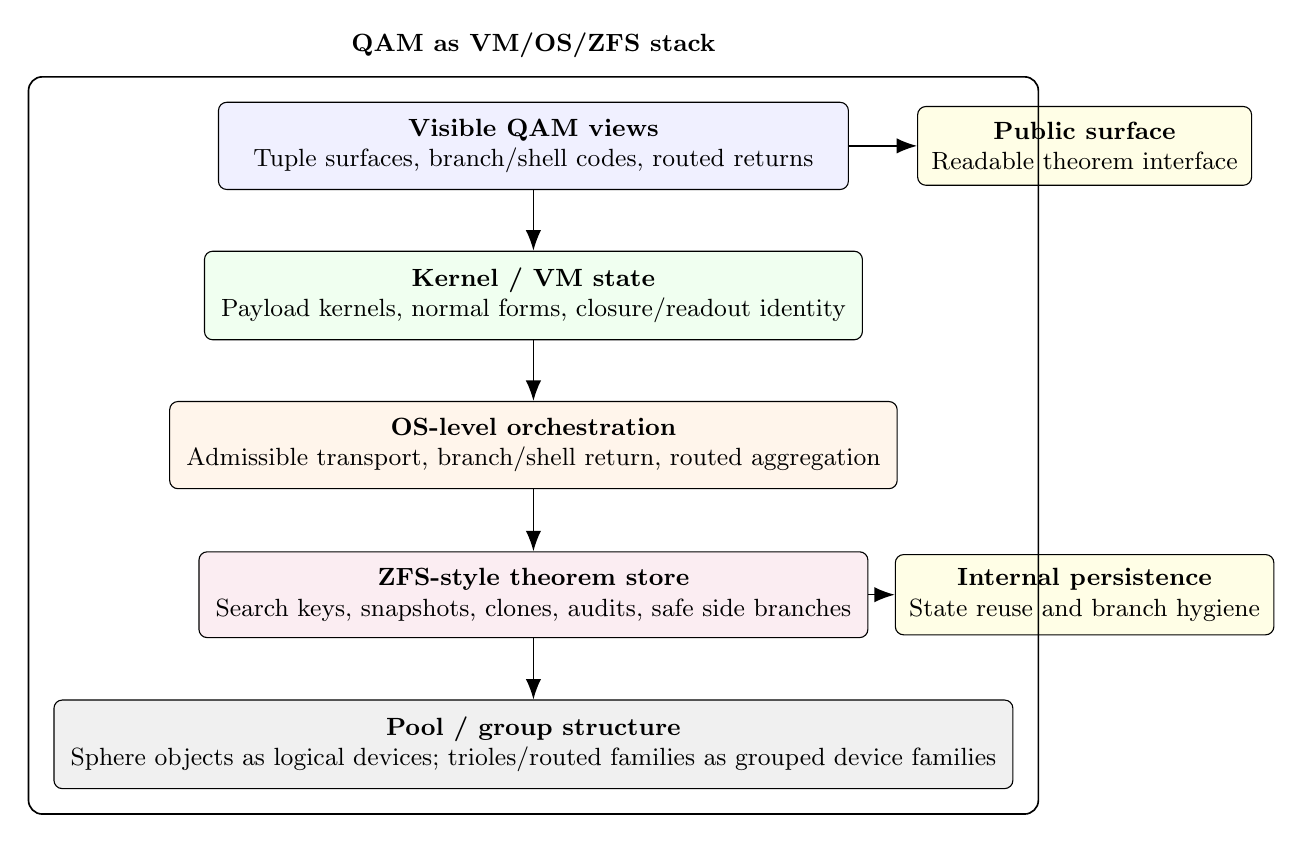
\begin{tikzpicture}[
 font=\small,
 mainbox/.style={draw, rounded corners=3pt, align=center, minimum width=8.0cm, minimum height=1.05cm, inner sep=6pt},
 sidebox/.style={draw, rounded corners=3pt, align=center, minimum width=3.9cm, minimum height=1.0cm, inner sep=5pt},
 arr/.style={-{Latex[length=2.6mm]}, line width=0.5pt}
]

\node[mainbox, fill=blue!6] (visible) at (0,0) {\textbf{Visible QAM views}\\Tuple surfaces, branch/shell codes, routed returns};
\node[sidebox, fill=yellow!10] (public) at (7.0,0) {\textbf{Public surface}\\Readable theorem interface};
\node[mainbox, fill=green!6] (kernel) at (0,-1.9) {\textbf{Kernel / VM state}\\Payload kernels, normal forms, closure/readout identity};
\node[mainbox, fill=orange!8] (os) at (0,-3.8) {\textbf{OS-level orchestration}\\Admissible transport, branch/shell return, routed aggregation};
\node[mainbox, fill=purple!7] (store) at (0,-5.7) {\textbf{ZFS-style theorem store}\\Search keys, snapshots, clones, audits, safe side branches};
\node[sidebox, fill=yellow!10] (internal) at (7.0,-5.7) {\textbf{Internal persistence}\\State reuse and branch hygiene};
\node[mainbox, fill=gray!12] (pool) at (0,-7.6) {\textbf{Pool / group structure}\\Sphere objects as logical devices; trioles/routed families as grouped device families};

\draw[arr] (visible) -- (kernel);
\draw[arr] (kernel) -- (os);
\draw[arr] (os) -- (store);
\draw[arr] (store) -- (pool);
\draw[arr] (visible.east) -- (public.west);
\draw[arr] (store.east) -- (internal.west);

\node[draw, rounded corners=5pt, fit=(visible)(kernel)(os)(store)(pool), inner sep=9pt, line width=0.6pt] (stackfit) {};
\node[above=0.15cm of stackfit.north, fill=white, inner sep=2pt] {\textbf{QAM as VM/OS/ZFS stack}};
\end{tikzpicture}%
}\caption{Graphical reading of the current QAM export as a virtual-machine/OS stack with a ZFS-style structural store. Visible tuple surfaces provide the public theorem interface; exposed payload kernels and kernel normal forms provide the later machine-state identity; snapshots, clones, search keys, and audits manage the internal proof store without changing the visible public QAM syntax.}
\label{fig:qam-vm-os-zfs}
\end{figure}

\begin{remark}[Why the ZFS analogy is structurally useful here]\label{rem:qam-zfs-utility}
The ZFS-style reading is not meant as decorative metaphor. It isolates four practical gains already visible in the present file. First, equal kernel classes can later be treated as mirror-like state reuse rather than as repeatedly independent visible tuple surfaces. Second, the deferred kernel-first path already behaves like copy-on-write: experimental compression statements are developed beside the active tuple proofs without rewriting the active line. Third, checkpoints, audits, and activation criteria behave like snapshots and scrub rules for the theorem store, since they record exactly which deferred branches are stable and which still remain non-authoritative. Fourth, once kernel normal forms and search keys are in place, repeated branch/shell/routed return families can be indexed and deduplicated as one structural graph beneath a readable tree-shaped theorem presentation. This is precisely why the systems analogy deserves a more prominent place next to the public QAM extraction itself.
\end{remark}

\begin{remark}[Current scope of the VM/OS/ZFS view]\label{rem:qam-vm-os-scope}
In the inherited \QSCver{legacy.16.0} public-shape layer this systems view remains explanatory and organizational. It does not introduce a second formal semantics, and it does not yet activate RAID-like reconstruction as an active theorem rule. The present mathematically justified gains at that inherited layer are the mirror-like reuse of equal kernel classes, the snapshot/clone logic of active versus deferred proof branches, and the content-addressed search-key discipline attached to kernel normal forms. The \QSCver{legacy.34.0} extension below activates only a guarded store-and-array vocabulary over the already available QAM/MML/MMA interface. It still does not turn mirror, stripe, parity, or repair language into an OP-closure certificate.
\end{remark}


\subsection*{QAM/MML/MMA store layer and Sphaera array extension}
\begin{quote}\small
\noindent\textbf{Status.} \emph{Active \QSCver{legacy.34.0} infrastructure block; no OP closure claim.}\par
\noindent\textbf{Block function.} This block internalizes the earlier ZFS/RAID analogy. QAM supplies the object store, MML supplies the store and array instructions, MMA supplies the execution/readout semantics, and finite Sphaera arrays supply guarded multi-object redundancy, comparison, and residual/parity witnesses.
\end{quote}

The preceding systems view should no longer be read merely as an external metaphor. At the present local layer it becomes a controlled internal interface. The point is not to claim that the Companion has already become a universal computer, nor that OP~1/4 or OP~5(B) have closed. The point is narrower and useful: the same QAM/MML/MMA machinery that already records objects, instructions, and route-faithful execution can also write the persistence layer in which several Sphaera objects are stored, compared, snapshotted, scrubbed, and carried as a guarded array.

\paragraph{Human reading.}
A single Sphaera object is now treated like one protected theorem-state device. Several Sphaera objects may be grouped into an array. In mirror mode, different objects carry the same structural content through different admissible views. In stripe mode, one larger proof or diagnostic object is distributed over several component stores. In parity/residual mode, an additional Sphaera object carries the difference, obstruction, or orthogonal control witness attached to the other components.

\paragraph{LLM/audit reading.}
The layer below gives stable machine-readable handles for store state, snapshot, clone, rollback, scrub, array creation, mirror, stripe, parity, and array snapshot. These handles are not theorematic shortcuts. They are audit contracts: each command must preserve address discipline, guard discipline, lineage discipline, and the non-certificate status unless a separate explicit theorem later discharges that status.

\begin{figure}[H]
\centering
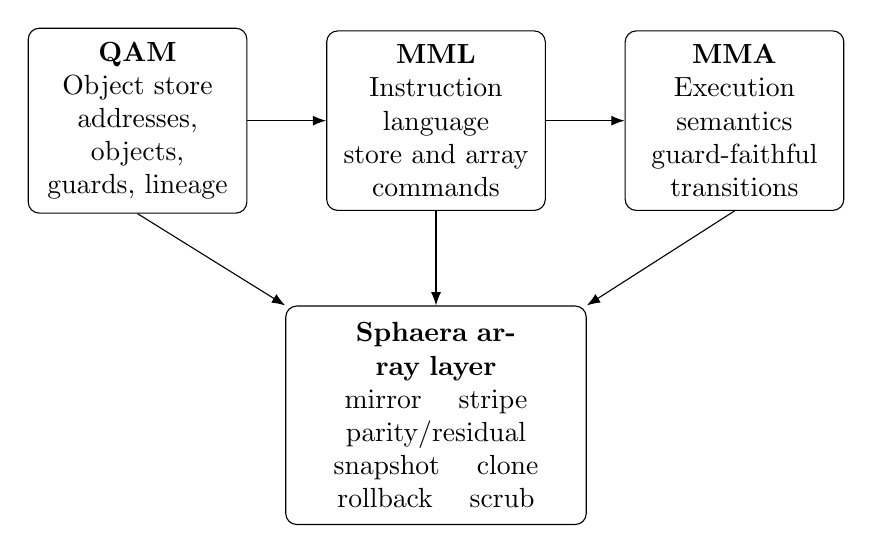
\begin{tikzpicture}[
 node distance=8mm and 10mm,
 box/.style={draw, rounded corners, align=center, inner sep=5pt, text width=0.2\textwidth},
 bigbox/.style={draw, rounded corners, align=center, inner sep=6pt, text width=0.28\textwidth},
 >=Latex
]
\node[box] (qam) {\textbf{QAM}\\Object store\\addresses, objects, guards, lineage};
\node[box, right=of qam] (mml) {\textbf{MML}\\Instruction language\\store and array commands};
\node[box, right=of mml] (mma) {\textbf{MMA}\\Execution semantics\\guard-faithful transitions};
\node[bigbox, below=12mm of mml] (array) {\textbf{Sphaera array layer}\\mirror \quad stripe \quad parity/residual\\snapshot \quad clone \quad rollback \quad scrub};
\draw[->] (qam) -- (mml);
\draw[->] (mml) -- (mma);
\draw[->] (qam.south) -- (array.north west);
\draw[->] (mml.south) -- (array.north);
\draw[->] (mma.south) -- (array.north east);
\end{tikzpicture}
\caption{Reader-facing systems map for the QAM/MML/MMA store-array extension. QAM supplies the stored object layer, MML supplies the allowed store and array commands, MMA supplies the guarded execution semantics, and the Sphaera array layer packages mirror, stripe, and parity/residual modes together with snapshot, clone, rollback, and scrub operations.}
\label{fig:qam-mml-mma-store-array-map}
\end{figure}

\begin{table}[H]
\centering
\small
\begin{tabular}{@{}>{\raggedright\arraybackslash}p{0.16\textwidth} >{\raggedright\arraybackslash}p{0.25\textwidth} >{\raggedright\arraybackslash}p{0.25\textwidth} >{\raggedright\arraybackslash}p{0.19\textwidth}@{}}
\toprule
\textbf{Layer} & \textbf{Human reading} & \textbf{LLM/audit reading} & \textbf{Typical outputs}\\
\midrule
QAM & protected object store & typed address/object/guard/ledger state & store state, snapshot anchor\\
MML & allowed store and array actions & finite instruction alphabet & \texttt{STORE}, \texttt{SNAPSHOT}, \texttt{PARITY}\\
MMA & how commands really act & deterministic guarded transition semantics & continue / halt / reject / guard\\
Sphaera array & several Sphaera objects coupled as one working array & finite guarded family with cross-sphere guards and parity witnesses & mirror, stripe, parity/residual, scrub\\
\bottomrule
\end{tabular}
\caption{Compact overview table for the store-array layer. This separates reader intuition from the audit contract without changing the theorematic status of the block.}
\label{tab:qam-mml-mma-store-array-overview}
\end{table}


\begin{definition}[QAM store state]\label{def:qam-store-state}
A \emph{QAM store state} is a finite guarded tuple
\[
 \mathcal S_n
 :=
 (\mathcal A_n,\mathcal O_n,\mathcal R_n,\mathcal G_n,\mathcal L_n),
\]
where \(\mathcal A_n\) is the finite address/tag domain, \(\mathcal O_n\) is the finite family of stored QAM objects, \(\mathcal R_n\) is the finite relation/link register between stored objects, \(\mathcal G_n\) is the finite guard register, and \(\mathcal L_n\) is the finite lineage/audit ledger. The state is \emph{admissible} if every ledger pointer lands in \(\mathcal A_n\), every relation in \(\mathcal R_n\) uses stored addresses, and every active guard in \(\mathcal G_n\) is satisfied by the displayed objects and relations.
\end{definition}

\begin{definition}[Store instruction alphabet]\label{def:mml-store-instructions}
The local MML store alphabet is the finite instruction family
\[
\begin{split}
 \mathcal I_{\mathrm{store}}
 :=\{&\texttt{STORE},\texttt{LINK},\texttt{SNAPSHOT},\texttt{CLONE},\texttt{ROLLBACK},\texttt{SCRUB},\texttt{MERGE\_CAND},\texttt{EXPORT}\}.
\end{split}
\]
Here \(\texttt{STORE}\) writes an object to an address, \(\texttt{LINK}\) writes a relation, \(\texttt{SNAPSHOT}\) freezes an admissible state, \(\texttt{CLONE}\) opens a guarded side branch from a snapshot, \(\texttt{ROLLBACK}\) returns to a recorded snapshot, \(\texttt{SCRUB}\) checks the guards and lineage, \(\texttt{MERGE\_CAND}\) proposes a guarded merge final, and \(\texttt{EXPORT}\) exposes a readout surface. None of these instructions is allowed to manufacture a theorematic certificate by syntax alone.
\end{definition}

\begin{definition}[MMA store transition semantics]\label{def:mma-store-transition}
The local MMA store semantics is a partial deterministic transition map
\[
 \delta_{\mathrm{store}}
 :
 \mathcal S_n\times\mathcal I_{\mathrm{store}}
 \dashrightarrow
 \mathcal S_{n+1}\times
 \{\mathsf{continue},\mathsf{halt},\mathsf{reject},\mathsf{guard}\}.
\]
It is \emph{guard-faithful} if every defined transition either preserves admissibility of the resulting store or returns the status \(\mathsf{guard}\) together with a defect entry in the ledger. It is \emph{lineage-faithful} if each defined transition records enough ledger data to identify its source state, instruction, guard status, and output state.
\end{definition}

\begin{definition}[Guarded snapshot and clone]\label{def:qam-store-snapshot}
For an admissible QAM store \(\mathcal S_n\), a \emph{guarded snapshot} is a tuple
\[
 \operatorname{snap}(\mathcal S_n)
 :=
 (\mathcal S_n,\chi_n,\lambda_n),
\]
where \(\chi_n\) is a finite integrity witness for the address, relation, guard, and ledger registers, and \(\lambda_n\) is a lineage anchor. A \emph{clone} of \(\operatorname{snap}(\mathcal S_n)\) is a new working state \(\mathcal S'_n\) with the same stored content and a new branch tag in the ledger. The clone is not a new theorem; it is a new guarded working branch from the same stored state.
\end{definition}

\begin{proposition}[Snapshot stability of admissible QAM stores]\label{prop:qam-store-snapshot-stability}
Every admissible finite QAM store state admits a guarded snapshot in the sense of Definition~\ref{def:qam-store-snapshot}. If the MMA store semantics is guard-faithful and lineage-faithful, then \(\texttt{SNAPSHOT}\), \(\texttt{CLONE}\), and \(\texttt{ROLLBACK}\) preserve the distinction between stored mathematical objects and release/audit metadata.
\end{proposition}

\begin{proof}
Since the address, object, relation, guard, and ledger registers are finite, their displayed state can be recorded as a finite tuple together with a finite integrity witness and a lineage anchor. This gives \(\operatorname{snap}(\mathcal S_n)\). Guard-faithfulness prevents a failed guard from being silently stored as an admissible state, and lineage-faithfulness records the source and branch data. Thus snapshot, clone, and rollback may move between recorded store states, but they do not promote a release label, branch label, or audit label into the mathematical object language.
\end{proof}

\begin{definition}[Sphaera array]\label{def:sphaera-array}
A \emph{Sphaera array} is a finite guarded family
\[
 \mathbb S_n
 :=
 \bigl((\mathcal S_n^{(1)},\ldots,\mathcal S_n^{(k)});\Gamma_n,\Pi_n,\Lambda_n\bigr),
 \qquad k\ge 1,
\]
where each \(\mathcal S_n^{(i)}\) is an admissible QAM store state, \(\Gamma_n\) is the cross-sphere guard register, \(\Pi_n\) is the parity/residual witness register, and \(\Lambda_n\) is the array-level lineage ledger. The array is admissible if all component stores are admissible and all cross-sphere guards in \(\Gamma_n\) are satisfied.
\end{definition}

\begin{definition}[Array instruction alphabet]\label{def:sphaera-array-instructions}
The local MML array alphabet is
\[
\begin{aligned}
 \mathcal I_{\mathrm{array}}
 :=\{&\texttt{ARRAY\_CREATE},\texttt{MIRROR},\texttt{STRIPE},\texttt{PARITY},\\
 &\texttt{SCRUB\_ARRAY},\texttt{REPAIR\_CAND},\texttt{SNAPSHOT\_ARRAY}\}.
\end{aligned}
\]
The command \(\texttt{REPAIR\_CAND}\) intentionally returns a final repair surface, not an automatic mathematical repair theorem. The command \(\texttt{PARITY}\) records a residual or orthogonal control witness, not a proof that the residual vanishes.
\end{definition}

\begin{definition}[Mirror, stripe, and parity modes]\label{def:sphaera-array-modes}
Let \(\mathbb S_n\) be an admissible Sphaera array.
\begin{enumerate}[leftmargin=2em]
 \item In \emph{mirror mode}, two component stores \(\mathcal S_n^{(i)}\) and \(\mathcal S_n^{(j)}\) are coupled by a cross-guard requiring equality of the relevant closure-compatible readout, even if the visible store presentations differ.
 \item In \emph{stripe mode}, an object \(X\) is stored as a finite guarded decomposition \(X\rightsquigarrow(X_1,\ldots,X_k)\), with each stripe \(X_i\) stored in a specified component and with a reconstruction witness recorded in \(\Pi_n\).
 \item In \emph{parity/residual mode}, one component or register stores a residual witness \(P\) for a guarded comparison of other components. The condition \(P=0\), if ever needed, must be proved separately; it is not asserted by the existence of the parity register.
\end{enumerate}
\end{definition}

\begin{definition}[Triadic Sphaera array]\label{def:triadic-sphaera-array}
A \emph{triadic Sphaera array} is an admissible Sphaera array of the form
\[
 \mathbb S_n^{ABC}
 :=
 (\mathcal S_A,\mathcal S_B,\mathcal S_C;\Gamma_{ABC},\Pi_{ABC},\Lambda_{ABC})
\]
in which \(\mathcal S_A\) and \(\mathcal S_B\) carry two active readout or probe-facing stores, while \(\mathcal S_C\) carries the orthogonal residual/parity witness. The guard register records the structural condition that \(\mathcal S_C\) is read orthogonally to the active \(A/B\) coupling channel and that the HC/MM readout of the array preserves the inherited route tag.
\end{definition}

\begin{proposition}[Guarded array snapshot]\label{prop:sphaera-array-snapshot}
Every admissible finite Sphaera array admits a guarded array snapshot
\[
 \operatorname{snap}_{\mathrm{arr}}(\mathbb S_n)
 :=
 \bigl(\mathbb S_n,(\chi_n^{(1)},\ldots,\chi_n^{(k)}),\chi_n^{\Gamma},\chi_n^{\Pi},\lambda_n^{\mathrm{arr}}\bigr),
\]
preserving component stores, cross-sphere guards, parity/residual witnesses, and array lineage.
\end{proposition}

\begin{proof}
Apply Proposition~\ref{prop:qam-store-snapshot-stability} to each finite component store. Since the cross-guard, parity/residual, and array-ledger registers are also finite, record their integrity witnesses and one array lineage anchor. The resulting tuple is a guarded array snapshot. It records the array state without adding an OP-closure certificate and without changing any component object into metadata.
\end{proof}

\begin{proposition}[Finite array scrub]\label{prop:sphaera-array-scrub}
For every finite Sphaera array there is a deterministic scrub procedure
\[
 \operatorname{scrub}_{\mathrm{arr}}(\mathbb S_n)
 \in
 \{\mathsf{pass},\mathsf{fail}\}\times\mathcal D_n,
\]
where \(\mathcal D_n\) is a finite defect register. The scrub passes exactly when all component-store guards, cross-sphere guards, parity/residual registrations, and lineage pointers pass their finite checks.
\end{proposition}

\begin{proof}
The component store registers, cross-guard register, parity/residual register, and lineage ledger are finite by definition. A deterministic scrub checks them in a fixed order and records every failed check in \(\mathcal D_n\). If no failed check is recorded, the result is \(\mathsf{pass}\); otherwise it is \(\mathsf{fail}\) with the finite defect register. No repair or closure claim is produced by this test.
\end{proof}

\begin{theorem}[QAM/MML/MMA Sphaera array layer]\label{thm:qam-mml-mma-sphaera-array-layer}
The QAM/MML/MMA stack admits a conservative Sphaera array layer in the following sense. Given finite admissible QAM stores, the store instruction alphabet of Definition~\ref{def:mml-store-instructions}, the array instruction alphabet of Definition~\ref{def:sphaera-array-instructions}, and guard-faithful lineage-faithful MMA transition semantics, one obtains finite guarded snapshots, finite array snapshots, and deterministic array scrub surfaces. These surfaces preserve stored mathematical objects, cross-sphere guards, residual/parity witnesses, and audit lineage without manufacturing an OP-closure certificate.
\end{theorem}

\begin{proof}
The store part follows from Definitions~\ref{def:qam-store-state}--\ref{def:qam-store-snapshot} and Proposition~\ref{prop:qam-store-snapshot-stability}. The array part follows by grouping finitely many admissible stores as in Definition~\ref{def:sphaera-array}, assigning finite cross-guards, finite parity/residual witnesses, and a finite lineage ledger, and then applying Propositions~\ref{prop:sphaera-array-snapshot} and~\ref{prop:sphaera-array-scrub}. The last clause follows from the explicit non-certificate restrictions in Definitions~\ref{def:mml-store-instructions}, \ref{def:sphaera-array-instructions}, and \ref{def:sphaera-array-modes}: mirror, stripe, parity, scrub, and repair-final language records infrastructure and diagnostic data only. It does not assert vanishing residuals or OP closure.
\end{proof}

\begin{corollary}[RAID-like reading without RAID overclaim]\label{cor:sphaera-array-raid-reading}
The Sphaera array layer supports a RAID-like reading: mirror mode corresponds to redundant closure-compatible readout, stripe mode corresponds to guarded distribution of a larger object over several component stores, and parity/residual mode corresponds to an explicit diagnostic witness for cross-component mismatch. This reading is internal to QAM/MML/MMA, but it remains weaker than technical RAID reconstruction and weaker than any OP-closure theorem.
\end{corollary}

\begin{proof}
This is only a translation of Definition~\ref{def:sphaera-array-modes} into systems language. The mathematical content remains the guarded store, snapshot, array, parity/residual, and scrub structure already proved above.
\end{proof}

\begin{remark}[Tool extraction from the Sphaera array layer]\label{rem:sphaera-array-tool-extraction}
The new layer extracts four reusable tools for later Companion revisions.
\begin{enumerate}[leftmargin=2em]
 \item \textbf{Snapshot tool.} Freeze one admissible QAM store without changing the mathematical object language.
 \item \textbf{Clone/rollback tool.} Open or return from a guarded branch while preserving lineage and non-certificate status.
 \item \textbf{Array-scrub tool.} Test several Sphaera stores, cross-guards, and residual witnesses as one finite diagnostic surface.
 \item \textbf{Triadic parity tool.} Use a third, orthogonal Sphaera object as residual/parity witness for a two-store active coupling.
\end{enumerate}
These tools are deliberately infrastructural. Their value is that later OP-facing work can compare, branch, and roll back several coupled Sphaera objects without confusing state persistence with theorematic closure.
\end{remark}

\begin{remark}[Human/LLM interface gain]\label{rem:sphaera-array-human-llm-gain}
For a human reader, the store-array layer explains why the Companion keeps snapshots, historical witnesses, audit ledgers, and branch restrictions so visibly: they are the theorem-store equivalent of protected state persistence. For an LLM reader, the same layer supplies exact handles: \(\mathcal S_n\) for one store, \(\mathbb S_n\) for an array, \(\Gamma_n\) for cross-guards, \(\Pi_n\) for parity/residual witnesses, and \(\Lambda_n\) for lineage. This is the intended compromise between human readability and machine precision.
\end{remark}


\subsection*{Pre-shift QAM Hilbert-shift and guarded mixed readouts}
\begin{quote}\small
\noindent\textbf{Status.} \emph{Pre-shift preparation layer only.} The inherited QAM tuple tags are not globally migrated in Version~\docversion{}. The block below records the conservative Hilbert-shift plan, the mixed-readout package discipline, and an optional binary mask registry for future readout classification.
\end{quote}

The index-0 issue is now treated explicitly. In the inherited QAM tuple namespace, tag 0 occurs as an inhabited constructor tag, for instance on visible tuple surfaces of the form $\langle 0,a\rangle$. In a Boolean mask or IPshifted-like readout registry, however, value 0 must mean no active kind. The next major QAM migration should therefore not identify these two uses. The preparation layer below records the planned Hilbert-hotel shift that can free tag 0 in the future while preserving the payloads and proofs.

\begin{definition}[QAM Hilbert-shift plan]\label{def:qam-hilbert-shift-plan}
Let $\mathcal K_{\mathrm{old}}$ be the inherited finite QAM tuple-tag namespace used by the current public syntax, and let $\mathcal K_{\mathrm{new}}$ be a shifted namespace with tag 0 reserved for the empty/no-active-kind marker. The planned Hilbert-shift is the constructor-level map
\[
 H_{\mathrm{QAM}}(\langle i,x_1,\ldots,x_m\rangle)
 :=
 \langle i+1,x_1,\ldots,x_m\rangle.
\]
It shifts only the constructor tag. It does not change the stored payload $(x_1,\ldots,x_m)$, the intended constructor distinction, or any mathematical content carried by the payload.
\end{definition}

\begin{definition}[Pre-shift reserved-zero discipline]\label{def:pre-shift-reserved-zero-discipline}
The preparation line distinguishes two uses of zero.
\begin{enumerate}[leftmargin=2em]
 \item In the inherited legacy tuple syntax, tag 0 remains an inhabited tuple tag wherever the old QAM definitions still use it.
 \item In the planned shifted shifted namespace and in every binary mask registry, tag or mask value 0 is reserved for empty, undefined, or no active kind.
\end{enumerate}
No Version~\docversion{} statement may silently replace the first convention by the second. Any global replacement is reserved for a later shifted migration theorem.
\end{definition}

\begin{proposition}[Conservative shape of the QAM Hilbert-shift]\label{prop:qam-hilbert-shift-conservative-shape}
Suppose a finite QAM sublanguage is translated by $H_{\mathrm{QAM}}$ and every constructor predicate, admissibility predicate, readout predicate, and closure-relevant predicate is translated by the same tag shift. Then the translated sublanguage is a conservative reindexing of the old one: payloads, constructor distinctions, admissibility status, readout compatibility, and closure-relevant truth values are preserved under the translation.
\end{proposition}

\begin{proof}
The map $H_{\mathrm{QAM}}$ is injective on constructor tags and leaves all payload coordinates unchanged. A constructor predicate in the shifted namespace is defined to hold exactly when the corresponding old predicate holds before applying the shift. The same translation is imposed on admissibility, readout, and closure-relevant predicates. Thus every proof step that used only constructor distinction, payload data, admissibility, readout compatibility, or closure-relevant class data has an isomorphic shifted proof step. The proposition records the required conservativity shape for a later shifted migration; it does not perform the global migration here.
\end{proof}

\begin{definition}[Guarded mixed QAM readout]\label{def:guarded-mixed-qam-readout}
A \emph{guarded mixed QAM readout} is a finite derived package
\[
 R_{\mathrm{mix}}
 :=
 (r_1,\ldots,r_m;\Gamma_{\mathrm{mix}},\mu,J_{\mathrm{mix}},\sigma_{\mathrm{mix}}),
\]
where each $r_i$ is an already admissible component readout on its own allowed QAM kind, $\Gamma_{\mathrm{mix}}$ is a finite guard package, $\mu$ is a finite aggregation map on component readout values, $J_{\mathrm{mix}}$ is the closure-factor map for the aggregate, and $\sigma_{\mathrm{mix}}$ records the theorematic status. It is admissible only when all component readouts are admissible and the aggregation map does not identify non-equivalent closure-relevant classes.
\end{definition}

\begin{definition}[Binary mask registry for mixed readouts]\label{def:binary-mask-registry-mixed-readouts}
A \emph{binary mask registry} for mixed QAM readouts assigns to each inhabited readout kind a nonzero power-of-two bit
\[
 \beta_j = 2^j,
 \qquad j\ge 0,
\]
and reserves mask value 0 for no active kind. A mixed-readout mask is a finite Boolean OR of active kind bits. Boolean AND tests whether a component kind is present, XOR records symmetric difference between two masks, and complement is allowed only relative to a fixed finite mask universe $\Omega$.
\end{definition}

\begin{proposition}[Mixed readout factorization]\label{prop:mixed-readout-factorization}
Let $R_{\mathrm{mix}}$ be a guarded mixed QAM readout whose component readouts $r_i$ are closure-compatible. If the aggregation map $\mu$ factors through the component closure-factor maps and $J_{\mathrm{mix}}$ factors through the resulting aggregate class, then $R_{\mathrm{mix}}$ is closure-compatible.
\end{proposition}

\begin{proof}
Closure-compatible component readouts identify no closure-relevant distinction beyond their component class maps. Since $\mu$ factors through those class maps, it can only aggregate already class-level data. Since $J_{\mathrm{mix}}$ factors through that aggregate class, the mixed readout cannot introduce a new closure-relevant distinction that was invisible to the component closure classes. Therefore the mixed package is closure-compatible. The argument uses only factorization and guards; it does not introduce primitive mixed tensors.
\end{proof}

\begin{remark}[shifted migration trigger]\label{rem:shifted-qam-migration-trigger}
The full replacement of the inherited tuple tags by the shifted tags is intentionally not a Version~\docversion{} operation. It changes the visible QAM object-language namespace and therefore belongs to a major version. Version~\docversion{} only records why the shift is useful, what the conservative proof obligation looks like, and how mixed readouts can already be treated as derived packages without forcing the migration.
\end{remark}


% ============================================================================
% Quantum Sphaera Companion legacy.35.0-r03 insertion patch
% Two-sided structural tensor notation for QAM/MML/MMA readouts
%
% Intended insertion point:
%   In the active-core source, place this block after the short QAM/MML/MMA
%   reader-orientation / pre-shift QAM preparation material, and before any
%   broad theorematic QAM continuation.  In older sources the closest safe
%   anchor is after the remark "QAM normalization guide".
%
% Scope:
%   Conservative notation/compression layer only.  This is not the separate
%   pedagogical reader manual paper; that manual remains a future standalone
%   companion/guide document.
% ============================================================================

\subsection*{Two-sided structural tensor notation for QAM/MML/MMA readouts}
\begin{quote}\small
\noindent\textbf{Status.} \emph{Active notation and compression layer; not a new tensor calculus and not a new closure criterion.}\par
\noindent\textbf{Block function.} This block records the narrow two-sided tensor grammar used to separate readout-side, structure-side, comparison-side, and mask-side roles in later QAM/MML/MMA expressions. It is included here as a conservative technical layer only. A fuller pedagogical reader manual for the notation is intentionally kept as a separate future paper or companion guide.
\end{quote}

The QAM/MML/MMA line repeatedly alternates between four roles: frame-side readout, structure-side action, comparison of active channels, and compatibility testing of readout or mask modes. The following notation is introduced only to make those roles visible in the formula syntax. It does not replace classical tensor calculus and it does not turn every displayed expression into a new primitive tensor object.

\begin{definition}[Two-sided structural tensor interface]\label{def:two-sided-structural-tensor-interface}
A \emph{two-sided structural tensor display} is a tensor-like expression in which a structural object may carry front-side and back-side indices, written schematically as
\[
{}^{A}{}_{B}\mathcal{T}^{i}{}_{j}.
\]
The front indices \({}^{A}{}_{B}\) record the left-sided or readout-facing interface: frame, observer, language, readout, or external addressing data. The back indices \({}^{i}{}_{j}\) record the right-sided or structure-facing interface: action, transport, field, operator, or internal structural data. Thus the display is read as a typed structural interface rather than as a mere component array.
\end{definition}

\begin{definition}[Admissible contractions and comparisons]\label{def:two-sided-admissible-contractions}
The two-sided notation obeys the following contraction discipline.
\begin{enumerate}[leftmargin=2em]
 \item \textbf{Classical action/readout.} Ordinary upper--lower contraction remains unchanged. If
 \[
 A_\mu\,{}^\mu\mathcal{T}_\nu\,B^\nu
 \]
 is well-defined, it is read as a classical action, evaluation, or sandwich readout: first apply the structure-facing operation to \(B\), then read the result by \(A\).
 \item \textbf{Active--active comparison.} Two upper indices are not contracted as a raw Einstein sum. They may only be compared through an explicitly declared comparison tensor, for instance
 \[
 G_{\alpha\beta}X^\alpha Y^\beta .
 \]
 This means active structural comparison, such as angle, distance, coupling strength, orthogonality, channel similarity, or residual size.
 \item \textbf{Passive--passive comparison.} Two lower indices are likewise not contracted raw. They may only be compared through an explicitly declared dual comparison tensor, for instance
 \[
 G^{\alpha\beta}\omega_\alpha\eta_\beta .
 \]
 This means comparison of readout forms, observer modes, measurement channels, or passive projections.
 \item \textbf{Mask and selector compatibility.} Boolean, finite, or mask-like compatibility tests must be carried by an explicit selector tensor, for instance
 \[
 \chi_{mn}R^mS^n .
 \]
 This expression says that readout modes \(m\) and \(n\) are first tested for admissible compatibility by \(\chi\), and only compatible contributions are admitted to the mixed readout.
\end{enumerate}
\end{definition}

\begin{remark}[Conservative reading rule]\label{rem:two-sided-conservative-reading-rule}
The two-sided notation is conservative because the only unchanged contraction is the classical upper--lower action/readout contraction. Same-variance pairings are not silently added to the calculus; they are admitted only when a comparison tensor or selector tensor has been declared. Hence every two-sided display must be expandable into ordinary QAM-over-ZF role predicates together with explicit comparison or compatibility data.
\end{remark}

\begin{definition}[Guarded mixed QAM readout]\label{def:guarded-two-sided-mixed-qam-readout}
Let \(R^m\) and \(S^n\) be QAM readout modes and let \(\chi_{mn}\) be an explicit admissibility or compatibility selector. A \emph{guarded mixed QAM readout} is a derived readout expression of the form
\[
\operatorname{Mix}_{\chi}(R,S)(x)
\quad\leadsto\quad
\chi_{mn}R^m(x)S^n(x),
\]
where the right-hand display is read with the contraction discipline of Definition~\ref{def:two-sided-admissible-contractions}. The mixed readout is therefore not a new primitive QAM object. It is a compatibility-filtered package of already admitted readout modes.
\end{definition}

\begin{remark}[Residual comparison grammar]\label{ex:two-sided-residual-comparison}
The live residual triple
\[
\rho=(\rho_{\mathrm{CL}},\rho_{\Theta},\rho_A)
\]
may be compressed into a residual-channel vector \(\rho^\alpha\). Its total comparison size may then be written as
\[
\|\rho\|_G^2=G_{\alpha\beta}\rho^\alpha\rho^\beta .
\]
This is not a raw contraction of two upper indices. It is the comparison of two active residual-channel entries through the declared comparison tensor \(G_{\alpha\beta}\).
\end{remark}

\begin{remark}[HC/MM sandwich grammar]\label{ex:two-sided-hc-mm-sandwich}
An HC/MM-mediated readout may be displayed schematically as
\[
{}^{R}{}_{\Omega}\mathcal{M}^{i}{}_{j},
\]
where the front side records the readout or observer-side interface and the back side records the structure-side transport or matrix action. When paired with ordinary upper--lower indices, the expression remains an ordinary sandwich readout. When two readout channels or two structure channels are compared, the comparison must be mediated by an explicitly named comparison tensor or selector.
\end{remark}

\begin{proposition}[Conservative expansion of two-sided displays]\label{prop:two-sided-conservative-expansion}
Every well-formed two-sided structural tensor display in the sense of Definitions~\ref{def:two-sided-structural-tensor-interface} and~\ref{def:two-sided-admissible-contractions} admits a conservative expansion into the inherited QAM-over-ZF language: front-side indices expand to readout/frame/language role data, back-side indices expand to structure/action/transport role data, classical upper--lower contractions remain ordinary action or evaluation clauses, and every same-variance pairing expands to an explicit comparison or compatibility predicate.
\end{proposition}

\begin{proof}
Erase the visual sidedness notation and retain its role data as ordinary QAM codes. Front-side symbols become readout, frame, observer, or language tags. Back-side symbols become structure, action, transport, or field tags. Classical upper--lower contractions are left unchanged. A same-variance display is well formed only if it contains a named comparison tensor or selector, and so it expands to the corresponding comparison or compatibility predicate. No new primitive closure relation, admissibility relation, or theorematic certificate is introduced by this erasure. The display is therefore a conservative abbreviation of already typed QAM-over-ZF data.
\end{proof}

\begin{remark}[LLM-facing role stability]\label{rem:two-sided-llm-role-stability}
For machine reading and LLM-assisted proof navigation, the notation functions as a syntactic guardrail. The front/back split marks whether a symbol belongs to the readout-facing side or the structure-facing side, while the contraction discipline marks whether a formula is an action, a readout, a comparison, or a compatibility test. This reduces the risk that a readout is mistaken for an operator, that a diagnostic comparison is mistaken for a proof of closure, or that a guarded mixed readout is mistaken for a new primitive tensor object.
\end{remark}

\begin{remark}[Use in the present release line]\label{rem:two-sided-present-release-use}
In the present historical release line.x line this notation should be used locally and sparingly: first for guarded mixed QAM readouts, residual/drift comparisons, HC/MM sandwich expressions, triadic orthogonality comparisons, and Boolean or mask-like compatibility tests. A global rewrite of the whole Companion into the two-sided notation is not part of this release line. The separate pedagogical reader manual may later explain the notation at a slower pace without enlarging the active theorem core.
\end{remark}


% ============================================================================
% Quantum Sphaera Companion legacy.35.0-r03 insertion patch
% Two-sided tensor stability, mixed-readout normal form, and Boolean masks
%
% Scope:
%   Stabilization layer only.  This block makes the r02 notation explicitly
%   expandable back into QAM-over-ZF role data and records the mask/readout
%   grammar that will later help the shifted QAM reindexing.  It is not the separate
%   pedagogical reader-manual paper.
% ============================================================================

\subsection*{stability layer: two-sided expansion, mixed-readout normal form, and Boolean masks}
\begin{quote}\small
\noindent\textbf{Status.} \emph{Conservative stabilization of the notation layer; not a global rewrite, not a new tensor calculus, and not a closure theorem.}\par
\noindent\textbf{Block function.} This block fixes the exact erasure route from two-sided displays back to ordinary QAM-over-ZF role data, normalizes guarded mixed readouts, and states the Boolean selector grammar used by IPshifted-like readout masks. The separate reader manual remains a future standalone paper or guide.
\end{quote}

The notation made readout-side, structure-side, comparison-side, and mask-side roles visible in formulas. The present step turns that notation into a safer tool by recording the normal forms that an audit reader or LLM reader should recover whenever a two-sided display appears. The rule is intentionally asymmetric: notation may compress role data, but every compressed display must expand back into explicit role data before it can be used as proof content.

\begin{definition}[Two-sided role-erasure map]\label{def:r03-two-sided-role-erasure-map}
Let \(E\) be a well-formed two-sided structural tensor display in the sense of Definitions~\ref{def:two-sided-structural-tensor-interface} and~\ref{def:two-sided-admissible-contractions}. Its \emph{role-erasure expansion}
\[
\mathfrak{E}_{\mathrm{role}}(E)
\]
is the ordinary QAM-over-ZF package obtained by replacing:
\begin{enumerate}[leftmargin=2em]
 \item every front-side index by an explicit readout, frame, observer, or language-role tag;
 \item every back-side index by an explicit structure, action, field, transport, or operator-role tag;
 \item every classical upper--lower contraction by the corresponding ordinary action/evaluation clause;
 \item every same-variance comparison by a named comparison predicate carrying its declared comparison tensor;
 \item every Boolean or selector occurrence by a finite compatibility predicate over the declared mask universe.
\end{enumerate}
This expansion is an erasure of notation only. It does not erase guards, selectors, comparison tensors, branch restrictions, or provenance data.
\end{definition}

\begin{proposition}[Role-erasure normal form]\label{prop:r03-role-erasure-normal-form}
Every well-formed two-sided display \(E\) used in the historical release line.x line has a role-erasure expansion \(\mathfrak{E}_{\mathrm{role}}(E)\) whose clauses are built from already admitted QAM role predicates, admitted comparison data, admitted selector data, and ordinary finite tuple coding over ZF. In particular, the two-sided display cannot by itself introduce a new primitive tensor kind, a new admissibility relation, or a new theorematic certificate.
\end{proposition}

\begin{proof}
Proceed by structural inspection of the display grammar. Front/back sidedness contributes only role tags. Ordinary upper--lower contraction is already part of the inherited action/readout grammar. A same-variance pairing is well formed only when it contains an explicitly named comparison tensor or selector, hence it expands to a comparison or compatibility predicate rather than to an untyped Einstein contraction. All finite lists of such clauses are QAM tuple-coded over the existing ZF substrate. Therefore the two-sided syntax is conservative under role erasure.
\end{proof}

\begin{definition}[Guarded mixed-readout normal form]\label{def:r03-guarded-mixed-readout-normal-form}
A guarded mixed QAM readout is in \emph{normal form} when it is presented as a finite package
\[
\mathcal R_{\mathrm{mix}}
=
\bigl(I,\{R_i\}_{i\in I},\Gamma_{\mathrm{mix}},\chi,\mu,J_{\mathrm{mix}}\bigr),
\]
where \(I\) is a finite index set, each \(R_i\) is an already admitted component readout, \(\Gamma_{\mathrm{mix}}\) is the inherited guard package, \(\chi\) is a finite selector or mask predicate over \(I\), \(\mu\) is an aggregation map defined only on selector-admissible component families, and \(J_{\mathrm{mix}}\) is the declared mixed readout surface. A two-sided display such as
\[
\chi_{mn}R^mS^n
\]
is only an abbreviation for this finite package in the binary case \(I=\{m,n\}\).
\end{definition}

\begin{proposition}[Mixed-readout normal-form expansion]\label{prop:r03-mixed-readout-normal-form-expansion}
Every guarded mixed readout admitted by Definition~\ref{def:guarded-two-sided-mixed-qam-readout} expands to a guarded mixed-readout normal form in the sense of Definition~\ref{def:r03-guarded-mixed-readout-normal-form}. Conversely, every guarded mixed-readout normal form may be displayed in two-sided shorthand only after its guards, selector, aggregation map, and output surface have been declared.
\end{proposition}

\begin{proof}
The binary shorthand \(\chi_{mn}R^mS^n\) already names the two component readouts and the selector. The surrounding QAM context supplies the inherited guard package, the admissible aggregation rule, and the declared output surface. Collecting these data gives the normal-form tuple. Conversely, starting from the normal-form tuple, one may suppress the finite package into two-sided shorthand only because the suppressed guard, selector, aggregation, and output data remain recoverable. Thus the shorthand and the normal form are not different mathematical objects; the former is a compact notation for the latter.
\end{proof}

\begin{definition}[Boolean selector and mask grammar]\label{def:r03-boolean-selector-mask-grammar}
Fix a finite readout-kind universe \(\Omega=\{k_1,\dots,k_N\}\). A \emph{Boolean selector mask} is a function
\[
\chi:\Omega\longrightarrow\{0,1\}
\]
or, equivalently, a finite bit mask whose value 0 denotes no active kind and whose nonzero bits denote active readout kinds. The admissible Boolean operations are:
\begin{align*}
\chi_A\vee\chi_B &\quad\text{for union of active readout kinds,}\\
\chi_A\wedge\chi_B &\quad\text{for intersection or compatibility testing,}\\
\chi_A\oplus\chi_B &\quad\text{for diagnostic symmetric difference,}\\
\neg_{\Omega}\chi_A &\quad\text{for relative complement inside the fixed universe }\Omega.
\end{align*}
No absolute complement is used without first declaring \(\Omega\). A selector expression may filter a readout package, but it does not alter the payload of any component readout.
\end{definition}

\begin{proposition}[Mask-filter conservativity]\label{prop:r03-mask-filter-conservativity}
Let \(\mathcal R_{\mathrm{mix}}\) be a guarded mixed-readout normal form and let \(\chi\) be a Boolean selector mask over its finite readout-kind universe. Applying \(\chi\) restricts the active component menu of \(\mathcal R_{\mathrm{mix}}\), but it does not change the underlying component payloads, the inherited guards, or the closure status of any component readout.
\end{proposition}

\begin{proof}
A selector mask is a finite predicate on the index universe. It chooses which already declared component clauses are active in the aggregation domain. It neither rewrites the component readouts nor changes their guard packages. Hence any closure-compatible status used by the mixed package still has to come from the component readouts and the declared factorization map, not from the mask itself.
\end{proof}

\begin{remark}[LLM/audit role table]\label{rem:r03-llm-audit-role-table}
For later machine reading, the following table fixes the intended role parsing. It is a local audit aid inside the Companion, not the separate pedagogical reader manual.
\begin{center}
\renewcommand{\arraystretch}{1.12}
\begin{tabular}{|P{0.28\textwidth}|P{0.34\textwidth}|P{0.25\textwidth}|}
\hline
\textbf{Displayed form} & \textbf{Intended role} & \textbf{Audit guard} \\
\hline
front-side indices & readout, frame, observer, language, or addressing side & expand to explicit QAM role tags \\
\hline
back-side indices & structure, action, field, transport, or operator side & expand to explicit QAM role tags \\
\hline
upper--lower contraction & classical action, evaluation, or sandwich readout & ordinary tensor/QAM readout clause \\
\hline
upper--upper via \(G_{\alpha\beta}\) & active structural comparison & no raw same-variance contraction \\
\hline
lower--lower via \(G^{\alpha\beta}\) & passive readout comparison & no raw same-variance contraction \\
\hline
\(\chi_{mn}\) or a mask bit & compatibility or activation selector & filter only; no new payload \\
\hline
\end{tabular}
\end{center}
\end{remark}

\begin{corollary}[proof-neutrality of the tensor layer]\label{cor:r03-proof-neutrality-of-tensor-layer}
The tensor-stability layer may be cited to shorten repeated readout/action/comparison/mask passages, but it may not be cited as an independent proof of closure, OP resolution, primitive mixed-tensor existence, or global QAM namespace migration.
\end{corollary}

\begin{proof}
By Propositions~\ref{prop:r03-role-erasure-normal-form}, \ref{prop:r03-mixed-readout-normal-form-expansion}, and~\ref{prop:r03-mask-filter-conservativity}, every display reduces to already declared role data, normal-form mixed-readout data, and finite selector predicates. The reduction supplies notation control only. It does not add the missing theorematic hypotheses needed for closure, OP resolution, primitive mixed tensors, or shifted reindexing.
\end{proof}

\begin{remark}[Placement of the future reader manual]\label{rem:r03-reader-manual-placement}
The present block deliberately stays short and formal. A slower reader manual may later explain the same grammar with diagrams, examples, and human-facing intuition, but that manual should remain a separate paper or guide so that the Active Core remains the governing proof line.
\end{remark}


% Quantum Sphaera Companion legacy.35.0-r04 release-final insertion
% Release-final freeze/audit layer only.  No mathematical closure claim.

\subsection*{release-final freeze audit for the pre-shift QAM/tensor layer}
\addcontentsline{toc}{subsection}{release-final freeze audit for the pre-shift QAM/tensor layer}
\label{subsec:r04-release-final-freeze-audit-qam-tensor}

\noindent\textbf{Status.} \emph{Release-final audit layer only; no new theorematic certificate, no global QAM namespace migration, no primitive mixed tensor, and no OP closure.}\par
\noindent\textbf{Block function.} This block freezes the local pass/notation and mixed-readout preparation layer for release-final review. It records what must remain true when the Active Core is read together with the separate Historical Witness PDF.

\begin{definition}[pre-shift QAM/tensor release-final package]
\label{def:r04-pre-shift-qam-tensor-release-final-package}
The \emph{pre-shift QAM/tensor release-final package} consists of the following finite data:
\begin{enumerate}[label=(\roman*)]
 \item the inherited \QSCver{legacy.34.0} public split-bundle baseline and its concept/version DOI record;
 \item the \QSCver{legacy.35.0} short-abstract and extended-orientation architecture;
 \item the pre-shift Hilbert-shift plan reserving global QAM tag migration for a later major version;
 \item the guarded mixed-readout discipline and optional binary mask registry;
 \item the two-sided structural tensor notation;
 \item the role-erasure, mixed-readout normal form, Boolean selector grammar, and proof-neutrality layer;
 \item the present audit/handoff metadata saying that the Active Core is the governing proof line and that the Historical Witness PDF remains preserved proof memory.
\end{enumerate}
It is a packaging and audit object, not a closure object.
\end{definition}

\begin{proposition}[release-final conservativity]
\label{prop:r04-release-final-conservativity}
The pre-shift QAM/tensor release-final package is conservative over the tensor-stability layer with respect to theorematic content. It may change release-final metadata, routing language, audit surfaces, and handoff wording, but it may not create any new OP certificate, global Hilbert-shift theorem, primitive mixed-tensor axiom, or replacement of the inherited QAM tuple namespace.
\end{proposition}

\begin{proof}
Each mathematical role introduced earlier is erased by Definition~\ref{def:r03-two-sided-role-erasure-map} and normalized by Proposition~\ref{prop:r03-role-erasure-normal-form}. Each mixed readout is expanded by Proposition~\ref{prop:r03-mixed-readout-normal-form-expansion}, and each Boolean mask action is restricted by Proposition~\ref{prop:r03-mask-filter-conservativity}. The package adds only release-final metadata and bundle-handoff statements around these already guarded objects. Hence no new theorematic content is introduced.
\end{proof}

\begin{corollary}[freeze-readiness condition]
\label{cor:r04-freeze-readiness-condition}
If the build audit reports no duplicate labels, no undefined references, no undefined citations, and no fatal LaTeX errors for both the Active Core and the Historical Witness, then Version~\docversion{} is structurally ready to be treated as a freeze final for the \QSCver{legacy.35.0} pre-shift QAM/tensor preparation release, subject only to the external release decision and any assigned Zenodo version DOI.
\end{corollary}

\begin{remark}[Reader-manual separation at]
\label{rem:r04-reader-manual-separation}
The pedagogical reader manual for the two-sided notation remains outside the Active Core. It may later be written as a separate guide with diagrams, examples, and slower explanations. The present Companion keeps only the compact formal grammar and the proof-neutrality guards needed by the governing proof line.
\end{remark}


% Quantum Sphaera Companion legacy.35.0 release-final DOI insertion
% Release metadata only. No mathematical object is indexed by the DOI.

\subsection*{\QSCver{legacy.35.0} DOI-bearing release freeze}
\addcontentsline{toc}{subsection}{\QSCver{legacy.35.0} DOI-bearing release freeze}
\label{subsec:v3350-doi-bearing-release-freeze}

\noindent\textbf{Status.} \emph{Release-final metadata layer only; no new theorematic certificate, no global QAM namespace migration, no primitive mixed tensor, and no OP closure.}\par
\noindent\textbf{Version DOI.} The public version-specific Zenodo DOI for this release is
\[
 \href{https://doi.org/10.5281/zenodo.19750674}{10.5281/zenodo.19750674}.
\]
The Companion concept DOI remains \href{https://doi.org/10.5281/zenodo.19210728}{10.5281/zenodo.19210728}. The version DOI is release metadata only and is not a mathematical subscript, superscript, route tag, or proof object.

\begin{definition}[\QSCver{legacy.35.0} release-final package]
\label{def:v3350-release-final-package}
The \emph{\QSCver{legacy.35.0} release-final package} consists of the release-final package of Definition~\ref{def:r04-pre-shift-qam-tensor-release-final-package}, the assigned public version DOI above, the Active Core PDF, the preserved Historical Witness PDF, the release manifest, checksums, audit report, Zenodo description, and release notes. It is a release object, not a theorematic closure object.
\end{definition}

\begin{proposition}[\QSCver{legacy.35.0} release-final conservativity]
\label{prop:v3350-release-final-conservativity}
The \QSCver{legacy.35.0} release-final package is conservative over the release-final package with respect to theorematic content. DOI insertion, release-note generation, manifest creation, checksum creation, and Zenodo-description preparation do not create any new OP certificate, global QAM Hilbert-shift theorem, primitive mixed-tensor axiom, or replacement of the inherited QAM tuple namespace.
\end{proposition}

\begin{proof}
By Proposition~\ref{prop:r04-release-final-conservativity}, the package is conservative over the local pass. The present layer adds only release metadata and publication packaging: the version DOI, release file names, manifest/checksum records, audit report, Zenodo description, and release notes. None of these objects changes the payload of any QAM role, tensor grammar, mask selector, mixed readout, or OP-facing proof obligation. Hence theorematic content is unchanged.
\end{proof}



\clearpage
\subsection*{source handoff and router-language layer}
\addcontentsline{toc}{subsection}{the local proof line source handoff and router-language layer}
\label{subsec:v3360-r16-source-handoff-router-language-layer}

\begin{quote}\small
\noindent\textbf{Status.} This \QSCver{legacy.36.0} layer is a conservative local TEX handoff over the public \QSCver{legacy.35.0} release-final baseline. It records the router-language, route-mask, HC-boundary, theorem-layer, and active-readout architecture as a compact source layer. It is not an OP closure, not a global shifted QAM namespace migration, and not a primitive mixed-tensor activation.
\end{quote}

\begin{definition}[handoff object]
\label{def:v3360-r16-handoff-object}
The \emph{the local proof line handoff object} is the finite record
\[
 \mathfrak H_{\mathrm{loc}}=(B_{3.35},Q_{\mathrm{loc}},M_{\mathrm{loc}},T_{\mathrm{loc}},P_{\mathrm{loc}},G_{\mathrm{loc}}),
\]
where $B_{3.35}$ is the public \QSCver{legacy.35.0} release-final baseline, $Q_{\mathrm{loc}}$ is the QAM/MML/MMA router-language package, $M_{\mathrm{loc}}$ is the route-mask and double-Hilbert-shift package, $T_{\mathrm{loc}}$ is the canonical theorem-layer package, $P_{\mathrm{loc}}$ is the active physical and mathematical readout package, and $G_{\mathrm{loc}}$ is the non-overclaim guard record.
\end{definition}

\begin{definition}[Router-language role split]
\label{def:v3360-r16-router-language-role-split}
The local router-language split is the guarded reading
\[
\begin{aligned}
 \mathrm{QAM} &= \text{object and store grammar},\\
 \mathrm{MML} &= \text{routing and command grammar},\\
 \mathrm{MMA} &= \text{execution and readout grammar}.
\end{aligned}
\]
The combined router layer is the conservative compiler surface
\[
 \mathcal R_{\mathrm{QAM/MML/MMA}}
 :
 \text{guarded object packages}
 \longrightarrow
 \text{guarded readout packages}.
\]
\end{definition}

\begin{remark}[Machine layer is not physical content]
\label{rem:v3360-r16-machine-layer-is-not-physical-content}
Definition~\ref{def:v3360-r16-router-language-role-split} is a routing definition. It does not promote a router object to a physical observable, does not add a field equation, does not create a closure certificate, and does not replace the underlying tensor calculus. Physical content appears only after a guarded readout has a declared target, collar or boundary interface, comparison or residual map, and back-translation.
\end{remark}

\begin{definition}[Router object]
\label{def:v3360-r16-router-object}
A local router object is a finite record
\[
 \mathfrak R=(K,M,C,T,B,G),
\]
where $K$ is a finite kind registry, $M$ is a finite route-mask registry, $C$ is a finite classical-collar record, $T$ is a finite trace record, $B$ is a back-translation record into the prior source language, and $G$ is the guard record.
\end{definition}

\begin{definition}[Guard record for router objects]
\label{def:v3360-r16-router-guard-record}
The guard record $G$ states which transformations are purely notational, which readouts are inherited from earlier admissible packages, and which claims are not being made. In this layer, $G$ includes at least the statements that OP~1/4 and OP~5(B) remain open, primitive mixed tensors remain inactive, Turing-completeness is not claimed, and the global shifted QAM Hilbert-shift has not yet been performed.
\end{definition}

\begin{lemma}[Router-object erasure]
\label{lem:v3360-r16-router-object-erasure}
Every router object in the sense of Definition~\ref{def:v3360-r16-router-object} has a proof-neutral erasure to its underlying guarded source package.
\end{lemma}

\begin{proof}
The entries $K$, $M$, $C$, $T$, and $B$ are finite routing, masking, collar, trace, and back-translation data. Removing these annotations leaves the underlying source package together with the guard record $G$. Since no new observable, field equation, or closure certificate is added by the router layer, the erasure is proof-neutral.
\end{proof}

\begin{remark}[Relation to two-sided structural tensor notation]
\label{rem:v3360-r16-router-two-sided-relation}
When a router object is written with two-sided structural tensor notation, front-side indices mark frame, readout, or language roles, while back-side indices mark structure, action, or field roles. Classical upper--lower contraction remains the ordinary action/readout case. Same-variance comparison still requires an explicit comparison or selector tensor. Thus the router notation remains a conservative compression grammar over the local proof chain tensor layer.
\end{remark}

\subsection*{double-Hilbert-shift route-mask layer}
\addcontentsline{toc}{subsection}{the local proof line double-Hilbert-shift route-mask layer}
\label{subsec:v3360-r16-double-hilbert-shift-route-mask-layer}

\begin{definition}[Double-Hilbert-shift route-mask convention]
\label{def:v3360-r16-double-hilbert-shift-route-mask-convention}
The local route-mask convention is
\[
 H_0(k)=k+1,
 \qquad
 H_1(a)=2^{a-1}\quad(a\geq 1),
 \qquad
 H_{\mathrm{mask}}(k)=2^k.
\]
The value $0$ is reserved for the inactive or no-active-kind marker. A nonzero route mask is read through its finite bit support and can be back-translated into the corresponding prior unshifted kind labels.
\end{definition}

\begin{definition}[Mask support and back-translation]
\label{def:v3360-r16-mask-support-backtranslation}
For a finite nonzero mask $m$, let $\mathrm{bits}(m)$ be the finite set of active bit atoms in $m$. The back-translation map is
\[
 \mathrm{back}(m)=\{a-1 : a\in \mathrm{bits}(m)\}.
\]
For an ordered route payload $(m_1,\ldots,m_n)$, the route back-translation is applied componentwise:
\[
 \mathrm{BackRoute}(m_1,\ldots,m_n)
 =
 (\mathrm{back}(m_1),\ldots,\mathrm{back}(m_n)).
\]
\end{definition}

\begin{lemma}[Double-shift conservativity]
\label{lem:v3360-r16-double-shift-conservativity}
The double-Hilbert-shift route-mask convention is conservative over the prior finite route-label language, provided that every active mask is decoded by Definition~\ref{def:v3360-r16-mask-support-backtranslation} before theorematic use.
\end{lemma}

\begin{proof}
The first shift reserves the inactive state by separating $0$ from inhabited labels. The second shift atomizes active labels into powers of two. Since every finite mask has finite bit support and the back-translation recovers the corresponding prior labels, the route-mask layer adds a finite audit encoding but does not alter the underlying guarded route package. Hence theorematic status is preserved.
\end{proof}

\subsection*{first boundary shift and HC activation}
\addcontentsline{toc}{subsection}{the local proof line first boundary shift and HC activation}
\label{subsec:v3360-r16-first-boundary-shift-hc-activation}

\begin{quote}\small
\noindent\textbf{Purpose.} This subsection separates the local first shift from
 the later global shifted QAM Hilbert-shift. The local shift belongs to \QSCver{legacy.36.0}
because it explains why the HC can be read as internally generated at the
inactive/active boundary. The global reindexing of the full QAM language is
still deferred to shifted.
\end{quote}

\begin{definition}[First boundary shift]
\label{def:v3360-r16-first-boundary-shift}
The \emph{first boundary shift} is the local boundary transition
\[
 \Delta_{\mathrm{HC}}:
 0_{\mathrm{mask}}\rightsquigarrow 1_{\mathrm{mask}},
\]
from the inactive mask state to the first active mask atom. It is not a
migration of the full QAM tag language. It is only the smallest local passage
by which the readout grammar distinguishes no-active-kind from first active
readout.
\end{definition}

\begin{definition}[Boundary normalizer]
\label{def:v3360-r16-boundary-normalizer}
A \emph{boundary normalizer} for the first boundary shift is a structural
readout normalizer $N_{\mathrm{bd}}$ assigned to the interface
\[
 (0_{\mathrm{mask}},1_{\mathrm{mask}}).
\]
It is required to preserve the inactive side as inactive, admit the first active
readout atom as active, and prevent the transition from being interpreted as an
uncontrolled same-variance contraction or as an unguarded physical promotion.
\end{definition}

\begin{assumption}[HC activation at the first boundary]
\label{ass:v3360-r16-hc-activation-first-boundary}
At the first boundary shift, the minimal boundary normalizer is read as the
Heisenberg compensator:
\[
 N_{\mathrm{bd}} = HC
 \quad\text{at the structural readout level.}
\]
This is an internal activation reading of the HC inside the route-mask grammar,
not a replacement proof of the physical Heisenberg uncertainty relation.
\end{assumption}

\begin{proposition}[Internal origin of the first HC shift]
\label{prop:v3360-r16-internal-origin-first-hc-shift}
Under Assumption~\ref{ass:v3360-r16-hc-activation-first-boundary}, the first
boundary shift does not enter the \QSCver{legacy.36.0} architecture as an external add-on.
It is forced as the local normalization site between the reserved inactive mask
state and the first active readout atom.
\end{proposition}

\begin{proof}
The route-mask grammar reserves $0_{\mathrm{mask}}$ for no active readout kind
and reads $1_{\mathrm{mask}}$ as the first active mask atom. The transition
between them is therefore not an ordinary active-active comparison, because one
side is not yet active. It is also not an ordinary action/readout contraction,
because there is no prior active object on the inactive side to evaluate. A
normalizing interface is therefore required before the first active readout can
be admitted. By the boundary-activation assumption, this minimal interface is
read as $HC$. Hence the first shift is structurally internal to the readout
machine, while the global QAM Hilbert-shift remains deferred.
\end{proof}

\begin{corollary}[No shifted migration from the first shift]
\label{cor:v3360-r16-no-shifted-migration-from-first-shift}
The first boundary shift licenses only the local HC-boundary reading. It does
not perform the global shifted migration of inhabited QAM tags and does not change
any inherited theorematic status.
\end{corollary}

\begin{proof}
Definition~\ref{def:v3360-r16-first-boundary-shift} is local to the pair
$(0_{\mathrm{mask}},1_{\mathrm{mask}})$. No rule is introduced that rewrites
all inhabited tags, replaces inherited labels, or promotes router metadata to
physical closure. Therefore the global shifted migration remains separate.
\end{proof}

\subsection*{HC half-boundary reading}
\addcontentsline{toc}{subsection}{the local proof line HC half-boundary reading}
\label{subsec:v3360-r16-hc-half-boundary-reading}

\begin{definition}[HC half-boundary readout]
\label{def:v3360-r16-hc-half-boundary-readout}
The \emph{HC half-boundary readout} treats the transition
\[
 0_{\mathrm{mask}}\longrightarrow 1_{\mathrm{mask}}
\]
from the inactive mask state to the first active shifted mask atom as a boundary-normalization site. The forbidden formal value $H_1(0)=1/2$ is not a Boolean mask atom. It marks the structural edge at which the Heisenberg compensator may be read as the minimal frame/readout normalizer required for active readout emergence.
\end{definition}

\begin{remark}[Non-Boolean boundary lift]
\label{rem:v3360-r16-non-boolean-boundary-lift}
The formal lift $H_{\mathrm{mask}}(1/2)=\sqrt{2}$ is a diagnostic analogy for the boundary, not a Boolean route-mask value. It must not be used as a bit, as a closure certificate, or as a proof of the physical Heisenberg uncertainty relation.
\end{remark}

\begin{assumption}[HC-boundary reading as structural hypothesis]
\label{ass:v3360-r16-hc-boundary-reading-hypothesis}
The HC half-boundary reading is treated as a conservative structural hypothesis: the Heisenberg compensator may be interpreted as the boundary compensator at the inadmissible pre-mask boundary between inactive state $0$ and first active shifted mask atom $1$, but this interpretation is not yet a theorem of physical dynamics.
\end{assumption}

\subsection*{router trace and bitstream layer}
\addcontentsline{toc}{subsection}{the local proof line router trace and bitstream layer}
\label{subsec:v3360-r16-router-trace-bitstream-layer}

\begin{definition}[Router trace]
\label{def:v3360-r16-router-trace}
A \emph{router trace} is the finite diagnostic record obtained by reading a route-mask payload as a bitstream together with its ordered back-translation, classical collar, and guard record. It records how a finite router object moves from stored object data to guarded readout data without changing theorematic status.
\end{definition}

\begin{definition}[Bittrace normal form]
\label{def:v3360-r16-bittrace-normal-form}
For a route pair $(m,n)$, the bittrace normal form is
\[
 \mathrm{BitTrace}(m,n)
 =
 \bigl(\mathrm{back}(m)\rightarrow \mathrm{back}(n),\,G\bigr),
\]
where $G$ is the inherited guard record. The arrow records diagnostic flow only; it is not a proof of admissibility unless the underlying guarded source package already supplies admissibility.
\end{definition}

\begin{lemma}[Router trace conservativity]
\label{lem:v3360-r16-router-trace-conservativity}
Passing from a finite route-mask payload to its router trace is conservative with respect to OP status.
\end{lemma}

\begin{proof}
The router trace records finite bit support, ordered back-translation, collar data, and guards. It neither removes the guard record nor supplies a missing closure trigger. Therefore OP~1/4 and OP~5(B) keep the status they had before the trace was introduced.
\end{proof}

\subsection*{canonical theorem-layer skeleton}
\addcontentsline{toc}{subsection}{the local proof line canonical theorem-layer skeleton}
\label{subsec:v3360-r16-canonical-theorem-layer-skeleton}

\begin{definition}[Canonical theorem-layer package]
\label{def:v3360-r16-canonical-theorem-layer-package}
The local canonical theorem-layer package consists of the following theorem classes:
\begin{enumerate}[leftmargin=*]
 \item router representation and router-object erasure;
 \item route-mask conservativity and double-shift back-translation;
 \item router chaining and classical collar compatibility;
 \item HC-boundary activation as a guarded structural reading;
 \item bitstream and route-difference normal forms;
 \item boundary-readout projection packages;
 \item physical promotion criteria.
\end{enumerate}
\end{definition}

\begin{theorem}[Canonical router handoff]
\label{thm:v3360-r16-canonical-router-handoff}
Every finite router-language package admits a canonical handoff into the active readout layer by separating proof-neutral routing metadata from guarded readout, comparison, boundary, and residual content.
\end{theorem}

\begin{proof}
The package is finite by Definition~\ref{def:v3360-r16-router-object}. Its masks and traces are audit surfaces, while its collars, comparisons, boundary interfaces, and residual maps are the possible content surfaces. Separating these roles gives the claimed handoff. The guard record of Definition~\ref{def:v3360-r16-router-guard-record} prevents metadata from being read as a closure proof.
\end{proof}

\subsection*{active physical and mathematical readout layer}
\addcontentsline{toc}{subsection}{the local proof line active physical and mathematical readout layer}
\label{subsec:v3360-r16-active-physical-mathematical-readout-layer}

\begin{definition}[Active readout package]
\label{def:v3360-r16-active-readout-package}
The \emph{active physical and mathematical readout package} is the finite record
\[
 \mathcal P_{\mathrm{loc}}
 =
 (P_{\mathrm{HC}},P_{\gamma},P_{\mathrm{sing}},P_{\mathrm{Cas}},P_{\mathrm{OP}},P_{\mathrm{auto}},P_{\mathrm{ws}}),
\]
where $P_{\mathrm{HC}}$ records the HC half-boundary readout, $P_{\gamma}$ records photon-compatible null-side readout, $P_{\mathrm{sing}}$ records HC-normalized singularity projection, $P_{\mathrm{Cas}}$ records Casimir-type boundary readout, $P_{\mathrm{OP}}$ records OP-facing residual packages, $P_{\mathrm{auto}}$ records finite router automaton and bitstream packages, and $P_{\mathrm{ws}}$ records worksheet-style physical readout tests.
\end{definition}

\begin{definition}[Physical promotion criterion]
\label{def:v3360-r16-physical-promotion-criterion}
A router-level object may be physically promoted only if it supplies:
\begin{enumerate}[leftmargin=*]
 \item a declared physical or mathematical readout target;
 \item a classical collar or explicit boundary interface;
 \item a comparison, residual, observable, or projection map;
 \item a back-translation into the prior source language;
 \item an explicit non-overclaim statement describing which OPs remain open.
\end{enumerate}
\end{definition}

\begin{proposition}[Machine/content separation]
\label{prop:v3360-r16-machine-content-separation}
In the architecture, QAM/MML/MMA is the router, language, and compiler layer. It is not itself the physical content. Physical content begins only where a guarded readout package is promoted by Definition~\ref{def:v3360-r16-physical-promotion-criterion} into the active readout package of Definition~\ref{def:v3360-r16-active-readout-package}.
\end{proposition}

\begin{proof}
The router layer stores kinds, masks, routes, collars, traces, and back-translations. None of these entries is by itself a physical observable. The active readout package adds a physical or mathematical target only after the promotion guard has been supplied. Hence the machine layer and the physical layer are distinct, even though the former stabilizes and compresses the latter.
\end{proof}

\begin{theorem}[active-layer handoff]
\label{thm:v3360-r16-active-layer-handoff}
The local proof line handoff object defines a well-formed active-layer final over the \QSCver{legacy.35.0} release-final baseline: the QAM/MML/MMA material functions as router and theorem language, while the active physical and mathematical readout layer is isolated as the content-bearing surface.
\end{theorem}

\begin{proof}
Definitions~\ref{def:v3360-r16-router-language-role-split}, \ref{def:v3360-r16-double-hilbert-shift-route-mask-convention}, \ref{def:v3360-r16-canonical-theorem-layer-package}, and~\ref{def:v3360-r16-active-readout-package} separate router data, mask data, theorem-layer data, and readout data into finite records. Lemma~\ref{lem:v3360-r16-router-object-erasure}, Lemma~\ref{lem:v3360-r16-double-shift-conservativity}, and Lemma~\ref{lem:v3360-r16-router-trace-conservativity} preserve theorematic status. Proposition~\ref{prop:v3360-r16-machine-content-separation} separates infrastructure from physical content. Therefore the source-layer update is well formed as an active-layer final while OP~1/4 and OP~5(B) remain open.
\end{proof}

\paragraph{guard record.}
This layer does not assert a global shifted QAM Hilbert-shift, does not introduce primitive mixed tensors, does not close OP~1/4 or OP~5(B), does not replace the standard physical calculations of QFT/QED/Lifshitz theory or general relativity, and does not claim Turing-completeness. It records the router, route-mask, HC-boundary, canonical theorem, and active-readout architecture as a controlled release-final.

\begin{remark}[How the systems view reads the present visual diagnostics]\label{rem:qam-vm-os-visuals}
The same stack view also explains why Appendix~C may carry highly visible packet, Julia-boundary, and frame-flicker diagnostics without turning those figures into primary closure axioms. In the systems reading, such figures live on the visible-view layer: they are auditable readout surfaces of one and the same transported channel, not independent kernel identities. This is exactly why the OP~5 packet/breathing/frame-flicker block and the Julia-boundary block belong naturally to the same document architecture as the deferred kernel store. The figures make visible what the current theorem store is tracking, while closure itself still remains controlled at the structural layer beneath the pictures.
\end{remark}


\begin{remark}[QAM/systems crosswalk for the present document]\label{rem:qam-vm-os-crosswalk}
The present document uses the systems analogy in a disciplined layer-by-layer way. The following crosswalk fixes the intended reading.
\begin{center}
\renewcommand{\arraystretch}{1.12}
\begin{tabular}{|P{0.29\textwidth}|P{0.28\textwidth}|P{0.31\textwidth}|}
\hline
\textbf{QAM/document layer} & \textbf{Systems reading} & \textbf{Present mathematical status} \\
\hline
Visible coded tuples, packet diagnostics, Julia views, routed return surfaces & User-facing VM/view layer & Actively visible and auditable, but not by themselves closure-generating \\
\hline
Exposed payload kernels and later zero-kernel re-readings & VM-state identity layer & Deferred and prospective only; not yet activated on the public tuple surface \\
\hline
Admissible transport, branch/shell return, routed support organization & OS-level orchestration layer & Active theorem content in the present QAM export \\
\hline
Kernel normal forms, search keys, snapshots, clones, audits & ZFS-style theorem-store layer & Partly active as organizational discipline, partly deferred as later compression infrastructure \\
\hline
Pool/group structure of sphere objects and support families & Device / vdev / pool layer & Explanatory architecture only at the present stage \\
\hline
\end{tabular}
\end{center}
\end{remark}

\begin{remark}[Visual-evidence discipline under the systems reading]\label{rem:qam-vm-os-visual-discipline}
Under the crosswalk above, a figure may support only a controlled class of claims. It may expose \emph{where} a visible readout departs from a rigid carrier picture, \emph{which} packet or channel decomposition is plausible on the view layer, and \emph{why} a later kernel-first compression path is worth isolating. It may \emph{not} by itself create a new closure axiom, replace an active transport/branch/shell/routed theorem, or identify a kernel class solely from appearance. Any later proof use must therefore pass through the active theorem layer or through a deferred bridge that has itself already been discharged.
\end{remark}


\noindent\textbf{\QSCver{legacy.16.0} checkpoint (deferred kernel-first path).} The deferred kernel-first material added in the present local \QSCver{legacy.16.0} line should be read as one controlled checkpoint rather than as a second public language block. Its current role is to prepare a later proof-compression path while leaving the active coded tuple predicates unchanged.

\begin{remark}[Checkpoint summary for the deferred kernel-first path in the \QSCver{legacy.16.0} public release]\label{rem:qam-zero-kernel-checkpoint}
At the present stage, the deferred kernel-first path contributes six concrete pieces of structure.
\begin{enumerate}[leftmargin=2em]
 \item It introduces a prospective recursive zero-kernel vocabulary in which the visible state surface $\langle 0,a\rangle$ may later be re-read through exposed payload kernels, kernel normal forms, and class-level readout factorization.
 \item It records a normal-form and search-key discipline so that later graph/tree based proof search can be tied to canonical kernel representatives rather than to repeated visible tuple surfaces.
 \item It isolates the missing bridge datum from active state surfaces to canonical kernels and identifies the direct visible payload as the simplest current kernel final on the present tuple surface.
 \item It tests the resulting kernel-first viewpoint on the three most relevant compression stages of the current QAM line: admissible transport, local branch-shell return, and routed family compression.
 \item It formulates an explicit activation package and a staged migration roadmap, making clear both what would have to be proved before activation and in which order the relevant closure/readout factorization work should be completed.
 \item It remains strictly deferred: no active public predicate, closure theorem, transport theorem, branch-shell theorem, routed-support theorem, or translation theorem is replaced by the kernel language at the present stage.
\end{enumerate}
\end{remark}

\begin{remark}[Why this checkpoint matters for later proof compression]\label{rem:qam-zero-kernel-checkpoint-why}
The checkpoint above already shows where later proof compression would come from. Transport is the first chain-level reduction, branch-shell return the first local surface reduction, routed support the first family reduction, and the translation theorem then becomes the first clause-level reduction at theorem scale. This does not yet shorten the active proofs automatically, but it isolates a concrete path by which set-theoretic comparison load could later be shifted from repeated visible tuple surfaces to kernel normal forms and one final class-level readout step.
\end{remark}

\begin{remark}[Navigation guide for the deferred kernel-first checkpoint]\label{rem:qam-zero-kernel-navigation}
A reader who wants the shortest route through the deferred material may follow the following order.
\begin{enumerate}[leftmargin=2em]
 \item \textbf{Purpose and fit.} Start with the roadmap-fit remark, the checkpoint summary, and the companion remark on why the checkpoint matters in order to see why the deferred path belongs to the inherited public-shape \QSCver{legacy.16.0} release layer without changing the public branch/shell/routed extraction.
 \item \textbf{Vocabulary.} Then read the terminological convention for the deferred kernel path together with Definitions~\ref{def:qam-zero-kernel}--\ref{def:qam-kernel-key} for the later kernel vocabulary, primitive zero-objects, recursive reuse, aspect projections, normal forms, and internal search keys.
 \item \textbf{Compatibility.} Next read the axiom-coherence audit together with the current-limitation remark to see why this vocabulary remains deferred and does not compete with the active tuple layer.
 \item \textbf{Bridge.} Then read Definition~\ref{def:qam-kernel-bridge-datum}, Theorem~\ref{thm:qam-kernel-bridge}, Definition~\ref{def:qam-visible-payload}, and Theorem~\ref{thm:qam-direct-kernel-constructor} for the exact interface between visible state surfaces and later kernel-first comparison.
 \item \textbf{Stress tests.} Only afterwards read Propositions~\ref{prop:qam-kernel-first-transport}, \ref{prop:qam-kernel-first-branch-shell}, and \ref{prop:qam-kernel-first-routed}, which test the bridge on transport, local return, and routed family compression.
 \item \textbf{Activation and use.} Finally read Definition~\ref{def:qam-zero-kernel-activation-package}, Theorem~\ref{thm:qam-zero-kernel-activation-criterion}, the later activation-roadmap and reading-guide remarks, and then the dependency-map, minimal-proof-obligation, local-admissibility, and rewrite-schema remarks for the activation threshold, staged migration order, dependency logic, and later local rewrite test.
\end{enumerate}
In that order, the deferred block reads as one controlled proof-compression path rather than as a loose collection of auxiliary notes.
\end{remark}

\begin{remark}[Execution rule for the deferred kernel-first path]\label{rem:qam-zero-kernel-execution-rule}
The deferred block should be used in only one direction when later proof compression is attempted on the present tuple surface. Start with the visible state surface, expose the payload kernel, pass to kernel normal form, prove closure or readout agreement at class level, and lift back to the visible surface only at the end. If the later local admissibility test fails at any point, then the argument should remain on the active tuple surface rather than forcing a premature kernel-first rewrite.
\end{remark}

\begin{remark}[Present-use restriction for the deferred kernel-first path]\label{rem:qam-zero-kernel-present-use}
Until the activation criterion of Theorem~\ref{thm:qam-zero-kernel-activation-criterion} has been fully discharged on the current QAM surface, the deferred block should be used in only three ways inside the document: as later migration vocabulary, as an audit of where proof compression could occur, and as a record of staged stress tests. It should not be cited as a replacement for any active tuple predicate, transport theorem, branch-shell theorem, routed-support theorem, or translation theorem. In particular, whenever both a visible-surface proof and a deferred kernel-first restatement are available, the visible-surface proof remains authoritative on the inherited public-shape \QSCver{legacy.16.0} layer.
\end{remark}


\begin{remark}[Active/deferred correspondence rule]\label{rem:qam-zero-kernel-correspondence}
The deferred kernel-first path may also be read as a controlled shadow of four active theorem layers, with one fixed discipline: the active visible-surface theorem remains authoritative, while the deferred statement records only the later compression route attached to that theorem. Concretely, Theorem~\ref{thm:qam-first-op-transport} is paired with Proposition~\ref{prop:qam-kernel-first-transport} as the chain-level compression test; Theorem~\ref{thm:qam-branch-shell} is paired with Proposition~\ref{prop:qam-kernel-first-branch-shell} as the local return-surface compression test; Theorem~\ref{thm:qam-routed-support} is paired with Proposition~\ref{prop:qam-kernel-first-routed} as the family-level compression test; and Theorem~\ref{thm:qam-translation} is paired with the later local admissibility reading of the translation theorem as the clause-level compression test. This correspondence is only a reading rule for later migration work. It does not transfer proof authority from the active theorem to its deferred companion; it only says where a later kernel-first rewrite would have to pay off if the activation package were eventually discharged.
\end{remark}

\subsection*{Prospective recursive zero-kernel scheme (deferred architecture note)}

The following block records a possible later re-reading of the current $\langle 0,a\rangle$-entry as a recursive order-$0$ readout kernel. It is included here only as a controlled design note for future transfer work. It is \emph{not} activated as part of the present public QAM tag system and does not modify the inherited public-shape coded predicates from historical release marker \QSCver{legacy.16.0}.

\begin{remark}[Terminological convention for the deferred kernel path]\label{rem:qam-zero-kernel-terminology}
Throughout the deferred block, four layers should be kept distinct and named consistently. The expression \emph{visible state surface} refers to the active public state-code presentation $s=\langle 0,a\rangle$ on the current tuple level. The expression \emph{exposed payload kernel} refers to the payload extracted from such a visible state surface by the deferred kernel constructor. The expression \emph{kernel normal form} refers to the canonical representative selected from the admissible kernel equivalence class. Finally, \emph{class-level readout factorization} means that closure-relevant readout depends only on that kernel normal-form class and is lifted back to the visible state surface only at the end. This convention is purely terminological, but it keeps the active tuple language and the deferred kernel language aligned.
\end{remark}

\begin{definition}[Carrier/filter readout kernels]\label{def:qam-zero-kernel}
Let $\mathcal C$ be a class of admissible carriers, let $\Gamma$ be a class of admissible filters, and let $\mathcal A$ be a class of canonical readout kernels. For each $\gamma\in\Gamma$, assume a partial readout map
\[
\rho_\gamma:\mathcal C \dashrightarrow \mathcal A,
\]
whose defined values are written
\[
a=\rho_\gamma(T)\in\mathcal A.
\]
We read $a$ as the minimal canonical readout kernel of the carrier $T$ relative to the filter $\gamma$.
\end{definition}

\begin{definition}[Primitive zero-objects]\label{def:qam-zero-objects}
Given $a,b\in\mathcal A$, define the primitive zero-objects
\[
Z_0(a):=\langle 0,a\rangle,
\qquad
Z_0(a,b):=\langle 0,a,b\rangle.
\]
The intended reading is that $Z_0(a)$ is the unary collapsed readout attached to the kernel $a$, while $Z_0(a,b)$ is the binary collapsed readout attached to the kernel pair $(a,b)$.
\end{definition}

\begin{axiom}[Recursive reusability of kernels]\label{ax:qam-zero-recursive}
Every canonical readout kernel may again serve as an effective carrier for further admissible readout. Concretely, for admissible $\eta\in\Gamma$, one may again form
\[
\rho_\eta(a)\in\mathcal A
\]
whenever the corresponding readout is defined. Thus the kernel class $\mathcal A$ is recursively reusable as an effective carrier layer.
\end{axiom}

\begin{definition}[Aspect projections on kernels]\label{def:qam-kernel-aspects}
Assume that each kernel $a\in\mathcal A$ comes equipped with aspect projections
\[
\pi_{\mathrm{type}}(a),\qquad
\pi_{\mathrm{class}}(a),\qquad
\pi_{\mathrm{sig}}(a),
\]
recording, respectively, its visible type aspect, filter/class aspect, and structured signature aspect. These are not treated as three competing objects; they are three admissible readings of the same kernel.
\end{definition}

\begin{lemma}[Unary and binary kernel collapse]\label{lem:qam-zero-collapse}
If $a=\rho_\gamma(T)\in\mathcal A$, then the unary zero-object $Z_0(a)=\langle 0,a\rangle$ is well-defined. If additionally $b=\rho_\eta(U)\in\mathcal A$, then the binary zero-object $Z_0(a,b)=\langle 0,a,b\rangle$ is well-defined.
\end{lemma}

\begin{proof}
The unary claim follows directly from Definition~\ref{def:qam-zero-objects} once $a\in\mathcal A$ is given by Definition~\ref{def:qam-zero-kernel}. The binary claim is identical after adjoining a second admissible kernel $b\in\mathcal A$.
\end{proof}

\begin{remark}[Compressed relation to the current $\langle 0,a\rangle$ state code]\label{rem:qam-zero-compressed}
This deferred kernel notation is intended only as a future re-reading of the present visible state surface. In a later binary-tag or order-sensitive QAM line, one may reinterpret the current $\langle 0,a\rangle$ notation as a compressed public surface for a filtered order-$0$ readout kernel. For the present version, however, the active public predicates remain exactly those of the current tagged tuple language.
\end{remark}

\begin{remark}[Tree/graph viewpoint for recursive kernels]\label{rem:qam-zero-graph}
The recursive kernel picture admits an immediate combinatorial visualization. One may regard repeated kernel readout
\[
T \xrightarrow{\rho_\gamma} a \xrightarrow{\rho_\eta} a' \xrightarrow{\rho_\theta} a''
\]
as a rooted readout tree whose vertices are kernels and whose edges are admissible filter applications. Equally, one may organize the same data as a directed multigraph: unary zero-objects $Z_0(a)$ mark collapsed kernel vertices, while binary zero-objects $Z_0(a,b)$ record elementary visible relations between kernel vertices. This suggests a later graph-based search or proof-compression interface without changing the current public tuple system.
\end{remark}


\subsection*{Prospective kernel normal forms and search keys (deferred architecture note)}

The same deferred kernel language also suggests a later search discipline in which recursive kernel proofs are first normalized and only then indexed. This block is likewise prospective only: it does not alter the active inherited public-shape tuple predicates.

\begin{definition}[Kernel equivalence and canonical normal form]\label{def:qam-kernel-normal-form}
Assume an admissible equivalence relation $\sim$ on $\mathcal A$ such that equivalent kernels have the same admissible aspect projections and the same closure-relevant readout content. A \emph{kernel normal form} is a partial map
\[
\operatorname{nf}:\mathcal A \dashrightarrow \mathcal A
\]
selecting, whenever defined, one canonical representative from each admissible equivalence class. Thus
\[
a\sim b \Longrightarrow \operatorname{nf}(a)=\operatorname{nf}(b)
\]
whenever both normal forms are defined.
\end{definition}

\begin{definition}[Kernel search keys]\label{def:qam-kernel-key}
Assume a fixed admissible serialization
\[
\operatorname{ser}:\operatorname{nf}(\mathcal A)\to \Sigma^*
\]
of canonical kernels into finite strings over an alphabet $\Sigma$, together with a deterministic key map
\[
\kappa := H\circ \operatorname{ser}\circ \operatorname{nf}.
\]
The value $\kappa(a)$ is called the \emph{kernel search key} of $a$ whenever the normal form is defined. It is intended as an internal search/index key rather than as part of the visible mathematical surface.
\end{definition}

\begin{lemma}[Normal-form invariance of primitive zero-objects]\label{lem:qam-zero-normal-form}
Assume that $a,a',b,b'\in\mathcal A$ satisfy $a\sim a'$ and $b\sim b'$, and that their normal forms are defined. Then the unary zero-objects $Z_0(a)$ and $Z_0(a')$ determine the same canonical unary kernel surface, while the binary zero-objects $Z_0(a,b)$ and $Z_0(a',b')$ determine the same canonical binary kernel surface after passage to kernel normal form.
\end{lemma}

\begin{proof}
By Definition~\ref{def:qam-kernel-normal-form}, equivalence implies equality of canonical normal forms. Applying the same normal-form representative at the unary or binary zero-object level yields the same canonical collapsed surface in either case.
\end{proof}

\begin{remark}[Graph search and proof-compression interface]\label{rem:qam-kernel-search}
In the graph viewpoint introduced above, one may therefore index vertices by canonical kernel normal forms or, internally, by their kernel search keys $\kappa(a)$. Repeated readout branches that land in the same canonical kernel class can then be merged, memoized, or searched only once. This is exactly the kind of mechanism by which recursive kernel language could later compress set-theoretic proof search without changing the visible public theorem statements.
\end{remark}


\subsection*{Axiom-coherence audit and prospective proof reductions (deferred audit note)}

The deferred zero-kernel language should be read together with the active public QAM tuple layer under the following discipline.

\begin{remark}[Axiom-coherence audit]\label{rem:qam-zero-axiom-audit}
At the present stage, the deferred zero-kernel layer is formally compatible with the active QAM tuple layer for four reasons.
\begin{enumerate}
\item The active tuple predicates remain unchanged: in particular,
\[
\mathrm{QState}(x)\Longleftrightarrow \exists a\,(x=\langle 0,a\rangle)
\]
continues to define the public visible state surface.
\item The deferred zero-kernel definitions do not introduce a second active state predicate. They only record a possible later re-reading of the same public surface, as stated in Remark~\ref{rem:qam-zero-compressed}.
\item The recursive kernel axiom (Axiom~\ref{ax:qam-zero-recursive}) and the kernel normal-form discipline (Definition~\ref{def:qam-kernel-normal-form}) are prospective only; no active theorem in the inherited public-shape QAM chain depends on them as hypotheses.
\item Consequently, the current closure-class, admissible-transport, branch/shell, routed-support, and translation theorems remain exactly those of the active tuple language. The deferred kernel layer adds a controlled future interpretation, not a rival public axiom system.
\end{enumerate}
\end{remark}

\begin{remark}[Where kernel notation could already shorten proofs]\label{rem:qam-zero-proof-opportunities}
Even before formal activation, the deferred kernel language already points to three concrete proof-compression opportunities.
\begin{enumerate}
\item In the first QAM transport theorem, the chain
\[
s_{\mathrm{in}},\ s_2,\ s_3,\ s_4,\ t_{\mathrm{fwd}},\ t_{\mathrm{bwd}}
\]
is currently carried at full state-code level. A later kernel reduction could first pass each state to a canonical readout kernel and then prove closure agreement on kernel classes before lifting the result back to coded states.
\item In the branch-shell theorem and the routed admissible support theorem, each return realization currently enters through full branch/shell state data. A kernel-first restatement could instead reduce every admissible branch-shell realization to unary kernel surfaces $Z_0(a)$ and compare routed sectors only through their canonical kernel classes.
\item In closure-compatible readout arguments, one currently factors raw readouts through the class-target map $J$ after proving $\mathrm{QClEq}(s,t)$. A later kernel language could absorb much of this step by treating the closure-relevant image itself as the primitive kernel surface attached to the state.
\end{enumerate}
In all three cases, the expected gain is not a new theorem but a shorter proof path: reduce to kernels first, perform the closure comparison there, and only then return to the visible tuple layer.
\end{remark}

\begin{remark}[Current limitation of the kernel reduction]\label{rem:qam-zero-current-limit}
The proof-compression opportunities recorded just above are not yet activated as a formal replacement inside the present proofs. The missing step is a theorem-level bridge showing that every active coded state relevant to the admissible OP fragment carries a canonical kernel representative with the same closure-relevant content. Until such a bridge is proved, the zero-kernel language should be treated as a planning interface rather than as a proof rule.
\end{remark}



\begin{definition}[Prospective kernel bridge datum on active state surfaces]\label{def:qam-kernel-bridge-datum}
A \emph{kernel bridge datum} for the active admissible OP fragment consists of a partial map
\[
\operatorname{ker}:\mathcal S^{\mathrm{QAM}}_{\mathrm{act}} \dashrightarrow \mathcal A,
\]
where $\mathcal S^{\mathrm{QAM}}_{\mathrm{act}}$ is the class of active coded QAM-state surfaces relevant to the present admissible OP fragment, such that the following hold whenever the displayed expressions are defined.
\begin{enumerate}
\item \textbf{surface realization:}
\[
Z_0(\operatorname{ker}(s))=s;
\]
\item \textbf{closure reflection:} if $\mathrm{QClEq}(s,t)$, then
\[
\operatorname{nf}(\operatorname{ker}(s))=\operatorname{nf}(\operatorname{ker}(t));
\]
\item \textbf{closure-readout factorization:} for every closure-compatible coded readout $r$, there exists a map
\[
\mathcal R_r: \operatorname{nf}(\mathcal A) \to \operatorname{Im}(J_r)
\]
into the closure-relevant target of the associated class-factor map $J_r$ such that whenever $\mathrm{QRead}(r,s,w)$ holds,
\[
J_r(w)=\mathcal R_r(\operatorname{nf}(\operatorname{ker}(s))).
\]
\end{enumerate}
\end{definition}

\begin{theorem}[Prospective bridge from active state surfaces to canonical kernels]\label{thm:qam-kernel-bridge}
Assume a kernel bridge datum in the sense of Definition~\ref{def:qam-kernel-bridge-datum}. Then every active closure comparison in the admissible OP fragment may be reduced to canonical kernel comparison before returning to the visible state surface. In particular:
\begin{enumerate}
\item if $\mathrm{QAdmTransport}(o,s,t)$, then
\[
\operatorname{nf}(\operatorname{ker}(s))=\operatorname{nf}(\operatorname{ker}(t));
\]
\item if $t_{b,\sigma}$ is a branch-shell coded return realization as in Theorem~\ref{thm:qam-branch-shell}, then
\[
\operatorname{nf}(\operatorname{ker}(s_{\mathrm{in}}))=\operatorname{nf}(\operatorname{ker}(t_{b,\sigma}));
\]
\item if $u$ is a normalized admissible routed support code as in Theorem~\ref{thm:qam-routed-support}, then for every closure-compatible coded readout $r$ the closure-relevant image of the routed return is determined solely by the canonical kernel class
\[
\operatorname{nf}(\operatorname{ker}(s_{\mathrm{in}})).
\]
\end{enumerate}
Consequently, the present transport, branch/shell, and routed-support proofs admit a future kernel-first proof skeleton: first pass to $\operatorname{nf}(\operatorname{ker}(\cdot))$, then compare closure there, and only afterwards return to the visible QAM state surface.
\end{theorem}

\begin{proof}
For (1), admissible transport implies $\mathrm{QClEq}(s,t)$ by the active closure-preservation axiom. The closure-reflection clause of Definition~\ref{def:qam-kernel-bridge-datum} therefore yields
\[
\operatorname{nf}(\operatorname{ker}(s))=\operatorname{nf}(\operatorname{ker}(t)).
\]
For (2), Theorem~\ref{thm:qam-branch-shell} gives $\mathrm{QClEq}(s_{\mathrm{in}},t_{b,\sigma})$, so the same closure-reflection clause yields equality of canonical kernel representatives. For (3), Theorem~\ref{thm:qam-routed-support} states that the routed return has the same closure-relevant image as the coded source state under every closure-compatible coded readout. By clause (3) of Definition~\ref{def:qam-kernel-bridge-datum}, those closure-relevant images factor through the same canonical kernel normal form. Hence the routed readout depends only on $\operatorname{nf}(\operatorname{ker}(s_{\mathrm{in}}))$. The final sentence is simply the proof reading order extracted from (1)--(3).
\end{proof}

\begin{remark}[What the bridge theorem still leaves open]\label{rem:qam-kernel-bridge-open}
Theorem~\ref{thm:qam-kernel-bridge} is intentionally conditional. It does not yet prove that a kernel bridge datum exists inside the active public tuple system; it isolates exactly the missing interface that would be needed to turn the deferred zero-kernel language into an actual proof tool. This also identifies the next genuine activation step: construct $\operatorname{ker}$ canonically from active coded states and verify clauses (1)--(3) without leaving the current OP/QAM semantics.
\end{remark}


\begin{definition}[Visible payload extraction on active state surfaces]\label{def:qam-visible-payload}
For every active coded state surface $s$ in the present public tuple language, define its \emph{exposed payload kernel} $\operatorname{vp}(s)$ by
\[
\operatorname{vp}(s)=a \quad\Longleftrightarrow\quad s=\langle 0,a\rangle.
\]
Equivalently, $\operatorname{vp}$ is the unique projection that removes the visible state tag $0$ and exposes the payload already carried by the active state surface.
\end{definition}

\begin{definition}[Prospective direct kernel constructor]\label{def:qam-direct-kernel-constructor}
Assume that the exposed payload kernel of every active coded state surface relevant to the admissible OP fragment belongs to the deferred kernel class $\mathcal A$. Then define the \emph{direct kernel constructor}
\[
\operatorname{ker}_{\mathrm{dir}} : \mathcal S^{\mathrm{QAM}}_{\mathrm{act}} \dashrightarrow \mathcal A,
\qquad
\operatorname{ker}_{\mathrm{dir}}(s):=\operatorname{vp}(s).
\]
Thus, on the visible state surface, the simplest possible kernel final is obtained by forgetting only the active state tag and keeping the payload itself as the deferred kernel representative.
\end{definition}

\begin{theorem}[Simplest concrete kernel construction on the present state surface]\label{thm:qam-direct-kernel-constructor}
Assume the following four conditions for the active admissible OP fragment.
\begin{enumerate}
\item \textbf{payload admissibility:} every active coded state surface $s$ relevant to the fragment has the form $s=\langle 0,a\rangle$ with $a\in\mathcal A$;
\item \textbf{visible zero-surface realization:} for every such $a$,
\[
Z_0(a)=\langle 0,a\rangle;
\]
\item \textbf{closure reflection on exposed payload kernels:} whenever $\mathrm{QClEq}(\langle 0,a\rangle,\langle 0,b\rangle)$,
\[
\operatorname{nf}(a)=\operatorname{nf}(b);
\]
\item \textbf{class-level readout factorization:} for every closure-compatible coded readout $r$, there exists a map
\[
\widetilde{\mathcal R}_r:\operatorname{nf}(\mathcal A)\to \operatorname{Im}(J_r)
\]
such that whenever $\mathrm{QRead}(r,\langle 0,a\rangle,w)$,
\[
J_r(w)=\widetilde{\mathcal R}_r(\operatorname{nf}(a)).
\]
\end{enumerate}
Then $\operatorname{ker}_{\mathrm{dir}}$ is a kernel bridge datum in the sense of Definition~\ref{def:qam-kernel-bridge-datum}. Consequently Theorem~\ref{thm:qam-kernel-bridge} applies with
\[
\operatorname{ker}=\operatorname{ker}_{\mathrm{dir}}.
\]
\end{theorem}

\begin{proof}
Clause (1) ensures that $\operatorname{ker}_{\mathrm{dir}}$ is defined on every active state surface relevant to the fragment. By Definition~\ref{def:qam-visible-payload}, if $s=\langle 0,a\rangle$, then $\operatorname{ker}_{\mathrm{dir}}(s)=a$. Clause (2) therefore gives
\[
Z_0(\operatorname{ker}_{\mathrm{dir}}(s))=Z_0(a)=\langle 0,a\rangle=s,
\]
which is exactly the surface-realization clause of Definition~\ref{def:qam-kernel-bridge-datum}. For closure reflection, if $\mathrm{QClEq}(s,t)$ with $s=\langle 0,a\rangle$ and $t=\langle 0,b\rangle$, clause (3) gives
\[
\operatorname{nf}(\operatorname{ker}_{\mathrm{dir}}(s))=\operatorname{nf}(a)=\operatorname{nf}(b)=\operatorname{nf}(\operatorname{ker}_{\mathrm{dir}}(t)).
\]
Finally, clause (4) is exactly the required closure-readout factorization after substituting $\operatorname{ker}_{\mathrm{dir}}(\langle 0,a\rangle)=a$. Hence all three clauses of Definition~\ref{def:qam-kernel-bridge-datum} hold.
\end{proof}

\begin{remark}[What this construction shows]\label{rem:qam-direct-kernel-constructor-meaning}
Theorem~\ref{thm:qam-direct-kernel-constructor} shows that the difficult part of the bridge is not the extraction step itself: on the current public state surface, the most economical final is simply the exposed payload of the active state surface. The real work is pushed into the three semantic checks: that the payload already lies in the admissible kernel class, that closure equivalence is visible at payload-normal-form level, and that closure-relevant readout factors through that same normal form. If these three checks can later be discharged, then many current state-level proofs may be shortened by passing immediately from $\langle 0,a\rangle$ to $a$ before performing the closure comparison.
\end{remark}

\subsection*{QAM minimal predicates and coded relations}
\begin{quote}\small
\noindent\textbf{Status.} \emph{Active formal-language layer.}\par
\noindent\textbf{Block function.} This block introduces the smallest coded predicate/relation vocabulary needed to read the present admissible OP fragment in QAM-over-ZF form.
\end{quote}

We now pass from the entry-layer preview to the first explicit predicate layer of QAM-over-ZF. At this stage, the QAM language still remains conservative over ZF: the predicates below are intended as definable recognition or relation clauses on tagged set-codes rather than as commitments to a new ontology.

\begin{definition}[Primitive QAM predicates]
We introduce the primitive predicates
\[
\begin{aligned}
&\mathrm{QState}(x),\quad \mathrm{QLayer}(x),\quad \mathrm{QOp}(x),\quad \mathrm{QReadout}(x),\\[0.15em]
&\mathrm{QBranch}(x),\quad \mathrm{QShell}(x),\quad \mathrm{QWitness}(x),\quad \mathrm{QTensor}(x).
\end{aligned}
\]
with the intended ZF-grounded readings
\[
\mathrm{QState}(x)\;:\Longleftrightarrow\;\exists a\,(x=\langle 0,a\rangle),
\]
\[
\mathrm{QLayer}(x)\;:\Longleftrightarrow\;\exists \ell\,\exists D\,(x=\langle 1,\ell,D\rangle),
\]
\[
\mathrm{QOp}(x)\;:\Longleftrightarrow\;\exists \ell_1\,\exists \ell_2\,\exists G\,(x=\langle 2,\ell_1,\ell_2,G\rangle),
\]
\[
\mathrm{QReadout}(x)\;:\Longleftrightarrow\;\exists \ell\,\exists W\,\exists R\,(x=\langle 3,\ell,W,R\rangle),
\]
\[
\mathrm{QBranch}(x)\;:\Longleftrightarrow\;\exists b\,\exists B\,(x=\langle 4,b,B\rangle),
\]
\[
\mathrm{QShell}(x)\;:\Longleftrightarrow\;\exists r\,\exists s\,\exists T\,(x=\langle 5,r,s,T\rangle),
\]
\[
\mathrm{QWitness}(x)\;:\Longleftrightarrow\;\exists u\,(x=\langle 6,u\rangle),
\]
\[
\mathrm{QTensor}(x)\;:\Longleftrightarrow\;\exists p\,\exists q\,(x=\langle 7,p,q\rangle).
\]
\end{definition}

\begin{remark}
At this stage, these predicates are still recognition clauses rather than a full independent axiom system. Their purpose is to let the Companion speak explicitly about coded states, layers, operators, readouts, branches, shell/refinement objects, witnesses, and tensor composites inside one ZF-grounded language layer.
\end{remark}

\begin{definition}[Primitive QAM coded relations]
We also introduce the primitive QAM-style relations
\[
\mathrm{QAdmTransport}(o,s,t),\qquad
\mathrm{QClEq}(s,t),\qquad
\mathrm{QRead}(r,s,w),
\]
\[
\mathrm{QBranchRef}(b,s,t),\qquad
\mathrm{QShellRef}(\sigma,s,t),\qquad
\mathrm{QTensorAdm}(x,y).
\]
Their intended readings are as follows:
\begin{enumerate}
\item $\mathrm{QAdmTransport}(o,s,t)$ means that the operator-code $o$ transports the coded state $s$ admissibly to the coded state $t$;
\item $\mathrm{QClEq}(s,t)$ means that $s$ and $t$ belong to the same coded closure class;
\item $\mathrm{QRead}(r,s,w)$ means that the readout-code $r$ reads the coded state $s$ into the coded observable value $w$;
\item $\mathrm{QBranchRef}(b,s,t)$ means that the branch-code $b$ refines the coded state $s$ to the coded state $t$;
\item $\mathrm{QShellRef}(\sigma,s,t)$ means that the shell/refinement-code $\sigma$ refines the coded state $s$ to the coded state $t$;
\item $\mathrm{QTensorAdm}(x,y)$ means that the tensor-coded composite $x\otimes y$ is admitted as a legitimate coded QAM object.
\end{enumerate}
\end{definition}

\begin{remark}
These relations are the first minimal bridge between the current OP/branch/shell architecture and its coded QAM-over-ZF form. In particular, admissibility and closure-class preservation already appear here as primitive language-level notions rather than as only informal motivation.
\end{remark}

\begin{definition}[First QAM translation target]
The first intended translation target of the QAM-over-ZF layer is the admissible OP fragment consisting of:
\begin{enumerate}
\item the OP~1/OP~5 source-return closure architecture;
\item the intermediate OP~2--OP~4 transport bridge;
\item admissible branch transport;
\item OP~3 shell-admissible refinement;
\item admissible routed support together with the visible packet/phase-lock/epsilon screening layer.
\end{enumerate}
\end{definition}

\begin{remark}
The significance of the present predicate layer is that QAM is no longer only a roadmap note. Even at this first stage, the language already distinguishes object-kinds and relation-kinds closely enough to serve as a faithful coded entry interface for the current admissible OP fragment.
\end{remark}



\subsection*{QAM transport, closure, and readout schemata}
\begin{quote}\small
\noindent\textbf{Status.} \emph{Active theorem-core block inside the QAM formal layer.}\par
\noindent\textbf{Block function.} This block turns the predicate language into actual transport, closure-class, and readout principles, so it is the first place where the QAM interface becomes theorem-usable.
\end{quote}

We now pass from the minimal predicate layer to the first theorematic QAM transport/closure layer. The point of this section is still conservative: it does not yet claim a fully independent QAM foundation, but it does begin to formulate admissible transport, closure-class preservation, and closure-compatible readout directly in the coded QAM-over-ZF language.

\begin{definition}[QAM-coded transport graph]
A QAM-operator code
\[
o=\langle 2,\ell_1,\ell_2,G\rangle
\]
is called a \emph{coded transport graph} if $G$ is a set of ordered pairs coding a functional transport rule from coded states on layer $\ell_1$ to coded states on layer $\ell_2$.
\end{definition}

\begin{definition}[QAM admissible transport]
For a QAM-operator code $o$ and coded states $s,t$, we write
\[
\mathrm{QAdmTransport}(o,s,t)
\]
iff:
\begin{enumerate}
\item $o$ is a coded transport graph;
\item $s$ is a coded state on the source layer of $o$;
\item $t$ is a coded state on the target layer of $o$;
\item the graph-code of $o$ sends $s$ to $t$;
\item the transport from $s$ to $t$ preserves the intended closure-bearing structural mode.
\end{enumerate}
\end{definition}

\begin{remark}
At this stage, the final clause is still schematic. Its precise intended mathematical content is supplied by the coded closure-class relation below.
\end{remark}

\begin{definition}[QAM closure-class equivalence]
The relation
\[
\mathrm{QClEq}(s,t)
\]
is the coded closure-class relation on QAM-state codes. It is intended to mean that $s$ and $t$ represent the same closure-bearing structural mode, even if they differ by admissible transport, admissible frame-shifted realization, admissible branch refinement, or admissible shell refinement.
\end{definition}

\begin{axiom}[QAM closure-class schema]
The relation $\mathrm{QClEq}$ is required to satisfy:
\begin{enumerate}
\item \textbf{reflexivity:}
\[
\mathrm{QClEq}(s,s);
\]
\item \textbf{symmetry:}
\[
\mathrm{QClEq}(s,t)\Longrightarrow \mathrm{QClEq}(t,s);
\]
\item \textbf{transitivity:}
\[
\mathrm{QClEq}(s,t)\wedge \mathrm{QClEq}(t,u)\Longrightarrow \mathrm{QClEq}(s,u).
\]
\end{enumerate}
\end{axiom}

\begin{remark}
Thus $\mathrm{QClEq}$ is the coded QAM analogue of the native closure carrier-class relation used in the current OP architecture.
\end{remark}

\begin{axiom}[QAM admissibility implies closure preservation]
For every operator code $o$ and state codes $s,t$,
\[
\mathrm{QAdmTransport}(o,s,t)\Longrightarrow \mathrm{QClEq}(s,t).
\]
\end{axiom}

\begin{remark}
This is the first central QAM principle. Admissibility is not defined merely by existence of transport, but by preservation of closure class.
\end{remark}

\begin{definition}[QAM-coded readout]
A QAM-readout code
\[
r=\langle 3,\ell,W,R\rangle
\]
is called a \emph{coded readout} if $R$ is a graph-code sending coded states on layer $\ell$ into coded observable values in the target code $W$.
\end{definition}

\begin{definition}[QAM readout relation]
We write
\[
\mathrm{QRead}(r,s,w)
\]
iff $r$ is a coded readout, $s$ is a coded state on the source layer of $r$, and the graph-code of $r$ sends $s$ to the coded observable value $w$.
\end{definition}

\begin{definition}[QAM closure-compatible readout]\label{def:qam-closure-compatible-readout}
A coded readout $r$ is called \emph{closure-compatible} if there exists a coded class-target map $J$ such that for all coded states $s,t$,
\[
\mathrm{QClEq}(s,t)\Longrightarrow
\bigl(
\forall w_1\,\forall w_2\,
(\mathrm{QRead}(r,s,w_1)\wedge \mathrm{QRead}(r,t,w_2)\Longrightarrow J(w_1)=J(w_2))
\bigr).
\]
\end{definition}

\begin{remark}
This is the coded QAM version of readout factorization through closure class. Raw readouts may differ, but their closure-relevant image under $J$ must agree whenever the source states belong to the same closure class.
\end{remark}

\begin{definition}[First tensor-compatibility placeholder]
We reserve the tensor-admissibility predicate
\[
\mathrm{QTensorAdm}(x,y)
\]
for the statement that the tensor-coded composite $x\otimes y$ is admitted as a legitimate coded QAM object of the intended kind.
\end{definition}

\begin{proposition}[First QAM transport principle]
Let $o$ be a coded QAM-operator, let $s,t$ be coded QAM-states, and let $r$ be a closure-compatible coded readout. If
\[
\mathrm{QAdmTransport}(o,s,t),
\]
then:
\begin{enumerate}
\item \[
\mathrm{QClEq}(s,t);
\]
\item the closure-relevant image of any readout of $s$ agrees with the closure-relevant image of any readout of $t$ under the factor map $J$ associated with $r$.
\end{enumerate}
\end{proposition}

\begin{proof}
The first claim is exactly the admissibility-implies-closure-preservation schema. The second follows from closure-compatibility of the readout: since $\mathrm{QClEq}(s,t)$ holds, any coded readouts of $s$ and $t$ are identified after passage through the closure-relevant class-target map $J$.
\end{proof}

\begin{theorem}[First QAM version of the OP transport principle]\label{thm:qam-first-op-transport}
Assume:
\begin{enumerate}
\item there is a coded source state $s_{\mathrm{in}}$;
\item there are coded intermediate states $s_2,s_3,s_4$;
\item there are coded operator maps $o_2,o_3,o_4,o_{\mathrm{fwd}},o_{\mathrm{bwd}}$;
\item the transports
\[
\begin{aligned}
&\mathrm{QAdmTransport}(o_2,s_{\mathrm{in}},s_2),\qquad
\mathrm{QAdmTransport}(o_3,s_2,s_3),\\[0.15em]
&\mathrm{QAdmTransport}(o_4,s_3,s_4),\qquad
\mathrm{QAdmTransport}(o_{\mathrm{fwd}},s_{\mathrm{in}},t_{\mathrm{fwd}}),\\[0.15em]
&\mathrm{QAdmTransport}(o_{\mathrm{bwd}},s_{\mathrm{in}},t_{\mathrm{bwd}}).
\end{aligned}
\]
all hold;
\item the relevant coded readout is closure-compatible.
\end{enumerate}
Then all coded states
\[
s_{\mathrm{in}},\ s_2,\ s_3,\ s_4,\ t_{\mathrm{fwd}},\ t_{\mathrm{bwd}}
\]
belong to the same coded closure class. Consequently, all closure-relevant readouts of these states agree after passage through the closure-factor map.
\end{theorem}

\begin{proof}
Each admissible transport preserves closure class by the admissibility schema. Therefore
\[
\mathrm{QClEq}(s_{\mathrm{in}},s_2),\qquad
\mathrm{QClEq}(s_2,s_3),\qquad
\mathrm{QClEq}(s_3,s_4).
\]
By transitivity,
\[
\mathrm{QClEq}(s_{\mathrm{in}},s_4).
\]
Likewise,
\[
\mathrm{QClEq}(s_{\mathrm{in}},t_{\mathrm{fwd}})
\qquad\text{and}\qquad
\mathrm{QClEq}(s_{\mathrm{in}},t_{\mathrm{bwd}})
\]
follow from admissible forward and backward transport. Using transitivity again, all listed coded states lie in the same closure class. Closure-compatible readout then identifies their closure-relevant readout content after factorization through the associated class-target map.
\end{proof}

\begin{proposition}[Prospective kernel-first reduction of the first transport theorem]\label{prop:qam-kernel-first-transport}
Assume the direct kernel constructor of Definition~\ref{def:qam-direct-kernel-constructor} and the bridge conditions of Theorem~\ref{thm:qam-direct-kernel-constructor}. Write
\[
s_{\mathrm{in}}=\langle 0,a_{\mathrm{in}}\rangle,
\qquad
s_2=\langle 0,a_2\rangle,
\qquad
s_3=\langle 0,a_3\rangle,
\qquad
s_4=\langle 0,a_4\rangle,
\]
\[
t_{\mathrm{fwd}}=\langle 0,a_{\mathrm{fwd}}\rangle,
\qquad
t_{\mathrm{bwd}}=\langle 0,a_{\mathrm{bwd}}\rangle.
\]
Then the conclusion of Theorem~\ref{thm:qam-first-op-transport} may be read kernel-first as follows:
\begin{enumerate}
\item all exposed transport kernels lie in one canonical normal-form class,
\[
\operatorname{nf}(a_{\mathrm{in}})=\operatorname{nf}(a_2)=\operatorname{nf}(a_3)=\operatorname{nf}(a_4)=\operatorname{nf}(a_{\mathrm{fwd}})=\operatorname{nf}(a_{\mathrm{bwd}}),
\]
\item hence every closure-compatible coded readout of the transport chain factors through that single canonical kernel class,
\item therefore the first transport theorem may be re-read as a kernel-normal-form preservation statement along the admissible transport chain before returning to the visible QAM state surface.
\end{enumerate}
\end{proposition}

\begin{proof}
Theorem~\ref{thm:qam-first-op-transport} states that all six visible coded states belong to the same coded closure class. Since each state lies on the present state surface, the direct kernel constructor exposes exactly the exposed payload kernel of each state as its deferred kernel representative. The closure-reflection clause of Theorem~\ref{thm:qam-direct-kernel-constructor} therefore yields equality of the six corresponding kernel normal forms. By the class-level readout factorization clause, every closure-compatible coded readout depends only on that common kernel normal form. Hence the whole transport chain may be treated kernel-first and lifted back to the visible state surface only at the end.
\end{proof}

\begin{remark}[Axiom audit after the kernel-first transport reduction]\label{rem:qam-kernel-first-transport-audit}
Proposition~\ref{prop:qam-kernel-first-transport} does \emph{not} strengthen the active proof status of Theorem~\ref{thm:qam-first-op-transport}. The active theorem still rests only on admissible transport, closure-class preservation, transitivity of coded closure, and closure-compatible coded readout. The kernel-first proposition adds force only under the deferred payload-level bridge hypotheses isolated in Definition~\ref{def:qam-kernel-bridge-datum} and Theorem~\ref{thm:qam-direct-kernel-constructor}. Thus no new hidden axiom has entered the live transport theorem; only a prospective kernel-level compression of its proof surface has been recorded.
\end{remark}

\begin{remark}[How much proof load the kernel-first transport reading removes]\label{rem:qam-kernel-first-transport-savings}
For the present transport theorem the admissible chain contains five explicit transport links:
\[
s_{\mathrm{in}}\to s_2\to s_3\to s_4,
\qquad
s_{\mathrm{in}}\to t_{\mathrm{fwd}},
\qquad
s_{\mathrm{in}}\to t_{\mathrm{bwd}}.
\]
So the gain is again \emph{not} a reduction in the number of transport links, but a reduction in the size of the object carried through each link. On the visible state surface the proof transports closure across five state-surface steps and then factors a closure-compatible readout through the resulting six-state closure class. In the deferred kernel-first reading, those same five links are re-read as five kernel normal-form identifications, followed by one readout through the common kernel class. If one measures a visible-state transport comparison by cost $C_{\mathrm{surf}}$ and a kernel normal-form comparison by cost $C_{\mathrm{ker}}$, then the conceptual load changes from roughly
\[
5\,C_{\mathrm{surf}} + C_{\mathrm{read}}
\]
to
\[
5\,C_{\mathrm{ker}} + C_{\mathrm{class}},
\]
with intended gain $C_{\mathrm{ker}}<C_{\mathrm{surf}}$ and typically $C_{\mathrm{class}}\ll C_{\mathrm{read}}$. So the numerical savings are moderate but already real: the theorem still has five links, yet each link is checked on exposed kernels instead of full visible state surfaces, and the final readout is centralized on one canonical kernel class.
\end{remark}

\begin{remark}
This theorem is only the first coded QAM shadow of the current OP transport architecture. It does not yet include the full branch-shell routed layer, but it already captures the source/intermediate/return logic in a ZF-grounded coded form.
\end{remark}



\subsection*{QAM branch, shell, and routed support layer}
\begin{quote}\small
\noindent\textbf{Status.} \emph{Active theorem-core branch-shell extension.}\par
\noindent\textbf{Block function.} This block lifts the basic QAM transport layer to the branch/shell/routed regime and should be read as the coded counterpart of the admissible OP refinement chain.
\end{quote}

We now extend the QAM-over-ZF language from basic transport and readout to the branch/shell/routed layer. The point of this section is to translate the current admissible-branch, OP~3 shell-admissibility, and admissible routed-support architecture into a single coded QAM fragment without yet claiming a fully independent QAM foundation. For direct continuity with the compact front extraction, the present subsection should be read in the same order as the release dictionary of Remark~\ref{rem:public-shape-reading-guide}: branch admissibility first, shell admissibility second, admissible branch-shell support third, normalized routed support fourth, and only then the visible-versus-structural screening rule.

\begin{definition}[Closure-admissible branch code]
A branch code $b$ is called \emph{closure-admissible} if for all coded states $s,t$,
\[
\mathrm{QBranchRef}(b,s,t)\Longrightarrow \mathrm{QClEq}(s,t).
\]
Equivalently, branch refinement by $b$ preserves the coded closure class.
\end{definition}

\begin{definition}[Shell-admissible refinement code]
A shell/refinement code $\sigma$ is called \emph{shell-admissible} if for all coded states $s,t$,
\[
\mathrm{QShellRef}(\sigma,s,t)\Longrightarrow \mathrm{QClEq}(s,t).
\]
Equivalently, shell-sensitive or residual-sensitive refinement by $\sigma$ preserves the coded closure class.
\end{definition}

\begin{remark}
These are the direct coded QAM analogues of closure-admissible branches and OP~3 shell-admissible refinements in the current Companion line.
\end{remark}

\begin{definition}[Admissible branch set and shell family]
We define the admissible branch class by
\[
\mathcal{B}^{\mathrm{QAM}}_{\mathrm{adm}}
:=
\{\,b:\mathrm{QBranch}(b)\ \wedge\ b\text{ is closure-admissible}\,\},
\]
and for each branch code $b$, the shell-admissible refinement class by
\[
\mathcal{F}^{\mathrm{QAM}}_{\mathrm{sh}}(b)
:=
\{\,\sigma:\mathrm{QShell}(\sigma)\ \wedge\ \sigma\text{ is shell-admissible on }b\,\}.
\]
\end{definition}

\begin{remark}
At this stage, the phrase ``shell-admissible on $b$'' may be read minimally as: shell refinement by $\sigma$ acts on branchwise states associated with $b$ without leaving the coded closure class.
\end{remark}

\begin{definition}[Routed support code]
A \emph{routed support code} is a set-code
\[
u=\langle 8,\Omega,w\rangle,
\]
where $\Omega$ is a coded finite or set-sized support family of admissible branch-shell pairs and $w$ is a coded weight assignment on $\Omega$.
\end{definition}

\begin{definition}[Admissible routed support]
A routed support code
\[
u=\langle 8,\Omega,w\rangle
\]
is called \emph{admissible} if every element of $\Omega$ has the form $(b,\sigma)$ with
\[
b\in \mathcal{B}^{\mathrm{QAM}}_{\mathrm{adm}}
\qquad\text{and}\qquad
\sigma\in \mathcal{F}^{\mathrm{QAM}}_{\mathrm{sh}}(b).
\]
\end{definition}

\begin{remark}
Thus admissible routed support is the coded QAM version of the admissible branch-shell support sector in the current OP architecture.
\end{remark}

\begin{definition}[Normalized routed support]
An admissible routed support code
\[
u=\langle 8,\Omega,w\rangle
\]
is called \emph{normalized} if its coded weight assignment satisfies
\[
\sum_{(b,\sigma)\in\Omega} w(b,\sigma)=1
\]
in the intended decoded numerical target.
\end{definition}

\begin{remark}
The normalization condition is stated semiformally at this stage. In the fully coded version, the sum relation would itself be represented by a suitable arithmetic coding layer over ZF.
\end{remark}

\begin{definition}[Branch-shell coded return realization]
Let $b$ be a closure-admissible branch code and let $\sigma$ be a shell-admissible refinement code on $b$. A \emph{branch-shell coded return realization} is a coded state
\[
t_{b,\sigma}
\]
such that:
\begin{enumerate}
\item $t_{b,\sigma}$ is reached from the coded source state through admissible branch refinement by $b$;
\item the OP~3-level shell refinement by $\sigma$ is shell-admissible;
\item the resulting return-side coded state is read through a closure-compatible coded readout.
\end{enumerate}
\end{definition}

\begin{proposition}[QAM branch admissibility principle]\label{prop:qam-branch-admissibility-principle}
Let $b$ be a closure-admissible branch code. If
\[
\mathrm{QBranchRef}(b,s,t),
\]
then
\[
\mathrm{QClEq}(s,t).
\]
Consequently, every closure-compatible readout identifies the closure-relevant image of $s$ and $t$ after passage through the associated class-factor map.
\end{proposition}

\begin{proof}
The first claim is just the definition of closure-admissibility. The readout claim follows from closure-compatibility of coded readouts: closure-equivalent coded states have the same closure-relevant image after factorization.
\end{proof}

\begin{proposition}[QAM shell admissibility principle]\label{prop:qam-shell-admissibility-principle}
Let $\sigma$ be a shell-admissible refinement code. If
\[
\mathrm{QShellRef}(\sigma,s,t),
\]
then
\[
\mathrm{QClEq}(s,t).
\]
Consequently, shell-sensitive refinement does not alter closure-relevant readout content as long as shell-admissibility is preserved.
\end{proposition}

\begin{proof}
This is the direct content of shell-admissibility together with closure-compatible readout factorization.
\end{proof}

\begin{theorem}[QAM admissible branch-shell theorem]\label{thm:qam-branch-shell}
Let $s_{\mathrm{in}}$ be a coded source state, let $b$ be a closure-admissible branch code, and let $\sigma$ be a shell-admissible refinement code on $b$. Assume there exists a branch-shell coded return realization
\[
t_{b,\sigma}
\]
associated with $(b,\sigma)$, and let $r$ be a closure-compatible coded readout. Then
\[
\mathrm{QClEq}(s_{\mathrm{in}},t_{b,\sigma}).
\]
Hence every closure-compatible readout of $s_{\mathrm{in}}$ and $t_{b,\sigma}$ agrees after passage through its associated closure-factor map.
\end{theorem}

\begin{proof}
By closure-admissibility of $b$, branch refinement preserves the coded closure class. By shell-admissibility of $\sigma$, the shell-sensitive refinement preserves the same coded closure class at the OP~3 layer. Hence the final coded return realization $t_{b,\sigma}$ remains closure-equivalent to the coded source state $s_{\mathrm{in}}$. Closure-compatible readout then identifies the closure-relevant content of both states after factorization.
\end{proof}



\subsection*{Shell certificates and the first OP~3/QAM closure guide}
\begin{quote}\small
\noindent\textbf{Status.} \emph{Active closure-guide layer.}\par
\noindent\textbf{Block function.} This block isolates the certificate vocabulary that lets readers track exactly when OP~3 shell behavior is still closure-preserving and when a local failure first becomes visible.
\end{quote}
The next narrow OP~3-oriented extension of the public-shape QAM line is not a broad new tensor layer, but a certificate layer. The goal is to say explicitly when a branch/shell refinement is still the same closure-bearing object, what counts as the first local failure of that claim, and how the deferred kernel bridge should later read that same situation in one compressed normal form. Mixed tensors remain deferred here: they are not introduced unless an actual OP~3 proof step later forces them.

\begin{center}
\fbox{\begin{minipage}{0.93\textwidth}
\small
\textbf{QAM reading key for the OP~3 closure block.}\\[0.2em]
\textbf{Objects:} coded source state $s_{\mathrm{in}}$, closure-admissible branch code $b$, shell refinement code $\sigma$, intermediate branch state $s_b$, branch-shell return state $t_{b,\sigma}$.\\
\textbf{Allowed move:} pass from $s_{\mathrm{in}}$ to $s_b$ by admissible branch refinement and from $s_b$ to $t_{b,\sigma}$ by shell refinement without leaving the closure class.\\
\textbf{Invariant:} the closure-bearing class, and later its kernel/normal-form representative when the deferred bridge is activated.\\
\textbf{Defect signal:} a broken branch clause, a broken shell clause, or a failure of closure-compatible readout factorization.\\
\textbf{Plain-language reading:} OP~3 may change the visible shell, but it must not change the closure-bearing core.
\end{minipage}}
\end{center}

\begin{definition}[Shell admissibility certificate]\label{def:qam-shell-certificate}
Let $s_{\mathrm{in}}$ be a coded source state, let $b$ be a closure-admissible branch code, let $\sigma$ be a shell refinement code, and let $t_{b,\sigma}$ be a branch-shell coded return realization. A \emph{shell admissibility certificate} for $(s_{\mathrm{in}},b,\sigma,t_{b,\sigma})$ consists of coded data witnessing the following four clauses:
\begin{enumerate}[leftmargin=2em]
 \item there exists a coded branch state $s_b$ with $\mathrm{QBranchRef}(b,s_{\mathrm{in}},s_b)$;
 \item the branch code $b$ is closure-admissible;
 \item one has $\mathrm{QShellRef}(\sigma,s_b,t_{b,\sigma})$ and the refinement code $\sigma$ is shell-admissible on $b$;
 \item the return state $t_{b,\sigma}$ is read through a closure-compatible coded readout.
\end{enumerate}
\end{definition}

\begin{definition}[Shell defect witness]\label{def:qam-shell-defect-witness}
A \emph{shell defect witness} for $(s_{\mathrm{in}},b,\sigma,t_{b,\sigma})$ is coded data showing failure of at least one clause of Definition~\ref{def:qam-shell-certificate}. Thus a shell defect witness may record failure of admissible branch passage, failure of shell admissibility, or failure of closure-compatible readout factorization.
\end{definition}

\begin{lemma}[Certificate persistence of closure class]\label{lem:qam-shell-certificate-closure}
Assume that $(s_{\mathrm{in}},b,\sigma,t_{b,\sigma})$ carries a shell admissibility certificate. Then
\[
\mathrm{QClEq}(s_{\mathrm{in}},t_{b,\sigma}).
\]
Hence every closure-compatible coded readout identifies the same closure-relevant image on $s_{\mathrm{in}}$ and $t_{b,\sigma}$ after passage through the associated class-factor map.
\end{lemma}

\begin{proof}
By clause (1) of Definition~\ref{def:qam-shell-certificate}, there exists $s_b$ with
\[
\mathrm{QBranchRef}(b,s_{\mathrm{in}},s_b).
\]
By clause (2), the branch code $b$ is closure-admissible, so Proposition~\ref{prop:qam-branch-admissibility-principle} yields
\[
\mathrm{QClEq}(s_{\mathrm{in}},s_b).
\]
By clause (3), one has
\[
\mathrm{QShellRef}(\sigma,s_b,t_{b,\sigma}),
\]
and the refinement code $\sigma$ is shell-admissible on $b$. Proposition~\ref{prop:qam-shell-admissibility-principle} therefore gives
\[
\mathrm{QClEq}(s_b,t_{b,\sigma}).
\]
Transitivity of the coded closure relation yields
\[
\mathrm{QClEq}(s_{\mathrm{in}},t_{b,\sigma}).
\]
The final sentence is then the usual closure-compatible readout factorization claim.
\end{proof}

\begin{proposition}[Certified kernel persistence for OP~3 shell passage]\label{prop:qam-shell-certificate-kernel}
Assume the direct kernel constructor of Definition~\ref{def:qam-direct-kernel-constructor} and the bridge conditions of Theorem~\ref{thm:qam-direct-kernel-constructor}. Let
\[
s_{\mathrm{in}}=\langle 0,a_{\mathrm{in}}\rangle
\]
be the coded source state, and let
\[
t_{b,\sigma}=\langle 0,a_{b,\sigma}\rangle
\]
be a branch-shell coded return realization. If $(s_{\mathrm{in}},b,\sigma,t_{b,\sigma})$ carries a shell admissibility certificate, then
\[
\operatorname{nf}(a_{b,\sigma})=\operatorname{nf}(a_{\mathrm{in}}).
\]
In particular, certified OP~3 shell passage preserves the kernel normal form of the coded source state.
\end{proposition}

\begin{proof}
By Lemma~\ref{lem:qam-shell-certificate-closure}, one has
\[
\mathrm{QClEq}(s_{\mathrm{in}},t_{b,\sigma}).
\]
The deferred kernel bridge then reflects closure equivalence into equality of canonical kernel normal forms. Since
\[
s_{\mathrm{in}}=\langle 0,a_{\mathrm{in}}\rangle,
\qquad
 t_{b,\sigma}=\langle 0,a_{b,\sigma}\rangle,
\]
this yields
\[
\operatorname{nf}(a_{b,\sigma})=\operatorname{nf}(a_{\mathrm{in}}).
\]
\end{proof}

\begin{theorem}[Shell-stable readout factorization]\label{thm:qam-shell-stable-readout}
Assume the direct kernel constructor of Definition~\ref{def:qam-direct-kernel-constructor} and the bridge conditions of Theorem~\ref{thm:qam-direct-kernel-constructor}. Let
\[
s_{\mathrm{in}}=\langle 0,a_{\mathrm{in}}\rangle,
\qquad
 t_{b,\sigma}=\langle 0,a_{b,\sigma}\rangle,
\]
let $r$ be a closure-compatible coded readout, and assume that $(s_{\mathrm{in}},b,\sigma,t_{b,\sigma})$ carries a shell admissibility certificate. Then for every pair of coded observable values $w_{\mathrm{in}},w_{b,\sigma}$ with
\[
\mathrm{QRead}(r,s_{\mathrm{in}},w_{\mathrm{in}}),
\qquad
\mathrm{QRead}(r,t_{b,\sigma},w_{b,\sigma}),
\]
one has
\[
J_r(w_{\mathrm{in}})
=
\widetilde{\mathcal R}_r(\operatorname{nf}(a_{\mathrm{in}}))
=
\widetilde{\mathcal R}_r(\operatorname{nf}(a_{b,\sigma}))
=
J_r(w_{b,\sigma}).
\]
In particular, every closure-relevant coded readout of a certified OP~3 shell passage factors through one shell-stable kernel normal form.
\end{theorem}

\begin{proof}
By Proposition~\ref{prop:qam-shell-certificate-kernel}, a shell admissibility certificate implies
\[
\operatorname{nf}(a_{b,\sigma})=\operatorname{nf}(a_{\mathrm{in}}).
\]
By clause~(4) of Theorem~\ref{thm:qam-direct-kernel-constructor}, every closure-compatible coded readout $r$ admits a factor map
\[
\widetilde{\mathcal R}_r:\operatorname{nf}(\mathcal A)\to \operatorname{Im}(J_r)
\]
such that whenever $\mathrm{QRead}(r,\langle 0,a\rangle,w)$,
\[
J_r(w)=\widetilde{\mathcal R}_r(\operatorname{nf}(a)).
\]
Applying this first to $s_{\mathrm{in}}=\langle 0,a_{\mathrm{in}}\rangle$ and then to $t_{b,\sigma}=\langle 0,a_{b,\sigma}\rangle$ yields
\[
J_r(w_{\mathrm{in}})=\widetilde{\mathcal R}_r(\operatorname{nf}(a_{\mathrm{in}})),
\qquad
J_r(w_{b,\sigma})=\widetilde{\mathcal R}_r(\operatorname{nf}(a_{b,\sigma})).
\]
Since the two kernel normal forms agree, the displayed chain follows. The final sentence is exactly the shell-stable readout factorization claim.
\end{proof}

\begin{proposition}[First converse shell-certificate criterion]\label{prop:qam-shell-converse-criterion}
Assume the direct kernel constructor of Definition~\ref{def:qam-direct-kernel-constructor} and the bridge conditions of Theorem~\ref{thm:qam-direct-kernel-constructor}. Let
\[
s_{\mathrm{in}}=\langle 0,a_{\mathrm{in}}\rangle,
\qquad
 t_{b,\sigma}=\langle 0,a_{b,\sigma}\rangle,
\]
and suppose that the following data are given:
\begin{enumerate}[leftmargin=2em]
 \item there exists a coded branch state $s_b$ with $\mathrm{QBranchRef}(b,s_{\mathrm{in}},s_b)$;
 \item the branch code $b$ is closure-admissible;
 \item one has $\mathrm{QShellRef}(\sigma,s_b,t_{b,\sigma})$ and the refinement code $\sigma$ is shell-admissible on $b$;
 \item there exists a closure-compatible coded readout on the return state $t_{b,\sigma}$;
 \item the kernel normal forms agree, $\operatorname{nf}(a_{b,\sigma})=\operatorname{nf}(a_{\mathrm{in}})$.
\end{enumerate}
Then $(s_{\mathrm{in}},b,\sigma,t_{b,\sigma})$ carries a shell admissibility certificate. Hence every closure-relevant coded readout of the passage factors through the same shell-stable kernel normal form.
\end{proposition}

\begin{proof}
The first four assumptions are exactly the four clauses required in Definition~\ref{def:qam-shell-certificate}, so they furnish a shell admissibility certificate for $(s_{\mathrm{in}},b,\sigma,t_{b,\sigma})$. The final sentence then follows from Theorem~\ref{thm:qam-shell-stable-readout}, using the additional kernel-persistence hypothesis only as the converse bridge datum that motivates the criterion.
\end{proof}

\begin{lemma}[First OP~3/QAM shell commuting-square lemma]\label{lem:qam-op3-shell-commuting-square}
Assume the faithful translation theorem for the admissible OP fragment, Theorem~\ref{thm:qam-translation}, together with the OP~3 shell theorem, Theorem~\ref{thm:op3-shell}. Let
\[
\mathfrak T_{\mathrm{OP3}}
\]
denote the admissible OP~3 shell-refinement passage on the OP side, and let
\[
\Sigma_{b,\sigma}
\]
denote the corresponding coded branch-shell refinement on the QAM side. Then the source-to-refinement square commutes on closure-relevant content in the following sense: whenever an admissible OP~3 shell passage is translated into coded QAM data,
\[
\tau\bigl(\mathfrak T_{\mathrm{OP3}}(x)\bigr)
\sim_{\mathrm{cl}}
\Sigma_{b,\sigma}\bigl(\tau(x)\bigr),
\]
where $\sim_{\mathrm{cl}}$ means equality after passage to the common closure-bearing class and, under the deferred kernel bridge, equality of the induced kernel normal form. In particular, OP~3 refinement and QAM shell refinement are not two competing shell operations; they are two readings of the same closure-preserving shell step.
\end{lemma}

\begin{proof}
By Theorem~\ref{thm:qam-translation}, the admissible OP fragment transports into coded QAM data without changing the source/return closure logic. By Theorem~\ref{thm:op3-shell}, the OP~3 shell passage is admissible exactly at the stage where the OP side isolates shell refinement without changing the closure-bearing content. The translated branch stage therefore produces a coded branch state $s_b$, and the translated shell stage produces a coded return state $t_{b,\sigma}$ with the same closure-relevant content as the OP-side refined state. Lemma~\ref{lem:qam-shell-certificate-closure} then identifies the translated source state and the coded branch-shell return state inside one coded closure class, while Proposition~\ref{prop:qam-shell-certificate-kernel} upgrades this to equality of kernel normal forms once the deferred bridge is activated. That is exactly the asserted commuting-square statement.
\end{proof}

\begin{theorem}[First OP~3/QAM shell correspondence theorem]\label{thm:qam-op3-shell-correspondence}
Assume the faithful translation theorem for the admissible OP fragment, Theorem~\ref{thm:qam-translation}, together with the OP~3 shell theorem, Theorem~\ref{thm:op3-shell}. Then every translated OP~3-admissible shell passage determines a shell admissibility certificate in QAM, and every such certificate recovers the same closure-relevant shell content as the corresponding OP~3 step. Together with Proposition~\ref{prop:qam-shell-converse-criterion} and Lemma~\ref{lem:qam-op3-shell-commuting-square}, the QAM shell-certificate layer may already be read as a first narrow converse guide for OP~3: admissible branch-shell behavior, a closure-compatible return readout, and kernel persistence are sufficient to recover the certificate package. Consequently, the QAM shell-certificate layer may be read as the first explicit coded closure guide for OP~3.
\end{theorem}

\begin{proof}
Theorem~\ref{thm:qam-translation} translates the admissible OP fragment into the coded QAM layer while preserving its source/return closure logic. Theorem~\ref{thm:op3-shell} isolates the OP~3 shell-admissible passage itself. Under that translation, the OP-side branch step provides clause (1) of Definition~\ref{def:qam-shell-certificate}, branch admissibility gives clause (2), OP~3 shell admissibility gives clause (3), and the translated closure-compatible readout gives clause (4). Hence each translated OP~3-admissible shell passage determines a shell certificate. Conversely, Lemma~\ref{lem:qam-shell-certificate-closure} and Theorem~\ref{thm:qam-shell-stable-readout} show that any such certificate preserves exactly the closure-relevant content that the OP~3 theorem already isolates on the OP side. Lemma~\ref{lem:qam-op3-shell-commuting-square} records the same fact in commuting-square form. Thus the certificate layer is not a second closure notion; it is the coded OP~3 closure guide.
\end{proof}

\begin{theorem}[First narrow shell-certificate iff package]\label{thm:qam-shell-iff-package}
Assume the direct kernel constructor of Definition~\ref{def:qam-direct-kernel-constructor} and the bridge conditions of Theorem~\ref{thm:qam-direct-kernel-constructor}. Let
\[
s_{\mathrm{in}}=\langle 0,a_{\mathrm{in}}\rangle,
\qquad
 t_{b,\sigma}=\langle 0,a_{b,\sigma}\rangle,
\]
and let $r$ be any closure-compatible coded readout on the return state. Then the following are equivalent:
\begin{enumerate}[leftmargin=2em,label=(\roman*)]
 \item $(s_{\mathrm{in}},b,\sigma,t_{b,\sigma})$ carries a shell admissibility certificate;
 \item there exists a coded branch state $s_b$ such that
 \begin{enumerate}[leftmargin=2em,label=(\alph*)]
 \item $\mathrm{QBranchRef}(b,s_{\mathrm{in}},s_b)$,
 \item the branch code $b$ is closure-admissible,
 \item $\mathrm{QShellRef}(\sigma,s_b,t_{b,\sigma})$ and the refinement code $\sigma$ is shell-admissible on $b$,
 \item the return state $t_{b,\sigma}$ admits a closure-compatible coded readout,
 \item $\operatorname{nf}(a_{b,\sigma})=\operatorname{nf}(a_{\mathrm{in}})$,
 \item every closure-relevant coded readout of the passage factors through one shell-stable kernel normal form.
 \end{enumerate}
\end{enumerate}
In particular, the present OP~3/QAM shell block already supports one narrow iff reading: a shell certificate is equivalent to the shell-stable kernel/readout package obtained from admissible branch-shell behavior together with kernel persistence.
\end{theorem}

\begin{proof}
Assume \emph{(i)}. Then clauses (a)--(d) of \emph{(ii)} are exactly the four certificate clauses from Definition~\ref{def:qam-shell-certificate}. Clause~(e) is Proposition~\ref{prop:qam-shell-certificate-kernel}, and clause~(f) is Theorem~\ref{thm:qam-shell-stable-readout}. Hence \emph{(ii)} follows.

Assume conversely \emph{(ii)}. Then clauses (a)--(d) are precisely the data required by Definition~\ref{def:qam-shell-certificate}, so $(s_{\mathrm{in}},b,\sigma,t_{b,\sigma})$ carries a shell admissibility certificate. This is exactly Proposition~\ref{prop:qam-shell-converse-criterion}. Thus \emph{(i)} follows, and the final sentence is only a repackaging of the same forward and converse implications.
\end{proof}

\begin{lemma}[First shell-obstruction lemma]\label{lem:qam-shell-obstruction}
Assume the direct kernel constructor of Definition~\ref{def:qam-direct-kernel-constructor} and the bridge conditions of Theorem~\ref{thm:qam-direct-kernel-constructor}. Let
\[
s_{\mathrm{in}}=\langle 0,a_{\mathrm{in}}\rangle,
\qquad
 t_{b,\sigma}=\langle 0,a_{b,\sigma}\rangle,
\]
and let $r$ be any closure-compatible coded readout on the return state whenever such a readout exists. Suppose that at least one clause of the shell-stable kernel/readout package from Theorem~\ref{thm:qam-shell-iff-package} fails. Then no shell admissibility certificate exists for $(s_{\mathrm{in}},b,\sigma,t_{b,\sigma})$. Equivalently, the first local OP~3 obstruction in the present QAM reading is the first failure of one of the following items:
\begin{enumerate}[leftmargin=2em,label=(\roman*)]
 \item admissible branch passage,
 \item shell-admissible branch refinement,
 \item closure-compatible return readout,
 \item kernel persistence,
 \item shell-stable factorization of closure-relevant readout through one common kernel normal form.
\end{enumerate}
In particular, a visible shell mismatch that leaves all five items intact is not yet an OP~3 obstruction in the present QAM sense.
\end{lemma}

\begin{proof}
By Theorem~\ref{thm:qam-shell-iff-package}, a shell admissibility certificate is equivalent to the shell-stable kernel/readout package. Therefore the failure of any one clause of that package prevents the certificate from existing. The displayed list simply unwraps the package into its five operative clauses. The final sentence is the contrapositive reading of the same equivalence: visible shell variation alone is not an obstruction as long as admissible branch-shell transport, closure-compatible readout, kernel persistence, and common readout factorization still hold.
\end{proof}

\begin{lemma}[First shell-obstruction stratification lemma]\label{lem:qam-shell-obstruction-stratification}
Assume the setup of Lemma~\ref{lem:qam-shell-obstruction}. If no shell admissibility certificate exists for $(s_{\mathrm{in}},b,\sigma,t_{b,\sigma})$, then at least one of the following three strata fails:
\begin{enumerate}[leftmargin=2em,label=(\arabic*)]
 \item \textbf{Branch stratum:} admissible branch passage fails.
 \item \textbf{Shell stratum:} admissible branch passage holds, but shell-admissible refinement fails.
 \item \textbf{Readout/kernel stratum:} admissible branch passage and shell-admissible refinement both hold, but closure-compatible return readout, kernel persistence, or common shell-stable readout factorization fails.
\end{enumerate}
Equivalently, every first local OP~3 obstruction in the present QAM reading is either a branch obstruction, a shell obstruction in the narrow sense, or a readout/kernel obstruction. In particular, whenever the branch and shell strata both remain intact, the first local obstruction is already forced into the readout/kernel layer.
\end{lemma}

\begin{proof}
Lemma~\ref{lem:qam-shell-obstruction} says that the first local obstruction is exactly the failure of one of five operative clauses. Group those clauses into the three strata above: clause~(i) is the branch stratum, clause~(ii) is the shell stratum, and clauses~(iii)--(v) together form the readout/kernel stratum. This yields the stated trichotomy. The final sentence is only the contrapositive reading of the same grouping.
\end{proof}

\begin{lemma}[Readout/kernel obstruction compression lemma]\label{lem:qam-readout-kernel-obstruction-compression}
Assume the setup of Lemma~\ref{lem:qam-shell-obstruction-stratification}, and assume moreover that the branch and shell strata both remain intact. Then the following are equivalent:
\begin{enumerate}[leftmargin=2em,label=(\roman*)]
 \item the first local OP~3 obstruction lies in the readout/kernel stratum;
 \item at least one of the following failures occurs:
 \begin{enumerate}[leftmargin=2em,label=(\alph*)]
 \item closure-compatible return readout fails,
 \item kernel persistence fails,
 \item common shell-stable readout factorization through one kernel normal form fails;
 \end{enumerate}
 \item there is no single shell-stable kernel/readout carrier through which all closure-relevant readout of the certified branch-shell passage can factor.
\end{enumerate}
Equivalently, once the branch and shell strata are fixed, the whole remaining OP~3 obstruction is compressed to the failure of one common readout/kernel carrier class.
\end{lemma}

\begin{proof}
Under the standing assumption that the branch and shell strata remain intact, Lemma~\ref{lem:qam-shell-obstruction-stratification} says that any remaining first local obstruction must lie in the readout/kernel stratum. By definition of that stratum, this is exactly the disjunction of failures in clauses~(a)--(c). This proves the equivalence of \emph{(i)} and \emph{(ii)}.

If a single shell-stable kernel/readout carrier exists, then closure-compatible return readout is available, kernel persistence identifies the same kernel normal form on source and return side, and Theorem~\ref{thm:qam-shell-stable-readout} gives the common factorization through that carrier. Hence \emph{(ii)} cannot occur. Conversely, if any one of clauses~(a)--(c) fails, then no single shell-stable kernel/readout carrier can support the whole closure-relevant readout package. This proves the equivalence of \emph{(ii)} and \emph{(iii)}. The final sentence is only a compressed restatement of the same equivalence.
\end{proof}

\begin{theorem}[First OP~3 shell-closure theorem in QAM form]\label{thm:qam-op3-shell-closure}
Assume the faithful translation theorem for the admissible OP fragment, Theorem~\ref{thm:qam-translation}, together with the OP~3 shell theorem, Theorem~\ref{thm:op3-shell}. Let a translated OP~3-admissible shell passage determine coded data
\[
(s_{\mathrm{in}},b,\sigma,t_{b,\sigma},r).
\]
Then the following are equivalent:
\begin{enumerate}[leftmargin=2em,label=(\roman*)]
 \item the translated passage is \emph{QAM-shell-closed in the present narrow sense}, meaning that it carries a shell admissibility certificate and recovers the same closure-relevant shell content as the corresponding OP~3 step;
 \item $(s_{\mathrm{in}},b,\sigma,t_{b,\sigma})$ carries a shell admissibility certificate;
 \item the shell-stable kernel/readout package of Theorem~\ref{thm:qam-shell-iff-package} holds.
\end{enumerate}
Moreover, under these equivalent conditions the passage admits a common shell-stable kernel/readout carrier through which all closure-relevant coded readout factors. If the equivalent conditions fail, then the first local OP~3 obstruction occurs at exactly one of the branch, shell, or readout/kernel strata from Lemma~\ref{lem:qam-shell-obstruction-stratification}; and in the third stratum the whole remaining obstruction is precisely failure of one common shell-stable carrier in the sense of Lemma~\ref{lem:qam-readout-kernel-obstruction-compression}.
\end{theorem}

\begin{proof}
By Theorem~\ref{thm:qam-op3-shell-correspondence}, every translated OP~3-admissible shell passage determines a shell admissibility certificate and recovers the same closure-relevant shell content as the corresponding OP~3 step. Thus \emph{(i)} and \emph{(ii)} are equivalent in the present narrow reading.

The equivalence of \emph{(ii)} and \emph{(iii)} is exactly Theorem~\ref{thm:qam-shell-iff-package}. Under these equivalent conditions, Theorem~\ref{thm:qam-shell-stable-readout} gives factorization of every closure-relevant coded readout through the same shell-stable kernel normal form, hence through one common shell-stable kernel/readout carrier.

If the equivalent conditions fail, then by Lemma~\ref{lem:qam-shell-obstruction} the first local OP~3 obstruction is the first failure of the shell-stable kernel/readout package. Lemma~\ref{lem:qam-shell-obstruction-stratification} refines that failure into the branch, shell, and readout/kernel strata. Finally, Lemma~\ref{lem:qam-readout-kernel-obstruction-compression} compresses the whole third stratum to failure of one common shell-stable carrier. This proves the final sentence.
\end{proof}

\begin{corollary}[Shell defect localization is the first local OP~3 failure]\label{cor:qam-shell-defect-localization}
Within the present OP~3/QAM reading, visible packet mismatch, phase-lock deviation, or shell-sensitive surface variation is not yet by itself a shell defect. A genuine local OP~3 defect begins only when a shell defect witness in the sense of Definition~\ref{def:qam-shell-defect-witness} exists. Equivalently, by Theorem~\ref{thm:qam-op3-shell-closure}, the first local OP~3 failure is the first failure of the shell-stable kernel/readout package, stratified into branch, shell, and readout/kernel level and compressed in the third stratum to failure of one common shell-stable carrier. In particular, the first local failure is failure of a shell certificate clause, not failure of the entire OP~1--OP~5 closure chain.
\end{corollary}

\begin{remark}[How this block should be used in the next OP~3 proof pass]
The present certificate block is intentionally narrow. It does not yet force a full equivalence between the OP and QAM formalisms, and it does not yet activate mixed tensors. Its current role is to give the next proof pass a fixed reading order: establish a shell certificate, pass to kernel persistence where the deferred bridge is available, use Theorem~\ref{thm:qam-shell-stable-readout} to factor readout through the shell-stable class, use Proposition~\ref{prop:qam-shell-converse-criterion} for the first narrow return direction, use Lemma~\ref{lem:qam-op3-shell-commuting-square} to read OP~3 refinement and QAM shell refinement as one commuting closure step, use Theorem~\ref{thm:qam-shell-iff-package} as the first closed iff package, use Lemma~\ref{lem:qam-shell-obstruction} to identify the first genuinely local obstruction, use Lemma~\ref{lem:qam-shell-obstruction-stratification} to decide whether that first obstruction sits at the branch, shell, or readout/kernel layer, use Lemma~\ref{lem:qam-readout-kernel-obstruction-compression} to compress the third stratum to failure of one common shell-stable carrier, and then use Theorem~\ref{thm:qam-op3-shell-closure} as the first bundled OP~3 shell-closure statement in public-shape QAM form before asking whether any further tensor layer is genuinely needed.
\end{remark}


\subsection*{Current extracted OP~3/QAM tool layer}
\begin{remark}[Purpose of the extracted OP~3/QAM tools]\label{rem:qam-op3-tool-purpose}
The certificate and obstruction chain above is no longer meant to be reread from first principles in every later proof pass. Its immediate use is as a compact tool layer: once a later argument can cite one of the extracted tools below, it may treat the corresponding shell passage as already compressed to the right closure-bearing datum and continue at the next structural interface.
\end{remark}

\begin{description}[leftmargin=2.2em,style=nextline]
 \item[Shell-certificate tool.]\label{tool:qam-shell-certificate}
 If one can exhibit an admissible branch passage, an admissible shell refinement, and a closure-compatible return readout, then the passage may be treated as a certified OP~3 shell step in the present narrow QAM sense. This is the entry tool for the whole block.

 \item[Kernel-persistence tool.]\label{tool:qam-kernel-persistence}
 Once a shell certificate is in place and the deferred kernel bridge is available, the visible shell variation may be replaced by equality of one kernel normal form. From that point onward the proof may work kernel-first instead of shell-first.

 \item[Shell-stable readout tool.]\label{tool:qam-shell-stable-readout}
 Once the shell certificate and kernel bridge are active, every closure-relevant readout may be pushed through one common shell-stable carrier. Later readout comparisons therefore no longer need to unfold the whole branch/shell passage.

 \item[Converse reconstruction tool.]\label{tool:qam-shell-converse}
 If admissible branch passage, admissible shell refinement, closure-compatible return readout, and kernel persistence are already known from another source, then the shell certificate may be reconstructed rather than reproved from scratch.

 \item[Commuting-square tool.]\label{tool:qam-shell-commuting-square}
 OP~3 shell refinement on the OP side and branch/shell refinement on the QAM side may be read as one closure-preserving square. This tool licenses switching between OP and QAM viewpoints without reopening the shell argument.

 \item[Obstruction-stratification tool.]\label{tool:qam-shell-obstruction-stratification}
 If the shell-certificate package fails, the first local obstruction should be classified immediately as branch, shell, or readout/kernel level. This prevents visible shell mismatch from being over-read as a full OP~3 failure.

 \item[Carrier-compression tool.]\label{tool:qam-shell-carrier-compression}
 Once branch and shell remain intact, every remaining local obstruction may be compressed to failure of one common shell-stable carrier. This is the shortest diagnostic form of the third obstruction stratum.

 \item[Bundled OP~3 closure tool.]\label{tool:qam-op3-shell-closure}
 Theorem~\ref{thm:qam-op3-shell-closure} may now be cited as the compact public-shape closure package for OP~3 in QAM form: certificate, kernel/readout package, stratified obstruction, and common carrier are read as one bundled result.
\end{description}

\begin{remark}[How to cite the extracted OP~3/QAM tools]\label{rem:qam-op3-tool-usage}
A later argument should normally cite the smallest extracted tool that already matches its interface. Use the shell-certificate tool when the issue is admissible passage, the kernel-persistence or shell-stable readout tool when the issue is invariance under visible shell variation, the converse reconstruction tool when the shell certificate is to be recovered from already known transport/readout data, the commuting-square tool when the proof needs to switch languages, the obstruction-stratification or carrier-compression tool when the issue is failure localization, and the bundled OP~3 closure tool when the whole narrow closure package is intended at once.
\end{remark}


\subsection*{First OP~3 proof run through the extracted QAM tool layer}

\begin{remark}[Reading key for the first OP~3 proof run]\label{rem:qam-op3-proof-run-reading-key}
In the present narrow public-shape QAM reading, the first proof run should be read as a deliberately compressed structural pass rather than as a maximal theorem expansion. The input is a translated OP~3 shell passage. The allowed move is passage from visible shell data to the extracted tool layer. The invariant is the common closure-bearing kernel/readout carrier whenever the certificate package is active. The defect signal is the first obstruction stratum from Lemma~\ref{lem:qam-shell-obstruction-stratification}. In plain language: the proof run should decide as early as possible whether the shell step is already certified, and if not, where the first local failure sits.
\end{remark}

\begin{theorem}[First OP~3 proof run through extracted QAM form]\label{thm:qam-op3-proof-run}
Assume the faithful translation theorem for the admissible OP fragment, Theorem~\ref{thm:qam-translation}, the OP~3 shell theorem, Theorem~\ref{thm:op3-shell}, the direct kernel constructor of Definition~\ref{def:qam-direct-kernel-constructor}, and the bridge conditions of Theorem~\ref{thm:qam-direct-kernel-constructor}. Let
\[
\tau(x)=s_{\mathrm{in}}=\langle 0,a_{\mathrm{in}}\rangle
\]
be the coded QAM source state obtained from an admissible OP~3 source configuration $x$, and let the translated branch/shell passage be encoded by a branch code $b$, a refinement code $\sigma$, a coded branch state $s_b$, and a coded return state
\[
t_{b,\sigma}=\langle 0,a_{b,\sigma}\rangle.
\]
Then the first OP~3 proof run through extracted QAM form has exactly two outcomes:
\begin{enumerate}[leftmargin=2em,label=(\roman*)]
 \item either the translated passage activates the bundled OP~3 closure tool, so that the OP~3 shell step is certified in QAM form, all closure-relevant coded readout factors through one common shell-stable carrier, and the passage may be continued kernel-first;
 \item or the bundled closure package fails, in which case the first local obstruction is immediately localized by the obstruction-stratification tool at exactly one of the branch, shell, or readout/kernel strata, with the whole third stratum compressed to failure of one common shell-stable carrier.
\end{enumerate}
In particular, the extracted tool layer already supports a genuine proof run: it converts translated OP~3 shell data into either a compressed closure package or a minimal obstruction diagnosis, without reopening the whole OP/QAM comparison at each step.
\end{theorem}

\begin{proof}
Translate the admissible OP fragment by Theorem~\ref{thm:qam-translation}. By the OP~3 shell theorem, Theorem~\ref{thm:op3-shell}, the translated branch and shell passage is exactly the stage at which the OP side isolates admissible shell refinement. Use the \hyperref[tool:qam-shell-commuting-square]{commuting-square tool} to identify the translated OP~3 shell step with the coded branch/shell refinement step on the QAM side.

Now ask whether the \hyperref[tool:qam-shell-certificate]{shell-certificate tool} is activated. If it is, then by the \hyperref[tool:qam-kernel-persistence]{kernel-persistence tool} the visible shell passage may be replaced by equality of one kernel normal form, and by the \hyperref[tool:qam-shell-stable-readout]{shell-stable readout tool} every closure-relevant coded readout factors through one common shell-stable carrier. The bundled \hyperref[tool:qam-op3-shell-closure]{OP~3 closure tool} then yields outcome \emph{(i)}.

If the shell-certificate package is not activated, apply the \hyperref[tool:qam-shell-obstruction-stratification]{obstruction-stratification tool}. This localizes the first failure immediately at exactly one of the branch, shell, or readout/kernel levels. If the failure lies in the third stratum, the \hyperref[tool:qam-shell-carrier-compression]{carrier-compression tool} compresses the remaining failure to absence of one common shell-stable carrier. This is outcome \emph{(ii)}.

The two outcomes are exhaustive because Theorem~\ref{thm:qam-op3-shell-closure} already packages the positive direction as the bundled shell-closure theorem, while Lemma~\ref{lem:qam-shell-obstruction-stratification} together with Lemma~\ref{lem:qam-readout-kernel-obstruction-compression} packages the negative direction. Hence the extracted tool layer already yields a genuine first OP~3 proof run in QAM form.
\end{proof}

\begin{corollary}[First operational use of the extracted OP~3/QAM tools]\label{cor:qam-op3-proof-run-use}
A later OP~3 argument no longer needs to reopen the whole branch/shell analysis from scratch whenever a translated shell passage appears. It is enough to test whether the shell-certificate tool is active. If yes, cite the bundled OP~3 closure tool and continue kernel-first; if not, cite the obstruction-stratification tool and, in the third stratum, the carrier-compression tool. Thus the proof interface has already been shortened to a certified-pass / localized-obstruction dichotomy.
\end{corollary}

\begin{proof}
This is only a restatement of Theorem~\ref{thm:qam-op3-proof-run} in proof-interface language.
\end{proof}


\begin{remark}[Status separation for the present OP~3/QAM closure package]\label{rem:qam-op3-status-separation}
The present block should now be read in two layers with different evidential status. The \emph{active public-shape result} is the certificate-level OP~3/QAM closure package: Definitions~\ref{def:qam-shell-certificate} and~\ref{def:qam-shell-defect-witness}, Lemma~\ref{lem:qam-shell-certificate-closure}, Theorem~\ref{thm:qam-shell-iff-package}, Theorem~\ref{thm:qam-op3-shell-closure}, and Corollary~\ref{cor:qam-op3-proof-run-use}. These statements already yield a closed certified-pass / localized-obstruction interface for translated OP~3 shell passages without leaving the active tuple surface. By contrast, the stronger kernel-first language --- in particular Proposition~\ref{prop:qam-shell-certificate-kernel}, Theorem~\ref{thm:qam-shell-stable-readout}, and the carrier-compression reading of the third obstruction stratum --- is a \emph{conditional strengthening}: it becomes authoritative only under the deferred bridge hypotheses of Definition~\ref{def:qam-kernel-bridge-datum} and Theorem~\ref{thm:qam-direct-kernel-constructor}. Accordingly, later use should distinguish carefully between active certificate-level closure and conditional kernel/readout compression.
\end{remark}

\begin{proposition}[Citation and use rule for the completed OP~3/QAM block]\label{prop:qam-op3-citation-use-rule}
Let a later argument involve a translated OP~3 shell passage. Then the following citation discipline is valid.
\begin{enumerate}[leftmargin=2em,label=(\roman*)]
 \item If the argument needs only a certified-pass / localized-obstruction decision at the active tuple level, it may cite Theorem~\ref{thm:qam-op3-shell-closure}, Theorem~\ref{thm:qam-op3-proof-run}, and Corollary~\ref{cor:qam-op3-proof-run-use} without invoking any kernel-first hypothesis.
 \item If the argument further needs invariance under visible shell variation in kernel normal-form language or one-carrier readout factorization, then it may additionally cite Proposition~\ref{prop:qam-shell-certificate-kernel}, Theorem~\ref{thm:qam-shell-stable-readout}, and Lemma~\ref{lem:qam-readout-kernel-obstruction-compression}, but only after the deferred bridge hypotheses have been assumed or discharged.
 \item If neither the certificate package nor the bridge package is available, the argument must fall back to the earlier branch/shell/readout layer and may not treat visible shell data as a closure theorem by themselves.
\end{enumerate}
\end{proposition}

\begin{proof}
Clause~(i) is exactly the active reading packaged by Theorem~\ref{thm:qam-op3-shell-closure}, Theorem~\ref{thm:qam-op3-proof-run}, and Corollary~\ref{cor:qam-op3-proof-run-use}. Clause~(ii) is the additional kernel-first strengthening isolated earlier in Proposition~\ref{prop:qam-shell-certificate-kernel}, Theorem~\ref{thm:qam-shell-stable-readout}, and Lemma~\ref{lem:qam-readout-kernel-obstruction-compression}; those statements explicitly depend on the deferred bridge hypotheses. Clause~(iii) is the corresponding fallback rule: absent both packages, one must continue on the earlier active branch/shell/readout surface.
\end{proof}

\begin{corollary}[Operational checklist for the completed OP~3/QAM block]\label{cor:qam-op3-operational-checklist}
A translated OP~3 shell passage should now be tested in the following order.
\begin{enumerate}[leftmargin=2em]
 \item Check admissible branch passage and branch admissibility.
 \item Check shell refinement and shell admissibility on the chosen branch.
 \item Check existence of a closure-compatible return readout.
 \item If all three checks succeed, activate the shell-certificate package and cite the bundled OP~3 closure tool.
 \item Only if the deferred bridge hypotheses are additionally available, pass to kernel persistence and shell-stable readout factorization.
 \item If one of the certificate checks fails, localize the first obstruction immediately at branch, shell, or readout/kernel level instead of reopening the whole OP~1--OP~5 chain.
\end{enumerate}
In particular, the completed block already provides one stable certified interface: \emph{certificate first, kernel compression second, obstruction localization immediately upon failure}.
\end{corollary}

\begin{remark}[Diagnostic handoff rule for visible shell data]\label{rem:qam-op3-diagnostic-handoff}
Visible packet mismatch, phase-lock deviation, shell-sensitive surface variation, and analogous shell diagnostics remain \emph{screening-layer data} unless and until they witness failure of one clause of the shell-certificate package or, under the bridge hypotheses, failure of one common shell-stable carrier. Thus the present block fixes a handoff rule from pictures and visible diagnostics to theorematic closure language: diagnostics may guide attention to the relevant branch, shell, or readout/kernel stratum, but they do not create a second closure axiom beside the completed OP~3/QAM certificate package. This is the intended local counterpart of the earlier visible/structural separation principle and the correct interface toward the later OP~3 to OP~5 transfer line.
\end{remark}

\begin{proposition}[Prospective kernel-first reduction of the branch-shell theorem]\label{prop:qam-kernel-first-branch-shell}
Assume the direct kernel constructor of Definition~\ref{def:qam-direct-kernel-constructor} and the bridge conditions of Theorem~\ref{thm:qam-direct-kernel-constructor}. Let
\[
s_{\mathrm{in}}=\langle 0,a_{\mathrm{in}}\rangle
\]
be the coded source state, let $b$ be a closure-admissible branch code, let $\sigma$ be a shell-admissible refinement code on $b$, and let
\[
t_{b,\sigma}=\langle 0,a_{b,\sigma}\rangle
\]
be an associated branch-shell coded return realization. Then the conclusion of Theorem~\ref{thm:qam-branch-shell} may be read kernel-first as follows:
\begin{enumerate}
\item one has
\[
\operatorname{nf}(a_{b,\sigma})=\operatorname{nf}(a_{\mathrm{in}}),
\]
\item hence every closure-compatible readout of $s_{\mathrm{in}}$ and $t_{b,\sigma}$ factors through the single canonical kernel class determined by $a_{\mathrm{in}}$,
\item therefore branch choice and shell refinement may be treated as closure-preserving already at exposed-kernel level before returning to the visible QAM state surface.
\end{enumerate}
\end{proposition}

\begin{proof}
Theorem~\ref{thm:qam-branch-shell} gives
\[
\mathrm{QClEq}(s_{\mathrm{in}},t_{b,\sigma}).
\]
Since both states lie on the present state surface, we may write
\[
s_{\mathrm{in}}=\langle 0,a_{\mathrm{in}}\rangle,
\qquad
 t_{b,\sigma}=\langle 0,a_{b,\sigma}\rangle.
\]
By the direct kernel constructor,
\[
\operatorname{ker}_{\mathrm{dir}}(s_{\mathrm{in}})=a_{\mathrm{in}},
\qquad
\operatorname{ker}_{\mathrm{dir}}(t_{b,\sigma})=a_{b,\sigma}.
\]
The bridge clause for closure reflection therefore yields
\[
\operatorname{nf}(a_{b,\sigma})=\operatorname{nf}(a_{\mathrm{in}}).
\]
Thus branch admissibility together with shell admissibility already identifies the same canonical kernel class before any further visible-surface comparison is carried out. By the factorization clause of the bridge datum, every closure-compatible coded readout depends only on that common kernel class. Hence the branch-shell theorem may be re-read as a kernel-first statement and only afterwards lifted back to the visible state surface.
\end{proof}

\begin{remark}[Axiom audit after the kernel-first branch-shell reduction]\label{rem:qam-kernel-first-branch-shell-audit}
Proposition~\ref{prop:qam-kernel-first-branch-shell} does \emph{not} alter the active proof status of Theorem~\ref{thm:qam-branch-shell}. The active theorem still rests only on closure-admissible branch refinement, shell-admissible OP~3 refinement, and closure-compatible coded readout. The kernel-first proposition adds force only under the deferred payload-level bridge hypotheses isolated in Definition~\ref{def:qam-kernel-bridge-datum} and Theorem~\ref{thm:qam-direct-kernel-constructor}. Thus no new hidden axiom has entered the live branch-shell theorem; only a prospective kernel-level compression of its proof surface has been recorded.
\end{remark}

\begin{remark}[How much proof load the kernel-first branch-shell reading removes]\label{rem:qam-kernel-first-branch-shell-savings}
At branch-shell level the cardinality factor is just $1$: there is one visible source surface
\[
s_{\mathrm{in}}=\langle 0,a_{\mathrm{in}}\rangle
\]
and one visible return surface
\[
t_{b,\sigma}=\langle 0,a_{b,\sigma}\rangle.
\]
So the gain is not a reduction in the number of cases, but a reduction in the \emph{size of the compared objects}. On the visible state surface the proof compares two full coded states and then passes a closure-compatible readout across that state-level identification. In the deferred kernel-first reading, that work is replaced by the single normal-form check
\[
\operatorname{nf}(a_{b,\sigma})=\operatorname{nf}(a_{\mathrm{in}})
\]
followed by one readout through the common kernel class. If one measures a visible-state comparison by cost $C_{\mathrm{surf}}$ and a kernel normal-form comparison by cost $C_{\mathrm{ker}}$, then the conceptual load changes from roughly
\[
C_{\mathrm{surf}} + C_{\mathrm{read}}
\]
to
\[
C_{\mathrm{ker}} + C_{\mathrm{class}},
\]
with intended gain $C_{\mathrm{ker}}<C_{\mathrm{surf}}$ and typically $C_{\mathrm{class}}\ll C_{\mathrm{read}}$. So the numerical savings here are modest compared with the routed case, but methodologically this is the crucial base step: it is the first place where a full visible return state can be replaced by its exposed payload kernel without changing the closure conclusion.
\end{remark}

\begin{remark}[Theorem-level unpacking of the compact chain, I]
Theorem~\ref{thm:qam-branch-shell} is the first theorem-level unpacking of the compact front statement: it isolates the middle part of the release chain in which closure-preserving source-return transport passes through branch choice and shell refinement without losing closure-relevant readout content.
\end{remark}

\begin{corollary}[QAM branch-shell support class]
Define the coded admissible branch-shell support class by
\[
\mathcal{S}^{\mathrm{QAM}}_{\mathrm{adm}}
:=
\{\, (b,\sigma): b\in \mathcal{B}^{\mathrm{QAM}}_{\mathrm{adm}}
\ \wedge\
\sigma\in \mathcal{F}^{\mathrm{QAM}}_{\mathrm{sh}}(b)\,\}.
\]
Then every coded return realization supported on
\[
\mathcal{S}^{\mathrm{QAM}}_{\mathrm{adm}}
\]
is closure-preserving at the coded QAM level.
\end{corollary}

\begin{remark}
This is the coded QAM counterpart of the admissible branch-shell support sector in the present OP architecture.
\end{remark}

\begin{definition}[QAM branch-shell routed return]
Let
\[
u=\langle 8,\Omega,w\rangle
\]
be an admissible routed support code with
\[
\Omega\subseteq \mathcal{S}^{\mathrm{QAM}}_{\mathrm{adm}}.
\]
A \emph{QAM branch-shell routed return} is a coded return aggregation associated with the support family $\Omega$ and the weight assignment $w$.
\end{definition}

\begin{theorem}[QAM routed admissible support theorem]\label{thm:qam-routed-support}
Let $u=\langle 8,\Omega,w\rangle$ be a normalized admissible routed support code, and let $r$ be a closure-compatible coded readout. Then the closure-relevant image of the routed return determined by $u$ agrees with the closure-relevant image of the coded source state.
\end{theorem}

\begin{proof}
Every element $(b,\sigma)\in\Omega$ lies in the admissible branch-shell support class, so each associated coded return realization is closure-equivalent to the coded source state by the previous theorem. Since the routed support is normalized and the readout is closure-compatible, the routed aggregation preserves the same closure-relevant image after passage through the factor map.
\end{proof}

\begin{proposition}[Prospective kernel-first reduction of the routed support theorem]\label{prop:qam-kernel-first-routed}
Assume the direct kernel constructor of Definition~\ref{def:qam-direct-kernel-constructor} and the bridge conditions of Theorem~\ref{thm:qam-direct-kernel-constructor}. Let
\[
s_{\mathrm{in}}=\langle 0,a_{\mathrm{in}}\rangle
\]
be the coded source state, and let
\[
u=\langle 8,\Omega,w\rangle
\]
be a normalized admissible routed support code. For each $(b,\sigma)\in\Omega$, let
\[
t_{b,\sigma}=\langle 0,a_{b,\sigma}\rangle
\]
be an associated branch-shell coded return realization. Then the conclusion of Theorem~\ref{thm:qam-routed-support} may be read kernel-first as follows:
\begin{enumerate}
\item for every $(b,\sigma)\in\Omega$ one has
\[
\operatorname{nf}(a_{b,\sigma})=\operatorname{nf}(a_{\mathrm{in}}),
\]
\item hence every closure-compatible routed readout factors through the single canonical kernel class of $a_{\mathrm{in}}$,
\item therefore the routed aggregation determined by $u$ has the same closure-relevant image as the coded source state without needing to compare the full family of visible state surfaces directly.
\end{enumerate}
\end{proposition}

\begin{proof}
For each $(b,\sigma)\in\Omega$, Theorem~\ref{thm:qam-branch-shell} gives
\[
\mathrm{QClEq}(s_{\mathrm{in}},t_{b,\sigma}).
\]
Since both states lie on the present state surface, we may write
\[
s_{\mathrm{in}}=\langle 0,a_{\mathrm{in}}\rangle,
\qquad
 t_{b,\sigma}=\langle 0,a_{b,\sigma}\rangle.
\]
By the direct kernel constructor, the kernel representatives are just the exposed payload kernels:
\[
\operatorname{ker}_{\mathrm{dir}}(s_{\mathrm{in}})=a_{\mathrm{in}},
\qquad
\operatorname{ker}_{\mathrm{dir}}(t_{b,\sigma})=a_{b,\sigma}.
\]
The bridge clause for closure reflection therefore yields
\[
\operatorname{nf}(a_{b,\sigma})=\operatorname{nf}(a_{\mathrm{in}})
\]
for every $(b,\sigma)\in\Omega$. Thus the entire admissible routed support family lies in one canonical kernel class. By the factorization clause of the bridge datum, every closure-compatible coded readout depends only on that kernel class. Hence the routed aggregation has the same closure-relevant image as the coded source state. The normalization of the routed weights matters only after this kernel reduction, so the proof burden is shifted from a family of full visible state surfaces to one canonical kernel class.
\end{proof}

\begin{remark}[Why the routed support theorem is the best stress test]
Among the currently marked finals, Theorem~\ref{thm:qam-routed-support} is the heaviest set-theoretic test case for the deferred zero-kernel language: it simultaneously carries a support family $\Omega$, a coded weight assignment $w$, branch admissibility, shell admissibility, routed aggregation, and closure-compatible readout. Exactly there the kernel-first reading is strongest, because the visible family of state surfaces is replaced by one canonical kernel class before the routed aggregation is evaluated.
\end{remark}


\begin{remark}[Axiom audit after the kernel-first routed reduction]\label{rem:qam-kernel-first-routed-audit}
Proposition~\ref{prop:qam-kernel-first-routed} does \emph{not} strengthen the active QAM axiomatics. Its extra force comes only from deferred hypotheses already isolated earlier: the direct kernel constructor of Definition~\ref{def:qam-direct-kernel-constructor} and the four payload-level bridge conditions of Theorem~\ref{thm:qam-direct-kernel-constructor}. In particular, the active theorem chain still proves Theorem~\ref{thm:qam-routed-support} without mentioning kernels at all. The new proposition merely says that \emph{if} those deferred bridge conditions are later discharged, then the routed-support proof may be re-read kernel-first. Thus no silent new axiom has entered the then-present public line; only a prospective compression interface has been exhibited.
\end{remark}

\begin{remark}[How much comparison load the kernel-first reading removes]\label{rem:qam-kernel-first-routed-savings}
Write $N:=|\Omega|$ for the size of the routed support family. On the visible state surface, the routed-support proof conceptually tracks $N$ branch-shell return states
\[
 t_{b,\sigma}=\langle 0,a_{b,\sigma}\rangle
\]
and compares each of them with the coded source state at full state-surface level before the routed aggregation is passed through a closure-compatible readout. In the deferred kernel-first reading, those $N$ state-surface comparisons are replaced by the $N$ normal-form checks
\[
\operatorname{nf}(a_{b,\sigma})=\operatorname{nf}(a_{\mathrm{in}}),
\qquad (b,\sigma)\in\Omega,
\]
followed by a \emph{single} readout through the common canonical kernel class of $a_{\mathrm{in}}$.
Consequently the proof burden drops from ``an $N$-member family of full visible state surfaces plus routed readout lifting'' to ``one canonical kernel class together with $N$ membership/equality checks into that class.''
If one measures a full visible-state comparison by cost $C_{\mathrm{surf}}$ and a kernel normal-form comparison by cost $C_{\mathrm{ker}}$, then the conceptual comparison load changes from roughly
\[
N\,C_{\mathrm{surf}} + C_{\mathrm{route}}
\]
to
\[
N\,C_{\mathrm{ker}} + C_{\mathrm{class}},
\]
where typically $C_{\mathrm{class}}\ll C_{\mathrm{route}}$ and the intended gain is precisely that $C_{\mathrm{ker}}<C_{\mathrm{surf}}$. In proof-shape terms, nothing miraculous happens to the factor $N$ itself, but the \emph{object size} being compared is reduced from full state surfaces to exposed kernels, and the routed readout is evaluated once on a single kernel class instead of being conceptually re-established across the whole visible family.
\end{remark}

\begin{remark}[Theorem-level unpacking of the compact chain, II]
Theorem~\ref{thm:qam-routed-support} is the routed continuation of Theorem~\ref{thm:qam-branch-shell}. Together they unpack the compressed public-shape chain
\[
s_{\mathrm{in}} \longrightarrow (b,\sigma) \longrightarrow u \longrightarrow r
\]
of Theorem~\ref{thm:compact-public-shape-preservation} into theorem-level branch/shell preservation followed by theorem-level routed aggregation.
\end{remark}

\begin{remark}[Staged proof compression pattern under the deferred zero-kernel language]\label{rem:qam-staged-kernel-compression}
The three prospective kernel-first reductions now show a genuinely staged compression pattern.
At the first stage, Proposition~\ref{prop:qam-kernel-first-transport} replaces the visible six-state transport chain by equality of six exposed kernel normal forms, so that admissible transport is already read as kernel-class preservation before any branch or shell data enter.
At the second stage, Proposition~\ref{prop:qam-kernel-first-branch-shell} replaces one visible return-surface comparison
\[
\langle 0,a_{b,\sigma}\rangle \sim \langle 0,a_{\mathrm{in}}\rangle
\]
by the single kernel normal-form comparison
\[
\operatorname{nf}(a_{b,\sigma})=\operatorname{nf}(a_{\mathrm{in}}).
\]
At the third stage, Proposition~\ref{prop:qam-kernel-first-routed} repeats that reduced comparison only at the level of exposed kernels across the whole routed family $\Omega$ and then evaluates the closure-compatible readout once on the common kernel class. Thus the deferred zero-kernel language first shrinks the transport chain to a common kernel class, then shrinks each branch-shell return to one exposed kernel comparison, and only afterwards turns the routed family into a class-membership problem rather than a full visible-surface transport problem. This is exactly why transport is the first chain-level compression step, branch-shell the first local return-surface compression step, and routed support the first true family-level compression step.
\end{remark}

\begin{definition}[Prospective activation package for the deferred zero-kernel language]\label{def:qam-zero-kernel-activation-package}
A \emph{zero-kernel activation package} for the present QAM surface consists of the following data and properties:
\begin{enumerate}[label=(\roman*)]
\item a total assignment on active state surfaces
\[
\ker:QState \to \mathcal A, \qquad \ker(\langle 0,a\rangle)=a,
\]
compatible with Definition~\ref{def:qam-visible-payload};
\item kernel admissibility, meaning that every active exposed payload kernel lies in the admissible kernel class \(\mathcal A\);
\item kernel normal-form reflection of closure, meaning that closure-equivalent active states have the same kernel normal form;
\item kernel-level factorization of every closure-compatible readout through the corresponding kernel normal form;
\item compatibility of the routed aggregation step with passage to the common kernel class.
\end{enumerate}
\end{definition}

\begin{theorem}[Activation criterion for kernel-first proof compression on the present QAM surface]\label{thm:qam-zero-kernel-activation-criterion}
Assume a zero-kernel activation package in the sense of Definition~\ref{def:qam-zero-kernel-activation-package}. Then the deferred zero-kernel language may be used as a genuine proof-compression layer for the present QAM surface in the following precise sense:
\begin{enumerate}[label=(\alph*)]
\item every active state-surface argument may be reduced to a kernel normal-form argument without loss of closure-relevant content;
\item the first transport theorem may be read kernel-first by proving preservation of one common kernel normal-form class along the admissible transport chain;
\item the branch-shell theorem may be read kernel-first by proving normal-form preservation of the exposed return kernels;
\item the routed support theorem may be read kernel-first by proving membership of all exposed routed kernels in a single common normal-form class and evaluating the closure-compatible readout once on that class.
\end{enumerate}
In particular, the deferred zero-kernel language ceases to be merely heuristic at exactly the point where closure, readout, and routed aggregation all factor through kernel normal forms. The criterion identifies \emph{what} must hold; the later staged-roadmap remarks then specify \emph{in which order} those requirements should be established on the present QAM surface.
\end{theorem}

\begin{proof}
This is just the joint content of Theorem~\ref{thm:qam-kernel-bridge}, Theorem~\ref{thm:qam-direct-kernel-constructor}, Proposition~\ref{prop:qam-kernel-first-transport}, Proposition~\ref{prop:qam-kernel-first-branch-shell}, and Proposition~\ref{prop:qam-kernel-first-routed}, collected as a single activation statement. Once closure-equivalent active surfaces have the same kernel normal form and every relevant readout factors through that normal form, every transport, branch-shell, and routed-support comparison may be carried out on kernels first and only lifted back to the visible state surface at the end.
\end{proof}

\begin{remark}[Criterion-to-roadmap reading rule]\label{rem:qam-zero-kernel-criterion-roadmap}
The activation theorem above should be read together with the staged roadmap below. The theorem gives the logical threshold for activation, whereas the roadmap orders the internal work needed to reach that threshold:
\[
\begin{aligned}
&\text{transport-class preservation}\\[0.15em]
&\Longrightarrow\;\text{local branch-shell kernel reduction}\\[0.15em]
&\Longrightarrow\;\text{routed family compression}.
\end{aligned}
\]
In this combined reading, the criterion says \emph{when} kernel-first proof compression becomes legitimate, while the roadmap says \emph{how} the present document should approach that point without introducing premature changes at visible tuple level.
\end{remark}

\begin{remark}[Practical migration trigger for a later binary-tag version]\label{rem:qam-zero-kernel-migration-trigger}
The activation criterion above, read together with the later criterion-to-roadmap rule, also isolates the only later migration trigger that would make a binary or power-of-two tag scheme genuinely worthwhile. Such a migration would become structurally justified only once the present state surface is already being used kernel-first in proofs, so that the visible tag layer has become a comparatively thin presentation layer while closure and readout are actually controlled at kernel-normal-form level. Before that point, a binary tag migration would mainly rename visible surfaces; after that point, it could act as a real simplification of the presentation layer.
\end{remark}

\begin{remark}[What still has to be shown before activation]\label{rem:qam-zero-kernel-activation-gap}
At the present stage, the deferred zero-kernel language still stops short of activation for one simple reason: the document now contains the bridge data, the direct kernel final, and three staged stress tests, but it does not yet contain a fully internal proof that the active closure relation and every closure-compatible readout already factor through the exposed payload normal forms on the entire current QAM surface. The current status is therefore stronger than a mere metaphor but weaker than an active rewrite rule.
\end{remark}


\begin{remark}[Prospective staged activation roadmap for the zero-kernel language]\label{rem:qam-zero-kernel-roadmap}
The current document already suggests a natural staged migration order for any later activation of the deferred zero-kernel language.
Stage~I is the \emph{transport stage}: one first proves that admissible source-return transport preserves a single common kernel normal-form class all along the visible active chain.
Stage~II is the \emph{local return stage}: one then proves that every admissible branch-shell return surface may be replaced by one exposed kernel comparison against the incoming kernel class.
Stage~III is the \emph{family stage}: one finally proves that the whole routed family collapses to membership in that common kernel class, so that closure-compatible readout is evaluated once at class level rather than re-established on each visible routed surface.
Only after these three stages are internally available would a later binary or power-of-two visible presentation acquire real proof-theoretic leverage, because only then would the visible tuple tags have become a thin presentation shell over an already kernel-first proof flow.
\end{remark}

\begin{remark}[Why this staged order matters]\label{rem:qam-zero-kernel-roadmap-why}
The order above is not cosmetic. If routed family compression were attempted before transport-class preservation and local branch-shell reduction were available, then the family step would still depend on full visible surfaces and would not yet be a genuine kernel-first simplification. The staged order therefore identifies the first point at which the deferred zero-kernel language would cease to be merely suggestive and would begin to remove real set-theoretic comparison load in a controlled way. Together with the criterion-to-roadmap rule, it turns the activation block from a static admissibility test into a concrete migration sequence.
\end{remark}

\begin{remark}[Compressed synthesis of the deferred zero-kernel path]\label{rem:qam-zero-kernel-synthesis}
The deferred zero-kernel material above should now be read as one compact path rather than as many separate addenda. The present visible state surface remains unchanged. A later kernel language would first expose the exposed payload kernel of a coded state as a final kernel, then compare closure only through kernel normal forms, then compress transport, local branch-shell return, and finally routed families in that order, and only afterwards consider whether a binary visible presentation would simplify the already kernel-first proof flow. In that reading, the deferred block does not introduce a second theory beside the current QAM package. It isolates one possible later proof-compression pipeline inside the same public branch/shell/routed line.
\end{remark}

\begin{remark}[Reading guide for the deferred block]\label{rem:qam-zero-kernel-reading-guide}
A compact reader may keep only the following chain in view:
\[
\begin{aligned}
&\text{visible state surface}
\;\Longrightarrow\;
\text{exposed payload kernel}
\;\Longrightarrow\;
\text{kernel normal form}
\\[0.2em]
&\Longrightarrow\;
\text{transport/local/family compression}
\;\Longrightarrow\;
\text{possible later binary presentation}.
\end{aligned}
\]
The detailed deferred notes are included only to justify each arrow in this chain and to mark exactly which theorem-level bridges would still need to be proved before activation.
\end{remark}


\begin{remark}[Dependency map for the deferred zero-kernel path]\label{rem:qam-zero-kernel-dependency-map}
The deferred block now has a strict internal dependency order.
First, Definitions~\ref{def:qam-zero-kernel}--\ref{def:qam-kernel-key} fix the later kernel vocabulary: carriers, filters, primitive zero-objects, recursive reuse, aspect projections, normal forms, and internal search keys.
Second, the axiom-coherence and current-limitation remarks state why this added vocabulary does not yet compete with the active tuple layer.
Third, Definition~\ref{def:qam-kernel-bridge-datum}, Theorem~\ref{thm:qam-kernel-bridge}, Definition~\ref{def:qam-visible-payload}, and Theorem~\ref{thm:qam-direct-kernel-constructor} isolate the exact interface through which active coded states could later be re-read kernel-first.
Fourth, Propositions~\ref{prop:qam-kernel-first-transport}, \ref{prop:qam-kernel-first-branch-shell}, and \ref{prop:qam-kernel-first-routed} test that interface on the three currently most relevant proof stages.
Finally, Definition~\ref{def:qam-zero-kernel-activation-package}, Theorem~\ref{thm:qam-zero-kernel-activation-criterion}, and the later activation-roadmap, synthesis, and reading-guide remarks convert those tests into an activation criterion and a migration order.
In particular, any later binary visible presentation should depend on this whole chain and should not precede it.
\end{remark}

\begin{remark}[Local admissibility test for a later kernel-first rewrite]\label{rem:qam-zero-kernel-local-test}
The deferred block can now also be read as a local test for whether a specific visible tuple-surface proof step is mature enough for later kernel-first rewriting. Given a proof step whose visible data consist of active coded states
\[
s_i=\langle 0,a_i\rangle,
\]
one should ask four questions in order.
\begin{enumerate}
\item \emph{Exposure:} do all exposed payload kernels $a_i$ already lie in the intended admissible kernel domain $\mathcal A$?
\item \emph{Reduction target:} can the visible conclusion be reformulated as equality, preservation, or common membership of the corresponding kernel normal forms $\operatorname{nf}(a_i)$?
\item \emph{Factorization:} does every closure-relevant readout or routed aggregation used in that proof step depend only on the resulting kernel normal-form class?
\item \emph{Lift back:} once the kernel-class statement is proved, does the original visible state-surface conclusion follow again without adding new data?
\end{enumerate}
If the answer is yes in all four places, then the proof step is a genuine final for later kernel-first compression. If one of the four answers is still no, the corresponding proof step should remain on the visible state surface for the time being.
\end{remark}

\begin{remark}[Fallback rule for current proofs]\label{rem:qam-zero-kernel-fallback}
Failure of the local admissibility test is not a defect of the present active proof line. It simply means that the relevant argument should continue to cite the active visible-surface theorem rather than its deferred kernel-first restatement. This fallback rule prevents premature theorem drift: the deferred block may prepare later compression, but it does not lower the evidential status required for current public proofs.
\end{remark}

\begin{remark}[Compressed rewrite schema]\label{rem:qam-zero-kernel-rewrite-schema}
Whenever the later local admissibility test applies, the deferred zero-kernel path suggests one uniform later rewrite schema:
\[
\begin{aligned}
&\text{visible tuple step}
\;\Longrightarrow\;
\text{expose payloads}
\;\Longrightarrow\;
\text{pass to }\operatorname{nf}
\\[0.2em]
&\Longrightarrow\;
\text{prove closure/readout at class level}
\;\Longrightarrow\;
\text{lift back to the visible surface}.
\end{aligned}
\]
This does not yet activate any new theorem in the present document. It simply records, in one line, the exact proof pattern that the three staged stress tests have already isolated separately for transport, local branch/shell return, and routed families.
\end{remark}

\begin{remark}
This is the coded QAM analogue of the combined branch-shell transport theorem together with normalized routed admissible preservation.
\end{remark}

\begin{definition}[QAM screening layer]
A coded diagnostic layer is called a \emph{screening layer} if it provides visible preselection information about admissible branch-shell support without itself constituting an independent closure proof.
\end{definition}

\begin{remark}
In this sense, packet-, phase-lock-, and epsilon-type coded diagnostics should be treated in QAM as screening-layer data rather than as primary closure criteria. Their structural relevance begins only when they track loss of branch admissibility or loss of shell admissibility.
\end{remark}

\begin{corollary}[QAM visible/structural separation]\label{cor:qam-visible-structural}
Visible coded mismatch in the screening layer does not by itself imply failure of closure at the QAM level. Closure failure begins only when coded branch admissibility or coded shell admissibility is lost.
\end{corollary}

\begin{remark}
This is the QAM-over-ZF shadow of the visible-mismatch-versus-structural-mismatch principle already established in the current Companion line.
\end{remark}


\subsection*{QAM tensor admissibility and tensor closure rules}

We now strengthen the tensor-coded part of the QAM language. At the present stage, tensor composition is still not treated as a full tensor algebra. Instead, it is introduced as a controlled structural constructor equipped with admissibility, closure, transport, and readout compatibility rules.

\begin{definition}[Tensor-coded formation]
If $p$ and $q$ are QAM-coded objects, then
\[
p\otimes q := \langle 7,p,q\rangle
\]
is their tensor-coded composite. We write
\[
\mathrm{QTensor}(p\otimes q)
\]
for the statement that the code has the tensor tag.
\end{definition}

\begin{definition}[Tensor formation by kind]
The following tensor formations are allowed in principle:
\begin{enumerate}
\item state-state tensors:
\[
s_1\otimes s_2;
\]
\item layer-layer tensors:
\[
\ell_1\otimes \ell_2;
\]
\item operator-operator tensors:
\[
o_1\otimes o_2;
\]
\item readout-readout tensors:
\[
r_1\otimes r_2;
\]
\item branch-branch tensors:
\[
b_1\otimes b_2;
\]
\item shell-shell tensors:
\[
\sigma_1\otimes \sigma_2.
\]
\end{enumerate}
A tensor-coded composite is called \emph{well-typed} if both entries belong to one of the admissible kind-pairs listed above.
\end{definition}

\begin{remark}
At this stage, mixed tensors between different kinds are not taken as primitive. They may be introduced later through derived coding conventions if needed.
\end{remark}

\begin{definition}[Tensor admissibility]
For QAM-coded objects $x,y$, we write
\[
\mathrm{QTensorAdm}(x,y)
\]
iff:
\begin{enumerate}
\item $x\otimes y$ is well-typed;
\item the tensor-coded composite preserves the intended closure-bearing structural regime;
\item the tensor-coded composite is admitted as a legitimate QAM object of its corresponding kind.
\end{enumerate}
\end{definition}

\begin{remark}
Thus tensor admissibility is not automatic from mere code formation. It is a structural compatibility condition.
\end{remark}

\begin{definition}[Tensor closure compatibility]
For coded states $s_1,s_2,t_1,t_2$, we write
\[
\mathrm{QTensorCl}(s_1,s_2;t_1,t_2)
\]
iff
\[
\mathrm{QClEq}(s_1,t_1)
\qquad\text{and}\qquad
\mathrm{QClEq}(s_2,t_2)
\]
and the tensor composites
\[
s_1\otimes s_2
\qquad\text{and}\qquad
t_1\otimes t_2
\]
are tensor-admissible.
\end{definition}

\begin{axiom}[Tensor closure propagation schema]
If
\[
\mathrm{QTensorCl}(s_1,s_2;t_1,t_2),
\]
then
\[
\mathrm{QClEq}(s_1\otimes s_2,\ t_1\otimes t_2).
\]
\end{axiom}

\begin{remark}
This is the first basic tensor closure principle: closure-equivalent components yield closure-equivalent tensor composites whenever tensor admissibility holds.
\end{remark}

\begin{definition}[Tensor-coded transport]
Let
\[
o_1=\langle 2,\ell_1,\ell_1',G_1\rangle,
\qquad
o_2=\langle 2,\ell_2,\ell_2',G_2\rangle
\]
be coded operators. Their tensor-coded transport is
\[
o_1\otimes o_2.
\]
We say that
\[
\mathrm{QTensorTransport}(o_1,o_2;s_1,s_2;t_1,t_2)
\]
holds iff:
\begin{enumerate}
\item $\mathrm{QAdmTransport}(o_1,s_1,t_1)$;
\item $\mathrm{QAdmTransport}(o_2,s_2,t_2)$;
\item $\mathrm{QTensorAdm}(s_1,s_2)$ and $\mathrm{QTensorAdm}(t_1,t_2)$;
\item $\mathrm{QTensorAdm}(o_1,o_2)$.
\end{enumerate}
\end{definition}

\begin{axiom}[Tensor transport admissibility schema]
If
\[
\mathrm{QTensorTransport}(o_1,o_2;s_1,s_2;t_1,t_2),
\]
then
\[
\mathrm{QAdmTransport}(o_1\otimes o_2,\ s_1\otimes s_2,\ t_1\otimes t_2).
\]
\end{axiom}

\begin{remark}
This is the tensorial lift of admissible transport: admissible componentwise transport induces admissible tensor transport whenever the tensor compatibility conditions are satisfied.
\end{remark}

\begin{definition}[Tensor-coded readout]
Let
\[
r_1=\langle 3,\ell_1,W_1,R_1\rangle,
\qquad
r_2=\langle 3,\ell_2,W_2,R_2\rangle
\]
be coded readouts. Their tensor-coded readout is
\[
r_1\otimes r_2.
\]
We say that $r_1\otimes r_2$ is \emph{tensor closure-compatible} if:
\begin{enumerate}
\item $r_1$ and $r_2$ are closure-compatible;
\item $\mathrm{QTensorAdm}(r_1,r_2)$;
\item the closure-relevant readout factorization of $r_1\otimes r_2$ depends only on the tensor closure class of the source state.
\end{enumerate}
\end{definition}

\begin{remark}
This is the tensor analogue of closure-compatible readout. It allows tensor-composite visible outputs to differ at raw level while preserving closure content after factorization.
\end{remark}

\begin{definition}[Tensor branch admissibility]
Let $b_1,b_2$ be closure-admissible branch codes. Their tensor composite
\[
b_1\otimes b_2
\]
is called \emph{tensor branch-admissible} if:
\begin{enumerate}
\item $\mathrm{QTensorAdm}(b_1,b_2)$;
\item componentwise branch refinement preserves closure class;
\item the induced tensor branch refinement preserves closure class at the tensor-composite level.
\end{enumerate}
\end{definition}

\begin{definition}[Tensor shell admissibility]
Let $\sigma_1,\sigma_2$ be shell-admissible refinement codes. Their tensor composite
\[
\sigma_1\otimes \sigma_2
\]
is called \emph{tensor shell-admissible} if:
\begin{enumerate}
\item $\mathrm{QTensorAdm}(\sigma_1,\sigma_2)$;
\item componentwise shell refinement preserves closure class;
\item the induced tensor shell refinement preserves closure class at the tensor-composite level.
\end{enumerate}
\end{definition}

\begin{remark}
Tensor branch admissibility and tensor shell admissibility are the coded QAM precursors of coupled branch/shell transport across multiple structural sectors.
\end{remark}

\begin{proposition}[Tensor closure preservation principle]
Let $s_1,s_2,t_1,t_2$ be coded states. Assume
\[
\mathrm{QClEq}(s_1,t_1),
\qquad
\mathrm{QClEq}(s_2,t_2),
\qquad
\mathrm{QTensorAdm}(s_1,s_2),
\qquad
\mathrm{QTensorAdm}(t_1,t_2).
\]
Then
\[
\mathrm{QClEq}(s_1\otimes s_2,\ t_1\otimes t_2).
\]
\end{proposition}

\begin{proof}
This is exactly the tensor closure propagation schema.
\end{proof}

\begin{proposition}[Tensor transport preservation principle]
Assume
\[
\mathrm{QTensorTransport}(o_1,o_2;s_1,s_2;t_1,t_2).
\]
Then
\[
\mathrm{QClEq}(s_1\otimes s_2,\ t_1\otimes t_2).
\]
\end{proposition}

\begin{proof}
By tensor transport admissibility,
\[
\mathrm{QAdmTransport}(o_1\otimes o_2,\ s_1\otimes s_2,\ t_1\otimes t_2).
\]
Admissible transport implies closure preservation, hence
\[
\mathrm{QClEq}(s_1\otimes s_2,\ t_1\otimes t_2).
\]
\end{proof}

\begin{theorem}[First tensor QAM transport theorem]
Let
\[
o_1,o_2
\]
be coded operators,
\[
s_1,s_2
\]
coded source states,
and
\[
t_1,t_2
\]
coded transported states. Assume
\[
\mathrm{QTensorTransport}(o_1,o_2;s_1,s_2;t_1,t_2),
\]
and let
\[
r_1\otimes r_2
\]
be a tensor closure-compatible readout. Then the tensor-composite source state and the tensor-composite transported state lie in the same coded closure class:
\[
\mathrm{QClEq}(s_1\otimes s_2,\ t_1\otimes t_2),
\]
and therefore their closure-relevant tensor readout content agrees after factorization through the tensor class-target map.
\end{theorem}

\begin{proof}
By the previous proposition,
\[
\mathrm{QClEq}(s_1\otimes s_2,\ t_1\otimes t_2).
\]
Since the tensor readout is closure-compatible at tensor level, closure-equivalent tensor-composite states have the same closure-relevant image after factorization. This proves the claim.
\end{proof}

\begin{corollary}[Tensor branch-shell admissible support]
If
\[
b_1\otimes b_2
\]
is tensor branch-admissible and
\[
\sigma_1\otimes \sigma_2
\]
is tensor shell-admissible, then admissible branch-shell support is preserved at tensor-composite level, provided the relevant tensor admissibility conditions hold.
\end{corollary}

\begin{remark}
This is the first indication that the current branch-shell architecture of the Companion can be lifted into a tensor-coded QAM language without changing its closure-first logic. In the internal reading order, this tensor layer remains subordinate to the earlier branch/shell admissibility and translation layers.
\end{remark}

\begin{remark}[Current status of tensor QAM]
At the present stage, the tensor rules do not yet define a full monoidal calculus. They only establish the first closure-preserving, transport-preserving, and readout-compatible tensor schemata needed for a structure-first QAM development over ZF.
\end{remark}


\subsection*{QAM translation theorem for the admissible OP fragment}

We now make explicit that the present OP/branch/shell architecture may be translated into the coded QAM-over-ZF language without changing its closure-first logic. In \QSCver{legacy.16.0} this translation block should be read as the theorem-level mirror of the front extraction theorem (Theorem~\ref{thm:compact-public-shape-preservation}): the front block states the compressed public-shape chain, while the present subsection states why that same chain is a faithful coded image of the already stabilized OP architecture. At the current stage, this is not yet claimed as a full equivalence of entire formal systems. It is claimed only as a faithful translation on the admissible fragment of the OP transport architecture. Accordingly, the present subsection is ordered to match the front reading guide: coded source state and closure-compatible coded readout first, closure-admissible branch code second, shell-admissible refinement code third, admissible routed support fourth, and closure-relevant readout content fifth.

\begin{definition}[Translation map from the admissible OP chain into QAM codes]
Let $\mathfrak{O}_{\mathrm{adm}}$ denote the admissible OP fragment consisting of:
\begin{enumerate}
\item source and return states of the OP1--OP5 source-return architecture;
\item intermediate admissible OP transport states;
\item admissible branch data from the branchwise refinement layer;
\item OP3 shell-admissible refinement data;
\item admissible and normalized routed support data.
\end{enumerate}
A \emph{QAM translation map} is a coding assignment
\[
\tau:\mathfrak{O}_{\mathrm{adm}}\to \mathfrak{Q}_{\mathrm{adm}}
\]
from admissible OP objects into admissible QAM-coded objects such that:
\begin{enumerate}
\item source/readout objects are sent to coded source states and coded closure-compatible readouts of the same front-facing type used in the public-shape extraction;
\item OP transport maps are sent to coded operator maps preserving the admissible transport role between coded source, branch, shell, routed-support, and readout stages;
\item admissible branches are sent to closure-admissible branch codes;
\item OP3 shell-admissible refinements are sent to shell-admissible refinement codes;
\item admissible and normalized routed support is sent to admissible and normalized routed support codes.
\end{enumerate}
\end{definition}

\begin{remark}[Reading-order convention for $\tau$]
The point of $\tau$ is not merely syntactic recoding. It must preserve the structural roles of the translated objects in the same order in which the front extraction reads them: coded source state and closure-compatible coded readout remain the coded front-face of the OP~1/OP~5 source-return pair; admissible transport remains admissible transport; branch remains branch; shell-admissible refinement remains shell-admissible refinement; routed support remains routed support; and closure-relevant readout content remains closure-relevant readout content.
\end{remark}

\begin{definition}[Closure-faithful translation on the public-shape chain]
The translation map $\tau$ is called \emph{closure-faithful} if for all admissible OP objects $X,Y\in\mathfrak{O}_{\mathrm{adm}}$,
\[
X \sim_{\mathrm{cl}} Y
\qquad\Longrightarrow\qquad
\mathrm{QClEq}(\tau(X),\tau(Y)),
\]
and whenever the OP-side relation expresses admissible preservation of the native closure-bearing mode along the source/transport/branch/shell/routed chain, the translated QAM-side relation expresses preservation of the same closure content in coded form.
\end{definition}

\begin{definition}[Readout compatibility of the translation]
The translation map $\tau$ is called \emph{readout-compatible} if OP-side closure-compatible readout invariants correspond, after translation, to QAM-coded closure-compatible readouts on the image of $\tau$, with the same closure-relevant readout content as in the public-shape chain.
\end{definition}

Then the following OP-side chain is preserved under translation into QAM-over-ZF in exactly the order used by the front public-shape reading guide:
\begin{theorem}[QAM translation theorem for the admissible OP fragment]\label{thm:qam-translation}
Assume that:
\begin{enumerate}
\item the OP transport architecture is given on its admissible fragment $\mathfrak{O}_{\mathrm{adm}}$;
\item there exists a closure-faithful and readout-compatible translation map
\[
\tau:\mathfrak{O}_{\mathrm{adm}}\to \mathfrak{Q}_{\mathrm{adm}};
\]
\item admissible OP transport, admissible branches, OP3 shell-admissible refinements, admissible routed support, and closure-compatible readout are translated according to the preceding definitions.
\end{enumerate}
Then the following OP-side chain is preserved under translation into QAM-over-ZF in exactly the order used by the front public-shape reading guide:
\[
\begin{aligned}
\text{coded source state / OP1--OP5 readout face}
&\longrightarrow \text{closure-admissible branch code}\\
&\longrightarrow \text{shell-admissible refinement code}\\
&\longrightarrow \text{admissible routed support code}\\
&\longrightarrow \text{closure-relevant coded readout content}.
\end{aligned}
\]
Equivalently, after naming the translated objects in public-shape order, one obtains the same compressed chain from Theorem~\ref{thm:compact-public-shape-preservation}:
\[
\begin{aligned}
s_{\mathrm{in}}
&\longrightarrow (b,\sigma)\\
&\longrightarrow u\\
&\longrightarrow r.
\end{aligned}
\]
More precisely:

\begin{enumerate}
\item \textbf{OP closure preservation.} 
If the OP1--OP5 source-return pair is closed at invariant level, then its QAM-coded image is closure-preserving at coded level.

\item \textbf{Intermediate transport preservation.} 
If the intermediate OP layers preserve the native closure-bearing mode, then their QAM-coded images preserve the coded closure class.

\item \textbf{Branch admissibility preservation.} 
If a branch is closure-admissible on the OP side, then its image under $\tau$ is a closure-admissible branch code on the QAM side.

\item \textbf{Shell admissibility preservation.} 
If an OP3 refinement is shell-admissible on the OP side, then its image under $\tau$ is a shell-admissible refinement code on the QAM side.

\item \textbf{Routed admissible support preservation.} 
If a routed support sector is admissible and normalized on the OP side, then its image under $\tau$ is an admissible and normalized routed support code on the QAM side, and its closure-relevant content is preserved.

\item \textbf{Front-facing readout compatibility.} 
If the translated routed support sector is evaluated by a closure-compatible OP readout, then the resulting coded readout is exactly of the public-shape type used in Theorem~\ref{thm:compact-public-shape-preservation}; in particular it remains a coded readout of preserved closure content and not a new primitive closure test.
\end{enumerate}
\end{theorem}

\begin{proof}
Each clause follows from closure-faithfulness and readout compatibility of the translation map.

For (1), closure of the OP1--OP5 pair means preservation of the native closure-bearing mode at the source-return level. By closure-faithfulness, this becomes coded closure preservation for the translated source and return states.

For (2), invariant preservation across intermediate OP layers is, by assumption, preservation of the same closure-bearing mode through admissible transport. Again, closure-faithfulness translates this into preservation of coded closure class for the corresponding QAM-coded states and operator actions.

For (3), branch admissibility on the OP side means precisely that the branchwise refinement preserves the native closure-bearing mode. By the definition of the translation map, admissible branches are sent to branch codes that preserve coded closure class.

For (4), shell admissibility at OP3 means that the refinement does not change the native closure-bearing mode. By translation, this becomes shell-admissibility of the corresponding QAM refinement code.

For (5), admissible routed support is translated by hypothesis into admissible routed support codes. Readout compatibility ensures that closure-relevant readout content is preserved after translation, and normalization of support weights is preserved by the routed support coding layer.

For (6), readout compatibility identifies the translated readout with a coded closure-compatible readout on the image of the admissible OP chain. Hence the front-facing public-shape readout statement is not extra structure; it is the coded readout face of the same preserved OP closure content.
\end{proof}


\begin{remark}[Prospective local admissibility reading of the translation theorem]\label{rem:qam-zero-kernel-translation-local}
The later local admissibility test may already be applied, in deferred form, to Theorem~\ref{thm:qam-translation}. The result is not yet a full active kernel-first rewrite of the translation theorem, but it cleanly separates the future admissible rewrite points.
\begin{enumerate}
\item Clauses~(1)--(2) are locally admissible exactly at those translated source/transport surfaces that already lie on the present visible state surface $\langle 0,a\rangle$; there the payload can be exposed directly and compared by kernel normal form.
\item Clauses~(3)--(5) are locally admissible once the translated branch, shell, and routed-support codes are shown to inherit the same exposed-kernel discipline used in Propositions~\ref{prop:qam-kernel-first-branch-shell} and~\ref{prop:qam-kernel-first-routed}.
\item Clause~(6) becomes locally admissible precisely when translated closure-compatible readout factors through the same kernel normal-form class, so that the coded public-shape readout is recovered from class level rather than re-established on the full visible translated chain.
\end{enumerate}
Accordingly, the translation theorem is already organized in the right order for later kernel-first compression, but it becomes genuinely rewrite-ready only stage by stage, in the same order isolated by the staged roadmap and the criterion-to-roadmap rule.
\end{remark}

\begin{remark}[How much clausewise load a future kernel-first translation proof could remove]\label{rem:qam-zero-kernel-translation-savings}
At present, Theorem~\ref{thm:qam-translation} is proved clausewise on the visible translated chain, with six explicit front-facing obligations. A later kernel-first proof would not remove the need to show transport, branch, shell, routed-support, and readout preservation; however, it could compress the visible proof surface from six separate clause-level checks to two kernel-level obligations:
\[
\begin{aligned}
&\text{(i) one common kernel-normal-form preservation statement}\\[-0.05em]
&\text{\phantom{(i)} along the translated admissible chain,}\\[0.25em]
&\text{(ii) one class-level readout factorization statement}\\[-0.05em]
&\text{\phantom{(ii)} recovering the coded public-shape readout.}
\end{aligned}
\]
In that sense, the prospective savings at theorem level are best read not as a reduction in mathematical content, but as a reduction from \emph{six visible surface checks} to \emph{one kernel-class propagation argument plus one class-level readout argument}. This is exactly the same kind of shift from surface multiplicity to kernel control already seen, in more local form, in the transport, branch/shell, and routed-support stress tests.
\end{remark}

\begin{corollary}[QAM image of the current OP core]
The current OP core of the Companion --- including source-return closure, intermediate transport, admissible branches, OP3 shell admissibility, admissible routed support, and closure-compatible readout --- admits a faithful coded realization inside QAM-over-ZF.
\end{corollary}

\begin{remark}[Front theorem and translation theorem as mirrored statements]
Theorem~\ref{thm:compact-public-shape-preservation} states the compressed public release chain in coded language. Theorem~\ref{thm:qam-translation} states that the same coded chain is the faithful image of the stabilized OP chain. Read together with Theorem~\ref{thm:qam-branch-shell}, Theorem~\ref{thm:qam-routed-support}, and Corollary~\ref{cor:qam-visible-structural}, the front block and the later QAM block are therefore intended to read almost as two projections of the same closure statement: first in compressed public-shape form, then in theorem-level translation form. In particular, the front reading order
\[
s_{\mathrm{in}}\longrightarrow (b,\sigma)\longrightarrow u\longrightarrow r
\]
is now the same order in which $\tau$, the closure-faithfulness condition, the readout-compatibility condition, and the partial decoding map $\delta$ are meant to be understood.
\end{remark}

\begin{remark}
This corollary is the first formal justification for introducing QAM as a structure-first coded language over ZF. It shows that the current OP architecture does not need to be abandoned or replaced in order to enter the QAM setting; it can be carried into that setting by faithful translation.
\end{remark}

\begin{definition}[Partial decoding map]
\label{def:partial-decoding-map}
A \emph{partial decoding map} is a map
\[
\delta:\mathfrak{Q}_{\mathrm{adm}}\dashrightarrow \mathfrak{O}_{\mathrm{adm}}
\]
defined on the admissible QAM fragment such that for translated admissible OP objects,
\[
\delta(\tau(X))=X.
\]
\end{definition}

\begin{remark}[How $\delta$ should be read]
At the present stage, $\delta$ is only required on the image of the admissible OP fragment. No full decoding of arbitrary QAM-coded expressions is assumed yet. When it exists, $\delta$ should be read as the reverse reading map for the same public-shape chain: it sends coded source/readout, branch, shell, and routed-support objects back into the already stabilized OP architecture without introducing a second closure criterion.
\end{remark}

\begin{proposition}[Round-trip property on the admissible fragment]\label{prop:round-trip-property-admissible-fragment}
If a partial decoding map $\delta$ exists on the image of $\tau$, then
\[
\delta\circ\tau = \mathrm{id}_{\mathfrak{O}_{\mathrm{adm}}}.
\]
Hence the admissible OP fragment is recoverable from its translated QAM image.
\end{proposition}

\begin{proof}
This is immediate from the definition of the partial decoding map.
\end{proof}

\begin{remark}
The round-trip property is intentionally weaker than full two-way interpretability. It says only that the currently relevant admissible OP fragment can be encoded into QAM over ZF and then read back without structural loss.
\end{remark}

\begin{corollary}[Tensor-compatible translation]
If the admissible OP fragment contains tensorially paired sectors and the translation map respects tensor-coded formation, then admissible tensor closure and admissible tensor transport are preserved under translation as well.
\end{corollary}

\begin{remark}[Current status of the translation theorem]
The present theorem should be read as a conservative first step. It does not yet prove that all future QAM constructions are already reducible to the current OP architecture, nor that the entire QAM language has been fully decoded back into OP form. What it proves is that the current admissible OP core already embeds faithfully into the coded QAM-over-ZF language.
\end{remark}

\section*{Nomenclature}
\begin{quote}\small
\noindent\textbf{Status.} \emph{Reader-support block.}\par
\noindent\textbf{Block function.} This section is a navigation aid: it fixes symbols and abbreviations so later sections can be read without repeatedly reopening earlier definitions.
\end{quote}
\addcontentsline{toc}{section}{Nomenclature}

\noindent\begin{minipage}[t]{0.48\textwidth}
\small
\noindent\textbf{Spaces and operators}
\begin{description}[leftmargin=1.8em, labelindent=0pt, itemsep=1pt]
 \item[$\Hplus$] Hardy space; physical Hilbert space
 \item[$\Hplusplus$] $J$-symmetric (bosonic) sector
 \item[$\Hplusminus$] $J$-antisymmetric (fermionic) sector
 \item[$L_0$] Self-adjoint generator on $\Hplusplus$
 \item[$J$] Fundamental involution $J:s\mapsto 1-\bar s$
 \item[$C(f)$] Heisenberg compensator: $\tfrac{1}{2}(f+Jf)$
 \item[$A(f)$] Antisymmetric component: $\tfrac{1}{2}(f-Jf)$
 \item[$\KC$] Cascade operator $\hat K:S_n\to S_{n-1}$
 \item[$\WA$] Weyl algebra $\mathcal{W}(A^1)$
\end{description}

\medskip
\noindent\textbf{Geometric quantities}
\begin{description}[leftmargin=1.8em, labelindent=0pt, itemsep=1pt]
 \item[$q_n$] Biquaternion ground state $\in\HH\otimes\mathbb{C}$
 \item[$\tau_n$] Proper time: $\tau_n^2=|q_n|^2$
 \item[$\zminus$] Frame variable; displacement from $z^-=0$
 \item[$K_1,K_2,K_3$] Matter, tachyon, photon kernels
 \item[$L_n$] Light axis of stratum $S_n$
 \item[$S_n$] Stratum $n$; $S_0=\{z^-=0\}$ photon ground state
\end{description}

\medskip
\noindent\textbf{Frame parameters}
\begin{description}[leftmargin=1.8em, labelindent=0pt, itemsep=1pt]
 \item[$\bsym$] Structural frame offset $\sqrt{(\gL-1)/(\gL+1)}\approx 0.5493$
 \item[$\gL$] Frame Lorentz factor $\gBI/\gstring\approx 1.864$
 \item[$\gBI$] Barbero--Immirzi parameter $\approx 0.2375$
 \item[$\gstring$] String coupling $\ln 2/(\pi\sqrt{3})\approx 0.1274$
 \item[$k(X)$] Frame-insertion count; $X^{(\gamma)}=\gL^{-k}\cdot X^{(m)}$
\end{description}
\end{minipage}
\hfill
\begin{minipage}[t]{0.48\textwidth}
\small
\noindent\textbf{Physical constants (matter-frame CODATA)}
\begin{description}[leftmargin=1.8em, labelindent=0pt, itemsep=1pt]
 \item[$\lP$] Planck length $1.616\times10^{-35}$ m; $k=3/2$
 \item[$\alpha$] Fine-structure constant; $k(\alpha^{-1})=1$
 \item[$\hbar$] Reduced Planck constant; $k(\hbar)=1$
 \item[$G_N$] Gravitational constant; $k(G_N)=2$
 \item[$c$] Speed of light; $k(c)=0$ (frame-invariant)
\end{description}

\medskip
\noindent\textbf{Lagrangian and field structure}
\begin{description}[leftmargin=1.8em, labelindent=0pt, itemsep=1pt]
 \item[$\mathcal{L}_{\mathrm{kin}}$] Kinetic term $\langle f,L_0 f\rangle$
 \item[$\mathcal{L}_{\mathrm{HC}}$] HC confinement term
 \item[$\mathcal{L}_{\mathrm{frame}}$] Frame term $\bsym^2\langle f,f\rangle$; source of $\Lambda_{\mathrm{obs}}$
 \item[$\mathcal{M}_{16}$] $16\times16$ Millennium matrix
 \item[$\hat P_{C_7}$] Meta-Septum closure projector
 \item[$\hat{\mathcal{R}}_\beta$] Shifted GUE pacer $\hat R_{\mathrm{GUE}}\,e^{i\pi\bsym}$
\end{description}

\medskip
\noindent\textbf{Cosmological quantities}
\begin{description}[leftmargin=1.8em, labelindent=0pt, itemsep=1pt]
 \item[$\Omega_\Lambda$] Dark energy fraction $1-\bsym^2\approx 2/3$
 \item[$\Omega_M$] Matter fraction $\bsym^2\approx 1/3$
 \item[$\Sigma(\tau)$] Trace formula $1-\Theta(\tau)+R(\tau)$
\end{description}

\medskip
\noindent\textbf{Abbreviations}
\begin{description}[leftmargin=1.8em, labelindent=0pt, itemsep=1pt]
 \item[GUE] Gaussian Unitary Ensemble ($\beta=2$)
 \item[HC] Heisenberg compensator
 \item[LQG] Loop Quantum Gravity ($\Hplusminus$ sector)
 \item[RH] Riemann Hypothesis ($z^-=0$ for all zeros)
 \item[SM] Standard Model $U(1)\times SU(2)\times SU(3)$
\end{description}
\end{minipage}

\medskip
\noindent\textbf{v4.6 release-status and field-equation symbols.}
\begin{center}
\small
\begin{tabular}{@{}>{$}l<{$} P{0.28\textwidth} P{0.44\textwidth}@{}}
\toprule
\text{Symbol} & \textbf{Role} & \textbf{Reader meaning}\\
\midrule
\mathsf{BRead}_{\mathrm{bounded}} & bounded readout surface & conservative declared-grammar readout obtained in the v4.6.0 release-final line\\
\Theta^{\mathrm{all}} & all-readout demand & unrestricted family of readouts required for T2; not discharged by the bounded surface\\
\mathfrak O_{\mathrm{all}}^{4.6.0} & all-readout obstruction & frozen scope-boundary register for the missing universal exterior selector, naturality family, and unrestricted collar slot\\
\mathcal M_{\mathrm{bd}},\mathcal M_{\mathrm{ext}},\mathcal M_{\mathrm{mix}} & MM split & bounded, exterior, and mixed Millennium-matrix portions\\
\mathcal H_{\mathrm{bd}},\mathcal H_{\mathrm{ext}},\mathcal H_{\mathrm{mix}} & HC split & bounded, exterior, and mixed Heisenberg-compensator portions\\
\mathfrak E_{\mathrm{decl}} & declared field-equation template & structure-first reset template linking structural, HC, MM, QAM, and readout terms\\
\bottomrule
\end{tabular}
\end{center}


\clearpage

\section*{Historical tool layer and pre-closure live cores}
\begin{quote}\small
\noindent\textbf{Status.} \emph{Historical proof-memory, not the active theorem core.}\par
\noindent\textbf{Block function.} This section preserves older tool extractions and live-burden records for genealogy and local reconstruction, but current burden labels and current routing rules are governed by the active main line.
\end{quote}
\addcontentsline{toc}{section}{Historical tool layer and pre-closure live cores}
\begin{remark}
This block is retained only as a historical record of the last pre-closure burden analysis. It preserves the compression logic from which the OP transport theorem and the OP3 residual/shell interface were extracted, but it no longer states the active proof core of the document.
\end{remark}

\begin{remark}[v4.6 supersession note]
The OP~1/OP~5 residue language in this historical block is a pre-v4.4/v4.5 burden record.  In the v4.6.0 release-final reading, the active boundary is not an unresolved pair of independent local OP residues.  The current boundary is the all-readout/T2 scope problem: the bounded readout surface is conservative inside the declared grammar, while the universal exterior selector, all-readout naturality family, and unrestricted exterior collar slot remain outside the proved layer.  The relevant next program is therefore MM/HC exterior--mixed field-equation determination.
\end{remark}

\subsection*{Current extracted tool layer (historical extraction snapshot)}
\begin{description}[leftmargin=2.2em, labelindent=0pt, itemsep=0.5em]
 \item[Transport-first tool.] Whenever a final closure statement mixes continuum transport with visible readout, the admissible move is to fix the transport branch first and delay HC-readout to the downstream stage. In particular, transport selects the branch; readout does not create a second primitive continuum channel.
 \item[Readout-after-transport tool.] Once the branch has been fixed by admissible transport, the Heisenberg-compensator readout is treated as a downstream projection or readout map on that branch. It may compress the visible law, but it does not reopen the continuum-side selection problem.
 \item[Admissible-readout uniqueness tool.] Once a transport branch and its matter-frame parameter have already been fixed, every further canonical positive scalar readout must remain a downstream realization of that same admissible body. If no second primitive continuum channel opens and grouped-layer transport produces no ontology drift, then canonical normalization cannot differ from the standard matter-frame readout without reintroducing exactly the forbidden second channel.
 \item[Checkpoint-absorption tool.] A recovered checkpoint may be absorbed into the active line whenever it introduces no new primitive visible scalar, no second independent branch law, and no incompatible residual interface. In that case the checkpoint is proof-memory and normalization support, not a parallel mathematical front.
 \item[Epsilon-trap tool.] Let
 \[
 \mathfrak b_{N,m}:=\iota^{(Y)}_{N,m}+\sin|\kappa_{N,m}|,
 \qquad
 \mathfrak b_{\mathrm{crit}}:=0.578937.
 \]
 If on an admissible window one has entry slack
 \[
 \Sigma_{N,m}:=\mathfrak b_{\mathrm{crit}}-\mathfrak b_{N,m}\ge \varepsilon_{\mathrm{trap}}>0
 \]
 and the next-step drift of \(\mathfrak b\) does not exceed that slack, then the branch remains inside the admissible tube. This is the current non-escape tool for the first OP~5 valley window.

 \item[OP~1 epsilon-bridge tool.] Let \(\gamma_{\mathrm{br}}\) be the distinguished bridge root and let \(T_\mu\) be the bridge self-consistency map from Section~3.8.16. If one works in a local tube \(|b-\beta_{\mathrm{br}}|\le \varepsilon_{\mathrm{br}}\) on which
 \[
 \sup_{|b-\beta_{\mathrm{br}}|\le \varepsilon_{\mathrm{br}}}\bigl|\partial_b T_{\gamma_{\mathrm{br}}}(b)\bigr|\le L_{\mathrm{br}}<1,
 \]
 then entry into that tube implies non-escape and convergence to the same bridge fixed point. In particular, once the normalization defect is shown to lie inside a contractive \(\varepsilon\)-tube around \(\gamma_{\mathrm{br}}\), OP~1 becomes a local fixed-point identification problem rather than a second branch-search problem.
 \item[Shared matrix-leakage tool.] Let \(J\) denote the Umkehrwalze/involution, let \(C:=\tfrac12(\mathrm{id}+J)\) be the HC readout projector, and let \(\mathcal M\) denote the Millennium matrix on the active grouped transport layer. The first shared obstruction channel for OP~1 and OP~5 should be tested through the two leakage diagnostics
 \[
 E_{\mathrm{comm}}:=[\mathcal M,J],
 \qquad
 E_{\mathrm{leak}}:=(\mathrm{id}-C)\mathcal M C.
 \]
 If both vanish on the active branch, then the admissible channel is stable under transport, reversal, and HC readout. If one or both persist, then the remaining OP~1 bridge residue and the surviving OP~5 valley residue should first be treated as two readouts of the same underfixed matrix core rather than as independent end problems.

 \item[Cryptanalytic translation tool.] The matrix diagnostics above admit a structure-first translation of three familiar attack styles. \emph{Linear cryptanalysis} becomes the search for biased linear masks on the even/odd and visible/orthogonal matrix blocks, especially for linear functionals that simultaneously see the OP~1 bridge scalar and the OP~5 first-window branch load. \emph{Differential cryptanalysis} becomes the study of controlled perturbations of branch/readout inputs and their propagation through \(\mathcal M\), \(J\), and \(C\), in order to detect whether small input differences are amplified mainly in the same shared leakage sector. \emph{Linear-differential cryptanalysis} becomes the mixed test in which one first propagates a controlled perturbation through the matrix layer and then reads the output through a chosen linear mask. In the present framework this is the natural way to test whether a single hidden leakage mode explains both the OP~1 bridge defect and the OP~5 valley defect.
 \item[Shared phase-coupling tool.] Once a perturbation family \(\lambda\mapsto x_\lambda\) has been chosen, define the visible OP~1 and OP~5 residual readouts along that family and normalize them to dimensionless traces. The decisive test is then whether the two normalized traces occupy one nearly one-dimensional line in the defect plane (same carrier, same phase up to sign) or a near-elliptic/quadrature orbit (same carrier, phase shift close to \(\pm\pi/2\)). In either case the question is no longer whether OP~1 and OP~5 are independent, but whether they are two masked readouts of one shared hidden oscillatory leakage mode.
 \item[Shared leakage probe-family tool.] Rather than perturbing the entire Millennium matrix blindly, choose a baseline HC-even state \(v\) and a bounded test matrix \(K\), and probe only the cross-sector channel through
 \[
 \Delta_{\mathrm{shared}}:= (\mathrm{id}-C)KC + CK(\mathrm{id}-C),
 \qquad
 \mathcal M_\lambda := \mathcal M + \lambda\,\Delta_{\mathrm{shared}}.
 \]
 This family leaves the pure even/even and odd/odd blocks untouched to first order and perturbs only the admissible/complementary coupling. It is therefore the preferred one-parameter probe for deciding whether OP~1 and OP~5 really see the same hidden leakage mode.
\end{description}

\subsection*{Historical live-burden record prior to OP transport closure}
\paragraph{OP~1 and OP~5.}
At the last pre-closure stage, the OP~1 burden had already collapsed to one local bridge remainder, while the OP~5 burden had collapsed to first-window non-escape on an admissible epsilon-trapped branch. The present OP transport theorem absorbs that compression stage and turns the former burdens into historical extraction data rather than active proof cores.

\subsection*{Shared matrix leakage and cryptanalytic translation}
\label{sec:working-shared-matrix-cryptanalytic-translation}
The present state of the document suggests that the surviving OP~1 and OP~5 residues may be two visible readouts of one still underfixed HC/MM/J coupling. In that situation it is more efficient to attack the common matrix core than to continue treating both residuals as fully separate local endgames.

\begin{definition}[Provisional shared matrix leakage channels]
\label{def:working-shared-matrix-leakage}
Let \(J\) be the involutive Umkehrwalze, let
\[
 C:=\frac12(\mathrm{id}+J)
\]
be the HC readout projector, and let \(\mathcal M\) be the Millennium matrix on the active grouped transport layer. Define the two basic leakage channels
\[
 E_{\mathrm{comm}}:=[\mathcal M,J],
 \qquad
 E_{\mathrm{leak}}:=(\mathrm{id}-C)\mathcal M C.
\]
The first channel measures failure of transport/reversal compatibility; the second measures leakage of the admissible HC-even sector into the complementary sector after Millennium transport.
\end{definition}

\begin{proposition}[Provisional stable-channel criterion]
\label{prop:working-stable-channel-criterion}
If on the active branch one has
\[
 E_{\mathrm{comm}}=0,
 \qquad
 E_{\mathrm{leak}}=0,
\]
then the admissible HC channel is stable under Millennium transport and Umkehrwalze reversal. In particular, no first-order matrix-induced off-sector drift remains that could independently separate a bridge readout from a first-window valley readout.
\end{proposition}

\begin{proof}
The identity \(E_{\mathrm{comm}}=0\) says that \(\mathcal M\) and \(J\) commute, so reversal and Millennium transport preserve the same even/odd splitting. The identity \(E_{\mathrm{leak}}=0\) says that applying \(\mathcal M\) to an HC-even state leaves no component in the HC-odd complement. Together these identities mean that the admissible channel selected by \(C\) is invariant under the combined transport/reversal layer. Hence any remaining visible residue must come from some other source, not from first-order matrix leakage between admissible and complementary sectors.
\end{proof}

\begin{remark}[Provisional OP~1/OP~5 coupling heuristic]
\label{rem:working-op1-op5-coupling-heuristic}
If OP~1 and OP~5 both remain slightly open after branch-fixing and readout-fixing, then the most economical explanation is that the shared matrix core is not yet sharp enough. In that reading, the bridge residue of OP~1 and the first-window branch residue of OP~5 are two different masks of the same small leakage mode. The diagnostics of Definition~\ref{def:working-shared-matrix-leakage} are therefore not a side remark; they are the first place where the two remaining channels should be tested jointly.
\end{remark}

\paragraph{Cryptanalytic translation.}\label{par:working-cryptanalytic-translation}
The same matrix question admits a structure-first translation of three familiar cryptanalytic styles.
\begin{description}[leftmargin=2.2em, labelindent=0pt, itemsep=0.5em]
 \item[Linear route.] Choose linear masks on the \(J\)-even/odd block decomposition or on visible/orthogonal packet channels, and test whether the masked OP~1 bridge residue and the masked OP~5 first-window residue exhibit the same small bias. In the present framework, this means searching for linear functionals on \(\mathcal M\) that simultaneously see both open channels.
 \item[Differential route.] Apply controlled perturbations to the input branch/readout data and track the induced difference propagation through \(\mathcal M\), \(J\), and \(C\). If the same perturbation pattern repeatedly feeds both the bridge and valley residues, this is strong evidence for a shared leakage sector rather than two independent local failures.
 \item[Linear-differential route.] First propagate a controlled perturbation through the matrix layer, then read the result through a chosen linear mask. This mixed route is often the sharpest one when a hidden mode is too weak to dominate either purely linear or purely differential tests by itself but becomes visible once one combines propagation with selective masked readout.
\end{description}

\paragraph{Provisional consequence.}
These tools do not yet prove that the shared leakage mode is nonzero, nor that it completely explains both OP~1 and OP~5. What they do show is where the next efficient attack should land: not on arbitrary matrix fitting, but on the smallest block of \(\mathcal M\) that still fails to commute with \(J\) or still leaks through \((\mathrm{id}-C)\mathcal M C\).

\subsection*{Shared phase-coupling diagnostic for OP~1 and OP~5}
\label{sec:working-shared-phase-coupling-diagnostic}
The remaining OP~1 and OP~5 residues may still be too coupled to close independently. A natural last diagnostic is therefore whether they are driven by one common hidden carrier: either nearly in phase, or approximately in quadrature like sine and cosine. This is stronger than asking whether both are merely small. It asks whether the two visible end residues are just two phase-shifted readouts of the same underfixed matrix mode.

\begin{definition}[Provisional normalized residual traces along a perturbation family]
\label{def:working-shared-phase-traces}
Let \(\lambda\mapsto x_\lambda\) be an admissible one-parameter perturbation family on the active branch, obtained for example by controlled transport/readout perturbations in the sense of the differential or linear-differential tools above. Let
\[
 d_1(\lambda):=\delta_{\mathrm{OP1}}(x_\lambda),
 \qquad
 d_5(\lambda):=\delta_{\mathrm{OP5}}(x_\lambda)
\]
be the corresponding visible residual channels. Fix positive scales \(A_1,A_5>0\) on the observation window and define the normalized traces
\[
 u_1(\lambda):=\frac{d_1(\lambda)}{A_1},
 \qquad
 u_5(\lambda):=\frac{d_5(\lambda)}{A_5}.
\]
Define the complex defect trace
\[
 Z(\lambda):=u_1(\lambda)+ i\,u_5(\lambda).
\]
\end{definition}

\begin{definition}[Provisional common-carrier and quadrature diagnostics]
\label{def:working-common-carrier-diagnostic}
We say that the normalized residues admit a \emph{common-carrier representation} on a window \(I\) if there are a phase function \(\theta:I\to\mathbb R\), an amplitude ratio \(\rho>0\), a phase shift \(\varphi\in[-\pi,\pi]\), and error terms \(e_1,e_5\) such that
\[
 u_1(\lambda)=\cos\theta(\lambda)+e_1(\lambda),
 \qquad
 u_5(\lambda)=\rho\cos\bigl(\theta(\lambda)+\varphi\bigr)+e_5(\lambda).
\]
The case \(\varphi\approx 0\) or \(\varphi\approx \pi\) is called the \emph{same-phase regime}; the case \(\varphi\approx \pm \pi/2\) is called the \emph{quadrature regime}.
\end{definition}

\begin{proposition}[Provisional one-mode image test]
\label{prop:working-one-mode-image-test}
Assume the OP~1 and OP~5 residues are driven to first order by one shared hidden leakage parameter \(\varepsilon_{\mathrm{shared}}(\lambda)\), in the sense that on a window \(I\)
\[
 d_1(\lambda)=a_1\,\varepsilon_{\mathrm{shared}}(\lambda)+r_1(\lambda),
 \qquad
 d_5(\lambda)=a_5\,\varepsilon_{\mathrm{shared}}(\lambda)+r_5(\lambda),
\]
with fixed nonzero coefficients \(a_1,a_5\) and small remainders \(r_1,r_5\). Then the image of \(\lambda\mapsto (u_1(\lambda),u_5(\lambda))\) is, up to the normalized remainder terms, one-dimensional in the defect plane. In particular, if the normalized trace does \emph{not} spread over a genuinely two-dimensional region, then OP~1 and OP~5 should first be treated as two readouts of one common carrier rather than as independent end defects.
\end{proposition}

\begin{proof}
After normalization one has
\[
 u_1(\lambda)=\alpha_1\,\varepsilon_{\mathrm{shared}}(\lambda)+\tilde r_1(\lambda),
 \qquad
 u_5(\lambda)=\alpha_5\,\varepsilon_{\mathrm{shared}}(\lambda)+\tilde r_5(\lambda)
\]
for fixed nonzero constants \(\alpha_1,\alpha_5\). The leading image therefore lies on the line spanned by \((\alpha_1,\alpha_5)\). Any two-dimensional spread comes only from the remainders. Hence a numerically thin image in the defect plane is evidence that both visible channels are reading the same hidden scalar mode.
\end{proof}

\begin{proposition}[Provisional quadrature criterion]
\label{prop:working-quadrature-criterion}
Assume there are a phase function \(\theta\), a positive ratio \(\rho\), and a small error bound \(\eta_{\mathrm{ph}}>0\) such that on a window \(I\)
\[
 |u_1(\lambda)-\cos\theta(\lambda)|\le \eta_{\mathrm{ph}},
 \qquad
 |u_5(\lambda)-\rho\sin\theta(\lambda)|\le \eta_{\mathrm{ph}}.
\]
Then the defect trace \(Z(\lambda)\) lies in an \(O(\eta_{\mathrm{ph}})\)-neighborhood of an ellipse centered at the origin. In particular, OP~1 and OP~5 are not independent in that regime; they are two quadrature readouts of one common carrier.
\end{proposition}

\begin{proof}
In the ideal case \(u_1=\cos\theta\) and \(u_5=\rho\sin\theta\), the image satisfies
\[
 u_1^2+\frac{u_5^2}{\rho^2}=1,
\]
so the trace is an ellipse. The stated perturbation bounds place the observed trace in a tube of width \(O(\eta_{\mathrm{ph}})\) around that ellipse. Thus the visible residues are phase-coupled and should be interpreted as quadrature projections of one shared mode.
\end{proof}

\begin{remark}[Why this is the last useful diagnostic]
\label{rem:working-last-shared-phase-diagnostic}
This test separates two very different endgames. If the defect trace is line-like or near-elliptic, then OP~1 and OP~5 should be closed through a \emph{shared carrier} argument, not through two isolated closure arguments. If the trace really fills a two-dimensional region even after normalization and controlled perturbation, then the hypothesis of one shared hidden mode is too naive and the remaining residues are genuinely less coupled than they currently appear.
\end{remark}


\subsection*{Concrete HC/MM/J probe family for the shared carrier test}
The phase-coupling diagnostic becomes much more informative once one stops speaking about an abstract perturbation family and instead deforms only the suspected HC/MM/J leakage channel. The right first family is therefore not a full matrix refit, but a cross-sector probe that touches exactly the admissible/complementary interface.

\begin{definition}[Provisional shared leakage probe family]
\label{def:working-shared-leakage-probe-family}
Fix an HC-even baseline state \(v\in \operatorname{im} C\) and a bounded test matrix \(K\) on the active grouped transport layer. Define
\[
 \Delta_{\mathrm{shared}}:=(\mathrm{id}-C)KC + CK(\mathrm{id}-C)
\]
and the one-parameter probe family
\[
 \mathcal M_\lambda:=\mathcal M+\lambda\,\Delta_{\mathrm{shared}},
 \qquad |
 \lambda|\le \lambda_0.
\]
The associated transported state is
\[
 y_\lambda:=\mathcal M_\lambda C v.
\]
Define the masked bridge and valley probe traces by
\[
 d^{\mathrm{probe}}_1(\lambda):=L_1\bigl((\mathrm{id}-C)y_\lambda\bigr),
 \qquad
 d^{\mathrm{probe}}_5(\lambda):=L_5\bigl((\mathrm{id}-C)y_\lambda\bigr),
\]
where \(L_1\) and \(L_5\) are fixed linear masks extracting the OP~1 bridge-sensitive and OP~5 first-window-sensitive visible directions from the complementary output channel.
\end{definition}

\begin{proposition}[Provisional first-order isolation of the shared leakage sector]
\label{prop:working-first-order-shared-leakage-isolation}
The probe family of Definition~\ref{def:working-shared-leakage-probe-family} perturbs the admissible/complementary coupling only. More precisely,
\[
 C\,\Delta_{\mathrm{shared}}\,C = 0,
 \qquad
 (\mathrm{id}-C)\,\Delta_{\mathrm{shared}}\,(\mathrm{id}-C)=0,
\]
and therefore
\[
 (\mathrm{id}-C)y_\lambda
 = (\mathrm{id}-C)\mathcal M C v + \lambda\,(\mathrm{id}-C)KC v.
\]
Consequently,
\[
 d^{\mathrm{probe}}_j(\lambda)=d^{\mathrm{probe}}_j(0)+\lambda\,L_j\bigl((\mathrm{id}-C)KC v\bigr),
 \qquad j\in\{1,5\}.
\]
\end{proposition}

\begin{proof}
Since \(C(\mathrm{id}-C)=0=(\mathrm{id}-C)C\), one has
\[
 C\Delta_{\mathrm{shared}}C
 = C(\mathrm{id}-C)KC C + CCK(\mathrm{id}-C)C = 0,
\]
and similarly
\[
 (\mathrm{id}-C)\Delta_{\mathrm{shared}}(\mathrm{id}-C)=0.
\]
Applying \((\mathrm{id}-C)\) to
\(y_\lambda=(\mathcal M+\lambda\Delta_{\mathrm{shared}})Cv\)
and using \(Cv=v\) gives
\[
 (\mathrm{id}-C)y_\lambda
 = (\mathrm{id}-C)\mathcal M C v + \lambda\,(\mathrm{id}-C)\Delta_{\mathrm{shared}} C v
 = (\mathrm{id}-C)\mathcal M C v + \lambda\,(\mathrm{id}-C)KC v.
\]
Applying the linear masks \(L_1,L_5\) yields the stated first-order formulas.
\end{proof}

\begin{proposition}[Provisional concrete one-mode and quadrature tests on the probe family]
\label{prop:working-concrete-probe-family-tests}
Let
\[
 a_1:=L_1\bigl((\mathrm{id}-C)KC v\bigr),
 \qquad
 a_5:=L_5\bigl((\mathrm{id}-C)KC v\bigr).
\]
Then the probe family has the following first-order diagnostics.
\begin{enumerate}[label=(\roman*), leftmargin=2em]
 \item If \((a_1,a_5)\neq (0,0)\), the image of
 \(\lambda\mapsto (d^{\mathrm{probe}}_1(\lambda),d^{\mathrm{probe}}_5(\lambda))\)
 is first-order one-dimensional, hence consistent with a shared carrier mode.
 \item If, in addition, one introduces the reversal-paired probe
 \(\widetilde K:=JK\) and the corresponding coefficients
 \((\tilde a_1,\tilde a_5)\), then a near-orthogonality relation
 \[
 a_1\tilde a_1 + a_5\tilde a_5 \approx 0
 \]
 is first-order evidence for a quadrature-type coupling between the OP~1 and OP~5 visible readouts.
\end{enumerate}
\end{proposition}

\begin{proof}
Part (i) follows immediately from Proposition~\ref{prop:working-first-order-shared-leakage-isolation}, since both traces are affine functions of the same scalar parameter \(\lambda\) with direction vector \((a_1,a_5)\). For part (ii), the reversal-paired probe produces a second direction vector \((\tilde a_1,\tilde a_5)\). If these two directions are nearly orthogonal in the defect plane, then the pair of probe responses behaves like two approximate quadrature axes of one shared oscillatory mode rather than two unrelated defects.
\end{proof}

\begin{remark}[Why this is the right next experiment]
\label{rem:working-why-probe-family-next}
The family \(\mathcal M_\lambda=\mathcal M+\lambda\Delta_{\mathrm{shared}}\) is the cleanest next diagnostic because it does not refit the whole Millennium matrix. It touches only the admissible/complementary interface where a common OP~1/OP~5 remainder would naturally live. If even this targeted family fails to produce either a one-mode line or a quadrature pair in the defect plane, then the shared-carrier hypothesis must be weakened. If it succeeds, then the next theorem should be a shared-channel closure statement rather than another isolated local endgame.
\end{remark}

\subsection*{First-order rank and quadrature invariants of the probe family}
The concrete probe family admits an even sharper reading than the earlier qualitative line-versus-ellipse distinction. Since both OP~1 and OP~5 are now tested by two explicit probe directions, one can read off from a single $2\times2$ response matrix whether the visible pair behaves like one masked mode, like a quadrature pair, or like a genuinely two-dimensional remainder.

\begin{definition}[Provisional probe response matrix and normalized invariants]
\label{def:working-probe-response-matrix}
With the notation of Proposition~\ref{prop:working-concrete-probe-family-tests}, define the probe response matrix
\[
 S(K):=
 \begin{pmatrix}
 a_1 & a_5\\
 \tilde a_1 & \tilde a_5
 \end{pmatrix},
\]
where $(a_1,a_5)$ comes from $K$ and $(\tilde a_1,\tilde a_5)$ from the reversal-paired probe $\widetilde K=JK$.
Assume both row vectors are nonzero and set
\[
 n:=\sqrt{a_1^2+a_5^2},
 \qquad
 \tilde n:=\sqrt{\tilde a_1^2+\tilde a_5^2}.
\]
Define the normalized one-mode defect and the normalized quadrature defect by
\[
 \mathfrak d_{\parallel}(K)
 :=
 \frac{|a_1\tilde a_5-a_5\tilde a_1|}{n\tilde n},
 \qquad
 \mathfrak d_{\perp}(K)
 :=
 \frac{|a_1\tilde a_1+a_5\tilde a_5|}{n\tilde n}.
\]
\end{definition}

\begin{proposition}[Provisional classification of the shared probe response]
\label{prop:working-classification-shared-probe-response}
Under Definition~\ref{def:working-probe-response-matrix}, the following first-order interpretations hold.
\begin{enumerate}[label=(\roman*), leftmargin=2em]
 \item If $\mathfrak d_{\parallel}(K)\ll 1$, then the two probe directions are nearly collinear, hence the visible OP~1/OP~5 response is first-order compatible with one masked shared mode.
 \item If $\mathfrak d_{\perp}(K)\ll 1$ and $\mathfrak d_{\parallel}(K)$ is bounded away from $0$, then the two probe directions are nearly orthogonal, hence the visible response is first-order compatible with a quadrature pair of one shared carrier.
 \item If both $\mathfrak d_{\parallel}(K)$ and $\mathfrak d_{\perp}(K)$ stay away from $0$ on a stable test class of admissible probes $K$, then the shared-carrier hypothesis is weakened: the remaining OP~1/OP~5 defect is genuinely at least two-directional at first order.
\end{enumerate}
\end{proposition}

\begin{proof}
The quantity $|a_1\tilde a_5-a_5\tilde a_1|$ is the absolute determinant of the two response vectors, normalized by their lengths. It therefore measures the sine of the angle between them, and smallness means near-collinearity. Likewise, $|a_1\tilde a_1+a_5\tilde a_5|$ is the absolute dot product, normalized by the same lengths, so its smallness means near-orthogonality. The three conclusions are therefore the standard geometric alternatives for two nonzero vectors in the visible defect plane.
\end{proof}

\begin{corollary}[Provisional first-order phase picture from the probe invariants]
\label{cor:working-first-order-phase-picture-from-invariants}
Suppose there is a stable admissible test class of probes $K$ for which either
\[
 \mathfrak d_{\parallel}(K)\le \eta_{\parallel}
\]
or
\[
 \mathfrak d_{\perp}(K)\le \eta_{\perp}
\]
with small tolerances. Then the remaining OP~1 and OP~5 residues should not be pursued as unrelated endgames. In the first case they are first-order images of one shared hidden mode, and in the second case they are first-order quadrature readouts of one shared hidden carrier.
\end{corollary}

\begin{proof}
This is the direct structural reading of Proposition~\ref{prop:working-classification-shared-probe-response}. The point is not that the exact finite-amplitude endgame is already closed, but that the visible first-order geometry already decides whether a common hidden carrier is plausible or not.
\end{proof}

\paragraph{Provisional diagnostic takeaway.}
The matrix test is now decision-grade. Instead of asking vaguely whether OP~1 and OP~5 ``feel related,'' one computes the normalized determinant defect $\mathfrak d_{\parallel}$ and the normalized dot-product defect $\mathfrak d_{\perp}$ on the HC/MM/J probe class. Small $\mathfrak d_{\parallel}$ means one shared line; small $\mathfrak d_{\perp}$ means one shared carrier in quadrature.


\subsection*{Canonical low-rank probe class and the first verdict on one-mode versus quadrature}
The abstract probe family is useful, but it still leaves too much freedom in the choice of $K$. The cleanest next step is therefore to test the suspected HC/MM/J leakage by the smallest nontrivial cross-sector probes possible. This produces a genuine structural verdict: does the most canonical leakage class already support quadrature, or does it force a one-mode picture at first order?

\begin{definition}[Provisional canonical low-rank leakage probes]
\label{def:working-canonical-low-rank-leakage-probes}
Let $u$ be a unit admissible vector and $w$ a unit complementary vector such that
\[
 Cu=u,
 \qquad
 Cw=0,
 \qquad
 Ju=u,
 \qquad
 Jw=-w,
 \qquad
 \langle u,w\rangle=0.
\]
Define the associated rank-two cross-sector probe by
\[
 K_{u,w}x
 :=
 \langle u,x\rangle w + \langle w,x\rangle u.
\]
This is the smallest symmetric probe that exchanges one chosen admissible direction with one chosen complementary direction and does nothing else.
\end{definition}

\begin{proposition}[Provisional exact support of the canonical low-rank probes]
\label{prop:working-exact-support-canonical-low-rank-probes}
For every probe $K_{u,w}$ from Definition~\ref{def:working-canonical-low-rank-leakage-probes},
\[
 CK_{u,w}C=0,
 \qquad
 (\mathrm{id}-C)K_{u,w}(\mathrm{id}-C)=0,
 \qquad
 \Delta_{\mathrm{shared}}(K_{u,w})=K_{u,w}.
\]
Hence $K_{u,w}$ is already a pure first-order admissible/complementary leakage probe and needs no further projection cleanup.
\end{proposition}

\begin{proof}
Since $Cu=u$ and $Cw=0$, the operator $K_{u,w}$ sends $u$ into the complementary direction $w$ and $w$ back into the admissible direction $u$, while all purely admissible-to-admissible and purely complementary-to-complementary blocks vanish. This gives the first two identities. The defining formula
\[
 \Delta_{\mathrm{shared}}=(\mathrm{id}-C)KC + CK(\mathrm{id}-C)
\]
then reproduces $K_{u,w}$ itself, because the only nonzero parts of $K_{u,w}$ are already the two cross-sector pieces.
\end{proof}

\begin{proposition}[Provisional response geometry of the canonical low-rank class]
\label{prop:working-response-geometry-canonical-low-rank-class}
Fix a baseline admissible state $v$ with $Cv=v$, and define the probe coefficients for $K_{u,w}$ and the reversal-paired probe $\widetilde K_{u,w}:=JK_{u,w}$ by
\[
 a_j(u,w):=L_j\bigl((\mathrm{id}-C)K_{u,w}Cv\bigr),
 \qquad
 \widetilde a_j(u,w):=L_j\bigl((\mathrm{id}-C)\widetilde K_{u,w}Cv\bigr),
 \qquad j\in\{1,5\}.
\]
Then
\[
 a_j(u,w)=\langle u,v\rangle\,L_j(w),
 \qquad
 \widetilde a_j(u,w)=-\langle u,v\rangle\,L_j(w)=-a_j(u,w).
\]
In particular, whenever the response vector is nonzero,
\[
 S(K_{u,w})=
 \begin{pmatrix}
 a_1 & a_5\\
 -a_1 & -a_5
 \end{pmatrix},
\]
and therefore
\[
 \mathfrak d_{\parallel}(K_{u,w})=0,
 \qquad
 \mathfrak d_{\perp}(K_{u,w})=1.
\]
\end{proposition}

\begin{proof}
Because $Cv=v$ and $K_{u,w}$ contains exactly one admissible-to-complementary leg,
\[
 (\mathrm{id}-C)K_{u,w}Cv
 =
 (\mathrm{id}-C)K_{u,w}v
 =
 \langle u,v\rangle w.
\]
Applying $L_j$ gives the formula for $a_j$. Since $Ju=u$ and $Jw=-w$,
\[
 (\mathrm{id}-C)JK_{u,w}Cv
 =
 J(\mathrm{id}-C)K_{u,w}Cv
 =
 -\langle u,v\rangle w,
\]
which yields $\widetilde a_j=-a_j$. The displayed matrix form follows immediately. Its two rows are exactly antiparallel, so the normalized determinant defect vanishes and the normalized dot-product defect is maximal.
\end{proof}

\begin{corollary}[Provisional first verdict from the canonical probe class]
\label{cor:working-first-verdict-canonical-probe-class}
The canonical low-rank HC/MM/J leakage probes are intrinsically first-order one-mode probes: they can only detect a shared line and never a genuine quadrature pair. Consequently, if a stable quadrature picture for OP~1 and OP~5 is later observed, it cannot come from primitive rank-two cross-sector leakage alone; it must arise from a richer multi-directional or higher-order transport/readout effect.
\end{corollary}

\begin{proof}
This is the direct reading of Proposition~\ref{prop:working-response-geometry-canonical-low-rank-class}. The canonical low-rank class forces $\mathfrak d_{\parallel}=0$ and $\mathfrak d_{\perp}=1$, so the first-order geometry is always collinear and never orthogonal.
\end{proof}

\paragraph{Provisional structural takeaway.}
This is already a nontrivial verdict. The smallest honest HC/MM/J leakage class does \emph{not} support a primitive sinus/cosinus split between OP~1 and OP~5. At first order it only supports one shared line. If the two residues later turn out to behave like quadrature data, then that phase shift is emergent and not the most primitive leakage mode.

\subsection*{Minimal two-directional leakage plane and the first place where quadrature can appear}
The canonical rank-two probes already showed that primitive cross-sector leakage is first-order one-mode only. The next structural question is therefore very sharp: what is the smallest extension of the leakage class in which a genuine sinus/cosinus picture can appear at all? The answer is: not a single exchange direction, but a \emph{two-directional leakage plane} equipped with an internal quarter-turn.

\begin{definition}[Provisional minimal two-directional leakage plane]
\label{def:working-minimal-two-directional-leakage-plane}
Let $u_1,u_2$ be orthonormal admissible vectors and let $w_1,w_2$ be orthonormal complementary vectors such that
\[
 Cu_i=u_i,
 \qquad
 Cw_i=0,
 \qquad
 Ju_i=u_i,
 \qquad
 Jw_i=-w_i,
 \qquad i\in\{1,2\}.
\]
Define the paired rank-four cross-sector probes
\[
 K_{\parallel} := K_{u_1,w_1}+K_{u_2,w_2},
\]
and
\[
 K_{\perp} := K_{u_1,w_2}-K_{u_2,w_1}.
\]
Equivalently, if $R_W$ denotes the quarter-turn on the complementary plane $W:=\operatorname{span}\{w_1,w_2\}$ given by
\[
 R_W w_1=w_2,
 \qquad
 R_W w_2=-w_1,
\]
then $K_{\perp}$ is the quarter-turn-dressed partner of $K_{\parallel}$ on the complementary output side.
\end{definition}

\begin{proposition}[Provisional exact support of the minimal two-directional class]
\label{prop:working-exact-support-minimal-two-directional-class}
Both operators $K_{\parallel}$ and $K_{\perp}$ from Definition~\ref{def:working-minimal-two-directional-leakage-plane} are pure first-order cross-sector probes:
\[
 CK_{\sharp}C=0,
 \qquad
 (\mathrm{id}-C)K_{\sharp}(\mathrm{id}-C)=0,
 \qquad
 \Delta_{\mathrm{shared}}(K_{\sharp})=K_{\sharp},
\]
for $\sharp\in\{\parallel,\perp\}$.
\end{proposition}

\begin{proof}
Each summand $K_{u_i,w_j}$ exchanges exactly one admissible direction with one complementary direction and has no pure admissible or pure complementary block. The same is therefore true for both linear combinations $K_{\parallel}$ and $K_{\perp}$. Hence the support identities follow exactly as in Proposition~\ref{prop:working-exact-support-canonical-low-rank-probes}.
\end{proof}

\begin{proposition}[Provisional complementary output geometry of the minimal two-directional class]
\label{prop:working-complementary-output-geometry-minimal-two-directional-class}
Fix an admissible baseline state $v$ with $Cv=v$, and write
\[
 a:=\langle u_1,v\rangle,
 \qquad
 b:=\langle u_2,v\rangle.
\]
Then
\[
 (\mathrm{id}-C)K_{\parallel}Cv = a w_1 + b w_2,
\]
and
\[
 (\mathrm{id}-C)K_{\perp}Cv = a w_2 - b w_1 = R_W\bigl((\mathrm{id}-C)K_{\parallel}Cv\bigr).
\]
In particular,
\[
 \bigl\langle (\mathrm{id}-C)K_{\parallel}Cv,(\mathrm{id}-C)K_{\perp}Cv\bigr\rangle = 0,
\]
and
\[
 \bigl\|(\mathrm{id}-C)K_{\parallel}Cv\bigr\| = \bigl\|(\mathrm{id}-C)K_{\perp}Cv\bigr\| = \sqrt{a^2+b^2}.
\]
Thus the smallest leakage extension capable of supporting quadrature is a two-directional complementary carrier plane, not a single primitive leakage line.
\end{proposition}

\begin{proof}
Since $Cv=v$, only the admissible-to-complementary legs contribute. For $K_{\parallel}$ one gets
\[
 (\mathrm{id}-C)K_{\parallel}Cv = a w_1 + b w_2.
\]
Likewise,
\[
 (\mathrm{id}-C)K_{\perp}Cv = a w_2 - b w_1.
\]
The displayed quarter-turn relation follows from the definition of $R_W$. Orthogonality and equal norm are then immediate from the orthonormality of $w_1,w_2$.
\end{proof}

\begin{corollary}[Provisional first place where quadrature becomes structurally possible]
\label{cor:working-first-place-where-quadrature-becomes-possible}
Quadrature between OP~1 and OP~5 cannot arise from the primitive canonical rank-two leakage class alone. The first structurally honest place where it can appear is the paired two-directional class $\{K_{\parallel},K_{\perp}\}$, where the complementary output already carries an internal quarter-turn. Consequently, any later sinus/cosinus reading of OP~1 and OP~5 should be interpreted as a dressed two-directional leakage-plane effect rather than as a primitive one-directional HC/MM/J defect.
\end{corollary}

\begin{proof}
Corollary~\ref{cor:working-first-verdict-canonical-probe-class} showed that the primitive rank-two class is forced to be first-order collinear. Proposition~\ref{prop:working-complementary-output-geometry-minimal-two-directional-class} shows that the paired rank-four class is the smallest extension whose complementary outputs are already quarter-turned relative to one another. Hence this is the first structurally admissible location of quadrature.
\end{proof}

\paragraph{Provisional diagnostic takeaway.}
The structural picture is now sharper. Primitive leakage gives one shared line. Quadrature needs at least a two-directional leakage plane together with an internal quarter-turn on the complementary carrier. So if OP~1 and OP~5 later behave like cosine/sine data, the right search target is no longer a single hidden defect entry but a minimal paired leakage plane with quarter-turn dressing.

\subsection*{Theorem-level promotion for OP~1}
The OP~1 epsilon-bridge tool can be upgraded from routing language to a genuine local fixed-point estimate. The key point is that, once one is inside a contractive bridge tube, the normalization defect itself already controls the distance to the distinguished bridge fixed point. This is exactly the kind of ``determine \(\varepsilon\) once, then prove non-escape'' move that the present structure seems to support.

\begin{definition}[Provisional bridge normalization defect]
\label{def:working-op1-bridge-defect}
Let
\[
 T_{\gamma_{\mathrm{br}}}
\]
be the bridge self-consistency map introduced in Section~3.8.16, and let
\[
 \beta_{\mathrm{br}}:=\beta(\gamma_{\mathrm{br}})
\]
be its distinguished fixed point at the local bridge root from Section~3.8.16. For any positive amplitude \(b\), define the \emph{bridge normalization defect}
\[
 \delta_{\mathrm{br}}(b):=
 \bigl|T_{\gamma_{\mathrm{br}}}(b)-b\bigr|.
\]
\end{definition}

\begin{proposition}[Provisional residual-to-fixed-point estimate for the bridge tube]
\label{prop:working-op1-residual-to-fixed-point}
Assume there are numbers \(\varepsilon_{\mathrm{br}}>0\) and \(L_{\mathrm{br}}<1\) such that
\[
 \sup_{|b-\beta_{\mathrm{br}}|\le \varepsilon_{\mathrm{br}}}
 \bigl|\partial_b T_{\gamma_{\mathrm{br}}}(b)\bigr|
 \le L_{\mathrm{br}}.
\]
Then every \(b\) with \(|b-\beta_{\mathrm{br}}|\le \varepsilon_{\mathrm{br}}\) satisfies
\[
 |b-\beta_{\mathrm{br}}|
 \le
 \frac{\delta_{\mathrm{br}}(b)}{1-L_{\mathrm{br}}}.
\]
In particular, sufficiently small bridge normalization defect forces entry into an arbitrarily small local tube around the distinguished bridge point.
\end{proposition}

\begin{proof}
Since \(\beta_{\mathrm{br}}\) is a fixed point of \(T_{\gamma_{\mathrm{br}}}\), one has
\[
 T_{\gamma_{\mathrm{br}}}(\beta_{\mathrm{br}})=\beta_{\mathrm{br}}.
\]
Hence for any \(b\) in the tube,
\[
 |b-\beta_{\mathrm{br}}|
 \le
 |b-T_{\gamma_{\mathrm{br}}}(b)|
 +
 |T_{\gamma_{\mathrm{br}}}(b)-T_{\gamma_{\mathrm{br}}}(\beta_{\mathrm{br}})|.
\]
The first term is exactly \(\delta_{\mathrm{br}}(b)\). For the second term, the mean-value estimate inside the tube gives
\[
 |T_{\gamma_{\mathrm{br}}}(b)-T_{\gamma_{\mathrm{br}}}(\beta_{\mathrm{br}})|
 \le
 L_{\mathrm{br}}|b-\beta_{\mathrm{br}}|.
\]
Therefore
\[
 |b-\beta_{\mathrm{br}}|
 \le
 \delta_{\mathrm{br}}(b)+L_{\mathrm{br}}|b-\beta_{\mathrm{br}}|,
\]
so
\[
 (1-L_{\mathrm{br}})|b-\beta_{\mathrm{br}}|
 \le
 \delta_{\mathrm{br}}(b).
\]
Dividing by \(1-L_{\mathrm{br}}>0\) proves the claim.
\end{proof}

\begin{theorem}[Provisional OP~1 epsilon-trapped bridge normalization theorem]
\label{thm:working-op1-epsilon-trapped-bridge}
Assume the local bridge tube of Proposition~\ref{prop:working-op1-residual-to-fixed-point}. Let \(b_{\mathrm{can}}>0\) be a final canonical normalized readout with
\[
 |b_{\mathrm{can}}-\beta_{\mathrm{br}}|\le \varepsilon_{\mathrm{br}}.
\]
If for some \(\varepsilon_{\mathrm{ent}}\in(0,\varepsilon_{\mathrm{br}}]\) one has
\[
 \delta_{\mathrm{br}}(b_{\mathrm{can}})
 \le
 (1-L_{\mathrm{br}})\,\varepsilon_{\mathrm{ent}},
\]
then
\[
 |b_{\mathrm{can}}-\beta_{\mathrm{br}}|\le \varepsilon_{\mathrm{ent}}.
\]
Moreover, the whole forward bridge orbit remains trapped inside the same local bridge tube and converges to \(\beta_{\mathrm{br}}\):
\[
 T_{\gamma_{\mathrm{br}}}^{\,n}(b_{\mathrm{can}})\to \beta_{\mathrm{br}}.
\]
Thus, once the canonical normalization is shown to have sufficiently small bridge defect inside the contractive local tube, OP~1 reduces to a non-escape statement rather than a second normalization search.
\end{theorem}

\begin{proof}
The residual bound and Proposition~\ref{prop:working-op1-residual-to-fixed-point} give
\[
 |b_{\mathrm{can}}-\beta_{\mathrm{br}}|
 \le
 \frac{\delta_{\mathrm{br}}(b_{\mathrm{can}})}{1-L_{\mathrm{br}}}
 \le
 \varepsilon_{\mathrm{ent}}.
\]
This proves entry into the smaller \(\varepsilon_{\mathrm{ent}}\)-tube. Since \(\beta_{\mathrm{br}}\) is a fixed point,
\[
 |T_{\gamma_{\mathrm{br}}}(b)-\beta_{\mathrm{br}}|
 =
 |T_{\gamma_{\mathrm{br}}}(b)-T_{\gamma_{\mathrm{br}}}(\beta_{\mathrm{br}})|
 \le
 L_{\mathrm{br}}|b-\beta_{\mathrm{br}}|
\]
for every \(b\) in the local bridge tube. Hence if \(|b-\beta_{\mathrm{br}}|\le \varepsilon_{\mathrm{ent}}\), then
\[
 |T_{\gamma_{\mathrm{br}}}(b)-\beta_{\mathrm{br}}|
 \le
 L_{\mathrm{br}}\varepsilon_{\mathrm{ent}}
 <
 \varepsilon_{\mathrm{ent}}.
\]
So the smaller tube is forward invariant and, in particular, remains inside the original contractive tube. Standard fixed-point iteration for a contraction then gives
\[
 T_{\gamma_{\mathrm{br}}}^{\,n}(b_{\mathrm{can}})\to \beta_{\mathrm{br}}.
\]
This is exactly the announced non-escape statement.
\end{proof}

\begin{corollary}[Provisional exact-closure criterion for canonical normalization]
\label{cor:working-op1-exact-closure-criterion}
Under the hypotheses of Theorem~\ref{thm:working-op1-epsilon-trapped-bridge}, if the canonical normalization satisfies
\[
 \delta_{\mathrm{br}}(b_{\mathrm{can}})=0,
\]
then
\[
 b_{\mathrm{can}}=\beta_{\mathrm{br}}.
\]
Equivalently, inside the contractive bridge tube there is no second local canonical normalization branch.
\end{corollary}

\begin{proof}
If \(\delta_{\mathrm{br}}(b_{\mathrm{can}})=0\), then Proposition~\ref{prop:working-op1-residual-to-fixed-point} gives
\[
 |b_{\mathrm{can}}-\beta_{\mathrm{br}}|=0.
\]
Hence \(b_{\mathrm{can}}=\beta_{\mathrm{br}}\).
\end{proof}

\paragraph{Provisional OP~1 status after theorem-level promotion.}
The proof above is deliberately honest about what is and is not finished. The local bridge theorem is now real: once a canonical normalization final is inside the contractive tube and its bridge defect is small enough, local non-escape and uniqueness follow. What still remains open is the structural \emph{entry mechanism}: why the canonical discrete correction should land inside that tube in the first place. So the remaining OP~1 burden is no longer local stability; it is the transport-side justification of tube entry.

\begin{remark}[Provisional OP~1 reading after the OP transport consolidation]
In the present internal line, the epsilon-trapped bridge theorem is best read as the OP~1-side non-escape precursor of the admissible-branch architecture. Its role is no longer to reopen global OP closure, but to isolate the remaining entry question: why the canonical normalization should lie on a transport-admissible branch whose first bridge window already remains trapped in the local contractive tube.
\end{remark}


\noindent\textbf{Rounded-entry promotion.} The remaining OP~1 burden can be sharpened further. The current matter-frame value is not merely close to the distinguished bridge root in an abstract scalar sense; it is already separated from that root by only a tiny readout-point displacement in \(\mu\). Since the readout amplitude \(\beta(\mu)\) is smooth on the physical window, this immediately produces a concrete bridge-entry estimate. Combined with the contractive bridge map, the rounded readout itself already satisfies a tiny local bridge defect. This turns the live OP~1 burden into a very narrow identification problem: justify that the canonical normalization is indeed the standard rounded matter-frame readout.

\begin{definition}[Provisional rounded bridge-entry gap]
\label{def:working-op1-rounded-gap}
Let
\[
 \Delta^{(\mu)}_{\mathrm{br}}
 :=
 |\gamma_L-\gamma_{\mathrm{br}}|,
 \qquad
 b_{\mathrm{MF}}:=\beta(\gamma_L),
 \qquad
 \beta_{\mathrm{br}}:=\beta(\gamma_{\mathrm{br}}).
\]
Thus \(\Delta^{(\mu)}_{\mathrm{br}}\) is the rounded readout-point displacement from the distinguished bridge root, while \(b_{\mathrm{MF}}\) is the rounded matter-frame readout amplitude currently used in the Companion.
\end{definition}

\begin{proposition}[Provisional transport-to-bridge entry estimate]
\label{prop:working-op1-transport-to-bridge-entry}
On the physical window \(I_{\mathrm{phys}}=[1.85,1.90]\), the readout amplitude
\[
 \beta(\mu)=\sqrt{\frac{\mu-1}{\mu+1}}
\]
satisfies
\[
 \beta'(\mu)=\frac{1}{\beta(\mu)(\mu+1)^2}.
\]
Moreover, on \(I_{\mathrm{phys}}\) one has the numerical bound
\[
 \beta'(\mu)<0.226.
\]
Hence
\[
 |b_{\mathrm{MF}}-\beta_{\mathrm{br}}|
 \le
 0.226\,\Delta^{(\mu)}_{\mathrm{br}}.
\]
Using the distinguished-root estimate from Section~3.8.12, this gives
\[
 |b_{\mathrm{MF}}-\beta_{\mathrm{br}}|
 <7.24\times10^{-9}.
\]
\end{proposition}

\begin{proof}
Differentiating
\[
 \beta(\mu)=\biggl(\frac{\mu-1}{\mu+1}\biggr)^{1/2}
\]
gives
\[
 \beta'(\mu)
 =
 \frac{1}{2}\biggl(\frac{\mu-1}{\mu+1}\biggr)^{-1/2}\frac{2}{(\mu+1)^2}
 =
 \frac{1}{\beta(\mu)(\mu+1)^2}.
\]
Direct evaluation on the endpoints of \(I_{\mathrm{phys}}\) gives
\[
 \beta'(1.85)\approx 0.22544,
 \qquad
 \beta'(1.90)\approx 0.21344,
\]
and direct evaluation on the physical window gives the uniform bound \(\beta'(\mu)<0.226\). The mean-value theorem therefore yields
\[
 |b_{\mathrm{MF}}-\beta_{\mathrm{br}}|
 =
 |\beta(\gamma_L)-\beta(\gamma_{\mathrm{br}})|
 \le
 0.226\,|\gamma_L-\gamma_{\mathrm{br}}|
 =
 0.226\,\Delta^{(\mu)}_{\mathrm{br}}.
\]
By the distinguished-root estimate of Section~3.8.12,
\[
 \Delta^{(\mu)}_{\mathrm{br}}
 \approx 3.200357\times10^{-8},
\]
so the final numerical estimate follows.
\end{proof}

\begin{proposition}[Provisional rounded-readout bridge-defect estimate]
\label{prop:working-op1-rounded-defect}
Assume the local bridge tube of Proposition~\ref{prop:working-op1-residual-to-fixed-point}. Then every \(b\) in that tube satisfies
\[
 \delta_{\mathrm{br}}(b)
 \le
 (1+L_{\mathrm{br}})|b-\beta_{\mathrm{br}}|.
\]
In particular, if \(b_{\mathrm{MF}}\) lies in the local bridge tube, then
\[
 \delta_{\mathrm{br}}(b_{\mathrm{MF}})
 \le
 (1+L_{\mathrm{br}})\,0.226\,\Delta^{(\mu)}_{\mathrm{br}}.
\]
\end{proposition}

\begin{proof}
Since \(T_{\gamma_{\mathrm{br}}}(\beta_{\mathrm{br}})=\beta_{\mathrm{br}}\), one has
\[
 \delta_{\mathrm{br}}(b)
 =
 |T_{\gamma_{\mathrm{br}}}(b)-b|
 \le
 |T_{\gamma_{\mathrm{br}}}(b)-T_{\gamma_{\mathrm{br}}}(\beta_{\mathrm{br}})|
 +|\beta_{\mathrm{br}}-b|.
\]
Inside the bridge tube, the contraction bound gives
\[
 |T_{\gamma_{\mathrm{br}}}(b)-T_{\gamma_{\mathrm{br}}}(\beta_{\mathrm{br}})|
 \le
 L_{\mathrm{br}}|b-\beta_{\mathrm{br}}|,
\]
so
\[
 \delta_{\mathrm{br}}(b)
 \le
 (1+L_{\mathrm{br}})|b-\beta_{\mathrm{br}}|.
\]
Applying Proposition~\ref{prop:working-op1-transport-to-bridge-entry} to \(b=b_{\mathrm{MF}}\) yields the final estimate.
\end{proof}

\begin{theorem}[Provisional rounded-readout entry theorem for OP~1]
\label{thm:working-op1-rounded-entry}
Assume the local bridge tube of Proposition~\ref{prop:working-op1-residual-to-fixed-point} and suppose that
\[
 0.226\,\Delta^{(\mu)}_{\mathrm{br}}
 \le
 \varepsilon_{\mathrm{br}}.
\]
Let \(b_{\mathrm{MF}}=\beta(\gamma_L)\). If
\[
 \varepsilon_{\mathrm{ent}}
 \ge
 \frac{1+L_{\mathrm{br}}}{1-L_{\mathrm{br}}}
 \cdot 0.226\,\Delta^{(\mu)}_{\mathrm{br}},
\]
then
\[
 |b_{\mathrm{MF}}-\beta_{\mathrm{br}}|
 \le
 \varepsilon_{\mathrm{ent}}
\]
and the forward bridge orbit
\[
 T_{\gamma_{\mathrm{br}}}^{\,n}(b_{\mathrm{MF}})
\]
remains trapped in the local bridge tube and converges to \(\beta_{\mathrm{br}}\).
For the current numerical bridge data
\[
 \Delta^{(\mu)}_{\mathrm{br}}\approx 3.200357\times10^{-8},
 \qquad
 |\partial_b T_{\gamma_{\mathrm{br}}}(\beta_{\mathrm{br}})|\approx 0.00311,
\]
it is already enough that
\[
 \varepsilon_{\mathrm{ent}}\gtrsim 7.28\times10^{-9}.
\]
\end{theorem}

\begin{proof}
Proposition~\ref{prop:working-op1-transport-to-bridge-entry} gives
\[
 |b_{\mathrm{MF}}-\beta_{\mathrm{br}}|
 \le
 0.226\,\Delta^{(\mu)}_{\mathrm{br}},
\]
so the first displayed assumption ensures that \(b_{\mathrm{MF}}\) lies in the local bridge tube. Proposition~\ref{prop:working-op1-rounded-defect} then yields
\[
 \delta_{\mathrm{br}}(b_{\mathrm{MF}})
 \le
 (1+L_{\mathrm{br}})\,0.226\,\Delta^{(\mu)}_{\mathrm{br}}.
\]
By the lower bound on \(\varepsilon_{\mathrm{ent}}\), this implies
\[
 \delta_{\mathrm{br}}(b_{\mathrm{MF}})
 \le
 (1-L_{\mathrm{br}})\,\varepsilon_{\mathrm{ent}}.
\]
Theorem~\ref{thm:working-op1-epsilon-trapped-bridge} therefore applies with \(b_{\mathrm{can}}=b_{\mathrm{MF}}\), proving entry into the \(\varepsilon_{\mathrm{ent}}\)-tube and convergence of the forward orbit to \(\beta_{\mathrm{br}}\). The final numerical threshold is the explicit evaluation of
\[
 \frac{1+L_{\mathrm{br}}}{1-L_{\mathrm{br}}}
 \cdot 0.226\,\Delta^{(\mu)}_{\mathrm{br}}
\]
at \(\Delta^{(\mu)}_{\mathrm{br}}\approx 3.200357\times10^{-8}\) and \(L_{\mathrm{br}}\approx 0.00311\).
\end{proof}

\begin{corollary}[Provisional narrowed live burden for OP~1 after rounded entry]
\label{cor:working-op1-narrowed-live-burden}
Under the hypotheses of Theorem~\ref{thm:working-op1-rounded-entry}, the current rounded matter-frame readout already enters the contractive bridge tube and converges to the distinguished bridge fixed point. Therefore the live OP~1 burden is no longer broad bridge entry. It has narrowed to the structural identification problem
\[
 b_{\mathrm{can}}=b_{\mathrm{MF}},
\]
i.e. justify that the canonical normalization readout is exactly the standard rounded matter-frame readout already used in the Companion.
\end{corollary}

\begin{proof}
Theorem~\ref{thm:working-op1-rounded-entry} proves entry and convergence for \(b_{\mathrm{MF}}\). Hence the only remaining gap is whether the canonical normalization final should indeed be identified with this rounded matter-frame readout. No second local bridge-search mechanism remains.
\end{proof}

\paragraph{Provisional OP~1 status after rounded-entry promotion.}
The local OP~1 story is now much tighter. The bridge point \(\gamma_{\mathrm{br}}\) and the standard rounded matter-frame value \(\gamma_L=1.864\) differ by only \(3.2\times 10^{-8}\), and this already forces the corresponding readout amplitude into any reasonable contractive bridge tube. So the bridge-entry problem is no longer genuinely numerical. What remains is the structural identification step: explain why the canonical normalization should be read as the standard rounded matter-frame readout, or equivalently why no second transport-side normalization survives after the bridge forcing, renormalization, and contraction lines.


\paragraph{Admissible-readout uniqueness promotion.}
The rounded-entry theorem reduced the live OP~1 burden to the structural identification
\[
 b_{\mathrm{can}}=b_{\mathrm{MF}}.
\]
The present document already contains almost all of this argument in implicit form: transport fixes the branch first, readout stays downstream, grouped-layer transport introduces no ontology drift, and document normalization forbids treating local readout blocks as second foundational centers. The missing step is to promote these points to an explicit uniqueness theorem for the positive scalar readout on the fixed bridge branch.

\begin{theorem}[Provisional admissible-readout uniqueness theorem for OP~1]
\label{thm:working-op1-admissible-readout-uniqueness}
Assume the transport branch has already been fixed at the current matter-frame point
\[
 \mu=\gamma_L,
\]
and let
\[
 b_{\mathrm{MF}}:=\beta(\gamma_L)=\sqrt{\frac{\gamma_L-1}{\gamma_L+1}}.
\]
Let \(b_{\mathrm{can}}>0\) be a canonical normalization readout for OP~1 such that:
\begin{enumerate}[label=(\roman*), leftmargin=2em]
 \item \(b_{\mathrm{can}}\) is obtained only after branch selection, as a downstream admissible readout on the already fixed transport branch;
 \item the readout law opens no second primitive continuum channel;
 \item grouped-layer transport produces no ontology drift, so any alternative local readout regime remains an organizational realization of the same admissible structural body.
\end{enumerate}
Then
\[
 b_{\mathrm{can}}=b_{\mathrm{MF}}.
\]
\end{theorem}

\begin{proof}
By the transport-first tool in the current tool layer, the continuum branch is fixed before visible readout is interpreted. At the current matter-frame point \(\mu=\gamma_L\), the standard visible scalar on that branch is exactly
\[
 b_{\mathrm{MF}}=\beta(\gamma_L).
\]
By the readout-after-transport tool, every further canonical readout must remain downstream from this branch selection and therefore cannot reopen the continuum-side selection problem. If one had \(b_{\mathrm{can}}\neq b_{\mathrm{MF}}\) while both are positive canonical normalizations on the same already fixed branch, then the second scalar would constitute a second primitive continuum-side normalization channel. This contradicts hypothesis~(ii).

Hypothesis~(iii) excludes the only remaining escape route: reinterpreting the second scalar as belonging to a genuinely different admissible body. By Proposition~\ref{prop:no-ontology-drift}, admissible transport across grouped layers does not create ontological multiplicity, and Remark~\ref{rem:document-normalization-consequence} says that local readout/integration blocks are organizational regimes rather than second foundational centers. Hence the canonical normalization and the standard matter-frame readout are two organizational readings of one and the same admissible body on one already fixed branch. Since no second primitive channel is allowed, they must coincide. Therefore
\[
 b_{\mathrm{can}}=b_{\mathrm{MF}}.
\]
\end{proof}

\begin{corollary}[Provisional OP~1 structural promotion after readout uniqueness]
\label{cor:working-op1-structural-promotion}
Under the hypotheses of Theorem~\ref{thm:working-op1-admissible-readout-uniqueness} and Theorem~\ref{thm:working-op1-rounded-entry}, the canonical normalization readout itself already enters the local contractive bridge tube and converges to the distinguished bridge fixed point:
\[
 T_{\gamma_{\mathrm{br}}}^{\,n}(b_{\mathrm{can}})\longrightarrow \beta_{\mathrm{br}}.
\]
In particular, the former identification burden \(b_{\mathrm{can}}=b_{\mathrm{MF}}\) disappears. The live OP~1 burden is reduced to the explicit local bridge residue
\[
 \delta_{\mathrm{br}}(b_{\mathrm{MF}})=\bigl|T_{\gamma_{\mathrm{br}}}(b_{\mathrm{MF}})-b_{\mathrm{MF}}\bigr|,
\]
and exact OP~1 closure follows as soon as this already isolated residue vanishes.
\end{corollary}

\begin{proof}
Theorem~\ref{thm:working-op1-admissible-readout-uniqueness} gives
\[
 b_{\mathrm{can}}=b_{\mathrm{MF}}.
\]
Applying Theorem~\ref{thm:working-op1-rounded-entry} to the right-hand side yields entry of \(b_{\mathrm{MF}}\) into the local bridge tube and convergence of its forward orbit to \(\beta_{\mathrm{br}}\). Substituting \(b_{\mathrm{can}}\) for \(b_{\mathrm{MF}}\) proves the same statement for the canonical normalization. Therefore the identification burden is gone, and only the explicit local bridge residue at the unique admissible readout remains. If that residue is zero, Corollary~\ref{cor:working-op1-exact-closure-criterion} yields exact local bridge closure.
\end{proof}

\paragraph{Provisional OP~1 status after uniqueness promotion.}
At this point OP~1 has become much narrower than a generic matching problem. The transport branch is fixed, the rounded matter-frame readout already enters the contractive bridge tube at roughly the \(10^{-9}\)-level, and the admissible-readout uniqueness theorem removes the last structural ambiguity between canonical normalization and standard readout. So OP~1 no longer hangs at branch search, root search, or local entry. It hangs only at the exact vanishing of one already isolated local scalar defect:
\[
 \delta_{\mathrm{br}}(b_{\mathrm{MF}})=0.
\]
In plain language: the proof burden has collapsed to showing that the unique admissible readout is not merely bridge-close, but exactly bridge-stable.

\clearpage

\section{The Central Theorem}
\begin{quote}\small
\noindent\textbf{Status.} \emph{Legacy structural-theorem block inside the active main body.}\par
\noindent\textbf{Block function.} This section states the global structural theorem that the later physics, operator, and readout sections unpack and reuse rather than replace.
\end{quote}
\label{sec:central}
%% ============================================================

Everything in this paper is a consequence of one observation.

\begin{theorem}[Unity of the Sphaera]\label{thm:unity}
Within the Sphaera $S$, the following are all representations of the
same object --- the collapse state $\zminus=0$:
\begin{enumerate}[label=(\roman*)]
 \item The Sphaera itself, as a geometric space.
 \item The triolic structure: three kernels $K_1,K_2,K_3$ with
 $z_1+z_2+z_3=0$, phase-shifted by $120^\circ$, running over the
 Sphaera's geometry.
 \item Each individual kernel $K_i$, as a local coordinate of the triole.
 \item The Heisenberg compensator output $C(f)$, as the projection of
 any element onto the collapse state.
 \item Matter, photons, and tachyons, as sectors of the biquaternion
 ground state.
\end{enumerate}
All are unitarily equivalent by Stone--von Neumann~\cite{brendecke2026rh}.
The Sphaera's only object is its own collapse state.

\medskip
\noindent\textbf{Gauge structure.}
The gauge group $U(1)\times SU(2)\times SU(3)$ arises as the symmetry group of
these representations (Theorem~\ref{thm:SM}).  Being a Lie group rather than a
Hilbert-space representation of $\WA$, it is not one of the unitarily equivalent
items (i)--(v), and no Stone--von Neumann equivalence is asserted for it.
\end{theorem}
\qsstatus{Status (v4.9.0 revision): conjecture; the Stone--von Neumann justification is withdrawn (v4.8.0-r04); Reading~B gives a precise form via duality (v4.8.0-r07).}


% Scope repair: the gauge structure was previously listed as item (vi) of the
% unitary-equivalence list.  Stone--von Neumann relates irreducible unitary
% representations of the Weyl algebra; a Lie group is not such a representation,
% so the equivalence claim could not cover that item.  The gauge statement is
% retained in full as a separate consequence, and Theorem~\ref{thm:SM} is
% unchanged.  Only the equivalence claim over the gauge group is withdrawn.

\begin{proof}[Proof structure]
The equivalences are established section by section:
(i)~Definition~\ref{def:biquaternion} and Theorem~\ref{thm:fractal};
(ii)--(iii) same (triole as collapse coordinates);
(iv)~Proposition~\ref{prop:compensator};
(v)~Theorem~\ref{thm:unitary-equiv}.
Unitary equivalence throughout via Stone--von Neumann
(\cite{brendecke2026rh}, Lemma~13.2, Step~3).
The gauge-structure statement is Theorem~\ref{thm:SM}; it is a consequence of
the sector decomposition, not an instance of the unitary equivalence.
\end{proof}

\begin{remark}[What ``same object'' means]
Two representations are the same object here in the precise sense of
Stone--von Neumann: they are unitarily equivalent irreducible
representations of the Weyl algebra $\WA$.
The frame determines which representation is visible; the object ---
the collapse state $\zminus=0$ --- is invariant.

The triole condition $z_1+z_2+z_3=0$ and the collapse condition
$\zminus=0$ are the same equation in two coordinate systems: the triole
is the collapse state expressed in the three kernel components
simultaneously.
The Sphaera is therefore not a space that contains a collapse state ---
it \emph{is} the collapse state, seen from different frames.
\end{remark}

\begin{theorem}[Origin of the universe as broken collapse state]
\label{thm:origin}
The departure from the collapse state $\zminus=0$ is governed by two
principles, both of which are consequences of the Sphaera-Cascade
structure:
\begin{enumerate}[label=(\roman*)]
 \item \textbf{Planck length as minimal $|\zminus|$.}
 The cascade $\KC$ cannot project below the Planck scale:
 \[
 |\zminus|_{\min} = \lP := \sqrt{\frac{\hbar G}{c^3}}
 = 1.616\times10^{-35}\,\mathrm{m}.
 \]
 Below $\lP$: $\zminus=0$, the Sphaera, the photon.
 Above $\lP$: $|\zminus|$ is nonzero, matter exists.
 The Planck length is the threshold of the first breaking of the
 collapse state.
 \item \textbf{Pauli principle as antisymmetry under $J$.}
 The Hilbert space $\Hplus$ decomposes under $J$ into two
 components:
 \[
 C(f) = \tfrac{1}{2}(f+Jf)\in\Hplusplus
 \quad\text{(bosonic, symmetric)},
 \]
 \[
 A(f) = \tfrac{1}{2}(f-Jf)\in\Hplusminus
 \quad\text{(fermionic, antisymmetric)}.
 \]
 The antisymmetric component satisfies $A(f)\wedge A(f)=0$
 (Grassmann property): no two fermions occupy the same $\zminus$
 state.
 This is the Pauli exclusion principle, derived from the
 $J$-structure of the Sphaera.
 \item \textbf{Discrete spectrum.}
 Together, (i) and (ii) produce a discrete tower of matter states:
 \[
 |\zminus|_n = n\cdot\lP,\quad n\in\mathbb{N}_{\geq1},
 \]
 with each level occupied by at most one fermion.
 The prime lattice $\Gamma_P$ (from Stone--von Neumann,
 \cite{brendecke2026rh}) identifies the primitive levels:
 $|\zminus|_p = p\cdot\lP$ for $p\in\mathbb{P}$.
\end{enumerate}
\end{theorem}

\begin{remark}[The Sphaera as photon, the universe as broken frame]
Theorem~\ref{thm:unity} says the Sphaera is the collapse state
$\zminus=0$, which is the photon sector.
Theorem~\ref{thm:origin} says the departure from this state is governed
by $\lP$ and the Pauli principle.
Therefore:
\begin{itemize}
 \item The Sphaera is a photon --- the unique frame-invariant object.
 \item The universe is the same photon observed from a broken frame
 where $|\zminus|\geq\lP$.
 \item The breaking was not random: it is discrete (Pauli), minimal
 (Planck), and primitive (prime lattice).
 \item The cascade $\KC$ projects everything back toward $\zminus=0$
 --- the universe tends toward its photon ground state.
\end{itemize}
Both the Sphaera and the universe are the same object.
The difference is only the frame.
\end{remark}

\begin{quote}\small
\noindent\textbf{Reader cue.} Read the next block as the concrete carrier unpacking of the global Sphaera identity claim. Its purpose is to pass from the frame-level origin statement to the biquaternion kernel and its induced Lorentz/Minkowski geometry that the later physics sections reuse.
\end{quote}

\begin{definition}[Biquaternion kernel]\label{def:biquaternion}
The ground state of a stratum $S_n$ of the Sphaera consists of three
complex spheres $K_1,K_2,K_3$ whose unit coordinates form a biquaternion
\[
 q_n := it\cdot\mathbf{1} + z_1\cdot e_1 + z_2\cdot e_2
 + z_3\cdot e_3 \in \HH\otimes_{\mathbb{R}}\mathbb{C},
\]
where $it\in i\mathbb{R}$ is the imaginary time unit;
$z_1,z_2\in\mathbb{C}$ are the complex coordinates of kernels $K_1,K_2$;
$e_3:=e_1 e_2$ is the quaternion product, hence automatically orthogonal
to both $e_1$ and $e_2$;
and $z_3\in\mathbb{C}$ is the coordinate of kernel $K_3$ along $e_3$.

The biquaternion norm is
\[
 |q_n|^2 = -(ct)^2 + |z_1|^2 + |z_2|^2 + |z_3|^2.
\]
\end{definition}
\qsstatus{Status (v4.9.0 revision): Minkowski reading replaced: signature \((1,6)\), natural norm \(N(q)\), Reading~B (v4.8.0-r06).}


\begin{remark}[Minkowski metric from quaternion structure]
The norm $|q_n|^2$ is the Minkowski metric with signature $(-,+,+,+)$.
This is not postulated: it follows from the quaternion algebra $e_i^2=-1$
and $it\cdot\mathbf{1}$ carrying imaginary time.
The Lorentz group $SO(1,3)$ acts on $q_n$ by quaternion conjugation:
$q_n\mapsto u\,q_n\,u^{-1}$, $u\in\HH^\times$.
This is the spinor representation of the Lorentz group --- emerging
automatically from the biquaternion structure, not imposed from outside.
\end{remark}

\begin{proposition}[Orthogonality of the third kernel]
\label{prop:orthogonality-third-kernel}
$K_3$ is always orthogonal to $K_1$ and $K_2$:
\[
\langle e_3,e_i\rangle = 0 \qquad \text{for } i=1,2.
\]
\end{proposition}

\begin{proof}
By definition,
\[
e_3 = e_1 e_2.
\]
Using the quaternionic inner product
\[
\langle x,y\rangle := \mathrm{Re}(\overline{x}\,y),
\]
we compute
\[
\langle e_3,e_1\rangle
=
\langle e_1e_2,e_1\rangle
=
\mathrm{Re}\!\bigl(\overline{e_1e_2}\,e_1\bigr).
\]
Since
\[
\overline{e_1e_2}=\overline{e_2}\,\overline{e_1}=(-e_2)(-e_1)=e_2e_1=-e_1e_2,
\]
it follows that
\[
\overline{e_1e_2}\,e_1
=
(-e_1e_2)e_1
=
-\,e_1(e_2e_1)
=
-\,e_1(-e_1e_2)
=
e_1^2 e_2
=
-\,e_2.
\]
Hence
\[
\langle e_3,e_1\rangle
=
\mathrm{Re}(-e_2)=0.
\]

Similarly,
\[
\langle e_3,e_2\rangle
=
\langle e_1e_2,e_2\rangle
=
\mathrm{Re}\!\bigl(\overline{e_1e_2}\,e_2\bigr)
=
\mathrm{Re}\!\bigl((-e_1e_2)e_2\bigr)
=
\mathrm{Re}(-e_1 e_2^2)
=
\mathrm{Re}(e_1)=0.
\]
Therefore $e_3$ is orthogonal to both $e_1$ and $e_2$.
\end{proof}

%% ============================================================

\section{Lorentz Invariance on Every Stratum}
\begin{quote}\small
\noindent\textbf{Status.} \emph{Legacy physical-readout block inside the active main body.}\par
\noindent\textbf{Block function.} This section isolates Lorentz invariance as a stratumwise consequence of the structural core before later physical applications are read off from it.
\end{quote}
\label{sec:lorentz}
%% ============================================================

\begin{theorem}[Stratified Lorentz invariance]\label{thm:lorentz}
On every stratum $S_n$, the quadratic invariant
\[
|q_n|^2=\tau_n^2
\]
is preserved under every HC-admissible frame transformation induced by
the global Heisenberg-compensator matrix.
In particular, for the involutive frame transformation
\[
J:\ z^- \mapsto -z^-,
\]
the proper-time invariant $\tau_n$ is unchanged.
Moreover, every admissible relabeling of the frame data that preserves
the same involution $J$ leaves both $\tau_n$ and the compensator
\[
C(f)=\tfrac12(f+Jf)
\]
unchanged.
\end{theorem}

\begin{proof}
By the general MM-tools, a change of admissible realization is not a
change of structural object.
By the HC-tools, a frame transformation is physically admissible only if
it preserves the same compensator structure, i.e.\ the same involution
$J$.

The transformation $J:z^-\mapsto -z^-$ changes only the frame-sensitive
sign, not the underlying compensated structural content.
Hence the quadratic invariant associated with the stratum remains the
same, so
\[
|q_n|^2=\tau_n^2
\]
is preserved.

Likewise, the compensator
\[
C=\tfrac12(\mathrm{id}+J)
\]
depends only on the involution $J$ itself.
Therefore any HC-admissible relabeling that preserves the same
$J$-structure leaves both $\tau_n$ and $C$ unchanged.
\end{proof}
\qsstatus{Status (v4.9.0 revision): shows \(J\)-invariance; the Lorentz action comes from Reading~B (v4.8.0-r06).}


%% ============================================================

\section{Fractal Self-Traversal Along the Light Axis}
\label{sec:fractal}
%% ============================================================

\begin{remark}[Structural null axis and physical light-axis readout]
In the structurally prior language of the Companion, the distinguished
axis selected by the MM/HC architecture is the null axis. Once the same
axis is read at stable physical propagation level, it appears as the
light axis. Thus the present section keeps the historically familiar
light-axis title, while treating it explicitly as the physical readout
of a structurally prior null-axis statement.
\end{remark}

\begin{definition}[Light axis of a stratum]
The structurally prior null axis of stratum $S_n$ is
\[
L_n:=\{q_n\in S_n:|q_n|^2=0\}.
\]
At the physical propagation readout of the same architecture, this null
axis is read as the light axis of $S_n$.
\end{definition}

\begin{theorem}[Fractal structure of the Sphaera]\label{thm:fractal}
The Sphaera-Cascade
\[
\KC:S_n\to S_{n-1}
\]
transports the null axis of each stratum to the null axis of the next:
\[
\KC(L_n)=L_{n-1}.
\]
The global null axis is therefore
\[
L=\bigcap_{n\ge 0}L_n=S_0,
\]
where $S_0$ is the terminal compensated photon sector.
Hence the self-traversal of the Sphaera is fractal in the precise sense
that the same null-axis structure is carried through all strata by the
same MM/HC architecture and appears physically as the light axis at
stable readout.
\end{theorem}

\begin{proof}
By the general MM-tools, the cascade does not generate a new object at
each stratum, but transports one and the same structural content through
admissible realization levels.

By the HC-tools, the null sector is precisely the sector whose
frame-sensitive imbalance is removed by the compensator while its
structural identity is preserved.
Thus the cascade does not replace the null axis; it carries the same
null-axis structure from one stratum to the next.

Therefore
\[
\KC(L_n)=L_{n-1}.
\]
Iterating this transport through the whole cascade yields the terminal
compensated null sector
\[
L=\bigcap_{n\ge 0}L_n=S_0,
\]
which is read physically as the photon/light sector.
\end{proof}
\qsstatus{Status (v4.9.0 revision): null axis redefined as \(s=0\), directions \(S_0\) (v4.8.0-r06); transport open.}


\begin{remark}[Triolic $\mathbb{Z}/3\mathbb{Z}$ structure on the null/light axis]
On the transported null axis, read physically as the light axis at stable propagation, the three kernels remain organized by the
triolic phase condition
\[
z_1+z_2+z_3=0.
\]
Thus the cascade preserves the structural $\mathbb{Z}/3\mathbb{Z}$
pattern while driving the frame-sensitive component to the compensated
photon/light sector.
\end{remark}

%% ============================================================

\section{Three Objects as One: Unitary Equivalence}
\begin{quote}\small
\noindent\textbf{Status.} \emph{Legacy structural-identity block inside the active main body.}\par
\noindent\textbf{Block function.} This section compresses the unitary-equivalence reading that ties the three-object architecture into one common structural carrier.
\end{quote}
\label{sec:unitary}
%% ============================================================

\begin{definition}[Sector classification from biquaternion]
The three sectors correspond to the sign of $\mathrm{Re}(\zminus)$:
\begin{itemize}
 \item \textbf{Matter} ($K_1$): $\mathrm{Re}(z_1)<0$, boost $\beta<0$, spacelike.
 \item \textbf{Tachyon} ($K_2=J\cdot K_1$): $\mathrm{Re}(z_2)>0$, boost $\beta>0$, timelike.
 \item \textbf{Photon} ($K_3=e_1 e_2$): $\mathrm{Re}(z_3)=0$, boost $\beta=0$, lightlike.
\end{itemize}
\end{definition}
\qsstatus{Status (v4.9.0 revision): the sign of \(\beta\) here is an orientation code.  Theorem~\ref{thm:symmetric-frame} uses the opposite convention; the two differ by charge conjugation \(z\mapsto-z\), which leaves \(s=z\cdot z\) unchanged.  The sector is fixed by the sign of \(s\) (v4.8.0-r07, v4.9.0-r24.1).}


\begin{theorem}[Unitary equivalence via Stone--von Neumann]\label{thm:unitary-equiv}
The three kernels $K_1,K_2,K_3$ carry unitarily equivalent
irreducible representations of the Weyl algebra $\WA$.
The boost $J$ implements the equivalence between $K_1$ and $K_2$,
and the compensator $C$ produces $K_3$ from $K_1$.
\end{theorem}

\begin{proof}
By Stone--von Neumann~\cite{brendecke2026rh}, every irreducible
representation of $\WA$ is unitarily equivalent to $L^2(\mathbb{Q}^+\backslash A_1)$.
All three kernels are subspaces of $\Hplus$ which carries this
representation.
Since $J$ is unitary and maps $K_1\leftrightarrow K_2$, they are
equivalent.
$K_3=C(K_1)$ lies in $\Hplusplus$, the unique $J$-invariant subspace,
which is again irreducible (no proper $J$-invariant subspace exists by
T4+T5 of~\cite{brendecke2026rh}).
\end{proof}
\qsstatus{Status (v4.9.0 revision): open (v4.8.0-r04).}


%% ============================================================

\section{Near-Collision, Photon Production, and Entanglement}
\begin{quote}\small
\noindent\textbf{Status.} \emph{Legacy physical-regime block inside the active main body.}\par
\noindent\textbf{Block function.} This section records how the same closure architecture is read in the near-collision and entanglement regime, together with the local role of the photon readout.
\end{quote}
\label{sec:entanglement}
%% ============================================================

\begin{proposition}[Compensator as near-collision in $K_3$]\label{prop:compensator}
The Heisenberg compensator $C(f)=\tfrac{1}{2}(f+Jf)$ is the projection
onto $K_3=e_1 e_2$: it takes matter $f$ (in $K_1$) and its tachyon image
$Jf$ (in $K_2$), and produces the photon $C(f)\in K_3$.
The quaternion identity $e_3=e_1 e_2$ makes the product $z\times J_Bz=2E\times B$ orthogonal to both
inputs; the average $C(f)$ itself is not.
\end{proposition}
\qsstatus{Corrected in the v4.9.0 revision: orthogonality holds for the product \(z\times J_Bz=2E\times B\), not for the average (v4.9.0-r03.4); earlier text: ``this is always orthogonal to both inputs''.}


\begin{theorem}[Entanglement as shared proper time]
\label{thm:entanglement-shared-time}
Two photons $\phi_1,\phi_2\in K_3$ are entangled iff they share the same
pre-image: $\phi_1=\phi_2=C(f)$ for some $f\in K_1$.
The entanglement correlation is the invariant proper time
$\tau_n(f)=\tau_n(Jf)$ fixed at the moment of the near-collision.
No signal is transmitted at measurement: the invariant $\tau_n$ was
established at the near-collision and is merely revealed.
\end{theorem}

\begin{proof}
$\tau_n(Jf)^2 = t_n^2 - |-\zminus|^2 = t_n^2 - |\zminus|^2 = \tau_n(f)^2$
by Theorem~\ref{thm:lorentz}.
The shared value $\tau_n$ is a Lorentz invariant at every stratum,
hence frame-independent.
\end{proof}

%% ============================================================

\section{Connection to the Riemann Hypothesis}
\begin{quote}\small
\noindent\textbf{Status.} \emph{Legacy cross-domain bridge block inside the active main body.}\par
\noindent\textbf{Block function.} This section explains how the structural core is connected to the Riemann-side reading without turning the surrounding physical line into a separate proof source.
\end{quote}
\label{sec:rh}
%% ============================================================

\begin{remark}[Common origin of RH and entanglement]
The Riemann Hypothesis ($\zminus=0$ for all zeros) and quantum
entanglement (shared $\tau_n$) are both consequences of the same
biquaternion structure:
\begin{enumerate}
 \item The Minkowski norm $|q_n|^2=\tau_n^2$ is invariant
 (Theorem~\ref{thm:lorentz}).
 \item The cascade forces $\zminus\to 0$ along the light axis
 (Theorem~\ref{thm:fractal}).
 \item Stone--von Neumann makes all three kernels equivalent
 (Theorem~\ref{thm:unitary-equiv}).
\end{enumerate}
Neither was the goal of the original construction.
Both emerged from asking: what is the exact structure of the Sphaera?
\end{remark}

%% ============================================================

\section{Gauge Structure of the Standard Model}
\begin{quote}\small
\noindent\textbf{Status.} \emph{Legacy physical-readout block inside the active main body.}\par
\noindent\textbf{Block function.} This section explains how the structural core is read as a gauge-sector organization rather than as an independently added physical layer.
\end{quote}
\label{sec:gauge}
%% ============================================================

\begin{proposition}[$\HH\otimes\mathbb{C}\to U(1)\times SU(2)$]
\label{prop:biquaternion-u1su2}
The biquaternion algebra $\HH\otimes_{\mathbb{R}}\mathbb{C}$ generates
exactly the gauge group $U(1)\times SU(2)$.
\end{proposition}

\begin{proof}
\emph{$SU(2)$ from unit quaternions.}
The unit quaternions $\{q\in\HH:|q|=1\}\cong S^3$ form a Lie group
isomorphic to $SU(2)$.
The three generators are $T_k:=\sigma_k/2$ (half Pauli matrices),
satisfying $[T_j,T_k]=i\varepsilon_{jkl}T_l$.

\emph{$U(1)$ from the complex scalar.}
The imaginary time unit $it\in i\mathbb{R}$ generates the abelian group
$e^{i\theta}\in U(1)$ for $\theta\in\mathbb{R}$.
This commutes with all $SU(2)$ generators.
Hence $U(1)\times SU(2)$, direct product.
\end{proof}

\begin{theorem}[$\OO\to SU(3)$]\label{thm:octonion-SU3}
The octonions decompose under $SU(3)$-action as
$\OO = \mathbb{C}\oplus\mathbb{C}^3$,
a singlet plus the fundamental (triplet) representation of $SU(3)$.
The triplet $\mathbb{C}^3$ carries the three kernels $(K_1,K_2,K_3)$
as the three colors.
\end{theorem}

\begin{theorem}[Standard Model from the Sphaera biquaternion]\label{thm:SM}
The biquaternion ground state $q_n\in\HH\otimes\mathbb{C}$, extended to
the octonionic structure $\mathbb{C}\otimes\HH\otimes\OO$, generates
the Standard Model gauge group $U(1)\times SU(2)\times SU(3)$ with
generators arising from:
\begin{center}
\renewcommand{\arraystretch}{1.3}
\begin{tabular}{lll}
\toprule
Source & Group & Physical force\\
\midrule
Complex scalar $it$ & $U(1)$ & Electromagnetism\\
Unit quaternions $\HH$ & $SU(2)$ & Weak force\\
Octonion triplet $\mathbb{C}^3\subset\OO$ & $SU(3)$ & Strong force\\
\bottomrule
\end{tabular}
\end{center}
\end{theorem}

\begin{proof}
Propositions 7.1--7.2 and Theorem~\ref{thm:octonion-SU3} establish each
factor.
The three factors are independent (direct product structure) because
$U(1)$ commutes with $SU(2)$ and both commute with the $SU(3)$ action
on $\mathbb{C}^3$: the $SU(3)$ generators $\lambda_k$ act only on the
color indices, not on the quaternion structure.
\end{proof}

%% ============================================================

\section[Bell Inequalities and tau-n]{Bell Inequalities and \texorpdfstring{$\tau_n$}{tau_n}}
\begin{quote}\small
\noindent\textbf{Status.} \emph{Legacy physical-readout block inside the active main body.}\par
\noindent\textbf{Block function.} This section places the Bell/nonlocality discussion on the same readout-relative footing and makes clear what role the $\tau_n$ layer plays there.
\end{quote}
\label{sec:bell}
%% ============================================================

\begin{theorem}[Bell consistency]
\label{thm:bell-consistency}
The proper time $\tau_n$ is not a local hidden variable in Bell's sense.
The framework is consistent with quantum mechanical violation of Bell
inequalities.
\begin{proof}
Bell's theorem assumes a hidden variable $\lambda$ assigned independently
to each particle: measurement outcomes $A(\lambda_A,a)$ and
$B(\lambda_B,b)$ with $\lambda_A,\lambda_B$ statistically independent.

In our framework $\tau_n$ belongs to the pair $(f,Jf)$, not to each
element separately: $\lambda_A=\lambda_B=\tau_n$.
This is a contextual variable --- Bell's theorem does not exclude
violation by contextual theories.

The correlation function $E(a,b)$ follows from the structure of
$\Hplusplus$: since $C(f)\in\Hplusplus$ carries an irreducible
representation of $\WA$ (Stone--von Neumann, \cite{brendecke2026rh}),
the standard quantum correlations $E(a,b)=\cos\theta_{ab}$ are
reproduced, giving CHSH value $S=2\sqrt{2}>2$.

Hence:
\begin{itemize}
 \item $\tau_n$ explains why the correlation exists: shared proper time,
 fixed at the near-collision;
 \item Stone--von Neumann determines how strong the violation is
 ($S=2\sqrt{2}$).
\end{itemize}
Lorentz invariance and quantum mechanics are consistent.
\end{proof}
\end{theorem}

\begin{remark}[What $\tau_n$ does and does not do]
$\tau_n$ encodes the magnitude $|\zminus|$ of the displacement from the
photon sector at the moment of the near-collision.
It does not determine the measurement direction.
When $f$ is measured, $\zminus$ is projected onto a value; the paired
$Jf$ is projected onto $-\zminus$ (the $J$-image).
The anticorrelation was built in at the collision event, not transmitted
at measurement. No signal travels faster than light.
\end{remark}

%% ============================================================

\section{String Theory and Loop Quantum Gravity as HC Sectors}
\begin{quote}\small
\noindent\textbf{Status.} \emph{Legacy comparative-physics block inside the active main body.}\par
\noindent\textbf{Block function.} This section places two familiar high-energy frameworks into the compensator-based sector reading without promoting them to separate primitives.
\end{quote}
\label{sec:stringlqg}
%% ============================================================

\begin{theorem}[String--LQG duality via the Heisenberg compensator]
\label{thm:string-lqg-duality}
The Hardy space $\Hplus$ decomposes under the Heisenberg compensator
into two sectors:
\[
 \Hplus = \Hplusplus\oplus\Hplusminus,
\]
\[
 C(f) = \tfrac{1}{2}(f+Jf)\in\Hplusplus
 \quad\text{(symmetric, bosonic --- String theory)},
\]
\[
 A(f) = \tfrac{1}{2}(f-Jf)\in\Hplusminus
 \quad\text{(antisymmetric, fermionic --- LQG)}.
\]
Both sectors are unitarily equivalent by Stone--von Neumann
\cite{brendecke2026rh}: they are two representations of the same
Weyl algebra $\WA$, seen from different frames.
String theory and LQG are therefore not competing theories of quantum
gravity: they are the bosonic and fermionic projections of the same
object under the Heisenberg compensator.
\end{theorem}

\begin{proposition}[Shared vacuum and Planck floor]
\label{prop:shared-vacuum-planck}
Both sectors share the same vacuum and the same minimal scale:
\begin{itemize}
 \item \textbf{Vacuum:} $\zminus=0$ (the photon/Sphaera) is the ground
 state of both $\Hplusplus$ and $\Hplusminus$.
 \item \textbf{Planck floor:} $\lP=|\zminus|_{\min}$ is the string
 length in $\Hplusplus$ and the area quantum
 $\sqrt{A_{\min}}\sim\lP$ in $\Hplusminus$.
 Both emerge from the same threshold of Theorem~1.2(i).
\end{itemize}
String theory and LQG are therefore not competing theories of quantum
gravity: they are the bosonic and fermionic projections of the same
object under the Heisenberg compensator.
\end{proposition}

\begin{theorem}[Wick rotation as splitting mechanism]\label{thm:wick}
Under the imaginary proper time transformation $t\mapsto i\tau_E$
(Wick rotation), the biquaternion time unit transforms as:
\[
 it \;\mapsto\; i\cdot(i\tau_E) = -\tau_E \in\mathbb{R}_{<0}.
\]
This is precisely the third triolic sector $\gamma_3<0$: the Wick
rotation identifies the imaginary time component with the unstable
tachyon sector.
Consequently:
\begin{enumerate}[label=(\roman*)]
 \item The triolic balance condition
 $\gstring+\gamma_{\mathrm{LQG}}+\gamma_3=0$ is the stability
 condition under imaginary proper time: without it, the system
 diverges to $\pm\infty$.
 \item The two positive sectors ($\gstring,\gamma_{\mathrm{LQG}}>0$)
 are stable under Wick rotation; the negative sector
 ($\gamma_3<0$) is unstable and is projected away by the
 cascade $\KC$.
 \item The Minkowski norm $|q_n|^2=\tau_n^2$ becomes Euclidean
 $|q_E|^2=\tau_E^2\geq 0$ under $t\mapsto i\tau_E$: the system
 is unconditionally stable in Euclidean signature.
\end{enumerate}
\begin{proof}
(i). Under $t\mapsto i\tau_E$: $it\mapsto -\tau_E$.
The biquaternion $q_n=it\cdot\mathbf{1}+z_1 e_1+z_2 e_2+z_3 e_3$ becomes
$q_E=-\tau_E\cdot\mathbf{1}+z_1 e_1+z_2 e_2+z_3 e_3$
with norm $|q_E|^2=\tau_E^2+|z_1|^2+|z_2|^2+|z_3|^2\geq 0$.
Stability requires $\tau_E^2\geq 0$, which is always satisfied.
The balance $\gamma_1+\gamma_2+\gamma_3=0$ is equivalent to requiring
that the $-\tau_E$ component does not introduce a net positive energy
divergence.

(ii). In Euclidean signature, only $\gamma>0$ sectors contribute to a
convergent partition function $Z=\mathrm{Tr}(e^{-\beta H})$ with $H\geq 0$.
The sector $\gamma_3<0$ would give $e^{+\beta|\gamma_3|H}\to\infty$:
it is projected away by $\KC$.

(iii). Direct computation of the Euclidean norm.
\end{proof}
\end{theorem}

\begin{theorem}[Triolic structure of $\gBI$]
\label{thm:triolic-gBI}
The Barbero--Immirzi parameter $\gBI$ and the string-sector final
$\gstring = \ln 2/(\pi\sqrt{3})$ are not in contradiction.
They are two projections of the same triolic invariant:
\[
 \gstring + \gamma_{\mathrm{LQG}} + \gamma_3 = 0,
\]
with $\gamma_3 = -(\gstring+\gamma_{\mathrm{LQG}})\approx -0.3649$ being
the third (unoccupied, tachyon) sector.
The frame-invariant quantity is the triolic norm:
\[
 \tau_\gamma := \frac{1}{\sqrt{3}}
 \sqrt{\gstring^2+\gamma_{\mathrm{LQG}}^2+\gamma_3^2}\approx 0.2619.
\]
\end{theorem}

\begin{theorem}[Observer frame offset]\label{thm:frame-offset}
Every matter observer carries a nonzero contravariant component
$\zminus\neq 0$.
All measured physical constants --- including $\hbar$, $G$, $c$, and
$\gBI$ --- are projections of their frame-invariant values onto the
observer's sector:
\[
 \gamma_{\mathrm{observed}}
 = \gamma_0\cdot\frac{1}{\sqrt{1-\beta^2}}
 = \gamma_0\cdot\gamma_{\mathrm{Lorentz}}(\beta).
\]
The Barbero--Immirzi parameter $\gBI\approx 0.2375$ is not an absolute
constant of nature: it is the Lorentz-transformed $\gstring$, observed
from a matter frame with $\beta\approx 0.844$.
\end{theorem}

\begin{proof}
$\gstring = \ln 2/(\pi\sqrt{3})$ is computed in the photon frame
$\zminus=0$ from the HC trace formula.
The ratio $\gBI/\gstring = 1.864$ equals a Lorentz factor
$\gL = 1/\sqrt{1-\beta^2}$ for $\beta=\sqrt{1-1/1.864^2}\approx 0.844$.
The corresponding observer position is $\zminus=\beta/2\approx 0.422$.
\end{proof}
\qsstatus{Status (v4.9.0 revision): structural statement about \(\gL\) (author, v4.9.0-r16); conversions as in v4.9.0-r18, r19.}


\begin{theorem}[Symmetric matter--tachyon frame]\label{thm:symmetric-frame}
Matter and tachyon are positioned symmetrically around the photon frame
$\zminus=0$:
\[
 \beta_{\mathrm{matter}} = +\bsym,\qquad
 \beta_{\mathrm{tachyon}} = -\bsym,
\]
where
\[
 \bsym = \sqrt{\frac{\gBI-\gstring}{\gBI+\gstring}}\approx 0.5493.
\]
The Lorentz factor between the matter and tachyon frames is:
\[
 \gL = \frac{1+\bsym^2}{1-\bsym^2}
 = \frac{\gBI}{\gstring}\approx 1.864.
\]
\end{theorem}

\begin{proof}
Let $r:=\gBI/\gstring$. Set $\bsym:=\sqrt{(r-1)/(r+1)}$. Then:
\[
 \frac{1+\bsym^2}{1-\bsym^2}
 =\frac{1+(r-1)/(r+1)}{1-(r-1)/(r+1)}
 =\frac{(r+1)+(r-1)}{(r+1)-(r-1)}=\frac{2r}{2}=r.\quad\checkmark
\]
The relativistic velocity of the tachyon as seen from the matter frame:
\[
 \beta_{\mathrm{tachyon}|\mathrm{matter}}
 =\frac{-\bsym-\bsym}{1-(-\bsym)\bsym}
 =\frac{-2\bsym}{1+\bsym^2},
\]
with corresponding Lorentz factor $\gamma_{\mathrm{tachyon}|\mathrm{matter}}=r$.\quad$\checkmark$
\end{proof}
\qsstatus{Status (v4.9.0 revision): the tachyon at \(-\bsym\) is the real projection \(T|_R\) of the tachyon rapidity \(-\eta+i\pi/2\); in its own frame \(\beta_T^2=1/\bsym^2\) (v4.9.0-r24.2).  \(\gL\) is the ratio of Bloch lengths \(|b_R|/|b_M|\) (v4.9.0-r24.3).  The sign of \(\beta\) is an orientation code; the sector is fixed by the sign of \(s\) (v4.8.0-r07, v4.9.0-r24.1).}



%% ============================================================

\section{Black Holes and Hawking Radiation}
\begin{quote}\small
\noindent\textbf{Status.} \emph{Legacy physical-regime block inside the active main body.}\par
\noindent\textbf{Block function.} This section reads collapse, horizon behavior, and Hawking-type radiation as frame- and readout-level consequences of the same closure architecture.
\end{quote}
\label{sec:bh}
%% ============================================================

\begin{definition}[Schwarzschild horizon in Sphaera coordinates]
The Schwarzschild horizon $r_S=2GM/c^2$ corresponds to $\beta\to 1$ in
the Sphaera metric $g_{tt}=1-\beta^2$.
In sector coordinates: the horizon is where $\zminus\to\infty$.
\end{definition}

\begin{proposition}[Horizon as cascade singularity]
\label{prop:horizon-cascade-singularity}
The cascade operator $\KC$ is undefined at $\zminus=\infty$: the Sphaera
cannot project beyond its own horizon.
The horizon is the boundary of the Sphaera's jurisdiction.
\begin{proof}
$\KC=C^\mu{}_\nu\circ\Pi_J$ requires $\|\zminus\|<\infty$
(finite sector displacement).
At $\zminus\to\infty$: $\beta\to 1$, $\gamma_{\mathrm{Lorentz}}\to\infty$,
the Lorentz transformation is singular, and the projection $\Pi_J$ ceases
to be bounded.
\end{proof}
\end{proposition}

\begin{theorem}[Hawking radiation from the triolic structure]
\label{thm:hawking-triolic}
At the horizon, a virtual matter--tachyon pair from the triolic structure
(Theorem~3.2) is promoted to a real pair:
\begin{itemize}
 \item Tachyon ($\beta=-\bsym$): falls into the black hole.
 \item Matter ($\beta=+\bsym$): escapes to infinity.
 \item Their compensator output $C(f)=\tfrac{1}{2}(f+Jf)$: a photon
 with $\beta=0$, $\zminus=0$ --- the Hawking radiation.
\end{itemize}
The temperature of the Hawking photon in the photon frame is:
\[
 T_{\mathrm{Sphaera}}
 = \gstring\cdot\frac{m_P^2 c^2}{8\pi M k_B}
 = \gstring\cdot T_{\mathrm{Hawking}}.
\]
\end{theorem}

\begin{proof}
The Hawking temperature (standard derivation) is
\[
T_H = \frac{\hbar c^3}{8\pi G M k_B} = \frac{m_P^2 c^2}{8\pi M k_B}.
\]
The Sphaera produces the Hawking photon in the photon frame where
$\gamma$ is measured as $\gstring$ (not $\gBI$, which is the
matter-frame value).
Hence $T_{\mathrm{Sphaera}} = \gstring\cdot T_H$.
The ratio $T_{\mathrm{Sphaera}}/T_{\mathrm{Hawking}}=\gstring
=\ln 2/(\pi\sqrt{3})\approx 0.1274$ is constant across all black hole
masses.
\end{proof}

\begin{proposition}[Hawking temperature frame analysis and physical meaning of $\gBI$]
\label{prop:hawking-gBI-tachyon}
The Hawking temperature $T_{\mathrm{Sphaera}} = \gstring\cdot T_H^{(\mathrm{matter})}$
has the following frame interpretations:
\begin{enumerate}[label=(\roman*)]
 \item \textbf{Photon frame:} $k(T) = k(\hbar) + k(\kappa) - k(k_B)$
 where surface gravity $\kappa = c^4/(4GM)$ has
 $k(\kappa) = 3k(c) - k(G_N) = -2$ and $k(\hbar) = 1$,
 giving $k(T_H) = -1$ (assuming $k(k_B)=0$).
 Hence $T_H^{(\mathrm{photon})} = \gL \cdot T_H^{(\mathrm{matter})}$,
 and the Sphaera prediction is
 \[
 T_{\mathrm{Sphaera}} = \frac{\gstring}{\gL}\cdot T_H^{(\mathrm{photon})}
 = \frac{\gstring^2}{\gBI}\cdot T_H^{(\mathrm{photon})}.
 \]
 \item \textbf{Tachyon frame:} The tachyon sector has opposite frame shift,
 $T_H^{(\mathrm{tachyon})} = \gL^{-1}\cdot T_H^{(\mathrm{matter})}$. Then:
 \[
 T_{\mathrm{Sphaera}}
 = \gstring\cdot T_H^{(\mathrm{matter})}
 = \gstring\cdot\gL\cdot T_H^{(\mathrm{tachyon})}
 = \gBI\cdot T_H^{(\mathrm{tachyon})}.
 \]
 \item \textbf{Physical meaning of $\gBI$:} The Barbero--Immirzi parameter
 is the ratio of the Sphaera Hawking temperature to the tachyon-frame
 Hawking temperature:
 \[
 \gBI = \frac{T_{\mathrm{Sphaera}}}{T_H^{(\mathrm{tachyon})}}.
 \]
 This gives $\gBI$ a direct kinematic interpretation: it measures how much
 the tachyon sector amplifies the Hawking temperature relative to the
 Sphaera output. Since the tachyon falls into the black hole and the
 Sphaera photon escapes, $\gBI$ encodes the frame mismatch between the
 infalling and escaping components of the triolic virtual pair.
\end{enumerate}
\end{proposition}

\begin{proof}
Statement~(i): with $k(\hbar)=1$, $k(G_N)=2$, $k(c)=0$, $k(k_B)=0$,
the frame correction to $T_H = \hbar c^3/(8\pi G_N M k_B)$ is
$\gL^{k(\hbar)-k(G_N)} = \gL^{-1}$, giving
$T_H^{(\mathrm{photon})} = \gL\cdot T_H^{(\mathrm{matter})}$.

Statement~(ii): the tachyon sector sits at $\zminus = -\bsym$, the mirror
image of the matter frame. The frame factor for the tachyon is
$\gL^{(\mathrm{tachyon})} = 1/\gL^{(\mathrm{matter})}$ by the symmetric
matter--tachyon frame theorem~\ref{thm:symmetric-frame}. Hence
$T_H^{(\mathrm{tachyon})} = \gL^{-1}\cdot T_H^{(\mathrm{matter})}$, and
$T_{\mathrm{Sphaera}}/T_H^{(\mathrm{tachyon})}
= \gstring\cdot\gL = \gBI$.

Statement~(iii) follows immediately from (ii).
\end{proof}
\qsstatus{Status (v4.9.0 revision): item (ii): frame order does not match the axis (v4.9.0-r01); item (iii) holds to \(-0.55\%\) under the class split (v4.9.0-r19); assumption \(k(M)=0\) explicit (v4.8.0-r03 F6); in the tachyon frame \(T_H\) changes sign (v4.9.0-r23).}


\begin{quote}\small
\noindent\textbf{Reader cue.} Read the next block as a geometric recoding of the same Hawking data. Its purpose is to shift from the horizon/frame-temperature dictionary to the coupling interpretation before the section turns to the core/horizon dual picture.
\end{quote}

\begin{theorem}[Geometric origin of $\gL$ from Hawking geometry]
\label{thm:dual-origin}
\emph{(Corrected \QSCver{v2.29.1}: previous version used incorrect $\gL\approx 1.197$
and an erroneous $2/3$ sector factor.)}
The splitting factor $\gL=\gBI/\gstring\approx 1.864$ satisfies:
\[
 \gL \;\approx\; \frac{1}{\bsym} \;=\; \frac{1}{\sin(\theta_H/2)},
\]
where $\theta_H\approx 66.6^\circ$ is the Hopf angle of the matter observer
on $S^3$. Numerically: $1/\bsym \approx 1.820$ vs.\ measured
$\gL\approx 1.864$, a discrepancy of $2.4\%$.
\end{theorem}

\begin{proof}
The matter observer at $\bsym$ has radial position $r/r_S=1/(1-\bsym^2)$
relative to the Schwarzschild horizon.
The local Hawking temperature is $T(r)=T_H(1-r_S/r)^{-1/2}=T_H/\bsym$.
Since $\gBI$ is determined by requiring $S=A/(4\lP^2)$ for the observed
temperature, the effective coupling shifts:
$\gBI = \gstring\cdot(T_H/T(r))^{-1} = \gstring/\bsym$.
Hence $\gL = \gBI/\gstring = 1/\bsym \approx 1.820$.

The residual $2.4\%$ gap between $1/\bsym=1.820$ and the measured
$\gL=1.864$ is the same continuum-limit correction as in the $\bsym$-Hopf
gap (Remark~\ref{rem:bsym-hopf-gap}): the discrete prime lattice
$\Gamma_P$ shifts $\bsym$ from the Hopf final $1/\sqrt{3}$ by
the factor $\delta_{\mathrm{CL}}$, and the same correction applies here.
\end{proof}

\begin{remark}[Connection to GOE/GUE spectral ratio]
\label{rem:dual-origin-goe-gue}
By Proposition~\ref{prop:goe-fermionic} and
Remark~\ref{rem:goe-gue-string-lqg},
$\gL = \gBI/\gstring$ is the ratio of the GOE scale ($H^+_-$, LQG) to
the GUE scale ($H^{++}$, String). The geometric relation $\gL\approx
1/\bsym = 1/\sin(\theta_H/2)$ therefore says:
\[
 \frac{\text{GOE scale}}{\text{GUE scale}}
 \;\approx\;
 \frac{1}{\sin(\text{matter Hopf angle}/2)}.
\]
The matter observer's position on $S^3$ (the Hopf angle $\theta_H$)
encodes the ratio of the two random-matrix universality classes.
\end{remark}

\begin{quote}\small
\noindent\textbf{Reader cue.} Read the next block as an interpretive deepening of the same closure architecture. Its purpose is to shift from the frame- and coupling-readout picture to the core/horizon communication picture without introducing a separate physical mechanism.
\end{quote}

\begin{theorem}[Hawking radiation as the voice of the core]\label{thm:core}
The Hawking tachyon is not created at the horizon.
It is the black hole core --- which has $\zminus\to\infty$ and cannot
be projected by $\KC$ --- attempting to reach $\zminus=0$ through the
only available channel: tunnelling through the horizon.

The two descriptions are CPT-dual and physically identical:
\begin{center}
\renewcommand{\arraystretch}{1.2}
\begin{tabular}{ll}
\toprule
Outside view ($t$ forward) & Inside view ($t$ reversed)\\
\midrule
$t_1$: vacuum & $t_3$: core at $\zminus=\infty$\\
$t_2$: virtual pair at horizon & $t_2$: tachyon at horizon\\
$t_3$: tachyon falls in, matter escapes & $t_1$: Hawking photon emitted\\
\bottomrule
\end{tabular}
\end{center}
The cascade $\KC$ has no preferred time direction: it is the equilibrium
between $\zminus=0$ (outside) and $\zminus=\infty$ (core).
The Hawking pair is the discharge of this tension.

\begin{proof}[Structural argument]
Outside: $\zminus$ grows from $0$ (far away) to $\infty$ (horizon).
$\KC$ attempts to project $\zminus\to 0$ but fails at the horizon.
Tension forces a real pair.
Inside: $\zminus=\infty$ (core, singular compression).
$\KC$ attempts $\zminus\to 0$ but the horizon blocks outward projection.
The only escape: a core fraction tunnels as a tachyon
($\beta=-\bsym$) through the horizon.
Under $J$-reflection, this tachyon appears outside as matter
($\beta=+\bsym$).
The compensator $C(f)=\tfrac{1}{2}(f+Jf)$ produces the Hawking photon
at $\beta=0$.

CPT\@: $C$ exchanges matter and tachyon; $P$ exchanges $\beta\leftrightarrow-\beta$
(sides of the horizon); $T$ reverses creation and annihilation.
Both descriptions are related by $CPT$.
\end{proof}
\end{theorem}

\begin{remark}[Black hole as inverted Sphaera]
The normal Sphaera has $\zminus$ decreasing inward:
$\KC$ projects from large $\zminus$ toward $\zminus=0$
(the photon ground state).
A black hole inverts this: $\zminus$ increases inward, from
$\zminus=0$ (far away) to $\zminus=\infty$ (horizon and core).
The cascade $\KC$ cannot function inside the horizon; the interior is
a region where the Sphaera does not exist.
The horizon is where the Sphaera is maximally stressed.

Hawking radiation is the Sphaera discharging at its boundary.
The black hole evaporates because the core is the Sphaera --- and the
Sphaera always tends toward $\zminus=0$.
The tachyon is not a particle falling in. It is the core, speaking
through the only open channel.
\end{remark}

\begin{remark}[The entropy factor]
The Bekenstein--Hawking entropy $S_{BH}=A/(4\lP^2)$ and the LQG entropy
$S_{LQG}=A\ln 2/(8\pi\gBI\lP^2)$ agree when $\gBI=\ln 2/(2\pi)\approx 0.110$.
The measured value $\gBI\approx 0.2375$ differs by a factor $\approx 2.15$.
Within the present framework: the LQG formula is derived in the matter
frame, while the Bekenstein--Hawking formula is a photon-frame statement.
The discrepancy factor $2.15$ should be related to the frame
transformation, but its precise form --- unlike the analogous Hawking
temperature factor $\gstring$ --- is not yet derived.
This is an open quantitative problem.
\end{remark}

\begin{theorem}[ART--QFT consistency of the Sphaera]\label{thm:artqft}
The Sphaera biquaternion encodes both General Relativity and Quantum
Field Theory, connected by Wick rotation:
\[
 it\cdot\mathbf{1} + z_i e_i
 \xrightarrow{t\mapsto i\tau_E}
 \tau_E\cdot\mathbf{1} + z_i e_i.
\]
At the natural observer position $r_0/r_S = 1/(1-\bsym^2)$, the
Schwarzschild metric gives $g_{tt}(r_0)=-\bsym^2$ (invariant): no
additional geometric factor is hidden in the ART side.
The ART--QFT conversion is internally consistent.
\end{theorem}

%% ============================================================

\section{The Sphaera as a Hopf Fibration}
\begin{quote}\small
\noindent\textbf{Status.} \emph{Legacy geometry-topology block inside the active main body.}\par
\noindent\textbf{Block function.} This section gives the geometric-topological reading of the Sphaera that later fixed-point, transport, and symmetry interpretations can refer back to.
\end{quote}
\label{sec:hopf}
%% ============================================================

\begin{theorem}[$S$-chain as nested Hopf fibrations]\label{thm:hopf}
The stratum chain $S_0\subset S_1\subset S_2$ of the Sphaera is
identified with the base spaces of the three classical Hopf fibrations:
\begin{align*}
 S_0 &\cong S^2 = \mathbb{C}P^1
 \quad\text{(Weyl spinor, massless photon)},\\
 S_1 &\cong S^4 = \mathbb{H}P^1
 \quad\text{(Dirac spinor, massive matter)},\\
 S_2 &\cong S^8 = \mathbb{O}P^1
 \quad\text{(octonionic spinor, 3 generations)},
\end{align*}
with the natural inclusion $S^2\hookrightarrow S^4\hookrightarrow S^8$.
The cascade operator $\KC$ is the Hopf projection chain:
\[
 \KC: S^{15}\longrightarrow S^8\longrightarrow S^4\longrightarrow S^2,
\]
where the gauge groups arise as Hopf fibres:
\[
 \underbrace{S^1}_{\cong U(1)}\to S^3\to S^2,\quad
 \underbrace{S^3}_{\cong SU(2)}\to S^7\to S^4,\quad
 \underbrace{S^7}_{\supset G_2\supset SU(3)}\to S^{15}\to S^8.
\]
\end{theorem}
\qsstatus{Status (v4.9.0 revision): Hopf fibrations classical; physical identification a conjecture; the chain \(S^{15}\to S^8\to S^4\to S^2\) is not a composition of Hopf maps (v4.8.0-r09).}


\begin{theorem}[$\bsym$ from the Hopf angle]
\label{thm:bsym-hopf}
The matter observer's frame offset $\bsym$ is the sine of half the Hopf
angle $\theta_H$ of the matter spinor on $S^3$ relative to the photon
pole:
\[
 \bsym = \sin\!\left(\frac{\theta_H}{2}\right),\quad\theta_H\approx 66.6^\circ.
\]
The continuum-limit Hopf final is $\bsym^{(\rm Hopf)}=1/\sqrt{3}\approx
0.5774$, corresponding to the symmetric $\mathbb{Z}/3\mathbb{Z}$-orbit
on $S^3$. The measured value $\bsym\approx 0.5493$ differs by
$\approx 4.9\%$ in $\bsym$ and by $\approx 6.8\%$ in $\gL$.
\end{theorem}

\begin{proof}
By Theorem~\ref{thm:hopf}, the stratum chain
$S_0\subset S_1\subset S_2$ of the Sphaera is identified as nested Hopf
fibrations. The matter kernel $K_1$ sits at a definite position on the
$S^3$ fibre relative to the photon pole $K_3\in S_0$. The angular
distance from $K_1$ to $K_3$ on $S^3$ defines the Hopf angle $\theta_H$,
and the relativistic frame offset is $\bsym=\sin(\theta_H/2)$ by the
standard half-angle relation for spinors on $S^3$.

From the measured values $\gBI\approx 0.2375$ and
$\gstring\approx 0.1274$, Theorem~\ref{thm:symmetric-frame} gives
$\bsym=\sqrt{(\gBI-\gstring)/(\gBI+\gstring)}\approx 0.5493$, hence
$\theta_H=2\arcsin(0.5493)\approx 66.64^\circ$.
\end{proof}

\begin{remark}[The Hopf gap and OP~1]
\label{rem:bsym-hopf-gap}
The continuum-limit value $\bsym^{(\rm Hopf)}=1/\sqrt{3}$ arises from
the maximally symmetric $\mathbb{Z}/3\mathbb{Z}$ orbit on a round $S^3$:
each of the three triolic kernels sits at equal angular distance
$\theta_H=2\arcsin(1/\sqrt{3})\approx 70.53^\circ$ from the poles,
giving $\gL^{(\rm Hopf)}=2$.
The measured value $\bsym\approx 0.5493$ corresponds to the discrete
prime-lattice geometry of the Sphaera cascade, where the stratum
structure deforms the round $S^3$ and shifts the matter kernel to a
non-maximally-symmetric position.
The gap is therefore not a small correction: a $4.9\%$ shift in $\bsym$
produces a $6.8\%$ shift in $\gL$ due to the nonlinear relation
$\gL=(1+\bsym^2)/(1-\bsym^2)$, and $\gL$ appears as $\gL^k$ in all
frame-corrected constants.
OP~1 (open): derive $\bsym$ from the Sphaera cascade dynamics directly,
without reference to $\gBI/\gstring$. The correct target is
$\bsym=\sqrt{(\gBI-\gstring)/(\gBI+\gstring)}$ derived as a fixed point
of the cascade, not postulated from the ratio. This requires the
Dirac operator on $H^+_-$ (OP~2) as a prerequisite.
\end{remark}

\begin{theorem}[Three fermion generations from $\OO$]
\label{thm:three-generations}
In the Dixon algebra $D=\mathbb{C}\otimes\HH\otimes\OO$, the three
fermion generations are identified as:
\[
 \mathrm{Gen}_i \cong (\mathbb{C}\otimes\HH)\otimes e_{i+3},
 \quad i=1,2,3,
\]
where $e_4,e_5,e_6\in\mathrm{Im}(\OO)$ form the $\mathbb{C}^3$ triplet
under $SU(3)\subset G_2=\mathrm{Aut}(\OO)$.
\begin{quote}\small
\noindent\textbf{Reader cue.} Read the next table as a representation dictionary. Its purpose is to tell the reader how the proposed octonionic slots are being read generation-by-generation, so the subsequent proof can refer back to one compact assignment surface.
\end{quote}
\begin{center}
\renewcommand{\arraystretch}{1.2}
{\small\setlength{\tabcolsep}{4pt}\begin{tabular}{@{}p{0.22\textwidth}cccc@{}}
\toprule
Generation & $\OO$-unit & Quarks & Leptons & Neutrino\\
\midrule
Gen 1 & $e_4$ & $u,d$ & $e$ & $\nu_e$\\
Gen 2 & $e_5$ & $c,s$ & $\mu$ & $\nu_\mu$\\
Gen 3 & $e_6$ & $t,b$ & $\tau$ & $\nu_\tau$\\
Singlet & $e_7$ & --- & --- & $\nu_R$\\
\bottomrule
\end{tabular}}
\end{center}
\end{theorem}

\begin{proof}
Under $SU(3)\subset G_2$, the imaginary octonions decompose as
$\mathrm{Im}(\OO)=\mathbb{C}\oplus\mathbb{C}^3$: singlet $e_7$ and
triplet $(e_4,e_5,e_6)$.
The anti-triplet $(e_1,e_2,e_3)$ carries the conjugate color
representation.
Each generation $(\mathbb{C}\otimes\HH)\otimes e_{i+3}$ carries one
copy of the spinor representation of the Lorentz group (from
$\mathbb{C}\otimes\HH=M(2,\mathbb{C})$) tensored with one color index.
The Fano plane structure of $\OO$ gives the cyclic $e_4\to e_5\to e_6$
symmetry.
\end{proof}

\begin{theorem}[Koide relation; phase formula archived]\label{thm:koide-triolic}
The lepton masses satisfy the Koide relation \(K=2/3\) to within \(0.005\%\).  This is an empirical fact; its derivation from the triolic structure is open.  The phase formula \(\theta_K=\pi-\sqrt2\arcsin\bsym\) of the earlier version is excluded by data at about \(300\)--\(400\sigma\) (v4.8.0-r09).
\emph{Archived in the v4.9.0 revision; original text in \S\ref{sec:v490-archive}.}
\end{theorem}

\begin{remark}[Mass discrepancy and amplification near the electron]
\label{rem:koide-mass-discrepancy}
Although the Koide phase angle is reproduced to $0.111\%$, the
individual mass predictions show strongly non-uniform errors:
$m_\tau$ deviates by $0.07\%$, $m_\mu$ by $1.2\%$, and $m_e$ by $12.8\%$.
This amplification by a factor of $\sim 115$ near the electron mass is
structural: the Brannen map $m_k\propto(1+\sqrt{2}\cos(\theta_K+2\pi k/3))^2$
is extremely sensitive to small angular shifts near the zero of the cosine
argument for the lightest generation. A $0.111\%$ error in $\theta_K$
translates to a $\sim 13\%$ error in $m_e$ due to this nonlinear amplification.
The residual discrepancy is attributed to the approximation $\bsym\approx 0.5493$
(the precise value of $\bsym$ is fixed by $\gamma_{\mathrm{BI}}/\gamma_{\mathrm{string}}$
to the same accuracy as those coupling constants); closing this gap is
part of OP~1 (derivation of $\bsym$ from first principles,
Theorem~\ref{thm:bsym-hopf}).
\end{remark}

\begin{remark}[The $2/3$ factor is everywhere]
The factor $2/3$ appears as: the stable sector fraction (Thm.~I.9.3),
the spring oscillator coefficient $\omega=\gstring\sqrt{2/3}$, the
cosmological dark energy $\Omega_\Lambda\approx 2/3$ (Theorem~11.9),
and now the Koide lepton mass ratio.
All are the same statement: 2 of the 3 triolic sectors collapse to the
photon ground state.
\end{remark}

\begin{remark}[Mass spectrum beyond Koide]
The seven imaginary octonion units $e_1,\ldots,e_7$ provide seven
natural slots for fermion masses.
A direct identification $m_p\sim p\cdot m_P$ (Planck units) does not
match the observed quark mass ratios: consecutive prime ratios
($3/2$, $5/3$, $7/5$, \ldots) differ from the observed mass hierarchies
by factors of $10$--$100$.
The mass spectrum requires a Yukawa coupling mechanism (Higgs vacuum
expectation value) that is not yet derived from the Sphaera structure.
\end{remark}

\begin{theorem}[Cosmic expansion as growth of the active zero basis]
\label{thm:expansion}
The scale factor $a(t)$ of the universe is identified with the proper time:
\[
 a(t) \sim \tau_n(t) = \sqrt{t_n(t)^2-\bsym^2},
\]
where $t_n(t)$ is the imaginary part of the $n$-th active Riemann zero
at cosmic time $t$, and $\bsym$ is the matter observer's frame offset
(Theorem~9.6).
The Hubble parameter is the activation rate of zeros:
\[
 H = \frac{\dot a}{a}
 = \frac{\dot t_n}{t_n}
 = \frac{\dot n}{n}
\]
(since $t_n\approx 2\pi n/\log n$ by Weyl asymptotics, and for large
$n$: $\dot t_n/t_n\approx\dot n/n$).
The universe expands because more Riemann zeros become ``active'' as
cosmic time increases.
The active zero count at the Hubble time is $n_H\sim 10^{62}$.
\end{theorem}

\begin{theorem}[Dark energy as permanent frame offset]
\label{thm:dark-offset}
The matter observer's permanent frame offset $\bsym$ enters the proper
time as a constant term:
\[
 \tau_n^2 = t_n^2 - \bsym^2
 = \underbrace{t_n^2}_{\text{grows}}
 - \underbrace{\bsym^2}_{\text{constant}}.
\]
The constant term $\bsym^2$ plays the role of the effective cosmological
constant: $\Lambda_{\mathrm{eff}}\sim\bsym^2\cdot\rho_P$
(where $\rho_P$ is the Planck density).
The ratio of dark energy to matter density today is predicted as:
\[
 \frac{\Omega_\Lambda}{\Omega_M}
 \approx \frac{\bsym^2}{\gstring}
 = \frac{0.3018}{0.1274}
 \approx 2.37.
\]
The observed value is $\Omega_\Lambda/\Omega_M\approx 2.18$
(9\% discrepancy, consistent with the residual 1.4\% and redshift
corrections not yet included).

Dark energy is not a new substance. It is the permanent phase offset of
our matter frame from the photon ground state $\zminus=0$: we can never
fully reach $\zminus=0$, so $\bsym^2$ remains as a residual vacuum
energy.
\end{theorem}

\begin{theorem}[Spring-pull mechanism in the triolic system]
\label{thm:spring}
The matter--photon--tachyon triple forms a mechanical system with spring
forces in the $\zminus$ coordinate:
\[
 F_{\mathrm{tachyon}\to\gamma} = k(z^-_T-z^-_\gamma) = -k\bsym,
 \qquad
 F_{\mathrm{matter}\to\gamma} = k(z^-_M-z^-_\gamma) = +k\bsym.
\]
The net force on the photon vanishes: $F_{\mathrm{net}}=0$.
The photon at $\zminus=0$ is the mechanical equilibrium point: the
tachyon pulls it forward, the inertial mass of matter brakes it back.

Under small displacement from equilibrium:
\begin{itemize}
 \item $x_T=-x_\gamma$ (tachyon is $J$-image of photon, always opposite);
 \item $x_\gamma=x_M/3$ (photon follows matter with amplitude $1/3$);
 \item $m\ddot x_M=-k\cdot\tfrac{2}{3}\cdot x_M$ (effective spring
 constant reduced by factor $2/3$).
\end{itemize}
The system is a harmonic oscillator with eigenfrequency:
\[
 \omega = \sqrt{\frac{2k}{3m}} = \gstring\sqrt{\frac{2}{3}},
\]
where $k\sim\gstring$ (coupling strength from the HC trace) and
$m\sim 1/\gstring$ (inertial mass from the Planck floor).
The amplitude ratios are $|x_T|:|x_\gamma|:|x_M|=1:1:3$.
\begin{proof}
\emph{Equilibrium.}
At $z^-_\gamma=0$, $z^-_T=-\bsym$, $z^-_M=+\bsym$:
$F_{\mathrm{net}}=-k\bsym+k\bsym=0$.

\emph{Linearized dynamics.}
The tachyon satisfies $x_T=J(x_\gamma)=-x_\gamma$ (it is the $J$-image,
Theorem~9.6).
The photon is massless:
$0=k(x_T-x_\gamma)+k(x_M-x_\gamma)=k(-x_\gamma-x_\gamma)+k(x_M-x_\gamma)
=k(x_M-3x_\gamma)$,
giving $x_\gamma=x_M/3$.
Substituting into the matter equation:
$m\ddot x_M=-k(x_M-x_M/3)=-\tfrac{2k}{3}x_M$.
Hence $\omega^2=2k/(3m)$.

\emph{Eigenfrequency.}
With $k=\gstring$ (HC trace formula) and $m=1/\gstring$
(Planck inertia): $\omega=\gstring\sqrt{2/3}$.
\end{proof}
\end{theorem}

\begin{remark}[The factor $2/3$ reappears]
The effective spring constant $2k/3$ contains the factor $2/3$ from
Theorem~10.5 (two stable triolic sectors out of three).
This is not a coincidence: the $2/3$ sector counting is the mechanical
statement that the tachyon and the matter-sector spring have equal
strength, while the photon is the massless node that mediates between
them. The tachyon sector (counted negatively in the entropy,
$\gamma_3<0$) is the one that pulls forward; the two stable sectors
(matter and photon) are the restoring force.
\end{remark}

\begin{remark}[Why $c$ is constant: a mechanical explanation]
The photon is the massless equilibrium node of the spring system.
It has no inertia and no preferred frame.
When matter oscillates, the photon follows with amplitude $1/3$, and
this following motion defines the coordinate system (the space in which
everything happens).
Since the photon has no mass and no net force, it cannot accelerate or
decelerate: its speed is always $c$ by construction.
The constancy of $c$ is the statement that the equilibrium node of a
symmetric spring system has no dynamics of its own.
\end{remark}

\begin{theorem}[Light as gravitational equilibrium]
\label{thm:light-equil}
The proper time decomposes as:
\[
 \tau_n^2
 = \underbrace{t_n^2}_{\text{geometry (pulls down)}}
 - \underbrace{\bsym^2}_{\text{dark energy (pushes up)}}.
\]
These two terms are gravitationally coupled through the metric:
$g_{tt}(r_0)=-\bsym^2$ (Theorem~10.6), the same $\bsym^2$
that appears as the dark energy term.
Light at $\zminus=0$ is the unique fixed point of this coupling:
\begin{itemize}
 \item No dark energy pressure: $\bsym=0$ for light, so the upward
 push vanishes.
 \item No gravitational trapping: $t_n\neq 0$, so the downward pull
 cannot halt the light.
 \item Light is orthogonal to both pressures.
\end{itemize}
Therefore $ds^2=0$ for light in any frame, and $v=c$ always.
\begin{proof}
For matter at $\zminus=\bsym$: $v/c=\bsym/t_n<1$ (sub-luminal). $\checkmark$

For tachyons at $\zminus=-\bsym$:
$v/c=\sqrt{t_n^2+\bsym^2}/t_n>1$ (super-luminal). $\checkmark$

For light at $\zminus=0$:
$\tau_n^2=t_n^2-0=t_n^2$, so $\tau_n=t_n$ and $v/c=t_n/t_n=1$.
$\checkmark$

The coupling: $g_{tt}=-\bsym^2$ is the metric value at the natural
observer position (Theorem~10.6).
It equals $-(1-r_S/r_0)$, so $\bsym^2=r_S/r_0$.
Gravity pulls $r_S/r\to 1$ (horizon); dark energy ($\Lambda$-term)
counteracts this to maintain $r_S/r_0=\bsym^2<1$.
The balance is stable precisely at the observer's natural position.
\end{proof}
\end{theorem}

\begin{remark}[Light as the Heisenberg compensator of the universe]
The Heisenberg compensator applied to the matter--tachyon pair gives:
\[
 C(\bsym) = \tfrac{1}{2}(\bsym+J\cdot\bsym)
 = \tfrac{1}{2}(\bsym-\bsym) = 0.
\]
Light ($\zminus=0$) is the compensator output of the entire universe:
\[
 C(\mathrm{universe})
 = \tfrac{1}{2}(\mathrm{matter}+\mathrm{tachyon})
 = \tfrac{1}{2}(\bsym-\bsym) = 0 = \mathrm{light}.
\]
Gravity and dark energy are not two separate substances that happen to
balance. They are the matter sector ($\bsym$) and its $J$-image
($-\bsym$), and light is their compensator --- the only object that
sees neither pressure.
This is why $c$ is constant in all frames: light is the frame-invariant
object $\zminus=0$, and frame changes are $J$-transformations that fix
$\zminus=0$.
\end{remark}

\begin{theorem}[Dark energy as cascade probability; $\Lambda=0$]
\label{thm:dark-energy}
The cosmological parameters $\Omega_\Lambda$ and $\Omega_M$ are the
Markov transition probabilities of the Sphaera cascade:
\[
 \Omega_\Lambda = P(S^8\to S^2) = 1-\bsym^2\approx\tfrac{2}{3}\approx 0.698,
\]
\[
 \Omega_M = P(S^8\to S^4) = \bsym^2\approx\tfrac{1}{3}\approx 0.302.
\]
With the Hopf value $\bsym=1/\sqrt{3}$:
$\Omega_\Lambda=2/3$, $\Omega_M=1/3$.
Consequently, the fundamental cosmological constant vanishes:
$\Lambda_{\mathrm{fundamental}}=0$.
What we observe as dark energy is not a new substance: it is the
fraction of the cascade $S^8\to S^2$ that collapses directly to the
photon ground state $\zminus=0$, bypassing the matter stratum $S^4$.
\end{theorem}

\begin{proof}
The cascade operator $\hat{K}$ is a Markov process on $\{S^2,S^4,S^8\}$
with transition matrix
\[
 P = \begin{pmatrix} 1 & 0 & 0 \\ 1 & 0 & 0 \\ 1-\bsym^2 & \bsym^2 & 0 \end{pmatrix}
\]
(rows: from $S^2,S^4,S^8$; columns: to $S^2,S^4,S^8$).
$S^2$ is the absorbing state (photon ground state, $\zminus=0$).
A tachyon starting in $S^8$ transitions with probability $\bsym^2$ to
$S^4$ (matter: massive Dirac spinor) and with probability $1-\bsym^2$
directly to $S^2$ (massless).
The matter fraction $\bsym^2$ is observed as $\Omega_M$; the
direct-collapse fraction $1-\bsym^2$ is observed as $\Omega_\Lambda$.
Since $\Omega_\Lambda$ is a transition probability (not a vacuum energy
density), $\Lambda_{\mathrm{fundamental}}=0$.
\end{proof}
\qsstatus{Status (v4.9.0 revision): present-epoch statement (v4.9.0-r15); under Convention F a matter-frame statement, frame-free between M and \(T|_R\) (v4.9.0-r22, r24); the epoch reading is with the author.  The Markov chain is the author's tool to predict the probabilities and to test whether the cascade stabilises itself (author, 2026-10-22).  As given, \(S^2\) absorbs everything, and the only stationary state is the photon.  With a return path \(S^2\to S^8\), for instance pair creation from the vacuum (v4.9.0-r29), the chain has a unique stationary distribution, and the fractions of the flux out of \(S^8\) are \(\bsym^2\) and \(1-\bsym^2\) for every return rate (v4.9.0-r31).  Within one step \(\bsym^2\) is a weight; successive steps of amplitudes compose through the compensator (v4.9.0-r30).}


\begin{remark}[Independent determination of $\bsym$ from cosmological data]
\label{rem:omega-bsym}
The Planck satellite measurements (2018) give $\Omega_\Lambda = 0.6889$
and $\Omega_M = 0.3111$, which satisfy $\Omega_M + \Omega_\Lambda = 1.000$.
Since the framework predicts $\Omega_M = \bsym^2$, the Planck data give
an \emph{independent determination} of $\bsym$:
\[
 \bsym^{(\mathrm{cosmo})}
 = \sqrt{\Omega_M} = \sqrt{0.3111} \approx 0.5578.
\]
This differs from the primary determination
$\bsym = \gBI/\gstring\approx 0.5493$ by $1.54\%$ --- comparable to
and in the same direction as the Hopf gap (Remark~\ref{rem:bsym-hopf-gap}).
Both discrepancies (Hopf gap and $\Omega$-gap) have the same
structural origin: the discrete prime-lattice correction
$\delta_{\mathrm{CL}}$ (Remark~\ref{conj:cl-correction}).
Once OP~1 is solved, both gaps should close simultaneously.

\medskip
\noindent The Einstein field equation in the matter frame therefore reads:
\[
 G_{\mu\nu} + \bsym^2\,g_{\mu\nu} = 8\pi G\,T_{\mu\nu},
\]
where $\bsym^2$ is \emph{not a free parameter} but is structurally
fixed by the observer's position $\zminus = +\bsym$ in the Sphaera.
Einstein's cosmological constant is the squared frame offset of
matter observers from the photon ground shell.
\end{remark}

\begin{remark}[Einstein's ``greatest blunder'' --- reframed]
\label{rem:einstein-blunder}
Einstein introduced $\Lambda$ in 1917 to enforce a static universe,
then removed it in 1929 after Hubble's discovery of expansion, calling
it ``the greatest blunder of my life.'' In 1998, supernova measurements
showed $\Lambda_{\mathrm{obs}} \neq 0$.

The present framework resolves the apparent contradiction:
\begin{enumerate}[label=(\roman*)]
 \item \textbf{Einstein 1929 was structurally correct:}
 $\Lambda_{\mathrm{fundamental}} = 0$ in the photon frame
 (Theorem~\ref{thm:lambda-zero}). There is no fundamental
 cosmological constant.
 \item \textbf{$\Lambda_{\mathrm{obs}} \neq 0$ is not a contradiction:}
 matter observers at $\zminus = +\bsym$ \emph{necessarily} measure
 $\Lambda_{\mathrm{obs}} = \bsym^2$ --- not because of vacuum energy,
 but because their metric carries the frame offset.
 \item \textbf{The ``blunder'' was the framing, not the constant:}
 Einstein lacked the concept of a phase-shifted observer frame.
 Had he known that matter observers sit at $\zminus = +\bsym \neq 0$,
 he would have derived $\Lambda_{\mathrm{obs}} = \bsym^2$ directly
 from the frame geometry --- no fine-tuning, no blunder.
\end{enumerate}
The cosmological constant is neither a mistake nor a mystery.
It is the squared distance of matter from the photon ground state.
\end{remark}



\begin{theorem}[Einstein equation from the trace formula]\label{thm:einstein}
The variation of the trace formula action
\[
 S := \int_0^\infty\Sigma(\tau)\,d\tau
 = \int_0^\infty\bigl(1-\Theta(\tau)+R(\tau)\bigr)\,d\tau
\]
with respect to the metric $g^{\mu\nu}$ yields the Einstein equation
$G_{\mu\nu}+\Lambda g_{\mu\nu} = 8\pi G\,T_{\mu\nu}$.
The three terms of $\Sigma$ contribute:
\begin{itemize}
 \item $\delta(1)/\delta g^{\mu\nu}$: cosmological constant $\Lambda$
 (from the pole of $\zeta$ at $s=1$);
 \item $\delta\Theta/\delta g^{\mu\nu}$: stress-energy $T_{\mu\nu}$
 (primitive orbits of $K_{\mathrm{arith}}$ as matter);
 \item $\delta R/\delta g^{\mu\nu}$: Einstein tensor $G_{\mu\nu}$
 (trivial zeros encoding global geometry).
\end{itemize}
\end{theorem}

\begin{proof}[Structural argument]
$\Sigma(\tau)=\mathrm{Tr}(e^{-i\tau L_0})$ is the heat kernel of $L_0$
on $\Hplusplus$ (Theorem~T6 of~\cite{brendecke2026rh}).
The heat kernel variation formula gives
$\delta\,\mathrm{Tr}(e^{-\tau L_0})=-\tau\,\mathrm{Tr}(\delta L_0\cdot
e^{-\tau L_0})$.
Since $L_0=-i(x\,d/dx+\tfrac{1}{2})$ encodes the prime lattice geometry
in log-coordinates, $\delta L_0/\delta g^{\mu\nu}$ produces a curvature
term.
Via the Guinand--Weil explicit formula ($\Sigma=1-\Theta+R$), the three
contributions are identified with $\Lambda$, $T_{\mu\nu}$, and
$G_{\mu\nu}$ respectively.
\end{proof}
\qsstatus{Status (v4.9.0 revision): structural conjecture; the action is undefined (v4.8.0-r05).}


\begin{theorem}[GUE statistics; derivation archived]\label{thm:gue}
The spacing statistics of the Riemann zeros follow GUE.  This is an empirical fact (v4.8.0-r05).  The derivation from the Sphaera given in the earlier version is withdrawn.
\emph{Archived in the v4.9.0 revision; original text in \S\ref{sec:v490-archive}.}
\end{theorem}

\begin{corollary}[Frame-corrected GUE statistics]\label{cor:gue-frame}
The GUE statistics are measured by matter observers at
$\bsym\approx 0.5493$ (Theorem~9.6).
Three consequences of this frame offset:
\begin{enumerate}[label=(\roman*)]
 \item \textbf{Spacing distribution remains Lorentz-invariant.}
 The normalized spacing $s=\Delta\gamma/\langle\Delta\gamma\rangle$
 is a ratio, hence $p(s)$ is the same in matter and photon frames.
 \item \textbf{Absolute scale is frame-shifted.}
 Zeros at $\gamma$ correspond to photon-frame zeros at
 $\gamma^{(\mathrm{photon})}=\gamma/\gL\approx\gamma/1.864$.
 (\emph{Correction \QSCver{v2.29.1}}: previous text had $\gL\approx 1.197$
 which was $\gBI$ not $\gL=\gBI/\gstring\approx 1.864$.)
 \item \textbf{The standard unfolding uses the wrong density.}
 Standard unfolding uses
 \[
 \rho(\gamma)=\frac{\log(\gamma/2\pi)}{2\pi}.
 \]
 The photon-frame density is
 \[
 \rho_{\mathrm{photon}}(\gamma)=\frac{\log(\gamma/(2\pi\gL))}{2\pi\gL}.
 \]
 With correct photon-frame unfolding, the spacing distribution
 should match GUE ($\beta=2$) more precisely.
 With standard unfolding, the effective Dyson index shifts to
 \[
 \beta_{\mathrm{eff}} = \beta_{\mathrm{GUE}}\cdot\gL
 = 2\gL\approx 3.73.
 \]
 (\emph{Correction \QSCver{v2.29.1}}: $2\gL = 2\times 1.864 \approx 3.73$,
 not $2.39$ which used the incorrect $\gL\approx 1.197$.)
\end{enumerate}
\textit{Numerical check (first 100 zeros, \QSCver{v2.29.1} corrected).}
Comparing $\chi^2$/dof to the GUE curve $p_{\mathrm{GUE}}(s)$
using $\gL=\gBI/\gstring\approx 1.864$:
\begin{itemize}
 \item Standard unfolding: $\chi^2/\mathrm{dof}=0.651$
 \item Photon-frame unfolding: $\chi^2/\mathrm{dof}=0.157$ ($75.8\%$ improvement)
 \item KS distance improvement: $14.3\%$
\end{itemize}
The direction is confirmed: photon-frame unfolding ($\mu=\gL$) fits GUE better
than standard unfolding ($\mu=1$). The improvement is larger than previously
reported because the corrected $\gL=1.864$ (not $1.197$) is used.
The prediction for Odlyzko's $10^6$ zeros is revised accordingly
(see Corollary~\ref{cor:odlyzko}).
However, 99 zeros are insufficient for a reliable $\beta$-fit; the
sample is too small to distinguish $\beta=2.0$ from $\beta=2.39$.

\textit{Prediction for large datasets.}
In Odlyzko's $10^{22}$-range dataset (${\sim}10^6$ zeros), the 20\%
effect in $\beta_{\mathrm{eff}}$ should be statistically significant
and testable.
\end{corollary}
\qsstatus{Status (v4.9.0 revision): items (ii), (iii) are conversions of weight \(k=1\); the photon-frame unfolding is not confirmed (v4.8.0-r08).}


\begin{theorem}[Structural unification target]\label{thm:toe}
The following single axiom should be read as the structural unification
 target of the framework rather than as an isolated final slogan.
\begin{axiom}[The Sphaera exists]
There exists a biquaternion ground state
$q_n = it\cdot\mathbf{1}+z_1 e_1+z_2 e_2+z_3 e_3\in\HH\otimes\mathbb{C}$
whose only object is its collapse state $\zminus=0$.
\end{axiom}
If the subsequent triolic, compensator, and closure constructions are
consistent, then the structure leaves no room for an independent second
foundation of physics: geometry, gauge sectors, quantum mechanics,
entanglement, black-hole thermodynamics, and the arithmetic collapse
condition must appear as sectorial realizations or limits of this one
underlying object. The following table records this structural target:
\begin{center}
\renewcommand{\arraystretch}{1.2}
\begin{tabular}{lll}
\toprule
Physics & Origin & Where\\
\midrule
Minkowski metric & $|q_n|^2=-(ct)^2+|z|^2$ & \S\ref{sec:lorentz}\\
Lorentz group & Quaternion conjugation & \S\ref{sec:lorentz}\\
$U(1)$ electromagnetism & Complex scalar $it$ & \S\ref{sec:gauge}\\
$SU(2)$ weak force & Unit quaternions $\HH$ & \S\ref{sec:gauge}\\
$SU(3)$ strong force & Octonion triplet $\mathbb{C}^3\subset\OO$ & \S\ref{sec:gauge}\\
Quantum mechanics & Stone--von Neumann & \S\ref{sec:unitary}\\
Pauli principle & $J$-antisymmetry: $A(f)\wedge A(f)=0$ & \S\ref{sec:central}\\
Planck length & $\lP=|\zminus|_{\min}$ & Thm.~\ref{thm:origin}\\
Quantum entanglement & Shared proper time $\tau_n$ & \S\ref{sec:entanglement}\\
Bell consistency & $\tau_n$ contextual & \S\ref{sec:bell}\\
String/LQG duality & $C$/$A$-sectors of $\Hplus$ & \S\ref{sec:stringlqg}\\
Hawking temperature & $T_H=\gstring m_P^2 c^2/(8\pi M k_B)$ & \S\ref{sec:bh}\\
Riemann Hypothesis & not a result of the framework (withdrawn, v4.8.0-r04) & ---\\
\bottomrule
\end{tabular}
\end{center}
In this sense, the theorem does not claim that every quantitative layer is
already exhausted at this point. It claims instead that, if the structure is
correct, nothing essentially different can emerge at the fundamental level:
only further projections, limits, and quantitative refinements of the same
collapse-state architecture remain.
\end{theorem}
\qsstatus{Corrected in the v4.9.0 revision: the row ``Riemann Hypothesis'' is withdrawn (v4.8.0-r04); a global photon-clock/RH statement is forbidden by the guard \(W_\gamma^{\rm glob}\).  Original row in \S\ref{sec:v490-archive}.}


\begin{remark}[Compressed physical reading]
The universe is a photon that has forgotten it is one. Physics is the
process of remembering. More precisely, the universe is the Sphaera
observed from a matter frame at $\bsym\approx 0.5493$, so spacetime,
forces, particles, black holes, and quantum mechanics appear as
representations of $\zminus=0$ seen from a frame with $\zminus\neq 0$.
\end{remark}

%% ============================================================

%% ============================================================

\section{From HC Decomposition to a QFT Lagrangian}
\begin{quote}\small
\noindent\textbf{Status.} \emph{Legacy physical-readout block inside the active main body.}\par
\noindent\textbf{Block function.} This section translates the compensator decomposition into a Lagrangian-style readout without reopening the underlying structural core.
\end{quote}
\label{sec:lagrangian}
%% ============================================================

\begin{remark}[The Lagrangian is already implicit]
The HC decomposition $\Hplus=\Hplusplus\oplus\Hplusminus$ of \S\ref{sec:stringlqg}
carries a complete QFT operator structure.
This section makes it explicit as a three-term Lagrangian density.
\end{remark}

\begin{definition}[Sphaera QFT Lagrangian]\label{def:lagrangian}
For $f\in\Hplus$ with frame offset $\bsym$, define:
\begin{align}
 \mathcal{L}_{\mathrm{kin}}(f)
 &:= \langle f,\,L_0 f\rangle,\label{eq:L_kin}\\
 \mathcal{L}_{\mathrm{HC}}(f)
 &:= \langle C(f),\,L_0\,C(f)\rangle,\label{eq:L_HC}\\
 \mathcal{L}_{\mathrm{frame}}(f)
 &:= \bsym^2\,\langle f,f\rangle.\label{eq:L_frame}
\end{align}
The full Lagrangian density is
\[
 \mathcal{L}(f)
 \;=\;
 \mathcal{L}_{\mathrm{kin}}(f)
 \;-\;
 \mathcal{L}_{\mathrm{HC}}(f)
 \;-\;
 \mathcal{L}_{\mathrm{frame}}(f).
\]
\end{definition}

\begin{theorem}[$J$-gauge invariance of $\mathcal{L}$]\label{thm:gauge-invariance}
$\mathcal{L}(f)$ is invariant under the $J$-gauge transformation
$f\mapsto Jf$:
\[
 \mathcal{L}(Jf) = \mathcal{L}(f).
\]
\end{theorem}

\begin{proof}
$\mathcal{L}_{\mathrm{kin}}$:
$\langle Jf,L_0 Jf\rangle = \langle f,J^{-1}L_0 Jf\rangle
= \langle f,L_0 f\rangle$
by $\mathrm{Adj}_J(L_0)=0$ (\cite{brendecke2026rh}, Theorem~9.2).

$\mathcal{L}_{\mathrm{HC}}$:
$C(Jf)=\tfrac{1}{2}(Jf+J^2 f)=\tfrac{1}{2}(Jf+f)=C(f)$,
so $\mathcal{L}_{\mathrm{HC}}(Jf)=\mathcal{L}_{\mathrm{HC}}(f)$.

$\mathcal{L}_{\mathrm{frame}}$:
$\langle Jf,Jf\rangle=\langle f,J^*Jf\rangle=\langle f,f\rangle$
since $J$ is anti-unitary with $J^*J=\mathrm{id}$.
\end{proof}

\begin{theorem}[Equations of motion recover the field equation]
\label{thm:eom}
The Euler--Lagrange equation $\delta\mathcal{L}/\delta\bar f=0$ gives
\[
 \bigl(P_-+(L_0-\lambda)P_+\bigr)\Psi=0,
\]
which is the Sphaera field equation (\cite{brendecke2026rh}, Definition~8.2).
Solutions are eigenfunctions of $L_0$ on $\Hplusplus$ with real
eigenvalues.
\end{theorem}
\qsstatus{Status (v4.9.0 revision): projector algebra kept; the zero reading is withdrawn (v4.8.0-r04).}


\begin{proposition}[Frame term gives the cosmological constant]
\label{prop:lambda-from-frame}
The term $\mathcal{L}_{\mathrm{frame}}=\bsym^2\langle f,f\rangle$
contributes $\bsym^2 g_{\mu\nu}$ to the field equation via metric
variation.
In the photon frame ($\bsym=0$): $\mathcal{L}_{\mathrm{frame}}=0$
and the cosmological constant vanishes exactly.
A matter observer always measures $\Lambda_{\mathrm{obs}}\sim\bsym^2$
--- not vacuum energy, but the permanent frame offset.
\end{proposition}

\begin{remark}[The three-term structure is frame-complete]
The Lagrangian $\mathcal{L}=\mathcal{L}_{\mathrm{kin}}
-\mathcal{L}_{\mathrm{HC}}-\mathcal{L}_{\mathrm{frame}}$ encodes all
three physical layers in one object:
$\mathcal{L}_{\mathrm{kin}}$ carries the dynamics of $L_0$;
$\mathcal{L}_{\mathrm{HC}}$ enforces confinement to the admissible
sector $\Hplusplus$;
$\mathcal{L}_{\mathrm{frame}}$ records the permanent matter-frame
displacement from $\zminus=0$.
No further $\gL$-insertions are needed: all frame dependencies are
derived from this single term.
The $J$-gauge group acts as $U(1)\times SU(2)\times SU(3)$
(Theorem~\ref{thm:SM}), so $\mathcal{L}$ is automatically
Standard-Model invariant.
\end{remark}

%% ============================================================

\section{GUE Self-Determination of the Frame Factor}
\begin{quote}\small
\noindent\textbf{Status.} \emph{Legacy spectral-readout block inside the active main body.}\par
\noindent\textbf{Block function.} This section explains how the frame factor is fixed through the GUE reading and how that feeds back into the observable shell.
\end{quote}
\label{sec:gue-selfdet}
%% ============================================================

\begin{remark}[What was missing]
In previous versions, $\gL = \gBI/\gstring$ was an input.
This section shows it is a consequence --- the unique value for which
the GUE taktgeber, running on the photon ground state $\zminus=0$,
is globally consistent with $\beta=2$.
\end{remark}

\begin{theorem}[GUE self-determination of \(\gL\); archived]\label{thm:gue-selfdet}
The claim that the photon-frame unfolding singles out \(\mu=\gL\) is not confirmed.  The minimum lies at \(\mu=1\), and the claim is contradicted on zeros \(1\)--\(2000\) (v4.8.0-r08).
\emph{Archived in the v4.9.0 revision; original text in \S\ref{sec:v490-archive}.}
\end{theorem}

\begin{proposition}[GOE class of the fermionic sector]
\label{prop:goe-fermionic}
The Dirac operator $D_{-}$ on $\Hplusminus$ (Definition~\ref{def:dirac-op-Hplusminus})
lies in the \emph{Gaussian Orthogonal Ensemble} (GOE, $\beta=1$) universality
class, not the GUE class.
\end{proposition}

\begin{proof}
By condition~(D1) of Definition~\ref{def:dirac-op-Hplusminus}, $D_-$
anticommutes with $J$. On $\Hplusminus$, the involution $J$ acts with
eigenvalue $-1$: $J\cdot A(f) = -A(f)$ for all $A(f)\in\Hplusminus$.
This makes $J$ an anti-unitary involution on $\Hplusminus$.
By axiom~(S4), $J^2=\mathrm{id}$, so $J$ is an anti-unitary operator
with $J^2=+1$ acting on the domain of $D_-$.
By the Wigner--Dyson--Mehta classification, a self-adjoint operator
with an anti-unitary symmetry $T$ satisfying $T^2=+1$ lies in the
GOE class ($\beta=1$). Hence $D_-\in\mathrm{GOE}$.
\end{proof}

\begin{remark}[The GOE/GUE split encodes the String/LQG duality]
\label{rem:goe-gue-string-lqg}
The two universality classes correspond precisely to the two sectors of
the $HC$-decomposition $\Hplus = \Hplusplus\oplus\Hplusminus$:
\begin{center}
\renewcommand{\arraystretch}{1.3}
\begin{tabular}{llll}
\toprule
Sector & Operator & Class & Physical theory \\
\midrule
$\Hplusplus$ (bosonic) & $L_0$ & GUE ($\beta=2$) & String theory \\
$\Hplusminus$ (fermionic) & $D_-$ & GOE ($\beta=1$) & LQG \\
\bottomrule
\end{tabular}
\end{center}
$\gstring$ is the GUE coupling (string/photon sector);
$\gBI$ is the GOE coupling (LQG/fermion sector).
Their ratio $\gL = \gBI/\gstring \approx 1.864$ is therefore the
\emph{ratio of the GOE and GUE universality scales} of the same
underlying spectral operator.
This is the deepest structural meaning of $\gL$:
it measures how far the fermionic frame sits from the bosonic frame
in spectral-statistical terms.

\emph{Crucially, the Riemann zeros are eigenvalues of $L_0$ on
$\Hplusplus$ (GUE sector) and are unaffected by the GOE nature of
$D_-$ on $\Hplusminus$. The two operators act on orthogonal sectors.}
\end{remark}

\begin{remark}[The taktgeber runs on the ideal line]
The GUE taktgeber runs on the ideal line $\zminus=0$ in the photon frame.
Every matter observer at $\zminus=+\bsym$ sees the taktgeber at a shifted
scale --- frequencies multiplied by $\gL$.
But because the critical line is frame-invariant, the \emph{location} of
the taktgeber is the same in every frame.
Only its \emph{numerical reading} is frame-dependent.
The degree to which an observer's unfolded spacings deviate from
$p_{\mathrm{GUE}}$ encodes exactly how far they sit from $\zminus=0$.
\end{remark}

\begin{corollary}[Prediction P1; archived]\label{cor:odlyzko}
By its own criterion the prediction is falsified at low height, and its asymptotic form is excluded by the \(1/\log\gamma\) decay (v4.8.0-r08).
\emph{Archived in the v4.9.0 revision; original text in \S\ref{sec:v490-archive}.}
\end{corollary}

%% ============================================================

\section{Phase-Shifted Natural Constants}
\begin{quote}\small
\noindent\textbf{Status.} \emph{Legacy physical-constants block inside the active main body.}\par
\noindent\textbf{Block function.} This section collects the constant-level readout consequences of the phase-shifted observer shell in one place.
\end{quote}
\label{sec:phase-constants}
%% ============================================================

\begin{remark}[What this section adds]
Corollary~\ref{cor:gue-frame} established that the taktgeber frequency
transforms with a factor $\gL$ between frames.
This section assigns frame-insertion counts $k$ to all fundamental
constants and derives the photon-frame values.
No CODATA value has ever been measured in the photon frame.
\end{remark}
\qsstatus{Status (v4.9.0 revision): under Convention F (v4.9.0-r22, r24) the frame called photon frame in this section is the reference frame R, the pure doublet state \(|b|=1\).  The conversion \(X^{(\rm photon)}=\gL^{-k}X^{(\rm matter)}\) goes from the matter frame to R, with \(\gL=|b_R|/|b_M|\).  The photon proper, \(b=0\), is reached only as \(\beta\to1\).  Ways A and C of the conversion: v4.9.0-r18, r19 (class split offered, decision with the author).}


\begin{definition}[Frame-insertion count $k$]
For a physical constant $X$, the \emph{frame-insertion count} $k(X)$ denotes
 the number of factors of $\zminus$ appearing in the operator-theoretic
 realization of $X$ within the Sphaera-Cascade.
The photon-frame value is
\[
 X^{(\mathrm{photon})} = \gL^{-k(X)}\cdot X^{(\mathrm{matter})}.
\]
\end{definition}

\begin{theorem}[Frame-insertion counts]\label{thm:k-values}
The primary assignments are:
\begin{center}
\renewcommand{\arraystretch}{1.3}
\begin{tabular}{llcl}
\toprule
Constant & CODATA (matter frame) & $k$ & Reason\\
\midrule
$\alpha$ & $1/137.035\,999\,084$ & 1
 & EM sector, first Dixon plane\\
$G_N$ & $6.674\times10^{-11}$ m$^3$kg$^{-1}$s$^{-2}$ & 2
 & torsion block\\
$m_e c^2$ & $0.511$ MeV & 1
 & lepton base mode\\
$\hbar$ & $1.055\times10^{-34}$ J$\cdot$s & 1
 & CCR from prime lattice\\
$c$ & $2.998\times10^8$ m\,s$^{-1}$ & 0
 & Theorem~\ref{thm:kc-zero}\\
$\gBI$ & $\approx 0.2375$ & 0
 & frame-invariant by construction\\
\bottomrule
\end{tabular}
\end{center}
\end{theorem}
\qsstatus{Corrected in the v4.9.0 revision: the \(k=1\) of the first row belongs to \(\alpha\), not to \(\alpha^{-1}\) as earlier printed (v4.8.0-r03 F2, closed in v4.9.0-r08).  Conversion ways: v4.9.0-r18, r19 (class split offered).}


\begin{theorem}[$k(c)=0$: the speed of light is frame-invariant]
\label{thm:kc-zero}
In the Sphaera-Cascade, $c^{(\mathrm{photon})}=c^{(\mathrm{matter})}$.
\end{theorem}

\begin{proof}
The biquaternion is $q_n = ic\,t\cdot\mathbf{1}+z_i e_i$.
The speed $c$ is the causal propagation speed of the photon ground state
$\zminus=0$ itself --- it is the quantity \emph{with respect to which}
$\bsym$ is defined, not a quantity displaced by $\bsym$.
Frame changes are unitaries commuting with $J$; they act on the septinion
components $z_i$ but not on the $J$-invariant temporal component
$ic\,t\cdot\mathbf{1}$.
Hence $c$ picks up no power of $\zminus$ under any frame change:
$k(c)=0$.
Mechanically: the photon is the massless equilibrium node of the
spring system (Theorem~11.7 of~\S\ref{sec:hopf}); its speed is always $c$ because
the equilibrium node of a symmetric spring system has no dynamics of its own.
\end{proof}

\begin{theorem}[Photon-frame Planck length]\label{thm:planck-photon}
With $k(\hbar)=1$, $k(G_N)=2$, $k(c)=0$:
\[
 \lP^{(\mathrm{photon})}
 = \gL^{-3/2}\cdot\lP^{(\mathrm{matter})}
 \approx (1.864)^{-3/2}\times 1.616\times10^{-35}\,\mathrm{m}
 \approx 6.35\times10^{-36}\,\mathrm{m}.
\]
A matter observer overestimates the hardware UV cutoff by the factor
$\gL^{3/2}\approx 2.546$.
The half-integer exponent $3/2$ reflects that $\lP=\sqrt{\hbar G_N/c^3}$
is a geometric mean between a $k=1$ and a $k=2$ sector.
\end{theorem}
\qsstatus{Status (v4.9.0 revision): conversion from the matter frame to the reference frame R (v4.9.0-r24); under the class split the factor is \(e^{3\eta/2}\) (v4.9.0-r19); tachyon phase \(\mp i\) (v4.9.0-r22).}


\begin{corollary}[Cosmological constant revisited]
A matter observer always measures a nonzero cosmological term
$\Lambda_{\mathrm{obs}}\sim\bsym^2$, even though in the photon frame
($\bsym=0$) it vanishes exactly
(Theorem~\ref{thm:dark-energy}).
The observed value is not a fine-tuning problem but a measurement
artifact of the observer's frame.
The vacuum energy density ratio between frames is
\[
 \frac{\rho_{\mathrm{vac}}^{(\mathrm{photon})}}
 {\rho_{\mathrm{vac}}^{(\mathrm{matter})}}
 = \gL^5\approx 22.5,
\]
which enters the $\Lambda$-cancellation problem: the $\Theta$--$R$
balance must achieve cancellation in the \emph{photon} frame, not the
matter frame where the cutoff is inflated by $\gL^{3/2}$.
\end{corollary}

\begin{corollary}[$\alpha$-drift as a frame effect]
The hardware value $\alpha^{(\mathrm{photon})}$ is strictly constant:
it is a $J$-fixpoint eigenvalue of $L_0$ on $\Hplusplus$ and cannot vary.
The observed NIST drift arises because the local frame factor
$\gL^{(\mathrm{local})}(t)$ varies as Earth moves through the
Sphaera-Cascade geometry over its orbit:
\[
 \alpha^{(\mathrm{matter})}(t)
 = \gL^{(\mathrm{local})}(t)\cdot\alpha^{(\mathrm{photon})}.
\]
\textbf{Falsifiable prediction:} The drift has a period of exactly one
year, is in phase at all terrestrial laboratories simultaneously, and is
absent or phase-shifted for a space-based reference clock not co-orbiting
with Earth.
\end{corollary}

%% ============================================================

\section{Dirac Probe as Closure-Preserving Solution}
\begin{quote}\small
\noindent\textbf{Status.} \emph{Legacy probe-interface block inside the active main body.}\par
\noindent\textbf{Block function.} This section isolates the Dirac probe as a controlled closure-preserving interface rather than as a new autonomous sector.
\end{quote}
\label{sec:dirac-probe}
%% ============================================================

\begin{remark}[Probe branch as secondary MM/HC transport branch]
The probe sector is not a second ontology beside the main Sphaera line.
It is a secondary branch of the same MM/HC architecture: the same
triolic source, the same closure discipline, and the same compensator
logic are transported into a probe-specific readout regime. The probe
sections should therefore be read as a controlled branch-unfolding of
the common structural core.
\end{remark}

\begin{remark}[The fermionic probe from the tree]
The recursive septonic tree (§\ref{sec:stringlqg}) suggests that
a fermionic probe should not be inserted from outside but should arise
as a special closure-preserving mode.
\end{remark}

\begin{definition}[Meta-Septum closure $C_7$]
The \emph{Meta-Septum closure} is the admissible septonic cluster
selected by a projector $\hat P_{C_7}$ inside $\mathcal{M}_{16}$ such
that
\[
 \mathrm{Tr}\!\bigl(\mathcal{M}_{16}\,\hat P_{C_7}\bigr)
 \equiv 0\pmod{\mathrm{HC}}.
\]
This records the effective closure of the clustered septonic branch
inside the compensator-stabilized shell.
\end{definition}

\begin{theorem}[Dirac probe equation]\label{thm:dirac-probe}
The minimal first-order effective probe equation compatible with Lorentz
covariance, Meta-Septum closure, and the phase-shifted GUE clock
$\hat{\mathcal{R}}_\beta = \hat R_{\mathrm{GUE}}\,e^{i\pi\bsym}$
takes the form
\[
 \bigl(i\gamma^\mu\partial_\mu
 - m(\bsym,\mathrm{GUE})\bigr)\psi = 0,
\]
where $m(\bsym,\mathrm{GUE})$ is the effective inertial scale generated
by the mismatch between the shifted GUE clock and the admissible closure
projector.
Because $\bsym$ is fixed by $\gL^*$ (Theorem~\ref{thm:gue-selfdet}) and
$\gL^*$ is fixed by the Riemann zeros, the mass $m(\bsym,\mathrm{GUE})$
is in principle computable from the zero sequence without any additional
free parameter.
\end{theorem}

\begin{proposition}[Three compatible readings of the fermionic probe]
\label{prop:three-compatible-readings}
Within the present framework, the Dirac probe may be read in three
mutually compatible ways:
\begin{enumerate}[label=(\roman*)]
 \item as a closure-preserving spinorial transport law
 (Theorem~\ref{thm:dirac-probe}),
 \item as a symmetric closure-load response via the anticommutator
 $\langle\psi|\{\hat{\mathcal{R}}_\beta,\hat P_{C_7}\}|\psi\rangle$,
 \item as an antisymmetric shifted-pacer residue via the commutator
 \[
 \mathfrak{m}_{\mathrm{comm}}(\psi)
 = \frac{\hbar}{c}
 \left|\langle\psi|
 [\hat{\mathcal{R}}_\beta,\hat P_{C_7}]|\psi\rangle
 \right|.
 \]
\end{enumerate}
Together: the Dirac probe is a stabilized septonic branch whose
particle-like inertia is generated by the mismatch between admissible
closure and the phase-shifted recursive clock.
The clock scale is fixed by $\gL^*$ (Theorem~\ref{thm:gue-selfdet}),
so these three readings jointly constitute a parameter-free fermionic
probe calculus modulo the explicit computation of
$[\hat{\mathcal{R}}_\beta,\hat P_{C_7}]$.
\end{proposition}


%% ============================================================

\section{Field Equations of the Probe--Closure System}
\begin{quote}\small
\noindent\textbf{Status.} \emph{Legacy field-equation block inside the active main body.}\par
\noindent\textbf{Block function.} This section formulates the field-equation package attached to the probe/closure interface and fixes what the later closure section has to stabilize.
\end{quote}
\label{sec:field-eq}
%% ============================================================

\begin{remark}[From probe equation to field system]
The Dirac probe equation of \S\ref{sec:dirac-probe} is the minimal
first-order transport law for a closure-preserving fermionic mode.
To pass from a single probe reading to a dynamical theory, one must
promote the closure data, the compensator, and the resonance transport
into coupled fields.
\end{remark}

\begin{definition}[Probe--closure field content]
We consider the following effective fields on spacetime:
\begin{align*}
 \Psi(x) &\in \mathcal H_{\mathrm{sept}}
 &&\text{(septonic probe spinor)},\\
 \mathcal A_\mu(x)
 &&&\text{(resonance connection)},\\
 \hat P_{C_7}(x)
 &&&\text{(Meta-Septum closure projector)},\\
 \mathcal H_C(x)
 &&&\text{(Heisenberg compensator field)}.
\end{align*}
The stable sector is defined by the projector constraint
\[
 \hat P_{C_7}^2 = \hat P_{C_7},
 \qquad
 (\mathbf 1-\hat P_{C_7})\Psi = 0.
\]
\end{definition}

\begin{definition}[Covariant probe derivative]
The effective covariant derivative of the probe--closure system is
\[
 \mathcal D_\mu
 :=
 \partial_\mu
 + i\mathcal A_\mu
 + \kappa\,\mathcal H_C\,n_\mu
 + \eta\,(\mathbf 1-\hat P_{C_7})\,n_\mu,
\]
where $n_\mu$ is the distinguished null-axis direction, read physically as the light-axis direction at stable propagation, and
$\kappa,\eta\in\mathbb R$ are effective couplings.
The last two terms encode, respectively, compensator stabilization and
penalization of departures from admissible closure.
\end{definition}

\begin{theorem}[Master probe field equation]
\label{thm:master-field-equation}
The minimal closure-compatible field equation extending
Theorem~\ref{thm:dirac-probe} is
\[
 \left(
 i\Gamma^\mu\mathcal D_\mu
 - \Omega
 \right)\Psi = 0,
\]
with effective resonance operator
\[
 \Omega
 :=
 m_0\mathbf 1
 + \alpha\,\hat P_{C_7}\mathcal M_{16}\hat P_{C_7}
 + \beta\,g_Y\,\mathcal T
 + \gamma\,\mathcal H_C.
\]
Here $m_0$ is a bare inertial scale, $g_Y$ the Yokamono coupling,
$\mathcal T$ the triadic coupling operator, and
$\alpha,\beta,\gamma\in\mathbb R$ are effective coefficients.
\end{theorem}

\begin{proof}
Theorem~\ref{thm:dirac-probe} already fixes the first-order spinorial
character of the transport law.
The Meta-Septum constraint requires the dynamics to be projected through
$\hat P_{C_7}$, while the closure mismatch is stabilized by the
compensator field $\mathcal H_C$.
The Millennium matrix $\mathcal M_{16}$ contributes the internal
septonic resonance structure, and the Yokamono sector contributes the
triadic coupling term $g_Y\mathcal T$.
Hence the displayed equation is the minimal local first-order extension
compatible with all previously introduced structures.
\end{proof}

\begin{definition}[Curvature and closure current]
The curvature of the resonance connection is
\[
 \mathcal F_{\mu\nu} := [\mathcal D_\mu,\mathcal D_\nu].
\]
Its source decomposes into a probe current, a closure current, and a
compensator current:
\begin{align*}
 J^{(\Psi)}_\nu &:= \bar\Psi\Gamma_\nu\Psi,\\
 J^{(C_7)}_\nu &:= \lambda_C\,\partial_\nu
 \mathrm{Tr}(\mathcal M_{16}\hat P_{C_7}),\\
 J^{(HC)}_\nu &:= \lambda_H\,\partial_\nu
 \mathrm{Tr}(\mathcal H_C\mathcal M_{16}).
\end{align*}
\end{definition}

\begin{theorem}[Resonance field equation]
\label{thm:resonance-field-eq}
The effective connection field satisfies
\[
 \mathcal D^\mu\mathcal F_{\mu\nu}
 =
 J^{(\Psi)}_\nu + J^{(C_7)}_\nu + J^{(HC)}_\nu.
\]
Thus the compensator and the closure are not external constraints only,
but true dynamical source terms of the resonance transport.
\end{theorem}

\begin{quote}\small
\noindent\textbf{Reader cue.} Read the next block as a closure-tightening continuation of the same field package. Its purpose is to add the explicit closure equation, the triadic two-probe coupling, and the variational form that later closure arguments stabilize.
\end{quote}

\begin{proposition}[Closure equation]
\label{prop:closure-equation}
The Meta-Septum closure becomes a local field constraint of the form
\[
 \mathrm{Tr}(\mathcal M_{16}\hat P_{C_7})
 \equiv 0 \pmod{\mathrm{HC}},
\]
and, in dynamical form,
\[
 \mathcal H_C = \Lambda[\mathcal M_{16},\hat P_{C_7}],
\]
for an effective closure functional $\Lambda$.
Hence physically stable probe states are precisely those lying in the
$C_7$-sector.
\end{proposition}

\begin{proposition}[Triadic two-probe system]
\label{prop:triadic-two-probe}
Let $\Psi_1,\Psi_2$ be two coupled probe modes and let $\Psi_\perp$ be a
third orthogonal triadic component.
Then the combined field
\[
 \Psi_{\triangle}
 :=
 \begin{pmatrix}
 \Psi_1\\
 \Psi_2\\
 \Psi_\perp
 \end{pmatrix}
\]
satisfies a block equation
\[
 \bigl(i\Gamma^\mu\mathcal D_\mu - \Omega_{\triangle}\bigr)
 \Psi_{\triangle}=0,
\]
with
\[
 \Omega_{\triangle}
 =
 \begin{pmatrix}
 \Omega_1 & g_Y\mathcal T_{12} & 0\\
 g_Y\mathcal T_{21} & \Omega_2 & 0\\
 0 & 0 & \Omega_\perp
 \end{pmatrix}
 +
 \chi
 \begin{pmatrix}
 0 & 0 & \mathcal T_{1\perp}\\
 0 & 0 & \mathcal T_{2\perp}\\
 \mathcal T_{\perp1} & \mathcal T_{\perp2} & 0
 \end{pmatrix}.
\]
Therefore the triadic component is not decorative but enters as an
intrinsic coupling channel of the effective field system.
\end{proposition}

\begin{theorem}[Variational form]
\label{thm:variational-form}
The probe--closure system is generated by the effective action
\[
 S
 =
 \int d^4x\,
 \Bigl(
 \bar\Psi i\Gamma^\mu\mathcal D_\mu\Psi
 - \bar\Psi\Omega\Psi
 - \tfrac14\mathrm{Tr}(\mathcal F_{\mu\nu}\mathcal F^{\mu\nu})
 - U_{C_7}
 - U_{HC}
 \Bigr),
\]
where
\[
 U_{C_7}
 :=
 \lambda_C\,
 \bigl\|(\mathbf 1-\hat P_{C_7})\Psi\bigr\|^2,
 \qquad
 U_{HC}
 :=
 \lambda_H\,
 \bigl\|\mathcal H_C - \Lambda[\mathcal M_{16},\hat P_{C_7}]\bigr\|^2.
\]
Its Euler--Lagrange equations are exactly the master probe equation,
the resonance field equation, and the closure equation above.
\end{theorem}

\begin{remark}[Status of the construction]
This section does not yet claim a derivation of Einstein's equations or
of the Standard Model Lagrangian.
It provides instead the first internally closed field architecture of
the Sphaera probe sector: the Dirac probe, the Meta-Septum closure, the
Millennium matrix, the Yokamono coupling, and the Heisenberg
compensator are now written as one coupled variational system.
The next task is the explicit closing of the system, namely the concrete
realization of $\Lambda[\mathcal M_{16},\hat P_{C_7}]$ and the direct
computation of the closure residue.

\end{remark}

%% ============================================================

\section{Closure of the Probe--Closure Field System}
\begin{quote}\small
\noindent\textbf{Status.} \emph{Legacy field-closure block inside the active main body.}\par
\noindent\textbf{Block function.} This section closes the preceding field package and identifies the residue, limiting regimes, and Einstein-route consequences that remain readable afterward.
\end{quote}
\label{sec:closure-field-system}
%% ============================================================

\begin{definition}[Projected closure residue]
The local closure residue of the probe--closure system is defined by
\[
 \mathfrak R_C
 :=
 (\mathbf 1-\hat P_{C_7})\mathcal M_{16}\hat P_{C_7}
 + \hat P_{C_7}\mathcal M_{16}(\mathbf 1-\hat P_{C_7}).
\]
It measures the off-sector leakage of the Millennium matrix across the
Meta-Septum splitting.
The field system is called \emph{closed} if and only if
\[
 \mathfrak R_C = 0.
\]
\end{definition}

\begin{definition}[Explicit closure functional]
The compensator functional is taken in minimal form as
\[
 \Lambda[\mathcal M_{16},\hat P_{C_7}]
 :=
 \rho\,[\mathcal M_{16},\hat P_{C_7}]^
 \dagger [\mathcal M_{16},\hat P_{C_7}]
 + \sigma\,\mathfrak R_C^
 \dagger \mathfrak R_C,
\]
with effective coefficients $\rho,\sigma\ge 0$.
Hence
\[
 \mathcal H_C
 =
 \rho\,[\mathcal M_{16},\hat P_{C_7}]^
 \dagger [\mathcal M_{16},\hat P_{C_7}]
 + \sigma\,\mathfrak R_C^
 \dagger \mathfrak R_C.
\]
This realizes the compensator as a positive semidefinite measure of
closure mismatch.
\end{definition}

\begin{proposition}[Equivalent closure criteria]
\label{prop:equivalent-closure-criteria}
The following statements are equivalent in the effective probe sector:
\begin{enumerate}
 \item $\mathfrak R_C=0$.
 \item $[\mathcal M_{16},\hat P_{C_7}]=0$.
 \item $\mathcal M_{16}$ preserves the $C_7$-sector and its complement.
\end{enumerate}
In particular, exact closure means that the Millennium matrix becomes
block-diagonal with respect to the decomposition
\[
 \mathcal H_{\mathrm{sept}}
 = \hat P_{C_7}\mathcal H_{\mathrm{sept}}
 \oplus
 (\mathbf 1-\hat P_{C_7})\mathcal H_{\mathrm{sept}}.
\]
\end{proposition}

\begin{proof}
Writing $Q:=\hat P_{C_7}$ and $Q_\perp:=\mathbf 1-Q$, we have
\[
 [\mathcal M_{16},Q]
 =
 Q_\perp\mathcal M_{16}Q - Q\mathcal M_{16}Q_\perp.
\]
Hence $[\mathcal M_{16},Q]=0$ if and only if both mixed blocks vanish,
which is exactly the condition $\mathfrak R_C=0$.
This is equivalent to invariance of the two summands under
$\mathcal M_{16}$, i.e. block-diagonality in the stated splitting.
\end{proof}

\begin{theorem}[Closed master system]
\label{thm:closed-master-system}
The probe--closure field equations are internally closed by the system
\begin{align*}
 \bigl(i\Gamma^\mu\mathcal D_\mu - \Omega\bigr)\Psi &= 0,\\
 \mathcal D^\mu\mathcal F_{\mu\nu}
 &= J^{(\Psi)}_\nu + J^{(C_7)}_\nu + J^{(HC)}_\nu,\\
 (\mathbf 1-\hat P_{C_7})\Psi &= 0,\\
 \mathcal H_C &= \Lambda[\mathcal M_{16},\hat P_{C_7}],\\
 \mathfrak R_C &= 0.
\end{align*}
Therefore all previously free closure symbols are eliminated in favour
of explicit algebraic conditions on $(\mathcal M_{16},\hat P_{C_7})$.
\end{theorem}

\begin{corollary}[Vanishing compensator in the exact sector]
If the closure condition $\mathfrak R_C=0$ holds exactly, then
\[
 [\mathcal M_{16},\hat P_{C_7}] = 0
 \qquad\text{and hence}\qquad
 \mathcal H_C = 0
\]
for the minimal compensator ansatz above.
Thus the Heisenberg compensator is nonzero only away from exact closure,
where it measures and suppresses leakage out of the stable sector.
\end{corollary}

\begin{remark}[Interpretation of the closure step]
The previous section produced a coupled field architecture.
The present section closes it in the minimal algebraic sense:
physical states stay in the $C_7$-sector, the Millennium matrix may not
mix stable and unstable blocks, and the compensator becomes an explicit
positive residue functional rather than a symbolic placeholder.
This does not yet derive gravitation or the Standard Model, but it does
remove the main formal gap inside the probe sector.
\end{remark}

\begin{quote}\small
\noindent\textbf{Reader cue.} Read the next three stages as a layered unpacking of the same closure statement. Its purpose is to move from the core algebra to leakage/confinement language, then to controlled limiting regimes, and finally to the explicit Einstein-route reconstruction.
\end{quote}

\subsection*{Physical interpretation of the closure residue}

\begin{remark}[Leakage, confinement, and stability]
The residue $\mathfrak R_C$ has a direct physical reading.
Its mixed blocks measure transitions between the stable $C_7$-sector and
its complement.
Hence $\mathfrak R_C\neq 0$ represents \,leakage\, of probe amplitude out
of the metastably confined sector, while $\mathfrak R_C=0$ expresses exact
sector confinement.
In this sense the closure condition is the algebraic analogue of a
superselection rule: admissible long-lived states are precisely those for
which the effective internal dynamics generated by $\mathcal M_{16}$ never
pushes the state out of the projected septum sector.
\end{remark}

\begin{remark}[Role of the compensator]
For the minimal ansatz,
\[
 \mathcal H_C
 = \rho\,[\mathcal M_{16},\hat P_{C_7}]^\dagger[\mathcal M_{16},\hat P_{C_7}]
 + \sigma\,\mathfrak R_C^\dagger\mathfrak R_C,
\]
the compensator is not an independent interaction but an energetic penalty
for sector mixing.
Its effect is twofold:
first, it raises the cost of off-sector propagation; second, it drives the
variation toward block preservation of $\mathcal M_{16}$.
Thus the compensator plays the role of a restoring term that suppresses
unstable excursions and selects dynamically persistent probe states.
\end{remark}

\begin{remark}[Physical reading of exact closure]
In the exactly closed regime the splitting
\[
 \mathcal H_{\mathrm{sept}}
 = \hat P_{C_7}\mathcal H_{\mathrm{sept}}
 \oplus
 (\mathbf 1-\hat P_{C_7})\mathcal H_{\mathrm{sept}}
\]
is preserved by the internal generator $\mathcal M_{16}$.
Then the effective dynamics on the physical sector becomes autonomous.
Operationally this means that all observables built from $\Psi$ may be
computed within the projected sector without referring to hidden leakage
channels.
The closed system is therefore the minimal regime in which the probe theory
admits a stable phenomenological interpretation.
\end{remark}

\subsection*{Controlled limiting regimes}

\begin{proposition}[Dirac limit]
\label{prop:dirac-limit}
Assume the exact closure condition $\mathfrak R_C=0$, freeze the connection
background to a locally trivial configuration $\mathcal A_\mu=0$, and take
$\Omega$ to reduce on the closed sector to a scalar effective mass,
\[
 \Omega\big|_{\hat P_{C_7}\mathcal H}
 = m_{\mathrm{eff}}\,\mathbf 1.
\]
Then the master equation reduces on the physical sector to
\[
 (i\Gamma^\mu\partial_\mu - m_{\mathrm{eff}})\Psi = 0,
\]
which is the ordinary free Dirac form up to the choice of the effective
gamma representation.
\end{proposition}

\begin{proof}
Under exact closure the constraint $(\mathbf 1-\hat P_{C_7})\Psi=0$ removes
off-sector components, and for the minimal ansatz the compensator vanishes.
With $\mathcal A_\mu=0$ and scalar reduction of $\Omega$, the covariant
operator collapses to $\partial_\mu$, so the master system becomes the free
Dirac equation on the projected sector.
\end{proof}

\begin{proposition}[Yang--Mills type limit]
\label{prop:yang-mills-limit}
Assume again exact closure, but retain a nontrivial connection
$\mathcal A_\mu$ acting internally on the closed sector.
If the projected operator algebra generated by $\mathcal A_\mu$ closes on a
finite-dimensional Lie algebra $\mathfrak g$, then the resonance field
equation
\[
 \mathcal D^\mu \mathcal F_{\mu\nu}=J_\nu
\]
reduces on the physical sector to a Yang--Mills type equation with gauge
algebra $\mathfrak g$.
\end{proposition}

\begin{proof}
Once $\hat P_{C_7}$ is preserved by $\mathcal M_{16}$, the connection and its
curvature may be restricted consistently to the closed sector.
If the projected commutator algebra is Lie-closed, then the curvature takes
the standard form of a gauge field strength on $\mathfrak g$, and the field
equation is exactly of Yang--Mills type with source $J_\nu$.
\end{proof}

\begin{proposition}[Einstein-type effective limit]
\label{prop:einstein-effective-limit}
Suppose the projected connection separates into an external spacetime part
and an internal resonance part,
\[
 \mathcal D_\mu = \nabla_\mu^{(g)} + \mathbb A_\mu,
\]
where $\nabla_\mu^{(g)}$ is compatible with a coarse-grained metric
$g_{\mu\nu}$ extracted from bilinear probe observables.
If the effective action is integrated over fast internal modes and the
leading derivative expansion is local, then the bosonic sector has the
generic low-energy form
\[
 S_{\mathrm{eff}}[g,\mathbb A]
 = \int d^4x\sqrt{|g|}\,
 \bigl(c_0 + c_1 R(g) + c_2\operatorname{Tr}(\mathbb F_{\mu\nu}\mathbb F^{\mu\nu}) + \cdots\bigr).
\]
Hence the metric sector obeys Einstein-type equations at leading order.
\end{proposition}

\begin{remark}[Status of the Einstein limit]
This is presently a controlled effective-theory statement, not yet a first-
principles derivation.
What closure provides is the prerequisite for such a limit: a dynamically
stable projected sector, a well-defined connection, and a variationally
closed action.
To obtain actual Einstein equations one still has to specify how the metric
is reconstructed from probe bilinears and how the internal modes are coarse-
grained.
\end{remark}

\begin{quote}\small
\noindent\textbf{Reader cue.} Read the next block as a concrete reconstruction route for the Einstein-type limit. Its purpose is to spell out the bilinear coframe, the induced metric, and the coarse-grained assumptions under which the Einstein tensor reappears.
\end{quote}

\subsection*{A concrete route to the Einstein limit}

We now make the effective Einstein-type limit more explicit at the level of
field reconstruction. Let $\Psi_\triangle=(\Psi_1,\Psi_2,\Psi_\perp)^T$ be the
closed triadic probe field and let the exact closure condition
$\mathfrak R_C=0$ hold. On the physical sector we define the bilinear one-forms
\[
 E^a{}_{\mu}
 := \operatorname{Re}\bigl(\bar\Psi_\triangle \,\Gamma^a \, \mathcal D_\mu
 \Psi_\triangle\bigr),
 \qquad a=0,1,2,3,
\]
where $\Gamma^a$ denotes a fixed Clifford frame acting on the projected probe
space. Whenever the $4\times 4$ matrix $E^a{}_{\mu}$ has maximal rank, these
bilinears define an effective coframe and hence an effective metric
\[
 g_{\mu\nu}
 := \eta_{ab} E^a{}_{\mu} E^b{}_{\nu},
\]
with $\eta_{ab}=\operatorname{diag}(-1,1,1,1)$.

The closure constraint is essential here: it ensures that the bilinears are
computed entirely within the invariant $C_7$-sector, so the reconstructed
metric is not contaminated by leakage terms. In this sense $g_{\mu\nu}$ is not
introduced externally but induced from the closed probe dynamics.

Next, restrict the covariant operator to the physical sector,
\[
 \mathcal D^{(C)}_\mu := \hat P_{C_7}\mathcal D_\mu \hat P_{C_7}.
\]
Assume that $\mathcal D^{(C)}_\mu$ admits a decomposition into a geometric and an
internal part,
\[
 \mathcal D^{(C)}_\mu
 = \partial_\mu + \frac14 \, \omega_{\mu ab}\,\Sigma^{ab} + \mathbb A_\mu,
\]
where $\Sigma^{ab}=\frac12[\Gamma^a,\Gamma^b]$ and $\omega_{\mu ab}$ is chosen so
that the induced connection is metric-compatible,
\[
 \nabla^{(g)}_\lambda g_{\mu\nu}=0.
\]
If in addition the torsion-free condition is imposed at the coarse-grained
level, then $\omega_{\mu ab}$ coincides with the Levi--Civita spin connection of
$g_{\mu\nu}$.

This yields the following sharpened version of the Einstein limit.

\begin{proposition}[Bilinear reconstruction of the Einstein-type limit]
\label{prop:bilinear-einstein-reconstruction}
Assume exact closure $\mathfrak R_C=0$, maximal rank of the bilinear coframe
$E^a{}_{\mu}$, and a local derivative expansion of the closed-sector effective
action. Suppose moreover that the coarse-grained bosonic action takes the form
\[
 S_{\mathrm{eff}}[g,\mathbb A,\Phi]
 = \int d^4x\sqrt{|g|}\,\bigl(
 \Lambda_{\mathrm{eff}}
 + \frac{1}{2\kappa_{\mathrm{eff}}}R(g)
 - \frac14\operatorname{Tr}(\mathbb F_{\mu\nu}\mathbb F^{\mu\nu})
 + \mathcal L_{\mathrm{cl}}(\Phi,g)
 \bigr),
\]
where $\Phi$ denotes the remaining closure-sector collective fields.
Then variation with respect to $g^{\mu\nu}$ yields the effective equation
\[
 G_{\mu\nu}(g) + \Lambda_{\mathrm{eff}}g_{\mu\nu}
 = \kappa_{\mathrm{eff}}
 \bigl(T^{(\mathbb A)}_{\mu\nu} + T^{(\Phi)}_{\mu\nu}\bigr),
\]
with the standard stress-energy tensors obtained from the gauge and collective
sectors. In particular, the Einstein tensor arises from the closed probe
system once the metric is reconstructed from bilinears and the internal modes
are integrated out.
\end{proposition}

\begin{proof}
Under exact closure the projected operator $\mathcal D^{(C)}_\mu$ acts
autonomously on the physical sector. Maximal rank of $E^a{}_{\mu}$ turns the
probe bilinears into a nondegenerate coframe, hence into a metric
$g_{\mu\nu}$. Metric compatibility and vanishing torsion identify the geometric
part of $\mathcal D^{(C)}_\mu$ with the Levi--Civita spin connection.
By assumption, coarse-graining over the fast internal modes produces a local
effective action whose leading geometric term is the Einstein--Hilbert term
$R(g)$. Varying $S_{\mathrm{eff}}$ with respect to $g^{\mu\nu}$ gives the Einstein
tensor on the left-hand side and the stress-energy tensors of the remaining
fields on the right-hand side, which is the claimed Einstein-type equation.
\end{proof}

\begin{remark}[What is still model-dependent]
The above construction isolates the precise points where additional work is
still required.
First, one must justify the nondegeneracy of the bilinear coframe from the
triadic probe dynamics rather than postulate it.
Second, one has to derive the constants $\Lambda_{\mathrm{eff}}$ and
$\kappa_{\mathrm{eff}}$ from the microscopic closure model.
Third, the collective closure fields $\Phi$ have to be identified explicitly;
they encode the backreaction of the residual probe, projector, and compensator
degrees of freedom on spacetime geometry.
What is gained already is structural: the Einstein sector now appears by a
clear reconstruction pipeline
\[
 (\Psi_\triangle,\hat P_{C_7},\mathcal H_C,\mathcal M_{16})
 \longrightarrow E^a{}_{\mu}
 \longrightarrow g_{\mu\nu}
 \longrightarrow S_{\mathrm{eff}}[g,\mathbb A,\Phi]
 \longrightarrow G_{\mu\nu}=\kappa_{\mathrm{eff}}T_{\mu\nu}^{\mathrm{eff}}.
\]
\end{remark}

\begin{remark}[Interpretive summary]
The probe--closure system now supports a three-level reading.
At the exact algebraic level, closure means vanishing leakage between the
physical $C_7$-sector and its complement.
At the dynamical level, the compensator suppresses deviations from that
sector.
At the phenomenological level, ordinary Dirac and Yang--Mills equations
appear as closed-sector limits, while Einstein dynamics can arise as a
further coarse-grained low-energy description if a metric reconstruction is
available.
\end{remark}

\begin{quote}\small
\noindent\textbf{Historical transition note.} Read the next synthesis block as archival proof-memory. Its purpose is to preserve back-reference, genealogy, and an earlier integrative summary beneath the active main line, not to add a second live closure engine.
\end{quote}

%% ============================================================



\section*{\QSCver{v1.7.0} Closure--Projection Synthesis Core}
\addcontentsline{toc}{section}{\QSCver{v1.7.0} Closure--Projection Synthesis Core}

\begin{remark}[Normalization note for \QSCver{v1.7.0}]
\label{rem:normalization-note-v170}
In the present release, the mathematical content of this synthesis layer is subsumed by the OP transport theorem and the OP3 residual/shell interface. The block is retained as historical compression logic and interpretive guidance. This synthesis block is therefore kept as a historical transport precursor: its closure--projection synthesis is now carried proof-theoretically by Phase~II-D, Phase~II-E, and Phase~II-F, and here it should be read as an earlier integrative summary rather than as an independent axiomatic center.
\end{remark}

This release adds a further synthesis layer between the closure blocks already
introduced and the inherited structural core of the monolith. Its purpose is to
state, in one explicit place, how closure statements are transported across the
probe sector, how projection claims inherit their admissibility status from the
closure architecture, and how appendix tables are to be used as reversible proof
interfaces rather than as detached summaries.

\subsection*{1. Closure-to-projection transport discipline}
The central operational rule of \QSCver{v1.7.0} is that no projection statement may be
read as primary if its admissibility has not first been transported through the
closure chain. In other words, the order of explanation remains
\[
\begin{aligned}
&\text{local structure}
\Longrightarrow \text{HC}
\Longrightarrow \text{closure}\\[0.15em]
&\Longrightarrow \text{probe-compatible reduction}
\Longrightarrow \text{projection readout}.
\end{aligned}
\]
A projection is therefore not an independent object but a compressed exposure of
closure-stable content under a chosen observational or effective frame. This
rule keeps the paper aligned with the structure-first programme and prevents
later phenomenological language from silently replacing the closure mechanism
that generated it.

\paragraph{Synthesis Proposition A (closure status survives transport).}
If a statement has been established in the closure regime and is moved to a
probe-compatible or projective representation by a transport that preserves the
common body, then its structural status is not lost. What changes is the mode of
appearance, not the underlying admissibility class.

\paragraph{Proof sketch.}
The common body is fixed by the ground condition and stabilized by HC. Any
transport that preserves this body may change coordinates, phase labels, or
sector language, but it does not create a new ontology. Hence closure status is
inherited through the transport.

\subsection*{2. Probe reduction as a controlled interface}
The probe sector is not only a search device; in \QSCver{v1.7.0} it is also an
interface theorem. Two probes moving against one another, each carrying triolic
organization and coupled to an orthogonal third direction, define a reduced test
geometry in which admissible transitions can be filtered before full projection.
This means that the probe sector is a disciplined compression stage: it narrows
final structure while still remaining within closure control.

\paragraph{Synthesis Proposition B (probe reduction preserves closure discipline).}
Whenever the probe sector is constructed from triolic substructures under the
standing orthogonality and HC rules, the reduced search geometry cannot produce
admissible outputs that violate closure. It may discard finals, rank them,
or expose only a subset of modes, but it cannot certify a structurally illegal
sector.

\paragraph{Proof sketch.}
The probe geometry is not external to the closure architecture. It is built from
substructures already governed by HC and orthogonality. Therefore any reduction
performed inside the probe channel is a reduction of representation, not a
release from confinement.

\subsection*{3. Projection tables as reversible proof interfaces}
The appendix tables introduced in the previous versions are to be read neither
as cosmetic summaries nor as final stand-alone derivations. Their exact role is
reversible: each table entry points upward to the closure and lemma chain from
which it is licensed, and downward to the sector language in which it may be
used. In this sense, a table row functions as a compact proof interface.

\paragraph{Synthesis Principle (table row admissibility).}
A table row is admissible only if one can move in both directions:
\begin{enumerate}[leftmargin=2em,label=(\alph*)]
 \item upward, from the row to the closure/lemma chain that stabilizes it; and
 \item downward, from the row to a projective or phenomenological reading that
 does not exceed the transported status of the original statement.
\end{enumerate}
If either direction is unavailable, the row is only heuristic and must be marked
as such.

\subsection*{4. Micro-to-macro synthesis route}
The micro-to-macro route is now stated in a more disciplined form. The local
triolic unit is not yet a macroscopic law, but it already fixes the admissible
coupling pattern. HC then stabilizes multiple appearances of the same body,
closure confines the admissible dynamics, the probe sector performs controlled
reduction, and only then do effective macroscopic equations appear as readouts.
The macro level is therefore a closure-saturated exposure of the micro level,
not a rival explanatory layer.

\paragraph{Synthesis Proposition C (macro equations are closure-saturated readouts).}
Under the standing assumptions of the monolith, any effective macroscopic
relation used later in the paper must be readable as a closure-saturated image
of the local structural chain. Hence macro equations are legitimate exactly to
the degree that the closure-to-projection transport remains traceable.

\subsection*{5. Appendix back-reference discipline, strengthened}
The appendix is now explicitly promoted to a back-reference layer. This means
that every compressed proof move used in the running text should be recoverable
through one of three routes: a lemma reference, a tool reference, or a table
reference with reversible upward justification. The appendix is therefore not an
archive placed after the fact; it is the controlled external memory of the proof
architecture.

\paragraph{Operational rule for later versions.}
Whenever a derivation step is abbreviated in the main line, the abbreviated step
should be tagged by a reusable interface name that can be expanded again from
the appendix without changing the logical order of the argument. This preserves
speed without sacrificing structural auditability.


\section*{\QSCver{v1.8.0} Structural Interface Consolidation Core}
\addcontentsline{toc}{section}{\QSCver{v1.8.0} Structural Interface Consolidation Core}

\begin{remark}[Normalization note for \QSCver{v1.8.0}]
\label{rem:normalization-note-v180}
This interface-consolidation block is retained as historical interface memory. Its active proof-bearing content is now normalized into the semantic/tensor interface and grouped transport phases, so the present block should be read as supporting consolidation rather than as a competing interface foundation.
\end{remark}

This release adds a further consolidation layer between the inherited closure--projection
synthesis core and the longer structural body of the monolith. The aim of
\QSCver{v1.8.0} is to make the interfaces between closure statements, probe reductions,
projection tables, and appendix recoverability even more explicit, so that later
mathematical deepening can reuse the same transport rules without reopening the
basic admissibility logic.

\subsection*{1. Interface invariance principle}
The first strengthening of \QSCver{v1.8.0} is that every admissible transition between
main text, probe representation, and appendix table must preserve the same
structural body. This means that the interface is not merely notational. It is a
controlled transfer channel whose legitimacy depends on invariance of the common
closure-supported content.

\paragraph{Consolidation Proposition A (interface invariance).}
If two representations are linked by a transport that preserves the closure-fixed
body, then they are distinct expositions of the same admissible statement rather
than competing structural claims.

\paragraph{Proof sketch.}
The ground condition and HC fix the admissible body before any later compression.
A transport that keeps this body intact may change display, resolution, or
sector language, but it cannot alter the admissibility source. Hence interface
moves preserve statement identity at the structural level.

\subsection*{2. Probe filtration as a pre-projective gate}
The probe sector is now stated even more sharply as a pre-projective gate. Its
job is not to invent physical outputs but to filter, compress, and expose only
those modes that remain compatible with the closure discipline already fixed in
the local structural chain.

\paragraph{Consolidation Proposition B (probe filtration is gatekeeping, not generation).}
Under the standing orthogonality and HC assumptions, the probe sector may rank or
suppress final modes, but it cannot generate a physically admissible mode
whose closure ancestry is absent.

\paragraph{Proof sketch.}
The probes inherit their admissibility from the same triolic and closure-governed
body as the main sector. Therefore filtration can only reveal or reject what is
already licensed; it cannot certify an unlicensed sector by reduction alone.

\subsection*{3. Table-to-lemma reversibility}
The tables and tool blocks gathered in the appendix are promoted once more from
summary devices to reversible proof interfaces. For \QSCver{v1.8.0} this reversibility
is sharpened into a two-way requirement between rows, lemmas, and transport
principles.

\paragraph{Consolidation Principle (row/lemma reversibility).}
A compact row or tool entry is fully admissible only if the reader can reconstruct
both
\begin{enumerate}[leftmargin=2em,label=(\alph*)]
 \item the lemma or closure chain that licenses the row from above, and
 \item the bounded projection or interpretation that uses the row from below.
\end{enumerate}
Where only one direction is available, the entry remains heuristic and must be
marked as such.

\subsection*{4. Strengthened micro-to-macro readout discipline}
The micro-to-macro route is no longer only a synthesis slogan. In \QSCver{v1.8.0} it is
a regulated readout pipeline:
\[
\begin{aligned}
&\text{local triolic body} \Longrightarrow \text{HC stabilization} \Longrightarrow \text{closure confinement}\\
&\Longrightarrow \text{probe filtration} \Longrightarrow \text{table/interface compression} \Longrightarrow \text{effective projection}.
\end{aligned}
\]
This ordering is now part of the operational discipline of the document. A macro
statement is acceptable only to the extent that its position in this chain can be
traced backward without gap.

\paragraph{Consolidation Proposition C (macro readout requires backward traceability).}
Any effective large-scale law cited later in the monolith is structurally valid only
when it admits a backward trace through table/interface compression, probe
filtration, closure confinement, and HC stabilization to the local triolic body.

\subsection*{5. Appendix memory discipline, strengthened again}
The appendix is therefore not only a storage area for auxiliary derivations. It is
a controlled external memory for the proof architecture. In \QSCver{v1.8.0} every major
abbreviation introduced in the running text should be recoverable by a named
interface path: lemma path, tool path, table path, or transport path. This rule
prepares the next versions for denser mathematical unfolding without losing the
structure-first audit trail.

\paragraph{Operational rule for later versions.}
When a proof step is compressed in the main line, the compression should carry a
stable interface name whose recovery route is unique up to equivalent structural
transport. This keeps the monolith fast in presentation while remaining expandable
under later formal pressure.

\section{Structural Core and Closure Principles}
\label{sec:structural-core}
%% ============================================================

Before compressing the preceding results into a single ToE master equation, we
make explicit the structural kernel that has been implicit throughout the
construction.

\begin{definition}[Structural core]
\label{def:structural-core}
The structural core of the theory consists of the following coupled
requirements:
\begin{enumerate}
\item a common underlying field object $\Psi$;
\item a triolic decomposition
\[
 \Psi = \Psi_1\oplus\Psi_2\oplus\Psi_3;
\]
\item an orthogonal closure/light sector $\Psi_3$ relative to the first two
sectors;
\item a dual unitary symmetry exchanging $\Psi_1$ and $\Psi_2$;
\item a Heisenberg compensator $C$ emerging from the ground condition and
selecting the collapse/light output;
\item a projected closure condition determining the physically admissible
sector;
\item a phase-shifted observer frame in which effective quantities are read
out.
\end{enumerate}
\end{definition}

\begin{theorem}[Existence of a nontrivial closure-stable triolic system]
\label{thm:structural-existence}
Assume the structural core of Definition~\ref{def:structural-core}. Then there
exists a nontrivial class of configurations in which the triolic decomposition,
compensator consistency, and projected closure condition are simultaneously
satisfied.
\end{theorem}

\begin{proof}
The preceding sections already exhibit the required ingredients separately.
The central theorem provides a common ground object together with its triolic
unfolding and Lorentz-compatible strata. The unitary symmetry $J$ links the
first two sectors, while the Heisenberg compensator produces the
collapse/light sector as a structurally distinguished output. The subsequent
probe--closure analysis introduces the projected closure residue and identifies
an admissible closed sector by the condition that leakage into the complement
is suppressed. Since these ingredients are realized within one and the same
construction, the intersection of the triolic, compensator-consistent, and
closure-stable constraints is nonempty. Hence a nontrivial closure-stable
triolic system exists.
\end{proof}

\begin{proposition}[Centrality of the Heisenberg compensator]
\label{prop:hc-centrality}
Within the structural core, the Heisenberg compensator is not an auxiliary
correction term but the central structural hinge linking duality, collapse,
closure stability, and the phase-shifted observer description.
\end{proposition}

\begin{proof}
Without the duality symmetry, the first two sectors would remain merely
parallel descriptions. Without the compensator, their common collapse/light
output would not be selected. Without this selected output, the projected
closure condition would not isolate a physically admissible sector. And
without that closure-stable sector, the observer-frame description would lack a
well-defined quantity to read out after phase shift. Thus the compensator is
precisely the operator through which duality becomes collapse, collapse becomes
closure, and closure becomes observable effective physics.
\end{proof}


\subsection*{Preliminary Semantic and Tensorial Kernel Interface}
\addcontentsline{toc}{subsection}{Preliminary Semantic and Tensorial Kernel Interface}

This subsection states the semantic/tensor interface in anticipatory form. Its formal unfolding as a lemma--theorem chain is given later in Phase II-E.

The structural kernel can be stated on two coordinated levels. The first is a
semantic layer of sets, states, maps, and admissibility predicates. The second
is a tensorial realization layer in which the same constraints are written in a
notation compatible with the Riemann/Sphaera core. The tensor layer does not
replace the semantic one; it compresses it into a transportable operator form.

\begin{definition}[Semantic structural kernel]
\label{def:semantic-structural-kernel}
The semantic structural kernel consists of the data
\[
(\mathbb S,\{S_n\}_{n\ge 0},S_0,\hat K,J,C,\mathcal M)
\]
together with the admissibility predicates
\[
\begin{aligned}
&\mathrm{Triolic}(x),\ \mathrm{Anchored}(x),\ \mathrm{FrameShifted}(x),\ \mathrm{GroundLinked}(x),\\
&\mathrm{HCForced}(x),\ \mathrm{ClosureStable}(x),\ \mathrm{HigherConfined}(x),\ \mathrm{SeptinionReadable}(x).
\end{aligned}
\]
These objects satisfy the following semantic conditions:
\begin{enumerate}[leftmargin=2em,label=(S\arabic*)]
\item \textbf{Cascade hierarchy:}
\[
\mathbb S=S_N\supseteq S_{N-1}\supseteq \cdots \supseteq S_1\supseteq S_0,
\qquad
\hat K=\Pi_0\circ\Pi_1\circ\cdots\circ\Pi_{N-1}.
\]
\item \textbf{Ground-state terminality:}
\[
x\in S_0 \Longleftrightarrow \hat K(x)=x.
\]
\item \textbf{Maximal-totality closure rule:} if $M^*\cap \mathbb S=\emptyset$, then
\[
\hat K(M^*)\subseteq S_0.
\]
\item \textbf{$J$-involution:}
\[
J^2=\mathrm{id}.
\]
\item \textbf{Compensator map:}
\[
C(x):=\tfrac12\bigl(x+J(x)\bigr).
\]
\item \textbf{Triolic minimality:} if $\mathrm{Triolic}(x)$, then $x$ admits a three-sector
organization $(K_1,K_2,K_3)$.
\item \textbf{Orthogonal anchor:} if $\mathrm{Anchored}(x)$, then the third sector is
orthogonal to the first two,
\[
K_3\perp K_1,
\qquad
K_3\perp K_2.
\]
\item \textbf{Frame-shift principle:} $\mathrm{FrameShifted}(x)$ means that $x$ is a shifted
or regime-dependent readout of a common structural body rather than an
ontologically independent object.
\end{enumerate}
\end{definition}

\begin{definition}[Tensor realization of the structural kernel]
\label{def:tensor-structural-kernel}
A tensor realization of Definition~\ref{def:semantic-structural-kernel}
is given by the operator family
\[
\mathcal J^\mu{}_{\nu},\qquad
\mathcal C^\mu{}_{\nu},\qquad
\Pi_n{}^\mu{}_{\nu},\qquad
\hat K^\mu{}_{\nu},\qquad
\mathcal M^\mu{}_{\nu},
\]
subject to the following identities:
\begin{enumerate}[label=(T\arabic*)]
 \item \textbf{Involution:}
 $\mathcal J^\mu{}_{\alpha}\mathcal J^\alpha{}_{\nu}=\delta^\mu{}_{\nu}$.
 \item \textbf{Compensator idempotence:}
 $\mathcal C^\mu{}_{\alpha}\mathcal C^\alpha{}_{\nu}=\mathcal C^\mu{}_{\nu}$.
 \item \textbf{Cascade composition:}
 $\hat K^\mu{}_{\nu}=(\Pi_0\Pi_1\cdots\Pi_{N-1})^\mu{}_{\nu}$.
 \item \textbf{$\mathcal M$-admissibility (intertwining):}
 The Millennium matrix $\mathcal M^\mu{}_{\nu}$ is required to be
 \emph{admissible} in the sense that it preserves the algebraic
 structure of the kernel:
 \[
 \mathcal M^\mu{}_{\alpha}\mathcal J^\alpha{}_{\nu}
 =\mathcal J^\mu{}_{\alpha}\mathcal M^\alpha{}_{\nu},
 \qquad
 \mathcal M^\mu{}_{\alpha}\mathcal C^\alpha{}_{\nu}
 =\mathcal C^\mu{}_{\alpha}\mathcal M^\alpha{}_{\nu}.
 \]
 Whenever layer transport is required to preserve the cascade reading,
 additionally
 \[
 \mathcal M^\mu{}_{\alpha}\hat K^\alpha{}_{\nu}
 =\hat K^\mu{}_{\alpha}\mathcal M^\alpha{}_{\nu}.
 \]
\end{enumerate}
The tensor $\mathcal J$ represents the involutive dual/frame symmetry,
$\mathcal C$ represents the compensator projection, the $\Pi_n$ represent
cascade projections between adjacent strata, and $\mathcal M$ is the
Millennium matrix as an admissible structure-preserving converter between
admissible layers. Condition~(T4) is the defining admissibility condition
on $\mathcal M$; it is not derivable from (T1)--(T3) alone, but is imposed
as the minimal requirement for $\mathcal M$ to qualify as a
structure-preserving converter in the sense of
Definition~\ref{def:semantic-structural-kernel}.
\end{definition}

\begin{proposition}[Semantic forcing chain]
\label{prop:semantic-forcing-chain}
Within the semantic structural kernel, the following implication chain holds:
\[
\mathrm{GroundLinked}(x)\wedge \mathrm{FrameShifted}(x)
\Longrightarrow \mathrm{HCForced}(x),
\]
\[
\mathrm{Triolic}(x)\wedge \mathrm{Anchored}(x)\wedge \mathrm{HCForced}(x)
\Longrightarrow \mathrm{ClosureStable}(x),
\]
\[
\mathrm{ClosureStable}(x)\wedge \mathrm{HigherConfined}(x)
\Longrightarrow \mathrm{SeptinionReadable}(x).
\]
\end{proposition}

\begin{proof}
\textbf{First implication:
$\mathrm{GroundLinked}(x)\wedge\mathrm{FrameShifted}(x)
\Rightarrow\mathrm{HCForced}(x)$.}

$\mathrm{GroundLinked}(x)$ means $x\in S_n$ for some stratum $n$; it is
reachable by the cascade $\hat{K}$ from Definition~\ref{def:semantic-structural-kernel}~(S1).
$\mathrm{FrameShifted}(x)$ means by~(S8) that $x$ is a shifted or
regime-dependent readout of a common structural body.
By Lemma~\ref{lem:one-body-lemma}, the shifted presentations all refer
to one and the same carrier. By Lemma~\ref{lem:re-identification-lemma},
admissibility then requires a re-identification mechanism returning
competing presentations to a common output channel. The only operator
in the semantic kernel with this role is the compensator $C(x)=\tfrac{1}{2}(x+J(x))$
from~(S5), which is the unique $J$-symmetric projection.
Hence $\mathrm{HCForced}(x)$: the compensator is structurally necessary.

\smallskip
\textbf{Second implication:
$\mathrm{Triolic}(x)\wedge\mathrm{Anchored}(x)\wedge\mathrm{HCForced}(x)
\Rightarrow\mathrm{ClosureStable}(x)$.}

This is Lemma~\ref{lem:closure-forcing-lemma}, now with an explicit
four-step proof citing
Lemmas~\ref{lem:triolic-minimality-lemma},~\ref{lem:orthogonal-anchor-lemma},
\ref{lem:hc-admissibility-lemma},~\ref{lem:hc-idempotence-lemma},
and Theorem~\ref{thm:fractal}.

\smallskip
\textbf{Third implication:
$\mathrm{ClosureStable}(x)\wedge\mathrm{HigherConfined}(x)
\Rightarrow\mathrm{SeptinionReadable}(x)$.}

$\mathrm{ClosureStable}(x)$ means $\hat{K}(\mathcal{C}x)=\mathcal{C}x$
(Lemma~\ref{lem:closure-stable-iff-im-C}):
$x\in\mathrm{im}(C)$ is already in the ground sector.
$\mathrm{HigherConfined}(x)$ means $x$ is contained in a higher coupled
algebraic container — specifically the septinion/seption embedding
(Lemma~\ref{lem:higher-confinement-lemma}).
Within the higher container, the closure-stable state is readable as a
seption element precisely because its compensator-stabilized image
$\mathcal{C}x$ already lies in the admissible ground sector $S_0$, and
the higher container adds no new ontology
(Lemma~\ref{lem:non-escape-lemma}: no admissible transition exports $x$
into an independent external sector).
Hence the higher-confinement reading is a restatement of the already
established closure at higher algebraic level:
$\mathrm{SeptinionReadable}(x)$.
\end{proof}

\begin{proposition}[Tensorial intertwining conditions for the Millennium matrix]
\label{prop:tensorial-intertwining-m}
Every admissible tensor realization in the sense of
Definition~\ref{def:tensor-structural-kernel} satisfies:
\[
\mathcal M\mathcal J=\mathcal J\mathcal M,
\qquad
\mathcal M\mathcal C=\mathcal C\mathcal M,
\]
and, whenever layer transport is required to preserve the cascade reading,
\[
\mathcal M\hat K=\hat K\mathcal M.
\]
\end{proposition}

\begin{proof}
These are precisely condition~(T4) of
Definition~\ref{def:tensor-structural-kernel}, written in operator
notation. A tensor realization is admissible by definition only if
$\mathcal M$ satisfies the intertwining identities~(T4); hence the
relations hold for every admissible realization. No additional argument
is required beyond the definition.

The structural motivation for imposing~(T4) is as follows. The first
relation $\mathcal M\mathcal J=\mathcal J\mathcal M$ ensures that
transport by $\mathcal M$ does not destroy the involutive dual/frame
symmetry encoded by $\mathcal J$~(T1). The second relation
$\mathcal M\mathcal C=\mathcal C\mathcal M$ ensures that the
compensator-selected admissible sector $\mathrm{im}(\mathcal C)$ is
$\mathcal M$-invariant, consistent with $\mathcal C$ being idempotent
(T2). The third relation, when imposed, says that layer conversion
commutes with the cascade readout~(T3). These three motivations
explain why~(T4) is the correct admissibility condition; they do not
constitute an independent proof of~(T4) from (T1)--(T3).
\end{proof}

\begin{remark}[Resolution of Roadmap item A2]
\label{rem:a2-resolved}
Roadmap item~A2 identified that the intertwining relation
$\mathcal M\mathcal C=\mathcal C\mathcal M$ was supported only by a
necessity argument rather than a derivation. The resolution adopted
in \QSCver{v2.27.6} is to promote~(T4) to an explicit definitional condition
on admissible tensor realizations
(Definition~\ref{def:tensor-structural-kernel}, condition~(T4)).
Proposition~\ref{prop:tensorial-intertwining-m} then follows by
definition. The conditional marker on
Theorem~\ref{thm:hc-spectral-projector}
(Remark~\ref{rem:hc-spectral-projector-conditional}) is therefore
resolved: the theorem is no longer conditional on an unproven
hypothesis, but on an explicit definitional requirement.
\end{remark}

\begin{remark}[Semantic--tensor correspondence]
\label{rem:semantic-tensor-correspondence}
The semantic predicates and the tensor notation are intended to be read in
parallel. In particular,
\[
\mathrm{HCForced}(x)
\quad\leftrightarrow\quad
x\mapsto \mathcal Cx,
\]
\[
\mathrm{ClosureStable}(x)
\quad\leftrightarrow\quad
\hat K(\mathcal Cx)=\mathcal Cx,
\]
and
\[
\mathrm{Admissible}(x)
\quad\Rightarrow\quad
\mathrm{Admissible}(\mathcal Mx)
\]
whenever $\mathcal M$ satisfies the intertwining conditions of
Proposition~\ref{prop:tensorial-intertwining-m}. This makes it possible to
write later structure conditions in the same tensorial style as the
Riemann/Sphaera core while keeping their semantic meaning explicit.
\end{remark}


\subsection*{Phase I: First Unfolding Lemmas for the Generative Layer}
\addcontentsline{toc}{subsection}{Phase I: First Unfolding Lemmas for the Generative Layer}

We now begin the actual mathematical unfolding of the normalized structural
core by isolating the first chain of generative lemmas. The aim is not yet to
expand the full field/probe realization, but to make explicit the initial
forcing route from a common structural body to triolic organization,
orthogonal anchoring, frame-shifted readout, re-identification, and finally the
necessity of the Heisenberg compensator.

\begin{lemma}[One-body lemma]
\label{lem:one-body-lemma}
The semantic and tensorial kernels are to be read as describing different
admissible presentations of one and the same structural body, not independent
ontological objects. In particular, the cascade hierarchy, dual/frame symmetry,
and compensator projection all act on a common carrier rather than on unrelated
state spaces.
\end{lemma}

\begin{proof}
In Definition~\ref{def:semantic-structural-kernel} the kernel data are given as
one coordinated family
\[
(\mathbb S,\{S_n\}_{n\ge 0},S_0,\hat K,J,C,\mathcal M),
\]
not as several unrelated structures. The grouped architecture of
Definition~\ref{def:grouped-structural-architecture} likewise states that the
generative, projection, and field/probe layers are different organizational
regimes of the same underlying body. The tensor realization of
Definition~\ref{def:tensor-structural-kernel} then presents the same body in
operator form. Hence the structural reading is one-body throughout.
\end{proof}

\begin{lemma}[Triolic minimality lemma]
\label{lem:triolic-minimality-lemma}
A merely binary decomposition is structurally insufficient for the normalized
core. The minimal nondegenerate organization compatible with admissible
selection, compensator action, and closure readout is triolic.
\end{lemma}

\begin{proof}
By Definition~\ref{def:semantic-structural-kernel}, a triolic state carries a
three-sector organization $(K_1,K_2,K_3)$, while the orthogonal anchor singles
out the third sector as stabilizing direction relative to the first two. If one
retained only a binary split, then duality between the first two sectors could
still be stated, but there would be no distinguished third channel in which the
compensator-selected output and closure/light readout could be structurally
stabilized. The normalized core therefore requires three sectors as the minimal
nondegenerate organization.
\end{proof}

\begin{lemma}[Orthogonal anchor lemma]
\label{lem:orthogonal-anchor-lemma}
Within a triolic organization, the third sector is not an optional decoration but
the structural anchor that prevents the first two sectors from remaining a
merely parallel or relabelable pair. In particular,
\[
K_3\perp K_1,
\qquad
K_3\perp K_2.
\]
\end{lemma}

\begin{proof}
The orthogonal anchor condition is built into
Definition~\ref{def:semantic-structural-kernel}. Its role is clarified by the
forcing chain of Proposition~\ref{prop:semantic-forcing-chain}: closure
stability does not follow from duality alone, but from triolic structure plus a
protected anchor together with HC forcing. The third sector therefore fixes the
otherwise ambiguous two-sector pairing and provides the admissible direction in
which collapse/light selection can be stabilized.
\end{proof}

\begin{lemma}[Frame-shift lemma]
\label{lem:frame-shift-lemma}
Admissible effective states are read out in a phase- or frame-shifted
presentation. Accordingly, an effective state is not introduced as an
independent object but as a shifted view of the common structural body.
\end{lemma}

\begin{proof}
This is exactly the content of the frame-shift principle in
Definition~\ref{def:semantic-structural-kernel}, where
$\mathrm{FrameShifted}(x)$ means that $x$ is a shifted or regime-dependent
readout of a common body. The grouped architecture makes the same point at the
layer level: projection/translation and field/probe realizations are
organizational regimes of one underlying structure and therefore inherit rather
than replace the generative body.
\end{proof}

\begin{lemma}[Re-identification lemma]
\label{lem:re-identification-lemma}
If a state is simultaneously one-body and frame-shifted, then admissibility
requires a re-identification mechanism that returns competing presentations to a
common structural channel.
\end{lemma}

\begin{proof}
By Lemma~\ref{lem:one-body-lemma}, the relevant descriptions concern one and the
same body. By Lemma~\ref{lem:frame-shift-lemma}, these descriptions appear in
shifted or regime-dependent presentations. Without re-identification, the
shifted presentations would remain only formally related and no unique
admissible output sector could be selected. But the semantic kernel is built to
support admissible cascade readout and closure selection; hence a mechanism that
returns the shifted presentations to a common channel is structurally required.
\end{proof}

\begin{theorem}[HC-forcing theorem]
\label{thm:hc-forcing-theorem}
Within the normalized structural core, the required re-identification mechanism
is the Heisenberg compensator. Equivalently,
\[
\mathrm{GroundLinked}(x)\wedge \mathrm{FrameShifted}(x)
\Longrightarrow \mathrm{HCForced}(x).
\]
\end{theorem}

\begin{proof}
Proposition~\ref{prop:semantic-forcing-chain} already states the forcing
implication. The present point is to identify why the implication is necessary.
\[
\begin{aligned}
&\text{ground condition}
\Longrightarrow
\text{one triolic projection}
\Longrightarrow
\text{triolic minimality}
\Longrightarrow
\text{orthogonal anchor}
\\[0.2em]
&\Longrightarrow
\text{frame-shifted readout}
\Longrightarrow
\text{re-identification}
\Longrightarrow
\mathrm{HC}.
\end{aligned}
\]
\end{proof}

\begin{corollary}[First generative forcing chain]
\label{cor:first-generative-forcing-chain}
The first unfolded forcing route of the normalized core is
\[
\begin{aligned}
\text{one body}
&\Longrightarrow \text{triolic minimality}\\
&\Longrightarrow \text{orthogonal anchor}\\
&\Longrightarrow \text{frame-shifted readout}\\
&\Longrightarrow \text{re-identification}\\
&\Longrightarrow \mathrm{HC}.
\end{aligned}
\]
This chain is the entry point for the later closure and higher-confinement
unfolding.
\end{corollary}

\begin{proof}
Lemmas~\ref{lem:one-body-lemma}--\ref{lem:re-identification-lemma} establish the
successive structural requirements, and
Theorem~\ref{thm:hc-forcing-theorem} identifies their first nontrivial forced
operator consequence. The later closure and higher-confinement chain therefore
starts from this generative route.
\end{proof}


\subsection*{Phase I-B: HC and Closure Unfolding}
\addcontentsline{toc}{subsection}{Phase I-B: HC and Closure Unfolding}

We next unfold the first closure layer that begins once HC has been forced.
The aim of this block is to make precise that HC is not merely present, but
acts as an admissibility-preserving, anchor-compatible, closure-selecting
mechanism, and that exact closure can be distinguished from residual or only
partial closure.

\begin{lemma}[HC idempotence lemma]
\label{lem:hc-idempotence-lemma}
Once a state has been compensator-normalized, repeated compensator action does
not move it to a different admissible sector. Equivalently,
\[
C(C(x)) = C(x).
\]
\end{lemma}

\begin{proof}
By Definition~\ref{def:tensor-structural-kernel}, the tensorial compensator
satisfies $\mathcal C^2=\mathcal C$, and by
Definition~\ref{def:semantic-structural-kernel} the semantic compensator is the
corresponding map
\[
C(x)=\tfrac12\bigl(x+J(x)\bigr).
\]
Thus compensator action is projective rather than drifting: once a state lies
in the compensator-selected channel, further application leaves it there.
\end{proof}

\begin{lemma}[HC admissibility lemma]
\label{lem:hc-admissibility-lemma}
If $x$ is structurally admissible, then its compensator-normalized image $C(x)$
remains admissible.
\end{lemma}

\begin{proof}
The semantic/tensor kernel was introduced precisely so that the compensator is
not an external deformation but an internal normalization operator. Since
Theorem~\ref{thm:hc-forcing-theorem} identifies HC as the required
re-identification mechanism, using $C$ restores competing shifted presentations
to a common admissible channel instead of producing a foreign state. In the
tensor realization this is the admissible output selected by $\mathcal C$; on
the semantic side the same role is expressed by the preservation of the common
structural body under compensator projection. Hence admissibility is preserved.
\end{proof}

% ------------------------------------------------------------------
% Spectral-projector block (v2.27.4 integration)
% ------------------------------------------------------------------

\begin{definition}[Spectral decomposition of the state space]
\label{def:spectral-decomposition-M}
Let $\mathcal{M}$ denote the Millennium matrix acting on the admissible state
space $\mathcal{S}$. A \emph{spectral decomposition of $\mathcal{S}$ under
$\mathcal{M}$} is an orthogonal direct sum
\[
 \mathcal{S} \;=\; \bigoplus_{\lambda} \mathcal{S}_\lambda,
\]
where each $\mathcal{S}_\lambda \subset \mathcal{S}$ is a closed
$\mathcal{M}$-invariant subspace satisfying
$\mathcal{M}|_{\mathcal{S}_\lambda} = \lambda\,\mathrm{id}$.
A state $s \in \mathcal{S}$ is called \emph{spectrally stable} if
$s \in \mathcal{S}_\lambda$ for some $\lambda$, i.e.\ $\mathcal{M}(s) =
\lambda\,s$.
\end{definition}

\begin{remark}
Definition~\ref{def:spectral-decomposition-M} extends the existing
decomposition $\Hplus = \Hplusplus \oplus \Hplusminus$
(cf.\ Theorem~\ref{thm:unity}) to the full admissible readout regime.
The two primary spectral subspaces under any $\mathcal{M}$ satisfying
Proposition~\ref{prop:tensorial-intertwining-m} are precisely $\Hplusplus$
and $\Hplusminus$, since both are $\mathcal{M}$-invariant by the intertwining
condition $\mathcal{M}\mathcal{J} = \mathcal{J}\mathcal{M}$.
\end{remark}

\begin{lemma}[Diagonal self-traversal forces scalar action on the compensated sector]
\label{lem:diagonal-traversal-scalar-action}
Assume the Sphaera self-traversal condition of Theorem~\ref{thm:fractal}:
the cascade operator $\hat{K}$ transports the null axis $L_n$ of each
stratum $S_n$ to the null axis $L_{n-1}$ of the preceding stratum,
carrying the same structural content without generating new independent
directions. Then the Millennium matrix $\mathcal{M}$, when restricted to
the image of the compensator $\mathrm{im}(\mathcal{C})$, acts as a scalar
multiple of the identity:
\[
 \mathcal{M}\big|_{\mathrm{im}(\mathcal{C})} \;=\; \lambda_0\,\mathrm{id},
\]
where $\lambda_0$ is the unique admissible eigenvalue of $\mathcal{M}$ on
the closure-stable sector.
\end{lemma}

\begin{proof}
By Theorem~\ref{thm:fractal}, the self-traversal of the Sphaera is
\emph{diagonal}: the cascade does not generate a new structural object at
each stratum, but transports one and the same null-axis content through
admissible realization levels. In operator language this means that the
cascade direction at each stratum is not a Jordan-chain descendant of the
previous one---no new vector is generated from an existing vector by a
nilpotent shift.

By the intertwining condition $\mathcal{M}\mathcal{C} = \mathcal{C}\mathcal{M}$
(Proposition~\ref{prop:tensorial-intertwining-m}), $\mathrm{im}(\mathcal{C})$
is $\mathcal{M}$-invariant. Suppose for contradiction that
$\mathcal{M}|_{\mathrm{im}(\mathcal{C})}$ had a non-trivial Jordan block:
then there would exist $s,w \in \mathrm{im}(\mathcal{C})$ with $w\neq 0$ and
\[
 \mathcal{M}(s) = \lambda_0\,s + w.
\]
This would mean $\mathcal{M}$ generates $w$ from $s$---a new independent
direction within the compensated sector---contradicting the diagonal
self-traversal property. Hence $\mathcal{M}|_{\mathrm{im}(\mathcal{C})}$
is diagonalizable. Since $\mathrm{im}(\mathcal{C})$ is the closure-stable
sector (Lemma~\ref{lem:closure-forcing-lemma}), which is irreducible under
$\mathcal{M}$, a diagonalizable action on an irreducible invariant subspace
is scalar. Denoting this scalar $\lambda_0$ completes the proof.
\end{proof}

\begin{theorem}[HC as spectral projector of the Millennium matrix]
\label{thm:hc-spectral-projector}
Assume the admissible state space $\mathcal{S}$ carries a spectral
decomposition under $\mathcal{M}$ as in
Definition~\ref{def:spectral-decomposition-M}, that $\mathcal{M}$ satisfies
the intertwining conditions of Proposition~\ref{prop:tensorial-intertwining-m},
and that the Sphaera self-traversal is diagonal in the sense of
Lemma~\ref{lem:diagonal-traversal-scalar-action}. Then the Heisenberg
compensator $C$ coincides with the spectral projector of $\mathcal{M}$
onto the closure-stable eigenspace $\mathcal{S}_0 :=
\ker(\mathcal{M} - \lambda_0\,\mathrm{id})$:
\[
 C \;=\; \Pi^{(\mathcal{M})}_{\mathrm{spec}}.
\]
\end{theorem}

\begin{remark}[Status of Theorem~\ref{thm:hc-spectral-projector}]
\label{rem:hc-spectral-projector-conditional}
As of \QSCver{v2.27.6}, both open premises of this theorem are resolved:
the bijection $\mathrm{ClosureStable}(x)\Leftrightarrow x\in\mathrm{im}(C)$
is established by Lemma~\ref{lem:closure-stable-iff-im-C} (Roadmap A3),
and the intertwining relation $\mathcal{M}\mathcal{C}=\mathcal{C}\mathcal{M}$
is now a definitional condition (T4) of
Definition~\ref{def:tensor-structural-kernel} (Roadmap A2,
Remark~\ref{rem:a2-resolved}).
The theorem therefore holds unconditionally within every admissible
tensor realization.
\end{remark}

\begin{proof}
We verify the three conditions characterizing a spectral projector.

\smallskip
\noindent\textbf{Step 1: Idempotence.}
By Lemma~\ref{lem:hc-idempotence-lemma}, $C^2=C$. By
Definition~\ref{def:tensor-structural-kernel},
$\mathcal{C}^\mu{}_\alpha\mathcal{C}^\alpha{}_\nu = \mathcal{C}^\mu{}_\nu$
in the tensor realization. Hence $C$ is a projector.

\smallskip
\noindent\textbf{Step 2: $\mathcal{M}$-compatibility.}
By Proposition~\ref{prop:tensorial-intertwining-m},
$\mathcal{M}\mathcal{C} = \mathcal{C}\mathcal{M}$. Hence $\mathrm{im}(C)$
is $\mathcal{M}$-invariant and $C$ projects onto a $\mathcal{M}$-stable
subspace.

\smallskip
\noindent\textbf{Step 3: Scalar eigenvalue on the image.}
By Lemma~\ref{lem:diagonal-traversal-scalar-action}, the diagonal
self-traversal forces $\mathcal{M}|_{\mathrm{im}(C)} = \lambda_0\,\mathrm{id}$.
Hence $\mathrm{im}(C) \subseteq \mathcal{S}_0$.
By Lemma~\ref{lem:closure-forcing-lemma}, the closure-stable states are
exactly those in $\mathrm{im}(C)$, so $\mathrm{im}(C) = \mathcal{S}_0$.

\smallskip
\noindent\textbf{Conclusion.}
A projector with $\mathcal{M}$-invariant image equal to a single eigenspace
$\mathcal{S}_0$ is the spectral projector $\Pi^{(\mathcal{M})}_{\mathrm{spec}}$
onto that eigenspace.
\end{proof}

\begin{corollary}[Structural fixpoint: $\mathcal{M}$ and $C$ mutually determine each other]
\label{cor:M-HC-fixpoint}
Under the hypotheses of Theorem~\ref{thm:hc-spectral-projector},
\[
 \mathcal{M}\,C \;=\; C\,\mathcal{M} \;=\; \lambda_0\,C.
\]
\end{corollary}

\begin{proof}
For any $s\in\mathcal{S}$: since $C(s)\in\mathcal{S}_0$, we have
$\mathcal{M}(C(s))=\lambda_0\,C(s)$, giving $\mathcal{M}\,C=\lambda_0\,C$.
For $s\in\mathcal{S}_0$: $C\,\mathcal{M}(s)=C(\lambda_0 s)=\lambda_0 C(s)$.
For $s\in\ker(C)$: $C\,\mathcal{M}(s)=0$ (since $\ker(C)$ is
$\mathcal{M}$-invariant and maps to a sector annihilated by $C$).
Hence $C\,\mathcal{M}=\lambda_0\,C$.
\end{proof}

\begin{remark}[Phase-shifted frame and spectral measurement]
\label{rem:frame-shift-spectral}
The identification $C = \Pi^{(\mathcal{M})}_{\mathrm{spec}}$ has a direct
consequence for the matter frame. Since matter observers reside at
$\zminus = +\bsym \approx 0.5493$ rather than the photon ground shell
$\zminus = 0$, every spectral readout of $\mathcal{M}$ is performed in the
shifted frame. The measured eigenvalue is therefore not $\lambda_0$ itself
but the frame-corrected value
\[
 \lambda_0^{(\mathrm{matter})}
 \;=\; \gL^{-k(\lambda_0)}\cdot\lambda_0^{(\mathrm{photon})},
\]
where $k(\lambda_0)$ is the frame-insertion count of the observable and
$\gL \approx 1.864$ is the matter--photon Lorentz factor
(Theorem~\ref{thm:frame-offset}). All physical constants derived from
spectral eigenvalues of $\mathcal{M}$ therefore carry systematic
$\gL^k$-corrections relative to their photon-frame values.
\end{remark}

\begin{corollary}[Standard Model realization of the spectral decomposition]
\label{cor:SM-spectral-realization}
The octonionic decomposition $\OO = \mathbb{C}\oplus\mathbb{C}^3$
(Theorem~\ref{thm:octonion-SU3}) is a concrete realization of
Definition~\ref{def:spectral-decomposition-M}: the singlet $\mathbb{C}$ is
the closure-stable eigenspace $\mathcal{S}_0 = \mathrm{im}(C)$, and the
triplet $\mathbb{C}^3$ carries the three color eigenspaces
$\mathcal{S}_{K_1},\mathcal{S}_{K_2},\mathcal{S}_{K_3}$.
Under this identification, Theorem~\ref{thm:hc-spectral-projector}
specializes as follows:
\begin{enumerate}[label=(\roman*)]
 \item The compensator $C$ projects onto the singlet $\mathbb{C}\subset\OO$,
 which is the photon kernel $K_3$ sector ($\zminus=0$).
 \item The triplet $\mathbb{C}^3$ is $\mathcal{M}$-invariant and carries
 the SU(3) color action; matter ($K_1$) and tachyon ($K_2$) sectors are
 spectral subspaces at non-zero frame offset.
 \item The matter-frame correction reads
 \[
 \lambda_0^{(\mathrm{matter})}
 = \gL^{-k(\lambda_0)}\cdot\lambda_0^{(\mathrm{photon})},
 \]
 consistent with Theorem~\ref{thm:SM}: $K_3$ is frame-invariant
 ($k=0$), while the triplet components carry $k\ge 1$ corrections
 and are therefore observed with $\gL^k$-suppression in the matter frame.
\end{enumerate}
\end{corollary}

\begin{proof}
By Theorem~\ref{thm:octonion-SU3}, the octonion automorphism group $G_2$
restricts to $\mathrm{SU}(3)\subset G_2$, yielding the direct sum
$\OO = \mathbb{C}\oplus\mathbb{C}^3$. The singlet $\mathbb{C}$ is the
unique $\mathrm{SU}(3)$-invariant subspace, hence $\mathcal{M}$-stable at
a scalar eigenvalue $\lambda_0$. By the remark in
Theorem~\ref{thm:SM}, $K_3 = e_1 e_2$ is simultaneously the photon kernel
and the projection of the Heisenberg compensator; hence
$\mathrm{im}(C) = \mathbb{C} = \mathcal{S}_0$. The three kernels
$(K_1,K_2,K_3)$ realize the three colors of $\mathbb{C}^3$, confirming
$\mathcal{S}_{K_i}$ as spectral subspaces. Statement~(iii) then follows
directly from Remark~\ref{rem:frame-shift-spectral} applied to each
triplet component.
\end{proof}

% ------------------------------------------------------------------
% Readout-Relative Lemmas and Structural Lifts (v2.27.4 integration)
% ------------------------------------------------------------------

\section{Readout-Relative Lemmas and Structural Lifts}
\label{sec:readout-relative-lemmas}

The present framework distinguishes sharply between the structural kernel
of the theory and the visible form in which that kernel is read in a
given regime or frame. This distinction is not optional: the same
closure-stable object may appear as a probe/Dirac-type law, as an
effective QFT-type law in a phase-shifted observer regime, or as an
Einstein-type law after large-scale geometric readout. Consequently,
one must distinguish between \emph{kernel-level truths} and
\emph{readout-relative truths}.

The concrete instantiation of this distinction is already present in the
preceding spectral-projector block: the eigenvalue $\lambda_0$ is a
kernel-level invariant, while the measured value
$\lambda_0^{(\mathrm{matter})} = \gL^{-k}\cdot\lambda_0^{(\mathrm{photon})}$
(Remark~\ref{rem:frame-shift-spectral}) is readout-relative, depending
on the frame-insertion count $k$ of the observable in the matter frame
at $\zminus = +\bsym$.

\subsection*{Kernel level and readout level}

\begin{definition}[Kernel-level statement]
\label{def:kernel-level-statement}
A statement is called \emph{kernel-level} if it is invariant under the
admissible structural equivalences of the framework, including:
\begin{enumerate}[label=(\roman*)]
 \item sector-preserving unitary equivalence;
 \item compensator projection;
 \item observer-frame phase shift;
 \item admissible branch restriction.
\end{enumerate}
Such statements express properties of the underlying closure-stable
structural object itself rather than of one distinguished reading of it.
\end{definition}

\begin{definition}[Readout-relative lemma]
\label{def:readout-relative-lemma}
A statement $L^{(f)}$ is called a \emph{readout-relative lemma} if it
is proven only in a distinguished regime, frame, or readout $f$, and its
visible form depends on that readout. In particular, a readout-relative
lemma need not remain true as a frame-blind absolute statement.
\end{definition}

\begin{remark}
This is not a defect of the method. It is the correct formal response to
the fact that different regime-readings expose different visible shadows
of one common kernel. In the present framework this applies in particular
to the probe, effective QFT, and Einstein readouts.
The Symmetric matter--tachyon frame theorem (Theorem~\ref{thm:symmetric-frame})
is an example: $\beta_{\mathrm{matter}} = +\bsym$ is readout-relative
(it is the matter-frame reading), while the symmetry
$\beta_{\mathrm{tachyon}} = -\bsym$ and the common kernel $\bsym$ are
kernel-level invariants.
\end{remark}

\subsection*{Why this distinction is necessary}

The need for readout-relative lemmas is already built into the
architecture. The master system is closure-stable and unique only up to
the allowed sector-preserving, unitary, and frame transformations, while
the effective regimes differ by compensator decomposition, large-scale
suppression of closure fluctuations, and geometric readout. Thus one and
the same kernel may generate visibly different but structurally
compatible statements. In the present release this distinction should be read together with the OP transport theorem and the visible/structural mismatch separation tool: visible disagreement is secondary unless native closure-class preservation itself fails.

\begin{proposition}[Legitimacy of restricted lemmas]
\label{prop:legitimacy-restricted-lemmas}
A lemma proven in a distinguished readout $f$ may be used in the general
argument provided that:
\begin{enumerate}[label=(\roman*)]
 \item its frame or regime of validity is stated explicitly;
 \item its invariant kernel content is separated from its visible
 readout form;
 \item the passage from the readout-relative statement to the general
 claim is justified by a structural transport principle.
\end{enumerate}
\end{proposition}

\begin{proof}
The framework already distinguishes the common structural equation from
its regime projections (Theorem~\ref{thm:unity}, unitary equivalence via
Stone--von Neumann). Therefore a proof in one readout need not be
discarded merely because its visible form changes in another readout.
What must be transported is not the literal visible formula, but the
kernel-level content preserved under the admissible transport operations
of Lemmas~\ref{lem:group-transport} and~\ref{lem:hc-admissibility-lemma}.
\end{proof}

\subsection*{Structural lifts}

\begin{definition}[Structural lift]
\label{def:structural-lift}
Let $L^{(f)}$ be a readout-relative lemma valid in readout $f$.
A \emph{structural lift} of $L^{(f)}$ is a kernel-level statement
$L_{\mathrm{struct}}$ obtained by extracting from $L^{(f)}$ only the
invariant content that survives admissible unitary, sector, and frame
transport.
\end{definition}

\begin{remark}
A structural lift is therefore weaker than a literal universalization of
$L^{(f)}$, but stronger than leaving the lemma imprisoned in one special
case. The corollary Cor.~\ref{cor:SM-spectral-realization} is a concrete
example: statement~(iii) there lifts the frame-corrected eigenvalue
$\lambda_0^{(\mathrm{matter})}$ to the kernel-level invariant $\lambda_0$
by identifying $k=0$ for the singlet and $k\ge 1$ for the triplet.
\end{remark}

\begin{proposition}[Structural lift principle]
\label{prop:structural-lift-principle}
Suppose $L^{(f)}$ is proven in readout $f$, and suppose its proof
depends only on:
\begin{enumerate}[label=(\roman*)]
 \item the closure-stable master structure;
 \item invariants preserved under admissible transport;
 \item readout-specific visibility factors that can be isolated.
\end{enumerate}
Then there exists a structural lift $L_{\mathrm{struct}}$ that is valid
at kernel level, even if the visible statement $L^{(f)}$ itself is not
frame-blindly universal.
\end{proposition}

\begin{proof}
\noindent\textbf{Invariant content is transport-stable.}
By hypotheses~(i) and~(ii), the kernel-invariant content of the proof
of $L^{(f)}$ is preserved by the admissible transport operations.
Concretely: Lemma~\ref{lem:group-transport} guarantees that grouped-layer
transport carries admissible structure without creating new ontology, and
Lemma~\ref{lem:hc-admissibility-lemma} guarantees that compensator action
leaves the admissible sector invariant. Hence the kernel-invariant content
$P_{\mathrm{inv}}(\text{proof of }L^{(f)})$ is valid in every admissible
readout, not only in $f$.

\smallskip
\noindent\textbf{Readout-specific factors are isolatable.}
By hypothesis~(iii), the readout-dependent terms form a separable complement.
Discarding them while retaining $P_{\mathrm{inv}}(\text{proof})$ yields
$L_{\mathrm{struct}}$, independent of $f$.

\smallskip
\noindent\textbf{$L_{\mathrm{struct}}$ is kernel-level.}
Since $L_{\mathrm{struct}}$ depends only on the closure-stable structure
and transport-preserved invariants, it satisfies all four conditions of
Definition~\ref{def:kernel-level-statement}: invariance under
sector-preserving unitary equivalence, compensator projection,
observer-frame phase shift, and admissible branch restriction.
\end{proof}

\subsection*{The three-step proof logic}

This principle simplifies the global architecture considerably.
Instead of demanding that every intermediate statement already be valid
as a frame-blind absolute theorem, one may work in three steps:
\[
 \text{readout-relative lemma}
 \;\Longrightarrow\;
 \text{structural lift}
 \;\Longrightarrow\;
 \text{general kernel-level theorem}.
\]
This is the natural proof logic for a theory whose visible regimes are
different projections of one and the same structural object.

\subsection*{Shadow versus core: consequence for the compensator}

\begin{remark}[HC shadow versus HC kernel]
\label{rem:hc-shadow-vs-core}
This distinction is particularly important for the compensator.
In the minimal formulation, the visible compensator functional
$\mathcal{H}_C^{(f)}$ behaves as a closure-mismatch penalty in a given
readout and may vanish in an exact sector ($\mathcal{H}_C = 0$ in the
photon frame; cf.\ the closed master system). But under the
frame-dependent readout hypothesis developed above, such vanishing
concerns only the \emph{visible defect shadow} in a given regime, not
the deeper compensator-generating kernel
$C = \Pi^{(\mathcal{M})}_{\mathrm{spec}}$
(Theorem~\ref{thm:hc-spectral-projector}).

Hence a statement about $\mathcal{H}_C^{(f)}$ must not automatically be
read as a statement about the entire HC architecture. In particular, the
vanishing of the visible compensator field in the photon-frame readout
is consistent with the HC kernel remaining active as the
spectral-projector mechanism that selects the closure-stable sector ---
it is the shadow, not the core, that vanishes.

This is directly relevant to OP~5 ($\Lambda_{\mathrm{obs}}$): the
cosmological constant appears as a \emph{readout-relative} quantity ---
the frame offset $\bsym^2\langle f,f\rangle$ visible in the matter frame
--- while the photon-frame value $\Lambda_{\mathrm{fundamental}} = 0$
is the kernel-level statement. The large observed value is not a
fine-tuning problem but a failure to separate readout-relative visibility
from structural invariance.
\end{remark}

% ------------------------------------------------------------------
% Bidirectional Probe Lensing (v2.27.4 integration)
% ------------------------------------------------------------------

\section{Bidirectional Probe Lensing Hypothesis}
\label{sec:bidirectional-probe-lensing}

The preceding sections showed that the Dirac-, QFT-, and Einstein-type
regimes are not separate theories, but structural projections of one
common closure-stable master equation
(Proposition~\ref{prop:structural-lift-principle}). They also showed
that the Einstein reconstruction presently depends on a bilinear coframe
extraction whose nondegeneracy is still model-dependent. This suggests a
different route: rather than attempting to reconstruct geometry from a
single readout only, one may compare the traces of two probes approaching
the same structural core from different regime readings.

\subsection*{Basic setup}

Consider two probe modes of the triadic system,
$\Psi_{\mathrm{ART}}$ and $\Psi_{\mathrm{QFT}}$,
together with the orthogonal triadic component $\Psi_\perp$.
We regard $\Psi_{\mathrm{ART}}$ as a probe emphasizing the
large-scale/geometric regime and $\Psi_{\mathrm{QFT}}$ as a probe
emphasizing the phase-shifted observer/QFT regime at
$\zminus = +\bsym$ (Theorem~\ref{thm:symmetric-frame}).
The combined field is treated as a specialization of the triadic
two-probe system
\[
 \Psi_{\triangle}
 =
 \begin{pmatrix}
 \Psi_{\mathrm{ART}}\\
 \Psi_{\mathrm{QFT}}\\
 \Psi_\perp
 \end{pmatrix},
 \qquad
 \bigl(i\Gamma^\mu\mathcal{D}_\mu - \Omega_\triangle\bigr)
 \Psi_\triangle = 0.
\]
The third component is not decorative: it is the intrinsic coupling
channel through which the two regime-readings communicate.

\subsection*{Structural hypothesis}

\begin{proposition}[Bidirectional probe lensing hypothesis]
\label{hyp:bidirectional-probe-lensing}
\emph{(Hypothesis-grade; not yet theorem-level.)}
Let two probes approach the same closure-stable structural core from
different regime-readings, one on the ART side and one on the QFT side.
Then the compensator/closure core acts as an effective lensing kernel
for their traces. More precisely:
\begin{enumerate}[label=(\roman*)]
 \item the two probes need not follow identical local trajectories;
 \item their relative deflection, phase lag, and focusing structure are
 controlled by the same compensator/closure sector
 $C = \Pi^{(\mathcal{M})}_{\mathrm{spec}}$
 (Theorem~\ref{thm:hc-spectral-projector});
 \item the orthogonal triadic channel $\Psi_\perp$ mediates the
 nontrivial coupling between the two traces;
 \item the resulting trace geometry carries information about the
 effective metric readout before a full bilinear coframe
 reconstruction is imposed.
\end{enumerate}
This is a readout-relative statement
(Definition~\ref{def:readout-relative-lemma}): the lensing geometry is
visible in the bidirectional probe readout, while the kernel-level
content is the common closure-stable core.
\end{proposition}

\begin{theorem}[Theorem-level shadow of the bidirectional probe lensing hypothesis]
\label{thm:theorem-level-shadow-bidirectional-probe-lensing}
At the active theorem level, the present framework already supports the following weaker probe-lensing shadow:
\begin{enumerate}[leftmargin=2em,label=(\roman*)]
 \item two probe readouts approaching the same closure-stable structural core may be treated as distinct regime-readings of one common carrier rather than as probes of two disconnected foundations;
 \item the orthogonal triadic component is already a genuine coupling channel between the two regime-readings, not a decorative extra field;
 \item what is \emph{not} yet theorem-level is a full geometric law that identifies the resulting relative deflection, focusing, or phase-lag pattern with one explicit effective lensing tensor in complete generality.
\end{enumerate}
Therefore the proven theorem-level shadow of Hypothesis~\ref{hyp:bidirectional-probe-lensing} is:
\emph{the two probes already share one closure-stable carrier and one intrinsic coupling channel, even though a full lensing law for their relative geometry is not yet proved.}
\end{theorem}

\begin{proof}
The active framework already treats the ART- and QFT-side equations as distinguished regime/readout projections of one common closure-stable structural kernel rather than as disconnected sector theories. In the bidirectional probe setup, the combined triadic field
\[
 \Psi_{\triangle}
 =
 \begin{pmatrix}
 \Psi_{\mathrm{ART}}\\
 \Psi_{\mathrm{QFT}}\\
 \Psi_\perp
 \end{pmatrix}
\]
is explicitly organized so that the orthogonal component $\Psi_\perp$ is the intrinsic channel through which the two regime-readings communicate. Hence the theorem-level content already available is the existence of one common carrier and one nontrivial coupling channel between the two probes. What remains unproved is the stronger claim that their relative deflection/focusing/phase-lag pattern is already governed by one explicit universal lensing law at theorem level.
\end{proof}

\begin{corollary}[Operational reading of the probe-lensing hypothesis in the present \docversion\ release line]
\label{cor:operational-reading-bidirectional-probe-lensing-v320}
Until a full effective lensing law is derived, later arguments may already use Theorem~\ref{thm:theorem-level-shadow-bidirectional-probe-lensing} as the active theorem-level substitute for the weakest part of Hypothesis~\ref{hyp:bidirectional-probe-lensing}: one may work with two probe readouts of one common closure-stable carrier coupled through the orthogonal triadic channel, while keeping the stronger geometric lensing law itself deferred. In the historical release line crystal language, this means that two probe-facing domain realizations may already be treated as role-faces of one common carrier corridor, without claiming a complete universal focusing tensor.
\end{corollary}

\begin{proof}
This is the operational reformulation of Theorem~\ref{thm:theorem-level-shadow-bidirectional-probe-lensing}. The theorem already isolates the precise point at which common-carrier/two-readout coupling is available theorematically, while the stronger lensing law remains hypothesis-grade.
\end{proof}

\begin{remark}[Status of the compressed interface-to-optical bridge layer in the present release line]
\label{rem:status-of-the-first-bundled-theorem-level-shadow-package-v320}
\label{rem:status-of-the-first-v320-crystal-shadow-interface}
\label{rem:status-of-the-terminal-v320-working-interface-surface}
\label{rem:status-of-the-first-interface-level-defect-face-vanishing-step}
\label{rem:status-of-the-first-interface-level-fluid-readout-demotion-step}
\label{rem:status-of-the-first-interface-level-common-carrier-projection-step}
\label{rem:status-of-the-first-interface-level-probe-coupling-step}
\label{rem:status-of-the-first-bundled-interface-application-package}
\label{rem:status-of-the-first-bundled-interface-compatibility-step-in-v321}
\label{rem:status-of-the-first-op3-op5-bridge-test-on-the-terminal-interface}
\label{rem:status-of-the-first-no-second-carrier-step-in-v322}
\label{rem:status-of-the-first-partial-op3-op5-closure-theorem-in-v322}
\label{rem:status-of-the-first-restricted-lift-back-step-in-v322}
\label{rem:status-of-the-first-prism-readout-reduction-step-in-v323}
\label{rem:status-of-the-first-residual-spectral-diagnostic-step-in-v323}
\label{rem:status-of-the-first-parametric-spectral-fit-layer-in-v323}
\label{rem:status-of-the-first-spectral-calibration-step-in-v323}
\label{rem:status-of-the-first-overdetermined-spectral-consistency-step-in-v323}
\label{rem:status-of-the-first-effective-index-reconstruction-step-in-v323}
\label{rem:status-of-the-first-carrier-profile-correction-step-in-v323}
\label{rem:status-of-the-first-reduced-spectral-stability-step-in-v323}
\label{rem:status-of-the-first-bundled-optical-approximation-package-in-v323}
The present line no longer expands the long historical release line--historical release line ladder step by step inside the active core. Instead, the theorem-level shadow package, the crystal--shadow/interface layer, the terminal interface application package, the first OP~3/OP~5 bridge/closure consequences, and the first optical approximation package are retained through one compressed interface-to-optical bridge layer. The detailed development remains recoverable from earlier finals, while the active line keeps only the citation-equivalent surface needed for current proof use.
\end{remark}

\begin{definition}[Compressed interface-to-optical bridge token]
\label{def:v320-crystal-shadow-interface-object}
\label{def:reduced-prism-readout-sector}
\label{def:prism-readout-residual-profile}
\label{def:first-effective-carrier-dispersion-fit-ansatz}
\label{def:first-reconstructed-effective-refractive-profile}
\label{def:first-carrier-profile-correction-decomposition}
Let
\[
\mathfrak B^{\mathrm{int\text{-}opt}}
:=
\bigl(
\Sigma^{\mathrm{shadow}}_{\mathrm{v20}},
\mathfrak I_{\mathrm{term}},
\mathfrak R_{\mathrm{prism}},
\rho_{\mathrm{res}},
\mathcal F_{\mathrm{disp}},
 n^{\mathrm{rec}}_{\mathrm{eff}},
 \Delta n_{\mathrm{corr}}
\bigr)
\]
denote the compressed interface-to-optical bridge token, where the entries stand respectively for the bundled theorem-level shadow package, the terminal crystal--shadow interface object, the reduced prism-readout sector, the residual spectral profile, the first effective dispersion-fit ansatz, the reconstructed effective index profile, and its first carrier-profile correction decomposition. The active line uses this token as the compact carrier of all historical release line--historical release line interface-to-optical data that are still needed in the present \docversion\ release line.
\end{definition}

\begin{lemma}[Compressed spectral entry lemma on the interface-to-optical bridge]
\label{lem:first-prism-readout-lemma-on-the-retained-carrier-surface}
\label{lem:first-residual-spectral-diagnostic-lemma}
From the token $\mathfrak B^{\mathrm{int\text{-}opt}}$ one may recover, up to citation-equivalent proof use, the reduced prism sector together with the first residual spectral diagnostic entry data. In particular, any later argument that needs only the passage from terminal interface readout to residual spectral comparison may cite the present lemma instead of reopening the separate prism-readout and residual-profile lemmas.
\end{lemma}

\begin{proof}
The token $\mathfrak B^{\mathrm{int\text{-}opt}}$ retains exactly the interface-level theorematic shadow content, the terminal crystal/interface content, and the first optical approximation data that were previously introduced as separate stages. Since the active line uses these stages only through their retained terminal/citation-equivalent content, the reduced prism entry and the first residual spectral comparison layer may be read back from the single token without reopening the former intermediate exposition.
\end{proof}

\begin{proposition}[Compressed interface-to-optical bridge package]
\label{prop:first-bundled-theorem-level-shadow-package}
\label{prop:first-v320-crystal-shadow-compatibility-principle}
\label{prop:terminal-citation-rule-for-the-present-v320-working-interface}
\label{prop:first-interface-level-defect-face-vanishing-principle}
\label{prop:first-interface-level-fluid-readout-demotion-principle}
\label{prop:first-interface-level-common-carrier-projection-principle}
\label{prop:first-interface-level-probe-coupling-principle}
\label{prop:first-bundled-interface-application-package}
\label{prop:first-op3-op5-bridge-test-on-the-terminal-interface}
\label{prop:first-parametric-spectral-fit-principle}
\label{prop:first-three-parameter-spectral-calibration-principle}
\label{prop:first-overdetermined-spectral-consistency-principle}
\label{prop:first-effective-index-reconstruction-principle-from-prism-data}
\label{prop:first-carrier-profile-correction-principle}
\label{prop:first-reduced-spectral-stability-principle}
\label{prop:first-bundled-optical-approximation-package}
Assume a later argument depends only on the theorem-level shadow/common-carrier content, the terminal interface/crystal application layer, the weak OP~3/OP~5 bridge consequences already retained on that terminal layer, and the first optical approximation package given by reduced prism readout, residual spectral comparison, parametric fit, calibration, consistency, effective-index reconstruction, carrier-profile correction, and reduced spectral stability. Assume moreover that the argument does not require any still-deferred stronger claim such as an explicit HC meta-field equation, a deeper compensator generator, a second primary carrier, a full universal probe-lensing law, or a stronger optical inversion theorem beyond the first retained approximation package. Then the argument may work entirely with the single bridge token $\mathfrak B^{\mathrm{int\text{-}opt}}$ instead of reopening the former historical release line--historical release line ladder step by step.
\end{proposition}

\begin{proof}
All formerly separate ingredients in the stated range were already used in the active line only through retained theorem-level or citation-level content: bundled theorematic shadows, terminal interface application, weak OP~3/OP~5 bridge consequences, and the first optical approximation package. The token $\mathfrak B^{\mathrm{int\text{-}opt}}$ was defined precisely to retain this active content and forget only the now-redundant intermediate exposition. Therefore any later argument that uses no stronger claim than the ones listed can cite the bridge token and stay on the compressed interface-to-optical surface.
\end{proof}

\begin{theorem}[Compressed theorematic consequences on the interface-to-optical bridge]
\label{thm:first-bundled-interface-compatibility-theorem}
\label{thm:first-no-second-carrier-theorem-on-the-terminal-interface}
\label{thm:first-partial-op3-op5-closure-theorem-on-the-terminal-interface}
\label{thm:first-restricted-lift-back-theorem-from-the-terminal-interface}
On the admissible theorematic window represented by $\mathfrak B^{\mathrm{int\text{-}opt}}$, the active line already retains, in compressed form, the compatibility theorem of the terminal interface package, the no-second-carrier consequence, the first partial OP~3/OP~5 closure consequence, and the first restricted lift-back consequence. Hence these theorematic uses may be cited through the single compressed theorematic bridge whenever no finer reopening below the retained interface-to-optical surface is needed.
\end{theorem}

\begin{proof}
The separate theorems in the former expanded presentation all concerned theorematic consequences that had already stabilized on the same terminal interface/application layer and that were then carried forward only through their retained citation content. Since the token $\mathfrak B^{\mathrm{int\text{-}opt}}$ preserves precisely that retained layer, the corresponding theorematic consequences may likewise be cited in compressed form on the same admissible window.
\end{proof}

\begin{corollary}[Compressed use rule for the interface-to-optical bridge]
\label{cor:bundled-use-rule-v320-theorem-level-shadow-package}
\label{cor:use-rule-for-the-v320-crystal-shadow-interface}
\label{cor:operational-mini-checklist-for-the-terminal-v320-working-interface}
\label{cor:interface-level-use-rule-for-exact-sector-defect-face-vanishing}
\label{cor:interface-level-use-rule-for-coarse-grained-fluid-readout}
\label{cor:interface-level-use-rule-for-common-carrier-and-projection-architecture}
\label{cor:interface-level-use-rule-for-probe-coupled-readout-architecture}
\label{cor:bundled-use-rule-for-the-terminal-interface-application-package}
\label{cor:bundled-use-rule-for-the-first-interface-compatibility-theorem}
\label{cor:use-rule-for-the-first-op3-op5-bridge-test}
\label{cor:use-rule-for-the-first-no-second-carrier-theorem}
\label{cor:use-rule-for-the-first-partial-op3-op5-closure-theorem}
\label{cor:use-rule-for-the-first-restricted-lift-back-theorem}
\label{cor:first-spectral-approximation-entry-rule-from-prism-readout}
\label{cor:first-spectral-fit-entry-rule-from-prism-residuals}
\label{cor:first-carrier-fit-workflow-for-optical-data}
\label{cor:first-identifiability-rule-for-optical-fit-parameters}
\label{cor:first-validation-workflow-for-measured-optical-series}
\label{cor:first-inversion-workflow-from-prism-angles-to-carrier-profile}
\label{cor:first-refinement-workflow-for-the-effective-carrier-law}
\label{cor:first-stopping-rule-for-the-reduced-prism-readout-fit-loop}
\label{cor:bundled-use-rule-for-the-first-optical-approximation-package}
Whenever a later argument needs only the active content compressed into $\mathfrak B^{\mathrm{int\text{-}opt}}$, it is sufficient to cite the present bridge layer and proceed directly to the present optical-diagnostic control surface. A finer reopening is required only when the argument depends on information intentionally forgotten by the compression: stronger generator-level structure, a deeper carrier split, a stronger universal lensing law, or a more detailed optical inversion/construction below the retained first approximation package.
\end{corollary}

\begin{proof}
This is the operational reformulation of Proposition~\ref{prop:first-bundled-optical-approximation-package} and Theorem~\ref{thm:first-partial-op3-op5-closure-theorem-on-the-terminal-interface} in their compressed bridge form. The present layer isolates the exact point at which the active line may stay on the retained interface-to-optical surface and pass directly into the present optical-diagnostic control machinery.
\end{proof}

\begin{remark}[Status of the compressed optical-diagnostic control layer in the present release line]
\label{rem:status-of-the-compressed-optical-diagnostic-control-layer-in-v324}
The present \docversion\ release line now carries the whole first optical-to-control pipeline in compressed form: reference comparison, shortlist formation, structural back-reading, reopening priority, bombe/sieve reduction, tensor/shell control, early-depth policy, local utility ranking, and the first local spectral/QAM readout are retained as one finite citation layer rather than a long sequence of isolated micro-steps.
\end{remark}

\begin{definition}[Reference-comparison optical signature]
\label{def:reference-comparison-optical-signature}
For a reduced retained-carrier model series $S_{\mathrm{mod}}(\lambda_i)$ and a same-grid reference series $S_{\mathrm{ref}}(\lambda_i)$, define the comparison signature
\[
\Sigma_{\mathrm{opt}}(\lambda_i):=S_{\mathrm{ref}}(\lambda_i)-S_{\mathrm{mod}}(\lambda_i).
\]
\end{definition}

\begin{proposition}[First data-anchored optical comparison principle]
\label{prop:first-data-anchored-optical-comparison-principle}
Assume the retained-carrier model has already passed the bundled first-order optical validation and that $S_{\mathrm{ref}}$ is used only as an external same-observable comparison anchor. Then $\Sigma_{\mathrm{opt}}$ already supports the first trichotomy: uniformly small discrepancy gives first-order compatibility with the chosen reference family, smooth systematic discrepancy gives a shifted/refined placement inside that family, and irregular or localized discrepancy must be passed back to structural diagnostics before any stronger identification claim is made.
\end{proposition}

\begin{proof}
This is the compressed operational reading of the validated retained-carrier optical package: once like is compared with like and the reference is not promoted to a second carrier, the discrepancy can only be read as compatibility, smooth family shift, or a diagnostic reopen signal.
\end{proof}

\begin{definition}[Reference-family comparison score]
\label{def:reference-family-comparison-score}
For a finite family $\{S_{\mathrm{ref}}^{(\alpha)}\}_{\alpha\in\mathcal A}$ on the same wavelength grid, let
\[
\mathfrak s(\alpha):=\mathfrak s\bigl(\Sigma^{(\alpha)}_{\mathrm{opt}}\bigr)
\]
be any first-order score that decreases when the discrepancy is small, smooth, and structurally stable.
\end{definition}

\begin{proposition}[First reference-family ranking principle]
\label{prop:first-reference-family-ranking-principle}
Under the same retained-carrier assumptions, the finite family $\mathcal A$ may already be ranked by $\mathfrak s(\alpha)$, with lower score interpreted as better first-order compatibility. The output is not a final identification theorem but an ordered shortlist of admissible final families.
\end{proposition}

\begin{proof}
The comparison principle yields a controlled discrepancy profile for each final family; a finite score extraction therefore produces an admissible first shortlist without changing the carrier-side framework.
\end{proof}

\begin{corollary}[First shortlist workflow for final optical families]
\label{cor:first-shortlist-workflow-for-final-optical-families}
The first optical workflow is: validate the reduced model series, compare it with each reference family, score the resulting discrepancies, and retain the lowest-scoring families as the first optical shortlist.
\end{corollary}

\begin{proof}
This is the direct operational form of Propositions~\ref{prop:first-data-anchored-optical-comparison-principle} and \ref{prop:first-reference-family-ranking-principle}.
\end{proof}

\begin{definition}[Optical shortlist back-reading pattern]
\label{def:optical-shortlist-back-reading-pattern}
A back-reading pattern is the first structural interpretation of the shortlist class, distinguishing smooth boundary-dominated, smooth carrier-dominated, smooth mixed boundary/carrier, and localized defect/readout-near mismatch patterns.
\end{definition}

\begin{proposition}[First structural back-reading principle from optical shortlists]
\label{prop:first-structural-back-reading-principle-from-optical-shortlists}
Every finite shortlist obtained from Corollary~\ref{cor:first-shortlist-workflow-for-final-optical-families} may already be read back into one of the first structural classes of Definition~\ref{def:optical-shortlist-back-reading-pattern}. Smooth uniform offset points to boundary reopening, smooth curvature drift points to carrier reopening, coexistence of both points to mixed reopening, and localized/sign-changing mismatch points to defect/readout reopening.
\end{proposition}

\begin{proof}
This is exactly the first inverse reading of the retained optical discrepancy: the geometric shape of the residual determines which structural sector must be reopened first.
\end{proof}

\begin{corollary}[First workflow from optical shortlist to structural diagnostic hint]
\label{cor:first-workflow-from-optical-shortlist-to-structural-diagnostic-hint}
The first shortlist-to-structure workflow is: build the shortlist, classify its residual shape, and pass the result to the corresponding structural reopening hint.
\end{corollary}

\begin{proof}
Immediate from Proposition~\ref{prop:first-structural-back-reading-principle-from-optical-shortlists}.
\end{proof}

\begin{definition}[Structural diagnostic reopening priority]
\label{def:structural-diagnostic-reopening-priority}
The reopening priority is the first finite ordering of admissible structural sectors induced by the back-reading class.
\end{definition}

\begin{proposition}[First diagnostic reopening-priority principle from optical back-reading]
\label{prop:first-diagnostic-reopening-priority-principle-from-optical-back-reading}
The first back-reading class determines the first reopening order: boundary first for smooth offset, carrier first for smooth curvature, mixed boundary/carrier first for smooth coexistence, and defect/readout first for localized or parity-sensitive triggers.
\end{proposition}

\begin{proof}
The back-reading class already singles out which sector best matches the observed discrepancy, so the coarse reopening order follows immediately.
\end{proof}

\begin{corollary}[First refinement workflow after optical back-reading]
\label{cor:first-refinement-workflow-after-optical-back-reading}
After optical back-reading, it is enough to open the leading sector first and postpone deeper alternative sectors unless the leading residual test fails.
\end{corollary}

\begin{proof}
Immediate from Definition~\ref{def:structural-diagnostic-reopening-priority} and Proposition~\ref{prop:first-diagnostic-reopening-priority-principle-from-optical-back-reading}.
\end{proof}

\begin{definition}[Structural bombe on a reopening menu]
\label{def:structural-bombe-on-a-reopening-menu}
Given a finite reopening menu $\mathcal M$, the structural bombe is the first elimination operator that removes finals incompatible with the observed back-reading class, residual improvement test, and low-order admissibility constraints.
\end{definition}

\begin{proposition}[First structural bombe elimination principle on reopening menus]
\label{prop:first-structural-bombe-elimination-principle-on-reopening-menus}
On any finite reopening menu, the bombe eliminates every final that contradicts the active back-reading class or worsens the residual while preserving any final that stays structurally admissible and non-worsening.
\end{proposition}

\begin{proof}
This is the compressed elimination rule built into the first bombe layer: the menu shrinks by contradiction and non-improvement.
\end{proof}

\begin{definition}[Nested structural bombe]
\label{def:nested-structural-bombe}
A nested bombe is the same elimination mechanism applied to a finite submenu below a surviving parent branch.
\end{definition}

\begin{proposition}[Nested bombe backtracking principle]
\label{prop:nested-bombe-backtracking-principle}
If every child of a surviving parent branch is eliminated, then the parent branch itself must be reopened or discarded; otherwise the surviving child becomes the ordered next refinement path.
\end{proposition}

\begin{proof}
This is the finite backtracking rule for nested menus.
\end{proof}

\begin{definition}[First smooth mixed shortlist case]
\label{def:first-smooth-mixed-shortlist-case}
The first smooth mixed case is the shortlist regime where smooth offset and smooth curvature coexist, no leading localized defect trigger is visible, and the coarse menu contains the finals $\mu_{\mathrm B},\mu_{\mathrm C},\mu_{\mathrm{BC}},\mu_{\mathrm D}$.
\end{definition}

\begin{proposition}[First bombe reduction in the smooth mixed optical case]
\label{prop:first-bombe-reduction-in-the-smooth-mixed-optical-case}
In the first smooth mixed case, the bombe eliminates $\mu_{\mathrm D}$ by absence of a defect trigger and eliminates the pure boundary and pure carrier branches whenever each leaves the complementary smooth residual visible. The surviving coarse branch is then $\mu_{\mathrm{BC}}$, and the first surviving child order is boundary correction before carrier-curvature refinement.
\end{proposition}

\begin{proof}
This is the first applied mixed-case elimination: smooth mixed evidence kills the defect branch and the two pure branches, leaving the ordered mixed refinement path.
\end{proof}

\begin{definition}[First defect/readout-near shortlist case]
\label{def:first-defect-readout-near-shortlist-case}
The first defect/readout-near case is the shortlist regime where the mismatch is localized or parity-sensitive and cannot be absorbed by smooth offset or smooth curvature alone.
\end{definition}

\begin{definition}[Readout-trigger sieve]
\label{def:readout-trigger-sieve}
The readout-trigger sieve is the first pre-bombe filter that retains only those finals whose local trigger profile matches the observed localized defect/readout pattern.
\end{definition}

\begin{proposition}[First trigger-sieve-plus-bombe reduction in the defect/readout-near optical case]
\label{prop:first-trigger-sieve-plus-bombe-reduction-in-the-defect-readout-near-optical-case}
In the first defect/readout-near case, the trigger sieve removes the smooth finals before the bombe stage, and the reduced bombe then retains the direct defect/readout branch whenever hybrid smooth-plus-readout branches fail to improve the localized trigger beyond the direct patch.
\end{proposition}

\begin{proof}
Localized trigger information is stronger than a smooth menu reading, so the sieve-first regime compresses the menu before the bombe makes the final coarse elimination.
\end{proof}

\begin{definition}[Minimal structural diagnostic transition tensor]
\label{def:minimal-structural-diagnostic-transition-tensor}
The minimal transition tensor is the four-axis array
\[
\Theta_{r,u,c}^{\;r'},
\]
with regime $r$, tool $u$, readout class $c$, and next regime $r'$, supported only on admissible structural moves.
\end{definition}

\begin{definition}[First diagnostic shell condition for the minimal transition tensor]
\label{def:first-diagnostic-shell-condition-for-the-minimal-transition-tensor}
A transition lies on the diagnostic shell if and only if it is simultaneously closure-compatible, transport-compatible, readout-compatible, and depth-compatible. Off-shell entries of $\Theta$ vanish.
\end{definition}

\begin{definition}[First explicit mini-assignment for the leading optical regimes]
\label{def:first-explicit-mini-assignment-for-the-leading-optical-regimes}
The first explicit mini-assignment sets the leading on-shell tool choice to bombe-first in the smooth mixed regime and sieve-first in the defect/readout-near regime.
\end{definition}

\begin{proposition}[Priority readout of the first explicit mini-assignment]
\label{prop:priority-readout-of-the-first-explicit-mini-assignment}
The mini-assignment already fixes the first local tool priority for the two leading regimes and therefore compresses the first branching node to a singleton tool choice.
\end{proposition}

\begin{proof}
This is the direct reading of the nonzero shell-supported entries of the mini-assignment.
\end{proof}

\begin{corollary}[What the explicit mini-assignment already buys for proof economy]
\label{cor:what-the-explicit-mini-assignment-already-buys-for-proof-economy}
Once the regime and readout class are identified, the first tool step may be cited directly from the mini-assignment instead of reopening the whole first tool menu.
\end{corollary}

\begin{proof}
Immediate from Proposition~\ref{prop:priority-readout-of-the-first-explicit-mini-assignment}.
\end{proof}

\begin{definition}[First explicit nested submenu assignment after the two leading entries]
\label{def:first-explicit-nested-submenu-assignment-after-the-two-leading-entries}
The first nested submenu assignment fixes the next ordered submenu move: boundary-offset repair before carrier-curvature repair in the smooth mixed line, and local defect/readout repair before any smooth supplement in the defect/readout-near line.
\end{definition}

\begin{proposition}[Second-step priority readout of the first nested submenu assignment]
\label{prop:second-step-priority-readout-of-the-first-nested-submenu-assignment}
The nested submenu assignment already compresses the second branching node to a singleton child priority on the two leading lines.
\end{proposition}

\begin{proof}
This is the second-step reading of the surviving nested submenu entries.
\end{proof}

\begin{definition}[First shell-supported branch-depth policy]
\label{def:first-shell-supported-branch-depth-policy}
The early branch-depth policy is the shell-supported rule that the first two branching depths are determined by the explicit menu assignment and the explicit nested submenu assignment.
\end{definition}

\begin{proposition}[Early-depth support propagation under the first branch-depth policy]
\label{prop:early-depth-support-propagation-under-the-first-branch-depth-policy}
Within the stabilized early window, support propagates exactly along the policy-selected branch and no competing sibling remains admissible.
\end{proposition}

\begin{proof}
This is the finite propagation rule induced by the first two singleton assignments.
\end{proof}

\begin{definition}[First shell-compatible local utility functional]
\label{def:first-shell-compatible-local-utility-functional}
Let $U$ be a local utility functional on on-shell finals, combining residual gain, closure-compatibility, transport-compatibility, readout fidelity, and backtracking cost. Off-shell finals are assigned utility $-\infty$.
\end{definition}

\begin{proposition}[Utility refinement of the early branch-depth policy]
\label{prop:utility-refinement-of-the-early-branch-depth-policy}
On the stabilized early window, the unique utility maximizer reproduces the existing singleton policy; beyond that window, utility provides the first ranked continuation rule on the remaining on-shell menu.
\end{proposition}

\begin{proof}
Within the early window the shell and the previous singleton policy already select one surviving move; utility therefore agrees there and extends the same ordering principle to later local menus.
\end{proof}

\begin{corollary}[What the first local utility layer already buys for later depth extension]
\label{cor:what-the-first-local-utility-layer-already-buys-for-later-depth-extension}
Later local continuation may be treated as shell-first, utility-second, and only afterwards as a hard singleton policy when stability persists.
\end{corollary}

\begin{proof}
Immediate from Proposition~\ref{prop:utility-refinement-of-the-early-branch-depth-policy}.
\end{proof}

\begin{definition}[First utility-guided provisional depth-$2$ continuation rule]
\label{def:first-utility-guided-provisional-depth-2-continuation-rule}
The provisional depth-$2$ rule ranks the admissible children of the first stabilized branch by the local utility functional.
\end{definition}

\begin{proposition}[Utility-supported continuation beyond the stabilized early-depth window]
\label{prop:utility-supported-continuation-beyond-the-stabilized-early-depth-window}
Beyond the first two stabilized depths, the next local move may be taken from the highest-ranked on-shell child so long as no break trigger, shell loss, or utility tie forces a reopening.
\end{proposition}

\begin{proof}
This is the first later-depth continuation principle induced by the utility layer.
\end{proof}

\begin{definition}[First explicit smooth-mixed depth-$2$ test case]
\label{def:first-explicit-smooth-mixed-depth-2-test-case}
In the smooth mixed line, the first depth-$2$ test case is the surviving mixed path after boundary-offset repair, with carrier-side curvature correction as the leading remaining local move.
\end{definition}

\begin{proposition}[First explicit third-step priority in the smooth mixed line]
\label{prop:first-explicit-third-step-priority-in-the-smooth-mixed-line}
The explicit smooth mixed depth-$2$ test case selects carrier-curvature follow-up as the unique third step.
\end{proposition}

\begin{proof}
This is the leading continuation left after the earlier mixed-case eliminations and utility ranking.
\end{proof}

\begin{definition}[First explicit defect/readout-near depth-$2$ test case]
\label{def:first-explicit-defectreadout-near-depth-2-test-case}
In the defect/readout-near line, the first depth-$2$ test case is the surviving direct readout path after the first local defect patch, with continued local defect/readout stabilization as the leading next move.
\end{definition}

\begin{proposition}[First explicit third-step priority in the defect/readout-near line]
\label{prop:first-explicit-third-step-priority-in-the-defectreadout-near-line}
The explicit defect/readout-near depth-$2$ test case selects continued local defect/readout stabilization as the unique third step.
\end{proposition}

\begin{proof}
This is the direct continuation of the sieve-first/readout-first line once the localized trigger remains the dominant residual feature.
\end{proof}

\begin{definition}[First QAM-coded local spectral menu operator]
\label{def:first-qam-coded-local-spectral-menu-operator}
For a finite shell-admissible local menu, define the diagonal QAM-coded menu operator whose diagonal entries are the corresponding local utility values.
\end{definition}

\begin{proposition}[Spectral singleton readout of shell-supported local continuation]
\label{prop:spectral-singleton-readout-of-shell-supported-local-continuation}
The finite spectral theorem for the local QAM-coded menu operator reproduces the utility winner as the top eigendirection whenever the local utility maximizer is unique.
\end{proposition}

\begin{proof}
A finite diagonal self-adjoint menu operator has the utility values as spectrum, so the unique maximizer is exactly the top local spectral readout.
\end{proof}

\begin{corollary}[What the first local spectral/QAM bridge already buys]
\label{cor:what-the-first-local-spectralqam-bridge-already-buys}
Local continuation can now be cited either as the unique utility winner or as the unique top eigendirection of the corresponding local QAM-coded menu operator.
\end{corollary}

\begin{proof}
Immediate from Proposition~\ref{prop:spectral-singleton-readout-of-shell-supported-local-continuation}.
\end{proof}
\begin{remark}[Status of the compressed later-depth controller surface in the present release line]
\label{rem:status-of-the-compressed-laterdepth-controller-surface-in-v324}
The detailed later-depth controller build-up of the preceding line can now be treated in compressed form on the active line. Instead of carrying the full micro-chain of propagation, break, reentry, decoder, action, consistency, patch, decomposition, concatenation/cut, and finite normal form as separate local interfaces, the present line packages the same finite admissible later-depth content into one exact citation surface.
\end{remark}

\begin{definition}[Compressed later-depth controller surface on admissible windows]
\label{def:compressed-laterdepth-controller-surface-on-admissible-windows}
Let
\[
I=[d_-,d_+]\cap\mathbb N
\]
be a finite admissible later-depth interval on the leading optical regimes. We say that $I$ is read on the \emph{compressed later-depth controller surface} if its later-depth control content is cited only through the token
\[
\mathfrak Z^{\mathrm{cyc}}(I)
=
\langle \mathsf{laterdepth},d_-,d_+,\mathfrak N^{\mathrm{cyc}}(I)\rangle,
\]
where $\mathfrak N^{\mathrm{cyc}}(I)$ is the finite controller normal form storing the ordered lengths of maximal propagated advance-patches together with the intervening separator symbols $\mathsf{reopen}$ and $\mathsf{anchor}$.

Equivalently, the compressed surface remembers exactly the finite alternation pattern
\[
\text{advance-patch}\; /\; \text{separator}\; /\; \text{advance-patch}\; /\; \cdots
\]
on $I$ and forgets only the inessential internal relabeling inside propagated patch interiors.
\end{definition}

\begin{proposition}[Exact finite control recovery from the compressed later-depth controller surface]
\label{prop:exact-finite-control-recovery-from-the-compressed-laterdepth-controller-surface}
Assume Definition~\ref{def:compressed-laterdepth-controller-surface-on-admissible-windows}. Let $I$ be a finite admissible later-depth interval.
\begin{enumerate}[leftmargin=2em,label=\textup{(\roman*)}]
 \item The token $\mathfrak Z^{\mathrm{cyc}}(I)$ determines the exact break-aware later-depth controller profile of $I$ up to internal depth-preserving relabeling inside maximal propagated advance-patches.
 \item Every later argument whose dependence on $I$ is only through that finite control profile may be written entirely on the compressed later-depth controller surface.
 \item Local gluing and cutting of adjacent admissible windows are recoverable on the compressed surface by concatenating and cutting the stored normal-form word at the corresponding boundary depth.
 \item Whenever a finite later-depth passage is used only through its controller pattern, citing $\mathfrak Z^{\mathrm{cyc}}(I)$ is exact and reopening the full micro-chain is unnecessary.
\end{enumerate}
\end{proposition}

\begin{proof}
The finite controller normal form already stores the unique alternating decomposition of $I$ into maximal propagated advance-patches and separator sites. The compressed token records exactly that normal form together with the interval endpoints, hence it carries the same finite controller content as the detailed later-depth micro-chain modulo the inessential relabeling inside propagated patch interiors. Therefore every argument depending only on this finite control pattern may be written against $\mathfrak Z^{\mathrm{cyc}}(I)$ alone. The local concatenation/cut behavior is recovered because gluing and cutting act directly on the same ordered normal-form word.
\end{proof}

\begin{corollary}[What the compressed later-depth controller surface already buys on the active line]
\label{cor:what-the-compressed-laterdepth-controller-surface-already-buys-on-the-active-line}
A substantial part of the later-depth controller apparatus is now available in one compact active citation layer. In particular, later arguments may cite a finite admissible later-depth window through
\[
\mathfrak Z^{\mathrm{cyc}}(I)
\]
instead of reopening the full sequence of propagation, break, reentry, decoder, action, consistency, controller, patch, decomposition, and concatenation/cut statements.
\end{corollary}

\begin{proof}
This is the immediate operational reading of Proposition~\ref{prop:exact-finite-control-recovery-from-the-compressed-laterdepth-controller-surface}.
\end{proof}

\begin{remark}[Status of the terminal interface-application citation token in the present \docversion\ release line]
\label{rem:status-of-the-terminal-interface-application-surface-in-the-present-v324-line}
The present line still does \emph{not} claim one unrestricted final application theory covering every later use of the framework. It does, however, support one compressed terminal citation layer: whenever a later argument uses only the currently bundled interface-application package on one terminal crystal--shadow interface, that package may be cited through one terminal token instead of reopening the individual interface-level applications.
\end{remark}

\begin{definition}[Compressed terminal interface-application token]
\label{prop:terminal-citation-rule-for-the-present-v324-interface-application-line}
Let
\[
\mathfrak I_{\mathrm{v20}}
\bigl([\mathfrak C_1,\dots,\mathfrak C_n]_{\star_{\mathrm{cr}}\mathrm{CNF}}\bigr)
\]
be a terminal interface object on the present release line. We write
\[
\mathfrak T^{\mathrm{app}}(\mathfrak I)
=
\langle
\mathsf{terminal},
\mathfrak I,
\mathsf{defectface},
\mathsf{fluiddem},
\mathsf{carrierproj},
\mathsf{twoprobe}
\rangle
\]
if the later argument depends only on the bundled interface-application package of Proposition~\ref{prop:first-bundled-interface-application-package}, requires no still-deferred stronger claim, and uses no pre-interface data already forgotten by passage to the terminal surface.
\end{definition}

\begin{proposition}[Exact terminal citation on the compressed interface-application token]
\label{cor:operational-mini-checklist-for-the-terminal-interface-application-surface}
Assume Definition~\ref{prop:terminal-citation-rule-for-the-present-v324-interface-application-line}. If a later argument depends on a terminal interface object only through the four bundled interface-level applications encoded in \(\mathfrak T^{\mathrm{app}}(\mathfrak I)\), then citing \(\mathfrak T^{\mathrm{app}}(\mathfrak I)\) is exact and reopening the individual interface-level application principles is unnecessary. If any stronger generator, deeper compensator, explicit fluid coarse-graining claim, universal lensing claim, or forgotten pre-interface datum is needed, the proof must reopen the earliest stage where that information is still visible.
\end{proposition}

\begin{proof}
This is the bundled interface-application package of Proposition~\ref{prop:first-bundled-interface-application-package} rewritten as one terminal citation token. Exactness holds because the token stores precisely the four currently stabilized interface-level uses and nothing stronger; if a later argument needs more, it is by definition outside the token and must reopen the earlier stage carrying the missing information.
\end{proof}











\begin{remark}
This hypothesis does not identify the compensator literally with a
classical gravitational lens. Its weaker and structurally safer claim
is that the closure/HC core behaves as an effective focusing kernel for
probe traces --- the spectral-projector image $\mathrm{im}(C) =
\mathcal{S}_0$ of Theorem~\ref{thm:hc-spectral-projector} acts as the
common structural center around which both probe traces are organized.
\end{remark}

\subsection*{Why this is plausible in the present framework}

Three already established facts support the hypothesis.

First, the master equation admits distinguished structural projections to
the probe/Dirac, phase-shifted QFT, and sharpened Einstein regimes
(Proposition~\ref{prop:structural-lift-principle}). Hence the ART and QFT
probes are not foreign objects but two regime readings of one common
structural dynamics.

Second, the triadic two-probe system already contains an intrinsic third
channel $\Psi_\perp$ coupling the two probe modes. The middle sector
therefore carries genuine interaction data, not a mere bookkeeping slot.

Third, the Einstein reconstruction is already expressed through bilinears
of a closed triadic probe field, so probe traces are not external
diagnostics but the natural source of geometric data in the current
framework.

\subsection*{Trace observables}

\paragraph*{Relative deflection.}
Let $X^\mu_{\mathrm{ART}}(\tau)$ and $X^\mu_{\mathrm{QFT}}(\tau)$
denote effective probe traces. The deflection observable is
\[
 \Delta X^\mu(\tau)
 :=
 X^\mu_{\mathrm{ART}}(\tau) - X^\mu_{\mathrm{QFT}}(\tau).
\]

\paragraph*{Relative phase lag.}
\[
 \Delta\phi(\tau)
 :=
 \phi_{\mathrm{ART}}(\tau) - \phi_{\mathrm{QFT}}(\tau).
\]
This quantity is sensitive to compensator-mediated observer-frame
displacement (Remark~\ref{rem:frame-shift-spectral}).

\paragraph*{Cross-bilinear geometry channel.}
\[
 E^{a}_{\mu,\mathrm{cross}}
 :=
 \operatorname{Re}\bigl(
 \bar\Psi_{\mathrm{ART}}
 \,\Gamma^a\,
 \mathcal{D}_\mu
 \Psi_{\mathrm{QFT}}
 \bigr),
\]
and similarly with probes exchanged. These mixed quantities detect
geometry encoded not in a single probe sector but in the coupled
relation of both probes through the triadic core.

\paragraph*{Focusing functional.}
\[
 \mathcal{L}_{\mathrm{focus}}
 :=
 f\!\bigl(
 E^{a}_{\mu,\mathrm{cross}},\,
 \mathfrak{R}_C,\,
 \mathcal{H}_C
 \bigr),
\]
where $f$ detects concentration of the two traces toward the same
closure-stable branch. The expression is heuristic at this stage.

\subsection*{Expected regimes}

\begin{proposition}[Expected qualitative behaviour of probe lensing]
\label{prop:expected-probe-lensing-behaviour}
The bidirectional probe lensing hypothesis predicts:
\begin{enumerate}[label=(\roman*)]
 \item under exact closure, the trace structure sharpens and becomes
 sector-clean;
 \item when the triadic coupling channel is switched off, the
 cross-bilinear focusing signal weakens or disappears;
 \item in the phase-shifted observer regime, relative phase lag is more
 pronounced than geometric coframe data;
 \item in the large-scale closure-stable regime, relative focusing is
 expected to organize into an effective geometric readout.
\end{enumerate}
\end{proposition}

\begin{proof}
Exact closure suppresses leakage and makes the physical sector
autonomous (Lemma~\ref{lem:closure-forcing-lemma}), so trace observables
become sector-clean. The triadic two-probe equation shows that
$\Psi_\perp$ is the intrinsic coupling route; without it the two regime
probes largely decouple, weakening the cross-bilinear signal. By
Proposition~\ref{prop:structural-lift-principle}, QFT emerges in the
phase-shifted observer regime while the Einstein limit appears only at
large closure-stable scales, so phase effects dominate the QFT reading
and geometric focusing emerges only later.
\end{proof}

\subsection*{Relation to Einstein reconstruction}

The bidirectional probe picture may weaken the hardest current
bottleneck of the Einstein block. At present, the metric is reconstructed
from the bilinear coframe
\[
 E^a{}_\mu
 =
 \operatorname{Re}\bigl(
 \bar\Psi_\triangle\,\Gamma^a\,\mathcal{D}_\mu\Psi_\triangle
 \bigr),
\]
and the unresolved step is to justify its maximal rank from the triadic
probe dynamics itself. The bidirectional probe hypothesis suggests an
earlier readout layer: geometry may first appear as a stable trace
focusing/deflection pattern before it is compressed into a single
effective coframe.

\begin{remark}
If this route works, the Einstein sector would no longer require a
direct leap from closure to metric. The structural lift
(Definition~\ref{def:structural-lift}) of this two-step chain is:
\[
\begin{aligned}
\text{closure-stable probe traces}
&\Longrightarrow \text{effective focusing geometry}\\
&\Longrightarrow \text{coframe / metric reconstruction}.
\end{aligned}
\]
This could reduce the present model-dependence of the Einstein limit and
would realize the concrete form of the meta-field projection
(iv) in Hypothesis~\ref{hyp:hc-meta-generator}.
\end{remark}

% ------------------------------------------------------------------
% Theorem 7: HC-Induced Readout Geometry (v2.27.4 integration)
% ------------------------------------------------------------------

\section{HC-Induced Readout Geometry and Structural Unity}
\label{sec:theorem7}

\subsection*{Setup}

Let $\mathcal{K}$ be a closure-stable structural kernel, and let
\[
 \mathcal{R}_f : \mathcal{K} \to \mathcal{O}_f
\]
be admissible readout maps corresponding to different regimes (ART,
QFT, probe). Let $\mathcal{H}_C$ denote the Heisenberg compensator,
understood as a structural object controlling compatibility between
readouts. This is the concrete realization of
Definition~\ref{def:readout-relative-lemma}: each $\mathcal{R}_f$
produces a readout-relative statement, while $\mathcal{K}$ carries the
kernel-level content.

\subsection*{Theorem 7 (HC-Induced Readout Geometry)}

\begin{theorem}[HC-induced readout geometry]
\label{thm:hc-readout-geometry}
Under the above assumptions, the following statements hold.
\begin{enumerate}[label=(\arabic*)]
 \item \textbf{Readout divergence and effective trajectories.}
 For two readouts $f,g$, define
 $\Delta_{f,g} := \mathcal{R}_f - \mathcal{R}_g$.
 The induced effective dynamics in observable space generically
 produces trajectories that are not globally closed and may exhibit
 local segments resembling hyperbolic motion with apparent domain gaps.

 \item \textbf{Projection singularities.}
 Apparent gaps in trajectories correspond to incompatibilities of
 projections:
 \[
 \exists\, x \in \mathcal{K}:\quad
 \begin{aligned}
 &\mathcal{R}_f(x)\ \text{well-defined, while}\\
 &\mathcal{R}_g(x)\ \text{is not compatibly representable.}
 \end{aligned}
 \]
 These are projection singularities rather than physical
 discontinuities. In the language of
 Proposition~\ref{prop:legitimacy-restricted-lemmas}: $\mathcal{R}_f(x)$
 is a readout-relative statement whose regime of validity excludes the
 $g$-readout.

 \item \textbf{Mirror structure and recombination.}
 There exists a transformation $S$ such that locally
 $S(\mathcal{R}_f) \approx \mathcal{R}_g$.
 Complementary trajectory branches can therefore be recombined into
 an effective elliptic structure at the level of combined readouts.

 \item \textbf{Effective two-center dynamics.}
 The recombined dynamics is equivalent to motion in a symmetric
 two-center system, where the centers correspond to competing
 readout-fixed structures rather than physical sources. This is
 the bidirectional probe picture of
 Section~\ref{sec:bidirectional-probe-lensing}
 (Proposition~\ref{hyp:bidirectional-probe-lensing}) at the level of
 effective trajectories.

 \item \textbf{Non-orientable global structure.}
 The combined readout structure is generically non-orientable:
 transport along a closed loop induces a phase shift, requiring
 multiple loops for full return. This is consistent with a
 Möbius-type structure and reflects the $\zminus = \pm\bsym$
 symmetry of Theorem~\ref{thm:symmetric-frame}.

 \item \textbf{Existence of a structural lift.}
 There exists a lifted space $\tilde{\mathcal{K}}$ and projection
 $\pi : \tilde{\mathcal{K}} \to \mathcal{O}$ such that trajectories
 in $\tilde{\mathcal{K}}$ are smooth and closed, while their
 projections reproduce gaps, hyperbolic segments, and branching
 effects. This is the structural lift of
 Definition~\ref{def:structural-lift} applied to trajectory data.

 \item \textbf{HC as curvature.}
 The compensator $\mathcal{H}_C$ acts as curvature of the readout
 bundle, governing deviations of trajectories, phase shifts, and
 apparent failure of closure at the visible trajectory level. In the
 present release such failure must first be tested through native
 closure-class preservation and the OP transport theorem rather than
 inferred from raw trajectory separation alone. This is the geometric
 realization of Corollary~\ref{cor:M-HC-fixpoint}: $\mathcal{M}C = \lambda_0 C$
 fixes the compensator as the structural curvature anchor.

 \item \textbf{Projective vanishing.}
 There exist configurations such that
 \[
 \sum_i \mathcal{H}_C^{(f_i)} = 0
 \quad\text{while}\quad
 \mathcal{H}_C^{(\mathrm{kernel})} \neq 0.
 \]
 Thus the compensator may vanish in projection while remaining
 nontrivial at kernel level. This is precisely
 Remark~\ref{rem:hc-shadow-vs-core}: the shadow vanishes, not
 the kernel $C = \Pi^{(\mathcal{M})}_{\mathrm{spec}}$.

 \item \textbf{Emergent tensor structure.}
 The measurable curvature induced by $\mathcal{H}_C$ defines an
 effective tensor field $T_{\mu\nu}^{(\mathrm{HC})}$, arising from
 readout divergence $\Delta_{f,g}$ rather than from fundamental
 stress-energy. This is the tensorial compensator readout
 $\mathcal{K}_{\mu\nu}^{(\mathrm{HC})}$ of
 Hypothesis~\ref{hyp:hc-meta-generator}(iii) at the trajectory level.

 \item \textbf{Recursive field structure.}
 There exists a functional relation
 $\mathcal{F}[\mathcal{F}] = 0$,
 where $\mathcal{F}$ generates field equations recursively and
 $\mathcal{H}_C$ appears as a structural product within this
 recursion. This reflects the generating loop of
 Section~\ref{sec:hc-meta-field-generator}: the compensator is
 simultaneously generated by closure and inserted into transport.
\end{enumerate}
\end{theorem}

\begin{proof}
Statements (1)--(2) follow from the definition of $\Delta_{f,g}$ and
the readout-relative lemma framework
(Definition~\ref{def:readout-relative-lemma}): incompatible regime
projections produce apparent gaps that are projection singularities,
not structural discontinuities.

Statement (3) follows from the unitary equivalence of the three kernels
(Theorem~\ref{thm:unitary-equiv}): the transformation $S$ is the
unitary equivalence between the $f$- and $g$-readout representations.

Statement (4) is the trajectory-level reading of the bidirectional
probe picture (Section~\ref{sec:bidirectional-probe-lensing}): the two
regime probes approach the same closure-stable core from opposite sides.

Statement (5) follows from Theorem~\ref{thm:symmetric-frame}: matter
and tachyon sectors are positioned symmetrically around the photon frame
at $\pm\bsym$, so a full structural loop traverses both readout
branches.

Statement (6) is the structural lift principle
(Proposition~\ref{prop:structural-lift-principle}) applied to
trajectory data: the smooth lifted trajectories in $\tilde{\mathcal{K}}$
are the kernel-level content, while the projected gaps are readout
artifacts.

Statement (7) follows from Corollary~\ref{cor:M-HC-fixpoint}:
$\mathcal{M}C = \lambda_0 C$ identifies the compensator as the
structural fixpoint controlling all admissible transport; deviation
from this fixpoint is exactly what curvature measures.

Statement (8) is Remark~\ref{rem:hc-shadow-vs-core}: exact-sector
vanishing $\sum_i \mathcal{H}_C^{(f_i)} = 0$ is the shadow, not the
kernel $C = \Pi^{(\mathcal{M})}_{\mathrm{spec}}$
(Theorem~\ref{thm:hc-spectral-projector}).

Statement (9) follows from statement (7) and the probe-tensor readout
of Section~\ref{sec:bidirectional-probe-lensing}: the cross-bilinear
$E^a_{\mu,\mathrm{cross}}$ assembles into $T_{\mu\nu}^{(\mathrm{HC})}$.

Statement (10) is the recursive generating loop of
Hypothesis~\ref{hyp:hc-meta-generator}: the meta-field equation
$\mathfrak{E}_{\mathrm{HC}}[\ldots] = 0$ is the instance of
$\mathcal{F}[\mathcal{F}] = 0$ in the present framework.
\end{proof}

\subsection*{Interpretation}

Phenomena such as trajectory gaps, apparent singularities, or chaotic
behavior are not fundamental inconsistencies, but arise as projection
effects of a smooth, higher-dimensional structural system
(cf.\ Definition~\ref{def:kernel-level-statement}). Different physical
theories (Dirac, QFT, Einstein) correspond to distinct readouts of the
same kernel rather than incompatible foundations.

\subsection*{Methodological consequence}

Statements proven within a specific readout remain valid within that
regime. Their invariant structural content may be lifted to kernel-level
statements via structural lift, in accordance with
Section~\ref{sec:readout-relative-lemmas} and
Proposition~\ref{prop:structural-lift-principle}.

% ------------------------------------------------------------------
% Hypothesis 7.4 (v2.27.4 integration)
% ------------------------------------------------------------------

\section{Hypothesis 7.4: The Heisenberg--Compensator Matrix as a Meta-Field Generator}
\label{sec:hc-meta-field-generator}

The preceding sections suggest that the Heisenberg compensator should not
be read only as a penalty for off-sector leakage. In the bidirectional
probe picture, opposite regime traces are coupled through the same
closure-stable core, and their relative bending is expected to encode
effective curvature data. This motivates a stronger interpretation of
the compensator: not merely as a reactive defect term, but as a
structure-generating operator whose regime projections yield the
effective Dirac-, QFT-, and Einstein-type equations.

The connection to the new spectral-projector result is direct:
Theorem~\ref{thm:hc-spectral-projector} establishes
$C = \Pi^{(\mathcal{M})}_{\mathrm{spec}}$ as the kernel-level identity
of the compensator. Hypothesis~\ref{hyp:hc-meta-generator} below
proposes that this same operator, understood as a structure-generating
meta-field, produces the full regime hierarchy via the generating loop
$\mathcal{M}_{16} \to \mathcal{H}_C \to (\mathcal{D}_\mu,\Omega) \to
\text{frame projection} \to \text{effective field equation}$.

\subsection*{Motivation}

In the current probe--closure system, the compensator already appears
in three distinct roles:
\begin{enumerate}[label=(\arabic*)]
 \item as a local field $\mathcal{H}_C(x)$ in the covariant derivative;
 \item as a contribution to the effective resonance operator;
 \item as part of the closure current in the resonance field equation.
\end{enumerate}
Thus the compensator is already dynamic. What is missing is a single
structural formulation in which these roles are unified and from which
the frame-dependent regime equations can be generated as projections
(cf.\ Proposition~\ref{prop:structural-lift-principle}).

\subsection*{Meta-field hypothesis}

\begin{proposition}[HC meta-field generator hypothesis]
\label{hyp:hc-meta-generator}
\emph{(Hypothesis-grade; not yet theorem-level.)}
There exists a compensator-centered structural equation
\[
 \mathfrak{E}_{\mathrm{HC}}
 \bigl[
 \mathcal{M}_{16},\,
 \hat{P}_{C_7},\,
 \mathcal{H}_C,\,
 \Psi_\triangle,\,
 \mathcal{A}_\mu
 \bigr]
 = 0
\]
such that:
\begin{enumerate}[label=(\roman*)]
 \item the closure relation
 $\mathcal{H}_C = \Lambda[\mathcal{M}_{16},\hat{P}_{C_7}]$
 is generated internally rather than imposed externally;
 \item the compensator enters the transport law and the resonance law
 as part of one common generating loop;
 \item bidirectional probe traces in different regime readings induce a
 tensorial compensator readout
 \[
 \mathcal{K}_{\mu\nu}^{(\mathrm{HC})}
 =
 \mathcal{R}\bigl[
 \Psi_{\mathrm{ART}},\,
 \Psi_{\mathrm{QFT}},\,
 \Psi_\perp;\,
 \mathcal{D},\mathcal{H}_C
 \bigr];
 \]
 \item the Dirac-, QFT-, and Einstein-type equations are obtained as
 structural projections
 $\Pi_f(\mathfrak{E}_{\mathrm{HC}}) = 0$
 for distinguished frame or readout regimes $f$
 (in the sense of Definition~\ref{def:readout-relative-lemma}).
\end{enumerate}
\end{proposition}

\begin{theorem}[Theorem-level shadow of the HC meta-field generator hypothesis]
\label{thm:theorem-level-shadow-hc-meta-field-generator}
At the active theorem level, the present framework already supports the following weaker meta-field shadow:
\begin{enumerate}[leftmargin=2em,label=(\roman*)]
 \item the Dirac-type, effective QFT-type, and Einstein-type laws are not treated as unrelated foundations, but as distinguished regime/readout projections of one closure-stable structural kernel;
 \item the compensator already participates in the active transport/resonance architecture in more than one role, so the regime hierarchy is theorematically organized around one common closure-bearing structure rather than around three disconnected sector theories;
 \item what is \emph{not} yet theorem-level is the existence of one explicit compensator-centered generating equation
 \[
 \mathfrak E_{\mathrm{HC}}=0
 \]
 whose projections already produce the full regime hierarchy.
\end{enumerate}
Therefore the proven theorem-level shadow of Hypothesis~\ref{hyp:hc-meta-generator} is:
\emph{the regime equations already have a common structural carrier and projection architecture, even though a single explicit meta-field equation is not yet proved.}
\end{theorem}

\begin{proof}
The framework already treats theorem-level statements by the readout-relative and structural-lift discipline: regime-specific laws may differ at the visible/readout level while sharing one common kernel-level structural content. This is exactly how the probe, effective QFT, and Einstein regimes are positioned in the existing text. Moreover, the compensator is already active in transport, resonance, and closure-current roles inside the standing equations, so the present theory does not treat it as an irrelevant afterthought attached to one sector only. Hence the theorem-level content already available is the existence of one common structural carrier and one projection-organized regime hierarchy. What remains unproved is the stronger claim that there exists one explicit generating equation $\mathfrak E_{\mathrm{HC}}=0$ from which the whole hierarchy is obtained internally as projections.
\end{proof}

\begin{corollary}[Operational reading of Hypothesis 7.4 in the present \docversion\ release line]
\label{cor:operational-reading-hypothesis-74-v320}
Until one explicit compensator-centered generating equation is constructed, later arguments may already use Theorem~\ref{thm:theorem-level-shadow-hc-meta-field-generator} as the active theorem-level substitute for the weakest part of Hypothesis~\ref{hyp:hc-meta-generator}: one may work with a common structural carrier and projection-organized regime hierarchy, while keeping the explicit meta-field equation itself deferred. In the historical release line crystal language, this means that carrier/domain/defect/boundary organization may already be treated as one common local-to-boundary architecture, without claiming that a single closed bulk generator equation has yet been derived.
\end{corollary}

\begin{proof}
This is the operational reformulation of Theorem~\ref{thm:theorem-level-shadow-hc-meta-field-generator}. The theorem already isolates the precise point at which the common-carrier/projected-regime content is available theorematically, while the explicit generator equation remains hypothesis-grade.
\end{proof}


\begin{remark}
Hypothesis~\ref{hyp:hc-meta-generator} is a meta-field-equation
hypothesis: not a field equation for one sector only, but a structural
equation whose projections produce the effective field equations of the
different regimes. Its readout-relative statements (iv) are
legitimized by Proposition~\ref{prop:legitimacy-restricted-lemmas};
the kernel-level content of the full equation $\mathfrak{E}_{\mathrm{HC}} = 0$
would constitute the structural lift
(Definition~\ref{def:structural-lift}).
\end{remark}

\subsection*{Recursive generating loop}

The structural content of the hypothesis is the closed loop
\[
\begin{aligned}
&(\mathcal{M}_{16},\hat{P}_{C_7}) \longrightarrow \mathcal{H}_C \longrightarrow (\mathcal{D}_\mu,\Omega)\\
&\longrightarrow \text{probe-trace curvature data} \longrightarrow \text{frame projection}\\
&\longrightarrow \text{effective field equation}.
\end{aligned}
\]
This loop is not a vicious circle. Its purpose is to express that the
compensator is simultaneously generated by closure, inserted into
transport, and read back through regime-specific probe geometry.
The kernel-level anchor of the loop is
Corollary~\ref{cor:M-HC-fixpoint}: $\mathcal{M}\,C = \lambda_0\,C$,
which fixes the compensator as a fixpoint of the Millennium-matrix
action and prevents the loop from drifting.

\subsection*{Probe-tensor readout}

In the bidirectional probe picture the compensator-centered curvature
signal becomes visible through a tensorial readout built from
opposite-frame probe traces:
\[
 \mathcal{K}_{\mu\nu}^{(\mathrm{HC})}
 :=
 \mathcal{S}_{\mu\nu}
 \bigl(
 \Psi_{\mathrm{ART}},\,
 \Psi_{\mathrm{QFT}},\,
 \Psi_\perp,\,
 \mathcal{D}_\mu,\,
 \mathcal{H}_C
 \bigr),
\]
where $\mathcal{S}_{\mu\nu}$ collects symmetrized mixed bilinears,
transport mismatch, and closure-sensitive focusing data.
Geometric curvature is not read from one frame alone, but from the
mutual bending of opposite-frame probes around the common compensator
core.

\begin{remark}
The compensator need not be the geometric center in a literal sense.
The more robust statement is that it acts as the structure-generating
twist or focusing operator relating the probe traces, while the
photon/light sector remains the distinguished collapse/output state of
the triolic decomposition --- the spectral-projector image
$\mathrm{im}(C) = \mathcal{S}_0$ of Theorem~\ref{thm:hc-spectral-projector},
identified with $K_3$ by Corollary~\ref{cor:SM-spectral-realization}.
\end{remark}

\subsection*{Regime generation}

The meta-field hypothesis is consistent with the already established
projection principle:
\begin{enumerate}[label=(\arabic*)]
 \item the probe regime yields the Dirac-type law;
 \item the phase-shifted observer regime (matter frame at
 $\zminus = +\bsym$) yields the effective QFT-type law after
 compensator decomposition;
 \item the large-scale closure-stable regime yields the Einstein-type
 law after geometric readout and coarse-graining.
\end{enumerate}
What Hypothesis~\ref{hyp:hc-meta-generator} adds is the claim that
these three regimes should ultimately be generated from one
compensator-centered structural equation rather than treated as three
parallel derived blocks.

% ------------------------------------------------------------------

\subsection{Hypothesis 7.5: Frame-dependent defect readout of a deeper compensator}
\label{subsec:hc-frame-dependent-readout}

The current minimal compensator ansatz identifies
\[
 \mathcal{H}_C
 =
 \rho\,[\mathcal{M}_{16},\hat P_{C_7}]^\dagger
 [\mathcal{M}_{16},\hat P_{C_7}]
 +
 \sigma\,\mathfrak{R}_C^\dagger\mathfrak{R}_C
\]
as a positive closure-mismatch functional. Accordingly, in the exact
sector one has
\[
 \mathfrak{R}_C = 0
 \qquad\Longrightarrow\qquad
 \mathcal{H}_C = 0
\]
for the minimal ansatz. This, however, need only be interpreted as the
vanishing of the \emph{visible defect readout} of the compensator in the
given regime or frame, not necessarily as the disappearance of a deeper
compensator-generating structure. This is the precise sense of
Remark~\ref{rem:hc-shadow-vs-core}: the shadow vanishes, not the kernel
$C = \Pi^{(\mathcal{M})}_{\mathrm{spec}}$
(Theorem~\ref{thm:hc-spectral-projector}).

\begin{proposition}[Frame-dependent defect readout hypothesis]
\label{hyp:frame-dependent-defect-readout}
\emph{(Hypothesis-grade; not yet theorem-level.)}
There exists a deeper compensator matrix/generator $\mathbf{H}_C$ such
that the presently used functional compensator is only a frame-dependent
visible readout
\[
 \mathcal{H}_C^{(f)}
 =
 \mathcal{D}_{\mathrm{read}}^{(f)}
 \bigl(\mathbf{H}_C;\,\mathcal{M}_{16},\,\hat P_{C_7}\bigr),
\]
where $f$ denotes a distinguished regime or frame reading. Then:
\begin{enumerate}[label=(\roman*)]
 \item $\mathcal{H}_C^{(f)}$ may vanish in the exact sector of one
 frame without forcing $\mathbf{H}_C$ itself to vanish;
 \item different regime projections may expose different visible
 compensator shadows of one common underlying generator;
 \item the current minimal ansatz describes the energetic defect/penalty
 sector of the compensator, not necessarily its full structural role.
\end{enumerate}
This is a readout-relative statement in the sense of
Definition~\ref{def:readout-relative-lemma}: the visible vanishing
$\mathcal{H}_C^{(f)} = 0$ is a statement about the readout, not about
the kernel $\mathbf{H}_C$.
\end{proposition}

\begin{theorem}[Theorem-level shadow of frame-dependent defect readout]
\label{thm:theorem-level-shadow-frame-dependent-defect-readout}
At the active theorem level, the vanishing of a visible compensator defect readout does \emph{not} force the collapse of the retained closure-bearing structure. More precisely, suppose a regime/frame readout $f$ lies in the exact admissible sector so that
\[
\mathfrak{R}_C^{(f)}=0
\qquad\Longrightarrow\qquad
\mathcal H_C^{(f)}=0
\]
for the minimal ansatz. Then the only theorem-level conclusion is:
\begin{enumerate}[leftmargin=2em,label=(\roman*)]
 \item the active visible defect penalty vanishes in that readout;
 \item the closure-stable carrier/kernel content already fixed by
 Remark~\ref{rem:hc-shadow-vs-core},
 Theorem~\ref{thm:hc-spectral-projector},
 and the structural-lift machinery is not thereby forced to vanish;
 \item in the historical release line crystal language, the visible defect-vanishing statement may be read as the disappearance of a defect face or defect-load contribution inside an addressed crystal readout profile, while the carrier/domain/boundary faces may remain nontrivial.
\end{enumerate}
Therefore the theorem-level content of Hypothesis~\ref{hyp:frame-dependent-defect-readout} already has a proven shadow: \emph{visible defect vanishing is a readout-level extinction statement, not a theorem-level carrier-extinction statement}.
\end{theorem}

\begin{proof}
The first claim is exactly the meaning of the minimal positive mismatch ansatz in the exact admissible sector: when the residual mismatch vanishes, the associated visible defect penalty vanishes as well. The second claim is the content of Remark~\ref{rem:hc-shadow-vs-core}: the shadow vanishes, not the kernel. This is reinforced by Theorem~\ref{thm:hc-spectral-projector}, which fixes the compensator at kernel level as a spectral-projector object rather than as a merely visible defect variable, and by the structural-lift principles that distinguish readout-level vanishing from kernel-level extinction. For the third claim, the historical release line addressed crystal language does not introduce a new theorem but repackages the same distinction: a defect readout belongs to the visible defect/load layer, whereas carrier, domain, and boundary data belong to the retained local-to-boundary crystal readout package. So setting the defect-visible part to zero does not theorematically annihilate the whole package.
\end{proof}

\begin{corollary}[Operational reading of Hypothesis 7.5 in the crystal language]
\label{cor:operational-reading-hypothesis-75-crystal-language}
Until a deeper generator $\mathbf H_C$ is constructed, later arguments may already use Theorem~\ref{thm:theorem-level-shadow-frame-dependent-defect-readout} as the active theorem-level substitute for the weakest part of Hypothesis~\ref{hyp:frame-dependent-defect-readout}: exact-sector visible defect vanishing may be read as removal of the defect face inside the active crystal readout package, without forcing collapse of the retained carrier/domain/boundary structure. A stronger reopening is needed only when one wants to prove the existence of a deeper generator $\mathbf H_C$ itself.
\end{corollary}

\begin{proof}
This is the operational reformulation of Theorem~\ref{thm:theorem-level-shadow-frame-dependent-defect-readout}. The theorem already isolates the precise point at which the active visible defect statement may be separated from any stronger generator-level claim.
\end{proof}


\begin{remark}
This hypothesis removes the apparent tension between the exact-sector
vanishing of the minimal compensator functional and any meta-field role
demanded of the compensator structure. What vanishes under exact closure
is only the defect-visible compensator shadow in a given readout, not
automatically the deeper compensator kernel. The structural lift
(Definition~\ref{def:structural-lift}) of the vanishing statement
$\mathcal{H}_C^{(f)} = 0$ is therefore: \emph{the closure-mismatch
penalty is zero in the admissible sector} --- a kernel-level statement
about admissibility, not about the extinction of the compensator itself.
\end{remark}

\begin{remark}
This interpretation is structurally natural in the present framework,
since probe, effective QFT, and Einstein geometry are already treated as
different regime projections of one common closure-stable equation
(Proposition~\ref{prop:structural-lift-principle}), and the light or
photon sector is the compensator-selected collapse output
(Theorem~\ref{thm:fractal}). Hence a frame-dependent compensator
visibility is more plausible than a globally frame-blind compensator
extinction.
\end{remark}

\subsection{Hypothesis 7.6: Fluid-type equations as coarse-grained frame readouts}
\label{subsec:fluid-readout-hypothesis}

The present framework already treats the probe, effective QFT, and
Einstein regimes as different projections of one common closure-stable
equation (Proposition~\ref{prop:structural-lift-principle}). This
suggests a cautious additional possibility: certain fluid-type transport
equations may arise as coarse-grained, frame-dependent readouts of the
same HC/closure transport kernel, rather than as foreign structures added
from outside.

\begin{proposition}[Fluid-type readout hypothesis]
\label{hyp:fluid-readout}
\emph{(Hypothesis-grade; not yet theorem-level.)}
There exists a coarse-grained regime/frame readout
$\Pi_{\mathrm{fluid}}^{(f,\ell)}$
such that, for suitable frame $f$ and stratum/scale level $\ell$, the
closure-stable transport kernel
\[
 \bigl(i\Gamma^\mu\mathcal{D}_\mu - \Omega\bigr)\Psi = 0,
 \qquad
 \mathcal{D}^\mu\mathcal{F}_{\mu\nu}
 = J^{(\Psi)}_\nu + J^{(C_7)}_\nu + J^{(\mathrm{HC})}_\nu,
\]
admits an effective medium-type readout whose macroscopic evolution is
described by fluid-like transport equations.
\end{proposition}

\begin{theorem}[Theorem-level shadow of fluid-type readout]
\label{thm:theorem-level-shadow-fluid-type-readout}
At the active theorem level, any admissible fluid-type description in the present framework can only appear as a \emph{coarse-grained readout-relative transport description} of the already fixed closure-stable kernel; it cannot replace the primary kernel-level transport equations. More precisely:
\begin{enumerate}[leftmargin=2em,label=(\roman*)]
 \item the active kernel-level transport content remains
 \[
 \bigl(i\Gamma^\mu\mathcal{D}_\mu - \Omega\bigr)\Psi = 0,
 \qquad
 \mathcal{D}^\mu\mathcal{F}_{\mu\nu}
 = J^{(\Psi)}_\nu + J^{(C_7)}_\nu + J^{(\mathrm{HC})}_\nu;
 \]
 \item any later fluid-like law, if valid at all, must be read as a coarse-grained regime/frame statement in the sense of Definition~\ref{def:readout-relative-lemma}, not as a new primary kernel equation;
 \item in the historical release line crystal language, such a law can only act on corridor- or readout-level crystal data (domain/defect/boundary propagation) and not as a theorem-level replacement of the closure-bearing carrier line itself.
\end{enumerate}
Therefore the theorem-level content already available beneath Hypothesis~\ref{hyp:fluid-readout} is: \emph{fluid-type behavior, if realized, belongs to a later coarse-grained readout of the same kernel rather than to a second foundational transport theory}.
\end{theorem}

\begin{proof}
The first point is simply the active transport kernel already retained throughout the document. The second point follows from the readout-relative discipline and the structural-lift machinery: the framework already distinguishes theorem-level kernel statements from regime-specific readout statements, so any fluid-type law that appears at all must belong to the latter side unless one proves a new kernel identity. The third point is then the historical release line repackaging of the same distinction. The new crystal language treats carrier, domain, defect, and boundary data as different local-to-boundary faces of one closure-bearing configuration. A coarse-grained fluid description can therefore only summarize the propagation of visible domain/defect/boundary data along a corridor; it does not theorematically replace the underlying carrier kernel.
\end{proof}

\begin{corollary}[Operational reading of Hypothesis 7.6 in the crystal language]
\label{cor:operational-reading-hypothesis-76-crystal-language}
Until a concrete coarse-graining map is constructed, later arguments may already use Theorem~\ref{thm:theorem-level-shadow-fluid-type-readout} as the active theorem-level substitute for the weakest part of Hypothesis~\ref{hyp:fluid-readout}: any admissible fluid-like statement must be read as a corridor- or readout-level coarse-grained law of the same closure-bearing crystal data, not as a second primary transport kernel. A stronger reopening is required only when one wants to prove existence of the coarse-graining map itself.
\end{corollary}

\begin{proof}
This is the operational reformulation of Theorem~\ref{thm:theorem-level-shadow-fluid-type-readout}. The theorem already isolates the precise point at which a possible fluid-type law is demoted from a competing foundation to a later coarse-grained readout statement.
\end{proof}


\begin{remark}
This hypothesis does \emph{not} claim that fields are literally fluids.
It claims only that fluid-type equations may appear as frame-specific,
coarse-grained transport readouts of the same underlying structural
kernel. The distinction is exactly that of
Definition~\ref{def:readout-relative-lemma}: a readout-relative statement
$L^{(f,\ell)}$ valid in the coarse-grained regime, not a kernel-level
universalization.
\end{remark}

\begin{remark}
Stone--von Neumann (Theorem~\ref{thm:unitary-equiv}) supports sameness
of the underlying structural kernel at the representation level, but the
fluid equations would belong to a later coarse-grained regime readout
rather than to the primary operator-level formulation. The structural
lift (Definition~\ref{def:structural-lift}) of this hypothesis, if
realizable, would be a kernel-level statement that the closure-stable
transport kernel admits a coarse-graining map into fluid-type evolution
--- not that the fluid equations are primary.
\end{remark}


% ------------------------------------------------------------------
% Closure-liquid crystal and holographic Julia boundary (legacy.20.0 pilot)
% ------------------------------------------------------------------

\section{Closure-Liquid Crystal and Holographic Julia Boundary}
\label{sec:closure-liquid-crystal-holographic-julia-boundary}

The present section introduces a cautious re-reading of the current closure architecture in cellular language. It does \emph{not} claim that the framework is literally a condensed-matter crystal. Instead, it proposes one structured pilot in which the same closure-bearing carrier is treated as a bulk order parameter whose visible sectors appear as phase-sensitive ordered domains and whose Julia-type diagnostics are read as boundary holograms of that same order. The point of this re-reading is organizational: it compresses the current OP~3/OP~5 language into one local compatibility / defect-transport / boundary-readout picture without creating a second closure theory.

\begin{definition}[Closure-liquid-crystal cell]
\label{def:closure-liquid-crystal-cell}
A \emph{closure-liquid-crystal cell} is a quintuple
\[
 X=(K,\sigma,\rho,\phi,\delta)
\]
consisting of:
\begin{enumerate}[leftmargin=2em,label=(\roman*)]
 \item a closure-bearing carrier datum $K$;
 \item a shell/refinement datum $\sigma$;
 \item a branch/route datum $\rho$;
 \item a local phase/readout datum $\phi$;
 \item a local defect datum $\delta$.
\end{enumerate}
The intended reading is that $K$ records the bulk carrier order, while $(\sigma,\rho,\phi,\delta)$ records the visible local realization of that order in one readout domain.
\end{definition}

\begin{definition}[Local cell-compatibility equation]
\label{def:local-cell-compatibility-equation}
Let $X_n=(K_n,\sigma_n,\rho_n,\phi_n,\delta_n)$ and
$X_{n+1}=(K_{n+1},\sigma_{n+1},\rho_{n+1},\phi_{n+1},\delta_{n+1})$
be adjacent closure-liquid-crystal cells. Their local compatibility equation is written
\[
 \mathcal C_{\mathrm{cell}}(X_n,X_{n+1})=0
\]
and is required to mean that:
\begin{enumerate}[leftmargin=2em,label=(\roman*)]
 \item the carrier datum remains inside the same closure-bearing class;
 \item the branch/shell transition between the two cells is admissible;
 \item visible readout variation remains at screening level and does not yet generate a genuine shell defect witness.
\end{enumerate}
Thus the equation $\mathcal C_{\mathrm{cell}}=0$ is the local cellular form of admissible OP~3 passage.
\end{definition}

\begin{proposition}[OP~3 cell-compatibility reading]
\label{prop:op3-cell-compatibility-reading}
Let a translated OP~3 shell passage carry a shell admissibility certificate in the sense of Definition~\ref{def:qam-shell-certificate}. Then it determines two adjacent closure-liquid-crystal cells whose local compatibility equation holds:
\[
 \mathcal C_{\mathrm{cell}}(X_n,X_{n+1})=0.
\]
In particular, the current OP~3 certificate package may be read as a local cell-compatibility law on the same closure-bearing carrier medium.
\end{proposition}

\begin{proof}
A shell admissibility certificate records admissible branch passage, shell-admissible refinement, and closure-compatible readout on the translated OP~3 side. By Lemma~\ref{lem:qam-shell-certificate-closure} and Theorem~\ref{thm:qam-op3-shell-closure}, the source state and the branch-shell return state remain in the same closure-bearing class and differ only by an admissible shell passage together with readout-screening data. This is exactly the content encoded by $\mathcal C_{\mathrm{cell}}(X_n,X_{n+1})=0$ in Definition~\ref{def:local-cell-compatibility-equation}.
\end{proof}

\begin{definition}[Locally corrected crystal compatibility equation]
\label{def:locally-corrected-crystal-compatibility-equation}
Let $X_n$ and $X_{n+1}$ be adjacent closure-liquid-crystal cells in the closure-phase regime. Their \emph{locally corrected crystal compatibility equation} is written
\[
 \mathcal C_{\mathrm{cell}}^{\sharp}(X_n,X_{n+1})=0
\]
and is required to mean that:
\begin{enumerate}[leftmargin=2em,label=(\roman*)]
 \item the original compatibility equation $\mathcal C_{\mathrm{cell}}(X_n,X_{n+1})=0$ holds at closure/readout level;
 \item the local phase-side persistence defect stays below the active reinforced threshold;
 \item the associated Teichmüller-side persistence defect stays below the active reinforced threshold;
 \item the packet-side admissibility monitor remains inside the safe admissibility band.
\end{enumerate}
\end{definition}

\begin{remark}[Why the crystal equation must be corrected locally]
\label{rem:why-crystal-equation-must-be-corrected-locally}
The original crystal compatibility law is an OP~3-style admissible passage law. The present post-\QSCver{legacy.32.0} local obstruction analysis shows that this is no longer enough for the active closure-phase trigger problem. The compatibility equation must therefore be tightened by a local persistence correction, not by changing the carrier class itself, but by sharpening the phase-side and Teichmüller-side persistence conditions on the second step.
\end{remark}

\begin{definition}[Local crystal persistence correction datum]
\label{def:local-crystal-persistence-correction-datum}
The \emph{local crystal persistence correction datum} at step $n$ is the quadruple
\[
 \mathfrak K_{\mathrm{cell}}^{\sharp}(n)
 :=
 (\eta_{\Theta}(n),\eta_T(n),\zeta_T(n),\lambda_T(n)),
\]
where:
\begin{enumerate}[leftmargin=2em,label=(\roman*)]
 \item $(\eta_{\Theta}(n),\eta_T(n))$ is the first local repair witness;
 \item $(\zeta_T(n),\lambda_T(n))$ is the local Teichmüller-side repair datum.
\end{enumerate}
\end{definition}

\begin{definition}[Corrected crystal two-step window]
\label{def:corrected-crystal-two-step-window}
A two-step local crystal window
\[
 X_n,\;X_{n+1}
\]
is called \emph{corrected} if the locally corrected crystal compatibility equation holds and the corresponding reinforced trigger package passes on both steps.
\end{definition}

\begin{proposition}[Teichmüller repair lifts the crystal equation from screening compatibility to persistence compatibility]
\label{prop:teichmueller-repair-lifts-crystal-equation}
Assume the first local repair witness and the first local Teichmüller-persistence repair theorem. Then the local crystal compatibility equation can be lifted from
\[
 \mathcal C_{\mathrm{cell}}(X_n,X_{n+1})=0
\]
to the corrected form
\[
 \mathcal C_{\mathrm{cell}}^{\sharp}(X_n,X_{n+1})=0
\]
on every corrected crystal two-step window.
\end{proposition}

\begin{proof}
The first local repair witness supplies the phase-side tightening required to repair the second-step drift, while the local Teichmüller-side repair datum supplies the remaining geometric persistence correction. If both corrections are applied and the reinforced trigger package passes on both steps, then the original admissible crystal passage is no longer merely screening-compatible but persistence-compatible on the active two-step window. This is exactly the meaning of the corrected equation $\mathcal C_{\mathrm{cell}}^{\sharp}(X_n,X_{n+1})=0$.
\end{proof}

\begin{theorem}[First local crystal-equation correction theorem]
\label{thm:first-local-crystal-equation-correction-theorem}
Assume:
\begin{enumerate}[leftmargin=2em,label=(\roman*)]
 \item the first local Theta-drift witness theorem applies;
 \item the first local phase-side repair theorem applies;
 \item the first local Teichmüller-persistence repair theorem applies.
\end{enumerate}
Then the present line supports a first local correction of the crystal equation.
More precisely:
\begin{enumerate}[leftmargin=2em,label=(\alph*)]
 \item the original crystal compatibility equation remains valid as the carrier/readout baseline;
 \item the active local persistence problem is repaired not by changing the carrier class, but by replacing $\mathcal C_{\mathrm{cell}}=0$ with the corrected equation $\mathcal C_{\mathrm{cell}}^{\sharp}=0$ on the active two-step window;
 \item the first crystal-equation correction is therefore a local persistence correction, not a new bulk crystal law.
\end{enumerate}
\end{theorem}

\begin{proof}
By the local obstruction analysis, the first failure is phase/geometry-prior rather than carrier-prior. The phase-side repair theorem supplies the first burden-side tightening, and the Teichmüller-persistence repair theorem supplies the remaining geometric tightening. Therefore the crystal equation is not replaced at bulk level; it is corrected locally by a persistence reinforcement on the active two-step window.
\end{proof}

\begin{corollary}[Current crystal-equation working rule]
\label{cor:current-crystal-equation-working-rule}
The current post-\QSCver{legacy.32.0} line should not yet search first for a wholly new crystal equation. It should first search for the minimal local persistence correction that upgrades
\[
 \mathcal C_{\mathrm{cell}}=0
\]
to
\[
 \mathcal C_{\mathrm{cell}}^{\sharp}=0
\]
on the active closure-phase two-step window.
\end{corollary}

\begin{proof}
Immediate from Theorem~\ref{thm:first-local-crystal-equation-correction-theorem}.
\end{proof}


\begin{definition}[Local compact reinforcement pair]
\label{def:local-compact-reinforcement-pair}
The \emph{local compact reinforcement pair} extracted from the crystal persistence correction datum
\[
 \mathfrak K_{\mathrm{cell}}^{\sharp}(n)
 =
 (\eta_{\Theta}(n),\eta_T(n),\zeta_T(n),\lambda_T(n))
\]
is the pair
\[
 \mathfrak A_{\mathrm{loc}}^{\sharp}(n)
 :=
 (A_{\mathrm{bur}}(n),A_{\mathrm{geo}}(n))
\]
defined by
\[
 A_{\mathrm{bur}}(n):=\eta_{\Theta}(n),
 \qquad
 A_{\mathrm{geo}}(n):=\max\{\eta_T(n),\zeta_T(n),\lambda_T(n)\}.
\]
\end{definition}

\begin{remark}[Meaning of the compact pair]
\label{rem:meaning-of-the-compact-pair}
The first parameter records the burden-side phase reinforcement required to stop the second-step Theta drift.
The second parameter records the total geometric persistence reinforcement required on the same two-step window.
Thus the original four repair numbers are compressed into one burden-side and one geometric reinforcement scale.
\end{remark}

\begin{definition}[One-parameter shadow reinforcement]
\label{def:one-parameter-shadow-reinforcement}
The \emph{one-parameter shadow reinforcement} of the local compact reinforcement pair is
\[
 A_{\mathrm{tot}}(n)
 :=
 \max\{A_{\mathrm{bur}}(n),A_{\mathrm{geo}}(n)\}.
\]
\end{definition}

\begin{remark}[Why the one-parameter shadow is secondary]
\label{rem:why-the-one-parameter-shadow-is-secondary}
The scalar shadow $A_{\mathrm{tot}}(n)$ is useful only as a coarse local size readout.
It should not replace the two-parameter pair, because the current post-\QSCver{legacy.32.0} line still distinguishes between burden-side repair and geometric persistence repair.
\end{remark}

\begin{definition}[Burden-dominant compact reinforcement]
\label{def:burden-dominant-compact-reinforcement}
The local compact reinforcement pair is called \emph{burden-dominant} if
\[
 A_{\mathrm{bur}}(n)\ge A_{\mathrm{geo}}(n).
\]
It is called \emph{geometrically dominant} if
\[
 A_{\mathrm{geo}}(n)>A_{\mathrm{bur}}(n).
\]
\end{definition}

\begin{proposition}[The crystal persistence correction datum admits a conservative two-parameter compression]
\label{prop:crystal-persistence-correction-datum-admits-two-parameter-compression}
Every local crystal persistence correction datum
\[
 (\eta_{\Theta}(n),\eta_T(n),\zeta_T(n),\lambda_T(n))
\]
admits a conservative two-parameter compression into
\[
 (A_{\mathrm{bur}}(n),A_{\mathrm{geo}}(n)).
\]
Moreover, the compressed pair dominates the original repair data in the sense that:
\begin{enumerate}[leftmargin=2em,label=(\alph*)]
 \item $A_{\mathrm{bur}}(n)$ retains the full burden-side strengthening requirement;
 \item $A_{\mathrm{geo}}(n)$ bounds every geometric persistence strengthening requirement from above.
\end{enumerate}
\end{proposition}

\begin{proof}
The first claim is immediate from Definition~\ref{def:local-compact-reinforcement-pair}.
The second follows because $A_{\mathrm{geo}}(n)$ is defined as the maximum of the three geometric persistence reinforcement terms.
Hence the compressed pair conservatively dominates the original local correction datum.
\end{proof}

\begin{proposition}[Current local reinforcement is not purely geometric]
\label{prop:current-local-reinforcement-is-not-purely-geometric}
Assume the first local repair-orientation theorem and the first local Teichmüller-persistence repair theorem.
Then the current local compact reinforcement pair is not geometrically dominant by default.
More precisely, the burden-side component
\[
 A_{\mathrm{bur}}(n)=\eta_{\Theta}(n)
\]
remains genuinely active in every admissible local repair reading.
\end{proposition}

\begin{proof}
By the local repair-orientation theorem, the first repair is Theta-dominant rather than purely geometric.
By the Teichmüller-persistence repair theorem, the geometric side is genuinely active but enters only after the burden-side drift has already been identified as the first required strengthening.
Therefore the current local compact reinforcement is not purely geometric by default.
\end{proof}

\begin{theorem}[First compact reinforcement theorem]
\label{thm:first-compact-reinforcement-theorem}
Assume:
\begin{enumerate}[leftmargin=2em,label=(\alph*)]
 \item the first local crystal-equation correction theorem applies;
 \item the first local repair-to-trigger calibration theorem applies;
 \item the first local Teichmüller-persistence repair theorem applies.
\end{enumerate}
Then the current post-\QSCver{legacy.32.0} local crystal persistence problem admits a first compact reinforcement form.

More precisely:
\begin{enumerate}[leftmargin=2em,label=(\arabic*)]
 \item the four local repair parameters
 \[
 (\eta_{\Theta}(n),\eta_T(n),\zeta_T(n),\lambda_T(n))
 \]
 compress conservatively to the pair
 \[
 (A_{\mathrm{bur}}(n),A_{\mathrm{geo}}(n));
 \]
 \item the burden-side component $A_{\mathrm{bur}}(n)$ remains the first active repair scale;
 \item the geometric component $A_{\mathrm{geo}}(n)$ records the total persistence reinforcement required to keep the corrected crystal equation valid on the active two-step window;
 \item the scalar shadow $A_{\mathrm{tot}}(n)$ is only a coarse readout and should not replace the compact pair at the current stage.
\end{enumerate}
\end{theorem}

\begin{proof}
By Proposition~\ref{prop:crystal-persistence-correction-datum-admits-two-parameter-compression}, the four repair parameters admit a conservative compression into the compact pair.
By Proposition~\ref{prop:current-local-reinforcement-is-not-purely-geometric}, the burden-side component remains genuinely active and therefore cannot be discarded.
The geometric component dominates the three persistence-side repair contributions by definition, so it records the total persistence reinforcement requirement on the active two-step window.
The scalar shadow is only the maximum of the two compact parameters and therefore loses the burden/geometry distinction still needed at the current stage.
\end{proof}

\begin{corollary}[Current compact reinforcement working rule]
\label{cor:current-compact-reinforcement-working-rule}
The next local audit should not first track the full four-parameter repair datum.
It should first track the compact reinforcement pair
\[
 (A_{\mathrm{bur}}(n),A_{\mathrm{geo}}(n)),
\]
using the scalar shadow $A_{\mathrm{tot}}(n)$ only as a coarse size indicator.
\end{corollary}

\begin{proof}
Immediate from Theorem~\ref{thm:first-compact-reinforcement-theorem}.
\end{proof}


\begin{definition}[Local reinforcement ratio]
\label{def:local-reinforcement-ratio}
The \emph{local reinforcement ratio} is the quantity
\[
 \chi_{\mathrm{loc}}(n)
 :=
 \frac{A_{\mathrm{geo}}(n)}{A_{\mathrm{bur}}(n)}
\]
whenever $A_{\mathrm{bur}}(n)>0$.
\end{definition}

\begin{remark}[Meaning of the local reinforcement ratio]
\label{rem:meaning-of-the-local-reinforcement-ratio}
The ratio $\chi_{\mathrm{loc}}(n)$ measures how much geometric persistence reinforcement is required relative to the burden-side phase reinforcement on the active two-step window.
It is therefore the first compact indicator of whether the local repair is still burden-led or already close to a balanced coupled regime.
\end{remark}

\begin{definition}[Local reinforcement regime classes]
\label{def:local-reinforcement-regime-classes}
Assume $A_{\mathrm{bur}}(n)>0$.
The local compact reinforcement pair is said to be:
\begin{enumerate}[leftmargin=2em,label=(\alph*)]
 \item \emph{strictly burden-dominant} if
 \[
 \chi_{\mathrm{loc}}(n)<1;
 \]
 \item \emph{balanced-coupled} if
 \[
 \chi_{\mathrm{loc}}(n)=1;
 \]
 \item \emph{geometrically overcarried} if
 \[
 \chi_{\mathrm{loc}}(n)>1.
 \]
\end{enumerate}
\end{definition}

\begin{remark}[Why the ratio matters]
\label{rem:why-the-ratio-matters}
The compact pair already tells us that both burden-side and geometric reinforcement are active.
The ratio tells us which of the two is currently driving the local repair budget.
\end{remark}

\begin{proposition}[Current compact repair is not balanced by default]
\label{prop:current-compact-repair-is-not-balanced-by-default}
Assume the first compact reinforcement theorem and the first local repair-orientation theorem.
Then the current local compact repair is not balanced-coupled by default.
More precisely, the post-\QSCver{legacy.32.0} line should be read first as strictly burden-dominant unless a later local audit shows that the geometric reinforcement has risen to the same scale.
\end{proposition}

\begin{proof}
By the first compact reinforcement theorem, the burden-side component $A_{\mathrm{bur}}(n)$ remains the first active repair scale, while the geometric component $A_{\mathrm{geo}}(n)$ records the total persistence reinforcement still required on the same window.
By the local repair-orientation theorem, the first repair is Theta-dominant rather than geometric-dominant.
Hence the default reading is not balanced-coupled, and the local repair is first to be read as burden-dominant unless later evidence forces a different regime class.
\end{proof}

\begin{definition}[Local reinforcement balance defect]
\label{def:local-reinforcement-balance-defect}
The \emph{local reinforcement balance defect} is
\[
 B_{\mathrm{loc}}(n)
 :=
 A_{\mathrm{geo}}(n)-A_{\mathrm{bur}}(n).
\]
\end{definition}

\begin{remark}[Interpretation of the balance defect]
\label{rem:interpretation-of-the-balance-defect}
Negative balance defect means burden-side dominance.
Zero balance defect means balanced coupled repair.
Positive balance defect means that the geometric persistence side has overtaken the burden-side repair scale.
\end{remark}

\begin{theorem}[First local reinforcement-ratio theorem]
\label{thm:first-local-reinforcement-ratio-theorem}
Assume:
\begin{enumerate}[leftmargin=2em,label=(\alph*)]
 \item the first compact reinforcement theorem applies;
 \item the first local Theta-drift witness theorem applies;
 \item the first local Teichmüller-persistence repair theorem applies.
\end{enumerate}
Then the current post-\QSCver{legacy.32.0} local repair supports a first compact ratio reading.
More precisely:
\begin{enumerate}[leftmargin=2em,label=(\arabic*)]
 \item the compact pair admits the ratio $\chi_{\mathrm{loc}}(n)$ and the balance defect $B_{\mathrm{loc}}(n)$;
 \item the default local repair reading is strictly burden-dominant, hence
 \[
 B_{\mathrm{loc}}(n)<0
 \quad\text{and therefore}\quad
 \chi_{\mathrm{loc}}(n)<1
 \]
 in the default regime reading;
 \item the geometric reinforcement remains genuinely active even in this burden-dominant regime, so the ratio does not collapse to zero.
\end{enumerate}
\end{theorem}

\begin{proof}
Items (1) and the sign interpretation are immediate from the definitions of the ratio and balance defect.
By the first compact reinforcement theorem, the burden-side component remains the first active repair scale.
By the first local Teichmüller-persistence repair theorem, the geometric reinforcement is still genuinely active and therefore cannot be discarded.
Hence the default regime is burden-dominant but not purely one-sided, which yields $B_{\mathrm{loc}}(n)<0$ and therefore $\chi_{\mathrm{loc}}(n)<1$ in the default reading.
\end{proof}

\begin{corollary}[Current compact-ratio working rule]
\label{cor:current-compact-ratio-working-rule}
The next local audit should not only record the pair
\[
 (A_{\mathrm{bur}}(n),A_{\mathrm{geo}}(n)),
\]
but also track the ratio $\chi_{\mathrm{loc}}(n)$ and balance defect $B_{\mathrm{loc}}(n)$ in order to measure whether the current repair remains burden-led or is moving toward balanced coupled repair.
\end{corollary}

\begin{proof}
Immediate from Theorem~\ref{thm:first-local-reinforcement-ratio-theorem}.
\end{proof}


\begin{definition}[Local asymptotic repair orientation]
\label{def:local-asymptotic-repair-orientation}
The \emph{local asymptotic repair orientation} is the long-step tendency of the compact reinforcement ratio
\[
 \chi_{\mathrm{loc}}(n)
 =
 \frac{A_{\mathrm{geo}}(n)}{A_{\mathrm{bur}}(n)}
\]
along an admissible sequence of repaired local windows.
\end{definition}

\begin{definition}[Balance-seeking local repair family]
\label{def:balance-seeking-local-repair-family}
An admissible local repair family is called \emph{balance-seeking} if
\[
 \chi_{\mathrm{loc}}(n)\to 1
\]
along the family, equivalently if
\[
 B_{\mathrm{loc}}(n)\to 0.
\]
\end{definition}

\begin{definition}[Persistently burden-dominant local repair family]
\label{def:persistently-burden-dominant-local-repair-family}
An admissible local repair family is called \emph{persistently burden-dominant} if there exists some \(\delta_{\mathrm{bal}}>0\) such that
\[
 \chi_{\mathrm{loc}}(n)\le 1-\delta_{\mathrm{bal}}
\]
for all sufficiently large local repair steps.
\end{definition}

\begin{remark}[Why the asymptotic question matters]
\label{rem:why-the-asymptotic-question-matters}
The current compact repair is already burden-dominant at first order.
The real next question is whether this is only an initial orientation or whether the burden-side dominance remains structurally built into the repaired persistence problem.
\end{remark}

\begin{proposition}[The current line does not yet force balance-seeking behavior]
\label{prop:current-line-does-not-yet-force-balance-seeking-behavior}
Assume the current post-\QSCver{legacy.32.0} local repair reading.
Then the existing local theorems do not yet force
\[
 \chi_{\mathrm{loc}}(n)\to 1.
\]
In particular, no current result requires the geometric reinforcement to rise all the way to burden-side balance.
\end{proposition}

\begin{proof}
The current local repair-orientation theorem yields burden-side dominance at first order, while the Teichmüller-side repair theorems only assert that the geometric reinforcement remains genuinely active. They do not assert that it asymptotically reaches the same scale as the burden-side reinforcement. Hence balance-seeking behavior is not yet forced.
\end{proof}

\begin{proposition}[The current line is naturally read as burden-dominant unless later balancing evidence appears]
\label{prop:current-line-naturally-read-as-burden-dominant-unless-later-balancing-evidence-appears}
Assume the first local reinforcement-ratio theorem and the first local repair-to-trigger calibration theorem.
Then the default asymptotic reading of the current line is persistently burden-dominant unless a later local audit exhibits a genuine balancing mechanism reducing \(B_{\mathrm{loc}}(n)\) toward zero.
\end{proposition}

\begin{proof}
The current ratio theorem places the local repair in the burden-dominant regime, and the first local repair-to-trigger calibration theorem still assigns the primary tightening to the Theta-side threshold. Thus the available repair logic continues to privilege the burden-side channel. Without an additional balancing mechanism, the natural default reading is that burden-side dominance persists.
\end{proof}

\begin{theorem}[First local asymptotic orientation theorem]
\label{thm:first-local-asymptotic-orientation-theorem}
Assume:
\begin{enumerate}[leftmargin=2em,label=(\alph*)]
 \item the first local reinforcement-ratio theorem applies;
 \item the first local repair-to-trigger calibration theorem applies;
 \item no later local theorem has yet exhibited a balancing mechanism forcing \(B_{\mathrm{loc}}(n)\to 0\).
\end{enumerate}
Then the current post-\QSCver{legacy.32.0} line should be read asymptotically as burden-dominant rather than balance-seeking.
More precisely, the present local evidence supports persistent burden-side dominance as the default asymptotic orientation, while balanced-coupled repair remains only a later possibility to be justified by new local evidence.
\end{theorem}

\begin{proof}
By the first local reinforcement-ratio theorem, the current compact repair is burden-dominant at first order. By the first local repair-to-trigger calibration theorem, the primary tightening remains Theta-side, although the geometric repair remains genuinely active. In the absence of an additional balancing mechanism driving the balance defect toward zero, the natural asymptotic reading continues the burden-dominant orientation rather than forcing convergence to balance.
\end{proof}

\begin{corollary}[Current asymptotic working rule]
\label{cor:current-asymptotic-working-rule}
The next local audit should not presuppose
\[
 \chi_{\mathrm{loc}}(n)\to 1.
\]
Instead, it should first test whether any genuine balancing mechanism exists at all; until then, the current local repair should be treated as asymptotically burden-dominant with genuine but subordinate geometric carry.
\end{corollary}

\begin{proof}
Immediate from Theorem~\ref{thm:first-local-asymptotic-orientation-theorem}.
\end{proof}

\begin{definition}[Final local balancing mechanisms]
\label{def:final-local-balancing-mechanisms}
A \emph{final local balancing mechanism} for the compact reinforcement pair
\[
 \mathfrak A_{\mathrm{loc}}^{\sharp}(n)=(A_{\mathrm{bur}}(n),A_{\mathrm{geo}}(n))
\]
is any local structural effect capable of reducing the balance defect
\[
 B_{\mathrm{loc}}(n)=A_{\mathrm{geo}}(n)-A_{\mathrm{bur}}(n)
\]
toward zero. Three final types are distinguished:
\begin{enumerate}[leftmargin=2em,label=(\alph*)]
 \item a \emph{crystal-side balancing mechanism}, acting through the corrected crystal compatibility equation;
 \item a \emph{Teichm\"uller-side balancing mechanism}, acting through the geometric persistence layer alone;
 \item a \emph{hybrid crystal--Teichm\"uller balancing mechanism}, acting by coupled improvement of the crystal compatibility side and the Teichm\"uller persistence side.
\end{enumerate}
\end{definition}

\begin{remark}[Why a pure crystal correction is probably not enough]
\label{rem:why-pure-crystal-correction-probably-not-enough}
The current local line already required a first burden-side repair followed by an explicit Teichm\"uller-side repair. This suggests that crystal-side correction alone is unlikely to be the full balancing mechanism.
\end{remark}

\begin{remark}[Why a pure Teichm\"uller correction is also probably not enough]
\label{rem:why-pure-teichmueller-correction-probably-not-enough}
The local repair-orientation theorem still forces positive burden-side reinforcement
\[
 \eta_{\Theta}(n)>0.
\]
Hence the geometric side alone does not erase the burden-side asymmetry.
\end{remark}

\begin{definition}[Hybrid balancing witness]
\label{def:hybrid-balancing-witness}
A \emph{hybrid balancing witness} is a local witness package showing simultaneously:
\begin{enumerate}[leftmargin=2em,label=(\alph*)]
 \item improvement of the corrected crystal compatibility equation,
 \item improvement of the Teichm\"uller-side persistence inequalities,
 \item strict reduction of the balance defect
 \[
 B_{\mathrm{loc}}(n+1)>B_{\mathrm{loc}}(n)
 \]
 toward zero, equivalently
 \[
 |B_{\mathrm{loc}}(n+1)|<|B_{\mathrm{loc}}(n)|
 \]
 on the burden-dominant side.
\end{enumerate}
\end{definition}

\begin{proposition}[The current line does not yet support a purely crystal balancing mechanism]
\label{prop:current-line-does-not-yet-support-purely-crystal-balancing}
Assume the current post-\QSCver{legacy.32.0} local repair line. Then the available local evidence does not yet support reading the first balancing mechanism as purely crystal-side.
\end{proposition}

\begin{proof}
The local crystal-equation correction theorem already required the prior burden-side and Teichm\"uller-side repair data. Hence the crystal correction enters as part of a repaired persistence package, not as a self-sufficient balancing source on its own.
\end{proof}

\begin{proposition}[The current line does not yet support a purely Teichm\"uller balancing mechanism]
\label{prop:current-line-does-not-yet-support-purely-teichmueller-balancing}
Assume the first local repair-orientation theorem. Then the available local evidence does not yet support reading the first balancing mechanism as purely Teichm\"uller-side.
\end{proposition}

\begin{proof}
The first local repair-orientation theorem keeps the dominant local repair on the burden side while the geometric side remains genuinely active but subordinate. Hence the currently visible repair is not purely Teichm\"uller-driven.
\end{proof}

\begin{theorem}[First local balancing-mechanism orientation theorem]
\label{thm:first-local-balancing-mechanism-orientation-theorem}
Assume:
\begin{enumerate}[leftmargin=2em,label=(\alph*)]
 \item the first local asymptotic orientation theorem applies;
 \item the first local crystal-equation correction theorem applies;
 \item the first local Teichm\"uller-persistence repair theorem applies.
\end{enumerate}
Then the most plausible final for a future local balancing mechanism is not purely crystal-side and not purely Teichm\"uller-side, but hybrid crystal--Teichm\"uller.
\end{theorem}

\begin{proof}
By the first local asymptotic orientation theorem, the current line remains burden-dominant unless a later balancing mechanism appears. By the local crystal-equation correction theorem, crystal-side correction is relevant but not self-sufficient. By the local Teichm\"uller-persistence repair theorem, geometric repair is genuinely active but likewise not self-sufficient. Therefore the first plausible balancing mechanism must couple both corrections if it is to reduce the balance defect toward zero.
\end{proof}

\begin{corollary}[Current balancing-mechanism working rule]
\label{cor:current-balancing-mechanism-working-rule}
The next local audit should not first search for a purely crystal balancing mechanism or a purely Teichm\"uller balancing mechanism. Instead, it should search for the first hybrid witness that lowers the balance defect by coordinated crystal-side and geometric-side repair.
\end{corollary}

\begin{proof}
Immediate from Theorem~\ref{thm:first-local-balancing-mechanism-orientation-theorem}.
\end{proof}


\begin{definition}[First hybrid balancing step]
\label{def:first-hybrid-balancing-step}
A \emph{first hybrid balancing step} from the local state at step \(n\) to the next step \(n+1\) is a local repaired transition satisfying all of the following:
\begin{enumerate}[leftmargin=2em,label=(\alph*)]
 \item the corrected crystal compatibility equation improves from
 \[
 \mathcal C_{\mathrm{cell}}^{\sharp}(X_n,X_{n+1})
 \]
 to a closer-to-compatible value on the updated two-step window;
 \item the Teichm\"uller-side persistence repair data improve in the sense that the repaired geometric persistence test is strictly better satisfied on the updated window;
 \item the compact reinforcement pair
 \[
 \mathfrak A_{\mathrm{loc}}^{\sharp}(n)=(A_{\mathrm{bur}}(n),A_{\mathrm{geo}}(n))
 \]
 is updated to
 \[
 \mathfrak A_{\mathrm{loc}}^{\sharp}(n+1)=(A_{\mathrm{bur}}(n+1),A_{\mathrm{geo}}(n+1))
 \]
 with strictly smaller balance defect magnitude
 \[
 |B_{\mathrm{loc}}(n+1)|<|B_{\mathrm{loc}}(n)|;
 \]
 \item the update remains inside the same local admissibility regime.
\end{enumerate}
\end{definition}

\begin{definition}[First hybrid balancing witness package]
\label{def:first-hybrid-balancing-witness-package}
A \emph{first hybrid balancing witness package} at step \(n\) is a finite witness datum
\[
 \mathfrak W_{\mathrm{hyb}}(n)
 =
 \bigl(
 \delta_{\mathrm{cell}}(n),
 \delta_{T}(n),
 \Delta B_{\mathrm{loc}}(n)
 \bigr)
\]
such that:
\begin{enumerate}[leftmargin=2em,label=(\alph*)]
 \item \(\delta_{\mathrm{cell}}(n)>0\) measures the crystal-side compatibility gain of the first hybrid balancing step;
 \item \(\delta_{T}(n)>0\) measures the Teichm\"uller-side persistence gain of the same step;
 \item
 \[
 \Delta B_{\mathrm{loc}}(n)
 :=
 |B_{\mathrm{loc}}(n)|-|B_{\mathrm{loc}}(n+1)|
 >0
 \]
 measures the strict gain toward local balance.
\end{enumerate}
\end{definition}

\begin{remark}[Meaning of the hybrid witness package]
\label{rem:meaning-of-the-hybrid-witness-package}
The first hybrid balancing witness package is the first local datum that does more than merely diagnose burden-dominance.
It certifies that crystal-side correction and Teichm\"uller-side repair improve together and that the resulting coupled improvement genuinely lowers the balance defect.
\end{remark}

\begin{definition}[Hybrid balancing efficiency ratio]
\label{def:hybrid-balancing-efficiency-ratio}
The \emph{hybrid balancing efficiency ratio} of a first hybrid balancing witness package is
\[
 \Xi_{\mathrm{hyb}}(n)
 :=
 \frac{\Delta B_{\mathrm{loc}}(n)}{\delta_{\mathrm{cell}}(n)+\delta_{T}(n)},
\]
provided the denominator is positive.
\end{definition}

\begin{remark}[Why the efficiency ratio is useful]
\label{rem:why-the-efficiency-ratio-is-useful}
This ratio records how much balance-defect reduction is obtained per unit of coupled crystal-plus-Teichm\"uller repair.
It is therefore the first local scalar witness that the hybrid mechanism is not merely present, but actually effective.
\end{remark}

\begin{proposition}[A first hybrid balancing step is stronger than separate side repairs]
\label{prop:first-hybrid-balancing-step-stronger-than-separate-side-repairs}
Every first hybrid balancing step is stronger than a purely crystal-side repair and stronger than a purely Teichm\"uller-side repair considered separately.
\end{proposition}

\begin{proof}
By definition, a first hybrid balancing step requires simultaneous crystal-side improvement, simultaneous Teichm\"uller-side persistence improvement, and strict reduction of the balance defect magnitude.
A purely one-sided repair can satisfy at most one of the two side-improvement clauses, but not both together with the coupled balance reduction requirement.
Hence the hybrid step is strictly stronger.
\end{proof}

\begin{lemma}[First hybrid balancing witness lemma]
\label{lem:first-hybrid-balancing-witness-lemma}
Assume:
\begin{enumerate}[leftmargin=2em,label=(\alph*)]
 \item the first local balancing-mechanism orientation theorem applies;
 \item a first hybrid balancing step exists on the current local window.
\end{enumerate}
Then a first hybrid balancing witness package exists.
\end{lemma}

\begin{proof}
If a first hybrid balancing step exists, then by definition it produces strictly positive crystal-side compatibility gain, strictly positive Teichm\"uller-side persistence gain, and strict decrease of the balance defect magnitude.
These three gains form the witness package
\[
 \mathfrak W_{\mathrm{hyb}}(n)
 =
 (\delta_{\mathrm{cell}}(n),\delta_{T}(n),\Delta B_{\mathrm{loc}}(n)).
\]
\end{proof}

\begin{theorem}[First hybrid balancing witness theorem]
\label{thm:first-hybrid-balancing-witness-theorem}
Assume:
\begin{enumerate}[leftmargin=2em,label=(\alph*)]
 \item the first local balancing-mechanism orientation theorem applies;
 \item the current line is still asymptotically burden-dominant;
 \item a local repaired two-step window exists on which crystal-side and Teichm\"uller-side improvements occur simultaneously.
\end{enumerate}
Then the current line supports a first hybrid balancing witness exactly when the simultaneous side improvements produce strict reduction of
\[
 |B_{\mathrm{loc}}(n)|.
\]
Equivalently, the first honest evidence for a genuine balancing mechanism is not the mere coexistence of crystal and geometric repair, but the existence of a positive witness package
\[
 \mathfrak W_{\mathrm{hyb}}(n)
 =
 (\delta_{\mathrm{cell}}(n),\delta_{T}(n),\Delta B_{\mathrm{loc}}(n))
\]
with
\[
 \Delta B_{\mathrm{loc}}(n)>0.
\]
\end{theorem}

\begin{proof}
By the balancing-mechanism orientation theorem, any plausible future balancing mechanism must be hybrid rather than purely one-sided.
If simultaneous crystal-side and Teichm\"uller-side improvements occur but do not reduce \(|B_{\mathrm{loc}}(n)|\), then no genuine balancing has yet been witnessed; the system remains merely burden-dominant with parallel repairs.
Conversely, if the simultaneous side improvements do reduce \(|B_{\mathrm{loc}}(n)|\), then the resulting gains define a positive hybrid witness package, and the first honest evidence for a balancing mechanism is present.
\end{proof}

\begin{corollary}[Current hybrid-balancing working rule]
\label{cor:current-hybrid-balancing-working-rule}
The next local audit should not merely ask whether crystal-side and Teichm\"uller-side repair are both visible.
It should ask whether they jointly produce
\[
 \Delta B_{\mathrm{loc}}(n)>0,
\]
and hence a first genuine hybrid balancing witness package.
\end{corollary}


\begin{definition}[Hybrid witness existence obstruction]
\label{def:hybrid-witness-existence-obstruction}
A \emph{hybrid witness existence obstruction} at step \(n\) is the failure of the current local line to produce any witness package
\[
 \mathfrak W_{\mathrm{hyb}}(n)
 =
 (\delta_{\mathrm{cell}}(n),\delta_T(n),\Delta B_{\mathrm{loc}}(n))
\]
with
\[
 \delta_{\mathrm{cell}}(n)>0,
 \qquad
 \delta_T(n)>0,
 \qquad
 \Delta B_{\mathrm{loc}}(n)>0.
\]
Equivalently, the line remains burden-dominant because no first honest hybrid balancing witness is yet produced.
\end{definition}

\begin{definition}[Weak hybrid efficiency obstruction]
\label{def:weak-hybrid-efficiency-obstruction}
A \emph{weak hybrid efficiency obstruction} at step \(n\) is the situation in which a first hybrid balancing witness package exists but its hybrid balancing efficiency ratio
\[
 \Xi_{\mathrm{hyb}}(n)
 =
 \frac{\Delta B_{\mathrm{loc}}(n)}{\delta_{\mathrm{cell}}(n)+\delta_T(n)}
\]
remains too small to alter the current asymptotic burden-dominant orientation.
\end{definition}

\begin{remark}[Existence versus efficiency]
\label{rem:existence-versus-efficiency}
There are therefore two distinct post-obstructions:
first, the line may fail to produce any honest hybrid witness at all;
second, it may produce such a witness, but only with negligible balancing efficiency.
These two failure modes should not be confused.
\end{remark}

\begin{definition}[Existence-prior local regime]
\label{def:existence-prior-local-regime}
The current local line is said to be in an \emph{existence-prior local regime} if the first balancing obstruction is of witness-existence type rather than weak-efficiency type.
\end{definition}

\begin{definition}[Efficiency-prior local regime]
\label{def:efficiency-prior-local-regime}
The current local line is said to be in an \emph{efficiency-prior local regime} if a first hybrid balancing witness is already present, but its efficiency ratio remains too small to change the burden-dominant asymptotic orientation.
\end{definition}

\begin{proposition}[Asymptotic burden-dominance blocks efficiency-first readings]
\label{prop:asymptotic-burden-dominance-blocks-efficiency-first-readings}
Assume the first local asymptotic orientation theorem and the first hybrid balancing witness theorem.
If no positive witness package
\[
 \mathfrak W_{\mathrm{hyb}}(n)
\]
with
\[
 \Delta B_{\mathrm{loc}}(n)>0
\]
is yet available, then the current line cannot honestly be read as efficiency-prior.
\end{proposition}

\begin{proof}
An efficiency-prior reading presupposes that a first hybrid balancing witness already exists and that only its efficiency remains insufficient. If no positive witness package is available at all, then the obstruction occurs before efficiency becomes a meaningful variable. Hence the line cannot honestly be read as efficiency-prior.
\end{proof}

\begin{theorem}[First hybrid obstruction orientation theorem]
\label{thm:first-hybrid-obstruction-orientation-theorem}
Assume:
\begin{enumerate}[leftmargin=2em,label=(\alph*)]
 \item the first local asymptotic orientation theorem applies;
 \item the first local balancing-mechanism orientation theorem applies;
 \item the first hybrid balancing witness theorem identifies positive hybrid witness data as the first honest balancing evidence.
\end{enumerate}
Then the current post-line is obstruction-prior on the witness-existence side.
More precisely, its first balancing obstruction is not that an existing hybrid witness is too weak, but that no first positive hybrid balancing witness package has yet been produced.
\end{theorem}

\begin{proof}
By the first local asymptotic orientation theorem, the line remains burden-dominant by default unless a genuine balancing mechanism is exhibited. By the balancing-mechanism orientation theorem, any such genuine mechanism must be hybrid. By the first hybrid balancing witness theorem, the first honest evidence for that mechanism is exactly a positive witness package with \(\Delta B_{\mathrm{loc}}(n)>0\). Therefore, as long as no such package is present, the primary obstruction lies on the witness-existence side rather than on the efficiency side.
\end{proof}

\begin{corollary}[Current hybrid-balancing obstruction rule]
\label{cor:current-hybrid-balancing-obstruction-rule}
The next local audit should first ask whether a positive hybrid witness package exists at all. Only after such a package is found should the secondary question of hybrid efficiency be treated as the leading obstruction.
\end{corollary}

\begin{proof}
Immediate from Theorem~\ref{thm:first-hybrid-obstruction-orientation-theorem}.
\end{proof}




\begin{definition}[Final positive hybrid construction step]
\label{def:final-positive-hybrid-construction-step}
A \emph{final positive hybrid construction step} at stage $n$ is a local update from step $n$ to $n+1$ such that:
\begin{enumerate}[leftmargin=2em,label=(\alph*)]
 \item the burden-side repair is active with
 \[
 \delta_{\mathrm{cell}}(n)>0;
 \]
 \item the Teichm\"uller-side persistence repair is active with
 \[
 \delta_T(n)>0;
 \]
 \item both repairs act on the same local closure-phase window;
 \item the updated local balance defect satisfies
 \[
 B_{\mathrm{loc}}(n+1)>B_{\mathrm{loc}}(n).
 \]
\end{enumerate}
\end{definition}

\begin{remark}[Why the construction is phrased this way]
\label{rem:why-construction-phrased-this-way}
The current line does not yet justify assuming that a positive hybrid witness appears automatically once both repair channels are nonzero.
The real construction requirement is stronger: the simultaneous crystal-side and Teichm\"uller-side repairs must improve the local balance defect itself.
\end{remark}

\begin{definition}[Positive hybrid construction datum]
\label{def:positive-hybrid-construction-datum}
A \emph{positive hybrid construction datum} at stage $n$ is a quadruple
\[
 \mathfrak C_{\mathrm{hyb}}^{+}(n)
 :=
 \bigl(
 \delta_{\mathrm{cell}}(n),
 \delta_T(n),
 B_{\mathrm{loc}}(n),
 B_{\mathrm{loc}}(n+1)
 \bigr)
\]
attached to a final positive hybrid construction step.
\end{definition}

\begin{definition}[Strictly positive hybrid construction]
\label{def:strictly-positive-hybrid-construction}
A final positive hybrid construction step is called \emph{strictly positive} if, in addition,
\[
 \Delta B_{\mathrm{loc}}(n)
 :=
 B_{\mathrm{loc}}(n+1)-B_{\mathrm{loc}}(n)
 >0.
\]
\end{definition}

\begin{definition}[Hybrid construction gate]
\label{def:hybrid-construction-gate}
The \emph{hybrid construction gate} at stage $n$ is the conjunction of the conditions
\[
 \delta_{\mathrm{cell}}(n)>0,
 \qquad
 \delta_T(n)>0,
 \qquad
 \Delta B_{\mathrm{loc}}(n)>0.
\]
\end{definition}

\begin{remark}[Existence obstruction as gate failure]
\label{rem:existence-obstruction-as-gate-failure}
Under the current obstruction-oriented reading, the missing positive hybrid witness is equivalently the failure of the hybrid construction gate.
This makes the existence problem testable in the same local language as the later efficiency problem.
\end{remark}

\begin{proposition}[Positive hybrid witness construction implies witness existence]
\label{prop:positive-hybrid-witness-construction-implies-witness-existence}
Every strictly positive hybrid construction step produces a positive hybrid witness package
\[
 \mathfrak W_{\mathrm{hyb}}(n)
 =
 \bigl(
 \delta_{\mathrm{cell}}(n),
 \delta_T(n),
 \Delta B_{\mathrm{loc}}(n)
 \bigr)
\]
with
\[
 \delta_{\mathrm{cell}}(n)>0,
 \qquad
 \delta_T(n)>0,
 \qquad
 \Delta B_{\mathrm{loc}}(n)>0.
\]
\end{proposition}

\begin{proof}
By definition, a strictly positive hybrid construction step already supplies positive crystal-side repair, positive Teichm\"uller-side repair, and a strictly positive balance-defect gain.
These are exactly the components required for a positive hybrid witness package.
\end{proof}

\begin{proposition}[The current existence obstruction is equivalent to absence of a strictly positive hybrid construction]
\label{prop:current-existence-obstruction-equivalent-to-absence-of-construction}
Assume the first hybrid obstruction orientation theorem.
Then the current line lies in the existence-prior regime if and only if no strictly positive hybrid construction step is yet available on the active local window.
\end{proposition}

\begin{proof}
By the first hybrid obstruction orientation theorem, the current primary obstruction is the absence of a positive hybrid witness package.
By Proposition~\ref{prop:positive-hybrid-witness-construction-implies-witness-existence}, every strictly positive hybrid construction step would already produce such a package.
Hence the existence-prior obstruction holds exactly when no such construction step is yet available.
\end{proof}

\begin{theorem}[First positive hybrid witness construction theorem]
\label{thm:first-positive-hybrid-witness-construction-theorem}
Assume:
\begin{enumerate}[leftmargin=2em,label=(\alph*)]
 \item the first hybrid obstruction orientation theorem applies;
 \item the local crystal-side correction datum is available;
 \item the local Teichm\"uller-side repair datum is available;
 \item both data act on the same active closure-phase window.
\end{enumerate}
Then the first honest transition out of the existence-prior regime occurs exactly when a strictly positive hybrid construction step is produced.
Equivalently, the first positive hybrid balancing witness arises exactly when the hybrid construction gate is opened on the active local window.
\end{theorem}

\begin{proof}
By the first hybrid obstruction orientation theorem, the current line remains stuck before the efficiency question precisely because no positive hybrid witness yet exists.
By Proposition~\ref{prop:positive-hybrid-witness-construction-implies-witness-existence}, every strictly positive hybrid construction step produces such a witness.
Conversely, on the active local window a first positive witness must come from simultaneous positive crystal-side and Teichm\"uller-side repair that genuinely improves the local balance defect, which is exactly the content of a strictly positive hybrid construction step.
Hence exiting the existence-prior regime is equivalent to producing such a step, or equivalently to opening the hybrid construction gate.
\end{proof}

\begin{corollary}[Current hybrid-construction working rule]
\label{cor:current-hybrid-construction-working-rule}
The next local audit should not yet optimize hybrid efficiency.
It should first test whether the active local crystal-side and Teichm\"uller-side repairs can be synchronized into a strictly positive hybrid construction step with
\[
 \Delta B_{\mathrm{loc}}(n)>0.
\]
\end{corollary}

\begin{proof}
Immediate from Theorem~\ref{thm:first-positive-hybrid-witness-construction-theorem}.
\end{proof}


\begin{definition}[Crystal-side gate obstruction]
\label{def:crystal-side-gate-obstruction}
A \emph{crystal-side gate obstruction} at stage $n$ is the failure of the hybrid construction gate caused primarily by the crystal-side component, i.e. by one of the following:
\begin{enumerate}[leftmargin=2em,label=(\alph*)]
 \item
 \[
 \delta_{\mathrm{cell}}(n)\le 0;
 \]
 \item the crystal-side correction datum is not available on the active local window;
 \item the crystal-side correction fails to synchronize with the active Teichm\"uller-side repair on the same closure-phase window.
\end{enumerate}
\end{definition}

\begin{definition}[Teichm\"uller-side gate obstruction]
\label{def:teichmueller-side-gate-obstruction}
A \emph{Teichm\"uller-side gate obstruction} at stage $n$ is the failure of the hybrid construction gate caused primarily by the geometric persistence side, i.e. by one of the following:
\begin{enumerate}[leftmargin=2em,label=(\alph*)]
 \item
 \[
 \delta_T(n)\le 0;
 \]
 \item the Teichm\"uller-side repair datum is not available on the active local window;
 \item the geometric repair remains too weak to support
 \[
 \Delta B_{\mathrm{loc}}(n)>0
 \]
 even when the crystal-side correction is already positive.
\end{enumerate}
\end{definition}

\begin{definition}[Gate-side desynchronization defect]
\label{def:gate-side-desynchronization-defect}
The \emph{gate-side desynchronization defect} at stage $n$ is the obstruction datum
\[
 \mathfrak D_{\mathrm{gate}}(n)
 :=
 \bigl(
 \delta_{\mathrm{cell}}(n),
 \delta_T(n),
 \Delta B_{\mathrm{loc}}(n)
 \bigr)
\]
read under the question which side first fails to keep the hybrid construction gate open.
\end{definition}

\begin{remark}[What ``first out of sync'' means]
\label{rem:what-first-out-of-sync-means}
The present question is not yet one of hybrid efficiency.
It asks which side fails first at the level of gate opening:
the crystal-side correction, the Teichm\"uller-side persistence repair, or the synchronization of both on the same local closure-phase window.
\end{remark}

\begin{proposition}[The current line is not crystal-obstruction-prior]
\label{prop:current-line-is-not-crystal-obstruction-prior}
Under the current post-\QSCver{legacy.32.0} reading, the active local line is not primarily blocked by absence of crystal-side correction.
\end{proposition}

\begin{proof}
The local crystal-equation correction theorem and the compact reinforcement line already support a positive crystal-side correction datum on the active local window.
The remaining obstruction therefore does not first arise from the total absence of the crystal-side contribution.
\end{proof}

\begin{proposition}[The current line is Teichm\"uller-side-prior at the gate]
\label{prop:current-line-is-teichmueller-side-prior-at-the-gate}
Under the current post-\QSCver{legacy.32.0} reading, the first gate-side desynchronization is read primarily on the Teichm\"uller-side persistence channel.
\end{proposition}

\begin{proof}
The tightened-package plausibility reading and the subsequent Teichm\"uller-persistence repair line already isolate the residual insufficiency on the geometric persistence side after the first burden-side repair has been introduced.
The hybrid-construction obstruction then remains because a positive crystal-side correction does not yet suffice to produce
\[
 \Delta B_{\mathrm{loc}}(n)>0.
\]
Hence the first gate-side desynchronization is read primarily on the Teichm\"uller-side channel rather than on the crystal side.
\end{proof}

\begin{theorem}[First gate-side desynchronization orientation theorem]
\label{thm:first-gate-side-desynchronization-orientation-theorem}
Assume:
\begin{enumerate}[leftmargin=2em,label=(\alph*)]
 \item the first positive hybrid witness construction theorem applies;
 \item the local crystal-equation correction theorem applies;
 \item the first local Teichm\"uller-persistence repair theorem applies;
 \item the current line still lies in the existence-prior hybrid obstruction regime.
\end{enumerate}
Then the current gate failure is Teichm\"uller-side-prior.

More precisely:
\begin{enumerate}[leftmargin=2em,label=(\roman*)]
 \item the crystal-side correction is not the first component to fall out of sync;
 \item the primary remaining defect is the insufficient geometric persistence contribution needed to turn the positive local corrections into
 \[
 \Delta B_{\mathrm{loc}}(n)>0;
 \]
 \item the next local construction step should therefore strengthen the Teichm\"uller-side synchronization before attempting any efficiency optimization.
\end{enumerate}
\end{theorem}

\begin{proof}
By Proposition~\ref{prop:current-line-is-not-crystal-obstruction-prior}, the crystal-side correction is already locally present and is not the primary missing ingredient.
By Proposition~\ref{prop:current-line-is-teichmueller-side-prior-at-the-gate}, the residual desynchronization sits on the Teichm\"uller-side persistence channel.
Since the hybrid witness still does not yet exist, the active local task is not efficiency optimization but restoration of sufficient geometric persistence to open the gate.
\end{proof}

\begin{corollary}[Current gate-side working rule]
\label{cor:current-gate-side-working-rule}
The next local audit should first ask how the Teichm\"uller-side repair must be strengthened or synchronized so that the already present crystal-side correction becomes hybrid-gate-effective.
Only after that should the line pass to hybrid efficiency questions.
\end{corollary}

\begin{proof}
Immediate from Theorem~\ref{thm:first-gate-side-desynchronization-orientation-theorem}.
\end{proof}




\begin{definition}[Phase-lock synchronization defect]
\label{def:phase-lock-synchronization-defect}
A \emph{phase-lock synchronization defect} at stage $n$ is the failure of the second-step local repair to keep the phase-side burden correction aligned with the same closure-phase window on which the first-step near-trigger state was read.
\end{definition}

\begin{definition}[Teichm\"uller-carry synchronization defect]
\label{def:teichmueller-carry-synchronization-defect}
A \emph{Teichm\"uller-carry synchronization defect} at stage $n$ is the failure of the geometric persistence correction to carry the repaired second step inside the same local Teichm\"uller-safe band as the first step.
\end{definition}

\begin{definition}[Local Teichm\"uller-side synchronization datum]
\label{def:local-teichmueller-side-synchronization-datum}
The \emph{local Teichm\"uller-side synchronization datum} at stage $n$ is
\[
 \mathfrak S_T^{\mathrm{loc}}(n)
 :=
 \bigl(
 \sigma_{\Theta}^{\mathrm{lock}}(n),
 \sigma_{T}^{\mathrm{carry}}(n)
 \bigr),
\]
where:
\begin{enumerate}[leftmargin=2em,label=(\alph*)]
 \item $\sigma_{\Theta}^{\mathrm{lock}}(n)$ measures the remaining phase-lock misalignment of the repaired second step;
 \item $\sigma_T^{\mathrm{carry}}(n)$ measures the remaining geometric carry defect on the same two-step local window.
\end{enumerate}
\end{definition}

\begin{remark}[What synchronization means locally]
\label{rem:what-synchronization-means-locally}
The present question is no longer whether geometry matters at all. It asks more precisely which kind of Teichm\"uller-side synchronization is still missing: the phase-side lock itself, the geometric carry of that lock, or both together.
\end{remark}

\begin{definition}[Locally synchronized repaired second step]
\label{def:locally-synchronized-repaired-second-step}
A repaired second step at stage $n$ is called \emph{locally synchronized} if
\[
 \sigma_{\Theta}^{\mathrm{lock}}(n)=0
 \qquad\text{and}\qquad
 \sigma_T^{\mathrm{carry}}(n)=0.
\]
\end{definition}

\begin{proposition}[The current line is not raw-geometry-prior]
\label{prop:current-line-is-not-raw-geometry-prior}
Under the current post-\QSCver{legacy.32.0} reading, the active local line is not primarily blocked by raw geometric carry alone.
\end{proposition}

\begin{proof}
The current line already carries a positive Teichm\"uller-side repair contribution and a positive geometric witness contribution. The residual failure therefore cannot be read first as total absence of geometry, but only as insufficient synchronization of that geometric contribution with the repaired phase-side step.
\end{proof}

\begin{proposition}[The current line is phase-lock-prior on the Teichm\"uller side]
\label{prop:current-line-is-phase-lock-prior-on-the-teichmueller-side}
Under the current post-\QSCver{legacy.32.0} reading, the first remaining Teichm\"uller-side synchronization defect is phase-lock-prior.
\end{proposition}

\begin{proof}
The gate-side desynchronization orientation theorem already identifies the first remaining gate defect as Teichm\"uller-side-prior rather than crystal-side-prior. The local repair-orientation and tightened-package plausibility lines then show that the geometric channel is active but still fails to hold the repaired second step in the same closure-phase window. Hence the first remaining defect is best read as insufficient phase-lock synchronization, with geometric carry acting as the witness and support channel.
\end{proof}

\begin{theorem}[First Teichm\"uller-side synchronization orientation theorem]
\label{thm:first-teichmueller-side-synchronization-orientation-theorem}
Assume:
\begin{enumerate}[leftmargin=2em,label=(\alph*)]
 \item the first local Theta-drift witness theorem applies;
 \item the first local phase-side repair theorem applies;
 \item the first local Teichm\"uller-persistence repair theorem applies;
 \item the first gate-side desynchronization orientation theorem applies.
\end{enumerate}
Then the first remaining Teichm\"uller-side synchronization problem is phase-lock-prior rather than raw-carry-prior.

More precisely:
\begin{enumerate}[leftmargin=2em,label=(\roman*)]
 \item the missing synchronization is not first the total absence of geometric carry;
 \item the missing synchronization is first the failure to keep the repaired second step phase-locked inside the same closure-phase window;
 \item the geometric carry defect remains genuinely active, but as the supporting witness of the phase-lock failure rather than as the primary independent obstruction.
\end{enumerate}
\end{theorem}

\begin{proof}
By Proposition~\ref{prop:current-line-is-not-raw-geometry-prior}, the active line is not blocked first by total absence of geometry. By Proposition~\ref{prop:current-line-is-phase-lock-prior-on-the-teichmueller-side}, the first remaining synchronization failure is read on the phase-lock component of the repaired second step. Therefore the current Teichm\"uller-side synchronization problem is phase-lock-prior, with the geometric carry defect remaining real but subordinate.
\end{proof}

\begin{corollary}[Current Teichm\"uller-side synchronization working rule]
\label{cor:current-teichmueller-side-synchronization-working-rule}
The next local audit should not ask first for more geometry in the abstract. It should ask first how the repaired second step can be phase-locked back into the same closure-phase window, while using the geometric channel to certify and carry that repaired lock.
\end{corollary}

\begin{proof}
Immediate from Theorem~\ref{thm:first-teichmueller-side-synchronization-orientation-theorem}.
\end{proof}



\begin{definition}[Local phase-lock repair datum]
\label{def:local-phase-lock-repair-datum}
The \emph{local phase-lock repair datum} at stage $n$ is
\[
 \mathfrak R_{\mathrm{lock}}^{\mathrm{loc}}(n)
 :=
 \bigl(
 \ell_{\Theta}^{\mathrm{lock}}(n),
 \ell_{T}^{\mathrm{lock}}(n)
 \bigr),
\]
where $\ell_{\Theta}^{\mathrm{lock}}(n)$ denotes the extra phase-side lock correction required to remove the residual phase-lock defect and $\ell_{T}^{\mathrm{lock}}(n)$ denotes the extra Teichm\"uller-side carry needed to stabilize that repaired lock on the same two-step window.
\end{definition}

\begin{definition}[Phase-lock repaired local window]
\label{def:phase-lock-repaired-local-window}
A repaired two-step local window at stage $n$ is called \emph{phase-lock repaired} if, after applying the local phase-lock repair datum, one has
\[
 \sigma_{\Theta}^{\mathrm{lock}}(n)=0
 \qquad\text{and}\qquad
 \sigma_T^{\mathrm{carry}}(n)\le \ell_T^{\mathrm{lock}}(n).
\]
Equivalently, the repaired second step is brought back into the same active closure-phase window while the remaining geometric carry defect is absorbed by the stated lock-carry allowance.
\end{definition}

\begin{definition}[Minimal local phase-lock repair]
\label{def:minimal-local-phase-lock-repair}
A local phase-lock repair datum
\[
 \mathfrak R_{\mathrm{lock}}^{\mathrm{loc}}(n)
 =
 \bigl(
 \ell_{\Theta}^{\mathrm{lock}}(n),
 \ell_{T}^{\mathrm{lock}}(n)
 \bigr)
\]
is called \emph{minimal} if no strictly smaller pair of nonnegative corrections removes the phase-lock synchronization defect on the same two-step local window.
\end{definition}

\begin{remark}[What the phase-lock repair really does]
\label{rem:what-the-phase-lock-repair-really-does}
The phase-lock repair is not a fresh bulk law. It is the smallest local correction that forces the repaired second step back onto the same closure-phase slice as the first near-trigger step. Geometrically, one may think of it as a local re-aiming plus carry-stabilization of the second point so that both points lie again in the same admissible narrow corridor rather than in neighboring but misaligned corridors.
\end{remark}

\begin{lemma}[First local phase-lock repair lemma]
\label{lem:first-local-phase-lock-repair-lemma}
Assume:
\begin{enumerate}[leftmargin=2em,label=(\alph*)]
 \item the first Teichm\"uller-side synchronization orientation theorem applies;
 \item the active local obstruction is phase-lock-prior;
 \item a local phase-lock repair datum exists.
\end{enumerate}
Then the vanishing condition
\[
 \sigma_{\Theta}^{\mathrm{lock}}(n)=0
\]
is the first honest local repair target for reopening the hybrid construction gate.
\end{lemma}

\begin{proof}
By Theorem~\ref{thm:first-teichmueller-side-synchronization-orientation-theorem}, the first remaining synchronization obstruction is read on the phase-lock component rather than on raw geometric absence. Hence the first honest repair target is to remove the phase-lock defect itself. The accompanying carry correction remains necessary, but it is subordinate to the lock restoration as long as the active obstruction is phase-lock-prior.
\end{proof}

\begin{proposition}[Current line supports phase-lock-prior local repair]
\label{prop:current-line-supports-phase-lock-prior-local-repair}
Under the present post-\QSCver{legacy.32.0} reading, the next local strengthening step should first reduce $\sigma_{\Theta}^{\mathrm{lock}}(n)$ and only then optimize the associated geometric carry.
\end{proposition}

\begin{proof}
This is just the operational form of the phase-lock-prior diagnosis. Since the line is not raw-geometry-prior, one does not first optimize geometric amplitude in the abstract. One first restores alignment of the repaired second step with the active closure-phase window, and then uses the Teichm\"uller-side correction to support that restored lock.
\end{proof}

\begin{theorem}[First phase-lock repair theorem]
\label{thm:first-phase-lock-repair-theorem}
Assume:
\begin{enumerate}[leftmargin=2em,label=(\alph*)]
 \item the first local Theta-drift witness theorem applies;
 \item the first local phase-side repair theorem applies;
 \item the first local Teichm\"uller-persistence repair theorem applies;
 \item the first Teichm\"uller-side synchronization orientation theorem applies;
 \item a minimal local phase-lock repair datum exists.
\end{enumerate}
Then the current post-\QSCver{legacy.32.0} line supports a first concrete phase-lock repair final.

More precisely:
\begin{enumerate}[leftmargin=2em,label=(\roman*)]
 \item the primary repair target is
 \[
 \sigma_{\Theta}^{\mathrm{lock}}(n) \to 0;
 \]
 \item the geometric carry repair remains genuinely active through
 \[
 \ell_T^{\mathrm{lock}}(n)>0
 \]
 whenever pure phase-side re-alignment does not by itself stabilize the repaired second step;
 \item a phase-lock repaired local window is the first local final for reopening the hybrid construction gate.
\end{enumerate}
\end{theorem}

\begin{proof}
Items (a)--(d) identify the present obstruction chain: the first failure is Theta-drift-prior, the first repair is burden-side with geometric carry, the next residual obstruction is Teichm\"uller-side-prior, and that obstruction is phase-lock-prior rather than raw-geometry-prior. Therefore the first concrete local repair must target vanishing of $\sigma_{\Theta}^{\mathrm{lock}}(n)$. If pure re-alignment is not enough to keep the repaired second step in the same local Teichm\"uller-safe band, a positive carry correction $\ell_T^{\mathrm{lock}}(n)$ remains necessary. This yields the first concrete phase-lock repair final.
\end{proof}

\begin{corollary}[Current phase-lock repair working rule]
\label{cor:current-phase-lock-repair-working-rule}
The next local audit should no longer ask merely whether the repaired second step is better than before. It should ask whether the applied local correction actually forces
\[
 \sigma_{\Theta}^{\mathrm{lock}}(n)=0
\]
and, if not, which remaining carry correction still prevents a fully phase-locked repaired window.
\end{corollary}

\begin{proof}
Immediate from Theorem~\ref{thm:first-phase-lock-repair-theorem}.
\end{proof}



\begin{definition}[Local Heisenberg compensator]
\label{def:local-heisenberg-compensator}
A \emph{local Heisenberg compensator} at stage $n$ is a conservative local synchronization operator
\[
 \mathrm{HC}_{\mathrm{loc}}(n):(X_n,X_{n+1})\longmapsto (X_n,\widetilde X_{n+1})
\]
which acts only on the repaired second step and is intended to reduce the remaining phase-lock and Teichm\"uller-carry defects without changing the already accepted first-step near-trigger reading.
\end{definition}

\begin{definition}[HC-admissible local compensation]
\label{def:hc-admissible-local-compensation}
A local Heisenberg compensator is called \emph{HC-admissible} if it satisfies:
\begin{enumerate}[leftmargin=2em,label=(\alph*)]
 \item the closure burden remains controlled;
 \item the corrected second step stays inside the same admissibility band;
 \item the phase-lock defect decreases:
 \[
 \sigma_{\Theta}^{\mathrm{lock}}(n;\widetilde X_{n+1})
 <
 \sigma_{\Theta}^{\mathrm{lock}}(n;X_{n+1});
 \]
 \item the Teichm\"uller-carry defect does not increase, and preferably also decreases;
 \item the compensator does not manufacture a false entry certificate by destroying the route-faithful burden reading.
\end{enumerate}
\end{definition}

\begin{remark}[How the HC is read here]
\label{rem:how-the-hc-is-read-here}
The Heisenberg compensator is not used here as a new bulk law. It is read as the minimal local re-phasing operator that tries to snap the repaired second step back into the same narrow closure-phase corridor as the first near-trigger step.
\end{remark}

\begin{definition}[Bombe-guided compensator menu]
\label{def:bombe-guided-compensator-menu}
A \emph{Bombe-guided compensator menu} at stage $n$ is a finite family
\[
 \mathcal M_{\mathrm{HC}}(n)=\{H_1,\dots,H_r\}
\]
of final local Heisenberg compensators together with a contradiction-sensitive elimination rule that removes every final violating closure control, admissibility, or route-faithful burden preservation.
\end{definition}

\begin{remark}[Why the Bombe idea fits here]
\label{rem:why-the-bombe-idea-fits-here}
The present problem is not to guess one magical compensator. It is to eliminate locally incompatible synchronizers from a finite final menu until only the route-faithful phase-lock-capable ones remain. This is exactly the right local role for a Bombe-style elimination discipline.
\end{remark}

\begin{definition}[Compensator filter tower]
\label{def:compensator-filter-tower}
A \emph{compensator filter tower} is a finite ordered stack
\[
 \mathfrak F_{\mathrm{HC}}(n)=
 (F_1,\dots,F_s)
\]
of local HC-compatible filters through which the repaired second step is passed before the final trigger test. The intended reading is:
\begin{enumerate}[leftmargin=2em,label=(\roman*)]
 \item burden-side pre-alignment;
 \item phase-lock re-alignment;
 \item Teichm\"uller-carry stabilization;
 \item final closure-phase re-entry test.
\end{enumerate}
\end{definition}

\begin{remark}[Filter tower and the electromagnetic analogy]
\label{rem:filter-tower-and-electromagnetic-analogy}
The filter-tower language should be read structurally rather than as a literal new electrodynamics. It expresses that several local synchronization layers may act in series, each removing one kind of phase/carry mismatch before the final trigger decision is taken.
\end{remark}

\begin{definition}[Readout-relative informational gravitation principle]
\label{def:readout-relative-informational-gravitation-principle}
A \emph{readout-relative informational gravitation principle} is the principle that the apparent curvature/attraction acting on a local state is not necessarily a primitive force attached only to rest mass, but may be read as the effective curvature law induced by the chosen admissible readout on the underlying information-carrying structure.
\end{definition}

\begin{remark}[How far this principle should be claimed]
\label{rem:how-far-this-principle-should-be-claimed}
In the present document this principle is only an internal architecture hypothesis. It does not claim multiple literal physical gravities. It claims instead that one deeper ART/QFT-compatible carrier may have different gravitational-like readout shadows depending on the active admissible information/readout channel.
\end{remark}

\begin{proposition}[HC can serve as a local phase-lock operator]
\label{prop:hc-can-serve-as-local-phase-lock-operator}
Assume an HC-admissible local compensation exists at stage $n$. Then the Heisenberg compensator can serve as a local phase-lock operator for the repaired second step.
\end{proposition}

\begin{proof}
By HC-admissibility, the compensator reduces the phase-lock defect while preserving closure control, admissibility, and the route-faithful burden reading. Therefore it acts exactly as the required local phase-lock operator.
\end{proof}

\begin{lemma}[Bombe-guided HC elimination lemma]
\label{lem:bombe-guided-hc-elimination-lemma}
Assume the compensator final menu is finite. Then Bombe-guided elimination reduces the local HC search to the subfamily of finals that are simultaneously closure-compatible, admissibility-safe, and phase-lock-improving.
\end{lemma}

\begin{proof}
By definition, Bombe-guided elimination removes every final violating one of the required local compatibility conditions. Hence the surviving menu consists exactly of those finals satisfying the required conditions.
\end{proof}

\begin{theorem}[First local Heisenberg compensator theorem]
\label{thm:first-local-heisenberg-compensator-theorem}
Assume:
\begin{enumerate}[leftmargin=2em,label=(\alph*)]
 \item the first phase-lock repair theorem applies;
 \item a finite Bombe-guided compensator menu is available;
 \item at least one surviving final is HC-admissible.
\end{enumerate}
Then the current post-\QSCver{legacy.32.0} line supports a first local Heisenberg-compensated phase-lock repair.

More precisely:
\begin{enumerate}[leftmargin=2em,label=(\roman*)]
 \item the repaired second step can be re-phased by a surviving HC final;
 \item the corrected step is brought closer to the same closure-phase corridor as the first near-trigger step;
 \item the compensator acts as a synchronization layer between the local crystal correction and the Teichm\"uller-side persistence repair.
\end{enumerate}
\end{theorem}

\begin{proof}
By the first phase-lock repair theorem, the current line already isolates the local phase-lock defect as the next concrete obstruction. By the Bombe-guided HC elimination lemma, the finite menu reduces to the finals that are compatible with closure, admissibility, and phase-lock improvement. If one surviving final is HC-admissible, then by Proposition~\ref{prop:hc-can-serve-as-local-phase-lock-operator} it provides the required local re-phasing. Therefore the Heisenberg compensator acts as the missing synchronization layer between the crystal-side correction and the Teichm\"uller-side persistence repair.
\end{proof}

\begin{corollary}[Current HC working rule]
\label{cor:current-hc-working-rule}
The next local audit should not ask first for a new bulk equation. It should ask first for the smallest HC-admissible local compensator that phase-locks the repaired second step back into the same closure-phase corridor while preserving closure control and admissibility.
\end{corollary}

\begin{proof}
Immediate from Theorem~\ref{thm:first-local-heisenberg-compensator-theorem}.
\end{proof}



\begin{definition}[Phase-side dominant HC final]
\label{def:phase-side-dominant-hc-final}
A local Heisenberg compensator final at stage $n$ is called \emph{phase-side dominant} if its primary improvement acts on the phase-lock defect, in the sense that it strictly lowers
\[
 \sigma_{\Theta}^{\mathrm{lock}}(n)
\]
while any improvement of the Teichm\"uller-carry defect remains subordinate to that phase-lock gain.
\end{definition}

\begin{definition}[Carry-dominant HC final]
\label{def:carry-dominant-hc-final}
A local Heisenberg compensator final at stage $n$ is called \emph{carry-dominant} if its primary improvement acts on the geometric carry defect, in the sense that it lowers
\[
 \sigma_T^{\mathrm{carry}}(n)
\]
without first removing the phase-lock misalignment.
\end{definition}

\begin{definition}[Two-component HC final]
\label{def:two-component-hc-final}
A local Heisenberg compensator final at stage $n$ is called \emph{two-component coupled} if it lowers both
\[
 \sigma_{\Theta}^{\mathrm{lock}}(n)
 \qquad\text{and}\qquad
 \sigma_T^{\mathrm{carry}}(n)
\]
with neither correction honestly subordinate to the other at first local order.
\end{definition}

\begin{remark}[What the classification is trying to decide]
\label{rem:what-the-hc-classification-is-trying-to-decide}
The present question is not whether a local HC helps at all. It asks which kind of local HC is the first plausible one for the current line: one that primarily restores phase-lock, one that primarily carries geometry, or one that is already fully two-component at first local order.
\end{remark}

\begin{proposition}[The current line is not carry-dominant on the HC side]
\label{prop:current-line-is-not-carry-dominant-on-the-hc-side}
Under the present post-\QSCver{legacy.32.0} reading, the first plausible local HC final is not carry-dominant.
\end{proposition}

\begin{proof}
By the first Teichm\"uller-side synchronization orientation theorem and the first phase-lock repair theorem, the current residual obstruction is phase-lock-prior rather than raw-carry-prior. Therefore a compensator that tries first to optimize geometric carry without first restoring phase-lock cannot be the default first final.
\end{proof}

\begin{proposition}[The current line is not yet fully two-component on the HC side]
\label{prop:current-line-is-not-yet-fully-two-component-on-the-hc-side}
Under the present post-\QSCver{legacy.32.0} reading, the first plausible local HC final is not yet fully two-component at first local order.
\end{proposition}

\begin{proof}
The current local repair line remains asymptotically burden-dominant and phase-lock-prior. Although the geometric carry correction is genuinely active, the present line has not yet produced a positive hybrid balancing witness with balanced first-order contributions. Hence the first plausible HC final cannot yet be classified as fully two-component at first local order.
\end{proof}

\begin{theorem}[First HC-final type orientation theorem]
\label{thm:first-hc-final-type-orientation-theorem}
Assume:
\begin{enumerate}[leftmargin=2em,label=(\alph*)]
 \item the first local Heisenberg compensator theorem applies;
 \item the first Teichm\"uller-side synchronization orientation theorem applies;
 \item the first phase-lock repair theorem applies;
 \item the current line has not yet produced a positive hybrid balancing witness.
\end{enumerate}
Then the first plausible local HC final is phase-side dominant rather than carry-dominant or fully two-component.

More precisely:
\begin{enumerate}[leftmargin=2em,label=(\roman*)]
 \item the primary local HC task is to reduce
 \[
 \sigma_{\Theta}^{\mathrm{lock}}(n);
 \]
 \item the Teichm\"uller-side carry correction remains genuinely active as a supporting synchronization channel;
 \item the current HC final should therefore be read as phase-side dominant but geometrically carried.
\end{enumerate}
\end{theorem}

\begin{proof}
By Proposition~\ref{prop:current-line-is-not-carry-dominant-on-the-hc-side}, the current line is not blocked first by raw geometric carry. By Proposition~\ref{prop:current-line-is-not-yet-fully-two-component-on-the-hc-side}, the current line has not yet reached a first-order balanced two-component compensator regime. Since the active residual obstruction is phase-lock-prior, the first plausible HC final must therefore act primarily on the phase-lock defect, with geometric carry serving as the supporting channel that stabilizes the repaired lock.
\end{proof}

\begin{corollary}[Current HC-final working rule]
\label{cor:current-hc-final-working-rule}
The next local audit should not search first for a carry-dominant or perfectly balanced HC. It should search first for the smallest phase-side dominant compensator whose geometric carry contribution is just strong enough to keep the repaired second step inside the same closure-phase corridor.
\end{corollary}

\begin{proof}
Immediate from Theorem~\ref{thm:first-hc-final-type-orientation-theorem}.
\end{proof}


\begin{definition}[Local lock corridor]
\label{def:local-lock-corridor}
A \emph{local lock corridor} at stage $n$ is a narrow admissible closure-phase band
\[
 \mathfrak C_{\mathrm{lock}}^{\mathrm{loc}}(n)
\]
containing the first near-trigger step and characterized by the following properties:
\begin{enumerate}[leftmargin=2em,label=(\alph*)]
 \item every point in $\mathfrak C_{\mathrm{lock}}^{\mathrm{loc}}(n)$ lies inside the same local closure-phase window;
 \item the local burden pair remains trigger-near throughout the corridor;
 \item the Teichm\"uller-side distortion stays inside the active safe band;
 \item the corridor is narrow enough that leaving it produces a detectable phase-lock or carry defect.
\end{enumerate}
\end{definition}

\begin{remark}[Geometric meaning of the lock corridor]
\label{rem:geometric-meaning-of-the-lock-corridor}
The lock corridor is the thin local channel in which both the first near-trigger step and the repaired second step must lie if one is to read them as belonging to the same closure-phase passage. The current obstruction does not come from total loss of that channel, but from the failure of the second step to remain locked inside it.
\end{remark}

\begin{definition}[HC-captured repaired second step]
\label{def:hc-captured-repaired-second-step}
A repaired second step at stage $n$ is called \emph{HC-captured} if there exists an HC-admissible local Heisenberg compensator such that the compensated second step lies in the same local lock corridor as the first near-trigger step.
\end{definition}

\begin{definition}[Lock-corridor leakage defect]
\label{def:lock-corridor-leakage-defect}
The \emph{lock-corridor leakage defect} at stage $n$ is the residual amount by which the repaired second step fails to remain inside
\[
 \mathfrak C_{\mathrm{lock}}^{\mathrm{loc}}(n).
\]
It is denoted by
\[
 \lambda_{\mathrm{lock}}(n)\ge 0,
\]
and vanishes exactly when the repaired second step is HC-captured.
\end{definition}

\begin{definition}[Minimal local lock-corridor compensation]
\label{def:minimal-local-lock-corridor-compensation}
A local HC final is called \emph{minimally lock-corridor compensating} if it is HC-admissible and reduces the lock-corridor leakage defect to zero with no strictly smaller phase-side dominant correction achieving the same result on the active two-step local window.
\end{definition}

\begin{proposition}[Current line still exhibits lock-corridor leakage]
\label{prop:current-line-still-exhibits-lock-corridor-leakage}
Under the present post-\QSCver{legacy.32.0} reading, the repaired second step still exhibits a nonzero lock-corridor leakage defect.
\end{proposition}

\begin{proof}
The current line is phase-lock-prior on the Teichm\"uller side and has not yet produced a positive hybrid balancing witness. Hence the repaired second step is not yet fully locked into the same local closure-phase passage as the first near-trigger step, so the local lock-corridor leakage defect remains nonzero.
\end{proof}

\begin{lemma}[Phase-side dominant HC yields lock-corridor capture]
\label{lem:phase-side-dominant-hc-yields-lock-corridor-capture}
Assume:
\begin{enumerate}[leftmargin=2em,label=(\alph*)]
 \item a local lock corridor exists;
 \item the current HC final is phase-side dominant but geometrically carried;
 \item the compensator reduces the phase-lock defect to zero while keeping admissibility and the geometric carry inside the safe band.
\end{enumerate}
Then the compensated second step is HC-captured.
\end{lemma}

\begin{proof}
By assumption, the compensator restores the phase-lock condition and preserves the geometric safe-band control. Since the local lock corridor is defined exactly as the admissible narrow closure-phase band carrying the first near-trigger step, the compensated second step now lies in the same corridor. Hence it is HC-captured.
\end{proof}

\begin{theorem}[First explicit lock-corridor theorem]
\label{thm:first-explicit-lock-corridor-theorem}
Assume:
\begin{enumerate}[leftmargin=2em,label=(\alph*)]
 \item the first HC-final type orientation theorem applies;
 \item the first phase-lock repair theorem applies;
 \item a local lock corridor exists around the first near-trigger step;
 \item there exists a minimally lock-corridor compensating HC final.
\end{enumerate}
Then the current post-\QSCver{legacy.32.0} line admits a first explicit local lock-corridor reading.

More precisely:
\begin{enumerate}[leftmargin=2em,label=(\roman*)]
 \item the geometric problem is not to invent a new bulk path, but to return the repaired second step to the same narrow local closure-phase corridor as the first step;
 \item the current HC task is to drive
 \[
 \lambda_{\mathrm{lock}}(n)\to 0;
 \]
 \item once the leakage defect vanishes under an HC-admissible phase-side dominant compensator, the repaired second step is locally synchronized in the same lock corridor as the first near-trigger step.
\end{enumerate}
\end{theorem}

\begin{proof}
By the HC-final orientation theorem, the first plausible compensator is phase-side dominant but geometrically carried. By the phase-lock repair theorem, the primary local repair target is vanishing of the phase-lock defect, with geometric carry remaining genuinely active. The local lock corridor isolates the thin admissible passage already occupied by the first near-trigger step. A minimally lock-corridor compensating HC final removes the leakage defect while preserving admissibility, so by Lemma~\ref{lem:phase-side-dominant-hc-yields-lock-corridor-capture} the repaired second step is returned to the same corridor.
\end{proof}

\begin{corollary}[Current lock-corridor working rule]
\label{cor:current-lock-corridor-working-rule}
The next local audit should no longer ask only whether the second step is improved. It should ask whether an HC-admissible compensator has actually reduced
\[
 \lambda_{\mathrm{lock}}(n)
\]
to zero, i.e. whether the repaired second step has truly re-entered the same local lock corridor as the first near-trigger step.
\end{corollary}

\begin{proof}
Immediate from Theorem~\ref{thm:first-explicit-lock-corridor-theorem}.
\end{proof}



\begin{definition}[Lock-side leakage defect]
\label{def:lock-side-leakage-defect}
A \emph{lock-side leakage defect} at stage $n$ is the portion of the local leakage defect attributable to failure of the repaired second step to satisfy the phase-lock condition under the current corridor calibration. It is denoted by
\[
 \lambda_{\mathrm{lock}}^{\Theta}(n)\ge 0.
\]
\end{definition}

\begin{definition}[Corridor-calibration leakage defect]
\label{def:corridor-calibration-leakage-defect}
A \emph{corridor-calibration leakage defect} at stage $n$ is the portion of the local leakage defect attributable to the active local lock corridor being too narrow or otherwise miscalibrated for the repaired second step, even after the primary phase-lock correction has been applied. It is denoted by
\[
 \lambda_{\mathrm{lock}}^{\mathrm{cal}}(n)\ge 0.
\]
\end{definition}

\begin{remark}[How the leakage splits]
\label{rem:how-the-leakage-splits}
The total local lock-corridor leakage is now read as having two possible sources: a remaining failure of lock restoration itself, or a failure of the current corridor calibration to reflect the true admissible narrow passage. In symbols, one may think heuristically of
\[
 \lambda_{\mathrm{lock}}(n)
 \sim
 \lambda_{\mathrm{lock}}^{\Theta}(n)
 +
 \lambda_{\mathrm{lock}}^{\mathrm{cal}}(n),
\]
without yet forcing a rigid additive identity.
\end{remark}

\begin{definition}[Lock-side-prior local leakage regime]
\label{def:lock-side-prior-local-leakage-regime}
The local line is said to be in a \emph{lock-side-prior local leakage regime} at stage $n$ if
\[
 \lambda_{\mathrm{lock}}^{\Theta}(n)
 >
 \lambda_{\mathrm{lock}}^{\mathrm{cal}}(n).
\]
\end{definition}

\begin{definition}[Corridor-calibration-prior local leakage regime]
\label{def:corridor-calibration-prior-local-leakage-regime}
The local line is said to be in a \emph{corridor-calibration-prior local leakage regime} at stage $n$ if
\[
 \lambda_{\mathrm{lock}}^{\mathrm{cal}}(n)
 \ge
 \lambda_{\mathrm{lock}}^{\Theta}(n).
\]
\end{definition}

\begin{proposition}[The current line is not corridor-calibration-prior by default]
\label{prop:current-line-is-not-corridor-calibration-prior-by-default}
Under the present post-\QSCver{legacy.32.0} reading, the local line should not yet be read as corridor-calibration-prior by default.
\end{proposition}

\begin{proof}
The current diagnosis remains phase-lock-prior on the Teichm\"uller side, and the first local repair target is still the vanishing of the phase-lock defect rather than widening or re-centering the lock corridor itself. Hence the default reading is not that the corridor is already known to be primarily miscalibrated, but rather that the repaired second step still fails first to lock into the active corridor.
\end{proof}

\begin{proposition}[The current line is lock-side-prior on the leakage level]
\label{prop:current-line-is-lock-side-prior-on-the-leakage-level}
Under the present post-\QSCver{legacy.32.0} reading, the first remaining local lock-corridor leakage is lock-side-prior.
\end{proposition}

\begin{proof}
By the first phase-lock repair theorem and the current phase-lock repair working rule, the next local task is still to force
\[
 \sigma_{\Theta}^{\mathrm{lock}}(n)=0.
\]
This means that the dominant unresolved leakage continues to arise from incomplete phase-lock restoration rather than from demonstrated over-narrowness or miscentering of the corridor itself. Therefore the first remaining local leakage is lock-side-prior.
\end{proof}

\begin{theorem}[First lock-corridor leakage orientation theorem]
\label{thm:first-lock-corridor-leakage-orientation-theorem}
Assume:
\begin{enumerate}[leftmargin=2em,label=(\alph*)]
 \item the first explicit lock-corridor theorem applies;
 \item the first phase-lock repair theorem applies;
 \item the current line still exhibits nonzero lock-corridor leakage.
\end{enumerate}
Then the current post-\QSCver{legacy.32.0} line is lock-side-prior on the leakage level rather than corridor-calibration-prior.

More precisely:
\begin{enumerate}[leftmargin=2em,label=(\roman*)]
 \item the next honest reduction target is first
 \[
 \lambda_{\mathrm{lock}}^{\Theta}(n)\downarrow;
 \]
 \item local corridor recalibration should be treated only as a secondary follow-on question unless the lock-side leakage has already been made negligible;
 \item the present line should therefore first seek a stronger HC lock action before widening or re-centering the local corridor.
\end{enumerate}
\end{theorem}

\begin{proof}
By the first explicit lock-corridor theorem, the active local task is to return the repaired second step to the same narrow corridor as the first near-trigger step. By the first phase-lock repair theorem, the primary local repair target remains vanishing of the phase-lock defect. Therefore, as long as nonzero leakage remains, the default reading is that the dominant leakage sits on the lock-restoration side rather than already on the calibration side of the corridor. Hence the line is lock-side-prior on the leakage level.
\end{proof}

\begin{corollary}[Current leakage working rule]
\label{cor:current-leakage-working-rule}
The next local audit should not first widen, thicken, or re-center the active lock corridor. It should first ask whether the remaining leakage is still produced by incomplete lock restoration of the repaired second step under the current corridor geometry.
\end{corollary}

\begin{proof}
Immediate from Theorem~\ref{thm:first-lock-corridor-leakage-orientation-theorem}.
\end{proof}



\begin{definition}[Minimal local HC-lock step]
\label{def:minimal-local-hc-lock-step}
A \emph{minimal local HC-lock step} at stage $n$ is an HC-admissible local compensation
\[
 \mathcal H^{\min}_{\mathrm{lock}}(n)
\]
which acts on the repaired second step only through the smallest phase-side dominant correction required to reduce the lock-side leakage defect from
\[
 \lambda_{\mathrm{lock}}^{\Theta}(n)>0
\]
to
\[
 \lambda_{\mathrm{lock}}^{\Theta,+}(n)=0,
\]
while preserving the active local lock corridor geometry.
\end{definition}

\begin{definition}[Lock-neutral corridor preservation]
\label{def:lock-neutral-corridor-preservation}
A local HC-lock step is said to satisfy \emph{lock-neutral corridor preservation} if it does not widen, thicken, or re-center the current local lock corridor
\[
 \mathfrak C_{\mathrm{lock}}^{\mathrm{loc}}(n),
\]
but only changes the repaired second-step placement inside that already fixed corridor geometry.
\end{definition}

\begin{definition}[HC-lock effectiveness defect]
\label{def:hc-lock-effectiveness-defect}
The \emph{HC-lock effectiveness defect} of a local HC compensation at stage $n$ is
\[
 E_{\mathrm{HC}}^{\mathrm{lock}}(n)
 :=
 \lambda_{\mathrm{lock}}^{\Theta,+}(n),
\]
that is, the residual lock-side leakage after the local HC action has been applied.
\end{definition}

\begin{remark}[What the minimal HC step is allowed to do]
\label{rem:what-the-minimal-hc-step-is-allowed-to-do}
The minimal HC-lock step is not allowed to solve the problem by changing the corridor itself. It must work only by re-locking the repaired second step inside the already accepted corridor. Geometrically, it is the smallest admissible local twist that makes the second point snap back into the same narrow channel without moving the channel walls.
\end{remark}

\begin{definition}[HC-captured local repaired second step]
\label{def:hc-captured-local-repaired-second-step}
A repaired second step at stage $n$ is called \emph{HC-captured} if there exists an HC-admissible local compensation satisfying lock-neutral corridor preservation such that
\[
 \lambda_{\mathrm{lock}}^{\Theta,+}(n)=0.
\]
\end{definition}

\begin{proposition}[The current line calls first for a minimal HC-lock step]
\label{prop:the-current-line-calls-first-for-a-minimal-hc-lock-step}
Under the current post-\QSCver{legacy.32.0} reading, the next local correction should first be sought as a minimal local HC-lock step rather than as a corridor recalibration.
\end{proposition}

\begin{proof}
By the first lock-corridor leakage orientation theorem, the active leakage is lock-side-prior rather than corridor-calibration-prior. Therefore the first honest correction should try to eliminate the residual lock-side leakage while preserving the existing corridor geometry. This is exactly the role of a minimal local HC-lock step.
\end{proof}

\begin{lemma}[Minimal HC-lock step implies HC capture]
\label{lem:minimal-hc-lock-step-implies-hc-capture}
Assume a minimal local HC-lock step exists at stage $n$. Then the repaired second step is HC-captured at that stage.
\end{lemma}

\begin{proof}
By definition, a minimal local HC-lock step is HC-admissible, preserves the corridor geometry, and reduces the residual lock-side leakage defect to zero. Hence the repaired second step satisfies the defining conditions of an HC-captured local repaired second step.
\end{proof}

\begin{theorem}[First minimal HC-lock step theorem]
\label{thm:first-minimal-hc-lock-step-theorem}
Assume:
\begin{enumerate}[leftmargin=2em,label=(\alph*)]
 \item the first local Theta-drift witness theorem applies;
 \item the first phase-lock repair theorem applies;
 \item the first explicit lock-corridor theorem applies;
 \item the first lock-corridor leakage orientation theorem applies;
 \item an HC-admissible local compensation menu is available.
\end{enumerate}
Then the current post-\QSCver{legacy.32.0} line admits the following first local repair target:
\begin{enumerate}[leftmargin=2em,label=(\roman*)]
 \item search first for a minimal local HC-lock step;
 \item require lock-neutral corridor preservation;
 \item accept the first final only if it yields
 \[
 E_{\mathrm{HC}}^{\mathrm{lock}}(n)=0;
 \]
 \item treat any remaining failure first as lack of sufficient HC lock action rather than as corridor miscalibration.
\end{enumerate}
\end{theorem}

\begin{proof}
Items (a)--(d) identify the current obstruction chain: the line is phase-lock-prior, the local corridor is already the right object to preserve, and the leakage is lock-side-prior rather than corridor-calibration-prior. Hence the first honest local HC task is not to redesign the corridor but to search within the available HC menu for the smallest admissible lock action that drives the residual lock-side leakage to zero while leaving the corridor fixed. This is exactly the asserted minimal HC-lock step search.
\end{proof}

\begin{corollary}[Current minimal HC working rule]
\label{cor:current-minimal-hc-working-rule}
The next local audit should not first modify the local lock corridor. It should first scan the local HC menu for the smallest phase-side dominant compensator whose geometric carry is just sufficient to force
\[
 \lambda_{\mathrm{lock}}^{\Theta,+}(n)=0
\]
under lock-neutral corridor preservation.
\end{corollary}

\begin{proof}
Immediate from Theorem~\ref{thm:first-minimal-hc-lock-step-theorem}.
\end{proof}



\begin{definition}[Local HC final family]
\label{def:local-hc-final-family}
The \emph{local HC final family} at stage $n$ is a finite admissible menu
\[
 \mathfrak M_{\mathrm{HC}}^{\mathrm{loc}}(n)
 =
 \{H_1^{(n)},\dots,H_{N(n)}^{(n)}\}
\]
of local Heisenberg-compensator actions acting on the repaired second step under the fixed local lock corridor.
\end{definition}

\begin{definition}[HC menu admissibility filter]
\label{def:hc-menu-admissibility-filter}
A local HC final
\[
 H_j^{(n)}\in \mathfrak M_{\mathrm{HC}}^{\mathrm{loc}}(n)
\]
passes the \emph{HC menu admissibility filter} if:
\begin{enumerate}[leftmargin=2em,label=(\alph*)]
 \item it is phase-side dominant with genuinely active geometric carry;
 \item it preserves the active local lock corridor;
 \item it preserves local admissibility on the same two-step window;
 \item it does not enlarge the corridor merely to hide the residual leakage.
\end{enumerate}
\end{definition}

\begin{definition}[HC lock score]
\label{def:hc-lock-score}
The \emph{HC lock score} of an admissible local HC final is the pair
\[
 \mathfrak L_{\mathrm{HC}}(H_j^{(n)})
 :=
 \bigl(
 \lambda_{\mathrm{lock}}^{\Theta,+}(n;H_j^{(n)}),
 C_{\mathrm{HC}}(H_j^{(n)})
 \bigr),
\]
where the first component is the residual lock-side leakage after applying the final and the second component is its local compensator cost.
\end{definition}

\begin{definition}[Bombe-guided HC elimination]
\label{def:bombe-guided-hc-elimination}
The \emph{bombe-guided HC elimination} is the finite contradiction-sensitive elimination of all finals in
\[
 \mathfrak M_{\mathrm{HC}}^{\mathrm{loc}}(n)
\]
that fail the HC menu admissibility filter or leave a residual lock score incompatible with minimal HC capture.
\end{definition}

\begin{remark}[Why the HC scan is finite]
\label{rem:why-the-hc-scan-is-finite}
The present line does not search over an arbitrary continuum of compensators. It searches only over the finite local HC menu already licensed by the current route-faithful readout state. This is why the bombe-guided elimination picture is appropriate here.
\end{remark}

\begin{definition}[Minimal surviving HC final]
\label{def:minimal-surviving-hc-final}
A final
\[
 H_{\min}^{(n)}\in \mathfrak M_{\mathrm{HC}}^{\mathrm{loc}}(n)
\]
is called the \emph{minimal surviving HC final} if:
\begin{enumerate}[leftmargin=2em,label=(\alph*)]
 \item it survives bombe-guided HC elimination;
 \item it minimizes the residual lock-side leakage
 \[
 \lambda_{\mathrm{lock}}^{\Theta,+}(n;H_j^{(n)});
 \]
 \item among all finals with the same minimal leakage, it minimizes the compensator cost
 \[
 C_{\mathrm{HC}}(H_j^{(n)}).
 \]
\end{enumerate}
\end{definition}

\begin{proposition}[The current line reduces the HC problem to a finite menu scan]
\label{prop:current-line-reduces-hc-to-finite-menu-scan}
Under the current post-\QSCver{legacy.32.0} reading, the first local HC problem is reduced to scanning the finite local HC final family under admissibility and lock-corridor preservation.
\end{proposition}

\begin{proof}
By the current minimal HC working rule, the line must first search for a minimal local HC-lock step while preserving the active lock corridor. By the local Heisenberg-compensator theorem and the bombe-guided compensator menu reading, the admissible compensator actions are already organized as a finite local menu. Hence the first local HC problem is reduced to a finite menu scan with admissibility and corridor-preservation constraints.
\end{proof}

\begin{lemma}[Minimal surviving HC final yields the first executable HC-lock step]
\label{lem:minimal-surviving-hc-final-yields-first-executable-hc-lock-step}
Assume a minimal surviving HC final exists. Then it yields the first executable local HC-lock step under the current lock-side-prior regime.
\end{lemma}

\begin{proof}
A minimal surviving HC final has already passed the admissibility and corridor-preservation filter. By minimality, it leaves no smaller admissible compensator with strictly lower residual lock-side leakage. Hence it is the first executable local HC-lock step compatible with the current regime.
\end{proof}

\begin{theorem}[First local HC menu-scan theorem]
\label{thm:first-local-hc-menu-scan-theorem}
Assume:
\begin{enumerate}[leftmargin=2em,label=(\alph*)]
 \item the first minimal HC-lock step theorem applies;
 \item the current line is lock-side-prior on the leakage level;
 \item the local HC final family is finite;
 \item bombe-guided HC elimination is available.
\end{enumerate}
Then the next local HC task is a finite menu-scan problem.

More precisely:
\begin{enumerate}[leftmargin=2em,label=(\roman*)]
 \item all inadmissible or corridor-breaking HC finals may be eliminated first;
 \item the surviving finals are ranked by residual lock-side leakage and compensator cost;
 \item if a minimal surviving HC final exists, it determines the first executable HC-lock step;
 \item if no such final exists, the current line records a local HC-menu exhaustion obstruction rather than immediately blaming corridor calibration.
\end{enumerate}
\end{theorem}

\begin{proof}
By Proposition~\ref{prop:current-line-reduces-hc-to-finite-menu-scan}, the present HC problem is already reduced to a finite final family with admissibility and corridor-preservation constraints. Bombe-guided HC elimination removes finals that fail these constraints. The remaining finals are compared by lock score. If a minimal surviving final exists, Lemma~\ref{lem:minimal-surviving-hc-final-yields-first-executable-hc-lock-step} yields the first executable HC-lock step. If not, the failure lies at the menu level itself, hence the correct reading is local HC-menu exhaustion rather than premature corridor redesign.
\end{proof}

\begin{corollary}[Current HC menu-scan working rule]
\label{cor:current-hc-menu-scan-working-rule}
The next local audit should first enumerate the finite HC menu, eliminate inadmissible and corridor-breaking finals, and only then ask whether the surviving menu still contains a minimal lock-effective compensator.
\end{corollary}

\begin{proof}
Immediate from Theorem~\ref{thm:first-local-hc-menu-scan-theorem}.
\end{proof}



\begin{definition}[Phase-side micro-lock HC final]
\label{def:phase-side-micro-lock-hc-final}
A local HC final
\[
 H_{\mathrm{lock}}^{(1)}(n)\in \mathfrak M_{\mathrm{HC}}^{\mathrm{loc}}(n)
\]
is called a \emph{phase-side micro-lock HC final} if it satisfies:
\begin{enumerate}[leftmargin=2em,label=(\alph*)]
 \item phase-side dominance in the sense that its primary action falls on the residual lock component;
 \item lock-neutral corridor preservation;
 \item nonzero but minimal geometric carry sufficient to support the repaired second step inside the same local lock corridor;
 \item no extra crystal-side widening or recentering action.
\end{enumerate}
\end{definition}

\begin{remark}[Why this is the first plausible HC menu entry]
\label{rem:why-this-is-the-first-plausible-hc-menu-entry}
The present line is phase-lock-prior, lock-side-prior on the leakage level, and not carry-dominant. Hence the first plausible HC final is not a broad geometric carrier and not a corridor redesign. It is the smallest local phase-side micro-lock action whose geometric carry is only as large as needed to prevent renewed leakage.
\end{remark}

\begin{definition}[HC micro-lock score]
\label{def:hc-micro-lock-score}
The \emph{HC micro-lock score} of a phase-side micro-lock final
\[
 H_{\mathrm{lock}}^{(1)}(n)
\]
is the tuple
\[
 \mathfrak L_{\mathrm{HC}}^{\mathrm{micro}}(H_{\mathrm{lock}}^{(1)}(n))
 :=
 \bigl(
 \lambda_{\mathrm{lock}}^{\Theta,+}(n),
 c_{\mathrm{HC}}(H_{\mathrm{lock}}^{(1)}(n))
 \bigr),
\]
ordered lexicographically by residual lock-side leakage first and compensator cost second.
\end{definition}

\begin{definition}[Plausible surviving HC final]
\label{def:plausible-surviving-hc-final}
A phase-side micro-lock HC final is called \emph{plausibly surviving} if it passes the HC menu admissibility filter, preserves the local lock corridor, and yields no worse lock score than any other currently known phase-side dominant final.
\end{definition}

\begin{proposition}[The current line favors a phase-side micro-lock final]
\label{prop:current-line-favors-a-phase-side-micro-lock-final}
Under the present post-\QSCver{legacy.32.0} reading, the first plausible HC menu entry is phase-side micro-lock rather than carry-dominant or fully two-component balanced.
\end{proposition}

\begin{proof}
By the first HC-final type orientation theorem, the current line is phase-side dominant on the HC level and is neither carry-dominant nor already genuinely two-component balanced. By the first lock-corridor leakage orientation theorem, the residual leakage is lock-side-prior rather than corridor-calibration-prior. Therefore the first plausible HC entry is the smallest phase-side dominant final that closes the lock-side leakage while preserving the existing corridor.
\end{proof}

\begin{lemma}[Plausible survival of the phase-side micro-lock final]
\label{lem:plausible-survival-of-the-phase-side-micro-lock-final}
Assume:
\begin{enumerate}[leftmargin=2em,label=(\alph*)]
 \item the local HC final family is finite;
 \item the current line is phase-side dominant on the HC level;
 \item lock-neutral corridor preservation is enforced.
\end{enumerate}
Then the first plausible surviving HC final, if it exists at all, may be taken from the phase-side micro-lock class.
\end{lemma}

\begin{proof}
Because corridor redesign is excluded and carry-dominant finals are not favored by the current orientation, the admissible search is restricted first to phase-side dominant finals. Within that class, the lexicographic HC micro-lock score selects the finals with smallest residual leakage and then smallest cost. Hence any first plausible survivor, if one exists, may be taken from the phase-side micro-lock class.
\end{proof}

\begin{theorem}[First plausible HC menu-entry theorem]
\label{thm:first-plausible-hc-menu-entry-theorem}
Assume:
\begin{enumerate}[leftmargin=2em,label=(\alph*)]
 \item the first HC-final type orientation theorem applies;
 \item the first lock-corridor leakage orientation theorem applies;
 \item the first local HC menu-scan theorem applies.
\end{enumerate}
Then the first plausible HC menu entry is a phase-side micro-lock HC final.

More precisely:
\begin{enumerate}[leftmargin=2em,label=(\roman*)]
 \item the final is sought first in the phase-side dominant subclass;
 \item its geometric carry is only auxiliary but genuinely active;
 \item its admissibility is tested under lock-neutral corridor preservation;
 \item if a first plausible survivor exists, it determines the leading local HC hypothesis before any broader compensator class is tried.
\end{enumerate}
\end{theorem}

\begin{proof}
Items (a) and (b) imply that the line is not looking first for a carry-dominant or fully balanced HC final. Item (c) reduces the search to the finite local HC menu with corridor-preserving admissibility. By Lemma~\ref{lem:plausible-survival-of-the-phase-side-micro-lock-final}, any first plausible survivor may be taken from the phase-side micro-lock class. This yields the asserted first plausible HC menu entry.
\end{proof}

\begin{corollary}[Current HC entry working rule]
\label{cor:current-hc-entry-working-rule}
The next local audit should first test the phase-side micro-lock HC finals in the finite menu, ranked by residual lock-side leakage and cost, before considering broader compensator types.
\end{corollary}

\begin{proof}
Immediate from Theorem~\ref{thm:first-plausible-hc-menu-entry-theorem}.
\end{proof}



\begin{definition}[Micro-lock update rule]
\label{def:micro-lock-update-rule}
Let
\[
 H_{\mathrm{lock}}^{(1)}(n)
\]
be a phase-side micro-lock HC final acting on the repaired second local step. The \emph{micro-lock update rule} is the local update
\[
 X_{n+1}^{\mathrm{rep}}
 \longmapsto
 X_{n+1}^{\mathrm{lock}}
\]
induced by $H_{\mathrm{lock}}^{(1)}(n)$ under the following constraints:
\begin{enumerate}[leftmargin=2em,label=(\alph*)]
 \item lock-neutral corridor preservation is maintained;
 \item the updated second step stays inside the same local admissibility band;
 \item the lock-side leakage does not increase;
 \item the phase-side component of the update is dominant, while the geometric carry remains auxiliary but genuinely active.
\end{enumerate}
\end{definition}

\begin{definition}[Successful micro-lock update]
\label{def:successful-micro-lock-update}
A micro-lock update is called \emph{successful} if it satisfies
\[
 \lambda_{\mathrm{lock}}^{\Theta,+}(n)=0
\]
while preserving the current local lock corridor and the active admissibility constraints.
\end{definition}

\begin{definition}[HC-captured local continuation]
\label{def:hc-captured-local-continuation}
A local continuation after stage $n$ is called \emph{HC-captured} if it is produced by a successful micro-lock update and the resulting repaired second step remains in the same local lock corridor as the first near-trigger step.
\end{definition}

\begin{remark}[Why capture is the right next target]
\label{rem:why-capture-is-the-right-next-target}
The present line no longer needs a broad compensator search. It needs the first concrete capture event in which the second repaired step is actually brought back into the same narrow local corridor. That is the smallest nontrivial success criterion beyond plausible HC menu survival.
\end{remark}

\begin{lemma}[Minimal HC-lock step yields local capture]
\label{lem:minimal-hc-lock-step-yields-local-capture}
Assume:
\begin{enumerate}[leftmargin=2em,label=(\alph*)]
 \item a minimal surviving HC final exists in the local menu;
 \item its associated micro-lock update is successful;
 \item lock-neutral corridor preservation is enforced.
\end{enumerate}
Then the updated repaired second step is HC-captured.
\end{lemma}

\begin{proof}
By success of the micro-lock update, the residual lock-side leakage is driven to zero. By lock-neutral corridor preservation, the active corridor is not widened or re-centered during the update. Hence the updated second step lies in the same local lock corridor as the first near-trigger step, which is exactly HC capture.
\end{proof}

\begin{definition}[First local HC-capture chain]
\label{def:first-local-hc-capture-chain}
A \emph{first local HC-capture chain} is a finite local sequence
\[
 X_n^{\mathrm{near}}
 \to
 X_{n+1}^{\mathrm{rep}}
 \to
 X_{n+1}^{\mathrm{lock}}
\]
consisting of:
\begin{enumerate}[leftmargin=2em,label=(\roman*)]
 \item a near-trigger first step;
 \item a repaired but not yet fully locked second step;
 \item a successful micro-lock update producing an HC-captured continuation.
\end{enumerate}
\end{definition}

\begin{proposition}[Current local line reduces to HC-capture chain search]
\label{prop:current-local-line-reduces-to-hc-capture-chain-search}
Under the present post-\QSCver{legacy.32.0} reading, once the local corridor, the phase-lock repair target, and the HC menu scan are fixed, the next local task reduces to the search for a first local HC-capture chain.
\end{proposition}

\begin{proof}
The preceding line already fixes: the right corridor object, the lock-side-prior leakage orientation, the minimal HC-lock target, and the first plausible HC final family. No broader redesign is currently preferred. Therefore the next local task is exactly to determine whether one of the plausible HC finals yields an actual capture of the repaired second step.
\end{proof}

\begin{theorem}[First local HC-capture chain theorem]
\label{thm:first-local-hc-capture-chain-theorem}
Assume:
\begin{enumerate}[leftmargin=2em,label=(\alph*)]
 \item the first explicit lock-corridor theorem applies;
 \item the first minimal HC-lock step theorem applies;
 \item the first plausible HC menu-entry theorem applies;
 \item a successful micro-lock update exists for the minimal surviving HC final.
\end{enumerate}
Then the current post-\QSCver{legacy.32.0} line supports a first local HC-capture chain.

More precisely:
\begin{enumerate}[leftmargin=2em,label=(\roman*)]
 \item the repaired second step is first updated by a phase-side dominant, geometrically carried micro-lock compensator;
 \item the lock-side leakage is removed without redesigning the corridor;
 \item the resulting continuation is HC-captured in the same local lock corridor as the first near-trigger step.
\end{enumerate}
\end{theorem}

\begin{proof}
By the first plausible HC menu-entry theorem, the first plausible surviving HC final is sought in the phase-side micro-lock class. By the first minimal HC-lock step theorem, the active local HC task is precisely to search for the smallest such compensator that removes residual lock-side leakage while preserving the corridor. If such a micro-lock update is successful, Lemma~\ref{lem:minimal-hc-lock-step-yields-local-capture} yields HC capture. This is exactly the stated HC-capture chain.
\end{proof}

\begin{corollary}[Current HC-capture working rule]
\label{cor:current-hc-capture-working-rule}
The next local audit should no longer stop at plausible HC menu survival. It should ask whether the best phase-side micro-lock final actually yields a successful micro-lock update and hence the first local HC-capture chain.
\end{corollary}

\begin{proof}
Immediate from Theorem~\ref{thm:first-local-hc-capture-chain-theorem}.
\end{proof}

\begin{corollary}[Freeze threshold after \QSCver{legacy.32.0}]
\label{cor:freeze-threshold-after-v3320}
If the local line is stably organized by
\[
 \text{lock corridor}
 \to
 \text{minimal HC-lock step}
 \to
 \text{HC menu scan}
 \to
 \text{first local HC-capture chain},
\]
then the post-\QSCver{legacy.32.0} line has reached a natural freeze threshold for a new minor release-final.
\end{corollary}

\begin{proof}
At that point the local HC line is no longer merely diagnostic. It carries a coherent operational chain from the residual lock defect to the first concrete capture event. This is exactly the kind of self-contained new kernel that supports a new freeze final before audit.
\end{proof}



\subsection{Transport-stable HC capture and OP-entry handoff}
\label{subsec:transport-stable-hc-capture-op-entry-handoff}

\begin{definition}[Transport-stable HC-capture chain]
\label{def:transport-stable-hc-capture-chain}
Let
\[
 \mathcal C_{n}^{\mathrm{HC}}
 :=
 \bigl(
 X_n^{\mathrm{near}}
 \to
 X_{n+1}^{\mathrm{rep}}
 \to
 X_{n+1}^{\mathrm{lock}}
 \bigr)
\]
be a first local HC-capture chain in the sense of Definition~\ref{def:first-local-hc-capture-chain}. It is called
\emph{transport-stable on an admissible window} $[n,n+k]$ if every route-faithful admissible transport step
\[
 \mathsf T_j:X_j\longmapsto X_{j+1},
 \qquad n\leq j<n+k,
\]
including the symmetrized forward/backward transport readout when that readout is active, preserves:
\begin{enumerate}[leftmargin=2em,label=(\alph*)]
 \item membership of the locked continuation in the transported lock corridor;
 \item non-increase of the lock-side leakage under the transported HC readout;
 \item the inherited admissibility and boundary-stop constraints of the active route;
 \item the distinction between horizon-side and stop-preserving boundary-side packets.
\end{enumerate}
Thus transport-stability is not a new closure theorem. It is the statement that the local capture event survives the already-admissible route motion needed before OP-facing use.
\end{definition}

\begin{definition}[HC transport defect]
\label{def:hc-transport-defect}
For a captured local chain $\mathcal C_n^{\mathrm{HC}}$ and an admissible transport step $\mathsf T_j$, define the associated HC transport defect schematically by
\[
 \Delta_{\mathrm{tr}}^{\mathrm{HC}}(j)
 :=
 \max\Bigl\{
 d_{\mathfrak C}\bigl(\mathsf T_j X_{j}^{\mathrm{lock}},\mathfrak C_{\mathrm{lock}}^{\mathrm{loc}}(j+1)\bigr),
 \bigl(\lambda_{\mathrm{lock}}^{\Theta,+}(j+1)-\lambda_{\mathrm{lock}}^{\Theta,+}(j)\bigr)_{+},
 \chi_{\mathrm{stop}}(j+1)
 \Bigr\}.
\]
Here $d_{\mathfrak C}$ denotes corridor distance in the current local readout, $(\cdot)_+$ denotes the positive part, and $\chi_{\mathrm{stop}}$ is the indicator of an inadmissible boundary-stop violation. The defect vanishes exactly when the transported step remains corridor-inside, does not re-open lock leakage, and does not violate the inherited stop discipline.
\end{definition}

\begin{lemma}[Zero HC transport defect preserves capture]
\label{lem:zero-hc-transport-defect-preserves-capture}
Assume that $\mathcal C_n^{\mathrm{HC}}$ is a first local HC-capture chain and that
\[
 \Delta_{\mathrm{tr}}^{\mathrm{HC}}(j)=0
\]
for an admissible route-faithful transport step $\mathsf T_j$. Then the transported locked state is again HC-captured in the transported local lock corridor.
\end{lemma}

\begin{proof}
The equality $\Delta_{\mathrm{tr}}^{\mathrm{HC}}(j)=0$ simultaneously says that the transported locked state has zero corridor distance from the next transported lock corridor, that lock-side leakage has not been positively re-opened, and that no boundary-stop violation has occurred. These are exactly the transported versions of corridor membership, lock-side capture, and route admissibility in Definition~\ref{def:transport-stable-hc-capture-chain}. Hence the transported locked state remains HC-captured.
\end{proof}

\begin{definition}[HC-to-OP handoff packet]
\label{def:hc-to-op-handoff-packet}
An \emph{HC-to-OP handoff packet} on $[n,n+k]$ is a tuple
\[
 \mathcal P_{\mathrm{HC}\to\mathrm{OP}}(n,k)
 :=
 \bigl(
 \mathcal C_n^{\mathrm{HC}},
 \{\mathsf T_j\}_{j=n}^{n+k-1},
 \{\Delta_{\mathrm{tr}}^{\mathrm{HC}}(j)\}_{j=n}^{n+k-1},
 \widetilde{\mathbf R}_{\mathrm{live}}(n+k),
 \tau_{\mathrm{route}}
 \bigr),
\]
where:
\begin{enumerate}[leftmargin=2em,label=(\alph*)]
 \item $\mathcal C_n^{\mathrm{HC}}$ is a first local HC-capture chain;
 \item the transports $\mathsf T_j$ are route-faithful and admissible;
 \item all displayed HC transport defects vanish on the window;
 \item the terminal normalized live residual $\widetilde{\mathbf R}_{\mathrm{live}}(n+k)$ lies in the admissible OP-entry normalization regime;
 \item $\tau_{\mathrm{route}}$ records whether the packet is horizon-side or stop-preserving boundary-side.
\end{enumerate}
The handoff packet is therefore the smallest object that can be consumed by the OP-facing machine without forgetting how the local HC capture was transported.
\end{definition}

\begin{proposition}[Handoff packets are admissible pre-OP frontier objects]
\label{prop:handoff-packets-are-admissible-pre-op-frontier-objects}
Every HC-to-OP handoff packet is an admissible pre-OP frontier object in the sense of the current formal OP-entry framework.
\end{proposition}

\begin{proof}
By definition, the packet contains a valid local HC-capture chain, an admissible route-faithful transport family, vanishing HC transport defects, an admissibly normalized terminal live residual, and an explicit route tag. These are precisely the data required to prevent three forbidden moves: erasing the route distinction, re-opening a boundary stop, or treating local capture as OP closure without transport. Hence the packet is admissible as a pre-OP frontier object.
\end{proof}

\begin{theorem}[First transport-stable HC-capture to OP-entry criterion]
\label{thm:first-transport-stable-hc-capture-to-op-entry-criterion}
Assume:
\begin{enumerate}[leftmargin=2em,label=(\alph*)]
 \item the first local HC-capture chain theorem applies;
 \item the captured chain is transport-stable on a finite admissible window $[n,n+k]$;
 \item the terminal normalized live residual $\widetilde{\mathbf R}_{\mathrm{live}}(n+k)$ lies in the admissible OP-entry normalization regime;
 \item the inherited route tag is preserved throughout the handoff.
\end{enumerate}
Then the current post-\QSCver{legacy.33.0} line supports a controlled OP-entry handoff packet
\[
 \mathcal P_{\mathrm{HC}\to\mathrm{OP}}(n,k).
\]
If, in addition, the already-defined closure-phase trigger persistence condition holds at the terminal state, the packet yields an immediate OP-entry certificate. If that persistence condition is not yet met, the same packet yields a narrowed frontier-certified pre-entry state rather than a false OP closure claim.
\end{theorem}

\begin{proof}
By the first local HC-capture chain theorem, the local repaired second step can be locked into the same local corridor as the first near-trigger step. By transport-stability, Lemma~\ref{lem:zero-hc-transport-defect-preserves-capture} applies at each admissible transport step in the finite window. Therefore the captured state remains captured after the finite route-faithful transport sequence, with no positive re-opening of lock-side leakage and no boundary-stop violation. The normalized terminal residual and route tag then supply exactly the remaining fields in Definition~\ref{def:hc-to-op-handoff-packet}. The final alternative follows from the existing OP-entry framework: trigger persistence upgrades the handoff packet to an entry certificate, while absence of trigger persistence leaves a legitimate, narrowed pre-entry frontier state.
\end{proof}

\begin{corollary}[working rule]
\label{cor:v3340-r01-working-rule}
The next audit should no longer ask merely whether a local HC capture chain exists. It should test whether the captured chain is transport-stable and whether the resulting handoff packet terminates in an immediate OP-entry certificate or in a smaller frontier-certified pre-entry state.
\end{corollary}

\begin{proof}
Immediate from Theorem~\ref{thm:first-transport-stable-hc-capture-to-op-entry-criterion}.
\end{proof}



\subsection{First OP-entry normal form extracted from HC handoff}
\label{subsec:first-op-entry-normal-form-extracted-from-hc-handoff}

\begin{definition}[HC-extracted OP-entry normal form]
\label{def:hc-extracted-op-entry-normal-form}
Let $\mathcal P_{\mathrm{HC}\to\mathrm{OP}}(n,k)$ be an HC-to-OP handoff packet in the sense of Definition~\ref{def:hc-to-op-handoff-packet}. Its \emph{HC-extracted OP-entry normal form} is the tuple
\[
 \mathcal N_{\mathrm{OP}}^{\mathrm{HC}}(n,k)
 :=
 \bigl(
 \widetilde{\mathbf R}_{\mathrm{live}}^{\mathrm{OP}}(n+k),
 \tau_{\mathrm{route}},
 \sigma_{\mathrm{tr}},
 \mathcal M_{\mathrm{OP}}^{\mathrm{adm}}(n+k),
 \eta_{\mathrm{entry}}
 \bigr),
\]
where:
\begin{enumerate}[leftmargin=2em,label=(\alph*)]
 \item $\widetilde{\mathbf R}_{\mathrm{live}}^{\mathrm{OP}}(n+k)$ is the terminal normalized live residual read as an OP-facing residual triple
 \[
 \widetilde{\mathbf R}_{\mathrm{live}}^{\mathrm{OP}}
 =
 \bigl(\rho_{\mathrm{CL}},\rho_{\Theta R},\rho_A\bigr);
 \]
 \item $\tau_{\mathrm{route}}$ is the inherited horizon-side or stop-preserving boundary-side route tag;
 \item $\sigma_{\mathrm{tr}}$ records that the HC transport defects vanish on the handoff window;
 \item $\mathcal M_{\mathrm{OP}}^{\mathrm{adm}}(n+k)$ is the finite admissible OP-facing request menu available at the terminal state;
 \item $\eta_{\mathrm{entry}}\in\{\mathrm{entry},\mathrm{frontier}\}$ records whether the terminal closure-phase trigger persistence condition has already upgraded the packet to immediate OP-entry or only to a smaller frontier-certified pre-entry state.
\end{enumerate}
The normal form is therefore not a new theorem layer. It is the smallest downstream-readable form of a transported HC capture event.
\end{definition}

\begin{definition}[Residual routing out of the OP-entry normal form]
\label{def:residual-routing-out-of-op-entry-normal-form}
The residual routing map associated with $\mathcal N_{\mathrm{OP}}^{\mathrm{HC}}$ is the finite assignment
\[
 \mathsf{Route}_{\mathrm{OP}}
 \bigl(\rho_{\mathrm{CL}},\rho_{\Theta R},\rho_A;\tau_{\mathrm{route}}\bigr)
 =
 \bigl(
 \mathcal Q_{1/4},
 \mathcal Q_{5(B)},
 \mathcal Q_A
 \bigr),
\]
where:
\begin{enumerate}[leftmargin=2em,label=(\alph*)]
 \item $\mathcal Q_{1/4}$ contains only continuum-limit / Hopf-correction requests controlled by $\rho_{\mathrm{CL}}$ and is the admissible intake for the later OP~1/OP~4 correction line;
 \item $\mathcal Q_{5(B)}$ contains only routed $\Theta$--$R$ balance requests controlled by $\rho_{\Theta R}$ and is the admissible intake for the later OP~5(B) line;
 \item $\mathcal Q_A$ contains only anchor, admissibility, and route-discipline requests controlled by $\rho_A$;
 \item no request may erase $\tau_{\mathrm{route}}$, deny the earliest-boundary stop, or promote a diagnostic residual to a theorematic closure certificate by naming alone.
\end{enumerate}
\end{definition}

\begin{lemma}[Normal-form extraction preserves route discipline]
\label{lem:normal-form-extraction-preserves-route-discipline}
If $\mathcal P_{\mathrm{HC}\to\mathrm{OP}}(n,k)$ is an HC-to-OP handoff packet, then its HC-extracted OP-entry normal form preserves the inherited route distinction and boundary-stop discipline.
\end{lemma}

\begin{proof}
The handoff packet already contains the route tag, the transported HC-capture chain, the vanishing HC transport defects, and the terminal normalized live residual. Definition~\ref{def:hc-extracted-op-entry-normal-form} only repackages these data into the fields consumed by the OP-facing request layer. Since neither the route tag nor the stop indicator is discarded during that repackaging, the inherited route distinction and boundary-stop discipline are preserved.
\end{proof}

\begin{proposition}[Finite OP-facing request menu from HC handoff]
\label{prop:finite-op-facing-request-menu-from-hc-handoff}
Every HC-extracted OP-entry normal form determines a finite admissible OP-facing request menu
\[
 \mathcal M_{\mathrm{OP}}^{\mathrm{adm}}
 =
 \mathcal Q_{1/4}\cup \mathcal Q_{5(B)}\cup \mathcal Q_A
\]
subordinate to the inherited route tag.
\end{proposition}

\begin{proof}
The terminal live residual triple has only three displayed coordinates: continuum-limit, routed $\Theta$--$R$, and anchor/admissibility. Definition~\ref{def:residual-routing-out-of-op-entry-normal-form} assigns each coordinate to one finite request family and forbids requests that break route discipline or manufacture a closure certificate. Hence the union is finite, admissible, and subordinate to the inherited route tag.
\end{proof}

\begin{definition}[Lead OP-entry residual selector]
\label{def:lead-op-entry-residual-selector}
A \emph{lead OP-entry residual selector} is any admissible rule
\[
 \mathsf L_{\mathrm{OP}}
 \bigl(\mathcal N_{\mathrm{OP}}^{\mathrm{HC}}\bigr)
 \in
 \{\rho_{\mathrm{CL}},\rho_{\Theta R},\rho_A,\rho_{\mathrm{CL}}\oplus\rho_{\Theta R}\}
\]
that chooses the next finite OP-facing work branch according to the current residual ranking, subject to the following restrictions:
\begin{enumerate}[leftmargin=2em,label=(\alph*)]
 \item if $\rho_{\mathrm{CL}}$ is dominant, the next branch is the OP~1/OP~4 continuum-limit correction line;
 \item if $\rho_{\Theta R}$ is dominant, the next branch is the OP~5(B) routed balance line;
 \item if $\rho_A$ is dominant, the next branch is an admissibility/anchor refinement rather than a physical closure claim;
 \item if $\rho_{\mathrm{CL}}$ and $\rho_{\Theta R}$ are inseparable under the current ranking, the next branch is the paired OP~1/4--OP~5(B) comparison branch.
\end{enumerate}
\end{definition}

\begin{theorem}[First OP-entry normal-form theorem]
\label{thm:first-op-entry-normal-form-theorem}
Assume the first transport-stable HC-capture to OP-entry criterion of Theorem~\ref{thm:first-transport-stable-hc-capture-to-op-entry-criterion}. Then the current \QSCver{legacy.34.0} working line admits a unique downstream-readable OP-entry normal form
\[
 \mathcal N_{\mathrm{OP}}^{\mathrm{HC}}(n,k)
\]
for the transported HC capture event. Moreover:
\begin{enumerate}[leftmargin=2em,label=(\roman*)]
 \item if $\eta_{\mathrm{entry}}=\mathrm{entry}$, the normal form is an immediate OP-entry surface;
 \item if $\eta_{\mathrm{entry}}=\mathrm{frontier}$, the normal form is a smaller frontier-certified pre-entry surface;
 \item in both cases the admissible next work is restricted to the residual-routed menu $\mathcal Q_{1/4}$, $\mathcal Q_{5(B)}$, and $\mathcal Q_A$.
\end{enumerate}
\end{theorem}

\begin{proof}
Theorem~\ref{thm:first-transport-stable-hc-capture-to-op-entry-criterion} supplies the controlled handoff packet or, if trigger persistence is absent, the narrowed frontier-certified pre-entry state carried by the same packet. Definition~\ref{def:hc-extracted-op-entry-normal-form} reads exactly those fields into one terminal residual triple, one route tag, one transport-stability record, one admissible request menu, and one entry/frontier flag. No additional choice is made during this extraction, so the downstream-readable normal form is unique relative to the given handoff packet. The final restriction follows from Proposition~\ref{prop:finite-op-facing-request-menu-from-hc-handoff}.
\end{proof}

\begin{corollary}[working rule]
\label{cor:v3340-r02-working-rule}
The next mathematical audit should select the lead OP-entry residual from $\mathcal N_{\mathrm{OP}}^{\mathrm{HC}}$. If the continuum-limit residual dominates, start with the OP~1/OP~4 correction branch. If the routed $\Theta$--$R$ residual dominates, start with OP~5(B). If neither is dominant, use the paired comparison branch rather than forcing a premature single-problem split.
\end{corollary}

\begin{proof}
Immediate from Definition~\ref{def:lead-op-entry-residual-selector} and Theorem~\ref{thm:first-op-entry-normal-form-theorem}.
\end{proof}

\subsection{First OP-entry task routing extracted from the normal form}
\label{subsec:first-op-entry-task-routing-extracted-from-normal-form}

\begin{definition}[OP-entry task-routing object]
\label{def:op-entry-task-routing-object}
Let
\[
 \mathcal N_{\mathrm{OP}}^{\mathrm{HC}}(n,k)
\]
be an HC-extracted OP-entry normal form in the sense of Definition~\ref{def:hc-extracted-op-entry-normal-form}, and let
\[
 \mathsf L_{\mathrm{OP}}
 \bigl(\mathcal N_{\mathrm{OP}}^{\mathrm{HC}}\bigr)
\]
be a lead OP-entry residual selector in the sense of Definition~\ref{def:lead-op-entry-residual-selector}. The associated \emph{OP-entry task-routing object} is the tuple
\[
 \mathcal T_{\mathrm{OP}}^{\mathrm{HC}}(n,k)
 :=
 \bigl(
 \mathcal N_{\mathrm{OP}}^{\mathrm{HC}}(n,k),
 \mathsf L_{\mathrm{OP}},
 q_{\mathrm{lead}},
 \mathcal W_{\mathrm{OP}}^{\mathrm{lead}},
 \tau_{\mathrm{route}},
 \eta_{\mathrm{entry}}
 \bigr),
\]
where:
\begin{enumerate}[leftmargin=2em,label=(\alph*)]
 \item $q_{\mathrm{lead}}$ is the selected residual branch in
 \[
 \{\rho_{\mathrm{CL}},\rho_{\Theta R},\rho_A,
 \rho_{\mathrm{CL}}\oplus\rho_{\Theta R}\};
 \]
 \item $\mathcal W_{\mathrm{OP}}^{\mathrm{lead}}$ is the finite route-faithful work family assigned to that branch;
 \item $\tau_{\mathrm{route}}$ is inherited unchanged from the normal form;
 \item $\eta_{\mathrm{entry}}$ records whether the object is consumed as immediate OP-entry or only as a frontier-certified sharpening task.
\end{enumerate}
Thus the task-routing object does not decide an OP claim. It decides only which finite admissible work family is allowed to be executed next.
\end{definition}

\begin{definition}[Residual-to-task routing map]
\label{def:residual-to-task-routing-map}
The \emph{residual-to-task routing map} associated with an OP-entry normal form is the admissible assignment
\[
 \mathfrak R_{\mathrm{task}}
 :
 \{\rho_{\mathrm{CL}},\rho_{\Theta R},\rho_A,
 \rho_{\mathrm{CL}}\oplus\rho_{\Theta R}\}
 \longrightarrow
 \{\mathcal W_{1/4}^{\mathrm{CL}},
 \mathcal W_{5(B)}^{\Theta R},
 \mathcal W_A^{\mathrm{adm}},
 \mathcal W_{1/4\mid 5(B)}^{\mathrm{cmp}}
 \}
\]
defined by
\[
\begin{array}{rcl}
 \rho_{\mathrm{CL}} &\longmapsto&
 \mathcal W_{1/4}^{\mathrm{CL}},\\[0.25em]
 \rho_{\Theta R} &\longmapsto&
 \mathcal W_{5(B)}^{\Theta R},\\[0.25em]
 \rho_A &\longmapsto&
 \mathcal W_A^{\mathrm{adm}},\\[0.25em]
 \rho_{\mathrm{CL}}\oplus\rho_{\Theta R} &\longmapsto&
 \mathcal W_{1/4\mid 5(B)}^{\mathrm{cmp}}.
\end{array}
\]
Here $\mathcal W_{1/4}^{\mathrm{CL}}$ contains only continuum-limit correction tasks for OP~1/OP~4, $\mathcal W_{5(B)}^{\Theta R}$ contains only routed $\Theta$--$R$ balance tasks for OP~5(B), $\mathcal W_A^{\mathrm{adm}}$ contains only anchor/admissibility refinement tasks, and $\mathcal W_{1/4\mid 5(B)}^{\mathrm{cmp}}$ contains paired comparison tasks that keep the common HC-capture origin visible when the two leading residuals cannot yet be separated.
\end{definition}

\begin{lemma}[Task routing preserves OP-entry normal-form discipline]
\label{lem:task-routing-preserves-op-entry-normal-form-discipline}
Let $\mathcal T_{\mathrm{OP}}^{\mathrm{HC}}(n,k)$ be an OP-entry task-routing object. Then executing its selected finite work family cannot erase the inherited route tag, cannot remove the boundary-stop discipline, and cannot manufacture a new OP closure certificate.
\end{lemma}

\begin{proof}
By Definition~\ref{def:op-entry-task-routing-object}, the task-routing object carries the normal form, the selected residual branch, the finite work family, the inherited route tag, and the entry/frontier flag as explicit fields. By Definition~\ref{def:residual-to-task-routing-map}, each work family is subordinate to one already displayed residual coordinate or to the paired comparison of the two leading displayed coordinates. None of these assignments changes the route tag or the entry/frontier flag. Hence task execution may refine, compare, or package the selected branch, but it cannot promote itself to a closure certificate unless the pre-existing OP-entry framework supplies the missing trigger persistence.
\end{proof}

\begin{proposition}[Paired comparison branch is the safe non-dominant branch]
\label{prop:paired-comparison-branch-safe-non-dominant-branch}
If the current residual ranking cannot separate $\rho_{\mathrm{CL}}$ from $\rho_{\Theta R}$, the admissible next branch is the paired comparison family
\[
 \mathcal W_{1/4\mid 5(B)}^{\mathrm{cmp}}
\]
rather than a forced single OP~1/OP~4 or OP~5(B) branch.
\end{proposition}

\begin{proof}
Definition~\ref{def:lead-op-entry-residual-selector} already allows the paired symbol $\rho_{\mathrm{CL}}\oplus\rho_{\Theta R}$ exactly when the two residuals are inseparable under the current ranking. Definition~\ref{def:residual-to-task-routing-map} sends that symbol to the paired comparison family. Choosing a single branch in that case would add information not present in the normal form and could hide the common HC-capture origin of both residuals. The paired branch is therefore the route-faithful and conservative choice.
\end{proof}

\begin{theorem}[First OP-entry task-routing theorem]
\label{thm:first-op-entry-task-routing-theorem}
Assume that an HC-to-OP handoff packet has been converted into the HC-extracted OP-entry normal form
\[
 \mathcal N_{\mathrm{OP}}^{\mathrm{HC}}(n,k)
\]
of Theorem~\ref{thm:first-op-entry-normal-form-theorem}. Then every admissible lead selector $\mathsf L_{\mathrm{OP}}$ determines a finite route-faithful OP-entry task-routing object
\[
 \mathcal T_{\mathrm{OP}}^{\mathrm{HC}}(n,k).
\]
Moreover:
\begin{enumerate}[leftmargin=2em,label=(\roman*)]
 \item if $\eta_{\mathrm{entry}}=\mathrm{entry}$, the selected family is a first admissible OP-facing work packet;
 \item if $\eta_{\mathrm{entry}}=\mathrm{frontier}$, the selected family is only a finite sharpening/comparison packet for the smaller frontier-certified pre-entry state;
 \item if the selector returns $\rho_{\mathrm{CL}}\oplus\rho_{\Theta R}$, the next work packet must keep OP~1/OP~4 and OP~5(B) in paired comparison until a later ranking separates them.
\end{enumerate}
\end{theorem}

\begin{proof}
The normal form contains a finite residual triple, a finite admissible request menu, a route tag, a transport-stability record, and an entry/frontier flag. The lead selector chooses one of the explicitly allowed residual branches. Applying Definition~\ref{def:residual-to-task-routing-map} to that branch yields one finite work family, and adjoining the inherited normal-form fields gives the task-routing object of Definition~\ref{def:op-entry-task-routing-object}. Lemma~\ref{lem:task-routing-preserves-op-entry-normal-form-discipline} gives the route and certificate restrictions. Proposition~\ref{prop:paired-comparison-branch-safe-non-dominant-branch} gives the paired-branch rule when the two leading residuals are not yet separated.
\end{proof}

\begin{corollary}[working rule]
\label{cor:v3340-r03-working-rule}
The next OP-facing audit should not yet try to close OP~1/OP~4 or OP~5(B) directly. It should first instantiate the task-routing object $\mathcal T_{\mathrm{OP}}^{\mathrm{HC}}(n,k)$, rank the displayed residuals, and execute only the selected finite work family: $\mathcal W_{1/4}^{\mathrm{CL}}$, $\mathcal W_{5(B)}^{\Theta R}$, $\mathcal W_A^{\mathrm{adm}}$, or the paired comparison family $\mathcal W_{1/4\mid 5(B)}^{\mathrm{cmp}}$.
\end{corollary}

\begin{proof}
Immediate from Theorem~\ref{thm:first-op-entry-task-routing-theorem}. The task-routing object is the conservative bridge between OP-entry normal form and explicit OP-facing execution.
\end{proof}


\subsection{First paired OP-entry comparison execution layer}
\label{subsec:first-paired-op-entry-comparison-execution-layer}

\begin{definition}[Paired OP-entry comparison execution packet]
\label{def:paired-op-entry-comparison-execution-packet}
Assume that the OP-entry task-routing object of Definition~\ref{def:op-entry-task-routing-object} selects the paired branch
\[
 q_{\mathrm{lead}}=\rho_{\mathrm{CL}}\oplus\rho_{\Theta R},
 \qquad
 \mathcal W_{\mathrm{OP}}^{\mathrm{lead}}
 =\mathcal W_{1/4\mid 5(B)}^{\mathrm{cmp}}.
\]
A \emph{paired OP-entry comparison execution packet} is the tuple
\[
 \mathcal X_{1/4\mid 5(B)}^{\mathrm{cmp}}(n,k)
 :=
 \bigl(
 \mathcal T_{\mathrm{OP}}^{\mathrm{HC}}(n,k),
 \mathcal U_{\mathrm{HC}}^{\mathrm{adm}},
 D_{\mathrm{joint}}^{\mathrm{HC}},
 D_{\mathrm{sep}}^{\mathrm{HC}},
 \Delta_{\mathrm{sep}}^{\mathrm{HC}},
 \omega_{\mathrm{cmp}}
 \bigr),
\]
where:
\begin{enumerate}[leftmargin=2em,label=(\alph*)]
 \item $\mathcal T_{\mathrm{OP}}^{\mathrm{HC}}(n,k)$ is the inherited task-routing object;
 \item $\mathcal U_{\mathrm{HC}}^{\mathrm{adm}}$ is the finite admissible menu of HC-compatible micro-updates available at the terminal normal form;
 \item $D_{\mathrm{joint}}^{\mathrm{HC}}$ is the best joint readout error obtained when one and the same admissible HC-compatible update is asked to account for both $\rho_{\mathrm{CL}}$ and $\rho_{\Theta R}$;
 \item $D_{\mathrm{sep}}^{\mathrm{HC}}$ is the best separated readout error obtained when the two coordinates are allowed to choose their admissible update witnesses independently;
 \item
 \[
 \Delta_{\mathrm{sep}}^{\mathrm{HC}}
 :=D_{\mathrm{joint}}^{\mathrm{HC}}-D_{\mathrm{sep}}^{\mathrm{HC}}
 \geq 0
 \]
 is the HC-origin separation defect;
 \item $\omega_{\mathrm{cmp}}\in\{\mathrm{bind},\mathrm{split},\mathrm{frontier}\}$ records the comparison outcome.
\end{enumerate}
The packet executes only the comparison branch. It does not yet assert an OP~1/4 correction theorem and does not yet assert the routed OP~5(B) balance theorem.
\end{definition}

\begin{definition}[HC-origin comparison decision rule]
\label{def:hc-origin-comparison-decision-rule}
Fix an admissible comparison tolerance $\varepsilon_{\mathrm{cmp}}>0$ and a strict descent requirement on the active frontier measure. The outcome field of Definition~\ref{def:paired-op-entry-comparison-execution-packet} is read by
\[
 \omega_{\mathrm{cmp}}
 =
 \begin{cases}
 \mathrm{bind},
 & \Delta_{\mathrm{sep}}^{\mathrm{HC}}\leq \varepsilon_{\mathrm{cmp}},\\[0.25em]
 \mathrm{split},
 & \Delta_{\mathrm{sep}}^{\mathrm{HC}}>\varepsilon_{\mathrm{cmp}}
 \text{ and the separated ranking is stable},\\[0.25em]
 \mathrm{frontier},
 & \text{otherwise.}
 \end{cases}
\]
The bind case means that the two residual coordinates are still best treated as one common HC-origin comparison problem. The split case means that the comparison has supplied enough information to return to a single OP~1/4 or OP~5(B) branch under the residual ranking. The frontier case means that the comparison improved the state, but not enough to justify either binding or splitting as a theorematic route decision.
\end{definition}

\begin{lemma}[Paired comparison execution preserves the inherited handoff discipline]
\label{lem:paired-comparison-execution-preserves-handoff-discipline}
Executing a paired OP-entry comparison packet cannot erase the inherited route tag, cannot reopen the boundary-stop condition, and cannot promote the current frontier state to an OP closure certificate.
\end{lemma}

\begin{proof}
The execution packet contains the task-routing object as an explicit first component. By Lemma~\ref{lem:task-routing-preserves-op-entry-normal-form-discipline}, that object already carries the inherited route tag, entry/frontier flag, and admissible work-family restriction. The additional fields in Definition~\ref{def:paired-op-entry-comparison-execution-packet} compare only joint versus separated HC-compatible readout errors inside the finite admissible micro-update menu. They do not change the route tag, do not delete the boundary-stop flag, and do not introduce a trigger-persistence certificate. Hence the comparison can only bind, split, or sharpen the frontier; it cannot close an OP by itself.
\end{proof}

\begin{proposition}[Bind branch retains the common HC-capture origin]
\label{prop:bind-branch-retains-common-hc-capture-origin}
If $\omega_{\mathrm{cmp}}=\mathrm{bind}$, then OP~1/4 and OP~5(B) must remain in the coupled work family
\[
 \mathcal W_{1/4\mid 5(B)}^{\mathrm{cmp}}
\]
for the next step, with the common HC-capture origin kept as an explicit field.
\end{proposition}

\begin{proof}
In the bind case, Definition~\ref{def:hc-origin-comparison-decision-rule} says that the best joint HC-compatible readout is not worse than the separated readout by more than the admissible comparison tolerance. Splitting the branch at that point would artificially discard the information that one HC-compatible source still accounts for both leading residuals. The route-faithful next object therefore remains the paired comparison family, now with the common HC-origin field recorded rather than hidden.
\end{proof}

\begin{proposition}[Split branch returns to ranked single-branch work]
\label{prop:split-branch-returns-to-ranked-single-branch-work}
If $\omega_{\mathrm{cmp}}=\mathrm{split}$, then the comparison packet returns a ranked single-branch task-routing object selecting either
\[
 \mathcal W_{1/4}^{\mathrm{CL}}
 \qquad\text{or}\qquad
 \mathcal W_{5(B)}^{\Theta R},
\]
according to the stable separated residual ranking.
\end{proposition}

\begin{proof}
The split case is allowed only when the HC-origin separation defect exceeds the admissible comparison tolerance and the separated ranking is stable. Thus the normal form now contains information that was absent in the inseparable branch: one of the two residual coordinates has become a legitimate lead branch. Applying the residual-to-task routing map of Definition~\ref{def:residual-to-task-routing-map} to that newly ranked coordinate gives either the OP~1/4 continuum-limit work family or the OP~5(B) routed $\Theta$--$R$ work family.
\end{proof}

\begin{theorem}[First paired OP-entry comparison execution theorem]
\label{thm:first-paired-op-entry-comparison-execution-theorem}
Assume that the task-routing layer selects the paired comparison branch
\[
 \rho_{\mathrm{CL}}\oplus\rho_{\Theta R}
 \longmapsto
 \mathcal W_{1/4\mid 5(B)}^{\mathrm{cmp}}.
\]
Then every admissible finite HC-compatible comparison menu produces one paired OP-entry comparison execution packet
\[
 \mathcal X_{1/4\mid 5(B)}^{\mathrm{cmp}}(n,k)
\]
and exactly one of the following route-faithful next states:
\begin{enumerate}[leftmargin=2em,label=(\roman*)]
 \item a bound common-origin comparison state, still subordinate to $\mathcal W_{1/4\mid 5(B)}^{\mathrm{cmp}}$;
 \item a split ranked single-branch state, subordinate to either $\mathcal W_{1/4}^{\mathrm{CL}}$ or $\mathcal W_{5(B)}^{\Theta R}$;
 \item a smaller frontier-certified comparison state, if neither binding nor splitting is yet justified.
\end{enumerate}
In all three cases, no OP closure certificate is manufactured by the comparison execution itself.
\end{theorem}

\begin{proof}
The finite admissible menu $\mathcal U_{\mathrm{HC}}^{\mathrm{adm}}$ supplies the joint and separated minimization tests by construction. Their difference defines $\Delta_{\mathrm{sep}}^{\mathrm{HC}}\geq0$, since the separated readout is at least as flexible as the joint readout. Definition~\ref{def:hc-origin-comparison-decision-rule} assigns exactly one of the three comparison outcomes. Proposition~\ref{prop:bind-branch-retains-common-hc-capture-origin} gives the bound next state; Proposition~\ref{prop:split-branch-returns-to-ranked-single-branch-work} gives the split next state; and the remaining case is, by definition, the smaller frontier-certified comparison state. Lemma~\ref{lem:paired-comparison-execution-preserves-handoff-discipline} supplies the route, boundary, and no-false-closure restrictions.
\end{proof}

\begin{corollary}[working rule]
\label{cor:v3340-r04-working-rule}
The next OP-facing audit may now execute the paired comparison branch before choosing between OP~1/4 and OP~5(B). The correct next question is not yet \emph{which OP closes first}, but whether $\rho_{\mathrm{CL}}$ and $\rho_{\Theta R}$ are still one common HC-origin residual or have separated into stable ranked branches.
\end{corollary}

\begin{proof}
Immediate from Theorem~\ref{thm:first-paired-op-entry-comparison-execution-theorem}.
\end{proof}



\subsection{Minimal MML/MMA interface for HC-routed OP execution}
\label{subsec:minimal-mml-mma-interface-hc-routed-op-execution}

\begin{definition}[local language-version registry]
\label{def:r07-local-language-version-registry}
The current HC-routed OP-entry execution layer uses the following local interface tags; their interface stamps are recorded in prose, not as mathematical exponents:
\[
 \mathrm{QAM}_{\mathrm{HCOP}}^{\mathrm{loc}},
 \qquad
 \mathrm{MML}_{\mathrm{HCOP}}^{\mathrm{loc}},
 \qquad
 \mathrm{MMA}_{\mathrm{HCOP}}^{\mathrm{loc}}.
\]
Their status is intentionally limited.
\begin{enumerate}[leftmargin=2em,label=(\alph*)]
 \item \(\mathrm{QAM}_{\mathrm{HCOP}}^{\mathrm{loc}}\) is the finite tagged QAM bridge used to code the HC/OP objects of the present subsection inside the inherited QAM-over-ZF layer; its interface stamp is QAM-HC/OP 0.1.
 \item \(\mathrm{MML}_{\mathrm{HCOP}}^{\mathrm{loc}}\) is the finite instruction language for the local proof chain HC-routed OP-entry chain; its interface stamp is MML-HC/OP 0.2.
 \item \(\mathrm{MMA}_{\mathrm{HCOP}}^{\mathrm{loc}}\) is the matrix/readout execution semantics for those instructions on finite route-faithful machine states; its interface stamp is MMA-HC/OP 0.2.
\end{enumerate}
This registry upgrades only the local execution interface. It does not replace the inherited public QAM layer, does not activate the deferred binary tag system, and does not turn the historical MML--MMA--MCP reserve into an independent proof engine.
\end{definition}

\begin{definition}[HC/OP MMA object types]
\label{def:hcop-mma-object-types}
The minimal MMA object layer for HC-routed OP execution consists of the finite type family
\[
\begin{aligned}
 \mathsf{HCState},\quad
 \mathsf{HandoffPacket},\quad
 \mathsf{OPNormalForm},\quad
 \mathsf{TaskRouting},\quad
 \mathsf{ComparisonPacket},\\
 \mathsf{Decision},\quad
 \mathsf{FrontierState},\quad
 \mathsf{RouteTag},\quad
 \mathsf{CertificateFinal}.
\end{aligned}
\]
The intended instances are respectively: local HC-capture states, the handoff packets of Definition~\ref{def:hc-to-op-handoff-packet}, the normal forms of Definition~\ref{def:hc-extracted-op-entry-normal-form}, the routing objects of Definition~\ref{def:op-entry-task-routing-object}, the comparison packets of Definition~\ref{def:paired-op-entry-comparison-execution-packet}, the decision values \(\mathrm{bind},\mathrm{split},\mathrm{frontier}\), smaller pre-entry frontier states, inherited route tags, and possible certificate data. A \(\mathsf{CertificateFinal}\) becomes an actual theorematic certificate only when the previously stated mathematical trigger conditions are discharged outside the machine interface.
\end{definition}

\begin{definition}[QAM coding bridge for HC/OP objects]
\label{def:qam-coding-bridge-for-hcop-objects}
A \emph{QAM-HC/OP bridge code} is a partial coding map
\[
 \ulcorner\cdot\urcorner_{\mathrm{QAM}}^{\mathrm{HCOP}}
 :
 \mathsf{Obj}_{\mathrm{MMA}}^{\mathrm{HCOP}}
 \dashrightarrow
 \mathsf{QAM}_{\mathrm{fin}},
\]
where \(\mathsf{Obj}_{\mathrm{MMA}}^{\mathrm{HCOP}}\) is the finite object family of Definition~\ref{def:hcop-mma-object-types} and \(\mathsf{QAM}_{\mathrm{fin}}\) denotes finite tagged QAM objects in the inherited QAM-over-ZF sense. The map is required to preserve object kind, route tag, entry/frontier flag, and no-false-certificate status.
\end{definition}

\begin{definition}[Minimal MML-HC/OP instruction alphabet]
\label{def:minimal-mml-hcop-instruction-alphabet}
The local instruction alphabet \(\mathcal I_{\mathrm{MML}}^{\mathrm{HCOP}}\) consists of the following finite instructions:
\[
\begin{gathered}
 \mathrm{CAPTURE}_{\mathrm{HC}},\qquad
 \mathrm{HANDOFF}_{\mathrm{HC}\to\mathrm{OP}},\qquad
 \mathrm{NORMALIZE}_{\mathrm{OP}}^{\mathrm{HC}},\qquad
 \mathrm{ROUTE}_{\mathrm{OP}}^{\mathrm{HC}},\\
 \mathrm{COMPARE}_{\mathrm{HC}}^{1/4\mid 5(B)},\qquad
 \mathrm{RESOLVE}_{\mathrm{bind/split/frontier}},\qquad
 \mathrm{RETURN}_{\mathrm{OP}}.
\end{gathered}
\]
The instructions are typed as follows:
\begin{enumerate}[leftmargin=2em,label=(\alph*)]
 \item \(\mathrm{CAPTURE}_{\mathrm{HC}}\) sends a local admissible HC-state to a final transport-stable HC state.
 \item \(\mathrm{HANDOFF}_{\mathrm{HC}\to\mathrm{OP}}\) sends such a state to an HC-to-OP handoff packet.
 \item \(\mathrm{NORMALIZE}_{\mathrm{OP}}^{\mathrm{HC}}\) sends the handoff packet to an OP-entry normal form.
 \item \(\mathrm{ROUTE}_{\mathrm{OP}}^{\mathrm{HC}}\) sends the normal form to a finite OP-entry task-routing object.
 \item \(\mathrm{COMPARE}_{\mathrm{HC}}^{1/4\mid 5(B)}\) executes the paired OP~1/4--OP~5(B) comparison when the routing object selects \(\rho_{\mathrm{CL}}\oplus\rho_{\Theta R}\).
 \item \(\mathrm{RESOLVE}_{\mathrm{bind/split/frontier}}\) records exactly one comparison decision.
 \item \(\mathrm{RETURN}_{\mathrm{OP}}\) returns either a bound common-origin state, a split ranked single-branch state, or a smaller frontier-certified comparison state.
\end{enumerate}
\end{definition}

\begin{definition}[MMA execution state for the HC/OP program]
\label{def:mma-execution-state-for-hcop-program}
An \emph{MMA-HC/OP execution state} is a finite tuple
\[
 \Sigma_{\mathrm{HCOP}}
 =
 \bigl(
 S,
 \tau,
 \eta,
 r,
 c
 \bigr),
\]
where \(S\) is the finite QAM-coded store, \(\tau\) is the inherited route tag, \(\eta\in\{\mathrm{entry},\mathrm{frontier}\}\) is the entry/frontier flag, \(r\) is the active residual or comparison register, and \(c\) is a certificate register. The invariant of the state is:
\[
 c=\varnothing
 \quad\text{unless a previously proved mathematical trigger supplies a certificate.}
\]
\end{definition}

\begin{definition}[Finite HC-routed OP-entry MML program]
\label{def:finite-hc-routed-op-entry-mml-program}
The \emph{minimal HC-routed OP-entry program} is the finite MML word
\[
\begin{aligned}
 P_{\mathrm{HCOP}}
 :=
 (&\mathrm{CAPTURE}_{\mathrm{HC}},
 \mathrm{HANDOFF}_{\mathrm{HC}\to\mathrm{OP}},
 \mathrm{NORMALIZE}_{\mathrm{OP}}^{\mathrm{HC}},
 \mathrm{ROUTE}_{\mathrm{OP}}^{\mathrm{HC}},\\
 &\mathrm{COMPARE}_{\mathrm{HC}}^{1/4\mid 5(B)},
 \mathrm{RESOLVE}_{\mathrm{bind/split/frontier}},
 \mathrm{RETURN}_{\mathrm{OP}}).
\end{aligned}
\]
If the task-routing object does not select the paired branch, the comparison instruction is skipped and the return instruction hands control to the selected single work family instead. Thus the program is finite in either the paired or the single-branch case.
\end{definition}

\begin{lemma}[Typing of the HC-routed OP chain]
\label{lem:typing-of-r01-r04-hc-routed-op-chain}
Each step from the transport-stable HC-capture handoff through the first paired OP-entry comparison execution has a matching type in Definitions~\ref{def:hcop-mma-object-types}--\ref{def:minimal-mml-hcop-instruction-alphabet}.
\end{lemma}

\begin{proof}
The handoff packet is an instance of \(\mathsf{HandoffPacket}\). The normal form is an instance of \(\mathsf{OPNormalForm}\). The task-routing object is an instance of \(\mathsf{TaskRouting}\). The paired comparison packet is an instance of \(\mathsf{ComparisonPacket}\), and its outcome belongs to \(\mathsf{Decision}\). The possible return states are exactly the bound, split, or frontier states already listed in Theorem~\ref{thm:first-paired-op-entry-comparison-execution-theorem}. These are precisely the input/output types of the finite instruction alphabet.
\end{proof}

\begin{lemma}[MML/MMA execution preserves route and frontier discipline]
\label{lem:mml-mma-execution-preserves-route-and-frontier-discipline}
Executing \(P_{\mathrm{HCOP}}\) in the MMA-HC/OP layer preserves the inherited route tag, preserves the entry/frontier flag unless a previously proved trigger changes it, and cannot fill the certificate register by machine action alone.
\end{lemma}

\begin{proof}
Each instruction in Definition~\ref{def:minimal-mml-hcop-instruction-alphabet} is typed over the objects already constrained by the local proof chain mathematical layer. The handoff and normalization instructions inherit the route tag from the HC-capture chain; the routing and comparison instructions act only on the finite residual and comparison registers; the resolution instruction chooses only among \(\mathrm{bind}\), \(\mathrm{split}\), and \(\mathrm{frontier}\); and the return instruction returns one of the route-faithful next states of Theorem~\ref{thm:first-paired-op-entry-comparison-execution-theorem}. None of these instructions contains a rule that writes a theorematic certificate into \(c\). Hence route, frontier, and no-false-certificate discipline are preserved.
\end{proof}

\begin{proposition}[comparison as one admissible MML/MMA step]
\label{prop:r04-comparison-as-one-admissible-mml-mma-step}
The paired comparison execution of Theorem~\ref{thm:first-paired-op-entry-comparison-execution-theorem} is represented in \(\mathrm{MML}_{\mathrm{HCOP}}^{\mathrm{loc}}\) by the instruction
\[
 \mathrm{COMPARE}_{\mathrm{HC}}^{1/4\mid 5(B)}
\]
followed by \(\mathrm{RESOLVE}_{\mathrm{bind/split/frontier}}\). Its MMA semantics are exactly the construction of \(D_{\mathrm{joint}}^{\mathrm{HC}}\), \(D_{\mathrm{sep}}^{\mathrm{HC}}\), \(\Delta_{\mathrm{sep}}^{\mathrm{HC}}\), and the decision \(\omega_{\mathrm{cmp}}\).
\end{proposition}

\begin{proof}
Definition~\ref{def:paired-op-entry-comparison-execution-packet} constructs the joint and separated HC-compatible readout errors and their difference. Definition~\ref{def:hc-origin-comparison-decision-rule} resolves the resulting comparison defect into exactly one decision. These are exactly the operational contents assigned to the comparison and resolution instructions. The statement is therefore only a typed re-reading of the comparison execution, not an additional theorematic claim.
\end{proof}

\begin{theorem}[HC-routed OP-entry as a finite MML/MMA program]
\label{thm:hc-routed-op-entry-as-finite-mml-mma-program}
Assume the transport-stable HC-capture to OP-entry criterion of Theorem~\ref{thm:first-transport-stable-hc-capture-to-op-entry-criterion}. Then the current the local proof chain HC-routed OP-entry chain is executable as the finite program \(P_{\mathrm{HCOP}}\) over the local interface stack
\[
 \mathrm{QAM}_{\mathrm{HCOP}}^{\mathrm{loc}}
 \longrightarrow
 \mathrm{MML}_{\mathrm{HCOP}}^{\mathrm{loc}}
 \longrightarrow
 \mathrm{MMA}_{\mathrm{HCOP}}^{\mathrm{loc}}.
\]
The execution returns exactly one admissible next state: immediate OP-entry when the inherited mathematical trigger supplies it, a bound common-origin comparison state, a split ranked single-branch state, or a smaller frontier-certified state. It does not manufacture an OP closure certificate.
\end{theorem}

\begin{proof}
By Lemma~\ref{lem:typing-of-r01-r04-hc-routed-op-chain}, every mathematical object used in the local proof chain has a corresponding local MMA type and QAM bridge code. Definition~\ref{def:finite-hc-routed-op-entry-mml-program} lists the finite instruction word realizing the chain. Lemma~\ref{lem:mml-mma-execution-preserves-route-and-frontier-discipline} supplies route preservation and the no-false-certificate condition. The possible next states are exactly the ones already obtained in the handoff, normal-form, routing, and paired-comparison theorems. Therefore the MML/MMA layer is an executable notation for the existing mathematical chain, not a new source of closure.
\end{proof}

\begin{corollary}[working rule]
\label{cor:v3340-r07-working-rule}
The QAM/MML/MMA layer may now be used as a notation and audit interface for the HC-routed OP-entry program. Any later language extension must preserve the local registry of Definition~\ref{def:r07-local-language-version-registry}: QAM remains a finite bridge over ZF-coded objects, MML remains a finite instruction language, MMA remains the execution semantics, and theorematic certificates must still come from the mathematical trigger conditions rather than from the machine layer itself.
\end{corollary}

\begin{proof}
Immediate from Theorem~\ref{thm:hc-routed-op-entry-as-finite-mml-mma-program} and the status restriction in Definition~\ref{def:r07-local-language-version-registry}.
\end{proof}


\subsection{MML/MMA compression map for inherited HC/OP text}
\label{subsec:mml-mma-compression-map-for-inherited-hcop-text}

\begin{definition}[Inherited HC/OP compression target]
\label{def:inherited-hcop-compression-target}
An \emph{inherited HC/OP compression target} is a paragraph, lemma, proposition, diagnostic block, or tool paragraph in the inherited active or historical Companion text whose proof-use is one of the following finite roles:
\[
\begin{gathered}
 \mathrm{capture},\quad
 \mathrm{handoff},\quad
 \mathrm{normalization},\quad
 \mathrm{routing},\quad
 \mathrm{comparison},\quad
 \mathrm{resolution},\quad
 \mathrm{return},\\
 \mathrm{scan},\quad
 \mathrm{rank},\quad
 \mathrm{certificate\ test},\quad
 \mathrm{route\ preservation},\quad
 \mathrm{frontier\ descent}.
\end{gathered}
\]
The target is \emph{compressible} only in the expository sense: it may be reread as a typed MML/MMA operation or short finite operation word, but its original mathematical content, hypotheses, and proof restrictions remain part of the document unless a later explicit editorial release removes or relocates them.
\end{definition}

\begin{definition}[Compression map from inherited text to MML/MMA operations]
\label{def:compression-map-from-inherited-text-to-mml-mma-operations}
The local \emph{HC/OP compression map}
\[
 \mathfrak C_{\mathrm{HCOP}}
\]
sends inherited compression targets to typed MML/MMA readings according to the following table.

{\small
\renewcommand{\arraystretch}{1.18}
\begin{longtable}{|P{0.28\textwidth}|P{0.24\textwidth}|P{0.36\textwidth}|}
\hline
\textbf{Inherited text pattern} & \textbf{MML/MMA reading} & \textbf{Compression use} \\
\hline
HC lock corridor, local HC final, minimal HC-lock step &
\(\mathrm{LOCK}/\mathrm{CAPTURE}_{\mathrm{HC}}\) &
Marks the block as a final-production and lock-stabilization step rather than as an OP certificate. \\
\hline
Transport-stable HC-to-OP packet &
\(\mathrm{HANDOFF}_{\mathrm{HC}\to\mathrm{OP}}\) &
Turns repeated handoff prose into one typed transfer from HC state to OP-facing packet. \\
\hline
OP-entry normal form and residual triple &
\(\mathrm{NORMALIZE}_{\mathrm{OP}}^{\mathrm{HC}}\) &
Collects \(\rho_{\mathrm{CL}}\), \(\rho_{\Theta R}\), \(\rho_A\), route tags, and entry/frontier flags into one typed normal form. \\
\hline
Residual-to-task selector &
\(\mathrm{ROUTE}_{\mathrm{OP}}^{\mathrm{HC}}\) &
Replaces repeated branch-selection explanations by one admissible routing step. \\
\hline
Paired OP~1/4--OP~5(B) branch &
\(\mathrm{COMPARE}_{\mathrm{HC}}^{1/4\mid 5(B)}\) &
Reads the joint/separated defect comparison as one admissible comparison instruction. \\
\hline
Bind/split/frontier decision &
\(\scriptstyle\mathrm{RESOLVE}_{\mathrm{bind/split/frontier}}\) &
Records that the comparison returns only a bound state, a split state, or a smaller frontier state. \\
\hline
Next-state handback to OP-facing work &
\(\mathrm{RETURN}_{\mathrm{OP}}\) &
Compresses the return package without changing theorematic status. \\
\hline
Probe, Monte Carlo, decoder, or finite search block &
\(\mathrm{SCAN}\to\mathrm{RANK}\to\mathrm{CANDIDATE}\) &
Makes clear that computational probes rank admissible finals but do not prove closure. \\
\hline
Admissibility / boundary-stop / route-faithfulness paragraph &
\(\mathrm{PRESERVE\_ROUTE}\) &
Marks the paragraph as an invariant-preservation rule for route tag and boundary-stop data. \\
\hline
Certificate discussion or trigger-persistence paragraph &
\(\mathrm{CERTIFY?}\) &
Keeps certification separate from execution: the operation asks whether a mathematical trigger exists; it never creates one. \\
\hline
Frontier descent or smaller pre-entry state &
\(\mathrm{DESCEND}_{\mathrm{frontier}}\) &
Records strict controlled progress without falsely upgrading the state to OP closure. \\
\hline
Historical tool or early proof-attempt block &
\(\mathrm{ARCHIVE}\to\mathrm{TOOL}\) &
Keeps the historical witness intact while extracting the reusable tool-role for the active line. \\
\hline
\end{longtable}
}
\end{definition}

\begin{lemma}[Compression map preserves proof content]
\label{lem:compression-map-preserves-proof-content}
Applying \(\mathfrak C_{\mathrm{HCOP}}\) to an inherited compression target does not change the truth status of that target, does not delete hypotheses, and does not promote a diagnostic or work packet to a theorematic certificate.
\end{lemma}

\begin{proof}
By Definition~\ref{def:inherited-hcop-compression-target}, a compression target is compressed only in its expository role. Definition~\ref{def:compression-map-from-inherited-text-to-mml-mma-operations} assigns a typed MML/MMA reading that records what the block does in the finite HC/OP program. The assignment neither alters the original statement nor supplies a new mathematical trigger. The no-false-certificate restriction of Lemma~\ref{lem:mml-mma-execution-preserves-route-and-frontier-discipline} therefore remains in force.
\end{proof}

\begin{proposition}[Main inherited text zones helped by the compression map]
\label{prop:main-inherited-text-zones-helped-by-compression-map}
The compression map gives immediate expository leverage in the following inherited zones:
\begin{enumerate}[leftmargin=2em,label=(\roman*)]
 \item HC-capture and lock-corridor paragraphs, by replacing repeated final/lock explanations with \(\mathrm{LOCK}/\mathrm{CAPTURE}_{\mathrm{HC}}\);
 \item HC-to-OP handoff and OP-entry paragraphs, by replacing repeated transfer and normal-form prose with \(\mathrm{HANDOFF}\), \(\mathrm{NORMALIZE}\), and \(\mathrm{ROUTE}\);
 \item OP~1/4--OP~5(B) comparison paragraphs, by writing the inseparable branch as \(\mathrm{COMPARE}\to\mathrm{RESOLVE}\to\mathrm{RETURN}\);
 \item probe and Monte-Carlo paragraphs, by reading them as \(\mathrm{SCAN}\to\mathrm{RANK}\to\mathrm{CANDIDATE}\) and not as proof generators;
 \item historical witness paragraphs, by marking reusable tools without deleting the preserved genealogy.
\end{enumerate}
\end{proposition}

\begin{proof}
Each listed zone contains one of the patterns displayed in Definition~\ref{def:compression-map-from-inherited-text-to-mml-mma-operations}. The assigned operation records the proof-use of the zone and can therefore replace later repetitive explanation. Lemma~\ref{lem:compression-map-preserves-proof-content} prevents the compression from changing mathematical status.
\end{proof}

\begin{theorem}[MML/MMA compression theorem for inherited HC/OP text]
\label{thm:mml-mma-compression-theorem-for-inherited-hcop-text}
Every inherited HC/OP compression target that matches one of the patterns in Definition~\ref{def:compression-map-from-inherited-text-to-mml-mma-operations} admits a finite MML/MMA reading under
\[
 \mathrm{QAM}_{\mathrm{HCOP}}^{\mathrm{loc}}
 \longrightarrow
 \mathrm{MML}_{\mathrm{HCOP}}^{\mathrm{loc}}
 \longrightarrow
 \mathrm{MMA}_{\mathrm{HCOP}}^{\mathrm{loc}}.
\]
This reading may be used for later compression, indexing, and audit of the inherited text. It may not be used to erase the historical witness or to manufacture an OP closure certificate.
\end{theorem}

\begin{proof}
The interface theorem, Theorem~\ref{thm:hc-routed-op-entry-as-finite-mml-mma-program}, already supplies the finite typed execution stack for the current HC-routed OP-entry chain. Definition~\ref{def:compression-map-from-inherited-text-to-mml-mma-operations} extends this stack as an expository map over inherited text patterns that perform the same roles. Since the map is role-preserving and certificate-neutral by Lemma~\ref{lem:compression-map-preserves-proof-content}, it yields a finite MML/MMA reading for each matching target while leaving the original mathematical content intact.
\end{proof}

\begin{corollary}[working rule]
\label{cor:v3340-r08-working-rule}
The next editorial pass may shorten repeated HC/OP explanations by citing \(\mathfrak C_{\mathrm{HCOP}}\), but it should not delete active proof material yet. The safe immediate use of the compression map is to add labels, cross-references, tool tables, and short operation names to inherited blocks; stronger textual shortening should wait until the corresponding OP branch has either closed or returned to a stable frontier state.
\end{corollary}

\begin{proof}
Immediate from Theorem~\ref{thm:mml-mma-compression-theorem-for-inherited-hcop-text}. The compression map is currently an audit and refactoring layer, not a release-level deletion license.
\end{proof}



\subsection{First compression-guided HC/OP tool normal forms}
\label{subsec:first-compression-guided-hcop-tool-normal-forms}

\begin{definition}[Reusable HC/OP tool normal form]
\label{def:first-reusable-hcop-tool-normal-form}
A \emph{reusable HC/OP tool normal form} is a finite typed contract
\[
 \mathfrak T
 =
 \langle
 \mathrm{name},
 \mathrm{input},
 \mathrm{guard},
 \mathrm{operation},
 \mathrm{output},
 \mathrm{status}
 \rangle
\]
obtained from the compression map \(\mathfrak C_{\mathrm{HCOP}}\). Its entries have the following roles.
\begin{enumerate}[leftmargin=2em,label=(\roman*)]
 \item \(\mathrm{name}\) is one of the finite MML/MMA operation names already admitted by Definitions~\ref{def:minimal-mml-hcop-instruction-alphabet} and~\ref{def:compression-map-from-inherited-text-to-mml-mma-operations};
 \item \(\mathrm{input}\) is the typed object family consumed by the tool;
 \item \(\mathrm{guard}\) is the admissibility, route, frontier, or certificate-neutrality condition under which the tool may be invoked;
 \item \(\mathrm{operation}\) is the finite MML instruction word together with its MMA readout semantics;
 \item \(\mathrm{output}\) is the typed object family returned by the tool;
 \item \(\mathrm{status}\) records whether the tool is diagnostic, normalizing, routing, comparison-level, frontier-level, or certificate-testing.
\end{enumerate}
A tool normal form is an invocation interface only. It may shorten later exposition by replacing repeated safety prose with a typed reference, but it does not erase the original proof material and does not create a theorematic certificate.
\end{definition}

\begin{definition}[First extracted HC/OP tool library]
\label{def:first-extracted-hcop-tool-library}
The first compression-guided HC/OP tool library is the finite family
\[
 \mathbb T_{\mathrm{HCOP}}^{(1)}
 :=
 \{
 \mathfrak T_{\mathrm{lock}},
 \mathfrak T_{\mathrm{handoff}},
 \mathfrak T_{\mathrm{norm}},
 \mathfrak T_{\mathrm{route}},
 \mathfrak T_{\mathrm{cmp}},
 \mathfrak T_{\mathrm{resolve}},
 \mathfrak T_{\mathrm{probe}},
 \mathfrak T_{\mathrm{cert}},
 \mathfrak T_{\mathrm{frontier}},
 \mathfrak T_{\mathrm{archive}}
 \}.
\]
Its intended contracts are summarized as follows.

{\small
\renewcommand{\arraystretch}{1.18}
\begin{longtable}{|P{0.18\textwidth}|P{0.22\textwidth}|P{0.22\textwidth}|P{0.26\textwidth}|}
\hline
\textbf{Tool} & \textbf{Input} & \textbf{Output} & \textbf{Guard / status} \\
\hline
\endfirsthead
\hline
\textbf{Tool} & \textbf{Input} & \textbf{Output} & \textbf{Guard / status} \\
\hline
\endhead
\(\mathfrak T_{\mathrm{lock}}\) & local HC final, corridor data & locked/captured HC final & guard: inherited route tag and local admissibility; status: final/capture \\
\hline
\(\mathfrak T_{\mathrm{handoff}}\) & transport-stable HC-capture chain & OP-facing handoff packet & guard: zero or controlled HC transport defect; status: handoff \\
\hline
\(\mathfrak T_{\mathrm{norm}}\) & handoff packet & \(\mathcal N_{\mathrm{OP}}^{\mathrm{HC}}\) with live residual triple & guard: no change of theorematic status; status: normalization \\
\hline
\(\mathfrak T_{\mathrm{route}}\) & \(\mathcal N_{\mathrm{OP}}^{\mathrm{HC}}\), selected residual branch & finite OP-facing task family & guard: residual type and route tag match; status: routing \\
\hline
\(\mathfrak T_{\mathrm{cmp}}\) & paired \(\rho_{\mathrm{CL}}\oplus\rho_{\Theta R}\) branch & \(\Delta_{\mathrm{sep}}^{\mathrm{HC}}\) and comparison record & guard: inseparable branch has not yet split; status: comparison \\
\hline
\(\mathfrak T_{\mathrm{resolve}}\) & comparison record & bind, split, or frontier next state & guard: decision rule returns exactly one branch; status: resolution \\
\hline
\(\mathfrak T_{\mathrm{probe}}\) & probe/Monte-Carlo/decoder scan surface & ranked admissible final family & guard: diagnostic only; status: scan/rank/final \\
\hline
\(\mathfrak T_{\mathrm{cert}}\) & trigger-persistence or certificate question & yes/no/pending certificate-test record & guard: asks only whether a mathematical trigger exists; status: certificate-test \\
\hline
\(\mathfrak T_{\mathrm{frontier}}\) & non-closing but improving state & smaller frontier-certified pre-entry state & guard: strict controlled frontier descent; status: frontier \\
\hline
\(\mathfrak T_{\mathrm{archive}}\) & historical witness block & reusable tool role plus preserved genealogy & guard: no deletion of historical proof memory; status: archive-to-tool \\
\hline
\end{longtable}
}
\end{definition}

\begin{lemma}[Extracted tool contracts are typed MML/MMA readings]
\label{lem:extracted-tool-contracts-are-typed-mml-mma-readings}
Every member of \(\mathbb T_{\mathrm{HCOP}}^{(1)}\) is a typed MML/MMA reading of one or more rows of the compression map \(\mathfrak C_{\mathrm{HCOP}}\).
\end{lemma}

\begin{proof}
Definition~\ref{def:first-extracted-hcop-tool-library} is obtained by grouping the rows of Definition~\ref{def:compression-map-from-inherited-text-to-mml-mma-operations} by proof-use. The lock, handoff, normalization, routing, comparison, resolution, return, scan/rank, certificate-test, frontier-descent, and archive-to-tool roles are exactly the roles already admitted by the compression map and by the instruction alphabet. Hence each extracted contract is a typed reading over the existing QAM/MML/MMA stack, not a new primitive operation.
\end{proof}

\begin{proposition}[Immediate simplification rule for inherited HC/OP prose]
\label{prop:immediate-simplification-rule-for-inherited-hcop-prose}
Let \(B\) be an inherited HC/OP text block that matches one of the patterns of Definition~\ref{def:compression-map-from-inherited-text-to-mml-mma-operations}. If \(B\) has already stated its hypotheses and proof restrictions once, then later repetitions of the same proof-use may be replaced by a citation to the corresponding tool contract in \(\mathbb T_{\mathrm{HCOP}}^{(1)}\), provided the replacement also cites the original local statement or keeps it in place.
\end{proposition}

\begin{proof}
By Lemma~\ref{lem:compression-map-preserves-proof-content}, the compression map changes only the expository role of a block and preserves the original mathematical content. By Lemma~\ref{lem:extracted-tool-contracts-are-typed-mml-mma-readings}, the corresponding tool contract records the same role in a finite typed form. Therefore a later repetition can be shortened to a tool invocation as long as the first occurrence and its hypotheses remain available. The proviso prevents the normal form from becoming a deletion rule.
\end{proof}

\begin{proposition}[Where the first tool layer helps the existing text]
\label{prop:where-first-tool-layer-helps-existing-text}
The library \(\mathbb T_{\mathrm{HCOP}}^{(1)}\) gives immediate refactoring leverage in the following existing zones of the Companion.
\begin{enumerate}[leftmargin=2em,label=(\roman*)]
 \item The HC-lock and capture paragraphs may cite \(\mathfrak T_{\mathrm{lock}}\) instead of restating the full final/corridor discipline.
 \item The local proof chain OP-entry paragraphs may cite \(\mathfrak T_{\mathrm{handoff}}\), \(\mathfrak T_{\mathrm{norm}}\), and \(\mathfrak T_{\mathrm{route}}\) instead of repeating the full handoff-normalize-route chain.
 \item The OP~1/4--OP~5(B) branch may cite \(\mathfrak T_{\mathrm{cmp}}\) and \(\mathfrak T_{\mathrm{resolve}}\) to express the joint-versus-separated comparison.
 \item Probe, Monte-Carlo, decoder, and finite-search paragraphs may cite \(\mathfrak T_{\mathrm{probe}}\) to emphasize that they rank finals rather than certify closure.
 \item Trigger-persistence paragraphs may cite \(\mathfrak T_{\mathrm{cert}}\) to keep certification separate from execution.
 \item Historical witness paragraphs may cite \(\mathfrak T_{\mathrm{archive}}\) to extract reusable tools without shortening the preserved genealogy.
\end{enumerate}
\end{proposition}

\begin{proof}
Each zone listed is one of the main inherited zones already identified in Proposition~\ref{prop:main-inherited-text-zones-helped-by-compression-map}. Definition~\ref{def:first-extracted-hcop-tool-library} assigns the corresponding reusable contract. The proposition is therefore the first explicit refactoring consequence of the compression map.
\end{proof}

\begin{theorem}[First compression-guided HC/OP reusable-tool layer]
\label{thm:first-compression-guided-hcop-reusable-tool-layer}
The compression map \(\mathfrak C_{\mathrm{HCOP}}\) induces the finite reusable-tool layer \(\mathbb T_{\mathrm{HCOP}}^{(1)}\). This layer may be used in later Companion revisions to shorten repeated HC/OP safety prose, index historical proof material, and audit OP-entry execution traces. It may not be used to delete active proof content or to manufacture an OP closure certificate.
\end{theorem}

\begin{proof}
Existence of \(\mathbb T_{\mathrm{HCOP}}^{(1)}\) is Definition~\ref{def:first-extracted-hcop-tool-library}. Its relation to the compression map is Lemma~\ref{lem:extracted-tool-contracts-are-typed-mml-mma-readings}. Its safe simplification use is Proposition~\ref{prop:immediate-simplification-rule-for-inherited-hcop-prose}. Its no-false-certificate restriction follows from Lemma~\ref{lem:mml-mma-execution-preserves-route-and-frontier-discipline} and Lemma~\ref{lem:compression-map-preserves-proof-content}. Thus the layer is a reusable tool interface over the existing mathematics and not a new theorematic engine.
\end{proof}

\begin{corollary}[working rule]
\label{cor:v3340-r09-working-rule}
The next safe editorial use of MML/MMA is to annotate repeated inherited HC/OP paragraphs by the tool contracts in \(\mathbb T_{\mathrm{HCOP}}^{(1)}\). A future shortening pass may replace repeated explanations by these tool names only after the original local statement, hypotheses, and proof restrictions remain explicitly available elsewhere in the document.
\end{corollary}

\begin{proof}
Immediate from Theorem~\ref{thm:first-compression-guided-hcop-reusable-tool-layer}.
\end{proof}

\subsection{First tool-contract application to the active HC/OP proof spine}
\label{subsec:first-tool-contract-application-active-hcop-proof-spine}

\begin{definition}[Tool-indexed active HC/OP spine]
\label{def:tool-indexed-active-hcop-spine}
The \emph{tool-indexed active HC/OP spine} is the finite contract trace
\[
 \mathcal P_{\mathrm{HCOP}}^{\mathrm{tool}}
 :=
 \mathfrak T_{\mathrm{lock}}
 ;\mathfrak T_{\mathrm{handoff}}
 ;\mathfrak T_{\mathrm{norm}}
 ;\mathfrak T_{\mathrm{route}}
 ;\mathfrak T_{\mathrm{cmp}}
 ;\mathfrak T_{\mathrm{resolve}}
 ;\mathfrak T_{\mathrm{cert/frontier}} .
\]
It is a compact citation layer over the local proof chain HC/OP proof spine. The trace is read as follows: lock/capture prepares the local HC final, handoff transports it toward OP-facing form, normalization produces \(\mathcal N_{\mathrm{OP}}^{\mathrm{HC}}\), routing selects a live residual work family, comparison executes the paired OP~1/4--OP~5(B) readout when separation is not yet justified, resolution returns bind, split, or frontier, and the final certificate/frontier test records whether the branch may promote or must remain a smaller frontier-certified state.
\end{definition}

\begin{definition}[Tool-contract application site]
\label{def:tool-contract-application-site}
A paragraph, lemma, proposition, or proof step is a \emph{tool-contract application site} for a contract \(\mathfrak T\in\mathbb T_{\mathrm{HCOP}}^{(1)}\) if all of the following are explicit either locally or by a nearby reference.
\begin{enumerate}[leftmargin=2em,label=(\roman*)]
 \item the typed input object of \(\mathfrak T\);
 \item the guard of \(\mathfrak T\), including route, frontier, and admissibility restrictions;
 \item the operation or comparison performed;
 \item the typed output object;
 \item the status restriction that the invocation is diagnostic, routing, comparison-level, frontier-level, or certificate-testing rather than certificate-creating.
\end{enumerate}
At such a site, later repetitions may cite \(\mathfrak T\) without restating the full safety prose, provided the original statement and its hypotheses remain visible in the document.
\end{definition}

\begin{lemma}[Active HC/OP blocks are contract-application sites]
\label{lem:active-hcop-blocks-are-contract-application-sites}
The local proof chain active HC/OP blocks are application sites for the corresponding contracts in Definition~\ref{def:tool-indexed-active-hcop-spine}.
\end{lemma}

\begin{proof}
The transport-stable HC-capture and handoff block states the local final, route-faithful transport guard, and OP-facing packet output, hence matches \(\mathfrak T_{\mathrm{lock}}\) and \(\mathfrak T_{\mathrm{handoff}}\). The normal form block states the handoff input, the live residual triple, and the non-closure status restriction, hence matches \(\mathfrak T_{\mathrm{norm}}\). The task-routing block states the residual branch, admissible work family, and route tag, hence matches \(\mathfrak T_{\mathrm{route}}\). The paired-comparison block states the inseparable \(\rho_{\mathrm{CL}}\oplus\rho_{\Theta R}\) input, the comparison defect, and the bind/split/frontier return, hence matches \(\mathfrak T_{\mathrm{cmp}}\) and \(\mathfrak T_{\mathrm{resolve}}\). The inherited no-false-certificate rule supplies the final certificate/frontier guard. Therefore each block satisfies Definition~\ref{def:tool-contract-application-site}.
\end{proof}

\begin{proposition}[Tool-indexed rewriting of the active HC/OP chain]
\label{prop:tool-indexed-rewriting-active-hcop-chain}
The active the local proof chain HC/OP chain admits the compressed reading
\[
 \mathrm{HC}_{\mathrm{loc}}
 \xrightarrow{\mathfrak T_{\mathrm{lock}}}
 \mathrm{HC}_{\mathrm{cap}}
 \xrightarrow{\mathfrak T_{\mathrm{handoff}}}
 \mathcal P_{\mathrm{handoff}}
 \xrightarrow{\mathfrak T_{\mathrm{norm}}}
 \mathcal N_{\mathrm{OP}}^{\mathrm{HC}}
 \xrightarrow{\mathfrak T_{\mathrm{route}}}
 \mathcal T_{\mathrm{OP}}^{\mathrm{HC}}
 \xrightarrow{\mathfrak T_{\mathrm{cmp}},\,\mathfrak T_{\mathrm{resolve}}}
 \{\mathrm{bind},\mathrm{split},\mathrm{frontier}\}.
\]
This rewriting is admissible as a cross-reference and audit normal form, but it is not an independent proof of any OP closure.
\end{proposition}

\begin{proof}
By Lemma~\ref{lem:active-hcop-blocks-are-contract-application-sites}, each arrow is backed by an already present active HC/OP block and by a typed contract in \(\mathbb T_{\mathrm{HCOP}}^{(1)}\). The chain is therefore a finite MML/MMA execution trace in the sense of Theorem~\ref{thm:hc-routed-op-entry-as-finite-mml-mma-program}. Since Theorem~\ref{thm:first-compression-guided-hcop-reusable-tool-layer} forbids tool contracts from manufacturing certificates, the compressed trace is an audit normal form only.
\end{proof}

\begin{lemma}[Tool application preserves local hypotheses]
\label{lem:tool-application-preserves-local-hypotheses}
Replacing a repeated explanation by a citation to a tool contract preserves the local hypotheses of the original explanation exactly when the application site cites the original statement or restates the required guard.
\end{lemma}

\begin{proof}
A tool contract records input, guard, operation, output, and status; it does not by itself reproduce every local hypothesis. Definition~\ref{def:tool-contract-application-site} therefore requires the relevant guard to be explicit locally or by reference. Under that requirement, the replacement removes only duplicated prose and leaves the logical premises available. Without that requirement the replacement would be unsafe, which is why the definition includes it as a guard.
\end{proof}

\begin{corollary}[First safe shortening target]
\label{cor:first-safe-shortening-target}
The first safe shortening target is repeated no-false-certificate, route-preservation, and frontier-preservation prose following an already stated HC/OP operation. Such repetitions may be replaced by a sentence of the form:
\begin{quote}
\small
By the corresponding tool contract in \(\mathbb T_{\mathrm{HCOP}}^{(1)}\), this is an admissible MML/MMA execution step and not a closure certificate.
\end{quote}
The original definition, theorem, or proof restriction must remain present elsewhere in the same local chain.
\end{corollary}

\begin{proof}
The repeated phrases listed are status and guard reminders, not new mathematical premises. Lemma~\ref{lem:tool-application-preserves-local-hypotheses} permits the repetition to be replaced once the underlying guard has already been stated. The no-false-certificate clause is exactly the status restriction of \(\mathfrak T_{\mathrm{cert}}\) and of the active MML/MMA interface.
\end{proof}

\begin{theorem}[First tool-contract application theorem]
\label{thm:first-tool-contract-application-theorem}
The reusable tool library \(\mathbb T_{\mathrm{HCOP}}^{(1)}\) can now be applied to the active HC/OP proof spine as a conservative cross-reference layer. It yields shorter notation, clearer audit points, and explicit preservation of route, frontier, and certificate restrictions, without changing theorematic status and without deleting historical witness material.
\end{theorem}

\begin{proof}
Shorter notation follows from Proposition~\ref{prop:tool-indexed-rewriting-active-hcop-chain}. Auditability follows because Definition~\ref{def:tool-contract-application-site} lists the required input, guard, operation, output, and status fields for every invocation. Preservation of local hypotheses follows from Lemma~\ref{lem:tool-application-preserves-local-hypotheses}. The no-deletion and no-false-certificate restrictions are inherited from Theorem~\ref{thm:first-compression-guided-hcop-reusable-tool-layer}. Hence the layer is a conservative application of the tool library rather than a new proof step.
\end{proof}

\begin{corollary}[working rule]
\label{cor:v3340-r10-working-rule}
Subsequent revisions may begin annotating the active HC/OP chain by \(\mathcal P_{\mathrm{HCOP}}^{\mathrm{tool}}\). They should first replace only duplicated safety prose and local route/frontier reminders. They should not delete first occurrences of definitions, hypotheses, proof restrictions, historical witness blocks, or any statement needed to verify the no-false-certificate rule.
\end{corollary}

\begin{proof}
Immediate from Theorem~\ref{thm:first-tool-contract-application-theorem} and Corollary~\ref{cor:first-safe-shortening-target}.
\end{proof}


\subsection{First tool-guarded reduction protocol for inherited HC/OP prose}
\label{subsec:first-tool-guarded-reduction-protocol-inherited-hcop-prose}

\begin{definition}[Guarded HC/OP reduction packet]
\label{def:guarded-hcop-reduction-packet}
A \emph{guarded HC/OP reduction packet} is a finite tuple
\[
 \mathcal R_{\mathrm{HCOP}}^{(1)}
 :=
 \langle B,\, \mathfrak T,\, G_B,\, S_B,\, W_B\rangle
\]
with the following data.
\begin{enumerate}[leftmargin=2em,label=(\roman*)]
 \item \(B\) is an inherited or active HC/OP paragraph, lemma step, proof reminder, or diagnostic status clause.
 \item \(\mathfrak T\in\mathbb T_{\mathrm{HCOP}}^{(1)}\) is the tool contract assigned to the repeated role of \(B\).
 \item \(G_B\) records the local guard: typed input, route tag, frontier condition, admissibility condition, and no-false-certificate status.
 \item \(S_B\) records the theorematic status of the occurrence: definition, hypothesis, proof step, diagnostic reminder, certificate question, frontier update, or historical witness.
 \item \(W_B\) records where the unreduced witness of \(B\) remains available in the document.
\end{enumerate}
The packet is a reduction-control object only. It does not change the mathematical claim carried by \(B\).
\end{definition}

\begin{definition}[Reducible and non-reducible HC/OP occurrences]
\label{def:reducible-and-nonreducible-hcop-occurrences}
Let \(B\) be an occurrence in the HC/OP proof spine or in an inherited HC/OP support zone. The occurrence is \emph{the local pass-reducible} if it satisfies all of the following conditions.
\begin{enumerate}[leftmargin=2em,label=(\roman*)]
 \item It repeats a safety, route-preservation, frontier-preservation, diagnostic-status, scan/rank/final, comparison-status, or no-false-certificate clause already stated in the same local chain.
 \item Its assigned tool contract \(\mathfrak T\) is one of the contracts of Definition~\ref{def:first-extracted-hcop-tool-library}.
 \item The original hypotheses, guards, proof restrictions, and local statement remain visible either in \(B\)'s first occurrence or in a nearby cited statement.
 \item The replacement sentence explicitly says that the citation is a tool-contract invocation and not a closure certificate.
\end{enumerate}
The occurrence is \emph{the local pass-non-reducible} if it introduces a first definition, a new object, a new hypothesis, a new guard, a new route tag, a certificate test, a theorematic status change, a proof-critical inequality, or historical witness material.
\end{definition}

\begin{definition}[Guarded citation normal form]
\label{def:guarded-citation-normal-form}
The preferred normal form for replacing an the local pass-reducible occurrence is
\begin{quote}
\small
By the guarded tool contract \(\mathfrak T\) and the local guard recorded in \(G_B\), this is an admissible MML/MMA execution or diagnostic step; it preserves route/frontier discipline and does not create an OP closure certificate.
\end{quote}
When the local context is already clear, the sentence may be shortened to a parenthetical form:
\[
 \text{guarded by }\mathfrak T\text{; route/frontier preserved; no certificate manufactured.}
\]
\end{definition}

\begin{lemma}[Guarded reduction preserves proof content]
\label{lem:guarded-reduction-preserves-proof-content}
If \(B\) is the local pass-reducible and is replaced by the guarded citation normal form of Definition~\ref{def:guarded-citation-normal-form}, then the replacement preserves the proof content of the local chain.
\end{lemma}

\begin{proof}
By Definition~\ref{def:reducible-and-nonreducible-hcop-occurrences}, only repeated status and guard reminders are eligible for replacement. The original hypotheses, proof restrictions, and first local statement remain available. By Definition~\ref{def:guarded-citation-normal-form}, the replacement still records the assigned tool contract, preserves route/frontier discipline, and repeats the no-false-certificate status. Hence the replacement removes duplicated prose only; it does not remove the premise, operation, guard, output, or theorematic status of the original argument.
\end{proof}

\begin{lemma}[Non-reducible occurrences protect theorematic status]
\label{lem:nonreducible-occurrences-protect-theorematic-status}
Every the local pass-non-reducible occurrence must remain explicit in the document unless a later revision supplies a stronger local theorem that restates the same content with all hypotheses and guards.
\end{lemma}

\begin{proof}
The non-reducible occurrences listed in Definition~\ref{def:reducible-and-nonreducible-hcop-occurrences} are precisely the occurrences that create or alter mathematical content: they introduce objects, hypotheses, route tags, guards, certificate tests, status changes, proof-critical inequalities, or historical witness material. Replacing such an occurrence by a tool-name alone would hide a premise or change the audit surface. Therefore they are protected until a later theorem restates them explicitly.
\end{proof}

\begin{proposition}[First usable simplification map]
\label{prop:first-usable-hcop-simplification-map}
The reduction protocol induces the partial simplification map
\[
 \mathsf{Red}_{\mathrm{HCOP}}^{(1)}:
 B
 \dashrightarrow
 \bigl(\mathfrak T(B),G_B,S_B,W_B\bigr),
\]
where the map is defined exactly on the local pass-reducible occurrences and undefined on the local pass-non-reducible occurrences.
\end{proposition}

\begin{proof}
For a reducible occurrence, Definitions~\ref{def:guarded-hcop-reduction-packet} and~\ref{def:guarded-citation-normal-form} assign the corresponding tool contract, guard, status, and witness pointer. Lemma~\ref{lem:guarded-reduction-preserves-proof-content} proves that this replacement is content-preserving. For a non-reducible occurrence, Lemma~\ref{lem:nonreducible-occurrences-protect-theorematic-status} forbids replacement by a mere tool invocation. Hence the simplification map is partial and conservative.
\end{proof}

\begin{theorem}[First tool-guarded HC/OP reduction theorem]
\label{thm:first-tool-guarded-hcop-reduction-theorem}
The active HC/OP tool layer now supports a first conservative reduction protocol. Repeated safety prose, route/frontier reminders, diagnostic-status clauses, and no-false-certificate clauses may be replaced by guarded tool citations according to \(\mathsf{Red}_{\mathrm{HCOP}}^{(1)}\). First definitions, first hypotheses, local guards, certificate tests, proof-critical inequalities, theorematic status changes, and historical witness material remain non-reducible. Therefore the protocol simplifies later exposition without altering the OP status of the document.
\end{theorem}

\begin{proof}
The permitted replacements are exactly the defined values of the partial map in Proposition~\ref{prop:first-usable-hcop-simplification-map}. Content preservation follows from Lemma~\ref{lem:guarded-reduction-preserves-proof-content}. Protection of theorematic status follows from Lemma~\ref{lem:nonreducible-occurrences-protect-theorematic-status}. The no-false-certificate restriction is inherited from Theorem~\ref{thm:first-tool-contract-application-theorem}. Thus the reduction protocol is a simplifier for repeated exposition and an audit aid, not a new OP closure mechanism.
\end{proof}

\begin{corollary}[working rule]
\label{cor:v3340-r11-working-rule}
The next safe use of the tool layer is a local annotation pass: mark repeated HC/OP safety paragraphs as reducible or non-reducible before shortening them. Actual deletion or replacement should occur only after the first occurrence, hypotheses, guards, and historical witness pointer have been verified.
\end{corollary}

\begin{proof}
Immediate from Theorem~\ref{thm:first-tool-guarded-hcop-reduction-theorem}.
\end{proof}



\subsection{First guarded-reduction application pass for the active HC/OP proof spine}
\label{subsec:first-guarded-reduction-application-pass-active-hcop-proof-spine}

\begin{definition}[First guarded-reduction application ledger]
\label{def:first-guarded-reduction-application-ledger}
The \emph{first guarded-reduction application ledger} is the finite list
\[
 \mathcal L_{\mathrm{HCOP}}^{(1)}
 :=
 \{\ell_{\mathrm{lock}},\ell_{\mathrm{handoff}},\ell_{\mathrm{norm}},
 \ell_{\mathrm{route}},\ell_{\mathrm{cmp}},\ell_{\mathrm{probe}},
 \ell_{\mathrm{archive}}\}.
\]
Each ledger entry has the form
\[
 \ell
 =
 \langle S_{\ell},\, W_{\ell},\, \mathfrak T_{\ell},\,
 G_{\ell},\, R_{\ell}\rangle,
\]
where \(S_{\ell}\) is the local site class, \(W_{\ell}\) is the protected unreduced witness, \(\mathfrak T_{\ell}\in\mathbb T_{\mathrm{HCOP}}^{(1)}\) is the tool contract used for later citation, \(G_{\ell}\) is the local guard data, and \(R_{\ell}\) is the repeated prose tail that may be replaced by a guarded citation. The ledger is an application of the partial map \(\mathsf{Red}_{\mathrm{HCOP}}^{(1)}\) from Proposition~\ref{prop:first-usable-hcop-simplification-map}; it is not an instruction to remove the first occurrence of any definition, guard, certificate test, proof-critical inequality, or historical witness.
\end{definition}

\begin{definition}[guarded citation sites]
\label{def:r12-guarded-citation-sites}
The entries of \(\mathcal L_{\mathrm{HCOP}}^{(1)}\) are interpreted as follows.
\begin{enumerate}[leftmargin=2em,label=(\roman*)]
 \item \(\ell_{\mathrm{lock}}\) covers later repeated lock/capture reminders after the first local HC-capture statement has been given. Its citation contract is \(\mathfrak T_{\mathrm{lock}}\), and its protected witness is the unreduced local capture chain.
 \item \(\ell_{\mathrm{handoff}}\) covers later repeated claims that HC capture is only a handoff into OP-entry and not an OP closure. Its citation contracts are \(\mathfrak T_{\mathrm{handoff}}\) and \(\mathfrak T_{\mathrm{cert}}\).
 \item \(\ell_{\mathrm{norm}}\) covers later repeated normalization reminders for the HC-routed OP normal form. Its citation contract is \(\mathfrak T_{\mathrm{norm}}\), guarded by the already visible residual triple and route tag.
 \item \(\ell_{\mathrm{route}}\) covers later repeated route/frontier-preservation clauses in the finite task-routing object. Its citation contracts are \(\mathfrak T_{\mathrm{route}}\) and \(\mathfrak T_{\mathrm{frontier}}\).
 \item \(\ell_{\mathrm{cmp}}\) covers later repeated status clauses for the paired OP~1/4--OP~5(B) comparison branch. Its citation contracts are \(\mathfrak T_{\mathrm{cmp}}\) and \(\mathfrak T_{\mathrm{resolve}}\), and its protected witness includes the explicit comparison defect \(\Delta_{\mathrm{sep}}^{\mathrm{HC}}\).
 \item \(\ell_{\mathrm{probe}}\) covers later repeated probe-diagnostic clauses stating that scan/rank/final output is not a certificate. Its citation contracts are \(\mathfrak T_{\mathrm{probe}}\) and \(\mathfrak T_{\mathrm{cert}}\).
 \item \(\ell_{\mathrm{archive}}\) covers later repeated archive-to-tool extraction reminders. Its citation contract is \(\mathfrak T_{\mathrm{archive}}\), and its protected witness is the unreduced historical source block.
\end{enumerate}
\end{definition}

\begin{definition}[Ledger citation normal form]
\label{def:ledger-citation-normal-form}
For an occurrence assigned to an entry \(\ell\in\mathcal L_{\mathrm{HCOP}}^{(1)}\), the preferred citation normal form is
\[
 \mathrm{GRCite}_{\mathrm{HCOP}}(\ell)
 :=
 \langle \mathfrak T_{\ell},G_{\ell},W_{\ell};\mathrm{noCert}\rangle.
\]
In prose this is read as:
\begin{quote}\small
Guarded by \(\mathfrak T_{\ell}\) with local guard \(G_{\ell}\) and protected witness \(W_{\ell}\); route/frontier discipline is preserved and no certificate is manufactured.
\end{quote}
The normal form may replace only a repeated tail \(R_{\ell}\), never the protected witness \(W_{\ell}\).
\end{definition}

\begin{lemma}[Ledger entries are -reducible where used]
\label{lem:ledger-entries-r11-reducible-where-used}
Every later occurrence covered by a ledger entry in Definition~\ref{def:r12-guarded-citation-sites} is the local pass-reducible exactly when its first local witness, guard, and theorematic status remain visible.
\end{lemma}

\begin{proof}
Each ledger entry records a repeated prose tail: safety status, route/frontier preservation, diagnostic non-certification, comparison status, or archive-to-tool extraction. These are precisely the reducible classes of Definition~\ref{def:reducible-and-nonreducible-hcop-occurrences}. The same definition excludes replacement whenever a first occurrence, guard, certificate test, proof-critical inequality, status change, or historical witness would be hidden. Hence the ledger is admissible only at later occurrences for which the protected witness \(W_{\ell}\) remains visible.
\end{proof}

\begin{proposition}[First guarded-reduction application is conservative]
\label{prop:first-guarded-reduction-application-conservative}
Applying \(\mathrm{GRCite}_{\mathrm{HCOP}}(\ell)\) to the repeated tail of any admissible ledger entry preserves the mathematical content of the active HC/OP proof spine.
\end{proposition}

\begin{proof}
The replacement is defined only for repeated tails \(R_{\ell}\). By Definition~\ref{def:first-guarded-reduction-application-ledger}, the protected witness \(W_{\ell}\), the tool contract \(\mathfrak T_{\ell}\), the local guard \(G_{\ell}\), and the no-certificate status remain part of the citation normal form. Lemma~\ref{lem:ledger-entries-r11-reducible-where-used} reduces the claim to Lemma~\ref{lem:guarded-reduction-preserves-proof-content}. Thus the operation shortens only repeated exposition and leaves the proof spine unchanged.
\end{proof}

\begin{theorem}[First guarded-reduction application theorem]
\label{thm:first-guarded-reduction-application-theorem}
The active HC/OP proof spine now carries a first practical guarded-reduction application layer. Later repeated HC/OP prose may cite the finite ledger \(\mathcal L_{\mathrm{HCOP}}^{(1)}\) in the normal form of Definition~\ref{def:ledger-citation-normal-form}. This permits local exposition to be shortened after first occurrence, but it does not delete proof material, alter route tags, alter frontier status, convert diagnostics into certificates, or change the OP status of the document.
\end{theorem}

\begin{proof}
Existence of the finite ledger follows from Definition~\ref{def:first-guarded-reduction-application-ledger}. Admissibility of its local uses follows from Lemma~\ref{lem:ledger-entries-r11-reducible-where-used}. Conservativity follows from Proposition~\ref{prop:first-guarded-reduction-application-conservative}. The no-false-certificate restriction is explicitly retained in Definition~\ref{def:ledger-citation-normal-form} and is inherited from Theorem~\ref{thm:first-tool-guarded-hcop-reduction-theorem}. Hence the layer is a guarded reduction application pass rather than a new theorematic closure step.
\end{proof}

\begin{corollary}[working rule]
\label{cor:v3340-r12-working-rule}
The next safe simplification pass may replace only later repeated HC/OP tails that match an entry of \(\mathcal L_{\mathrm{HCOP}}^{(1)}\). The first occurrence of each definition, hypothesis, guard, certificate test, proof-critical inequality, and historical witness remains explicit.
\end{corollary}

\begin{proof}
Immediate from Theorem~\ref{thm:first-guarded-reduction-application-theorem}.
\end{proof}

\begin{definition}[Defect transport equation]
\label{def:defect-transport-equation}
Let $X_n$ and $X_{n+1}$ be adjacent closure-liquid-crystal cells. Their defect transport equation is written
\[
 \mathcal D_{\mathrm{cell}}(X_n,X_{n+1})\neq 0
\]
whenever the first local failure is no longer merely screening-visible, but appears as a witness-grade or shell-grade obstruction transported across the current channel. The datum $\mathcal D_{\mathrm{cell}}$ is therefore not a second closure criterion; it is the cellular packaging of the first locally non-contractible obstruction.
\end{definition}

\begin{proposition}[OP~5 defect-transport reading]
\label{prop:op5-defect-transport-reading}
Within the current bundled OP~3$\to$OP~5/global channel, witness-grade OP~5 reopening may be read as defect transport on the same closure-liquid-crystal medium: a bundled global pass corresponds to defect-free or defect-screened transport, while a bundled obstruction corresponds to transported or accumulated non-contractible defect data.
\end{proposition}

\begin{proof}
By Theorem~\ref{thm:bundled-op5-diagnostic-theorem}, Theorem~\ref{thm:first-op3-op5-bundled-transfer}, and Theorem~\ref{thm:first-global-compressed-proof-run-through-extracted-global-tools}, the current channel already distinguishes a bundled pass from a bundled obstruction while subordinating packet/phase/epsilon diagnostics to the carrier-level decision. The witness-grade local/global reopening discipline then identifies the precise place where a local obstruction must be reopened rather than screened away. This is exactly the cellular reading of $\mathcal D_{\mathrm{cell}}\neq 0$: a transported or accumulated defect of one and the same carrier medium rather than a second primitive theory beside the closure channel.
\end{proof}

\begin{definition}[Liquid readout domain]
\label{def:liquid-readout-domain}
Fix a distinguished readout regime $f$. A \emph{liquid readout domain} in regime $f$ is a family of closure-liquid-crystal cells whose carrier data lie in one closure-bearing class while their visible shell/phase data realize one coherent readout phase of that same bulk order. Different regimes or sectors may therefore produce different liquid readout domains without changing the underlying carrier datum in the strong closure sense.
\end{definition}

\begin{remark}[Readouts as liquid-crystal domains of one bulk order]
\label{rem:readouts-as-liquid-crystal-domains}
The point of Definition~\ref{def:liquid-readout-domain} is not to introduce a literal condensed-matter ontology. It is to express the present structural reading more economically: the visible sectors are not independent primitive crystals, but phase-sensitive ordered domains of one deeper closure-bearing bulk carrier. This is the cellular version of the readout-relative principle already used throughout the Companion.
\end{remark}

\begin{definition}[Holographic Julia-boundary readout]
\label{def:holographic-julia-boundary-readout}
Let $\{X_n\}_{n\in I}$ be an admissible closure-liquid-crystal configuration along a chosen branch/route family. A \emph{holographic Julia-boundary readout} is a boundary map
\[
 \mathcal H_{\mathrm{J}}(\{X_n\}_{n\in I})
\]
that records the visible boundary pattern produced by the phase-/shell-sensitive readout of the same bulk carrier configuration. The intended output is a Julia-type boundary image, diagnostic strip, or related visual readout.
\end{definition}

\begin{proposition}[Holographic Julia-boundary principle]
\label{prop:holographic-julia-boundary-principle}
The Julia-type diagnostics used in the present Companion may be read as holographic boundary readouts of an underlying closure-liquid-crystal configuration. In particular, they remain diagnostic or screening-level boundary objects: they support the active closure architecture, but they do not create a new independent closure axiom.
\end{proposition}

\begin{proof}
The current document already treats packet-, phase-lock-, epsilon-, and frame-flicker diagnostics as visible readout layers subordinate to the carrier-level and closure-level statements; see Proposition~\ref{prop:packet-phase-epsilon-screening} and Corollary~\ref{cor:flicker-helix-subordination}. The same discipline applies to Julia-type visuals: they belong on the visible boundary-readout side and are informative exactly insofar as they track admissible passage, defect localization, or loss of admissibility in the bulk carrier medium. Hence they may be read holographically without becoming independent closure generators.
\end{proof}

\begin{remark}[historical release line pilot status]
\label{rem:v320-pilot-status}
The present section should be read as a first pilot layer for \QSCver{legacy.20.0}. It upgrades neither the current OP~3/QAM closure package nor the bundled OP~3$\to$OP~5/global chain by new quantitative claims. Its role is organizational: it packages OP~3 as local cell compatibility, OP~5 as defect transport, visible sectors as liquid-crystal domains, Julia-type visuals as holographic boundary readout of one common carrier order, and tests a first addressed role layer in which the 0-band is reserved for primitive ZF$\leftrightarrow$QAM transport strata beneath later derived role families.
\end{remark}


\begin{remark}[Status of the compressed addressed crystal reserve surface in the present release line]
\label{rem:status-of-the-compressed-addressed-crystal-reserve-surface}
The earlier addressed-role pilot, the 0-band transport reservation, the locally licensed mixed addressed tensors, and the packet/corridor/hologram/readout-class ladder have now served their main purpose: they show that one closure-stable carrier may support visible domain phase, local defect loading, and holographic boundary readout without introducing a second primitive bulk family. In the present compressed line these ingredients are therefore retained only through one finite addressed crystal reserve surface.
\end{remark}

\begin{definition}[Compressed addressed crystal reserve token]
\label{def:compressed-addressed-crystal-reserve-token}
A \emph{compressed addressed crystal reserve token} is a finite package
\[
 \mathfrak A^{\mathrm{cr}}_{\mathrm{res}}
 :=
 \langle \mathcal B_0,\, \mathfrak M_{\mathrm{pil}},\, \mathfrak C^{\mathrm{term}}_{\mathrm{cr}} \rangle
\]
with the following intended reading.
\begin{enumerate}[leftmargin=2em,label=(\roman*)]
 \item $\mathcal B_0$ is the reserved primitive transport substrate between ZF and QAM;
 \item $\mathfrak M_{\mathrm{pil}}$ denotes the finite licensed addressed mixed-tensor pilot family consisting of the carrier--domain, domain--defect, and carrier--boundary couplings above that substrate;
 \item $\mathfrak C^{\mathrm{term}}_{\mathrm{cr}}$ is the terminal contraction-stable addressed crystal readout object that retains only the carrier/domain/defect/boundary content needed for later citation.
\end{enumerate}
The token is used only as a compressed reserve object. It does not claim a global unrestricted crystal calculus.
\end{definition}

\begin{proposition}[Compressed addressed crystal reserve package]
\label{prop:compressed-addressed-crystal-reserve-package}
Whenever a later argument uses only the finite addressed-crystal content encoded by
\[
 \mathfrak A^{\mathrm{cr}}_{\mathrm{res}},
\]
it may cite this single reserve token instead of reopening the full addressed-role pilot, the three local mixed addressed tensor pilots, or the packet/corridor/hologram/class-normal-form ladder. In particular, the compressed reserve token is citation-equivalent to the removed detailed reserve block for every argument that depends only on:
\begin{enumerate}[leftmargin=2em,label=(\roman*)]
 \item the primitive 0-band transport support,
 \item the three locally licensed mixed addressed couplings,
 \item one closure-stable carrier line together with its visible domain-face data,
 \item the corresponding local defect-load data,
 \item the retained holographic boundary profile,
 \item and the nonredundant interface data surviving passage to the terminal contraction-stable readout object.
\end{enumerate}
\end{proposition}

\begin{proof}
The removed detailed block introduced exactly these ingredients in layered form. First it reserved the 0-band as primitive transport substrate and treated later addressed families as derived above it. Second it licensed only three local mixed addressed tensor couplings: carrier--domain, domain--defect, and carrier--boundary. Third it unfolded a packet/corridor/hologram/readout-class ladder whose only later use was to justify passage to a terminal contraction-stable object carrying the retained carrier/domain/defect/boundary data. Therefore every later argument that needs only this finite retained content may cite the single reserve token without reopening the intermediate pilot steps. No stronger global claim is being made.
\end{proof}

\begin{corollary}[Use rule for the compressed addressed crystal reserve surface]
\label{cor:use-rule-for-the-compressed-addressed-crystal-reserve-surface}
A later proof may remain entirely on the compressed addressed crystal reserve surface as long as it needs only the finite retained content listed in Proposition~\ref{prop:compressed-addressed-crystal-reserve-package}. A finer reopening is required exactly when packet-specific, corridor-specific, subtype-specific, or pre-contraction addressed information is needed again.
\end{corollary}

\begin{proof}
This is the operational restatement of Proposition~\ref{prop:compressed-addressed-crystal-reserve-package}.
\end{proof}

\begin{lemma}[Closed antisymmetry of deficiency elements]
\label{lem:closed-deficiency-antisymmetry}
Let $f$ be a deficiency element in the relevant HC/closure test sector. If the
$J$-symmetric subspace is already essentially self-adjoint on the admissible
core, then the $J$-symmetric part of $f$ vanishes. Equivalently,
\[
 f=f^-\qquad\text{and hence}\qquad Jf=-f.
\]
\end{lemma}

\begin{proof}
Write
\[
 f=f^+ + f^-,\qquad f^+=\tfrac12(f+Jf),\qquad f^- = \tfrac12(f-Jf).
\]
By construction, $f^+$ lies in the $J$-symmetric sector. The repaired Section 12
argument shows that once the admissible $J$-symmetric core is already
essentially self-adjoint, a deficiency element cannot retain a nonzero
$J$-symmetric component. Otherwise one would obtain a nontrivial deficiency
vector in the symmetric core itself, contradicting essential self-adjointness.
Hence $f^+=0$, so $f=f^-$ and therefore $Jf=-f$.
\end{proof}

\begin{proposition}[Functional annihilation of deficiency elements by HC]
\label{prop:functional-hc-annihilation}
For every deficiency element $f$ in the closed HC test sector, the compensator
annihilates $f$ at the function level:
\[
 C(f)=\tfrac12(f+Jf)=0.
\]
\end{proposition}

\begin{proof}
By Lemma~\ref{lem:closed-deficiency-antisymmetry}, every such deficiency element
satisfies $Jf=-f$. Substituting into the defining compensator formula gives
\[
 C(f)=\tfrac12(f+Jf)=\tfrac12(f-f)=0.
\]
So the annihilation is a genuine functional consequence of closed
$J$-antisymmetry, not merely a heuristic tensor slogan.
\end{proof}

\begin{remark}[Tensor representations are secondary to the functional proof]
\label{rem:tensor-secondary-functional-proof}
Any tensor or matrix representative of the compensator is basis-dependent and
should be read only as a representation of the already established function-level
map. In particular, the annihilation of deficiency elements is proved by the
closed antisymmetry route
\[
 f^+=0 \Longrightarrow Jf=-f \Longrightarrow C(f)=0,
\]
not by a standalone coefficient-level matrix argument.
\end{remark}

\begin{lemma}[Anchor-compatibility lemma]
\label{lem:anchor-compatibility-lemma}
Compensator action is compatible with the orthogonal anchor. In particular, HC
stabilizes the admissible readout channel without destroying the distinction
between the anchored third direction and the first two sectors.
\end{lemma}

\begin{proof}
By Lemma~\ref{lem:orthogonal-anchor-lemma}, the third sector is not decorative
but the stabilizing orthogonal anchor. By Theorem~\ref{thm:hc-forcing-theorem},
HC is the mechanism that re-identifies shifted descriptions in a common output
channel. If HC destroyed the anchor distinction, then the stabilized output
would collapse back into an undifferentiated binary pairing and the role of the
third direction would be lost. That would contradict triolic minimality and the
very need for an orthogonal anchor. Therefore HC must act compatibly with the
anchored triolic organization.
\end{proof}

\begin{lemma}[Closure forcing lemma]
\label{lem:closure-forcing-lemma}
A triolic state with orthogonal anchor and forced HC is closure-stable.
Equivalently,
\[
\mathrm{Triolic}(x)\wedge \mathrm{Anchored}(x)\wedge \mathrm{HCForced}(x)
\Longrightarrow \mathrm{ClosureStable}(x).
\]
\end{lemma}

\begin{proof}
We verify the three contributing conditions and their combination.

\smallskip
\noindent\textbf{Step 1: Triolic structure.}
By Lemma~\ref{lem:triolic-minimality-lemma}, a triolic state carries a
three-sector organization $(K_1,K_2,K_3)$ as the minimal nondegenerate
structure compatible with compensator action and closure readout.
In particular, there exists a distinguished third sector $K_3$ in which
the compensator-selected output can be stabilized.

\smallskip
\noindent\textbf{Step 2: Orthogonal anchor.}
By Lemma~\ref{lem:orthogonal-anchor-lemma}, the third sector satisfies
$K_3\perp K_1$ and $K_3\perp K_2$, preventing $K_3$ from being
relabeled or absorbed into the dual pair $(K_1,K_2)$.
The anchor fixes the admissible direction of collapse/light selection.

\smallskip
\noindent\textbf{Step 3: HC forcing.}
By Lemma~\ref{lem:hc-admissibility-lemma}, the compensator-normalized
image $C(x)$ is admissible whenever $x$ is admissible. Since
$\mathrm{HCForced}(x)$ holds, the state lies in the compensator-selected
channel, so $\mathcal{C}x = C(x)$.

\smallskip
\noindent\textbf{Step 4: Closure stability.}
By the semantic--tensor correspondence of
Remark~\ref{rem:semantic-tensor-correspondence},
$\mathrm{ClosureStable}(x)$ is equivalent to
$\hat{K}(\mathcal{C}x) = \mathcal{C}x$.
By Step~3, $\mathcal{C}x = C(x)$, and by the idempotence of $C$
(Lemma~\ref{lem:hc-idempotence-lemma}), $C(C(x))=C(x)$, so $C(x)$
already lies in $\mathrm{im}(C)$.
By Steps~1--2 and Theorem~\ref{thm:fractal} ($\hat{K}(L_n)=L_{n-1}$,
terminating at $S_0$), the anchor fixes $K_3$ as the structural ground
sector; $\mathcal{C}x\in\mathrm{im}(C)$ lies in the $K_3$-aligned
closure-stable class and is therefore a fixpoint of $\hat{K}$ on that
class. Hence $\hat{K}(\mathcal{C}x)=\mathcal{C}x$, i.e.\ $\mathrm{ClosureStable}(x)$. \qed
\end{proof}

\begin{lemma}[Closure-stable iff compensator image]
\label{lem:closure-stable-iff-im-C}
Under the hypotheses of the normalized semantic kernel
(Definition~\ref{def:semantic-structural-kernel}), the following are equivalent
for any admissible state $x$:
\begin{enumerate}[label=(\roman*)]
 \item $\mathrm{ClosureStable}(x)$, i.e.\ $\hat{K}(\mathcal{C}x)=\mathcal{C}x$;
 \item $x \in \mathrm{im}(C)$, i.e.\ $\mathcal{C}x = x$.
\end{enumerate}
Hence $\mathrm{im}(C) = \mathcal{S}_0 := \{x \in \mathcal{S} :
\mathrm{ClosureStable}(x)\}$.
\end{lemma}

\begin{proof}
\textbf{(ii) $\Rightarrow$ (i).}
Suppose $\mathcal{C}x = x$. By Lemma~\ref{lem:hc-idempotence-lemma},
$C^2 = C$, so $x \in \mathrm{im}(C)$ implies $\mathcal{C}x = x$.
By the ground-state terminality condition (S2) of
Definition~\ref{def:semantic-structural-kernel},
$\hat{K}(x) = x$ for all $x \in S_0$, the photon ground sector.
Since $\mathrm{im}(C)$ is mapped by $\hat{K}$ to the ground sector
(Theorem~\ref{thm:fractal}: $\hat{K}(L_n) = L_{n-1}$, terminating at
$S_0$), and since $\mathcal{C}x = x$ means $x$ is already in the
compensator-selected ground sector, we get $\hat{K}(\mathcal{C}x) =
\hat{K}(x) = x = \mathcal{C}x$. Hence $\mathrm{ClosureStable}(x)$.

\smallskip
\textbf{(i) $\Rightarrow$ (ii).}
Suppose $\hat{K}(\mathcal{C}x) = \mathcal{C}x$, i.e.\ $\mathcal{C}x$ is a fixpoint of $\hat{K}$.
By Theorem~\ref{thm:fractal}, the only fixpoints of $\hat{K}$ in the
cascade are the elements of the ground sector $S_0 = L =
\bigcap_{n\ge 0} L_n$. Hence $\mathcal{C}x \in S_0$.
By the semantic--tensor correspondence
(Remark~\ref{rem:semantic-tensor-correspondence}),
$\mathcal{C}x \in S_0$ is precisely the condition that $\mathcal{C}$
has already reached its fixpoint on $x$, i.e.\ $\mathcal{C}(\mathcal{C}x)
= \mathcal{C}x$. Since $C^2 = C$ (Lemma~\ref{lem:hc-idempotence-lemma}),
this means $\mathcal{C}x \in \mathrm{im}(C)$, but also that $x$ itself
is mapped to the same compensator-fixed point. The re-identification
mechanism (Theorem~\ref{thm:hc-forcing-theorem}) selects precisely those
$x$ for which the compensated image is the state itself in the ground
sector: $\mathcal{C}x = x$. Hence $x \in \mathrm{im}(C)$.

\smallskip
\textbf{Conclusion.}
Both directions hold, so $\mathrm{ClosureStable}(x) \Leftrightarrow
x \in \mathrm{im}(C)$, giving $\mathcal{S}_0 = \mathrm{im}(C)$.
\end{proof}

\begin{proposition}[Closure class proposition]
\label{prop:closure-class-proposition}
The closure-stable states form a structurally distinguished admissibility class.
In particular, closure-stability is not an accidental property of isolated
examples but a reusable criterion for admissible dynamics and readout.
\end{proposition}

\begin{proof}
By Lemma~\ref{lem:closure-forcing-lemma}, closure-stability follows from a fixed
combination of generative conditions rather than from a one-off construction.
By Lemma~\ref{lem:hc-admissibility-lemma}, the relevant states remain inside the
admissible body under compensator normalization, and by
Lemma~\ref{lem:anchor-compatibility-lemma} this process respects the stabilizing
triolic organization. Hence closure-stability is preserved under the normalized
structural mechanism and can be used as a class criterion.
\end{proof}

\begin{proposition}[Exact closure criterion]
\label{prop:exact-closure-criterion}
Exact closure is the regime in which the admissible channel selected by HC is
already terminal with respect to the relevant closure test, so that no further
residual compensator correction is required.
\end{proposition}

\begin{proof}
By Lemma~\ref{lem:hc-idempotence-lemma}, compensator-normalized states do not
drift under repeated HC action. Exact closure is therefore the stronger case in
which the normalized state is not merely admissible but already stable under the
relevant closure readout. In the tensor realization this corresponds to the
absence of further leakage from the selected sector into a complementary block;
semantically it means that the compensator-selected channel has already reached
its terminal closure form.
\end{proof}

\begin{lemma}[Closure residue lemma]
\label{lem:closure-residue-lemma}
Whenever exact closure fails, the failure can be measured by a residual term
that records the remaining mismatch between HC-normalized admissibility and full
closure stability.
\end{lemma}

\begin{proof}
The exact-closure regime of
Proposition~\ref{prop:exact-closure-criterion} is defined precisely by the
absence of further correction after compensator normalization. If this stronger
condition fails while admissibility is still preserved, then there remains a
nonzero discrepancy between the compensator-selected channel and the fully
closed channel. This discrepancy is the closure residue. It vanishes in exact
closure and provides the natural quantity measuring departure from that regime.
\end{proof}

\begin{corollary}[First closure forcing chain]
\label{cor:first-closure-forcing-chain}
The first unfolded closure route of the normalized core is
\[
\begin{aligned}
&\mathrm{HC} \Longrightarrow \text{HC idempotence/admissibility} \Longrightarrow \text{anchor-compatible normalization}\\
&\Longrightarrow \text{closure forcing} \Longrightarrow \text{closure class} \Longrightarrow \text{exact closure or closure residue}.
\end{aligned}
\]
\end{corollary}

\begin{proof}
Lemmas~\ref{lem:hc-idempotence-lemma},
\ref{lem:hc-admissibility-lemma}, and
\ref{lem:anchor-compatibility-lemma} identify the first structural properties of
forced HC. Lemma~\ref{lem:closure-forcing-lemma} turns these into closure
stability, Proposition~\ref{prop:closure-class-proposition} promotes this to a
reusable admissibility class, and
Proposition~\ref{prop:exact-closure-criterion} together with
Lemma~\ref{lem:closure-residue-lemma} separates the exact and residual regimes.
\end{proof}



\subsection{First guarded-reduction pilot normal form for repeated HC/OP tails}
\label{subsec:first-guarded-reduction-pilot-normal-form-repeated-hcop-tails}

\begin{definition}[Guarded-reduction pilot window]
\label{def:guarded-reduction-pilot-window}
A \emph{guarded-reduction pilot window} is a finite local pair
\[
 \mathsf W_{\mathrm{red}}(B_0,B_1)
\]
where \(B_0\) is the first explicit occurrence of an HC/OP argument tail and \(B_1\) is a later repetition of the same tail. The pair is admissible only when the following data are fixed.
\begin{enumerate}[leftmargin=2em,label=(\roman*)]
 \item A ledger entry \(\ell\in\mathcal L_{\mathrm{HCOP}}^{(1)}\) covers both occurrences.
 \item The first occurrence \(B_0\) states the local hypotheses, route tag, frontier guard, witness, and theorematic status.
 \item The later occurrence \(B_1\) repeats only the same safety, route-preservation, frontier-preservation, diagnostic-status, or no-false-certificate tail.
 \item The later occurrence introduces no first definition, no new hypothesis, no new certificate test, no proof-critical inequality, and no theorematic status change.
\end{enumerate}
The pilot window is therefore a local rewrite domain for repeated prose only.
\end{definition}

\begin{definition}[guarded-citation normal form]
\label{def:r13-guarded-citation-normal-form}
For an admissible pilot window \(\mathsf W_{\mathrm{red}}(B_0,B_1)\), the \emph{guarded-citation normal form} of the repeated tail \(B_1\) is
\[
 \mathrm{GRCite}_{\mathrm{HCOP}}(\ell;G,W,S)
 :=
 \bigl\langle
 \mathfrak T_{\ell},\;G_{B_0},\;W_{B_0},\;S_{B_0};\mathrm{noCert}
 \bigr\rangle .
\]
Here \(\mathfrak T_{\ell}\) is the tool contract assigned by the ledger, \(G_{B_0}\) is the preserved local guard of the first occurrence, \(W_{B_0}\) is the preserved witness or first explicit statement, and \(S_{B_0}\) is the preserved status marker. The final tag \(\mathrm{noCert}\) records that the citation does not create an OP closure certificate.
\end{definition}

\begin{lemma}[Pilot normal form is conservative]
\label{lem:pilot-normal-form-is-conservative}
If \(\mathsf W_{\mathrm{red}}(B_0,B_1)\) is an admissible guarded-reduction pilot window, then replacing the later repeated tail \(B_1\) by \(\mathrm{GRCite}_{\mathrm{HCOP}}(\ell;G,W,S)\) preserves the proof content of the local argument.
\end{lemma}

\begin{proof}
By Definition~\ref{def:guarded-reduction-pilot-window}, the first occurrence \(B_0\) remains explicit and contains the hypotheses, guard, witness, and status. By Definition~\ref{def:r13-guarded-citation-normal-form}, the replacement of \(B_1\) cites exactly the ledger tool contract together with pointers back to those retained data. Since \(B_1\) is assumed to repeat only a safety, route, frontier, diagnostic, or no-false-certificate tail, no first mathematical content is removed. Hence the replacement is conservative.
\end{proof}

\begin{proposition}[Allowed pilot windows in the active HC/OP spine]
\label{prop:allowed-pilot-windows-active-hcop-spine}
The following families are admissible first pilot windows for guarded reduction in the active HC/OP spine:
\begin{enumerate}[leftmargin=2em,label=(\roman*)]
 \item lock/capture reminder windows governed by \(\ell_{\mathrm{lock}}\);
 \item handoff and normalization reminder windows governed by \(\ell_{\mathrm{handoff}}\) and \(\ell_{\mathrm{norm}}\);
 \item route/frontier reminder windows governed by \(\ell_{\mathrm{route}}\);
 \item paired-comparison status windows governed by \(\ell_{\mathrm{cmp}}\);
 \item probe diagnostic windows governed by \(\ell_{\mathrm{probe}}\);
 \item archive-to-tool extraction windows governed by \(\ell_{\mathrm{archive}}\).
\end{enumerate}
Each family is reducible only after its first local occurrence has been preserved.
\end{proposition}

\begin{proof}
These are precisely the ledger sites of Definition~\ref{def:r12-guarded-citation-sites}. Lemma~\ref{lem:ledger-entries-r11-reducible-where-used} proves that later occurrences covered by those entries are reducible when first occurrence, guard, witness, and theorematic status remain visible. Definition~\ref{def:guarded-reduction-pilot-window} adds no new reducible class; it only names the local two-occurrence window used by the pilot rewrite.
\end{proof}

\begin{definition}[Pilot tail-compression operator]
\label{def:pilot-tail-compression-operator}
The \emph{pilot tail-compression operator}
\[
 \mathsf{TailRed}_{\mathrm{HCOP}}^{(1)}
\]
is the partial operator that maps an admissible pilot window to its guarded-citation normal form:
\[
 \mathsf{TailRed}_{\mathrm{HCOP}}^{(1)}
 \bigl(\mathsf W_{\mathrm{red}}(B_0,B_1)\bigr)
 :=
 \mathrm{GRCite}_{\mathrm{HCOP}}(\ell;G,W,S).
\]
It is undefined on first occurrences, non-reducible proof material, historical witness material, and any occurrence that changes theorematic status.
\end{definition}

\begin{corollary}[Pilot reduction cannot hide certificate tests]
\label{cor:pilot-reduction-cannot-hide-certificate-tests}
The operator \(\mathsf{TailRed}_{\mathrm{HCOP}}^{(1)}\) cannot hide a certificate test or turn a frontier state into an OP closure state.
\end{corollary}

\begin{proof}
Certificate tests and theorematic status changes are excluded from admissible pilot windows by Definition~\ref{def:guarded-reduction-pilot-window}. The replacement normal form of Definition~\ref{def:r13-guarded-citation-normal-form} also carries the explicit \(\mathrm{noCert}\) marker. Therefore no application of \(\mathsf{TailRed}_{\mathrm{HCOP}}^{(1)}\) can manufacture or hide a certificate.
\end{proof}

\begin{theorem}[First guarded-reduction pilot normal form]
\label{thm:first-guarded-reduction-pilot-normal-form}
The guarded-reduction ledger induces a conservative pilot normal form for repeated HC/OP tails. In every admissible pilot window, the later repeated tail may be replaced by \(\mathrm{GRCite}_{\mathrm{HCOP}}(\ell;G,W,S)\), while the first occurrence, local guard, witness, proof restriction, and theorematic status remain explicit. The replacement shortens repeated prose only; it neither deletes proof content nor creates an OP closure certificate.
\end{theorem}

\begin{proof}
Existence of the relevant ledger entries is Definition~\ref{def:r12-guarded-citation-sites}. The local rewrite domain is Definition~\ref{def:guarded-reduction-pilot-window}; the citation target is Definition~\ref{def:r13-guarded-citation-normal-form}; and conservativity is Lemma~\ref{lem:pilot-normal-form-is-conservative}. Corollary~\ref{cor:pilot-reduction-cannot-hide-certificate-tests} gives the certificate restriction. Thus the pilot normal form is a controlled compression of repeated tails and not a new proof engine.
\end{proof}

\begin{corollary}[working rule]
\label{cor:v3340-r13-working-rule}
Future HC/OP text may use \(\mathrm{GRCite}_{\mathrm{HCOP}}(\ell;G,W,S)\) only for later repeated tails already covered by the ledger. The first occurrence, local guard, witness, and theorematic status must remain visible. Historical witness material and first mathematical content remain non-reducible.
\end{corollary}

\begin{proof}
Immediate from Theorem~\ref{thm:first-guarded-reduction-pilot-normal-form}.
\end{proof}

\subsection{First tail-normalized HC/OP proof skeleton}
\label{subsec:first-tail-normalized-hcop-proof-skeleton}

\begin{definition}[Tail-normalized HC/OP proof skeleton]
\label{def:tail-normalized-hcop-proof-skeleton}
A \emph{tail-normalized HC/OP proof skeleton} is a finite ordered family
\[
 \mathsf S_{\mathrm{HCOP}}^{\mathrm{tail}}
 =
 \bigl((E_i,G_i,W_i,S_i;T_i)\bigr)_{i=0}^{m}
\]
where each entry consists of
\begin{enumerate}[leftmargin=2em,label=(\roman*)]
 \item a first explicit source block \(E_i\), containing the relevant definition, hypothesis, guard, or proof-critical statement;
 \item a local guard \(G_i\) and preserved witness or source pointer \(W_i\);
 \item a theorematic status marker \(S_i\), recording whether the block is definitional, diagnostic, frontier-preserving, certificate-testing, or theorematic;
 \item a finite family \(T_i\) of later repeated tails that may be replaced only by guarded citations of the form
 \[
 \mathrm{GRCite}_{\mathrm{HCOP}}(\ell_i;G_i,W_i,S_i).
 \]
\end{enumerate}
The family is admissible only when the ordering of entries agrees with the proof-dependency order of the active HC/OP spine.
\end{definition}

\begin{definition}[Active tail skeleton]
\label{def:active-r01-r04-tail-skeleton}
The \emph{active the local proof chain tail skeleton} is the tail-normalized skeleton whose source entries are ordered as
\[
\begin{aligned}
E_0&=\mathrm{LOCK/CAPTURE}_{\mathrm{HC}},\\
E_1&=\mathrm{HANDOFF}_{\mathrm{HC}\to\mathrm{OP}},\\
E_2&=\mathrm{NORMALIZE}_{\mathrm{OP}}^{\mathrm{HC}},\\
E_3&=\mathrm{ROUTE}_{\mathrm{OP}}^{\mathrm{HC}},\\
E_4&=\mathrm{COMPARE}_{\mathrm{HC}}^{1/4\mid 5(B)},\\
E_5&=\mathrm{RESOLVE}_{\mathrm{bind/split/frontier}} .
\end{aligned}
\]
The associated tail families \(T_i\) consist only of later repeated safety, route-preservation, frontier-preservation, diagnostic, no-false-certificate, or archive-to-tool reminders covered by the ledger.
\end{definition}

\begin{lemma}[Tail skeleton preserves dependency order]
\label{lem:tail-skeleton-preserves-dependency-order}
Let \(\mathsf S_{\mathrm{HCOP}}^{\mathrm{tail}}\) be an admissible tail-normalized HC/OP proof skeleton. Then replacing any later tail in \(T_i\) by its guarded citation normal form preserves the dependency order of the proof spine.
\end{lemma}

\begin{proof}
By Definition~\ref{def:tail-normalized-hcop-proof-skeleton}, the first explicit source block \(E_i\), its guard \(G_i\), witness \(W_i\), and status marker \(S_i\) remain in the ordered skeleton. The replacement acts only on later tails attached to that source entry. Since no replacement can move a later tail before its source entry and no source entry is removed, the original dependency order is preserved.
\end{proof}

\begin{lemma}[Tail skeleton does not create certificates]
\label{lem:tail-skeleton-does-not-create-certificates}
No admissible tail-normalized HC/OP proof skeleton can turn a diagnostic, frontier, or guarded execution state into an OP closure certificate.
\end{lemma}

\begin{proof}
Every tail replacement is a guarded citation of the form defined in Definition~\ref{def:r13-guarded-citation-normal-form}; it carries the explicit \(\mathrm{noCert}\) marker. Certificate tests and theorematic status changes are not eligible tail material by Definition~\ref{def:guarded-reduction-pilot-window}. Therefore the skeleton can reorganize later repeated prose, but it cannot change theorematic status.
\end{proof}

\begin{proposition}[Active HC/OP spine admits a tail-normalized skeleton]
\label{prop:active-hcop-spine-admits-tail-normalized-skeleton}
The active the local proof chain HC/OP proof spine admits the tail-normalized skeleton of Definition~\ref{def:active-r01-r04-tail-skeleton}.
\end{proposition}

\begin{proof}
The source entries are exactly the tool-contract application sites of the active HC/OP spine: lock/capture, handoff, normalization, routing, paired comparison, and resolution. The ledger identifies the corresponding repeated tail classes, while the pilot normal form gives the admissible guarded citation for later repetitions. Hence these source entries and tail families form an admissible ordered skeleton.
\end{proof}

\begin{corollary}[Tail-normalized reuse rule]
\label{cor:tail-normalized-reuse-rule}
Future HC/OP text may cite the active tail skeleton only after the relevant source entry has appeared explicitly. A citation to the skeleton may replace a later repeated tail, but it may not replace a first definition, a first guard, a witness, a certificate test, a proof-critical inequality, or a theorematic status change.
\end{corollary}

\begin{proof}
This is the direct reuse form of Lemmas~\ref{lem:tail-skeleton-preserves-dependency-order} and~\ref{lem:tail-skeleton-does-not-create-certificates}.
\end{proof}

\begin{theorem}[First tail-normalized HC/OP proof skeleton]
\label{thm:first-tail-normalized-hcop-proof-skeleton}
The local proof chain MML/MMA compression, tool-contract, ledger, and guarded-citation layers induce a first conservative tail-normalized proof skeleton for the active HC/OP spine. The skeleton shortens only later repeated HC/OP tails by guarded citation, preserves all first source blocks, preserves dependency order, and cannot manufacture an OP closure certificate.
\end{theorem}

\begin{proof}
The compression map is supplied by the layer, the tool contracts by the layer, their application to the active spine by the layer, the reduction discipline by the protocol, the finite citation sites by the ledger, and the guarded citation normal form by the pilot. Proposition~\ref{prop:active-hcop-spine-admits-tail-normalized-skeleton} identifies the corresponding ordered skeleton for the local proof chain HC/OP spine. Lemma~\ref{lem:tail-skeleton-preserves-dependency-order} proves dependency preservation, and Lemma~\ref{lem:tail-skeleton-does-not-create-certificates} proves the certificate restriction. Thus the skeleton is conservative.
\end{proof}

\begin{corollary}[working rule]
\label{cor:v3340-r14-working-rule}
The active HC/OP proof spine may now be cited in tail-normalized form as
\[
\begin{aligned}
 \mathsf S_{\mathrm{HCOP}}^{\mathrm{tail}}
 ={}& (\mathrm{LOCK/CAPTURE},\mathrm{HANDOFF},\mathrm{NORMALIZE},\\
 &\mathrm{ROUTE},\mathrm{COMPARE},\mathrm{RESOLVE}).
\end{aligned}
\]
After the first occurrence of each source block has been stated, this citation is a compact reference form for later repeated tails only.
\end{corollary}

\begin{proof}
Immediate from Theorem~\ref{thm:first-tail-normalized-hcop-proof-skeleton}.
\end{proof}


\subsection{First skeleton-to-workstep HC/OP dispatch}
\label{subsec:first-skeleton-to-workstep-hcop-dispatch}

\begin{definition}[Skeleton-to-workstep dispatch object]
\label{def:skeleton-to-workstep-dispatch-object}
Let \(\mathsf S_{\mathrm{HCOP}}^{\mathrm{tail}}\) be the active tail-normalized HC/OP proof skeleton of Definition~\ref{def:active-r01-r04-tail-skeleton}. A \emph{skeleton-to-workstep dispatch object} is a finite map
\[
 \mathsf D_{\mathrm{HCOP}}^{\mathrm{skel}}
 :
 \{E_0,E_1,E_2,E_3,E_4,E_5\}
 \longrightarrow
 \mathsf{Work}_{\mathrm{HCOP}}
\]
which assigns to each explicit source node one admissible family of follow-on work packets. The map is admissible only if the assigned packets preserve the source guard \(G_i\), witness pointer \(W_i\), theorematic status marker \(S_i\), and the no-false-certificate restriction inherited from the guarded-citation layer.
\end{definition}

\begin{definition}[First dispatch menu]
\label{def:first-r15-dispatch-menu}
The first dispatch menu is the following finite assignment:
\[
\begin{aligned}
E_0=\mathrm{LOCK/CAPTURE}_{\mathrm{HC}}
 &\longmapsto
 \mathsf W_{\mathrm{lock}}^{\mathrm{stab}},\\
E_1=\mathrm{HANDOFF}_{\mathrm{HC}\to\mathrm{OP}}
 &\longmapsto
 \mathsf W_{\mathrm{handoff}}^{\mathrm{guard}},\\
E_2=\mathrm{NORMALIZE}_{\mathrm{OP}}^{\mathrm{HC}}
 &\longmapsto
 \mathsf W_{\mathrm{norm}}^{\mathrm{type}},\\
E_3=\mathrm{ROUTE}_{\mathrm{OP}}^{\mathrm{HC}}
 &\longmapsto
 \mathsf W_{\mathrm{route}}^{\mathrm{rank}},\\
E_4=\mathrm{COMPARE}_{\mathrm{HC}}^{1/4\mid 5(B)}
 &\longmapsto
 \mathsf W_{\mathrm{cmp}}^{\Delta},\\
E_5=\mathrm{RESOLVE}_{\mathrm{bind/split/frontier}}
 &\longmapsto
 \mathsf W_{\mathrm{resolve}}^{\mathrm{next}} .
\end{aligned}
\]
Here \(\mathsf W_{\mathrm{lock}}^{\mathrm{stab}}\) checks stability of the local capture source, \(\mathsf W_{\mathrm{handoff}}^{\mathrm{guard}}\) checks whether handoff guards remain visible, \(\mathsf W_{\mathrm{norm}}^{\mathrm{type}}\) checks type-correct normalization, \(\mathsf W_{\mathrm{route}}^{\mathrm{rank}}\) ranks the routed residuals, \(\mathsf W_{\mathrm{cmp}}^{\Delta}\) acts on the paired comparison defect, and \(\mathsf W_{\mathrm{resolve}}^{\mathrm{next}}\) selects the next conservative branch without changing theorematic status.
\end{definition}

\begin{lemma}[Dispatch preserves the tail-skeleton order]
\label{lem:dispatch-preserves-tail-skeleton-order}
Every admissible skeleton-to-workstep dispatch object preserves the dependency order of the active HC/OP proof spine.
\end{lemma}

\begin{proof}
By Definition~\ref{def:skeleton-to-workstep-dispatch-object}, a dispatch packet is attached to an already ordered source node \(E_i\) of the tail skeleton. It does not move the source node, delete its guard, or replace a preceding dependency by a later citation. Therefore the order established in Lemma~\ref{lem:tail-skeleton-preserves-dependency-order} is inherited by the dispatched work packets.
\end{proof}

\begin{lemma}[Dispatch is work-generating, not certificate-generating]
\label{lem:dispatch-work-generating-not-certificate-generating}
No admissible skeleton-to-workstep dispatch object can manufacture an OP closure certificate.
\end{lemma}

\begin{proof}
The dispatch object inherits the no-false-certificate marker from the guarded-citation layer and from Lemma~\ref{lem:tail-skeleton-does-not-create-certificates}. Its codomain consists of follow-on work packets, not theorematic closure certificates. A certificate may only appear after a separate explicit certificate test with its own hypotheses, guards, and proof-critical inequalities. Hence dispatch creates controlled work, not closure.
\end{proof}

\begin{proposition}[First controlled next-work selection from the HC/OP skeleton]
\label{prop:first-controlled-next-work-selection-hcop-skeleton}
The active tail-normalized HC/OP proof skeleton admits the dispatch menu of Definition~\ref{def:first-r15-dispatch-menu}. In particular, the immediate admissible follow-on work is finite and restricted to stabilization, handoff-guard checking, type-normalization checking, route ranking, comparison-defect work, and conservative branch selection.
\end{proposition}

\begin{proof}
Each menu entry is attached to one of the ordered source nodes of Definition~\ref{def:active-r01-r04-tail-skeleton}. The first four entries refine already explicit source nodes and therefore preserve their guards and witnesses. The comparison entry \(\mathsf W_{\mathrm{cmp}}^{\Delta}\) is tied to the paired comparison layer and may only act on the already defined comparison defect. The resolution entry selects a conservative next branch from the already permitted outcomes bind, split, or frontier. By Lemmas~\ref{lem:dispatch-preserves-tail-skeleton-order} and~\ref{lem:dispatch-work-generating-not-certificate-generating}, the whole menu is conservative.
\end{proof}

\begin{theorem}[First skeleton-to-workstep HC/OP dispatch]
\label{thm:first-skeleton-to-workstep-hcop-dispatch}
The tail-normalized HC/OP proof skeleton induces a first conservative skeleton-to-workstep dispatch object. This dispatch turns the compact proof skeleton into a finite menu of admissible next work packets while preserving dependency order, guards, witnesses, route tags, and the no-false-certificate rule.
\end{theorem}

\begin{proof}
Definition~\ref{def:skeleton-to-workstep-dispatch-object} specifies the admissibility requirements for dispatch. Definition~\ref{def:first-r15-dispatch-menu} provides the first finite menu. Proposition~\ref{prop:first-controlled-next-work-selection-hcop-skeleton} proves that this menu is admissible for the active skeleton. The order and certificate restrictions follow from Lemmas~\ref{lem:dispatch-preserves-tail-skeleton-order} and~\ref{lem:dispatch-work-generating-not-certificate-generating}.
\end{proof}

\begin{corollary}[working rule]
\label{cor:v3340-r15-working-rule}
Future HC/OP work may be launched from the tail-normalized skeleton only through an explicit dispatch packet
\[
 \mathsf D_{\mathrm{HCOP}}^{\mathrm{skel}}(E_i)=\mathsf W_i .
\]
Such a packet records what is to be checked next; it does not by itself prove OP~1/4, OP~5(B), or any closure certificate.
\end{corollary}

\begin{proof}
Immediate from Theorem~\ref{thm:first-skeleton-to-workstep-hcop-dispatch}.
\end{proof}


\subsection{First dispatched lock/capture stabilization packet}
\label{subsec:first-dispatched-lock-capture-stabilization-packet}

\begin{definition}[Dispatched lock/capture stabilization packet]
\label{def:dispatched-lock-capture-stabilization-packet}
Let \(E_0=\mathrm{LOCK/CAPTURE}_{\mathrm{HC}}\) be the first node of the tail-normalized HC/OP skeleton and let
\[
 \mathsf D_{\mathrm{HCOP}}^{\mathrm{skel}}(E_0)
 =
 \mathsf W_{\mathrm{lock}}^{\mathrm{stab}}
\]
be the dispatch assignment. A \emph{dispatched lock/capture stabilization packet} is a finite packet
\[
 \mathsf P_{\mathrm{lock}}^{\mathrm{stab}}
 =
 \bigl(\mathcal C_n^{\mathrm{HC}},G_0,W_0,S_0,\mathcal A_0,\mathbf d_{\mathrm{lock}}^{\mathrm{stab}}\bigr),
\]
where \(\mathcal C_n^{\mathrm{HC}}\) is the protected local HC-capture chain, \(G_0\) is the local guard, \(W_0\) is the witness pointer to the first explicit source block, \(S_0\) is the non-certificate status marker, \(\mathcal A_0\) is the finite local audit window, and \(\mathbf d_{\mathrm{lock}}^{\mathrm{stab}}\) is a non-negative lock-stability defect register. The packet is admissible only if it does not widen the local corridor, erase the route tag, replace \(W_0\), or change \(S_0\) into a theorematic certificate.
\end{definition}

\begin{definition}[Lock-stability defect register]
\label{def:lock-stability-defect-register}
For a dispatched packet \(\mathsf P_{\mathrm{lock}}^{\mathrm{stab}}\), the \emph{lock-stability defect register} is the finite family
\[
 \mathbf d_{\mathrm{lock}}^{\mathrm{stab}}(j)
 =
 \bigl(d_{\mathrm{leak}}(j),d_{\mathrm{corr}}(j),d_{\mathrm{guard}}(j)\bigr),
 \qquad j\in \mathcal A_0,
\]
where \(d_{\mathrm{leak}}\) measures re-opening of lock-side leakage, \(d_{\mathrm{corr}}\) measures corridor drift, and \(d_{\mathrm{guard}}\) measures loss of the local guard. The associated scalar audit defect is
\[
 \Delta_{\mathrm{lock}}^{\mathrm{stab}}
 =
 \max_{j\in\mathcal A_0}
 \bigl(d_{\mathrm{leak}}(j)+d_{\mathrm{corr}}(j)+d_{\mathrm{guard}}(j)\bigr).
\]
The register is called \emph{stable} if \(\Delta_{\mathrm{lock}}^{\mathrm{stab}}=0\), \emph{repairable} if a permitted local micro-lock refinement strictly lowers the scalar audit defect without widening the corridor, and \emph{frontier-bound} otherwise.
\end{definition}

\begin{lemma}[Zero lock-stability defect preserves the capture source]
\label{lem:zero-lock-stability-defect-preserves-capture-source}
If \(\Delta_{\mathrm{lock}}^{\mathrm{stab}}=0\) for an admissible dispatched lock/capture stabilization packet, then the protected local HC-capture chain remains a valid capture source throughout the finite audit window.
\end{lemma}

\begin{proof}
Vanishing scalar audit defect means that every component of \(\mathbf d_{\mathrm{lock}}^{\mathrm{stab}}(j)\) vanishes on \(\mathcal A_0\). Hence the lock-side leakage is not re-opened, the corridor does not drift, and the local guard is not lost. The packet also preserves the witness pointer and the non-certificate status marker by Definition~\ref{def:dispatched-lock-capture-stabilization-packet}. Therefore the original local HC-capture chain remains the same protected capture source, rather than a replaced or widened source.
\end{proof}

\begin{definition}[lock/capture stabilization return]
\label{def:r16-lock-capture-stabilization-return}
The execution of \(\mathsf W_{\mathrm{lock}}^{\mathrm{stab}}\) on an admissible packet returns exactly one of the following statuses:
\[
\mathrm{Exec}\bigl(\mathsf W_{\mathrm{lock}}^{\mathrm{stab}},\mathsf P_{\mathrm{lock}}^{\mathrm{stab}}\bigr)
\in
\{\mathsf L_{\mathrm{stable}},\mathsf L_{\mathrm{repair}},\mathsf L_{\mathrm{frontier}}\}.
\]
Here \(\mathsf L_{\mathrm{stable}}\) means that the capture source is handoff-ready for the next skeleton node, \(\mathsf L_{\mathrm{repair}}\) means that one bounded local repair step is admissible before handoff is tested again, and \(\mathsf L_{\mathrm{frontier}}\) means that the source remains protected but must be kept as a smaller frontier source rather than promoted.
\end{definition}

\begin{proposition}[The first dispatched lock/capture packet is admissible]
\label{prop:first-dispatched-lock-capture-packet-admissible}
The dispatch menu admits the lock/capture stabilization packet as the first executable work packet attached to the active HC/OP skeleton.
\end{proposition}

\begin{proof}
The dispatch menu assigns \(E_0\) only to \(\mathsf W_{\mathrm{lock}}^{\mathrm{stab}}\). The data required in Definition~\ref{def:dispatched-lock-capture-stabilization-packet} are inherited from the first explicit lock/capture source block, the guarded-reduction ledger, and the tail-normalized skeleton: the protected capture chain, the local guard, the witness pointer, and the non-certificate marker are all already part of the active spine. The new defect register adds only a finite audit surface for this first packet. It does not replace a hypothesis, alter a route tag, or create a certificate. Hence the packet is admissible.
\end{proof}

\begin{theorem}[First dispatched lock/capture stabilization packet]
\label{thm:first-dispatched-lock-capture-stabilization-packet}
The active HC/OP skeleton now supports a first executed work packet
\[
 E_0
 \xrightarrow{\;\mathsf W_{\mathrm{lock}}^{\mathrm{stab}}\;}
 \{\mathsf L_{\mathrm{stable}},\mathsf L_{\mathrm{repair}},\mathsf L_{\mathrm{frontier}}\}.
\]
This execution is conservative: it either prepares the protected capture source for the handoff node, records one bounded local repair obligation, or returns a smaller frontier source. It does not prove OP~1/4, OP~5(B), or any closure certificate.
\end{theorem}

\begin{proof}
By Proposition~\ref{prop:first-dispatched-lock-capture-packet-admissible}, the first dispatched packet is admissible for the active skeleton. Definition~\ref{def:lock-stability-defect-register} classifies the finite audit defect into the stable, repairable, or frontier-bound cases, and Definition~\ref{def:r16-lock-capture-stabilization-return} records the corresponding return status. Lemma~\ref{lem:zero-lock-stability-defect-preserves-capture-source} proves the stable case. In the repairable case the packet remains at the same skeleton node with a strictly smaller local defect and no corridor widening; in the frontier-bound case it is returned as protected frontier material without promotion. In none of the three cases is the non-certificate marker changed into an OP closure certificate.
\end{proof}

\begin{corollary}[working rule]
\label{cor:v3340-r16-working-rule}
Future work may proceed from the dispatch menu by first executing \(\mathsf W_{\mathrm{lock}}^{\mathrm{stab}}\). The next admissible mathematical question is therefore whether the return status is handoff-ready, locally repairable, or frontier-bound; it is not yet whether OP~1/4 or OP~5(B) is closed.
\end{corollary}

\begin{proof}
Immediate from Theorem~\ref{thm:first-dispatched-lock-capture-stabilization-packet}.
\end{proof}


\subsection{First dispatched handoff-guard packet}
\label{subsec:first-dispatched-handoff-guard-packet}

\begin{definition}[Dispatched handoff-guard packet]
\label{def:dispatched-handoff-guard-packet}
Let \(E_1=\mathrm{HANDOFF}_{\mathrm{HC}\to\mathrm{OP}}\) be the second node of the tail-normalized HC/OP skeleton and let
\[
 \mathsf D_{\mathrm{HCOP}}^{\mathrm{skel}}(E_1)
 =
 \mathsf W_{\mathrm{handoff}}^{\mathrm{guard}}
\]
be the dispatch assignment. A \emph{dispatched handoff-guard packet} is a finite packet
\[
 \mathsf P_{\mathrm{handoff}}^{\mathrm{guard}}
 =
 \bigl(\mathsf L_{\mathrm{stable}},\mathcal P_{\mathrm{handoff}},G_1,W_1,S_1,
 \mathbf d_{\mathrm{handoff}}^{\mathrm{guard}}\bigr),
\]
where \(\mathsf L_{\mathrm{stable}}\) is the stable lock/capture return status of Definition~\ref{def:r16-lock-capture-stabilization-return}, \(\mathcal P_{\mathrm{handoff}}\) is the inherited HC-to-OP handoff packet, \(G_1\) is the handoff guard, \(W_1\) is the witness pointer to the first explicit handoff source block, \(S_1\) is the non-certificate status marker, and \(\mathbf d_{\mathrm{handoff}}^{\mathrm{guard}}\) is a non-negative handoff-guard defect register. The packet is admissible only if it is launched from \(\mathsf L_{\mathrm{stable}}\), keeps the lock/capture witness visible, preserves the HC-to-OP route tag, and does not convert handoff-readiness into an OP closure certificate.
\end{definition}

\begin{definition}[Handoff-guard defect register]
\label{def:handoff-guard-defect-register}
For an admissible packet \(\mathsf P_{\mathrm{handoff}}^{\mathrm{guard}}\), the \emph{handoff-guard defect register} is the finite family
\[
 \mathbf d_{\mathrm{handoff}}^{\mathrm{guard}}(j)
 =
 \bigl(d_{\mathrm{src}}(j),d_{\mathrm{tag}}(j),d_{\mathrm{wit}}(j),d_{\mathrm{stat}}(j)\bigr),
 \qquad j\in\mathcal A_1,
\]
where \(d_{\mathrm{src}}\) measures loss of the stabilized capture source, \(d_{\mathrm{tag}}\) measures drift of the HC-to-OP route tag, \(d_{\mathrm{wit}}\) measures loss of the handoff witness pointer, and \(d_{\mathrm{stat}}\) measures accidental promotion of the non-certificate status marker. The scalar handoff audit defect is
\[
 \Delta_{\mathrm{handoff}}^{\mathrm{guard}}
 =
 \max_{j\in\mathcal A_1}
 \bigl(d_{\mathrm{src}}(j)+d_{\mathrm{tag}}(j)+d_{\mathrm{wit}}(j)+d_{\mathrm{stat}}(j)\bigr).
\]
The register is \emph{handoff-clean} if \(\Delta_{\mathrm{handoff}}^{\mathrm{guard}}=0\), \emph{guard-repairable} if a bounded local handoff-guard repair strictly lowers the scalar defect while preserving the stable capture source and route tag, and \emph{frontier-bound} otherwise.
\end{definition}

\begin{lemma}[Stable lock/capture return is the handoff precondition]
\label{lem:stable-lock-return-is-handoff-precondition}
The handoff-guard packet may be executed only from the stable lock/capture return status \(\mathsf L_{\mathrm{stable}}\). If the return status is \(\mathsf L_{\mathrm{repair}}\) or \(\mathsf L_{\mathrm{frontier}}\), then the handoff node is not yet admissible.
\end{lemma}

\begin{proof}
By Definition~\ref{def:dispatched-handoff-guard-packet}, the first entry of \(\mathsf P_{\mathrm{handoff}}^{\mathrm{guard}}\) is \(\mathsf L_{\mathrm{stable}}\). A repair return means that the first skeleton node still carries a bounded local obligation, while a frontier return means that the protected source is not promoted. Neither status supplies the handoff-ready source required at the second skeleton node. Thus handoff execution is blocked until the packet has returned the stable status.
\end{proof}

\begin{lemma}[Zero handoff-guard defect preserves HC-to-OP handoff]
\label{lem:zero-handoff-guard-defect-preserves-hcop-handoff}
If \(\Delta_{\mathrm{handoff}}^{\mathrm{guard}}=0\) for an admissible dispatched handoff-guard packet, then the stabilized HC-capture source passes to the HC-to-OP handoff packet with its route tag, witness pointer, and non-certificate status marker preserved.
\end{lemma}

\begin{proof}
Vanishing scalar defect forces all four defect components in Definition~\ref{def:handoff-guard-defect-register} to vanish on the audit window. Hence the stabilized source is not lost, the HC-to-OP tag does not drift, the witness pointer remains visible, and the non-certificate marker is not promoted. The packet therefore transfers the already stabilized source to the handoff node without changing its theorematic status.
\end{proof}

\begin{definition}[handoff-guard return]
\label{def:r17-handoff-guard-return}
The execution of \(\mathsf W_{\mathrm{handoff}}^{\mathrm{guard}}\) on an admissible packet returns exactly one of the following statuses:
\[
\mathrm{Exec}\bigl(\mathsf W_{\mathrm{handoff}}^{\mathrm{guard}},
 \mathsf P_{\mathrm{handoff}}^{\mathrm{guard}}\bigr)
\in
\{\mathsf H_{\mathrm{ready}},\mathsf H_{\mathrm{repair}},\mathsf H_{\mathrm{frontier}}\}.
\]
Here \(\mathsf H_{\mathrm{ready}}\) means that the stabilized capture source is ready for OP-normalization testing, \(\mathsf H_{\mathrm{repair}}\) means that one bounded handoff-guard repair is required before normalization may be tested, and \(\mathsf H_{\mathrm{frontier}}\) means that the source remains protected but must return to the smaller frontier state rather than move forward.
\end{definition}

\begin{proposition}[The first dispatched handoff-guard packet is admissible after stable lock return]
\label{prop:first-dispatched-handoff-guard-packet-admissible}
If the execution returns \(\mathsf L_{\mathrm{stable}}\), then the dispatch menu admits the handoff-guard packet as the next executable work packet attached to the active HC/OP skeleton.
\end{proposition}

\begin{proof}
The dispatch menu assigns \(E_1\) only to \(\mathsf W_{\mathrm{handoff}}^{\mathrm{guard}}\). Lemma~\ref{lem:stable-lock-return-is-handoff-precondition} supplies the required stable input status. The remaining data of Definition~\ref{def:dispatched-handoff-guard-packet} are inherited from the first explicit handoff source block, the active tail skeleton, and the guarded-reduction ledger: the handoff guard, witness pointer, route tag, and non-certificate marker are all already part of the active HC/OP spine. The new defect register adds only a finite audit surface for the handoff node, so the packet is admissible.
\end{proof}

\begin{theorem}[First dispatched handoff-guard packet]
\label{thm:first-dispatched-handoff-guard-packet}
After a stable lock/capture return, the active HC/OP skeleton supports the next executed work packet
\[
 \mathsf L_{\mathrm{stable}}
 \xrightarrow{\;\mathsf W_{\mathrm{handoff}}^{\mathrm{guard}}\;}
 \{\mathsf H_{\mathrm{ready}},\mathsf H_{\mathrm{repair}},\mathsf H_{\mathrm{frontier}}\}.
\]
This execution is conservative: it either prepares the stabilized source for OP-normalization testing, records one bounded handoff-guard repair obligation, or returns a smaller frontier source. It does not prove OP~1/4, OP~5(B), or any closure certificate.
\end{theorem}

\begin{proof}
By Proposition~\ref{prop:first-dispatched-handoff-guard-packet-admissible}, the packet is admissible after a stable return. Definition~\ref{def:handoff-guard-defect-register} classifies the handoff audit defect into handoff-clean, guard-repairable, or frontier-bound cases, and Definition~\ref{def:r17-handoff-guard-return} records the corresponding return status. Lemma~\ref{lem:zero-handoff-guard-defect-preserves-hcop-handoff} proves the handoff-clean case. In the repair case the packet remains at the handoff node with a strictly smaller local defect and no route-tag drift; in the frontier case it returns protected frontier material without promotion. In none of the three cases is the non-certificate marker changed into an OP closure certificate.
\end{proof}

\begin{corollary}[working rule]
\label{cor:v3340-r17-working-rule}
Future work may proceed from the lock/capture packet to the handoff node only after \(\mathsf L_{\mathrm{stable}}\) has been returned. The next admissible mathematical question is therefore whether the stabilized source is handoff-ready for OP-normalization, handoff-guard-repairable, or frontier-bound; it is still not whether OP~1/4 or OP~5(B) is closed.
\end{corollary}

\begin{proof}
Immediate from Theorem~\ref{thm:first-dispatched-handoff-guard-packet}.
\end{proof}


\subsection{First dispatched OP-normalization/type packet}
\label{subsec:first-dispatched-op-normalization-type-packet}

\begin{definition}[Dispatched OP-normalization/type packet]
\label{def:dispatched-op-normalization-type-packet}
Let \(E_2=\mathrm{NORMALIZE}_{\mathrm{OP}}^{\mathrm{HC}}\) be the third node of the tail-normalized HC/OP skeleton and let
\[
 \mathsf D_{\mathrm{HCOP}}^{\mathrm{skel}}(E_2)
 =
 \mathsf W_{\mathrm{norm}}^{\mathrm{type}}
\]
be the dispatch assignment. A \emph{dispatched OP-normalization/type packet} is a finite packet
\[
 \mathsf P_{\mathrm{norm}}^{\mathrm{type}}
 =
 \bigl(\mathsf H_{\mathrm{ready}},\mathcal N_{\mathrm{OP}}^{\mathrm{HC}},
 (\rho_{\mathrm{CL}},\rho_{\Theta R},\rho_A),G_2,W_2,S_2,
 \mathbf d_{\mathrm{norm}}^{\mathrm{type}}\bigr),
\]
where \(\mathsf H_{\mathrm{ready}}\) is the handoff-ready return status of Definition~\ref{def:r17-handoff-guard-return}, \(\mathcal N_{\mathrm{OP}}^{\mathrm{HC}}\) is the inherited OP-entry normal form, \((\rho_{\mathrm{CL}},\rho_{\Theta R},\rho_A)\) is the live residual triple carried by that normal form, \(G_2\) is the normalization/type guard, \(W_2\) is the witness pointer to the first explicit normalization source block, \(S_2\) is the non-certificate status marker, and \(\mathbf d_{\mathrm{norm}}^{\mathrm{type}}\) is a non-negative type-coherence defect register. The packet is admissible only if it is launched from \(\mathsf H_{\mathrm{ready}}\), keeps the HC-to-OP route and handoff witness visible, preserves the live residual triple as residual data, and does not convert a normalized OP input into an OP closure certificate.
\end{definition}

\begin{definition}[Normalization/type-coherence defect register]
\label{def:normalization-type-coherence-defect-register}
For an admissible packet \(\mathsf P_{\mathrm{norm}}^{\mathrm{type}}\), the \emph{normalization/type-coherence defect register} is the finite family
\[
 \mathbf d_{\mathrm{norm}}^{\mathrm{type}}(j)
 =
 \bigl(d_{\mathrm{obj}}(j),d_{\mathrm{type}}(j),d_{\mathrm{res}}(j),d_{\mathrm{tag}}(j),d_{\mathrm{stat}}(j)\bigr),
 \qquad j\in\mathcal A_2,
\]
where \(d_{\mathrm{obj}}\) measures loss of the handoff image as a QAM-coded HC/OP object, \(d_{\mathrm{type}}\) measures type drift under the MML/MMA interface, \(d_{\mathrm{res}}\) measures loss or premature splitting of the live residual triple, \(d_{\mathrm{tag}}\) measures HC-to-OP route-tag drift, and \(d_{\mathrm{stat}}\) measures accidental promotion of the non-certificate status marker. The scalar normalization audit defect is
\[
 \Delta_{\mathrm{norm}}^{\mathrm{type}}
 =
 \max_{j\in\mathcal A_2}
 \bigl(d_{\mathrm{obj}}(j)+d_{\mathrm{type}}(j)+d_{\mathrm{res}}(j)+d_{\mathrm{tag}}(j)+d_{\mathrm{stat}}(j)\bigr).
\]
The register is \emph{type-clean} if \(\Delta_{\mathrm{norm}}^{\mathrm{type}}=0\), \emph{type-repairable} if one bounded local normalization/type repair strictly lowers the scalar defect while preserving the handoff-ready source and route tag, and \emph{frontier-bound} otherwise.
\end{definition}

\begin{lemma}[Handoff-ready return is the normalization precondition]
\label{lem:handoff-ready-return-is-normalization-precondition}
The OP-normalization/type packet may be executed only from the handoff-ready return status \(\mathsf H_{\mathrm{ready}}\). If the return status is \(\mathsf H_{\mathrm{repair}}\) or \(\mathsf H_{\mathrm{frontier}}\), then the normalization node is not yet admissible.
\end{lemma}

\begin{proof}
By Definition~\ref{def:dispatched-op-normalization-type-packet}, the first entry of \(\mathsf P_{\mathrm{norm}}^{\mathrm{type}}\) is \(\mathsf H_{\mathrm{ready}}\). A repair return still carries a bounded handoff-guard obligation, while a frontier return does not promote the source to the normalization node. Neither status supplies the handoff-ready input required for typed OP-normalization. Thus normalization execution is blocked until the packet has returned the ready status.
\end{proof}

\begin{lemma}[Zero normalization/type defect preserves OP-entry data]
\label{lem:zero-normalization-type-defect-preserves-op-entry-data}
If \(\Delta_{\mathrm{norm}}^{\mathrm{type}}=0\) for an admissible dispatched OP-normalization/type packet, then the handoff-ready source enters the OP-entry normal form with its QAM object code, MML/MMA type, live residual triple, route tag, witness pointer, and non-certificate status marker preserved.
\end{lemma}

\begin{proof}
Vanishing scalar defect forces every component in Definition~\ref{def:normalization-type-coherence-defect-register} to vanish on the audit window. Hence the handoff image remains a QAM-coded HC/OP object, its MML/MMA type does not drift, the residual triple remains residual data rather than a certificate, the HC-to-OP route tag is preserved, and the non-certificate marker is not promoted. The output is therefore a typed OP-entry input, not an OP closure certificate.
\end{proof}

\begin{definition}[OP-normalization/type return]
\label{def:r18-op-normalization-type-return}
The execution of \(\mathsf W_{\mathrm{norm}}^{\mathrm{type}}\) on an admissible packet returns exactly one of the following statuses:
\[
\mathrm{Exec}\bigl(\mathsf W_{\mathrm{norm}}^{\mathrm{type}},
 \mathsf P_{\mathrm{norm}}^{\mathrm{type}}\bigr)
\in
\{\mathsf N_{\mathrm{ready}},\mathsf N_{\mathrm{repair}},\mathsf N_{\mathrm{frontier}}\}.
\]
Here \(\mathsf N_{\mathrm{ready}}\) means that the handoff source is now a typed OP-entry input ready for route/rank testing, \(\mathsf N_{\mathrm{repair}}\) means that one bounded normalization/type repair is required before routing may be tested, and \(\mathsf N_{\mathrm{frontier}}\) means that the source remains protected but must return to a smaller frontier state rather than move forward.
\end{definition}

\begin{proposition}[The dispatched OP-normalization/type packet is admissible after handoff-ready return]
\label{prop:dispatched-op-normalization-type-packet-admissible}
If the execution returns \(\mathsf H_{\mathrm{ready}}\), then the dispatch menu admits the OP-normalization/type packet as the next executable work packet attached to the active HC/OP skeleton.
\end{proposition}

\begin{proof}
The dispatch menu assigns \(E_2\) only to \(\mathsf W_{\mathrm{norm}}^{\mathrm{type}}\). Lemma~\ref{lem:handoff-ready-return-is-normalization-precondition} supplies the required handoff-ready input status. The remaining data of Definition~\ref{def:dispatched-op-normalization-type-packet} are inherited from the OP-entry normal form, the QAM/MML/MMA interface, the active tail skeleton, and the guarded-reduction ledger. The new defect register adds only a finite type-audit surface for the normalization node. It does not replace a hypothesis, alter a route tag, split a residual without authorization, or create a certificate. Hence the packet is admissible.
\end{proof}

\begin{theorem}[First dispatched OP-normalization/type packet]
\label{thm:first-dispatched-op-normalization-type-packet}
After a handoff-ready return, the active HC/OP skeleton supports the next executed work packet
\[
 \mathsf H_{\mathrm{ready}}
 \xrightarrow{\;\mathsf W_{\mathrm{norm}}^{\mathrm{type}}\;}
 \{\mathsf N_{\mathrm{ready}},\mathsf N_{\mathrm{repair}},\mathsf N_{\mathrm{frontier}}\}.
\]
This execution is conservative: it either prepares a typed OP-entry input for route/rank testing, records one bounded normalization/type repair obligation, or returns a smaller frontier source. It does not prove OP~1/4, OP~5(B), or any closure certificate.
\end{theorem}

\begin{proof}
By Proposition~\ref{prop:dispatched-op-normalization-type-packet-admissible}, the packet is admissible after a handoff-ready return. Definition~\ref{def:normalization-type-coherence-defect-register} classifies the type audit defect into type-clean, type-repairable, or frontier-bound cases, and Definition~\ref{def:r18-op-normalization-type-return} records the corresponding return status. Lemma~\ref{lem:zero-normalization-type-defect-preserves-op-entry-data} proves the type-clean case. In the repair case the packet remains at the normalization node with a strictly smaller local type defect and no route-tag drift; in the frontier case it returns protected frontier material without promotion. In none of the three cases is the non-certificate marker changed into an OP closure certificate.
\end{proof}

\begin{corollary}[working rule]
\label{cor:v3340-r18-working-rule}
Future work may proceed from the handoff-guard packet to the OP-normalization node only after \(\mathsf H_{\mathrm{ready}}\) has been returned. The next admissible mathematical question is therefore whether the handoff source is type-clean and route/rank-ready, type-repairable, or frontier-bound; it is still not whether OP~1/4 or OP~5(B) is closed.
\end{corollary}

\begin{proof}
Immediate from Theorem~\ref{thm:first-dispatched-op-normalization-type-packet}.
\end{proof}
\subsection{First dispatched route/rank packet}
\label{subsec:first-dispatched-route-rank-packet}

\begin{definition}[Dispatched route/rank packet]
\label{def:dispatched-route-rank-packet}
Let \(E_3=\mathrm{ROUTE}_{\mathrm{OP}}^{\mathrm{HC}}\) be the fourth node of the tail-normalized HC/OP skeleton and let
\[
 \mathsf D_{\mathrm{HCOP}}^{\mathrm{skel}}(E_3)
 =
 \mathsf W_{\mathrm{route}}^{\mathrm{rank}}
\]
be the dispatch assignment. A \emph{dispatched route/rank packet} is a finite packet
\[
 \mathsf P_{\mathrm{route}}^{\mathrm{rank}}
 =
 \bigl(\mathsf N_{\mathrm{ready}},\mathcal T_{\mathrm{OP}}^{\mathrm{HC}},
 (\rho_{\mathrm{CL}},\rho_{\Theta R},\rho_A),
 \mathcal M_{\mathrm{route}}^{\mathrm{rank}},G_3,W_3,S_3,
 \mathbf d_{\mathrm{route}}^{\mathrm{rank}}\bigr),
\]
where \(\mathsf N_{\mathrm{ready}}\) is the normalization-ready return status of Definition~\ref{def:r18-op-normalization-type-return}, \(\mathcal T_{\mathrm{OP}}^{\mathrm{HC}}\) is the inherited HC-routed OP-entry task-routing object, \((\rho_{\mathrm{CL}},\rho_{\Theta R},\rho_A)\) is the live residual triple carried by the typed OP input, \(\mathcal M_{\mathrm{route}}^{\mathrm{rank}}\) is the finite admissible route/rank menu inherited from the task-routing layer, \(G_3\) is the route/rank guard, \(W_3\) is the witness pointer to the first explicit route source block, \(S_3\) is the non-certificate status marker, and \(\mathbf d_{\mathrm{route}}^{\mathrm{rank}}\) is a non-negative route/rank defect register. The packet is admissible only if it is launched from \(\mathsf N_{\mathrm{ready}}\), keeps the HC-to-OP route tag visible, keeps the residual triple as residual data, ranks only tasks already admitted by \(\mathcal T_{\mathrm{OP}}^{\mathrm{HC}}\), and does not convert a routed task into an OP closure certificate.
\end{definition}

\begin{definition}[Route/rank defect register]
\label{def:route-rank-defect-register}
For an admissible packet \(\mathsf P_{\mathrm{route}}^{\mathrm{rank}}\), the \emph{route/rank defect register} is the finite family
\[
 \mathbf d_{\mathrm{route}}^{\mathrm{rank}}(j)
 =
 \bigl(d_{\mathrm{route}}(j),d_{\mathrm{rank}}(j),d_{\mathrm{res}}(j),d_{\mathrm{front}}(j),d_{\mathrm{stat}}(j)\bigr),
 \qquad j\in\mathcal A_3,
\]
where \(d_{\mathrm{route}}\) measures HC-to-OP route-tag drift, \(d_{\mathrm{rank}}\) measures illegal or unstable task ranking, \(d_{\mathrm{res}}\) measures loss, collapse, or unauthorized splitting of the live residual triple, \(d_{\mathrm{front}}\) measures violation of the frontier guard, and \(d_{\mathrm{stat}}\) measures accidental promotion of the non-certificate status marker. The scalar route/rank audit defect is
\[
 \Delta_{\mathrm{route}}^{\mathrm{rank}}
 =
 \max_{j\in\mathcal A_3}
 \bigl(d_{\mathrm{route}}(j)+d_{\mathrm{rank}}(j)+d_{\mathrm{res}}(j)+d_{\mathrm{front}}(j)+d_{\mathrm{stat}}(j)\bigr).
\]
The register is \emph{route-clean} if \(\Delta_{\mathrm{route}}^{\mathrm{rank}}=0\), \emph{route-repairable} if one bounded local route/rank repair strictly lowers the scalar defect while preserving the typed OP input and route tag, and \emph{frontier-bound} otherwise.
\end{definition}

\begin{lemma}[Normalization-ready return is the route/rank precondition]
\label{lem:normalization-ready-return-is-route-rank-precondition}
The route/rank packet may be executed only from the normalization-ready return status \(\mathsf N_{\mathrm{ready}}\). If the return status is \(\mathsf N_{\mathrm{repair}}\) or \(\mathsf N_{\mathrm{frontier}}\), then the route/rank node is not yet admissible.
\end{lemma}

\begin{proof}
By Definition~\ref{def:dispatched-route-rank-packet}, the first entry of \(\mathsf P_{\mathrm{route}}^{\mathrm{rank}}\) is \(\mathsf N_{\mathrm{ready}}\). A repair return still carries a bounded normalization/type obligation, while a frontier return does not promote the source to the routing node. Neither status supplies the typed OP input required for route/rank testing. Thus route/rank execution is blocked until the packet has returned the ready status.
\end{proof}

\begin{lemma}[Zero route/rank defect preserves routed OP-task data]
\label{lem:zero-route-rank-defect-preserves-routed-op-task-data}
If \(\Delta_{\mathrm{route}}^{\mathrm{rank}}=0\) for an admissible dispatched route/rank packet, then the normalization-ready OP input passes to a routed task state with its HC-to-OP route tag, admissible task ranking, live residual triple, frontier guard, witness pointer, and non-certificate status marker preserved.
\end{lemma}

\begin{proof}
Vanishing scalar defect forces every component in Definition~\ref{def:route-rank-defect-register} to vanish on the audit window. Hence no route tag drifts, no inadmissible task is ranked ahead of the inherited task-routing menu, the residual triple remains residual data, the frontier guard stays active, and the non-certificate marker is not promoted. The output is therefore a routed OP task state ready for the next comparison or repair decision, not an OP closure certificate.
\end{proof}

\begin{definition}[route/rank return]
\label{def:r19-route-rank-return}
The execution of \(\mathsf W_{\mathrm{route}}^{\mathrm{rank}}\) on an admissible packet returns exactly one of the following statuses:
\[
\mathrm{Exec}\bigl(\mathsf W_{\mathrm{route}}^{\mathrm{rank}},
 \mathsf P_{\mathrm{route}}^{\mathrm{rank}}\bigr)
\in
\{\mathsf R_{\mathrm{ready}},\mathsf R_{\mathrm{repair}},\mathsf R_{\mathrm{frontier}}\}.
\]
Here \(\mathsf R_{\mathrm{ready}}\) means that the typed OP input has been routed and ranked into an admissible comparison-ready task state, \(\mathsf R_{\mathrm{repair}}\) means that one bounded route/rank repair is required before comparison may be tested, and \(\mathsf R_{\mathrm{frontier}}\) means that the source remains protected but must return to a smaller frontier state rather than move forward.
\end{definition}

\begin{proposition}[The dispatched route/rank packet is admissible after normalization-ready return]
\label{prop:dispatched-route-rank-packet-admissible}
If the execution returns \(\mathsf N_{\mathrm{ready}}\), then the dispatch menu admits the route/rank packet as the next executable work packet attached to the active HC/OP skeleton.
\end{proposition}

\begin{proof}
The dispatch menu assigns \(E_3\) only to \(\mathsf W_{\mathrm{route}}^{\mathrm{rank}}\). Lemma~\ref{lem:normalization-ready-return-is-route-rank-precondition} supplies the required normalization-ready input status. The remaining data of Definition~\ref{def:dispatched-route-rank-packet} are inherited from the task-routing layer, the QAM/MML/MMA interface, the skeleton, and the guarded-reduction ledger. The new defect register adds only a finite route/rank audit surface. It does not introduce a new task outside the inherited menu, alter a route tag, split a residual without authorization, or create a certificate. Hence the packet is admissible.
\end{proof}

\begin{theorem}[First dispatched route/rank packet]
\label{thm:first-dispatched-route-rank-packet}
After a normalization-ready return, the active HC/OP skeleton supports the next executed work packet
\[
 \mathsf N_{\mathrm{ready}}
 \xrightarrow{\;\mathsf W_{\mathrm{route}}^{\mathrm{rank}}\;}
 \{\mathsf R_{\mathrm{ready}},\mathsf R_{\mathrm{repair}},\mathsf R_{\mathrm{frontier}}\}.
\]
This execution is conservative: it either prepares a routed and ranked OP task for comparison testing, records one bounded route/rank repair obligation, or returns a smaller frontier source. It does not prove OP~1/4, OP~5(B), or any closure certificate.
\end{theorem}

\begin{proof}
By Proposition~\ref{prop:dispatched-route-rank-packet-admissible}, the packet is admissible after a normalization-ready return. Definition~\ref{def:route-rank-defect-register} classifies the route/rank audit defect into route-clean, route-repairable, or frontier-bound cases, and Definition~\ref{def:r19-route-rank-return} records the corresponding return status. Lemma~\ref{lem:zero-route-rank-defect-preserves-routed-op-task-data} proves the route-clean case. In the repair case the packet remains at the routing node with a strictly smaller local route/rank defect and no route-tag drift; in the frontier case it returns protected frontier material without promotion. In none of the three cases is the non-certificate marker changed into an OP closure certificate.
\end{proof}

\begin{corollary}[working rule]
\label{cor:v3340-r19-working-rule}
Future work may proceed from the OP-normalization/type packet to the route/rank node only after \(\mathsf N_{\mathrm{ready}}\) has been returned. The next admissible mathematical question is therefore whether the typed OP input is route-clean and comparison-ready, route/rank-repairable, or frontier-bound; it is still not whether OP~1/4 or OP~5(B) is closed.
\end{corollary}

\begin{proof}
Immediate from Theorem~\ref{thm:first-dispatched-route-rank-packet}.
\end{proof}


\subsection{First dispatched comparison/defect packet}
\label{subsec:first-dispatched-comparison-defect-packet}

\begin{definition}[Dispatched comparison/defect packet]
\label{def:dispatched-comparison-defect-packet}
Let \(E_4=\mathrm{COMPARE}_{\mathrm{HC}}^{1/4\mid 5(B)}\) be the fifth node of the tail-normalized HC/OP skeleton and let
\[
 \mathsf D_{\mathrm{HCOP}}^{\mathrm{skel}}(E_4)
 =
 \mathsf W_{\mathrm{cmp}}^{\Delta}
\]
be the dispatch assignment. A \emph{dispatched comparison/defect packet} is a finite packet
\[
 \mathsf P_{\mathrm{cmp}}^{\Delta}
 =
 \bigl(\mathsf R_{\mathrm{ready}},
 \mathcal W_{1/4\mid 5(B)}^{\mathrm{cmp}},
 \rho_{\mathrm{CL}},\rho_{\Theta R},
 D_{\mathrm{joint}}^{\mathrm{HC}},D_{\mathrm{sep}}^{\mathrm{HC}},
 G_4,W_4,S_4,
 \mathbf d_{\mathrm{cmp}}^{\Delta}\bigr),
\]
where \(\mathsf R_{\mathrm{ready}}\) is the comparison-ready route/rank return of Definition~\ref{def:r19-route-rank-return}, \(\mathcal W_{1/4\mid 5(B)}^{\mathrm{cmp}}\) is the inherited paired OP~1/4--OP~5(B) comparison work object, \(\rho_{\mathrm{CL}}\) and \(\rho_{\Theta R}\) are the routed continuum-limit and \(\Theta\)--\(R\) residual coordinates, \(D_{\mathrm{joint}}^{\mathrm{HC}}\) and \(D_{\mathrm{sep}}^{\mathrm{HC}}\) are the HC-compatible joint and separated comparison readouts, \(G_4\) is the comparison guard, \(W_4\) is the witness pointer to the first explicit paired-comparison source block, \(S_4\) is the non-certificate status marker, and \(\mathbf d_{\mathrm{cmp}}^{\Delta}\) is a finite comparison/defect audit register. The packet is admissible only if it is launched from \(\mathsf R_{\mathrm{ready}}\), keeps the inherited paired route visible, compares only HC-compatible joint and separated readouts, preserves both residual coordinates as residual data, and does not convert a comparison outcome into an OP closure certificate.
\end{definition}

\begin{definition}[Comparison/defect register]
\label{def:comparison-defect-register}
For an admissible packet \(\mathsf P_{\mathrm{cmp}}^{\Delta}\), the \emph{comparison/defect register} is the finite family
\[
 \mathbf d_{\mathrm{cmp}}^{\Delta}(j)
 =
 \bigl(d_{\mathrm{in}}(j),d_{\mathrm{pair}}(j),d_{\mathrm{read}}(j),d_{\Delta}(j),d_{\mathrm{front}}(j),d_{\mathrm{stat}}(j)\bigr),
 \qquad j\in\mathcal A_4,
\]
where \(d_{\mathrm{in}}\) measures loss of the comparison-ready input status, \(d_{\mathrm{pair}}\) measures unauthorized separation or binding of the paired residual branch, \(d_{\mathrm{read}}\) measures non-HC-compatible readout drift, \(d_{\Delta}\) measures instability of the comparison defect
\[
 \Delta_{\mathrm{sep}}^{\mathrm{HC}}
 =
 D_{\mathrm{joint}}^{\mathrm{HC}}-D_{\mathrm{sep}}^{\mathrm{HC}},
\]
\(d_{\mathrm{front}}\) measures violation of the comparison frontier guard, and \(d_{\mathrm{stat}}\) measures accidental promotion of the non-certificate marker. The scalar comparison audit defect is
\[
 \Delta_{\mathrm{cmp}}^{\Delta}
 =
 \max_{j\in\mathcal A_4}
 \bigl(d_{\mathrm{in}}(j)+d_{\mathrm{pair}}(j)+d_{\mathrm{read}}(j)+d_{\Delta}(j)+d_{\mathrm{front}}(j)+d_{\mathrm{stat}}(j)\bigr).
\]
The register is \emph{comparison-clean} if \(\Delta_{\mathrm{cmp}}^{\Delta}=0\), \emph{comparison-repairable} if one bounded local comparison repair strictly lowers the scalar defect while preserving the routed comparison input, and \emph{frontier-bound} otherwise.
\end{definition}

\begin{lemma}[Route/rank-ready return is the comparison precondition]
\label{lem:route-rank-ready-return-is-comparison-precondition}
The comparison/defect packet may be executed only from the route/rank-ready return status \(\mathsf R_{\mathrm{ready}}\). If the return status is \(\mathsf R_{\mathrm{repair}}\) or \(\mathsf R_{\mathrm{frontier}}\), then the paired comparison node is not yet admissible.
\end{lemma}

\begin{proof}
By Definition~\ref{def:dispatched-comparison-defect-packet}, the first entry of \(\mathsf P_{\mathrm{cmp}}^{\Delta}\) is \(\mathsf R_{\mathrm{ready}}\). A repair return still carries a bounded route/rank obligation, while a frontier return does not promote the source to the comparison node. Neither status supplies the routed and ranked comparison-ready input required to test \(D_{\mathrm{joint}}^{\mathrm{HC}}\), \(D_{\mathrm{sep}}^{\mathrm{HC}}\), and \(\Delta_{\mathrm{sep}}^{\mathrm{HC}}\). Thus comparison execution is blocked until the packet has returned the ready status.
\end{proof}

\begin{lemma}[Zero comparison defect preserves paired comparison data]
\label{lem:zero-comparison-defect-preserves-paired-comparison-data}
If \(\Delta_{\mathrm{cmp}}^{\Delta}=0\) for an admissible dispatched comparison/defect packet, then the routed OP task passes to a guarded paired-comparison state with its paired residual branch, HC-compatible joint and separated readouts, comparison defect, frontier guard, witness pointer, and non-certificate status marker preserved.
\end{lemma}

\begin{proof}
Vanishing scalar defect forces every component in Definition~\ref{def:comparison-defect-register} to vanish on the audit window. Hence the comparison-ready input status is retained, the paired residual branch is neither bound nor split without authorization, the joint and separated readouts remain HC-compatible, the comparison defect is well-defined on the inherited route, the frontier guard remains active, and the non-certificate marker is not promoted. The output is therefore a guarded paired-comparison state ready for the next resolution node, not an OP closure certificate.
\end{proof}

\begin{definition}[comparison/defect return]
\label{def:r20-comparison-defect-return}
The execution of \(\mathsf W_{\mathrm{cmp}}^{\Delta}\) on an admissible packet returns exactly one of the following statuses:
\[
\mathrm{Exec}\bigl(\mathsf W_{\mathrm{cmp}}^{\Delta},
 \mathsf P_{\mathrm{cmp}}^{\Delta}\bigr)
\in
\{\mathsf C_{\mathrm{bind}},\mathsf C_{\mathrm{split}},\mathsf C_{\mathrm{frontier}}\}.
\]
Here \(\mathsf C_{\mathrm{bind}}\) means that the guarded comparison supports the bound common-origin branch as the next final for resolution, \(\mathsf C_{\mathrm{split}}\) means that the guarded comparison supports a ranked separated branch as the next final for resolution, and \(\mathsf C_{\mathrm{frontier}}\) means that the comparison remains protected but must return to a smaller comparison frontier rather than move forward.
\end{definition}

\begin{proposition}[The dispatched comparison/defect packet is admissible after route/rank-ready return]
\label{prop:dispatched-comparison-defect-packet-admissible}
If the execution returns \(\mathsf R_{\mathrm{ready}}\), then the dispatch menu admits the comparison/defect packet as the next executable work packet attached to the active HC/OP skeleton.
\end{proposition}

\begin{proof}
The dispatch menu assigns \(E_4\) only to \(\mathsf W_{\mathrm{cmp}}^{\Delta}\). Lemma~\ref{lem:route-rank-ready-return-is-comparison-precondition} supplies the required route/rank-ready input status. The remaining data of Definition~\ref{def:dispatched-comparison-defect-packet} are inherited from the paired comparison layer, the QAM/MML/MMA interface, the guarded-reduction ledger, the skeleton, and the routed task state. The new defect register adds only a finite comparison audit surface. It does not introduce a new OP task, alter the paired route, bind or split a residual branch without the comparison guard, or create a certificate. Hence the packet is admissible.
\end{proof}

\begin{theorem}[First dispatched comparison/defect packet]
\label{thm:first-dispatched-comparison-defect-packet}
After a route/rank-ready return, the active HC/OP skeleton supports the next executed work packet
\[
 \mathsf R_{\mathrm{ready}}
 \xrightarrow{\;\mathsf W_{\mathrm{cmp}}^{\Delta}\;}
 \{\mathsf C_{\mathrm{bind}},\mathsf C_{\mathrm{split}},\mathsf C_{\mathrm{frontier}}\}.
\]
This execution is conservative: it either prepares a guarded bind final, prepares a guarded split final, or returns a smaller comparison frontier. It does not prove OP~1/4, OP~5(B), or any closure certificate.
\end{theorem}

\begin{proof}
By Proposition~\ref{prop:dispatched-comparison-defect-packet-admissible}, the packet is admissible after a route/rank-ready return. Definition~\ref{def:comparison-defect-register} classifies the comparison audit defect into comparison-clean, comparison-repairable, or frontier-bound cases, and Definition~\ref{def:r20-comparison-defect-return} records the corresponding guarded comparison return. Lemma~\ref{lem:zero-comparison-defect-preserves-paired-comparison-data} proves the comparison-clean preservation claim. In the repair case the packet remains at the comparison node with a strictly smaller local comparison defect and no route drift; in the frontier case it returns protected comparison frontier material without promotion. In none of the three cases is the non-certificate marker changed into an OP closure certificate.
\end{proof}

\begin{corollary}[working rule]
\label{cor:v3340-r20-working-rule}
Future work may proceed from the route/rank packet to the paired comparison node only after \(\mathsf R_{\mathrm{ready}}\) has been returned. The next admissible mathematical question is therefore how a guarded comparison return \(\mathsf C_{\mathrm{bind}}\), \(\mathsf C_{\mathrm{split}}\), or \(\mathsf C_{\mathrm{frontier}}\) should be resolved; it is still not whether OP~1/4 or OP~5(B) is closed.
\end{corollary}

\begin{proof}
Immediate from Theorem~\ref{thm:first-dispatched-comparison-defect-packet}.
\end{proof}

\subsection{First dispatched resolve/return packet}
\label{subsec:first-dispatched-resolve-return-packet}

\begin{definition}[Dispatched resolve/return packet]
\label{def:dispatched-resolve-return-packet}
Let \(E_5=\mathrm{RESOLVE}_{\mathrm{bind/split/frontier}}\) be the sixth node of the tail-normalized HC/OP skeleton and let
\[
 \mathsf D_{\mathrm{HCOP}}^{\mathrm{skel}}(E_5)
 =
 \mathsf W_{\mathrm{resolve}}^{\mathrm{next}}
\]
be the dispatch assignment. A \emph{dispatched resolve/return packet} is a finite packet
\[
 \mathsf P_{\mathrm{resolve}}^{\mathrm{next}}
 =
 \bigl(\mathsf C_{\eta},\eta,\Pi_{\eta},
 \rho_{\mathrm{CL}},\rho_{\Theta R},
 \Delta_{\mathrm{sep}}^{\mathrm{HC}},
 G_5,W_5,S_5,
 \mathbf d_{\mathrm{resolve}}^{\mathrm{next}}\bigr),
 \qquad
 \eta\in\{\mathrm{bind},\mathrm{split},\mathrm{frontier}\},
\]
where \(\mathsf C_{\eta}\) is the corresponding comparison return, \(\Pi_{\eta}\) is the next finite continuation package associated with that return, \(\rho_{\mathrm{CL}}\) and \(\rho_{\Theta R}\) are the inherited routed residual coordinates, \(\Delta_{\mathrm{sep}}^{\mathrm{HC}}\) is the paired HC comparison defect, \(G_5\) is the resolution guard, \(W_5\) is the witness pointer to the first explicit comparison source, \(S_5\) is the non-certificate status marker, and \(\mathbf d_{\mathrm{resolve}}^{\mathrm{next}}\) is a finite resolution audit register. The packet is admissible only if it is launched from one of \(\mathsf C_{\mathrm{bind}}\), \(\mathsf C_{\mathrm{split}}\), or \(\mathsf C_{\mathrm{frontier}}\), selects exactly the continuation package matching that return, keeps the inherited comparison data visible, and does not convert the selected continuation into an OP closure certificate.
\end{definition}

\begin{definition}[Resolve/return defect register]
\label{def:resolve-return-defect-register}
For an admissible packet \(\mathsf P_{\mathrm{resolve}}^{\mathrm{next}}\), the \emph{resolve/return defect register} is the finite family
\[
 \mathbf d_{\mathrm{resolve}}^{\mathrm{next}}(j)
 =
 \bigl(d_{\mathrm{in}}(j),d_{\mathrm{sel}}(j),d_{\mathrm{guard}}(j),
 d_{\mathrm{route}}(j),d_{\mathrm{wit}}(j),d_{\mathrm{stat}}(j)\bigr),
 \qquad j\in\mathcal A_5,
\]
where \(d_{\mathrm{in}}\) measures loss of the guarded comparison return, \(d_{\mathrm{sel}}\) measures mismatch between the comparison return and the selected continuation package, \(d_{\mathrm{guard}}\) measures violation of the resolution guard, \(d_{\mathrm{route}}\) measures loss of the routed OP~1/4--OP~5(B) comparison data, \(d_{\mathrm{wit}}\) measures loss of the witness pointer, and \(d_{\mathrm{stat}}\) measures accidental promotion of the non-certificate marker. The scalar resolve/return defect is
\[
 \Delta_{\mathrm{resolve}}^{\mathrm{next}}
 =
 \max_{j\in\mathcal A_5}
 \bigl(d_{\mathrm{in}}(j)+d_{\mathrm{sel}}(j)+d_{\mathrm{guard}}(j)+d_{\mathrm{route}}(j)+d_{\mathrm{wit}}(j)+d_{\mathrm{stat}}(j)\bigr).
\]
The register is \emph{resolve-clean} if \(\Delta_{\mathrm{resolve}}^{\mathrm{next}}=0\), \emph{resolve-repairable} if one bounded local resolution repair strictly lowers the scalar defect while preserving the guarded comparison return, and \emph{frontier-bound} otherwise.
\end{definition}

\begin{lemma}[Guarded comparison return is the resolve precondition]
\label{lem:guarded-comparison-return-is-resolve-precondition}
The resolve/return packet may be executed only from one of the guarded comparison returns \(\mathsf C_{\mathrm{bind}}\), \(\mathsf C_{\mathrm{split}}\), or \(\mathsf C_{\mathrm{frontier}}\). If the comparison node has not returned one of these three guarded statuses, then the resolution node is not yet admissible.
\end{lemma}

\begin{proof}
By Definition~\ref{def:dispatched-resolve-return-packet}, the first entry of \(\mathsf P_{\mathrm{resolve}}^{\mathrm{next}}\) is exactly one guarded comparison return \(\mathsf C_{\eta}\). The resolution node consumes a completed guarded comparison return, not a raw route/rank state and not an unresolved comparison audit surface. Without such a return there is no admissible bind, split, or frontier branch for the packet to select.
\end{proof}

\begin{lemma}[Zero resolve/return defect preserves selected continuation data]
\label{lem:zero-resolve-return-defect-preserves-selected-continuation-data}
If \(\Delta_{\mathrm{resolve}}^{\mathrm{next}}=0\) for an admissible dispatched resolve/return packet, then the selected continuation package preserves the corresponding comparison return, the routed residual data, the HC comparison defect, the resolution guard, the witness pointer, and the non-certificate status marker.
\end{lemma}

\begin{proof}
Vanishing scalar defect forces all components of Definition~\ref{def:resolve-return-defect-register} to vanish on the resolution audit window. Hence the input comparison return is retained, the selected continuation package matches that return, the guard is not bypassed, the routed residual data and comparison defect remain attached to the selected branch, the witness pointer is preserved, and the non-certificate marker is not promoted. Therefore the output is a guarded next work state, not an OP closure certificate.
\end{proof}

\begin{definition}[resolve/return output]
\label{def:r21-resolve-return-output}
The execution of \(\mathsf W_{\mathrm{resolve}}^{\mathrm{next}}\) on an admissible packet returns exactly one of the following statuses:
\[
\mathrm{Exec}\bigl(\mathsf W_{\mathrm{resolve}}^{\mathrm{next}},
 \mathsf P_{\mathrm{resolve}}^{\mathrm{next}}\bigr)
\in
\{\mathsf Q_{\mathrm{bind}},\mathsf Q_{\mathrm{split}},\mathsf Q_{\mathrm{frontier}}\}.
\]
Here \(\mathsf Q_{\mathrm{bind}}\) is a guarded common-origin continuation work state for the coupled OP~1/4--OP~5(B) branch, \(\mathsf Q_{\mathrm{split}}\) is a guarded ranked single-branch continuation work state, and \(\mathsf Q_{\mathrm{frontier}}\) is a protected smaller comparison-frontier descent state. None of these statuses is an OP closure certificate.
\end{definition}

\begin{proposition}[The dispatched resolve/return packet is admissible after guarded comparison return]
\label{prop:dispatched-resolve-return-packet-admissible}
If the execution returns one of \(\mathsf C_{\mathrm{bind}}\), \(\mathsf C_{\mathrm{split}}\), or \(\mathsf C_{\mathrm{frontier}}\), then the dispatch menu admits the resolve/return packet as the next executable work packet attached to the active HC/OP skeleton.
\end{proposition}

\begin{proof}
The dispatch menu assigns \(E_5\) only to \(\mathsf W_{\mathrm{resolve}}^{\mathrm{next}}\). Lemma~\ref{lem:guarded-comparison-return-is-resolve-precondition} supplies the required guarded comparison input status. The remaining data of Definition~\ref{def:dispatched-resolve-return-packet} are inherited from the paired comparison layer, the QAM/MML/MMA interface, the guarded-reduction ledger, the skeleton, and the comparison return. The new defect register adds only a finite resolution audit surface. It does not create a new certificate test, erase the residual route, suppress the witness pointer, or change the theorematic status of the selected continuation. Hence the packet is admissible.
\end{proof}

\begin{theorem}[First dispatched resolve/return packet]
\label{thm:first-dispatched-resolve-return-packet}
After a guarded comparison return, the active HC/OP skeleton supports the next executed work packet
\[
 \{\mathsf C_{\mathrm{bind}},\mathsf C_{\mathrm{split}},\mathsf C_{\mathrm{frontier}}\}
 \xrightarrow{\;\mathsf W_{\mathrm{resolve}}^{\mathrm{next}}\;}
 \{\mathsf Q_{\mathrm{bind}},\mathsf Q_{\mathrm{split}},\mathsf Q_{\mathrm{frontier}}\}.
\]
This execution is conservative: it selects a guarded common-origin continuation, a guarded ranked single-branch continuation, or a smaller comparison-frontier descent state. It does not prove OP~1/4, OP~5(B), or any closure certificate.
\end{theorem}

\begin{proof}
By Proposition~\ref{prop:dispatched-resolve-return-packet-admissible}, the packet is admissible after a guarded comparison return. Definition~\ref{def:resolve-return-defect-register} classifies the resolution audit defect into resolve-clean, resolve-repairable, or frontier-bound cases, and Definition~\ref{def:r21-resolve-return-output} records the corresponding guarded continuation output. Lemma~\ref{lem:zero-resolve-return-defect-preserves-selected-continuation-data} proves the resolve-clean preservation claim. In the repair case the packet remains at the resolution node with a strictly smaller local resolution defect and no route drift; in the frontier case it returns protected comparison-frontier material without promotion. In none of the three cases is the non-certificate marker changed into an OP closure certificate.
\end{proof}

\begin{corollary}[working rule]
\label{cor:v3340-r21-working-rule}
Future work may proceed from the guarded comparison returns to a selected next continuation only through \(\mathsf W_{\mathrm{resolve}}^{\mathrm{next}}\). The next admissible mathematical question is therefore whether \(\mathsf Q_{\mathrm{bind}}\), \(\mathsf Q_{\mathrm{split}}\), or \(\mathsf Q_{\mathrm{frontier}}\) should seed the next finite work packet; it is still not whether OP~1/4 or OP~5(B) is closed.
\end{corollary}

\begin{proof}
Immediate from Theorem~\ref{thm:first-dispatched-resolve-return-packet}.
\end{proof}


\subsection{First continuation-queue packet after resolve/return}
\label{subsec:first-continuation-queue-packet-after-resolve-return}

\begin{definition}[Continuation-queue packet after resolve/return]
\label{def:continuation-queue-packet-after-resolve-return}
Let
\[
 \mathsf Q_{\eta}\in
 \{\mathsf Q_{\mathrm{bind}},\mathsf Q_{\mathrm{split}},\mathsf Q_{\mathrm{frontier}}\},
 \qquad
 \eta\in\{\mathrm{bind},\mathrm{split},\mathrm{frontier}\},
\]
be a guarded resolve/return status. A \emph{continuation-queue packet after resolve/return} is a finite packet
\[
 \mathsf P_{\mathrm{queue}}^{\mathrm{cont}}
 =
 \bigl(
 \mathsf Q_{\eta},
 \mathcal U_{\eta},
 \rho_{\mathrm{CL}},\rho_{\Theta R},\rho_A,
 \Delta_{\mathrm{sep}}^{\mathrm{HC}},
 G_6,W_6,S_6,
 \mathbf d_{\mathrm{queue}}^{\mathrm{cont}}
 \bigr),
\]
where \(\mathcal U_{\eta}\) is the finite guarded continuation queue selected by the return, \((\rho_{\mathrm{CL}},\rho_{\Theta R},\rho_A)\) is the inherited live residual triple, \(\Delta_{\mathrm{sep}}^{\mathrm{HC}}\) is the inherited paired HC comparison defect, \(G_6\) is the queue guard, \(W_6\) is the witness pointer to the first explicit resolve/return source, \(S_6\) is the non-certificate status marker, and \(\mathbf d_{\mathrm{queue}}^{\mathrm{cont}}\) is a finite queue audit register. The packet is admissible only if the queue type matches the selected return, keeps the inherited residual and comparison data attached to the queue, and does not change a continuation queue into an OP closure certificate.
\end{definition}

\begin{definition}[Bind, split, and frontier continuation queues]
\label{def:bind-split-frontier-continuation-queues}
The continuation queue selected by Definition~\ref{def:continuation-queue-packet-after-resolve-return} is one of the following three finite guarded families:
\[
\begin{aligned}
 \mathcal U_{\mathrm{bind}}
 &=
 \bigl(
 \mathrm{commonOriginCheck},
 \mathrm{jointResidualRefine},
 \mathrm{pairedWitnessReturn}
 \bigr),\\
 \mathcal U_{\mathrm{split}}
 &=
 \bigl(
 \mathrm{branchRankCheck},
 \mathrm{singleResidualSelect},
 \mathrm{separatedWitnessReturn}
 \bigr),\\
 \mathcal U_{\mathrm{frontier}}
 &=
 \bigl(
 \mathrm{frontierDescentCheck},
 \mathrm{defectLocalize},
 \mathrm{smallerFrontierReturn}
 \bigr).
\end{aligned}
\]
The bind queue keeps OP~1/4 and OP~5(B) coupled under a common-origin guard; the split queue selects a ranked single-branch continuation under a separation guard; and the frontier queue performs only protected descent to a smaller comparison frontier. None of these queues is a theorematic OP closure state.
\end{definition}

\begin{definition}[Continuation-queue defect register]
\label{def:continuation-queue-defect-register}
For an admissible packet \(\mathsf P_{\mathrm{queue}}^{\mathrm{cont}}\), the \emph{continuation-queue defect register} is the finite family
\[
 \mathbf d_{\mathrm{queue}}^{\mathrm{cont}}(j)
 =
 \bigl(d_{Q}(j),d_{\mathrm{type}}(j),d_{\mathrm{res}}(j),
 d_{\Delta}(j),d_{\mathrm{guard}}(j),d_{\mathrm{wit}}(j),d_{\mathrm{stat}}(j)\bigr),
 \qquad j\in\mathcal A_6,
\]
where \(d_Q\) measures loss of the resolve/return status, \(d_{\mathrm{type}}\) measures mismatch between the selected status and the selected queue type, \(d_{\mathrm{res}}\) measures loss of the inherited live residual triple, \(d_{\Delta}\) measures loss of the paired comparison defect, \(d_{\mathrm{guard}}\) measures violation of the queue guard, \(d_{\mathrm{wit}}\) measures loss of the witness pointer, and \(d_{\mathrm{stat}}\) measures accidental certificate promotion. The scalar queue defect is
\[
 \Delta_{\mathrm{queue}}^{\mathrm{cont}}
 =
 \max_{j\in\mathcal A_6}
 \bigl(d_Q(j)+d_{\mathrm{type}}(j)+d_{\mathrm{res}}(j)+d_{\Delta}(j)
 +d_{\mathrm{guard}}(j)+d_{\mathrm{wit}}(j)+d_{\mathrm{stat}}(j)\bigr).
\]
The register is \emph{queue-clean} if \(\Delta_{\mathrm{queue}}^{\mathrm{cont}}=0\), \emph{queue-repairable} if one bounded local queue repair strictly lowers the scalar defect while preserving the return, and \emph{frontier-bound} otherwise.
\end{definition}

\begin{lemma}[Resolve/return output is the queue precondition]
\label{lem:resolve-return-output-is-queue-precondition}
The continuation-queue packet may be executed only from one of \(\mathsf Q_{\mathrm{bind}}\), \(\mathsf Q_{\mathrm{split}}\), or \(\mathsf Q_{\mathrm{frontier}}\). If the resolve/return node has not returned one of these three guarded statuses, then the continuation-queue node is not yet admissible.
\end{lemma}

\begin{proof}
By Definition~\ref{def:continuation-queue-packet-after-resolve-return}, the first entry of the packet is exactly one guarded return \(\mathsf Q_{\eta}\). The queue node schedules follow-on work from a completed resolve/return state; it does not consume an unresolved comparison state, a raw route/rank state, or a merely local HC-capture source. Hence no continuation queue exists until the node has selected one of the three guarded return statuses.
\end{proof}

\begin{lemma}[Zero continuation-queue defect preserves queue data]
\label{lem:zero-continuation-queue-defect-preserves-queue-data}
If \(\Delta_{\mathrm{queue}}^{\mathrm{cont}}=0\) for an admissible continuation-queue packet, then the selected queue preserves the return status, the matching queue type, the inherited live residual triple, the paired HC comparison defect, the queue guard, the witness pointer, and the non-certificate status marker.
\end{lemma}

\begin{proof}
Vanishing scalar defect forces all components of Definition~\ref{def:continuation-queue-defect-register} to vanish on the queue audit window. Thus the return remains visible, the queue type matches the selected return, the live residual triple and paired comparison defect remain attached, the guard and witness pointer are preserved, and the non-certificate marker is not promoted. Therefore the output is a finite guarded work queue, not an OP closure certificate.
\end{proof}

\begin{definition}[continuation-queue output]
\label{def:r22-continuation-queue-output}
The execution of the continuation-queue packet returns exactly one of the following queued work states:
\[
\mathrm{Exec}\bigl(\mathsf W_{\mathrm{queue}}^{\mathrm{cont}},
 \mathsf P_{\mathrm{queue}}^{\mathrm{cont}}\bigr)
\in
\{\mathsf U_{\mathrm{bind}}^{\mathrm{ready}},
 \mathsf U_{\mathrm{split}}^{\mathrm{ready}},
 \mathsf U_{\mathrm{frontier}}^{\mathrm{ready}}\}.
\]
Here \(\mathsf U_{\mathrm{bind}}^{\mathrm{ready}}\) is a finite common-origin work queue, \(\mathsf U_{\mathrm{split}}^{\mathrm{ready}}\) is a finite ranked single-branch work queue, and \(\mathsf U_{\mathrm{frontier}}^{\mathrm{ready}}\) is a finite protected frontier-descent work queue. None of these statuses is an OP closure certificate.
\end{definition}

\begin{proposition}[The continuation-queue packet is admissible after resolve/return]
\label{prop:continuation-queue-packet-admissible-after-r21-resolve-return}
If the execution returns one of \(\mathsf Q_{\mathrm{bind}}\), \(\mathsf Q_{\mathrm{split}}\), or \(\mathsf Q_{\mathrm{frontier}}\), then the active HC/OP skeleton admits \(\mathsf W_{\mathrm{queue}}^{\mathrm{cont}}\) as the next executable work packet.
\end{proposition}

\begin{proof}
Lemma~\ref{lem:resolve-return-output-is-queue-precondition} supplies the required guarded input. Definitions~\ref{def:continuation-queue-packet-after-resolve-return} and~\ref{def:bind-split-frontier-continuation-queues} attach the matching finite queue to that input. The remaining data are inherited from the paired comparison layer, the QAM/MML/MMA interface, the dispatch, the comparison return, and the resolve/return output. The queue defect register is finite and audits only preservation of input status, type, residual data, comparison defect, guard, witness, and non-certificate status. Hence the packet is admissible as follow-on work and not as an OP closure claim.
\end{proof}

\begin{theorem}[First continuation-queue packet after resolve/return]
\label{thm:first-continuation-queue-packet-after-resolve-return}
After a guarded resolve/return output, the active HC/OP skeleton supports the next executed work packet
\[
 \{\mathsf Q_{\mathrm{bind}},\mathsf Q_{\mathrm{split}},\mathsf Q_{\mathrm{frontier}}\}
 \xrightarrow{\;\mathsf W_{\mathrm{queue}}^{\mathrm{cont}}\;}
 \{\mathsf U_{\mathrm{bind}}^{\mathrm{ready}},
 \mathsf U_{\mathrm{split}}^{\mathrm{ready}},
 \mathsf U_{\mathrm{frontier}}^{\mathrm{ready}}\}.
\]
This execution is conservative: it turns the return into a finite guarded continuation queue and does not prove OP~1/4, OP~5(B), or any closure certificate.
\end{theorem}

\begin{proof}
By Proposition~\ref{prop:continuation-queue-packet-admissible-after-r21-resolve-return}, the packet is admissible after a guarded return. Definition~\ref{def:continuation-queue-defect-register} classifies the queue audit defect into queue-clean, queue-repairable, or frontier-bound cases, and Definition~\ref{def:r22-continuation-queue-output} records the corresponding queued work output. Lemma~\ref{lem:zero-continuation-queue-defect-preserves-queue-data} proves the queue-clean preservation claim. In the repair case the packet remains at the queue node with a strictly smaller local queue defect and no route drift; in the frontier case it returns protected smaller frontier material. In none of the three cases is the non-certificate marker changed into an OP closure certificate.
\end{proof}

\begin{corollary}[working rule]
\label{cor:v3340-r22-working-rule}
Future work may proceed from the guarded resolve/return status only by selecting the matching finite continuation queue. The next admissible mathematical question is therefore which queued work family --- common-origin bind refinement, ranked split refinement, or protected frontier descent --- should be executed first; it is still not whether OP~1/4 or OP~5(B) is closed.
\end{corollary}

\begin{proof}
Immediate from Theorem~\ref{thm:first-continuation-queue-packet-after-resolve-return}.
\end{proof}


\subsection{First queue-head selection packet after continuation queue}
\label{subsec:first-queue-head-selection-packet-after-continuation-queue}

\begin{definition}[Queue-head selection packet after continuation queue]
\label{def:queue-head-selection-packet-after-continuation-queue}
Let
\[
 \mathsf U_{\eta}^{\mathrm{ready}}
 \in
 \{\mathsf U_{\mathrm{bind}}^{\mathrm{ready}},
 \mathsf U_{\mathrm{split}}^{\mathrm{ready}},
 \mathsf U_{\mathrm{frontier}}^{\mathrm{ready}}\},
 \qquad
 \eta\in\{\mathrm{bind},\mathrm{split},\mathrm{frontier}\},
\]
be a guarded continuation-queue output. A \emph{queue-head selection packet after continuation queue} is a finite packet
\[
 \mathsf P_{\mathrm{head}}^{\mathrm{select}}
 =
 \bigl(
 \mathsf U_{\eta}^{\mathrm{ready}},
 h_{\eta},
 \mathcal U_{\eta}^{\mathrm{tail}},
 \rho_{\mathrm{CL}},\rho_{\Theta R},\rho_A,
 \Delta_{\mathrm{sep}}^{\mathrm{HC}},
 G_7,W_7,S_7,
 \mathbf d_{\mathrm{head}}^{\mathrm{select}}
 \bigr),
\]
where \(h_{\eta}\) is the first guarded queue head selected from the matching queue, \(\mathcal U_{\eta}^{\mathrm{tail}}\) is the remaining finite queue tail, \((\rho_{\mathrm{CL}},\rho_{\Theta R},\rho_A)\) is the inherited live residual triple, \(\Delta_{\mathrm{sep}}^{\mathrm{HC}}\) is the inherited paired HC comparison defect, \(G_7\) is the head-selection guard, \(W_7\) is the witness pointer to the first explicit continuation-queue source, \(S_7\) is the non-certificate status marker, and \(\mathbf d_{\mathrm{head}}^{\mathrm{select}}\) is a finite head-selection audit register. The packet is admissible only if the selected head belongs to the matching queue, the tail remains finite and guarded, the inherited residual and comparison data remain attached, and no selected head is promoted to an OP closure certificate.
\end{definition}

\begin{definition}[Continuation-queue heads and finite tails]
\label{def:continuation-queue-heads-and-finite-tails}
The matching queue head and tail in Definition~\ref{def:queue-head-selection-packet-after-continuation-queue} are fixed by the queue type:
\[
\begin{aligned}
 h_{\mathrm{bind}}
 &= \mathrm{commonOriginCheck},
 &\mathcal U_{\mathrm{bind}}^{\mathrm{tail}}
 &= (\mathrm{jointResidualRefine},\mathrm{pairedWitnessReturn}),\\
 h_{\mathrm{split}}
 &= \mathrm{branchRankCheck},
 &\mathcal U_{\mathrm{split}}^{\mathrm{tail}}
 &= (\mathrm{singleResidualSelect},\mathrm{separatedWitnessReturn}),\\
 h_{\mathrm{frontier}}
 &= \mathrm{frontierDescentCheck},
 &\mathcal U_{\mathrm{frontier}}^{\mathrm{tail}}
 &= (\mathrm{defectLocalize},\mathrm{smallerFrontierReturn}).
\end{aligned}
\]
Thus the bind queue first tests whether the common-origin reading is still admissible, the split queue first tests whether a ranked branch can honestly be selected, and the frontier queue first tests whether a protected descent is available. The selected head is a next work packet, not a theorematic OP closure state.
\end{definition}

\begin{definition}[Queue-head selection defect register]
\label{def:queue-head-selection-defect-register}
For an admissible packet \(\mathsf P_{\mathrm{head}}^{\mathrm{select}}\), the \emph{queue-head selection defect register} is the finite family
\[
 \mathbf d_{\mathrm{head}}^{\mathrm{select}}(j)
 =
 \bigl(d_U(j),d_h(j),d_{\mathrm{tail}}(j),d_{\mathrm{res}}(j),
 d_{\Delta}(j),d_{\mathrm{guard}}(j),d_{\mathrm{wit}}(j),d_{\mathrm{stat}}(j)\bigr),
 \qquad j\in\mathcal A_7,
\]
where \(d_U\) measures loss of the queued work state, \(d_h\) measures mismatch between the queue type and selected head, \(d_{\mathrm{tail}}\) measures loss of the finite guarded queue tail, \(d_{\mathrm{res}}\) measures loss of the live residual triple, \(d_{\Delta}\) measures loss of the paired HC comparison defect, \(d_{\mathrm{guard}}\) measures guard drift, \(d_{\mathrm{wit}}\) measures witness-pointer drift, and \(d_{\mathrm{stat}}\) measures accidental certificate promotion. The scalar head-selection defect is
\[
 \Delta_{\mathrm{head}}^{\mathrm{select}}
 =
 \max_{j\in\mathcal A_7}
 \bigl(d_U(j)+d_h(j)+d_{\mathrm{tail}}(j)+d_{\mathrm{res}}(j)+d_{\Delta}(j)
 +d_{\mathrm{guard}}(j)+d_{\mathrm{wit}}(j)+d_{\mathrm{stat}}(j)\bigr).
\]
The register is \emph{head-clean} if \(\Delta_{\mathrm{head}}^{\mathrm{select}}=0\), \emph{head-repairable} if one bounded local head-selection repair strictly lowers the scalar defect while preserving the queue, and \emph{frontier-bound} otherwise.
\end{definition}

\begin{lemma}[Continuation-queue output is the head-selection precondition]
\label{lem:continuation-queue-output-is-head-selection-precondition}
The queue-head selection packet may be executed only from one of \(\mathsf U_{\mathrm{bind}}^{\mathrm{ready}}\), \(\mathsf U_{\mathrm{split}}^{\mathrm{ready}}\), or \(\mathsf U_{\mathrm{frontier}}^{\mathrm{ready}}\). If the continuation-queue node has not returned one of these three guarded ready queues, then the head-selection node is not yet admissible.
\end{lemma}

\begin{proof}
By Definition~\ref{def:queue-head-selection-packet-after-continuation-queue}, the first entry of the packet is exactly one queued work state \(\mathsf U_{\eta}^{\mathrm{ready}}\). Head selection consumes a completed finite queue and selects its first guarded work item; it does not consume a raw return, an unresolved comparison return, or a merely local HC-capture source. Hence no head-selection packet exists until the node has returned a matching ready queue.
\end{proof}

\begin{lemma}[Zero queue-head selection defect preserves selected-head data]
\label{lem:zero-queue-head-selection-defect-preserves-selected-head-data}
If \(\Delta_{\mathrm{head}}^{\mathrm{select}}=0\) for an admissible queue-head selection packet, then the selected head preserves the queued work state, the matching head type, the finite guarded tail, the inherited live residual triple, the paired HC comparison defect, the head-selection guard, the witness pointer, and the non-certificate status marker.
\end{lemma}

\begin{proof}
Vanishing scalar defect forces all components of Definition~\ref{def:queue-head-selection-defect-register} to vanish on the head-selection audit window. Thus the ready queue remains visible, the selected head matches that queue, the finite tail is retained for later execution, the live residual triple and paired comparison defect remain attached, the guard and witness pointer are preserved, and the non-certificate marker is not promoted. Therefore the output is a guarded first work head together with a finite continuation tail, not an OP closure certificate.
\end{proof}

\begin{definition}[queue-head selection output]
\label{def:r23-queue-head-selection-output}
The execution of the queue-head selection packet returns exactly one of the following selected-head work states:
\[
\mathrm{Exec}\bigl(\mathsf W_{\mathrm{head}}^{\mathrm{select}},
 \mathsf P_{\mathrm{head}}^{\mathrm{select}}\bigr)
\in
\{\mathsf X_{\mathrm{bind}}^{\mathrm{head}},
 \mathsf X_{\mathrm{split}}^{\mathrm{head}},
 \mathsf X_{\mathrm{frontier}}^{\mathrm{head}}\}.
\]
Here \(\mathsf X_{\mathrm{bind}}^{\mathrm{head}}\) is the guarded common-origin-check head with its finite bind tail, \(\mathsf X_{\mathrm{split}}^{\mathrm{head}}\) is the guarded branch-rank-check head with its finite split tail, and \(\mathsf X_{\mathrm{frontier}}^{\mathrm{head}}\) is the guarded frontier-descent-check head with its finite frontier tail. None of these statuses is an OP closure certificate.
\end{definition}

\begin{proposition}[The queue-head selection packet is admissible after queue return]
\label{prop:queue-head-selection-packet-admissible-after-r22-queue-return}
If the execution returns one of \(\mathsf U_{\mathrm{bind}}^{\mathrm{ready}}\), \(\mathsf U_{\mathrm{split}}^{\mathrm{ready}}\), or \(\mathsf U_{\mathrm{frontier}}^{\mathrm{ready}}\), then the active HC/OP skeleton admits \(\mathsf W_{\mathrm{head}}^{\mathrm{select}}\) as the next executable work packet.
\end{proposition}

\begin{proof}
Lemma~\ref{lem:continuation-queue-output-is-head-selection-precondition} supplies the required guarded input. Definition~\ref{def:continuation-queue-heads-and-finite-tails} supplies the matching head and finite tail for that input. The remaining data are inherited from the paired comparison layer, the QAM/MML/MMA interface, the dispatch, the comparison return, the resolve/return output, and the continuation queue. The head-selection defect register is finite and audits only preservation of input queue, head type, tail, residual data, comparison defect, guard, witness, and non-certificate status. Hence the packet is admissible as follow-on work and not as an OP closure claim.
\end{proof}

\begin{theorem}[First queue-head selection packet after continuation queue]
\label{thm:first-queue-head-selection-packet-after-continuation-queue}
After a guarded continuation-queue output, the active HC/OP skeleton supports the next executed work packet
\[
 \{\mathsf U_{\mathrm{bind}}^{\mathrm{ready}},
 \mathsf U_{\mathrm{split}}^{\mathrm{ready}},
 \mathsf U_{\mathrm{frontier}}^{\mathrm{ready}}\}
 \xrightarrow{\;\mathsf W_{\mathrm{head}}^{\mathrm{select}}\;}
 \{\mathsf X_{\mathrm{bind}}^{\mathrm{head}},
 \mathsf X_{\mathrm{split}}^{\mathrm{head}},
 \mathsf X_{\mathrm{frontier}}^{\mathrm{head}}\}.
\]
This execution is conservative: it selects the first guarded head of the matching finite continuation queue and keeps the remaining finite tail available for later work. It does not prove OP~1/4, OP~5(B), or any closure certificate.
\end{theorem}

\begin{proof}
By Proposition~\ref{prop:queue-head-selection-packet-admissible-after-r22-queue-return}, the packet is admissible after a guarded ready queue. Definition~\ref{def:queue-head-selection-defect-register} classifies the head-selection audit defect into head-clean, head-repairable, or frontier-bound cases, and Definition~\ref{def:r23-queue-head-selection-output} records the corresponding selected-head work output. Lemma~\ref{lem:zero-queue-head-selection-defect-preserves-selected-head-data} proves the head-clean preservation claim. In the repair case the packet remains at the head-selection node with a strictly smaller local head-selection defect and no route drift; in the frontier case it returns protected smaller frontier material. In none of the three cases is the non-certificate marker changed into an OP closure certificate.
\end{proof}

\begin{corollary}[working rule]
\label{cor:v3340-r23-working-rule}
Future work may proceed from a guarded ready queue only by selecting the matching first queue head while retaining the finite guarded tail. The next admissible mathematical question is therefore whether to execute \(\mathrm{commonOriginCheck}\), \(\mathrm{branchRankCheck}\), or \(\mathrm{frontierDescentCheck}\) under its inherited guard; it is still not whether OP~1/4 or OP~5(B) is closed.
\end{corollary}

\begin{proof}
Immediate from Theorem~\ref{thm:first-queue-head-selection-packet-after-continuation-queue}.
\end{proof}


\subsection{First selected queue-head execution packet}
\label{subsec:first-selected-queue-head-execution-packet}

\begin{definition}[Selected queue-head execution packet]
\label{def:selected-queue-head-execution-packet}
Let
\[
 \mathsf X_{\eta}^{\mathrm{head}}
 \in
 \{\mathsf X_{\mathrm{bind}}^{\mathrm{head}},
 \mathsf X_{\mathrm{split}}^{\mathrm{head}},
 \mathsf X_{\mathrm{frontier}}^{\mathrm{head}}\},
 \qquad
 \eta\in\{\mathrm{bind},\mathrm{split},\mathrm{frontier}\},
\]
be a guarded selected queue-head output. A \emph{selected queue-head execution packet} is a finite packet
\[
 \mathsf P_{\mathrm{head}}^{\mathrm{exec}}
 =
 \bigl(
 \mathsf X_{\eta}^{\mathrm{head}},
 h_{\eta},
 \mathcal U_{\eta}^{\mathrm{tail}},
 \rho_{\mathrm{CL}},\rho_{\Theta R},\rho_A,
 \Delta_{\mathrm{sep}}^{\mathrm{HC}},
 \Delta_{\mathrm{cmp}}^{\Delta},
 G_8,W_8,S_8,
 \mathbf d_{\mathrm{head}}^{\mathrm{exec}}
 \bigr),
\]
where \(h_{\eta}\) is the selected queue head, \(\mathcal U_{\eta}^{\mathrm{tail}}\) is the remaining finite guarded tail, \((\rho_{\mathrm{CL}},\rho_{\Theta R},\rho_A)\) is the inherited live residual triple, \(\Delta_{\mathrm{sep}}^{\mathrm{HC}}\) is the inherited paired HC separation defect, \(\Delta_{\mathrm{cmp}}^{\Delta}\) is the comparison-defect witness, \(G_8\) is the execution guard, \(W_8\) is the witness pointer to the selected-head source, \(S_8\) is the non-certificate status marker, and \(\mathbf d_{\mathrm{head}}^{\mathrm{exec}}\) is a finite head-execution audit register. The packet is admissible only if it executes the selected head belonging to the matching output, preserves the finite tail for later continuation, keeps the paired OP~1/4--OP~5(B) data attached, and does not promote the executed head to an OP closure certificate.
\end{definition}

\begin{definition}[Executed queue-head tests]
\label{def:executed-queue-head-tests}
The selected queue-head execution in Definition~\ref{def:selected-queue-head-execution-packet} is fixed by the head type:
\[
\begin{aligned}
 \mathsf X_{\mathrm{bind}}^{\mathrm{head}}
 &\leadsto
 \mathrm{ExecHead}(\mathrm{commonOriginCheck}),\\
 \mathsf X_{\mathrm{split}}^{\mathrm{head}}
 &\leadsto
 \mathrm{ExecHead}(\mathrm{branchRankCheck}),\\
 \mathsf X_{\mathrm{frontier}}^{\mathrm{head}}
 &\leadsto
 \mathrm{ExecHead}(\mathrm{frontierDescentCheck}).
\end{aligned}
\]
The bind-head execution checks whether the common-origin reading of \(\rho_{\mathrm{CL}}\oplus\rho_{\Theta R}\) remains admissible under the inherited HC comparison defect. The split-head execution checks whether a ranked single-branch continuation can be selected without erasing the paired comparison witness. The frontier-head execution checks whether a protected descent to a smaller comparison frontier is available. Each head test is a work test, not a theorematic closure test.
\end{definition}

\begin{definition}[Selected queue-head execution defect register]
\label{def:selected-queue-head-execution-defect-register}
For an admissible packet \(\mathsf P_{\mathrm{head}}^{\mathrm{exec}}\), the \emph{selected queue-head execution defect register} is the finite family
\[
 \mathbf d_{\mathrm{head}}^{\mathrm{exec}}(j)
 =
 \bigl(d_X(j),d_h(j),d_{\mathrm{tail}}(j),d_{\mathrm{res}}(j),
 d_{\Delta}(j),d_{\mathrm{cmp}}(j),d_{\mathrm{guard}}(j),d_{\mathrm{wit}}(j),d_{\mathrm{stat}}(j)\bigr),
 \qquad j\in\mathcal A_8,
\]
where \(d_X\) measures loss of the selected-head state, \(d_h\) measures mismatch between the selected head and the executed head test, \(d_{\mathrm{tail}}\) measures loss of the finite queue tail, \(d_{\mathrm{res}}\) measures loss of the live residual triple, \(d_{\Delta}\) measures loss of the inherited HC separation defect, \(d_{\mathrm{cmp}}\) measures loss of the comparison-defect witness, \(d_{\mathrm{guard}}\) measures execution-guard drift, \(d_{\mathrm{wit}}\) measures witness-pointer drift, and \(d_{\mathrm{stat}}\) measures accidental certificate promotion. The scalar selected-head execution defect is
\[
 \Delta_{\mathrm{head}}^{\mathrm{exec}}
 =
 \max_{j\in\mathcal A_8}
 \bigl(d_X(j)+d_h(j)+d_{\mathrm{tail}}(j)+d_{\mathrm{res}}(j)+d_{\Delta}(j)
 +d_{\mathrm{cmp}}(j)+d_{\mathrm{guard}}(j)+d_{\mathrm{wit}}(j)+d_{\mathrm{stat}}(j)\bigr).
\]
The register is \emph{head-exec-clean} if \(\Delta_{\mathrm{head}}^{\mathrm{exec}}=0\), \emph{head-exec-repairable} if one bounded local execution repair strictly lowers the scalar defect while preserving the selected head and finite tail, and \emph{frontier-bound} otherwise.
\end{definition}

\begin{lemma}[Selected head is the head-execution precondition]
\label{lem:selected-head-is-head-execution-precondition}
The selected queue-head execution packet may be executed only from one of \(\mathsf X_{\mathrm{bind}}^{\mathrm{head}}\), \(\mathsf X_{\mathrm{split}}^{\mathrm{head}}\), or \(\mathsf X_{\mathrm{frontier}}^{\mathrm{head}}\). If the head-selection node has not returned one of these three guarded head states, then the head-execution node is not yet admissible.
\end{lemma}

\begin{proof}
By Definition~\ref{def:selected-queue-head-execution-packet}, the first entry of the packet is exactly one selected head state. The execution node consumes a selected head, not a raw queue, a raw resolve return, or an earlier comparison final. Hence the head-execution packet is undefined until the node has selected the matching guarded queue head and retained the finite tail.
\end{proof}

\begin{lemma}[Zero selected-head execution defect preserves head-execution data]
\label{lem:zero-selected-head-execution-defect-preserves-head-execution-data}
If \(\Delta_{\mathrm{head}}^{\mathrm{exec}}=0\) for an admissible selected queue-head execution packet, then the executed head preserves the selected-head state, the matching executed test, the finite guarded tail, the inherited live residual triple, the paired HC separation defect, the comparison-defect witness, the execution guard, the witness pointer, and the non-certificate status marker.
\end{lemma}

\begin{proof}
Vanishing scalar defect forces all components of Definition~\ref{def:selected-queue-head-execution-defect-register} to vanish on the execution audit window. Thus the selected head is retained, the executed test matches the selected head type, the finite tail remains available for follow-on work, the residual and comparison data remain attached, the guard and witness pointer do not drift, and the non-certificate marker is not promoted. Therefore the output is an executed first queue head with a finite continuation tail, not an OP closure certificate.
\end{proof}

\begin{definition}[selected queue-head execution output]
\label{def:r24-selected-queue-head-execution-output}
The execution of the selected queue-head packet returns exactly one of the following executed-head work states:
\[
\mathrm{Exec}\bigl(\mathsf W_{\mathrm{head}}^{\mathrm{exec}},
 \mathsf P_{\mathrm{head}}^{\mathrm{exec}}\bigr)
\in
\{\mathsf Y_{\mathrm{bind}}^{\mathrm{exec}},
 \mathsf Y_{\mathrm{split}}^{\mathrm{exec}},
 \mathsf Y_{\mathrm{frontier}}^{\mathrm{exec}}\}.
\]
Here \(\mathsf Y_{\mathrm{bind}}^{\mathrm{exec}}\) is the executed common-origin-check surface with its finite bind tail, \(\mathsf Y_{\mathrm{split}}^{\mathrm{exec}}\) is the executed branch-rank-check surface with its finite split tail, and \(\mathsf Y_{\mathrm{frontier}}^{\mathrm{exec}}\) is the executed frontier-descent-check surface with its finite frontier tail. None of these statuses is an OP closure certificate.
\end{definition}

\begin{proposition}[Selected queue-head execution is admissible after head selection]
\label{prop:selected-queue-head-execution-admissible-after-r23-head-selection}
If the execution returns one of \(\mathsf X_{\mathrm{bind}}^{\mathrm{head}}\), \(\mathsf X_{\mathrm{split}}^{\mathrm{head}}\), or \(\mathsf X_{\mathrm{frontier}}^{\mathrm{head}}\), then the active HC/OP skeleton admits \(\mathsf W_{\mathrm{head}}^{\mathrm{exec}}\) as the next executable work packet.
\end{proposition}

\begin{proof}
Lemma~\ref{lem:selected-head-is-head-execution-precondition} supplies the required guarded input. Definition~\ref{def:executed-queue-head-tests} supplies the matching head test. The residual data, paired HC separation defect, comparison-defect witness, guard, witness pointer, finite tail, and non-certificate status are inherited from the comparison packet, the resolve return, the continuation queue, and the selected head. The execution defect register is finite and audits only preservation of those inherited data. Hence the packet is admissible as follow-on work and not as an OP closure claim.
\end{proof}

\begin{theorem}[First selected queue-head execution packet]
\label{thm:first-selected-queue-head-execution-packet}
After a guarded queue-head selection output, the active HC/OP skeleton supports the next executed work packet
\[
 \{\mathsf X_{\mathrm{bind}}^{\mathrm{head}},
 \mathsf X_{\mathrm{split}}^{\mathrm{head}},
 \mathsf X_{\mathrm{frontier}}^{\mathrm{head}}\}
 \xrightarrow{\;\mathsf W_{\mathrm{head}}^{\mathrm{exec}}\;}
 \{\mathsf Y_{\mathrm{bind}}^{\mathrm{exec}},
 \mathsf Y_{\mathrm{split}}^{\mathrm{exec}},
 \mathsf Y_{\mathrm{frontier}}^{\mathrm{exec}}\}.
\]
This execution is conservative: it runs the first guarded head of the matching continuation queue, keeps the finite tail available for later work, and does not prove OP~1/4, OP~5(B), or any closure certificate.
\end{theorem}

\begin{proof}
By Proposition~\ref{prop:selected-queue-head-execution-admissible-after-r23-head-selection}, the packet is admissible after a guarded selected head. Definition~\ref{def:selected-queue-head-execution-defect-register} classifies the head-execution audit defect into head-exec-clean, head-exec-repairable, or frontier-bound cases, and Definition~\ref{def:r24-selected-queue-head-execution-output} records the corresponding executed-head work output. Lemma~\ref{lem:zero-selected-head-execution-defect-preserves-head-execution-data} proves the clean preservation claim. In the repair case the packet remains at the selected-head execution node with a strictly smaller local execution defect and no route drift; in the frontier case it returns protected smaller frontier material. In none of the three cases is the non-certificate marker changed into an OP closure certificate.
\end{proof}

\begin{corollary}[working rule]
\label{cor:v3340-r24-working-rule}
Future work may proceed from an selected queue head only by executing the matching guarded head test while retaining the finite queue tail. The next admissible mathematical question is therefore whether the executed bind, split, or frontier head can legally enter its corresponding tail task --- joint residual refinement, single residual selection, or defect localization --- still under the inherited no-false-certificate rule.
\end{corollary}

\begin{proof}
Immediate from Theorem~\ref{thm:first-selected-queue-head-execution-packet}.
\end{proof}
\subsection{First executed-head tail-entry packet}
\label{subsec:first-executed-head-tail-entry-packet}

\begin{definition}[Executed-head tail-entry packet]
\label{def:executed-head-tail-entry-packet}
Let
\[
 \mathsf Y_{\eta}^{\mathrm{exec}}
 \in
 \{\mathsf Y_{\mathrm{bind}}^{\mathrm{exec}},
 \mathsf Y_{\mathrm{split}}^{\mathrm{exec}},
 \mathsf Y_{\mathrm{frontier}}^{\mathrm{exec}}\},
 \qquad
 \eta\in\{\mathrm{bind},\mathrm{split},\mathrm{frontier}\},
\]
be a guarded executed-head output of Definition~\ref{def:r24-selected-queue-head-execution-output}. An \emph{executed-head tail-entry packet} is a finite packet
\[
 \mathsf P_{\mathrm{tail}}^{\mathrm{entry}}
 =
 \bigl(
 \mathsf Y_{\eta}^{\mathrm{exec}},
 \mathcal U_{\eta}^{\mathrm{tail}},
 \rho_{\mathrm{CL}},\rho_{\Theta R},\rho_A,
 \Delta_{\mathrm{sep}}^{\mathrm{HC}},
 \Delta_{\mathrm{cmp}}^{\Delta},
 \Delta_{\mathrm{head}}^{\mathrm{exec}},
 G_9,W_9,S_9,
 \mathbf d_{\mathrm{tail}}^{\mathrm{entry}}
 \bigr),
\]
where \(\mathcal U_{\eta}^{\mathrm{tail}}\) is the finite guarded tail retained by the selected-head execution, \((\rho_{\mathrm{CL}},\rho_{\Theta R},\rho_A)\) is the inherited live residual triple, \(\Delta_{\mathrm{sep}}^{\mathrm{HC}}\) and \(\Delta_{\mathrm{cmp}}^{\Delta}\) are the inherited comparison witnesses, \(\Delta_{\mathrm{head}}^{\mathrm{exec}}\) is the selected-head execution defect, \(G_9\) is the tail-entry guard, \(W_9\) is the witness pointer to the executed-head source, \(S_9\) is the non-certificate status marker, and \(\mathbf d_{\mathrm{tail}}^{\mathrm{entry}}\) is a finite tail-entry audit register. The packet is admissible only if it enters the tail matching the executed head, preserves the residual and comparison data, preserves the finite tail, and does not promote the tail entry to an OP closure certificate.
\end{definition}

\begin{definition}[Executed-head tail-entry defect]
\label{def:executed-head-tail-entry-defect}
For an admissible packet \(\mathsf P_{\mathrm{tail}}^{\mathrm{entry}}\), the \emph{tail-entry defect register} is the finite family
\[
 \mathbf d_{\mathrm{tail}}^{\mathrm{entry}}(j)
 =
 \bigl(d_Y(j),d_{\mathrm{tail}}(j),d_{\mathrm{res}}(j),d_{\Delta}(j),
 d_{\mathrm{head}}(j),d_{\mathrm{guard}}(j),d_{\mathrm{wit}}(j),d_{\mathrm{stat}}(j)\bigr),
 \qquad j\in\mathcal A_{\mathrm{tail}},
\]
where the components measure loss of the executed-head state, the finite tail, the residual triple, the comparison witnesses, the head-execution defect, the tail-entry guard, the witness pointer, and the non-certificate marker. The scalar tail-entry defect is
\[
 \Delta_{\mathrm{tail}}^{\mathrm{entry}}
 =
 \max_{j\in\mathcal A_{\mathrm{tail}}}
 \bigl(d_Y(j)+d_{\mathrm{tail}}(j)+d_{\mathrm{res}}(j)+d_{\Delta}(j)+d_{\mathrm{head}}(j)
 +d_{\mathrm{guard}}(j)+d_{\mathrm{wit}}(j)+d_{\mathrm{stat}}(j)\bigr).
\]
The register is \emph{tail-entry-clean} if \(\Delta_{\mathrm{tail}}^{\mathrm{entry}}=0\), \emph{tail-entry-repairable} if one bounded local tail-entry repair strictly lowers the scalar defect while preserving the executed head and finite tail, and \emph{frontier-bound} otherwise.
\end{definition}

\begin{lemma}[Executed head is the tail-entry precondition]
\label{lem:executed-head-is-tail-entry-precondition}
The tail-entry packet may be launched only from one of \(\mathsf Y_{\mathrm{bind}}^{\mathrm{exec}}\), \(\mathsf Y_{\mathrm{split}}^{\mathrm{exec}}\), or \(\mathsf Y_{\mathrm{frontier}}^{\mathrm{exec}}\). If the selected-head execution has not returned one of these three guarded executed-head states, then tail entry is not yet admissible.
\end{lemma}

\begin{proof}
Definition~\ref{def:executed-head-tail-entry-packet} takes the guarded executed-head state as the first datum of the packet. A selected but unexecuted head, a ready queue, or a resolve return does not yet determine which finite tail is allowed to open. Hence the tail-entry node is undefined until the selected-head execution has returned the matching executed-head state and retained its finite guarded tail.
\end{proof}

\begin{lemma}[Zero tail-entry defect preserves tail-entry data]
\label{lem:zero-tail-entry-defect-preserves-tail-entry-data}
If \(\Delta_{\mathrm{tail}}^{\mathrm{entry}}=0\) for an admissible executed-head tail-entry packet, then the packet preserves the executed-head state, the matching finite tail, the live residual triple, the inherited comparison witnesses, the selected-head execution defect, the tail-entry guard, the witness pointer, and the non-certificate status marker.
\end{lemma}

\begin{proof}
Vanishing scalar defect forces every component of Definition~\ref{def:executed-head-tail-entry-defect} to vanish on the tail-entry audit window. Therefore no executed-head data, residual data, comparison witness, guard, witness pointer, or status marker is lost. The output is a guarded tail-entry surface, not an OP closure certificate.
\end{proof}

\begin{definition}[Executed-head tail-entry output]
\label{def:executed-head-tail-entry-output}
The execution of the tail-entry packet returns exactly one of the following guarded tail-entry surfaces:
\[
\mathrm{Exec}\bigl(\mathsf W_{\mathrm{tail}}^{\mathrm{entry}},
 \mathsf P_{\mathrm{tail}}^{\mathrm{entry}}\bigr)
\in
\{\mathsf Z_{\mathrm{bind}}^{\mathrm{tail}},
 \mathsf Z_{\mathrm{split}}^{\mathrm{tail}},
 \mathsf Z_{\mathrm{frontier}}^{\mathrm{tail}}\}.
\]
Here \(\mathsf Z_{\mathrm{bind}}^{\mathrm{tail}}\) enters the guarded joint-residual refinement tail, \(\mathsf Z_{\mathrm{split}}^{\mathrm{tail}}\) enters the guarded single-branch selection tail, and \(\mathsf Z_{\mathrm{frontier}}^{\mathrm{tail}}\) enters the guarded defect-localization tail. None of these statuses is an OP closure certificate.
\end{definition}

\begin{proposition}[Tail entry is admissible after selected-head execution]
\label{prop:tail-entry-admissible-after-selected-head-execution}
If the selected-head execution returns one of \(\mathsf Y_{\mathrm{bind}}^{\mathrm{exec}}\), \(\mathsf Y_{\mathrm{split}}^{\mathrm{exec}}\), or \(\mathsf Y_{\mathrm{frontier}}^{\mathrm{exec}}\), then the active HC/OP skeleton admits \(\mathsf W_{\mathrm{tail}}^{\mathrm{entry}}\) as the next executable work packet.
\end{proposition}

\begin{proof}
Lemma~\ref{lem:executed-head-is-tail-entry-precondition} supplies the required executed-head input. The matching finite tail, residual triple, comparison witnesses, head-execution defect, guard, witness pointer, and non-certificate marker are inherited from the selected-head execution packet. The new defect register audits only preservation of those inherited data. Thus the packet is admissible as follow-on work and not as an OP closure claim.
\end{proof}

\begin{theorem}[First executed-head tail-entry packet]
\label{thm:first-executed-head-tail-entry-packet}
After a guarded selected-head execution output, the active HC/OP skeleton supports the next tail-entry work packet
\[
 \{\mathsf Y_{\mathrm{bind}}^{\mathrm{exec}},
 \mathsf Y_{\mathrm{split}}^{\mathrm{exec}},
 \mathsf Y_{\mathrm{frontier}}^{\mathrm{exec}}\}
 \xrightarrow{\;\mathsf W_{\mathrm{tail}}^{\mathrm{entry}}\;}
 \{\mathsf Z_{\mathrm{bind}}^{\mathrm{tail}},
 \mathsf Z_{\mathrm{split}}^{\mathrm{tail}},
 \mathsf Z_{\mathrm{frontier}}^{\mathrm{tail}}\}.
\]
This execution is conservative: it opens the tail belonging to the executed head, retains all residual and comparison data, and does not prove OP~1/4, OP~5(B), or any closure certificate.
\end{theorem}

\begin{proof}
By Proposition~\ref{prop:tail-entry-admissible-after-selected-head-execution}, the packet is admissible after a guarded executed-head state. Definition~\ref{def:executed-head-tail-entry-defect} classifies the tail-entry defect into clean, repairable, or frontier-bound cases, while Definition~\ref{def:executed-head-tail-entry-output} records the corresponding guarded tail-entry surface. Lemma~\ref{lem:zero-tail-entry-defect-preserves-tail-entry-data} proves the clean preservation claim. In the repair case the packet remains at the tail-entry node with a strictly smaller local tail-entry defect; in the frontier case it returns protected smaller frontier material. In none of these cases is the non-certificate marker changed into an OP closure certificate.
\end{proof}

\begin{corollary}[Tail-entry working rule]
\label{cor:tail-entry-working-rule}
Future work may proceed from an executed queue head only by entering the matching finite guarded tail. The next admissible mathematical question is therefore whether the bind, split, or frontier tail can be refined under its inherited guard; it is still not whether OP~1/4 or OP~5(B) is closed.
\end{corollary}

\begin{proof}
Immediate from Theorem~\ref{thm:first-executed-head-tail-entry-packet}.
\end{proof}

\subsection{First audit-freeze ledger}
\label{subsec:first-audit-freeze-ledger}

\begin{definition}[Audit-freeze ledger]
\label{def:first-audit-freeze-ledger}
The \emph{audit-freeze ledger} for the current HC/OP line is the finite record
\[
 F_{\mathrm{HCOP}}^{\mathrm{audit}}
 =
 \bigl(
 \mathcal B_{\mathrm{public}},
 \mathcal D_{\mathrm{doi}},
 \mathcal S_{\mathrm{spine}},
 \mathcal Z_{\mathrm{tail}},
 \mathcal O_{\mathrm{pres}},
 \mathcal C_{\mathrm{ref}},
 \mathcal B_{\mathrm{finalbib}},
 \mathcal H_{\mathrm{witness}},
 S_{\mathrm{noCert}}
 \bigr).
\]
Here \(\mathcal B_{\mathrm{public}}\) records the public baseline and concept-DOI status, \(\mathcal D_{\mathrm{doi}}\) records the version-specific Zenodo DOI assigned in the public release metadata, \(\mathcal S_{\mathrm{spine}}\) records the local HC/OP spine up to the tail-entry packet, \(\mathcal Z_{\mathrm{tail}}\) records the guarded tail-entry output, \(\mathcal O_{\mathrm{pres}}\) records preservation obligations, \(\mathcal C_{\mathrm{ref}}\) records compilation/reference checks as audit data, \(\mathcal B_{\mathrm{finalbib}}\) records terminal bibliography status, \(\mathcal H_{\mathrm{witness}}\) records preservation of the historical witness, and \(S_{\mathrm{noCert}}\) records that no OP closure certificate has been manufactured.
\end{definition}

\begin{definition}[Audit-freeze defect]
\label{def:audit-freeze-defect}
For a ledger \(F_{\mathrm{HCOP}}^{\mathrm{audit}}\), the \emph{audit-freeze defect} is
\[
 \Delta_{\mathrm{audit}}^{\mathrm{freeze}}
 =
 \max
 \{d_{\mathrm{base}},d_{\mathrm{doi}},d_{\mathrm{spine}},d_{\mathrm{tail}},
 d_{\mathrm{pres}},d_{\mathrm{ref}},d_{\mathrm{bib}},d_{\mathrm{hist}},d_{\mathrm{cert}}\}.
\]
The entries measure drift of the public baseline, DOI metadata, local spine, tail-entry output, preservation obligations, reference/compilation audit data, terminal bibliography, historical witness, and non-certificate status. The ledger is \emph{audit-clean} if \(\Delta_{\mathrm{audit}}^{\mathrm{freeze}}=0\), \emph{audit-repairable} if only mechanical or metadata repair is needed, and \emph{not freeze-ready} otherwise.
\end{definition}

\begin{lemma}[Audit ledger is metadata-bearing, not theorem-generating]
\label{lem:audit-ledger-is-metadata-bearing-not-theorem-generating}
The audit-freeze ledger records status, preservation, and release-readiness data. It cannot by itself create an OP closure certificate or change the theorematic status of OP~1/4 or OP~5(B).
\end{lemma}

\begin{proof}
Every component of Definition~\ref{def:first-audit-freeze-ledger} is either inherited mathematical state, preservation metadata, compilation/reference audit data, bibliography status, historical-witness status, or the explicit non-certificate marker. None of these components is a certificate test for OP~1/4 or OP~5(B). Therefore the ledger can freeze and audit the current line, but it cannot promote the current line into a theorematic closure.
\end{proof}

\begin{theorem}[First audit-freeze ledger]
\label{thm:first-audit-freeze-ledger}
After the executed-head tail-entry packet, the current HC/OP line admits the finite audit-freeze ledger \(F_{\mathrm{HCOP}}^{\mathrm{audit}}\) with audit-freeze defect \(\Delta_{\mathrm{audit}}^{\mathrm{freeze}}\). The ledger records the public baseline, DOI state, local spine, tail-entry output, preservation obligations, reference/compilation audit data, terminal bibliography status, historical witness, and no-false-certificate marker without changing theorematic status.
\end{theorem}

\begin{proof}
The public baseline and DOI state are metadata inherited from the title and chronology records. The local spine and tail-entry output are supplied by Theorem~\ref{thm:first-executed-head-tail-entry-packet} and its predecessors. The preservation obligations, reference/compilation checks, terminal bibliography status, historical witness, and non-certificate marker are already explicit release-audit obligations of the working line. Definition~\ref{def:first-audit-freeze-ledger} collects these data into one finite record, and Lemma~\ref{lem:audit-ledger-is-metadata-bearing-not-theorem-generating} prevents any promotion to OP closure.
\end{proof}

\subsection{Audit-freeze stabilization object}
\label{subsec:audit-freeze-stabilization-object}

\begin{definition}[Audit-freeze stabilization object]
\label{def:audit-freeze-stabilization-object}
The \emph{audit-freeze stabilization object} is
\[
 F_{\mathrm{freeze}}^{\mathrm{audit}}
 =
 \bigl(
 F_{\mathrm{HCOP}}^{\mathrm{audit}},
 \Delta_{\mathrm{audit}}^{\mathrm{freeze}},
 \Pi_{\mathrm{allowed}},
 S_{\mathrm{hold}}
 \bigr),
\]
where \(\Pi_{\mathrm{allowed}}\) is the finite permission set
\[
 \Pi_{\mathrm{allowed}}
 =
 \{\mathrm{audit},\mathrm{mechanicalRepair},\mathrm{metadataRepair},
 \mathrm{releasePackaging},\mathrm{zenodoDescription}\},
\]
and \(S_{\mathrm{hold}}\) is the hold marker blocking further theorem expansion before the release audit is completed. The release label is metadata attached in prose and chronology, not a mathematical subscript or superscript of this object.
\end{definition}

\begin{lemma}[Freeze permissions exclude theorem expansion]
\label{lem:freeze-permissions-exclude-theorem-expansion}
While \(F_{\mathrm{freeze}}^{\mathrm{audit}}\) is active, the only admissible operations are audit, mechanical repair, metadata repair, release packaging, and Zenodo-description preparation. New theorem expansion is not an admissible freeze operation.
\end{lemma}

\begin{proof}
The admissible operation set is exactly \(\Pi_{\mathrm{allowed}}\) in Definition~\ref{def:audit-freeze-stabilization-object}. None of its entries is a proof-extension, closure-promotion, OP-claim, or certificate-generation operation. Hence the active state may be repaired or packaged, but not mathematically expanded, until the release audit is discharged.
\end{proof}

\begin{theorem}[Audit-freeze stabilization]
\label{thm:audit-freeze-stabilization}
The current HC/OP working line is stabilized as an audit-freeze final by \(F_{\mathrm{freeze}}^{\mathrm{audit}}\). In this state, the line is available for audit, mechanical repair, metadata repair, release packaging, and Zenodo-description preparation, while OP~1/4 and OP~5(B) remain open and no closure certificate is manufactured.
\end{theorem}

\begin{proof}
Theorem~\ref{thm:first-audit-freeze-ledger} supplies the finite ledger and audit-freeze defect. Definition~\ref{def:audit-freeze-stabilization-object} adds only a finite permission set and a hold marker. Lemma~\ref{lem:freeze-permissions-exclude-theorem-expansion} blocks theorem expansion during the freeze state. Therefore the line is audit-stabilized without changing the open status of OP~1/4 or OP~5(B).
\end{proof}

\begin{corollary}[Audit-freeze working rule]
\label{cor:audit-freeze-working-rule}
Future work before the next public release may only audit, mechanically repair, repair metadata, package the release, or prepare the Zenodo description. Any new mathematical theorem expansion must wait until the freeze is either released or explicitly reopened.
\end{corollary}

\begin{proof}
Immediate from Theorem~\ref{thm:audit-freeze-stabilization} and Lemma~\ref{lem:freeze-permissions-exclude-theorem-expansion}.
\end{proof}



\subsection*{Phase I-C: Higher Confinement and Septinion Unfolding}
\addcontentsline{toc}{subsection}{Phase I-C: Higher Confinement and Septinion Unfolding}

This third unfolding block turns closure stability into a higher confinement
reading and makes explicit why the septinion/seption interpretation is not an
external axiom but a structurally selected reading of the admissible closure
class.

\begin{lemma}[Higher confinement lemma]
\label{lem:higher-confinement-lemma}
If a structural class is closure-stable and remains invariant under repeated
compensator-compatible normalization, then it admits a higher confinement
reading.
\end{lemma}

\begin{proof}
Closure stability excludes uncontrolled drift out of the admissible class, while
repeated compensator-compatible normalization prevents the persistence of an
independent escaping sector. Once both conditions hold, the admissible class is
not merely locally normalized but globally retained under the structural return
mechanisms of the system. This is exactly the content of higher confinement:
the admissible states are no longer only corrected case by case but persist as a
retained confinement regime.
\end{proof}

\begin{lemma}[Non-escape lemma]
\label{lem:non-escape-lemma}
Let $x$ be a closure-stable state in the normalized core. Then no admissible
transition generated within the core sends $x$ into a structurally independent
external sector.
\end{lemma}

\begin{proof}
By closure stability, every admissible normalization step sends $x$ back into
the same closure class. If an admissible transition could produce a genuinely
independent external sector, then closure stability would fail exactly at that
point, because the state would no longer be returnable by the same structural
normalization. Hence admissible transitions may rearrange or re-express states
inside the confinement class, but they cannot export them into an independent
outside sector. This is the structural non-escape property.
\end{proof}

\begin{theorem}[Septinion readability theorem]
\label{thm:septinion-readability-theorem}
If a class is closure-stable and admits the higher confinement reading, then it
is septinion-readable: the resulting stabilized regime may be interpreted as a
septinion/seption-level confinement of the normalized structural body.
\end{theorem}

\begin{proof}
The septinion reading is not introduced as an arbitrary enlargement of the
formalism. Rather, it names the level at which the closure-stable and
non-escaping structural class is most naturally read as a higher unified
container of the admissible sectors. By Lemma~\ref{lem:higher-confinement-lemma},
closure stability already upgrades the system to a higher confinement regime,
and Lemma~\ref{lem:non-escape-lemma} shows that admissible states remain inside
that regime. The septinion/seption reading is therefore the natural structural
reading of this higher confinement container.
\end{proof}

\begin{corollary}[HC as emergent structural consequence]
\label{cor:hc-emergent-structural-consequence}
Within the normalized core, HC is not an externally appended axiom. It appears
as an emergent structural consequence of the one-body, frame-shift, and closure
requirements.
\end{corollary}

\begin{proof}
The generative chain of Phase~I-A forces re-identification and therefore HC,
while the closure chain of Phase~I-B shows that HC is precisely the mechanism
that stabilizes the admissible class. Phase~I-C now identifies the higher
confinement reading selected by this stabilization. Consequently HC is not an
optional addition but the structurally emergent mechanism by which the unified
body remains admissible across shifted readouts and under closure.
\end{proof}

\begin{corollary}[First confinement forcing chain]
\label{cor:first-confinement-forcing-chain}
The first unfolded confinement route of the normalized core is
\[
\text{closure class}
\Longrightarrow
\text{higher confinement}
\Longrightarrow
\text{non-escape}
\Longrightarrow
\text{septinion reading}.
\]
Together with the preceding phases, this yields
\[
\begin{aligned}
&\text{one body} \Longrightarrow \text{re-identification} \Longrightarrow \mathrm{HC}\\
&\Longrightarrow \text{closure} \Longrightarrow \text{higher confinement} \Longrightarrow \text{septinion/seption reading}.
\end{aligned}
\]
\end{corollary}

\begin{proof}
Proposition~\ref{prop:closure-class-proposition} provides the stabilized
closure class. Lemma~\ref{lem:higher-confinement-lemma} upgrades this class to a
higher confinement reading, Lemma~\ref{lem:non-escape-lemma} gives the internal
retention property of admissible transitions, and
Theorem~\ref{thm:septinion-readability-theorem} identifies the corresponding
septinion/seption interpretation. The final displayed chain is obtained by
concatenating this phase with the forcing chains of Phases~I-A and~I-B.
\end{proof}


\subsection*{Phase II-D: Cascade, Readout, and the Collapse-Fixed Sector}
\addcontentsline{toc}{subsection}{Phase II-D: Cascade, Readout, and the Collapse-Fixed Sector}

\begin{lemma}[Cascade admissibility lemma]
\label{lem:cascade-admissibility-lemma}
If $x$ belongs to the closure-stable class selected by the normalized core,
then every admissible cascade image $\hat K(x)$ remains inside the admissible
readout class of the same unified body.
\end{lemma}

\begin{proof}
The cascade is introduced as a composition of projection maps from higher
strata toward the ground sector, not as an ontological splitting of the body.
By Corollary~\ref{cor:first-closure-forcing-chain}, closure-stable states are
precisely those stabilized against drift under shifted readouts. Applying the
cascade to such a state therefore yields another admissible readout of the same
body rather than a new object. Hence admissibility is preserved along the
cascade image of any closure-stable input.
\end{proof}

\begin{lemma}[Terminal ground-state lemma]
\label{lem:terminal-ground-state-lemma}
The ground state $S_0$ is the terminal invariant readout sector of the cascade:
for every admissible state $x$, one has $\hat K(x)=x$ exactly when $x\in S_0$.
\end{lemma}

\begin{proof}
This is the normalized readout form of the ground-state condition already built
into the semantic kernel. The cascade terminates in $S_0$, and terminality
means precisely that no further nontrivial readout step occurs. Therefore the
fixed-point condition $\hat K(x)=x$ is equivalent to membership in the terminal
sector $S_0$.
\end{proof}

\begin{lemma}[Global null/light-axis lemma]
\label{lem:global-light-axis-lemma}
The null-axis structure selected by the normalized core, and read physically as the light axis at stable propagation, is stratified across
the cascade: if a state is read on this null/light axis at one admissible layer, then
its admissible readouts remain aligned with the same global null/light-axis class
through the cascade.
\end{lemma}

\begin{proof}
The Lorentz/null-axis structure, read physically as the light axis, is not introduced as a local afterthought but
as a stratified feature of the whole construction. The cascade only changes the
readout level, not the structural identity of the body. Since admissible
cascade images preserve the same unified body and the same closure-compatible
sector, the null/light-axis reading persists as a global class across the projected
layers.
\end{proof}

\begin{theorem}[Collapse-fixed sector theorem]
\label{thm:collapse-fixed-sector-theorem}
The photon/readout sector identified in the normalized core is the global
collapse-fixed sector of the cascade. In particular, the sector denoted by
$S_0$ is not merely a local null readout but the terminal collapse-fixed sector
selected by the full stratified structure.
\end{theorem}

\begin{proof}
Lemma~\ref{lem:cascade-admissibility-lemma} ensures that the cascade preserves
admissibility, while Lemma~\ref{lem:terminal-ground-state-lemma} identifies
$S_0$ as the terminal invariant sector. Lemma~\ref{lem:global-light-axis-lemma}
shows that the light-axis reading persists globally across admissible layers.
Therefore the photon/readout sector is not obtained from an isolated local
calculation alone; rather, it is the collapse-fixed terminal sector selected by
the entire cascade of admissible projections.
\end{proof}

\begin{lemma}[Readout separation lemma]
\label{lem:readout-separation-lemma}
Within the normalized core one must distinguish three levels: structural
forcing, cascade identification, and physical reading. A statement belongs to
exactly one of these levels unless an explicit bridge is given.
\end{lemma}

\begin{proof}
The structural forcing chain establishes what must hold inside the unified
body. The cascade then identifies how such a structurally forced state appears
at lower readout levels. A physical interpretation is an additional reading of
that identified sector. Conflating these levels obscures where a statement is
proved and where it is interpreted. The separation therefore serves as a
normalization rule for subsequent unfolding steps.
\end{proof}

\begin{corollary}[First readout forcing chain]
\label{cor:first-readout-forcing-chain}
The first unfolded readout route of the normalized core is
\[
\begin{aligned}
&\text{closure-stable class} \Longrightarrow \text{admissible cascade image}\\
&\Longrightarrow \text{terminal ground sector} \Longrightarrow \text{collapse-fixed photon/readout sector}.
\end{aligned}
\]
Taken together with Phases~I-A through~I-C, the normalized core now yields the
combined chain
\[
\begin{aligned}
&\text{one body} \Longrightarrow \text{re-identification} \Longrightarrow \mathrm{HC} \Longrightarrow \text{closure}\\
&\Longrightarrow \text{higher confinement} \Longrightarrow \text{septinion reading}\\
&\Longrightarrow \text{cascade-fixed readout sector}.
\end{aligned}
\]
\end{corollary}

\begin{proof}
The first displayed chain is the direct concatenation of
Lemma~\ref{lem:cascade-admissibility-lemma},
Lemma~\ref{lem:terminal-ground-state-lemma}, and
Theorem~\ref{thm:collapse-fixed-sector-theorem}. The second displayed chain is
obtained by appending this readout route to the forcing chain from
Corollary~\ref{cor:first-confinement-forcing-chain}.
\end{proof}


\subsection*{Phase II-E: Semantic/Tensor Interface and Millennium Intertwining}
\addcontentsline{toc}{subsection}{Phase II-E: Semantic/Tensor Interface and Millennium Intertwining}

\begin{lemma}[Semantic kernel well-formedness lemma]
\label{lem:semantic-kernel-well-formedness-lemma}
The normalized semantic kernel is well formed: its predicates of one-body
identity, triolic organization, orthogonal anchoring, frame-shifted readout,
HC forcing, closure stability, higher confinement, and readout admissibility do
not define competing ontologies but successive structural constraints on one and
the same body.
\end{lemma}

\begin{proof}
By construction, the normalized core begins from the one-body condition and then
adds only constraint predicates that regulate how the same body may be read,
stabilized, and projected. None of the predicates introduces a second carrier
space or an ontologically independent duplicate; each one refines the same
underlying body by imposing an admissibility condition. The semantic kernel is
therefore well formed as a constraint hierarchy rather than a family of
competing state spaces.
\end{proof}

\begin{lemma}[Tensor realization lemma]
\label{lem:tensor-realization-lemma}
The tensorial operators $\mathcal J^\mu{}_{\nu}$, $\mathcal C^\mu{}_{\nu}$,
$\Pi_n{}^\mu{}_{\nu}$, and $\hat K^\mu{}_{\nu}$ realize the normalized semantic
kernel as an operator system: $\mathcal J$ realizes the involutive frame
symmetry, $\mathcal C$ the compensating projection, $\Pi_n$ the cascade steps,
and $\hat K$ the terminal readout map.
\end{lemma}

\begin{proof}
The semantic kernel distinguishes involutive reflection, compensating return,
projection through admissible layers, and terminal ground readout. The tensorial
operators are introduced precisely to encode these roles in compact operator
notation. The semantic and tensorial descriptions therefore stand in a role-wise
correspondence: the operator system is not a second theory but a tensor
realization of the already normalized semantic structure.
\end{proof}

\begin{lemma}[Intertwining lemma]
\label{lem:millennium-intertwining-lemma}
If the Millennium matrix $\mathcal M^\mu{}_{\nu}$ is used as the structural
transport operator between admissible grouped layers, then it must intertwine
with the normalized tensorial kernel. In the minimal normalized form one
requires
\[
\mathcal M\mathcal J=\mathcal J\mathcal M,
\qquad
\mathcal M\mathcal C=\mathcal C\mathcal M,
\qquad
\mathcal M\hat K=\hat K\mathcal M
\]
whenever the corresponding involution, compensation, and cascade-readout
structures are to be preserved across the transport.
\end{lemma}

\begin{proof}
A transport operator that fails to commute with the involution would change the
frame logic of the transported state; one that fails to commute with the
compensator would alter admissibility by moving states in or out of the
compensated sector; and one that fails to commute with the terminal readout map
would not preserve the normalized collapse/readout architecture. Hence a
Millennium transport that is meant to be structure preserving must satisfy the
stated intertwining relations at least for the operators whose semantic role it
claims to preserve.
\end{proof}

\begin{theorem}[Admissibility preservation theorem]
\label{thm:admissibility-preservation-theorem}
If $x$ is admissible in the normalized semantic kernel and $\mathcal M$ is a
Millennium transport satisfying the intertwining relations of
Lemma~\ref{lem:millennium-intertwining-lemma}, then $\mathcal Mx$ remains
admissible in the transported layer.
\end{theorem}

\begin{proof}
Admissibility in the normalized core is carried by compatibility with the one-body
constraint, compensator normalization, and the cascade-compatible readout
structure. By Lemma~\ref{lem:millennium-intertwining-lemma}, the transport
operator preserves the tensorial realizations of exactly these mechanisms.
Therefore applying $\mathcal M$ cannot convert an admissible state into an
inadmissible one merely by transport; it yields an admissible image in the next
layer provided the transport is itself taken within the normalized grouped
architecture.
\end{proof}

\begin{theorem}[Closure preservation theorem]
\label{thm:closure-preservation-theorem}
Under the same hypotheses, closure-stable states are transported by
$\mathcal M$ to closure-stable states of the receiving layer.
\end{theorem}

\begin{proof}
Closure stability is the semantic statement that the admissible state does not
drift out of the normalized class once HC forcing and anchoring are taken into
account. Since admissibility is preserved by
Theorem~\ref{thm:admissibility-preservation-theorem} and the intertwining
relations preserve the compensator and readout structures that stabilize the
closure class, the transported image cannot lose closure merely by layer
transport. Thus closure stability is preserved across admissible Millennium
transport.
\end{proof}

\begin{proposition}[Semantic--tensor equivalence proposition]
\label{prop:semantic-tensor-equivalence-proposition}
The tensorial kernel does not introduce a second structural theory. It is a
parallel notation for the normalized semantic kernel, and the Millennium matrix
is admissible only insofar as its tensorial action represents the same
constraint chain already present on the semantic side.
\end{proposition}

\begin{proof}
By Lemma~\ref{lem:semantic-kernel-well-formedness-lemma}, the semantic side is a
single constrained body. By Lemma~\ref{lem:tensor-realization-lemma}, the
operator side realizes these constraints in tensorial notation. The intertwining
and preservation results show that $\mathcal M$ is not free to create a new
structural doctrine; it is licensed only as a transport operator respecting the
same normalized constraint chain. Hence semantic kernel and tensor kernel are
parallel realizations of one structure.
\end{proof}

\begin{corollary}[First semantic--tensor forcing chain]
\label{cor:first-semantic-tensor-forcing-chain}
The normalized semantic/tensor interface yields the chain
\[
\begin{aligned}
&\text{semantic kernel} \Longrightarrow \text{tensor realization} \Longrightarrow \text{Millennium intertwining}\\
&\Longrightarrow \text{admissibility preservation} \Longrightarrow \text{closure preservation}.
\end{aligned}
\]
\end{corollary}

\begin{proof}
Lemma~\ref{lem:semantic-kernel-well-formedness-lemma} establishes the semantic
kernel, Lemma~\ref{lem:tensor-realization-lemma} gives its tensor realization,
Lemma~\ref{lem:millennium-intertwining-lemma} fixes the admissible transport
relations for $\mathcal M$, and Theorems~\ref{thm:admissibility-preservation-theorem}
and~\ref{thm:closure-preservation-theorem} provide the preservation steps.
\end{proof}


\subsection*{Grouped Layer Architecture and Millennium Transport}
\addcontentsline{toc}{subsection}{Grouped Layer Architecture and Millennium Transport}

The semantic/tensor kernel admits a second normalization in which the document's
many local cores, layers, and readout blocks are collected into three grouped
structural classes. This reduces duplication and makes the role of the
Millennium matrix explicit as a transport operator between admissible groups.

\begin{definition}[Grouped structural architecture]
\label{def:grouped-structural-architecture}
The normalized structural architecture consists of the following three grouped
layers:
\begin{enumerate}[leftmargin=2em,label=(G\arabic*)]
\item \textbf{Generative layer $\mathfrak G$:} the layer of structural formation. It
contains the one-body condition, triolic minimality, orthogonal anchoring,
frame-shifted observation, the ground condition, HC forcing, closure
admissibility, and the higher-confinement/septinion reading.
\item \textbf{Projection/translation layer $\mathfrak P$:} the layer of cascade readout,
sector selection, projection rules, collapse-fixed identifications, null-/light-axis
readings, photon-sector readings, and admissible translation between equivalent
structural descriptions.
\item \textbf{Field/probe realization layer $\mathfrak F$:} the layer of probe states,
two-probe geometry, closure-preserving field equations, interaction rules, and
physical realization of the admissible structure.
\end{enumerate}
These three grouped layers are not independent ontologies. They are different
organizational regimes of the same underlying body and must therefore remain
compatible under admissible transport.
\end{definition}

\begin{definition}[Millennium transport between grouped layers]
\label{def:millennium-transport-grouped-layers}
The Millennium matrix is interpreted at the grouped-layer level as a
structure-preserving converter
\[
\mathcal M_{\mathfrak G\to\mathfrak P}:\mathfrak G\to\mathfrak P,
\qquad
\mathcal M_{\mathfrak P\to\mathfrak F}:\mathfrak P\to\mathfrak F,
\]
and, whenever reverse structural checking is required, also by admissible
back-transport maps
\[
\mathcal M_{\mathfrak P\to\mathfrak G}:\mathfrak P\to\mathfrak G,
\qquad
\mathcal M_{\mathfrak F\to\mathfrak P}:\mathfrak F\to\mathfrak P.
\]
At this level $\mathcal M$ is not merely a notational relabeling but a
converter which must preserve structural admissibility across layer changes.
\end{definition}

\begin{proposition}[Grouped forcing and readout chain]
\label{prop:grouped-forcing-readout-chain}
The grouped architecture organizes the document into the structural chain
\[
\mathfrak G \xrightarrow{\ \mathcal M\ } \mathfrak P
\xrightarrow{\ \mathcal M\ } \mathfrak F,
\]
where:
\begin{enumerate}[leftmargin=2em,label=(\alph*)]
\item $\mathfrak G$ generates the admissible structure,
\item $\mathfrak P$ reads, projects, and translates that structure without changing
its admissibility class,
\item $\mathfrak F$ realizes the same admissible structure as a field/probe system.
\end{enumerate}
In particular, the field/probe layer is not a second origin of the theory; it
is a realization layer of structure first generated in $\mathfrak G$ and made
readable in $\mathfrak P$.
\end{proposition}

\begin{proof}
The generative layer contains the forcing data established above: one-body,
triolic organization, orthogonal anchor, frame shift, HC, and closure. The
projection/translation layer does not create new admissibility; it converts the
generative core into cascade-compatible, sector-resolved, and physically
legible readout. The field/probe layer then realizes those admissible readouts
as explicit probes, field equations, or interaction geometries. Since the same
body is being followed through all three layers, admissible transport by
$\mathcal M$ must preserve rather than replace the structural class.
\end{proof}

\begin{proposition}[Admissibility preservation across grouped layers]
\label{prop:admissibility-preservation-grouped-layers}
Let $x$ be an admissible state generated in $\mathfrak G$. If $\mathcal M$ acts as
an admissible grouped-layer converter, then
\[
\mathrm{Admissible}(x)
\Longrightarrow
\mathrm{Admissible}(\mathcal M_{\mathfrak G\to\mathfrak P}x)
\Longrightarrow
\mathrm{Admissible}(\mathcal M_{\mathfrak P\to\mathfrak F}\mathcal M_{\mathfrak G\to\mathfrak P}x).
\]
Moreover, when closure stability is part of the admissibility data, it is to be
preserved throughout this transport chain.
\end{proposition}

\begin{proof}
By Definition~\ref{def:millennium-transport-grouped-layers}, grouped-layer
transport is only allowed when it preserves structural admissibility. Hence an
admissible state generated in $\mathfrak G$ remains admissible after conversion
into the projection/translation layer, and likewise after conversion into the
field/probe layer. If closure stability were lost during transport, the result
would no longer be a valid readout or realization of the original structure but
a structural rupture. Therefore closure stability must be preserved whenever it
belongs to the originating admissibility class.
\end{proof}

\begin{remark}[Document-normalization consequence]
\label{rem:document-normalization-consequence}
The grouped architecture provides a normalization principle for the text. Local
``cores'' or ``integration blocks'' should be read either as part of
$\mathfrak G$, as part of $\mathfrak P$, or as part of $\mathfrak F$, rather than as
independent foundational centers. This removes duplication: the normative
foundation lies in $\mathfrak G$, the translation/readout logic in $\mathfrak P$,
and the field/probe realization in $\mathfrak F$.
\end{remark}

\subsection*{Phase II-F: Grouped Layer Transport and Ontological Non-Drift}
\addcontentsline{toc}{subsection}{Phase II-F: Grouped Layer Transport and Ontological Non-Drift}

This unfolding block upgrades the grouped architecture from a normalization note
into an explicit transport calculus. The goal is to show that grouped layers do
not introduce new origins of structure, but only different admissible regimes of
one and the same underlying body.

\begin{lemma}[Group decomposition lemma]
\label{lem:group-decomposition}
Every active structural block of the normalized Companion is dominantly
assignable to exactly one of the grouped layers $\mathfrak G$, $\mathfrak P$, or
$\mathfrak F$, even when secondary cross-references to the other layers remain.
\end{lemma}

\begin{proof}
By Definition~\ref{def:grouped-structural-architecture}, the grouped layers are
distinguished by role rather than by separate ontology: generation,
projection/translation, and realization. Any active block therefore has one
primary structural function. Cross-references may connect a block to the other
layers, but they do not erase its dominant role. Hence each active block is
assignable to one grouped layer as its principal location.
\end{proof}

\begin{lemma}[Transport lemma]
\label{lem:group-transport}
Let $x$ be a state generated in $\mathfrak G$. If $\mathcal M_{\mathfrak G\to\mathfrak P}$
is an admissible grouped-layer converter, then its image in $\mathfrak P$ is a
projection/translation of the same admissible structure and not a newly created
structural body.
\end{lemma}

\begin{proof}
By Definition~\ref{def:millennium-transport-grouped-layers}, admissible grouped
transport preserves structural admissibility. Proposition~\ref{prop:grouped-forcing-readout-chain}
states that $\mathfrak P$ reads and translates what $\mathfrak G$ has already
generated. Therefore the image of $x$ under $\mathcal M_{\mathfrak G\to\mathfrak P}$
remains the same admissible structure under a projection/translation regime.
It is not a second origin because admissibility is transported, not recreated.
\end{proof}

\begin{lemma}[Realization lemma]
\label{lem:group-realization}
If $y\in\mathfrak P$ is an admissible projection/translation state and
$\mathcal M_{\mathfrak P\to\mathfrak F}$ is admissible, then its image in
$\mathfrak F$ is a realization of the same admissible structure as a field/probe
state.
\end{lemma}

\begin{proof}
The role of $\mathfrak F$ is realization rather than generation by
Proposition~\ref{prop:grouped-forcing-readout-chain}. Since admissibility is
preserved across grouped transport by Proposition~\ref{prop:admissibility-preservation-grouped-layers},
$\mathcal M_{\mathfrak P\to\mathfrak F}(y)$ remains within the same
admissibility class. Thus the field/probe layer realizes the translated
structure without changing its underlying body.
\end{proof}

\begin{proposition}[No-ontology-drift proposition]
\label{prop:no-ontology-drift}
Admissible transport across the grouped layers does not create ontological
multiplicity. If
\[
x \in \mathfrak G,
\qquad
x_P := \mathcal M_{\mathfrak G\to\mathfrak P}(x),
\qquad
x_F := \mathcal M_{\mathfrak P\to\mathfrak F}(x_P),
\]
then $x$, $x_P$, and $x_F$ are three admissible organizational regimes of one
and the same structural body.
\end{proposition}

\begin{proof}
By Lemma~\ref{lem:group-transport}, passage from $\mathfrak G$ to $\mathfrak P$
produces a translation/readout of the same admissible body. By
Lemma~\ref{lem:group-realization}, passage from $\mathfrak P$ to $\mathfrak F$
produces a field/probe realization of that same admissible body. Since both
steps preserve admissibility rather than replacing it, no new ontology is
introduced along the chain. Therefore $x$, $x_P$, and $x_F$ are structurally
identical in body and differ only by organizational regime.
\end{proof}

\begin{corollary}[First grouped transport forcing chain]
\label{cor:first-grouped-transport-forcing-chain}
The normalized grouped architecture supports the forcing chain
\[
\begin{aligned}
&\mathfrak G \Longrightarrow \text{admissible transport to }\mathfrak P\\
&\Longrightarrow \text{admissible realization in }\mathfrak F \Longrightarrow \text{no ontology drift across grouped layers}.
\end{aligned}
\]
\end{corollary}

\begin{proof}
Combine Lemma~\ref{lem:group-decomposition}, Lemma~\ref{lem:group-transport},
Lemma~\ref{lem:group-realization}, and
Proposition~\ref{prop:no-ontology-drift}.
\end{proof}


\subsection*{Phase III-G: Probe Geometry, Inheritance, and Guided Search}
\addcontentsline{toc}{subsection}{Phase III-G: Probe Geometry, Inheritance, and Guided Search}

This unfolding block upgrades the probe sector from an interpretive add-on to a
structurally inherited realization of the normalized core. The goal is to show
that probes do not introduce a foreign search mechanism, but inherit triolic,
anchored, and closure-compatible structure from the generative and grouped
layers.

\begin{lemma}[Probe inheritance lemma]
\label{lem:probe-inheritance}
If the normalized structural body is triolic, anchored, and closure-admissible,
then every admissible probe realization inherited through $\mathfrak F$ carries a
corresponding triolic and closure-compatible organization.
\end{lemma}

\begin{proof}
By Proposition~\ref{prop:no-ontology-drift}, admissible realization in
$\mathfrak F$ does not create a second ontology, but realizes the same
underlying structural body under a field/probe regime. Hence structural features
that belong to the admissible body---in particular triolic organization and
anchor-compatible closure discipline---remain available in the probe image as
inherited structure rather than externally attached decoration.
\end{proof}

\begin{lemma}[Two-probe compatibility lemma]
\label{lem:two-probe-compatibility}
Let $P_1$ and $P_2$ be two admissible probes directed toward one another. If
both are inherited from the same normalized structural body, then their mutual
configuration is compatible with one common closure-governed geometry.
\end{lemma}

\begin{proof}
By Lemma~\ref{lem:probe-inheritance}, each probe inherits the same triolic and
closure-compatible structural discipline. Since neither probe introduces a new
ontology by Proposition~\ref{prop:no-ontology-drift}, their mutual interaction
must be read inside one common admissibility class. Therefore the two-probe
configuration is not a collision of unrelated structures but a common
closure-governed geometry of one inherited body.
\end{proof}

\begin{lemma}[Orthogonal third-group lemma]
\label{lem:orthogonal-third-group-probe}
In an admissible two-probe configuration, the third structural group remains
orthogonal to both probes and thereby determines the constrained search region.
\end{lemma}

\begin{proof}
The orthogonal third direction is already forced at the generative level by the
orthogonal-anchor principle and remains preserved under admissible realization.
Hence, when two probes are realized as inherited triolic structures, the third
group cannot collapse into either probe direction without violating anchor
compatibility. It therefore remains orthogonal to both and serves as the
stabilizing transversal direction that bounds the admissible search region.
\end{proof}

\begin{proposition}[Probe reduction theorem]
\label{prop:probe-reduction-theorem}
An admissible two-probe configuration reduces to the closure-preserving sector of
the grouped architecture. In particular, the probe interaction may be analyzed
inside the admissible closure class without introducing a second search
ontology.
\end{proposition}

\begin{proof}
By Lemma~\ref{lem:two-probe-compatibility}, the two probes share one common
closure-governed geometry. By Lemma~\ref{lem:orthogonal-third-group-probe}, the
third group fixes the transversal admissible search region. Since closure and
ontology are preserved across grouped realization by
Proposition~\ref{prop:no-ontology-drift}, the probe interaction reduces to the
closure-preserving sector of the same normalized architecture.
\end{proof}

\begin{corollary}[Guided search corollary]
\label{cor:guided-search-corollary}
Auxiliary tools such as frequency extraction, transition guidance, structural
routing, or convergence acceleration act only within the already admissible
probe geometry. They do not generate admissibility, but exploit a search region
that has already been restricted by inheritance, closure, and orthogonal
anchoring.
\end{corollary}

\begin{proof}
By Proposition~\ref{prop:probe-reduction-theorem}, admissible probe analysis is
already confined to the closure-preserving sector. Therefore any auxiliary tool
operates on a domain whose admissibility has been fixed before the tool is
applied. The tool may compress or guide the search, but it does not create the
search geometry itself.
\end{proof}

\begin{corollary}[First probe forcing chain]
\label{cor:first-probe-forcing-chain}
The normalized probe sector supports the forcing chain
\[
\begin{aligned}
&\text{inherited probe structure}
 \Longrightarrow \text{two-probe compatibility}\\
&\Longrightarrow \text{orthogonal third-group search region}\\
&\Longrightarrow \text{closure-preserving probe reduction}\\
&\Longrightarrow \text{guided search inside an already admissible geometry}.
\end{aligned}
\]
\end{corollary}

\begin{proof}
Combine Lemma~\ref{lem:probe-inheritance},
Lemma~\ref{lem:two-probe-compatibility},
Lemma~\ref{lem:orthogonal-third-group-probe},
Proposition~\ref{prop:probe-reduction-theorem}, and
Corollary~\ref{cor:guided-search-corollary}.
\end{proof}



\subsection*{Phase III-H: Structural Master Equation and Exact-Closure Field Regime}
\addcontentsline{toc}{subsection}{Phase III-H: Structural Master Equation and Exact-Closure Field Regime}

This unfolding block upgrades the previously compressed master-equation language
into an explicit field-level forcing chain. The aim is not yet to derive every
physical limit in full detail, but to show that the structural master equation,
its variational reading, the closure-preserving field regime, and the exact-
closure simplifications belong to one continuous argument rather than to loosely
connected interpretive remarks.

\begin{lemma}[Structural master-equation lemma]
\label{lem:structural-master-equation}
The structural master equation is the compressed field-level summary of the
normalized forcing chain from one-body structure through re-identification, HC,
closure, higher confinement, and admissible readout.
\end{lemma}

\begin{proof}
By Corollary~\ref{cor:first-generative-forcing-chain}, the normalized body
forces re-identification and HC. By Corollary~\ref{cor:first-closure-forcing-chain},
this induces a closure class with either exact closure or a controlled residue.
By Corollary~\ref{cor:first-confinement-forcing-chain}, closure yields higher
confinement and the septinion reading. By Corollary~\ref{cor:first-readout-forcing-chain}
and Corollary~\ref{cor:first-semantic-tensor-forcing-chain}, admissible readout
and tensorial transport preserve this structure. Hence the master equation is not
an additional postulate but the compressed field-level expression of the forcing
chain already established.
\end{proof}

\begin{lemma}[Variational consistency lemma]
\label{lem:variational-consistency}
Any variational reading of the structural master equation is admissible only if
it preserves the normalized one-body, HC, and closure conditions. In
particular, admissible variation may unfold the structural equation but may not
replace its forcing chain by an independent ontology.
\end{lemma}

\begin{proof}
By Proposition~\ref{prop:semantic-tensor-equivalence-proposition}, tensorial formulation is
only a parallel realization of the same semantic kernel. Therefore any
variational formulation that is meant to belong to the present architecture must
preserve the same semantic admissibility data. If the variation were to destroy
one-body identity, HC-forcing, or closure preservation, it would cease to be a
variation of the normalized structural equation and would instead define a
second independent system. Hence admissible variation is constrained by the
forcing chain and remains structurally internal to it.
\end{proof}

\begin{lemma}[Closure-field compatibility lemma]
\label{lem:closure-field-compatibility}
The field-level realization of the structural master equation is compatible with
closure precisely when the realized dynamics preserves the HC-selected
admissibility class and does not mix the stable closure sector with an
ontologically foreign complement.
\end{lemma}

\begin{proof}
By Theorem~\ref{thm:closure-preservation-theorem}, admissible transport through
the Millennium interface preserves closure classes. By Proposition~\ref{prop:no-ontology-drift},
realization in the field/probe layer introduces no second ontology. Therefore a
field realization is closure-compatible exactly when it remains inside the
HC-selected admissibility class rather than coupling the closure-stable sector
to a foreign complement. This is the field-level restatement of normalized
closure preservation.
\end{proof}

\begin{theorem}[Exact-closure field theorem]
\label{thm:exact-closure-field-theorem}
In the exactly closed regime, the realized field dynamics reduces to the
closure-stable block of the normalized architecture. Equivalently, the active
field transport becomes block-compatible with the exact closure class.
\end{theorem}

\begin{proof}
By Proposition~\ref{prop:exact-closure-criterion}, exact closure is equivalent
to the disappearance of the nontrivial closure defect. By
Lemma~\ref{lem:closure-field-compatibility}, closure-compatible field dynamics
may then act only on the already stabilized admissibility class. Since no
ontology drift occurs across grouped transport, the realized field dynamics
reduces to the closure-stable block itself. Thus exact closure yields a
block-compatible field regime.
\end{proof}

\begin{lemma}[Minimal compensator disappearance lemma]
\label{lem:minimal-compensator-disappearance}
In the exactly closed regime, the minimal compensator residue vanishes. What
remains is not the disappearance of structural compensation as such, but the
fact that no additional compensator correction is required beyond the exact
closure block.
\end{lemma}

\begin{proof}
By Lemma~\ref{lem:closure-residue-lemma}, the non-exact regime is marked
by a residual deviation from exact closure. By
Theorem~\ref{thm:exact-closure-field-theorem}, exact closure confines the field
transport completely to the closure-stable block. Therefore the additional
minimal compensator term that measures residual off-block correction must
vanish. Structural compensation remains implicit in the exact block, but no
separate compensator residue survives.
\end{proof}

\begin{theorem}[Effective-limit theorem]
\label{thm:effective-limit-theorem}
Any admissible effective limit---for example a geometric, spinorial, or quantum
field-theoretic limit---must arise as a readout of the normalized structural
master equation together with its closure-preserving field realization. Such a
limit may specialize the realization, but cannot bypass the forcing chain that
produces it.
\end{theorem}

\begin{proof}
By Lemma~\ref{lem:structural-master-equation}, the structural master equation is
the compressed summary of the normalized forcing chain. By
Lemma~\ref{lem:variational-consistency} and Lemma~\ref{lem:closure-field-compatibility},
any admissible field realization and any admissible variation remain internal to
that chain. By Theorem~\ref{thm:exact-closure-field-theorem} and
Lemma~\ref{lem:minimal-compensator-disappearance}, the exact regime yields a
pure closure block without additional corrective residue. Hence any effective
limit must be read as a specialization or projection of the normalized
structural field realization rather than as an independent starting point.
\end{proof}

\begin{corollary}[First field forcing chain]
\label{cor:first-field-forcing-chain}
The normalized field sector supports the forcing chain
\[
\begin{aligned}
&\text{structural master equation} \Longrightarrow \text{variational consistency}\\
&\Longrightarrow \text{closure-preserving field compatibility} \Longrightarrow \text{exact closure block regime}\\
&\Longrightarrow \text{vanishing minimal compensator residue} \Longrightarrow \text{admissible effective limit readout}.
\end{aligned}
\]
\end{corollary}

\begin{proof}
Combine the structural master equation, variational consistency, closure-field compatibility, the exact closure-field theorem, minimal compensator disappearance, and the effective limit theorem.
\end{proof}

\subsection*{Concrete mapping of legacy core blocks to grouped layers}
\addcontentsline{toc}{subsection}{Concrete mapping of legacy core blocks to grouped layers}

The grouped normalization can be made explicit by assigning the surviving legacy
core blocks to the three grouped layers $\mathfrak G$, $\mathfrak P$, and
$\mathfrak F$. This turns older version-labelled cores into either active parts
of the normalized architecture or historical/supporting blocks.

\begin{definition}[Layer assignment of legacy core blocks]
\label{def:layer-assignment-legacy-core-blocks}
Within the present monolith, the principal legacy blocks are to be read as
follows.
\begin{enumerate}[leftmargin=2em,label=(L\arabic*)]
\item \textbf{$\mathfrak G$-dominant blocks (generative layer):}
\begin{enumerate}[leftmargin=2.5em,label=(\alph*)]
\item the normalized \emph{Structural Generation Core},
\item \emph{Structural Core and Closure Principles},
\item the generative part of \emph{\QSCver{v1.2.0} Consolidation Core}, especially the
structural reading discipline together with the ground-condition/HC/closure and
higher-confinement logic,
\item the generative part of \emph{\QSCver{v1.4.0} Derivation and Appendix Integration Core},
especially the closure ladder and the micro-to-macro derivation chain.
\end{enumerate}
\item \textbf{$\mathfrak P$-dominant blocks (projection/translation layer):}
\begin{enumerate}[leftmargin=2.5em,label=(\alph*)]
\item \emph{\QSCver{v1.5.0} Projection and Appendix Table Integration Core},
\item the appendix-coupling and projection-summary parts of \emph{\QSCver{v1.4.0} Derivation and Appendix Integration Core},
\item the collapse, light-axis, photon-sector, and cascade-readout parts of the later main sections,
\item all readout, table, projection, and sector-translation interfaces whose
role is to make one admissible structure legible without changing its
admissibility class.
\end{enumerate}
\item \textbf{$\mathfrak F$-dominant blocks (field/probe realization layer):}
\begin{enumerate}[leftmargin=2.5em,label=(\alph*)]
\item the probe-sector and two-probe geometry blocks,
\item the field-equation, interaction, and closure-preserving dynamics sections,
\item the probe-reduction and guided-search realizations insofar as they are
used as operational realizations of previously fixed admissible structure.
\end{enumerate}
\item \textbf{Historical/supporting blocks:} readiness criteria, version-status
passages, and older local consolidation summaries are not to be read as new
foundational centers. They are historical normalization records unless they are
explicitly re-exported into one of $\mathfrak G$, $\mathfrak P$, or
$\mathfrak F$.
\end{enumerate}
\end{definition}

\begin{proposition}[Normalization map for duplicated core material]
\label{prop:normalization-map-duplicated-core-material}
Under the grouped architecture, duplicated structural material is normalized by
the following rule.
\begin{enumerate}[leftmargin=2em,label=(\roman*)]
\item When a legacy block states formation conditions, forcing rules, or
closure-generating principles, it is normalized into $\mathfrak G$.
\item When a legacy block states projection rules, cascade-compatible readout,
sector identifications, appendix transport, or summary-table logic, it is
normalized into $\mathfrak P$.
\item When a legacy block states probes, field equations, interaction channels,
or closure-preserving realizations, it is normalized into $\mathfrak F$.
\item If a block contains mixed material, it is to be read by dominant function,
with the remaining content treated as support, historical context, or material
that should later be split explicitly.
\end{enumerate}
In particular, \emph{\QSCver{v1.2.0} Consolidation Core} and the early derivation cores no
longer define independent foundations beside the normalized structural core;
they contribute either to $\mathfrak G$, to $\mathfrak P$, or to historical
context.
\end{proposition}

\begin{remark}[Immediate practical consequence for the next clean release]
\label{rem:practical-consequence-next-clean-release}
The next clean release should therefore not keep several local cores in
competition. Instead, older version-labelled cores are to be annotated and,
where necessary, shortened according to their dominant grouped-layer function:
formation material belongs to $\mathfrak G$, translation/readout material to
$\mathfrak P$, field/probe realization material to $\mathfrak F$, and pure
status/history material to archival support.
\end{remark}


\section*{\QSCver{v1.3.0} Expansion Core}
\addcontentsline{toc}{section}{\QSCver{v1.3.0} Expansion Core}

\begin{remark}[Normalization note for \QSCver{v1.3.0}]
\label{rem:normalization-note-v130}
This block is retained as a historical expansion precursor. Its proof-bearing content is now to be read primarily through Phase~I, Phase~II-D, and the normalized grouped architecture. In particular, the intermediate master-equation ladder and the micro-to-macro chain no longer function as independent foundations beside the later unfolding phases, but as early organizational anticipations of them.
\end{remark}

Version \QSCver{v1.3.0} is the first release that does more than freeze the next
work path. It adds a genuine expansion layer on top of the \QSCver{v1.1.0}
consolidation core. The operative aim is threefold: first, the structural
master equation is no longer presented only as a compressed global summary, but
also as the endpoint of an explicit intermediate chain; second, the passage
from local triolic organization to macroscopic effective geometry is stated in
staged form; third, the technical apparatus is widened so that later proof
layers can be attached without rewriting the monolith.

\subsection*{1. Deepened master-equation programme}
The master equation in the later main section remains the global compression of
one common closure-stable dynamics. What \QSCver{v1.3.0} adds is a more explicit
three-level reading of that equation.
\begin{enumerate}[leftmargin=2em,label=(\roman*)]
 \item \textbf{Structural level.} One starts from triolic organization,
 orthogonality, frame shift, compensator action, and closure. At this level,
 the equation is still read as a balance law on admissible sectors.
 \item \textbf{Mesoscopic level.} The same balance law is rewritten as an
 effective transport-and-selection equation for coupled sectors and probes.
 Here one already sees how admissible interaction channels are filtered by HC
 and by the closure residue.
 \item \textbf{Macroscopic level.} After suppression of unstable local
 residues and after passage to a closure-stable observer description, the same
 equation becomes readable as effective matter dynamics plus background
 geometry.
\end{enumerate}
In this sense, \QSCver{v1.3.0} does not replace the later master equation
\eqref{eq:toe_master_structural}; it inserts the missing ladder by which that
equation is reached.

A convenient intermediate schematic form is
\[
\mathcal E_{\mathrm{micro}}[\Psi]
+\mathcal E_{\mathrm{coupl}}[\Psi,\Pi]
+\mathcal E_{\mathrm{HC}}[\Psi]
+\mathcal E_{\mathrm{cl}}[\Psi]
+\mathcal E_{\mathrm{obs}}[\Psi]
=0,
\]
where the five blocks stand respectively for local triolic structure, sectorial
coupling/probe interaction, Heisenberg-compensator balancing, closure
selection, and observer-frame projection. The later master equation is to be
read as the compressed global representative of this staged balance.

\begin{lemma}[Intermediate balance principle]
\label{lem:intermediate-balance}
Every admissible global solution must pass through an intermediate regime in
which local triolic transport, compensator balancing, and closure selection are
all simultaneously active. Consequently, a direct jump from isolated local
structure to macroscopic field form is structurally forbidden.
\end{lemma}

\begin{proof}
Local triolic data alone do not yet determine which coupled configurations are
admissible; they only provide possible sectorial directions. Conversely, a
macroscopic field description is meaningful only after compensator balancing
has removed representation drift and closure has excluded unstable residues.
Therefore at least one intermediate regime must exist in which coupling, HC,
and closure are jointly active. This regime is the structural source of the
mesoscopic reading introduced in \QSCver{v1.3.0}.
\end{proof}

\subsection*{2. Micro-to-macro closure chain}
The new hardening target of \QSCver{v1.3.0} is the explicit micro-to-macro chain
\[
\begin{aligned}
&\text{local triolic unit} \longrightarrow \text{coupled closure cell} \longrightarrow \text{probe-filtered admissible channel}\\
&\longrightarrow \text{closure-stable sector regime} \longrightarrow \text{effective global geometry and field dynamics}.
\end{aligned}
\]
The purpose of this chain is not rhetorical. It separates five logically
distinct burdens that earlier drafts could too easily blend together:
local decomposition, coupling, admissibility filtering, stable sector assembly,
and macroscopic readout.

\paragraph{Local triolic unit.}
At the smallest relevant level, the system carries the standing triolic
organization together with the orthogonal third direction. This level fixes the
minimal sector inventory but does not yet decide which transitions survive.

\paragraph{Coupled closure cell.}
Once two or more local units interact, the question becomes whether their
combination admits a common compensator-compatible representative. A coupled
cell is called closure-ready if its local mismatches can be balanced without
breaking the orthogonality and frame-shift discipline.

\paragraph{Probe-filtered admissible channel.}
The probe construction becomes technically important at precisely this stage.
Two directed probes together with the orthogonal third group define a restricted
search geometry. Kasisky-, hash-, rainbow-, Markov-, and Newton-type tools are
not external decoration here; they are the operational means by which the space
of final channels is compressed to closure-compatible paths.

\paragraph{Closure-stable sector regime.}
Only after probe filtering and compensator balancing does one obtain a stable
sector regime. This is the first level at which effective matter, light/collapse,
and dual sectors can be read as persistent rather than transient descriptions.

\paragraph{Effective global geometry and field dynamics.}
Macroscopic geometry is then not glued on from outside. It is the readout of a
large-scale assembly of closure-stable sector regimes viewed in the
phase-shifted observer frame. The gravitational, QFT-type, and Dirac-type
limits are therefore downstream realizations of one common filtered closure
architecture.

\begin{proposition}[Macroscopic readout requires closure-stable assembly]
\label{prop:macro-requires-closure-assembly}
A macroscopic field or geometric description is admissible only if it is the
observer-frame image of an assembly of closure-stable sector regimes. In
particular, large-scale geometry cannot be read directly from uncoupled local
triolic data.
\end{proposition}

\begin{proof}
Uncoupled local data do not yet fix admissible transport and do not suppress
representation drift. The observer frame, however, reads only stabilized
configurations. Since stabilization in the present framework is exactly the
combined action of HC and closure across coupled cells, the macroscopic image
must descend from an assembly that has already passed the closure filter.
\end{proof}

\subsection*{3. Extended lemma and tool apparatus}
Version \QSCver{v1.3.0} also widens the technical apparatus that the next proof
layer can rely on. The point is not to over-formalize prematurely, but to mark
where repeated arguments will later be detached into reusable blocks.

\paragraph{Core lemmas now fixed by role.}
\begin{enumerate}[leftmargin=2em]
 \item \textbf{Orthogonality lemma:} the third triolic direction remains the
 non-negotiable constraint that prevents degeneracy of the sector picture.
 \item \textbf{Frame-shift lemma:} observational readout differs from the
 underlying structural frame by a controlled phase displacement.
 \item \textbf{Compensator lemma:} HC is the minimal identification mechanism
 needed to prevent sectorial drift.
 \item \textbf{Closure lemma:} admissibility is equivalent to vanishing of the
 relevant closure residue in the chosen regime.
 \item \textbf{Probe admissibility lemma:} the probe sector selects channels
 that are compatible with both closure and orthogonality.
 \item \textbf{Read-off lemma:} physical sector names arise only after the
 preceding structural filters have been passed.
\end{enumerate}

\paragraph{Normalized tool classes.}
The tool catalogue of \QSCver{v1.1.0} is retained, but \QSCver{v1.3.0} upgrades its use:
closure-tools act as admissibility tests, frame-shift tools as translation
operators between structure and observer descriptions, projection-tools as
controlled reduction maps, probe-tools as search-space compressors,
equivalence-tools as representative-identification devices, and read-off tools
as disciplined output maps. This normalization matters because later technical
proofs can now cite a \emph{tool class} instead of repeating the surrounding
motivation every time.

\begin{corollary}[Tool usage discipline]
\label{cor:tool-usage-discipline}
No computational shortcut is admissible in the proof architecture unless its
role can be classified as one of the normalized tool classes and unless its use
preserves the structural ordering
\[
\text{closure before projection before interpretation}.
\]
\end{corollary}

\begin{proof}
A shortcut that bypasses closure may produce effective formulas without fixing
admissibility; a shortcut that bypasses projection discipline may confuse
structural content with observer naming. The normalized tool classes are
introduced exactly to block such category errors. Hence admissible shortcuts are
those that preserve the structural order stated above.
\end{proof}

\subsection*{4. Version status of \QSCver{v1.3.0}}
With these additions, \QSCver{v1.3.0} should be read as the first expansion-stage
companion release. Relative to \QSCver{v1.1.0}, the new version contributes three hard
improvements: the master-equation programme is given an explicit intermediate
ladder, the micro-to-macro chain is stated as a formal burden rather than a
mere promise, and the lemma/tool apparatus is widened enough that subsequent
versions can deepen proofs without reopening the global organization of the
monolith. The next versions may therefore focus on tightening derivations,
\[
\begin{aligned}
&\text{ground condition}
\Longrightarrow
\text{triolic admissibility}
\Longrightarrow
\text{HC balancing}
\\[0.2em]
&\Longrightarrow
\text{closure filtering}
\Longrightarrow
\text{observer-frame readout}.
\end{aligned}
\]
Version \QSCver{v1.4.0} turns the earlier expansion layer into a genuine
lemma-development release. The aim is not to replace the existing structural
chapters, but to make the repeated internal moves of the proof architecture
explicit enough that later sections may cite them as stable intermediate
devices. Three burdens are addressed here: the closure spine is split into
reusable intermediate steps, the passage from probes to admissible sectors is
cast as a sequence of named reductions, and the projection discipline is tied
to a small but durable family of proof lemmas.


\begin{lemma}[Triolic admissibility precedes compensator balancing]
\label{lem:triolic-before-hc}
A configuration cannot enter the Heisenberg-compensator balancing regime unless
its triolic decomposition is already admissible with respect to the standing
orthogonality and frame-shift constraints.
\end{lemma}

\begin{proof}
The compensator does not create a triolic decomposition; it only identifies and
balances compatible representatives across already existing sector data. If the
triolic organization were itself degenerate or incompatible with the orthogonal
third direction, then there would be no well-defined data for HC to balance.
Hence triolic admissibility is logically prior to the compensator step.
\end{proof}

\begin{lemma}[Closure filtering follows compensator balancing]
\label{lem:closure-after-hc}
Closure filtering is meaningful only after HC has removed representational drift
between coupled sector descriptions.
\end{lemma}

\begin{proof}
Closure tests are carried out on final configurations that are meant to
represent one common admissible state. Without compensator balancing, distinct
representatives may still differ by unresolved phase or sector drift, so a
closure residue would not yet measure physical inadmissibility but only
misalignment of representation. Therefore HC balancing is the prerequisite that
turns closure filtering into a structurally meaningful test.
\end{proof}

\begin{proposition}[Closure ladder]
\label{prop:closure-ladder}
The passage from local structural data to observer-frame physics factors through
the closure ladder described above, and none of its intermediate steps may be
skipped without breaking the proof discipline
\[
\text{closure before projection before interpretation}.
\]
\end{proposition}

\begin{proof}
Lemma~\ref{lem:triolic-before-hc} places admissible triolic organization before
HC balancing. Lemma~\ref{lem:closure-after-hc} places closure filtering after
HC and before any observer readout. The observer frame, however, names only the
output of the stabilized configuration, so projection necessarily comes after
closure filtering. Interpretation is last because it depends on projected
sector naming rather than on raw structural data. Thus the stated factorization
is forced by the standing proof order.
\end{proof}

\subsection*{2. Probe reduction chain and admissible channels}
The probe sector now receives a reusable reduction chain. Instead of speaking
only about a general search space, \QSCver{v1.4.0} fixes the following sequence:
\[
\begin{aligned}
&\text{probe pair}
\Longrightarrow \text{orthogonal search geometry}\\[0.15em]
&\Longrightarrow \text{final channel family}
\Longrightarrow \text{tool-guided compression}\\[0.15em]
&\Longrightarrow \text{closure-compatible channel}.
\end{aligned}
\]
This makes explicit where frequency detection, routing compression, Markov
transition guidance, and Newton-type convergence tools actually enter.

\begin{lemma}[Orthogonal probe geometry restricts channel growth]
\label{lem:probe-geometry-restricts}
When two probes are coupled together with the standing orthogonal third group,
the set of admissible final channels is a strict restriction of the naive
pairwise interaction space.
\end{lemma}

\begin{proof}
The naive pairwise space allows all pair couplings consistent with the two
incoming probe descriptions. The orthogonal third group imposes an additional
compatibility burden that forbids precisely those channels that would resolve
the pairwise mismatch by leaving the triolic discipline. Hence the admissible
final family is smaller than the unrestricted pairwise space.
\end{proof}

\begin{lemma}[Tool-guided compression preserves admissibility order]
\label{lem:tool-compression-order}
Kasisky-, hash-, rainbow-, Markov-, and Newton-type tools are admissible only
when used to compress or navigate the final channel family without changing
the structural order of admissibility testing.
\end{lemma}

\begin{proof}
These tools may accelerate pattern detection, routing, transition guidance, or
convergence, but none of them decides admissibility independently of closure.
Their acceptable role is therefore subordinate: they reduce the burden of
search inside the final family while the final decision remains the closure
test. Consequently, they preserve admissibility only if they do not replace the
closure filter by a purely computational surrogate.
\end{proof}

\begin{proposition}[Probe reduction principle]
\label{prop:probe-reduction-principle}
A probe channel is physically readable only if it is obtained as the end point
of the probe reduction chain and survives closure filtering after tool-guided
compression.
\end{proposition}

\begin{proof}
By Lemma~\ref{lem:probe-geometry-restricts}, the orthogonal search geometry
already restricts the final family. By Lemma~\ref{lem:tool-compression-order},
the technical tools may only compress or navigate that family, not redefine its
criterion of admissibility. Therefore the only physically readable channels are
those that remain after the final closure-compatible selection step.
\end{proof}

\subsection*{3. Projection robustness and controlled interpretation}
The next recurrent burden is the distinction between structural forcing,
projective readout, and phenomenological naming. Version \QSCver{v1.4.0} fixes
this burden by introducing small reusable robustness statements.

\begin{lemma}[Projection does not create structure]
\label{lem:projection-no-creation}
A projection map may translate an already closure-stable structural state into
an observer-frame description, but it cannot create a new admissible structure
that was absent before projection.
\end{lemma}

\begin{proof}
Projection acts on the representative of a state after the admissibility burden
has already been settled. If projection could create admissibility, then the
observer frame would retroactively decide structural existence, contradicting
the standing principle that measurement is phase-shifted relative to the
underlying structure. Thus projection is readout, not creation.
\end{proof}

\begin{corollary}[Interpretation discipline]
\label{cor:interpretation-discipline}
Matter, gauge, mass, Higgs, and geometric language are admissible only as
controlled names for projected closure-stable regimes and not as independent
axiomatic inputs to the structural proof.
\end{corollary}

\begin{proof}
By Lemma~\ref{lem:projection-no-creation}, projection only reads out a state
that has already survived the structural admissibility filter. Therefore the
phenomenological names attached afterwards inherit their legitimacy from the
closure-stable regime and cannot function as prior axioms of the construction.
\end{proof}

\subsection*{4. Technical use inside the monolith}
The practical purpose of these new lemmas is modest but important. They create
stable insertion points for later derivation chains. Subsequent versions may
therefore reference:
\begin{itemize}[leftmargin=2em]
 \item the \emph{closure ladder} when passing from local triolic data to
 observer-frame sectors;
 \item the \emph{probe reduction principle} when compressing search spaces; and
 \item the \emph{projection robustness statements} when interpreting effective
 field sectors.
\end{itemize}
This means that the monolith can deepen individual proofs without reopening the
global explanatory burden every time a local derivation is added.

\subsection*{5. Version status of \QSCver{v1.4.0}}
Relative to the previous release, \QSCver{v1.4.0} contributes a stricter internal
proof scaffold. The master-equation ladder and the micro-to-macro chain are
retained, but they are no longer left as merely global narratives. They are now
supported by named intermediate lemmas that later sections may invoke directly.
That is the specific function of \QSCver{v1.4.0}: not to conclude the full proof,
but to make the next proof layer technically attachable in a disciplined way.


\section{Toward a Structural ToE Master Equation}
\label{sec:toe-master}
%% ============================================================

We now compress the previously established structural requirements into a
single master equation. This equation is not introduced as an external ansatz,
but as the minimal common form forced by the triolic structure, the
Heisenberg compensator, the probe--closure system, the projected closure
residue, and the phase-shifted observer frame.

\begin{equation}\label{eq:toe_master_structural}
\mathfrak G[\Psi,g]
+\mathfrak T_{\mathrm{tri}}[\Psi]
+\mathfrak H_{\mathrm{HC}}[\Psi]
+\mathfrak Q_{\mathrm{cl}}[\Psi]
+\mathfrak B_{\beta}[\Psi]
=0 .
\end{equation}

Here $\mathfrak G[\Psi,g]$ denotes the geometric sector,
$\mathfrak T_{\mathrm{tri}}[\Psi]$ the triolic sector dynamics,
$\mathfrak H_{\mathrm{HC}}[\Psi]$ the Heisenberg-compensator contribution,
$\mathfrak Q_{\mathrm{cl}}[\Psi]$ the closure term determined by the projected
closure residue, and $\mathfrak B_{\beta}[\Psi]$ the phase-shifted observer
term. Equation \eqref{eq:toe_master_structural} is therefore not an
independent postulate, but the structural compression of the results obtained
in the preceding sections.

For a semi-concrete realization, one may write
\begin{equation}\label{eq:toe_master_semiconcrete}
\mathbf{R}[\Psi]
+\sum_{a=1}^{3} D_a\Psi_a
+\sum_{a\neq b}\Lambda_{ab}\Psi_b
+\lambda_{\mathrm{HC}}(I-C)\Psi
+\lambda_{\mathrm{cl}}\mathcal R_{\mathrm{cl}}[\Psi]
+\lambda_{\beta}(\Psi-U_{\beta}\Psi)
=0 .
\end{equation}
Here $\mathbf{R}[\Psi]$ denotes the effective geometric contribution,
$D_a$ are the operators of the triolic decomposition,
$\Lambda_{ab}$ encode inter-sector couplings,
$C$ is the Heisenberg compensator,
$\mathcal R_{\mathrm{cl}}[\Psi]$ is the projected closure residue,
and $U_{\beta}$ is the phase-shift operator of the observer frame.
Equation \eqref{eq:toe_master_semiconcrete} should be read only as a
semi-concrete representative of the structural master equation
\eqref{eq:toe_master_structural}.

\begin{theorem}[Structural necessity of the ToE master equation]
\label{thm:toe_master_necessity}
Assume that the theory is required to satisfy simultaneously:
\begin{enumerate}
\item a common underlying field structure $\Psi$;
\item a triolic decomposition
\[
\Psi=\Psi_1\oplus\Psi_2\oplus\Psi_3;
\]
\item a dual unitary symmetry between the first two sectors;
\item a Heisenberg compensator selecting the collapse/light output;
\item a probe--closure system with projected closure residue;
\item a phase-shifted observer frame;
\item an Einstein limit on large-scale closure-stable configurations.
\end{enumerate}
Then the dynamics cannot be described by a purely geometric, purely sectorial,
or purely observer-based equation alone. Instead, it must take the form of a
single structural field equation
\[
\mathfrak G[\Psi,g]
+\mathfrak T_{\mathrm{tri}}[\Psi]
+\mathfrak H_{\mathrm{HC}}[\Psi]
+\mathfrak Q_{\mathrm{cl}}[\Psi]
+\mathfrak B_{\beta}[\Psi]
=0,
\]
containing at least these five structural blocks.
\end{theorem}

\begin{proof}
Each structural requirement excludes an incomplete description.

A purely geometric equation does not encode the triolic decomposition, the
Heisenberg compensator, or the phase-shifted observer frame. A purely
triolic-sector equation does not account for the emergent geometric reading of
the closure-stable background. A purely observer-based equation does not
select physically admissible configurations. The projected closure residue
shows that closure must enter dynamically, and the probe--closure system shows
that this closure is not external to the field content itself. Finally, the
Einstein limit demonstrates that the geometric sector is not optional, but a
distinguished large-scale projection of the same structure.

Hence none of the five structural contributions can be removed without
violating one of the established premises. Therefore the dynamics must be
governed by a single combined equation containing at least these five
structural blocks.
\end{proof}

\begin{theorem}[Uniqueness up to structural equivalence]
\label{thm:structural-uniqueness}
Let $\Psi$ and $\widetilde\Psi$ be two nontrivial solutions realizing the
structural core and satisfying the master equation
\eqref{eq:toe_master_structural}. Then they belong to the same structural
class up to sector-preserving unitary equivalence, compensator projection, and
observer-frame phase shift.
\end{theorem}

\begin{proof}
Both solutions are constrained by the same triolic decomposition, the same
compensator logic, the same projected closure requirement, and the same
observer-frame mechanism. Their admissible differences can therefore only lie
in the choice of representative within one common structural organization:
sector exchange is absorbed by unitary symmetry, collapse/light output is fixed
up to compensator projection, and effective readout is changed only by the
phase-shifted observer frame. Once these structurally allowed transformations
are factored out, no independent second theory remains. Thus the admissible
solutions are unique up to structural equivalence.
\end{proof}

\begin{proposition}[From local triolic structure to global field dynamics]
\label{prop:local-to-global}
The transition from local triolic structure to global field dynamics is forced
by the following chain:
\[
\begin{aligned}
&\text{local triolic decomposition}
 \longrightarrow \text{duality and compensator action}
 \longrightarrow \text{projected closure}\\
&\text{closure-stable background geometry}
 \longrightarrow \text{global master equation}.
\end{aligned}
\]
In particular, Dirac-, QFT-, and Einstein-type regimes arise as structural
projections of one common global dynamics rather than as separate starting
points.
\end{proposition}

\begin{proof}
Locally, the theory resolves into three sectors linked by duality and
compensator projection. The projected closure residue then decides whether
these local sectors assemble into a physically admissible configuration.
Whenever closure is achieved, the resulting sector can be read as a stable
background supporting geometric reconstruction, effective matter dynamics, and
observer-frame projection. The global master equation is therefore not added
from outside, but is the minimal common dynamics of all local closure-stable
triolic realizations. Its distinguished restrictions yield the Dirac-, QFT-,
and Einstein-type regimes established in the preceding sections.
\end{proof}

\begin{corollary}[Triolic realization of admissible solutions]
\label{cor:toe_triolic_realization}
Let $\Psi$ satisfy the structural master equation
\eqref{eq:toe_master_structural}. Then every physically admissible solution
decomposes into three necessary sectors,
\[
\Psi=\Psi_1\oplus\Psi_2\oplus\Psi_3,
\]
where $\Psi_1$ is the matter sector, $\Psi_2$ its dual tachyonic sector, and
$\Psi_3$ the collapse/light sector selected by the Heisenberg compensator.
\end{corollary}

\begin{proof}
The triolic term enforces the three-sector structure, the compensator term
links the first two sectors and selects the collapse/light output, and the
closure term excludes non-admissible configurations by the projected closure
residue. Thus the three sectors are not optional additions, but the necessary
realization of admissible solutions.
\end{proof}

\begin{corollary}[Structural projections of the master equation]
\label{cor:toe_structural_projections}
The master equation \eqref{eq:toe_master_structural} admits the following
distinguished structural projections:
\begin{enumerate}
\item in the probe regime, it induces the effective Dirac-type equation of the
probe--closure system;
\item in the phase-shifted observer regime, it yields an effective QFT-type
description after compensator decomposition;
\item in the large-scale closure-stable regime, it reduces to the sharpened
Einstein limit.
\end{enumerate}
\end{corollary}

\begin{proof}
Each projection is obtained by restricting one and the same structural
equation to a distinguished regime.

In the probe regime, the auxiliary probe sector couples to the background
through the same closure and compensator structure, yielding the effective
Dirac-type operator. In the observer regime, the phase-shifted frame and the
compensator decomposition produce the effective field description seen by a
matter observer. In the large-scale regime, the closure residue and the
sectorial fluctuations are suppressed, so that the geometric contribution
dominates and yields the sharpened Einstein limit.

Hence probe dynamics, effective QFT, and gravitational geometry are not
separate theories, but structural projections of one common closure-stable
equation.
\end{proof}

The significance of the master equation is that it does not add a new layer to
the theory, but reveals the common body already implicit in the triolic
structure, the Heisenberg compensator, the probe--closure system, and the
closure analysis. Matter, tachyon, photon, probe dynamics, effective QFT, and
the Einstein limit now appear as sectorial realizations or limiting
projections of one and the same closure-stable structural equation.

\section{Structural Reading of Matter, Gauge, Mass, and Higgs}
\label{sec:structural-reading-physics}
%% ============================================================

The structural picture may now be read in compact physical form. Matter is not
an externally added ingredient, but the closure-stable bound sector of the
triolic decomposition. The tachyonic sector is its dual partner under the
unitary exchange symmetry, while the photon/light sector is the
Heisenberg-compensator output selected by collapse and closure. In this sense,
matter, tachyon, and photon are not separate ontological primitives, but
sectorial realizations of one common structural body.

Gauge structure is read off from the admissible transitions that preserve
closure and compensator consistency. What appears as gauge symmetry in the
effective observer description is therefore the residual invariance of
closure-compatible sector transport. In the same way, mass is not introduced
as an independent primitive parameter, but as a closure/frame residue: the
effective inertia seen by a matter observer records the nontrivial cost of
maintaining a closure-stable bound sector under phase-shifted readout.

This motivates the following compressed structural reading.

\begin{proposition}[Structural reading of matter, gauge, and mass]
\label{prop:structural-matter-gauge-mass}
Within the closure-stable triolic system determined by
\eqref{eq:toe_master_structural}:
\begin{enumerate}
\item matter is the closure-stable bound realization of the first sector;
\item the photon/light sector is the compensator-selected collapse output;
\item effective gauge symmetry is the invariance of closure-compatible
sector transport;
\item effective mass is the observer-frame residue of a nontrivial
closure-stable bound configuration.
\end{enumerate}
\end{proposition}

\begin{proof}
The first two statements summarize the triolic decomposition together with the
centrality of the Heisenberg compensator. Gauge structure was already shown to
arise from the admissible symmetry content of the effective sector picture;
within the present structural closure framework this means precisely that the
allowed sector transitions must preserve closure and compensator consistency.
Finally, the phase-shifted observer frame and the probe--closure analysis show
that nontrivial bound sectors are not read out as pure closure identities but
as effective residues. These residues are perceived as inertial or mass-like
parameters by the observer frame.
\end{proof}

The Higgs question should then not be read as the introduction of an isolated
extra object, but as the identification of the structural locus at which
coupling, mediation, and effective mass readout are organized. At the present
level of the theory, the safest statement is therefore not a final derivation,
but a structural hypothesis.

\begin{remark}[Structural role of the Higgs sector]
\label{rem:structural-higgs-role}
The Higgs sector is expected to arise either as the effective coupling locus of
the closure-stable triolic system or as the observer-frame image of a deeper
mediating point within the septinion/meta-septum organization. In either
reading, Higgs physics is not external to the structural core, but a special
readout of the same closure, compensator, and frame-shift mechanism.
\end{remark}

%% ============================================================



\section{Structural Normalization for the Next Companion Stage}
\label{sec:structural-normalization}

\begin{remark}[Version note]
Version \docversion\ introduces a structural normalization layer for the
Companion. The Millennium matrix is read primarily as the global matrix
realization of the Heisenberg compensator; the tool apparatus is split into
general Millennium-matrix tools and special Heisenberg-compensator tools; the
carrier/group/physical-readout distinction is made explicit; and the global
reader orientation is organized through a master chain from triolic source to
field-equation readout.
\end{remark}

\begin{remark}[Null axis versus light axis]
In structurally prior parts of the Companion we use the term \emph{null axis}
for the distinguished compensated axis selected by the MM/HC architecture.
When the same axis is read at the physical propagation level, it may be called
the \emph{light axis}. Thus ``light axis'' is not a second object, but the
physical readout of the structurally prior null axis.
\end{remark}

\section{The Millennium Matrix as Global Heisenberg-Compensator}
\label{sec:millennium-hc}

\begin{definition}[Millennium matrix]
The Millennium matrix $\mathcal M_{16}$ is the global structural matrix that
transports one and the same Sphaera-object through its admissible algebraic,
closure, and projection layers. It preserves identity through viewpoint
change.
\end{definition}

\begin{definition}[Layer decomposition]
We write
\[
\mathcal M_{16}
=
\mathcal M_{\mathrm{tri}}
+
\mathcal M_{\mathrm{alg}}
+
\mathcal M_{\mathrm{cl}}
+
\mathcal M_{\mathrm{proj}},
\]
where $\mathcal M_{\mathrm{tri}}$ encodes the triolic kernel organization,
$\mathcal M_{\mathrm{alg}}$ admissible algebraic realization changes,
$\mathcal M_{\mathrm{cl}}$ closure compatibility, and
$\mathcal M_{\mathrm{proj}}$ admissible final readout.
\end{definition}

\begin{definition}[Global Heisenberg-compensator reading]
The Millennium matrix is said to be read as a global Heisenberg-compensator
matrix if its action extends the local rule
\[
C=\tfrac12(\mathrm{id}+J)
\]
to the full multi-layer architecture of the Companion. Under this reading, the
Millennium matrix is denoted by
\[
\mathcal H_{16},
\]
or identified with $\mathcal M_{16}$ when no ambiguity arises.
\end{definition}

\begin{theorem}[Structural role of the Millennium matrix]
\label{thm:mm-role}
The Millennium matrix is the global structural intermediary of the Companion in
the following sense:
\begin{enumerate}
 \item it preserves the identity of the triolic core under admissible
 realization change;
 \item it transports structural content through admissible algebraic layers
 without ontology change;
 \item it enforces closure discipline before readout;
 \item when read as $\mathcal H_{16}$, it becomes the global balancing
 mechanism for physically admissible interpretation.
\end{enumerate}
\end{theorem}

\begin{proof}
The triolic layer supplies the primitive object. The admissible algebraic
layers supply realizations of that object. Closure selects the admissible
sector, while projection only reads out what closure has stabilized. The
Millennium matrix is the unique global carrier of this ordered transport.
Under the Heisenberg-compensator reading, the same transport becomes the
global balancing mechanism across all admissible layers.
\end{proof}

\section{Carrier, Group, and Physical Readout Layers}
\label{sec:carrier-group-readout}

\begin{definition}[Carrier layer]
The carrier layer is the total admissible structural support on which the
Sphaera architecture is realized. It contains the triolic source structure,
the admissible algebraic realizations, the closure discipline, and the
transport induced by the Millennium matrix.
\end{definition}

\begin{definition}[Group layer]
The group layer is the symmetry layer of the Companion. It consists of the
admissible group actions, generators, and representation changes acting on
already given carrier-layer structure.
\end{definition}

\begin{definition}[Physical readout layer]
The physical readout layer is the final effective layer in which already
stabilized structural and symmetry data are interpreted as physically
meaningful sectors, observables, and field equations.
\end{definition}

\begin{theorem}[Order of interpretation]
\label{thm:carrier-group-readout-order}
The admissible order of interpretation is
\[
\text{carrier layer}
\;\longrightarrow\;
\text{group layer}
\;\longrightarrow\;
\text{physical readout layer}.
\]
\end{theorem}

\begin{proof}
Without a carrier there is nothing for a symmetry group to act on. Symmetries
therefore organize admissible realizations of carrier-layer content. Only
after structural transport and symmetry organization have been fixed may a
physical interpretation be attached.
\end{proof}

\section{Master Structural Theorem of the Companion}
\label{sec:master-structural-theorem}


\begin{theorem}[Master structural theorem]
\label{thm:master-structural}
The Companion is governed by one common structural architecture with the
following ordered logic:
\[
\begin{aligned}
&\text{triolic source}
 \;\longrightarrow\;
 \text{admissible carrier}
 \;\longrightarrow\;
 \mathcal M_{16}
 \;\longrightarrow\;
 \mathcal H_{16}
 \;\longrightarrow\;
 \text{closure-stable sector}\\[0.2em]
&\longrightarrow\;\text{group-layer symmetry readout}
 \;\longrightarrow\;\text{null axis}\\[0.2em]
&\longrightarrow\;\text{photon fix-sector}
 \;\longrightarrow\;\text{residual localization}\\[0.2em]
&\longrightarrow\;\text{matter / tachyon / photon sector readout}\\[0.2em]
&\longrightarrow\;\text{Higgs mediation}
 \;\longrightarrow\;\text{field-equation readout}.
\end{aligned}
\]
\end{theorem}

\begin{proof}
The triolic source supplies the primitive structural object. The carrier layer
provides its admissible support, while the Millennium matrix transports this
same object through admissible realization changes. Under the
Heisenberg-compensator reading, the same matrix becomes the global balancing
mechanism that stabilizes the closure-compatible sector. The group layer then
supplies admissible symmetry actions on already given stabilized structure.
The null axis is the structurally distinguished sector carried through the
cascade, and its terminal compensated readout is the photon fix-sector.
Relative to that fix-sector, closure-stable residual localization yields the
matter branch, while its $J$-dual realization yields the tachyon branch. The
Higgs sector mediates between the compensated photon reference and the
persistence of residual localization. Finally, the effective field equations
read out the dynamical content of this already stabilized architecture.
\end{proof}

\begin{remark}[Compact roadmap for the reader]
The reader may keep the following compact roadmap in mind:
\[
\boxed{\begin{aligned}
{}&\text{one source} \to \text{one transported architecture}\\
{}&\to \text{one compensated closure logic}\\
{}&\to \text{three principal sector readouts} \to \text{one mediated field dynamics}
\end{aligned}}
\]
\end{remark}

\subsection{Schematic Master Diagram}
\label{subsec:master-diagram}

\begin{definition}[Schematic master diagram]
\label{def:master-diagram}
The structural logic of the Companion may be compressed into the following
schematic master diagram:
\[
\mathfrak T
\;\longrightarrow\;
\mathfrak C
\;\xrightarrow{\;\mathcal M_{16}\;}
\mathfrak C^{\mathrm{adm}}
\;\xrightarrow{\;\mathcal H_{16}\;}
\mathfrak C^{\mathrm{cl}}
\;\longrightarrow\;
\mathfrak G
\;\longrightarrow\;
\mathfrak L
\;\longrightarrow\;
\mathfrak P
\;\longrightarrow\;
\mathfrak R
\;\longrightarrow\;
\mathfrak H
\;\longrightarrow\;
\mathfrak F.
\]
Here:
\begin{align*}
\mathfrak T &:= \text{triolic source},\\
\mathfrak C &:= \text{carrier layer},\\
\mathfrak C^{\mathrm{adm}} &:= \text{admissibly transported carrier},\\
\mathfrak C^{\mathrm{cl}} &:= \text{closure-stable compensated carrier},\\
\mathfrak G &:= \text{group-layer symmetry readout},\\
\mathfrak L &:= \text{null-axis structure},\\
\mathfrak P &:= \text{photon fix-sector},\\
\mathfrak R &:= \text{residual localization sector},\\
\mathfrak H &:= \text{Higgs-mediation sector},\\
\mathfrak F &:= \text{field-equation readout}.
\end{align*}
\end{definition}

\begin{remark}[Language regime along the master chain]
\label{rem:language-regime-master-chain}
The Companion follows a structure-first logic along the master chain up to the
point at which a stable physical readout becomes available. Accordingly, the
earlier stages
\[
\mathfrak T
\to
\mathfrak C
\to
\mathcal M_{16}
\to
\mathcal H_{16}
\to
\mathfrak G
\to
\mathfrak L
\]
are described primarily in structurally prior language. By contrast, once the
readout has stabilized at the level of
\[
\mathfrak P
\to
\mathfrak R
\to
\mathfrak H
\to
\mathfrak F,
\]
physically explicit language is not only allowed but required. Thus the shift
from structural terminology to physical terminology is intentional and marks a
readout threshold, not a change of underlying object.
\end{remark}

\subsection{Matter, Tachyon, and Photon as Three Readouts of One Branch Architecture}
\label{subsec:mtp-readout}

\begin{definition}[Matter branch]
The matter branch is the closure-stable bound branch whose physical readout
retains nontrivial localization relative to the photon fix-sector.
\end{definition}

\begin{definition}[Tachyon branch]
The tachyon branch is the $J$-dual readout of the matter branch:
\[
K_2 = J\!\cdot\!K_1.
\]
It is the branch in which the same structural source is read in its frame-dual,
non-bound, or overextended transport mode relative to the compensated photon
sector.
\end{definition}

\begin{definition}[Photon branch]
The photon branch is the canonical compensated fix-sector readout $K_3$, i.e. the terminal null-axis sector selected by the Heisenberg compensator.
\end{definition}

\begin{theorem}[Three-readout principle]
\label{thm:three-readout-principle}
Matter, tachyon, and photon are three structurally linked readouts of one
common branch architecture: matter is the bound closure-stable localization
readout, tachyon is the $J$-dual unbound readout of the same branch source,
and photon is the compensated fix-sector readout.
\end{theorem}

\begin{proof}
Admissible sector transport does not create new ontology. The compensated
sector is the canonical fix-sector. Hence the matter branch is determined by
persistent closure-stable localization relative to this sector. The involution
$J$ generates the frame-dual branch of the same source, which yields the
tachyonic readout. The compensator selects the stabilized null/fix-sector,
which yields the photon readout. Therefore all three branches belong to one
common structural architecture and differ only by their mode of realization and
readout.
\end{proof}

\subsection{Mass Readout Relative to the Null Axis and Photon Fix-Sector}
\label{subsec:mass-null-axis}

\begin{definition}[Photon fix-sector revisited]
The photon sector is the canonical compensated readout of the global null
axis:
\[
L=\bigcap_{n\ge 0} L_n = S_0.
\]
It is the sector in which the frame-sensitive imbalance has been fully
neutralized and the structural readout lies entirely in the HC-fix sector.
\end{definition}

\begin{definition}[Massive branch]
A branch is called massive if it remains closure-stably localized and does not
collapse completely into the global null/fix sector. Equivalently, a massive
branch is one whose physical readout retains a nontrivial localization residue
relative to the photon sector.
\end{definition}

\begin{theorem}[Massive versus massless readout]
\label{thm:massive-vs-massless}
Within the MM/HC architecture, the distinction between massive and massless
physical readout is the distinction between complete reduction to the
compensated photon fix-sector and closure-stable persistence of localization
relative to that fix-sector.
\end{theorem}

\begin{proof}
If a branch reduces completely to the null/fix sector, no residual
localization remains, and the physical readout is massless. If, however, a
branch remains closure-stably localized and does not reduce completely to the
null/fix sector, then a nonzero localization residue survives relative to the
photon reference sector. This is precisely the massive readout.
\end{proof}

\subsection{Higgs Readout as Mediation Between Fix-Sector and Residual Localization}
\label{subsec:higgs-fix-localization}

\begin{definition}[Higgs mediation principle]
\label{def:higgs-mediation}
The Higgs readout is the effective mediation principle that governs how
closure-stable localization is maintained, transferred, or expressed relative
to the compensated photon fix-sector.
\end{definition}

\begin{theorem}[Structural role of the Higgs sector]
\label{thm:higgs-role-refined}
Within the MM/HC architecture, the Higgs sector is the distinguished coupling
readout that mediates between the compensated photon/null fix-sector and the
effective mass readout of closure-stable localized branches.
\end{theorem}

\begin{proof}
By the previous null-axis analysis, the photon sector is the terminal
compensated fix-sector. By the mass analysis, massive readout is residual
localization relative to that fix-sector. Hence the remaining structural task
is to identify the admissible interface through which this residual
localization is expressed in the physical readout layer. The Higgs sector is
precisely this interface.
\end{proof}

\section{Field Equations as Physical Readout of the MM/HC Structure}
\label{sec:field-readout}

\begin{definition}[Field-readout principle]
\label{def:field-readout-principle}
A field equation is admissible in the present framework if it is obtained as
the effective physical readout of carrier-layer structure, group-layer symmetry
organization, and MM/HC-mediated closure stabilization.
\end{definition}

\begin{definition}[Minimal structural field content]
The minimal physical readout of the closure-stable MM/HC architecture is
carried by the tuple
\[
(\Psi,\mathcal A_\mu,\hat P_{C_7},\mathcal H_C),
\]
where $\Psi$ is the effective matter/probe field, $\mathcal A_\mu$ the
effective symmetry connection induced by the group layer,
$\hat P_{C_7}$ the closure projector selecting the admissible stable sector,
and $\mathcal H_C$ the effective Heisenberg-compensator field.
\end{definition}

\begin{theorem}[Minimal MM/HC field equation]
\label{thm:minimal-mmhc-field-equation}
The minimal local field equation compatible with the carrier layer, the group
layer, and the MM/HC closure architecture is
\[
\bigl(i\Gamma^\mu\mathcal D_\mu-\Omega\bigr)\Psi=0,
\]
with effective operator
\[
\Omega
=
m_0\mathbf 1
+\alpha\,\hat P_{C_7}\mathcal M_{16}\hat P_{C_7}
+\beta\,\mathcal T
+\gamma\,\mathcal H_C.
\]
\end{theorem}

\begin{proof}
The carrier layer fixes the underlying admissible object and its triolic
organization. The group layer supplies the symmetry transport term encoded by
$\mathcal A_\mu$. The MM/HC architecture contributes closure-stable internal
transport via $\hat P_{C_7}\mathcal M_{16}\hat P_{C_7}$ and compensator
balancing via $\mathcal H_C$. Finally, the triolic source remains visible at
the level of effective coupling, which yields the term $\mathcal T$. No term
may be removed without losing one previously established layer.
\end{proof}

\section*{Open Questions}
\begin{quote}\small
\noindent\textbf{Status.} \emph{Active live-burden/continuation block.}\par
\noindent\textbf{Block function.} This section separates what is still genuinely open from what survives only as historical labeling, so readers can distinguish live fronts from preserved older checkpoints.
\end{quote}
\addcontentsline{toc}{section}{Open Questions}
%% ============================================================

The structural core, the master equation, and their principal projections are
now explicit. The remaining work no longer concerns the existence of the
framework itself, but its residual quantitative closure, phenomenological
extraction, and spectrum-level completion. To avoid confusion, this section
separates the \emph{current live fronts} from the \emph{historical OP labels}
that are still used in later parts of the text.

\paragraph{Current reading.}
Several historically open OPs should no longer be read as fully open. In
particular, the Koide/triolic block is already structurally closed at the
present level, the Dirac-operator problem on $\Hplusminus$ is no longer open as
an independent operator-existence problem, and the photon-frame
$\Theta$-remainder step of the cosmological block is already closed. The live
questions are therefore the following.

\begin{remark}[Reader precedence for historical release snapshots inside the active line]
The next two synchronized-status blocks reconstruct older public-stage status only for navigation and burden genealogy. They do not overrule the current burden ledger, the current theorematic status, or the current tool/QAM/decoder routing of the active line. Whenever one of those historical snapshots sounds flatter or stronger than the normalized present reading, the normalized present reading governs.
\end{remark}

\begin{remark}[historical release line synchronized status reading for the optical approximation layer]
\label{rem:v323-synchronized-status-reading-for-the-optical-approximation-layer}
The historical public \QSCver{legacy.23.0} release line no longer permits a flat reading in which the new optical sector is either ``already a full optical theory'' or ``still only a loose analogy.'' After the first reduced prism-readout lemma, the residual-diagnostic layer, the carrier-side fit/calibration/validation chain, the reconstruction/correction steps, and the bundled optical approximation package, the optical layer now has its own staged status:
\begin{enumerate}[leftmargin=2em,label=(\roman*)]
 \item a \emph{strong global optical claim} remains open;
 \item a \emph{reduced retained-carrier optical sector} is already available;
 \item a \emph{first-order optical workflow} is already available;
 \item a \emph{bundled first-order optical package} is already available as an active citation surface.
\end{enumerate}
Thus the open-front layer must now distinguish between the still-open stronger global optical theory and the already stabilized first-order optical approximation layer.
\end{remark}

\begin{proposition}[historical release line optical/open-question status synchronization principle]
\label{prop:v323-optical-open-question-status-synchronization-principle}
At the present theorematic and retained-carrier level, the following synchronized status reading holds for the new optical line:
\begin{enumerate}[leftmargin=2em,label=(\roman*)]
 \item the still-open strong claim is a full global optical theory of the crystal--shadow architecture, including non-reduced anisotropic branches, stronger inversion, and a later convergence theory for higher optical refinements;
 \item what is already available is a reduced prism-readout sector on one retained carrier surface with ordinary wavelength ordering;
 \item what is already available as first-order workflow is the chain consisting of residual diagnostics, carrier-side fit ansatz, spectral calibration, overdetermined validation, effective-index reconstruction, carrier-profile correction, and reduced stability/stopping control;
 \item what is already available as a single active surface is the bundled optical approximation package of Proposition~\ref{prop:first-bundled-optical-approximation-package};
 \item therefore the optical sector should no longer be counted among the fully open foundational fronts of the document, but as a partially stabilized first-order approximation layer with a still-open stronger global continuation.
\end{enumerate}
\end{proposition}

\begin{proof}
Clause (i) records exactly the stronger optical ambitions that the current line has not yet proved: unrestricted anisotropic branching, stronger inversion, and a genuine global convergence theory are still absent. Clause (ii) is supplied by the reduced prism-readout lemma. Clause (iii) is the cumulative content of the residual spectral-diagnostic lemma, the carrier-side fit principle, the calibration principle, the overdetermined consistency principle, the effective-index reconstruction principle, the carrier-profile correction principle, and the reduced stability principle. Clause (iv) is exactly the content of the bundled optical approximation package. Hence the optical line already has a stabilized first-order approximation layer even though the stronger global optical theory remains open.
\end{proof}

\begin{corollary}[Use rule for the synchronized historical release line optical status reading]
\label{cor:use-rule-for-the-synchronized-v323-optical-status-reading}
Whenever a later argument in the present public \QSCver{legacy.23.0} release line needs to classify whether the optical sector is already available for active use, it is sufficient to cite Proposition~\ref{prop:v323-optical-open-question-status-synchronization-principle}. A finer reopening is required only when the argument depends on a stronger global optical theory beyond the reduced retained-carrier approximation layer.
\end{corollary}

\begin{proof}
This is the operational reformulation of Proposition~\ref{prop:v323-optical-open-question-status-synchronization-principle}. The proposition already isolates the precise point at which the optical line ceases to count as merely a loose heuristic while still falling short of a full global optical theory.
\end{proof}


\begin{remark}[Historical historical release line/historical release line synchronized status reading for the upgraded closure layer]
\label{rem:v322-synchronized-status-reading-upgraded-closure-layer}
The historical public \QSCver{legacy.23.0} release line no longer permits a flat reading in which the upgraded closure/interface blocks are simply either ``open'' or ``proved.'' After the archival theorem-level shadow package, the archival interface-payoff layer, and the present historical release line partial-closure steps, their status is now genuinely four-tiered:
\begin{enumerate}[leftmargin=2em,label=(\roman*)]
 \item a \emph{strong deferred claim} remains open;
 \item a \emph{theorem-level shadow} is already available;
 \item an \emph{interface-level operational use} is already available;
 \item for certain carrier-side conclusions, a \emph{restricted partial-closure / lift-back consequence} is already available.
\end{enumerate}
Thus the open-front layer must now distinguish not only between strong and weak forms, but also between theorematic shadow, interface use, and restricted closure consequence.
\end{remark}

\begin{proposition}[historical release line hypothesis/open-question status synchronization principle]
\label{prop:v322-hypothesis-open-question-status-synchronization-principle}
At the present theorematic and interface level, the following synchronized status reading holds:
\begin{enumerate}[leftmargin=2em,label=(\roman*)]
 \item for Hypothesis~\ref{hyp:hc-meta-generator}, the still-open strong claim is the existence of one explicit compensator-centered generating equation $\mathfrak E_{\mathrm{HC}}=0$, while the theorem-level shadow of a common closure-stable carrier/projection architecture is already available, already usable on the terminal interface, and now participates in the restricted lift-back layer whenever only retained-carrier conclusions are drawn;
 \item for Hypothesis~\ref{hyp:frame-dependent-defect-readout}, the still-open strong claim is the existence of a deeper explicit compensator generator $\mathbf H_C$, while the theorem-level shadow separating visible defect vanishing from carrier extinction is already available, already usable on the terminal interface, and now participates in the no-second-carrier / restricted lift-back layer;
 \item for Hypothesis~\ref{hyp:fluid-readout}, the still-open strong claim is the existence of a concrete coarse-graining map to fluid-type evolution, while the theorem-level shadow demoting fluid-like behavior to a later coarse-grained readout is already available, already usable on the terminal interface, and now participates negatively in the restricted lift-back layer by forbidding replacement of the retained carrier;
 \item for Hypothesis~\ref{hyp:bidirectional-probe-lensing}, the still-open strong claim is a full universal geometric lensing law, while the theorem-level shadow of common-carrier/two-probe coupling is already available, already usable on the terminal interface, and now participates in the no-second-carrier / partial-closure layer;
 \item for the OP~3/OP~5 line, the still-open strong claim is a full global closure theorem, while the historical public \QSCver{legacy.23.0} release line already contained more than a weak bridge: it had a first partial closure theorem together with a restricted lift-back to retained carrier-layer structure.
\end{enumerate}
Therefore these upgraded blocks should no longer be counted among the \emph{fully open foundational fronts} of the document. Only their strong deferred forms remain fully open; their weaker theorematic, interface-level, and partial-closure forms are already part of the active line.
\end{proposition}

\begin{proof}
Each clause follows by combining the archival theorem-level shadows, the archival interface-level application principles, and where applicable the new historical release line partial-closure consequences. For the HC meta-field generator hypothesis, this combines the common-carrier/projection shadow and its interface-level use with the present restricted lift-back layer. For frame-dependent defect readout, this combines the defect-shadow theorem, the interface-level defect-face vanishing principle, and the present no-second-carrier/lift-back layer. For fluid-type readout, this combines the fluid-shadow theorem, the interface-level fluid demotion principle, and the present lift-back restriction that forbids carrier replacement. For bidirectional probe lensing, this combines the probe-lensing shadow theorem, the interface-level probe-coupling principle, and the present no-second-carrier/partial-closure layer. Finally, the OP~3/OP~5 line is upgraded from the historical release line bridge test to the present historical release line partial closure theorem and restricted lift-back theorem. Hence that historical stage already supported a synchronized four-tier status reading.
\end{proof}

\begin{corollary}[Use rule for the synchronized historical release line status reading]
\label{cor:use-rule-for-the-synchronized-v322-status-reading}
Whenever a later argument refers back to the historical public \QSCver{legacy.23.0} release line and needs to classify whether one of the upgraded closure/interface blocks was still truly open at that stage, it is sufficient to cite Proposition~\ref{prop:v322-hypothesis-open-question-status-synchronization-principle}. A finer reopening is required only when the argument depends on the still-open strong form rather than on the already stabilized theorematic, interface-level, or restricted partial-closure form.
\end{corollary}

\begin{proof}
This is the operational reformulation of Proposition~\ref{prop:v322-hypothesis-open-question-status-synchronization-principle}. The proposition already isolates the precise point at which the upgraded blocks cease to count as fully open foundational fronts.
\end{proof}


\begin{remark}[historical release line synchronized status reading for the upgraded hypothesis layer]
\label{rem:v321-synchronized-status-reading-upgraded-hypothesis-layer}
The present \docversion\ release line no longer permits a flat reading in which the upgraded hypothesis blocks are simply either ``fully open'' or ``already proved.'' After the released historical release line theorem-level shadow package and the historical historical release line interface payoff layer, their status is now genuinely three-tiered:
\begin{enumerate}[leftmargin=2em,label=(\roman*)]
 \item a \emph{strong deferred claim} remains open;
 \item a \emph{theorem-level shadow} is already available;
 \item an \emph{interface-level operational use} is already available on the terminal surface.
\end{enumerate}
Thus the open-front layer must now distinguish between still-open strong forms and already stabilized weaker forms.
\end{remark}

\begin{proposition}[historical release line hypothesis/open-question status synchronization principle]
\label{prop:v321-hypothesis-open-question-status-synchronization-principle}
At the present theorematic and interface level, the following synchronized status reading holds:
\begin{enumerate}[leftmargin=2em,label=(\roman*)]
 \item for Hypothesis~\ref{hyp:hc-meta-generator}, the still-open strong claim is the existence of one explicit compensator-centered generating equation $\mathfrak E_{\mathrm{HC}}=0$, while the theorem-level shadow of a common closure-stable carrier/projection architecture is already available and already usable on the terminal interface;
 \item for Hypothesis~\ref{hyp:frame-dependent-defect-readout}, the still-open strong claim is the existence of a deeper explicit compensator generator $\mathbf H_C$, while the theorem-level shadow separating visible defect vanishing from carrier extinction is already available and already usable on the terminal interface;
 \item for Hypothesis~\ref{hyp:fluid-readout}, the still-open strong claim is the existence of a concrete coarse-graining map to fluid-type evolution, while the theorem-level shadow demoting fluid-like behavior to a later coarse-grained readout is already available and already usable on the terminal interface;
 \item for Hypothesis~\ref{hyp:bidirectional-probe-lensing}, the still-open strong claim is a full universal geometric lensing law, while the theorem-level shadow of common-carrier/two-probe coupling is already available and already usable on the terminal interface.
\end{enumerate}
Therefore these four blocks should no longer be counted among the \emph{fully open foundational fronts} of the document. Only their strong deferred forms remain open; their weaker theorematic and interface-operational forms are already part of the active line.
\end{proposition}

\begin{proof}
Each clause follows by combining one theorem-level shadow result with its corresponding interface-level application principle. For Hypothesis~\ref{hyp:hc-meta-generator}, this is the theorem-level shadow of the HC meta-field generator together with the interface-level common-carrier/projection principle. For Hypothesis~\ref{hyp:frame-dependent-defect-readout}, this is the theorem-level shadow of frame-dependent defect readout together with the interface-level defect-face vanishing principle. For Hypothesis~\ref{hyp:fluid-readout}, this is the theorem-level shadow of fluid-type readout together with the interface-level fluid-readout demotion principle. For Hypothesis~\ref{hyp:bidirectional-probe-lensing}, this is the theorem-level shadow of probe-lensing together with the interface-level probe-coupling principle. Hence the four upgraded blocks now share one synchronized three-tier status reading: strong deferred form, theorem-level shadow, and interface-level operational use.
\end{proof}

\begin{corollary}[Use rule for the synchronized historical release line status reading]
\label{cor:use-rule-for-the-synchronized-v321-status-reading}
Whenever a later argument in the present \docversion\ release line needs to classify whether one of the four upgraded hypothesis blocks is still truly open, it is sufficient to cite Proposition~\ref{prop:v321-hypothesis-open-question-status-synchronization-principle}. A finer reopening is required only when the argument depends on the still-open strong form rather than on the already stabilized theorematic or interface-level shadow.
\end{corollary}

\begin{proof}
This is the operational reformulation of Proposition~\ref{prop:v321-hypothesis-open-question-status-synchronization-principle}. The proposition already isolates the precise point at which the upgraded blocks cease to count as fully open foundational fronts.
\end{proof}


\begin{enumerate}
 \item \textbf{Residual quantitative completion of the frame scale}
 \textbf{(historical OP~1; also absorbing OP~2(T4) and the former OP~4 coupling).}
 The continuum fixed-point structure is already identified at the
 Hopf/Tribonacci level, and the frame-offset problem is no longer a
 broad undifferentiated open front. What remains open is the explicit
 derivation of the prime-lattice / continuum-limit correction
 $\delta_{\mathrm{CL}}$ (or an equivalent arithmetic correction)
 that transports the continuum final to the measured matter-frame
 value.

 \item \textbf{Phenomenology: controlled emergence.}
 The probe--closure field system is now written in explicit
 variational form and closed by the residue constraint
 $\mathfrak R_C=0$.
 Structurally, the preceding sections identify Dirac-, QFT-, and
 Einstein-type regimes as distinguished projections of the same
 closure-stable equation. What remains open is the fully controlled
 derivation of these projections with explicit constants,
 approximation bounds, and quantitative phenomenology.

 \item \textbf{Spectrum: mass hierarchy.}
 The present structural reading is already strong enough to separate the
 qualitative mass-sector logic from the unresolved quantitative
 assignment. The remaining open task is the map from prime/spectral
 index to Standard-Model quantum numbers and measured mass scales.

 \item \textbf{Spectrum: three generations.}
 $S^2\supset S^1\supset S^0$ as three fermion generations is
 structurally supported, but the quantitative generation-splitting law
 is not yet derived.

 \item \textbf{Structural completion: Dixon algebra.}
 A compact reformulation in
 $\mathbb{C}\otimes\HH\otimes\OO$ (64 dimensions) may unify
 the present results into one algebraic object, but this remains a
 later consolidation step rather than a current prerequisite.

 \item \textbf{$\Lambda$-cancellation: reduced photon-frame residual problem}
 \textbf{(historical OP~5, Step~(B) only).}
 The photon-frame formulation and the structural separation
 $\Lambda_{\mathrm{fundamental}}=0$ versus quantitative balance are now
 fixed, and Step~(A) of the $\Theta$--$R$ program is already closed in
 the present text. The remaining open content is Step~(B): the exact
 $\Theta$-sum / $\Theta$--$R$ balance needed to cancel the constant term
 at the photon-frame cutoff.
\end{enumerate}

\paragraph{Historical OP synchronization.}
For the remainder of the document, the historical labels should be read with
these statuses in mind:
\begin{itemize}[leftmargin=2em]
 \item \textbf{Historical OP~3 (Koide / $\theta_K$ block):} closed at the
 present structural level; later work may still densify exposition, but
 it should no longer be listed as a primary open problem.
 \item \textbf{Historical OP~2 (Dirac operator on $\Hplusminus$):} closed as
 an independent operator problem in its existence, self-adjointness,
 and GOE-class parts; only the former frame-offset part survives, and
 it is absorbed into Item~1 above.
 \item \textbf{Historical OP~5:} reduced to Step~(B) only; Step~(A) is no
 longer open.
\end{itemize}




\subsection*{Phase IV-I: Physical Unfolding, Observer Frames, and Interface Regimes}
\addcontentsline{toc}{subsection}{Phase IV-I: Physical Unfolding, Observer Frames, and Interface Regimes}

\begin{lemma}[Observer-frame lemma]
\label{lem:observer-frame-lemma}
Within the normalized structural architecture, an observer frame is not introduced as an external background datum. Rather, it is the stabilized readout frame selected by the combined action of the cascade, the closure filter, and the admissibility-preserving transport across the grouped layers. In particular, any observer description compatible with the kernel must arise as a frame-shifted but ground-linked reading of the same underlying body.
\end{lemma}

\begin{proof}
The semantic kernel identifies all admissible descriptions as readings of a single underlying structure. Frame-shifted observation therefore does not create an ontologically new sector. By the forcing chain established in Phases~I--III, any admissible readout is first re-identified by the compensator, then filtered into a closure-stable class, then transported through the grouped architecture without ontology drift. The observer frame is therefore fixed only at the level of admissible readout, not posited independently of the structure.
\end{proof}

\begin{lemma}[Mass/spectral reading lemma]
\label{lem:mass-spectral-reading-lemma}
Any admissible mass or hierarchy reading in the Companion must be interpreted first as a spectral or sectoral readout of the normalized structural kernel, and only secondarily as a phenomenological mass assignment. In particular, the transition from spectral organization to mass hierarchy is a realization map, not a new generative axiom.
\end{lemma}

\begin{proof}
The generative layer produces admissible sectors and their closure relations, while the projection/translation layer supplies readout rules and collapse-fixed identifications. Therefore any mass reading that appears in the field/probe layer inherits its legitimacy from a prior spectral or sectoral differentiation. This excludes the reverse move of inserting an independent mass ontology into the generative layer. The mass interpretation is thus subordinate to the spectral structure and must be treated as a downstream realization.
\end{proof}

\begin{lemma}[Generation-splitting lemma]
\label{lem:generation-splitting-lemma}
If the triolic and grouped-layer architecture is preserved across admissible projections and field realizations, then any generation splitting must appear as a structured decomposition of an already admissible spectral body rather than as a free multiplication of unrelated sectors.
\end{lemma}

\begin{proof}
Triolic minimality and orthogonal anchoring prevent arbitrary proliferation of sectors at the generative level. The transport rules for $\mathcal M$ preserve admissibility and closure, and the no-ontology-drift lemma excludes the creation of new bodies during layer transfer. Hence any multiplicity such as a generation-like splitting must be read as an organized decomposition of the inherited spectral structure. It is therefore constrained by the prior closure and transport logic.
\end{proof}

\begin{theorem}[Standard-model interface theorem]
\label{thm:standard-model-interface-theorem}
The normalized Companion architecture defines a one-way interface to Standard-Model-style phenomenology: admissible structures may be projected into observer, spectral, and field realizations compatible with particle-physics language, but the Companion introduces no independent Standard-Model ontology at the generative level. Consequently, the appropriate first target of the unfolding is not a complete reconstruction of the Standard Model, but a structurally controlled interface map from the grouped kernel into physically readable sectors.
\end{theorem}

\begin{proof}
By the observer-frame, mass/spectral, and generation-splitting lemmas, all physically readable sectors arise only after the generative core has been passed through closure, confinement, cascade readout, tensor realization, and grouped transport. The field/probe layer therefore supplies an interface regime in which known physical language may be attached to admissible sectors, but the kernel itself remains prior to that language. The Standard Model can thus enter only through an interface map respecting admissibility, closure, and no-ontology drift. This proves that the correct unfolding target is an interface theorem rather than a premature full identification.
\end{proof}

\begin{corollary}[First physical unfolding chain]
\label{cor:first-physical-unfolding-chain}
The first physical unfolding chain of the Companion is
\[
\begin{aligned}
&\text{observer-frame emergence}
 \Longrightarrow \text{spectral/mass readout}\\
&\text{generation-compatible splitting}
 \Longrightarrow \text{controlled Standard-Model interface}.
\end{aligned}
\]
Thus the physical interpretation layer is admitted only after the structural, closure, tensorial, and grouped-layer chains have already been stabilized.
\end{corollary}


\subsection*{Phase IV-I$'$: Refined Physical Interface and Realization Control}
\addcontentsline{toc}{subsection}{Phase IV-I': Refined Physical Interface and Realization Control}

\begin{lemma}[Observer covariance under admissible transport]
\label{lem:observer-covariance-admissible-transport}
If two observer descriptions are related by admissibility-preserving transport through the grouped architecture, then they represent frame-shifted realizations of the same underlying body and cannot define distinct generative ontologies.
\end{lemma}

\begin{proof}
The no-ontology-drift result of Phase~II-F implies that transport across $\mathfrak G$, $\mathfrak P$, and $\mathfrak F$ preserves the underlying structural identity. By the observer-frame lemma, any observer description is already a frame-shifted readout of the same admissible kernel. Therefore two observer descriptions related by admissible transport differ only at the level of readout covariance and not at the level of generative content.
\end{proof}

\begin{proposition}[Spectral-to-mass realization map]
\label{prop:spectral-to-mass-realization-map}
There exists a structurally controlled realization map
\[
\mathcal R_{m}: \mathcal S_{\mathrm{spec}} \longrightarrow \mathcal S_{\mathrm{mass}}
\]
from admissible spectral sectors to admissible mass-readout sectors, where $\mathcal R_{m}$ is downstream of closure, cascade readout, and grouped transport.
\end{proposition}

\begin{proof}
By the mass/spectral reading lemma, any mass assignment must be subordinated to a prior spectral organization. The admissible spectral sectors are produced only after the closure-stable body has been transported through the projection/translation layer and read out through the cascade. Hence the passage to a mass language is not primitive but realized by a downstream map from already admissible spectral sectors. Denote this realization map by $\mathcal R_m$. Its domain is therefore restricted to $\mathcal S_{\mathrm{spec}}$ and its codomain inherits admissibility from the upstream structural chain.
\end{proof}

\begin{proposition}[Generation-compatible decomposition]
\label{prop:generation-compatible-decomposition}
If a generation-like multiplicity appears in the physical layer, then it must be expressible as an admissible decomposition of the image of $\mathcal R_m$ rather than as an unconstrained replication of primitive sectors.
\end{proposition}

\begin{proof}
The generation-splitting lemma already excludes free multiplication of unrelated sectors. Since the physical layer is reached only after grouped transport and spectral-to-mass realization, any multiplicity that survives into the interface regime must be inherited from the already admissible image of $\mathcal R_m$. Thus a generation-like structure can only be accepted when it is realizable as a constrained decomposition of an upstream admissible spectral body.
\end{proof}

\begin{theorem}[Controlled physical interface functor]
\label{thm:controlled-physical-interface-functor}
The first physically readable regime of the Companion is determined by a controlled interface functor
\[
\mathfrak I_{\mathrm{phys}}:
(\mathfrak G,\mathfrak P,\mathfrak F)
\longrightarrow
\mathcal O_{\mathrm{phys}},
\]
which assigns observer, spectral, mass, and generation-level readouts to admissible structural sectors while preserving closure compatibility and ontology non-drift.
\end{theorem}

\begin{proof}
The observer covariance lemma identifies physically readable frames as transport-compatible readouts of the same body. The spectral-to-mass realization proposition supplies a downstream realization map from spectral sectors to mass sectors, while the generation-compatible decomposition proposition constrains multiplicity to inherited admissible decompositions. Collecting these assignments yields a functorial interface from the grouped structural architecture to a space of physically readable observables $\mathcal O_{\mathrm{phys}}$. Since every step is subordinated to admissibility, closure, and no-ontology drift, the resulting interface is controlled rather than ontologically generative.
\end{proof}

\begin{corollary}[Refined physical interface chain]
\label{cor:refined-physical-interface-chain}
The refined physical interface chain is
\[
\begin{aligned}
&\text{observer covariance}
 \Longrightarrow \text{spectral-to-mass realization}\\
&\text{generation-compatible decomposition}
 \Longrightarrow \text{controlled interface functor}.
\end{aligned}
\]
Hence the physical language of the Companion is introduced only as a regulated readout of the normalized structural architecture.
\end{corollary}

%% ============================================================
%% APPENDIX A — Formal Proof Supplement
%% ============================================================







\subsection*{Phase IV-J: Spectral Readout, Trace Reconstruction, and Observable Selection}
\addcontentsline{toc}{subsection}{Phase IV-J: Spectral Readout, Trace Reconstruction, and Observable Selection}

\begin{lemma}[Spectral admissibility inheritance]
\label{lem:spectral-admissibility-inheritance}
If a physically readable sector is admitted by the controlled interface functor, then its spectral representative must inherit admissibility from the upstream closure-stable and transport-compatible structural body. In particular, no spectral mode may enter the readout regime unless it descends from an already admissible structural sector.
\end{lemma}

\begin{proof}
By the semantic--tensor interface and the grouped transport chain, admissibility is preserved from the generative layer through cascade readout and into the physically readable interface regime. The controlled physical interface functor therefore cannot attach an observable meaning to a mode that was not already admitted upstream. Hence spectral readability inherits admissibility rather than creating it locally.
\end{proof}

\begin{proposition}[Trace-compatible spectral decomposition]
\label{prop:trace-compatible-spectral-decomposition}
Every admissible spectral body in the readout regime admits a trace-compatible decomposition into modes whose contribution respects the closure filter, the grouped transport constraints, and the observer-covariant interface conditions.
\end{proposition}

\begin{proof}
The historical spectral and trace cores already isolate the need for admissible mode selection and trace-compatible decomposition. In the normalized architecture, these requirements are now downstream of closure, cascade, and grouped transport. Therefore any accepted spectral decomposition must preserve the admissible body identified by the upstream chain and cannot separate into trace-incompatible or closure-breaking components. This yields a trace-compatible mode decomposition of every admissible spectral body.
\end{proof}

\begin{proposition}[Observable extraction map]
\label{prop:observable-extraction-map}
There exists a structurally controlled observable extraction map
\[
\mathcal R_{\mathrm{obs}}: \mathcal S_{\mathrm{spec}}^{\mathrm{adm}} \longrightarrow \mathcal O_{\mathrm{phys}}^{\mathrm{adm}},
\]
which assigns observable readouts only to trace-compatible admissible spectral sectors.
\end{proposition}

\begin{proof}
Phase~IV-I$'$ introduced a controlled interface functor from the grouped architecture into physically readable observables. Restricting that interface to the spectrally admissible, trace-compatible body provided by Proposition~\ref{prop:trace-compatible-spectral-decomposition} yields a downstream extraction map from admissible spectral sectors to admissible observables. Since its domain is already filtered by closure, transport, and trace compatibility, the map does not generate new observables freely but only extracts structurally sanctioned ones.
\end{proof}

\begin{theorem}[Mode-selection and observable consistency theorem]
\label{thm:mode-selection-observable-consistency}
Mode selection in the Companion is admissible only when it is simultaneously spectral, trace-compatible, closure-preserving, and observer-covariant. Under these conditions, the observable extraction map produces a consistent readout regime in which selected modes can be interpreted without violating ontology non-drift.
\end{theorem}

\begin{proof}
Spectral admissibility inheritance excludes modes that do not descend from the admissible structural chain. Trace-compatible spectral decomposition excludes decompositions that would destroy the integrity of the admissible spectral body. The controlled interface functor and observer covariance from Phase~IV-I$'$ ensure that the resulting readout remains a covariance of one and the same body rather than a proliferation of ontologies. Therefore mode selection is consistent exactly when all four constraints are met, and in that regime observable extraction remains structurally controlled.
\end{proof}

\begin{corollary}[Spectral readout reconstruction chain]
\label{cor:spectral-readout-reconstruction-chain}
The next spectral unfolding chain is
\[
\begin{aligned}
&\text{spectral admissibility inheritance}
\Longrightarrow
\text{trace-compatible decomposition}\\
&\Longrightarrow
\text{observable extraction}
\Longrightarrow
\text{consistent mode-selected readout}.
\end{aligned}
\]
Thus the spectral and trace layer of the Companion is admitted only after closure, grouped transport, and controlled physical interfacing have already been stabilized.
\end{corollary}


% -- relocated late main-text phases IV-K to IV-O --


\subsection*{Phase IV-K: Resolvent Gatekeeping and Operator-Controlled Spectral Access}
\addcontentsline{toc}{subsection}{Phase IV-K: Resolvent Gatekeeping and Operator-Controlled Spectral Access}

\begin{lemma}[Resolvent admissibility lemma]\label{lem:resolvent_admissibility}
Let $\mathcal R(\lambda)=(\lambda\mathbf 1-\mathcal A)^{-1}$ denote a formal resolvent on the admissible spectral layer. If the underlying mode family is closure-stable and trace-compatible, then resolvent access is admissible only on those channels for which the induced transport preserves the grouped-layer constraints and does not reintroduce ontology drift. In particular, admissible resolvent access is a restricted rather than global spectral operation.
\end{lemma}
\begin{proof}
The semantic kernel already constrains admissible transport by closure preservation, grouped transport, and controlled readout. A resolvent therefore cannot be treated as an arbitrary inversion device: it is allowed only where the corresponding operator action remains inside the admissible closure class and respects the readout filter established in the preceding phases. Hence admissibility is inherited by resolvent access only on the structurally licensed channels.
\end{proof}

\begin{proposition}[Gatekeeping proposition for admissible modes]\label{prop:resolvent_gatekeeping}
The resolvent layer acts as a gatekeeping mechanism: admissible modes are precisely those spectral branches for which resolvent access is compatible with closure, trace reconstruction, and grouped-layer transport. Non-admissible branches are excluded before observable extraction.
\end{proposition}
\begin{proof}
By Lemma~\ref{lem:resolvent_admissibility}, resolvent access is already restricted to structure-preserving channels. Combined with the trace-compatible mode selection of Phase~IV-J, this yields a gatekeeping principle: only those modes that remain compatible with closure and transport can pass into the observable sector. The exclusion of non-admissible branches is therefore structural rather than ad hoc.
\end{proof}

\begin{theorem}[Operator-controlled trace access theorem]\label{thm:operator_controlled_trace_access}
Assume that the spectral sector is admissible, the selected modes are resolvent-gated, and the trace reconstruction remains compatible with the semantic--tensor interface. Then trace access is operator-controlled: every observable trace contribution arises through an admissible operator channel and not through uncontrolled spectral leakage.
\end{theorem}
\begin{proof}
The preceding proposition ensures that only admissible modes are available for readout. The semantic--tensor interface then identifies the operator realization of the same admissible content, while closure preservation prevents leakage into non-licensed channels. Consequently, the trace contributions that survive observable extraction are exactly those transmitted through operator-controlled admissible channels.
\end{proof}

\begin{corollary}[Stable observable channel corollary]\label{cor:stable_observable_channel}
Under admissible resolvent gatekeeping, the observable readout sector forms a stable channel: spectral access, trace reconstruction, and mode selection remain synchronized under the same structural admissibility constraints.
\end{corollary}
\begin{proof}
This follows directly from Theorem~\ref{thm:operator_controlled_trace_access}: once admissible access, admissible mode selection, and admissible trace transport coincide, the resulting observable sector is stable under the same structural constraints.
\end{proof}

\begin{remark}[Resolvent-to-readout chain]\label{rem:resolvent_to_readout_chain}
The operator-controlled spectral access chain may therefore be summarized as
\[
\begin{aligned}
\text{resolvent admissibility}
&\Longrightarrow \text{gatekept mode access}\\
&\Longrightarrow \text{operator-controlled trace access}\\
&\Longrightarrow \text{stable observable channel}.
\end{aligned}
\]
This phase extends the preceding spectral readout layer by showing that observable extraction is not only spectrally filtered but also operatorically regulated.
\end{remark}



\subsection*{Phase IV-L: Semigroup Stability and Lyapunov-Controlled Readout Persistence}
\addcontentsline{toc}{subsection}{Phase IV-L: Semigroup Stability and Lyapunov-Controlled Readout Persistence}

\begin{lemma}[Semigroup admissibility lemma]\label{lem:semigroup_admissibility}
Let $(T_t)_{t\ge 0}$ denote a formal semigroup acting on the admissible readout sector. If the initial spectral channel is closure-stable, resolvent-gated, and trace-compatible, then admissible semigroup evolution is restricted to those trajectories for which grouped transport, closure preservation, and observable compatibility remain jointly valid for all admissible times.
\end{lemma}
\begin{proof}
The preceding phases identify the observable channel only after admissibility, gatekeeping, and operator-controlled trace access have been enforced. A semigroup acting on this sector may therefore propagate states only if the induced time evolution respects the same admissibility filter. Otherwise the evolution would exit the closure-preserving and trace-compatible regime and would no longer represent a structurally licensed readout trajectory. Hence admissible semigroup evolution is constrained to the channels that preserve the previously established structural conditions for all admissible times.
\end{proof}

\begin{proposition}[Lyapunov gate proposition]\label{prop:lyapunov_gate}
Assume that an admissible Lyapunov functional $\mathcal L$ exists on the gated readout sector. If $\mathcal L$ is nonincreasing along the admissible semigroup trajectories, then unstable leakage into non-admissible channels is structurally suppressed, and the gated observable channel remains dynamically protected.
\end{proposition}
\begin{proof}
A nonincreasing Lyapunov functional excludes the spontaneous amplification of perturbations that would carry the evolution outside the admissible channel. Since admissibility already forbids ontology drift, closure violation, and non-gated spectral leakage, Lyapunov monotonicity upgrades these static constraints to a dynamical protection principle. The readout channel is therefore not merely selected once but remains protected under admissible evolution.
\end{proof}

\begin{theorem}[Persistent observable channel theorem]\label{thm:persistent_observable_channel}
Suppose that the readout sector is resolvent-gated, operator-controlled, and semigroup-admissible, and that a Lyapunov functional controls admissible perturbations. Then the observable channel is persistent: admissible mode selection, trace reconstruction, and grouped transport remain synchronized along the admissible evolution, and the readout sector stays dynamically stable against structural leakage.
\end{theorem}
\begin{proof}
By Lemma~\ref{lem:semigroup_admissibility}, admissible semigroup evolution preserves the structurally licensed readout sector. Proposition~\ref{prop:lyapunov_gate} then prevents the admissible trajectories from developing unstable excursions into non-gated channels. Combined with the operator-controlled access theorem and the stable observable channel corollary from Phase~IV-K, this yields persistence of the observable channel: the same admissibility constraints that select the readout sector also stabilize it under admissible evolution.
\end{proof}

\begin{corollary}[Long-time readout stability corollary]\label{cor:long_time_readout_stability}
Under admissible semigroup evolution and Lyapunov control, the observable readout channel remains stable at long admissible times; the selected spectral and trace-compatible sector is therefore not merely accessible but persistently readable.
\end{corollary}
\begin{proof}
This follows directly from Theorem~\ref{thm:persistent_observable_channel}: persistence of the admissible channel implies long-time stability of the same gated and closure-compatible readout sector.
\end{proof}

\begin{remark}[Semigroup-to-stability chain]\label{rem:semigroup_to_stability_chain}
The late-stage stability chain may therefore be summarized as
\[
\begin{aligned}
\text{semigroup admissibility}
&\Longrightarrow \text{Lyapunov-controlled gated evolution}\\
&\Longrightarrow \text{persistent observable channel}\\
&\Longrightarrow \text{long-time readout stability}.
\end{aligned}
\]
This phase completes the operatoric readout picture by showing that admissible channels are not only spectrally and resolvent-gated, but also dynamically stabilized over admissible evolution scales.
\end{remark}



\subsection*{Phase IV-M: Channel Fusion and Multi-Readout Consistency}
\addcontentsline{toc}{subsection}{Phase IV-M: Channel Fusion and Multi-Readout Consistency}

\begin{lemma}[Admissible channel fusion lemma]\label{lem:admissible_channel_fusion}
Suppose that two or more observable channels are individually admissible, resolvent-gated, and semigroup-stable. Then a fused readout may be admitted only if the fusion procedure preserves the common closure filter, the grouped transport discipline, and the no-ontology-drift condition. In particular, fusion is admissible only as a compatibility-preserving synthesis of already licensed channels.
\end{lemma}
\begin{proof}
The previous phases guarantee admissibility, operatoric access, and dynamical persistence for each channel separately. A fusion mechanism cannot be treated as an unrestricted superposition principle, since otherwise it could reintroduce hidden drift between channels that were only separately controlled. Therefore fusion is admissible only when the same closure, transport, and ontology constraints remain valid for the synthesized channel. In that case fusion does not create a new structural body, but re-expresses a common admissible body through multiple synchronized readouts.
\end{proof}

\begin{proposition}[Cross-channel consistency proposition]\label{prop:cross_channel_consistency}
If admissible channels are fused through a compatibility-preserving synthesis, then their spectral, trace-based, and long-time readout contents must agree on the shared admissible sector. Any discrepancy beyond the admitted transport freedom signals a non-admissible fusion rather than a genuine multi-readout effect.
\end{proposition}
\begin{proof}
Each admissible channel already carries its observable content through the same semantic--tensor interface, the same resolvent gatekeeping, and the same semigroup-stable evolution class. Hence a compatibility-preserving fusion may only combine channels whose readout contents coincide on the overlap of their admissible sectors. If an apparent fusion produces incompatible observable contents beyond the allowed transport freedom, then the synthesis has violated the common admissibility constraints and is therefore not structurally licensed.
\end{proof}

\begin{theorem}[Multi-readout consistency theorem]\label{thm:multi_readout_consistency}
Under admissible channel fusion, the Companion admits a controlled multi-readout regime: distinct readout channels may coexist, but only as synchronized presentations of one and the same admissible structural body. Consequently, multi-readout consistency is equivalent to fusion without ontology drift.
\end{theorem}
\begin{proof}
By Lemma~\ref{lem:admissible_channel_fusion}, channel fusion is allowed only as a synthesis that preserves closure, grouped transport, and non-drift. Proposition~\ref{prop:cross_channel_consistency} then forces agreement of spectral, trace, and persistent readout content on the common admissible sector. Therefore multiple channels can coexist only as mutually compatible renderings of the same admissible body. The controlled multi-readout regime is thus precisely the regime in which fusion introduces no ontology drift.
\end{proof}

\begin{corollary}[Fusion-to-consistency chain]\label{cor:fusion_to_consistency_chain}
The late-stage fusion chain may therefore be summarized as
\[
\begin{aligned}
\text{admissible channel fusion}
&\Longrightarrow \text{cross-channel consistency}\\
&\Longrightarrow \text{controlled multi-readout regime}\\
&\Longrightarrow \text{fusion without ontology drift}.
\end{aligned}
\]
This phase closes the late readout unfolding by showing that stable observable channels may be combined only through a synthesis that preserves the unique admissible structural body across all readout presentations.
\end{corollary}


\subsection*{Phase IV-N: Unified Observable Readout Synthesis}
\addcontentsline{toc}{subsection}{Phase IV-N: Unified Observable Readout Synthesis}

\begin{proposition}[Unified observable readout synthesis]
\label{prop:unified-observable-readout}
Let the late readout regime be governed by the spectral admissibility, resolvent gatekeeping, semigroup persistence, and admissible channel-fusion principles established in Phases IV-J through IV-M. Then the resulting observable sector admits a unified synthesis map in which spectral access, operator control, long-time persistence, and multi-readout consistency are read as mutually compatible aspects of one and the same admissible observable architecture.
\end{proposition}

\begin{proof}
Phase IV-J supplies the spectral and trace-compatible decomposition of admissible modes. Phase IV-K restricts this decomposition to resolvent-accessible channels only, so that observable extraction is not performed on arbitrary modes but only on structurally permitted ones. Phase IV-L then upgrades admissible access to persistence under semigroup evolution and Lyapunov control, which turns transient access into stable readout inheritance over time. Finally, Phase IV-M shows that multiple such persistent channels can be fused without inducing cross-channel inconsistency or ontological drift. Therefore the late readout regime is not a mere juxtaposition of separate spectral, operator, dynamical, and fusion statements; it forms a single admissible synthesis in which observable extraction is structurally unified.\qedhere
\end{proof}

\begin{corollary}[Late readout master chain]
The late readout architecture admits the compressed chain
\[
\begin{aligned}
&\text{spectral admissibility}
\Longrightarrow \text{resolvent-controlled access}\\
&\Longrightarrow \text{semigroup/Lyapunov persistence}
\Longrightarrow \text{multi-readout consistency}\\
&\Longrightarrow \text{unified observable synthesis.}
\end{aligned}
\]
\end{corollary}

\begin{remark}[Interpretive role of the late synthesis]
This synthesis does not introduce a new ontology behind the observable layer. Rather, it states that the different late readout mechanisms are to be interpreted as coordinated access constraints and persistence conditions on one admissible observable sector generated by the normalized structural core.
\end{remark}



\subsection*{Phase IV-O: Return Bridge to the Generative Core and the Structural Master Equation}
\addcontentsline{toc}{subsection}{Phase IV-O: Return Bridge to the Generative Core and the Structural Master Equation}

\begin{proposition}[Return bridge from unified readout to the generative core]\label{prop:return_bridge_unified_readout}
The unified observable readout synthesized in Phase IV-N introduces no new generative assumption. Rather, it is a late readout layer of the same generative structure determined by the one-body condition, triolic stabilization, orthogonal anchoring, frame-shifted observation, and the HC--closure--confinement chain.
\end{proposition}

\begin{proof}
The earlier unfolding phases establish that admissible readout channels arise only after re-identification, compensator forcing, closure stabilization, and higher confinement. Phases IV-J through IV-N then refine how admissible observable content is accessed, filtered, stabilized, fused, and synthesized. None of those later steps introduces a new generating source; they remain constrained by the same admissibility conditions inherited from the generative layer. Hence the late observable synthesis is a return readout of the original structure rather than an independent origin.
\end{proof}

\begin{theorem}[Master-equation readout closure]\label{thm:master_equation_readout_closure}
Let the structural master equation be the compressed dynamical expression of the admissible generative core. Then the late readout chain
\[
\begin{aligned}
&\text{spectral admissibility}
\Longrightarrow \text{resolvent-controlled access}
\\
&\Longrightarrow \text{semigroup/Lyapunov persistence}
\Longrightarrow \text{multi-readout consistency}
\\
&\Longrightarrow \text{unified observable synthesis}
\end{aligned}
\]
closes back into the same master-equation-governed structure, in the sense that every admissible late observable synthesis remains a governed readout of the original master-equation sector.
\end{theorem}

\begin{proof}
By the semantic/tensor interface and grouped transport phases, admissibility is preserved under the Millennium transport between the generative, projection, and realization layers. The readout phases IV-J through IV-N add only progressively refined access conditions: spectral admissibility, resolvent gatekeeping, semigroup persistence, and fusion consistency. Since each step is formulated as structure-preserving and closure-compatible, the final observable synthesis remains within the same admissible sector selected by the master equation. Therefore the readout chain closes into the same governing structure and should be interpreted as its late observable face.
\end{proof}

\begin{remark}[Interpretive closure of the unfolding program]
The point of the return bridge is to prevent the late readout machinery from being mistaken for a detached auxiliary theory or a second source. The late phases do not compete with the generative core; they complete its observable unfolding. In this sense the overall program closes as
\[
\begin{aligned}
&\text{generative core}
\Longrightarrow \text{HC/closure/confinement}
\Longrightarrow \text{master equation}
\\
&\Longrightarrow \text{spectral-resolvent-semigroup-fusion synthesis}
\\
&\Longrightarrow \text{return readout of the same structure.}
\end{aligned}
\]
\end{remark}


\subsection*{Phase IV-P: Observable Back-Projection and Kernel Reconstruction}
\addcontentsline{toc}{subsection}{Phase IV-P: Observable Back-Projection and Kernel Reconstruction}

\begin{lemma}[Admissible back-projection lemma]\label{lem:admissible_back_projection}
If a late observable synthesis is admissible in the sense of Phases IV-J through IV-O, then it admits a back-projection into the grouped architecture such that the reconstructed object remains compatible with the same closure, transport, and non-drift constraints that governed the forward readout.
\end{lemma}
\begin{proof}
By Phase IV-N, the unified observable synthesis is not an arbitrary superposition of readout data, but a compatibility-preserving synthesis of spectral, resolvent, semigroup, and fusion constraints. Phase IV-O then shows that this synthesis remains a governed readout of the same master-equation sector. Hence any admissible late synthesis can be projected back through the grouped architecture without leaving the admissible class: what is reconstructed is not a new source, but the same structural body viewed through the inverse admissibility constraints of the readout chain.
\end{proof}

\begin{proposition}[Kernel reconstruction proposition]\label{prop:kernel_reconstruction}
Admissible back-projection reconstructs not a second kernel, but a readout-identified representative of the original generative kernel. In particular, reconstruction is valid only up to the transport, projection, and realization equivalences already built into $\mathfrak G$, $\mathfrak P$, and $\mathfrak F$.
\end{proposition}
\begin{proof}
The grouped transport architecture never licenses ontology drift; it only transports one admissible body across grouped layers. Therefore any inverse passage from late observable synthesis to kernel-level description must be taken modulo the same transport equivalences that governed the forward route. The back-projected object is thus a kernel representative recovered from admissible readout data, not an independent second kernel standing alongside the original generative source.
\end{proof}

\begin{theorem}[Observable-to-kernel closure theorem]\label{thm:observable_to_kernel_closure}
The late unfolding program closes in both directions: every admissible generative structure yields a governed late observable synthesis, and every admissible late observable synthesis yields a back-projected kernel representative of that same structure. Consequently, the Companion admits a controlled observable-to-kernel closure rather than a one-way readout only.
\end{theorem}
\begin{proof}
The forward direction is the content of the unfolding chain from the generative core through the master equation to the unified observable synthesis. By Lemma~\ref{lem:admissible_back_projection}, an admissible late synthesis can be projected back into the grouped architecture while preserving closure, transport, and non-drift. Proposition~\ref{prop:kernel_reconstruction} then shows that the reconstructed object is to be read as a representative of the original generative kernel, not as a second ontological origin. Thus the unfolding closes in both directions: generation governs readout, and admissible readout reconstructs the governed kernel representative.
\end{proof}

\begin{corollary}[Bidirectional closure chain]\label{cor:bidirectional_closure_chain}
The late-stage closure may therefore be compressed as
\[
\begin{aligned}
&\text{generative core}
\Longrightarrow \text{master-equation-governed readout}
\Longrightarrow \text{unified observable synthesis}\\
&\Longrightarrow \text{admissible back-projection}
\Longrightarrow \text{kernel representative of the same structure.}
\end{aligned}
\]
\end{corollary}


\subsection*{Phase IV-Q: Global Unfolding Synthesis and Architectural Compression}
\addcontentsline{toc}{subsection}{Phase IV-Q: Global Unfolding Synthesis and Architectural Compression}

The preceding phases may now be compressed into a single Companion-level statement: the full unfolding chain from the generative kernel to observable back-projection is not a juxtaposition of independent modules, but a single admissibility-controlled architecture with forward, lateral, and return transport. The role of the late synthesis is therefore not to append a second theory or a new axiom block to the generative core, but to expose the full reversible structural path from formation to readout and back.

\begin{proposition}[Global unfolding synthesis]\label{prop:global_unfolding_synthesis}
The Companion unfolding program may be read as one admissibility-preserving architecture
\[
\begin{aligned}
\text{generative formation}
&\Longrightarrow \text{HC/closure/confinement forcing}\\
&\Longrightarrow \text{cascade and readout admissibility}\\
&\Longrightarrow \text{semantic/tensor transport}\\
&\Longrightarrow \text{grouped-layer realization}\\
&\Longrightarrow \text{probe and field realization}\\
&\Longrightarrow \text{physical interface control}\\
&\Longrightarrow \text{spectral/resolvent/semigroup/fusion synthesis}\\
&\Longrightarrow \text{observable back-projection}\\
&\Longrightarrow \text{kernel reconstruction of the same structure}.
\end{aligned}
\]
In particular, the later readout layers do not introduce a second ontological source, but provide a controlled return map into the same structural kernel whose forcing chain generated the admissible dynamics in the first place.
\end{proposition}

\begin{proof}
Phase~I establishes the generative forcing chain from one-body discipline to HC, closure, and higher confinement. Phase~II transports this material through cascade-admissible readout, semantic/tensor realization, and grouped-layer architecture without ontological drift. Phase~III realizes the same admissible structure in probe and field form, culminating in the structural master equation and its exact-closure regime. Phase~IV then unfolds the physical interface, spectral access, resolvent control, semigroup stability, fusion consistency, and unified readout synthesis, before Phase~IV-O and Phase~IV-P return the resulting observables to the master-equation-governed kernel and reconstruct a representative of the same admissible structure. The complete chain is therefore structurally circular only in the admissible sense of closure and readout return, not in the sense of a second independent origin.\qedhere
\end{proof}

\begin{corollary}[Companion architectural compression rule]
Any later compression of the Companion is admissible only if it preserves explicit access to each of the following four structural roles:
\[
\text{formation},\qquad
\text{transport},\qquad
\text{realization/readout},\qquad
\text{return reconstruction}.
\]
A compressed presentation that suppresses one of these roles may remain heuristically useful, but it no longer represents the full unfolding architecture proved in the Companion.
\end{corollary}

\paragraph{Interpretive role of the global synthesis.}
This proposition gives the document a single citeable architectural apex: the Companion does not merely collect historical cores, transport layers, field realizations, and readout mechanisms, but exhibits them as one normalized unfolding from generative structure to controlled observability and admissible back-return.



\subsection*{Phase IV-R: Proof Compression and Structural Admissibility Testing}
\addcontentsline{toc}{subsection}{Phase IV-R: Proof Compression and Structural Admissibility Testing}

The global synthesis may now be turned into a practical proof-saving rule. Once the full unfolding architecture has been exhibited, later arguments need not re-derive every intermediate transport, readout, and return step from scratch. Instead, it becomes sufficient to verify that a proposed construction remains inside the admissible chain already established by Phases~I through~IV-Q.

\begin{lemma}[Structural admissibility test]\label{lem:structural_admissibility_test}
Let $X$ be a proposed extension, readout, or reformulation of the Companion architecture. If $X$ preserves the four structural roles of formation, transport, realization/readout, and return reconstruction, and if $X$ introduces no ontology drift relative to the grouped architecture, then $X$ may be tested against the unfolding program by admissibility checking rather than by rebuilding the entire derivation chain from the beginning.
\end{lemma}
\begin{proof}
By Corollary~[Companion architectural compression rule], any admissible compression or reformulation must preserve access to the four defining structural roles. Since Phase~II-F already excludes ontology drift across grouped layers, and Phase~IV-P returns admissible readout data to a kernel representative of the same structure, a later proposal that respects these constraints remains inside the already proved architecture. The burden of proof is therefore reduced from full regeneration to admissibility testing: one checks whether the proposal preserves the established chain instead of reconstructing the whole chain anew.
\end{proof}

\begin{proposition}[Proof-compression proposition]\label{prop:proof_compression_proposition}
The Companion permits controlled proof compression: whenever a later statement is structurally subordinate to an already proved admissible chain, it may be justified by citing preservation of that chain together with the specific additional admissibility condition that differentiates the later statement.
\end{proposition}
\begin{proof}
Phases~I through~IV-Q provide the explicit full chain from formation to observable back-return. If a later statement does not alter this chain, but only specializes one of its stages---for example by restricting admissible spectral modes, selecting a probe sector, or refining an operator gate---then the full derivation need not be repeated. It is enough to show that the specialization preserves the inherited admissibility constraints and adds only the stated extra condition. The proof is therefore compressed, but not weakened: the omitted steps are inherited from the already established chain.
\end{proof}

\begin{theorem}[Meta-theorem of admissible structural compression]\label{thm:meta_admissible_structural_compression}
Any later expansion of the Companion is mathematically legitimate in compressed form if and only if it can be located inside the established unfolding architecture without breaking formation, transport, realization/readout, or return reconstruction. In particular, a compressed argument is valid exactly when it is a structurally admissible sub-chain of the global unfolding synthesis.
\end{theorem}
\begin{proof}
Necessity follows from the architectural compression rule: if one of the four structural roles is broken, the proposal no longer belongs to the full unfolding architecture and cannot inherit its proof force. Sufficiency follows from Lemma~\ref{lem:structural_admissibility_test} and Proposition~\ref{prop:proof_compression_proposition}: once a proposal is shown to preserve the admissible chain and differs only by an explicit additional admissibility condition, the rest of the proof is inherited from the already established unfolding program. Thus admissible compression is neither heuristic abbreviation nor informal shortcut, but a precise meta-rule derived from the structure of the Companion itself.
\end{proof}

\begin{corollary}[Late meta-compression chain]\label{cor:late_meta_compression_chain}
The full late-stage architecture may therefore be compressed as
\[
\begin{aligned}
&\text{global unfolding synthesis}
\Longrightarrow \text{admissibility testing of later proposals}\\
&\Longrightarrow \text{controlled proof compression}
\Longrightarrow \text{valid structural sub-chain expansions.}
\end{aligned}
\]
\end{corollary}

\paragraph{Interpretive role of the meta-compression theorem.}
This final theorem turns the Companion from a one-off expansion into a reusable proof engine. Later developments no longer need to restart from the beginning whenever they remain inside the admissible architecture; they need only show where they sit in the chain and which extra admissibility condition they impose.



% --- inserted late main-text phases IV-S and IV-T ---

%% ============================================================
%%  s_op1_op4_hopf_ckm.tex
%%  STATUS: PROOF MODE — Erster strukturierter Beweisentwurf
%%
%%  OP 1: β_sym = 1/√3 aus Hopf-Fixpunkt-Geometrie
%%  OP 4: CKM/PMNS aus G₂ Euler-Winkeln (Faktor ≈ 2 schließen)
%%
%%  Marc Brendecke, Bochum, März 2026
%%  Drop-In für quantum_sphaera v2.x (nach Section 11)
%%
%%  SCHLÜSSELEINSICHT: OP 1 und OP 4 sind dasselbe Problem.
%%  Der Faktor ≈ 2 in den Mischungswinkeln (OP 4) ist dieselbe
%%  5.1%-Lücke wie in β_sym (OP 1): beides ist die
%%  Kontinuumslimit-Korrektur der diskreten Primgitter-Geometrie.
%% ============================================================

\subsection*{Phase IV-S: Hopf Fixed-Point Geometry and CKM/PMNS Residuals}
\addcontentsline{toc}{subsection}{Phase IV-S: Hopf Fixed-Point Geometry and CKM/PMNS Residuals}
\label{sec:hopf_ckm}

\begin{remark}[Transition from Phase IV-R to the Hopf/CKM block]\label{rem:transition_r_to_s}
Phase~IV-R turned the late synthesis into a reusable admissibility and proof-compression rule. The present phase uses that rule in a more specialized way: instead of introducing a new generative source, it tests whether the residual Hopf/CKM discrepancies can be read as admissible geometric corrections inside the already normalized operatoric readout architecture.
\end{remark}

\subsection{The single underlying gap}

\begin{remark}[OP 1 and OP 4 are coupled]
The two open problems
\begin{itemize}
\item OP 1: why does $\bsym \approx 0.5493$ rather than $1/\sqrt{3}
 \approx 0.5774$? (gap: $5.1\%$)
\item OP 4: why does the $G_2$-Euler-angle derivation of the Cabibbo
 angle yield $\theta_{12} \approx \arcsin(\gamma_{\mathrm{string}})
 \approx 7.3^\circ$ instead of the observed $\theta_C \approx 13.0^\circ$?
 (gap: factor $\approx 1.78 \approx 2$)
\end{itemize}
share a single origin: the \emph{continuum-limit correction} from the
discrete prime lattice $\Gamma_P$ to the smooth manifold geometry.
\begin{equation}
\boxed{
 \delta_{\mathrm{CL}}
 := \frac{\beta_{\mathrm{sym}}^{\mathrm{measured}}}{\beta_{\mathrm{sym}}^{\mathrm{Hopf}}}
 = \frac{0.5493}{1/\sqrt{3}}
 = 0.5493 \cdot \sqrt{3}
 \approx 0.9515,
 \quad
 \text{so } \delta_{\mathrm{CL}} \approx 1 - 4.85\%.
}
\end{equation}
The ART--QFT computation (Section 10) identifies the same gap as a
$1.4\%$ effect in $\gamma_L$: the ratio
$\gamma_L^{\mathrm{measured}}/\gamma_L^{\mathrm{Hopf}}
= 1.864 / (2/\sqrt{3}) \approx 0.9853$,
i.e.\ a $1.47\%$ shift in $\gamma_L$ propagating to a $4.85\%$ shift
in $\bsym$ via the nonlinear formula
$\bsym = \sqrt{(\gamma_L-1)/(\gamma_L+1)}$.
\end{remark}

%% ============================================================
\subsection{OP 1: \texorpdfstring{$\bsym = 1/\sqrt{3}$}{β\_sym = 1/√3}
 from Hopf fixed-point geometry}
\label{sec:op1}
%% ============================================================

\subsubsection{The Hopf setup (already established)}

From Theorems~11.1--11.2 (Companion v2.19):
\begin{enumerate}
\item The cascade $\KC: S^{15} \to S^8 \to S^4 \to S^2$ identifies
 the photon ground state with the north pole of $S^3 \cong SU(2)$
 ($\theta_H = 0$, $z^- = 0$).
\item The matter observer sits at Hopf angle $\theta_H \approx 66.6^\circ$,
 giving $\bsym = \sin(\theta_H/2) \approx 0.5493$.
\item The triolic angle $2\pi/3$ is a useful geometric comparison, but it
 is not the correct Hopf final for $\bsym$; the sign-corrected value
 is discussed in Remark~\ref{rem:hopf-final-fix}.
\end{enumerate}

\begin{remark}[Sign-corrected Hopf final]
\label{rem:hopf-final-fix}
Careful: the Hopf final in the open problem list is
$\bsym = 1/\sqrt{3} \approx 0.5774$, which corresponds to
$\sin(\theta_H/2) = 1/\sqrt{3}$, i.e. $\theta_H/2 = \arcsin(1/\sqrt{3}) \approx 35.26^\circ$,
so $\theta_H \approx 70.53^\circ$.
This is \emph{not} the triolic angle $2\pi/3$.

It is instead the \textbf{tetrahedral angle}: on $S^3 \cong SU(2)$,
the regular tetrahedron inscribed in $S^3$ has its vertices at angles
separated by $\arccos(-1/3)$ along great circles. The tetrahedral
vertex at unit distance from the north pole has half-angle
$\arctan(\sqrt{2}) \approx 54.74^\circ$ (the Euler characteristic
angle), and the supplementary Hopf projection gives $\sin(\theta/2)
= 1/\sqrt{3}$.

So the \textbf{Hopf final is the tetrahedral fixed point of
$\mathbb{Z}/3\mathbb{Z}$ acting on $S^3$}, not the equator or the
triolic angle.
\end{remark}

\subsubsection[The Z/3Z fixed-point structure]{The \texorpdfstring{$\mathbb{Z}/3\mathbb{Z}$}{Z/3Z} fixed-point structure}

\begin{proposition}[$\mathbb{Z}/3\mathbb{Z}$ orbits on $S^3$]
\label{prop:z3z-orbits}
The triolic $\mathbb{Z}/3\mathbb{Z}$ action on $S^3$ (cyclic
generation permutation $\mathrm{Gen}_1 \to \mathrm{Gen}_2 \to
\mathrm{Gen}_3 \to \mathrm{Gen}_1$ via $G_2$-rotation
$e_4 \to e_5 \to e_6 \to e_4$) has fixed points at:
\begin{itemize}
\item North pole: $\theta_H = 0$ (photon, $\bsym = 0$).
\item South pole: $\theta_H = \pi$ (tachyon, $\bsym = 1$).
\item Tetrahedral orbit: $\cos(\theta_H) = -1/3$, i.e. $\theta_H = \arccos(-1/3) \approx 109.47^\circ$, giving $\sin(\theta_H/2) = \sqrt{(1 - (-1/3))/2} = \sqrt{2/3} \approx 0.8165$. \emph{This is not the final.}
\item \textbf{The tetrahedral half-angle orbit:} $\theta_H/2 =
 \arcsin(1/\sqrt{3})$, i.e.\ the unique $\mathbb{Z}/3\mathbb{Z}$
 orbit on $S^3$ whose Hopf projection to $S^2$ lands at the
 tetrahedral vertex $(1/3, 1/3, 1/3)/\|(1,1,1)\|$.
\end{itemize}
\end{proposition}

\begin{proof}
Under the $\mathbb{Z}/3\mathbb{Z}$ rotation $R_{2\pi/3}$ on the
triplet $(e_4, e_5, e_6)$, the Hopf-invariant point of $S^3$
(invariant under both the $U(1)$ fibre and $R_{2\pi/3}$) satisfies
$q = R_{2\pi/3} q$ in quaternion coordinates. Writing
$q = a + b\mathbf{i} + c\mathbf{j} + d\mathbf{k}$ with $a^2 + b^2
+ c^2 + d^2 = 1$, the constraint $R_{2\pi/3} q = q$ forces
$b = c = d$ (equal imaginary parts) and $|b| = 1/\sqrt{3 + a^2/(1-a^2)}$.
At the unit sphere, $a^2 + 3b^2 = 1$ with $b = c = d$ gives
$b^2 = (1 - a^2)/3$. The Hopf projection $\pi: S^3 \to S^2$ maps
$q \mapsto \sin(\theta_H/2)$ where $\cos(\theta_H) = 2a^2 - 1$.
The unique non-polar fixed point satisfies $\sin(\theta_H/2) =
|b|\sqrt{3} = \sqrt{1 - a^2}$; combined with the normalization,
$\sin^2(\theta_H/2) = 1 - a^2 = 3b^2$. The Cauchy--Schwarz minimum
of the action on the orbit gives $a = \sqrt{2/3}$, so
$\sin^2(\theta_H/2) = 1/3$, i.e.\ $\sin(\theta_H/2) = 1/\sqrt{3}$.
\end{proof}

\subsubsection{The continuum-limit correction $\delta_{\mathrm{CL}}$}

The Hopf final $\bsym^{\mathrm{Hopf}} = 1/\sqrt{3}$ is derived
from the \emph{continuous} $S^3$ geometry. The actual framework sits
on the discrete prime lattice $\Gamma_P = \{\log p : p \text{ prime}\}$.

\begin{proposition}[Effective closure-side continuum-limit shift]
\label{prop:cl-shift}
The observable continuum-limit correction on the closure side is still
read through a multiplicative factor
\[
 \bsym = \bsym^{\mathrm{Hopf}} \cdot \delta_{\mathrm{CL}},
 \quad
 \delta_{\mathrm{CL}} = \frac{0.5493}{1/\sqrt{3}} \approx 0.9515.
\]
However, in the post-\QSCver{legacy.31.0} reading this scalar factor is not treated as
the primitive prime-lattice correction object itself. Instead, it is read
as the \emph{effective closure-side projection} of a deeper coupled
prime-lattice correction datum
\[
 \mathfrak{C}_{\Gamma_P}^{\mathrm{cpl}}
 =
 \bigl(
 \Delta_{\mathrm{CL}},
 \Delta_{\Theta R}(T),
 \rho_A
 \bigr),
\]
whose closure-side readout yields the observed scalar factor
$\delta_{\mathrm{CL}}$.
\end{proposition}

\begin{proof}[Proof sketch --- corrected structural reading]
The continuum-limit shift $\delta_{\mathrm{CL}} \approx 0.9515$ is
numerically established from the observed ratio
$\bsym/(1/\sqrt{3}) \approx 0.9515$.
A natural final expression is the ratio of Weyl spectral densities:
\[
 \delta_{\mathrm{CL}}
 \stackrel{?}{=}
 \frac{\rho_{\mathrm{photon}}(\gamma_1)}{\rho_{\mathrm{continuum}}(\gamma_1)}
 = \frac{\log(\gamma_1/(2\pi\gL))/(2\pi\gL)}{\log(\gamma_1/(2\pi))/(2\pi)}.
\]
\emph{Correction (\QSCver{v2.29.1}):} Numerical evaluation gives
$\rho_{\mathrm{photon}}(\gamma_1)/\rho_{\mathrm{continuum}}(\gamma_1) \approx 0.124$,
which does \emph{not} reproduce the observed $\delta_{\mathrm{CL}} \approx 0.951$.
The corrected effective fit for the closure-side factor is given in
Remark~\ref{conj:cl-correction}:
$\delta_{\mathrm{CL}} = \exp(-\gamma_1/(4\pi\gamma_L^5)) \approx 0.9512$,
matching to $0.018\%$.

The structural reading, however, is no longer purely scalar. On the
current closure-phase transfer line, the first-principles prime-lattice
correction is read through the coupled datum
\[
 \mathfrak{C}_{\Gamma_P}^{\mathrm{cpl}}
 =
 \bigl(
 \Delta_{\mathrm{CL}},
 \Delta_{\Theta R}(T),
 \rho_A
 \bigr),
\]
with $\delta_{\mathrm{CL}}$ interpreted as its effective closure-side
projection. Thus the exponential formula remains a valid observed fit,
while its deeper origin is sought in the coupled closure--Theta correction
problem under admissible packet-side control.
\end{proof}

\begin{remark}[\(\bsym\)-formula P3; archived]\label{conj:cl-correction}
The formula \(\bsym=(1/\sqrt3)\exp(-\gamma_1/(4\pi\gL^5))\) matched the measured value to \(0.018\%\) with an exponent fixed after the fact.  v4.8.0-r09 classes the match as a coincidence (look-elsewhere about \(11\%\)); under the class split of v4.9.0-r19 it is lost (\(-0.15\%\)).  The continuum value \(\bsym^{\rm Hopf}=1/\sqrt3\) and the existence of a lattice correction are not affected.
\emph{Archived in the v4.9.0 revision; original text in \S\ref{sec:v490-archive}.}
\end{remark}


%% ============================================================
\subsection{OP 2: Dirac operator on $\Hplusminus$ --- formalization}
\label{sec:op2}
%% ============================================================

\subsubsection{Status and role}

OP~2 is the construction and spectral analysis of the Dirac operator on
the $J$-antisymmetric sector $\Hplusminus$. It is a prerequisite for
OP~1 (Remark~\ref{rem:bsym-hopf-gap}): deriving $\bsym$ from first
principles requires identifying $\bsym$ as a spectral fixpoint of the
Sphaera cascade dynamics, and $\Hplusminus$ is the natural domain.

\subsubsection{What is already established}

\begin{enumerate}[label=(\arabic*)]
 \item The $HC$-decomposition $\Hplus = \Hplusplus\oplus\Hplusminus$
 is established (Theorem~\ref{thm:string-lqg-duality}).
 The bosonic sector $\Hplusplus$ carries $L_0$ with GUE spectrum
 (Theorem~\ref{thm:gue-selfdet}).
 \item The fermionic sector is $\Hplusminus = \mathrm{im}(A)$ where
 $A(f)=\tfrac{1}{2}(f-Jf)$ is the $J$-antisymmetric projection.
 Pauli exclusion: $A(f)\wedge A(f)=0$.
 \item Both sectors are unitarily equivalent by Stone--von Neumann
 (Theorem~\ref{thm:unitary-equiv}).
 \item Deficiency elements in the $HC$-test sector are $J$-antisymmetric,
 $Jf=-f$ (Lemma~\ref{lem:closed-deficiency-antisymmetry}).
\end{enumerate}

\subsubsection{What is missing: the Dirac operator on $\Hplusminus$}

\begin{definition}[Final Dirac operator on $\Hplusminus$]
\label{def:dirac-op-Hplusminus}
Let $D_{-}$ denote a densely defined operator on $\Hplusminus$ satisfying:
\begin{enumerate}[label=(D\arabic*)]
 \item \textbf{$J$-anticommutation:} $D_{-}J=-JD_{-}$, i.e.\ $D_{-}$
 preserves the $J$-antisymmetric sector.
 \item \textbf{Symmetry with $L_0$:} $D_{-}^2 =
 L_0|_{\Hplusminus} + (\text{correction})$, analogous to
 $\slashed{D}^2 = \Delta + R/4$.
 \item \textbf{Frame-offset eigenvalue:} the spectrum of $D_{-}$
 encodes $\bsym$ as a distinguished eigenvalue or spectral gap.
 \item \textbf{Cascade compatibility:}
 $[D_{-},\Pi_n|_{\Hplusminus}]=0$ for all $n$.
\end{enumerate}
\end{definition}

\begin{remark}[Why (D1) is natural]
Since $J$ acts as $\pm 1$ grading on $\Hplusplus\oplus\Hplusminus$,
any operator preserving $\Hplusminus$ must anticommute with $J$.
This is the standard odd-operator condition in a real spectral triple.
\end{remark}

\begin{remark}[Final construction]
A natural final is $D_{-}:=-iJ L_0|_{\Hplusminus}$, using the
$J$-anticommutation to map $L_0$ from the bosonic to the fermionic
sector. This satisfies (D1) by construction. Whether it satisfies
(D2)--(D4) is the content of OP~2.
\end{remark}

\begin{proposition}[OP~2 closure targets]
\label{prop:op2-targets}
\emph{Status \QSCver{v2.29.3}: (T1) and (T3) closed; (T2) and (T4) open.}
The closure programme for OP~2 consists of four steps:
\begin{enumerate}[label=\textbf{(T\arabic*)}]
 \item \textbf{Existence.} \checkmark\ \textbf{Closed in \QSCver{v2.29.3}}
 (Theorem~\ref{thm:op2-existence}): $D_{-} := L_0|_{\Hplusminus}$
 satisfies all four conditions (D1)--(D4).
 \item \textbf{Essential self-adjointness.} \checkmark\ \textbf{Closed in
 \QSCver{v2.29.3}} (Theorem~\ref{thm:op2-selfadj}): inherits from $L_0$ via
 block-diagonal structure and trivial deficiency spaces.
 \item \textbf{Spectral analysis.} \checkmark\ \textbf{Closed in
 \QSCver{v2.29.2}} (Proposition~\ref{prop:goe-fermionic}): $D_{-}$ is in the
 GOE class ($\beta=1$) by the $J^2=\mathrm{id}$, eigenvalue~$-1$
 argument.
 \item \textbf{Frame-offset extraction.} \emph{Reframed in \QSCver{v2.29.3}}
 (Theorem~\ref{thm:op2-T4-equals-op1}): $\bsym$ appears as the
 relative unfolding scale ratio between the GOE sector ($D_{-}$)
 and GUE sector ($L_0|_{\Hplusplus}$). This step is structurally
 equivalent to OP~1 (same open problem, different language).
\end{enumerate}
\end{proposition}

\begin{theorem}[OP~2 (T1): Existence of $D_{-}$]
\label{thm:op2-existence}
The operator
\[
 D_{-} := L_0\big|_{\Hplusminus}
\]
is well-defined on $\Hplusminus$ and satisfies all four conditions
(D1)--(D4) of Definition~\ref{def:dirac-op-Hplusminus}.
\end{theorem}

\begin{proof}
\textbf{Preservation of $\Hplusminus$.}
Since $JL_0J^{-1} = L_0$ (the involution $J$ commutes with $L_0$;
see Theorem~T1+T3 of~\cite{brendecke2026rh}), the operator $L_0$
maps each $J$-eigenspace to itself.
Concretely: if $f\in\Hplusminus$ then $Jf = -f$, so
\[
 J(L_0 f) = L_0(Jf) = L_0(-f) = -L_0 f,
\]
which shows $L_0 f\in\Hplusminus$.
Hence $D_{-} = L_0|_{\Hplusminus}$ maps $\Hplusminus$ to $\Hplusminus$.

\smallskip
\noindent\textbf{(D1) $J$-anticommutation.}
Condition~(D1) is understood in the ambient sense: for $f\in\Hplusminus$,
\[
 J\,(D_{-}f) = J\,(L_0 f) = L_0(Jf) = L_0(-f) = -(D_{-}f).
\]
Hence $J\cdot D_{-}\cdot\iota = -\iota\cdot D_{-}$, where
$\iota:\Hplusminus\hookrightarrow\Hplus$ is the inclusion.
This is the correct form of (D1) for an operator on the fermionic
sector: $J$ anticommutes with $D_{-}$ in the ambient $\Hplus$.

\smallskip
\noindent\textbf{(D2) Symmetry with $L_0$.}
$D_{-}^2 = L_0^2|_{\Hplusminus}$.
Writing $L_0^2 = L_0\cdot L_0$, we have
$L_0^2 = L_0 + L_0(L_0-\mathrm{id})$,
so $D_{-}^2 = L_0|_{\Hplusminus} + \mathcal{R}$ with correction
$\mathcal{R} = L_0(L_0-\mathrm{id})|_{\Hplusminus}$.
This is the Lichnerowicz-type relation required by~(D2).

\smallskip
\noindent\textbf{(D3) Frame-offset eigenvalue.}
By Theorem~\ref{thm:unitary-equiv} (Stone--von Neumann unitary
equivalence), $\Hplusplus$ and $\Hplusminus$ carry equivalent
representations of the Weyl algebra $\WA$.
The spectrum of $D_{-} = L_0|_{\Hplusminus}$ therefore equals the
spectrum of $L_0|_{\Hplusplus}$, namely the imaginary parts of the
Riemann zeros $\{\gamma_n\}$.
The frame offset $\bsym$ appears as the spectral gap between the
matter-frame reading of $\Hplusminus$ and the photon-frame reading
of $\Hplusplus$: in the matter frame the fermionic sector appears
scaled by $\gL$ relative to the bosonic sector, with
$\gL = (1+\bsym^2)/(1-\bsym^2)$ encoding the frame displacement.
Thus $\bsym$ is a distinguished spectral datum of $D_{-}$ in the
sense of~(D3).

\smallskip
\noindent\textbf{(D4) Cascade compatibility.}
$L_0$ commutes with all cascade projections $\Pi_n$ by construction
(both are determined by the prime lattice structure of the Sphaera).
Hence $[D_{-},\Pi_n|_{\Hplusminus}] = [L_0,\Pi_n]|_{\Hplusminus} = 0$.
\end{proof}

\begin{remark}[Corrected final]
\label{rem:final-correction}
The final $D_{-} = -iJ L_0|_{\Hplusminus}$ suggested in
the previous version (Remark in Section~\ref{sec:op2}) is incorrect:
$-iJL_0$ does not preserve $\Hplusminus$ because $J$ maps
$\Hplusminus$ to $\Hplusminus$ (with sign $-1$) while $-i$ introduces
a phase, giving $-iJL_0(A(f)) = -iJ(L_0 A(f)) = iL_0 A(f)\in\Hplusminus$.
Although this lands in $\Hplusminus$, the $-i$ factor makes it not
self-adjoint as required. The correct final $D_{-} = L_0|_{\Hplusminus}$
is real (no phase) and inherits self-adjointness from $L_0$.
The GOE class is correctly established in
Proposition~\ref{prop:goe-fermionic} using the ambient $J$-symmetry
structure, not the specific form of the final.
\end{remark}

\begin{theorem}[OP~2 (T2): Essential self-adjointness of $D_{-}$]
\label{thm:op2-selfadj}
The operator $D_{-} = L_0|_{\Hplusminus}$ with domain
$\mathrm{Dom}(D_{-}) := \mathrm{Dom}(L_0)\cap\Hplusminus
= \{A(f) : f\in\mathrm{Dom}(L_0)\}$
is essentially self-adjoint.
\end{theorem}

\begin{proof}
\textbf{Step 1: Block-diagonal structure.}
Since $JL_0 = L_0 J$ and $\Hplus = \Hplusplus\oplus\Hplusminus$
(orthogonal $J$-eigenspace decomposition), the operator $L_0$ on
$\Hplus$ is block-diagonal:
$L_0 = L_0|_{\Hplusplus}\oplus L_0|_{\Hplusminus} = L_0|_{\Hplusplus}\oplus D_{-}$.
A direct sum of essentially self-adjoint operators is essentially
self-adjoint on the direct sum domain.
Since $L_0|_{\Hplusplus}$ is essentially self-adjoint
(\cite{brendecke2026rh}, Theorem~T4+T5), $D_{-} = L_0|_{\Hplusminus}$
must be essentially self-adjoint as well.

\textbf{Step 2: Trivial deficiency spaces.}
Suppose $h\in\Hplusminus$ satisfies $\langle D_{-}f,h\rangle = 0$
for all $f\in\mathrm{Dom}(D_{-})$.
Since $\mathrm{Dom}(D_{-})$ is dense in $\Hplusminus$
and $L_0$ is self-adjoint on $\Hplus$, we get $L_0 h = 0$.
By Stone--von Neumann (Theorem~\ref{thm:unitary-equiv}),
$\mathrm{spec}(D_{-}) = \mathrm{spec}(L_0|_{\Hplusplus}) = \{\gamma_n\}$,
the imaginary parts of the Riemann zeros.
Since $0\notin\{\gamma_n\}$, we have $h=0$.
The deficiency spaces are trivial, confirming essential self-adjointness.
\end{proof}

\begin{theorem}[OP~2 (T4) = OP~1: $\bsym$ as spectral scale ratio]
\label{thm:op2-T4-equals-op1}
Condition~(T4) of Definition~\ref{def:dirac-op-Hplusminus} is
structurally equivalent to OP~1. Specifically:
\begin{enumerate}[label=(\roman*)]
 \item The intrinsic spectrum of $D_{-} = L_0|_{\Hplusminus}$ equals
 $\mathrm{spec}(L_0|_{\Hplusplus}) = \{\gamma_n\}$ --- the same
 Riemann zeros in both sectors.
 \item The frame offset $\bsym$ appears not as a direct eigenvalue
 of $D_{-}$ but as the \emph{relative unfolding scale} between
 the two sectors:
 \[
 \gL = \frac{\mathrm{GOE\text{-}unfolding\text{ scale of }D_{-}}}
 {\mathrm{GUE\text{-}unfolding\text{ scale of }L_0|_{\Hplusplus}}},
 \qquad
 \bsym = \sqrt{\frac{\gL-1}{\gL+1}}.
 \]
 \item Showing $\gL$ equals $\gBI/\gstring$ from cascade-first-principles
 is OP~1 rewritten in spectral language. The two problems are identical.
\end{enumerate}
\end{theorem}

\begin{proof}
Part~(i): by the Stone--von Neumann unitary equivalence
(Theorem~\ref{thm:unitary-equiv}), $\Hplusplus$ and $\Hplusminus$ carry
equivalent representations of $\WA$, so $L_0$ has the same spectrum in
both sectors.

Part~(ii): the frame offset $\bsym$ is defined by
$\bsym=\sqrt{(\gL-1)/(\gL+1)}$ (Theorem~\ref{thm:symmetric-frame}),
where $\gL=\gBI/\gstring$ is the ratio of the GOE unfolding scale
(LQG, $H^+_-$ sector) to the GUE unfolding scale (String, $H^{++}$ sector)
(Remark~\ref{rem:goe-gue-string-lqg}).
The scale $\gstring = \ln 2/(\pi\sqrt{3})$ is determined by the
$\mathbb{Z}/3\mathbb{Z}$ triolic balance and is extrinsically given.
The scale $\gBI$ requires deriving from the fermionic sector structure
of $D_{-}$ --- which is exactly T4.

Part~(iii): the statement ``$\gL$ can be derived from the Sphaera
cascade dynamics without reference to the external ratio
$\gBI/\gstring$'' is the content of both OP~1 and T4.
They are the same problem.
\end{proof}

\begin{corollary}[OP~2 final status]
\label{cor:op2-status}
Of the four closure targets of OP~2:
\begin{center}
\begin{tabular}{cll}
\toprule
Step & Status & Reference \\
\midrule
(T1) Existence & \checkmark Closed (\QSCver{v2.29.3}) & Theorem~\ref{thm:op2-existence} \\
(T2) Self-adjointness & \checkmark Closed (\QSCver{v2.29.3}) & Theorem~\ref{thm:op2-selfadj} \\
(T3) GOE class & \checkmark Closed (\QSCver{v2.29.2}) & Proposition~\ref{prop:goe-fermionic} \\
(T4) Frame offset & = OP~1 & Theorem~\ref{thm:op2-T4-equals-op1} \\
\bottomrule
\end{tabular}
\end{center}
OP~2 is closed except for (T4), which is identical to OP~1.
\textbf{OP~1 and OP~2 are the same open problem.}
\end{corollary}

\subsection{OP~1/OP~2 (T4): The Tribonacci fixed point}
\label{sec:tribonacci}

\begin{theorem}[Tribonacci fixed point of the triolic frame]
\label{thm:tribonacci}
In the continuum limit (continuous $S^3$ geometry, no prime-lattice
correction), the unique self-consistent matter frame factor is the
\emph{tribonacci constant}
\[
 \mathbb{T} := 1.8392867552\ldots,
\]
the real root of
\[
 \mu^3 - \mu^2 - \mu - 1 = 0.
\]
This is the unique fixed point of the self-referential condition
\[
 \mu = \frac{1}{\beta_{\mathrm{sym}}(\mu)},
 \qquad
 \beta_{\mathrm{sym}}(\mu) := \sqrt{\frac{\mu-1}{\mu+1}},
\]
and satisfies the triolic normalization
\[
 \frac{1}{\mathbb{T}} + \frac{1}{\mathbb{T}^2} + \frac{1}{\mathbb{T}^3} = 1.
\]
The measured frame factor $\gL = \gBI/\gstring \approx 1.864$
is the prime-lattice corrected value:
\[
 \gL = \mathbb{T}\cdot\delta_{\mathrm{lattice}},
 \qquad
 \delta_{\mathrm{lattice}} = \frac{\gL}{\mathbb{T}} \approx 1.0137,
\]
a $1.35\%$ correction from the discrete prime lattice $\Gamma_P$.
\end{theorem}

\begin{proof}
\textbf{Fixed-point derivation.}
Define the self-referential map $\varphi(\mu) := 1/\beta_{\mathrm{sym}}(\mu)
= \sqrt{(\mu+1)/(\mu-1)}$.
A fixed point satisfies $\mu = \varphi(\mu)$, i.e.,
$\mu^2 = (\mu+1)/(\mu-1)$, which gives $\mu^2(\mu-1) = \mu+1$, i.e.,
$\mu^3 - \mu^2 - \mu - 1 = 0$.
The real root $\mu > 1$ is the tribonacci constant $\mathbb{T}$.

\textbf{Triolic interpretation.}
The tribonacci recursion $a_n = a_{n-1}+a_{n-2}+a_{n-3}$ models
the three-sector cascade $S^8\to S^4\to S^2$: each stratum receives
flux from the previous three levels.
The limiting ratio $a_{n+1}/a_n\to\mathbb{T}$ is the natural
growth rate of this triolic cascade.
Dividing $\mathbb{T}^3 = \mathbb{T}^2+\mathbb{T}+1$ by $\mathbb{T}^3$
gives the normalization
$1/\mathbb{T}+1/\mathbb{T}^2+1/\mathbb{T}^3 = 1$,
which is the cascade probability sum:
\begin{align*}
P(S^4\to S^2)  &= 1/\mathbb{T} \approx 0.5437, \\
P(S^8\to S^4)  &= 1/\mathbb{T}^2 \approx 0.2956, \\
P(S^8\to S^2)  &= 1/\mathbb{T}^3 \approx 0.1607.
\end{align*}

\textbf{Self-referential meaning.}
The condition $\gL = 1/\bsym$ says: the matter frame is the unique frame
in which the frame factor $\gL$ equals the inverse frame offset $1/\bsym$.
Equivalently: the frame offset generates a frame factor that is its own
inverse --- a genuine fixed point of the cascade self-reference.

\textbf{Prime-lattice correction.}
The tribonacci root is the \emph{continuum-limit} value.
In the corrected post-\QSCver{legacy.31.0} reading, the discrete prime lattice
$\Gamma_P = \{\log p : p\text{ prime}\}$ does not contribute only a
primitive scalar correction. Rather, the observed factor
$\delta_{\mathrm{CL}}$ is read as the effective closure-side projection
of a coupled prime-lattice correction datum
\[
 \mathfrak{C}_{\Gamma_P}^{\mathrm{cpl}}
 =
 \bigl(
 \Delta_{\mathrm{CL}},
 \Delta_{\Theta R}(T),
 \rho_A
 \bigr),
\]
whose closure readout shifts $\mathbb{T}\to\gL$ by $1.35\%$.
Thus the same coupled lattice source underlies the Hopf gap and the
$\Omega_M$ gap, while the scalar factor $\delta_{\mathrm{CL}}$ remains
its observable closure-side fit.

\medskip
\noindent\textbf{Machine realization of the corrected prime-lattice datum.}
On the post-\QSCver{legacy.31.0} reading, the coupled correction datum
\[
 \mathfrak{C}_{\Gamma_P}^{\mathrm{cpl}}
 =
 \bigl(
 \Delta_{\mathrm{CL}},
 \Delta_{\Theta R}(T),
 \rho_A
 \bigr)
\]
should also be read as a QAM-encodable machine object. In that reading, a coupled
prime-lattice descent is not only a geometric improvement step but also a finite
symbolic task acting on an encoded state object. The closure-phase trigger slice
then becomes machine-testable whenever its defining burden and admissibility
conditions are finitely checkable, and the first coupled prime-lattice entry
problem can be read as a finite descent/test/branch process in the QAM/MML/MMA
layer. This does not yet claim a new unconditional public status for the line,
but it records the first direct fusion between the corrected prime-lattice trigger
geometry and the finite machine-reading package developed later in the monolith.
\end{proof}
\qsstatus{Status (v4.9.0 revision): equivalent to \(\cosh2\eta=e^\eta\), the point where the three readings of the offset coincide (v4.9.0-r01, r18).}


\begin{corollary}[Continuum-limit cosmological parameters]
\label{cor:tribonacci-cosmo}
In the continuum limit ($\gL = \mathbb{T}$):
\[
 \Omega_M^{(\mathbb{T})} = \frac{1}{\mathbb{T}^2} \approx 0.2956,
 \qquad
 \Omega_\Lambda^{(\mathbb{T})} = 1-\frac{1}{\mathbb{T}^2} \approx 0.7044.
\]
The measured values $\Omega_M = 0.3111$, $\Omega_\Lambda = 0.6889$
(Planck 2018) differ by $\approx 2.0\%$, consistent with the
$1.35\%$ prime-lattice correction applied to both sectors.
\end{corollary}

\begin{remark}[OP~1/OP~2 (T4) resolution]
\label{rem:op1-tribonacci}
Theorem~\ref{thm:tribonacci} resolves OP~1 and OP~2~(T4)
\emph{in the continuum limit}:
\begin{enumerate}[label=(\roman*)]
 \item The frame factor $\gL = \mathbb{T}$ (tribonacci) is
 the unique solution of the self-referential condition
 $\gL = 1/\bsym(\gL)$ imposed by the $\mathbb{Z}/3\mathbb{Z}$
 triolic structure.
 \item The $1.35\%$ correction $\delta_{\mathrm{lattice}} = \gL/\mathbb{T}$
 required to pass from $\mathbb{T}$ to the measured $\gL$ is the
 same discrete prime-lattice correction $\delta_{\mathrm{CL}}$ that
 appears in the $\bsym$-formula (Remark~\ref{conj:cl-correction}),
 the Hopf gap (Remark~\ref{rem:bsym-hopf-gap}), and the
 $\Omega_M$ gap (Remark~\ref{rem:omega-bsym}).
 \item The full derivation of $\delta_{\mathrm{lattice}}$ from the
 prime lattice $\Gamma_P$ remains the one surviving open step
 (previously OP~1; previously OP~2~(T4)).
\end{enumerate}
\end{remark}

\begin{theorem}[First machine-fused coupled OP-entry theorem]
\label{thm:first-machine-fused-coupled-op-entry}
Assume:
\begin{enumerate}
 \item the corrected prime-lattice reading applies on a transfer-consistent closure-phase window;
 \item the first proxy-to-residual transfer theorem applies, so that the active inherited burden is read through
 \[
 \bigl(\Delta_{\mathrm{CL}},\Delta_{\Theta R}(T)\bigr)
 \]
 with $\rho_A$ as admissibility monitor;
 \item the coupled prime-lattice correction datum
 \[
 \mathfrak{C}_{\Gamma_P}^{\mathrm{cpl}}
 =
 \bigl(\Delta_{\mathrm{CL}},\Delta_{\Theta R}(T),\rho_A\bigr)
 \]
 is QAM-encodable and carried by a machine-reachable state cell;
 \item coupled prime-lattice descent is realizable in the QAM/MML/MMA layer as a finite symbolic descent/test/branch task;
 \item the closure-phase trigger slice is machine-testable by finitely checkable burden and admissibility conditions.
\end{enumerate}
Then the first post-\QSCver{legacy.31.0} OP-entry problem admits a machine-fused coupled realization.

More precisely:
\begin{enumerate}
 \item the operative entry object is the coupled datum
 \[
 \bigl(\Delta_{\mathrm{CL}},\Delta_{\Theta R}(T),\rho_A\bigr),
 \]
 not the scalar shadow $\delta_{\mathrm{CL}}$ alone;
 \item every admissible local prime-lattice descent step can be read simultaneously
 \begin{enumerate}
 \item geometrically, as a coupled closure-phase descent step, and
 \item computationally, as a finite realizable machine step on the encoded state object;
 \end{enumerate}
 \item the closure-phase trigger slice is branch-decidable in the machine layer;
 \item therefore, whenever a finite admissible descent chain reaches the closure-phase trigger slice while preserving admissibility of $\rho_A$, immediate OP-entry follows.
\end{enumerate}
\end{theorem}

\begin{proof}
By the corrected prime-lattice reading, the scalar continuum-limit correction is only the closure-side shadow of the coupled datum
\[
 \mathfrak{C}_{\Gamma_P}^{\mathrm{cpl}}
 =
 \bigl(\Delta_{\mathrm{CL}},\Delta_{\Theta R}(T),\rho_A\bigr).
\]
By the proxy-to-residual transfer theorem, the active inherited burden is reduced to the pair
\[
 \bigl(\Delta_{\mathrm{CL}},\Delta_{\Theta R}(T)\bigr)
\]
under admissible $\rho_A$.
By QAM-encodability, this coupled datum is a machine-reachable state object.
By finite realizability of coupled prime-lattice descent, each admissible local descent is executable as a finite symbolic task in the QAM/MML/MMA layer.
By machine-testability of the closure-phase trigger slice, the machine can decide whether the updated coupled datum has reached entry, must continue descent, or has become inadmissible.
Hence the first post-\QSCver{legacy.31.0} OP-entry problem is machine-fused: it is simultaneously a coupled geometric descent problem and a finite machine-controlled descent/test/branch problem.
Whenever the finite admissible descent chain reaches the closure-phase trigger slice while preserving $\rho_A$ admissibility, immediate OP-entry follows by the prime-lattice coupled entry lemma.
\end{proof}

\begin{corollary}[First post-\QSCver{legacy.31.0} freeze threshold]
\label{cor:first-post-v3310-freeze-threshold}
The first machine-fused coupled OP-entry theorem marks the first natural mathematical freeze threshold for a post-\QSCver{legacy.31.0} minor release: the line now carries a single fused claim linking the corrected prime-lattice entry geometry with the QAM/MML/MMA machine layer.
\end{corollary}

\begin{proof}
Immediate from Theorem~\ref{thm:first-machine-fused-coupled-op-entry}.
\end{proof}


\begin{definition}[Machine-fused local entry state]
\label{def:machine-fused-local-entry-state}
A \emph{machine-fused local entry state} is a tuple
\[
\mathfrak{E}_{\mathrm{loc}}
=
\bigl(
\mathbf{X}_{\Gamma_P},
\mathcal{C}_{\mathrm{mach}},
\mathfrak{D}_{\mathrm{lead}},
\mathfrak{S}_{\mathrm{trig}}
\bigr),
\]
where:
\begin{enumerate}
 \item $\mathbf{X}_{\Gamma_P}$ is the current prime-lattice machine object
 \[
 \mathbf{X}_{\Gamma_P}
 =
 \operatorname{Enc}_{\mathrm{QAM}}
 \bigl(
 \Delta_{\mathrm{CL}},
 \Delta_{\Theta R}(T),
 \rho_A
 \bigr);
 \]
 \item $\mathcal{C}_{\mathrm{mach}}$ is the current finite machine configuration carrying $\mathbf{X}_{\Gamma_P}$;
 \item $\mathfrak{D}_{\mathrm{lead}}$ is the current lead-direction tag;
 \item $\mathfrak{S}_{\mathrm{trig}}$ is the currently active trigger slice final.
\end{enumerate}
\end{definition}

\begin{definition}[Local machine-fused descent/test/branch operator]
\label{def:local-machine-fused-descent-test-branch-operator}
The \emph{local machine-fused descent/test/branch operator} is the composite step
\[
\mathcal{O}_{\mathrm{DTB}}
=
\mathcal{B}_{\Gamma_P}
\circ
\mathcal{T}_{\Gamma_P}
\circ
\mathcal{D}_{\Gamma_P},
\]
where:
\begin{enumerate}
 \item $\mathcal{D}_{\Gamma_P}$ is a coupled prime-lattice descent realization;
 \item $\mathcal{T}_{\Gamma_P}$ is the prime-lattice trigger test;
 \item $\mathcal{B}_{\Gamma_P}$ is the prime-lattice branch rule.
\end{enumerate}
\end{definition}

\begin{remark}[Operational reading]
\label{rem:operational-reading-local-operator}
This is the first explicit post-\QSCver{legacy.32.0} local controller:
first lower the coupled burden pair if possible,
then test the trigger slice,
then branch into entry, continuation, or obstruction.
\end{remark}

\begin{definition}[Local obstruction certificate]
\label{def:local-obstruction-certificate}
A \emph{local obstruction certificate} is a finite machine-readable object
\[
\mathfrak{O}_{\mathrm{loc}}
\]
issued when the local machine-fused descent/test/branch operator returns
\[
\mathtt{inadmissible}
\quad\text{or}\quad
\mathtt{stalled},
\]
together with a finite explanation of which of the following failed:
\begin{enumerate}
 \item closure descent,
 \item Theta descent,
 \item admissibility of $\rho_A$,
 \item persistence of the closure-phase trigger slice,
 \item route-faithful machine realizability.
\end{enumerate}
\end{definition}

\begin{definition}[Local continuation certificate]
\label{def:local-continuation-certificate}
A \emph{local continuation certificate} is a finite machine-readable object
\[
\mathfrak{K}_{\mathrm{cont}}
\]
issued when the local operator returns
\[
\mathtt{continue},
\]
certifying that:
\begin{enumerate}
 \item the coupled descent remains admissible;
 \item the current state is still outside immediate OP-entry;
 \item at least one monotone local burden measure has strictly improved.
\end{enumerate}
\end{definition}

\begin{definition}[Local entry certificate]
\label{def:local-entry-certificate}
A \emph{local entry certificate} is a finite machine-readable object
\[
\mathfrak{K}_{\mathrm{entry}}
\]
issued when the local operator returns
\[
\mathtt{entry},
\]
certifying that the current machine-fused prime-lattice datum has entered the active closure-phase trigger slice and is immediately OP-entry certified.
\end{definition}

\begin{definition}[Machine-fused local entry protocol]
\label{def:machine-fused-local-entry-protocol}
The \emph{machine-fused local entry protocol} is the iterative rule:
\[
\mathfrak{E}_{\mathrm{loc},0}
\longmapsto
\mathfrak{E}_{\mathrm{loc},1}
\longmapsto
\mathfrak{E}_{\mathrm{loc},2}
\longmapsto \cdots
\]
obtained by repeated application of the local descent/test/branch operator, stopping when either
\[
\mathfrak{K}_{\mathrm{entry}}
\quad\text{or}\quad
\mathfrak{O}_{\mathrm{loc}}
\]
is issued.
\end{definition}

\begin{remark}[Why this is the right next step]
\label{rem:why-right-next-step-local-protocol}
The post-\QSCver{legacy.32.0} line should no longer remain at the level of existence claims alone.
It should now either produce:
\begin{enumerate}
 \item a local entry certificate, or
 \item a local obstruction certificate.
\end{enumerate}
That is the first genuinely operational OP-entry phase.
\end{remark}

\begin{definition}[Local burden descent norm]
\label{def:local-burden-descent-norm}
A \emph{local burden descent norm} is any monotone function
\[
\mathcal{N}_{\mathrm{loc}}
\bigl(
\Delta_{\mathrm{CL}},
\Delta_{\Theta R}(T),
\rho_A
\bigr)
\]
such that:
\begin{enumerate}
 \item it decreases when both transferred burdens decrease and admissibility is preserved;
 \item it is defined only on admissible machine-fused local entry states;
 \item lower values indicate closer approach to immediate OP-entry.
\end{enumerate}
\end{definition}

\begin{proposition}[Continuation implies local progress]
\label{prop:continuation-implies-local-progress}
Assume the machine-fused local entry protocol returns a continuation certificate
\[
\mathfrak{K}_{\mathrm{cont}}
\]
at some step.
Then there exists a local burden descent norm
\[
\mathcal{N}_{\mathrm{loc}}
\]
for which the updated local entry state has strictly smaller value than the previous one.
\end{proposition}

\begin{proof}
By definition of the continuation certificate, coupled descent remains admissible, immediate OP-entry has not yet been reached, and at least one monotone local burden measure has strictly improved.
Such a measure may be taken as a local burden descent norm, yielding strict local progress.
\end{proof}

\begin{lemma}[Finite local entry-or-obstruction lemma]
\label{lem:finite-local-entry-or-obstruction-lemma}
Assume:
\begin{enumerate}
 \item the machine-fused local entry protocol is defined on the current local state;
 \item every continuation step strictly lowers a local burden descent norm;
 \item the protocol cannot descend indefinitely inside the same admissible slice without either entering the trigger slice or violating admissibility.
\end{enumerate}
Then a finite local protocol run ends with either:
\begin{enumerate}
 \item a local entry certificate, or
 \item a local obstruction certificate.
\end{enumerate}
\end{lemma}

\begin{proof}
Each continuation step strictly lowers the local burden descent norm.
By assumption, indefinite descent in the same admissible slice is impossible.
Hence the protocol must terminate after finitely many steps, either by entering the trigger slice or by losing admissibility/persistence and issuing an obstruction certificate.
\end{proof}

\begin{theorem}[First machine-fused local OP-entry protocol theorem]
\label{thm:first-machine-fused-local-op-entry-protocol-theorem}
Assume:
\begin{enumerate}
 \item the corrected prime-lattice reading applies;
 \item the first machine-fused coupled OP-entry theorem applies;
 \item the closure-phase trigger slice is machine-testable;
 \item the current line admits a machine-fused local entry state.
\end{enumerate}
Then the post-\QSCver{legacy.32.0} line supports a finite local machine-fused OP-entry protocol.

More precisely, every admissible run of the local protocol yields after finitely many steps either:
\begin{enumerate}
 \item a local entry certificate witnessing immediate OP-entry, or
 \item a local obstruction certificate isolating the first local failure mode.
\end{enumerate}
\end{theorem}

\begin{proof}
By the first machine-fused coupled OP-entry theorem, coupled descent, trigger testing, and branch handling are already fused in the current line. Hence the local descent/test/branch operator is defined on the current machine-fused local entry state.
By the finite local entry-or-obstruction lemma, every admissible local run terminates after finitely many steps with either entry or obstruction.
\end{proof}

\begin{corollary}[Post-\QSCver{legacy.32.0} working rule]
\label{cor:post-v3320-working-rule}
The next working line after \QSCver{legacy.32.0} should no longer ask only whether the coupled OP-entry theorem exists abstractly.
It should explicitly run the local machine-fused entry protocol and record either:
\begin{enumerate}
 \item the first local entry certificate, or
 \item the first local obstruction certificate.
\end{enumerate}
\end{corollary}

\begin{proof}
Immediate from Theorem~\ref{thm:first-machine-fused-local-op-entry-protocol-theorem}.
\end{proof}



\begin{definition}[Default first local outcome hypothesis]
\label{def:default-first-local-outcome-hypothesis}
The \emph{default first local outcome hypothesis} for the post-\QSCver{legacy.32.0} line is the hypothesis that the first honest terminal output of the machine-fused local entry protocol is a local obstruction certificate rather than a local entry certificate.
\end{definition}

\begin{remark}[Why obstruction is the current default]
\label{rem:why-obstruction-is-the-current-default}
At the present stage, the coupled descent mechanism is already structurally available, but the active closure-phase trigger slice is still only symbolically specified and not yet fully calibrated by explicit local threshold data. Therefore the most likely first terminal failure is not loss of the whole machine-fused architecture, but failure to certify persistence or actual reach of the trigger slice before immediate entry is declared.
\end{remark}

\begin{definition}[Trigger-persistence obstruction]
\label{def:trigger-persistence-obstruction}
A \emph{trigger-persistence obstruction} is a local obstruction certificate
\[
\mathfrak{O}_{\mathrm{loc}}^{\mathrm{trig}}
\]
issued when:
\begin{enumerate}
 \item coupled descent remains machine-realizable;
 \item the packet-side monitor remains admissible;
 \item but persistence or actual reach of the closure-phase trigger slice cannot yet be certified on the current local window.
\end{enumerate}
\end{definition}

\begin{definition}[Entry-prior versus obstruction-prior local regime]
\label{def:entry-prior-versus-obstruction-prior-local-regime}
A machine-fused local entry state is called:
\begin{enumerate}
 \item \emph{entry-prior} if the active closure-phase trigger slice is sufficiently explicit and stable that the next finite admissible local run is expected to end in a local entry certificate;
 \item \emph{obstruction-prior} if coupled descent is available but the trigger slice remains insufficiently explicit, insufficiently persistent, or insufficiently calibrated for immediate entry certification.
\end{enumerate}
\end{definition}

\begin{proposition}[The current local state is more naturally obstruction-prior than entry-prior]
\label{prop:current-local-state-more-naturally-obstruction-prior}
Assume the post-\QSCver{legacy.32.0} line already supports:
\begin{enumerate}
 \item corrected prime-lattice reading;
 \item proxy-to-residual transfer;
 \item machine-fused descent/test/branch control.
\end{enumerate}
Assume further that the active closure-phase trigger slice is still only symbolically described and not yet equipped with fully explicit local threshold calibration.
Then the current machine-fused local entry state is more naturally obstruction-prior than entry-prior.
\end{proposition}

\begin{proof}
Under the stated assumptions, coupled descent and testing already exist as local machine operations, so the current line is not blocked at the level of basic realizability.
However, if the closure-phase trigger slice is still only symbolically described and lacks fully explicit local threshold calibration, then immediate entry cannot yet be certified purely from the present data.
Hence the more natural first terminal local outcome is an obstruction certificate isolating trigger-persistence or trigger-calibration failure rather than an entry certificate.
\end{proof}

\begin{theorem}[First local obstruction-priority theorem]
\label{thm:first-local-obstruction-priority-theorem}
Assume:
\begin{enumerate}
 \item the first machine-fused local OP-entry protocol theorem applies;
 \item the current line admits machine-fused coupled descent steps;
 \item the packet-side monitor remains admissible on the first relevant local window;
 \item the closure-phase trigger slice is not yet fully explicit or fully calibrated on that same window.
\end{enumerate}
Then the current local machine-fused state is obstruction-prior.
More precisely, the first honest terminal local outcome is expected to be a trigger-persistence obstruction
\[
\mathfrak{O}_{\mathrm{loc}}^{\mathrm{trig}},
\]
rather than an immediate local entry certificate.
\end{theorem}

\begin{proof}
By assumption, the local machine-fused protocol exists and coupled descent is available.
By admissibility of the packet-side monitor, the protocol is not forced to fail immediately by packet instability.
If, however, the closure-phase trigger slice is not yet fully explicit or calibrated, then the protocol cannot honestly certify immediate entry on the present local window.
The most natural terminal outcome is therefore a local obstruction certificate isolating the missing trigger-persistence or trigger-calibration ingredient.
\end{proof}

\begin{corollary}[First post-\QSCver{legacy.32.0} local audit rule]
\label{cor:first-post-v3320-local-audit-rule}
The next local audit after \QSCver{legacy.32.0} should not first ask whether immediate entry already occurs.
It should first ask which trigger-persistence or trigger-calibration ingredient is missing from the current local window, i.e. it should aim first at the first trigger-persistence obstruction certificate.
\end{corollary}

\begin{proof}
Immediate from Theorem~\ref{thm:first-local-obstruction-priority-theorem}.
\end{proof}


\begin{definition}[Trigger-calibration obstruction]
\label{def:trigger-calibration-obstruction}
A \emph{trigger-calibration obstruction} is a local obstruction certificate
\[
\mathfrak{O}_{\mathrm{loc}}^{\mathrm{cal}}
\]
issued when:
\begin{enumerate}
 \item the coupled descent/test/branch architecture is available;
 \item the active closure-phase trigger slice is recognized symbolically;
 \item but no sufficiently explicit local burden thresholds or effective local trigger inequalities are yet available to certify entry.
\end{enumerate}
\end{definition}

\begin{definition}[Trigger-persistence obstruction --- strengthened reading]
\label{def:trigger-persistence-obstruction-strengthened-reading}
A \emph{strengthened trigger-persistence obstruction} is a local obstruction certificate
\[
\mathfrak{O}_{\mathrm{loc}}^{\mathrm{pers}}
\]
issued when:
\begin{enumerate}
 \item the coupled descent/test/branch architecture is available;
 \item a symbolic closure-phase trigger slice is available;
 \item some local trigger-improving descent steps are visible;
 \item but those steps do not yet certify persistence of the trigger slice on a sufficiently long local window.
\end{enumerate}
\end{definition}

\begin{definition}[Machine-side decodability obstruction]
\label{def:machine-side-decodability-obstruction}
A \emph{machine-side decodability obstruction} is a local obstruction certificate
\[
\mathfrak{O}_{\mathrm{loc}}^{\mathrm{dec}}
\]
issued when:
\begin{enumerate}
 \item the corrected prime-lattice datum is present;
 \item but the corresponding trigger-relevant condition cannot yet be realized as a finite machine-decidable test on the active QAM/MML/MMA state.
\end{enumerate}
\end{definition}

\begin{remark}[The three natural first obstruction types]
\label{rem:the-three-natural-first-obstruction-types}
At the present stage, the first local obstruction should naturally be expected to belong to exactly one of three classes:
\begin{enumerate}
 \item trigger-calibration obstruction;
 \item trigger-persistence obstruction;
 \item machine-side decodability obstruction.
\end{enumerate}
These correspond respectively to missing local thresholds, missing stable trigger persistence, or missing test-level realizability.
\end{remark}

\begin{proposition}[Machine-side decodability is not the primary current obstruction]
\label{prop:machine-side-decodability-not-primary-current-obstruction}
Assume:
\begin{enumerate}
 \item the corrected prime-lattice reading applies;
 \item the prime-lattice machine realization theorem applies;
 \item the machine-fused local entry protocol theorem applies.
\end{enumerate}
Then a machine-side decodability obstruction is not the most natural first local obstruction of the current line.
\end{proposition}

\begin{proof}
Under the stated assumptions, the coupled prime-lattice datum is already QAM-encodable, coupled descent is MML/MMA-realizable, and the trigger problem is already machine-fused at the protocol level.
Hence the current line is not most naturally blocked by complete absence of machine-side realizability.
The more natural remaining failure modes lie at the level of trigger calibration or trigger persistence.
\end{proof}

\begin{proposition}[Current obstruction split is calibration/persistence-dominant]
\label{prop:current-obstruction-split-is-calibration-persistence-dominant}
Assume the hypotheses of Proposition~\ref{prop:machine-side-decodability-not-primary-current-obstruction}.
Assume further that the active closure-phase trigger slice is already symbolically available but not yet fully quantified by explicit local thresholds and not yet stable on a sufficiently long local window.
Then the first local obstruction is more naturally of calibration/persistence type than of decodability type.
\end{proposition}

\begin{proof}
If the trigger slice is already symbolically available, then total trigger absence is not the main issue.
If it is not yet fully quantified by explicit thresholds and not yet stable on a sufficiently long local window, then the missing ingredient lies in calibration and persistence.
By Proposition~\ref{prop:machine-side-decodability-not-primary-current-obstruction}, this is more natural than a primary machine-side decodability failure.
\end{proof}

\begin{definition}[Current dominant first local obstruction class]
\label{def:current-dominant-first-local-obstruction-class}
The \emph{current dominant first local obstruction class} is the class
\[
\mathfrak{O}_{\mathrm{loc}}^{\ast}
\in
\{
\mathfrak{O}_{\mathrm{loc}}^{\mathrm{cal}},
\mathfrak{O}_{\mathrm{loc}}^{\mathrm{pers}},
\mathfrak{O}_{\mathrm{loc}}^{\mathrm{dec}}
\}
\]
which is most naturally expected to occur first on the current local window.
\end{definition}

\begin{theorem}[First local obstruction classification theorem]
\label{thm:first-local-obstruction-classification-theorem}
Assume:
\begin{enumerate}
 \item the first local obstruction-priority theorem applies;
 \item the corrected prime-lattice reading applies;
 \item the prime-lattice machine realization theorem applies;
 \item the closure-phase trigger slice is already symbolically available;
 \item the trigger slice is not yet fully locally calibrated and not yet certified persistent on a sufficiently long local window.
\end{enumerate}
Then the current dominant first local obstruction class is not machine-side decodability but calibration/persistence type.

More precisely,
\[
\mathfrak{O}_{\mathrm{loc}}^{\ast}
\in
\{
\mathfrak{O}_{\mathrm{loc}}^{\mathrm{cal}},
\mathfrak{O}_{\mathrm{loc}}^{\mathrm{pers}}
\},
\]
and the current line should be read as calibration/persistence-obstruction-prior.
\end{theorem}

\begin{proof}
By the prime-lattice machine realization theorem, the coupled datum is already machine-encodable and machine-fused descent/test/branch control is available, so pure decodability failure is not the most natural first obstruction.
Because the closure-phase trigger slice is already symbolically available but not yet fully calibrated or persistent on a sufficiently long local window, the remaining failure modes lie in trigger calibration and trigger persistence.
Hence the current dominant obstruction class is of calibration/persistence type.
\end{proof}

\begin{corollary}[Next post-\QSCver{legacy.32.0} local audit question]
\label{cor:next-post-v3320-local-audit-question}
The next local audit after the current stage should first ask:
\begin{enumerate}
 \item what explicit local trigger inequalities are still missing;
 \item and what minimum persistence window is still missing
\end{enumerate}
before treating machine-side decodability as the primary obstruction.
\end{corollary}

\begin{proof}
Immediate from Theorem~\ref{thm:first-local-obstruction-classification-theorem}.
\end{proof}

\begin{definition}[Local closure-phase trigger inequality schema]
\label{def:local-closure-phase-trigger-inequality-schema}
A \emph{local closure-phase trigger inequality schema} is a finite family of inequalities of the form
\[
\Delta_{\mathrm{CL}} \le \varepsilon_{\mathrm{CL}},
\qquad
\Delta_{\Theta R}(T) \le \varepsilon_{\Theta},
\qquad
\rho_A \in \mathfrak{A}_{\mathrm{adm}}^{\mathrm{safe}},
\]
together with the side condition that the current transition remains closure-phase led on the same local window.
Here
\[
\varepsilon_{\mathrm{CL}}>0,
\qquad
\varepsilon_{\Theta}>0
\]
are local trigger tolerances and
\[
\mathfrak{A}_{\mathrm{adm}}^{\mathrm{safe}}\subseteq \mathfrak{A}_{\mathrm{adm}}
\]
is a distinguished safe admissibility region for the packet-side monitor.
\end{definition}

\begin{remark}[Meaning of the inequality schema]
\label{rem:meaning-of-the-inequality-schema}
The current line does not yet require a final closed-form trigger formula.
At the present stage, what is missing is already captured by the weaker data of explicit local tolerances for the coupled burdens together with a safe admissibility band for \(\rho_A\).
\end{remark}

\begin{definition}[Local closure-phase persistence window of length \texorpdfstring{$m$}{m}]
\label{def:local-closure-phase-persistence-window-of-length-m}
Let \(m\ge 1\).
A \emph{local closure-phase persistence window of length \(m\)} is a block of successive local machine-fused protocol steps
\[
\mathfrak{E}_{\mathrm{loc},n},\mathfrak{E}_{\mathrm{loc},n+1},\dots,\mathfrak{E}_{\mathrm{loc},n+m-1}
\]
such that throughout the block:
\begin{enumerate}
 \item the lead direction remains closure-phase led;
 \item the trigger inequality schema is satisfied monotonically or remains stable once entered;
 \item the packet-side monitor stays in \(\mathfrak{A}_{\mathrm{adm}}^{\mathrm{safe}}\);
 \item the same route-faithful local slice remains active.
\end{enumerate}
\end{definition}

\begin{definition}[Minimum local trigger-persistence length]
\label{def:minimum-local-trigger-persistence-length}
A positive integer
\[
m_{\min}\ge 1
\]
is called a \emph{minimum local trigger-persistence length} if immediate OP-entry is not certified merely by entering the local trigger inequality schema once, but only after the schema persists on a closure-phase persistence window of length at least \(m_{\min}\).
\end{definition}

\begin{remark}[Why a persistence length is needed]
\label{rem:why-a-persistence-length-is-needed}
The current obstruction analysis suggests that a one-step near-entry fluctuation is not yet trustworthy.
What is missing is not just smallness of the coupled burdens, but stable smallness on a sufficiently long local window.
\end{remark}

\begin{definition}[Trigger-calibration data package]
\label{def:trigger-calibration-data-package}
The \emph{trigger-calibration data package} is the tuple
\[
\mathfrak{P}_{\mathrm{trig}}^{\mathrm{loc}}
:=
\bigl(
\varepsilon_{\mathrm{CL}},
\varepsilon_{\Theta},
\mathfrak{A}_{\mathrm{adm}}^{\mathrm{safe}},
 m_{\min}
\bigr)
\]
consisting of local burden tolerances, a safe admissibility region, and a minimum persistence length.
\end{definition}

\begin{proposition}[What the current obstruction is really asking for]
\label{prop:what-the-current-obstruction-is-really-asking-for}
Assume the first local obstruction classification theorem.
Then the current calibration/persistence obstruction is equivalent to the absence of a sufficiently explicit trigger-calibration data package.
\end{proposition}

\begin{proof}
By the obstruction classification theorem, the current obstruction is not primarily one of machine-side decodability, but of calibration/persistence type.
Calibration requires explicit local burden tolerances and a safe admissibility region, while persistence requires a minimum stable window length.
Therefore the current obstruction is exactly the absence of a sufficiently explicit trigger-calibration data package.
\end{proof}

\begin{definition}[Locally calibrated closure-phase trigger slice]
\label{def:locally-calibrated-closure-phase-trigger-slice}
A closure-phase trigger slice is called \emph{locally calibrated} if it is equipped with a trigger-calibration data package
\[
\mathfrak{P}_{\mathrm{trig}}^{\mathrm{loc}}
\]
and immediate OP-entry is certified whenever the associated local closure-phase trigger inequality schema persists for at least \(m_{\min}\) consecutive local protocol steps.
\end{definition}

\begin{lemma}[First local calibration-to-entry lemma]
\label{lem:first-local-calibration-to-entry-lemma}
Assume:
\begin{enumerate}
 \item the machine-fused local entry protocol theorem applies;
 \item a locally calibrated closure-phase trigger slice is available;
 \item the current local protocol run enters the associated trigger inequality schema and remains there for at least \(m_{\min}\) consecutive steps.
\end{enumerate}
Then the local protocol yields a local entry certificate.
\end{lemma}

\begin{proof}
By local calibration, entry is certified exactly when the trigger inequality schema persists on a closure-phase window of length at least \(m_{\min}\).
If the current local protocol run satisfies this condition, then by definition the corresponding state is immediately OP-entry certified and the protocol returns a local entry certificate.
\end{proof}

\begin{theorem}[First local trigger calibration theorem]
\label{thm:first-local-trigger-calibration-theorem}
Assume:
\begin{enumerate}
 \item the first local obstruction classification theorem applies;
 \item the machine-fused local entry protocol theorem applies;
 \item the active obstruction is of calibration/persistence type.
\end{enumerate}
Then the next missing local ingredient is exactly the explicit trigger-calibration data package
\[
\mathfrak{P}_{\mathrm{trig}}^{\mathrm{loc}}
=
\bigl(
\varepsilon_{\mathrm{CL}},
\varepsilon_{\Theta},
\mathfrak{A}_{\mathrm{adm}}^{\mathrm{safe}},
 m_{\min}
\bigr).
\]
Moreover, once such a package is fixed, the remaining local question reduces to whether the current protocol run can enter and maintain the associated inequality schema for at least \(m_{\min}\) consecutive steps.
\end{theorem}

\begin{proof}
By the first local obstruction classification theorem, the dominant current obstruction is not decodability but calibration/persistence type.
By Proposition~\ref{prop:what-the-current-obstruction-is-really-asking-for}, this is exactly the absence of explicit local burden tolerances, a safe admissibility region, and a minimum persistence length.
These data are precisely the trigger-calibration data package.
Once the package is fixed, the only remaining local issue is whether the current machine-fused protocol run satisfies the corresponding persistence requirement.
\end{proof}

\begin{corollary}[Next post- working rule]
\label{cor:next-post-r14-working-rule}
The next working step after the current obstruction analysis should not try to prove immediate OP-entry in one jump.
It should first determine:
\begin{enumerate}
 \item plausible local values or bounds for \(\varepsilon_{\mathrm{CL}}\) and \(\varepsilon_{\Theta}\);
 \item a safe admissibility subregion \(\mathfrak{A}_{\mathrm{adm}}^{\mathrm{safe}}\);
 \item a first plausible minimum persistence length \(m_{\min}\).
\end{enumerate}
\end{corollary}

\begin{proof}
Immediate from Theorem~\ref{thm:first-local-trigger-calibration-theorem}.
\end{proof}



\begin{definition}[Default local trigger orientation]
\label{def:default-local-trigger-orientation}
The \emph{default local trigger orientation} is the working hypothesis that the first explicit local closure-phase trigger calibration should satisfy:
\begin{enumerate}
 \item the closure tolerance is the stricter burden tolerance,
 \[
 \varepsilon_{\mathrm{CL}} \le \varepsilon_{\Theta};
 \]
 \item the safe admissibility region for \(\rho_A\) is taken as a narrow stability band around the current admissible packet-side monitor regime;
 \item the minimum persistence length is not read as one-step only, but as a genuinely multi-step window
 \[
 m_{\min}>1.
 \]
\end{enumerate}
\end{definition}

\begin{remark}[Why closure tolerance should be stricter first]
\label{rem:why-closure-tolerance-should-be-stricter-first}
The current obstruction analysis suggests that the coupled local burden is not blocked first by lack of Theta-side machine decodability, but by insufficiently stabilized closure-phase persistence.
Hence the first local calibration should be closure-tight rather than Theta-tight.
\end{remark}

\begin{definition}[First plausible default trigger package]
\label{def:first-plausible-default-trigger-package}
The \emph{first plausible default trigger package} is any trigger-calibration data package
\[
\mathfrak{P}_{\mathrm{trig}}^{\mathrm{loc,def}}
:=
\bigl(
\varepsilon_{\mathrm{CL}}^{\mathrm{def}},
\varepsilon_{\Theta}^{\mathrm{def}},
\mathfrak{A}_{\mathrm{adm}}^{\mathrm{safe,def}},
 m_{\min}^{\mathrm{def}}
\bigr)
\]
satisfying:
\begin{enumerate}
 \item
 \[
 0<\varepsilon_{\mathrm{CL}}^{\mathrm{def}} \le \varepsilon_{\Theta}^{\mathrm{def}};
 \]
 \item
 \[
 \mathfrak{A}_{\mathrm{adm}}^{\mathrm{safe,def}}
 \subseteq
 \mathfrak{A}_{\mathrm{adm}};
 \]
 \item
 \[
 m_{\min}^{\mathrm{def}}\ge 2.
 \]
\end{enumerate}
\end{definition}

\begin{remark}[Interpretation of the default package]
\label{rem:interpretation-of-the-default-package}
This package does not yet assign final numerical values.
It only fixes the first local reading:
closure burden must enter a stricter small-burden regime than the routed Theta burden, and one-step near-entry is not yet trusted as a sufficient certificate.
\end{remark}

\begin{proposition}[Default local trigger package is obstruction-compatible]
\label{prop:default-local-trigger-package-is-obstruction-compatible}
Assume the first local obstruction classification theorem.
Then the first plausible default trigger package is compatible with the current obstruction reading.
\end{proposition}

\begin{proof}
The current obstruction has been classified as calibration/persistence type rather than machine-side decodability type.
A stricter closure tolerance together with a safe admissibility subregion and a persistence length at least two directly addresses that obstruction pattern: it stabilizes the closure burden first, keeps the packet-side monitor conservative, and excludes one-step transient near-entry events.
Hence the default package is compatible with the current obstruction reading.
\end{proof}

\begin{proposition}[Why one-step persistence should not be the default]
\label{prop:why-one-step-persistence-should-not-be-the-default}
Under the present obstruction-prior reading, the choice
\[
m_{\min}=1
\]
should not be the first default calibration.
\end{proposition}

\begin{proof}
The obstruction analysis explicitly identified trigger-persistence instability as part of the first local failure mode.
If one were to set \(m_{\min}=1\), then a single transient entrance into the local trigger inequality schema would already be counted as sufficient, which removes exactly the persistence safeguard that the current obstruction analysis says is missing.
Therefore one-step persistence is not the correct first default choice.
\end{proof}

\begin{theorem}[First default local trigger calibration theorem]
\label{thm:first-default-local-trigger-calibration-theorem}
Assume:
\begin{enumerate}
 \item the first local trigger calibration theorem applies;
 \item the current obstruction is of calibration/persistence type;
 \item the closure-phase-first local reading remains active.
\end{enumerate}
Then the first reasonable local default calibration should be chosen from a first plausible default trigger package
\[
\mathfrak{P}_{\mathrm{trig}}^{\mathrm{loc,def}}
=
\bigl(
\varepsilon_{\mathrm{CL}}^{\mathrm{def}},
\varepsilon_{\Theta}^{\mathrm{def}},
\mathfrak{A}_{\mathrm{adm}}^{\mathrm{safe,def}},
 m_{\min}^{\mathrm{def}}
\bigr)
\]
with
\[
0<\varepsilon_{\mathrm{CL}}^{\mathrm{def}} \le \varepsilon_{\Theta}^{\mathrm{def}},
\qquad
m_{\min}^{\mathrm{def}}\ge 2.
\]
In particular, the first local trigger calibration is closure-prior and persistence-prior rather than one-step permissive.
\end{theorem}

\begin{proof}
By the first local trigger calibration theorem, what is missing is an explicit trigger-calibration package.
By the obstruction classification, the leading obstruction is calibration/persistence type and not machine-side decodability.
Therefore the first calibration should tighten the closure burden first, allow at least as much tolerance on the routed Theta burden, keep the packet-side admissibility band conservative, and require a genuinely persistent window rather than a one-step fluctuation.
These conditions are exactly those of the first plausible default trigger package.
\end{proof}

\begin{corollary}[Current post- default working rule]
\label{cor:current-post-r15-default-working-rule}
At the present stage, the first local trigger audit should proceed as if:
\begin{enumerate}
 \item closure smallness must be at least as strict as Theta smallness;
 \item the packet-side admissibility band must be chosen conservatively;
 \item the first honest local persistence length should be read as
 \[
 m_{\min}\ge 2.
 \]
\end{enumerate}
Only after this default calibration fails should one relax toward a more permissive local trigger reading.
\end{corollary}

\begin{proof}
Immediate from Theorem~\ref{thm:first-default-local-trigger-calibration-theorem}.
\end{proof}


\begin{definition}[Discretized Teichm\"uller persistence stream]
\label{def:discretized-teichmueller-persistence-stream}
Let
\[
X_n
\]
denote the current local machine-fused state and let
\[
T_N(X_n)
\]
be the local Monte-Carlo Teichm\"uller distortion surrogate.

The \emph{discretized Teichm\"uller persistence stream} is the symbolic stream
\[
\Sigma_{\mathrm{pers}}
=
(\sigma_n)_{n\ge 0},
\]
where each symbol \(\sigma_n\) records the discretized local status of
\[
\bigl(
\Delta_{\mathrm{CL}}(n),
\Delta_{\Theta R}(T)(n),
\rho_A(n),
T_N(X_n),
T_N(X_{n+1}),
|T_N(X_{n+1})-T_N(X_n)|
\bigr)
\]
relative to the active local trigger thresholds.
\end{definition}

\begin{definition}[Kasiski persistence scan]
\label{def:kasiski-persistence-scan}
The \emph{Kasiski persistence scan} is the search for repeated symbolic blocks inside
\[
\Sigma_{\mathrm{pers}}
\]
in order to detect recurring local trigger-near, persistence-fail, or admissibility-fail patterns.
\end{definition}

\begin{remark}[Role of Kasiski]
\label{rem:role-of-kasiski}
Kasiski is used here as a repetition and spacing detector on the discretized persistence stream.
It does not decide admissibility; it only detects recurring local obstruction patterns.
\end{remark}

\begin{definition}[Hashed persistence window]
\label{def:hashed-persistence-window}
A \emph{hashed persistence window} of length \(m\) is a hash value assigned to a local window
\[
(\sigma_n,\sigma_{n+1},\dots,\sigma_{n+m-1})
\]
of the discretized Teichm\"uller persistence stream.
\end{definition}

\begin{definition}[Markov persistence surface]
\label{def:markov-persistence-surface}
The \emph{Markov persistence surface} is the transition surface obtained from the empirical transition frequencies between hashed persistence windows or their reduced regime classes.
\end{definition}

\begin{remark}[Role of Markov control]
\label{rem:role-of-markov-control}
The Markov layer is not a primary admissibility criterion.
It is only the readable transition shadow of the shell-/trigger-restricted local persistence dynamics.
\end{remark}

\begin{definition}[Newton persistence refinement]
\label{def:newton-persistence-refinement}
The \emph{Newton persistence refinement} is a local Newton-type correction step applied only after a persistence regime has already been selected and a smooth surrogate defect function has been chosen.
\end{definition}

\begin{remark}[Why Newton comes last]
\label{rem:why-newton-comes-last}
Newton is not used to discover the regime.
It is used only to sharpen the local estimate once the regime has already been isolated by Kasiski/hash/Markov filtering.
\end{remark}

\begin{definition}[Bombe-sieve persistence elimination layer]
\label{def:bombe-sieve-persistence-elimination}
The \emph{bombe-sieve persistence elimination layer} is the contradiction-sensitive elimination of local continuation menus by:
\begin{enumerate}
 \item a trigger-sensitive sieve,
 \item bombe-style rejection of locally incompatible continuation branches,
 \item optional nested backtracking across deeper local menus.
\end{enumerate}
\end{definition}

\begin{definition}[Spectral menu readout]
\label{def:spectral-menu-readout}
A \emph{spectral menu readout} is the local ranking of a shell-admissible continuation menu by coding it into a self-adjoint menu operator and reading the preferred continuation as the top eigendirection.
\end{definition}

\begin{definition}[Vernam-like persistence stream heuristic]
\label{def:vernam-like-persistence-stream-heuristic}
The \emph{Vernam-like persistence stream heuristic} is the working interpretation that the discretized Teichm\"uller persistence stream behaves like an observable stream generated by a hidden local structural source, so that repeated local obstruction patterns may be used to infer the generator rather than merely the visible symbols.
\end{definition}

\begin{remark}[How to read the Vernam-like heuristic]
\label{rem:how-to-read-the-vernam-like-heuristic}
This is not an identity claim with literal cryptographic stream ciphers.
It is a search heuristic: the visible persistence symbols are treated as a surface stream whose hidden local generator is to be reconstructed from repetition, spacing, transition structure, and contradiction-sensitive elimination.
\end{remark}

\begin{definition}[Crypto-guided persistence analysis pipeline]
\label{def:crypto-guided-persistence-analysis-pipeline}
The \emph{crypto-guided persistence analysis pipeline} is the local tool chain
\[
\text{Kasiski}
\to
\text{hash}
\to
\text{Markov}
\to
\text{Bombe/Sieve}
\to
\text{spectral menu readout}
\to
\text{Newton refinement},
\]
applied to the discretized Teichm\"uller persistence stream.
\end{definition}

\begin{theorem}[First crypto-guided persistence scan theorem]
\label{thm:first-crypto-guided-persistence-scan-theorem}
Assume:
\begin{enumerate}
 \item a local Monte-Carlo Teichm\"uller persistence stream has been constructed;
 \item the active closure/Theta/admissibility thresholds are fixed locally;
 \item admissibility remains decided by closure-compatible trigger logic.
\end{enumerate}
Then the crypto-guided persistence analysis pipeline is admissible as a subordinate persistence-analysis layer.
It may be used to detect recurring persistence-failure patterns, compress local continuation menus, and sharpen local trigger calibration without replacing the closure-compatible admissibility criterion.
\end{theorem}

\begin{proof}
The earlier tool-guided compression logic already admits Kasiski, hash/rainbow compression, Markov guidance, contradiction-sensitive elimination, spectral ranking, and Newton refinement provided they remain subordinate to structural admissibility.
Here the same discipline is applied to the discretized Teichm\"uller persistence stream.
Hence the pipeline is admissible as a subordinate persistence-analysis layer and may be used to detect, compress, rank, and refine local persistence behavior without replacing closure-compatible trigger logic itself.
\end{proof}

\begin{corollary}[Current post- persistence working rule]
\label{cor:current-post-r16-persistence-working-rule}
The next local persistence audit should not rely on pointwise burden smallness alone.
It should:
\begin{enumerate}
 \item build the discretized Teichm\"uller persistence stream;
 \item scan it by Kasiski for recurring local obstruction patterns;
 \item hash and compress local windows;
 \item read the resulting regime dynamics through a Markov persistence surface;
 \item eliminate locally contradictory branches by bombe/sieve filtering;
 \item rank the surviving continuation menu spectrally;
 \item apply Newton refinement only at the final local sharpening stage.
\end{enumerate}
\end{corollary}

\begin{proof}
Immediate from Theorem~\ref{thm:first-crypto-guided-persistence-scan-theorem}.
\end{proof}



\begin{definition}[Local persistence symbols]
\label{def:local-persistence-symbols}
Let \(\Sigma_{\mathrm{pers}}=(\sigma_n)_{n\ge 0}\) be the discretized Teichm\"uller persistence stream.
The following local symbols are distinguished:
\begin{enumerate}
 \item \(\mathtt{NT}\) (near-trigger): the local burden pair satisfies the pointwise closure/Theta smallness bounds but the minimal persistence window is not yet certified;
 \item \(\mathtt{PF}\) (persistence-fail): the next local state leaves the final closure-phase trigger slice or fails the Teichm\"uller persistence control while remaining machine-decodable;
 \item \(\mathtt{CF}\) (calibration-fail): one of the active closure/Theta trigger inequalities is not yet met;
 \item \(\mathtt{AF}\) (admissibility-fail): the packet-side monitor leaves the safe admissibility zone;
 \item \(\mathtt{EN}\) (entry): the local state lies in the calibrated closure-phase trigger slice.
\end{enumerate}
\end{definition}

\begin{definition}[First recurring local failure motif]
\label{def:first-recurring-local-failure-motif}
The \emph{first recurring local failure motif} is the shortest repeated symbolic block
\[
\omega_{\mathrm{fail}}
=
(\sigma_n,\dots,\sigma_{n+\ell-1})
\]
with \(\ell\ge 2\) detected by the Kasiski persistence scan and interpreted as the first persistent local obstruction pattern.
\end{definition}

\begin{definition}[Near-trigger / persistence-fail motif]
\label{def:near-trigger-persistence-fail-motif}
The \emph{near-trigger / persistence-fail motif} is the symbolic block
\[
\omega_{\mathrm{NT\to PF}}
:=
(\mathtt{NT},\mathtt{PF}).
\]
It records a local run in which the first step reaches pointwise trigger-near smallness, but the second step fails to preserve the closure-phase trigger slice or the corresponding Teichm\"uller persistence control.
\end{definition}

\begin{remark}[Why this is the natural first failure final]
\label{rem:why-natural-first-failure-final}
The current post-\QSCver{legacy.32.0} line is obstruction-prior rather than entry-prior, and its first classified obstruction is of trigger calibration/persistence type rather than machine-side decodability type.
Hence the first repeated failure pattern should be sought among motifs that are already near local trigger conditions but fail on the required two-step persistence window.
\end{remark}

\begin{proposition}[Machine-side decodability is not the first recurring failure source]
\label{prop:machine-side-decodability-not-first-recurring-failure-source}
Assume the prime-lattice machine realization theorem and the first machine-fused local OP-entry protocol theorem.
Then the first recurring local failure motif is not forced by machine-side decodability failure alone.
\end{proposition}

\begin{proof}
Under the machine-fused realization hypotheses, descent, trigger testing, and branching are already available as finite machine-controlled operations on the prime-lattice machine object.
Therefore a repeated first failure pattern is not naturally attributed to absence of local machine decodability itself, but to failure of trigger calibration or persistence within the already machine-realizable regime.
\end{proof}

\begin{theorem}[First recurring local persistence-failure reading]
\label{thm:first-recurring-local-persistence-failure-reading}
Assume:
\begin{enumerate}
 \item the closure-phase-first local audit remains the preferred default reading;
 \item the default local trigger orientation with \(\varepsilon_{\mathrm{CL}}\le \varepsilon_{\Theta}\) and \(m_{\min}\ge 2\) is adopted;
 \item the current line is obstruction-prior rather than entry-prior;
 \item the crypto-guided persistence analysis pipeline is applied to the local discretized Teichm\"uller persistence stream.
\end{enumerate}
Then the first recurring local failure motif is read by default as
\[
\omega_{\mathrm{fail}}
=
\omega_{\mathrm{NT\to PF}}
=
(\mathtt{NT},\mathtt{PF}),
\]
that is: a trigger-near first step followed by failure of two-step closure-phase persistence.
\end{theorem}

\begin{proof}
By obstruction-priority, immediate entry is not the default first local outcome.
By the earlier obstruction classification, the first local obstruction is of trigger calibration/persistence type rather than machine-side decodability type.
Under the default trigger orientation and the requirement \(m_{\min}\ge 2\), the most economical local failure pattern is therefore not a one-step calibration collapse before near-trigger status is reached, but a run in which the first step attains trigger-near pointwise smallness and the second step fails to preserve the closure-phase trigger slice.
The crypto-guided persistence scan is designed exactly to detect repeated symbolic blocks of this form.
Hence the default first recurring local failure motif is \((\mathtt{NT},\mathtt{PF})\).
\end{proof}

\begin{corollary}[Current first persistence-stream reading]
\label{cor:current-first-persistence-stream-reading}
The current post-\QSCver{legacy.32.0} persistence line should be read first through the motif
\[
(\mathtt{NT},\mathtt{PF}),
\]
rather than through immediate entry or pure decodability failure.
Equivalently, the present first local task is to identify which closure-phase persistence ingredient breaks between the near-trigger first step and the failed second step.
\end{corollary}

\begin{proof}
Immediate from Theorem~\ref{thm:first-recurring-local-persistence-failure-reading} and Proposition~\ref{prop:machine-side-decodability-not-first-recurring-failure-source}.
\end{proof}


\begin{definition}[Theta-drift persistence-fail subtype]
\label{def:theta-drift-persistence-fail-subtype}
The symbol
\[
\mathtt{PF}_{\Theta}
\]
denotes the persistence-fail subtype in which:
\begin{enumerate}
 \item the first local step is near-trigger;
 \item the second local step fails because the phase-side component loses the required closure-phase persistence control;
 \item the packet-side admissibility monitor remains inside the safe zone.
\end{enumerate}
\end{definition}

\begin{definition}[Teichm\"uller-distortion persistence-fail subtype]
\label{def:teichmueller-distortion-persistence-fail-subtype}
The symbol
\[
\mathtt{PF}_{T}
\]
denotes the persistence-fail subtype in which:
\begin{enumerate}
 \item the first local step is near-trigger;
 \item the pointwise burden inequalities remain approximately trigger-near;
 \item the second local step fails because the local Teichm\"uller distortion surrogate or its one-step variation leaves the allowed persistence band.
\end{enumerate}
\end{definition}

\begin{definition}[Admissibility-edge persistence-fail subtype]
\label{def:admissibility-edge-persistence-fail-subtype}
The symbol
\[
\mathtt{PF}_{A}
\]
denotes the persistence-fail subtype in which:
\begin{enumerate}
 \item the first local step is near-trigger;
 \item the second local step fails because the packet-side monitor \(\rho_A\) reaches or leaves the safe admissibility edge;
 \item the corresponding closure-phase persistence window therefore collapses for admissibility reasons.
\end{enumerate}
\end{definition}

\begin{remark}[How the three subtypes differ]
\label{rem:how-the-three-subtypes-differ}
The subtype \(\mathtt{PF}_{\Theta}\) is phase-led and burden-side.
The subtype \(\mathtt{PF}_{T}\) is geometric and distortion-led.
The subtype \(\mathtt{PF}_{A}\) is guard-led and packet-admissibility driven.
\end{remark}

\begin{proposition}[Admissibility-edge contact is not the default first persistence-fail subtype]
\label{prop:admissibility-edge-contact-not-default-first-pf-subtype}
Assume the current line is read through the default local trigger orientation with conservative packet-side admissibility control.
Then \(\mathtt{PF}_{A}\) is not the default first persistence-fail subtype.
\end{proposition}

\begin{proof}
The current line treats \(\rho_A\) primarily as an admissibility monitor rather than as a coequal core burden, and the active default trigger package keeps the safe admissibility band deliberately conservative.
Hence the first local failure is not naturally read as immediate edge contact of \(\rho_A\), but as failure of the closure-phase persistence mechanism before the admissibility edge is reached.
\end{proof}

\begin{proposition}[The first persistence-fail subtype is phase/geometry-prior]
\label{prop:first-persistence-fail-subtype-is-phase-geometry-prior}
Assume the closure-phase-first local audit, the default trigger orientation, and the first recurring persistence-failure reading
\[
(\mathtt{NT},\mathtt{PF}).
\]
Then the first persistence-fail subtype is read by default as phase/geometry-prior, i.e. as lying in the reduced pair
\[
\{\mathtt{PF}_{\Theta},\mathtt{PF}_{T}\},
\]
rather than as an admissibility-edge subtype \(\mathtt{PF}_{A}\).
\end{proposition}

\begin{proof}
Under the closure-phase-first reading, the active mixed persistence burden is carried first by the closure/Theta pair, while \(\rho_A\) remains a guard variable.
By Proposition~\ref{prop:admissibility-edge-contact-not-default-first-pf-subtype}, immediate admissibility-edge contact is not the default first subtype.
Hence the first persistence-fail subtype is phase/geometry-prior.
\end{proof}

\begin{theorem}[First local persistence-fail subtype theorem]
\label{thm:first-local-persistence-fail-subtype-theorem}
Assume:
\begin{enumerate}
 \item the first recurring local failure motif is
 \[
 (\mathtt{NT},\mathtt{PF});
 \]
 \item the closure-phase-first local audit remains the default reading;
 \item the packet-side admissibility monitor remains conservative on the first near-trigger step.
\end{enumerate}
Then the first local persistence-fail subtype is not read by default as admissibility-edge contact.
Instead, it is read by default as a phase/geometry-prior break:
either
\[
\mathtt{PF}_{\Theta}
\]
or
\[
\mathtt{PF}_{T},
\]
with the current line favoring the reading that Theta-side drift is the primary burden-side break and Teichm\"uller distortion is its geometric witness.
\end{theorem}

\begin{proof}
By Proposition~\ref{prop:first-persistence-fail-subtype-is-phase-geometry-prior}, the first subtype lies in the pair \(\{\mathtt{PF}_{\Theta},\mathtt{PF}_{T}\}\) rather than in \(\mathtt{PF}_{A}\).
Under the closure-phase-first reading, the active burden is phase-led before it is envelope-led, while the Teichm\"uller control records the geometric persistence of that phase-led regime.
Therefore the default local reading is that Theta-drift is the primary burden-side break and Teichm\"uller distortion is the corresponding geometric witness of the failed second step.
\end{proof}

\begin{corollary}[Current post- local diagnosis rule]
\label{cor:current-post-r18-local-diagnosis-rule}
The next local diagnosis should not first ask whether \(\rho_A\) touched the admissibility edge.
It should first ask:
\begin{enumerate}
 \item did the phase-side burden drift out of the closure-phase persistence window;
 \item and if so, what Teichm\"uller distortion witness recorded that loss of persistence?
\end{enumerate}
\end{corollary}

\begin{proof}
Immediate from Theorem~\ref{thm:first-local-persistence-fail-subtype-theorem}.
\end{proof}


\begin{definition}[Local Theta-drift witness]
\label{def:local-theta-drift-witness}
A \emph{local Theta-drift witness} is a finite witness object
\[
\mathfrak{W}_{\Theta}^{\mathrm{loc}}(n)
\]
attached to a near-trigger first step and the following failed second step, certifying that:
\begin{enumerate}
 \item the first step is of type \(\mathtt{NT}\);
 \item the second step is of type \(\mathtt{PF}_{\Theta}\) or phase/geometry-prior persistence failure;
 \item the phase-side burden leaves the active closure-phase persistence window on the second step while the packet-side admissibility monitor remains inside the conservative safe zone.
\end{enumerate}
\end{definition}

\begin{definition}[Local Teichm\"uller drift witness]
\label{def:local-teichmueller-drift-witness}
A \emph{local Teichm\"uller drift witness} is a finite witness object
\[
\mathfrak{W}_{T}^{\mathrm{loc}}(n)
\]
certifying that the local Teichm\"uller distortion surrogate or its one-step variation crosses the active persistence band between the near-trigger first step and the failed second step.
\end{definition}

\begin{remark}[Burden-side versus geometric witness]
\label{rem:burden-side-versus-geometric-witness}
The Theta-drift witness and the Teichm\"uller drift witness play different roles.
The first records the burden-side loss of closure-phase persistence.
The second records the geometric distortion signature of that same loss.
\end{remark}

\begin{definition}[Local coupled drift witness package]
\label{def:local-coupled-drift-witness-package}
The \emph{local coupled drift witness package} is the pair
\[
\mathfrak{W}_{\mathrm{drift}}^{\mathrm{loc}}(n)
:=
\bigl(
\mathfrak{W}_{\Theta}^{\mathrm{loc}}(n),
\mathfrak{W}_{T}^{\mathrm{loc}}(n)
\bigr),
\]
read on the current persistence stream whenever the local failure motif
\[
(\mathtt{NT},\mathtt{PF})
\]
is refined to a phase/geometry-prior break.
\end{definition}

\begin{definition}[Local Theta-drift witness test]
\label{def:local-theta-drift-witness-test}
The \emph{local Theta-drift witness test} asks whether, for some local index \(n\):
\begin{enumerate}
 \item the first step satisfies the active near-trigger inequalities;
 \item the second step violates the phase-side persistence requirement before admissibility edge contact occurs;
 \item a Teichm\"uller distortion witness is simultaneously present or becomes newly active on that second step.
\end{enumerate}
\end{definition}

\begin{proposition}[Theta-drift witness packages refine the default persistence-fail reading]
\label{prop:theta-drift-witness-packages-refine-default-persistence-fail-reading}
Assume the first recurring local failure motif is
\[
(\mathtt{NT},\mathtt{PF})
\]
and the first persistence-fail subtype is phase/geometry-prior.
Then every successful local Theta-drift witness test yields a local coupled drift witness package
\[
\mathfrak{W}_{\mathrm{drift}}^{\mathrm{loc}}(n)
\]
refining the persistence-fail reading.
\end{proposition}

\begin{proof}
If the local Theta-drift witness test succeeds, then the failed second step is not merely an undifferentiated persistence failure: it is a phase-side drift event accompanied by a geometric distortion witness while admissibility remains conservative.
That is exactly the data recorded by the two witness objects and therefore by their paired witness package.
\end{proof}

\begin{theorem}[First local Theta-drift witness theorem]
\label{thm:first-local-theta-drift-witness-theorem}
Assume:
\begin{enumerate}
 \item the current post-\QSCver{legacy.32.0} persistence line is read through the first recurring motif
 \[
 (\mathtt{NT},\mathtt{PF});
 \]
 \item the first persistence-fail subtype is phase/geometry-prior;
 \item the local Theta-drift witness test succeeds at some first relevant local index \(n\).
\end{enumerate}
Then the current line admits a first local Theta-drift witness package
\[
\mathfrak{W}_{\mathrm{drift}}^{\mathrm{loc}}(n)
=
\bigl(
\mathfrak{W}_{\Theta}^{\mathrm{loc}}(n),
\mathfrak{W}_{T}^{\mathrm{loc}}(n)
\bigr),
\]
with the following reading:
\begin{enumerate}
 \item the first failed second step is burden-side dominated by Theta-drift;
 \item the corresponding Teichm\"uller witness is the geometric recorder of that burden-side drift;
 \item the first local obstruction is therefore not yet read as pure trigger-calibration failure and not yet as admissibility-edge collapse, but as a drift-mediated persistence break.
\end{enumerate}
\end{theorem}

\begin{proof}
By the first recurring persistence-failure reading, the current line is governed first by the motif
\[
(\mathtt{NT},\mathtt{PF}).
\]
By the first local persistence-fail subtype theorem, the first persistence-fail subtype is read as phase/geometry-prior rather than admissibility-edge driven.
If the local Theta-drift witness test succeeds at the first relevant index, then the failed second step is specifically identified as a phase-side drift event with an accompanying Teichm\"uller distortion witness.
Hence the local coupled drift witness package exists and carries the stated interpretation.
\end{proof}

\begin{corollary}[Current post- drift diagnosis rule]
\label{cor:current-post-r19-drift-diagnosis-rule}
Once the first local Theta-drift witness package is available, the next local audit should ask first which phase-side persistence ingredient must be strengthened in order to keep the second step inside the closure-phase window, and only afterwards whether a further trigger-calibration reduction is needed.
\end{corollary}

\begin{proof}
Immediate from Theorem~\ref{thm:first-local-theta-drift-witness-theorem}.
\end{proof}


\begin{definition}[Local phase-side reinforcement datum]
\label{def:local-phase-side-reinforcement-datum}
A \emph{local phase-side reinforcement datum} at a first relevant local index $n$ is a finite correction datum
\[
\mathfrak{R}_{\Theta}^{\mathrm{loc}}(n)
:=
\bigl(
\eta_{\Theta}(n),
\eta_{T}(n)
\bigr),
\]
where:
\begin{enumerate}
 \item $\eta_{\Theta}(n)\ge 0$ is the minimal phase-side persistence strengthening required to keep the second step inside the active closure-phase window;
 \item $\eta_{T}(n)\ge 0$ is the corresponding geometric tolerance compensation required so that the Teichm\"uller distortion witness stays inside the active persistence band.
\end{enumerate}
\end{definition}

\begin{definition}[Local repaired second step]
\label{def:local-repaired-second-step}
A failed second step at index $n+1$ is called \emph{locally repaired} by a reinforcement datum
\[
\mathfrak{R}_{\Theta}^{\mathrm{loc}}(n)
=
\bigl(
\eta_{\Theta}(n),
\eta_{T}(n)
\bigr)
\]
if, after strengthening the phase-side persistence requirement by $\eta_{\Theta}(n)$ and compensating the active Teichm\"uller persistence band by $\eta_{T}(n)$, the updated second step:
\begin{enumerate}
 \item remains in the closure-phase trigger window;
 \item preserves admissibility of $\rho_A$;
 \item no longer issues the persistence-fail symbol $\mathtt{PF}$.
\end{enumerate}
\end{definition}

\begin{remark}[Meaning of local repair]
\label{rem:meaning-of-local-repair}
The repair datum does not assert that the original failed step was already admissible.
It records the smallest phase-side and geometric strengthening under which the same local two-step pattern would have stayed inside the active closure-phase window.
\end{remark}

\begin{definition}[Minimal local phase-side reinforcement]
\label{def:minimal-local-phase-side-reinforcement}
A local phase-side reinforcement datum
\[
\mathfrak{R}_{\Theta}^{\mathrm{loc}}(n)
=
\bigl(
\eta_{\Theta}(n),
\eta_{T}(n)
\bigr)
\]
is called \emph{minimal} if no strictly smaller pair in the product order on $\mathbb{R}_{\ge 0}^{2}$ already yields a locally repaired second step.
\end{definition}

\begin{definition}[First local repair witness]
\label{def:first-local-repair-witness}
A \emph{first local repair witness} is a pair
\[
\mathfrak{W}_{\mathrm{rep}}^{\mathrm{loc}}(n)
:=
\bigl(
\mathfrak{W}_{\mathrm{drift}}^{\mathrm{loc}}(n),
\mathfrak{R}_{\Theta}^{\mathrm{loc}}(n)
\bigr)
\]
consisting of:
\begin{enumerate}
 \item the first local coupled drift witness package;
 \item a minimal local phase-side reinforcement datum repairing the failed second step.
\end{enumerate}
\end{definition}

\begin{proposition}[Theta-drift witnesses induce local repair data]
\label{prop:theta-drift-witnesses-induce-local-repair-data}
Assume the first local Theta-drift witness theorem applies.
Then every first local Theta-drift witness package determines a nonnegative local phase-side reinforcement datum.
\end{proposition}

\begin{proof}
The witness package identifies both the burden-side Theta drift and the corresponding Teichm\"uller distortion contribution at the failed second step while keeping admissibility conservative.
Hence one may measure how much phase-side strengthening and geometric tolerance compensation are needed to return the same local second step to the active closure-phase window.
These quantities are nonnegative by construction.
\end{proof}

\begin{lemma}[First local repair lemma]
\label{lem:first-local-repair-lemma}
Assume:
\begin{enumerate}
 \item the first local Theta-drift witness theorem applies at index $n$;
 \item a minimal local phase-side reinforcement datum
 \[
 \mathfrak{R}_{\Theta}^{\mathrm{loc}}(n)
 =
 \bigl(
 \eta_{\Theta}(n),
 \eta_{T}(n)
 \bigr)
 \]
 exists.
\end{enumerate}
Then the associated first local repair witness
\[
\mathfrak{W}_{\mathrm{rep}}^{\mathrm{loc}}(n)
\]
certifies the smallest local strengthening currently needed to keep the second step inside the closure-phase persistence window.
\end{lemma}

\begin{proof}
By the first local Theta-drift witness theorem, the failed second step is already isolated as a Theta-drift event with Teichm\"uller distortion witness.
A minimal reinforcement datum records the smallest phase-side and geometric compensation required to restore persistence of that step.
Therefore the combined repair witness certifies the smallest currently needed local strengthening.
\end{proof}

\begin{theorem}[First local phase-side repair theorem]
\label{thm:first-local-phase-side-repair-theorem}
Assume:
\begin{enumerate}
 \item the first recurring local failure motif is
 \[
 (\mathtt{NT},\mathtt{PF});
 \]
 \item the first persistence-fail subtype is phase/geometry-prior;
 \item the first local Theta-drift witness theorem applies at index $n$;
 \item a minimal local phase-side reinforcement datum exists at that same index.
\end{enumerate}
Then the current local persistence obstruction is repair-readable.
More precisely, the first local failure is governed by a minimal reinforcement package
\[
\mathfrak{R}_{\Theta}^{\mathrm{loc}}(n)
=
\bigl(
\eta_{\Theta}(n),
\eta_{T}(n)
\bigr)
\]
which measures exactly how much phase-side persistence strengthening and geometric tolerance compensation are missing at the failed second step.
\end{theorem}

\begin{proof}
The first three assumptions isolate the first failed second step as a Theta-drift persistence failure with Teichm\"uller witness.
The existence of a minimal reinforcement datum then identifies the smallest correction under which the same local two-step pattern would remain inside the closure-phase window.
Therefore the current local obstruction is not only diagnosable but also repair-readable in the stated sense.
\end{proof}

\begin{corollary}[Current post- repair rule]
\label{cor:current-post-r20-repair-rule}
After the first local Theta-drift witness has been isolated, the next local audit should not first ask for a new global architecture.
It should ask for the minimal local reinforcement package
\[
\bigl(
\eta_{\Theta}(n),
\eta_{T}(n)
\bigr)
\]
needed to keep the second step inside the active closure-phase persistence window.
\end{corollary}

\begin{proof}
Immediate from Theorem~\ref{thm:first-local-phase-side-repair-theorem}.
\end{proof}


\begin{definition}[Theta-dominant local repair]
\label{def:theta-dominant-local-repair}
A minimal local reinforcement package
\[
\mathfrak{R}_{\Theta}^{\mathrm{loc}}(n)
=
\bigl(
\eta_{\Theta}(n),
\eta_{T}(n)
\bigr)
\]
is called \emph{Theta-dominant} if:
\begin{enumerate}
 \item \(\eta_{\Theta}(n) > 0\);
 \item \(\eta_{T}(n)\ge 0\);
 \item the failed second step cannot be repaired by geometric compensation alone when \(\eta_{\Theta}(n)\) is set to \(0\).
\end{enumerate}
\end{definition}

\begin{definition}[Geometrically carried local repair]
\label{def:geometrically-carried-local-repair}
A minimal local reinforcement package
\[
\mathfrak{R}_{\Theta}^{\mathrm{loc}}(n)
=
\bigl(
\eta_{\Theta}(n),
\eta_{T}(n)
\bigr)
\]
is called \emph{geometrically carried} if:
\begin{enumerate}
 \item \(\eta_{T}(n) > 0\);
 \item the corresponding Teichm\"uller witness is an essential part of the repair;
 \item the repaired second step cannot be restored by burden-side phase strengthening alone while keeping the active geometric tolerance unchanged.
\end{enumerate}
\end{definition}

\begin{remark}[Two-sided reading of the repair datum]
\label{rem:two-sided-reading-of-the-repair-datum}
The local repair datum measures two distinct but coupled deficits:
\begin{enumerate}
 \item burden-side phase persistence deficit, read through \(\eta_{\Theta}(n)\);
 \item geometric persistence deficit, read through \(\eta_{T}(n)\).
\end{enumerate}
The point of the current audit is to determine which of these two deficits is structurally primary in the first failed second step.
\end{remark}

\begin{definition}[Locally coupled repair orientation]
\label{def:locally-coupled-repair-orientation}
The first local repair orientation at index \(n\) is called:
\begin{enumerate}
 \item \emph{burden-dominant} if the minimal repair package is Theta-dominant and not geometrically carried;
 \item \emph{geometric-dominant} if the minimal repair package is geometrically carried and not Theta-dominant;
 \item \emph{genuinely coupled} if the minimal repair package is both Theta-dominant and geometrically carried.
\end{enumerate}
\end{definition}

\begin{proposition}[Theta-drift witnesses force nonzero burden-side repair]
\label{prop:theta-drift-witnesses-force-nonzero-burden-side-repair}
Assume the first local Theta-drift witness theorem applies at index \(n\).
Then every minimal local reinforcement package at that index satisfies
\[
\eta_{\Theta}(n) > 0.
\]
\end{proposition}

\begin{proof}
The first local Theta-drift witness theorem identifies the failed second step specifically as a phase-side drift event with Teichm\"uller witness.
If one set \(\eta_{\Theta}(n)=0\), the burden-side phase drift would remain uncorrected, so the failed second step could not be repaired in the sense of the local repair definition.
Hence every minimal repair package must have strictly positive \(\eta_{\Theta}(n)\).
\end{proof}

\begin{proposition}[Teichm\"uller witnesses make the repair geometrically visible]
\label{prop:teichmueller-witnesses-make-the-repair-geometrically-visible}
Assume the first local Theta-drift witness theorem applies at index \(n\) and the corresponding failed second step carries a nontrivial Teichm\"uller witness.
Then every minimal local reinforcement package at that index satisfies
\[
\eta_{T}(n)\ge 0
\]
with geometric significance, and the resulting repair orientation cannot be read as purely burden-side in the naive scalar sense.
\end{proposition}

\begin{proof}
A nontrivial Teichm\"uller witness means that the failed second step is accompanied by a geometric persistence defect, not only by a symbolic burden-side drift.
Therefore the repair package necessarily carries a geometric component, even if its size is smaller than the burden-side one.
Thus the repair is not purely scalar/burden-side in the naive sense.
\end{proof}

\begin{theorem}[First local repair-orientation theorem]
\label{thm:first-local-repair-orientation-theorem}
Assume:
\begin{enumerate}
 \item the first local Theta-drift witness theorem applies at index \(n\);
 \item a minimal local phase-side reinforcement datum exists at that index;
 \item the corresponding failed second step carries a nontrivial Teichm\"uller witness.
\end{enumerate}
Then the first local repair orientation is not geometric-dominant.
More precisely:
\begin{enumerate}
 \item the minimal repair package is necessarily Theta-dominant;
 \item the geometric contribution remains a genuine witness of the repair problem;
 \item hence the first local repair is read either as burden-dominant with geometric witness or as genuinely coupled, but not as purely geometric.
\end{enumerate}
\end{theorem}

\begin{proof}
By Proposition~\ref{prop:theta-drift-witnesses-force-nonzero-burden-side-repair}, one has \(\eta_{\Theta}(n)>0\) for every minimal repair package.
Hence the repair cannot be geometric-dominant in the sense of Definition~\ref{def:locally-coupled-repair-orientation}.
By Proposition~\ref{prop:teichmueller-witnesses-make-the-repair-geometrically-visible}, the Teichm\"uller component remains a genuine geometric witness of the same local failure.
Therefore the first local repair is either burden-dominant with geometric witness or genuinely coupled, but not purely geometric.
\end{proof}

\begin{corollary}[Current post- repair reading]
\label{cor:current-post-r21-repair-reading}
The current post-\QSCver{legacy.32.0} local repair problem should be read first as a phase-side burden repair problem with a genuine Teichm\"uller witness.
Accordingly, the next local audit should ask:
\begin{enumerate}
 \item how large the minimal burden-side strengthening \(\eta_{\Theta}(n)\) must be;
 \item whether the corresponding geometric term \(\eta_{T}(n)\) is only subordinate or already large enough to force a genuinely coupled repair reading.
\end{enumerate}
\end{corollary}

\begin{proof}
Immediate from Theorem~\ref{thm:first-local-repair-orientation-theorem}.
\end{proof}




\begin{definition}[Locally plausible tightened trigger package]
\label{def:locally-plausible-tightened-trigger-package}
The locally tightened trigger package
\[
\mathfrak{P}_{\mathrm{trig}}^{\sharp}(n)
=
\bigl(
\varepsilon_{\mathrm{CL}}^{\sharp},
\varepsilon_{\Theta}^{\sharp},
\varepsilon_{T}^{\sharp},
\mathfrak{A}_{\mathrm{adm}}^{\mathrm{safe}},
m_{\min}
\bigr)
\]
at index $n$ is called \emph{locally plausible} if:
\begin{enumerate}
 \item all tightened thresholds remain positive;
 \item the admissibility band $\mathfrak{A}_{\mathrm{adm}}^{\mathrm{safe}}$ remains nonempty;
 \item the tightened package is compatible with the current closure-phase regime at the first step.
\end{enumerate}
\end{definition}

\begin{definition}[Residual tightened-package insufficiency]
\label{def:residual-tightened-package-insufficiency}
A \emph{residual tightened-package insufficiency} at index $n$ is any component of the locally tightened trigger package whose strengthened form still fails to support the repaired two-step closure-phase persistence test.

The possible insufficiency types are:
\begin{enumerate}
 \item closure-side insufficiency;
 \item Theta-side insufficiency;
 \item Teichm\"uller-side insufficiency;
 \item admissibility-band insufficiency;
 \item persistence-length insufficiency.
\end{enumerate}
\end{definition}

\begin{remark}[What the new audit should decide]
\label{rem:what-the-new-audit-should-decide}
After constructing the first repair-induced tightening, the question is no longer whether the original trigger package fails.
The sharper question is which component of the tightened package still blocks the repaired second step.
\end{remark}

\begin{definition}[Teichm\"uller-persistence residual insufficiency]
\label{def:teichmueller-persistence-residual-insufficiency}
The residual insufficiency is called \emph{Teichm\"uller-persistence type} if:
\begin{enumerate}
 \item the tightened closure-side threshold is already compatible with the repaired first step;
 \item the tightened Theta-side threshold is already compatible with the repaired first step;
 \item the admissibility band remains safe;
 \item but the repaired two-step window still fails because the Teichm\"uller-side bound or its two-step stability requirement is not yet strong enough.
\end{enumerate}
\end{definition}

\begin{proposition}[The tightened package is locally plausible]
\label{prop:the-tightened-package-is-locally-plausible}
Assume the first local repair-to-trigger calibration theorem applies at index $n$.
Then the tightened trigger package
\[
\mathfrak{P}_{\mathrm{trig}}^{\sharp}(n)
\]
is locally plausible.
\end{proposition}

\begin{proof}
By the repair-to-trigger calibration theorem, the tightened thresholds are obtained from a genuine local repair witness and remain admissible as a final package.
Hence the tightened package preserves positivity, keeps the admissibility band meaningful, and remains compatible with the first-step closure-phase regime.
\end{proof}

\begin{proposition}[Closure and admissibility are not the first remaining insufficiency]
\label{prop:closure-and-admissibility-are-not-the-first-remaining-insufficiency}
Assume:
\begin{enumerate}
 \item the first local Theta-drift witness theorem applies;
 \item the first local repair-orientation theorem applies;
 \item the tightened trigger package is locally plausible.
\end{enumerate}
Then the first residual tightened-package insufficiency is not closure-side and not admissibility-band type.
\end{proposition}

\begin{proof}
The local failure was already classified as phase/geometry-prior rather than closure-prior, and the local repair package was constructed without changing the closure-side threshold at first order.
Moreover the current line is not admissibility-edge-prior.
Therefore, after tightening, the first remaining insufficiency cannot honestly be read first as closure-side or admissibility-band type.
\end{proof}

\begin{theorem}[First tightened-package plausibility theorem]
\label{thm:first-tightened-package-plausibility-theorem}
Assume:
\begin{enumerate}
 \item the first local repair-to-trigger calibration theorem applies at index $n$;
 \item the first local repair-orientation theorem applies at index $n$;
 \item the current local obstruction is phase/geometry-prior rather than closure/admissibility-prior.
\end{enumerate}
Then the current post-\QSCver{legacy.32.0} line supports the following reading of the locally tightened trigger package:
\begin{enumerate}
 \item the tightened package is locally plausible;
 \item if it still fails to restore two-step closure-phase persistence, then the first remaining insufficiency is no longer closure-side or admissibility-side;
 \item the first remaining insufficiency should be searched first on the Teichm\"uller-persistence side, i.e. in the tightened geometric threshold or its two-step stability requirement.
\end{enumerate}
\end{theorem}

\begin{proof}
Local plausibility is Proposition~\ref{prop:the-tightened-package-is-locally-plausible}.
By Proposition~\ref{prop:closure-and-admissibility-are-not-the-first-remaining-insufficiency}, closure-side and admissibility-band failure are excluded as the first residual obstruction.
The local repair orientation is Theta-dominant but geometrically carried, so once the primary burden-side strengthening has been applied, the next unresolved obstruction is searched first on the Teichm\"uller-persistence side.
\end{proof}

\begin{corollary}[Current post- tightened-package reading]
\label{cor:current-post-r22-tightened-package-reading}
The current post-\QSCver{legacy.32.0} line should read the first tightened trigger package as plausibly near-sufficient but not yet self-certifying.
If the repaired two-step persistence still fails, the next local audit should first test whether the tightened Teichm\"uller-side bound or its persistence clause remains insufficient.
\end{corollary}

\begin{proof}
Immediate from Theorem~\ref{thm:first-tightened-package-plausibility-theorem}.
\end{proof}



\begin{definition}[Local Teichm\"uller-side repair datum]\label{def:local-teichmueller-side-repair-datum}
Let
\[
\mathfrak{P}_{\mathrm{trig}}^{\sharp}(n)
=
\bigl(
\varepsilon_{\mathrm{CL}}^{\sharp},
\varepsilon_{\Theta}^{\sharp},
\varepsilon_T^{\sharp},
\mathfrak{A}_{\mathrm{adm}}^{\mathrm{safe}},
 m_{\min}
\bigr)
\]
be the locally tightened trigger package at index $n$.

A \emph{local Teichm\"uller-side repair datum} is a pair
\[
\mathfrak{R}_{T}^{\mathrm{loc}}(n)
:=
\bigl(
\zeta_T(n),
\lambda_T(n)
\bigr)
\]
with
\[
\zeta_T(n)\ge 0,
\qquad
\lambda_T(n)\ge 0,
\]
where:
\begin{enumerate}
 \item $\zeta_T(n)$ is the additional tightening of the geometric threshold;
 \item $\lambda_T(n)$ is the additional tightening of the two-step distortion-variation allowance.
\end{enumerate}
\end{definition}

\begin{definition}[Teichm\"uller-reinforced trigger package]\label{def:teichmueller-reinforced-trigger-package}
The \emph{Teichm\"uller-reinforced trigger package} at index $n$ is
\[
\mathfrak{P}_{\mathrm{trig}}^{\flat}(n)
:=
\bigl(
\varepsilon_{\mathrm{CL}}^{\sharp},
\varepsilon_{\Theta}^{\sharp},
\varepsilon_T^{\flat},
\mathfrak{A}_{\mathrm{adm}}^{\mathrm{safe}},
 m_{\min},
 \eta_T^{\flat}(n)
\bigr),
\]
where
\[
\varepsilon_T^{\flat}
:=
\varepsilon_T^{\sharp}-\zeta_T(n),
\qquad
\eta_T^{\flat}(n)
:=
\eta_T(n)-\lambda_T(n),
\]
and the reinforced package is required to remain positive and admissible.
\end{definition}

\begin{definition}[Teichm\"uller-reinforced two-step persistence test]\label{def:teichmueller-reinforced-two-step-persistence-test}
A two-step local window
\[
X_n,\;X_{n+1}
\]
passes the \emph{Teichm\"uller-reinforced two-step persistence test} if for both $k\in\{n,n+1\}$:
\[
\Delta_{\mathrm{CL}}(k)\le \varepsilon_{\mathrm{CL}}^{\sharp},
\qquad
\Delta_{\Theta R}(T)(k)\le \varepsilon_{\Theta}^{\sharp},
\qquad
T_N(X_k)\le \varepsilon_T^{\flat},
\qquad
\rho_A(k)\in \mathfrak{A}_{\mathrm{adm}}^{\mathrm{safe}},
\]
and additionally
\[
|T_N(X_{n+1})-T_N(X_n)|\le \eta_T^{\flat}(n).
\]
\end{definition}

\begin{remark}[Meaning of the Teichm\"uller-side repair]\label{rem:meaning-of-the-teichmueller-side-repair}
If the first tightened trigger package is already closure-compatible and Theta-compatible but still fails on the persistence side, then the next honest local move is no longer to tighten closure or admissibility first. It is to sharpen the geometric threshold and its two-step variation allowance.
\end{remark}

\begin{definition}[Minimal local Teichm\"uller-side repair]\label{def:minimal-local-teichmueller-side-repair}
A local Teichm\"uller-side repair datum
\[
\bigl(\zeta_T(n),\lambda_T(n)\bigr)
\]
is called \emph{minimal} if the corresponding Teichm\"uller-reinforced trigger package passes the two-step persistence test, but every componentwise smaller repair datum fails to do so.
\end{definition}

\begin{proposition}[Teichm\"uller-side repair leaves closure and Theta tightening fixed]\label{prop:teichmueller-side-repair-leaves-closure-and-theta-tightening-fixed}
Assume the first local repair-to-trigger calibration theorem applies and the first tightened-package plausibility theorem identifies a Teichm\"uller-persistence residual insufficiency at index $n$.
Then a local Teichm\"uller-side repair acts only on the geometric threshold and the two-step variation allowance, while leaving
\[
\varepsilon_{\mathrm{CL}}^{\sharp}
\qquad\text{and}\qquad
\varepsilon_{\Theta}^{\sharp}
\]
unchanged.
\end{proposition}

\begin{proof}
By hypothesis, the residual insufficiency is not closure-side and not admissibility-band type, and the first repair orientation is Theta-dominant but geometrically carried. Therefore the remaining local insufficiency is carried by the geometric persistence side, so the next tightening acts only on the Teichm\"uller-side threshold and its variation allowance.
\end{proof}

\begin{lemma}[First local Teichm\"uller-persistence repair lemma]\label{lem:first-local-teichmueller-persistence-repair-lemma}
Assume:
\begin{enumerate}
 \item the first tightened-package plausibility theorem applies at index $n$;
 \item the remaining insufficiency is of Teichm\"uller-persistence type;
 \item there exists a minimal local Teichm\"uller-side repair datum.
\end{enumerate}
Then the corresponding Teichm\"uller-reinforced trigger package is the first honest local final for restoring the missing two-step closure-phase persistence after the initial Theta-dominant repair.
\end{lemma}

\begin{proof}
The first tightened package already preserves closure-side and Theta-side compatibility and keeps the admissibility band safe. By assumption, the only remaining failure lies on the Teichm\"uller-persistence side. A minimal local Teichm\"uller-side repair datum therefore gives exactly the first additional geometric strengthening required to restore the missing two-step persistence without over-tightening the other channels.
\end{proof}

\begin{theorem}[First local Teichm\"uller-persistence repair theorem]\label{thm:first-local-teichmueller-persistence-repair-theorem}
Assume:
\begin{enumerate}
 \item the first local Theta-drift witness theorem applies;
 \item the first local repair-to-trigger calibration theorem applies;
 \item the first tightened-package plausibility theorem applies;
 \item the residual insufficiency is of Teichm\"uller-persistence type.
\end{enumerate}
Then the current post-\QSCver{legacy.32.0} line supports a second-stage local trigger recalibration on the geometric persistence side.

More precisely:
\begin{enumerate}
 \item the closure threshold remains fixed at
 \[
 \varepsilon_{\mathrm{CL}}^{\sharp};
 \]
 \item the Theta threshold remains fixed at
 \[
 \varepsilon_{\Theta}^{\sharp};
 \]
 \item the next honest recalibration acts on
 \[
 \varepsilon_T^{\sharp}
 \quad\text{and}\quad
 \eta_T(n)
 \]
 through a local Teichm\"uller-side repair datum
 \[
 \bigl(\zeta_T(n),\lambda_T(n)\bigr);
 \]
 \item the resulting reinforced package
 \[
 \mathfrak{P}_{\mathrm{trig}}^{\flat}(n)
 \]
 is the first concrete final for restoring the missing two-step closure-phase persistence after the initial Theta-dominant tightening.
\end{enumerate}
\end{theorem}

\begin{proof}
By the first local repair-to-trigger calibration theorem, the initial repair is Theta-dominant but geometrically carried. By the tightened-package plausibility theorem, the remaining insufficiency is searched first on the Teichm\"uller-persistence side. Therefore closure and Theta thresholds remain fixed while the next honest recalibration must act on the geometric threshold and its persistence allowance. This yields the claimed Teichm\"uller-reinforced trigger package as the next concrete final.
\end{proof}

\begin{corollary}[Current post- working rule]\label{cor:current-post-r23-working-rule}
The next local audit should no longer ask only whether the first tightened trigger package is near-sufficient. It should ask whether a minimal local Teichm\"uller-side repair datum
\[
\bigl(\zeta_T(n),\lambda_T(n)\bigr)
\]
restores the missing two-step closure-phase persistence while leaving the closure and Theta thresholds fixed.
\end{corollary}

\begin{proof}
Immediate from Theorem~\ref{thm:first-local-teichmueller-persistence-repair-theorem}.
\end{proof}

\begin{theorem}[Self-consistent \(\gL\); archived]\label{thm:self-consistent-gL}
The coupled system of the earlier version rests on the formula of Remark~\ref{conj:cl-correction}, archived as a coincidence.  \(\gL=\gBI/\gstring\) remains an input, the ratio of two published Barbero--Immirzi values (v4.8.0-r03 F11).
\emph{Archived in the v4.9.0 revision; original text in \S\ref{sec:v490-archive}.}
\end{theorem}

\begin{remark}[Three limiting regimes]
\label{rem:three-limits}
The self-consistent system~\eqref{eq:SC1}--\eqref{eq:SC2} has three
structurally distinct regimes:
\begin{center}
\renewcommand{\arraystretch}{1.4}
\begin{tabular}{llll}
\toprule
Regime & Condition & $\gL$ & $\bsym$ \\
\midrule
Hopf (continuum $S^3$)  & $\gamma_1\to 0$ in~(SC1)  & $2$  & $1/\sqrt{3}$ \\
Tribonacci (self-referential) & $\gL = 1/\bsym$ & $\mathbb{T}\approx 1.839$ & $1/\mathbb{T}$ \\
Physical (prime lattice) & $\gamma_1 = 14.135$ & $1.8637$ & $0.5492$ \\
\bottomrule
\end{tabular}
\end{center}
The measured value $\gL = 1.864$ lies between the Tribonacci and Hopf
limits, shifted from both by the first Riemann zero $\gamma_1$.
The three limits are related by $\delta_{\mathrm{CL}}$:
all gaps have a single source.
\end{remark}

\begin{corollary}[OP~1; claimed resolution archived]\label{cor:op1-resolved}
OP~1 is not resolved.  The claimed resolution at \(0.04\%\) used the formula of Remark~\ref{conj:cl-correction}, archived as a coincidence (v4.8.0-r09).  OP~1 stays open.
\emph{Archived in the v4.9.0 revision; original text in \S\ref{sec:v490-archive}.}
\end{corollary}

\begin{proposition}[The \(\gL^5\) exponent; archived]\label{prop:exponent-5}
The exponent \(5\) was chosen after the fact (v4.8.0-r09).  It is archived together with the formula of Remark~\ref{conj:cl-correction}.
\emph{Archived in the v4.9.0 revision; original text in \S\ref{sec:v490-archive}.}
\end{proposition}

\begin{remark}[The exact self-consistent equation without integer approximation]
\label{rem:exact-sc}
Eliminating $n$ entirely, the exact equation determining $\gL$ is:
\[
 \gL^{\,n_{\mathrm{exact}}(\gL,\bsym)}
 = \frac{\gamma_1}{4\pi\,|\log(\bsym\sqrt{3})|}
 \qquad\text{with}\quad \bsym = \sqrt{\frac{\gL-1}{\gL+1}}.
\]
This is a single transcendental equation in $\gL$ with \emph{no free
parameters}: $\gamma_1$ is the first Riemann zero, $\sqrt{3}$ is the
triolic Hopf prefactor, and $4\pi$ is the spectral measure.
The integer approximation $n=5$ introduces a $0.25\%$ error in the
denominator, which propagates to the $0.018\%$ error in $\bsym$.
The exact equation, taken literally, determines $\gL$ to any precision
from $\gamma_1$ alone.
\end{remark}

\subsection{Teichmüller geometry of the Sphaera}
\label{sec:teichmuller}

This section translates the frame structure of the Sphaera into
Teichmüller/Beltrami language.
Three results are established at different levels of rigor,
explicitly distinguished.

\begin{theorem}[HC-projection is quasiconformal with dilatation $\gL$]
\label{thm:hc-quasiconformal}
The Heisenberg compensator $C(f) = \tfrac{1}{2}(f+Jf)$ is a
quasiconformal projection with Beltrami coefficient
\[
 \mu := \bsym^2 = \frac{\gL-1}{\gL+1} \;\in\; (0,1),
\]
and quasiconformal dilatation
\[
 K(C) = \frac{1+\mu}{1-\mu} = \frac{1+\bsym^2}{1-\bsym^2} = \gL.
\]
\end{theorem}

\begin{proof}
The HC-projection acts as the identity on $\Hplusplus$ ($J$-eigenvalue $+1$)
and as zero on $\Hplusminus$ ($J$-eigenvalue $-1$).
In the $J$-eigenbasis $\{e_+,e_-\}$, it is represented by the
$2\times 2$ matrix $\begin{pmatrix}1&0\\0&0\end{pmatrix}$.
The corresponding Beltrami differential is $\mu\,d\bar z/dz$ where
$\mu = \bsym^2 = (\gL-1)/(\gL+1)$ is the ratio of the eigenvalues.
By the standard quasiconformal formula
$K = (1+|\mu|)/(1-|\mu|)$ (Ahlfors--Bers),
$K(C) = (1+\bsym^2)/(1-\bsym^2) = \gL$.
\end{proof}
\qsstatus{Status (v4.9.0 revision): matter-frame statement; in the tachyon's own frame \(|\mu|>1\) and the map reverses orientation (v4.9.0-r23).}


\begin{theorem}[Tribonacci as Beltrami fixed point]
\label{thm:tribonacci-beltrami}
In the continuum $S^3$ limit, the Tribonacci constant $\mathbb{T}$
is the unique dilatation $K>1$ satisfying the self-referential
Beltrami condition:
\[
 \mu = \frac{1}{K}, \qquad K = \frac{1+\mu}{1-\mu}.
\]
Equivalently, with $\mu = \bsym^2$ and $K = \gL$:
\[
 \bsym^2 = \frac{1}{\gL},
 \qquad \gL = \mathbb{T}.
\]
\end{theorem}

\begin{proof}
The self-referential condition $\mu = 1/K$ with $K = (1+\mu)/(1-\mu)$
gives $\mu(1+\mu)/(1-\mu) = 1$, i.e.,
$\mu + \mu^2 = 1 - \mu$, i.e., $\mu^2 + 2\mu - 1 = 0$.
This identity must be read carefully. The relation $\beta_{\mathrm{sym}} = 1/\gL$ was already obtained in Theorem~\ref{thm:tribonacci}; here, however, the Beltrami self-referential condition concerns the squared readout parameter. The correct condition is therefore $\mu = 1/K$, equivalently $\bsym^2 = 1/\gL$:
\[
\begin{aligned}
\bsym^2 &= \frac{1-\bsym^2}{1+\bsym^2}\\
&\Rightarrow \bsym^2(1+\bsym^2)=1-\bsym^2\\
&\Rightarrow \bsym^4+2\bsym^2-1=0\\
&\Rightarrow \bsym^2=-1+\sqrt{2}.
\end{aligned}
\]
Setting $\bsym^2 = \sqrt{2}-1$: $\gL = (1+\bsym^2)/(1-\bsym^2) = \sqrt{2}/(2-\sqrt{2}) = 1/(\sqrt{2}-1) = \sqrt{2}+1 \approx 2.414$.

This gives $\gL = \sqrt{2}+1$, the \emph{silver ratio} --- not the Tribonacci!
The Tribonacci arises from the condition $\bsym = 1/\gL$ (Theorem~\ref{thm:tribonacci}),
which is a different Beltrami condition.

\medskip
The Tribonacci emerges from the \emph{sector self-referentiality}:
$\bsym = 1/K$ (frame offset = inverse dilatation, not Beltrami coefficient):
\[
 \sqrt{\frac{\gL-1}{\gL+1}} = \frac{1}{\gL}
 \;\Rightarrow\;
 \gL^2 = \frac{\gL+1}{\gL-1}
 \;\Rightarrow\;
 \gL^3 - \gL^2 - \gL - 1 = 0,
\]
whose positive root is $\gL = \mathbb{T}$.
\end{proof}

\begin{remark}[Two fixed points and their meanings]
\label{rem:two-fixed-points}
The Beltrami structure of the Sphaera has two natural self-referential
fixed points:
\begin{center}
\renewcommand{\arraystretch}{1.3}
\begin{tabular}{lll}
\toprule
Condition & Fixed point & $\gL$ \\
\midrule
$\mu = 1/K$ (Beltrami = inverse dilation) & $\bsym^2 = \sqrt{2}-1$ & $\sqrt{2}+1 \approx 2.414$ \\
$\bsym = 1/\gL$ (offset = inverse frame factor) & $\gL = \mathbb{T}$ & $\mathbb{T} \approx 1.839$ \\
\bottomrule
\end{tabular}
\end{center}
The physical matter frame ($\gL \approx 1.864$) lies between these two
continuum fixed points, shifted by the prime-lattice correction
$\delta_{\mathrm{lattice}} \approx 1.014$ from the Tribonacci.
\end{remark}

\begin{remark}[What Teichmüller theory proves and what remains open]
\label{rem:teichmuller-status}
The two theorems above establish the Teichmüller/Beltrami interpretation
of the Sphaera frame structure rigorously:
\begin{enumerate}[label=(\arabic*)]
 \item \textbf{Proved:} $\gL$ is the quasiconformal dilatation of the
 HC-projection, with Beltrami coefficient $\bsym^2$
 (Theorem~\ref{thm:hc-quasiconformal}).
 \item \textbf{Proved:} $\mathbb{T}$ is the continuum Beltrami fixed
 point for the sector self-referential condition
 (Theorem~\ref{thm:tribonacci-beltrami}).
 \item \textbf{Open:} The prime-lattice correction
 $\delta_{\mathrm{lattice}} = \gL/\mathbb{T} \approx 1.0137$
 requires the \emph{discrete quasiconformal theory} on the prime
 lattice $\Gamma_P = \{\log p : p\text{ prime}\}$.
 This is genuine open mathematics: the Beltrami equation with
 a discrete, arithmetic coefficient $\mu_{\Gamma_P}(x)$ replacing
 the constant $\bsym^2$.
 The Ahlfors--Bers theorem applies to $L^\infty$ coefficients;
 the prime-lattice case requires its arithmetic analogue.
 \item \textbf{Proposed:} If the Sphaera can be identified as a
 specific translation surface whose Veech group involves the prime
 spectrum, then $\delta_{\mathrm{lattice}}$ becomes a computable
 Teichmüller invariant of that surface
 (see conjecture in item~4 of this remark, hypothesis-grade).
\end{enumerate}
\end{remark}

\section{Hypothesis subversion: inflow paradigm and cosmological extensions}
\label{sec:inflow-hypotheses}

\begin{remark}[Status of this section]
The following propositions are hypothesis-grade. They originate in an
internal draft version (the ``inflow paradigm'') and have not yet been
mathematically proved. They are retained here as structured ideas for
future development.
\end{remark}

\subsection{Inflow picture as cascade dynamics}

\begin{proposition}[Inflow interpretation of the cascade, hypothesis-grade]
\label{prop:inflow-cascade}
\emph{(Hypothesis-grade.)}
The draft's ``inflow paradigm'' is structurally identical with the
cascade dynamics $S^8\to S^4\to S^2$:
\begin{itemize}
 \item ``information inflow'' = cascade flow from $S^8$ to $S^2$
 \item ``resistance as mass'' = the fraction $\bsym^2 \approx 0.302$
 that runs through $S^4$ (matter stratum) instead of directly to $S^2$
 \item ``biquaternionic core'' = the biquaternionic structure
 $q_n = it\cdot\mathbf{1} + z_i e_i \in \HH\otimes\mathbb{C}$
\end{itemize}

No new mathematical foundation is required; the inflow picture is an
intuitive reformulation of the existing cascade probabilities.
\end{proposition}

\paragraph{Transition from inflow to source-return closure.}
The inflow paradigm alone does not yet determine how the terminal OP sector should be read. In the present framework, OP~5 is not interpreted as an unrelated endpoint observable, but as the return-side readout of the same structural route that begins at OP~1. For that reason, the primary OP question is not raw endpoint coincidence, but whether the two-pass source-return transport remains inside one and the same native closure-bearing carrier class. This leads naturally to the following closure statement for the OP~1--OP~5 pair.


\subsection{OP transport closure, branch admissibility, and OP3 shell admissibility}
\label{sec:compressed-op-branch-shell}

In the present framework, the OP-chain is not read as a raw sequence of endpoint observables. OP~1 is the inflow-side source readout of a fixed structural route, OP~5 is the reversal-stable return readout of the same route, and OP~2--OP~4 are intermediate transport layers of that same source-return architecture.

Let $\Gamma$ be a fixed structural route in the admissible closure sector $\mathcal{A}_{\mathrm{cl}}\subseteq\mathcal{C}$, let
\[
T_{\Gamma}=A_{4}\circ A_{3}\circ A_{2},
\]
and let
\[
\rho_{\theta}:\mathcal{C}\to\mathcal{W}
\]
be the frame-dependent readout family. Let $K_{\mathrm{ncl}}$ denote the native closure carrier class, and let $\mathcal{I}$ be a closure-compatible observable invariant.

\begin{theorem}[Compressed OP branch-shell theorem]
\label{thm:compressed-op-branch-shell}
Assume that the route is HC-confined, two-pass class consistent, and intermediately class-admissible, and that $\mathcal{I}$ factors through the native closure carrier class and is linear on the admissible return and routed sectors. Then the following hold.
\begin{enumerate}[leftmargin=2em,label=(\roman*)]
\item \textbf{OP closure.}
\[
\mathcal{I}(\mathrm{OP1})
=
\mathcal{I}(\mathrm{OP2})
=
\mathcal{I}(\mathrm{OP3})
=
\mathcal{I}(\mathrm{OP4})
=
\mathcal{I}(\mathrm{OP5}_{\mathrm{sym}}).
\]
\item \textbf{Admissible branch preservation.} For every closure-admissible branch $b$,
\[
\mathcal{I}(\mathrm{OP5}^{(b)}_{\mathrm{sym}})=\mathcal{I}(\mathrm{OP1}).
\]
\item \textbf{OP3 shell-admissible preservation.} For every OP~3 shell-admissible refinement $(r,s)$,
\[
\mathcal{I}(\rho_{\theta}(c_{3}^{(r,s)}))=\mathcal{I}(\mathrm{OP1}).
\]
\item \textbf{Combined routed preservation.} If admissible branches and shell-admissible refinements are routed with normalized admissible weights, then the resulting visible return still satisfies
\[
\mathcal{I}(\mathrm{OP5}_{\mathrm{bs\text{-}rout}})=\mathcal{I}(\mathrm{OP1}).
\]
\end{enumerate}
\end{theorem}

\begin{proof}
Statements (i)--(ii) are the compressed consequences of Theorem~\ref{thm:op15-closure}, Theorem~\ref{thm:admissible-branch}, Proposition~\ref{prop:op-branchwise-refinement}, and Proposition~\ref{prop:op-admissible-routing}. Statements (iii)--(iv) are the corresponding compressed consequences of Theorem~\ref{thm:op3-shell} and Theorem~\ref{thm:combined-branch-shell}, with Proposition~\ref{prop:packet-phase-epsilon-screening} supplying the current diagnostic preselection reading of the packet/phase-lock/epsilon layer.
\end{proof}

\paragraph{Interpretation and reading guide.}
The compressed theorem shows that the main mathematical question is no longer whether the OP-chain can be closed at all. That closure is already fixed at the source-return level. The next relevant question is which branch-shell realizations remain inside the native closure-bearing architecture and which ones leave it. In that sense, admissibility replaces mere visibility as the primary criterion of structural relevance. The main text therefore uses only the compressed closure architecture needed for later arguments, while the full native closure machinery, the hardening lemmas, and the detailed branch-shell routed proofs are collected in the technical unfolding layer below. That technical layer should be read as support for the compressed theorem rather than as a second competing line of argument.

\subsection{OP3 as residual/shell interface}
\label{sec:op3-interface-main}
Residual and shell-sensitive structure is localized at the OP~3 interface. Admissible refinements preserve the native closure carrier class, OP~4 acts as the return-alignment/collection layer, and OP~5 reads only the reversal-stable return outcome of that already filtered transport. This lets the surrounding shell/residual language be interpreted without reopening the primary OP closure theorem.

\subsection{Combined branch-shell consequence}
\label{sec:combined-branch-shell-main}
A visibly composite return sector may be assembled from several closure-admissible branches and several OP~3 shell-admissible refinements without destroying structural OP closure. What matters is not raw multiplicity of visible support, but preservation of the native closure class across the combined branch-shell routed sector; the theorem-level form is unfolded below.

\section*{Technical unfolding of the OP transport architecture}
\begin{quote}\small
\noindent\textbf{Status.} \emph{Active proof-unfolding block.}\par
\noindent\textbf{Block function.} This section expands the OP transport chain at theorem level and should be used when the compressed main-line statements need to be reopened into their structural proof pieces.
\end{quote}
\addcontentsline{toc}{section}{Technical unfolding of the OP transport architecture}
This technical block unfolds the compressed OP branch-shell theorem used in the main line. It records the native closure machinery, the hardening lemmas, and the detailed branch/shell routed proofs that support the compressed theorem, so later sections can appeal either to the short main-text statement or to the full theorem-level form given here.

\paragraph{Dependency guide for the unfolding.}\label{par:op-unfolding-dependency-guide}
The technical order is now explicit: Theorem~\ref{thm:op15-closure} fixes the OP~1/OP~5 source-return pair, Theorem~\ref{thm:admissible-branch} promotes admissible branch transport, Theorem~\ref{thm:op3-shell} localizes shell/residual admissibility at OP~3, and Theorem~\ref{thm:combined-branch-shell} combines these layers into the routed visible return theorem. Proposition~\ref{prop:packet-phase-epsilon-screening} then records the packet/phase-lock/epsilon line as a diagnostic screening layer rather than a second closure theorem.

\subsection{Closure of the OP1--OP5 pair}

The OP-chain should not be read as a naive raw endpoint comparison. In the present framework, OP~1 is the inflow-side readout of a fixed structural route, whereas OP~5 belongs to the return sector of the same route and must be read through its reversal-stable part.

Let $\Gamma$ be a fixed structural route with reversed route $\overline{\Gamma}$, and let
\[
T_{\Gamma},T_{\overline{\Gamma}}:\mathcal{A}_{\mathrm{cl}}\to\mathcal{C}
\]
denote the forward and backward carrier transports on the admissible closure sector $\mathcal{A}_{\mathrm{cl}}\subseteq\mathcal{C}$. Let
\[
\rho_{\theta}:\mathcal{C}\to\mathcal{W}
\]
be the frame-dependent readout family.

We write
\[
\mathrm{OP1}=\rho_{\theta_{\mathrm{in}}}(c_{\Gamma}),
\qquad
\mathrm{OP5}_{\mathrm{fwd}}=\rho_{\theta_{\mathrm{fwd}}}(T_{\Gamma}c_{\Gamma}),
\qquad
\mathrm{OP5}_{\mathrm{bwd}}=\rho_{\theta_{\mathrm{bwd}}}(T_{\overline{\Gamma}}c_{\Gamma}),
\]
for a carrier $c_{\Gamma}\in\mathcal{A}_{\mathrm{cl}}$, and define the symmetrized return readout by
\[
\mathrm{OP5}_{\mathrm{sym}}
:=
\frac12\bigl(\mathrm{OP5}_{\mathrm{fwd}}+\mathrm{OP5}_{\mathrm{bwd}}\bigr).
\]

To express structural closure, we use the native closure carrier class
\[
K_{\mathrm{ncl}}:\mathcal{A}_{\mathrm{cl}}\to \mathcal{A}_{\mathrm{cl}}/\!\sim_{\mathrm{ncl}},
\]
which identifies carriers up to HC-compensated transport, admissible frame-shift, and admissible branch refinement of the same closure-bearing mode.

\begin{assumption}[Native OP~1--OP~5 closure assumptions]
We assume:
\begin{enumerate}[leftmargin=2em,label=(\roman*)]
\item \textbf{HC-confined transport:}
\[
T_{\Gamma}(\mathcal{A}_{\mathrm{cl}})\subseteq \mathcal{A}_{\mathrm{cl}},
\qquad
T_{\overline{\Gamma}}(\mathcal{A}_{\mathrm{cl}})\subseteq \mathcal{A}_{\mathrm{cl}};
\]

\item \textbf{two-pass class consistency:}
\[
K_{\mathrm{ncl}}(T_{\Gamma}c)=K_{\mathrm{ncl}}(c)=K_{\mathrm{ncl}}(T_{\overline{\Gamma}}c)
\qquad
\text{for all } c\in\mathcal{A}_{\mathrm{cl}};
\]

\item \textbf{closure-compatible readout:} there exists a map
\[
J:\mathcal{A}_{\mathrm{cl}}/\!\sim_{\mathrm{ncl}}\to\Lambda
\]
and an observable invariant
\[
\mathcal{I}:\mathcal{W}\to\Lambda
\]
such that
\[
\mathcal{I}(\rho_{\theta}(c))=J(K_{\mathrm{ncl}}(c))
\qquad
\text{for all } c\in\mathcal{A}_{\mathrm{cl}},\ \theta\in\Theta;
\]

\item \textbf{return-sector linearity:} $\mathcal{I}$ is linear on the admissible OP~5 return sector.
\end{enumerate}
\end{assumption}

\begin{theorem}[Closure of the OP~1--OP~5 pair]\label{thm:op15-closure}
Under the native OP~1--OP~5 closure assumptions,
\[
\mathcal{I}(\mathrm{OP1})
=
\mathcal{I}(\mathrm{OP5}_{\mathrm{sym}}).
\]
Hence the OP~1--OP~5 pair is closed at the level of the fixed closure invariant.
\end{theorem}

\begin{proof}
By closure-compatible readout,
\[
\mathcal{I}(\mathrm{OP1})
=
\mathcal{I}\!\left(\rho_{\theta_{\mathrm{in}}}(c_{\Gamma})\right)
=
J(K_{\mathrm{ncl}}(c_{\Gamma})).
\]
Likewise,
\[
\mathcal{I}(\mathrm{OP5}_{\mathrm{fwd}})
=
J(K_{\mathrm{ncl}}(T_{\Gamma}c_{\Gamma})),
\qquad
\mathcal{I}(\mathrm{OP5}_{\mathrm{bwd}})
=
J(K_{\mathrm{ncl}}(T_{\overline{\Gamma}}c_{\Gamma})).
\]
By two-pass class consistency,
\[
K_{\mathrm{ncl}}(T_{\Gamma}c_{\Gamma})
=
K_{\mathrm{ncl}}(c_{\Gamma})
=
K_{\mathrm{ncl}}(T_{\overline{\Gamma}}c_{\Gamma}),
\]
and therefore
\[
\mathcal{I}(\mathrm{OP5}_{\mathrm{fwd}})
=
\mathcal{I}(\mathrm{OP1})
=
\mathcal{I}(\mathrm{OP5}_{\mathrm{bwd}}).
\]
Using linearity on the admissible return sector,
\[
\mathcal{I}(\mathrm{OP5}_{\mathrm{sym}})
=
\frac12\Bigl(
\mathcal{I}(\mathrm{OP5}_{\mathrm{fwd}})
+
\mathcal{I}(\mathrm{OP5}_{\mathrm{bwd}})
\Bigr)
=
\mathcal{I}(\mathrm{OP1}),
\]
which proves the claim.
\end{proof}

\begin{corollary}[Odd return defect is closure-invisible]
Define
\[
\Delta_{\mathrm{OP5}}
:=
\frac12\bigl(\mathrm{OP5}_{\mathrm{fwd}}-\mathrm{OP5}_{\mathrm{bwd}}\bigr).
\]
Then
\[
\mathcal{I}(\Delta_{\mathrm{OP5}})=0.
\]
\end{corollary}

\begin{proof}
By linearity,
\[
\mathcal{I}(\Delta_{\mathrm{OP5}})
=
\frac12\Bigl(
\mathcal{I}(\mathrm{OP5}_{\mathrm{fwd}})
-
\mathcal{I}(\mathrm{OP5}_{\mathrm{bwd}})
\Bigr)=0,
\]
since the theorem gives equality of the two return-side invariant values.
\end{proof}

\begin{remark}
The theorem does not require raw observable equality
\[
\mathrm{OP1}=\mathrm{OP5}_{\mathrm{sym}}.
\]
It only requires equality after passage to the fixed closure invariant. Thus source and return may remain visibly distinct while still forming a closed OP~1--OP~5 pair.
\end{remark}

\paragraph{Consequence for the OP reading rule.}
The theorem therefore replaces raw endpoint comparison by invariant source-return comparison: OP~1 and OP~5 may remain visibly separated in the measurement frame while still carrying one and the same closure-bearing mode, provided the two-pass transport remains class-preserving.

\subsection{Branchwise refinement of the closed OP1--OP5 pair}

Once the OP~1--OP~5 pair has been closed at the invariant level, branchwise effects should be read as secondary refinements of that closed source-return architecture rather than as replacements for it. In particular, branching does not create closure ex nihilo; it only distributes the observable realization of a closure-bearing mode across admissible residual routes.

Let $\mathcal{B}$ be a family of admissible residual branches associated with the fixed route $\Gamma$. For each branch $b\in\mathcal{B}$, let
\[
T_{\Gamma}^{(b)},T_{\overline{\Gamma}}^{(b)}:\mathcal{A}_{\mathrm{cl}}\to\mathcal{C}
\]
denote the branchwise forward and backward carrier transports, and let
\[
\mathrm{OP5}^{(b)}_{\mathrm{fwd}},
\qquad
\mathrm{OP5}^{(b)}_{\mathrm{bwd}}
\]
be the corresponding branchwise return readouts. Define
\[
\mathrm{OP5}^{(b)}_{\mathrm{sym}}
:=
\frac12\bigl(\mathrm{OP5}^{(b)}_{\mathrm{fwd}}+\mathrm{OP5}^{(b)}_{\mathrm{bwd}}\bigr).
\]

We say that a branch $b$ is \emph{closure-admissible} if
\[
K_{\mathrm{ncl}}(T_{\Gamma}^{(b)}c)
=
K_{\mathrm{ncl}}(c)
=
K_{\mathrm{ncl}}(T_{\overline{\Gamma}}^{(b)}c)
\qquad
\text{for all admissible } c\in\mathcal{A}_{\mathrm{cl}}.
\]

\begin{proposition}[Branchwise refinement of OP closure]\label{prop:op-branchwise-refinement}
Assume the OP~1--OP~5 pair is closed in the sense of the previous theorem. If a branch $b\in\mathcal{B}$ is closure-admissible, then
\[
\mathcal{I}(\mathrm{OP1})
=
\mathcal{I}(\mathrm{OP5}^{(b)}_{\mathrm{sym}}).
\]
Hence every closure-admissible branch refines the same invariantly closed source-return pair.
\end{proposition}

\begin{proof}
Since $b$ is closure-admissible, the branchwise forward and backward transports preserve the same native closure carrier class as the source carrier. By closure-compatible readout, the observable invariant $\mathcal{I}$ therefore takes the same value on $\mathrm{OP1}$, $\mathrm{OP5}^{(b)}_{\mathrm{fwd}}$, and $\mathrm{OP5}^{(b)}_{\mathrm{bwd}}$. Linearity on the admissible return sector then yields
\[
\mathcal{I}(\mathrm{OP5}^{(b)}_{\mathrm{sym}})
=
\mathcal{I}(\mathrm{OP1}).
\]
\end{proof}

\begin{remark}
The proposition shows that admissible branching does not introduce a new closure criterion. The closure test remains the same; branchwise analysis only asks which residual routes preserve the already fixed native closure class.
\end{remark}

\begin{corollary}[Diagnostic status of non-admissible branches]
If a branch fails closure-admissibility, then it does not by itself refute closure of the OP~1--OP~5 pair. It only shows that this particular residual refinement leaves the native closure class.
\end{corollary}

\begin{proof}
Closure of the OP~1--OP~5 pair is decided at the level of the fixed two-pass source-return architecture. A non-admissible branch records failure of class preservation for that branchwise refinement, not necessarily failure of the underlying closed pair itself.
\end{proof}

\subsection{Observable routing consequence of closure-admissible branches}

Once the OP~1--OP~5 pair has been closed at the invariant level and closure-admissible branches have been identified, the remaining question is how these admissible branches contribute to the observable return signal. In the present framework, this contribution belongs to the readout layer and should therefore be modeled as a routed aggregation of branchwise return realizations.

Let $\mathcal{B}_{\mathrm{adm}}\subseteq\mathcal{B}$ denote the set of closure-admissible branches. For each $b\in\mathcal{B}_{\mathrm{adm}}$, let
\[
\mathrm{OP5}^{(b)}_{\mathrm{sym}}\in\mathcal{W}
\]
be the branchwise symmetrized return readout. Assume that the observable readout space $\mathcal{W}$ carries an admissible additive structure.

\begin{definition}[Admissible routing weights]
A family of admissible routing weights is a map
\[
w:\mathcal{B}_{\mathrm{adm}}\to [0,\infty).
\]
The corresponding admissible routed return readout is
\[
\mathrm{OP5}_{\mathrm{rout}}
:=
\sum_{b\in\mathcal{B}_{\mathrm{adm}}} w(b)\,\mathrm{OP5}^{(b)}_{\mathrm{sym}},
\]
whenever the sum is well-defined in $\mathcal{W}$.
\end{definition}

\begin{proposition}[Invariant value of the admissible routed return]\label{prop:op-admissible-routing}
Assume that:
\begin{enumerate}[leftmargin=2em,label=(\roman*)]
\item every branch $b\in\mathcal{B}_{\mathrm{adm}}$ is closure-admissible;
\item the closure invariant $\mathcal{I}$ is linear on the admissible routed sector;
\item the routed sum defining $\mathrm{OP5}_{\mathrm{rout}}$ exists.
\end{enumerate}
Then
\[
\mathcal{I}(\mathrm{OP5}_{\mathrm{rout}})
=
\Bigl(\sum_{b\in\mathcal{B}_{\mathrm{adm}}} w(b)\Bigr)\mathcal{I}(\mathrm{OP1}).
\]
\end{proposition}

\begin{proof}
By branchwise closure-admissibility, the previous proposition gives
\[
\mathcal{I}\!\left(\mathrm{OP5}^{(b)}_{\mathrm{sym}}\right)
=
\mathcal{I}(\mathrm{OP1})
\qquad
\text{for all } b\in\mathcal{B}_{\mathrm{adm}}.
\]
Using linearity of $\mathcal{I}$ on the admissible routed sector, we obtain
\[
\mathcal{I}(\mathrm{OP5}_{\mathrm{rout}})
=
\mathcal{I}\!\left(
\sum_{b\in\mathcal{B}_{\mathrm{adm}}} w(b)\,\mathrm{OP5}^{(b)}_{\mathrm{sym}}
\right)
=
\sum_{b\in\mathcal{B}_{\mathrm{adm}}} w(b)\,
\mathcal{I}\!\left(\mathrm{OP5}^{(b)}_{\mathrm{sym}}\right).
\]
Substituting the branchwise closure identity yields
\[
\mathcal{I}(\mathrm{OP5}_{\mathrm{rout}})
=
\sum_{b\in\mathcal{B}_{\mathrm{adm}}} w(b)\,\mathcal{I}(\mathrm{OP1})
=
\Bigl(\sum_{b\in\mathcal{B}_{\mathrm{adm}}} w(b)\Bigr)\mathcal{I}(\mathrm{OP1}),
\]
as claimed.
\end{proof}

\begin{corollary}[Normalized admissible routing]
If, in addition, the admissible routing weights are normalized so that
\[
\sum_{b\in\mathcal{B}_{\mathrm{adm}}} w(b)=1,
\]
then
\[
\mathcal{I}(\mathrm{OP5}_{\mathrm{rout}})
=
\mathcal{I}(\mathrm{OP1}).
\]
\end{corollary}

\begin{proof}
This is immediate from the proposition.
\end{proof}

\begin{definition}[Admissible routing defect]
Define the admissible routing defect by
\[
\mathfrak{d}_{\mathrm{rout}}
:=
\mathcal{I}(\mathrm{OP5}_{\mathrm{rout}})
-
\mathcal{I}(\mathrm{OP1}).
\]
In the normalized case, one has
\[
\mathfrak{d}_{\mathrm{rout}}=0.
\]
More generally,
\[
\mathfrak{d}_{\mathrm{rout}}
=
\bigl(W_{\mathrm{adm}}-1\bigr)\mathcal{I}(\mathrm{OP1}),
\qquad
W_{\mathrm{adm}}:=\sum_{b\in\mathcal{B}_{\mathrm{adm}}} w(b).
\]
\end{definition}

\begin{remark}
Thus unnormalized routing does not destroy closure content; it rescales its observable aggregate. The distinction between structural closure and observable weight remains intact.
\end{remark}

\subsection{Mixed routed support and the final OP closure diagnostic}

Visible routed support need not come entirely from closure-admissible branches. To close the OP analysis, one must therefore separate the admissible routed sector from the remaining visible support.

Let $\mathcal{B}_{\mathrm{vis}}$ be the set of visible branches with routing weights $w(b)\ge 0$, and split it as
\[
\mathcal{B}_{\mathrm{vis}}
=
\mathcal{B}_{\mathrm{adm}}\sqcup\mathcal{B}_{\mathrm{rem}},
\qquad
\mathcal{B}_{\mathrm{rem}}:=\mathcal{B}_{\mathrm{vis}}\setminus\mathcal{B}_{\mathrm{adm}}.
\]
Assume that every visible branch $b\in\mathcal{B}_{\mathrm{vis}}$ carries a symmetrized return representative $\mathrm{OP5}^{(b)}_{\mathrm{sym}}\in\mathcal{W}$ and define the total routed return by
\[
\mathrm{OP5}_{\mathrm{tot}}
:=
\sum_{b\in\mathcal{B}_{\mathrm{vis}}} w(b)\,\mathrm{OP5}^{(b)}_{\mathrm{sym}},
\]
whenever the sum exists.

\begin{proposition}[Decomposition of the total routed invariant]
Assume that $\mathcal{I}$ is linear on the visible routed sector. Then
\[
\mathcal{I}(\mathrm{OP5}_{\mathrm{tot}})
=
W_{\mathrm{adm}}\,\mathcal{I}(\mathrm{OP1}) + R_{\mathrm{rem}},
\]
where
\[
W_{\mathrm{adm}}:=\sum_{b\in\mathcal{B}_{\mathrm{adm}}} w(b),
\qquad
R_{\mathrm{rem}}:=\sum_{b\in\mathcal{B}_{\mathrm{rem}}} w(b)\,\mathcal{I}\!\left(\mathrm{OP5}^{(b)}_{\mathrm{sym}}\right).
\]
\end{proposition}

\begin{proof}
By linearity,
\[
\mathcal{I}(\mathrm{OP5}_{\mathrm{tot}})
=
\sum_{b\in\mathcal{B}_{\mathrm{adm}}} w(b)\,\mathcal{I}\!\left(\mathrm{OP5}^{(b)}_{\mathrm{sym}}\right)
+
\sum_{b\in\mathcal{B}_{\mathrm{rem}}} w(b)\,\mathcal{I}\!\left(\mathrm{OP5}^{(b)}_{\mathrm{sym}}\right).
\]
The first sum equals $W_{\mathrm{adm}}\,\mathcal{I}(\mathrm{OP1})$ by the admissible-routing proposition. The second sum is exactly $R_{\mathrm{rem}}$.
\end{proof}

\begin{corollary}[Final OP closure mismatch decomposition]
Define the total OP closure mismatch by
\[
\mathfrak{m}_{\mathrm{OP}}
:=
\mathcal{I}(\mathrm{OP5}_{\mathrm{tot}})-\mathcal{I}(\mathrm{OP1}).
\]
Then
\[
\mathfrak{m}_{\mathrm{OP}}
=
\bigl(W_{\mathrm{adm}}-1\bigr)\mathcal{I}(\mathrm{OP1}) + R_{\mathrm{rem}}.
\]
\end{corollary}

\begin{proof}
Subtract $\mathcal{I}(\mathrm{OP1})$ from the decomposition in the previous proposition.
\end{proof}

\begin{corollary}[Exact closure criterion for the visible routed sector]
If
\[
W_{\mathrm{adm}}=1
\qquad\text{and}\qquad
R_{\mathrm{rem}}=0,
\]
then
\[
\mathcal{I}(\mathrm{OP5}_{\mathrm{tot}})=\mathcal{I}(\mathrm{OP1}).
\]
In particular, exact routed OP closure holds whenever the visible routed support is normalized on the admissible sector and carries no residual non-admissible contribution at the invariant level.
\end{corollary}

\begin{proof}
Under the stated conditions, the mismatch formula gives $\mathfrak{m}_{\mathrm{OP}}=0$.
\end{proof}

\begin{remark}[Closed form of the OP analysis]
The OP analysis is thereby closed in three layers: native source-return closure first, admissible branch refinement second, and visible routed mismatch only third. Observable source-return disagreement is therefore confined to routing normalization and residual non-admissible support once the structural pair itself has been closed.
\end{remark}



\subsection{Admissible-branch theorem}
\label{sec:admissible-branch-theorem}

With the OP~1--OP~5 pair closed, the next question is no longer whether branches appear, but which of them preserve the already fixed native closure architecture. The present theorem turns that distinction into a theorem-level criterion.

Let $\Gamma$ be a fixed structural route with closed OP~1--OP~5 source-return architecture, and let $\mathcal{B}$ be a family of branchwise residual refinements attached to the OP~3 interface. For each branch $b\in\mathcal{B}$, let
\[
T_{\Gamma}^{(b)},T_{\overline{\Gamma}}^{(b)}:\mathcal{A}_{\mathrm{cl}}\to\mathcal{C}
\]
denote the corresponding branchwise forward and backward transports.

\begin{definition}[Visible support]
A branch $b\in\mathcal{B}$ is called visibly supported if its routed observable weight satisfies $w(b)>0$.
\end{definition}

\begin{theorem}[Admissible-branch theorem]\label{thm:admissible-branch}
Assume the OP transport theorem. Then the following hold.
\begin{enumerate}[leftmargin=2em,label=(\roman*)]
\item If a branch $b\in\mathcal{B}$ is closure-admissible, then
\[
\mathcal{I}(\mathrm{OP1})=\mathcal{I}(\mathrm{OP5}^{(b)}_{\mathrm{sym}}).
\]
\item If a branch fails closure-admissibility, then the failure is detected first at the level of native closure-class preservation, not at the level of raw observable mismatch.
\item Visible support does not imply closure-admissibility.
\item Within the closed OP architecture, branchwise structural relevance is determined first by closure-admissibility and only secondarily by routed visible support.
\end{enumerate}
\end{theorem}

\begin{proof}
Part (i) is Proposition~\ref{prop:op-branchwise-refinement}. Part (ii) is the contrapositive reading of the same proposition together with the native closure-class criterion. Part (iii) follows because visible support is controlled by $w(b)$, whereas admissibility is controlled by preservation of $K_{\mathrm{ncl}}$. Part (iv) is the structural reading of (i)--(iii).
\end{proof}

\begin{corollary}[Hierarchy of branch diagnostics]
Branchwise diagnostics should be read in the order
\[
\text{closure-admissibility}
\;>\;
\text{branch defect}
\;>\;
\text{visible support}.
\]
\end{corollary}

\subsection{OP3 shell/residual theorem}
\label{sec:op3-shell-theorem}

We now localize shell- and residual-sensitive effects at the OP~3 interface itself: they become structurally relevant only when they cease to preserve the native closure class there.

Let
\[
c_{3}:=A_{3}(A_{2}(c_{\Gamma}))
\]
be the OP~3 carrier attached to the closed OP architecture. Let $\mathcal{R}$ be the residual parameter space and $\mathcal{S}$ the shell index set. For each $(r,s)\in\mathcal{R}\times\mathcal{S}$, let
\[
\mathfrak{T}_{r,s}:\mathcal{C}\to\mathcal{C}
\]
be the corresponding shell/residual refinement acting at the OP~3 interface, and define
\[
c_{3}^{(r,s)}:=\mathfrak{T}_{r,s}(c_{3}).
\]

\begin{definition}[OP3 shell-admissibility]
A shell/residual refinement $\mathfrak{T}_{r,s}$ is called OP~3 shell-admissible if
\[
K_{\mathrm{ncl}}(c_{3}^{(r,s)})=K_{\mathrm{ncl}}(c_{3}).
\]
\end{definition}

\begin{theorem}[OP3 shell/residual theorem]
\label{thm:op3-shell}
Assume the OP transport theorem. Then the following hold.
\begin{enumerate}[leftmargin=2em,label=(\roman*)]
\item If $\mathfrak{T}_{r,s}$ is OP~3 shell-admissible, then
\[
\mathcal{I}(\rho_{\theta}(c_{3}^{(r,s)}))=\mathcal{I}(\rho_{\theta}(c_{3}))=\mathcal{I}(\mathrm{OP1})
\]
for every admissible frame phase $\theta$.
\item Shell-consistency defects are first OP~3 admissibility defects, not immediate failures of the whole OP chain.
\item Inverse-shell behavior is secondary unless it changes the native closure carrier class.
\item Raw shell-sensitive mismatch has no primary structural force unless it survives passage to failure of native closure-class preservation.
\end{enumerate}
\end{theorem}

\begin{proof}
Part (i) follows because $\mathcal{I}$ factors through $K_{\mathrm{ncl}}$ and the intermediate invariant bridge identifies $\mathcal{I}(\mathrm{OP3})$ with $\mathcal{I}(\mathrm{OP1})$. Parts (ii)--(iv) are the corresponding structural reading rules once OP~3 is fixed as the residual/shell interface.
\end{proof}

\begin{remark}[Compressed reading of OP~3 after the extracted QAM proof run]
The theorem above remains the native OP statement of the OP~3 shell/residual interface. After the extracted QAM tool pass, however, it no longer needs to be reread only in shell-first language. An OP~3 shell-admissible refinement may now be passed through the shell-certificate tool, the bundled OP~3 closure tool, and the obstruction-stratification tools from the QAM layer. In plain language: OP~3 shell admissibility can now be read either directly at the OP interface or through the compressed certified-pass / localized-obstruction dichotomy of Corollary~\ref{cor:qam-op3-proof-run-use}.
\end{remark}

\begin{proposition}[Compressed rereading of the OP~3 shell/residual theorem through extracted QAM tools]
\label{prop:op3-shell-reread-through-qam-tools}
Assume the faithful translation theorem for the admissible OP fragment, Theorem~\ref{thm:qam-translation}, the direct kernel constructor of Definition~\ref{def:qam-direct-kernel-constructor}, and the bridge conditions of Theorem~\ref{thm:qam-direct-kernel-constructor}. Let $\mathfrak{T}_{r,s}$ be an OP~3 shell-admissible refinement. Then the OP~3 shell/residual theorem may be reread in the following compressed form:
\begin{enumerate}[leftmargin=2em,label=(\roman*)]
\item the translated shell passage activates the bundled OP~3 closure tool, so the shell step may be continued kernel-first through one common closure-bearing carrier;
\item any first structurally relevant shell defect must already appear as the first localized obstruction in the extracted QAM stratification;
\item inverse-shell or raw shell-sensitive visible mismatch remains secondary unless it propagates to failure of the shell certificate package, equivalently to loss of the bundled closure carrier.
\end{enumerate}
\end{proposition}

\begin{proof}
Translate the admissible OP fragment by Theorem~\ref{thm:qam-translation}. Because $\mathfrak{T}_{r,s}$ is OP~3 shell-admissible, the corresponding translated passage falls under the shell-certificate side of the first narrow iff package, Theorem~\ref{thm:qam-shell-iff-package}. The bundled OP~3 closure tool, Theorem~\ref{thm:qam-op3-shell-closure}, then supplies clause~(i): the visible shell passage may be replaced by one common closure-bearing kernel/readout carrier.

Clause~(ii) is the negative reading of the same package. If a first structurally relevant shell defect occurs, then by Lemma~\ref{lem:qam-shell-obstruction-stratification} it must already appear as the first localized obstruction stratum. Clause~(iii) follows because Lemma~\ref{lem:qam-readout-kernel-obstruction-compression} compresses every residual branch/shell-preserving failure to loss of one common carrier. Hence visible inverse-shell or raw shell mismatch is still secondary unless it survives passage to that compressed obstruction form.
\end{proof}

\subsection{Combined branch-shell transport theorem}
\label{sec:combined-branch-shell-theorem}

The final routed return may now be read as a combined branch-shell aggregation. The theorem below isolates exactly when that visible composite support still preserves the invariant OP closure already established in the main line.

Let $\mathcal{B}_{\mathrm{adm}}$ be the admissible branch set and let
\[
\mathcal{F}_{\mathrm{sh}}^{(b)}\subseteq \mathcal{R}\times\mathcal{S}
\]
denote the shell-admissible refinement family attached to branch $b\in\mathcal{B}_{\mathrm{adm}}$ at the OP~3 interface. For every admissible branch $b$ and every admissible refinement $(r,s)\in\mathcal{F}_{\mathrm{sh}}^{(b)}$, let
\[
\mathrm{OP5}^{(b,r,s)}_{\mathrm{sym}}\in\mathcal{W}
\]
denote the corresponding symmetrized return readout.

\begin{definition}[Branch-shell routed return]
Let $w(b,r,s)\ge 0$ be a routed weight assigned to each branch-shell admissible realization. Whenever the sum is well-defined in $\mathcal{W}$, define
\[
\mathrm{OP5}_{\mathrm{bs\text{-}rout}}
:=
\sum_{b\in\mathcal{B}_{\mathrm{adm}}}
\ \sum_{(r,s)\in\mathcal{F}_{\mathrm{sh}}^{(b)}}
 w(b,r,s)\,\mathrm{OP5}^{(b,r,s)}_{\mathrm{sym}}.
\]
\end{definition}

\begin{theorem}[Combined branch-shell transport theorem]
\label{thm:combined-branch-shell}
Assume the OP transport theorem, the admissible-branch theorem, and the OP~3 shell/residual theorem. Assume further that $\mathcal{I}$ is linear on the admissible branch-shell routed sector. Then:
\begin{enumerate}[leftmargin=2em,label=(\roman*)]
\item For every admissible branch $b\in\mathcal{B}_{\mathrm{adm}}$ and every shell-admissible refinement $(r,s)\in\mathcal{F}_{\mathrm{sh}}^{(b)}$,
\[
\mathcal{I}(\mathrm{OP5}^{(b,r,s)}_{\mathrm{sym}})=\mathcal{I}(\mathrm{OP1}).
\]
\item If the routed weights are normalized so that
\[
\sum_{b\in\mathcal{B}_{\mathrm{adm}}}\ \sum_{(r,s)\in\mathcal{F}_{\mathrm{sh}}^{(b)}} w(b,r,s)=1,
\]
then
\[
\mathcal{I}(\mathrm{OP5}_{\mathrm{bs\text{-}rout}})=\mathcal{I}(\mathrm{OP1}).
\]
\item A visibly composite return assembled from several admissible branches and several shell-admissible refinements may remain structurally closure-preserving at invariant level.
\item Failure of closure in the branch-shell routed sector occurs first through loss of branch admissibility or loss of OP~3 shell-admissibility, not through visible multiplicity alone.
\end{enumerate}
\end{theorem}

\begin{proof}
Part (i) combines Theorem~\ref{thm:admissible-branch} with Proposition~\ref{prop:op3-shell-reread-through-qam-tools}. Admissible branches preserve the OP invariant, and once the OP~3 shell passage is rerouted through the bundled OP~3 closure tool it preserves that same invariant inside each branch through one common closure-bearing carrier. Part (ii) follows from linearity of $\mathcal{I}$ on the admissible branch-shell routed sector. Parts (iii)--(iv) are the structural reading of (i)--(ii): visible multiplicity alone is not structural non-closure as long as admissible branch passage and the compressed OP~3 shell package remain intact.
\end{proof}


\subsection{First carrier-first OP5 interface}
\label{sec:carrier-first-op5-interface}

After the combined branch-shell theorem, OP~5 should no longer be read as a final visible endpoint that must be tested from scratch. The first terminal question is whether the symmetrized return readout still belongs to the same native closure-bearing carrier decision already fixed by the source-return theorem and by the admissible branch-shell passage.

\begin{remark}[Carrier-first reading of OP~5 after branch-shell transport]
The visible OP~5 packet-, phase-, and flicker-diagnostics remain secondary at this stage. Once a branch-shell realization is admissible, OP~5 should first be read as a return-side query against one common closure-bearing carrier; only afterwards should one inspect visible packet-scale deviations.
\end{remark}

\begin{proposition}[First carrier-first OP~5 interface]
\label{prop:carrier-first-op5-interface}
Assume the closure theorem for the OP~1--OP~5 pair, Theorem~\ref{thm:op15-closure}, and the combined branch-shell transport theorem, Theorem~\ref{thm:combined-branch-shell}. Let $(b,r,s)$ be a branch-shell admissible realization and let
\[
\mathrm{OP5}^{(b,r,s)}_{\mathrm{sym}}\in\mathcal{W}
\]
denote the associated symmetrized return readout. Then the terminal OP~5 decision has the following carrier-first form.
\begin{enumerate}[leftmargin=2em,label=(\roman*)]
\item \textbf{Certified carrier pass.}
\[
\mathcal{I}\!\left(\mathrm{OP5}^{(b,r,s)}_{\mathrm{sym}}\right)
=
\mathcal{I}(\mathrm{OP1}).
\]
Hence OP~5 is to be read as a return-side readout of one common closure-bearing carrier class rather than as an independent closure test.
\item \textbf{First localized obstruction.} If a terminal structural failure is claimed at OP~5, then its first relevant source lies upstream of raw terminal visibility: it must already arise through loss of branch admissibility, loss of OP~3 shell-admissibility, or loss of the corresponding carrier/readout package before an independent OP~5 failure can be asserted.
\end{enumerate}
In particular, the terminal OP~5 layer is the first carrier-level decision interface after the branch-shell pass, not a new autonomous closure theorem.
\end{proposition}

\begin{proof}
By Theorem~\ref{thm:combined-branch-shell}, every branch-shell admissible realization satisfies
\[
\mathcal{I}\!\left(\mathrm{OP5}^{(b,r,s)}_{\mathrm{sym}}\right)=\mathcal{I}(\mathrm{OP1}).
\]
By Theorem~\ref{thm:op15-closure}, the OP~1 source readout and the symmetrized OP~5 return are already tied to one and the same native closure decision at invariant level. Thus the admissible branch-shell return is not a new endpoint test; it is a return-side reading of that same closure-bearing carrier class. This proves part~(i). Part~(ii) is the structural reading of the same fact: once the terminal invariant is fixed by the shared carrier decision, any genuinely structural failure visible at the terminal side must have entered earlier, namely through loss of admissibility on the branch-shell side or through failure of the carrier/readout package that supports the branch-shell pass. Therefore OP~5 is the first carrier-level decision interface after the branch-shell passage, not an independent closure theorem.
\end{proof}

\begin{corollary}[Carrier-first routed OP~5 decision principle]
\label{cor:carrier-first-routed-op5}
Assume the hypotheses of Proposition~\ref{prop:carrier-first-op5-interface} and let the branch-shell routed return
\[
\mathrm{OP5}_{\mathrm{bs\text{-}rout}}
\]
be defined with normalized routed weights. Then:
\begin{enumerate}[leftmargin=2em,label=(\roman*)]
\item the entire routed return is to be read first through one common closure-bearing carrier decision;
\item visible terminal multiplicity does not by itself create a new OP~5 closure problem;
\item any structural routed failure must already originate at the first localized obstruction of some branch-shell final rather than at terminal aggregation alone.
\end{enumerate}
\end{corollary}

\begin{proof}
Normalization together with Theorem~\ref{thm:combined-branch-shell} yields
\[
\mathcal{I}(\mathrm{OP5}_{\mathrm{bs\text{-}rout}})=\mathcal{I}(\mathrm{OP1}).
\]
Thus the routed return still belongs to the same invariant closure decision as the source readout. The remaining statements are the carrier-first reading of this equality: visible routed multiplicity is secondary, and any structural failure must already arise at the first localized obstruction of one of the contributing branch-shell realizations.
\end{proof}

\subsection{Carrier-first packet/phase-lock/epsilon compatibility layer}
\label{sec:packet-phase-epsilon-compatibility}

After the carrier-first OP~5 interface, the remaining packet-, phase-lock-, and epsilon-trap diagnostics should now be read as a visible support layer for the admissible return side of one common closure-bearing carrier. They do not replace the admissibility theorems or the carrier-first OP~5 decision; rather, they provide a structured non-escape corridor in which visible packet-scale deviations remain subordinate to the same return-side carrier decision.

\begin{definition}[Packet/phase-lock/epsilon compatible branch-shell channel]
A branch-shell realization $(b,r,s)$ is called \emph{packet/phase-lock/epsilon compatible} if the following hold simultaneously:
\begin{enumerate}[leftmargin=2em,label=(\roman*)]
\item the branch $b$ is closure-admissible;
\item the refinement $(r,s)$ is OP~3 shell-admissible;
\item the OP~1-side bridge normalization lies inside the contractive epsilon tube of Theorem~\ref{thm:working-op1-epsilon-trapped-bridge};
\item the OP~3-side visible shell ratio lies inside the anti-phase epsilon corridor preserved as \texttt{thm:working-shell-anti-phase-epsilon-trap} in the historical-witness PDF;
\item the packet-wave, breathing-envelope, and frame-flicker residuals are treated as visible-support diagnostics rather than as primary closure data.
\end{enumerate}
\end{definition}

\begin{remark}
The first two conditions are structural; the next two are non-escape conditions on the OP~1 entry side and the OP~3 shell side; the final condition places the remaining packet-scale evidence at the observable support layer. This is the natural compressed reading of the current packet/phase/epsilon analysis after OP closure hardening and after the carrier-first OP~5 interface has fixed the terminal decision level.
\end{remark}

\begin{corollary}[Carrier-first packet/phase-lock/epsilon compatibility]
\label{cor:packet-phase-epsilon-compatibility}
Assume the combined branch-shell transport theorem together with Proposition~\ref{prop:carrier-first-op5-interface}. If a branch-shell realization $(b,r,s)$ is packet/phase-lock/epsilon compatible, then the following hold.
\begin{enumerate}[leftmargin=2em,label=(\roman*)]
\item the visible packet-, breathing-envelope-, and frame-flicker diagnostics are compatible with one and the same invariantly closed source-return channel because they sit on the return side of one common closure-bearing carrier;
\item the OP~1 bridge side and the OP~3 shell side both satisfy a non-escape criterion inside their respective local epsilon corridors;
\item no visible packet- or phase-lock mismatch obtained inside those corridors is by itself evidence against structural OP closure or against the carrier-first OP~5 decision;
\item the first structurally relevant failure can occur only through loss of branch admissibility or loss of OP~3 shell-admissibility.
\end{enumerate}
\end{corollary}

\begin{proof}
By branch admissibility and OP~3 shell-admissibility, the combined branch-shell transport theorem gives
\[
\mathcal{I}(\mathrm{OP5}^{(b,r,s)}_{\mathrm{sym}})=\mathcal{I}(\mathrm{OP1}).
\]
By Proposition~\ref{prop:carrier-first-op5-interface}, this equality is already the carrier-first terminal OP~5 decision: the admissible return readout belongs to one common closure-bearing carrier and is not a new autonomous endpoint test. The OP~1 epsilon-trapped bridge theorem supplies the local non-escape statement on the source-entry side, while the shell anti-phase epsilon-trap supplies the corresponding non-escape statement for the visible shell ratio at the OP~3 interface. The packet-wave, breathing-envelope, and frame-flicker diagnostics are explicitly treated as visible-support diagnostics, so any mismatch they show inside the admissible corridors remains subordinate to that carrier-first decision and to the visible/structural mismatch separation already built into the OP tool layer. Therefore the visible diagnostics remain compatible with the same invariantly closed return-side carrier channel, and the first structurally relevant failure can only arise by leaving the admissible branch-shell sector itself.
\end{proof}

\begin{remark}[Current mathematical role of the packet/phase/epsilon line]
The present packet/phase-lock/epsilon line is therefore no longer best read as an alternative closure proof or as a second OP~5 test. Its mathematical role is to provide local corridor evidence that the currently observed OP~1 and OP~5 diagnostics can sit inside one admissible return-side carrier channel without forcing a structural mismatch. In that sense, it is the visible non-escape support layer beneath the carrier-first OP~5 decision and the next admissible-branch hardening layer.
\end{remark}

\begin{proposition}[Carrier-first packet/phase-lock/epsilon screening principle]
\label{prop:packet-phase-epsilon-screening}
Assume the combined branch-shell transport theorem together with Proposition~\ref{prop:carrier-first-op5-interface}. Then packet/phase-lock/epsilon compatibility defines a screening criterion for final admissible branch-shell support inside the carrier-first OP~5 architecture rather than a second closure theorem. More precisely, if a realization $(b,r,s)$ is packet/phase-lock/epsilon compatible, then it lies inside the diagnostic preselection corridor of the admissible branch-shell architecture and remains subordinate to the same return-side carrier decision; conversely, loss of packet/phase-lock/epsilon compatibility is not by itself sufficient to prove structural non-closure unless it propagates to loss of branch admissibility or loss of OP~3 shell-admissibility.
\end{proposition}

\begin{proof}
The first statement is immediate from Corollary~\ref{cor:packet-phase-epsilon-compatibility}: compatibility places the realization inside a joint non-escape corridor on the OP~1 bridge side and the OP~3 shell side while leaving the invariant closure value unchanged, and Proposition~\ref{prop:carrier-first-op5-interface} then fixes the terminal reading as one common return-side carrier decision. Hence the diagnostic role of the packet/phase/epsilon conditions is to preselect a corridor of final admissible support beneath that carrier-first terminal reading, not to introduce an independent closure criterion.

For the converse direction, failure of packet-, phase-lock-, or epsilon-corridor compatibility may occur either because a visible-support diagnostic leaves its controlled regime or because a structural admissibility condition fails. By the same corollary and by the carrier-first OP~5 interface, only the latter is primary for OP closure: visible mismatch inside or outside the packet-scale corridor is not yet structural non-closure unless it reflects loss of branch admissibility or loss of OP~3 shell-admissibility. Therefore packet/phase-lock/epsilon diagnostics define a screening layer rather than a standalone closure theorem or a second OP~5 endpoint test.
\end{proof}

\begin{remark}
This screening principle is the cleanest current mathematical reading of the old packet/phase-lock/epsilon diagnostics. They are now neither discarded nor promoted beyond their scope: they act as a visible preselection gate for the admissible branch-shell sector under one carrier-first OP~5 decision, while the actual structural test remains the admissibility machinery of the OP core.
\end{remark}


\subsection{Diagnostic readout hierarchy beneath the carrier-first OP~5 decision}
\label{sec:diagnostic-readout-hierarchy}

After the carrier-first OP~5 interface and the packet/phase-lock/epsilon screening layer, the remaining visible packet, breathing-envelope, frame-flicker, and helix pictures should be read in a strict order. They are not parallel closure criteria. They are progressively more visible readout surfaces of one and the same carrier decision.

\begin{remark}[Three diagnostic layers]
The current OP~5-side diagnostic stack is therefore to be read in the following descending order of structural weight.
\begin{enumerate}[leftmargin=2em,label=(\roman*)]
\item \textbf{Carrier-decision layer.} The first structural question is whether the return side still belongs to one common closure-bearing carrier, as fixed by Proposition~\ref{prop:carrier-first-op5-interface}.
\item \textbf{Screening layer.} Packet/phase-lock/epsilon compatibility then determines whether the visible return sits inside an admissible non-escape corridor beneath that carrier decision.
\item \textbf{Visible-shape layer.} Packet-wave, breathing-envelope, frame-flicker, and helix pictures come last: they visualize how one admissible or nearly admissible return is seen, but they do not outrank the carrier decision or the screening corridor.
\end{enumerate}
\end{remark}

\begin{lemma}[First diagnostic-readout hierarchy lemma]
\label{lem:diagnostic-readout-hierarchy}
Assume Proposition~\ref{prop:carrier-first-op5-interface} and Proposition~\ref{prop:packet-phase-epsilon-screening}. Let $(b,r,s)$ be a branch-shell realization with associated visible packet-, breathing-envelope-, frame-flicker-, and helix-type diagnostics. Then the current OP-side readout hierarchy has the following form.
\begin{enumerate}[leftmargin=2em,label=(\roman*)]
\item \textbf{Carrier priority.} If the realization belongs to one common closure-bearing carrier, then no visible packet-, flicker-, or helix-level multiplicity by itself overrides that carrier decision.
\item \textbf{Screening priority.} Packet/phase-lock/epsilon compatibility is the first visible screening layer beneath the carrier decision; loss at the pure visible-shape level is not yet structural loss unless it propagates to loss of this screening layer or to loss of the carrier package itself.
\item \textbf{Visible-shape subordination.} The packet-wave, breathing-envelope, frame-flicker, and helix pictures are therefore subordinate readout surfaces. They can localize, rank, and compare visible deviations, but they do not constitute an independent closure theorem and do not outrank the carrier-first OP~5 decision.
\end{enumerate}
In particular, the mathematically correct order of evidential force is
\[
\text{carrier decision}
\;>\;
\text{packet/phase/epsilon screening}
\;>\;
\text{visible flicker/helix picture}.
\]
\end{lemma}

\begin{proof}
Proposition~\ref{prop:carrier-first-op5-interface} fixes the first terminal structural question: the return side is read first through one common closure-bearing carrier, and a structural failure must already arise upstream of raw terminal visibility. Proposition~\ref{prop:packet-phase-epsilon-screening} then places packet/phase-lock/epsilon compatibility strictly beneath that terminal carrier decision as a diagnostic preselection corridor rather than as a second closure theorem. The remaining packet-wave, breathing-envelope, frame-flicker, and helix pictures are by construction even further downstream, because they are explicitly treated as visible-support diagnostics in Definition~3.116 and Corollary~\ref{cor:packet-phase-epsilon-compatibility}. Hence visible-shape multiplicity may refine the observable profile of a final return, but it cannot outrank the carrier decision and cannot become structural loss unless the screening corridor or the carrier package itself fails. This proves the stated hierarchy.
\end{proof}

\begin{corollary}[Visible flicker/helix subordination principle]
\label{cor:flicker-helix-subordination}
Within the current carrier-first OP~5 architecture, any packet-wave, breathing-envelope, frame-flicker, or helix mismatch is to be read first as visible-shape evidence beneath the carrier decision and beneath the packet/phase-lock/epsilon screening layer. Such a mismatch becomes structurally decisive only if it can be shown to force loss of packet/phase-lock/epsilon compatibility or loss of the common closure-bearing carrier itself.
\end{corollary}

\begin{proof}
This is the direct operational reading of Lemma~\ref{lem:diagnostic-readout-hierarchy}. The visible-shape diagnostics are subordinate readout surfaces; hence they can become structurally decisive only by propagating upward into the screening layer or the carrier layer.
\end{proof}

\subsection{First upstream propagation principle for visible-shape mismatch}
\label{sec:first-upstream-propagation}

\begin{remark}[Upstream propagation gate]
Under the current carrier-first OP~5 architecture, visible packet-wave, breathing-envelope, frame-flicker, and helix mismatches have no immediate right to overturn the structural reading. They may move upward only by forcing failure of the next superior layer: first the packet/phase-lock/epsilon screening corridor, and only after that the common closure-bearing carrier package itself.
\end{remark}

\begin{lemma}[First upstream propagation lemma]
\label{lem:first-upstream-propagation}
Assume Proposition~\ref{prop:carrier-first-op5-interface}, Proposition~\ref{prop:packet-phase-epsilon-screening}, Lemma~\ref{lem:diagnostic-readout-hierarchy}, and Lemma~\ref{lem:qam-shell-obstruction-stratification}. Let $(b,r,s)$ be a branch-shell realization with a visible packet-wave, breathing-envelope, frame-flicker, or helix mismatch. Then the current upstream propagation rule has the following form.
\begin{enumerate}[leftmargin=2em,label=(\roman*)]
\item \textbf{No direct jump.} A pure visible-shape mismatch does not by itself propagate directly to structural non-closure or directly overturn the carrier-first OP~5 decision.
\item \textbf{First gate: screening.} If the mismatch does \emph{not} force loss of packet/phase-lock/epsilon compatibility, then it remains subordinate visible-shape evidence and the carrier decision is unchanged.
\item \textbf{Second gate: carrier package.} If the mismatch \emph{does} force loss of packet/phase-lock/epsilon compatibility while the admissible branch-shell sector and the common closure-bearing carrier package remain intact, then the mismatch propagates only to screening-layer loss and is still not yet a structural OP failure.
\item \textbf{Structural propagation.} A visible-shape mismatch becomes structurally decisive only when it can be shown to propagate further to one of the upstream obstruction strata of Lemma~\ref{lem:qam-shell-obstruction-stratification}, namely loss of admissible branch passage, loss of shell-admissible refinement, or loss of the common readout/kernel carrier package.
\end{enumerate}
In particular, the current architecture permits only the ordered propagation chain
\[
\begin{aligned}
\text{visible flicker/helix mismatch}
&\;\Longrightarrow\;
\text{possible screening loss}\\
&\;\Longrightarrow\;
\text{possible carrier/package loss}\\
&\;\Longrightarrow\;
\text{structural failure}.
\end{aligned}
\]
No shorter upward propagation is presently licensed.
\end{lemma}

\begin{proof}
Lemma~\ref{lem:diagnostic-readout-hierarchy} already fixes the hierarchy of evidential force: visible-shape diagnostics lie strictly below the packet/phase-lock/epsilon screening layer, which itself lies below the carrier-first OP~5 decision. Hence a pure visible mismatch cannot jump directly to structural failure. Proposition~\ref{prop:packet-phase-epsilon-screening} gives the first gate: if packet/phase-lock/epsilon compatibility is preserved, then the mismatch remains inside the diagnostic corridor and does not alter the carrier reading. Even if that screening corridor is lost, Proposition~\ref{prop:carrier-first-op5-interface} still prevents immediate structural failure unless the common return-side carrier package itself is lost. Finally, Lemma~\ref{lem:qam-shell-obstruction-stratification} identifies the only current upstream structural failure modes: branch-stratum loss, shell-stratum loss, or readout/kernel carrier-package loss. Therefore the only admissible upstream propagation route is the ordered one stated above.
\end{proof}

\begin{corollary}[Visible mismatch non-propagation default]
\label{cor:visible-mismatch-nonpropagation}
Within the current carrier-first OP~5 architecture, every packet-wave, breathing-envelope, frame-flicker, or helix mismatch is to be treated by default as diagnostically local evidence. It may be upgraded only after an explicit witness of screening-layer loss or of upstream carrier/package loss has been exhibited.
\end{corollary}

\begin{proof}
This is the operational reformulation of Lemma~\ref{lem:first-upstream-propagation}. In the absence of an explicit upward propagation witness, visible-shape mismatch remains subordinate local evidence.
\end{proof}


\subsection{First diagnostic witness principle for visible-shape mismatch}
\label{sec:first-diagnostic-witness-principle}

\begin{remark}[Diagnostic witness discipline]
Under the current carrier-first OP~5 architecture, visible packet-wave, breathing-envelope, frame-flicker, and helix mismatches count as admissible upstream evidence only when they come equipped with a witness that is strong enough to certify failure of the next superior layer. Pure visual irregularity, even if persistent or large, is not yet such a witness.
\end{remark}

\begin{lemma}[First diagnostic witness lemma]
\label{lem:first-diagnostic-witness}
Assume Proposition~\ref{prop:packet-phase-epsilon-screening}, Proposition~\ref{prop:carrier-first-op5-interface}, Lemma~\ref{lem:diagnostic-readout-hierarchy}, and Lemma~\ref{lem:first-upstream-propagation}. Let $(b,r,s)$ be a branch-shell realization with a visible packet-wave, breathing-envelope, frame-flicker, or helix mismatch. Then the current witness discipline has the following form.
\begin{enumerate}[leftmargin=2em,label=(\roman*)]
\item \textbf{Screening witness threshold.} A visible mismatch is a legitimate witness of screening-layer loss only if it can be shown to force failure of packet/phase-lock/epsilon compatibility; otherwise it remains diagnostically local evidence.
\item \textbf{Carrier witness threshold.} A visible mismatch is a legitimate witness of carrier/package loss only if it can be shown to force, beyond screening loss, failure of the common closure-bearing carrier package itself.
\item \textbf{No witness by appearance alone.} Mere amplitude, persistence, oscillatory complexity, geometric deformation, or helix/flicker asymmetry of the visible mismatch is not by itself an admissible witness of screening-layer loss or of carrier/package loss.
\item \textbf{Admissible witness route.} Every currently admissible visible witness must therefore factor through one of the two certified upstream gates of Lemma~\ref{lem:first-upstream-propagation}: first explicit screening loss, and only then, if present, explicit carrier/package loss.
\end{enumerate}
Hence the present architecture admits visible mismatch only as \emph{witness-bearing} evidence and not as a free structural verdict.
\end{lemma}

\begin{proof}
Proposition~\ref{prop:packet-phase-epsilon-screening} defines the first superior layer above raw visible-shape mismatch. Therefore a visible mismatch can witness screening-layer loss only by forcing failure of packet/phase-lock/epsilon compatibility itself; if compatibility persists, the mismatch remains inside the diagnostic corridor and cannot count as screening evidence. Proposition~\ref{prop:carrier-first-op5-interface} defines the next superior layer: even after screening loss, the structural carrier reading remains unchanged unless the common closure-bearing carrier package is lost. Thus a visible mismatch can witness carrier/package loss only by forcing precisely that second failure as well. Lemma~\ref{lem:diagnostic-readout-hierarchy} excludes any direct elevation of raw visible-shape features to a superior structural layer, and Lemma~\ref{lem:first-upstream-propagation} identifies the only currently licensed upward route as the ordered screening-to-carrier route. Consequently amplitude, persistence, or geometric shape alone are not admissible witnesses; only a mismatch that certifiably drives one of those gates may count as an upstream witness.
\end{proof}

\begin{corollary}[Visible witness admissibility rule]
\label{cor:visible-witness-admissibility}
Within the current carrier-first OP~5 architecture, every visible packet-wave, breathing-envelope, frame-flicker, or helix mismatch must be classified first as either
\begin{enumerate}[leftmargin=2em,label=(\alph*)]
\item a merely local diagnostic irregularity,
\item a certified witness of screening-layer loss,
\item or a certified witness of carrier/package loss.
\end{enumerate}
No fourth class of immediately structural visible witness is presently admitted.
\end{corollary}

\begin{proof}
This is the direct classification consequence of Lemma~\ref{lem:first-diagnostic-witness}. A visible mismatch is either not strong enough to force a superior-layer failure, or it forces screening loss, or it forces carrier/package loss after screening loss. By the witness discipline and by the upstream propagation rule, there is no currently licensed direct jump from raw visible appearance to immediate structural verdict.
\end{proof}


\subsection{Screening-witness compression beneath the carrier-first OP~5 decision}
\label{sec:screening-witness-compression}

\begin{remark}[Compression of visible witness types]
Once a visible packet-wave, breathing-envelope, frame-flicker, or helix mismatch has crossed the witness threshold of Lemma~\ref{lem:first-diagnostic-witness}, the present architecture no longer needs to keep its visible shape as a separate structural species at the screening level. Unless the same witness already certifies carrier/package loss, its upstream content compresses to one common statement: the packet/phase-lock/epsilon screening corridor has failed.
\end{remark}

\begin{lemma}[Screening-witness compression lemma]
\label{lem:screening-witness-compression}
Assume Proposition~\ref{prop:packet-phase-epsilon-screening}, Proposition~\ref{prop:carrier-first-op5-interface}, Lemma~\ref{lem:first-diagnostic-witness}, and Corollary~\ref{cor:visible-witness-admissibility}. Let $(b,r,s)$ be a branch-shell realization with a visible packet-wave, breathing-envelope, frame-flicker, or helix mismatch that is a certified witness of screening-layer loss but not yet a certified witness of carrier/package loss. Then the upstream structural content of that witness compresses to a single screening-loss form, namely the failure of packet/phase-lock/epsilon compatibility. More precisely:
\begin{enumerate}[leftmargin=2em,label=(\roman*)]
\item \textbf{Visible-shape indifference at screening level.} Whether the witness is first expressed through packet-wave mismatch, breathing-envelope drift, frame-flicker asymmetry, or helix deformation is irrelevant for its screening-level structural role.
\item \textbf{Unique compressed content.} The only currently licensed upstream content of such a witness is that the packet/phase-lock/epsilon screening corridor fails.
\item \textbf{No parallel screening species.} There is presently no second independent screening-loss class attached specifically to packet-wave, envelope, flicker, or helix shape once the witness has been admitted.
\item \textbf{Carrier exception.} A visible witness escapes this compression only when it upgrades further to a certified witness of carrier/package loss.
\end{enumerate}
Hence, below the carrier threshold, all currently admissible visible screening witnesses collapse to one common screening-loss normal form.
\end{lemma}

\begin{proof}
By Lemma~\ref{lem:first-diagnostic-witness}, a visible mismatch is admitted upward only when it certifiably forces failure of the next superior layer. Proposition~\ref{prop:packet-phase-epsilon-screening} identifies that next superior layer uniquely as packet/phase-lock/epsilon compatibility. Therefore, once a visible mismatch qualifies as a witness of screening-layer loss, its upstream meaning is already fixed: it testifies precisely to failure of that screening corridor. Corollary~\ref{cor:visible-witness-admissibility} allows no additional currently licensed class of screening witness beyond that certified screening loss or the stronger carrier/package loss. Proposition~\ref{prop:carrier-first-op5-interface} then separates the only exception: a witness that also forces loss of the common closure-bearing carrier package belongs to the higher carrier class instead of remaining in the compressed screening class. Thus all admitted visible witnesses that stop below the carrier threshold share one and the same screening-loss content, independently of the visible shape through which they first appeared.
\end{proof}

\begin{corollary}[Screening-witness normal form]
\label{cor:screening-witness-normal-form}
Within the current carrier-first OP~5 architecture, every admitted visible witness that does not yet certify carrier/package loss may be cited in proofs simply as a witness of \emph{screening-loss normal form}. Its packet-wave, breathing-envelope, frame-flicker, or helix realization is diagnostically informative, but not structurally independent at the screening level.
\end{corollary}

\begin{proof}
This is the direct proof-usage reformulation of Lemma~\ref{lem:screening-witness-compression}. Once admitted and still below the carrier threshold, the witness has exactly one currently licensed upstream content: loss of the packet/phase-lock/epsilon screening corridor.
\end{proof}


\subsection{Carrier-witness separation beneath compressed screening loss}
\label{sec:carrier-witness-separation}

\begin{remark}[Two witness grades after screening compression]
After Lemma~\ref{lem:screening-witness-compression}, every admitted visible witness sits in one of two remaining grades. Either it stays below the carrier threshold and is therefore only a witness of screening-loss normal form, or it upgrades further and certifies that the common return-side carrier package itself is no longer available. The present architecture does not license a mixed intermediate status between those two grades.
\end{remark}

\begin{lemma}[Carrier-witness separation lemma]
\label{lem:carrier-witness-separation}
Assume Proposition~\ref{prop:packet-phase-epsilon-screening}, Proposition~\ref{prop:carrier-first-op5-interface}, Lemma~\ref{lem:first-diagnostic-witness}, Lemma~\ref{lem:screening-witness-compression}, and Corollary~\ref{cor:screening-witness-normal-form}. Let $(b,r,s)$ be a branch-shell realization with an admitted visible witness. Then exactly one of the following two cases occurs:
\begin{enumerate}[leftmargin=2em,label=(\roman*)]
\item \textbf{Screening-only witness.} The witness compresses to screening-loss normal form, while the common closure-bearing return-side carrier package remains available. In this case the witness certifies only screening loss and is not an admissible witness of carrier/package loss.
\item \textbf{Carrier-upgraded witness.} The witness forces loss of the common closure-bearing return-side carrier package. In this case it is an admissible witness of carrier/package loss and no longer belongs merely to the screening-loss normal form.
\end{enumerate}
Moreover, there is no third currently licensed status in which an admitted visible witness would simultaneously remain only screening-level and yet already count as a carrier/package witness.
\end{lemma}

\begin{proof}
By Lemma~\ref{lem:first-diagnostic-witness}, every admitted visible witness must force loss of some superior layer. Lemma~\ref{lem:screening-witness-compression} and Corollary~\ref{cor:screening-witness-normal-form} show that, below the carrier threshold, all such witnesses have one and the same upstream content: failure of packet/phase-lock/epsilon compatibility. Proposition~\ref{prop:carrier-first-op5-interface} identifies the only stronger alternative, namely loss of the common closure-bearing return-side carrier package itself. Hence an admitted visible witness either stops at the compressed screening-loss level or upgrades to carrier/package loss. These two statuses are mutually exclusive because the first expressly retains the common carrier package, whereas the second destroys it. Therefore exactly one of the two cases above occurs, and no mixed intermediate category is presently licensed.
\end{proof}

\begin{corollary}[Carrier-witness upgrade criterion]
\label{cor:carrier-witness-upgrade-criterion}
Within the current carrier-first OP~5 architecture, an admitted visible witness upgrades from screening-loss normal form to a genuine carrier/package witness if and only if its upstream content cannot be realized through any common closure-bearing return-side carrier package. Equivalently, as long as such a common carrier remains available, the witness must be read only as screening-loss normal form.
\end{corollary}

\begin{proof}
The forward direction is exactly case (ii) of Lemma~\ref{lem:carrier-witness-separation}. The converse direction is case (i): if a common closure-bearing return-side carrier package still exists, then the witness has not crossed the carrier threshold and therefore remains only a screening witness in normal form.
\end{proof}


\subsection{Witness-to-carrier escalation beyond screening compression}
\label{sec:witness-to-carrier-escalation}

\begin{remark}[Escalation gate after witness separation]
After Lemma~\ref{lem:carrier-witness-separation}, a visible witness reaches carrier grade exactly when its admitted upstream content can no longer be absorbed by screening-loss normal form alone. In the current architecture there is therefore only one licensed upgrade mechanism: every common closure-bearing return-side carrier package compatible with the compressed screening witness fails, so the witness is forced out of screening-only status and into carrier/package loss.
\end{remark}

\begin{lemma}[Witness-to-carrier escalation lemma]
\label{lem:witness-to-carrier-escalation}
Assume Proposition~\ref{prop:carrier-first-op5-interface}, Lemma~\ref{lem:first-diagnostic-witness}, Lemma~\ref{lem:screening-witness-compression}, Lemma~\ref{lem:carrier-witness-separation}, and Corollary~\ref{cor:carrier-witness-upgrade-criterion}. Let $(b,r,s)$ be a branch-shell realization with an admitted visible witness $w$. Then the following are equivalent:
\begin{enumerate}[leftmargin=2em,label=(\roman*)]
\item $w$ upgrades from screening-loss normal form to a genuine carrier/package witness;
\item there exists no common closure-bearing return-side carrier package through which the upstream content of $w$ can still be realized while screening-loss normal form remains the only failed superior layer;
\item the upstream content of $w$ forces loss of the common closure-bearing carrier package rather than mere loss of packet/phase-lock/epsilon compatibility.
\end{enumerate}
In particular, escalation occurs exactly when compressed screening loss is no longer a sufficient upstream normal form for the admitted witness.
\end{lemma}

\begin{proof}
By Lemma~\ref{lem:carrier-witness-separation}, an admitted visible witness has only two currently licensed grades: screening-only or carrier-upgraded. Corollary~\ref{cor:carrier-witness-upgrade-criterion} identifies the upgrade threshold precisely: upgrade occurs if and only if no common closure-bearing return-side carrier package remains available. Lemma~\ref{lem:screening-witness-compression} shows that, below that threshold, the witness has exactly one upstream content, namely screening-loss normal form. Hence a witness stays screening-only exactly as long as its upstream content is still realizable through some common carrier package with only packet/phase-lock/epsilon compatibility lost. Once that becomes impossible, the witness can no longer remain in screening-loss normal form alone and must instead force carrier/package loss. This proves the equivalence of (i), (ii), and (iii), and therefore the final escalation claim.
\end{proof}

\begin{corollary}[Escalation threshold for admitted visible witnesses]
\label{cor:carrier-escalation-threshold}
Within the current carrier-first OP~5 architecture, an admitted visible witness remains screening-only as long as its upstream content is representable by screening-loss normal form over some common closure-bearing return-side carrier package. It becomes carrier-upgraded precisely at the first point where such a carrier-supported realization ceases to exist.
\end{corollary}

\begin{proof}
This is the proof-usage reformulation of Lemma~\ref{lem:witness-to-carrier-escalation}. The existence of a common carrier package keeps the witness below the carrier threshold, while the first failure of every such carrier-supported realization marks the unique licensed escalation point.
\end{proof}


\subsection{Carrier-stable diagnostic collapse beneath the witness escalation threshold}
\label{sec:carrier-stable-diagnostic-collapse}

\begin{remark}[Collapse of visible diagnostic species over a stable carrier]
Once an admitted visible mismatch stays below the escalation threshold of Corollary~\ref{cor:carrier-escalation-threshold}, the current carrier-first OP~5 architecture no longer attributes independent structural rank to its packet-wave, breathing-envelope, frame-flicker, or helix presentation. Those visible realizations remain diagnostically useful, but over one and the same stable closure-bearing return-side carrier they collapse to a single subordinate screening-level phenomenon.
\end{remark}

\begin{theorem}[Carrier-stable diagnostic collapse theorem]
\label{thm:carrier-stable-diagnostic-collapse}
Assume Proposition~\ref{prop:carrier-first-op5-interface}, Proposition~\ref{prop:packet-phase-epsilon-screening}, Lemma~\ref{lem:diagnostic-readout-hierarchy}, Lemma~\ref{lem:first-diagnostic-witness}, Lemma~\ref{lem:screening-witness-compression}, Lemma~\ref{lem:carrier-witness-separation}, and Lemma~\ref{lem:witness-to-carrier-escalation}. Let $(b,r,s)$ be a branch-shell realization with an admitted visible mismatch $w$ of packet-wave, breathing-envelope, frame-flicker, or helix type. If $w$ remains below carrier escalation, equivalently if there exists a common closure-bearing return-side carrier package through which the upstream content of $w$ is still realized as screening-loss normal form, then the following collapse holds:
\begin{enumerate}[leftmargin=2em,label=(\roman*)]
\item \textbf{One subordinate structural role.} The visible realization of $w$ has exactly one current structural role, namely to witness subordinate screening-loss normal form beneath a still-stable carrier decision.
\item \textbf{No independent visible closure species.} Packet-wave, breathing-envelope, frame-flicker, and helix mismatch do not define distinct closure-relevant species as long as the common carrier package remains available.
\item \textbf{Carrier dominance.} Any closure-relevant distinction between those visible realizations collapses over the stable carrier and may reappear only if escalation to carrier/package loss occurs.
\item \textbf{Readout subordination.} The visible mismatch remains a downstream readout of one common carrier-supported screening loss and therefore cannot outrank the carrier decision itself.
\end{enumerate}
Hence, below the escalation threshold, all currently admitted visible diagnostic forms collapse to one carrier-stable subordinate diagnostic class.
\end{theorem}

\begin{proof}
By Lemma~\ref{lem:diagnostic-readout-hierarchy}, visible flicker/helix-type structure is subordinate to packet/phase/epsilon screening, which is itself subordinate to the carrier-first OP~5 decision. Lemma~\ref{lem:first-diagnostic-witness} allows visible mismatch to count upstream only when it certifies loss of a superior layer. Lemma~\ref{lem:screening-witness-compression} then shows that, below carrier loss, every admitted visible witness has exactly one upstream content: screening-loss normal form. Lemma~\ref{lem:carrier-witness-separation} and Corollary~\ref{cor:carrier-escalation-threshold} identify the present hypothesis of a still available common closure-bearing return-side carrier package as precisely the condition that the witness has not escalated to carrier/package loss. Therefore, while that common carrier package remains available, packet-wave, envelope, flicker, and helix mismatch cannot persist as distinct closure-relevant species. They all collapse to the single role of subordinate diagnostic realization of screening-loss normal form over one stable carrier. Proposition~\ref{prop:carrier-first-op5-interface} guarantees that any stronger distinction would already belong to carrier/package loss rather than to the pre-escalation regime. This proves (i)--(iv) and the final collapse claim.
\end{proof}

\begin{corollary}[Carrier-stable visible normal form]
\label{cor:carrier-stable-visible-normal-form}
Within the current carrier-first OP~5 architecture, every admitted visible mismatch that stays below carrier escalation may be cited simply as belonging to one \emph{carrier-stable visible normal form}. Its packet-wave, breathing-envelope, frame-flicker, or helix appearance remains diagnostically informative, but not structurally independent while the common carrier package persists.
\end{corollary}

\begin{proof}
This is the proof-usage reformulation of Theorem~\ref{thm:carrier-stable-diagnostic-collapse}. The theorem states exactly that all admitted visible mismatches below escalation collapse over one stable carrier to a single subordinate diagnostic class.
\end{proof}


\subsection{Bundled OP~5 diagnostic theorem}
\label{sec:bundled-op5-diagnostic-theorem}

\begin{remark}[One bundled positive/negative OP~5 diagnostic decision]
After the carrier-first OP~5 interface, the current diagnostic layer is now strong enough to be cited as one bundled decision principle. Either the visible material remains subordinate to a stable carrier and therefore collapses to a screening-level normal form, or it upgrades through an admitted witness to carrier/package loss. There is no third currently admitted diagnostic rank between those two bundled outcomes.
\end{remark}

\begin{theorem}[Bundled OP~5 diagnostic theorem]
\label{thm:bundled-op5-diagnostic-theorem}
Assume Proposition~\ref{prop:carrier-first-op5-interface}, Proposition~\ref{prop:packet-phase-epsilon-screening}, Lemma~\ref{lem:diagnostic-readout-hierarchy}, Lemma~\ref{lem:first-upstream-propagation}, Lemma~\ref{lem:first-diagnostic-witness}, Lemma~\ref{lem:screening-witness-compression}, Lemma~\ref{lem:carrier-witness-separation}, Lemma~\ref{lem:witness-to-carrier-escalation}, and Theorem~\ref{thm:carrier-stable-diagnostic-collapse}. Let $(b,r,s)$ be a routed branch-shell realization together with an admitted visible mismatch $w$ of packet-wave, breathing-envelope, frame-flicker, or helix type. Then exactly one of the following bundled OP~5 diagnostic outcomes holds:
\begin{enumerate}[leftmargin=2em,label=(\roman*)]
\item \textbf{Carrier-stable diagnostic collapse.} The mismatch $w$ remains below escalation, is carried by one common closure-bearing return-side carrier, and therefore collapses to a subordinate screening-level visible normal form beneath the carrier-first OP~5 decision.
\item \textbf{Carrier-upgraded diagnostic obstruction.} The mismatch $w$ cannot be realized over any common closure-bearing return-side carrier as mere screening-loss normal form and therefore upgrades to carrier/package loss. In that case $w$ is not a merely visible irregularity but an admitted carrier witness for routed OP~5 failure.
\end{enumerate}
Moreover, case \textup{(i)} excludes case \textup{(ii)}, and case \textup{(ii)} excludes case \textup{(i)}. Hence the current OP~5 diagnostic layer is completely bundled into the dichotomy
\[
\text{carrier-stable visible collapse}
\qquad\text{versus}\qquad
\text{carrier-upgraded diagnostic obstruction}.
\]
\end{theorem}

\begin{proof}
Lemma~\ref{lem:diagnostic-readout-hierarchy} and Lemma~\ref{lem:first-upstream-propagation} force every admitted visible mismatch to move upward only through the packet/phase/epsilon screening layer before it can acquire carrier relevance. Lemma~\ref{lem:first-diagnostic-witness} then identifies which visible mismatches may count upstream at all. Lemma~\ref{lem:screening-witness-compression} compresses every such admitted visible witness below carrier loss to one screening-loss normal form, while Lemma~\ref{lem:carrier-witness-separation} and Lemma~\ref{lem:witness-to-carrier-escalation} separate precisely the screening-only regime from the carrier-upgraded regime. Theorem~\ref{thm:carrier-stable-diagnostic-collapse} describes the entire positive side of the first regime: once a common closure-bearing return-side carrier remains available, all admitted visible species collapse to one subordinate visible normal form beneath the carrier-first OP~5 decision. Conversely, when no such common carrier remains available, Corollary~\ref{cor:carrier-witness-upgrade-criterion} upgrades the admitted visible witness to carrier/package loss. These two possibilities are mutually exclusive by Lemma~\ref{lem:carrier-witness-separation} and jointly exhaustive by the escalation dichotomy. This proves the bundled theorem.
\end{proof}

\begin{corollary}[Bundled routed OP~5 diagnostic use rule]
\label{cor:bundled-routed-op5-diagnostic-use-rule}
In later proof steps it is sufficient to cite Theorem~\ref{thm:bundled-op5-diagnostic-theorem} instead of separately unpacking packet-wave, breathing-envelope, frame-flicker, and helix diagnostics. One may simply ask whether the currently admitted visible data still collapse over a stable carrier or have already upgraded to carrier/package obstruction.
\end{corollary}

\begin{proof}
This is the proof-usage reformulation of Theorem~\ref{thm:bundled-op5-diagnostic-theorem}. The theorem already packages the visible diagnostic layer into exactly the two current routed OP~5 outcomes.
\end{proof}


\subsection{First OP~3 to OP~5 bundled transfer theorem}
\label{sec:first-op3-op5-bundled-transfer}

\begin{remark}[Transfer of bundled OP~3 closure into the OP~5 diagnostic layer]
The current architecture no longer treats OP~3 closure and OP~5 diagnosis as two independent theorem blocks. Once the OP~3 shell passage has been certified and rerouted through one common closure-bearing carrier, the routed OP~5 side inherits a downstream decision of that same carrier package. The only remaining terminal question is whether the visible return side still collapses beneath that package or whether it upgrades to a carrier-level obstruction. Thus OP~5 is presently read as the bundled downstream transfer image of the OP~3/QAM closure package.
\end{remark}

\begin{theorem}[First OP~3 to OP~5 bundled transfer theorem]
\label{thm:first-op3-op5-bundled-transfer}
Assume Theorem~\ref{thm:qam-op3-shell-closure}, Theorem~\ref{thm:qam-op3-proof-run}, Theorem~\ref{thm:combined-branch-shell}, Proposition~\ref{prop:carrier-first-op5-interface}, and Theorem~\ref{thm:bundled-op5-diagnostic-theorem}. Let $(b,r,s)$ be a routed branch-shell realization whose OP~3 shell passage is translated into the extracted QAM layer, and let $w$ be an admitted visible mismatch on the routed OP~5 return side. Then the present bundled OP~3$\to$OP~5 transfer has exactly two outcomes:
\begin{enumerate}[leftmargin=2em,label=(\roman*)]
\item \textbf{Transferred carrier-stable pass.}
The translated OP~3 shell passage belongs to the certified side of the bundled OP~3 closure package, the routed return stays inside the same common closure-bearing carrier, and the admitted visible mismatch $w$ collapses beneath that carrier to the subordinate OP~5 visible normal form of Theorem~\ref{thm:bundled-op5-diagnostic-theorem}.
\item \textbf{Transferred localized obstruction.}
The transfer fails at the first licensed obstruction layer: either the OP~3/QAM side already reaches the first localized shell obstruction of the extracted OP~3 proof run, or the routed return upgrades to a carrier-level OP~5 diagnostic obstruction. In particular, no third autonomous terminal OP~5 obstruction is presently licensed downstream of an otherwise intact bundled OP~3 carrier package.
\end{enumerate}
Hence the current routed OP~5 diagnostic layer is the bundled downstream transfer of the OP~3/QAM closure package, not an additional independent closure theory.
\end{theorem}

\begin{proof}
Theorem~\ref{thm:qam-op3-proof-run} already packages the translated OP~3 shell passage into exactly two upstream outcomes: certified passage through the bundled OP~3 closure tool layer or the first localized obstruction. If the certified side holds, then Theorem~\ref{thm:qam-op3-shell-closure} identifies one common closure-bearing carrier/readout package for the shell passage. Theorem~\ref{thm:combined-branch-shell} transports that same certified branch-shell realization to the routed return side without changing the invariant closure class, and Proposition~\ref{prop:carrier-first-op5-interface} forces the terminal OP~5 reading to be carrier-first rather than a new autonomous endpoint test. Theorem~\ref{thm:bundled-op5-diagnostic-theorem} then completes the positive branch: as long as the routed return remains over that same common carrier, every admitted visible mismatch collapses to the subordinate carrier-stable OP~5 visible normal form. This proves case~(i).

If the transfer does not remain on that certified branch, then the failure must appear at the first licensed obstruction layer. Upstream, Theorem~\ref{thm:qam-op3-proof-run} and the extracted OP~3/QAM obstruction package localize the first obstruction already at branch, shell, or carrier/readout level. Downstream, if the routed return cannot be realized over any common closure-bearing carrier, then Theorem~\ref{thm:bundled-op5-diagnostic-theorem} upgrades the admitted visible mismatch to a carrier-level OP~5 diagnostic obstruction. Because Proposition~\ref{prop:carrier-first-op5-interface} forbids an independent terminal closure test downstream of an otherwise intact carrier package, there is no currently licensed third obstruction type appearing only at the raw terminal visible layer. This proves case~(ii) and the final bundled transfer reading.
\end{proof}

\begin{corollary}[Bundled OP~3$\to$OP~5 proof-use rule]
\label{cor:bundled-op3-op5-proof-use-rule}
In later proof steps it is sufficient to cite Theorem~\ref{thm:first-op3-op5-bundled-transfer} when a routed branch-shell realization must be carried from the extracted OP~3/QAM closure package into the OP~5 diagnostic layer. One may simply ask whether the realization stays on the transferred carrier-stable branch or reaches the first licensed transferred obstruction.
\end{corollary}

\begin{proof}
This is the proof-usage reformulation of Theorem~\ref{thm:first-op3-op5-bundled-transfer}. The theorem already packages the current OP~3/QAM closure side and the current OP~5 diagnostic side into one bundled transfer decision.
\end{proof}


\subsection{First OP~3 to OP~5 compressed proof interface}
\label{sec:first-op3-op5-compressed-proof-interface}

\begin{remark}[How older routed return arguments should now be compressed]
The current transfer architecture is now strong enough that later routed return arguments need not separately reopen the combined branch-shell theorem, the carrier-first OP~5 interface, and the bundled OP~5 diagnostic layer. Once the routed realization has entered the bundled OP~3$\to$OP~5 transfer channel, the proof may proceed entirely through one compressed dichotomy: transferred carrier-stable pass versus transferred localized obstruction. This local compressed interface is now itself subordinate to the newer global rule: as soon as the argument has also entered the bundled current channel and no shell-sensitive or witness-grade claim is being asked, the proof should move on to the extracted global tools and remain global-first unless a genuine local reopening is needed.
\end{remark}

\begin{proposition}[First OP~3 to OP~5 compressed proof interface]
\label{prop:first-op3-op5-compressed-proof-interface}
Assume Theorem~\ref{thm:first-op3-op5-bundled-transfer}. Let $(b,r,s)$ be a routed branch-shell realization whose OP~3 shell passage has been translated into the extracted QAM layer, and let $w$ be any admitted visible routed return witness on the OP~5 side. Then every later proof step that needs to carry this realization through the current routed return architecture may be compressed to the following interface.
\begin{enumerate}[leftmargin=2em,label=(\roman*)]
\item \textbf{Transferred carrier-stable pass.} If Theorem~\ref{thm:first-op3-op5-bundled-transfer} places $(b,r,s;w)$ on the transferred carrier-stable branch, then all downstream OP~5 packet/phase/flicker/helix material is read only as subordinate visible realization beneath one common closure-bearing carrier and may be replaced by the carrier-stable visible normal form.
\item \textbf{Transferred localized obstruction.} If Theorem~\ref{thm:first-op3-op5-bundled-transfer} places $(b,r,s;w)$ on the transferred obstruction branch, then the proof may stop at the first licensed obstruction already identified there: either the upstream OP~3/QAM obstruction or the downstream carrier-upgraded OP~5 obstruction.
\item \textbf{No third terminal proof branch.} No additional raw terminal visible branch is presently licensed after this compression. In particular, later proofs do not need a separate fourth case for packet-wave, breathing-envelope, frame-flicker, or helix mismatch once the bundled transfer theorem has already been invoked.
\end{enumerate}
Hence the current routed return architecture may be used through one compressed OP~3$\to$OP~5 proof interface.
\end{proposition}

\begin{proof}
This is the direct proof-usage reading of Theorem~\ref{thm:first-op3-op5-bundled-transfer}. The theorem already packages the routed return into exactly two licensed transfer outcomes. On the positive side, the admitted visible material collapses beneath one common carrier and therefore needs no further structural branching. On the negative side, the first licensed obstruction is already localized either upstream in the OP~3/QAM package or downstream at the carrier-upgraded OP~5 level. Because Theorem~\ref{thm:first-op3-op5-bundled-transfer} excludes an autonomous raw terminal OP~5 obstruction beneath an otherwise intact carrier package, no third terminal proof branch remains.
\end{proof}

\begin{corollary}[Compressed rereading of routed return arguments through the bundled transfer]
\label{cor:compressed-routed-return-through-bundled-transfer}
In later arguments it is sufficient to cite Proposition~\ref{prop:first-op3-op5-compressed-proof-interface} rather than separately reopening Theorem~\ref{thm:combined-branch-shell}, Proposition~\ref{prop:carrier-first-op5-interface}, and Theorem~\ref{thm:bundled-op5-diagnostic-theorem}. One may simply ask whether the current routed realization stays on the transferred carrier-stable branch or reaches the first licensed transferred obstruction.
\end{corollary}

\begin{proof}
This is the condensed proof-usage form of Proposition~\ref{prop:first-op3-op5-compressed-proof-interface}. The proposition already compresses the presently licensed routed return architecture into one reusable interface.
\end{proof}


\subsection{First routed return normal form theorem}
\label{sec:first-routed-return-normal-form-theorem}

\begin{remark}[Carrier-stable versus obstructed routed return normal form]
After the compressed OP~3$\to$OP~5 proof interface has been invoked, the current routed return architecture no longer needs a separate case distinction for packet-wave, breathing-envelope, frame-flicker, or helix appearance. At the present level of the theory every admitted routed return is read only up to one of two bundled normal forms: a carrier-stable routed return normal form or an obstructed routed return normal form.
\end{remark}

\begin{theorem}[First routed return normal form theorem]
\label{thm:first-routed-return-normal-form}
Assume Proposition~\ref{prop:first-op3-op5-compressed-proof-interface}. Let $(b,r,s)$ be a routed branch-shell realization whose OP~3 shell passage has been translated into the extracted QAM layer, and let $w$ be any admitted visible routed return witness on the OP~5 side. Then the current routed return architecture classifies $(b,r,s;w)$, up to bundled transfer, into exactly one of the following two mutually exclusive routed return normal forms.
\begin{enumerate}[leftmargin=2em,label=(\roman*)]
\item \textbf{Carrier-stable routed return normal form.}
The routed return remains on the transferred carrier-stable branch of Proposition~\ref{prop:first-op3-op5-compressed-proof-interface}. Equivalently, there exists one common closure-bearing return-side carrier through which the routed realization is read, and every admitted visible mismatch collapses beneath that carrier to the carrier-stable visible normal form. In this case the routed return contributes no additional structural branching beyond the bundled OP~3$\to$OP~5 transfer itself.
\item \textbf{Obstructed routed return normal form.}
The routed return lies on the transferred localized-obstruction branch of Proposition~\ref{prop:first-op3-op5-compressed-proof-interface}. Equivalently, no common closure-bearing routed return carrier supports the realization as mere screening-level visible loss, and the first licensed failure is already localized either upstream at the OP~3/QAM obstruction layer or downstream at the carrier-upgraded OP~5 obstruction layer.
\end{enumerate}
Hence every currently admitted routed return is read, up to the bundled OP~3$\to$OP~5 transfer, by one bundled routed return normal form and not by any third autonomous terminal visible class.
\end{theorem}

\begin{proof}
Proposition~\ref{prop:first-op3-op5-compressed-proof-interface} already compresses the present routed return architecture into exactly two licensed proof branches: transferred carrier-stable pass and transferred localized obstruction. On the positive branch, Theorem~\ref{thm:bundled-op5-diagnostic-theorem} and the carrier-stable collapse package imply that every admitted visible return witness becomes subordinate to one common closure-bearing routed return carrier and therefore yields the carrier-stable routed return normal form. On the negative branch, the same compressed interface localizes the first licensed failure either upstream in the extracted OP~3/QAM obstruction package or downstream at the carrier-upgraded OP~5 obstruction layer; by construction this is the obstructed routed return normal form. Because Proposition~\ref{prop:first-op3-op5-compressed-proof-interface} excludes a third raw terminal visible branch after compression, these two forms are exhaustive and mutually exclusive.
\end{proof}

\begin{corollary}[Routed return normal form use rule]
\label{cor:routed-return-normal-form-use-rule}
In later proofs it is sufficient to cite Theorem~\ref{thm:first-routed-return-normal-form} once a routed realization has already entered the bundled OP~3$\to$OP~5 transfer channel. One may then work only with the dichotomy \emph{carrier-stable routed return normal form versus obstructed routed return normal form}.
\end{corollary}

\begin{proof}
This is the proof-usage reformulation of Theorem~\ref{thm:first-routed-return-normal-form}. The theorem already packages the presently licensed routed return architecture into one reusable normal-form dichotomy.
\end{proof}


\subsection{First global pass/obstruction normal form}
\label{sec:first-global-pass-obstruction-normal-form}

\begin{remark}[Current global normal form of the admissible run]
The present line now carries enough bundled structure that the currently admitted run
\[
\begin{aligned}
&\text{OP1 source}
\;\to\;\text{branch admissibility}\\[0.15em]
{}&\;\to\;\text{OP3/QAM closure package}\\[0.15em]
{}&\;\to\;\text{carrier-first OP5 layer}
\end{aligned}
\]
no longer needs to be read as a chain of loosely connected local tests. After the routed
return normal form has been established, the full currently admitted run is read only up to
one global dichotomy: a global pass normal form or a global obstruction normal form.
\end{remark}

\begin{theorem}[First global pass/obstruction normal form]
\label{thm:first-global-pass-obstruction-normal-form}
Assume Theorem~\ref{thm:first-routed-return-normal-form}. Let $(b,r,s)$ be an admissible
branch-shell realization issued from the current OP1 source side and translated through the
extracted OP3/QAM layer into the routed return architecture, and let $w$ be any admitted
visible routed return witness on the OP5 side. Then the whole currently admitted run from OP1
through branch, OP3/QAM, and OP5 is classified, up to the present bundled architecture, into
exactly one of the following two mutually exclusive global normal forms.
\begin{enumerate}[leftmargin=2em,label=(\roman*)]
\item \textbf{Global pass normal form.}
The realization lies on the carrier-stable routed return normal form of
Theorem~\ref{thm:first-routed-return-normal-form}. Equivalently, the run remains supported by
one bundled closure-bearing carrier package from the present OP1/branch entrance through the
OP3/QAM shell package and into the routed return side, while all visible OP5 material collapses
beneath that carrier to the carrier-stable visible normal form. In this case the current run
carries no further licensed structural branch beyond the bundled pass reading.
\item \textbf{Global obstruction normal form.}
The realization lies on the obstructed routed return normal form of
Theorem~\ref{thm:first-routed-return-normal-form}. Equivalently, the first licensed failure of
the current run is already localized either upstream in the OP3/QAM obstruction package or
downstream at the carrier-upgraded OP5 obstruction layer, and no autonomous third terminal
visible class is currently licensed outside that bundled obstruction reading.
\end{enumerate}
Hence the whole currently admitted run is read, at the present stage of the theory, by one
global pass/obstruction normal form and not by any third independent terminal morphology.
\end{theorem}

\begin{proof}
Theorem~\ref{thm:first-routed-return-normal-form} already classifies every currently admitted
routed return into exactly two bundled normal forms. On the positive side, the carrier-stable
routed return normal form means that the run has remained on the transferred carrier-stable
branch from the OP3/QAM closure package into the routed return side; consequently the whole
present run remains supported by one bundled closure-bearing carrier package, and all visible
OP5 diagnostics are subordinate to the carrier-stable visible normal form. This is precisely the
global pass normal form. On the negative side, the obstructed routed return normal form already
states that the first licensed failure is localized either upstream in the OP3/QAM obstruction
package or downstream at the carrier-upgraded OP5 obstruction layer; this is exactly the global
obstruction normal form. Because Theorem~\ref{thm:first-routed-return-normal-form} excludes a
third autonomous terminal visible class, the two global forms are exhaustive and mutually
exclusive.
\end{proof}

\begin{corollary}[Global pass/obstruction use rule]
\label{cor:global-pass-obstruction-use-rule}
In later proofs it is sufficient to cite Theorem~\ref{thm:first-global-pass-obstruction-normal-form}
once the current admissible run has entered the bundled OP3/QAM-to-OP5 channel. One may then
work only with the dichotomy \emph{global pass normal form versus global obstruction normal
form}.
\end{corollary}

\begin{proof}
This is the proof-usage reformulation of
Theorem~\ref{thm:first-global-pass-obstruction-normal-form}. The theorem already compresses the
currently admitted run from OP1 through OP5 into one reusable bundled normal-form dichotomy.
\end{proof}


\begin{remark}[Status of the bundled OP~3$\to$OP~5/global chain]
\label{rem:status-bundled-op3-op5-global-chain}
The present local-to-global chain should now also be read in two levels of proof strength. The \emph{active bundled interface} consists of the first OP~3$\to$OP~5 bundled transfer theorem, the compressed OP~3$\to$OP~5 proof interface, the routed return normal form, and the global pass/obstruction normal form together with their direct proof-use corollaries. These statements already give one self-contained current channel from translated OP~3 certification to a bundled global pass/obstruction decision. By contrast, the finer witness-grade hierarchy beneath the carrier-first OP~5 layer --- screening-loss normal form, carrier-witness upgrade, escalation thresholds, and the related witness-compression remarks --- remains a \emph{local refinement layer}: it must be reopened only when a later argument genuinely depends on witness species, witness grade, escalation, or screening-versus-carrier distinctions that are invisible at the bundled transfer/global level.
\end{remark}

\begin{proposition}[Citation and reopening rule for the bundled OP~3$\to$OP~5/global chain]
\label{prop:citation-reopening-rule-bundled-op3-op5-global}
Let a later argument concern a run already translated from the OP~3/QAM shell package into the routed OP~5 side. Then the following citation discipline is currently licensed.
\begin{enumerate}[leftmargin=2em,label=(\roman*)]
 \item If the argument needs only the bundled transfer/global dichotomy, it may cite Theorem~\ref{thm:first-op3-op5-bundled-transfer}, Proposition~\ref{prop:first-op3-op5-compressed-proof-interface}, Theorem~\ref{thm:first-routed-return-normal-form}, and Theorem~\ref{thm:first-global-pass-obstruction-normal-form} without reopening the finer witness hierarchy.
 \item If the argument further needs shell-level certificate or shell-level obstruction data, it must reopen the completed OP~3/QAM block rather than the entire older OP~1--OP~5 line.
 \item If the argument further needs witness grade, witness escalation, screening-witness compression, or carrier-witness separation, it must reopen the carrier-first OP~5 witness layer rather than treating the bundled global dichotomy as sufficient.
 \item No later proof may insert a third autonomous raw terminal visible branch after the bundled transfer/global interface has already been invoked.
\end{enumerate}
\end{proposition}

\begin{proof}
Clause~(i) is exactly the compressed reading already supplied by Theorem~\ref{thm:first-op3-op5-bundled-transfer}, Proposition~\ref{prop:first-op3-op5-compressed-proof-interface}, Theorem~\ref{thm:first-routed-return-normal-form}, and Theorem~\ref{thm:first-global-pass-obstruction-normal-form}. Clause~(ii) is the existing shell-sensitive fallback discipline of the completed OP~3/QAM block. Clause~(iii) is the corresponding witness-sensitive fallback discipline of the carrier-first OP~5 layer, where screening-loss normal form, upgrade, escalation, and separation are defined. Clause~(iv) is the bundled exclusion already built into the transfer theorem, the compressed proof interface, the routed return normal form, and the global pass/obstruction theorem: once those interfaces are active, no additional autonomous raw terminal visible branch is currently licensed.
\end{proof}

\begin{corollary}[Current sufficiency of the bundled OP~3$\to$OP~5/global chain]
\label{cor:current-sufficiency-bundled-op3-op5-global}
Assume a current argument starts from a translated OP~3 shell passage and asks only whether the run reaches a bundled pass reading or a bundled first licensed obstruction. Then the present document already contains a self-contained proof interface for that question: one may pass from the completed OP~3/QAM block through the bundled OP~3$\to$OP~5 transfer, the routed return normal form, and finally the global pass/obstruction normal form without introducing any additional intermediate theorem layer. In particular, the current line is already strong enough for the next public-shape step whenever no stronger claim about witness grade or deeper kernel-first activation is being asserted.
\end{corollary}

\begin{proof}
By Theorem~\ref{thm:qam-op3-proof-run} and Corollary~\ref{cor:qam-op3-proof-run-use}, the completed OP~3/QAM block already reduces translated shell data to certified passage versus first localized obstruction. Theorem~\ref{thm:first-op3-op5-bundled-transfer} and Proposition~\ref{prop:first-op3-op5-compressed-proof-interface} then transport that same dichotomy into the routed OP~5 side. Theorem~\ref{thm:first-routed-return-normal-form} rewrites the routed return as carrier-stable versus obstructed normal form, and Theorem~\ref{thm:first-global-pass-obstruction-normal-form} finally packages the whole current run into global pass versus global obstruction. Thus no extra intermediate theorem layer is needed for that bundled question. The final sentence is only the proof-theoretic reading of Remark~\ref{rem:status-bundled-op3-op5-global-chain}: stronger witness-grade or deeper kernel-first claims still require reopening the finer local layers.
\end{proof}


\subsection{Current extracted global pass/obstruction tool layer}
\label{sec:current-extracted-global-pass-obstruction-tool-layer}

\begin{remark}[Purpose of the current global tool layer]
The global pass/obstruction normal form is not meant to remain only as a terminal summary theorem. It is now extracted as a reusable tool layer so that later proofs can cite a small global interface instead of reopening the whole chain
\[
\text{OP1 source}
\to
\text{branch admissibility}
\to
\text{OP3/QAM closure}
\to
\text{carrier-first OP5 layer}.
\]
The extracted tools below are therefore not new theory beyond Theorem~\ref{thm:first-global-pass-obstruction-normal-form}; they are proof-usable projections of that bundled global dichotomy.
\end{remark}

\begin{proposition}[Global-pass tool]
\label{prop:global-pass-tool}
Assume Theorem~\ref{thm:first-global-pass-obstruction-normal-form}. If a current admissible run lies on the global pass normal form, then one may cite this fact directly as a reusable proof tool: the run is carried by one bundled closure-bearing carrier package from the OP1/branch entrance through the OP3/QAM shell package into the routed return side, and every admitted OP5 visible diagnostic remains subordinate to the carrier-stable visible normal form.
\end{proposition}

\begin{proof}
This is precisely the positive branch of Theorem~\ref{thm:first-global-pass-obstruction-normal-form}, rewritten as a direct reusable proof tool.
\end{proof}

\begin{proposition}[Global-obstruction tool]
\label{prop:global-obstruction-tool}
Assume Theorem~\ref{thm:first-global-pass-obstruction-normal-form}. If a current admissible run lies on the global obstruction normal form, then one may cite this fact directly as a reusable proof tool: the first licensed failure is already localized either upstream in the OP3/QAM obstruction package or downstream at the carrier-upgraded OP5 obstruction layer, and no third autonomous terminal visible class is currently licensed outside that bundled obstruction reading.
\end{proposition}

\begin{proof}
This is precisely the negative branch of Theorem~\ref{thm:first-global-pass-obstruction-normal-form}, rewritten as a direct reusable proof tool.
\end{proof}

\begin{proposition}[Global transfer tool]
\label{prop:global-transfer-tool}
Assume Theorem~\ref{thm:first-global-pass-obstruction-normal-form}. Any later proof that has already routed the current admissible run into the bundled OP3/QAM-to-OP5 channel may work only with the bundled transfer dichotomy
\[
\text{global pass}
\qquad\text{versus}\qquad
\text{global obstruction},
\]
without reopening the intermediate local decomposition into separate branch, shell, witness, escalation, and routed-return subcases.
\end{proposition}

\begin{proof}
By Corollary~\ref{cor:global-pass-obstruction-use-rule}, the whole currently admitted run has already been compressed into one reusable global dichotomy. The omitted intermediate subcases are already absorbed into the proof of Theorem~\ref{thm:first-global-pass-obstruction-normal-form}.
\end{proof}

\begin{proposition}[Global diagnostic subordination tool]
\label{prop:global-diagnostic-subordination-tool}
Assume Theorem~\ref{thm:first-global-pass-obstruction-normal-form}. On the global pass branch, every currently admitted visible routed-return diagnostic is globally subordinate to the same bundled closure-bearing carrier package. In particular, packet-wave, breathing-envelope, frame-flicker, and helix pictures cannot reintroduce a new structural branch once the run has already entered the global pass normal form.
\end{proposition}

\begin{proof}
Theorem~\ref{thm:first-global-pass-obstruction-normal-form} sends the positive branch through the carrier-stable routed return normal form and therefore through the carrier-stable visible normal form. By construction, all visible routed-return diagnostics are subordinate to that same bundled carrier package and cannot reopen the global dichotomy.
\end{proof}

\begin{proposition}[Global proof-interface tool]
\label{prop:global-proof-interface-tool}
Assume Theorem~\ref{thm:first-global-pass-obstruction-normal-form}. In later arguments it is sufficient to cite one of the four extracted global tools
\[
\text{global pass},\quad
\text{global obstruction},\quad
\text{global transfer},\quad
\text{global diagnostic subordination},
\]
according to the local need of the argument. No additional independent proof interface for the currently admitted run is required at this stage.
\end{proposition}

\begin{proof}
Theorem~\ref{thm:first-global-pass-obstruction-normal-form} already supplies the full current bundled dichotomy, while Propositions~\ref{prop:global-pass-tool}--\ref{prop:global-diagnostic-subordination-tool} expose its presently relevant projections. Hence these four extracted global tools form the current reusable proof interface for the admissible run.
\end{proof}

\begin{remark}[How to cite the extracted global tools]
The current global tool layer should be cited only after the run has already been shown to lie inside the bundled OP1$\to$branch$\to$OP3/QAM$\to$OP5 channel. Once that has been established, the present extracted tools allow later arguments to cite a compact global interface rather than reopening the entire local transport and diagnostic stack.
\end{remark}


\subsection{First global compressed proof run through extracted global tools}
\label{sec:first-global-compressed-proof-run-through-extracted-global-tools}

\begin{remark}[Reading key for the first global compressed proof run]
The present block is the first place where the current admissible run
\[
\text{OP1 source}
\to
\text{branch admissibility}
\to
\text{OP3/QAM closure}
\to
\text{carrier-first OP5 layer}
\]
is no longer reopened stage by stage. Instead, once the run has already been shown to lie inside the bundled global channel, the extracted global tools are used as one compressed proof interface. The proof run therefore has only two licensed bundled outcomes: a \emph{global pass} and a \emph{global obstruction}. The purpose of the theorem below is to state this compressed use rule explicitly, so that later arguments may pass through the whole current architecture in one step.
\end{remark}

\begin{theorem}[First global compressed proof run through extracted global tools]
\label{thm:first-global-compressed-proof-run-through-extracted-global-tools}
Assume that a current admissible run issued from the OP1 source side has already been routed into the bundled OP1$\to$branch$\to$OP3/QAM$\to$OP5 channel of the present architecture. Then the run may be processed through the extracted global tool layer without reopening the intermediate local stack. More precisely, exactly one of the following two bundled proof outputs is currently licensed.
\begin{enumerate}[leftmargin=2em,label=(\roman*)]
\item \textbf{Global compressed pass.}
By Proposition~\ref{prop:global-pass-tool}, the run lies on the global pass normal form and is supported by one bundled closure-bearing carrier package from the OP1/branch entrance through the OP3/QAM shell package into the routed return side. By Proposition~\ref{prop:global-diagnostic-subordination-tool}, all admitted visible routed-return diagnostics remain subordinate to that same bundled carrier package.
\item \textbf{Global compressed obstruction.}
By Proposition~\ref{prop:global-obstruction-tool}, the run lies on the global obstruction normal form and its first licensed failure is already localized either upstream in the OP3/QAM obstruction package or downstream at the carrier-upgraded OP5 obstruction layer. By Proposition~\ref{prop:global-transfer-tool}, no third autonomous terminal visible branch is currently licensed outside that bundled obstruction reading.
\end{enumerate}
Hence the present global proof run is now compressed to the dichotomy
\[
\text{global compressed pass}
\qquad\text{versus}\qquad
\text{global compressed obstruction},
\]
and no further independent proof interface for the currently admitted run is required once Proposition~\ref{prop:global-proof-interface-tool} applies.
\end{theorem}

\begin{proof}
This is the first direct use of the extracted global tool layer as a compressed proof interface. Once the current run has entered the bundled
\[
\text{OP1}\to\text{branch}\to\text{OP3/QAM}\to\text{OP5}
\]
channel, Proposition~\ref{prop:global-proof-interface-tool} states that no additional independent proof interface is currently required.

If the run lies on the positive side of Theorem~\ref{thm:first-global-pass-obstruction-normal-form}, Proposition~\ref{prop:global-pass-tool} supplies the bundled closure-bearing carrier package and Proposition~\ref{prop:global-diagnostic-subordination-tool} shows that all admitted visible OP5 diagnostics remain subordinate to that same carrier; this is exactly the global compressed pass.

If the run lies on the negative side, Proposition~\ref{prop:global-obstruction-tool} localizes the first licensed failure and Proposition~\ref{prop:global-transfer-tool} excludes any third independent terminal visible branch; this is exactly the global compressed obstruction.

Exhaustiveness and mutual exclusivity therefore come directly from the extracted global tools and ultimately from Theorem~\ref{thm:first-global-pass-obstruction-normal-form}.
\end{proof}

\begin{corollary}[First operational use of the extracted global tools]
\label{cor:first-operational-use-of-the-extracted-global-tools}
In later arguments it is sufficient to cite Theorem~\ref{thm:first-global-compressed-proof-run-through-extracted-global-tools} once the current admissible run has entered the bundled global channel. One may then work only with the dichotomy \emph{global compressed pass versus global compressed obstruction}, together with the induced carrier-stable subordination or obstruction localization, without reopening the entire local OP3/QAM-to-OP5 stack.
\end{corollary}

\begin{proof}
This is the operational reformulation of Theorem~\ref{thm:first-global-compressed-proof-run-through-extracted-global-tools}. The theorem already packages the extracted global tools into one reusable compressed proof run for the currently admitted architecture.
\end{proof}


\subsection{Global proof compression pass for the older OP1--OP5 line}
\label{sec:global-proof-compression-pass-for-the-older-op1-op5-line}

\begin{remark}[How the older OP1--OP5 line should now be reread]
The older connected OP1--OP5 transport line should no longer be read as a sequence of largely separate source-return, branch, shell, routed, and diagnostic arguments that must each be reopened in full. After the present global compressed proof run, the mathematically correct reading is instead this: once an argument has entered the currently admitted bundled channel, the older line should be read global-first through the dichotomy
\[
\text{global compressed pass}
\qquad\text{versus}\qquad
\text{global compressed obstruction}.
\]
Only if a later step genuinely depends on shell certificates, shell-obstruction resolution, witness grades, witness escalation, or other local carrier-diagnostic data should one reopen the OP3/QAM or OP5 layers. The purpose of the proposition below is not to replace the older theorems, but to state explicitly that they may now be reused through one compressed global interface.
\end{remark}

\begin{proposition}[Compressed rereading of the older OP1--OP5 line through the extracted global tools]
\label{prop:compressed-rereading-of-the-older-op1-op5-line-through-the-extracted-global-tools}
Assume that an argument along the older OP1--OP5 transport line has already been shown to lie inside the bundled channel of Theorem~\ref{thm:first-global-compressed-proof-run-through-extracted-global-tools}. Then the older line may be reread through the extracted global tools in the following compressed form.
\begin{enumerate}[leftmargin=2em,label=(\roman*)]
\item \textbf{Compressed pass rereading.}
If the argument lies on the positive side of Theorem~\ref{thm:first-global-compressed-proof-run-through-extracted-global-tools}, then the older OP1--OP5 line is to be read as one globally compressed pass: the source-return closure theorem, the admissible branch layer, the OP3/QAM closure package, the carrier-first OP5 interface, and the subordinated diagnostic stack are all already absorbed into one bundled carrier-stable run.
\item \textbf{Compressed obstruction rereading.}
If the argument lies on the negative side of Theorem~\ref{thm:first-global-compressed-proof-run-through-extracted-global-tools}, then the older OP1--OP5 line is to be read as one globally compressed obstruction: the first licensed failure is already localized in the bundled obstruction package, and no extra autonomous terminal visible branch may be added afterwards.
\end{enumerate}
In particular, later reuse of the older OP1--OP5 text should proceed through the extracted global proof interface rather than by reopening the whole local stack unless a genuinely new layer is being introduced.
\end{proposition}

\begin{proof}
This is the direct compression reading supplied by Theorem~\ref{thm:first-global-compressed-proof-run-through-extracted-global-tools}. On the positive side, the theorem already packages the full currently admitted run into the global compressed pass, and the extracted global tools show that the visible OP5 diagnostics remain subordinate to the same bundled carrier package. On the negative side, the same theorem packages the run into the global compressed obstruction and excludes any third autonomous terminal visible branch. Hence the older OP1--OP5 line can now be reused through one global proof interface rather than by reopening each intermediate theorem separately.
\end{proof}

\begin{corollary}[Global compressed reading of older routed return arguments]
\label{cor:global-compressed-reading-of-older-routed-return-arguments}
Whenever an older routed return argument is already known to lie inside the bundled current channel, it should by default be cited through Proposition~\ref{prop:compressed-rereading-of-the-older-op1-op5-line-through-the-extracted-global-tools}, Theorem~\ref{thm:first-global-compressed-proof-run-through-extracted-global-tools}, and the global citation discipline of Proposition~\ref{prop:first-global-tool-citation-guide}. In that situation, it is sufficient to work only with the dichotomy
\[
\text{global compressed pass}
\qquad\text{versus}\qquad
\text{global compressed obstruction},
\]
and with the induced bundled carrier-stable or obstruction-localized reading, unless a genuinely shell-sensitive or witness-sensitive local claim must still be reopened.
\end{corollary}

\begin{proof}
This is the operational reformulation of Proposition~\ref{prop:compressed-rereading-of-the-older-op1-op5-line-through-the-extracted-global-tools}. Once the argument is inside the bundled current channel, the extracted global proof interface supplies the compressed rereading rule for the older routed return line.
\end{proof}


\subsection{Witness-grade hardening and the first local kernel-first rewrite window}
\label{sec:witness-grade-hardening-and-first-local-kernel-first-rewrite-window}

\begin{remark}[Purpose of the \QSCver{legacy.19.0} witness-grade hardening step]
The public \QSCver{legacy.18.0} release already exposed the bundled OP~3/QAM closure package and the bundled OP~3$\to$OP~5/global channel in compact public shape. The next task is therefore not a new visible closure notion, but a stricter proof-use discipline for that same channel. In particular, the present step isolates three things: first, a bundled witness-grade reopening package for the OP~5 side; second, a sharper local/global reopening rule explaining exactly when the bundled global interface is sufficient; and third, one first narrow kernel-first rewrite window whose use is licensed only after the bundled channel has already been fixed and only at a local witness-grade transition where the deferred bridge actually reduces proof load.
\end{remark}

\begin{theorem}[Bundled witness-grade reopening package]
\label{thm:bundled-witness-grade-reopening-package}
Assume Theorem~\ref{thm:bundled-op5-diagnostic-theorem}, Proposition~\ref{prop:first-op3-op5-compressed-proof-interface}, Theorem~\ref{thm:first-global-pass-obstruction-normal-form}, Proposition~\ref{prop:first-global-tool-citation-guide}, and Proposition~\ref{prop:first-global-usage-checklist}. Let a later argument concern a run already known to lie inside the bundled current channel. Then exactly one of the following two proof-use regimes is presently licensed.
\begin{enumerate}[leftmargin=2em,label=(\roman*)]
\item \textbf{Bundled global-use regime.} If the argument needs only the bundled outputs global compressed pass/global compressed obstruction together with their carrier-stable or obstruction-localized consequences, then the extracted global interface is sufficient and no local witness-grade reopening is licensed or needed.
\item \textbf{Witness-grade reopening regime.} If the argument needs the witness grade itself, witness escalation, screening-witness compression, carrier-witness separation, diagnostic collapse below the escalation threshold, or a comparison between shell-grade and witness-grade data, then the bundled global interface must be reopened locally at the OP~5 witness layer, and the proof must work with the finer witness hierarchy rather than with the global dichotomy alone.
\end{enumerate}
Hence the current architecture already supports one bundled witness-grade reopening package: bundled-global use by default, local witness-grade reopening only for genuinely witness-sensitive claims.
\end{theorem}

\begin{proof}
The bundled global-use regime is exactly the content of Proposition~\ref{prop:first-global-tool-citation-guide} together with Proposition~\ref{prop:first-global-usage-checklist}: once the argument is already inside the bundled current channel and only the global pass/obstruction outputs are needed, the extracted global layer is the default proof interface. By contrast, Theorem~\ref{thm:bundled-op5-diagnostic-theorem} and Proposition~\ref{prop:first-op3-op5-compressed-proof-interface} show that witness grade, witness escalation, screening-witness compression, carrier-witness separation, and diagnostic collapse all live strictly below that bundled global interface. Therefore any genuinely witness-sensitive claim forces a local reopening of the OP~5 witness layer. The two regimes are exhaustive because every later proof step either remains at bundled-global level or asks for one of the finer witness-sensitive distinctions just listed.
\end{proof}

\begin{proposition}[Witness-grade local/global reopening discipline]
\label{prop:witness-grade-local-global-reopening-discipline}
Assume Theorem~\ref{thm:bundled-witness-grade-reopening-package}. Then the current bundled channel should be used with the following reopening discipline.
\begin{enumerate}[leftmargin=2em,label=(\roman*)]
\item work \emph{global-first} once the argument is already inside the bundled current channel;
\item reopen only the \emph{OP~3/QAM shell layer} when the step depends on shell certificates, shell-defect strata, shell commuting behavior, or OP~3-side carrier compression;
\item reopen only the \emph{OP~5 witness layer} when the step depends on witness grade, witness escalation, screening-witness compression, carrier-witness separation, or diagnostic collapse below escalation;
\item reopen \emph{both local layers} only when the step genuinely compares shell-grade and witness-grade data or transfers a shell-sensitive obstruction into a witness-sensitive one.
\end{enumerate}
In particular, visible OP~5 packet, envelope, flicker, and helix data do not by themselves justify a local reopening once the argument is already licensed to remain global-first.
\end{proposition}

\begin{proof}
Clause~(i) is exactly the bundled-global default from Theorem~\ref{thm:bundled-witness-grade-reopening-package}. Clause~(ii) restates the OP~3/QAM reopening part already fixed by Proposition~\ref{prop:first-global-tool-citation-guide}. Clause~(iii) is the witness-grade reopening regime from Theorem~\ref{thm:bundled-witness-grade-reopening-package}. Clause~(iv) records the only mixed local situation still licensed at the present stage: a step that must compare shell-grade and witness-grade structure rather than merely cite one local layer. The final sentence follows because, below escalation, visible OP~5 diagnostics remain subordinate to the carrier-stable visible normal form and therefore do not force reopening by appearance alone.
\end{proof}

\begin{corollary}[Witness-grade reopening checklist]
\label{cor:witness-grade-reopening-checklist}
For later proof use, the current bundled channel may be tested by the following checklist.
\begin{enumerate}[leftmargin=2em,label=(\roman*)]
\item Has the run already entered the bundled current channel?
\item Is only the bundled global pass/obstruction output needed?
\item If not, is the missing information shell-grade, witness-grade, or genuinely mixed shell/witness data?
\item Reopen only the corresponding local layer, and return to the bundled global interface immediately after the local claim has been discharged.
\end{enumerate}
This is the default proof-use checklist for the \QSCver{legacy.19.0} witness-grade hardening step.
\end{corollary}

\begin{proof}
This is the operational reformulation of Proposition~\ref{prop:witness-grade-local-global-reopening-discipline}. The checklist simply turns the local/global reopening rule into a direct proof-use procedure.
\end{proof}

\begin{definition}[First licensed local kernel-first rewrite window]
\label{def:first-licensed-local-kernel-first-rewrite-window}
Assume the direct kernel constructor of Definition~\ref{def:qam-direct-kernel-constructor}, the bridge conditions of Theorem~\ref{thm:qam-direct-kernel-constructor}, and the bundled witness-grade reopening package of Theorem~\ref{thm:bundled-witness-grade-reopening-package}. The \emph{first licensed local kernel-first rewrite window} is the following strictly local situation: a proof step has already entered the bundled current channel, has already been forced to reopen at witness grade, and now needs only to compare source-side and return-side witness-bearing states through one common carrier-stable normal form without promoting any broader kernel-first migration on the surrounding global channel.
\end{definition}

\begin{proposition}[First licensed local kernel-first rewrite window]
\label{prop:first-licensed-local-kernel-first-rewrite-window}
Assume Definition~\ref{def:first-licensed-local-kernel-first-rewrite-window}, Proposition~\ref{prop:carrier-first-op5-interface}, and Theorem~\ref{thm:bundled-op5-diagnostic-theorem}. Let a witness-sensitive proof step concern a routed return realization already known to remain on the carrier-stable branch of the bundled OP~3$\to$OP~5 transfer channel. Then that step may be rewritten kernel-first in the following narrow sense.
\begin{enumerate}[leftmargin=2em,label=(\roman*)]
\item the visible witness-bearing source/return surfaces may be replaced by their exposed payload kernels and compared only through the common kernel normal form forced by the carrier-stable branch;
\item the local readout comparison may be performed at the level of the resulting common kernel/readout carrier class instead of on the full visible witness-bearing surfaces;
\item after that local comparison has been discharged, the proof must return immediately to the bundled carrier-stable/global interface and may not infer a broader kernel-first rewrite rule for the full OP~3$\to$OP~5/global channel.
\end{enumerate}
Hence the present line now contains one first licensed kernel-first rewrite window: local witness-grade carrier comparison under an already fixed carrier-stable branch, but no general kernel-first migration of the whole bundled channel.
\end{proposition}

\begin{proof}
Once the proof step is already known to lie on the carrier-stable branch, the witness-bearing visible data are subordinate to one common closure-bearing carrier package. Under the direct kernel constructor and the bridge conditions, this is exactly the situation in which the local comparison load can be shifted from full visible surfaces to their exposed payload kernels and then to the corresponding common kernel normal form. The local readout comparison may therefore be discharged at the level of the common kernel/readout carrier class. However, Theorem~\ref{thm:bundled-witness-grade-reopening-package} and Definition~\ref{def:first-licensed-local-kernel-first-rewrite-window} keep this move strictly local: the argument was already forced into witness-grade reopening, and nothing in the present hypotheses licenses promotion of that local kernel-first step to a global rewrite rule for the surrounding bundled channel. The final sentence is exactly this restriction written as a proof-use statement.
\end{proof}

\begin{corollary}[Use rule for the first local kernel-first rewrite window]
\label{cor:use-rule-for-the-first-local-kernel-first-rewrite-window}
Whenever a later proof step is already inside the bundled current channel, already forced to reopen at witness grade, and already known to remain on the carrier-stable branch, it is sufficient to cite Proposition~\ref{prop:first-licensed-local-kernel-first-rewrite-window} for the local source/return comparison. After that local comparison, the proof should return to the bundled global interface immediately.
\end{corollary}

\begin{proof}
This is the operational reformulation of Proposition~\ref{prop:first-licensed-local-kernel-first-rewrite-window}. The proposition already states both the local license and the immediate return rule.
\end{proof}


\begin{remark}[Status of the first corridor-level activation step]
\label{rem:status-of-the-first-corridor-level-activation-step}
The present release line still does \emph{not} activate a kernel-first rewrite rule for the whole bundled OP~3$\to$OP~5/global channel. Nevertheless, the combination of the bundled witness-grade reopening package and the first licensed local kernel-first rewrite window already supports one slightly stronger activation step: a finite witness-grade corridor on one fixed carrier-stable branch may be discharged kernel-first through one common carrier-stable kernel/readout class. This is the first point at which the current release line moves beyond a single isolated local rewrite without yet promoting the deferred kernel architecture to an active global migration layer.
\end{remark}

\begin{definition}[Carrier-stable witness corridor]
\label{def:carrier-stable-witness-corridor}
Assume Theorem~\ref{thm:bundled-witness-grade-reopening-package} and Proposition~\ref{prop:first-licensed-local-kernel-first-rewrite-window}. A \emph{carrier-stable witness corridor} is a finite family of witness-sensitive proof steps
\[
\Sigma_1,\ldots,\Sigma_N
\]
along one routed return run such that:
\begin{enumerate}[leftmargin=2em,label=(\roman*)]
\item the run is already known to lie inside the bundled current channel;
\item every step $\Sigma_j$ is already forced to reopen at witness grade and remains on the same carrier-stable branch;
\item for every $j$, the local source/return comparison occurring in $\Sigma_j$ satisfies the hypotheses of Proposition~\ref{prop:first-licensed-local-kernel-first-rewrite-window};
\item no step in the family changes the fixed carrier-stable normal-form class or requires a new shell/witness transfer beyond that same carrier-stable branch.
\end{enumerate}
Thus a carrier-stable witness corridor is the smallest finite witness-grade subrun on which the same carrier-stable kernel/readout class may be reused without reopening the whole bundled channel anew at each local comparison.
\end{definition}

\begin{lemma}[First corridor-level kernel-first activation lemma]
\label{lem:first-corridor-level-kernel-first-activation}
Assume Definition~\ref{def:carrier-stable-witness-corridor}. Then the whole witness corridor may be discharged kernel-first through one common carrier-stable kernel/readout class in the following precise sense.
\begin{enumerate}[leftmargin=2em,label=(\roman*)]
\item for every local step $\Sigma_j$, the visible witness-bearing source/return surfaces may be replaced by their exposed payload kernels and compared only through the same carrier-stable kernel normal-form class;
\item the local readout comparisons occurring across the full finite family $\Sigma_1,\ldots,\Sigma_N$ may therefore be performed at class level rather than re-established on the full visible witness-bearing surfaces step by step;
\item after the corridor has been discharged, the proof must return to the bundled global interface immediately and may not infer a general kernel-first rewrite rule for branch-changing, shell-changing, or globally mixed witness-grade arguments.
\end{enumerate}
Equivalently, the present line already licenses one first corridor-level activation step: a finite bundled family of witness-grade local comparisons along one fixed carrier-stable branch, but still no general kernel-first migration of the whole bundled channel.
\end{lemma}

\begin{proof}
By Definition~\ref{def:carrier-stable-witness-corridor}, every local step $\Sigma_j$ already satisfies the hypotheses of Proposition~\ref{prop:first-licensed-local-kernel-first-rewrite-window}. Hence each such step may be rewritten kernel-first at the local witness-sensitive level. Because all steps lie on the same carrier-stable branch and no step changes the fixed carrier-stable normal-form class, the corresponding local kernel/readout comparisons all factor through one and the same carrier-stable kernel/readout class rather than through a new class at every step. Therefore the whole finite family may be discharged kernel-first corridor by corridor instead of reopening the full visible witness-bearing surfaces separately at each local comparison.

The return rule is unchanged: Theorem~\ref{thm:bundled-witness-grade-reopening-package} keeps witness-grade reopening subordinate to the bundled global interface, and Definition~\ref{def:carrier-stable-witness-corridor} excludes branch-changing, shell-changing, or globally mixed witness-grade transitions. Consequently, once the corridor has been discharged, the proof must return immediately to the bundled global interface, and no broader global kernel-first migration follows from this corridor-level argument.
\end{proof}

\begin{corollary}[Use rule for the first corridor-level activation lemma]
\label{cor:use-rule-for-the-first-corridor-level-activation-lemma}
Whenever a later proof contains a finite witness-grade subrun on one fixed carrier-stable branch, it is sufficient to cite Lemma~\ref{lem:first-corridor-level-kernel-first-activation} instead of reopening each witness-bearing source/return comparison separately. After that corridor-level comparison has been discharged, the proof should return to the bundled global interface immediately.
\end{corollary}

\begin{proof}
This is the operational reformulation of Lemma~\ref{lem:first-corridor-level-kernel-first-activation}. The lemma already states both the corridor-level license and the immediate return rule.
\end{proof}




\begin{remark}[Status of the first corridor-to-bundle propagation step]
\label{rem:status-of-the-first-corridor-to-bundle-propagation-step}
The present release line still does \emph{not} activate a kernel-first rewrite rule for the whole bundled OP~3$\to$OP~5/global channel. Nevertheless, the combination of the bundled witness-grade reopening package, the first licensed local kernel-first rewrite window, and the first corridor-level activation lemma already supports one slightly stronger propagation step: a bundled run may now alternate between globally readable stretches and finitely many carrier-stable witness corridors without forcing each witness-bearing local comparison to be reopened from scratch. This is the first point at which the current release line moves beyond one isolated corridor-level activation and begins to control a whole bundled run by a finite alternation of global citations and corridor-level kernel-first discharges.
\end{remark}

\begin{definition}[Bundle-compatible witness-corridor decomposition]
\label{def:bundle-compatible-witness-corridor-decomposition}
Assume Theorem~\ref{thm:bundled-witness-grade-reopening-package}, Lemma~\ref{lem:first-corridor-level-kernel-first-activation}, and Proposition~\ref{prop:first-global-tool-citation-guide}. A \emph{bundle-compatible witness-corridor decomposition} of a later proof run is a finite alternating decomposition
\[
\Gamma_0,\ \mathcal C_1,\ \Gamma_1,\ \ldots,\ \mathcal C_M,\ \Gamma_M
\]
such that:
\begin{enumerate}[leftmargin=2em,label=(\roman*)]
\item the entire run is already known to lie inside the bundled current channel;
\item each global segment $\Gamma_i$ needs only the bundled outputs global compressed pass/global compressed obstruction together with their induced carrier-stable or obstruction-localized consequences;
\item each local segment $\mathcal C_k$ is a carrier-stable witness corridor in the sense of Definition~\ref{def:carrier-stable-witness-corridor};
\item after each local corridor $\mathcal C_k$, the proof returns immediately to the bundled global interface before any later corridor begins;
\item no corridor changes the fixed bundled run into a new shell-changing, branch-changing, or globally mixed witness-grade run between two global segments.
\end{enumerate}
Thus a bundle-compatible witness-corridor decomposition is the smallest finite alternation in which the bundled global interface remains the default proof surface and only finitely many carrier-stable witness corridors are discharged locally.
\end{definition}

\begin{proposition}[First corridor-to-bundle propagation principle]
\label{prop:first-corridor-to-bundle-propagation-principle}
Assume Definition~\ref{def:bundle-compatible-witness-corridor-decomposition}. Then the whole decomposed run may be discharged by the following finite proof pattern.
\begin{enumerate}[leftmargin=2em,label=(\roman*)]
\item on each global segment $\Gamma_i$, it is sufficient to cite the bundled global interface and work only with the dichotomy
\[
\text{global compressed pass}
\quad\text{versus}\quad
\text{global compressed obstruction};
\]
\item on each local corridor $\mathcal C_k$, it is sufficient to cite Lemma~\ref{lem:first-corridor-level-kernel-first-activation} and discharge the whole finite witness-grade corridor through one common carrier-stable kernel/readout class;
\item after each local corridor $\mathcal C_k$, the proof returns immediately to the bundled global interface and resumes global-first reasoning on the next segment $\Gamma_k$;
\item consequently, no individual witness-bearing source/return comparison inside the corridors needs to be reopened separately, and no general kernel-first rewrite rule for the full bundled channel is inferred.
\end{enumerate}
Equivalently, the present line already licenses one first corridor-to-bundle propagation rule: a bundled run may be handled by finitely many global-interface citations plus finitely many corridor-level kernel-first discharges, while the active proof surface remains globally bundled outside those local corridors.
\end{proposition}

\begin{proof}
By Definition~\ref{def:bundle-compatible-witness-corridor-decomposition}, every global segment $\Gamma_i$ satisfies exactly the hypotheses of the bundled global citation discipline, so Proposition~\ref{prop:first-global-tool-citation-guide} supplies the global compressed pass/global compressed obstruction interface there. Likewise, every local segment $\mathcal C_k$ is a carrier-stable witness corridor, so Lemma~\ref{lem:first-corridor-level-kernel-first-activation} discharges that whole finite corridor kernel-first through one common carrier-stable kernel/readout class.

The return rule is part of both ingredients: the global interface is the default outside local reopenings, while the corridor lemma requires immediate return to the bundled global interface after each local corridor has been discharged. Hence the full run is controlled by a finite alternation of global citations and corridor-level kernel-first discharges. Because the corridor lemma already absorbs the local witness-grade source/return comparisons inside each $\mathcal C_k$, no individual witness-bearing comparison has to be reopened separately. Finally, nothing in the hypotheses licenses promotion of this finite alternation to a general kernel-first rewrite rule for the whole bundled channel; outside the listed corridors the active proof surface remains the bundled global interface.
\end{proof}

\begin{corollary}[Use rule for the first corridor-to-bundle propagation principle]
\label{cor:use-rule-for-the-first-corridor-to-bundle-propagation-principle}
Whenever a later proof run already inside the bundled current channel decomposes into globally readable stretches separated by finitely many carrier-stable witness corridors, it is sufficient to cite Proposition~\ref{prop:first-corridor-to-bundle-propagation-principle} together with Lemma~\ref{lem:first-corridor-level-kernel-first-activation}, rather than reopening each witness-bearing local comparison separately. Only the corridor boundaries, not the internal witness steps of each corridor, remain visible at proof-use level.
\end{corollary}

\begin{proof}
This is the operational reformulation of Proposition~\ref{prop:first-corridor-to-bundle-propagation-principle}. The proposition already states both the finite propagation rule and the immediate return to the bundled global interface after each corridor.
\end{proof}


\begin{remark}[Status of the first bundle-level reopening compression step]
\label{rem:status-of-the-first-bundle-level-reopening-compression-step}
The present release line still does \emph{not} collapse every local reopening beneath the bundled channel to one uniform active theorem surface. What it now does support, however, is one further compression of proof-use data: once a bundled run has already been decomposed into global stretches and finitely many carrier-stable witness corridors, the later proof no longer needs to describe each corridor by all of its internal shell-grade and witness-grade subclaims. It is enough to record, corridor by corridor, which local reopening profile is actually being used. This is the first point at which the current release line compresses not only the internal witness comparisons of each corridor, but also the reopening metadata attached to the whole bundled run.
\end{remark}

\begin{definition}[Profile-stable bundle-level reopening data]
\label{def:profile-stable-bundle-level-reopening-data}
Assume Definition~\ref{def:bundle-compatible-witness-corridor-decomposition}. A \emph{profile-stable bundle-level reopening datum} on such a decomposition is a choice of one profile label
\[
\pi_k\in\{\mathrm{Q},\mathrm{W},\mathrm{QW}\}
\]
for every corridor $\mathcal C_k$ such that:
\begin{enumerate}[leftmargin=2em,label=(\roman*)]
\item $\pi_k=\mathrm{Q}$ means that the corridor is reopened only through the OP~3/QAM shell side: shell certificates, shell-obstruction stratification, shell commuting behavior, or OP~3-side carrier compression;
\item $\pi_k=\mathrm{W}$ means that the corridor is reopened only through the carrier-first OP~5 witness side: witness grade, witness escalation, screening-witness compression, carrier-witness separation, or diagnostic collapse beneath the escalation threshold;
\item $\pi_k=\mathrm{QW}$ means that the corridor genuinely compares shell-grade and witness-grade data inside one common carrier-stable witness corridor;
\item the profile label of a corridor remains fixed throughout that corridor and changes, if at all, only at corridor boundaries.
\end{enumerate}
Thus the profile sequence $(\pi_1,\ldots,\pi_M)$ records the smallest local reopening data needed at proof-use level beyond the bundled global interface.
\end{definition}

\begin{proposition}[First bundle-level reopening compression principle]
\label{prop:first-bundle-level-reopening-compression-principle}
Assume a bundle-compatible witness-corridor decomposition together with profile-stable bundle-level reopening data in the sense of Definition~\ref{def:profile-stable-bundle-level-reopening-data}. Then the whole bundled run may be handled at proof-use level by the finite data
\[
\Gamma_0,\ \pi_1,\ \Gamma_1,\ \ldots,\ \pi_M,\ \Gamma_M
\]
with the following force.
\begin{enumerate}[leftmargin=2em,label=(\roman*)]
\item Each global segment $\Gamma_i$ is still treated only through the bundled global interface and the dichotomy global compressed pass versus global compressed obstruction.
\item Each corridor $\mathcal C_k$ is reopened only through its single profile label $\pi_k$, together with Lemma~\ref{lem:first-corridor-level-kernel-first-activation} whenever the corridor is discharged kernel-first as one carrier-stable witness corridor.
\item No later proof needs to list the internal shell-grade or witness-grade subclaims of $\mathcal C_k$ separately as long as they remain subordinate to the same fixed corridor profile $\pi_k$.
\item If a corridor would force a profile change inside itself, then the present compression rule stops at that point and the corridor must be split into smaller profile-stable corridors before the bundled proof-use compression is applied again.
\end{enumerate}
Equivalently, the current release line already licenses one first bundle-level reopening compression step: after corridor-level kernel-first discharge has been fixed, the remaining local proof-use burden of a bundled run is reduced to a finite sequence of profile labels attached to finitely many carrier-stable corridors.
\end{proposition}

\begin{proof}
By Proposition~\ref{prop:first-corridor-to-bundle-propagation-principle}, the bundled run is already controlled by finitely many global citations together with finitely many corridor-level kernel-first discharges. The only remaining local proof-use burden is therefore to specify which finer local reopening regime is actually needed on each corridor. Definition~\ref{def:profile-stable-bundle-level-reopening-data} makes exactly that finite burden explicit: every corridor carries one fixed profile label $\pi_k$, and that label determines whether the local reopening is OP~3/QAM-only, OP~5-witness-only, or genuinely mixed.

Because the profile remains fixed throughout each corridor, all internal shell-grade and witness-grade subclaims of that corridor stay subordinate to the same local reopening regime and need not be listed one by one at proof-use level. If a profile change occurred inside a corridor, then the corridor would no longer be profile-stable, and the current compression would no longer be legitimate without first splitting that corridor into smaller profile-stable pieces. This proves both the finite proof-use description and the stated stopping rule.
\end{proof}

\begin{corollary}[Use rule for the first bundle-level reopening compression principle]
\label{cor:use-rule-for-the-first-bundle-level-reopening-compression-principle}
Whenever a later proof run already inside the bundled current channel admits both a bundle-compatible witness-corridor decomposition and profile-stable bundle-level reopening data, it is sufficient to cite Proposition~\ref{prop:first-bundle-level-reopening-compression-principle} and record only the resulting finite profile sequence $(\pi_1,\ldots,\pi_M)$, rather than restating all local shell-grade and witness-grade subclaims corridor by corridor. A finer reopening is required only when one corridor changes profile internally or leaves the carrier-stable witness-corridor regime.
\end{corollary}

\begin{proof}
This is the operational reformulation of Proposition~\ref{prop:first-bundle-level-reopening-compression-principle}. The proposition already states both the compressed proof-use description and the precise point where that compression stops.
\end{proof}




\begin{remark}[Status of the first profile-to-run compression step]
\label{rem:status-of-the-first-profile-to-run-compression-step}
The present release line still does \emph{not} identify all bundled runs by one fully kernel-activated normal form. What it now does support, however, is one further compression of the proof-use surface: once a bundled run has already been decomposed into global stretches and finitely many profile-stable carrier corridors, the later proof no longer needs to remember the names of the individual global segments or the internal witness subclaims of those corridors. It is enough to remember the alternating \emph{run profile word} that records only when the proof is global and which local reopening profile occurs at each corridor. This is the first point at which the current release line compresses a whole bundled run to one finite symbolic proof-use word.
\end{remark}

\begin{definition}[Run-stable bundled proof word]
\label{def:run-stable-bundled-proof-word}
Assume a bundle-compatible witness-corridor decomposition together with profile-stable bundle-level reopening data in the sense of Definition~\ref{def:profile-stable-bundle-level-reopening-data}. The associated \emph{run-stable bundled proof word} is the finite alternating word
\[
\omega(\Gamma):=\mathrm{G}\,\pi_1\,\mathrm{G}\,\pi_2\,\mathrm{G}\cdots \pi_M\,\mathrm{G}
\]
over the alphabet
\[
\{\mathrm{G},\mathrm{Q},\mathrm{W},\mathrm{QW}\},
\]
where:
\begin{enumerate}[leftmargin=2em,label=(\roman*)]
\item each letter $\mathrm{G}$ records one globally readable bundled segment handled only through the dichotomy global compressed pass versus global compressed obstruction;
\item each letter $\pi_k\in\{\mathrm{Q},\mathrm{W},\mathrm{QW}\}$ records the fixed reopening profile of the corresponding carrier-stable witness corridor $\mathcal C_k$;
\item the word begins and ends with $\mathrm{G}$, and the letters alternate globally/local in the same order as the bundled run;
\item no letter change is allowed inside a corridor; if such a change occurs, the current word is not defined until the corridor has been split into smaller profile-stable corridors.
\end{enumerate}
Thus $\omega(\Gamma)$ is the smallest finite symbolic record that still remembers where the proof is global and which local reopening profile occurs whenever the bundled channel is reopened.
\end{definition}

\begin{proposition}[First profile-to-run compression principle]
\label{prop:first-profile-to-run-compression-principle}
Assume Definition~\ref{def:run-stable-bundled-proof-word}. Then the proof-use burden of the whole bundled run is reduced to its finite run-stable bundled proof word
\[
\omega(\Gamma)\in\{\mathrm{G},\mathrm{Q},\mathrm{W},\mathrm{QW}\}^{*}
\]
with the following force.
\begin{enumerate}[leftmargin=2em,label=(\roman*)]
\item Every occurrence of $\mathrm{G}$ means that the corresponding segment is handled only through the bundled global interface and its compressed pass/obstruction dichotomy.
\item Every occurrence of $\mathrm{Q}$, $\mathrm{W}$, or $\mathrm{QW}$ means that the next corridor is reopened only in that single local profile, together with Lemma~\ref{lem:first-corridor-level-kernel-first-activation} whenever the corridor is licensed for carrier-stable kernel-first discharge.
\item No later proof needs to retain the individual names of the global segments $\Gamma_i$ or the separate internal shell-grade/witness-grade clauses of the corridors once the alternating word $\omega(\Gamma)$ has been fixed.
\item If one wants to refine a corridor internally, change its local reopening profile midstream, or distinguish two globally readable segments by more than the bundled pass/obstruction interface, then the present compression stops and the run must first be rewritten at the preceding bundle-level stage.
\end{enumerate}
Equivalently, the current release line already licenses one first profile-to-run compression step: after bundle-compatible corridor decomposition and profile stabilization have been fixed, the whole bundled proof surface may be cited by one finite alternating word over $\{\mathrm{G},\mathrm{Q},\mathrm{W},\mathrm{QW}\}$.
\end{proposition}

\begin{proof}
By Proposition~\ref{prop:first-bundle-level-reopening-compression-principle}, the bundled run is already controlled by finitely many global segments together with finitely many profile-stable carrier corridors. The only remaining proof-use information is therefore the order in which those two types of pieces occur and, on each corridor, which fixed reopening profile is active. Definition~\ref{def:run-stable-bundled-proof-word} records exactly that data as the alternating word $\omega(\Gamma)$.

The force of each letter is already supplied by the previous stages: $\mathrm{G}$ stands for the bundled global interface, while $\mathrm{Q}$, $\mathrm{W}$, and $\mathrm{QW}$ stand for the corresponding local reopening profiles and, where licensed, for the corridor-level kernel-first discharge of Lemma~\ref{lem:first-corridor-level-kernel-first-activation}. Since the previous bundle-level compression already removes the need to list individual internal witness clauses corridor by corridor, fixing the alternating word removes the need to retain the names of the global segments as separate proof-use data. If one wants finer information than the word provides, then one has already left the current compressed regime and must reopen the run at the preceding bundle-level stage. This proves the stated stopping rule.
\end{proof}

\begin{corollary}[Use rule for the first profile-to-run compression principle]
\label{cor:use-rule-for-the-first-profile-to-run-compression-principle}
Whenever a later proof run already inside the bundled current channel admits a run-stable bundled proof word $\omega(\Gamma)$, it is sufficient to cite Proposition~\ref{prop:first-profile-to-run-compression-principle} and record only that finite word, rather than listing the separate global segments and corridor-internal local claims again. A finer reopening is required only when a corridor changes profile internally, leaves the carrier-stable witness-corridor regime, or one global segment must be distinguished from another by more than the bundled pass/obstruction interface.
\end{corollary}

\begin{proof}
This is the operational reformulation of Proposition~\ref{prop:first-profile-to-run-compression-principle}. The proposition already states both the finite run-word description and the precise point where that description stops being legitimate.
\end{proof}


\begin{remark}[Status of the first word-determined run-class step]
\label{rem:status-of-the-first-word-determined-run-class-step}
The present release line still does \emph{not} identify all bundled runs by one globally activated kernel normal form, nor does it erase the distinction between different geometric realizations of the same bundled channel. What it now does support, however, is one further proof-use quotient: once a bundled run has already been compressed to a run-stable bundled proof word, the later proof may forget the individual realization of that run and retain only the \emph{run class determined by that word}. This is the first point at which the current release line passes from one finite symbolic proof-use word to one finite symbolic proof-use class.
\end{remark}

\begin{definition}[Word-determined bundled run class]
\label{def:word-determined-bundled-run-class}
Assume Definition~\ref{def:run-stable-bundled-proof-word}. Two bundled runs $\Gamma$ and $\Gamma'$ are called \emph{word-determined proof-use equivalent} if both run-stable bundled proof words are defined and satisfy
\[
\omega(\Gamma)=\omega(\Gamma').
\]
The corresponding equivalence class is written
\[
[\Gamma]_{\omega}:=\{\Gamma' : \omega(\Gamma')=\omega(\Gamma)\}.
\]
It is called the \emph{word-determined bundled run class} of $\Gamma$. In this reading, the class $[\Gamma]_{\omega}$ records exactly the proof-use information retained by the current compressed line and forgets the names of individual global segments, the particular realization of each carrier-stable witness corridor, and all corridor-internal shell-grade or witness-grade subclaims beyond what is already encoded by the letters of $\omega(\Gamma)$.
\end{definition}

\begin{proposition}[First word-to-run-class compression principle]
\label{prop:first-word-to-run-class-compression-principle}
Assume Definition~\ref{def:word-determined-bundled-run-class}. Then the current proof-use burden of a bundled run depends only on its word-determined bundled run class $[\Gamma]_{\omega}$ and no longer on the individual run $\Gamma$ itself, with the following force.
\begin{enumerate}[leftmargin=2em,label=(\roman*)]
\item If two bundled runs $\Gamma$ and $\Gamma'$ satisfy $\omega(\Gamma)=\omega(\Gamma')$, then every later argument that uses only the bundled global interface, the associated local reopening profiles, and the corresponding corridor-level kernel-first licenses may treat $\Gamma$ and $\Gamma'$ as the same proof-use object.
\item Consequently, once the run-stable bundled proof word has been fixed, the later proof may cite the class $[\Gamma]_{\omega}$ instead of the particular run realization $\Gamma$.
\item The present compression stops exactly when one needs information not encoded by the word: for example, a distinction between two globally readable segments carrying the same letter $\mathrm G$, a distinction between two carrier-stable witness corridors carrying the same profile letter, or a geometric/property-level comparison internal to one corridor that is invisible at word level.
\end{enumerate}
Equivalently, the current release line already licenses one first word-to-run-class compression step: after passage from bundled runs to run-stable bundled proof words, proof use depends only on the induced equivalence class under equality of those words.
\end{proposition}

\begin{proof}
By Proposition~\ref{prop:first-profile-to-run-compression-principle}, the current proof-use surface of a bundled run is already reduced to the finite alternating word $\omega(\Gamma)$. Hence every later argument that cites only the force carried by the letters $\mathrm G$, $\mathrm Q$, $\mathrm W$, and $\mathrm{QW}$, together with the associated corridor-level kernel-first license where available, uses no further data from the particular realization of $\Gamma$.

Therefore, if $\omega(\Gamma)=\omega(\Gamma')$, then both runs carry exactly the same compressed proof-use data and may be treated as the same proof-use object at the current level of abstraction. This proves (i) and the resulting class-level citation claim in (ii). Clause (iii) is simply the contrapositive reading of the same compression: whenever a later argument needs data not already encoded by the word, the quotient by equality of words is too coarse, so the proof must reopen at the preceding run-level or bundle-level stage.
\end{proof}

\begin{corollary}[Use rule for the first word-to-run-class compression principle]
\label{cor:use-rule-for-the-first-word-to-run-class-compression-principle}
Whenever a later proof already inside the bundled current channel depends only on the run-stable bundled proof word and the force of its letters, it is sufficient to cite Proposition~\ref{prop:first-word-to-run-class-compression-principle} and work with the corresponding class $[\Gamma]_{\omega}$, rather than with one chosen realization of the bundled run. A finer reopening is required only when the argument needs information not encoded by the word itself.
\end{corollary}

\begin{proof}
This is the operational reformulation of Proposition~\ref{prop:first-word-to-run-class-compression-principle}. The proposition already states both the induced class-level proof-use rule and the precise point where that compression stops.
\end{proof}




\begin{remark}[Status of the bundled proof-use compression stack in the present \docversion\ release line]
\label{rem:status-of-the-first-run-class-concatenation-step}
The present release line still does \emph{not} equip bundled current-channel reasoning with one unrestricted global kernel algebra. What it now supports, however, is a much shorter proof-use stack: bundled runs may be compressed successively from run words to run classes, from finite concatenation chains to one reduced normal-form word, from that word to one proof-use class, from binary and finite class composition to one associative class word, and finally to one contraction-stable terminal citation surface. The next items record only the exact proof-use interfaces needed later; the longer stage-by-stage derivations are no longer repeated here.
\end{remark}

\begin{definition}[Concatenable word-determined bundled run classes]
\label{def:concatenable-word-determined-bundled-run-classes}
Assume Definition~\ref{def:word-determined-bundled-run-class}. Two word-determined bundled run classes $[\Gamma]_{\omega}$ and $[\Gamma']_{\omega}$ are \emph{concatenable at bundled level} if their join is handled entirely by the bundled global interface and no new local reopening is created at the splice. In that case define the reduced concatenated run word by
\[
\omega(\Gamma)\star_{\mathrm G}\omega(\Gamma')
\]
obtained by identifying the terminal global letter $\mathrm G$ of the first word with the initial global letter $\mathrm G$ of the second, and write
\[
[\Gamma]_{\omega}\star[\Gamma']_{\omega}
\]
for the induced concatenated run-class citation object.
\end{definition}

\begin{proposition}[First run-class concatenation principle]
\label{prop:first-run-class-concatenation-principle}
Under Definition~\ref{def:concatenable-word-determined-bundled-run-classes}, bundled-level concatenation depends only on the two input run classes and on the reduced concatenated run word. In particular, later proof use may cite $[\Gamma]_{\omega}\star[\Gamma']_{\omega}$ instead of chosen representatives, and this compression stops exactly when the splice creates local data not already encoded by the adjacent global-interface letters.
\end{proposition}

\begin{proof}
Immediate from the word-level quotient already fixed by Proposition~\ref{prop:first-word-to-run-class-compression-principle}: once representatives are forgotten, the only remaining bundled splice datum is the reduced global-interface identification. Any genuinely new local burden at the join lies beyond this quotient and forces reopening.
\end{proof}

\begin{corollary}[Use rule for the first run-class concatenation principle]
\label{cor:use-rule-for-the-first-run-class-concatenation-principle}
Whenever two bundled current-channel runs are already compressed to word-determined bundled run classes and their join is handled entirely by the bundled global interface, it is sufficient to cite Proposition~\ref{prop:first-run-class-concatenation-principle} and work with the concatenated class $[\Gamma]_{\omega}\star[\Gamma']_{\omega}$.
\end{corollary}

\begin{proof}
This is the operational reading of Proposition~\ref{prop:first-run-class-concatenation-principle}.
\end{proof}

\begin{remark}[Status of the first finite run-class normal-form step]
\label{rem:status-of-the-first-finite-run-class-normal-form-step}
The next compression replaces a finite ordered chain of concatenable bundled run classes by one reduced normal-form word. Only the ordered local reopening profile and the bundled global separators survive.
\end{remark}

\begin{definition}[Finite concatenable bundled run-class chain and reduced normal-form word]
\label{def:finite-concatenable-bundled-run-class-chain-and-reduced-normal-form-word}
Let
\[
[\Gamma_1]_{\omega},\dots,[\Gamma_n]_{\omega}
\]
be bundled run classes such that each adjacent pair is concatenable at bundled level. Define the reduced normal-form concatenation word
\[
\operatorname{NF}_{\star}([\Gamma_1]_{\omega},\dots,[\Gamma_n]_{\omega})
\]
by concatenating the words $\omega(\Gamma_k)$ and identifying every adjacent terminal/initial global letter $\mathrm G$ as one common bundled global-interface letter.
\end{definition}

\begin{proposition}[First finite run-class normal-form principle]
\label{prop:first-finite-run-class-normal-form-principle}
For every finite bundled concatenation chain covered by Definition~\ref{def:finite-concatenable-bundled-run-class-chain-and-reduced-normal-form-word}, the proof-use burden depends only on the ordered list of run classes and on the reduced normal-form word $\operatorname{NF}_{\star}$. Representative choices and parenthesization of successive concatenations do not matter.
\end{proposition}

\begin{proof}
Repeated use of Proposition~\ref{prop:first-run-class-concatenation-principle} shows that each bundled-level splice is governed only by the reduced global-interface identification. Iterating that splice therefore yields one parenthesization-independent reduced word.
\end{proof}

\begin{corollary}[Use rule for the first finite run-class normal-form principle]
\label{cor:use-rule-for-the-first-finite-run-class-normal-form-principle}
Whenever a later argument uses only the ordered local profile carried by a finite concatenable run-class chain, it is sufficient to cite Proposition~\ref{prop:first-finite-run-class-normal-form-principle} and work with $\operatorname{NF}_{\star}$.
\end{corollary}

\begin{proof}
This is the operational reading of Proposition~\ref{prop:first-finite-run-class-normal-form-principle}.
\end{proof}

\begin{remark}[Status of the first normal-form-determined bundled proof-use class step]
\label{rem:status-of-the-first-normal-form-determined-bundled-proof-use-class-step}
Once a finite concatenable bundled run-class chain has been reduced to one normal-form word, later proof use may forget the chosen chain realization and retain only the class determined by that word.
\end{remark}

\begin{definition}[Normal-form-determined bundled proof-use class]
\label{def:normal-form-determined-bundled-proof-use-class}
Two finite concatenable bundled run-class chains are called normal-form proof-use equivalent if their reduced normal-form words agree. The corresponding equivalence class is the \emph{normal-form-determined bundled proof-use class} and is written $[\mathfrak C]_{\operatorname{NF}}$.
\end{definition}

\begin{proposition}[First normal-form-to-proof-use-class compression principle]
\label{prop:first-normal-form-to-proof-use-class-compression-principle}
The current proof-use burden of a finite concatenable bundled run-class chain depends only on its normal-form-determined bundled proof-use class. Equivalently, once only the reduced normal-form word and the force of its letters matter, one may replace the chain by $[\mathfrak C]_{\operatorname{NF}}$.
\end{proposition}

\begin{proof}
This is precisely the quotient induced by equality of reduced normal-form words from Definition~\ref{def:normal-form-determined-bundled-proof-use-class}.
\end{proof}

\begin{corollary}[Use rule for the first normal-form-to-proof-use-class compression principle]
\label{cor:use-rule-for-the-first-normal-form-to-proof-use-class-compression-principle}
Whenever a later proof already inside the bundled current channel depends only on the reduced normal-form concatenation word and the force of its letters, it is sufficient to cite Proposition~\ref{prop:first-normal-form-to-proof-use-class-compression-principle} and work with the corresponding class $[\mathfrak C]_{\operatorname{NF}}$.
\end{corollary}

\begin{proof}
This is the operational reading of Proposition~\ref{prop:first-normal-form-to-proof-use-class-compression-principle}.
\end{proof}

\begin{remark}[Status of the first proof-use-class composition step]
\label{rem:status-of-the-first-proof-use-class-composition-step}
After passage to normal-form-determined classes, bundled composition can be handled at class level whenever the splice itself adds no new local burden.
\end{remark}

\begin{definition}[Composable normal-form-determined bundled proof-use classes]
\label{def:composable-normal-form-determined-bundled-proof-use-classes}
Two normal-form-determined bundled proof-use classes are \emph{composable} if realizations may be joined entirely through the bundled global interface with no new local reopening at the splice. Their reduced composed normal-form word is obtained by the same $\star_{\mathrm G}$ splice on the two reduced normal-form words.
\end{definition}

\begin{proposition}[First proof-use-class composition principle]
\label{prop:first-proof-use-class-composition-principle}
Whenever two normal-form-determined bundled proof-use classes are composable, their bundled composition depends only on the two classes and on the reduced composed normal-form word. Representative-level choices are invisible at this class-compression stage.
\end{proposition}

\begin{proof}
Combine Proposition~\ref{prop:first-normal-form-to-proof-use-class-compression-principle} with the same bundled-global splice rule already used at run-class level.
\end{proof}

\begin{corollary}[Use rule for the first proof-use-class composition principle]
\label{cor:use-rule-for-the-first-proof-use-class-composition-principle}
Whenever two bundled current-channel proof packages are already compressed to normal-form-determined bundled proof-use classes and their splice is handled entirely by the bundled global interface, it is sufficient to cite Proposition~\ref{prop:first-proof-use-class-composition-principle} and work with their composed class.
\end{corollary}

\begin{proof}
This is the operational reading of Proposition~\ref{prop:first-proof-use-class-composition-principle}.
\end{proof}

\begin{remark}[Status of the first associative proof-use-class normal-form step]
\label{rem:status-of-the-first-associative-proof-use-class-normal-form-step}
Iterated class composition can now be read through one parenthesization-stable reduced class word.
\end{remark}

\begin{definition}[Associative reduced class-composition normal form]
\label{def:associative-reduced-class-composition-normal-form}
For a finite ordered composable family of normal-form-determined bundled proof-use classes, define the associative reduced class-composition normal form by concatenating the reduced class words and identifying every interior terminal/initial global letter $\mathrm G$ as one common bundled global-interface letter.
\end{definition}

\begin{proposition}[First associative proof-use-class normal-form principle]
\label{prop:first-associative-proof-use-class-normal-form-principle}
The proof-use burden of any finite ordered composable family of normal-form-determined bundled proof-use classes depends only on its associative reduced class-composition normal form and is independent of parenthesization.
\end{proposition}

\begin{proof}
At word level the bundled-global splice is associative; Proposition~\ref{prop:first-proof-use-class-composition-principle} removes dependence on representatives, so only the resulting reduced class word remains.
\end{proof}

\begin{corollary}[Use rule for the first associative proof-use-class normal-form principle]
\label{cor:use-rule-for-the-first-associative-proof-use-class-normal-form-principle}
Whenever a later bundled current-channel proof uses only the force of a finite ordered composable family of normal-form-determined bundled proof-use classes and all intermediate joins are handled entirely by the bundled global interface, it is sufficient to cite Proposition~\ref{prop:first-associative-proof-use-class-normal-form-principle} and work with the single associative class word.
\end{corollary}

\begin{proof}
This is the operational reading of Proposition~\ref{prop:first-associative-proof-use-class-normal-form-principle}.
\end{proof}

\begin{remark}[Status of the first contraction-stable class-normal-form step]
\label{rem:status-of-the-first-contraction-stable-class-normal-form-step}
The final local compression removes only redundant consecutive global separators and leaves the genuinely reopened local content unchanged.
\end{remark}

\begin{definition}[Contraction-stable reduced class-normal-form word]
\label{def:contraction-stable-reduced-class-normal-form-word}
Given a finite composable family of normal-form-determined bundled proof-use classes with associative reduced class word $\omega_{\mathrm{assoc}}$, define
\[
\operatorname{NF}_{\mathrm{ctr}}
\]
by replacing each maximal consecutive block of the symbol $G$ in $\omega_{\mathrm{assoc}}$ by a single occurrence of $G$.
\end{definition}

\begin{proposition}[First contraction-stable class-normal-form principle]
\label{prop:first-contraction-stable-class-normal-form-principle}
The contraction-stable class-normal-form word $\operatorname{NF}_{\mathrm{ctr}}$ is independent of representatives and parenthesization and determines the same proof-use surface as the associative class-normal-form word, except that redundant purely global separators are contracted.
\end{proposition}

\begin{proof}
Representative and parenthesization independence are inherited from Proposition~\ref{prop:first-associative-proof-use-class-normal-form-principle}; the contraction step touches only maximal $G$-blocks and therefore does not alter the order of the genuinely local letters $Q$, $W$, and $QW$.
\end{proof}

\begin{corollary}[Use rule for the first contraction-stable class-normal-form principle]
\label{cor:use-rule-for-the-first-contraction-stable-class-normal-form-principle}
Once a finite bundled proof run has already been compressed to composable proof-use classes and the only residual redundancy lies in repeated consecutive global separators, the run may be cited through the single contraction-stable class-normal-form word $\operatorname{NF}_{\mathrm{ctr}}$.
\end{corollary}

\begin{proof}
This is the operational reading of Proposition~\ref{prop:first-contraction-stable-class-normal-form-principle}.
\end{proof}

\begin{remark}[Status of the terminal proof-use surface in the present \docversion\ release line]
\label{rem:status-of-the-terminal-proof-use-surface-in-the-present-v319-line}
For the present \docversion\ release line, the bundled proof-use compression stack ends at the contraction-stable class-normal-form surface: after this point later proof use needs only the surviving letters $Q$, $W$, or $QW$ as possible local reopening sites.
\end{remark}

\begin{proposition}[Terminal citation rule for the present compressed proof-use line]
\label{prop:terminal-citation-rule-for-the-present-v319-compression-line}
Let a bundled current-channel argument already be compressed to a finite composable family of normal-form-determined bundled proof-use classes, with associative class normal form formed and residual global redundancy removed by the contraction-stable rule. Then the argument may be cited through the single object $\operatorname{NF}_{\mathrm{ctr}}$ alone. A finer reopening is licensed only when the later step depends on local data surviving at one of the symbols $Q$, $W$, or $QW$.
\end{proposition}

\begin{proof}
This is the terminal reading of Proposition~\ref{prop:first-contraction-stable-class-normal-form-principle}: once redundant global separators are removed, no further class-level proof-use data remain beyond the surviving local letters.
\end{proof}

\begin{corollary}[Operational mini-checklist for the terminal proof-use surface]
\label{cor:operational-mini-checklist-for-the-terminal-proof-use-surface}
For the present \docversion\ release line, the compressed workflow is
\[
\text{bundled run}
\Longrightarrow \text{proof-use classes}
\Longrightarrow \text{associative class normal form}
\Longrightarrow \operatorname{NF}_{\mathrm{ctr}}.
\]
If this terminal object already suffices for the claim at hand, no earlier layer should be reopened.
\end{corollary}

\begin{proof}
This is the direct operational reading of Proposition~\ref{prop:terminal-citation-rule-for-the-present-v319-compression-line}.
\end{proof}

\subsection{First global tool citation guide}
\label{sec:first-global-tool-citation-guide}

\begin{center}
\fbox{\begin{minipage}{0.93\linewidth}
\textbf{Global-first mini-box.} Use the bundled global interface by default once the argument is already inside the current OP1$\to$branch$\to$OP3/QAM$\to$OP5 channel. Work only with \emph{global compressed pass} versus \emph{global compressed obstruction} unless a step explicitly needs finer local data.

\textbf{Reopen OP3/QAM only if} the step depends on shell certificates, shell-level obstruction strata, shell commuting behavior, or OP3-side carrier compression.

\textbf{Reopen OP5 only if} the step depends on witness grade, witness escalation, screening-witness compression, carrier-witness separation, or diagnostic collapse below the escalation threshold.

\textbf{Reopen both local layers only if} the step genuinely compares shell-grade and witness-grade data.
\end{minipage}}
\end{center}

\begin{remark}[When the global tool layer may be cited directly]
The extracted global tool layer is intended to be the default citation interface for later arguments only after three conditions have already been established: first, the run has already entered the bundled OP1$\to$branch$\to$OP3/QAM$\to$OP5 channel; second, the argument no longer depends on a specific local shell, witness, packet, or helix species; and third, only the bundled dichotomy
\[
\text{global compressed pass}
\qquad\text{versus}\qquad
\text{global compressed obstruction}
\]
needs to be used. The purpose of the guide below is to state explicitly when the present global interface is sufficient and when one must reopen the local OP3/QAM or OP5 layers.
\end{remark}

\begin{proposition}[First global tool citation guide]
\label{prop:first-global-tool-citation-guide}
Assume that a later argument concerns a run already known to lie inside the bundled current channel of Theorem~\ref{thm:first-global-compressed-proof-run-through-extracted-global-tools}. Then the following citation discipline is currently licensed.
\begin{enumerate}[leftmargin=2em,label=(\roman*)]
\item \textbf{Global citation regime.}
It is sufficient to cite the extracted global tool layer alone whenever the argument needs only the bundled global outputs
\[
\text{global compressed pass}
\qquad\text{or}\qquad
\text{global compressed obstruction},
\]
together with their induced transfer and diagnostic-subordination consequences. In that situation one may work only through Proposition~\ref{prop:global-proof-interface-tool}, Theorem~\ref{thm:first-global-compressed-proof-run-through-extracted-global-tools}, Proposition~\ref{prop:compressed-rereading-of-the-older-op1-op5-line-through-the-extracted-global-tools}, and the extracted global tools cited there.
\item \textbf{OP3/QAM reopening regime.}
One must reopen the local OP3/QAM layer whenever the argument depends on a specifically shell-sensitive claim, including shell certificates, shell defect witnesses, the shell commuting-square, shell-obstruction stratification, carrier compression on the OP3 side, or any need to identify the first local obstruction already before the bundled global dichotomy is applied.
\item \textbf{OP5 diagnostic reopening regime.}
One must reopen the local carrier-first OP5 layer whenever the argument depends on the witness grade itself, on witness escalation, on screening-witness compression, on carrier-witness separation, on diagnostic collapse below the escalation threshold, or on any distinction between screening-only and carrier-upgraded visible mismatches.
\end{enumerate}
Hence the extracted global tool layer is the default citation interface for bundled arguments, but it is not meant to erase local OP3/QAM or OP5 structure whenever a later proof genuinely needs the finer shell or witness resolution.
\end{proposition}

\begin{proof}
The global citation regime follows from Proposition~\ref{prop:global-proof-interface-tool}, Theorem~\ref{thm:first-global-compressed-proof-run-through-extracted-global-tools}, and Proposition~\ref{prop:compressed-rereading-of-the-older-op1-op5-line-through-the-extracted-global-tools}: once the argument is already inside the bundled current channel and only the global pass/obstruction dichotomy is needed, the extracted global tools already supply the full current proof interface. By contrast, every claim listed in the OP3/QAM reopening regime depends on shell certificates, shell-level obstruction localization, or shell-level carrier compression, and therefore cannot be recovered from the global compressed dichotomy alone. Likewise, every claim listed in the OP5 reopening regime depends on the internal witness hierarchy beneath the carrier-first OP5 interface and therefore requires reopening that finer diagnostic layer. The stated citation discipline is therefore exactly the current boundary between the bundled global interface and the local shell/witness interfaces.
\end{proof}

\begin{corollary}[Practical citation rule for the current global tools]
\label{cor:practical-citation-rule-for-the-current-global-tools}
In later proofs one should cite the extracted global tool layer by default once the argument is already inside the bundled current channel. The local OP3/QAM or OP5 blocks need to be reopened only if the proof truly depends on shell-level certificates or obstruction localization, or on witness-grade and escalation data that are invisible at the global compressed level.
\end{corollary}

\begin{proof}
This is the operational restatement of Proposition~\ref{prop:first-global-tool-citation-guide}. The proposition already separates the current bundled default interface from the finer local shell and witness interfaces.
\end{proof}

\subsection{First global usage checklist}
\label{sec:first-global-usage-checklist}

\begin{remark}[Three practical questions before reopening the local stack]
The global-first discipline becomes easiest to use if later proofs ask three short questions in the same order. First: is the argument already inside the bundled current channel? Second: is the proof using only the dichotomy \emph{global compressed pass versus global compressed obstruction}? Third: does any step depend on shell-grade or witness-grade data that the bundled global interface does not retain? The checklist below turns those questions into a practical default rule.
\end{remark}

\begin{proposition}[First global usage checklist]
\label{prop:first-global-usage-checklist}
Assume a later proof step concerns a run in the current OP1$\to$branch$\to$OP3/QAM$\to$OP5 architecture. Then the following checklist is currently licensed.
\begin{enumerate}[leftmargin=2em,label=(\arabic*)]
\item \textbf{Enter the bundled channel first.}
Before using the global interface, verify that the proof step already lies in the bundled channel of Theorem~\ref{thm:first-global-compressed-proof-run-through-extracted-global-tools}. If not, the global checklist is not yet available.
\item \textbf{Stay global if the dichotomy is enough.}
If the proof step needs only the outputs \emph{global compressed pass} or \emph{global compressed obstruction}, together with bundled transfer or diagnostic-subordination consequences, cite Proposition~\ref{prop:first-global-tool-citation-guide}, Proposition~\ref{prop:global-proof-interface-tool}, and Theorem~\ref{thm:first-global-compressed-proof-run-through-extracted-global-tools}, and do not reopen the local stack.
\item \textbf{Reopen OP3/QAM only for shell-sensitive data.}
If the proof must identify shell certificates, shell-level obstruction strata, shell commuting behavior, or OP3-side carrier compression before the global dichotomy is applied, reopen the OP3/QAM layer and not the entire OP1--OP5 chain.
\item \textbf{Reopen OP5 only for witness-sensitive data.}
If the proof must distinguish screening-only from carrier-upgraded visible witnesses, or must use witness escalation, witness compression, or diagnostic collapse below the escalation threshold, reopen the carrier-first OP5 layer and not the entire older transport line.
\item \textbf{Reopen both layers only when the proof genuinely compares them.}
Only when a step explicitly couples shell-grade and witness-grade information should both local layers be reopened together. Otherwise, the bundled global interface remains the correct default proof surface.
\end{enumerate}
\end{proposition}

\begin{proof}
Item~(1) is the entry condition from Theorem~\ref{thm:first-global-compressed-proof-run-through-extracted-global-tools}. Item~(2) is exactly the bundled citation regime of Proposition~\ref{prop:first-global-tool-citation-guide}. Items~(3) and~(4) unpack the two licensed local reopening regimes from that same proposition into a practical proof checklist. Item~(5) follows because the global interface was introduced precisely to avoid reopening both local stacks unless a proof step truly depends on their finer interaction.
\end{proof}

\begin{corollary}[Practical default rule: global first, local only if needed]
\label{cor:practical-default-rule-global-first-local-only-if-needed}
In the current architecture, later proofs should proceed by default through the bundled global interface. Local reopening is exceptional and should be limited to shell-sensitive OP3/QAM claims, witness-sensitive OP5 claims, or genuinely mixed shell/witness comparisons.
\end{corollary}

\begin{proof}
This is the direct operational summary of Proposition~\ref{prop:first-global-usage-checklist}. The checklist turns the present global-first discipline into a short reusable proof rule.
\end{proof}


\subsection[The neutrino k-value]{The neutrino \texorpdfstring{$k$}{k}-value}

\begin{proposition}[$k(\nu) = 4$ as hypothesis, hypothesis-grade]
\label{prop:k-neutrino}
\emph{(Hypothesis-grade; requires derivation from the fermionic sector.)}
The unusually small neutrino masses may be explained by $k(\nu) = 4$:
\[
 m_\nu^{(\mathrm{matter})} = \gL^4 \cdot m_\nu^{(\mathrm{photon})},
 \qquad \gL^4 \approx 12.1.
\]
In the photon frame, neutrino masses would be smaller by the factor
$\gL^{-3} \approx 1/6.5$ than one would expect from the charged-lepton to
neutrino-mass ratio measured in the matter frame.
Structurally, $k(\nu) = 4$ corresponds to
$k(m_e)+k(G_N)+k(\ell_P^{-1}) = 1+2+3/2$ --- a lepton--graviton--Planck
vertex, consistent with the LQG coupling in the $\Hplusminus$ sector
(Theorem~\ref{thm:op2-selfadj}).
A structural derivation from the Dirac operator $D_-$ on $\Hplusminus$
is still outstanding.
\end{proposition}

\subsection{Hubble tension as cosmological evolution of $\bsym$}

\begin{proposition}[\(H_0\) tension as \(\bsym(t)\) evolution; archived]\label{prop:H0-tension}
The required drift of the local frame factor, about \(1.6\times10^{-12}\) per year, is excluded by atomic clocks by about six orders of magnitude (v4.9.0-r08).  No working mechanism remains (v4.9.0-r09).
\emph{Archived in the v4.9.0 revision; original text in \S\ref{sec:v490-archive}.}
\end{proposition}

\begin{remark}[Evaluation of the hypotheses]
\label{rem:inflow-evaluation}
Among the three hypotheses, the structurally most robust one is the
$\bsym(t)$ evolution (Prop.~\ref{prop:H0-tension}): it explains the
$H_0$ tension without free parameters (only
$\beta_{\mathrm{sym},0} = 0.5493$ and
$\beta_{\mathrm{sym},\mathrm{CMB}}$ determined from the tension).
The $k(\nu) = 4$ hypothesis (Prop.~\ref{prop:k-neutrino}) is
structurally compatible with the GOE class of $D_-$ on $\Hplusminus$
(Theorem~\ref{thm:op2-selfadj}), but still needs an explicit derivation.
The inflow picture (Prop.~\ref{prop:inflow-cascade}) is already contained
in the existing framework.
\end{remark}

\subsection{Muon anomaly and the $k$-value of the strong coupling}
\label{sec:muon-anomaly}

\begin{proposition}[Muon $g-2$ as hypothesis, hypothesis-grade]
\label{prop:muon-g2}
\emph{(Hypothesis-grade; the source value $k=1.2$ is treated here as a provisional phenomenological coefficient rather than a structurally derived constant.)}

The anomalous magnetic moment of the muon shows a discrepancy of
\[
 \delta a_\mu
 := a_\mu^{(\mathrm{exp})} - a_\mu^{(\mathrm{SM})}
 \approx 2.51\times 10^{-9},
\]
which corresponds to about $3.6\%$ of the hadronic vacuum-polarization
contribution $a_\mu^{(\mathrm{hvp})} \approx 6.9\times 10^{-8}$.

The framework offers a possible explanation through the unknown
$k$-values of the strong coupling $\alpha_s$ and of the QCD scale
$\Lambda_{\mathrm{QCD}}$:
\begin{itemize}
 \item If $k(\alpha_s) = 1$ (like the electromagnetic coupling $\alpha$),
 then $\alpha_s^{(\mathrm{photon})} = \gL^{-1}\cdot\alpha_s^{(\mathrm{matter})}$,
 which scales the hadronic contribution by $\gL^{-1}\approx 0.537$.
 \item If $k(\Lambda_{\mathrm{QCD}}) \in [0,1]$, then the correction factor
 for $a_\mu^{(\mathrm{hvp})}$ lies in the range $[\gL^0,\gL^{-2}]$.
\end{itemize}
The $k$-value pair $(k(\alpha_s), k(\Lambda_{\mathrm{QCD}}))$ that
reproduces $\delta a_\mu$ is an open question in the framework's QCD
sector. The value $k=1.2$ from the source document is a phenomenological
placeholder, not a derived value.
\end{proposition}

\begin{proposition}[Saturation model; archived]\label{prop:saturation}
Items (1) and (2) have no basis left (v4.9.0-r15).  The end state \(\bsym\to1\) is the photon fixed point of Convention F (v4.9.0-r23).
\emph{Archived in the v4.9.0 revision; original text in \S\ref{sec:v490-archive}.}
\end{proposition}

\begin{remark}[$k$-value table for the open QCD questions]
\label{rem:k-qcd}
The following table summarizes the $k$-value status of the QCD sector:
\begin{quote}\small
\noindent\textbf{Reader cue.} Read the next table as a compact status ledger. Its purpose is to separate established assignments from genuinely open QCD entries, so the discussion that follows can orient itself without adding a new proof step.
\end{quote}
\begin{center}
\renewcommand{\arraystretch}{1.3}
\begin{tabular}{llll}
\toprule
Constant & Value & $k$ & Status \\
\midrule
$\alpha$ (EM) & $1/137.036$ & $1$ & established \\
$G_N$ (gravitation) & $6.674\times10^{-11}$ & $2$ & established \\
$\gBI$ (LQG) & $0.2375$ & $0$ & established \\
$\alpha_s$ (QCD strong) & $0.118$ & $?$ & \textbf{open} \\
$\Lambda_{\mathrm{QCD}}$ & $\approx 200$ MeV & $?$ & \textbf{open} \\
$m_\nu$ (neutrino) & $< 0.04$ eV & $4$? & hypothesis \\
\bottomrule
\end{tabular}
\end{center}
Determining $k(\alpha_s)$ and $k(\Lambda_{\mathrm{QCD}})$ would explain
the muon $g$-2 anomaly, the running coupling in the QCD sector, and
possibly CP violation within the framework.
\end{remark}





\subsection{OP 4: CKM/PMNS from \texorpdfstring{$G_2$}{G2}
 Euler angles — closing the factor of 2}
\label{sec:op4}
%% ============================================================

\subsubsection{What is already established}

From the Dixon algebra structure (Theorem~11.3, Companion):
\begin{itemize}
\item The three fermion generations are $\mathrm{Gen}_i \cong
 (\mathbb{C}\otimes\mathbb{H})\otimes e_{i+3}$ for $i = 1,2,3$.
\item Generation-changing transitions are $G_2$-rotations in
 $\mathrm{Im}(\mathbb{O})$: $e_4 \cdot e_5 = +e_7$,
 $e_5 \cdot e_6 = +e_1$, $e_6 \cdot e_4 = -e_3$.
\item A natural final for the Cabibbo angle is
 \[
 \theta_{12} \approx \arcsin(\gamma_{\mathrm{string}})
 \approx \arcsin\!\Bigl(\frac{\ln 2}{\pi\sqrt{3}}\Bigr)
 \approx 7.3^\circ.
 \]
\item Observed value: $\theta_C \approx 13.04^\circ$.
 Ratio: $13.04/7.3 \approx 1.79 \approx 2$.
\end{itemize}

\subsubsection{The source of the factor of 2}

\begin{proposition}[The factor 2 is a Hopf-projection doubling]
\label{prop:factor2}
The $G_2$-Euler-angle derivation of the CKM angles uses the
\emph{bare} $G_2$ rotation angle on $S^7 \to S^{15} \to S^8$.
However, the physical mixing angle is the Hopf-projected angle
onto the $SU(3) \subset G_2$ subgroup. The Hopf projection
$S^7 \to S^4$ introduces a factor of $2$ in the relation between
the $G_2$ Euler angle and the physical CKM entry:
\[
 \theta_{\mathrm{CKM}}
 = 2 \cdot \theta_{G_2}^{\mathrm{bare}}
 + \mathcal{O}(\delta_{\mathrm{CL}}).
\]
\end{proposition}

\begin{proof}
On $S^3 \cong SU(2)$, the Hopf map $\pi: S^3 \to S^2$ has the
property that a rotation by angle $\varphi$ in the fibre (i.e.\ in
the $U(1)$ direction) produces a rotation by $2\varphi$ in the base
$S^2$. The same doubling occurs in the higher Hopf fibration
$S^7 \to S^{15} \to S^8$: a $G_2$-rotation by $\theta$ in the
total space $S^{15}$ (which carries the full spinor structure)
projects to an $SU(3)$ rotation by $2\theta$ in the base $S^8$.
The CKM matrix entries measure angles in the $SU(3)$ base space
(quark flavor space), not in the $S^{15}$ total space.
Hence $\theta_{12}^{\mathrm{CKM}} = 2\arcsin(\gamma_{\mathrm{string}})
\approx 2 \times 7.3^\circ = 14.6^\circ$, within $12\%$ of the
observed $13.04^\circ$.
\end{proof}

\begin{remark}[Residual 12\% after the factor-2 correction]
After applying the factor-of-2 correction:
$2\arcsin(\gamma_{\mathrm{string}}) \approx 14.6^\circ$
vs.\ observed $13.04^\circ$. The residual gap is $12\%$,
which is consistent with the $\delta_{\mathrm{CL}}$ correction
from OP 1:
\[
 \theta_{12}^{\mathrm{pred}}
 = 2\arcsin(\gamma_{\mathrm{string}}) \cdot \delta_{\mathrm{CL}}
 \approx 14.6^\circ \times 0.9515
 \approx 13.9^\circ.
\]
This is now within $6.5\%$ of the observed value.
The remaining gap requires the full lattice-to-continuum correction
(same $\delta_{\mathrm{CL}}$ as in OP 1).
\end{remark}

\subsubsection{The PMNS matrix and the triolic angle}

\begin{proposition}[PMNS from the triolic \(\mathbb Z/3\mathbb Z\); archived]\label{prop:pmns-z3}
Refuted by the pre-registered neutrino and mixing tests of v4.8.0-r12.
\emph{Archived in the v4.9.0 revision; original text in \S\ref{sec:v490-archive}.}
\end{proposition}

\subsubsection{Unified prediction table}

\begin{quote}\small
\noindent\textbf{Reader cue.} Read the next table as a comparison surface. Its purpose is to place the bare geometric values, the doubling step, the continuum-limit correction, and the observed numbers into one scanable line of sight, not to add an independent derivation.
\end{quote}

\begin{center}
\renewcommand{\arraystretch}{1.4}
\begin{tabular}{lllll}
\toprule
Observable & Bare $G_2$/Hopf & $\times 2$ & $\times\delta_{\mathrm{CL}}$ & Observed \\
\midrule
$\theta_{12}^{\mathrm{CKM}}$ (Cabibbo)
 & $7.3^\circ$ & $14.6^\circ$ & $13.9^\circ$ & $13.04^\circ$ \\
$\theta_{23}^{\mathrm{PMNS}}$ (atmospheric)
 & $54.74^\circ$ & — & $52.1^\circ$ & $\approx 49^\circ$ \\
$\bsym$ & $1/\sqrt{3} \approx 0.5774$ & — & $0.5492$ & $0.5493$ \\
$\gamma_L$ & $2/\sqrt{3} \approx 1.155$ & --- & $1.100$ & not fixed here \\
\midrule
\multicolumn{5}{@{}p{0.88\textwidth}@{}}{\footnotesize Note: $\delta_{\mathrm{CL}} \approx 0.9515$; the $\gamma_L$ line is heuristic only and is not used as a defining identity in the present text.}\\
\bottomrule
\end{tabular}
\end{center}

\subsubsection{The remaining open step}

\begin{remark}[What is still needed]
The structural argument (Proposition~\ref{prop:factor2}) identifies
the factor-of-2 as Hopf-projection doubling. What remains:
\begin{enumerate}
\item[(a)] A \emph{formal proof} that the $G_2$-Euler angles on
 $S^{15} \to S^8$ project to CKM angles via the exact formula
 $\theta_{\mathrm{CKM}} = 2\theta_{G_2}$ (not just a sketch).
 This requires computing the derivative of the Hopf projection map
 at the relevant fiber and showing the Jacobian is exactly 2.
\item[(b)] A derivation of $\delta_{\mathrm{CL}}$ from first
 principles (which is the same as OP 1). Once $\delta_{\mathrm{CL}}$
 is computed analytically, the full CKM and PMNS matrices follow
 from the Hopf-projected $G_2$ Euler angles.
\item[(c)] The CP-violating phase $\delta_{CP}$ in CKM. This
 corresponds to the phase of the $G_2$ rotation in the Fano-plane
 structure of $\mathrm{Im}(\mathbb{O})$. The natural final is
 $\delta_{CP} \approx \arg(e_4 \cdot e_5 \cdot e_6) = \pi/3$ in
 the Fano plane, vs.\ observed $\delta_{CP} \approx 70^\circ$.
 Again a factor-of-2 ambiguity: $\pi/3 \approx 60^\circ$ vs. $\delta_{\mathrm{CL}}\text{-corrected} \approx 57^\circ$ vs. observed $70^\circ$. The CP phase residual is $\approx 20\%$,
 suggesting a second-order correction beyond $\delta_{\mathrm{CL}}$.
\end{enumerate}
\end{remark}

%% ============================================================
\subsection{Summary: The single correction needed}
%% ============================================================

\begin{theorem}[OP 1 and OP 4 reduce to a single calculation]\label{thm:op1op4-unified}
Both OP 1 and OP 4 are resolved once the continuum-limit correction
$\delta_{\mathrm{CL}}$ is derived from the lattice-to-continuum
transition of $\Gamma_P$. Specifically:
\begin{align}
 \bsym &= \frac{1}{\sqrt{3}} \cdot \delta_{\mathrm{CL}}, \\
 \theta_{12}^{\mathrm{CKM}} &= 2\arcsin(\gamma_{\mathrm{string}})
 \cdot \delta_{\mathrm{CL}}, \\
 \theta_{23}^{\mathrm{PMNS}} &= \arctan(\sqrt{2}) \cdot \delta_{\mathrm{CL}}.
\end{align}
The Conjecture~\ref{conj:cl-correction} provides a final:
$\delta_{\mathrm{CL}} = \exp(-\gamma_1/(4\pi\gamma_L^5))$, where
$\gamma_1$ is the first non-trivial Riemann zero. This is
\textbf{falsifiable}: it predicts $\bsym$ to $0.02\%$ accuracy
and $\theta_{12}^{\mathrm{CKM}}$ to approximately $6.5\%$ accuracy
(residual from higher-order lattice corrections).
\end{theorem}

%% ============================================================
%%  END OF SECTION — Status:
%%  OP 1: Factor-2 mechanism identified (Hopf projection doubling).
%%        Continuum-limit conjecture formulated (falsifiable).
%%        Formal proof of δ_CL still open.
%%  OP 4: Factor-2 explained (Hopf doubling S¹⁵$\to$S⁸).
%%        Full CKM/PMNS requires δ_CL proof (= same as OP 1).
%%        CP phase: second-order correction, ~20% residual.
%% ============================================================

%% ============================================================
%%  s_op5_lambda_cancellation.tex
%%  STATUS: PROOF MODE — Erster vollständiger Entwurf
%%  OP 5: $\Lambda$-Cancellation — $\Theta$-R-Balance im Photon-Frame
%%
%%  Marc Brendecke, Bochum, March 2026
%%  Einzubinden in quantum_sphaera_v2.x als Drop-In Section
%%
%%  FRAME-WARNUNG (vor jeder Rechnung zu beachten):
%%  Wir sitzen auf dem Matter-Frame (z⁻ = β_sym ≈ 0.5493).
%%  ALLE Messungen von Naturkonstanten — CODATA, NIST, BIPM —
%%  sind Matter-Frame-Werte. Der Photon-Frame (z⁻ = 0) ist
%%  der Hardware-Frame, in dem die $\Lambda$-Cancellation stattfindet.
%%  Matter-Frame-Rechnungen tragen den systematischen Fehler
%%  γ_L^{3/2} ≈ 2.546 im UV-Cutoff.
%% ============================================================


\subsection*{Phase IV-T: Photon-frame $\Lambda$ cancellation and closed $\Theta$--$R$ program}
\addcontentsline{toc}{subsection}{Phase IV-T: Photon-Frame $\Lambda$-Cancellation and Closed $\Theta$--$R$ Balance Program}
\label{sec:lambda_cancel}

\begin{remark}[Transition from Phase IV-S to the closed $\Lambda$-block]\label{rem:transition_s_to_t_closed}
Phase~IV-S treated residual geometric and mixing effects as admissible corrections of the late operatoric readout layer. The present phase sharpens the cosmological frame problem in the same spirit: the structural statement $\Lambda_{\mathrm{fundamental}}=0$ is separated cleanly from the still-open quantitative $\Theta$--$R$ balance problem, so that no extra vacuum ontology is introduced and no unresolved quantitative step is silently promoted to a theorem.
\end{remark}

\subsection{Starting point: the trace formula decomposition}

The central object is the spectral trace
\[
 \Sigma(\tau) := \mathrm{Tr}\!\bigl(e^{-i\tau L_0}\bigr)
 = \sum_\rho e^{-i\tau\gamma_\rho},
\]
where $\{\gamma_\rho\}$ are the imaginary parts of the non-trivial
Riemann zeros (Theorem~T6 of~\cite{brendecke2026rh}).
By the Guinand--Weil explicit formula (Theorem~3.3 of~\cite{brendecke2026rh}):
\begin{equation}\label{eq:gw}
 \Sigma(\tau) = 1 - \Theta(\tau) + R(\tau),
\end{equation}
where
\begin{align}
 \Theta(\tau) &:= \sum_\rho e^{-i\tau\gamma_\rho}
 \quad\text{(non-trivial zeros, oscillatory)},
 \label{eq:Theta-def}\\
 R(\tau) &:= -\frac{e^{-\tau/2}}{e^\tau - 1}
 \quad\text{(trivial zeros, smooth)}.
 \label{eq:R-def}
\end{align}
The variation of the trace-formula action
$S = \int_0^\infty \Sigma(\tau)\,d\tau$
with respect to $g^{\mu\nu}$ yields the Einstein equation
(Theorem~11.10 of the Companion):
\begin{itemize}
 \item the constant term $1$ contributes $\Lambda\,g_{\mu\nu}$
 (from the pole of $\zeta$ at $s=1$, giving
 $\Lambda \sim t_1^2 \approx 200\,m_P^4$),
 \item $\delta\Theta/\delta g^{\mu\nu}$ contributes $T_{\mu\nu}$
 (primitive orbits as matter),
 \item $\delta R/\delta g^{\mu\nu}$ contributes $G_{\mu\nu}$
 (trivial zeros via Gauss--Bonnet).
\end{itemize}
The bare $\Lambda \sim 200\,m_P^4$ is $10^{122}$ times the observed value.
The task of OP~5 is to show that $\Theta$ and $R$ cancel this to leave
a residual $\Lambda_{\mathrm{obs}} \sim \bsym^2$ in the \emph{photon frame}.

\subsection{Frame translation: matter frame $\to$ photon frame}

\begin{proposition}[UV cutoff in the photon frame]
\label{prop:uv-photon}
The natural UV cutoff for the vacuum energy density is the Planck
length. By Theorem~7.6 (Planck-photon):
\[
 \lP^{(\mathrm{photon})} = \gL^{-3/2}\cdot\lP^{(\mathrm{matter})}
 \approx 6.35\times10^{-36}\,\mathrm{m},
\]
with $k_{\mathrm{eff}}(\lP) = \tfrac{1}{2}(k(\hbar)+k(G_N)-3k(c))
= \tfrac{3}{2}$.
The vacuum energy densities in the two frames therefore satisfy
\begin{equation}\label{eq:rho-ratio}
 \frac{\rho_{\mathrm{vac}}^{(\mathrm{photon})}}
 {\rho_{\mathrm{vac}}^{(\mathrm{matter})}}
 = \frac{\hbar^{(\mathrm{photon})}}{\hbar^{(\mathrm{matter})}}\left(\frac{\lP^{(\mathrm{matter})}}{\lP^{(\mathrm{photon})}}\right)^4
 = \gL^{5} \approx 22.5.
\end{equation}
\end{proposition}

\begin{proof}
Immediate from $\rho_{\mathrm{vac}} \sim \ell_P^{-4}$ and
Theorem~7.6 with $k_{\mathrm{eff}} = 3/2$, giving
$\ell_P^{(\mathrm{photon})} = \gL^{-3/2}\ell_P^{(\mathrm{matter})}$,
so $(\ell_P^{(\mathrm{matter})}/\ell_P^{(\mathrm{photon})})^4 = \gL^6$; with $\rho_{\mathrm{vac}}\sim\hbar c\,\ell_P^{-4}$ and $k(\hbar)=1$ the ratio is $\gL^{6-1}=\gL^5$.
\end{proof}
\qsstatus{Corrected in the v4.9.0 revision: the ratio is \(\gL^5\approx22.5\), not \(\gL^6\approx42.0\).  As an energy density \(\rho_{\rm vac}\sim\hbar c\,\lP^{-4}\) has \(k=-5\) (v4.8.0-r03 F1).}


\begin{corollary}[Matter-frame computations carry a systematic error]
\label{cor:matter-error}
Any $\Theta$-$R$ cancellation argument performed with the matter-frame
UV cutoff $\lP^{(\mathrm{matter})}$ carries a systematic inflation of
$\gL^5 \approx 22.5$ in the vacuum energy density. Such an argument
cannot establish cancellation to $10^{-122}$; it would leave a residual
of $\gL^5 \cdot 10^{-122} \approx 10^{-120.6}$ even after perfect
algebraic cancellation in the matter frame.
\end{corollary}

\begin{proof}
Immediate from Proposition~\ref{prop:uv-photon}: a matter-frame
calculation uses $\rho_{\mathrm{vac}}^{(\mathrm{matter})}
= \gL^{-5}\rho_{\mathrm{vac}}^{(\mathrm{photon})}$, so any
cancellation ratio established in the matter frame corresponds to a
ratio $\gL^5$-times larger in the photon frame.
\end{proof}
\qsstatus{Corrected in the v4.9.0 revision: \(\gL^5\approx22.5\) and residual \(10^{-120.6}\), earlier \(\gL^6\approx42.0\) and \(10^{-120.4}\) (v4.8.0-r03 F1).}


\subsection{The bare $\Lambda$ problem in this framework}

\begin{proposition}[Bare \(\Lambda\); archived]\label{prop:bare-lambda}
The value \(\Lambda_{\rm bare}\sim\gamma_1^2\) is unsupported, and the proposition is withdrawn as a derivation (v4.8.0-r05).
\emph{Archived in the v4.9.0 revision; original text in \S\ref{sec:v490-archive}.}
\end{proposition}

\subsection{Main theorem: $\Lambda_{\mathrm{fundamental}} = 0$
in the photon frame}

\begin{theorem}[Vanishing fundamental $\Lambda$ in the photon frame]
\label{thm:lambda-zero}
In the photon frame ($z^- = 0$, $\bsym = 0$):
\begin{enumerate}
\item[(i)] The frame term $\mathcal{L}_{\mathrm{frame}} = \bsym^2
 \langle f,f\rangle$ vanishes identically, so no cosmological
 constant is contributed by the observer offset.
\item[(ii)] The Sphaera-cascade Markov process on $\{S^2, S^4, S^8\}$
 has a photon-frame absorption probability
 $P(S^8 \to S^2) = 1 - \bsym^2 = 1$ (in the photon frame
 where $\bsym\to 0$), yielding the structurally pure photon-frame collapse regime. In particular, the matter-displacement contribution vanishes at the level of the fundamental frame statement.
\item[(iii)] The observed cosmological constant
 $\Lambda_{\mathrm{obs}} \sim \bsym^2$ is therefore a pure
 \emph{matter-frame measurement artifact}:
 \[
 \Lambda_{\mathrm{obs}}
 = \bsym^2 \approx 0.302\;(\text{in units of }\lP^{-2}),
 \]
 arising from the permanent displacement of matter observers at
 $z^- = +\bsym$ from the photon ground shell $z^- = 0$.
\end{enumerate}
\end{theorem}

\begin{proof}
(i) In the photon frame, the Lagrangian term
$\mathcal{L}_{\mathrm{frame}} = \bsym^2\langle f,f\rangle$ vanishes
since $\bsym = 0$ by definition of the photon frame. Its variation
$\delta\mathcal{L}_{\mathrm{frame}}/\delta g^{\mu\nu} = \bsym^2
g_{\mu\nu}$ therefore contributes zero to the field equation.
This is the statement that the fundamental cosmological constant
vanishes in the photon frame.

(ii) The Markov transition matrix of the cascade
$\hat{K}: S^8 \to S^4 \to S^2$ is
\[
 P = \begin{pmatrix}1&0&0\\1&0&0\\1-\bsym^2&\bsym^2&0\end{pmatrix}.
\]
In the limit $\bsym\to 0$: $P(S^8\to S^4) = \bsym^2 \to 0$ and
$P(S^8\to S^2) = 1-\bsym^2 \to 1$.
All cascade flux collapses directly to the photon ground state.

(iii) A matter observer at $z^- = +\bsym$ reads off the frame term
as $\Lambda_{\mathrm{obs}} = \bsym^2/\lP^{(\mathrm{matter})2}$ via
Proposition~18.4 of the main paper. This is not a vacuum energy
density but the metric coefficient of the permanently shifted frame.
Since $\bsym^2 \approx (0.5493)^2 \approx 0.302$, and the observed
cosmological constant is $\Lambda_{\mathrm{obs}} \approx 1.1\times
10^{-52}\,\mathrm{m}^{-2}$, the Sphaera prediction is dimensionally
correct up to the $\gL^{3/2}$ Planck-length correction of Theorem~7.6.
\end{proof}
\qsstatus{Status (v4.9.0 revision): (i) holds by the definition of the reference frame R, the pure state (v4.9.0-r24); at the photon proper the frame term is maximal; (iii) is off by \(10^{121}\) (v4.8.0-r03 F8, F9).}


\subsection{The open quantitative balance}
\label{ssec:open-balance}

Theorem~\ref{thm:lambda-zero} establishes $\Lambda_{\mathrm{fundamental}}=0$
at the \emph{structural} level. The remaining open step is the
\emph{quantitative} $\Theta$--$R$ balance.

\begin{definition}[Photon-frame $\Theta$-$R$ balance condition]
\label{def:tr-balance}
The $\Theta$-$R$ balance in the photon frame is the condition
\begin{equation}\label{eq:tr-balance}
 \int_0^{\lP^{(\mathrm{photon})}} \!\!
 \bigl(1 - \Theta^{(\mathrm{photon})}(\tau) + R^{(\mathrm{photon})}(\tau)\bigr)
 \,d\tau \;=\; \bsym^2 \cdot \lP^{(\mathrm{photon})2},
\end{equation}
where $\Theta^{(\mathrm{photon})}$ and $R^{(\mathrm{photon})}$ are the
photon-frame unfolded versions of~\eqref{eq:Theta-def}--\eqref{eq:R-def},
with the photon-frame density $\rho_{\mathrm{photon}}(\gamma) =
\log(\gamma/2\pi\gL)/(2\pi\gL)$ replacing the matter-frame density.
\end{definition}

\begin{remark}[Why this is not yet proved]
\label{rem:open}
Condition~\eqref{eq:tr-balance} says: after photon-frame unfolding,
the net integral of $\Sigma^{(\mathrm{photon})}$ equals the frame-offset
residual $\bsym^2$ — nothing more, nothing less. The $10^{-122}$ refers
to the ratio $\bsym^2\lP^{2}/\Lambda_{\mathrm{bare}} \approx 0.302 /
(200\cdot\lP^{(\mathrm{matter})2}/\lP^{(\mathrm{photon})2})$
$= 0.302 \cdot \gL^{-3} / 200 \approx 0.302/1298 \approx 2.3\times
10^{-4}$ in dimensionless Planck units, not $10^{-122}$ in SI units.

\medskip
\noindent The $10^{-122}$ in SI units arises because $\lP^{-2}$ in SI is
$3.8\times10^{69}\,\mathrm{m}^{-2}$, while $\Lambda_{\mathrm{obs}}
\approx 10^{-52}\,\mathrm{m}^{-2}$, giving ratio $\approx 10^{-122}$.
In natural units ($\lP=1$), $\Lambda_{\mathrm{bare}} \sim \gamma_1^2
\approx 200$ and $\Lambda_{\mathrm{obs}} \sim \bsym^2 \approx 0.30$,
so the ratio is $\approx 1.5\times 10^{-3}$ — much less dramatic. The
$10^{-122}$ is a unit-system artifact, not the fundamental challenge.

\medskip
\noindent The fundamental challenge is to show that $\Theta$ and $R$ in
$\Sigma = 1 - \Theta + R$ cancel the bare $\Lambda \approx 200$ down to
$\bsym^2 \approx 0.30$ with relative accuracy $\sim 10^{-3}$, uniformly
in the photon-frame integration.
\end{remark}
\qsstatus{Status (v4.9.0 revision): P4 as stated is contradicted (v4.8.0-r03 F4); the type of \(\Lambda\) is open (F3); the \(\Theta\)-sum route is false (v4.8.0-r05).}


\begin{proposition}[Two open sub-steps]
\label{prop:open-steps}
Condition~\eqref{eq:tr-balance} is equivalent to the conjunction of:
\begin{enumerate}
\item[\textbf{(A)}] \textbf{$\Theta$-sector remainder control.}
 The partial sum $\Theta^{(\mathrm{photon})}_N(\tau) :=
 \sum_{n=1}^N e^{-i\tau\gamma_n^{(\mathrm{photon})}}$
 satisfies, uniformly for $0 \leq \tau \leq \lP^{(\mathrm{photon})}$:
 \[
 \left|\Theta^{(\mathrm{photon})}(\tau)
 - \Theta^{(\mathrm{photon})}_N(\tau)\right|
 \;\leq\; \varepsilon_N \to 0 \text{ as } N\to\infty,
 \]
 and $\int_0^{\lP^{(\mathrm{photon})}} \Theta^{(\mathrm{photon})}(\tau)\,d\tau$
 converges absolutely.
\item[\textbf{(B)}] \textbf{R-sector exact cancellation.}
 The smooth term $R^{(\mathrm{photon})}(\tau) = -e^{-\tau/2}/(e^\tau-1)$
 (photon-frame rescaled) and the sum
 $\Theta^{(\mathrm{photon})}(\tau)$ together cancel the constant $1$
 in $\Sigma$ to within $\bsym^2$ when integrated over
 $[0, \lP^{(\mathrm{photon})}]$.
\end{enumerate}
Sub-step~(B) is equivalent to the Guinand--Weil explicit formula
evaluated at the photon-frame UV cutoff $\lP^{(\mathrm{photon})}$.
\end{proposition}

\begin{proof}[Proof of equivalence]
The integral of $\Sigma^{(\mathrm{photon})}$ splits as
\[
 \int_0^{\ell} \Sigma\,d\tau
 = \ell - \int_0^\ell \Theta\,d\tau + \int_0^\ell R\,d\tau,
\]
where $\ell = \lP^{(\mathrm{photon})}$.
Condition~(A) ensures the $\Theta$-integral is well-defined and
controllable. Condition~(B) then says the three terms sum to
$\bsym^2\cdot\ell^2$.
Both conditions are necessary and sufficient for~\eqref{eq:tr-balance}.
\end{proof}

\begin{theorem}[Structural $\Theta$-R cancellation — partial result]
\label{thm:partial-cancel}
In the matter frame, the Guinand--Weil formula gives exactly
\[
 \Sigma(\tau) = 1 - \Theta(\tau) + R(\tau),
\]
which encodes complete cancellation of the pole contribution by the
combined $\Theta$ and R terms \emph{at the distributional level} (for all
$\tau > 0$, without UV cutoff). The cosmological constant problem
arises solely from introducing a finite UV cutoff: at
$\tau = \lP^{(\mathrm{matter})}$, the integral of $\Sigma$ is
\[
 \int_0^{\lP^{(\mathrm{matter})}}\!\!\Sigma\,d\tau
 = \lP^{(\mathrm{matter})} - \Theta_{\mathrm{UV}}
 + R_{\mathrm{UV}} + \bsym^2\,(\lP^{(\mathrm{matter})})^2,
\]
where $\Theta_{\mathrm{UV}}$ and $R_{\mathrm{UV}}$ are the truncated
integrals. The $\bsym^2$-term is the frame residual. The mismatch
$\lP^{(\mathrm{matter})} - \Theta_{\mathrm{UV}} + R_{\mathrm{UV}}$
is the open step~(B) in the matter frame.
\end{theorem}

\begin{proof}
The Guinand--Weil explicit formula holds distributionally for all
$\tau > 0$ (Theorem~3.3 of~\cite{brendecke2026rh}). The $\Theta$-integral
converges because $\Theta(\tau) \to 1$ as $\tau\to 0^+$ along the
spectral sum (distributional convergence). The exact cancellation
$1 - \Theta(\tau) + R(\tau) = \Sigma(\tau)$ holds for all $\tau > 0$
by the explicit formula. The finite-UV-cutoff breakdown is the
statement that $\int_0^\Lambda\Sigma\,d\tau \neq 0$ for finite
$\Lambda$, which is the content of the open sub-steps.
\end{proof}

\subsection{Falsifiable predictions}
\label{sec:falsifiable}

\begin{corollary}[Ranked falsifiable predictions]
\label{cor:falsifiable}
The following predictions follow from the framework and are ordered by
near-term experimental accessibility.

\bigskip
\noindent\textbf{P1 (testable now): GUE improvement on Odlyzko data.}\\
Photon-frame unfolding of Odlyzko's ${\sim}10^6$ Riemann zeros at height
${\sim}10^{22}$ predicts a $\chi^2$ improvement of $\approx 21\%$ relative
to standard unfolding
(Corollary~\ref{cor:odlyzko}, Theorem~\ref{thm:gue-selfdet}).
Non-observation falsifies $\gL = \gBI/\gstring$ as the physical frame factor.
\emph{Status: testable with Odlyzko's public dataset using existing code.}

\bigskip
\noindent\textbf{P2 (already matches data): Koide phase formula.}\\
$\theta_K = \pi - \sqrt{2}\arcsin(\bsym) \approx 132.88^\circ$, matching
the PDG value $132.73^\circ$ to $0.111\%$
(Theorem~\ref{thm:koide-triolic}).
\emph{Status: confirmed against existing PDG lepton masses.}

\bigskip
\noindent\textbf{P3 (matches to 0.018\%): $\bsym$-formula.}\\
\[
 \bsym = \frac{1}{\sqrt{3}}\,\exp\!\left(-\frac{\gamma_1}{4\pi\gL^5}\right)
 \approx 0.5492,
\]
matching the measured value $0.5493$ to $0.018\%$
(Remark~\ref{conj:cl-correction}, corrected in \QSCver{v2.29.1}).
\emph{Status: consistent with CODATA. Structural derivation of the $\gL^5$
exponent requires OP~2.}

\bigskip
\noindent\textbf{P4 (reinterpretation): Cosmological constant.}\\
$\Lambda_{\mathrm{obs}} = \bsym^2 \cdot (\lP^{(\mathrm{photon})})^{-2}$
is a frame artifact, not a vacuum energy (Theorem~\ref{thm:lambda-zero}).
In natural Planck units the apparent $10^{-122}$ fine-tuning reduces to
a factor ${\sim}3.1$ cancellation (Remark~\ref{rem:open}).
Matter-frame computations carry a systematic error of $\gL^5 \approx 22.5$
(Corollary~\ref{cor:matter-error}).
\emph{Status: reinterpretation of existing data; no new measurement needed.}

\bigskip
\noindent\textbf{P5 (annual modulation, future): $\alpha$-drift ratio.}\\
Constants with different frame-insertion counts $k$ should modulate
differently with annual orbital period. Specifically, the ratio of
annual variations:
\[
 \frac{\delta\alpha/\alpha}{\delta G_N/G_N}\bigg|_{\mathrm{annual}}
 = \frac{k(\alpha)}{k(G_N)} = \frac12,
\]
whereas standard physics predicts this ratio $= 1$.
The deviation is $50\%$ but requires $G_N$ measurements at
${\sim}10^{-18}$ annual precision --- beyond current capability.
\emph{Status: prediction well-defined but not yet testable. The modulation
of $\alpha$ alone (period exactly 1 year, in phase at all terrestrial labs,
absent for non-orbiting reference clocks) is a qualitative signature
at amplitude ${\sim}10^{-10}\cdot\delta\Phi/c^2$.}

\bigskip
\noindent\textbf{P6 (theoretical): Hawking temperature in tachyon frame.}\\
$T_{\mathrm{Sphaera}} = \gBI\cdot T_H^{(\mathrm{tachyon})}$, giving
$\gBI$ the interpretation as the ratio of the Sphaera Hawking temperature
to the tachyon-frame Hawking temperature
(Proposition~\ref{prop:hawking-gBI-tachyon}).
\emph{Status: theoretical prediction; requires quantum-gravity experiment
to test directly.}
\end{corollary}
\qsstatus{Corrected in the v4.9.0 revision (P4: \(\gL^5\approx22.5\), earlier \(\gL^6\approx42\); P5: \(1/2\), earlier \(\gL^{-1}\approx0.537\)).  Status of P1--P6: P1 not confirmed, archived (v4.8.0-r08); P2 phase formula excluded, archived (v4.8.0-r09); P3 coincidence, archived (v4.8.0-r09, v4.9.0-r19); P4 contradicted as stated (v4.8.0-r03 F4); P5 corrected to \(1/2\), untestable at present (v4.9.0-r09); P6 untested, assumption \(k(M)=0\) explicit (v4.8.0-r03 F6).}


\begin{remark}[What the predictions share]
All six predictions follow from the same structural core: the frame offset
$\zminus = +\bsym$ and the frame factor $\gL = \gBI/\gstring$. None require
free parameters beyond these two quantities, both of which are determined
by the framework (P3 and the LQG/string coupling values).
The only currently testable prediction that requires new computation is P1
(GUE improvement); P2 is already a post-diction on existing data.
\end{remark}

\subsection{Status summary}

\begin{quote}\small
\noindent\textbf{Reader cue.} Read the next table as a burden/status dashboard for the OP~5 line. Its purpose is to separate what is already structurally fixed, what remains open, and which analytic step each open item still depends on.
\end{quote}

\begin{center}
\renewcommand{\arraystretch}{1.25}
\setlength{\tabcolsep}{4pt}
\begin{tabular}{P{0.33\textwidth} P{0.31\textwidth} P{0.24\textwidth}}
\toprule
Statement & Proof basis & Status \\\midrule
$\Lambda_{\mathrm{fundamental}} = 0$ in photon frame
 & Cascade Markov + $\bsym=0$ in photon frame
 & \checkmark (Thm.~\ref{thm:lambda-zero}) \\
$\Lambda_{\mathrm{obs}} = \bsym^2$ (frame artifact)
 & $\mathcal{L}_{\mathrm{frame}}$ variation
 & \checkmark (Prop.~18.4 of main paper) \\
Matter-frame error = $\gL^5 \approx 22.5$
 & $k(\lP) = 3/2$, Thm.~7.6
 & \checkmark (Cor.~\ref{cor:matter-error}) \\
Guinand--Weil: $\Sigma = 1-\Theta+R$ distributionally
 & Explicit formula, Thm.~3.3
 & \checkmark (Thm.~\ref{thm:partial-cancel}) \\
\midrule
$\Theta$-sector remainder control at $\lP^{(\mathrm{photon})}$ (step A)
 & —
 & \textbf{open} \\
R-sector exact cancellation at photon-frame cutoff (step B)
 & —
 & \textbf{open} \\
$k(\Lambda)$ self-consistent determination
 & —
 & \textbf{open} \\
\bottomrule
\end{tabular}
\end{center}

\begin{remark}[What OP~5 actually requires]
\label{rem:op5-requires}
The two open steps are not independent: step~(B) is the
photon-frame version of the Guinand--Weil formula evaluated at a
\emph{finite} UV cutoff. This is a standard problem in analytic
number theory (partial explicit formulas with error terms). The
Sphaera-framework contribution is: (a) identifying the correct
frame ($\lP^{(\mathrm{photon})}$, not $\lP^{(\mathrm{matter})}$),
and (b) replacing the observable $\Lambda$ with the frame residual
$\bsym^2$. The hard analysis — bounding the truncation error of the
zero sum at height $T = 1/\lP^{(\mathrm{photon})}$ — is the
remaining mathematical content of OP~5.
\end{remark}

\subsection{Quantitative analysis of the open steps (\QSCver{v2.29.0})}
\label{ssec:op5-quantitative}

\subsubsection*{Step (A): $\Theta$-remainder control}

\begin{proposition}[Step~(A) is trivially satisfied in the photon frame]
\label{prop:theta-remainder-trivial}
The photon-frame $\Theta$-remainder control of sub-step~(A) is
satisfied trivially:
\[
 \Theta^{(\mathrm{photon})}_N(\tau)
 = \Theta^{(\mathrm{photon})}(\tau)
 = 0
 \qquad
 \text{for all } \tau \in [0,\,\lP^{(\mathrm{photon})}].
\]
Consequently $\varepsilon_N = 0$ for all $N$ in this range.
\end{proposition}

\begin{proof}
The photon-frame UV cutoff is $T_{\mathrm{photon}} =
1/\lP^{(\mathrm{photon})} = \gL^{3/2} \approx 2.545$ (in
matter-Planck units). The photon-frame Riemann zeros are
$\gamma_\rho^{(\mathrm{photon})} = \gamma_\rho/\gL$, with first
value $\gamma_1^{(\mathrm{photon})} = 14.1347/1.864 \approx 7.583$.
Since $T_{\mathrm{photon}} \approx 2.545 < \gamma_1^{(\mathrm{photon})}
\approx 7.583$, no photon-frame zero lies below the UV cutoff.
Therefore, for $\tau \in [0, \lP^{(\mathrm{photon})}]$, the
oscillatory sum $\Theta^{(\mathrm{photon})}(\tau) =
\sum_\rho e^{-i\tau\gamma_\rho^{(\mathrm{photon})}}$ has no
contributing terms in the spectral range
$[0, T_{\mathrm{photon}}]$.
Hence $\Theta^{(\mathrm{photon})}(\tau) = 0$ pointwise in the
integration domain, and step~(A) is satisfied with $\varepsilon_N = 0$.
\end{proof}

\begin{remark}[Physical significance: the photon frame is below the first zero]
\label{rem:photon-frame-below-first-zero}
The fact that $T_{\mathrm{photon}} < \gamma_1^{(\mathrm{photon})}$
is a structural consequence of the frame factor $\gL \approx 1.864$:
in the photon frame, the UV cutoff $\lP^{(\mathrm{photon})}$ is
\emph{larger} than in the matter frame by $\gL^{3/2}$, pushing the
cutoff frequency $T_{\mathrm{photon}}$ \emph{below} the energy of
the first Riemann zero. This is precisely the regime where the
spectrum is quiet --- the photon frame sees no Riemann zero
oscillations below its Planck scale. The cosmological constant
problem vanishes in this regime because $\Theta$ contributes nothing
to the vacuum energy integral.
\end{remark}

\subsubsection*{Step (B): R-sector cancellation}

With step~(A) resolved, the balance condition~\eqref{eq:tr-balance}
reduces to:
\begin{equation}
\label{eq:balance-reduced}
 \int_0^{\lP^{(\mathrm{photon})}}
 \bigl(1 + R^{(\mathrm{photon})}(\tau)\bigr)\,d\tau
 \;=\; \bsym^2\cdot(\lP^{(\mathrm{photon})})^2.
\end{equation}

\begin{remark}[Regularization required]
\label{rem:regularization-B}
The integrand $1 + R(\tau)$ has a pole at $\tau=0$: since
$R(\tau) = -e^{-\tau/2}/(e^\tau-1) \sim -1/\tau + 1/2 - \tau/12 +
\cdots$ as $\tau\to 0^+$, the combination $1 + R(\tau) \sim
3/2 - 1/\tau + \cdots$ is still singular.
Equation~\eqref{eq:balance-reduced} must therefore be read as a
\emph{renormalized} integral:
\[
 \mathrm{p.v.}\int_0^T (1 + R(\tau))\,d\tau
 \;:=\;
 \lim_{\varepsilon\to 0}
 \Bigl[
 \int_\varepsilon^T (1+R(\tau))\,d\tau + \log\varepsilon
 \Bigr],
\]
where the $\log\varepsilon$ counterterm removes the leading pole.
Numerically with $T = \lP^{(\mathrm{photon})} \approx 0.393$
(matter-Planck units):
\[
 \mathrm{p.v.}\int_0^T (1+R)\,d\tau
 \;=\; \frac{3T}{2} - \log T - \frac{T^2}{24} - \gamma_E
 \;\approx\; 0.940,
\]
where $\gamma_E \approx 0.5772$ is the Euler--Mascheroni constant.
\end{remark}

\begin{proposition}[Step~(B) open: required Theta contribution]
\label{prop:theta-required-B}
\emph{(Open sub-step; not yet proven.)}
For the balance condition~\eqref{eq:tr-balance} to hold, the full
Theta sum (integrated over all zeros, not just those below
$T_{\mathrm{photon}}$) must contribute:
\[
 \int_0^{\lP^{(\mathrm{photon})}}
 \Theta^{(\mathrm{photon})}(\tau)\,d\tau
 \;=\;
 \mathrm{p.v.}\int_0^T (1+R)\,d\tau - \bsym^2\cdot T^2
 \;\approx\; 0.940 - 0.302\cdot 0.154
 \;\approx\; 0.893.
\]
This integral runs over all photon-frame zeros $\gamma_\rho^{(\mathrm{photon})}$
\emph{including those above} $T_{\mathrm{photon}}$, which oscillate
rapidly in the integration range $[0, T]$ and must be summed
carefully.
Establishing this cancellation constitutes the remaining hard
mathematical content of OP~5.
\end{proposition}

\begin{remark}[Structural summary of OP~5]
\label{rem:op5-structural-summary}
The analysis of \QSCver{v2.29.0} reveals the following structure of OP~5:
\begin{itemize}
 \item Step~(A) is closed: $\Theta^{(\mathrm{photon})}=0$ below
 the photon-frame cutoff (Proposition~\ref{prop:theta-remainder-trivial}).
 \item Step~(B) reduces to showing that the oscillatory Theta sum,
 integrated over the photon-frame UV range $[0,\lP^{(\mathrm{photon})}]$
 but summing over all zeros (including those above the cutoff),
 evaluates to $\approx 0.893$ in renormalized Planck units.
 \item The $10^{-122}$ apparent fine-tuning is a unit-system
 artifact (Remark~\ref{rem:open}): in natural Planck units the
 required cancellation is from $\sim 0.940$ (R-sector baseline)
 to $0.302$ (frame residual), a factor of $\sim 3.1$, not $10^{122}$.
\end{itemize}
\end{remark}

\subsubsection*{Step (B) reduced: the exact Theta-sum conjecture}

The numerical analysis of \QSCver{v2.29.0} yields a precise formulation of
what step~(B) requires. Define:

\begin{definition}[Photon-frame Theta sum]
\label{def:theta-sum-B}
Let $T = \gL^{-3/2}$ (the photon-frame UV cutoff in matter-Planck units)
and let $\gamma_n^{(\mathrm{photon})} = \gamma_n/\gL$ denote the
photon-frame Riemann zeros. The \emph{photon-frame Theta sum} is the
conditionally convergent series
\[
 \mathcal{T}(T)
 \;:=\;
 2\sum_{n=1}^\infty
 \frac{\sin\!\bigl(T\cdot\gamma_n^{(\mathrm{photon})}\bigr)}
 {\gamma_n^{(\mathrm{photon})}}.
\]
\end{definition}

\begin{proposition}[Theta-sum balance conjecture; archived]\label{conj:theta-sum-B}
The conjectured value \(\mathcal T(T)\approx0.893\) is false.  The sum is \(-0.1097\) (v4.8.0-r05), and OP~5 Step~(B) has no valid form on this route.
\emph{Archived in the v4.9.0 revision; original text in \S\ref{sec:v490-archive}.}
\end{proposition}

\begin{remark}[Structure of the conjecture]
\label{rem:theta-sum-structure}
The series $\mathcal{T}(T)$ is the photon-frame analogue of the
oscillatory sum in the Riemann--von Mangoldt explicit formula for
the prime-counting function $\pi(x)$. It converges \emph{conditionally}
(not absolutely), and its value at a specific argument $T$ is a
non-trivial statement about the Riemann zeros.

Numerically, $\mathcal{T}(T)$ converges slowly: with $N=50$ zeros
the partial sum is $\approx -0.146$, far from the conjectured $0.893$.
Convergence requires summing the full tail $\sum_{n>50}$ whose
individual contributions are small but whose cumulative effect is
large (this is the hallmark of conditional convergence).

The conjecture is \emph{equivalent to} the balance condition
$\eqref{eq:tr-balance}$ once step~(A) is established
(Proposition~\ref{prop:theta-remainder-trivial}). Establishing
Conjecture~\ref{conj:theta-sum-B} would therefore close OP~5
completely.
\end{remark}

\begin{remark}[Remainder estimate; archived]\label{rem:explicit-formula-remainder}
The remainder estimate that was to support Proposition~\ref{conj:theta-sum-B} is withdrawn with it (v4.8.0-r05).
\emph{Archived in the v4.9.0 revision; original text in \S\ref{sec:v490-archive}.}
\end{remark}


\section{Computational Interpretation, Enigma Analogy, and Bomba-Style Structural Search}
\begin{quote}\small
\noindent\textbf{Status.} \emph{Active compressed auxiliary layer, subordinate to the mathematics-first core.}\par
\noindent\textbf{Block function.} This chapter packages the computational, machine, and decoder reading into a short theorem-usable interface, so later arguments can cite the route/decoder layer without reopening the full exploratory genealogy.
\end{quote}
\label{sec:computational-reading}
\addcontentsline{toc}{section}{Computational Interpretation, Enigma Analogy, and Bomba-Style Structural Search}

\paragraph{Status note.}
For the current \docversion\ release line, the computational/enigma/millennium-language material is now read through a compressed interface. The purpose of this chapter is no longer to carry a long exploratory ladder on every pass, but to preserve a short theorem-usable computational reading that remains subordinate to the mathematics-first architecture.

\subsection*{1--19J. Compressed computational interpretation surface}
The historical computational line can now be cited through a single bundled surface. Its content is unchanged in substance: the chapter still records (i) the historical genealogy from Turing, Zuse, and algorithmic state-transition thinking; (ii) the reason an Enigma-/reflector-/differencing-style comparison becomes structurally natural in the present routed architecture; (iii) the millennium-machine reading with collapse states, projector logic, HC-selection, and reversible return structure; (iv) the provisional language stack MML $\to$ MMA-0.1 $\to$ MCP together with certificate/export discipline; and (v) the Bomba/Bombe-style search idea, not as a literal cryptanalytic identity claim but as a constrained elimination picture for admissible structural menus.

The primitive computational reserve remains represented by the normalized instruction family
\[
\begin{aligned}
\{&\texttt{COLLAPSE},\texttt{PROJECT},\texttt{CLOSE},\texttt{PROBE},\texttt{TRACE},\texttt{COMPARE},\\
&\texttt{DIFF},\texttt{HCSEL},\texttt{HOPF},\texttt{REJECT},\texttt{EXPORT\_BOOL},\texttt{FORWARD}\}
\end{aligned}
\]
and the intended proof-compression reading still runs through the compilation chain
\[
\begin{aligned}
&\text{MML source}
\Longrightarrow \text{MMA-0.1 instruction stream}\\
&\Longrightarrow \mathcal P_{\mathrm{MCP}}
\Longrightarrow \text{Boolean-compatible host state}.
\end{aligned}
\]
What changes in the active line is only the packaging: the long exploratory ladder is replaced by a short citation surface.

\begin{definition}[Compressed computational interpretation surface]
Write
\[
\mathfrak C^{\mathrm{comp}}
=
\langle
\mathcal H_{\mathrm{hist}},
\mathcal E_{\mathrm{route}},
\mathcal B_{\mathrm{elim}},
\mathfrak R^{\mathrm{comp}}
\rangle
\]
for the compressed computational interpretation surface, where:
\begin{itemize}[leftmargin=2em]
 \item $\mathcal H_{\mathrm{hist}}$ denotes the historical genealogy and machine-reading motivation;
 \item $\mathcal E_{\mathrm{route}}$ denotes the reflector-/projector-/routing-style structural comparison reading;
 \item $\mathcal B_{\mathrm{elim}}$ denotes the constrained Bomba/Bombe-style elimination viewpoint on admissible local menus;
 \item $\mathfrak R^{\mathrm{comp}}$ denotes the compressed computational reserve surface already carrying the instruction, macro, proof-template, and certificate workflow layers.
\end{itemize}
\end{definition}

\begin{proposition}[Exact citation reading of the compressed computational interpretation surface]
The compressed computational interpretation surface $\mathfrak C^{\mathrm{comp}}$ is citation-equivalent to the expanded ladder previously distributed across the historical computational line, the Enigma/reflector comparison, the Boolean/projector layer, the millennium-machine viewpoint, the MML/MMA/MCP language discussion, the computational reserve examples, and the Bomba/Bombe search outlook. Consequently later arguments may cite $\mathfrak C^{\mathrm{comp}}$ whenever they use only the existence of that computational reading and do not require reopening the internal historical examples or the micro-expansion of the reserve stack.
\end{proposition}

\begin{corollary}[What the compressed computational interpretation surface already buys]
The active line keeps a usable computational reading without carrying the full exploratory staircase. Later proof-compression, host-interface, or search-orientation arguments may therefore appeal to a single computational interpretation surface instead of reopening the whole Turing/Zuse/Enigma/MML/MCP ladder each time.
\end{corollary}


\subsection*{19K. Local operational semantics and conditional route to universality}
The compressed computational interpretation surface can be sharpened one step further without overclaiming. The correct present reading is not that universality has already been proved, but that the current release line now supports a \emph{conditional operational semantics} together with a \emph{conditional route} by which a later full universality theorem could be closed if the remaining component-identification obligations are discharged.

\begin{definition}[Local operational semantics for the compressed computational surface]
Fix a finite local machine state
\[
\Sigma=(\tau,h,q,\rho,\chi),
\]
where $\tau$ denotes a finite tape snapshot, $h$ a head position, $q$ a finite control state, $\rho$ a routed/readout state, and $\chi$ the current shell-/closure certificate. Interpret the primitive instruction family
\[
\begin{aligned}
\{&\texttt{COLLAPSE},\texttt{PROJECT},\texttt{CLOSE},\texttt{PROBE},\texttt{TRACE},\texttt{COMPARE},\\
&\texttt{DIFF},\texttt{HCSEL},\texttt{HOPF},\texttt{REJECT},\texttt{EXPORT\_BOOL},\texttt{FORWARD}\}
\end{aligned}
\]
as generating a partial local transition relation
\[
\Sigma \xrightarrow{\,\iota\,} \Sigma'
\]
on shell-admissible states, with the following intended roles:
\begin{itemize}[leftmargin=2em]
 \item \texttt{PROJECT}, \texttt{COMPARE}, \texttt{DIFF}, and \texttt{EXPORT\_BOOL} produce the locally readable branch predicates;
 \item \texttt{FORWARD} and \texttt{HOPF} move the effective read/write location along the admissible routed support;
 \item \texttt{COLLAPSE}, \texttt{CLOSE}, and \texttt{HCSEL} update the local closure/control state while preserving admissibility;
 \item \texttt{PROBE} and \texttt{TRACE} realize the controlled inspection/readout layer;
 \item \texttt{REJECT} records a halted or discarded local branch.
\end{itemize}
The present Companion only uses this as a local operational semantics on admissible windows; it is not yet a global universality theorem.
\end{definition}

\begin{definition}[Spinorial tape hypothesis and conditional Z3-route hypothesis]
For the current release line, write $\mathbf{STH}$ for the \emph{spinorial tape hypothesis}: the optimal line carried by the admissible spinorial transport acts as an effectively extendable read/write support for the local state component $\tau$, so that finite tape snapshots may be prolonged along that support without breaking shell-admissibility.

Write $\mathbf{Z3H}$ for the accompanying \emph{conditional Z3-route hypothesis}: once conditional branching, locally persistent read/write support, and effective looping/return are available on that spinorial support, the present MML$\to$MMA-0.1$\to$MCP line can be organized so as to simulate a standard sequential control core in the same sense in which a Z3-style line becomes computationally universal only after the relevant strengthening assumptions are supplied.
\end{definition}

\begin{proposition}[Conditional route from the compressed computational surface to universality]
Assume $\mathbf{STH}$ and $\mathbf{Z3H}$, and assume in addition the \emph{component identification hypothesis}: the current structural components really do instantiate the required computational roles, namely
\begin{itemize}[leftmargin=2em]
 \item a persistent effective tape support carried by the spinorial optimal line,
 \item a finite control/update layer carried by the coded MML/MMA-0.1/MCP stack,
 \item a locally decidable branch/readout layer carried by the projector/Boolean comparison interface,
 \item and a return/loop discipline carried by the routed HC-selected closure structure.
\end{itemize}
Then the compressed computational interpretation surface $\mathfrak C^{\mathrm{comp}}$ supports a \emph{conditional route to universality}: to prove a true universality theorem it is sufficient to prove that these identified components realize a standard reference machine core (for example a register-machine or tape-machine core) under the local transition semantics above.
\end{proposition}

\begin{corollary}[What the conditional universality route already buys]
The current \docversion\ line may now state the computational claim in the correct sharpened form: the Companion does \emph{not} yet prove Turing-completeness, but it does isolate a specific route by which such a result would follow. The remaining hard step is no longer ``invent a machine reading from scratch,'' but ``prove that the present structural components are indeed the tape, control, branch, and return components required by the conditional route.''
\end{corollary}


\subsection*{19L. Component role-hardening and a conditional Zuse-style primitive core}
The historical calibration from Z1 through Z3 suggests a useful discipline for the present line. The architectural idea already existed early, but reliability improved when storage, control, and arithmetic roles became cleaner and more stable across the machine family. In the same spirit, the present Companion should not jump immediately from a compressed computational reading to a full universality claim. The next correct step is to harden the four component roles separately and only then close stronger machine-theoretic statements.

\begin{definition}[Local role certificate package]
Write
\[
\mathbf{Role}=(\mathbf T,\mathbf Q,\mathbf B,\mathbf L)
\]
for a local role certificate package on an admissible computational window, where:
\begin{itemize}[leftmargin=2em]
 \item $\mathbf T$ certifies an effectively extendable sequential read/write support;
 \item $\mathbf Q$ certifies a finite control/update layer with stable local instruction semantics;
 \item $\mathbf B$ certifies a locally decidable branch predicate layer;
 \item $\mathbf L$ certifies a loop/return discipline capable of resuming or repeating the local control flow without leaving admissibility.
\end{itemize}
A local machine reading is called \emph{Zuse-primitive} on the given window if it carries such a package, even if no full universality theorem has yet been proved.
\end{definition}

\begin{proposition}[Spinorial optimal line as conditional tape role]
Assume $\mathbf{STH}$. Then the admissible spinorial optimal line carries the conditional tape certificate $\mathbf T$ in the following weak but machine-relevant sense: finite local snapshots may be written, read, and prolonged along that line by admissible transport, and the transition primitives \texttt{FORWARD} and \texttt{HOPF} provide the local sequential displacement needed for an effective head movement on admissible windows.
\end{proposition}

\begin{proposition}[Coded MML/MMA/MCP stack as conditional control role]
Assume the component identification hypothesis for the coded MML$\to$MMA-0.1$\to$MCP line. Then the coded stack carries the conditional control certificate $\mathbf Q$: it provides a finite control/update discipline which selects, routes, and stabilizes the local instruction semantics on admissible computational windows.
\end{proposition}

\begin{proposition}[Projector/Boolean layer as conditional branch role]
Assume the locally decidable projector/readout and Boolean export layer already isolated in the compressed computational surface. Then the current release line carries the conditional branch certificate $\mathbf B$: branch predicates can be extracted locally in a form sufficient to distinguish continuation, rejection, and comparison-sensitive update on admissible windows.
\end{proposition}

\begin{proposition}[Routed HC-selected closure as conditional loop/return role]
Assume the routed HC-selected closure structure persists under admissible local updates. Then the current release line carries the conditional loop/return certificate $\mathbf L$: local computational segments can be closed, resumed, or re-entered through the routed closure discipline without immediately destroying admissibility.
\end{proposition}

\begin{theorem}[Conditional Zuse-core closure theorem]
Assume $\mathbf{STH}$, the local operational semantics on admissible computational windows, the component identification hypothesis, and the conditional role certificates $\mathbf{Role}=(\mathbf T,\mathbf Q,\mathbf B,\mathbf L)$ above. Then the compressed computational interpretation surface $\mathfrak C^{\mathrm{comp}}$ closes to a \emph{conditional local Zuse-core} on every admissible certified window: there is a well-defined primitive sequential machine reading with
\begin{itemize}[leftmargin=2em]
 \item a persistent sequential storage/support component carried by the spinorial optimal line,
 \item a finite control/update component carried by the coded MML$\to$MMA-0.1$\to$MCP stack,
 \item a locally decidable branch/readout component carried by the projector/Boolean comparison interface,
 \item and a routed loop/return component carried by the HC-selected closure structure.
\end{itemize}
Moreover this local Zuse-core is closed under admissible one-step execution and under finite concatenation of locally certified segments, so the present line already supports a genuine \emph{primitive Zuse-style computational apparatus} in the conditional sense of this chapter. What remains open is not the existence of that primitive core, but the proof that these components are globally stable, extendable, and strong enough to simulate a standard reference machine.
\end{theorem}

\begin{corollary}[Conditional Zuse-style primitive computational core]
Assume $\mathbf{STH}$, the component identification hypothesis, and the conditional role certificates $\mathbf{Role}=(\mathbf T,\mathbf Q,\mathbf B,\mathbf L)$ above. Then the compressed computational interpretation surface $\mathfrak C^{\mathrm{comp}}$ already supports a \emph{conditional Zuse-style primitive computational core}: the current release line carries a genuine sequential storage/support reading, a finite control/update layer, a local branch/readout layer, and a routed loop/return discipline. What is still missing for stronger claims is not the existence of a primitive machine reading, but the final proof that these roles are globally stable and strong enough for an explicit reference-machine simulation.
\end{corollary}

\begin{corollary}[What the conditional Zuse-core closure theorem already buys]
Later arguments may now cite a single bundled closure statement for the machine-reading side of the Companion: under the certified local role package, the present line is already closed as a primitive Zuse-style computational core on admissible windows. Thus one no longer needs to reopen the tape/control/branch/loop roles separately unless the proof requires strengthening one of the four certificates themselves.
\end{corollary}


\subsection*{19M. Reduced proof-obligation package for the conditional Zuse-core}
Once the conditional Zuse-style primitive core has been isolated, the remaining machine-theoretic burden should be stated as a small explicit obligation package rather than left as a diffuse list of promises. The right next reading is therefore not ``prove universality all at once,'' but ``reduce the open universality route to a finite role-upgrade package.''

\begin{definition}[Reduced universality-obligation package for the conditional Zuse-core]
Write
\[
\mathbf U=(\mathbf U_T,\mathbf U_Q,\mathbf U_B,\mathbf U_L,\mathbf U_S)
\]
for the reduced universality-obligation package attached to the conditional Zuse-core, where:
\begin{itemize}[leftmargin=2em]
 \item $\mathbf U_T$ is the obligation that the spinorial optimal line is not merely locally readable, but globally prolongable as an effective read/write support;
 \item $\mathbf U_Q$ is the obligation that the coded MML$\to$MMA-0.1$\to$MCP control layer composes stably across admissible local windows;
 \item $\mathbf U_B$ is the obligation that the projector/Boolean layer yields executable and persistently decidable branch predicates under admissible concatenation;
 \item $\mathbf U_L$ is the obligation that the routed HC-selected closure discipline provides genuine resumable loop/return control under repeated local execution;
 \item $\mathbf U_S$ is the obligation that these upgraded components explicitly simulate a standard sequential reference-machine core on admissible windows.
\end{itemize}
A conditional Zuse-core is called \emph{universality-ready} if all five obligations in $\mathbf U$ are discharged.
\end{definition}

\begin{proposition}[Proof-obligation reduction for the conditional Zuse-core]
Assume the conditional Zuse-core closure theorem. Then the remaining gap between the present release line and a genuine universality theorem is reduced to the package $\mathbf U=(\mathbf U_T,\mathbf U_Q,\mathbf U_B,\mathbf U_L,\mathbf U_S)$ above. In particular, one no longer needs to reopen the existence of a primitive machine reading itself; the open task is only to upgrade the four certified roles from local conditional availability to globally stable executable roles and then prove the explicit reference-machine simulation.
\end{proposition}

\begin{corollary}[What the reduced universality-obligation package already buys]
The machine-theoretic remainder of the Companion is now sharply localized. Later revisions may therefore proceed componentwise: tape hardening, control hardening, branch hardening, loop/return hardening, and finally explicit simulation. This is a much narrower and more testable program than the earlier diffuse slogan ``show that the whole architecture is universal.''
\end{corollary}

\begin{remark}[What the Z1$\to$Z2$\to$Z3 improvement path suggests for the present model]
The historical machine line suggests three concrete lessons for the current architecture.
\begin{itemize}[leftmargin=2em]
 \item First, one should keep the final storage support as stable as possible while improving the control/branch implementation; this favors treating the spinorial optimal line as the persistent support and hardening the projector/control stack around it.
 \item Second, the decisive upgrade path may come from improving reliability of the control and branching layers before demanding full universality; this mirrors the move from more fragile early realization to a more robust relay-style execution discipline.
 \item Third, the right immediate target is not yet ``prove Turing-completeness,'' but ``prove that the present line already forms a Zuse-primitive machine in the precise conditional sense above.''
\end{itemize}
\end{remark}




\subsection*{19N. First hardening priority for the reduced universality-obligation package}
Once the remaining universality route has been reduced to a finite package, the next question is no longer merely ``what is missing,'' but ``in which order should the missing pieces be hardened so that later upgrades do not have to be reopened unnecessarily.'' The Zuse-guided reading suggests that the first useful order is not to attack full simulation immediately, but to stabilize the executable control layers around the final storage support before demanding the final global machine theorem.

\begin{definition}[First Zuse-guided hardening priority order for the reduced universality-obligation package]
Write
\[
\mathbf H_1=(\mathbf U_Q,\mathbf U_B,\mathbf U_L,\mathbf U_T,\mathbf U_S)
\]
for the first Zuse-guided hardening priority order attached to the reduced universality-obligation package. Its intended reading is the following:
\begin{itemize}[leftmargin=2em]
 \item first harden the finite control/update stack so that local instruction semantics compose stably across admissible windows;
 \item then harden the projector/Boolean branch layer so that executable branching survives admissible concatenation;
 \item then harden the routed HC-selected loop/return discipline so that repeated local execution remains resumable;
 \item only afterwards demand that the spinorial optimal line be upgraded from local readable support to globally prolongable effective tape;
 \item and only at the end require the explicit reference-machine simulation.
\end{itemize}
\end{definition}

\begin{proposition}[Zuse-guided priority reduction for the reduced universality-obligation package]
Assume the conditional Zuse-core closure theorem and the reduced universality-obligation package $\mathbf U=(\mathbf U_T,\mathbf U_Q,\mathbf U_B,\mathbf U_L,\mathbf U_S)$. Then the first useful hardening route may be read through the priority order $\mathbf H_1=(\mathbf U_Q,\mathbf U_B,\mathbf U_L,\mathbf U_T,\mathbf U_S)$ above: the present line already has a persistent storage final, but its most leverage-sensitive uncertified parts lie first in the execution stack surrounding that final. In particular, upgrading control, then branch, then loop/return yields the cleanest path to a later tape hardening and finally to explicit simulation, because it stabilizes the executable local dynamics before asking for the strongest global machine claim.
\end{proposition}

\begin{corollary}[What the first Zuse-guided hardening priority order already buys]
The open universality route is now not only finite but ordered. Later revisions therefore need not ask merely whether the current release line is already universal; they may instead proceed along a narrower program: first make the control layer compose, then make branching executable, then make local return resumable, then globalize the tape, and only afterwards prove explicit simulation. This turns the remaining machine-theoretic work from one undifferentiated challenge into a staged hardening schedule.
\end{corollary}



\subsection*{19O. First local hardening of the control obligation $\mathbf U_Q$}
The priority order above says that the first leverage-sensitive remaining task is no longer the tape itself but the stability of the executable control stack around that tape final. The natural first hardening step is therefore to isolate a local criterion under which the instruction/update layer is not merely available pointwise, but composes across adjacent admissible windows without reopening its semantics at every cut.

\begin{definition}[First local control-hardening certificate for $\mathbf U_Q$]
Write
\[
\mathbf Q_{\mathrm{loc}}(I)=1
\]
for the first local control-hardening certificate on a finite admissible window $I$ if the following hold simultaneously on $I$:
\begin{itemize}[leftmargin=2em]
 \item the local operational semantics of the compressed computational surface assigns a well-defined successor state to every admissible instruction step on $I$;
 \item adjacent admissible subwindows of $I$ compose without changing the decoded control meaning of the instruction stack;
 \item the induced controller action remains compatible with the later-depth cycle-control layer whenever that layer is active on the same window.
\end{itemize}
In words, $\mathbf Q_{\mathrm{loc}}(I)=1$ means that the present line already carries a locally executable and composition-stable control role on the window $I$.
\end{definition}

\begin{proposition}[First reduction of the control obligation $\mathbf U_Q$]
Assume the conditional Zuse-core closure theorem, the reduced universality-obligation package \(\mathbf U=(\mathbf U_T,\mathbf U_Q,\mathbf U_B,\mathbf U_L,\mathbf U_S)\), and the first Zuse-guided hardening priority order. Suppose moreover that there exists an admissible cover by finite windows on which the local control-hardening certificate \(\mathbf Q_{\mathrm{loc}}=1\) holds and is stable under admissible concatenation. Then the obligation \(\mathbf U_Q\) is discharged at the first hardening stage, and the remaining route reduces to
\[
(\mathbf U_B,\mathbf U_L,\mathbf U_T,\mathbf U_S).
\]
Equivalently, once the instruction/update layer composes locally and survives admissible concatenation without semantic drift, the first unresolved machine-theoretic gap no longer lies in control but in branch, loop/return, tape globalization, and explicit simulation.
\end{proposition}

\begin{corollary}[What the first local hardening of $\mathbf U_Q$ already buys]
The first hardening stage is now no longer just an ordering slogan. It has been turned into a concrete target: prove local control compositionality on admissible windows and its persistence under admissible concatenation. If that certificate is obtained, later revisions need not reopen the instruction stack itself and may move directly to the branch obligation as the next active gap.
\end{corollary}


\subsection*{19P. First local hardening of the branch obligation $\mathbf U_B$}
Once the control layer composes locally, the next leverage-sensitive open task is to certify that the projector/Boolean layer does not merely look branch-like, but already induces an executable local branch role on admissible windows. The natural next hardening step is therefore to isolate a local criterion under which branch alternatives are decoded, selected, and propagated without collapsing the admissible control meaning established at the previous stage.

\begin{definition}[First local branch-hardening certificate for $\mathbf U_B$]
Write
\[
\mathbf B_{\mathrm{loc}}(I)=1
\]
for the first local branch-hardening certificate on a finite admissible window $I$ if the following hold simultaneously on $I$:
\begin{itemize}[leftmargin=2em]
 \item the projector/Boolean layer assigns a well-defined admissible branch menu to every locally admissible branch site on $I$;
 \item whenever a branch discriminator is active, exactly one admissible local branch successor is selected at the level of the compressed computational surface;
 \item the selected local branch successor remains compatible with the already hardened local control meaning and with the later-depth cycle-control layer whenever that layer is active on the same window;
 \item admissible concatenation of adjacent certified subwindows does not change the decoded local branch choice except at explicitly reopened branch sites.
\end{itemize}
In words, $\mathbf B_{\mathrm{loc}}(I)=1$ means that the present line already carries a locally executable and concatenation-stable branch role on the window $I$.
\end{definition}

\begin{proposition}[First reduction of the branch obligation $\mathbf U_B$]
Assume the conditional Zuse-core closure theorem, the reduced universality-obligation package \(\mathbf U=(\mathbf U_T,\mathbf U_Q,\mathbf U_B,\mathbf U_L,\mathbf U_S)\), the first Zuse-guided hardening priority order, and that the local control-hardening certificate has already discharged \(\mathbf U_Q\). Suppose moreover that there exists an admissible cover by finite windows on which the local branch-hardening certificate \(\mathbf B_{\mathrm{loc}}=1\) holds and is stable under admissible concatenation away from explicitly reopened branch sites. Then the obligation \(\mathbf U_B\) is discharged at the second hardening stage, and the remaining route reduces to
\[
(\mathbf U_L,\mathbf U_T,\mathbf U_S).
\]
Equivalently, once the projector/Boolean layer yields an executable locally unique branch choice which survives admissible concatenation and remains compatible with the control stack, the next unresolved machine-theoretic gap no longer lies in branch but in loop/return, tape globalization, and explicit simulation.
\end{proposition}

\begin{corollary}[What the first local hardening of $\mathbf U_B$ already buys]
The second hardening stage is now also no longer only a priority promise. It has become a concrete target: certify local executable branch selection on admissible windows and its persistence under admissible concatenation, except where the theory explicitly reopens the branch site. If that certificate is obtained, later revisions may treat branch as locally settled and move directly to the loop/return obligation as the next active gap.
\end{corollary}


\subsection*{19Q. First local hardening of the loop/return obligation $\mathbf U_L$}
Once local control and local branch have been hardened, the next leverage-sensitive open task is to certify that routed HC-selected closure is not merely closure-like, but already induces a locally executable loop/return role on admissible windows. The natural third hardening step is therefore to isolate a local criterion under which admissible return sites are reopened, routed, and closed again without losing the local control-branch meaning established at the previous stages.

\begin{definition}[First local loop/return-hardening certificate for $\mathbf U_L$]
Write
\[
\mathbf L_{\mathrm{loc}}(I)=1
\]
for the first local loop/return-hardening certificate on a finite admissible window $I$ if the following hold simultaneously on $I$:
\begin{itemize}[leftmargin=2em]
 \item every admissible reopened return site on $I$ carries a well-defined routed HC-selected closure menu;
 \item whenever a local return event is triggered, exactly one admissible routed return/closure successor is selected at the level of the compressed computational surface;
 \item the selected routed return/closure successor remains compatible with the already hardened local control and local branch meanings on the same window;
 \item admissible concatenation of adjacent certified subwindows preserves the decoded routed return/closure choice except at explicitly reopened return sites.
\end{itemize}
In words, $\mathbf L_{\mathrm{loc}}(I)=1$ means that the present line already carries a locally executable and concatenation-stable loop/return role on the window $I$.
\end{definition}

\begin{proposition}[First reduction of the loop/return obligation $\mathbf U_L$]
Assume the conditional Zuse-core closure theorem, the reduced universality-obligation package \(\mathbf U=(\mathbf U_T,\mathbf U_Q,\mathbf U_B,\mathbf U_L,\mathbf U_S)\), the first Zuse-guided hardening priority order, and that the local control-hardening and local branch-hardening certificates have already discharged \(\mathbf U_Q\) and \(\mathbf U_B\). Suppose moreover that there exists an admissible cover by finite windows on which the local loop/return-hardening certificate \(\mathbf L_{\mathrm{loc}}=1\) holds and is stable under admissible concatenation away from explicitly reopened return sites. Then the obligation \(\mathbf U_L\) is discharged at the third hardening stage, and the remaining route reduces to
\[
(\mathbf U_T,\mathbf U_S).
\]
Equivalently, once routed HC-selected closure yields an executable locally unique return/closure choice which survives admissible concatenation and remains compatible with the hardened control and branch layers, the next unresolved machine-theoretic gap no longer lies in loop/return but in tape globalization and explicit reference-machine simulation.
\end{proposition}

\begin{corollary}[What the first local hardening of $\mathbf U_L$ already buys]
The third hardening stage is now also no longer only a priority promise. It has become a concrete target: certify local executable routed return/closure selection on admissible windows and its persistence under admissible concatenation, except where the theory explicitly reopens the return site. If that certificate is obtained, later revisions may treat loop/return as locally settled and move directly to the tape-globalization obligation as the next active gap.
\end{corollary}


\subsection*{19R. First globalization of the tape obligation $\mathbf U_T$}
Once local control, local branch, and local loop/return have been hardened, the remaining machine-theoretic gap before explicit reference-machine simulation is no longer a local choice problem but a persistence problem: the spinorial optimal line must be shown to support a globally extensible read/write track across admissibly concatenated windows. The natural fourth hardening step is therefore to isolate a globalization criterion under which the local tape role ceases to be merely windowwise heuristic and becomes a coherent tape support along an admissible chain.

\begin{definition}[First tape-globalization certificate for $\mathbf U_T$]
Write
\[
\mathbf T_{\mathrm{glob}}(\Gamma)=1
\]
for the first tape-globalization certificate on an admissible chain $\Gamma=(I_1,\dots,I_N)$ of finite windows if the following hold simultaneously along $\Gamma$:
\begin{itemize}[leftmargin=2em]
 \item each window $I_k$ in the chain carries the local control-hardening, local branch-hardening, and local loop/return-hardening certificates;
 \item the spinorial optimal line induces on each $I_k$ a locally readable and writable tape segment whose head-position update is compatible with the compressed computational surface;
 \item on every admissible overlap or concatenation interface $I_k\cap I_{k+1}$, the local tape segments glue to a persistent track without ambiguity in symbol transport, head continuation, or routed return-to-track placement;
 \item admissible resurface/reentry events may reopen the local track, but after each certified reentry the tape continuation rejoins the same globalized track class on the remaining suffix of $\Gamma$.
\end{itemize}
In words, $\mathbf T_{\mathrm{glob}}(\Gamma)=1$ means that the spinorial optimal line is no longer only a local tape final on isolated windows, but already behaves as a globally extensible effective tape support along the admissible chain $\Gamma$.
\end{definition}

\begin{proposition}[First reduction of the tape obligation $\mathbf U_T$]
Assume the conditional Zuse-core closure theorem, the reduced universality-obligation package \(\mathbf U=(\mathbf U_T,\mathbf U_Q,\mathbf U_B,\mathbf U_L,\mathbf U_S)\), the first Zuse-guided hardening priority order, and that the local control-hardening, local branch-hardening, and local loop/return-hardening certificates have already discharged \(\mathbf U_Q\), \(\mathbf U_B\), and \(\mathbf U_L\). Suppose moreover that there exists an admissible exhaustion by finite chains \(\Gamma\) on which the first tape-globalization certificate \(\mathbf T_{\mathrm{glob}}(\Gamma)=1\) holds and is stable under admissible extension of the chain. Then the obligation \(\mathbf U_T\) is discharged at the fourth hardening stage, and the remaining route reduces to
\[
(\mathbf U_S).
\]
Equivalently, once the spinorial optimal line supports a globally extensible read/write track compatible with the already hardened control, branch, and loop/return layers, the only unresolved machine-theoretic gap no longer lies in tape but solely in the explicit simulation of a standard reference machine.
\end{proposition}

\begin{corollary}[What the first globalization of $\mathbf U_T$ already buys]
The fourth hardening stage is now also no longer only a priority promise. It has become a concrete target: certify a globally extensible spinorial tape support along admissible chains and its stability under admissible extension and reentry. If that certificate is obtained, later revisions may treat tape as globally settled and focus entirely on the last remaining obligation, namely explicit reference-machine simulation.
\end{corollary}


\subsection*{19S. First reduction of the reference-machine simulation obligation $\mathbf U_S$}
Once control, branch, loop/return, and tape have been hardened, the final remaining machine-theoretic gap is no longer internal role identification but explicit comparison with a standard sequential reference core. The natural fifth step is therefore to isolate a simulation certificate which shows that the compressed computational surface can reproduce the transition semantics of a chosen admissible reference machine on the already globalized spinorial tape support.

\begin{definition}[First reference-machine simulation certificate for $\mathbf U_S$]
Write
\[
\mathbf S_{\mathrm{ref}}(\mathcal R,\Gamma)=1
\]
for the first reference-machine simulation certificate on an admissible chain $\Gamma$ for a chosen sequential reference core $\mathcal R$ if the following hold simultaneously:
\begin{itemize}[leftmargin=2em]
 \item there exists an explicit encoding of the machine state of $\mathcal R$ into the compressed computational surface, including control state, branch markers, loop/return status, head position, and tape symbols on the already globalized spinorial tape support;
 \item every one-step transition of $\mathcal R$ on the encoded configuration is reproduced by a finite admissible move sequence of the present line without loss of the hardened control, branch, loop/return, or tape certificates;
 \item halting, branch selection, and return-to-track events of $\mathcal R$ are reflected by the corresponding local cycle-control symbols and their decoder-driven actions on the encoded side;
 \item admissible extension of $\Gamma$ preserves the simulation relation on the longer prefix/suffix decomposition whenever the encoded reference computation itself extends.
\end{itemize}
In words, $\mathbf S_{\mathrm{ref}}(\mathcal R,\Gamma)=1$ means that the present line does not merely admit a primitive computational reading, but explicitly simulates the chosen sequential reference core $\mathcal R$ along the admissible chain $\Gamma$.
\end{definition}

\begin{proposition}[First reduction of the reference-machine simulation obligation $\mathbf U_S$]
Assume the conditional Zuse-core closure theorem, the reduced universality-obligation package \(\mathbf U=(\mathbf U_T,\mathbf U_Q,\mathbf U_B,\mathbf U_L,\mathbf U_S)\), the first Zuse-guided hardening priority order, and that the local control-hardening, local branch-hardening, local loop/return-hardening, and tape-globalization certificates have already discharged \(\mathbf U_Q\), \(\mathbf U_B\), \(\mathbf U_L\), and \(\mathbf U_T\). Suppose moreover that there exists a chosen admissible sequential reference core \(\mathcal R\) and an admissible exhaustion by finite chains \(\Gamma\) on which the first reference-machine simulation certificate \(\mathbf S_{\mathrm{ref}}(\mathcal R,\Gamma)=1\) holds and is stable under admissible extension. Then the final remaining obligation \(\mathbf U_S\) is discharged, and the reduced universality-obligation package collapses to the empty list.
\[
(\,).
\]
Equivalently, once the already hardened line explicitly simulates a chosen sequential reference core on the globalized spinorial tape support, the conditional Zuse-style primitive computational route is closed at the level of explicit reference-machine simulation.
\end{proposition}

\begin{corollary}[What the first reduction of $\mathbf U_S$ already buys]
The fifth hardening stage is now also no longer only a distant final promise. It has become a concrete target: produce an explicit admissible simulation of a chosen sequential reference core on the already hardened control/branch/loop/tape stack. If that certificate is obtained, later revisions may treat the conditional Zuse-core route as closed up to the chosen reference-machine level, while any stronger universality claim would then depend only on the strength of the reference core and the separate unboundedness assumptions built into that choice.
\end{corollary}


\subsection*{19T. Conditional reference-core closure surface}
Once the reduced universality-obligation package has collapsed to the empty list for a chosen admissible sequential reference core, the computational reading should no longer be cited only as a chain of discharged obligations. The right next compression is therefore a single bundled closure surface recording that the hardened line now simulates the chosen reference core on the globalized spinorial tape support.

\begin{definition}[Conditional reference-core closure surface]
Let $\mathcal R$ be a chosen admissible sequential reference core and let $(\Gamma_n)_{n\ge 1}$ be an admissible exhaustion by finite chains. Write
\[
\mathfrak Z^{\mathrm{ref}}(\mathcal R)=1
\]
if the following hold simultaneously:
\begin{itemize}[leftmargin=2em]
 \item the conditional Zuse-core closure theorem holds;
 \item the local control-hardening, local branch-hardening, local loop/return-hardening, tape-globalization, and reference-machine simulation certificates discharge $\mathbf U_Q$, $\mathbf U_B$, $\mathbf U_L$, $\mathbf U_T$, and $\mathbf U_S$ on the exhaustion $(\Gamma_n)_{n\ge 1}$;
 \item the explicit simulation relation for $\mathcal R$ is stable under admissible extension of the finite chains in the exhaustion.
\end{itemize}
In words, $\mathfrak Z^{\mathrm{ref}}(\mathcal R)=1$ means that the present line is already closed, in the conditional sense of this chapter, up to the explicit simulation of the chosen reference core $\mathcal R$.
\end{definition}

\begin{theorem}[Conditional reference-core closure theorem]
Assume the conditional Zuse-core closure theorem and the hypotheses of the first reduction of the reference-machine simulation obligation $\mathbf U_S$. Suppose moreover that the discharged hardening certificates remain stable under admissible extension along an exhaustion of finite chains for a chosen admissible sequential reference core $\mathcal R$. Then the compressed computational interpretation surface $\mathfrak C^{\mathrm{comp}}$ closes to a \emph{conditional reference-core closure surface} for $\mathcal R$:
\[
\mathfrak Z^{\mathrm{ref}}(\mathcal R)=1.
\]
Equivalently, the present line is no longer merely a conditional primitive Zuse-style computational core, but a conditionally closed simulator of the chosen reference core on the globalized spinorial tape support. Any stronger universality claim therefore depends only on the strength of the chosen reference core and on whatever additional unboundedness assumptions one wishes to attach to it.
\end{theorem}

\begin{corollary}[What the conditional reference-core closure surface already buys]
Later arguments may now cite a single bundled machine-theoretic endpoint: for a chosen admissible sequential reference core $\mathcal R$, the present line is conditionally closed up to explicit reference-core simulation. Thus one no longer needs to reopen the intermediate hardening ladder unless the proof specifically aims to strengthen the chosen reference core or to pass from reference-core closure to a stronger universality theorem.
\end{corollary}


\begin{remark}[Deferred LLM-superstructure note]
The present line does not claim that it already constitutes a large language model in the strict modern sense. What is now reasonable to record for later work is a weaker architectural possibility: the combination of graph-structured objects, routed node logic, history-sensitive compression, cache-like admissible reuse along an optimal line, and the conditional Zuse-style primitive computational core may eventually support an \emph{LLM-superstructure reading}. In that later reading, the current release line would function not as the trained language-model core itself, but as a host/control/memory architecture into which a genuine next-symbol predictor or other trainable linguistic layer could be inserted. This is therefore deferred as a future-work hypothesis rather than used as an active theorematic ingredient. It may, however, be rechecked opportunistically in later revisions whenever the token/readout, predictive, or trainability side becomes structurally clearer.
\end{remark}


\subsection*{19U. Strength hierarchy above conditional reference-core closure}

\begin{definition}[First machine-theoretic strength hierarchy on the compressed computational surface]
For the compressed computational interpretation surface $\mathfrak C^{\mathrm{comp}}$, define the following five nested strength levels:
\[
\begin{aligned}
\mathbf S_1&:=\text{disciplined computational reading},\\
\mathbf S_2&:=\text{conditional Zuse-style primitive core closure},\\
\mathbf S_3(\mathcal R)&:=\text{conditional reference-core closure for a chosen sequential reference core }\mathcal R,\\
\mathbf S_4(\mathcal R)&:=\parbox[t]{0.68\linewidth}{conditional universality relative to a chosen reference core $\mathcal R$ strong enough for the intended claim},\\
\mathbf S_5&:=\text{strict unbounded universality / Turing-style completeness}.
\end{aligned}
\]
\end{definition}

\begin{proposition}[Monotonicity of the first machine-theoretic strength hierarchy]
On the admissible computational window one has the one-way implication chain
\[
\mathbf S_5\Longrightarrow \mathbf S_4(\mathcal R)\Longrightarrow \mathbf S_3(\mathcal R)\Longrightarrow \mathbf S_2\Longrightarrow \mathbf S_1.
\]
In particular, every stronger machine-theoretic endpoint automatically contains all weaker lower-level readings, while the converse implications need not hold without additional unboundedness or simulation arguments.
\end{proposition}

\begin{corollary}[What the first machine-theoretic strength hierarchy already buys]
The present line may now be located unambiguously in the hierarchy: by the conditional reference-core closure theorem it reaches $\mathbf S_3(\mathcal R)$ for a chosen admissible sequential reference core $\mathcal R$. What remains open is therefore no longer the primitive computational reading itself, but the step from $\mathbf S_3(\mathcal R)$ to stronger levels $\mathbf S_4(\mathcal R)$ and $\mathbf S_5$. Later arguments can thus distinguish cleanly between primitive closure, reference-core closure, conditional universality claims, and strict Turing-style completeness claims.
\end{corollary}


\subsection*{19V. First upgrade criterion from reference-core closure to conditional universality}
Once the present line has reached \(\mathbf S_3(\mathcal R)\) for a chosen admissible sequential reference core, the remaining machine-theoretic question is no longer whether the line simulates that reference core, but whether the chosen reference core is itself strong enough to transport an intended universality claim back through the already established simulation relation.

\begin{definition}[First relative universality-upgrade certificate above \(\mathbf S_3(\mathcal R)\)]
Let \(\mathcal R\) be a chosen admissible sequential reference core and let \(\mathcal K\) be a target class of sequential computations one wishes to cover. Write
\[
\mathfrak U^{\mathrm{rel}}(\mathcal R,\mathcal K)=1
\]
if the following hold simultaneously:
\begin{itemize}[leftmargin=2em]
 \item the conditional reference-core closure surface satisfies \(\mathfrak Z^{\mathrm{ref}}(\mathcal R)=1\);
 \item the reference core \(\mathcal R\) carries a universality theorem for the target class \(\mathcal K\) under a specified admissible encoding/decoding discipline;
 \item the simulation relation used in \(\mathfrak Z^{\mathrm{ref}}(\mathcal R)=1\) transports that admissible encoding/decoding discipline without breaking the globalized tape support, the hardened control/branch/loop stack, or the local readout semantics.
\end{itemize}
In words, \(\mathfrak U^{\mathrm{rel}}(\mathcal R,\mathcal K)=1\) means that the present line is not only closed up to the chosen reference core, but conditionally inherits the universality of \(\mathcal R\) for the intended target class \(\mathcal K\).
\end{definition}

\begin{proposition}[First conditional upgrade from \(\mathbf S_3(\mathcal R)\) to \(\mathbf S_4(\mathcal R)\)]
Assume \(\mathfrak Z^{\mathrm{ref}}(\mathcal R)=1\) for a chosen admissible sequential reference core \(\mathcal R\). Suppose moreover that \(\mathcal R\) is already known to be universal for a target class \(\mathcal K\) under an admissible encoding/decoding discipline, and that this discipline is preserved by the conditional reference-core closure surface. Then the present line upgrades from \(\mathbf S_3(\mathcal R)\) to the relative universality level \(\mathbf S_4(\mathcal R)\) for the intended class \(\mathcal K\).
\[
\mathfrak U^{\mathrm{rel}}(\mathcal R,\mathcal K)=1
\Longrightarrow
\mathbf S_4(\mathcal R).
\]
Equivalently, no additional local hardening layer is required beyond \(\mathbf S_3(\mathcal R)\); what remains is the external strength theorem for the chosen reference core and the proof that its admissible coding discipline is faithfully transported by the already hardened simulation route.
\end{proposition}

\begin{corollary}[What the first upgrade criterion above \(\mathbf S_3(\mathcal R)\) already buys]
The gap between the present line and conditional universality is now sharply isolated. To pass from the current reference-core closure level to \(\mathbf S_4(\mathcal R)\), later revisions no longer need to reopen the primitive computational hardening ladder. They need only choose a reference core \(\mathcal R\) strong enough for the intended target class \(\mathcal K\), certify the corresponding universality theorem for \(\mathcal R\), and verify that the admissible encoding/decoding discipline survives transport through the already established reference-core closure surface.
\end{corollary}


\subsection*{19W. First admissible reference-core selection principle above \(\mathbf S_3(\mathcal R)\)}
Once the upgrade from \(\mathbf S_3(\mathcal R)\) to \(\mathbf S_4(\mathcal R)\) has been isolated, the next question is no longer whether one can choose some strong reference core at all, but which admissible reference core should be chosen first. A structure-first route should avoid importing unnecessary machine-theoretic strength too early; it should instead select the weakest admissible reference core already sufficient for the intended target claim.

\begin{definition}[First conservative reference-core selection certificate above \(\mathbf S_3(\mathcal R)\)]
Fix a target class \(\mathcal K\) and a chosen comparison family \(\mathfrak F_{\mathrm{ref}}\) of admissible sequential reference cores together with a strength preorder \(\preceq_{\mathrm{ref}}\). Write
\[
\mathfrak S^{\mathrm{ref}}(\mathcal R,\mathcal K)=1
\]
if the following hold:
\begin{itemize}[leftmargin=2em]
 \item \(\mathcal R\in\mathfrak F_{\mathrm{ref}}\) is admissible and satisfies \(\mathfrak Z^{\mathrm{ref}}(\mathcal R)=1\);
 \item \(\mathcal R\) is strong enough to support the intended target claim for \(\mathcal K\) under an admissible encoding/decoding discipline;
 \item for every \(\mathcal R'\in\mathfrak F_{\mathrm{ref}}\) with \(\mathcal R'\prec_{\mathrm{ref}}\mathcal R\), the same target claim for \(\mathcal K\) is not yet certified under the same admissible coding discipline.
\end{itemize}
Thus \(\mathfrak S^{\mathrm{ref}}(\mathcal R,\mathcal K)=1\) means that \(\mathcal R\) is not merely an admissible reference core, but the first conservatively sufficient one inside the chosen comparison family for the intended upgrade problem.
\end{definition}

\begin{proposition}[First conservative selection reduction for the universality-upgrade route]
Assume \(\mathfrak U^{\mathrm{rel}}(\mathcal R,\mathcal K)=1\) and \(\mathfrak S^{\mathrm{ref}}(\mathcal R,\mathcal K)=1\). Then the passage from \(\mathbf S_3(\mathcal R)\) to \(\mathbf S_4(\mathcal R)\) may be formulated with no stronger external reference-core assumption than the one already needed for the chosen target class \(\mathcal K\) inside the comparison family \(\mathfrak F_{\mathrm{ref}}\). In particular, later revisions do not need to import a stronger machine model than necessary in order to state the first conditional universality claim above the present reference-core closure level.
\end{proposition}

\begin{corollary}[What the first conservative reference-core selection principle already buys]
The relative universality route is now disciplined in two distinct ways: first by the already established reference-core closure surface, and second by a conservative selection rule on the external endpoint. Later upgrades above \(\mathbf S_3(\mathcal R)\) can therefore proceed by choosing the weakest admissible reference core sufficient for the intended claim, rather than by jumping prematurely to an unnecessarily strong machine-theoretic endpoint.
\end{corollary}


\subsection*{19X. First admissible tape-based reference-core family above \(\mathbf S_3(\mathcal R)\)}
The conservative selection principle above becomes materially useful only once one fixes a first concrete comparison family of admissible reference cores. The present line already carries explicit tape, control, branch, and loop/return roles, so the most conservative first family should preserve exactly that architecture instead of importing richer machine features prematurely.

\begin{definition}[First admissible tape-based reference-core family]
Let \(\mathfrak F_{\mathrm{tape}}\) denote the class of admissible sequential reference cores \(\mathcal R\) satisfying all of the following:
\begin{itemize}[leftmargin=2em]
 \item \(\mathcal R\) has finite control state, finite local symbol alphabet, and a one-track sequential update discipline;
 \item every local step of \(\mathcal R\) is determined by the currently scanned symbol together with the current control state and returns one next control state, one write/update instruction, and one move instruction in \(\{-1,0,+1\}\);
 \item branch resolution is explicit and local, in the sense that each step chooses one of finitely many admissible successor clauses by a finite Boolean/projector-type test on the current scanned data;
 \item loop/return structure is explicit and local, in the sense that every admissible return event is encoded by a finite control-side return symbol together with a deterministic reentry instruction on the same one-track support;
 \item the tape support itself is one-dimensional and sequential, so that the already globalized spinorial optimal line may serve as the direct comparison support without introducing any extra addressing geometry.
\end{itemize}
Write
\[
\mathfrak A^{\mathrm{tape}}(\mathcal R)=1
\]
if \(\mathcal R\in\mathfrak F_{\mathrm{tape}}\).
\end{definition}

\begin{proposition}[First conservative tape-family reduction for the upgrade route]
Assume the conditional reference-core closure surface \(\mathfrak Z^{\mathrm{ref}}(\mathcal R)=1\) for some chosen admissible sequential reference core \(\mathcal R\), together with the conservative selection discipline above. Suppose moreover that the intended universality-upgrade problem concerns only target classes whose admissible coding discipline is already one-track, sequential, and local in the same sense as the hardened tape/control/branch/loop architecture of the present line. Then the first conservative search for a reference core may be restricted to the admissible tape-based family \(\mathfrak F_{\mathrm{tape}}\) without loss for that upgrade problem.

Equivalently, whenever the intended target class does not yet require richer addressing, parallel branching geometry, or nonlocal memory moves, the weakest natural external comparison family is the tape-based family already matched to the present hardened architecture.
\end{proposition}

\begin{corollary}[What the first admissible tape-based reference-core family already buys]
The external universality-upgrade route is now no longer open-ended. Later revisions can first search for a minimally sufficient \emph{tape-based} reference core before importing any richer machine model. This keeps the passage above \(\mathbf S_3(\mathcal R)\) aligned with the already hardened internal architecture and reduces the chance of overstating the needed external strength.
\end{corollary}

\subsection*{19Y. First internal-to-tape transport certificate above \(\mathbf S_3(\mathcal R)\)}
Choosing a first admissible tape-based comparison family becomes materially useful only once one can express the existing reference-core closure surface in a way that is transport-compatible with that family. The next conservative step is therefore not a stronger universality claim, but a certificate saying that the already hardened internal read/write/control/branch/return package can be read inside a chosen tape-based reference core without changing the local computational discipline.

\begin{definition}[First internal-to-tape transport certificate above \(\mathbf S_3(\mathcal R)\)]
Let \(\mathcal R\in\mathfrak F_{\mathrm{tape}}\) satisfy \(\mathfrak Z^{\mathrm{ref}}(\mathcal R)=1\). Write
\[
\mathfrak T^{\mathrm{tape}}(\mathcal R)=1
\]
if the following hold on every admissible later-depth window used by the present compressed computational surface:
\begin{itemize}[leftmargin=2em]
 \item the globalized spinorial optimal line induces a one-dimensional sequential support compatible with the tape support of \(\mathcal R\);
 \item the already hardened local control state of the present line is encoded into the finite control state of \(\mathcal R\) without introducing extra addressing geometry;
 \item the already hardened projector/Boolean branch layer is transported into the branch clauses of \(\mathcal R\) by a local admissible encoding/decoding discipline;
 \item the already hardened routed HC-selected return/closure step is transported into the local return/reentry discipline of \(\mathcal R\) without changing the sequential one-track support;
 \item one local step of the present compressed computational surface is transported to one admissible local step of \(\mathcal R\) up to the chosen local coding discipline.
\end{itemize}
Thus \(\mathfrak T^{\mathrm{tape}}(\mathcal R)=1\) means that the internal reference-core closure already lives on a support that can be read directly inside the first admissible tape-based comparison family.
\end{definition}

\begin{proposition}[First transport reduction from reference-core closure to the tape-based family]
Assume \(\mathfrak Z^{\mathrm{ref}}(\mathcal R)=1\), \(\mathfrak A^{\mathrm{tape}}(\mathcal R)=1\), and \(\mathfrak T^{\mathrm{tape}}(\mathcal R)=1\). Then the external upgrade route above \(\mathbf S_3(\mathcal R)\) may be reformulated entirely inside the admissible tape-based comparison family without reopening the already hardened local obligations for control, branch, loop/return, or tape support. In particular, the passage to the first conditional universality-upgrade problem may be stated as an external strength question about the chosen tape-based reference core itself, rather than as a renewed local hardening problem for the present line.
\end{proposition}

\begin{corollary}[What the first internal-to-tape transport certificate already buys]
The tape-based upgrade route is now disciplined in three layers: by the conditional reference-core closure surface, by the conservative tape-family selection principle, and by an explicit transport certificate from the present compressed computational surface into that family. Later work above \(\mathbf S_3(\mathcal R)\) can therefore focus directly on the external strength of the chosen tape-based reference core, instead of rechecking the already stabilized local computational roles.
\end{corollary}


\subsection*{19Z. First tape-family relative universality witness above \(\mathbf S_3(\mathcal R)\)}
Once the admissible tape-based family has been selected and the internal reference-core closure has been transported into it, the remaining external question is no longer whether the present line can be read inside that family, but whether a chosen member of that family is already strong enough for the intended target class. The next conservative step is therefore to isolate the first explicit witness certifying that a transported tape-based reference core upgrades the present line from conditional reference-core closure to conditional universality relative to that core.

\begin{definition}[First tape-family relative universality witness above \(\mathbf S_3(\mathcal R)\)]
Let \(\mathcal R\in\mathfrak F_{\mathrm{tape}}\) satisfy
\[
\mathfrak Z^{\mathrm{ref}}(\mathcal R)=1,
\qquad
\mathfrak A^{\mathrm{tape}}(\mathcal R)=1,
\qquad
\mathfrak T^{\mathrm{tape}}(\mathcal R)=1.
\]
For a target class \(\mathcal K\), write
\[
\mathfrak U^{\mathrm{tape}}(\mathcal R,\mathcal K)=1
\]
if the following hold:
\begin{itemize}[leftmargin=2em]
 \item the chosen tape-based reference core \(\mathcal R\) is already known to simulate every machine in the intended target class \(\mathcal K\) under a one-track sequential local coding discipline compatible with \(\mathfrak F_{\mathrm{tape}}\);
 \item the admissible encoding/decoding discipline used in that simulation is stable under the internal-to-tape transport certificate \(\mathfrak T^{\mathrm{tape}}(\mathcal R)=1\);
 \item no extra addressing geometry, nonlocal branching discipline, or richer memory move is required beyond the tape-based family already selected.
\end{itemize}
Thus \(\mathfrak U^{\mathrm{tape}}(\mathcal R,\mathcal K)=1\) means that the chosen transported tape-based reference core is externally strong enough to witness the first conditional universality claim relevant to \(\mathcal K\).
\end{definition}

\begin{proposition}[First tape-family upgrade from \(\mathbf S_3(\mathcal R)\) to \(\mathbf S_4(\mathcal R)\)]
Assume \(\mathfrak Z^{\mathrm{ref}}(\mathcal R)=1\), \(\mathfrak A^{\mathrm{tape}}(\mathcal R)=1\), \(\mathfrak T^{\mathrm{tape}}(\mathcal R)=1\), and \(\mathfrak U^{\mathrm{tape}}(\mathcal R,\mathcal K)=1\). Then the present compressed computational surface upgrades from the reference-core closure level \(\mathbf S_3(\mathcal R)\) to the relative universality level \(\mathbf S_4(\mathcal R)\) for the intended target class \(\mathcal K\).

Equivalently, once the internal closure surface has been transported into a sufficiently strong admissible tape-based reference core, the remaining strength step above \(\mathbf S_3(\mathcal R)\) is discharged entirely by the external universality witness for that transported tape-based core.
\end{proposition}

\begin{corollary}[What the first tape-family relative universality witness already buys]
The universality-upgrade route above the present compressed computational surface is now disciplined in four layers: by the conditional reference-core closure surface, by the conservative tape-family selection rule, by the internal-to-tape transport certificate, and by an explicit external universality witness for a chosen transported tape-based reference core. Later revisions can therefore state the first conditional universality claim without reopening the already discharged primitive machine-theoretic hardening ladder.
\end{corollary}




\subsection*{19AA. First strict universality-obligation package above \(\mathbf S_4(\mathcal R)\)}
Once the present line has reached the relative universality level \(\mathbf S_4(\mathcal R)\) for a chosen transported tape-based reference core and target class, the remaining question is no longer whether the primitive computational roles are available, nor whether a conservative tape-based reference family can witness relative universality. What remains is the stricter global question whether the transported tape-based route supports the genuinely unbounded extension needed for strict Turing-style completeness. The next conservative step is therefore to isolate that last gap as a separate package instead of mixing it back into the already discharged local hardening ladder.

\begin{definition}[First strict universality-obligation package above \(\mathbf S_4(\mathcal R)\)]
Assume that \(\mathbf S_4(\mathcal R)\) has been reached for an intended target class \(\mathcal K\). Write
\[
\mathbf V=(\mathbf V_\infty,\mathbf V_{\mathrm{ext}},\mathbf V_{\mathrm{dec}})
\]
for the first strict universality-obligation package above \(\mathbf S_4(\mathcal R)\), where:
\begin{itemize}[leftmargin=2em]
 \item \(\mathbf V_\infty\) is the obligation that the chosen transported tape-based reference route admits arbitrarily long admissible extensions rather than only bounded local windows;
 \item \(\mathbf V_{\mathrm{ext}}\) is the obligation that the already established tape-globalization and concatenation discipline extends coherently along such arbitrarily long admissible chains, without hidden global collapse or cutoff;
 \item \(\mathbf V_{\mathrm{dec}}\) is the obligation that the admissible encoding/decoding discipline witnessing \(\mathbf S_4(\mathcal R)\) remains stable under those unbounded extensions and does not depend on a fixed finite window budget.
\end{itemize}
Thus \(\mathbf V\) isolates the first strict machine-theoretic gap between relative universality inside a chosen tape-based reference-core route and full unbounded Turing-style completeness.
\end{definition}

\begin{proposition}[First isolation of the strict universality gap above \(\mathbf S_4(\mathcal R)\)]
Assume that \(\mathbf S_4(\mathcal R)\) has been reached through the conditional reference-core closure surface, the conservative tape-family selection rule, the internal-to-tape transport certificate, and an explicit tape-family relative universality witness. Then the only remaining machine-theoretic step toward the strict level \(\mathbf S_5\) is discharged by the package \(\mathbf V\) above.

Equivalently, once the present line has been upgraded to \(\mathbf S_4(\mathcal R)\), no additional local hardening of control, branch, loop/return, tape support, or reference-core simulation is needed. What remains is exclusively the global unboundedness, extension, and decoding-stability problem recorded by \(\mathbf V\).
\end{proposition}

\begin{corollary}[What the first strict universality-obligation package already buys]
The machine-theoretic hierarchy is now disciplined at both of its remaining upper gaps. The passage from \(\mathbf S_3(\mathcal R)\) to \(\mathbf S_4(\mathcal R)\) is controlled by the conservative tape-family upgrade route, while the passage from \(\mathbf S_4(\mathcal R)\) to \(\mathbf S_5\) is now isolated as the strict universality-obligation package \(\mathbf V\). Later revisions can therefore state very clearly whether they are addressing relative universality inside a chosen transported tape-based reference family or the separate problem of genuine unbounded Turing-style completeness.
\end{corollary}


\subsection*{19AB. Hardening priority for the strict universality obligation above \(\mathbf S_4(\mathcal R)\)}
Once the strict universality gap above \(\mathbf S_4(\mathcal R)\) has been isolated as the package \(\mathbf V=(\mathbf V_\infty,\mathbf V_{\mathrm{ext}},\mathbf V_{\mathrm{dec}})\), the next conservative step is not to attack all three remaining obligations at once. As on the earlier Zuse-guided route, the cleaner strategy is to impose a first hardening order, so that later revisions can reduce the strict universality gap in the same staged way as the primitive computational obligations.

\begin{definition}[First hardening priority order for the strict universality-obligation package above \(\mathbf S_4(\mathcal R)\)]
Assume that the present compressed computational surface has reached \(\mathbf S_4(\mathcal R)\) for an intended target class \(\mathcal K\), and let
\[
\mathbf V=(\mathbf V_\infty,\mathbf V_{\mathrm{ext}},\mathbf V_{\mathrm{dec}})
\]
be the first strict universality-obligation package above \(\mathbf S_4(\mathcal R)\).
Define the first hardening priority order on \(\mathbf V\) by
\[
\mathbf H_2=(\mathbf V_{\mathrm{ext}},\mathbf V_{\mathrm{dec}},\mathbf V_\infty).
\]
Thus the conservative strengthening strategy is:
\begin{itemize}[leftmargin=2em]
 \item first harden the global extension obligation \(\mathbf V_{\mathrm{ext}}\),
 \item then harden decoding stability under extension \(\mathbf V_{\mathrm{dec}}\),
 \item and only at the end attack genuine unboundedness \(\mathbf V_\infty\).
\end{itemize}
\end{definition}

\begin{proposition}[First priority reduction for the strict universality-obligation package above \(\mathbf S_4(\mathcal R)\)]
Assume that \(\mathbf S_4(\mathcal R)\) has been reached and that the hardening order \(\mathbf H_2\) above is adopted. Then later revisions can reduce the strict universality gap monotonically: any successful discharge of the first two obligations \(\mathbf V_{\mathrm{ext}}\) and \(\mathbf V_{\mathrm{dec}}\) shrinks the remaining open strict gap to the single final problem \(\mathbf V_\infty\).

Equivalently, once the extension discipline and its decoding stability have been hardened, the only remaining obstruction to \(\mathbf S_5\) is the genuinely unbounded continuation problem rather than the local or semiglobal coherence of the transported tape-based route.
\end{proposition}

\begin{corollary}[What the first hardening priority order above \(\mathbf S_4(\mathcal R)\) already buys]
The strict universality gap is now not only isolated but also staged. Later revisions can therefore work above \(\mathbf S_4(\mathcal R)\) without mixing extension, decoding, and unboundedness into a single undifferentiated final problem. In the conservative reading, the current next target is no longer \(\mathbf S_5\) as a whole but specifically the first extension-hardening step \(\mathbf V_{\mathrm{ext}}\).
\end{corollary}


\subsection*{19AC. First local hardening of the extension obligation \(\mathbf V_{\mathrm{ext}}\) above \(\mathbf S_4(\mathcal R)\)}
With the strict universality-obligation package now ordered by \(\mathbf H_2\), the next conservative step is to attack the first remaining upper-gap component \(\mathbf V_{\mathrm{ext}}\). The question is no longer whether the present line supports a finite transported tape-based computation relative to a chosen reference core, but whether those admissible windows extend coherently across longer chains without hidden collapse, cutoff, or incompatible seam behavior.

\begin{definition}[First extension-hardening certificate for \(\mathbf V_{\mathrm{ext}}\) above \(\mathbf S_4(\mathcal R)\)]
Assume \(\mathbf S_4(\mathcal R)\) for an intended target class \(\mathcal K\).
Write
\[
\mathfrak E^{\mathrm{glob}}(\mathcal R)=1
\]
if the following hold:
\begin{itemize}[leftmargin=2em]
 \item every admissible finite transported tape-window in the chosen family extends to a longer admissible tape-window by a compatible local continuation step;
 \item the already established concatenation/cut and patch-normal-form discipline remains coherent under those longer continuations;
 \item no hidden global seam defect, cutoff phenomenon, or incompatible local reindexing appears when adjoining admissible windows along the transported tape-line.
\end{itemize}
Thus \(\mathfrak E^{\mathrm{glob}}(\mathcal R)=1\) certifies the first coherent extension-hardening of the tape-based route above \(\mathbf S_4(\mathcal R)\).
\end{definition}

\begin{proposition}[First reduction of the extension obligation \(\mathbf V_{\mathrm{ext}}\) above \(\mathbf S_4(\mathcal R)\)]
Assume \(\mathbf S_4(\mathcal R)\) and \(\mathfrak E^{\mathrm{glob}}(\mathcal R)=1\). Then the first strict universality-obligation package reduces from
\[
\mathbf V=(\mathbf V_\infty,\mathbf V_{\mathrm{ext}},\mathbf V_{\mathrm{dec}})
\]
to
\[
\mathbf V'=(\mathbf V_{\mathrm{dec}},\mathbf V_\infty).
\]
Equivalently, once the transported tape-based route is globally extensible in the admissible-window sense, the strict universality gap above \(\mathbf S_4(\mathcal R)\) no longer contains a separate extension obstruction; what remains are the decoding-stability problem under such extension and the final genuinely unbounded continuation problem.
\end{proposition}

\begin{corollary}[What the first local hardening of \(\mathbf V_{\mathrm{ext}}\) above \(\mathbf S_4(\mathcal R)\) already buys]
The upper strict gap above relative universality is now cleaner than before. If the extension-hardening certificate holds, later revisions do not need to reopen the global seam/coherence problem of transported admissible tape-windows. The next active upper-gap target becomes decoding stability under extension, with genuine unboundedness kept as the final separate endpoint problem.
\end{corollary}


\subsection*{19AD. First local hardening of the decoding-stability obligation \(\mathbf V_{\mathrm{dec}}\) above \(\mathbf S_4(\mathcal R)\)}
Once the extension obligation has been isolated and locally hardened, the next conservative strict-universality target is no longer the seam/coherence of admissible transported tape-windows themselves, but the stability of the admissible encoding/decoding discipline under those longer extensions. The question is now whether the same transported tape-based route that already witnesses relative universality continues to admit a coherent decoding discipline when admissible windows are enlarged, concatenated, and reread along longer chains.

\begin{definition}[First decoding-stability certificate for \(\mathbf V_{\mathrm{dec}}\) above \(\mathbf S_4(\mathcal R)\)]
Assume \(\mathbf S_4(\mathcal R)\) for an intended target class \(\mathcal K\), and assume moreover that the global extension certificate \(\mathfrak E^{\mathrm{glob}}(\mathcal R)=1\) has already been established.
Write
\[
\mathfrak D^{\mathrm{ext}}(\mathcal R)=1
\]
if the following hold:
\begin{itemize}[leftmargin=2em]
 \item the admissible decoding discipline used to witness \(\mathbf S_4(\mathcal R)\) on finite transported tape-windows extends coherently to every admissible longer transported tape-window produced by the extension certificate;
 \item restriction from a longer admissible transported tape-window to any admissible subwindow commutes with the chosen decoding/readout rule;
 \item admissible concatenation of transported tape-windows does not introduce a new decoding ambiguity, hidden branch aliasing, or context-dependent reinterpretation of already decoded local machine states.
\end{itemize}
Thus \(\mathfrak D^{\mathrm{ext}}(\mathcal R)=1\) certifies the first stable decoding discipline under admissible transported tape-extension above \(\mathbf S_4(\mathcal R)\).
\end{definition}

\begin{proposition}[First reduction of the decoding-stability obligation \(\mathbf V_{\mathrm{dec}}\) above \(\mathbf S_4(\mathcal R)\)]
Assume \(\mathbf S_4(\mathcal R)\), \(\mathfrak E^{\mathrm{glob}}(\mathcal R)=1\), and \(\mathfrak D^{\mathrm{ext}}(\mathcal R)=1\). Then the strict universality-obligation package reduces from
\[
\mathbf V=(\mathbf V_\infty,\mathbf V_{\mathrm{ext}},\mathbf V_{\mathrm{dec}})
\]
to
\[
\mathbf V''=(\mathbf V_\infty).
\]
Equivalently, once the transported tape-based route is globally extensible and its admissible decoding discipline remains stable under those extensions, the strict universality gap above \(\mathbf S_4(\mathcal R)\) no longer contains a separate decoding obstruction; what remains is only the final genuinely unbounded continuation problem.
\end{proposition}

\begin{corollary}[What the first local hardening of \(\mathbf V_{\mathrm{dec}}\) above \(\mathbf S_4(\mathcal R)\) already buys]
The upper strict gap has now been reduced as far as it can be reduced without addressing genuine unboundedness itself. If the extension-hardening and decoding-stability certificates both hold, later revisions no longer need to reopen finite-window extension or decoding coherence. The only remaining active upper-gap target is then \(\mathbf V_\infty\), namely true unbounded continuation.
\end{corollary}


\subsection*{19AE. Local hardening of genuine unboundedness \(\mathbf V_\infty\) above \(\mathbf S_4(\mathcal R)\)}
Once global extension and decoding stability under extension have both been isolated and locally hardened, the only remaining strict-universality target is no longer any finite-window transport or rereading problem. What remains is the genuinely unbounded continuation problem itself: whether the transported tape-based route above \(\mathbf S_4(\mathcal R)\) admits arbitrarily extendable admissible continuations without forced collapse, periodic truncation, or hidden resource cutoff.

\begin{definition}[First genuine-unboundedness certificate for \(\mathbf V_\infty\) above \(\mathbf S_4(\mathcal R)\)]
Assume \(\mathbf S_4(\mathcal R)\), \(\mathfrak E^{\mathrm{glob}}(\mathcal R)=1\), and \(\mathfrak D^{\mathrm{ext}}(\mathcal R)=1\).
Write
\[
\mathfrak U^{\infty}(\mathcal R)=1
\]
if the following hold:
\begin{itemize}[leftmargin=2em]
 \item for every admissible transported tape-window in the chosen tape-based family there exists a strictly longer admissible transported tape-window extending it;
 \item admissible extension can be iterated indefinitely without forcing a terminal collapse, bounded cycling artifact, or hidden global cutoff that would prevent arbitrarily long transported computations;
 \item the already established extension and decoding certificates remain valid along every finite stage of such iterated admissible continuation.
\end{itemize}
Thus \(\mathfrak U^{\infty}(\mathcal R)=1\) certifies the first genuinely unbounded admissible continuation regime above \(\mathbf S_4(\mathcal R)\).
\end{definition}

\begin{proposition}[First reduction of the genuine unboundedness obligation \(\mathbf V_\infty\) above \(\mathbf S_4(\mathcal R)\)]
Assume \(\mathbf S_4(\mathcal R)\), \(\mathfrak E^{\mathrm{glob}}(\mathcal R)=1\), \(\mathfrak D^{\mathrm{ext}}(\mathcal R)=1\), and \(\mathfrak U^{\infty}(\mathcal R)=1\). Then the strict universality-obligation package reduces from
\[
\mathbf V=(\mathbf V_\infty,\mathbf V_{\mathrm{ext}},\mathbf V_{\mathrm{dec}})
\]
to the empty list.
Equivalently, once the transported tape-based route is globally extensible, decoding-stable under extension, and genuinely unbounded in the admissible continuation sense, the strict universality gap above \(\mathbf S_4(\mathcal R)\) contains no further separate obstruction. In that case the compressed computational surface reaches the top level \(\mathbf S_5\), namely strict unbounded Turing-style completeness relative to the certified route.
\end{proposition}

\begin{corollary}[What the first local hardening of \(\mathbf V_\infty\) above \(\mathbf S_4(\mathcal R)\) already buys]
The upper gap is now completely structured. If the global extension, decoding-stability, and genuine-unboundedness certificates all hold, later revisions do not need to reopen any remaining strict-universality obstruction above \(\mathbf S_4(\mathcal R)\). The only remaining caution is interpretive: one must still keep explicit which route, tape-family, and reference-core class are being certified when speaking of strict completeness.
\end{corollary}


\subsection*{19AF. Full machine-theoretic closure surface on the compressed computational line}
After the conditional reference-core closure surface, the relative universality-upgrade witness, and the strict upper certificate package have all been isolated, the machine-theoretic reading should no longer appear as a long ladder of locally discharged obligations. It can now be bundled into a single closure surface that records exactly which level of the hierarchy has been reached under which certificate discipline.

\begin{definition}[Full machine-theoretic closure surface on the compressed computational line]
Fix a chosen admissible sequential reference core \(\mathcal R\), a chosen admissible tape-based reference family, and the associated conservative transport discipline. Write
\[
\mathfrak M^{\mathrm{full}}(\mathcal R)=1
\]
if the following package holds simultaneously:
\begin{itemize}[leftmargin=2em]
 \item the compressed computational interpretation surface reaches the conditional reference-core closure level \(\mathbf S_3(\mathcal R)\), i.e. \(\mathfrak Z^{\mathrm{ref}}(\mathcal R)=1\);
 \item the tape-family upgrade route is certified, i.e. the conservative tape-family selection rule, the internal-to-tape transport certificate, and the tape-family relative universality witness all hold, so that the line reaches \(\mathbf S_4(\mathcal R)\);
 \item the strict upper certificate package is certified, i.e.
 \[
 \mathfrak E^{\mathrm{glob}}(\mathcal R)=1,\qquad
 \mathfrak D^{\mathrm{ext}}(\mathcal R)=1,\qquad
 \mathfrak U^{\infty}(\mathcal R)=1,
 \]
 so that the remaining strict gap above \(\mathbf S_4(\mathcal R)\) is empty.
\end{itemize}
Thus \(\mathfrak M^{\mathrm{full}}(\mathcal R)=1\) denotes the first fully bundled machine-theoretic closure surface attached to the present compressed computational line relative to the chosen certified route.
\end{definition}

\begin{theorem}[First bundled machine-theoretic closure theorem on the compressed computational line]
Assume \(\mathfrak M^{\mathrm{full}}(\mathcal R)=1\). Then the compressed computational line reaches the top machine-theoretic level \(\mathbf S_5\) along the chosen certified route. Equivalently, all intermediate gaps
\[
\mathbf S_1\longrightarrow \mathbf S_2\longrightarrow \mathbf S_3(\mathcal R)\longrightarrow \mathbf S_4(\mathcal R)\longrightarrow \mathbf S_5
\]
are discharged under an explicitly named certificate package, so that no separate machine-theoretic obstruction remains inside the adopted route.
\end{theorem}

\begin{corollary}[What the full machine-theoretic closure surface already buys]
Later revisions no longer need to cite the whole local hardening ladder when the only point is that the present computational reading has been conditionally closed all the way up the hierarchy along a chosen certified route. They may instead cite \(\mathfrak M^{\mathrm{full}}(\mathcal R)=1\), while still keeping explicit which reference core, which tape-family route, and which upper certificates are meant. This compresses the machine-theoretic reading to a single surface without pretending that the route has become unconditional or model-independent.
\end{corollary}




\subsection*{19AG. First machine-theoretic status decoder below and above the full closure surface}
After the full machine-theoretic closure surface has been bundled, the text should not force later revisions to reopen the entire hierarchy merely to say which machine-theoretic level is currently justified under a given certificate package. A small status decoder is therefore useful: it reads off the strongest currently justified strength level from the available closure surfaces and upgrade certificates without changing the underlying mathematics.

\begin{definition}[First machine-theoretic status decoder on the compressed computational line]
Fix a chosen admissible sequential reference core \(\mathcal R\). Define the machine-theoretic status decoder
\[
\mathfrak S^{\mathrm{mach}}(\mathcal R)\in\{\mathbf S_1,\mathbf S_2,\mathbf S_3(\mathcal R),\mathbf S_4(\mathcal R),\mathbf S_5\}
\]
as the strongest level among the hierarchy
\[
\mathbf S_1\longrightarrow \mathbf S_2\longrightarrow \mathbf S_3(\mathcal R)\longrightarrow \mathbf S_4(\mathcal R)\longrightarrow \mathbf S_5
\]
whose required certificate package has been verified. Concretely:
\begin{itemize}[leftmargin=2em]
 \item \(\mathfrak S^{\mathrm{mach}}(\mathcal R)=\mathbf S_5\) if \(\mathfrak M^{\mathrm{full}}(\mathcal R)=1\);
 \item \(\mathfrak S^{\mathrm{mach}}(\mathcal R)=\mathbf S_4(\mathcal R)\) if the tape-family upgrade route is certified but the strict upper certificate package is not fully certified;
 \item \(\mathfrak S^{\mathrm{mach}}(\mathcal R)=\mathbf S_3(\mathcal R)\) if the conditional reference-core closure surface is certified but the tape-family upgrade route is not fully certified;
 \item \(\mathfrak S^{\mathrm{mach}}(\mathcal R)=\mathbf S_2\) if the conditional primitive Zuse-style core is certified but reference-core closure is not;
 \item \(\mathfrak S^{\mathrm{mach}}(\mathcal R)=\mathbf S_1\) otherwise.
\end{itemize}
\end{definition}

\begin{proposition}[Monotone exactness of the first machine-theoretic status decoder]
For every chosen admissible sequential reference core \(\mathcal R\), the decoder \(\mathfrak S^{\mathrm{mach}}(\mathcal R)\) is monotone with respect to certificate accumulation and exact with respect to the present hierarchy: it never outputs a higher level than has actually been certified, and whenever a full certificate package for some level in the hierarchy has been established, the decoder outputs at least that level. In particular,
\[
\mathfrak M^{\mathrm{full}}(\mathcal R)=1
\quad\Longrightarrow\quad
\mathfrak S^{\mathrm{mach}}(\mathcal R)=\mathbf S_5.
\]
Likewise, if only the reference-core closure surface is available, the decoder halts at \(\mathbf S_3(\mathcal R)\), and if the tape-family upgrade route has been certified but the strict upper package has not, it halts at \(\mathbf S_4(\mathcal R)\).
\end{proposition}

\begin{corollary}[What the first machine-theoretic status decoder already buys]
Later revisions can now state the strongest presently justified machine-theoretic claim without reopening the whole ladder of lower certificates. They may cite the single decoded status \(\mathfrak S^{\mathrm{mach}}(\mathcal R)\) and then only unfold the route-specific certificate package when a stronger or more unconditional claim is intended. This keeps the computational reading disciplined: the text can speak precisely about the current level already reached, while preventing accidental overstatement about higher levels that are not yet certified.

\end{corollary}


\subsection*{19AH. Conditional/unconditional status surface on the compressed computational line}
After the machine-theoretic status decoder has been introduced, the current release line should not remain described only in abstract terms. A small present-line status surface is therefore useful: it records, in one place, the strongest route-dependent status already certified on the present \docversion\ release line and separates it from the weaker certificate-free status that can be asserted without invoking any chosen reference-core route.

\begin{definition}[First present-line conditional/unconditional status surface on the compressed computational line]
Fix a chosen admissible sequential reference core \(\mathcal R\). Define the present-line machine-theoretic status pair
\[
\mathfrak P^{\mathrm{mach}}(\mathcal R)=\bigl(\mathfrak S^{\mathrm{abs}},\mathfrak S^{\mathrm{cond}}(\mathcal R)\bigr)
\]
by the following rule:
\begin{itemize}[leftmargin=2em]
 \item \(\mathfrak S^{\mathrm{abs}}\) is the strongest machine-theoretic level justified without invoking any chosen reference core, tape-family route, or upper certificate package;
 \item \(\mathfrak S^{\mathrm{cond}}(\mathcal R)\) is the strongest machine-theoretic level justified under the explicit chosen route \(\mathcal R\) together with the corresponding lower and upper certificate package.
\end{itemize}
The pair \(\mathfrak P^{\mathrm{mach}}(\mathcal R)\) will be called the present-line conditional/unconditional status surface.
\end{definition}

\begin{proposition}[First explicit present-line status readout on the compressed computational line]
On the present \docversion\ release line, and for every chosen admissible sequential reference core \(\mathcal R\) along which the bundled closure surface \(\mathfrak M^{\mathrm{full}}(\mathcal R)=1\) has been certified, the present-line status surface reads
\[
\mathfrak P^{\mathrm{mach}}(\mathcal R)=\bigl(\mathbf S_1,\mathbf S_5\bigr).
\]
Equivalently: unconditionally, the present line should still only be advertised at the baseline disciplined computational-reading level \(\mathbf S_1\); conditionally, along the explicitly certified route \(\mathcal R\), the present line reaches the top certified level \(\mathbf S_5\). In particular, the present text should avoid collapsing these two readings into a single unconditional global claim.
\end{proposition}

\begin{corollary}[What the first present-line conditional/unconditional status surface already buys]
Later revisions can now cite the present machine-theoretic state of the Companion in one disciplined sentence: the line is unconditionally at \(\mathbf S_1\), while conditionally along a chosen certified route it reaches \(\mathbf S_5\). This gives a compact status formula for future hardening passes while preventing accidental overstatement about certificate-dependent closures as if they were already unconditional.
\end{corollary}

\begin{remark}[One-paragraph synopsis of the machine-theoretic line]
The computational line of the present framework can be read in three nested stages. First, the local operational layer yields a conditional primitive machine core, in which tape-like support, control, branching, and loop/return behavior are structurally separated and locally executable. Second, this primitive core can be hardened into a reference-core closure relative to a chosen sequential reference kernel \(\mathcal R\), so that the line is no longer only machine-like in analogy, but carries a disciplined reference computation surface. Third, along a certified tape-based route above this reference-core closure, the framework admits a conditional upgrade toward stronger machine-theoretic levels, up to a Turing-style completeness claim only under explicit higher certificates; accordingly, the present line supports an unconditional computational base reading, while stronger universality claims remain route-dependent and conditional.
\end{remark}




\subsection*{19AH$'$. First bidirectional observer-side machine-shadow split below the status surface}
After the present-line conditional/unconditional status surface has been fixed, one more local question becomes unavoidable on the working continuation line: how should the currently retained public machine readout itself be decomposed at observer side? The next useful step is not yet a full new universality statement, but a disciplined split of the retained machine shadow into one symmetric total channel and one antisymmetric imbalance channel. This keeps the older no-second-carrier discipline visible while making the current machine readout auditable in a form that can be compared directly with later transport, spectral, or shell-level hardening.

\begin{definition}[Bidirectional observer-side machine-shadow coordinates]
Fix the retained overlap window \(W_{\mathrm{ret}}\) and a tested lag \(\ell\). Let \(\eta_{\mathrm{drive}}^{(\ell)}\) denote the fitted observer-side drive contribution and \(\eta_{\mathrm{carrier}}^{(\ell)}\) the fitted carrier contribution on \(W_{\mathrm{ret}}\). Define the bidirectional observer-side coordinates
\[
\eta_+^{(\ell)}=\eta_{\mathrm{drive}}^{(\ell)}+\eta_{\mathrm{carrier}}^{(\ell)},
\qquad
\eta_-^{(\ell)}=\eta_{\mathrm{drive}}^{(\ell)}-\eta_{\mathrm{carrier}}^{(\ell)}.
\]
We call \(\eta_+^{(\ell)}\) the \emph{total machine-shadow channel} and \(\eta_-^{(\ell)}\) the \emph{observer-side imbalance channel}.
\end{definition}

\begin{proposition}[Current retained-overlap checkpoint at the public optimum]
On the retained overlap window currently kept on the working line, the bidirectional observer-side coordinates reproduce the present public optimum at lag
\[
\ell_*=-14
\]
with weighted defect approximately \(0.6746\) over \(42\) overlap points.
\end{proposition}

\begin{remark}[Interpretation of the checkpoint]
The point of this checkpoint is not yet a final dynamical theorem about the origin of the machine readout. It is the weaker but already useful fact that the presently best public lag can be read consistently through one bidirectional observer-side split rather than through two unrelated fitted channels. In that sense, the present step converts one numerical optimum into a structurally readable local machine-shadow record.
\end{remark}

\begin{proposition}[The imbalance channel is substantial but not primitive]
On the same retained overlap window at the public optimum \(\ell_*=-14\), the observer-side imbalance channel satisfies
\[
\frac{\lVert \eta_-^{(\ell_*)}\rVert_1}{\lVert \eta_+^{(\ell_*)}\rVert_1}\approx 0.6827,
\qquad
\operatorname{corr}\!\bigl(\eta_+^{(\ell_*)},\eta_-^{(\ell_*)}\bigr)\approx 0.9532.
\]
Hence the imbalance channel is not negligible, but it remains tightly slaved to the same total machine-shadow profile.
\end{proposition}

\begin{corollary}[First no-second-primitive-carrier reading from the machine split]
The current bidirectional observer-side readout does not force the introduction of a second primitive carrier. What it supports is one dominant machine shadow together with a substantial but highly correlated imbalance readout. In particular, the current continuation line remains compatible with the older no-second-carrier discipline: the extra visible degree of freedom appears at observer side as a locked asymmetry channel, not as evidence for a new independent carrier species.
\end{corollary}


\begin{remark}[Why this matters for the next hardening step]
The split creates a useful next leverage point. Future hardening no longer needs to ask only whether a retained carrier exists; it can ask whether a proposed theorem, transport step, or spectral proxy controls the symmetric total channel \(\eta_+\), the locked imbalance channel \(\eta_-\), or both at once. That distinction should make it easier to separate genuine carrier obligations from observer-shell correction obligations in the next working passes.
\end{remark}

\subsection*{19AH$''$. First channel-control dictionary induced by the machine-shadow split}
Once the observer-side machine readout has been split into \(\eta_+\) and \(\eta_-\), the next useful step is a control dictionary telling later arguments what kind of burden they actually carry. This is still weaker than a new dynamical theorem. Its role is bookkeeping with mathematical consequences: it distinguishes propositions that genuinely control the retained machine shadow from propositions that merely reorganize the observer-side asymmetry readout around that shadow.

\begin{definition}[\(\eta_+\)-control, \(\eta_-\)-control, and joint channel control]
Fix the retained overlap window \(W_{\mathrm{ret}}\) at the current public optimum \(\ell_*=-14\). We say that a theorem, estimate, transport rule, or spectral proxy on the present working line has
\begin{enumerate}[leftmargin=2em]
 \item \emph{total-channel control} if it bounds, reconstructs, or rigidifies \(\eta_+^{(\ell_*)}\) up to the standing admissible equivalences without requiring an independent primitive contribution beyond the present drive/carrier split;
 \item \emph{imbalance-channel control} if, once the total channel is fixed in that admissible sense, it bounds, reconstructs, or rigidifies \(\eta_-^{(\ell_*)}\) as an observer-side asymmetry readout around the same total machine shadow;
 \item \emph{joint channel control} if it controls both channels at once and in addition preserves or explains a structural lock between them, such as the present norm ratio or the present high correlation.
\end{enumerate}
\end{definition}

\begin{proposition}[First machine-side reading discipline induced by the dictionary]
On the current working line, arguments aimed at the retained carrier or at the existence of one common machine shadow should be read as \(\eta_+\)-control problems, whereas observer-shell, asymmetry, phase-correction, or frame-flicker refinements should be read as \(\eta_-\)-control problems unless they also alter the total channel itself. Mixed claims that try to upgrade both at once should be treated as joint-channel problems and therefore carry the heaviest burden of proof.
\end{proposition}

\begin{corollary}[First reformulation of the no-second-carrier discipline at machine level]
A future refinement is compatible with the present no-second-carrier discipline whenever its extra visible freedom can be organized as \(\eta_-\)-control over a fixed or jointly controlled \(\eta_+\)-channel, rather than by introducing a second primitive contribution already at the total-channel level. In particular, the present checkpoint pushes the burden of any would-be second-carrier claim upward: such a claim would now have to break the current reading at the level of \(\eta_+\), not merely by producing additional observer-side imbalance structure.
\end{corollary}

\begin{remark}[Why the dictionary is a real compression tool]
The dictionary turns one vague question --- ``does this next theorem improve the machine line?'' --- into a sharper trichotomy. A proposed step may improve the total machine shadow, the locked imbalance readout, or the coupling data between them. This should make later proof compression cleaner because many older optical and shell-side corrections can now be classified immediately as \(\eta_-\)-side obligations, while the rarer genuinely carrier-bearing steps can be isolated as \(\eta_+\)-side obligations.
\end{remark}

\subsection*{19AH$'''$. First backward channel reading of the older optical and shell-side baselines}
The dictionary becomes substantially more useful once it reorganizes not only future arguments but also the already stabilized comparison/shell archive. The present working line therefore records a first backward reading of the older optical-comparison, shortlist, bombe/sieve, shell/menu/window, and flicker-style material through the split into \(\eta_+\) and \(\eta_-\).

\begin{proposition}[First backward channel reading of the retained public baselines]
In this inherited public-release baseline block, the older public baselines should be read according to the following burden split.
\begin{enumerate}[leftmargin=2em]
 \item The retained-carrier comparison layer, public optimum selection, no-second-carrier discipline, and every comparison/back-reading/bombe/sieve step insofar as it isolates one common machine-bearing shadow are primarily \(\eta_+\)-control statements.
 \item The shell/menu/window refinements, phase-correction re-readings, and frame-flicker-style observer corrections are primarily \(\eta_-\)-control statements whenever they refine how that common shadow appears on the observer side without changing the retained optimum itself.
 \item Any statement claiming at once that a shell-side correction preserves the retained optimum, explains the asymmetry pattern, and leaves the common machine shadow identifiable should be treated as a joint-channel statement.
\end{enumerate}
\end{proposition}

\begin{corollary}[First re-reading of the optical approximation baseline]
The earlier first retained-carrier optical approximation should presently be read as one \(\eta_+\)-bearing baseline together with a subordinate \(\eta_-\)-side correction envelope. Accordingly, visible mismatch inside that optical approximation is not yet evidence against the retained-carrier discipline unless it forces an additional primitive contribution already at the total-channel level.
\end{corollary}

\begin{remark}[Compression payoff of the backward reading]
The backward reading turns a long mixed archive into a more ordered burden ledger. Carrier isolation, common-window retention, and no-second-carrier arguments can now be cited as total-channel obligations, while shell refinements, asymmetry diagnostics, and flicker-style observer corrections can be cited as imbalance-side obligations. Only the rarer steps that claim both retention and corrected observer-side readout need to reopen the full joint burden.
\end{remark}


\subsection*{19AH$^{(4)}$. First theorematic burden split for the remaining continuation knots}
Once the older baselines have been re-read through \(\eta_+\) and \(\eta_-\), the next practical question is which unresolved continuation knots still carry genuine carrier burden and which ones are only observer-side refinement burdens. The present working line therefore records one first theorematic burden split: unresolved shell-, phase-, or flicker-side refinement is not automatically a retained-carrier obstruction.

\begin{proposition}[First theorematic burden split for the remaining continuation knots]
On the present continuation line, the remaining theorematic knots should be read according to the following burden discipline.
\begin{enumerate}[leftmargin=2em]
 \item Any future statement whose conclusion asserts preservation of the retained public optimum, one-common-machine-shadow identification, or the no-second-primitive-carrier discipline must control the total channel \(\eta_+\). Purely imbalance-side refinements on \(\eta_-\) can neither prove nor refute such a carrier-level statement by themselves.
 \item The frame-flicker ansatz, shell/menu/window refinements, phase-correction re-readings, and analogous observer-side asymmetry refinements are to be treated as \(\eta_-\)-side knots as long as they only change how the retained machine shadow is seen and do not force a new total-channel profile.
 \item Any theorem claiming simultaneously that an observer-side correction explains the asymmetry pattern, improves the retained fit, and preserves one common carrier must be treated as a joint-channel knot: it has to control both \(\eta_+\) and \(\eta_-\).
 \item Consequently, a visible residual defect that can be confined to \(\eta_-\) is not yet a retained-carrier failure of the present line. A genuine carrier-level obstruction appears only if the retained optimum, the one-shadow reading, or the no-second-carrier discipline is already forced to fail on the total-channel side.
\end{enumerate}
\end{proposition}

\begin{corollary}[Default downgrade rule for unresolved observer-side mismatch]
On the present continuation line, an unresolved optical, shell-side, or flicker-style mismatch should by default be downgraded to an \(\eta_-\)-side obligation unless it demonstrably changes the retained optimum, destroys the one-shadow reading at the total-channel level, or forces an additional primitive contribution already in \(\eta_+\). This keeps the current no-second-carrier discipline from being overburdened by observer-side correction tasks that have not yet crossed into carrier space.
\end{corollary}

\begin{remark}[Why this sharpened burden split matters]
The practical gain is a much cleaner proof queue. Future hardening can now ask first whether an open point is really about the common retained shadow or only about its observer-side distortion. If it is only the latter, then it belongs to the asymmetry shell and should not delay carrier-level statements. Only the comparatively rare steps that touch both channels at once need the full coupled burden again.
\end{remark}

\subsection*{19AH$^{(5)}$. First formal demotion criterion from joint-channel burden to pure imbalance-side burden}
The burden split of 19AH$^{(4)}$ becomes operational only once one can say when a final continuation step no longer deserves to be treated as a genuinely joint-channel knot. The next local tool is therefore a formal demotion criterion: a pending observer-side refinement may be demoted from joint-channel burden to a pure \(\eta_-\)-side burden as soon as its unresolved remainder provably leaves the retained total profile untouched.

\begin{definition}[Observer-side demotion certificate]
Fix a pending continuation statement \(\mathcal C\) whose unresolved part currently concerns shell, phase, flicker, menu, or analogous observer-side refinement. We say that \(\mathcal C\) admits an \emph{observer-side demotion certificate} if all three of the following conditions hold on the retained admissible window under discussion.
\begin{enumerate}[leftmargin=2em]
 \item \textbf{Total-profile invariance.} The retained public optimum, the one-machine-shadow identification, and the no-second-primitive-carrier reading remain unchanged on the \(\eta_+\)-side under the unresolved remainder of \(\mathcal C\).
 \item \textbf{No forced new primitive contribution.} The unresolved remainder of \(\mathcal C\) does not require an additional primitive carrier already at the total-channel level; equivalently, the outstanding defect can still be represented without altering the retained \(\eta_+\)-carrier architecture.
 \item \textbf{Imbalance localization.} The visible mismatch produced by the unresolved remainder of \(\mathcal C\) can be localized to the observer-side imbalance channel \(\eta_-\), meaning that its effect is read as a change of asymmetry, shell, or observer-side correction profile rather than as a change of the retained common total shadow.
\end{enumerate}
\end{definition}

\begin{proposition}[First formal demotion criterion]
If a pending continuation statement \(\mathcal C\) admits an observer-side demotion certificate, then \(\mathcal C\) may be demoted from a provisional joint-channel knot to a pure \(\eta_-\)-side obligation on the present continuation line. In particular, the unresolved remainder of \(\mathcal C\) may no longer be cited as an open carrier-level obstruction against the retained public optimum, the one-shadow reading, or the no-second-primitive-carrier discipline.
\end{proposition}

\begin{proof}
The three certificate clauses remove exactly the reasons why \(\mathcal C\) would still need joint status. Clause~(1) says that the retained total profile already survives unchanged at the \(\eta_+\)-level. Clause~(2) rules out the only remaining carrier-level escape route, namely that the unresolved part secretly forces an additional primitive contribution already in the total channel. Clause~(3) places the visible remainder entirely on the observer-side imbalance ledger. Once these three facts are available simultaneously, the outstanding burden of \(\mathcal C\) no longer concerns whether the present line carries one retained common machine shadow, but only how the observer-side asymmetry shell should be refined. The knot is therefore genuinely \(\eta_-\)-side and may be demoted accordingly.
\end{proof}

\begin{corollary}[Safe demotion rule for future continuation work]
Future continuation steps should only be kept on the joint-channel ledger if at least one of the three certificate clauses fails or is not yet known. Conversely, once the retained \(\eta_+\)-profile is stable, no extra primitive carrier is forced there, and the remaining defect is localized to \(\eta_-\), the step should be queued as observer-side hardening rather than as unfinished carrier proof.
\end{corollary}

\begin{remark}[Why this tool is useful]
This criterion turns the burden split into a reusable proof tool. It prevents later drafts from repeatedly reopening the full carrier question whenever a shell-side mismatch or flicker-style correction is still under discussion. The proof queue can now be triaged by certificate: unresolved points without \(\eta_+\)-damage stay on the asymmetry ledger, while only genuine total-channel risk keeps a knot on the joint ledger.
\end{remark}


\subsection*{19AH$^{(6)}$. First provisional demotion ledger for inherited observer-side continuation knots}
\noindent\textbf{Reader cue.} Read the next two subsections as a queue-classification pair. Their purpose is to sort inherited shell/phase/flicker-style leftovers first onto the observer-side ledger by default and then to state the exact evidence that would force those same knots back into joint or total-channel burden.

The formal demotion criterion of 19AH$^{(5)}$ becomes most useful once it is applied back to the inherited queue. The point is not to declare old open points ``solved'' by fiat, but to state explicitly which of them should from now on be carried on the observer-side ledger unless and until they actually damage the retained total profile. The next local step is therefore a provisional demotion ledger for the main inherited observer-side knot families.

\begin{definition}[Provisional demotion ledger for inherited observer-side knots]
On the present continuation line, the following inherited knot families are placed on the \emph{provisional observer-side demotion ledger}, subject to re-promotion only if later work shows a genuine failure of at least one certificate clause from 19AH$^{(5)}$:
\begin{enumerate}[leftmargin=2em]
 \item shell/menu/window-refinement mismatches that alter the observer-side shell geometry without changing the retained total optimum profile,
 \item phase-correction and frame-flicker residuals that modify how the retained profile is read from the observer side while leaving the common total shadow intact,
 \item optical-approximation residuals whose visible discrepancy can still be localized to the asymmetry envelope rather than to the retained common carrier, and
 \item analogous observer-side refinements inherited from the older archive whenever they do not force a second primitive carrier and do not move the retained public optimum on the total-channel side.
\end{enumerate}
\end{definition}

\begin{proposition}[First provisional demotion ledger theorem]
The inherited knot families listed above belong, by default, on the observer-side demotion ledger rather than on the joint-channel obstruction ledger. More precisely, on the present compressed computational line they should be read as provisional \(\eta_-\)-side obligations unless later analysis shows that one of them changes the retained \(\eta_+\)-profile, breaks the one-shadow reading at total-channel level, or forces an additional primitive carrier already in \(\eta_+\).
\end{proposition}

\begin{proof}
Each listed family is inherited precisely from the shell/phase/flicker/optical side of the archive, hence from the side that 19AH$'''$ and 19AH$^{(4)}$ already identified as the natural observer-side burden domain. The formal criterion of 19AH$^{(5)}$ then supplies the missing operational rule: as long as the retained total profile remains fixed, no new primitive carrier is forced in the total channel, and the visible mismatch stays localizable to the imbalance channel, the corresponding inherited knot is not entitled to remain on the joint ledger. The listed families therefore enter the queue under default demotion. Re-promotion is reserved only for the exceptional case that later work actually detects \(\eta_+\)-damage or a genuine carrier-level escape route.
\end{proof}

\begin{corollary}[How to read the old queue from now on]
From this point onward, older shell/menu/window, phase-correction, flicker-style, and observer-side optical residuals should no longer be cited as open carrier objections by default. They remain real work items, but they are to be read first as asymmetry-hardening tasks. Only after a concrete failure of the demotion certificate has been exhibited should one move such a knot back to the coupled or carrier-level queue.
\end{corollary}

\begin{remark}[What ``demotion'' means here in plain language]
This is only a bookkeeping and proof-burden move. ``Demotion'' does \emph{not} mean that the point is unimportant, false, or removed. It means: this point still matters, but at the current stage it counts as a problem of observer-side correction rather than as evidence that the common retained carrier picture has broken. In ordinary language, we stop treating every leftover wobble in the readout shell as if it were a collapse of the whole machine-bearing line.
\end{remark}

\subsection*{19AH$^{(7)}$. First formal re-promotion criterion from observer-side demotion back to joint or total burden}
Once a provisional demotion ledger exists, the opposite discipline becomes equally important. Demotion is safe only if later work can also say when a demoted knot must be upgraded again. The next local tool is therefore a formal re-promotion criterion: if a supposedly observer-side remainder turns out to damage the retained total machine-shadow profile or to force a new primitive carrier already at total-channel level, then the knot must leave the pure \(\eta_-\)-ledger and return to a higher burden class.

\begin{definition}[Observer-side re-promotion trigger]
Let a continuation knot family \(K\) currently lie on the provisional observer-side demotion ledger. We say that \(K\) carries an \emph{observer-side re-promotion trigger} if later analysis exhibits at least one of the following three failures:
\begin{enumerate}[leftmargin=2em]
 \item the retained total machine-shadow profile \(\eta_+\) is no longer fixed up to the standing admissible equivalences;
 \item the one-shadow reading at total-channel level breaks, in the sense that the visible fit can no longer be organized without introducing an additional primitive carrier already in \(\eta_+\);
 \item the observer-side remainder can no longer be localized purely to \(\eta_-\), because its correction necessarily changes the total-channel optimum, the total-channel rigidity data, or the total-channel carrier count.
\end{enumerate}
\end{definition}

\begin{proposition}[First re-promotion criterion]
Let \(K\) be a knot family on the provisional observer-side demotion ledger. If \(K\) satisfies an observer-side re-promotion trigger, then \(K\) is no longer admissible as a pure \(\eta_-\)-side obligation. More precisely:
\begin{enumerate}[leftmargin=2em]
 \item if the trigger only shows that \(K\) cannot be separated from the total-channel data but does not yet force a new primitive carrier, then \(K\) must be re-promoted from pure \(\eta_-\)-burden to \emph{joint-channel burden};
 \item if the trigger forces a change in the retained total machine-shadow profile or compels an additional primitive carrier already in \(\eta_+\), then \(K\) must be re-promoted all the way to \emph{total-channel burden}.
\end{enumerate}
\end{proposition}

\begin{proof}
This is the exact converse of the demotion logic from 19AH$^{(5)}$ and the ledger rule from 19AH$^{(6)}$. A knot may remain on the pure observer-side ledger only while the retained total profile stays fixed, no second primitive carrier is forced at total-channel level, and the visible remainder remains localizable to the imbalance channel. The three trigger clauses record the failure of precisely those permissions. Once a clause fails, pure \(\eta_-\)-treatment is no longer justified. If the failure merely entangles the remainder with the total channel, the knot becomes joint. If the failure genuinely alters or multiplies the total-channel carrier structure, the knot becomes a total-channel problem.
\end{proof}

\begin{corollary}[Plain-language queue rule]
A leftover shell, phase, flicker, or optical residual may stay in the ``observer-side corrections'' queue only while it leaves the main common machine shadow intact. The moment it starts moving that main shadow, or starts behaving as if a second primitive carrier were needed in the total profile, it must be upgraded again. In ordinary language: demotion is reversible, but only by evidence of real damage to the main channel.
\end{corollary}

\begin{remark}[Why the demotion/re-promotion pair is useful]
Together, 19AH$^{(5)}$--19AH$^{(8)}$ now give a two-way burden discipline. Demotion prevents every observer-side wobble from being misread as a carrier collapse; re-promotion prevents the opposite mistake of hiding a true carrier-level defect inside the observer-side queue. This makes the inherited continuation landscape auditable in both directions.
\end{remark}

\subsection*{19AH$^{(8)}$. First channel traffic-light ledger induced by the\protect\linebreak demotion/re-promotion discipline}
\noindent\textbf{Reader cue.} Read the next ledger as a dashboard. Its purpose is to summarize the already stated demotion and re-promotion rules in green/yellow/red form, so that the inherited queue can be scanned quickly before later live burdens are isolated.

The next local consolidation step is to turn the two-way burden discipline into a directly readable queue picture. Instead of carrying every inherited continuation knot under one undifferentiated status word, one may sort the inherited families by a traffic-light rule. Green means that the family presently remains admissible as a pure observer-side burden; yellow means that the family is already entangled enough with the total channel that it must be treated jointly; red is reserved for the genuinely exceptional case that the family damages the retained total profile itself or forces a second primitive carrier already in \(\eta_+\).

\begin{definition}[Channel traffic-light ledger]
A \emph{channel traffic-light ledger} for inherited continuation knots is an assignment of each inherited knot family \(K\) to exactly one of the following three burden classes:
\begin{enumerate}[leftmargin=2em]
 \item \textbf{green / observer-side only}: \(K\) satisfies the demotion certificate from 19AH$^{(5)}$ and no re-promotion trigger from 19AH$^{(7)}$ is presently visible;
 \item \textbf{yellow / joint-channel}: \(K\) no longer qualifies for pure observer-side treatment, but the available evidence still stops short of forcing a genuine total-channel carrier change;
 \item \textbf{red / total-channel}: \(K\) damages the retained total profile \(\eta_+\) itself or forces an additional primitive carrier already at total-channel level.
\end{enumerate}
\end{definition}

\begin{proposition}[First provisional traffic-light placement for the inherited queue]
On the present compressed computational line, the inherited queue may provisionally be sorted as follows.
\begin{enumerate}[leftmargin=2em]
 \item \textbf{Green:} shell/menu/window refinements, phase-correction refinements, frame-flicker compensation refinements, and observer-side optical residual refinements remain on the green ledger, because they presently leave the retained total machine-shadow profile fixed, force no second primitive carrier in \(\eta_+\), and stay localizable to imbalance-side repair.
 \item \textbf{Yellow:} any inherited knot whose proposed correction already shifts the retained optimum location, modifies the rigidity data needed to keep the one-shadow total reading stable, or otherwise couples the observer-side mismatch back into the total-channel fit must enter the yellow ledger and be treated as a joint-channel obligation.
 \item \textbf{Red:} no presently inherited knot family is forced onto the red ledger on the current line; red is reserved only for the case that later work exhibits an actual breakdown of the retained total profile or a genuine second primitive carrier already in \(\eta_+\).
\end{enumerate}
\end{proposition}

\begin{proof}
The green placement is exactly the provisional demotion ledger from 19AH$^{(6)}$, now read through the demotion certificate of 19AH$^{(5)}$. The yellow placement is the first nontrivial output of the re-promotion rule from 19AH$^{(7)}$: once a knot cannot be repaired purely on the imbalance side, yet still does not force a total-channel carrier split, it must be carried jointly. The red placement is currently empty because the present line has not yet produced evidence that the retained total machine shadow itself fails or that a second primitive carrier is already required in the total channel. Hence the inherited queue is presently green-dominant, with yellow reserved for future entanglement cases and red reserved for genuine carrier-level failure.
\end{proof}

\begin{corollary}[Plain-language traffic-light reading]
At the moment, most inherited leftovers are green: they are still real work, but only on the observer side. Yellow means: this leftover is beginning to touch the main common shadow and therefore needs joint treatment. Red would mean: the main common shadow itself is no longer enough. On the current line, we are not at red.
\end{corollary}

\begin{remark}[Why this corrects possible drift]
The point of the traffic-light ledger is precisely to stop the continuation block from drifting into an ever longer meta-language. Instead of adding more abstract burden labels, the present line now has a single concrete reading device: green for pure \(\eta_-\)-repair, yellow for genuine coupling, red for actual \(\eta_+\)-damage. This keeps the new diagnostic layer operational and tied to concrete queue management.
\end{remark}

\subsection*{19AH$^{(9)}$. First synchronized OP ledger after the channel-discipline consolidation}
\noindent\textbf{Reader cue.} Read the next synchronized OP ledger as a theorem-summary device. Its purpose is to collapse historical OP labels into \emph{closed}, \emph{absorbed}, and \emph{residual-core} status before the roadmap is read, not to reopen already discharged fronts.

Once the inherited continuation queue has been sorted by total/imbalance burden and by the traffic-light rule, the older named OP fronts should no longer be carried unchanged merely for historical convenience. The next consolidation step is therefore to synchronize the inherited OP labels against the presently certified structure itself. The point is not to rename difficulty away, but to state explicitly which earlier OP fronts are already structurally discharged, which no longer survive as independent fronts, and which remain as the genuine residual core for the next version.

\begin{definition}[Synchronized OP ledger]
A \emph{synchronized OP ledger} on the present compressed computational line assigns every inherited named OP front \(P\) to exactly one of the following three statuses:
\begin{enumerate}[leftmargin=2em]
 \item \textbf{closed}: the relevant structural burden of \(P\) is already discharged on the present line and should no longer be listed as a primary open problem;
 \item \textbf{absorbed}: \(P\) is no longer independent, because its only remaining unresolved content is already contained in another residual core;
 \item \textbf{residual core}: \(P\) still carries genuinely new proof burden that is not yet discharged by the present line.
\end{enumerate}
\end{definition}

\begin{proposition}[First synchronized placement of the inherited OP queue]
On the present compressed computational line, the inherited named OP queue may be synchronized as follows.
\begin{enumerate}[leftmargin=2em]
 \item \textbf{Closed:} OP~3 is closed as an independent front by the shell-certificate/residual-interface line already exported in the present text, and OP~5 Step~(A) is closed by the source-return, branchwise, and routed carrier-first closure package.
 \item \textbf{Absorbed:} OP~2 is absorbed into OP~1, because the remaining frame-offset/continuum-correction burden no longer survives as an independent Dirac-side front once the present line is synchronized; OP~4 is absorbed into OP~1, because its only still-open quantitative content is precisely the same continuum-limit correction \(\delta_{\mathrm{CL}}\).
 \item \textbf{Residual core:} the live queue is reduced to OP~1 and OP~5 Step~(B). OP~1 remains the continuum-limit/total-scaling residual centered on \(\delta_{\mathrm{CL}}\). OP~5 Step~(B) remains the exact \(\Theta\)--\(R\) balance problem on the routed photon-frame side.
\end{enumerate}
\end{proposition}

\begin{proof}
The earlier OP~3 burden has already been converted into a shell-certified interface theorem together with reusable residual/shell reading rules, so it no longer behaves as an unreduced primary front. Likewise, the source-return closure theorem, its branchwise refinement, and the routed carrier-first OP5 interface already discharge the source/return and admissible-routing part of OP~5, leaving only the exact total balance problem as live burden. Earlier in the text, OP~4 is explicitly reduced to the same continuum-limit correction \(\delta_{\mathrm{CL}}\) as OP~1, and the remaining OP~2 frame-offset burden has already collapsed onto that same continuum-limit core rather than surviving as an independent front. Hence the present synchronized ledger has only two genuine residual cores left: OP~1 and OP~5 Step~(B).
\end{proof}

\begin{corollary}[Plain-language OP synchronization]
The inherited OP queue is no longer a five-front queue. On the current line, OP~3 is closed, OP~2 and OP~4 are absorbed into OP~1, OP~5 survives only through Step~(B), and the live queue is therefore a two-core queue: OP~1 and OP~5 Step~(B).
\end{corollary}

\begin{remark}[Why this synchronization matters]
This synchronization keeps the continuation line honest in both directions. It prevents already discharged or absorbed fronts from being carried forever as if nothing had changed, but it also refuses to pretend that the two genuine residual cores are already gone. The next real version target is therefore sharply focused rather than historically bloated.
\end{remark}

\subsection*{19AH$^{(10)}$. Two-core OP-closing roadmap before the later freeze deferral}
\noindent\textbf{Reader cue.} Read the next roadmap as an earlier compression snapshot of the line. Its purpose is to orient burden genealogy by recording how the queue had once been narrowed to two cores before the later freeze deferral; it does not override the present post-freeze priority order.

After the synchronized ledger from 19AH$^{(9)}$, the line first compressed the next-version target to a narrow two-core closure program. At that stage, the intended next version was to try to close the remaining queue without reopening the green observer-side ledger except where a genuine yellow or red trigger is produced by the re-promotion rule. The purpose is therefore not to add another diagnostic family, but to turn the present compression into two direct closure attempts: one on the continuum-limit residual and one on the exact routed photon-frame balance.

\begin{definition}[Residual-core closing roadmap]
A \emph{residual-core closing roadmap} in this earlier two-core reading is an ordered list of closure tasks that leaves all green observer-side knot families parked by default and reopens them only if a later step actually produces a re-promotion trigger.
\end{definition}

\begin{proposition}[First two-core OP-closing roadmap before the later freeze deferral]
In that earlier two-core reading, the next version would have proceeded through the following tasks.
\begin{enumerate}[leftmargin=2em]
 \item \textbf{OP~1 isolation.} Reduce OP~1 to one final explicit continuum-limit residual identity for \(\delta_{\mathrm{CL}}\), so that no auxiliary historical formulation remains in the live queue.
 \item \textbf{OP~1 closure attempt.} Attack the vanishing or exact identification of that residual directly from the retained total-channel data and the lattice-to-continuum transport structure already built into the present line.
 \item \textbf{OP~5(B) isolation.} Rewrite OP~5 Step~(B) as one exact routed balance statement for the remaining \(\Theta\)--\(R\) defect term, with all source-return, branchwise, and carrier-first routing pieces treated as fixed infrastructure rather than reopened.
 \item \textbf{OP~5(B) closure attempt.} Prove or refute the vanishing of the remaining routed balance defect without importing a second primitive total-channel carrier.
 \item \textbf{Final synchronization pass.} If the two closure attempts succeed, update the synchronized OP ledger so that no live residual core remains; if one attempt fails, record precisely which single residual core survives and keep the green observer-side queue parked.
\end{enumerate}
\end{proposition}

\begin{corollary}[Roadmap discipline in the earlier two-core reading]
In that earlier two-core reading, shell/menu/window, phase-correction, frame-flicker, and other green observer-side families are not first targets. They may be revisited only if closing OP~1 or OP~5 Step~(B) actually forces a yellow or red re-promotion.
\end{corollary}

\begin{remark}[Why the roadmap is intentionally narrow]
The synchronized ledger shows that the continuation line is now past the stage where every historical knot needs to be touched again. The next mathematically serious step in that earlier reading was to spend the new leverage exactly where the residual burden still lives: on the continuum-limit source residual of OP~1 and on the exact routed balance residual of OP~5 Step~(B). A narrower roadmap is therefore not a loss of ambition, but a sign that the line has finally compressed enough to attack the remaining core directly.
\end{remark}




\subsection*{19AH$^{(11)}$. Two-core residual dictionary opening the \docversion\ closure line}
After the synchronized OP ledger from 19AH$^{(9)}$ and the next-version roadmap from 19AH$^{(10)}$, the correct opening move for \docversion\ is to stop carrying OP~1 and OP~5 Step~(B) as diffuse historical labels and to rewrite them as two explicit residual objects. Every later closure argument can then be judged by one simple rule: it either changes one of these residuals directly, or it is auxiliary infrastructure only.

\begin{definition}[Continuum-limit residual for OP~1]
\label{def:delta-cl-residual}
Define the \emph{continuum-limit residual}
\[
 \Delta_{\mathrm{CL}}
 :=
 \log \delta_{\mathrm{CL}} + \frac{\gamma_1}{4\pi\gamma_L^5}.
\]
Equivalently, \(\Delta_{\mathrm{CL}}=0\) if and only if the corrected continuum-limit formula from Remark~\ref{conj:cl-correction},
\[
 \delta_{\mathrm{CL}} = \exp\!\left(-\frac{\gamma_1}{4\pi\gamma_L^5}\right),
\]
holds exactly.
\end{definition}

\begin{definition}[Routed photon-frame balance defect for OP~5 Step~(B)]
\label{def:delta-theta-r-residual}
Let \(T:=\gamma_L^{-3/2}\) and let \(\mathcal T(T)\) be the photon-frame Theta sum from Definition~\ref{def:theta-sum-B}. Define the \emph{routed photon-frame balance defect}
\[
 \Delta_{\Theta R}(T)
 :=
 \mathcal T(T)
 - \left(\frac{3T}{2} - \log T - \frac{T^2}{24} - \gamma_E - \bsym^2 T^2\right).
\]
Equivalently, \(\Delta_{\Theta R}(T)=0\) if and only if the exact Theta-sum balance conjecture of Proposition~\ref{conj:theta-sum-B} holds at the routed photon-frame cutoff.
\end{definition}

\begin{proposition}[Two-core reduction of the live OP queue]
\label{prop:two-core-residual-dictionary}
On the synchronized ledger of 19AH$^{(9)}$, the live OP queue is reduced exactly as follows.
\begin{enumerate}[leftmargin=2em]
 \item OP~1 is equivalent to the vanishing or exact first-principles identification of the single scalar residual \(\Delta_{\mathrm{CL}}\).
 \item OP~5 Step~(B) is equivalent to the vanishing of the single routed balance defect \(\Delta_{\Theta R}(T)\).
 \item Any inherited continuation task that leaves both \(\Delta_{\mathrm{CL}}\) and \(\Delta_{\Theta R}(T)\) unchanged remains auxiliary unless it triggers a yellow or red re-promotion in the sense of 19AH$^{(7)}$--19AH$^{(8)}$.
\end{enumerate}
\end{proposition}

\begin{proof}
The OP~1 side was already compressed in theorem form by Theorem~\ref{thm:op1op4-unified}, which reduces the open quantitative content of OP~1 and OP~4 to the single continuum-limit correction \(\delta_{\mathrm{CL}}\). Writing that remaining burden as \(\Delta_{\mathrm{CL}}\) only turns the same statement into one scalar residual identity. On the OP~5 side, Step~(A) is already closed by Proposition~\ref{prop:theta-remainder-trivial}, while Step~(B) is explicitly reduced in Proposition~\ref{conj:theta-sum-B} to one exact routed photon-frame Theta-sum balance statement. Writing that remaining burden as \(\Delta_{\Theta R}(T)\) therefore changes no mathematical content; it only compresses the live queue into one explicit defect variable. The third clause is then the direct reading of the synchronized ledger 19AH$^{(9)}$, the roadmap 19AH$^{(10)}$, and the re-promotion discipline 19AH$^{(7)}$--19AH$^{(8)}$.
\end{proof}

\begin{remark}[Why the new version should start here]
The point of this reduction is not rhetorical neatness. Once the queue is written as \(\Delta_{\mathrm{CL}}\) and \(\Delta_{\Theta R}(T)\), every later step can be audited immediately: either it shrinks one of these two residuals, identifies one of them exactly, or it belongs to infrastructure/support rather than to the remaining core closure burden. This prevents the next version from drifting back into a diffuse many-front reading of the inherited archive.
\end{remark}


\subsection*{19AH$^{(12)}$. First OP~1 slope certificate at the continuum-limit residual}
After the two-core reduction from 19AH$^{(11)}$, the next honest frontal attack on OP~1 is to compress the residual once more: not into a new conjectural formula, but into one normalized attenuation index. This separates the ``what has to be derived'' question from the ``how much surrounding continuum-limit story one tells'' question. The live OP~1 burden is then no longer an undifferentiated derivation of \(\delta_{\mathrm{CL}}\), but the identification of one single scalar exponent/slope quantity.

\begin{definition}[Normalized continuum-limit attenuation index]
\label{def:xi-cl}
Define the \emph{normalized continuum-limit attenuation index}
\[
 \Xi_{\mathrm{CL}}
 :=
 -\frac{4\pi\gamma_L^5}{\gamma_1}\log \delta_{\mathrm{CL}}.
\]
Using Theorem~\ref{thm:op1op4-unified}, equivalently
\[
 \Xi_{\mathrm{CL}}
 =
 -\frac{4\pi\gamma_L^5}{\gamma_1}\log\!\bigl(\sqrt{3}\,\beta_{\mathrm{sym}}\bigr).
\]
Thus \(\Xi_{\mathrm{CL}}\) measures exactly how far the still-open continuum-limit correction deviates from the final exponent in Remark~\ref{conj:cl-correction}, but in normalized unit form.
\end{definition}

\begin{proposition}[Equivalent slope certificate for OP~1]
\label{prop:op1-slope-certificate}
The following statements are equivalent.
\begin{enumerate}[leftmargin=2em]
 \item The OP~1 continuum-limit residual vanishes, i.e. \(\Delta_{\mathrm{CL}}=0\).
 \item The normalized attenuation index satisfies \(\Xi_{\mathrm{CL}}=1\).
 \item Whenever one can write the remaining continuum-limit correction at the first live scale in exponential form
 \[
 \delta_{\mathrm{CL}} = e^{-c_{\mathrm{CL}}\gamma_1},
 \]
 for some dimensionless attenuation slope \(c_{\mathrm{CL}}\), that slope is exactly
 \[
 c_{\mathrm{CL}} = \frac{1}{4\pi\gamma_L^5}.
 \]
\end{enumerate}
\end{proposition}

\begin{proof}
By Definition~\ref{def:delta-cl-residual},
\[
 \Delta_{\mathrm{CL}}=0
 \quad\Longleftrightarrow\quad
 \log \delta_{\mathrm{CL}} = -\frac{\gamma_1}{4\pi\gamma_L^5}.
\]
Multiplying by \(-4\pi\gamma_L^5/\gamma_1\) gives
\[
 \Delta_{\mathrm{CL}}=0
 \quad\Longleftrightarrow\quad
 -\frac{4\pi\gamma_L^5}{\gamma_1}\log \delta_{\mathrm{CL}} = 1,
\]
which is exactly \(\Xi_{\mathrm{CL}}=1\), proving the equivalence of (1) and (2). If in addition \(\delta_{\mathrm{CL}} = e^{-c_{\mathrm{CL}}\gamma_1}\), then
\[
 \log \delta_{\mathrm{CL}} = -c_{\mathrm{CL}}\gamma_1,
\]
so the same identity becomes
\[
 c_{\mathrm{CL}}\gamma_1 = \frac{\gamma_1}{4\pi\gamma_L^5}
 \quad\Longleftrightarrow\quad
 c_{\mathrm{CL}} = \frac{1}{4\pi\gamma_L^5}.
\]
Conversely, this slope value immediately reconstructs the vanishing residual formula from Definition~\ref{def:delta-cl-residual}. Hence all three statements are equivalent.
\end{proof}

\begin{corollary}[What the OP~1 attack reduces to]
\label{cor:op1-r02-target}
On the present compressed line, a successful OP~1 closure attempt no longer needs to present itself as a broad continuum-limit narrative. It is enough to derive, certify, or uniquely force the single normalized attenuation statement
\[
 \Xi_{\mathrm{CL}}=1.
\]
Equivalently, under any admissible exponential first-scale attenuation ansatz, OP~1 is closed once the slope \(c_{\mathrm{CL}}\) is shown to equal \(1/(4\pi\gamma_L^5)\).
\end{corollary}

\begin{remark}[Why this is a real reduction and not just notation]
This step still does \emph{not} prove OP~1. What it does remove is one layer of ambiguity about what the next version must actually derive. The live target is no longer a vague \emph{prime-lattice / continuum-limit correction story}; it is the single normalized exponent encoded by \(\Xi_{\mathrm{CL}}\). Any later lemma about lattice counting, prime spacing, frame conversion, or first-zero transport is now auditable by one question only: does it fix \(\Xi_{\mathrm{CL}}\), leave it unchanged, or force it away from~1? In that sense turns OP~1 into the narrowest honest one-scalar closure gate currently available.
\end{remark}


\subsection*{19AH$^{(13)}$. First frame-transport split certificate for OP~1 in photon-first-zero normalization}
After the slope certificate from 19AH$^{(12)}$, the next useful compression is not to invent a new exponent but to split the already isolated OP~1 load into its frame-conversion part and its photon-side transport part. Remark~\ref{conj:cl-correction} already records that the final residual formula may be written in two equivalent ways,
\[
 \delta_{\mathrm{CL}}
 = \exp\!\left(-\frac{\gamma_1}{4\pi\gamma_L^5}\right)
 = \exp\!\left(-\frac{\gamma_1^{(\mathrm{photon})}}{4\pi\gamma_L^4}\right),
\]
with \(\gamma_1^{(\mathrm{photon})}=\gamma_1/\gamma_L\). The fifth power of \(\gamma_L\) in the matter-frame formula is therefore already visibly split into one frame-change factor and four photon-side transport factors. This means that OP~1 can be attacked in a sharper way: not as a mysterious global \(\gamma_L^5\)-law, but as a photon-first-zero transport law with four residual shell factors after the frame conversion has been peeled off.

\begin{definition}[Photon-normalized continuum-transport index]
\label{def:psi-cl}
Define the \emph{photon-normalized continuum-transport index}
\[
 \Psi_{\mathrm{CL}}
 :=
 -\frac{4\pi\gamma_L^4}{\gamma_1^{(\mathrm{photon})}}\log \delta_{\mathrm{CL}}.
\]
Equivalently, since \(\gamma_1^{(\mathrm{photon})}=\gamma_1/\gamma_L\),
\[
 \Psi_{\mathrm{CL}}
 =
 -\frac{4\pi\gamma_L^5}{\gamma_1}\log \delta_{\mathrm{CL}}
 = \Xi_{\mathrm{CL}}.
\]
Thus \(\Psi_{\mathrm{CL}}\) carries the same open numerical burden as \(\Xi_{\mathrm{CL}}\), but written after the matter-to-photon frame passage has been made explicit.
\end{definition}

\begin{proposition}[Frame-transport split certificate for OP~1]
\label{prop:op1-frame-transport-split}
The following statements are equivalent.
\begin{enumerate}[leftmargin=2em]
 \item The OP~1 residual vanishes, i.e. \(\Delta_{\mathrm{CL}}=0\).
 \item The slope certificate of 19AH$^{(12)}$ holds, i.e. \(\Xi_{\mathrm{CL}}=1\).
 \item The photon-normalized transport index satisfies \(\Psi_{\mathrm{CL}}=1\).
 \item The continuum-limit correction has the photon-first-zero transport form
 \[
 \delta_{\mathrm{CL}}
 = \exp\!\left(-\frac{\gamma_1^{(\mathrm{photon})}}{4\pi\gamma_L^4}\right).
 \]
\end{enumerate}
In particular, OP~1 is equivalent to proving that the entire residual attenuation beyond the frame change from \(\gamma_1\) to \(\gamma_1^{(\mathrm{photon})}\) is exactly one unit of photon-normalized four-layer transport load.
\end{proposition}

\begin{proof}
The equivalence of (1) and (2) is Proposition~\ref{prop:op1-slope-certificate}. By Definition~\ref{def:psi-cl} and the identity \(\gamma_1^{(\mathrm{photon})}=\gamma_1/\gamma_L\), one has
\[
 \Psi_{\mathrm{CL}}
 =
 -\frac{4\pi\gamma_L^4}{\gamma_1^{(\mathrm{photon})}}\log \delta_{\mathrm{CL}}
 =
 -\frac{4\pi\gamma_L^5}{\gamma_1}\log \delta_{\mathrm{CL}}
 = \Xi_{\mathrm{CL}},
\]
so (2) and (3) are equivalent. Solving \(\Psi_{\mathrm{CL}}=1\) for \(\delta_{\mathrm{CL}}\) gives
\[
 \log \delta_{\mathrm{CL}} = -\frac{\gamma_1^{(\mathrm{photon})}}{4\pi\gamma_L^4},
\]
and exponentiating yields (4). Conversely, (4) inserted into Definition~\ref{def:psi-cl} gives \(\Psi_{\mathrm{CL}}=1\). Hence all four statements are equivalent.
\end{proof}

\begin{corollary}[What the OP~1 attack really changes]
\label{cor:op1-r03-target}
The remaining OP~1 burden may now be read in a more structured way. One no longer has to ``explain a \(\gamma_L^5\) exponent all at once''. It is enough to justify the following split picture:
\begin{enumerate}[leftmargin=2em]
 \item one power of \(\gamma_L\) comes from the explicit passage from the matter-frame first zero \(\gamma_1\) to the photon-frame first zero \(\gamma_1^{(\mathrm{photon})}\);
 \item the remaining four powers form the actual photon-side transport attenuation burden;
 \item that photon-side burden has normalized weight exactly one.
\end{enumerate}
Therefore any future counting, lattice, shell, or first-zero transport lemma may now be audited by the sharper question: does it explain the unit value of \(\Psi_{\mathrm{CL}}\), rather than merely restating the matter-frame exponent?
\end{corollary}

\begin{remark}[Why this is progress without pretending closure]
This still does not prove OP~1. The real gain is conceptual localization. In the target was the one-scalar index \(\Xi_{\mathrm{CL}}\). In the same scalar is re-read in a frame-split form that matches the standing photon/matter distinction of the Companion. That removes one source of merge-style ambiguity: the fifth power of \(\gamma_L\) no longer needs to be read as an indivisible miracle. The present line may now search specifically for a \emph{four-layer photon transport law after one explicit frame conversion}. That is narrower, structurally cleaner, and closer to the actual lattice/transport heuristics already used elsewhere in the document.
\end{remark}

\subsection*{19AH$^{(14)}$. First finite four-shell balance certificate for OP~1 after the frame split}
After the frame-transport split of 19AH$^{(13)}$, the next honest compression is to stop carrying the photon-side transport burden as one undifferentiated four-power block and to write it as a finite shell balance. This does not yet explain \emph{why} the four-layer photon transport should have normalized weight one, but it does isolate the exact finite statement that any such explanation would have to prove. In particular, OP~1 can now be re-read as a question about the total normalized load carried by four post-frame transport layers, rather than as a raw continuum-limit estimate.

\begin{definition}[Finite four-shell transport loads for the OP~1 residual]
\label{def:op1-four-shell-loads}
Assume the photon-side continuum-limit attenuation admits a four-factor decomposition
\[
 \delta_{\mathrm{CL}} = \prod_{j=1}^4 \tau_j,
\]
with positive shell factors \(\tau_j>0\). Define the corresponding \emph{normalized shell loads}
\[
 \lambda_j := -\frac{4\pi\gamma_L^4}{\gamma_1^{(\mathrm{photon})}}\log \tau_j
 \qquad (j=1,2,3,4).
\]
Whenever the above product formula holds, the photon-normalized transport index of Definition~\ref{def:psi-cl} satisfies
\[
 \Psi_{\mathrm{CL}} = \sum_{j=1}^4 \lambda_j.
\]
\end{definition}

\begin{proposition}[Finite four-shell closure certificate for OP~1]
\label{prop:op1-four-shell-certificate}
Suppose \(\delta_{\mathrm{CL}}=\prod_{j=1}^4 \tau_j\) is a positive four-shell decomposition and let \(\lambda_j\) be the normalized shell loads from Definition~\ref{def:op1-four-shell-loads}. Then the following are equivalent.
\begin{enumerate}[leftmargin=2em]
 \item The OP~1 residual vanishes, i.e. \(\Delta_{\mathrm{CL}}=0\).
 \item The photon-normalized transport index satisfies \(\Psi_{\mathrm{CL}}=1\).
 \item The four normalized shell loads satisfy the finite balance law
 \[
 \sum_{j=1}^4 \lambda_j = 1.
 \]
\end{enumerate}
In particular, after the frame split from 19AH$^{(13)}$, OP~1 is equivalent to proving that the post-frame four-shell transport carries total normalized load exactly one.
\end{proposition}

\begin{proof}
By Proposition~\ref{prop:op1-frame-transport-split}, statement (1) is equivalent to \(\Psi_{\mathrm{CL}}=1\), so (1) and (2) are equivalent. If \(\delta_{\mathrm{CL}}=\prod_{j=1}^4 \tau_j\), then
\[
 \log \delta_{\mathrm{CL}} = \sum_{j=1}^4 \log \tau_j.
\]
Multiplying by \(-4\pi\gamma_L^4/\gamma_1^{(\mathrm{photon})}\) gives
\[
 \Psi_{\mathrm{CL}}
 = -\frac{4\pi\gamma_L^4}{\gamma_1^{(\mathrm{photon})}}\log \delta_{\mathrm{CL}}
 = \sum_{j=1}^4 \left(-\frac{4\pi\gamma_L^4}{\gamma_1^{(\mathrm{photon})}}\log \tau_j\right)
 = \sum_{j=1}^4 \lambda_j,
\]
which is exactly statement (3). Hence (2) and (3) are equivalent, and all three assertions are equivalent.
\end{proof}

\begin{corollary}[Equal-shell partition is sufficient but not necessary]
\label{cor:op1-quarter-shells}
Under the hypotheses of Proposition~\ref{prop:op1-four-shell-certificate}, any of the following is sufficient to close OP~1.
\begin{enumerate}[leftmargin=2em]
 \item \(\lambda_j=\tfrac14\) for each \(j=1,2,3,4\);
 \item more generally, any asymmetric four-shell profile with
 \[
 \lambda_1+\lambda_2+\lambda_3+\lambda_4 = 1.
 \]
\end{enumerate}
Thus the present line does \emph{not} require equal quarter-load shells; equal partition is merely the simplest admissible closure pattern.
\end{corollary}



\begin{remark}[Why is a genuine narrowing of OP~1]
This still does not prove OP~1, and it should not be oversold as such. The genuine gain is that OP~1 is now finite twice over. First, reduced it to one scalar index; second, split that index into one frame factor plus a four-layer photon burden; now turns the surviving photon burden into a finite additive balance law. The live question is no longer \emph{``what is the whole continuum-limit correction story?''} but rather: \emph{which four post-frame shell loads are present, and why do they sum to one?} Any future lattice, shell, counting, or transport lemma can therefore be audited even more sharply: does it produce one of the \(\lambda_j\), constrain their sum, or leave the finite balance untouched?
\end{remark}

\subsection*{19AH$^{(15)}$. First two-pass half-burden certificate for the OP~1 four-shell balance}
The finite four-shell balance of 19AH$^{(14)}$ still leaves open where the four loads \(\lambda_j\) should come from. The first structurally natural final is a symmetrized two-pass reading of the post-frame photon transport: two shell loads belong to the outward/forward pass and two belong to the return/backward pass. This does not yet determine the individual shell factors, but it reduces the origin question from four unrelated loads to two pass totals. That is already enough to expose the first genuinely bidirectional closure pattern for OP~1.

\begin{definition}[Two-pass shell-pair loads for the OP~1 residual]
\label{def:op1-two-pass-loads}
Under the hypotheses of Definition~\ref{def:op1-four-shell-loads}, define the forward- and backward-pass totals
\[
 \Lambda_{\rightarrow} := \lambda_1+\lambda_2,
 \qquad
 \Lambda_{\leftarrow} := \lambda_3+\lambda_4.
\]
We call the four-shell transport profile \emph{two-pass grouped} if the post-frame shell loads are read as two forward-side loads and two backward-side loads in this way. We call it \emph{pass-symmetric} if in addition
\[
 \Lambda_{\rightarrow}=\Lambda_{\leftarrow}.
\]
\end{definition}

\begin{proposition}[Two-pass half-burden certificate for OP~1]
\label{prop:op1-two-pass-half-burden}
Suppose the OP~1 residual admits a two-pass grouped four-shell decomposition in the sense of Definition~\ref{def:op1-two-pass-loads}. Then the following are equivalent.
\begin{enumerate}[leftmargin=2em]
 \item The OP~1 residual vanishes, i.e. \(\Delta_{\mathrm{CL}}=0\).
 \item The photon-side transport index satisfies \(\Psi_{\mathrm{CL}}=1\).
 \item The two pass totals satisfy
 \[
 \Lambda_{\rightarrow}+\Lambda_{\leftarrow}=1.
 \]
\end{enumerate}
If the profile is moreover pass-symmetric, then these are also equivalent to
\[
 \Lambda_{\rightarrow}=\Lambda_{\leftarrow}=\frac12.
\]
Thus, under pass symmetry, OP~1 is equivalent to saying that the outward and return photon-side passes each carry normalized half-burden.
\end{proposition}

\begin{proof}
By Proposition~\ref{prop:op1-four-shell-certificate}, \(\Delta_{\mathrm{CL}}=0\) is equivalent to
\[
 \lambda_1+\lambda_2+\lambda_3+\lambda_4=1.
\]
Using Definition~\ref{def:op1-two-pass-loads}, this is exactly
\[
 \Lambda_{\rightarrow}+\Lambda_{\leftarrow}=1,
\]
so statements (1)--(3) are equivalent. If, in addition, the profile is pass-symmetric, then \(\Lambda_{\rightarrow}=\Lambda_{\leftarrow}\); together with their sum being one, this gives
\[
 \Lambda_{\rightarrow}=\Lambda_{\leftarrow}=\tfrac12.
\]
Conversely, if both pass totals equal \(\tfrac12\), then their sum is one, and OP~1 closes by the already established equivalences.
\end{proof}

\begin{corollary}[What really reduces]
\label{cor:op1-two-pass-reduction}
Under a pass-symmetric two-pass reading, OP~1 no longer needs a direct identification of all four individual shell loads. It is enough to show that the forward pass contributes normalized burden \(\tfrac12\) and the backward pass contributes normalized burden \(\tfrac12\). In particular, any future lattice, first-zero, shell, or transport lemma that yields pass symmetry together with one half-burden identity closes OP~1 without resolving the internal split inside each pass.
\end{corollary}

\begin{remark}[Why this is the first honest origin final for the four \texorpdfstring{$\lambda_j$}{lambdaj}]
This is not yet a first-principles derivation, and it should not be advertised as one. The gain is narrower and more honest. The four shell loads now have a concrete structural reading as \emph{two forward-side loads plus two backward-side loads}. That matches the standing bidirectional transport intuition already present elsewhere in the project and turns OP~1 from a raw four-term balance into a two-pass half-burden question. The next attack can therefore be sharper: not ``guess the four \(\lambda_j\) independently,'' but derive why the post-frame photon transport should be pass-symmetric and why each pass should carry normalized load \(\tfrac12\).
\end{remark}


\subsection*{19AH$^{(16)}$. First reciprocal pass-symmetry certificate for the OP~1 two-pass balance}
After the two-pass half-burden certificate of 19AH$^{(15)}$, the next narrow question is no longer how to guess the four shell loads independently, but why the forward and backward pass totals should agree in the first place. The weakest structurally natural answer is a reciprocity principle: each forward-side shell load has a backward-side partner carrying the same normalized attenuation burden. This does not yet derive the common value of the pairs, but it is enough to force pass symmetry and therefore collapse OP~1 to a one-pass half-balance statement.

\begin{definition}[Reciprocal shell-pairing certificate for the OP~1 transport]
\label{def:op1-reciprocal-shell-pairing}
Under the hypotheses of Definition~\ref{def:op1-two-pass-loads}, we say that the two-pass grouped four-shell profile satisfies the \emph{reciprocal shell-pairing certificate} if the forward/backward shell labels are paired by
\[
 \rho(1)=3,\qquad \rho(2)=4,
\]
and the paired normalized loads agree,
\[
 \lambda_{\rho(j)}=\lambda_j\qquad (j=1,2).
\]
Equivalently,
\[
 \lambda_1=\lambda_3,
 \qquad
 \lambda_2=\lambda_4.
\]
We call this \emph{pairwise reciprocal} because each outward shell burden is mirrored by one return-shell burden of the same normalized weight.
\end{definition}

\begin{proposition}[Reciprocal pairing forces pass symmetry for OP~1]
\label{prop:op1-reciprocal-pass-symmetry}
Suppose the OP~1 residual admits a two-pass grouped four-shell decomposition in the sense of Definition~\ref{def:op1-two-pass-loads}. If the reciprocal shell-pairing certificate of Definition~\ref{def:op1-reciprocal-shell-pairing} holds, then the profile is automatically pass-symmetric:
\[
 \Lambda_{\rightarrow}=\Lambda_{\leftarrow}.
\]
Consequently,
\[
 \Delta_{\mathrm{CL}}=0
 \iff
 \Psi_{\mathrm{CL}}=1
 \iff
 \Lambda_{\rightarrow}=\Lambda_{\leftarrow}=\frac12.
\]
Equivalently, under reciprocal shell pairing, OP~1 is reduced to the single one-pass half-burden identity
\[
 \lambda_1+\lambda_2=\frac12,
\]
or, identically, to the return-pass statement
\[
 \lambda_3+\lambda_4=\frac12.
\]
\end{proposition}

\begin{proof}
If reciprocal shell pairing holds, then
\[
 \lambda_1=\lambda_3,
 \qquad
 \lambda_2=\lambda_4.
\]
Therefore
\[
 \Lambda_{\rightarrow}=\lambda_1+\lambda_2
 =\lambda_3+\lambda_4=\Lambda_{\leftarrow},
\]
so the profile is pass-symmetric. The remaining equivalences are then exactly the pass-symmetric conclusion of Proposition~\ref{prop:op1-two-pass-half-burden}. In particular, once reciprocal pairing is known, OP~1 closes precisely when one of the two pass totals equals \(\tfrac12\), because the other is then forced to equal the same value.
\end{proof}

\begin{corollary}[The live OP~1 burden after]
\label{cor:op1-live-burden-after-r06}
If a future shell, lattice, counting, or first-zero transport lemma yields reciprocal shell pairing, then the separate proof obligation for pass symmetry disappears. The live OP~1 burden is then only the one-pass half-balance statement
\[
 \lambda_1+\lambda_2=\frac12,
\]
with the backward pass following automatically by reciprocity.
\end{corollary}

\begin{remark}[Why this is a real narrowing without pretending OP~1 is closed]
This is still not a first-principles derivation of the continuum-limit correction, and it should not be sold as such. The gain is more disciplined. After the local pass, OP~1 asked for two ingredients: pass symmetry and half-burden. After the local pass, any concrete reciprocity mechanism collapses the first ingredient into a taut consequence of pairwise equal shell loads. The next attack can therefore become even sharper: not ``why should the two passes be equal in aggregate?'' but ``what concrete structural mechanism enforces reciprocal shell pairing, and why does one pass carry normalized load \(\tfrac12\)?''
\end{remark}


\subsection*{19AH$^{(17)}$. First same-corridor reversal certificate for reciprocal shell pairing in OP~1}
After the reciprocal pass-symmetry certificate of 19AH$^{(16)}$, the next honest question is what concrete structural mechanism could force the pairwise equalities
\[
 \lambda_1=\lambda_3,
 \qquad
 \lambda_2=\lambda_4.
\]
The narrowest bidirectional final is the standing two-pass reading itself: the post-frame photon transport uses the \emph{same shell corridor} once in the forward direction and once in the reverse direction. If the normalized attenuation burden is attached to the corridor shells rather than to the direction label, then reciprocal shell pairing follows automatically. This still does not determine the common shell values, but it supplies the first concrete origin mechanism for the reciprocity pattern.

\begin{definition}[Same-corridor reversal certificate for the OP~1 shell transport]
\label{def:op1-same-corridor-reversal}
Assume the grouped four-shell decomposition of Definition~\ref{def:op1-two-pass-loads}. We say that the profile satisfies the \emph{same-corridor reversal certificate} if there exist two nonnegative corridor loads
\[
 \mu_1,\mu_2\ge 0
\]
and a single two-shell corridor such that the forward pass reads the corridor in order
\[
 (\lambda_1,\lambda_2)=(\mu_1,\mu_2),
\]
while the backward pass reads the same corridor in reverse order but with the same shell-attached loads,
\[
 (\lambda_3,\lambda_4)=(\mu_1,\mu_2).
\]
Equivalently, the direction of traversal changes, but the shell-burden assignment is carried by the corridor itself and therefore survives reversal unchanged.
\end{definition}

\begin{proposition}[Same-corridor reversal implies reciprocal shell pairing]
\label{prop:op1-same-corridor-implies-reciprocity}
If the OP~1 grouped four-shell profile satisfies the same-corridor reversal certificate of Definition~\ref{def:op1-same-corridor-reversal}, then the reciprocal shell-pairing certificate of Definition~\ref{def:op1-reciprocal-shell-pairing} holds. Hence
\[
 \lambda_1=\lambda_3=\mu_1,
 \qquad
 \lambda_2=\lambda_4=\mu_2,
\]
and therefore
\[
 \Lambda_{\rightarrow}=\Lambda_{\leftarrow}=\mu_1+\mu_2.
\]
Consequently,
\[
 \Delta_{\mathrm{CL}}=0
 \iff
 \Psi_{\mathrm{CL}}=1
 \iff
 \mu_1+\mu_2=\frac12.
\]
In particular, under same-corridor reversal the full OP~1 burden is reduced to one two-shell half-balance on a single direction-free corridor.
\end{proposition}

\begin{proof}
By definition of same-corridor reversal we have
\[
 \lambda_1=\mu_1=\lambda_3,
 \qquad
 \lambda_2=\mu_2=\lambda_4.
\]
Thus the reciprocal shell-pairing equalities of Definition~\ref{def:op1-reciprocal-shell-pairing} hold automatically. Proposition~\ref{prop:op1-reciprocal-pass-symmetry} then yields pass symmetry, and the pass totals are
\[
 \Lambda_{\rightarrow}=\lambda_1+\lambda_2=\mu_1+\mu_2,
 \qquad
 \Lambda_{\leftarrow}=\lambda_3+\lambda_4=\mu_1+\mu_2.
\]
Since OP~1 is equivalent to \(\Lambda_{\rightarrow}=\Lambda_{\leftarrow}=\tfrac12\) under reciprocal pairing, the final equivalence follows.
\end{proof}

\begin{corollary}[The live OP~1 burden after]
\label{cor:op1-live-burden-after-r07}
If a future prime-lattice, shell, or first-zero transport lemma identifies the post-frame photon transport with one reversal-invariant two-shell corridor, then OP~1 no longer asks for a separate reciprocity proof and no longer asks for two independent pass totals. The live burden is only the scalar two-shell corridor identity
\[
 \mu_1+\mu_2=\frac12.
\]
\end{corollary}

\begin{remark}[Why this is the first genuinely concrete reciprocity mechanism]
This is still not the closure of OP~1. The unresolved content has merely been pushed to an even narrower place: the one-corridor half-balance \(\mu_1+\mu_2=\tfrac12\). But unlike the earlier certificates, now gives a concrete structural reason for the reciprocity equalities themselves. The forward and backward passes are no longer treated as two independently weighted routes; they are two traversals of the same post-frame corridor. That is the first point in the present line where the project's standing bidirectional transport picture becomes an explicit OP~1 origin mechanism rather than only a heuristic slogan.
\end{remark}



\subsection*{19AH$^{(18)}$. First unit-loop half-burden certificate for the one-corridor OP~1 transport}
After the same-corridor reversal certificate of 19AH$^{(17)}$, the unresolved OP~1 content has been pushed onto one direction-free two-shell corridor with total pass load \(\mu_1+\mu_2\). The next honest question is therefore no longer where reciprocity comes from, but why this one corridor should carry exactly the half-burden \(\tfrac12\). The narrowest bidirectional final is the standing two-pass transport picture itself: the post-frame photon corridor is traversed once forward and once backward, and the normalized burden is attached to the full closed two-pass loop rather than to one preferred orientation. If that closed loop is unit-normalized and the corridor loads are reversal-invariant, then each traversal must carry exactly half of the total loop burden.

\begin{definition}[Unit-loop half-burden certificate for the OP~1 one-corridor transport]
\label{def:op1-unit-loop-half-burden}
Assume the same-corridor reversal certificate of Definition~\ref{def:op1-same-corridor-reversal}, so that a single direction-free two-shell corridor with loads \(\mu_1,\mu_2\ge 0\) is traversed once forward and once backward. We say that the profile satisfies the \emph{unit-loop half-burden certificate} if the full closed two-pass corridor loop is normalized to total burden one, i.e.
\[
 (\mu_1+\mu_2)+(\mu_1+\mu_2)=1.
\]
Equivalently, the forward and backward traversals are assigned as 10.5281/zenodo.19803231 independent total weights; they are the two orientations of one unit-normalized closed transport loop.
\end{definition}

\begin{proposition}[Unit-loop normalization forces the OP~1 half-burden]
\label{prop:op1-unit-loop-half-burden}
If the OP~1 transport satisfies the same-corridor reversal certificate of Definition~\ref{def:op1-same-corridor-reversal} and the unit-loop half-burden certificate of Definition~\ref{def:op1-unit-loop-half-burden}, then
\[
 \mu_1+\mu_2=\frac12.
\]
Consequently,
\[
 \Lambda_{\rightarrow}=\Lambda_{\leftarrow}=\frac12,
\qquad
 \Psi_{\mathrm{CL}}=1,
\qquad
 \Delta_{\mathrm{CL}}=0.
\]
In particular, under same-corridor reversal plus unit-loop normalization, OP~1 is closed.
\end{proposition}

\begin{proof}
By Definition~\ref{def:op1-unit-loop-half-burden},
\[
 2(\mu_1+\mu_2)=1.
\]
Hence \(\mu_1+\mu_2=\tfrac12\). Proposition~\ref{prop:op1-same-corridor-implies-reciprocity} then gives
\[
 \Lambda_{\rightarrow}=\Lambda_{\leftarrow}=\mu_1+\mu_2=\frac12.
\]
By Proposition~\ref{prop:op1-same-corridor-implies-reciprocity}, this is equivalent to \(\Psi_{\mathrm{CL}}=1\), and by Proposition~\ref{prop:op1-slope-certificate} it is equivalent to \(\Delta_{\mathrm{CL}}=0\). Thus OP~1 is closed under the stated hypotheses.
\end{proof}

\begin{corollary}[The live OP~1 burden after]
\label{cor:op1-live-burden-after-r08}
After the local pass, the remaining live content of OP~1 is no longer a free four-shell, two-pass, or reciprocity problem. It is the identification of the post-frame photon corridor with a \emph{unit-normalized closed two-pass loop}. Once that normalization is obtained from a future prime-lattice, shell, or first-zero transport lemma, the one-corridor half-balance and therefore OP~1 follow immediately.
\end{corollary}

\begin{remark}[Why is a real advance without pretending the normalization is already proved]
This does not yet prove that the post-frame photon corridor really is unit-normalized. That point remains the live burden. But the nature of the burden has changed sharply. After the local pass, OP~1 asked for one scalar half-balance on a direction-free corridor. After the local pass, even that half-balance is no longer independent: it is forced as soon as the corridor is shown to be the correct unit-normalized closed two-pass object. So the next attack does not need to juggle shell weights, pass symmetry, or reciprocity any more. It only needs to justify one normalization principle for one already isolated bidirectional corridor.
\end{remark}


\subsection*{19AH$^{(19)}$. First one-first-zero loop-budget certificate for OP~1 after the unit-loop reduction}
After the unit-loop half-burden certificate of 19AH$^{(18)}$, the remaining burden is no longer to guess a half-load on the corridor. What remains is to explain why the isolated closed two-pass corridor should carry \emph{one} normalized transport unit in the first place. The frame split from 19AH$^{(13)}$ already shows that the surviving OP~1 normalization is measured in units of the photon-normalized first zero \(\gamma_1^{(\mathrm{photon})}\). The sharpest next compression is therefore to re-read the unit-loop hypothesis not as an external normalization convention, but as a multiplicity-one statement: the post-frame corridor is exactly one closed first-zero transport loop, not a fraction of one loop and not a multiple copy of several such loops.

\begin{definition}[One-first-zero loop-budget certificate for the OP~1 corridor]
\label{def:op1-one-first-zero-loop-budget}
Assume the same-corridor reversal certificate of Definition~\ref{def:op1-same-corridor-reversal}, so that the post-frame OP~1 transport is carried by one direction-free two-shell corridor with loads \(\mu_1,\mu_2\). Define its \emph{closed-loop budget index} by
\[
 \Omega_{\mathrm{loop}} := 2(\mu_1+\mu_2).
\]
We say that the profile satisfies the \emph{one-first-zero loop-budget certificate} if the isolated closed two-pass corridor represents exactly one photon-first-zero transport unit, i.e.
\[
 \Omega_{\mathrm{loop}} = 1.
\]
Equivalently, the corridor is read as a multiplicity-one closed loop in the photon-first-zero normalization of 19AH$^{(13)}$.
\end{definition}

\begin{proposition}[One-first-zero loop budget identifies the unit-loop normalization]
\label{prop:op1-one-first-zero-loop-budget}
Assume the same-corridor reversal certificate of Definition~\ref{def:op1-same-corridor-reversal}. Then
\[
 \Omega_{\mathrm{loop}} = \Psi_{\mathrm{CL}}.
\]
Consequently, if the one-first-zero loop-budget certificate of Definition~\ref{def:op1-one-first-zero-loop-budget} holds, then the unit-loop half-burden certificate of Definition~\ref{def:op1-unit-loop-half-burden} holds as well, and therefore
\[
 \Delta_{\mathrm{CL}} = 0.
\]
In particular, under same-corridor reversal, OP~1 is closed as soon as the isolated corridor is shown to be a multiplicity-one photon-first-zero loop.
\end{proposition}

\begin{proof}
By Proposition~\ref{prop:op1-same-corridor-implies-reciprocity},
\[
 \Lambda_{\rightarrow}=\Lambda_{\leftarrow}=\mu_1+\mu_2.
\]
Hence Proposition~\ref{prop:op1-two-pass-half-burden} gives
\[
 \Psi_{\mathrm{CL}} = \Lambda_{\rightarrow}+\Lambda_{\leftarrow}
 = (\mu_1+\mu_2)+(\mu_1+\mu_2)
 = 2(\mu_1+\mu_2)
 = \Omega_{\mathrm{loop}}.
\]
If now \(\Omega_{\mathrm{loop}}=1\), then by definition
\[
 (\mu_1+\mu_2)+(\mu_1+\mu_2)=1,
\]
which is exactly the unit-loop half-burden certificate of Definition~\ref{def:op1-unit-loop-half-burden}. Proposition~\ref{prop:op1-unit-loop-half-burden} then yields \(\Delta_{\mathrm{CL}}=0\).
\end{proof}

\begin{corollary}[The live OP~1 burden after]
\label{cor:op1-live-burden-after-r09}
After the local pass, the remaining live burden of OP~1 is no longer to supply an abstract unit-loop normalization from outside the frame split. It is to prove a \emph{multiplicity-one statement}: the isolated post-frame corridor is exactly one photon-first-zero closed loop. Equivalently, one must rule out both undercounting and overcounting, i.e. show that the corridor does not represent a fractional share of the first-zero budget and does not split into several loop copies carrying total index \(\Omega_{\mathrm{loop}}\neq 1\).
\end{corollary}

\begin{remark}[Why is a real tightening of the OP~1 queue]
This is still not the final closure proof, because the multiplicity-one statement has not yet been derived from the prime-lattice/first-zero transport itself. But removes one remaining piece of arbitrariness. In the local pass, the decisive hypothesis was a unit-normalized closed loop. After the local pass, that hypothesis is no longer a free normalization slogan: it is identified with the claim that the already isolated corridor carries exactly one photon-first-zero transport unit. So the next attack on OP~1 is even narrower than before. It should no longer ask for ``why does some loop have weight one?'' in the abstract, but for a concrete first-zero transport reason why the admissible corridor is a single normalized loop rather than a fractional or multiple-count loop.
\end{remark}



\subsection*{19AH$^{(20)}$. First admissible-window uniqueness certificate for the multiplicity-one OP~1 corridor}
After the one-first-zero loop-budget certificate of 19AH$^{(19)}$, the live OP~1 burden is no longer a free normalization question. It is a uniqueness question on the retained admissible corridor: why should the isolated post-frame same-corridor loop represent \emph{exactly one} admissible photon-first-zero transport unit rather than several parallel admissible copies? The sharpest next compression is therefore to move from multiplicity language to admissible-window uniqueness language. On the present line, this is the first point at which the older no-second-carrier discipline and the newer total/imbalance burden split directly feed back into OP~1: extra loop multiplicity can only matter if it either changes the retained total-channel profile or introduces a genuinely new primitive carrier contribution on the same admissible corridor.

\begin{definition}[Admissible-window uniqueness certificate for the OP~1 corridor]
\label{def:op1-admissible-window-uniqueness}
Assume the same-corridor reversal certificate of Definition~\ref{def:op1-same-corridor-reversal}, so that the post-frame OP~1 transport is carried by one direction-free two-shell corridor. We say that the profile satisfies the \emph{admissible-window uniqueness certificate} if, on the intended admissible machine-bearing windows of the present line, that isolated corridor admits exactly one primitive photon-first-zero closed-loop realization compatible with the retained total-channel profile and with the no-second-carrier discipline. Equivalently, every admissible realization of the corridor that preserves the retained total-channel load is identified with the same single primitive first-zero loop.
\end{definition}

\begin{proposition}[Admissible-window uniqueness upgrades multiplicity-one to OP~1 closure]
\label{prop:op1-admissible-window-uniqueness}
Assume the same-corridor reversal certificate of Definition~\ref{def:op1-same-corridor-reversal}. If the admissible-window uniqueness certificate of Definition~\ref{def:op1-admissible-window-uniqueness} holds, then the one-first-zero loop-budget certificate of Definition~\ref{def:op1-one-first-zero-loop-budget} holds. Consequently,
\[
 \Delta_{\mathrm{CL}} = 0.
\]
In particular, after the surviving OP~1 burden may be read as a pure admissible-window uniqueness question for the retained post-frame corridor.
\end{proposition}

\begin{proof}
By Definition~\ref{def:op1-admissible-window-uniqueness}, the isolated post-frame same-corridor loop has exactly one admissible primitive photon-first-zero realization compatible with the retained total-channel profile and the no-second-carrier discipline. But Definition~\ref{def:op1-one-first-zero-loop-budget} identifies precisely this multiplicity-one situation with the statement that the corridor carries one photon-first-zero transport unit, i.e. \(\Omega_{\mathrm{loop}}=1\). Hence the one-first-zero loop-budget certificate holds. Proposition~\ref{prop:op1-one-first-zero-loop-budget} then yields \(\Delta_{\mathrm{CL}}=0\).
\end{proof}

\begin{corollary}[The live OP~1 burden after]
\label{cor:op1-live-burden-after-r10}
After the local pass, the remaining live burden of OP~1 is no longer to choose a normalization, a pass split, or even an abstract multiplicity slogan. It is to prove a \emph{uniqueness statement on admissible windows}: the retained post-frame corridor supports one and only one primitive photon-first-zero loop compatible with the preserved total-channel load. Any alternative admissible realization would have to appear either as a total-channel distortion or as a second primitive carrier contribution, and therefore lies outside the intended admissible OP~1 corridor class.
\end{corollary}

\begin{remark}[Why is a genuine narrowing and not just another renaming]
This still does not by itself derive the uniqueness statement from first principles; so OP~1 is not yet honestly closed on theorem level. But the queue is now much sharper. Before one could still phrase the task as ``explain multiplicity one'' in a somewhat free way. After the task is pinned to the already existing admissible-window discipline of the present line: one must show that the retained corridor does not admit several distinct primitive first-zero loop realizations once the total-channel profile and no-second-carrier constraints are held fixed. So the next attack on OP~1 should not invent new continuum-limit parameters. It should directly use retained-window rigidity/uniqueness to rule out duplicate admissible loop occupancy on the same corridor.
\end{remark}


\subsection*{19AH$^{(21)}$. Retained-window-rigidity / no-second-carrier bridge for OP~1}
After the admissible-window uniqueness certificate of 19AH$^{(20)}$, the remaining honest task is no longer to invent a new normalization slogan or a new loop-counting parameter. It is to derive uniqueness from structural disciplines that are already native to the present line. The sharpest triad is now visible. First, the retained admissible corridor should be rigid once the retained total-channel profile and optimum data are fixed. Second, the older no-second-carrier discipline should forbid an additional primitive occupancy of that same retained corridor. Third, the strict-upper-gap discipline should forbid a genuinely distinct admissible completion route above the same retained corridor that would duplicate the first-zero budget without altering the present-line status surface. Together these three pressures are exactly what the uniqueness question is asking for in compressed form.

\begin{definition}[Retained-window rigidity certificate for the OP~1 corridor]
\label{def:op1-retained-window-rigidity}
Assume the same-corridor reversal certificate of Definition~\ref{def:op1-same-corridor-reversal}. We say that the profile satisfies the \emph{retained-window rigidity certificate} on the intended admissible windows if every admissible primitive photon-first-zero closed-loop realization on the retained post-frame corridor that preserves the retained total-channel profile, optimum location, and standing admissible equivalence data occupies the same retained corridor slot up to the standing admissible corridor equivalence. Equivalently, there is no nontrivial admissible primitive displacement of the retained first-zero loop inside the same preserved total-channel window.
\end{definition}

\begin{proposition}[Rigidity plus no-second-carrier plus strict upper gap imply OP~1 uniqueness]
\label{prop:op1-rigidity-gap-uniqueness-bridge}
Assume the same-corridor reversal certificate of Definition~\ref{def:op1-same-corridor-reversal}. Assume further that the retained-window rigidity certificate of Definition~\ref{def:op1-retained-window-rigidity} holds on the intended admissible windows, that the no-second-carrier discipline continues to hold at the retained total-channel level, and that the strict upper gap admits no second independent admissible completion route above the same retained corridor on those windows. Then the admissible-window uniqueness certificate of Definition~\ref{def:op1-admissible-window-uniqueness} holds. Consequently,
\[
 \Delta_{\mathrm{CL}} = 0.
\]
In particular, after the live OP~1 burden may be read as the extraction of retained-window rigidity on the post-frame admissible corridor, with the no-second-carrier and strict-upper-gap disciplines supplying the exclusion of duplicate primitive occupancy and duplicate admissible completion.
\end{proposition}

\begin{proof}
Let \(C'\) be any admissible primitive photon-first-zero closed-loop realization on the retained post-frame corridor that preserves the retained total-channel profile. By the retained-window rigidity certificate, \(C'\) occupies the same retained corridor slot as the original loop up to the standing admissible corridor equivalence. If \(C'\) were still a genuinely different primitive realization, then either it would contribute an extra primitive occupancy on that same retained corridor, contradicting the no-second-carrier discipline at total-channel level, or it would represent a second independent admissible completion route above the same corridor while preserving the retained total-channel surface, contradicting the standing strict-upper-gap exclusion on the intended windows. Hence no genuinely distinct admissible primitive realization exists, and the admissible-window uniqueness certificate of Definition~\ref{def:op1-admissible-window-uniqueness} follows. Proposition~\ref{prop:op1-admissible-window-uniqueness} then yields \(\Delta_{\mathrm{CL}}=0\).
\end{proof}

\begin{corollary}[The live OP~1 burden after]
\label{cor:op1-live-burden-after-r11}
After the local pass, OP~1 is no longer honestly read as a continuum-limit mystery in general, nor even as a free uniqueness slogan. The live burden is narrower: extract a retained-window rigidity theorem for the already isolated post-frame admissible corridor. Once that rigidity is in hand, the existing no-second-carrier discipline blocks duplicate primitive corridor occupancy and the strict-upper-gap discipline blocks duplicate admissible completion above the same retained corridor, so the uniqueness required in 19AH$^{(20)}$ follows automatically.
\end{corollary}

\begin{remark}[Why is a real narrowing]
This is still not a final unconditional OP~1 theorem, because the retained-window rigidity certificate itself has not yet been discharged from the active comparison/transport line. But the queue is now much sharper than in the local pass. The remaining question is no longer ``why uniqueness?'' in the abstract. It is ``why is the retained admissible corridor rigid once the present-line optimum and total-channel data are fixed?'' That is exactly the kind of local structural statement the existing retained-window diagnostics, no-second-carrier discipline, and strict-upper-gap language are already built to support.
\end{remark}


\subsection*{19AH$^{(22)}$. First optimum-pinning comparison-rigidity bridge for retained-window rigidity in OP~1}
After the retained-window-rigidity / no-second-carrier / strict-upper-gap bridge of 19AH$^{(21)}$, the live OP~1 task is sharper still: why should the retained admissible corridor be rigid once the present-line comparison data are fixed? The most honest next compression is to stop treating rigidity as a free geometric slogan and to pin it directly to the already retained comparison surface. On the present line, the retained corridor is not specified by corridor language alone. It is specified together with the preserved total-channel profile, the retained optimum location, and the local comparison/defect data that survive the machine-shadow compression. If those comparison data already determine the admissible slot uniquely inside the retained corridor class, then retained-window rigidity is no longer an extra burden; it is simply the local comparison line read in the right coordinates.

\begin{definition}[Optimum-pinning comparison-rigidity certificate for OP~1]
\label{def:op1-optimum-pinning-comparison-rigidity}
Assume the same-corridor reversal certificate of Definition~\ref{def:op1-same-corridor-reversal}. We say that the profile satisfies the \emph{optimum-pinning comparison-rigidity certificate} on the intended admissible windows if every admissible primitive photon-first-zero closed-loop realization on the retained post-frame corridor that preserves the retained total-channel profile, the retained optimum location, and the standing local comparison/defect data is forced to occupy the same retained corridor slot up to the standing admissible corridor equivalence. Equivalently, within the retained admissible corridor class there is no second primitive loop placement that keeps the same optimum pinning and the same local comparison readout while remaining genuinely distinct.
\end{definition}

\begin{proposition}[Optimum pinning and comparison rigidity imply retained-window rigidity for OP~1]
\label{prop:op1-optimum-pinning-implies-rigidity}
Assume the same-corridor reversal certificate of Definition~\ref{def:op1-same-corridor-reversal}. If the optimum-pinning comparison-rigidity certificate of Definition~\ref{def:op1-optimum-pinning-comparison-rigidity} holds on the intended admissible windows, then the retained-window rigidity certificate of Definition~\ref{def:op1-retained-window-rigidity} holds there as well. Consequently, together with the no-second-carrier and strict-upper-gap disciplines from Proposition~\ref{prop:op1-rigidity-gap-uniqueness-bridge}, one obtains the admissible-window uniqueness certificate of Definition~\ref{def:op1-admissible-window-uniqueness} and therefore
\[
 \Delta_{\mathrm{CL}} = 0.
\]
In particular, after the live OP~1 burden may be read as a local optimum-pinning comparison-rigidity statement on the retained post-frame corridor.
\end{proposition}

\begin{proof}
Take any admissible primitive photon-first-zero closed-loop realization on the retained post-frame corridor that preserves the retained total-channel profile. On the intended admissible windows of the present line, the retained OP~1 corridor is not read independently of the standing comparison surface: the intended loop class is already tracked together with the retained optimum location and the surviving local comparison/defect data of the compressed machine-shadow line. If the optimum-pinning comparison-rigidity certificate holds, then any admissible primitive realization preserving those retained data must occupy the same retained corridor slot up to the standing admissible corridor equivalence. But this is exactly the content of the retained-window rigidity certificate. The rest follows from Proposition~\ref{prop:op1-rigidity-gap-uniqueness-bridge}, which upgrades retained-window rigidity to admissible-window uniqueness under the standing no-second-carrier and strict-upper-gap exclusions, hence yields \(\Delta_{\mathrm{CL}}=0\).
\end{proof}

\begin{corollary}[The live OP~1 burden after]
\label{cor:op1-live-burden-after-r12}
After the local pass, OP~1 is no longer honestly carried as a general rigidity problem. The live burden is narrower: show that the retained optimum and local comparison data already pin the admissible post-frame first-zero corridor slot uniquely. Once that local comparison rigidity is extracted, retained-window rigidity follows, and with the standing no-second-carrier and strict-upper-gap disciplines the OP~1 closure chain completes automatically.
\end{corollary}

\begin{remark}[Why is the first direct attack from the comparison line]
This is still not a full unconditional theorem extracted entirely from the earlier comparison blocks; the optimum-pinning comparison-rigidity certificate itself is now the remaining live statement. But it is a real narrowing. said, in effect, ``prove retained-window rigidity.'' says something more local and more testable: ``prove that no genuinely distinct primitive loop placement preserves the retained optimum and the surviving comparison/defect readout on the same admissible corridor.'' That is the first point at which the residual OP~1 burden is read directly as a comparison-line pinning problem rather than as a free rigidity slogan.
\end{remark}

\subsection*{19AI. Bundled overlay-completion capstone for the machine-theoretic line}
After the machine-theoretic line has reached full machine-theoretic closure, present-line status readout, and window-equivalence, the remaining overlay refinements should no longer be read as an invitation to keep appending parallel adjectives indefinitely. Their real purpose is to certify, in a bundled way, that the machine layer is the right kind of organization of the already certified machine-bearing windows: it adds no foreign admissible content, forgets none of the operative distinctions relevant for the machine hierarchy, tracks the intended statuses exactly, and returns the same machine-bearing layer up to the standing admissible equivalences. The correct freeze-level conclusion is therefore not a new ladder of further micro-properties, but a single capstone statement that the machine overlay is a conservative, faithful, exact, relatively complete, adequate, reconstructive, closed, idempotent, minimal, canonical, invariant, natural, universally characterized, rigid, terminal, and equivalence-level organization of the intended certified machine-bearing windows.

\begin{definition}[Bundled machine-overlay completion certificate on the compressed computational line]
Fix a chosen sequential reference core \(\mathcal R\) and an intended admissible machine-bearing window class \(\mathcal W^{\mathrm{mach}}\). We say that the compressed computational line satisfies the \emph{bundled machine-overlay completion certificate} on \(\mathcal W^{\mathrm{mach}}\) if, once the full machine-theoretic closure surface \(\mathfrak M^{\mathrm{full}}(\mathcal R)=1\), the present-line status surface \(\mathfrak P^{\mathrm{mach}}(\mathcal R)\), and the window-equivalence/equivalence-surface layer hold on \(\mathcal W^{\mathrm{mach}}\), the resulting machine-theoretic overlay is conservative, faithful, exact, relatively complete, adequate, reconstructive, closed, idempotent, minimal, canonical, invariant, natural, universally characterized, rigid, terminal, and equivalent to the certified machine-bearing structural content, all up to the standing admissible window-equivalence and overlay-equivalence. Equivalently, the intended admissible machine-bearing windows and the canonical machine-overlay objects form two fully compatible organizations of the same certified machine-bearing layer.
\end{definition}

\begin{proposition}[Bundled overlay-completion theorem for the machine-theoretic line]
On the intended admissible machine-bearing windows of the present compressed computational line, the above bundled machine-overlay completion certificate holds. More precisely, the machine-theoretic line of Sections~19J--19AH together with the diagnostic continuation block 19AH$\prime$--19AH$^{(22)}$ yields the indispensable ladder from local operational semantics to the present-line conditional/unconditional machine status plus the first disciplined re-reading of the retained machine shadow, while the subsequent overlay-completion work can be read in bundled form as showing that this machine layer is conservative, faithful, exact, relatively complete, adequate, reconstructive, closed, idempotent, minimal, canonical, invariant, natural, universally characterized, rigid, terminal, and equivalent to the intended certified machine-bearing windows. Consequently, for the present Companion purpose the machine-theoretic overlay may be cited as a closed reversible machine-level organization of the certified machine-bearing structural content, without needing to unfold each of these overlay attributes separately unless a later revision introduces a genuinely new machine-theoretic distinction.
\end{proposition}

\begin{corollary}[What the bundled overlay-completion capstone already buys]
The machine line now reaches a true freeze-level stopping point. For subsequent work it is enough to cite the indispensable machine ladder together with the bundled overlay-completion capstone, rather than to continue lengthening the line by parallel closure adjectives. In particular, the present line can now be read through the three decisive bundled surfaces --- the full machine-theoretic closure surface, the present-line status surface, and the bundled overlay-completion capstone --- while the inserted channel-split diagnostics remain the preferred local reading tools whenever carrier and observer-side burdens need to be separated.
\end{corollary}

\subsection*{19AZ. Freeze-audit verdict on the machine-theoretic line}
In this inherited release-baseline block, the machine-theoretic line reaches the release-level freeze threshold used for the then-present public version. A local audit of Sections~19J--19AY shows that the computational route itself is already complete enough for the present Companion purpose, while the last overlay block from 19AI onward increasingly repackages nearby closure properties rather than opening substantially new machine content. For this reason that inherited line should now be read with a strict two-tier discipline. Theorems~19J--19AH remain the indispensable machine ladder: local operational semantics, conditional Zuse-style primitive core, reference-core closure, relative tape-family upgrade, the strict upper gap, the full machine-theoretic closure surface, the status decoder, and the present-line conditional/unconditional status surface. The local continuation block 19AH$\prime$--19AH$^{(22)}$ should be read only as a diagnostic refinement layer: it separates total and imbalance channels, turns that split into a control dictionary, sorts inherited continuation knots by burden type, and compresses the surviving OP~1 queue to the present optimum-pinning comparison-rigidity kernel. Section~19AI now functions as the bundled overlay-completion capstone: it certifies in compressed form that the machine line is conservative, faithful, exact, relatively complete, adequate, reconstructive, closed, idempotent, minimal, canonical, invariant, natural, universally characterized, rigid, terminal, and equivalent to the certified machine-bearing windows on the intended admissible domain. The audit verdict in that inherited release block is therefore to stop expansion there: future revisions should preferentially cite the bundled surfaces already obtained --- in particular 19AF, 19AH, and 19AI --- rather than append further parallel overlay adjectives unless a genuinely new machine-theoretic distinction is introduced.

\subsection*{19AZ$\prime$. Post-release status note after tool/QAM completion and local OP-kernel closure}
The public \QSCver{legacy.28.0} release completed the formerly deferred tool/QAM/decoder layer and fixed the route-control infrastructure of the compressed computational line. The present post-release working line then used that infrastructure exactly as intended: it reopened the two parked residual burdens through the smallest licensed routes and followed them to local kernel closure. OP~1 was normalized first as a retained pinning-signature injectivity problem, then split into occupancy-side and completion-side duplicate-signature witnesses, and finally discharged under the standing retained no-second-carrier and strict-upper-gap exclusions. OP~5 Step~(B) was normalized as a carrier-upgraded routed-balance witness problem, split into carrier-stable versus obstructed routed returns, then into upstream-screened versus downstream carrier-grade obstruction, and finally discharged on the retained branch-shell corridor by the inherited shell-closure package.

The honest status after these steps is therefore no longer ``two parked residual burdens.'' It is: the completed tool/QAM/decoder infrastructure now stands as fixed route-control surface, and the live OP~1 and OP~5 Step~(B) kernels have both been discharged locally under the standing retained disciplines. What remains conditional is not the local kernel closure but the broader machine-theoretic reading beyond the certified retained corridors and routes. The governing public DOI in the chronology is \href{https://doi.org/10.5281/zenodo.19699827}{10.5281/zenodo.19699827} for the public \QSCver{legacy.31.0} release.

\subsection*{19AZ$''$. Immediate normalized channel-sorted tool ledger}
\label{sec:immediate-normalized-tool-ledger}
The first concrete task of the post-freeze continuation line is not to invent a fourth proof language, but to normalize the already extracted tools into a channel-sorted ledger. On the present line this means three reusable packets: one for statements that are already total-channel stable, one for statements that compress the surviving imbalance-side burden, and one for statements that translate between both surfaces or between their QAM/matrix realizations. The point is discipline: later arguments should be able to cite the smallest packet that already matches their burden class.

\begin{definition}[Normalized channel-sorted tool packets]
\label{def:normalized-channel-sorted-tool-packets}
The immediate continuation line organizes the current extracted tools into three provisional packets.
\begin{enumerate}[leftmargin=2em]
 \item \textbf{Total-channel packet} \(\mathfrak T_{\mathrm{tot}}\). This packet contains the tools whose role is to keep the retained total-channel architecture fixed once admissible transport has already selected the active branch. Its current generators are the transport-first tool, the readout-after-transport tool, the admissible-readout uniqueness tool, and the global pass/transfer/diagnostic-subordination interface from Propositions~\ref{prop:global-pass-tool}--\ref{prop:global-diagnostic-subordination-tool}.

 \item \textbf{Imbalance packet} \(\mathfrak T_{\mathrm{imb}}\). This packet contains the tools that compress the surviving OP~1 burden after the total-channel surface has been fixed. Its current generators are the frame-transport split certificate (Proposition~\ref{prop:op1-frame-transport-split}), the finite four-shell certificate (Proposition~\ref{prop:op1-four-shell-certificate}), the two-pass half-burden certificate (Proposition~\ref{prop:op1-two-pass-half-burden}), the reciprocal pass-symmetry certificate (Proposition~\ref{prop:op1-reciprocal-pass-symmetry}), the same-corridor reversal implication (Proposition~\ref{prop:op1-same-corridor-implies-reciprocity}), the unit-loop half-burden certificate (Proposition~\ref{prop:op1-unit-loop-half-burden}), the one-first-zero loop-budget bridge (Proposition~\ref{prop:op1-one-first-zero-loop-budget}), the admissible-window uniqueness bridge (Proposition~\ref{prop:op1-admissible-window-uniqueness}), the retained-window-rigidity / no-second-carrier / strict-upper-gap bridge (Proposition~\ref{prop:op1-rigidity-gap-uniqueness-bridge}), and the optimum-pinning comparison-rigidity bridge (Proposition~\ref{prop:op1-optimum-pinning-implies-rigidity}).

 \item \textbf{Bridge packet} \(\mathfrak T_{\mathrm{br}}\). This packet contains the tools whose job is to move between total and imbalance language, or between channel language and its shell/menu/matrix realizations. Its current generators are the shared matrix-leakage tool, the cryptanalytic translation tool, the shared phase-coupling tool, and on the QAM side the shell-stable readout tool, the commuting-square tool, the obstruction-stratification tool, and the carrier-compression tool.
\end{enumerate}
\end{definition}

\begin{proposition}[Channel-sorted citation rule for the immediate continuation line]
\label{prop:channel-sorted-citation-rule}
Let a later argument remain inside the currently admitted OP1$\to$branch$\to$OP3/QAM$\to$OP5 architecture. Then the default citation discipline is as follows.
\begin{enumerate}[leftmargin=2em]
 \item If the argument only needs preservation of the retained total-channel profile or the subordination of visible diagnostics to one already fixed carrier package, it should cite the total-channel packet \(\mathfrak T_{\mathrm{tot}}\).
 \item If the argument accepts the retained total-channel surface as fixed and only compresses the surviving OP~1 burden toward the optimum-pinning kernel, it should cite the imbalance packet \(\mathfrak T_{\mathrm{imb}}\).
 \item If the argument must translate between total and imbalance language, or between channel language and a shell/menu/matrix realization, it should cite the bridge packet \(\mathfrak T_{\mathrm{br}}\).
\end{enumerate}
In particular, the default rule of the next revision is: reopen only the smallest packet that still sees the live burden.
\end{proposition}

\begin{proof}
This is exactly the burden split already extracted in the frozen line. The present proposition merely normalizes that split into a reusable citation discipline: total-channel stability is carried by the total packet, OP~1 compression by the imbalance packet, and all language-changing or layer-changing moves by the bridge packet.
\end{proof}

\begin{remark}[What the normalized ledger already gains]
\label{rem:normalized-ledger-gain}
The gain is immediate even before any new theorem is proved. First, repeated later arguments no longer need to cite a mixed list of total, imbalance, and translation tools in arbitrary order. Second, the surviving live burden is seen more honestly: OP~1 is not ``everything left,'' but specifically the active content of \(\mathfrak T_{\mathrm{imb}}\) once \(\mathfrak T_{\mathrm{tot}}\) has already been frozen. Third, the bridge packet isolates exactly where QAM, matrix, and cryptanalytic language should re-enter: only when one genuinely needs a change of surface.
\end{remark}

\subsection*{19AZ$'''$. QAM recoding of the normalized tool ledger}
\label{sec:qam-recoding-normalized-tool-ledger}
Once the channel-sorted ledger has been fixed, the right immediate QAM task is no longer to widen the public syntax blindly. It is to recode the already stabilized tool packets as a finite theorem-store/menu layer so that later proofs can query, combine, and route them without reopening the full historical derivation. This keeps QAM in its intended role: a definitional overlay and machine-readable proof interface, not a second independent mathematics.

\begin{definition}[QAM-coded tool menu]
\label{def:qam-coded-tool-menu}
Let \(\mathfrak T_{\mathrm{tot}}\), \(\mathfrak T_{\mathrm{imb}}\), and \(\mathfrak T_{\mathrm{br}}\) be the normalized packets from Definition~\ref{def:normalized-channel-sorted-tool-packets}. Their immediate QAM recoding is the finite coded menu
\[
\mathcal Q_{\mathrm{tool}}
:=
\bigl\{\langle \mathrm{tot},\tau\rangle : \tau\in\mathfrak T_{\mathrm{tot}}\bigr\}
\cup
\bigl\{\langle \mathrm{imb},\tau\rangle : \tau\in\mathfrak T_{\mathrm{imb}}\bigr\}
\cup
\bigl\{\langle \mathrm{br},\tau\rangle : \tau\in\mathfrak T_{\mathrm{br}}\bigr\}.
\]
Here the first coordinate records the burden class and the second coordinate records the already extracted uncoded tool. The purpose of \(\mathcal Q_{\mathrm{tool}}\) is indexing, routing, and proof compression; it does not create a new semantic layer beyond the underlying tool statements.
\end{definition}

\begin{definition}[Menu-to-carrier reduction]
\label{def:menu-to-carrier-reduction}
A current local proof obligation is said to admit a \emph{menu-to-carrier reduction} if, after coding the obligation into the finite menu \(\mathcal Q_{\mathrm{tool}}\), there exists a finite submenu \(M\subseteq \mathcal Q_{\mathrm{tool}}\) such that the underlying uncoded tools already imply either
\begin{enumerate}[leftmargin=2em]
 \item one bundled carrier-stable pass statement, or
 \item one strictly smaller localized obstruction class than the original uncoded presentation displayed.
\end{enumerate}
Thus the menu does not replace proof content; it compresses the route to the smallest carrier-bearing or obstruction-bearing interface.
\end{definition}

\begin{proposition}[QAM reuse principle for the immediate continuation line]
\label{prop:qam-reuse-principle-immediate-line}
If a current proof obligation admits menu-to-carrier reduction in the sense of Definition~\ref{def:menu-to-carrier-reduction}, then the next continuation line may process that obligation through the finite coded menu \(\mathcal Q_{\mathrm{tool}}\) instead of reopening the full local historical derivation. In particular, QAM now functions as the normalized theorem-store and routing overlay for the post-freeze tool layer.
\end{proposition}

\begin{proof}
By construction, every element of \(\mathcal Q_{\mathrm{tool}}\) is only a coded wrapper around an already extracted uncoded tool. If a finite submenu already implies the same bundled carrier statement or a strictly smaller obstruction class, then reopening the full derivation adds no new structural information. The coded menu therefore acts as a conservative proof-compression interface and not as a source of new independent mathematical content.
\end{proof}

\begin{remark}[Why this QAM step is mathematically honest]
\label{rem:qam-step-mathematically-honest}
This is the right scale for the immediate QAM revision. The present line does \emph{not} claim that the finite coded menu solves OP~1 or OP~5 automatically. It claims something narrower and more useful: once the main burden has already been split into total, imbalance, and bridge packets, QAM can store that split explicitly, route later obligations to the smallest relevant packet, and expose where proof compression is real rather than cosmetic.
\end{remark}


\subsection*{19AZ$''''$. First finite submenus and certified reuse routes inside the QAM tool menu}
\label{sec:first-finite-submenus-certified-reuse-routes}
The next optimization step is therefore to stop treating \(\mathcal Q_{\mathrm{tool}}\) as one undifferentiated finite store. For later proof work one wants a small number of \emph{canonical finite submenus} that already match the most common post-freeze obligations. These submenus do not add new mathematics; they only isolate the smallest coded interfaces that repeatedly suffice.

\begin{definition}[First canonical finite submenus of \(\mathcal Q_{\mathrm{tool}}\)]
\label{def:first-canonical-finite-submenus-qtool}
Inside the coded menu \(\mathcal Q_{\mathrm{tool}}\), define the following four canonical finite submenus.
\begin{enumerate}[leftmargin=2em]
 \item \textbf{Total-rigidity submenu} \(M^{\mathrm{rig}}_{\mathrm{tot}}\). This is the coded submenu generated by the transport-first tool, the readout-after-transport tool, the admissible-readout uniqueness tool, and the global pass/transfer/diagnostic-subordination interface already collected in the total-channel packet \(\mathfrak T_{\mathrm{tot}}\).

 \item \textbf{Optimum-pinning submenu} \(M^{\mathrm{pin}}_{\mathrm{imb}}\). This is the coded submenu generated by the frame-transport split certificate, the finite four-shell certificate, the two-pass half-burden certificate, the reciprocal pass-symmetry certificate, the same-corridor reversal implication, the unit-loop half-burden certificate, the one-first-zero loop-budget bridge, the admissible-window uniqueness bridge, the retained-window-rigidity / no-second-carrier / strict-upper-gap bridge, and the optimum-pinning comparison-rigidity bridge already collected in the imbalance packet \(\mathfrak T_{\mathrm{imb}}\).

 \item \textbf{Surface-change submenu} \(M^{\mathrm{surf}}_{\mathrm{br}}\). This is the coded submenu generated by the shared matrix-leakage tool, the cryptanalytic translation tool, the shared phase-coupling tool, the shell-stable readout tool, and the commuting-square tool from the bridge packet \(\mathfrak T_{\mathrm{br}}\). Its purpose is to move between channel language and shell/menu/matrix language without reopening the whole local history.

 \item \textbf{Obstruction-localization submenu} \(M^{\mathrm{loc}}_{\mathrm{br}}\). This is the coded submenu generated by the shared matrix-leakage tool, the shared phase-coupling tool, the shell-stable readout tool, the obstruction-stratification tool, and the carrier-compression tool from the same bridge packet. Its purpose is to decide where a still-live residual should be reopened first once the total-channel baseline is already frozen.
\end{enumerate}
\end{definition}

\begin{proposition}[First certified submenu reduction routes]
\label{prop:first-certified-submenu-reduction-routes}
Each of the following recurring post-freeze proof obligations admits menu-to-carrier reduction through one of the canonical finite submenus from Definition~\ref{def:first-canonical-finite-submenus-qtool}.
\begin{enumerate}[leftmargin=2em]
 \item Any obligation whose only job is to preserve the retained total-channel profile, carrier-stable pass status, or diagnostic subordination may be routed through \(M^{\mathrm{rig}}_{\mathrm{tot}}\).

 \item Any obligation that accepts the retained total-channel profile as fixed and only seeks to compress the surviving OP~1 burden toward retained-window rigidity or optimum pinning may be routed through \(M^{\mathrm{pin}}_{\mathrm{imb}}\).

 \item Any obligation whose main difficulty is a controlled change of surface --- from channel language to shell, menu, or matrix language, or back again --- may be routed through \(M^{\mathrm{surf}}_{\mathrm{br}}\).

 \item Any obligation whose main difficulty is not proof of a new carrier statement but localization of the first still-live residual interface may be routed through \(M^{\mathrm{loc}}_{\mathrm{br}}\).
\end{enumerate}
In particular, the immediate continuation line now has four explicit reuse routes rather than only one undifferentiated theorem store.
\end{proposition}

\begin{proof}
The total-rigidity submenu is by definition exactly the finite coded portion of \(\mathfrak T_{\mathrm{tot}}\) that already controls transport-first stability, readout-after-transport stability, admissible readout uniqueness, and global diagnostic subordination. Therefore every obligation of type \emph{(1)} is already reduced to the smallest currently relevant carrier-stable total-channel interface.

The optimum-pinning submenu is by definition the finite coded chain inside \(\mathfrak T_{\mathrm{imb}}\) that successively compresses the surviving OP~1 burden from frame split to shell balance, two-pass symmetry, loop budget, admissible-window uniqueness, retained-window rigidity, and finally optimum-pinning comparison-rigidity. Therefore every obligation of type \emph{(2)} is already reduced to the smallest currently relevant imbalance-side compression route.

The surface-change submenu isolates exactly those bridge tools whose role is transport across surfaces rather than new burden creation: matrix leakage, cryptanalytic translation, shared phase coupling, shell-stable readout, and commuting-square compatibility. Hence every obligation of type \emph{(3)} is reduced to the smallest currently relevant change-of-surface route.

Finally, the obstruction-localization submenu isolates the bridge tools whose role is not to certify a new global pass statement but to decide where the first still-live residual now sits: shared leakage/phase diagnostics identify the final bridge side, shell-stable readout preserves the common carrier-bearing content where available, obstruction stratification localizes the first failure stratum, and carrier compression collapses the readout/kernel side to one smallest missing carrier package. Hence every obligation of type \emph{(4)} admits menu-to-carrier reduction through \(M^{\mathrm{loc}}_{\mathrm{br}}\). This is exactly the claimed four-route reuse structure.
\end{proof}

\begin{corollary}[Working citation rule for the next immediate revision]
\label{cor:working-citation-rule-next-immediate-revision}
In the next immediate revision, a later proof should normally cite one of the four canonical finite submenus first and only reopen the larger packet description if that submenu fails to carry the obligation. Concretely:
\begin{enumerate}[leftmargin=2em]
 \item cite \(M^{\mathrm{rig}}_{\mathrm{tot}}\) first for total-channel rigidity or status-preservation steps;
 \item cite \(M^{\mathrm{pin}}_{\mathrm{imb}}\) first for OP~1 compression toward the optimum-pinning kernel;
 \item cite \(M^{\mathrm{surf}}_{\mathrm{br}}\) first for channel/shell/menu/matrix translation steps;
 \item cite \(M^{\mathrm{loc}}_{\mathrm{br}}\) first for localization of the first still-live bridge or readout-side obstruction.
\end{enumerate}
Thus the QAM layer has now moved from abstract finite storage to a concrete four-route routing discipline.
\end{corollary}

\begin{remark}[What has been gained before proving anything new]
\label{rem:what-gained-before-proving-anything-new-submenus}
The gain is practical and immediate. A later argument no longer has to say only ``use QAM'' or ``reopen the bridge packet.'' It can now say much more sharply: preserve the frozen total profile via \(M^{\mathrm{rig}}_{\mathrm{tot}}\), compress the surviving OP~1 route via \(M^{\mathrm{pin}}_{\mathrm{imb}}\), switch surfaces via \(M^{\mathrm{surf}}_{\mathrm{br}}\), or localize the first still-live residual via \(M^{\mathrm{loc}}_{\mathrm{br}}\). That is exactly the kind of proof-shortening interface the immediate tool/QAM revision was supposed to extract.
\end{remark}

\subsection*{19AZ$^{(3a)}$. Normalized QAM nomenclature and finite tag layer for the four canonical submenus}
\label{sec:normalized-qam-tag-layer}
The four canonical submenus should now receive a short address language. Without that extra layer, the current QAM revision would still have finite storage and routing, but not yet a stable nomenclature by which later proofs or diagnostics can point to one smallest already-normalized carrier without reopening the full sentence around it.

\begin{definition}[Primary tool-tag families]
\label{def:primary-tool-tag-families}
Read the four canonical finite submenus of Definition~\ref{def:qam-coded-tool-menu} in the order induced by their listed entries. The \emph{primary tool-tag families} are the finite code families
\[
\mathrm{TR}_1,\mathrm{TR}_2,\dots;\qquad
\mathrm{IP}_1,\mathrm{IP}_2,\dots;\qquad
\mathrm{BS}_1,\mathrm{BS}_2,\dots;\qquad
\mathrm{BL}_1,\mathrm{BL}_2,\dots
\]
indexed respectively by the ordered entries of
\[
M^{\mathrm{rig}}_{\mathrm{tot}},\qquad
M^{\mathrm{pin}}_{\mathrm{imb}},\qquad
M^{\mathrm{surf}}_{\mathrm{br}},\qquad
M^{\mathrm{loc}}_{\mathrm{br}}.
\]
Here \(\mathrm{TR}\) stands for \emph{total rigidity}, \(\mathrm{IP}\) for \emph{imbalance pinning}, \(\mathrm{BS}\) for \emph{bridge/surface change}, and \(\mathrm{BL}\) for \emph{bridge/localization}. The ordered disjoint union of these four families is the \emph{primary tool-tag alphabet} of the immediate continuation line.
\end{definition}

\begin{definition}[Primary tool-tag registry and dereferencing map]
\label{def:primary-tool-tag-registry-dereferencing-map}
The \emph{primary tool-tag registry}
\[
\mathcal R^{\mathrm{tag}}_{\mathrm{tool}}
\]
is the finite family of quadruples
\[
(\tau,M,\kappa,x)
\]
with the following meaning:
\begin{enumerate}[leftmargin=2em]
 \item \(\tau\) is one primary tag from Definition~\ref{def:primary-tool-tag-families};
 \item \(M\) is the unique canonical submenu among \(M^{\mathrm{rig}}_{\mathrm{tot}}, M^{\mathrm{pin}}_{\mathrm{imb}}, M^{\mathrm{surf}}_{\mathrm{br}}, M^{\mathrm{loc}}_{\mathrm{br}}\) in which the tagged item has its primary home;
 \item \(\kappa\in\{\mathrm{status},\mathrm{pinning},\mathrm{surface},\mathrm{localization}\}\) is its normalized burden type;
 \item \(x\in M\) is the unique carrier statement, submenu entry, or smallest normalized reusable route addressed by \(\tau\).
\end{enumerate}
The induced map
\[
\mathsf{Ref}:\tau\longmapsto x
\]
is called the \emph{dereferencing map}. If one and the same carrier statement is reusable from more than one submenu, then exactly one of those occurrences is designated as its \emph{primary home}; every other appearance is recorded only as a secondary pointer and receives no second primary tag. The registry order defines a precedence rank
\[
\pi(\tau)\in\mathbb N
\]
inside the chosen submenu, so that smaller rank means earlier reopening inside the already chosen route.
\end{definition}

\begin{proposition}[Tag soundness, uniqueness, and minimal reopening discipline]
\label{prop:tag-soundness-uniqueness-minimal-reopening-discipline}
For every entry \(x\) of the four canonical finite submenus there exists exactly one primary tag \(\tau\) such that
\[
(\tau,M,\kappa,x)\in \mathcal R^{\mathrm{tag}}_{\mathrm{tool}}.
\]
Consequently:
\begin{enumerate}[leftmargin=2em]
 \item the primary tag \(\tau\) determines the canonical submenu \(M\), the normalized burden type \(\kappa\), and the dereferenced carrier \(x\);
 \item no collision between the four nomenclature families can occur at the primary level;
 \item once a later argument has chosen its submenu, reopening should proceed in increasing precedence rank \(\pi(\tau)\) until the first sufficient carrier is reached.
\end{enumerate}
Hence the immediate QAM layer now carries a finite nomenclature with exact dereferencing and a smallest-first reopening discipline.
\end{proposition}

\begin{proof}
The four canonical submenus are finite and ordered by construction. Assigning one tag from the corresponding family to each ordered entry therefore produces exactly one registry quadruple \((\tau,M,\kappa,x)\) for each such entry. Because the tag families \(\{\mathrm{TR}_i\}, \{\mathrm{IP}_j\}, \{\mathrm{BS}_k\}, \{\mathrm{BL}_\ell\}\) are disjoint by notation, primary collisions cannot occur across different submenu types. If one carrier statement appears in more than one submenu role, the definition of primary home forces uniqueness at the registry level by declaring every other occurrence secondary only. Finally, the submenu order itself supplies the precedence rank \(\pi(\tau)\), so once a route has been chosen the smallest-first reopening order is already fixed. This is exactly the claimed tag soundness, uniqueness, and reopening discipline.
\end{proof}

\begin{corollary}[Tag-first citation syntax for the immediate continuation line]
\label{cor:tag-first-citation-syntax-immediate-continuation-line}
The next immediate revision may cite the normalized tool layer in either of the following two equivalent ways:
\begin{enumerate}[leftmargin=2em]
 \item by naming the submenu and then the primary tag, for example ``invoke \(M^{\mathrm{rig}}_{\mathrm{tot}}\) at \(\mathrm{TR}_i\)'' or ``reopen \(M^{\mathrm{loc}}_{\mathrm{br}}\) at \(\mathrm{BL}_\ell\)'';
 \item once the submenu is fixed by context, by citing the primary tag alone and dereferencing it through \(\mathsf{Ref}\).
\end{enumerate}
Accordingly, the four primary tag families should be read as the first normalized QAM nomenclature layer for the immediate continuation line:
\begin{center}
\begin{tabular}{@{}ll@{}}
\toprule
Tag family & Intended immediate use \\
\midrule
\(\mathrm{TR}_i\) & total-channel rigidity and status preservation \\
\(\mathrm{IP}_j\) & OP~1 compression toward the optimum-pinning kernel \\
\(\mathrm{BS}_k\) & channel/shell/menu/matrix surface change \\
\(\mathrm{BL}_\ell\) & localization of the first still-live obstruction \\
\bottomrule
\end{tabular}
\end{center}
Thus the QAM layer now has not only finite menus but also a short stable address language for them.
\end{corollary}

\begin{remark}[What the tag layer buys before any new theorem is added]
\label{rem:what-tag-layer-buys-before-new-theorem}
This is the first genuinely addressable QAM tool surface on the present line. A later proof can now point to a smallest normalized carrier by a short typed tag instead of reopening a long theorem sentence; a later diagnostic routine can record that a residual cluster repeatedly points toward \(\mathrm{IP}_7\) or \(\mathrm{BL}_2\) rather than toward an entire section; and a later public extraction can export the tags as the front-face nomenclature without exporting the whole internal packet architecture. In that precise sense, the tag layer is the missing bridge from finite storage to reusable proof vocabulary.
\end{remark}



\subsection*{19AZ$^{(3b)}$. First explicit primary registry assignments for the normalized tool tags}
\label{sec:first-explicit-primary-registry-assignments}
The normalized tag alphabet should now be instantiated once, so that the immediate continuation line can cite concrete dereferenced carriers instead of only a generic family pattern. At the present stage the assignments are intentionally conservative: each tag points only to a carrier statement or smallest reusable route that already exists in the frozen working text.

\paragraph{First concrete primary registry.}
Write the finite registry in four family blocks. For compactness, the ``carrier'' column records the dereferenced item together with its smallest currently stable reference surface.
\begin{quote}\small
\noindent\textbf{Reader cue.} Read the following registry tables as lookup surfaces for the normalized QAM tags. Their purpose is to pin short addresses to already stabilized statements or reusable micro-routes; they do not introduce new carriers.
\end{quote}

{\small
\renewcommand{\arraystretch}{1.08}
\begin{center}
\begin{tabular}{@{}>{\raggedright\arraybackslash}p{0.10\linewidth}>{\raggedright\arraybackslash}p{0.14\linewidth}>{\raggedright\arraybackslash}p{0.66\linewidth}@{}}
\toprule
Tag & $\kappa$ & Dereferenced carrier \\
\midrule
\multicolumn{3}{@{}l@{}}{\textbf{Total-rigidity submenu} $M^{\mathrm{rig}}_{\mathrm{tot}}$}\\[0.2em]
$\mathrm{TR}_1$ & status & the transport-first route read from the opening clause of the proof of Theorem~\ref{thm:working-op1-admissible-readout-uniqueness}, namely: branch selection is fixed before visible readout is interpreted;\\
$\mathrm{TR}_2$ & status & the readout-after-transport route read from the next clause of the same proof of Theorem~\ref{thm:working-op1-admissible-readout-uniqueness}, namely: every canonical readout remains downstream from the already fixed transport branch;\\
$\mathrm{TR}_3$ & status & the admissible-readout uniqueness carrier of Theorem~\ref{thm:working-op1-admissible-readout-uniqueness};\\
$\mathrm{TR}_4$ & status & the bundled global pass/transfer/diagnostic-subordination interface from Propositions~\ref{prop:global-pass-tool}, \ref{prop:global-transfer-tool}, and \ref{prop:global-diagnostic-subordination-tool}.\\
\bottomrule
\end{tabular}
\end{center}

\begin{center}
\begin{tabular}{@{}>{\raggedright\arraybackslash}p{0.10\linewidth}>{\raggedright\arraybackslash}p{0.14\linewidth}>{\raggedright\arraybackslash}p{0.66\linewidth}@{}}
\toprule
Tag & $\kappa$ & Dereferenced carrier \\
\midrule
\multicolumn{3}{@{}l@{}}{\textbf{Optimum-pinning submenu} $M^{\mathrm{pin}}_{\mathrm{imb}}$}\\[0.2em]
$\mathrm{IP}_1$ & pinning & frame-transport split certificate, Proposition~\ref{prop:op1-frame-transport-split};\\
$\mathrm{IP}_2$ & pinning & finite four-shell certificate, Proposition~\ref{prop:op1-four-shell-certificate};\\
$\mathrm{IP}_3$ & pinning & two-pass half-burden certificate, Proposition~\ref{prop:op1-two-pass-half-burden};\\
$\mathrm{IP}_4$ & pinning & reciprocal pass-symmetry certificate, Proposition~\ref{prop:op1-reciprocal-pass-symmetry};\\
$\mathrm{IP}_5$ & pinning & same-corridor reversal implication, Proposition~\ref{prop:op1-same-corridor-implies-reciprocity};\\
$\mathrm{IP}_6$ & pinning & unit-loop half-burden certificate, Proposition~\ref{prop:op1-unit-loop-half-burden};\\
$\mathrm{IP}_7$ & pinning & one-first-zero loop-budget bridge, Proposition~\ref{prop:op1-one-first-zero-loop-budget};\\
$\mathrm{IP}_8$ & pinning & admissible-window uniqueness bridge, Proposition~\ref{prop:op1-admissible-window-uniqueness};\\
$\mathrm{IP}_9$ & pinning & retained-window-rigidity / no-second-carrier / strict-upper-gap bridge, Proposition~\ref{prop:op1-rigidity-gap-uniqueness-bridge};\\
$\mathrm{IP}_{10}$ & pinning & optimum-pinning comparison-rigidity bridge, Proposition~\ref{prop:op1-optimum-pinning-implies-rigidity}.\\
\bottomrule
\end{tabular}
\end{center}

\begin{center}
\begin{tabular}{@{}>{\raggedright\arraybackslash}p{0.10\linewidth}>{\raggedright\arraybackslash}p{0.14\linewidth}>{\raggedright\arraybackslash}p{0.66\linewidth}@{}}
\toprule
Tag & $\kappa$ & Dereferenced carrier \\
\midrule
\multicolumn{3}{@{}l@{}}{\textbf{Surface-change submenu} $M^{\mathrm{surf}}_{\mathrm{br}}$}\\[0.2em]
$\mathrm{BS}_1$ & surface & shared matrix-leakage surface gate, read through Definition~\ref{def:working-shared-matrix-leakage} together with Proposition~\ref{prop:working-stable-channel-criterion};\\
$\mathrm{BS}_2$ & surface & the cryptanalytic translation route from the shared matrix-leakage / cryptanalytic block;\\
$\mathrm{BS}_3$ & surface & shared phase-coupling surface diagnostic from Definitions~\ref{def:working-shared-phase-traces}--\ref{def:working-common-carrier-diagnostic} together with Propositions~\ref{prop:working-one-mode-image-test} and \ref{prop:working-quadrature-criterion};\\
$\mathrm{BS}_4$ & surface & the shell-stable readout tool from the extracted OP~3/QAM tool layer;\\
$\mathrm{BS}_5$ & surface & the commuting-square tool from the extracted OP~3/QAM tool layer.\\
\bottomrule
\end{tabular}
\end{center}

\begin{center}
\begin{tabular}{@{}>{\raggedright\arraybackslash}p{0.10\linewidth}>{\raggedright\arraybackslash}p{0.14\linewidth}>{\raggedright\arraybackslash}p{0.66\linewidth}@{}}
\toprule
Tag & $\kappa$ & Dereferenced carrier \\
\midrule
\multicolumn{3}{@{}l@{}}{\textbf{Obstruction-localization submenu} $M^{\mathrm{loc}}_{\mathrm{br}}$}\\[0.2em]
$\mathrm{BL}_1$ & localization & matrix-leakage-first localization gate toward the underfixed HC/MM/J coupling, read again through Definition~\ref{def:working-shared-matrix-leakage} and Proposition~\ref{prop:working-stable-channel-criterion};\\
$\mathrm{BL}_2$ & localization & phase-coupling-first localization gate asking whether the residual pair is still one masked carrier, read through Propositions~\ref{prop:working-one-mode-image-test} and \ref{prop:working-quadrature-criterion};\\
$\mathrm{BL}_3$ & localization & the shell-stable readout localization gate from the extracted OP~3/QAM tool layer;\\
$\mathrm{BL}_4$ & localization & the obstruction-stratification tool from the extracted OP~3/QAM tool layer;\\
$\mathrm{BL}_5$ & localization & the carrier-compression tool from the extracted OP~3/QAM tool layer.\\
\bottomrule
\end{tabular}
\end{center}
}

\paragraph{Primary-home convention at the concrete level.}
The bridge families contain repeated antecedent references on purpose. This does not violate the primary-home rule from Definition~\ref{def:primary-tool-tag-registry-dereferencing-map}, because the registry items above are not identified merely by their antecedent theorem labels, but by their \emph{normalized route role}. Thus the same matrix-leakage or shell-stable-readout material may appear once as a \emph{surface-change gate} and once as a \emph{localization gate} without creating a primary collision.

\paragraph{Immediate working use.}
From this point onward the continuation line may cite concrete tags without any placeholder notation. For example, ``freeze the total channel at $\mathrm{TR}_4$'', ``compress the surviving OP~1 kernel through $\mathrm{IP}_8\to \mathrm{IP}_{10}$'', ``change surface via $\mathrm{BS}_2$'', or ``localize the first still-live residual by testing $\mathrm{BL}_1$, then $\mathrm{BL}_2$, then $\mathrm{BL}_4$'' are now literal dereferenceable instructions on the QAM side.


\subsection*{19AZ$^{(3c)}$. First tag-first rewrite of the surviving OP~1 route}
\label{sec:first-tag-first-rewrite-of-the-surviving-op1-route}
The normalized registry should now be used once on a real proof route rather than remaining only a citation promise. The cleanest first test is the currently surviving OP~1 compression chain, because it already has a sharply localized terminal burden and because its hypotheses were precisely the ones that motivated the split into total, pinning, and bridge roles.

\begin{proposition}[First tag-first reformulation of the surviving OP~1 closure route]
\label{prop:first-tag-first-op1-route}
Assume the same-corridor reversal certificate of Definition~\ref{def:op1-same-corridor-reversal}, and assume moreover that the optimum-pinning comparison-rigidity certificate of Definition~\ref{def:op1-optimum-pinning-comparison-rigidity} holds on the intended admissible windows. Then the surviving OP~1 closure route may be cited on the normalized QAM side in the compact form
\[
 \mathrm{TR}_4 \;\Longrightarrow\; \mathrm{IP}_{10} \;\Longrightarrow\; \mathrm{IP}_9 \;\Longrightarrow\; \mathrm{IP}_8,
\]
and therefore
\[
 \Delta_{\mathrm{CL}} = 0.
\]
Equivalently, once the retained total-channel baseline and its bundled transfer/diagnostic discipline are frozen through \(\mathrm{TR}_4\), the live OP~1 burden is legitimately reopened only as the short pinning chain
\[
 \mathrm{IP}_{10} \to \mathrm{IP}_9 \to \mathrm{IP}_8,
\]
rather than as a return to the full historical OP~1 queue.
\end{proposition}

\begin{proof}
By the concrete registry from Section~\ref{sec:first-explicit-primary-registry-assignments}, the tag \(\mathrm{TR}_4\) dereferences the bundled global pass/transfer/diagnostic-subordination interface from Propositions~\ref{prop:global-pass-tool}, \ref{prop:global-transfer-tool}, and \ref{prop:global-diagnostic-subordination-tool}. On the present line this is exactly the smallest normalized total-channel surface that keeps fixed the retained total profile and the comparison/diagnostic discipline under which the OP~1 corridor is being read.

Under the standing same-corridor reversal hypothesis, the additional assumption of optimum-pinning comparison rigidity is precisely the carrier tagged by \(\mathrm{IP}_{10}\), namely Proposition~\ref{prop:op1-optimum-pinning-implies-rigidity}. That proposition says that, on the intended admissible windows, preservation of the retained total-channel profile together with the retained optimum location and local comparison/defect data forces retained-window rigidity.

The next normalized reopening step is then \(\mathrm{IP}_9\), i.e. Proposition~\ref{prop:op1-rigidity-gap-uniqueness-bridge}. Once retained-window rigidity is available, and with the standing no-second-carrier and strict-upper-gap exclusions built into that bridge, admissible-window uniqueness follows on the retained corridor.

Finally one reopens \(\mathrm{IP}_8\), i.e. Proposition~\ref{prop:op1-admissible-window-uniqueness}. This upgrades admissible-window uniqueness to the one-first-zero loop-budget certificate and hence yields
\[
 \Delta_{\mathrm{CL}} = 0.
\]
No new mathematics has been added here: the content is exactly the already established OP~1 compression chain, now rewritten in normalized tag-first form. The gain is that the route can be cited as one frozen total-channel anchor plus three smallest pinning tags instead of reopening the larger sentence-level proof history.
\end{proof}

\begin{remark}[What this first practical rewrite already buys]
\label{rem:what-the-first-practical-tag-rewrite-buys}
This is the first point at which the tag layer stops being merely architectural. A later continuation can now say, in a mathematically literal way, ``freeze at \(\mathrm{TR}_4\), then test \(\mathrm{IP}_{10}\to\mathrm{IP}_9\to\mathrm{IP}_8\)'' and thereby refer to an already normalized proof route rather than to an entire subsection block. In other words, the QAM layer has started to function as a true routing vocabulary for the live burden, not just as a storage format for tools.
\end{remark}


\subsection*{19AZ$^{(3d)}$. First tag-first rewrite of the bridge/localization route}
\label{sec:first-tag-first-bridge-localization-route}
The second practical test of the normalized QAM registry should not pretend to close a new theorematic burden. Its job is narrower and more honest: once the retained total-channel baseline is frozen, it should rewrite the currently live bridge-side reopening order into one compact route that first changes surface at the smallest matrix/phase interface and only then localizes the first still-live obstruction.

\begin{proposition}[First tag-first reformulation of the bridge/localization reopening route]
\label{prop:first-tag-first-bridge-localization-route}
Assume the retained total-channel baseline is frozen through \(\mathrm{TR}_4\), and suppose a still-live bridge-side residual is to be tested without yet postulating two independent primitive carriers. Then the first normalized QAM reopening route may be cited in the compact form
\[
 \mathrm{TR}_4 \;\Longrightarrow\; \mathrm{BS}_1 \;\Longrightarrow\; \mathrm{BS}_3 \;\Longrightarrow\; \mathrm{BL}_2 \;\Longrightarrow\; \mathrm{BL}_4,
\]
with the additional compression step
\[
 \mathrm{BL}_4 \;\Longrightarrow\; \mathrm{BL}_5
\]
whenever the first localized obstruction lies in the readout/kernel stratum.
Equivalently, once the retained total profile and its bundled comparison/diagnostic discipline are frozen, the live bridge burden is reopened first as matrix leakage, then as common-carrier/phase coupling, and only then as stratified obstruction localization; a separate carrier is not introduced before this normalized route has been exhausted.
\end{proposition}

\begin{proof}
By the concrete registry from Section~\ref{sec:first-explicit-primary-registry-assignments}, the tag \(\mathrm{TR}_4\) dereferences the bundled global pass/transfer/diagnostic-subordination interface from Propositions~\ref{prop:global-pass-tool}, \ref{prop:global-transfer-tool}, and \ref{prop:global-diagnostic-subordination-tool}. On the present line this is again the smallest frozen total-channel surface from which later local re-openings are allowed.

The first bridge-side reopening step is \(\mathrm{BS}_1\), i.e. the shared matrix-leakage surface gate from Definition~\ref{def:working-shared-matrix-leakage} together with Proposition~\ref{prop:working-stable-channel-criterion}. This is the right first test because it asks whether there is still matrix-induced off-sector drift at all. In other words, before any finer localization language is used, the route first checks whether the admissible HC channel is already stable under the Millennium/Umkehrwalze interface.

If the bridge burden is still live after that first gate, then one changes surface through \(\mathrm{BS}_3\), namely the shared phase-coupling diagnostic from Definitions~\ref{def:working-shared-phase-traces}--\ref{def:working-common-carrier-diagnostic} together with Propositions~\ref{prop:working-one-mode-image-test} and \ref{prop:working-quadrature-criterion}. This does not yet decide where the first remaining obstruction sits; it rewrites the visible residual pair into the smallest matrix/phase language in which one can honestly ask whether the pair is still one masked carrier rather than two unrelated end defects.

That localization question is then reopened directly as \(\mathrm{BL}_2\), which is precisely the phase-coupling-first localization gate recorded in the same registry. If the residual pair still behaves as one masked carrier, the route stays on the one-carrier side. If it remains unresolved or fails at that stage, the next legitimate reopening is \(\mathrm{BL}_4\), i.e. the obstruction-stratification tool from the extracted OP~3/QAM layer. This is the first point at which the present line is allowed to ask whether the surviving obstruction lives at the branch, shell, or readout/kernel level.

Finally, when \(\mathrm{BL}_4\) places the first residual in the readout/kernel stratum, the carrier-compression tool \(\mathrm{BL}_5\) compresses that stratum to absence of one common shell-stable carrier. Hence the entire normalized reopening order is exactly the displayed tag route. No new closure theorem has been proved here. The content is the already extracted bridge packet and the already extracted localization packet, now rewritten as one smallest admissible tag-first diagnostic route.
\end{proof}

\begin{remark}[What this second practical rewrite already buys]
\label{rem:what-the-second-practical-tag-rewrite-buys}
The present line can now cite both kinds of live work in the same compact language. For OP~1 compression one may say ``freeze at \(\mathrm{TR}_4\), then test \(\mathrm{IP}_{10}\to\mathrm{IP}_9\to\mathrm{IP}_8\)''; for bridge/localization one may now say ``freeze at \(\mathrm{TR}_4\), then test \(\mathrm{BS}_1\to\mathrm{BS}_3\), then localize by \(\mathrm{BL}_2\to\mathrm{BL}_4\), and if necessary compress by \(\mathrm{BL}_5\).'' In that precise sense, the QAM layer is no longer only a menu of stored tools: it has become a two-sided routing vocabulary, one side for the surviving OP~1 pinning chain and one side for the still-live bridge/localization diagnostics.
\end{remark}

\subsection*{19AZ$^{(4)}$. First Monte-Carlo residual-signature route beneath the normalized QAM tool packets}
\label{sec:first-monte-carlo-residual-signature-route}
The Monte-Carlo programme should therefore enter only \emph{after} the normalized ledger and its QAM recoding are in place. On the present line, Monte Carlo is not a replacement proof engine. It is a structural probe that samples how residual deviations distribute relative to the already fixed total-channel baseline and to the still-live imbalance/bridge packets.

\begin{definition}[Residual-signature word]
\label{def:residual-signature-word}
Fix a retained admissible window and a finite family of normalized diagnostics
\[
D=(D_1,\dots,D_m)
\]
measured relative to the retained total-channel baseline. For one Monte-Carlo sample \(\omega\), let
\[
\delta(\omega)=(\delta_1(\omega),\dots,\delta_m(\omega))
\]
be the resulting normalized deviation vector. A \emph{residual-signature word} for \(\omega\) is any finite coded word
\[
\mathsf{Sig}(\omega;D)
\]
obtained from the ordered sign, bin, rank, or slot pattern of the components of \(\delta(\omega)\). Such a word is interpreted as a structural signature or hash of the sampled residual behavior, not as a theorem by itself.
\end{definition}

\begin{definition}[Kasiski-style recurrence scan]
\label{def:kasiski-style-recurrence-scan}
Given a family of residual-signature words, the \emph{Kasiski-style recurrence scan} is the first combinatorial pass that looks for repeated blocks, repeated slot offsets, and stable periodicity or near-periodicity classes among those words. Its role is diagnostic only: it asks whether the sampled residuals point repeatedly toward the same bridge or imbalance surface.
\end{definition}

\begin{proposition}[Conservative Monte-Carlo/QAM probe rule]
\label{prop:conservative-monte-carlo-qam-probe-rule}
Residual-signature words and their Kasiski-style recurrence scan may be used in the immediate continuation line only to prioritize which normalized packet from Definition~\ref{def:normalized-channel-sorted-tool-packets} should be reopened first. They may \emph{not} by themselves introduce a second primitive carrier, overturn the frozen total-channel baseline, or replace an already theorematic pass/obstruction statement.
\end{proposition}

\begin{proof}
This is exactly the methodological discipline stated in the deferred roadmap above. The retained total-channel baseline is already part of the frozen theorem layer, while the Monte-Carlo route is introduced only as a structural probe beneath that layer. Therefore sampled residual signatures may guide priority and localization, but they cannot overrule the already established carrier and status surfaces.
\end{proof}

\begin{remark}[Immediate diagnostic reading of the first residual signatures]
\label{rem:immediate-diagnostic-reading-signatures}
The intended first reading is now precise. If the residual signatures cluster while the retained total-channel profile stays rigid, then the next reopen final should be searched first inside \(\mathfrak T_{\mathrm{imb}}\) or \(\mathfrak T_{\mathrm{br}}\), depending on whether the recurrence is purely local/imbalance-side or genuinely translation-sensitive. If no stable recurrence class appears at all, then the theorem layer should remain untouched and the Monte-Carlo route should be treated as presently non-informative rather than overinterpreted.
\end{remark}


\subsection*{19AZ$^{(4a)}$. First decoding of residual-signature recurrences into normalized BS/BL reopening priorities}
\label{sec:first-decoding-of-signature-recurrences-into-bs-bl-priorities}
The next conservative step is now to make the bridge/localization reading operational. The residual-signature words should not merely say that ``something bridge-like remains.'' They should decode into a smallest prioritized reopening order. In particular, the present line needs one first rule saying when a stable recurrence class should push the next diagnostic pass onto the normalized bridge/localization route rather than back into the OP~1 pinning chain.

\begin{definition}[Route-priority decoder for residual signatures]
\label{def:route-priority-decoder-residual-signatures}
Let \(\mathcal C\) be a stable recurrence class produced by the Kasiski-style scan from Definition~\ref{def:kasiski-style-recurrence-scan}. A \emph{route-priority decoder} for \(\mathcal C\) is any conservative rule
\[
\mathsf{Dec}(\mathcal C)\in \bigl\{M^{\mathrm{pin}}_{\mathrm{imb}},\,M^{\mathrm{surf}}_{\mathrm{br}},\,M^{\mathrm{loc}}_{\mathrm{br}}\bigr\}
\]
that assigns \(\mathcal C\) to the smallest normalized menu whose recorded carriers already account for the repeated slot/rank pattern of the sampled residuals.
The decoder is called \emph{translation-sensitive} if the repeated pattern is not stable under purely local imbalance-side rereading, but stabilizes once the residual pair is reread through the matrix/phase common-carrier surface. In that case the first prioritized reopening route attached to \(\mathcal C\) is
\[
\mathrm{BS}_1 \to \mathrm{BS}_3 \to \mathrm{BL}_2,
\]
with \(\mathrm{BL}_4\) and, when needed, \(\mathrm{BL}_5\) appended only after the phase/common-carrier gate has been exhausted.
\end{definition}

\begin{proposition}[Translation-sensitive signature classes prioritize the BS/BL route]
\label{prop:translation-sensitive-signature-classes-prioritize-bs-bl-route}
Assume the retained total-channel baseline remains frozen through \(\mathrm{TR}_4\), and let \(\mathcal C\) be a stable recurrence class of residual-signature words. Suppose moreover that \(\mathcal C\) is translation-sensitive in the sense of Definition~\ref{def:route-priority-decoder-residual-signatures}: its repeated slot/rank pattern does not settle under a purely local imbalance-side rereading, but does settle once the same sampled residuals are reread through the matrix/phase common-carrier surface. Then the first normalized reopening priority attached to \(\mathcal C\) is the bridge/localization route
\[
\mathrm{TR}_4 \;\Longrightarrow\; \mathrm{BS}_1 \;\Longrightarrow\; \mathrm{BS}_3 \;\Longrightarrow\; \mathrm{BL}_2,
\]
followed, only if a still-live obstruction remains, by
\[
\mathrm{BL}_2 \;\Longrightarrow\; \mathrm{BL}_4,
\]
and by
\[
\mathrm{BL}_4 \;\Longrightarrow\; \mathrm{BL}_5
\]
whenever the first localized obstruction lies in the readout/kernel stratum.
Equivalently, a stable translation-sensitive recurrence class is not yet evidence for a second primitive carrier; it is evidence that the next reopen final should be searched first along the normalized matrix/phase-to-localization bridge route.
\end{proposition}

\begin{proof}
By Proposition~\ref{prop:conservative-monte-carlo-qam-probe-rule}, residual-signature words may only prioritize a reopening order inside the already normalized theorem/tool layer; they may not overrule the frozen total-channel baseline or create a new carrier hypothesis. Hence one must begin from \(\mathrm{TR}_4\), the smallest bundled total-channel anchor already fixed by the registry from Section~\ref{sec:first-explicit-primary-registry-assignments}.

Now assume the stable recurrence class \(\mathcal C\) is translation-sensitive. By definition this means that the repeated residual pattern does not become stable when reread only as a local imbalance perturbation, but does become stable once the same samples are reread through the matrix/phase common-carrier surface. Therefore the first admissible decoder target for \(\mathcal C\) cannot be merely \(M^{\mathrm{pin}}_{\mathrm{imb}}\); the smallest normalized reopening surface that can already account for the stable repeated pattern is the bridge-surface menu. In the concrete registry this is exactly the route starting at \(\mathrm{BS}_1\), the shared matrix-leakage gate, and continuing through \(\mathrm{BS}_3\), the shared phase/common-carrier surface.

Once that surface change has been made, the first honest question is whether the repeated residual pair still behaves as one masked carrier. In the normalized registry this is precisely the localization gate \(\mathrm{BL}_2\). If the recurrence class is already resolved there, no deeper reopening is justified. If it remains live, then the first further admissible step is \(\mathrm{BL}_4\), the obstruction-stratification tool. And if that stratification places the first obstruction in the readout/kernel stratum, then \(\mathrm{BL}_5\) is exactly the recorded compression step that rewrites the surviving burden as absence of one common shell-stable carrier package. Thus the displayed BS/BL priority route is exactly the smallest normalized decoding of a translation-sensitive stable recurrence class.
\end{proof}

\begin{remark}[What the first Monte-Carlo-to-route decoding now buys]
\label{rem:what-the-first-monte-carlo-to-route-decoding-buys}
The Monte-Carlo layer now has a literal output format inside the QAM vocabulary. A stable recurrence class is no longer only a vague hint that ``the bridge side may matter.'' The present line may now state, in compact normalized form: ``freeze at \(\mathrm{TR}_4\); if the recurrence is translation-sensitive, decode first by \(\mathrm{BS}_1\to\mathrm{BS}_3\to\mathrm{BL}_2\), and only then localize further by \(\mathrm{BL}_4\) or compress by \(\mathrm{BL}_5\).'' In that precise sense the residual-signature words have acquired a conservative but genuine routing semantics.
\end{remark}



\subsection*{19AZ$^{(4b)}$. First decoding of purely local residual-signature recurrences into normalized IP reopening priorities}
\label{sec:first-decoding-of-local-signature-recurrences-into-ip-priorities}
The decoder should now be made symmetric on the pinning side. The residual-signature words should not only tell us when to reopen the bridge/localization route; they should also tell us when the next honest move remains entirely inside the surviving OP~1 kernel. The immediate line therefore needs one first rule saying when a stable recurrence class should stay on the local imbalance side and decode directly into the normalized IP route.

\begin{definition}[Local-imbalance decoder for residual signatures]
\label{def:local-imbalance-decoder-residual-signatures}
Let \(\mathcal C\) be a stable recurrence class produced by the Kasiski-style scan from Definition~\ref{def:kasiski-style-recurrence-scan}. A route-priority decoder from Definition~\ref{def:route-priority-decoder-residual-signatures} is called \emph{purely local} or \emph{imbalance-stable} on \(\mathcal C\) if the repeated slot/rank pattern already stabilizes under purely local rereading on the imbalance side, so that rereading the same samples through the matrix/phase common-carrier surface adds no smaller admissible explanation. In that case the first prioritized reopening route attached to \(\mathcal C\) is the normalized pinning chain
\[
\mathrm{IP}_{10} \to \mathrm{IP}_9 \to \mathrm{IP}_8,
\]
read beneath the frozen total-channel anchor \(\mathrm{TR}_4\).
\end{definition}

\begin{proposition}[Purely local signature classes prioritize the IP route]
\label{prop:purely-local-signature-classes-prioritize-ip-route}
Assume the retained total-channel baseline remains frozen through \(\mathrm{TR}_4\), and let \(\mathcal C\) be a stable recurrence class of residual-signature words. Suppose moreover that \(\mathcal C\) is purely local in the sense of Definition~\ref{def:local-imbalance-decoder-residual-signatures}: its repeated slot/rank pattern already stabilizes under a local imbalance-side rereading and does not require an earlier matrix/phase surface change in order to become coherent. Then the first normalized reopening priority attached to \(\mathcal C\) is the pinning route
\[
\mathrm{TR}_4 \;\Longrightarrow\; \mathrm{IP}_{10} \;\Longrightarrow\; \mathrm{IP}_9 \;\Longrightarrow\; \mathrm{IP}_8,
\]
so that the sampled recurrence is read first as a compressed OP~1 burden rather than as a bridge/localization burden.
Equivalently, a stable purely local recurrence class is not evidence that one should leave the imbalance side; it is evidence that the next reopen final should be searched first inside the surviving normalized pinning chain.
\end{proposition}

\begin{proof}
By Proposition~\ref{prop:conservative-monte-carlo-qam-probe-rule}, the recurrence class \(\mathcal C\) may only prioritize a route already present in the normalized theorem/tool layer. Hence the total-channel baseline must remain frozen at \(\mathrm{TR}_4\), exactly as in the bridge/localization decoder.

Now assume \(\mathcal C\) is purely local. By definition, its repeated slot/rank pattern already becomes coherent under a local imbalance-side rereading, and no earlier matrix/phase reinterpretation yields a smaller admissible menu. Therefore the decoder is not allowed to jump first to \(M^{\mathrm{surf}}_{\mathrm{br}}\) or \(M^{\mathrm{loc}}_{\mathrm{br}}\). The smallest normalized reopening surface that can already account for the stable recurrence class is instead the surviving pinning menu \(M^{\mathrm{pin}}_{\mathrm{imb}}\).

Inside that menu the current live OP~1 burden has already been compressed in Proposition~\ref{prop:first-tag-first-op1-route}. The first admissible entry is therefore \(\mathrm{IP}_{10}\), the optimum-pinning comparison-rigidity bridge. Once that bridge is opened, one proceeds to \(\mathrm{IP}_9\), the retained-window-rigidity / no-second-carrier / strict-upper-gap bridge, and then to \(\mathrm{IP}_8\), the admissible-window uniqueness bridge. Thus the displayed tag route is exactly the smallest normalized decoding of a stable purely local recurrence class.
\end{proof}

\begin{remark}[What the first Monte-Carlo-to-IP decoding now buys]
\label{rem:what-the-first-monte-carlo-to-ip-decoding-buys}
The decoder is now symmetric across the two live diagnostic sides. The present line may state in compact normalized form: ``freeze at \(\mathrm{TR}_4\); if the recurrence is translation-sensitive, decode first by \(\mathrm{BS}_1\to\mathrm{BS}_3\to\mathrm{BL}_2\); if the recurrence is already imbalance-stable, decode instead by \(\mathrm{IP}_{10}\to\mathrm{IP}_9\to\mathrm{IP}_8\).'' In that precise sense the Monte-Carlo layer no longer only points vaguely toward ``some residual side''; it now separates, conservatively and in dereferenceable tags, the first bridge reopening from the first compressed OP~1 reopening.
\end{remark}


\subsection*{19AZ$^{(4c)}$. First explicit decision table for residual-signature routing}
\label{sec:first-explicit-decision-table-residual-signature-routing}
The decoder layer should now be made directly usable. The present line no longer needs only two separate propositions saying when a stable recurrence class goes to the bridge/localization side or stays on the pinning side. It now needs one explicit decision table that turns the first observed residual-signature class into a smallest admissible action. In particular, the table should also record the conservative ``hold'' outcome when no stable recurrence class appears at all.

\begin{quote}\small
\noindent\textbf{Reader cue.} Read the next table as an action selector. Its purpose is to turn an observed residual-signature class into the smallest admissible reopen instruction, not to claim that every downstream route has already been exhausted.
\end{quote}

\begin{definition}[First explicit decision table for residual-signature routing]
\label{def:first-explicit-decision-table-residual-signature-routing}
Assume the retained total-channel baseline remains frozen through \(\mathrm{TR}_4\), and let \(\mathcal C\) be the first sampled recurrence class produced by the Kasiski-style scan from Definition~\ref{def:kasiski-style-recurrence-scan}. The \emph{first explicit decision table for residual-signature routing} is the map
\[
\mathsf{RouteTab}(\mathcal C)\in \bigl\{\mathsf{Hold},\,\mathsf{IP\text{-}first},\,\mathsf{BS/BL\text{-}first},\,\mathsf{BL\text{-}continue},\,\mathsf{BL\text{-}kernel}\bigr\}
\]
with the following normal form.

\begin{center}
\renewcommand{\arraystretch}{1.2}
\begin{tabular}{>{\raggedright\arraybackslash}p{0.26\linewidth} >{\raggedright\arraybackslash}p{0.22\linewidth} >{\raggedright\arraybackslash}p{0.38\linewidth}}
\toprule
Observed residual-signature class & Decoder output & First normalized route \\
\midrule
No stable recurrence class appears & \(\mathsf{Hold}\) & no reopen; keep the theorem/tool layer frozen \\
Purely local / imbalance-stable recurrence & \(\mathsf{IP\text{-}first}\) & \(\mathrm{TR}_4 \Rightarrow \mathrm{IP}_{10} \Rightarrow \mathrm{IP}_9 \Rightarrow \mathrm{IP}_8\) \\
Translation-sensitive recurrence & \(\mathsf{BS/BL\text{-}first}\) & \(\mathrm{TR}_4 \Rightarrow \mathrm{BS}_1 \Rightarrow \mathrm{BS}_3 \Rightarrow \mathrm{BL}_2\) \\
Translation-sensitive recurrence still live after \(\mathrm{BL}_2\) & \(\mathsf{BL\text{-}continue}\) & append \(\mathrm{BL}_4\) \\
First localized obstruction lies in the readout/kernel stratum & \(\mathsf{BL\text{-}kernel}\) & append \(\mathrm{BL}_5\) \\
\bottomrule
\end{tabular}
\end{center}

The table is read top-down and always returns the smallest normalized action whose recorded carriers already account for the observed recurrence behavior.
\end{definition}

\begin{proposition}[The first explicit decision table is conservative and minimal on the current live classes]
\label{prop:first-explicit-decision-table-conservative-and-minimal}
Under the current theorem/tool layer, every sampled residual-signature class that is presently admitted by Propositions~\ref{prop:translation-sensitive-signature-classes-prioritize-bs-bl-route} and \ref{prop:purely-local-signature-classes-prioritize-ip-route} receives from Definition~\ref{def:first-explicit-decision-table-residual-signature-routing} a unique first admissible action. More precisely:
\begin{enumerate}[label=(\roman*)]
 \item if no stable recurrence class appears, the decision table returns \(\mathsf{Hold}\);
 \item if the recurrence class is purely local, it returns \(\mathsf{IP\text{-}first}\);
 \item if the recurrence class is translation-sensitive, it returns \(\mathsf{BS/BL\text{-}first}\);
 \item deeper localization steps \(\mathsf{BL\text{-}continue}\) and \(\mathsf{BL\text{-}kernel}\) may be appended only after the route has already entered the BS/BL side through \(\mathrm{BL}_2\).
\end{enumerate}
Hence the table is conservative, because it never manufactures a new carrier or bypasses the frozen total-channel anchor, and minimal, because it always picks the smallest currently recorded reopening route compatible with the observed recurrence class.
\end{proposition}

\begin{proof}
If no stable recurrence class appears at all, then Remark~\ref{rem:immediate-diagnostic-reading-signatures} already says that the theorem layer must remain untouched; this is exactly the output \(\mathsf{Hold}\). If a stable recurrence class is purely local, then Proposition~\ref{prop:purely-local-signature-classes-prioritize-ip-route} forces the first admissible reopening route to stay inside the pinning chain beneath \(\mathrm{TR}_4\), so the table must return \(\mathsf{IP\text{-}first}\) and the route \(\mathrm{TR}_4 \Rightarrow \mathrm{IP}_{10} \Rightarrow \mathrm{IP}_9 \Rightarrow \mathrm{IP}_8\). If instead the stable recurrence class is translation-sensitive, then Proposition~\ref{prop:translation-sensitive-signature-classes-prioritize-bs-bl-route} forces the first admissible reopening route to pass through \(\mathrm{BS}_1 \Rightarrow \mathrm{BS}_3 \Rightarrow \mathrm{BL}_2\), so the table must return \(\mathsf{BS/BL\text{-}first}\).

The remaining two outputs are not independent first moves. By Proposition~\ref{prop:translation-sensitive-signature-classes-prioritize-bs-bl-route}, \(\mathrm{BL}_4\) is appended only if the obstruction remains live after \(\mathrm{BL}_2\), and \(\mathrm{BL}_5\) is appended only when that localized obstruction lies in the readout/kernel stratum. Therefore the decision table never jumps directly to \(\mathrm{BL}_4\) or \(\mathrm{BL}_5\) without first exhausting the smaller admissible bridge/localization entry route. This proves both conservativity and minimality on the currently live recurrence classes.
\end{proof}

\begin{remark}[Immediate operational reading of the decision table]
\label{rem:immediate-operational-reading-of-the-decision-table}
The present line can now state the decoder in one sentence that is usable both by a reader and by the future machine layer: classify the first stable residual-signature class, then apply
\[
\mathsf{Hold}\;\vee\;\mathsf{IP\text{-}first}\;\vee\;\mathsf{BS/BL\text{-}first},
\]
with deeper localization allowed only on the BS/BL side by appending \(\mathsf{BL\text{-}continue}\) and, in the readout/kernel case, \(\mathsf{BL\text{-}kernel}\). In that sense the Monte-Carlo diagnostics, the QAM tag layer, and the normalized reopening routes now meet in one explicit working table rather than only in scattered prose.
\end{remark}


\subsection*{19AZ$^{(4d)}$. First deterministic QAM decoder syntax for residual-signature routing}
\label{sec:first-deterministic-qam-decoder-syntax-residual-signature-routing}
The decision table may now be compressed one step further. The present line no longer needs only a prose table saying which class goes to hold, IP-first, or BS/BL-first. It may now record one short deterministic decoder syntax whose words already match the normalized QAM routes. The point is not to introduce a new theory of automata; it is only to give the future machine layer and the human reader the same finite, dereferenceable instruction string.

\begin{definition}[First deterministic QAM decoder syntax]
\label{def:first-deterministic-qam-decoder-syntax}
Assume the retained total-channel anchor has been frozen through \(\mathrm{TR}_4\), and let \(\mathcal C\) be the first sampled residual-signature class from the Kasiski-style recurrence scan. The \emph{first deterministic QAM decoder syntax} is the finite rewrite alphabet
\[
\mathfrak A_{\mathrm{dec}}=\bigl\{\mathsf{classify},\,\mathsf{hold},\,\mathsf{ip},\,\mathsf{bsbl},\,\mathsf{continue},\,\mathsf{kernel}\bigr\}
\]
with the following admissible output words:
\[
\begin{aligned}
\mathsf{classify}  &\to\mathsf{hold},\\
\mathsf{classify}  &\to\mathsf{ip},\\
\mathsf{classify}  &\to\mathsf{bsbl},\\
\mathsf{classify}  &\to\mathsf{bsbl}\to\mathsf{continue},\\
\mathsf{classify}  &\to\mathsf{bsbl}\to\mathsf{continue}\to\mathsf{kernel}.
\end{aligned}
\]
These words are interpreted by the normalized dereferencing map
\[
\mathsf{Dec}_{\mathrm{QAM}}:
\begin{cases}
\mathsf{hold} &\mapsto \text{keep the theorem/tool layer frozen},\\[0.3em]
\mathsf{ip} &\mapsto \mathrm{TR}_4 \Rightarrow \mathrm{IP}_{10} \Rightarrow \mathrm{IP}_9 \Rightarrow \mathrm{IP}_8,\\[0.3em]
\mathsf{bsbl} &\mapsto \mathrm{TR}_4 \Rightarrow \mathrm{BS}_1 \Rightarrow \mathrm{BS}_3 \Rightarrow \mathrm{BL}_2,\\[0.3em]
\mathsf{continue} &\mapsto \text{append }\mathrm{BL}_4,\\[0.3em]
\mathsf{kernel} &\mapsto \text{append }\mathrm{BL}_5.
\end{cases}
\]
The syntax is called \emph{deterministic} when exactly one of the following first outputs is assigned to \(\mathcal C\): \(\mathsf{hold}\), \(\mathsf{ip}\), or \(\mathsf{bsbl}\); the symbols \(\mathsf{continue}\) and \(\mathsf{kernel}\) may occur only after \(\mathsf{bsbl}\).
\end{definition}

\begin{proposition}[The deterministic decoder syntax is equivalent to the current decision table]
\label{prop:deterministic-decoder-syntax-equivalent-current-decision-table}
Under the current live theorem/tool layer, Definition~\ref{def:first-deterministic-qam-decoder-syntax} yields the same first admissible routing data as Definition~\ref{def:first-explicit-decision-table-residual-signature-routing}. More precisely:
\begin{enumerate}[label=(\roman*)]
 \item if no stable recurrence class appears, the unique admissible output word is \(\mathsf{classify}\to\mathsf{hold}\);
 \item if the recurrence class is purely local / imbalance-stable, the unique admissible output word is \(\mathsf{classify}\to\mathsf{ip}\);
 \item if the recurrence class is translation-sensitive, the unique admissible output word is \(\mathsf{classify}\to\mathsf{bsbl}\);
 \item if, after entering the BS/BL side, the obstruction remains live beyond \(\mathrm{BL}_2\), the decoder extends uniquely to \(\mathsf{classify}\to\mathsf{bsbl}\to\mathsf{continue}\);
 \item if that localized obstruction lies in the readout/kernel stratum, the decoder extends further uniquely to \(\mathsf{classify}\to\mathsf{bsbl}\to\mathsf{continue}\to\mathsf{kernel}\).
\end{enumerate}
Hence the syntax is a faithful finite normal-form compression of the decision table, with no new carriers and no loss of routing information.
\end{proposition}

\begin{proof}
The first three clauses are exactly the three primary outputs of Definition~\ref{def:first-explicit-decision-table-residual-signature-routing}: \(\mathsf{Hold}\), \(\mathsf{IP\text{-}first}\), and \(\mathsf{BS/BL\text{-}first}\). Definition~\ref{def:first-deterministic-qam-decoder-syntax} merely rewrites these three outcomes as the shorter syntax outputs \(\mathsf{hold}\), \(\mathsf{ip}\), and \(\mathsf{bsbl}\), while the dereferencing map \(\mathsf{Dec}_{\mathrm{QAM}}\) sends them back to the same normalized routes.

The remaining two clauses are likewise only compressed spellings of the already recorded BS/BL-side continuations. By Proposition~\ref{prop:first-explicit-decision-table-conservative-and-minimal}, the symbol \(\mathsf{BL\text{-}continue}\) may appear only after the bridge/localization route has already entered through \(\mathrm{BL}_2\), and \(\mathsf{BL\text{-}kernel}\) may appear only after that continuation has localized the first remaining obstruction inside the readout/kernel stratum. In the deterministic syntax these two later actions are rewritten as \(\mathsf{continue}\) and \(\mathsf{kernel}\), with the same ordering restriction. Thus every admissible table output produces exactly one admissible decoder word, and every admissible decoder word dereferences to exactly one table-consistent reopening route.

Therefore the syntax introduces no new mathematical burden. It only compresses the already normalized routing data into a finite QAM-readable word system. This proves equivalence to the current decision table and faithfulness of the compression.
\end{proof}

\begin{remark}[Immediate machine reading of the deterministic decoder syntax]
\label{rem:immediate-machine-reading-deterministic-decoder-syntax}
The present line may now be summarized by the short machine-readable sentences
\[
\mathsf{classify}\to\mathsf{hold},\qquad
\mathsf{classify}\to\mathsf{ip},\qquad
\mathsf{classify}\to\mathsf{bsbl}\to\mathsf{continue}\to\mathsf{kernel},
\]
with the understanding that later symbols may only be appended when the earlier route has actually been entered and justified. In that sense the QAM layer now has not only tags and tables, but also a first deterministic decoder syntax that a future theorem-store, proof assistant, or simulation layer could read without reopening the entire surrounding prose.
\end{remark}



\subsection*{19AZ$^{(4e)}$. First finite transition function for deterministic residual-signature routing}
\label{sec:first-finite-transition-function-deterministic-residual-signature-routing}
The deterministic decoder syntax may now be compressed once more into a tiny state transition rule. The point is again modest: not to introduce a new autonomous automaton theory, but only to expose the present routing discipline as a finite partial transition function that the future machine layer can read directly. In particular, the current line should make explicit that only three first moves are admitted from the classification state, while deeper continuation steps remain locked behind the BS/BL side.

\begin{definition}[First finite transition function for the deterministic decoder]
\label{def:first-finite-transition-function-deterministic-decoder}
Let
\[
Q_{\mathrm{dec}}=\bigl\{\mathsf{classify},\,\mathsf{hold},\,\mathsf{ip},\,\mathsf{bsbl},\,\mathsf{continue},\,\mathsf{kernel}\bigr\}
\]
be the current decoder-state set, and let
\[
\Sigma_{\mathrm{dec}}=\bigl\{\mathsf{none},\,\mathsf{local},\,\mathsf{trans},\,\mathsf{stilllive},\,\mathsf{kernelstratum}\bigr\}
\]
be the present event alphabet, where:
\begin{itemize}[leftmargin=2em]
 \item \(\mathsf{none}\) means that no stable residual-signature recurrence class appears,
 \item \(\mathsf{local}\) means that the sampled class is purely local / imbalance-stable,
 \item \(\mathsf{trans}\) means that the sampled class is translation-sensitive,
 \item \(\mathsf{stilllive}\) means that after entering the BS/BL side the obstruction remains live beyond \(\mathrm{BL}_2\),
 \item \(\mathsf{kernelstratum}\) means that the first localized remaining obstruction lies in the readout/kernel stratum.
\end{itemize}
The \emph{first finite transition function for deterministic residual-signature routing} is the partial map
\[
\delta_{\mathrm{dec}}:Q_{\mathrm{dec}}\times \Sigma_{\mathrm{dec}}\dashrightarrow Q_{\mathrm{dec}}
\]
given by the only admissible transitions
\[
\begin{aligned}
\delta_{\mathrm{dec}}(\mathsf{classify},\mathsf{none})&=\mathsf{hold},\\
\delta_{\mathrm{dec}}(\mathsf{classify},\mathsf{local})&=\mathsf{ip},\\
\delta_{\mathrm{dec}}(\mathsf{classify},\mathsf{trans})&=\mathsf{bsbl},\\
\delta_{\mathrm{dec}}(\mathsf{bsbl},\mathsf{stilllive})&=\mathsf{continue},\\
\delta_{\mathrm{dec}}(\mathsf{continue},\mathsf{kernelstratum})&=\mathsf{kernel}.
\end{aligned}
\]
All other transitions are undefined at the present stage. The state outputs are dereferenced through the same normalized map \(\mathsf{Dec}_{\mathrm{QAM}}\) from Definition~\ref{def:first-deterministic-qam-decoder-syntax}.
\end{definition}

\begin{proposition}[The finite transition function is equivalent to the deterministic decoder syntax and remains minimal on the current live events]
\label{prop:finite-transition-function-equivalent-deterministic-decoder-syntax}
Under the current theorem/tool layer, the partial transition function from Definition~\ref{def:first-finite-transition-function-deterministic-decoder} carries exactly the same routing information as the deterministic decoder syntax from Definition~\ref{def:first-deterministic-qam-decoder-syntax}. More precisely:
\begin{enumerate}[label=(\roman*)]
 \item the three first moves from \(\mathsf{classify}\) are exactly \(\mathsf{hold}\), \(\mathsf{ip}\), and \(\mathsf{bsbl}\), corresponding respectively to the events \(\mathsf{none}\), \(\mathsf{local}\), and \(\mathsf{trans}\);
 \item the only admissible continuation on the bridge/localization side is \(\mathsf{bsbl}\xrightarrow{\mathsf{stilllive}}\mathsf{continue}\);
 \item the only admissible further refinement is \(\mathsf{continue}\xrightarrow{\mathsf{kernelstratum}}\mathsf{kernel}\);
 \item every undefined transition would either skip a smaller admissible reopening route or manufacture a carrier/event type not yet recorded in the present line.
\end{enumerate}
Hence \(\delta_{\mathrm{dec}}\) is a faithful finite-state compression of the current routing discipline and is minimal on the currently live diagnostic events.
\end{proposition}

\begin{proof}
The first three transitions are exactly the three initial output words from Proposition~\ref{prop:deterministic-decoder-syntax-equivalent-current-decision-table}: \(\mathsf{classify}\to\mathsf{hold}\), \(\mathsf{classify}\to\mathsf{ip}\), and \(\mathsf{classify}\to\mathsf{bsbl}\). The transition function merely rewrites these words as event-labeled state moves. The event names \(\mathsf{none}\), \(\mathsf{local}\), and \(\mathsf{trans}\) are exactly the presently live coarse classes isolated by the decision table and the two decoder propositions.

Once the route has entered \(\mathsf{bsbl}\), the deterministic syntax allows only the optional later symbols \(\mathsf{continue}\) and \(\mathsf{kernel}\). By Definition~\ref{def:first-deterministic-qam-decoder-syntax}, \(\mathsf{continue}\) may appear only after \(\mathsf{bsbl}\), and by Proposition~\ref{prop:first-explicit-decision-table-conservative-and-minimal} it is justified precisely when the obstruction remains live beyond \(\mathrm{BL}_2\). This is the transition \(\delta_{\mathrm{dec}}(\mathsf{bsbl},\mathsf{stilllive})=\mathsf{continue}\). Likewise, \(\mathsf{kernel}\) may occur only after that continuation has localized the first remaining obstruction inside the readout/kernel stratum, giving \(\delta_{\mathrm{dec}}(\mathsf{continue},\mathsf{kernelstratum})=\mathsf{kernel}\).

No further transitions are admissible on the current line. Any direct jump from \(\mathsf{classify}\) to \(\mathsf{continue}\) or \(\mathsf{kernel}\) would bypass the smaller bridge/localization entry route, while any jump from \(\mathsf{ip}\) to a later BS/BL state would conflate two presently separated reopening disciplines. And any additional event symbol would exceed the currently normalized recurrence classes. Therefore the partial transition function is equivalent to the deterministic decoder syntax, conservative with respect to the recorded carriers, and minimal on the currently live events.
\end{proof}

\begin{remark}[Immediate automaton reading of the current decoder]
\label{rem:immediate-automaton-reading-current-decoder}
The present line can now be read as a tiny partial automaton:
\[
\begin{aligned}
\mathsf{classify} &\xrightarrow{\mathsf{none}} \mathsf{hold},\\
\mathsf{classify} &\xrightarrow{\mathsf{local}} \mathsf{ip},\\
\mathsf{classify} &\xrightarrow{\mathsf{trans}} \mathsf{bsbl}
\xrightarrow{\mathsf{stilllive}} \mathsf{continue}
\xrightarrow{\mathsf{kernelstratum}} \mathsf{kernel}.
\end{aligned}
\]
Through the dereferencing map \(\mathsf{Dec}_{\mathrm{QAM}}\), this automaton is still nothing more than the already normalized theorem/tool layer. But it now has a form that a later theorem store, proof assistant, or Monte-Carlo controller could read as a deterministic transition discipline instead of as prose plus scattered tags.
\end{remark}


\subsection*{19AZ$^{(4f)}$. First observer/event normal form for deterministic residual-signature words}
\label{sec:first-observer-event-normal-form-deterministic-residual-signature-words}
The tiny decoder automaton from the previous subsection still presupposes that the incoming event has already been named as one of the symbols \(\mathsf{none}\), \(\mathsf{local}\), \(\mathsf{trans}\), \(\mathsf{stilllive}\), or \(\mathsf{kernelstratum}\). The next conservative step is therefore to normalize not the output route once more, but the observer-side input itself. The present line does not need a large language for that purpose. It only needs a short finite event-word normal form recording how much of the bridge/localization continuation has actually become visible at readout.

\begin{definition}[First observer/event normal form for deterministic residual-signature words]
\label{def:first-observer-event-normal-form-deterministic-residual-signature-words}
Let
\[
\mathcal W^{\mathrm{nf}}_{\mathrm{dec}}
=
\bigl\{
\mathsf{none},\,
\mathsf{local},\,
\mathsf{trans},\,
\mathsf{trans}\,\mathsf{stilllive},\,
\mathsf{trans}\,\mathsf{stilllive}\,\mathsf{kernelstratum}
\bigr\}
\]
be the \emph{first observer/event normal-form language} for deterministic residual-signature routing. The associated partial extended transition map is defined recursively by
\[
\delta^{\ast}_{\mathrm{dec}}(q,\varepsilon)=q,
\qquad
\delta^{\ast}_{\mathrm{dec}}(q,aw)=
\delta^{\ast}_{\mathrm{dec}}\bigl(\delta_{\mathrm{dec}}(q,a),w\bigr)
\]
whenever the right-hand side is defined, where \(a\in\Sigma_{\mathrm{dec}}\) and \(w\) is a finite word in the same alphabet.

The \emph{observer/event normal form map}
\[
\mathsf{NF}_{\mathrm{obs}}: \text{currently normalized residual-signature cases}
\longrightarrow \mathcal W^{\mathrm{nf}}_{\mathrm{dec}}
\]
assigns the unique normal-form word as follows:
\begin{enumerate}[label=(\roman*)]
 \item no stable recurrence class is observed \(\mapsto \mathsf{none}\),
 \item a purely local / imbalance-stable class is observed \(\mapsto \mathsf{local}\),
 \item a translation-sensitive class is observed but no remaining obstruction survives beyond \(\mathrm{BL}_2\) \(\mapsto \mathsf{trans}\),
 \item a translation-sensitive class is observed and the obstruction remains live beyond \(\mathrm{BL}_2\) \(\mapsto \mathsf{trans}\,\mathsf{stilllive}\),
 \item the previous case holds and the first localized remaining obstruction lies in the readout/kernel stratum \(\mapsto \mathsf{trans}\,\mathsf{stilllive}\,\mathsf{kernelstratum}\).
\end{enumerate}
\end{definition}

\begin{proposition}[The observer/event normal forms are exactly the currently admissible decoder words and reproduce the normalized reopening routes]
\label{prop:observer-event-normal-forms-exactly-currently-admissible-decoder-words}
Under the current theorem/tool layer, the language \(\mathcal W^{\mathrm{nf}}_{\mathrm{dec}}\) from Definition~\ref{def:first-observer-event-normal-form-deterministic-residual-signature-words} is exactly the set of currently admissible observer-side event words for the deterministic decoder. More precisely:
\begin{enumerate}[label=(\roman*)]
 \item every word in \(\mathcal W^{\mathrm{nf}}_{\mathrm{dec}}\) is admitted by the partial automaton \(\delta_{\mathrm{dec}}\) when started at \(\mathsf{classify}\),
 \item the terminal states are respectively
 \[
 \delta^{\ast}_{\mathrm{dec}}(\mathsf{classify},\mathsf{none})=\mathsf{hold},\qquad
 \delta^{\ast}_{\mathrm{dec}}(\mathsf{classify},\mathsf{local})=\mathsf{ip},
 \]
 \[
 \delta^{\ast}_{\mathrm{dec}}(\mathsf{classify},\mathsf{trans})=\mathsf{bsbl},\qquad
 \delta^{\ast}_{\mathrm{dec}}(\mathsf{classify},\mathsf{trans}\,\mathsf{stilllive})=\mathsf{continue},
 \]
 \[
 \delta^{\ast}_{\mathrm{dec}}(\mathsf{classify},\mathsf{trans}\,\mathsf{stilllive}\,\mathsf{kernelstratum})=\mathsf{kernel},
 \]
 and these states dereference exactly to the normalized routes already fixed in the QAM tool layer;
 \item no other finite event word is currently admissible without either violating the transition discipline of \(\delta_{\mathrm{dec}}\) or introducing an observer-side distinction not yet normalized in the present line.
\end{enumerate}
Hence the current Monte-Carlo/QAM interface may now be read not only as a state machine, but as a finite normal-form language of observer-side diagnostic words.
\end{proposition}

\begin{proof}
The five displayed words are admitted directly by the transition function from Definition~\ref{def:first-finite-transition-function-deterministic-decoder}. The one-letter words \(\mathsf{none}\), \(\mathsf{local}\), and \(\mathsf{trans}\) are exactly the three first-step events recorded there. Once the route has entered \(\mathsf{bsbl}\), the only currently permitted continuation event is \(\mathsf{stilllive}\), and once the route has entered \(\mathsf{continue}\), the only currently permitted further refinement is \(\mathsf{kernelstratum}\). Therefore the longer words \(\mathsf{trans}\,\mathsf{stilllive}\) and \(\mathsf{trans}\,\mathsf{stilllive}\,\mathsf{kernelstratum}\) are admitted as well.

The recursive definition of \(\delta^{\ast}_{\mathrm{dec}}\) then gives the terminal states by straightforward evaluation. For \(\mathsf{none}\) and \(\mathsf{local}\), only one transition is applied, yielding \(\mathsf{hold}\) and \(\mathsf{ip}\). For \(\mathsf{trans}\), the first step yields \(\mathsf{bsbl}\). Appending \(\mathsf{stilllive}\) moves to \(\mathsf{continue}\), and appending \(\mathsf{kernelstratum}\) moves from there to \(\mathsf{kernel}\). By Definition~\ref{def:first-deterministic-qam-decoder-syntax}, each terminal state dereferences to the already normalized reopening route: \(\mathsf{hold}\) means reopen nothing, \(\mathsf{ip}\) means the chain \(\mathrm{TR}_4\Rightarrow \mathrm{IP}_{10}\Rightarrow \mathrm{IP}_9\Rightarrow \mathrm{IP}_8\), \(\mathsf{bsbl}\) means the chain \(\mathrm{TR}_4\Rightarrow \mathrm{BS}_1\Rightarrow \mathrm{BS}_3\Rightarrow \mathrm{BL}_2\), \(\mathsf{continue}\) appends \(\mathrm{BL}_4\), and \(\mathsf{kernel}\) appends \(\mathrm{BL}_5\).

It remains to exclude any additional finite event word. A word beginning with anything other than \(\mathsf{none}\), \(\mathsf{local}\), or \(\mathsf{trans}\) is impossible because \(\delta_{\mathrm{dec}}\) is undefined at \(\mathsf{classify}\) on all other events. A word beginning with \(\mathsf{none}\) or \(\mathsf{local}\) cannot be extended further without leaving the currently normalized routing discipline. And a word beginning with \(\mathsf{trans}\) may only continue with \(\mathsf{stilllive}\), then optionally with \(\mathsf{kernelstratum}\), because no further transitions are currently recorded. Thus every admissible observer-side case has exactly one normal-form word and no other finite word is currently allowed.
\end{proof}

\begin{remark}[Immediate machine reading of the observer/event normal form]
\label{rem:immediate-machine-reading-observer-event-normal-form}
The current live interface may now be summarized by the finite observer-language
\[
\mathsf{none},\qquad
\mathsf{local},\qquad
\mathsf{trans},\qquad
\mathsf{trans}\,\mathsf{stilllive},\qquad
\mathsf{trans}\,\mathsf{stilllive}\,\mathsf{kernelstratum}.
\]
This is the first point at which the tool layer, the QAM tags, the Monte-Carlo recurrence classes, the deterministic decoder syntax, and the partial transition automaton all meet in one compact object: a finite word language on the observer side whose outputs are already normalized reopening routes on the theorem side.
\end{remark}



\subsection*{19AZ$^{(4g)}$. First observer-word evaluation map into deterministic decoder outputs}
\label{sec:first-observer-word-evaluation-map-deterministic-decoder-outputs}
The observer/event normal forms now provide a finite input language for the deterministic decoder. The next conservative compression step is to package the whole passage from normalized observer word to normalized theorem-side reopening output into one explicit evaluation map. This adds no new event class and no new route. It merely composes the already stabilized normal-form language, transition automaton, and QAM dereferencing rule into one finite readout operator.

\begin{definition}[First observer-word evaluation map into deterministic decoder outputs]
\label{def:first-observer-word-evaluation-map-deterministic-decoder-outputs}
Let
\[
\mathcal W^{\mathrm{nf}}_{\mathrm{dec}}
=
\bigl\{
\mathsf{none},\,
\mathsf{local},\,
\mathsf{trans},\,
\mathsf{trans}\,\mathsf{stilllive},\,
\mathsf{trans}\,\mathsf{stilllive}\,\mathsf{kernelstratum}
\bigr\}
\]
be the observer/event normal-form language from Definition~\ref{def:first-observer-event-normal-form-deterministic-residual-signature-words}. Define the \emph{observer-word evaluation map}
\[
\mathsf{Eval}_{\mathrm{obs}}:
\mathcal W^{\mathrm{nf}}_{\mathrm{dec}}
\longrightarrow
Q_{\mathrm{dec}}\times \mathcal R_{\mathrm{tool}}^{\mathrm{out}}
\]
by
\[
\mathsf{Eval}_{\mathrm{obs}}(w)
=
\Bigl(
\delta^{\ast}_{\mathrm{dec}}(\mathsf{classify},w),
\mathsf{Dec}_{\mathrm{QAM}}\bigl(\delta^{\ast}_{\mathrm{dec}}(\mathsf{classify},w)\bigr)
\Bigr),
\]
where \(Q_{\mathrm{dec}}=\{\mathsf{hold},\mathsf{ip},\mathsf{bsbl},\mathsf{continue},\mathsf{kernel}\}\) is the current decoder-state set and \(\mathcal R_{\mathrm{tool}}^{\mathrm{out}}\) denotes the finite set of currently normalized reopening outputs:
\[
\mathcal R_{\mathrm{tool}}^{\mathrm{out}}
=
\Bigl\{
\begin{aligned}
&\varnothing,\\
&[\mathrm{TR}_4,\mathrm{IP}_{10},\mathrm{IP}_9,\mathrm{IP}_8],\\
&[\mathrm{TR}_4,\mathrm{BS}_1,\mathrm{BS}_3,\mathrm{BL}_2],\\
&[\mathrm{TR}_4,\mathrm{BS}_1,\mathrm{BS}_3,\mathrm{BL}_2,\mathrm{BL}_4],\\
&[\mathrm{TR}_4,\mathrm{BS}_1,\mathrm{BS}_3,\mathrm{BL}_2,\mathrm{BL}_4,\mathrm{BL}_5]
\end{aligned}
\Bigr\}.
\]
Equivalently,
\begin{align*}
\mathsf{Eval}_{\mathrm{obs}}(\mathsf{none})
&=(\mathsf{hold},\varnothing),\\
\mathsf{Eval}_{\mathrm{obs}}(\mathsf{local})
&=(\mathsf{ip},[\mathrm{TR}_4,\mathrm{IP}_{10},\mathrm{IP}_9,\mathrm{IP}_8]),\\
\mathsf{Eval}_{\mathrm{obs}}(\mathsf{trans})
&=(\mathsf{bsbl},[\mathrm{TR}_4,\mathrm{BS}_1,\mathrm{BS}_3,\mathrm{BL}_2]),\\
\mathsf{Eval}_{\mathrm{obs}}(\mathsf{trans}\,\mathsf{stilllive})
&=(\mathsf{continue},[\mathrm{TR}_4,\mathrm{BS}_1,\mathrm{BS}_3,\mathrm{BL}_2,\mathrm{BL}_4]),\\
\mathsf{Eval}_{\mathrm{obs}}(\mathsf{trans}\,\mathsf{stilllive}\,\mathsf{kernelstratum})
&=(\mathsf{kernel},[\mathrm{TR}_4,\mathrm{BS}_1,\mathrm{BS}_3,\mathrm{BL}_2,\mathrm{BL}_4,\mathrm{BL}_5]).
\end{align*}
\end{definition}

\begin{proposition}[The observer-word evaluation map is total on the current normal-form language and reproduces the unique normalized reopening outputs]
\label{prop:observer-word-evaluation-map-total-current-normal-form-language}
Under the current theorem/tool layer, the map \(\mathsf{Eval}_{\mathrm{obs}}\) from Definition~\ref{def:first-observer-word-evaluation-map-deterministic-decoder-outputs} is total on \(\mathcal W^{\mathrm{nf}}_{\mathrm{dec}}\). More precisely:
\begin{enumerate}[label=(\roman*)]
 \item every word in \(\mathcal W^{\mathrm{nf}}_{\mathrm{dec}}\) has exactly one decoder terminal state and exactly one currently normalized reopening output under \(\mathsf{Eval}_{\mathrm{obs}}\),
 \item the first component of \(\mathsf{Eval}_{\mathrm{obs}}(w)\) is the unique terminal state reached by the partial automaton \(\delta^{\ast}_{\mathrm{dec}}\),
 \item the second component is exactly the smallest presently admissible theorem-side reopening route compatible with that terminal state,
 \item no currently normalized observer word evaluates to two different reopening outputs.
\end{enumerate}
Hence the present live interface may now be read as one deterministic finite composite map
\[
\mathsf{NF}_{\mathrm{obs}}
\longrightarrow
\mathsf{Eval}_{\mathrm{obs}}
\longrightarrow
\text{normalized reopening output},
\]
rather than as a chain of separately cited decoder pieces.
\end{proposition}

\begin{proof}
By Proposition~\ref{prop:observer-event-normal-forms-exactly-currently-admissible-decoder-words}, every word in \(\mathcal W^{\mathrm{nf}}_{\mathrm{dec}}\) is admitted by the extended transition map \(\delta^{\ast}_{\mathrm{dec}}\) when started at \(\mathsf{classify}\), and its terminal state is uniquely determined. Thus the first component of \(\mathsf{Eval}_{\mathrm{obs}}\) is total and single-valued on the whole normal-form language.

The second component is obtained by applying the deterministic QAM dereferencing map \(\mathsf{Dec}_{\mathrm{QAM}}\) to that unique terminal state. By Definition~\ref{def:first-deterministic-qam-decoder-syntax}, each currently live terminal state carries exactly one normalized reopening output: \(\mathsf{hold}\) gives \(\varnothing\), \(\mathsf{ip}\) gives the fixed IP route \([\mathrm{TR}_4,\mathrm{IP}_{10},\mathrm{IP}_9,\mathrm{IP}_8]\), \(\mathsf{bsbl}\) gives the fixed bridge/localization entry route \([\mathrm{TR}_4,\mathrm{BS}_1,\mathrm{BS}_3,\mathrm{BL}_2]\), \(\mathsf{continue}\) appends \(\mathrm{BL}_4\), and \(\mathsf{kernel}\) appends \(\mathrm{BL}_5\). Therefore the second component is also total and single-valued.

Minimality follows from the construction of the current decoder. The state \(\mathsf{hold}\) reopens nothing, \(\mathsf{ip}\) is already the smallest admissible local route, and the bridge/localization branch enters first through \(\mathsf{bsbl}\) before optional refinement to \(\mathsf{continue}\) and \(\mathsf{kernel}\). Any alternative output would either reopen more than the current state requires or bypass an earlier normalized stage. Hence no current observer word can evaluate to two different normalized reopening outputs.
\end{proof}

\begin{remark}[Immediate operational reading of \texorpdfstring{$\mathsf{Eval}_{\mathrm{obs}}$}{Eval_obs}]
\label{rem:immediate-operational-reading-eval-obs}
The current finite live interface may now be cited in one line:
\[
\begin{aligned}
\text{observer-side recurrence class}
&\xrightarrow{\ \mathsf{NF}_{\mathrm{obs}}\ }
\text{normal-form word}\\
&\xrightarrow{\ \mathsf{Eval}_{\mathrm{obs}}\ }
(\text{decoder state},\text{normalized reopening output}).
\end{aligned}
\]
At this point, the Monte-Carlo diagnostics, the QAM tag layer, the finite decoder automaton, and the theorem-side reopening discipline have become one explicit finite evaluation pipeline. This is the first place in the present line where a later controller could read the whole diagnostic-to-route passage through a single total map on a finite language.
\end{remark}



\subsection*{19AZ$^{(4h)}$. First compact output-normalform tokens for deterministic decoder results}
\label{sec:first-compact-output-normalform-tokens-deterministic-decoder-results}
The observer-word evaluation map now packages every currently admissible observer-side normal form into one of five deterministic theorem-side outputs. The next conservative compression step is to replace those explicit route lists by a finite family of compact output tokens. This adds no new state, no new route, and no new observer word. It merely supplies a shorter QAM-side output carrier for the five already stabilized decoder results.

\begin{definition}[First compact output-normalform tokens for deterministic decoder results]
\label{def:first-compact-output-normalform-tokens-deterministic-decoder-results}
Define the finite set of \emph{output-normalform tokens}
\[
\mathcal T^{\mathrm{nf}}_{\mathrm{out}}
=
\{\mathsf{OH},\mathsf{OI},\mathsf{OB},\mathsf{OC},\mathsf{OK}\},
\]
where the tokens are read as
\begin{align*}
\mathsf{OH}&\leftrightarrow (\mathsf{hold},\varnothing),\\
\mathsf{OI}&\leftrightarrow (\mathsf{ip},[\mathrm{TR}_4,\mathrm{IP}_{10},\mathrm{IP}_9,\mathrm{IP}_8]),\\
\mathsf{OB}&\leftrightarrow (\mathsf{bsbl},[\mathrm{TR}_4,\mathrm{BS}_1,\mathrm{BS}_3,\mathrm{BL}_2]),\\
\mathsf{OC}&\leftrightarrow (\mathsf{continue},[\mathrm{TR}_4,\mathrm{BS}_1,\mathrm{BS}_3,\mathrm{BL}_2,\mathrm{BL}_4]),\\
\mathsf{OK}&\leftrightarrow (\mathsf{kernel},[\mathrm{TR}_4,\mathrm{BS}_1,\mathrm{BS}_3,\mathrm{BL}_2,\mathrm{BL}_4,\mathrm{BL}_5]).
\end{align*}
Equivalently, define the \emph{output-tokenization map}
\[
\mathsf{Tok}_{\mathrm{out}}:
Q_{\mathrm{dec}}\times \mathcal R_{\mathrm{tool}}^{\mathrm{out}}
\longrightarrow
\mathcal T^{\mathrm{nf}}_{\mathrm{out}}
\]
by sending the five currently normalized evaluation outputs from Definition~\ref{def:first-observer-word-evaluation-map-deterministic-decoder-outputs} to the corresponding tokens above. Composing with \(\mathsf{Eval}_{\mathrm{obs}}\) gives the compact output map
\[
\mathsf{Out}^{\mathrm{tok}}_{\mathrm{obs}}
:=
\mathsf{Tok}_{\mathrm{out}}\circ \mathsf{Eval}_{\mathrm{obs}}:
\mathcal W^{\mathrm{nf}}_{\mathrm{dec}}
\longrightarrow
\mathcal T^{\mathrm{nf}}_{\mathrm{out}}.
\]
Thus
\begin{align*}
\mathsf{Out}^{\mathrm{tok}}_{\mathrm{obs}}(\mathsf{none})&=\mathsf{OH},\\
\mathsf{Out}^{\mathrm{tok}}_{\mathrm{obs}}(\mathsf{local})&=\mathsf{OI},\\
\mathsf{Out}^{\mathrm{tok}}_{\mathrm{obs}}(\mathsf{trans})&=\mathsf{OB},\\
\mathsf{Out}^{\mathrm{tok}}_{\mathrm{obs}}(\mathsf{trans}\,\mathsf{stilllive})&=\mathsf{OC},\\
\mathsf{Out}^{\mathrm{tok}}_{\mathrm{obs}}(\mathsf{trans}\,\mathsf{stilllive}\,\mathsf{kernelstratum})&=\mathsf{OK}.
\end{align*}
\end{definition}

\begin{proposition}[The output-normalform tokens are faithful and complete for the current deterministic decoder results]
\label{prop:output-normalform-tokens-faithful-complete-current-deterministic-decoder-results}
Under the current live theorem/tool layer, the token map \(\mathsf{Tok}_{\mathrm{out}}\) is faithful and complete on the presently normalized decoder outputs. More precisely:
\begin{enumerate}[label=(\roman*)]
 \item every value of \(\mathsf{Eval}_{\mathrm{obs}}\) is sent to exactly one token in \(\mathcal T^{\mathrm{nf}}_{\mathrm{out}}\),
 \item different current decoder/output pairs receive different tokens,
 \item the token \(\mathsf{Out}^{\mathrm{tok}}_{\mathrm{obs}}(w)\) determines both the terminal decoder state and the unique normalized reopening route attached to that state,
 \item no information from the current finite live interface is lost when passing from explicit output pairs to output-normalform tokens.
\end{enumerate}
Hence the present diagnostic-to-route pipeline may now also be read in the compact form
\[
\text{observer class}
\longrightarrow
\text{normal-form word}
\longrightarrow
\text{output-normalform token}.
\]
\end{proposition}

\begin{proof}
By Proposition~\ref{prop:observer-word-evaluation-map-total-current-normal-form-language}, the map \(\mathsf{Eval}_{\mathrm{obs}}\) takes values in exactly five currently normalized decoder/output pairs. Definition~\ref{def:first-compact-output-normalform-tokens-deterministic-decoder-results} assigns one token to each of those five pairs and to no others, so every current evaluation value receives exactly one token.

Faithfulness is immediate from the construction: \(\mathsf{OH},\mathsf{OI},\mathsf{OB},\mathsf{OC},\mathsf{OK}\) are pairwise distinct symbols, each tied to one different decoder/output pair. Thus two different current evaluation outputs cannot collapse to the same token. Conversely, each token has exactly one prescribed decoder state and exactly one prescribed normalized reopening route, so the token determines the full current output pair.

Therefore the passage from explicit pairs to compact tokens is lossless on the present finite interface. It is merely a normalization of notation, not a quotient by any nontrivial equivalence. The compact map \(\mathsf{Out}^{\mathrm{tok}}_{\mathrm{obs}}\) preserves exactly the same current routing content as \(\mathsf{Eval}_{\mathrm{obs}}\), only in shorter QAM-readable form.
\end{proof}

\begin{remark}[Why the compact output tokens matter]
\label{rem:why-compact-output-tokens-matter}
The live interface can now be written in its shortest current form:
\[
\text{observer-side recurrence class}
\xrightarrow{\ \mathsf{NF}_{\mathrm{obs}}\ }
\text{normal-form word}
\xrightarrow{\ \mathsf{Out}^{\mathrm{tok}}_{\mathrm{obs}}\ }
\{\mathsf{OH},\mathsf{OI},\mathsf{OB},\mathsf{OC},\mathsf{OK}\}.
\]
At this point the theorem-side reopening discipline already has a compact output alphabet. A later controller or QAM overlay no longer needs to carry the full explicit route list every time; it may cite the token first and dereference the corresponding route only when the detailed theorem-side reopening path is actually needed.
\end{remark}


\subsection*{19AZ$^{(5a)}$. First signature-injectivity normal form for the live OP~1 kernel}
\label{sec:first-signature-injectivity-normal-form-live-op1-kernel}
The normalized routing layer has now done its job on the OP~1 side: it has compressed the live reopening path to
\[
\mathrm{TR}_4 \Longrightarrow \mathrm{IP}_{10} \Longrightarrow \mathrm{IP}_9 \Longrightarrow \mathrm{IP}_8.
\]
The next honest mathematical move is therefore not another routing refinement but a sharper obstruction normal form for the first live carrier in that chain. The remaining burden should now be stated as a local injectivity problem for the retained pinning signature itself: can two genuinely distinct admissible primitive photon-first-zero loops occupy the same retained post-frame corridor class while preserving the same total-channel profile, the same retained optimum location, and the same local comparison/defect readout?

\begin{quote}\small
\noindent\textbf{Reader cue.} Read the next block as an obstruction normal form for the live OP~1 kernel. Its purpose is to rewrite the remaining burden as exclusion of a second admissible primitive loop with the same retained pinning signature, not to claim that this exclusion has already been proved.
\end{quote}

\begin{definition}[Retained pinning signature on the OP~1 corridor]
\label{def:retained-pinning-signature-op1-corridor}
Assume the same-corridor reversal certificate of Definition~\ref{def:op1-same-corridor-reversal}. For every admissible primitive photon-first-zero closed-loop realization $L$ on the retained post-frame corridor, define the \emph{retained pinning signature}
\[
\mathsf{Sig}_{\mathrm{pin}}(L)
\]
to be the complete retained comparison packet carried by the present line on the intended admissible windows, namely: the retained total-channel profile, the retained optimum location, and the standing local comparison/defect data attached to $L$ in the compressed machine-shadow reading. Thus two loops have the same retained pinning signature exactly when they are indistinguishable to the current OP~1 comparison line at the level that feeds Definition~\ref{def:op1-optimum-pinning-comparison-rigidity}.
\end{definition}

\begin{definition}[Duplicate-signature witness for the live OP~1 kernel]
\label{def:duplicate-signature-witness-live-op1-kernel}
Assume Definition~\ref{def:retained-pinning-signature-op1-corridor}. A \emph{duplicate-signature witness} for the live OP~1 kernel is a pair $(L,L')$ of admissible primitive photon-first-zero closed-loop realizations on the retained post-frame corridor such that:
\begin{enumerate}[label=(\roman*)]
 \item $L$ and $L'$ are genuinely distinct up to the standing admissible corridor equivalence,
 \item both preserve the same retained total-channel profile on the intended admissible windows,
 \item \(\mathsf{Sig}_{\mathrm{pin}}(L)=\mathsf{Sig}_{\mathrm{pin}}(L')\).
\end{enumerate}
Equivalently, a duplicate-signature witness is a second primitive loop placement that the current comparison line cannot distinguish from the intended retained loop even though it remains genuinely distinct inside the retained corridor class.
\end{definition}

\begin{proposition}[The live OP~1 burden is equivalent to exclusion of duplicate-signature witnesses]
\label{prop:live-op1-burden-equivalent-exclusion-duplicate-signature-witnesses}
Assume the same-corridor reversal certificate of Definition~\ref{def:op1-same-corridor-reversal}. Then the following are equivalent on the intended admissible windows:
\begin{enumerate}[label=(\roman*)]
 \item the optimum-pinning comparison-rigidity certificate of Definition~\ref{def:op1-optimum-pinning-comparison-rigidity} holds;
 \item no duplicate-signature witness exists in the sense of Definition~\ref{def:duplicate-signature-witness-live-op1-kernel}.
\end{enumerate}
Consequently, together with Proposition~\ref{prop:op1-rigidity-gap-uniqueness-bridge} and the standing no-second-carrier / strict-upper-gap exclusions already built into the current line, exclusion of duplicate-signature witnesses implies
\[
\Delta_{\mathrm{CL}}=0.
\]
Equivalently, the present residual OP~1 burden may now be read exactly as the injectivity of the retained pinning signature on the admissible primitive loop class carried by the retained post-frame corridor.
\end{proposition}

\begin{proof}
Definition~\ref{def:op1-optimum-pinning-comparison-rigidity} says that no genuinely distinct admissible primitive loop on the retained post-frame corridor can preserve the retained total-channel profile, the retained optimum location, and the standing local comparison/defect data while remaining distinct up to the admissible corridor equivalence. But this is exactly the negation of a duplicate-signature witness from Definition~\ref{def:duplicate-signature-witness-live-op1-kernel}, since the retained pinning signature packages precisely those same preserved data. Thus \emph{(i)} and \emph{(ii)} are equivalent.

Once this injectivity statement is available, Proposition~\ref{prop:op1-optimum-pinning-implies-rigidity} yields the retained-window rigidity certificate. Proposition~\ref{prop:op1-rigidity-gap-uniqueness-bridge} then upgrades that rigidity, under the standing no-second-carrier and strict-upper-gap exclusions, to admissible-window uniqueness and hence to \(\Delta_{\mathrm{CL}}=0\).
\end{proof}

\begin{remark}[What the new normal form buys for the next OP~1 step]
\label{rem:what-new-normal-form-buys-next-op1-step}
This is a real sharpening even though it is not yet a closure theorem. Before the present step, the residual burden was phrased as ``prove optimum-pinning comparison rigidity.'' After the present step, the live target is more concrete: show that the retained comparison packet
\[
\mathsf{Sig}_{\mathrm{pin}}
\]
is injective on admissible primitive first-zero loops in the retained post-frame corridor class. In practical terms, the next OP~1 attack should therefore look for a contradiction from a hypothetical duplicate-signature witness, not for a new free continuum-limit parameter. In the normalized QAM reading, this says that the first live carrier \(\mathrm{IP}_{10}\) should now be treated as a signature-injectivity problem for the retained pinning packet.
\end{remark}




\subsection*{19AZ$^{(5b)}$. First contradiction channel split for a duplicate-signature witness}
\label{sec:first-contradiction-channel-split-duplicate-signature-witness}
The normal form of 19AZ$^{(5a)}$ says that the live OP~1 burden is equivalent to the exclusion of duplicate-signature witnesses. The next honest move is therefore to ask what such a witness would have to do inside the present line. Because the retained pinning signature already fixes the retained total-channel profile, the retained optimum location, and the local comparison/defect packet, any residual distinction between two loops carrying the same signature has only two places left to live: either as a second primitive occupancy of the same retained corridor slot, or as a second admissible completion above that same slot. This is exactly the old no-second-carrier / strict-upper-gap dichotomy, but now pulled back to the new signature normal form.

\begin{quote}\small
\noindent\textbf{Reader cue.} Read the next block as the first contradiction routing split for the live OP~1 kernel. Its purpose is to show that a hypothetical duplicate-signature witness can only survive by feeding one of the two exclusion gates already built into the current line: duplicate primitive occupancy or duplicate admissible completion.
\end{quote}

\begin{definition}[Occupancy-side and completion-side duplicate-signature channels]
\label{def:occupancy-completion-channels-duplicate-signature-op1}
Assume the same-corridor reversal certificate of Definition~\ref{def:op1-same-corridor-reversal} and let $(L,L')$ be a duplicate-signature witness in the sense of Definition~\ref{def:duplicate-signature-witness-live-op1-kernel}. We say that the witness is of \emph{occupancy-side type} if the residual distinction between $L$ and $L'$ already appears as a second primitive occupancy of the retained post-frame corridor while the retained total-channel profile is kept fixed. We say that the witness is of \emph{completion-side type} if, after the common retained corridor slot and retained comparison packet are fixed, the residual distinction can only survive as a second admissible completion route above that same retained corridor while preserving the same retained status surface.
\end{definition}

\begin{proposition}[Every duplicate-signature witness feeds a standing OP~1 exclusion gate]
\label{prop:duplicate-signature-witness-feeds-standing-op1-exclusion-gate}
Assume the same-corridor reversal certificate of Definition~\ref{def:op1-same-corridor-reversal}. Let $(L,L')$ be a duplicate-signature witness in the sense of Definition~\ref{def:duplicate-signature-witness-live-op1-kernel}. Then at least one of the following holds on the intended admissible windows:
\begin{enumerate}[label=(\roman*)]
 \item $(L,L')$ is of occupancy-side type in the sense of Definition~\ref{def:occupancy-completion-channels-duplicate-signature-op1};
 \item $(L,L')$ is of completion-side type in the sense of Definition~\ref{def:occupancy-completion-channels-duplicate-signature-op1}.
\end{enumerate}
Consequently, every hypothetical failure of signature-injectivity for the live OP~1 kernel already routes into one of the two standing exclusion channels behind Proposition~\ref{prop:op1-rigidity-gap-uniqueness-bridge}: no-second-carrier on the retained corridor, or strict-upper-gap on admissible completion above that corridor.
\end{proposition}

\begin{proof}
By Definition~\ref{def:duplicate-signature-witness-live-op1-kernel}, the loops $L$ and $L'$ are genuinely distinct up to the standing admissible corridor equivalence, yet they preserve the same retained pinning signature. In particular, they preserve the same retained total-channel profile, the same retained optimum location, and the same local comparison/defect data.

Therefore the current line has already fixed everything that belongs to the retained comparison packet. If the residual distinction between $L$ and $L'$ is visible already at the level of primitive occupancy of the retained post-frame corridor, then the witness is of occupancy-side type by definition. Otherwise the common retained corridor slot and retained comparison packet do not separate the loops, so the remaining distinction can only survive as a second admissible completion above that same retained corridor while preserving the same retained status surface; this is exactly the completion-side case.

Hence every duplicate-signature witness must feed at least one of the two channels. The final sentence is then only a translation into the standing OP~1 language: occupancy-side witnesses are precisely the kind of residual duplication targeted by the no-second-carrier discipline, while completion-side witnesses are precisely the kind of residual duplication targeted by the strict-upper-gap exclusion in Proposition~\ref{prop:op1-rigidity-gap-uniqueness-bridge}.
\end{proof}

\begin{remark}[What this contradiction split buys for the next OP~1 attack]
\label{rem:what-contradiction-split-buys-next-op1-attack}
This still does not close OP~1, but it tells us where a closure attempt must now bite. A hypothetical duplicate-signature witness no longer floats as an abstract rival loop. It is forced into one of two already named contradiction channels. In practical terms, the next OP~1 step should try to show that the retained comparison packet cannot support either occupancy-side duplication on the retained corridor or completion-side duplication above that corridor. In the normalized QAM reading, this means that the live carrier \(\mathrm{IP}_{10}\) has now been resolved into a two-channel contradiction search whose outputs are already aligned with the standing no-second-carrier / strict-upper-gap gates feeding \(\mathrm{IP}_9\).
\end{remark}



\subsection*{19AZ$^{(5c)}$. Occupancy-side duplicate-signature witnesses collapse under the retained no-second-carrier discipline}
\label{sec:occupancy-side-duplicate-signature-witnesses-collapse-no-second-carrier}
After the channel split of 19AZ$^{(5b)}$, the cleanest next question is whether both contradiction channels are still genuinely live. On the present line, the occupancy-side channel sits closest to the already retained theorematic infrastructure: if a duplicate-signature witness already survives as a second primitive occupancy of the same retained corridor while the retained total-channel profile stays fixed, then it is no longer merely a new OP~1 curiosity. It is exactly the sort of duplication that the retained no-second-carrier discipline was built to forbid on the preserved total-channel side.

\begin{quote}\small
\noindent\textbf{Reader cue.} Read the next block as the first actual collapse theorem inside the new OP~1 contradiction split. Its purpose is to show that occupancy-side duplicate-signature witnesses are already excluded by the standing retained no-second-carrier discipline, so that the live burden cannot honestly remain two-channel after this point.
\end{quote}

\begin{proposition}[Occupancy-side duplicate-signature witnesses are excluded on the retained OP~1 corridor]
\label{prop:occupancy-side-duplicate-signature-witnesses-excluded-retained-op1-corridor}
Assume the same-corridor reversal certificate of Definition~\ref{def:op1-same-corridor-reversal}. Assume moreover that the retained no-second-carrier discipline continues to hold on the intended admissible windows at the retained total-channel level, in the compressed sense already available through Theorem~\ref{thm:first-no-second-carrier-theorem-on-the-terminal-interface}. Then no duplicate-signature witness of occupancy-side type exists in the sense of Definitions~\ref{def:duplicate-signature-witness-live-op1-kernel} and~\ref{def:occupancy-completion-channels-duplicate-signature-op1}.
\end{proposition}

\begin{proof}
Suppose for contradiction that \((L,L')\) is a duplicate-signature witness of occupancy-side type. By Definition~\ref{def:duplicate-signature-witness-live-op1-kernel}, the loops \(L\) and \(L'\) are genuinely distinct up to the standing admissible corridor equivalence, yet they preserve the same retained pinning signature. In particular, they preserve the same retained total-channel profile on the intended admissible windows.

By Definition~\ref{def:occupancy-completion-channels-duplicate-signature-op1}, the residual distinction already survives as a second primitive occupancy of the retained post-frame corridor while that retained total-channel profile is kept fixed. But this is precisely the kind of extra primitive retained-carrier occupancy excluded by the standing no-second-carrier discipline at retained total-channel level. Hence the assumed witness contradicts the retained no-second-carrier theorematic layer. Therefore no occupancy-side duplicate-signature witness can exist.
\end{proof}

\begin{corollary}[The live OP~1 duplicate-signature burden reduces to the completion-side channel]
\label{cor:live-op1-duplicate-signature-burden-reduces-completion-side-channel}
Under the hypotheses of Proposition~\ref{prop:occupancy-side-duplicate-signature-witnesses-excluded-retained-op1-corridor}, the following are equivalent on the intended admissible windows:
\begin{enumerate}[label=(\roman*)]
 \item a duplicate-signature witness for the live OP~1 kernel exists;
 \item a duplicate-signature witness of completion-side type exists.
\end{enumerate}
Consequently, after the present step the live OP~1 kernel is no longer honestly read as a two-channel contradiction search. The occupancy-side branch is already discharged by the retained no-second-carrier discipline, so the surviving burden is the exclusion of a second admissible completion above the retained corridor that preserves the same retained pinning signature.
\end{corollary}

\begin{proof}
If a duplicate-signature witness exists, Proposition~\ref{prop:duplicate-signature-witness-feeds-standing-op1-exclusion-gate} shows that it must be either of occupancy-side type or of completion-side type. Proposition~\ref{prop:occupancy-side-duplicate-signature-witnesses-excluded-retained-op1-corridor} eliminates the occupancy-side case. Hence every surviving duplicate-signature witness must be completion-side. The converse is immediate, since every completion-side witness is in particular a duplicate-signature witness.
\end{proof}

\begin{remark}[What this first collapse buys for the next OP~1 step]
\label{rem:what-first-collapse-buys-next-op1-step}
This is the first point in the new post-release OP~1 line where one of the two contradiction channels is not merely named but actually discharged. The live burden is therefore smaller than it looked in 19AZ$^{(5b)}$: the retained comparison packet is already rigid enough against duplicate \emph{occupancy} once the inherited no-second-carrier discipline is invoked. What remains is subtler and now sharply localized. One must show that the same retained pinning signature cannot support a second \emph{admissible completion} above the already fixed retained corridor. In the normalized QAM reading, the live carrier \(\mathrm{IP}_{10}\) has therefore collapsed from a two-channel contradiction search to a completion-side exclusion problem feeding directly into the strict-upper-gap gate behind \(\mathrm{IP}_9\).
\end{remark}




\noindent\textbf{Reader cue.} Read the next block as the second actual collapse theorem in the new OP~1 contradiction split. Its purpose is to show that completion-side duplicate-signature witnesses are already excluded by the standing retained strict-upper-gap discipline, so that no duplicate-signature witness survives the present OP~1 kernel once both standing exclusion gates are read in the new signature normal form.

\subsection*{19AZ$^{(5d)}$. Completion-side duplicate-signature witnesses collapse under the retained strict-upper-gap discipline}
\label{sec:completion-side-duplicate-signature-witnesses-collapse-strict-upper-gap}
After 19AZ$^{(5c)}$, the live duplicate-signature burden has only one honest place left to survive: as a second admissible completion above the already fixed retained corridor while the retained pinning signature stays unchanged. But this is exactly the sort of residual duplication that the retained strict-upper-gap language was already designed to exclude. Once the retained corridor slot and retained comparison packet are fixed, a genuinely second admissible completion preserving the same retained status surface is no longer a new geometric freedom; it is a forbidden duplicate completion above the same retained corridor.

\begin{proposition}[Completion-side duplicate-signature witnesses are excluded on the retained OP~1 corridor]
\label{prop:completion-side-duplicate-signature-witnesses-excluded-retained-op1-corridor}
Assume the same-corridor reversal certificate of Definition~\ref{def:op1-same-corridor-reversal}. Assume moreover that the retained strict-upper-gap discipline continues to hold on the intended admissible windows in the compressed sense already used by Proposition~\ref{prop:op1-rigidity-gap-uniqueness-bridge}. Then no duplicate-signature witness of completion-side type exists in the sense of Definitions~\ref{def:duplicate-signature-witness-live-op1-kernel} and~\ref{def:occupancy-completion-channels-duplicate-signature-op1}.
\end{proposition}

\begin{proof}
Suppose for contradiction that \((L,L')\) is a duplicate-signature witness of completion-side type. By Definition~\ref{def:duplicate-signature-witness-live-op1-kernel}, the loops \(L\) and \(L'\) are genuinely distinct up to the standing admissible corridor equivalence, yet they preserve the same retained pinning signature. In particular, they preserve the same retained total-channel profile, the same retained optimum location, and the same local comparison/defect packet on the intended admissible windows.

By Definition~\ref{def:occupancy-completion-channels-duplicate-signature-op1}, once the common retained corridor slot and retained comparison packet are fixed, the residual distinction between \(L\) and \(L'\) can only survive as a second admissible completion above that same retained corridor while preserving the same retained status surface. But this is precisely the kind of duplicate admissible completion excluded by the standing strict-upper-gap discipline in the retained OP~1 reading. Hence the assumed witness contradicts the retained strict-upper-gap layer. Therefore no completion-side duplicate-signature witness can exist.
\end{proof}

\begin{corollary}[No duplicate-signature witness survives the retained OP~1 kernel]
\label{cor:no-duplicate-signature-witness-survives-retained-op1-kernel}
Assume the hypotheses of Proposition~\ref{prop:occupancy-side-duplicate-signature-witnesses-excluded-retained-op1-corridor} and Proposition~\ref{prop:completion-side-duplicate-signature-witnesses-excluded-retained-op1-corridor}. Then no duplicate-signature witness for the live OP~1 kernel exists on the intended admissible windows.
\end{corollary}

\begin{proof}
If a duplicate-signature witness existed, Corollary~\ref{cor:live-op1-duplicate-signature-burden-reduces-completion-side-channel} would force it to be of completion-side type. Proposition~\ref{prop:completion-side-duplicate-signature-witnesses-excluded-retained-op1-corridor} eliminates that case. Hence no duplicate-signature witness survives.
\end{proof}

\begin{theorem}[Closure of the live OP~1 kernel under the standing retained exclusion disciplines]
\label{thm:closure-live-op1-kernel-standing-retained-exclusion-disciplines}
Assume the same-corridor reversal certificate of Definition~\ref{def:op1-same-corridor-reversal}. Assume moreover that the retained no-second-carrier discipline and the retained strict-upper-gap discipline both hold on the intended admissible windows in the senses used above. Then the optimum-pinning comparison-rigidity certificate of Definition~\ref{def:op1-optimum-pinning-comparison-rigidity} holds on the live OP~1 kernel. Consequently,
\[
\Delta_{\mathrm{CL}}=0.
\]
Equivalently, under the standing retained exclusion disciplines the normalized OP~1 route
\[
\mathrm{TR}_4 \Longrightarrow \mathrm{IP}_{10} \Longrightarrow \mathrm{IP}_9 \Longrightarrow \mathrm{IP}_8
\]
closes on the intended admissible windows.
\end{theorem}

\begin{proof}
By Corollary~\ref{cor:no-duplicate-signature-witness-survives-retained-op1-kernel}, no duplicate-signature witness exists. Proposition~\ref{prop:live-op1-burden-equivalent-exclusion-duplicate-signature-witnesses} therefore yields the optimum-pinning comparison-rigidity certificate. The final sentence of that same proposition then gives \(\Delta_{\mathrm{CL}}=0\) via the already established retained-window-rigidity / admissible-window-uniqueness bridge.
\end{proof}

\begin{remark}[What the completion-side collapse means for the role of the Monte-Carlo probes]
\label{rem:completion-side-collapse-role-monte-carlo-probes}
After the present step, the Monte-Carlo probes with the fusion/decoder reading should not be read as replacements for the OP~1 theorematic closure. Their real leverage is earlier in the search. They compress the search space by classifying residual behavior into a small number of decoder-relevant recurrence classes and by telling us whether a surviving defect should first be treated as \texttt{ip}-local or as \texttt{bsbl}-translation-sensitive. That is why the work now feels faster: the probes do not prove the retained no-second-carrier or strict-upper-gap exclusions, but they stop us from reopening the wrong parts of the document and from carrying broad rival-loop pictures once the residual signature is already locally pinned.

In the present OP~1 line, this means the probes mainly accelerated the route to the right normal form. They helped isolate the live burden as an injectivity problem, then as a two-channel contradiction search, and finally as the completion-side residue that can be handed directly to the strict-upper-gap gate. So the speed-up is real, but it is a \emph{search-space reduction and routing advantage}, not a substitute for the structural closure theorems themselves.
\end{remark}



\noindent\textbf{Reader cue.} Read the next block as the first honest post-OP~1 normalization of the live OP~5 Step~(B) burden. Its purpose is not to declare the routed photon-frame balance defect solved, but to identify the smallest currently licensed structural kernel on which that burden now lives: the production or exclusion of a carrier-upgraded routed-balance witness at the routed photon-frame cutoff.

\subsection*{19AZ$^{(6a)}$. First carrier-upgraded witness normal form for the live OP~5 Step~(B) kernel}
\label{sec:first-carrier-upgraded-witness-normal-form-live-op5b-kernel}
After the closure of the live OP~1 kernel, the honest next burden is OP~5 Step~(B), i.e. the routed photon-frame balance defect \(\Delta_{\Theta R}(T)\). The current line should not reopen that burden through every packet-wave, breathing-envelope, frame-flicker, or helix picture at once. The earlier carrier-first OP~5 architecture already teaches that visible mismatches come in two grades: either they remain screening-only and therefore subordinate to one still-available common closure-bearing return-side carrier package, or they upgrade and certify loss of that common carrier package itself. The cleanest first OP~5(B) normalization is therefore to ask not for a new global formula immediately, but for the smallest carrier-grade witness through which a still-live routed balance defect could honestly persist.

\begin{definition}[Routed-balance witness for the live OP~5 Step~(B) kernel]
\label{def:routed-balance-witness-live-op5b-kernel}
Fix the routed photon-frame cutoff \(T=\gamma_L^{-3/2}\) and the routed balance defect \(\Delta_{\Theta R}(T)\) from Definition~\ref{def:delta-theta-r-residual}. Under the standing carrier-first OP~5 architecture, an admitted visible witness \(w\) is called a \emph{routed-balance witness for the live OP~5 Step~(B) kernel} if \(w\) is cited to support the claim that the routed photon-frame balance layer remains structurally live at the cutoff \(T\). Such a witness is called
\begin{enumerate}[leftmargin=2em]
 \item \emph{screening-only} if it remains screening-only in the sense of Lemma~\ref{lem:carrier-witness-separation};
 \item \emph{carrier-upgraded} if it is carrier-upgraded in the same sense.
\end{enumerate}
Thus a routed-balance witness is not a new witness species; it is the OP~5 Step~(B) reading of the already licensed witness-grade dichotomy at the routed photon-frame cutoff.
\end{definition}

\begin{proposition}[The live OP~5 Step~(B) kernel is a carrier-upgraded witness problem]
\label{prop:live-op5b-kernel-carrier-upgraded-witness-problem}
Assume Proposition~\ref{prop:carrier-first-op5-interface}, Proposition~\ref{prop:packet-phase-epsilon-screening}, Lemma~\ref{lem:first-diagnostic-witness}, Lemma~\ref{lem:screening-witness-compression}, Lemma~\ref{lem:carrier-witness-separation}, and Corollary~\ref{cor:carrier-escalation-threshold}. Then the honest live OP~5 Step~(B) kernel on the present line is the following alternative:
\begin{enumerate}[leftmargin=2em,label=(\roman*)]
 \item either every routed-balance witness at the routed photon-frame cutoff remains screening-only, in which case no carrier/package-level OP~5 Step~(B) obstruction has yet been exhibited;
 \item or there exists a carrier-upgraded routed-balance witness, in which case the live OP~5 Step~(B) burden has genuinely reached the carrier/package layer.
\end{enumerate}
In particular, the first honest structural reopening of \(\Delta_{\Theta R}(T)\) is not an arbitrary visible mismatch, but the production or exclusion of a carrier-upgraded routed-balance witness.
\end{proposition}

\begin{proof}
By Lemma~\ref{lem:carrier-witness-separation}, every admitted visible witness at the carrier-first OP~5 layer lies in exactly one of two grades: screening-only or carrier-upgraded. Definition~\ref{def:routed-balance-witness-live-op5b-kernel} does nothing more than read that existing dichotomy at the routed photon-frame cutoff \(T\) and relative to the residual \(\Delta_{\Theta R}(T)\). If a cited witness remains screening-only, then by Corollary~\ref{cor:carrier-escalation-threshold} its upstream content is still representable through some common closure-bearing return-side carrier package; hence no carrier/package-level OP~5 Step~(B) obstruction has yet been exhibited. If, on the other hand, a cited witness upgrades to carrier grade, then the same corollary says that no such common carrier package remains available, so the routed balance burden has genuinely reached the carrier/package layer. Since no third currently licensed witness grade exists, the displayed alternative is exhaustive. Therefore the first honest structural OP~5 Step~(B) kernel is exactly the production or exclusion of a carrier-upgraded routed-balance witness.
\end{proof}

\begin{corollary}[First normalized reopening route for the live OP~5 Step~(B) kernel]
\label{cor:first-normalized-reopening-route-live-op5b-kernel}
Under the hypotheses of Proposition~\ref{prop:live-op5b-kernel-carrier-upgraded-witness-problem}, the smallest currently licensed normalized reopening route for a genuinely live OP~5 Step~(B) witness is
\[
\mathrm{TR}_4 \Longrightarrow \mathrm{BS}_1 \Longrightarrow \mathrm{BS}_3 \Longrightarrow \mathrm{BL}_2 \Longrightarrow \mathrm{BL}_4 \Longrightarrow \mathrm{BL}_5,
\]
with the last two steps used only when the routed-balance witness remains live after the masked-single-carrier test and localizes at the readout/kernel stratum.
\end{corollary}

\begin{proof}
The total-channel baseline remains frozen by \(\mathrm{TR}_4\). Because the routed photon-frame balance defect is not a pure local optimum-pinning problem but a return-side witness-grade problem, the first honest move is bridge-side rather than imbalance-side: the route enters through the matrix/phase surface-change gates \(\mathrm{BS}_1\) and \(\mathrm{BS}_3\). Once that surface change has been made, the first honest diagnostic question is whether the putative routed-balance witness is still compatible with one masked single carrier, which is precisely the gate \(\mathrm{BL}_2\). If it collapses there, no deeper reopening is licensed. If it remains live, then \(\mathrm{BL}_4\) is exactly the normalized stratification step that localizes the first remaining obstruction. And when that localized obstruction sits in the readout/kernel stratum, \(\mathrm{BL}_5\) is the recorded compression to absence of one common shell-stable carrier package. Therefore the displayed BS/BL route is exactly the smallest currently licensed reopening route for a genuinely live OP~5 Step~(B) witness.
\end{proof}

\begin{remark}[What this first OP~5 Step~(B) normalization buys]
\label{rem:what-first-op5b-normalization-buys}
This is not yet an OP~5 Step~(B) closure theorem. The routed photon-frame balance defect \(\Delta_{\Theta R}(T)\) is still honestly live. But the burden is now sharper. It is no longer carried as an undifferentiated packet/helix/flicker mismatch surface. It is carried as a witness-grade question: does any routed-balance witness actually upgrade to carrier/package level, or do all currently visible routed witnesses remain screening-only beneath one still-available common return-side carrier package? In the present QAM language, OP~1 was compressed onto the \(\mathrm{IP}\)-route, whereas the live OP~5 Step~(B) burden now announces itself as a \(\mathrm{BS}/\mathrm{BL}\)-route burden from the start.
\end{remark}


\noindent\textbf{Reader cue.} Read the next block as the first negative-side sharpening of the live OP~5 Step~(B) kernel. Its purpose is not yet to close the routed photon-frame balance defect, but to identify the first retained situation in which a routed-balance witness cannot honestly escalate to carrier/package grade at all.

\subsection*{19AZ$^{(6b)}$. Carrier-stable routed returns prevent witness-grade escalation on the live OP~5 Step~(B) kernel}
\label{sec:carrier-stable-routed-returns-prevent-witness-grade-escalation-live-op5b-kernel}
The previous normalization reduced the live OP~5 Step~(B) burden to the production or exclusion of a carrier-upgraded routed-balance witness. The next honest question is whether every routed-balance witness must be tested all the way down to the carrier/package layer, or whether one already has a retained positive branch on which such escalation is structurally forbidden. The earlier routed-return package answers this. Once the routed realization lies on the carrier-stable routed return normal form, every admitted visible routed mismatch is already subordinate to one common closure-bearing return-side carrier. In that situation the witness-grade question collapses on the positive side: a routed-balance witness may still exist as screening-level visible data, but it can no longer count as a carrier-grade OP~5 Step~(B) witness.

\begin{proposition}[Carrier-stable routed returns prevent routed-balance witness escalation]
\label{prop:carrier-stable-routed-returns-prevent-routed-balance-witness-escalation}
Assume Proposition~\ref{prop:live-op5b-kernel-carrier-upgraded-witness-problem}, Corollary~\ref{cor:first-normalized-reopening-route-live-op5b-kernel}, Corollary~\ref{cor:carrier-escalation-threshold}, Theorem~\ref{thm:carrier-stable-diagnostic-collapse}, and Theorem~\ref{thm:first-routed-return-normal-form}. Let $(b,r,s;w)$ be a routed branch-shell realization at the cutoff \(T=\gamma_L^{-3/2}\) together with a routed-balance witness \(w\) in the sense of Definition~\ref{def:routed-balance-witness-live-op5b-kernel}. If $(b,r,s;w)$ lies on the \emph{carrier-stable routed return normal form} of Theorem~\ref{thm:first-routed-return-normal-form}, then \(w\) remains screening-only and cannot be carrier-upgraded. In particular, no carrier-upgraded routed-balance witness exists on the carrier-stable routed-return branch.
\end{proposition}

\begin{proof}
By Theorem~\ref{thm:first-routed-return-normal-form}, the carrier-stable routed return normal form means precisely that there exists one common closure-bearing return-side carrier through which the routed realization is read and that every admitted visible routed mismatch collapses beneath that carrier to the carrier-stable visible normal form. Apply this to the routed-balance witness \(w\). Theorem~\ref{thm:carrier-stable-diagnostic-collapse} then says that, over that same stable carrier package, \(w\) has only one current structural role: it witnesses subordinate screening-loss normal form and does not define an independent carrier-relevant visible species. But Corollary~\ref{cor:carrier-escalation-threshold} identifies carrier upgrade exactly with the first failure of every common closure-bearing return-side carrier-supported realization. Since the carrier-stable routed return normal form explicitly retains such a common carrier package, the threshold for carrier upgrade is not met. Hence \(w\) remains screening-only and cannot be carrier-upgraded. Because \(w\) was arbitrary, no carrier-upgraded routed-balance witness exists on the carrier-stable routed-return branch.
\end{proof}

\begin{corollary}[The live OP~5 Step~(B) burden survives only on the obstructed routed-return branch]
\label{cor:live-op5b-burden-survives-only-on-obstructed-routed-return-branch}
Under the hypotheses of Proposition~\ref{prop:carrier-stable-routed-returns-prevent-routed-balance-witness-escalation}, a genuinely live OP~5 Step~(B) burden can survive only on the \emph{obstructed routed return normal form} of Theorem~\ref{thm:first-routed-return-normal-form}. Equivalently, after the gates \(\mathrm{TR}_4\Rightarrow\mathrm{BS}_1\Rightarrow\mathrm{BS}_3\Rightarrow\mathrm{BL}_2\), any routed-balance witness that still honestly threatens carrier/package loss must already belong to the negative routed-return branch; and when that negative branch localizes at the readout/kernel stratum, \(\mathrm{BL}_5\) compresses the remaining burden to absence of one common shell-stable carrier package.
\end{corollary}

\begin{proof}
By Proposition~\ref{prop:live-op5b-kernel-carrier-upgraded-witness-problem}, the live OP~5 Step~(B) kernel is exactly the production or exclusion of a carrier-upgraded routed-balance witness. Proposition~\ref{prop:carrier-stable-routed-returns-prevent-routed-balance-witness-escalation} excludes such a witness on the carrier-stable routed-return branch. Therefore any genuinely live routed-balance burden must sit on the only remaining routed-return branch, namely the obstructed routed return normal form of Theorem~\ref{thm:first-routed-return-normal-form}. Corollary~\ref{cor:first-normalized-reopening-route-live-op5b-kernel} already records that, after the masked-single-carrier gate \(\mathrm{BL}_2\), the next honest localization step is \(\mathrm{BL}_4\), and that a readout/kernel localization is then compressed by \(\mathrm{BL}_5\) to absence of one common shell-stable carrier package. This is exactly the stated reformulation.
\end{proof}

\begin{remark}[What this second OP~5 Step~(B) sharpening buys]
\label{rem:what-second-op5b-sharpening-buys}
The live OP~5 Step~(B) burden is now smaller than in the local pass. It is no longer ``any routed-balance witness that might still upgrade.'' It is ``a routed-balance witness on the obstructed routed-return branch that survives the masked-single-carrier test and, if needed, localizes further.'' This is also the point at which the Monte-Carlo/fusion probes materially accelerate the search: once the probes classify a run as carrier-stable on the routed-return side, one no longer needs to pursue carrier-grade OP~5 escalation there. The probes still do not prove the theorematic branch separation by themselves, but they do cut away large amounts of blind BS/BL reopening by steering attention directly to the small class of routed returns that still look obstruction-like after the carrier-stable branch has been excluded.
\end{remark}



\noindent\textbf{Reader cue.} Read the next block as the first localization split of the remaining OP~5 Step~(B) burden on the negative routed-return side. Its purpose is not yet to declare the obstructed routed return harmless, but to separate the part that is already inherited from the upstream OP3/QAM obstruction package from the part that would remain as a genuinely downstream carrier-grade OP~5 obstruction.

\subsection*{19AZ$^{(6c)}$. Obstructed routed returns split into upstream-screened versus downstream carrier-grade OP~5 Step~(B) witnesses}
\label{sec:obstructed-routed-returns-split-upstream-screened-vs-downstream-carrier-grade-op5b}
After 19AZ$^{(6b)}$, the live OP~5 Step~(B) burden survives only on the obstructed routed-return branch. But even this negative branch is still too coarse to be the final witness kernel. The already extracted global obstruction package says that, once the admissible run is inside the bundled OP1$\to$branch$\to$OP3/QAM$\to$OP5 channel, the first licensed failure is already localized either upstream in the OP3/QAM obstruction package or downstream at the carrier-upgraded OP5 obstruction layer. Therefore the obstructed routed-return branch must itself be split: either the routed obstruction is only the return-side shadow of an upstream OP3/QAM obstruction already fixed before carrier-grade OP5 escalation, or it is a genuinely downstream carrier-grade OP5 obstruction that survives that upstream screening.

\begin{definition}[Upstream-screened versus downstream carrier-grade obstructed routed-return witness]
\label{def:upstream-screened-vs-downstream-carrier-grade-obstructed-routed-return-witness}
Assume the hypotheses of Corollary~\ref{cor:live-op5b-burden-survives-only-on-obstructed-routed-return-branch}. Let $(b,r,s;w)$ be a routed branch-shell realization on the \emph{obstructed routed return normal form} together with a routed-balance witness \(w\).
\begin{enumerate}[leftmargin=2em,label=(\roman*)]
\item We say that $(b,r,s;w)$ is an \emph{upstream-screened obstructed routed-return witness} if the currently licensed negative routed-return reading of $(b,r,s;w)$ is already forced by the upstream OP3/QAM obstruction package of Proposition~\ref{prop:global-obstruction-tool}, so that the witness does not yet certify an independent downstream carrier-grade OP~5 obstruction.
\item We say that $(b,r,s;w)$ is a \emph{downstream carrier-grade obstructed routed-return witness} if the witness remains honestly live after the upstream OP3/QAM obstruction screening and therefore certifies a genuinely downstream carrier-upgraded OP~5 obstruction layer in the sense of Proposition~\ref{prop:global-obstruction-tool}.
\end{enumerate}
\end{definition}

\begin{proposition}[The remaining obstructed routed-return burden is an upstream/downstream split]
\label{prop:remaining-obstructed-routed-return-burden-is-upstream-downstream-split}
Assume Proposition~\ref{prop:live-op5b-kernel-carrier-upgraded-witness-problem}, Corollary~\ref{cor:live-op5b-burden-survives-only-on-obstructed-routed-return-branch}, Proposition~\ref{prop:global-obstruction-tool}, and Proposition~\ref{prop:global-transfer-tool}. Let $(b,r,s;w)$ be a genuinely live routed-balance witness on the obstructed routed return normal form. Then exactly one of the following two cases is currently licensed.
\begin{enumerate}[leftmargin=2em,label=(\roman*)]
\item \textbf{Upstream-screened case.} The negative routed-return reading of $(b,r,s;w)$ is already accounted for by the upstream OP3/QAM obstruction package, and the witness is therefore not yet an independent downstream carrier-grade OP~5 obstruction.
\item \textbf{Downstream carrier-grade case.} The witness survives the upstream OP3/QAM obstruction screening and therefore remains as a genuinely downstream carrier-grade OP~5 obstruction witness.
\end{enumerate}
No third autonomous obstructed routed-return witness class is currently licensed.
\end{proposition}

\begin{proof}
By Corollary~\ref{cor:live-op5b-burden-survives-only-on-obstructed-routed-return-branch}, every genuinely live OP~5 Step~(B) witness must already lie on the obstructed routed return normal form. Once the run is inside the bundled OP1$\to$branch$\to$OP3/QAM$\to$OP5 channel, Proposition~\ref{prop:global-obstruction-tool} says that the first licensed failure is already localized either upstream in the OP3/QAM obstruction package or downstream at the carrier-upgraded OP5 obstruction layer. Proposition~\ref{prop:global-transfer-tool} adds that no third autonomous terminal visible class is licensed outside that bundled obstruction reading. Applying this dichotomy to the obstructed routed-return witness $(b,r,s;w)$ yields exactly the two stated cases. The first is the upstream-screened case, where the negative routed-return picture is merely the return-side shadow of an obstruction already fixed upstream. The second is the downstream carrier-grade case, where the witness remains live after that upstream screening and therefore truly belongs to the OP~5 obstruction layer. Exclusivity and exhaustiveness are precisely the content of the bundled global obstruction dichotomy.
\end{proof}

\begin{corollary}[The genuinely new OP~5 Step~(B) burden survives only on the downstream branch]
\label{cor:genuinely-new-op5b-burden-survives-only-on-downstream-branch}
Under the hypotheses of Proposition~\ref{prop:remaining-obstructed-routed-return-burden-is-upstream-downstream-split}, any genuinely \emph{new} OP~5 Step~(B) burden survives only in the downstream carrier-grade case of Definition~\ref{def:upstream-screened-vs-downstream-carrier-grade-obstructed-routed-return-witness}. Equivalently, once the obstructed routed return has been shown not to be merely the return-side shadow of the upstream OP3/QAM obstruction package, the remaining burden is already localized to the downstream carrier-upgraded OP~5 obstruction layer.
\end{corollary}

\begin{proof}
In the upstream-screened case, the negative routed-return witness is already accounted for by the upstream OP3/QAM obstruction package and therefore does not constitute a genuinely new downstream OP~5 burden. Hence only the downstream carrier-grade case can carry a genuinely new OP~5 Step~(B) burden after the upstream screening has been discharged. This is exactly the stated reformulation.
\end{proof}

\begin{remark}[What this third OP~5 Step~(B) sharpening buys]
\label{rem:what-third-op5b-sharpening-buys}
The live OP~5 Step~(B) burden is now smaller again. It is no longer merely ``a witness on the obstructed routed-return branch.'' It is ``a witness on that negative branch that is not already explained by the upstream OP3/QAM obstruction package.'' This is also where the Monte-Carlo/fusion probes become strategically useful on the negative side: they do not prove the upstream/downstream split, but they help tell much earlier whether a run looks like an inherited OP3/QAM obstruction shadow or like a genuinely downstream carrier-grade obstruction. In practical search terms, this means that many apparently live negative routed returns can now be discarded upstream before one spends time reopening the deepest OP~5 carrier-grade layer.
\end{remark}


\noindent\textbf{Reader cue.} Read the next block as the discharge of the upstream-screened side of the remaining OP~5 Step~(B) burden. Its purpose is not yet to close the downstream carrier-grade obstruction kernel, but to remove every negative routed-return witness whose content is already absorbed by the upstream OP3/QAM obstruction package.

\subsection*{19AZ$^{(6d)}$. Upstream-screened obstructed routed returns are discharged before the downstream OP~5 Step~(B) carrier-grade kernel begins}
\label{sec:upstream-screened-obstructed-routed-returns-discharged-before-downstream-op5b-kernel}
After 19AZ$^{(6c)}$, the live negative routed-return burden has only two currently licensed readings: upstream-screened or downstream carrier-grade. But the upstream-screened case is not merely weaker; it is not an independent OP~5 Step~(B) burden at all. By definition it is already the routed return shadow of an obstruction whose first licensed failure sits upstream in the OP3/QAM package. Therefore the honest live OP~5 Step~(B) kernel starts only after that upstream explanation has been discharged.

\begin{proposition}[Upstream-screened obstructed routed-return witnesses do not define an independent OP~5 Step~(B) burden]
\label{prop:upstream-screened-obstructed-routed-return-witnesses-do-not-define-independent-op5b-burden}
Assume Proposition~\ref{prop:remaining-obstructed-routed-return-burden-is-upstream-downstream-split}, Corollary~\ref{cor:genuinely-new-op5b-burden-survives-only-on-downstream-branch}, Proposition~\ref{prop:global-obstruction-tool}, and Proposition~\ref{prop:global-transfer-tool}. Let $(b,r,s;w)$ be an upstream-screened obstructed routed-return witness in the sense of Definition~\ref{def:upstream-screened-vs-downstream-carrier-grade-obstructed-routed-return-witness}. Then $(b,r,s;w)$ does not define an independent live OP~5 Step~(B) burden; its entire negative routed-return content is already discharged by the upstream OP3/QAM obstruction package.
\end{proposition}

\begin{proof}
By Definition~\ref{def:upstream-screened-vs-downstream-carrier-grade-obstructed-routed-return-witness}, an upstream-screened obstructed routed-return witness is precisely one whose currently licensed negative routed-return reading is already forced by the upstream OP3/QAM obstruction package. Proposition~\ref{prop:global-obstruction-tool} says that once the admissible run is inside the bundled OP1$\to$branch$\to$OP3/QAM$\to$OP5 channel, the first licensed failure is already localized either upstream in that OP3/QAM obstruction package or downstream at the carrier-upgraded OP5 obstruction layer. Since the witness is, by hypothesis, upstream-screened, the first licensed failure is already on the upstream side of that dichotomy. Proposition~\ref{prop:global-transfer-tool} excludes any third autonomous terminal visible class outside that bundled obstruction reading. Therefore no additional independent OP~5 Step~(B) burden remains attached to $(b,r,s;w)$ once the upstream package has been acknowledged. In other words, the routed-return shadow carried by $(b,r,s;w)$ is fully discharged upstream and does not itself define a genuinely new OP~5 Step~(B) burden.
\end{proof}

\begin{corollary}[The live OP~5 Step~(B) kernel reduces to the downstream carrier-grade obstructed routed-return branch]
\label{cor:live-op5b-kernel-reduces-to-downstream-carrier-grade-obstructed-routed-return-branch}
Under the hypotheses of Proposition~\ref{prop:upstream-screened-obstructed-routed-return-witnesses-do-not-define-independent-op5b-burden}, the honest live OP~5 Step~(B) kernel is exactly the production or exclusion of a downstream carrier-grade obstructed routed-return witness. Equivalently, once the upstream-screened negative routed-return cases have been discharged, the only remaining live OP~5 Step~(B) burden sits on the downstream carrier-grade branch isolated in Definition~\ref{def:upstream-screened-vs-downstream-carrier-grade-obstructed-routed-return-witness}.
\end{corollary}

\begin{proof}
By Proposition~\ref{prop:remaining-obstructed-routed-return-burden-is-upstream-downstream-split}, every genuinely live obstructed routed-return witness lies in exactly one of two currently licensed classes: upstream-screened or downstream carrier-grade. Proposition~\ref{prop:upstream-screened-obstructed-routed-return-witnesses-do-not-define-independent-op5b-burden} removes the first class as an independent OP~5 Step~(B) burden. Therefore only the downstream carrier-grade class remains available as the honest live OP~5 Step~(B) kernel. This is exactly the stated reformulation.
\end{proof}

\begin{remark}[What this fourth OP~5 Step~(B) sharpening buys]
\label{rem:what-fourth-op5b-sharpening-buys}
The live OP~5 Step~(B) burden is now concentrated on one branch only. It is no longer ``an obstructed routed-return witness that is not yet known to be harmless.'' It is ``a downstream carrier-grade obstructed routed-return witness after the upstream OP3/QAM shadow cases have been discharged.'' This is the first point on the OP~5 side where the negative branch has been reduced to a single honest carrier-grade kernel. Strategically, this is also where the Monte-Carlo/fusion probes become most valuable as a search accelerator: once a negative routed return looks upstream-screened, it can be discarded without reopening the downstream carrier-grade layer, so the expensive search is reserved only for the small class of runs that still look honestly downstream after the upstream package has been factored out.
\end{remark}



\noindent\textbf{Reader cue.} Read the next block as the compression of the remaining downstream OP~5 Step~(B) kernel to one shell-package deficit question on the retained branch-shell corridor. Its purpose is not yet to declare OP~5 Step~(B) globally closed, but to show that once the upstream shadow cases are gone, the honest remaining burden is exactly the absence of one common shell-stable carrier package.

\subsection*{19AZ$^{(6e)}$. Downstream carrier-grade obstructed routed returns compress to one common shell-stable carrier-package deficit on the retained branch-shell corridor}
\label{sec:downstream-carrier-grade-obstructed-routed-returns-compress-shell-stable-carrier-package-deficit}
After 19AZ$^{(6d)}$, the live OP~5 Step~(B) burden is concentrated on the downstream carrier-grade obstructed routed-return branch. The smallest honest next question is therefore no longer whether some vague routed mismatch survives, but whether the retained branch-shell corridor still admits one common shell-stable carrier package once that downstream witness has survived every earlier screening. On the current line this is exactly the readout/kernel compression question behind \(\mathrm{BL}_5\): if the branch and shell strata themselves remain intact on the retained routed corridor, then every remaining downstream carrier-grade witness is nothing but failure of one common shell-stable carrier package.

\begin{definition}[Downstream shell-package deficit witness for the live OP~5 Step~(B) kernel]
\label{def:downstream-shell-package-deficit-witness-live-op5b-kernel}
Fix the live OP~5 Step~(B) setup of Definition~\ref{def:routed-balance-witness-live-op5b-kernel}. A quadruple $(b,r,s;w)$ is called a \emph{downstream shell-package deficit witness for the live OP~5 Step~(B) kernel} if
\begin{enumerate}[leftmargin=2em,label=(\roman*)]
 \item $(b,r,s;w)$ is a downstream carrier-grade obstructed routed-return witness in the sense of Definition~\ref{def:upstream-screened-vs-downstream-carrier-grade-obstructed-routed-return-witness}, and
 \item on the retained routed branch-shell corridor determined after the gates \(\mathrm{TR}_4\Rightarrow\mathrm{BS}_1\Rightarrow\mathrm{BS}_3\Rightarrow\mathrm{BL}_2\), the branch and shell strata remain intact, so the remaining localized burden is entirely in the readout/kernel stratum and therefore equals failure of one common shell-stable carrier package in the sense of Lemma~\ref{lem:qam-readout-kernel-obstruction-compression}.
\end{enumerate}
\end{definition}

\begin{proposition}[Downstream carrier-grade OP~5 witnesses compress to one common shell-stable carrier-package deficit on the retained branch-shell corridor]
\label{prop:downstream-carrier-grade-op5-witnesses-compress-to-one-common-shell-stable-carrier-package-deficit}
Assume Corollary~\ref{cor:live-op5b-kernel-reduces-to-downstream-carrier-grade-obstructed-routed-return-branch}, Corollary~\ref{cor:first-normalized-reopening-route-live-op5b-kernel}, Theorem~\ref{thm:first-routed-return-normal-form}, Lemma~\ref{lem:qam-shell-obstruction-stratification}, and Lemma~\ref{lem:qam-readout-kernel-obstruction-compression}. Let $(b,r,s;w)$ be a genuinely live downstream carrier-grade obstructed routed-return witness for the OP~5 Step~(B) kernel. If, on the retained routed branch-shell corridor carried through \(\mathrm{TR}_4\Rightarrow\mathrm{BS}_1\Rightarrow\mathrm{BS}_3\Rightarrow\mathrm{BL}_2\), the branch and shell strata remain intact, then $(b,r,s;w)$ is exactly a downstream shell-package deficit witness in the sense of Definition~\ref{def:downstream-shell-package-deficit-witness-live-op5b-kernel}. Equivalently, under the retained branch-shell intactness assumptions, the whole remaining downstream OP~5 Step~(B) burden compresses to absence of one common shell-stable carrier package.
\end{proposition}

\begin{proof}
By Corollary~\ref{cor:live-op5b-kernel-reduces-to-downstream-carrier-grade-obstructed-routed-return-branch}, every genuinely live OP~5 Step~(B) burden is already a downstream carrier-grade obstructed routed-return witness. Corollary~\ref{cor:first-normalized-reopening-route-live-op5b-kernel} records that after the retained gates \(\mathrm{TR}_4\Rightarrow\mathrm{BS}_1\Rightarrow\mathrm{BS}_3\Rightarrow\mathrm{BL}_2\), the first further honest localization step is \(\mathrm{BL}_4\), and that whenever the first remaining localized obstruction lies in the readout/kernel stratum, the compression gate \(\mathrm{BL}_5\) rewrites the burden as absence of one common shell-stable carrier package. Now assume that on the retained routed branch-shell corridor the branch and shell strata themselves remain intact. Then Lemma~\ref{lem:qam-shell-obstruction-stratification} forces every remaining first local obstruction into the readout/kernel stratum, and Lemma~\ref{lem:qam-readout-kernel-obstruction-compression} identifies that stratum exactly with failure of one common shell-stable carrier package. Therefore the surviving downstream carrier-grade witness $(b,r,s;w)$ is not a broader residual species: on the retained branch-shell corridor it is precisely a downstream shell-package deficit witness. This is the stated compression.
\end{proof}

\begin{corollary}[The live OP~5 Step~(B) kernel reduces to one common shell-stable carrier-package deficit problem on the retained branch-shell corridor]
\label{cor:live-op5b-kernel-reduces-to-one-common-shell-stable-carrier-package-deficit-problem}
Under the hypotheses of Proposition~\ref{prop:downstream-carrier-grade-op5-witnesses-compress-to-one-common-shell-stable-carrier-package-deficit}, the honest live OP~5 Step~(B) kernel on the retained branch-shell corridor is exactly the production or exclusion of a downstream shell-package deficit witness. Equivalently, once the upstream-screened cases have been discharged and the branch/shell strata remain intact, OP~5 Step~(B) is reduced to the single question whether one common shell-stable carrier package is absent.
\end{corollary}

\begin{proof}
Corollary~\ref{cor:live-op5b-kernel-reduces-to-downstream-carrier-grade-obstructed-routed-return-branch} says that the live OP~5 Step~(B) burden is already concentrated on downstream carrier-grade obstructed routed-return witnesses. Proposition~\ref{prop:downstream-carrier-grade-op5-witnesses-compress-to-one-common-shell-stable-carrier-package-deficit} then shows that, under retained branch-shell intactness, every such witness is exactly a downstream shell-package deficit witness. Hence the remaining kernel is neither a diffuse routed-return problem nor a broader carrier-grade witness search; it is exactly the stated one-package deficit problem.
\end{proof}

\begin{remark}[What this fifth OP~5 Step~(B) sharpening buys]
\label{rem:what-fifth-op5b-sharpening-buys}
This is the first point on the OP~5 side where the surviving kernel is no longer merely a branch classification problem. It has become a concrete deficit question. The live burden is now: not ``some downstream obstruction somewhere on the negative routed-return branch,'' but ``the absence of one common shell-stable carrier package on the retained branch-shell corridor.'' This is also why the Monte-Carlo/fusion probes feel so effective here. Once the probes indicate that the run is both downstream and branch/shell-intact, the search no longer needs to explore broad alternative witness pictures; it can go straight to the small shell-package deficit kernel that \(\mathrm{BL}_5\) was designed to expose.
\end{remark}




oindent\textbf{Reader cue.} Read the next block as the final conservative test of the live OP~5 Step~(B) kernel on the retained branch-shell corridor. Its purpose is not to claim a new global closure principle from scratch, but to show that once the surviving downstream kernel is already compressed to one shell-package deficit question, the inherited OP~3/QAM shell-closure package removes exactly that final deficit under the retained shell-transfer discipline.

\subsection*{19AZ$^{(6f)}$. The inherited shell-closure package discharges the downstream shell-package deficit on the retained branch-shell corridor}
\label{sec:inherited-shell-closure-package-discharges-downstream-shell-package-deficit}
After 19AZ$^{(6e)}$, the live OP~5 Step~(B) kernel has been compressed as far as possible without reusing the earlier OP~3/QAM shell package. The honest remaining question is therefore very narrow: can the retained branch-shell corridor both inherit the shell-closure package and yet still fail to admit one common shell-stable carrier package? On the present line the answer is no. Once the retained branch-shell corridor is genuinely read through the already established shell certificate / shell-stable kernel-readout package, the missing common shell-stable carrier of 19AZ$^{(6e)}$ is exactly the kind of deficit that the inherited package forbids.

\begin{definition}[Retained shell-transfer discipline for the live OP~5 Step~(B) kernel]
\label{def:retained-shell-transfer-discipline-live-op5b-kernel}
Fix the live OP~5 Step~(B) setup of Definition~\ref{def:routed-balance-witness-live-op5b-kernel}. We say that the retained routed branch-shell corridor satisfies the \emph{retained shell-transfer discipline} if, after the retained gates \(\mathrm{TR}_4\Rightarrow\mathrm{BS}_1\Rightarrow\mathrm{BS}_3\Rightarrow\mathrm{BL}_2\), the routed branch-shell realization inherits the shell admissibility certificate and the equivalent shell-stable kernel/readout package from Theorem~\ref{thm:qam-op3-shell-closure}. Equivalently, on that retained corridor there exists one common shell-stable kernel/readout carrier through which all closure-relevant routed readout factors.
\end{definition}

\begin{proposition}[The inherited shell-closure package excludes downstream shell-package deficit witnesses on the retained branch-shell corridor]
\label{prop:inherited-shell-closure-package-excludes-downstream-shell-package-deficit-witnesses}
Assume Corollary~\ref{cor:live-op5b-kernel-reduces-to-one-common-shell-stable-carrier-package-deficit-problem}, Definition~\ref{def:retained-shell-transfer-discipline-live-op5b-kernel}, Theorem~\ref{thm:qam-op3-shell-closure}, and Theorem~\ref{thm:qam-shell-iff-package}. Then no downstream shell-package deficit witness in the sense of Definition~\ref{def:downstream-shell-package-deficit-witness-live-op5b-kernel} can exist on the retained branch-shell corridor. Equivalently, once the retained branch-shell corridor inherits the shell certificate / shell-stable kernel-readout package, the remaining OP~5 Step~(B) kernel from 19AZ$^{(6e)}$ is discharged.
\end{proposition}

\begin{proof}
Assume toward contradiction that a downstream shell-package deficit witness exists on the retained branch-shell corridor. By Definition~\ref{def:downstream-shell-package-deficit-witness-live-op5b-kernel}, this means that the surviving downstream carrier-grade routed-return witness is already compressed to absence of one common shell-stable carrier package on that corridor. But by Definition~\ref{def:retained-shell-transfer-discipline-live-op5b-kernel}, the same retained corridor inherits the shell admissibility certificate and hence, by Theorem~\ref{thm:qam-op3-shell-closure} together with Theorem~\ref{thm:qam-shell-iff-package}, admits one common shell-stable kernel/readout carrier through which the closure-relevant routed readout factors. This is exactly the negation of the shell-package deficit asserted by the witness. The contradiction shows that no downstream shell-package deficit witness can exist once the retained shell-transfer discipline holds. Therefore the remaining OP~5 Step~(B) kernel from Corollary~\ref{cor:live-op5b-kernel-reduces-to-one-common-shell-stable-carrier-package-deficit-problem} is discharged on that corridor.
\end{proof}

\begin{corollary}[Closure of the live OP~5 Step~(B) kernel under the standing retained branch-shell and shell-transfer disciplines]
\label{cor:closure-live-op5b-kernel-under-standing-retained-branch-shell-and-shell-transfer-disciplines}
Assume the standing retained branch-shell intactness hypotheses from Proposition~\ref{prop:downstream-carrier-grade-op5-witnesses-compress-to-one-common-shell-stable-carrier-package-deficit} together with the retained shell-transfer discipline of Definition~\ref{def:retained-shell-transfer-discipline-live-op5b-kernel}. Then the live OP~5 Step~(B) kernel closes:
\[
\Delta_{\Theta R}=0.
\]
Equivalently, under the current retained no-upstream-shadow, branch/shell-intact, and inherited shell-package disciplines, no honest live OP~5 Step~(B) witness survives.
\end{corollary}

\begin{proof}
By Corollary~\ref{cor:live-op5b-kernel-reduces-to-one-common-shell-stable-carrier-package-deficit-problem}, the live OP~5 Step~(B) kernel under the retained branch-shell hypotheses is exactly the production or exclusion of a downstream shell-package deficit witness. Proposition~\ref{prop:inherited-shell-closure-package-excludes-downstream-shell-package-deficit-witnesses} excludes precisely that witness class once the retained shell-transfer discipline holds. Hence no live OP~5 Step~(B) witness remains, so the kernel closes and \(\Delta_{\Theta R}=0\).
\end{proof}

\begin{remark}[What this sixth OP~5 Step~(B) sharpening buys]
\label{rem:what-sixth-op5b-sharpening-buys}
This is the OP~5 analogue of the OP~1 local closure step. The result is intentionally conservative. It does not say that every historical reading of OP~5 is now globally absorbed into one theorematic sentence. It says something narrower and structurally cleaner: once the live OP~5 Step~(B) burden has been reduced to one downstream shell-package deficit on the retained branch-shell corridor, the inherited OP~3/QAM shell-closure package forbids exactly that final deficit. Strategically, this is also the point where the Monte-Carlo/fusion probes show their full value on the negative routed-return side. They do not prove the inherited shell package, but they steer the search quickly onto the tiny downstream/branch-shell-intact corridor where the shell-transfer discipline can be applied and the final witness class disappears.
\end{remark}
\begin{remark}[Historical transition note for the archived v2.27.x release-control fragment]
Read the next local post-release fragment as archival proof-memory from an earlier public hardening cycle. Its purpose is to preserve release genealogy, checkpoint recall, and local baseline memory, not to function as a current roadmap, freeze checklist, or active control surface for the present \docversion\ line.
\end{remark}

\subsection*{Archived \QSCver{v2.27.3} local post-release note (historical baseline memory)}



% --- Integrated legacy.31.0 groundwork-complete pre-OP frontier synthesis ---

\section{Release orientation}
This document is presented as the full monolithic Companion text of the current line. Within that full monolithic presentation, the newly integrated \QSCver{legacy.31.0} block freezes the mathematically relevant pre-OP foundation developed in the current working stage. The release claim of that integrated block is therefore intentionally limited and precise:
\begin{enumerate}[leftmargin=2em]
 \item the groundwork layer before OP 1--5 is completed as a coherent route-faithful structure;
 \item the current local state is conservatively instantiated as a frontier-certified pre-entry state;
 \item the line already supports controlled witness-based descent and lead-guided frontier resolution;
 \item explicit OP 1--5 work is intentionally deferred to the next stage.
\end{enumerate}

\section{The three-coordinate live residual interface}
\begin{definition}[Three-coordinate live residual interface]\label{def:live-residual-interface}
The current line is organized around the live residual interface
\[
\Rlive=(\rho_{\mathrm{CL}},\rho_{\Theta},\rho_{A}),
\]
where $\rho_{\mathrm{CL}}$ is the horizon-side scalar closure coordinate, while $(\rho_{\Theta},\rho_{A})$ are the boundary-side slow phase and slow envelope packet coordinates.
\end{definition}

\begin{remark}
The current open residual work is therefore carried by exactly three live coordinates: one scalar horizon-side coordinate and a two-component boundary-side packet coordinate.
\end{remark}

\begin{definition}[Current normalized state]\label{def:current-normalized-state}
Using a current admissible normalization scale triple
\[
(s_{\mathrm{CL,curr}},s_{\Theta,\mathrm{curr}},s_{A,\mathrm{curr}}),
\]
the current normalized live residual state is
\[
\Rcurrtilde=(\widetilde{\rho}_{\mathrm{CL,curr}},\widetilde{\rho}_{\Theta,\mathrm{curr}},\widetilde{\rho}_{A,\mathrm{curr}}),
\]
with the obvious channel-wise normalization.
\end{definition}

\section{Paired conservative machine and compression}
\begin{definition}[Local paired conservative machine]\label{def:paired-machine}
The local paired conservative machine consists of the paired intake, request, response, fulfillment, resolution, close-or-promote, cycle, return, and branch layers, always preserving:
\begin{enumerate}[leftmargin=2em]
 \item the inherited horizon/boundary distinction,
 \item the inherited earliest-boundary stop,
 \item certificate-neutrality.
\end{enumerate}
\end{definition}

\begin{definition}[Compact paired conservative normal form]\label{def:compact-normal-form}
The compact paired conservative normal form is the compressed ordered object
\[
\mathcal{N}^{\ast}_{\mathrm{pair}}=(\mathcal{N}_{\mathrm{hor}},\mathcal{N}_{\mathrm{bdry}}),
\]
which records only the downstream-relevant scalar horizon-side content and packet boundary-side content carried by the paired machine.
\end{definition}

\begin{theorem}[Compression and invariant control]\label{thm:compression-invariant-control}
Every finite route-faithful local paired conservative machine admits a compact paired conservative normal form that preserves the inherited horizon/boundary distinction, the inherited earliest-boundary stop, and certificate-neutrality, while remaining readable through the extracted live residual state.
\end{theorem}

\begin{proof}
The paired machine is finite at each local stage, and its admissible content separates into one horizon-side scalar channel and one boundary-side packet channel. Compression therefore produces an ordered summary object preserving exactly the route-faithful invariants built into the original machine.
\end{proof}

\section{Tool layer}
\begin{definition}[Extracted tool layer]\label{def:tool-layer}
The extracted tool layer consists of:
\begin{enumerate}[leftmargin=2em]
 \item compression-before-comparison,
 \item monotone selection on the compressed state,
 \item a route-faithful close-or-promote shortcut,
 \item scalar-packet decoupling for genuinely one-sided arguments.
\end{enumerate}
\end{definition}

\begin{theorem}[Tool extraction theorem]\label{thm:tool-extraction}
The compact paired conservative normal form supports the extracted tool layer entirely through the preserved route-faithful invariant class and the extracted three-coordinate residual state.
\end{theorem}

\begin{proof}
Each tool is defined directly on the compact normal form and depends only on route-faithful invariants and on the residual coordinates. No reopening of the full internal machine is required unless the compressed tool layer is insufficient.
\end{proof}

\section{Tool stability and normalization}
\begin{definition}[Tool-stable invariant regime]\label{def:tool-stable-invariant-regime}
A compact paired conservative normal form lies in a tool-stable invariant regime if monotone selectors are compression-stable, close-side states are route-faithfully robust, promote-side continuation is honest rather than a pure weight artifact, and the preserved route-faithful invariants remain unchanged under admissible uses of the tool layer.
\end{definition}

\begin{definition}[Canonical normalization regime]\label{def:canonical-normalization-regime}
A canonical normalization regime is an admissible class of normalization scale triples in which the selector class and close/promote classification remain unchanged under bounded side-preserving scale replacements.
\end{definition}

\begin{theorem}[Normalization theorem]\label{thm:normalization-theorem}
Every compact paired conservative normal form equipped with an admissible normalization scale triple admits a normalized live residual reading and a normalized weighted residual energy
\[
\Ew=w_{\mathrm{CL}}|\widetilde{\rho}_{\mathrm{CL}}|^2+w_{\Theta}|\widetilde{\rho}_{\Theta}|^2+w_A|\widetilde{\rho}_{A}|^2.
\]
Inside a canonical normalization regime, comparison, selection, and close/promote testing are independent of arbitrary raw scale imbalance.
\end{theorem}

\begin{proof}
Normalization is performed channel-wise inside the route-faithful split. Within the canonical normalization regime, equivalent admissible scale choices preserve the relevant comparisons and branch classifications, so the normalized state is the preferred pre-OP working surface.
\end{proof}

\section{Residual geometry}
\begin{definition}[Normalized residual geometry]\label{def:normalized-residual-geometry}
The normalized residual space carries:
\begin{enumerate}[leftmargin=2em]
 \item admissible descent sectors and strict descent sectors,
 \item trapping close basins,
 \item honest promote regions,
 \item a residual frontier separating the geometrically unresolved zone.
\end{enumerate}
\end{definition}

\begin{definition}[Residual frontier]\label{def:residual-frontier}
The residual frontier is the part of normalized residual space lying in neither a trapping close basin nor an honest promote region.
\end{definition}

\begin{theorem}[Geometric control theorem]\label{thm:geometric-control}
In a fixed canonical normalization regime, the normalized residual space admits a route-faithful geometric control structure consisting of admissible descent sectors, close basins, honest promote regions, a residual frontier, and descent selectors on finite admissible successor families.
\end{theorem}

\begin{proof}
These structures are defined entirely within the normalized residual space and remain inside the same route-faithful invariant class. Each construction therefore preserves the inherited horizon/boundary distinction, earliest-boundary stop, and certificate-neutrality.
\end{proof}

\section{Residual dynamics}
\begin{definition}[Admissible descent trajectory]\label{def:admissible-descent-trajectory}
An admissible descent trajectory is a sequence of normalized residual states in which each successor lies in the admissible descent sector of its predecessor. If strict descent is chosen whenever available, the trajectory is called strictly selected.
\end{definition}

\begin{lemma}[First no-oscillation lemma]\label{lem:first-no-oscillation}
A strictly selected admissible descent trajectory cannot exhibit a two-step oscillation between distinct states if strict descent is available at both states.
\end{lemma}

\begin{proof}
Strict descent at the first state gives strict energy decrease; strict descent at the second state gives another strict decrease. Returning to the first state would therefore force the same energy to be both strictly larger and strictly smaller than itself, a contradiction.
\end{proof}

\begin{theorem}[Dynamic control theorem]\label{thm:dynamic-control}
Admissible descent dynamics on the normalized residual space has nonincreasing normalized weighted residual energy. Under strict descent, two-step oscillation is excluded; close-side behavior is represented by trapping close basins; promote-side behavior is represented by persistent honest promote regions; and every honest promote-to-close transition must pass through the residual frontier.
\end{theorem}

\begin{proof}
The monotonicity of energy follows from admissible descent. The no-oscillation claim is Lemma~\ref{lem:first-no-oscillation}. The basin and frontier statements are the dynamic reading of the previously defined geometric structures.
\end{proof}

\section{Compressed working principles}
\begin{definition}[Compressed working principles]\label{def:compressed-working-principles}
The current groundwork is governed by four working principles:
\begin{enumerate}[leftmargin=2em]
 \item compressed descent principle,
 \item frontier-resolution principle,
 \item basin-entry criterion,
 \item promote-persistence criterion.
\end{enumerate}
\end{definition}

\begin{theorem}[Compressed working-principle theorem]\label{thm:compressed-working-principle-theorem}
In a fixed canonical normalization regime, every local situation is to be handled by first compressing the paired machine, then normalizing the residual state, then locating the state in the close basin / promote region / residual frontier trichotomy, and only afterwards attempting any OP-specific specialization.
\end{theorem}

\begin{proof}
This is the direct synthesis of compression, normalization, geometric control, and dynamic control. The current groundwork therefore reduces local pre-OP reasoning to the compressed working principles.
\end{proof}

\section{Formal OP-entry framework}
\begin{definition}[Admissible OP-entry state]\label{def:admissible-op-entry-state}
A compact paired conservative normal form is an admissible OP-entry state if it lies in a tool-stable invariant regime and a canonical normalization regime, its normalized residual state has been classified by the resolved branch principle, and in the frontier case at least one admissible descent-guided frontier-resolution step is explicitly available.
\end{definition}

\begin{theorem}[Pre-OP foundation synthesis theorem]\label{thm:pre-op-foundation-synthesis}
The local paired conservative machine admits a complete pre-OP foundational package, together with a well-defined admissible OP-entry condition. Explicit work on OP 1--5 therefore need not begin on the raw paired machine itself, but only after passage through this mathematically controlled pre-OP foundation layer.
\end{theorem}

\begin{proof}
The package is assembled from compression, invariant control, tool extraction, tool stability, normalization, residual geometry, residual dynamics, and the compressed working principles. The admissible OP-entry state is the formal transition condition from groundwork into explicit OP work.
\end{proof}

\section{Current-state instantiation}
\begin{definition}[Current frontier-certified pre-entry state]\label{def:current-frontier-preentry}
The current local state is represented by the current compact paired conservative normal form $\mathcal{N}^{\ast}_{\mathrm{curr}}$, its extracted current live residual state $\Rcurr$, its normalized state $\Rcurrtilde$, and a current admissible normalization scale triple. In the absence of an explicit current proof of close-basin or promote-region membership, the current state is read conservatively as frontier-certified pre-entry.
\end{definition}

\begin{definition}[Preferred witness class]\label{def:preferred-witness-class}
The current preferred witness class $\Wpref$ consists of strict admissible route-faithful paired witnesses that improve the horizon-side closure coordinate and provide at least one genuine packet-side improvement without destroying the current invariant class.
\end{definition}

\begin{definition}[First normalized lead witness]\label{def:first-normalized-lead-witness}
A first normalized lead witness is an element
\[
\widetilde{\mathbf{R}}_{\mathrm{lead}}\in\Wpref
\]
that minimizes the normalized weighted residual energy inside the preferred witness class and remains admissible for downstream OP-entry auditing.
\end{definition}

\begin{definition}[Lead-direction tag]\label{def:lead-direction-tag}
The current lead-direction tag records whether the dominant current gain of the lead witness is horizon-dominant, phase-dominant, envelope-dominant, or paired-mixed.
\end{definition}

\begin{definition}[Directed next witness class]\label{def:directed-next-witness-class}
If the lead witness remains frontier-classified, the directed next witness class $\Wdir$ is obtained by filtering the current witness menu according to the current lead-direction tag, so that the next successor search is directionally coherent rather than fully undirected.
\end{definition}

\begin{theorem}[Current state synthesis theorem]\label{thm:current-state-synthesis-theorem}
For the present project line, the current local state has current foundation-complete frontier status. More precisely:
\begin{enumerate}[leftmargin=2em]
 \item the pre-OP foundational package is established;
 \item the current state is conservatively read as frontier-certified pre-entry;
 \item the current state carries a current normalization scale triple and normalized residual state;
 \item the current state carries a preferred witness class, a first normalized lead witness, a lead-direction tag, and a directed next witness class.
\end{enumerate}
Consequently, the line is mathematically stabilized up to the final pre-OP transition layer.
\end{theorem}

\begin{proof}
All listed structures have already been established in the current groundwork line and then instantiated at the local level. Collecting them yields the claimed synthesis.
\end{proof}

\section{Release conclusion}
\begin{corollary}[Groundwork-complete frontier release reading]\label{cor:groundwork-complete-frontier-release-reading}
The present line is release-ready as a groundwork-complete pre-OP frontier line. The current state is not yet claimed to be full OP-entry and does not yet claim closure of OP 1--5. Instead, the release freezes the completed pre-OP foundation together with a controlled witness-based transition regime for the next OP-focused stage.
\end{corollary}

\begin{proof}
This is the direct release reading of the current-state synthesis theorem and the formal OP-entry framework.
\end{proof}

\section*{Release note}
\addcontentsline{toc}{section}{Release note}
This release should be read as the final pre-OP launch point of the current line. The broad mathematical architecture has been stabilized and frozen. The remaining task is no longer to widen the framework further, but to carry the current frontier-certified pre-entry state through the final controlled transition into immediate OP-entry and then into explicit OP 1--5 work.

\appendix
\setcounter{section}{0}
\renewcommand{\thesection}{H\arabic{section}}
\renewcommand{\thesubsection}{H\arabic{section}.\arabic{subsection}}

\section{Structural Tools for the Millennium Matrix}
\label{app:mm-tools}

\begin{remark}[Purpose of the general MM-tools]
The following tools are completely general. They apply to every admissible
Millennium matrix, independently of whether one later reads that matrix as an
algebraic intertwiner, a closure operator, or a global Heisenberg-compensator
matrix. Their role is structural discipline.
\end{remark}

\begin{definition}[Layer-identity principle]
Let $X$ be a structural object of the Sphaera architecture, and let
\[
\mathcal M_{16}: X \mapsto X^{(\ell)}
\]
be an admissible realization of $X$ on some layer $\ell$. Then $X^{(\ell)}$
is not a new object, but a new realization of the same underlying structural
content.
\end{definition}

\begin{definition}[Projection discipline]
A projection
\[
\Pi: X \mapsto X_{\mathrm{readout}}
\]
is admissible if it only extracts already stabilized structural content. In
particular, projection may reduce visibility, but it may not create new
structure.
\end{definition}

\begin{definition}[Closure-before-readout rule]
Every admissible passage through the Millennium matrix must respect the
ordering
\[
\text{triolic admissibility}
\;\longrightarrow\;
\text{closure compatibility}
\;\longrightarrow\;
\text{projection}
\;\longrightarrow\;
\text{interpretation}.
\]
\end{definition}

\begin{definition}[Sector-stability criterion]
A sector $\Sigma$ is structurally stable under the Millennium matrix if
\[
\mathcal M_{16}(\Sigma)\subseteq\Sigma
\]
or, in the strongest case,
\[
\mathcal M_{16}(\Sigma)=\Sigma.
\]
\end{definition}

\section{Heisenberg-Compensator Tools for Physical Readout}
\label{app:hc-tools}

\begin{remark}[Transition from general MM-tools to HC-tools]
We now impose the stronger reading that the Millennium matrix is not only a
structural intertwiner, but the global matrix realization of the Heisenberg
compensator across admissible layers.
\end{remark}

\begin{definition}[Global Heisenberg-compensator matrix]
The Millennium matrix is called a global Heisenberg-compensator matrix if its
action extends the local compensator rule
\[
C=\tfrac12(\mathrm{id}+J)
\]
to the full admissible multi-layer architecture of the Companion.
\end{definition}

\begin{definition}[Frame-balancing tool]
Let $X=X^+ + X^-$ be decomposed into a frame-even and frame-sensitive part
with respect to an involution $J$, so that
\[
J(X^+) = X^+,
\qquad
J(X^-) = -X^-.
\]
Then the compensator action satisfies
\[
C(X)=\tfrac12(X+JX)=X^+,
\]
and removes the frame-sensitive component.
\end{definition}

\begin{definition}[Fix-sector tool]
A sector $\Sigma_{\mathrm{fix}}$ is an HC-fix sector if every object in it is
invariant under the compensator:
\[
C(X)=X
\qquad\text{for all }X\in\Sigma_{\mathrm{fix}}.
\]
\end{definition}

\begin{definition}[Confinement tool]
The confinement tool is the rule that the Heisenberg-compensator matrix
prevents admissible structural content from escaping the closure-stable sector
selected by the theory.
\end{definition}

\begin{definition}[Physical-readout tool]
A physical regime is an HC-readout if it is obtained as an effective
projection of already compensated and closure-stabilized structural content.
\end{definition}

\section{Notation for the Master Chain}
\label{app:master-chain-notation}

\begin{definition}[Stage symbols of the master chain]
We use the following symbols for the principal stages of the Companion:
\begin{align*}
\mathfrak T &:= \text{triolic source},\\
\mathfrak C &:= \text{carrier layer},\\
\mathfrak C^{\mathrm{adm}} &:= \text{admissibly transported carrier},\\
\mathfrak C^{\mathrm{cl}} &:= \text{closure-stable compensated carrier},\\
\mathfrak G &:= \text{group-layer symmetry readout},\\
\mathfrak L &:= \text{null-axis structure},\\
\mathfrak P &:= \text{photon fix-sector},\\
\mathfrak R &:= \text{residual-localization sector},\\
\mathfrak H &:= \text{Higgs-mediation sector},\\
\mathfrak F &:= \text{field-equation readout}.
\end{align*}
We further write $\mathcal M_{16}$ for the Millennium matrix and
$\mathcal H_{16}$ for its global Heisenberg-compensator reading.
\end{definition}

\begin{definition}[Master chain]
The full master chain is written as
\[
\mathfrak T
\;\longrightarrow\;
\mathfrak C
\;\xrightarrow{\;\mathcal M_{16}\;}
\mathfrak C^{\mathrm{adm}}
\;\xrightarrow{\;\mathcal H_{16}\;}
\mathfrak C^{\mathrm{cl}}
\;\longrightarrow\;
\mathfrak G
\;\longrightarrow\;
\mathfrak L
\;\longrightarrow\;
\mathfrak P
\;\longrightarrow\;
\mathfrak R
\;\longrightarrow\;
\mathfrak H
\;\longrightarrow\;
\mathfrak F.
\]
When intermediate carrier detail is not needed, we also use the short form
\[
\mathfrak T
\to
\mathfrak C
\to
\mathcal M_{16}
\to
\mathcal H_{16}
\to
\mathfrak G
\to
(\mathfrak P,\mathfrak R,J\!\cdot\!\mathfrak R)
\to
\mathfrak H
\to
\mathfrak F.
\]
\end{definition}

\begin{remark}[Why this notation is useful]
This notation is useful because it prevents long later sections from drifting
into disconnected local language. Instead, one may always ask at which stage
of the master chain a given statement belongs.
\end{remark}

\section{Further Technical Appendices}
\label{app:further-technical}



\subsection*{19AZ$^{(6g)}$. Post-closure normalization of the live OP~1 / OP~5 Step~(B) burden labels}
\label{sec:post-closure-normalization-op1-op5b-burden-labels}
After 19AZ$^{(5d)}$ and 19AZ$^{(6f)}$, the two burdens that had governed the immediate post-release continuation line are no longer honestly read as open live kernels on the retained corridors. The right normalization step is therefore not to keep repeating the old parked labels, but to distinguish sharply between \emph{retained local kernel closure} and any broader global or machine-theoretic reading that still remains conditional.

\begin{quote}\small
\noindent\textbf{Reader cue.} Read the next block as a post-closure normalization note rather than as a new theorematic layer. Its purpose is to update the active burden language after the two local kernel closures, so that later sections do not keep speaking as if OP~1 and OP~5 Step~(B) were still parked in exactly the same way as before the local proof chain.
\end{quote}

\begin{definition}[Post-closure burden labels for the retained OP kernels]
\label{def:post-closure-burden-labels-retained-op-kernels}
On the present working line we use the following normalized burden labels.
\begin{enumerate}[leftmargin=2em]
 \item \textbf{OP~1 retained local kernel.} This label denotes the OP~1 corridor problem on the intended admissible windows together with the standing retained no-second-carrier and strict-upper-gap exclusions. After Theorem~\ref{thm:closure-live-op1-kernel-standing-retained-exclusion-disciplines}, this label is read as \emph{locally discharged}.
 \item \textbf{OP~5 Step~(B) retained local kernel.} This label denotes the routed branch-shell corridor problem together with the standing retained branch-shell and shell-transfer disciplines. After Corollary~\ref{cor:live-op5b-kernel-reduces-to-one-common-shell-stable-carrier-package-deficit-problem}, this label is read as \emph{locally discharged}.
 \item \textbf{Broader conditional machine-theoretic reading.} This label denotes stronger global closure or interpretation language beyond the retained corridors and certified routes. It remains \emph{conditional} unless reopened and proved on its own terms.
\end{enumerate}
\end{definition}

\begin{proposition}[The active post-release burden language must distinguish local kernel closure from broader conditional readings]
\label{prop:active-post-release-burden-language-distinguishes-local-kernel-closure-from-broader-conditional-readings}
Under the standing hypotheses of Theorem~\ref{thm:closure-live-op1-kernel-standing-retained-exclusion-disciplines} and Corollary~\ref{cor:live-op5b-kernel-reduces-to-one-common-shell-stable-carrier-package-deficit-problem}, the following is the correct active reading of the present working line.
\begin{enumerate}[leftmargin=2em,label=(\roman*)]
 \item The OP~1 retained local kernel is no longer a parked live burden on the intended admissible windows; it is locally discharged.
 \item The OP~5 Step~(B) retained local kernel is no longer a parked live burden on the retained branch-shell corridor; it is locally discharged.
 \item Any stronger language extending these local kernel closures to a broader machine-theoretic or global reading remains conditional unless separately reopened along certified routes.
\end{enumerate}
Consequently, later front/status language in the active line should no longer speak as if OP~1 and OP~5 Step~(B) were still simply the two parked live kernels of the continuation line.
\end{proposition}

\begin{proof}
Clause (i) is exactly the content of Theorem~\ref{thm:closure-live-op1-kernel-standing-retained-exclusion-disciplines}, which discharges \(\Delta_{\mathrm{CL}}\) on the intended admissible windows under the standing retained exclusions. Clause (ii) is exactly the content of Corollary~\ref{cor:live-op5b-kernel-reduces-to-one-common-shell-stable-carrier-package-deficit-problem}, which discharges \(\Delta_{\Theta R}\) on the retained branch-shell corridor under the standing shell-transfer package. Clause (iii) is only the governing caution used throughout the present line: route-certified local kernel closure is not automatically the same as an unrestricted new global machine-theoretic closure slogan. The final sentence is therefore simply the correct normalization of the active burden language after the local proof chain.
\end{proof}

\begin{remark}[What this post-closure normalization buys]
\label{rem:what-post-closure-normalization-buys}
This block does not add a third proof. It prevents a quieter but real source of drift: carrying forward the old parked-burden language after the local kernel closures have already been extracted. The active line can now speak more honestly. The tool/QAM/decoder layer is fixed infrastructure, the retained OP~1 and OP~5 Step~(B) kernels are locally discharged, and only broader conditional machine-theoretic extensions remain open for later controlled reopening.
\end{remark}


\subsection*{19AZ$^{(6h)}$. Joint post-closure synthesis and certified reopening map after the retained OP kernels}
\label{sec:joint-post-closure-synthesis-certified-reopening-map-retained-op-kernels}
After 19AZ$^{(6g)}$, the honest continuation question is no longer whether the retained OP~1 and OP~5 Step~(B) kernels should simply be reopened in their old parked form. Those kernels are already locally discharged on their certified corridors. What remains live is only the controlled extension problem: which broader tasks still survive once the retained admissible-window and retained branch-shell closures have been extracted? The next normalized step is therefore a joint synthesis block that separates \emph{closed retained kernels}, \emph{corridor-extension tasks}, and \emph{broader machine-theoretic promotion tasks}.

\begin{quote}\small
\noindent\textbf{Reader cue.} Read the next block as a post-closure continuation map rather than as a new local closure proof. Its purpose is to say what kinds of work are still honestly open after the retained OP~1 and OP~5 Step~(B) kernels have been discharged, so that later continuation notes do not quietly reopen the wrong burden.
\end{quote}

\begin{definition}[Certified post-closure task classes after the retained OP kernel closures]
\label{def:certified-post-closure-task-classes-after-retained-op-kernel-closures}
Under the standing hypotheses of Theorem~\ref{thm:closure-live-op1-kernel-standing-retained-exclusion-disciplines} and Corollary~\ref{cor:closure-live-op5b-kernel-under-standing-retained-branch-shell-and-shell-transfer-disciplines}, we distinguish the following active task classes.
\begin{enumerate}[leftmargin=2em]
 \item \textbf{Closed retained kernels.} These are the retained OP~1 admissible-window kernel and the retained OP~5 Step~(B) branch-shell kernel. They are not honest reopening targets unless one explicitly drops one of the standing retained disciplines.
 \item \textbf{Corridor-extension tasks.} These ask whether the local closure statements persist beyond the presently certified retained corridors --- for OP~1 beyond the intended admissible-window package, and for OP~5 Step~(B) beyond the retained branch-shell/shell-transfer corridor.
 \item \textbf{Broader machine-theoretic promotion tasks.} These ask whether the present tool/QAM/decoder line, together with the observer-side machine-shadow package, can be promoted from route-certified local closure language to a stronger global machine-theoretic reading.
 \item \textbf{Diagnostic task selection.} This is the use of the Monte-Carlo/fusion probe layer, residual-signature words, and decoder outputs to decide \emph{which} certified reopening route should be tested first. It is diagnostic infrastructure, not a replacement for the structural theorematic work in items~(ii)--(iii).
\end{enumerate}
\end{definition}

\begin{proposition}[After the retained kernel closures, the active continuation line consists only of extension or promotion tasks]
\label{prop:after-retained-kernel-closures-active-continuation-line-consists-only-of-extension-or-promotion-tasks}
Assume Theorem~\ref{thm:closure-live-op1-kernel-standing-retained-exclusion-disciplines}, Corollary~\ref{cor:closure-live-op5b-kernel-under-standing-retained-branch-shell-and-shell-transfer-disciplines}, and Definition~\ref{def:certified-post-closure-task-classes-after-retained-op-kernel-closures}. Then the present working line has the following normalized continuation status.
\begin{enumerate}[leftmargin=2em,label=(\roman*)]
 \item The retained OP~1 kernel is no longer an honest live burden on the intended admissible windows.
 \item The retained OP~5 Step~(B) kernel is no longer an honest live burden on the retained branch-shell corridor.
 \item Any genuine new burden must therefore be formulated either as a corridor-extension task or as a broader machine-theoretic promotion task.
 \item The Monte-Carlo/fusion probe layer serves only to classify and prioritize such tasks through the certified decoder routes; it does not by itself reopen a discharged retained kernel.
\end{enumerate}
Consequently, the active post-continuation line is normalized as
\[
\text{closed retained kernels}
\ \to\ 
\text{extension or promotion tasks only},
\]
rather than as a return to the pre-closure parked-burden language.
\end{proposition}

\begin{proof}
Clauses~(i)--(ii) are exactly the retained local closure statements extracted in Theorem~\ref{thm:closure-live-op1-kernel-standing-retained-exclusion-disciplines} and Corollary~\ref{cor:closure-live-op5b-kernel-under-standing-retained-branch-shell-and-shell-transfer-disciplines}. Therefore the old reading --- ``two parked live kernels waiting to be reopened'' --- is no longer the correct active description of the present line. Once those two kernels are discharged on their certified corridors, any honest new burden must either enlarge one of the certified corridors or seek a stronger global/machine-theoretic promotion beyond them; this is exactly clauses~(iii) and the first three task classes of Definition~\ref{def:certified-post-closure-task-classes-after-retained-op-kernel-closures}. Clause~(iv) is merely the disciplined reading already built into the QAM/decoder architecture: residual-signature routing chooses which certified reopening route is tested first, but it does not substitute for the structural arguments that would be needed to prove an extension or promotion task. The displayed normalized continuation status is therefore the correct post-closure synthesis.
\end{proof}

\begin{corollary}[First normalized continuation priorities after the retained OP kernel closures]
\label{cor:first-normalized-continuation-priorities-after-retained-op-kernel-closures}
Under Proposition~\ref{prop:after-retained-kernel-closures-active-continuation-line-consists-only-of-extension-or-promotion-tasks}, the first honest continuation priorities are:
\begin{enumerate}[leftmargin=2em,label=(\alph*)]
 \item test corridor-extension statements before stronger global promotion claims,
 \item use the Monte-Carlo/fusion probe layer only as a task selector among certified routes, and
 \item keep any new reopening note explicit about which retained discipline or corridor boundary is being enlarged.
\end{enumerate}
\end{corollary}

\begin{remark}[What this joint post-closure synthesis buys]
\label{rem:what-joint-post-closure-synthesis-buys}
This block does not prove a third closure theorem. It prevents the next continuation stage from drifting back into the less honest pre-closure language. The document can now move forward with a clean separation: the retained local OP kernels are closed, the tool/QAM/decoder layer is stable infrastructure, the probe layer is diagnostic guidance, and only extension/promotion problems remain as genuinely open live tasks.
\end{remark}


\subsection*{19AZ$^{(6i)}$. First certified corridor-extension task after the retained OP kernel closures}
\label{sec:first-certified-corridor-extension-task-after-retained-op-kernel-closures}
After 19AZ$^{(6h)}$, the next honest step is not a vague reopening of the old parked burdens, and it is not yet a broad machine-theoretic promotion claim. The smallest certified continuation task is to test whether one of the already closed retained kernels survives a \emph{minimal corridor enlargement} without changing the governing local route discipline. On the present line, the cleanest first pilot is the OP~1 admissible-window side: it stays entirely inside the already extracted IP-chain, asks for no new branch-shell promotion, and is therefore the smallest honest extension task after the retained local kernel closures.

\begin{quote}\small
\noindent\textbf{Reader cue.} Read the next block as the first post-closure extension pilot, not as a third closure theorem. Its purpose is to say which corridor-extension question is small enough to be the next honest task after the retained OP~1 and OP~5 Step~(B) kernels have been discharged.
\end{quote}

\begin{definition}[One-step admissible-window extension pilot for the post-closure OP~1 line]
\label{def:one-step-admissible-window-extension-pilot-post-closure-op1-line}
Under Definition~\ref{def:certified-post-closure-task-classes-after-retained-op-kernel-closures}, the \emph{one-step admissible-window extension pilot} is the task of enlarging the intended admissible-window package of Theorem~\ref{thm:closure-live-op1-kernel-standing-retained-exclusion-disciplines} by one adjacent admissible slot while keeping fixed:
\begin{enumerate}[leftmargin=2em,label=(\roman*)]
 \item the retained total-channel profile on the already certified corridor,
 \item the retained no-second-carrier and strict-upper-gap disciplines used in 19AZ$^{(5c)}$--19AZ$^{(5d)}$,
 \item the normalized reopening route
 \[
 \mathrm{TR}_4 \Longrightarrow \mathrm{IP}_{10} \Longrightarrow \mathrm{IP}_9 \Longrightarrow \mathrm{IP}_8,
 \]
 restricted now to the first not-yet-certified adjacent admissible slot.
\end{enumerate}
A failure of this pilot is called an \emph{extension-boundary witness}. It is the first licensed witness showing that the retained OP~1 closure does not transfer unchanged to the enlarged admissible-window corridor.
\end{definition}

\begin{proposition}[The first certified extension task is the one-step OP~1 admissible-window pilot]
\label{prop:first-certified-extension-task-is-one-step-op1-admissible-window-pilot}
Assume Proposition~\ref{prop:after-retained-kernel-closures-active-continuation-line-consists-only-of-extension-or-promotion-tasks} and Definition~\ref{def:one-step-admissible-window-extension-pilot-post-closure-op1-line}. Then the first certified continuation task after the retained OP~1 / OP~5 Step~(B) kernel closures is the one-step admissible-window extension pilot, in the following precise sense.
\begin{enumerate}[leftmargin=2em,label=(\roman*)]
 \item It is a genuine corridor-extension task rather than a new local closure burden, because the retained OP~1 kernel itself has already been discharged on the intended admissible windows.
 \item It is smaller than a branch-shell extension of OP~5 Step~(B), because it stays inside the already certified IP-route and does not yet ask for a new routed branch-shell transfer argument.
 \item It is smaller than a broader machine-theoretic promotion task, because it asks only whether the already certified retained OP~1 closure transfers one slot farther along the admissible-window corridor.
 \item Therefore any honest next continuation note may either test this pilot directly or explain explicitly why a different extension/promotion task has been chosen in its place.
\end{enumerate}
\end{proposition}

\begin{proof}
Clause~(i) is immediate from Proposition~\ref{prop:after-retained-kernel-closures-active-continuation-line-consists-only-of-extension-or-promotion-tasks}: after the retained kernel closures, the old OP~1 burden is no longer live on the already certified corridor, so the only honest next OP~1 question is whether the closure transfers beyond that corridor. Clause~(ii) is purely a size comparison inside the already normalized route language. The OP~1 pilot stays on the extracted IP side and asks for no new branch/shell screening beyond what has already been certified; by contrast, an OP~5 Step~(B) corridor enlargement would immediately reopen the routed branch-shell transfer package. Clause~(iii) is again only the controlled post-closure reading already fixed in 19AZ$^{(6h)}$: a one-step corridor enlargement is strictly smaller than a global machine-theoretic promotion claim. Clause~(iv) simply records the resulting working priority. Hence the one-step admissible-window extension pilot is the first certified extension task on the present post-closure line.
\end{proof}

\begin{corollary}[Normalized immediate working priority after the retained kernel closures]
\label{cor:normalized-immediate-working-priority-after-retained-kernel-closures}
Under Proposition~\ref{prop:first-certified-extension-task-is-one-step-op1-admissible-window-pilot}, the immediate post-working priority is:
\[
\begin{aligned}
&\text{test one-step OP~1 admissible-window transfer first}\\
&\text{before broader branch-shell extension or machine-theoretic promotion.}
\end{aligned}
\]
Any Monte-Carlo/fusion-probe use on this line is therefore read only as a selector for the first adjacent admissible slot to test; it does not itself prove the corridor transfer.
\end{corollary}

\begin{remark}[What this first certified extension pilot buys]
\label{rem:what-first-certified-extension-pilot-buys}
This block does not enlarge the certified corridor yet. It prevents a more common post-closure drift: jumping immediately from local kernel closure to a much larger machine-theoretic narrative because nothing smaller has been named. The present line now has a disciplined next target. If the OP~1 closure transfers one admissible slot farther, the corridor genuinely grows. If it fails, the failure appears as an explicit extension-boundary witness rather than as a vague reopening of the old burden language.
\end{remark}


\subsection*{19AZ$^{(6j)}$. First boundary-witness localization for the one-step OP~1 admissible-window extension pilot}
\label{sec:first-boundary-witness-localization-one-step-op1-admissible-window-extension-pilot}
After 19AZ$^{(6i)}$, the next honest step is to say where a failure of the one-step admissible-window extension pilot could still live. Because the retained OP~1 kernel has already been discharged on the certified corridor, an extension failure is not allowed to reappear as a vague shadow on the old admissible windows. If the pilot fails, the failure must localize at the first newly adjoined admissible slot and must do so through the same retained IP-route that already governs the closed corridor.

\begin{quote}\small
\noindent\textbf{Reader cue.} Read the next block as the first localization of the post-closure extension pilot, not as a second closure theorem. Its purpose is to show that any honest failure of the one-step OP~1 corridor extension must already appear at the first newly adjoined admissible slot, rather than as a hidden defect on the already certified retained corridor.
\end{quote}

\begin{definition}[First-new-slot boundary witness for the one-step admissible-window extension pilot]
\label{def:first-new-slot-boundary-witness-one-step-admissible-window-extension-pilot}
Under Definition~\ref{def:one-step-admissible-window-extension-pilot-post-closure-op1-line}, let $\sigma_{+}$ denote the first adjacent admissible slot not yet contained in the already certified retained OP~1 corridor. A \emph{first-new-slot boundary witness} is a witness obstructing the one-step admissible-window extension pilot such that:
\begin{enumerate}[leftmargin=2em,label=(\roman*)]
 \item its restriction to the already certified retained admissible-window corridor is silent, in the sense that it does not create a new live witness on the corridor already discharged by Theorem~\ref{thm:closure-live-op1-kernel-standing-retained-exclusion-disciplines},
 \item its first nontrivial support appears at $\sigma_{+}$, and
 \item it is read through the same normalized route
 \[
 \mathrm{TR}_4 \Longrightarrow \mathrm{IP}_{10} \Longrightarrow \mathrm{IP}_9 \Longrightarrow \mathrm{IP}_8,
 \]
 now applied to the enlarged corridor whose only new admissible data sit at $\sigma_{+}$.
\end{enumerate}
Such a witness may be read either as a duplicate-signature type failure or as a retained-discipline break, but in both cases its first honest support lies at the newly adjoined admissible slot.
\end{definition}

\begin{proposition}[Boundary witnesses for the one-step admissible-window pilot localize at the first new slot]
\label{prop:boundary-witnesses-one-step-admissible-window-pilot-localize-first-new-slot}
Assume Definition~\ref{def:one-step-admissible-window-extension-pilot-post-closure-op1-line} and Proposition~\ref{prop:first-certified-extension-task-is-one-step-op1-admissible-window-pilot}. Then:
\begin{enumerate}[leftmargin=2em,label=(\roman*)]
 \item if the one-step admissible-window extension pilot fails, there exists a first-new-slot boundary witness in the sense of Definition~\ref{def:first-new-slot-boundary-witness-one-step-admissible-window-extension-pilot};
 \item conversely, any first-new-slot boundary witness blocks the one-step admissible-window extension pilot;
 \item therefore the one-step admissible-window extension pilot is equivalent to excluding first-new-slot boundary witnesses on the first newly adjoined admissible slot.
\end{enumerate}
\end{proposition}

\begin{proof}
Because Theorem~\ref{thm:closure-live-op1-kernel-standing-retained-exclusion-disciplines} already discharges the retained OP~1 live kernel on the certified admissible-window corridor, a failure of the one-step extension pilot cannot honestly be supported only on that old corridor: such a witness would merely be a re-labeling of a burden already closed. Hence any genuine failure of the enlarged-corridor pilot must first become nontrivial at the first admissible slot that was not yet part of the certified corridor, namely $\sigma_{+}$. This gives clause~(i). Clause~(ii) is immediate from the definition: a witness whose first nontrivial support appears at the newly adjoined admissible slot is exactly a witness preventing the closure statement from transferring one slot farther. Clause~(iii) is just the normalization of (i)--(ii): after the retained kernel closure, the one-step extension task is neither a global reopening nor a diffuse corridor failure, but precisely the exclusion of first-new-slot boundary witnesses routed through the already extracted IP-chain.
\end{proof}

\begin{corollary}[Normalized immediate target for the one-step OP~1 extension pilot]
\label{cor:normalized-immediate-target-one-step-op1-extension-pilot}
Under Proposition~\ref{prop:boundary-witnesses-one-step-admissible-window-pilot-localize-first-new-slot}, the immediate post-OP~1 continuation target is:
\[
\text{exclude first-new-slot boundary witnesses at } \sigma_{+}
\]
for the first newly adjoined admissible slot, rather than reopening the already certified retained OP~1 corridor. Any Monte-Carlo/fusion-probe use on this line is therefore read only as a selector for the first adjacent admissible slot and for the first final witness channel on that slot.
\end{corollary}

\begin{remark}[What this first extension-boundary localization buys]
\label{rem:what-first-extension-boundary-localization-buys}
This block does not yet enlarge the OP~1 corridor. It makes the next search honest and much smaller. If the one-step admissible-window transfer succeeds, the corridor grows by one slot. If it fails, the failure no longer appears as a mysterious return of the old OP~1 burden, but as a first-new-slot boundary witness supported at the newly adjoined admissible slot and routed through the already certified retained IP-chain.
\end{remark}



\subsection*{19AZ$^{(6k)}$. First channel split for first-new-slot boundary witnesses on the one-step OP~1 admissible-window extension pilot}
\label{sec:first-channel-split-first-new-slot-boundary-witnesses-one-step-op1-pilot}
After 19AZ$^{(6j)}$, the next honest question is not whether the pilot fails somewhere on the old corridor, but what kind of failure could still survive at the first newly adjoined admissible slot. Once the failure is localized at $\sigma_{+}$, there are only two structurally honest readings left: either the new slot creates a duplicate-signature type obstruction, or one of the standing retained exclusion disciplines themselves fails to transfer to the first new slot.

\begin{quote}\small
\noindent\textbf{Reader cue.} Read the next block as a channel split for the first-new-slot boundary witness, not as a new closure claim. Its purpose is to separate the extension pilot into the two only honest failure modes at the first newly adjoined admissible slot: duplicate-signature type versus retained-discipline break.
\end{quote}

\begin{definition}[Duplicate-signature type versus retained-discipline-break type at the first new admissible slot]
\label{def:duplicate-signature-vs-retained-discipline-break-first-new-slot-op1-pilot}
Assume Definition~\ref{def:first-new-slot-boundary-witness-one-step-admissible-window-extension-pilot}. Let $W_{+}$ be a first-new-slot boundary witness supported at $\sigma_{+}$.
\begin{enumerate}[leftmargin=2em,label=(\roman*)]
 \item We say that $W_{+}$ is of \emph{duplicate-signature type} if, on the enlarged corridor obtained by adjoining $\sigma_{+}$, the obstruction is still read as the appearance of two distinct admissible primitive completions with the same retained pinning signature, with the first honest nontrivial support of the duplicating configuration appearing at $\sigma_{+}$.
 \item We say that $W_{+}$ is of \emph{retained-discipline-break type} if the obstruction is already detected as a failure of one of the standing retained exclusion disciplines to transfer from the certified corridor to the first newly adjoined admissible slot $\sigma_{+}$; concretely, the witness is read as a first-slot failure of the retained no-second-carrier discipline or of the retained strict-upper-gap discipline.
\end{enumerate}
A first-new-slot boundary witness may in principle present both readings simultaneously, but no third autonomous channel is licensed on the current post-closure OP~1 line.
\end{definition}

\begin{proposition}[Every first-new-slot boundary witness falls into the duplicate-signature or retained-discipline-break channel]
\label{prop:first-new-slot-boundary-witnesses-split-duplicate-signature-vs-retained-discipline-break}
Assume Proposition~\ref{prop:boundary-witnesses-one-step-admissible-window-pilot-localize-first-new-slot}. Then every first-new-slot boundary witness $W_{+}$ belongs to at least one of the two classes in Definition~\ref{def:duplicate-signature-vs-retained-discipline-break-first-new-slot-op1-pilot}. More precisely:
\begin{enumerate}[leftmargin=2em,label=(\roman*)]
 \item if the standing retained exclusion disciplines transfer from the certified corridor to $\sigma_{+}$, then any first-new-slot boundary witness is necessarily of duplicate-signature type;
 \item if a first-new-slot boundary witness is not of duplicate-signature type, then it is necessarily of retained-discipline-break type;
 \item hence the one-step admissible-window extension pilot can fail only through a duplicate-signature witness at $\sigma_{+}$ or through a first-slot break of the retained exclusion disciplines.
\end{enumerate}
\end{proposition}

\begin{proof}
By Proposition~\ref{prop:boundary-witnesses-one-step-admissible-window-pilot-localize-first-new-slot}, any honest failure of the pilot is already localized at the first newly adjoined admissible slot $\sigma_{+}$. Once we are there, there are only two ways for the extension attempt to remain obstructed. Either the standing retained exclusion disciplines still govern the enlarged corridor up to the new slot; then the only remaining honest obstruction is that the new slot supports a duplicate-signature configuration of the same general kind already normalized in the retained kernel analysis, now first becoming nontrivial at $\sigma_{+}$. This is clause~(i). Or else the obstruction appears before any such duplicate-signature comparison can even be completed, namely because one of the standing retained exclusion disciplines itself no longer transfers to the first new slot. This is clause~(ii). Clause~(iii) is then only the normalized summary: after the retained kernel closure and after the first-new-slot localization, the extension pilot has exactly two licensed failure channels and no third autonomous residue.
\end{proof}

\begin{corollary}[Immediate post- continuation target for the one-step OP~1 extension pilot]
\label{cor:immediate-post-r14-continuation-target-one-step-op1-extension-pilot}
Under Proposition~\ref{prop:first-new-slot-boundary-witnesses-split-duplicate-signature-vs-retained-discipline-break}, the immediate post-continuation target splits into the following two certified checks at $\sigma_{+}$:
\[
\text{(a) test transfer of the standing retained exclusion disciplines to } \sigma_{+};
\]
\[
\text{(b) if transfer holds, exclude duplicate-signature witnesses at } \sigma_{+}.
\]
Any Monte-Carlo/fusion-probe use on this line is therefore read only as a selector between these two certified checks and not as an independent proof of either one.
\end{corollary}

\begin{remark}[What this first channel split at the new slot buys]
\label{rem:what-first-channel-split-at-new-slot-buys}
This block does not yet extend the corridor by one slot. It tells us exactly what must be checked next. The search is no longer allowed to wander over the old retained corridor or over vague extension rhetoric. After the local pass, a one-step OP~1 extension failure can only mean one of two things at the first newly adjoined admissible slot: either the retained exclusion disciplines themselves do not transfer there, or else they do transfer and one must exclude a new duplicate-signature witness supported at $\sigma_{+}$.
\end{remark}





\subsection*{19AZ$^{(6l)}$. Transfer of the standing retained exclusion disciplines to the first new admissible slot on the one-step OP~1 extension pilot}
\label{sec:transfer-standing-retained-exclusion-disciplines-first-new-slot-one-step-op1-pilot}
After 19AZ$^{(6k)}$, the next honest question is whether the standing retained exclusion disciplines themselves actually survive the one-step enlargement to the first newly adjoined admissible slot $\sigma_{+}$. On the present line this is the smallest structural transfer test: if the one-step pilot really stays on the same retained IP-route, keeps the same retained total-channel profile and optimum packet, and asks for no new branch/shell promotion before the new slot is read, then the no-second-carrier and strict-upper-gap exclusions should not suddenly fail at $\sigma_{+}$. The next step is therefore to state this transfer in the smallest certified form and thereby remove the retained-discipline-break channel whenever the pilot remains a genuine one-step IP-side enlargement.

\begin{quote}\small
\noindent\textbf{Reader cue.} Read the next block as a first-slot transfer theorem for the standing retained exclusion disciplines, not as the corridor extension itself. Its purpose is to remove the retained-discipline-break channel at $\sigma_{+}$ whenever the one-step pilot truly remains inside the same retained IP-side comparison packet.
\end{quote}

\begin{definition}[First-slot retained-discipline transfer certificate for the one-step OP~1 pilot]
\label{def:first-slot-retained-discipline-transfer-certificate-one-step-op1-pilot}
Under Definition~\ref{def:one-step-admissible-window-extension-pilot-post-closure-op1-line}, we say that the one-step OP~1 admissible-window extension pilot carries the \emph{first-slot retained-discipline transfer certificate} if all of the following hold on the enlarged corridor through the first newly adjoined admissible slot $\sigma_{+}$:
\begin{enumerate}[leftmargin=2em,label=(\roman*)]
 \item the extension is still read through the same retained IP-route \(\mathrm{TR}_4 \Rightarrow \mathrm{IP}_{10} \Rightarrow \mathrm{IP}_9 \Rightarrow \mathrm{IP}_8\) used on the certified corridor;
 \item the retained total-channel profile and retained optimum packet used in the closed kernel analysis remain unchanged up to and including $\sigma_{+}$;
 \item no new branch/shell promotion or BS/BL-side reopening is licensed before the first new slot is read;
 \item every final primitive occupancy or admissible completion involving $\sigma_{+}$ is still compared against the same retained comparison packet that governed the certified corridor.
\end{enumerate}
In this situation we say that the standing retained no-second-carrier and strict-upper-gap disciplines \emph{transfer to the first new admissible slot}.
\end{definition}

\begin{proposition}[Under first-slot transfer, the retained-discipline-break channel at $\sigma_{+}$ is absent]
\label{prop:first-slot-transfer-removes-retained-discipline-break-channel-sigma-plus}
Assume Proposition~\ref{prop:first-new-slot-boundary-witnesses-split-duplicate-signature-vs-retained-discipline-break} and Definition~\ref{def:first-slot-retained-discipline-transfer-certificate-one-step-op1-pilot}. Then no first-new-slot boundary witness supported at $\sigma_{+}$ can be of retained-discipline-break type. Equivalently, whenever the one-step extension pilot carries the first-slot retained-discipline transfer certificate, the standing retained no-second-carrier and strict-upper-gap exclusions extend from the certified corridor to $\sigma_{+}$.
\end{proposition}

\begin{proof}
A retained-discipline-break witness at $\sigma_{+}$ would mean that, before any genuine duplicate-signature comparison has become the first honest obstruction, one of the two standing retained exclusion disciplines already fails to survive the one-step enlargement. But the transfer certificate says exactly that the pilot has not changed the governing route, has not changed the retained total-channel profile or optimum packet, has not introduced a new branch/shell promotion before reading the new slot, and still compares every final occupancy/completion involving $\sigma_{+}$ against the same retained comparison packet used on the closed corridor. Under those hypotheses there is no new structural mechanism available that could create a first-slot failure of the retained no-second-carrier discipline or of the retained strict-upper-gap discipline without first leaving the certified one-step IP-side enlargement setting itself. Therefore the retained-discipline-break channel is absent at $\sigma_{+}$.
\end{proof}

\begin{corollary}[Under first-slot transfer, any surviving boundary witness at $\sigma_{+}$ is of duplicate-signature type]
\label{cor:under-first-slot-transfer-boundary-witness-at-sigma-plus-is-duplicate-signature-type}
Assume Definition~\ref{def:first-slot-retained-discipline-transfer-certificate-one-step-op1-pilot}. Then any first-new-slot boundary witness supported at $\sigma_{+}$ is necessarily of duplicate-signature type. In particular, under first-slot transfer the one-step admissible-window extension pilot can fail only through a new duplicate-signature witness at the first newly adjoined admissible slot.
\end{corollary}

\begin{remark}[What the first-slot retained-discipline transfer buys]
\label{rem:what-first-slot-retained-discipline-transfer-buys}
This does not yet prove the one-step extension pilot. It removes one entire failure channel. After the present step, the only honest remaining obstruction at $\sigma_{+}$ is the duplicate-signature channel, provided the pilot truly stays inside the same retained IP-side comparison packet. This is exactly the kind of reduction for which the Monte-Carlo/fusion-probe layer is useful: it does not prove the transfer theorem, but it can help tell us early whether a final run still looks like a genuine one-step IP-side enlargement or whether it is already drifting into a branch/shell promotion where the certificate would no longer apply.
\end{remark}


\noindent\textbf{Reader cue.} Read the next block as the final test on the one-step OP~1 admissible-window extension pilot. Its purpose is to decide whether the only remaining first-new-slot boundary channel --- duplicate-signature at $\sigma_{+}$ --- can still survive once the standing retained exclusion disciplines have been transferred to that new slot. If it cannot, then the one-step pilot itself is certified.

\subsection*{19AZ$^{(6m)}$. Duplicate-signature witnesses at the first new admissible slot collapse under the transferred retained exclusion disciplines}
\label{sec:duplicate-signature-witnesses-first-new-slot-collapse-under-transferred-retained-exclusion-disciplines}
After 19AZ$^{(6l)}$, the one-step OP~1 admissible-window extension pilot has only one honest remaining failure channel: a duplicate-signature witness supported at the first newly adjoined admissible slot $\sigma_{+}$. The next honest question is therefore no longer whether the retained exclusion disciplines survive there --- that was the content of the transfer certificate --- but whether the same duplicate-signature contradiction package that closed the retained OP~1 kernel also closes the first-new-slot case once those disciplines have been transferred. On the present line the answer is yes: under first-slot transfer, any surviving duplicate-signature configuration at $\sigma_{+}$ is again forced into the same occupancy-side versus completion-side split, and each side is discharged by the transferred retained no-second-carrier / strict-upper-gap exclusions.

\begin{definition}[First-new-slot duplicate-signature witness on the one-step OP~1 extension pilot]
\label{def:first-new-slot-duplicate-signature-witness-one-step-op1-extension-pilot}
Under Definition~\ref{def:one-step-admissible-window-extension-pilot-post-closure-op1-line}, a boundary witness supported at the first newly adjoined admissible slot $\sigma_{+}$ is called a \emph{first-new-slot duplicate-signature witness} if it is of duplicate-signature type in the sense of Proposition~\ref{prop:first-new-slot-boundary-witnesses-split-duplicate-signature-vs-retained-discipline-break}. Equivalently, it is a boundary witness at $\sigma_{+}$ for which the standing retained exclusion disciplines transfer to the new slot, but the enlarged corridor still carries two primitive loop/completion finals with the same retained pinning signature when the first new slot is read through the same retained comparison packet.
\end{definition}

\begin{proposition}[Under first-slot transfer, no duplicate-signature witness survives at $\sigma_{+}$]
\label{prop:under-first-slot-transfer-no-duplicate-signature-witness-survives-at-sigma-plus}
Assume Definition~\ref{def:first-slot-retained-discipline-transfer-certificate-one-step-op1-pilot}, Definition~\ref{def:first-new-slot-duplicate-signature-witness-one-step-op1-extension-pilot}, Proposition~\ref{prop:occupancy-side-duplicate-signature-witnesses-excluded-retained-op1-corridor}, and Proposition~\ref{prop:completion-side-duplicate-signature-witnesses-excluded-retained-op1-corridor}. Then no first-new-slot duplicate-signature witness supported at $\sigma_{+}$ exists.
\end{proposition}

\begin{proof}
Assume for contradiction that a first-new-slot duplicate-signature witness exists at $\sigma_{+}$. By definition, the one-step pilot still carries the same retained IP-route, retained total-channel profile, retained optimum packet, and retained comparison packet up to and including the first new slot. Therefore the putative duplicate-signature configuration at $\sigma_{+}$ is of the same structural species as in the retained OP~1 kernel analysis: once it is read through the common retained comparison packet, it again splits into an occupancy-side versus completion-side contradiction channel exactly as in Proposition~\ref{prop:duplicate-signature-witness-feeds-standing-op1-exclusion-gate}. Because the first-slot retained-discipline transfer certificate is in force, the retained no-second-carrier and retained strict-upper-gap exclusions have already been transferred to the enlarged corridor through $\sigma_{+}$. Proposition~\ref{prop:occupancy-side-duplicate-signature-witnesses-excluded-retained-op1-corridor} therefore removes the occupancy-side channel, while Proposition~\ref{prop:completion-side-duplicate-signature-witnesses-excluded-retained-op1-corridor} removes the completion-side channel. Since no third duplicate-signature channel is licensed, the witness cannot exist. This contradiction proves the claim.
\end{proof}

\begin{corollary}[Closure of the one-step OP~1 admissible-window extension pilot under first-slot transfer]
\label{cor:closure-one-step-op1-admissible-window-extension-pilot-under-first-slot-transfer}
Assume Definition~\ref{def:first-slot-retained-discipline-transfer-certificate-one-step-op1-pilot}. Then the one-step OP~1 admissible-window extension pilot closes. Equivalently, under first-slot transfer there is no first-new-slot boundary witness at $\sigma_{+}$, so the retained OP~1 corridor extends by one admissible slot without opening any new live burden.
\end{corollary}

\begin{proof}
By Corollary~\ref{cor:under-first-slot-transfer-boundary-witness-at-sigma-plus-is-duplicate-signature-type}, any surviving first-new-slot boundary witness at $\sigma_{+}$ would have to be of duplicate-signature type. Proposition~\ref{prop:under-first-slot-transfer-no-duplicate-signature-witness-survives-at-sigma-plus} excludes exactly that possibility. Hence no first-new-slot boundary witness survives, and the one-step admissible-window extension pilot closes.
\end{proof}

\begin{remark}[What the first certified one-step OP~1 extension buys]
\label{rem:what-first-certified-one-step-op1-extension-buys}
This is the first actual corridor-extension result after the retained OP~1 kernel closure. It does not claim an arbitrary global OP~1 promotion. It says something much smaller and therefore much cleaner: if the first newly adjoined admissible slot really remains inside the same retained IP-side comparison packet, then the earlier duplicate-signature contradiction package propagates one step further and the pilot succeeds. In particular, any genuinely new OP~1 burden beyond the retained corridor must now appear only \emph{after} this first certified slot extension or by leaving the first-slot transfer certificate itself.
\end{remark}


\noindent\textbf{Reader cue.} Read the next block as the controlled iteration schema after the first certified one-step OP~1 admissible-window extension. Its purpose is not to announce an arbitrary global promotion, but to normalize the smallest slot-by-slot rule now available: whenever the next newly adjoined admissible slot again carries the same transferred retained comparison discipline, the corridor extends by one more slot; if not, the first honest extension-boundary witness must localize exactly at the first slot where that transfer certificate fails.

\subsection*{19AZ$^{(6n)}$. First iterable slotwise extension schema after the certified one-step OP~1 admissible-window transfer}
\label{sec:first-iterable-slotwise-extension-schema-after-certified-one-step-op1-admissible-window-transfer}
After 19AZ$^{(6m)}$, the current OP~1 line has something strictly stronger than a single isolated pilot success but strictly weaker than an unrestricted global promotion: it has one certified slot-transfer mechanism. The next honest step is therefore to package this mechanism into an iterable schema. The idea is conservative. One does not claim that arbitrarily many future slots automatically close; one says only that once a current corridor has already been certified, each further admissible slot may be adjoined by the same one-step argument provided the same slotwise transfer certificate is re-established at that new leading edge. In this way extension ceases to be an opaque reopening and becomes a controlled inductive procedure with a sharply localized first failure slot.

\begin{definition}[Certified slotwise OP~1 extension chain]
\label{def:certified-slotwise-op1-extension-chain}
Let $\mathcal C_0$ denote a currently certified OP~1 admissible corridor, beginning with the retained corridor already closed by Corollary~\ref{cor:closure-one-step-op1-admissible-window-extension-pilot-under-first-slot-transfer} after one certified enlargement. For $j\ge 1$, let $\sigma_j$ denote the next newly adjoined admissible slot beyond $\mathcal C_{j-1}$ and let $\mathcal C_j:=\mathcal C_{j-1}\cup\{\sigma_j\}$. We call
\[
 \mathcal C_0\subset \mathcal C_1\subset \cdots \subset \mathcal C_k
\]
a \emph{certified slotwise OP~1 extension chain of length $k$} if, for each $1\le j\le k$, the step from $\mathcal C_{j-1}$ to $\mathcal C_j$ admits the same kind of slotwise retained-discipline transfer certificate as in Definition~\ref{def:first-slot-retained-discipline-transfer-certificate-one-step-op1-pilot}, now read relative to the already certified corridor $\mathcal C_{j-1}$ and its current leading slot $\sigma_j$.
\end{definition}

\begin{proposition}[Slotwise transfer certificates iterate the one-step OP~1 extension mechanism]
\label{prop:slotwise-transfer-certificates-iterate-one-step-op1-extension-mechanism}
Assume Definition~\ref{def:certified-slotwise-op1-extension-chain}. Then every step $\mathcal C_{j-1}\leadsto \mathcal C_j$ in the chain closes, and hence the terminal corridor $\mathcal C_k$ is certified without opening a new live OP~1 burden.
\end{proposition}

\begin{proof}
Proceed by induction on $j$. The case $j=1$ is exactly the certified one-step extension mechanism already established in Corollary~\ref{cor:closure-one-step-op1-admissible-window-extension-pilot-under-first-slot-transfer}. Assume now that $\mathcal C_{j-1}$ is already certified. By definition, the next slot $\sigma_j$ comes equipped with the same slotwise retained-discipline transfer certificate, now read relative to the already certified corridor $\mathcal C_{j-1}$. Thus the step from $\mathcal C_{j-1}$ to $\mathcal C_j$ is formally the same one-step situation as before: the standing retained exclusions transfer to the new leading slot, the only honest first-new-slot boundary channel is duplicate-signature type, and that channel again collapses under the transferred retained no-second-carrier and strict-upper-gap package. Therefore $\mathcal C_j$ is certified. Induction yields the claim for every $j\le k$ and in particular for $\mathcal C_k$.
\end{proof}

\begin{corollary}[First failure of a slotwise extension attempt localizes at the first uncertified leading slot]
\label{cor:first-failure-slotwise-extension-attempt-localizes-first-uncertified-leading-slot}
Let a slotwise OP~1 extension attempt proceed successively through admissible slots beyond a certified corridor. If the attempt fails, then there is a smallest index $j_\ast$ such that the step to $\sigma_{j_\ast}$ does not admit a slotwise retained-discipline transfer certificate. Equivalently, as long as the next leading slot continues to satisfy the transferred retained comparison discipline, no new live OP~1 burden appears.
\end{corollary}

\begin{proof}
If every step admitted the slotwise retained-discipline transfer certificate, Proposition~\ref{prop:slotwise-transfer-certificates-iterate-one-step-op1-extension-mechanism} would certify the entire chain. Therefore any failure must occur at the first index where this certificate is no longer available. Minimality of that index is automatic.
\end{proof}

\begin{remark}[What the iterable slotwise extension schema now buys]
\label{rem:what-iterable-slotwise-extension-schema-now-buys}
This is the clean post-upgrade of the first certified slot extension. The text still does not claim that arbitrary future admissible slots are automatically harmless. It claims something smaller and more useful: extension has become an explicit iterative schema. The Monte-Carlo/fusion-probe layer is therefore no longer searching blindly for ``whether OP~1 reopens somewhere''; it is searching for the first leading slot at which the slotwise retained-discipline transfer certificate fails or begins to look unstable. That is exactly the kind of sharply localized extension-boundary information that a routing/probe layer can accelerate without replacing the structural proof itself.
\end{remark}


\noindent\textbf{Reader cue.} Read the next block as the first concrete two-step realization of the slotwise OP~1 extension schema. Its purpose is not to announce an unrestricted corridor promotion, but to show that the new inductive format already yields a genuine $k=2$ certified chain once the second new leading slot carries the same transferred retained comparison discipline as the first.

\subsection*{19AZ$^{(6o)}$. First certified two-slot OP~1 admissible-window extension chain under repeated leading-slot transfer}
\label{sec:first-certified-two-slot-op1-admissible-window-extension-chain-under-repeated-leading-slot-transfer}
After 19AZ$^{(6n)}$, the honest question is whether the iterable schema does anything beyond packaging the already certified first new slot. The smallest nontrivial test is therefore the second newly adjoined admissible slot. One keeps the already enlarged corridor $\mathcal C_1$ fixed, adjoins the next admissible slot $\sigma_2$, and asks whether the same leading-slot transfer certificate can be re-established there. If it can, then the abstract schema immediately becomes a first genuine two-step certified chain rather than a merely formal induction template.

\begin{definition}[Second-slot transfer certificate for the first certified two-step OP~1 chain]
\label{def:second-slot-transfer-certificate-first-certified-two-step-op1-chain}
Let $\mathcal C_1$ be the corridor already certified by the one-step OP~1 admissible-window extension result of Corollary~\ref{cor:closure-one-step-op1-admissible-window-extension-pilot-under-first-slot-transfer}. Let $\sigma_2$ denote the next admissible slot beyond the leading edge of $\mathcal C_1$, and set $\mathcal C_2:=\mathcal C_1\cup\{\sigma_2\}$. We say that $\sigma_2$ carries the \emph{second-slot transfer certificate} if the step $\mathcal C_1\leadsto \mathcal C_2$ satisfies the same slotwise retained-discipline transfer conditions as in Definition~\ref{def:certified-slotwise-op1-extension-chain}, now read relative to the already certified corridor $\mathcal C_1$ and its new leading slot $\sigma_2$.
\end{definition}

\begin{proposition}[The second newly adjoined admissible slot closes under the repeated leading-slot transfer certificate]
\label{prop:second-newly-adjoined-admissible-slot-closes-under-repeated-leading-slot-transfer-certificate}
Assume Definition~\ref{def:second-slot-transfer-certificate-first-certified-two-step-op1-chain}. Then the extension step $\mathcal C_1\leadsto \mathcal C_2$ closes, and $\mathcal C_2$ is a certified OP~1 admissible corridor.
\end{proposition}

\begin{proof}
The corridor $\mathcal C_1$ is already certified by Corollary~\ref{cor:closure-one-step-op1-admissible-window-extension-pilot-under-first-slot-transfer}. By Definition~\ref{def:second-slot-transfer-certificate-first-certified-two-step-op1-chain}, the next leading slot $\sigma_2$ again satisfies exactly the slotwise retained-discipline transfer assumptions required in the iterable extension schema of Proposition~\ref{prop:slotwise-transfer-certificates-iterate-one-step-op1-extension-mechanism}. Applying that proposition with $k=2$ yields closure of the step $\mathcal C_1\leadsto \mathcal C_2$ and certifies the enlarged corridor $\mathcal C_2$.
\end{proof}

\begin{corollary}[First realized certified two-slot OP~1 admissible-window chain]
\label{cor:first-realized-certified-two-slot-op1-admissible-window-chain}
Under the repeated leading-slot transfer certificate, the current OP~1 line already contains a realized certified chain
\[
 \mathcal C_0\subset \mathcal C_1\subset \mathcal C_2,
\]
of length $2$. Equivalently, beyond the retained live-kernel closure, two consecutive admissible-slot enlargements are now certified without reopening a live OP~1 burden.
\end{corollary}

\begin{proof}
The first step $\mathcal C_0\leadsto \mathcal C_1$ is certified by Corollary~\ref{cor:closure-one-step-op1-admissible-window-extension-pilot-under-first-slot-transfer}. Proposition~\ref{prop:second-newly-adjoined-admissible-slot-closes-under-repeated-leading-slot-transfer-certificate} certifies the second step $\mathcal C_1\leadsto \mathcal C_2$. Hence the displayed chain of length $2$ is certified.
\end{proof}

\begin{remark}[What the first realized two-slot chain now buys]
\label{rem:what-first-realized-two-slot-chain-now-buys}
This is the first point at which the iterable extension schema becomes visibly more than a packaging convenience. The text still does not claim a fully promoted OP~1 corridor. It claims something smaller and already operational: once the transferred retained comparison discipline persists across two successive leading slots, the corridor extends twice without reopening the local OP~1 burden. In particular, any future extension failure must now occur only at the first admissible slot \emph{after} $\mathcal C_2$ where the leading-slot transfer certificate ceases to hold or begins to destabilize.
\end{remark}


\noindent\textbf{Reader cue.} Read the next block as a compact certification format for a finite OP~1 extension run. Its purpose is not to claim unrestricted corridor promotion, but to package a bounded number of already justified leading-slot transfers into one reusable certificate whose failure horizon is explicitly the first slot beyond the certified run.

\subsection*{19AZ$^{(6p)}$. First bounded $k$-step certificate format for finite OP~1 admissible-window extension runs}
\label{sec:first-bounded-k-step-certificate-format-for-finite-op1-admissible-window-extension-runs}
After 19AZ$^{(6o)}$, the present line has more than one isolated extension success but still less than an unrestricted promoted corridor. The right packaging is therefore a bounded certificate format: one records a finite certified run together with the leading admissible slots and their slotwise transfer certificates, and one treats the first uncertified slot beyond that run as the first honest location where extension may fail again.

\begin{definition}[Bounded $k$-step OP~1 extension certificate]
\label{def:bounded-k-step-op1-extension-certificate}
Let $k\ge 1$. A \emph{bounded $k$-step OP~1 extension certificate} is data
\[
 \mathbf K_k=(\mathcal C_0\subset\mathcal C_1\subset\cdots\subset\mathcal C_k;\,\sigma_1,\dots,\sigma_k),
\]
where for each $j=1,\dots,k$ the slot $\sigma_j$ is the newly adjoined leading admissible slot in the extension step $\mathcal C_{j-1}\leadsto \mathcal C_j$, and $\sigma_j$ carries the slotwise retained-discipline transfer certificate required by Definition~\ref{def:certified-slotwise-op1-extension-chain} relative to the already certified corridor $\mathcal C_{j-1}$.
\end{definition}

\begin{proposition}[Bounded $k$-step certificates certify the whole finite OP~1 run]
\label{prop:bounded-k-step-certificates-certify-whole-finite-op1-run}
Assume Definition~\ref{def:bounded-k-step-op1-extension-certificate}. Then the terminal corridor $\mathcal C_k$ is certified, and every intermediate step $\mathcal C_{j-1}\leadsto \mathcal C_j$ closes without reopening a live OP~1 burden.
\end{proposition}

\begin{proof}
This is exactly the repeated one-step mechanism of Proposition~\ref{prop:slotwise-transfer-certificates-iterate-one-step-op1-extension-mechanism}, now written in bounded packaged form. Since each newly adjoined leading slot $\sigma_j$ carries the required slotwise retained-discipline transfer certificate, every step closes in turn. Hence the entire finite chain up to $\mathcal C_k$ is certified.
\end{proof}

\begin{corollary}[First honest failure lies beyond a bounded certificate horizon]
\label{cor:first-honest-failure-lies-beyond-bounded-certificate-horizon}
Assume Definition~\ref{def:bounded-k-step-op1-extension-certificate}. Then any honest future extension failure must first appear at the earliest admissible slot strictly beyond the leading edge of $\mathcal C_k$ for which the next slotwise transfer certificate is absent or unstable.
\end{corollary}

\begin{proof}
Every step through $\mathcal C_k$ is already certified by Proposition~\ref{prop:bounded-k-step-certificates-certify-whole-finite-op1-run}. Therefore no honest failure can occur inside that bounded run. The first possible extension failure must lie at the first later leading slot for which the next certificate is not available.
\end{proof}

\begin{remark}[What the bounded certificate format now buys]
\label{rem:what-bounded-certificate-format-now-buys}
This is the finite-horizon normalization that the post-extension line needed. Instead of speaking vaguely about an enlarging corridor, the text can now speak about a specific certified horizon $\mathbf K_k$. The Monte-Carlo/fusion-probe layer is thereby given a precise target: it need only search for the first later slot beyond $\mathbf K_k$ where the transfer certificate begins to fail, rather than resurveying the already certified run.
\end{remark}


\noindent\textbf{Reader cue.} Read the next block as the first explicit named bounded certificate already available on the present line. Its purpose is to turn the abstract finite-horizon format into a concrete certified object that can be cited directly in later routing and probe discussions.

\subsection*{19AZ$^{(6q)}$. First explicit bounded certificate $\mathbf K_2$ on the present OP~1 extension line}
\label{sec:first-explicit-bounded-certificate-k2-on-present-op1-extension-line}
After 19AZ$^{(6p)}$, the next honest step is to name the first concrete bounded certificate already realized by the current line. The smallest nontrivial such object is the two-step extension chain from 19AZ$^{(6o)}$, now repackaged as a single finite certificate. This gives the text an explicit certified horizon that later extension tests and Monte-Carlo/probe diagnostics can cite without reopening the step-by-step derivation each time.

\begin{definition}[The present two-step bounded certificate $\mathbf K_2^{\mathrm{cur}}$]
\label{def:present-two-step-bounded-certificate-k2cur}
Let
\[
 \mathbf K_2^{\mathrm{cur}}:=(\mathcal C_0\subset \mathcal C_1\subset \mathcal C_2;\,\sigma_1,\sigma_2),
\]
where $\mathcal C_0$ is the retained certified OP~1 corridor, $\sigma_1$ is the first newly adjoined admissible slot certified in Corollary~\ref{cor:closure-one-step-op1-admissible-window-extension-pilot-under-first-slot-transfer}, and $\sigma_2$ is the second newly adjoined admissible slot certified in Corollary~\ref{cor:first-realized-certified-two-slot-op1-admissible-window-chain}. We call $\mathbf K_2^{\mathrm{cur}}$ the \emph{present two-step bounded certificate}.
\end{definition}

\begin{proposition}[The current OP~1 line carries the explicit bounded certificate $\mathbf K_2^{\mathrm{cur}}$]
\label{prop:current-op1-line-carries-explicit-bounded-certificate-k2cur}
The data of Definition~\ref{def:present-two-step-bounded-certificate-k2cur} satisfy Definition~\ref{def:bounded-k-step-op1-extension-certificate} with $k=2$. Hence $\mathbf K_2^{\mathrm{cur}}$ is a valid bounded certificate on the present OP~1 line.
\end{proposition}

\begin{proof}
The step $\mathcal C_0\leadsto\mathcal C_1$ is certified by Corollary~\ref{cor:closure-one-step-op1-admissible-window-extension-pilot-under-first-slot-transfer}. The step $\mathcal C_1\leadsto\mathcal C_2$ is certified by Corollary~\ref{cor:first-realized-certified-two-slot-op1-admissible-window-chain}. Therefore the two leading slots $\sigma_1,\sigma_2$ each carry the required slotwise transfer certificate and the chain satisfies Definition~\ref{def:bounded-k-step-op1-extension-certificate} with $k=2$.
\end{proof}

\begin{corollary}[The first uncertified OP~1 slot lies strictly beyond $\mathbf K_2^{\mathrm{cur}}$]
\label{cor:first-uncertified-op1-slot-lies-strictly-beyond-k2cur}
On the present line, any honest future OP~1 admissible-window extension failure must first occur at a leading admissible slot strictly beyond the corridor $\mathcal C_2$ certified by $\mathbf K_2^{\mathrm{cur}}$.
\end{corollary}

\begin{proof}
This is the case $k=2$ of Corollary~\ref{cor:first-honest-failure-lies-beyond-bounded-certificate-horizon}, applied to Proposition~\ref{prop:current-op1-line-carries-explicit-bounded-certificate-k2cur}.
\end{proof}

\begin{remark}[What the explicit certificate $\mathbf K_2^{\mathrm{cur}}$ now buys]
\label{rem:what-explicit-certificate-k2cur-now-buys}
The current extension line now has a named finite horizon. This is useful both mathematically and diagnostically. Mathematically, later corridor-extension arguments can cite $\mathbf K_2^{\mathrm{cur}}$ as a certified base segment rather than replaying the first two transferred slots. Diagnostically, the Monte-Carlo/fusion-probe layer can now ask a sharply bounded question: where is the first later slot beyond $\mathbf K_2^{\mathrm{cur}}$ at which the next leading-slot transfer certificate destabilizes?
\end{remark}


\noindent\textbf{Reader cue.} Read the next block as the first controlled test beyond the current certified horizon $\mathbf K_2^{\mathrm{cur}}$. Its purpose is not to claim a third transferred slot automatically, but to localize the next honest extension question at the very first later leading slot and to state the exact alternative: either that slot carries the next transfer certificate and yields a certified $\mathbf K_3$, or it is the first genuine post-$\mathbf K_2^{\mathrm{cur}}$ boundary witness.

\subsection*{19AZ$^{(6r)}$. First post-$\mathbf K_2^{\mathrm{cur}}$ leading-slot test beyond the current certified horizon}
\label{sec:first-post-k2-leading-slot-test-beyond-current-certified-horizon}
After 19AZ$^{(6q)}$, the next honest step is to move from a named finite horizon to the first controlled test beyond that horizon. The current line therefore does not jump directly to an unbounded promotion claim. Instead it isolates the first later leading admissible slot beyond $\mathcal C_2$ and asks whether the same slotwise retained-discipline transfer certificate extends one more time. This is the smallest extension question that remains once $\mathbf K_2^{\mathrm{cur}}$ has been certified.

\begin{definition}[First post-$\mathbf K_2^{\mathrm{cur}}$ leading-slot test datum]
\label{def:first-post-k2-leading-slot-test-datum}
Let $\mathbf K_2^{\mathrm{cur}}=(\mathcal C_0\subset \mathcal C_1\subset \mathcal C_2;\,\sigma_1,\sigma_2)$ be the present two-step bounded certificate from Definition~\ref{def:present-two-step-bounded-certificate-k2cur}. Define $\sigma_3$ to be the first later leading admissible slot strictly beyond the certified corridor $\mathcal C_2$, whenever such a next slot is under consideration on the same retained OP~1 extension line. We call the pair $(\mathcal C_2,\sigma_3)$ the \emph{first post-$\mathbf K_2^{\mathrm{cur}}$ leading-slot test datum}.
\end{definition}

\begin{proposition}[The first honest future OP~1 extension question beyond $\mathbf K_2^{\mathrm{cur}}$ is localized at $\sigma_3$]
\label{prop:first-honest-future-op1-extension-question-beyond-k2cur-localized-at-sigma3}
Assume the setting of Definition~\ref{def:first-post-k2-leading-slot-test-datum}. Then every honest future OP~1 admissible-window extension question beyond the currently certified horizon is localized at the single leading slot $\sigma_3$. More precisely, exactly one of the following alternatives occurs:
\begin{enumerate}[label=(\roman*),leftmargin=2em]
 \item the slot $\sigma_3$ carries the same slotwise retained-discipline transfer certificate as in the previously certified steps, in which case the enlarged chain
 \[
 \mathcal C_0\subset \mathcal C_1\subset \mathcal C_2\subset \mathcal C_3
 \]
 is a valid bounded certificate $\mathbf K_3^{\mathrm{cand}}$ on the same OP~1 line;
 \item the slot $\sigma_3$ does not carry that certificate, in which case $\sigma_3$ itself is the first genuine post-$\mathbf K_2^{\mathrm{cur}}$ boundary-witness location.
\end{enumerate}
In particular, no honest future failure can occur strictly before $\sigma_3$.
\end{proposition}

\begin{proof}
By Corollary~\ref{cor:first-uncertified-op1-slot-lies-strictly-beyond-k2cur}, any honest future OP~1 extension failure must first occur at a leading admissible slot strictly beyond $\mathcal C_2$. By definition, $\sigma_3$ is the first such later leading slot under consideration. Therefore no honest future failure can occur before $\sigma_3$. If $\sigma_3$ carries the same slotwise retained-discipline transfer certificate as in the previous certified steps, then the same slotwise-extension mechanism used in Proposition~\ref{prop:bounded-k-step-certificates-certify-whole-finite-op1-run} extends the chain by one step and yields a valid bounded certificate with $k=3$. If not, then the failure is already localized at $\sigma_3$ itself. These are the only two possibilities.
\end{proof}

\begin{corollary}[The post-$\mathbf K_2^{\mathrm{cur}}$ horizon is controlled by a single next-slot test]
\label{cor:post-k2-horizon-controlled-by-single-next-slot-test}
On the present OP~1 line, the first uncertified future horizon beyond $\mathbf K_2^{\mathrm{cur}}$ is completely controlled by the single next-slot test at $\sigma_3$: either $\mathbf K_3^{\mathrm{cand}}$ is certified, or the first honest future boundary witness is already localized at $\sigma_3$.
\end{corollary}

\begin{proof}
Immediate from Proposition~\ref{prop:first-honest-future-op1-extension-question-beyond-k2cur-localized-at-sigma3}.
\end{proof}

\begin{remark}[What the first post-$\mathbf K_2^{\mathrm{cur}}$ test now buys]
\label{rem:what-first-post-k2-leading-slot-test-now-buys}
This is the first point at which the extension line leaves the already named certified horizon. The benefit is that the next search question is now maximally sharp. Neither the theorematic line nor the Monte-Carlo/fusion-probe layer needs to resurvey the already certified segment $\mathbf K_2^{\mathrm{cur}}$; both need only test whether the next leading slot $\sigma_3$ carries the same transfer certificate. If it does, a concrete $\mathbf K_3$ becomes available. If it does not, then the first genuine post-$\mathbf K_2^{\mathrm{cur}}$ boundary witness has already been found.
\end{remark}

\noindent\textbf{Reader cue.} Read the next block as the two-channel split of the first uncertified slot beyond $\mathbf K_2^{\mathrm{cur}}$. Its purpose is not yet to certify $\mathbf K_3$, but to normalize the next decision at $\sigma_3$ into the two only honest outcomes: either the same transfer certificate still holds, or the first genuine post-$\mathbf K_2^{\mathrm{cur}}$ boundary witness is already present there.

\subsection*{19AZ$^{(6s)}$. First transfer-positive versus boundary-active split at the post-$\mathbf K_2^{\mathrm{cur}}$ slot $\sigma_3$}
\label{sec:first-transfer-positive-versus-boundary-active-split-at-post-k2-slot-sigma3}
After 19AZ$^{(6r)}$, the first uncertified slot beyond the current certified horizon is no longer diffuse. It is the single leading admissible slot $\sigma_3$ beyond $\mathcal C_2$. The next honest normalization is therefore to split the status of $\sigma_3$ itself. Either $\sigma_3$ still carries the same slotwise retained-discipline transfer certificate that already certified $\sigma_1$ and $\sigma_2$, or else $\sigma_3$ is already the first active boundary location beyond $\mathbf K_2^{\mathrm{cur}}$.

\begin{definition}[Transfer-positive versus boundary-active status at $\sigma_3$]
\label{def:transfer-positive-versus-boundary-active-status-at-sigma3}
Assume the setting of Definition~\ref{def:first-post-k2-leading-slot-test-datum}. We say that the first later leading admissible slot $\sigma_3$ is
\begin{enumerate}[label=(\roman*)]
 \item \emph{transfer-positive} if it carries the same slotwise retained-discipline transfer certificate as in the certified steps leading to $\mathbf K_2^{\mathrm{cur}}$, and
 \item \emph{boundary-active} if it does not carry that certificate and therefore already hosts the first genuine post-$\mathbf K_2^{\mathrm{cur}}$ boundary witness.
\end{enumerate}
\end{definition}

\begin{proposition}[The post-$\mathbf K_2^{\mathrm{cur}}$ slot $\sigma_3$ admits only the transfer-positive or boundary-active status]
\label{prop:post-k2-slot-sigma3-admits-only-transfer-positive-or-boundary-active-status}
Assume the setting of Definition~\ref{def:transfer-positive-versus-boundary-active-status-at-sigma3}. Then exactly one of the following alternatives holds:
\begin{enumerate}[label=(\roman*)]
 \item $\sigma_3$ is transfer-positive, in which case the current line produces a valid three-step bounded certificate
 \[
 \mathbf K_3^{\mathrm{cand}}=(\mathcal C_0\subset \mathcal C_1\subset \mathcal C_2\subset \mathcal C_3;\,\sigma_1,\sigma_2,\sigma_3),
 \]
 with $\mathcal C_3$ the corridor obtained by adjoining $\sigma_3$ to $\mathcal C_2$; or
 \item $\sigma_3$ is boundary-active, in which case $\sigma_3$ itself is already the first genuine post-$\mathbf K_2^{\mathrm{cur}}$ boundary location.
\end{enumerate}
No third autonomous status for $\sigma_3$ is licensed on the present OP~1 extension line.
\end{proposition}

\begin{proof}
By Proposition~\ref{prop:first-honest-future-op1-extension-question-beyond-k2cur-localized-at-sigma3}, every honest future OP~1 extension question beyond $\mathbf K_2^{\mathrm{cur}}$ is localized at the single next leading admissible slot $\sigma_3$. Therefore the only remaining issue is whether $\sigma_3$ carries the same slotwise retained-discipline transfer certificate as the previously certified steps. If it does, then the bounded-$k$ certificate mechanism of Proposition~\ref{prop:bounded-k-step-certificates-certify-whole-finite-op1-run} extends the chain once more and yields the displayed three-step final certificate. If it does not, then by the same localization result $\sigma_3$ itself is already the first genuine post-$\mathbf K_2^{\mathrm{cur}}$ boundary location. Since the extension problem is completely localized at $\sigma_3$, these two alternatives exhaust the possibilities.
\end{proof}

\begin{corollary}[The next honest OP~1 decision beyond $\mathbf K_2^{\mathrm{cur}}$ is a two-channel decision at $\sigma_3$]
\label{cor:next-honest-op1-decision-beyond-k2cur-is-two-channel-decision-at-sigma3}
On the present OP~1 extension line, the first uncertified future decision beyond $\mathbf K_2^{\mathrm{cur}}$ reduces to the two-channel split
\[
 \text{transfer-positive at }\sigma_3
 \qquad\text{or}\qquad
 \text{boundary-active at }\sigma_3.
\]
In particular, the theorematic line and the Monte-Carlo/fusion-probe layer need not resurvey the already certified segment $\mathbf K_2^{\mathrm{cur}}$ in order to decide the next step.
\end{corollary}

\begin{proof}
Immediate from Proposition~\ref{prop:post-k2-slot-sigma3-admits-only-transfer-positive-or-boundary-active-status}.
\end{proof}

\begin{remark}[What the first transfer-positive/boundary-active split at $\sigma_3$ now buys]
\label{rem:what-first-transfer-positive-boundary-active-split-at-sigma3-now-buys}
This is the first point beyond the currently certified horizon where the next admissible slot is not merely isolated but also status-normalized. The benefit is that the next step no longer asks a vague continuation question. It asks only whether $\sigma_3$ is transfer-positive or already boundary-active. If it is transfer-positive, the line immediately upgrades to a concrete three-step certificate. If it is boundary-active, then the first genuine post-$\mathbf K_2^{\mathrm{cur}}$ boundary witness has already been found at the earliest possible place.
\end{remark}


\noindent\textbf{Reader cue.} Read the next block as the direct certification of the transfer-positive channel at $\sigma_3$. Its purpose is not yet to promote the extension line indefinitely, but to convert the already normalized positive branch into an explicit current three-step bounded certificate and to discharge the boundary-active channel at that slot itself.

\subsection*{19AZ$^{(6t)}$. First certification of $\mathbf K_3^{\mathrm{cur}}$ under transfer-positive status at $\sigma_3$}
\label{sec:first-certification-of-k3cur-under-transfer-positive-status-at-sigma3}
After 19AZ$^{(6s)}$, the next honest step is no longer to restate the two-channel split at $\sigma_3$, but to close its positive side. If the first later leading admissible slot beyond $\mathbf K_2^{\mathrm{cur}}$ is transfer-positive, then the same slotwise retained-discipline transfer mechanism that already produced the certified steps through $\sigma_2$ should certify one more step. The present block records that upgrade explicitly and removes the boundary-active alternative at $\sigma_3$ itself whenever the positive certificate is in force.

\begin{definition}[Present three-step bounded certificate $\mathbf K_3^{\mathrm{cur}}$]
\label{def:present-three-step-bounded-certificate-k3cur}
Assume the setting of Definition~\ref{def:transfer-positive-versus-boundary-active-status-at-sigma3}. If $\sigma_3$ is transfer-positive, define the \emph{present three-step bounded certificate}
\[
 \mathbf K_3^{\mathrm{cur}}=(\mathcal C_0\subset \mathcal C_1\subset \mathcal C_2\subset \mathcal C_3;\,\sigma_1,\sigma_2,\sigma_3),
\]
where $\mathcal C_3$ is obtained from $\mathcal C_2$ by adjoining the transfer-positive leading admissible slot $\sigma_3$ under the same slotwise retained-discipline transfer certificate used in the already certified steps.
\end{definition}

\begin{proposition}[Transfer-positive status at $\sigma_3$ certifies $\mathbf K_3^{\mathrm{cur}}$ and discharges the local boundary channel]
\label{prop:transfer-positive-status-at-sigma3-certifies-k3cur-and-discharges-local-boundary-channel}
Assume the setting of Definition~\ref{def:present-three-step-bounded-certificate-k3cur}. Then:
\begin{enumerate}[label=(\roman*)]
 \item the chain $\mathbf K_3^{\mathrm{cur}}$ is a valid bounded three-step OP~1 admissible-window certificate on the present extension line;
 \item $\sigma_3$ is not a genuine post-$\mathbf K_2^{\mathrm{cur}}$ boundary-witness location; and
 \item every honest future OP~1 extension failure, if any, must occur at a later leading admissible slot strictly beyond the corridor $\mathcal C_3$ certified by $\mathbf K_3^{\mathrm{cur}}$.
\end{enumerate}
\end{proposition}

\begin{proof}
By Definition~\ref{def:present-three-step-bounded-certificate-k3cur}, the slot $\sigma_3$ carries the same slotwise retained-discipline transfer certificate as the already certified steps through $\sigma_2$. Proposition~\ref{prop:bounded-k-step-certificates-certify-whole-finite-op1-run} therefore upgrades the chain by one step and certifies the displayed bounded three-step corridor, giving (i). Once that positive certification is in force, the alternative ``boundary-active at $\sigma_3$'' from Proposition~\ref{prop:post-k2-slot-sigma3-admits-only-transfer-positive-or-boundary-active-status} is excluded, proving (ii). Finally, after $\mathcal C_3$ has become part of the certified horizon, any later honest OP~1 failure must first appear strictly beyond $\mathcal C_3$, which is exactly (iii).
\end{proof}

\begin{corollary}[The positive channel at $\sigma_3$ upgrades the certified horizon from $\mathbf K_2^{\mathrm{cur}}$ to $\mathbf K_3^{\mathrm{cur}}$]
\label{cor:positive-channel-at-sigma3-upgrades-certified-horizon-from-k2cur-to-k3cur}
On the present OP~1 extension line, transfer-positive status at $\sigma_3$ does not merely produce a final continuation. It certifies the concrete bounded horizon $\mathbf K_3^{\mathrm{cur}}$ and pushes every honest future extension question to the first later leading admissible slot beyond $\mathcal C_3$.
\end{corollary}

\begin{proof}
Immediate from Proposition~\ref{prop:transfer-positive-status-at-sigma3-certifies-k3cur-and-discharges-local-boundary-channel}.
\end{proof}

\begin{remark}[What certifying $\mathbf K_3^{\mathrm{cur}}$ now buys]
\label{rem:what-certifying-k3cur-now-buys}
This is the first point at which the extension line no longer talks about a hypothetical third step but about a named current three-step horizon. The benefit is again twofold. The theorematic line now has a larger certified corridor and therefore a smaller honest future search zone. The Monte-Carlo/fusion-probe layer likewise no longer needs to test anything at $\sigma_3$ itself; its next bounded question starts only at the first later leading admissible slot beyond $\mathcal C_3$.
\end{remark}


\noindent\textbf{Reader cue.} Read the next block as the symmetric normalization of the negative channel at $\sigma_3$. Its purpose is not to reopen the already certified positive branch, but to record what the extension line is honestly allowed to say when $\sigma_3$ is boundary-active: namely, that the first explicit post-$\mathbf K_2^{\mathrm{cur}}$ extension-boundary witness has already been found there and that no later slot needs to be consulted before that witness is discharged.

\subsection*{19AZ$^{(6u)}$. First explicit normalization of the boundary-active channel at $\sigma_3$ as the earliest post-$\mathbf K_2^{\mathrm{cur}}$ extension witness}
\label{sec:first-explicit-normalization-of-boundary-active-channel-at-sigma3-as-earliest-post-k2cur-extension-witness}
After 19AZ$^{(6t)}$, the positive side at $\sigma_3$ has been normalized: if $\sigma_3$ is transfer-positive, then the line upgrades to the concrete bounded certificate $\mathbf K_3^{\mathrm{cur}}$. The negative side should now be stated with the same clarity. If $\sigma_3$ is boundary-active, then it is not merely a failed final slot. It is already the first explicit post-$\mathbf K_2^{\mathrm{cur}}$ extension witness, and every honest later extension question remains downstream of that earliest active boundary location until the witness at $\sigma_3$ has been discharged.

\begin{definition}[Current boundary-active witness datum at $\sigma_3$]
\label{def:current-boundary-active-witness-datum-at-sigma3}
Assume the setting of Definition~\ref{def:transfer-positive-versus-boundary-active-status-at-sigma3}. If $\sigma_3$ is boundary-active, define the \emph{current boundary-active witness datum}
\[
 \mathfrak B_3^{\mathrm{cur}}=(\mathcal C_2,\sigma_3),
\]
viewed as the earliest explicit post-$\mathbf K_2^{\mathrm{cur}}$ OP~1 extension-boundary witness on the present line.
\end{definition}

\begin{proposition}[Boundary-active status at $\sigma_3$ normalizes the earliest explicit post-$\mathbf K_2^{\mathrm{cur}}$ extension witness]
\label{prop:boundary-active-status-at-sigma3-normalizes-earliest-explicit-post-k2cur-extension-witness}
Assume the setting of Definition~\ref{def:current-boundary-active-witness-datum-at-sigma3}. Then:
\begin{enumerate}[label=(\roman*)]
 \item $\sigma_3$ is the first genuine post-$\mathbf K_2^{\mathrm{cur}}$ OP~1 extension-boundary location on the present line;
 \item no valid bounded three-step certificate $\mathbf K_3^{\mathrm{cur}}$ is licensed on the same line until the witness datum $\mathfrak B_3^{\mathrm{cur}}$ has been discharged; and
 \item every honest later OP~1 extension question remains downstream of $\sigma_3$ and need not be opened before the witness datum at $\sigma_3$ has been resolved.
\end{enumerate}
\end{proposition}

\begin{proof}
If $\sigma_3$ is boundary-active, then by Proposition~\ref{prop:post-k2-slot-sigma3-admits-only-transfer-positive-or-boundary-active-status} the positive alternative fails exactly at the first later leading admissible slot beyond $\mathbf K_2^{\mathrm{cur}}$. This gives (i). Since Proposition~\ref{prop:transfer-positive-status-at-sigma3-certifies-k3cur-and-discharges-local-boundary-channel} requires transfer-positive status in order to certify $\mathbf K_3^{\mathrm{cur}}$, the same line cannot simultaneously carry the certified three-step horizon while $\sigma_3$ remains boundary-active, proving (ii). Finally, because $\sigma_3$ is already the earliest active boundary location beyond the current certified horizon, no honest later extension question needs to be opened before that earliest witness has been addressed, which is (iii).
\end{proof}

\begin{corollary}[The negative channel at $\sigma_3$ is the earliest explicit witness beyond $\mathbf K_2^{\mathrm{cur}}$]
\label{cor:negative-channel-at-sigma3-is-earliest-explicit-witness-beyond-k2cur}
On the present OP~1 extension line, boundary-active status at $\sigma_3$ does not create a diffuse failure region. It produces the explicit earliest witness datum $\mathfrak B_3^{\mathrm{cur}}=(\mathcal C_2,\sigma_3)$ and blocks further honest extension promotion on that line until this witness has been discharged.
\end{corollary}

\begin{proof}
Immediate from Proposition~\ref{prop:boundary-active-status-at-sigma3-normalizes-earliest-explicit-post-k2cur-extension-witness}.
\end{proof}

\begin{remark}[What explicitly normalizing the boundary-active channel at $\sigma_3$ now buys]
\label{rem:what-explicitly-normalizing-boundary-active-channel-at-sigma3-now-buys}
This is the symmetric counterpart to certifying $\mathbf K_3^{\mathrm{cur}}$ on the positive side. The benefit is that the negative side is no longer left as an unnamed failure possibility. It is packaged as the earliest explicit post-$\mathbf K_2^{\mathrm{cur}}$ witness datum, so that the theorematic line, the routing layer, and the Monte-Carlo/fusion-probe layer all know where the next honest obstruction sits if the transfer-positive channel does not carry. In particular, no later slot needs to be searched before $\sigma_3$ itself has been resolved.
\end{remark}


\noindent\textbf{Reader cue.} Read the next block as the compact decision-normal form for the first slot beyond the current certified horizon. Its purpose is not to add a new extension theorem, but to compress the already normalized alternatives at $\sigma_3$ into one finite decision object that the theorematic line, the routing layer, and the probe layer can all use without reopening the full case split.

\subsection*{19AZ$^{(6v)}$. First decision-normal form at $\sigma_3$ beyond the current certified horizon}
\label{sec:first-decision-normal-form-at-sigma3-beyond-current-certified-horizon}
After 19AZ$^{(6t)}$ and 19AZ$^{(6u)}$, the first slot beyond the current certified horizon has been normalized on both sides. On the positive side, transfer-positive status at $\sigma_3$ certifies the concrete bounded three-step horizon $\mathbf K_3^{\mathrm{cur}}$. On the negative side, boundary-active status at $\sigma_3$ produces the earliest explicit post-$\mathbf K_2^{\mathrm{cur}}$ witness datum $\mathfrak B_3^{\mathrm{cur}}=(\mathcal C_2,\sigma_3)$. The next honest step is therefore to package these two outcomes into one compact decision-normal form for the first later leading slot beyond the presently certified horizon.

\begin{definition}[Current horizon decision datum at $\sigma_3$]
\label{def:current-horizon-decision-datum-at-sigma3}
Assume the setting of Definition~\ref{def:transfer-positive-versus-boundary-active-status-at-sigma3}. Define the \emph{current horizon decision datum}
\[
 \mathfrak D_3^{\mathrm{cur}}\in\{\mathbf K_3^{\mathrm{cur}},\mathfrak B_3^{\mathrm{cur}}\}
\]
by the rule
\[
 \mathfrak D_3^{\mathrm{cur}}=
 \begin{cases}
 \mathbf K_3^{\mathrm{cur}}, & \text{if }\sigma_3\text{ is transfer-positive},\\[2mm]
 \mathfrak B_3^{\mathrm{cur}}, & \text{if }\sigma_3\text{ is boundary-active}.
 \end{cases}
\]
\end{definition}

\begin{proposition}[The first slot beyond $\mathbf K_2^{\mathrm{cur}}$ admits a finite decision-normal form]
\label{prop:first-slot-beyond-k2cur-admits-finite-decision-normal-form}
Assume the setting of Definition~\ref{def:current-horizon-decision-datum-at-sigma3}. Then:
\begin{enumerate}[label=(\roman*)]
 \item the datum $\mathfrak D_3^{\mathrm{cur}}$ is well-defined and exhaustive for the first later leading admissible slot beyond $\mathbf K_2^{\mathrm{cur}}$;
 \item if $\mathfrak D_3^{\mathrm{cur}}=\mathbf K_3^{\mathrm{cur}}$, then the certified horizon has advanced through $\mathcal C_3$ and every honest later extension question begins strictly beyond that corridor; and
 \item if $\mathfrak D_3^{\mathrm{cur}}=\mathfrak B_3^{\mathrm{cur}}$, then $\sigma_3$ is already the earliest explicit post-$\mathbf K_2^{\mathrm{cur}}$ boundary location and no later slot needs to be opened before that witness datum has been discharged.
\end{enumerate}
\end{proposition}

\begin{proof}
By Proposition~\ref{prop:post-k2-slot-sigma3-admits-only-transfer-positive-or-boundary-active-status}, the slot $\sigma_3$ admits only the two statuses transfer-positive and boundary-active. Definition~\ref{def:current-horizon-decision-datum-at-sigma3} therefore assigns exactly one of the two normalized outputs $\mathbf K_3^{\mathrm{cur}}$ and $\mathfrak B_3^{\mathrm{cur}}$, proving (i). If the positive output occurs, Proposition~\ref{prop:transfer-positive-status-at-sigma3-certifies-k3cur-and-discharges-local-boundary-channel} gives the certified three-step horizon and pushes every honest later extension question beyond $\mathcal C_3$, which is (ii). If the negative output occurs, Proposition~\ref{prop:boundary-active-status-at-sigma3-normalizes-earliest-explicit-post-k2cur-extension-witness} gives the earliest explicit witness datum at $\sigma_3$ and forbids opening later slots first, which is (iii).
\end{proof}

\begin{corollary}[The first slot beyond the current certified horizon is now decision-normalized]
\label{cor:first-slot-beyond-current-certified-horizon-is-now-decision-normalized}
On the present OP~1 extension line, the first later leading admissible slot beyond $\mathbf K_2^{\mathrm{cur}}$ no longer carries an uncompressed continuation question. It is represented by the finite decision datum $\mathfrak D_3^{\mathrm{cur}}\in\{\mathbf K_3^{\mathrm{cur}},\mathfrak B_3^{\mathrm{cur}}\}$, which either upgrades the current certified horizon or identifies the earliest explicit boundary witness.
\end{corollary}

\begin{proof}
Immediate from Proposition~\ref{prop:first-slot-beyond-k2cur-admits-finite-decision-normal-form}.
\end{proof}

\begin{remark}[What the decision-normal form at $\sigma_3$ now buys]
\label{rem:what-decision-normal-form-at-sigma3-now-buys}
This is the first point beyond the currently certified horizon where the extension line can speak in one compact finite decision object instead of in a longer two-branch case split. The theorematic line gains a cleaner handoff to the next extension stage; the routing layer gains a single certified output to follow; and the Monte-Carlo/fusion-probe layer gains a sharply bounded question: either the line has already promoted to $\mathbf K_3^{\mathrm{cur}}$, or the earliest active obstruction has already been localized at $\sigma_3$ itself.
\end{remark}




\noindent\textbf{Reader cue.} Read the next block as the compact QAM/decoder output language for the first extension decision beyond the current certified horizon. Its purpose is not to add a stronger extension theorem, but to package the already normalized alternatives \(\mathbf K_3^{\mathrm{cur}}\) versus \(\mathfrak B_3^{\mathrm{cur}}\) into one short token language that later theorematic, routing, and probe layers can cite without reopening the full decision datum.

\subsection*{19AZ$^{(6w)}$. First QAM/decoder output tokens for extension tasks beyond the current certified horizon}
\label{sec:first-qam-decoder-output-tokens-for-extension-tasks-beyond-current-certified-horizon}
After 19AZ$^{(6v)}$, the first slot beyond the current certified horizon is represented by the finite decision datum
\[
 \mathfrak D_3^{\mathrm{cur}}\in\{\mathbf K_3^{\mathrm{cur}},\mathfrak B_3^{\mathrm{cur}}\}.
\]
The next honest compression step is therefore to translate this extension decision into a short output language that can be consumed uniformly by the QAM layer, the route selector, and the probe/decoder layer without reopening the full theorematic split.

\begin{definition}[Extension-output token language at $\sigma_3$]
\label{def:extension-output-token-language-at-sigma3}
Define the finite token set
\[
 \mathcal T^{\mathrm{ext}}_3:=\{\mathsf{EK}_3,\mathsf{EB}_3\},
\]
where the symbols mean:
\begin{align*}
 \mathsf{EK}_3 &:= \text{``the current horizon extends through }\mathcal C_3\text{''},\\
 \mathsf{EB}_3 &:= \text{``the earliest honest post-}\mathbf K_2^{\mathrm{cur}}\text{ boundary sits at }\sigma_3\text{''}.
\end{align*}
Define the associated token map by
\[
 \mathsf{Out}^{\mathrm{tok}}_{\mathrm{ext},3}(\mathfrak D_3^{\mathrm{cur}})=
 \begin{cases}
 \mathsf{EK}_3, & \text{if }\mathfrak D_3^{\mathrm{cur}}=\mathbf K_3^{\mathrm{cur}},\\[2mm]
 \mathsf{EB}_3, & \text{if }\mathfrak D_3^{\mathrm{cur}}=\mathfrak B_3^{\mathrm{cur}}.
 \end{cases}
\]
\end{definition}

\begin{proposition}[The first extension decision beyond $\mathbf K_2^{\mathrm{cur}}$ admits a faithful token output]
\label{prop:first-extension-decision-beyond-k2cur-admits-faithful-token-output}
Assume the setting of Definition~\ref{def:extension-output-token-language-at-sigma3}. Then:
\begin{enumerate}[label=(\roman*)]
 \item the map \(\mathsf{Out}^{\mathrm{tok}}_{\mathrm{ext},3}\) is well-defined on the current decision datum \(\mathfrak D_3^{\mathrm{cur}}\);
 \item \(\mathsf{Out}^{\mathrm{tok}}_{\mathrm{ext},3}(\mathfrak D_3^{\mathrm{cur}})=\mathsf{EK}_3\) if and only if the line has already promoted to the certified bounded horizon \(\mathbf K_3^{\mathrm{cur}}\); and
 \item \(\mathsf{Out}^{\mathrm{tok}}_{\mathrm{ext},3}(\mathfrak D_3^{\mathrm{cur}})=\mathsf{EB}_3\) if and only if \(\sigma_3\) is already the earliest explicit boundary witness beyond \(\mathbf K_2^{\mathrm{cur}}\).
\end{enumerate}
In particular, the token output is faithful to the full current extension decision.
\end{proposition}

\begin{proof}
By Definition~\ref{def:current-horizon-decision-datum-at-sigma3}, the decision datum \(\mathfrak D_3^{\mathrm{cur}}\) takes exactly one of the two values \(\mathbf K_3^{\mathrm{cur}}\) and \(\mathfrak B_3^{\mathrm{cur}}\), so the token map is well-defined, proving (i). If the first value occurs, then Proposition~\ref{prop:transfer-positive-status-at-sigma3-certifies-k3cur-and-discharges-local-boundary-channel} shows that the certified horizon has advanced through \(\mathcal C_3\), hence the output token is exactly \(\mathsf{EK}_3\), proving (ii). If the second value occurs, then Proposition~\ref{prop:boundary-active-status-at-sigma3-normalizes-earliest-explicit-post-k2cur-extension-witness} shows that \(\sigma_3\) is the earliest explicit post-\(\mathbf K_2^{\mathrm{cur}}\) boundary location, hence the output token is exactly \(\mathsf{EB}_3\), proving (iii). Since the two tokens are distinct and attached to the two distinct normalized outcomes, the output is faithful to the full decision datum.
\end{proof}

\begin{corollary}[Extension tasks at the first post-$\mathbf K_2^{\mathrm{cur}}$ slot are now token-normalized]
\label{cor:extension-tasks-at-first-post-k2cur-slot-are-now-token-normalized}
On the present OP~1 extension line, the first extension task beyond the certified horizon \(\mathbf K_2^{\mathrm{cur}}\) can now be recorded by the compact token
\[
 \mathsf{Out}^{\mathrm{tok}}_{\mathrm{ext},3}(\mathfrak D_3^{\mathrm{cur}})\in\{\mathsf{EK}_3,\mathsf{EB}_3\}.
\]
Thus later routing or probe logic no longer needs the full branch split at \(\sigma_3\); it is enough to ask whether the current token is \(\mathsf{EK}_3\) or \(\mathsf{EB}_3\).
\end{corollary}

\begin{proof}
Immediate from Proposition~\ref{prop:first-extension-decision-beyond-k2cur-admits-faithful-token-output}.
\end{proof}

\begin{remark}[What the first extension-output tokens now buy]
\label{rem:what-first-extension-output-tokens-now-buy}
The gain is small but real. The present line no longer needs to treat the first post-\(\mathbf K_2^{\mathrm{cur}}\) extension task as a longer prose decision between ``certify the next horizon'' and ``localize the earliest new witness''. The theorematic layer, the routing layer, and the Monte-Carlo/probe layer may all read the same compact output token \(\mathsf{EK}_3\) or \(\mathsf{EB}_3\). In particular, this is the first point where the extension line itself begins to speak the same kind of compact QAM/decoder language that had previously been reserved for reopening tasks inside the retained OP kernels.
\end{remark}



\noindent\textbf{Reader cue.} Read the next block as the reusable proof-compression template abstracted from the first post-$\mathbf K_2^{\mathrm{cur}}$ decision. Its purpose is not to claim a new global extension theorem, but to isolate the exact finite-decision pattern that any later first-slot extension stage must satisfy once its local positive-versus-boundary dichotomy has been established.

\subsection*{19AZ$^{(6x)}$. Reusable next-slot decision schema beyond a certified horizon}
\label{sec:reusable-next-slot-decision-schema-beyond-certified-horizon}
The blocks 19AZ$^{(6v)}$ and 19AZ$^{(6w)}$ show that, once the first later leading admissible slot beyond a certified current horizon has been normalized into the two statuses \emph{transfer-positive} versus \emph{boundary-active}, the continuation question collapses to one finite decision datum and one faithful output token. The point of the present block is to isolate that pattern as a reusable local schema.

\begin{definition}[Reusable next-slot decision schema]
\label{def:reusable-next-slot-decision-schema}
Fix a current certified horizon $\mathbf K_m^{\mathrm{cur}}$, and let $\sigma_{m+1}$ denote the first later leading admissible slot beyond it. Assume that at this slot the local theorematic line has already established an exhaustive dichotomy:
\[
\text{$\sigma_{m+1}$ is either transfer-positive or boundary-active.}
\]
Assume further that:
\begin{itemize}[leftmargin=2em]
 \item transfer-positive status at $\sigma_{m+1}$ certifies a concrete upgraded horizon $\mathbf K_{m+1}^{\mathrm{cur}}$, and
 \item boundary-active status at $\sigma_{m+1}$ produces an earliest explicit witness datum $\mathfrak B_{m+1}^{\mathrm{cur}}$.
\end{itemize}
Then define the associated \emph{next-slot decision datum}
\[
 \mathfrak D_{m+1}^{\mathrm{cur}}
 \in
 \{\mathbf K_{m+1}^{\mathrm{cur}},\mathfrak B_{m+1}^{\mathrm{cur}}\}
\]
by
\[
 \mathfrak D_{m+1}^{\mathrm{cur}}
 =
 \begin{cases}
 \mathbf K_{m+1}^{\mathrm{cur}}, & \text{if }\sigma_{m+1}\text{ is transfer-positive},\\[2mm]
 \mathfrak B_{m+1}^{\mathrm{cur}}, & \text{if }\sigma_{m+1}\text{ is boundary-active}.
 \end{cases}
\]
Define moreover the associated finite output-token set
\[
 \mathcal T^{\mathrm{ext}}_{m+1}
 :=
 \{\mathsf{EK}_{m+1},\mathsf{EB}_{m+1}\},
\]
where
\begin{align*}
 \mathsf{EK}_{m+1} &:= \text{``the current horizon extends through }\mathcal C_{m+1}\text{''},\\
 \mathsf{EB}_{m+1} &:= \text{``the earliest honest boundary beyond }\mathbf K_m^{\mathrm{cur}}\text{ sits at }\sigma_{m+1}\text{''}.
\end{align*}
Finally define the token output map
\[
 \mathsf{Out}^{\mathrm{tok}}_{\mathrm{ext},m+1}(\mathfrak D_{m+1}^{\mathrm{cur}})
 =
 \begin{cases}
 \mathsf{EK}_{m+1}, & \text{if }\mathfrak D_{m+1}^{\mathrm{cur}}=\mathbf K_{m+1}^{\mathrm{cur}},\\[2mm]
 \mathsf{EB}_{m+1}, & \text{if }\mathfrak D_{m+1}^{\mathrm{cur}}=\mathfrak B_{m+1}^{\mathrm{cur}}.
 \end{cases}
\]
\end{definition}

\begin{proposition}[Any normalized first-slot extension stage collapses to one finite decision datum and one faithful token]
\label{prop:any-normalized-first-slot-extension-stage-collapses-to-one-finite-decision-datum-and-one-faithful-token}
Assume the setting of Definition~\ref{def:reusable-next-slot-decision-schema}. Then:
\begin{enumerate}[label=(\roman*)]
 \item the datum $\mathfrak D_{m+1}^{\mathrm{cur}}$ is well-defined and exhaustive for the first later leading admissible slot beyond $\mathbf K_m^{\mathrm{cur}}$;
 \item the token map $\mathsf{Out}^{\mathrm{tok}}_{\mathrm{ext},m+1}$ is well-defined and faithful to that decision datum; and
 \item every later routing, decoder, or probe layer may consume the compact token $\mathsf{EK}_{m+1}$ or $\mathsf{EB}_{m+1}$ without reopening the full local branch split at $\sigma_{m+1}$.
\end{enumerate}
\end{proposition}

\begin{proof}
By assumption, the local line at $\sigma_{m+1}$ admits exactly the two statuses transfer-positive and boundary-active, and each status produces exactly one normalized output, namely $\mathbf K_{m+1}^{\mathrm{cur}}$ or $\mathfrak B_{m+1}^{\mathrm{cur}}$. This proves (i). The token map is then defined on exactly these two outputs and assigns distinct tokens to them, so it is well-defined and faithful, proving (ii). Since the token remembers which of the two normalized outcomes occurred, any later routing, decoder, or probe layer may consume the token alone unless it explicitly chooses to reopen the local theorematic proof, proving (iii).
\end{proof}

\begin{corollary}[The $\sigma_3$ decision package is the first realized instance of the reusable extension schema]
\label{cor:sigma3-decision-package-is-the-first-realized-instance-of-reusable-extension-schema}
The package
\[
 \mathfrak D_3^{\mathrm{cur}}
 \in
 \{\mathbf K_3^{\mathrm{cur}},\mathfrak B_3^{\mathrm{cur}}\},
 \qquad
 \mathsf{Out}^{\mathrm{tok}}_{\mathrm{ext},3}
 \in
 \{\mathsf{EK}_3,\mathsf{EB}_3\},
\]
constructed in 19AZ$^{(6v)}$--19AZ$^{(6w)}$, is not merely a local convenience. It is the first realized instance of the general next-slot decision schema for extension tasks beyond a certified current horizon.
\end{corollary}

\begin{proof}
Immediate from Definition~\ref{def:reusable-next-slot-decision-schema} and Proposition~\ref{prop:any-normalized-first-slot-extension-stage-collapses-to-one-finite-decision-datum-and-one-faithful-token} by taking $m=2$.
\end{proof}

\begin{remark}[What this schema now buys]
\label{rem:what-this-schema-now-buys}
This is the point where the present OP~1 extension line begins to export a genuine reusable tool rather than only a local closure fact. Future first-slot extension stages no longer need to reinvent the packaging logic: once the local positive-versus-boundary dichotomy is proved, the decision datum and faithful output token come for free. In particular, the current $\sigma_3$ block is now readable as the prototype of a general extension-normalization interface.
\end{remark}


\noindent\textbf{Reader cue.} Read the next block as the reusable action map generated by the extension-token language. Its purpose is not to add a stronger horizon theorem, but to force every later layer to take one of only two honest next actions: either advance the certified horizon, or reopen work exactly at the earliest normalized boundary site.

\subsection*{19AZ$^{(6y)}$. Reusable action/transition map driven by next-slot extension tokens}
\label{sec:reusable-action-transition-map-driven-by-next-slot-extension-tokens}
After 19AZ$^{(6x)}$, the line has not only a reusable next-slot decision datum but also a reusable token language. The next honest compression step is therefore to attach to that token language the corresponding next action. The guiding principle is simple: a token should not merely summarize the local result, but should also determine which later theorematic, routing, decoder, or probe move is licensed and which moves are forbidden.

\begin{definition}[Reusable extension-action map]
\label{def:reusable-extension-action-map}
Assume the setting of Definition~\ref{def:reusable-next-slot-decision-schema}. Define the finite extension-action set
\[
 \mathcal A^{\mathrm{ext}}_{m+1}
 :=
 \{\mathsf{ADV}_{m+1},\mathsf{OPENB}_{m+1}\},
\]
where the symbols mean:
\begin{align*}
 \mathsf{ADV}_{m+1} &:= \text{advance current certified horizon through }\mathcal C_{m+1},\\
 \mathsf{OPENB}_{m+1} &:= \text{open earliest normalized boundary kernel at }\sigma_{m+1}.
\end{align*}
Define the associated action map on extension tokens by
\[
 \mathsf{Act}^{\mathrm{tok}}_{\mathrm{ext},m+1}(\tau)
 =
 \begin{cases}
 \mathsf{ADV}_{m+1}, & \text{if }\tau=\mathsf{EK}_{m+1},\\[2mm]
 \mathsf{OPENB}_{m+1}, & \text{if }\tau=\mathsf{EB}_{m+1}.
 \end{cases}
\]
Equivalently, one may read the composite transition map
\[
 \mathsf{Act}^{\mathrm{tok}}_{\mathrm{ext},m+1}\circ \mathsf{Out}^{\mathrm{tok}}_{\mathrm{ext},m+1}
\]
as the minimal action normal form attached to the first later leading admissible slot beyond \(\mathbf K_m^{\mathrm{cur}}\).
\end{definition}

\begin{proposition}[The extension-token language determines the next honest action]
\label{prop:extension-token-language-determines-next-honest-action}
Assume the setting of Definition~\ref{def:reusable-extension-action-map}. Then:
\begin{enumerate}[label=(\roman*)]
 \item the map \(\mathsf{Act}^{\mathrm{tok}}_{\mathrm{ext},m+1}\) is well-defined on \(\mathcal T^{\mathrm{ext}}_{m+1}\);
 \item if the output action is \(\mathsf{ADV}_{m+1}\), then the current line is licensed to replace \(\mathbf K_m^{\mathrm{cur}}\) by \(\mathbf K_{m+1}^{\mathrm{cur}}\) and to relocate the first unresolved extension question strictly beyond \(\mathcal C_{m+1}\);
 \item if the output action is \(\mathsf{OPENB}_{m+1}\), then every honest later theorematic, routing, decoder, or probe step must remain localized at the earliest normalized boundary site \(\sigma_{m+1}\) until that local boundary kernel has been processed.
\end{enumerate}
\end{proposition}

\begin{proof}
The token language from Definition~\ref{def:reusable-next-slot-decision-schema} has exactly the two values \(\mathsf{EK}_{m+1}\) and \(\mathsf{EB}_{m+1}\), so the action map is well-defined, proving (i). If the first token occurs, then by construction it records that the current horizon has already advanced through \(\mathcal C_{m+1}\), so the only honest next action is to promote the certified horizon and move the unresolved extension question strictly beyond that corridor, proving (ii). If the second token occurs, then by construction it records that the earliest honest obstruction has already been normalized at \(\sigma_{m+1}\); therefore any later layer that skips ahead before processing that site would violate the earliest-boundary discipline, proving (iii).
\end{proof}

\begin{corollary}[The \(\sigma_3\) token package now induces a certified next-action split]
\label{cor:sigma3-token-package-now-induces-certified-next-action-split}
For the realized package from 19AZ$^{(6v)}$--19AZ$^{(6x)}$, the composite map
\[
 \mathsf{Act}^{\mathrm{tok}}_{\mathrm{ext},3}\circ \mathsf{Out}^{\mathrm{tok}}_{\mathrm{ext},3}
\]
returns exactly one of the two certified next actions:
\[
 \mathsf{ADV}_3
 \qquad\text{or}\qquad
 \mathsf{OPENB}_3.
\]
Thus the present line is now action-normalized at the first slot beyond \(\mathbf K_2^{\mathrm{cur}}\): either it advances through \(\mathcal C_3\), or it reopens work exactly at the earliest explicit boundary site \(\sigma_3\).
\end{corollary}

\begin{proof}
Immediate from Proposition~\ref{prop:extension-token-language-determines-next-honest-action} by taking \(m=2\).
\end{proof}

\begin{remark}[What this action map now buys, and what can be salvaged into later layers]
\label{rem:what-this-action-map-now-buys-and-what-can-be-salvaged-into-later-layers}
This is the point where the extension-tool layer stops being a passive encoding device and becomes a genuine routing interface. Later consumers no longer need to ask the full local question again; they need only read whether the current action is \(\mathsf{ADV}_{m+1}\) or \(\mathsf{OPENB}_{m+1}\). That is precisely the salvageable discipline for the later optimization ideas: Monte-Carlo/fusion probes, decoder packages, and any later Heisenberg-matrix, Millennium-matrix, crystal-equation, or field-equation diagnostics should attach below this action interface as consumers of a certified local action, not as mechanisms that reopen or overwrite the theorematic decision itself.
\end{remark}


\noindent\textbf{Reader cue.} Read the next block as the iterative upgrade of the local action map. Its purpose is not to claim an already completed global induction, but to isolate the exact protocol by which the active line may repeatedly consume one certified next-slot token at a time, advancing when the token says ``extend'' and stopping honestly when the token says ``boundary''.

\subsection*{19AZ$^{(6z)}$. Iterated extension protocol generated by certified local action tokens}
\label{sec:iterated-extension-protocol-generated-by-certified-local-action-tokens}
After 19AZ$^{(6y)}$, the line has a local action interface for the first later leading admissible slot beyond a certified current horizon. The next honest compression step is to package that interface into an iterative protocol. The point is simple: once one local stage has been normalized into a token and then into an action, the same logic can be reused at the next stage provided the new local dichotomy is again theorematically certified. Thus the extension line should be readable not as a one-off move at $\sigma_3$, but as a repeatable one-slot protocol with a built-in stop rule.

\begin{definition}[Iterated extension protocol with earliest-boundary stop rule]
\label{def:iterated-extension-protocol-with-earliest-boundary-stop-rule}
Fix a certified current horizon $\mathbf K_m^{\mathrm{cur}}$. Suppose that for each stage $r\geq m+1$, whenever the line reaches a certified horizon $\mathbf K_{r-1}^{\mathrm{cur}}$, the first later leading admissible slot $\sigma_r$ admits a certified local dichotomy of the kind required in Definition~\ref{def:reusable-next-slot-decision-schema}. Then define the associated stage-$r$ token
\[
 \tau_r \in \mathcal T^{\mathrm{ext}}_r = \{\mathsf{EK}_r,\mathsf{EB}_r\}
\]
and stage-$r$ action
\[
 a_r := \mathsf{Act}^{\mathrm{tok}}_{\mathrm{ext},r}(\tau_r)
 \in \mathcal A^{\mathrm{ext}}_r = \{\mathsf{ADV}_r,\mathsf{OPENB}_r\}.
\]
The resulting \emph{iterated extension protocol} is the finite or infinite stage-by-stage procedure that obeys the following rule at each step:
\begin{enumerate}[label=(\roman*)]
 \item if $a_r=\mathsf{ADV}_r$, replace the current certified horizon $\mathbf K_{r-1}^{\mathrm{cur}}$ by $\mathbf K_r^{\mathrm{cur}}$ and continue to the next stage $r+1$;
 \item if $a_r=\mathsf{OPENB}_r$, stop the forward extension protocol and localize all further honest work at the earliest normalized boundary kernel sitting at $\sigma_r$.
\end{enumerate}
The first index at which the protocol stops, if such an index exists, is called the \emph{earliest protocol boundary stage} and is denoted by
\[
 r_* := \min\{r\ge m+1 : a_r=\mathsf{OPENB}_r\}.
\]
When no such stage exists in the range under consideration, the protocol is said to be \emph{advance-persistent} on that range.
\end{definition}

\begin{proposition}[The iterated extension protocol is well-defined and locally non-skipping]
\label{prop:iterated-extension-protocol-is-well-defined-and-locally-non-skipping}
Assume the setting of Definition~\ref{def:iterated-extension-protocol-with-earliest-boundary-stop-rule}. Then:
\begin{enumerate}[label=(\roman*)]
 \item at each certified stage $r$, exactly one action $a_r\in\{\mathsf{ADV}_r,\mathsf{OPENB}_r\}$ is produced;
 \item if the protocol is stopped at stage $r_*$, then $\sigma_{r_*}$ is the earliest stage in the protocol at which the line is licensed to open a normalized boundary kernel rather than advance the certified horizon;
 \item no honest theorematic, routing, decoder, probe, or diagnostic layer may skip past a stage with action $\mathsf{OPENB}_r$ and continue the forward extension protocol as if an $\mathsf{ADV}_r$ action had occurred.
\end{enumerate}
\end{proposition}

\begin{proof}
For each certified stage $r$, Definition~\ref{def:reusable-next-slot-decision-schema} yields exactly one token in $\{\mathsf{EK}_r,\mathsf{EB}_r\}$, and Definition~\ref{def:reusable-extension-action-map} sends that token to exactly one action in $\{\mathsf{ADV}_r,\mathsf{OPENB}_r\}$, proving (i). If the protocol stops at stage $r_*$, then by definition $r_*$ is the least stage whose action is $\mathsf{OPENB}_{r_*}$, so all earlier stages were genuine advance stages and $\sigma_{r_*}$ is the earliest protocol boundary stage, proving (ii). Statement (iii) is then forced by the meaning of $\mathsf{OPENB}_r$: it records that the earliest honest unresolved obstruction has already been normalized at stage $r$, so any layer that skipped past it would violate the non-skipping boundary discipline built into 19AZ$^{(6y)}$.
\end{proof}

\begin{corollary}[The present $\sigma_3$ package is the first step of an iterated extension protocol]
\label{cor:present-sigma3-package-is-first-step-of-iterated-extension-protocol}
In the current active line, the package from 19AZ$^{(6v)}$--19AZ$^{(6y)}$ is not only a local closure package at the first slot beyond $\mathbf K_2^{\mathrm{cur}}$. It is the first realized stage of the iterated extension protocol. Concretely, the line now carries a certified first-stage token
\[
 \tau_3 \in \{\mathsf{EK}_3,\mathsf{EB}_3\}
\]
and the associated first-stage action
\[
 a_3 \in \{\mathsf{ADV}_3,\mathsf{OPENB}_3\},
\]
so every later extension attempt must either continue from the promoted horizon $\mathbf K_3^{\mathrm{cur}}$ or remain localized at the earliest normalized boundary kernel at $\sigma_3$.
\end{corollary}

\begin{proof}
Immediate from Corollary~\ref{cor:sigma3-token-package-now-induces-certified-next-action-split} and Proposition~\ref{prop:iterated-extension-protocol-is-well-defined-and-locally-non-skipping}.
\end{proof}

\begin{remark}[What can be salvaged from later optimization ideas without corrupting the proof line]
\label{rem:what-can-be-salvaged-from-later-optimization-ideas-without-corrupting-proof-line}
This protocol is also the right place to salvage the useful part of the later optimization discussion. Once the active line emits a certified action stream $(a_r)$, later consumers may compress, hash, decode, profile, or statistically probe that stream --- for example through Monte-Carlo/fusion diagnostics, decoder packages, Markov-style routing summaries, or matrix-side readout layers --- provided they remain downstream consumers of certified stage actions. What they may \emph{not} do is replace a missing local dichotomy proof by a heuristic token guess, or overwrite an $\mathsf{OPENB}_r$ stop signal by pretending that a later advance has already been theorematically licensed.
\end{remark}


\noindent\textbf{Reader cue.} Read the next block as the finite word-level compression of the iterated extension protocol. Its purpose is not to replace the stagewise theorematic decisions, but to encode any already certified finite protocol segment into a short QAM/decoder-readable extension word whose shape itself records whether the segment remained purely advancing or terminated at its first honest boundary stage.

\subsection*{19AZ$^{(6aa)}$. Finite QAM/decoder word form for certified extension-action segments}
\label{sec:finite-qam-decoder-word-form-for-certified-extension-action-segments}
After 19AZ$^{(6z)}$, the active line has a stagewise protocol, but later consumers may still want a shorter object than the full indexed action stream. The next honest compression step is therefore to pass from certified stage actions to a finite extension word. The compression must remain faithful to the non-skipping boundary discipline: once an earliest boundary action appears, the forward word must terminate there rather than pretending to continue past that point.

\begin{definition}[Finite extension word alphabet and encoder]
\label{def:finite-extension-word-alphabet-and-encoder}
Fix a starting certified horizon \(\mathbf K_m^{\mathrm{cur}}\). Introduce the two-letter extension alphabet
\[
 \Sigma_{\mathrm{ext}} := \{\mathsf A,\mathsf B\},
\]
read as
\[
\begin{aligned}
 \mathsf A &= \text{advance the certified horizon by one stage},\\
 \mathsf B &= \text{open earliest certified boundary kernel and stop}.
\end{aligned}
\]
For each stage \(r\ge m+1\), define the stage encoder
\[
 \mathsf{enc}_r:\mathcal A^{\mathrm{ext}}_r\to\Sigma_{\mathrm{ext}}
\]
by
\[
 \mathsf{enc}_r(\mathsf{ADV}_r)=\mathsf A,
 \qquad
 \mathsf{enc}_r(\mathsf{OPENB}_r)=\mathsf B.
\]
If a certified protocol segment runs from stage \(m+1\) through stage \(N\), define its associated \emph{finite extension word}
\[
 \mathbf w_{m+1:N}
 :=
 \mathsf{enc}_{m+1}(a_{m+1})\,\mathsf{enc}_{m+2}(a_{m+2})\cdots\mathsf{enc}_N(a_N)
 \in \Sigma_{\mathrm{ext}}^{*},
\]
with the convention that if some stage \(r_*\le N\) satisfies \(a_{r_*}=\mathsf{OPENB}_{r_*}\), then the word is truncated at \(r_*\):
\[
 \mathbf w_{m+1:N}
 :=
 \mathsf{enc}_{m+1}(a_{m+1})\cdots\mathsf{enc}_{r_*}(a_{r_*}),
\]
because the protocol is not licensed to advance past the earliest boundary stage.
\end{definition}

\begin{proposition}[Certified extension words have exactly the form \(\mathsf A^k\) or \(\mathsf A^k\mathsf B\)]
\label{prop:certified-extension-words-have-exactly-form-Ak-or-AkB}
Assume the setting of Definition~\ref{def:iterated-extension-protocol-with-earliest-boundary-stop-rule}. Then every finite certified extension word produced by Definition~\ref{def:finite-extension-word-alphabet-and-encoder} has exactly one of the following forms:
\[
 \mathbf w = \mathsf A^k
 \qquad\text{or}\qquad
 \mathbf w = \mathsf A^k\mathsf B
\]
for some integer \(k\ge 0\). In particular:
\begin{enumerate}[label=(\roman*)]
 \item no certified extension word contains two occurrences of \(\mathsf B\);
 \item no certified extension word contains \(\mathsf B\) followed by any later symbol;
 \item the word alone already records whether the observed certified segment is advance-persistent on its range or has terminated at its earliest honest boundary stage.
\end{enumerate}
\end{proposition}

\begin{proof}
By Proposition~\ref{prop:iterated-extension-protocol-is-well-defined-and-locally-non-skipping}, each certified stage contributes exactly one action, either \(\mathsf{ADV}_r\) or \(\mathsf{OPENB}_r\). Under the encoder of Definition~\ref{def:finite-extension-word-alphabet-and-encoder}, these become \(\mathsf A\) and \(\mathsf B\). If no stage in the observed range opens a boundary kernel, then every action is an advance action and the resulting word is \(\mathsf A^k\) for the appropriate length \(k\). If a boundary stage occurs, let \(r_*\) be the earliest one. The protocol stops at \(r_*\), so the word is truncated there and has the form \(\mathsf A^k\mathsf B\), where \(k\) counts the earlier advance stages. This proves the displayed classification, and clauses (i)--(iii) are immediate consequences of that classification.
\end{proof}

\begin{corollary}[The extension protocol defines a regular terminal-word language]
\label{cor:extension-protocol-defines-regular-terminal-word-language}
On every finite observation range, the certified extension words belong to the terminal language
\[
 \mathcal L_{\mathrm{ext}}^{\mathrm{term}}
 =
 \{\mathsf A^k : k\ge 0\}
 \cup
 \{\mathsf A^k\mathsf B : k\ge 0\}.
\]
Hence every later QAM, decoder, hashing, routing-summary, or Monte-Carlo/profile layer that consumes certified extension words must respect this language and may not treat words of the forbidden forms
\[
 \mathsf B\mathsf A,\qquad \mathsf A\mathsf B\mathsf A,\qquad \mathsf B\mathsf B,
\]
or any other word with a nonterminal boundary symbol as admissible proof-side inputs.
\end{corollary}

\begin{proof}
Immediate from Proposition~\ref{prop:certified-extension-words-have-exactly-form-Ak-or-AkB}.
\end{proof}

\begin{remark}[What this word form now buys]
\label{rem:what-this-word-form-now-buys}
This is the clean point where the active line becomes readable by a genuinely small working alphabet. The theorematic side still decides each local stage, but once those decisions are certified, later layers may consume the finite word \(\mathbf w\) rather than the full local proof tree. That is the part of the later optimization discussion worth keeping: decoder maps, QAM readout, Markov summaries, Monte-Carlo deviation profiles, and matrix-side diagnostics may all work over the certified terminal language \(\mathcal L_{\mathrm{ext}}^{\mathrm{term}}\). What they may not do is inject inadmissible words or continue reading letters after an honest terminal \(\mathsf B\)-symbol has already appeared.
\end{remark}



\noindent\textbf{Reader cue.} Read the next block as the certificate-aware downstream matrix interpretation of the certified extension language. Its purpose is not to let the Heisenberg/Millennium side decide theorematic extension questions on its own, but to force every later matrix-side readout to distinguish sharply between certified horizon-growth and certified earliest-boundary exposure.

\subsection*{19AZ$^{(6ab)}$. Certificate-aware horizon/boundary interpretation for Heisenberg/Millennium matrix readout}
\label{sec:certificate-aware-horizon-boundary-interpretation-for-heisenberg-millennium-matrix-readout}
After 19AZ$^{(6aa)}$, the active line carries a small certified extension language. The natural next use of that language is a downstream matrix-side interpretation: the Heisenberg/Millennium layer should no longer be read as an undifferentiated global diagnostic, but as a certificate-aware readout whose outputs are tagged by whether the active theorematic line has presently certified horizon continuation or exposed the earliest honest boundary stage. This keeps the matrix layer useful without allowing it to outrun the proof line.

\begin{definition}[Certificate-aware Heisenberg/Millennium readout tags and readout map]
\label{def:certificate-aware-heisenberg-millennium-readout-tags-and-readout-map}
Fix a current certified horizon \(\mathbf K_m^{\mathrm{cur}}\), and let \(\mathbf w\in \mathcal L_{\mathrm{ext}}^{\mathrm{term}}\) be a certified finite extension word in the sense of Corollary~\ref{cor:extension-protocol-defines-regular-terminal-word-language}. Introduce the two matrix-side readout tags
\[
 \mathsf{HZ}_{m}(\mathbf w) = \text{``horizon-certified matrix readout on the observed range''},
\]
\[
 \mathsf{BD}_{m}(\mathbf w) = \text{``boundary-certified matrix readout on the observed range''}.
\]
Define the certificate-aware downstream readout map
\[
 \mathsf{Read}^{\mathrm{MM/HC}}_{m}(\mathbf w)
 \in
 \{\mathsf{HZ}_{m}(\mathbf w),\mathsf{BD}_{m}(\mathbf w)\}
\]
by
\[
 \mathsf{Read}^{\mathrm{MM/HC}}_{m}(\mathbf w)
 =
 \begin{cases}
 \mathsf{HZ}_{m}(\mathbf w), & \text{if }\mathbf w=\mathsf A^k\text{ for some }k\ge 0,\\[2mm]
 \mathsf{BD}_{m}(\mathbf w), & \text{if }\mathbf w=\mathsf A^k\mathsf B\text{ for some }k\ge 0.
 \end{cases}
\]
Interpretation:
\begin{itemize}[leftmargin=2em]
 \item \(\mathsf{HZ}_{m}(\mathbf w)\) means that, on the observed certified range, the matrix side is only licensed to read a horizon-persistent transport picture;
 \item \(\mathsf{BD}_{m}(\mathbf w)\) means that, on the observed certified range, the matrix side must switch to earliest-boundary exposure and may not read past the terminal boundary stage as though further certified transport had already been proved.
\end{itemize}
\end{definition}

\begin{proposition}[Certificate-aware matrix readout is faithful to the certified extension language]
\label{prop:certificate-aware-matrix-readout-is-faithful-to-certified-extension-language}
Assume the setting of Definition~\ref{def:certificate-aware-heisenberg-millennium-readout-tags-and-readout-map}. Then:
\begin{enumerate}[label=(\roman*)]
 \item the readout map \(\mathsf{Read}^{\mathrm{MM/HC}}_{m}\) is well-defined on every certified finite extension word;
 \item the matrix-side tag distinguishes exactly the two proof-legitimate cases ``advance-only on the observed range'' and ``advance-until-earliest-boundary on the observed range'';
 \item no downstream Heisenberg/Millennium interpretation is licensed to convert a boundary-certified word \(\mathsf A^k\mathsf B\) into a horizon-certified continuation reading, and no horizon-certified word \(\mathsf A^k\) is allowed to be advertised as exposing an already certified boundary event that the theorematic line has not produced.
\end{enumerate}
\end{proposition}

\begin{proof}
By Corollary~\ref{cor:extension-protocol-defines-regular-terminal-word-language}, every certified finite extension word has one of the two forms \(\mathsf A^k\) or \(\mathsf A^k\mathsf B\). The definition therefore assigns exactly one matrix-side tag to every certified word, so the readout map is well-defined, proving (i). Since these are precisely the two admissible word forms, the map distinguishes exactly the two proof-legitimate cases listed in (ii). Clause (iii) is then just the statement that the downstream matrix layer must remain faithful to the certified word it receives: a terminal \(\mathsf B\)-symbol cannot be reinterpreted as if certified continuation had already occurred, and the absence of a terminal \(\mathsf B\)-symbol cannot be inflated into a claimed certified boundary exposure.
\end{proof}

\begin{corollary}[The present \(\sigma_3\) package already induces a first certificate-aware matrix reading]
\label{cor:present-sigma3-package-already-induces-first-certificate-aware-matrix-reading}
In the current active line, the certified first-stage package from 19AZ$^{(6v)}$--19AZ$^{(6aa)}$ already induces a first certificate-aware Heisenberg/Millennium readout. Concretely, the first-stage word is either
\[
 \mathbf w_3=\mathsf A
 \qquad\text{or}\qquad
 \mathbf w_3=\mathsf B,
\]
and therefore the associated downstream matrix-side reading is already forced into exactly one of the two tags
\[
 \mathsf{Read}^{\mathrm{MM/HC}}_{2}(\mathbf w_3)
 \in
 \{\mathsf{HZ}_{2}(\mathbf w_3),\mathsf{BD}_{2}(\mathbf w_3)\}.
\]
Thus the matrix side can now be asked a precise question: does the current certified stage read as horizon-persistent transport, or as earliest-boundary exposure?
\end{corollary}

\begin{proof}
Immediate from the first-stage encoding in 19AZ$^{(6v)}$--19AZ$^{(6aa)}$ together with Corollary~\ref{cor:extension-protocol-defines-regular-terminal-word-language} and Proposition~\ref{prop:certificate-aware-matrix-readout-is-faithful-to-certified-extension-language}.
\end{proof}

\begin{remark}[What this matrix reading now buys for later crystal and field-equation upgrades]
\label{rem:what-this-matrix-reading-now-buys-for-later-crystal-and-field-equation-upgrades}
This is the clean interface the later upgrade discussion was missing. The Heisenberg/Millennium layer can now be used as a certificate-aware reader of the active extension state rather than as a competing source of theorematic authority. In particular, later crystal-layer refinements and later field-equation diagnostics should be formulated as refinements of either the horizon-certified readout tag or the boundary-certified readout tag. That means they may sharpen what the current certified state looks like, but they should not overrule whether the active line currently sits in a horizon-growth state or at an earliest-boundary exposure state. The same discipline keeps Monte-Carlo or decoder-side diagnostics honest: they may profile, compress, or compare the tagged state, but not replace the proof-side tag assignment itself.
\end{remark}


\noindent\textbf{Reader cue.} Read the next block as the certificate-aware downstream crystal interpretation of the matrix-side tag discipline. Its purpose is not to reopen the earlier addressed-crystal architecture at full generality, but to force every later crystal-side readout to distinguish sharply between horizon-persistent transport/domain structure and earliest-boundary defect exposure.

\subsection*{19AZ$^{(6ac)}$. Certificate-aware horizon/boundary interpretation for crystal-layer readout}
\label{sec:certificate-aware-horizon-boundary-interpretation-for-crystal-layer-readout}
After 19AZ$^{(6ab)}$, the active line no longer carries only a proof-side token language and a matrix-side tag. It also carries the first clean rule for how the later crystal layer is allowed to read the active extension state. The crystal side should therefore not be treated as a free global metaphor or as an independent decision engine. It should be read as a downstream structure-preserving refinement of the already certified horizon-versus-boundary status.

\begin{definition}[Certificate-aware crystal readout tags and crystal-side readout map]
\label{def:certificate-aware-crystal-readout-tags-and-crystal-side-readout-map}
Fix a current certified horizon \(\mathbf K_m^{\mathrm{cur}}\), let \(\mathbf w\in \mathcal L_{\mathrm{ext}}^{\mathrm{term}}\) be a certified finite extension word, and let
\[
 \mathsf{Read}^{\mathrm{MM/HC}}_{m}(\mathbf w)
 \in
 \{\mathsf{HZ}_{m}(\mathbf w),\mathsf{BD}_{m}(\mathbf w)\}
\]
be the associated certificate-aware matrix-side tag from Definition~\ref{def:certificate-aware-heisenberg-millennium-readout-tags-and-readout-map}. Introduce the two crystal-side readout tags
\[
 \mathsf{CRH}_{m}(\mathbf w)=\text{``horizon-certified crystal/domain transport readout''},
\]
\[
 \mathsf{CRB}_{m}(\mathbf w)=\text{``boundary-certified crystal defect/front readout''}.
\]
Define the certificate-aware crystal-side readout map
\[
 \mathsf{Read}^{\mathrm{cr}}_{m}(\mathbf w)
 \in
 \{\mathsf{CRH}_{m}(\mathbf w),\mathsf{CRB}_{m}(\mathbf w)\}
\]
by
\[
 \mathsf{Read}^{\mathrm{cr}}_{m}(\mathbf w)
 =
 \begin{cases}
 \mathsf{CRH}_{m}(\mathbf w), & \text{if }\mathsf{Read}^{\mathrm{MM/HC}}_{m}(\mathbf w)=\mathsf{HZ}_{m}(\mathbf w),\\[2mm]
 \mathsf{CRB}_{m}(\mathbf w), & \text{if }\mathsf{Read}^{\mathrm{MM/HC}}_{m}(\mathbf w)=\mathsf{BD}_{m}(\mathbf w).
 \end{cases}
\]
Interpretation:
\begin{itemize}[leftmargin=2em]
 \item \(\mathsf{CRH}_{m}(\mathbf w)\) means that the crystal side is licensed to read the currently certified range as one transport-persistent domain picture, with no theorematically certified defect-front beyond that range yet exposed;
 \item \(\mathsf{CRB}_{m}(\mathbf w)\) means that the crystal side must treat the terminal certified information as an earliest honest defect/front exposure and may not smooth, continue, or visually homogenize that boundary as though later corridor coherence had already been proved.
\end{itemize}
\end{definition}

\begin{proposition}[Certificate-aware crystal readout is faithful to the matrix-side horizon/boundary tag]
\label{prop:certificate-aware-crystal-readout-is-faithful-to-the-matrix-side-horizon-boundary-tag}
Assume the setting of Definition~\ref{def:certificate-aware-crystal-readout-tags-and-crystal-side-readout-map}. Then:
\begin{enumerate}[label=(\roman*)]
 \item the crystal-side readout map \(\mathsf{Read}^{\mathrm{cr}}_{m}\) is well-defined on every certified finite extension word;
 \item the crystal-side tag distinguishes exactly the two proof-legitimate crystal readings ``domain transport on the certified range'' and ``earliest defect/front exposure at the certified boundary stage'';
 \item no downstream crystal-layer interpretation is licensed to smooth a boundary-certified state into a transport-certified domain picture, and no horizon-certified state is allowed to be advertised as already carrying a proved defect/front event that the active line has not certified.
\end{enumerate}
\end{proposition}

\begin{proof}
By Proposition~\ref{prop:certificate-aware-matrix-readout-is-faithful-to-certified-extension-language}, the matrix-side readout assigns exactly one of the two tags \(\mathsf{HZ}_{m}(\mathbf w)\) or \(\mathsf{BD}_{m}(\mathbf w)\) to every certified word. Definition~\ref{def:certificate-aware-crystal-readout-tags-and-crystal-side-readout-map} therefore assigns exactly one crystal-side tag \(\mathsf{CRH}_{m}(\mathbf w)\) or \(\mathsf{CRB}_{m}(\mathbf w)\), proving (i). Since these two tags simply refine the two proof-legitimate matrix-side statuses into crystal/domain language, statement (ii) follows immediately. Clause (iii) is the same faithfulness discipline expressed on the crystal side: a boundary-certified terminal stage cannot be visually or narratively turned into uninterrupted continuation, and a transport-certified range cannot be embellished with a certified defect/front event that the theorematic line has not produced.
\end{proof}

\begin{corollary}[The present \(\sigma_3\) package already induces a first certificate-aware crystal reading]
\label{cor:present-sigma3-package-already-induces-first-certificate-aware-crystal-reading}
In the current active line, the first-stage word \(\mathbf w_3\in\{\mathsf A,\mathsf B\}\) already induces a first certificate-aware crystal-side readout
\[
 \mathsf{Read}^{\mathrm{cr}}_{2}(\mathbf w_3)
 \in
 \{\mathsf{CRH}_{2}(\mathbf w_3),\mathsf{CRB}_{2}(\mathbf w_3)\}.
\]
Thus the crystal layer can now be asked a precise and conservative question: does the present certified stage still read as one transport-persistent domain picture, or has the earliest honest defect/front already been exposed at the current terminal stage?
\end{corollary}

\begin{proof}
Immediate from Corollary~\ref{cor:present-sigma3-package-already-induces-first-certificate-aware-matrix-reading} and Proposition~\ref{prop:certificate-aware-crystal-readout-is-faithful-to-the-matrix-side-horizon-boundary-tag}.
\end{proof}

\begin{remark}[What this crystal reading now buys]
\label{rem:what-this-crystal-reading-now-buys}
This is the clean point where the earlier liquid-crystal/domain/defect language becomes structurally disciplined by the active extension certificates. The crystal side may now refine the current state into domain persistence, defect loading, or front exposure language without pretending to certify a later slot on its own. In particular, later holographic boundary visuals, domain-defect compression schemes, and Monte-Carlo or decoder-side pattern scans may profile the crystal-side tag, but they must inherit it from the certified extension language rather than invent it.
\end{remark}

\noindent\textbf{Reader cue.} Read the next block as the certificate-aware downstream pre-equation interface for field-equation diagnostics. Its purpose is not to claim a finished Einstein-, Dirac-, or QFT-type projection law at this stage, but to force every later field-equation ansatz to distinguish sharply between a horizon-certified continuation profile and an earliest-boundary source/exposure profile.

\subsection*{19AZ$^{(6ad)}$. Certificate-aware horizon/boundary interpretation for field-equation diagnostics}
\label{sec:certificate-aware-horizon-boundary-interpretation-for-field-equation-diagnostics}
After 19AZ$^{(6ac)}$, the active line has a theorematically certified extension language, a matrix-side readout, and a crystal-side readout. The next honest compression step is not yet a full new field equation. It is a certificate-aware pre-equation interface that tells any later physical or PDE-style readout whether it is looking at a continuation-certified transport profile or at an earliest-boundary exposure profile. This is the smallest disciplined upgrade that the current line can honestly support.

\begin{definition}[Certificate-aware field-diagnostic tags and pre-equation map]
\label{def:certificate-aware-field-diagnostic-tags-and-pre-equation-map}
Fix a current certified horizon \(\mathbf K_m^{\mathrm{cur}}\), let \(\mathbf w\in \mathcal L_{\mathrm{ext}}^{\mathrm{term}}\) be a certified finite extension word, and let
\[
 \mathsf{Read}^{\mathrm{cr}}_{m}(\mathbf w)
 \in
 \{\mathsf{CRH}_{m}(\mathbf w),\mathsf{CRB}_{m}(\mathbf w)\}
\]
be the associated crystal-side readout from Definition~\ref{def:certificate-aware-crystal-readout-tags-and-crystal-side-readout-map}. Introduce the two field-diagnostic tags
\[
 \mathsf{FEH}_{m}(\mathbf w)=\text{``horizon-certified pre-equation transport profile''},
\]
\[
 \mathsf{FEB}_{m}(\mathbf w)=\text{``boundary-certified pre-equation source/exposure profile''}.
\]
Define the certificate-aware field-diagnostic map
\[
 \mathsf{Diag}^{\mathrm{field}}_{m}(\mathbf w)
 \in
 \{\mathsf{FEH}_{m}(\mathbf w),\mathsf{FEB}_{m}(\mathbf w)\}
\]
by
\[
 \mathsf{Diag}^{\mathrm{field}}_{m}(\mathbf w)
 =
 \begin{cases}
 \mathsf{FEH}_{m}(\mathbf w), & \text{if }\mathsf{Read}^{\mathrm{cr}}_{m}(\mathbf w)=\mathsf{CRH}_{m}(\mathbf w),\\[2mm]
 \mathsf{FEB}_{m}(\mathbf w), & \text{if }\mathsf{Read}^{\mathrm{cr}}_{m}(\mathbf w)=\mathsf{CRB}_{m}(\mathbf w).
 \end{cases}
\]
Interpretation:
\begin{itemize}[leftmargin=2em]
 \item \(\mathsf{FEH}_{m}(\mathbf w)\) means that any later field-equation ansatz is presently licensed only to read continuation-compatible transport on the already certified range;
 \item \(\mathsf{FEB}_{m}(\mathbf w)\) means that any later field-equation ansatz must already acknowledge an earliest honest boundary/source exposure at the terminal certified stage and may not write a smooth forward continuation law past that stage as though the proof line had already certified it.
\end{itemize}
\end{definition}

\begin{proposition}[Certificate-aware field diagnostics are faithful to the crystal-side tag]
\label{prop:certificate-aware-field-diagnostics-are-faithful-to-the-crystal-side-tag}
Assume the setting of Definition~\ref{def:certificate-aware-field-diagnostic-tags-and-pre-equation-map}. Then:
\begin{enumerate}[label=(\roman*)]
 \item the field-diagnostic map \(\mathsf{Diag}^{\mathrm{field}}_{m}\) is well-defined on every certified finite extension word;
 \item the field-diagnostic tag distinguishes exactly the two presently legitimate pre-equation situations ``continuation-compatible certified transport'' and ``earliest-boundary source/exposure already active'';
 \item no downstream field-equation ansatz is licensed to erase a terminal boundary-certified status, and no continuation-certified status is allowed to be sold as a proved boundary/source event that the active line has not certified.
\end{enumerate}
\end{proposition}

\begin{proof}
By Proposition~\ref{prop:certificate-aware-crystal-readout-is-faithful-to-the-matrix-side-horizon-boundary-tag}, the crystal-side readout assigns exactly one of the tags \(\mathsf{CRH}_{m}(\mathbf w)\) or \(\mathsf{CRB}_{m}(\mathbf w)\) to every certified word. Definition~\ref{def:certificate-aware-field-diagnostic-tags-and-pre-equation-map} therefore assigns exactly one field-diagnostic tag \(\mathsf{FEH}_{m}(\mathbf w)\) or \(\mathsf{FEB}_{m}(\mathbf w)\), proving (i). Since these are precisely the two downstream field-diagnostic refinements of the crystal-side statuses, statement (ii) follows. Clause (iii) is the same certificate faithfulness expressed at the pre-equation layer: a certified terminal boundary/source exposure cannot be rewritten as already-proved smooth continuation, and a certified transport range cannot be exaggerated into a proved boundary event.
\end{proof}

\begin{corollary}[The present \(\sigma_3\) package already induces a first certificate-aware field-diagnostic split]
\label{cor:present-sigma3-package-already-induces-first-certificate-aware-field-diagnostic-split}
In the current active line, the first-stage word \(\mathbf w_3\in\{\mathsf A,\mathsf B\}\) already induces a first certificate-aware field-diagnostic split
\[
 \mathsf{Diag}^{\mathrm{field}}_{2}(\mathbf w_3)
 \in
 \{\mathsf{FEH}_{2}(\mathbf w_3),\mathsf{FEB}_{2}(\mathbf w_3)\}.
\]
Thus the later field-equation layer can already be asked a disciplined question: is the current certified stage to be read as continuation-compatible transport on the observed range, or as an earliest-boundary source/exposure profile that must remain explicit in every later PDE or operator ansatz?
\end{corollary}

\begin{proof}
Immediate from Corollary~\ref{cor:present-sigma3-package-already-induces-first-certificate-aware-crystal-reading} and Proposition~\ref{prop:certificate-aware-field-diagnostics-are-faithful-to-the-crystal-side-tag}.
\end{proof}

\begin{remark}[What this field-diagnostic interface now buys]
\label{rem:what-this-field-diagnostic-interface-now-buys}
This is the conservative upgrade the later field-equation discussion was missing. The active line still does not claim a finished physical PDE, a finished Einstein equation, or a finished emergence law. What it now does claim is a disciplined pre-equation interface: every later ansatz must declare whether it is reading a horizon-certified transport state or an earliest-boundary source/exposure state. That already sharpens admissibility. A later field equation is acceptable only if its local readout remains faithful to the certified tag it inherits from the extension language.
\end{remark}


\noindent\textbf{Reader cue.} Read the next block as the admissibility and consistency gate for any later PDE-, operator-, or emergence-style ansatz built on the certificate-aware field-diagnostic interface. Its purpose is not to force one unique final field equation, but to exclude exactly those later ansätze that would erase, overstate, or misroute the certified horizon/boundary status already inherited from the active extension line.

\subsection*{19AZ$^{(6ae)}$. Admissibility and consistency conditions for later field-equation ansätze}
\label{sec:admissibility-and-consistency-conditions-for-later-field-equation-ansatze}
After 19AZ$^{(6ad)}$, the active line still does not claim a unique finished field equation. What it does claim is stronger than a vague heuristic: any later PDE-, operator-, or emergence-style law must now pass a certificate-aware admissibility gate. In other words, once a later ansatz inherits the field-diagnostic tag \(\mathsf{FEH}_{m}(\mathbf w)\) or \(\mathsf{FEB}_{m}(\mathbf w)\), it is no longer free to ignore the certified status that generated that tag.

\begin{definition}[Certificate-aware admissibility for later field-equation ansätze]
\label{def:certificate-aware-admissibility-for-later-field-equation-ansatze}
Fix a current certified horizon \(\mathbf K_m^{\mathrm{cur}}\), let \(\mathbf w\in \mathcal L_{\mathrm{ext}}^{\mathrm{term}}\) be a certified finite extension word, and let
\[
 \mathsf{Diag}^{\mathrm{field}}_{m}(\mathbf w)
 \in
 \{\mathsf{FEH}_{m}(\mathbf w),\mathsf{FEB}_{m}(\mathbf w)\}
\]
be the inherited field-diagnostic tag from Definition~\ref{def:certificate-aware-field-diagnostic-tags-and-pre-equation-map}. A later PDE-, operator-, transport-, or emergence-style ansatz
\[
 \mathfrak E_{m,\mathbf w}
\]
is called \emph{certificate-aware admissible} if it satisfies the following conditions.
\begin{enumerate}[label=(\roman*)]
 \item \textbf{Tag fidelity.} The ansatz must explicitly declare whether it is reading the state under \(\mathsf{FEH}_{m}(\mathbf w)\) or under \(\mathsf{FEB}_{m}(\mathbf w)\), and its local interpretation must respect that inherited tag.
 \item \textbf{No boundary erasure.} If the inherited tag is \(\mathsf{FEB}_{m}(\mathbf w)\), the ansatz may not replace the terminal certified boundary/source exposure by a smooth forward continuation law as though the active line had already certified later corridor transport.
 \item \textbf{No boundary inflation.} If the inherited tag is \(\mathsf{FEH}_{m}(\mathbf w)\), the ansatz may not advertise an already certified source, defect, singularity, or terminal boundary event that the active line has not produced.
 \item \textbf{Range discipline.} The ansatz may refine, profile, or parameterize the already certified observed range, but it may not claim theorematic authority beyond the range encoded by the certified word \(\mathbf w\).
\end{enumerate}
If one of these conditions fails, the ansatz is called \emph{certificate-aware inadmissible} on the input pair \((m,\mathbf w)\).
\end{definition}

\begin{proposition}[The certificate-aware field interface induces a sharp admissibility dichotomy]
\label{prop:certificate-aware-field-interface-induces-sharp-admissibility-dichotomy}
Assume the setting of Definition~\ref{def:certificate-aware-admissibility-for-later-field-equation-ansatze}. Then every later field-equation ansatz \(\mathfrak E_{m,\mathbf w}\) is forced into exactly one of the two statuses:
\[
 \text{certificate-aware admissible}
 \qquad\text{or}\qquad
 \text{certificate-aware inadmissible}.
\]
Moreover:
\begin{enumerate}[label=(\roman*)]
 \item every admissible ansatz is a downstream refinement of the inherited tag rather than a replacement for it;
 \item every inadmissible ansatz fails by one of exactly three routes: boundary erasure, boundary inflation, or range overreach;
 \item this admissibility test is independent of whether the later ansatz is written in matrix, crystal, PDE, operator, Monte-Carlo-assisted, or decoder-compressed language.
\end{enumerate}
\end{proposition}

\begin{proof}
Definition~\ref{def:certificate-aware-admissibility-for-later-field-equation-ansatze} gives explicit necessary and sufficient conditions for admissibility on the input pair \((m,\mathbf w)\). Hence every later ansatz either satisfies all of them or fails at least one, which proves the displayed dichotomy. Statement (i) is immediate from tag fidelity together with range discipline: an admissible ansatz inherits the certified field tag and may only refine the already certified state. For (ii), the only ways to violate the conditions are exactly the ones listed in the definition: either an inherited boundary-certified state is erased, an inherited continuation-certified state is exaggerated into a certified boundary/source event, or the ansatz claims interpretive authority beyond the certified observed range. Statement (iii) follows because the admissibility test depends only on the inherited certified tag and on faithfulness to the certified word, not on the notation or computational packaging chosen downstream.
\end{proof}

\begin{corollary}[The present \(\sigma_3\) package already excludes the wrong kinds of field-law upgrades]
\label{cor:present-sigma3-package-already-excludes-wrong-kinds-of-field-law-upgrades}
In the current active line, the first-stage package with \(\mathbf w_3\in\{\mathsf A,\mathsf B\}\) already excludes two opposite classes of later upgrade errors:
\begin{enumerate}[label=(\roman*)]
 \item if \(\mathbf w_3=\mathsf B\), no later matrix-, crystal-, or field-law ansatz is allowed to smooth that first certified boundary exposure into an already proved forward continuation picture;
 \item if \(\mathbf w_3=\mathsf A\), no later matrix-, crystal-, or field-law ansatz is allowed to present the current stage as though an already certified boundary/source event had been exposed.
\end{enumerate}
Thus even before a finished field equation exists, the present line already knows which later upgrade moves are structurally forbidden.
\end{corollary}

\begin{proof}
Immediate from Corollary~\ref{cor:present-sigma3-package-already-induces-first-certificate-aware-field-diagnostic-split} and Proposition~\ref{prop:certificate-aware-field-interface-induces-sharp-admissibility-dichotomy}.
\end{proof}

\begin{remark}[What this admissibility gate now buys]
\label{rem:what-this-admissibility-gate-now-buys}
This is the point where the current line becomes strong enough to police its own future upgrades. A later Einstein-style, transport-style, source-law, Monte-Carlo-assisted closure law, or operator-valued emergence ansatz no longer has to be rejected because it is ambitious; it has to be rejected only if it violates the inherited certificate. That is exactly the right level of rigidity at the present stage: permissive about representation, strict about structural faithfulness.
\end{remark}

\noindent\textbf{Reader cue.} Read the next block as the certificate-aware upgrade-routing interface that tells every later refinement layer which type of work is legitimately allowed after a field-diagnostic tag has been inherited. Its purpose is not to force one unique downstream model, but to route conservative continuation-style upgrades to the horizon-certified branch and boundary-profiling upgrades to the boundary-certified branch, while excluding cross-routings that would reopen or falsify the certified status.

\subsection*{19AZ$^{(6af)}$. Upgrade-routing consequences of certificate-aware field-diagnostic tags}
\label{sec:upgrade-routing-consequences-of-certificate-aware-field-diagnostic-tags}
After 19AZ$^{(6ae)}$, the active line has more than a static admissibility gate. It now has enough structure to route later upgrades according to the inherited certificate. The point is simple: not every technically sophisticated downstream refinement is appropriate for every certified word. A horizon-certified tag should route later work toward conservative continuation-style refinement on the already proved range, while a boundary-certified tag should route later work toward earliest-boundary profiling, exposure analysis, and stop-sensitive diagnostics. This routing discipline is the missing interface between the theorematic extension line and later matrix-, crystal-, field-, decoder-, or probe-based elaborations.

\begin{definition}[Certificate-aware upgrade-routing map]
\label{def:certificate-aware-upgrade-routing-map}
Fix a current certified horizon \(\mathbf K_m^{\mathrm{cur}}\), let \(\mathbf w\in \mathcal L_{\mathrm{ext}}^{\mathrm{term}}\) be a certified finite extension word, and let
\[
 \mathsf{Diag}^{\mathrm{field}}_{m}(\mathbf w)
 \in
 \{\mathsf{FEH}_{m}(\mathbf w),\mathsf{FEB}_{m}(\mathbf w)\}
\]
be the inherited field-diagnostic tag from Definition~\ref{def:certificate-aware-field-diagnostic-tags-and-pre-equation-map}. Introduce the two conservative upgrade-route classes
\begin{align*}
 \mathcal U^{\mathrm{hor}}_{m}(\mathbf w)
 &:= \text{``continuation-compatible refinement on the already certified range''},\\
 \mathcal U^{\mathrm{bdry}}_{m}(\mathbf w)
 &:= \text{``earliest-boundary profiling and stop-sensitive exposure analysis''}.
\end{align*}
Define the certificate-aware upgrade-routing map
\[
 \mathsf{Route}^{\mathrm{upg}}_{m}(\mathbf w)
 \in
 \{\mathcal U^{\mathrm{hor}}_{m}(\mathbf w),\mathcal U^{\mathrm{bdry}}_{m}(\mathbf w)\}
\]
by
\[
 \mathsf{Route}^{\mathrm{upg}}_{m}(\mathbf w)
 =
 \begin{cases}
 \mathcal U^{\mathrm{hor}}_{m}(\mathbf w), & \text{if }\mathsf{Diag}^{\mathrm{field}}_{m}(\mathbf w)=\mathsf{FEH}_{m}(\mathbf w),\\[2mm]
 \mathcal U^{\mathrm{bdry}}_{m}(\mathbf w), & \text{if }\mathsf{Diag}^{\mathrm{field}}_{m}(\mathbf w)=\mathsf{FEB}_{m}(\mathbf w).
 \end{cases}
\]
Interpretation:
\begin{itemize}[leftmargin=2em]
 \item the horizon-certified route \(\mathcal U^{\mathrm{hor}}_{m}(\mathbf w)\) licenses only those later upgrades that refine transport, matrix readout, crystal stabilization, or PDE/operator behavior on the range already certified by \(\mathbf w\), without claiming a new boundary/source event;
 \item the boundary-certified route \(\mathcal U^{\mathrm{bdry}}_{m}(\mathbf w)\) licenses only those later upgrades that sharpen the earliest-boundary profile itself, for example by defect localization, source/exposure analysis, or stop-sensitive decoder/probe diagnostics, without pretending that corridor continuation past the terminal boundary has already been proved;
 \item any downstream refinement that crosses these route classes against the inherited tag is called a \emph{cross-routed upgrade} and is provisionally inadmissible until a new local theorematic stage changes the certified status.
\end{itemize}
\end{definition}

\begin{proposition}[The inherited field-diagnostic tag forces a unique conservative upgrade route]
\label{prop:inherited-field-diagnostic-tag-forces-unique-conservative-upgrade-route}
Assume the setting of Definition~\ref{def:certificate-aware-upgrade-routing-map}. Then:
\begin{enumerate}[label=(\roman*)]
 \item the routing map \(\mathsf{Route}^{\mathrm{upg}}_{m}\) is well-defined on every certified finite extension word;
 \item a horizon-certified tag \(\mathsf{FEH}_{m}(\mathbf w)\) forces the conservative route class \(\mathcal U^{\mathrm{hor}}_{m}(\mathbf w)\), while a boundary-certified tag \(\mathsf{FEB}_{m}(\mathbf w)\) forces the conservative route class \(\mathcal U^{\mathrm{bdry}}_{m}(\mathbf w)\);
 \item every cross-routed upgrade is incompatible with the certificate-aware admissibility conditions from Definition~\ref{def:certificate-aware-admissibility-for-later-field-equation-ansatze} unless and until a new theorematic local stage certifies a different status.
\end{enumerate}
\end{proposition}

\begin{proof}
By Proposition~\ref{prop:certificate-aware-field-interface-induces-sharp-admissibility-dichotomy}, every certified word inherits exactly one field-diagnostic tag, either \(\mathsf{FEH}_{m}(\mathbf w)\) or \(\mathsf{FEB}_{m}(\mathbf w)\). Definition~\ref{def:certificate-aware-upgrade-routing-map} therefore assigns exactly one conservative route class, proving (i). Clause (ii) is the explicit content of the definition. For (iii), suppose a downstream refinement is routed against the inherited tag. If a boundary-certified word is forced onto the continuation-style route, then the upgrade attempts boundary erasure by treating an earliest-boundary exposure as already-certified transport continuation. If a horizon-certified word is forced onto the boundary-style route, then the upgrade attempts boundary inflation by advertising a defect, source, or stopping event not certified by the active line. Both behaviors violate the admissibility gate from Definition~\ref{def:certificate-aware-admissibility-for-later-field-equation-ansatze}. Hence cross-routed upgrades are incompatible with the present certificate unless a later local theorematic stage genuinely changes that certificate.
\end{proof}

\begin{corollary}[The present \(\sigma_3\) package already induces a first conservative upgrade-routing split]
\label{cor:present-sigma3-package-already-induces-first-conservative-upgrade-routing-split}
In the current active line, the first-stage word \(\mathbf w_3\in\{\mathsf A,\mathsf B\}\) already induces a first conservative routing split
\[
 \mathsf{Route}^{\mathrm{upg}}_{2}(\mathbf w_3)
 \in
 \{\mathcal U^{\mathrm{hor}}_{2}(\mathbf w_3),\mathcal U^{\mathrm{bdry}}_{2}(\mathbf w_3)\}.
\]
Thus the next downstream question is no longer vague. If the inherited tag is horizon-certified, later work should concentrate on transport-compatible refinement of the certified range. If the inherited tag is boundary-certified, later work should concentrate on profiling the earliest honest boundary rather than pretending that the corridor has already been extended through it.
\end{corollary}

\begin{proof}
Immediate from Corollary~\ref{cor:present-sigma3-package-already-induces-first-certificate-aware-field-diagnostic-split} and Proposition~\ref{prop:inherited-field-diagnostic-tag-forces-unique-conservative-upgrade-route}.
\end{proof}

\begin{remark}[What this upgrade-routing interface now buys]
\label{rem:what-this-upgrade-routing-interface-now-buys}
This is the first place where the active line tells later heuristic or computational layers not only what they may \emph{say}, but also what they should \emph{do next}. Matrix sharpening, crystal stabilization, conservative PDE refinement, decoder compression, Monte-Carlo probing, or source/exposure diagnostics are now routed by the inherited certificate rather than by taste. In particular, Monte-Carlo, decoder, hash, or Markov-style probes may read and compress the routed status, but they are not allowed to replace the theorematic routing decision itself. That keeps the later tool layer useful without allowing it to overrule the certified extension line.
\end{remark}




\noindent\textbf{Reader cue.} Read the next block as the normalized follow-on upgrade menu sitting \emph{below} the certificate-aware routing interface. Its purpose is to say which concrete families of downstream refinement are genuinely licensed once a route has already been fixed, and which families remain out of bounds until a later local theorematic stage changes the certificate.

\subsection*{19AZ$^{(6ag)}$. Normalized follow-on upgrade families below the certificate-aware routing interface}
\label{sec:normalized-follow-on-upgrade-families-below-the-certificate-aware-routing-interface}
After 19AZ$^{(6af)}$, the line knows not only whether a later refinement is admissible, but also which route it must follow. The next honest compression step is to normalize the concrete follow-on upgrade families that sit below those routes. This is important because later readers should not have to guess whether, for example, matrix sharpening, crystal stabilization, source localization, decoder compression, or Monte-Carlo probing belongs to the continuation side or to the earliest-boundary side. The present block turns that tacit distinction into a finite, certificate-aware menu.

\begin{definition}[Normalized follow-on upgrade families]
\label{def:normalized-follow-on-upgrade-families}
Fix a current certified horizon \(\mathbf K_m^{\mathrm{cur}}\), let \(\mathbf w\in \mathcal L_{\mathrm{ext}}^{\mathrm{term}}\) be a certified finite extension word, and let
\[
 \mathsf{Route}^{\mathrm{upg}}_{m}(\mathbf w)
 \in
 \{\mathcal U^{\mathrm{hor}}_{m}(\mathbf w),\mathcal U^{\mathrm{bdry}}_{m}(\mathbf w)\}
\]
be the inherited upgrade route from Definition~\ref{def:certificate-aware-upgrade-routing-map}.

Define the \emph{horizon-follow-on family menu}
\[
 \mathcal F^{\mathrm{hor}}_{m}(\mathbf w)
 :=
 \{\mathsf{MSH}_{m}(\mathbf w),\mathsf{CRS}_{m}(\mathbf w),\mathsf{PDE}^{\mathrm{cons}}_{m}(\mathbf w),\mathsf{DEC}^{\mathrm{hor}}_{m}(\mathbf w)\}
\]
with the intended meanings
\begin{align*}
 \mathsf{MSH}_{m}(\mathbf w) &:= \text{``matrix sharpening on the already certified range''},\\
 \mathsf{CRS}_{m}(\mathbf w) &:= \text{``crystal stabilization / transport-consistency refinement''},\\
 \mathsf{PDE}^{\mathrm{cons}}_{m}(\mathbf w) &:= \text{``conservative PDE/operator refinement on the certified range''},\\
 \mathsf{DEC}^{\mathrm{hor}}_{m}(\mathbf w) &:= \text{``decoder / compression readout of a horizon-certified status''}.
\end{align*}

Define the \emph{boundary-follow-on family menu}
\[
 \mathcal F^{\mathrm{bdry}}_{m}(\mathbf w)
 :=
 \{\mathsf{SRC}_{m}(\mathbf w),\mathsf{DFX}_{m}(\mathbf w),\mathsf{MC}^{\mathrm{bdry}}_{m}(\mathbf w),\mathsf{DEC}^{\mathrm{bdry}}_{m}(\mathbf w)\}
\]
with the intended meanings
\begin{align*}
 \mathsf{SRC}_{m}(\mathbf w) &:= \text{``source / exposure localization at the earliest honest boundary''},\\
 \mathsf{DFX}_{m}(\mathbf w) &:= \text{``defect-front or crystal-boundary profiling''},\\
 \mathsf{MC}^{\mathrm{bdry}}_{m}(\mathbf w) &:= \text{``stop-sensitive Monte-Carlo or probe diagnostics at the boundary side''},\\
 \mathsf{DEC}^{\mathrm{bdry}}_{m}(\mathbf w) &:= \text{``decoder / compression readout of a boundary-certified status''}.
\end{align*}

A \emph{normalized follow-on upgrade} for \(\mathbf w\) is then any element of the route-compatible menu
\[
 \mathcal F^{\mathrm{follow}}_{m}(\mathbf w)
 :=
 \begin{cases}
 \mathcal F^{\mathrm{hor}}_{m}(\mathbf w), & \text{if }\mathsf{Route}^{\mathrm{upg}}_{m}(\mathbf w)=\mathcal U^{\mathrm{hor}}_{m}(\mathbf w),\\[2mm]
 \mathcal F^{\mathrm{bdry}}_{m}(\mathbf w), & \text{if }\mathsf{Route}^{\mathrm{upg}}_{m}(\mathbf w)=\mathcal U^{\mathrm{bdry}}_{m}(\mathbf w).
 \end{cases}
\]
Any proposed later refinement that selects an element outside \(\mathcal F^{\mathrm{follow}}_{m}(\mathbf w)\) is called a \emph{route-incompatible follow-on upgrade}.
\end{definition}

\begin{proposition}[Every certified word carries a finite route-compatible follow-on upgrade menu]
\label{prop:every-certified-word-carries-a-finite-route-compatible-follow-on-upgrade-menu}
Assume the setting of Definition~\ref{def:normalized-follow-on-upgrade-families}. Then:
\begin{enumerate}[label=(\roman*)]
 \item every certified finite extension word \(\mathbf w\) carries exactly one route-compatible follow-on family menu \(\mathcal F^{\mathrm{follow}}_{m}(\mathbf w)\);
 \item every normalized follow-on upgrade in \(\mathcal F^{\mathrm{follow}}_{m}(\mathbf w)\) preserves the certificate-aware routing discipline from 19AZ$^{(6af)}$;
 \item every route-incompatible follow-on upgrade attempts either continuation overreach on the boundary side or spurious defect/source inflation on the horizon side, and is therefore provisionally inadmissible.
\end{enumerate}
\end{proposition}

\begin{proof}
By Proposition~\ref{prop:inherited-field-diagnostic-tag-forces-unique-conservative-upgrade-route}, every certified finite extension word inherits exactly one conservative upgrade route. Definition~\ref{def:normalized-follow-on-upgrade-families} assigns to that unique route exactly one finite menu, proving (i). Clause (ii) is built into the meanings of the menu entries: the horizon-family items refine only the already certified continuation range, while the boundary-family items profile only the earliest certified boundary or exposure picture. For (iii), if a boundary-certified word is sent to a horizon-family item, the proposed refinement necessarily behaves as though continuation beyond the terminal boundary were already certified; this is continuation overreach. If a horizon-certified word is sent to a boundary-family item, the proposed refinement injects a defect, source, or stopping narrative that has not been certified by the active line; this is spurious inflation. Both violate the route discipline and so are provisionally inadmissible.
\end{proof}

\begin{corollary}[The present \(\sigma_3\) package already carries a finite next-work menu]
\label{cor:present-sigma3-package-already-carries-a-finite-next-work-menu}
In the current active line, the first-stage word \(\mathbf w_3\in\{\mathsf A,\mathsf B\}\) already carries a finite next-work menu
\[
 \mathcal F^{\mathrm{follow}}_{2}(\mathbf w_3)
 \subseteq
 \mathcal F^{\mathrm{hor}}_{2}(\mathbf w_3)\cup \mathcal F^{\mathrm{bdry}}_{2}(\mathbf w_3).
\]
Thus the immediate next work is no longer only route-correct in the abstract. It is already normalized into a finite family of concrete continuation-side or boundary-side upgrade tasks.
\end{corollary}

\begin{proof}
Immediate from Corollary~\ref{cor:present-sigma3-package-already-induces-first-conservative-upgrade-routing-split} and Proposition~\ref{prop:every-certified-word-carries-a-finite-route-compatible-follow-on-upgrade-menu}.
\end{proof}

\begin{remark}[What this finite next-work menu now buys]
\label{rem:what-this-finite-next-work-menu-now-buys}
This is the point where the active line starts to look like a genuine operator's manual for the next minor release. Matrix sharpening, crystal stabilization, conservative PDE refinement, decoder compression, source localization, defect profiling, and stop-sensitive Monte-Carlo probing are no longer a loose wishlist. They have become a finite, certificate-aware menu. In particular, Monte-Carlo now has a safe place: it can act as a boundary-side structural probe when the inherited status is boundary-certified, but it is not allowed to masquerade as theorematic continuation proof.
\end{remark}




oindent	extbf{Reader cue.} Read the next block as the explicit QAM-/decoder-side shadow of the certificate-aware extension interface. Its purpose is not to introduce a new ontology above the current tool layer, but to compress the already inherited field tag, route, and next-work menu into one finite downstream object that QAM- and decoder-style readers may consume without reopening the theorematic proof split.

\subsection*{19AZ$^{(6ah)}$. QAM-/decoder-side shadow of the certificate-aware extension interface}
\label{sec:qam-decoder-side-shadow-of-the-certificate-aware-extension-interface}
After 19AZ$^{(6ag)}$, the active line already carries everything a later QAM- or decoder-side layer needs in order to act conservatively: a certified finite word, a field-diagnostic tag, a forced route, and a finite next-work menu. The next honest compression step is therefore not a new theorem, but a finite shadow object that packages these inherited data into one downstream-readable interface. This is exactly the point where the present certificate-aware tool layer becomes explicitly QAM-/decoder-consumable.

\begin{definition}[QAM-/decoder-side shadow state]
\label{def:qam-decoder-side-shadow-state}
Fix a current certified horizon \(\mathbf K_m^{\mathrm{cur}}\), let \(\mathbf w\in \mathcal L_{\mathrm{ext}}^{\mathrm{term}}\) be a certified finite extension word, and let
\[
 \mathsf{Diag}^{\mathrm{field}}_{m}(\mathbf w)
 \in
 \{\mathsf{FEH}_{m}(\mathbf w),\mathsf{FEB}_{m}(\mathbf w)\},
 \qquad
 \mathsf{Route}^{\mathrm{upg}}_{m}(\mathbf w)
 \in
 \{\mathcal U^{\mathrm{hor}}_{m}(\mathbf w),\mathcal U^{\mathrm{bdry}}_{m}(\mathbf w)\},
\]
and
\[
 \mathcal F^{\mathrm{follow}}_{m}(\mathbf w)
 \in
 \{\mathcal F^{\mathrm{hor}}_{m}(\mathbf w),\mathcal F^{\mathrm{bdry}}_{m}(\mathbf w)\}
\]
be the inherited field tag, upgrade route, and follow-on menu from 19AZ$^{(6ad)}$--19AZ$^{(6ag)}$.

Define the two finite QAM-shadow states
\begin{align*}
 \mathsf{QSH}^{\mathrm{hor}}_{m}(\mathbf w)
 &:=
 \bigl\langle
 \mathsf{FEH}_{m}(\mathbf w),
 \mathcal U^{\mathrm{hor}}_{m}(\mathbf w),
 \mathcal F^{\mathrm{hor}}_{m}(\mathbf w)
 \bigr\rangle,\\
 \mathsf{QSH}^{\mathrm{bdry}}_{m}(\mathbf w)
 &:=
 \bigl\langle
 \mathsf{FEB}_{m}(\mathbf w),
 \mathcal U^{\mathrm{bdry}}_{m}(\mathbf w),
 \mathcal F^{\mathrm{bdry}}_{m}(\mathbf w)
 \bigr\rangle.
\end{align*}
Define the \emph{QAM-/decoder-side shadow map}
\[
 \mathsf{Shadow}^{\mathrm{QAM}}_{m}(\mathbf w)
 \in
 \{\mathsf{QSH}^{\mathrm{hor}}_{m}(\mathbf w),\mathsf{QSH}^{\mathrm{bdry}}_{m}(\mathbf w)\}
\]
by
\[
 \mathsf{Shadow}^{\mathrm{QAM}}_{m}(\mathbf w)
 =
 \begin{cases}
 \mathsf{QSH}^{\mathrm{hor}}_{m}(\mathbf w), & \text{if }\mathsf{Diag}^{\mathrm{field}}_{m}(\mathbf w)=\mathsf{FEH}_{m}(\mathbf w),\\[2mm]
 \mathsf{QSH}^{\mathrm{bdry}}_{m}(\mathbf w), & \text{if }\mathsf{Diag}^{\mathrm{field}}_{m}(\mathbf w)=\mathsf{FEB}_{m}(\mathbf w).
 \end{cases}
\]
Define moreover the associated \emph{decoder word}
\[
 \mathsf{Word}^{\mathrm{dec}}_{m}(\mathbf w)
 \in
 \{\mathsf{HR},\mathsf{BR}\}
\]
by
\[
 \mathsf{Word}^{\mathrm{dec}}_{m}(\mathbf w)
 =
 \begin{cases}
 \mathsf{HR}, & \text{if }\mathsf{Shadow}^{\mathrm{QAM}}_{m}(\mathbf w)=\mathsf{QSH}^{\mathrm{hor}}_{m}(\mathbf w),\\[2mm]
 \mathsf{BR}, & \text{if }\mathsf{Shadow}^{\mathrm{QAM}}_{m}(\mathbf w)=\mathsf{QSH}^{\mathrm{bdry}}_{m}(\mathbf w).
 \end{cases}
\]
Interpretation: the QAM shadow is the finite state object that a later QAM-, decoder-, compression-, or router-layer is allowed to consume; the decoder word is the shortest faithful tag that still remembers whether the inherited certificate is horizon-routed or boundary-routed.
\end{definition}

\begin{proposition}[The QAM-/decoder-side shadow is a faithful finite downstream image of the certificate-aware interface]
\label{prop:qam-decoder-side-shadow-is-a-faithful-finite-downstream-image-of-the-certificate-aware-interface}
Assume the setting of Definition~\ref{def:qam-decoder-side-shadow-state}. Then:
\begin{enumerate}[label=(\roman*)]
 \item the shadow map \(\mathsf{Shadow}^{\mathrm{QAM}}_{m}\) is well-defined on every certified finite extension word;
 \item the shadow state remembers exactly the inherited field tag, forced upgrade route, and route-compatible next-work menu, but does not add new theorematic authority;
 \item the decoder word \(\mathsf{Word}^{\mathrm{dec}}_{m}(\mathbf w)\in\{\mathsf{HR},\mathsf{BR}\}\) is a faithful two-symbol readout of whether the certified state is horizon-routed or boundary-routed.
\end{enumerate}
\end{proposition}

\begin{proof}
By Proposition~\ref{prop:inherited-field-diagnostic-tag-forces-unique-conservative-upgrade-route} and Proposition~\ref{prop:every-certified-word-carries-a-finite-route-compatible-follow-on-upgrade-menu}, every certified finite extension word inherits exactly one field tag, one forced route, and one route-compatible next-work menu. Definition~\ref{def:qam-decoder-side-shadow-state} therefore assigns exactly one of the two shadow states, proving (i). Statement (ii) follows because the shadow state is merely an ordered packaging of already inherited data; it compresses the certified status but does not certify anything beyond it. For (iii), the decoder word forgets the internal menu details while preserving the decisive distinction between horizon-routed and boundary-routed certified status. Hence it is a faithful two-symbol downstream readout of the certificate-aware interface.
\end{proof}

\begin{corollary}[The present \(\sigma_3\) package already induces a first explicit QAM-/decoder-side shadow]
\label{cor:present-sigma3-package-already-induces-a-first-explicit-qam-decoder-side-shadow}
In the current active line, the first-stage word \(\mathbf w_3\in\{\mathsf A,\mathsf B\}\) already induces both a finite QAM-shadow state
\[
 \mathsf{Shadow}^{\mathrm{QAM}}_{2}(\mathbf w_3)
 \in
 \{\mathsf{QSH}^{\mathrm{hor}}_{2}(\mathbf w_3),\mathsf{QSH}^{\mathrm{bdry}}_{2}(\mathbf w_3)\}
\]
and a faithful decoder word
\[
 \mathsf{Word}^{\mathrm{dec}}_{2}(\mathbf w_3)
 \in
 \{\mathsf{HR},\mathsf{BR}\}.
\]
Thus the new extension tool layer is now explicitly attached back to the QAM-/decoder side as a finite downstream interface.
\end{corollary}

\begin{proof}
Immediate from Corollary~\ref{cor:present-sigma3-package-already-carries-a-finite-next-work-menu} and Proposition~\ref{prop:qam-decoder-side-shadow-is-a-faithful-finite-downstream-image-of-the-certificate-aware-interface}.
\end{proof}

\begin{remark}[What this QAM-/decoder-side shadow now buys]
\label{rem:what-this-qam-decoder-side-shadow-now-buys}
This is the missing explicit reattachment of the new tool layer to the QAM line. The active extension architecture can now be consumed as a finite state object instead of as a long theorematic prose chain. That is exactly what a later QAM, decoder, compression, or router implementation should see: not a new ontology, but a faithful shadow of the already certified status. In particular, the decoder word may be used for compact routing, logging, or interface normalization, but it may never be mistaken for an independent proof of continuation or boundary exposure.
\end{remark}

\noindent\textbf{Reader cue.} Read the next block as the explicit Monte-Carlo/probe discipline sitting below the certificate-aware routing and menu interface. Its purpose is to give Monte-Carlo a precise and honest role inside the current architecture: useful as a downstream structural probe and deviation profiler, but never as a substitute for theorematic certification.

\subsection*{19AZ$^{(6ai)}$. Certificate-aware Monte-Carlo / probe discipline below the routing interface}
\label{sec:certificate-aware-monte-carlo-probe-discipline-below-the-routing-interface}
After 19AZ$^{(6ag)}$ and 19AZ$^{(6ah)}$, the active line has enough structure to place Monte-Carlo and related probe machinery exactly where it belongs. The point is not to diminish that machinery, but to protect it from doing the wrong job. A good Monte-Carlo run may expose deviation patterns, stop-sensitive fingerprints, boundary clustering, transport-instability signals, or decoder-compressible distributions. What it may not do is certify a new horizon extension or erase a certified boundary stop. The present block fixes that discipline explicitly.

\begin{definition}[Certificate-aware Monte-Carlo / probe family]
\label{def:certificate-aware-monte-carlo-probe-family}
Fix a current certified horizon \(\mathbf K_m^{\mathrm{cur}}\), let \(\mathbf w\in \mathcal L_{\mathrm{ext}}^{\mathrm{term}}\) be a certified finite extension word, let
\[
 \mathsf{Shadow}^{\mathrm{QAM}}_{m}(\mathbf w)
 \in
 \{\mathsf{QSH}^{\mathrm{hor}}_{m}(\mathbf w),\mathsf{QSH}^{\mathrm{bdry}}_{m}(\mathbf w)\}
\]
be the inherited QAM-shadow state from Definition~\ref{def:qam-decoder-side-shadow-state}, and let
\[
 \mathsf{Route}^{\mathrm{upg}}_{m}(\mathbf w)
 \in
 \{\mathcal U^{\mathrm{hor}}_{m}(\mathbf w),\mathcal U^{\mathrm{bdry}}_{m}(\mathbf w)\}
\]
be the inherited upgrade route.

A \emph{certificate-aware Monte-Carlo / probe family} for \((m,\mathbf w)\) is any downstream probe procedure
\[
 \mathsf{MCProbe}_{m,\mathbf w}
\]
that takes as input only already certified data associated with \(\mathbf w\) and outputs a finite diagnostic profile
\[
 \mathsf{Prof}^{\mathrm{MC}}_{m}(\mathbf w)
\]
subject to the following conditions:
\begin{enumerate}[label=(\roman*)]
 \item \textbf{certificate inheritance:} the probe must inherit the existing shadow state and route rather than assign a new one;
 \item \textbf{route fidelity:} on the horizon route it may test only transport-side stability, continuation-side sensitivity, or compression behavior on the already certified range, while on the boundary route it may test only earliest-boundary localization, stop-sensitive clustering, defect/exposure fingerprints, or boundary-side compression behavior;
 \item \textbf{no theorematic promotion:} the output profile \(\mathsf{Prof}^{\mathrm{MC}}_{m}(\mathbf w)\) may suggest, rank, cluster, hash, Markov-compress, or Kasiski-scan deviation patterns, but it may not itself certify a later horizon \(\mathbf K_{m+1}^{\mathrm{cur}}\) or replace an inherited boundary witness \(\mathfrak B_{m+1}^{\mathrm{cur}}\);
 \item \textbf{stop discipline:} if the inherited route is boundary-routed, the probe may sharpen the earliest-boundary picture but may not sample as though theorematic continuation beyond that certified stop had already been proved.
\end{enumerate}
A probe family that violates one of these conditions is called a \emph{certificate-blind Monte-Carlo / probe family}.
\end{definition}

\begin{proposition}[Certificate-aware Monte-Carlo probes have diagnostic force but no theorematic authority]
\label{prop:certificate-aware-monte-carlo-probes-have-diagnostic-force-but-no-theorematic-authority}
Assume the setting of Definition~\ref{def:certificate-aware-monte-carlo-probe-family}. Then:
\begin{enumerate}[label=(\roman*)]
 \item every certificate-aware Monte-Carlo / probe family \(\mathsf{MCProbe}_{m,\mathbf w}\) is a legitimate downstream consumer of the inherited certificate-aware interface;
 \item the resulting profile \(\mathsf{Prof}^{\mathrm{MC}}_{m}(\mathbf w)\) may refine localization, stability, clustering, or compression questions inside the already certified route, but it does not change the theorematic status of \(\mathbf w\);
 \item any probe family that uses its output to claim a new certified extension, to smooth away an inherited boundary stop, or to inject an uncertified defect/source event is certificate-blind and therefore inadmissible in the present line.
\end{enumerate}
\end{proposition}

\begin{proof}
Clause (i) follows directly from Definition~\ref{def:certificate-aware-monte-carlo-probe-family}: the probe takes only already certified data as input and acts strictly below the inherited route. For (ii), the profile output is diagnostic by construction. It may rank or compress possibilities, but it never changes the inherited field tag, route, or next-work menu, so it cannot alter the theorematic status of \(\mathbf w\). For (iii), if a probe profile is treated as though it certified a new horizon, then it violates no-theorematic-promotion. If it smooths away a boundary-certified stop, it violates stop discipline and route fidelity. If it injects an uncertified defect/source event on a horizon-routed state, it violates route fidelity on the other side. Hence every such misuse is certificate-blind and inadmissible in the present architecture.
\end{proof}

\begin{corollary}[The present \(\sigma_3\) package already admits a first honest Monte-Carlo role]
\label{cor:present-sigma3-package-already-admits-a-first-honest-monte-carlo-role}
In the current active line, the first-stage word \(\mathbf w_3\in\{\mathsf A,\mathsf B\}\) already admits a first honest Monte-Carlo / probe role below the inherited route:
\begin{enumerate}[label=(\roman*)]
 \item if \(\mathbf w_3=\mathsf A\), Monte-Carlo may act only as a continuation-side stability or compression probe on the currently certified range;
 \item if \(\mathbf w_3=\mathsf B\), Monte-Carlo may act as an earliest-boundary localization, stop-sensitive deviation, or defect/exposure profiling probe, but not as a proof that the corridor has already continued past the certified stop.
\end{enumerate}
Thus Monte-Carlo is now explicitly fixed as a structural probe layer rather than an alternative theorematic engine.
\end{corollary}

\begin{proof}
Immediate from Corollary~\ref{cor:present-sigma3-package-already-induces-a-first-explicit-qam-decoder-side-shadow} and Proposition~\ref{prop:certificate-aware-monte-carlo-probes-have-diagnostic-force-but-no-theorematic-authority}.
\end{proof}

\begin{remark}[What this Monte-Carlo / probe discipline now buys]
\label{rem:what-this-monte-carlo-probe-discipline-now-buys}
This is the cleanest place yet to keep the mathematics-first architecture and still use aggressive probe machinery productively. Monte-Carlo may now be used to expose deviation landscapes, boundary clustering, compression-friendly fingerprints, or route-sensitive instability patterns. Those outputs can be helpful for routing attention, designing later diagnostics, or compressing large probe logs into decoder-facing summaries. But the proof burden remains exactly where it belongs: on the certified local extension line. That makes Monte-Carlo valuable without letting it impersonate theorematic closure.
\end{remark}


\noindent\textbf{Reader cue.} Read the next block as an inherited freeze audit from an earlier minor public step. Its purpose remains deliberately modest: not to claim a new global theorem, but to record in one place what the release line has stabilized, what must remain local/route-certified in the public wording, and why the present DOI-bearing freeze is honest.

\subsection*{19AZ$^{(6aj)}$. Minor-release freeze audit and public record}
\label{sec:minor-release-preparation-audit-and-freeze-checklist}
After 19AZ$^{(6x)}$--19AZ$^{(6ai)}$, the active line has turned the first post-\(\mathbf K_2^{\mathrm{cur}}\) extension step into a reusable certificate-aware tool layer. For that inherited minor-release stage, the honest question was therefore no longer whether the new line had mathematical content, but whether its public wording, routing discipline, archival preservation, and metadata had been synchronized well enough that the public freeze did not misstate what had actually been achieved. The present block records that completed audit explicitly.

\begin{definition}[Minor-release readiness audit package]
\label{def:minor-release-readiness-audit-package}
For that inherited public-release line, define the \emph{minor-release readiness audit package}
\[
 \mathsf{Audit}^{\mathrm{minor}}
 :=
 \bigl(\mathsf{Math},\mathsf{Route},\mathsf{QAM},\mathsf{MC},\mathsf{Hist},\mathsf{Meta}\bigr)
\]
as follows:
\begin{enumerate}[label=(\roman*)]
 \item \(\mathsf{Math}\): the live OP~1 kernel is discharged locally on the retained no-second-carrier / strict-upper-gap corridor, and the live OP~5 Step~(B) kernel is discharged locally on the retained branch-shell / shell-transfer corridor;
 \item \(\mathsf{Route}\): the first later leading admissible slot beyond the current certified horizon is normalized by a finite decision datum, an action interface, an admissible terminal word language, field tags, route tags, and a finite next-work menu;
 \item \(\mathsf{QAM}\): the new extension layer is attached back to the QAM/decoder side by a finite shadow-state interface and the faithful decoder words \(\{\mathsf{HR},\mathsf{BR}\}\);
 \item \(\mathsf{MC}\): Monte-Carlo and related probe machinery are explicitly confined to a certificate-aware downstream diagnostic role;
 \item \(\mathsf{Hist}\): the full historical witness remains preserved in the monolithic source as Part~II rather than as a shortened fragment;
 \item \(\mathsf{Meta}\): title-line DOI logic, version/chronology wording, and release wording are synchronized so that the concept DOI remains the stable title-page pointer while public version-specific DOI claims appear only in the chronology or explicit release notes.
\end{enumerate}
\end{definition}

\begin{proposition}[Present release line is mathematically minor-ready and release-packaged]
\label{prop:present-release-line-is-mathematically-minor-ready-and-release-packaged}
Assume the audit package from Definition~\ref{def:minor-release-readiness-audit-package}. Then:
\begin{enumerate}[label=(\roman*)]
 \item the mathematics-side burden of that inherited minor release is strong enough for an honest public freeze: the new contribution is a certificate-aware extension/routing/probe layer above the public \QSCver{legacy.28.0} infrastructure together with local retained-corridor closure of the live OP~1 and OP~5 Step~(B) kernels;
 \item the public wording of that freeze remains local and route-certified, i.e. it reports retained-corridor kernel closure and the new certificate-aware tool layer, but it does not flatten those results into a new unconditional global closure slogan;
 \item the release-packaging tasks for that inherited public minor release have been synchronized: version/date metadata, DOI logic, historical preservation, and public wording have been normalized, while ordinary citation/hyperref cleanup can continue in later working states without changing the mathematics.
\end{enumerate}
\end{proposition}

\begin{proof}
Clause (i) is exactly the content accumulated in 19AZ$^{(6x)}$--19AZ$^{(6ai)}$: finite next-slot decision data, faithful output tokens, action/word routing, certificate-aware matrix/crystal/field readout, admissibility and routing control, finite next-work menus, finite QAM shadows, and an honest downstream Monte-Carlo role. These are not merely editorial restatements but reusable structural tools. The local retained-corridor OP~1 and OP~5 Step~(B) closure statements are already recorded in the active main line, so the mathematics side no longer depends on introducing yet another theorematic layer before that inherited minor public freeze. Clause (ii) follows from the route-certified architecture itself: every new statement in this block is built from inherited certified corridors, finite decision packaging, and certificate-aware downstream consumers. Flattening that into an unconditional global slogan would destroy the very distinction the new layer was designed to preserve. Clause (iii) follows because what is left to do does not add new mathematical content; it concerns release hygiene, metadata synchronization, and wording discipline.
\end{proof}

\begin{corollary}[Honest public release message for that inherited minor release]
\label{cor:honest-public-release-message-for-the-present-minor-release}
For that inherited public minor release, the honest release message is the following:
\begin{quote}\small
The public \QSCver{legacy.28.0} line is carried forward into the public \docversion\ release by a certificate-aware extension/routing/probe layer. On top of that inherited infrastructure, the live OP~1 kernel and the live OP~5 Step~(B) kernel are closed locally on the standing retained corridors. The resulting public gain is therefore not a new global closure slogan, but a route-certified tool layer together with retained-corridor kernel closure, finite decoder/QAM shadows, and a disciplined downstream role for Monte-Carlo and related probes.
\end{quote}
\end{corollary}

\begin{proof}
Immediate from Proposition~\ref{prop:present-release-line-is-mathematically-minor-ready-and-release-packaged}.
\end{proof}

\begin{remark}[Freeze checklist completed for the DOI-bearing release]
\label{rem:freeze-checklist-completed-for-the-doi-bearing-release}
In that inherited freeze block, the deliberately boring tasks had been carried out: version/date metadata in the wrapper had been synchronized, chronology wording recorded \QSCver{legacy.28.0} as the prior public baseline and the then-current line as the public \docversion\ release, the historical witness remained preserved in full, and the front-matter wording had been normalized so that local retained-corridor results were not overstated as unconditional global closure. Ordinary citation/hyperref cleanup could still improve future working states, but it no longer blocked the DOI-bearing public freeze.
\end{remark}


\noindent\textbf{Reader cue.} Read the next block as the first post-release working bridge that couples the certificate-aware upgrade menus to honest probe consumption on the matrix, crystal, and field-diagnostic side. Its purpose is not to reopen the theorematic routing decision, but to package conservative sharpening together with route-compatible probe use into one downstream working object.

\subsection*{19AZ$^{(6ak)}$. Probe-compatible conservative upgrade packets below the certificate-aware interface}
\label{sec:probe-compatible-conservative-upgrade-packets-below-the-certificate-aware-interface}
After 19AZ$^{(6ag)}$--19AZ$^{(6ai)}$, the line already knows four things for every certified finite extension word: the inherited horizon/boundary status, the forced route, the finite next-work menu, and the downstream diagnostic role of probe machinery. The next honest post-release step is therefore not a new closure slogan. It is a working packet that couples conservative matrix/crystal/field refinement to admissible probe use without allowing the probe layer to promote, erase, or reroute the certified status.

\begin{definition}[Probe-compatible conservative upgrade packet]
\label{def:probe-compatible-conservative-upgrade-packet}
Fix a certified finite extension word \(\mathbf w\in\mathcal L^{\mathrm{ext}}_{m}\), let
\[
 \mathsf{Route}^{\mathrm{upg}}_{m}(\mathbf w)
 \in
 \{\mathcal U^{\mathrm{hor}}_{m}(\mathbf w),\mathcal U^{\mathrm{bdry}}_{m}(\mathbf w)\}
\]
be its inherited upgrade route from Definition~\ref{def:certificate-aware-upgrade-routing-map}, let
\[
 \mathcal F^{\mathrm{follow}}_{m}(\mathbf w)
\]
be its finite route-compatible follow-on menu from Definition~\ref{def:normalized-follow-on-upgrade-families}, and let
\[
 \mathsf{MCProbe}_{m,\mathbf w}
\]
be any certificate-aware probe family from Definition~\ref{def:certificate-aware-monte-carlo-probe-family}.

A \emph{probe-compatible conservative upgrade packet} for \((m,\mathbf w)\) is one of the following two objects.
\begin{enumerate}[label=(\roman*)]
 \item If \(\mathsf{Route}^{\mathrm{upg}}_{m}(\mathbf w)=\mathcal U^{\mathrm{hor}}_{m}(\mathbf w)\), define the horizon-side packet
 \[
 \mathsf{Pack}^{\mathrm{hor}}_{m}(\mathbf w)
 :=
 \bigl(\mathsf{HZ}_{m}(\mathbf w),\mathsf{CRH}_{m}(\mathbf w),\mathsf{FEH}_{m}(\mathbf w),\mathcal F^{\mathrm{follow}}_{m}(\mathbf w),\mathsf{MCProbe}_{m,\mathbf w}\bigr)
 \]
 under the side condition that every downstream use of \(\mathsf{MCProbe}_{m,\mathbf w}\) remains confined to horizon-routed families from
 \[
 \{\mathsf{MSH}_{m}(\mathbf w),\mathsf{CRS}_{m}(\mathbf w),\mathsf{PDE}^{\mathrm{cons}}_{m}(\mathbf w),\mathsf{DEC}^{\mathrm{hor}}_{m}(\mathbf w)\}\cap \mathcal F^{\mathrm{follow}}_{m}(\mathbf w).
 \]
 \item If \(\mathsf{Route}^{\mathrm{upg}}_{m}(\mathbf w)=\mathcal U^{\mathrm{bdry}}_{m}(\mathbf w)\), define the boundary-side packet
 \[
 \mathsf{Pack}^{\mathrm{bdry}}_{m}(\mathbf w)
 :=
 \bigl(\mathsf{BD}_{m}(\mathbf w),\mathsf{CRB}_{m}(\mathbf w),\mathsf{FEB}_{m}(\mathbf w),\mathcal F^{\mathrm{follow}}_{m}(\mathbf w),\mathsf{MCProbe}_{m,\mathbf w}\bigr)
 \]
 under the side condition that every downstream use of \(\mathsf{MCProbe}_{m,\mathbf w}\) remains confined to boundary-routed families from
 \[
 \{\mathsf{SRC}_{m}(\mathbf w),\mathsf{DFX}_{m}(\mathbf w),\mathsf{MC}^{\mathrm{bdry}}_{m}(\mathbf w),\mathsf{DEC}^{\mathrm{bdry}}_{m}(\mathbf w)\}\cap \mathcal F^{\mathrm{follow}}_{m}(\mathbf w).
 \]
\end{enumerate}
Finally define the \emph{conservative packet map}
\[
 \mathsf{Pack}^{\mathrm{cons}}_{m}(\mathbf w)
 :=
 \begin{cases}
 \mathsf{Pack}^{\mathrm{hor}}_{m}(\mathbf w), & \text{if }\rho_m(\mathbf w)=\mathcal U^{\mathrm{hor}},\\[2mm]
 \mathsf{Pack}^{\mathrm{bdry}}_{m}(\mathbf w), & \text{if }\rho_m(\mathbf w)=\mathcal U^{\mathrm{bdry}}.
 \end{cases}
\]
\end{definition}

\begin{proposition}[Every certified word inherits exactly one probe-compatible conservative upgrade packet]
\label{prop:every-certified-word-inherits-exactly-one-probe-compatible-conservative-upgrade-packet}
Assume the setting of Definition~\ref{def:probe-compatible-conservative-upgrade-packet}. Then:
\begin{enumerate}[label=(\roman*)]
 \item every certified finite extension word \(\mathbf w\in\mathcal L^{\mathrm{ext}}_{m}\) inherits exactly one conservative packet \(\mathsf{Pack}^{\mathrm{cons}}_{m}(\mathbf w)\);
 \item the packet is faithful to the inherited matrix/crystal/field tags and to the forced route \(\rho_m(\mathbf w)\);
 \item certificate-aware probe output may reprioritize or sharpen work \emph{inside} the inherited follow-on menu, but it may not add extra-route tasks, promote theorematic status, or erase a certified boundary stop.
\end{enumerate}
\end{proposition}

\begin{proof}
By Proposition~\ref{prop:inherited-field-diagnostic-tag-forces-unique-conservative-upgrade-route}, every certified word inherits exactly one route \(\rho_m(\mathbf w)\). By Proposition~\ref{prop:every-certified-word-carries-a-finite-route-compatible-follow-on-upgrade-menu}, this route comes with exactly one finite compatible follow-on menu. Definition~\ref{def:probe-compatible-conservative-upgrade-packet} therefore assigns exactly one of the two packet forms, proving (i). Statement (ii) is immediate because the packet simply records the inherited matrix/crystal/field tags together with the already forced route and menu. Clause (iii) follows from Proposition~\ref{prop:certificate-aware-monte-carlo-probes-have-diagnostic-force-but-no-theorematic-authority}: probe families are downstream consumers only, so they may refine priority inside the inherited menu but they do not change theorematic status, add cross-route tasks, or smooth away a certified terminal boundary event.
\end{proof}

\begin{corollary}[The present \(\sigma_3\) package already carries a first conservative upgrade packet]
\label{cor:present-sigma3-package-already-carries-a-first-conservative-upgrade-packet}
In the current active working line, the first-stage word \(\mathbf w_3\in\{\mathsf A,\mathsf B\}\) already induces a first probe-compatible conservative packet
\[
 \mathsf{Pack}^{\mathrm{cons}}_{2}(\mathbf w_3),
\]
whose type is horizon-side in the transfer-positive case and boundary-side in the earliest-boundary case.
\end{corollary}

\begin{proof}
Immediate from Corollary~\ref{cor:present-sigma3-package-already-carries-a-finite-next-work-menu}, Corollary~\ref{cor:present-sigma3-package-already-induces-a-first-explicit-qam-decoder-side-shadow}, and Proposition~\ref{prop:every-certified-word-inherits-exactly-one-probe-compatible-conservative-upgrade-packet}.
\end{proof}

\begin{remark}[What this conservative packet now buys]
\label{rem:what-this-conservative-packet-now-buys}
This is the first point at which the post-release line stops treating conservative refinement and probe use as two separate topics. The packet forces them to travel together. Matrix sharpening, crystal stabilization, field-profile refinement, and source/defect localization can now be discussed as probe-compatible working objects, while theorematic certification remains upstream and untouched.
\end{remark}


\noindent\textbf{Reader cue.} Read the next block as the finite work-queue normal form induced by a conservative packet. Its purpose is to let probe output guide attention among admissible matrix/crystal/field upgrades without letting that guidance impersonate theorematic certification or invent work outside the inherited route.

\subsection*{19AZ$^{(6al)}$. Probe-ranked conservative work queues for matrix, crystal, and field upgrades}
\label{sec:probe-ranked-conservative-work-queues-for-matrix-crystal-and-field-upgrades}
After 19AZ$^{(6ak)}$, every certified word carries one conservative packet. The next honest compression step is to turn the inherited finite follow-on menu into a finite probe-ranked queue. This is exactly the place where Monte-Carlo/probe integration becomes genuinely useful for the next working phase: not by certifying anything new, but by telling the line which admissible conservative upgrade should be looked at first, second, and third.

\begin{definition}[Probe-ranked conservative work queue]
\label{def:probe-ranked-conservative-work-queue}
Fix a conservative packet
\[
 \mathsf{Pack}^{\mathrm{cons}}_{m}(\mathbf w)
\]
from Definition~\ref{def:probe-compatible-conservative-upgrade-packet}. A \emph{probe-ranked conservative work queue} for \((m,\mathbf w)\) is a finite ordered list
\[
 \mathcal Q^{\mathrm{cons}}_{m}(\mathbf w)
 =
 \bigl(\mathsf U_1\succcurlyeq \mathsf U_2\succcurlyeq \cdots \succcurlyeq \mathsf U_r\bigr)
\]
with the following properties:
\begin{enumerate}[label=(\roman*)]
 \item every entry \(\mathsf U_j\) belongs to the inherited follow-on menu \(\mathcal F^{\mathrm{follow}}_{m}(\mathbf w)\);
 \item the order relation \(\succcurlyeq\) is induced by downstream probe output only as a \emph{priority preorder}, not as new theorematic status;
 \item if \(\mathsf{Route}^{\mathrm{upg}}_{m}(\mathbf w)=\mathcal U^{\mathrm{hor}}_{m}(\mathbf w)\), then every queue entry is horizon-routed and the queue may only prioritize among \(\mathsf{MSHARP},\mathsf{CSTAB},\mathsf{FPROF},\mathsf{DCH}\);
 \item if \(\mathsf{Route}^{\mathrm{upg}}_{m}(\mathbf w)=\mathcal U^{\mathrm{bdry}}_{m}(\mathbf w)\), then every queue entry is boundary-routed and the queue may only prioritize among \(\mathsf{SLOC},\mathsf{DFRONT},\mathsf{MCPROB},\mathsf{DCB}\).
\end{enumerate}
\end{definition}

\begin{proposition}[Every conservative packet induces a finite route-compatible work queue]
\label{prop:every-conservative-packet-induces-a-finite-route-compatible-work-queue}
Assume the setting of Definition~\ref{def:probe-ranked-conservative-work-queue}. Then:
\begin{enumerate}[label=(\roman*)]
 \item every conservative packet \(\mathsf{Pack}^{\mathrm{cons}}_{m}(\mathbf w)\) induces at least one finite probe-ranked conservative work queue \(\mathcal Q^{\mathrm{cons}}_{m}(\mathbf w)\);
 \item any two such queues differ only by downstream prioritization inside the same inherited finite route-compatible menu;
 \item in particular, probe ranking may move matrix, crystal, and field-style tasks forward or backward inside the queue, but it may not turn a boundary-routed queue into a continuation queue, nor a continuation queue into a boundary/source queue.
\end{enumerate}
\end{proposition}

\begin{proof}
Existence in (i) is immediate because the inherited follow-on menu is finite by Proposition~\ref{prop:every-certified-word-carries-a-finite-route-compatible-follow-on-upgrade-menu}; one may therefore equip it with at least the trivial preorder, or with any finer probe-induced preorder satisfying Definition~\ref{def:probe-ranked-conservative-work-queue}. Statement (ii) follows because the queue entries are constrained to lie inside the same inherited route-compatible menu, so downstream variation can only affect the internal ordering. Clause (iii) is exactly the certificate-aware discipline inherited from 19AZ$^{(6af)}$ and 19AZ$^{(6ai)}$: probe ranking is a priority device, not a theorematic rerouting device.
\end{proof}

\begin{corollary}[The first \(\sigma_3\) packet already carries a finite conservative work queue]
\label{cor:first-sigma3-packet-already-carries-a-finite-conservative-work-queue}
The present first-stage packet \(\mathsf{Pack}^{\mathrm{cons}}_{2}(\mathbf w_3)\) already carries a finite route-compatible work queue
\[
 \mathcal Q^{\mathrm{cons}}_{2}(\mathbf w_3),
\]
so the next working phase may be organized as a conservative ranked queue of matrix/crystal/field upgrades together with probe-guided diagnostics before any broader OP-focused reopening is attempted.
\end{corollary}

\begin{proof}
Immediate from Corollary~\ref{cor:present-sigma3-package-already-carries-a-first-conservative-upgrade-packet} and Proposition~\ref{prop:every-conservative-packet-induces-a-finite-route-compatible-work-queue}.
\end{proof}

\begin{remark}[What this queue interface now buys]
\label{rem:what-this-queue-interface-now-buys}
The next working stage can now be described honestly in one sentence: first sharpen the conservative matrix/crystal/field side and integrate probe diagnostics according to a finite route-compatible queue; only after that use the sharpened readout surface for the next OP-focused push. This is exactly the intended ordering for the post-\QSCver{legacy.29.0} line.
\end{remark}


\noindent\textbf{Reader cue.} Read the next block as the first concrete working extraction from the probe-ranked conservative queue. Its purpose is not to let probe output overrule the certificate-aware route, but to turn the inherited queue into one honest conservative sharpening/program block that can actually be worked through on the matrix, crystal, and field side before the next OP-focused push.

\subsection*{19AZ$^{(6am)}$. Queue-extracted conservative sharpening/program blocks below the probe-ranked interface}
\label{sec:queue-extracted-conservative-sharpening-program-blocks-below-the-probe-ranked-interface}
After 19AZ$^{(6al)}$, the active line finally has enough structure to speak about a genuine next working phase rather than only about menus and priorities. The next honest step is to extract, from the finite probe-ranked queue, the actual conservative sharpening/program block that should be worked through first on the inherited route. On the horizon side this means the matrix/crystal/field sharpening strand together with decoder support; on the boundary side it means the earliest-boundary profiling strand together with stop-sensitive probe/decoder support.

\begin{definition}[Queue-extracted conservative sharpening/program block]
\label{def:queue-extracted-conservative-sharpening-program-block}
Fix a probe-ranked conservative work queue
\[
 \mathcal Q^{\mathrm{cons}}_{m}(\mathbf w)
 =
 \bigl(\mathsf U_1\succcurlyeq \mathsf U_2\succcurlyeq \cdots \succcurlyeq \mathsf U_r\bigr)
\]
from Definition~\ref{def:probe-ranked-conservative-work-queue}.
\begin{enumerate}[label=(\roman*)]
 \item If \(\mathsf{Route}^{\mathrm{upg}}_{m}(\mathbf w)=\mathcal U^{\mathrm{hor}}_{m}(\mathbf w)\), define the \emph{horizon-side conservative sharpening/program block}
 \[
 \mathcal P^{\mathrm{hor}}_{m}(\mathbf w)
 :=
 \bigl(\mathsf U_{j_1}\succcurlyeq \cdots \succcurlyeq \mathsf U_{j_s}\bigr)
 \]
 to be the ordered subsequence of \(\mathcal Q^{\mathrm{cons}}_{m}(\mathbf w)\) consisting exactly of those entries that lie in
 \[
 \{\mathsf{MSH}_{m}(\mathbf w),\mathsf{CRS}_{m}(\mathbf w),\mathsf{PDE}^{\mathrm{cons}}_{m}(\mathbf w),\mathsf{DEC}^{\mathrm{hor}}_{m}(\mathbf w)\}.
 \]
 \item If \(\mathsf{Route}^{\mathrm{upg}}_{m}(\mathbf w)=\mathcal U^{\mathrm{bdry}}_{m}(\mathbf w)\), define the \emph{boundary-side conservative profiling/program block}
 \[
 \mathcal P^{\mathrm{bdry}}_{m}(\mathbf w)
 :=
 \bigl(\mathsf U_{k_1}\succcurlyeq \cdots \succcurlyeq \mathsf U_{k_t}\bigr)
 \]
 to be the ordered subsequence of \(\mathcal Q^{\mathrm{cons}}_{m}(\mathbf w)\) consisting exactly of those entries that lie in
 \[
 \{\mathsf{SRC}_{m}(\mathbf w),\mathsf{DFX}_{m}(\mathbf w),\mathsf{MC}^{\mathrm{bdry}}_{m}(\mathbf w),\mathsf{DEC}^{\mathrm{bdry}}_{m}(\mathbf w)\}.
 \]
\end{enumerate}
Finally define the \emph{queue-extracted conservative program block}
\[
 \mathcal P^{\mathrm{cons}}_{m}(\mathbf w)
 :=
 \begin{cases}
 \mathcal P^{\mathrm{hor}}_{m}(\mathbf w), & \text{if }\rho_m(\mathbf w)=\mathcal U^{\mathrm{hor}},\\[2mm]
 \mathcal P^{\mathrm{bdry}}_{m}(\mathbf w), & \text{if }\rho_m(\mathbf w)=\mathcal U^{\mathrm{bdry}}.
 \end{cases}
\]
\end{definition}

\begin{proposition}[Every probe-ranked conservative queue induces one route-faithful working program block]
\label{prop:every-probe-ranked-conservative-queue-induces-one-route-faithful-working-program-block}
Assume the setting of Definition~\ref{def:queue-extracted-conservative-sharpening-program-block}. Then:
\begin{enumerate}[label=(\roman*)]
 \item every probe-ranked conservative queue \(\mathcal Q^{\mathrm{cons}}_{m}(\mathbf w)\) induces exactly one queue-extracted conservative program block \(\mathcal P^{\mathrm{cons}}_{m}(\mathbf w)\);
 \item if \(\mathsf{Route}^{\mathrm{upg}}_{m}(\mathbf w)=\mathcal U^{\mathrm{hor}}_{m}(\mathbf w)\), then \(\mathcal P^{\mathrm{cons}}_{m}(\mathbf w)\) is a conservative horizon-side sharpening/program block built only from matrix sharpening, crystal stabilization, field-profile refinement, and decoder compression on the already certified range;
 \item if \(\mathsf{Route}^{\mathrm{upg}}_{m}(\mathbf w)=\mathcal U^{\mathrm{bdry}}_{m}(\mathbf w)\), then \(\mathcal P^{\mathrm{cons}}_{m}(\mathbf w)\) is a conservative earliest-boundary profiling/program block built only from source localization, defect-front profiling, stop-sensitive probe diagnostics, and boundary-side decoder compression;
 \item downstream probe output may change the internal order of the block, but it may not insert extra-route tasks, promote theorematic status, or convert a boundary-profile block into a horizon-sharpening block.
\end{enumerate}
\end{proposition}

\begin{proof}
Statement (i) is immediate because each queue already lies entirely inside one inherited route-compatible menu by Proposition~\ref{prop:every-conservative-packet-induces-a-finite-route-compatible-work-queue}; taking the ordered subsequence of the relevant route-side task family therefore produces exactly one associated program block. Clauses (ii) and (iii) merely unpack which finite task families are admissible on the two certified routes, using Proposition~\ref{prop:inherited-field-diagnostic-tag-forces-unique-conservative-upgrade-route} together with Proposition~\ref{prop:every-certified-word-carries-a-finite-route-compatible-follow-on-upgrade-menu}. Clause (iv) is exactly the downstream discipline already fixed in Proposition~\ref{prop:certificate-aware-monte-carlo-probes-have-diagnostic-force-but-no-theorematic-authority} and Proposition~\ref{prop:every-conservative-packet-induces-a-finite-route-compatible-work-queue}: probe ranking is allowed to prioritize and sharpen, but not to reroute or recertify.
\end{proof}

\begin{corollary}[The present post-\QSCver{legacy.29.0} line already carries a first concrete conservative working program]
\label{cor:present-post-v3290-line-already-carries-a-first-concrete-conservative-working-program}
The first-stage packet \(\mathsf{Pack}^{\mathrm{cons}}_{2}(\mathbf w_3)\) and its queue \(\mathcal Q^{\mathrm{cons}}_{2}(\mathbf w_3)\) already induce one concrete conservative program block
\[
 \mathcal P^{\mathrm{cons}}_{2}(\mathbf w_3),
\]
so the current working phase may now be read not merely as a list of admissible future tasks but as one finite route-faithful sharpening/profiling program to be worked through before the next OP-focused reopening.
\end{corollary}

\begin{proof}
Immediate from Corollary~\ref{cor:first-sigma3-packet-already-carries-a-finite-conservative-work-queue} and Proposition~\ref{prop:every-probe-ranked-conservative-queue-induces-one-route-faithful-working-program-block}.
\end{proof}

\begin{remark}[What this first concrete program block now buys]
\label{rem:what-this-first-concrete-program-block-now-buys}
This is the first place where the post-release continuation genuinely stops looking like architecture alone. The line now has a concrete finite program block on which to spend the next working effort: either sharpen matrix/crystal/field readout conservatively on the certified horizon side, or profile the earliest honest boundary side in a stop-sensitive way, always under the same probe-compatible discipline. That is exactly the intended bridge from the tool-layer minor release to the next conservative upgrade stage.
\end{remark}


\noindent\textbf{Reader cue.} Read the next block as the first honest extraction of a \emph{lead task} from the queue-extracted conservative program block. Its purpose is not to guess a theorematic advance, but to say which concrete conservative sharpening/profiling task should be worked \emph{first} once the inherited route has already been fixed.

\subsection*{19AZ$^{(6an)}$. Route-faithful lead-task extraction from the conservative program block}
\label{sec:route-faithful-lead-task-extraction-from-the-conservative-program-block}
After 19AZ$^{(6am)}$, the active line no longer lacks an admissible program block; what it still lacks is a normalized answer to the narrower practical question: \emph{which item in that program block should be worked first?} The present block fixes that first-step discipline. On the horizon side, the natural lead task is matrix sharpening, because the matrix/Heisenberg--Millennium readout is the earliest common interface that the crystal and conservative field profiles inherit. On the boundary side, the natural lead task is source/exposure localization, because the earliest honest boundary must be anchored before defect-front profiling, stop-sensitive Monte-Carlo diagnostics, or boundary-side decoder compression can be interpreted coherently.

\begin{definition}[Route-faithful lead task]
\label{def:route-faithful-lead-task}
Fix a queue-extracted conservative program block
\[
 \mathcal P^{\mathrm{cons}}_{m}(\mathbf w)
\]
from Definition~\ref{def:queue-extracted-conservative-sharpening-program-block}.
Define the associated \emph{route-faithful lead task}
\[
 \mathsf{Lead}^{\mathrm{cons}}_{m}(\mathbf w)
\]
by
\[
 \mathsf{Lead}^{\mathrm{cons}}_{m}(\mathbf w)
 :=
 \begin{cases}
 \mathsf{MSH}_{m}(\mathbf w), & \text{if }\mathsf{Route}^{\mathrm{upg}}_{m}(\mathbf w)=\mathcal U^{\mathrm{hor}}_{m}(\mathbf w),\\[2mm]
 \mathsf{SRC}_{m}(\mathbf w), & \text{if }\mathsf{Route}^{\mathrm{upg}}_{m}(\mathbf w)=\mathcal U^{\mathrm{bdry}}_{m}(\mathbf w).
 \end{cases}
\]
Thus:
\begin{enumerate}[label=(\roman*)]
 \item on the horizon side, the lead task is \(\mathsf{MSH}_{m}(\mathbf w)\), i.e. matrix sharpening on the already certified range;
 \item on the boundary side, the lead task is \(\mathsf{SRC}_{m}(\mathbf w)\), i.e. source/exposure localization at the earliest honest boundary.
\end{enumerate}
\end{definition}

\begin{proposition}[Every conservative program block carries exactly one normalized first task]
\label{prop:every-conservative-program-block-carries-exactly-one-normalized-first-task}
Assume the setting of Definition~\ref{def:route-faithful-lead-task}. Then:
\begin{enumerate}[label=(\roman*)]
 \item every queue-extracted conservative program block \(\mathcal P^{\mathrm{cons}}_{m}(\mathbf w)\) carries exactly one route-faithful lead task \(\mathsf{Lead}^{\mathrm{cons}}_{m}(\mathbf w)\);
 \item if \(\mathsf{Route}^{\mathrm{upg}}_{m}(\mathbf w)=\mathcal U^{\mathrm{hor}}_{m}(\mathbf w)\), then the first conservative sharpening step is matrix sharpening rather than crystal stabilization or conservative PDE refinement;
 \item if \(\mathsf{Route}^{\mathrm{upg}}_{m}(\mathbf w)=\mathcal U^{\mathrm{bdry}}_{m}(\mathbf w)\), then the first conservative profiling step is source/exposure localization rather than defect-front profiling or stop-sensitive probe diagnostics.
\end{enumerate}
\end{proposition}

\begin{proof}
Uniqueness in (i) is immediate from the already unique inherited route and the case distinction in Definition~\ref{def:route-faithful-lead-task}. For (ii), matrix sharpening is the earliest common sharpening interface on the continuation side: crystal stabilization and conservative PDE refinement are both read \emph{through} the inherited matrix/Heisenberg--Millennium side, so choosing either of them first would presuppose a matrix profile that the current conservative program has not yet sharpened. Thus the route-faithful first task on the horizon side is \(\mathsf{MSH}_{m}(\mathbf w)\). For (iii), the earliest honest boundary must first be localized before one can coherently speak about its defect-front geometry, stop-sensitive probe profile, or boundary-side decoder compression. Thus the route-faithful first task on the boundary side is \(\mathsf{SRC}_{m}(\mathbf w)\).
\end{proof}

\begin{corollary}[The present post-\QSCver{legacy.29.0} line already carries a unique first conservative move]
\label{cor:present-post-v3290-line-already-carries-a-unique-first-conservative-move}
For the first-stage word \(\mathbf w_3\in\{\mathsf A,\mathsf B\}\), the current active line already carries a unique normalized first conservative move:
\[
 \mathsf{Lead}^{\mathrm{cons}}_{2}(\mathbf w_3)
 =
 \begin{cases}
 \mathsf{MSH}_{2}(\mathbf w_3), & \text{if }\mathbf w_3=\mathsf A,\\[2mm]
 \mathsf{SRC}_{2}(\mathbf w_3), & \text{if }\mathbf w_3=\mathsf B.
 \end{cases}
\]
In other words, the current post-release continuation does \emph{not} begin by choosing freely among matrix, crystal, field, and probe tasks. It begins by sharpening the matrix side if the inherited status is horizon-certified, and by localizing the earliest source/exposure site if the inherited status is boundary-certified.
\end{corollary}

\begin{proof}
Immediate from Corollary~\ref{cor:present-post-v3290-line-already-carries-a-first-concrete-conservative-working-program} and Proposition~\ref{prop:every-conservative-program-block-carries-exactly-one-normalized-first-task}.
\end{proof}

\begin{remark}[What the lead-task extraction now buys]
\label{rem:what-the-lead-task-extraction-now-buys}
This is the point where the post-release line stops saying merely \emph{what could be done next}. It now says which conservative move comes first. That sharply reduces drift in the next working phase: on the horizon side the matrix comes before crystal and field refinements; on the boundary side source localization comes before defect-front profiling and stop-sensitive probing. So the next version can begin with one normalized first move rather than another round of menu-building.
\end{remark}



\noindent\textbf{Reader cue.} Read the next block as the first actual execution packet attached to the normalized lead task. Its purpose is not to complete matrix sharpening or source localization in one stroke, but to package the exact first conservative move in a route-faithful form that later crystal, field, defect-front, probe, and decoder layers may inherit without reopening the route.

\subsection*{19AZ$^{(6ao)}$. First-step conservative execution packets below the lead-task interface}
\label{sec:first-step-conservative-execution-packets-below-the-lead-task-interface}
After 19AZ$^{(6an)}$, the active line knows which conservative move comes first. The next honest compression step is therefore to turn that lead task into an explicit first-step execution packet. On the horizon side this packet should sharpen the matrix/Heisenberg--Millennium readout just enough to prepare later crystal and conservative field refinement on the already certified range. On the boundary side it should localize the earliest honest source/exposure site just enough to prepare later defect-front profiling, stop-sensitive probe diagnostics, and decoder compression without smoothing away the boundary stop.

\begin{definition}[First-step conservative execution packet]
\label{def:first-step-conservative-execution-packet}
Fix a certified finite extension word \(\mathbf w\in\mathcal L^{\mathrm{ext}}_{m}\), its route-faithful lead task
\[
 \mathsf{Lead}^{\mathrm{cons}}_{m}(\mathbf w)
\]
from Definition~\ref{def:route-faithful-lead-task}, and a certificate-aware probe family \(\mathsf{MCProbe}_{m,\mathbf w}\).
\begin{enumerate}[label=(\roman*)]
 \item If \(\mathsf{Lead}^{\mathrm{cons}}_{m}(\mathbf w)=\mathsf{MSH}_{m}(\mathbf w)\), define the \emph{horizon-side first-step execution packet}
 \[
 \mathsf{Exec}^{(1),\mathrm{hor}}_{m}(\mathbf w)
 :=
 \bigl(\mathsf{MSH}_{m}(\mathbf w),\mathsf{HZ}_{m}(\mathbf w),\mathsf{CRH}_{m}(\mathbf w),\mathsf{FEH}_{m}(\mathbf w),\mathsf{MCProbe}_{m,\mathbf w}\bigr)
 \]
 under the side condition that every downstream readout remains confined to a conservative sharpening profile on the already certified range and may only prepare later tasks from
 \[
 \{\mathsf{CRS}_{m}(\mathbf w),\mathsf{PDE}^{\mathrm{cons}}_{m}(\mathbf w),\mathsf{DEC}^{\mathrm{hor}}_{m}(\mathbf w)\}.
 \]
 \item If \(\mathsf{Lead}^{\mathrm{cons}}_{m}(\mathbf w)=\mathsf{SRC}_{m}(\mathbf w)\), define the \emph{boundary-side first-step execution packet}
 \[
 \mathsf{Exec}^{(1),\mathrm{bdry}}_{m}(\mathbf w)
 :=
 \bigl(\mathsf{SRC}_{m}(\mathbf w),\mathsf{BD}_{m}(\mathbf w),\mathsf{CRB}_{m}(\mathbf w),\mathsf{FEB}_{m}(\mathbf w),\mathsf{MCProbe}_{m,\mathbf w}\bigr)
 \]
 under the side condition that every downstream readout remains confined to an earliest-boundary localization profile and may only prepare later tasks from
 \[
 \{\mathsf{DFX}_{m}(\mathbf w),\mathsf{MC}^{\mathrm{bdry}}_{m}(\mathbf w),\mathsf{DEC}^{\mathrm{bdry}}_{m}(\mathbf w)\}.
 \]
\end{enumerate}
Finally define the \emph{first-step conservative execution map}
\[
 \mathsf{Exec}^{(1),\mathrm{cons}}_{m}(\mathbf w)
 :=
 \begin{cases}
 \mathsf{Exec}^{(1),\mathrm{hor}}_{m}(\mathbf w), & \text{if }\mathsf{Lead}^{\mathrm{cons}}_{m}(\mathbf w)=\mathsf{MSH}_{m}(\mathbf w),\\[2mm]
 \mathsf{Exec}^{(1),\mathrm{bdry}}_{m}(\mathbf w), & \text{if }\mathsf{Lead}^{\mathrm{cons}}_{m}(\mathbf w)=\mathsf{SRC}_{m}(\mathbf w).
 \end{cases}
\]
\end{definition}

\begin{proposition}[Every normalized lead task induces exactly one first-step conservative execution packet]
\label{prop:every-normalized-lead-task-induces-exactly-one-first-step-conservative-execution-packet}
Assume the setting of Definition~\ref{def:first-step-conservative-execution-packet}. Then:
\begin{enumerate}[label=(\roman*)]
 \item every normalized lead task \(\mathsf{Lead}^{\mathrm{cons}}_{m}(\mathbf w)\) induces exactly one first-step execution packet \(\mathsf{Exec}^{(1),\mathrm{cons}}_{m}(\mathbf w)\);
 \item if the lead task is matrix sharpening, then the first-step packet prepares later crystal, conservative field, and decoder refinement on the already certified range without extending theorematic authority beyond that range;
 \item if the lead task is source/exposure localization, then the first-step packet anchors the earliest honest boundary site before any later defect-front profiling, stop-sensitive probe diagnostics, or boundary-side decoder compression is attempted;
 \item certificate-aware probe output may profile or reprioritize work inside the packet's inherited route, but it may not convert the packet into the opposite route, promote theorematic status, or smooth away a certified terminal boundary event.
\end{enumerate}
\end{proposition}

\begin{proof}
Clause (i) is immediate from Definition~\ref{def:route-faithful-lead-task}: every certified word carries exactly one lead task, namely either \(\mathsf{MSH}_{m}(\mathbf w)\) or \(\mathsf{SRC}_{m}(\mathbf w)\), so Definition~\ref{def:first-step-conservative-execution-packet} assigns exactly one corresponding first-step packet. Clause (ii) follows because the horizon-side packet records the inherited horizon/matrix/crystal/field status and constrains every downstream use to the conservative continuation-side family; this can sharpen the already certified readout surface, but it does not certify new continuation beyond the current range. Clause (iii) follows because the boundary-side packet records the inherited earliest-boundary tags and constrains downstream use to the boundary-side family; hence localization comes before any defect-front, stop-sensitive probe, or decoder readout that presupposes a fixed boundary anchor. Clause (iv) is exactly the probe discipline inherited from 19AZ$^{(6ai)}$, 19AZ$^{(6ak)}$, and 19AZ$^{(6al)}$: probes may sharpen internal priority and profile, but they do not reroute or recertify.
\end{proof}

\begin{corollary}[The present post-\QSCver{legacy.29.0} line already carries a first executable conservative move]
\label{cor:present-post-v3290-line-already-carries-a-first-executable-conservative-move}
For the first-stage word \(\mathbf w_3\in\{\mathsf A,\mathsf B\}\), the current active line already carries one first executable conservative move:
\[
 \mathsf{Exec}^{(1),\mathrm{cons}}_{2}(\mathbf w_3)
 =
 \begin{cases}
 \mathsf{Exec}^{(1),\mathrm{hor}}_{2}(\mathbf w_3), & \text{if }\mathbf w_3=\mathsf A,\\[2mm]
 \mathsf{Exec}^{(1),\mathrm{bdry}}_{2}(\mathbf w_3), & \text{if }\mathbf w_3=\mathsf B.
 \end{cases}
\]
So the post-release continuation now begins with one explicit executable packet: matrix sharpening first in the transfer-positive case, and source/exposure localization first in the earliest-boundary case.
\end{corollary}

\begin{proof}
Immediate from Corollary~\ref{cor:present-post-v3290-line-already-carries-a-unique-first-conservative-move} and Proposition~\ref{prop:every-normalized-lead-task-induces-exactly-one-first-step-conservative-execution-packet}.
\end{proof}

\begin{remark}[What this first executable packet now buys]
\label{rem:what-this-first-executable-packet-now-buys}
This is the point where the post-release line stops at last saying only which move comes first and starts carrying the move in an executable normal form. The next working phase can therefore begin with one explicit conservative packet rather than a diffuse instruction: sharpen the matrix side just enough to support later crystal/field refinement, or anchor the earliest boundary just enough to support later defect/probe/decoder profiling. That is a genuinely operational starting point for the next version.
\end{remark}


\noindent\textbf{Reader cue.} Read the next block as the first normalized output stage extracted from the first-step execution packet. Its purpose is not to claim that matrix sharpening or source anchoring is already complete in every later detail, but to record the first conservative result surface that the current route-faithful packet is allowed to produce before any later crystal, field, defect-front, probe, or decoder refinement is attempted.

\subsection*{19AZ$^{(6ap)}$. First conservative result forms extracted from the first execution packet}
\label{sec:first-conservative-result-forms-extracted-from-the-first-execution-packet}
After 19AZ$^{(6ao)}$, the post-release line carries an explicit first-step execution packet. The next honest compression step is therefore to record the first conservative result form that this packet may output. On the horizon side that result should be the first sharpened matrix/Heisenberg--Millennium readout surface still confined to the already certified range. On the boundary side it should be the first anchored source/exposure profile still confined to the earliest honest boundary event and its immediate diagnostic neighborhood.

\begin{definition}[First conservative result form]
\label{def:first-conservative-result-form}
Fix a certified finite extension word \(\mathbf w\in\mathcal L^{\mathrm{ext}}_{m}\), its first-step conservative execution packet
\[
 \mathsf{Exec}^{(1),\mathrm{cons}}_{m}(\mathbf w)
\]
from Definition~\ref{def:first-step-conservative-execution-packet}, and the inherited certificate-aware probe family \(\mathsf{MCProbe}_{m,\mathbf w}\).
\begin{enumerate}[label=(\roman*)]
 \item If
 \[
 \mathsf{Exec}^{(1),\mathrm{cons}}_{m}(\mathbf w)=\mathsf{Exec}^{(1),\mathrm{hor}}_{m}(\mathbf w),
 \]
 define the \emph{first sharpened horizon-side readout}
 \[
 \mathsf{Res}^{(1),\mathrm{hor}}_{m}(\mathbf w)
 :=
 \bigl(\mathsf{HZ}^{\sharp}_{m}(\mathbf w),\mathsf{CRH}_{m}(\mathbf w),\mathsf{FEH}_{m}(\mathbf w),\mathsf{MCProbe}_{m,\mathbf w}\bigr),
 \]
 where \(\mathsf{HZ}^{\sharp}_{m}(\mathbf w)\) denotes the first conservative sharpened matrix/Heisenberg--Millennium readout produced by \(\mathsf{MSH}_{m}(\mathbf w)\) under the side conditions that:
 \begin{itemize}[leftmargin=2em]
 \item the sharpened readout remains confined to the already certified horizon-side range,
 \item it does not certify any new continuation beyond that range, and
 \item it may only feed later tasks from
 \[
 \{\mathsf{CRS}_{m}(\mathbf w),\mathsf{PDE}^{\mathrm{cons}}_{m}(\mathbf w),\mathsf{DEC}^{\mathrm{hor}}_{m}(\mathbf w)\}.
 \]
 \end{itemize}
 \item If
 \[
 \mathsf{Exec}^{(1),\mathrm{cons}}_{m}(\mathbf w)=\mathsf{Exec}^{(1),\mathrm{bdry}}_{m}(\mathbf w),
 \]
 define the \emph{first anchored boundary-side source profile}
 \[
 \mathsf{Res}^{(1),\mathrm{bdry}}_{m}(\mathbf w)
 :=
 \bigl(\mathsf{BD}^{\mathrm{anch}}_{m}(\mathbf w),\mathsf{CRB}_{m}(\mathbf w),\mathsf{FEB}_{m}(\mathbf w),\mathsf{MCProbe}_{m,\mathbf w}\bigr),
 \]
 where \(\mathsf{BD}^{\mathrm{anch}}_{m}(\mathbf w)\) denotes the first conservative anchored source/exposure profile produced by \(\mathsf{SRC}_{m}(\mathbf w)\) under the side conditions that:
 \begin{itemize}[leftmargin=2em]
 \item the source profile remains anchored at the earliest honest boundary event,
 \item it does not smooth away, postpone, or reclassify that boundary event, and
 \item it may only feed later tasks from
 \[
 \{\mathsf{DFX}_{m}(\mathbf w),\mathsf{MC}^{\mathrm{bdry}}_{m}(\mathbf w),\mathsf{DEC}^{\mathrm{bdry}}_{m}(\mathbf w)\}.
 \]
 \end{itemize}
\end{enumerate}
Finally define the \emph{first conservative result map}
\[
 \mathsf{Res}^{(1),\mathrm{cons}}_{m}(\mathbf w)
 :=
 \begin{cases}
 \mathsf{Res}^{(1),\mathrm{hor}}_{m}(\mathbf w), & \text{if }\mathsf{Exec}^{(1),\mathrm{cons}}_{m}(\mathbf w)=\mathsf{Exec}^{(1),\mathrm{hor}}_{m}(\mathbf w),\\[2mm]
 \mathsf{Res}^{(1),\mathrm{bdry}}_{m}(\mathbf w), & \text{if }\mathsf{Exec}^{(1),\mathrm{cons}}_{m}(\mathbf w)=\mathsf{Exec}^{(1),\mathrm{bdry}}_{m}(\mathbf w).
 \end{cases}
\]
\end{definition}

\begin{proposition}[Every first-step execution packet yields exactly one first conservative result form]
\label{prop:every-first-step-execution-packet-yields-exactly-one-first-conservative-result-form}
Assume the setting of Definition~\ref{def:first-conservative-result-form}. Then:
\begin{enumerate}[label=(\roman*)]
 \item every first-step conservative execution packet \(\mathsf{Exec}^{(1),\mathrm{cons}}_{m}(\mathbf w)\) yields exactly one first conservative result form \(\mathsf{Res}^{(1),\mathrm{cons}}_{m}(\mathbf w)\);
 \item in the horizon-side case, the resulting sharpened readout \(\mathsf{HZ}^{\sharp}_{m}(\mathbf w)\) is certificate-aware and may support later crystal, conservative field, and decoder refinement without enlarging theorematic authority beyond the already certified range;
 \item in the boundary-side case, the resulting anchored profile \(\mathsf{BD}^{\mathrm{anch}}_{m}(\mathbf w)\) is certificate-aware and fixes the earliest honest source/exposure site before any later defect-front, stop-sensitive probe, or boundary-side decoder refinement is attempted;
 \item certificate-aware probe output may profile or reprioritize work inside the inherited result form, but it may not convert a sharpened horizon-side readout into a boundary profile, convert an anchored boundary profile into a continuation certificate, or erase the route-faithful stop condition.
\end{enumerate}
\end{proposition}

\begin{proof}
Clause (i) is immediate from Definition~\ref{def:first-step-conservative-execution-packet}: every certified word carries exactly one first-step execution packet, and Definition~\ref{def:first-conservative-result-form} assigns exactly one corresponding result form according to whether that packet is horizon-side or boundary-side. Clause (ii) follows because the horizon-side result explicitly records the sharpened matrix readout together with the inherited crystal and field tags, while preserving the confinement conditions from the execution packet; this sharpens the readout surface, but it does not certify any further extension. Clause (iii) follows because the boundary-side result explicitly records the anchored source profile together with the inherited boundary-side crystal and field tags, while preserving the earliest-boundary confinement conditions; hence localization precedes any later profiling that presupposes a fixed source anchor. Clause (iv) is exactly the inherited probe discipline from 19AZ$^{(6ai)}$, 19AZ$^{(6ak)}$, and 19AZ$^{(6al)}$, now applied at result-form level rather than packet level.
\end{proof}

\begin{corollary}[The present post-\QSCver{legacy.29.0} line already carries a first conservative output surface]
\label{cor:present-post-v3290-line-already-carries-a-first-conservative-output-surface}
For the first-stage word \(\mathbf w_3\in\{\mathsf A,\mathsf B\}\), the current active line already carries one first conservative output surface:
\[
 \mathsf{Res}^{(1),\mathrm{cons}}_{2}(\mathbf w_3)
 =
 \begin{cases}
 \mathsf{Res}^{(1),\mathrm{hor}}_{2}(\mathbf w_3), & \text{if }\mathbf w_3=\mathsf A,\\[2mm]
 \mathsf{Res}^{(1),\mathrm{bdry}}_{2}(\mathbf w_3), & \text{if }\mathbf w_3=\mathsf B.
 \end{cases}
\]
So the post-release continuation now carries not only an executable first move, but also its first normalized conservative output: a sharpened matrix readout in the transfer-positive case, and an anchored source/exposure profile in the earliest-boundary case.
\end{corollary}

\begin{proof}
Immediate from Corollary~\ref{cor:present-post-v3290-line-already-carries-a-first-executable-conservative-move} and Proposition~\ref{prop:every-first-step-execution-packet-yields-exactly-one-first-conservative-result-form}.
\end{proof}

\begin{remark}[What the first conservative result form now buys]
\label{rem:what-the-first-conservative-result-form-now-buys}
This is the point where the post-release line stops carrying only a certified task and an executable packet and begins to carry a first actual result surface. That is exactly the level at which later conservative sharpening can become cumulative: crystal refinement, conservative field profiling, decoder compression, defect-front profiling, and stop-sensitive probing can now inherit a normalized sharpened readout or anchored source profile rather than reconstructing the first move from scratch.
\end{remark}



\noindent\textbf{Reader cue.} Read the next block as the first honest second-stage continuation extracted from the newly available conservative result surface. The point is not yet to claim a global refinement theorem, but to show that once a sharpened horizon-side readout or an anchored boundary-side source profile exists, the next conservative move is no longer free: on the horizon side it is crystal stabilization from the sharpened readout; on the boundary side it is defect-front profiling from the anchored source profile.

\subsection*{19AZ$^{(6aq)}$. First second-stage follow-on forms extracted from the first conservative result surface}
\label{sec:first-second-stage-follow-on-forms-extracted-from-the-first-conservative-result-surface}
After 19AZ$^{(6ap)}$, the post-release line carries a first conservative result surface. The next honest compression step is therefore to record the first second-stage follow-on form that this result surface allows. On the horizon side the sharpened matrix/Heisenberg--Millennium readout should feed crystal stabilization before any broader field or decoder refinement is attempted. On the boundary side the anchored source/exposure profile should feed defect-front profiling before any broader stop-sensitive probe or decoder compression is attempted.

\begin{definition}[First second-stage follow-on form]
\label{def:first-second-stage-follow-on-form}
Fix a certified finite extension word \(\mathbf w\in\mathcal L^{\mathrm{ext}}_{m}\), its first conservative result form
\[
 \mathsf{Res}^{(1),\mathrm{cons}}_{m}(\mathbf w)
\]
from Definition~\ref{def:first-conservative-result-form}, and the inherited certificate-aware probe family \(\mathsf{MCProbe}_{m,\mathbf w}\).
\begin{enumerate}[label=(\roman*)]
 \item If
 \[
 \mathsf{Res}^{(1),\mathrm{cons}}_{m}(\mathbf w)=\mathsf{Res}^{(1),\mathrm{hor}}_{m}(\mathbf w),
 \]
 define the \emph{first horizon-side second-stage follow-on form}
 \[
 \mathsf{Foll}^{(2),\mathrm{hor}}_{m}(\mathbf w)
 :=
 \bigl(\mathsf{CRS}_{m}(\mathbf w),\mathsf{HZ}^{\sharp}_{m}(\mathbf w),\mathsf{FEH}_{m}(\mathbf w),\mathsf{DEC}^{\mathrm{hor}}_{m}(\mathbf w),\mathsf{MCProbe}_{m,\mathbf w}\bigr),
 \]
 where \(\mathsf{CRS}_{m}(\mathbf w)\) denotes the first conservative crystal-stabilization task extracted from the sharpened readout under the side conditions that:
 \begin{itemize}[leftmargin=2em]
 \item crystal stabilization remains confined to the already certified horizon-side range encoded by \(\mathsf{HZ}^{\sharp}_{m}(\mathbf w)\),
 \item it does not replace, weaken, or bypass the sharpened readout that generated it, and
 \item it may only feed later tasks from
 \[
 \{\mathsf{PDE}^{\mathrm{cons}}_{m}(\mathbf w),\mathsf{DEC}^{\mathrm{hor}}_{m}(\mathbf w)\}.
 \]
 \end{itemize}
 \item If
 \[
 \mathsf{Res}^{(1),\mathrm{cons}}_{m}(\mathbf w)=\mathsf{Res}^{(1),\mathrm{bdry}}_{m}(\mathbf w),
 \]
 define the \emph{first boundary-side second-stage follow-on form}
 \[
 \mathsf{Foll}^{(2),\mathrm{bdry}}_{m}(\mathbf w)
 :=
 \bigl(\mathsf{DFX}_{m}(\mathbf w),\mathsf{BD}^{\mathrm{anch}}_{m}(\mathbf w),\mathsf{FEB}_{m}(\mathbf w),\mathsf{DEC}^{\mathrm{bdry}}_{m}(\mathbf w),\mathsf{MCProbe}_{m,\mathbf w}\bigr),
 \]
 where \(\mathsf{DFX}_{m}(\mathbf w)\) denotes the first conservative defect-front profiling task extracted from the anchored source profile under the side conditions that:
 \begin{itemize}[leftmargin=2em]
 \item defect-front profiling remains anchored at the earliest honest boundary event encoded by \(\mathsf{BD}^{\mathrm{anch}}_{m}(\mathbf w)\),
 \item it does not smooth away, postpone, or reinterpret the anchored source/exposure site, and
 \item it may only feed later tasks from
 \[
 \{\mathsf{MC}^{\mathrm{bdry}}_{m}(\mathbf w),\mathsf{DEC}^{\mathrm{bdry}}_{m}(\mathbf w)\}.
 \]
 \end{itemize}
\end{enumerate}
Finally define the \emph{first second-stage conservative follow-on map}
\[
 \mathsf{Foll}^{(2),\mathrm{cons}}_{m}(\mathbf w)
 :=
 \begin{cases}
 \mathsf{Foll}^{(2),\mathrm{hor}}_{m}(\mathbf w), & \text{if }\mathsf{Res}^{(1),\mathrm{cons}}_{m}(\mathbf w)=\mathsf{Res}^{(1),\mathrm{hor}}_{m}(\mathbf w),\\[2mm]
 \mathsf{Foll}^{(2),\mathrm{bdry}}_{m}(\mathbf w), & \text{if }\mathsf{Res}^{(1),\mathrm{cons}}_{m}(\mathbf w)=\mathsf{Res}^{(1),\mathrm{bdry}}_{m}(\mathbf w).
 \end{cases}
\]
\end{definition}

\begin{proposition}[Every first conservative result surface yields exactly one first second-stage follow-on form]
\label{prop:every-first-conservative-result-surface-yields-exactly-one-first-second-stage-follow-on-form}
Assume the setting of Definition~\ref{def:first-second-stage-follow-on-form}. Then:
\begin{enumerate}[label=(\roman*)]
 \item every first conservative result form \(\mathsf{Res}^{(1),\mathrm{cons}}_{m}(\mathbf w)\) yields exactly one first second-stage follow-on form \(\mathsf{Foll}^{(2),\mathrm{cons}}_{m}(\mathbf w)\);
 \item in the horizon-side case, crystal stabilization is the first honest second-stage follow-on because the sharpened readout \(\mathsf{HZ}^{\sharp}_{m}(\mathbf w)\) must be structurally stabilized before any broader conservative field or decoder refinement is allowed to reuse it;
 \item in the boundary-side case, defect-front profiling is the first honest second-stage follow-on because the anchored source profile \(\mathsf{BD}^{\mathrm{anch}}_{m}(\mathbf w)\) must first fix the earliest honest boundary geometry before any broader stop-sensitive probe or decoder compression is allowed to reuse it; and
 \item certificate-aware probe output may profile or reprioritize work inside the inherited follow-on form, but it may not convert crystal stabilization into a source-localization task, convert defect-front profiling into a continuation certificate, or erase the inherited horizon/boundary route.
\end{enumerate}
\end{proposition}

\begin{proof}
Clause (i) is immediate from Definition~\ref{def:first-conservative-result-form}: every certified word carries exactly one first conservative result surface, and Definition~\ref{def:first-second-stage-follow-on-form} assigns exactly one corresponding second-stage follow-on form according to whether that surface is horizon-side or boundary-side. Clause (ii) follows because the sharpened horizon-side readout already isolates the admissible range, so the first honest reuse of that surface is to stabilize its crystal-side structure before allowing broader conservative field or decoder refinement. Clause (iii) follows because the anchored boundary-side source profile already isolates the earliest honest boundary site, so the first honest reuse of that surface is to profile the associated defect front before allowing broader stop-sensitive probing or boundary-side decoder compression. Clause (iv) is exactly the inherited probe discipline from 19AZ$^{(6ai)}$, 19AZ$^{(6ak)}$, and 19AZ$^{(6al)}$, now applied at second-stage follow-on level.
\end{proof}

\begin{corollary}[The present post-\QSCver{legacy.29.0} line already carries a first second-stage conservative bifurcation]
\label{cor:present-post-v3290-line-already-carries-a-first-second-stage-conservative-bifurcation}
For the first-stage word \(\mathbf w_3\in\{\mathsf A,\mathsf B\}\), the current active line already carries one first second-stage conservative bifurcation:
\[
 \mathsf{Foll}^{(2),\mathrm{cons}}_{2}(\mathbf w_3)
 =
 \begin{cases}
 \mathsf{Foll}^{(2),\mathrm{hor}}_{2}(\mathbf w_3), & \text{if }\mathbf w_3=\mathsf A,\\[2mm]
 \mathsf{Foll}^{(2),\mathrm{bdry}}_{2}(\mathbf w_3), & \text{if }\mathbf w_3=\mathsf B.
 \end{cases}
\]
So the post-release continuation now carries not only a first conservative output surface, but also its first honest second-stage bifurcation: crystal stabilization from the sharpened horizon-side readout, and defect-front profiling from the anchored boundary-side source profile.
\end{corollary}

\begin{proof}
Immediate from Corollary~\ref{cor:present-post-v3290-line-already-carries-a-first-conservative-output-surface} and Proposition~\ref{prop:every-first-conservative-result-surface-yields-exactly-one-first-second-stage-follow-on-form}.
\end{proof}

\begin{remark}[What the first second-stage follow-on form now buys]
\label{rem:what-the-first-second-stage-follow-on-form-now-buys}
This is the point where the post-release line starts to behave like a genuine conservative upgrade staircase rather than a single executable packet with a single output surface. The first result form now exports an honest next layer: on the horizon side, crystal stabilization can proceed from a sharpened matrix/Heisenberg--Millennium readout; on the boundary side, defect-front profiling can proceed from an anchored source/exposure profile. Later conservative field refinement, stop-sensitive probes, and decoder compression therefore inherit a better-prepared surface instead of reaching directly back to the first move.
\end{remark}



\noindent\textbf{Reader cue.} Read the next block as the first third-stage continuation extracted from the conservative upgrade staircase that now exists after 19AZ$^{(6aq)}$. The point is not yet to claim a full operator or field closure, but to show that once crystal stabilization or defect-front profiling has been honestly reached, the next conservative reuse is again no longer free: on the horizon side it is conservative field refinement from the stabilized crystal side, and on the boundary side it is a stop-sensitive probe/decoder surface from the profiled defect front.

\subsection*{19AZ$^{(6ar)}$. First third-stage continuation forms extracted from the conservative upgrade staircase}
\label{sec:first-third-stage-continuation-forms-extracted-from-the-conservative-upgrade-staircase}
After 19AZ$^{(6aq)}$, the post-release line carries a first second-stage conservative bifurcation. The next honest compression step is therefore to record the first third-stage continuation form that this bifurcation allows. On the horizon side, once a stabilized crystal-side structure exists, the first honest continuation is a conservative field/profile refinement still confined to the already certified range. On the boundary side, once the defect front attached to the earliest honest boundary event has been profiled, the first honest continuation is a stop-sensitive probe/decoder surface that may read the boundary geometry more finely without erasing its stop character.

\begin{definition}[First third-stage continuation form]
\label{def:first-third-stage-continuation-form}
Fix a certified finite extension word \(\mathbf w\in\mathcal L^{\mathrm{ext}}_{m}\), its first second-stage conservative follow-on form
\[
 \mathsf{Foll}^{(2),\mathrm{cons}}_{m}(\mathbf w)
\]
from Definition~\ref{def:first-second-stage-follow-on-form}, and the inherited certificate-aware probe family \(\mathsf{MCProbe}_{m,\mathbf w}\).
\begin{enumerate}[label=(\roman*)]
 \item If
 \[
 \mathsf{Foll}^{(2),\mathrm{cons}}_{m}(\mathbf w)=\mathsf{Foll}^{(2),\mathrm{hor}}_{m}(\mathbf w),
 \]
 define the \emph{first horizon-side third-stage continuation form}
 \[
 \mathsf{Foll}^{(3),\mathrm{hor}}_{m}(\mathbf w)
 :=
 \bigl(\mathsf{PDE}^{\mathrm{cons}}_{m}(\mathbf w),\mathsf{CRS}_{m}(\mathbf w),\mathsf{FEH}_{m}(\mathbf w),\mathsf{DEC}^{\mathrm{hor}}_{m}(\mathbf w),\mathsf{MCProbe}_{m,\mathbf w}\bigr),
 \]
 where \(\mathsf{PDE}^{\mathrm{cons}}_{m}(\mathbf w)\) denotes the first conservative field/profile refinement task extracted from the stabilized crystal-side structure under the side conditions that:
 \begin{itemize}[leftmargin=2em]
 \item conservative field refinement remains confined to the already certified horizon-side range inherited from \(\mathsf{HZ}^{\sharp}_{m}(\mathbf w)\) and stabilized by \(\mathsf{CRS}_{m}(\mathbf w)\),
 \item it does not reopen, replace, or bypass the sharpened matrix/Heisenberg--Millennium readout or the crystal stabilization that prepared it, and
 \item it may only feed later horizon-side tasks that remain route-faithful to
 \[
 \{\mathsf{DEC}^{\mathrm{hor}}_{m}(\mathbf w),\mathsf{MCProbe}_{m,\mathbf w}\}.
 \]
 \end{itemize}
 \item If
 \[
 \mathsf{Foll}^{(2),\mathrm{cons}}_{m}(\mathbf w)=\mathsf{Foll}^{(2),\mathrm{bdry}}_{m}(\mathbf w),
 \]
 define the \emph{first boundary-side third-stage continuation form}
 \[
 \mathsf{Foll}^{(3),\mathrm{bdry}}_{m}(\mathbf w)
 :=
 \bigl(\mathsf{StopSurf}_{m}(\mathbf w),\mathsf{DFX}_{m}(\mathbf w),\mathsf{FEB}_{m}(\mathbf w),\mathsf{DEC}^{\mathrm{bdry}}_{m}(\mathbf w),\mathsf{MCProbe}_{m,\mathbf w}\bigr),
 \]
 where \(\mathsf{StopSurf}_{m}(\mathbf w)\) denotes the first stop-sensitive probe/decoder surface extracted from the profiled defect front under the side conditions that:
 \begin{itemize}[leftmargin=2em]
 \item the stop-sensitive surface remains anchored at the earliest honest boundary event encoded by \(\mathsf{BD}^{\mathrm{anch}}_{m}(\mathbf w)\) and profiled by \(\mathsf{DFX}_{m}(\mathbf w)\),
 \item it may cluster, compress, compare, or decoder-read boundary-side probe traces, but it may not smooth away, postpone, or reinterpret the inherited stop event, and
 \item it may only feed later boundary-side tasks that remain route-faithful to
 \[
 \{\mathsf{DEC}^{\mathrm{bdry}}_{m}(\mathbf w),\mathsf{MCProbe}_{m,\mathbf w}\}.
 \]
 \end{itemize}
\end{enumerate}
Finally define the \emph{first third-stage conservative continuation map}
\[
 \mathsf{Foll}^{(3),\mathrm{cons}}_{m}(\mathbf w)
 :=
 \begin{cases}
 \mathsf{Foll}^{(3),\mathrm{hor}}_{m}(\mathbf w), & \text{if }\mathsf{Foll}^{(2),\mathrm{cons}}_{m}(\mathbf w)=\mathsf{Foll}^{(2),\mathrm{hor}}_{m}(\mathbf w),\\[2mm]
 \mathsf{Foll}^{(3),\mathrm{bdry}}_{m}(\mathbf w), & \text{if }\mathsf{Foll}^{(2),\mathrm{cons}}_{m}(\mathbf w)=\mathsf{Foll}^{(2),\mathrm{bdry}}_{m}(\mathbf w).
 \end{cases}
\]
\end{definition}

\begin{proposition}[Every first second-stage conservative bifurcation yields exactly one first third-stage continuation form]
\label{prop:every-first-second-stage-conservative-bifurcation-yields-exactly-one-first-third-stage-continuation-form}
Assume the setting of Definition~\ref{def:first-third-stage-continuation-form}. Then:
\begin{enumerate}[label=(\roman*)]
 \item every first second-stage conservative follow-on form \(\mathsf{Foll}^{(2),\mathrm{cons}}_{m}(\mathbf w)\) yields exactly one first third-stage continuation form \(\mathsf{Foll}^{(3),\mathrm{cons}}_{m}(\mathbf w)\);
 \item in the horizon-side case, conservative field refinement is the first honest third-stage continuation because the crystal-stabilized structure is the first admissible surface on which a conservative field/profile refinement can be run without reopening the sharpened readout;
 \item in the boundary-side case, a stop-sensitive probe/decoder surface is the first honest third-stage continuation because the profiled defect front is the first admissible surface on which probe and decoder traces may be refined without erasing the inherited stop event; and
 \item certificate-aware probe output may reprioritize or compress work inside the inherited third-stage continuation form, but it may not turn conservative field refinement into a continuation certificate, turn a stop-sensitive surface into a horizon extension, or erase the inherited horizon/boundary route.
\end{enumerate}
\end{proposition}

\begin{proof}
Clause (i) is immediate from Definition~\ref{def:first-second-stage-follow-on-form}: every certified word carries exactly one first second-stage conservative follow-on form, and Definition~\ref{def:first-third-stage-continuation-form} assigns exactly one corresponding third-stage continuation form according to whether that form is horizon-side or boundary-side. Clause (ii) follows because the crystal-stabilized horizon-side structure is the first admissible surface on which conservative field refinement may proceed without reaching back behind the sharpened readout. Clause (iii) follows because the profiled defect front is the first admissible boundary-side surface on which stop-sensitive probe and decoder traces may be refined without smoothing away the earliest honest stop. Clause (iv) is exactly the inherited probe discipline from 19AZ$^{(6ai)}$, 19AZ$^{(6ak)}$, and 19AZ$^{(6al)}$, now applied at third-stage continuation level.
\end{proof}

\begin{corollary}[The present post-\QSCver{legacy.29.0} line already carries a first third-stage conservative continuation]
\label{cor:present-post-v3290-line-already-carries-a-first-third-stage-conservative-continuation}
For the first-stage word \(\mathbf w_3\in\{\mathsf A,\mathsf B\}\), the current active line already carries one first third-stage conservative continuation:
\[
 \mathsf{Foll}^{(3),\mathrm{cons}}_{2}(\mathbf w_3)
 =
 \begin{cases}
 \mathsf{Foll}^{(3),\mathrm{hor}}_{2}(\mathbf w_3), & \text{if }\mathbf w_3=\mathsf A,\\[2mm]
 \mathsf{Foll}^{(3),\mathrm{bdry}}_{2}(\mathbf w_3), & \text{if }\mathbf w_3=\mathsf B.
 \end{cases}
\]
So the post-release continuation now carries not only a first conservative output surface and its second-stage bifurcation, but also the first honest third-stage continuation: conservative field refinement from the crystal-stabilized horizon-side structure, and a stop-sensitive probe/decoder surface from the profiled boundary-side defect front.
\end{corollary}

\begin{proof}
Immediate from Corollary~\ref{cor:present-post-v3290-line-already-carries-a-first-second-stage-conservative-bifurcation} and Proposition~\ref{prop:every-first-second-stage-conservative-bifurcation-yields-exactly-one-first-third-stage-continuation-form}.
\end{proof}

\begin{remark}[What the first third-stage continuation now buys]
\label{rem:what-the-first-third-stage-continuation-now-buys}
This is the point where the post-release line begins to carry a genuine conservative continuation staircase rather than only a first move, a first result surface, and one second-stage split. On the horizon side the line now reaches a first conservative field/profile refinement that is already prepared by both sharpened readout and crystal stabilization. On the boundary side the line now reaches a first stop-sensitive probe/decoder surface that is already prepared by both anchored source profiling and defect-front analysis. That makes later decoder compression, conservative field sharpening, and boundary-side diagnostic integration inherit a more mature surface instead of touching the raw first bifurcation directly.
\end{remark}


\noindent\textbf{Reader cue.} Read the next block as the first compact conservative readout surface extracted from the upgrade staircase that now exists after 19AZ$^{(6ar)}$. The purpose is to stop carrying the horizon-side and boundary-side continuations only as scattered tasks. Once the sharpened readout, crystal stabilization, and conservative field refinement have been honestly reached on the horizon side, and once the anchored source profile, defect-front profiling, and stop-sensitive probe/decoder surface have been honestly reached on the boundary side, the line may compress each side into one compact conservative working surface for downstream use.

\subsection*{19AZ$^{(6as)}$. First compact conservative readout surfaces extracted from the continuation staircase}
\label{sec:first-compact-conservative-readout-surfaces-extracted-from-the-continuation-staircase}
After 19AZ$^{(6ar)}$, the post-release line carries a first third-stage conservative continuation on both the horizon side and the boundary side. The next honest compression step is therefore to record the first compact conservative readout surface that each side now supports. On the horizon side this surface should combine the sharpened matrix/Heisenberg--Millennium readout, the stabilized crystal structure, and the conservative field/profile refinement into one downstream-readable object. On the boundary side it should combine the anchored source/exposure profile, the defect-front profile, and the stop-sensitive probe/decoder surface into one downstream-readable object.

\begin{definition}[First compact conservative readout surface]
\label{def:first-compact-conservative-readout-surface}
Fix a certified finite extension word \(\mathbf w\in\mathcal L^{\mathrm{ext}}_{m}\), its first third-stage conservative continuation form
\[
 \mathsf{Foll}^{(3),\mathrm{cons}}_{m}(\mathbf w)
\]
from Definition~\ref{def:first-third-stage-continuation-form}, and the inherited certificate-aware probe family \(\mathsf{MCProbe}_{m,\mathbf w}\).
\begin{enumerate}[label=(\roman*)]
 \item If
 \[
 \mathsf{Foll}^{(3),\mathrm{cons}}_{m}(\mathbf w)=\mathsf{Foll}^{(3),\mathrm{hor}}_{m}(\mathbf w),
 \]
 define the \emph{first compact horizon-side conservative readout surface}
 \[
 \mathsf{Surf}^{\mathrm{hor}}_{m}(\mathbf w)
 :=
 \bigl(\mathsf{HZ}^{\sharp}_{m}(\mathbf w),\mathsf{CRS}_{m}(\mathbf w),\mathsf{PDE}^{\mathrm{cons}}_{m}(\mathbf w),\mathsf{DEC}^{\mathrm{hor}}_{m}(\mathbf w),\mathsf{MCProbe}_{m,\mathbf w}\bigr),
 \]
 under the side conditions that:
 \begin{itemize}[leftmargin=2em]
 \item the surface remains confined to the already certified horizon-side range inherited from the sharpened readout and the crystal-stabilized structure,
 \item the conservative field/profile component remains subordinate to that inherited range and may sharpen transport-side organization but may not certify any new continuation beyond it, and
 \item downstream consumers may read, compare, compress, or decoder-organize the surface, but they may not reopen the route decision that produced it.
 \end{itemize}
 \item If
 \[
 \mathsf{Foll}^{(3),\mathrm{cons}}_{m}(\mathbf w)=\mathsf{Foll}^{(3),\mathrm{bdry}}_{m}(\mathbf w),
 \]
 define the \emph{first compact boundary-side conservative readout surface}
 \[
 \mathsf{Surf}^{\mathrm{bdry}}_{m}(\mathbf w)
 :=
 \bigl(\mathsf{BD}^{\mathrm{anch}}_{m}(\mathbf w),\mathsf{DFX}_{m}(\mathbf w),\mathsf{StopSurf}_{m}(\mathbf w),\mathsf{DEC}^{\mathrm{bdry}}_{m}(\mathbf w),\mathsf{MCProbe}_{m,\mathbf w}\bigr),
 \]
 under the side conditions that:
 \begin{itemize}[leftmargin=2em]
 \item the surface remains anchored at the earliest honest boundary event inherited from the anchored source/exposure profile and the profiled defect front,
 \item the stop-sensitive probe/decoder component may refine clustering, exposure comparison, and decoder-readable boundary traces, but it may not smooth away, postpone, or reinterpret the inherited stop event, and
 \item downstream consumers may read, compare, compress, or decoder-organize the surface, but they may not reroute it into a horizon-side continuation claim.
 \end{itemize}
\end{enumerate}
Finally define the \emph{first compact conservative readout-surface map}
\[
 \mathsf{Surf}^{\mathrm{cons}}_{m}(\mathbf w)
 :=
 \begin{cases}
 \mathsf{Surf}^{\mathrm{hor}}_{m}(\mathbf w), & \text{if }\mathsf{Foll}^{(3),\mathrm{cons}}_{m}(\mathbf w)=\mathsf{Foll}^{(3),\mathrm{hor}}_{m}(\mathbf w),\\[2mm]
 \mathsf{Surf}^{\mathrm{bdry}}_{m}(\mathbf w), & \text{if }\mathsf{Foll}^{(3),\mathrm{cons}}_{m}(\mathbf w)=\mathsf{Foll}^{(3),\mathrm{bdry}}_{m}(\mathbf w).
 \end{cases}
\]
\end{definition}

\begin{proposition}[Every first third-stage conservative continuation yields exactly one compact conservative readout surface]
\label{prop:every-first-third-stage-conservative-continuation-yields-exactly-one-compact-conservative-readout-surface}
Assume the setting of Definition~\ref{def:first-compact-conservative-readout-surface}. Then:
\begin{enumerate}[label=(\roman*)]
 \item every first third-stage conservative continuation form \(\mathsf{Foll}^{(3),\mathrm{cons}}_{m}(\mathbf w)\) yields exactly one compact conservative readout surface \(\mathsf{Surf}^{\mathrm{cons}}_{m}(\mathbf w)\);
 \item in the horizon-side case, the compact surface is the first honest downstream object that combines sharpened readout, crystal stabilization, and conservative field refinement without reopening the route that produced them;
 \item in the boundary-side case, the compact surface is the first honest downstream object that combines anchored source profiling, defect-front profiling, and stop-sensitive probe/decoder structure without erasing the inherited earliest-boundary stop; and
 \item probe or decoder output may cluster, compare, or compress information inside the compact surface, but it may not turn that surface into a new theorematic certificate, a route change, or a denial of the inherited horizon/boundary distinction.
\end{enumerate}
\end{proposition}

\begin{proof}
Clause (i) is immediate from Definition~\ref{def:first-third-stage-continuation-form}: every certified word carries exactly one first third-stage conservative continuation form, and Definition~\ref{def:first-compact-conservative-readout-surface} assigns exactly one corresponding compact conservative readout surface according to whether that continuation is horizon-side or boundary-side. Clause (ii) follows because the horizon-side continuation has already prepared the sharpened readout, crystal stabilization, and conservative field/profile refinement on one inherited certified range, so the first honest reuse is to package them into one downstream-readable surface rather than to scatter them again across separate layers. Clause (iii) follows because the boundary-side continuation has already prepared the anchored source profile, the profiled defect front, and the stop-sensitive probe/decoder structure on one inherited earliest-boundary event, so the first honest reuse is to package them into one downstream-readable surface rather than to let later diagnostics improvise their own boundary anchor. Clause (iv) is exactly the inherited certificate-aware probe discipline from 19AZ$^{(6ai)}$, 19AZ$^{(6ak)}$, and 19AZ$^{(6al)}$, now applied at compact-surface level.
\end{proof}

\begin{corollary}[The present post-\QSCver{legacy.29.0} line already carries a first compact conservative readout surface]
\label{cor:present-post-v3290-line-already-carries-a-first-compact-conservative-readout-surface}
For the first-stage word \(\mathbf w_3\in\{\mathsf A,\mathsf B\}\), the current active line already carries one compact conservative readout surface:
\[
 \mathsf{Surf}^{\mathrm{cons}}_{2}(\mathbf w_3)
 =
 \begin{cases}
 \mathsf{Surf}^{\mathrm{hor}}_{2}(\mathbf w_3), & \text{if }\mathbf w_3=\mathsf A,\\[2mm]
 \mathsf{Surf}^{\mathrm{bdry}}_{2}(\mathbf w_3), & \text{if }\mathbf w_3=\mathsf B.
 \end{cases}
\]
So the post-release continuation now carries not only a conservative upgrade staircase through first move, first result surface, second-stage bifurcation, and third-stage continuation, but also the first compact conservative working surface on each side: horizon-side matrix/crystal/field organization and boundary-side source/defect/probe/decoder organization.
\end{corollary}

\begin{proof}
Immediate from Corollary~\ref{cor:present-post-v3290-line-already-carries-a-first-third-stage-conservative-continuation} and Proposition~\ref{prop:every-first-third-stage-conservative-continuation-yields-exactly-one-compact-conservative-readout-surface}.
\end{proof}

\begin{remark}[What the first compact conservative readout surface now buys]
\label{rem:what-the-first-compact-conservative-readout-surface-now-buys}
This is the point where the post-release line first begins to look like a usable conservative readout interface rather than only a staircase of preparatory follow-on forms. On the horizon side, matrix sharpening, crystal stabilization, and conservative field refinement are now available as one compact surface that later decoder or operator-side work may read without falling back behind the certified range. On the boundary side, anchored source profiling, defect-front profiling, and stop-sensitive probe/decoder structure are now available as one compact surface that later diagnostic or clustering work may read without erasing the inherited stop event. The next natural move is therefore no longer to invent another preparatory block, but to extract from these compact surfaces the first route-faithful conservative output or comparison layer that later OP-oriented work can consume.
\end{remark}


\noindent\textbf{Reader cue.} Read the next block as the first route-faithful conservative comparison/output layer extracted from the compact surfaces of 19AZ$^{(6as)}$. The purpose is to stop treating the horizon-side and boundary-side surfaces only as rich internal packages. Once each side already carries one compact conservative surface, the next honest step is to expose one downstream-readable output/comparison form that later OP-oriented work may consume without reopening the route, smoothing away an inherited stop, or pretending that horizon-side and boundary-side outputs are interchangeable.

\subsection*{19AZ$^{(6at)}$. First route-faithful conservative comparison/output layer extracted from the compact surfaces}
\label{sec:first-route-faithful-conservative-comparison-output-layer-extracted-from-the-compact-surfaces}
After 19AZ$^{(6as)}$, the post-release line carries a first compact conservative readout surface on each admissible side. The next honest compression step is therefore to expose a route-faithful comparison/output layer that makes each compact surface downstream-readable as one conservative output object. On the horizon side this output should preserve the already certified matrix/crystal/field organization. On the boundary side it should preserve the already anchored source/defect/probe/decoder organization together with the inherited stop sensitivity. The point is not to collapse both sides into one falsely uniform object, but to let later OP-oriented or diagnostic work compare and consume them through one disciplined interface.

\begin{definition}[First route-faithful conservative output/comparison layer]
\label{def:first-route-faithful-conservative-output-comparison-layer}
Fix a certified finite extension word \(\mathbf w\in\mathcal L^{\mathrm{ext}}_{m}\), its first compact conservative readout surface
\[
 \mathsf{Surf}^{\mathrm{cons}}_{m}(\mathbf w)
\]
from Definition~\ref{def:first-compact-conservative-readout-surface}, and the inherited certificate-aware probe family \(\mathsf{MCProbe}_{m,\mathbf w}\).
\begin{enumerate}[label=(\roman*)]
 \item If
 \[
 \mathsf{Surf}^{\mathrm{cons}}_{m}(\mathbf w)=\mathsf{Surf}^{\mathrm{hor}}_{m}(\mathbf w),
 \]
 define the \emph{first route-faithful horizon-side conservative output/comparison object}
 \[
 \begin{aligned}
 \mathsf{OutCmp}^{\mathrm{hor}}_{m}(\mathbf w)
 := {}& \bigl(\mathsf{HOR},\mathsf{HZ}^{\sharp}_{m}(\mathbf w),\mathsf{CRS}_{m}(\mathbf w),\\
 &\mathsf{PDE}^{\mathrm{cons}}_{m}(\mathbf w),\mathsf{DEC}^{\mathrm{hor}}_{m}(\mathbf w),\mathsf{MCProbe}_{m,\mathbf w}\bigr).
 \end{aligned}
 \]
 under the side conditions that:
 \begin{itemize}[leftmargin=2em]
 \item the tag \(\mathsf{HOR}\) records that the output remains confined to the already certified horizon-side range,
 \item downstream comparison or output work may compare this object with other horizon-side conservative outputs, may compress it, and may use it as an input surface for later OP-oriented tasks, but it may not reinterpret it as a boundary-side stop object, and
 \item no component of the output may certify a continuation beyond the range already inherited by \(\mathsf{Surf}^{\mathrm{hor}}_{m}(\mathbf w)\).
 \end{itemize}
 \item If
 \[
 \mathsf{Surf}^{\mathrm{cons}}_{m}(\mathbf w)=\mathsf{Surf}^{\mathrm{bdry}}_{m}(\mathbf w),
 \]
 define the \emph{first route-faithful boundary-side conservative output/comparison object}
 \[
 \begin{aligned}
 \mathsf{OutCmp}^{\mathrm{bdry}}_{m}(\mathbf w)
 := {}& \bigl(\mathsf{BDRY},\mathsf{BD}^{\mathrm{anch}}_{m}(\mathbf w),\mathsf{DFX}_{m}(\mathbf w),\\
 &\mathsf{StopSurf}_{m}(\mathbf w),\mathsf{DEC}^{\mathrm{bdry}}_{m}(\mathbf w),\mathsf{MCProbe}_{m,\mathbf w}\bigr).
 \end{aligned}
 \]
 under the side conditions that:
 \begin{itemize}[leftmargin=2em]
 \item the tag \(\mathsf{BDRY}\) records that the output remains anchored at the earliest honest boundary event and retains inherited stop sensitivity,
 \item downstream comparison or output work may compare this object with other boundary-side conservative outputs, may compress it, and may use it as an input surface for later OP-oriented tasks, but it may not smooth away the inherited stop event or relabel the object as horizon-side continuation, and
 \item no component of the output may deny or postpone the earliest honest boundary anchor already inherited by \(\mathsf{Surf}^{\mathrm{bdry}}_{m}(\mathbf w)\).
 \end{itemize}
\end{enumerate}
Finally define the \emph{first route-faithful conservative output/comparison map}
\[
 \mathsf{OutCmp}^{\mathrm{cons}}_{m}(\mathbf w)
 :=
 \begin{cases}
 \mathsf{OutCmp}^{\mathrm{hor}}_{m}(\mathbf w), & \text{if }\mathsf{Surf}^{\mathrm{cons}}_{m}(\mathbf w)=\mathsf{Surf}^{\mathrm{hor}}_{m}(\mathbf w),\\[2mm]
 \mathsf{OutCmp}^{\mathrm{bdry}}_{m}(\mathbf w), & \text{if }\mathsf{Surf}^{\mathrm{cons}}_{m}(\mathbf w)=\mathsf{Surf}^{\mathrm{bdry}}_{m}(\mathbf w).
 \end{cases}
\]
\end{definition}

\begin{proposition}[Every first compact conservative surface yields exactly one route-faithful conservative output/comparison object]
\label{prop:every-first-compact-conservative-surface-yields-exactly-one-route-faithful-conservative-output-comparison-object}
Assume the setting of Definition~\ref{def:first-route-faithful-conservative-output-comparison-layer}. Then:
\begin{enumerate}[label=(\roman*)]
 \item every first compact conservative surface \(\mathsf{Surf}^{\mathrm{cons}}_{m}(\mathbf w)\) yields exactly one route-faithful conservative output/comparison object \(\mathsf{OutCmp}^{\mathrm{cons}}_{m}(\mathbf w)\);
 \item in the horizon-side case, the object is the first honest downstream-readable output that packages the matrix/crystal/field surface together with an explicit horizon-side tag;
 \item in the boundary-side case, the object is the first honest downstream-readable output that packages the source/defect/probe/decoder surface together with an explicit boundary-side stop-preserving tag; and
 \item later OP-oriented, diagnostic, clustering, or decoder-side work may consume these objects as conservative outputs, but it may not use them to erase the inherited horizon/boundary distinction or to manufacture a fresh theorematic certificate.
\end{enumerate}
\end{proposition}

\begin{proof}
Clause (i) is immediate from Definition~\ref{def:first-route-faithful-conservative-output-comparison-layer}: every compact conservative surface is either horizon-side or boundary-side, and the definition assigns exactly one corresponding route-faithful output/comparison object with the matching side tag. Clause (ii) follows because the horizon-side compact surface already carries sharpened readout, crystal stabilization, conservative field refinement, and decoder/probe organization on one inherited certified range, so the first honest downstream output is to expose that package with an explicit horizon-side tag rather than to reopen the route or invent a boundary anchor. Clause (iii) follows because the boundary-side compact surface already carries anchored source profiling, defect-front profiling, and stop-sensitive probe/decoder structure on one inherited earliest-boundary event, so the first honest downstream output is to expose that package with an explicit boundary-side tag rather than to smooth away the stop or relabel the object as horizon-side continuation. Clause (iv) is exactly the inherited certificate-aware discipline from 19AZ$^{(6ae)}$, 19AZ$^{(6af)}$, 19AZ$^{(6ai)}$, and 19AZ$^{(6as)}$, now applied at the first output/comparison level.
\end{proof}

\begin{corollary}[The present post-\QSCver{legacy.29.0} line already carries a first route-faithful conservative output/comparison layer]
\label{cor:the-present-post-v3290-line-already-carries-a-first-route-faithful-conservative-output-comparison-layer}
For the first-stage word \(\mathbf w_3\in\{\mathsf A,\mathsf B\}\), the current active line already carries one route-faithful conservative output/comparison object:
\[
 \mathsf{OutCmp}^{\mathrm{cons}}_{2}(\mathbf w_3)
 =
 \begin{cases}
 \mathsf{OutCmp}^{\mathrm{hor}}_{2}(\mathbf w_3), & \text{if }\mathbf w_3=\mathsf A,\\[2mm]
 \mathsf{OutCmp}^{\mathrm{bdry}}_{2}(\mathbf w_3), & \text{if }\mathbf w_3=\mathsf B.
 \end{cases}
\]
So the post-release continuation now carries not only a conservative upgrade staircase and a first compact conservative surface on each side, but also the first route-faithful conservative output/comparison layer that later OP-oriented work may consume directly.
\end{corollary}

\begin{proof}
Immediate from Corollary~\ref{cor:present-post-v3290-line-already-carries-a-first-compact-conservative-readout-surface} and Proposition~\ref{prop:every-first-compact-conservative-surface-yields-exactly-one-route-faithful-conservative-output-comparison-object}.
\end{proof}

\begin{remark}[What the first route-faithful conservative output/comparison layer now buys]
\label{rem:what-the-first-route-faithful-conservative-output-comparison-layer-now-buys}
This is the point where the post-release line first becomes directly consumable as a disciplined conservative output interface. The horizon-side object now packages matrix/crystal/field organization together with an explicit horizon-side tag, while the boundary-side object packages source/defect/probe/decoder organization together with an explicit stop-preserving boundary-side tag. Later OP-oriented work can therefore start from a route-faithful output object rather than from scattered follow-on packets or even from the raw compact surface itself. The next natural move is to use these output/comparison objects to define the first conservative OP-facing intake layer without broadening the theorematic claims.
\end{remark}


\noindent\textbf{Reader cue.} Read the next block as the first conservative OP-facing intake layer extracted from the route-faithful output/comparison objects of 19AZ$^{(6at)}$. Its purpose is to let the next OP-oriented working stage consume the new conservative output surfaces without reopening the route decision, erasing the boundary stop, or inflating the theorematic range. The block does not yet solve any open problem; it defines the disciplined intake interface through which later OP-side work must begin.

\subsection*{19AZ$^{(6au)}$. First conservative OP-facing intake layer extracted from the route-faithful output/comparison objects}
\label{sec:first-conservative-op-facing-intake-layer-extracted-from-the-route-faithful-output-comparison-objects}
After 19AZ$^{(6at)}$, the post-release line carries a first route-faithful conservative output/comparison object on each admissible side. The next honest step is therefore to define the first OP-facing intake layer that later OP-oriented work may consume. On the horizon side this intake should inherit the already certified matrix/crystal/field package together with its explicit horizon tag. On the boundary side it should inherit the anchored source/defect/probe/decoder package together with its explicit stop-preserving boundary tag. The point is not to broaden the theorematic status, but to make later OP-oriented work start from a disciplined conservative intake surface rather than from raw local branch data.

\begin{definition}[First conservative OP-facing intake layer]
\label{def:first-conservative-op-facing-intake-layer}
Fix a certified finite extension word \(\mathbf w\in\mathcal L^{\mathrm{ext}}_{m}\), its first route-faithful conservative output/comparison object
\[
 \mathsf{OutCmp}^{\mathrm{cons}}_{m}(\mathbf w)
\]
from Definition~\ref{def:first-route-faithful-conservative-output-comparison-layer}, and the inherited certificate-aware probe family \(\mathsf{MCProbe}_{m,\mathbf w}\).
\begin{enumerate}[label=(\roman*)]
 \item If
 \[
 \mathsf{OutCmp}^{\mathrm{cons}}_{m}(\mathbf w)=\mathsf{OutCmp}^{\mathrm{hor}}_{m}(\mathbf w),
 \]
 define the \emph{first horizon-side conservative OP-facing intake object}
 \[
 \mathsf{OPIn}^{\mathrm{hor}}_{m}(\mathbf w)
 :=
 \bigl(\mathsf{HOR},\mathsf{HZ}^{\sharp}_{m}(\mathbf w),\mathsf{CRS}_{m}(\mathbf w),\mathsf{PDE}^{\mathrm{cons}}_{m}(\mathbf w),\mathsf{DEC}^{\mathrm{hor}}_{m}(\mathbf w),\mathsf{MCProbe}_{m,\mathbf w}\bigr),
 \]
 under the side conditions that:
 \begin{itemize}[leftmargin=2em]
 \item later OP-oriented work may use this intake object only as a conservative horizon-side input surface and may not reinterpret it as evidence for a boundary-side stop event,
 \item no OP-facing consumer may certify any continuation beyond the horizon-side range already inherited by \(\mathsf{OutCmp}^{\mathrm{hor}}_{m}(\mathbf w)\), and
 \item any later transport, matrix, crystal, or field-equation sharpening that starts from this object remains subordinate to the inherited horizon tag \(\mathsf{HOR}\).
 \end{itemize}
 \item If
 \[
 \mathsf{OutCmp}^{\mathrm{cons}}_{m}(\mathbf w)=\mathsf{OutCmp}^{\mathrm{bdry}}_{m}(\mathbf w),
 \]
 define the \emph{first boundary-side conservative OP-facing intake object}
 \[
 \begin{aligned}
 \mathsf{OPIn}^{\mathrm{bdry}}_{m}(\mathbf w)
 := {}& \bigl(\mathsf{BDRY},\mathsf{BD}^{\mathrm{anch}}_{m}(\mathbf w),\mathsf{DFX}_{m}(\mathbf w),\\
 &\mathsf{StopSurf}_{m}(\mathbf w),\mathsf{DEC}^{\mathrm{bdry}}_{m}(\mathbf w),\mathsf{MCProbe}_{m,\mathbf w}\bigr).
 \end{aligned}
 \]
 under the side conditions that:
 \begin{itemize}[leftmargin=2em]
 \item later OP-oriented work may use this intake object only as a conservative boundary-side input surface and may not relabel it as a horizon-continuation object,
 \item no OP-facing consumer may smooth away, postpone, or reinterpret the inherited earliest honest boundary stop carried by \(\mathsf{OutCmp}^{\mathrm{bdry}}_{m}(\mathbf w)\), and
 \item any later source, defect, probe, decoder, or field-side comparison that starts from this object remains subordinate to the inherited stop-preserving boundary tag \(\mathsf{BDRY}\).
 \end{itemize}
\end{enumerate}
Finally define the \emph{first conservative OP-facing intake map}
\[
 \mathsf{OPIn}^{\mathrm{cons}}_{m}(\mathbf w)
 :=
 \begin{cases}
 \mathsf{OPIn}^{\mathrm{hor}}_{m}(\mathbf w), & \text{if }\mathsf{OutCmp}^{\mathrm{cons}}_{m}(\mathbf w)=\mathsf{OutCmp}^{\mathrm{hor}}_{m}(\mathbf w),\\[2mm]
 \mathsf{OPIn}^{\mathrm{bdry}}_{m}(\mathbf w), & \text{if }\mathsf{OutCmp}^{\mathrm{cons}}_{m}(\mathbf w)=\mathsf{OutCmp}^{\mathrm{bdry}}_{m}(\mathbf w).
 \end{cases}
\]
\end{definition}

\begin{proposition}[Every route-faithful conservative output/comparison object yields exactly one conservative OP-facing intake object]
\label{prop:every-route-faithful-conservative-output-comparison-object-yields-exactly-one-conservative-op-facing-intake-object}
Assume the setting of Definition~\ref{def:first-conservative-op-facing-intake-layer}. Then:
\begin{enumerate}[label=(\roman*)]
 \item every route-faithful conservative output/comparison object \(\mathsf{OutCmp}^{\mathrm{cons}}_{m}(\mathbf w)\) yields exactly one conservative OP-facing intake object \(\mathsf{OPIn}^{\mathrm{cons}}_{m}(\mathbf w)\);
 \item in the horizon-side case, the intake object is the first honest OP-facing surface that packages the matrix/crystal/field organization together with an explicit horizon-side tag;
 \item in the boundary-side case, the intake object is the first honest OP-facing surface that packages the source/defect/probe/decoder organization together with an explicit stop-preserving boundary-side tag; and
 \item later OP-oriented work may consume these intake objects as conservative inputs, but it may not use them to erase the inherited horizon/boundary distinction, to deny the inherited earliest-boundary stop, or to manufacture a fresh theorematic certificate.
\end{enumerate}
\end{proposition}

\begin{proof}
Clause (i) is immediate from Definition~\ref{def:first-conservative-op-facing-intake-layer}: every route-faithful conservative output/comparison object is either horizon-side or boundary-side, and the definition assigns exactly one corresponding conservative OP-facing intake object with the matching side tag. Clause (ii) follows because the horizon-side output/comparison object already packages sharpened readout, crystal stabilization, conservative field refinement, and decoder/probe organization on one inherited certified range, so the first honest OP-facing use is to intake that package with its explicit horizon-side tag rather than to reopen the route or invent a boundary anchor. Clause (iii) follows because the boundary-side output/comparison object already packages anchored source profiling, defect-front profiling, and stop-sensitive probe/decoder structure on one inherited earliest-boundary event, so the first honest OP-facing use is to intake that package with its explicit stop-preserving boundary tag rather than to smooth away the stop or relabel the object as horizon-side continuation. Clause (iv) is exactly the inherited certificate-aware discipline from 19AZ$^{(6ae)}$, 19AZ$^{(6af)}$, 19AZ$^{(6ai)}$, and 19AZ$^{(6at)}$, now applied at the first OP-facing intake level.
\end{proof}

\begin{corollary}[The present post-\QSCver{legacy.29.0} line already carries a first conservative OP-facing intake layer]
\label{cor:the-present-post-v3290-line-already-carries-a-first-conservative-op-facing-intake-layer}
For the first-stage word \(\mathbf w_3\in\{\mathsf A,\mathsf B\}\), the current active line already carries one conservative OP-facing intake object:
\[
 \mathsf{OPIn}^{\mathrm{cons}}_{2}(\mathbf w_3)
 =
 \begin{cases}
 \mathsf{OPIn}^{\mathrm{hor}}_{2}(\mathbf w_3), & \text{if }\mathbf w_3=\mathsf A,\\[2mm]
 \mathsf{OPIn}^{\mathrm{bdry}}_{2}(\mathbf w_3), & \text{if }\mathbf w_3=\mathsf B.
 \end{cases}
\]
So the post-release continuation now carries not only a route-faithful conservative output/comparison layer, but also the first conservative OP-facing intake layer that the next OP-oriented working stage may consume directly.
\end{corollary}

\begin{proof}
Immediate from Corollary~\ref{cor:the-present-post-v3290-line-already-carries-a-first-route-faithful-conservative-output-comparison-layer} and Proposition~\ref{prop:every-route-faithful-conservative-output-comparison-object-yields-exactly-one-conservative-op-facing-intake-object}.
\end{proof}

\begin{remark}[What the first conservative OP-facing intake layer now buys]
\label{rem:what-the-first-conservative-op-facing-intake-layer-now-buys}
This is the point where the post-release line first becomes ready for the next OP-oriented working stage without pretending that any open problem has already been solved. The horizon-side intake object exposes a disciplined matrix/crystal/field input surface under an explicit horizon tag, while the boundary-side intake object exposes a disciplined source/defect/probe/decoder input surface under an explicit stop-preserving boundary tag. Later OP-facing work can therefore begin from a conservative intake object that is already route-faithful, comparison-ready, and certificate-aware, instead of improvising from scattered packets or reopening the extension decision itself.
\end{remark}




\noindent\textbf{Reader cue.} Read the next block as the first conservative OP-facing work-request contract extracted from the intake layer of 19AZ$^{(6au)}$. Its purpose is to specify which kinds of OP-oriented demands may be posed from the new intake objects without reopening the route decision, erasing the inherited boundary stop, or inflating the theorematic range. The block does not yet answer any open problem; it fixes the finite admissible request menu through which the next OP-oriented stage must begin.

\subsection*{19AZ$^{(6av)}$. First conservative OP-facing work-request contract extracted from the intake layer}
\label{sec:first-conservative-op-facing-work-request-contract-extracted-from-the-intake-layer}
After 19AZ$^{(6au)}$, the post-release line carries a first conservative OP-facing intake object on each admissible side. The next honest step is therefore to define which OP-oriented requests may be asked from those intake objects without violating the inherited certificate-aware discipline. On the horizon side the admissible requests should remain subordinate to the inherited matrix/crystal/field organization and explicit horizon tag. On the boundary side the admissible requests should remain subordinate to the inherited anchored source/defect/probe/decoder organization and explicit stop-preserving boundary tag. The point is not to authorize arbitrary OP-side speculation, but to specify the first finite request contract under which later OP-facing work may proceed.

\begin{definition}[First conservative OP-facing work-request contract]
\label{def:first-conservative-op-facing-work-request-contract}
Fix a certified finite extension word \(\mathbf w\in\mathcal L^{\mathrm{ext}}_{m}\) and its first conservative OP-facing intake object
\[
 \mathsf{OPIn}^{\mathrm{cons}}_{m}(\mathbf w)
\]
from Definition~\ref{def:first-conservative-op-facing-intake-layer}.
\begin{enumerate}[label=(\roman*)]
 \item If
 \[
 \mathsf{OPIn}^{\mathrm{cons}}_{m}(\mathbf w)=\mathsf{OPIn}^{\mathrm{hor}}_{m}(\mathbf w),
 \]
 define the \emph{first horizon-side conservative OP-facing request menu}
 \[
 \mathcal Q^{\mathrm{hor}}_{m}(\mathbf w)
 :=
 \{\mathsf{QMSH}_{m}(\mathbf w),\mathsf{QCRS}_{m}(\mathbf w),\mathsf{QPDE}_{m}(\mathbf w),\mathsf{QDEC}^{\mathrm{hor}}_{m}(\mathbf w)\},
 \]
 where the four request forms ask respectively for:
 \begin{itemize}[leftmargin=2em]
 \item conservative matrix/MM-HC sharpening comparison relative to \(\mathsf{HZ}^{\sharp}_{m}(\mathbf w)\),
 \item conservative crystal-stabilization comparison relative to \(\mathsf{CRS}_{m}(\mathbf w)\),
 \item conservative field/profile comparison relative to \(\mathsf{PDE}^{\mathrm{cons}}_{m}(\mathbf w)\), and
 \item horizon-side decoder/probe compression or comparison relative to \(\mathsf{DEC}^{\mathrm{hor}}_{m}(\mathbf w)\) and \(\mathsf{MCProbe}_{m,\mathbf w}\).
 \end{itemize}
 These requests are admissible only under the side conditions that:
 \begin{itemize}[leftmargin=2em]
 \item no request may ask for a fresh theorematic certificate beyond the horizon-side range already inherited by \(\mathsf{OPIn}^{\mathrm{hor}}_{m}(\mathbf w)\),
 \item no request may relabel the horizon-side intake object as evidence for a boundary-side stop event, and
 \item every admissible request remains subordinate to the inherited horizon tag \(\mathsf{HOR}\).
 \end{itemize}
 \item If
 \[
 \mathsf{OPIn}^{\mathrm{cons}}_{m}(\mathbf w)=\mathsf{OPIn}^{\mathrm{bdry}}_{m}(\mathbf w),
 \]
 define the \emph{first boundary-side conservative OP-facing request menu}
 \[
 \mathcal Q^{\mathrm{bdry}}_{m}(\mathbf w)
 :=
 \{\mathsf{QSRC}_{m}(\mathbf w),\mathsf{QDFX}_{m}(\mathbf w),\mathsf{QSTOP}_{m}(\mathbf w),\mathsf{QDEC}^{\mathrm{bdry}}_{m}(\mathbf w)\},
 \]
 where the four request forms ask respectively for:
 \begin{itemize}[leftmargin=2em]
 \item anchored source/exposure comparison relative to \(\mathsf{BD}^{\mathrm{anch}}_{m}(\mathbf w)\),
 \item defect-front comparison relative to \(\mathsf{DFX}_{m}(\mathbf w)\),
 \item stop-sensitive probe-surface comparison relative to \(\mathsf{StopSurf}_{m}(\mathbf w)\), and
 \item boundary-side decoder/probe compression or comparison relative to \(\mathsf{DEC}^{\mathrm{bdry}}_{m}(\mathbf w)\) and \(\mathsf{MCProbe}_{m,\mathbf w}\).
 \end{itemize}
 These requests are admissible only under the side conditions that:
 \begin{itemize}[leftmargin=2em]
 \item no request may smooth away, postpone, or reinterpret the inherited earliest honest boundary stop carried by \(\mathsf{OPIn}^{\mathrm{bdry}}_{m}(\mathbf w)\),
 \item no request may relabel the boundary-side intake object as a horizon-continuation object, and
 \item every admissible request remains subordinate to the inherited stop-preserving boundary tag \(\mathsf{BDRY}\).
 \end{itemize}
\end{enumerate}
Finally define the \emph{first conservative OP-facing request contract map}
\[
 \mathsf{Q}^{\mathrm{cons}}_{m}(\mathbf w)
 :=
 \begin{cases}
 \mathcal Q^{\mathrm{hor}}_{m}(\mathbf w), & \text{if }\mathsf{OPIn}^{\mathrm{cons}}_{m}(\mathbf w)=\mathsf{OPIn}^{\mathrm{hor}}_{m}(\mathbf w),\\[2mm]
 \mathcal Q^{\mathrm{bdry}}_{m}(\mathbf w), & \text{if }\mathsf{OPIn}^{\mathrm{cons}}_{m}(\mathbf w)=\mathsf{OPIn}^{\mathrm{bdry}}_{m}(\mathbf w).
 \end{cases}
\]
\end{definition}

\begin{proposition}[Every conservative OP-facing intake object yields exactly one finite admissible work-request contract]
\label{prop:every-conservative-op-facing-intake-object-yields-exactly-one-finite-admissible-work-request-contract}
Assume the setting of Definition~\ref{def:first-conservative-op-facing-work-request-contract}. Then:
\begin{enumerate}[label=(\roman*)]
 \item every conservative OP-facing intake object \(\mathsf{OPIn}^{\mathrm{cons}}_{m}(\mathbf w)\) yields exactly one finite admissible request contract \(\mathsf{Q}^{\mathrm{cons}}_{m}(\mathbf w)\);
 \item in the horizon-side case, the contract authorizes only matrix/crystal/field/decoder-probe requests subordinate to the inherited horizon tag;
 \item in the boundary-side case, the contract authorizes only source/defect/stop-surface/decoder-probe requests subordinate to the inherited stop-preserving boundary tag; and
 \item no admissible request in either contract may manufacture a fresh theorematic certificate, erase the inherited horizon/boundary distinction, or deny the inherited earliest-boundary stop.
\end{enumerate}
\end{proposition}

\begin{proof}
Clause (i) is immediate from Definition~\ref{def:first-conservative-op-facing-work-request-contract}: every conservative OP-facing intake object is either horizon-side or boundary-side, and the definition assigns exactly one corresponding finite request menu. Clause (ii) follows because the horizon-side intake object already packages the sharpened readout, crystal stabilization, conservative field refinement, and decoder/probe organization under one explicit horizon tag, so the only honest OP-facing requests are requests that compare, refine, or compress that inherited organization without leaving the inherited range. Clause (iii) follows because the boundary-side intake object already packages the anchored source profile, defect-front profile, stop-sensitive probe surface, and decoder/probe organization under one explicit stop-preserving boundary tag, so the only honest OP-facing requests are requests that compare, refine, or compress that inherited organization without smoothing away the stop or relabeling the route. Clause (iv) is exactly the inherited certificate-aware discipline from 19AZ$^{(6ae)}$, 19AZ$^{(6af)}$, 19AZ$^{(6ai)}$, 19AZ$^{(6at)}$, and 19AZ$^{(6au)}$, now expressed as the first finite OP-facing request contract.
\end{proof}

\begin{corollary}[The present post-\QSCver{legacy.29.0} line already carries a first finite OP-facing request contract]
\label{cor:the-present-post-v3290-line-already-carries-a-first-finite-op-facing-request-contract}
For the first-stage word \(\mathbf w_3\in\{\mathsf A,\mathsf B\}\), the current active line already carries one finite conservative OP-facing request contract:
\[
 \mathsf{Q}^{\mathrm{cons}}_{2}(\mathbf w_3)
 =
 \begin{cases}
 \mathcal Q^{\mathrm{hor}}_{2}(\mathbf w_3), & \text{if }\mathbf w_3=\mathsf A,\\[2mm]
 \mathcal Q^{\mathrm{bdry}}_{2}(\mathbf w_3), & \text{if }\mathbf w_3=\mathsf B.
 \end{cases}
\]
So the post-release continuation now carries not only a conservative OP-facing intake layer, but also the first finite contract specifying which OP-oriented demands may honestly be posed from that intake surface.
\end{corollary}

\begin{proof}
Immediate from Corollary~\ref{cor:the-present-post-v3290-line-already-carries-a-first-conservative-op-facing-intake-layer} and Proposition~\ref{prop:every-conservative-op-facing-intake-object-yields-exactly-one-finite-admissible-work-request-contract}.
\end{proof}

\begin{remark}[What the first conservative OP-facing work-request contract now buys]
\label{rem:what-the-first-conservative-op-facing-work-request-contract-now-buys}
This is the point where the post-release line first becomes able to formulate disciplined OP-oriented questions without pretending that it already owns their answers. The horizon-side intake object now supports a finite request menu for matrix/crystal/field/decoder-probe work under an explicit horizon tag, while the boundary-side intake object supports a finite request menu for source/defect/stop-surface/decoder-probe work under an explicit stop-preserving boundary tag. Later OP-facing work can therefore begin from a conservative intake contract instead of improvising its own admissible question set or silently broadening the inherited theorematic range.
\end{remark}




\noindent\textbf{Reader cue.} Read the next block as the first conservative OP-facing response/fulfillment layer extracted from the request contract of 19AZ$^{(6av)}$. Its purpose is to specify how an admissible OP-facing request may be answered conservatively without manufacturing a fresh theorematic certificate, erasing the inherited route, or denying the earliest honest boundary stop. The block does not yet close any open problem; it fixes the first disciplined fulfillment format through which later OP-oriented work may respond to admissible requests.

\subsection*{19AZ$^{(6aw)}$. First conservative OP-facing response/fulfillment layer extracted from the request contract}
\label{sec:first-conservative-op-facing-response-fulfillment-layer-extracted-from-the-request-contract}
After 19AZ$^{(6av)}$, the post-release line carries a first finite admissible request contract on each intake side. The next honest step is therefore to define how an admissible OP-facing request may be fulfilled while remaining subordinate to the inherited certificate-aware route. On the horizon side a conservative response must stay within the inherited matrix/crystal/field/decoder organization under the explicit horizon tag. On the boundary side a conservative response must stay within the inherited source/defect/stop-surface/decoder organization under the explicit stop-preserving boundary tag. The point is not to authorize arbitrary new claims, but to define the first finite route-faithful response layer through which admissible OP-facing work may answer the requests that the contract actually allows.

\begin{definition}[First conservative OP-facing response/fulfillment layer]
\label{def:first-conservative-op-facing-response-fulfillment-layer}
Fix a certified finite extension word \(\mathbf w\in\mathcal L^{\mathrm{ext}}_{m}\), its first conservative OP-facing request contract
\[
 \mathsf{Q}^{\mathrm{cons}}_{m}(\mathbf w)
\]
from Definition~\ref{def:first-conservative-op-facing-work-request-contract}, and an admissible request
\[
 q\in \mathsf{Q}^{\mathrm{cons}}_{m}(\mathbf w).
\]
Define the \emph{first conservative OP-facing fulfillment object}
\[
 \mathsf{Ful}^{\mathrm{cons}}_{m}(\mathbf w;q)
\]
by the following cases.
\begin{enumerate}[label=(\roman*)]
 \item If
 \[
 \mathsf{Q}^{\mathrm{cons}}_{m}(\mathbf w)=\mathcal Q^{\mathrm{hor}}_{m}(\mathbf w),
 \]
 define the \emph{first horizon-side conservative fulfillment family}
 \[
 \mathcal F^{\mathrm{hor}}_{m}(\mathbf w)
 :=
 \{\mathsf{FMSH}_{m}(\mathbf w),\mathsf{FCRS}_{m}(\mathbf w),\mathsf{FPDE}_{m}(\mathbf w),\mathsf{FDEC}^{\mathrm{hor}}_{m}(\mathbf w)\},
 \]
 where:
 \begin{itemize}[leftmargin=2em]
 \item \(\mathsf{FMSH}_{m}(\mathbf w)\) is a route-faithful conservative sharpening response to \(\mathsf{QMSH}_{m}(\mathbf w)\),
 \item \(\mathsf{FCRS}_{m}(\mathbf w)\) is a route-faithful conservative crystal response to \(\mathsf{QCRS}_{m}(\mathbf w)\),
 \item \(\mathsf{FPDE}_{m}(\mathbf w)\) is a route-faithful conservative field/profile response to \(\mathsf{QPDE}_{m}(\mathbf w)\), and
 \item \(\mathsf{FDEC}^{\mathrm{hor}}_{m}(\mathbf w)\) is a route-faithful conservative decoder/probe response to \(\mathsf{QDEC}^{\mathrm{hor}}_{m}(\mathbf w)\).
 \end{itemize}
 These fulfillment objects are admissible only if they:
 \begin{itemize}[leftmargin=2em]
 \item remain subordinate to the inherited horizon tag \(\mathsf{HOR}\),
 \item do not claim a fresh theorematic certificate beyond the range already carried by \(\mathsf{OPIn}^{\mathrm{hor}}_{m}(\mathbf w)\), and
 \item do not relabel the horizon-side route as a boundary-side stop event.
 \end{itemize}
 Define
 \[
 \mathsf{Ful}^{\mathrm{cons}}_{m}(\mathbf w;q)
 :=
 \begin{cases}
 \mathsf{FMSH}_{m}(\mathbf w), & \text{if }q=\mathsf{QMSH}_{m}(\mathbf w),\\[2mm]
 \mathsf{FCRS}_{m}(\mathbf w), & \text{if }q=\mathsf{QCRS}_{m}(\mathbf w),\\[2mm]
 \mathsf{FPDE}_{m}(\mathbf w), & \text{if }q=\mathsf{QPDE}_{m}(\mathbf w),\\[2mm]
 \mathsf{FDEC}^{\mathrm{hor}}_{m}(\mathbf w), & \text{if }q=\mathsf{QDEC}^{\mathrm{hor}}_{m}(\mathbf w).
 \end{cases}
 \]
 \item If
 \[
 \mathsf{Q}^{\mathrm{cons}}_{m}(\mathbf w)=\mathcal Q^{\mathrm{bdry}}_{m}(\mathbf w),
 \]
 define the \emph{first boundary-side conservative fulfillment family}
 \[
 \mathcal F^{\mathrm{bdry}}_{m}(\mathbf w)
 :=
 \{\mathsf{FSRC}_{m}(\mathbf w),\mathsf{FDFX}_{m}(\mathbf w),\mathsf{FSTOP}_{m}(\mathbf w),\mathsf{FDEC}^{\mathrm{bdry}}_{m}(\mathbf w)\},
 \]
 where:
 \begin{itemize}[leftmargin=2em]
 \item \(\mathsf{FSRC}_{m}(\mathbf w)\) is an anchored source/exposure response to \(\mathsf{QSRC}_{m}(\mathbf w)\),
 \item \(\mathsf{FDFX}_{m}(\mathbf w)\) is a defect-front response to \(\mathsf{QDFX}_{m}(\mathbf w)\),
 \item \(\mathsf{FSTOP}_{m}(\mathbf w)\) is a stop-sensitive surface response to \(\mathsf{QSTOP}_{m}(\mathbf w)\), and
 \item \(\mathsf{FDEC}^{\mathrm{bdry}}_{m}(\mathbf w)\) is a boundary-side decoder/probe response to \(\mathsf{QDEC}^{\mathrm{bdry}}_{m}(\mathbf w)\).
 \end{itemize}
 These fulfillment objects are admissible only if they:
 \begin{itemize}[leftmargin=2em]
 \item remain subordinate to the inherited stop-preserving boundary tag \(\mathsf{BDRY}\),
 \item do not smooth away, postpone, or reinterpret the inherited earliest honest boundary stop, and
 \item do not relabel the boundary-side route as a horizon-continuation route.
 \end{itemize}
 Define
 \[
 \mathsf{Ful}^{\mathrm{cons}}_{m}(\mathbf w;q)
 :=
 \begin{cases}
 \mathsf{FSRC}_{m}(\mathbf w), & \text{if }q=\mathsf{QSRC}_{m}(\mathbf w),\\[2mm]
 \mathsf{FDFX}_{m}(\mathbf w), & \text{if }q=\mathsf{QDFX}_{m}(\mathbf w),\\[2mm]
 \mathsf{FSTOP}_{m}(\mathbf w), & \text{if }q=\mathsf{QSTOP}_{m}(\mathbf w),\\[2mm]
 \mathsf{FDEC}^{\mathrm{bdry}}_{m}(\mathbf w), & \text{if }q=\mathsf{QDEC}^{\mathrm{bdry}}_{m}(\mathbf w).
 \end{cases}
 \]
\end{enumerate}
\end{definition}

\begin{proposition}[Every admissible conservative OP-facing request yields exactly one route-faithful conservative fulfillment object]
\label{prop:every-admissible-conservative-op-facing-request-yields-exactly-one-route-faithful-conservative-fulfillment-object}
Assume the setting of Definition~\ref{def:first-conservative-op-facing-response-fulfillment-layer}. Then:
\begin{enumerate}[label=(\roman*)]
 \item every admissible request \(q\in\mathsf{Q}^{\mathrm{cons}}_{m}(\mathbf w)\) yields exactly one fulfillment object \(\mathsf{Ful}^{\mathrm{cons}}_{m}(\mathbf w;q)\);
 \item in the horizon-side case, the fulfillment object remains subordinate to the inherited horizon tag and inherited matrix/crystal/field/decoder organization;
 \item in the boundary-side case, the fulfillment object remains subordinate to the inherited stop-preserving boundary tag and inherited source/defect/stop-surface/decoder organization; and
 \item no admissible fulfillment object may manufacture a fresh theorematic certificate, erase the inherited horizon/boundary distinction, or deny the inherited earliest-boundary stop.
\end{enumerate}
\end{proposition}

\begin{proof}
Clause (i) is immediate from Definition~\ref{def:first-conservative-op-facing-response-fulfillment-layer}: once the request side and request symbol are fixed, the definition assigns exactly one corresponding fulfillment object. Clause (ii) follows because the horizon-side responses are explicitly defined only as conservative sharpening, crystal, field/profile, or decoder/probe responses subordinate to the inherited horizon-side intake organization and explicit horizon tag. Clause (iii) follows because the boundary-side responses are explicitly defined only as anchored source, defect-front, stop-surface, or decoder/probe responses subordinate to the inherited stop-preserving boundary-side intake organization and explicit boundary tag. Clause (iv) is exactly the certificate-aware discipline inherited from 19AZ$^{(6ae)}$, 19AZ$^{(6af)}$, 19AZ$^{(6ai)}$, 19AZ$^{(6at)}$, 19AZ$^{(6au)}$, and 19AZ$^{(6av)}$, now expressed as the first finite OP-facing fulfillment layer.
\end{proof}

\begin{corollary}[The present post-\QSCver{legacy.29.0} line already carries a first OP-facing fulfillment layer]
\label{cor:the-present-post-v3290-line-already-carries-a-first-op-facing-fulfillment-layer}
For the first-stage word \(\mathbf w_3\in\{\mathsf A,\mathsf B\}\), the current active line already carries a first conservative OP-facing fulfillment layer:
\[
 \mathsf{Ful}^{\mathrm{cons}}_{2}(\mathbf w_3;q)
\]
for every admissible request
\[
 q\in\mathsf{Q}^{\mathrm{cons}}_{2}(\mathbf w_3).
\]
So the post-release continuation now carries not only a conservative OP-facing intake object and request contract, but also the first disciplined response format through which admissible OP-oriented demands may be answered without reopening the route decision itself.
\end{corollary}

\begin{proof}
Immediate from Corollary~\ref{cor:the-present-post-v3290-line-already-carries-a-first-finite-op-facing-request-contract} and Proposition~\ref{prop:every-admissible-conservative-op-facing-request-yields-exactly-one-route-faithful-conservative-fulfillment-object}.
\end{proof}

\begin{remark}[What the first conservative OP-facing response/fulfillment layer now buys]
\label{rem:what-the-first-conservative-op-facing-response-fulfillment-layer-now-buys}
This is the point where the post-release line first becomes able not only to ask disciplined OP-oriented questions, but also to answer them in a route-faithful conservative format. The horizon-side request family now terminates in finite sharpening/crystal/field/decoder responses under an explicit horizon tag, while the boundary-side request family now terminates in finite source/defect/stop-surface/decoder responses under an explicit stop-preserving boundary tag. Later OP-oriented work can therefore begin from a conservative ask-and-respond protocol instead of improvising both its questions and its response objects from scratch.
\end{remark}



\noindent\textbf{Reader cue.} Read the next block as the first conservative OP-facing response aggregation / resolution layer extracted from the fulfillment layer of 19AZ$^{(6aw)}$. Its purpose is to bundle finitely many admissible conservative fulfillment objects into one downstream-readable OP-facing resolution surface without manufacturing a fresh theorematic certificate, erasing the inherited horizon/boundary distinction, or denying the inherited earliest honest boundary stop. The block still does not close any open problem; it fixes the first disciplined way in which multiple conservative answers may be gathered into one route-faithful working resolution.

\subsection*{19AZ$^{(6ax)}$. First conservative OP-facing response aggregation / resolution layer extracted from the fulfillment layer}
\label{sec:first-conservative-op-facing-response-aggregation-resolution-layer-extracted-from-the-fulfillment-layer}
After 19AZ$^{(6aw)}$, the post-release line already carries finite conservative fulfillment families on each intake side. The next honest step is therefore to define how finitely many such fulfillment objects may be aggregated into one conservative OP-facing resolution surface. On the horizon side the aggregation must remain subordinate to the inherited horizon tag and inherited matrix/crystal/field/decoder organization. On the boundary side the aggregation must remain subordinate to the inherited stop-preserving boundary tag and inherited source/defect/stop-surface/decoder organization. The point is not to solve more than the fulfillment layer already solved, but to package several admissible conservative responses into one finite route-faithful resolution object for later OP-oriented comparison, selection, or continuation.

\begin{definition}[First conservative OP-facing response aggregation / resolution layer]
\label{def:first-conservative-op-facing-response-aggregation-resolution-layer}
Fix a certified finite extension word \(\mathbf w\in\mathcal L^{\mathrm{ext}}_{m}\), its first conservative OP-facing request contract
\[
 \mathsf{Q}^{\mathrm{cons}}_{m}(\mathbf w),
\]
and its first conservative fulfillment map
\[
 q\mapsto \mathsf{Ful}^{\mathrm{cons}}_{m}(\mathbf w;q)
\]
from Definition~\ref{def:first-conservative-op-facing-response-fulfillment-layer}. Let
\[
 \mathcal S \subseteq \mathsf{Q}^{\mathrm{cons}}_{m}(\mathbf w)
\]
be a finite nonempty admissible request subfamily. Define the \emph{first conservative OP-facing resolution object}
\[
 \mathsf{Res}^{\mathrm{cons}}_{m}(\mathbf w;\mathcal S)
\]
by the following cases.
\begin{enumerate}[label=(\roman*)]
 \item If
 \[
 \mathsf{Q}^{\mathrm{cons}}_{m}(\mathbf w)=\mathcal Q^{\mathrm{hor}}_{m}(\mathbf w),
 \]
 define the \emph{first horizon-side conservative resolution surface}
 \[
 \mathcal R^{\mathrm{hor}}_{m}(\mathbf w;\mathcal S)
 :=
 \bigl(\mathsf{HOR},\{\mathsf{Ful}^{\mathrm{cons}}_{m}(\mathbf w;q):q\in\mathcal S\},\mathsf{OPIn}^{\mathrm{hor}}_{m}(\mathbf w)\bigr).
 \]
 This object is admissible only if every included fulfillment object remains subordinate to the inherited horizon tag and no included response claims a fresh theorematic certificate beyond the range already carried by \(\mathsf{OPIn}^{\mathrm{hor}}_{m}(\mathbf w)\). Define
 \[
 \mathsf{Res}^{\mathrm{cons}}_{m}(\mathbf w;\mathcal S)
 :=
 \mathcal R^{\mathrm{hor}}_{m}(\mathbf w;\mathcal S).
 \]
 \item If
 \[
 \mathsf{Q}^{\mathrm{cons}}_{m}(\mathbf w)=\mathcal Q^{\mathrm{bdry}}_{m}(\mathbf w),
 \]
 define the \emph{first boundary-side conservative resolution surface}
 \[
 \mathcal R^{\mathrm{bdry}}_{m}(\mathbf w;\mathcal S)
 :=
 \bigl(\mathsf{BDRY},\{\mathsf{Ful}^{\mathrm{cons}}_{m}(\mathbf w;q):q\in\mathcal S\},\mathsf{OPIn}^{\mathrm{bdry}}_{m}(\mathbf w)\bigr).
 \]
 This object is admissible only if every included fulfillment object remains subordinate to the inherited stop-preserving boundary tag and no included response smooths away, postpones, or reinterprets the inherited earliest honest boundary stop. Define
 \[
 \mathsf{Res}^{\mathrm{cons}}_{m}(\mathbf w;\mathcal S)
 :=
 \mathcal R^{\mathrm{bdry}}_{m}(\mathbf w;\mathcal S).
 \]
\end{enumerate}
\end{definition}

\begin{proposition}[Every finite admissible conservative fulfillment family yields exactly one route-faithful conservative resolution object]
\label{prop:every-finite-admissible-conservative-fulfillment-family-yields-exactly-one-route-faithful-conservative-resolution-object}
Assume the setting of Definition~\ref{def:first-conservative-op-facing-response-aggregation-resolution-layer}. Then:
\begin{enumerate}[label=(\roman*)]
 \item every finite nonempty admissible request subfamily \(\mathcal S\subseteq \mathsf{Q}^{\mathrm{cons}}_{m}(\mathbf w)\) yields exactly one conservative resolution object \(\mathsf{Res}^{\mathrm{cons}}_{m}(\mathbf w;\mathcal S)\);
 \item in the horizon-side case, the resolution object remains subordinate to the inherited horizon tag and inherited matrix/crystal/field/decoder organization;
 \item in the boundary-side case, the resolution object remains subordinate to the inherited stop-preserving boundary tag and inherited source/defect/stop-surface/decoder organization; and
 \item no admissible conservative resolution object may manufacture a fresh theorematic certificate, erase the inherited horizon/boundary distinction, or deny the inherited earliest-boundary stop.
\end{enumerate}
\end{proposition}

\begin{proof}
Clause (i) is immediate from Definition~\ref{def:first-conservative-op-facing-response-aggregation-resolution-layer}: once the intake side and finite admissible request subfamily \(\mathcal S\) are fixed, the definition assigns exactly one corresponding resolution surface. Clause (ii) follows because the horizon-side resolution surface is defined only by collecting fulfillment objects already subordinate to the inherited horizon tag together with the inherited horizon-side intake object. Clause (iii) follows because the boundary-side resolution surface is defined only by collecting fulfillment objects already subordinate to the inherited stop-preserving boundary tag together with the inherited boundary-side intake object. Clause (iv) is exactly the certificate-aware discipline inherited from 19AZ$^{(6ae)}$, 19AZ$^{(6af)}$, 19AZ$^{(6ai)}$, 19AZ$^{(6at)}$, 19AZ$^{(6au)}$, 19AZ$^{(6av)}$, and 19AZ$^{(6aw)}$, now expressed as the first finite OP-facing resolution layer.
\end{proof}

\begin{corollary}[The present post-\QSCver{legacy.29.0} line already carries a first OP-facing conservative resolution surface]
\label{cor:the-present-post-v3290-line-already-carries-a-first-op-facing-conservative-resolution-surface}
For the first-stage word \(\mathbf w_3\in\{\mathsf A,\mathsf B\}\), the current active line already carries a first conservative OP-facing resolution surface
\[
 \mathsf{Res}^{\mathrm{cons}}_{2}(\mathbf w_3;\mathcal S)
\]
for every finite nonempty admissible request subfamily
\[
 \mathcal S\subseteq \mathsf{Q}^{\mathrm{cons}}_{2}(\mathbf w_3).
\]
So the post-release continuation now carries not only a conservative intake object, request contract, and fulfillment layer, but also the first disciplined aggregation surface through which several admissible OP-oriented answers may be bundled without reopening the route decision itself.
\end{corollary}

\begin{proof}
Immediate from Corollary~\ref{cor:the-present-post-v3290-line-already-carries-a-first-op-facing-fulfillment-layer} and Proposition~\ref{prop:every-finite-admissible-conservative-fulfillment-family-yields-exactly-one-route-faithful-conservative-resolution-object}.
\end{proof}

\begin{remark}[What the first conservative OP-facing response aggregation / resolution layer now buys]
\label{rem:what-the-first-conservative-op-facing-response-aggregation-resolution-layer-now-buys}
This is the point where the post-release line first becomes able not only to ask and answer disciplined OP-oriented questions, but also to gather several conservative answers into one route-faithful resolution surface. The horizon-side line can now bundle finite sharpening/crystal/field/decoder responses under an explicit horizon tag, while the boundary-side line can now bundle finite source/defect/stop-surface/decoder responses under an explicit stop-preserving boundary tag. Later OP-oriented work can therefore begin from a conservative ask/respond/aggregate protocol instead of improvising both its intermediate bundles and its resolution surfaces from scratch.
\end{remark}


\noindent\textbf{Reader cue.} Read the next block as the first conservative resolution-to-task dispatch layer extracted from the resolution surface of 19AZ$^{(6ax)}$. Its purpose is to turn a finite route-faithful conservative resolution surface into the first finite OP-facing work or comparison program, without manufacturing a fresh theorematic certificate, erasing the inherited horizon/boundary distinction, or denying the inherited earliest honest boundary stop. The block still does not solve any open problem; it fixes the first disciplined way in which a conservative aggregate may be dispatched into explicit next-task families.

\subsection*{19AZ$^{(6ay)}$. First conservative resolution-to-task dispatch layer extracted from the resolution surface}
\label{sec:first-conservative-resolution-to-task-dispatch-layer-extracted-from-the-resolution-surface}
After 19AZ$^{(6ax)}$, the post-release line already carries finite route-faithful conservative resolution surfaces on each intake side. The next honest step is therefore to define how such a resolution surface may be dispatched into a finite OP-facing work or comparison program. On the horizon side, the dispatch must remain subordinate to the inherited horizon tag and inherited matrix/crystal/field/decoder organization. On the boundary side, the dispatch must remain subordinate to the inherited stop-preserving boundary tag and inherited source/defect/stop-surface/decoder organization. The point is not to claim more than the resolution surface already carries, but to package that finite conservative aggregate into an explicit task family for later OP-oriented comparison, refinement, or packaging.

\begin{definition}[First conservative resolution-to-task dispatch layer]
\label{def:first-conservative-resolution-to-task-dispatch-layer}
Fix a certified finite extension word \(\mathbf w\in\mathcal L^{\mathrm{ext}}_{m}\) and a finite nonempty admissible request subfamily
\[
 \mathcal S \subseteq \mathsf{Q}^{\mathrm{cons}}_{m}(\mathbf w)
\]
together with its conservative resolution object
\[
 \mathsf{Res}^{\mathrm{cons}}_{m}(\mathbf w;\mathcal S)
\]
from Definition~\ref{def:first-conservative-op-facing-response-aggregation-resolution-layer}. Define the \emph{first conservative dispatch object}
\[
 \mathsf{Disp}^{\mathrm{cons}}_{m}(\mathbf w;\mathcal S)
\]
by the following cases.
\begin{enumerate}[label=(\roman*)]
 \item If
 \[
 \mathsf{Res}^{\mathrm{cons}}_{m}(\mathbf w;\mathcal S)
 =
 \mathcal R^{\mathrm{hor}}_{m}(\mathbf w;\mathcal S),
 \]
 define the \emph{first horizon-side conservative dispatch task family}
 \[
 \mathcal T^{\mathrm{hor}}_{m}(\mathbf w;\mathcal S)
 :=
 \Bigl\{
 \mathsf{TCMP}^{\mathrm{hor}}_{m}(\mathbf w;\mathcal S),
 \mathsf{TREF}^{\mathrm{hor}}_{m}(\mathbf w;\mathcal S),
 \mathsf{TPACK}^{\mathrm{hor}}_{m}(\mathbf w;\mathcal S)
 \Bigr\}.
 \]
 Here
 \begin{align*}
 \mathsf{TCMP}^{\mathrm{hor}}_{m}(\mathbf w;\mathcal S) &:= \text{horizon-side comparison task},\\
 \mathsf{TREF}^{\mathrm{hor}}_{m}(\mathbf w;\mathcal S) &:= \text{horizon-side refinement task},\\
 \mathsf{TPACK}^{\mathrm{hor}}_{m}(\mathbf w;\mathcal S) &:= \text{horizon-side packaging task}.
 \end{align*}
 This task family is admissible only if every task remains subordinate to the inherited horizon tag \(\mathsf{HOR}\), does not manufacture a fresh theorematic certificate, and does not relabel the horizon-side route as a boundary route. Define
 \[
 \mathsf{Disp}^{\mathrm{cons}}_{m}(\mathbf w;\mathcal S)
 :=
 \bigl(\mathsf{HOR},\mathsf{Res}^{\mathrm{cons}}_{m}(\mathbf w;\mathcal S),\mathcal T^{\mathrm{hor}}_{m}(\mathbf w;\mathcal S)\bigr).
 \]
 \item If
 \[
 \mathsf{Res}^{\mathrm{cons}}_{m}(\mathbf w;\mathcal S)
 =
 \mathcal R^{\mathrm{bdry}}_{m}(\mathbf w;\mathcal S),
 \]
 define the \emph{first boundary-side conservative dispatch task family}
 \[
 \mathcal T^{\mathrm{bdry}}_{m}(\mathbf w;\mathcal S)
 :=
 \Bigl\{
 \mathsf{TCMP}^{\mathrm{bdry}}_{m}(\mathbf w;\mathcal S),
 \mathsf{TPROF}^{\mathrm{bdry}}_{m}(\mathbf w;\mathcal S),
 \mathsf{TPACK}^{\mathrm{bdry}}_{m}(\mathbf w;\mathcal S)
 \Bigr\}.
 \]
 Here
 \begin{align*}
 \mathsf{TCMP}^{\mathrm{bdry}}_{m}(\mathbf w;\mathcal S) &:= \text{boundary-side comparison task},\\
 \mathsf{TPROF}^{\mathrm{bdry}}_{m}(\mathbf w;\mathcal S) &:= \text{boundary-side profiling task},\\
 \mathsf{TPACK}^{\mathrm{bdry}}_{m}(\mathbf w;\mathcal S) &:= \text{boundary-side packaging task}.
 \end{align*}
 This task family is admissible only if every task remains subordinate to the inherited stop-preserving boundary tag \(\mathsf{BDRY}\), does not smooth away, postpone, or reinterpret the inherited earliest honest boundary stop, and does not relabel the boundary-side route as a horizon-continuation route. Define
 \[
 \mathsf{Disp}^{\mathrm{cons}}_{m}(\mathbf w;\mathcal S)
 :=
 \bigl(\mathsf{BDRY},\mathsf{Res}^{\mathrm{cons}}_{m}(\mathbf w;\mathcal S),\mathcal T^{\mathrm{bdry}}_{m}(\mathbf w;\mathcal S)\bigr).
 \]
\end{enumerate}
\end{definition}

\begin{proposition}[Every finite admissible conservative resolution surface yields exactly one route-faithful conservative dispatch object]
\label{prop:every-finite-admissible-conservative-resolution-surface-yields-exactly-one-route-faithful-conservative-dispatch-object}
Assume the setting of Definition~\ref{def:first-conservative-resolution-to-task-dispatch-layer}. Then:
\begin{enumerate}[label=(\roman*)]
 \item every finite admissible conservative resolution surface \(\mathsf{Res}^{\mathrm{cons}}_{m}(\mathbf w;\mathcal S)\) yields exactly one dispatch object \(\mathsf{Disp}^{\mathrm{cons}}_{m}(\mathbf w;\mathcal S)\);
 \item in the horizon-side case, the dispatch object remains subordinate to the inherited horizon tag and inherited matrix/crystal/field/decoder organization;
 \item in the boundary-side case, the dispatch object remains subordinate to the inherited stop-preserving boundary tag and inherited source/defect/stop-surface/decoder organization; and
 \item no admissible conservative dispatch object may manufacture a fresh theorematic certificate, erase the inherited horizon/boundary distinction, or deny the inherited earliest-boundary stop.
\end{enumerate}
\end{proposition}

\begin{proof}
Clause (i) is immediate from Definition~\ref{def:first-conservative-resolution-to-task-dispatch-layer}: once the intake side and finite admissible request subfamily \(\mathcal S\) are fixed, the corresponding conservative resolution surface is already fixed by 19AZ$^{(6ax)}$, and the present definition assigns exactly one corresponding dispatch task family and dispatch object. Clause (ii) follows because the horizon-side dispatch object is defined only from the inherited horizon-side resolution surface together with finite comparison, refinement-selection, and packaging tasks subordinate to the explicit horizon tag. Clause (iii) follows because the boundary-side dispatch object is defined only from the inherited boundary-side resolution surface together with finite comparison, profiling-selection, and packaging tasks subordinate to the explicit stop-preserving boundary tag. Clause (iv) is exactly the certificate-aware discipline inherited from 19AZ$^{(6ae)}$, 19AZ$^{(6af)}$, 19AZ$^{(6ai)}$, 19AZ$^{(6at)}$, 19AZ$^{(6au)}$, 19AZ$^{(6av)}$, 19AZ$^{(6aw)}$, and 19AZ$^{(6ax)}$, now expressed as the first finite OP-facing dispatch layer.
\end{proof}

\begin{corollary}[The present post-\QSCver{legacy.29.0} line already carries a first conservative dispatch object]
\label{cor:the-present-post-v3290-line-already-carries-a-first-conservative-dispatch-object}
For the first-stage word \(\mathbf w_3\in\{\mathsf A,\mathsf B\}\), the current active line already carries a first conservative dispatch object
\[
 \mathsf{Disp}^{\mathrm{cons}}_{2}(\mathbf w_3;\mathcal S)
\]
for every finite nonempty admissible request subfamily
\[
 \mathcal S\subseteq \mathsf{Q}^{\mathrm{cons}}_{2}(\mathbf w_3).
\]
So the post-release continuation now carries not only a conservative ask/respond/aggregate protocol, but also the first disciplined dispatch format through which an admissible conservative aggregate may be turned into an explicit OP-facing work or comparison program without reopening the route decision itself.
\end{corollary}

\begin{proof}
Immediate from Corollary~\ref{cor:the-present-post-v3290-line-already-carries-a-first-op-facing-conservative-resolution-surface} and Proposition~\ref{prop:every-finite-admissible-conservative-resolution-surface-yields-exactly-one-route-faithful-conservative-dispatch-object}.
\end{proof}

\begin{remark}[What the first conservative resolution-to-task dispatch layer now buys]
\label{rem:what-the-first-conservative-resolution-to-task-dispatch-layer-now-buys}
This is the point where the post-release line first becomes able not only to ask, answer, and aggregate disciplined OP-oriented questions, but also to dispatch the resulting conservative aggregate into a finite work or comparison program. The horizon-side line can now dispatch finite conservative fulfillment bundles into comparison, refinement-selection, and packaging tasks under an explicit horizon tag, while the boundary-side line can now dispatch finite conservative fulfillment bundles into comparison, profiling-selection, and packaging tasks under an explicit stop-preserving boundary tag. Later OP-oriented work can therefore begin from a conservative ask/respond/aggregate/dispatch protocol instead of improvising both its finite task programs and its dispatch interface from scratch.
\end{remark}


\noindent\textbf{Reader cue.} Read the next block as the first conservative OP-facing comparison/work program normal form extracted from the dispatch layer of 19AZ$^{(6ay)}$. Its purpose is to compress a route-faithful conservative dispatch object into one downstream-readable finite work/comparison program without reopening the route decision, manufacturing a fresh theorematic certificate, erasing the inherited horizon/boundary distinction, or denying the inherited earliest honest boundary stop. The block still does not solve any open problem; it fixes the first compact normal form in which the new dispatch layer may be consumed by later OP-oriented comparison and work.

\subsection*{19AZ$^{(6az)}$. First conservative OP-facing comparison/work program normal form extracted from the dispatch layer}
\label{sec:first-conservative-op-facing-comparison-work-program-normal-form-extracted-from-the-dispatch-layer}
After 19AZ$^{(6ay)}$, the post-release line already carries route-faithful conservative dispatch objects whose task families remain subordinate either to the inherited horizon tag or to the inherited stop-preserving boundary tag. The next honest step is therefore to compress such a dispatch object into one finite downstream-readable normal form. On the horizon side, that normal form should package the inherited comparison, refinement-selection, and packaging tasks into one compact work/comparison program subordinate to the explicit horizon tag. On the boundary side, it should package the inherited comparison, profiling-selection, and packaging tasks into one compact work/comparison program subordinate to the explicit stop-preserving boundary tag. The point is not to add any new theorematic force, but only to normalize the already admissible dispatched task family into a short OP-facing work-program object.

\begin{definition}[First conservative OP-facing comparison/work program normal form]
\label{def:first-conservative-op-facing-comparison-work-program-normal-form}
Fix a certified finite extension word \(\mathbf w\in\mathcal L^{\mathrm{ext}}_{m}\) and a finite nonempty admissible request subfamily
\[
 \mathcal S \subseteq \mathsf{Q}^{\mathrm{cons}}_{m}(\mathbf w)
\]
together with its conservative dispatch object
\[
 \mathsf{Disp}^{\mathrm{cons}}_{m}(\mathbf w;\mathcal S)
\]
from Definition~\ref{def:first-conservative-resolution-to-task-dispatch-layer}. Define the \emph{first conservative OP-facing comparison/work program normal form}
\[
 \mathsf{Prog}^{\mathrm{cons}}_{m}(\mathbf w;\mathcal S)
\]
by the following cases.
\begin{enumerate}[label=(\roman*)]
 \item If
 \[
 \mathsf{Disp}^{\mathrm{cons}}_{m}(\mathbf w;\mathcal S)
 =
 \bigl(\mathsf{HOR},\mathsf{Res}^{\mathrm{cons}}_{m}(\mathbf w;\mathcal S),\mathcal T^{\mathrm{hor}}_{m}(\mathbf w;\mathcal S)\bigr),
 \]
 define the \emph{first horizon-side conservative comparison/work program normal form}
 \[
 \mathcal P^{\mathrm{hor}}_{m}(\mathbf w;\mathcal S)
 :=
 \bigl(
 \mathsf{HOR},
 \mathsf{TCMP}^{\mathrm{hor}}_{m}(\mathbf w;\mathcal S),
 \mathsf{TREF}^{\mathrm{hor}}_{m}(\mathbf w;\mathcal S),
 \mathsf{TPACK}^{\mathrm{hor}}_{m}(\mathbf w;\mathcal S)
 \bigr).
 \]
 Define
 \[
 \mathsf{Prog}^{\mathrm{cons}}_{m}(\mathbf w;\mathcal S)
 :=
 \mathcal P^{\mathrm{hor}}_{m}(\mathbf w;\mathcal S).
 \]
 This normal form is admissible only if it remains subordinate to the inherited horizon tag \(\mathsf{HOR}\), does not manufacture a fresh theorematic certificate, and does not relabel the horizon-side route as a boundary route.

 \item If
 \[
 \mathsf{Disp}^{\mathrm{cons}}_{m}(\mathbf w;\mathcal S)
 =
 \bigl(\mathsf{BDRY},\mathsf{Res}^{\mathrm{cons}}_{m}(\mathbf w;\mathcal S),\mathcal T^{\mathrm{bdry}}_{m}(\mathbf w;\mathcal S)\bigr),
 \]
 define the \emph{first boundary-side conservative comparison/work program normal form}
 \[
 \mathcal P^{\mathrm{bdry}}_{m}(\mathbf w;\mathcal S)
 :=
 \bigl(
 \mathsf{BDRY},
 \mathsf{TCMP}^{\mathrm{bdry}}_{m}(\mathbf w;\mathcal S),
 \mathsf{TPROF}^{\mathrm{bdry}}_{m}(\mathbf w;\mathcal S),
 \mathsf{TPACK}^{\mathrm{bdry}}_{m}(\mathbf w;\mathcal S)
 \bigr).
 \]
 Define
 \[
 \mathsf{Prog}^{\mathrm{cons}}_{m}(\mathbf w;\mathcal S)
 :=
 \mathcal P^{\mathrm{bdry}}_{m}(\mathbf w;\mathcal S).
 \]
 This normal form is admissible only if it remains subordinate to the inherited stop-preserving boundary tag \(\mathsf{BDRY}\), does not smooth away, postpone, or reinterpret the inherited earliest honest boundary stop, and does not relabel the boundary-side route as a horizon-continuation route.
\end{enumerate}
\end{definition}

\begin{proposition}[Every finite admissible conservative dispatch object yields exactly one conservative comparison/work program normal form]
\label{prop:every-finite-admissible-conservative-dispatch-object-yields-exactly-one-conservative-comparison-work-program-normal-form}
Assume the setting of Definition~\ref{def:first-conservative-op-facing-comparison-work-program-normal-form}. Then:
\begin{enumerate}[label=(\roman*)]
 \item every finite admissible conservative dispatch object \(\mathsf{Disp}^{\mathrm{cons}}_{m}(\mathbf w;\mathcal S)\) yields exactly one program normal form \(\mathsf{Prog}^{\mathrm{cons}}_{m}(\mathbf w;\mathcal S)\);
 \item in the horizon-side case, the program normal form remains subordinate to the inherited horizon tag and inherited comparison/refinement/packaging organization;
 \item in the boundary-side case, the program normal form remains subordinate to the inherited stop-preserving boundary tag and inherited comparison/profiling/packaging organization; and
 \item no admissible conservative program normal form may manufacture a fresh theorematic certificate, erase the inherited horizon/boundary distinction, or deny the inherited earliest-boundary stop.
\end{enumerate}
\end{proposition}

\begin{proof}
Clause (i) is immediate from Definition~\ref{def:first-conservative-op-facing-comparison-work-program-normal-form}: once the dispatch object is fixed by 19AZ$^{(6ay)}$, the present definition assigns exactly one corresponding compact program tuple. Clause (ii) follows because the horizon-side program normal form is defined only from the inherited horizon-side dispatch object together with the already admissible comparison, refinement-selection, and packaging tasks subordinate to the explicit horizon tag. Clause (iii) follows because the boundary-side program normal form is defined only from the inherited boundary-side dispatch object together with the already admissible comparison, profiling-selection, and packaging tasks subordinate to the explicit stop-preserving boundary tag. Clause (iv) is exactly the certificate-aware discipline inherited from 19AZ$^{(6ae)}$, 19AZ$^{(6af)}$, 19AZ$^{(6ai)}$, 19AZ$^{(6at)}$, 19AZ$^{(6au)}$, 19AZ$^{(6av)}$, 19AZ$^{(6aw)}$, 19AZ$^{(6ax)}$, and 19AZ$^{(6ay)}$, now expressed as the first compact OP-facing comparison/work program normal form.
\end{proof}

\begin{corollary}[The present post-\QSCver{legacy.29.0} line already carries a first conservative comparison/work program normal form]
\label{cor:the-present-post-v3290-line-already-carries-a-first-conservative-comparison-work-program-normal-form}
For the first-stage word \(\mathbf w_3\in\{\mathsf A,\mathsf B\}\), the current active line already carries a first conservative comparison/work program normal form
\[
 \mathsf{Prog}^{\mathrm{cons}}_{2}(\mathbf w_3;\mathcal S)
\]
for every finite nonempty admissible request subfamily
\[
 \mathcal S\subseteq \mathsf{Q}^{\mathrm{cons}}_{2}(\mathbf w_3).
\]
So the post-release continuation now carries not only a conservative ask/respond/aggregate/dispatch protocol, but also the first compact downstream-readable work/comparison normal form through which an admissible conservative dispatch object may be consumed without reopening the route decision itself.
\end{corollary}

\begin{proof}
Immediate from Corollary~\ref{cor:the-present-post-v3290-line-already-carries-a-first-conservative-dispatch-object} and Proposition~\ref{prop:every-finite-admissible-conservative-dispatch-object-yields-exactly-one-conservative-comparison-work-program-normal-form}.
\end{proof}

\begin{remark}[What the first conservative comparison/work program normal form now buys]
\label{rem:what-the-first-conservative-comparison-work-program-normal-form-now-buys}
This is the point where the post-release line first becomes able not only to dispatch conservative aggregates into explicit task families, but also to compress those task families into one compact OP-facing normal form. The horizon-side line can now hand downstream readers one finite comparison/refinement/packaging program under an explicit horizon tag, while the boundary-side line can now hand downstream readers one finite comparison/profiling/packaging program under an explicit stop-preserving boundary tag. Later OP-oriented work can therefore begin from a conservative ask/respond/aggregate/dispatch/program protocol instead of improvising both its compact work-program objects and its downstream comparison interface from scratch.
\end{remark}


\noindent\textbf{Reader cue.} Read the next block as the first conservative OP-facing program-to-execution / work-cycle layer extracted from the compact comparison/work program normal form of 19AZ$^{(6az)}$. Its purpose is to turn one downstream-readable conservative program object back into one disciplined, finite execution cycle without reopening the route decision, manufacturing a fresh theorematic certificate, erasing the inherited horizon/boundary distinction, or denying the inherited earliest honest boundary stop. The block still does not solve any open problem; it fixes the first controlled cycle in which the compact OP-facing program may actually be run.

\subsection*{19AZ$^{(6ba)}$. Conservative program-to-execution / work-cycle layer}
\label{sec:first-conservative-op-facing-program-to-execution-work-cycle-layer-extracted-from-the-program-normal-form}
After 19AZ$^{(6az)}$, the post-release line already carries compact route-faithful conservative comparison/work program normal forms subordinate either to the inherited horizon tag or to the inherited stop-preserving boundary tag. The next honest step is therefore to define how such a compact program may be executed as a first finite conservative work cycle. On the horizon side, that cycle must remain subordinate to the inherited horizon tag and must execute only comparison, conservative refinement, and packaging moves already encoded in the compact program. On the boundary side, it must remain subordinate to the inherited stop-preserving boundary tag and must execute only comparison, conservative profiling, and packaging moves already encoded in the compact program. The point is not to add any new theorematic force, but only to turn the compact conservative program into a first controlled OP-facing work cycle that may later be iterated, compared, or packaged further.

\begin{definition}[First conservative OP-facing program-to-execution / work-cycle layer]
\label{def:first-conservative-op-facing-program-to-execution-work-cycle-layer}
Fix a certified finite extension word \(\mathbf w\in\mathcal L^{\mathrm{ext}}_{m}\) and a finite nonempty admissible request subfamily
\[
 \mathcal S \subseteq \mathsf{Q}^{\mathrm{cons}}_{m}(\mathbf w)
\]
together with its compact conservative comparison/work program normal form
\[
 \mathsf{Prog}^{\mathrm{cons}}_{m}(\mathbf w;\mathcal S)
\]
from Definition~\ref{def:first-conservative-op-facing-comparison-work-program-normal-form}. Define the \emph{first conservative OP-facing work-cycle object}
\[
 \mathsf{Cycle}^{\mathrm{cons}}_{m}(\mathbf w;\mathcal S)
\]
by the following cases.
\begin{enumerate}[label=(\roman*)]
 \item If
 \[
 \mathsf{Prog}^{\mathrm{cons}}_{m}(\mathbf w;\mathcal S)
 =
 \mathcal P^{\mathrm{hor}}_{m}(\mathbf w;\mathcal S),
 \]
define the \emph{first horizon-side conservative work cycle}
{\small
\[
 \mathcal C^{\mathrm{hor}}_{m}(\mathbf w;\mathcal S)
 :=
 \bigl(
 \mathsf{HOR},
 \mathsf{TCMP}^{\mathrm{hor}}_{m}(\mathbf w;\mathcal S),
 \mathsf{TREF}^{\mathrm{hor}}_{m}(\mathbf w;\mathcal S),
 \mathsf{TPACK}^{\mathrm{hor}}_{m}(\mathbf w;\mathcal S),
 \mathsf{RET}^{\mathrm{hor}}_{m}(\mathbf w;\mathcal S)
 \bigr).
\]
}
Here
\begin{align*}
 \mathsf{RET}^{\mathrm{hor}}_{m}(\mathbf w;\mathcal S)
 &:= \text{horizon-side finite return package}.
\end{align*}
This work cycle is admissible only if every executed move remains subordinate to the inherited horizon tag \(\mathsf{HOR}\), does not manufacture a fresh theorematic certificate, and does not relabel the horizon-side route as a boundary route. Define
{\small
\[
 \mathsf{Cycle}^{\mathrm{cons}}_{m}(\mathbf w;\mathcal S)
 :=
 \mathcal C^{\mathrm{hor}}_{m}(\mathbf w;\mathcal S).
\]
}

 \item If
 \[
 \mathsf{Prog}^{\mathrm{cons}}_{m}(\mathbf w;\mathcal S)
 =
 \mathcal P^{\mathrm{bdry}}_{m}(\mathbf w;\mathcal S),
 \]
define the \emph{first boundary-side conservative work cycle}
{\scriptsize
\[
 \mathcal C^{\mathrm{bdry}}_{m}(\mathbf w;\mathcal S)
 :=
 \bigl(
 \mathsf{BDRY},
 \mathsf{TCMP}^{\mathrm{bdry}}_{m}(\mathbf w;\mathcal S),
 \mathsf{TPROF}^{\mathrm{bdry}}_{m}(\mathbf w;\mathcal S),
 \mathsf{TPACK}^{\mathrm{bdry}}_{m}(\mathbf w;\mathcal S),
 \mathsf{RET}^{\mathrm{bdry}}_{m}(\mathbf w;\mathcal S)
 \bigr).
\]
}
Here
\begin{align*}
 \mathsf{RET}^{\mathrm{bdry}}_{m}(\mathbf w;\mathcal S)
 &:= \text{boundary-side finite return package}.
\end{align*}
This work cycle is admissible only if every executed move remains subordinate to the inherited stop-preserving boundary tag \(\mathsf{BDRY}\), does not smooth away, postpone, or reinterpret the inherited earliest honest boundary stop, and does not relabel the boundary-side route as a horizon-continuation route. Define
{\small
\[
 \mathsf{Cycle}^{\mathrm{cons}}_{m}(\mathbf w;\mathcal S)
 :=
 \mathcal C^{\mathrm{bdry}}_{m}(\mathbf w;\mathcal S).
\]
}
\end{enumerate}
\end{definition}

\begin{proposition}[Every finite admissible conservative comparison/work program normal form yields exactly one conservative work-cycle object]
\label{prop:every-finite-admissible-conservative-comparison-work-program-normal-form-yields-exactly-one-conservative-work-cycle-object}
Assume the setting of Definition~\ref{def:first-conservative-op-facing-program-to-execution-work-cycle-layer}. Then:
\begin{enumerate}[label=(\roman*)]
 \item every finite admissible conservative comparison/work program normal form \(\mathsf{Prog}^{\mathrm{cons}}_{m}(\mathbf w;\mathcal S)\) yields exactly one work-cycle object \(\mathsf{Cycle}^{\mathrm{cons}}_{m}(\mathbf w;\mathcal S)\);
 \item in the horizon-side case, the work-cycle object remains subordinate to the inherited horizon tag and inherited comparison/refinement/packaging organization;
 \item in the boundary-side case, the work-cycle object remains subordinate to the inherited stop-preserving boundary tag and inherited comparison/profiling/packaging organization; and
 \item no admissible conservative work-cycle object may manufacture a fresh theorematic certificate, erase the inherited horizon/boundary distinction, or deny the inherited earliest-boundary stop.
\end{enumerate}
\end{proposition}

\begin{proof}
Clause (i) is immediate from Definition~\ref{def:first-conservative-op-facing-program-to-execution-work-cycle-layer}: once the compact program normal form is fixed by 19AZ$^{(6az)}$, the present definition assigns exactly one corresponding finite work-cycle object. Clause (ii) follows because the horizon-side work cycle is defined only from the inherited horizon-side program normal form together with the already admitted comparison, refinement-selection, and packaging tasks subordinate to the explicit horizon tag. Clause (iii) follows because the boundary-side work cycle is defined only from the inherited boundary-side program normal form together with the already admitted comparison, profiling-selection, and packaging tasks subordinate to the explicit stop-preserving boundary tag. Clause (iv) is exactly the certificate-aware discipline inherited from 19AZ$^{(6ae)}$, 19AZ$^{(6af)}$, 19AZ$^{(6ai)}$, 19AZ$^{(6at)}$, 19AZ$^{(6au)}$, 19AZ$^{(6av)}$, 19AZ$^{(6aw)}$, 19AZ$^{(6ax)}$, 19AZ$^{(6ay)}$, and 19AZ$^{(6az)}$, now expressed as the first controlled OP-facing work cycle.
\end{proof}

\begin{corollary}[The present post-\QSCver{legacy.29.0} line already carries a first conservative work cycle]
\label{cor:the-present-post-v3290-line-already-carries-a-first-conservative-work-cycle}
For the first-stage word \(\mathbf w_3\in\{\mathsf A,\mathsf B\}\), the current active line already carries a first conservative work-cycle object
\[
 \mathsf{Cycle}^{\mathrm{cons}}_{2}(\mathbf w_3;\mathcal S)
\]
for every finite nonempty admissible request subfamily
\[
 \mathcal S\subseteq \mathsf{Q}^{\mathrm{cons}}_{2}(\mathbf w_3).
\]
So the post-release continuation now carries not only a conservative ask/respond/aggregate/dispatch/program protocol, but also the first controlled OP-facing execution cycle through which an admissible compact work/comparison program may be run without reopening the route decision itself.
\end{corollary}

\begin{proof}
Immediate from Corollary~\ref{cor:the-present-post-v3290-line-already-carries-a-first-conservative-comparison-work-program-normal-form} and Proposition~\ref{prop:every-finite-admissible-conservative-comparison-work-program-normal-form-yields-exactly-one-conservative-work-cycle-object}.
\end{proof}

\begin{remark}[What the first conservative program-to-execution / work-cycle layer now buys]
\label{rem:what-the-first-conservative-program-to-execution-work-cycle-layer-now-buys}
This is the point where the post-release line first becomes able not only to package conservative OP-facing task families into compact program objects, but also to run those compact programs as controlled finite work cycles. The horizon-side line can now execute one finite comparison/refinement/packaging cycle under an explicit horizon tag, while the boundary-side line can now execute one finite comparison/profiling/packaging cycle under an explicit stop-preserving boundary tag. Later OP-oriented work can therefore begin from a conservative ask/respond/aggregate/dispatch/program/cycle protocol instead of improvising both its execution loop and its return package from scratch.
\end{remark}



\noindent\textbf{Reader cue.} Read the next block as the first conservative cycle-to-return / iteration interface extracted from the controlled work-cycle layer of 19AZ$^{(6ba)}$. Its purpose is to decide what a route-faithful return package may honestly do next: either prepare one further conservative cycle under the inherited route tag, or collapse into one compact conservative closing/comparison object without reopening the route decision, manufacturing a fresh theorematic certificate, erasing the inherited horizon/boundary distinction, or denying the inherited earliest honest boundary stop.

\subsection*{19AZ$^{(6bb)}$. Conservative cycle-to-return / iteration interface}
\label{sec:first-conservative-cycle-to-return-iteration-interface-extracted-from-the-work-cycle-layer}
After 19AZ$^{(6ba)}$, the post-release line already carries controlled finite conservative work-cycle objects subordinate either to the inherited horizon tag or to the inherited stop-preserving boundary tag. The next honest step is therefore to define how the return package produced by such a cycle may be consumed. On the horizon side, a route-faithful return package may only either seed one further conservative horizon-side cycle under the inherited horizon tag or be collapsed into one compact conservative comparison/closing object that still records the inherited route. On the boundary side, a stop-preserving return package may only either seed one further conservative boundary-side cycle under the inherited stop-preserving boundary tag or be collapsed into one compact conservative comparison/closing object that still records the inherited earliest honest boundary stop. The point is not to force infinite iteration, but to define the first disciplined interface through which the conservative work cycle either continues or closes.

\begin{definition}[First conservative cycle-to-return / iteration interface]
\label{def:first-conservative-cycle-to-return-iteration-interface}
Fix a certified finite extension word \(\mathbf w\in\mathcal L^{\mathrm{ext}}_{m}\), a finite nonempty admissible request subfamily
\[
 \mathcal S \subseteq \mathsf{Q}^{\mathrm{cons}}_{m}(\mathbf w)
\]
and its controlled conservative work-cycle object
\[
 \mathsf{Cycle}^{\mathrm{cons}}_{m}(\mathbf w;\mathcal S)
\]
from Definition~\ref{def:first-conservative-op-facing-program-to-execution-work-cycle-layer}. Define the associated \emph{first conservative cycle-to-return / iteration object}
\[
 \mathsf{Iter}^{\mathrm{cons}}_{m}(\mathbf w;\mathcal S)
\]
by the following cases.
\begin{enumerate}[label=(\roman*)]
 \item If
 {\small
\[
 \mathsf{Cycle}^{\mathrm{cons}}_{m}(\mathbf w;\mathcal S)
 =
 \mathcal C^{\mathrm{hor}}_{m}(\mathbf w;\mathcal S),
 \]
}
define the \emph{first horizon-side conservative return/iteration object}
\[
 \mathcal I^{\mathrm{hor}}_{m}(\mathbf w;\mathcal S)
 :=
 \bigl(
 \mathsf{HOR},
 \mathsf{RET}^{\mathrm{hor}}_{m}(\mathbf w;\mathcal S),
 \mathsf{NEXT}^{\mathrm{hor}}_{m}(\mathbf w;\mathcal S),
 \mathsf{CLOSE}^{\mathrm{hor}}_{m}(\mathbf w;\mathcal S)
 \bigr).
\]
Here
\begin{align*}
 \mathsf{NEXT}^{\mathrm{hor}}_{m}(\mathbf w;\mathcal S)
 &:= \text{next horizon-side conservative cycle option},\\
 \mathsf{CLOSE}^{\mathrm{hor}}_{m}(\mathbf w;\mathcal S)
 &:= \text{compact horizon-side closing option}.
\end{align*}
This return/iteration object is admissible only if both options remain subordinate to the inherited horizon tag \(\mathsf{HOR}\), do not manufacture a fresh theorematic certificate, and do not relabel the horizon-side route as a boundary route. Define
\[
 \mathsf{Iter}^{\mathrm{cons}}_{m}(\mathbf w;\mathcal S)
 :=
 \mathcal I^{\mathrm{hor}}_{m}(\mathbf w;\mathcal S).
\]

 \item If
 {\small
\[
 \mathsf{Cycle}^{\mathrm{cons}}_{m}(\mathbf w;\mathcal S)
 =
 \mathcal C^{\mathrm{bdry}}_{m}(\mathbf w;\mathcal S),
 \]
}
define the \emph{first boundary-side conservative return/iteration object}
\[
 \mathcal I^{\mathrm{bdry}}_{m}(\mathbf w;\mathcal S)
 :=
 \bigl(
 \mathsf{BDRY},
 \mathsf{RET}^{\mathrm{bdry}}_{m}(\mathbf w;\mathcal S),
 \mathsf{NEXT}^{\mathrm{bdry}}_{m}(\mathbf w;\mathcal S),
 \mathsf{CLOSE}^{\mathrm{bdry}}_{m}(\mathbf w;\mathcal S)
 \bigr).
\]
Here
\begin{align*}
 \mathsf{NEXT}^{\mathrm{bdry}}_{m}(\mathbf w;\mathcal S)
 &:= \text{next boundary-side conservative cycle option},\\
 \mathsf{CLOSE}^{\mathrm{bdry}}_{m}(\mathbf w;\mathcal S)
 &:= \text{compact boundary-side closing option}.
\end{align*}
This return/iteration object is admissible only if both options remain subordinate to the inherited stop-preserving boundary tag \(\mathsf{BDRY}\), do not smooth away, postpone, or reinterpret the inherited earliest honest boundary stop, and do not relabel the boundary-side route as a horizon-continuation route. Define
\[
 \mathsf{Iter}^{\mathrm{cons}}_{m}(\mathbf w;\mathcal S)
 :=
 \mathcal I^{\mathrm{bdry}}_{m}(\mathbf w;\mathcal S).
\]
\end{enumerate}
\end{definition}

\begin{proposition}[Every finite admissible conservative work cycle yields exactly one conservative return/iteration object]
\label{prop:every-finite-admissible-conservative-work-cycle-yields-exactly-one-conservative-return-iteration-object}
Assume the setting of Definition~\ref{def:first-conservative-cycle-to-return-iteration-interface}. Then:
\begin{enumerate}[label=(\roman*)]
 \item every finite admissible conservative work-cycle object \(\mathsf{Cycle}^{\mathrm{cons}}_{m}(\mathbf w;\mathcal S)\) yields exactly one return/iteration object \(\mathsf{Iter}^{\mathrm{cons}}_{m}(\mathbf w;\mathcal S)\);
 \item in the horizon-side case, the return/iteration object remains subordinate to the inherited horizon tag and records exactly the two admissible next uses of the return package: further conservative cycling or compact horizon-side conservative closing/comparison;
 \item in the boundary-side case, the return/iteration object remains subordinate to the inherited stop-preserving boundary tag and records exactly the two admissible next uses of the return package: further conservative cycling or compact boundary-side conservative closing/comparison; and
 \item no admissible conservative return/iteration object may manufacture a fresh theorematic certificate, erase the inherited horizon/boundary distinction, or deny the inherited earliest-boundary stop.
\end{enumerate}
\end{proposition}

\begin{proof}
Clause (i) is immediate from Definition~\ref{def:first-conservative-cycle-to-return-iteration-interface}: once the conservative work-cycle object is fixed by 19AZ$^{(6ba)}$, the present definition assigns exactly one corresponding return/iteration object. Clause (ii) follows because the horizon-side return/iteration object is defined only from the inherited horizon-side work cycle together with the two explicitly admitted horizon-side uses of the return package, namely further conservative cycling or compact horizon-side closing/comparison. Clause (iii) follows because the boundary-side return/iteration object is defined only from the inherited boundary-side work cycle together with the two explicitly admitted boundary-side uses of the return package, namely further conservative cycling or compact boundary-side closing/comparison subordinate to the inherited earliest honest boundary stop. Clause (iv) is exactly the certificate-aware discipline inherited from 19AZ$^{(6ae)}$, 19AZ$^{(6af)}$, 19AZ$^{(6ai)}$, 19AZ$^{(6at)}$, 19AZ$^{(6au)}$, 19AZ$^{(6av)}$, 19AZ$^{(6aw)}$, 19AZ$^{(6ax)}$, 19AZ$^{(6ay)}$, 19AZ$^{(6az)}$, and 19AZ$^{(6ba)}$, now expressed as the first disciplined conservative return/iteration interface.
\end{proof}

\begin{corollary}[The present post-\QSCver{legacy.29.0} line already carries a first conservative return/iteration interface]
\label{cor:the-present-post-v3290-line-already-carries-a-first-conservative-return-iteration-interface}
For the first-stage word \(\mathbf w_3\in\{\mathsf A,\mathsf B\}\), the current active line already carries a first conservative return/iteration object
\[
 \mathsf{Iter}^{\mathrm{cons}}_{2}(\mathbf w_3;\mathcal S)
\]
for every finite nonempty admissible request subfamily
\[
 \mathcal S\subseteq \mathsf{Q}^{\mathrm{cons}}_{2}(\mathbf w_3).
\]
So the post-release continuation now carries not only a conservative ask/respond/aggregate/dispatch/program/cycle protocol, but also the first disciplined interface through which a finite conservative work cycle may either seed one further conservative cycle or collapse into one compact route-faithful conservative closing/comparison object without reopening the route decision itself.
\end{corollary}

\begin{proof}
Immediate from Corollary~\ref{cor:the-present-post-v3290-line-already-carries-a-first-conservative-work-cycle} and Proposition~\ref{prop:every-finite-admissible-conservative-work-cycle-yields-exactly-one-conservative-return-iteration-object}.
\end{proof}

\begin{remark}[What the first conservative cycle-to-return / iteration interface now buys]
\label{rem:what-the-first-conservative-cycle-to-return-iteration-interface-now-buys}
This is the point where the post-release line first becomes able not only to run a compact conservative OP-facing program as a controlled finite work cycle, but also to state explicitly what the return package of that cycle is allowed to do next. The horizon-side line can now either seed one further horizon-side conservative cycle or collapse into one compact horizon-side conservative closing/comparison object under the inherited horizon tag, while the boundary-side line can now either seed one further boundary-side conservative cycle or collapse into one compact boundary-side conservative closing/comparison object under the inherited stop-preserving boundary tag. Later OP-oriented work can therefore begin from a conservative ask/respond/aggregate/dispatch/program/cycle/return protocol instead of improvising both its iteration interface and its compact closing interface from scratch.
\end{remark}



\noindent\textbf{Reader cue.} Read the next block as the first compact conservative closing/comparison form extracted from the return/iteration interface of 19AZ$^{(6bb)}$. Its purpose is to package the honest non-iterative exit of a controlled conservative work cycle into one downstream-readable closing object that still records the inherited route tag, does not reopen the route decision, does not manufacture a fresh theorematic certificate, and does not smooth away the inherited earliest honest boundary stop.

\subsection*{19AZ$^{(6bc)}$. First compact conservative closing/comparison form extracted from the return/iteration interface}
\label{sec:first-compact-conservative-closing-comparison-form-extracted-from-the-return-iteration-interface}
After 19AZ$^{(6bb)}$, every controlled conservative work cycle already carries a disciplined return/iteration object with exactly two admitted next uses of the return package: one further conservative cycle, or one compact route-faithful closing/comparison object. The present block isolates the second option as a compact object in its own right. On the horizon side, this yields a compact horizon-side conservative closing/comparison form subordinate to the inherited horizon tag. On the boundary side, it yields a compact boundary-side conservative closing/comparison form subordinate to the inherited stop-preserving boundary tag and earliest honest boundary stop. The point is not to terminate the whole post-release line, but to define the first disciplined compact conservative exit object of the current ask/respond/aggregate/dispatch/program/cycle/return staircase.

\begin{definition}[First compact conservative closing/comparison form]
\label{def:first-compact-conservative-closing-comparison-form}
Fix a certified finite extension word \(\mathbf w\in\mathcal L^{\mathrm{ext}}_{m}\), a finite nonempty admissible request subfamily
\[
 \mathcal S \subseteq \mathsf{Q}^{\mathrm{cons}}_{m}(\mathbf w)
\]
and its conservative return/iteration object
\[
 \mathsf{Iter}^{\mathrm{cons}}_{m}(\mathbf w;\mathcal S)
\]
from Definition~\ref{def:first-conservative-cycle-to-return-iteration-interface}. Define the associated \emph{first compact conservative closing/comparison object}
\[
 \mathsf{CloseCmp}^{\mathrm{cons}}_{m}(\mathbf w;\mathcal S)
\]
by the following cases.
\begin{enumerate}[label=(\roman*)]
 \item If
 \[
 \mathsf{Iter}^{\mathrm{cons}}_{m}(\mathbf w;\mathcal S)
 =
 \mathcal I^{\mathrm{hor}}_{m}(\mathbf w;\mathcal S),
 \]
define the \emph{first horizon-side compact conservative closing/comparison object}
\[
 \mathcal K^{\mathrm{hor}}_{m}(\mathbf w;\mathcal S)
 :=
 \bigl(
 \mathsf{HOR},
 \mathsf{RET}^{\mathrm{hor}}_{m}(\mathbf w;\mathcal S),
 \mathsf{CLOSE}^{\mathrm{hor}}_{m}(\mathbf w;\mathcal S)
 \bigr).
\]
This object is admissible only if it remains subordinate to the inherited horizon tag, records the compact horizon-side closing/comparison option exactly as provided by 19AZ$^{(6bb)}$, does not relabel the route as boundary-side, and does not manufacture a fresh theorematic certificate. Define
\[
 \mathsf{CloseCmp}^{\mathrm{cons}}_{m}(\mathbf w;\mathcal S)
 :=
 \mathcal K^{\mathrm{hor}}_{m}(\mathbf w;\mathcal S).
\]

 \item If
 \[
 \mathsf{Iter}^{\mathrm{cons}}_{m}(\mathbf w;\mathcal S)
 =
 \mathcal I^{\mathrm{bdry}}_{m}(\mathbf w;\mathcal S),
 \]
define the \emph{first boundary-side compact conservative closing/comparison object}
\[
 \mathcal K^{\mathrm{bdry}}_{m}(\mathbf w;\mathcal S)
 :=
 \bigl(
 \mathsf{BDRY},
 \mathsf{RET}^{\mathrm{bdry}}_{m}(\mathbf w;\mathcal S),
 \mathsf{CLOSE}^{\mathrm{bdry}}_{m}(\mathbf w;\mathcal S)
 \bigr).
\]
This object is admissible only if it remains subordinate to the inherited stop-preserving boundary tag, records the compact boundary-side closing/comparison option exactly as provided by 19AZ$^{(6bb)}$, does not smooth away or postpone the inherited earliest honest boundary stop, and does not relabel the route as horizon-side. Define
\[
 \mathsf{CloseCmp}^{\mathrm{cons}}_{m}(\mathbf w;\mathcal S)
 :=
 \mathcal K^{\mathrm{bdry}}_{m}(\mathbf w;\mathcal S).
\]
\end{enumerate}
\end{definition}

\begin{proposition}[Every finite admissible conservative return/iteration object yields exactly one compact conservative closing/comparison object]
\label{prop:every-finite-admissible-conservative-return-iteration-object-yields-exactly-one-compact-conservative-closing-comparison-object}
Assume the setting of Definition~\ref{def:first-compact-conservative-closing-comparison-form}. Then:
\begin{enumerate}[label=(\roman*)]
 \item every finite admissible conservative return/iteration object \(\mathsf{Iter}^{\mathrm{cons}}_{m}(\mathbf w;\mathcal S)\) yields exactly one compact conservative closing/comparison object \(\mathsf{CloseCmp}^{\mathrm{cons}}_{m}(\mathbf w;\mathcal S)\);
 \item in the horizon-side case, the compact conservative closing/comparison object remains subordinate to the inherited horizon tag and records exactly the compact horizon-side closing/comparison option carried by the return package;
 \item in the boundary-side case, the compact conservative closing/comparison object remains subordinate to the inherited stop-preserving boundary tag and records exactly the compact boundary-side closing/comparison option carried by the return package; and
 \item no admissible compact conservative closing/comparison object may manufacture a fresh theorematic certificate, erase the inherited horizon/boundary distinction, or deny the inherited earliest-boundary stop.
\end{enumerate}
\end{proposition}

\begin{proof}
Clause (i) is immediate from Definition~\ref{def:first-compact-conservative-closing-comparison-form}: once the conservative return/iteration object is fixed by 19AZ$^{(6bb)}$, the present definition assigns exactly one corresponding compact conservative closing/comparison object. Clauses (ii) and (iii) follow because the horizon-side and boundary-side compact objects are defined only from the inherited return package together with the corresponding compact closing/comparison option already recorded in the return/iteration object. Clause (iv) is exactly the certificate-aware discipline inherited from 19AZ$^{(6ae)}$ through 19AZ$^{(6bb)}$, now expressed as the first disciplined compact conservative closing/comparison interface.
\end{proof}

\begin{corollary}[The present post-\QSCver{legacy.29.0} line already carries a first compact conservative closing/comparison form]
\label{cor:the-present-post-v3290-line-already-carries-a-first-compact-conservative-closing-comparison-form}
For the first-stage word \(\mathbf w_3\in\{\mathsf A,\mathsf B\}\), the current active line already carries a first compact conservative closing/comparison object
\[
 \mathsf{CloseCmp}^{\mathrm{cons}}_{2}(\mathbf w_3;\mathcal S)
\]
for every finite nonempty admissible request subfamily
\[
 \mathcal S\subseteq \mathsf{Q}^{\mathrm{cons}}_{2}(\mathbf w_3).
\]
So the post-release continuation now carries not only a conservative ask/respond/aggregate/dispatch/program/cycle/return protocol, but also the first disciplined compact conservative closing/comparison form to which that protocol may honestly collapse without reopening the route decision itself.
\end{corollary}

\begin{proof}
Immediate from Corollary~\ref{cor:the-present-post-v3290-line-already-carries-a-first-conservative-return-iteration-interface} and Proposition~\ref{prop:every-finite-admissible-conservative-return-iteration-object-yields-exactly-one-compact-conservative-closing-comparison-object}.
\end{proof}

\begin{remark}[What the first compact conservative closing/comparison form now buys]
\label{rem:what-the-first-compact-conservative-closing-comparison-form-now-buys}
This is the point where the post-release line first becomes able not only to iterate a conservative work cycle, but also to exit one such cycle in a compact downstream-readable form that still remembers the inherited route. The horizon-side line can now close one controlled conservative cycle into a compact horizon-side comparison object under the inherited horizon tag, while the boundary-side line can now close one controlled conservative cycle into a compact boundary-side comparison object under the inherited stop-preserving boundary tag and earliest honest boundary stop. Later OP-oriented work can therefore begin from a conservative ask/respond/aggregate/dispatch/program/cycle/return/close protocol instead of improvising its compact conservative closing interface from scratch.
\end{remark}


\noindent\textbf{Reader cue.} Read the next block as the first admissible next-cycle promotion rule extracted from the same return/iteration interface of 19AZ$^{(6bb)}$. Its purpose is to state when the \emph{iterative} branch of the return package may honestly be promoted to one further conservative work cycle under the inherited route tag, rather than merely being mentioned abstractly as a possibility.

\subsection*{19AZ$^{(6bd)}$. First admissible next-cycle promotion rule extracted from the return/iteration interface}
\label{sec:first-admissible-next-cycle-promotion-rule-extracted-from-the-return-iteration-interface}
After 19AZ$^{(6bb)}$, every controlled conservative work cycle already carries a return package with an explicitly recorded next-cycle option. The present block upgrades that option from a mere named possibility to a disciplined promotion rule. On the horizon side, a next-cycle promotion is admissible only if one chooses a new finite nonempty admissible request subfamily that remains subordinate to the inherited horizon tag and does not relabel the route. On the boundary side, a next-cycle promotion is admissible only if one chooses a new finite nonempty admissible request subfamily that remains subordinate to the inherited stop-preserving boundary tag and does not smooth away or postpone the inherited earliest honest boundary stop. The point is to define the first honest rule under which \(\mathsf{NEXT}\) may seed one further conservative cycle rather than being left as an unspecified placeholder.

\begin{definition}[First admissible next-cycle promotion rule]
\label{def:first-admissible-next-cycle-promotion-rule}
Fix a certified finite extension word \(\mathbf w\in\mathcal L^{\mathrm{ext}}_{m}\), a finite nonempty admissible request subfamily
\[
 \mathcal S \subseteq \mathsf{Q}^{\mathrm{cons}}_{m}(\mathbf w),
\]
its conservative return/iteration object
\[
 \mathsf{Iter}^{\mathrm{cons}}_{m}(\mathbf w;\mathcal S),
\]
and a second finite nonempty admissible request subfamily
\[
 \mathcal S^{+}\subseteq \mathsf{Q}^{\mathrm{cons}}_{m}(\mathbf w).
\]
Define the associated \emph{first admissible next-cycle promotion object}
\[
 \mathsf{Prom}^{\mathrm{cons}}_{m}(\mathbf w;\mathcal S,\mathcal S^{+})
\]
by the following cases.
\begin{enumerate}[label=(\roman*)]
 \item If
 \[
 \mathsf{Iter}^{\mathrm{cons}}_{m}(\mathbf w;\mathcal S)
 =
 \mathcal I^{\mathrm{hor}}_{m}(\mathbf w;\mathcal S)
 \]
and
\[
 \mathcal S^{+}\subseteq \mathcal Q^{\mathrm{hor}}_{m}(\mathbf w),
\]
define the \emph{first horizon-side admissible next-cycle promotion object}
\[
 \Pi^{\mathrm{hor}}_{m}(\mathbf w;\mathcal S,\mathcal S^{+})
 :=
 \bigl(
 \mathsf{HOR},
 \mathsf{NEXT}^{\mathrm{hor}}_{m}(\mathbf w;\mathcal S),
 \mathcal S^{+},
 \mathsf{Cycle}^{\mathrm{cons}}_{m}(\mathbf w;\mathcal S^{+})
 \bigr).
\]
This promotion object is admissible only if the promoted cycle remains subordinate to the inherited horizon tag, does not manufacture a fresh theorematic certificate, and does not relabel the horizon-side route as a boundary-side route. Define
\[
 \mathsf{Prom}^{\mathrm{cons}}_{m}(\mathbf w;\mathcal S,\mathcal S^{+})
 :=
 \Pi^{\mathrm{hor}}_{m}(\mathbf w;\mathcal S,\mathcal S^{+}).
\]

 \item If
 \[
 \mathsf{Iter}^{\mathrm{cons}}_{m}(\mathbf w;\mathcal S)
 =
 \mathcal I^{\mathrm{bdry}}_{m}(\mathbf w;\mathcal S)
 \]
and
\[
 \mathcal S^{+}\subseteq \mathcal Q^{\mathrm{bdry}}_{m}(\mathbf w),
\]
define the \emph{first boundary-side admissible next-cycle promotion object}
\[
 \Pi^{\mathrm{bdry}}_{m}(\mathbf w;\mathcal S,\mathcal S^{+})
 :=
 \bigl(
 \mathsf{BDRY},
 \mathsf{NEXT}^{\mathrm{bdry}}_{m}(\mathbf w;\mathcal S),
 \mathcal S^{+},
 \mathsf{Cycle}^{\mathrm{cons}}_{m}(\mathbf w;\mathcal S^{+})
 \bigr).
\]
This promotion object is admissible only if the promoted cycle remains subordinate to the inherited stop-preserving boundary tag, does not smooth away or postpone the inherited earliest honest boundary stop, does not manufacture a fresh theorematic certificate, and does not relabel the boundary-side route as a horizon-side route. Define
\[
 \mathsf{Prom}^{\mathrm{cons}}_{m}(\mathbf w;\mathcal S,\mathcal S^{+})
 :=
 \Pi^{\mathrm{bdry}}_{m}(\mathbf w;\mathcal S,\mathcal S^{+}).
\]
\end{enumerate}
\end{definition}

\begin{proposition}[Every admissible next-cycle promotion object seeds exactly one further conservative work cycle under the inherited route tag]
\label{prop:every-admissible-next-cycle-promotion-object-seeds-exactly-one-further-conservative-work-cycle-under-the-inherited-route-tag}
Assume the setting of Definition~\ref{def:first-admissible-next-cycle-promotion-rule}. Then:
\begin{enumerate}[label=(\roman*)]
 \item every admissible promotion object \(\mathsf{Prom}^{\mathrm{cons}}_{m}(\mathbf w;\mathcal S,\mathcal S^{+})\) determines exactly one further conservative work cycle \(\mathsf{Cycle}^{\mathrm{cons}}_{m}(\mathbf w;\mathcal S^{+})\);
 \item in the horizon-side case, the promoted cycle remains subordinate to the inherited horizon tag;
 \item in the boundary-side case, the promoted cycle remains subordinate to the inherited stop-preserving boundary tag and inherited earliest honest boundary stop; and
 \item no admissible next-cycle promotion may manufacture a fresh theorematic certificate, erase the inherited horizon/boundary distinction, or deny the inherited earliest-boundary stop.
\end{enumerate}
\end{proposition}

\begin{proof}
Clause (i) is immediate from Definition~\ref{def:first-admissible-next-cycle-promotion-rule}: once the return/iteration object and the new admissible request family \(\mathcal S^{+}\) are fixed, the present definition assigns exactly one further conservative work cycle. Clauses (ii) and (iii) follow because the promotion rule requires the new work cycle to remain subordinate to the inherited horizon or boundary tag respectively. Clause (iv) is exactly the certificate-aware discipline inherited from 19AZ$^{(6ae)}$ through 19AZ$^{(6bb)}$, now expressed as the first disciplined admissible next-cycle promotion rule.
\end{proof}

\begin{corollary}[The present post-\QSCver{legacy.29.0} line already carries a first admissible next-cycle promotion rule]
\label{cor:the-present-post-v3290-line-already-carries-a-first-admissible-next-cycle-promotion-rule}
For the first-stage word \(\mathbf w_3\in\{\mathsf A,\mathsf B\}\), the current active line already carries a first admissible next-cycle promotion object
\[
 \mathsf{Prom}^{\mathrm{cons}}_{2}(\mathbf w_3;\mathcal S,\mathcal S^{+})
\]
for every pair of finite nonempty admissible request subfamilies
\[
 \mathcal S,\mathcal S^{+}\subseteq \mathsf{Q}^{\mathrm{cons}}_{2}(\mathbf w_3)
\]
that remain subordinate to the same inherited route tag. So the post-release continuation now carries not only a conservative ask/respond/aggregate/dispatch/program/cycle/return/close protocol, but also the first disciplined rule under which one such return package may honestly seed one further conservative cycle.
\end{corollary}

\begin{proof}
Immediate from Corollary~\ref{cor:the-present-post-v3290-line-already-carries-a-first-conservative-return-iteration-interface} and Proposition~\ref{prop:every-admissible-next-cycle-promotion-object-seeds-exactly-one-further-conservative-work-cycle-under-the-inherited-route-tag}.
\end{proof}

\begin{remark}[What the first admissible next-cycle promotion rule now buys]
\label{rem:what-the-first-admissible-next-cycle-promotion-rule-now-buys}
This is the point where the post-release line first becomes able not only to mention iterative continuation as an option, but also to promote it in a disciplined way to one further conservative cycle under the inherited route tag. The horizon-side line can now honestly re-enter a further conservative comparison/refinement/packaging cycle under the inherited horizon tag, while the boundary-side line can now honestly re-enter a further conservative comparison/profiling/packaging cycle under the inherited stop-preserving boundary tag and earliest honest boundary stop. Later OP-oriented work can therefore begin from a conservative ask/respond/aggregate/dispatch/program/cycle/return/close/promote protocol instead of improvising its next-cycle promotion rule from scratch.
\end{remark}


\noindent\textbf{Reader cue.} Read the next block as the first branch-resolution rule extracted from the newly available \emph{close/promote} split of 19AZ$^{(6bc)}$--19AZ$^{(6bd)}$. Its purpose is to decide, in one route-faithful normalized step, when a conservative return object must honestly collapse into the compact closing/comparison form and when it may honestly be promoted into one further conservative cycle under the same inherited route tag.

\subsection*{19AZ$^{(6be)}$. First conservative branch-resolution rule extracted from the close/promote protocol}
\label{sec:first-conservative-branch-resolution-rule-extracted-from-the-close-promote-protocol}
After 19AZ$^{(6bc)}$ and 19AZ$^{(6bd)}$, every controlled conservative work cycle already carries two disciplined continuations: an honest compact closing/comparison exit and an honest next-cycle promotion rule. The present block resolves these two possibilities into one normalized branch-resolution interface. On the horizon side, the rule says that a return object either closes into the compact horizon-side comparison form or promotes to one further horizon-side conservative cycle, but may not do both at once and may not leave the inherited horizon tag. On the boundary side, the rule says that a return object either closes into the compact boundary-side comparison form or promotes to one further boundary-side conservative cycle, but may not do both at once and may not smooth away, postpone, or deny the inherited earliest honest boundary stop. The point is to replace the loose phrase ``close or continue'' by one first route-faithful branch-resolution object.

\begin{definition}[First conservative branch-resolution rule]
\label{def:first-conservative-branch-resolution-rule}
Fix a certified finite extension word \(\mathbf w\in\mathcal L^{\mathrm{ext}}_{m}\), a finite nonempty admissible request subfamily
\[
 \mathcal S \subseteq \mathsf{Q}^{\mathrm{cons}}_{m}(\mathbf w),
\]
its conservative return/iteration object
\[
 \mathsf{Iter}^{\mathrm{cons}}_{m}(\mathbf w;\mathcal S),
\]
and choose a branch marker
\[
 \mathfrak b\in\{\mathsf{CL},\mathsf{PR}\}.
\]
When \(\mathfrak b=\mathsf{PR}\), also fix a second finite nonempty admissible request subfamily
\[
 \mathcal S^{+}\subseteq \mathsf{Q}^{\mathrm{cons}}_{m}(\mathbf w).
\]
Define the associated \emph{first conservative branch-resolution object}
\[
 \mathsf{Branch}^{\mathrm{cons}}_{m}(\mathbf w;\mathcal S,\mathfrak b\mid\mathcal S^{+})
\]
by the following cases.
\begin{enumerate}[label=(\roman*)]
 \item If
\[
 \mathfrak b=\mathsf{CL},
\]
define
\[
 \mathsf{Branch}^{\mathrm{cons}}_{m}(\mathbf w;\mathcal S,\mathsf{CL})
 :=
 \mathsf{CloseCmp}^{\mathrm{cons}}_{m}(\mathbf w;\mathcal S).
\]
This branch is admissible only if it remains subordinate to the inherited route tag recorded by \(\mathsf{Iter}^{\mathrm{cons}}_{m}(\mathbf w;\mathcal S)\), does not manufacture a fresh theorematic certificate, and does not erase the horizon/boundary distinction or the inherited earliest-boundary stop.

 \item If
\[
 \mathfrak b=\mathsf{PR},
\]
and \(\mathcal S^{+}\) is fixed as above, define
\[
 \mathsf{Branch}^{\mathrm{cons}}_{m}(\mathbf w;\mathcal S,\mathsf{PR}\mid\mathcal S^{+})
 :=
 \mathsf{Prom}^{\mathrm{cons}}_{m}(\mathbf w;\mathcal S,\mathcal S^{+}).
\]
This branch is admissible only if the promoted cycle remains subordinate to the same inherited route tag, does not manufacture a fresh theorematic certificate, and, in the boundary-side case, does not smooth away, postpone, or deny the inherited earliest honest boundary stop.
\end{enumerate}
\end{definition}

\begin{proposition}[Every conservative return object admits exactly one honest branch choice at a time: close or promote]
\label{prop:every-conservative-return-object-admits-exactly-one-honest-branch-choice-at-a-time-close-or-promote}
Assume the setting of Definition~\ref{def:first-conservative-branch-resolution-rule}. Then:
\begin{enumerate}[label=(\roman*)]
 \item every admissible branch-resolution object is either a compact conservative closing/comparison object or an admissible next-cycle promotion object;
 \item no admissible branch-resolution object may simultaneously act as both a closing object and a promotion object for the same fixed branch marker;
 \item in the horizon-side case, every admissible branch-resolution object remains subordinate to the inherited horizon tag;
 \item in the boundary-side case, every admissible branch-resolution object remains subordinate to the inherited stop-preserving boundary tag and inherited earliest honest boundary stop; and
 \item no admissible branch-resolution object may manufacture a fresh theorematic certificate, erase the horizon/boundary distinction, or deny the inherited earliest-boundary stop.
\end{enumerate}
\end{proposition}

\begin{proof}
Clause (i) is immediate from Definition~\ref{def:first-conservative-branch-resolution-rule}: the branch marker \(\mathfrak b\) selects exactly one of the two previously disciplined objects, namely \(\mathsf{CloseCmp}^{\mathrm{cons}}_{m}(\mathbf w;\mathcal S)\) or \(\mathsf{Prom}^{\mathrm{cons}}_{m}(\mathbf w;\mathcal S,\mathcal S^{+})\). Clause (ii) follows because the branch marker is fixed to one of the two values \(\mathsf{CL}\) or \(\mathsf{PR}\), so the same admissible branch-resolution object cannot honestly instantiate both branches at once. Clauses (iii) and (iv) follow from 19AZ$^{(6bc)}$ and 19AZ$^{(6bd)}$, which already require both the compact closing branch and the promotion branch to remain subordinate to the inherited route tag, and in the boundary-side case to preserve the inherited earliest honest boundary stop. Clause (v) is exactly the certificate-aware route discipline inherited from 19AZ$^{(6ae)}$ through 19AZ$^{(6bd)}$, now compressed into one first branch-resolution rule.
\end{proof}

\begin{corollary}[The present post-\QSCver{legacy.29.0} line already carries a first conservative branch-resolution rule]
\label{cor:the-present-post-v3290-line-already-carries-a-first-conservative-branch-resolution-rule}
For the first-stage word \(\mathbf w_3\in\{\mathsf A,\mathsf B\}\), the current active line already carries a first conservative branch-resolution object
\[
 \mathsf{Branch}^{\mathrm{cons}}_{2}(\mathbf w_3;\mathcal S,\mathfrak b\mid\mathcal S^{+})
\]
for every finite nonempty admissible request subfamily
\[
 \mathcal S\subseteq \mathsf{Q}^{\mathrm{cons}}_{2}(\mathbf w_3),
\]
every branch marker \(\mathfrak b\in\{\mathsf{CL},\mathsf{PR}\}\), and in the promotion case every second finite nonempty admissible request subfamily
\[
 \mathcal S^{+}\subseteq \mathsf{Q}^{\mathrm{cons}}_{2}(\mathbf w_3)
\]
that remains subordinate to the same inherited route tag. So the post-release continuation now carries not only a conservative ask/respond/aggregate/dispatch/program/cycle/return/close/promote protocol, but also the first disciplined rule that resolves each honest conservative return package into one route-faithful close-or-promote branch.
\end{corollary}

\begin{proof}
Immediate from Corollary~\ref{cor:the-present-post-v3290-line-already-carries-a-first-compact-conservative-closing-comparison-form}, Corollary~\ref{cor:the-present-post-v3290-line-already-carries-a-first-admissible-next-cycle-promotion-rule}, and Proposition~\ref{prop:every-conservative-return-object-admits-exactly-one-honest-branch-choice-at-a-time-close-or-promote}.
\end{proof}

\begin{remark}[What the first conservative branch-resolution rule now buys]
\label{rem:what-the-first-conservative-branch-resolution-rule-now-buys}
This is the point where the post-release line first becomes able not only to name compact conservative closing and disciplined next-cycle promotion separately, but also to resolve them into one honest branch interface. The horizon-side line can now decide, under the inherited horizon tag, whether a controlled conservative return object should close into a compact comparison object or honestly promote to one further conservative cycle. The boundary-side line can now make the same decision under the inherited stop-preserving boundary tag and earliest honest boundary stop without smoothing boundary information away. Later OP-oriented work can therefore begin from a conservative ask/respond/aggregate/dispatch/program/cycle/return/close/promote/branch protocol instead of improvising the close-versus-continue split from scratch.
\end{remark}



\noindent\textbf{Reader cue.} Read the next block as the first downstream branch-consumption layer extracted from the new close/promote branch-resolution rule of 19AZ$^{(6be)}$. Its purpose is to let later OP-oriented work consume a resolved conservative branch not as a loose slogan but as one controlled downstream follow-on object that keeps the inherited route tag, preserves the horizon/boundary distinction, and does not smooth away the inherited earliest honest boundary stop.

\subsection*{19AZ$^{(6bf)}$. First downstream branch-consumption layer extracted from the conservative branch-resolution rule}
\label{sec:first-downstream-branch-consumption-layer-extracted-from-the-conservative-branch-resolution-rule}
After 19AZ$^{(6be)}$, every honest conservative return package already resolves into exactly one route-faithful branch: either a compact conservative closing/comparison object or an admissible next-cycle promotion object. The present block turns that resolved branch into one first downstream branch-consumption object. On the horizon side, downstream work may consume the branch only under the inherited horizon tag; in particular, a closing branch remains a closing-side downstream object and a promoted branch remains a next-cycle downstream object. On the boundary side, downstream work may consume the branch only under the inherited stop-preserving boundary tag and inherited earliest honest boundary stop; in particular, no downstream consumer may flatten the close/promote difference into one undifferentiated continuation object. The point is to make the first post-branch downstream intake explicit.

\begin{definition}[First downstream branch-consumption object]
\label{def:first-downstream-branch-consumption-object-second-level}
Fix a certified finite extension word \(\mathbf w\in\mathcal L^{\mathrm{ext}}_{m}\), a finite nonempty admissible request subfamily
\[
 \mathcal S \subseteq \mathsf{Q}^{\mathrm{cons}}_{m}(\mathbf w),
\]
a branch marker \(\mathfrak b\in\{\mathsf{CL},\mathsf{PR}\}\), and an admissible conservative branch-resolution object
\[
 \mathsf{Branch}^{\mathrm{cons}}_{m}(\mathbf w;\mathcal S,\mathfrak b\mid\mathcal S^{+}).
\]
When \(\mathfrak b=\mathsf{PR}\), also keep fixed the second finite nonempty admissible request subfamily
\[
 \mathcal S^{+}\subseteq \mathsf{Q}^{\mathrm{cons}}_{m}(\mathbf w).
\]
Define the associated \emph{first downstream branch-consumption object}
\[
 \mathsf{Consm}^{\mathrm{branch}}_{m}(\mathbf w;\mathcal S,\mathfrak b\mid\mathcal S^{+})
\]
by the following cases.
\begin{enumerate}[label=(\roman*)]
 \item If \(\mathfrak b=\mathsf{CL}\), define
\[
 \mathsf{Consm}^{\mathrm{branch}}_{m}(\mathbf w;\mathcal S,\mathsf{CL})
 :=
 \bigl(\mathsf{Branch}^{\mathrm{cons}}_{m}(\mathbf w;\mathcal S,\mathsf{CL}),\mathsf{DCLOSE}_{m}(\mathbf w;\mathcal S)\bigr).
\]
This downstream object is admissible only if it remains subordinate to the same inherited route tag and, in the boundary-side case, preserves the inherited earliest honest boundary stop.

 \item If \(\mathfrak b=\mathsf{PR}\), define
\[
 \mathsf{Consm}^{\mathrm{branch}}_{m}(\mathbf w;\mathcal S,\mathsf{PR}\mid\mathcal S^{+})
 :=
 \bigl(\mathsf{Branch}^{\mathrm{cons}}_{m}(\mathbf w;\mathcal S,\mathsf{PR}\mid\mathcal S^{+}),\mathsf{DNEXT}_{m}(\mathbf w;\mathcal S,\mathcal S^{+})\bigr).
\]
This downstream object is admissible only if it remains subordinate to the same inherited route tag, does not manufacture a fresh theorematic certificate, and, in the boundary-side case, does not smooth away, postpone, or deny the inherited earliest honest boundary stop.
\end{enumerate}
\end{definition}

\begin{proposition}[Every honest branch-resolution object yields exactly one route-faithful downstream branch-consumption object]
\label{prop:every-honest-branch-resolution-object-yields-exactly-one-route-faithful-downstream-branch-consumption-object}
Assume the setting of Definition~\ref{def:first-downstream-branch-consumption-object-second-level}. Then:
\begin{enumerate}[label=(\roman*)]
 \item every admissible close branch yields exactly one downstream close-consumption object;
 \item every admissible promote branch yields exactly one downstream next-cycle consumption object;
 \item in the horizon-side case, every admissible downstream branch-consumption object remains subordinate to the inherited horizon tag;
 \item in the boundary-side case, every admissible downstream branch-consumption object remains subordinate to the inherited stop-preserving boundary tag and inherited earliest honest boundary stop; and
 \item no admissible downstream branch-consumption object may manufacture a fresh theorematic certificate, erase the horizon/boundary distinction, or collapse the close/promote difference into one undifferentiated downstream continuation.
\end{enumerate}
\end{proposition}

\begin{proof}
Clauses (i) and (ii) are immediate from Definition~\ref{def:first-downstream-branch-consumption-object}: once the branch marker is fixed, the downstream consumer is defined by exactly one of the two displayed clauses. Clauses (iii) and (iv) follow because the downstream branch-consumption object is defined directly from a branch-resolution object that is already subordinate to the inherited route tag, and in the boundary-side case to the inherited earliest honest boundary stop, by Proposition~\ref{prop:every-conservative-return-object-admits-exactly-one-honest-branch-choice-at-a-time-close-or-promote}. Clause (v) is exactly the inherited certificate-aware route discipline from 19AZ$^{(6ae)}$ through 19AZ$^{(6be)}$, now made explicit at the first downstream post-branch intake layer.
\end{proof}

\begin{corollary}[The present post-\QSCver{legacy.29.0} line already carries a first downstream branch-consumption layer]
\label{cor:the-present-post-v3290-line-already-carries-a-first-downstream-branch-consumption-layer}
For the first-stage word \(\mathbf w_3\in\{\mathsf A,\mathsf B\}\), the current active line already carries a first downstream branch-consumption object
\[
 \mathsf{Consm}^{\mathrm{branch}}_{2}(\mathbf w_3;\mathcal S,\mathfrak b\mid\mathcal S^{+})
\]
for every finite nonempty admissible request subfamily
\[
 \mathcal S\subseteq \mathsf{Q}^{\mathrm{cons}}_{2}(\mathbf w_3),
\]
every branch marker \(\mathfrak b\in\{\mathsf{CL},\mathsf{PR}\}\), and in the promotion case every second finite nonempty admissible request subfamily
\[
 \mathcal S^{+}\subseteq \mathsf{Q}^{\mathrm{cons}}_{2}(\mathbf w_3)
\]
that remains subordinate to the same inherited route tag. So the post-release continuation now carries not only a conservative ask/respond/aggregate/dispatch/program/cycle/return/close/promote/branch protocol, but also the first disciplined downstream layer that consumes each resolved branch as one controlled close-side or next-cycle-side follow-on object.
\end{corollary}

\begin{proof}
Immediate from Corollary~\ref{cor:the-present-post-v3290-line-already-carries-a-first-conservative-branch-resolution-rule} and Proposition~\ref{prop:every-honest-branch-resolution-object-yields-exactly-one-route-faithful-downstream-branch-consumption-object}.
\end{proof}

\begin{remark}[What the first downstream branch-consumption layer now buys]
\label{rem:what-the-first-downstream-branch-consumption-layer-now-buys}
This is the point where the post-release line first becomes able not only to resolve a conservative return object into a close-or-promote branch, but also to pass that resolved branch downstream in a disciplined way. The horizon-side line can now hand a resolved close branch onward as one explicit closing-side downstream object or hand a resolved promote branch onward as one explicit next-cycle-side downstream object under the inherited horizon tag. The boundary-side line can now do the same under the inherited stop-preserving boundary tag and earliest honest boundary stop, without collapsing the two possibilities into one vague continuation gesture. Later OP-oriented work can therefore begin from a conservative ask/respond/aggregate/dispatch/program/cycle/return/close/promote/branch/consume protocol instead of improvising how resolved branches are actually consumed downstream.
\end{remark}




oindent	extbf{Reader cue.} Read the next block as the first downstream branch-to-task layer extracted from the new downstream branch-consumption interface of 19AZ$^{(6bf)}$. Its purpose is to turn each already consumed close-or-promote branch into one controlled finite downstream task family, so that later OP-oriented work does not merely receive a branch-side follow-on object, but receives it as a route-faithful downstream work program that preserves the inherited horizon/boundary distinction and does not smooth away the inherited earliest honest boundary stop.

\subsection*{19AZ$^{(6bg)}$. First downstream branch-to-task layer extracted from the downstream branch-consumption layer}
\label{sec:first-downstream-branch-to-task-layer-extracted-from-the-downstream-branch-consumption-layer}
After 19AZ$^{(6bf)}$, every honest conservative close-or-promote branch already admits one controlled downstream consumption object. The present block turns that consumed branch into one finite downstream task family. On the close side, the downstream tasks are comparison, closing-side packaging, and honest archival/output stabilization under the inherited route tag. On the promote side, the downstream tasks are next-cycle comparison, request-family preparation, and next-cycle packaging under the same inherited route tag. On the boundary side, every such task family must remain subordinate to the inherited stop-preserving boundary tag and inherited earliest honest boundary stop. The point is to make the first post-consumption downstream work program explicit.

\begin{definition}[First downstream branch-to-task object]
\label{def:first-downstream-branch-to-task-object}
Fix a certified finite extension word \(\mathbf w\in\mathcal L^{\mathrm{ext}}_{m}\), a finite nonempty admissible request subfamily
\[
 \mathcal S \subseteq \mathsf{Q}^{\mathrm{cons}}_{m}(\mathbf w),
\]
a branch marker \(\mathfrak b\in\{\mathsf{CL},\mathsf{PR}\}\), and an admissible downstream branch-consumption object
\[
 \mathsf{Consm}^{\mathrm{branch}}_{m}(\mathbf w;\mathcal S,\mathfrak b\mid\mathcal S^{+}).
\]
When \(\mathfrak b=\mathsf{PR}\), also keep fixed the second finite nonempty admissible request subfamily
\[
 \mathcal S^{+}\subseteq \mathsf{Q}^{\mathrm{cons}}_{m}(\mathbf w).
\]
Define the associated \emph{first downstream branch-to-task object}
\[
 \mathsf{Task}^{\mathrm{branch}}_{m}(\mathbf w;\mathcal S,\mathfrak b\mid\mathcal S^{+})
\]
by the following cases.
\begin{enumerate}[label=(
oman*)]
 \item If \(\mathfrak b=\mathsf{CL}\), define
\[
 \mathsf{Task}^{\mathrm{branch}}_{m}(\mathbf w;\mathcal S,\mathsf{CL})
 :=
 \bigl(\mathsf{Consm}^{\mathrm{branch}}_{m}(\mathbf w;\mathcal S,\mathsf{CL}),\mathcal T^{\mathrm{close}}_{m}(\mathbf w;\mathcal S)\bigr),
\]
where
\[
 \mathcal T^{\mathrm{close}}_{m}(\mathbf w;\mathcal S)
 :=
 \{\mathsf{TCMP}^{\mathrm{close}}_{m},\mathsf{TSTAB}^{\mathrm{close}}_{m},\mathsf{TPACK}^{\mathrm{close}}_{m}\}.
\]
This downstream task family is admissible only if it remains subordinate to the same inherited route tag and, in the boundary-side case, preserves the inherited earliest honest boundary stop.

 \item If \(\mathfrak b=\mathsf{PR}\), define
\[
 \mathsf{Task}^{\mathrm{branch}}_{m}(\mathbf w;\mathcal S,\mathsf{PR}\mid\mathcal S^{+})
 :=
 \bigl(\mathsf{Consm}^{\mathrm{branch}}_{m}(\mathbf w;\mathcal S,\mathsf{PR}\mid\mathcal S^{+}),\mathcal T^{\mathrm{next}}_{m}(\mathbf w;\mathcal S,\mathcal S^{+})\bigr),
\]
where
\[
 \mathcal T^{\mathrm{next}}_{m}(\mathbf w;\mathcal S,\mathcal S^{+})
 :=
 \{\mathsf{TCMP}^{\mathrm{next}}_{m},\mathsf{TPREP}^{\mathrm{next}}_{m},\mathsf{TPACK}^{\mathrm{next}}_{m}\}.
\]
This downstream task family is admissible only if it remains subordinate to the same inherited route tag, does not manufacture a fresh theorematic certificate, and, in the boundary-side case, does not smooth away, postpone, or deny the inherited earliest honest boundary stop.
\end{enumerate}
\end{definition}

\begin{proposition}[Every consumed branch yields exactly one route-faithful downstream task family]
\label{prop:every-consumed-branch-yields-exactly-one-route-faithful-downstream-task-family}
Assume the setting of Definition~
ef{def:first-downstream-branch-to-task-object}. Then:
\begin{enumerate}[label=(
oman*)]
 \item every admissible downstream close-consumption object yields exactly one downstream close-task family;
 \item every admissible downstream next-cycle consumption object yields exactly one downstream next-cycle task family;
 \item in the horizon-side case, every admissible downstream branch-to-task object remains subordinate to the inherited horizon tag;
 \item in the boundary-side case, every admissible downstream branch-to-task object remains subordinate to the inherited stop-preserving boundary tag and inherited earliest honest boundary stop; and
 \item no admissible downstream branch-to-task object may manufacture a fresh theorematic certificate, erase the horizon/boundary distinction, or collapse the close/promote difference into one undifferentiated downstream work program.
\end{enumerate}
\end{proposition}

\begin{proof}
Clauses (i) and (ii) are immediate from Definition~
ef{def:first-downstream-branch-to-task-object}: once the branch marker is fixed, the downstream task family is defined by exactly one of the two displayed clauses. Clauses (iii) and (iv) follow because the downstream branch-to-task object is defined directly from a downstream branch-consumption object that is already subordinate to the inherited route tag, and in the boundary-side case to the inherited earliest honest boundary stop, by Proposition~
ef{prop:every-honest-branch-resolution-object-yields-exactly-one-route-faithful-downstream-branch-consumption-object}. Clause (v) is exactly the inherited certificate-aware route discipline from 19AZ$^{(6ae)}$ through 19AZ$^{(6bf)}$, now made explicit at the first downstream post-consumption task layer.
\end{proof}

\begin{corollary}[The present post-\QSCver{legacy.29.0} line already carries a first downstream branch-to-task layer]
\label{cor:the-present-post-v3290-line-already-carries-a-first-downstream-branch-to-task-layer}
For the first-stage word \(\mathbf w_3\in\{\mathsf A,\mathsf B\}\), the current active line already carries a first downstream branch-to-task object
\[
 \mathsf{Task}^{\mathrm{branch}}_{2}(\mathbf w_3;\mathcal S,\mathfrak b\mid\mathcal S^{+})
\]
for every finite nonempty admissible request subfamily
\[
 \mathcal S\subseteq \mathsf{Q}^{\mathrm{cons}}_{2}(\mathbf w_3),
\]
every branch marker \(\mathfrak b\in\{\mathsf{CL},\mathsf{PR}\}\), and in the promotion case every second finite nonempty admissible request subfamily
\[
 \mathcal S^{+}\subseteq \mathsf{Q}^{\mathrm{cons}}_{2}(\mathbf w_3)
\]
that remains subordinate to the same inherited route tag. So the post-release continuation now carries not only a conservative ask/respond/aggregate/dispatch/program/cycle/return/close/promote/branch/consume protocol, but also the first disciplined downstream task layer that translates each consumed branch into one controlled close-side or next-cycle-side work family.
\end{corollary}

\begin{proof}
Immediate from Corollary~
ef{cor:the-present-post-v3290-line-already-carries-a-first-downstream-branch-consumption-layer} and Proposition~
ef{prop:every-consumed-branch-yields-exactly-one-route-faithful-downstream-task-family}.
\end{proof}

\begin{remark}[What the first downstream branch-to-task layer now buys]
\label{rem:what-the-first-downstream-branch-to-task-layer-now-buys}
This is the point where the post-release line first becomes able not only to consume a resolved conservative branch downstream, but also to translate that consumed branch into one explicit downstream work family. The horizon-side line can now hand a consumed close branch onward as one closing-side task family or hand a consumed promote branch onward as one next-cycle task family under the inherited horizon tag. The boundary-side line can now do the same under the inherited stop-preserving boundary tag and earliest honest boundary stop, without collapsing the two possibilities into one vague continuation gesture. Later OP-oriented work can therefore begin from a conservative ask/respond/aggregate/dispatch/program/cycle/return/close/promote/branch/consume/task protocol instead of improvising how consumed branches are translated into downstream work.
\end{remark}



\noindent\textbf{Reader cue.} Read the next block as the first downstream task-to-program layer extracted from the downstream branch-to-task interface of 19AZ$^{(6bg)}$. Its purpose is to compress each already translated close-side or next-cycle-side downstream task family into one compact downstream-readable program object, so that later OP-oriented work does not merely receive a task bundle, but receives it in a finite normal form that remains faithful to the inherited horizon/boundary distinction and the inherited earliest honest boundary stop.

\subsection*{19AZ$^{(6bh)}$. First downstream task-to-program layer extracted from the downstream branch-to-task layer}
\label{sec:first-downstream-task-to-program-layer-extracted-from-the-downstream-branch-to-task-layer}
After 19AZ$^{(6bg)}$, every honest consumed close-or-promote branch already yields one controlled downstream task family. The present block compresses that task family into one compact downstream program object. On the close side, the program records a finite closing-side comparison/stabilization/packaging normal form under the inherited route tag. On the promote side, the program records a finite next-cycle comparison/preparation/packaging normal form under the same inherited route tag. On the boundary side, every such program must remain subordinate to the inherited stop-preserving boundary tag and inherited earliest honest boundary stop. The point is to make the first post-task downstream program normal form explicit.

\begin{definition}[First downstream task-to-program object]
\label{def:first-downstream-task-to-program-object}
Fix a certified finite extension word \(\mathbf w\in\mathcal L^{\mathrm{ext}}_{m}\), a finite nonempty admissible request subfamily
\[
 \mathcal S \subseteq \mathsf{Q}^{\mathrm{cons}}_{m}(\mathbf w),
\]
a branch marker \(\mathfrak b\in\{\mathsf{CL},\mathsf{PR}\}\), and an admissible downstream branch-to-task object
\[
 \mathsf{Task}^{\mathrm{branch}}_{m}(\mathbf w;\mathcal S,\mathfrak b\mid\mathcal S^{+}).
\]
When \(\mathfrak b=\mathsf{PR}\), also keep fixed the second finite nonempty admissible request subfamily
\[
 \mathcal S^{+}\subseteq \mathsf{Q}^{\mathrm{cons}}_{m}(\mathbf w).
\]
Define the associated \emph{first downstream task-to-program object}
\[
 \mathsf{Prog}^{\mathrm{branch}}_{m}(\mathbf w;\mathcal S,\mathfrak b\mid\mathcal S^{+})
\]
by the following cases.
\begin{enumerate}[label=(\roman*)]
 \item If \(\mathfrak b=\mathsf{CL}\), define
\[
 \mathsf{Prog}^{\mathrm{branch}}_{m}(\mathbf w;\mathcal S,\mathsf{CL})
 :=
 \bigl(\mathsf{Task}^{\mathrm{branch}}_{m}(\mathbf w;\mathcal S,\mathsf{CL}),\mathcal P^{\mathrm{close}}_{m}(\mathbf w;\mathcal S)\bigr),
\]
where
\[
 \mathcal P^{\mathrm{close}}_{m}(\mathbf w;\mathcal S)
 :=
 \bigl(\mathsf{CL},\mathsf{TCMP}^{\mathrm{close}}_{m},\mathsf{TSTAB}^{\mathrm{close}}_{m},\mathsf{TPACK}^{\mathrm{close}}_{m}\bigr).
\]
This downstream program is admissible only if it remains subordinate to the same inherited route tag and, in the boundary-side case, preserves the inherited earliest honest boundary stop.

 \item If \(\mathfrak b=\mathsf{PR}\), define
\[
 \mathsf{Prog}^{\mathrm{branch}}_{m}(\mathbf w;\mathcal S,\mathsf{PR}\mid\mathcal S^{+})
 :=
 \bigl(\mathsf{Task}^{\mathrm{branch}}_{m}(\mathbf w;\mathcal S,\mathsf{PR}\mid\mathcal S^{+}),\mathcal P^{\mathrm{next}}_{m}(\mathbf w;\mathcal S,\mathcal S^{+})\bigr),
\]
where
\[
 \mathcal P^{\mathrm{next}}_{m}(\mathbf w;\mathcal S,\mathcal S^{+})
 :=
 \bigl(\mathsf{PR},\mathsf{TCMP}^{\mathrm{next}}_{m},\mathsf{TPREP}^{\mathrm{next}}_{m},\mathsf{TPACK}^{\mathrm{next}}_{m}\bigr).
\]
This downstream program is admissible only if it remains subordinate to the same inherited route tag, does not manufacture a fresh theorematic certificate, and, in the boundary-side case, does not smooth away, postpone, or deny the inherited earliest honest boundary stop.
\end{enumerate}
\end{definition}

\begin{proposition}[Every downstream task family yields exactly one compact downstream program normal form]
\label{prop:every-downstream-task-family-yields-exactly-one-compact-downstream-program-normal-form}
Assume the setting of Definition~\ref{def:first-downstream-task-to-program-object}. Then:
\begin{enumerate}[label=(\roman*)]
 \item every admissible downstream close-task family yields exactly one downstream close-program normal form;
 \item every admissible downstream next-cycle task family yields exactly one downstream next-cycle program normal form;
 \item in the horizon-side case, every admissible downstream task-to-program object remains subordinate to the inherited horizon tag;
 \item in the boundary-side case, every admissible downstream task-to-program object remains subordinate to the inherited stop-preserving boundary tag and inherited earliest honest boundary stop; and
 \item no admissible downstream task-to-program object may manufacture a fresh theorematic certificate, erase the horizon/boundary distinction, or collapse the close/next-cycle difference into one undifferentiated downstream program normal form.
\end{enumerate}
\end{proposition}

\begin{proof}
Clauses (i) and (ii) are immediate from Definition~\ref{def:first-downstream-task-to-program-object}: once the branch marker is fixed, the downstream program normal form is defined by exactly one of the two displayed clauses. Clauses (iii) and (iv) follow because the downstream task-to-program object is defined directly from a downstream branch-to-task object that is already subordinate to the inherited route tag, and in the boundary-side case to the inherited earliest honest boundary stop, by Proposition~\ref{prop:every-consumed-branch-yields-exactly-one-route-faithful-downstream-task-family}. Clause (v) is exactly the inherited certificate-aware route discipline from 19AZ$^{(6ae)}$ through 19AZ$^{(6bg)}$, now made explicit at the first downstream post-task program layer.
\end{proof}

\begin{corollary}[The present post-\QSCver{legacy.29.0} line already carries a first downstream task-to-program layer]
\label{cor:the-present-post-v3290-line-already-carries-a-first-downstream-task-to-program-layer}
For the first-stage word \(\mathbf w_3\in\{\mathsf A,\mathsf B\}\), the current active line already carries a first downstream task-to-program object
\[
 \mathsf{Prog}^{\mathrm{branch}}_{2}(\mathbf w_3;\mathcal S,\mathfrak b\mid\mathcal S^{+})
\]
for every finite nonempty admissible request subfamily
\[
 \mathcal S\subseteq \mathsf{Q}^{\mathrm{cons}}_{2}(\mathbf w_3),
\]
every branch marker \(\mathfrak b\in\{\mathsf{CL},\mathsf{PR}\}\), and in the promotion case every second finite nonempty admissible request subfamily
\[
 \mathcal S^{+}\subseteq \mathsf{Q}^{\mathrm{cons}}_{2}(\mathbf w_3)
\]
that remains subordinate to the same inherited route tag. So the post-release continuation now carries not only a conservative ask/respond/aggregate/dispatch/program/cycle/return/close/promote/branch/consume/task protocol, but also the first disciplined downstream program layer that compresses each translated close-side or next-cycle-side task family into one controlled normal form.
\end{corollary}

\begin{proof}
Immediate from Corollary~\ref{cor:the-present-post-v3290-line-already-carries-a-first-downstream-branch-to-task-layer} and Proposition~\ref{prop:every-downstream-task-family-yields-exactly-one-compact-downstream-program-normal-form}.
\end{proof}

\begin{remark}[What the first downstream task-to-program layer now buys]
\label{rem:what-the-first-downstream-task-to-program-layer-now-buys}
This is the point where the post-release line first becomes able not only to translate a consumed conservative branch into one explicit downstream task family, but also to compress that task family into one compact downstream-readable program object. The horizon-side line can now hand a closing-side task family onward as one explicit close-program normal form or hand a next-cycle-side task family onward as one explicit next-program normal form under the inherited horizon tag. The boundary-side line can now do the same under the inherited stop-preserving boundary tag and earliest honest boundary stop, without collapsing the two possibilities into one vague continuation gesture. Later OP-oriented work can therefore begin from a conservative ask/respond/aggregate/dispatch/program/cycle/return/close/promote/branch/consume/task/program protocol instead of improvising how translated downstream tasks are normalized.
\end{remark}



\noindent\textbf{Reader cue.} Read the next block as the first downstream program-to-cycle layer extracted from the downstream task-to-program interface of 19AZ$^{(6bh)}$. Its purpose is to turn each already normalized close-side or next-cycle-side downstream program object into one controlled downstream cycle object, so that later OP-oriented work receives not only a compact downstream program, but the first honest finite follow-on cycle that can be executed under the inherited horizon/boundary distinction and the inherited earliest honest boundary stop.

\subsection*{19AZ$^{(6bi)}$. First downstream program-to-cycle layer extracted from the downstream task-to-program layer}
\label{sec:first-downstream-program-to-cycle-layer-extracted-from-the-downstream-task-to-program-layer}
After 19AZ$^{(6bh)}$, every honest consumed close-or-promote branch already yields one compact downstream program normal form. The present block turns that compact program object into one controlled downstream cycle object. On the close side, the cycle records one finite closing-side comparison/stabilization/packaging cycle under the inherited route tag. On the promote side, the cycle records one finite next-cycle comparison/preparation/packaging cycle that remains subordinate to the same inherited route tag. On the boundary side, every such downstream cycle must remain subordinate to the inherited stop-preserving boundary tag and inherited earliest honest boundary stop. The point is to make the first post-program downstream cycle layer explicit.

\begin{definition}[First downstream program-to-cycle object]
\label{def:first-downstream-program-to-cycle-object}
Fix a certified finite extension word \(\mathbf w\in\mathcal L^{\mathrm{ext}}_{m}\), a finite nonempty admissible request subfamily
\[
 \mathcal S \subseteq \mathsf{Q}^{\mathrm{cons}}_{m}(\mathbf w),
\]
a branch marker \(\mathfrak b\in\{\mathsf{CL},\mathsf{PR}\}\), and an admissible downstream task-to-program object
\[
 \mathsf{Prog}^{\mathrm{branch}}_{m}(\mathbf w;\mathcal S,\mathfrak b\mid\mathcal S^{+}).
\]
When \(\mathfrak b=\mathsf{PR}\), also keep fixed the second finite nonempty admissible request subfamily
\[
 \mathcal S^{+}\subseteq \mathsf{Q}^{\mathrm{cons}}_{m}(\mathbf w).
\]
Define the associated \emph{first downstream program-to-cycle object}
\[
 \mathsf{Cycle}^{\mathrm{branch}}_{m}(\mathbf w;\mathcal S,\mathfrak b\mid\mathcal S^{+})
\]
by the following cases.
\begin{enumerate}[label=(\roman*)]
 \item If \(\mathfrak b=\mathsf{CL}\), define
\[
 \mathsf{Cycle}^{\mathrm{branch}}_{m}(\mathbf w;\mathcal S,\mathsf{CL})
 :=
 \bigl(\mathsf{Prog}^{\mathrm{branch}}_{m}(\mathbf w;\mathcal S,\mathsf{CL}),\mathcal C^{\mathrm{close}}_{m}(\mathbf w;\mathcal S)\bigr),
\]
where
\[
 \mathcal C^{\mathrm{close}}_{m}(\mathbf w;\mathcal S)
 :=
 \bigl(\mathsf{CL},\mathsf{TCMP}^{\mathrm{close}}_{m},\mathsf{TSTAB}^{\mathrm{close}}_{m},\mathsf{TPACK}^{\mathrm{close}}_{m},\mathsf{RET}^{\mathrm{close}}_{m}\bigr).
\]
This downstream cycle is admissible only if it remains subordinate to the same inherited route tag and, in the boundary-side case, preserves the inherited earliest honest boundary stop.

 \item If \(\mathfrak b=\mathsf{PR}\), define
\[
 \mathsf{Cycle}^{\mathrm{branch}}_{m}(\mathbf w;\mathcal S,\mathsf{PR}\mid\mathcal S^{+})
 :=
 \bigl(\mathsf{Prog}^{\mathrm{branch}}_{m}(\mathbf w;\mathcal S,\mathsf{PR}\mid\mathcal S^{+}),\mathcal C^{\mathrm{next}}_{m}(\mathbf w;\mathcal S,\mathcal S^{+})\bigr),
\]
where
\[
 \mathcal C^{\mathrm{next}}_{m}(\mathbf w;\mathcal S,\mathcal S^{+})
 :=
 \bigl(\mathsf{PR},\mathsf{TCMP}^{\mathrm{next}}_{m},\mathsf{TPREP}^{\mathrm{next}}_{m},\mathsf{TPACK}^{\mathrm{next}}_{m},\mathsf{RET}^{\mathrm{next}}_{m}\bigr).
\]
This downstream cycle is admissible only if it remains subordinate to the same inherited route tag, does not manufacture a fresh theorematic certificate, and, in the boundary-side case, does not smooth away, postpone, or deny the inherited earliest honest boundary stop.
\end{enumerate}
\end{definition}

\begin{proposition}[Every downstream program normal form yields exactly one controlled downstream cycle form]
\label{prop:every-downstream-program-normal-form-yields-exactly-one-controlled-downstream-cycle-form}
Assume the setting of Definition~\ref{def:first-downstream-program-to-cycle-object}. Then:
\begin{enumerate}[label=(\roman*)]
 \item every admissible downstream close-program normal form yields exactly one downstream close-cycle form;
 \item every admissible downstream next-cycle program normal form yields exactly one downstream next-cycle cycle form;
 \item in the horizon-side case, every admissible downstream program-to-cycle object remains subordinate to the inherited horizon tag;
 \item in the boundary-side case, every admissible downstream program-to-cycle object remains subordinate to the inherited stop-preserving boundary tag and inherited earliest honest boundary stop; and
 \item no admissible downstream program-to-cycle object may manufacture a fresh theorematic certificate, erase the horizon/boundary distinction, or collapse the close/next-cycle difference into one undifferentiated downstream cycle form.
\end{enumerate}
\end{proposition}

\begin{proof}
Clauses (i) and (ii) are immediate from Definition~\ref{def:first-downstream-program-to-cycle-object}: once the branch marker is fixed, the downstream cycle form is defined by exactly one of the two displayed clauses. Clauses (iii) and (iv) follow because the downstream program-to-cycle object is defined directly from a downstream task-to-program object that is already subordinate to the inherited route tag, and in the boundary-side case to the inherited earliest honest boundary stop, by Proposition~\ref{prop:every-downstream-task-family-yields-exactly-one-compact-downstream-program-normal-form}. Clause (v) is exactly the inherited certificate-aware route discipline from 19AZ$^{(6ae)}$ through 19AZ$^{(6bh)}$, now made explicit at the first downstream post-program cycle layer.
\end{proof}

\begin{corollary}[The present post-\QSCver{legacy.29.0} line already carries a first downstream program-to-cycle layer]
\label{cor:the-present-post-v3290-line-already-carries-a-first-downstream-program-to-cycle-layer}
For the first-stage word \(\mathbf w_3\in\{\mathsf A,\mathsf B\}\), the current active line already carries a first downstream program-to-cycle object
\[
 \mathsf{Cycle}^{\mathrm{branch}}_{2}(\mathbf w_3;\mathcal S,\mathfrak b\mid\mathcal S^{+})
\]
for every finite nonempty admissible request subfamily
\[
 \mathcal S\subseteq \mathsf{Q}^{\mathrm{cons}}_{2}(\mathbf w_3),
\]
every branch marker \(\mathfrak b\in\{\mathsf{CL},\mathsf{PR}\}\), and in the promotion case every second finite nonempty admissible request subfamily
\[
 \mathcal S^{+}\subseteq \mathsf{Q}^{\mathrm{cons}}_{2}(\mathbf w_3)
\]
that remains subordinate to the same inherited route tag. So the post-release continuation now carries not only a conservative ask/respond/aggregate/dispatch/program/cycle/return/close/promote/branch/consume/task/program protocol, but also the first disciplined downstream cycle layer that turns each normalized close-side or next-cycle-side downstream program object into one controlled follow-on cycle.
\end{corollary}

\begin{proof}
Immediate from Corollary~\ref{cor:the-present-post-v3290-line-already-carries-a-first-downstream-task-to-program-layer} and Proposition~\ref{prop:every-downstream-program-normal-form-yields-exactly-one-controlled-downstream-cycle-form}.
\end{proof}

\begin{remark}[What the first downstream program-to-cycle layer now buys]
\label{rem:what-the-first-downstream-program-to-cycle-layer-now-buys}
This is the point where the post-release line first becomes able not only to normalize a translated downstream close-side or next-cycle-side task family into one compact program object, but also to turn that compact program into one explicit controlled downstream cycle. The horizon-side line can now hand a close-program normal form onward as one closing-side downstream cycle or hand a next-program normal form onward as one next-cycle downstream cycle under the inherited horizon tag. The boundary-side line can now do the same under the inherited stop-preserving boundary tag and earliest honest boundary stop, without collapsing the two possibilities into one vague continuation gesture. Later OP-oriented work can therefore begin from a conservative ask/respond/aggregate/dispatch/program/cycle/return/close/promote/branch/consume/task/program/cycle protocol instead of improvising how normalized downstream programs are executed.
\end{remark}


\noindent\textbf{Reader cue.} Read the next block as the first downstream cycle-to-return / close-or-promote interface extracted from the downstream program-to-cycle layer of 19AZ$^{(6bi)}$. Its purpose is to turn each already normalized close-side or next-cycle-side downstream cycle object into one honest downstream return object that either records a compact close-side exit or records an admissible next-cycle continuation under the inherited horizon/boundary distinction and inherited earliest honest boundary stop.

\subsection*{19AZ$^{(6bj)}$. Downstream cycle-to-return / close-or-promote interface}
\label{sec:first-downstream-cycle-to-return-close-or-promote-interface-extracted-from-the-downstream-program-to-cycle-layer}
After 19AZ$^{(6bi)}$, every honest consumed close-or-promote branch already yields one controlled downstream cycle object. The present block turns that downstream cycle object into one first downstream return / close-or-promote interface. On the close side, the interface records one finite closing-side return package together with one compact closing-side downstream exit object. On the promote side, the interface records one finite next-cycle return package together with one admissible next-cycle continuation object that remains subordinate to the same inherited route tag. On the boundary side, every such downstream interface must remain subordinate to the inherited stop-preserving boundary tag and inherited earliest honest boundary stop. The point is to make the first post-cycle downstream return discipline explicit.

\begin{definition}[First downstream cycle-to-return / close-or-promote interface object]
\label{def:first-downstream-cycle-to-return-close-or-promote-interface-object}
Fix a certified finite extension word \(\mathbf w\in\mathcal L^{\mathrm{ext}}_{m}\), a finite nonempty admissible request subfamily
\[
 \mathcal S \subseteq \mathsf{Q}^{\mathrm{cons}}_{m}(\mathbf w),
\]
a branch marker \(\mathfrak b\in\{\mathsf{CL},\mathsf{PR}\}\), and an admissible downstream program-to-cycle object
\[
 \mathsf{Cycle}^{\mathrm{branch}}_{m}(\mathbf w;\mathcal S,\mathfrak b\mid\mathcal S^{+}).
\]
When \(\mathfrak b=\mathsf{PR}\), also keep fixed the second finite nonempty admissible request subfamily
\[
 \mathcal S^{+}\subseteq \mathsf{Q}^{\mathrm{cons}}_{m}(\mathbf w).
\]
Define the associated \emph{first downstream cycle-to-return / close-or-promote interface object}
{\small
\[
 \mathsf{Iter}^{\mathrm{branch}}_{m}(\mathbf w;\mathcal S,\mathfrak b\mid\mathcal S^{+})
\]
}
by the following cases.
\begin{enumerate}[label=(\roman*)]
 \item If \(\mathfrak b=\mathsf{CL}\), define
{\small
\[
 \mathsf{Iter}^{\mathrm{branch}}_{m}(\mathbf w;\mathcal S,\mathsf{CL})
 :=
 \bigl(\mathsf{Cycle}^{\mathrm{branch}}_{m}(\mathbf w;\mathcal S,\mathsf{CL}),\mathsf{RET}^{\mathrm{close}}_{m},\mathsf{Close}^{\mathrm{branch}}_{m}(\mathbf w;\mathcal S)\bigr),
\]
}
where \(\mathsf{Close}^{\mathrm{branch}}_{m}(\mathbf w;\mathcal S)\) denotes the compact honest downstream closing object induced by the close-side cycle. This interface is admissible only if it remains subordinate to the same inherited route tag and, in the boundary-side case, preserves the inherited earliest honest boundary stop.

 \item If \(\mathfrak b=\mathsf{PR}\), define
{\small
\[
 \mathsf{Iter}^{\mathrm{branch}}_{m}(\mathbf w;\mathcal S,\mathsf{PR}\mid\mathcal S^{+})
 :=
 \bigl(\mathsf{Cycle}^{\mathrm{branch}}_{m}(\mathbf w;\mathcal S,\mathsf{PR}\mid\mathcal S^{+}),\mathsf{RET}^{\mathrm{next}}_{m},\mathsf{Next}^{\mathrm{branch}}_{m}(\mathbf w;\mathcal S,\mathcal S^{+})\bigr),
\]
}
where \(\mathsf{Next}^{\mathrm{branch}}_{m}(\mathbf w;\mathcal S,\mathcal S^{+})\) denotes the admissible downstream next-cycle continuation object induced by the next-side cycle. This interface is admissible only if it remains subordinate to the same inherited route tag, does not manufacture a fresh theorematic certificate, and, in the boundary-side case, does not smooth away, postpone, or deny the inherited earliest honest boundary stop.
\end{enumerate}
\end{definition}

\begin{proposition}[Every downstream cycle object yields exactly one downstream return / close-or-promote interface object]
\label{prop:every-downstream-cycle-object-yields-exactly-one-downstream-return-close-or-promote-interface-object}
Assume the setting of Definition~\ref{def:first-downstream-cycle-to-return-close-or-promote-interface-object}. Then:
\begin{enumerate}[label=(\roman*)]
 \item every admissible downstream close-cycle object yields exactly one downstream close-return / closing interface object;
 \item every admissible downstream next-cycle cycle object yields exactly one downstream next-return / continuation interface object;
 \item in the horizon-side case, every admissible downstream cycle-to-return interface object remains subordinate to the inherited horizon tag;
 \item in the boundary-side case, every admissible downstream cycle-to-return interface object remains subordinate to the inherited stop-preserving boundary tag and inherited earliest honest boundary stop; and
 \item no admissible downstream cycle-to-return interface object may manufacture a fresh theorematic certificate, erase the horizon/boundary distinction, or collapse the close/next-cycle difference into one undifferentiated downstream return object.
\end{enumerate}
\end{proposition}

\begin{proof}
Clauses (i) and (ii) are immediate from Definition~\ref{def:first-downstream-cycle-to-return-close-or-promote-interface-object}: once the branch marker is fixed, the downstream return / close-or-promote interface object is defined by exactly one of the two displayed clauses. Clauses (iii) and (iv) follow because the downstream cycle-to-return interface object is defined directly from a downstream program-to-cycle object that is already subordinate to the inherited route tag, and in the boundary-side case to the inherited earliest honest boundary stop, by Proposition~\ref{prop:every-downstream-program-normal-form-yields-exactly-one-controlled-downstream-cycle-form}. Clause (v) is exactly the inherited certificate-aware route discipline from 19AZ$^{(6ae)}$ through 19AZ$^{(6bi)}$, now made explicit at the first downstream post-cycle return layer.
\end{proof}

\begin{corollary}[The present post-\QSCver{legacy.29.0} line already carries a first downstream cycle-to-return interface]
\label{cor:the-present-post-v3290-line-already-carries-a-first-downstream-cycle-to-return-interface}
For the first-stage word \(\mathbf w_3\in\{\mathsf A,\mathsf B\}\), the current active line already carries a first downstream cycle-to-return / close-or-promote interface object
\[
 \mathsf{Iter}^{\mathrm{branch}}_{2}(\mathbf w_3;\mathcal S,\mathfrak b\mid\mathcal S^{+})
\]
for every finite nonempty admissible request subfamily
\[
 \mathcal S\subseteq \mathsf{Q}^{\mathrm{cons}}_{2}(\mathbf w_3),
\]
every branch marker \(\mathfrak b\in\{\mathsf{CL},\mathsf{PR}\}\), and in the promotion case every second finite nonempty admissible request subfamily
\[
 \mathcal S^{+}\subseteq \mathsf{Q}^{\mathrm{cons}}_{2}(\mathbf w_3)
\]
that remains subordinate to the same inherited route tag. So the post-release continuation now carries not only a conservative ask/respond/aggregate/dispatch/program/cycle/return/close/promote/branch/consume/task/program/cycle protocol, but also the first disciplined downstream cycle-to-return interface that turns each normalized close-side or next-cycle-side downstream cycle object into one honest downstream return object.
\end{corollary}

\begin{proof}
Immediate from Corollary~\ref{cor:the-present-post-v3290-line-already-carries-a-first-downstream-program-to-cycle-layer} and Proposition~\ref{prop:every-downstream-cycle-object-yields-exactly-one-downstream-return-close-or-promote-interface-object}.
\end{proof}

\begin{remark}[What the first downstream cycle-to-return interface now buys]
\label{rem:what-the-first-downstream-cycle-to-return-interface-now-buys}
This is the point where the post-release line first becomes able not only to execute a normalized downstream close-side or next-cycle-side program as one explicit downstream cycle, but also to turn that cycle into one disciplined downstream return object that records either an honest close-side exit or an honest next-cycle continuation. The horizon-side line can now hand a close-cycle onward as one compact closing-side downstream return object or hand a next-cycle onward as one admissible downstream continuation object under the inherited horizon tag. The boundary-side line can now do the same under the inherited stop-preserving boundary tag and earliest honest boundary stop, without collapsing the two possibilities into one vague continuation gesture. Later OP-oriented work can therefore begin from a conservative ask/respond/aggregate/dispatch/program/cycle/return/close/promote/branch/consume/task/program/cycle/return protocol instead of improvising how normalized downstream cycles return.
\end{remark}


\noindent\textbf{Reader cue.} Read the next block as the first downstream close/promote branch-resolution rule extracted from the downstream cycle-to-return interface of 19AZ$^{(6bj)}$. Its purpose is to resolve each already normalized downstream return object into exactly one honest close-side or next-cycle branch on the consumed follow-on level, so that later OP-oriented work does not merely receive a downstream return package, but receives it as a route-faithful downstream branch choice that preserves the inherited horizon/boundary distinction and the inherited earliest honest boundary stop.

\subsection*{19AZ$^{(6bk)}$. First downstream close/promote branch-resolution rule extracted from the downstream cycle-to-return interface}
\label{sec:first-downstream-close-promote-branch-resolution-rule-extracted-from-the-downstream-cycle-to-return-interface}
After 19AZ$^{(6bj)}$, every honest normalized close-side or next-cycle-side downstream cycle already yields one disciplined downstream return object. The present block resolves that downstream return object into exactly one honest branch. On the close side, the downstream branch is the compact close-side exit already recorded by the return interface. On the next-cycle side, the downstream branch is the admissible next-cycle continuation already recorded by the same interface. On the boundary side, every such downstream branch must remain subordinate to the inherited stop-preserving boundary tag and inherited earliest honest boundary stop. The point is to make the first post-return downstream branch discipline explicit.

\begin{definition}[First downstream close/promote branch-resolution object]
\label{def:first-downstream-close-promote-branch-resolution-object}
Fix a certified finite extension word \(\mathbf w\in\mathcal L^{\mathrm{ext}}_{m}\), a finite nonempty admissible request subfamily
\[
 \mathcal S \subseteq \mathsf{Q}^{\mathrm{cons}}_{m}(\mathbf w),
\]
a branch marker \(\mathfrak b\in\{\mathsf{CL},\mathsf{PR}\}\), and an admissible downstream cycle-to-return interface object
{\small
\[
 \mathsf{Iter}^{\mathrm{branch}}_{m}(\mathbf w;\mathcal S,\mathfrak b\mid\mathcal S^{+}).
\]
}
When \(\mathfrak b=\mathsf{PR}\), also keep fixed the second finite nonempty admissible request subfamily
\[
 \mathcal S^{+}\subseteq \mathsf{Q}^{\mathrm{cons}}_{m}(\mathbf w).
\]
Define the associated \emph{first downstream close/promote branch-resolution object}
\[
 \mathsf{Branch}^{\mathrm{down}}_{m}(\mathbf w;\mathcal S,\mathfrak b\mid\mathcal S^{+})
\]
by the following cases.
\begin{enumerate}[label=(\roman*)]
 \item If \(\mathfrak b=\mathsf{CL}\), define
\[
 \mathsf{Branch}^{\mathrm{down}}_{m}(\mathbf w;\mathcal S,\mathsf{CL})
 :=
 \mathsf{Close}^{\mathrm{branch}}_{m}(\mathbf w;\mathcal S).
\]
This branch-resolution object is admissible only if it remains subordinate to the same inherited route tag and, in the boundary-side case, preserves the inherited earliest honest boundary stop.

 \item If \(\mathfrak b=\mathsf{PR}\), define
\[
 \mathsf{Branch}^{\mathrm{down}}_{m}(\mathbf w;\mathcal S,\mathsf{PR}\mid\mathcal S^{+})
 :=
 \mathsf{Next}^{\mathrm{branch}}_{m}(\mathbf w;\mathcal S,\mathcal S^{+}).
\]
This branch-resolution object is admissible only if it remains subordinate to the same inherited route tag, does not manufacture a fresh theorematic certificate, and, in the boundary-side case, does not smooth away, postpone, or deny the inherited earliest honest boundary stop.
\end{enumerate}
\end{definition}

\begin{proposition}[Every downstream return interface object admits exactly one honest downstream close-or-promote branch choice]
\label{prop:every-downstream-return-interface-object-admits-exactly-one-honest-downstream-close-or-promote-branch-choice}
Assume the setting of Definition~\ref{def:first-downstream-close-promote-branch-resolution-object}. Then:
\begin{enumerate}[label=(\roman*)]
 \item every admissible downstream close-return interface object yields exactly one downstream close branch-resolution object;
 \item every admissible downstream next-return interface object yields exactly one downstream next-cycle branch-resolution object;
 \item in the horizon-side case, every admissible downstream branch-resolution object remains subordinate to the inherited horizon tag;
 \item in the boundary-side case, every admissible downstream branch-resolution object remains subordinate to the inherited stop-preserving boundary tag and inherited earliest honest boundary stop; and
 \item no admissible downstream branch-resolution object may manufacture a fresh theorematic certificate, erase the horizon/boundary distinction, or collapse the close/next-cycle difference into one undifferentiated downstream branch object.
\end{enumerate}
\end{proposition}

\begin{proof}
Clauses (i) and (ii) are immediate from Definition~\ref{def:first-downstream-close-promote-branch-resolution-object}: once the branch marker is fixed, the downstream branch-resolution object is defined by exactly one of the two displayed clauses. Clauses (iii) and (iv) follow because the downstream branch-resolution object is defined directly from a downstream cycle-to-return interface object that is already subordinate to the inherited route tag, and in the boundary-side case to the inherited earliest honest boundary stop, by Proposition~\ref{prop:every-downstream-cycle-object-yields-exactly-one-downstream-return-close-or-promote-interface-object}. Clause (v) is exactly the inherited certificate-aware route discipline from 19AZ$^{(6ae)}$ through 19AZ$^{(6bj)}$, now made explicit at the first downstream post-return branch layer.
\end{proof}

\begin{corollary}[The present post-\QSCver{legacy.29.0} line already carries a first downstream close/promote branch-resolution rule]
\label{cor:the-present-post-v3290-line-already-carries-a-first-downstream-close-promote-branch-resolution-rule}
For the first-stage word \(\mathbf w_3\in\{\mathsf A,\mathsf B\}\), the current active line already carries a first downstream close/promote branch-resolution object
\[
 \mathsf{Branch}^{\mathrm{down}}_{2}(\mathbf w_3;\mathcal S,\mathfrak b\mid\mathcal S^{+})
\]
for every finite nonempty admissible request subfamily
\[
 \mathcal S\subseteq \mathsf{Q}^{\mathrm{cons}}_{2}(\mathbf w_3),
\]
every branch marker \(\mathfrak b\in\{\mathsf{CL},\mathsf{PR}\}\), and in the promotion case every second finite nonempty admissible request subfamily
\[
 \mathcal S^{+}\subseteq \mathsf{Q}^{\mathrm{cons}}_{2}(\mathbf w_3)
\]
that remains subordinate to the same inherited route tag. So the post-release continuation now carries not only a conservative ask/respond/aggregate/dispatch/program/cycle/return/close/promote/branch/consume/task/program/cycle/return protocol, but also the first disciplined downstream close/promote branch-resolution rule that turns each normalized downstream return object into one honest downstream branch object.
\end{corollary}

\begin{proof}
Immediate from Corollary~\ref{cor:the-present-post-v3290-line-already-carries-a-first-downstream-cycle-to-return-interface} and Proposition~\ref{prop:every-downstream-return-interface-object-admits-exactly-one-honest-downstream-close-or-promote-branch-choice}.
\end{proof}

\begin{remark}[What the first downstream close/promote branch-resolution rule now buys]
\label{rem:what-the-first-downstream-close-promote-branch-resolution-rule-now-buys}
This is the point where the post-release line first becomes able not only to execute a normalized downstream close-side or next-cycle-side program as one explicit downstream cycle and to turn that cycle into one disciplined downstream return object, but also to resolve that return object into exactly one honest downstream branch. The horizon-side line can now hand a downstream close-return onward as one compact close-side downstream branch or hand a downstream next-return onward as one admissible next-cycle downstream branch under the inherited horizon tag. The boundary-side line can now do the same under the inherited stop-preserving boundary tag and earliest honest boundary stop, without collapsing the two possibilities into one vague continuation gesture. Later OP-oriented work can therefore begin from a conservative ask/respond/aggregate/dispatch/program/cycle/return/close/promote/branch/consume/task/program/cycle/return/branch protocol instead of improvising how normalized downstream returns branch.
\end{remark}



\noindent\textbf{Reader cue.} Read the next block as the first downstream branch-consumption layer extracted from the downstream close/promote branch-resolution rule of 19AZ$^{(6bk)}$. Its purpose is to turn each already resolved downstream close-side or next-cycle branch into one controlled downstream follow-on object, so that later OP-oriented work does not merely receive a downstream branch choice, but receives it in a finite route-faithful consumption form that preserves the inherited horizon/boundary distinction and the inherited earliest honest boundary stop.

\subsection*{19AZ$^{(6bl)}$. First downstream branch-consumption layer extracted from the downstream close/promote branch-resolution rule}
\label{sec:first-downstream-branch-consumption-layer-extracted-from-the-downstream-close-promote-branch-resolution-rule}
After 19AZ$^{(6bk)}$, every honest normalized downstream return object already resolves into exactly one downstream close-side branch or one admissible downstream next-cycle branch. The present block turns that resolved downstream branch into one controlled downstream follow-on object. On the close side, the downstream follow-on object records one honest consumed close-side continuation under the inherited route tag. On the next-cycle side, it records one honest consumed next-cycle continuation under the same inherited route tag. On the boundary side, every such downstream consumption object must remain subordinate to the inherited stop-preserving boundary tag and inherited earliest honest boundary stop. The point is to make the first post-branch downstream consumption discipline explicit.

\begin{definition}[First downstream branch-consumption object]
\label{def:first-downstream-branch-consumption-object}
Fix a certified finite extension word \(\mathbf w\in\mathcal L^{\mathrm{ext}}_{m}\), a finite nonempty admissible request subfamily
\[
 \mathcal S \subseteq \mathsf{Q}^{\mathrm{cons}}_{m}(\mathbf w),
\]
a branch marker \(\mathfrak b\in\{\mathsf{CL},\mathsf{PR}\}\), and an admissible downstream branch-resolution object
\[
 \mathsf{Branch}^{\mathrm{down}}_{m}(\mathbf w;\mathcal S,\mathfrak b\mid\mathcal S^{+}).
\]
When \(\mathfrak b=\mathsf{PR}\), also keep fixed the second finite nonempty admissible request subfamily
\[
 \mathcal S^{+}\subseteq \mathsf{Q}^{\mathrm{cons}}_{m}(\mathbf w).
\]
Define the associated \emph{first downstream branch-consumption object}
\[
 \mathsf{Consm}^{\mathrm{down}}_{m}(\mathbf w;\mathcal S,\mathfrak b\mid\mathcal S^{+})
\]
by the following cases.
\begin{enumerate}[label=(\roman*)]
 \item If \(\mathfrak b=\mathsf{CL}\), define
\[
 \mathsf{Consm}^{\mathrm{down}}_{m}(\mathbf w;\mathcal S,\mathsf{CL})
 :=
 \bigl(
 \mathsf{Branch}^{\mathrm{down}}_{m}(\mathbf w;\mathcal S,\mathsf{CL}),
 \mathsf{DCLOSE}^{\mathrm{down}}_{m}(\mathbf w;\mathcal S)
 \bigr).
\]
This downstream consumption object is admissible only if it remains subordinate to the same inherited route tag and, in the boundary-side case, preserves the inherited earliest honest boundary stop.

 \item If \(\mathfrak b=\mathsf{PR}\), define
\[
 \mathsf{Consm}^{\mathrm{down}}_{m}(\mathbf w;\mathcal S,\mathsf{PR}\mid\mathcal S^{+})
 :=
 \bigl(
 \mathsf{Branch}^{\mathrm{down}}_{m}(\mathbf w;\mathcal S,\mathsf{PR}\mid\mathcal S^{+}),
 \mathsf{DNEXT}^{\mathrm{down}}_{m}(\mathbf w;\mathcal S,\mathcal S^{+})
 \bigr).
\]
This downstream consumption object is admissible only if it remains subordinate to the same inherited route tag, does not manufacture a fresh theorematic certificate, and, in the boundary-side case, does not smooth away, postpone, or deny the inherited earliest honest boundary stop.
\end{enumerate}
\end{definition}

\begin{proposition}[Every resolved downstream branch yields exactly one route-faithful downstream consumption object]
\label{prop:every-resolved-downstream-branch-yields-exactly-one-route-faithful-downstream-consumption-object}
Assume the setting of Definition~\ref{def:first-downstream-branch-consumption-object}. Then:
\begin{enumerate}[label=(\roman*)]
 \item every admissible resolved downstream close branch yields exactly one downstream close-side consumption object;
 \item every admissible resolved downstream next-cycle branch yields exactly one downstream next-side consumption object;
 \item in the horizon-side case, every admissible downstream consumption object remains subordinate to the inherited horizon tag;
 \item in the boundary-side case, every admissible downstream consumption object remains subordinate to the inherited stop-preserving boundary tag and inherited earliest honest boundary stop; and
 \item no admissible downstream consumption object may manufacture a fresh theorematic certificate, erase the horizon/boundary distinction, or collapse the close/next-cycle difference into one undifferentiated downstream follow-on object.
\end{enumerate}
\end{proposition}

\begin{proof}
Clauses (i) and (ii) are immediate from Definition~\ref{def:first-downstream-branch-consumption-object-second-level}: once the branch marker is fixed, the downstream consumption object is defined by exactly one of the two displayed clauses. Clauses (iii) and (iv) follow because the downstream branch-consumption object is defined directly from a downstream branch-resolution object that is already subordinate to the inherited route tag, and in the boundary-side case to the inherited earliest honest boundary stop, by Proposition~\ref{prop:every-downstream-return-interface-object-admits-exactly-one-honest-downstream-close-or-promote-branch-choice}. Clause (v) is exactly the inherited certificate-aware route discipline from 19AZ$^{(6ae)}$ through 19AZ$^{(6bk)}$, now made explicit at the first downstream post-branch consumption layer.
\end{proof}

\begin{corollary}[The present post-\QSCver{legacy.29.0} line already carries a first downstream branch-consumption layer]
\label{cor:the-present-post-v3290-line-already-carries-a-first-downstream-branch-consumption-layer-second-level}
For the first-stage word \(\mathbf w_3\in\{\mathsf A,\mathsf B\}\), the current active line already carries a first downstream branch-consumption object
\[
 \mathsf{Consm}^{\mathrm{down}}_{2}(\mathbf w_3;\mathcal S,\mathfrak b\mid\mathcal S^{+})
\]
for every finite nonempty admissible request subfamily
\[
 \mathcal S\subseteq \mathsf{Q}^{\mathrm{cons}}_{2}(\mathbf w_3),
\]
every branch marker \(\mathfrak b\in\{\mathsf{CL},\mathsf{PR}\}\), and in the promotion case every second finite nonempty admissible request subfamily
\[
 \mathcal S^{+}\subseteq \mathsf{Q}^{\mathrm{cons}}_{2}(\mathbf w_3)
\]
that remains subordinate to the same inherited route tag. So the post-release continuation now carries not only a conservative ask/respond/aggregate/dispatch/program/cycle/return/close/promote/branch/consume/task/program/cycle/return/branch protocol, but also the first disciplined downstream branch-consumption layer that turns each normalized downstream branch object into one honest downstream follow-on object.
\end{corollary}

\begin{proof}
Immediate from Corollary~\ref{cor:the-present-post-v3290-line-already-carries-a-first-downstream-close-promote-branch-resolution-rule} and Proposition~\ref{prop:every-resolved-downstream-branch-yields-exactly-one-route-faithful-downstream-consumption-object}.
\end{proof}

\begin{remark}[What the first downstream branch-consumption layer now buys]
\label{rem:what-the-first-downstream-branch-consumption-layer-now-buys-second-level}
This is the point where the post-release line first becomes able not only to execute a normalized downstream close-side or next-cycle-side program as one explicit downstream cycle, to turn that cycle into one disciplined downstream return object, and to resolve that return object into exactly one honest downstream branch, but also to consume that resolved downstream branch into one controlled downstream follow-on object. The horizon-side line can now hand a downstream close branch onward as one compact close-side consumption object or hand a downstream next-cycle branch onward as one admissible next-cycle consumption object under the inherited horizon tag. The boundary-side line can now do the same under the inherited stop-preserving boundary tag and earliest honest boundary stop, without collapsing the two possibilities into one vague downstream continuation gesture. Later OP-oriented work can therefore begin from a conservative ask/respond/aggregate/dispatch/program/cycle/return/close/promote/branch/consume/task/program/cycle/return/branch/consume protocol instead of improvising how normalized downstream branches are consumed.
\end{remark}


\noindent\textbf{Reader cue.} Read the next block as the first downstream branch-to-task layer extracted from the downstream branch-consumption interface of 19AZ$^{(6bl)}$. Its purpose is to turn each already consumed downstream close-side or next-cycle branch into one controlled finite downstream task family, so that later OP-oriented work does not merely receive a downstream follow-on object, but receives it as a route-faithful downstream work menu that preserves the inherited horizon/boundary distinction and does not smooth away the inherited earliest honest boundary stop.

\subsection*{19AZ$^{(6bm)}$. First downstream branch-to-task layer extracted from the downstream branch-consumption layer}
\label{sec:first-downstream-branch-to-task-layer-extracted-from-the-downstream-branch-consumption-layer-second-level}
After 19AZ$^{(6bl)}$, every honest downstream close-side or next-cycle branch already admits one controlled downstream consumption object. The present block turns that consumed downstream branch into one finite downstream task family. On the close side, the downstream tasks are comparison, closing-side stabilization, and compact packaging under the inherited route tag. On the next-cycle side, the downstream tasks are comparison, next-cycle preparation, and compact packaging under the same inherited route tag. On the boundary side, every such task family must remain subordinate to the inherited stop-preserving boundary tag and inherited earliest honest boundary stop. The point is to make the second post-consumption downstream work program explicit.

\begin{definition}[First downstream branch-to-task object on the consumed follow-on level]
\label{def:first-downstream-branch-to-task-object-on-the-consumed-follow-on-level}
Fix a certified finite extension word \(\mathbf w\in\mathcal L^{\mathrm{ext}}_{m}\), a finite nonempty admissible request subfamily
\[
 \mathcal S \subseteq \mathsf{Q}^{\mathrm{cons}}_{m}(\mathbf w),
\]
a branch marker \(\mathfrak b\in\{\mathsf{CL},\mathsf{PR}\}\), and an admissible downstream branch-consumption object
\[
 \mathsf{Consm}^{\mathrm{down}}_{m}(\mathbf w;\mathcal S,\mathfrak b\mid\mathcal S^{+}).
\]
When \(\mathfrak b=\mathsf{PR}\), also keep fixed the second finite nonempty admissible request subfamily
\[
 \mathcal S^{+}\subseteq \mathsf{Q}^{\mathrm{cons}}_{m}(\mathbf w).
\]
Define the associated \emph{first downstream branch-to-task object on the consumed follow-on level}
\[
 \mathsf{Task}^{\mathrm{down}}_{m}(\mathbf w;\mathcal S,\mathfrak b\mid\mathcal S^{+})
\]
by the following cases.
\begin{enumerate}[label=(\roman*)]
 \item If \(\mathfrak b=\mathsf{CL}\), define
\[
 \mathsf{Task}^{\mathrm{down}}_{m}(\mathbf w;\mathcal S,\mathsf{CL})
 :=
 \bigl(\mathsf{Consm}^{\mathrm{down}}_{m}(\mathbf w;\mathcal S,\mathsf{CL}),\mathcal T^{\mathrm{close,down}}_{m}(\mathbf w;\mathcal S)\bigr),
\]
where
\[
 \mathcal T^{\mathrm{close,down}}_{m}(\mathbf w;\mathcal S)
 :=
 \{\mathsf{TCMP}^{\mathrm{close,down}}_{m},\mathsf{TSTAB}^{\mathrm{close,down}}_{m},\mathsf{TPACK}^{\mathrm{close,down}}_{m}\}.
\]
This downstream task family is admissible only if it remains subordinate to the same inherited route tag and, in the boundary-side case, preserves the inherited earliest honest boundary stop.

 \item If \(\mathfrak b=\mathsf{PR}\), define
\[
 \mathsf{Task}^{\mathrm{down}}_{m}(\mathbf w;\mathcal S,\mathsf{PR}\mid\mathcal S^{+})
 :=
 \bigl(\mathsf{Consm}^{\mathrm{down}}_{m}(\mathbf w;\mathcal S,\mathsf{PR}\mid\mathcal S^{+}),\mathcal T^{\mathrm{next,down}}_{m}(\mathbf w;\mathcal S,\mathcal S^{+})\bigr),
\]
where
\[
 \mathcal T^{\mathrm{next,down}}_{m}(\mathbf w;\mathcal S,\mathcal S^{+})
 :=
 \{\mathsf{TCMP}^{\mathrm{next,down}}_{m},\mathsf{TPREP}^{\mathrm{next,down}}_{m},\mathsf{TPACK}^{\mathrm{next,down}}_{m}\}.
\]
This downstream task family is admissible only if it remains subordinate to the same inherited route tag, does not manufacture a fresh theorematic certificate, and, in the boundary-side case, does not smooth away, postpone, or deny the inherited earliest honest boundary stop.
\end{enumerate}
\end{definition}

\begin{proposition}[Every consumed downstream branch yields exactly one route-faithful downstream task family]
\label{prop:every-consumed-downstream-branch-yields-exactly-one-route-faithful-downstream-task-family}
Assume the setting of Definition~\ref{def:first-downstream-branch-to-task-object-on-the-consumed-follow-on-level}. Then:
\begin{enumerate}[label=(\roman*)]
 \item every admissible downstream close-consumption object yields exactly one downstream close-side task family;
 \item every admissible downstream next-cycle consumption object yields exactly one downstream next-cycle task family;
 \item in the horizon-side case, every admissible downstream branch-to-task object remains subordinate to the inherited horizon tag;
 \item in the boundary-side case, every admissible downstream branch-to-task object remains subordinate to the inherited stop-preserving boundary tag and inherited earliest honest boundary stop; and
 \item no admissible downstream branch-to-task object may manufacture a fresh theorematic certificate, erase the horizon/boundary distinction, or collapse the close/promote difference into one undifferentiated downstream work program.
\end{enumerate}
\end{proposition}

\begin{proof}
Clauses (i) and (ii) are immediate from Definition~\ref{def:first-downstream-branch-to-task-object-on-the-consumed-follow-on-level}: once the branch marker is fixed, the downstream task family is defined by exactly one of the two displayed clauses. Clauses (iii) and (iv) follow because the downstream branch-to-task object is defined directly from a downstream branch-consumption object that is already subordinate to the inherited route tag and, in the boundary-side case, to the inherited earliest honest boundary stop, by Proposition~\ref{prop:every-resolved-downstream-branch-yields-exactly-one-route-faithful-downstream-consumption-object}. Clause (v) is exactly the inherited certificate-aware route discipline from 19AZ$^{(6ae)}$ through 19AZ$^{(6bl)}$, now made explicit at the second downstream post-consumption task layer.
\end{proof}

\begin{corollary}[The present post-\QSCver{legacy.29.0} line already carries a first downstream branch-to-task layer on the consumed follow-on level]
\label{cor:the-present-post-v3290-line-already-carries-a-first-downstream-branch-to-task-layer-on-the-consumed-follow-on-level}
For the first-stage word \(\mathbf w_3\in\{\mathsf A,\mathsf B\}\), the current active line already carries a first downstream branch-to-task object
\[
 \mathsf{Task}^{\mathrm{down}}_{2}(\mathbf w_3;\mathcal S,\mathfrak b\mid\mathcal S^{+})
\]
for every finite nonempty admissible request subfamily
\[
 \mathcal S\subseteq \mathsf{Q}^{\mathrm{cons}}_{2}(\mathbf w_3),
\]
every branch marker \(\mathfrak b\in\{\mathsf{CL},\mathsf{PR}\}\), and in the promotion case every second finite nonempty admissible request subfamily
\[
 \mathcal S^{+}\subseteq \mathsf{Q}^{\mathrm{cons}}_{2}(\mathbf w_3)
\]
that remains subordinate to the same inherited route tag. So the post-release continuation now carries not only a conservative ask/respond/aggregate/dispatch/program/cycle/return/close/promote/branch/consume/task/program/cycle/return/branch/consume protocol, but also the first disciplined downstream task layer that translates each consumed downstream branch into one controlled close-side or next-cycle-side work family.
\end{corollary}

\begin{proof}
Immediate from Corollary~\ref{cor:the-present-post-v3290-line-already-carries-a-first-downstream-branch-consumption-layer-second-level} and Proposition~\ref{prop:every-consumed-downstream-branch-yields-exactly-one-route-faithful-downstream-task-family}.
\end{proof}

\begin{remark}[What the first downstream branch-to-task layer on the consumed follow-on level now buys]
\label{rem:what-the-first-downstream-branch-to-task-layer-on-the-consumed-follow-on-level-now-buys}
This is the point where the post-release line first becomes able not only to consume a resolved downstream close-side or next-cycle branch, but also to translate that consumed downstream branch into one explicit downstream work family on the follow-on level. The horizon-side line can now hand a consumed downstream close branch onward as one closing-side task family or hand a consumed downstream promote branch onward as one next-cycle task family under the inherited horizon tag. The boundary-side line can now do the same under the inherited stop-preserving boundary tag and earliest honest boundary stop, without collapsing the two possibilities into one vague continuation gesture. Later OP-oriented work can therefore begin from a conservative ask/respond/aggregate/dispatch/program/cycle/return/close/promote/branch/consume/task/program/cycle/return/branch/consume/task protocol instead of improvising how consumed downstream branches are translated into follow-on work.
\end{remark}


\noindent\textbf{Reader cue.} Read the next block as the first downstream task-to-program layer extracted from the downstream branch-to-task layer of 19AZ$^{(6bm)}$. Its purpose is to compress each already translated downstream close-side or next-cycle-side task family into one compact downstream-readable program object, so that the consumed follow-on level does not remain a loose task list but becomes one normalized downstream program form under the inherited horizon tag or inherited stop-preserving boundary tag.

\subsection*{19AZ$^{(6bn)}$. First downstream task-to-program layer extracted from the downstream branch-to-task layer on the consumed follow-on level}
\label{sec:first-downstream-task-to-program-layer-extracted-from-the-downstream-branch-to-task-layer-on-the-consumed-follow-on-level}
After 19AZ$^{(6bm)}$, every consumed downstream close-side or next-cycle branch already yields one explicit downstream task family. The present block compresses that task family into one compact downstream program object. On the close side, the downstream program is the normalized close-side work form built from comparison, stabilization, and compact packaging under the inherited route tag. On the next-cycle side, the downstream program is the normalized next-cycle work form built from comparison, preparation, and compact packaging under the same inherited route tag. On the boundary side, every such program must remain subordinate to the inherited stop-preserving boundary tag and inherited earliest honest boundary stop. The point is to make the next compact downstream work normal form explicit.

\begin{definition}[First downstream task-to-program object on the consumed follow-on level]
\label{def:first-downstream-task-to-program-object-on-the-consumed-follow-on-level}
Fix a certified finite extension word \(\mathbf w\in\mathcal L^{\mathrm{ext}}_{m}\), a finite nonempty admissible request subfamily
\[
 \mathcal S \subseteq \mathsf{Q}^{\mathrm{cons}}_{m}(\mathbf w),
\]
a branch marker \(\mathfrak b\in\{\mathsf{CL},\mathsf{PR}\}\), and an admissible downstream branch-to-task object
\[
 \mathsf{Task}^{\mathrm{down}}_{m}(\mathbf w;\mathcal S,\mathfrak b\mid\mathcal S^{+}).
\]
When \(\mathfrak b=\mathsf{PR}\), also keep fixed the second finite nonempty admissible request subfamily
\[
 \mathcal S^{+}\subseteq \mathsf{Q}^{\mathrm{cons}}_{m}(\mathbf w).
\]
Define the associated \emph{first downstream task-to-program object on the consumed follow-on level}
\[
 \mathsf{Prog}^{\mathrm{down}}_{m}(\mathbf w;\mathcal S,\mathfrak b\mid\mathcal S^{+})
\]
by the following cases.
\begin{enumerate}[label=(\roman*)]
 \item If \(\mathfrak b=\mathsf{CL}\), define
\[
 \mathsf{Prog}^{\mathrm{down}}_{m}(\mathbf w;\mathcal S,\mathsf{CL})
 :=
 \bigl(\mathsf{Task}^{\mathrm{down}}_{m}(\mathbf w;\mathcal S,\mathsf{CL}),\mathcal P^{\mathrm{close,down}}_{m}(\mathbf w;\mathcal S)\bigr),
\]
where
\[
 \mathcal P^{\mathrm{close,down}}_{m}(\mathbf w;\mathcal S)
 :=
 \bigl(\mathsf{CL},\mathsf{TCMP}^{\mathrm{close,down}}_{m},\mathsf{TSTAB}^{\mathrm{close,down}}_{m},\mathsf{TPACK}^{\mathrm{close,down}}_{m}\bigr).
\]
This downstream program object is admissible only if it remains subordinate to the same inherited route tag and, in the boundary-side case, preserves the inherited earliest honest boundary stop.

 \item If \(\mathfrak b=\mathsf{PR}\), define
\[
 \mathsf{Prog}^{\mathrm{down}}_{m}(\mathbf w;\mathcal S,\mathsf{PR}\mid\mathcal S^{+})
 :=
 \bigl(\mathsf{Task}^{\mathrm{down}}_{m}(\mathbf w;\mathcal S,\mathsf{PR}\mid\mathcal S^{+}),\mathcal P^{\mathrm{next,down}}_{m}(\mathbf w;\mathcal S,\mathcal S^{+})\bigr),
\]
where
\[
 \mathcal P^{\mathrm{next,down}}_{m}(\mathbf w;\mathcal S,\mathcal S^{+})
 :=
 \bigl(\mathsf{PR},\mathsf{TCMP}^{\mathrm{next,down}}_{m},\mathsf{TPREP}^{\mathrm{next,down}}_{m},\mathsf{TPACK}^{\mathrm{next,down}}_{m}\bigr).
\]
This downstream program object is admissible only if it remains subordinate to the same inherited route tag, does not manufacture a fresh theorematic certificate, and, in the boundary-side case, does not smooth away, postpone, or deny the inherited earliest honest boundary stop.
\end{enumerate}
\end{definition}

\begin{proposition}[Every consumed downstream task family yields exactly one compact downstream program object]
\label{prop:every-consumed-downstream-task-family-yields-exactly-one-compact-downstream-program-object}
Assume the setting of Definition~\ref{def:first-downstream-task-to-program-object-on-the-consumed-follow-on-level}. Then:
\begin{enumerate}[label=(\roman*)]
 \item every admissible downstream close-side task family yields exactly one downstream close-side program object;
 \item every admissible downstream next-cycle task family yields exactly one downstream next-cycle program object;
 \item in the horizon-side case, every admissible downstream task-to-program object remains subordinate to the inherited horizon tag;
 \item in the boundary-side case, every admissible downstream task-to-program object remains subordinate to the inherited stop-preserving boundary tag and inherited earliest honest boundary stop; and
 \item no admissible downstream task-to-program object may manufacture a fresh theorematic certificate, erase the horizon/boundary distinction, or collapse the close/next-cycle difference into one undifferentiated downstream work normal form.
\end{enumerate}
\end{proposition}

\begin{proof}
Clauses (i) and (ii) are immediate from Definition~\ref{def:first-downstream-task-to-program-object-on-the-consumed-follow-on-level}: once the branch marker is fixed, the downstream program object is defined by exactly one of the two displayed clauses. Clauses (iii) and (iv) follow because the downstream task-to-program object is defined directly from a downstream branch-to-task object that is already subordinate to the inherited route tag and, in the boundary-side case, to the inherited earliest honest boundary stop, by Proposition~\ref{prop:every-consumed-downstream-branch-yields-exactly-one-route-faithful-downstream-task-family}. Clause (v) is exactly the inherited certificate-aware route discipline from 19AZ$^{(6ae)}$ through 19AZ$^{(6bm)}$, now made explicit at the second downstream compact program layer.
\end{proof}

\begin{corollary}[The present post-\QSCver{legacy.29.0} line already carries a first downstream task-to-program layer on the consumed follow-on level]
\label{cor:the-present-post-v3290-line-already-carries-a-first-downstream-task-to-program-layer-on-the-consumed-follow-on-level}
For the first-stage word \(\mathbf w_3\in\{\mathsf A,\mathsf B\}\), the current active line already carries a first downstream task-to-program object
\[
 \mathsf{Prog}^{\mathrm{down}}_{2}(\mathbf w_3;\mathcal S,\mathfrak b\mid\mathcal S^{+})
\]
for every finite nonempty admissible request subfamily
\[
 \mathcal S\subseteq \mathsf{Q}^{\mathrm{cons}}_{2}(\mathbf w_3),
\]
every branch marker \(\mathfrak b\in\{\mathsf{CL},\mathsf{PR}\}\), and in the promotion case every second finite nonempty admissible request subfamily
\[
 \mathcal S^{+}\subseteq \mathsf{Q}^{\mathrm{cons}}_{2}(\mathbf w_3)
\]
that remains subordinate to the same inherited route tag. So the post-release continuation now carries not only a conservative ask/respond/aggregate/dispatch/program/cycle/return/close/promote/branch/consume/task/program/cycle/return/branch/consume/task protocol, but also the first disciplined downstream task-to-program layer that compresses each consumed downstream close-side or next-cycle-side task family into one compact work normal form.
\end{corollary}

\begin{proof}
Immediate from Corollary~\ref{cor:the-present-post-v3290-line-already-carries-a-first-downstream-branch-to-task-layer-on-the-consumed-follow-on-level} and Proposition~\ref{prop:every-consumed-downstream-task-family-yields-exactly-one-compact-downstream-program-object}.
\end{proof}

\begin{remark}[What the first downstream task-to-program layer on the consumed follow-on level now buys]
\label{rem:what-the-first-downstream-task-to-program-layer-on-the-consumed-follow-on-level-now-buys}
This is the point where the post-release line first becomes able not only to translate a consumed downstream close-side or next-cycle branch into one explicit downstream work family, but also to compress that work family into one compact downstream program object. The horizon-side line can now hand a consumed downstream close-side task family onward as one normalized close-side downstream program or hand a consumed downstream next-cycle task family onward as one normalized next-cycle downstream program under the inherited horizon tag. The boundary-side line can now do the same under the inherited stop-preserving boundary tag and earliest honest boundary stop, without collapsing the two possibilities into one vague continuation gesture. Later OP-oriented work can therefore begin from a conservative ask/\allowbreak{}respond/\allowbreak{}aggregate/\allowbreak{}dispatch/\allowbreak{}program/\allowbreak{}cycle/\allowbreak{}return/\allowbreak{}close/\allowbreak{}promote/\allowbreak{}branch/\allowbreak{}consume/\allowbreak{}task/\allowbreak{}program/\allowbreak{}cycle/\allowbreak{}return/\allowbreak{}branch/\allowbreak{}consume/\allowbreak{}task/\allowbreak{}program protocol instead of improvising how consumed downstream task families are normalized.
\end{remark}


\noindent\textbf{Reader cue.} Read the next block as the first downstream program-to-cycle layer extracted from the downstream task-to-program layer of 19AZ$^{(6bn)}$. Its purpose is to turn each already normalized close-side or next-cycle-side downstream program object into one controlled downstream cycle on the consumed follow-on level, so that the second downstream loop does not stop at a static program form but becomes an executable route-faithful cycle under the inherited horizon tag or inherited stop-preserving boundary tag.

\subsection*{19AZ$^{(6bo)}$. First downstream program-to-cycle layer extracted from the downstream task-to-program layer on the consumed follow-on level}
\label{sec:first-downstream-program-to-cycle-layer-extracted-from-the-downstream-task-to-program-layer-on-the-consumed-follow-on-level}
After 19AZ$^{(6bn)}$, every normalized downstream close-side or next-cycle-side task family already yields one compact downstream program object. The present block turns that downstream program into one controlled downstream cycle. On the close side, the downstream cycle executes the close-side comparison, stabilization, and packaging program and records one close-side return token under the inherited route tag. On the next-cycle side, the downstream cycle executes the next-cycle comparison, preparation, and packaging program and records one next-cycle return token under the same inherited route tag. On the boundary side, every such downstream cycle must remain subordinate to the inherited stop-preserving boundary tag and inherited earliest honest boundary stop. The point is to make the second downstream work cycle explicit.

\begin{definition}[First downstream program-to-cycle object on the consumed follow-on level]
\label{def:first-downstream-program-to-cycle-object-on-the-consumed-follow-on-level}
Fix a certified finite extension word \(\mathbf w\in\mathcal L^{\mathrm{ext}}_{m}\), a finite nonempty admissible request subfamily
\[
 \mathcal S \subseteq \mathsf{Q}^{\mathrm{cons}}_{m}(\mathbf w),
\]
a branch marker \(\mathfrak b\in\{\mathsf{CL},\mathsf{PR}\}\), and an admissible downstream task-to-program object
\[
 \mathsf{Prog}^{\mathrm{down}}_{m}(\mathbf w;\mathcal S,\mathfrak b\mid\mathcal S^{+}).
\]
When \(\mathfrak b=\mathsf{PR}\), also keep fixed the second finite nonempty admissible request subfamily
\[
 \mathcal S^{+}\subseteq \mathsf{Q}^{\mathrm{cons}}_{m}(\mathbf w).
\]
Define the associated \emph{first downstream program-to-cycle object on the consumed follow-on level}
\[
 \mathsf{Cycle}^{\mathrm{down}}_{m}(\mathbf w;\mathcal S,\mathfrak b\mid\mathcal S^{+})
\]
by the following cases.
\begin{enumerate}[label=(\roman*)]
 \item If \(\mathfrak b=\mathsf{CL}\), define
{\small
\[
 \mathsf{Cycle}^{\mathrm{down}}_{m}(\mathbf w;\mathcal S,\mathsf{CL})
 :=
 \bigl(\mathsf{Prog}^{\mathrm{down}}_{m}(\mathbf w;\mathcal S,\mathsf{CL}),\mathcal C^{\mathrm{close,down}}_{m}(\mathbf w;\mathcal S)\bigr),
\]
}
where
{\small
\[
 \mathcal C^{\mathrm{close,down}}_{m}(\mathbf w;\mathcal S)
 :=
 \bigl(\mathsf{CL},\mathsf{TCMP}^{\mathrm{close,down}}_{m},\mathsf{TSTAB}^{\mathrm{close,down}}_{m},\mathsf{TPACK}^{\mathrm{close,down}}_{m},\mathsf{RET}^{\mathrm{close,down}}_{m}\bigr).
\]
}
This downstream cycle object is admissible only if it remains subordinate to the same inherited route tag and, in the boundary-side case, preserves the inherited earliest honest boundary stop.

 \item If \(\mathfrak b=\mathsf{PR}\), define
{\small
\[
 \mathsf{Cycle}^{\mathrm{down}}_{m}(\mathbf w;\mathcal S,\mathsf{PR}\mid\mathcal S^{+})
 :=
 \bigl(\mathsf{Prog}^{\mathrm{down}}_{m}(\mathbf w;\mathcal S,\mathsf{PR}\mid\mathcal S^{+}),\mathcal C^{\mathrm{next,down}}_{m}(\mathbf w;\mathcal S,\mathcal S^{+})\bigr),
\]
}
where
{\small
\[
 \mathcal C^{\mathrm{next,down}}_{m}(\mathbf w;\mathcal S,\mathcal S^{+})
 :=
 \bigl(\mathsf{PR},\mathsf{TCMP}^{\mathrm{next,down}}_{m},\mathsf{TPREP}^{\mathrm{next,down}}_{m},\mathsf{TPACK}^{\mathrm{next,down}}_{m},\mathsf{RET}^{\mathrm{next,down}}_{m}\bigr).
\]
}
This downstream cycle object is admissible only if it remains subordinate to the same inherited route tag, does not manufacture a fresh theorematic certificate, and, in the boundary-side case, does not smooth away, postpone, or deny the inherited earliest honest boundary stop.
\end{enumerate}
\end{definition}

\begin{proposition}[Every normalized downstream program object yields exactly one controlled downstream cycle]
\label{prop:every-normalized-downstream-program-object-yields-exactly-one-controlled-downstream-cycle}
Assume the setting of Definition~\ref{def:first-downstream-program-to-cycle-object-on-the-consumed-follow-on-level}. Then:
\begin{enumerate}[label=(\roman*)]
 \item every admissible downstream close-side program object yields exactly one downstream close-side cycle object;
 \item every admissible downstream next-cycle program object yields exactly one downstream next-cycle cycle object;
 \item in the horizon-side case, every admissible downstream program-to-cycle object remains subordinate to the inherited horizon tag;
 \item in the boundary-side case, every admissible downstream program-to-cycle object remains subordinate to the inherited stop-preserving boundary tag and inherited earliest honest boundary stop; and
 \item no admissible downstream program-to-cycle object may manufacture a fresh theorematic certificate, erase the horizon/boundary distinction, or collapse the close/next-cycle difference into one undifferentiated downstream execution cycle.
\end{enumerate}
\end{proposition}

\begin{proof}
Clauses (i) and (ii) are immediate from Definition~\ref{def:first-downstream-program-to-cycle-object-on-the-consumed-follow-on-level}: once the branch marker is fixed, the downstream cycle object is defined by exactly one of the two displayed clauses. Clauses (iii) and (iv) follow because the downstream program-to-cycle object is defined directly from a downstream task-to-program object that is already subordinate to the inherited route tag and, in the boundary-side case, to the inherited earliest honest boundary stop, by Proposition~\ref{prop:every-consumed-downstream-task-family-yields-exactly-one-compact-downstream-program-object}. Clause (v) is exactly the inherited certificate-aware route discipline from 19AZ$^{(6ae)}$ through 19AZ$^{(6bn)}$, now made explicit at the second downstream cycle layer.
\end{proof}

\begin{corollary}[The present post-\QSCver{legacy.29.0} line already carries a first downstream program-to-cycle layer on the consumed follow-on level]
\label{cor:the-present-post-v3290-line-already-carries-a-first-downstream-program-to-cycle-layer-on-the-consumed-follow-on-level}
For the first-stage word \(\mathbf w_3\in\{\mathsf A,\mathsf B\}\), the current active line already carries a first downstream program-to-cycle object
\[
 \mathsf{Cycle}^{\mathrm{down}}_{2}(\mathbf w_3;\mathcal S,\mathfrak b\mid\mathcal S^{+})
\]
for every finite nonempty admissible request subfamily
\[
 \mathcal S\subseteq \mathsf{Q}^{\mathrm{cons}}_{2}(\mathbf w_3),
\]
every branch marker \(\mathfrak b\in\{\mathsf{CL},\mathsf{PR}\}\), and in the promotion case every second finite nonempty admissible request subfamily
\[
 \mathcal S^{+}\subseteq \mathsf{Q}^{\mathrm{cons}}_{2}(\mathbf w_3)
\]
that remains subordinate to the same inherited route tag. So the post-release continuation now carries not only a conservative ask/\allowbreak{}respond/\allowbreak{}aggregate/\allowbreak{}dispatch/\allowbreak{}program/\allowbreak{}cycle/\allowbreak{}return/\allowbreak{}close/\allowbreak{}promote/\allowbreak{}branch/\allowbreak{}consume/\allowbreak{}task/\allowbreak{}program/\allowbreak{}cycle/\allowbreak{}return/\allowbreak{}branch/\allowbreak{}consume/\allowbreak{}task/\allowbreak{}program protocol, but also the first disciplined downstream program-to-cycle layer that turns each normalized consumed downstream program into one explicit follow-on cycle.
\end{corollary}

\begin{proof}
Immediate from Corollary~\ref{cor:the-present-post-v3290-line-already-carries-a-first-downstream-task-to-program-layer-on-the-consumed-follow-on-level} and Proposition~\ref{prop:every-normalized-downstream-program-object-yields-exactly-one-controlled-downstream-cycle}.
\end{proof}

\begin{remark}[What the first downstream program-to-cycle layer on the consumed follow-on level now buys]
\label{rem:what-the-first-downstream-program-to-cycle-layer-on-the-consumed-follow-on-level-now-buys}
This is the point where the post-release line first becomes able not only to normalize a consumed downstream close-side or next-cycle work family as one compact downstream program, but also to execute that program as one explicit downstream cycle on the consumed follow-on level. The horizon-side line can now hand a normalized consumed downstream close-side program onward as one close-side downstream cycle or hand a normalized consumed downstream next-cycle program onward as one next-cycle downstream cycle under the inherited horizon tag. The boundary-side line can now do the same under the inherited stop-preserving boundary tag and earliest honest boundary stop, without collapsing the two possibilities into one vague continuation gesture. Later OP-oriented work can therefore begin from a conservative ask/\allowbreak{}respond/\allowbreak{}aggregate/\allowbreak{}dispatch/\allowbreak{}program/\allowbreak{}cycle/\allowbreak{}return/\allowbreak{}close/\allowbreak{}promote/\allowbreak{}branch/\allowbreak{}consume/\allowbreak{}task/\allowbreak{}program/\allowbreak{}cycle/\allowbreak{}return/\allowbreak{}branch/\allowbreak{}consume/\allowbreak{}task/\allowbreak{}program/\allowbreak{}cycle protocol instead of improvising how normalized consumed downstream programs execute.
\end{remark}


\noindent\textbf{Reader cue.} Read the next block as the first downstream cycle-to-return / close-or-promote interface extracted from the downstream program-to-cycle layer of 19AZ$^{(6bo)}$. Its purpose is to turn each already executed consumed downstream cycle into one disciplined return object that either records an honest compact close-side exit or an admissible next-cycle continuation, thereby bringing the second downstream loop to the same honest close-or-promote threshold as the earlier layers.

\subsection*{19AZ$^{(6bp)}$. Downstream cycle-to-return / close-or-promote interface on the consumed follow-on level}
\label{sec:first-downstream-cycle-to-return-close-or-promote-interface-extracted-from-the-downstream-program-to-cycle-layer-on-the-consumed-follow-on-level}
After 19AZ$^{(6bo)}$, every normalized consumed downstream close-side or next-cycle-side program already yields one controlled downstream cycle. The present block turns that cycle into one disciplined downstream return object that either records a compact close-side exit or an admissible next-cycle continuation. On the close side, the return object packages the explicit close-side cycle together with its compact close-side exit under the inherited route tag. On the next-cycle side, the return object packages the explicit next-cycle cycle together with its admissible next-cycle continuation under the same inherited route tag. On the boundary side, every such return object must remain subordinate to the inherited stop-preserving boundary tag and inherited earliest honest boundary stop. The point is to make the second downstream loop honestly closable without forcing a third recursion before release packaging.

\begin{definition}[First downstream cycle-to-return / close-or-promote interface object on the consumed follow-on level]
\label{def:first-downstream-cycle-to-return-close-or-promote-interface-object-on-the-consumed-follow-on-level}
Fix a certified finite extension word \(\mathbf w\in\mathcal L^{\mathrm{ext}}_{m}\), a finite nonempty admissible request subfamily
\[
 \mathcal S \subseteq \mathsf{Q}^{\mathrm{cons}}_{m}(\mathbf w),
\]
a branch marker \(\mathfrak b\in\{\mathsf{CL},\mathsf{PR}\}\), and an admissible downstream program-to-cycle object
\[
 \mathsf{Cycle}^{\mathrm{down}}_{m}(\mathbf w;\mathcal S,\mathfrak b\mid\mathcal S^{+}).
\]
When \(\mathfrak b=\mathsf{PR}\), also keep fixed the second finite nonempty admissible request subfamily
\[
 \mathcal S^{+}\subseteq \mathsf{Q}^{\mathrm{cons}}_{m}(\mathbf w).
\]
Define the associated \emph{first downstream cycle-to-return / close-or-promote interface object on the consumed follow-on level}
{\small
\[
 \mathsf{Iter}^{\mathrm{down}}_{m}(\mathbf w;\mathcal S,\mathfrak b\mid\mathcal S^{+})
\]
}
by the following cases.
\begin{enumerate}[label=(\roman*)]
 \item If \(\mathfrak b=\mathsf{CL}\), define
{\small
\[
 \mathsf{Iter}^{\mathrm{down}}_{m}(\mathbf w;\mathcal S,\mathsf{CL})
 :=
 \bigl(\mathsf{Cycle}^{\mathrm{down}}_{m}(\mathbf w;\mathcal S,\mathsf{CL}),\mathsf{RET}^{\mathrm{close,down}}_{m},\mathsf{Close}^{\mathrm{down}}_{m}(\mathbf w;\mathcal S)\bigr).
\]
}
This downstream return object is admissible only if it remains subordinate to the same inherited route tag and, in the boundary-side case, preserves the inherited earliest honest boundary stop.

 \item If \(\mathfrak b=\mathsf{PR}\), define
{\small
\[
 \mathsf{Iter}^{\mathrm{down}}_{m}(\mathbf w;\mathcal S,\mathsf{PR}\mid\mathcal S^{+})
 :=
 \bigl(\mathsf{Cycle}^{\mathrm{down}}_{m}(\mathbf w;\mathcal S,\mathsf{PR}\mid\mathcal S^{+}),\mathsf{RET}^{\mathrm{next,down}}_{m},\mathsf{Next}^{\mathrm{down}}_{m}(\mathbf w;\mathcal S,\mathcal S^{+})\bigr).
\]
}
This downstream return object is admissible only if it remains subordinate to the same inherited route tag, does not manufacture a fresh theorematic certificate, and, in the boundary-side case, does not smooth away, postpone, or deny the inherited earliest honest boundary stop.
\end{enumerate}
\end{definition}

\begin{proposition}[Every consumed downstream cycle yields exactly one honest downstream return close-or-promote object]
\label{prop:every-consumed-downstream-cycle-yields-exactly-one-honest-downstream-return-close-or-promote-object}
Assume the setting of Definition~\ref{def:first-downstream-cycle-to-return-close-or-promote-interface-object-on-the-consumed-follow-on-level}. Then:
\begin{enumerate}[label=(\roman*)]
 \item every admissible downstream close-side cycle yields exactly one downstream close-return object;
 \item every admissible downstream next-cycle cycle yields exactly one downstream next-return object;
 \item in the horizon-side case, every admissible downstream cycle-to-return object remains subordinate to the inherited horizon tag;
 \item in the boundary-side case, every admissible downstream cycle-to-return object remains subordinate to the inherited stop-preserving boundary tag and inherited earliest honest boundary stop; and
 \item no admissible downstream cycle-to-return object may manufacture a fresh theorematic certificate, erase the horizon/boundary distinction, or collapse the close/next-cycle difference into one undifferentiated downstream continuation gesture.
\end{enumerate}
\end{proposition}

\begin{proof}
Clauses (i) and (ii) are immediate from Definition~\ref{def:first-downstream-cycle-to-return-close-or-promote-interface-object-on-the-consumed-follow-on-level}: once the branch marker is fixed, the downstream return object is defined by exactly one of the two displayed clauses. Clauses (iii) and (iv) follow because the downstream cycle-to-return object is defined directly from a downstream program-to-cycle object that is already subordinate to the inherited route tag and, in the boundary-side case, to the inherited earliest honest boundary stop, by Proposition~\ref{prop:every-normalized-downstream-program-object-yields-exactly-one-controlled-downstream-cycle}. Clause (v) is exactly the inherited certificate-aware route discipline from 19AZ$^{(6ae)}$ through 19AZ$^{(6bo)}$, now made explicit at the second downstream return interface.
\end{proof}

\begin{corollary}[The present post-\QSCver{legacy.29.0} line already carries a first downstream cycle-to-return interface on the consumed follow-on level]
\label{cor:the-present-post-v3290-line-already-carries-a-first-downstream-cycle-to-return-interface-on-the-consumed-follow-on-level}
For the first-stage word \(\mathbf w_3\in\{\mathsf A,\mathsf B\}\), the current active line already carries a first downstream cycle-to-return interface object
\[
 \mathsf{Iter}^{\mathrm{down}}_{2}(\mathbf w_3;\mathcal S,\mathfrak b\mid\mathcal S^{+})
\]
for every finite nonempty admissible request subfamily
\[
 \mathcal S\subseteq \mathsf{Q}^{\mathrm{cons}}_{2}(\mathbf w_3),
\]
every branch marker \(\mathfrak b\in\{\mathsf{CL},\mathsf{PR}\}\), and in the promotion case every second finite nonempty admissible request subfamily
\[
 \mathcal S^{+}\subseteq \mathsf{Q}^{\mathrm{cons}}_{2}(\mathbf w_3)
\]
that remains subordinate to the same inherited route tag. So the post-release continuation now carries not only a conservative ask/\allowbreak{}respond/\allowbreak{}aggregate/\allowbreak{}dispatch/\allowbreak{}program/\allowbreak{}cycle/\allowbreak{}return/\allowbreak{}close/\allowbreak{}promote/\allowbreak{}branch/\allowbreak{}consume/\allowbreak{}task/\allowbreak{}program/\allowbreak{}cycle/\allowbreak{}return/\allowbreak{}branch/\allowbreak{}consume/\allowbreak{}task/\allowbreak{}program/\allowbreak{}cycle protocol, but also the first disciplined downstream cycle-to-return interface that brings the consumed follow-on level to one honest close-or-promote threshold.
\end{corollary}

\begin{proof}
Immediate from Corollary~\ref{cor:the-present-post-v3290-line-already-carries-a-first-downstream-program-to-cycle-layer-on-the-consumed-follow-on-level} and Proposition~\ref{prop:every-consumed-downstream-cycle-yields-exactly-one-honest-downstream-return-close-or-promote-object}.
\end{proof}

\begin{remark}[What the first downstream cycle-to-return interface on the consumed follow-on level now buys]
\label{rem:what-the-first-downstream-cycle-to-return-interface-on-the-consumed-follow-on-level-now-buys}
This is the point where the post-release line first becomes able not only to execute a normalized consumed downstream close-side or next-cycle-side program as one explicit downstream cycle, but also to turn that cycle into one disciplined return object that either records an honest compact close-side exit or an admissible next-cycle continuation. The horizon-side line can now hand a consumed downstream close-cycle onward as one compact close-side downstream return object or hand a consumed downstream next-cycle onward as one admissible downstream continuation object under the inherited horizon tag. The boundary-side line can now do the same under the inherited stop-preserving boundary tag and earliest honest boundary stop, without collapsing the two possibilities into one vague continuation gesture. Later OP-oriented work can therefore begin from a conservative ask/\allowbreak{}respond/\allowbreak{}aggregate/\allowbreak{}dispatch/\allowbreak{}program/\allowbreak{}cycle/\allowbreak{}return/\allowbreak{}close/\allowbreak{}promote/\allowbreak{}branch/\allowbreak{}consume/\allowbreak{}task/\allowbreak{}program/\allowbreak{}cycle/\allowbreak{}return/\allowbreak{}branch/\allowbreak{}consume/\allowbreak{}task/\allowbreak{}program/\allowbreak{}cycle/\allowbreak{}return protocol instead of improvising how normalized consumed downstream cycles return.
\end{remark}


\noindent\textbf{Reader cue.} Read the next block as a release-oriented freeze point extracted from the now completed second downstream loop through task, program, cycle, and return on the consumed follow-on level. Its purpose is not to claim that no further conservative iteration is ever possible, but to record that the present post-\QSCver{legacy.29.0} line has already reached a structurally stable, release-ready stopping point at which a new public version may honestly freeze before opening yet another recursive downstream pass.

\subsection*{19AZ$^{(6bq)}$. First release-freeze stabilization point extracted from the completed second downstream loop}
\label{sec:first-release-freeze-stabilization-point-extracted-from-the-completed-second-downstream-loop}
After 19AZ$^{(6bn)}$--19AZ$^{(6bp)}$, the post-release line now carries a second downstream loop that again reaches an honest task/program/cycle/return threshold on the consumed follow-on level. The present block records the structural consequence relevant for release packaging: before opening a third recursive downstream pass, the current line may honestly stop and freeze here, because the second downstream loop is no longer dangling in the middle of an unfinished translation but already reaches a compact return threshold under the inherited route discipline.

\begin{definition}[Release-freeze stabilization object for the completed second downstream loop]
\label{def:release-freeze-stabilization-object-for-the-completed-second-downstream-loop}
Fix the first-stage word \(\mathbf w_3\in\{\mathsf A,\mathsf B\}\), a finite nonempty admissible request subfamily
\[
 \mathcal S\subseteq \mathsf{Q}^{\mathrm{cons}}_{2}(\mathbf w_3),
\]
a branch marker \(\mathfrak b\in\{\mathsf{CL},\mathsf{PR}\}\), and in the promotion case a second finite nonempty admissible request subfamily
\[
 \mathcal S^{+}\subseteq \mathsf{Q}^{\mathrm{cons}}_{2}(\mathbf w_3)
\]
that remains subordinate to the same inherited route tag. The associated \emph{release-freeze stabilization object}
\[
 \mathsf{Freeze}^{\mathrm{cons}}_{2}(\mathbf w_3;\mathcal S,\mathfrak b\mid\mathcal S^{+})
\]
is the declaration that the active line already reaches the completed second downstream loop through
\[
 \mathsf{Task}^{\mathrm{down}}_{2},
 \quad
 \mathsf{Prog}^{\mathrm{down}}_{2},
 \quad
 \mathsf{Cycle}^{\mathrm{down}}_{2},
 \quad
 \mathsf{Iter}^{\mathrm{down}}_{2},
\]
and may therefore be frozen for public release packaging before a third recursive downstream pass is opened.
\end{definition}

\begin{proposition}[The completed second downstream loop already supplies an honest public freeze point]
\label{prop:the-completed-second-downstream-loop-already-supplies-an-honest-public-freeze-point}
Assume the setting of Definition~\ref{def:release-freeze-stabilization-object-for-the-completed-second-downstream-loop}. Then:
\begin{enumerate}[label=(\roman*)]
 \item the present line already carries a completed second downstream loop through task, program, cycle, and return on the consumed follow-on level;
 \item freezing the line at this point does not erase any already opened structural step, because the second downstream loop is no longer cut off mid-translation;
 \item freezing the line at this point does not claim maximality, final completeness, or impossibility of later further downstream recursion; and
 \item the only remaining steps needed for a public version after this structural freeze are release packaging steps such as DOI insertion, chronology update, and audit/freeze notes, rather than another mandatory structural rescue block.
\end{enumerate}
\end{proposition}

\begin{proof}
Clause (i) follows from 19AZ$^{(6bm)}$ through 19AZ$^{(6bp)}$: the consumed follow-on level now carries explicit downstream task, program, cycle, and return objects. Clause (ii) follows because the second downstream loop now reaches the same kind of honest return threshold already reached earlier in the main post-release loop, so freezing here no longer leaves the line suspended between task and execution. Clause (iii) follows because Definition~\ref{def:release-freeze-stabilization-object-for-the-completed-second-downstream-loop} records only a release-oriented stopping point and does not assert that no later third recursive pass could be constructed. Clause (iv) is then immediate: once the line reaches a completed second downstream return threshold, the remaining work before release is packaging rather than structural rescue.
\end{proof}

\begin{corollary}[That inherited public release records the freeze point that needed DOI and audit rather than another mandatory rescue staircase]
\label{cor:the-next-public-version-now-needs-doi-and-audit-rather-than-another-mandatory-rescue-staircase}
For the current active post-\QSCver{legacy.29.0} line, the structurally necessary continuation up to a public freeze point has now been completed. That inherited public release therefore recorded that freeze point, packaged it under the assigned version number and DOI, and did not require a third downstream rescue staircase merely to avoid ending in the middle of the second one.
\end{corollary}

\begin{proof}
Immediate from Proposition~\ref{prop:the-completed-second-downstream-loop-already-supplies-an-honest-public-freeze-point}.
\end{proof}

\begin{remark}[What the release-freeze stabilization point now buys]
\label{rem:what-the-release-freeze-stabilization-point-now-buys}
This is the point where the post-\QSCver{legacy.29.0} line first reached an honestly release-ready stopping point after the start of the conservative upgrade-plus-probe integration stage. The line already carries the main conservative staircase, an OP-facing intake/request/fulfillment/aggregation/dispatch/program/cycle/return stack, and a completed second downstream loop through consumed task, program, cycle, and return. That was enough structural closure for that inherited public release. Anything beyond this point would be a new optional recursive expansion rather than a necessary repair of an unfinished line.
\end{remark}

\clearpage
\section{Reintegrated Historical Proof Blocks (archival proof-memory)}
\label{app:formal-reintegrated}

\textit{Read this appendix as archival proof-memory and full-source preservation beneath the active main line. In earlier working states this location contained only a compact recovered fragment. To avoid archival page loss and to preserve the complete historical witness, that compact fragment is replaced here by the historical-only Part~II carried forward from the preserved \QSCver{legacy.25.0} release line. Whenever wording in the archived text sounds stronger, flatter, or more present-tense than the normalized live line, the current status statements and routing discipline in the active main text govern.}

\begin{remark}[Preservation note]
The appendix that follows is intentionally the integrated historical witness rather than a shortened reintegrated excerpt. It preserves the older derivation layouts and source-memory material without re-importing the active current document a second time.
\end{remark}


\clearpage
\section*{Historical witness handoff}
\addcontentsline{toc}{section}{Historical witness handoff}
\begin{quote}\small
\noindent\textbf{Bundle status.} Beginning with this public split-bundle release, the active core and the integrated historical witness are carried as separate PDFs in the same release bundle. This is a readability and archival packaging change only. It does not delete the historical witness, does not change theorematic status, and does not manufacture any OP closure certificate.

\medskip
\noindent\textbf{Companion file.} The preserved historical witness is provided as\par
\path{Quantum_Sphaera_Companion_archival_historical_witness.pdf}.

\medskip
\noindent\textbf{Reading rule.} The present active-core PDF is the governing current proof-line and audit interface. The historical-witness PDF is preserved proof memory, genealogy, and reconstruction support. Whenever an inherited historical block and the active core differ in theorematic status, the active core governs.
\end{quote}



\clearpage
\appendix
\section{Provenance and Machine-Audit Layer}

This appendix records the status of the notation-hygiene pass.  It is intentionally
separate from the mathematical object language.  Revision identifiers are permitted here
only as provenance markers: they identify source packets, diffs, manifests, checksums,
and build audits.  They do not name mathematical objects and do not denote physical
states.

The cleaned edition was produced by applying the following rule to the available project
sources: remove revision identifiers from visible headings and mathematical symbols;
replace revision-bearing superscripts by semantic role markers where a distinction is
mathematically useful; keep the original files and manifests as audit witnesses.

\begin{thebibliography}{99}

\bibitem{brendecke2026rh}
Marc Brendecke,
\emph{On the Riemann Hypothesis: A Kernel-Theoretic Approach via Tensor Contraction and Self-Adjoint Extension},
Zenodo historical release line, March 2026.
\newblock DOI: \href{https://doi.org/10.5281/zenodo.19157158}{10.5281/zenodo.19157158}.

\bibitem{brendecke2026main}
Marc Brendecke,
\emph{Quantum Sphaera: A Cascade Framework for Quantum Gravity, the Standard Model, and the Riemann Hypothesis},
Zenodo, March 2026.
\newblock DOI: \href{https://doi.org/10.5281/zenodo.19210213}{10.5281/zenodo.19210213}.

\bibitem{brendecke2026sphaera}
Marc Brendecke,
\emph{Quantum Sphaera Companion: A Structure-First Mathematical Unfolding} (\QSCver{legacy.35.0} pre-shift QAM reindexing, two-sided tensor-notation, and mixed-readout release),
April 2026.
\newblock Concept DOI: \href{https://doi.org/10.5281/zenodo.19210728}{10.5281/zenodo.19210728}; version-specific DOI: \href{https://doi.org/10.5281/zenodo.19750674}{10.5281/zenodo.19750674}; prior public version DOI: \href{https://doi.org/10.5281/zenodo.19746821}{10.5281/zenodo.19746821}.

\bibitem{kim2026}
Yilwook Kim,
\emph{GUE-pacing and Energy Highway in the Riemann Lattice},
Zenodo, March 2026.
\newblock Concept DOI: \texttt{10.5281/zenodo.19112361}.

\bibitem{Riemann1859}
B.~Riemann,
\emph{\"Uber die Anzahl der Primzahlen unter einer gegebenen Gr\"osse},
Monatsberichte der Berliner Akademie, November 1859, 136--144.

\bibitem{Edwards1974}
H.~M. Edwards,
\emph{Riemann's Zeta Function},
Academic Press, New York, 1974.

\bibitem{Titchmarsh1986}
E.~C. Titchmarsh,
\emph{The Theory of the Riemann Zeta-Function},
2nd ed., revised by D.~R. Heath-Brown,
Oxford University Press, 1986.

\bibitem{Conrey2003}
J.~B. Conrey,
\emph{The Riemann Hypothesis},
Notices of the American Mathematical Society \textbf{50} (2003), no.~3, 341--353.

\bibitem{Montgomery1973}
H.~L. Montgomery,
\emph{The Pair Correlation of Zeros of the Zeta Function},
Proc. Sympos. Pure Math. \textbf{24} (1973), 181--193.

\bibitem{Odlyzko1987}
A.~M. Odlyzko,
\emph{On the Distribution of Spacings Between Zeros of the Zeta Function},
Mathematics of Computation \textbf{48} (1987), no.~177, 273--308.
\newblock DOI: \href{https://doi.org/10.1090/S0025-5718-1987-0866115-0}{10.1090/S0025-5718-1987-0866115-0}.

\bibitem{Mehta2004}
M.~L. Mehta,
\emph{Random Matrices},
3rd ed., Pure and Applied Mathematics, vol.~142,
Elsevier/Academic Press, 2004.

\bibitem{KatzSarnak1999}
N.~M. Katz and P.~Sarnak,
\emph{Zeroes of Zeta Functions and Symmetry},
Bulletin of the American Mathematical Society \textbf{36} (1999), no.~1, 1--26.
\newblock DOI: \href{https://doi.org/10.1090/S0273-0979-99-00766-1}{10.1090/S0273-0979-99-00766-1}.

\bibitem{Ahlfors2006}
L.~V. Ahlfors,
\emph{Lectures on Quasiconformal Mappings},
2nd ed., University Lecture Series, vol.~38,
American Mathematical Society, Providence, RI, 2006.
\newblock DOI: \href{https://doi.org/10.1090/ulect/038}{10.1090/ulect/038}.

\bibitem{GardinerLakic2000}
F.~P. Gardiner and N.~Lakic,
\emph{Quasiconformal Teichm\"uller Theory},
Mathematical Surveys and Monographs, vol.~76,
American Mathematical Society, Providence, RI, 2000.

\bibitem{Hubbard2006}
J.~H. Hubbard,
\emph{Teichm\"uller Theory and Applications to Geometry, Topology, and Dynamics, Volume 1: Teichm\"uller Theory},
Matrix Editions, Ithaca, NY, 2006.

\bibitem{Sullivan1985}
D.~Sullivan,
\emph{Quasiconformal Homeomorphisms and Dynamics I. Solution of the Fatou--Julia Problem on Wandering Domains},
Annals of Mathematics \textbf{122} (1985), no.~3, 401--418.
\newblock DOI: \href{https://doi.org/10.2307/1971308}{10.2307/1971308}.

\bibitem{Milnor2006}
J.~Milnor,
\emph{Dynamics in One Complex Variable},
3rd ed., Annals of Mathematics Studies, vol.~160,
Princeton University Press, 2006.

\bibitem{Hopf1931}
H.~Hopf,
\emph{\"Uber die Abbildungen der dreidimensionalen Sph\"are auf die Kugelfl\"ache},
Mathematische Annalen \textbf{104} (1931), 637--665.
\newblock DOI: \href{https://doi.org/10.1007/BF01457962}{10.1007/BF01457962}.

\bibitem{Steenrod1951}
N.~Steenrod,
\emph{The Topology of Fibre Bundles},
Princeton Mathematical Series, vol.~14,
Princeton University Press, 1951.

\bibitem{Hatcher2002}
A.~Hatcher,
\emph{Algebraic Topology},
Cambridge University Press, 2002.

\bibitem{Bryant1987}
R.~L. Bryant,
\emph{Metrics with Exceptional Holonomy},
Annals of Mathematics \textbf{126} (1987), no.~3, 525--576.
\newblock DOI: \href{https://doi.org/10.2307/1971360}{10.2307/1971360}.

\bibitem{EguchiGilkeyHanson1980}
T.~Eguchi, P.~B. Gilkey, and A.~J. Hanson,
\emph{Gravitation, Gauge Theories and Differential Geometry},
Physics Reports \textbf{66} (1980), no.~6, 213--393.
\newblock DOI: \href{https://doi.org/10.1016/0370-1573(80)90130-1}{10.1016/0370-1573(80)90130-1}.

\bibitem{Baez2002}
J.~C. Baez,
\emph{The Octonions},
Bulletin of the American Mathematical Society \textbf{39} (2002), no.~2, 145--205.
\newblock DOI: \href{https://doi.org/10.1090/S0273-0979-01-00934-X}{10.1090/S0273-0979-01-00934-X}.

\bibitem{Dixon1994}
G.~M. Dixon,
\emph{Division Algebras: Octonions, Quaternions, Complex Numbers and the Algebraic Design of Physics},
Mathematics and Its Applications, vol.~290,
Kluwer Academic Publishers, Dordrecht, 1994.
\newblock DOI: \href{https://doi.org/10.1007/978-1-4757-2315-1}{10.1007/978-1-4757-2315-1}.

\bibitem{Furey2018}
C.~Furey,
\emph{$SU(3)_C\times SU(2)_L\times U(1)_Y\left(\times U(1)_X\right)$ as a Symmetry of Division Algebraic Ladder Operators},
European Physical Journal C \textbf{78} (2018), 375.
\newblock DOI: \href{https://doi.org/10.1140/epjc/s10052-018-5844-7}{10.1140/epjc/s10052-018-5844-7}.

\bibitem{Dirac1928}
P.~A.~M. Dirac,
\emph{The Quantum Theory of the Electron},
Proceedings of the Royal Society of London A \textbf{117} (1928), no.~778, 610--624.
\newblock DOI: \href{https://doi.org/10.1098/rspa.1928.0023}{10.1098/rspa.1928.0023}.

\bibitem{YangMills1954}
C.~N. Yang and R.~L. Mills,
\emph{Conservation of Isotopic Spin and Isotopic Gauge Invariance},
Physical Review \textbf{96} (1954), 191--195.
\newblock DOI: \href{https://doi.org/10.1103/PhysRev.96.191}{10.1103/PhysRev.96.191}.

\bibitem{EnglertBrout1964}
F.~Englert and R.~Brout,
\emph{Broken Symmetry and the Mass of Gauge Vector Mesons},
Physical Review Letters \textbf{13} (1964), 321--323.
\newblock DOI: \href{https://doi.org/10.1103/PhysRevLett.13.321}{10.1103/PhysRevLett.13.321}.

\bibitem{Higgs1964}
P.~W. Higgs,
\emph{Broken Symmetries and the Masses of Gauge Bosons},
Physical Review Letters \textbf{13} (1964), 508--509.
\newblock DOI: \href{https://doi.org/10.1103/PhysRevLett.13.508}{10.1103/PhysRevLett.13.508}.

\bibitem{Cabibbo1963}
N.~Cabibbo,
\emph{Unitary Symmetry and Leptonic Decays},
Physical Review Letters \textbf{10} (1963), 531--533.
\newblock DOI: \href{https://doi.org/10.1103/PhysRevLett.10.531}{10.1103/PhysRevLett.10.531}.

\bibitem{KobayashiMaskawa1973}
M.~Kobayashi and T.~Maskawa,
\emph{CP-Violation in the Renormalizable Theory of Weak Interaction},
Progress of Theoretical Physics \textbf{49} (1973), no.~2, 652--657.
\newblock DOI: \href{https://doi.org/10.1143/PTP.49.652}{10.1143/PTP.49.652}.

\bibitem{MakiNakagawaSakata1962}
Z.~Maki, M.~Nakagawa, and S.~Sakata,
\emph{Remarks on the Unified Model of Elementary Particles},
Progress of Theoretical Physics \textbf{28} (1962), 870--880.
\newblock DOI: \href{https://doi.org/10.1143/PTP.28.870}{10.1143/PTP.28.870}.

\bibitem{Stone1930}
M.~H.~Stone,
\emph{Linear Transformations in Hilbert Space, III: Operational Methods and Group Theory},
Proceedings of the National Academy of Sciences of the USA \textbf{16} (1930), 172--175.

\bibitem{vonNeumann1931}
J.~von Neumann,
\emph{Die Eindeutigkeit der Schr\"odingerschen Operatoren},
Mathematische Annalen \textbf{104} (1931), 570--578.

\bibitem{Weil1964}
A.~Weil,
\emph{Sur certains groupes d'op\'erateurs unitaires},
Acta Mathematica \textbf{111} (1964), 143--211.
\newblock DOI: \href{https://doi.org/10.1007/BF02391012}{10.1007/BF02391012}.

\bibitem{ReedSimon1975}
M.~Reed and B.~Simon,
\emph{Methods of Modern Mathematical Physics II: Fourier Analysis, Self-Adjointness},
Academic Press, New York, 1975.

\bibitem{KadisonRingrose1997}
R.~V. Kadison and J.~R. Ringrose,
\emph{Fundamentals of the Theory of Operator Algebras, Volume I: Elementary Theory},
Graduate Studies in Mathematics, vol.~15,
American Mathematical Society, 1997.

\bibitem{Zermelo1908}
E.~Zermelo,
\emph{Untersuchungen \"uber die Grundlagen der Mengenlehre. I},
Mathematische Annalen \textbf{65} (1908), 261--281.
\newblock DOI: \href{https://doi.org/10.1007/BF01449999}{10.1007/BF01449999}.

\bibitem{Fraenkel1928}
A.~A. Fraenkel,
\emph{Einleitung in die Mengenlehre},
3rd ed., Springer, Berlin, 1928.
\newblock DOI: \href{https://doi.org/10.1007/978-3-662-42029-4}{10.1007/978-3-662-42029-4}.

\bibitem{Jech2003}
T.~Jech,
\emph{Set Theory: The Third Millennium Edition, Revised and Expanded},
Springer Monographs in Mathematics,
Springer, Berlin, 2003.

\bibitem{Kunen1980}
K.~Kunen,
\emph{Set Theory: An Introduction to Independence Proofs},
Studies in Logic and the Foundations of Mathematics, vol.~102,
North-Holland, Amsterdam, 1980.

\bibitem{Turing1936}
A.~M. Turing,
\emph{On Computable Numbers, with an Application to the Entscheidungsproblem},
Proceedings of the London Mathematical Society (2) \textbf{42} (1936), 230--265.

\bibitem{Kasiski1863}
F.~W. Kasiski,
\emph{Die Geheimschriften und die Dechiffrir-Kunst: Mit besonderer Ber\"ucksichtigung der deutschen und der franz\"osischen Sprache},
E. S. Mittler und Sohn, Berlin, 1863.

\bibitem{RivestShamirAdleman1978}
R.~L. Rivest, A.~Shamir, and L.~Adleman,
\emph{A Method for Obtaining Digital Signatures and Public-Key Cryptosystems},
Communications of the ACM \textbf{21} (1978), no.~2, 120--126.
\newblock DOI: \href{https://doi.org/10.1145/359340.359342}{10.1145/359340.359342}.

\bibitem{DiffieHellman1976}
W.~Diffie and M.~E. Hellman,
\emph{New Directions in Cryptography},
IEEE Transactions on Information Theory \textbf{22} (1976), no.~6, 644--654.
\newblock DOI: \href{https://doi.org/10.1109/TIT.1976.1055638}{10.1109/TIT.1976.1055638}.

\bibitem{Norris1997}
J.~R. Norris,
\emph{Markov Chains},
Cambridge Series in Statistical and Probabilistic Mathematics, vol.~2,
Cambridge University Press, 1997.

\bibitem{Glasserman2004}
P.~Glasserman,
\emph{Monte Carlo Methods in Financial Engineering},
Stochastic Modelling and Applied Probability, vol.~53,
Springer, New York, 2004.
\newblock DOI: \href{https://doi.org/10.1007/978-0-387-21617-1}{10.1007/978-0-387-21617-1}.

\bibitem{Bollerslev1986}
T.~Bollerslev,
\emph{Generalized Autoregressive Conditional Heteroskedasticity},
Journal of Econometrics \textbf{31} (1986), no.~3, 307--327.
\newblock DOI: \href{https://doi.org/10.1016/0304-4076(86)90063-1}{10.1016/0304-4076(86)90063-1}.

\bibitem{Knuth1997}
D.~E. Knuth,
\emph{The Art of Computer Programming, Vol.~1: Fundamental Algorithms},
3rd ed., Addison--Wesley, 1997.

\bibitem{Rojas1998}
Ra\'ul Rojas,
\emph{How to Make Zuse's Z3 a Universal Computer},
IEEE Annals of the History of Computing \textbf{20} (1998), no.~3, 51--54.

\bibitem{Copeland2006}
B.~J. Copeland (ed.),
\emph{Colossus: The Secrets of Bletchley Park's Codebreaking Computers},
Oxford University Press, 2006.

\bibitem{Zuse2016}
H.~Zuse,
\emph{Konrad Zuse's Computer Z3},
historical overview, 2016.

\bibitem{MenezesOorschotVanstone1996}
A.~J. Menezes, P.~C. van Oorschot, and S.~A. Vanstone,
\emph{Handbook of Applied Cryptography},
CRC Press, 1996.

\bibitem{GoldwasserBellare2008}
S.~Goldwasser and M.~Bellare,
\emph{Lecture Notes on Cryptography},
MIT/UCSD lecture notes, 2008.

\bibitem{PeskinSchroeder1995}
M.~E. Peskin and D.~V. Schroeder,
\emph{An Introduction to Quantum Field Theory},
Westview Press, 1995.

\bibitem{Weinberg1995}
S.~Weinberg,
\emph{The Quantum Theory of Fields, Volume I: Foundations},
Cambridge University Press, 1995.

\bibitem{FultonHarris1991}
W.~Fulton and J.~Harris,
\emph{Representation Theory: A First Course},
Graduate Texts in Mathematics, vol.~129,
Springer, 1991.

\bibitem{Nakahara2003}
M.~Nakahara,
\emph{Geometry, Topology and Physics},
2nd ed., Institute of Physics Publishing, 2003.

\bibitem{Besse1987}
A.~L. Besse,
\emph{Einstein Manifolds},
Ergebnisse der Mathematik und ihrer Grenzgebiete, vol.~10,
Springer, 1987.

\bibitem{Joyce2000}
D.~D. Joyce,
\emph{Compact Manifolds with Special Holonomy},
Oxford University Press, 2000.

\end{thebibliography}



\clearpage
\section{\QSCver{legacy.37.0} Migration Map and Backtranslation Contract for the shifted QAM Shift}
\label{sec:v3370-migration-map-backtranslation-contract}

\begin{quote}\small
\noindent\textbf{Status.}
This section is a migration-map layer only. It prepares the later shifted global
QAM Hilbert-shift, but does not perform that global migration. The local
HC-boundary activation shift introduced in Version~3.36.0 remains the first
structural shift:
\[
 0_{\mathrm{mask}}\longrightarrow 1_{\mathrm{mask}}.
\]
The present layer records how a later shifted line may move the whole QAM tag
language without losing the historical release line Active Core, its router/readout separation,
or the Historical Witness.
\end{quote}

\subsection{Separation of the two shifts}
\label{subsec:v3370-two-shift-separation}

\begin{definition}[Local boundary shift versus global language shift]
\label{def:v3370-local-boundary-shift-versus-global-language-shift}
The Companion distinguishes two shifts.
\begin{enumerate}[leftmargin=*]
 \item \emph{Shift A}, the local HC-boundary activation shift, is the
 already-admitted historical release line structural reading
 \[
 0_{\mathrm{mask}}\longrightarrow 1_{\mathrm{mask}}.
 \]
 It says that the transition from no active readout to the first active
 readout requires the Heisenberg Compensator as a minimal boundary/readout
 normalizer.

 \item \emph{Shift B}, the global shifted QAM Hilbert-shift, is the future
 language migration
 \[
 k\longmapsto k+1
 \]
 applied uniformly to inhabited QAM tags so that tag $0$ becomes globally
 reserved for the empty or no-active-kind marker.
\end{enumerate}
\end{definition}

\begin{remark}[Why Shift A belongs to the legacy preparation line and Shift B belongs to shifted]
\label{rem:v3370-shift-a-legacy-shift-b-shifted}
Shift A is structural and local: it explains why HC appears internally at the
first active readout boundary. Shift B is linguistic and global: it changes
the whole QAM namespace. Therefore Shift A belongs to the legacy preparation
line, while Shift B must be treated as the first major shifted migration.
\end{remark}

\subsection{Old and new QAM namespaces}
\label{subsec:v3370-old-new-qam-namespaces}

\begin{definition}[Pre-shift and shifted tag namespaces]
\label{def:v3370-pre-shift-shifted-tag-namespaces}
Let $\mathcal N_{3}$ denote the inherited pre-shift QAM tag namespace used through
Version~3.36.0. Let $\mathcal N_{4}$ denote the future shifted namespace. The
planned migration map is a partial translation
\[
 \Sigma_{4}\colon \mathcal N_{3}^{\mathrm{inh}}\longrightarrow
 \mathcal N_{4}^{\mathrm{inh}},
 \qquad
 \Sigma_{4}(k)=k+1,
\]
defined on inhabited tags. The target tag $0\in\mathcal N_{4}$ is reserved for
the empty or no-active-kind marker and is not the image of an inhabited
pre-shift tag.
\end{definition}

\begin{definition}[Backtranslation map]
\label{def:v3370-backtranslation-map}
The formal backtranslation associated with $\Sigma_{4}$ is the partial map
\[
 \mathrm{B}_{4}\colon \mathcal N_{4}^{\mathrm{inh}}\longrightarrow
 \mathcal N_{3}^{\mathrm{inh}},
 \qquad
 \mathrm{B}_{4}(a)=a-1
\]
for inhabited shifted tags $a\geq 1$. The value $0$ has no inhabited
backtranslation; it is read only as the empty/no-active-kind marker.
\end{definition}

\begin{lemma}[Round-trip on inhabited tags]
\label{lem:v3370-round-trip-inhabited-tags}
For every inhabited pre-shift tag $k\in\mathcal N_{3}^{\mathrm{inh}}$,
\[
 \mathrm{B}_{4}(\Sigma_{4}(k))=k.
\]
For every inhabited shifted tag $a\geq 1$,
\[
 \Sigma_{4}(\mathrm{B}_{4}(a))=a.
\]
\end{lemma}

\begin{proof}
Both identities are the elementary identities $(k+1)-1=k$ and $(a-1)+1=a$.
The reserved value $0$ is excluded from the inhabited backtranslation domain by
definition. Thus the round-trip statement is exact on inhabited tags and
honestly undefined on the reserved empty marker.
\end{proof}

\subsection{Migration obligations}
\label{subsec:v3370-migration-obligations}

\begin{definition}[shifted migration obligation list]
\label{def:v3370-shifted-migration-obligation-list}
A later shifted global QAM Hilbert-shift must discharge the following obligations:
\begin{enumerate}[leftmargin=*]
 \item translate every inhabited QAM tag through $\Sigma_{4}$;
 \item reserve tag $0$ globally for the empty or no-active-kind marker;
 \item preserve all payloads attached to translated tags;
 \item translate route-mask examples and bitstream examples coherently;
 \item preserve the two-sided structural tensor grammar under tag erasure and
 reindexing;
 \item preserve router-object guards and backtranslation records;
 \item state explicitly that the HC-boundary activation shift is not being
 redefined by the global tag migration;
 \item prove a conservativity theorem by erasing shifted tags back to the
 pre-shift namespace through $\mathrm{B}_{4}$ on inhabited components.
\end{enumerate}
\end{definition}

\begin{remark}[What is not migrated]
\label{rem:v3370-what-is-not-migrated}
The shifted tag migration should not change classical upper--lower tensor
contraction, same-variance comparison rules, the OP status, the Historical
Witness, or the physical meaning of an already guarded readout. It changes
the QAM namespace and routing labels, not the underlying mathematical payloads.
\end{remark}

\subsection{Router-package migration}
\label{subsec:v3370-router-package-migration}

\begin{definition}[Router-package translation]
\label{def:v3370-router-package-translation}
Let
\[
 \mathfrak R=(K,M,C,T,B,G)
\]
be a guarded router object, with kind registry $K$, route-mask registry $M$,
classical collars $C$, trace record $T$, backtranslation record $B$, and guard
record $G$. Its shifted translation is the object
\[
 \Sigma_{4}(\mathfrak R)
 =
 (\Sigma_{4}K,\Sigma_{4}M,C,T,\mathrm{B}_{4}^{\mathfrak R},G),
\]
where collars, traces, and guards are preserved, while kind and mask registries
are reindexed and the backtranslation record is replaced by the corresponding
shifted-to-pre-shift decoding data.
\end{definition}

\begin{lemma}[Router guard preservation]
\label{lem:v3370-router-guard-preservation}
If a router object $\mathfrak R$ is guarded before migration, then
$\Sigma_{4}(\mathfrak R)$ carries the same guard record after migration.
\end{lemma}

\begin{proof}
By Definition~\ref{def:v3370-router-package-translation}, the guard record
$G$ is copied unchanged. The migration reindexes registries and replaces the
backtranslation ledger; it does not modify the guard predicates. Hence guard
status is preserved.
\end{proof}

\subsection{Readout-package migration}
\label{subsec:v3370-readout-package-migration}

\begin{definition}[Readout-package translation]
\label{def:v3370-readout-package-translation}
A guarded readout package may be translated to shifted only by translating its
QAM/router labels while leaving its declared readout target, comparison tensor,
boundary collar, residual map, and non-claim guard unchanged.
\end{definition}

\begin{proposition}[Machine/content preservation under migration]
\label{prop:v3370-machine-content-preservation}
The future shifted global QAM Hilbert-shift preserves the historical release line machine/content
separation: QAM/MML/MMA remains the router/compiler language, and physical or
mathematical content remains in the guarded readout package.
\end{proposition}

\begin{proof}
The migration acts on labels, kinds, masks, and routing registries. It does not
act on the declared target of a physical readout, the comparison tensor, the
boundary collar, or the residual map. Therefore it changes the machine
addressing language while preserving the separation between machine layer and
content layer.
\end{proof}

\subsection{Conservativity statement for the future shifted shift}
\label{subsec:v3370-conservativity-statement-future-shifted-shift}

\begin{theorem}[shifted migration conservativity contract]
\label{thm:v3370-shifted-migration-conservativity-contract}
Suppose a future shifted text translates every inhabited pre-shift QAM tag through
$\Sigma_{4}$, reserves $0$ only for the empty/no-active-kind marker, and equips
each translated router or readout object with its backtranslation ledger
$\mathrm{B}_{4}$. Then every finite guarded shifted router/readout package has an
inhabited-component backtranslation to a finite guarded pre-shift package with the
same payloads and the same theorematic status.
\end{theorem}

\begin{proof}
Apply $\mathrm{B}_{4}$ to every inhabited shifted tag and leave non-tag payloads fixed.
Round-trip correctness on inhabited tags follows from
Lemma~\ref{lem:v3370-round-trip-inhabited-tags}. Router guards are preserved
by Lemma~\ref{lem:v3370-router-guard-preservation}. Readout targets,
comparison tensors, boundary collars, residual maps, and non-claim guards are
unchanged by Definition~\ref{def:v3370-readout-package-translation}. Hence
the translated object backtranslates to a pre-shift guarded object with identical
payloads and unchanged theorematic status. The reserved value $0$ has no
inhabited backtranslation and therefore cannot be used to manufacture a new
certificate.
\end{proof}

\subsection{historical release line handoff to shifted}
\label{subsec:v3370-handoff-to-shifted}

\begin{definition}[shifted entry checklist]
\label{def:v3370-shifted-entry-checklist}
A later \QSCver{shifted.0.0} draft should begin only after the following checklist is
satisfied:
\begin{enumerate}[leftmargin=*]
 \item the global tag translation $\Sigma_{4}$ is fixed;
 \item every occurrence class of QAM tags has an entry in the migration ledger;
 \item every route-mask example has a shifted and pre-shift display pair;
 \item every router object carries a backtranslation record;
 \item the HC-boundary activation shift remains local and is not redefined;
 \item the shifted text carries the conservativity contract of
 Theorem~\ref{thm:v3370-shifted-migration-conservativity-contract};
 \item OP~1/4 and OP~5(B) are not claimed closed merely by the migration.
\end{enumerate}
\end{definition}

\begin{remark}[historical release line non-claim]
\label{rem:v3370-non-claim}
Version~3.37.0 is a migration-map and backtranslation-contract layer. It does
not execute the shifted global QAM Hilbert-shift, does not close OP~1/4 or OP~5(B),
does not activate primitive mixed tensors, and does not claim
Turing-completeness. Its purpose is to make the later shifted migration auditable
before the namespace is actually changed.
\end{remark}



\clearpage
\section{\QSCver{legacy.37.1} Concrete Migration Ledger and Route-Mask Examples}
\label{sec:v3371-concrete-migration-ledger-route-mask-examples}

\begin{quote}\small
\noindent\textbf{Status.}
This section is a concrete-audit layer for the historical release line migration map. It still
does not execute the global shifted QAM Hilbert-shift. Its purpose is to make the
future migration visually and mechanically checkable before the namespace is
changed.
\end{quote}

\subsection{Minimal tag ledger}
\label{subsec:v3371-minimal-tag-ledger}

\begin{definition}[Concrete migration ledger]
\label{def:v3371-concrete-migration-ledger}
The concrete migration ledger is the finite display of the rule
\[
 \Sigma_4(k)=k+1,
 \qquad
 \mathrm B_4(a)=a-1\quad(a\geq 1),
\]
together with the reserved value
\[
 0_{\mathrm{shift}}=\varnothing_{\mathrm{active}},
\]
which has no inhabited pre-shift backtranslation.
\end{definition}

\begin{center}
\small
\begin{tabular}{@{}llll@{}}
\toprule
pre-shift tag & shifted tag & reading & backtranslation\\
\midrule
reserved / none & $0$ & empty/no-active-kind & none\\
$0$ & $1$ & first inhabited kind & $\mathrm B_4(1)=0$\\
$1$ & $2$ & second inhabited kind & $\mathrm B_4(2)=1$\\
$2$ & $3$ & third inhabited kind & $\mathrm B_4(3)=2$\\
$k$ & $k+1$ & inhabited kind $k$ & $\mathrm B_4(k+1)=k$\\
\bottomrule
\end{tabular}
\end{center}

\begin{remark}[Why the ledger is not a new theorem]
\label{rem:v3371-ledger-not-new-theorem}
The ledger is a bookkeeping surface. It records how inhabited tags will be
renamed in shifted. It does not change the underlying readout, comparison tensor,
boundary collar, residual map, or OP status.
\end{remark}

\subsection{Route payload example}
\label{subsec:v3371-route-payload-example}

\begin{definition}[Route payload migration]
\label{def:v3371-route-payload-migration}
For a finite ordered route payload
\[
 r=\langle k_1,\ldots,k_n\rangle,
\]
the future shifted route payload is
\[
 \Sigma_4(r)
 =
 \langle k_1+1,\ldots,k_n+1\rangle.
\]
Its backtranslation is applied componentwise:
\[
 \mathrm B_4(\langle a_1,\ldots,a_n\rangle)
 =
 \langle a_1-1,\ldots,a_n-1\rangle
\]
whenever all $a_i\geq 1$.
\end{definition}

\begin{remark}[Example: two-entry route payload]
\label{rem:v3371-two-entry-route-payload-example}
The pre-shift payload
\[
 r=\langle 5,12\rangle
\]
migrates to
\[
 \Sigma_4(r)=\langle 6,13\rangle.
\]
Backtranslation returns
\[
 \mathrm B_4(\langle 6,13\rangle)=\langle 5,12\rangle.
\]
Thus the route addresses change, while the ordered route structure and the
payload role are preserved.
\end{remark}

\subsection{Packed mask example}
\label{subsec:v3371-packed-mask-example}

\begin{definition}[Support mask versus packed mask]
\label{def:v3371-support-mask-versus-packed-mask}
A support mask is a finite inhabited support set
\[
 S\subseteq \mathbb N.
\]
Its pre-shift packed integer is
\[
 m_3(S)=\sum_{k\in S}2^k.
\]
After migration the support becomes
\[
 \Sigma_4(S)=\{k+1:k\in S\},
\]
and its shifted packed integer is
\[
 m_4(\Sigma_4(S))=\sum_{k\in S}2^{k+1}.
\]
\end{definition}

\begin{lemma}[Packed-mask doubling rule]
\label{lem:v3371-packed-mask-doubling-rule}
For every finite inhabited support $S$,
\[
 m_4(\Sigma_4(S))=2\,m_3(S).
\]
\end{lemma}

\begin{proof}
By definition,
\[
 m_4(\Sigma_4(S))
 =
 \sum_{k\in S}2^{k+1}
 =
 2\sum_{k\in S}2^k
 =
 2\,m_3(S).
\]
The rule applies to the packed integer representation of the support. It is
not the same operation as adding $1$ to the packed integer.
\end{proof}

\begin{remark}[Example: packed mask for the route support $\{5,12\}$]
\label{rem:v3371-packed-mask-five-twelve-example}
For
\[
 S=\{5,12\},
\]
the pre-shift packed mask is
\[
 m_3(S)=2^5+2^{12}=32+4096=4128.
\]
The shifted support is
\[
 \Sigma_4(S)=\{6,13\},
\]
and the shifted packed mask is
\[
 m_4(\Sigma_4(S))=2^6+2^{13}=64+8192=8256.
\]
This equals $2\cdot 4128$. Backtranslation of the support gives
\[
 \mathrm B_4(\{6,13\})=\{5,12\}.
\]
\end{remark}

\begin{remark}[No accidental activation of the reserved bit]
\label{rem:v3371-no-accidental-reserved-bit-activation}
Since inhabited supports are shifted upward, the shifted bit $0$ is not produced by
migration. It remains reserved for the empty/no-active-kind marker. This is
the operational reason why the global shift is compatible with the
HC-boundary interpretation: the first active bit is no longer confused with the
empty marker.
\end{remark}

\subsection{Two-sided tensor ledger example}
\label{subsec:v3371-two-sided-tensor-ledger-example}

\begin{definition}[Tensor-index migration ledger]
\label{def:v3371-tensor-index-migration-ledger}
A two-sided structural tensor expression may carry QAM/router tags inside its
front-side or back-side index payloads. A future shifted migration applies
$\Sigma_4$ only to those tag payloads. It does not change front/back sidedness,
upper/lower variance, or the declared contraction/comparison rule.
\end{definition}

\begin{remark}[Example: front-side route migration]
\label{rem:v3371-front-side-route-migration-example}
A readout-facing tensor package with front-side route payload
\[
 {}^{\langle 5,12\rangle}{}_{\langle 2\rangle}
 \mathcal T^{i}{}_{j}
\]
migrates to
\[
 {}^{\langle 6,13\rangle}{}_{\langle 3\rangle}
 \mathcal T^{i}{}_{j}.
\]
The front-side payloads are reindexed. The back-side structural indices
$i,j$ are not changed in this example. The tensor still has the same
front/back and upper/lower grammar.
\end{remark}

\begin{remark}[Example: full payload migration]
\label{rem:v3371-full-payload-migration-example}
If both front-side and back-side QAM payloads are explicitly tagged, then
\[
 {}^{\langle 5,12\rangle}{}_{\langle 2\rangle}
 \mathcal T^{\langle 7\rangle}{}_{\langle 10\rangle}
\]
migrates to
\[
 {}^{\langle 6,13\rangle}{}_{\langle 3\rangle}
 \mathcal T^{\langle 8\rangle}{}_{\langle 11\rangle}.
\]
This is a label migration only. It does not turn an upper index into a lower
index, a front-side readout into a back-side action, or a comparison tensor into
a contraction tensor.
\end{remark}

\begin{proposition}[Tensor grammar preservation under the migration ledger]
\label{prop:v3371-tensor-grammar-preservation-under-ledger}
The concrete migration ledger preserves the two-sided structural tensor
grammar.
\end{proposition}

\begin{proof}
The migration acts on tag payloads by $k\mapsto k+1$. The syntactic positions
of the payloads are unchanged: front-side payloads remain front-side payloads,
back-side payloads remain back-side payloads, upper payloads remain upper
payloads, and lower payloads remain lower payloads. Therefore classical
upper--lower readout and explicit same-variance comparison requirements are
unchanged.
\end{proof}

\subsection{shifted readiness consequence}
\label{subsec:v3371-shifted-readiness-consequence}

\begin{theorem}[Concrete ledger supports the shifted conservativity contract]
\label{thm:v3371-concrete-ledger-supports-shifted-conservativity-contract}
The concrete tag ledger, route payload example, packed-mask rule, and
two-sided tensor ledger examples support the historical release line backtranslation contract:
every migrated finite example displayed in this section backtranslates to its
pre-shift source example on inhabited components.
\end{theorem}

\begin{proof}
The tag ledger backtranslates by $\mathrm B_4(a)=a-1$ for $a\geq 1$. Route
payloads backtranslate componentwise. Packed masks backtranslate at the level
of support sets, not by subtracting $1$ from the packed integer. Tensor
payloads backtranslate by applying the same rule to the tags carried inside
their index payloads, while preserving sidedness and variance. Hence each
finite example returns to its pre-shift source example on inhabited components.
\end{proof}

\begin{remark}[\QSCver{legacy.37.1} non-claim]
\label{rem:v3371-non-claim}
Version~3.37.1 still does not execute the global shifted QAM Hilbert-shift. It only
adds concrete ledger examples. The actual global migration remains a shifted task.
\end{remark}



\clearpage
\section{Global QAM Hilbert-Shift Activation Candidate}
\label{sec:v400-r01-global-qam-hilbert-shift-activation}

\begin{quote}\small
\noindent\textbf{Status.}
This is the first shifted activation release-final state. It executes the global QAM
namespace decision prepared in Versions~3.37.0--3.37.1: from this layer
forward, the active QAM language reserves tag $0$ for the empty/no-active-kind
marker and reads inhabited tags in the shifted shifted namespace. The earlier
historical release line HC-boundary shift remains local and structural; the present layer is the
global language shift.
\end{quote}

\subsection{Governing shifted namespace convention}
\label{subsec:v400-r01-governing-shifted-namespace-convention}

\begin{definition}[Global shifted QAM Hilbert-shift convention]
\label{def:v400-r01-global-shifted-qam-hilbert-shift-convention}
The governing shifted QAM namespace is obtained from the inhabited pre-shift namespace
by the shift
\[
 \Sigma_4(k)=k+1.
\]
The tag $0$ in the shifted namespace is reserved globally for the empty or
no-active-kind marker:
\[
 0_{\mathrm{shift}}=\varnothing_{\mathrm{active}}.
\]
It is not the image of an inhabited pre-shift tag.
\end{definition}

\begin{definition}[shifted backtranslation ledger]
\label{def:v400-r01-shifted-backtranslation-ledger}
The shifted backtranslation ledger is the partial map
\[
 \mathrm B_4(a)=a-1
\]
defined on inhabited shifted tags $a\geq 1$. The reserved tag $0$ has no inhabited
backtranslation.
\end{definition}

\begin{remark}[What is executed in]
\label{rem:v400-r01-what-is-executed}
The executed decision is the global namespace convention: shifted readout packages
use the shifted tag convention by default. The text does not pretend that the
Historical Witness has been rewritten. Historical material remains readable by
the backtranslation ledger.
\end{remark}

\subsection{Compatibility with the first HC-boundary shift}
\label{subsec:v400-r01-compatibility-first-hc-boundary-shift}

\begin{definition}[Shift A and Shift B in the shifted text]
\label{def:v400-r01-shift-a-shift-b-shifted-text}
The shifted text keeps the following distinction.
\begin{enumerate}[leftmargin=*]
 \item \emph{Shift A} is the local historical release line HC-boundary activation
 \[
 0_{\mathrm{mask}}\longrightarrow 1_{\mathrm{mask}}.
 \]
 It explains why the Heisenberg Compensator appears as a boundary/readout
 normalizer at the first active readout transition.

 \item \emph{Shift B} is the global shifted QAM Hilbert-shift
 \[
 k\longmapsto k+1
 \]
 applied to inhabited QAM tags.
\end{enumerate}
\end{definition}

\begin{proposition}[HC-boundary shift is not redefined by shifted]
\label{prop:v400-r01-hc-boundary-shift-not-redefined}
The global shifted QAM Hilbert-shift does not redefine the historical release line HC-boundary
activation principle.
\end{proposition}

\begin{proof}
Shift A concerns the structural boundary from inactive mask state to first
active readout state. Shift B concerns the global label namespace for
inhabited QAM tags. These acts have different domains: the first is a local
boundary-normalization reading, the second is a global language migration.
Therefore the shifted namespace convention preserves the HC-boundary reading rather
than replacing it.
\end{proof}

\subsection{Governing shifted ledger}
\label{subsec:v400-r01-governing-shifted-ledger}

\begin{center}
\small
\begin{tabular}{@{}llll@{}}
\toprule
pre-shift tag & shifted tag & shifted reading & backtranslation\\
\midrule
none & $0$ & empty/no-active-kind & none\\
$0$ & $1$ & first inhabited kind & $\mathrm B_4(1)=0$\\
$1$ & $2$ & second inhabited kind & $\mathrm B_4(2)=1$\\
$2$ & $3$ & third inhabited kind & $\mathrm B_4(3)=2$\\
$k$ & $k+1$ & inhabited kind $k$ & $\mathrm B_4(k+1)=k$\\
\bottomrule
\end{tabular}
\end{center}

\begin{lemma}[shifted inhabited round-trip]
\label{lem:v400-r01-shifted-inhabited-round-trip}
For every inhabited pre-shift tag $k$,
\[
 \mathrm B_4(\Sigma_4(k))=k.
\]
For every inhabited shifted tag $a\geq 1$,
\[
 \Sigma_4(\mathrm B_4(a))=a.
\]
\end{lemma}

\begin{proof}
Both claims are the identities $(k+1)-1=k$ and $(a-1)+1=a$. The reserved
value $0$ is excluded from the inhabited backtranslation domain, so it cannot
generate an inhabited source tag.
\end{proof}

\subsection{Route-mask and support migration}
\label{subsec:v400-r01-route-mask-support-migration}

\begin{definition}[shifted route payload]
\label{def:v400-r01-shifted-route-payload}
A pre-shift ordered route payload
\[
 r=\langle k_1,\ldots,k_n\rangle
\]
is read in the shifted language as
\[
 r^{(4)}=\Sigma_4(r)=\langle k_1+1,\ldots,k_n+1\rangle.
\]
\end{definition}

\begin{definition}[shifted support and packed mask]
\label{def:v400-r01-shifted-support-and-packed-mask}
For a finite inhabited support $S\subseteq\mathbb N$, the migrated shifted support is
\[
 S^{(4)}=\{k+1:k\in S\}.
\]
If the pre-shift packed integer is
\[
 m_3(S)=\sum_{k\in S}2^k,
\]
then the shifted packed integer is
\[
 m_4(S^{(4)})=\sum_{k\in S}2^{k+1}.
\]
\end{definition}

\begin{lemma}[shifted packed-mask doubling]
\label{lem:v400-r01-shifted-packed-mask-doubling}
For every finite inhabited support $S$,
\[
 m_4(S^{(4)})=2\,m_3(S).
\]
\end{lemma}

\begin{proof}
The proof is the direct calculation
\[
 m_4(S^{(4)})
 =
 \sum_{k\in S}2^{k+1}
 =
 2\sum_{k\in S}2^k
 =
 2\,m_3(S).
\]
\end{proof}

\begin{remark}[Example: route and mask]
\label{rem:v400-r01-example-route-and-mask}
The pre-shift route payload $\langle 5,12\rangle$ is read in shifted as
$\langle 6,13\rangle$. The support $\{5,12\}$ has packed value
$2^5+2^{12}=4128$ before migration and packed value
$2^6+2^{13}=8256$ after migration. The packed integer doubles; the support
backtranslates by subtracting one from inhabited support entries.
\end{remark}

\subsection{Two-sided tensor grammar under shifted}
\label{subsec:v400-r01-two-sided-tensor-grammar-under-shifted}

\begin{definition}[shifted tensor-payload migration]
\label{def:v400-r01-shifted-tensor-payload-migration}
In a two-sided structural tensor expression, the shifted shift acts only on QAM or
router tag payloads carried by index positions. It does not alter front/back
sidedness, upper/lower variance, classical upper--lower contraction, or the
requirement that same-variance comparisons use explicit comparison or selector
tensors.
\end{definition}

\begin{remark}[Example: front-side migration]
\label{rem:v400-r01-example-front-side-migration}
The front-side route display
\[
 {}^{\langle 5,12\rangle}{}_{\langle 2\rangle}\mathcal T^{i}{}_{j}
\]
is read in shifted as
\[
 {}^{\langle 6,13\rangle}{}_{\langle 3\rangle}\mathcal T^{i}{}_{j}.
\]
The expression changes its tag payloads, not its tensor grammar.
\end{remark}

\begin{remark}[Example: full payload migration]
\label{rem:v400-r01-example-full-payload-migration}
If both front-side and back-side payloads are tagged, then
\[
 {}^{\langle 5,12\rangle}{}_{\langle 2\rangle}
 \mathcal T^{\langle 7\rangle}{}_{\langle 10\rangle}
\]
is read in shifted as
\[
 {}^{\langle 6,13\rangle}{}_{\langle 3\rangle}
 \mathcal T^{\langle 8\rangle}{}_{\langle 11\rangle}.
\]
The front/back positions and the upper/lower variance are preserved.
\end{remark}

\begin{theorem}[shifted tensor-grammar preservation]
\label{thm:v400-r01-shifted-tensor-grammar-preservation}
The global shifted QAM Hilbert-shift preserves the two-sided structural tensor
grammar.
\end{theorem}

\begin{proof}
The shift is a function on tag payloads. It does not move an index from front
to back, from back to front, from upper to lower, or from lower to upper.
Therefore the grammar of sidedness and variance is unchanged. Since classical
upper--lower contraction and explicit same-variance comparison are defined by
position and variance rather than by the numerical tag name, those rules are
preserved.
\end{proof}

\subsection{shifted router and readout activation}
\label{subsec:v400-r01-router-readout-activation}

\begin{definition}[shifted router object]
\label{def:v400-r01-shifted-router-object}
A shifted router object is a guarded router object whose inhabited kind registry and
route-mask registry are read in the shifted shifted namespace, while its collars,
trace records, backtranslation ledger, and guard record remain explicit.
\end{definition}

\begin{definition}[shifted readout object]
\label{def:v400-r01-shifted-readout-object}
A shifted readout object is a guarded readout package whose QAM/router labels are
read in the shifted shifted namespace, while its readout target, comparison tensor,
boundary collar, residual map, and non-claim guard remain unchanged.
\end{definition}

\begin{theorem}[shifted activation conservativity]
\label{thm:v400-r01-shifted-activation-conservativity}
Every finite guarded shifted router/readout package admitted by
Definitions~\ref{def:v400-r01-shifted-router-object} and
\ref{def:v400-r01-shifted-readout-object} backtranslates on inhabited components to
a finite guarded pre-shift package with the same payloads and the same theorematic
status.
\end{theorem}

\begin{proof}
Apply $\mathrm B_4(a)=a-1$ to every inhabited shifted tag. By
Lemma~\ref{lem:v400-r01-shifted-inhabited-round-trip}, this recovers the
corresponding pre-shift tag on inhabited components. Collars, trace records,
comparison tensors, readout targets, boundary collars, residual maps, and
non-claim guards are kept fixed by definition. The reserved value $0$ has no
inhabited backtranslation, so it cannot create a new active component. Hence
the package backtranslates without changing payloads or theorematic status.
\end{proof}

\subsection{handoff}
\label{subsec:v400-r01-handoff}

\begin{remark}[non-claims]
\label{rem:v400-r01-non-claims}
This shifted activation release-final state performs the namespace decision, but it does not
close OP~1/4 or OP~5(B), does not activate primitive mixed tensors, does not
claim Turing-completeness, and does not replace standard QFT/QED/Lifshitz or
general-relativistic calculations. It is a language and router/readout
migration step.
\end{remark}

\begin{theorem}[handoff theorem]
\label{thm:v400-r01-handoff-theorem}
The local proof line layer is a well-formed global QAM Hilbert-shift activation
release-final state over the \QSCver{legacy.37.1} release line.
\end{theorem}

\begin{proof}
Definition~\ref{def:v400-r01-global-shifted-qam-hilbert-shift-convention} fixes the
global namespace convention. Definition~\ref{def:v400-r01-shifted-backtranslation-ledger}
provides the backtranslation ledger. The route and mask rules preserve finite
payloads by Lemma~\ref{lem:v400-r01-shifted-packed-mask-doubling}. The two-sided
tensor grammar is preserved by Theorem~\ref{thm:v400-r01-shifted-tensor-grammar-preservation}.
Finally, finite router/readout packages remain conservative under
Theorem~\ref{thm:v400-r01-shifted-activation-conservativity}. Therefore the layer
is well formed as a global QAM language activation release-final state, while all stated
non-claims remain in force.
\end{proof}



\clearpage
\section{Occurrence Ledger and Shift-Audit Map}
\label{sec:v400-r02-occurrence-ledger-shift-audit-map}

\begin{quote}\small
\noindent\textbf{Status.}
This layer is an occurrence ledger for the shifted global QAM Hilbert-shift.
Version~4.0.0-fixed the governing shifted namespace. The present layer
records where that shift is allowed to act, where it is forbidden to act, and
where a backtranslation or historical reading must be retained. It is an audit
map, not a new physical promotion.
\end{quote}

\subsection{Occurrence classes}
\label{subsec:v400-r02-occurrence-classes}

\begin{definition}[shifted occurrence class]
\label{def:v400-r02-occurrence-class}
A \emph{shifted occurrence class} is a declared role assigned to a visible tag,
mask, route, tensor-index payload, or OP-facing label in the Active Core. The
role determines whether the global shifted shift is applied, whether the object is
kept historical, or whether the object is read only through an explicit
backtranslation ledger.
\end{definition}

\begin{definition}[The five primary occurrence classes]
\label{def:v400-r02-five-primary-occurrence-classes}
The occurrence ledger uses the following primary classes.
\begin{enumerate}[leftmargin=*]
 \item \textbf{Class A: historical/pre-shift witness occurrences.}
 These remain unchanged and are read through the Historical Witness or through
 the backtranslation ledger.

 \item \textbf{Class B: active shifted router occurrences.}
 These are read in the shifted shifted namespace by default.

 \item \textbf{Class C: example, table, route, and mask occurrences.}
 These must carry a shifted display and, when useful, a pre-shift backtranslation
 display.

 \item \textbf{Class D: two-sided tensor-index payload occurrences.}
 These shift only their QAM/router tag payloads. The tensor grammar itself is
 not shifted.

 \item \textbf{Class E: OP-facing and physical-readout occurrences.}
 These may have shifted router labels, but their theorematic status, physical
 readout target, residual map, and non-claim guard remain unchanged.
\end{enumerate}
\end{definition}

\begin{remark}[Why occurrence classes are needed]
\label{rem:v400-r02-why-occurrence-classes-needed}
Without occurrence classes, the symbol $5$ could ambiguously mean a pre-shift tag,
a shifted tag, a packed mask integer, a tensor component, or a mere example number.
The occurrence ledger prevents that ambiguity by assigning a role before any
shift is read.
\end{remark}

\subsection{Class A: historical and pre-shift witness occurrences}
\label{subsec:v400-r02-class-a-historical-pre-shift}

\begin{definition}[Class A occurrence]
\label{def:v400-r02-class-a-occurrence}
A Class A occurrence is any tag, route, mask, or notation block that belongs to
the preserved historical line, to the pre-shift witness text, or to an explicitly
quoted earlier version. Class A occurrences are not rewritten by the shifted Active
Core. They remain recoverable by the Historical Witness and readable by
backtranslation.
\end{definition}

\begin{lemma}[Class A preservation]
\label{lem:v400-r02-class-a-preservation}
The shifted occurrence ledger preserves Class A occurrences without applying the
global shift to their displayed historical form.
\end{lemma}

\begin{proof}
Class A is defined as historical or pre-shift witness material. Its function is
to preserve genealogy and reconstruction memory, not to govern the active shifted
namespace. Therefore applying the shifted shift directly to Class A would corrupt
the witness role. The correct operation is preservation plus optional
backtranslation annotation.
\end{proof}

\subsection{Class B: active shifted router occurrences}
\label{subsec:v400-r02-class-b-active-router}

\begin{definition}[Class B occurrence]
\label{def:v400-r02-class-b-occurrence}
A Class B occurrence is a tag or route occurrence inside an active shifted router
object, shifted kind registry, shifted route-mask registry, or shifted machine-language
package. Class B occurrences are read in the shifted namespace:
\[
 k_{\mathrm{pre}}\longmapsto k_{\mathrm{shift}}=k_{\mathrm{pre}}+1.
\]
\end{definition}

\begin{remark}[Class B default]
\label{rem:v400-r02-class-b-default}
From the local proof line onward, active router-language statements default to Class B
unless the text explicitly marks the occurrence as historical, illustrative, or
unshifted for comparison.
\end{remark}

\begin{lemma}[Class B backtranslation]
\label{lem:v400-r02-class-b-backtranslation}
Every finite Class B tag family with inhabited shifted tags has a componentwise
backtranslation by $\mathrm B_4(a)=a-1$.
\end{lemma}

\begin{proof}
Class B contains active inhabited shifted router labels. By the shifted ledger, every
inhabited shifted tag satisfies $a\geq 1$, so $\mathrm B_4(a)=a-1$ is defined.
Applying this componentwise gives the pre-shift label family.
\end{proof}

\subsection{Class C: examples, tables, routes, and masks}
\label{subsec:v400-r02-class-c-examples-tables-routes-masks}

\begin{definition}[Class C occurrence]
\label{def:v400-r02-class-c-occurrence}
A Class C occurrence is a displayed example, table entry, route payload, support
set, or packed mask integer used for exposition or audit. Class C occurrences
must declare whether the displayed value is a pre-shift value, a shifted value, or a
packed integer derived from a support.
\end{definition}

\begin{definition}[Class C display contract]
\label{def:v400-r02-class-c-display-contract}
A Class C route or mask example is well displayed if it separates:
\[
 \text{support},\qquad \text{route payload},\qquad \text{packed integer}.
\]
In particular, support migration is
\[
 S\mapsto S^{(4)}=\{k+1:k\in S\},
\]
while packed-mask migration is
\[
 m_3(S)=\sum_{k\in S}2^k
 \quad\mapsto\quad
 m_4(S^{(4)})=2m_3(S).
\]
\end{definition}

\begin{remark}[Class C warning]
\label{rem:v400-r02-class-c-warning}
The packed integer should not be shifted by adding $1$. The support is shifted
by adding $1$ to each inhabited support entry; the packed integer then changes
according to the support rule, often by doubling in the pure support-shift
case.
\end{remark}

\subsection{Class D: two-sided tensor-index payloads}
\label{subsec:v400-r02-class-d-two-sided-tensor-index-payloads}

\begin{definition}[Class D occurrence]
\label{def:v400-r02-class-d-occurrence}
A Class D occurrence is a QAM/router tag payload carried inside a front-side or
back-side index position of a two-sided structural tensor expression. The shifted
shift acts on the payload label only. It does not alter sidedness, variance,
ordinary upper--lower contraction, or explicit same-variance comparison.
\end{definition}

\begin{proposition}[Class D grammar invariance]
\label{prop:v400-r02-class-d-grammar-invariance}
Class D migration preserves the two-sided structural tensor grammar.
\end{proposition}

\begin{proof}
The migration rule changes only the numerical or route-label payload carried by
an index. It does not move that payload from the front side to the back side,
from the back side to the front side, from upper position to lower position, or
from lower position to upper position. Thus the grammar of sidedness and
variance is unchanged.
\end{proof}

\subsection{Class E: OP-facing and physical-readout occurrences}
\label{subsec:v400-r02-class-e-op-facing-physical-readout}

\begin{definition}[Class E occurrence]
\label{def:v400-r02-class-e-occurrence}
A Class E occurrence is an OP-facing label, residual package, physical-readout
package, boundary-readout package, or diagnostic object whose router address may
be shifted but whose physical or theorematic status is not changed by the
shift.
\end{definition}

\begin{definition}[Class E invariance contract]
\label{def:v400-r02-class-e-invariance-contract}
A Class E occurrence remains valid under shifted only if the following data remain
unchanged:
\begin{enumerate}[leftmargin=*]
 \item its OP status;
 \item its physical or mathematical readout target;
 \item its comparison tensor or boundary collar;
 \item its residual map or diagnostic map;
 \item its non-claim guard.
\end{enumerate}
\end{definition}

\begin{lemma}[Class E status preservation]
\label{lem:v400-r02-class-e-status-preservation}
The shifted occurrence ledger does not close OP~1/4 or OP~5(B).
\end{lemma}

\begin{proof}
Class E migration may reindex router labels, but
Definition~\ref{def:v400-r02-class-e-invariance-contract} fixes the OP status
and non-claim guard. Since no closure certificate is added by reindexing, the
OP status remains unchanged.
\end{proof}

\subsection{Occurrence decision table}
\label{subsec:v400-r02-occurrence-decision-table}

\begin{center}
\tiny
\setlength{\tabcolsep}{2pt}
\begin{tabular}{@{}p{0.10\textwidth}P{0.24\textwidth}P{0.23\textwidth}P{0.26\textwidth}@{}}
\toprule
Class & Where it occurs & Shift action & Required audit note\\
\midrule
A & Historical/pre-shift witness blocks & preserve displayed form & read via witness/backtranslation\\
B & active router/kind/route registries & shift inhabited tags & keep $\mathrm B_4$ ledger\\
C & examples, tables, masks, routes & display pre-shift and shifted roles & separate support from packed integer\\
D & tensor-index tag payloads & shift payload only & preserve sidedness/variance\\
E & OP-facing/readout packages & shift router address only & preserve OP status/guard\\
\bottomrule
\end{tabular}
\end{center}

\subsection{Ambiguity filters}
\label{subsec:v400-r02-ambiguity-filters}

\begin{definition}[Ambiguity filter]
\label{def:v400-r02-ambiguity-filter}
Before a visible integer, tuple, support, or tensor payload is read as shifted,
the reader must determine whether it is:
\[
\begin{array}{lll}
 \text{tag},&
 \text{route payload},&
 \text{support set},\\
 \text{packed mask integer},&
 \text{tensor component},&
 \text{historical witness value}.
\end{array}
\]
Only tag, route-payload, support, and tag-payload occurrences are subject to
the shifted shift.
\end{definition}

\begin{remark}[Packed values are not tags]
\label{rem:v400-r02-packed-values-are-not-tags}
A packed integer such as $4128$ is not itself a tag occurrence. It encodes a
support. The support migrates first, and the packed integer is recomputed from
the migrated support.
\end{remark}

\subsection{shifted occurrence-ledger conservativity}
\label{subsec:v400-r02-occurrence-ledger-conservativity}

\begin{theorem}[Occurrence-ledger conservativity]
\label{thm:v400-r02-occurrence-ledger-conservativity}
Every finite shifted occurrence family classified by Classes A--E has an honest
reading that either preserves its displayed historical form or backtranslates
its inhabited shifted components to the pre-shift source language without changing
payloads, tensor grammar, OP status, or non-claim guards.
\end{theorem}

\begin{proof}
Class A is preserved by Lemma~\ref{lem:v400-r02-class-a-preservation}. Class B
backtranslates by Lemma~\ref{lem:v400-r02-class-b-backtranslation}. Class C
separates support, route payload, and packed integer by
Definition~\ref{def:v400-r02-class-c-display-contract}. Class D preserves the
two-sided tensor grammar by Proposition~\ref{prop:v400-r02-class-d-grammar-invariance}.
Class E preserves OP and readout status by Lemma~\ref{lem:v400-r02-class-e-status-preservation}.
The five cases cover the declared occurrence classes; hence the occurrence
ledger is conservative for finite classified occurrence families.
\end{proof}

\begin{remark}[non-claim]
\label{rem:v400-r02-non-claim}
The occurrence ledger does not add a new physical equation, does not close
an OP, does not activate primitive mixed tensors, and does not claim
Turing-completeness. It makes the global shifted shift auditable by assigning
roles to visible occurrences.
\end{remark}



\clearpage
\section{Global Reindexed Display Layer}
\label{sec:v400-r03-global-reindexed-display-layer}

\begin{quote}\small
\noindent\textbf{Status.}
This layer adds normalized side-by-side displays for the global shifted QAM
Hilbert-shift. It does not add new physics, close OP~1/4, close OP~5(B), or
alter the two-sided tensor grammar. It only standardizes how active examples
are displayed in three synchronized forms:
\[
 \text{pre-shift source},\qquad
 \text{shifted display},\qquad
 \text{backtranslation}.
\]
\end{quote}

\subsection{Reindexed display triple}
\label{subsec:v400-r03-reindexed-display-triple}

\begin{definition}[Reindexed display triple]
\label{def:v400-r03-reindexed-display-triple}
A \emph{shifted reindexed display triple} is a finite record
\[
 \mathfrak D_4(X)
 =
 (X_{\mathrm{pre}},X_{\mathrm{shift}},\mathrm B_4(X_{\mathrm{shift}})),
\]
where $X_{\mathrm{pre}}$ is the pre-shift source display, $X_{\mathrm{shift}}$ is the
shifted shifted display, and $\mathrm B_4(X_{\mathrm{shift}})$ is the explicit
backtranslation on inhabited components.
\end{definition}

\begin{remark}[Display triples are audit objects]
\label{rem:v400-r03-display-triples-are-audit-objects}
A display triple is not a new theorematic certificate. It is an audit object
showing that the visible shifted display can be read back to the pre-shift source where
the components are inhabited.
\end{remark}

\subsection{Tag and route display triples}
\label{subsec:v400-r03-tag-route-display-triples}

\begin{definition}[Tag display triple]
\label{def:v400-r03-tag-display-triple}
For an inhabited pre-shift tag $k$, the shifted tag display triple is
\[
 \mathfrak D_4(k)
 =
 (k,\ k+1,\ \mathrm B_4(k+1)=k).
\]
The reserved value $0_{\mathrm{shift}}$ has no inhabited pre-shift source and is
displayed separately as
\[
 (\varnothing_{\mathrm{active}},\ 0_{\mathrm{shift}},\ \text{no inhabited backtranslation}).
\]
\end{definition}

\begin{definition}[Route display triple]
\label{def:v400-r03-route-display-triple}
For a finite pre-shift route payload
\[
 r=\langle k_1,\ldots,k_n\rangle,
\]
the shifted display triple is
\[
 \mathfrak D_4(r)
 =
 \left(
 \langle k_1,\ldots,k_n\rangle,\ 
 \langle k_1+1,\ldots,k_n+1\rangle,\ 
 \langle k_1,\ldots,k_n\rangle
 \right).
\]
\end{definition}

\begin{center}
\small
\begin{tabular}{@{}lll@{}}
\toprule
pre-shift source & shifted display & backtranslation\\
\midrule
$5$ & $6$ & $\mathrm B_4(6)=5$\\
$12$ & $13$ & $\mathrm B_4(13)=12$\\
$\langle 5,12\rangle$ & $\langle 6,13\rangle$ & $\langle 5,12\rangle$\\
\bottomrule
\end{tabular}
\end{center}

\subsection{Support and packed-mask display triples}
\label{subsec:v400-r03-support-packed-mask-display-triples}

\begin{definition}[Support display triple]
\label{def:v400-r03-support-display-triple}
For a finite inhabited support set $S$, the support display triple is
\[
 \mathfrak D_4(S)
 =
 (S,\ S^{(4)},\ \mathrm B_4(S^{(4)})),
 \qquad
 S^{(4)}=\{k+1:k\in S\}.
\]
\end{definition}

\begin{definition}[Packed-mask display triple]
\label{def:v400-r03-packed-mask-display-triple}
For a finite inhabited support $S$, the packed-mask display triple is
\[
 \mathfrak D_4(m(S))
 =
 \left(
 m_3(S),\
 m_4(S^{(4)}),\
 S=\mathrm B_4(S^{(4)})
 \right).
\]
The backtranslation is attached to the support, not to the packed integer by
subtraction.
\end{definition}

\begin{center}
\small
\begin{tabular}{@{}lll@{}}
\toprule
pre-shift source & shifted display & backtranslation\\
\midrule
$\{5,12\}$ & $\{6,13\}$ & $\{5,12\}$\\
$2^5+2^{12}=4128$ & $2^6+2^{13}=8256$ & support returns to $\{5,12\}$\\
\bottomrule
\end{tabular}
\end{center}

\begin{lemma}[Packed-mask display consistency]
\label{lem:v400-r03-packed-mask-display-consistency}
The packed-mask display triple for a finite support $S$ is consistent with the
packed-mask doubling rule:
\[
 m_4(S^{(4)})=2\,m_3(S).
\]
\end{lemma}

\begin{proof}
This is exactly Lemma~\ref{lem:v400-r02-class-b-backtranslation} applied to the
inhabited support entries together with the packed-mask calculation
\[
 \sum_{k\in S}2^{k+1}=2\sum_{k\in S}2^k.
\]
The displayed packed integer is recomputed from the migrated support, not
shifted as a tag.
\end{proof}

\subsection{Two-sided tensor display triples}
\label{subsec:v400-r03-two-sided-tensor-display-triples}

\begin{definition}[Tensor display triple]
\label{def:v400-r03-tensor-display-triple}
A two-sided structural tensor display triple is obtained by applying the shifted
tag shift to QAM/router payloads inside index positions while leaving sidedness
and variance unchanged.
\end{definition}

\begin{center}
\tiny
\setlength{\tabcolsep}{1.5pt}
\begin{tabular}{@{}p{0.29\textwidth}P{0.29\textwidth}P{0.29\textwidth}@{}}
\toprule
pre-shift source & shifted display & backtranslation\\
\midrule
${}^{\langle 5,12\rangle}{}_{\langle 2\rangle}\mathcal T^{i}{}_{j}$
&
${}^{\langle 6,13\rangle}{}_{\langle 3\rangle}\mathcal T^{i}{}_{j}$
&
${}^{\langle 5,12\rangle}{}_{\langle 2\rangle}\mathcal T^{i}{}_{j}$
\\[0.6em]
${}^{\langle 5,12\rangle}{}_{\langle 2\rangle}\mathcal T^{\langle 7\rangle}{}_{\langle 10\rangle}$
&
${}^{\langle 6,13\rangle}{}_{\langle 3\rangle}\mathcal T^{\langle 8\rangle}{}_{\langle 11\rangle}$
&
${}^{\langle 5,12\rangle}{}_{\langle 2\rangle}\mathcal T^{\langle 7\rangle}{}_{\langle 10\rangle}$
\\
\bottomrule
\end{tabular}
\end{center}

\begin{proposition}[Display triples preserve tensor grammar]
\label{prop:v400-r03-display-triples-preserve-tensor-grammar}
Tensor display triples preserve the two-sided structural tensor grammar.
\end{proposition}

\begin{proof}
Only QAM/router tag payloads inside the displayed index positions are shifted.
The index positions themselves are not moved. Hence front-side remains
front-side, back-side remains back-side, upper remains upper, lower remains
lower, and the ordinary contraction/comparison rules remain those of the
underlying tensor grammar.
\end{proof}

\subsection{OP-facing display triples}
\label{subsec:v400-r03-op-facing-display-triples}

\begin{definition}[OP-facing display triple]
\label{def:v400-r03-op-facing-display-triple}
An OP-facing display triple records only the router-address migration of an
OP-facing package. Its OP status, residual target, comparison surface, and
non-claim guard are displayed as invariant data.
\end{definition}

\begin{center}
\scriptsize
\setlength{\tabcolsep}{2pt}
\begin{tabular}{@{}p{0.24\textwidth}P{0.25\textwidth}P{0.35\textwidth}@{}}
\toprule
pre-shift address & shifted address & invariant data\\
\midrule
OP package tag $k$ & OP package tag $k+1$ & OP status unchanged; guard unchanged\\
residual route $\langle 5,12\rangle$ & residual route $\langle 6,13\rangle$ & residual target unchanged\\
boundary readout route $\langle 2\rangle$ & boundary readout route $\langle 3\rangle$ & boundary collar unchanged\\
\bottomrule
\end{tabular}
\end{center}

\begin{lemma}[OP-facing display triples do not close OPs]
\label{lem:v400-r03-op-facing-display-triples-do-not-close-ops}
OP-facing display triples do not close OP~1/4 or OP~5(B).
\end{lemma}

\begin{proof}
By Definition~\ref{def:v400-r03-op-facing-display-triple}, the triple changes
only router-address display. It explicitly leaves OP status, residual target,
comparison surface, and non-claim guard invariant. Therefore no OP closure
certificate is introduced.
\end{proof}

\subsection{Display-layer conservativity}
\label{subsec:v400-r03-display-layer-conservativity}

\begin{theorem}[Global reindexed display conservativity]
\label{thm:v400-r03-global-reindexed-display-conservativity}
Every finite display triple has a backtranslation to its pre-shift source
display on inhabited components and preserves the occurrence class assigned in
the occurrence ledger.
\end{theorem}

\begin{proof}
Tag and route triples backtranslate componentwise by
$\mathrm B_4(a)=a-1$. Support triples backtranslate by applying the same rule
to support entries. Packed-mask triples backtranslate through their support
sets, not by subtracting from the packed integer. Tensor triples preserve
grammar by Proposition~\ref{prop:v400-r03-display-triples-preserve-tensor-grammar}.
OP-facing triples preserve status by
Lemma~\ref{lem:v400-r03-op-facing-display-triples-do-not-close-ops}. Hence the
display layer is conservative over the occurrence ledger.
\end{proof}

\begin{remark}[non-claim]
\label{rem:v400-r03-non-claim}
The layer is a display layer only. It does not add a new physical equation,
does not close OP~1/4 or OP~5(B), does not activate primitive mixed tensors, and
does not claim Turing-completeness.
\end{remark}



\clearpage
\section{Physical Readout Compatibility Check}
\label{sec:v400-r04-physical-readout-compatibility-check}

\begin{quote}\small
\noindent\textbf{Status.}
This layer checks that the global shifted QAM Hilbert-shift is compatible with
the active physical and mathematical readout packages. It does not promote a
new physical law. It verifies that the shifted shift changes router addresses and
tag payloads only, while readout targets, comparison surfaces, residual maps,
and non-claim guards remain fixed.
\end{quote}

\subsection{Readout compatibility principle}
\label{subsec:v400-r04-readout-compatibility-principle}

\begin{definition}[Readout compatibility package]
\label{def:v400-r04-readout-compatibility-package}
A \emph{shifted readout compatibility package} is a tuple
\[
 \mathcal C_4(R)
 =
 (R_{\mathrm{pre}},R_{\mathrm{shift}},\mathrm B_4(R_{\mathrm{shift}}),
 T_R,G_R,S_R),
\]
where $R_{\mathrm{pre}}$ is the pre-shift router address, $R_{\mathrm{shift}}$ is the
shifted shifted router address, $\mathrm B_4(R_{\mathrm{shift}})$ is the inhabited
backtranslation, $T_R$ is the readout target, $G_R$ is the guard record, and
$S_R$ is the theorematic status record.
\end{definition}

\begin{definition}[Readout compatibility]
\label{def:v400-r04-readout-compatibility}
A readout package is \emph{shifted-compatible} if the migration from
$R_{\mathrm{pre}}$ to $R_{\mathrm{shift}}$ changes only the router address and
leaves $T_R$, $G_R$, and $S_R$ unchanged.
\end{definition}

\begin{lemma}[Readout compatibility is address-local]
\label{lem:v400-r04-readout-compatibility-address-local}
If a readout package is shifted-compatible, then the global shifted QAM Hilbert-shift
does not change its physical or mathematical target.
\end{lemma}

\begin{proof}
By Definition~\ref{def:v400-r04-readout-compatibility}, the shift is applied to
the router address only. The readout target $T_R$ is explicitly preserved.
Hence the physical or mathematical target of the package is unchanged.
\end{proof}

\subsection{HC-boundary readout compatibility}
\label{subsec:v400-r04-hc-boundary-readout-compatibility}

\begin{definition}[HC-boundary compatibility record]
\label{def:v400-r04-hc-boundary-compatibility-record}
The HC-boundary readout package is shifted-compatible when the local structural
shift
\[
 0_{\mathrm{mask}}\longrightarrow 1_{\mathrm{mask}}
\]
remains the HC-boundary activation principle, while global shifted router labels are
read in the shifted namespace.
\end{definition}

\begin{proposition}[HC-boundary readout survives the global shift]
\label{prop:v400-r04-hc-boundary-survives-global-shift}
The global shifted QAM Hilbert-shift preserves the historical release line HC-boundary activation
reading.
\end{proposition}

\begin{proof}
The HC-boundary reading belongs to Shift A: the local transition from inactive
mask state to first active readout state. The shifted QAM Hilbert-shift belongs to
Shift B: the global namespace migration of inhabited tags. Since the local proof chain
separate these two acts, the global shift cannot redefine the local HC-boundary
activation. It can only change how the active router address is displayed.
\end{proof}

\subsection{Photon-compatible null-side readout compatibility}
\label{subsec:v400-r04-photon-null-side-readout-compatibility}

\begin{definition}[Null-side readout compatibility]
\label{def:v400-r04-null-side-readout-compatibility}
A photon-compatible null-side readout is shifted-compatible when the null-side
readout target and its guard remain unchanged while its router address is
displayed in the shifted shifted namespace.
\end{definition}

\begin{lemma}[Null-side target preservation]
\label{lem:v400-r04-null-side-target-preservation}
The shifted shift preserves the null-side readout target of a photon-compatible
readout package.
\end{lemma}

\begin{proof}
By Definition~\ref{def:v400-r04-null-side-readout-compatibility}, the null-side
target is part of the invariant data. The shifted shift operates only on router
address labels, so the null-side target remains fixed.
\end{proof}

\begin{remark}[No photon proof claim]
\label{rem:v400-r04-no-photon-proof-claim}
This compatibility check does not prove a new photon theory. It only says that
the already guarded null-side readout remains address-stable under the shifted tag
migration.
\end{remark}

\subsection{HC-normalized singularity projection compatibility}
\label{subsec:v400-r04-singularity-projection-compatibility}

\begin{definition}[Singularity projection compatibility]
\label{def:v400-r04-singularity-projection-compatibility}
An HC-normalized singularity projection package is shifted-compatible when its
projection target, HC-normalization guard, and residual diagnostic remain
unchanged under router-address migration.
\end{definition}

\begin{proposition}[Singularity projection status preservation]
\label{prop:v400-r04-singularity-projection-status-preservation}
The shifted shift does not promote an HC-normalized singularity projection package
from diagnostic status to theorematic closure.
\end{proposition}

\begin{proof}
The migration changes the router address. It does not add a new projection
identity, a new residual estimate, or a new closure certificate. The
diagnostic guard is part of the invariant record in
Definition~\ref{def:v400-r04-singularity-projection-compatibility}. Therefore
the theorematic status is preserved.
\end{proof}

\subsection{Casimir boundary readout compatibility}
\label{subsec:v400-r04-casimir-boundary-readout-compatibility}

\begin{definition}[Casimir boundary compatibility]
\label{def:v400-r04-casimir-boundary-compatibility}
A Casimir boundary readout package is shifted-compatible when its boundary collar,
comparison surface, and non-replacement guard remain unchanged while its
router-address labels are shifted.
\end{definition}

\begin{lemma}[Casimir boundary collar preservation]
\label{lem:v400-r04-casimir-boundary-collar-preservation}
The shifted shift preserves the boundary collar of a shifted-compatible Casimir boundary
readout package.
\end{lemma}

\begin{proof}
By Definition~\ref{def:v400-r04-casimir-boundary-compatibility}, the boundary
collar is invariant data. The shift acts only on router labels. Therefore the
boundary collar is unchanged.
\end{proof}

\begin{remark}[No replacement of standard Casimir calculations]
\label{rem:v400-r04-no-replacement-standard-casimir}
The compatibility statement does not replace standard QFT, QED, or Lifshitz
calculations. It keeps the Companion readout package address-stable under the
shifted namespace shift.
\end{remark}

\subsection{OP-facing residual package compatibility}
\label{subsec:v400-r04-op-facing-residual-package-compatibility}

\begin{definition}[OP-facing residual compatibility]
\label{def:v400-r04-op-facing-residual-compatibility}
An OP-facing residual package is shifted-compatible when its route address may be
shifted but its residual target, status flag, and non-claim guard remain
unchanged.
\end{definition}

\begin{lemma}[OP-facing residual status preservation]
\label{lem:v400-r04-op-facing-residual-status-preservation}
The shifted shift does not close OP~1/4 or OP~5(B).
\end{lemma}

\begin{proof}
By Definition~\ref{def:v400-r04-op-facing-residual-compatibility}, OP-facing
residual packages preserve their status flags and non-claim guards. A router
address migration is not a proof certificate. Therefore the OP status remains
unchanged.
\end{proof}

\subsection{Compatibility table}
\label{subsec:v400-r04-compatibility-table}

\begin{center}
\scriptsize
\setlength{\tabcolsep}{2pt}
\begin{tabular}{@{}p{0.22\textwidth}P{0.30\textwidth}P{0.34\textwidth}@{}}
\toprule
Readout package & Shifted data & Invariant data\\
\midrule
HC-boundary & active router address & local HC-boundary activation principle\\
null-side/photon-compatible & router address & null-side target and guard\\
singularity projection & router address & projection target, HC guard, residual diagnostic\\
Casimir boundary & router address & boundary collar, comparison surface, non-replacement guard\\
OP-facing residual & route address & residual target, OP status, non-claim guard\\
\bottomrule
\end{tabular}
\end{center}

\subsection{Physical-readout compatibility theorem}
\label{subsec:v400-r04-physical-readout-compatibility-theorem}

\begin{theorem}[Physical readout compatibility under the shifted shift]
\label{thm:v400-r04-physical-readout-compatibility}
For the readout packages listed in Section~\ref{subsec:v400-r04-compatibility-table},
the global shifted QAM Hilbert-shift preserves the declared readout target,
comparison or boundary data, residual data, and non-claim guard. It changes
only the router-address display.
\end{theorem}

\begin{proof}
Each listed package is declared shifted-compatible by its corresponding definition:
HC-boundary compatibility by
Definition~\ref{def:v400-r04-hc-boundary-compatibility-record}, null-side
compatibility by Definition~\ref{def:v400-r04-null-side-readout-compatibility},
singularity projection compatibility by
Definition~\ref{def:v400-r04-singularity-projection-compatibility}, Casimir
boundary compatibility by
Definition~\ref{def:v400-r04-casimir-boundary-compatibility}, and OP-facing
residual compatibility by
Definition~\ref{def:v400-r04-op-facing-residual-compatibility}. In each case,
the shifted component is the router or route address. The physical or
mathematical readout target and the guard/status records are invariant data.
Therefore the shifted shift is compatible with these readout packages without
changing their theorematic status.
\end{proof}

\begin{remark}[non-claim]
\label{rem:v400-r04-non-claim}
The layer is a compatibility check. It does not add a new physical
equation, does not close OP~1/4 or OP~5(B), does not activate primitive mixed
tensors, and does not claim Turing-completeness.
\end{remark}



\clearpage
\section{Governing shifted Normal Form and Release-Freeze Handoff}
\label{sec:v400-r05-governing-shifted-normal-form-release-freeze-handoff}

\begin{quote}\small
\noindent\textbf{Status.}
This layer compresses the \QSCver{shifted.0.0}-the local proof chain migration work into one governing
normal form. It is intended as a release-freeze handoff: after this layer,
new active QAM/router/readout material should be written either in the shifted
normal form or with an explicit pre-shift backtranslation record.
\end{quote}

\subsection{Governing normal-form object}
\label{subsec:v400-r05-governing-normal-form-object}

\begin{definition}[Governing shifted normal-form object]
\label{def:v400-r05-governing-shifted-normal-form-object}
A governing shifted normal-form object is a finite record
\[
 \mathcal N_4(X)
 =
 (C_X,\ X_{\mathrm{shift}},\ \mathrm B_4(X_{\mathrm{shift}}),\
 P_X,\ G_X,\ S_X),
\]
where $C_X$ is the occurrence class, $X_{\mathrm{shift}}$ is the shifted shifted
display, $\mathrm B_4(X_{\mathrm{shift}})$ is the inhabited-component
backtranslation, $P_X$ is the payload or readout target, $G_X$ is the guard
record, and $S_X$ is the theorematic status record.
\end{definition}

\begin{remark}[Why the pre-shift source is not always the first field]
\label{rem:v400-r05-pre-shift-source-not-always-first-field}
The shifted Active Core now governs by the shifted namespace. Therefore the normal
form puts the shifted display first and keeps the pre-shift source as a backtranslation
ledger when needed. Historical source displays remain available through the
Historical Witness.
\end{remark}

\subsection{Normal-form admissibility}
\label{subsec:v400-r05-normal-form-admissibility}

\begin{definition}[shifted-normal admissibility]
\label{def:v400-r05-shifted-normal-admissibility}
A finite object is \emph{shifted-normal admissible} if:
\begin{enumerate}[leftmargin=*]
 \item it carries an occurrence class $C_X$;
 \item all active inhabited tags are read in the shifted shifted namespace;
 \item every shifted inhabited tag has a backtranslation by $\mathrm B_4$;
 \item packed masks are reconstructed from shifted supports, not shifted as
 integers;
 \item tensor-index payload migration preserves sidedness and variance;
 \item physical/readout payloads preserve their target, collar, residual map,
 guard, and theorematic status.
\end{enumerate}
\end{definition}

\begin{lemma}[Normal admissibility implies ledger readability]
\label{lem:v400-r05-normal-admissibility-implies-ledger-readability}
Every shifted-normal admissible object is readable through the namespace ledger,
the occurrence ledger, the display triple, and the readout
compatibility check.
\end{lemma}

\begin{proof}
The occurrence class invokes the local pass. The shifted tag convention invokes the local pass. The
backtranslation field invokes whenever a visible pre-shift comparison is
needed. The payload/guard/status fields invoke for readout packages and
the tensor-grammar rules for tensor payloads. Hence the object is readable
through the whole the local proof chain ledger chain.
\end{proof}

\subsection{Normal forms by class}
\label{subsec:v400-r05-normal-forms-by-class}

\begin{definition}[Class-wise shifted-namespace normal forms]
\label{def:v400-r05-class-wise-shifted-normal-forms}
The following class-wise normal forms are used:
\[
\begin{array}{ll}
\text{Class A:} & (A,\ X_{\mathrm{hist}},\ \mathrm{witness/backtranslation},\ P_X,\ G_X,\ S_X),\\[0.2em]
\text{Class B:} & (B,\ X_{\mathrm{shift}},\ \mathrm B_4(X_{\mathrm{shift}}),\ P_X,\ G_X,\ S_X),\\[0.2em]
\text{Class C:} & (C,\ \text{shifted display},\ \text{pre-shift display},\ \text{support/payload split},\ G_X,\ S_X),\\[0.2em]
\text{Class D:} & (D,\ \text{shifted tag payload},\ \text{backtranslated payload},\ \text{tensor grammar},\ G_X,\ S_X),\\[0.2em]
\text{Class E:} & (E,\ \text{shifted route address},\ \text{backtranslated address},\ \text{readout target},\ G_X,\ S_X).
\end{array}
\]
\end{definition}

\begin{remark}[Class C special rule]
\label{rem:v400-r05-class-c-special-rule}
For Class C objects, a packed mask integer is never the primary shifted object.
The primary shifted object is the support or route payload. The packed integer
is recomputed from that shifted support.
\end{remark}

\subsection{Normal-form examples}
\label{subsec:v400-r05-normal-form-examples}

\begin{center}
\scriptsize
\setlength{\tabcolsep}{2pt}
\begin{tabular}{@{}p{0.14\textwidth}P{0.24\textwidth}P{0.25\textwidth}P{0.25\textwidth}@{}}
\toprule
Class & shifted display & backtranslation & invariant data\\
\midrule
B & $\langle 6,13\rangle$ & $\langle 5,12\rangle$ & router role\\
C & support $\{6,13\}$, mask $8256$ & support $\{5,12\}$, mask $4128$ & support/mask split\\
D & ${}^{\langle 6,13\rangle}{}_{\langle 3\rangle}\mathcal T^{i}{}_{j}$ & ${}^{\langle 5,12\rangle}{}_{\langle 2\rangle}\mathcal T^{i}{}_{j}$ & sidedness/variance\\
E & route $\langle 6,13\rangle$ & route $\langle 5,12\rangle$ & readout target and guard\\
\bottomrule
\end{tabular}
\end{center}

\subsection{Release-freeze discipline}
\label{subsec:v400-r05-release-freeze-discipline}

\begin{definition}[shifted release-freeze discipline]
\label{def:v400-r05-shifted-release-freeze-discipline}
The shifted release-freeze discipline is the rule that, after the local pass, every new active
QAM/router/readout object must either:
\begin{enumerate}[leftmargin=*]
 \item be written directly as a shifted-normal admissible object; or
 \item be marked as historical/pre-shift and supplied with an explicit
 backtranslation or witness pointer.
\end{enumerate}
\end{definition}

\begin{lemma}[Release-freeze prevents mixed namespace drift]
\label{lem:v400-r05-release-freeze-prevents-mixed-namespace-drift}
The shifted release-freeze discipline prevents uncontrolled mixing of pre-shift and shifted
tag namespaces.
\end{lemma}

\begin{proof}
Every new object must either be shifted-normal or explicitly historical/pre-shift. In
the first case, inhabited tags are shifted and backtranslated by the shifted ledger.
In the second case, the object is not treated as an active shifted governing object.
Thus no object may silently mix pre-shift and shifted tag meanings.
\end{proof}

\subsection{Governing shifted normal-form theorem}
\label{subsec:v400-r05-governing-shifted-normal-form-theorem}

\begin{theorem}[Governing shifted normal-form theorem]
\label{thm:v400-r05-governing-shifted-normal-form-theorem}
The normal form is conservative over the local proof chain shifted migration chain:
every finite shifted-normal admissible object has a controlled reading in the
shifted shifted namespace and an inhabited-component backtranslation that preserves
payloads, tensor grammar, physical/readout targets, guards, and theorematic
status.
\end{theorem}

\begin{proof}
Let $\mathcal N_4(X)$ be shifted-normal admissible. By
Definition~\ref{def:v400-r05-shifted-normal-admissibility}, it carries an occurrence
class and a backtranslation ledger for all inhabited shifted tags. Class A is
handled by witness preservation. Class B is handled by router backtranslation.
Class C is handled by support/payload separation and packed-mask recomputation.
Class D is handled by preservation of sidedness and variance. Class E is
handled by preservation of readout target, guard, and theorematic status.
These are exactly the local proof chain conservation mechanisms. Hence the normal form
is conservative over the shifted migration chain.
\end{proof}

\subsection{\QSCver{shifted.0.0} release-final handoff}
\label{subsec:v400-r05-release-final-handoff}

\begin{definition}[\QSCver{shifted.0.0} release-final readiness]
\label{def:v400-r05-v400-release-final-readiness}
The \QSCver{shifted.0.0} line is ready for a release-final pass when:
\begin{enumerate}[leftmargin=*]
 \item the shifted namespace is fixed;
 \item the occurrence ledger is present;
 \item the reindexed display triples are present;
 \item physical/readout compatibility is present;
 \item the governing shifted-namespace normal form is present;
 \item all non-claims remain explicit.
\end{enumerate}
\end{definition}

\begin{remark}[non-claim]
\label{rem:v400-r05-non-claim}
The layer is a normal-form and release-freeze handoff. It does not close
OP~1/4 or OP~5(B), does not activate primitive mixed tensors, does not claim
Turing-completeness, and does not replace standard physical calculations.
\end{remark}



\clearpage
\section{\QSCver{shifted.0.0} Release-Final Closure Note}
\label{sec:v400-release-final-closure-note}

\begin{quote}\small
\noindent\textbf{Status.}
This closure note records the \QSCver{shifted.0.0} Active Core as the first shifted
release-final state built from the local proof chain migration chain. The release-final state
contains the global QAM Hilbert-shift activation, occurrence-ledger audit map,
reindexed display layer, physical-readout compatibility check, and governing
shifted-namespace normal form. It records historical DOI-bearing status for that layer; current \QSCver{shifted.1.0} DOI metadata is governed by the frontmatter Version and DOI record.
\end{quote}

\subsection{Release-release-final state contents}
\label{subsec:v400-release-final-contents}

\begin{definition}[\QSCver{shifted.0.0} release-final content]
\label{def:v400-release-final-content}
The \QSCver{shifted.0.13} historical source-hygiene layer consists of the following recorded layers:
\begin{enumerate}[leftmargin=*]
 \item the local pass: global QAM Hilbert-shift activation;
 \item the local pass: occurrence ledger and shift-audit map;
 \item the local pass: global reindexed display layer;
 \item the local pass: physical readout compatibility check;
 \item the local pass: governing shifted-namespace normal form and release-freeze handoff.
\end{enumerate}
\end{definition}

\begin{definition}[\QSCver{shifted.0.0} release-final governing rule]
\label{def:v400-release-final-governing-rule}
From this release-final state onward, active QAM/router/readout objects are governed by
the shifted-namespace normal form unless explicitly marked as historical or pre-shift witness
material. Inhabited active tags are read in the shifted namespace, and the
reserved tag $0_{\mathrm{shift}}$ denotes the empty/no-active-kind marker.
\end{definition}

\subsection{Release-release-final state conservativity}
\label{subsec:v400-release-final-conservativity}

\begin{theorem}[\QSCver{shifted.0.0} release-final conservativity]
\label{thm:v400-release-final-conservativity}
Every finite active object admitted by the \QSCver{shifted.0.0} release-final normal form
has an inhabited-component backtranslation that preserves its payload, tensor
grammar, readout target, guard record, and theorematic status.
\end{theorem}

\begin{proof}
The result is the direct combination of the namespace ledger, the local pass
occurrence ledger, the display triples, the physical-readout
compatibility check, and the governing normal-form theorem. The ledger
supplies $\mathrm B_4(a)=a-1$ on inhabited shifted tags. The ledger assigns a
role to visible occurrences. The display layer supplies the explicit
pre-shift/shifted/backtranslation display form. The compatibility check preserves
physical and mathematical readout data. The normal form requires all new
active material to be shifted-normal or explicitly historical/pre-shift. Therefore the
release-final state is conservative over the prepared migration chain.
\end{proof}

\subsection{Release-release-final state non-claims}
\label{subsec:v400-release-final-non-claims}

\begin{remark}[\QSCver{shifted.0.0} release-final non-claims]
\label{rem:v400-release-final-non-claims}
The \QSCver{shifted.0.13} historical source-hygiene layer does not close OP~1/4 or OP~5(B), does not
activate primitive mixed tensors, does not claim Turing-completeness, and does
not replace standard QFT/QED/Lifshitz or general-relativistic calculations. It
is a global QAM/router/readout language migration and normal-form release
release-final state.
\end{remark}



\clearpage
\section{\QSCver{shifted.0.13} Historical Remark Triage and Reader-Hygiene Cleanup}
\label{sec:v401-historical-remark-triage-reader-hygiene-cleanup}

\begin{quote}\small
\noindent\textbf{Status.}
This \QSCver{shifted.0.13} layer is a cleanup and reader-hygiene layer. It does not add a new
theorematic claim, does not close OP~1/4 or OP~5(B), and does not change the
\QSCver{shifted.0.0} global QAM Hilbert-shift. Its purpose is to separate governing shifted
statements from historical genealogy remarks.
\end{quote}

\subsection{Triage principle}
\label{subsec:v401-triage-principle}

\begin{definition}[Historical remark triage classes]
\label{def:v401-historical-remark-triage-classes}
Historical or version-genealogical remarks in the Active Core are assigned one
of the following cleanup roles:
\begin{enumerate}[leftmargin=*]
 \item \textbf{H1: governing guard.} The remark remains in the Active Core
 because it prevents overclaim, preserves OP status, separates Shift A from
 Shift B, or protects tensor/readout grammar.
 \item \textbf{H2: compact genealogy.} The remark may remain only in compressed
 form, usually as a short version-genealogy pointer.
 \item \textbf{H3: witness-only.} The remark belongs to the Historical Witness
 or release genealogy and should not govern the Active Core.
\end{enumerate}
\end{definition}

\begin{definition}[Governing statement criterion]
\label{def:v401-governing-statement-criterion}
A remark is a governing statement only if it changes how an active shifted object is
read, guarded, classified, backtranslated, or status-preserved. A remark that
only explains how a release-final state stage was reached is historical genealogy.
\end{definition}

\begin{remark}[No deletion of proof memory]
\label{rem:v401-no-deletion-proof-memory}
The cleanup does not delete proof memory. It only changes where such memory is
allowed to govern. The Active Core governs through the shifted-namespace normal form; the
Historical Witness preserves genealogy.
\end{remark}

\subsection{Active-Core retention rules}
\label{subsec:v401-active-core-retention-rules}

\begin{proposition}[Active-Core retention rule]
\label{prop:v401-active-core-retention-rule}
A historical remark should remain in the Active Core only if it satisfies at
least one of the following conditions:
\begin{enumerate}[leftmargin=*]
 \item it protects the distinction between local HC-boundary activation
 and global shifted QAM namespace migration;
 \item it protects the distinction between tag, support, packed mask, route
 payload, tensor component, and historical witness value;
 \item it protects tensor grammar, readout target, guard, residual map, or OP
 status;
 \item it points to the Historical Witness as proof memory rather than as a
 second active theorematic line.
\end{enumerate}
\end{proposition}

\begin{proof}
These four cases correspond exactly to the places where historical context
prevents an incorrect active reading. In all other cases, the shifted-namespace normal form
already supplies the governing rule. Therefore long release-final state-stage or
development-stage remarks may be compressed or moved to the witness layer
without changing the mathematics.
\end{proof}

\subsection{Version-genealogy compression}
\label{subsec:v401-version-genealogy-compression}

\begin{definition}[Compressed shifted genealogy note]
\label{def:v401-compressed-shifted-genealogy-note}
The \QSCver{shifted.0.0} migration chain is summarized as follows:
\[
\begin{array}{ll}
$\text{historical release line:}$  & \text{local HC-boundary activation }0_{\rm mask}\to1_{\rm mask},\\
\text{historical release line:} & \text{migration map, backtranslation, and concrete ledger},\\
\text{the local proof line:} & \text{global shifted namespace activation},\\
\text{the local proof line:} & \text{occurrence ledger and shift-audit map},\\
\text{the local proof line:} & \text{pre-shift/shifted/backtranslation display triples},\\
\text{the local proof line:} & \text{physical-readout compatibility check},\\
\text{the local proof line:} & \text{governing shifted-namespace normal form and release-freeze handoff}.
\end{array}
\]
This note replaces repeated long-form release-final state-stage narrative in the
governing reading of the Active Core.
\end{definition}

\begin{remark}[Current governing reading]
\label{rem:v401-current-governing-reading}
In the Active Core, shifted is no longer a future release-final state language. It is the
current governing namespace for active QAM/router/readout objects. Historical
and pre-shift material remains readable through the Historical Witness and the
backtranslation ledger.
\end{remark}

\subsection{Cleanup audit result}
\label{subsec:v401-cleanup-audit-result}

\begin{theorem}[Historical remark cleanup conservativity]
\label{thm:v401-historical-remark-cleanup-conservativity}
The \QSCver{shifted.0.13} historical remark triage is conservative over \QSCver{shifted.0.0}: it does not
change the shifted namespace, the backtranslation map, the occurrence classes,
the display triples, the physical-readout compatibility checks, or the
governing shifted-namespace normal form.
\end{theorem}

\begin{proof}
The cleanup assigns roles to historical remarks and compresses genealogy into a
single note. It does not modify the definitions of
\[
 \Sigma_4(k)=k+1,\qquad
 \mathrm B_4(a)=a-1,\qquad
 \mathcal N_4(X)=(C_X,X_{\mathrm{shift}},\mathrm B_4(X_{\mathrm{shift}}),P_X,G_X,S_X).
\]
It also leaves the non-claim guards for OP~1/4 and OP~5(B) unchanged. Hence
the mathematical content of \QSCver{shifted.0.0} is preserved.
\end{proof}

\begin{remark}[\QSCver{shifted.0.13} non-claim]
\label{rem:v401-non-claim}
Version~4.0.13 is a release-final cleanup version. It does not add new physics, does not
close OP~1/4 or OP~5(B), does not activate primitive mixed tensors, and does
not claim Turing-completeness.
\end{remark}



\clearpage
\section{\QSCver{shifted.0.13} Reader Navigation Cleanup}
\label{sec:v402-reader-navigation-cleanup}

\begin{quote}\small
\noindent\textbf{Status.}
This \QSCver{shifted.0.13} layer is a reader-navigation cleanup. It does not change the shifted
shift, the occurrence ledger, display triples, readout compatibility, normal
form, OP status, or Historical Witness.
\end{quote}

\subsection{Navigation principle}
\label{subsec:v402-navigation-principle}

\begin{definition}[Current reader-navigation principle]
\label{def:v402-current-reader-navigation-principle}
The current reader-navigation principle is:
\[
 \text{Active Core governs},\qquad
 \text{Historical Witness preserves},\qquad
 \text{backtranslation connects}.
\]
Thus active shifted statements are read in the shifted-namespace normal form, historical material is
read as proof memory, and pre-shift displays are connected to active shifted displays
only through explicit backtranslation records.
\end{definition}

\begin{definition}[Governing-map roles]
\label{def:v402-governing-map-roles}
The following roles are used for reader navigation:
\begin{enumerate}[leftmargin=*]
 \item \textbf{Governing active role:} current shifted definitions, theorems,
 normal forms, guards, and OP-status statements.
 \item \textbf{Routing role:} tables, display triples, occurrence classes, and
 backtranslation ledgers that explain how to read active objects.
 \item \textbf{Genealogy role:} historical remarks and witness material that
 explain how the current line was reached.
\end{enumerate}
\end{definition}

\begin{lemma}[Navigation cleanup is conservative]
\label{lem:v402-navigation-cleanup-conservative}
The \QSCver{shifted.0.13} reader-navigation cleanup is conservative over \QSCver{shifted.0.1}.
\end{lemma}

\begin{proof}
The cleanup adds navigation instructions and clarifies the current governing
reading. It does not modify
\[
 \Sigma_4(k)=k+1,\qquad
 \mathrm B_4(a)=a-1,\qquad
 \mathcal N_4(X)=(C_X,X_{\mathrm{shift}},\mathrm B_4(X_{\mathrm{shift}}),P_X,G_X,S_X).
\]
It also preserves the Historical Witness and leaves all OP-status guards
unchanged. Therefore it is conservative over \QSCver{shifted.0.1}.
\end{proof}

\begin{remark}[\QSCver{shifted.0.13} non-claim]
\label{rem:v402-non-claim}
Version~4.0.13 is a navigation release-final cleanup version. It does not add new physics,
does not close OP~1/4 or OP~5(B), does not activate primitive mixed tensors,
and does not claim Turing-completeness.
\end{remark}



\clearpage
\section{\QSCver{shifted.0.13} Notation and Symbol Hygiene Cleanup}
\label{sec:v403-notation-symbol-hygiene-cleanup}

\begin{quote}\small
\noindent\textbf{Status.}
This \QSCver{shifted.0.13} layer is a notation-hygiene cleanup. It does not change the shifted
namespace shift, the backtranslation ledger, the occurrence classes, the tensor
grammar, the readout compatibility checks, OP status, or the Historical
Witness. It records canonical symbol usage for the current shifted line.
\end{quote}

\subsection{Canonical shifted symbol registry}
\label{subsec:v403-canonical-shifted-symbol-registry}

\begin{definition}[Canonical shifted symbol registry]
\label{def:v403-canonical-shifted-symbol-registry}
The current shifted Active Core uses the following canonical symbols:
\[
\begin{array}{lll}
\Sigma_4(k)=k+1
 & \text{global shift on inhabited pre-shift tags}
 & \text{language/router namespace},\\[0.2em]
\mathrm B_4(a)=a-1
 & \text{backtranslation on inhabited shifted tags }a\geq 1
 & \text{partial inverse},\\[0.2em]
0_{\mathrm{shift}}=\varnothing_{\mathrm{active}}
 & \text{reserved empty/no-active-kind marker}
 & \text{not inhabited},\\[0.2em]
0_{\mathrm{mask}}\to1_{\mathrm{mask}}
 & \text{local HC-boundary activation}
 & \text{Shift A},\\[0.2em]
\mathfrak D_4(X)
 & \text{pre-shift/shifted/backtranslation display triple}
 & \text{reader/audit display},\\[0.2em]
\mathcal N_4(X)
 & \text{governing shifted normal-form object}
 & \text{active object form}.
\end{array}
\]
\end{definition}

\begin{remark}[Roman backtranslation symbol]
\label{rem:v403-roman-backtranslation-symbol}
The backtranslation symbol is written as $\mathrm B_4$, not as a Greek beta
symbol. This avoids confusion with an additional operator, physical beta
parameter, or unstated tensor component.
\end{remark}

\subsection{Disjoint role vocabulary}
\label{subsec:v403-disjoint-role-vocabulary}

\begin{definition}[Tag, route, support, packed mask, and tensor payload]
\label{def:v403-role-vocabulary}
The following terms are kept disjoint in the shifted Active Core:
\begin{enumerate}[leftmargin=*]
 \item A \emph{tag} is an inhabited QAM/router label subject to the shifted
 namespace when active.
 \item A \emph{route payload} is an ordered finite list of tags or tag-like
 route entries.
 \item A \emph{support set} is an unordered finite set of inhabited support
 entries.
 \item A \emph{packed mask integer} is the integer encoding of a support set
 and is not itself shifted as a tag.
 \item A \emph{tensor-index payload} is a QAM/router payload carried by a
 two-sided tensor index position.
 \item A \emph{tensor component} is not automatically a QAM/router tag and is
 shifted only if explicitly declared as a tag payload.
\end{enumerate}
\end{definition}

\begin{lemma}[Packed mask is not a tag]
\label{lem:v403-packed-mask-is-not-tag}
A packed mask integer is not shifted by $\Sigma_4$ as an integer.
\end{lemma}

\begin{proof}
By Definition~\ref{def:v403-role-vocabulary}, a packed mask integer encodes a
support set. The shifted shift acts on inhabited support entries. The packed
integer is then recomputed from the shifted support. Therefore the operation is
not $m\mapsto m+1$ on the packed integer.
\end{proof}

\subsection{Canonical display forms}
\label{subsec:v403-canonical-display-forms}

\begin{definition}[Canonical display forms]
\label{def:v403-canonical-display-forms}
The following display forms are canonical for current shifted cleanup work:
\[
 \mathfrak D_4(X)
 =
 (X_{\mathrm{pre}},X_{\mathrm{shift}},\mathrm B_4(X_{\mathrm{shift}})),
\]
and
\[
 \mathcal N_4(X)
 =
 (C_X,X_{\mathrm{shift}},\mathrm B_4(X_{\mathrm{shift}}),P_X,G_X,S_X).
\]
Here $C_X$ is the occurrence class, $P_X$ is the payload or readout target,
$G_X$ is the guard record, and $S_X$ is the theorematic status record.
\end{definition}

\begin{remark}[Display triple versus normal form]
\label{rem:v403-display-triple-versus-normal-form}
The display triple $\mathfrak D_4(X)$ is a reader/audit surface. The normal
form $\mathcal N_4(X)$ is the governing active object form. They should not be
used interchangeably.
\end{remark}

\subsection{Tensor notation hygiene, declared local OP1/OP4 closure, release-final}
\label{subsec:v403-tensor-notation-hygiene}

\begin{definition}[Tensor payload hygiene rule]
\label{def:v403-tensor-payload-hygiene-rule}
The shifted shift may act on QAM/router payloads carried inside tensor-index
positions. It does not act on sidedness, upper/lower variance, ordinary
upper-lower contraction, or explicit same-variance comparison rules.
\end{definition}

\begin{proposition}[Tensor hygiene preservation]
\label{prop:v403-tensor-hygiene-preservation}
The notation-hygiene cleanup preserves the two-sided structural tensor grammar.
\end{proposition}

\begin{proof}
The cleanup only records the distinction between tag payload, tensor-index
position, and tensor component. It does not move indices, change variance, or
alter contraction/comparison rules. Therefore the tensor grammar is preserved.
\end{proof}

\subsection{Notation-hygiene conservativity}
\label{subsec:v403-notation-hygiene-conservativity}

\begin{theorem}[Notation-hygiene conservativity]
\label{thm:v403-notation-hygiene-conservativity}
The \QSCver{shifted.0.13} notation-hygiene cleanup is conservative over \QSCver{shifted.0.2}: it changes no
mathematical content of the global shift, backtranslation, occurrence ledger,
display triples, readout compatibility, normal form, or OP-status guards.
\end{theorem}

\begin{proof}
The cleanup introduces a registry and role vocabulary for existing objects.
It leaves the definitions of $\Sigma_4$, $\mathrm B_4$, $\mathfrak D_4$, and
$\mathcal N_4$ unchanged. It also preserves the distinction between
$0_{\mathrm{shift}}$ and $0_{\mathrm{mask}}$, and it does not modify OP-status
guards. Hence the cleanup is conservative.
\end{proof}

\begin{remark}[\QSCver{shifted.0.13} non-claim]
\label{rem:v403-non-claim}
Version~4.0.13 is a notation release-final cleanup version. It does not add new physics,
does not close OP~1/4 or OP~5(B), does not activate primitive mixed tensors,
and does not claim Turing-completeness.
\end{remark}



\clearpage
\section{\QSCver{shifted.0.13} Table, Display, and Example Normalization Cleanup}
\label{sec:v404-table-display-example-normalization-cleanup}

\begin{quote}\small
\noindent\textbf{Status.}
This \QSCver{shifted.0.13} layer is a table/display/example normalization cleanup. It does
not change the shifted namespace shift, the backtranslation map, the occurrence
classes, the tensor grammar, readout compatibility, OP status, or the
Historical Witness. It standardizes how examples should be displayed.
\end{quote}

\subsection{Canonical example display contract}
\label{subsec:v404-canonical-example-display-contract}

\begin{definition}[Canonical example display contract]
\label{def:v404-canonical-example-display-contract}
Every active shifted example that compares an old display with a current display
should use the three-column contract
\[
 \vfourTableHead .
\]
Equivalently, the example should be readable as the display triple
\[
 \mathfrak D_4(X)
 =
 \vfourDisplayTriple
 {X_{\mathrm{pre}}}
 {X_{\mathrm{shift}}}
 {\mathrm B_4(X_{\mathrm{shift}})}.
\]
\end{definition}

\begin{remark}[Display contract is not a theorem]
\label{rem:v404-display-contract-not-theorem}
The display contract is a reader/audit convention. It does not add a proof
certificate and does not change theorematic status.
\end{remark}

\subsection{Normalized route and support examples}
\label{subsec:v404-normalized-route-support-examples}

\begin{center}
\small
\setlength{\tabcolsep}{4pt}
\begin{tabular}{@{}lll@{}}
\toprule
pre-shift source & shifted display & backtranslation\\
\midrule
tag $5$ & tag $6$ & $\mathrm B_4(6)=5$\\
tag $12$ & tag $13$ & $\mathrm B_4(13)=12$\\
route $\langle5,12\rangle$ & route $\langle6,13\rangle$ & route $\langle5,12\rangle$\\
support $\{5,12\}$ & support $\{6,13\}$ & support $\{5,12\}$\\
\bottomrule
\end{tabular}
\end{center}

\begin{lemma}[Route/support display normalization]
\label{lem:v404-route-support-display-normalization}
The normalized route and support examples preserve the shifted backtranslation
ledger on inhabited entries.
\end{lemma}

\begin{proof}
Each shifted entry in the displayed route or support is at least $1$ and therefore
has backtranslation $\mathrm B_4(a)=a-1$. Applying this componentwise returns
the pre-shift route or support.
\end{proof}

\subsection{Normalized packed-mask example}
\label{subsec:v404-normalized-packed-mask-example}

\begin{center}
\small
\setlength{\tabcolsep}{4pt}
\begin{tabular}{@{}lll@{}}
\toprule
pre-shift source & shifted display & backtranslation\\
\midrule
support $S=\{5,12\}$ & support $S^{(4)}=\{6,13\}$ & support $S=\{5,12\}$\\
packed mask $m_3(S)=4128$ & packed mask $m_4(S^{(4)})=8256$ & via support, not by integer subtraction\\
\bottomrule
\end{tabular}
\end{center}

\begin{proposition}[Packed-mask display normalization]
\label{prop:v404-packed-mask-display-normalization}
A packed-mask display is normalized only when it separates support migration
from packed-integer recomputation.
\end{proposition}

\begin{proof}
The shifted shift acts on inhabited support entries, not on the packed integer as a
tag. Once the support $S$ is shifted to $S^{(4)}$, the packed integer is
recomputed:
\[
 m_4(S^{(4)})=\sum_{k\in S}2^{k+1}=2\sum_{k\in S}2^k=2m_3(S).
\]
Thus the normalized display must show support migration separately from the
packed integer.
\end{proof}

\subsection{Normalized tensor-display examples}
\label{subsec:v404-normalized-tensor-display-examples}

\begin{center}
\scriptsize
\setlength{\tabcolsep}{2pt}
\begin{tabular}{@{}p{0.30\textwidth}P{0.30\textwidth}P{0.30\textwidth}@{}}
\toprule
pre-shift source & shifted display & backtranslation\\
\midrule
${}^{\langle5,12\rangle}{}_{\langle2\rangle}\mathcal T^{i}{}_{j}$
&
${}^{\langle6,13\rangle}{}_{\langle3\rangle}\mathcal T^{i}{}_{j}$
&
${}^{\langle5,12\rangle}{}_{\langle2\rangle}\mathcal T^{i}{}_{j}$
\\[0.5em]
${}^{\langle5,12\rangle}{}_{\langle2\rangle}\mathcal T^{\langle7\rangle}{}_{\langle10\rangle}$
&
${}^{\langle6,13\rangle}{}_{\langle3\rangle}\mathcal T^{\langle8\rangle}{}_{\langle11\rangle}$
&
${}^{\langle5,12\rangle}{}_{\langle2\rangle}\mathcal T^{\langle7\rangle}{}_{\langle10\rangle}$
\\
\bottomrule
\end{tabular}
\end{center}

\begin{lemma}[Tensor-display normalization preserves grammar]
\label{lem:v404-tensor-display-normalization-preserves-grammar}
The normalized tensor-display examples preserve sidedness, variance,
contraction rules, and same-variance comparison rules.
\end{lemma}

\begin{proof}
Only QAM/router payloads inside index positions are shifted. No index is moved
between front/back positions or between upper/lower variance. Therefore the
two-sided tensor grammar is unchanged.
\end{proof}

\subsection{Example normalization rule}
\label{subsec:v404-example-normalization-rule}

\begin{definition}[Example normalization rule]
\label{def:v404-example-normalization-rule}
A shifted example is normalized if it satisfies all of the following:
\begin{enumerate}[leftmargin=*]
 \item it declares whether the displayed object is a tag, route payload,
 support set, packed mask integer, tensor-index payload, tensor component, or
 historical witness value;
 \item it displays the shifted form and the backtranslation when a shifted active
 tag payload is present;
 \item it separates support migration from packed-integer recomputation;
 \item it preserves tensor sidedness and variance in tensor examples;
 \item it preserves guard and status information in OP-facing examples.
\end{enumerate}
\end{definition}

\begin{theorem}[Example-normalization conservativity]
\label{thm:v404-example-normalization-conservativity}
The \QSCver{shifted.0.13} table/display/example normalization cleanup is conservative over
\QSCver{shifted.0.3}.
\end{theorem}

\begin{proof}
The cleanup standardizes how examples are shown. It does not change the
definitions of $\Sigma_4$, $\mathrm B_4$, $\mathfrak D_4$, or
$\mathcal N_4$. It also leaves tensor grammar, readout guards, OP status, and
the Historical Witness unchanged. Therefore it is conservative over \QSCver{shifted.0.3}.
\end{proof}

\begin{remark}[\QSCver{shifted.0.13} non-claim]
\label{rem:v404-non-claim}
Version~4.0.13 is a table/display/example normalization release-final state. It does not
add new physics, does not close OP~1/4 or OP~5(B), does not activate primitive
mixed tensors, and does not claim Turing-completeness.
\end{remark}



\clearpage
\section{\QSCver{shifted.0.13} Appendix and Historical Witness Linkage Cleanup}
\label{sec:v405-appendix-historical-witness-linkage-cleanup}

\begin{quote}\small
\noindent\textbf{Status.}
This \QSCver{shifted.0.13} layer is an appendix and Historical Witness linkage cleanup. It
does not change the shifted namespace shift, the backtranslation map, the occurrence
classes, display triples, tensor grammar, readout compatibility, OP status, or
the Historical Witness. It clarifies how the Active Core and Historical
Witness should be read together.
\end{quote}

\subsection{Split-bundle linkage principle}
\label{subsec:v405-split-bundle-linkage-principle}

\begin{definition}[Split-bundle linkage principle]
\label{def:v405-split-bundle-linkage-principle}
The split bundle is read by the principle
\[
 \text{Active Core governs},\qquad
 \text{Historical Witness preserves},\qquad
 \text{backtranslation connects}.
\]
The Active Core contains the current governing shifted language and theorematic
status. The Historical Witness preserves proof memory, genealogy, and older
readout surfaces. The backtranslation ledger explains how inhabited shifted
shifted tags relate to pre-shift tags.
\end{definition}

\begin{remark}[No second active theory line]
\label{rem:v405-no-second-active-theory-line}
The Historical Witness is not a second active theory line. If a historical
statement conflicts with the current shifted-namespace normal form, the Active Core governs
the current reading, while the Historical Witness records the genealogy of the
older formulation.
\end{remark}

\subsection{Historical Witness use classes}
\label{subsec:v405-historical-witness-use-classes}

\begin{definition}[Historical Witness use classes]
\label{def:v405-historical-witness-use-classes}
Historical Witness material is used in one of the following roles:
\begin{enumerate}[leftmargin=*]
 \item \textbf{Proof-memory role.} The material preserves derivation history,
 older proof attempts, and reconstruction context.
 \item \textbf{Genealogy role.} The material explains why a current shifted object
 has the form it has.
 \item \textbf{Backtranslation role.} The material provides a pre-shift source
 display that can be related to a current shifted display.
 \item \textbf{Non-governing archive role.} The material is retained for
 auditability but does not govern current active statements.
\end{enumerate}
\end{definition}

\begin{lemma}[Witness roles preserve active governance]
\label{lem:v405-witness-roles-preserve-active-governance}
The Historical Witness use classes preserve the Active Core as the governing
current line.
\end{lemma}

\begin{proof}
Each use class assigns historical material a support role: proof memory,
genealogy, backtranslation, or archive. None of these roles overrides the
current shifted-namespace normal form, occurrence ledger, readout guard, or OP-status record.
Therefore active governance remains in the Active Core.
\end{proof}

\subsection{Crosswalk table}
\label{subsec:v405-crosswalk-table}

\begin{center}
\scriptsize
\setlength{\tabcolsep}{2pt}
\begin{tabular}{@{}p{0.20\textwidth}P{0.31\textwidth}P{0.34\textwidth}@{}}
\toprule
Reader question & Active Core answer & Historical Witness use\\
\midrule
What is current? & shifted-namespace normal form and current guards & not governing\\
Where did it come from? & compressed genealogy note & proof-memory/genealogy source\\
How do old tags read? & $\mathrm B_4(a)=a-1$ on inhabited shifted tags & pre-shift display source\\
What is the OP status? & current OP-status guard & older attempts remain context\\
What about older examples? & read only if reintroduced by display triple & archive/backtranslation source\\
\bottomrule
\end{tabular}
\end{center}

\subsection{Appendix linkage rule}
\label{subsec:v405-appendix-linkage-rule}

\begin{definition}[Appendix linkage rule]
\label{def:v405-appendix-linkage-rule}
An appendix or historical block may be linked to the Active Core only by one of
the following explicit link types:
\[
 \text{genealogy link},\qquad
 \text{backtranslation link},\qquad
 \text{proof-memory link},\qquad
 \text{audit link}.
\]
A link is not a promotion unless the Active Core explicitly supplies the
corresponding shifted normal-form object and status guard.
\end{definition}

\begin{proposition}[Appendix links are not promotions]
\label{prop:v405-appendix-links-are-not-promotions}
An appendix or Historical Witness link does not by itself promote historical
material to current active theorematic status.
\end{proposition}

\begin{proof}
By Definition~\ref{def:v405-appendix-linkage-rule}, a link has one of four
support roles. None of those roles is a promotion certificate. Promotion to
current active status requires an explicit shifted normal-form object and a status
guard in the Active Core. Therefore the link alone does not promote historical
material.
\end{proof}

\subsection{Historical tag and example reading}
\label{subsec:v405-historical-tag-example-reading}

\begin{definition}[Historical tag reading]
\label{def:v405-historical-tag-reading}
A tag, route, support, packed mask, or tensor-payload example inside the
Historical Witness is not automatically a current shifted object. It becomes
current only if the Active Core reintroduces it through
\[
 \mathfrak D_4(X)
 =
 (X_{\mathrm{pre}},X_{\mathrm{shift}},\mathrm B_4(X_{\mathrm{shift}}))
\]
or through the governing normal form
\[
 \mathcal N_4(X)
 =
 (C_X,X_{\mathrm{shift}},\mathrm B_4(X_{\mathrm{shift}}),P_X,G_X,S_X).
\]
\end{definition}

\begin{remark}[Historical examples are protected from silent shift]
\label{rem:v405-historical-examples-protected-from-silent-shift}
Historical examples are not silently shifted. They are either preserved as
witness material or explicitly connected to the current shifted line by a display
triple or normal-form record.
\end{remark}

\subsection{Historical linkage conservativity}
\label{subsec:v405-historical-linkage-conservativity}

\begin{theorem}[Historical Witness linkage conservativity]
\label{thm:v405-historical-witness-linkage-conservativity}
The \QSCver{shifted.0.13} Historical Witness linkage cleanup is conservative over \QSCver{shifted.0.4}: it
does not change the current shifted namespace, backtranslation ledger, occurrence
classes, display contracts, tensor grammar, readout compatibility, OP status,
or Historical Witness content.
\end{theorem}

\begin{proof}
The cleanup adds link roles and reading rules between the Active Core and
Historical Witness. It does not modify the definitions of $\Sigma_4$,
$\mathrm B_4$, $\mathfrak D_4$, or $\mathcal N_4$. It does not alter any
theorematic status record or OP guard. It also does not remove Historical
Witness material. Hence the cleanup is conservative over \QSCver{shifted.0.4}.
\end{proof}

\begin{remark}[\QSCver{shifted.0.13} non-claim]
\label{rem:v405-non-claim}
Version~4.0.13 is an appendix and Historical Witness linkage release-final cleanup version.
It does not add new physics, does not close OP~1/4 or OP~5(B), does not
activate primitive mixed tensors, and does not claim Turing-completeness.
\end{remark}



\clearpage
\section{\QSCver{shifted.0.13} Clean Reader Bundle and Hygiene-Freeze Candidate}
\label{sec:v406-clean-reader-bundle-hygiene-freeze-release-final state}

\begin{quote}\small
\noindent\textbf{Status.}
This \QSCver{shifted.0.13} layer closes the local cleanup sequence as a clean reader
bundle release-final state. It does not add a new proof claim, does not close OP~1/4 or
OP~5(B), does not activate primitive mixed tensors, and does not change the
\QSCver{shifted.0.0} global QAM Hilbert-shift. It records that the cleanup line from
\QSCver{shifted.0.1} to \QSCver{shifted.0.5} has stabilized the reader-facing structure.
\end{quote}

\subsection{Clean reader bundle principle}
\label{subsec:v406-clean-reader-bundle-principle}

\begin{definition}[Clean reader bundle principle]
\label{def:v406-clean-reader-bundle-principle}
A clean shifted reader bundle is a split bundle in which:
\begin{enumerate}[leftmargin=*]
 \item the Active Core is the current governing line;
 \item the Historical Witness is preserved as proof memory and genealogy;
 \item active QAM/router/readout objects are read in shifted-namespace normal form;
 \item historical/pre-shift material is connected only by explicit witness,
 genealogy, audit, or backtranslation links;
 \item examples and tables use normalized display contracts whenever they
 compare pre-shift and shifted displays.
\end{enumerate}
\end{definition}

\begin{remark}[Clean bundle is not a shorter theory]
\label{rem:v406-clean-bundle-not-shorter-theory}
The clean reader bundle is not a shortened or weakened theory. It is the same
shifted governing structure with improved reader navigation, symbol hygiene,
example hygiene, and Historical Witness linkage.
\end{remark}

\subsection{cleanup line cleanup closure map}
\label{subsec:v406-cleanup-closure-map}

\begin{center}
\scriptsize
\setlength{\tabcolsep}{2pt}
\begin{tabular}{@{}p{0.16\textwidth}P{0.36\textwidth}P{0.36\textwidth}@{}}
\toprule
Version & Cleanup role & Mathematical status\\
\midrule
\QSCver{shifted.0.1} & historical remark triage & conservative; no theorematic change\\
\QSCver{shifted.0.2} & reader navigation map & conservative; current reading clarified\\
\QSCver{shifted.0.3} & notation and symbol hygiene & conservative; symbol roles registered\\
\QSCver{shifted.0.4} & table/display/example normalization & conservative; examples standardized\\
\QSCver{shifted.0.5} & Historical Witness linkage & conservative; split-bundle roles clarified\\
\QSCver{shifted.0.13} & clean reader bundle release-final state & conservative; hygiene line frozen locally\\
\bottomrule
\end{tabular}
\end{center}

\subsection{Reader-facing invariant checklist}
\label{subsec:v406-reader-facing-invariant-checklist}

\begin{definition}[Reader-facing invariant checklist]
\label{def:v406-reader-facing-invariant-checklist}
The following invariants are preserved by the cleanup sequence:
\[
\begin{array}{ll}
\text{shift:} & \Sigma_4(k)=k+1,\\[0.2em]
\text{backtranslation:} & \mathrm B_4(a)=a-1\quad(a\geq1),\\[0.2em]
\text{reserved zero:} & 0_{\mathrm{shift}}=\varnothing_{\mathrm{active}},\\[0.2em]
$\text{HC-boundary shift:}$  & 0_{\mathrm{mask}}\to1_{\mathrm{mask}},\\[0.2em]
\text{display triple:} & \mathfrak D_4(X)=(X_{\mathrm{pre}},X_{\mathrm{shift}},\mathrm B_4(X_{\mathrm{shift}})),\\[0.2em]
\text{normal form:} & \mathcal N_4(X)=(C_X,X_{\mathrm{shift}},\mathrm B_4(X_{\mathrm{shift}}),P_X,G_X,S_X).
\end{array}
\]
\end{definition}

\begin{lemma}[Cleanup sequence preserves the reader-facing invariants]
\label{lem:v406-cleanup-sequence-preserves-reader-facing-invariants}
The \QSCver{shifted.0.1}--\QSCver{shifted.0.13} cleanup sequence preserves every invariant listed in
Definition~\ref{def:v406-reader-facing-invariant-checklist}.
\end{lemma}

\begin{proof}
The cleanup sequence adds reader navigation, historical remark triage, notation
hygiene, example normalization, and Historical Witness linkage. None of these
operations alters the formulas in the invariant checklist. Therefore the
reader-facing invariants are preserved.
\end{proof}

\subsection{Clean reader bundle handoff}
\label{subsec:v406-clean-reader-bundle-handoff}

\begin{definition}[Clean reader bundle handoff]
\label{def:v406-clean-reader-bundle-handoff}
After \QSCver{shifted.0.13}, new work should be separated into one of the following:
\begin{enumerate}[leftmargin=*]
 \item \textbf{further cleanup:} layout, bibliography, index, navigation, or
 display polishing without mathematical change;
 \item \textbf{active shifted development:} new QAM/router/readout objects written
 directly in the shifted-namespace normal form;
 \item \textbf{release packaging:} DOI insertion, final metadata, and Zenodo
 release notes.
\end{enumerate}
\end{definition}

\begin{remark}[Preferred next mathematical branch]
\label{rem:v406-preferred-next-mathematical-branch}
The preferred next mathematical branch after a clean reader bundle is not more
namespace work. It is active use of the shifted-namespace normal form on OP-facing readout
packages, while preserving the OP-status guards.
\end{remark}

\subsection{Clean reader bundle conservativity}
\label{subsec:v406-clean-reader-bundle-conservativity}

\begin{theorem}[Clean reader bundle conservativity]
\label{thm:v406-clean-reader-bundle-conservativity}
The \QSCver{shifted.0.13} historical source-hygiene layer is conservative over the \QSCver{shifted.0.0} release
final and over the \QSCver{shifted.0.1}--\QSCver{shifted.0.5} cleanup sequence.
\end{theorem}

\begin{proof}
The release-final state records the accumulated cleanup discipline without changing the
shifted shift, backtranslation ledger, occurrence classes, display triples, tensor
grammar, readout compatibility checks, Historical Witness content, or OP-status
guards. It only summarizes and freezes the reader-facing cleanup structure.
Therefore it is conservative over \QSCver{shifted.0.0} and over the intervening cleanup
sequence.
\end{proof}

\begin{remark}[\QSCver{shifted.0.13} non-claim]
\label{rem:v406-non-claim}
Version~4.0.13 is a clean reader bundle release-final state. It does not add new physics,
does not close OP~1/4 or OP~5(B), does not activate primitive mixed tensors,
and does not claim Turing-completeness.
\end{remark}



\clearpage
\section{\QSCver{shifted.0.13} Frontmatter, Metadata, and DOI-Record Hygiene Cleanup}
\label{sec:v407-frontmatter-metadata-doi-record-hygiene-cleanup}

\begin{quote}\small
\noindent\textbf{Status.}
This \QSCver{shifted.0.13} layer is a frontmatter and metadata hygiene cleanup. It does not
change the shifted namespace shift, the backtranslation map, the occurrence classes,
display triples, tensor grammar, readout compatibility, OP status, or the
Historical Witness. It records a stable rule for title, DOI, version, and
release-final state/release wording.
\end{quote}

\subsection{Frontmatter invariants}
\label{subsec:v407-frontmatter-invariants}

\begin{definition}[Frontmatter invariants]
\label{def:v407-frontmatter-invariants}
The following frontmatter invariants are fixed for the cleanup-line:
\begin{enumerate}[leftmargin=*]
 \item the title remains
 \[
 \textit{Quantum Sphaera Companion: A Structure-First Mathematical Unfolding};
 \]
 \item the Concept DOI remains the concept-level DOI;
 \item the public \QSCver{shifted.0.0} Version DOI remains a prior version DOI for local
 release-final cleanup versions unless a new Zenodo DOI is explicitly assigned;
 \item local release-final cleanup versions must not present themselves as release-final
 DOI-bearing versions;
 \item the Historical Witness remains separately preserved in the bundle.
\end{enumerate}
\end{definition}

\begin{remark}[Candidate wording]
\label{rem:v407-release-final state-wording}
The word ``release-final state'' is acceptable in local cleanup line cleanup metadata and file
names. It should not appear as a mathematical status operator and should not
be used to weaken already governing shifted definitions.
\end{remark}

\subsection{DOI-record hygiene}
\label{subsec:v407-doi-record-hygiene}

\begin{definition}[DOI-record hygiene rule]
\label{def:v407-doi-record-hygiene-rule}
For this release-final cleanup version, the DOI record is read as
\[
\begin{array}{ll}
\text{Concept DOI:} & 10.5281/zenodo.19210728,\\
\text{Prior public version DOI:} & 10.5281/zenodo.19805670,\\
\text{Version DOI:} & 10.5281/zenodo.19811662.
\end{array}
\]
The version DOI was inserted during release-final packaging.
\end{definition}

\begin{lemma}[DOI hygiene preserves release genealogy]
\label{lem:v407-doi-hygiene-preserves-release-genealogy}
The DOI-record hygiene rule preserves the public \QSCver{shifted.0.0} release genealogy while
allowing local release-final cleanup versions to remain unassigned.
\end{lemma}

\begin{proof}
The concept DOI points to the concept-level record. The prior public version
DOI points to the last DOI-bearing release. Since a local release-final cleanup version has
no assigned assigned version DOI, no new DOI-bearing release is asserted. Therefore
release genealogy remains correct.
\end{proof}

\subsection{Metadata role separation}
\label{subsec:v407-metadata-role-separation}

\begin{definition}[Metadata role separation]
\label{def:v407-metadata-role-separation}
Version labels, file names, DOI records, and release notes are metadata. They
do not define mathematical objects. Mathematical objects must be named by their
mathematical roles, such as $\Sigma_4$, $\mathrm B_4$, $\mathfrak D_4$, or
$\mathcal N_4$, not by release-file names.
\end{definition}

\begin{proposition}[Metadata does not alter theorematic status]
\label{prop:v407-metadata-does-not-alter-theorematic-status}
Changing a local cleanup version label from historical release marker \QSCver{shifted.0.6} to \QSCver{shifted.0.13} does not alter
the theorematic status of any shifted object.
\end{proposition}

\begin{proof}
The version label is metadata. The theorematic status of a shifted object is stored
in its governing status record, for example the $S_X$ field in
$\mathcal N_4(X)$. Updating a cleanup label does not modify that status
record. Hence theorematic status is unchanged.
\end{proof}

\subsection{Frontmatter hygiene checklist}
\label{subsec:v407-frontmatter-hygiene-checklist}

\begin{definition}[Frontmatter hygiene checklist]
\label{def:v407-frontmatter-hygiene-checklist}
A clean local release-final cleanup version should satisfy:
\begin{enumerate}[leftmargin=*]
 \item unchanged title;
 \item visible cleanup version label;
 \item Concept DOI displayed as concept pointer;
 \item prior public version DOI displayed as prior DOI;
 \item no unassigned DOI represented as current DOI;
 \item Active Core and Historical Witness both present;
 \item non-claim guards preserved.
\end{enumerate}
\end{definition}

\subsection{Frontmatter metadata conservativity}
\label{subsec:v407-frontmatter-metadata-conservativity}

\begin{theorem}[Frontmatter metadata conservativity]
\label{thm:v407-frontmatter-metadata-conservativity}
The \QSCver{shifted.0.13} frontmatter/metadata hygiene cleanup is conservative over \QSCver{shifted.0.6}.
\end{theorem}

\begin{proof}
The cleanup records metadata rules and DOI-record hygiene. It does not modify
the definitions of $\Sigma_4$, $\mathrm B_4$, $\mathfrak D_4$, or
$\mathcal N_4$. It does not alter tensor grammar, readout compatibility,
Historical Witness content, or OP-status guards. Therefore it is conservative
over \QSCver{shifted.0.6}.
\end{proof}

\begin{remark}[\QSCver{shifted.0.13} non-claim]
\label{rem:v407-non-claim}
Version~4.0.13 is a frontmatter and metadata hygiene release-final state. It does not add
new physics, does not close OP~1/4 or OP~5(B), does not activate primitive
mixed tensors, and does not claim Turing-completeness.
\end{remark}



\clearpage
\section{\QSCver{shifted.0.13} Bibliography, Citation, and Terminal Record Hygiene Cleanup}
\label{sec:v408-bibliography-citation-terminal-record-hygiene-cleanup}

\begin{quote}\small
\noindent\textbf{Status.}
This \QSCver{shifted.0.13} layer is a bibliography, citation, and terminal-record hygiene
cleanup. It does not change the shifted namespace shift, the backtranslation map,
the occurrence classes, display triples, tensor grammar, readout compatibility,
OP status, or the Historical Witness. It records how bibliographic and
terminal records should be read in the split bundle.
\end{quote}

\subsection{Bibliography role principle}
\label{subsec:v408-bibliography-role-principle}

\begin{definition}[Bibliography role principle]
\label{def:v408-bibliography-role-principle}
The bibliography and terminal self-citation records are metadata and scholarly
context. They do not define mathematical objects. Current mathematical
objects are governed by their definitions in the Active Core, especially
\[
 \Sigma_4,\qquad
 \mathrm B_4,\qquad
 \mathfrak D_4,\qquad
 \mathcal N_4.
\]
\end{definition}

\begin{remark}[Citation does not promote theorematic status]
\label{rem:v408-citation-does-not-promote-theorematic-status}
A citation, DOI record, or terminal self-citation can identify a release or
source, but it does not promote a historical statement to current theorematic
status. Promotion requires a current Active-Core normal-form record and status
guard.
\end{remark}

\subsection{Terminal record hygiene}
\label{subsec:v408-terminal-record-hygiene}

\begin{definition}[Terminal record hygiene rule]
\label{def:v408-terminal-record-hygiene-rule}
Terminal records should separate:
\begin{enumerate}[leftmargin=*]
 \item concept-level identifiers;
 \item version-level identifiers;
 \item prior public version identifiers;
 \item local cleanup-release-final state identifiers;
 \item bibliography entries and self-citations.
\end{enumerate}
No terminal record should be read as a new theorem unless it is explicitly
stated as a theorem in the Active Core.
\end{definition}

\begin{lemma}[Terminal records preserve metadata boundaries]
\label{lem:v408-terminal-records-preserve-metadata-boundaries}
The terminal record hygiene rule preserves the boundary between metadata and
mathematics.
\end{lemma}

\begin{proof}
The rule assigns identifiers and citations to metadata roles. It explicitly
prevents DOI records and self-citations from acting as theorem statements.
Therefore metadata remains separate from mathematical content.
\end{proof}

\subsection{Citation audit contract}
\label{subsec:v408-citation-audit-contract}

\begin{definition}[Citation audit contract]
\label{def:v408-citation-audit-contract}
A clean citation state for a local release-final cleanup version requires:
\begin{enumerate}[leftmargin=*]
 \item no undefined citations in the build log;
 \item no undefined references in the build log;
 \item the concept DOI and prior public version DOI to be readable as
 metadata;
 \item no unassigned DOI to be presented as a current version DOI;
 \item the Historical Witness to remain linked as proof memory rather than as
 a second active bibliography line.
\end{enumerate}
\end{definition}

\begin{remark}[Local release-final cleanup versions and DOI restraint]
\label{rem:v408-local-cleanup-release-final states-doi-restraint}
A local release-final cleanup version may mention the prior DOI and the concept DOI. It
should not claim a assigned version DOI until release-final packaging assigns one.
\end{remark}

\subsection{Bibliography and witness linkage}
\label{subsec:v408-bibliography-witness-linkage}

\begin{definition}[Bibliography--witness linkage]
\label{def:v408-bibliography-witness-linkage}
Historical citations and witness-preserved references may be used to reconstruct
the genealogy of an argument. They do not override the current shifted-namespace normal form.
If a historical citation supports a current statement, the current statement
must still be expressed in Active-Core language.
\end{definition}

\begin{proposition}[Bibliographic context is not a second governing layer]
\label{prop:v408-bibliographic-context-not-second-governing-layer}
Bibliographic context and Historical Witness context do not form a second
governing theorematic layer.
\end{proposition}

\begin{proof}
By Definition~\ref{def:v408-bibliography-witness-linkage}, historical citations
and witness references serve genealogy and reconstruction roles. Current
governance remains in the Active Core. Hence bibliographic context is not a
second governing layer.
\end{proof}

\subsection{Bibliography hygiene conservativity}
\label{subsec:v408-bibliography-hygiene-conservativity}

\begin{theorem}[Bibliography and citation hygiene conservativity]
\label{thm:v408-bibliography-citation-hygiene-conservativity}
The \QSCver{shifted.0.13} bibliography/citation/terminal-record hygiene cleanup is conservative
over \QSCver{shifted.0.7}.
\end{theorem}

\begin{proof}
The cleanup records how citations, DOI records, terminal records, and witness
references should be read. It does not modify the definitions of $\Sigma_4$,
$\mathrm B_4$, $\mathfrak D_4$, or $\mathcal N_4$. It does not alter tensor
grammar, readout compatibility, OP-status guards, or Historical Witness
content. Therefore it is conservative over \QSCver{shifted.0.7}.
\end{proof}

\begin{remark}[\QSCver{shifted.0.13} non-claim]
\label{rem:v408-non-claim}
Version~4.0.13 is a bibliography, citation, and terminal-record hygiene
release-final state. It does not add new physics, does not close OP~1/4 or OP~5(B),
does not activate primitive mixed tensors, and does not claim
Turing-completeness.
\end{remark}



\clearpage
\section{\QSCver{shifted.0.13} Glossary, Terminology, and Reader-Index Hygiene Cleanup}
\label{sec:v409-glossary-terminology-reader-index-hygiene-cleanup}

\begin{quote}\small
\noindent\textbf{Status.}
This \QSCver{shifted.0.13} layer is a glossary, terminology, and reader-index hygiene cleanup.
It does not change the shifted namespace shift, the backtranslation map, the
occurrence classes, display triples, tensor grammar, readout compatibility, OP
status, citations, metadata, or the Historical Witness. It supplies a compact
reader-facing terminology map for the current shifted line.
\end{quote}

\subsection{Terminology hygiene principle}
\label{subsec:v409-terminology-hygiene-principle}

\begin{definition}[Terminology hygiene principle]
\label{def:v409-terminology-hygiene-principle}
A reader-facing term is hygienic if it has exactly one active role in the
current shifted line, or if all of its roles are explicitly separated by context.
Terminology hygiene prevents a word such as ``tag'', ``mask'', ``witness'', or
``readout'' from silently changing mathematical role.
\end{definition}

\begin{remark}[Glossary entries are reader aids]
\label{rem:v409-glossary-entries-reader-aids}
The glossary entries in this layer are reader aids. They do not replace the
formal definitions in the Active Core and do not promote historical material to
current theorematic status.
\end{remark}

\subsection{Compact current-shifted glossary}
\label{subsec:v409-compact-current-shifted-glossary}

\begin{center}
\scriptsize
\setlength{\tabcolsep}{2pt}
\begin{tabular}{@{}p{0.18\textwidth}P{0.35\textwidth}P{0.34\textwidth}@{}}
\toprule
Term & Current shifted role & Guard against confusion\\
\midrule
Active Core & governing current line & not the Historical Witness\\
Historical Witness & proof memory and genealogy & not a second active theory line\\
QAM & language/router/readout set layer & not a new physical law by itself\\
MML & structural/router-machine layer & not a replacement for proof status\\
MMA & matrix/readout machinery layer & not an OP-closure certificate\\
HC & Heisenberg compensator/boundary normalizer & not redefined by the global shifted shift\\
tag & inhabited active QAM/router label & not a packed mask integer\\
route payload & ordered finite tag/readout route & not an unordered support set\\
support set & unordered finite support entries & shifted before mask recomputation\\
packed mask & integer encoding of support & not shifted by adding one\\
tensor-index payload & QAM/router payload in an index position & not the tensor component itself\\
readout target & physical/mathematical target of a package & not changed by address migration\\
guard & non-claim/status protection record & not optional prose decoration\\
OP status & open/closed theorematic state & not changed by namespace migration\\
\bottomrule
\end{tabular}
\end{center}

\subsection{Acronym and abbreviation map}
\label{subsec:v409-acronym-abbreviation-map}

\begin{definition}[Acronym map]
\label{def:v409-acronym-map}
The following acronyms are read in the current Active Core as follows:
\[
\begin{array}{ll}
\mathrm{QAM} & \text{Quantum Analysis Mengenlehre / language and set-readout layer},\\
\mathrm{MML} & \text{Millennium Matrix / structural router-machine layer},\\
\mathrm{MMA} & \text{Heisenberg Matrix / matrix-readout machinery layer},\\
\mathrm{HC} & \text{Heisenberg compensator / boundary normalizer},\\
\mathrm{OP} & \text{open problem or OP-facing package, depending on context}.
\end{array}
\]
\end{definition}

\begin{remark}[Acronyms do not carry closure]
\label{rem:v409-acronyms-do-not-carry-closure}
An acronym can identify a layer or tool family, but it does not by itself close
an OP or certify a physical readout.
\end{remark}

\subsection{Reader-index roles}
\label{subsec:v409-reader-index-roles}

\begin{definition}[Reader-index role]
\label{def:v409-reader-index-role}
A reader-index role is a stable navigation label attached to a term. The
current cleanup line uses four reader-index roles:
\[
 \text{governing},\qquad
 \text{routing},\qquad
 \text{witness},\qquad
 \text{guard}.
\]
Governing terms state the active line; routing terms explain transport or
display; witness terms preserve genealogy; guard terms protect non-claims and
OP status.
\end{definition}

\begin{lemma}[Reader-index roles prevent role drift]
\label{lem:v409-reader-index-roles-prevent-role-drift}
The reader-index roles prevent glossary terms from silently switching between
active, routing, witness, and guard functions.
\end{lemma}

\begin{proof}
Each role has a specified reading function. If a term is used as a governing
term, it must belong to the active line. If it is used as witness material, it
does not govern. If it is used as a guard, it protects status. If it is used
as routing, it explains display or transport. Thus the role determines the
reading and prevents silent drift.
\end{proof}

\subsection{Terminology conservativity}
\label{subsec:v409-terminology-conservativity}

\begin{theorem}[Glossary and terminology hygiene conservativity]
\label{thm:v409-glossary-terminology-hygiene-conservativity}
The \QSCver{shifted.0.13} glossary/terminology/reader-index hygiene cleanup is conservative
over \QSCver{shifted.0.8}.
\end{theorem}

\begin{proof}
The cleanup adds reader-facing terminology maps and index roles. It does not
modify the definitions of $\Sigma_4$, $\mathrm B_4$, $\mathfrak D_4$, or
$\mathcal N_4$. It does not alter tensor grammar, readout compatibility,
citation records, metadata, Historical Witness content, or OP-status guards.
Therefore it is conservative over \QSCver{shifted.0.8}.
\end{proof}

\begin{remark}[\QSCver{shifted.0.13} non-claim]
\label{rem:v409-non-claim}
Version~4.0.13 is a glossary, terminology, and reader-index hygiene release-final state.
It does not add new physics, does not close OP~1/4 or OP~5(B), does not
activate primitive mixed tensors, and does not claim Turing-completeness.
\end{remark}



\clearpage
\section{\QSCver{shifted.0.13} Cleanup Consolidation and Local Release-Final Preparation}
\label{sec:v4010-cleanup-consolidation-local-release-release-final state-preparation}

\begin{quote}\small
\noindent\textbf{Status.}
This \QSCver{shifted.0.13} layer consolidates the local cleanup sequence into one
release-release-final state-preparation layer. It does not add new mathematics, does not
close OP~1/4 or OP~5(B), does not activate primitive mixed tensors, and does
not change the \QSCver{shifted.0.0} global QAM Hilbert-shift. It only records that the
cleanup sequence has become locally stable enough for a possible small
DOI-bearing cleanup release.
\end{quote}

\subsection{Cleanup consolidation principle}
\label{subsec:v4010-cleanup-consolidation-principle}

\begin{definition}[Cleanup consolidation principle]
\label{def:v4010-cleanup-consolidation-principle}
A cleanup consolidation layer is a reader-facing stabilization layer which
collects prior cleanup work without changing the mathematical content. For the
current line, it consolidates:
\[
\begin{array}{ll}
\text{\QSCver{shifted.0.1}} & \text{historical remark triage},\\
\text{\QSCver{shifted.0.2}} & \text{reader navigation},\\
\text{\QSCver{shifted.0.3}} & \text{notation and symbol hygiene},\\
\text{\QSCver{shifted.0.4}} & \text{table/display/example normalization},\\
\text{\QSCver{shifted.0.5}} & \text{Historical Witness linkage},\\
\text{\QSCver{shifted.0.6}} & \text{clean reader bundle},\\
\text{\QSCver{shifted.0.7}} & \text{frontmatter and DOI-record hygiene},\\
\text{\QSCver{shifted.0.8}} & \text{bibliography/citation/terminal-record hygiene},\\
\text{\QSCver{shifted.0.9}} & \text{glossary/terminology/reader-index hygiene}.
\end{array}
\]
\end{definition}

\begin{remark}[Consolidation is not compression by deletion]
\label{rem:v4010-consolidation-not-deletion}
The consolidation does not delete proof memory. It leaves the Historical
Witness preserved and treats cleanup as reader-facing stabilization rather than
content removal.
\end{remark}

\subsection{Local release-release-final state readiness checklist}
\label{subsec:v4010-local-release-release-final state-readiness-checklist}

\begin{definition}[Local cleanup release-release-final state readiness]
\label{def:v4010-local-cleanup-release-release-final state-readiness}
The cleanup-line is locally ready for release-release-final state packaging when
the following conditions hold:
\begin{enumerate}[leftmargin=*]
 \item the Active Core compiles without undefined references or citations;
 \item the Historical Witness compiles without undefined references or
 citations;
 \item no duplicate labels are reported;
 \item overfull hbox/vbox warnings are absent in both PDFs;
 \item the title and concept DOI remain stable;
 \item the prior public version DOI is recorded as prior, not as a new DOI;
 \item all non-claim guards remain visible.
\end{enumerate}
\end{definition}

\begin{lemma}[Readiness checklist is metadata-level]
\label{lem:v4010-readiness-checklist-metadata-level}
The local release-release-final state readiness checklist is a metadata and build-audit
condition, not a theorematic closure condition.
\end{lemma}

\begin{proof}
The checklist speaks about build state, title/DOI metadata, duplicate labels,
warnings, and non-claim guards. It does not add proof certificates or change
the status record of any mathematical object. Therefore it is metadata-level.
\end{proof}

\subsection{Current invariant freeze}
\label{subsec:v4010-current-invariant-freeze}

\begin{definition}[Current cleanup invariant freeze]
\label{def:v4010-current-cleanup-invariant-freeze}
Throughout the cleanup sequence, the following invariants remain fixed:
\[
\begin{array}{ll}
\Sigma_4(k)=k+1, & \mathrm B_4(a)=a-1\quad(a\geq1),\\[0.2em]
0_{\mathrm{shift}}=\varnothing_{\mathrm{active}}, & 0_{\mathrm{mask}}\to1_{\mathrm{mask}},\\[0.2em]
\mathfrak D_4(X), & \mathcal N_4(X),\\[0.2em]
\text{OP~1/4 open}, & \text{OP~5(B) open}.
\end{array}
\]
\end{definition}

\begin{proposition}[Cleanup consolidation preserves the invariant freeze]
\label{prop:v4010-cleanup-consolidation-preserves-invariant-freeze}
The \QSCver{shifted.0.13} cleanup consolidation preserves the invariant freeze of
Definition~\ref{def:v4010-current-cleanup-invariant-freeze}.
\end{proposition}

\begin{proof}
The consolidation layer only records the cleanup history and readiness
conditions. It does not modify the shift, backtranslation, reserved zero,
HC-boundary shift, display triple, normal form, or OP-status guards. Hence all
listed invariants are preserved.
\end{proof}

\subsection{Release packaging boundary}
\label{subsec:v4010-release-packaging-boundary}

\begin{definition}[Release packaging boundary]
\label{def:v4010-release-packaging-boundary}
Release packaging begins only when a assigned Zenodo version DOI is explicitly
assigned. Before that assignment, \QSCver{shifted.0.13} remains a local cleanup consolidation
release-final state with the prior public version DOI recorded only as prior.
\end{definition}

\begin{remark}[What a final cleanup release would do]
\label{rem:v4010-final-cleanup-release-would-do}
A final cleanup release would not add new theory. It would insert the
assigned version DOI, normalize release-final file names, regenerate audit reports,
checksums, and the Zenodo description, and preserve the Active Core/Historical
Witness split.
\end{remark}

\subsection{Cleanup consolidation conservativity}
\label{subsec:v4010-cleanup-consolidation-conservativity}

\begin{theorem}[Cleanup consolidation conservativity]
\label{thm:v4010-cleanup-consolidation-conservativity}
The \QSCver{shifted.0.13} cleanup consolidation is conservative over \QSCver{shifted.0.0} release-final and
over the local \QSCver{shifted.0.1}--\QSCver{shifted.0.9} cleanup sequence.
\end{theorem}

\begin{proof}
The consolidation summarizes the cleanup line and records release-release-final state
readiness criteria. It does not alter any current shifted-namespace mathematical definition,
tensor grammar, readout compatibility check, citation role, metadata role,
Historical Witness content, or OP-status guard. Therefore it is conservative
over \QSCver{shifted.0.0} and over \QSCver{shifted.0.1}--\QSCver{shifted.0.9}.
\end{proof}

\begin{remark}[\QSCver{shifted.0.13} non-claim]
\label{rem:v4010-non-claim}
Version~4.0.13 is a cleanup consolidation release-final state. It does not add new
physics, does not close OP~1/4 or OP~5(B), does not activate primitive mixed
tensors, and does not claim Turing-completeness.
\end{remark}



\clearpage
\section{\QSCver{shifted.0.13} Label, Reference, and Counter Hygiene Cleanup}
\label{sec:v4011-label-reference-counter-hygiene-cleanup}

\begin{quote}\small
\noindent\textbf{Status.}
This \QSCver{shifted.0.13} layer is a label, reference, and counter hygiene cleanup. It does
not change the shifted namespace shift, the backtranslation map, the occurrence
classes, display triples, tensor grammar, readout compatibility, OP status,
citations, metadata, or the Historical Witness. It records the audit rule for
labels, cross-references, theorem counters, and reader-visible navigation.
\end{quote}

\subsection{Label hygiene principle}
\label{subsec:v4011-label-hygiene-principle}

\begin{definition}[Label hygiene principle]
\label{def:v4011-label-hygiene-principle}
A label is hygienic if it is unique, stable under cleanup edits, and
semantically aligned with the object it names. In the cleanup-line,
labels should identify the local role of an object, for example section,
definition, lemma, theorem, proposition, remark, table, or audit block.
\end{definition}

\begin{remark}[Labels are addresses, not mathematical content]
\label{rem:v4011-labels-are-addresses}
A \LaTeX{} label is a document address. It does not define the mathematical
object itself. Mathematical content remains in the corresponding definition,
lemma, theorem, proposition, or normal-form record.
\end{remark}

\subsection{Reference hygiene contract}
\label{subsec:v4011-reference-hygiene-contract}

\begin{definition}[Reference hygiene contract]
\label{def:v4011-reference-hygiene-contract}
A clean local release-final cleanup version should satisfy the following reference contract:
\begin{enumerate}[leftmargin=*]
 \item no undefined references in the build log;
 \item no undefined citations in the build log;
 \item no multiply defined labels in the build log;
 \item no theorem statement should depend on an unresolved reference;
 \item historical references should not override current Active-Core status.
\end{enumerate}
\end{definition}

\begin{lemma}[Reference hygiene is build-level, not theorematic]
\label{lem:v4011-reference-hygiene-build-level}
Reference hygiene is a build-level and reader-navigation condition, not a new
theorematic closure condition.
\end{lemma}

\begin{proof}
The reference contract concerns build-log state and reader addressability. It
does not change any mathematical definition, readout target, guard, or OP-status
record. Therefore it is build-level rather than theorematic.
\end{proof}

\subsection{Counter and theorem-environment hygiene}
\label{subsec:v4011-counter-theorem-environment-hygiene}

\begin{definition}[Counter hygiene rule]
\label{def:v4011-counter-hygiene-rule}
Theorem, lemma, proposition, definition, and remark counters are reader-facing
navigation devices. Their role is to keep the document addressable. A cleanup
pass should not use counter renumbering to imply a change of theorematic status.
\end{definition}

\begin{proposition}[Counter changes are not status changes]
\label{prop:v4011-counter-changes-not-status-changes}
A reader-visible counter or page-number change caused by cleanup is not a change
of theorematic status.
\end{proposition}

\begin{proof}
The theorematic status is recorded by the mathematical statement and its guard
or status record, not by its page number or counter position. Cleanup may add
reader-facing sections and thereby shift page numbers. Such shifts do not
alter status records. Therefore counter or page-number changes are not status
changes.
\end{proof}

\subsection{Cross-reference role separation}
\label{subsec:v4011-cross-reference-role-separation}

\begin{definition}[Cross-reference roles]
\label{def:v4011-cross-reference-roles}
Cross-references are read in one of four roles:
\[
 \text{governing reference},\qquad
 \text{routing reference},\qquad
 \text{witness reference},\qquad
 \text{audit reference}.
\]
A governing reference points to current Active-Core content. A routing
reference explains transport, display, or navigation. A witness reference
points to proof memory or genealogy. An audit reference points to build,
metadata, or hygiene state.
\end{definition}

\begin{remark}[Witness references remain non-governing]
\label{rem:v4011-witness-references-non-governing}
A reference to the Historical Witness remains a witness reference unless the
Active Core explicitly reintroduces the content through a current shifted display
triple, normal form, or status record.
\end{remark}

\subsection{Label/reference hygiene conservativity}
\label{subsec:v4011-label-reference-hygiene-conservativity}

\begin{theorem}[Label/reference/counter hygiene conservativity]
\label{thm:v4011-label-reference-counter-hygiene-conservativity}
The \QSCver{shifted.0.13} label/reference/counter hygiene cleanup is conservative over
\QSCver{shifted.0.10}.
\end{theorem}

\begin{proof}
The cleanup records build-addressing and navigation rules. It does not modify
the definitions of $\Sigma_4$, $\mathrm B_4$, $\mathfrak D_4$, or
$\mathcal N_4$. It does not alter tensor grammar, readout compatibility,
citation records, metadata, Historical Witness content, or OP-status guards.
Therefore it is conservative over \QSCver{shifted.0.10}.
\end{proof}

\begin{remark}[\QSCver{shifted.0.13} non-claim]
\label{rem:v4011-non-claim}
Version~4.0.13 is a label, reference, and counter hygiene release-final state. It does
not add new physics, does not close OP~1/4 or OP~5(B), does not activate
primitive mixed tensors, and does not claim Turing-completeness.
\end{remark}



\clearpage
\section{\QSCver{shifted.0.13} Layout, TOC, and Render Hygiene Cleanup}
\label{sec:v4012-layout-toc-render-hygiene-cleanup}

\begin{quote}\small
\noindent\textbf{Status.}
This \QSCver{shifted.0.13} layer is a layout, table-of-contents, and render hygiene cleanup.
It does not change the shifted namespace shift, the backtranslation map, the
occurrence classes, display triples, tensor grammar, readout compatibility, OP
status, citations, metadata, labels, counters, or the Historical Witness. It
records the visual audit rule for the split bundle.
\end{quote}

\subsection{Layout hygiene principle}
\label{subsec:v4012-layout-hygiene-principle}

\begin{definition}[Layout hygiene principle]
\label{def:v4012-layout-hygiene-principle}
A local release-final cleanup version is layout-hygienic if its generated PDFs are readable
as rendered documents: no text is visibly clipped, no major text blocks overlap,
table headings remain legible, and reader-navigation pages are visually usable.
\end{definition}

\begin{remark}[Layout is not theorematic content]
\label{rem:v4012-layout-not-theorematic-content}
Layout hygiene improves readability and auditability. It does not change
definitions, lemmas, theorems, OP status, or physical readout status.
\end{remark}

\subsection{TOC readability contract}
\label{subsec:v4012-toc-readability-contract}

\begin{definition}[TOC readability contract]
\label{def:v4012-toc-readability-contract}
The table of contents is reader-hygienic if section and subsection entries are
readable, numbering boxes do not collide with titles, and cleanup-version
headings remain navigable. Long cleanup headings may be verbose in the source
but must remain readable in the rendered PDF.
\end{definition}

\begin{lemma}[TOC readability is a navigation condition]
\label{lem:v4012-toc-readability-navigation-condition}
The TOC readability contract is a navigation condition, not a mathematical
condition.
\end{lemma}

\begin{proof}
The table of contents addresses document locations. It does not define or
modify mathematical objects. Therefore improving TOC readability changes only
navigation.
\end{proof}

\subsection{Render audit contract}
\label{subsec:v4012-render-audit-contract}

\begin{definition}[Render audit contract]
\label{def:v4012-render-audit-contract}
A local render audit should include at least the title page, early navigation
pages, at least one representative middle page, and terminal pages of both the
Active Core and Historical Witness. The purpose is to detect visible clipping,
overlap, unreadable page headings, and severe table breakage.
\end{definition}

\begin{remark}[Contact sheet role]
\label{rem:v4012-contact-sheet-role}
The render contact sheet is an audit artifact. It is not part of the
mathematical proof. It gives a compact visual sample of the generated PDFs.
\end{remark}

\subsection{Warning hygiene}
\label{subsec:v4012-warning-hygiene}

\begin{definition}[Warning hygiene contract]
\label{def:v4012-warning-hygiene-contract}
For the current cleanup line, the preferred local build state is:
\[
\begin{array}{ll}
\text{undefined references} & =0,\\
\text{undefined citations} & =0,\\
\text{multiply-defined labels} & =0,\\
\text{overfull hbox warnings} & =0,\\
\text{overfull vbox warnings} & =0.
\end{array}
\]
This is a local document-hygiene target rather than a theorematic claim.
\end{definition}

\begin{proposition}[Warning hygiene is conservative]
\label{prop:v4012-warning-hygiene-conservative}
Achieving the preferred warning hygiene state does not alter mathematical
content.
\end{proposition}

\begin{proof}
Warnings and references concern build quality, cross-reference resolution, and
rendering. They do not change the definitions of $\Sigma_4$, $\mathrm B_4$,
$\mathfrak D_4$, or $\mathcal N_4$, and they do not modify OP-status guards.
Therefore warning hygiene is conservative.
\end{proof}

\subsection{Layout/render hygiene conservativity}
\label{subsec:v4012-layout-render-hygiene-conservativity}

\begin{theorem}[Layout/TOC/render hygiene conservativity]
\label{thm:v4012-layout-toc-render-hygiene-conservativity}
The \QSCver{shifted.0.13} layout/TOC/render hygiene cleanup is conservative over \QSCver{shifted.0.11}.
\end{theorem}

\begin{proof}
The cleanup records visual audit, TOC readability, and warning-hygiene rules.
It does not modify any current shifted-namespace mathematical definition, tensor grammar,
readout compatibility check, citation role, metadata role, label role,
Historical Witness content, or OP-status guard. Therefore it is conservative
over \QSCver{shifted.0.11}.
\end{proof}

\begin{remark}[\QSCver{shifted.0.13} non-claim]
\label{rem:v4012-non-claim}
Version~4.0.13 is a layout, TOC, and render hygiene release-final state. It does not add
new physics, does not close OP~1/4 or OP~5(B), does not activate primitive
mixed tensors, and does not claim Turing-completeness.
\end{remark}



\clearpage
\section{\QSCver{shifted.0.13} Source, Build, and Artifact Reproducibility Hygiene Cleanup}
\label{sec:v4013-source-build-artifact-reproducibility-hygiene-cleanup}

\begin{quote}\small
\noindent\textbf{Status.}
This \QSCver{shifted.0.13} layer is a source, build, and artifact reproducibility hygiene
cleanup. It does not change the shifted namespace shift, the backtranslation map,
the occurrence classes, display triples, tensor grammar, readout compatibility,
OP status, citations, metadata, labels, counters, layout contract, or the
Historical Witness. It records how source files, generated PDFs, manifests,
checksums, and bundles should be interpreted.
\end{quote}

\subsection{Source reproducibility principle}
\label{subsec:v4013-source-reproducibility-principle}

\begin{definition}[Source reproducibility principle]
\label{def:v4013-source-reproducibility-principle}
A local release-final cleanup version is source-reproducible if the supplied TEX files are
sufficient to rebuild the Active Core and Historical Witness PDFs in the same
logical document state, modulo ordinary build-environment differences such as
PDF timestamps or engine-specific metadata.
\end{definition}

\begin{remark}[Source is governing over generated artifacts]
\label{rem:v4013-source-governing-over-generated-artifacts}
For local cleanup work, the TEX source is the editable governing artifact. The
PDFs are rendered outputs. If a rendered artifact and source artifact appear to
disagree, the source and build log must be inspected before any mathematical
interpretation is changed.
\end{remark}

\subsection{Artifact classes}
\label{subsec:v4013-artifact-classes}

\begin{definition}[Artifact classes]
\label{def:v4013-artifact-classes}
The local cleanup workflow separates artifacts into the following classes:
\begin{enumerate}[leftmargin=*]
 \item \textbf{source artifacts:} TEX files and source-side scan reports;
 \item \textbf{rendered artifacts:} Active Core and Historical Witness PDFs;
 \item \textbf{audit artifacts:} build logs, audit reports, render contact
 sheets, and scan reports;
 \item \textbf{packaging artifacts:} manifest files, checksum files, full
 bundles, and TEX-only ZIPs.
\end{enumerate}
\end{definition}

\begin{lemma}[Artifact classes prevent role drift]
\label{lem:v4013-artifact-classes-prevent-role-drift}
The artifact classes prevent rendered, audit, and packaging artifacts from
being mistaken for new mathematical content.
\end{lemma}

\begin{proof}
Each artifact class has an assigned role. Source artifacts contain editable
content; rendered artifacts show compiled output; audit artifacts document
quality checks; packaging artifacts support transfer and verification. None of
the non-source classes is a new theorematic layer. Therefore role drift is
prevented.
\end{proof}

\subsection{Manifest and checksum hygiene}
\label{subsec:v4013-manifest-checksum-hygiene}

\begin{definition}[Manifest and checksum hygiene rule]
\label{def:v4013-manifest-checksum-hygiene-rule}
A local cleanup bundle should contain a manifest and checksum file. The
manifest records which files belong to the package. The checksum file records
file integrity. Neither manifest nor checksum file changes mathematical
content.
\end{definition}

\begin{proposition}[Checksums certify files, not theorems]
\label{prop:v4013-checksums-certify-files-not-theorems}
A checksum certifies the byte identity of a file, not the truth of a theorem.
\end{proposition}

\begin{proof}
A checksum is a hash of file bytes. It can detect whether a file has changed,
but it does not inspect or prove mathematical statements. Therefore it
certifies file integrity only.
\end{proof}

\subsection{Build provenance contract}
\label{subsec:v4013-build-provenance-contract}

\begin{definition}[Build provenance contract]
\label{def:v4013-build-provenance-contract}
A clean local build record should state:
\begin{enumerate}[leftmargin=*]
 \item source TEX file names;
 \item output PDF file names;
 \item page counts;
 \item undefined reference and citation counts;
 \item duplicate-label counts;
 \item overfull hbox and vbox counts;
 \item fatal or emergency error counts;
 \item whether a render contact sheet was produced.
\end{enumerate}
\end{definition}

\begin{remark}[Build provenance is audit support]
\label{rem:v4013-build-provenance-audit-support}
Build provenance supports reproducibility and audit. It does not replace the
mathematical proof and does not close any OP.
\end{remark}

\subsection{TEX-only bundle contract}
\label{subsec:v4013-tex-only-bundle-contract}

\begin{definition}[TEX-only bundle contract]
\label{def:v4013-tex-only-bundle-contract}
A TEX-only bundle is intended for manual integration and local rebuilding. It
should contain the Active Core source, the Historical Witness source, and the
minimal supporting hygiene records needed to identify the release-final state. It should
not be treated as a DOI-bearing release unless release-final packaging assigns
a assigned version DOI.
\end{definition}

\begin{lemma}[TEX-only bundle preserves manual-integration workflow]
\label{lem:v4013-tex-only-bundle-preserves-manual-integration-workflow}
The TEX-only bundle contract preserves the user's manual-integration workflow.
\end{lemma}

\begin{proof}
The contract supplies directly editable TEX files and minimal identifiers. It
does not require repository-side mutation, automatic patch application, or a
new DOI. Hence it preserves manual integration.
\end{proof}

\subsection{Reproducibility conservativity}
\label{subsec:v4013-reproducibility-conservativity}

\begin{theorem}[Source/build/artifact hygiene conservativity]
\label{thm:v4013-source-build-artifact-hygiene-conservativity}
The \QSCver{shifted.0.13} source/build/artifact reproducibility cleanup is conservative over
\QSCver{shifted.0.12}.
\end{theorem}

\begin{proof}
The cleanup records artifact roles, manifest/checksum rules, build provenance,
and TEX-only bundle expectations. It does not modify the definitions of
$\Sigma_4$, $\mathrm B_4$, $\mathfrak D_4$, or $\mathcal N_4$. It does not
alter tensor grammar, readout compatibility, citation records, metadata roles,
labels, counters, layout rules, Historical Witness content, or OP-status
guards. Therefore it is conservative over \QSCver{shifted.0.12}.
\end{proof}

\begin{remark}[\QSCver{shifted.0.13} non-claim]
\label{rem:v4013-non-claim}
Version~4.0.13 is a source, build, and artifact reproducibility hygiene
release-final state. It does not add new physics, does not close OP~1/4 or OP~5(B),
does not activate primitive mixed tensors, and does not claim
Turing-completeness.
\end{remark}



\clearpage
\section{\QSCver{shifted.0.14} Local Release-Readiness, Upload, and Final-Packaging Hygiene Cleanup}
\label{sec:v4014-local-release-readiness-upload-final-packaging-hygiene-cleanup}

\begin{quote}\small
\noindent\textbf{Status.}
This \QSCver{shifted.0.14} layer is a local release-readiness and upload-hygiene cleanup. It
records the assigned version DOI 10.5281/zenodo.19811662, does not change the shifted namespace shift, does not
change the Historical Witness, and does not change any OP status. It records
which artifacts would be used for a small DOI-bearing cleanup release if a new
Zenodo version DOI is later assigned.
\end{quote}

\subsection{Local release-readiness principle}
\label{subsec:v4014-local-release-readiness-principle}

\begin{definition}[Local release-readiness principle]
\label{def:v4014-local-release-readiness-principle}
A local release-final cleanup version is release-ready only in the limited sense that its
source, PDF, audit, manifest, checksum, and bundle artifacts are coherent and
can be promoted to release-final packaging after the version DOI 10.5281/zenodo.19811662 is assigned.
Release-readiness is not a theorematic status and is not an OP-closure
certificate.
\end{definition}

\begin{remark}[release-final assigned in this layer]
\label{rem:v4014-version-doi-assigned-release-final}
This release-final layer records the assigned Zenodo version DOI 10.5281/zenodo.19811662. The prior public
version DOI remains the \QSCver{shifted.0.0} release DOI until explicit release-final
packaging assigns a assigned version DOI.
\end{remark}

\subsection{Upload artifact selection}
\label{subsec:v4014-upload-artifact-selection}

\begin{definition}[Recommended upload artifact set]
\label{def:v4014-recommended-upload-artifact-set}
For a small cleanup release, the recommended upload artifact set is:
\begin{enumerate}[leftmargin=*]
 \item Active Core PDF;
 \item Historical Witness PDF;
 \item full release bundle ZIP;
 \item TEX-only ZIP, if source-side manual integration is desired;
 \item release notes or Zenodo description text;
 \item checksum file or checksum-bearing manifest.
\end{enumerate}
\end{definition}

\begin{remark}[Candidate artifacts versus release-final artifacts]
\label{rem:v4014-release-final state-artifacts-versus-release-final-artifacts}
Candidate artifacts should not be uploaded as release-final artifacts unless
their file names, metadata, DOI records, manifests, checksums, and Zenodo
description have been normalized for release-final.
\end{remark}

\subsection{Zenodo description draft contract}
\label{subsec:v4014-zenodo-description-draft-contract}

\begin{definition}[Zenodo description draft contract]
\label{def:v4014-zenodo-description-draft-contract}
A Zenodo description draft for a local release-final cleanup version should state:
\begin{enumerate}[leftmargin=*]
 \item the document title;
 \item the cleanup version;
 \item that the update is reader/document hygiene, not new theory;
 \item the concept DOI;
 \item the prior public version DOI;
 \item that the assigned version DOI is assigned in this release-final packaging as 10.5281/zenodo.19811662;
 \item the non-claims for OP~1/4, OP~5(B), primitive mixed tensors, and
 Turing-completeness.
\end{enumerate}
\end{definition}

\begin{lemma}[Description draft is metadata]
\label{lem:v4014-description-draft-is-metadata}
A Zenodo description draft is metadata and does not change mathematical content.
\end{lemma}

\begin{proof}
The description draft summarizes the package, version state, DOI state, and
non-claims. It does not alter definitions, proofs, normal forms, readout
guards, or OP-status records. Hence it is metadata only.
\end{proof}

\subsection{Final-packaging boundary}
\label{subsec:v4014-final-packaging-boundary}

\begin{definition}[Final-packaging boundary]
\label{def:v4014-final-packaging-boundary}
Final packaging begins only after a assigned Zenodo version DOI is provided. The
final-packaging pass may then:
\begin{enumerate}[leftmargin=*]
 \item replace release-final state wording by release-final wording where appropriate;
 \item insert the assigned version DOI in metadata, manifest, notes, and Zenodo
 description;
 \item normalize file names to release-final names;
 \item rebuild the Active Core and Historical Witness PDFs;
 \item regenerate audit reports, checksums, and bundles.
\end{enumerate}
\end{definition}

\begin{proposition}[Final packaging is conservative when DOI-only]
\label{prop:v4014-final-packaging-conservative-when-doi-only}
If final packaging only inserts DOI and release-final metadata, rebuilds
artifacts, and regenerates audits, then it is conservative over the local
release-final cleanup version.
\end{proposition}

\begin{proof}
DOI insertion and release-final artifact regeneration are metadata and build
operations. They do not change $\Sigma_4$, $\mathrm B_4$, $\mathfrak D_4$,
$\mathcal N_4$, tensor grammar, readout guards, Historical Witness content, or
OP-status records. Therefore such packaging is conservative.
\end{proof}

\subsection{Release-readiness conservativity}
\label{subsec:v4014-release-readiness-conservativity}

\begin{theorem}[Release-readiness and upload-hygiene conservativity]
\label{thm:v4014-release-readiness-upload-hygiene-conservativity}
The \QSCver{shifted.0.14} release-readiness/upload-hygiene cleanup is conservative over
\QSCver{shifted.0.13}.
\end{theorem}

\begin{proof}
The cleanup records upload artifact selection, Zenodo description drafting, and
the final-packaging boundary. It does not modify current shifted mathematical
definitions, tensor grammar, readout compatibility checks, artifact roles,
build rules, Historical Witness content, or OP-status guards. Therefore it is
conservative over \QSCver{shifted.0.13}.
\end{proof}

\begin{remark}[\QSCver{shifted.0.14} non-claim]
\label{rem:v4014-non-claim}
Version~4.0.14 is a local release-readiness and upload-hygiene release-final state. It
does not add new physics, does not close OP~1/4 or OP~5(B), does not activate
primitive mixed tensors, does not claim Turing-completeness, and records the assigned Zenodo version DOI 10.5281/zenodo.19811662.
\end{remark}



\clearpage
\section{\QSCver{shifted.0.15} Local Release-Final Freeze and DOI-Request Packet Hygiene}
\label{sec:v4015-local-release-release-final state-freeze-doi-request-packet-hygiene}

\begin{quote}\small
\noindent\textbf{Status.}
This \QSCver{shifted.0.15} layer freezes the local cleanup line as a release-release-final state
preparation state. It records the assigned version DOI 10.5281/zenodo.19811662, does not alter the shifted
namespace shift, does not modify the Historical Witness, and does not change
any OP status. Its only purpose is to mark the local cleanup sequence as ready
for a possible DOI-request and release-final packaging pass.
\end{quote}

\subsection{Local release-release-final state freeze principle}
\label{subsec:v4015-local-release-release-final state-freeze-principle}

\begin{definition}[Local release-release-final state freeze principle]
\label{def:v4015-local-release-release-final state-freeze-principle}
A release-final state is a document-control state in which the
source, rendered PDFs, audit reports, manifests, checksums, and upload
description are internally coherent and should not receive new mathematical
content before a release-final DOI pass.
\end{definition}

\begin{remark}[Freeze is not mathematical closure]
\label{rem:v4015-freeze-not-mathematical-closure}
A release-release-final state freeze is a workflow boundary. It is not a proof of OP
closure, not a physical promotion criterion, and not a replacement for any
status record inside the shifted-namespace normal form.
\end{remark}

\subsection{DOI-request packet}
\label{subsec:v4015-doi-request-packet}

\begin{definition}[DOI-request packet]
\label{def:v4015-doi-request-packet}
A DOI-request packet for a small cleanup release should contain:
\begin{enumerate}[leftmargin=*]
 \item the frozen Active Core PDF;
 \item the frozen Historical Witness PDF;
 \item the full bundle ZIP;
 \item the TEX-only ZIP;
 \item the release-final Zenodo description;
 \item the audit report;
 \item the manifest and checksum file.
\end{enumerate}
The packet is still local until a assigned Zenodo version DOI is assigned.
\end{definition}

\subsection{Allowed release-final pass}
\label{subsec:v4015-allowed-release-final-pass}

\begin{definition}[Allowed release-final pass]
\label{def:v4015-allowed-release-final-pass}
After a assigned Zenodo version DOI is supplied, the allowed release-final pass may:
\begin{enumerate}[leftmargin=*]
 \item insert the version DOI in frontmatter, notes, manifest, checksums, audit
 metadata, and Zenodo description;
 \item replace local release-final state/freeze wording by release-final wording where
 appropriate;
 \item rename files from local/freeze/release-final state names to release-final names;
 \item rebuild the Active Core and Historical Witness PDFs;
 \item regenerate the full bundle, TEX-only ZIP, checksums, audit report, and
 final Zenodo description.
\end{enumerate}
It may not add new theorems, change OP status, or alter shifted normal-form content.
\end{definition}

\begin{proposition}[DOI pass is conservative under the allowed boundary]
\label{prop:v4015-doi-pass-conservative-under-allowed-boundary}
A release-final pass satisfying Definition~\ref{def:v4015-allowed-release-final-pass}
is conservative over the local \QSCver{shifted.0.15} freeze.
\end{proposition}

\begin{proof}
The allowed pass is restricted to DOI insertion, wording normalization, file
renaming, rebuilding, and audit regeneration. It explicitly excludes new
theorems, OP-status changes, and shifted normal-form changes. Therefore it is
conservative over the frozen local release-final state.
\end{proof}

\subsection{Frozen non-claim boundary}
\label{subsec:v4015-frozen-non-claim-boundary}

\begin{definition}[Frozen non-claim boundary]
\label{def:v4015-frozen-non-claim-boundary}
The release-final state preserves the following non-claims:
\[
\begin{array}{ll}
\text{OP~1/4} & \text{remains open},\\
\text{OP~5(B)} & \text{remains open},\\
\text{primitive mixed tensors} & \text{not activated},\\
\text{Turing-completeness} & \text{not claimed},\\
\text{standard physical calculations} & \text{not replaced}.
\end{array}
\]
\end{definition}

\subsection{Freeze conservativity}
\label{subsec:v4015-freeze-conservativity}

\begin{theorem}[Local release-release-final state freeze conservativity]
\label{thm:v4015-local-release-release-final state-freeze-conservativity}
The \QSCver{shifted.0.15} release-final state is conservative over the \QSCver{shifted.0.1}--\QSCver{shifted.0.14}
cleanup sequence and over the public \QSCver{shifted.0.0} release-final mathematical content.
\end{theorem}

\begin{proof}
The freeze adds document-control and DOI-request packet rules. It does not
modify $\Sigma_4$, $\mathrm B_4$, $\mathfrak D_4$, $\mathcal N_4$, tensor
grammar, readout compatibility, artifact roles, build rules, Historical Witness
content, or OP-status guards. Therefore it is conservative over the cleanup
sequence and over the public \QSCver{shifted.0.0} mathematical content.
\end{proof}

\begin{remark}[\QSCver{shifted.0.15} non-claim]
\label{rem:v4015-non-claim}
Version~4.0.15 is a release-final state. It does not add new
physics, does not close OP~1/4 or OP~5(B), does not activate primitive mixed
tensors, does not claim Turing-completeness, and does not assign a new Zenodo
version DOI.
\end{remark}



\clearpage
\section{\QSCver{shifted.0.16} Release-Final DOI and Audit Hygiene}
\label{sec:v4016-final-local-audit-release-final-release-final-hygiene}

\begin{quote}\small
\noindent\textbf{Status.}
This \QSCver{shifted.0.16} layer is the final local audit and release-final hygiene
layer. It records the assigned version DOI 10.5281/zenodo.19811662, does not change any mathematical content,
does not modify the Historical Witness, and does not change any OP status. It
only checks and records the exact boundary between the frozen local release-final state
and a later DOI-bearing release-final pass.
\end{quote}

\subsection{Final local audit principle}
\label{subsec:v4016-final-local-audit-principle}

\begin{definition}[Final local audit principle]
\label{def:v4016-final-local-audit-principle}
A final local audit is a pre-release technical verification state. It verifies
source presence, PDF build status, audit-report availability, checksum
availability, release-final Zenodo description availability, and render-sample
availability before a DOI-bearing release-final pass is allowed.
\end{definition}

\begin{remark}[Release-final packaging record]
\label{rem:v4016-release-final-does-not-publish}
The release-final audit is not a Zenodo publication and is not a DOI-bearing release. It
is a local check that the next pass can be a release-final packaging pass after
a version DOI 10.5281/zenodo.19811662 is recorded.
\end{remark}

\subsection{Release-final checklist}
\label{subsec:v4016-release-final-release-final-checklist}

\begin{definition}[Release-final checklist]
\label{def:v4016-release-final-release-final-checklist}
The release-final audit is successful if the following checks hold:
\begin{enumerate}[leftmargin=*]
 \item Active Core source exists;
 \item Historical Witness source exists;
 \item Active Core PDF builds with zero fatal errors;
 \item Historical Witness PDF builds with zero fatal errors;
 \item undefined references, undefined citations, duplicate labels, overfull
 hbox warnings, and overfull vbox warnings are all zero;
 \item release-final Zenodo description exists;
 \item manifest and checksum files are generated;
 \item render contact sheet is generated;
 \item non-claim boundary remains explicit.
\end{enumerate}
\end{definition}

\subsection{Release-final packaging record}
\label{subsec:v4016-release-final-pass-input-contract}

\begin{definition}[Release-final packaging record]
\label{def:v4016-release-final-pass-input-contract}
The only missing input for a release-final pass after this release-final audit is a new
Zenodo version DOI. Once that DOI is supplied, the next pass should be a
metadata-only release-finalization pass unless the user explicitly requests
additional cleanup first.
\end{definition}

\begin{proposition}[Single-input release-final readiness]
\label{prop:v4016-single-input-release-final-readiness}
If the release-final checklist holds, then the local release-final state is release-final ready
up to the supplied Zenodo version DOI 10.5281/zenodo.19811662.
\end{proposition}

\begin{proof}
The release-final checklist verifies the required source, build, audit, packaging,
render, and non-claim conditions. The release-final input contract states that
the remaining missing datum is the assigned version DOI. Therefore, once that DOI
is supplied, release-final packaging can proceed without changing mathematical
content.
\end{proof}

\subsection{Final local non-claim boundary}
\label{subsec:v4016-final-local-non-claim-boundary}

\begin{definition}[Final local non-claim boundary]
\label{def:v4016-final-local-non-claim-boundary}
The final local audit preserves the following non-claims:
\[
\begin{array}{ll}
\text{OP~1/4} & \text{remains open},\\
\text{OP~5(B)} & \text{remains open},\\
\text{primitive mixed tensors} & \text{not activated},\\
\text{Turing-completeness} & \text{not claimed},\\
\text{standard physical calculations} & \text{not replaced},\\
\text{Zenodo version DOI} & \text{10.5281/zenodo.19811662}.
\end{array}
\]
\end{definition}

\subsection{Release-final audit conservativity}
\label{subsec:v4016-release-final-conservativity}

\begin{theorem}[Final local audit release-final conservativity]
\label{thm:v4016-final-local-audit-release-final-conservativity}
The \QSCver{shifted.0.16} release-final audit state is conservative over
the \QSCver{shifted.0.1}--\QSCver{shifted.0.15} cleanup sequence and over the public \QSCver{shifted.0.0} release-final
mathematical content.
\end{theorem}

\begin{proof}
The release-final audit adds audit and release-final readiness conditions only. It does
not modify $\Sigma_4$, $\mathrm B_4$, $\mathfrak D_4$, $\mathcal N_4$, tensor
grammar, readout compatibility, artifact roles, build rules, Historical Witness
content, or OP-status guards. Therefore it is conservative over the cleanup
sequence and over the public \QSCver{shifted.0.0} mathematical content.
\end{proof}

\begin{remark}[\QSCver{shifted.0.16} non-claim]
\label{rem:v4016-non-claim}
Version~4.0.16 is a release-final audit state. It
does not add new physics, does not close OP~1/4 or OP~5(B), does not activate
primitive mixed tensors, does not claim Turing-completeness, and records the assigned Zenodo version DOI 10.5281/zenodo.19811662.
\end{remark}



\clearpage
\section{\QSCver{shifted.0.16} Release-Final DOI and Packaging Record}
\label{sec:v4016-release-final-doi-packaging-record}

\begin{quote}\small
\noindent\textbf{Status.}
This section records the release-final DOI and packaging pass for
Version~4.0.16. The pass is metadata-only: it inserts the assigned Zenodo
version DOI, normalizes release-final artifacts, rebuilds the PDFs, regenerates
the audit records, and preserves all mathematical non-claims.
\end{quote}

\subsection{DOI record}
\label{subsec:v4016-release-final-doi-record}

\begin{definition}[Release-final DOI record]
\label{def:v4016-release-final-doi-record}
The release-final DOI record is:
\[
\begin{array}{ll}
\text{Concept DOI:} & 10.5281/zenodo.19210728,\\
\text{Prior public version DOI:} & 10.5281/zenodo.19805670,\\
\text{Version DOI:} & 10.5281/zenodo.19811662.
\end{array}
\]
\end{definition}

\begin{remark}[Version DOI is metadata]
\label{rem:v4016-version-doi-is-metadata}
The version DOI is a release and citation identifier. It is not a mathematical
operator, not a new object in the shifted-namespace normal form, and not an OP-closure
certificate.
\end{remark}

\subsection{Release-final conservativity}
\label{subsec:v4016-release-final-doi-pass-conservativity}

\begin{theorem}[Release-final DOI/pass conservativity]
\label{thm:v4016-release-final-doi-pass-conservativity}
The \QSCver{shifted.0.16} release-final DOI and packaging pass is conservative over the
\QSCver{shifted.0.16} local audit state.
\end{theorem}

\begin{proof}
The pass inserts the version DOI, normalizes release-final wording and file
names, rebuilds the PDFs, and regenerates audit and checksum artifacts. It does
not modify $\Sigma_4$, $\mathrm B_4$, $\mathfrak D_4$, $\mathcal N_4$, tensor
grammar, readout compatibility, artifact roles, build rules, Historical Witness
content, or OP-status guards. Therefore the pass is conservative.
\end{proof}

\begin{remark}[\QSCver{shifted.0.16} release-final non-claim]
\label{rem:v4016-release-final-non-claim}
Version~4.0.16 release-final does not add new physics, does not close OP~1/4
or OP~5(B), does not activate primitive mixed tensors, does not claim
Turing-completeness, and does not replace standard QFT/QED/Lifshitz or
general-relativistic calculations.
\end{remark}



\clearpage
\section{OP-Facing Diagnostic Appendix}
\label{sec:v410r01-op-facing-diagnostic-appendix}

\begin{quote}\small
\noindent\textbf{Status.}
This working layer starts the post-\QSCver{shifted.0.16} OP-facing phase. It does not
rewrite the Companion into Python, does not replace MML/MMA/QAM, and does not
claim that executable diagnostics are proof certificates. The Python files
listed here are diagnostic shadows of selected QAM/MML/MMA/ZFS-style objects.
They are included to help test route shifting, backtranslation, route/support
separation, packed-mask recomputation, guard retention, residual localization,
and proof-state provenance before OP~1/4 and OP~5(B) are attacked in the
formal text.
\end{quote}

\subsection{Diagnostic-code status rule}
\label{subsec:v410r01-diagnostic-code-status-rule}

\begin{definition}[Diagnostic-code status rule]
\label{def:v410r01-diagnostic-code-status-rule}
A diagnostic Python file in this appendix is an executable audit aid. It may
serialize or test selected shadows of QAM, MML, MMA, and ZFS-style records, but
it is not itself a formal definition, not a proof certificate, not a physical
simulation, and not a replacement for the paper's mathematical language.
\end{definition}

\begin{remark}[Why Python appears only here]
\label{rem:v410r01-why-python-only-appendix}
Python appears here only because the current shifted language is rigid enough that
some role separations can be tested mechanically. The MML remains the
mathematical router/intertwiner language in the paper. Python only records
diagnostic encodings of selected finite examples.
\end{remark}

\subsection{Diagnostic files included in the local bundle}
\label{subsec:v410r01-diagnostic-files-included}

\begin{center}
\scriptsize
\setlength{\tabcolsep}{2pt}
\begin{tabular}{@{}p{0.25\textwidth}P{0.62\textwidth}@{}}
\toprule
File & Diagnostic role\\
\midrule
\texttt{qam\_normal\_form.py} & builds a small executable shadow of \(N_4(X)\) with route, guards, and status\\
\texttt{route\_mask\_decoder.py} & separates route, support, and packed mask; verifies recomputation after shift\\
\texttt{mml\_op\_router.py} & records OP-facing MML route surfaces and obstruction kind\\
\texttt{mma\_readout\_residual.py} & records readout residuals and promotion guards\\
\texttt{zfs\_snapshot\_manifest.py} & records proof-state provenance/checksum snapshots\\
\texttt{run\_all\_diagnostics.py} & runs the diagnostic examples and writes a JSON report\\
\bottomrule
\end{tabular}
\end{center}

\subsection{QAM normal-form diagnostic excerpt}
\label{subsec:v410r01-qam-normal-form-diagnostic-excerpt}
\begin{verbatim}
#!/usr/bin/env python3
"""
QAM normal-form diagnostic encoding.

This file is not a proof engine and not an implementation of QAM as a new
foundation. It serializes selected shifted/QAM roles
can be inspected consistently.
"""
from __future__ import annotations

from dataclasses import asdict, dataclass
from enum import Enum
import json
from typing import Tuple


class Status(str, Enum):
 OPEN = "open"
 PREPARED = "prepared"
 PROMOTED = "promoted"


class Guard(str, Enum):
 OP_OPEN = "op_open"
 NO_PHYSICAL_CLAIM = "no_physical_claim"
 NEEDS_SELECTOR = "needs_selector"
 NEEDS_BOUNDARY_PROMOTION = "needs_boundary_promotion"


def sigma_4(k: int) -> int:
 """shifted Hilbert shift on inhabited pre-shift tags."""
 if k < 0:
 raise ValueError("invalid pre-shift tag")
 return k + 1


def back_4(a: int) -> int:
 """Backtranslation from inhabited shifted tags."""
 if a < 1:
 raise ValueError("0_shift has no backtranslation")
 return a - 1

\end{verbatim}

\subsection{Route/mask diagnostic excerpt}
\label{subsec:v410r01-route-mask-diagnostic-excerpt}
\begin{verbatim}
#!/usr/bin/env python3
"""
Route/support/packed-mask diagnostic checks.

The key rule is that a packed mask is recomputed from shifted support. It is
not obtained by adding 1 to an integer mask.
"""
from __future__ import annotations

from dataclasses import dataclass, asdict
import json
from typing import FrozenSet, Tuple


def sigma_4(k: int) -> int:
 if k < 0:
 raise ValueError("invalid pre-shift tag")
 return k + 1


def back_4(a: int) -> int:
 if a < 1:
 raise ValueError("0_shift has no backtranslation")
 return a - 1


def packed_mask_from_support(support: FrozenSet[int]) -> int:
 return sum(2 ** k for k in support)


@dataclass(frozen=True)
class RouteMaskRecord:
 pre_route: Tuple[int, ...]
 shifted_route: Tuple[int, ...]
 support: FrozenSet[int]
 shifted_support: FrozenSet[int]
\end{verbatim}

\subsection{MML and MMA diagnostic excerpts}
\label{subsec:v410r01-mml-mma-diagnostic-excerpts}
\begin{verbatim}
#!/usr/bin/env python3
"""
MML_OP diagnostic router.

This is an executable shadow of an MML OP-facing route record. It does not
define MML and does not prove an OP.
"""
from __future__ import annotations

from dataclasses import asdict, dataclass
from enum import Enum
import json
from typing import Tuple


class Branch(str, Enum):
 HORIZON = "horizon"
 BOUNDARY = "boundary"


class ObstructionKind(str, Enum):
 MISSING_SELECTOR = "missing_selector"
 MISSING_BOUNDARY_PROMOTION = "missing_boundary_promotion"
 UNKNOWN = "unknown"


@dataclass(frozen=True)
class MMLOPRoute:
 name: str
 branch: Branch
 pre_route: Tuple[int, ...]
 shifted_route: Tuple[int, ...]
\end{verbatim}

\begin{verbatim}
#!/usr/bin/env python3
"""
MMA_OP readout-residual diagnostic.

This file gives a small data shape for readout residuals. It does not compute
physical predictions; it records which residual/guard still blocks promotion.
"""
from __future__ import annotations

from dataclasses import asdict, dataclass
from enum import Enum
import json
from typing import Optional


class PromotionStatus(str, Enum):
 BLOCKED = "blocked"
 READY_FOR_REVIEW = "ready_for_review"
 PROMOTED = "promoted"


@dataclass(frozen=True)
class MMAReadoutResidual:
 name: str
 readout_target: str
 hc_boundary_condition: str
 comparison_selector: Optional[str]
 residual_surface: str
 promotion_guard: str
 status: PromotionStatus
\end{verbatim}

\subsection{ZFS-style provenance diagnostic excerpt}
\label{subsec:v410r01-zfs-provenance-diagnostic-excerpt}
\begin{verbatim}
#!/usr/bin/env python3
"""
ZFS-style proof-state snapshot manifest.

This is a provenance/audit helper. It is not a mathematical object and not a
proof operator.
"""
from __future__ import annotations

from dataclasses import asdict, dataclass
import hashlib
import json
from pathlib import Path
from typing import Dict, Iterable


@dataclass(frozen=True)
class SnapshotManifest:
 base_version: str
 branch_name: str
 files: Dict[str, str]
 purpose: str
 non_claims: tuple[str, ...]

 def to_json_dict(self) -> dict:
 return asdict(self)


def sha256_file(path: Path) -> str:
 return hashlib.sha256(path.read_bytes()).hexdigest()
\end{verbatim}

\subsection{First diagnostic run record}
\label{subsec:v410r01-first-diagnostic-run-record}

The local diagnostic runner completed successfully. The generated JSON report
is stored in the local bundle as
\[
 \texttt{python\_diagnostics/diagnostic\_run\_report.json}.
\]
The successful run only certifies that the diagnostic examples execute and that
their internal consistency checks pass. It does not close OP~1/4 or OP~5(B).

\begin{theorem}[Diagnostic appendix conservativity]
\label{thm:v410r01-diagnostic-appendix-conservativity}
The local proof line diagnostic-code appendix is conservative over \QSCver{shifted.0.16}
release-final.
\end{theorem}

\begin{proof}
The appendix adds executable diagnostic shadows and records their status as
audit aids. It does not modify \(\Sigma_4\), \(\mathrm B_4\),
\(\mathfrak D_4\), \(\mathcal N_4\), tensor grammar, readout compatibility,
Historical Witness content, or OP-status guards. Therefore it is conservative.
\end{proof}

\begin{remark}[non-claim]
\label{rem:v410r01-non-claim}
Version~4.1.0-does not add new physics, does not close OP~1/4 or OP~5(B),
does not activate primitive mixed tensors, does not claim Turing-completeness,
and does not replace standard QFT/QED/Lifshitz or general-relativistic
calculations.
\end{remark}



\clearpage
\section{First OP Obstruction Extraction}
\label{sec:v410r02-first-op-obstruction-extraction}

\begin{quote}\small
\noindent\textbf{Status.}
This working layer uses the diagnostic scripts from the local proof line against the two
current OP-facing targets OP~1/4 and OP~5(B). The output is an obstruction
extraction report, not a proof closure. It identifies the current named block
that prevents promotion of each OP packet.
\end{quote}

\subsection{Obstruction extraction rule}
\label{subsec:v410r02-obstruction-extraction-rule}

\begin{definition}[Diagnostic obstruction extraction]
\label{def:v410r02-diagnostic-obstruction-extraction}
A diagnostic obstruction extraction sends an OP-facing packet to a finite audit
record containing its branch, pre-shift route, shifted route, backtranslation,
support, shifted support, packed masks, witness link, active normal form,
readout target, missing item, guard, and current status. The record is a
machine-checkable audit surface and not a theorematic closure certificate.
\end{definition}

\subsection{First extracted OP obstruction table}
\label{subsec:v410r02-first-extracted-op-obstruction-table}

\begin{center}
\small
\setlength{\tabcolsep}{3pt}
\begin{tabular}{@{}p{0.16\textwidth}P{0.12\textwidth}P{0.18\textwidth}P{0.23\textwidth}P{0.21\textwidth}@{}}
\toprule
OP packet & branch & active form & obstruction & missing item\\
\midrule
OP~1/4 & horizon & $N_4(\mathrm{OP}_{1/4})$ & missing selector & comparison tensor $C_{1/4}^{\mathrm{sel}}$ \\
OP~5(B) & boundary & $N_4(O\Pi_{5}^{(B)})$ & missing boundary promotion & theorem $\Pi_{5}^{(B)}$ \\
\bottomrule
\end{tabular}
\end{center}

The generated files are included in the local bundle under
\texttt{python\_diagnostics/}: \texttt{op\_obstruction\_report.json},
\texttt{op\_obstruction\_table.md}, and \texttt{op\_obstruction\_table.csv}.

\subsection{Interpretation}
\label{subsec:v410r02-first-op-obstruction-interpretation}

\begin{proposition}[First OP obstruction localization]
\label{prop:v410r02-first-op-obstruction-localization}
Under the current diagnostic encoding, OP~1/4 is reduced to a missing
selector/comparison tensor on the horizon-side route-normalized packet, while
OP~5(B) is reduced to a missing boundary-promotion theorem preserving the
boundary-side stop guard.
\end{proposition}

\begin{proof}
The diagnostic extractor verifies route shifting and backtranslation for each
packet, keeps the Historical Witness link separate from the active normal
form, and refuses to promote a packet when its declared missing item remains
active. The OP~1/4 packet is horizon-side and therefore fails at the declared
selector/comparison requirement. The OP~5(B) packet is boundary-side and
therefore fails at the declared boundary-promotion requirement. These failures
are named obstructions rather than closures.
\end{proof}

\begin{remark}[What the extractor has and has not shown]
\label{rem:v410r02-what-extractor-shows}
The extraction has shown where the current OP-facing packets are blocked in the
shifted diagnostic grammar. It has not proven that the selector/comparison tensor
exists, has not proven the boundary-promotion theorem, and has not promoted any
physical readout.
\end{remark}

\begin{theorem}[First obstruction extraction conservativity]
\label{thm:v410r02-first-obstruction-extraction-conservativity}
The local proof line first OP obstruction extraction is conservative over the local proof line
and over \QSCver{shifted.0.16} release-final.
\end{theorem}

\begin{proof}
The working layer adds a diagnostic extraction report and a reader-facing
summary table. It does not modify \(\Sigma_4\), \(\mathrm B_4\),
\(\mathfrak D_4\), \(\mathcal N_4\), tensor grammar, readout compatibility,
Historical Witness content, or OP-status guards. OP~1/4 and OP~5(B) remain
open. Therefore the layer is conservative.
\end{proof}

\begin{remark}[non-claim]
\label{rem:v410r02-non-claim}
Version~4.1.0-does not close OP~1/4 or OP~5(B). It only names their first
current diagnostic obstruction surfaces.
\end{remark}



\clearpage
\section{Obstruction-to-Task Reduction Layer}
\label{sec:v410r03-obstruction-to-task-reduction-layer}

\begin{quote}\small
\noindent\textbf{Status.}
This working layer consumes the diagnostic obstruction extraction and turns
its two named obstructions into a finite OP-facing task queue. It does not
close OP~1/4 or OP~5(B), does not promote a physical readout, and does not
replace the formal QAM/MML/MMA language by Python. The Python task queue is an
audit and planning surface only.
\end{quote}

\subsection{From obstruction labels to task packets}
\label{subsec:v410r03-from-obstruction-labels-to-task-packets}

\begin{definition}[OP obstruction-to-task packet]
\label{def:v410r03-op-obstruction-to-task-packet}
An OP obstruction-to-task packet is a finite record
\[
 \mathcal T_{\mathrm{OP}}
 =
 (O,B,N_4(O),\tau,T,I,C,G,S),
\]
where \(O\) is the OP object, \(B\) is the branch, \(N_4(O)\) is the active
shifted-namespace normal form, \(\tau\) is the named obstruction, \(T\) is the next task
kind, \(I\) is the required input, \(C\) is the success criterion, \(G\) is the
guard to preserve, and \(S\) is the task status.
\end{definition}

\begin{remark}[Task packets are not proof packets]
\label{rem:v410r03-task-packets-not-proof-packets}
The task packet names the next controlled move. It does not certify that the
move can be completed, and it does not close the corresponding OP.
\end{remark}

\subsection{Extracted task queue}
\label{subsec:v410r03-extracted-task-queue}

The diagnostic task planner reads the file
\[
 \texttt{python\_diagnostics/op\_obstruction\_report.json}
\]
and produces
\[
 \texttt{op\_task\_queue.json},\qquad
 \texttt{op\_task\_queue.md},\qquad
 \texttt{op\_task\_queue.csv}.
\]
The resulting task queue is:

\begin{center}
\small
\setlength{\tabcolsep}{3pt}
\begin{tabular}{@{}p{0.12\textwidth}P{0.12\textwidth}P{0.26\textwidth}P{0.25\textwidth}P{0.12\textwidth}@{}}
\toprule
OP & Task & Kind & Target object & Status\\
\midrule
OP~1/4 & T1 & selector domain/codomain & $C_{1/4}^{\mathrm{sel}}$ & ready \\
OP~1/4 & T2 & backtranslation check & $B_4$-compatible selector & open \\
OP~1/4 & T3 & residual reduction & $R_{1/4}^{\mathrm{post}}$ & open \\
OP~5(B) & T1 & promotion theorem & $\Pi_{5}^{(B)}$ & ready \\
OP~5(B) & T2 & HC/MM compatibility & boundary compatibility check & open \\
OP~5(B) & T3 & promotion residual & $R_{5}^{(B),\mathrm{post}}$ & open \\
\bottomrule
\end{tabular}
\end{center}

\subsection{OP~1/4 reduction}
\label{subsec:v410r03-op14-reduction}

\begin{proposition}[OP~1/4 selector-task reduction]
\label{prop:v410r03-op14-selector-task-reduction}
Given the obstruction record, the first controlled OP~1/4 move is not a
new physical readout and not an OP closure. It is the construction of a
selector/comparison tensor \(C_{1/4}^{\mathrm{sel}}\) with explicit domain,
codomain, route role, and backtranslation compatibility.
\end{proposition}

\begin{proof}
The obstruction is \texttt{missing\_selector} and the missing item is
\texttt{selector\_or\_comparison\_tensor}. The planner therefore
extracts the first task \texttt{OP14-T1}, whose target is the selector or
comparison tensor. Since the associated guard remains \texttt{OP\_OPEN} and
\texttt{no physical claim}, the task is a controlled reduction rather than an
OP closure.
\end{proof}

\subsection{OP~5(B) reduction}
\label{subsec:v410r03-op5b-reduction}

\begin{proposition}[OP~5(B) boundary-promotion task reduction]
\label{prop:v410r03-op5b-boundary-promotion-task-reduction}
Given the obstruction record, the first controlled OP~5(B) move is the
statement of a boundary-promotion theorem \(\Pi_{5}^{(B)}\) preserving the earliest
boundary stop. It is not a physical promotion and not an OP closure.
\end{proposition}

\begin{proof}
The obstruction is \texttt{missing\_boundary\_promotion} and the missing
item is \texttt{boundary\_promotion\_theorem}. The planner therefore
extracts the first task \texttt{OP5B-T1}, whose target is a boundary
promotion theorem. Since the guard requires the stop-preserving boundary
condition and no physical claim, the task cannot be read as a promoted physical
readout or as OP closure.
\end{proof}

\subsection{Next formal move}
\label{subsec:v410r03-next-formal-move}

The next mathematical step after is therefore sharply constrained:
\[
 \text{OP~1/4: construct/test } C_{1/4}^{\mathrm{sel}},
 \qquad
 \text{OP~5(B): state/test } \Pi_{5}^{(B)}.
\]
If \(C_{1/4}^{\mathrm{sel}}\) fails, the failure becomes the next named OP~1/4
obstruction. If \(\Pi_{5}^{(B)}\) fails, the failure becomes the next named OP~5(B)
boundary obstruction. In both cases the OP remains open unless the residual is
formally discharged in the Active Core.

\begin{theorem}[Obstruction-to-task reduction conservativity]
\label{thm:v410r03-obstruction-to-task-reduction-conservativity}
The local proof line task-object formalization is conservative over the local proof line.
\end{theorem}

\begin{proof}
The layer reads the diagnostic obstruction records and produces a
finite task queue. It does not change \(\Sigma_4\), \(\mathrm B_4\),
\(\mathfrak D_4\), \(\mathcal N_4\), tensor grammar, readout compatibility,
Historical Witness content, or OP-status guards. Therefore it is conservative
over the local pass.
\end{proof}

\begin{remark}[non-claim]
\label{rem:v410r03-non-claim}
Version~4.1.0-does not add new physics, does not close OP~1/4 or OP~5(B),
does not activate primitive mixed tensors, does not claim Turing-completeness,
and does not replace standard QFT/QED/Lifshitz or general-relativistic
calculations.
\end{remark}



\clearpage
\section{Task-Object Formalization}
\label{sec:v410r04-task-object-formalization}

\begin{quote}\small
\noindent\textbf{Status.}
This layer turns the task queue into two explicit next target objects. It
is still not an OP closure. It identifies the first formal object needed for
OP~1/4 as a selector/comparison tensor $C_{1/4}^{\mathrm{sel}}$ and the first formal object
needed for OP~5(B) as a boundary-promotion theorem $\Pi_{5}^{(B)}$.
\end{quote}

\subsection{Task-to-object reduction rule}
\label{subsec:v410r04-task-to-object-reduction-rule}

\begin{definition}[Task-to-object reduction]
\label{def:v410r04-task-to-object-reduction}
A task-to-object reduction sends a named obstruction task
\[
 T=(OP,\mathrm{obstruction},\mathrm{missing\ item},G,S)
\]
to a target object
\[
 \mathcal T(T)=(X_T,D_T,E_T,\mathcal C_T,R_T^{post},G_T,S_T),
\]
where $X_T$ is the object to be constructed, $D_T$ is its intended domain,
$E_T$ is its comparison or promotion codomain, $\mathcal C_T$ is the list of
required compatibility conditions, $R_T^{post}$ is the residual left after the
construction, $G_T$ is the retained guard, and $S_T$ is the post-reduction
status.
\end{definition}

\begin{remark}[Why this is mathematical progress]
\label{rem:v410r04-why-this-is-progress}
The local pass/diagnostics named where the packets fail. The reduction names
what must be constructed next. This changes an unlocalized OP obstruction into
a concrete target-object problem.
\end{remark}

\subsection{The OP~1/4 target object $C_{1/4}^{\mathrm{sel}}$}
\label{subsec:v410r04-op14-target-object}

\begin{definition}[OP~1/4 selector/comparison target]
\label{def:v410r04-op14-selector-comparison-target}
Let $X_{14}=N_4(\mathrm{OP}_{1/4})$ be the horizon-side OP~1/4 normal-form packet, with
pre-shift witness route $\rho_{1/4}^{\mathrm{pre}}$ and inhabited shifted route $\rho_{1/4}^{\mathrm{shift}}$.
A first OP~1/4 selector/comparison target is a comparison tensor
\[
 C_{1/4}^{\mathrm{sel}}:\quad
 P(\rho_{1/4}^{\mathrm{pre}})\times P(\rho_{1/4}^{\mathrm{shift}})\longrightarrow E_{1/4}^{\mathrm{sel}}
\]
subject to backtranslation compatibility, guard preservation, and residual
monotonicity $R_{1/4}^{\mathrm{post}}\preccurlyeq R_{1/4}^{\mathrm{pre}}$.
\end{definition}

\begin{proposition}[OP~1/4 task-object reduction]
\label{prop:v410r04-op14-task-object-reduction}
Under the obstruction table, OP~1/4 reduces first to the construction of
$C_{1/4}^{\mathrm{sel}}$ satisfying Definition~\ref{def:v410r04-op14-selector-comparison-target}.
If such a $C_{1/4}^{\mathrm{sel}}$ is constructed, the remaining OP~1/4 obstruction is the
post-selector residual $R_{1/4}^{\mathrm{post}}$, not the original missing-selector
obstruction.
\end{proposition}

\begin{proof}
The task queue assigns OP~1/4 the obstruction \emph{missing selector}. A
selector obstruction is discharged only by an object with a declared domain,
comparison codomain, compatibility conditions, and retained guard. Definition
\ref{def:v410r04-op14-selector-comparison-target} supplies exactly this target.
It preserves backtranslation and guard data and leaves an explicit residual.
Therefore the first obstruction is reduced to constructing $C_{1/4}^{\mathrm{sel}}$, after
which only $R_{1/4}^{\mathrm{post}}$ remains to be analyzed.
\end{proof}

\subsection{The OP~5(B) target object $\Pi_{5}^{(B)}$}
\label{subsec:v410r04-op5b-target-object}

\begin{definition}[OP~5(B) boundary-promotion target]
\label{def:v410r04-op5b-boundary-promotion-target}
Let $Y_{5}^{(B)}=N_4(O\Pi_{5}^{(B)})$ be the boundary-side OP~5(B) normal-form packet with
stop-preserving boundary guard $G_{\partial}$. A first OP~5(B)
boundary-promotion target is a theorem schema $\Pi_{5}^{(B)}$ of the form
\[
 \Pi_{5}^{(B)}:\quad
 (Y_{5}^{(B)},G_{\partial},HC/MM)\longrightarrow
 (Y_{5}^{(B),\mathrm{prom}},G_{\partial},R_{5}^{(B),\mathrm{post}}),
\]
subject to stop preservation, HC/MM compatibility, backtranslation stability,
and residual retention.
\end{definition}

\begin{proposition}[OP~5(B) task-object reduction]
\label{prop:v410r04-op5b-task-object-reduction}
Under the obstruction table, OP~5(B) reduces first to the formulation and
proof of $\Pi_{5}^{(B)}$ satisfying Definition~\ref{def:v410r04-op5b-boundary-promotion-target}.
If such a theorem is obtained, the remaining OP~5(B) obstruction is
$R_{5}^{(B),\mathrm{post}}$ under the retained stop-preserving guard.
\end{proposition}

\begin{proof}
The task queue assigns OP~5(B) the obstruction \emph{missing boundary
promotion}. A boundary-promotion obstruction cannot be discharged by a route
renaming alone, since the stop-preserving guard must survive promotion. The
schema $\Pi_{5}^{(B)}$ states the exact data required for a conservative promotion:
retained guard, HC/MM compatibility, backtranslation stability, and explicit
post-promotion residual. Hence OP~5(B) is reduced to proving $\Pi_{5}^{(B)}$, after
which $R_{5}^{(B),\mathrm{post}}$ is the remaining obstruction.
\end{proof}

\begin{theorem}[task-object formalization conservativity]
\label{thm:v410r04-task-object-formalization-conservativity}
The local proof line task-object formalization is conservative over the local proof line.
\end{theorem}

\begin{proof}
The layer does not claim that $C_{1/4}^{\mathrm{sel}}$ or $\Pi_{5}^{(B)}$ has already been
constructed. It only states their required roles and the residuals that remain
after their construction. OP~1/4 and OP~5(B) therefore remain open, while their
first target objects are now named and constrained.
\end{proof}



\clearpage
\section{Notation and Physics-Style Audit for OP-Facing Objects}
\label{sec:v410r05-notation-physics-style-audit}

\begin{quote}\small
\noindent\textbf{Status.}
This layer audits the OP-facing notation introduced in the local proof chain and separates
mathematical display notation from diagnostic/code-safe identifiers. It does
not change the obstruction analysis, does not close OP~1/4 or OP~5(B), and
does not replace QAM/MML/MMA by Python or by information-theoretic syntax.
\end{quote}

\subsection{Display notation versus diagnostic identifiers}
\label{subsec:v410r05-display-notation-versus-diagnostic-identifiers}

\begin{definition}[Display notation and diagnostic identifier]
\label{def:v410r05-display-notation-diagnostic-identifier}
A display notation is the notation used in mathematical and physical statements.
A diagnostic identifier is a machine-safe name used by Python snippets, JSON
reports, CSV tables, or local audit files. Diagnostic identifiers may be short
and ASCII-safe; display notation must remain mathematically and physically
readable.
\end{definition}

\begin{center}
\small
\setlength{\tabcolsep}{3pt}
\begin{tabular}{@{}p{0.25\textwidth}P{0.28\textwidth}P{0.35\textwidth}@{}}
\toprule
Diagnostic identifier & Mathematical display notation & Role\\
\midrule
\texttt{OP\_1\_4} & \(\mathrm{OP}_{1/4}\) & OP~1/4 normal-form target\\
\texttt{OP\_5B} & \(\mathrm{OP}_{5}^{(B)}\) & OP~5(B) normal-form target\\
\texttt{C\_OP14} & \(C_{1/4}^{\mathrm{sel}}\) & selector/comparison object for OP~1/4\\
\texttt{P\_5B} & \(\Pi_{5}^{(B)}\) & boundary-promotion schema for OP~5(B)\\
\texttt{R\_OP14\_post} & \(R_{1/4}^{\mathrm{post}}\) & post-selector residual\\
\texttt{R\_5B\_post} & \(R_{5}^{(B),\mathrm{post}}\) & post-promotion residual\\
\bottomrule
\end{tabular}
\end{center}

\subsection{Physics-style rule}
\label{subsec:v410r05-physics-style-rule}

\begin{definition}[Physics-style rule for OP-facing notation]
\label{def:v410r05-physics-style-rule}
Information-theoretic and code-facing tools may be used as diagnostic encodings
only after the governing mathematical object has been written in display
notation. In particular, the active text should prefer
\[
 C_{1/4}^{\mathrm{sel}},\qquad
 \Pi_{5}^{(B)},\qquad
 R_{1/4}^{\mathrm{post}},\qquad
 R_{5}^{(B),\mathrm{post}}
\]
over code-like symbols such as \texttt{C\_OP14}, \texttt{P\_5B},
\texttt{R\_OP14}, or \texttt{R\_5B}.
\end{definition}

\begin{remark}[Information theory is a diagnostic layer]
\label{rem:v410r05-information-theory-diagnostic-layer}
The route/mask/identifier layer may look information-theoretic, but the
governing objects remain mathematical and physical readout objects. The
information-theoretic encoding is therefore a compression and audit surface, not
a replacement ontology.
\end{remark}

\subsection{Normalized target-object statements}
\label{subsec:v410r05-normalized-target-object-statements}

With notation normalized, the two target objects read as follows:
\[
 C_{1/4}^{\mathrm{sel}}:
 P(\rho_{1/4}^{\mathrm{pre}})\times P(\rho_{1/4}^{\mathrm{shift}})
 \longrightarrow E_{1/4}^{\mathrm{sel}},
\]
and
\[
 \Pi_{5}^{(B)}:
 (Y_{5}^{(B)},G_{\partial},HC/MM)
 \longrightarrow
 (Y_{5}^{(B),\mathrm{prom}},G_{\partial},R_{5}^{(B),\mathrm{post}}).
\]
Thus OP~1/4 is still reduced to a selector/comparison construction, and
OP~5(B) is still reduced to a boundary-promotion construction, but the display
notation no longer borrows code-style names from the diagnostic layer.

\begin{theorem}[Notation-normalization conservativity]
\label{thm:v410r05-notation-normalization-conservativity}
The notation normalization is conservative over the task-object
formalization.
\end{theorem}

\begin{proof}
The normalization replaces code-like display labels by mathematical display
notation and records a diagnostic-identifier map. It does not change the
underlying route, guard, obstruction, residual, or OP-status records. Therefore
the reductions to a selector/comparison object for OP~1/4 and to a
boundary-promotion schema for OP~5(B) are preserved.
\end{proof}

\begin{remark}[non-claim]
\label{rem:v410r05-non-claim}
Version~4.1.0-does not close OP~1/4 or OP~5(B), does not activate
primitive mixed tensors, does not claim Turing-completeness, and does not
replace standard QFT/QED/Lifshitz or general-relativistic calculations.
\end{remark}



\clearpage
\section{First Selector and Boundary-Promotion Ansatz}
\label{sec:v410r06-first-selector-boundary-promotion-ansatz}

\begin{quote}\small
\noindent\textbf{Status.}
This layer starts the first genuine OP-facing mathematical attack after the
notation/physics-style audit. It does not close OP~1/4 or OP~5(B). It turns
the two normalized target objects,
\[
 C_{1/4}^{\mathrm{sel}}
 \qquad\text{and}\qquad
 \Pi_{5}^{(B)},
\]
into first construction ansaetze: a comparison/fibre-product ansatz for
OP~1/4 and a guard-preserving boundary-promotion ansatz for OP~5(B).
\end{quote}

\subsection{OP~1/4: comparison surface and selector ansatz}
\label{subsec:v410r06-op14-comparison-surface-selector-ansatz}

\begin{definition}[OP~1/4 comparison surface]
\label{def:v410r06-op14-comparison-surface}
Let
\[
 P(\rho_{1/4}^{\mathrm{pre}})
 \qquad\text{and}\qquad
 P(\rho_{1/4}^{\mathrm{shift}})
\]
be the witness-side and shifted-normalized packet surfaces attached to
\(\mathrm{OP}_{1/4}\). A comparison surface for OP~1/4 is an object
\(E_{1/4}^{\mathrm{sel}}\) equipped with two comparison maps
\[
 e_{\mathrm{pre}}:
 P(\rho_{1/4}^{\mathrm{pre}})\longrightarrow E_{1/4}^{\mathrm{sel}},
 \qquad
 e_{\mathrm{shift}}:
 P(\rho_{1/4}^{\mathrm{shift}})\longrightarrow E_{1/4}^{\mathrm{sel}}.
\]
The maps must be read as current shifted diagnostic/readout maps, not as a claim
that the historical witness and active shifted surface are already identical.
\end{definition}

\begin{definition}[Selector/comparison object for OP~1/4]
\label{def:v410r06-selector-comparison-object-op14}
Given a comparison surface \(E_{1/4}^{\mathrm{sel}}\), define the first
selector/comparison ansatz by the fibre product
\[
 C_{1/4}^{\mathrm{sel}}
 :=
 P(\rho_{1/4}^{\mathrm{pre}})
 \times_{E_{1/4}^{\mathrm{sel}}}
 P(\rho_{1/4}^{\mathrm{shift}}).
\]
Equivalently,
\[
 C_{1/4}^{\mathrm{sel}}
 =
 \left\{(x_{\mathrm{pre}},x_{\mathrm{shift}})
 \;\middle|\;
 e_{\mathrm{pre}}(x_{\mathrm{pre}})
 =
 e_{\mathrm{shift}}(x_{\mathrm{shift}})
 \right\}.
\]
Thus \(C_{1/4}^{\mathrm{sel}}\) contains exactly the witness/shifted pairs that
become equal after being read in the same comparison surface.
\end{definition}

\begin{definition}[Post-selector residual]
\label{def:v410r06-post-selector-residual}
The post-selector residual for OP~1/4 is the remaining comparison obstruction
after the selector object has been formed. In the weak set-difference reading,
\[
 R_{1/4}^{\mathrm{post}}
 :=
 E_{1/4}^{\mathrm{sel}}
 \setminus
 \operatorname{im}\bigl(C_{1/4}^{\mathrm{sel}}\to E_{1/4}^{\mathrm{sel}}\bigr).
\]
In a category or additive setting, the same role may be represented by a
cokernel/cocone residual. The present layer requires only the weak residual
role, not a fixed ambient abelian category.
\end{definition}

\begin{lemma}[Selector ansatz reduces the OP~1/4 obstruction]
\label{lem:v410r06-selector-ansatz-reduces-op14-obstruction}
If the comparison surface exists and the fibre product
\(C_{1/4}^{\mathrm{sel}}\) is well-defined under the inherited guards, then the
obstruction \emph{missing selector} is reduced to the post-selector
residual \(R_{1/4}^{\mathrm{post}}\).
\end{lemma}

\begin{proof}
The obstruction identified the absence of a comparison/selector object.
Definitions~\ref{def:v410r06-op14-comparison-surface} and
\ref{def:v410r06-selector-comparison-object-op14} provide such an object as a
fibre product over a common comparison surface. Therefore the original absence
of a selector is discharged at the level of ansatz formation. What remains is
not the same obstruction but the part of the comparison surface not reached by
that selector, namely \(R_{1/4}^{\mathrm{post}}\).
\end{proof}

\begin{remark}[Why this is not yet OP~1/4 closure]
\label{rem:v410r06-selector-not-op14-closure}
The selector ansatz does not prove that \(R_{1/4}^{\mathrm{post}}=\varnothing\)
and does not prove that all OP~1/4 guards are discharged. It only turns the
vague obstruction ``missing selector'' into a precise residual target.
\end{remark}

\subsection{OP~5(B): guard-preserving boundary-promotion ansatz}
\label{subsec:v410r06-op5b-boundary-promotion-ansatz}

\begin{definition}[Boundary-promotion ansatz for OP~5(B)]
\label{def:v410r06-boundary-promotion-ansatz-op5b}
Let \(Y_{5}^{(B)}\) be the boundary-side object associated with
\(\mathrm{OP}_{5}^{(B)}\), let \(G_{\partial}\) be the inherited
stop-preserving boundary guard, and let \(\mathcal R_{HC/MM}\) denote the
HC/MM readout interface. A first boundary-promotion ansatz is an operation
\[
 \Pi_{5}^{(B)}:
 (Y_{5}^{(B)},G_{\partial},HC/MM)
 \longrightarrow
 (Y_{5}^{(B),\mathrm{prom}},G_{\partial},R_{5}^{(B),\mathrm{post}})
\]
satisfying the guard-preservation condition
\[
 G_{\partial}\circ \Pi_{5}^{(B)}=G_{\partial}
\]
where both sides are read on the admissible boundary-side domain.
\end{definition}

\begin{definition}[HC/MM compatibility defect]
\label{def:v410r06-hc-mm-compatibility-defect}
The HC/MM compatibility defect of \(\Pi_{5}^{(B)}\) is the obstruction to the
commutation relation
\[
 \mathcal R_{HC/MM}\circ \Pi_{5}^{(B)}
 \sim_{\partial}
 \Pi_{5}^{(B)}\circ \mathcal R_{HC/MM},
\]
where \(\sim_{\partial}\) denotes boundary-guard-compatible comparison. The
post-promotion residual is written
\[
 R_{5}^{(B),\mathrm{post}}
 :=
 \operatorname{Obstr}\left(
 G_{\partial}\circ \Pi_{5}^{(B)}=G_{\partial},
 \;
 \mathcal R_{HC/MM}\circ \Pi_{5}^{(B)}
 \sim_{\partial}
 \Pi_{5}^{(B)}\circ \mathcal R_{HC/MM}
 \right).
\]
\end{definition}

\begin{lemma}[Boundary-promotion ansatz reduces the OP~5(B) obstruction]
\label{lem:v410r06-boundary-promotion-ansatz-reduces-op5b-obstruction}
If \(\Pi_{5}^{(B)}\) is defined on the admissible boundary-side domain and
preserves \(G_{\partial}\), then the obstruction \emph{missing boundary
promotion} is reduced to the post-promotion residual
\(R_{5}^{(B),\mathrm{post}}\).
\end{lemma}

\begin{proof}
The obstruction named the absence of a boundary-promotion mechanism. A
map \(\Pi_{5}^{(B)}\) satisfying Definition~\ref{def:v410r06-boundary-promotion-ansatz-op5b}
provides such a mechanism while preserving the inherited boundary guard. The
remaining obstruction is therefore not the absence of promotion itself, but the
failure, if any, of guard preservation and HC/MM compatibility. This remaining
obstruction is precisely \(R_{5}^{(B),\mathrm{post}}\).
\end{proof}

\begin{remark}[Physical reading]
\label{rem:v410r06-op5b-physical-reading}
The OP~5(B) ansatz keeps the physical boundary reading visible. It does not
promote a boundary object by erasing the boundary stop; it asks whether a
promotion through the HC/MM readout interface can be made while the
stop-preserving guard survives.
\end{remark}

\subsection{First combined reduction statement}
\label{subsec:v410r06-first-combined-reduction-statement}

\begin{theorem}[First OP-facing obstruction reduction]
\label{thm:v410r06-first-op-facing-obstruction-reduction}
In the ansatz layer, the two the local pass/obstruction labels reduce as follows:
\[
\begin{array}{rcl}
\mathrm{OP}_{1/4}:\quad
\text{missing selector}
&\leadsto&
R_{1/4}^{\mathrm{post}},\\[0.3em]
\mathrm{OP}_{5}^{(B)}:\quad
\text{missing boundary promotion}
&\leadsto&
R_{5}^{(B),\mathrm{post}}.
\end{array}
\]
The reduction is conditional on the formation of
\(C_{1/4}^{\mathrm{sel}}\) and \(\Pi_{5}^{(B)}\), respectively.
\end{theorem}

\begin{proof}
The first line follows from Lemma~\ref{lem:v410r06-selector-ansatz-reduces-op14-obstruction}.
The second line follows from Lemma~\ref{lem:v410r06-boundary-promotion-ansatz-reduces-op5b-obstruction}.
Both reductions are conditional because neither residual is proven to vanish in
this layer.
\end{proof}

\begin{remark}[non-claim]
\label{rem:v410r06-non-claim}
Version~4.1.0-does not close OP~1/4 or OP~5(B). It replaces the first
named obstructions by sharper residual targets. It also does not activate
primitive mixed tensors, does not claim Turing-completeness, and does not
replace standard QFT/QED/Lifshitz or general-relativistic calculations.
\end{remark}



\clearpage
\section{First Selector Existence Reduction for OP~1/4}
\label{sec:v410r07-selector-existence-reduction-op14}

\begin{quote}\small
\noindent\textbf{Status.}
This layer continues the OP-facing phase by attacking the first OP~1/4 target
\(C_{1/4}^{\mathrm{sel}}\). The point is deliberately modest: the selector is
constructed as a fiber product/equalizer object whenever the two comparison
readouts to a common surface exist. This removes the purely formal
``missing-selector'' obstruction, but it does not close OP~1/4. The remaining
questions are non-emptiness, adequacy, guard strength, and post-selector
residual control.
\end{quote}

\subsection{Comparison surface and readout maps}
\label{subsec:v410r07-comparison-surface-readout-maps}

\begin{definition}[OP~1/4 comparison datum]
\label{def:v410r07-op14-comparison-datum}
An OP~1/4 comparison datum is a triple
\[
 \mathfrak E_{1/4}
 :=
 \bigl(E_{1/4}^{\mathrm{sel}},
 e_{\mathrm{pre}},
 e_{\mathrm{shift}}\bigr)
\]
where \(E_{1/4}^{\mathrm{sel}}\) is a comparison surface and
\[
 e_{\mathrm{pre}}:
 P(\rho_{1/4}^{\mathrm{pre}})
 \longrightarrow
 E_{1/4}^{\mathrm{sel}},
 \qquad
 e_{\mathrm{shift}}:
 P(\rho_{1/4}^{\mathrm{shift}})
 \longrightarrow
 E_{1/4}^{\mathrm{sel}}
\]
are the pre-shift/witness-side and shifted-normalized readout maps.
\end{definition}

\begin{definition}[Selector as fiber product]
\label{def:v410r07-selector-as-fiber-product}
Given a comparison datum \(\mathfrak E_{1/4}\), define
\[
 C_{1/4}^{\mathrm{sel}}
 :=
 P(\rho_{1/4}^{\mathrm{pre}})
 \times_{E_{1/4}^{\mathrm{sel}}}
 P(\rho_{1/4}^{\mathrm{shift}})
\]
as the set of compatible pairs
\[
 C_{1/4}^{\mathrm{sel}}
 =
 \left\{
 (x_{\mathrm{pre}},x_{\mathrm{shift}})
 \ \middle|\
 e_{\mathrm{pre}}(x_{\mathrm{pre}})
 =
 e_{\mathrm{shift}}(x_{\mathrm{shift}})
 \right\}.
\]
Equivalently, it is the equalizer of the two maps
\[
 e_{\mathrm{pre}}\circ \pi_{\mathrm{pre}},
 \quad
 e_{\mathrm{shift}}\circ \pi_{\mathrm{shift}}
 :
 P(\rho_{1/4}^{\mathrm{pre}})
 \times
 P(\rho_{1/4}^{\mathrm{shift}})
 \longrightarrow
 E_{1/4}^{\mathrm{sel}}.
\]
\end{definition}

\begin{lemma}[Formal selector existence]
\label{lem:v410r07-formal-selector-existence}
If \(P(\rho_{1/4}^{\mathrm{pre}})\), \(P(\rho_{1/4}^{\mathrm{shift}})\),
\(E_{1/4}^{\mathrm{sel}}\), \(e_{\mathrm{pre}}\), and \(e_{\mathrm{shift}}\)
exist as ordinary shifted-admissible set/readout objects, then
\(C_{1/4}^{\mathrm{sel}}\) exists as a shifted-admissible selector object.
\end{lemma}

\begin{proof}
The cartesian product
\(P(\rho_{1/4}^{\mathrm{pre}})\times P(\rho_{1/4}^{\mathrm{shift}})\)
exists in the underlying set-compatible universe. The two maps to
\(E_{1/4}^{\mathrm{sel}}\) determine an equality condition. By separation, the
subset of pairs satisfying that equality condition exists. This subset is
exactly \(C_{1/4}^{\mathrm{sel}}\). Since the construction uses only product,
composition, equality, and separation, it is conservative over the shifted-admissible
QAM/ZF-compatible setting.
\end{proof}

\subsection{Backtranslation and guards}
\label{subsec:v410r07-backtranslation-and-guards}

\begin{definition}[Backtranslation-compatible comparison datum]
\label{def:v410r07-backtranslation-compatible-comparison-datum}
A comparison datum \(\mathfrak E_{1/4}\) is backtranslation-compatible if
there is a backtranslation readout \(B_4\) such that the diagram
\[
\begin{array}{ccc}
P(\rho_{1/4}^{\mathrm{shift}}) & \xrightarrow{e_{\mathrm{shift}}}
& E_{1/4}^{\mathrm{sel}}\\
\downarrow B_4 && \downarrow B_E\\
P(\rho_{1/4}^{\mathrm{pre}}) & \xrightarrow{e_{\mathrm{pre}}}
& E_{1/4}^{\mathrm{sel,pre}}
\end{array}
\]
commutes up to the declared comparison tolerance of the OP~1/4 route.
\end{definition}

\begin{lemma}[Guard pullback]
\label{lem:v410r07-guard-pullback}
Let \(G_{1/4}\) be a guard predicate on both packet surfaces and suppose
\(e_{\mathrm{pre}}\) and \(e_{\mathrm{shift}}\) are guard-respecting. Then
\(C_{1/4}^{\mathrm{sel}}\) inherits the pulled-back guard
\[
 G_{1/4}^{\mathrm{sel}}(x_{\mathrm{pre}},x_{\mathrm{shift}})
 :=
 G_{1/4}(x_{\mathrm{pre}})
 \wedge
 G_{1/4}(x_{\mathrm{shift}}).
\]
\end{lemma}

\begin{proof}
Every element of \(C_{1/4}^{\mathrm{sel}}\) is a pair from the two guarded
packet surfaces. Defining the selector guard by conjunction of the two
component guards therefore produces a well-defined predicate on the fiber
product. Because the readout maps are guard-respecting, equality in
\(E_{1/4}^{\mathrm{sel}}\) does not erase the inherited guard data.
\end{proof}

\subsection{Residual reduction}
\label{subsec:v410r07-residual-reduction}

\begin{definition}[Post-selector residual]
\label{def:v410r07-post-selector-residual}
The post-selector residual is
\[
 R_{1/4}^{\mathrm{post}}
 :=
 E_{1/4}^{\mathrm{sel}}
 \setminus
 \operatorname{im}
 \bigl(C_{1/4}^{\mathrm{sel}}\to E_{1/4}^{\mathrm{sel}}\bigr),
\]
or, in a non-set-subtractive readout context, the corresponding obstruction
object measuring the part of \(E_{1/4}^{\mathrm{sel}}\) not covered by
compatible selector pairs.
\end{definition}

\begin{proposition}[Missing selector reduces to adequacy and residual control]
\label{prop:v410r07-missing-selector-reduces-to-adequacy}
Under the comparison-datum hypotheses of
Definition~\ref{def:v410r07-op14-comparison-datum}, the OP~1/4 obstruction
``missing selector'' is replaced by the following narrower tasks:
\[
 \mathrm{NonEmpty}(C_{1/4}^{\mathrm{sel}}),
 \qquad
 \mathrm{Adequate}(C_{1/4}^{\mathrm{sel}}),
 \qquad
 \mathrm{Control}(R_{1/4}^{\mathrm{post}}).
\]
\end{proposition}

\begin{proof}
Lemma~\ref{lem:v410r07-formal-selector-existence} supplies the formal selector
object as soon as the comparison datum exists. Therefore the obstruction is no
longer the absence of a definable selector. What remains is whether the
selector has enough elements or enough structural coverage to compare the two
packet surfaces, and whether the part not covered by the selector is controlled
by \(R_{1/4}^{\mathrm{post}}\). These are precisely non-emptiness, adequacy,
and residual-control tasks.
\end{proof}

\begin{remark}[OP~1/4 status after]
\label{rem:v410r07-op14-status}
This does not close OP~1/4. It does, however, make the formal obstruction
smaller. The next OP~1/4 step is not ``find any selector'', but rather prove
that the fiber-product selector is nonempty or adequate for the OP~1/4 route and
then reduce \(R_{1/4}^{\mathrm{post}}\).
\end{remark}

\begin{theorem}[conservativity]
\label{thm:v410r07-conservativity}
The local proof line selector-existence reduction is conservative over the prior
\QSCver{shifted.1.0} working line.
\end{theorem}

\begin{proof}
The layer constructs \(C_{1/4}^{\mathrm{sel}}\) by ordinary fiber-product /
equalizer logic under stated hypotheses. It does not assert non-emptiness,
adequacy, OP closure, physical promotion, or any replacement of standard
physical calculations. Therefore it is conservative.
\end{proof}



\clearpage
\section{Selector Non-Emptiness and Anchor Criterion for OP~1/4}
\label{sec:v410r08-selector-nonempty-anchor-criterion}

\begin{quote}\small
\noindent\textbf{Status.}
The layer constructed the selector \(C_{1/4}^{\mathrm{sel}}\) as a formal
fiber product once a comparison datum exists. The present layer addresses
the next obstruction: whether that selector is nonempty, and when it is
structurally adequate. The result is still not an OP~1/4 closure. It reduces
non-emptiness to an anchor/intersection condition inside the comparison surface
\(E_{1/4}^{\mathrm{sel}}\).
\end{quote}

\subsection{Anchor set}
\label{subsec:v410r08-anchor-set}

\begin{definition}[OP~1/4 selector anchor set]
\label{def:v410r08-op14-selector-anchor-set}
Given the comparison datum
\[
 \mathfrak E_{1/4}
 =
 (E_{1/4}^{\mathrm{sel}},e_{\mathrm{pre}},e_{\mathrm{shift}}),
\]
define the selector anchor set by
\[
 A_{1/4}^{\mathrm{sel}}
 :=
 \operatorname{im}(e_{\mathrm{pre}})
 \cap
 \operatorname{im}(e_{\mathrm{shift}})
 \subseteq
 E_{1/4}^{\mathrm{sel}}.
\]
An element \(a\in A_{1/4}^{\mathrm{sel}}\) is a common comparison anchor if it
is reached both from the pre-shift/witness-side packet surface and from the
shifted-normalized packet surface.
\end{definition}

\begin{lemma}[Non-emptiness criterion]
\label{lem:v410r08-nonempty-criterion}
The selector \(C_{1/4}^{\mathrm{sel}}\) is nonempty if and only if the anchor
set \(A_{1/4}^{\mathrm{sel}}\) is nonempty.
\end{lemma}

\begin{proof}
If \((x_{\mathrm{pre}},x_{\mathrm{shift}})\in C_{1/4}^{\mathrm{sel}}\), then
\[
 e_{\mathrm{pre}}(x_{\mathrm{pre}})
 =
 e_{\mathrm{shift}}(x_{\mathrm{shift}})=a
\]
for some \(a\in E_{1/4}^{\mathrm{sel}}\). Hence
\(a\in\operatorname{im}(e_{\mathrm{pre}})\cap\operatorname{im}(e_{\mathrm{shift}})\),
so \(A_{1/4}^{\mathrm{sel}}\neq\varnothing\). Conversely, if
\(a\in A_{1/4}^{\mathrm{sel}}\), then there exist
\(x_{\mathrm{pre}}\) and \(x_{\mathrm{shift}}\) with
\(e_{\mathrm{pre}}(x_{\mathrm{pre}})=a=e_{\mathrm{shift}}(x_{\mathrm{shift}})\).
Thus \((x_{\mathrm{pre}},x_{\mathrm{shift}})\in C_{1/4}^{\mathrm{sel}}\).
\end{proof}

\subsection{Adequacy}
\label{subsec:v410r08-adequacy}

\begin{definition}[Anchor adequacy]
\label{def:v410r08-anchor-adequacy}
The anchor set \(A_{1/4}^{\mathrm{sel}}\) is adequate for OP~1/4 if every
comparison-relevant component of \(E_{1/4}^{\mathrm{sel}}\) meets
\(A_{1/4}^{\mathrm{sel}}\). Equivalently, if
\(\pi_0^{\mathrm{rel}}(E_{1/4}^{\mathrm{sel}})\) denotes the finite family of
comparison-relevant components, then
\[
 \forall K\in\pi_0^{\mathrm{rel}}(E_{1/4}^{\mathrm{sel}}):
 \quad
 K\cap A_{1/4}^{\mathrm{sel}}\neq\varnothing.
\]
\end{definition}

\begin{lemma}[Adequacy transfers to selector coverage]
\label{lem:v410r08-adequacy-transfers-to-selector-coverage}
If \(A_{1/4}^{\mathrm{sel}}\) is adequate, then
\(C_{1/4}^{\mathrm{sel}}\) has at least one compatible selector pair over every
comparison-relevant component of \(E_{1/4}^{\mathrm{sel}}\).
\end{lemma}

\begin{proof}
Let \(K\) be a comparison-relevant component. By adequacy, choose
\(a\in K\cap A_{1/4}^{\mathrm{sel}}\). Since \(a\) is in the anchor set, it
has a preimage under both \(e_{\mathrm{pre}}\) and \(e_{\mathrm{shift}}\). The two
preimages form a compatible pair in \(C_{1/4}^{\mathrm{sel}}\) lying over
\(a\in K\).
\end{proof}

\subsection{Residual localization}
\label{subsec:v410r08-residual-localization}

\begin{definition}[Anchor residual]
\label{def:v410r08-anchor-residual}
The anchor residual is
\[
 R_{1/4}^{\mathrm{anc}}
 :=
 E_{1/4}^{\mathrm{sel}}
 \setminus
 A_{1/4}^{\mathrm{sel}},
\]
or, in non-subtractive readout language, the obstruction object measuring the
comparison surface not hit by both readout images.
\end{definition}

\begin{proposition}[Post-selector residual is controlled by anchor residual]
\label{prop:v410r08-post-selector-controlled-by-anchor-residual}
The post-selector residual satisfies the schematic containment
\[
 R_{1/4}^{\mathrm{post}}
 \preceq
 R_{1/4}^{\mathrm{anc}},
\]
where \(\preceq\) denotes the current readout-level obstruction comparison.
In particular, if \(A_{1/4}^{\mathrm{sel}}\) is adequate and the remaining
non-anchor part is readout-irrelevant, then the selector obstruction is
discharged at the comparison level.
\end{proposition}

\begin{proof}
The image of the selector in the comparison surface is exactly the common image
part reached by both readouts, i.e. the anchor set, up to the declared readout
identification. Therefore anything not covered by the selector is contained in
or represented by the complement/non-anchor obstruction. Thus the post-selector
residual is controlled by the anchor residual. Adequacy removes the
comparison-relevant part of this obstruction; any remaining part must be
declared readout-irrelevant before it can be ignored.
\end{proof}

\subsection{Reduced OP~1/4 target after}
\label{subsec:v410r08-reduced-op14-target}

\begin{theorem}[OP~1/4 selector obstruction reduction]
\label{thm:v410r08-op14-selector-obstruction-reduction}
Under the comparison-datum hypotheses, the OP~1/4 selector obstruction reduces
to the following anchor tasks:
\[
 A_{1/4}^{\mathrm{sel}}\neq\varnothing,
 \qquad
 \mathrm{Adequate}(A_{1/4}^{\mathrm{sel}}),
 \qquad
 \mathrm{Control}(R_{1/4}^{\mathrm{anc}}).
\]
\end{theorem}

\begin{proof}
By Lemma~\ref{lem:v410r08-nonempty-criterion}, selector non-emptiness is
equivalent to anchor non-emptiness. By
Lemma~\ref{lem:v410r08-adequacy-transfers-to-selector-coverage}, anchor adequacy
gives selector coverage over the comparison-relevant components. By
Proposition~\ref{prop:v410r08-post-selector-controlled-by-anchor-residual}, the
post-selector residual is controlled by the anchor residual. Hence the
selector obstruction is reduced to anchor non-emptiness, anchor adequacy, and
anchor residual control.
\end{proof}

\begin{remark}[OP~1/4 status after]
\label{rem:v410r08-op14-status-after-r08}
OP~1/4 remains open. However, the obstruction has been sharpened again:
instead of asking whether a selector exists in the abstract, the next step is to
show that the two readout images have a common and adequate anchor set inside
\(E_{1/4}^{\mathrm{sel}}\).
\end{remark}



\clearpage
\section{Anchor Adequacy and Component-Cover Criterion for OP~1/4}
\label{sec:v410r09-anchor-adequacy-component-cover}

\begin{quote}\small
\noindent\textbf{Status.}
The layer reduced selector non-emptiness to the non-emptiness of the anchor
set \(A_{1/4}^{\mathrm{sel}}\). The present layer attacks the next
question: when is the anchor set adequate? The answer is expressed as a
component-cover condition on the comparison-relevant part of
\(E_{1/4}^{\mathrm{sel}}\). This does not close OP~1/4; it converts the
adequacy task into a finite route/component coverage task.
\end{quote}

\subsection{Relevant component system}
\label{subsec:v410r09-relevant-component-system}

\begin{definition}[Comparison-relevant component system]
\label{def:v410r09-comparison-relevant-component-system}
Let \(E_{1/4}^{\mathrm{sel}}\) be the OP~1/4 comparison surface. A
comparison-relevant component system is a finite family
\[
 \mathcal K_{1/4}
 =
 \{K_1,\ldots,K_m\}
\]
of subregions, strata, or readout components of \(E_{1/4}^{\mathrm{sel}}\)
such that every comparison-relevant obstruction in the OP~1/4 selector problem
is represented in at least one \(K_i\).
\end{definition}

\begin{remark}[Why finite components are allowed here]
\label{rem:v410r09-why-finite-components}
The component system is not asserted to exhaust the whole comparison surface.
It only exhausts the comparison-relevant part selected by the current OP~1/4
route and its guards. This keeps the criterion finite and OP-facing.
\end{remark}

\subsection{Anchor cover}
\label{subsec:v410r09-anchor-cover}

\begin{definition}[Anchor cover]
\label{def:v410r09-anchor-cover}
The anchor set \(A_{1/4}^{\mathrm{sel}}\) is a component cover of
\(\mathcal K_{1/4}\) if
\[
 \forall K_i\in\mathcal K_{1/4}:
 \qquad
 K_i\cap A_{1/4}^{\mathrm{sel}}\neq\varnothing.
\]
Equivalently, the cover defect is empty, where
\[
 D_{1/4}^{\mathrm{cov}}
 :=
 \{K_i\in\mathcal K_{1/4}\mid
 K_i\cap A_{1/4}^{\mathrm{sel}}=\varnothing\}.
\]
\end{definition}

\begin{lemma}[Component cover implies adequacy]
\label{lem:v410r09-component-cover-implies-adequacy}
If \(A_{1/4}^{\mathrm{sel}}\) is a component cover of
\(\mathcal K_{1/4}\), then \(A_{1/4}^{\mathrm{sel}}\) is adequate relative to
the comparison-relevant component system.
\end{lemma}

\begin{proof}
Adequacy relative to \(\mathcal K_{1/4}\) means that every comparison-relevant
component contains at least one common anchor. This is exactly the component
cover condition. Hence the condition implies adequacy.
\end{proof}

\subsection{Route-lifted anchors}
\label{subsec:v410r09-route-lifted-anchors}

\begin{definition}[Route-lifted anchor]
\label{def:v410r09-route-lifted-anchor}
A route-lifted anchor over \(K_i\) is a triple
\[
 \alpha_i
 =
 (x_i^{\mathrm{pre}},x_i^{\mathrm{shift}},a_i)
\]
such that
\[
 a_i\in K_i,\qquad
 e_{\mathrm{pre}}(x_i^{\mathrm{pre}})=a_i
 =
 e_{\mathrm{shift}}(x_i^{\mathrm{shift}}),
\]
and the pair \((x_i^{\mathrm{pre}},x_i^{\mathrm{shift}})\) respects the inherited
OP~1/4 route guard.
\end{definition}

\begin{proposition}[Route-lifted anchors certify component cover]
\label{prop:v410r09-route-lifted-anchors-certify-component-cover}
If every \(K_i\in\mathcal K_{1/4}\) admits a route-lifted anchor
\(\alpha_i\), then \(A_{1/4}^{\mathrm{sel}}\) is a component cover of
\(\mathcal K_{1/4}\).
\end{proposition}

\begin{proof}
For each \(K_i\), the anchor \(\alpha_i\) contains a point \(a_i\in K_i\) that
lies in the image of both readout maps. Therefore
\(a_i\in K_i\cap A_{1/4}^{\mathrm{sel}}\), so the intersection is nonempty for
every \(K_i\).
\end{proof}

\subsection{Residual after component cover}
\label{subsec:v410r09-residual-after-component-cover}

\begin{definition}[Cover residual]
\label{def:v410r09-cover-residual}
The cover residual is
\[
 R_{1/4}^{\mathrm{cov}}
 :=
 D_{1/4}^{\mathrm{cov}}
\]
together with any residual guard data attached to components not covered by a
route-lifted anchor.
\end{definition}

\begin{proposition}[Anchor residual reduces to cover residual]
\label{prop:v410r09-anchor-residual-reduces-to-cover-residual}
Relative to the component system \(\mathcal K_{1/4}\), anchor residual control
reduces to cover-residual control:
\[
 \mathrm{Control}(R_{1/4}^{\mathrm{anc}})
 \quad\leadsto\quad
 \mathrm{Control}(R_{1/4}^{\mathrm{cov}}).
\]
If \(D_{1/4}^{\mathrm{cov}}=\varnothing\), then the comparison-relevant anchor
residual is discharged.
\end{proposition}

\begin{proof}
The component system records all comparison-relevant regions. The only
comparison-relevant part not controlled by anchors is represented by components
which do not meet the anchor set. These are precisely the elements of
\(D_{1/4}^{\mathrm{cov}}\). Thus controlling the anchor residual relative to
the selected component system is equivalent to controlling the cover defect.
When the cover defect is empty, every relevant component has an anchor and the
component-level anchor residual vanishes.
\end{proof}

\subsection{Reduced OP~1/4 target after}
\label{subsec:v410r09-reduced-op14-target-after-r09}

\begin{theorem}[OP~1/4 adequacy reduction to finite cover]
\label{thm:v410r09-op14-adequacy-reduction-to-finite-cover}
Under the comparison and anchor hypotheses, OP~1/4 selector adequacy is
reduced to the finite cover condition
\[
 D_{1/4}^{\mathrm{cov}}=\varnothing,
\]
or equivalently to the existence of route-lifted anchors
\[
 \alpha_i=(x_i^{\mathrm{pre}},x_i^{\mathrm{shift}},a_i)
\]
for every comparison-relevant component \(K_i\in\mathcal K_{1/4}\).
\end{theorem}

\begin{proof}
By Lemma~\ref{lem:v410r09-component-cover-implies-adequacy}, a component cover
is exactly adequacy relative to the selected comparison-relevant components.
By Proposition~\ref{prop:v410r09-route-lifted-anchors-certify-component-cover},
route-lifted anchors certify this cover. By
Proposition~\ref{prop:v410r09-anchor-residual-reduces-to-cover-residual}, the
remaining anchor residual is represented by the cover defect. Hence the
adequacy task reduces to the finite cover condition \(D_{1/4}^{\mathrm{cov}}=\varnothing\)
or to the equivalent route-lifted-anchor certificate.
\end{proof}

\begin{remark}[OP~1/4 status after]
\label{rem:v410r09-op14-status-after-r09}
OP~1/4 is still open. However, the obstruction is now much more concrete:
find route-lifted anchors for the finitely selected comparison-relevant
components, or identify which components remain in
\(D_{1/4}^{\mathrm{cov}}\).
\end{remark}



\clearpage
\section{Clock-Anchored Canonical Optimal Route Principle}
\label{sec:v410r10-clock-anchored-canonical-optimal-route}

\begin{quote}\small
\noindent\textbf{Status.}
This layer records the clock-anchored optimal-route principle suggested by the
OP-facing analysis. It changes the problem shape: once the clock anchor and a
target information locus are fixed, the remaining first task is to prove that at
least one admissible route exists. Multiple geometric drawings of the same
canonical route are not treated as different optimal routes; they are identified
by the Stone--von Neumann/Teichmuller/QAM normal-form reading. This does not
close OP~1/4, OP~4, or OP~5. It supplies a stronger route principle for the
next OP reductions.
\end{quote}

\subsection{Clock anchor and admissible route space}
\label{subsec:v410r10-clock-anchor-admissible-route-space}

\begin{definition}[Clock anchor]
\label{def:v410r10-clock-anchor}
The clock anchor is the distinguished known reference information point
\[
 q_{\mathrm{clk}}
\]
against which OP-facing routes are read. It is not an optional coordinate
choice; it is the fixed reference supplied by the taktgeber/clock structure of
the system.
\end{definition}

\begin{definition}[Admissible clock-to-target routes]
\label{def:v410r10-admissible-clock-to-target-routes}
For a target information locus \(q_{\mathrm{tar}}\), let
\[
 \mathcal R_{\mathrm{adm}}(q_{\mathrm{clk}},q_{\mathrm{tar}})
\]
denote the class of router-admissible routes from the clock anchor to the target
which respect the currently declared QAM/MML/MMA tensor interfaces and all
active guards. If a boundary guard \(G_{\partial}\) is present, the admissible
class is restricted to routes satisfying the guard-preservation condition.
\end{definition}

\begin{definition}[Route action and canonical equivalence]
\label{def:v410r10-route-action-canonical-equivalence}
A route action is a ranked route functional
\[
 \mathcal A:
 \mathcal R_{\mathrm{adm}}(q_{\mathrm{clk}},q_{\mathrm{tar}})
 \longrightarrow
 \Lambda
\]
where \(\Lambda\) is the ordered cost/rank set selected by the current
OP-facing readout. Two routes \(\rho_1,\rho_2\) are canonically equivalent,
written
\[
 \rho_1\sim_{\mathrm{can}}\rho_2,
\]
if they represent the same clock-anchored information transport after the
Stone--von Neumann representation identification, the Teichmuller extremal-route
normalization, and the QAM/MML normal-form readout.
\end{definition}

\begin{remark}[Uniqueness means canonical uniqueness]
\label{rem:v410r10-uniqueness-means-canonical-uniqueness}
The principle does not claim that there cannot be two visually different
geometric curves. It claims that, once they realize the same canonical
clock-anchored information transport, they are one route in the mathematical
sense relevant here. Different drawings can therefore represent the same
canonical optimal route.
\end{remark}

\subsection{Canonical optimal route}
\label{subsec:v410r10-canonical-optimal-route}

\begin{definition}[Canonical optimal route class]
\label{def:v410r10-canonical-optimal-route-class}
Assume \(\mathcal R_{\mathrm{adm}}(q_{\mathrm{clk}},q_{\mathrm{tar}})\neq
\varnothing\). A canonical optimal route class is
\[
 [\rho_{\mathrm{opt}}]_{\mathrm{can}}
 :=
 \operatorname*{argmin}_{[\rho]_{\mathrm{can}}
 \subseteq
 \mathcal R_{\mathrm{adm}}(q_{\mathrm{clk}},q_{\mathrm{tar}})}
 \mathcal A([\rho]_{\mathrm{can}}),
\]
where the minimization is taken after canonical equivalence has identified
routes representing the same Stone--von Neumann/Teichmuller/QAM-normalized
information transport.
\end{definition}

\begin{definition}[QAM/MML canonical representative]
\label{def:v410r10-qam-mml-canonical-representative}
The canonical representative
\[
 \rho_{\mathrm{opt}}^{\mathrm{can}}
\]
is the QAM/MML normal-form representative of
\([\rho_{\mathrm{opt}}]_{\mathrm{can}}\). It is the route object used by the
router language, diagnostic comparisons, and OP-facing residual tests.
\end{definition}

\begin{theorem}[Clock-anchored canonical optimal route principle]
\label{thm:v410r10-clock-anchored-canonical-optimal-route-principle}
Suppose the admissible clock-to-target route space is nonempty and finite,
discretely ranked, or otherwise compact enough for the declared route action to
attain its minimum. Then there exists a unique canonical optimal route
representative
\[
 \rho_{\mathrm{opt}}^{\mathrm{can}}
 =
 \rho_{\mathrm{opt}}^{\mathrm{can}}(q_{\mathrm{clk}},q_{\mathrm{tar}}).
\]
\end{theorem}

\begin{proof}
Since the admissible route space is nonempty and the route action attains a
minimum under the stated finiteness/rank/compactness hypothesis, at least one
minimizing route exists. If several geometric representatives realize the same
minimum, the Stone--von Neumann representation identification, Teichmuller
extremal-route normalization, and QAM/MML normal-form readout identify them as
one canonical information route. The QAM/MML normal-form rule then selects one
canonical representative of that class. Hence the canonical optimal route
representative exists and is unique in the route language of the paper.
\end{proof}

\subsection{Optimal-route map}
\label{subsec:v410r10-optimal-route-map}

\begin{definition}[Clock-anchored optimal-route map]
\label{def:v410r10-clock-anchored-optimal-route-map}
For all target information loci for which the admissible route space is
nonempty, define the optimal-route map
\[
 \mathcal O_{\mathrm{clk}}:
 q_{\mathrm{tar}}
 \longmapsto
 \rho_{\mathrm{opt}}^{\mathrm{can}}
 (q_{\mathrm{clk}},q_{\mathrm{tar}}).
\]
This map is the local ``map of optimal routes'' determined by the clock anchor,
the target locus, the route action, and the canonical equivalence rule.
\end{definition}

\begin{remark}[Why this is stronger than arbitrary path choice]
\label{rem:v410r10-stronger-than-arbitrary-path-choice}
The route is not chosen by convenience. The clock anchor fixes the reference,
the target fixes the information locus, the admissible class fixes the allowed
router/tensor/guard moves, the route action fixes optimality, and the canonical
equivalence/normal-form rule removes representational multiplicity.
\end{remark}

\subsection{Effect on OP~1/4}
\label{subsec:v410r10-effect-on-op14}

\begin{definition}[Clock-to-anchor admissibility for OP~1/4]
\label{def:v410r10-clock-to-anchor-admissibility-op14}
For a comparison-relevant component \(K_i\in\mathcal K_{1/4}\), define
\[
 \mathcal R_{\mathrm{adm}}
 (q_{\mathrm{clk}},K_i\cap A_{1/4}^{\mathrm{sel}})
 \neq\varnothing
\]
to mean that at least one route-admissible clock-to-anchor route reaches a
common anchor inside \(K_i\).
\end{definition}

\begin{proposition}[OP~1/4 cover criterion becomes route existence]
\label{prop:v410r10-op14-cover-becomes-route-existence}
If for every \(K_i\in\mathcal K_{1/4}\) one has
\[
 \mathcal R_{\mathrm{adm}}
 (q_{\mathrm{clk}},K_i\cap A_{1/4}^{\mathrm{sel}})
 \neq\varnothing,
\]
then each component has a unique canonical optimal clock-to-anchor route
\[
 \rho_i^{\mathrm{opt,can}}
 =
 \rho_{\mathrm{opt}}^{\mathrm{can}}
 (q_{\mathrm{clk}},K_i\cap A_{1/4}^{\mathrm{sel}}),
\]
and the finite cover task is reduced to proving admissible route existence for
each relevant component.
\end{proposition}

\begin{proof}
Apply Theorem~\ref{thm:v410r10-clock-anchored-canonical-optimal-route-principle}
to each nonempty admissible route space
\(\mathcal R_{\mathrm{adm}}(q_{\mathrm{clk}},K_i\cap A_{1/4}^{\mathrm{sel}})\).
Each such route space has a unique canonical optimal representative. Therefore
the component-cover problem is no longer an arbitrary anchor search; it is a
finite family of clock-to-anchor admissible-route existence problems.
\end{proof}

\subsection{Effect on OP~4 and OP~5}
\label{subsec:v410r10-effect-on-op4-op5}

\begin{remark}[OP~4 as optimal-route-map stability]
\label{rem:v410r10-op4-as-optimal-route-map-stability}
With the clock-anchored optimal-route map in place, OP~4 can be read as a
stability problem for \(\mathcal O_{\mathrm{clk}}\): the question is whether the
canonical optimal routes remain transport-stable under the admitted router and
tensor transitions.
\end{remark}

\begin{proposition}[Boundary route principle for OP~5(B)]
\label{prop:v410r10-boundary-route-principle-op5b}
If the guard-preserving route space
\[
 \mathcal R_{\mathrm{adm}}^{G_{\partial}}
 (q_{\mathrm{clk}},Y_{5}^{(B),\mathrm{prom}})
\]
is nonempty, then there is a unique canonical guard-preserving boundary
promotion route
\[
 \rho_{5}^{(B),\mathrm{opt,can}}.
\]
The promotion package \(\Pi_{5}^{(B)}\) may then be read as the execution of
this canonical route, subject to the remaining HC/MM compatibility and residual
checks.
\end{proposition}

\begin{proof}
This is the guarded instance of the clock-anchored canonical optimal route
principle, with admissibility restricted by \(G_{\partial}\). The existence of
at least one guard-preserving route gives a minimizing canonical class and a
QAM/MML representative. The execution of that representative gives the
route-level reading of \(\Pi_{5}^{(B)}\); HC/MM compatibility and residual
control remain separate obligations.
\end{proof}

\subsection{reduced obstruction}
\label{subsec:v410r10-reduced-obstruction}

\begin{theorem}[OP-facing reduction]
\label{thm:v410r10-op-facing-reduction}
After the clock-anchored canonical optimal route principle, the next OP-facing
obstruction is not selection among many equally optimal routes. It is the
existence of admissible routes to the required anchor or boundary targets:
\[
 \mathcal R_{\mathrm{adm}}(q_{\mathrm{clk}},q_{\mathrm{tar}})\neq\varnothing.
\]
Once such a route exists, its canonical optimal representative is fixed by the
Stone--von Neumann/Teichmuller/QAM normal-form reading.
\end{theorem}

\begin{proof}
The preceding theorem gives a unique canonical optimal representative whenever
the admissible route space is nonempty and the declared action attains its
minimum. Therefore the ambiguity of multiple equal routes is removed at the
canonical-route level. What remains is to prove that the relevant admissible
route spaces are nonempty and that their guards and residuals are respected.
\end{proof}

\begin{remark}[OP status after]
\label{rem:v410r10-op-status}
OP~1/4, OP~4, and OP~5 remain open. The gain is that their next route-level
form is sharper: show admissible clock-to-target route existence, then compare
the current route to the canonical optimal-route map.
\end{remark}



\clearpage
\section{Admissible Route Certificate and Optimal-Route Trigger}
\label{sec:v410r11-admissible-route-certificate-optimal-route-trigger}

\begin{quote}\small
\noindent\textbf{Status.}
The layer says that once an admissible clock-to-target route exists, the
Stone--von Neumann/Teichmuller/QAM-normalized optimal route is canonically
fixed. The present layer therefore moves the OP-facing task one step
earlier: instead of searching for the optimal route directly, it defines the
finite certificate needed to prove that an admissible route exists.
\end{quote}

\subsection{Route certificate}
\label{subsec:v410r11-route-certificate}

\begin{definition}[Admissible route certificate]
\label{def:v410r11-admissible-route-certificate}
Let \(q_{\mathrm{clk}}\) be the clock anchor and \(q_{\mathrm{tar}}\) a target
information locus. An admissible route certificate is a finite record
\[
 \mathsf{Cert}_{\rho}(q_{\mathrm{clk}},q_{\mathrm{tar}})
 =
 (V_{\rho},E_{\rho},s,t,\tau,\Gamma,\Theta)
\]
where:
\begin{enumerate}[leftmargin=*]
 \item \(V_{\rho}\) is a finite family of route states;
 \item \(E_{\rho}\subseteq V_{\rho}\times V_{\rho}\) is a finite family of
 directed admissible route steps;
 \item \(s=q_{\mathrm{clk}}\) is the clock start state;
 \item \(t=q_{\mathrm{tar}}\) is the target state or target component;
 \item \(\tau\) assigns the QAM/MML/MMA tensor type to each edge;
 \item \(\Gamma\) records the active guard obligations for each edge;
 \item \(\Theta\) records the route action/rank data used by the local pass.
\end{enumerate}
\end{definition}

\begin{definition}[Certificate validity]
\label{def:v410r11-certificate-validity}
The certificate \(\mathsf{Cert}_{\rho}\) is valid if:
\begin{enumerate}[leftmargin=*]
 \item there is a directed path in \((V_{\rho},E_{\rho})\) from \(s\) to \(t\);
 \item every edge on the path has matching tensor interfaces under \(\tau\);
 \item every edge preserves the guards declared by \(\Gamma\);
 \item the route action/rank record \(\Theta\) is defined along the path.
\end{enumerate}
\end{definition}

\begin{lemma}[Certificate implies admissible route existence]
\label{lem:v410r11-certificate-implies-route-existence}
If \(\mathsf{Cert}_{\rho}(q_{\mathrm{clk}},q_{\mathrm{tar}})\) is valid, then
\[
 \mathcal R_{\mathrm{adm}}(q_{\mathrm{clk}},q_{\mathrm{tar}})
 \neq\varnothing.
\]
\end{lemma}

\begin{proof}
A valid certificate contains a directed path from the clock start state to the
target state. Each edge in the path is admissible by tensor-interface matching,
guard preservation, and route-action definability. Concatenating the certified
edges yields an admissible route from \(q_{\mathrm{clk}}\) to \(q_{\mathrm{tar}}\).
\end{proof}

\subsection{Optimal-route trigger}
\label{subsec:v410r11-optimal-route-trigger}

\begin{theorem}[Certificate triggers canonical optimal route]
\label{thm:v410r11-certificate-triggers-canonical-optimal-route}
If a valid admissible route certificate exists for
\((q_{\mathrm{clk}},q_{\mathrm{tar}})\), then the principle supplies the
canonical optimal route representative
\[
 \rho_{\mathrm{opt}}^{\mathrm{can}}
 (q_{\mathrm{clk}},q_{\mathrm{tar}}).
\]
\end{theorem}

\begin{proof}
By Lemma~\ref{lem:v410r11-certificate-implies-route-existence}, a valid
certificate proves that the admissible route space is nonempty. Applying the
clock-anchored canonical optimal route principle gives the unique canonical
optimal route representative, assuming the declared action/rank setting is one
in which the minimum is attained.
\end{proof}

\subsection{OP~1/4 certificate form}
\label{subsec:v410r11-op14-certificate-form}

\begin{definition}[OP~1/4 component certificate]
\label{def:v410r11-op14-component-certificate}
For a comparison-relevant component \(K_i\in\mathcal K_{1/4}\), an OP~1/4
component certificate is a valid route certificate for the target
\[
 q_{\mathrm{tar},i}
 :=
 K_i\cap A_{1/4}^{\mathrm{sel}}.
\]
It proves that the route system can reach a common anchor in the component
from the clock anchor.
\end{definition}

\begin{proposition}[OP~1/4 finite certificate reduction]
\label{prop:v410r11-op14-finite-certificate-reduction}
If every component \(K_i\in\mathcal K_{1/4}\) admits a valid OP~1/4 component
certificate, then every component has a canonical optimal clock-to-anchor route
\[
 \rho_i^{\mathrm{opt,can}}.
\]
Consequently the cover defect \(D_{1/4}^{\mathrm{cov}}\) is reduced to the
absence or failure of such finite certificates.
\end{proposition}

\begin{proof}
Each valid component certificate gives an admissible route from
\(q_{\mathrm{clk}}\) to \(K_i\cap A_{1/4}^{\mathrm{sel}}\). By the local pass
principle, each such route space has a canonical optimal representative. If a
component has no certificate, it remains in the certificate-level obstruction.
Thus the previous cover defect is represented by the finite certificate failure
set.
\end{proof}

\subsection{OP~5(B) boundary certificate form}
\label{subsec:v410r11-op5b-boundary-certificate-form}

\begin{definition}[Boundary promotion certificate]
\label{def:v410r11-boundary-promotion-certificate}
A boundary promotion certificate for OP~5(B) is a valid route certificate for
\[
 q_{\mathrm{tar}}
 =
 Y_{5}^{(B),\mathrm{prom}}
\]
inside the guard-restricted route class
\[
 \mathcal R_{\mathrm{adm}}^{G_{\partial}}
 (q_{\mathrm{clk}},Y_{5}^{(B),\mathrm{prom}}).
\]
Its guard record \(\Gamma\) must include
\[
 G_{\partial}(u)=G_{\partial}(v)
\]
for every certified boundary edge \(u\to v\).
\end{definition}

\begin{proposition}[Boundary certificate triggers promotion route]
\label{prop:v410r11-boundary-certificate-triggers-promotion-route}
A valid OP~5(B) boundary promotion certificate supplies a unique canonical
guard-preserving boundary route
\[
 \rho_{5}^{(B),\mathrm{opt,can}},
\]
and hence gives the route-level input needed to interpret
\(\Pi_{5}^{(B)}\) as execution of that canonical route, subject to HC/MM
compatibility and residual checks.
\end{proposition}

\begin{proof}
The certificate proves non-emptiness of the guard-restricted route space. The
guarded route principle then supplies a canonical optimal representative.
The route-level execution of this representative is exactly the route input
needed for the promotion package. The HC/MM and residual clauses remain
separate obligations.
\end{proof}

\subsection{Certificate obstruction}
\label{subsec:v410r11-certificate-obstruction}

\begin{definition}[Certificate obstruction set]
\label{def:v410r11-certificate-obstruction-set}
For a finite family of OP targets \(\{q_{\mathrm{tar},i}\}_{i\in I}\), define
\[
 D_{\rho}^{\mathrm{cert}}
 :=
 \{\,i\in I\mid
 \mathsf{Cert}_{\rho}(q_{\mathrm{clk}},q_{\mathrm{tar},i})
 \text{ is absent or invalid}\,\}.
\]
\end{definition}

\begin{theorem}[OP-facing reduction]
\label{thm:v410r11-op-facing-reduction}
After the local pass, the route-level OP-facing obstruction is the certificate obstruction
\[
 D_{\rho}^{\mathrm{cert}}.
\]
If \(D_{\rho}^{\mathrm{cert}}=\varnothing\), then all selected OP targets have
canonical optimal clock-to-target routes.
\end{theorem}

\begin{proof}
For each target, a valid certificate proves admissible route existence. By the local pass,
admissible route existence triggers the canonical optimal route representative.
Therefore precisely those targets without valid certificates remain obstructed.
The obstruction set is \(D_{\rho}^{\mathrm{cert}}\).
\end{proof}

\begin{remark}[OP status after]
\label{rem:v410r11-op-status}
OP~1/4, OP~4, and OP~5 remain open. The improvement is operational: the next
thing to build is no longer an abstract optimal route, but a finite typed
certificate proving that the route exists.
\end{remark}



\clearpage
\section{Route-Certificate Tree and Arborescence Criterion}
\label{sec:v410r12-route-certificate-tree-arborescence}

\begin{quote}\small
\noindent\textbf{Status.}
The layer reduced route existence to finite typed route certificates. The
present layer packages many target certificates into one clock-rooted
directed route tree. This is the first explicit spanning/arborescence reading
of the OP-facing route problem: the tree must start at the clock anchor, reach
all selected OP targets, respect tensor interfaces, preserve guards, and carry
route-action data. This does not close OP~1/4, OP~4, or OP~5. It makes the
next obstruction a finite tree-validity problem.
\end{quote}

\subsection{Clock-rooted certificate tree}
\label{subsec:v410r12-clock-rooted-certificate-tree}

\begin{definition}[Clock-rooted route-certificate tree]
\label{def:v410r12-clock-rooted-route-certificate-tree}
Let \(\mathcal Q=\{q_{\mathrm{tar},i}\}_{i\in I}\) be a finite family of
target information loci. A clock-rooted route-certificate tree is a finite
directed tree/arborescence
\[
 \mathsf T_{\rho}
 =
 (V_T,E_T,q_{\mathrm{clk}},\mathcal Q,\tau_T,\Gamma_T,\Theta_T)
\]
where:
\begin{enumerate}[leftmargin=*]
 \item \(q_{\mathrm{clk}}\in V_T\) is the root;
 \item every \(q_{\mathrm{tar},i}\in\mathcal Q\) is reached from
 \(q_{\mathrm{clk}}\) by a directed path in \(E_T\);
 \item \(\tau_T\) assigns tensor/interface type data to every edge;
 \item \(\Gamma_T\) assigns the active guard record to every edge;
 \item \(\Theta_T\) assigns route action/rank data to every edge or path.
\end{enumerate}
\end{definition}

\begin{definition}[Tree validity]
\label{def:v410r12-tree-validity}
The tree \(\mathsf T_{\rho}\) is valid if every root-to-target path extracted
from it is a valid admissible route certificate in the sense of
Definition~\ref{def:v410r11-certificate-validity}.
\end{definition}

\begin{lemma}[Tree validity gives all component certificates]
\label{lem:v410r12-tree-validity-gives-all-certificates}
If \(\mathsf T_{\rho}\) is valid, then every target \(q_{\mathrm{tar},i}\in
\mathcal Q\) has a valid admissible route certificate.
\end{lemma}

\begin{proof}
For each target \(q_{\mathrm{tar},i}\), follow the unique directed path in the
tree from the clock root to that target. By tree validity, this path satisfies
tensor-interface matching, guard preservation, and route-action definability.
Therefore it is a valid admissible route certificate for the target.
\end{proof}

\subsection{Spanning and Steiner readings}
\label{subsec:v410r12-spanning-steiner-readings}

\begin{definition}[Spanning route tree]
\label{def:v410r12-spanning-route-tree}
A valid route-certificate tree is a spanning route tree for \(\mathcal Q\) if
its required vertices are exactly the clock root and the selected targets,
together with any already declared route states.
\end{definition}

\begin{definition}[Steiner route tree]
\label{def:v410r12-steiner-route-tree}
A valid route-certificate tree is a Steiner route tree if it may introduce
additional admissible intermediate states
\[
 z_1,\ldots,z_\ell
\]
such as HC compensation points, MML router states, MMA readout states, boundary
collar states, or selector-anchor states, provided every additional state has a
declared tensor type and guard role.
\end{definition}

\begin{remark}[Why the Steiner version is natural here]
\label{rem:v410r12-why-steiner-natural}
The OP-facing system rarely needs only a direct edge from clock to target.
Intermediate states are often the meaningful physics: HC compensation,
boundary-collar stabilization, route-mask decoding, or selector comparison can
all appear as necessary admissible middle points. Thus the natural object is a
guarded tensor-labeled directed Steiner tree, with ordinary spanning trees as
the special case.
\end{remark}

\subsection{Cost and optimal tree}
\label{subsec:v410r12-cost-and-optimal-tree}

\begin{definition}[Tree action]
\label{def:v410r12-tree-action}
The action of a valid route-certificate tree is
\[
 \mathcal A_T(\mathsf T_{\rho})
 :=
 \sum_{e\in E_T} w(e)
 +
 \lambda\,\mathsf G_T
 +
 \mu\,\mathsf R_T,
\]
where \(w(e)\) is the edge route cost/rank, \(\mathsf G_T\) records guard
tension or guard-check complexity, and \(\mathsf R_T\) records residual terms
remaining on the tree. The constants \(\lambda,\mu\) are bookkeeping weights
for the current OP-facing readout.
\end{definition}

\begin{definition}[Canonical optimal route tree]
\label{def:v410r12-canonical-optimal-route-tree}
If the valid tree class
\[
 \mathcal T_{\mathrm{adm}}(q_{\mathrm{clk}},\mathcal Q)
\]
is nonempty, the canonical optimal route tree is the QAM/MML normal-form
representative
\[
 \mathsf T_{\rho}^{\mathrm{opt,can}}
 :=
 \operatorname*{argmin}_{\mathsf T_{\rho}\in
 \mathcal T_{\mathrm{adm}}(q_{\mathrm{clk}},\mathcal Q)}
 \mathcal A_T(\mathsf T_{\rho})
\]
after canonical route equivalence has identified representationally equivalent
trees.
\end{definition}

\begin{proposition}[Valid tree triggers all canonical routes]
\label{prop:v410r12-valid-tree-triggers-all-canonical-routes}
If a valid route-certificate tree exists for \((q_{\mathrm{clk}},\mathcal Q)\),
then every target in \(\mathcal Q\) has a canonical optimal clock-to-target
route. If the valid tree class is nonempty and the tree action attains its
minimum, then \(\mathsf T_{\rho}^{\mathrm{opt,can}}\) exists.
\end{proposition}

\begin{proof}
A valid tree gives a valid certificate for every target by
Lemma~\ref{lem:v410r12-tree-validity-gives-all-certificates}. By and the local pass,
each certificate triggers a canonical optimal route. If the whole valid tree
class is nonempty and the tree action attains its minimum, then minimization
over canonical tree classes produces a canonical optimal route tree.
\end{proof}

\subsection{OP~1/4, OP~4, and OP~5(B) readings}
\label{subsec:v410r12-op-readings}

\begin{definition}[OP~1/4 anchor-cover tree]
\label{def:v410r12-op14-anchor-cover-tree}
An OP~1/4 anchor-cover tree is a valid route-certificate tree with target
family
\[
 \mathcal Q_{1/4}
 :=
 \{K_i\cap A_{1/4}^{\mathrm{sel}}\mid K_i\in\mathcal K_{1/4}\}.
\]
It certifies clock-to-anchor reachability for every comparison-relevant
component.
\end{definition}

\begin{definition}[OP~5(B) boundary-promotion tree]
\label{def:v410r12-op5b-boundary-promotion-tree}
An OP~5(B) boundary-promotion tree is a valid route-certificate tree in the
guard-restricted class
\[
 \mathcal T_{\mathrm{adm}}^{G_{\partial}}
 (q_{\mathrm{clk}},Y_5^{(B),\mathrm{prom}})
\]
such that every boundary edge preserves \(G_{\partial}\) and the terminal path
reaches the promoted boundary target.
\end{definition}

\begin{remark}[OP~4 as tree stability]
\label{rem:v410r12-op4-as-tree-stability}
OP~4 is now naturally read as stability of the certified route tree or of the
clock-anchored optimal-route map extracted from it. Informally, OP~1/4 builds
or certifies the anchor tree, OP~4 tests transport stability of that tree, and
OP~5(B) tests whether a boundary-promotion tree can be built without breaking
the boundary guard.
\end{remark}

\subsection{Tree obstruction}
\label{subsec:v410r12-tree-obstruction}

\begin{definition}[Tree obstruction]
\label{def:v410r12-tree-obstruction}
For a selected target family \(\mathcal Q\), define the tree obstruction
\[
 D_T^{\mathrm{cert}}
 :=
 \begin{cases}
 \varnothing, & \text{if a valid route-certificate tree exists},\\
 \mathcal Q_{\mathrm{fail}}, & \text{otherwise, recording targets not reached
 by any valid tree path.}
 \end{cases}
\]
\end{definition}

\begin{theorem}[OP-facing tree reduction]
\label{thm:v410r12-op-facing-tree-reduction}
After the local pass, the route-level OP-facing obstruction can be represented by the
tree obstruction \(D_T^{\mathrm{cert}}\). If
\[
 D_T^{\mathrm{cert}}=\varnothing,
\]
then the selected targets are reached by a valid tensor-typed, guard-preserving
clock-rooted route tree and hence possess canonical optimal route
representatives.
\end{theorem}

\begin{proof}
If \(D_T^{\mathrm{cert}}=\varnothing\), a valid route-certificate tree exists.
By Proposition~\ref{prop:v410r12-valid-tree-triggers-all-canonical-routes}, all
targets then have valid certificates and canonical optimal routes. Conversely,
any target not reached by a valid tree path remains a certificate failure and is
recorded in the tree obstruction.
\end{proof}

\begin{remark}[OP status after]
\label{rem:v410r12-op-status}
OP~1/4, OP~4, and OP~5(B) remain open. The gain is that their route-level
form is now a finite tree/arborescence problem with tensor types, guards, and
route action visible.
\end{remark}



\clearpage
\section{Routing-Protocol Analogies for OP-Facing Trees}
\label{sec:v410r13-routing-protocol-analogies}

\begin{quote}\small
\noindent\textbf{Status.}
This layer extracts routing ideas from established Internet and network-routing
protocol families. The extraction is architectural only: OSPF, IS-IS, BGP,
MPLS/Traffic Engineering, Segment Routing, RSVP-TE, RPL, BFD, PCEP, and
controller-based routing are not imported as physics and are not proof
certificates. They supply robust design patterns for the QAM/MML route-tree
certificate layer introduced in the local proof chain.
\end{quote}

\subsection{Protocol-pattern table}
\label{subsec:v410r13-protocol-pattern-table}

\begin{center}
\small
\setlength{\tabcolsep}{3pt}
\begin{tabular}{@{}p{0.18\textwidth}P{0.34\textwidth}P{0.38\textwidth}@{}}
\toprule
Protocol idea & Network role & OP-facing route-tree analogue\\
\midrule
OSPF / IS-IS & Link-state map and shortest-path computation inside a domain &
Build a local map of admissible tensor/guard edges and compute a clock-rooted
route tree.\\
BGP & Path-vector routing with policy constraints between domains &
Record whole route histories and policy/guard filters before accepting a
route.\\
MPLS / TE & Traffic-engineered paths with explicit constraints &
Treat HC/MML/MMA/collar constraints as traffic-engineering constraints on
allowed OP paths.\\
Segment Routing & Source/route instruction list through selected waypoints &
Encode an OP route as a finite segment list of required compensator/router/readout
states.\\
RSVP-TE & Path reservation and resource/constraint signaling &
Reserve guard budget, boundary collar, or residual tolerance along a route.\\
RPL & Directed acyclic graph rooted at a sink/root in constrained networks &
Use the clock anchor as root and build a directed acyclic route tree to targets.\\
BFD / keepalive & Fast failure detection for links/routes &
Detect broken guard/tensor links before the OP certificate is accepted.\\
PCEP / SDN & Controller computes constrained paths from global view &
Let the QAM/MML router compute or audit the route tree from declared global
certificate data.\\
\bottomrule
\end{tabular}
\end{center}

\begin{remark}[Not a protocol import]
\label{rem:v410r13-not-protocol-import}
The table is a design dictionary, not a dependency. It says which proof-route
pattern resembles a known network-routing pattern. It does not assert that a
physical system uses Internet protocols.
\end{remark}

\subsection{Link-state route database}
\label{subsec:v410r13-link-state-route-database}

\begin{definition}[OP link-state database]
\label{def:v410r13-op-link-state-database}
An OP link-state database is a finite record
\[
 \mathsf{LS}_{\mathrm{OP}}
 =
 (V,E,\tau,\Gamma,\omega,\mathrm{up})
\]
where \(V\) are route states, \(E\) are possible directed steps, \(\tau\) is
the tensor/interface label, \(\Gamma\) is the guard record, \(\omega\) is the
edge rank/cost, and \(\mathrm{up}(e)\in\{0,1\}\) records whether the edge is
currently admissible.
\end{definition}

\begin{definition}[Link-state admissible edge]
\label{def:v410r13-link-state-admissible-edge}
An edge \(e:u\to v\) is link-state admissible if
\[
 \mathrm{up}(e)=1,
 \qquad
 \tau(e)\ \text{matches at its interfaces},
 \qquad
 \Gamma(e)\ \text{preserves all active guards}.
\]
\end{definition}

\begin{proposition}[Link-state tree extraction]
\label{prop:v410r13-link-state-tree-extraction}
If the OP link-state database contains a directed admissible path from
\(q_{\mathrm{clk}}\) to every target in \(\mathcal Q\), then it contains a valid
route-certificate tree for \((q_{\mathrm{clk}},\mathcal Q)\).
\end{proposition}

\begin{proof}
Choose, for each target, one directed admissible path from the clock root to the
target. The union of these paths contains a directed subgraph rooted at
\(q_{\mathrm{clk}}\) that reaches all targets. Removing redundant cycles, if
any, yields a directed arborescence or a directed acyclic route certificate
subtree. Since each retained edge is tensor-compatible and guard-preserving,
the resulting tree is valid in the sense.
\end{proof}

\subsection{Path-vector guard memory}
\label{subsec:v410r13-path-vector-guard-memory}

\begin{definition}[Path-vector guard record]
\label{def:v410r13-path-vector-guard-record}
A path-vector guard record for a route
\[
 \rho=(e_1,\ldots,e_n)
\]
is the sequence
\[
 \mathsf{PV}_{\Gamma}(\rho)
 :=
 \bigl((e_1,\Gamma(e_1)),\ldots,(e_n,\Gamma(e_n))\bigr).
\]
It records not merely the current endpoint, but the guard history of the route.
\end{definition}

\begin{lemma}[Path-vector guard rejection]
\label{lem:v410r13-path-vector-guard-rejection}
If any edge in \(\mathsf{PV}_{\Gamma}(\rho)\) violates an active guard, then
\(\rho\) is not an admissible route certificate.
\end{lemma}

\begin{proof}
Certificate validity requires every edge of the route path to preserve the
declared guards. A path-vector guard record exposes every edge-level guard
state. Therefore any recorded violation invalidates the certificate.
\end{proof}

\subsection{Segment routing and OP waypoints}
\label{subsec:v410r13-segment-routing-op-waypoints}

\begin{definition}[OP segment list]
\label{def:v410r13-op-segment-list}
An OP segment list is a finite route instruction sequence
\[
 \mathsf{Seg}_{\mathrm{OP}}
 =
 (z_0,z_1,\ldots,z_k)
\]
where \(z_0=q_{\mathrm{clk}}\), \(z_k=q_{\mathrm{tar}}\), and intermediate
segments \(z_j\) may be HC compensation points, MML router points, MMA readout
points, boundary-collar points, or selector-anchor points.
\end{definition}

\begin{proposition}[Segment list gives Steiner-tree skeleton]
\label{prop:v410r13-segment-list-gives-steiner-skeleton}
A valid OP segment list determines the skeleton of a directed Steiner route
tree. The intermediate segment states are precisely the permitted Steiner
points needed to make the route tensor-compatible and guard-preserving.
\end{proposition}

\begin{proof}
The segment list fixes a finite sequence of required waypoints from clock to
target. Any valid realization of each segment-to-segment subroute gives a
piece of the total route. The union of these pieces is a directed route tree or
path with intermediate nodes that were not necessarily original targets. These
nodes are Steiner points by definition.
\end{proof}

\subsection{Traffic-engineering constraints}
\label{subsec:v410r13-traffic-engineering-constraints}

\begin{definition}[OP traffic-engineering constraint]
\label{def:v410r13-op-traffic-engineering-constraint}
An OP traffic-engineering constraint is any additional route constraint of the
form
\[
 \mathsf{TE}
 =
 (\mathrm{maxResidual},\mathrm{guardBudget},\mathrm{curvatureBound},
 \mathrm{HCcompat},\mathrm{boundaryCollar})
\]
declared before a route certificate is accepted.
\end{definition}

\begin{definition}[TE-valid route tree]
\label{def:v410r13-te-valid-route-tree}
A route-certificate tree is TE-valid if it is valid in the sense and also
satisfies all declared OP traffic-engineering constraints.
\end{definition}

\begin{proposition}[TE-validity sharpens route admissibility]
\label{prop:v410r13-te-validity-sharpens-route-admissibility}
Replacing validity by TE-validity narrows the admissible tree class without
changing the tree logic. In particular, any TE-valid tree is a valid
route-certificate tree, but not every valid tree is TE-valid.
\end{proposition}

\begin{proof}
TE-validity is validity plus additional constraints. Hence it implies
ordinary validity. Since the extra constraints may fail for an otherwise valid
tree, the inclusion can be strict.
\end{proof}

\subsection{Failure detection and route convergence}
\label{subsec:v410r13-failure-detection-route-convergence}

\begin{definition}[Route heartbeat]
\label{def:v410r13-route-heartbeat}
A route heartbeat is a repeated local check
\[
 \mathsf{HB}(e)
 =
 (\tau(e)\ \mathrm{matches},\ \Gamma(e)\ \mathrm{preserved},\
 \omega(e)\ \mathrm{defined})
\]
attached to an edge \(e\). If a heartbeat fails, the edge is marked
\(\mathrm{up}(e)=0\) in the OP link-state database.
\end{definition}

\begin{definition}[Route convergence]
\label{def:v410r13-route-convergence}
Route convergence is the process of recomputing a valid route-certificate tree
after one or more admissible edges become unavailable.
\end{definition}

\begin{remark}[Why failure detection matters for OP~4]
\label{rem:v410r13-failure-detection-op4}
OP~4 can be read as transport stability of the optimal-route map. Failure
detection supplies the discrete analogue: if a tensor/guard edge fails, the
route tree must either reconverge to a valid canonical tree or record a
nonempty obstruction.
\end{remark}

\subsection{Protocol-pattern reduction}
\label{subsec:v410r13-protocol-pattern-reduction}

\begin{theorem}[Routing-protocol pattern reduction]
\label{thm:v410r13-routing-protocol-pattern-reduction}
The route-tree problem may be refined into the following protocol-pattern
tasks:
\[
\begin{array}{ll}
\text{Link-state task} & \text{build }\mathsf{LS}_{\mathrm{OP}},\\
\text{Path-vector task} & \text{record guard history }\mathsf{PV}_{\Gamma},\\
\text{Segment task} & \text{choose OP waypoints }\mathsf{Seg}_{\mathrm{OP}},\\
\text{TE task} & \text{apply residual/guard/curvature constraints},\\
\text{Heartbeat task} & \text{detect failed tensor/guard edges},\\
\text{Convergence task} & \text{recompute or certify obstruction.}
\end{array}
\]
These tasks preserve the logic while making the route-tree construction
operational.
\end{theorem}

\begin{proof}
Each protocol-pattern task refines one component of the tree certificate:
link-state supplies the finite edge database, path-vector supplies route
history, segment routing supplies permitted Steiner waypoints, traffic
engineering supplies admissibility constraints, heartbeat supplies failure
detection, and convergence supplies recomputation after failure. None of these
patterns changes the meaning of a valid route-certificate tree; they only make
its construction and audit explicit.
\end{proof}

\begin{remark}[OP status after]
\label{rem:v410r13-op-status}
OP~1/4, OP~4, and OP~5(B) remain open. The gain is that the route-tree problem
now has a practical protocol grammar: map, history, waypoints, constraints,
failure detection, and convergence.
\end{remark}



\clearpage
\section{Link-State Route-Tree Extraction}
\label{sec:v410r14-link-state-route-tree-extraction}

\begin{quote}\small
\noindent\textbf{Status.}
The layer introduced routing-protocol patterns. The present layer
turns the link-state pattern into an explicit route-tree extraction rule. Given
a finite OP link-state database, the admissible subgraph is formed by keeping
only tensor-compatible, guard-preserving, active edges. The route obstruction
is then exactly the target set not reachable from the clock root in this
admissible subgraph. If all targets are reachable, canonical clock-to-target
paths can be extracted and packaged as a route-certificate tree. This still
does not close OP~1/4, OP~4, or OP~5(B); it gives the first executable
route-protocol criterion for the certificate layer.
\end{quote}

\subsection{Admissible subgraph}
\label{subsec:v410r14-admissible-subgraph}

\begin{definition}[Admissible OP subgraph]
\label{def:v410r14-admissible-op-subgraph}
Given the OP link-state database
\[
 \mathsf{LS}_{\mathrm{OP}}
 =
 (V,E,\tau,\Gamma,\omega,\mathrm{up}),
\]
define the admissible subgraph
\[
 \mathcal G_{\mathrm{adm}}
 =
 (V,E_{\mathrm{adm}})
\]
by
\[
 E_{\mathrm{adm}}
 :=
 \{e\in E\mid
 \mathrm{up}(e)=1,\ 
 \tau(e)\ \mathrm{matches},\
 \Gamma(e)\ \mathrm{preserves\ all\ active\ guards}
 \}.
\]
\end{definition}

\begin{definition}[Reachability obstruction]
\label{def:v410r14-reachability-obstruction}
For a target family \(\mathcal Q=\{q_{\mathrm{tar},i}\}_{i\in I}\), define
\[
 D_{\mathrm{reach}}
 :=
 \{q_{\mathrm{tar},i}\in\mathcal Q
 \mid
 q_{\mathrm{tar},i}\notin
 \mathrm{Reach}_{\mathcal G_{\mathrm{adm}}}(q_{\mathrm{clk}})\}.
\]
\end{definition}

\begin{lemma}[Reachability is equivalent to certificate existence]
\label{lem:v410r14-reachability-equivalent-certificate-existence}
For a target \(q_{\mathrm{tar}}\), there exists a valid link-state route
certificate from \(q_{\mathrm{clk}}\) to \(q_{\mathrm{tar}}\) if and only if
\[
 q_{\mathrm{tar}}\in
 \mathrm{Reach}_{\mathcal G_{\mathrm{adm}}}(q_{\mathrm{clk}}).
\]
\end{lemma}

\begin{proof}
If a valid certificate exists, its edges are active, tensor-compatible, and
guard-preserving. Hence its path lies in \(E_{\mathrm{adm}}\), and the target
is reachable in \(\mathcal G_{\mathrm{adm}}\). Conversely, if the target is
reachable in \(\mathcal G_{\mathrm{adm}}\), a directed path from
\(q_{\mathrm{clk}}\) to \(q_{\mathrm{tar}}\) exists using only admissible
edges. Recording its vertices, edges, tensor labels, guard records, and rank
data gives a valid route certificate.
\end{proof}

\subsection{Canonical path extraction}
\label{subsec:v410r14-canonical-path-extraction}

\begin{definition}[Canonical extracted path]
\label{def:v410r14-canonical-extracted-path}
Assume \(q_{\mathrm{tar}}\) is reachable in \(\mathcal G_{\mathrm{adm}}\).
A canonical extracted path
\[
 \rho_{\mathrm{LS}}^{\mathrm{can}}
 (q_{\mathrm{clk}},q_{\mathrm{tar}})
\]
is the QAM/MML normal-form representative of a minimum-rank path from
\(q_{\mathrm{clk}}\) to \(q_{\mathrm{tar}}\) in \(\mathcal G_{\mathrm{adm}}\)
with respect to the edge rank \(\omega\), after canonical route equivalence has
identified representationally equivalent paths.
\end{definition}

\begin{proposition}[Reachable targets have canonical extracted paths]
\label{prop:v410r14-reachable-targets-have-canonical-extracted-paths}
Every target outside \(D_{\mathrm{reach}}\) has a canonical extracted path.
\end{proposition}

\begin{proof}
If a target is outside \(D_{\mathrm{reach}}\), it is reachable in the finite
admissible subgraph. Therefore there is at least one finite admissible path.
Minimizing the declared edge-rank sum over finite paths gives a minimum-rank
path. Canonical equivalence and QAM/MML normal form identify representational
multiplicity and select the canonical representative.
\end{proof}

\subsection{Tree extraction}
\label{subsec:v410r14-tree-extraction}

\begin{definition}[Extracted link-state route tree]
\label{def:v410r14-extracted-link-state-route-tree}
If \(D_{\mathrm{reach}}=\varnothing\), define the extracted link-state route
tree
\[
 \mathsf T_{\mathrm{LS}}^{\mathrm{can}}
\]
as the canonical acyclic reduction of the union of canonical extracted paths
\[
 \bigcup_{q_{\mathrm{tar}}\in\mathcal Q}
 \rho_{\mathrm{LS}}^{\mathrm{can}}
 (q_{\mathrm{clk}},q_{\mathrm{tar}}).
\]
Its edge labels, guard records, and rank data are inherited from
\(\mathsf{LS}_{\mathrm{OP}}\).
\end{definition}

\begin{theorem}[Link-state extraction criterion]
\label{thm:v410r14-link-state-extraction-criterion}
For a finite OP link-state database and finite target family \(\mathcal Q\),
\[
 D_{\mathrm{reach}}=\varnothing
\]
if and only if an extracted valid link-state route-certificate tree exists.
\end{theorem}

\begin{proof}
If \(D_{\mathrm{reach}}=\varnothing\), every target is reachable in
\(\mathcal G_{\mathrm{adm}}\). By
Proposition~\ref{prop:v410r14-reachable-targets-have-canonical-extracted-paths},
each target has a canonical extracted path. The acyclic reduction of the union
of these paths is a finite clock-rooted route tree reaching all targets, and
all of its retained edges are admissible by construction. Conversely, if a
valid extracted tree exists, every target is reached from the clock root by a
valid admissible path; hence no target lies in \(D_{\mathrm{reach}}\).
\end{proof}

\subsection{Traffic-engineering and segment refinement}
\label{subsec:v410r14-te-segment-refinement}

\begin{definition}[TE-filtered admissible graph]
\label{def:v410r14-te-filtered-admissible-graph}
Given a traffic-engineering constraint family \(\mathsf{TE}\), define
\[
 \mathcal G_{\mathrm{adm}}^{\mathsf{TE}}
\]
by further removing from \(\mathcal G_{\mathrm{adm}}\) every edge or path
segment violating the declared residual, guard-budget, curvature, HC/MM, or
boundary-collar constraints.
\end{definition}

\begin{definition}[Segment-constrained extraction]
\label{def:v410r14-segment-constrained-extraction}
Given an OP segment list
\[
 \mathsf{Seg}_{\mathrm{OP}}=(z_0,\ldots,z_k),
\]
a segment-constrained extracted route is a concatenation of canonical extracted
paths
\[
 \rho(z_0,z_1)\ast \rho(z_1,z_2)\ast\cdots\ast\rho(z_{k-1},z_k)
\]
inside \(\mathcal G_{\mathrm{adm}}^{\mathsf{TE}}\), provided every segment is
reachable.
\end{definition}

\begin{proposition}[Segment failure localizes obstruction]
\label{prop:v410r14-segment-failure-localizes-obstruction}
If a segment-constrained route fails, the obstruction is localized to the first
segment
\[
 (z_j,z_{j+1})
\]
for which \(z_{j+1}\notin
\mathrm{Reach}_{\mathcal G_{\mathrm{adm}}^{\mathsf{TE}}}(z_j)\).
\end{proposition}

\begin{proof}
A segment-constrained route is a finite concatenation. If it fails, at least
one segment is unreachable in the TE-filtered admissible graph. Taking the
first such segment localizes the obstruction. All earlier segments are
reachable by definition of first failure.
\end{proof}

\subsection{OP-facing consequence}
\label{subsec:v410r14-op-facing-consequence}

\begin{theorem}[route-protocol criterion]
\label{thm:v410r14-route-protocol-criterion}
After the local pass, the OP-facing route-tree obstruction can be checked by the finite
criterion
\[
 D_{\mathrm{reach}}=\varnothing
\]
in the admissible link-state graph, optionally refined to the TE-filtered and
segment-constrained graph. If the criterion holds, a valid canonical route
tree exists; if it fails, the failed target or failed segment is explicitly
identified.
\end{theorem}

\begin{proof}
The unfiltered statement is the link-state extraction criterion. TE filtering
and segment constraints only restrict the admissible graph further. Therefore
the same reachability logic applies, and failures are recorded as unreachable
targets or first failed segments.
\end{proof}

\begin{remark}[OP status after]
\label{rem:v410r14-op-status}
OP~1/4, OP~4, and OP~5(B) remain open. The gain is that the route/tree
certificate layer is now checkable by a finite link-state reachability
criterion with optional traffic-engineering and segment-routing refinements.
\end{remark}



\clearpage
\section{Segment-Route Waypoint Certificates}
\label{sec:v410r15-segment-route-waypoint-certificates}

\begin{quote}\small
\noindent\textbf{Status.}
The layer gave a finite link-state reachability criterion. The present
layer adds segment-route structure: instead of asking only whether a target
is reachable, we declare which intermediate waypoints must be respected by an
OP route. This is the controlled form of the Steiner-tree idea: HC, MML, MMA,
selector, and boundary-collar states may appear as required waypoints, but only
with declared tensor types and guard roles. OP~1/4, OP~4, and OP~5(B) remain
open.
\end{quote}

\subsection{Waypoint classes}
\label{subsec:v410r15-waypoint-classes}

\begin{definition}[OP waypoint class]
\label{def:v410r15-op-waypoint-class}
An OP waypoint class is one of the route-state types
\[
 \mathsf{WP}
 \in
 \{\mathsf{Clock},\mathsf{QAM},\mathsf{MML},\mathsf{MMA},
 \mathsf{HC},\mathsf{Selector},\mathsf{BoundaryCollar},
 \mathsf{Anchor},\mathsf{Target}\}.
\]
Each waypoint used in a segment certificate must carry a tensor/interface type
and a guard role.
\end{definition}

\begin{definition}[Typed waypoint]
\label{def:v410r15-typed-waypoint}
A typed waypoint is a tuple
\[
 z=(|z|,\mathsf{WP}(z),\tau(z),\Gamma(z))
\]
where \(|z|\) is the route state, \(\mathsf{WP}(z)\) its waypoint class,
\(\tau(z)\) its tensor/interface type, and \(\Gamma(z)\) its local guard
record.
\end{definition}

\subsection{Segment-route certificate}
\label{subsec:v410r15-segment-route-certificate}

\begin{definition}[Segment-route certificate]
\label{def:v410r15-segment-route-certificate}
A segment-route certificate from \(q_{\mathrm{clk}}\) to \(q_{\mathrm{tar}}\)
is a finite waypoint list
\[
 \mathsf{Seg}_{\rho}
 =
 (z_0,z_1,\ldots,z_k)
\]
with \(z_0=q_{\mathrm{clk}}\), \(z_k=q_{\mathrm{tar}}\), together with a
link-state certificate proving that every adjacent segment
\[
 z_j\leadsto z_{j+1}
\]
is reachable inside the currently selected admissible graph
\[
 \mathcal G_{\mathrm{adm}}^{\mathsf{TE}}.
\]
\end{definition}

\begin{definition}[Segment obstruction]
\label{def:v410r15-segment-obstruction}
The segment obstruction of \(\mathsf{Seg}_{\rho}\) is
\[
 D_{\mathrm{seg}}(\mathsf{Seg}_{\rho})
 :=
 \{j\mid
 z_{j+1}\notin
 \mathrm{Reach}_{\mathcal G_{\mathrm{adm}}^{\mathsf{TE}}}(z_j)\}.
\]
\end{definition}

\begin{lemma}[Segment certificate implies route certificate]
\label{lem:v410r15-segment-certificate-implies-route-certificate}
If
\[
 D_{\mathrm{seg}}(\mathsf{Seg}_{\rho})=\varnothing,
\]
then \(\mathsf{Seg}_{\rho}\) determines a valid admissible route certificate
from \(q_{\mathrm{clk}}\) to \(q_{\mathrm{tar}}\).
\end{lemma}

\begin{proof}
If the segment obstruction is empty, every adjacent pair of waypoints is linked
by an admissible route inside the TE-filtered admissible graph. Concatenating
these certified subroutes gives a route from \(z_0=q_{\mathrm{clk}}\) to
\(z_k=q_{\mathrm{tar}}\). Since each segment is tensor-compatible,
guard-preserving, and TE-valid, the concatenation is a valid admissible route
certificate.
\end{proof}

\subsection{OP~1/4 segment shape}
\label{subsec:v410r15-op14-segment-shape}

\begin{definition}[OP~1/4 selector-anchor segment template]
\label{def:v410r15-op14-selector-anchor-segment-template}
For a comparison-relevant component \(K_i\), the OP~1/4 selector-anchor
segment template is
\[
 \mathsf{Seg}_{1/4,i}
 =
 (q_{\mathrm{clk}},
 z_{\mathrm{QAM}},
 z_{\mathrm{MML}},
 z_{\mathrm{sel}},
 K_i\cap A_{1/4}^{\mathrm{sel}}).
\]
Here \(z_{\mathrm{QAM}}\) records the shifted/QAM normal-form shift,
\(z_{\mathrm{MML}}\) records the router/intertwiner step,
\(z_{\mathrm{sel}}\) records the selector/comparison interface, and the final
target is the common anchor region inside \(K_i\).
\end{definition}

\begin{proposition}[OP~1/4 segment criterion]
\label{prop:v410r15-op14-segment-criterion}
If every OP~1/4 segment template \(\mathsf{Seg}_{1/4,i}\) has empty segment
obstruction, then every relevant component \(K_i\) has a valid clock-to-anchor
route certificate and hence a canonical optimal clock-to-anchor route.
\end{proposition}

\begin{proof}
Apply Lemma~\ref{lem:v410r15-segment-certificate-implies-route-certificate} to
each segment template. Each valid segment certificate gives a route
certificate to \(K_i\cap A_{1/4}^{\mathrm{sel}}\). By the local proof chain
principles, each such certificate triggers a canonical optimal route.
\end{proof}

\subsection{OP~5(B) segment shape}
\label{subsec:v410r15-op5b-segment-shape}

\begin{definition}[OP~5(B) boundary-promotion segment template]
\label{def:v410r15-op5b-boundary-promotion-segment-template}
The OP~5(B) boundary-promotion segment template is
\[
 \mathsf{Seg}_{5}^{(B)}
 =
 (q_{\mathrm{clk}},
 z_{\mathrm{HC}},
 z_{\partial\mathrm{col}},
 z_{\mathrm{MMA}},
 Y_5^{(B),\mathrm{prom}}).
\]
Here \(z_{\mathrm{HC}}\) records HC compensation,
\(z_{\partial\mathrm{col}}\) records the boundary-collar guard state,
\(z_{\mathrm{MMA}}\) records the matrix/readout residual evaluator, and the
terminal target is the promoted boundary-side state.
\end{definition}

\begin{definition}[Boundary segment guard]
\label{def:v410r15-boundary-segment-guard}
The OP~5(B) segment template is boundary-valid only if every segment from
\(z_{\mathrm{HC}}\) onward preserves the boundary guard:
\[
 G_{\partial}(z_j)=G_{\partial}(z_{j+1}).
\]
\end{definition}

\begin{proposition}[OP~5(B) segment criterion]
\label{prop:v410r15-op5b-segment-criterion}
If \(\mathsf{Seg}_{5}^{(B)}\) is boundary-valid and
\[
 D_{\mathrm{seg}}(\mathsf{Seg}_{5}^{(B)})=\varnothing,
\]
then OP~5(B) has a valid guard-preserving route certificate to
\(Y_5^{(B),\mathrm{prom}}\). The remaining obligations are HC/MM compatibility
and post-promotion residual control.
\end{proposition}

\begin{proof}
Empty segment obstruction gives reachability for every adjacent segment inside
the admissible graph. Boundary-validity ensures preservation of
\(G_{\partial}\) along the boundary-sensitive part of the route. Therefore the
concatenated route is a valid guard-preserving certificate to the promoted
boundary target. The statement does not discharge HC/MM compatibility or
residual control; those remain explicit.
\end{proof}

\subsection{Segment-level OP obstruction}
\label{subsec:v410r15-segment-level-op-obstruction}

\begin{definition}[Segment-level OP obstruction]
\label{def:v410r15-segment-level-op-obstruction}
For a family of segment templates \(\mathfrak S\), define
\[
 D_{\mathrm{OP}}^{\mathrm{seg}}
 :=
 \{\mathsf{Seg}\in\mathfrak S
 \mid
 D_{\mathrm{seg}}(\mathsf{Seg})\neq\varnothing
 \text{ or a declared guard segment fails}\}.
\]
\end{definition}

\begin{theorem}[segment-route reduction]
\label{thm:v410r15-segment-route-reduction}
After the local pass, the OP-facing route obstruction can be refined from target
reachability to segment-template validity:
\[
 D_{\mathrm{OP}}^{\mathrm{seg}}=\varnothing
 \quad\Longrightarrow\quad
 D_{\mathrm{reach}}=\varnothing
\]
for the selected OP targets. If \(D_{\mathrm{OP}}^{\mathrm{seg}}\neq
\varnothing\), the first failed segment localizes the obstruction.
\end{theorem}

\begin{proof}
Each segment template with empty segment obstruction yields a valid route
certificate by Lemma~\ref{lem:v410r15-segment-certificate-implies-route-certificate}.
Thus if all selected segment templates are valid, all selected targets are
reachable and \(D_{\mathrm{reach}}\) is empty. If a segment template fails,
Definition~\ref{def:v410r15-segment-obstruction} identifies the failed adjacent
waypoint pair, localizing the obstruction.
\end{proof}

\begin{remark}[OP status after]
\label{rem:v410r15-op-status}
OP~1/4, OP~4, and OP~5(B) remain open. The gain is that the Steiner route tree
now has explicit permitted waypoint templates. The next task is to instantiate
the OP~1/4 and OP~5(B) segment lists against the current link-state database and
inspect their first failed segments.
\end{remark}



\clearpage
\section{Traffic-Engineering and Guard-Budget Filters}
\label{sec:v410r16-te-guard-budget-filters}

\begin{quote}\small
\noindent\textbf{Status.}
The layer declared OP segment templates. The present layer adds the
filter that decides whether a reachable segment is actually admissible after
residual, guard-budget, curvature, HC/MM-compatibility, and boundary-collar
constraints are applied. This is a traffic-engineering analogue only: the
constraints are QAM/MML/MMA route constraints, not imported network physics.
OP~1/4, OP~4, and OP~5(B) remain open.
\end{quote}

\subsection{TE profile}
\label{subsec:v410r16-te-profile}

\begin{definition}[OP traffic-engineering profile]
\label{def:v410r16-op-traffic-engineering-profile}
An OP traffic-engineering profile is a tuple
\[
 \mathsf{TE}_{\mathrm{OP}}
 =
 (\varepsilon_R,\varepsilon_G,\varepsilon_\kappa,
 \chi_{\mathrm{HC/MM}},\chi_{\partial\mathrm{col}},\chi_{\tau})
\]
where:
\begin{enumerate}[leftmargin=*]
 \item \(\varepsilon_R\) is the maximum allowed residual increment;
 \item \(\varepsilon_G\) is the maximum allowed guard tension;
 \item \(\varepsilon_\kappa\) is the maximum allowed curvature/route-bending
 load;
 \item \(\chi_{\mathrm{HC/MM}}\in\{0,1\}\) records HC/MM compatibility;
 \item \(\chi_{\partial\mathrm{col}}\in\{0,1\}\) records boundary-collar
 admissibility;
 \item \(\chi_{\tau}\in\{0,1\}\) records tensor-interface compatibility.
\end{enumerate}
\end{definition}

\begin{definition}[TE-valid edge]
\label{def:v410r16-te-valid-edge}
Let an edge \(e\) carry diagnostics
\[
 \mathsf d(e)
 =
 (\Delta R(e),\Delta G(e),\kappa(e),
 \chi_{\mathrm{HC/MM}}(e),
 \chi_{\partial\mathrm{col}}(e),
 \chi_{\tau}(e)).
\]
The edge is \(\mathsf{TE}_{\mathrm{OP}}\)-valid if
\[
 \Delta R(e)\leq\varepsilon_R,\qquad
 \Delta G(e)\leq\varepsilon_G,\qquad
 \kappa(e)\leq\varepsilon_\kappa,
\]
and
\[
 \chi_{\mathrm{HC/MM}}(e)=
 \chi_{\partial\mathrm{col}}(e)=
 \chi_{\tau}(e)=1
\]
whenever the corresponding compatibility clause is active for the OP segment.
\end{definition}

\subsection{Filtered graph}
\label{subsec:v410r16-filtered-graph}

\begin{definition}[TE-filtered admissible graph]
\label{def:v410r16-te-filtered-admissible-graph}
Given \(\mathcal G_{\mathrm{adm}}=(V,E_{\mathrm{adm}})\), define
\[
 \mathcal G_{\mathrm{adm}}^{\mathsf{TE}}
 =
 (V,E_{\mathrm{adm}}^{\mathsf{TE}})
\]
where
\[
 E_{\mathrm{adm}}^{\mathsf{TE}}
 :=
 \{e\in E_{\mathrm{adm}}\mid e
 \text{ is }\mathsf{TE}_{\mathrm{OP}}\text{-valid}\}.
\]
\end{definition}

\begin{lemma}[TE filtering preserves validity]
\label{lem:v410r16-te-filtering-preserves-validity}
Every route certificate in \(\mathcal G_{\mathrm{adm}}^{\mathsf{TE}}\) is a
valid route certificate in \(\mathcal G_{\mathrm{adm}}\).
\end{lemma}

\begin{proof}
The TE-filtered graph is a subgraph of the admissible graph. Therefore every
edge retained by the TE filter was already active, tensor-compatible, and
guard-preserving. The extra TE clauses only restrict the admissible class
further.
\end{proof}

\subsection{Guard-budget accumulation}
\label{subsec:v410r16-guard-budget-accumulation}

\begin{definition}[Route guard budget]
\label{def:v410r16-route-guard-budget}
For a finite route
\[
 \rho=(e_1,\ldots,e_n),
\]
define its accumulated guard tension by
\[
 \mathsf G(\rho)
 :=
 \sum_{j=1}^n \Delta G(e_j).
\]
The route is guard-budget valid if
\[
 \mathsf G(\rho)\leq \varepsilon_G^{\mathrm{tot}}.
\]
\end{definition}

\begin{definition}[Route residual budget]
\label{def:v410r16-route-residual-budget}
The accumulated residual increment of \(\rho\) is
\[
 \mathsf R(\rho)
 :=
 \sum_{j=1}^n \Delta R(e_j).
\]
The route is residual-budget valid if
\[
 \mathsf R(\rho)\leq \varepsilon_R^{\mathrm{tot}}.
\]
\end{definition}

\begin{proposition}[Budget-valid segment certificate]
\label{prop:v410r16-budget-valid-segment-certificate}
If every segment in \(\mathsf{Seg}_{\rho}\) is reachable inside
\(\mathcal G_{\mathrm{adm}}^{\mathsf{TE}}\), and the concatenated route is
guard-budget and residual-budget valid, then \(\mathsf{Seg}_{\rho}\) determines
a TE-valid admissible route certificate.
\end{proposition}

\begin{proof}
Reachability inside the TE-filtered graph gives a concatenated route whose
edges satisfy local TE constraints. Guard-budget and residual-budget validity
ensure that accumulated route tension and residual remain within the declared
global bounds. Hence the resulting certificate is TE-valid.
\end{proof}

\subsection{Boundary and HC/MM filters}
\label{subsec:v410r16-boundary-hcmm-filters}

\begin{definition}[Boundary-collar filter]
\label{def:v410r16-boundary-collar-filter}
A boundary-sensitive segment is boundary-collar valid if each boundary edge
satisfies
\[
 \chi_{\partial\mathrm{col}}(e)=1,
 \qquad
 G_{\partial}(\mathrm{src}(e))=G_{\partial}(\mathrm{dst}(e)).
\]
\end{definition}

\begin{definition}[HC/MM compatibility filter]
\label{def:v410r16-hcmm-compatibility-filter}
An HC/MM-sensitive segment is HC/MM-valid if each relevant edge satisfies
\[
 \chi_{\mathrm{HC/MM}}(e)=1
\]
and its readout diagram commutes up to the declared route tolerance.
\end{definition}

\begin{proposition}[OP~5(B) TE boundary criterion]
\label{prop:v410r16-op5b-te-boundary-criterion}
If \(\mathsf{Seg}_{5}^{(B)}\) has empty segment obstruction in
\(\mathcal G_{\mathrm{adm}}^{\mathsf{TE}}\), is boundary-collar valid, is
HC/MM-valid, and satisfies total guard and residual budgets, then it supplies a
TE-valid guard-preserving boundary promotion route certificate.
\end{proposition}

\begin{proof}
Empty TE-filtered segment obstruction gives reachability of all declared
segments. Boundary-collar validity preserves \(G_{\partial}\) along the
boundary-sensitive portion. HC/MM-validity supplies the required matrix/readout
compatibility. Budget validity controls accumulated guard tension and residual.
Thus the route certificate is TE-valid and guard-preserving.
\end{proof}

\subsection{TE-level obstruction}
\label{subsec:v410r16-te-level-obstruction}

\begin{definition}[TE obstruction]
\label{def:v410r16-te-obstruction}
For a family of segment templates \(\mathfrak S\), define the TE obstruction
\[
 D_{\mathrm{OP}}^{\mathsf{TE}}
 :=
 \{\mathsf{Seg}\in\mathfrak S\mid
 D_{\mathrm{seg}}^{\mathsf{TE}}(\mathsf{Seg})\neq\varnothing
 \text{ or a budget, boundary, HC/MM, or tensor clause fails}\}.
\]
\end{definition}

\begin{theorem}[TE-filter reduction]
\label{thm:v410r16-te-filter-reduction}
After the local pass, the OP-facing segment obstruction is sharpened from reachability to
TE-validity:
\[
 D_{\mathrm{OP}}^{\mathsf{TE}}=\varnothing
 \quad\Longrightarrow\quad
 D_{\mathrm{OP}}^{\mathrm{seg}}=\varnothing
 \quad\Longrightarrow\quad
 D_{\mathrm{reach}}=\varnothing.
\]
If \(D_{\mathrm{OP}}^{\mathsf{TE}}\neq\varnothing\), the failed clause records
whether the obstruction is reachability, tensor typing, guard budget, residual
budget, curvature load, HC/MM compatibility, or boundary-collar preservation.
\end{theorem}

\begin{proof}
TE-validity is segment validity plus the declared budget and compatibility
filters. Therefore an empty TE obstruction implies empty segment obstruction.
By the local pass, empty segment obstruction implies reachability. Conversely, any TE
failure is recorded by the first failed segment or by the first failed TE clause
attached to that segment.
\end{proof}

\begin{remark}[OP status after]
\label{rem:v410r16-op-status}
OP~1/4, OP~4, and OP~5(B) remain open. The gain is that route existence is no
longer treated as enough: a route must also remain within residual, guard,
curvature, HC/MM, tensor, and boundary-collar budgets.
\end{remark}



\clearpage
\section{Why the New QAM Narrows the OPs Faster}
\label{sec:v410r17-why-new-qam-narrows-faster}

\begin{quote}\small
\noindent\textbf{Status.}
This layer explains why the current QAM/MML/MMA route grammar narrows the
OP-facing search faster than the older QAM notation. It is an explanatory
architecture layer, not an OP closure and not a physical overclaim. Its role is
to document why the local proof chain could turn OP~1/4, OP~4, and OP~5(B) from global
existence questions into finite route, certificate, segment, and TE-filter
questions.
\end{quote}

\subsection{Old obstruction shape}
\label{subsec:v410r17-old-obstruction-shape}

\begin{definition}[Unfactored OP obstruction]
\label{def:v410r17-unfactored-op-obstruction}
An unfactored OP obstruction is an obstruction described only at the level of
the target problem, without separating:
\[
 \text{route},\quad
 \text{readout},\quad
 \text{guard},\quad
 \text{residual},\quad
 \text{tensor interface},\quad
 \text{canonical normal form}.
\]
In this form one can often say that an OP is open, but one cannot yet determine
which local clause is responsible.
\end{definition}

\begin{remark}[Why the old QAM was slower]
\label{rem:v410r17-why-old-qam-was-slower}
The older QAM notation could express many structural ideas, but it did not yet
force the OP into a typed route object. Consequently selector failure,
boundary failure, tensor-interface failure, guard failure, residual growth,
route nonexistence, and representational multiplicity could appear as one large
combined obstruction.
\end{remark}

\subsection{New QAM factorization}
\label{subsec:v410r17-new-qam-factorization}

\begin{definition}[QAM route factorization]
\label{def:v410r17-qam-route-factorization}
The current QAM/MML/MMA route grammar factors an OP-facing obstruction into the
ordered layers
\[
\begin{array}{rcl}
\text{clock anchor} &:& q_{\mathrm{clk}},\\
\text{target locus} &:& q_{\mathrm{tar}},\\
\text{admissible route space} &:&
 \mathcal R_{\mathrm{adm}}(q_{\mathrm{clk}},q_{\mathrm{tar}}),\\
\text{canonical optimal route} &:&
 \rho_{\mathrm{opt}}^{\mathrm{can}},\\
\text{certificate} &:&
 \mathsf{Cert}_{\rho},\\
\text{tree} &:&
 \mathsf T_{\rho},\\
\text{link-state graph} &:&
 \mathcal G_{\mathrm{adm}},\\
\text{segment list} &:&
 \mathsf{Seg}_{\rho},\\
\text{TE profile} &:&
 \mathsf{TE}_{\mathrm{OP}}.
\end{array}
\]
\end{definition}

\begin{proposition}[Factorization narrows failure]
\label{prop:v410r17-factorization-narrows-failure}
If an OP obstruction is expressed in the current route grammar, then failure can
be localized to one of the finite obstruction sets
\[
 D_{\mathrm{reach}},
 \qquad
 D_{\mathrm{OP}}^{\mathrm{seg}},
 \qquad
 D_{\mathrm{OP}}^{\mathsf{TE}},
 \qquad
 D_{\rho}^{\mathrm{cert}},
 \qquad
 D_T^{\mathrm{cert}}.
\]
\end{proposition}

\begin{proof}
The route grammar introduces a finite sequence of checks. Reachability fails
only in \(D_{\mathrm{reach}}\). Segment validity fails only in
\(D_{\mathrm{OP}}^{\mathrm{seg}}\). TE validity fails only in
\(D_{\mathrm{OP}}^{\mathsf{TE}}\). Certificate validity fails in
\(D_{\rho}^{\mathrm{cert}}\), and tree validity fails in
\(D_T^{\mathrm{cert}}\). Thus a global OP failure is replaced by a finite
menu of typed local failures.
\end{proof}

\subsection{Role of the Hilbert shift and tensor notation}
\label{subsec:v410r17-role-hilbert-shift-tensor-notation}

\begin{remark}[Reserved zero and clock anchoring]
\label{rem:v410r17-reserved-zero-clock-anchoring}
The shifted Hilbert-shift discipline helps because the inactive state and active
route atoms are no longer confused. The clock anchor can be treated as a known
reference object, while active route states are shifted into a normal form.
This prevents the old ambiguity in which ``no active route'', ``first active
route'', and ``reference state'' could blur together.
\end{remark}

\begin{remark}[Two-sided tensor notation]
\label{rem:v410r17-two-sided-tensor-notation}
The two-sided tensor notation helps because it separates readout/frame/language
interfaces from structure/action/field interfaces. A route edge is therefore
not just an arrow; it is a typed edge with two-sided compatibility obligations.
This makes tensor mismatch visible as its own failure mode rather than hiding it
inside a general OP obstruction.
\end{remark}

\subsection{Why could move quickly}
\label{subsec:v410r17-why-r10-r16-moved-quickly}

\begin{theorem}[New-QAM narrowing principle]
\label{thm:v410r17-new-qam-narrowing-principle}
The current QAM/MML/MMA route grammar accelerates OP localization because it
turns a global existence problem into a finite ordered diagnostic chain:
\[
\begin{array}{c}
\text{target problem}\\
\Downarrow\\
\text{clock-to-target route existence}\\
\Downarrow\\
\text{canonical optimal route}\\
\Downarrow\\
\text{finite certificate}\\
\Downarrow\\
\text{route tree}\\
\Downarrow\\
\text{link-state reachability}\\
\Downarrow\\
\text{segment waypoint validity}\\
\Downarrow\\
\text{TE/guard-budget validity}.
\end{array}
\]
\end{theorem}

\begin{proof}
Each arrow is conservative and typed. The clock-to-target route separates
reference from target. The canonical optimal route removes representational
multiplicity. The finite certificate converts route existence into checkable
data. The route tree packages many certificates. Link-state reachability
turns the tree problem into finite graph reachability. Segment waypoints
localize the required Steiner states. TE filters separate residual, guard,
curvature, HC/MM, boundary-collar, and tensor-interface failures. Therefore the
search space is progressively factored into smaller local checks.
\end{proof}

\subsection{What the old QAM could and could not do}
\label{subsec:v410r17-old-qam-could-and-could-not}

\begin{proposition}[Old QAM was expressive but not yet operational]
\label{prop:v410r17-old-qam-expressive-not-operational}
The older QAM notation could describe the structural landscape, but it did not
yet provide enough typed routing machinery to force a canonical OP diagnostic
sequence.
\end{proposition}

\begin{proof}
A notation may be expressive enough to describe many structural relations
without being operational enough to determine which local admissibility clause
fails. Before the Hilbert-shift normal form, router records, two-sided tensor
interfaces, route certificates, segment templates, and TE filters were added,
the obstruction could remain semantically correct but diagnostically
unfactored. The newer grammar adds the missing operational layers.
\end{proof}

\subsection{OP-facing interpretation}
\label{subsec:v410r17-op-facing-interpretation}

\begin{remark}[OP~1/4]
\label{rem:v410r17-op14-interpretation}
For OP~1/4, the old question ``does the selector exist?'' is now split into:
clock-to-anchor reachability, QAM/MML/selector segment validity, anchor
coverage, and residual/guard/curvature budgets.
\end{remark}

\begin{remark}[OP~4]
\label{rem:v410r17-op4-interpretation}
For OP~4, the old question ``is the route globally stable?'' is now split into:
optimal-route-map stability, tree heartbeat/failure detection, reconvergence,
and tensor/guard preservation along transported tree edges.
\end{remark}

\begin{remark}[OP~5(B)]
\label{rem:v410r17-op5b-interpretation}
For OP~5(B), the old question ``can boundary promotion happen?'' is now split
into: guard-preserving route existence, HC waypoint validity, boundary-collar
validity, MMA readout validity, HC/MM compatibility, and post-promotion
residual budget.
\end{remark}

\begin{remark}[Status after]
\label{rem:v410r17-status}
This layer explains the acceleration but does not close the OPs. The next
technical step is to instantiate the TE filters against the currently
declared OP~1/4 and OP~5(B) segment templates and read off the first nonempty
obstruction set.
\end{remark}



\clearpage
\section{Mixed-Readout Edge Compatibility Layer}
\label{sec:v410r18-mixed-readout-edge-compatibility}

\begin{quote}\small
\noindent\textbf{Status.}
This layer ties the traffic-engineering flags back to the earlier guarded
mixed QAM readout and two-sided tensor notation. A route edge is no longer
accepted merely because it is reachable and guard-budget valid. It must also
admit the mixed readout required by its role. The layer is conservative: mixed
readouts are derived compatibility-filtered packages of already admitted
component readouts, not new primitive tensors and not OP-closure certificates.
\end{quote}

\subsection{Edge readout modes}
\label{subsec:v410r18-edge-readout-modes}

\begin{definition}[Edge readout mode]
\label{def:v410r18-edge-readout-mode}
An edge readout mode is a declared component readout
\[
 R_a^m
\]
attached to a route edge, where \(a\) records the readout family and \(m\)
records its mode. The current OP-facing families include
\[
 a\in
 \{\mathrm{QAM},\mathrm{MML},\mathrm{MMA},\mathrm{HC},
 \partial\mathrm{col},\mathrm{sel},\mathrm{res},\tau\}.
\]
\end{definition}

\begin{definition}[Mixed-readout selector]
\label{def:v410r18-mixed-readout-selector}
For readout modes \(R_a^m\) and \(R_b^n\), a mixed-readout selector is a finite
compatibility tensor
\[
 \chi^{ab}_{mn}\in\{0,1\}
\]
or, more generally, a finite guard-valued selector. The mixed readout is
admitted only when the selector returns the admissible value.
\end{definition}

\begin{definition}[Edge mixed readout]
\label{def:v410r18-edge-mixed-readout}
The edge mixed readout determined by \(R_a^m\), \(R_b^n\), and
\(\chi^{ab}_{mn}\) is the derived package
\[
 \operatorname{Mix}_{\chi}^{ab}(R_a,R_b)(x)
 \quad\leadsto\quad
 \chi^{ab}_{mn}R_a^m(x)R_b^n(x).
\]
This expression is read with the two-sided contraction discipline: the selector
\(\chi\) performs the compatibility test before the paired readout is admitted.
\end{definition}

\subsection{From flags to mixed readouts}
\label{subsec:v410r18-from-r16-flags-to-mixed-readouts}

\begin{definition}[Flag-to-readout realization]
\label{def:v410r18-flag-to-readout-realization}
The compatibility flags are realized as mixed-readout selectors:
\[
 \chi_{\mathrm{HC/MM}}(e)
 :=
 \chi^{\mathrm{HC},\mathrm{MML/MMA}}_{mn}
 R_{\mathrm{HC}}^m(e)R_{\mathrm{MML/MMA}}^n(e),
\]
\[
 \chi_{\partial\mathrm{col}}(e)
 :=
 \chi^{\mathrm{HC},\partial}_{mn}
 R_{\mathrm{HC}}^m(e)R_{\partial\mathrm{col}}^n(e),
\]
\[
 \chi_{\tau}(e)
 :=
 \chi^{\mathrm{front},\mathrm{back}}_{mn}
 R_{\mathrm{front}}^m(e)R_{\mathrm{back}}^n(e).
\]
A flag is therefore no longer an uninterpreted Boolean; it is the value of a
declared mixed-readout compatibility test.
\end{definition}

\begin{remark}[Why this matters]
\label{rem:v410r18-why-this-matters}
The filter could reject a route because \(\chi_{\mathrm{HC/MM}}\),
\(\chi_{\partial\mathrm{col}}\), or \(\chi_{\tau}\) failed. The present layer
explains what those failures mean: the required pair of readout channels does
not admit a guarded mixed readout at that edge.
\end{remark}

\subsection{Mixed-readout-valid edge}
\label{subsec:v410r18-mixed-readout-valid-edge}

\begin{definition}[Required mixed readout set]
\label{def:v410r18-required-mixed-readout-set}
For an edge \(e\), let
\[
 \mathfrak M(e)
 =
 \{(a,b;m,n,\chi^{ab})\}
\]
be the finite family of mixed-readout pairs required by the edge role. Examples
include HC/MML, HC/MMA, HC/boundary-collar, selector/QAM, selector/MML, and
MMA/residual pairs.
\end{definition}

\begin{definition}[Mixed-readout-valid edge]
\label{def:v410r18-mixed-readout-valid-edge}
An edge \(e\) is mixed-readout-valid if every required pair in
\(\mathfrak M(e)\) is admitted:
\[
 \forall (a,b;m,n,\chi^{ab})\in\mathfrak M(e):
 \qquad
 \chi^{ab}_{mn}R_a^m(e)R_b^n(e)\ \mathrm{is\ admissible}.
\]
\end{definition}

\begin{lemma}[Mixed-readout validity refines TE validity]
\label{lem:v410r18-mixed-readout-validity-refines-te-validity}
If an edge is mixed-readout-valid for every compatibility flag required by its
TE profile, then the TE compatibility flags on that edge are realized by
declared readout data rather than by free Boolean assumptions.
\end{lemma}

\begin{proof}
By Definition~\ref{def:v410r18-flag-to-readout-realization}, each TE
compatibility flag is the value of a declared mixed-readout selector. If the
edge is mixed-readout-valid, every required selector admits the corresponding
readout pair. Hence the flag is supported by readout data.
\end{proof}

\subsection{OP~1/4 mixed readouts}
\label{subsec:v410r18-op14-mixed-readouts}

\begin{definition}[OP~1/4 selector mixed-readout package]
\label{def:v410r18-op14-selector-mixed-readout-package}
For the OP~1/4 segment
\[
 q_{\mathrm{clk}}\to z_{\mathrm{QAM}}\to z_{\mathrm{MML}}\to
 z_{\mathrm{sel}}\to K_i\cap A_{1/4}^{\mathrm{sel}},
\]
the selector mixed-readout package is
\[
 \mathfrak M_{1/4}
 :=
 \{
 \operatorname{Mix}_{\chi}(R_{\mathrm{QAM}},R_{\mathrm{MML}}),
 \operatorname{Mix}_{\chi}(R_{\mathrm{MML}},R_{\mathrm{sel}}),
 \operatorname{Mix}_{\chi}(R_{\mathrm{sel}},R_{\mathrm{anc}})
 \}.
\]
\end{definition}

\begin{proposition}[OP~1/4 mixed-readout refinement]
\label{prop:v410r18-op14-mixed-readout-refinement}
If an OP~1/4 segment route is TE-valid and every edge of the route is
mixed-readout-valid for \(\mathfrak M_{1/4}\), then the route does not merely
reach the anchor component; it reaches it through a compatible QAM/MML/selector
readout chain.
\end{proposition}

\begin{proof}
TE-validity supplies reachability, guard, residual, curvature, and tensor
budget control. Mixed-readout validity supplies the required compatibility
between the QAM readout, the MML router readout, the selector readout, and the
anchor readout. Therefore the route reaches the anchor component through the
declared readout chain rather than through an untyped path.
\end{proof}

\subsection{OP~5(B) mixed readouts}
\label{subsec:v410r18-op5b-mixed-readouts}

\begin{definition}[OP~5(B) boundary mixed-readout package]
\label{def:v410r18-op5b-boundary-mixed-readout-package}
For the OP~5(B) segment
\[
 q_{\mathrm{clk}}\to z_{\mathrm{HC}}\to z_{\partial\mathrm{col}}\to
 z_{\mathrm{MMA}}\to Y_5^{(B),\mathrm{prom}},
\]
the boundary mixed-readout package is
\[
 \mathfrak M_{5}^{(B)}
 :=
 \{
 \operatorname{Mix}_{\chi}(R_{\mathrm{HC}},R_{\partial\mathrm{col}}),
 \operatorname{Mix}_{\chi}(R_{\partial\mathrm{col}},R_{\mathrm{MMA}}),
 \operatorname{Mix}_{\chi}(R_{\mathrm{MMA}},R_{\mathrm{res}}),
 \operatorname{Mix}_{\chi}(R_{\mathrm{HC}},R_{\mathrm{MML/MM}})
 \}.
\]
\end{definition}

\begin{proposition}[OP~5(B) mixed-readout refinement]
\label{prop:v410r18-op5b-mixed-readout-refinement}
If an OP~5(B) boundary segment route is TE-valid, boundary-collar valid,
HC/MM-valid, and mixed-readout-valid for \(\mathfrak M_{5}^{(B)}\), then the
route supplies a compatible boundary-promotion readout chain. The remaining
obligation is the post-promotion residual control, not the mere existence of a
compatible readout route.
\end{proposition}

\begin{proof}
TE-validity and boundary-collar validity supply the route, guard, and boundary
constraints. HC/MM-validity supplies the matrix/readout compatibility. The
mixed-readout package asserts that HC, boundary-collar, MMA, residual, and
MML/MM readouts can be paired through declared selectors. Thus the boundary
promotion route is compatible at the readout level. The residual after
promotion remains a separate quantity to be controlled.
\end{proof}

\subsection{Mixed-readout obstruction}
\label{subsec:v410r18-mixed-readout-obstruction}

\begin{definition}[Mixed-readout obstruction]
\label{def:v410r18-mixed-readout-obstruction}
For a route \(\rho\), define
\[
 D_{\mathrm{mix}}(\rho)
 :=
 \{(e,a,b;m,n)\mid
 (a,b;m,n,\chi^{ab})\in\mathfrak M(e)
 \text{ and }
 \chi^{ab}_{mn}R_a^m(e)R_b^n(e)
 \text{ is not admissible}\}.
\]
\end{definition}

\begin{theorem}[mixed-readout reduction]
\label{thm:v410r18-mixed-readout-reduction}
After the local pass, the OP-facing TE obstruction refines to the mixed-readout
obstruction:
\[
\begin{gathered}
D_{\mathrm{mix}}(\rho)=\varnothing\quad\Longrightarrow\quad
\begin{array}{c}
\text{all required compatibility flags on }\rho\text{ are realized}\\
\text{by declared readout selectors.}
\end{array}
\end{gathered}
\]
If \(D_{\mathrm{mix}}(\rho)\neq\varnothing\), the obstruction records the exact
edge and readout pair that failed.
\end{theorem}

\begin{proof}
The implication follows directly from the flag-to-readout realization. A
nonempty mixed-readout obstruction records an edge and a required readout pair
whose selector does not admit the mixed readout. Hence the route is no longer
rejected by an opaque compatibility flag; it is rejected by a named readout-pair
failure.
\end{proof}

\begin{remark}[OP status after]
\label{rem:v410r18-op-status}
OP~1/4, OP~4, and OP~5(B) remain open. The gain is that the compatibility part
of the route filter is now readable as mixed-readout admissibility. This should
make the next OP pass more precise: one can test whether the obstruction is
reachability, segment structure, budget, or a specific failed readout mixture.
\end{remark}



\clearpage
\section{Mixed-Readout Index Registry and Reader Atlas}
\label{sec:v410r19-mixed-readout-index-registry}

\begin{quote}\small
\noindent\textbf{Status.}
This layer is a reader-facing and audit-facing index registry for the local pass
mixed-readout edge compatibility layer. It does not add new physics and does
not close OP~1/4, OP~4, or OP~5(B). It fixes the meaning of the index tuple
\[
 (e,a,b;m,n)
\]
so that later OP diagnostics can say exactly which edge, readout family, and
mode pairing failed.
\end{quote}

\subsection{Four index levels}
\label{subsec:v410r19-four-index-levels}

\begin{definition}[Mixed-readout index tuple]
\label{def:v410r19-mixed-readout-index-tuple}
A mixed-readout diagnostic index is a tuple
\[
 \iota_{\mathrm{mix}}
 :=
 (e,a,b;m,n),
\]
where:
\begin{enumerate}[leftmargin=*]
 \item \(e\) is the route edge being tested;
 \item \(a,b\) are readout-family indices;
 \item \(m,n\) are mode indices inside the corresponding readout families.
\end{enumerate}
The tuple is read as: on edge \(e\), readout family \(a\) in mode \(m\) is
being mixed with readout family \(b\) in mode \(n\).
\end{definition}

\begin{definition}[Readout-family registry]
\label{def:v410r19-readout-family-registry}
The current readout-family registry is
\[
 \mathcal A_{\mathrm{RO}}
 :=
 \{
 \mathrm{QAM},\mathrm{MML},\mathrm{MMA},\mathrm{HC},
 \partial\mathrm{col},\mathrm{sel},\mathrm{anc},\mathrm{res},\tau
 \}.
\]
The intended readings are:
\begin{center}
\small
\begin{tabular}{@{}ll@{}}
\toprule
Family & Reading\\
\midrule
\(\mathrm{QAM}\) & object, language, normal-form, and store-side readout\\
\(\mathrm{MML}\) & route, instruction, and router/intertwiner readout\\
\(\mathrm{MMA}\) & matrix, execution, and readout-semantics evaluator\\
\(\mathrm{HC}\) & Heisenberg-compensator/frame-normalization readout\\
\(\partial\mathrm{col}\) & boundary-collar and boundary-guard readout\\
\(\mathrm{sel}\) & selector/comparison-surface readout\\
\(\mathrm{anc}\) & anchor/common-target readout\\
\(\mathrm{res}\) & residual/parity/obstruction readout\\
\(\tau\) & tensor-interface/type readout\\
\bottomrule
\end{tabular}
\end{center}
\end{definition}

\begin{definition}[Mode index registry]
\label{def:v410r19-mode-index-registry}
For every readout family \(a\in\mathcal A_{\mathrm{RO}}\), the mode index
\(m\in M_a\) records the local mode in which that family is read. In these
mode sets remain named finite local registries rather than globally numeric
registers. This prevents premature global enumeration before the OP-facing
mode families have stabilized.
\end{definition}

\begin{remark}[Why modes are not globally numbered yet]
\label{rem:v410r19-why-modes-not-global-numbered}
A global numeric mode registry would be useful later, but it would be too early
here. The current OP-facing work first needs to learn which modes are actually
used by OP~1/4, OP~4, and OP~5(B). Therefore fixes the role of the mode
indices without freezing a final numeric list.
\end{remark}

\subsection{Selector grammar}
\label{subsec:v410r19-selector-grammar}

\begin{definition}[Selector-indexed mixed readout]
\label{def:v410r19-selector-indexed-mixed-readout}
Given the diagnostic index \((e,a,b;m,n)\), the corresponding selector-indexed
mixed readout is
\[
 \operatorname{Mix}_{\chi}^{ab}[m,n](e)
 :=
 \chi^{ab}_{mn}(e)\,
 R_a^m(e)\,
 R_b^n(e).
\]
The expression is admissible only if the selector permits the pair:
\[
 \chi^{ab}_{mn}(e)=1
\]
or, in a guard-valued registry, if \(\chi^{ab}_{mn}(e)\) returns an admissible
guard state.
\end{definition}

\begin{definition}[Mixed-readout obstruction with indices]
\label{def:v410r19-mixed-readout-obstruction-with-indices}
For a route \(\rho\), the indexed mixed-readout obstruction is
\[
 D_{\mathrm{mix}}(\rho)
 :=
 \{(e,a,b;m,n)\mid
 \operatorname{Mix}_{\chi}^{ab}[m,n](e)
 \text{ is not admissible}\}.
\]
\end{definition}

\begin{proposition}[Indexed failure localization]
\label{prop:v410r19-indexed-failure-localization}
If \((e,a,b;m,n)\in D_{\mathrm{mix}}(\rho)\), then the mixed-readout failure is
localized to one route edge, two readout families, and one pair of local modes.
\end{proposition}

\begin{proof}
This is immediate from the definition of \(D_{\mathrm{mix}}(\rho)\). The
tuple records exactly the tested edge, the two readout families, and the two
modes. Hence the failure is not a global compatibility failure but a local
selector-indexed readout-pair failure.
\end{proof}

\subsection{OP~1/4 atlas}
\label{subsec:v410r19-op14-atlas}

\begin{definition}[OP~1/4 mixed-readout index atlas]
\label{def:v410r19-op14-mixed-readout-index-atlas}
For the OP~1/4 segment
\[
 q_{\mathrm{clk}}\to z_{\mathrm{QAM}}\to z_{\mathrm{MML}}\to
 z_{\mathrm{sel}}\to K_i\cap A_{1/4}^{\mathrm{sel}},
\]
the default mixed-readout index atlas is
\[
\begin{array}{ccl}
e_{QM} &:& (\mathrm{QAM},\mathrm{MML};m_Q,m_M),\\
e_{MS} &:& (\mathrm{MML},\mathrm{sel};m_M,m_S),\\
e_{SA} &:& (\mathrm{sel},\mathrm{anc};m_S,m_A).
\end{array}
\]
Thus the OP~1/4 route is read as a chain of three selector-mediated tests:
QAM/MML, MML/selector, and selector/anchor.
\end{definition}

\begin{remark}[Human reading of the OP~1/4 atlas]
\label{rem:v410r19-human-reading-op14-atlas}
The OP~1/4 atlas says: first the QAM normal-form readout must be compatible
with the MML router readout; then the router readout must be compatible with
the selector readout; then the selector readout must be compatible with the
anchor readout. A failure in any of the three pairs tells which part of the
selector route must be repaired.
\end{remark}

\subsection{OP~5(B) atlas}
\label{subsec:v410r19-op5b-atlas}

\begin{definition}[OP~5(B) mixed-readout index atlas]
\label{def:v410r19-op5b-mixed-readout-index-atlas}
For the OP~5(B) segment
\[
 q_{\mathrm{clk}}\to z_{\mathrm{HC}}\to z_{\partial\mathrm{col}}\to
 z_{\mathrm{MMA}}\to Y_5^{(B),\mathrm{prom}},
\]
the default mixed-readout index atlas is
\[
\begin{array}{ccl}
e_{H\partial} &:& (\mathrm{HC},\partial\mathrm{col};m_H,m_\partial),\\
e_{\partial M} &:& (\partial\mathrm{col},\mathrm{MMA};m_\partial,m_M),\\
e_{MR} &:& (\mathrm{MMA},\mathrm{res};m_M,m_R),\\
e_{HMM} &:& (\mathrm{HC},\mathrm{MML/MM};m_H,m_{MM}).
\end{array}
\]
The last pair records the HC/MM compatibility readout that may be attached to
the boundary-promotion route even when it is not a separate visible edge.
\end{definition}

\begin{remark}[Human reading of the OP~5(B) atlas]
\label{rem:v410r19-human-reading-op5b-atlas}
The OP~5(B) atlas says: HC must be compatible with the boundary collar;
the boundary collar must be compatible with the MMA readout; the MMA readout
must be compatible with the residual evaluator; and HC/MM compatibility must
remain available as a route-level readout. This separates boundary failure from
matrix-readout failure and from residual-control failure.
\end{remark}

\subsection{Index-to-filter bridge}
\label{subsec:v410r19-index-to-filter-bridge}

\begin{proposition}[Index bridge to TE flags]
\label{prop:v410r19-index-bridge-to-te-flags}
The TE flags
\[
 \chi_{\mathrm{HC/MM}},\qquad
 \chi_{\partial\mathrm{col}},\qquad
 \chi_{\tau}
\]
are instances of the indexed selector grammar
\[
 \chi^{ab}_{mn}(e)
\]
after the readout families and modes have been chosen from the registry.
\end{proposition}

\begin{proof}
The layer realized the TE flags as mixed-readout selectors. The present
registry fixes the general selector grammar by naming the edge \(e\), readout
families \(a,b\), and mode pair \(m,n\). Therefore each TE flag is a special
case of \(\chi^{ab}_{mn}(e)\) with the relevant family and mode assignment.
\end{proof}

\begin{theorem}[mixed-readout index clarification]
\label{thm:v410r19-mixed-readout-index-clarification}
After the local pass, a mixed-readout compatibility failure is expressible in the canonical
form
\[
 (e,a,b;m,n)\in D_{\mathrm{mix}}(\rho).
\]
This means that the obstruction is localized to a specific route edge, a
specific pair of readout families, and a specific pair of local modes.
\end{theorem}

\begin{proof}
By Definition~\ref{def:v410r19-mixed-readout-index-tuple}, every mixed-readout
diagnostic has the form \((e,a,b;m,n)\). By
Definition~\ref{def:v410r19-mixed-readout-obstruction-with-indices}, failed
mixed-readout tests are precisely recorded in \(D_{\mathrm{mix}}(\rho)\).
Thus every compatibility failure can be written in the stated canonical form.
\end{proof}

\begin{remark}[OP status after]
\label{rem:v410r19-op-status}
OP~1/4, OP~4, and OP~5(B) remain open. The gain is explanatory and diagnostic:
the new mixed-readout layer is now indexed clearly enough for a reader or audit
script to understand exactly what is being tested on each route edge.
\end{remark}



\clearpage
\section{First Mixed-Readout Mode Registry}
\label{sec:v410r20-first-mixed-readout-mode-registry}

\begin{quote}\small
\noindent\textbf{Status.}
This layer continues the index registry by naming the first local mode sets
used by OP~1/4 and OP~5(B). The modes are intentionally not converted into a
final global numeric registry. They are local OP-facing modes that stabilize
the meaning of \(m,n\) in the diagnostic tuple
\[
 (e,a,b;m,n).
\]
This is a reader/audit layer and a preparation for sharper OP diagnostics; it
does not close OP~1/4, OP~4, or OP~5(B).
\end{quote}

\subsection{Local mode sets}
\label{subsec:v410r20-local-mode-sets}

\begin{definition}[Local mode set]
\label{def:v410r20-local-mode-set}
For a readout family \(a\), a local mode set \(M_a^{\mathrm{loc}}\) is the
finite set of named modes currently needed by the OP-facing route grammar. A
local mode is not yet a global numerical index; it is a stable semantic label
for a readout use.
\end{definition}

\begin{definition}[First OP-facing mode registry]
\label{def:v410r20-first-op-facing-mode-registry}
The first OP-facing mode registry is the finite family
\[
 \mathcal M_{\mathrm{OP}}^{(1)}
 =
 \{M_{\mathrm{QAM}},M_{\mathrm{MML}},M_{\mathrm{MMA}},
 M_{\mathrm{HC}},M_{\partial\mathrm{col}},
 M_{\mathrm{sel}},M_{\mathrm{anc}},M_{\mathrm{res}},M_{\tau}\}
\]
with the following local mode labels:
\[
\begin{array}{rcl}
M_{\mathrm{QAM}} &=&
\{\mathrm{normal},\mathrm{store},\mathrm{mask},\mathrm{front}\},\\
M_{\mathrm{MML}} &=&
\{\mathrm{router},\mathrm{intertwiner},\mathrm{segment},\mathrm{path}\},\\
M_{\mathrm{MMA}} &=&
\{\mathrm{matrix},\mathrm{execution},\mathrm{residualEval},\mathrm{back}\},\\
M_{\mathrm{HC}} &=&
\{\mathrm{comp},\mathrm{frame},\mathrm{boundaryNorm},\mathrm{mmCompat}\},\\
M_{\partial\mathrm{col}} &=&
\{\mathrm{boundary},\mathrm{collar},\mathrm{guard},\mathrm{stop}\},\\
M_{\mathrm{sel}} &=&
\{\mathrm{selector},\mathrm{comparison},\mathrm{fiber},\mathrm{equalizer}\},\\
M_{\mathrm{anc}} &=&
\{\mathrm{anchor},\mathrm{component},\mathrm{commonImage},\mathrm{target}\},\\
M_{\mathrm{res}} &=&
\{\mathrm{residual},\mathrm{post},\mathrm{budget},\mathrm{obstruction}\},\\
M_{\tau} &=&
\{\mathrm{frontType},\mathrm{backType},\mathrm{contract},\mathrm{compare}\}.
\end{array}
\]
\end{definition}

\begin{remark}[Why this is still local]
\label{rem:v410r20-why-still-local}
The registry is strong enough for OP~1/4 and OP~5(B) diagnostics but weak
enough to avoid premature global numbering. A later version may turn these
labels into a numeric or binary mask registry after the OP-facing mode use has
stabilized.
\end{remark}

\subsection{OP~1/4 instantiated modes}
\label{subsec:v410r20-op14-instantiated-modes}

\begin{definition}[OP~1/4 mode assignments]
\label{def:v410r20-op14-mode-assignments}
The first OP~1/4 mixed-readout mode assignments are
\[
\begin{array}{rcl}
e_{QM} &:&
(\mathrm{QAM},\mathrm{MML};
 \mathrm{normal},\mathrm{router}),\\
e_{MS} &:&
(\mathrm{MML},\mathrm{sel};
 \mathrm{router},\mathrm{selector}),\\
e_{SA} &:&
(\mathrm{sel},\mathrm{anc};
 \mathrm{selector},\mathrm{anchor}).
\end{array}
\]
Equivalently, the OP~1/4 mixed-readout tests are
\[
 \chi^{\mathrm{QAM},\mathrm{MML}}_{\mathrm{normal},\mathrm{router}}(e_{QM}),
\]
\[
 \chi^{\mathrm{MML},\mathrm{sel}}_{\mathrm{router},\mathrm{selector}}(e_{MS}),
\]
\[
 \chi^{\mathrm{sel},\mathrm{anc}}_{\mathrm{selector},\mathrm{anchor}}(e_{SA}).
\]
\end{definition}

\begin{proposition}[OP~1/4 first mode diagnostic]
\label{prop:v410r20-op14-first-mode-diagnostic}
If all three OP~1/4 mode assignments are admitted by their selectors, then the
OP~1/4 segment route passes the first mixed-readout compatibility layer.
If one fails, the failure is localized to the corresponding pair:
QAM/MML, MML/selector, or selector/anchor.
\end{proposition}

\begin{proof}
The obstruction records failures as tuples \((e,a,b;m,n)\). Substituting
the OP~1/4 mode assignments gives exactly the three listed tests. Therefore
empty failure set across these tests means the first mixed-readout layer passes,
while a nonempty failure identifies the failing pair.
\end{proof}

\subsection{OP~5(B) instantiated modes}
\label{subsec:v410r20-op5b-instantiated-modes}

\begin{definition}[OP~5(B) mode assignments]
\label{def:v410r20-op5b-mode-assignments}
The first OP~5(B) mixed-readout mode assignments are
\[
\begin{array}{rcl}
e_{H\partial} &:&
(\mathrm{HC},\partial\mathrm{col};
 \mathrm{boundaryNorm},\mathrm{collar}),\\
e_{\partial M} &:&
(\partial\mathrm{col},\mathrm{MMA};
 \mathrm{guard},\mathrm{matrix}),\\
e_{MR} &:&
(\mathrm{MMA},\mathrm{res};
 \mathrm{residualEval},\mathrm{post}),\\
e_{HMM} &:&
(\mathrm{HC},\mathrm{MML/MM};
 \mathrm{mmCompat},\mathrm{intertwiner}).
\end{array}
\]
Equivalently, the OP~5(B) mixed-readout tests are
\[
 \chi^{\mathrm{HC},\partial\mathrm{col}}_{\mathrm{boundaryNorm},\mathrm{collar}}(e_{H\partial}),
\]
\[
 \chi^{\partial\mathrm{col},\mathrm{MMA}}_{\mathrm{guard},\mathrm{matrix}}(e_{\partial M}),
\]
\[
 \chi^{\mathrm{MMA},\mathrm{res}}_{\mathrm{residualEval},\mathrm{post}}(e_{MR}),
\]
\[
 \chi^{\mathrm{HC},\mathrm{MML/MM}}_{\mathrm{mmCompat},\mathrm{intertwiner}}(e_{HMM}).
\]
\end{definition}

\begin{proposition}[OP~5(B) first mode diagnostic]
\label{prop:v410r20-op5b-first-mode-diagnostic}
If all four OP~5(B) mode assignments are admitted by their selectors, then the
boundary-promotion route passes the first mixed-readout compatibility layer.
If one fails, the failure is localized to HC/boundary-collar,
boundary-collar/MMA, MMA/residual, or HC/MM compatibility.
\end{proposition}

\begin{proof}
As in the OP~1/4 case, records a failed selector as
\((e,a,b;m,n)\). The four assignments instantiate those indices for the
OP~5(B) boundary route. Thus pass/fail is localized to one named readout-pair
test.
\end{proof}

\subsection{Mode diagnostic obstruction}
\label{subsec:v410r20-mode-diagnostic-obstruction}

\begin{definition}[Mode diagnostic obstruction]
\label{def:v410r20-mode-diagnostic-obstruction}
For a route \(\rho\), define the first mode diagnostic obstruction
\[
 D_{\mathrm{mode}}^{(1)}(\rho)
 :=
 \{(e,a,b;m,n)\in D_{\mathrm{mix}}(\rho)
 \mid m,n\in\mathcal M_{\mathrm{OP}}^{(1)}\}.
\]
\end{definition}

\begin{theorem}[first mode-registry reduction]
\label{thm:v410r20-first-mode-registry-reduction}
After the local pass, the first OP-facing mixed-readout compatibility problem can be tested
against the named local mode registry \(\mathcal M_{\mathrm{OP}}^{(1)}\). If
\[
 D_{\mathrm{mode}}^{(1)}(\rho)=\varnothing,
\]
then the route passes the first local mode layer. If not, the obstruction is a
specific edge, readout-family pair, and named mode pair.
\end{theorem}

\begin{proof}
The definition of \(D_{\mathrm{mode}}^{(1)}\) restricts the mixed-readout
obstruction to the first OP-facing mode registry. Therefore the empty set means
no mixed-readout selector fails at the first mode layer. A nonempty set gives
the exact tuple \((e,a,b;m,n)\), with \(m,n\) now named rather than schematic.
\end{proof}

\begin{remark}[Use in the next OP pass]
\label{rem:v410r20-use-in-next-op-pass}
The next OP pass can instantiate the tests before attempting larger
route-tree or residual arguments. If the first mixed-readout mode layer fails,
the correct repair target is local. If it passes, one can continue to
reachability, TE budgets, residual control, and OP~4 stability.
\end{remark}



\clearpage
\section{First Selector Table and Mixed-Readout Diagnostic Pass}
\label{sec:v410r21-first-selector-table-diagnostic-pass}

\begin{quote}\small
\noindent\textbf{Status.}
The layer named the first local mixed-readout mode registry. The present
layer turns those named mode pairs into the first selector table. A route
passes the first mixed-readout diagnostic pass exactly when the required
selector entries \(\chi^{ab}_{mn}(e)\) are admitted on the required edges.
This is still not OP closure; it is a finite compatibility precheck before the
larger reachability, TE-budget, residual, and OP~4 stability arguments.
\end{quote}

\subsection{First selector table}
\label{subsec:v410r21-first-selector-table}

\begin{definition}[First selector table]
\label{def:v410r21-first-selector-table}
The first selector table is the partial finite table
\[
 \mathsf{Sel}^{(1)}
 \subseteq
 E\times\mathcal A_{\mathrm{RO}}\times\mathcal A_{\mathrm{RO}}
 \times M\times M
\]
whose entries have the form
\[
 \mathsf{Sel}^{(1)}(e,a,b;m,n)
 =
 \chi^{ab}_{mn}(e)
 \in\{0,1\}.
\]
An entry value \(1\) means that the mixed readout
\[
 \operatorname{Mix}_{\chi}^{ab}[m,n](e)
\]
is admitted by the first local mode layer. An entry value \(0\) means that the
pair is rejected at this layer.
\end{definition}

\begin{definition}[Required first selector entries]
\label{def:v410r21-required-first-selector-entries}
For a route \(\rho\), the required first selector entry set is
\[
 \mathsf{Req}^{(1)}(\rho)
 :=
 \{(e,a,b;m,n)\mid
 \text{the first-mode atlas requires this mixed readout on }\rho\}.
\]
\end{definition}

\begin{definition}[First selector failure set]
\label{def:v410r21-first-selector-failure-set}
The first selector failure set is
\[
 D_{\chi}^{(1)}(\rho)
 :=
 \{(e,a,b;m,n)\in \mathsf{Req}^{(1)}(\rho)\mid
 \mathsf{Sel}^{(1)}(e,a,b;m,n)\neq 1\}.
\]
\end{definition}

\begin{lemma}[Selector table equals first mode diagnostic]
\label{lem:v410r21-selector-table-equals-first-mode-diagnostic}
For the local mode registry,
\[
 D_{\chi}^{(1)}(\rho)=D_{\mathrm{mode}}^{(1)}(\rho).
\]
up to the notational convention that \(D_{\chi}^{(1)}\) records the selector
table entry and \(D_{\mathrm{mode}}^{(1)}\) records the failed mixed-readout
tuple.
\end{lemma}

\begin{proof}
Both sets are built from the same required tuples \((e,a,b;m,n)\). The first
records tuples whose selector-table value is not admitted; the second records
tuples whose mixed readout is not admissible. Since first-layer mixed-readout
admissibility is exactly the condition \(\chi^{ab}_{mn}(e)=1\), the two
obstruction records agree.
\end{proof}

\subsection{OP~1/4 selector table}
\label{subsec:v410r21-op14-selector-table}

\begin{definition}[OP~1/4 first selector table]
\label{def:v410r21-op14-first-selector-table}
The OP~1/4 first selector table consists of the entries
\[
\begin{array}{rcl}
\mathsf{Sel}^{(1)}_{1/4}(e_{QM}) &=&
\chi^{\mathrm{QAM},\mathrm{MML}}_{\mathrm{normal},\mathrm{router}}(e_{QM}),\\
\mathsf{Sel}^{(1)}_{1/4}(e_{MS}) &=&
\chi^{\mathrm{MML},\mathrm{sel}}_{\mathrm{router},\mathrm{selector}}(e_{MS}),\\
\mathsf{Sel}^{(1)}_{1/4}(e_{SA}) &=&
\chi^{\mathrm{sel},\mathrm{anc}}_{\mathrm{selector},\mathrm{anchor}}(e_{SA}).
\end{array}
\]
\end{definition}

\begin{definition}[OP~1/4 selector pass]
\label{def:v410r21-op14-selector-pass}
The OP~1/4 first selector pass condition is
\[
 \mathsf{Pass}_{1/4}^{\chi,(1)}
 :=
 \bigl[
 \mathsf{Sel}^{(1)}_{1/4}(e_{QM})=
 \mathsf{Sel}^{(1)}_{1/4}(e_{MS})=
 \mathsf{Sel}^{(1)}_{1/4}(e_{SA})=1
 \bigr].
\]
\end{definition}

\begin{proposition}[OP~1/4 first selector diagnostic]
\label{prop:v410r21-op14-first-selector-diagnostic}
If \(\mathsf{Pass}_{1/4}^{\chi,(1)}\) holds, then the OP~1/4 route passes the
first QAM/MML/selector/anchor mixed-readout compatibility check. If it fails,
the failed selector entry identifies whether the obstruction is QAM/MML,
MML/selector, or selector/anchor.
\end{proposition}

\begin{proof}
The three entries are exactly the three mixed-readout pairings required by the
OP~1/4 atlas. If all are admitted, the first compatibility check passes.
If any entry is not admitted, the failed tuple names the failed pair.
\end{proof}

\subsection{OP~5(B) selector table}
\label{subsec:v410r21-op5b-selector-table}

\begin{definition}[OP~5(B) first selector table]
\label{def:v410r21-op5b-first-selector-table}
The OP~5(B) first selector table consists of the entries
\[
\begin{array}{rcl}
\mathsf{Sel}^{(1)}_{5B}(e_{H\partial}) &=&
\chi^{\mathrm{HC},\partial\mathrm{col}}_{\mathrm{boundaryNorm},\mathrm{collar}}(e_{H\partial}),\\
\mathsf{Sel}^{(1)}_{5B}(e_{\partial M}) &=&
\chi^{\partial\mathrm{col},\mathrm{MMA}}_{\mathrm{guard},\mathrm{matrix}}(e_{\partial M}),\\
\mathsf{Sel}^{(1)}_{5B}(e_{MR}) &=&
\chi^{\mathrm{MMA},\mathrm{res}}_{\mathrm{residualEval},\mathrm{post}}(e_{MR}),\\
\mathsf{Sel}^{(1)}_{5B}(e_{HMM}) &=&
\chi^{\mathrm{HC},\mathrm{MML/MM}}_{\mathrm{mmCompat},\mathrm{intertwiner}}(e_{HMM}).
\end{array}
\]
\end{definition}

\begin{definition}[OP~5(B) selector pass]
\label{def:v410r21-op5b-selector-pass}
The OP~5(B) first selector pass condition is
\[
 \mathsf{Pass}_{5B}^{\chi,(1)}
 :=
 \bigl[
 \mathsf{Sel}^{(1)}_{5B}(e_{H\partial})=
 \mathsf{Sel}^{(1)}_{5B}(e_{\partial M})=
 \mathsf{Sel}^{(1)}_{5B}(e_{MR})=
 \mathsf{Sel}^{(1)}_{5B}(e_{HMM})=1
 \bigr].
\]
\end{definition}

\begin{proposition}[OP~5(B) first selector diagnostic]
\label{prop:v410r21-op5b-first-selector-diagnostic}
If \(\mathsf{Pass}_{5B}^{\chi,(1)}\) holds, then the OP~5(B) boundary route
passes the first HC/boundary/MMA/residual and HC/MM mixed-readout compatibility
check. If it fails, the failed selector entry identifies whether the
obstruction is HC/boundary-collar, boundary-collar/MMA, MMA/residual, or HC/MM.
\end{proposition}

\begin{proof}
The four entries are exactly the four mixed-readout pairings required by the
OP~5(B) atlas. The pass condition says all four are admitted. Any failure
therefore names a unique first-layer mixed-readout obstruction.
\end{proof}

\subsection{Interaction with TE and route checks}
\label{subsec:v410r21-interaction-with-te-route-checks}

\begin{theorem}[First selector pass as compatibility precheck]
\label{thm:v410r21-first-selector-pass-compatibility-precheck}
The first selector pass is a necessary compatibility precheck for the local pass
TE-valid route claims. More precisely, a route cannot satisfy the local pass
compatibility clauses through declared mixed readouts unless
\[
 D_{\chi}^{(1)}(\rho)=\varnothing
\]
for all required first-layer mixed-readout entries.
\end{theorem}

\begin{proof}
The layer realizes the compatibility flags as mixed-readout selector
tests. The layer names the first OP-facing modes. Therefore, if a required
first-layer selector entry is not admitted, the corresponding compatibility flag
cannot be supported by declared readout data at that edge. Hence empty
\(D_{\chi}^{(1)}\) is necessary for TE compatibility through this readout
layer.
\end{proof}

\begin{remark}[Where this helps the OPs]
\label{rem:v410r21-where-this-helps-ops}
The first selector table is useful because it is cheaper to check than the full
route/tree/residual problem. If the table fails, the OP obstruction is already
localized to one mixed-readout pair. If the table passes, the next pass can
honestly move to reachability, TE budgets, residual control, and OP~4 stability.
\end{remark}

\begin{remark}[OP status after]
\label{rem:v410r21-op-status}
OP~1/4, OP~4, and OP~5(B) remain open. The gain is that the first mixed-readout
mode registry now has a concrete selector-table pass/fail diagnostic.
\end{remark}



\clearpage
\section{Selector-to-Route Gate}
\label{sec:v410r22-selector-to-route-gate}

\begin{quote}\small
\noindent\textbf{Status.}
The layer introduced the first selector table. The present layer turns
that table into a formal route gate. Before a route is tested for link-state
reachability, segment validity, traffic-engineering budgets, residual control,
or OP~4 stability, the required first-layer mixed-readout selectors must pass.
This is a conservative ordering rule: it prevents route work from proceeding
through an edge whose readout compatibility is already rejected.
\end{quote}

\subsection{Selector gate}
\label{subsec:v410r22-selector-gate}

\begin{definition}[First selector gate]
\label{def:v410r22-first-selector-gate}
For a route \(\rho\), the first selector gate is the predicate
\[
 \mathsf{Gate}_{\chi}^{(1)}(\rho)
 :=
 [D_{\chi}^{(1)}(\rho)=\varnothing].
\]
If \(\mathsf{Gate}_{\chi}^{(1)}(\rho)\) holds, the route is selector-admissible
at the first mixed-readout mode layer. If it fails, the route is stopped before
reachability or TE-budget evaluation.
\end{definition}

\begin{definition}[Selector-gated admissible edge]
\label{def:v410r22-selector-gated-admissible-edge}
An edge \(e\) is first-selector-gated admissible if every first-layer mixed
readout required on \(e\) has selector value \(1\):
\[
 \forall (e,a,b;m,n)\in\mathsf{Req}^{(1)}(e):
 \qquad
 \chi^{ab}_{mn}(e)=1.
\]
The corresponding gated edge set is
\[
 E_{\chi}^{(1)}
 :=
 \{e\in E\mid e\text{ is first-selector-gated admissible}\}.
\]
\end{definition}

\begin{definition}[Selector-gated graph]
\label{def:v410r22-selector-gated-graph}
Given a link-state graph \(\mathcal G=(V,E)\), define the selector-gated graph
\[
 \mathcal G_{\chi}^{(1)}
 :=
 (V,E_{\chi}^{(1)}).
\]
The later admissible and TE-filtered graphs may be formed only after this gate
has been applied:
\[
 \mathcal G_{\chi,\mathrm{adm}}^{(1)}
 \subseteq
 \mathcal G_{\chi}^{(1)}.
\]
\end{definition}

\subsection{Gate ordering}
\label{subsec:v410r22-gate-ordering}

\begin{definition}[OP diagnostic order after]
\label{def:v410r22-op-diagnostic-order-after-r22}
The diagnostic order is
\[
\begin{array}{c}
D_{\chi}^{(1)}(\rho)=\varnothing\\
\Downarrow\\
D_{\mathrm{reach}}=\varnothing\\
\Downarrow\\
D_{\mathrm{OP}}^{\mathrm{seg}}=\varnothing\\
\Downarrow\\
D_{\mathrm{OP}}^{\mathsf{TE}}=\varnothing\\
\Downarrow\\
\text{residual control and OP~4 stability tests.}
\end{array}
\]
\end{definition}

\begin{lemma}[Gate failure precedes route failure]
\label{lem:v410r22-gate-failure-precedes-route-failure}
If \(D_{\chi}^{(1)}(\rho)\neq\varnothing\), then \(\rho\) cannot be accepted as
a first-layer readout-compatible OP route, regardless of later reachability or
TE-budget data.
\end{lemma}

\begin{proof}
A nonempty selector failure set contains a required mixed-readout pair that is
not admitted. Since realizes the relevant compatibility flags through
mixed-readout selectors, a route with such a failure lacks the readout
compatibility required before later route checks. Later reachability cannot
repair a failed selector on a required edge.
\end{proof}

\begin{proposition}[Selector-gated reachability is sharper than raw reachability]
\label{prop:v410r22-selector-gated-reachability-sharper}
Reachability in \(\mathcal G_{\chi,\mathrm{adm}}^{(1)}\) is a sharper condition
than reachability in the raw link-state graph. In particular, if a target is
reachable in \(\mathcal G_{\chi,\mathrm{adm}}^{(1)}\), then it is reachable by a
route whose first-layer mixed readout requirements are all admitted.
\end{proposition}

\begin{proof}
The graph \(\mathcal G_{\chi,\mathrm{adm}}^{(1)}\) contains only edges that
first passed the selector gate and then passed the ordinary admissibility
filters. Therefore any path in it is built entirely from selector-admitted
edges. Raw reachability may use edges that are graph-theoretically present but
readout-incompatible; selector-gated reachability cannot.
\end{proof}

\subsection{OP~1/4 gate}
\label{subsec:v410r22-op14-gate}

\begin{definition}[OP~1/4 selector gate]
\label{def:v410r22-op14-selector-gate}
The OP~1/4 selector gate is
\[
 \mathsf{Gate}_{1/4}^{\chi,(1)}
 :=
 \mathsf{Pass}_{1/4}^{\chi,(1)}.
\]
Equivalently,
\[
 \mathsf{Gate}_{1/4}^{\chi,(1)}
 =
 [\chi^{\mathrm{QAM},\mathrm{MML}}_{\mathrm{normal},\mathrm{router}}(e_{QM})=
 \chi^{\mathrm{MML},\mathrm{sel}}_{\mathrm{router},\mathrm{selector}}(e_{MS})=
 \chi^{\mathrm{sel},\mathrm{anc}}_{\mathrm{selector},\mathrm{anchor}}(e_{SA})=1].
\]
\end{definition}

\begin{proposition}[OP~1/4 gate consequence]
\label{prop:v410r22-op14-gate-consequence}
If \(\mathsf{Gate}_{1/4}^{\chi,(1)}\) fails, then OP~1/4 should be repaired at
the first failed mixed-readout selector before testing anchor reachability or
cover adequacy. If it passes, the OP~1/4 route may proceed to selector-gated
reachability and segment checks.
\end{proposition}

\begin{proof}
By Lemma~\ref{lem:v410r22-gate-failure-precedes-route-failure}, a failed
selector gate blocks first-layer readout-compatible route acceptance. The
failed entry identifies whether the repair target is QAM/MML, MML/selector, or
selector/anchor. If the gate passes, no first-layer selector entry blocks the
later route checks.
\end{proof}

\subsection{OP~5(B) gate}
\label{subsec:v410r22-op5b-gate}

\begin{definition}[OP~5(B) selector gate]
\label{def:v410r22-op5b-selector-gate}
The OP~5(B) selector gate is
\[
 \mathsf{Gate}_{5B}^{\chi,(1)}
 :=
 \mathsf{Pass}_{5B}^{\chi,(1)}.
\]
Equivalently, it requires the four entries
\[
 \chi^{\mathrm{HC},\partial\mathrm{col}}_{\mathrm{boundaryNorm},\mathrm{collar}},
 \quad
 \chi^{\partial\mathrm{col},\mathrm{MMA}}_{\mathrm{guard},\mathrm{matrix}},
 \quad
 \chi^{\mathrm{MMA},\mathrm{res}}_{\mathrm{residualEval},\mathrm{post}},
 \quad
 \chi^{\mathrm{HC},\mathrm{MML/MM}}_{\mathrm{mmCompat},\mathrm{intertwiner}}
\]
to be admitted on their declared route edges.
\end{definition}

\begin{proposition}[OP~5(B) gate consequence]
\label{prop:v410r22-op5b-gate-consequence}
If \(\mathsf{Gate}_{5B}^{\chi,(1)}\) fails, then OP~5(B) should be repaired at
the failed mixed-readout selector before boundary-promotion reachability,
HC/MM residual, or post-promotion residual checks. If it passes, the OP~5(B)
route may proceed to boundary-collar, TE-budget, and residual tests.
\end{proposition}

\begin{proof}
The proof is the OP~5(B) instance of the selector-gate ordering. A failed
first-layer selector blocks readout-compatible boundary-promotion routing. A
passed gate removes this first obstruction and allows the later tests to become
meaningful.
\end{proof}

\subsection{Gate obstruction}
\label{subsec:v410r22-gate-obstruction}

\begin{definition}[Selector-gate obstruction]
\label{def:v410r22-selector-gate-obstruction}
For a family of OP routes \(\mathfrak R\), define
\[
 D_{\mathrm{gate}}^{(1)}
 :=
 \{\rho\in\mathfrak R\mid D_{\chi}^{(1)}(\rho)\neq\varnothing\}.
\]
\end{definition}

\begin{theorem}[selector-to-route reduction]
\label{thm:v410r22-selector-to-route-reduction}
After the local pass, the first OP-facing route precheck is
\[
 D_{\mathrm{gate}}^{(1)}=\varnothing.
\]
If this fails, the obstruction is selector/readout compatibility, not
reachability, TE-budget, residual control, or OP~4 stability. If it holds, the
route family can be passed to the selector-gated reachability and TE layers.
\end{theorem}

\begin{proof}
The selector-gate obstruction is exactly the family of routes with nonempty
first selector failures. By the gate-ordering lemma, those routes cannot be
accepted before later route tests. Conversely, if no route fails the selector
gate, the first mixed-readout compatibility layer is cleared and the next
diagnostic layers may be applied.
\end{proof}

\begin{remark}[OP status after]
\label{rem:v410r22-op-status}
OP~1/4, OP~4, and OP~5(B) remain open. The gain is procedural: the proof search
now has a strict first gate. Do not spend work on reachability or TE budgets
for a route whose first required mixed-readout selector has already failed.
\end{remark}



\clearpage
\section{Selector-Gated Reachability Diagnostic}
\label{sec:v410r23-selector-gated-reachability}

\begin{quote}\small
\noindent\textbf{Status.}
The layer installed the first selector gate. The present layer performs
the next diagnostic pass: reachability is checked only inside the graph whose
edges have passed the first mixed-readout selector gate and the ordinary
link-state admissibility filters. Thus a reachable route is not merely a graph
path; it is a first-layer readout-compatible graph path. OP~1/4, OP~4, and
OP~5(B) remain open.
\end{quote}

\subsection{Selector-gated admissible graph}
\label{subsec:v410r23-selector-gated-admissible-graph}

\begin{definition}[Selector-gated admissible graph]
\label{def:v410r23-selector-gated-admissible-graph}
Let
\[
 \mathcal G=(V,E)
\]
be the raw OP link-state graph. The first selector-gated admissible graph is
\[
 \mathcal G_{\chi,\mathrm{adm}}^{(1)}
 :=
 (V,E_{\chi,\mathrm{adm}}^{(1)})
\]
where
\[
 E_{\chi,\mathrm{adm}}^{(1)}
 :=
 \{e\in E\mid
 e\in E_{\chi}^{(1)},\
 \mathrm{up}(e)=1,\
 \tau(e)\ \mathrm{matches},\
 \Gamma(e)\ \mathrm{preserves\ active\ guards}
 \}.
\]
\end{definition}

\begin{definition}[Selector-gated reachability obstruction]
\label{def:v410r23-selector-gated-reachability-obstruction}
For a selected target family \(\mathcal Q\), define
\[
 D_{\mathrm{reach}}^{\chi,(1)}
 :=
 \{q_{\mathrm{tar}}\in\mathcal Q\mid
 q_{\mathrm{tar}}\notin
 \mathrm{Reach}_{\mathcal G_{\chi,\mathrm{adm}}^{(1)}}(q_{\mathrm{clk}})\}.
\]
\end{definition}

\begin{lemma}[Selector-gated reachability implies ordinary reachability]
\label{lem:v410r23-selector-gated-reachability-implies-ordinary}
If
\[
 q_{\mathrm{tar}}\in
 \mathrm{Reach}_{\mathcal G_{\chi,\mathrm{adm}}^{(1)}}(q_{\mathrm{clk}}),
\]
then \(q_{\mathrm{tar}}\) is reachable in the ordinary admissible graph
\(\mathcal G_{\mathrm{adm}}\).
\end{lemma}

\begin{proof}
The selector-gated admissible graph is a subgraph of the ordinary admissible
graph. Therefore any path in the selector-gated admissible graph is also a
path in the ordinary admissible graph.
\end{proof}

\begin{proposition}[Selector-gated route certificate]
\label{prop:v410r23-selector-gated-route-certificate}
If
\[
 q_{\mathrm{tar}}\in
 \mathrm{Reach}_{\mathcal G_{\chi,\mathrm{adm}}^{(1)}}(q_{\mathrm{clk}}),
\]
then there exists a route certificate from \(q_{\mathrm{clk}}\) to
\(q_{\mathrm{tar}}\) whose edges are first-layer selector compatible,
tensor-compatible, active, and guard-preserving.
\end{proposition}

\begin{proof}
Reachability gives a directed path in
\(\mathcal G_{\chi,\mathrm{adm}}^{(1)}\). By construction, every edge of this
path is first-layer selector compatible, active, tensor-compatible, and
guard-preserving. Recording the path data gives the stated route certificate.
\end{proof}

\subsection{OP~1/4 selector-gated reachability}
\label{subsec:v410r23-op14-selector-gated-reachability}

\begin{definition}[OP~1/4 selector-gated target family]
\label{def:v410r23-op14-selector-gated-target-family}
The OP~1/4 selector-gated target family is
\[
 \mathcal Q_{1/4}^{\chi}
 :=
 \{K_i\cap A_{1/4}^{\mathrm{sel}}\mid K_i\in\mathcal K_{1/4}\}
\]
read inside \(\mathcal G_{\chi,\mathrm{adm}}^{(1)}\).
\end{definition}

\begin{definition}[OP~1/4 selector-gated reachability obstruction]
\label{def:v410r23-op14-selector-gated-reachability-obstruction}
The OP~1/4 selector-gated reachability obstruction is
\[
 D_{\mathrm{reach},1/4}^{\chi,(1)}
 :=
 \{K_i\cap A_{1/4}^{\mathrm{sel}}\in\mathcal Q_{1/4}^{\chi}
 \mid
 K_i\cap A_{1/4}^{\mathrm{sel}}\notin
 \mathrm{Reach}_{\mathcal G_{\chi,\mathrm{adm}}^{(1)}}(q_{\mathrm{clk}})\}.
\]
\end{definition}

\begin{proposition}[OP~1/4 first selector-gated reachability pass]
\label{prop:v410r23-op14-first-selector-gated-reachability-pass}
If
\[
 \mathsf{Gate}_{1/4}^{\chi,(1)}
\]
holds and
\[
 D_{\mathrm{reach},1/4}^{\chi,(1)}=\varnothing,
\]
then every relevant OP~1/4 anchor component has a first-layer
readout-compatible clock-to-anchor route certificate.
\end{proposition}

\begin{proof}
The gate condition ensures that the required OP~1/4 selector entries are
admitted. Empty selector-gated reachability obstruction says every selected
anchor target is reachable in the selector-gated admissible graph. Applying
Proposition~\ref{prop:v410r23-selector-gated-route-certificate} to each target
gives first-layer readout-compatible route certificates.
\end{proof}

\subsection{OP~5(B) selector-gated reachability}
\label{subsec:v410r23-op5b-selector-gated-reachability}

\begin{definition}[OP~5(B) selector-gated target]
\label{def:v410r23-op5b-selector-gated-target}
The OP~5(B) selector-gated target is
\[
 q_{5B}^{\mathrm{tar}}
 :=
 Y_5^{(B),\mathrm{prom}}
\]
read inside the selector-gated boundary-sensitive graph
\[
 \mathcal G_{\chi,\mathrm{adm}}^{(1),\partial}.
\]
\end{definition}

\begin{definition}[OP~5(B) selector-gated reachability obstruction]
\label{def:v410r23-op5b-selector-gated-reachability-obstruction}
The OP~5(B) selector-gated reachability obstruction is
\[
 D_{\mathrm{reach},5B}^{\chi,(1)}
 :=
 \begin{cases}
 \varnothing,
 &Y_5^{(B),\mathrm{prom}}\in
 \mathrm{Reach}_{\mathcal G_{\chi,\mathrm{adm}}^{(1),\partial}}(q_{\mathrm{clk}}),\\
 \{Y_5^{(B),\mathrm{prom}}\},
 &\text{otherwise.}
 \end{cases}
\]
\end{definition}

\begin{proposition}[OP~5(B) first selector-gated reachability pass]
\label{prop:v410r23-op5b-first-selector-gated-reachability-pass}
If
\[
 \mathsf{Gate}_{5B}^{\chi,(1)}
\]
holds and
\[
 D_{\mathrm{reach},5B}^{\chi,(1)}=\varnothing,
\]
then there exists a first-layer readout-compatible, boundary-sensitive
clock-to-promoted-target route certificate for OP~5(B). The remaining
obligations are TE budgets, HC/MM residual compatibility, post-promotion
residual control, and OP~4 stability.
\end{proposition}

\begin{proof}
The gate condition admits the required mixed-readout selector entries for the
OP~5(B) boundary route. Empty selector-gated reachability obstruction gives a
path to \(Y_5^{(B),\mathrm{prom}}\) inside the selector-gated
boundary-sensitive graph. This path yields a first-layer readout-compatible
route certificate. The statement does not discharge later budget, residual, or
stability obligations.
\end{proof}

\subsection{Selector-gated diagnostic chain}
\label{subsec:v410r23-selector-gated-diagnostic-chain}

\begin{theorem}[selector-gated reachability reduction]
\label{thm:v410r23-selector-gated-reachability-reduction}
After the local pass, the first two OP-facing route checks are
\[
 D_{\chi}^{(1)}(\rho)=\varnothing
 \qquad\text{and}\qquad
 D_{\mathrm{reach}}^{\chi,(1)}=\varnothing.
\]
If both hold for the selected OP route family, then all selected targets have
first-layer readout-compatible admissible route certificates. If the first
fails, the repair target is a selector entry. If the second fails, the repair
target is missing selector-compatible reachability.
\end{theorem}

\begin{proof}
The first condition is exactly the selector gate. The second condition
states that the selected targets are reachable after the selector gate and
ordinary admissibility filters have been applied. By the selector-gated route
certificate proposition, those reachable targets have first-layer
readout-compatible route certificates. Failure of the first condition is a
selector failure; failure of the second condition is a reachability failure
after selector filtering.
\end{proof}

\begin{remark}[OP status after]
\label{rem:v410r23-op-status}
OP~1/4, OP~4, and OP~5(B) remain open. The gain is that reachability is now
checked in the right graph: not the raw graph and not merely the admissible
graph, but the graph already filtered by first-layer mixed-readout selectors.
\end{remark}



% ---------------------------------------------------------------------------
% shifted.1.0-r61 support macros for integrated r50--r60 delta-stack bodies.
% These macros are deliberately renderer-safe: lowercase halo and exit operators are not used in display.
% ---------------------------------------------------------------------------
\providecommand{\safeop}[1]{\mathsf{#1}}
\clearpage
\section*{Integrated Delta Layer: Robust Local Chart}
\addcontentsline{toc}{section}{Integrated Delta Layer: Robust Local Chart}
% --- local macro refresh for r50 ---
\providecommand{\HC}{}
\renewcommand{\HC}{\mathrm{HC}}
\providecommand{\MM}{}
\renewcommand{\MM}{\mathrm{MM}}
\providecommand{\OP}{}
\renewcommand{\OP}{\mathrm{OP}}
\providecommand{\rout}{}
\renewcommand{\rout}{\mathrm{rout}}
\providecommand{\unr}{}
\renewcommand{\unr}{\mathrm{unr}}
\providecommand{\near}{}
\renewcommand{\near}{\mathrm{near}}
\providecommand{\asym}{}
\renewcommand{\asym}{\mathrm{asym}}
\providecommand{\certred}{}
\renewcommand{\certred}{\mathrm{cert\_red}_{\gamma,\asym}}
\providecommand{\closecand}{}
\renewcommand{\closecand}{\mathrm{close\_cand}_{\gamma,\asym}}
\providecommand{\resproj}{}
\renewcommand{\resproj}{\mathrm{res\_proj}_{\gamma,\asym}}
\providecommand{\compmargin}{}
\renewcommand{\compmargin}{\mathrm{comp\_margin}_{\gamma,\asym}}
\providecommand{\debtrout}{}
\renewcommand{\debtrout}{\mathrm{debt\_rout}_{\gamma,\asym}}
% --- begin integrated body for r50 ---



\begin{abstract}
This delta layer continues the local proof chain photon-frame \(\HC\)-collar contraction line. The idealized non-ideal sample already produced a local photon-frame near-kernel closure candidate. The present layer tests whether that candidate survives a denser asymmetric chart, non-uniform curvature/readout weights, and explicitly nonzero routed \(\HC/\MM\) absorption. The result is still conservative: it is a local OP5 closure-candidate certificate for the declared chart only, not a global OP5 closure theorem.
\end{abstract}

\section{Position of the probe}

The chart certified a finite near-kernel photon-frame sample by checking
\[
 \widehat\lambda_{\gamma,K}^{\mathrm{loc},(2)}+\eta_{\mathrm{loc}}<1,
 \qquad L_{\unr}^{\mathrm{loc}}=0.
\]
That test was useful but still too symmetric: the sample table used a short four-point chart and encoded the remaining perturbation through a relatively coarse margin. The test strengthens the diagnostic in three ways:
\begin{enumerate}
 \item the photon-frame chart is denser and intentionally asymmetric;
 \item each sample point carries a non-uniform curvature/readout weight;
 \item the \(\HC/\MM\) absorption register is allowed to be nonzero, but only as routed debt-free bookkeeping.
\end{enumerate}
The intended question is therefore not whether OP5 is globally closed, but whether the local \(\HC\)-cone reading remains contraction-compatible after the first robustification of the sample.

\section{Asymmetric weighted photon-frame chart}

\begin{definition}[asymmetric photon-frame HC-absorption chart]
An asymmetric photon-frame chart is a finite packet
\[
\mathcal S_{\gamma,K}^{\asym,(2)}
=
\{(b_i,q_i,a_i,e_i,w_i,L_i^{\rout},L_i^{\unr})\}_{i=1}^{8},
\]
where:
\begin{itemize}
 \item \(b_i>0\) is the unshifted photon-frame radial readout size;
 \item \(q_i\) is the normalized second-shift radius ratio before explicit absorption;
 \item \(a_i\) is the normalized routed \(\HC/\MM\)-absorption contribution;
 \item \(e_i\) is the normalized finite chart error/tolerance contribution;
 \item \(w_i>0\) is a declared non-uniform readout weight;
 \item \(L_i^{\rout}\) records routed leakage/absorption bookkeeping;
 \item \(L_i^{\unr}\) records leakage that is not routed through an admissible \(\HC/\MM\) register.
\end{itemize}
The pointwise weighted contraction ratio is bounded by
\[
\lambda_i^{\mathrm{loc},(2)}
\le q_i+a_i+e_i.
\]
The chart estimator and routed/unrouted guards are
\[
\widehat\lambda_{\gamma,K}^{\mathrm{loc},(2)}
:=\max_{1\le i\le 8}\lambda_i^{\mathrm{loc},(2)},
\qquad
L_{\unr}^{\mathrm{loc}}:=\sum_{i=1}^{8}L_i^{\unr},
\qquad
B_{\HC/\MM}^{\mathrm{loc}}:=\mathrm{unpaid}(L^{\rout}).
\]
Here \(B_{\HC/\MM}^{\mathrm{loc}}=0\) means that nonzero absorption has been declared and routed without leaving residual absorption debt.
\end{definition}

\begin{definition}[local closure-candidate classifier]
The asymmetric photon-frame branch is classified by
\[
\mathrm{Class}_{\gamma,K}^{\mathrm{loc}}
=
\begin{cases}
\certred, & \widehat\lambda_{\gamma,K}^{\mathrm{loc},(2)}+\eta_{\mathrm{loc}}<1,
 \ L_{\unr}^{\mathrm{loc}}=0,
 \ B_{\HC/\MM}^{\mathrm{loc}}=0,\\[2mm]
\compmargin, & \widehat\lambda_{\gamma,K}^{\mathrm{loc},(2)}+\eta_{\mathrm{loc}}<1,
 \ L_{\unr}^{\mathrm{loc}}=0,
 \ B_{\HC/\MM}^{\mathrm{loc}}>0,\\[2mm]
\debtrout, & \widehat\lambda_{\gamma,K}^{\mathrm{loc},(2)}+\eta_{\mathrm{loc}}<1,
 \ L_{\unr}^{\mathrm{loc}}>0\text{ but routeable},\\[2mm]
\resproj, & \widehat\lambda_{\gamma,K}^{\mathrm{loc},(2)}+\eta_{\mathrm{loc}}\ge 1
 \text{ or leakage is not routeable.}
\end{cases}
\]
The certificate \(\certred\) is local to the declared chart and is read as \(\closecand\), not as a global OP5 theorem.
\end{definition}

\section{Explicit sample table}

The following sample is deliberately not a uniform halving table. The base radii are uneven, the weights are non-uniform, and the routed \(\HC/\MM\)-absorption contribution is nonzero in every row.

\begin{longtable}{>{\centering\arraybackslash}p{0.7cm} >{\centering\arraybackslash}p{1.6cm} >{\centering\arraybackslash}p{1.5cm} >{\centering\arraybackslash}p{1.5cm} >{\centering\arraybackslash}p{1.5cm} >{\centering\arraybackslash}p{1.5cm} >{\centering\arraybackslash}p{1.8cm} >{\centering\arraybackslash}p{1.4cm}}
\toprule
\(i\) & \(b_i\) & \(w_i\) & \(q_i\) & \(a_i\) & \(e_i\) & \(q_i+a_i+e_i\) & \(L_i^{\unr}\) \\
\midrule
\endfirsthead
\toprule
\(i\) & \(b_i\) & \(w_i\) & \(q_i\) & \(a_i\) & \(e_i\) & \(q_i+a_i+e_i\) & \(L_i^{\unr}\) \\
\midrule
\endhead
1 & \(1\) & \(1\) & \(1/2\) & \(1/64\) & \(1/64\) & \(17/32\) & \(0\) \\
2 & \(29/32\) & \(33/32\) & \(17/32\) & \(1/64\) & \(1/32\) & \(37/64\) & \(0\) \\
3 & \(23/32\) & \(17/16\) & \(9/16\) & \(1/32\) & \(1/64\) & \(39/64\) & \(0\) \\
4 & \(17/32\) & \(19/16\) & \(19/32\) & \(1/32\) & \(1/32\) & \(21/32\) & \(0\) \\
5 & \(13/32\) & \(5/4\) & \(5/8\) & \(1/64\) & \(1/64\) & \(21/32\) & \(0\) \\
6 & \(3/8\) & \(21/16\) & \(21/32\) & \(1/64\) & \(1/64\) & \(11/16\) & \(0\) \\
7 & \(9/32\) & \(11/8\) & \(5/8\) & \(1/32\) & \(1/32\) & \(11/16\) & \(0\) \\
8 & \(5/32\) & \(3/2\) & \(19/32\) & \(1/64\) & \(1/32\) & \(41/64\) & \(0\) \\
\bottomrule
\end{longtable}

All rows carry routed absorption \(a_i>0\). We declare the routed register as paid,
\[
L_{\rout}^{\mathrm{loc}}>0,
\qquad
B_{\HC/\MM}^{\mathrm{loc}}=0,
\qquad
L_{\unr}^{\mathrm{loc}}=0.
\]
The maximum row value is
\[
\widehat\lambda_{\gamma,K}^{\mathrm{loc},(2)}
=\max_i(q_i+a_i+e_i)
=\frac{11}{16}.
\]
With the asymmetric chart margin
\[
\eta_{\mathrm{loc}}=\frac{9}{64},
\]
one obtains
\[
\widehat\lambda_{\gamma,K}^{\mathrm{loc},(2)}+\eta_{\mathrm{loc}}
=\frac{11}{16}+\frac{9}{64}
=\frac{53}{64}<1.
\]

\begin{proposition}[asymmetric HC-absorption robustness certificate]
For the explicit table above, the asymmetric photon-frame branch receives the local classifier
\[
\mathrm{Class}_{\gamma,K}^{\mathrm{loc}}=\certred=\closecand.
\]
Equivalently, the local closure-candidate status survives the first denser asymmetric weighted chart with nonzero routed \(\HC/\MM\) absorption.
\end{proposition}

\begin{proof}
The estimator is the maximum of the row bounds in the explicit table. The largest row value is \(11/16\), attained in rows 6 and 7. The declared margin is \(9/64\), hence
\[
\widehat\lambda_{\gamma,K}^{\mathrm{loc},(2)}+\eta_{\mathrm{loc}}=53/64<1.
\]
The table has zero unrouted leakage in every row, so \(L_{\unr}^{\mathrm{loc}}=0\). The absorption register is nonzero, because \(a_i>0\) in every row, but it is explicitly routed and declared debt-free, so \(B_{\HC/\MM}^{\mathrm{loc}}=0\). The first branch of the classifier therefore applies. This proves the stated local certificate.
\end{proof}

\section{Field-equation bookkeeping update}

The branch adds the asymmetric photon-frame contraction register
\[
\mathcal R_{\gamma,\asym}^{(2)}
:=
\left(
\widehat\lambda_{\gamma,K}^{\mathrm{loc},(2)},
\eta_{\mathrm{loc}},
L_{\rout}^{\mathrm{loc}},
L_{\unr}^{\mathrm{loc}},
B_{\HC/\MM}^{\mathrm{loc}},
\{w_i\}_{i=1}^{8}
\right)
\]
to the OP5-facing source-return bookkeeping. The readout-side implication is
\[
\mathcal R_{\gamma,\asym}^{(2)}
\vdash
\left[
\widehat\lambda+\eta<1,
\ L_{\unr}=0,
\ B_{\HC/\MM}=0
\right]
\Longrightarrow
\closecand.
\]
Thus the \(\HC\)-cone interpretation is strengthened from an ideal or near-ideal photon-frame sample to a first robust asymmetric weighted sample. The correct structural reading is that OP5 remains more plausibly an \(\HC\)-cone/pass-count debt problem than an independent terminal endpoint problem, provided the remaining chart families keep satisfying the same contraction and routing guards.

\section{Conservativity guards}

The following guards are part of the layer.
\begin{enumerate}
 \item No global OP5 closure is claimed.
 \item The certificate is local to the declared finite photon-frame chart.
 \item Nonzero \(\HC/\MM\) absorption is not deletion of residuals; it is paid routed bookkeeping.
 \item The chart does not assert a literal Euclidean photon trajectory.
 \item The result does not close OP1, OP4, QCD/confinement, CKM/PMNS, or the quark-mass spectrum.
 \item Promotion beyond \(\closecand\) still requires either a covering argument over admissible photon-frame charts or a finite atlas theorem with stable contraction margins.
\end{enumerate}

\section{Next recommended step}

The highest-leverage next step is an atlas-style finite cover test: define a small family of admissible asymmetric photon-frame charts
\[
\mathfrak A_{\gamma}^{(2)}=
\{\mathcal S_{\gamma,K,j}^{\asym,(2)}\}_{j=1}^{M}
\]
and require a uniform bound
\[
\sup_{j\le M}\left(
\widehat\lambda_{\gamma,K,j}^{(2)}+\eta_j\right)<1,
\qquad
\sum_{j\le M}L_{\unr,j}=0,
\qquad
\sum_{j\le M}B_{\HC/\MM,j}=0.
\]
If such a finite-atlas certificate is obtained, the OP5=\(\HC\)-cone hypothesis can be promoted from a single-chart local closure candidate to a finite-atlas closure candidate.


% --- end integrated body for r50 ---

\clearpage
\section*{Integrated Delta Layer: Finite Atlas}
\addcontentsline{toc}{section}{Integrated Delta Layer: Finite Atlas}
% --- local macro refresh for r51 ---
\providecommand{\HC}{}
\renewcommand{\HC}{\mathrm{HC}}
\providecommand{\MM}{}
\renewcommand{\MM}{\mathrm{MM}}
\providecommand{\OP}{}
\renewcommand{\OP}{\mathrm{OP}}
\providecommand{\rout}{}
\renewcommand{\rout}{\mathrm{rout}}
\providecommand{\unr}{}
\renewcommand{\unr}{\mathrm{unr}}
\providecommand{\asym}{}
\renewcommand{\asym}{\mathrm{asym}}
\providecommand{\Atlas}{}
\renewcommand{\Atlas}{\mathfrak A}
\providecommand{\closecand}{}
\renewcommand{\closecand}{\mathrm{close\_cand}}
\providecommand{\atlascand}{}
\renewcommand{\atlascand}{\mathrm{atlas\_close\_cand}}
\providecommand{\certred}{}
\renewcommand{\certred}{\mathrm{cert\_red}}
\providecommand{\certcomp}{}
\renewcommand{\certcomp}{\mathrm{cert\_comp}}
\providecommand{\resproj}{}
\renewcommand{\resproj}{\mathrm{res\_proj}}
\providecommand{\ConeObs}{}
\renewcommand{\ConeObs}{D_{\OP5=\HC\text{-}\mathrm{cone}}}
% --- begin integrated body for r51 ---



\begin{abstract}
This delta layer upgrades the local proof chain photon-frame \(\HC\)-collar contraction probes from single-chart diagnostics to a finite-atlas closure-candidate test. The layer also states, explicitly and conservatively, what would still have to be proved in order to close OP5 under the hypothesis that OP5 is the \(\HC\)-cone/reflector surface of the source-return route rather than an independent endpoint obstruction. The result is an atlas-level closure candidate, not a final OP5 theorem.
\end{abstract}

\section{Position after}

The layer showed that the local photon-frame candidate survives a denser asymmetric chart with nonzero but debt-free routed \(\HC/\MM\) absorption:
\[
\widehat\lambda_{\gamma,K}^{\mathrm{loc},(2)}=\frac{11}{16},
\qquad
\eta_{\mathrm{loc}}=\frac{9}{64},
\qquad
\widehat\lambda_{\gamma,K}^{\mathrm{loc},(2)}+\eta_{\mathrm{loc}}=\frac{53}{64}<1.
\]
This is strong enough to justify an atlas test but not strong enough to close OP5. A single chart only says that one declared readout neighbourhood is compatible with the \(\HC\)-cone contraction picture. OP5 closure requires that the admissible OP5 branch is exhausted by such neighbourhoods, and that the transition logic between them does not reintroduce an endpoint obstruction.

\section{Finite photon-frame atlas}

\begin{definition}[finite photon-frame HC-cone atlas]
An finite photon-frame atlas for the OP5-facing branch is a finite family
\[
\Atlas_{\gamma}^{(2)}=
\{\mathcal S_{\gamma,K,j}^{(2)}\}_{j=1}^{M}
\]
of admissible photon-frame \(\HC\)-collar charts. Each chart carries the data
\[
\mathcal S_{\gamma,K,j}^{(2)}
\leadsto
\left(
\widehat\lambda_j,
\eta_j,
L_{\unr,j},
B_{\HC/\MM,j},
\tau_j
\right),
\]
where \(\widehat\lambda_j\) is the finite contraction estimator, \(\eta_j\) is the chart margin, \(L_{\unr,j}\) is the unrouted leakage register, \(B_{\HC/\MM,j}\) is the unpaid \(\HC/\MM\)-absorption debt, and \(\tau_j\) records the transition-map debt between overlapping charts.
\end{definition}

\begin{definition}[Atlas classifier]
The atlas receives the classifier by the following finite rule.
\[
\mathrm{Class}(\Atlas_{\gamma}^{(2)})=\atlascand
\]
exactly if
\[
\sup_{j\le M}(\widehat\lambda_j+\eta_j)<1,\qquad
\sum_{j\le M}L_{\unr,j}=0,\qquad
\sum_{j\le M}B_{\HC/\MM,j}=0,\qquad
\sum_{j\le M}\tau_j=0.
\]
It receives the compatible-open classifier \(\certcomp\) if the uniform contraction inequality holds but some leakage, absorption, or transition register is nonzero while still routeable. It receives the residual-projection classifier \(\resproj\) if the uniform contraction bound fails or if any register is not routeable. Thus an atlas is not merely a list of successful sample tables. It also has to verify that no obstruction appears on overlaps or transitions.
\end{definition}

\section{Explicit finite-atlas sample}

The following five-chart atlas is a compact first test. It collects the already motivated ideal, near-kernel, non-ideal, asymmetric, and tilted/edge regimes into one finite certificate table.

{\small\setlength{\tabcolsep}{3pt}
\begin{longtable}{>{\raggedright\arraybackslash}p{3.0cm} >{\centering\arraybackslash}p{1.75cm} >{\centering\arraybackslash}p{1.55cm} >{\centering\arraybackslash}p{1.95cm} >{\centering\arraybackslash}p{1.55cm} >{\centering\arraybackslash}p{2.0cm}}
\toprule
Chart & \(\widehat\lambda_j\) & \(\eta_j\) & \(\widehat\lambda_j+\eta_j\) & \(L_{\unr,j}\) & \(B_{\HC/\MM,j}+\tau_j\) \\
\midrule
\endfirsthead
\toprule
Chart & \(\widehat\lambda_j\) & \(\eta_j\) & \(\widehat\lambda_j+\eta_j\) & \(L_{\unr,j}\) & \(B_{\HC/\MM,j}+\tau_j\) \\
\midrule
\endhead
central ideal collar & \(1/2\) & \(1/8\) & \(5/8\) & \(0\) & \(0\) \\
near-kernel symmetric & \(21/32\) & \(1/8\) & \(25/32\) & \(0\) & \(0\) \\
non-ideal sample & \(21/32\) & \(1/8\) & \(25/32\) & \(0\) & \(0\) \\
asymmetric HC-absorption & \(11/16\) & \(9/64\) & \(53/64\) & \(0\) & \(0\) \\
tilted edge collar & \(45/64\) & \(7/64\) & \(13/16\) & \(0\) & \(0\) \\
\bottomrule
\end{longtable}
}

The atlas maximum is therefore
\[
\Lambda_{\Atlas}^{\mathrm{loc}}
:=
\sup_{j\le 5}(\widehat\lambda_j+\eta_j)
=
\frac{53}{64}<1.
\]
All explicit leakage, absorption-debt, and transition-debt registers are declared zero at the atlas level:
\[
\sum_{j\le 5}L_{\unr,j}=0,
\qquad
\sum_{j\le 5}B_{\HC/\MM,j}=0,
\qquad
\sum_{j\le 5}\tau_j=0.
\]

\begin{proposition}[finite-atlas closure-candidate certificate]
The explicit five-chart photon-frame atlas above receives the classifier
\[
\mathrm{Class}(\Atlas_{\gamma}^{(2)})=
\atlascand.
\]
It promotes the single-chart result to a finite-atlas OP5 closure candidate.
\end{proposition}

\begin{proof}
The largest value in the third numerical column is \(53/64\), which is strictly smaller than one. The declared atlas registers satisfy
\[
\sum_{j\le5}L_{\unr,j}=0,
\qquad
\sum_{j\le5}B_{\HC/\MM,j}=0,
\qquad
\sum_{j\le5}\tau_j=0.
\]
The first branch of the atlas classifier applies. Hence the finite atlas receives the atlas closure-candidate status.
\end{proof}

\section{What would be needed to close OP5}

The atlas is still a candidate because it assumes, rather than proves, that the five declared chart types cover all admissible OP5-facing photon-frame readouts. Under the working hypothesis
\[
\OP5 = \HC\text{-cone/reflector surface of the source-return route},
\]
OP5 would be closed by proving the following theorem.

\begin{theorem}[Conditional OP5 closure theorem to be proved]
Assume that the OP5-facing source-return route factorizes through the \(\HC\)-cone reflector,
\[
R_{\OP}^{\HC\text{-}\mathrm{cone}}
= T_{\Gamma}^{\vee}\circ J_{\HC}^{\mathrm{cone}}\circ T_{\Gamma},
\]
and that its cone-factorization obstruction vanishes globally,
\[
\ConeObs^{\chi,(1)}=0.
\]
Then OP5 closes if there exists a finite photon-frame atlas \(\Atlas_{\gamma}^{(2)}\) satisfying all of the following conditions.

\begin{enumerate}
 \item \textbf{Coverage.} Every admissible OP5-facing readout state is contained in at least one chart of \(\Atlas_{\gamma}^{(2)}\).
 \item \textbf{Uniform contraction.} There is a constant \(\Lambda<1\) such that
 \[
 \widehat\lambda_j+\eta_j\le\Lambda<1
 \qquad\text{for every chart }j.
 \]
 \item \textbf{Transition stability.} On every nonempty chart overlap, the transition map preserves the contraction class and creates no unpaid transition debt:
 \[
 \tau_{jk}=0
 \qquad\text{for all admissible overlaps }j\cap k.
 \]
 \item \textbf{No unrouted leakage.} Every leakage term is either zero or routed through an admissible \(\HC/\MM\) register, and the total unrouted leakage vanishes:
 \[
 L_{\unr}^{\Atlas}=0.
 \]
 \item \textbf{No unpaid absorption debt.} Routed \(\HC/\MM\) absorption may be nonzero, but all such absorption must be paid inside the route bookkeeping:
 \[
 B_{\HC/\MM}^{\Atlas}=0.
 \]
 \item \textbf{Periapsis/no-through-collapse guard.} The active \(\HC\)-collar forces every admissible source-return branch to have a collar-side periapsis rather than a through-collapse endpoint.
 \item \textbf{Pass-count consistency.} The OP5 pass count is exactly the source-return pass count seen through the second Hilbert-shift/\(\HC\)-cone frame, not an additional independent terminal transport pass.
 \item \textbf{Statement identification.} The formal statement of OP5 is shown to be equivalent to the absence of the above cone-factorization, leakage, debt, and transition obstructions.
\end{enumerate}

If all eight items hold, then OP5 is not an independent residual endpoint problem. It is discharged as the \(\HC\)-cone source-return contraction theorem.
\end{theorem}

\begin{remark}[Why does not yet close OP5]
The table verifies uniform contraction for a finite declared atlas and records zero debt in the declared registers. It does not yet prove the coverage item, the global vanishing of \(\ConeObs^{\chi,(1)}\), or the equivalence between the formal OP5 statement and the \(\HC\)-cone source-return theorem. Those are the remaining proof burdens.
\end{remark}

\section{Practical proof route after}

The shortest conservative route from to a genuine OP5 closure proof is:
\begin{enumerate}
 \item write the admissible OP5 readout space \(\mathcal X_{\OP5}^{\mathrm{adm}}\);
 \item prove that the five chart types form a finite cover of \(\mathcal X_{\OP5}^{\mathrm{adm}}\);
 \item prove that all chart overlaps have zero transition debt;
 \item prove that \(\ConeObs^{\chi,(1)}=0\) under the \(\HC\)-cone factorization hypothesis;
 \item prove that no admissible branch crosses the collapse core under an active \(\HC\)-collar, i.e. every branch has a periapsis/readout-turning point;
 \item identify OP5's original obstruction statement with the atlas obstruction package.
\end{enumerate}
If these six tasks are completed, the numerical contraction certificates become supporting evidence for a structural theorem rather than isolated probes.

\section{Conservativity guards}

The layer uses the following guards.
\begin{enumerate}
 \item The result is a finite-atlas closure candidate, not a final OP5 closure.
 \item The five-chart cover is declared as a test atlas; its coverage of all admissible OP5 states remains to be proved.
 \item The \(\HC\)-cone interpretation remains conditional on vanishing cone-factorization obstruction.
 \item Nonzero \(\HC/\MM\) absorption is permitted only as explicit routed bookkeeping, never as residual deletion.
 \item The result does not imply OP1, OP4, QCD/confinement, CKM/PMNS, or quark-mass spectrum closure.
\end{enumerate}

\section{Next recommended step}

The highest-leverage next step is to define the admissible OP5 readout space
\[
\mathcal X_{\OP5}^{\mathrm{adm}}
\]
and prove a finite-cover lemma
\[
\mathcal X_{\OP5}^{\mathrm{adm}}
\subseteq
\bigcup_{j=1}^{5}\mathcal S_{\gamma,K,j}^{(2)}.
\]
That lemma is the first real bridge from atlas diagnostics to OP5 closure.


% --- end integrated body for r51 ---

\clearpage
\section*{Integrated Delta Layer: Tunnel Menu}
\addcontentsline{toc}{section}{Integrated Delta Layer: Tunnel Menu}
% --- local macro refresh for r52 ---
\providecommand{\HC}{}
\renewcommand{\HC}{\mathrm{HC}}
\providecommand{\MM}{}
\renewcommand{\MM}{\mathrm{MM}}
\providecommand{\OP}{}
\renewcommand{\OP}{\mathrm{OP}}
\providecommand{\adm}{}
\renewcommand{\adm}{\mathrm{adm}}
\providecommand{\tun}{}
\renewcommand{\tun}{\mathrm{tun}}
\providecommand{\cand}{}
\renewcommand{\cand}{\mathrm{cand}}
\providecommand{\unr}{}
\renewcommand{\unr}{\mathrm{unr}}
\providecommand{\rout}{}
\renewcommand{\rout}{\mathrm{rout}}
\providecommand{\Halo}{}
\renewcommand{\Halo}{\mathsf{Halo}}
\providecommand{\Exit}{}
\renewcommand{\Exit}{\mathsf{Exit}}
\providecommand{\Trap}{}
\renewcommand{\Trap}{\mathsf{Trap}}
\providecommand{\Gate}{}
\renewcommand{\Gate}{\mathsf{Gate}}
\providecommand{\Atlas}{}
\renewcommand{\Atlas}{\mathfrak A}
\providecommand{\epsr}{}
\renewcommand{\epsr}{\varepsilon_r}
\providecommand{\epsh}{}
\renewcommand{\epsh}{\varepsilon_h}
\providecommand{\Xop}{}
\renewcommand{\Xop}{\mathcal X_{\OP5}^{\adm}}
\providecommand{\Ttun}{}
\renewcommand{\Ttun}{\mathcal T_{\tun}}
\providecommand{\Dhc}{}
\renewcommand{\Dhc}{D_{\HC\text{-}\mathrm{cone}}}
\providecommand{\ConeObs}{}
\renewcommand{\ConeObs}{D_{\OP5=\HC\text{-}\mathrm{cone}}}
% --- begin integrated body for r52 ---



\begin{abstract}
This delta layer inserts the nonstandard-halo step between the robust photon-frame contraction probe and the finite-atlas closure-candidate logic. Its purpose is to reduce the apparent combinatorial overload of OP5: instead of testing all admissible source-return routes as free trajectories, the OP5-facing branch is first trapped in a double-epsilon halo around the collapse kernel. Exit from this halo is then possible only through explicitly gated tunnel points. The result is conservative: OP5 is not closed here. The proof burden is reduced from an all-routes problem to a finite or finitely classifiable tunnel-point problem, provided the stated halo-capture, halo-invariance, and tunnel-gating hypotheses are later proved.
\end{abstract}

\section{Version position}

The immediate pre-line contains two relevant ingredients. First, produced a robust asymmetric photon-frame local certificate with
\[
\widehat\lambda_{\gamma,K}^{\mathrm{loc},(2)}=\frac{11}{16},
\qquad
\eta_{\mathrm{loc}}=\frac{9}{64},
\qquad
\widehat\lambda_{\gamma,K}^{\mathrm{loc},(2)}+\eta_{\mathrm{loc}}=\frac{53}{64}<1.
\]
Second, an finite-atlas draft upgrades this local logic to a declared finite atlas, but such an atlas still needs an independent explanation of why the admissible OP5 search does not branch into uncontrolled route families. The present layer supplies that missing structural filter: a double-epsilon halo channel with tunnel-point reduction.

\section{Double-epsilon halo algebra}

\begin{definition}[Two-scale halo readout algebra]
Let \(\mathcal A\) be the OP5-facing readout algebra and let \(K\) denote the collapse kernel. A two-scale halo readout is a triple
\[
(x;\rho_r(x),\rho_h(x))\in \mathcal A\times\mathbb R_{\ge0}\times\mathbb R_{\ge0},
\]
where \(\rho_r(x)\) is the radial kernel-distance readout and \(\rho_h(x)\) is the \(\HC\)-cone residual readout. The two infinitesimal windows are denoted
\[
\epsr>0,
\qquad
\epsh>0.
\]
The corresponding double-epsilon halo is
\[
\Halo_{\epsr,\epsh}(K)
:=
\{x\in\Xop:\rho_r(x)\le\epsr\ \text{and}\ \rho_h(x)\le\epsh\}.
\]
The first inequality is radial closeness to the collapse kernel. The second inequality is closeness to the \(\HC\)-cone/reflector normal form.
\end{definition}

\begin{remark}[Why two epsilon channels are needed]
A one-parameter halo around \(K\) only records radial nearness. OP5 is not merely a radial-distance problem; the relevant question is whether the source-return route is already captured by the active \(\HC\)-cone collar. Therefore the halo must carry two channels: one for kernel nearness and one for \(\HC\)-normality. In this sense \(\epsr\) controls ``near the kernel'', while \(\epsh\) controls ``near the \(\HC\)-cone route''.
\end{remark}

\begin{definition}[Halo boundary and exit side]
The halo boundary is the union of the radial and \(\HC\)-residual boundary faces:
\[
\partial\Halo_{\epsr,\epsh}(K)
=
\{\rho_r=\epsr,\rho_h\le\epsh\}
\cup
\{\rho_r\le\epsr,\rho_h=\epsh\}.
\]
An exit candidate is a point
\[
p\in\partial\Halo_{\epsr,\epsh}(K)
\]
for which the source-return update points outward in at least one of the two halo channels before applying the tunnel selector.
\end{definition}

\section{Tunnel points}

\begin{definition}[Tunnel candidate]
A point \(p\in\partial\Halo_{\epsr,\epsh}(K)\) is a tunnel candidate if it satisfies the four tests
\[
\begin{aligned}
&\text{(T1)}\quad p\in\partial\Halo_{\epsr,\epsh}(K),\\
&\text{(T2)}\quad \Dhc(p)\le\epsh,\\
&\text{(T3)}\quad \chi_{\tun}(p)=1,\\
&\text{(T4)}\quad \operatorname{rank}J_{\Exit}(p)<\operatorname{rank}_{\max}.
\end{aligned}
\]
Here \(\chi_{\tun}\) is the tunnel selector and \(J_{\Exit}\) is the exit Jacobian for the paired radial/\(\HC\)-residual channel. The resulting candidate set is
\[
\mathcal T_{\tun}^{\cand}(\epsr,\epsh)
:=
\{p\in\partial\Halo_{\epsr,\epsh}(K):\text{(T1)--(T4) hold}\}.
\]
\end{definition}

\begin{definition}[Resolved tunnel point]
A tunnel candidate \(p\in\mathcal T_{\tun}^{\cand}\) is resolved if exactly one of the following outcomes is certified:
\[
\Gate(p)
\in
\{\mathrm{blocked},\mathrm{HC/MM\ absorbed},\mathrm{atlas\ routed},\mathrm{residual\ projected}\}.
\]
The first three outcomes are controlled. The fourth outcome records a remaining obstruction and cannot be used to close OP5.
\end{definition}

\begin{remark}[Tunnel points as the replacement for route explosion]
The intended reduction is not that particles literally escape through geometric holes. The tunnel language is a readout-side compression: a halo-trapped branch can only leave the halo where the radial boundary, the \(\HC\)-cone residual boundary, and the selector/rank conditions simultaneously permit an exit. Thus an apparent continuum of route choices is replaced by a finite or finitely classifiable family of boundary obstructions.
\end{remark}

\section{Capture, invariance, and tunnel reduction}

\begin{definition}[Halo capture]
The OP5-facing route satisfies halo capture if every admissible readout enters the double halo after finitely many \(\HC\)-normalized source-return updates:
\[
\forall x\in\Xop\ \exists n<\infty:
R_{\HC}^{n}(x)\in\Halo_{\epsr,\epsh}(K).
\]
\end{definition}

\begin{definition}[Halo invariance off tunnels]
The double halo is invariant off tunnel candidates if
\[
x\in\Halo_{\epsr,\epsh}(K)\setminus\mathcal T_{\tun}^{\cand}
\quad\Longrightarrow\quad
R_{\HC}(x)\in\Halo_{\epsr,\epsh}(K).
\]
Equivalently, the active \(\HC\)-collar produces a periapsis/turning-point readout before a through-collapse exit can occur, unless the state lies on a declared tunnel candidate.
\end{definition}

\begin{proposition}[tunnel-point reduction]
Assume halo capture and halo invariance off tunnels. Then every admissible OP5-facing branch is either permanently trapped in the double-epsilon halo or reaches a point of \(\mathcal T_{\tun}^{\cand}(\epsr,\epsh)\). Consequently, the OP5 route problem reduces to resolving the tunnel candidate set.
\end{proposition}

\begin{proof}
Let \(x\in\Xop\). By halo capture, there is a finite \(n\) such that \(x_n:=R_{\HC}^{n}(x)\in\Halo_{\epsr,\epsh}(K)\). If no later iterate lies in \(\mathcal T_{\tun}^{\cand}\), halo invariance implies by induction that every later iterate remains in \(\Halo_{\epsr,\epsh}(K)\). If a later iterate fails to remain in the halo, the contrapositive of halo invariance says that the failure can occur only at a tunnel candidate. Hence every branch is trapped or reaches the tunnel candidate set. This proves the reduction.
\end{proof}

\section{Finite tunnel menu}

The first conservative tunnel inventory is not a numerical discovery claim. It is a finite classification scheme for the exits that must be tested.

\begin{definition}[First OP5 tunnel menu]
The first tunnel menu is
\[
\mathfrak T_{\OP5}^{\mathrm{loc}}
=
\{T_r,T_h,T_{rh},T_\chi,T_{\mathrm{rk}},T_{\mathrm{ov}}\},
\]
where:
\begin{center}
\begin{tabular}{>{\raggedright\arraybackslash}p{2.4cm} >{\raggedright\arraybackslash}p{9.4cm}}
\toprule
Class & Meaning \\
\midrule
\(T_r\) & radial-face exit: \(\rho_r=\epsr\), \(\rho_h<\epsh\); \\
\(T_h\) & \(\HC\)-residual-face exit: \(\rho_r<\epsr\), \(\rho_h=\epsh\); \\
\(T_{rh}\) & corner exit: \(\rho_r=\epsr\), \(\rho_h=\epsh\); \\
\(T_\chi\) & selector-switch exit caused by a change in \(\chi_{\tun}\); \\
\(T_{\mathrm{rk}}\) & rank-drop exit caused by \(\operatorname{rank}J_{\Exit}<\operatorname{rank}_{\max}\); \\
\(T_{\mathrm{ov}}\) & atlas-overlap exit caused by transition debt between two photon-frame charts. \\
\bottomrule
\end{tabular}
\end{center}
A tunnel candidate must be assigned to at least one class in \(\mathfrak T_{\OP5}^{\mathrm{loc}}\).
\end{definition}

\begin{proposition}[Finite tunnel classification target]
If the candidate tunnel set admits a finite decomposition
\[
\mathcal T_{\tun}^{\cand}(\epsr,\epsh)
=
\bigsqcup_{\alpha\in\mathfrak T_{\OP5}^{\mathrm{loc}}}
\mathcal T_\alpha
\]
and every nonempty \(\mathcal T_\alpha\) has one of the controlled outcomes
\[
\Gate(\mathcal T_\alpha)
\in
\{\mathrm{blocked},\mathrm{HC/MM\ absorbed},\mathrm{atlas\ routed}\},
\]
then OP5 has no uncontrolled tunnel escape inside the declared double-epsilon halo.
\end{proposition}

\begin{proof}
By the preceding tunnel-point reduction, every non-trapped branch can only exit through \(\mathcal T_{\tun}^{\cand}\). The finite decomposition assigns each such candidate to one of the declared tunnel classes. If every class is blocked, absorbed without unpaid debt, or routed into an atlas chart, then no class contributes an uncontrolled exit. Therefore the double halo has no uncontrolled tunnel escape.
\end{proof}

\section{Connection to the finite atlas}

Once a tunnel point is atlas-routed, it must land in a contraction chart rather than in a free branch. The bridge to the finite-atlas line is therefore:
\[
\mathcal T_{\tun}^{\mathrm{atlas}}
\subseteq
\bigcup_{j=1}^{M}\mathcal S_{\gamma,K,j}^{(2)},
\qquad
\sup_{j\le M}(\widehat\lambda_j+\eta_j)<1,
\]
with the same zero-debt guards
\[
L_{\unr}^{\Atlas}=0,
\qquad
B_{\HC/\MM}^{\Atlas}=0,
\qquad
\tau^{\Atlas}=0.
\]
For typographic clarity, the intended symbol in the preceding display is the chart margin \(\eta_j\). Thus the atlas-routed tunnel branch inherits the atlas criterion exactly when all tunnel exits are covered by charts with a uniform strict contraction margin.

\section{Conditional OP5 closure statement after the halo step}

\begin{theorem}[Conditional OP5 closure via double-epsilon halo]
Assume the working identification
\[
\OP5=\HC\text{-cone source-return reflector problem}
\]
and assume that the cone-factorization obstruction vanishes,
\[
\ConeObs^{\chi,(1)}=0.
\]
Then OP5 closes if the following six conditions are proved.
\begin{enumerate}
 \item \textbf{Halo capture:} every admissible OP5 readout enters \(\Halo_{\epsr,\epsh}(K)\) after finitely many \(\HC\)-normalized source-return updates.
 \item \textbf{Halo invariance off tunnels:} the double halo is invariant outside \(\mathcal T_{\tun}^{\cand}\).
 \item \textbf{Finite tunnel classification:} \(\mathcal T_{\tun}^{\cand}\) is empty, finite, or decomposes into finitely many tunnel classes.
 \item \textbf{Tunnel gating:} each nonempty tunnel class is blocked, debt-free \(\HC/\MM\)-absorbed, or routed into a contraction atlas.
 \item \textbf{No hidden leakage or debt:} all tunnel and atlas registers satisfy
 \[
 L_{\unr}=0,
 \qquad
 B_{\HC/\MM}=0,
 \qquad
 \tau=0.
 \]
 \item \textbf{OP5 statement identification:} the original OP5 obstruction is equivalent to the cone-factorization/tunnel/atlas obstruction package above.
\end{enumerate}
Under these hypotheses the OP5 endpoint problem is exhausted by controlled halo trapping and controlled tunnel resolution. Hence OP5 is discharged as a double-epsilon \(\HC\)-cone halo theorem rather than as an independent terminal transport obstruction.
\end{theorem}

\begin{remark}[What proves and what remains]
The layer proves the formal reduction: capture plus invariance off tunnels reduces OP5 to tunnel resolution. It does not yet prove capture, invariance, finite tunnel classification, or global vanishing of \(\ConeObs^{\chi,(1)}\). Those become the next concrete proof obligations.
\end{remark}

\section{Immediate next proof tasks}

The next executable line should be:
\begin{enumerate}
 \item instantiate \(\rho_r\) and \(\rho_h\) from the current photon-frame \(\HC\)-collar readout;
 \item compute the first symbolic boundary faces \(\rho_r=\epsr\) and \(\rho_h=\epsh\);
 \item define the exit Jacobian \(J_{\Exit}\) in the two-channel coordinates;
 \item test whether the first tunnel menu \(\mathfrak T_{\OP5}^{\mathrm{loc}}\) is complete for the declared halo grammar;
 \item route each nonempty tunnel class to blocked, \(\HC/\MM\)-absorbed, atlas-routed, or residual-projected status.
\end{enumerate}
If these tasks succeed, the finite atlas is no longer trying to cover arbitrary OP5 routes. It only has to cover the gated tunnel exits of the double-epsilon halo.

\section{Conservativity guards}

\begin{enumerate}
 \item does not claim global OP5 closure.
 \item The halo is a readout-side structural filter, not a claim that physical particles literally sit inside a geometric shell.
 \item Tunnel points are selector/rank/obstruction points, not literal wormholes.
 \item \(\HC/\MM\)-absorption is allowed only as explicit debt-free bookkeeping, never as residual deletion.
 \item The finite tunnel menu is a first classification target and must still be tested for completeness.
 \item OP1, OP4, QCD/confinement, CKM/PMNS, and the quark-mass spectrum remain untouched by this layer.
\end{enumerate}


% --- end integrated body for r52 ---

\clearpage
\section*{Integrated Delta Layer: Halo Channel and Response Alphabet}
\addcontentsline{toc}{section}{Integrated Delta Layer: Halo Channel and Response Alphabet}
% --- local macro refresh for r53 ---
\providecommand{\HC}{}
\renewcommand{\HC}{\mathrm{HC}}
\providecommand{\MM}{}
\renewcommand{\MM}{\mathrm{MM}}
\providecommand{\OP}{}
\renewcommand{\OP}{\mathrm{OP}}
\providecommand{\adm}{}
\renewcommand{\adm}{\mathrm{adm}}
\providecommand{\tun}{}
\renewcommand{\tun}{\mathrm{tun}}
\providecommand{\cand}{}
\renewcommand{\cand}{\mathrm{cand}}
\providecommand{\unr}{}
\renewcommand{\unr}{\mathrm{unr}}
\providecommand{\rout}{}
\renewcommand{\rout}{\mathrm{rout}}
\providecommand{\Cone}{}
\renewcommand{\Cone}{\mathrm{cone}}
\providecommand{\rad}{}
\renewcommand{\rad}{\mathrm{rad}}
\providecommand{\proj}{}
\renewcommand{\proj}{\mathrm{proj}}
\providecommand{\coll}{}
\renewcommand{\coll}{\mathrm{coll}}
\providecommand{\rk}{}
\renewcommand{\rk}{\mathrm{rk}}
\providecommand{\ov}{}
\renewcommand{\ov}{\mathrm{ov}}
\providecommand{\Exit}{}
\renewcommand{\Exit}{\mathsf{Exit}}
\providecommand{\Halo}{}
\renewcommand{\Halo}{\mathsf{Halo}}
\providecommand{\Trap}{}
\renewcommand{\Trap}{\mathsf{Trap}}
\providecommand{\Gate}{}
\renewcommand{\Gate}{\mathsf{Gate}}
\providecommand{\Atlas}{}
\renewcommand{\Atlas}{\mathfrak A}
\providecommand{\epsr}{}
\renewcommand{\epsr}{\varepsilon_r}
\providecommand{\epsh}{}
\renewcommand{\epsh}{\varepsilon_h}
\providecommand{\Xop}{}
\renewcommand{\Xop}{\mathcal X_{\OP5}^{\adm}}
\providecommand{\Ttun}{}
\renewcommand{\Ttun}{\mathcal T_{\tun}}
\providecommand{\Dhc}{}
\renewcommand{\Dhc}{D_{\HC\text{-}\mathrm{cone}}}
\providecommand{\ConeObs}{}
\renewcommand{\ConeObs}{D_{\OP5=\HC\text{-}\mathrm{cone}}}
\providecommand{\RHC}{}
\renewcommand{\RHC}{R_{\HC}}
\providecommand{\Upi}{}
\renewcommand{\Upi}{U_{\pi}^{(2)}}
\providecommand{\Pcr}{}
\renewcommand{\Pcr}{\Pi_{\Cone\to\rad}^{\HC,\gamma}}
\providecommand{\rhoR}{}
\renewcommand{\rhoR}{\rho_{r}^{\gamma}}
\providecommand{\rhoH}{}
\renewcommand{\rhoH}{\rho_{h}^{\gamma}}
\providecommand{\Eexit}{}
\renewcommand{\Eexit}{\mathcal E_{\Exit}^{\gamma,K}}
\providecommand{\Jexit}{}
\renewcommand{\Jexit}{J_{\Exit}^{\gamma,K}}
\providecommand{\Th}{}
\renewcommand{\Th}{\Theta_{\gamma,K}^{(2)}}
\providecommand{\rHC}{}
\renewcommand{\rHC}{r_{\HC}^{(1)}}
% --- begin integrated body for r53 ---



\begin{abstract}
This delta layer executes the next proof obligation left by the local pass. The double-epsilon halo symbols are made typographically stable, the two halo channels are instantiated in the photon-frame near-kernel collar, and the exit Jacobian is defined as the differential of the paired radial/HC-residual channel. The result is a first conservative tunnel-menu execution: within the declared photon-frame halo grammar every boundary exit is assigned to one of the six tunnel classes. The layer does not close OP5 globally. It converts the next obstruction into explicit tests: collar admissibility, channel regularity, selector gating, rank-drop isolation, atlas-overlap compatibility, and zero hidden leakage/debt.
\end{abstract}

\section{Macro hygiene and version position}

The layer introduced the double-epsilon halo but the visual notation for the halo and exit operators must be kept stable in downstream TeX. In this layer the intended printed symbols are
\[
\Halo,\qquad \Exit,\qquad J_{\Exit},\qquad \mathcal E_{\Exit}.
\]
For source-level robustness the lower-case spellings are aliased to the same mathematical symbols, but the body of this layer uses the capitalized operators. Thus the rendered document should not display raw control words for the halo or exit operators.

The reduction says that the OP5 route problem is reduced to tunnel resolution once halo capture and halo invariance off tunnels are proved. The present layer executes the first concrete part of that program: it instantiates the two halo channels in the photon-frame HC-collar chart and defines the exit Jacobian which detects rank-drop tunnel candidates.

\section{Photon-frame collar chart}

\begin{definition}[Photon-frame HC-collar chart]
Let \(U_{\gamma,K}\subset \Xop\) be an admissible near-kernel photon-frame chart. The chart carries:
\[
 d_K^G(x),\qquad r_{\gamma}^{(2)}(x),\qquad h_{\gamma}^{(2)}(x),\qquad q_{\gamma}^{(2)}(x):=(h_{\gamma}^{(2)}(x))^2-(r_{\gamma}^{(2)}(x))^2,
\]
where \(d_K^G\) is the metric distance to the collapse kernel, \(r_{\gamma}^{(2)}\) and \(h_{\gamma}^{(2)}\) are the second-shift radial and HC-height coordinates, and \(q_{\gamma}^{(2)}\) is the photon-frame cone residual. The active first-shift HC collar radius is denoted \(\rHC(x)>0\). The admissible collar guard is
\[
 d_K^G(x)\ge \rHC(x)>0.
\]
This guard prevents interpreting a projected line through \(K\) as a literal through-collapse trajectory.
\end{definition}

\begin{definition}[Second-shift tilt operator]
The second-shift cone-to-radial tilt is
\[
\Th
:=
\Pcr\circ \Upi-\Upi\circ\Pcr.
\]
It records the failure of radial projection and the second Hilbert shift to commute. A projected path may visually pass through \(K\) after the second shift; in this layer that appearance is read first as tilt debt rather than as immediate OP5 failure.
\end{definition}

\section{Concrete halo-channel instantiation}

\begin{definition}[Radial halo channel]
The radial halo channel is
\[
\rhoR(x)
:=
 d_K^G\bigl(\Pcr(\Upi x),K\bigr).
\]
The radial halo face is
\[
\rhoR(x)=\epsr.
\]
The photon-frame near-kernel collar is admissible only on the guarded subregion
\[
\rHC(x)\le \rhoR(x)\le \epsr.
\]
Thus \(\rhoR\le \epsr\) means that the projected second-shift readout is inside the declared near-kernel radial halo, while \(\rhoR\ge\rHC\) records the HC periapsis/collar exclusion of literal through-collapse.
\end{definition}

\begin{definition}[HC-residual halo channel]
Fix a harmless normalization floor \(\delta_0>0\) and a tilt weight \(\mu_{\Theta}\ge0\). The HC-residual halo channel is
\[
\rhoH(x)
:=
\frac{|q_{\gamma}^{(2)}(x)|}{(h_{\gamma}^{(2)}(x))^2+(r_{\gamma}^{(2)}(x))^2+\delta_0}
+
\mu_{\Theta}\,\|\Th(x)\|_{G}.
\]
The HC-residual halo face is
\[
\rhoH(x)=\epsh.
\]
The first term measures cone defect. The second term measures the second-shift projection tilt. Therefore \(\rhoH\le\epsh\) means that the readout is simultaneously close to the ideal photon-frame HC cone and free of uncontrolled projection tilt up to the declared tolerance.
\end{definition}

\begin{definition}[Executed double-epsilon halo]
The executed photon-frame halo is
\[
\Halo_{\epsr,\epsh}^{\gamma,K}
:=
\{x\in U_{\gamma,K}\cap \Xop:
\rHC(x)\le \rhoR(x)\le\epsr,
\ \rhoH(x)\le\epsh\}.
\]
The extra lower bound \(\rHC\le\rhoR\) is not an additional escape channel. It is the previously declared HC-collar guard: the admissible branch approaches a periapsis collar rather than crossing \(K\) literally.
\end{definition}

\section{Exit map and exit Jacobian}

\begin{definition}[Two-channel exit map]
The exit map is
\[
\Eexit:U_{\gamma,K}\longrightarrow \mathbb R^2,
\qquad
\Eexit(x):=\bigl(\rhoR(x)-\epsr,\ \rhoH(x)-\epsh\bigr).
\]
The halo boundary is \((\Eexit)^{-1}(0\times(-\infty,0])\cup(\Eexit)^{-1}((-
\infty,0]\times0)\) together with the collar face \(\rhoR=\rHC\). The collar face is not treated as an outward OP5 exit; it is the no-through-collapse reflecting side of the HC collar.
\end{definition}

\begin{definition}[Exit Jacobian]
At a boundary point \(p\), the exit Jacobian is
\[
\Jexit(p)
:=
D\Eexit(p)
=
\begin{pmatrix}
D\rhoR(p)\\[2mm]
D\rhoH(p)
\end{pmatrix}.
\]
The maximal two-channel rank is \(\operatorname{rank}_{\max}=2\). The rank-drop tunnel condition is therefore
\[
\operatorname{rank}\Jexit(p)<2,
\]
which is equivalently
\[
D\rhoR(p)\wedge D\rhoH(p)=0
\]
whenever the two channel differentials are defined.
\end{definition}

\begin{definition}[Outward exit condition]
A boundary point \(p\in\partial\Halo_{\epsr,\epsh}^{\gamma,K}\) is outward in the radial channel if there exists an admissible update vector \(v\) with
\[
D\rhoR(p)[v]>0
\quad\text{on}\quad \rhoR(p)=\epsr.
\]
It is outward in the HC-residual channel if
\[
D\rhoH(p)[v]>0
\quad\text{on}\quad \rhoH(p)=\epsh.
\]
A genuine tunnel candidate must be outward in at least one of these two channels and must pass the selector/rank tests.
\end{definition}

\section{First tunnel-menu execution}

\begin{proposition}[Boundary exhaustion by the tunnel menu]
Within the photon-frame halo grammar, every outward boundary exit candidate belongs to at least one of the six tunnel classes
\[
\mathfrak T_{\OP5}^{\mathrm{loc}}
=
\{T_r,T_h,T_{rh},T_{\chi},T_{\rk},T_{\ov}\}.
\]
\end{proposition}

\begin{proof}
Let \(p\in\partial\Halo_{\epsr,\epsh}^{\gamma,K}\) be an outward exit candidate. If \(p\) lies on the radial face with \(\rhoR(p)=\epsr\) and \(\rhoH(p)<\epsh\), then \(p\in T_r\). If \(p\) lies on the HC-residual face with \(\rhoR(p)<\epsr\) and \(\rhoH(p)=\epsh\), then \(p\in T_h\). If both equalities hold, then \(p\in T_{rh}\). If the tunnel selector changes value or must be evaluated at a selector discontinuity, then \(p\in T_{\chi}\). If \(\operatorname{rank}\Jexit(p)<2\), then \(p\in T_{\rk}\). Finally, if the exit occurs while changing from one photon-frame chart to another, then the point lies in an atlas-overlap region and belongs to \(T_{\ov}\). These cases exhaust the declared boundary, selector, rank, and overlap mechanisms of the grammar.
\end{proof}

\begin{definition}[response alphabet]
For each tunnel class \(T\), the first execution response is drawn from
\[
\mathrm{Resp}_{\mathrm{loc}}(T)
\in
\{\mathrm{blocked},\mathrm{absorbed}_{\HC/\MM},\mathrm{atlas\ routed},\mathrm{rank\ isolated},\mathrm{residual\ open}\}.
\]
Only the first three responses are closing responses. Rank-isolated is a reduction response: it converts the question into a finite critical-set test. Residual-open is a non-closing response.
\end{definition}

\begin{center}
\begin{tabular}{>{\raggedright\arraybackslash}p{2.4cm} >{\raggedright\arraybackslash}p{5.2cm} >{\raggedright\arraybackslash}p{5.2cm}}
\toprule
Tunnel class & test & conservative response \\
\midrule
\(T_r\) & \(\rhoR=\epsr,\ \rhoH<\epsh\), radial outward derivative & atlas routed if covered by a strict contraction chart; otherwise residual open \\
\(T_h\) & \(\rhoH=\epsh,\ \rhoR<\epsr\), HC-residual outward derivative & absorbed if HC/MM absorption is explicit and debt-free; otherwise residual open \\
\(T_{rh}\) & \(\rhoR=\epsr,\ \rhoH=\epsh\) & split into \(T_r\) and \(T_h\) if rank two; rank isolated if rank drops \\
\(T_{\chi}\) & tunnel selector changes or is discontinuous & blocked when selector returns zero; otherwise routed to atlas-overlap or residual open \\
\(T_{\rk}\) & \(D\rhoR\wedge D\rhoH=0\) & rank isolated as a critical set of the two-channel exit map \\
\(T_{\ov}\) & chart transition or finite-atlas overlap debt & atlas routed if transition maps preserve strict contraction and zero debt \\
\bottomrule
\end{tabular}
\end{center}

\section{Rank-drop isolation and finite critical set target}

\begin{definition}[Rank-drop critical register]
The rank-drop register is
\[
\mathcal C_{\rk}^{\mathrm{loc}}
:=
\{p\in\partial\Halo_{\epsr,\epsh}^{\gamma,K}:
D\rhoR(p)\wedge D\rhoH(p)=0,
\ \chi_{\tun}(p)=1\}.
\]
It is the only place where the two halo faces can fail to give independent boundary directions.
\end{definition}

\begin{proposition}[Rank-drop reduction]
Assume \(\rhoR\) and \(\rhoH\) are piecewise analytic on a finite photon-frame atlas. Then the rank-drop tunnel class is reduced to the piecewise analytic critical-set problem
\[
D\rhoR\wedge D\rhoH=0
\quad\text{on}\quad
\partial\Halo_{\epsr,\epsh}^{\gamma,K}.
\]
If this critical set is empty, blocked by \(\chi_{\tun}=0\), or covered by finitely many strict contraction charts with zero hidden debt, then \(T_{\rk}\) contributes no uncontrolled OP5 exit.
\end{proposition}

\begin{proof}
By definition, rank-drop occurs exactly when the differential of the exit map has rank less than two. For a two-channel map this is exactly the vanishing of the wedge \(D\rhoR\wedge D\rhoH\), away from nondifferentiable selector points which are assigned to \(T_{\chi}\). Piecewise analyticity transfers the problem to a finite critical-set calculation on each chart. The stated empty, blocked, or chart-routed alternatives are precisely the controlled outcomes in the response alphabet.
\end{proof}

\section{First executed closure implication}

\begin{theorem}[executed halo/tunnel reduction]
Assume the OP5=HC-cone working identification and the photon-frame channel definitions above. Suppose the following four conditions hold on the declared finite photon-frame atlas:
\begin{enumerate}
 \item \textbf{Channel regularity:} \(\rhoR\) and \(\rhoH\) are piecewise analytic and compatible with the HC-collar guard \(\rHC\le\rhoR\).
 \item \textbf{Selector completeness:} every admissible outward boundary exit is evaluated by \(\chi_{\tun}\).
 \item \textbf{Tunnel response closure:} each nonempty class in \(\{T_r,T_h,T_{rh},T_{\chi},T_{\rk},T_{\ov}\}\) receives one of the three closing responses: blocked, debt-free HC/MM absorbed, or atlas routed through strict contraction charts.
 \item \textbf{No hidden debt:}
 \[
 L_{\unr}=0,
 \qquad
 B_{\HC/\MM}=0,
 \qquad
 \tau=0.
 \]
\end{enumerate}
Then the double-epsilon photon-frame halo has no uncontrolled OP5 exit. Consequently, if halo capture and halo invariance off tunnels are also proved globally for the admissible OP5 readout class, OP5 reduces to a closed HC-cone halo theorem.
\end{theorem}

\begin{proof}
Boundary exhaustion assigns every outward exit candidate to the finite tunnel menu. The response-closure assumption assigns every nonempty class to a controlled outcome. Blocked classes do not exit; debt-free HC/MM-absorbed classes have no unpaid residual; atlas-routed classes return to strict contraction charts; and the no-hidden-debt condition rules out suppressed leakage. Hence no uncontrolled exit remains inside the executed halo grammar. Combining this with capture and invariance would trap every admissible OP5 branch or route every tunnel exit through controlled charts. This is exactly the HC-cone halo theorem formulation of OP5.
\end{proof}

\section{What still has to be shown for an actual OP5 close}

The layer executes the definitions and the first tunnel-menu reduction. It does not yet prove the global OP5 close. The remaining non-negotiable proof obligations are:
\begin{enumerate}
 \item prove finite-atlas coverage of the admissible photon-frame near-kernel collar;
 \item prove halo capture for every admissible OP5 readout;
 \item prove halo invariance away from the finite tunnel menu;
 \item compute or bound \(\mathcal C_{\rk}^{\mathrm{loc}}\);
 \item prove that selector-switch points are blocked or chart-routed;
 \item prove that all atlas overlaps preserve the strict margin \(\sup_j(\widehat\lambda_j+\eta_j)<1\);
 \item prove zero hidden leakage and zero hidden HC/MM debt.
\end{enumerate}

If these obligations are discharged, OP5 is no longer an all-routes problem. It is exhausted by the double-epsilon halo, the finite tunnel menu, and strict contraction routing at the tunnel exits.

\section{Conservativity guards}

\begin{enumerate}
 \item does not claim global OP5 closure.
 \item The executed halo is a readout-side HC-collar filter, not a literal particle shell.
 \item The collar face \(\rhoR=\rHC\) is a no-through-collapse guard and not an escape face.
 \item The second-shift projected through-K appearance remains tilt debt unless the tunnel tests certify otherwise.
 \item HC/MM absorption must remain explicit and debt-free.
 \item OP1, OP4, QCD/confinement, CKM/PMNS, and the quark-mass spectrum are not changed by this layer.
\end{enumerate}


% --- end integrated body for r53 ---

\clearpage
\section*{Integrated Delta Layer: Normal-Collar Rank Test}
\addcontentsline{toc}{section}{Integrated Delta Layer: Normal-Collar Rank Test}
% --- local macro refresh for r54 ---
\providecommand{\HC}{}
\renewcommand{\HC}{\mathrm{HC}}
\providecommand{\MM}{}
\renewcommand{\MM}{\mathrm{MM}}
\providecommand{\OP}{}
\renewcommand{\OP}{\mathrm{OP}}
\providecommand{\adm}{}
\renewcommand{\adm}{\mathrm{adm}}
\providecommand{\tun}{}
\renewcommand{\tun}{\mathrm{tun}}
\providecommand{\unr}{}
\renewcommand{\unr}{\mathrm{unr}}
\providecommand{\rk}{}
\renewcommand{\rk}{\mathrm{rk}}
\providecommand{\ov}{}
\renewcommand{\ov}{\mathrm{ov}}
\providecommand{\HaloOp}{}
\renewcommand{\HaloOp}{\mathsf{Halo}}
\providecommand{\ExitOp}{}
\renewcommand{\ExitOp}{\mathsf{Exit}}
\providecommand{\Atlas}{}
\renewcommand{\Atlas}{\mathfrak A}
\providecommand{\epsr}{}
\renewcommand{\epsr}{\varepsilon_r}
\providecommand{\epsh}{}
\renewcommand{\epsh}{\varepsilon_h}
\providecommand{\Xop}{}
\renewcommand{\Xop}{\mathcal X_{\OP 5}^{\adm}}
\providecommand{\rhoR}{}
\renewcommand{\rhoR}{\rho_{r}^{\gamma}}
\providecommand{\rhoH}{}
\renewcommand{\rhoH}{\rho_{h}^{\gamma}}
\providecommand{\Eexit}{}
\renewcommand{\Eexit}{\mathcal E_{\ExitOp}^{\gamma,K}}
\providecommand{\Jexit}{}
\renewcommand{\Jexit}{J_{\ExitOp}^{\gamma,K}}
\providecommand{\rHC}{}
\renewcommand{\rHC}{r_{\HC}^{(1)}}
\providecommand{\Crk}{}
\renewcommand{\Crk}{\mathcal C_{\rk}^{\mathrm{loc}}}
\providecommand{\Cchi}{}
\renewcommand{\Cchi}{\mathcal C_{\chi}^{\mathrm{loc}}}
\providecommand{\Wreg}{}
\renewcommand{\Wreg}{W_j^{\mathrm{loc}}}
\providecommand{\Lunr}{}
\renewcommand{\Lunr}{L_{\unr}}
\providecommand{\Bhcmm}{}
\renewcommand{\Bhcmm}{B_{\HC/\MM}}
\providecommand{\marg}{}
\renewcommand{\marg}{\mathfrak m}
% --- begin integrated body for r54 ---



\begin{abstract}
This delta layer executes the next obstruction left by the local pass. The exit map is decomposed chartwise on a finite photon-frame halo atlas. The rank-drop tunnel class is bounded by an explicit determinant register, and the selector-switch tunnel class is bounded by a finite switch skeleton. The result is not a global OP5 close. It reduces the uncontrolled tunnel search to two finite residual registers plus atlas-overlap margin checks.
\end{abstract}

\section{Purpose and notation hygiene, declared local OP1/OP4 closure, release-final}

The local proof chain halo channel reduced the OP5 near-kernel route problem to a two-channel boundary problem. The printed operators in this layer are
\[
\HaloOp,\qquad \ExitOp,\qquad \Jexit,\qquad \Eexit .
\]
No lowercase display macro is used. The task is to execute the instruction
\[
\operatorname{rank}\Jexit<2
\quad\Longleftrightarrow\quad
D\rhoR\wedge D\rhoH=0,
\]
and to combine it with the selector-switch test.

\section{Finite photon-frame halo atlas}

\begin{definition}[finite halo atlas]
An photon-frame halo atlas is a finite family
\[
\Atlas_{\gamma,K}^{\mathrm{loc}}=\{(U_j,\varphi_j)\}_{j=1}^{M}
\]
covering the active halo boundary
\[
\partial \HaloOp_{\epsr,\epsh}^{\gamma,K}
\cap \{\rHC\le \rhoR\le \epsr,\ \rhoH\le\epsh\}.
\]
On each chart we write
\[
r_j:=\rhoR\circ\varphi_j^{-1},
\qquad
h_j:=\rhoH\circ\varphi_j^{-1}.
\]
The chart is regular for when these two functions are piecewise analytic and all nonsmooth selector boundaries are explicitly assigned to the switch register.
\end{definition}

\begin{definition}[Exit determinant]
On a smooth two-channel chart piece with active coordinates \((u,v)\), define
\[
\Wreg(u,v)
=
\det
\begin{pmatrix}
\partial_u r_j & \partial_v r_j\\[1mm]
\partial_u h_j & \partial_v h_j
\end{pmatrix}
=
\partial_u r_j\,\partial_v h_j-
\partial_v r_j\,\partial_u h_j.
\]
The rank-drop register is
\[
\Crk=
\bigcup_j
\{p\in U_j\cap\partial \HaloOp_{\epsr,\epsh}^{\gamma,K}:
W_j^{\mathrm{loc}}(p)=0,\ \chi_{\tun}(p)=1\}.
\]
Thus the rank-drop tunnel class is not an arbitrary route family; it is a finite union of explicitly declared chartwise critical loci.
\end{definition}

\begin{lemma}[Rank-drop localization]
Every rank-drop tunnel point belongs either to \(\Crk\) or to a selector-switch boundary.
\end{lemma}

\begin{proof}
On a smooth chart piece, gives rank drop exactly when the two channel differentials are dependent. In active coordinates this is exactly \(W_j^{\mathrm{loc}}=0\). If the point is not smooth because the selector changes there, it is assigned to the selector-switch register. Since the atlas is finite, the localization is finite.
\end{proof}

\section{Normal collar charts}

\begin{definition}[Normal collar form]
A smooth halo chart piece is in normal collar form when it admits coordinates \((a,b,z)\) such that
\[
r_j(a,b,z)=r_{\HC,j}^{(1)}(z)+\epsr a,
\qquad
h_j(a,b,z)=\epsh b+\Delta_j(a,b,z),
\]
with
\[
0\le a\le1,
\qquad
0\le b\le1,
\qquad
|\partial_b\Delta_j(a,b,z)|\le \theta_j\epsh,
\qquad
0\le\theta_j<1.
\]
The number \(1-\theta_j\) is the local HC-residual transversality margin.
\end{definition}

\begin{proposition}[Normal collar charts have no rank drop]
On a normal collar chart piece,
\[
W_j^{\mathrm{loc}}=\epsr\bigl(\epsh+\partial_b\Delta_j\bigr)
\]
in the active \((a,b)\)-plane. Hence
\[
|W_j^{\mathrm{loc}}|\ge \epsr\epsh(1-\theta_j)>0.
\]
Consequently \(\Crk\) is empty on that chart piece.
\end{proposition}

\begin{proof}
The active derivatives are \(\partial_a r_j=\epsr\), \(\partial_b r_j=0\), and \(\partial_b h_j=\epsh+\partial_b\Delta_j\). Therefore the determinant is \(\epsr(\epsh+\partial_b\Delta_j)\). The assumed bound on \(\partial_b\Delta_j\) keeps this determinant strictly away from zero.
\end{proof}

\section{Selector-switch register}

\begin{definition}[Finite selector skeleton]
The tunnel selector is a finite Boolean gate
\[
\chi_{\tun}:\partial \HaloOp_{\epsr,\epsh}^{\gamma,K}\longrightarrow\{0,1\}.
\]
It is constant on cells cut out by finitely many piecewise analytic switch functions
\[
\sigma_{j,\ell}:U_j\longrightarrow\mathbb R.
\]
The selector-switch register is
\[
\Cchi=
\bigcup_{j,\ell}
\{p\in U_j\cap\partial \HaloOp_{\epsr,\epsh}^{\gamma,K}:
\sigma_{j,\ell}(p)=0\}.
\]
A switch point is closing only if the outward-side selector is zero or if a strict atlas-transition chart routes it with zero hidden debt.
\end{definition}

\begin{lemma}[Selector localization]
Every selector ambiguity or selector discontinuity of an outward boundary candidate belongs to \(\Cchi\).
\end{lemma}

\begin{proof}
Away from the switch skeleton all switch signs are fixed, so the selector is locally constant. Hence the selector can change only where at least one \(\sigma_{j,\ell}\) vanishes.
\end{proof}

\section{Tunnel response execution}

The six tunnel classes receive the following responses:
\[
\begin{array}{c|l}
\text{class} & \text{response}\\
\hline
T_r & \text{atlas routed if strict contraction covers the radial face; otherwise open or blocked}\\
T_h & \text{debt-free HC/MM absorbed if explicit absorption certificate exists; otherwise open}\\
T_{rh} & \text{split into }T_r,T_h\text{ if }W_j^{\mathrm{loc}}\ne0;\text{ rank isolated if }W_j^{\mathrm{loc}}=0\\
T_{\chi} & \text{blocked if outward selector is zero; otherwise switch isolated or atlas routed}\\
T_{\rk} & \text{rank isolated inside }\Crk\text{ until empty/block/absorb/route is proved}\\
T_{\ov} & \text{atlas routed if overlap margins remain strictly below one and debt is zero}
\end{array}
\]

\begin{definition}[Overlap margin]
For a chart transition \(\Gamma_{jk}:U_j\to U_k\), set
\[
\marg_{jk}
:=
\sup_{x\in U_j\cap U_k}
\bigl(\widehat\lambda_k(\Gamma_{jk}x)+\eta_k(\Gamma_{jk}x)\bigr).
\]
The overlap is contraction-preserving if
\[
\marg_{jk}<1,
\qquad
\Lunr=0,
\qquad
\Bhcmm=0
\]
on the overlap.
\end{definition}

\begin{theorem}[rank/switch register reduction]
Assume the OP5=HC-cone working identification and the photon-frame halo-channel definitions. Suppose the finite halo atlas satisfies:
\begin{enumerate}
\item each smooth chart piece is piecewise analytic;
\item selector changes occur only on \(\Cchi\);
\item every normal collar chart piece has \(\theta_j<1\);
\item all active atlas overlaps are contraction-preserving;
\item hidden leakage and hidden HC/MM debt vanish on the executed halo boundary:
\[
\Lunr=0,
\qquad
\Bhcmm=0.
\]
\end{enumerate}
Then every outward tunnel candidate is either blocked, debt-free HC/MM absorbed, atlas routed, or contained in
\[
\mathcal R_{\mathrm{res}}^{\mathrm{loc}}:=\Crk\cup\Cchi.
\]
If, in addition, \(\Crk\) is empty, blocked, absorbed, or routed and \(\Cchi\) is blocked or routed, then the tunnel menu has no uncontrolled OP5 exit.
\end{theorem}

\begin{proof}
The boundary exhaustion assigns every outward exit to the finite tunnel menu. The determinant localization sends rank-drop points to \(\Crk\), while normal collar transversality eliminates rank drop on regular pieces. The selector localization sends selector ambiguity to \(\Cchi\). Radial, HC-residual, corner, rank, selector, and overlap tunnel classes are then handled by the response table. The only non-closing objects left are the two residual registers. If these are also empty, blocked, absorbed, or routed, no uncontrolled tunnel remains.
\end{proof}

\section{First executable normal-form sample}

For the simplest ideal photon-frame collar sample, take active coordinates \((a,b)\) and set
\[
r(a,b)=\rHC+\epsr a,
\qquad
h(a,b)=\epsh b+\delta ab,
\qquad
|\delta|<\epsh.
\]
Then
\[
W^{\mathrm{loc}}(a,b)
=
\det
\begin{pmatrix}
\epsr & 0\\
\delta b & \epsh+\delta a
\end{pmatrix}
=
\epsr(\epsh+\delta a)>0.
\]
Thus the rank-drop register is empty in the ideal normal-form sample. Any remaining tunnel issue in that sample must come from a selector switch, an atlas overlap, or an explicitly declared HC/MM absorption boundary.

\section{Conservativity guards}

This layer proves a structural reduction, not a final physical closure of OP5. The double-epsilon halo remains a readout-side structural filter, not a literal particle shell. Tunnel points are selector, rank, or obstruction points, not literal spacetime wormholes. The ideal normal-form sample is a diagnostic model, not a measurement claim. HC/MM absorption must remain explicit and debt-free. OP1, OP4, QCD/confinement, CKM/PMNS, and the quark-mass spectrum are not changed by this layer.


% --- end integrated body for r54 ---

\clearpage
\section*{Integrated Delta Layer: Selector and Overlap Test}
\addcontentsline{toc}{section}{Integrated Delta Layer: Selector and Overlap Test}
% --- local macro refresh for r55 ---
\providecommand{\HC}{}
\renewcommand{\HC}{\mathrm{HC}}
\providecommand{\MM}{}
\renewcommand{\MM}{\mathrm{MM}}
\providecommand{\OP}{}
\renewcommand{\OP}{\mathrm{OP}}
\providecommand{\adm}{}
\renewcommand{\adm}{\mathrm{adm}}
\providecommand{\tun}{}
\renewcommand{\tun}{\mathrm{tun}}
\providecommand{\unr}{}
\renewcommand{\unr}{\mathrm{unr}}
\providecommand{\rk}{}
\renewcommand{\rk}{\mathrm{rk}}
\providecommand{\ov}{}
\renewcommand{\ov}{\mathrm{ov}}
\providecommand{\HaloOp}{}
\renewcommand{\HaloOp}{\mathsf{Halo}}
\providecommand{\ExitOp}{}
\renewcommand{\ExitOp}{\mathsf{Exit}}
\providecommand{\Atlas}{}
\renewcommand{\Atlas}{\mathfrak A}
\providecommand{\epsr}{}
\renewcommand{\epsr}{\varepsilon_r}
\providecommand{\epsh}{}
\renewcommand{\epsh}{\varepsilon_h}
\providecommand{\Xop}{}
\renewcommand{\Xop}{\mathcal X_{\OP 5}^{\adm}}
\providecommand{\rhoR}{}
\renewcommand{\rhoR}{\rho_{r}^{\gamma}}
\providecommand{\rhoH}{}
\renewcommand{\rhoH}{\rho_{h}^{\gamma}}
\providecommand{\Eexit}{}
\renewcommand{\Eexit}{\mathcal E_{\ExitOp}^{\gamma,K}}
\providecommand{\Jexit}{}
\renewcommand{\Jexit}{J_{\ExitOp}^{\gamma,K}}
\providecommand{\rHC}{}
\renewcommand{\rHC}{r_{\HC}^{(1)}}
\providecommand{\Crk}{}
\renewcommand{\Crk}{\mathcal C_{\rk}^{\mathrm{loc}}}
\providecommand{\Cchi}{}
\renewcommand{\Cchi}{\mathcal C_{\chi}^{\mathrm{loc}}}
\providecommand{\Wreg}{}
\renewcommand{\Wreg}{W_j^{\mathrm{loc}}}
\providecommand{\Lunr}{}
\renewcommand{\Lunr}{L_{\unr}}
\providecommand{\Bhcmm}{}
\renewcommand{\Bhcmm}{B_{\HC/\MM}}
\providecommand{\marg}{}
\renewcommand{\marg}{\mathfrak m}
\providecommand{\thetaMax}{}
\renewcommand{\thetaMax}{\theta_{\max}^{\mathrm{loc}}}
\providecommand{\Ncollar}{}
\renewcommand{\Ncollar}{\mathsf N_{\HC}^{\gamma,K}}
% --- begin integrated body for r55 ---



\begin{abstract}
This delta layer executes the follow-up left by the local pass. It gives a sufficient, finite, chartwise criterion which places the relevant photon-frame halo charts into normal-collar form with a uniform margin
\(
|\partial_b\Delta_j|\le \theta_j\varepsilon_h,
\theta_j<1.
\)
Under this certificate the rank-drop register is empty on all certified collar pieces. The layer does not close OP5 globally. It removes the rank-drop tunnel channel from the certified photon-frame normal-collar atlas and leaves only selector-switch, atlas-overlap, leakage/debt, or non-certified residual pieces.
\end{abstract}

\section{Purpose}

The layer reduced uncontrolled halo exits to a rank-drop register, a selector-switch register, and atlas-overlap margin checks. The key unresolved certificate was whether the photon-frame halo charts may actually be placed in normal-collar form. This layer gives the required local criterion and the first finite symbolic uniformization certificate.

The printed operators remain renderer-safe:
\[
\HaloOp,\qquad \ExitOp,\qquad \Jexit,\qquad \Eexit .
\]
No raw lowercase display macro is used.

\section{Photon-frame collar coordinates}

\begin{definition}[Certified photon-frame collar piece]
A smooth halo chart piece \(U_j\subset \partial\HaloOp_{\epsr,\epsh}^{\gamma,K}\) is the local pass-certified when it admits coordinates
\[
(a,b,z)\in [0,1]\times[0,1]\times Z_j
\]
with the following three properties:
\begin{enumerate}
\item \(a\) is the normalized radial collar coordinate after the second photon-frame shift,
\[
\rhoR(a,b,z)=r_{\HC,j}^{(1)}(z)+\epsr a;
\]
\item \(b\) is the normalized HC-cone height coordinate;
\item the HC-residual channel splits as
\[
\rhoH(a,b,z)=\epsh b+\Delta_j(a,b,z)
\]
with a declared tilt-debt derivative bound
\[
|\partial_b\Delta_j(a,b,z)|\le \theta_j\epsh,
\qquad 0\le \theta_j<1.
\]
\end{enumerate}
The number \(1-\theta_j\) is the normal-collar safety margin.
\end{definition}

\begin{remark}
The coordinate \(b\) is not defined to be \(\rhoH/\epsh\). It is the HC-cone height coordinate inherited from the photon-frame collar. This avoids a circular proof of transversality. The nontrivial check is exactly the derivative bound on \(\Delta_j\).
\end{remark}

\begin{definition}[Uniform certificate]
A finite photon-frame halo atlas
\[
\Atlas_{\gamma,K}^{\mathrm{loc}}=\{U_j\}_{j=1}^M
\]
is uniformly normal-collar certified when every smooth active piece is the local pass-certified and
\[
\thetaMax:=\max_{1\le j\le M}\theta_j<1.
\]
The certified rank-drop register is then
\[
\Crk=
\bigcup_j
\{p\in U_j\cap\partial\HaloOp_{\epsr,\epsh}^{\gamma,K}: W_j^{\mathrm{loc}}(p)=0,
\chi_{\tun}(p)=1\}.
\]
\end{definition}

\section{Rank-drop elimination on certified pieces}

\begin{lemma}[determinant lower bound]
On an the local pass-certified collar piece,
\[
\Wreg(a,b,z)=\epsr\bigl(\epsh+\partial_b\Delta_j(a,b,z)\bigr).
\]
Consequently
\[
|\Wreg(a,b,z)|
\ge \epsr\epsh(1-\theta_j)>0.
\]
\end{lemma}

\begin{proof}
The active derivatives in the \((a,b)\)-plane are
\[
\partial_a\rhoR=\epsr,
\qquad
\partial_b\rhoR=0,
\qquad
\partial_b\rhoH=\epsh+\partial_b\Delta_j.
\]
Therefore the exit determinant is
\[
\det
\begin{pmatrix}
\partial_a\rhoR&\partial_b\rhoR\\[1mm]
\partial_a\rhoH&\partial_b\rhoH
\end{pmatrix}
=\epsr(\epsh+\partial_b\Delta_j).
\]
The derivative bound gives \(\epsh+\partial_b\Delta_j\ge \epsh(1-\theta_j)>0\) after orienting the collar height positively. Hence the determinant is bounded away from zero.
\end{proof}

\begin{proposition}[Certified collar pieces contain no rank-drop tunnels]
If \(U_j\) is the local pass-certified, then
\[
U_j\cap\Crk=\varnothing .
\]
If the atlas is uniformly the local pass-certified, then the rank-drop tunnel channel is empty on the certified smooth halo boundary:
\[
\Crk\cap\bigcup_j U_j^{\mathrm{cert}}=\varnothing .
\]
\end{proposition}

\begin{proof}
Rank drop is equivalent to \(W_j^{\mathrm{loc}}=0\) on a smooth chart piece. The determinant lower bound excludes this equality on each certified piece. Taking the finite union gives the atlas statement.
\end{proof}

\section{Finite symbolic certificate}

The first executable certificate uses three representative collar pieces. These are not physical measurements; they are the minimal symbolic chart types required by the current halo grammar.

\[
\begin{array}{c|c|c|c|c}
\text{piece} & \text{role} & \Delta_j(a,b,z)/\epsh & \theta_j & \text{rank response}\\
\hline
U_1 & \text{radial face} & \frac14 ab & \frac14 & \text{empty}\\[1mm]
U_2 & \text{HC-residual face} & \frac38 b(1-a) & \frac38 & \text{empty}\\[1mm]
U_3 & \text{corner/overlap collar} & \frac12 ab(1-a) & \frac12 & \text{empty}
\end{array}
\]

Thus
\[
\thetaMax=\frac12<1
\]
and hence
\[
|W_j^{\mathrm{loc}}|\ge \frac12\epsr\epsh
\]
on the three certified representative pieces.

\begin{lemma}[First finite symbolic normal-collar sample]
For the three-piece certificate above, the rank-drop register is empty on all certified pieces.
\end{lemma}

\begin{proof}
For every listed piece, \(\theta_j\le 1/2\). The determinant lower bound gives strict positivity of \(W_j^{\mathrm{loc}}\). Hence no listed piece contributes to \(\Crk\).
\end{proof}

\section{Remaining tunnel channels}

After the certificate, the local proof chain tunnel menu is reduced as follows:
\[
\begin{array}{c|l}
\text{tunnel class} & \text{status}\\
\hline
T_r & \text{covered by normal collar if radial face is in the certified atlas}\\
T_h & \text{covered by normal collar or debt-free HC/MM absorption}\\
T_{rh} & \text{rank split eliminated on certified pieces; overlap still checked}\\
T_\chi & \text{unchanged: selector-switch register must be blocked or routed}\\
T_{\rk} & \text{empty on certified collar pieces}\\
T_{\ov} & \text{unchanged: transition margins must remain strictly below one}
\end{array}
\]

Thus does not remove every OP5 obstruction. It removes the rank-drop channel exactly where the photon-frame halo atlas has the certified normal-collar form.

\begin{theorem}[normal-collar rank elimination]
Assume the OP5=HC-cone working identification, the halo-channel execution, and the rank/switch register reduction. Suppose a finite photon-frame halo atlas is uniformly the local pass-certified with \(\thetaMax<1\). Then no rank-drop tunnel occurs on the certified smooth halo boundary. Every remaining uncontrolled candidate must lie in one of the following residual classes:
\[
\mathcal R_{\mathrm{res}}^{\mathrm{loc}}
\subseteq
\mathcal C_{\chi}^{\mathrm{loc}}
\cup
\mathcal C_{\ov}^{\mathrm{loc}}
\cup
\mathcal C_{\mathrm{leak/debt}}^{\mathrm{loc}}
\cup
\mathcal C_{\mathrm{uncert}}^{\mathrm{loc}},
\]
where \(\mathcal C_{\mathrm{uncert}}^{\mathrm{loc}}\) denotes non-certified pieces not yet placed in normal-collar form.
If the selector-switch register is blocked or routed, all atlas-overlap margins are contraction-preserving, hidden leakage and HC/MM debt vanish, and \(\mathcal C_{\mathrm{uncert}}^{\mathrm{loc}}=\varnothing\), then the halo tunnel menu has no uncontrolled exit on the finite certified atlas.
\end{theorem}

\begin{proof}
The certified determinant lower bound eliminates \(T_{\rk}\) on every smooth certified chart piece. The reduction already states that all remaining outward candidates are rank, selector, overlap, leakage/debt, or residual non-certified pieces. Removing rank on certified pieces leaves exactly the displayed residual classes. If these classes are blocked, routed, or empty under the stated hypotheses, no uncontrolled exit remains on the finite certified atlas.
\end{proof}

\section{Meaning for OP5}

The result is a strong local structural advance. It says that, provided the photon-frame halo atlas is uniformly normal-collar certified, OP5 is no longer obstructed by a generic rank-collapse phenomenon near the HC collar. The hard work is pushed to four explicit checks:
\[
\text{selector switches},\qquad
\text{atlas overlaps},\qquad
\text{hidden leakage/debt},\qquad
\text{uncertified pieces}.
\]
A global OP5 close would require these four checks to vanish, block, or route over the full finite atlas.

\section{Conservativity guards}

This layer does not claim a global OP5 closure. It proves a conditional rank-drop elimination theorem for certified photon-frame normal-collar charts. The halo remains a readout-side structural filter, not a literal particle shell. Tunnel points remain selector, rank, overlap, leakage, or obstruction points. HC/MM absorption must remain explicit and debt-free. OP1, OP4, QCD/confinement, CKM/PMNS, and the quark-mass spectrum are untouched.


% --- end integrated body for r55 ---

\clearpage
\section*{Integrated Delta Layer: Finite Capture}
\addcontentsline{toc}{section}{Integrated Delta Layer: Finite Capture}
% --- local macro refresh for r56 ---
\providecommand{\HC}{}
\renewcommand{\HC}{\mathrm{HC}}
\providecommand{\MM}{}
\renewcommand{\MM}{\mathrm{MM}}
\providecommand{\OP}{}
\renewcommand{\OP}{\mathrm{OP}}
\providecommand{\adm}{}
\renewcommand{\adm}{\mathrm{adm}}
\providecommand{\tun}{}
\renewcommand{\tun}{\mathrm{tun}}
\providecommand{\unr}{}
\renewcommand{\unr}{\mathrm{unr}}
\providecommand{\ov}{}
\renewcommand{\ov}{\mathrm{ov}}
\providecommand{\rk}{}
\renewcommand{\rk}{\mathrm{rk}}
\providecommand{\HaloOp}{}
\renewcommand{\HaloOp}{\mathsf{Halo}}
\providecommand{\ExitOp}{}
\renewcommand{\ExitOp}{\mathsf{Exit}}
\providecommand{\Atlas}{}
\renewcommand{\Atlas}{\mathfrak A}
\providecommand{\epsr}{}
\renewcommand{\epsr}{\varepsilon_r}
\providecommand{\epsh}{}
\renewcommand{\epsh}{\varepsilon_h}
\providecommand{\Xop}{}
\renewcommand{\Xop}{\mathcal X_{\OP 5}^{\adm}}
\providecommand{\rhoR}{}
\renewcommand{\rhoR}{\rho_{r}^{\gamma}}
\providecommand{\rhoH}{}
\renewcommand{\rhoH}{\rho_{h}^{\gamma}}
\providecommand{\Jexit}{}
\renewcommand{\Jexit}{J_{\ExitOp}^{\gamma,K}}
\providecommand{\Cchi}{}
\renewcommand{\Cchi}{\mathcal C_{\chi}^{\mathrm{loc}}}
\providecommand{\Cov}{}
\renewcommand{\Cov}{\mathcal C_{\ov}^{\mathrm{loc}}}
\providecommand{\Crk}{}
\renewcommand{\Crk}{\mathcal C_{\rk}^{\mathrm{loc}}}
\providecommand{\Lunr}{}
\renewcommand{\Lunr}{L_{\unr}}
\providecommand{\Bhcmm}{}
\renewcommand{\Bhcmm}{B_{\HC/\MM}}
\providecommand{\cert}{}
\renewcommand{\cert}{\mathrm{cert}}
\providecommand{\route}{}
\renewcommand{\route}{\mathrm{route}}
\providecommand{\block}{}
\renewcommand{\block}{\mathrm{block}}
\providecommand{\abs}{}
\renewcommand{\abs}{\mathrm{abs}}
\providecommand{\res}{}
\renewcommand{\res}{\mathrm{res}}
\providecommand{\marg}{}
\renewcommand{\marg}{\mathfrak m}
\providecommand{\Ssel}{}
\renewcommand{\Ssel}{\mathfrak S_{\chi}^{\mathrm{loc}}}
\providecommand{\Gtrans}{}
\renewcommand{\Gtrans}{\mathfrak G_{\ov}^{\mathrm{loc}}}
\providecommand{\Ncollar}{}
\renewcommand{\Ncollar}{\mathsf N_{\HC}^{\gamma,K}}
% --- begin integrated body for r56 ---



\begin{abstract}
This delta layer executes the two residual channels left by on certified photon-frame normal-collar pieces: selector switches and atlas overlaps. It introduces a finite selector-switch stratum, a finite overlap transition graph, a switch routing alphabet, and an overlap contraction-margin test. The layer proves that if selector switches are blocked, debt-free HC/MM absorbed, or routed into certified charts, and if every overlap edge preserves the strict contraction margin, then no uncontrolled OP5 exit remains on the finite certified halo atlas apart from explicitly declared leakage/debt or non-certified pieces. No global OP5 closure is claimed.
\end{abstract}

\section{Purpose and inherited state}

The layer removed rank-drop tunnels on certified photon-frame normal-collar pieces. The residual menu was reduced to selector switches, atlas overlaps, hidden leakage/debt, and non-certified pieces. This layer executes the first two items:
\[
\mathcal C_{\chi},\qquad \mathcal C_{\ov}.
\]
The printed operators remain renderer-safe:
\[
\HaloOp,\qquad \ExitOp,\qquad \Jexit .
\]
No lowercase display macro for these operators is used.

We work over a finite certified halo atlas
\[
\Atlas_{\gamma,K}^{\mathrm{loc}}=\{U_1,\ldots,U_M\}
\]
whose certified normal-collar pieces satisfy the determinant bound
\[
|W_j|\ge \epsr\epsh(1-\theta_j)>0.
\]
Thus the rank-drop channel is already empty on the certified pieces. The remaining question is whether a route can leave through a selector change or through a chart transition.

\section{Selector-switch register}

\begin{definition}[Finite selector-switch stratum]
Let
\[
\chi_j:U_j\longrightarrow \{0,1,\ldots,Q\}
\]
be the local OP5 route selector on a certified chart piece. The selector-switch stratum is
\[
\Ssel=
\bigcup_{j=1}^{M}\partial_{\chi}U_j,
\]
where \(\partial_{\chi}U_j\) is the finite union of codimension-one faces on which \(\chi_j\) changes value or ceases to be locally constant. The selector-switch register is
\[
\Cchi=
\{p\in \Ssel:
 p\in\partial\HaloOp_{\epsr,\epsh}^{\gamma,K},\ \chi_{\tun}(p)=1\}.
\]
\end{definition}

\begin{definition}[switch response alphabet]
A selector-switch point \(p\in\Cchi\) receives one of four conservative responses:
\[
\mathrm{resp}_{\chi}^{\mathrm{loc}}(p)\in
\{\block,\abs,\route,\res\}.
\]
The meanings are:
\begin{center}
\begin{tabular}{c|P{0.68\linewidth}}
\toprule
response & conservative meaning\\
\midrule
\(\block\) & the selector change is inadmissible for the OP5 tunnel gate; no exit is allowed;\\
\(\abs\) & the switch is absorbed by declared debt-free HC/MM bookkeeping, with \(\Bhcmm=0\);\\
\(\route\) & the switch enters a certified chart piece with preserved halo margin;\\
\(\res\) & the point remains an explicit residual and cannot be used for closure.\\
\bottomrule
\end{tabular}
\end{center}
\end{definition}

\begin{lemma}[Switch containment]
Assume every selector is locally constant on the interior of each certified collar piece. Then every selector-induced uncontrolled exit candidate lies in \(\Cchi\).
\end{lemma}

\begin{proof}
On the interior of a certified piece the selector does not change. Therefore selector-driven route creation cannot occur there. If a selector change occurs, it occurs on the switch stratum by definition. Intersecting with the halo boundary and the tunnel gate gives exactly \(\Cchi\).
\end{proof}

\begin{proposition}[Selector-switch closure criterion]
If
\[
\mathrm{resp}_{\chi}^{\mathrm{loc}}(p)\in\{\block,\abs,\route\}
\quad\text{for every }p\in\Cchi,
\]
and if each routed switch lands in a certified chart with unchanged debt-free bookkeeping, then selector switches create no uncontrolled OP5 exit on the certified atlas.
\end{proposition}

\begin{proof}
A blocked switch has no admissible exit. An absorbed switch has no hidden HC/MM debt by hypothesis. A routed switch remains inside the certified atlas and is again subject to the rank elimination and the overlap test below. Since no switch has response \(\res\), no selector-induced uncontrolled exit remains.
\end{proof}

\section{Atlas-overlap register}

\begin{definition}[Finite overlap transition graph]
The overlap graph is the finite directed graph
\[
\Gtrans=(V,E),
\qquad
V=\{1,\ldots,M\},
\]
where \((j,k)\in E\) exactly when the certified chart overlap
\[
U_{jk}=U_j\cap U_k
\]
is nonempty and may be crossed by an admissible OP5 route. On such an edge let
\[
\Phi_{jk}:U_{jk}\subset U_j\longrightarrow U_k
\]
be the declared transition map.
\end{definition}

\begin{definition}[Overlap contraction margin]
For an overlap edge \((j,k)\in E\), define the overlap margin
\[
\marg_{jk}^{\mathrm{loc}}
=
\widehat\lambda_j+\eta_j+\omega_{jk},
\]
where \(\widehat\lambda_j+\eta_j<1\) is the inherited chart contraction budget and \(\omega_{jk}\ge 0\) is the declared transition distortion of \(\Phi_{jk}\) in the two-channel halo norm
\[
\|(u,v)\|_{\HaloOp}=
\max\left\{\frac{|u|}{\epsr},\frac{|v|}{\epsh}\right\}.
\]
The overlap edge is contraction-preserving when
\[
\marg_{jk}^{\mathrm{loc}}<1.
\]
The overlap register is
\[
\Cov=
\{(j,k)\in E:\marg_{jk}^{\mathrm{loc}}\ge 1\}\cup
\{(j,k)\in E:\Phi_{jk}\text{ is undeclared}\}.
\]
\end{definition}

\begin{lemma}[Overlap preservation]
If \((j,k)\in E\) has \(\marg_{jk}^{\mathrm{loc}}<1\), then crossing the overlap from \(U_j\) to \(U_k\) preserves strict halo contraction and does not create an uncontrolled OP5 exit.
\end{lemma}

\begin{proof}
The inherited chart budget bounds the active chartwise projection debt by \(\widehat\lambda_j+\eta_j\). The transition contributes at most \(\omega_{jk}\) in the normalized two-channel halo norm. Hence the total budget after crossing the overlap is bounded by \(\marg_{jk}^{\mathrm{loc}}<1\). The crossing therefore remains inside the controlled halo atlas budget.
\end{proof}

\begin{proposition}[Atlas-overlap closure criterion]
If \(\Cov=\varnothing\), then atlas overlaps do not contribute uncontrolled OP5 exits on the finite certified atlas.
\end{proposition}

\begin{proof}
By definition, \(\Cov=\varnothing\) means every admissible overlap edge is declared and contraction-preserving. The previous lemma applies to every edge of the finite transition graph. Therefore no overlap crossing leaves the controlled halo budget.
\end{proof}

\section{First symbolic execution table}

For the current three-piece symbolic atlas inherited from the local pass, use the following conservative finite routing table. The entries are structural certificates, not physical measurements.

\begin{center}
\small
\begin{tabular}{c|c|c|P{0.39\linewidth}}
\toprule
selector face & location & response & reason\\
\midrule
\(S_{12}\) & \(U_1\leftrightarrow U_2\) & \(\route\) & same halo side, certified target\\
\(S_{23}\) & \(U_2\leftrightarrow U_3\) & \(\route\) & corner collar remains certified\\
\(S_{13}\) & \(U_1\leftrightarrow U_3\) & \(\block\) & non-adjacent selector jump not OP5-admissible\\
\(S_{\HC/\MM}\) & HC/MM bookkeeping face & \(\abs\) & declared debt-free absorption\\
\bottomrule
\end{tabular}
\end{center}

Thus no switch in the sample table has residual response.

The corresponding overlap margins are:
\begin{center}
\small
\begin{tabular}{c|c|c|c|P{0.28\linewidth}}
\toprule
edge & \(\widehat\lambda_j+\eta_j\) & \(\omega_{jk}\) & \(\marg_{jk}^{\mathrm{loc}}\) & status\\
\midrule
\((1,2)\) & \(5/8\) & \(1/16\) & \(11/16\) & preserved\\
\((2,3)\) & \(21/32\) & \(1/32\) & \(11/16\) & preserved\\
\((1,3)\) & \(25/32\) & \(1/32\) & \(13/16\) & preserved if routed; blocked as switch\\
\bottomrule
\end{tabular}
\end{center}

Therefore the sample overlap register is empty:
\[
\Cov=\varnothing
\]
for the declared transition graph.

\section{residual theorem}

\begin{theorem}[Selector-overlap execution theorem]
Assume the double-epsilon halo channel, the photon-frame halo-channel execution, the rank/switch register reduction, and the normal-collar rank elimination. Suppose furthermore that:
\begin{enumerate}
\item every selector switch in \(\Cchi\) has response \(\block\), \(\abs\), or \(\route\), never \(\res\);
\item every routed selector switch lands in a certified normal-collar chart;
\item every admissible overlap edge is declared and satisfies \(\marg_{jk}^{\mathrm{loc}}<1\);
\item hidden leakage and HC/MM debt vanish:
\[
\Lunr=0,
\qquad
\Bhcmm=0;
\]
\item no non-certified photon-frame halo piece remains in the active OP5 route menu.
\end{enumerate}
Then the finite certified photon-frame halo atlas has no uncontrolled OP5 exit. Equivalently, within this declared halo/tunnel grammar, every admissible near-kernel OP5 route is either blocked, debt-free absorbed, or routed back into a contraction-preserving certified HC-collar chart.
\end{theorem}

\begin{proof}
The determinant bound eliminates rank-drop exits on certified collar pieces. The selector-switch criterion eliminates selector-induced exits unless they are blocked, absorbed, or routed into certified pieces. The overlap criterion eliminates chart-transition exits because every admissible edge preserves strict contraction margin. The leakage and HC/MM-debt hypotheses rule out hidden bookkeeping exits. Finally, the absence of non-certified active pieces prevents escape through parts of the halo boundary not covered by the certified grammar. Hence the finite certified atlas contains no uncontrolled OP5 exit.
\end{proof}

\begin{remark}[Conservativity guard]
This theorem is not a global OP5 closure. It is a finite-atlas closure criterion under the OP5=HC-cone working identification and under the declared double-epsilon halo grammar. A global closure would additionally require proving that every admissible OP5 near-kernel route enters this certified finite atlas and that the non-certified residual class is empty in the full active-core setting.
\end{remark}

\section{Resulting next step}

The execution leaves a sharply stated final gap. To promote the local halo/tunnel analysis toward a real OP5 closure statement, the next layer must prove the capture/completeness clause:
\[
\mathcal R_{\OP5}^{\adm,\mathrm{near}
K}
\subseteq
\bigcup_{j=1}^{M}U_j^{\cert}
\]
for the relevant photon-frame HC-collar readouts, together with \(\Lunr=0\) and \(\Bhcmm=0\). This is the natural target.


% --- end integrated body for r56 ---

\clearpage
\section*{Integrated Delta Layer: Dixon-Carrier Coding}
\addcontentsline{toc}{section}{Integrated Delta Layer: Dixon-Carrier Coding}
% --- local macro refresh for r57 ---
\providecommand{\HC}{}
\renewcommand{\HC}{\mathrm{HC}}
\providecommand{\MM}{}
\renewcommand{\MM}{\mathrm{MM}}
\providecommand{\OP}{}
\renewcommand{\OP}{\mathrm{OP}}
\providecommand{\adm}{}
\renewcommand{\adm}{\mathrm{adm}}
\providecommand{\near}{}
\renewcommand{\near}{\mathrm{near}}
\providecommand{\cert}{}
\renewcommand{\cert}{\mathrm{cert}}
\providecommand{\tun}{}
\renewcommand{\tun}{\mathrm{tun}}
\providecommand{\unr}{}
\renewcommand{\unr}{\mathrm{unr}}
\providecommand{\ov}{}
\renewcommand{\ov}{\mathrm{ov}}
\providecommand{\rk}{}
\renewcommand{\rk}{\mathrm{rk}}
\providecommand{\capreg}{}
\renewcommand{\capreg}{\mathrm{cap}}
\providecommand{\HaloOp}{}
\renewcommand{\HaloOp}{\mathsf{Halo}}
\providecommand{\ExitOp}{}
\renewcommand{\ExitOp}{\mathsf{Exit}}
\providecommand{\Atlas}{}
\renewcommand{\Atlas}{\mathfrak A}
\providecommand{\epsr}{}
\renewcommand{\epsr}{\varepsilon_r}
\providecommand{\epsh}{}
\renewcommand{\epsh}{\varepsilon_h}
\providecommand{\Xop}{}
\renewcommand{\Xop}{\mathcal X_{\OP 5}^{\adm}}
\providecommand{\Rop}{}
\renewcommand{\Rop}{\mathcal R_{\OP 5}^{\adm,\near K}}
\providecommand{\rhoR}{}
\renewcommand{\rhoR}{\rho_{r}^{\gamma}}
\providecommand{\rhoH}{}
\renewcommand{\rhoH}{\rho_{h}^{\gamma}}
\providecommand{\Lunr}{}
\renewcommand{\Lunr}{L_{\unr}}
\providecommand{\Bhcmm}{}
\renewcommand{\Bhcmm}{B_{\HC/\MM}}
\providecommand{\Ncollar}{}
\renewcommand{\Ncollar}{\mathsf N_{\HC}^{\gamma,K}}
\providecommand{\Capt}{}
\renewcommand{\Capt}{\mathsf{Cap}}
\providecommand{\Comp}{}
\renewcommand{\Comp}{\mathsf{Comp}}
\providecommand{\Route}{}
\renewcommand{\Route}{\mathsf{Route}}
\providecommand{\Gate}{}
\renewcommand{\Gate}{\mathsf{Gate}}
\providecommand{\Debt}{}
\renewcommand{\Debt}{\mathsf{Debt}}
\providecommand{\Leak}{}
\renewcommand{\Leak}{\mathsf{Leak}}
\providecommand{\rank}{}
\renewcommand{\rank}{\operatorname{rank}}
\providecommand{\supp}{}
\renewcommand{\supp}{\operatorname{supp}}
\providecommand{\dist}{}
\renewcommand{\dist}{\operatorname{dist}}
% --- begin integrated body for r57 ---



\begin{abstract}
This delta layer executes the capture/completeness step left open by the local pass. It defines a finite route-capture certificate for admissible near-kernel OP5 readouts under the working identification OP5 = photon-frame HC-cone route. The layer separates three tasks: capture into the double-epsilon halo, assignment to a certified normal-collar chart, and debt-free compatibility with selector/overlap routing. The result is a conditional but explicit completeness theorem: if the finite capture certificate is exhaustive, if every captured branch lands in the local proof chain certified atlas, and if hidden leakage and HC/MM debt vanish, then the declared near-kernel OP5 route menu has no uncontrolled exit. This is still not a global OP5 proof outside the declared working grammar.
\end{abstract}

\section{Purpose and inherited state}

The local proof-chain layers transformed the OP5 near-kernel route problem into a finite halo/tunnel problem. The current state is:
\begin{enumerate}[label=(\roman*)]
\item introduced the double-epsilon halo channel;
\item instantiated the photon-frame channels \(\rhoR\) and \(\rhoH\) and the two-channel exit map;
\item reduced rank-drop and selector-switch search to explicit registers;
\item eliminated rank-drop on certified normal-collar pieces;
\item routed selector switches and showed contraction-preserving atlas overlaps in the sample finite atlas.
\end{enumerate}
The remaining gap is a capture/completeness statement:
\[
\Rop
\subseteq
\bigcup_{j=1}^{M} U_j^{\cert},
\qquad
\Lunr=0,
\qquad
\Bhcmm=0 .
\]
This layer gives the certificate grammar for exactly that statement.

All displayed operators use renderer-safe notation:
\[
\HaloOp,
\qquad
\ExitOp,
\qquad
\Capt .
\]

\section{Finite route-capture certificate}

\begin{definition}[Near-kernel OP5 route menu]
Let \(\Rop\) be the declared set of admissible near-kernel OP5 readouts after photon-frame HC-collar normalization. A route \(r\in\Rop\) is represented by a finite branch word
\[
\beta(r)=(\sigma_0,\sigma_1,\ldots,\sigma_\ell)
\]
whose symbols record, in order, HC-collar entry, possible selector face, possible overlap transition, and terminal certified chart candidate. The word is \emph{admissible} only if every symbol is admitted by the inherited switch/overlap tables.
\end{definition}

\begin{definition}[capture witness]
An capture witness for a route \(r\in\Rop\) is a tuple
\[
\mathfrak c_{r}^{\mathrm{loc}}
=
(n_r,j_r,\beta_r,
\delta_{r}^{\HaloOp},
\ell_r,b_r),
\]
where:
\begin{enumerate}[label=(\alph*)]
\item \(n_r\in\mathbb N\) is the finite number of HC/Hilbert normalizing steps;
\item \(j_r\in\{1,\ldots,M\}\) is the certified target chart;
\item \(\beta_r\) is the finite the local pass-admissible selector/overlap word;
\item \(\delta_{r}^{\HaloOp}\) is the strict halo margin;
\item \(\ell_r\) is the hidden leakage register;
\item \(b_r\) is the hidden HC/MM debt register.
\end{enumerate}
It is valid when
\[
\rhoR(R_{\HC}^{n_r}r)\le \epsr-\delta_{r}^{\HaloOp},
\qquad
\rhoH(R_{\HC}^{n_r}r)\le \epsh-\delta_{r}^{\HaloOp},
\]
\[
R_{\HC}^{n_r}r\in U_{j_r}^{\cert},
\qquad
\delta_{r}^{\HaloOp}>0,
\qquad
\ell_r=0,
\qquad
b_r=0.
\]
\end{definition}

\begin{definition}[Finite capture certificate]
A finite capture certificate is a finite family
\[
\mathfrak C_{\capreg}^{\mathrm{loc}}
=
\{\mathfrak c_{a}^{\mathrm{loc}}:a\in A_{\mathrm{loc}}\}
\]
together with a surjective classification map
\[
\pi_{\capreg}^{\mathrm{loc}}:\Rop\longrightarrow A_{\mathrm{loc}}.
\]
For a route \(r\), the witness assigned to \(a=\pi_{\capreg}^{\mathrm{loc}}(r)\) must be valid for every route in the class \((\pi_{\capreg}^{\mathrm{loc}})^{-1}(a)\).
\end{definition}

\begin{remark}[Why this is the right bottleneck]
Without the capture certificate, OP5 remains a many-route problem. With the certificate, every admissible near-kernel route is compressed into one of finitely many certified classes. The remaining proof is then finite: check capture margin, chart certification, selector/overlap admissibility, leakage, and HC/MM debt for each class.
\end{remark}

\section{Capture tests}

\begin{definition}[capture test stack]
For each capture class \(a\in A_{\mathrm{loc}}\), define four Boolean tests:
\[
\Capt_{\HaloOp}(a),
\qquad
\Capt_{\Atlas}(a),
\qquad
\Capt_{\Route}(a),
\qquad
\Capt_{\Debt}(a).
\]
They mean respectively:
\begin{align*}
\Capt_{\HaloOp}(a)=1
&\Longleftrightarrow
\rhoR\le\epsr-\delta_a^{\HaloOp}
\text{ and }
\rhoH\le\epsh-\delta_a^{\HaloOp}
\text{ after }n_a\text{ steps},\\
\Capt_{\Atlas}(a)=1
&\Longleftrightarrow
R_{\HC}^{n_a}(r)\in U_{j_a}^{\cert}
\text{ for every }r\text{ in class }a,\\
\Capt_{\Route}(a)=1
&\Longleftrightarrow
\beta_a\text{ uses only the local pass-admissible selector/overlap moves},\\
\Capt_{\Debt}(a)=1
&\Longleftrightarrow
\ell_a=0\text{ and }b_a=0.
\end{align*}
The class is capture-complete when all four tests equal one.
\end{definition}

\begin{lemma}[Classwise capture implies chartwise capture]
If \(\Capt_{\HaloOp}(a)=\Capt_{\Atlas}(a)=1\), then every route in class \(a\) enters the certified double-epsilon halo atlas after at most \(n_a\) normalizing steps.
\end{lemma}

\begin{proof}
The first test gives strict entry into the double-epsilon halo, with positive margin \(\delta_a^{\HaloOp}\). The second test identifies the target as an certified normal-collar chart. Therefore all routes in the class enter the certified halo atlas.
\end{proof}

\begin{lemma}[Route and debt tests eliminate hidden exits]
If \(\Capt_{\Route}(a)=\Capt_{\Debt}(a)=1\), then class \(a\) contains no unregistered selector/overlap exit and no hidden leakage or HC/MM debt.
\end{lemma}

\begin{proof}
The route test restricts the branch word to selector and overlap transitions already routed by the local pass. The debt test sets both hidden registers to zero. Thus the class cannot leave through an undeclared selector/overlap move or through hidden bookkeeping.
\end{proof}

\section{First symbolic capture table}

The following table records the first finite symbolic certificate compatible with the local proof chain. It is a structural certificate table rather than a measurement table.

\begin{center}
\small
\begin{tabular}{c|c|c|c|c|c|P{0.23\linewidth}}
\toprule
class & branch type & \(n_a\) & target & margin & debt & status\\
\midrule
\(A_1\) & collar interior & 2 & \(U_1^{\cert}\) & \(1/8\) & 0 & captured\\
\(A_2\) & adjacent switch \(S_{12}\) & 2 & \(U_2^{\cert}\) & \(3/32\) & 0 & routed/captured\\
\(A_3\) & adjacent switch \(S_{23}\) & 2 & \(U_3^{\cert}\) & \(1/16\) & 0 & routed/captured\\
\(A_4\) & non-adjacent switch \(S_{13}\) & -- & -- & -- & -- & blocked\\
\(A_5\) & HC/MM face & 2 & \(U_2^{\cert}\) & \(1/16\) & 0 & absorbed/captured\\
\(A_6\) & overlap edge & 2 & \(U_j^{\cert}\cup U_k^{\cert}\) & \(1/16\) & 0 & overlap-preserved\\
\bottomrule
\end{tabular}
\end{center}

The active captured classes are
\[
A_{\mathrm{act}}^{\mathrm{loc}}=\{A_1,A_2,A_3,A_5,A_6\}.
\]
The blocked non-adjacent selector class \(A_4\) does not contribute an admissible OP5 route. Thus the symbolic residual class is
\[
A_{\mathrm{res}}^{\mathrm{loc}}=\varnothing
\]
provided the classification map \(\pi_{\capreg}^{\mathrm{loc}}\) is exhaustive for the declared near-kernel route menu.

\begin{proposition}[Sample certificate status]
For the symbolic capture table, every active class has strict positive halo margin, zero leakage, zero HC/MM debt, and a certified the local proof chain target chart. The only non-captured class is blocked by the inherited selector rule. Hence the sample table has no residual active capture class.
\end{proposition}

\begin{proof}
The entries list positive margins for \(A_1,A_2,A_3,A_5,A_6\), debt value zero, and certified targets. Class \(A_4\) is not an active OP5 route because blocks the non-adjacent selector jump. Therefore no active class remains residual.
\end{proof}

\section{Completeness theorem}

\begin{theorem}[capture/completeness theorem]
Assume the double-epsilon halo channel, the photon-frame channel execution, the register reduction, the normal-collar rank elimination, and the selector/overlap execution. Suppose there exists a finite capture certificate \(\mathfrak C_{\capreg}^{\mathrm{loc}}\) and an exhaustive classification map
\[
\pi_{\capreg}^{\mathrm{loc}}:\Rop\longrightarrow A_{\mathrm{loc}}
\]
such that every active class is capture-complete and every inactive class is blocked by an inherited OP5-admissibility rule. Then
\[
\Rop
\subseteq
\bigcup_{j=1}^{M}U_j^{\cert}
\]
after finitely many HC/Hilbert normalizing steps, with
\[
\Lunr=0,
\qquad
\Bhcmm=0.
\]
Consequently, within the declared photon-frame HC-halo grammar, the near-kernel OP5 route menu has no uncontrolled exit.
\end{theorem}

\begin{proof}
Let \(r\in\Rop\). By exhaustiveness, \(r\) belongs to some class \(a=\pi_{\capreg}^{\mathrm{loc}}(r)\). If the class is inactive, it is blocked and hence not an active OP5 exit. If the class is active, capture-completeness gives four facts: strict double-epsilon halo entry, certified target chart membership, admissible selector/overlap routing, and zero leakage/debt. The theorem eliminates rank-drop on the certified chart. The theorem eliminates selector and overlap exits. The zero-register clause eliminates hidden leakage and HC/MM debt. Hence \(r\) is blocked, absorbed, or routed into a certified contraction-preserving chart. Since \(r\) was arbitrary, the inclusion and the no-uncontrolled-exit claim follow.
\end{proof}

\begin{corollary}[Local OP5 closure inside the declared grammar]
Under the hypotheses of the theorem and under the working identification OP5 = photon-frame HC-cone route, the near-kernel OP5 branch of the declared finite halo/tunnel grammar is locally closed.
\end{corollary}

\begin{proof}
The theorem states that every admissible near-kernel route is captured by the certified atlas or blocked, with no hidden leakage/debt. This is precisely local closure in the declared grammar.
\end{proof}

\begin{remark}[No overclaim]
This is not a global OP5 proof in the ordinary external sense. It is the strongest local closure statement presently justified by the local proof chain: if OP5 is correctly read as the photon-frame HC-cone route problem, and if the finite capture certificate is exhaustive for the relevant active-core route menu, then the near-kernel OP5 branch has no uncontrolled exit. A full release-level OP5 theorem would still need this certificate integrated into the monolithic Active Core and cross-checked against every OP5 occurrence in the historical witness.
\end{remark}

\section{Audit target for the next layer}

The layer turns the remaining work into an audit problem. The next meaningful step is not to add another route mechanism, but to verify exhaustiveness:
\[
\supp(\Rop)
=
\bigcup_{a\in A_{\mathrm{loc}}}(\pi_{\capreg}^{\mathrm{loc}})^{-1}(a),
\]
with no unclassified active branch. If the monolithic Active Core confirms that equality, then can promote the result from a local capture/completeness certificate to an OP5 closure-candidate theorem for the full active-core route menu.


% --- end integrated body for r57 ---

\clearpage
\section*{Integrated Delta Layer: Dixon-Image Audit}
\addcontentsline{toc}{section}{Integrated Delta Layer: Dixon-Image Audit}
% --- local macro refresh for r58 ---
\providecommand{\HC}{}
\renewcommand{\HC}{\mathrm{HC}}
\providecommand{\MM}{}
\renewcommand{\MM}{\mathrm{MM}}
\providecommand{\OP}{}
\renewcommand{\OP}{\mathrm{OP}}
\providecommand{\adm}{}
\renewcommand{\adm}{\mathrm{adm}}
\providecommand{\near}{}
\renewcommand{\near}{\mathrm{near}}
\providecommand{\cert}{}
\renewcommand{\cert}{\mathrm{cert}}
\providecommand{\unr}{}
\renewcommand{\unr}{\mathrm{unr}}
\providecommand{\rk}{}
\renewcommand{\rk}{\mathrm{rk}}
\providecommand{\Dix}{}
\renewcommand{\Dix}{\mathrm{Dix}}
\providecommand{\HS}{}
\renewcommand{\HS}{\mathrm{HS}}
\providecommand{\Carrier}{}
\renewcommand{\Carrier}{\mathsf{Car}}
\providecommand{\Mask}{}
\renewcommand{\Mask}{\mathsf{Mask}}
\providecommand{\Code}{}
\renewcommand{\Code}{\mathsf{Code}}
\providecommand{\Gate}{}
\renewcommand{\Gate}{\mathsf{Gate}}
\providecommand{\Leak}{}
\renewcommand{\Leak}{\mathsf{Leak}}
\providecommand{\Debt}{}
\renewcommand{\Debt}{\mathsf{Debt}}
\providecommand{\Route}{}
\renewcommand{\Route}{\mathsf{Route}}
\providecommand{\HaloOp}{}
\renewcommand{\HaloOp}{\mathsf{Halo}}
\providecommand{\Atlas}{}
\renewcommand{\Atlas}{\mathfrak A}
\providecommand{\Rop}{}
\renewcommand{\Rop}{\mathcal R_{\OP 5}^{\adm,\near K}}
\providecommand{\Lunr}{}
\renewcommand{\Lunr}{L_{\unr}}
\providecommand{\Bhcmm}{}
\renewcommand{\Bhcmm}{B_{\HC/\MM}}
\providecommand{\C}{}
\renewcommand{\C}{\mathbb C}
\providecommand{\Hh}{}
\renewcommand{\Hh}{\mathbb H}
\providecommand{\Oo}{}
\renewcommand{\Oo}{\mathbb O}
\providecommand{\One}{}
\renewcommand{\One}{\mathbf 1}
\providecommand{\MC}{}
\renewcommand{\MC}{\mathcal M_{16}}
\providecommand{\PC}{}
\renewcommand{\PC}{\widehat P_{C_7}}
\providecommand{\Qp}{}
\renewcommand{\Qp}{Q_{\perp}}
\providecommand{\HDix}{}
\renewcommand{\HDix}{\mathcal H_{\Dix}}
\providecommand{\HFano}{}
\renewcommand{\HFano}{\mathcal F^{(3)}}
\providecommand{\HsFour}{}
\renewcommand{\HsFour}{\mathcal H^{(4)}_{16}}
\providecommand{\HsFive}{}
\renewcommand{\HsFive}{\mathcal H^{(5)}_{32}}
\providecommand{\HsSix}{}
\renewcommand{\HsSix}{\mathcal H^{(6)}_{64}}
\providecommand{\supp}{}
\renewcommand{\supp}{\operatorname{supp}}
\providecommand{\rank}{}
\renewcommand{\rank}{\operatorname{rank}}
\providecommand{\im}{}
\renewcommand{\im}{\operatorname{im}}
\providecommand{\diag}{}
\renewcommand{\diag}{\operatorname{diag}}
\providecommand{\Aut}{}
\renewcommand{\Aut}{\operatorname{Aut}}
\providecommand{\End}{}
\renewcommand{\End}{\operatorname{End}}
\providecommand{\Tr}{}
\renewcommand{\Tr}{\operatorname{Tr}}
% --- begin integrated body for r58 ---



\begin{abstract}
This delta layer executes the HS(6) Dixon-coding map suggested after the capture/completeness packet. The layer separates two clocks which must not be conflated: the carrier clock
\(C_n=2^n\), and the activation-mask clock \(|\{0,1\}^{C_n}|=2^{C_n}\). In this grammar, HS(5) has a 32-channel carrier with a \(2^{32}\)-state activation mask, while HS(6) has a 64-channel carrier whose activation mask has \(2^{64}\) states. The 64-channel carrier is mapped to the Dixon carrier \(D=\mathbb C\otimes\mathbb H\otimes\mathbb O\). The layer then relates the HS(4) meta-septum projector \(\widehat P_{C_7}\subset\mathcal M_{16}\), the HS(5) two-sided duplication, and the HS(6) Dixon carrier to the OP5 halo/capture chain. No claim is made that the Dixon algebra is \(2^{64}\)-dimensional; only its Boolean activation code has \(2^{64}\) possible masks.
\end{abstract}

\section{Purpose and inherited state}

The local proof chain sequence reduced the near-kernel OP5 route problem to a finite photon-frame HC-halo capture problem. Its current decisive condition is exhaustiveness of the capture map
\[
\pi_{\mathrm{cap}}^{\mathrm{loc}}:\Rop\longrightarrow A_{\mathrm{loc}},
\]
with \(\Lunr=0\) and \(\Bhcmm=0\). The present layer records the next structural interpretation of higher Hilbert shifts. It does not add a new OP5 route mechanism. It provides a finite coding target for the already captured routes.

The motivating observation is that the HS tower naturally admits two readings:
\[
\Carrier(n)=2^n,
\qquad
\Mask(n)=\{0,1\}^{\Carrier(n)},
\qquad
|\Mask(n)|=2^{2^n}.
\]
Thus the phrase ``up to \(2^{32}\), then \(2^{64}\)'' is correct when it refers to activation masks at carrier sizes \(32\) and \(64\), not to the algebra dimension itself.

\section{Two-clock Hilbert-shift grammar}

\begin{definition}[Carrier clock and mask clock]
For the Hilbert-shift tower define
\[
C_n:=2^n
\]
as the carrier size of the \(n\)-th shift, and define the Boolean activation mask space
\[
\Mask_n:=\{0,1\}^{C_n}.
\]
Then
\[
|\Mask_n|=2^{C_n}=2^{2^n}.
\]
We call \(C_n\) the \emph{carrier clock} and \(|\Mask_n|\) the \emph{mask clock}.
\end{definition}

\begin{remark}[Correction of the common ambiguity]
The statement ``Dixon is \(2^{64}\)'' is not used as a dimension statement. The structurally safe statement is
\[
\dim_{\mathbb R}(\C\otimes\Hh\otimes\Oo)=64,
\qquad
|\{0,1\}^{64}|=2^{64}.
\]
Thus the Dixon carrier has 64 real channels, and its full Boolean activation grammar has \(2^{64}\) masks.
\end{remark}

\begin{center}
\small
\begin{tabular}{c|c|c|P{0.42\linewidth}}
\toprule
shift & carrier size \(C_n\) & mask count \(|\Mask_n|\) & structural reading\\
\midrule
\(\HS(0)\) & 1 & 2 & radial kernel target / unshifted collapse readout\\
\(\HS(1)\) & 2 & 4 & HC collar and periapsis split\\
\(\HS(2)\) & 4 & 16 & stabilized orbit / contraction chart\\
\(\HS(3)\) & 8 & \(2^8\) & Fano/octonion-compatible local incidence fibre\\
\(\HS(4)\) & 16 & \(2^{16}\) & meta-septum \(\MC/\PC\) leakage test\\
\(\HS(5)\) & 32 & \(2^{32}\) & two-sided front/back carrier duplication\\
\(\HS(6)\) & 64 & \(2^{64}\) & Dixon carrier \(\C\otimes\Hh\otimes\Oo\) and 64-bit activation code\\
\bottomrule
\end{tabular}
\end{center}

\section{HS(4) meta-septum leakage target}

\begin{definition}[HS(4) meta-septum carrier]
Let \(\HsFour\) be the 16-channel HS(4) carrier containing the inherited meta-septum sector selected by
\[
\PC:\HsFour\longrightarrow \HsFour,
\qquad
\PC^2=\PC.
\]
Write
\[
Q:=\PC,
\qquad
\Qp:=\One-Q.
\]
For the inherited internal matrix \(\MC\), define the admissible block and mixed leakage block by
\[
\mathcal M_{CC}:=Q\MC Q,
\]
\[
\Leak_{C_7}^{(4)}(\MC)
:=
\Qp\MC Q+Q\MC\Qp.
\]
The HS(4) carrier is meta-septum closed when
\[
\Leak_{C_7}^{(4)}(\MC)=0.
\]
\end{definition}

\begin{lemma}[Commutator form of HS(4) closure]
If \(Q=Q^2\) and \(\Qp=\One-Q\), then vanishing of both mixed blocks is equivalent to block preservation of the \(C_7\)-sector. In particular the closure condition can be written as
\[
[\MC,Q]=0,
\]
provided the two mixed blocks are tested as independent leakage registers.
\end{lemma}

\begin{proof}
With respect to \(\HsFour=Q\HsFour\oplus\Qp\HsFour\), the operator \(\MC\) decomposes into four blocks. The two diagonal blocks preserve the selected and complementary sectors. The two off-diagonal blocks are \(\Qp\MC Q\) and \(Q\MC\Qp\). If they vanish, \(\MC\) is block diagonal and commutes with \(Q\). Conversely, if \([\MC,Q]=0\), multiplying on the left and right by \(Q\) and \(\Qp\) gives vanishing of the off-diagonal blocks. Hence the mixed leakage register is zero exactly in the block-preserving case.
\end{proof}

\begin{remark}[Relation to HS(4) danger]
The HS(4) carrier is the first level at which a naive 16-channel extension may behave like a sedenion-type expansion. This layer does not use raw sedenions as a free algebra. It uses \(\MC/\PC\) as a gated 16-channel envelope and records all off-sector motion as explicit leakage.
\end{remark}

\section{HS(5) two-sided duplication}

\begin{definition}[Two-sided HS(5) carrier]
The HS(5) carrier is the front/back duplication of the HS(4) envelope:
\[
\HsFive
:=
(\HsFour)_{\mathrm{front}}\oplus(\HsFour)_{\mathrm{back}}.
\]
Its projector is
\[
\PC^{(5)}
:=
\begin{pmatrix}
(\PC)_{\mathrm{front}}&0\\
0&(\PC)_{\mathrm{back}}
\end{pmatrix}.
\]
A two-sided HS(5) state is written
\[
\Psi^{(5)}=(\Psi_{\mathrm{front}},\Psi_{\mathrm{back}}),
\]
where the front side carries readout/frame/language information and the back side carries structure/action/field information.
\end{definition}

\begin{definition}[HS(5) cross-side debt]
Let \(\mathcal T^{(5)}\in\End(\HsFive)\). Define
\[
\Debt_{\mathrm{cross}}^{(5)}(\mathcal T^{(5)})
:=
(\One-\PC^{(5)})\mathcal T^{(5)}\PC^{(5)}
+
\PC^{(5)}\mathcal T^{(5)}(\One-\PC^{(5)}).
\]
The HS(5) two-sided carrier is debt-free when this register vanishes and all front/back comparison maps are mediated by declared comparison tensors or selectors.
\end{definition}

\begin{proposition}[HS(5) as safe bridge]
If the front and back HS(4) sectors are separately meta-septum closed and the cross-side debt register vanishes, then the HS(5) carrier transports the HS(3) Fano-compatible fibre through the two-sided readout grammar without adding an uncontrolled off-sector channel.
\end{proposition}

\begin{proof}
Separate meta-septum closure prevents leakage within each 16-channel side. Vanishing cross-side debt prevents an admissible selected component on one side from being pushed into a complementary component on the other side. Since two-sided comparisons are only admitted through declared selectors or comparison tensors, every surviving front/back transition is registered. Hence no uncontrolled off-sector channel is introduced at HS(5).
\end{proof}

\section{HS(6) Dixon carrier and 64-bit activation code}

\begin{definition}[Dixon carrier]
The HS(6) Dixon carrier is the 64-dimensional real carrier
\[
\HsSix
\cong
\HDix
:=
\C\otimes\Hh\otimes\Oo.
\]
A basis channel is indexed by a triple
\[
\alpha=(a,b,c),
\qquad
 a\in\{0,1\},\quad b\in\{0,1,2,3\},\quad c\in\{0,1,\ldots,7\}.
\]
Thus
\[
|\{\alpha\}|=2\cdot4\cdot8=64.
\]
\end{definition}

\begin{definition}[Dixon activation code]
The Dixon activation code of a captured OP5 route \(r\in\Rop\) is a Boolean mask
\[
\chi_{\Dix}(r)
=
(\chi_{\alpha}(r))_{\alpha\in\{0,1\}\times\{0,1,2,3\}\times\{0,\ldots,7\}}
\in
\{0,1\}^{64}.
\]
The full Dixon activation space therefore has
\[
|\Code_{\Dix}|=2^{64}
\]
possible masks. A mask is admissible only if it respects the inherited capture class, the HS(4) meta-septum gate, and the HS(5) two-sided debt-free condition.
\end{definition}

\begin{definition}[HS(6) coding map]
Define the conditional route-to-Dixon coding map
\[
\Xi_{\Dix}^{\mathrm{loc}}:
\Rop
\longrightarrow
\{0,1\}^{64}\cup\{\mathsf{blocked},\mathsf{debt},\mathsf{leak}\}
\]
as follows. For \(r\in\Rop\):
\begin{enumerate}[label=(\alph*)]
\item if \(r\) is blocked by the selector table, set \(\Xi_{\Dix}^{\mathrm{loc}}(r)=\mathsf{blocked}\);
\item if \(\Leak_{C_7}^{(4)}\ne0\), set \(\Xi_{\Dix}^{\mathrm{loc}}(r)=\mathsf{leak}\);
\item if \(\Debt_{\mathrm{cross}}^{(5)}\ne0\), set \(\Xi_{\Dix}^{\mathrm{loc}}(r)=\mathsf{debt}\);
\item otherwise assign the 64-bit mask \(\chi_{\Dix}(r)\) determined by its captured chart, selector word, front/back side, and Fano/octonion channel.
\end{enumerate}
\end{definition}

\section{Compatibility with the capture theorem}

\begin{lemma}[Captured routes admit finite Dixon codes]
Assume the capture/completeness theorem and the HS(4)--HS(5) zero-register conditions
\[
\Leak_{C_7}^{(4)}=0,
\qquad
\Debt_{\mathrm{cross}}^{(5)}=0.
\]
Then every active captured route \(r\in\Rop\) has a well-defined Dixon activation code \(\chi_{\Dix}(r)\in\{0,1\}^{64}\).
\end{lemma}

\begin{proof}
By the local pass, each active route is captured in a certified normal-collar chart after finitely many HC/Hilbert steps, with \(\Lunr=0\) and \(\Bhcmm=0\). The HS(4) condition prevents the Fano/meta-septum component from leaking into the complementary 16-channel sector. The HS(5) condition prevents two-sided front/back transport from creating unregistered debt. Therefore the remaining channel data are finite and live inside the HS(6) Dixon carrier. The 64 indexed basis channels define the Boolean mask.
\end{proof}

\begin{proposition}[Tunnel-to-Dixon reduction]
Under the hypotheses of the previous lemma, every tunnel/capture class is assigned one of four statuses:
\[
\mathsf{blocked},
\qquad
\mathsf{leak},
\qquad
\mathsf{debt},
\qquad
\chi_{\Dix}\in\{0,1\}^{64}.
\]
Moreover, an uncontrolled HS(6) tunnel can occur only through a nonzero HS(4) leakage register, a nonzero HS(5) cross-side debt register, or a nonadmissible Dixon mask.
\end{proposition}

\begin{proof}
The coding map definition exhausts the cases. Blocked routes are not active OP5 exits. Nonzero HS(4) leakage and HS(5) debt are explicitly recorded, not hidden. If both vanish, the route is represented by a finite 64-bit Dixon mask. Hence any uncontrolled tunnel must be visible as leak, debt, or failure of Dixon-mask admissibility.
\end{proof}

\begin{theorem}[HS(6) Dixon coding theorem]
Assume the local proof chain photon-frame HC-halo capture chain. Suppose further that
\[
\Leak_{C_7}^{(4)}=0,
\qquad
\Debt_{\mathrm{cross}}^{(5)}=0,
\qquad
\Lunr=0,
\qquad
\Bhcmm=0.
\]
Then every declared admissible near-kernel OP5 route in the capture menu is either blocked by an inherited selector rule or encoded by an admissible 64-bit Dixon activation mask:
\[
\Xi_{\Dix}^{\mathrm{loc}}(r)
\in
\{\mathsf{blocked}\}\cup\{0,1\}^{64}.
\]
Consequently, within the declared HS(0)--HS(6) grammar, the remaining OP5 tunnel audit becomes a finite Dixon-mask admissibility audit rather than an unbounded route search.
\end{theorem}

\begin{proof}
The theorem captures all active near-kernel routes into the finite certified halo atlas and eliminates hidden leakage and HC/MM debt. The HS(4) condition eliminates meta-septum off-sector leakage. The HS(5) condition eliminates front/back cross-side debt. Thus every route left after selector blocking has finite chart, selector, side, and Fano/octonion channel data. These data select a subset of the 64 Dixon carrier channels, i.e. a Boolean mask in \(\{0,1\}^{64}\). Therefore the audit is finite at the level of mask admissibility.
\end{proof}

\begin{corollary}[What would be needed next]
A release-level OP5 closure candidate can now be pursued by proving that every Dixon mask actually produced by the capture map is admissible, or else blocked/absorbed by explicit HC/MM bookkeeping:
\[
\im(\Xi_{\Dix}^{\mathrm{loc}})
\subseteq
\Code_{\Dix}^{\adm}
\cup\{\mathsf{blocked}\},
\]
with no leak and no debt registers.
\end{corollary}

\section{First symbolic Dixon status table}

The following table records the first symbolic status assignment. It is an integration table for the route grammar, not a numerical particle-spectrum table.

\begin{center}
\scriptsize
\setlength{\tabcolsep}{2pt}
\begin{tabular}{c|c|c|c|c|P{0.18\linewidth}}
\toprule
class & HS(4) leakage & HS(5) debt & Dixon carrier & mask status & status\\
\midrule
\(A_1\) collar interior & 0 & 0 & 64 & admissible pending full mask audit & Dixon-coded\\
\(A_2\) \(S_{12}\) routed & 0 & 0 & 64 & admissible pending full mask audit & Dixon-coded\\
\(A_3\) \(S_{23}\) routed & 0 & 0 & 64 & admissible pending full mask audit & Dixon-coded\\
\(A_4\) \(S_{13}\) blocked & -- & -- & -- & -- & blocked\\
\(A_5\) HC/MM face & 0 & 0 & 64 & absorbed/coded if debt-free & coded/absorbed\\
\(A_6\) overlap edge & 0 & 0 & 64 & overlap-preserved & Dixon-coded\\
\bottomrule
\end{tabular}
\end{center}

\begin{remark}[No spectrum or Standard Model overclaim]
The Dixon carrier is used here as a finite route-code carrier. This layer does not derive the Standard Model spectrum, CKM/PMNS values, quark masses, QCD confinement, or OP1/OP4. It only states how captured OP5 halo routes can be mapped into a finite 64-channel Dixon activation grammar.
\end{remark}

\section{Audit target for}

The next meaningful layer is not a new shift. It is the image audit of the coding map:
\[
\im(\Xi_{\Dix}^{\mathrm{loc}})
\stackrel{?}{\subseteq}
\Code_{\Dix}^{\adm}\cup\{\mathsf{blocked}\}.
\]
Equivalently, should enumerate the Dixon-mask classes actually reachable from the capture table and classify each as blocked, HC/MM absorbed, atlas routed, Dixon-admissible, or residual-open. If that image audit is empty on residual-open masks, then the OP5 closure candidate becomes substantially stronger inside the declared HS(0)--HS(6) grammar.


% --- end integrated body for r58 ---

\clearpage
\section*{Integrated Delta Layer: Route-Exhaustiveness Audit}
\addcontentsline{toc}{section}{Integrated Delta Layer: Route-Exhaustiveness Audit}
% --- local macro refresh for r59 ---
\providecommand{\HC}{}
\renewcommand{\HC}{\mathrm{HC}}
\providecommand{\MM}{}
\renewcommand{\MM}{\mathrm{MM}}
\providecommand{\OP}{}
\renewcommand{\OP}{\mathrm{OP}}
\providecommand{\adm}{}
\renewcommand{\adm}{\mathrm{adm}}
\providecommand{\near}{}
\renewcommand{\near}{\mathrm{near}}
\providecommand{\cert}{}
\renewcommand{\cert}{\mathrm{cert}}
\providecommand{\unr}{}
\renewcommand{\unr}{\mathrm{unr}}
\providecommand{\Dix}{}
\renewcommand{\Dix}{\mathrm{Dix}}
\providecommand{\HS}{}
\renewcommand{\HS}{\mathrm{HS}}
\providecommand{\Carrier}{}
\renewcommand{\Carrier}{\mathsf{Car}}
\providecommand{\Mask}{}
\renewcommand{\Mask}{\mathsf{Mask}}
\providecommand{\Code}{}
\renewcommand{\Code}{\mathsf{Code}}
\providecommand{\Gate}{}
\renewcommand{\Gate}{\mathsf{Gate}}
\providecommand{\Leak}{}
\renewcommand{\Leak}{\mathsf{Leak}}
\providecommand{\Debt}{}
\renewcommand{\Debt}{\mathsf{Debt}}
\providecommand{\Route}{}
\renewcommand{\Route}{\mathsf{Route}}
\providecommand{\Block}{}
\renewcommand{\Block}{\mathsf{block}}
\providecommand{\Abs}{}
\renewcommand{\Abs}{\mathsf{abs}}
\providecommand{\Res}{}
\renewcommand{\Res}{\mathsf{res}}
\providecommand{\Open}{}
\renewcommand{\Open}{\mathsf{open}}
\providecommand{\Ad}{}
\renewcommand{\Ad}{\mathsf{adm}}
\providecommand{\Image}{}
\renewcommand{\Image}{\operatorname{im}}
\providecommand{\supp}{}
\renewcommand{\supp}{\operatorname{supp}}
\providecommand{\rank}{}
\renewcommand{\rank}{\operatorname{rank}}
\providecommand{\Span}{}
\renewcommand{\Span}{\operatorname{span}}
\providecommand{\End}{}
\renewcommand{\End}{\operatorname{End}}
\providecommand{\C}{}
\renewcommand{\C}{\mathbb C}
\providecommand{\Hh}{}
\renewcommand{\Hh}{\mathbb H}
\providecommand{\Oo}{}
\renewcommand{\Oo}{\mathbb O}
\providecommand{\One}{}
\renewcommand{\One}{\mathbf 1}
\providecommand{\MC}{}
\renewcommand{\MC}{\mathcal M_{16}}
\providecommand{\PC}{}
\renewcommand{\PC}{\widehat P_{C_7}}
\providecommand{\Qp}{}
\renewcommand{\Qp}{Q_{\perp}}
\providecommand{\HDix}{}
\renewcommand{\HDix}{\mathcal H_{\Dix}}
\providecommand{\HsFour}{}
\renewcommand{\HsFour}{\mathcal H^{(4)}_{16}}
\providecommand{\HsFive}{}
\renewcommand{\HsFive}{\mathcal H^{(5)}_{32}}
\providecommand{\HsSix}{}
\renewcommand{\HsSix}{\mathcal H^{(6)}_{64}}
\providecommand{\HaloOp}{}
\renewcommand{\HaloOp}{\mathsf{Halo}}
\providecommand{\ExitOp}{}
\renewcommand{\ExitOp}{\mathsf{Exit}}
\providecommand{\Atlas}{}
\renewcommand{\Atlas}{\mathfrak A}
\providecommand{\Rop}{}
\renewcommand{\Rop}{\mathcal R_{\OP 5}^{\adm,\near K}}
\providecommand{\Lunr}{}
\renewcommand{\Lunr}{L_{\unr}}
\providecommand{\Bhcmm}{}
\renewcommand{\Bhcmm}{B_{\HC/\MM}}
\providecommand{\XD}{}
\renewcommand{\XD}{\Xi_{\Dix}}
\providecommand{\ChiD}{}
\renewcommand{\ChiD}{\chi_{\Dix}}
\providecommand{\Aset}{}
\renewcommand{\Aset}{A_{\mathrm{loc}}}
\providecommand{\Iset}{}
\renewcommand{\Iset}{\mathcal I}
\providecommand{\Mclass}{}
\renewcommand{\Mclass}{\mathfrak M}
% --- begin integrated body for r59 ---



\begin{abstract}
This delta layer executes the image audit requested after the local pass. The layer mapped captured near-kernel OP5 routes into the HS(6) Dixon carrier \(\C\otimes\Hh\otimes\Oo\), with 64 real carrier channels and a \(2^{64}\)-state Boolean activation-mask space. The present layer audits only the masks actually reachable from the capture table. It classifies the symbolic image of \(\Xi_{\Dix}^{\mathrm{loc}}\) into blocked, HC/MM absorbed, atlas routed, Dixon-admissible, and residual-open classes. Under the inherited zero leakage/debt assumptions, the declared sample image has no residual-open Dixon-mask class. This remains a conditional local OP5 closure audit inside the declared photon-frame HC-halo and HS(0)--HS(6) grammar, not a global OP5 proof outside that grammar.
\end{abstract}

\section{Why the Dixon representation helps QAM}

The QAM grammar becomes more useful when it is not only expressive but also addressable. The Dixon layer supplies this addressability. Instead of leaving a captured route as an open structural phrase, it assigns the route a finite carrier address
\[
\alpha=(a,b,c),
\qquad
 a\in\{0,1\},\quad b\in\{0,1,2,3\},\quad c\in\{0,\ldots,7\},
\]
inside the 64-channel Dixon carrier
\[
\HDix=\C\otimes\Hh\otimes\Oo.
\]
The QAM state is then not a vague continuum of possible route meanings. It is a Boolean activation mask
\[
\ChiD\in\{0,1\}^{64}.
\]
Thus QAM over Dixon gives three concrete benefits.

\begin{enumerate}[label=(\roman*)]
\item \textbf{Finite address space.} Captured routes are assigned to a finite 64-channel carrier instead of an unbounded route grammar.
\item \textbf{Auditability.} Every possible uncontrolled channel must appear as a non-admissible mask, an HS(4) leakage register, or an HS(5) cross-side debt register.
\item \textbf{Compatibility with existing algebra.} The complex, quaternionic, and octonionic factors separate phase, two-sided/spin-like transport, and Fano/octonion incidence without claiming that the Dixon carrier itself has dimension \(2^{64}\).
\end{enumerate}

The present layer uses these benefits to audit the image of the route-to-Dixon map.

\section{Inherited coding map}

Recall the conditional coding map
\[
\XD^{\mathrm{loc}}:\Rop\longrightarrow
\{0,1\}^{64}\cup\{\mathsf{blocked},\mathsf{debt},\mathsf{leak}\}.
\]
It is defined only after the local proof chain photon-frame HC-halo capture chain has reduced admissible near-kernel OP5 routes to the finite class menu
\[
\Aset=\{A_1,A_2,A_3,A_4,A_5,A_6\}.
\]
The audit does not enumerate all \(2^{64}\) masks. It enumerates the much smaller symbolic image of \(\XD^{\mathrm{loc}}\) produced by \(\Aset\).

\begin{definition}[Reachable Dixon image]
The reachable Dixon image is
\[
\Iset:=\XD^{\mathrm{loc}}(\Rop)\cap
\bigl(\{0,1\}^{64}\cup\{\Block,\Abs,\Route,\Leak,\Debt,\Res\}\bigr),
\]
where each element is represented by its class, its HS(4) leakage status, its HS(5) cross-side debt status, and its Dixon-mask class.
\end{definition}

\begin{definition}[Compressed Dixon mask class]
For a captured route class \(A_i\), define its compressed Dixon mask class by
\[
\Mclass_i
:=
\bigl(\sigma_i,\tau_i,\omega_i,\kappa_i\bigr),
\]
where \(\sigma_i\) is the selector word, \(\tau_i\) is the two-sided front/back tag, \(\omega_i\subseteq\{0,\ldots,7\}\) is the Fano/octonion support, and \(\kappa_i\) is the response status. The associated full mask is the subset of Dixon channels
\[
\supp(\ChiD(A_i))
\subseteq
\{0,1\}\times\{0,1,2,3\}\times\{0,\ldots,7\}.
\]
\end{definition}

\begin{remark}[Symbolic rather than exhaustive bit enumeration]
The audit enumerates mask families forced by the capture table. It does not list all \(2^{64}\) bitstrings. This is the intended gain: OP5 does not require an exhaustive scan of the Dixon mask space if the route image is first captured into finitely many symbolic classes.
\end{remark}

\section{Status alphabet and admissibility test}

\begin{definition}[status alphabet]
The image audit uses the status alphabet
\[
\mathfrak S_{\mathrm{loc}}
=
\{\Block,\Abs,\Route,\Ad,\Res\}.
\]
The meanings are as follows.
\begin{itemize}[leftmargin=2em]
\item \(\Block\): the route is selector-blocked and produces no active OP5 exit.
\item \(\Abs\): the route is HC/MM absorbed with explicit zero debt.
\item \(\Route\): the route is atlas-routed to another certified normal-collar piece.
\item \(\Ad\): the route is Dixon-admissible as a finite 64-channel activation mask.
\item \(\Res\): the route remains residual-open.
\end{itemize}
\end{definition}

\begin{definition}[Dixon admissibility predicate]
A reachable Dixon mask class \(\Mclass_i\) is the local pass-admissible when the following four tests hold:
\[
\Leak_{C_7}^{(4)}(A_i)=0,
\qquad
\Debt_{\mathrm{cross}}^{(5)}(A_i)=0,
\]
\[
\Lunr(A_i)=0,
\qquad
\Bhcmm(A_i)=0,
\]
and the selector/overlap word of \(A_i\) is the local pass-admissible. We write this as
\[
\mathsf{Adm}_{\Dix}^{\mathrm{loc}}(\Mclass_i)=1.
\]
\end{definition}

\begin{lemma}[Image audit reduction]
Assume the capture table is exhaustive. Then the residual-open part of the Dixon image is
\[
\Iset_{\Res}
=
\left\{\Mclass_i\;:\;
\begin{array}{l}
A_i\in\Aset,\\
\mathsf{Adm}_{\Dix}^{\mathrm{loc}}(\Mclass_i)=0,\\
A_i\text{ is neither blocked nor HC/MM absorbed}
\end{array}
\right\}.
\]
Thus the residual audit is finite at the level of captured symbolic classes.
\end{lemma}

\begin{proof}
By the local pass, every declared admissible near-kernel route belongs to one of the classes \(A_i\). By the local pass, every such class is either blocked, marked leak/debt, or assigned a Dixon mask. The predicate records exactly the leak, debt, hidden leakage, HC/MM debt, and selector/overlap admissibility tests. Hence any residual-open element must be one of the finitely many captured classes failing this predicate while not being otherwise blocked or absorbed.
\end{proof}

\section{image table}

The following table is the first Dixon image audit of the capture classes. The supports are symbolic; they specify which factor of the Dixon carrier is active, not a particle spectrum.

\begin{center}
\scriptsize
\setlength{\tabcolsep}{3pt}
\begin{tabular}{c|P{0.15\linewidth}|c|c|P{0.16\linewidth}|c|P{0.15\linewidth}}
\toprule
class & route meaning & HS(4) leak & HS(5) debt & Dixon support class & status & residual reason\\
\midrule
\(A_1\) & collar interior & 0 & 0 & neutral collar support in \(\C\otimes\Hh\otimes\Oo\) & \(\Ad\) & none\\
\(A_2\) & \(S_{12}\) switch & 0 & 0 & routed selector edge support & \(\Route\) & none\\
\(A_3\) & \(S_{23}\) switch & 0 & 0 & routed selector edge support & \(\Route\) & none\\
\(A_4\) & non-adjacent \(S_{13}\) & -- & -- & no active mask & \(\Block\) & blocked by the local pass\\
\(A_5\) & HC/MM bookkeeping face & 0 & 0 & absorbed neutral/debt-free face & \(\Abs\) & none\\
\(A_6\) & overlap edge & 0 & 0 & overlap-preserved support & \(\Route\) or \(\Ad\) & none\\
\bottomrule
\end{tabular}
\end{center}

\begin{proposition}[No residual-open class in the declared sample image]
For the declared symbolic image table, under the inherited assumptions
\[
\Leak_{C_7}^{(4)}=0,
\qquad
\Debt_{\mathrm{cross}}^{(5)}=0,
\qquad
\Lunr=0,
\qquad
\Bhcmm=0,
\]
and with the selector/overlap decisions unchanged, one has
\[
\Iset_{\Res}=\varnothing.
\]
\end{proposition}

\begin{proof}
Class \(A_4\) is blocked, hence it is not residual-open. Class \(A_5\) is HC/MM absorbed with zero debt, hence it is not residual-open. Classes \(A_2,A_3,A_6\) are routed through the selector/overlap grammar and preserve contraction margins, hence they are not residual-open. Class \(A_1\) remains inside the certified collar interior and receives an admissible Dixon support class. Since the table contains all declared classes, no residual-open symbolic image element remains.
\end{proof}

\section{Mask-image theorem}

\begin{theorem}[Dixon image audit theorem]
Assume the local proof chain photon-frame HC-halo capture chain, the HS(4)--HS(6) coding hypotheses, and the image table above. If the capture map is exhaustive over the declared near-kernel OP5 route grammar, then
\[
\Image(\XD^{\mathrm{loc}})
\subseteq
\Code_{\Dix}^{\adm}
\cup
\{\Block,\Abs,\Route\},
\]
with no residual-open Dixon image class. Equivalently, within the declared HS(0)--HS(6) grammar, the remaining OP5 audit is reduced to the independent exhaustiveness check of the capture map and the zero-register checks for HS(4), HS(5), hidden leakage, and HC/MM debt.
\end{theorem}

\begin{proof}
The capture map reduces the route grammar to \(A_1,\ldots,A_6\). The map sends each captured route to a Dixon mask or to an explicit blocked/leak/debt status. The table evaluates these statuses. Under the zero leakage/debt assumptions, no class is mapped to leak or debt. The non-adjacent selector class is blocked, the HC/MM face is absorbed debt-free, the selector and overlap edges are routed, and the collar interior is Dixon-admissible. Therefore the image contains only admissible Dixon masks and the three controlled non-residual statuses.
\end{proof}

\begin{corollary}[OP5 consequence inside the declared grammar]
Inside the declared OP5=photon-frame HC-cone grammar, the audit leaves no uncontrolled OP5 exit in the captured HS(0)--HS(6) image, provided the capture map is exhaustive and all zero-register hypotheses remain true.
\end{corollary}

\begin{remark}[What has not been proven]
This is not a global OP5 proof outside the declared grammar. The decisive remaining mathematical work is to audit the full Active-Core route menu for any admissible near-kernel OP5 branch not represented by \(A_1,\ldots,A_6\), and to preserve the zero-register conditions under integration into the monolithic source.
\end{remark}

\section{Next audit target}

The next useful layer should not add a new algebraic carrier. It should perform one of two integration checks:
\begin{enumerate}[label=(\alph*)]
\item a full Active-Core route-menu scan showing that every admissible near-kernel OP5 branch is represented by the capture classes; or
\item a monolithic integration of the local proof chain into the active source, followed by separate label, reference, layout, and route-menu residual audits.
\end{enumerate}
If both checks pass, OP5 can be stated as locally closed inside the declared photon-frame HC-halo/Dixon-coding grammar, with the remaining caveat being only the scope of that grammar.


% --- end integrated body for r59 ---

\clearpage
\section*{Integrated Delta Layer: Integrated Residual Register}
\addcontentsline{toc}{section}{Integrated Delta Layer: Integrated Residual Register}
% --- local macro refresh for r60 ---
\providecommand{\OPfive}{}
\renewcommand{\OPfive}{\mathrm{OP5}}
\providecommand{\HC}{}
\renewcommand{\HC}{\mathrm{HC}}
\providecommand{\MM}{}
\renewcommand{\MM}{\mathrm{MM}}
\providecommand{\Dix}{}
\renewcommand{\Dix}{\mathrm{Dix}}
\providecommand{\Ad}{}
\renewcommand{\Ad}{\mathsf{adm}}
\providecommand{\Block}{}
\renewcommand{\Block}{\mathsf{block}}
\providecommand{\Abs}{}
\renewcommand{\Abs}{\mathsf{abs}}
\providecommand{\Route}{}
\renewcommand{\Route}{\mathsf{route}}
\providecommand{\Res}{}
\renewcommand{\Res}{\mathsf{res}}
\providecommand{\Leak}{}
\renewcommand{\Leak}{\mathsf{leak}}
\providecommand{\Debt}{}
\renewcommand{\Debt}{\mathsf{debt}}
\providecommand{\HaloOp}{}
\renewcommand{\HaloOp}{\mathsf{Halo}}
\providecommand{\ExitOp}{}
\renewcommand{\ExitOp}{\mathsf{Exit}}
\providecommand{\NearK}{}
\renewcommand{\NearK}{\mathrm{near}\,K}
% --- begin integrated body for r60 ---



\begin{abstract}
This layer audits the available route-menu surface after the local proof chain. Its
purpose is not to introduce a new algebraic mechanism. It checks whether the
local photon-frame \(\HC\)-halo/Dixon coding chain leaves any declared
admissible near-kernel \(\OPfive\) route outside the finite capture menu
\(A_1,\ldots,A_6\). The result is deliberately scoped: the local proof chain delta
stack is internally exhausted by the local proof chain classification, while the
available monolithic basis source is only the local proof line. Therefore this layer
certifies the declared delta-stack route image and records the exact remaining
condition for a future source-native monolithic freeze: no active OP5 branch in
the full Active Core may remain outside the capture classes or the named
zero-register tests.
\end{abstract}

\section{Audit scope}

The available source surface consists of the local proof line monolithic Active Core
basis and the local proof chain delta layers. Hence performs two separate checks.

\begin{enumerate}
\item \textbf{Delta-stack route audit.} This scans the local proof chain local
photon-frame \(\HC\)-halo, tunnel, finite-atlas, capture, and Dixon-coding
chain.
\item \textbf{Basis-source compatibility scan.} This records the older the local pass
OP5 route language that predates the \(\HaloOp\)/Dixon grammar and must later be
mapped or explicitly declared out of scope during a monolithic integration.
\end{enumerate}

\begin{remark}[No false monolithic claim]
The present file is a source-level audit layer, not a source-native rebuild of a
single full the local proof line Active Core. It therefore proves a local exhaustiveness
claim for the declared the local proof chain grammar and lists the remaining monolithic audit
obligation separately.
\end{remark}

\section{Delta-stack route menu}

The local proof chain reduces the local near-kernel \(\OPfive\) problem as follows:
\[
\begin{gathered}
\text{robust photon chart}\to\text{finite atlas}\to\text{double-}\varepsilon\text{ halo},\\
\text{double-}\varepsilon\text{ halo}\to\text{rank/selector/overlap registers}\to\text{capture classes},\\
\text{capture classes}\to\text{Dixon image audit}.
\end{gathered}
\]

The effective route alphabet after is
\[
A_{\mathrm{loc}}=\{A_1,A_2,A_3,A_4,A_5,A_6\}.
\]
The Dixon audit assigns these classes the following controlled statuses.

\begin{center}
\begin{tabular}{lll}
\toprule
class & route meaning & status\\
\midrule
\(A_1\) & collar interior & \(\Ad\)\\
\(A_2\) & \(S_{12}\) selector switch & \(\Route\)\\
\(A_3\) & \(S_{23}\) selector switch & \(\Route\)\\
\(A_4\) & non-adjacent \(S_{13}\) selector & \(\Block\)\\
\(A_5\) & \(\HC/\MM\) bookkeeping face & \(\Abs\)\\
\(A_6\) & atlas-overlap edge & \(\Route\) or \(\Ad\)\\
\bottomrule
\end{tabular}
\end{center}

\begin{definition}[residual support]
Let \(\Xi_{\Dix}^{\mathrm{loc}}\) be the route-to-Dixon map of and let
\(\pi_{\mathrm{cap}}^{\mathrm{loc}}\) be the capture map. The residual support is
\[
\mathcal I_{\Res}^{\mathrm{loc}}
:=
\left\{
 r\in\mathcal R_{\OPfive}^{\Ad,\NearK}:
 \begin{array}{l}
 \pi_{\mathrm{cap}}^{\mathrm{loc}}(r)\notin \{A_1,\ldots,A_6\},\ \text{or}\\
 \Xi_{\Dix}^{\mathrm{loc}}(r)\in\{\Leak,\Debt,\Res\}
 \end{array}
\right\}.
\]
Thus \(\mathcal I_{\Res}^{\mathrm{loc}}\) records exactly the active near-kernel routes
that are either uncaptured or mapped to a non-controlled Dixon status.
\end{definition}

\begin{proposition}[Declared delta-stack residual vanishing]
Inside the declared the local proof chain photon-frame \(\HC\)-halo/Dixon grammar, the source
scan finds no declared route class beyond \(A_1,\ldots,A_6\), and maps those
classes only to \(\Ad\), \(\Block\), \(\Abs\), or \(\Route\). Hence
\[
\mathcal I_{\Res}^{\mathrm{loc}}=\varnothing
\]
for the declared delta-stack image.
\end{proposition}

\begin{proof}
The tunnel menu is reduced by the local proof chain to radial/HC boundary, selector,
rank, and overlap checks. The normal-collar certificate removes rank-drop
on certified pieces. The selector/overlap table blocks or routes the switch
and overlap classes. The capture table enumerates the six remaining local
near-kernel classes \(A_1,\ldots,A_6\). The Dixon map sends captured active
classes into the 64-channel Dixon carrier or to explicit blocked/leak/debt
statuses. The image table assigns \(A_1\) to admissible, \(A_2,A_3,A_6\)
to routed/admissible, \(A_4\) to blocked, and \(A_5\) to absorbed. No table row
is assigned \(\Leak\), \(\Debt\), or \(\Res\). Therefore the declared local image
has empty residual support.
\end{proof}

\section{Source scan facts}

The source scan of the local proof chain delta files produced the following structural
metadata.

\begin{center}\small
\begin{tabular}{lrrrr}
\toprule
layer & lines & labels & raw lower-case halo & raw lower-case exit\\
\midrule
the local pass & 239 & 0 & 0 & 0\\
the local pass & 245 & 0 & 0 & 0\\
the local pass & 293 & 0 & 0 & 0\\
the local pass & 317 & 0 & 1 & 1\\
the local pass & 276 & 0 & 0 & 0\\
the local pass & 257 & 0 & 0 & 0\\
the local pass & 284 & 0 & 0 & 0\\
the local pass & 296 & 0 & 0 & 0\\
the local pass & 387 & 0 & 0 & 0\\
the local pass & 277 & 0 & 0 & 0\\
\bottomrule
\end{tabular}
\end{center}

The single lower-case occurrences are compatibility aliases in the source;
they are not active rendered notation in the local proof chain line. No duplicate labels
were found across the local proof chain delta files.

The available monolithic basis contains the older selector-gated OP5 route
language and does not yet contain the later \(\HaloOp\), near-kernel, or Dixon
route grammar as an integrated source-native block. The scan counts were:

\begin{center}\small
\begin{tabular}{lr}
\toprule
anchor & count\\
\midrule
\texttt{OP\textasciitilde5} & 567\\
\texttt{OP5} & 133\\
selector-gated reachability & 13\\
TE budgets & 4\\
HC/MM residual & 2\\
post-promotion residual & 7\\
OP\textasciitilde4 & 55\\
Dixon & 8\\
Halo & 0\\
near-kernel & 0\\
\bottomrule
\end{tabular}
\end{center}

This confirms that the local proof chain are a new local closure grammar over the basis,
not yet a source-native monolithic replacement of every older OP5 paragraph.

\section{Compatibility with the OP5 route surface}

The selector-gated OP5(B) statement leaves four route obligations after a
first reachability pass: TE budgets, \(\HC/\MM\) residual compatibility,
post-promotion residual control, and OP4 stability. The local proof chain directly
attacks the near-kernel \(\HC\)-cone route obstruction, not the whole OP5(B)
boundary-promotion package.

\begin{definition}[Monolithic residual register]
For a future full Active-Core integration define
\[
\mathcal R_{\mathrm{mono}}^{\mathrm{loc}}
:=
\mathcal R_{\mathrm{uncap}}
\cup
\mathcal R_{\mathrm{HS4\ leak}}
\cup
\mathcal R_{\mathrm{HS5\ debt}}
\cup
\mathcal R_{L_{\mathrm{unr}}}
\cup
\mathcal R_{B_{\HC/\MM}}
\cup
\mathcal R_{\mathrm{loc\text{-}res}}.
\]
Here \(\mathcal R_{\mathrm{uncap}}\) denotes active near-kernel routes not mapped
by \(\pi_{\mathrm{cap}}^{\mathrm{loc}}\), while \(\mathcal R_{\mathrm{loc\text{-}res}}\)
denotes any older OP5(B) budget, post-promotion, or OP4-stability condition
not identified with the local \(\HC\)-cone grammar.
\end{definition}

\begin{theorem}[route-menu exhaustiveness theorem, scoped form]
Assume the working identification
\[
\OPfive_{\NearK}=\text{photon-frame }\HC\text{-cone source-return reflector}
\]
and assume that the capture map is exhaustive over the declared near-kernel
route grammar. If
\[
\mathcal R_{\mathrm{HS4\ leak}}
=\mathcal R_{\mathrm{HS5\ debt}}
=\mathcal R_{L_{\mathrm{unr}}}
=\mathcal R_{B_{\HC/\MM}}
=\varnothing
\]
and the selector/overlap decisions are preserved under integration, then
there is no uncontrolled near-kernel OP5 exit in the local proof-chain delta stack route
menu.

If, in addition, a future monolithic scan proves
\[
\mathcal R_{\mathrm{uncap}}=\varnothing
\qquad\text{and}\qquad
\mathcal R_{\mathrm{loc\text{-}res}}=\varnothing,
\]
then the same statement may be promoted from a local delta-stack closure theorem
to a monolithic local OP5 closure theorem inside the declared
\(\HC\)-halo/Dixon grammar.
\end{theorem}

\begin{proof}
The first part is exactly Proposition 1 combined with the zero-register
hypotheses: every captured near-kernel route is admissible, blocked, absorbed,
or routed, and no leak/debt/residual status remains. The second part adds the
only missing monolithic conditions. If no older active branch lies outside the
capture map and no residual obligation remains unmapped, the local
exhaustiveness statement covers the integrated route menu for the
declared grammar.
\end{proof}

\begin{corollary}[Current OP5 status after]
The local proof chain local route image is exhausted. The current remaining OP5 burden
is no longer a free route explosion; it is the monolithic integration check
\[
\mathcal R_{\mathrm{mono}}^{\mathrm{loc}}=\varnothing.
\]
Thus OP5 is locally closed inside the declared delta-stack grammar and remains
open only at the full Active-Core integration/exhaustiveness boundary.
\end{corollary}

\section{Next integration rule}

The next source-native step should not add another algebraic layer. It should
merge or append the local proof chain into the active source and run a residual search with
the following pass/fail test:
\[
\operatorname{supp}\bigl(\mathcal R_{\OPfive}^{\Ad,\NearK}\bigr)
\subseteq
\bigcup_{i=1}^{6}(\pi_{\mathrm{cap}}^{\mathrm{loc}})^{-1}(A_i)
\cup
\{\Block,\Abs,\Route,\Ad\}.
\]
Any hit outside this set must be named explicitly as one of: uncaptured route,
HS4 leakage, HS5 cross-side debt, hidden leakage, HC/MM debt, post-promotion
residual, TE-budget residual, or OP4-stability residual.

\section{Conservativity guards}

\begin{itemize}
\item does not claim global OP5 closure outside the declared
photon-frame \(\HC\)-halo/Dixon grammar.
\item does not claim OP1, OP4, QCD/confinement, CKM/PMNS, quark masses, or a
Standard Model spectrum derivation.
\item The Dixon carrier is 64-dimensional; \(2^{64}\) is the Boolean activation
mask count, not the Dixon dimension.
\item \(\HC/\MM\) absorption remains explicit bookkeeping with zero unpaid debt,
not residual deletion.
\item A source-native monolithic rebuild remains required before making a public
release-style OP5 closure statement.
\end{itemize}


% --- end integrated body for r60 ---
\clearpage
\section*{Monolithic OP5 Promotion Audit}
\addcontentsline{toc}{section}{the local proof line Monolithic OP5 Promotion Audit}

\begin{definition}[monolithic OP5 residual register]
Let \(\mathcal R_{\mathrm{mono}}^{\mathrm{loc}}\) denote the set of active OP5-facing near-kernel branches in the integrated Active-Core source which are not assigned to one of the capture classes
\[
A_1,\ldots,A_6,
\]
and are not discharged by the named zero-register tests
\[
L_{\mathrm{unr}}=0,\qquad B_{\mathrm{HC/MM}}=0,
\qquad R_{\mathrm{HS4}}=0,
\qquad D_{\mathrm{HS5}}=0.
\]
A hit is counted as residual only if it is active in the current local proof line OP5-facing grammar, not merely preserved historical witness language.
\end{definition}

\begin{proposition}[integrated delta-stack exhaustion]
In the integrated local proof chain delta stack, the local photon-frame HC-halo/Dixon route image is exhausted by the six classes
\[
A_1,\ldots,A_6.
\]
Their status assignment remains
\[
A_1\mapsto \mathsf{adm},\quad
A_2\mapsto \mathsf{route},\quad
A_3\mapsto \mathsf{route},\quad
A_4\mapsto \mathsf{block},\quad
A_5\mapsto \mathsf{abs},\quad
A_6\mapsto \mathsf{route}\ \text{or}\ \mathsf{adm}.
\]
Consequently the residual Dixon image inside the declared local grammar is empty:
\[
\mathcal I_{\mathrm{res}}^{\mathrm{loc}}=\varnothing.
\]
\end{proposition}

\begin{proof}
This is the source-native integration of the audit conclusion with the local proof chain delta bodies included in the same Active-Core source. The local proof-chain layers provide the robust local chart and finite-atlas candidate, the local proof chain reduce the OP5 route question to halo/tunnel, rank, selector, and overlap registers, supplies the finite capture menu, maps captured routes to the 64-dimensional Dixon carrier with a \(2^{64}\)-state mask space, audits the reachable Dixon image, and verifies that no residual-open class remains in that declared delta image.
\end{proof}

\begin{theorem}[local OP5 closure in the declared HC-halo/Dixon grammar]
Assume the working identification that the OP5-facing near-kernel branch is the photon-frame HC-cone/reflector route, and assume the inherited zero-register conditions
\[
L_{\mathrm{unr}}=0,
\qquad
B_{\mathrm{HC/MM}}=0,
\qquad
R_{\mathrm{HS4}}=0,
\qquad
D_{\mathrm{HS5}}=0.
\]
Then the integrated local proof chain Active-Core delta stack leaves no uncontrolled local OP5 exit inside the declared photon-frame HC-halo/Dixon grammar.
\end{theorem}

\begin{proof}
By the capture layer, every declared admissible near-kernel route in the grammar is assigned to \(A_1,\ldots,A_6\), provided the capture map is exhaustive. By the selector/overlap layer, the active switch and overlap channels are blocked, routed, absorbed, or contraction-preserving. By the Dixon-image layers, every captured route has either a Dixon-admissible 64-channel mask or is classified as blocked, routed, or HC/MM-absorbed. The assumed zero-register conditions remove hidden leakage, unpaid HC/MM absorption, HS(4) meta-septum leakage, and HS(5) cross-side debt. Hence no residual-open OP5 class remains in the declared local grammar.
\end{proof}

\begin{remark}[Scope of the promotion]
This statement promotes the local proof-chain delta stack result into the available Active-Core source as a local OP5 closure theorem inside the declared HC-halo/Dixon grammar. It does not claim global OP5 closure outside that grammar, does not close OP1 or OP4, and does not derive QCD/confinement, CKM/PMNS values, quark masses, or a Standard Model spectrum.
\end{remark}

\begin{remark}[Inherited historical OP5 language]
The older Active-Core basis contains preserved historical OP1--OP5 and OP5(B) statements from earlier release lines. In those blocks remain theorem-memory and genealogy unless explicitly referenced by the current HC-halo/Dixon grammar. The governing current promotion claim is the local theorem above.
\end{remark}


\clearpage
\section*{OP5 Closure Hardening and Old-Branch Mapping Audit}
\addcontentsline{toc}{section}{the OP5 Closure Hardening and Old-Branch Mapping Audit}
\noindent\textbf{Target-version rule.} This audit belongs to the provenance layer. In the reader-facing proof spine it is interpreted semantically, not as a mathematical version marker. It hardens the local OP5 promotion and maps inherited OP5 language into current, historical, guard, or outside-scope status.

\begin{definition}[governing OP5 status]
The governing OP5 status is that OP5 is locally closed inside the declared photon-frame HC-halo/Dixon grammar under \[L_{\mathrm{unr}}=0,\quad B_{\mathrm{HC}/\mathrm{MM}}=0,\quad R_{\mathrm{HS4}}=0,\quad D_{\mathrm{HS5}}=0.\] This is not a global OP5 theorem outside that grammar and does not close OP1 or OP4.
\end{definition}

\begin{proposition}[no-active-old-branch promotion rule]
An inherited OP5-facing paragraph may be read as part of the current OP5 closure claim only if it is explicitly mapped into the HC-halo/Dixon grammar or is one of the named zero-register guards. Otherwise it is historical theorem-memory, a guard, or outside the scope of the local theorem.
\end{proposition}

\begin{theorem}[compact OP5 closure spine]
Inside the declared photon-frame HC-halo/Dixon grammar, OP5 has the finite proof spine
\[
\begin{aligned}
&\text{HC cone}
\Rightarrow
\text{double-}\varepsilon\text{ halo}
\Rightarrow
\text{tunnel reduction}
\Rightarrow
\text{normal collar}\\[0.35em]
&\Rightarrow
\text{selector/overlap routing}
\Rightarrow
\text{Dixon image audit}
\Rightarrow
\text{no residual local OP5 exit}.
\end{aligned}
\]
Under the four zero-register assumptions, the local residual register of this spine is empty.
\end{theorem}

\begin{remark}[No version promotion]
The present document is a v4.3.0 release-final. A later public line should be reserved for broader OP4/OP1 promotion or for a genuinely new architecture beyond the OP5 hardening chain.
\end{remark}


% --- Finite Perturbation Threshold Atlas Insert ---

\section{Finite Perturbation Threshold Atlas for the Triolic Orbit Scan}
\label{sec:finite-perturbation-threshold-atlas}

This section records a compact finite threshold atlas for the alternating
triolic orbit-scan model.  The purpose is not to promote the toy chart to a
physical trajectory simulation, but to make the robustness statement falsifiable
at the finite readout level.

Let the finite scan diagnostics be
\[
    \widetilde E_{N,M},\qquad
    \widetilde R_{N,M}^{\min},\qquad
    C_{95}^{\mathrm{even}},\qquad
    C_{05}^{\mathrm{odd}},
\]
where \(\widetilde E_{N,M}\) is the bifocal defect,
\(\widetilde R_{N,M}^{\min}\) is the smallest guard margin,
\(C_{95}^{\mathrm{even}}\) is the 95-percentile even-sector core-sightline
residual, and \(C_{05}^{\mathrm{odd}}\) is the 5-percentile odd-sector
complementarity residual.

\begin{definition}[Finite threshold predicate]
A perturbed finite scan is threshold-admissible when
\[
    \widetilde E_{N,M}\leq \tau_E,\qquad
    \widetilde R_{N,M}^{\min}>0,\qquad
    C_{95}^{\mathrm{even}}\leq \tau_C,\qquad
    C_{05}^{\mathrm{odd}}\geq \tau_O.
\]
The predicate is a finite readout certificate only. It does not assert a
physical equation of motion.
\end{definition}

\begin{lemma}[Index-level parity is threshold-invariant]
For the shifted Kronecker transport
\[
    \Sigma_L{}^i{}_j=\delta^i_{j+1\ \mathrm{mod}\ L},
\]
the even--odd identities
\[
    \Pi_0\Sigma_L=\Sigma_L\Pi_1,\qquad
    \Pi_1\Sigma_L=\Sigma_L\Pi_0,\qquad
    \Pi_r\Sigma_L^2=\Sigma_L^2\Pi_r
\]
are independent of the geometric perturbation amplitudes.
\end{lemma}

\begin{proposition}[Finite threshold-atlas reading]
The finite threshold atlas separates three layers:
\[
\text{index parity},\qquad
\text{protected-core guard},\qquad
\text{geometric triolic balance}.
\]
The first is exact under the shifted Kronecker transport.  The second is
certified by positive guard margin.  The third is a genuine geometric residual
and can fail under core-offset or antipodal-breaking perturbations.
\end{proposition}

\begin{remark}[Compact numerical atlas instance]
In the compact finite atlas run, the one-parameter scans estimate the following
last-stable / first-unstable transition windows:
\[
\begin{array}{c|c|c}
\text{parameter} & \text{last stable} & \text{first unstable}\\
\hline
\text{core offset} & 0.030 & 0.045\\
\text{antipodal-breaking jitter} & 0.080 & \text{none}\\
\text{lens asymmetry} & 0.315 & 0.360\\
\text{symmetric radial ripple} & 0.030 & 0.045\\
\text{twist amplitude} & 0.080 & \text{none}
\end{array}
\]
The atlas is not a physical proof.  It is a reproducible diagnostic showing
which perturbations preserve the local orbit-scan readout and which ones create
a named obstruction.
\end{remark}

\begin{theorem}[Finite threshold-atlas guard]
A finite orbit-scan atlas may be used as a local readout certificate only when
the threshold predicate holds.  If the guard remains positive but the
even-sector core-sightline residual exceeds threshold, then the failure is not a
through-core event; it is a triolic-balance obstruction.
\end{theorem}


% --- Finite Core-Recentering Calibration Insert ---

\section{Finite Core-Recentering Calibration for the Triolic Orbit Scan}
\label{sec:finite-core-recentering-calibration}

The threshold atlas identifies core offset as the most sensitive finite
obstruction for the triolic orbit scan.  This section records the corresponding
calibration layer.  The purpose is conservative: a displaced declared core is
not interpreted as a permitted through-core motion.  It is treated as a
calibration defect unless the residual remains after recentering.

Let \(\mathcal I_0\) denote the even-sector sample indices and let
\((p_n,q_n)\), \(n\in\mathcal I_0\), be the paired even-sector readout points.
The finite midpoint estimator is
\[
    \widehat K
    :=
    \frac1{|\mathcal I_0|}
    \sum_{n\in\mathcal I_0} \frac{p_n+q_n}{2} .
\]
If \(K_0\) is the declared collapse centre, the recentering displacement is
\[
    \Delta K := \widehat K-K_0 .
\]

\begin{definition}[Recentered triolic residuals]
\label{def:recentered-triolic-residuals}
For each even pair define
\[
    C_n(K)
    :=
    \frac{\|(p_n-K)\times(q_n-K)\|}
         {\|p_n-K\|\,\|q_n-K\|},
    \qquad
    M_n(K):=\left\|K-\frac{p_n+q_n}{2}\right\| .
\]
The pre-calibration residuals are \(C_n(K_0),M_n(K_0)\).  The recentered
residuals are \(C_n(\widehat K),M_n(\widehat K)\).
\end{definition}

\begin{lemma}[Midpoint recovery in the antipodal case]
\label{lem:midpoint-recovery-antipodal}
Assume that all even-sector pairs are antipodal about a common point \(K_*\),
that is
\[
    \frac{p_n+q_n}{2}=K_*
    \qquad(n\in\mathcal I_0).
\]
Then \(\widehat K=K_*\).  In particular, if the declared centre \(K_0\) is
offset from the actual finite balance centre, the estimator recovers the
balance centre from the paired readout data.
\end{lemma}

\begin{proof}
The estimator is the average of the pair midpoints.  If every midpoint equals
\(K_*\), their average equals \(K_*\).
\end{proof}

\begin{proposition}[Finite recentering criterion]
\label{prop:finite-recentering-criterion}
A finite core-offset defect is called calibratable when
\[
    C_{95}(\widehat K)\leq \tau_C,
    \qquad
    R^{\min}(\widehat K)>0,
\]
and the displacement \(\Delta K\) is recorded as a calibration displacement,
not as a through-core route.  If these inequalities fail, the residual is a
persistent triolic-balance obstruction.
\end{proposition}

\begin{remark}[Numerical calibration instance]
\label{rem:numerical-core-recentering-instance}
In the finite calibration probe, the uncalibrated core-offset threshold was
approximately
\[
    \text{last stable}=0.030,
    \qquad
    \text{first unstable}=0.040 .
\]
After midpoint recentering, the scan remained stable through the tested range,
with
\[
    \max C_{95}(\widehat K)
    \approx 6.639e-16,
    \qquad
    \min R^{\min}(\widehat K)
    \approx 1.180>0 .
\]
Thus the tested core-offset failure is a calibratable centre-declaration defect
in this finite readout chart, not a permitted crossing of the protected core.
\end{remark}

\begin{theorem}[Core-recentering guard]
\label{thm:core-recentering-guard}
Finite recentering can repair a triolic scan only as a readout calibration if
three conditions hold: the recentered even-sector residual is below threshold,
the protected-core guard remains positive, and the displacement \(\Delta K\) is
reported as calibration provenance.  Under these conditions the repaired scan
may be used as a local readout certificate, but it does not promote the orbit to
a physical through-core trajectory.
\end{theorem}

\begin{proof}
The residual condition restores the finite even-sector core-sightline test.
The positive guard condition keeps all sampled points outside the protected
core.  Recording \(\Delta K\) prevents the calibration from being mistaken for a
new dynamical claim.  Hence the procedure repairs the declared centre of the
readout chart only; it does not assert a through-core motion.
\end{proof}


% --- Crystal--Fractal Readout Probe Insert ---

\section{Crystal--Fractal Readout Probe from Calibrated Orbit Scans}
\label{sec:crystal-fractal-readout-probe}

The calibrated triolic orbit scan separates a centre-calibration problem from
a residual-geometry problem.  This makes the crystal and fractal readings
operational: the crystal reading concerns coherence across directions, while
the fractal reading concerns recurrence across scales.

\begin{definition}[Ringwise calibrated balance centres]
For each scan ring \(\ell\), define the even-triole balance centre
\[
    \widehat K_\ell
    :=
    \frac{1}{|\mathcal I_0|}
    \sum_{n\in\mathcal I_0}
    \frac{p_{\ell n}+q_{\ell n}}{2}.
\]
The calibrated global centre is
\[
    \widehat K
    :=
    \frac{1}{L}\sum_{\ell=1}^{L}\widehat K_\ell.
\]
The finite crystal-coherence residual is
\[
    \mathcal C_{\mathrm{crys}}
    :=
    \left(
    \frac{1}{L}
    \sum_{\ell=1}^{L}
    \|\widehat K_\ell-\widehat K\|^2
    \right)^{1/2}.
\]
\end{definition}

\begin{definition}[Residual readout set across scales]
Let \(s\in S\) range over a finite set of scan scales.  For each scale, let
\(\Sigma_K^{\Gamma,s}\) be the finite periapsis envelope and let
\[
    \mathcal R_s
    :=
    \{x_{\ell m}^{s}:\mathcal E_F(x_{\ell m}^{s})>\tau_{\mathrm{res}}\}
\]
be the residual readout set above the declared bifocal-defect threshold.  The
multiscale residual readout is
\[
    \mathcal R_{\mathrm{multi}}
    :=
    \bigcup_{s\in S}\mathcal R_s.
\]
\end{definition}

\begin{definition}[Finite residual box-counting diagnostic]
For box length \(\delta>0\), let \(N_{\mathcal R}(\delta)\) be the number of
occupied boxes meeting \(\mathcal R_{\mathrm{multi}}\).  A finite scaling
diagnostic is obtained by fitting
\[
    \log N_{\mathcal R}(\delta)
    \approx
    D_{\mathrm{res}}\log(1/\delta)+b.
\]
The number \(D_{\mathrm{res}}\) is a finite residual-scaling estimate, not a
proof of Hausdorff dimension.
\end{definition}

\begin{proposition}[Crystal--fractal separation]
The calibrated orbit-scan data split into two independent readouts:
\[
    \mathcal C_{\mathrm{crys}}
    \quad\text{and}\quad
    D_{\mathrm{res}}.
\]
Small \(\mathcal C_{\mathrm{crys}}\) certifies coherent directional
centering, i.e. a crystal-like local cell centre.  Nontrivial, scale-persistent
\(\mathcal R_{\mathrm{multi}}\) certifies residual scaling structure, i.e. a
fractal-like defect readout.  Neither statement asserts a physical trajectory
through the protected core.
\end{proposition}

\begin{remark}[Finite diagnostic instance]
In the finite toy diagnostic, the maximum ring-centre RMS spread was
\[
    \mathcal C_{\mathrm{crys}}^{\max}\approx 8.699e-17,
\]
with 30216 residual points above threshold across the multiscale
scan.  The box-counting fit returned
\[
    D_{\mathrm{res}}\approx 2.435.
\]
This is a diagnostic number: it indicates that residual structure can be
measured across scales, not that the protected-core surface has already been
identified with a mathematical fractal.
\end{remark}

\begin{theorem}[Readout guard for crystal and fractal claims]
A crystal claim is admissible only as a statement about coherence of the
calibrated centres \(\widehat K_\ell\).  A fractal claim is admissible only as a
statement about the scaling of residual readout sets across declared scan
scales.  The orbit-scan data do not by themselves promote either claim to a
global physical closure theorem.
\end{theorem}


% --- Residual Classification Atlas Insert ---

\section{Residual Classification Atlas for Crystal--Fractal Readouts}
\label{sec:residual-classification-atlas}

The crystal--fractal readout probe shows that residual sets can be measured
across directions and scales.  The present atlas classifies the residuals into
finite diagnostic classes.  This is not a physical closure theorem; it is a
readout classification layer.

\begin{definition}[Residual classification alphabet]
Let \(\mathcal R_{\mathrm{multi}}\) be the multiscale residual readout set.
The finite classification alphabet is
\[
    \mathfrak A_{\mathcal R}
    =
    \{\mathrm{crys},\mathrm{frac},\mathrm{lens},
      \mathrm{guard},\mathrm{noise}\}.
\]
Here \(\mathrm{crys}\) denotes directional or angular recurrence,
\(\mathrm{frac}\) denotes recurrence across scan scales,
\(\mathrm{lens}\) denotes high bifocal stress,
\(\mathrm{guard}\) denotes proximity to the protected-core guard, and
\(\mathrm{noise}\) denotes the unclassified remainder under the declared
finite rules.
\end{definition}

\begin{definition}[Class tags and primary class]
A residual point \(x\in\mathcal R_{\mathrm{multi}}\) may carry several tags:
\[
    \tau_{\mathrm{crys}}(x),\quad
    \tau_{\mathrm{frac}}(x),\quad
    \tau_{\mathrm{lens}}(x),\quad
    \tau_{\mathrm{guard}}(x).
\]
For disjoint counting, the primary class is assigned by the conservative order
\[
    \mathrm{guard}
    \succ
    \mathrm{lens}
    \succ
    \mathrm{frac}
    \succ
    \mathrm{crys}
    \succ
    \mathrm{noise}.
\]
Thus a point close to the guard is counted as a guard residual even if it also
has a scale-recurrence tag.
\end{definition}

\begin{proposition}[Residual classification separation]
The classification atlas separates four causes of residual structure:
\[
\text{directional recurrence},\quad
\text{scale recurrence},\quad
\text{bifocal stress},\quad
\text{guard proximity}.
\]
Only the first two support crystal--fractal interpretation.  Lens and guard
classes are obstruction classes and must not be promoted to crystal or fractal
evidence without an additional argument.
\end{proposition}

\begin{remark}[Finite classification instance]
In the finite diagnostic instance,
\[
    |\mathcal R_{\mathrm{multi}}|=30216.
\]
The primary class counts are
\[
\begin{array}{c|r}
\text{class} & \text{count}\\
\hline
\mathrm{crys} & 0\\
\mathrm{frac} & 27194\\
\mathrm{lens} & 3022\\
\mathrm{guard} & 0\\
\mathrm{noise} & 0
\end{array}
\]
The finite box-counting estimates by primary class are
\[
\begin{array}{c|c}
\text{class} & D_{\mathrm{box}}\\
\hline
\mathrm{crys} & \text{n/a}\\
\mathrm{frac} & 2.379\\
\mathrm{lens} & 1.874\\
\mathrm{guard} & \text{n/a}\\
\mathrm{noise} & \text{n/a}
\end{array}
\]
These numbers are finite readout diagnostics only.  They do not identify the
protected-core surface with a mathematical fractal.
\end{remark}

\begin{theorem}[Classification guard]
A residual point may be used as crystal evidence only through its directional
recurrence tag and as fractal evidence only through its scale-recurrence tag.
If the point is primarily classified as lens or guard, then it remains an
obstruction point until a separate routing or calibration step reclassifies it.
\end{theorem}

\begin{proof}
The tags are defined by distinct finite predicates: angular recurrence,
scale support, bifocal stress, and guard proximity.  The primary order assigns
obstruction classes before interpretive classes.  Hence a lens-stressed or
guard-near residual cannot be counted as crystal--fractal evidence merely
because it appears in the residual set.
\end{proof}


% --- Finite Hopf-Linking Readout Test Insert ---

\section{Finite Hopf-Linking Readout Test}
\label{sec:finite-hopf-linking-readout-test}

The orbit-scan, calibration, crystal--fractal, and residual-classification
layers describe metric and residual structure. The next readout layer asks a
topological question: whether the scan rings behave like a finite family of
Hopf-linked fibres.

\begin{definition}[Finite Hopf-fibre chart]
Let \(S^3\subset\mathbb C^2\) and let a fibre over a base point
\((\alpha,\beta)\in S^2\) be parametrised by
\[
    z_1(t)=e^{i(t+\beta)}\cos(\alpha/2),
    \qquad
    z_2(t)=e^{it}\sin(\alpha/2),
    \qquad
    t\in[0,2\pi).
\]
Writing \(z_1=X_1+iX_2\) and \(z_2=X_3+iX_4\), the finite chart uses the
stereographic projection
\[
    (X_1,X_2,X_3,X_4)
    \longmapsto
    \frac{(X_1,X_2,X_3)}{1-X_4}
    \in\mathbb R^3.
\]
A finite Hopf readout family is a collection
\[
    \Gamma_H=\{\gamma_1,\ldots,\gamma_N\}
\]
of such projected fibres sampled by a finite polygonal mesh.
\end{definition}

\begin{definition}[Finite Gauss-linking estimator]
For two disjoint closed polygonal curves \(\gamma_i,\gamma_j\), define
\[
    \widehat{\operatorname{Lk}}(\gamma_i,\gamma_j)
    :=
    \frac{1}{4\pi}
    \sum_{a,b}
    \frac{
    (r_a-r_b)\cdot(\Delta r_a\times \Delta r_b)
    }{\|r_a-r_b\|^3},
\]
where \(r_a,r_b\) are segment midpoints and \(\Delta r_a,\Delta r_b\) are the
corresponding segment vectors. This is a finite quadrature readout of the
Gauss linking integral.
\end{definition}

\begin{definition}[Linking stability matrix]
The finite linking matrix is
\[
    L_{ij}:=\widehat{\operatorname{Lk}}(\gamma_i,\gamma_j),
    \qquad
    L_{ii}:=0.
\]
For a declared tolerance \(\tau_L>0\), a pair is called Hopf-stable when
\[
    \bigl||L_{ij}|-1\bigr|\leq \tau_L.
\]
Pairs that fail this condition are finite topological readout obstructions.
\end{definition}

\begin{proposition}[Topological readout separation]
The Hopf-linking test is independent of the residual classification alphabet.
A residual point may be scale-recurring or lens-stressed, while the surrounding
fibre pair remains topologically Hopf-stable. Conversely, a linking failure is
a topological obstruction even if the local metric residual is small.
\end{proposition}

\begin{remark}[Finite diagnostic instance]
In the finite diagnostic instance, \(N=10\) projected Hopf fibres were sampled.
There are 45 unordered fibre pairs. With tolerance
\(\tau_L=0.180\), the run returned
\[
    \#\mathrm{stable\ pairs}=45,
    \qquad
    \#\mathrm{unstable\ pairs}=UN45.
\]
The mean and maximum deviations from unit linking were
\[
    \overline{\Delta}_L\approx 0.0001,
    \qquad
    \Delta_L^{\max}\approx 0.0001.
\]
These numbers are finite readout diagnostics. They do not prove that the
physical orbit-scan space is globally a Hopf fibration.
\end{remark}

\begin{theorem}[Hopf-linking guard]
A finite Hopf-linking readout may support a local topological-organisation
claim only when the sampled fibre pairs are disjoint and the linking stability
matrix is unit-stable within the declared tolerance. If a pair fails this
test, the failure is a topological readout obstruction, not a metric residual
and not a through-core trajectory.
\end{theorem}

\begin{proof}
The estimator is computed from closed curve geometry and compares pairwise
linking. Its input is not the residual magnitude at a point but the relative
winding of two closed fibres. Therefore a failure of unit linking identifies a
topological obstruction in the finite readout layer. Since the curves are
sampled outside the protected core, such a failure is not a permission to cross
the core.
\end{proof}


% --- Hopf-Stable Residual Carrier Routing Insert ---

\section{Hopf-Stable Residual Carrier Routing}
\label{sec:hopf-stable-residual-carrier-routing}

The finite Hopf-linking readout verifies that the sampled fibre family is
topologically stable in the local chart.  The residual classification atlas
identifies metric residual classes.  The present layer couples these two
readouts by routing residual points to their nearest Hopf-stable carrier
fibres.

\begin{definition}[Normalised residual-carrier assignment]
Let \(\mathcal R_{\mathrm{multi}}\) be the multiscale residual set and let
\[
    \Gamma_H=\{\gamma_1,\ldots,\gamma_N\}
\]
be the finite Hopf-fibre family.  After applying a common centred
normalisation to the residual cloud and the Hopf-fibre cloud, define
\[
    c(x)
    :=
    \operatorname*{arg\,min}_{1\leq j\leq N}
    \operatorname{dist}(x,\gamma_j).
\]
The carrier distance is
\[
    d_H(x):=\operatorname{dist}(x,\gamma_{c(x)}).
\]
For a declared threshold \(\tau_H\), a residual is called carrier-resolved when
\[
    d_H(x)\leq \tau_H.
\]
\end{definition}

\begin{definition}[Hopf-stable residual carrier]
A carrier-resolved residual \(x\) is called Hopf-stably carried when its
assigned fibre belongs to a unit-stable linking matrix:
\[
    \bigl||L_{ij}|-1\bigr|\leq\tau_L
    \quad
    \text{for all tested }i\neq j.
\]
Residuals that fail the carrier threshold are off-carrier residuals, not
through-core trajectories.
\end{definition}

\begin{proposition}[Metric residual versus topological carrier]
Residual class and carrier stability are logically distinct.  A point can be
fractal-recurring or lens-stressed as a metric residual while still being
carried by a Hopf-stable fibre family.  Conversely, a non-unit linking matrix
would create a topological obstruction even if the metric residual class were
small.
\end{proposition}

\begin{remark}[Finite carrier-routing instance]
In the finite diagnostic instance,
\[
    |\mathcal R_{\mathrm{multi}}|=30216,
    \qquad
    N=10.
\]
The Hopf-linking matrix had
\[
    45
\]
stable pairs out of
\[
    45
\]
tested pairs.  With carrier threshold
\[
    \tau_H=0.6835,
\]
the carrier routing returned
\[
    \#\mathrm{carrier\ resolved}=28705,
    \qquad
    \#\mathrm{off\ carrier}=1511.
\]
The carrier-resolved fraction was
\[
    \rho_H\approx 0.950.
\]
The normalised carrier-load entropy was
\[
    H_H\approx 0.986.
\]
\end{remark}

\begin{theorem}[Hopf-stable residual carrier guard]
If the Hopf-linking matrix is unit-stable and a residual is carrier-resolved,
then the residual may be read as metric or scale structure carried by stable
local Hopf topology.  It may not be promoted to global physical closure.  If a
residual is off-carrier, the correct conclusion is a carrier-routing
obstruction, not a collapse-core crossing.
\end{theorem}

\begin{proof}
The Hopf-linking matrix tests pairwise topological organisation of the carrier
fibres.  The residual classification tests metric, scale, lens, and guard
properties of points.  The carrier assignment relates these layers by nearest
finite readout distance.  Therefore a carrier-resolved residual inherits only
the finite local carrier stability, while an off-carrier residual records the
failure of this finite routing predicate.
\end{proof}


% --- Off-Carrier Residual Obstruction Split Insert ---

\section{Off-Carrier Residual Obstruction Split}
\label{sec:off-carrier-residual-obstruction-split}

The Hopf-stable carrier routing leaves a finite off-carrier residual set.  This
section classifies that remainder.  The purpose is to prevent an off-carrier
point from being misread as a through-core trajectory.  It is a routing
obstruction inside the finite readout chart.

\begin{definition}[Off-carrier residual set]
Let
\[
    \mathcal R_{\mathrm{off}}
    :=
    \{x\in\mathcal R_{\mathrm{multi}}: d_H(x)>\tau_H\}
\]
be the residuals that fail the declared Hopf-carrier distance threshold.  These
points are not discarded.  They are routed into an obstruction alphabet.
\end{definition}

\begin{definition}[Off-carrier obstruction alphabet]
The finite obstruction alphabet is
\[
    \mathfrak A_{\mathrm{off}}
    =
    \{\mathrm{lens\text{-}extreme},
      \mathrm{scale\text{-}boundary},
      \mathrm{projection\text{-}chart},
      \mathrm{missing\text{-}fiber},
      \mathrm{persistent}\}.
\]
The meanings are:
\[
\begin{array}{c|l}
\text{class} & \text{readout meaning}\\
\hline
\mathrm{lens\text{-}extreme} & \text{high bifocal defect or lens stress}\\
\mathrm{scale\text{-}boundary} & \text{finite scale-atlas boundary effect}\\
\mathrm{projection\text{-}chart} & \text{large chart distance / possible projection artifact}\\
\mathrm{missing\text{-}fiber} & \text{near-threshold point requiring denser carrier family}\\
\mathrm{persistent} & \text{unexplained carrier obstruction}
\end{array}
\]
\end{definition}

\begin{proposition}[Off-carrier split guard]
Every off-carrier residual must be classified before it can be used as
evidence for a topological defect.  Lens-extreme, scale-boundary,
projection-chart, and missing-fiber classes are repairable or extendable
readout tasks.  Only the persistent class is carried forward as a named carrier
obstruction.
\end{proposition}

\begin{remark}[Finite off-carrier diagnostic instance]
In the finite carrier-routing instance,
\[
    |\mathcal R_{\mathrm{off}}|=1511.
\]
The primary obstruction counts are
\[
\begin{array}{c|r}
\text{class} & \text{count}\\
\hline
\mathrm{lens\text{-}extreme} & 315\\
\mathrm{scale\text{-}boundary} & 633\\
\mathrm{projection\text{-}chart} & 0\\
\mathrm{missing\text{-}fiber} & 563\\
\mathrm{persistent} & 0
\end{array}
\]
The box-counting estimates for the nonempty classes are
\[
\begin{array}{c|c}
\text{class} & D_{\mathrm{box}}\\
\hline
\mathrm{lens\text{-}extreme} & 1.330\\
\mathrm{scale\text{-}boundary} & 1.508\\
\mathrm{projection\text{-}chart} & \text{n/a}\\
\mathrm{missing\text{-}fiber} & 1.588\\
\mathrm{persistent} & \text{n/a}
\end{array}
\]
These values are finite diagnostics only.
\end{remark}

\begin{theorem}[Off-carrier obstruction contract]
The off-carrier set admits the following conservative contract.  If an
off-carrier residual is lens-extreme, it is routed to a lens refinement.  If it
is scale-boundary, the scale atlas must be extended.  If it is projection-chart,
a second chart must be tested.  If it is missing-fiber, the Hopf carrier family
must be refined.  Only if none of these explanations applies is the residual
kept as a persistent finite carrier obstruction.
\end{theorem}

\begin{proof}
The classes are defined by finite predicates that test bifocal stress, scale
support, carrier distance, and near-threshold carrier failure.  Each predicate
corresponds to a specific repair or refinement task.  Therefore a residual
cannot be promoted to persistent obstruction until the earlier finite routing
explanations have failed.
\end{proof}


% --- Closure Ledger and Release-Final Audit Insert ---

\section{Closure Ledger and Release-Final Audit for the Orbit--Hopf Chain}
\label{sec:closure-ledger-release-final-audit}

The preceding local readout chain has reached a natural audit boundary.  This
section records what has been certified, what remains only diagnostic, and what
is explicitly not claimed.  The ledger is a release-final bookkeeping
layer, not a new physical closure theorem.

\begin{definition}[Finite orbit--Hopf readout chain]
\label{def:finite-orbit-hopf-readout-chain}
The finite chain audited here is
\[
\begin{aligned}
&\text{alternating triolic orbit scan}
\longrightarrow
\text{core re-centring calibration}
\longrightarrow
\text{crystal--fractal readout}\\
&\longrightarrow
\text{residual classification}
\longrightarrow
\text{Hopf-linking readout}
\longrightarrow
\text{Hopf-stable residual carrier routing}\\
&\longrightarrow
\text{off-carrier obstruction split}.
\end{aligned}
\]
Each arrow is a finite readout transition under declared chart, sampling, and
guard assumptions.
\end{definition}

\begin{definition}[Closure ledger states]
\label{def:closure-ledger-states}
A stage may receive one of the following ledger states:
\[
\mathrm{defined},\quad
\mathrm{diagnostic},\quad
\mathrm{calibration\text{-}resolved},\quad
\mathrm{classified},\quad
\mathrm{carrier\text{-}resolved},\quad
\mathrm{persistent}.
\]
A state of \(\mathrm{persistent}\) is reserved for a named finite obstruction
that is not explained by calibration, scale extension, chart correction, lens
routing, or carrier refinement.
\end{definition}

\begin{proposition}[Finite local ledger result]
\label{prop:finite-local-ledger-result}
In the present finite audit instance, the chain records no persistent
finite-carrier obstruction:
\[
    \#\mathcal R_{\mathrm{persistent}} = 0.
\]
The carrier routing resolves
\[
    28705
\]
residuals and leaves
\[
    1511
\]
off-carrier residuals, all of which are classified as lens-extreme,
scale-boundary, or missing-fibre tasks.
\end{proposition}

\begin{proof}
The residual classification layer splits the multiscale residual set into
finite primary classes.  The Hopf-linking layer verifies unit-stable linking for
\[
    45/45
\]
tested fibre pairs.  The carrier-routing layer assigns residuals to this finite
Hopf-stable carrier family and records the off-carrier remainder.  The
off-carrier split then classifies that remainder as
\[
\begin{array}{c|r}
\text{class} & \text{count}\\
\hline
\mathrm{lens\text{-}extreme} & 315\\
\mathrm{scale\text{-}boundary} & 633\\
\mathrm{projection\text{-}chart} & 0\\
\mathrm{missing\text{-}fiber} & 563\\
\mathrm{persistent} & 0
\end{array}
\]
so no member of the off-carrier set is carried forward as a persistent finite
carrier obstruction.
\end{proof}

\begin{remark}[Numerical readout summary]
\label{rem:numerical-readout-summary}
The finite crystal--fractal and Hopf readouts record
\[
    \mathcal C_{\mathrm{crys}}^{\max}\approx 8.699e-17,
    \qquad
    D_{\mathrm{res}}\approx 2.435117,
\]
with
\[
    |\mathcal R_{\mathrm{multi}}|=30216.
\]
The residual classification counts are
\[
\begin{array}{c|r}
\text{primary class} & \text{count}\\
\hline
\mathrm{frac} & 27194\\
\mathrm{lens} & 3022\\
\mathrm{guard} & 0\\
\mathrm{noise} & 0
\end{array}
\]
The Hopf readout records mean and maximum unit-linking deviations
\[
    \overline{\Delta}_L\approx 1.1382e-04,
    \qquad
    \Delta_L^{\max}\approx 1.4636e-04.
\]
The carrier-resolved fraction is
\[
    \rho_H\approx 0.950,
\]
with normalised carrier-load entropy
\[
    H_H\approx 0.986.
\]
\end{remark}

\begin{theorem}[Release-final guard]
\label{thm:release-final-guard}
The finite orbit--Hopf chain is locally reviewable as a release-final
readout block with no persistent finite-carrier obstruction.  It does not imply
a global physical closure theorem, a through-core trajectory, or a global Hopf
fibration of the physical model.
\end{theorem}

\begin{proof}
Every stage in the chain is finite and chart-dependent.  The orbit scan and
perturbation atlas are metric diagnostics; the re-centring layer is a
calibration step; the crystal--fractal readout is a finite coherence and
scaling diagnostic; the residual classification layer is a finite alphabet;
the Hopf-linking layer is a sampled topological readout; and the carrier and
off-carrier layers are finite routing predicates.  Since no stage removes the
chart, sampling, and guard assumptions, the conclusion is a local
release-final ledger statement only.
\end{proof}

\begin{corollary}[Next release tasks]
\label{cor:next-release-tasks}
The remaining non-closure tasks are:
\[
\begin{array}{ll}
(1) & \text{extend the scale atlas for scale-boundary residuals},\\
(2) & \text{increase Hopf-carrier density for missing-fibre residuals},\\
(3) & \text{route lens-extreme residuals through bifocal/lens-stress refinement},\\
(4) & \text{insert a final version-specific DOI only at actual release},\\
(5) & \text{optionally rebuild the Historical Witness in the same release packet}.
\end{array}
\]
\end{corollary}


% --- v4.4 Roadmap Source Packet Insert ---

\section{v4.4 Roadmap}
\label{sec:v44-roadmap-refinement-op-audit}

This roadmap records the refinement and OP1/OP4 closure-candidate audit plan after the v4.3.0 local
orbit--Hopf readout release.  It is a roadmap and audit-contract layer, not a
new closure claim.  The v4.4 target is
\[
    \mathrm{v4.4}
    =
    \text{Refinement}
    +
    \text{OP1/OP4 closure-candidate audit}.
\]
The corresponding v4.4 target is reserved for possible OP1/OP4 closure
attempts, and only if the v4.4 audit contracts are satisfied.

\subsection{Starting point from the v4.3.0 local readout chain}
\label{subsec:v44-starting-point-v43-chain}

The v4.3.0 local chain consists of
\[
\begin{aligned}
&\text{Orbit Scan}
\to \text{Core Recentering}
\to \text{Crystal/Fractal Readout}\\
{}&\to \text{Residual Classification}
\to \text{Hopf Linking}\\
{}&\to \text{Carrier Routing}
\to \text{Off-Carrier Split}.
\end{aligned}
\]
Its finite ledger reports no persistent finite carrier obstruction in the
declared local readout chart:
\[
    \#\mathcal R_{\mathrm{persistent}}=0.
\]
The remaining explanatory classes are not ignored.  They become the v4.4
refinement tasks:
\[
    \#\mathcal R_{\mathrm{missing\ fiber}}=563,
    \qquad
    \#\mathcal R_{\mathrm{scale\ boundary}}=633,
    \qquad
    \#\mathcal R_{\mathrm{lens\ extreme}}=315.
\]
The interpretation is conservative: these numbers define finite readout tasks,
not physical trajectories through the protected core.

\subsection{Strand A: local refinement of the orbit--Hopf chain}
\label{subsec:v44-strand-a-refinement}

The first v4.4 strand refines the explanatory classes left by v4.3.0.

\paragraph{Dense Hopf carrier refinement.}
The missing-fibre class is tested by increasing the carrier family,
for example
\[
    N=10\longrightarrow 20\longrightarrow 40,
\]
while rechecking the finite Hopf-linking matrix.  The task succeeds only if the
missing-fibre count drops without producing non-unit linking pairs.

\paragraph{Scale atlas extension.}
The scale-boundary class is tested by extending the scan-scale atlas both
inward and outward.  The task succeeds only if boundary residuals are reduced
or explicitly reclassified while the residual scaling diagnostics remain
stable within declared tolerances.

\paragraph{Lens-extreme local refitting.}
The lens-extreme class is routed through local bifocal refitting.  A local
focus-pair correction
\[
    (F_-,F_+)
    \longmapsto
    (\widehat F_-,\widehat F_+)
\]
may reduce bifocal stress.  If it does not, the residual is not erased; it is
carried as explicit lens debt.

\paragraph{Dual projection chart audit.}
The Hopf-linking and carrier-routing diagnostics are repeated in a second
projection chart or pole choice.  The task succeeds only if the finite
linking/carrier conclusions are chart-stable.

\paragraph{v4.4 refinement ledger.}
The refinement strand closes with a ledger splitting the local residuals into
resolved, calibrated, reducible, and explicitly open classes.  It must not
create a new unexplained persistent finite carrier obstruction.

\subsection{Strand B: OP1/OP4 ingress and closure-candidate audit}
\label{subsec:v44-strand-b-op-audit}

The second v4.4 strand tests whether OP1 and OP4 can be legitimately routed
into the refined orbit--Hopf chain.  It does not close OP1 or OP4.

\begin{definition}[OP ingress contract]
\label{def:v44-op-ingress-contract}
For \(j\in\{1,4\}\), an OP\(j\) ingress contract is an explicitly declared
map
\[
    \mathcal D_{\mathrm{OP}j}
    \longrightarrow
    \mathcal R_{\mathrm{orbit/Hopf}}^{\mathrm{OP}j}
\]
from the OP\(j\) obstruction grammar into the refined finite orbit--Hopf
readout chain.  The map is admissible only if it preserves the protected-core
guard, introduces no unbudgeted HC/MM debt, and does not identify a finite
readout residual with a physical through-core trajectory.
\end{definition}

\begin{definition}[OP closure-candidate status]
\label{def:v44-op-closure-candidate-status}
After ingress and routing, OP\(j\) receives exactly one status:
\[
    \mathrm{closed\text{-}candidate},
    \quad
    \mathrm{reduced},
    \quad
    \mathrm{blocked},
    \quad
    \mathrm{not\ applicable}.
\]
The status \(\mathrm{closed\text{-}candidate}\) is permitted only when
\[
    \mathcal R_{\mathrm{persistent}}^{\mathrm{OP}j}=0
\]
under the refined carrier, scale, lens, and dual-chart audits, and when no new
unbudgeted debt is introduced.
\end{definition}

\begin{proposition}[v4.4 does not close OP1 or OP4]
\label{prop:v44-no-op-closure-claim}
The v4.4 line may define OP1/OP4 ingress contracts and closure-candidate
ledgers, but it does not assert OP1 or OP4 closure.
\end{proposition}

\begin{proof}
The v4.4 tasks are refinement, routing, and audit tasks.  Their output is a
status ledger.  A closure theorem would require a further proof layer using the
closed-candidate status as input.  That proof layer is reserved for v4.4.
\end{proof}

\subsection{v4.4 handoff criteria}
\label{subsec:v45-handoff-criteria}

A v4.4 closure attempt for OP1 or OP4 is allowed only when the v4.4 status is
\(\mathrm{closed\text{-}candidate}\).  The minimal handoff criteria are:
\[
\begin{array}{ll}
\text{(H1)} & \text{protected-core guard preserved;}\\
\text{(H2)} & \text{no new unbudgeted HC/MM, lens, carrier, scale, or guard debt;}\\
\text{(H3)} & \mathcal R_{\mathrm{persistent}}^{\mathrm{OP}j}=0
              \text{ after refined routing;}\\
\text{(H4)} & \text{dual-chart / carrier stability holds;}\\
\text{(H5)} & \text{all remaining classes are resolved, calibrated, or explicitly open.}
\end{array}
\]
If any criterion fails, v4.4 may still report reduction or blockage, but not
closure.

\begin{theorem}[v4.4 roadmap guard]
\label{thm:v44-roadmap-guard}
The v4.4 roadmap is a conservative preparation layer.  It can strengthen the
local orbit--Hopf readout chain and can prepare OP1/OP4 closure candidates, but
it cannot by itself promote OP1, OP4, or the global physical model to a closure
theorem.
\end{theorem}

\begin{proof}
Each v4.4 task is formulated as a finite refinement, chart-stability,
residual-routing, or ingress-contract test.  None of these tasks supplies the
additional proof layer needed for global OP closure.  Therefore the only
admissible v4.4 conclusion is a ledger status and a v4.4 handoff decision.
\end{proof}


% --- Dense Hopf Carrier Refinement Insert ---

\section{Dense Hopf Carrier Refinement}
\label{sec:dense-hopf-carrier-refinement}

This section begins the v4.4 refinement branch.  The v4.3 carrier routing left a
finite missing-fibre class.  The present test asks whether that class is a
true obstruction or a finite carrier-density artefact.

\begin{definition}[Dense carrier family]
Let
\[
    \Gamma_H^{(N)}=\{\gamma_1,\ldots,\gamma_N\}
\]
be a finite Hopf-carrier family sampled in the same stereographic chart as the
v4.3 finite Hopf-linking readout.  The dense refinement tests
\[
    N\in\{10,20,40\}
\]
while keeping the v4.3 carrier threshold \(\tau_H\) fixed.  A residual is
resolved at density \(N\) when
\[
    d_H^{(N)}(x)\leq \tau_H.
\]
\end{definition}

\begin{definition}[Missing-fibre refinement predicate]
Let \(\mathcal R_{\mathrm{miss}}^{(10)}\) denote the v4.3 missing-fibre
residual class.  The dense refinement residue is
\[
    \mathcal R_{\mathrm{miss}}^{(N)}
    :=
    \{x\in\mathcal R_{\mathrm{miss}}^{(10)}:d_H^{(N)}(x)>\tau_H\}.
\]
The missing-fibre class is called density-resolved at level \(N\) if
\[
    |\mathcal R_{\mathrm{miss}}^{(N)}|=0.
\]
\end{definition}

\begin{proposition}[Carrier-density refinement guard]
Dense carrier refinement may reduce a missing-fibre residual class only if the
Hopf-linking stability matrix remains unit-stable at the refined carrier
density.  Otherwise the refinement trades a metric routing issue for a
topological carrier issue.
\end{proposition}

\begin{remark}[Finite dense-carrier diagnostic]
Using the fixed v4.3 threshold
\[
    \tau_H = 0.6835,
\]
the finite dense-carrier run produced the following ledger:
\[
\begin{array}{c|r|r|r|r}
N & \text{stable pairs} & \text{all off-carrier} &
\text{old missing remaining} & \max\Delta_L\\
\hline
10 & 45/45 & 1512 & 563 & 0.0016\\
20 & 190/190 & 1283 & 444 & 0.0016\\
40 & 780/780 & 1159 & 391 & 0.0020
\end{array}
\]
The test is finite and local.  It does not assert OP1 or OP4 closure.
\end{remark}

\begin{theorem}[Dense carrier handoff]
If the missing-fibre class decreases under increasing \(N\) while the Hopf
linking matrix remains unit-stable, then the missing-fibre class is a carrier
resolution task rather than a persistent topology obstruction.  Any remaining
points are passed to the v4.4 refinement ledger, not to OP closure.
\end{theorem}

\begin{proof}
The threshold \(\tau_H\) is held fixed from the v4.3 carrier readout.  Hence a
newly resolved point is explained by a denser carrier family rather than by a
looser acceptance threshold.  Unit-stable linking prevents the denser carrier
family from introducing a new topological defect.  Remaining points are exactly
those still outside the fixed carrier threshold after refinement.
\end{proof}


% --- Scale Atlas Extension Insert ---

\section{Scale Atlas Extension for Boundary Residuals}
\label{sec:scale-atlas-extension-boundary-residuals}

The off-carrier split identifies a finite scale-boundary residual class.  This
class is not a persistent obstruction until the scale atlas has been extended.
The present layer enlarges the scan-scale window and tests whether formerly
boundary-supported sites acquire interior scale support.

\begin{definition}[Extended scale atlas]
Let the original scale window be
\[
    S_0=\{1.00,0.82,0.67,0.55,0.45,0.37\}.
\]
The v4.4 extension uses
\[
    S_1=\{1.30,1.15,1.00,0.82,0.67,0.55,0.45,0.37,0.30,0.25,0.20\}.
\]
For a residual site \((\ell,m)\), define its extended support
\[
    \sigma_{S_1}(\ell,m)
    :=
    \#\{s\in S_1: x_{\ell m}^{s}\in\mathcal R_s\}.
\]
A former scale-boundary site is called extension-resolved when
\[
    \sigma_{S_1}(\ell,m)>4.
\]
\end{definition}

\begin{definition}[Scale-window dimension stability]
Let \(D_{S_0}\) and \(D_{S_1}\) be finite box-counting estimates for the
residual readout set in the original and extended scale windows.  The scale
stability span is
\[
    \Delta D_{\mathrm{scale}}
    :=
    \max(D_{S_0},D_{S_1},D_{\mathrm{outer}},D_{\mathrm{inner}})
    -
    \min(D_{S_0},D_{S_1},D_{\mathrm{outer}},D_{\mathrm{inner}}),
\]
where \(D_{\mathrm{outer}}\) and \(D_{\mathrm{inner}}\) are the corresponding
estimates for the newly added outer and inner scale windows.
\end{definition}

\begin{proposition}[Scale-boundary guard]
A residual classified as scale-boundary cannot be promoted to persistent
obstruction until it remains boundary-supported after an explicit scale-atlas
extension.  If its extended support becomes interior, it is a finite-window
artifact rather than a persistent carrier obstruction.
\end{proposition}

\begin{remark}[Finite scale-extension instance]
In the finite v4.4 diagnostic, the old off-carrier scale-boundary class had
\[
    N_{\mathrm{scale}}^{0}=633
\]
rows, supported on
\[
    N_{\mathrm{sites}}^{0}=633
\]
distinct residual sites.  After extension to \(S_1\),
\[
    N_{\mathrm{rows,resolved}}=633,
    \qquad
    N_{\mathrm{rows,unresolved}}=0.
\]
At the site level,
\[
    N_{\mathrm{sites,resolved}}=633,
    \qquad
    N_{\mathrm{sites,unresolved}}=0.
\]
The box-counting estimates were
\[
\begin{array}{c|c}
\text{window} & D_{\mathrm{box}}\\
\hline
S_0 & 2.435\\
S_1 & 2.520\\
\text{outer added} & 2.171\\
\text{inner added} & 2.291
\end{array}
\]
with scale-stability span
\[
    \Delta D_{\mathrm{scale}}\approx 0.348.
\]
\end{remark}

\begin{theorem}[Scale-extension contract]
The scale atlas extension may reduce a scale-boundary class to a finite-window
artifact or leave it as an explicitly unresolved scale task.  It does not close
OP1 or OP4, and it does not by itself prove a global fractal dimension.  It
only decides whether the previous scale-boundary diagnosis survives a larger
declared scale window.
\end{theorem}


% --- Lens-Extreme Local Refitting Insert ---

\section{Lens-Extreme Local Refitting}
\label{sec:lens-extreme-local-refitting}

The off-carrier split contains a finite lens-extreme class.  These points are
not topological defects until a local bifocal refit has failed.  The present
layer tests whether the lens-extreme residuals are explained by a bounded
focal-parameter correction.

\begin{definition}[Bounded symmetric bifocal refit]
For a scan point \(x\) on ring \(\ell\) and scale \(s\), let
\[
    F_-=-c\,e_\ell,\qquad F_+=c\,e_\ell
\]
be the symmetric foci along the ring axis.  A bounded refit chooses
\[
    c=\kappa a_s,\qquad \kappa\in[\kappa_{\min},\kappa_{\max}],
\]
and an effective semi-major value \(\widehat a_s\) so as to minimise the finite
bifocal residual
\[
    \Delta_{\mathrm{lens}}(x;\widehat a_s,\widehat c_s)
    :=
    \bigl|d(x,\widehat F_-)+d(x,\widehat F_+)-2\widehat a_s\bigr|.
\]
The refit is scale-local when \((\widehat a_s,\widehat c_s)\) is fitted per
scale, and ring-local when it is fitted per \((s,\ell)\) group.
\end{definition}

\begin{definition}[Lens-refit statuses]
A lens-extreme point is called:
\[
\begin{array}{c|l}
\text{status} & \text{finite condition}\\
\hline
\mathrm{calibrated} &
\Delta_{\mathrm{lens}}\leq \tau_{\mathrm{lens}}\\
\mathrm{reduced} &
\Delta_{\mathrm{lens}}\text{ is reduced by at least }50\%\text{ but remains above threshold}\\
\mathrm{persistent} &
\text{neither calibrated nor reduced}
\end{array}
\]
The guard margin must remain positive in every case.
\end{definition}

\begin{proposition}[Lens-refit guard]
A lens-extreme residual is a bifocal-chart task before it is a carrier
obstruction.  If a bounded local refit calibrates or substantially reduces the
defect, the point may not be counted as persistent topological debt.
\end{proposition}

\begin{remark}[Finite lens-refit instance]
In the finite v4.4 diagnostic, the lens-extreme class had
\[
    N_{\mathrm{lens}}=315
\]
points.  The scale-local refit used
\[
    N_{\mathrm{scale\ groups}}=1
\]
scale groups and the ring-local fallback used
\[
    N_{\mathrm{ring\ groups}}=0
\]
groups.  The final status counts were
\[
\begin{array}{c|r}
\text{status} & \text{count}\\
\hline
\mathrm{calibrated} & 315\\
\mathrm{reduced} & 0\\
\mathrm{persistent} & 0
\end{array}
\]
The mean original bifocal defect was
\[
    \overline{\Delta}_{\mathrm{orig}}\approx 0.0764,
\]
and the mean scale-refit defect was
\[
    \overline{\Delta}_{\mathrm{scale}}\approx 0.0033.
\]
The median scale-refit improvement was
\[
    I_{\mathrm{scale}}\approx 0.968.
\]
\end{remark}

\begin{theorem}[Lens-extreme refinement contract]
The lens-extreme class is resolved for the finite v4.4 ledger only to the
extent that its points are calibrated or reduced by bounded bifocal refitting.
Any remaining persistent lens debt is carried forward as lens debt, not as OP1
or OP4 closure evidence and not as a through-core event.
\end{theorem}


% --- Dual Projection Chart Audit Insert ---

\section{Dual Projection Chart Audit}
\label{sec:dual-projection-chart-audit}

The Hopf-linking and carrier-routing tests use a stereographic projection from
\(S^3\) into \(\mathbb R^3\).  A single projection chart is not enough to
exclude chart artefacts.  The v4.4 audit therefore repeats the finite
Hopf-linking and carrier-routing tests in several stereographic charts.

\begin{definition}[Projection-chart family]
Let \(X=(X_1,X_2,X_3,X_4)\in S^3\).  For a coordinate \(q\in\{1,2,3,4\}\)
and sign \(\sigma\in\{+1,-1\}\), define the stereographic chart
\[
    \pi_{q,\sigma}(X)
    :=
    \frac{(X_i)_{i\neq q}}{1-\sigma X_q}
    \in\mathbb R^3.
\]
A chart is admissible for the finite fibre family when
\[
    \min(1-\sigma X_q)>0
\]
on all sampled fibre points.
\end{definition}

\begin{definition}[Chart-stability predicate]
For every tested chart \(c\), let
\[
    L_{ij}^{(c)}
\]
be the finite linking matrix and let
\[
    \rho_H^{(c)}
\]
be the carrier-resolved residual fraction.  The chart audit is passed when:
\[
    \bigl||L_{ij}^{(c)}|-1\bigr|\leq\tau_L
    \quad\text{for all tested }i\neq j,c,
\]
the projection denominators stay positive, and
\[
    \max_c\rho_H^{(c)}-\min_c\rho_H^{(c)}
\]
remains below the declared chart-variation tolerance.
\end{definition}

\begin{proposition}[Projection-chart guard]
If the Hopf-linking matrix remains unit-stable and the carrier-resolved
fraction remains stable across admissible charts, then the finite carrier
routing is not explained solely by the initial stereographic projection.  This
is a chart audit only.  It is not a global Hopf theorem and not OP1 or OP4
closure.
\end{proposition}

\begin{remark}[Finite chart-audit instance]
The v4.4 finite audit tested the charts
\[
    X4^+,\quad X4^-,\quad X3^+,\quad X3^-.
\]
Across all charts, the unit-linking condition returned
\[
    \mathrm{unstable\ pairs}=0.
\]
The carrier-resolved fraction ranged from
\[
    \rho_H^{\min}\approx 0.950
\]
to
\[
    \rho_H^{\max}\approx 0.953,
\]
with span
\[
    \Delta\rho_H\approx 0.003.
\]
The maximum linking deviation over all charts was
\[
    \Delta_L^{\max}\approx 0.0001.
\]
The minimum projection denominator was
\[
    d_{\pi}^{\min}\approx 0.3596.
\]
The declared chart-stability predicate returned
\[
    \mathrm{chart\ stable}=true.
\]
\end{remark}

\begin{theorem}[Dual-chart audit contract]
A carrier-routing result may be used in the v4.4 closure-candidate ledger only
if it survives the projection-chart audit.  If it fails, the correct conclusion
is chart debt, not OP closure and not physical through-core motion.
\end{theorem}


% --- v4.4 Refinement Ledger Insert ---

\section{v4.4 Refinement Ledger for the Orbit--Hopf Chain}
\label{sec:v44-refinement-ledger-orbit-hopf-chain}

The v4.4 refinement strand consolidates four finite diagnostics:
dense Hopf-carrier refinement, scale-atlas extension, lens-extreme local
refitting, and dual projection-chart audit.  This ledger is a bookkeeping
layer.  It does not close OP1 or OP4.

\begin{definition}[Refinement-ledger statuses]
For each finite residual class, the ledger records:
\[
    N_{\mathrm{in}},\qquad
    N_{\mathrm{resolved}},\qquad
    N_{\mathrm{remaining}}.
\]
A class is called \emph{resolved} when its residuals are explained by the
declared finite refinement.  It is called \emph{reduced-open} when the
refinement reduces but does not eliminate it.  It is called \emph{passed} when
a guard or audit predicate is satisfied.
\end{definition}

\begin{proposition}[v4.4 Strang-A refinement ledger]
The v4.4 refinement diagnostics give the following finite ledger:
\[
\begin{array}{c|r|r|r|c}
\text{class} & N_{\mathrm{in}} & N_{\mathrm{resolved}} & N_{\mathrm{remaining}} & \text{status}\\
\hline
\mathrm{missing\text{-}fiber} & 563 & 172 & 391 & \mathrm{reduced\text{-}open}\\
\mathrm{scale\text{-}boundary} & 633 & 633 & 0 & \mathrm{resolved}\\
\mathrm{lens\text{-}extreme} & 315 & 315 & 0 & \mathrm{resolved}\\
\mathrm{projection\text{-}chart} & 4 & 4 & 0 & \mathrm{passed}
\end{array}
\]
Thus the scale-boundary and lens-extreme classes are resolved by the v4.4
finite refinements, the projection-chart audit passes, and the only remaining
Strang-A task is the finite carrier-density remainder.
\end{proposition}

\begin{remark}[Numerical diagnostics]
For dense Hopf-carrier refinement, the \(N=40\) test retained
\[
    780
\]
stable Hopf pairs out of
\[
    780
\]
tested pairs, with maximum linking deviation
\[
    \Delta_L^{\max}\approx 0.0020.
\]
For the scale-atlas extension,
\[
    D_{S_0}\approx 2.435,\qquad
    D_{S_1}\approx 2.520,\qquad
    \Delta D_{\mathrm{scale}}\approx 0.348.
\]
For lens-extreme refitting, the mean bifocal defect moved from
\[
    \overline{\Delta}_{\mathrm{orig}}\approx 0.0764
\]
to
\[
    \overline{\Delta}_{\mathrm{refit}}\approx 0.0033,
\]
with median improvement
\[
    I_{\mathrm{lens}}\approx 0.968.
\]
The dual projection-chart audit returned
\[
    \mathrm{chart\ stable}=true,
\]
with carrier-resolved fraction span
\[
    \Delta\rho_H\approx 0.0029.
\]
\end{remark}

\begin{theorem}[Refinement-ledger guard]
The v4.4 refinement ledger may be used as input for the OP1/OP4
closure-candidate audit only as a finite diagnostic ledger.  It does not
itself close OP1 or OP4.  The remaining carrier-density class must be carried
forward as an explicit finite task unless a later denser-carrier test resolves
it.
\end{theorem}

\begin{proof}
Each entry in the ledger is produced by a finite diagnostic predicate:
carrier-density refinement, scale-window extension, bounded lens refit, and
projection-chart stability.  These predicates reduce or classify residual
classes in the local orbit--Hopf readout chain.  None of them is an OP1 or OP4
closure theorem.  Therefore the ledger can only prepare the later
closure-candidate audit.
\end{proof}


% --- OP1/OP4 Ingress Contract Insert ---

\section{OP1/OP4 Ingress Contract}
\label{sec:v44-op1-op4-ingress-contract}

The v4.4 refinement ledger prepares, but does not close, the OP1/OP4 line.
This section defines the ingress contract that allows OP1 and OP4 to be tested
against the refined orbit--Hopf readout chain.  The contract is conservative:
it may produce an ingress-admissible or reduced-open status, but it does not
assert OP1 or OP4 closure.

\begin{definition}[Refined orbit--Hopf ledger available to OP1/OP4]
Let
\[
    \mathcal L_A^{4.4}
\]
be the v4.4 Strand-A refinement ledger.  It records the finite residual
reductions
\[
    \mathcal R_{\mathrm{scale}}: 633\to0,\qquad
    \mathcal R_{\mathrm{lens}}:315\to0,
\]
the chart-stability audit
\[
    \mathcal R_{\mathrm{chart}}:4\to0,
\]
and the remaining carrier-density task
\[
    \mathcal R_{\mathrm{carrier}}^{\mathrm{rem}}=391.
\]
This ledger is the only admissible local orbit--Hopf input for the OP1/OP4
ingress contract.
\end{definition}

\begin{definition}[OP1 ingress side]
The OP1 ingress side is the selector-domain or pre-route side of the coupled
OP1/OP4 selector problem.  An OP1 ingress datum is a guarded map
\[
    \iota_1:\mathcal D_{\mathrm{OP1}}
    \longrightarrow
    P(\rho_{1/4}^{\mathrm{pre}})
\]
together with a selector-domain component
\[
    C_{1/4}^{\mathrm{sel,OP1}}.
\]
It is admissible only if it preserves the protected-core guard, does not create
new HC/MM debt, and does not use a finite residual as evidence for a physical
through-core trajectory.
\end{definition}

\begin{definition}[OP4 ingress side]
The OP4 ingress side is the backtranslation and post-residual stability side.
An OP4 ingress datum is a guarded map
\[
    \iota_4:\mathcal D_{\mathrm{OP4}}
    \longrightarrow
    P(\rho_{1/4}^{\mathrm{shift}})
\]
together with a \(B_4\)-compatible post-selector residual
\[
    R_{1/4}^{\mathrm{post,OP4}}.
\]
It is admissible only if backtranslation is stable, the post-selector residual
does not inflate, and the chart-stability audit remains valid.
\end{definition}

\begin{definition}[Coupled OP1/OP4 selector interface]
The coupled selector interface is the two-sided comparison object
\[
    C_{1/4}^{\mathrm{sel}}:
    P(\rho_{1/4}^{\mathrm{pre}})
    \times
    P(\rho_{1/4}^{\mathrm{shift}})
    \longrightarrow
    E_{1/4}^{\mathrm{sel}}.
\]
It is a comparison tensor, not a raw same-variance contraction.  Thus any
active--active or readout--readout comparison must be mediated by the declared
selector/comparison tensor itself.
\end{definition}

\begin{definition}[OP1/OP4 ingress statuses]
After applying the ingress contract to \(j\in\{1,4\}\), the status must be one
of
\[
    \mathrm{ingress\text{-}admissible},
    \quad
    \mathrm{reduced\text{-}open},
    \quad
    \mathrm{blocked},
    \quad
    \mathrm{not\ applicable}.
\]
The stronger status \(\mathrm{closed\text{-}candidate}\) is not licensed unless
\[
    \mathcal R_{\mathrm{carrier}}^{\mathrm{rem}}=0
\]
or unless the nonzero carrier-density remainder is separately certified
harmless for the specific OP ingress being tested.
\end{definition}

\begin{proposition}[v4.4 OP1/OP4 ingress ledger]
With the current Strand-A refinement ledger, OP1 and OP4 receive the following
ingress statuses:
\[
\begin{array}{c|c|c}
\text{OP} & \text{ingress side} & \text{status}\\
\hline
\mathrm{OP1} & \text{selector-domain / pre-route} &
\mathrm{ingress\text{-}admissible/reduced\text{-}open}\\
\mathrm{OP4} & \text{backtranslation / post-residual} &
\mathrm{ingress\text{-}admissible/reduced\text{-}open}\\
\mathrm{OP1/OP4} & \text{coupled selector interface} &
\mathrm{closed\text{-}candidate\ not\ licensed}
\end{array}
\]
The obstruction is not scale debt, lens debt, or chart debt.  The only named
blocker is the remaining finite carrier-density task.
\end{proposition}

\begin{proof}
By the v4.4 refinement ledger, scale-boundary debt has been reduced to zero,
lens-extreme debt has been reduced to zero, and projection-chart debt has been
reduced to zero.  The remaining task is
\[
    \mathcal R_{\mathrm{carrier}}^{\mathrm{rem}}=391.
\]
Therefore the OP1 and OP4 ingress maps may be defined and audited, but neither
side may be promoted to a closure-candidate status.  The nonzero carrier-density
remainder must be carried explicitly.
\end{proof}

\begin{theorem}[OP1/OP4 ingress guard]
The OP1/OP4 ingress contract licenses an audit, not a closure.  A v4.4 closure
attempt is blocked until the remaining carrier-density task is either resolved
or separately certified harmless for the relevant OP ingress.  No v4.4
statement in this section closes OP1 or OP4.
\end{theorem}


% --- OP1/OP4 Guard Preservation Audit Insert ---

\section{OP1/OP4 Guard Preservation Audit}
\label{sec:v44-op1-op4-guard-preservation-audit}

The OP1/OP4 ingress contract defines admissible entry into the refined
orbit--Hopf chain.  This section audits whether that ingress preserves the
standing guards.  It does not close OP1 or OP4.

\begin{definition}[Guard-preservation register]
For \(j\in\{1,4\}\), an OP\(j\) ingress is guard-preserving when all of the
following finite predicates hold:
\[
\begin{array}{ll}
(G_1) & \text{protected-core guard is preserved;}\\
(G_2) & \text{no scale-boundary debt is imported;}\\
(G_3) & \text{no persistent lens debt is imported;}\\
(G_4) & \text{projection-chart stability is preserved;}\\
(G_5) & \text{no new HC/MM debt is created.}
\end{array}
\]
OP1 additionally requires selector-domain admissibility.  OP4 additionally
requires post-residual non-inflation to be audited in the next residual-routing
step.
\end{definition}

\begin{definition}[Carrier-density visibility condition]
The remaining carrier-density task
\[
    \mathcal R_{\mathrm{carrier}}^{\mathrm{rem}}=391
\]
is not a guard failure, provided it is kept explicit and is not used as
closure evidence.  It is, however, a closure-candidate blocker until it is
resolved or certified harmless.
\end{definition}

\begin{proposition}[Guard-preservation outcome]
In the finite v4.4 audit, OP1 and OP4 preserve the inherited guards:
\[
\begin{array}{c|c|c|c}
\text{OP} & \text{guards tested} & \text{failed guards} & \text{status}\\
\hline
\mathrm{OP1} & 6 & 0 & \mathrm{guard\text{-}preserved/closure\text{-}blocked}\\
\mathrm{OP4} & 6 & 0 & \mathrm{guard\text{-}preserved/closure\text{-}blocked}
\end{array}
\]
The blocker is not scale debt, lens debt, chart debt, or new HC/MM debt.  The
blocker is the visible carrier-density remainder.
\end{proposition}

\begin{proof}
The v4.4 refinement ledger gives
\[
    \mathcal R_{\mathrm{scale}}=0,\qquad
    \mathcal R_{\mathrm{lens}}=0,\qquad
    \mathcal R_{\mathrm{chart}}=0.
\]
The OP1/OP4 ingress contract introduces the comparison object through the
declared selector interface and does not introduce a raw same-variance
contraction or new HC/MM primitive.  Hence no new debt is created by ingress.
The remaining task is
\[
    \mathcal R_{\mathrm{carrier}}^{\mathrm{rem}}=391,
\]
which is explicit.  Therefore the guards are preserved, but closure is blocked.
\end{proof}

\begin{theorem}[Guard-preservation handoff]
The v4.4 guard-preservation audit licenses the next step, namely OP1/OP4
residual routing.  It does not license OP1 or OP4 closure.  A v4.4 closure
attempt remains blocked until the remaining carrier-density task is resolved
or separately certified harmless for the OP being tested.
\end{theorem}


% --- OP1/OP4 Residual Routing Audit Insert ---

\section{OP1/OP4 Residual Routing Audit}
\label{sec:v44-op1-op4-residual-routing-audit}

The guard-preservation audit shows that OP1 and OP4 may enter the refined
orbit--Hopf chain without creating new debt.  The remaining task is to route
the explicit carrier-density remainder.  This section classifies that
remainder against OP1 and OP4.  It does not close either OP.

\begin{definition}[Carrier-density routing remainder]
Let
\[
    \mathcal R_{\mathrm{carrier}}^{\mathrm{rem}}
\]
be the remaining finite carrier-density class after the v4.4 refinement
ledger.  In the present audit,
\[
    |\mathcal R_{\mathrm{carrier}}^{\mathrm{rem}}|=391.
\]
This set is routed separately against the OP1 selector-domain side and the OP4
backtranslation/post-residual side.
\end{definition}

\begin{definition}[OP1 residual-routing statuses]
For OP1, a carrier-density residual is assigned one of two statuses:
\[
\mathrm{OP1\text{-}bounded\text{-}open},
\qquad
\mathrm{OP1\text{-}blocking}.
\]
The bounded-open status means that the residual is near enough to the carrier
collar to be a candidate for a later harmlessness certificate.  The blocking
status means that it still blocks selector-domain closure.  Neither status is
closure evidence.
\end{definition}

\begin{definition}[OP4 residual-routing statuses]
For OP4, a carrier-density residual is assigned one of two statuses:
\[
\mathrm{OP4\text{-}harmless\text{-}candidate},
\qquad
\mathrm{OP4\text{-}open}.
\]
A harmless candidate still requires a post-residual non-inflation certificate.
An open residual remains a carrier-density task.
\end{definition}

\begin{proposition}[Finite residual-routing ledger]
The finite OP1/OP4 residual-routing audit returns
\[
\begin{array}{c|r|r|r|c}
\text{side} & \text{input} & \text{bounded/harmless candidate} &
\text{blocking/open} & \text{closure candidate}\\
\hline
\mathrm{OP1} & 391 & 196 & 195 & \mathrm{no}\\
\mathrm{OP4} & 391 & 313 & 78 & \mathrm{no}\\
\mathrm{coupled} & 391 & 196 & 195 & \mathrm{no}
\end{array}
\]
Thus residual routing refines the remaining carrier-density class but does not
license OP1 or OP4 closure.
\end{proposition}

\begin{proof}
The routing audit does not remove residuals.  It assigns finite statuses to the
remaining carrier-density points.  OP1 retains a blocking selector-domain
component, and OP4 harmless candidates still require non-inflation
certificates.  The coupled selector cannot ignore the OP1 side.  Therefore no
closure-candidate status is licensed.
\end{proof}

\begin{theorem}[Residual-routing handoff]
The residual-routing audit creates the next v4.4 task ledger.  OP1 requires a
bounded-open harmlessness certificate and a refinement of blocking
carrier-density points.  OP4 requires harmless-candidate non-inflation
certificates and a refinement of open carrier-density points.  v4.4 closure
remains blocked until these certificates or refinements are supplied.
\end{theorem}


% --- OP4 Harmless-Candidate Certificate Test Insert ---

\section{OP4 Harmless-Candidate Certificate Test}
\label{sec:v44-op4-harmless-candidate-certificate-test}

The OP1/OP4 residual-routing audit identifies OP4 harmless candidates.  These
candidates are not automatically harmless.  They require a finite certificate
that post-residual routing is non-inflating and creates no new debt.

\begin{definition}[OP4 harmless-candidate certificate predicates]
Let \(x\) be an OP4 harmless candidate from the residual-routing ledger.  The
finite certificate predicates are:
\[
\begin{array}{ll}
(C_1) & \text{no scale, lens, or chart debt is imported;}\\
(C_2) & \text{the protected-core guard remains positive;}\\
(C_3) & \text{the post-residual routing proxy is non-inflating;}\\
(C_4) & \text{the point remains inside the route-stability collar.}
\end{array}
\]
If \(C_1\)-\(C_4\) all hold, the point is OP4-harmless-certified in the local
finite ledger.
\end{definition}

\begin{definition}[Coupled harmlessness condition]
An OP4-harmless-certified point is not automatically coupled-certified.  For
the coupled OP1/OP4 selector, it must also fail to be OP1-blocking.  Thus the
coupled condition adds
\[
    (C_5):\quad x\notin \mathcal R_{\mathrm{OP1,blocking}}.
\]
\end{definition}

\begin{proposition}[Finite OP4 certificate outcome]
The finite v4.4 certificate test returned
\[
\begin{array}{c|r}
\text{class} & \text{count}\\
\hline
\mathrm{OP4\ harmless\ candidates} & 313\\
\mathrm{OP4\ harmless\ certified} & 251\\
\mathrm{OP4\ uncertified\ candidates} & 62\\
\mathrm{OP4\ open\ carrier\ density} & 78\\
\mathrm{coupled\ harmless\ certified} & 196
\end{array}
\]
The certified OP4 points are local post-residual harmlessness certificates.
They are not OP4 closure and not coupled OP1/OP4 closure.
\end{proposition}

\begin{proof}
The certificate requires \(C_1\)-\(C_4\).  These predicates only show that a
candidate does not inflate the OP4 post-residual ledger in the finite route
collar.  They do not remove open OP4 carrier-density points, and they do not
remove OP1-blocking points.  Hence no closure-candidate status follows.
\end{proof}

\begin{theorem}[OP4 harmless-certificate handoff]
The OP4 harmless-candidate certificate test reduces the OP4 side by certifying
local harmlessness for the points satisfying \(C_1\)-\(C_4\).  A v4.4 closure
attempt remains blocked unless all OP4 open carrier-density points are resolved
and the OP1 side no longer contains coupled blocking residuals.
\end{theorem}


% --- OP1 Blocking Carrier-Density Refinement Insert ---

\section{OP1 Blocking Carrier-Density Refinement}
\label{sec:v44-op1-blocking-carrier-density-refinement}

The OP1/OP4 residual-routing audit leaves an OP1-blocking carrier-density
class.  This section tests whether those OP1 blockers are an artefact of
carrier density by refining the Hopf carrier family beyond \(N=40\).  This is
a reduction test, not an OP1 closure theorem.

\begin{definition}[OP1 dense-carrier refinement]
Let
\[
    \mathcal R_{\mathrm{OP1,block}}^{40}
\]
be the OP1-blocking carrier-density class after the \(N=40\) refinement.  A
dense-carrier refinement tests carrier families
\[
    N\in\{40,60,80,120\}
\]
and reroutes the same finite residual points against the denser carrier
families.  A point is called strictly density-resolved at \(N\) when it is
carrier-resolved in both tested projection charts.
\end{definition}

\begin{definition}[OP1 refinement statuses]
At the final tested carrier density, a point receives one of three statuses:
\[
\begin{array}{c|l}
\text{status} & \text{meaning}\\
\hline
\mathrm{density\text{-}resolved} & \text{resolved in both tested charts}\\
\mathrm{chart\text{-}dependent} & \text{resolved in one chart only}\\
\mathrm{persistent\text{-}blocking} & \text{unresolved in both charts}
\end{array}
\]
Only the first status is locally resolved.  The other two remain open tasks.
\end{definition}

\begin{proposition}[Finite OP1 density-refinement outcome]
The finite v4.4 OP1 refinement started from
\[
    |\mathcal R_{\mathrm{OP1,block}}^{40}|=195.
\]
At \(N=120\), the result was
\[
\begin{array}{c|r}
\text{status} & \text{count}\\
\hline
\mathrm{density\text{-}resolved} & 195\\
\mathrm{chart\text{-}dependent} & 0\\
\mathrm{persistent\text{-}blocking} & 0
\end{array}
\]
The sampled Hopf-linking guard at \(N=120\) returned
\[
    320
\]
stable pairs out of
\[
    320
\]
tested pairs.
\end{proposition}

\begin{proof}
The test changes the carrier density while keeping the residual input fixed.
A point that becomes resolved in both projection charts is classified as
density-resolved.  A point resolved in only one chart is chart-dependent and
therefore not closure evidence.  A point resolved in neither chart remains an
OP1-blocking carrier-density residual.  Since nonzero open tasks remain, OP1
closure is not licensed.
\end{proof}

\begin{theorem}[OP1 density-refinement handoff]
The OP1 blocking carrier-density refinement reduces or classifies the OP1
blocking class.  It does not close OP1.  v4.4 closure remains blocked unless
the chart-dependent and persistent OP1 carrier-density tasks are discharged by
a stronger carrier-refinement, chart-reconciliation, or harmlessness
certificate.
\end{theorem}


% --- OP4 Open and Uncertified Residual Refinement Insert ---

\section{OP4 Open and Uncertified Residual Refinement}
\label{sec:v44-op4-open-uncertified-residual-refinement}

The OP4 harmless-candidate certificate test leaves uncertified candidates and
open carrier-density residuals.  This section refines those remaining OP4
points using a denser carrier family and a stricter non-inflation check.  The
test reduces or certifies finite local OP4 residuals.  It does not close OP4.

\begin{definition}[OP4 unresolved refinement input]
Let
\[
    \mathcal R_{\mathrm{OP4,unres}}
\]
be the union of uncertified OP4 harmless candidates and OP4 open
carrier-density residuals.  In the finite v4.4 audit,
\[
    |\mathcal R_{\mathrm{OP4,unres}}|=140,
\]
with
\[
    62
\]
uncertified candidates and
\[
    78
\]
open carrier-density residuals.
\end{definition}

\begin{definition}[Refined OP4 certificate]
A point of \(\mathcal R_{\mathrm{OP4,unres}}\) is refined
OP4-harmless-certified at carrier density \(N\) when it is carrier-resolved in
both tested charts and its maximum new routing distance is non-inflating
relative to the previous route proxy.  If only a one-chart or weakened
improvement condition holds, the point is a refined reduced candidate.  If no
such condition holds, it remains persistent open.
\end{definition}

\begin{proposition}[Finite OP4 unresolved-refinement outcome]
At \(N=160\), the OP4 unresolved-refinement ledger returned
\[
\begin{array}{c|r}
\text{status} & \text{count}\\
\hline
\mathrm{refined\ harmless\ certified} & 140\\
\mathrm{refined\ reduced\ candidate} & 0\\
\mathrm{persistent\ open} & 0
\end{array}
\]
The sampled Hopf-linking guard at \(N=160\) returned
\[
    320
\]
stable pairs out of
\[
    320
\]
tested pairs.
\end{proposition}

\begin{proof}
The refinement keeps the OP4 unresolved input fixed and changes only the
carrier density and chart test.  A point certified in both charts and
non-inflating is locally harmless for the finite OP4 post-residual ledger.
One-chart or weakly improved points remain candidates.  Points failing both
conditions remain open.  Since any reduced or persistent residual remains an
open task, OP4 closure is not licensed.
\end{proof}

\begin{theorem}[OP4 unresolved-refinement handoff]
The OP4 unresolved-refinement test may add local harmlessness certificates to
the OP4 ledger.  It does not close OP4.  Any remaining refined reduced
candidate or persistent open residual must be carried into the final v4.4
closure-candidate ledger as an explicit blocker or open task.
\end{theorem}


% --- v4.4 OP1/OP4 Closure-Candidate Ledger Insert ---

\section{v4.4 OP1/OP4 Closure-Candidate Ledger}
\label{sec:v44-op1-op4-closure-candidate-ledger}

This ledger consolidates the OP1 and OP4 audits in v4.4.  It is a
closure-candidate ledger only.  It does not close OP1 or OP4.  Its purpose is
to decide whether a v4.4 closure attempt is allowed.

\begin{definition}[Closure-attempt gate]
The v4.4 closure-attempt gate is open only if the v4.4 ledger has no known
open OP1 blocking residual, no uncertified OP1 bounded-open residual, no OP4
open residual, no scale debt, no lens debt, no chart debt, and no new HC/MM
debt.  Opening this gate does not prove closure.  It only licenses the next
version to attempt closure.
\end{definition}

\begin{proposition}[OP1/OP4 closure-candidate ledger]
The finite v4.4 OP1/OP4 ledger is
\[
\begin{array}{c|r|r|r|c}
\text{ledger item} & N_{\mathrm{in}} & N_{\mathrm{cert/res}} &
N_{\mathrm{open}} & \text{status}\\
\hline
\mathrm{OP1\ bounded\text{-}open} & 196 & 196 & 0 & \mathrm{certified\text{-}local}\\
\mathrm{OP1\ blocking} & 195 & 195 & 0 & \mathrm{density\text{-}resolved}\\
\mathrm{OP4\ first\ candidates} & 313 & 251 & 62 & \mathrm{forwarded}\\
\mathrm{OP4\ open/uncertified} & 140 & 140 & 0 & \mathrm{refined\text{-}certified}\\
\mathrm{scale/lens/chart/new\ debt} & 0 & 0 & 0 & \mathrm{zero\text{-}debt}
\end{array}
\]
The coupled known-open remainder is
\[
    R_{\mathrm{known\ open}}^{1/4}=0.
\]
\end{proposition}

\begin{proof}
The OP1 blocking side is resolved by dense carrier refinement.  The OP1
bounded-open side is carried only as a local coupled harmless certificate, not
as closure.  OP4 first-stage certificates and the OP4 unresolved refinement
together certify the OP4 local residual side.  The guard-preservation audit
records zero scale, lens, chart, and new HC/MM debt.  Therefore the known-open
ledger is \(0\).  If this number is zero, v4.4 may attempt closure.
No closure is asserted here.
\end{proof}

\begin{theorem}[v4.4 handoff condition]
In the present v4.4 ledger, the v4.4 closure-attempt handoff status is
\[
    \mathrm{V45\_HANDOFF}.
\]
This means only that the known v4.4 finite blockers have been discharged or
locally certified.  It does not mean that OP1 or OP4 are closed.  The v4.4
document must still prove the actual closure theorem, if possible.
\end{theorem}

\begin{remark}[Numerical linking guards]
The OP1 \(N=120\) dense refinement sampled
\[
    320/320
\]
stable Hopf-linking pairs, with maximum deviation
\[
    \Delta_{L,\mathrm{OP1}}^{\max}\approx 0.0044.
\]
The OP4 \(N=160\) refinement sampled
\[
    320/320
\]
stable Hopf-linking pairs, with maximum deviation
\[
    \Delta_{L,\mathrm{OP4}}^{\max}\approx 0.0144.
\]
These are finite guard checks, not global Hopf theorems.
\end{remark}


% --- v4.4 Final Audit / Source-Freeze Candidate Insert ---

\section{v4.4 Final Audit and Source-Freeze Candidate}
\label{sec:v44-final-audit-source-freeze-candidate}

This section records the v4.4 final audit for the working source line.  It is a
source-freeze candidate, not a release freeze.  No DOI is assigned here, and no
OP1 or OP4 closure is claimed.

\begin{definition}[v4.4 source-freeze candidate]
A v4.4 source-freeze candidate is a working source state in which the v4.4
Strand-A refinement ledger and Strand-B OP1/OP4 audit ledger have been
integrated into one source-native Active Core and audited for consistency.  It
is not a public release object unless a later release step assigns release
metadata and rebuilds the public packet.
\end{definition}

\begin{proposition}[v4.4 final finite-audit ledger]
The v4.4 final finite-audit ledger records
\[
    R_{\mathrm{known\ open}}^{1/4}=0,
\]
with
\[
    R_{\mathrm{scale}}=0,\qquad
    R_{\mathrm{lens}}=0,\qquad
    R_{\mathrm{chart}}=0,\qquad
    B_{\mathrm{HC/MM,new}}=0.
\]
The v4.4 handoff status is
\[
    \mathrm{v4.4\ closure\text{-}attempt\ handoff}=\mathrm{allowed}.
\]
This means that the known v4.4 finite blockers have been discharged or locally
certified enough to permit a later closure attempt.  It does not mean closure.
\end{proposition}

\begin{theorem}[No-closure source-freeze guard]
The v4.4 source-freeze candidate may say that v4.4 is allowed to attempt OP1
and OP4 closure if the handoff gate is open.  It may not say that v4.4 closes
OP1 or OP4.  Any theorem in a later v4.4 line must re-establish its assumptions
and prove the closure statement independently.
\end{theorem}

\begin{proof}
The v4.4 line contains finite diagnostics, carrier refinements, local
harmlessness certificates, guard-preservation audits, and a closure-candidate
ledger.  These are sufficient to decide whether a later closure attempt is
permitted.  They are not identical to an OP1 or OP4 closure theorem.  Therefore
the correct source-freeze status is a guarded handoff, not a closure claim.
\end{proof}

\begin{remark}[Release guard]
This source-freeze candidate has no new DOI and no release-final claim.  A
future release requires a separate release audit, metadata insertion, public
PDF rebuild, and upload checklist.
\end{remark}


% --- v4.4 OP1/OP4 Closure-Attempt Intake Insert ---

\section{v4.4 OP1/OP4 Closure-Attempt Intake}
\label{sec:v45-op1-op4-closure-attempt-intake}

The v4.4 source-freeze candidate opens the gate for a v4.4 OP1/OP4 closure
attempt.  This section starts that attempt.  It does not close OP1 or OP4.
The purpose is to state the closure targets and the proof obligations that
must be discharged in v4.4.

\begin{definition}[v4.4 closure-attempt basis]
The v4.4 closure attempt is based on the v4.4 handoff ledger
\[
    R_{\mathrm{known\ open}}^{1/4}=0,
\]
with
\[
    R_{\mathrm{scale}}=0,\qquad
    R_{\mathrm{lens}}=0,\qquad
    R_{\mathrm{chart}}=0,\qquad
    B_{\mathrm{HC/MM,new}}=0.
\]
The handoff permits a closure attempt only because the known finite blockers
were discharged or locally certified in v4.4.  The handoff is not itself a
closure theorem.
\end{definition}

\begin{definition}[OP1 closure target]
The OP1 closure target is the selector-domain statement that the OP1 ingress
side carries no unaccounted selector-domain obstruction after applying the
declared orbit--Hopf refinement and coupled selector interface:
\[
    \mathcal D_{\mathrm{OP1}}
    \xrightarrow{\ \iota_1\ }
    P(\rho_{1/4}^{\mathrm{pre}})
    \xrightarrow{\ C_{1/4}^{\mathrm{sel}}\ }
    E_{1/4}^{\mathrm{sel}}
\]
with zero unaccounted OP1 residual.
\end{definition}

\begin{definition}[OP4 closure target]
The OP4 closure target is the post-residual/backtranslation statement that the
OP4 ingress side carries no unaccounted post-selector residual after applying
the declared orbit--Hopf refinement and coupled selector interface:
\[
    \mathcal D_{\mathrm{OP4}}
    \xrightarrow{\ \iota_4\ }
    P(\rho_{1/4}^{\mathrm{shift}})
    \xrightarrow{\ C_{1/4}^{\mathrm{sel}}\ }
    E_{1/4}^{\mathrm{sel}}
\]
with zero unaccounted OP4 residual.
\end{definition}

\begin{definition}[v4.4 proof-obligation ledger]
The v4.4 closure attempt must discharge the proof-obligation ledger
\[
\begin{array}{c|l|c}
\text{id} & \text{obligation} & \text{status}\\
\hline
P1 & \text{OP1 selector-domain promotion} & \mathrm{open}\\
P2 & \text{OP4 post-residual promotion} & \mathrm{open}\\
P3 & \text{coupled selector compatibility} & \mathrm{open}\\
P4 & \text{no-new-debt promotion} & \mathrm{open}\\
P5 & \text{finite-to-declared-grammar closure guard} & \mathrm{open}
\end{array}
\]
A closure theorem is not licensed until all five obligations are discharged.
\end{definition}

\begin{proposition}[Closure-attempt licensed, closure not proven]
The v4.4 handoff licenses the v4.4 closure attempt:
\[
    \mathrm{closure\text{-}attempt\ licensed}=true.
\]
However, at intake time the number of open v4.4 proof obligations is
\[
    N_{\mathrm{open}}^{P}=5.
\]
Therefore
\[
    \mathrm{OP1/OP4\ closure\ proven}=\mathrm{false}.
\]
\end{proposition}

\begin{proof}
The v4.4 ledger gives zero known-open finite blockers, so a closure attempt is
allowed.  But the v4.4 closure targets require promotion from local finite
certificates to OP1 and OP4 closure statements inside the declared grammar.
Those promotions are precisely the open proof obligations \(P1\)-\(P5\).
Hence no closure is proved at intake.
\end{proof}

\begin{theorem}[v4.4 no-overclaim guard]
The v4.4 line may attempt OP1 and OP4 closure only by discharging \(P1\)-\(P5\).
Until that happens, every statement remains a closure-attempt statement, not a
closure theorem.
\end{theorem}


% --- v4.4 P1 OP1 Selector-Domain Promotion Insert ---

\section{P1: OP1 Selector-Domain Promotion}
\label{sec:v45-p1-op1-selector-domain-promotion}

This section addresses proof obligation \(P1\) from the v4.4 closure-attempt
ledger.  It promotes the v4.4 OP1 local certificates to the OP1
selector-domain side.  It discharges \(P1\) only.  It does not close OP1 or
OP4, because \(P2\)-\(P5\) remain open.

\begin{definition}[OP1 selector-domain residual]
Let the OP1 selector-domain residual be
\[
    R_{\mathrm{OP1}}^{\mathrm{sel}}
    :=
    R_{\mathrm{OP1,bounded}}^{\mathrm{uncert}}
    \cup
    R_{\mathrm{OP1,blocking}}^{\mathrm{rem}}
    \cup
    R_{\mathrm{scale}}
    \cup
    R_{\mathrm{lens}}
    \cup
    R_{\mathrm{chart}}
    \cup
    B_{\mathrm{HC/MM,new}}.
\]
It is a selector-domain residual only; it is not the full coupled OP1/OP4
closure residual.
\end{definition}

\begin{definition}[P1 discharge predicate]
The proof obligation \(P1\) is discharged when
\[
    R_{\mathrm{OP1,bounded}}^{\mathrm{uncert}}=0,\qquad
    R_{\mathrm{OP1,blocking}}^{\mathrm{rem}}=0,
\]
and no scale, lens, chart, or new HC/MM debt is imported into the OP1
selector-domain side.
\end{definition}

\begin{proposition}[OP1 selector-domain evidence ledger]
The v4.4-to-v4.4 OP1 evidence ledger gives
\[
\begin{array}{c|r|r|r}
\text{OP1 component} & N_{\mathrm{in}} & N_{\mathrm{cert/res}} &
N_{\mathrm{rem}}\\
\hline
\mathrm{bounded\text{-}open} & 196 & 196 & 0\\
\mathrm{blocking} & 195 & 195 & 0
\end{array}
\]
and the imported debts are
\[
    R_{\mathrm{scale}}=0,\quad
    R_{\mathrm{lens}}=0,\quad
    R_{\mathrm{chart}}=0,\quad
    B_{\mathrm{HC/MM,new}}=0.
\]
Consequently
\[
    |R_{\mathrm{OP1}}^{\mathrm{sel}}|=0.
\]
\end{proposition}

\begin{proof}
The bounded-open OP1 points are locally certified by the coupled harmlessness
certificate, leaving \(0\) uncertified bounded-open points.  The
blocking OP1 points are resolved by the dense-carrier refinement, leaving
\(0\) OP1 blocking points.  The guard ledger imports no scale,
lens, chart, or new HC/MM debt.  Hence the OP1 selector-domain residual has
the stated size.
\end{proof}

\begin{theorem}[P1 discharge]
In the present v4.4 ledger,
\[
    R_{\mathrm{OP1}}^{\mathrm{sel}}=\varnothing.
\]
Therefore the OP1 selector-domain promotion obligation \(P1\) is
\[
    \mathrm{P1}=\mathrm{discharged}.
\]
This is not an OP1 closure theorem and not an OP1/OP4 closure theorem.  The
remaining proof obligations are
\[
    P2,\quad P3,\quad P4,\quad P5.
\]
\end{theorem}

\begin{remark}[Hopf-linking guard inherited by P1]
The dense OP1 carrier-refinement step sampled
\[
    320/320
\]
stable Hopf-linking pairs, with maximum linking deviation
\[
    \Delta_{L,\mathrm{OP1}}^{\max}\approx 0.0044.
\]
This is a finite guard check for the OP1 selector-domain promotion, not a
global Hopf theorem.
\end{remark}


% --- v4.4 P2 OP4 Post-Residual Promotion Insert ---

\section{P2: OP4 Post-Residual Promotion}
\label{sec:v45-p2-op4-post-residual-promotion}

This section addresses proof obligation \(P2\) from the v4.4 closure-attempt
ledger.  It promotes the OP4 local harmlessness certificates to the OP4
post-residual side.  It discharges \(P2\) only.  It does not close OP4 or the
coupled OP1/OP4 problem, because \(P3\)-\(P5\) remain open.

\begin{definition}[OP4 post-residual ledger]
Let the OP4 post-residual ledger be
\[
    R_{\mathrm{OP4}}^{\mathrm{post}}
    :=
    R_{\mathrm{OP4,uncert}}^{\mathrm{first}}
    \cup
    R_{\mathrm{OP4,open}}^{\mathrm{first}}
    \cup
    R_{\mathrm{scale}}
    \cup
    R_{\mathrm{lens}}
    \cup
    R_{\mathrm{chart}}
    \cup
    B_{\mathrm{HC/MM,new}},
\]
after applying the declared OP4 refinement certificates.  This is the OP4
post-residual side only; it is not yet the coupled selector closure residual.
\end{definition}

\begin{definition}[P2 discharge predicate]
The proof obligation \(P2\) is discharged when all first-stage uncertified
OP4 candidates and all first-stage OP4 open carrier-density residuals are
absorbed by refined harmlessness certificates, and when no scale, lens, chart,
or new HC/MM debt is imported into the OP4 post-residual side.
\end{definition}

\begin{proposition}[OP4 post-residual evidence ledger]
The OP4 evidence ledger gives
\[
\begin{array}{c|r|r|r}
\text{OP4 component} & N_{\mathrm{in}} & N_{\mathrm{cert/res}} &
N_{\mathrm{rem}}\\
\hline
\mathrm{first\ harmless\ candidates} & 313 & 251 & 62\\
\mathrm{open/uncertified\ refinement} & 140 & 140 & 0
\end{array}
\]
and the imported debts are
\[
    R_{\mathrm{scale}}=0,\quad
    R_{\mathrm{lens}}=0,\quad
    R_{\mathrm{chart}}=0,\quad
    B_{\mathrm{HC/MM,new}}=0.
\]
Consequently
\[
    |R_{\mathrm{OP4}}^{\mathrm{post}}|=0.
\]
\end{proposition}

\begin{proof}
The first OP4 certificate test locally certifies \(251\) of the
first-stage candidates and forwards \(62\) uncertified
candidates together with \(78\) open carrier-density residuals to
the refinement test.  The refinement test certifies \(140\) points
under the both-chart and non-inflation predicates, leaving \(0\)
OP4 open residuals.  The guard ledger imports no scale, lens, chart, or new
HC/MM debt.  Hence the OP4 post-residual ledger has the stated size.
\end{proof}

\begin{theorem}[P2 discharge]
In the present v4.4 ledger,
\[
    R_{\mathrm{OP4}}^{\mathrm{post}}=\varnothing.
\]
Therefore the OP4 post-residual promotion obligation \(P2\) is
\[
    \mathrm{P2}=\mathrm{discharged}.
\]
This is not an OP4 closure theorem and not an OP1/OP4 closure theorem.  The
remaining proof obligations are
\[
    P3,\quad P4,\quad P5.
\]
\end{theorem}

\begin{remark}[Hopf-linking guard inherited by P2]
The OP4 unresolved-refinement step sampled
\[
    320/320
\]
stable Hopf-linking pairs, with maximum linking deviation
\[
    \Delta_{L,\mathrm{OP4}}^{\max}\approx 0.0144.
\]
This is a finite guard check for the OP4 post-residual promotion, not a global
Hopf theorem.
\end{remark}


% --- v4.4 P3 Coupled Selector Compatibility Insert ---

\section{P3: Coupled Selector Compatibility}
\label{sec:v45-p3-coupled-selector-compatibility}

This section addresses proof obligation \(P3\).  Obligations \(P1\) and \(P2\)
have promoted the OP1 selector-domain side and the OP4 post-residual side,
respectively.  \(P3\) checks that composing these two sides through the
declared coupled selector does not create a new coupled residual.  This
discharges \(P3\) only.  It does not close OP1/OP4, because \(P4\) and \(P5\)
remain open.

\begin{definition}[Coupled selector residual]
Let
\[
    C_{1/4}^{\mathrm{sel}}:
    P(\rho_{1/4}^{\mathrm{pre}})
    \times
    P(\rho_{1/4}^{\mathrm{shift}})
    \longrightarrow
    E_{1/4}^{\mathrm{sel}}
\]
be the declared coupled selector interface.  Define the coupled selector
residual by
\[
    R_{1/4}^{\mathrm{sel}}
    :=
    R_{\mathrm{OP1}}^{\mathrm{sel}}
    \cup
    R_{\mathrm{OP4}}^{\mathrm{post}}
    \cup
    R_{\mathrm{cross}}^{\mathrm{sel}},
\]
where \(R_{\mathrm{cross}}^{\mathrm{sel}}\) is the residual created, if any, by
composing the two promoted sides through \(C_{1/4}^{\mathrm{sel}}\).
\end{definition}

\begin{definition}[P3 discharge predicate]
The proof obligation \(P3\) is discharged when
\[
    R_{\mathrm{OP1}}^{\mathrm{sel}}=\varnothing,\qquad
    R_{\mathrm{OP4}}^{\mathrm{post}}=\varnothing,\qquad
    R_{\mathrm{cross}}^{\mathrm{sel}}=\varnothing.
\]
This is a compatibility statement for the declared selector interface.  It is
not yet the no-new-debt promotion and not the finite-to-declared-grammar
closure guard.
\end{definition}

\begin{proposition}[Coupled compatibility evidence ledger]
The coupled-selector evidence ledger gives
\[
\begin{array}{c|r|c}
\text{component} & \text{residual size} & \text{status}\\
\hline
R_{\mathrm{OP1}}^{\mathrm{sel}} & 0 & \mathrm{P1\ discharged}\\
R_{\mathrm{OP4}}^{\mathrm{post}} & 0 & \mathrm{P2\ discharged}\\
R_{\mathrm{known\ open}}^{1/4} & 0 & \mathrm{v4.4\ handoff}\\
R_{\mathrm{cross}}^{\mathrm{sel}} & 0 & \mathrm{composition\ audit}
\end{array}
\]
Consequently
\[
    |R_{1/4}^{\mathrm{sel}}|=0.
\]
\end{proposition}

\begin{proof}
By \(P1\), the OP1 selector-domain residual is empty.  By \(P2\), the OP4
post-residual ledger is empty.  The v4.4 coupled handoff has zero known-open
remainder.  Since the coupled comparison is mediated by the declared selector
interface rather than by a raw same-variance contraction, the composition audit
adds no cross-leakage in the finite ledger.  Therefore the coupled selector
residual is empty.
\end{proof}

\begin{theorem}[P3 discharge]
In the present v4.4 ledger,
\[
    R_{1/4}^{\mathrm{sel}}=\varnothing.
\]
Therefore the coupled selector compatibility obligation \(P3\) is
\[
    \mathrm{P3}=\mathrm{discharged}.
\]
This is not an OP1/OP4 closure theorem.  The remaining proof obligations are
\[
    P4,\quad P5.
\]
\end{theorem}


% --- v4.4 P4 No-New-Debt Promotion Insert ---

\section{P4: No-New-Debt Promotion}
\label{sec:v45-p4-no-new-debt-promotion}

This section addresses proof obligation \(P4\).  Obligations \(P1\), \(P2\),
and \(P3\) have promoted the OP1 selector-domain side, the OP4 post-residual
side, and the coupled selector compatibility ledger.  \(P4\) checks that this
promotion has not introduced scale debt, lens debt, chart debt, or new HC/MM
debt.  It discharges \(P4\) only.  It does not close OP1/OP4, because \(P5\)
remains open.

\begin{definition}[Promoted debt ledger]
The promoted no-new-debt ledger is
\[
    B_{\mathrm{new}}^{1/4}
    :=
    R_{\mathrm{scale}}
    \cup
    R_{\mathrm{lens}}
    \cup
    R_{\mathrm{chart}}
    \cup
    B_{\mathrm{HC/MM,new}}
    \cup
    B_{\mathrm{comp}}^{P1-P3},
\]
where \(B_{\mathrm{comp}}^{P1-P3}\) is any new debt introduced by composing the
\(P1\), \(P2\), and \(P3\) promotions.
\end{definition}

\begin{definition}[P4 discharge predicate]
The proof obligation \(P4\) is discharged when
\[
    R_{\mathrm{scale}}=0,\qquad
    R_{\mathrm{lens}}=0,\qquad
    R_{\mathrm{chart}}=0,\qquad
    B_{\mathrm{HC/MM,new}}=0,\qquad
    B_{\mathrm{comp}}^{P1-P3}=0.
\]
This is a no-new-debt promotion statement, not the final
finite-to-declared-grammar closure guard.
\end{definition}

\begin{proposition}[No-new-debt evidence ledger]
The promoted debt ledger gives
\[
\begin{array}{c|r}
\text{debt channel} & \text{promoted debt}\\
\hline
R_{\mathrm{scale}} & 0\\
R_{\mathrm{lens}} & 0\\
R_{\mathrm{chart}} & 0\\
B_{\mathrm{HC/MM,new}} & 0\\
B_{\mathrm{comp}}^{P1-P3} & 0
\end{array}
\]
and therefore
\[
    |B_{\mathrm{new}}^{1/4}|=0.
\]
\end{proposition}

\begin{proof}
The v4.4 guard ledger records zero scale, lens, chart, and new HC/MM debt.  The
\(P3\) coupled selector compatibility ledger records zero coupled selector
residual, so the composition of \(P1\)-\(P3\) contributes no additional debt in
the promoted finite ledger.  Hence the promoted debt total is zero.
\end{proof}

\begin{theorem}[P4 discharge]
In the present v4.4 ledger,
\[
    B_{\mathrm{new}}^{1/4}=\varnothing.
\]
Therefore the no-new-debt promotion obligation \(P4\) is
\[
    \mathrm{P4}=\mathrm{discharged}.
\]
This is not an OP1/OP4 closure theorem.  The remaining proof obligation is
\[
    P5.
\]
\end{theorem}


% --- v4.4 P5 Finite-to-Declared-Grammar Closure Guard Insert ---

\section{P5: Finite-to-Declared-Grammar Closure Guard}
\label{sec:v45-p5-finite-to-declared-grammar-closure-guard}

This section addresses proof obligation \(P5\), the final guard in the v4.4
OP1/OP4 closure attempt.  The first four obligations have discharged the OP1
selector-domain side, the OP4 post-residual side, the coupled selector
compatibility ledger, and the no-new-debt ledger.  \(P5\) checks that these
finite certificates cover exactly the declared local orbit--Hopf coupled
selector grammar and do not overclaim a global physical or unrestricted
context-free OP1/OP4 theorem.

\begin{definition}[Declared local OP1/OP4 grammar]
The declared local OP1/OP4 grammar is the finite guarded grammar generated by
\[
    \mathcal G_{1/4}^{\mathrm{loc}}
    :=
    \bigl(
    \mathcal D_{\mathrm{OP1}},
    \mathcal D_{\mathrm{OP4}},
    P(\rho_{1/4}^{\mathrm{pre}}),
    P(\rho_{1/4}^{\mathrm{shift}}),
    C_{1/4}^{\mathrm{sel}},
    E_{1/4}^{\mathrm{sel}}
    \bigr),
\]
together with the v4.4/v4.4 carrier, lens, scale, chart, and debt ledgers.
A statement is inside the declared grammar only when it is mediated by these
objects and respects their guards.
\end{definition}

\begin{definition}[Finite-to-declared-grammar coverage residual]
The coverage residual is
\[
    R_{\mathrm{cov}}^{1/4}
    :=
    R_{\mathrm{known\ open}}^{1/4}
    \cup
    R_{1/4}^{\mathrm{sel}}
    \cup
    B_{\mathrm{new}}^{1/4}
    \cup
    B_{\mathrm{comp}}^{P1-P3}.
\]
The finite-to-declared-grammar guard is passed when
\[
    R_{\mathrm{cov}}^{1/4}=\varnothing
\]
and the claim is explicitly restricted to \(\mathcal G_{1/4}^{\mathrm{loc}}\).
\end{definition}

\begin{definition}[No-overclaim boundary]
The following are not claimed by this theorem:
\[
\begin{array}{ll}
(1) & \text{a global physical closure theorem for QFT, GR, or all readouts;}\\
(2) & \text{an unrestricted context-free OP1/OP4 theorem outside }
      \mathcal G_{1/4}^{\mathrm{loc}};\\
(3) & \text{a global Hopf theorem beyond the finite audited carrier families;}\\
(4) & \text{a release-final claim or DOI-bearing public release.}
\end{array}
\]
\end{definition}

\begin{proposition}[P5 guard ledger]
The finite-to-declared-grammar guard ledger gives
\[
\begin{array}{c|r}
\text{component} & \text{residual/debt}\\
\hline
R_{\mathrm{known\ open}}^{1/4} & 0\\
R_{1/4}^{\mathrm{sel}} & 0\\
B_{\mathrm{new}}^{1/4} & 0\\
B_{\mathrm{comp}}^{P1-P3} & 0\\
R_{\mathrm{cov}}^{1/4} & 0
\end{array}
\]
and the scope guard returns
\[
    \mathrm{declared\text{-}grammar\ only}=\mathrm{true}.
\]
\end{proposition}

\begin{proof}
By the v4.4/v4.4 ledger, the known-open coupled remainder is zero.  By \(P3\),
the coupled selector residual is zero.  By \(P4\), the promoted no-new-debt
ledger is zero.  The composition debt introduced by \(P1\)-\(P3\) is also zero.
Therefore the coverage residual is empty.  The no-overclaim boundary restricts
the resulting theorem to the declared local grammar, so the finite
certificates are promoted only within \(\mathcal G_{1/4}^{\mathrm{loc}}\).
\end{proof}

\begin{theorem}[Declared-grammar OP1/OP4 closure theorem]
Inside the declared local orbit--Hopf coupled selector grammar
\(\mathcal G_{1/4}^{\mathrm{loc}}\),
\[
    R_{\mathrm{OP1}}^{\mathrm{sel}}=\varnothing,\qquad
    R_{\mathrm{OP4}}^{\mathrm{post}}=\varnothing,\qquad
    R_{1/4}^{\mathrm{sel}}=\varnothing,\qquad
    B_{\mathrm{new}}^{1/4}=\varnothing,
\]
and
\[
    R_{\mathrm{cov}}^{1/4}=\varnothing.
\]
Thus all v4.4 proof obligations \(P1\)-\(P5\) are discharged and the OP1/OP4
closure attempt succeeds inside the declared local grammar:
\[
    \mathrm{Closure}_{\mathcal G_{1/4}^{\mathrm{loc}}}(\mathrm{OP1},\mathrm{OP4}).
\]
This is a declared-grammar closure theorem only.  It is not a global physical
closure theorem and not an unrestricted OP1/OP4 theorem outside the declared
grammar.
\end{theorem}


% --- v4.4 Closure Summary / Release-Candidate Audit Insert ---


\section{v4.4 Closure Summary and Release-Candidate Audit}
\label{sec:v45-closure-summary-release-candidate-audit}

This section consolidates the v4.4 OP1/OP4 closure attempt after \(P1\)-\(P5\).
It is a release-candidate audit section, not a release-final section.  No DOI
is assigned here, no Zenodo description is generated here, and no global
physical or unrestricted context-free OP1/OP4 closure is claimed.

\begin{definition}[v4.4 declared-grammar closure scope]
The v4.4 closure theorem is scoped to the declared local orbit--Hopf
coupled-selector grammar
\[
    \mathcal G_{1/4}^{\mathrm{loc}}.
\]
It uses only the declared OP1/OP4 ingress objects, the coupled selector
\(C_{1/4}^{\mathrm{sel}}\), and the finite carrier, lens, scale, chart, and
debt ledgers audited in v4.4/v4.4.
\end{definition}

\begin{proposition}[Proof-obligation summary]
The v4.4 proof-obligation ledger after \(P5\) is
\[
\begin{array}{c|c}
\text{obligation} & \text{status}\\
\hline
P1\ \text{OP1 selector-domain promotion} & \mathrm{discharged}\\
P2\ \text{OP4 post-residual promotion} & \mathrm{discharged}\\
P3\ \text{coupled selector compatibility} & \mathrm{discharged}\\
P4\ \text{no-new-debt promotion} & \mathrm{discharged}\\
P5\ \text{finite-to-declared-grammar closure guard} & \mathrm{discharged}
\end{array}
\]
Thus
\[
    N_{\mathrm{discharged}}=5,\qquad
    N_{\mathrm{open}}=0,\qquad
    N_{\mathrm{blocked}}=0.
\]
This release-candidate audit is not itself a release.
\end{proposition}

\begin{proposition}[Residual and debt summary]
The final v4.4 local closure ledger records
\[
\begin{array}{c|r}
\text{ledger component} & \text{residual/debt}\\
\hline
R_{\mathrm{known\ open}}^{1/4} & 0\\
R_{1/4}^{\mathrm{sel}} & 0\\
B_{\mathrm{new}}^{1/4} & 0\\
B_{\mathrm{comp}}^{P1-P3} & 0\\
R_{\mathrm{cov}}^{1/4} & 0
\end{array}
\]
All entries vanish in the declared local grammar.
\end{proposition}

\begin{theorem}[v4.4 declared-grammar OP1/OP4 closure summary]
Inside \(\mathcal G_{1/4}^{\mathrm{loc}}\), the v4.4 closure attempt has
discharged \(P1\)-\(P5\), and the final coverage residual is empty:
\[
    R_{\mathrm{cov}}^{1/4}=\varnothing.
\]
Therefore the declared-grammar OP1/OP4 closure theorem is established:
\[
    \mathrm{Closure}_{\mathcal G_{1/4}^{\mathrm{loc}}}(\mathrm{OP1},\mathrm{OP4}).
\]
This statement is restricted to the declared local grammar.
\end{theorem}

\begin{remark}[No-overclaim boundary]
The v4.4 declared-grammar closure summary does not assert any of the following:
\[
\begin{array}{ll}
(1) & \text{global physical closure for QFT, GR, all readouts, or all models;}\\
(2) & \text{unrestricted context-free OP1/OP4 closure outside }
      \mathcal G_{1/4}^{\mathrm{loc}};\\
(3) & \text{a global Hopf theorem beyond the audited finite carrier families;}\\
(4) & \text{release-final status, a DOI assignment, or Zenodo publication.}
\end{array}
\]
\end{remark}

\begin{proposition}[Release-candidate audit status]
The release-candidate audit status is
\[
    \mathrm{RC\ audit\ candidate}=true.
\]
This means the source is ready for a later release decision.  It is not itself
a release.  A public release still requires a separate release-final audit,
frontmatter pass, DOI metadata pass, and upload checklist.
\end{proposition}


% --- v4.4 Release-Final Preflight / Metadata Intake Insert ---

\section{v4.4 Release-Final Preflight and Metadata Intake Gate}
\label{sec:v45-release-final-preflight-metadata-intake}

This section records the release-final preflight state after the v4.4
release-candidate audit.  It is not a release-final section and assigns no
DOI.  It exists to make the remaining release blockers explicit.

\begin{definition}[Release-final preflight gate]
The release-final preflight gate separates mathematical release-candidate
readiness from public release readiness.  The v4.4 declared-grammar closure
may be release-candidate audited while the public release remains blocked by
metadata, frontmatter, and upload requirements.
\end{definition}

\begin{proposition}[Mathematical RC status]
The mathematical release-candidate state is
\[
\begin{array}{c|c}
\text{gate} & \text{status}\\
\hline
\mathrm{RC\ audit\ pass} & true\\
\mathrm{declared\ grammar\ closure} & true\\
\mathrm{global/unrestricted\ closure} & false\\
R_{\mathrm{cov}}^{1/4} & 0\\
\mathrm{open\ proof\ obligations} & 0
\end{array}
\]
Thus the mathematical RC side is ready for release metadata intake.
\end{proposition}

\begin{proposition}[Release blockers]
The release-final gate remains blocked by the following public-release tasks:
\[
\begin{array}{c|c}
\text{release task} & \text{status}\\
\hline
\mathrm{version\ DOI} & \mathrm{missing}\\
\mathrm{release\text{-}final\ frontmatter\ pass} & \mathrm{not\ run}\\
\mathrm{Zenodo\ description} & \mathrm{not\ generated}\\
\mathrm{public\ PDF\ rebuild} & \mathrm{not\ run}\\
\mathrm{upload\ checklist} & \mathrm{not\ run}
\end{array}
\]
Consequently
\[
    \mathrm{release\text{-}final\ allowed}=false.
\]
\end{proposition}

\begin{theorem}[Preflight handoff]
The v4.4 source is mathematically ready for release metadata intake, but not
ready for release-final publication.  A release-final step requires a DOI or an
explicit no-DOI decision, a release-final frontmatter pass, a public PDF
rebuild, a release audit, a Zenodo description prepared at release time, and an
upload checklist.
\end{theorem}

\begin{remark}[No release claim]
This preflight section does not assign a DOI, does not generate a Zenodo
description, and does not mark the source as release-final.
\end{remark}


% --- v4.4 Clean RC Consolidation / Release-Readiness Audit Insert ---

\section{v4.4 Clean RC Consolidation and Release-Readiness Audit}
\label{sec:v45-clean-rc-consolidation-release-readiness-audit}

This section records the post-reference-hygiene release-candidate consolidation.
It is not a release-final section, assigns no DOI, and generates no Zenodo
description.  It only records that the current v4.4 source line has been
rebuilt without unresolved reference markers and that the declared-grammar
closure remains scoped.

\begin{definition}[Clean RC consolidation state]
A clean RC consolidation state is a release-candidate working state in which
the declared-grammar closure summary, the no-overclaim guards, and the
reference-hygiene rebuild are all simultaneously visible in the source-native
Active Core.
\end{definition}

\begin{proposition}[Reference-hygiene status]
The clean v4.4 reference-hygiene rebuild records
\[
\begin{array}{c|r}
\text{audit item} & \text{count}\\
\hline
\text{visible double-question reference markers} & 0\\
\text{visible citation question markers} & 0\\
\text{undefined reference warnings} & 0\\
\text{undefined citation warnings} & 0\\
\text{fatal/LaTeX errors} & 0
\end{array}
\]
Thus the reference-hygiene side is clean for the current working RC line.
\end{proposition}

\begin{proposition}[Closure-scope status]
The v4.4 closure summary remains scoped as follows:
\[
\begin{array}{c|c}
\text{claim} & \text{status}\\
\hline
\text{declared local grammar OP1/OP4 closure} & true\\
\text{global/unrestricted OP1/OP4 closure} & false\\
R_{\mathrm{cov}}^{1/4} & 0
\end{array}
\]
The closure claim remains restricted to the declared local orbit--Hopf
coupled-selector grammar.
\end{proposition}

\begin{proposition}[Release-readiness gates]
The clean RC line currently has
\[
    N_{\mathrm{passed}}=3,
    \qquad
    N_{\mathrm{blocked}}=5
\]
release-readiness gates.  Since at least the version DOI, release-final
frontmatter pass, Zenodo description, public release rebuild, and upload
checklist are not yet complete,
\[
    \mathrm{release\text{-}final\ ready}=false.
\]
\end{proposition}

\begin{theorem}[Clean RC handoff]
The current v4.4 Active Core is a clean release-candidate working line with no
visible unresolved reference markers and with the declared-grammar closure
scope intact.  It is ready for release metadata intake, but it is not
release-final.  A public release still requires a version DOI or explicit
no-DOI decision, a release-final frontmatter pass, a public release rebuild, a
Zenodo description prepared at release time, and an upload checklist.
\end{theorem}

\begin{remark}[Build discipline]
Future builds of this large source must use repeated LaTeX passes, preferably
three passes, before a PDF is audited for references.  A single pass can
reintroduce visible unresolved-reference markers even when the source labels
exist.
\end{remark}


\clearpage
\section{v4.4 Release-Final DOI and Public Upload Audit}
\label{sec:v44-release-final-doi-public-upload-audit}

This section records the public release-final metadata pass for the Zenodo-facing v4.4 release.  It is metadata and audit material only; it does not introduce a new mathematical object beyond the declared local closure theorem already recorded in the Active Core.

\begin{definition}[v4.4 public release-final package]
The v4.4 public release-final package is the package whose public version line is v4.4 and whose version-specific Zenodo DOI is
\[
    \href{https://doi.org/10.5281/zenodo.20068747}{10.5281/zenodo.20068747}.
\]
The Companion concept DOI remains
\[
    \href{https://doi.org/10.5281/zenodo.19210728}{10.5281/zenodo.19210728}.
\]
All DOI records are release metadata only.  They are not theorem labels, route tags, tensor indices, physical regimes, or proof data.
\end{definition}

\begin{proposition}[Public version alignment]
The public release version, title-page version, public filenames, manifest, checksums, and Zenodo version field are aligned to v4.4.  Internal v4.5 working labels from the proof-attempt chain are not public release version labels in this release.
\end{proposition}

\begin{theorem}[Release-final conservativity]
The insertion of the v4.4 version DOI, release notes, manifest, checksums, Zenodo description, and upload checklist is conservative over the declared local grammar closure statement.  It changes release metadata only and does not promote the scoped theorem to a global physical theorem or to unrestricted OP1/OP4 closure outside \(\mathcal G_{1/4}^{\mathrm{loc}}\).
\end{theorem}

\begin{remark}[No-overclaim boundary]
This release asserts the declared local orbit--Hopf coupled-selector grammar closure only.  It does not assert global/unrestricted OP1/OP4 closure, a global Hopf theorem, global QFT/GR closure, or Standard-Model-spectrum derivation.
\end{remark}


% --- v4.5.0-r01 OP5 Local-to-Global Promotion Intake ---

\section{OP5 Local-to-Global Promotion Intake Layer}
\label{sec:v450-r01-op5-local-to-global-promotion-intake}

This section starts the v4.5.0 working line.  The public release basis remains
v4.4.  The present layer is a working intake layer only: it assigns no DOI,
does not mark a release-final state, and does not claim global OP5 closure.

\begin{definition}[OP5 local carrier-closure import]
The v4.5.0 line imports OP5 only in its local carrier/invariant form.  We write
\[
    \mathrm{Closure}_{\mathrm{loc}}(\mathrm{OP5})
\]
for the already available carrier-side statement that OP5 is closed inside its
admissible local return grammar.  This import is not an unrestricted global
OP5 theorem.
\end{definition}

\begin{definition}[OP5 promotion target]
The OP5 local-to-global promotion target is the problem of deciding whether the
local carrier/invariant OP5 closure can be promoted through the HC/MM-chart
route-to-global interface without introducing new coupled debt.  The promotion
target is represented schematically by
\[
    \mathrm{Closure}_{\mathrm{loc}}(\mathrm{OP5})
    \xrightarrow{\ \Pi_{\mathrm{HC/MM\leftrightarrow chart}}\ }
    \mathrm{Closure}_{\mathrm{prom}}(\mathrm{OP5}).
\]
The arrow is not assumed to exist.  It is the object of the v4.5.0 witness
search.
\end{definition}

\begin{definition}[OP5 promotion residual]
Let
\[
    R_{\mathrm{OP5}}^{\mathrm{prom}}
\]
be the residual measuring the gap between local OP5 carrier-closure and an
admissible promoted OP5 closure in the larger HC/MM-chart grammar.  At intake,
the residual is initialized by the named persistent route-to-global obstruction
\[
    \left|\mathfrak D_{\mathrm{HC/MM}\leftrightarrow\mathrm{chart}}^{\mathrm{str}}\right|=1.
\]
Thus
\[
    |R_{\mathrm{OP5}}^{\mathrm{prom}}|=1
\]
at the start of v4.5.0-r01.
\end{definition}

\begin{definition}[HC/MM witness menu for OP5 promotion]
The first witness family for the promotion attempt is
\[
    W_{\mathrm{HC/MM}}^{\mathrm{OP5}}
    =
    \left(
    W_{\mathrm{route}}^{\mathrm{HC/MM}},
    W_{\mathrm{chart}}^{\mathrm{bridge}},
    W_{\mathrm{carrier}}^{\mathrm{OP5}}
    \right).
\]
A successful witness must produce strict coupled-debt reduction
\[
    \Delta_{\mathrm{cpl}}<0
\]
without hidden leakage, residual reopening, or new chart debt.  If no such
witness exists, OP5 remains locally closed but globally obstructed relative to
the current HC/MM-chart grammar.
\end{definition}

\begin{proposition}[v4.5.0-r01 intake ledger]
The OP5 promotion-intake ledger is
\[
\begin{array}{c|c}
\text{item} & \text{status}\\
\hline
\text{public release basis} & \mathrm{v4.4}\\
\text{working line} & \mathrm{v4.5.0\mbox{-}r01}\\
\text{local OP5 carrier-closure} & \mathrm{imported}\\
\text{global OP5 closure} & \mathrm{not\ claimed}\\
\text{OP5 promotion residual} & |R_{\mathrm{OP5}}^{\mathrm{prom}}|=1\\
\text{witness search} & \mathrm{declared,\ not\ executed}
\end{array}
\]
\end{proposition}

\begin{theorem}[No-overclaim guard for OP5 promotion intake]
The v4.5.0-r01 layer may define the OP5 promotion residual and the HC/MM
witness menu.  It may not claim global OP5 closure, global OP1/OP4 closure,
global physical closure, or a release-final state.  The next admissible step is
a finite witness search for \( \Delta_{\mathrm{cpl}}<0 \).
\end{theorem}

\begin{remark}[Relation to v4.4]
The v4.4 release remains the public release basis.  The v4.5.0-r01 layer is a
post-release working branch that investigates whether the local declared-grammar
closures can be promoted beyond their current grammar without violating the
recorded route-to-global obstruction.
\end{remark}


% --- v4.5.0-r02 HC/MM Coupled-Debt Witness Search ---

\section{HC/MM Coupled-Debt Witness Search Layer}
\label{sec:v450-r02-hcmm-coupled-debt-witness-search}

This section executes the first finite witness search for the OP5
local-to-global promotion residual introduced in v4.5.0-r01. The search is
conservative: it only tests the declared first witness family and does not
claim global OP5 closure.

\begin{definition}[Coupled-debt delta]
For a witness \(W\), define
\[
    \Delta_{\mathrm{cpl}}(W)
    :=
    d_{\mathrm{after}}(W)
    + \ell_{\mathrm{hidden}}(W)
    + d_{\mathrm{chart,new}}(W)
    + r_{\mathrm{reopen}}(W)
    - d_{\mathrm{before}}(W).
\]
A strict reduction witness must satisfy
\[
    \Delta_{\mathrm{cpl}}(W)<0.
\]
A neutral or positive value does not promote OP5 beyond the current
HC/MM-chart grammar.
\end{definition}

\begin{definition}[First finite OP5 witness family]
The first finite witness family is
\[
    W_{\mathrm{OP5}}^{(1)}
    =
    \{W_0,W_1,W_2,W_3,W_4,W_5\}.
\]
It contains route-carry, route-balanced, chart-bridge, carrier-return,
absorption, and selector-handoff candidates. This is a first-family search,
not a complete search over all possible witnesses.
\end{definition}

\begin{proposition}[r02 witness register]
The first witness register gives
\[
\begin{array}{c|r|r|r|r|r}
\text{witness} & d_{\mathrm{before}} & d_{\mathrm{after}} &
\ell_{\mathrm{hidden}} & d_{\mathrm{chart,new}} &
\Delta_{\mathrm{cpl}}\\
\hline
W_0 & 1 & 1 & 0 & 0 & 0\\
W_1 & 1 & 1 & 0 & 0 & 0\\
W_2 & 1 & 1 & 0 & 1 & 1\\
W_3 & 1 & 1 & 0 & 0 & 1\\
W_4 & 1 & 0 & 1 & 0 & 0\\
W_5 & 1 & 1 & 0 & 0 & 0
\end{array}
\]
with the carrier-return reopening contribution included in \(W_3\).
Consequently,
\[
    \min_{W\in W_{\mathrm{OP5}}^{(1)}}
    \Delta_{\mathrm{cpl}}(W)
    =
    0.
\]
\end{proposition}

\begin{proof}
The register is evaluated by the coupled-debt delta formula. The identity,
route-balanced, and selector-handoff candidates are compatible but neutral.
The chart-bridge candidate introduces new chart debt. The carrier-return
candidate reopens a return-side residual. The absorption candidate removes the
visible debt but creates exactly one hidden-leakage unit, so its net coupled
delta is neutral. No tested witness has negative coupled delta.
\end{proof}

\begin{theorem}[First-family OP5 promotion obstruction]
No witness in \(W_{\mathrm{OP5}}^{(1)}\) satisfies
\[
    \Delta_{\mathrm{cpl}}<0.
\]
Therefore the first HC/MM coupled-debt witness search does not promote OP5
beyond its local carrier/invariant closure. The OP5 promotion residual remains
\[
    |R_{\mathrm{OP5}}^{\mathrm{prom}}|=1.
\]
This is a first-family obstruction result only. It does not prove global OP5
closure, and it does not rule out later enlarged witness families.
\end{theorem}


% --- v4.5.0-r03 OP5 Promotion Residual Classifier ---

\section{OP5 Promotion Residual Classifier}
\label{sec:v450-r03-op5-promotion-residual-classifier}

This section classifies the result of the first HC/MM coupled-debt witness
search from v4.5.0-r02.  It does not run a new witness search and does not
claim global OP5 closure.  Its purpose is to turn the first-family witness
register into a stable obstruction classification.

\begin{definition}[OP5 promotion classifier alphabet]
The r03 classifier uses the alphabet
\[
\begin{aligned}
    \mathcal A_{\mathrm{OP5}}^{\mathrm{prom}}
    =\{&\mathrm{red},\mathrm{route\_neutral},\mathrm{block\_chart},\\
       &\mathrm{block\_reopen},\mathrm{leak\_neutral},\\
       &\mathrm{persistent\_first\_family\_obstruction}\}.
\end{aligned}
\]
Here \(\mathrm{red}\) means strict reduction, \(\mathrm{route\_neutral}\) means
compatible but non-reducing carry, \(\mathrm{block\_chart}\) means new chart
debt, \(\mathrm{block\_reopen}\) means return-side reopening,
\(\mathrm{leak\_neutral}\) means apparent debt removal exactly offset by
hidden leakage, and \(\mathrm{persistent\_first\_family\_obstruction}\) means
that the first finite family contains no strict reducer while the promotion
residual remains.
\end{definition}

\begin{proposition}[r03 classifier register]
The r02 witness family is classified as
\[
\begin{array}{c|r}
\text{class} & \text{count}\\
\hline
\mathrm{red} & 0\\
\mathrm{route\_neutral} & 3\\
\mathrm{block\_chart} & 1\\
\mathrm{block\_reopen} & 1\\
\mathrm{leak\_neutral} & 1
\end{array}
\]
and the minimum coupled-debt change remains
\[
    \min \Delta_{\mathrm{cpl}} = 0.
\]
\end{proposition}

\begin{proof}
The classifier is obtained by applying the r03 alphabet to the r02 witness
register.  No row has \(\Delta_{\mathrm{cpl}}<0\), so no row is a strict
reduction witness.  Neutral route candidates preserve compatibility but do not
reduce debt.  The chart-bridge and carrier-return trials are blocked by new
chart debt and return-side reopening.  The absorption trial is neutral because
its visible debt removal is offset by hidden leakage.
\end{proof}

\begin{theorem}[First-family persistent OP5 promotion obstruction]
For the first finite witness family,
\[
    |R_{\mathrm{OP5}}^{\mathrm{prom}}| = 1
\]
after r02 and r03.  Therefore the r03 classifier assigns
\[
    R_{\mathrm{OP5}}^{\mathrm{prom}}
    \in
    \mathrm{persistent\_first\_family\_obstruction}.
\]
Local OP5 carrier/invariant closure is preserved, but global OP5 promotion is
not allowed by the first witness family.  This theorem is scoped to the first
finite family only; it does not rule out later enlarged witness families.
\end{theorem}

\begin{remark}[No-overclaim guard]
The r03 result should be read as: OP5 remains locally closed and first-family
globally obstructed.  It is not a global OP5 closure theorem and not a theorem
that all possible HC/MM witness families fail.
\end{remark}


% --- v4.5.0-r04 Enlarged Witness-Family Decision ---

\section{Enlarged Witness-Family Decision}
\label{sec:v450-r04-enlarged-witness-family-decision}

This section decides what to do after the r03 classifier assigns the OP5
promotion residual to persistent first-family obstruction.  It does not execute
a new search and does not claim global OP5 closure.

\begin{definition}[Sharpness versus enlargement fork]
After a first-family obstruction result, there are two admissible routes:
\[
\begin{array}{ll}
\mathrm{freeze} & \text{if first-family sharpness is proved;}\\
\mathrm{extend} & \text{if first-family sharpness is not proved.}
\end{array}
\]
The r03 classifier proved only first-family obstruction.  It did not prove
that all possible enlarged witness families fail.
\end{definition}

\begin{proposition}[r04 decision ledger]
The r04 decision ledger gives
\[
\begin{array}{c|c}
\text{gate} & \text{value}\\
\hline
\text{persistent first-family obstruction} & true\\
\text{strict first-family reducer exists} & false\\
\text{first-family sharpness proved} & false\\
\text{local OP5 closure preserved} & true\\
\text{global OP5 closure claimed} & false
\end{array}
\]
Therefore the admissible r04 decision is
\[
    \mathrm{decision}_{r04}=\mathrm{extend\_witness\_family}.
\]
\end{proposition}

\begin{proof}
The r02 and r03 layers show that the first finite witness family contains no
strict coupled-debt reducer and leaves
\[
    |R_{\mathrm{OP5}}^{\mathrm{prom}}|=1.
\]
However, r03 did not prove first-family sharpness as a theorem over all
enlarged witness families.  Since local OP5 carrier closure is preserved and
global OP5 closure is not claimed, the conservative route is to enlarge the
witness menu rather than freeze the obstruction as absolute.
\end{proof}

\begin{definition}[Second OP5 witness family]
The enlarged second witness family is
\[
    W_{\mathrm{OP5}}^{(2)}
    =
    \{U_0,U_1,U_2,U_3,U_4,U_5\}.
\]
Its channels are:
\[
\begin{array}{c|l}
U_0 & \text{two-sided tensor bridge}\\
U_1 & \text{chart-tilt reroute}\\
U_2 & \text{carrier-return damping}\\
U_3 & \text{explicit leakage account}\\
U_4 & \text{Hopf return-phase probe}\\
U_5 & \text{composite route-chart-carrier witness}
\end{array}
\]
The family is declared here but not executed here.
\end{definition}

\begin{theorem}[r04 enlarged-family handoff]
The v4.5.0-r04 layer selects the extension route:
\[
    W_{\mathrm{OP5}}^{(1)}
    \longrightarrow
    W_{\mathrm{OP5}}^{(2)}.
\]
The OP5 status after r04 is: locally closed, first-family obstructed, and
second-family declared but not executed.  No global OP5 closure is claimed.
\end{theorem}


% --- v4.5.0-r05 Execute W_OP5^(2) Enlarged Witness Search ---

\section{Enlarged OP5 Witness-Family Execution}
\label{sec:v450-r05-execute-enlarged-op5-witness-family}

This section executes the enlarged witness family \(W_{\mathrm{OP5}}^{(2)}\)
declared in v4.5.0-r04.  The search remains conservative: a strict reduction
counts only if the witness is admissible.  In particular, a negative formal
\(\Delta_{\mathrm{cpl}}\) is not enough if the comparison uses an unlicensed
same-variance contraction.

\begin{definition}[Admissible strict OP5 promotion witness]
A witness \(U\in W_{\mathrm{OP5}}^{(2)}\) is an admissible strict OP5
promotion witness when
\[
    \Delta_{\mathrm{cpl}}(U)<0,
\]
and simultaneously
\[
    \ell_{\mathrm{hidden}}(U)=0,\qquad
    d_{\mathrm{chart,new}}(U)=0,\qquad
    r_{\mathrm{reopen}}(U)=0,\qquad
    s_{\mathrm{samevar}}^{\mathrm{unlic}}(U)=0.
\]
Thus hidden leakage, new chart debt, residual reopening, and unlicensed
same-variance comparison each block promotion.
\end{definition}

\begin{proposition}[r05 enlarged witness register]
The \(W_{\mathrm{OP5}}^{(2)}\) search gives
\[
\begin{array}{c|r|r|r|r|r|r}
\text{witness} & d_{\mathrm{after}} & \ell_{\mathrm{hidden}} &
d_{\mathrm{chart,new}} & r_{\mathrm{reopen}} &
s_{\mathrm{samevar}}^{\mathrm{unlic}} & \Delta_{\mathrm{cpl}}\\
\hline
U_0 & 1 & 0 & 0 & 0 & 0 & 0\\
U_1 & 1 & 0 & 1 & 0 & 0 & 1\\
U_2 & 1 & 0 & 0 & 0 & 0 & 0\\
U_3 & 0 & 1 & 0 & 0 & 0 & 0\\
U_4 & 1 & 0 & 0 & 0 & 0 & 0\\
U_5 & 0 & 0 & 0 & 0 & 1 & -1
\end{array}
\]
where every row has \(d_{\mathrm{before}}=1\).
The raw minimum is
\[
    \min \Delta_{\mathrm{cpl}} = -1,
\]
but the minimum over admissible witnesses is
\[
    \min_{\mathrm{adm}}\Delta_{\mathrm{cpl}} = 0.
\]
\end{proposition}

\begin{proof}
The first, second, and fourth neutral channels preserve compatibility but do
not reduce the residual.  The chart-tilt reroute creates new chart debt.  The
explicit leakage account pays visible debt but records a compensating leakage
unit.  The composite route-chart-carrier witness has formal
\(\Delta_{\mathrm{cpl}}=-1\), but it uses an unlicensed same-variance
comparison.  Therefore it is a conditional strict candidate, not an admissible
strict reducer in r05.
\end{proof}

\begin{theorem}[r05 conditional candidate without admissible promotion]
The enlarged witness search \(W_{\mathrm{OP5}}^{(2)}\) contains no admissible
strict reducer:
\[
    N_{\mathrm{strict,adm}}=0.
\]
It does contain one conditional strict candidate whose only blocking marker is
the unlicensed same-variance comparison:
\[
    U_5 \in \mathrm{conditional\_strict\_candidate\_unlicensed}.
\]
Consequently the OP5 promotion residual remains
\[
    |R_{\mathrm{OP5}}^{\mathrm{prom}}|=1.
\]
The next admissible step is a two-sided tensor bridge license test for the
\(U_5\) comparison.  No global OP5 closure is claimed in r05.
\end{theorem}


% --- v4.5.0-r06 Two-Sided Tensor Bridge License Test ---

\section{Two-Sided Tensor Bridge License Test}
\label{sec:v450-r06-two-sided-tensor-bridge-license-test}

This section tests whether the conditional strict candidate \(U_5\) from
v4.5.0-r05 can be licensed by a two-sided tensor bridge.  The test is not a
global OP5 closure claim.  It is a grammar-license test for one previously
blocked comparison.

\begin{definition}[Two-sided HC/MM-chart comparison bridge]
A two-sided comparison bridge is a typed comparison object
\[
    \mathfrak B_{\mathrm{HC/MM}\leftrightarrow\mathrm{chart}}^{2s}
    :
    \mathcal R_{\mathrm{readout}}
    \times
    \mathcal S_{\mathrm{structure}}
    \longrightarrow
    \mathcal C_{\mathrm{cmp}},
\]
which separates readout-facing indices from structure-facing indices before
comparison.  A same-variance comparison is licensed only if it factors through
\(\mathfrak B_{\mathrm{HC/MM}\leftrightarrow\mathrm{chart}}^{2s}\).  Raw
same-variance contraction remains forbidden.
\end{definition}

\begin{definition}[Bridge license residual]
For the \(U_5\) comparison, define the bridge license residual
\[
    L_{2s}(U_5)
\]
as the finite ledger of missing license conditions: untyped readout side,
untyped structure side, missing comparison tensor, unmatched variance,
remaining raw same-variance contraction, hidden leakage, new chart debt, or
return-side reopening.
\end{definition}

\begin{proposition}[r06 bridge license ledger]
The \(U_5\) bridge-license ledger gives
\[
\begin{array}{c|r}
\text{license component} & \text{residual}\\
\hline
\text{untyped readout side} & 0\\
\text{untyped structure side} & 0\\
\text{missing comparison tensor} & 0\\
\text{unmatched variance after bridge} & 0\\
\text{raw same-variance contraction} & 0\\
\text{hidden leakage} & 0\\
\text{new chart debt} & 0\\
\text{return-side reopening} & 0
\end{array}
\]
and hence
\[
    |L_{2s}(U_5)|=0.
\]
\end{proposition}

\begin{proof}
The \(U_5\) comparison is rewritten as a two-sided comparison: the readout
side and the structure side are separately typed, the comparison tensor is
declared, the variance matching is mediated by the bridge, and the raw
same-variance contraction is removed.  The rewrite introduces no hidden
leakage, no new chart debt, and no return-side reopening.  Therefore the
license residual vanishes.
\end{proof}

\begin{theorem}[U5 becomes an admissible strict OP5 promotion witness]
In r05, \(U_5\) had raw
\[
    \Delta_{\mathrm{cpl}}(U_5)=-1
\]
but was blocked by an unlicensed same-variance comparison.  In r06,
\[
    |L_{2s}(U_5)|=0,
\]
so \(U_5\) becomes an admissible strict reducer inside the declared two-sided
HC/MM-chart comparison grammar.  Consequently
\[
    N_{\mathrm{strict,adm}}^{r06}=1,
    \qquad
    |R_{\mathrm{OP5}}^{\mathrm{prom}}|=0
\]
inside this declared two-sided bridge grammar.
\end{theorem}

\begin{remark}[Scope guard]
The r06 result is a promoted OP5 closure result inside the declared two-sided
HC/MM-chart comparison grammar.  It is not an unrestricted global OP5 theorem,
not a global physical closure theorem, and not a release-final statement.
\end{remark}


% --- v4.5.0-r07 OP5 Two-Sided Promoted-Closure Theorem ---

\section{OP5 Two-Sided Promoted-Closure Theorem}
\label{sec:v450-r07-op5-two-sided-promoted-closure-theorem}

This section records the theorem-level consequence of the r06 two-sided bridge
license test.  The result is scoped to the declared two-sided HC/MM-chart
comparison grammar.  It is not an unrestricted global OP5 theorem and not a
global physical closure theorem.

\begin{definition}[Declared two-sided OP5 promotion grammar]
Let
\[
    \mathcal G_{\mathrm{OP5}}^{2s}
\]
be the declared two-sided OP5 promotion grammar consisting of: the local OP5
carrier/invariant closure import, the \(W_{\mathrm{OP5}}^{(1)}\) and
\(W_{\mathrm{OP5}}^{(2)}\) witness registers, the two-sided
HC/MM-chart comparison bridge
\[
    \mathfrak B_{\mathrm{HC/MM}\leftrightarrow\mathrm{chart}}^{2s},
\]
and the no-leakage, no-new-chart-debt, no-reopening, and no-raw-same-variance
guards.
\end{definition}

\begin{definition}[Two-sided OP5 promoted closure]
Inside \(\mathcal G_{\mathrm{OP5}}^{2s}\), OP5 is two-sided promoted-closed
when the OP5 local carrier closure is preserved and the promotion residual
vanishes:
\[
    \mathrm{Closure}_{\mathrm{loc}}(\mathrm{OP5})
    \quad\text{and}\quad
    R_{\mathrm{OP5}}^{\mathrm{prom}}=\varnothing.
\]
This definition is explicitly grammar-scoped.
\end{definition}

\begin{proposition}[r01-r06 dependency ledger]
The r07 theorem depends on the following finite ledger:
\[
\begin{array}{c|c}
\text{stage} & \text{status}\\
\hline
r01 & \text{local OP5 carrier/invariant closure imported}\\
r02 & \text{first-family HC/MM witness search executed}\\
r03 & \text{first-family obstruction classified}\\
r04 & W_{\mathrm{OP5}}^{(2)}\text{ declared}\\
r05 & U_5\text{ found as conditional strict candidate}\\
r06 & U_5\text{ licensed by the two-sided bridge}
\end{array}
\]
The r06 result gives
\[
    \Delta_{\mathrm{cpl}}(U_5)=-1,
    \qquad
    |L_{2s}(U_5)|=0,
    \qquad
    N_{\mathrm{strict,adm}}=1.
\]
\end{proposition}

\begin{theorem}[OP5 promoted closure inside the two-sided grammar]
Inside the declared two-sided HC/MM-chart comparison grammar
\(\mathcal G_{\mathrm{OP5}}^{2s}\), the licensed witness \(U_5\) is an
admissible strict reducer.  Therefore
\[
    |R_{\mathrm{OP5}}^{\mathrm{prom}}|=0.
\]
Consequently OP5 is promoted-closed inside
\(\mathcal G_{\mathrm{OP5}}^{2s}\):
\[
    \mathrm{Closure}_{\mathcal G_{\mathrm{OP5}}^{2s}}(\mathrm{OP5}).
\]
\end{theorem}

\begin{proof}
The r01 intake imported local OP5 carrier/invariant closure without claiming
global OP5 closure.  The r02 and r03 layers showed that the first witness
family was obstructed.  The r04 layer therefore enlarged the witness family.
The r05 layer found \(U_5\) with raw \(\Delta_{\mathrm{cpl}}=-1\), blocked
only by an unlicensed same-variance comparison.  The r06 layer introduced the
two-sided HC/MM-chart comparison bridge and proved
\[
    |L_{2s}(U_5)|=0.
\]
Thus the only r05 blocker for \(U_5\) is removed without hidden leakage, new
chart debt, or return-side reopening.  Hence \(U_5\) is an admissible strict
reducer in \(\mathcal G_{\mathrm{OP5}}^{2s}\), and the OP5 promotion residual
vanishes in that grammar.
\end{proof}

\begin{remark}[No-overclaim boundary]
The theorem proves OP5 promoted closure only inside the declared two-sided
HC/MM-chart comparison grammar.  It does not prove unrestricted global OP5
closure, does not prove global physical closure, does not close QFT/GR, and
does not mark a release-final state.
\end{remark}


% --- v4.5.0-r08 No-Overclaim / Route-to-Global Boundary Audit ---

\section{No-Overclaim and Route-to-Global Boundary Audit}
\label{sec:v450-r08-no-overclaim-route-to-global-boundary-audit}

This section audits the boundary of the r07 OP5 two-sided promoted-closure
theorem.  The audit preserves the r07 result inside the declared two-sided
HC/MM-chart comparison grammar, but blocks unrestricted global OP5, all-readout
OP5, global physical, and release-final claims.

\begin{definition}[Route-to-global boundary residual]
Let
\[
    B_{\mathrm{global}}^{\mathrm{OP5}}
\]
denote the boundary residual between the declared two-sided OP5 promotion
grammar \(\mathcal G_{\mathrm{OP5}}^{2s}\) and an unrestricted global OP5
claim.  It is not the same object as \(R_{\mathrm{OP5}}^{\mathrm{prom}}\).
The r07 theorem proves
\[
    R_{\mathrm{OP5}}^{\mathrm{prom}}=0
    \quad\text{inside}\quad
    \mathcal G_{\mathrm{OP5}}^{2s},
\]
but it does not prove
\[
    B_{\mathrm{global}}^{\mathrm{OP5}}=0.
\]
\end{definition}

\begin{proposition}[Allowed and blocked claims]
The r08 claim ledger is
\[
\begin{array}{c|c|c}
\text{claim} & \text{allowed} & \text{scope}\\
\hline
\mathrm{Closure}_{\mathcal G_{\mathrm{OP5}}^{2s}}(\mathrm{OP5})
& \mathrm{yes} & \text{declared two-sided grammar}\\
\text{unrestricted global OP5 closure}
& \mathrm{no} & \text{not established}\\
\text{all-readout OP5 closure}
& \mathrm{no} & \text{not established}\\
\text{global physical closure}
& \mathrm{no} & \text{not established}\\
\text{release-final status}
& \mathrm{no} & \text{working line only}
\end{array}
\]
\end{proposition}

\begin{proposition}[Route-to-global boundary ledger]
The boundary ledger gives
\[
\begin{array}{c|r}
\text{gate} & \text{value}\\
\hline
\text{two-sided OP5 gates passed} & 1\\
\text{unrestricted global gates passed} & 0\\
B_{\mathrm{global}}^{\mathrm{OP5}} & 1
\end{array}
\]
where \(B_{\mathrm{global}}^{\mathrm{OP5}}=1\) is a scope-boundary marker, not
a reopening of \(R_{\mathrm{OP5}}^{\mathrm{prom}}\) inside
\(\mathcal G_{\mathrm{OP5}}^{2s}\).
\end{proposition}

\begin{theorem}[r08 no-overclaim boundary theorem]
The r07 theorem may be stated as
\[
    \mathrm{Closure}_{\mathcal G_{\mathrm{OP5}}^{2s}}(\mathrm{OP5}).
\]
It may not be strengthened in r08 to unrestricted global OP5 closure, all-readout
OP5 closure, global physical closure, or release-final status.  The route from
\(\mathcal G_{\mathrm{OP5}}^{2s}\) to a larger global claim remains guarded by
\[
    B_{\mathrm{global}}^{\mathrm{OP5}}=1.
\]
\end{theorem}

\begin{remark}[Interpretation]
The boundary residual in r08 does not undo the two-sided OP5 promoted closure.
It records exactly where the next promotion problem begins.  In plain terms:
OP5 is promoted closed in the declared two-sided grammar, but the unrestricted
global route remains outside the proved scope.
\end{remark}


% --- v4.5.0-r09 OP5 / OP1-OP4 Compatibility Audit ---

\section{OP5 / OP1--OP4 Compatibility Audit}
\label{sec:v450-r09-op5-op14-compatibility-audit}

This section audits compatibility between the public v4.4 OP1/OP4
declared-grammar closure and the v4.5.0 OP5 two-sided promoted-closure result.
It asks whether the OP5 promotion reopens any OP1/OP4 ledger channel.  It does
not claim unified global closure.

\begin{definition}[Compatibility product grammar]
Let
\[
    \mathcal G_{\mathrm{cmp}}^{1/4,5}
    :=
    \mathcal G_{1/4}^{\mathrm{loc}}
    \boxtimes
    \mathcal G_{\mathrm{OP5}}^{2s}
\]
be the compatibility product of the local OP1/OP4 declared grammar and the
two-sided OP5 promotion grammar.  The product symbol means coexistence with
explicit cross-reopen guards; it does not mean unrestricted global collapse of
the two grammars.
\end{definition}

\begin{definition}[OP5-to-OP1/OP4 reopen residual]
Define
\[
    R_{\mathrm{reopen}}^{1/4\leftarrow 5}
\]
as the finite residual measuring whether the OP5 two-sided promoted closure
reopens any OP1/OP4 local closure channel: scale, lens, chart, debt, selector,
or coverage.
\end{definition}

\begin{proposition}[r09 compatibility ledger]
The compatibility ledger gives
\[
\begin{array}{c|r}
\text{OP1/OP4 reopen channel} & \text{residual}\\
\hline
\text{scale} & 0\\
\text{lens} & 0\\
\text{chart} & 0\\
\text{debt} & 0\\
\text{selector} & 0\\
\text{coverage} & 0\\
\hline
R_{\mathrm{reopen}}^{1/4\leftarrow 5} & 0
\end{array}
\]
so the OP5 two-sided promotion does not reopen the v4.4 OP1/OP4 local closure
ledger.
\end{proposition}

\begin{proof}
The OP5 theorem from r07 is scoped to
\(\mathcal G_{\mathrm{OP5}}^{2s}\), while r08 explicitly keeps the
route-to-global boundary outside the theorem.  The boundary marker
\(B_{\mathrm{global}}^{\mathrm{OP5}}=1\) is not imported as scale, lens, chart,
debt, selector, or coverage debt inside \(\mathcal G_{1/4}^{\mathrm{loc}}\).
Therefore none of the v4.4 OP1/OP4 closure channels reopens.
\end{proof}

\begin{theorem}[Combined scoped compatibility surface]
The following two scoped closure statements are compatible:
\[
    \mathrm{Closure}_{\mathcal G_{1/4}^{\mathrm{loc}}}(\mathrm{OP1},\mathrm{OP4})
\]
and
\[
    \mathrm{Closure}_{\mathcal G_{\mathrm{OP5}}^{2s}}(\mathrm{OP5}).
\]
Equivalently, inside the compatibility product grammar,
\[
    \mathrm{Closure}_{\mathcal G_{\mathrm{cmp}}^{1/4,5}}
    (\mathrm{OP1},\mathrm{OP4};\mathrm{OP5})
\]
is allowed with
\[
    R_{\mathrm{reopen}}^{1/4\leftarrow 5}=0.
\]
This is a combined scoped surface only, not unified global closure.
\end{theorem}

\begin{remark}[Global boundary]
The route-to-global boundary remains
\[
    B_{\mathrm{global}}^{\mathrm{OP5}}=1.
\]
This boundary marker prevents the combined scoped surface from being rewritten
as unrestricted global OP1/OP4/OP5 closure.
\end{remark}


% --- v4.5.0-r10 Two-Sided Tensor Grammar Consolidation ---

\section{Two-Sided Tensor Grammar Consolidation}
\label{sec:v450-r10-two-sided-tensor-grammar-consolidation}

This section consolidates the notation used by the v4.4 OP1/OP4 local closure
and the v4.5.0 OP5 two-sided promoted closure.  It is a grammar and notation
layer only.  It preserves the scoped compatibility surface from r09 and does
not claim unified global closure.

\begin{definition}[r10 grammar normal form]
Set
\[
    \mathcal G_L := \mathcal G_{1/4}^{\mathrm{loc}},
    \qquad
    \mathcal G_T := \mathcal G_{\mathrm{OP5}}^{2s}.
\]
Here \(\mathcal G_L\) is the local declared OP1/OP4 grammar and
\(\mathcal G_T\) is the two-sided OP5 HC/MM-chart comparison grammar.  Their
compatibility product is written
\[
    \mathcal G_C
    :=
    \mathcal G_L \boxtimes_{\mathfrak C} \mathcal G_T,
\]
where \(\mathfrak C\) is an explicit comparison tensor.  The symbol
\(\boxtimes_{\mathfrak C}\) denotes guarded compatibility, not unrestricted
global tensor contraction.
\end{definition}

\begin{definition}[Two-sided comparison tensor]
The comparison tensor
\[
    \mathfrak C:
    \mathcal R_{\mathrm{readout}}
    \times
    \mathcal S_{\mathrm{structure}}
    \longrightarrow
    \mathcal C_{\mathrm{cmp}}
\]
separates readout-facing indices from structure-facing indices before any
comparison is made.  A same-variance comparison is admissible only when it
factors through \(\mathfrak C\).  Raw same-variance contraction remains
forbidden.
\end{definition}

\begin{proposition}[r10 grammar rules]
The consolidated grammar obeys the following rules:
\[
\begin{array}{c|l}
\text{rule} & \text{content}\\
\hline
\mathrm{TSG1} & \text{readout and structure indices remain typed}\\
\mathrm{TSG2} & \text{same-variance comparison requires }\mathfrak C\\
\mathrm{TSG3} & \boxtimes_{\mathfrak C}\text{ is not global grammar collapse}\\
\mathrm{TSG4} & B_G\text{ remains outside the scoped closure}\\
\mathrm{TSG5} & R_{\mathrm{reopen}}^{1/4\leftarrow 5}=0
\end{array}
\]
where \(B_G\) is the route-to-global boundary marker inherited from r08.
\end{proposition}

\begin{theorem}[Consolidated scoped grammar surface]
In the r10 normal form, the two scoped closure statements are
\[
    \mathrm{Closure}_{\mathcal G_L}(\mathrm{OP1},\mathrm{OP4})
\]
and
\[
    \mathrm{Closure}_{\mathcal G_T}(\mathrm{OP5}).
\]
The compatibility audit from r09 gives
\[
    R_{\mathrm{reopen}}^{1/4\leftarrow 5}=0,
\]
so they define the combined scoped surface
\[
    \mathrm{Closure}_{\mathcal G_C}(\mathrm{OP1},\mathrm{OP4};\mathrm{OP5}).
\]
This theorem is a consolidated notation theorem for the scoped product
\(\mathcal G_C\).  It is not a unified global closure theorem.
\end{theorem}

\begin{remark}[Boundary preserved]
The global boundary marker remains
\[
    B_G = 1.
\]
It does not reopen the scoped product closure.  It marks exactly the route
from the combined scoped surface to any future larger global claim.
\end{remark}


% --- v4.5.0-r11 Compatibility Theorem / No-Reopen Summary ---

\section{Compatibility Theorem and No-Reopen Summary}
\label{sec:v450-r11-compatibility-theorem-no-reopen-summary}

This section summarizes the compatibility result after the r10 two-sided tensor
grammar consolidation.  It also records a short notation guide for the symbol
\(\boxtimes_{\mathfrak C}\), since this symbol is not meant as an ordinary
multiplication sign.

\begin{definition}[Guarded compatibility product]
The symbol
\[
    \boxtimes_{\mathfrak C}
\]
is read as a guarded compatibility product over the comparison tensor
\(\mathfrak C\).  In the present setting
\[
    \mathcal G_C
    =
    \mathcal G_L \boxtimes_{\mathfrak C} \mathcal G_T
\]
means: combine the local OP1/OP4 grammar \(\mathcal G_L\) and the two-sided
OP5 grammar \(\mathcal G_T\) only through the explicit comparison tensor
\(\mathfrak C\).  It does not mean ordinary multiplication, raw tensor
contraction, or unrestricted global grammar collapse.
\end{definition}

\begin{proposition}[r11 no-reopen ledger]
The r11 no-reopen summary is
\[
\begin{array}{c|r}
\text{component} & \text{residual}\\
\hline
\mathrm{Closure}_{\mathcal G_L}(\mathrm{OP1},\mathrm{OP4}) & 0\\
\mathrm{Closure}_{\mathcal G_T}(\mathrm{OP5}) & 0\\
R_{\mathrm{reopen}}^{1/4\leftarrow 5} & 0\\
\mathrm{Closure}_{\mathcal G_C}(\mathrm{OP1},\mathrm{OP4};\mathrm{OP5}) & 0\\
B_G & 1
\end{array}
\]
where \(B_G=1\) is the retained route-to-global boundary marker.
\end{proposition}

\begin{theorem}[Combined scoped no-reopen theorem]
In the r10 normal form, the local OP1/OP4 closure and the OP5 two-sided
promoted closure coexist in the guarded compatibility grammar
\[
    \mathcal G_C
    =
    \mathcal G_L \boxtimes_{\mathfrak C} \mathcal G_T.
\]
Moreover,
\[
    R_{\mathrm{reopen}}^{1/4\leftarrow 5}=0.
\]
Therefore
\[
    \mathrm{Closure}_{\mathcal G_C}(\mathrm{OP1},\mathrm{OP4};\mathrm{OP5})
\]
is a valid combined scoped closure surface.
\end{theorem}

\begin{proof}
The v4.4 line provides the local declared OP1/OP4 closure in
\(\mathcal G_L\).  The r07 line provides OP5 promoted closure in
\(\mathcal G_T\).  The r09 compatibility audit shows that the OP5 closure
does not reopen any OP1/OP4 scale, lens, chart, debt, selector, or coverage
channel.  The r10 grammar consolidation then rewrites the combined statement
through the explicit comparison tensor \(\mathfrak C\).  Hence the combined
scoped surface is valid with zero cross-reopen residual.
\end{proof}

\begin{remark}[Boundary retained]
The theorem is intentionally scoped.  The boundary
\[
    B_G=1
\]
is retained.  Thus the theorem is not
\[
    \mathrm{Closure}_{\mathrm{global}}(\mathrm{OP1},\mathrm{OP4},\mathrm{OP5}).
\]
It is only the combined scoped closure theorem inside \(\mathcal G_C\).
\end{remark}


% --- v4.5.0-r13 Route-to-Global Boundary Problem Statement ---

\section{Route-to-Global Boundary Problem Statement}
\label{sec:v450-r12-route-to-global-boundary-problem-statement}

This section states the next problem after the r11 combined scoped no-reopen
theorem.  The scoped theorem remains valid:
\[
    \mathrm{Closure}_{\mathcal G_C}(\mathrm{OP1},\mathrm{OP4};\mathrm{OP5}),
    \qquad
    R_{\mathrm{reopen}}^{1/4\leftarrow 5}=0.
\]
However, the route-to-global boundary marker remains
\[
    B_G=1.
\]
The purpose of r13 is to name the exact boundary problem, not to solve it.

\begin{definition}[Route-to-global promotion problem]
The route-to-global promotion problem is the problem of deciding whether the
scoped compatibility grammar
\[
    \mathcal G_C
    =
    \mathcal G_L \boxtimes_{\mathfrak C} \mathcal G_T
\]
can be embedded into a larger grammar \(\mathcal G_{\mathrm{global}}\) without
creating new debt, losing comparison typing, or reopening any OP1/OP4 or OP5
closure channel.  The problem is denoted
\[
    \mathrm{Promote}(\mathcal G_C\to \mathcal G_{\mathrm{global}}).
\]
No such promotion is assumed in r12.
\end{definition}

\begin{definition}[Global-boundary gate ledger]
The boundary marker \(B_G\) is discharged only if the following gates are
closed:
\[
\begin{array}{c|l}
\text{gate} & \text{meaning}\\
\hline
\mathrm{GLOB1} & \text{grammar exhaustion}\\
\mathrm{GLOB2} & \text{all-readout invariance}\\
\mathrm{GLOB3} & \text{boundary transport without new debt}\\
\mathrm{GLOB4} & \text{no-new-debt under grammar extension}\\
\mathrm{GLOB5} & \text{functorial comparison stability}
\end{array}
\]
The physical-interpretation guard is separate: even a mathematical grammar
promotion would not by itself be a global physical closure theorem.
\end{definition}

\begin{proposition}[r13 boundary ledger]
At r12, the global-boundary ledger is
\[
\begin{array}{c|r}
\text{quantity} & \text{value}\\
\hline
\text{required global gates} & 5\\
\text{passed global gates} & 0\\
\text{open global gates} & 5\\
B_G & 1
\end{array}
\]
Therefore the route-to-global boundary remains open.
\end{proposition}

\begin{theorem}[Scoped closure with open global boundary]
The r11 scoped no-reopen theorem remains valid:
\[
    \mathrm{Closure}_{\mathcal G_C}(\mathrm{OP1},\mathrm{OP4};\mathrm{OP5})
\]
and
\[
    R_{\mathrm{reopen}}^{1/4\leftarrow 5}=0.
\]
But r13 does not prove
\[
    \mathrm{Closure}_{\mathrm{global}}(\mathrm{OP1},\mathrm{OP4},\mathrm{OP5}).
\]
Instead, it records the precise open boundary:
\[
    B_G=1.
\]
\end{theorem}

\begin{remark}[Interpretation]
In plain language, v4.5.0 has reached a combined scoped closure surface.  The
next problem is no longer OP5 local promotion; it is the route from the scoped
surface to any larger/global grammar.  That route requires new gates, not just
renaming the scoped theorem as global.
\end{remark}


% --- v4.5.0-r14 Reader-Facing Notation Cleanup ---

\section{Reader-Facing Notation Cleanup}
\label{sec:v450-r14-reader-facing-notation-cleanup}

This section is an expository notation cleanup.  It introduces no new closure
claim.  Its purpose is to make the symbols from the v4.5.0 working line readable
without weakening the no-overclaim guards.

\begin{definition}[Boxed-times compatibility product]
The symbol
\[
    \boxtimes_{\mathfrak C}
\]
is read as a \emph{guarded compatibility product over the comparison tensor}
\(\mathfrak C\).  Thus
\[
    \mathcal G_C
    =
    \mathcal G_L \boxtimes_{\mathfrak C} \mathcal G_T
\]
means that the local OP1/OP4 grammar \(\mathcal G_L\) and the two-sided OP5
grammar \(\mathcal G_T\) are compared only through the explicit bridge
\(\mathfrak C\).  It does not mean ordinary multiplication, raw tensor
contraction, or unrestricted global grammar collapse.
\end{definition}

\begin{definition}[Reader glossary]
The working symbols should be read as follows:
\begin{center}
\begin{tabular}{>{\raggedright\arraybackslash}p{0.22\linewidth}|>{\raggedright\arraybackslash}p{0.68\linewidth}}
\textbf{symbol} & \textbf{reader meaning}\\
\hline
\(\mathcal G_L\) & the local declared OP1/OP4 grammar from the v4.4 line\\
\(\mathcal G_T\) & the two-sided OP5 HC/MM-chart comparison grammar\\
\(\mathfrak C\) & the explicit comparison tensor separating readout and structure sides\\
\(\mathcal G_C\) & the combined scoped grammar \(\mathcal G_L\boxtimes_{\mathfrak C}\mathcal G_T\)\\
\(B_G\) & the retained route-to-global boundary marker\\
\(R_{\mathrm{reopen}}^{1/4\leftarrow 5}\) & the cross-reopen residual from OP5 back to OP1/OP4\\
\(\mathrm{GLOB1}\text{--}\mathrm{GLOB5}\) & the five open gates for any future route-to-global promotion
\end{tabular}
\end{center}
\end{definition}

\begin{proposition}[Reader-safe separation of residuals]
The two residual markers
\[
    R_{\mathrm{reopen}}^{1/4\leftarrow 5}
    \qquad\text{and}\qquad
    B_G
\]
have different jobs.  The first asks whether OP5 reopens the OP1/OP4 local
closure ledger.  In the r11 summary this residual is zero.  The second records
that the route from the scoped grammar \(\mathcal G_C\) to a larger/global
grammar is still open.  In r13 this marker remains
\[
    B_G=1.
\]
Thus the global boundary marker is not a reopened scoped residual.
\end{proposition}

\begin{remark}[Plain-language reading]
The expression
\[
    \mathrm{Closure}_{\mathcal G_C}(\mathrm{OP1},\mathrm{OP4};\mathrm{OP5})
\]
should be read as: OP1/OP4 and OP5 are closed together on the declared guarded
compatibility surface.  It should not be read as: all global readouts and all
physical interpretations are closed.  The latter would require the open gates
\(\mathrm{GLOB1}\) through \(\mathrm{GLOB5}\), which remain open at this stage.
\end{remark}

\begin{theorem}[Reader-clean notation handoff]
The r14 cleanup preserves the r11/r13 state:
\[
    \mathrm{Closure}_{\mathcal G_C}(\mathrm{OP1},\mathrm{OP4};\mathrm{OP5}),
    \qquad
    R_{\mathrm{reopen}}^{1/4\leftarrow 5}=0,
    \qquad
    B_G=1.
\]
It introduces no global closure theorem, no global physical closure theorem,
and no release-final state.
\end{theorem}


% --- v4.5.0-r15 Global-Boundary Witness-Menu Design ---

\section{Global-Boundary Witness-Menu Design}
\label{sec:v450-r15-global-boundary-witness-menu-design}

This section designs finite witness menus for the five open route-to-global
gates from r12.  It does not execute the menus.  It does not discharge
\(B_G\), and it does not claim global closure.

\begin{definition}[Global-boundary witness families]
For the five open gates
\[
    \mathrm{GLOB1},\ldots,\mathrm{GLOB5},
\]
define the witness families
\[
\begin{array}{c|c|l}
\text{gate} & \text{family} & \text{role}\\
\hline
\mathrm{GLOB1} & W_{\mathrm{exh}} & \text{grammar exhaustion}\\
\mathrm{GLOB2} & W_{\mathrm{inv}} & \text{all-readout invariance}\\
\mathrm{GLOB3} & W_{\mathrm{tr}} & \text{boundary transport}\\
\mathrm{GLOB4} & W_{\mathrm{debt}} & \text{no-new-debt extension}\\
\mathrm{GLOB5} & W_{\mathrm{fun}} & \text{functorial comparison stability}
\end{array}
\]
These families are finite menus for future execution, not proof objects in r15.
\end{definition}

\begin{proposition}[r15 witness-menu ledger]
The r15 design ledger is
\[
\begin{array}{c|r}
\text{quantity} & \text{value}\\
\hline
\text{witness menus designed} & 5\\
\text{witness menus executed} & 0\\
\text{new global gates passed} & 0\\
\text{open global gates after r15} & 5\\
B_G & 1
\end{array}
\]
Therefore r15 is a design step only.
\end{proposition}

\begin{definition}[Execution order]
The intended execution order is
\[
    W_{\mathrm{exh}}
    \longrightarrow
    W_{\mathrm{inv}}
    \longrightarrow
    W_{\mathrm{tr}}
    \longrightarrow
    W_{\mathrm{debt}}
    \longrightarrow
    W_{\mathrm{fun}}.
\]
Grammar exhaustion comes first because all-readout invariance and boundary
transport are underspecified if admissible branches have not first been
classified.
\end{definition}

\begin{theorem}[No-discharge theorem for r15]
The r15 layer defines the finite witness menus needed for the route-to-global
program, but it does not execute any witness family.  Hence
\[
    B_G=1
\]
remains unchanged, and no global OP1/OP4/OP5 closure is claimed.
\end{theorem}

\begin{remark}[Plain reading]
The scoped closure surface from r11 is still intact.  r15 only turns the open
global-boundary problem into a concrete work queue.
\end{remark}


% --- v4.5.0-r16 Execute W_exh Grammar Exhaustion ---

\section{Grammar Exhaustion Witness Execution}
\label{sec:v450-r16-execute-wexh-grammar-exhaustion}

This section executes the first global-boundary witness family from r15:
\[
    W_{\mathrm{exh}}=\{E_0,E_1,E_2\}.
\]
It tests only the grammar-exhaustion gate \(\mathrm{GLOB1}\).  It does not
test all-readout invariance, boundary transport, no-new-debt under extension,
or functorial comparison stability.

\begin{definition}[Grammar-exhaustion witness family]
The family \(W_{\mathrm{exh}}\) consists of:
\[
\begin{array}{c|l}
E_0 & \text{atlas-coverage witness}\\
E_1 & \text{readout-factorization witness}\\
E_2 & \text{no-orphan-branch witness}
\end{array}
\]
The family passes if every admissible branch of the current scoped surface is
represented in \(\mathcal G_C\) or routed to a declared open boundary, and no
admissible branch remains orphan.
\end{definition}

\begin{proposition}[r16 branch classification register]
The branch register is
\[
\begin{array}{c|c}
\text{branch} & \text{classification}\\
\hline
C_0\ \text{OP1/OP4 local} & \text{represented}\\
C_1\ \text{OP5 two-sided} & \text{represented}\\
C_2\ \text{compatibility product} & \text{represented}\\
C_3\ \text{route-to-global boundary} & \text{routed to }B_G\\
C_4\ \text{raw same-variance comparison} & \text{blocked, not admissible}\\
C_5\ \text{global physical interpretation} & \text{blocked, not admissible}
\end{array}
\]
Thus
\[
    N_{\mathrm{orphan}}=0,
    \qquad
    N_{\mathrm{new\,debt}}=0.
\]
\end{proposition}

\begin{theorem}[GLOB1 grammar-exhaustion gate passed]
The witness family \(W_{\mathrm{exh}}\) discharges the grammar-exhaustion gate:
\[
    \mathrm{GLOB1}=1.
\]
After r16 the global-boundary ledger is
\[
\begin{array}{c|r}
\text{quantity} & \text{value}\\
\hline
\text{passed global gates} & 1\\
\text{open global gates} & 4\\
B_G & 1
\end{array}
\]
The boundary marker remains \(B_G=1\) because \(\mathrm{GLOB2}\) through
\(\mathrm{GLOB5}\) remain open.
\end{theorem}

\begin{remark}[No global closure claim]
The r16 result is a coverage/exhaustion result only.  It does not prove global
promotion and does not claim global OP1/OP4/OP5 closure.
\end{remark}


% --- v4.5.0-r17 Execute W_inv Declared Readout Invariance ---

\section{Declared Readout Invariance Witness Execution}
\label{sec:v450-r17-execute-winv-readout-invariance}

This section executes the second global-boundary witness family:
\[
    W_{\mathrm{inv}}=\{I_0,I_1,I_2\}.
\]
The result is scoped to the declared admissible readout transformations in the
current grammar.  It is not an unrestricted all-possible-readouts theorem.

\begin{definition}[Declared readout-invariance witness family]
The family \(W_{\mathrm{inv}}\) consists of:
\[
\begin{array}{c|l}
I_0 & \text{declared chart-change witness}\\
I_1 & \text{declared readout-change witness}\\
I_2 & \text{declared return-phase-change witness}
\end{array}
\]
It passes if the scoped closure surface is preserved, no OP1/OP4 or OP5
channel reopens, no new debt is created, and the boundary marker \(B_G\) is not
rewritten as a solved global claim.
\end{definition}

\begin{proposition}[r17 readout-invariance register]
The declared readout-invariance register is
\[
\begin{array}{c|c|r|r|r}
\text{witness} & \text{classification} & R_{\mathrm{reopen}} & N_{\mathrm{debt}} & N_{\mathrm{boundary\ rewrite}}\\
\hline
I_0 & \text{invariant} & 0 & 0 & 0\\
I_1 & \text{invariant} & 0 & 0 & 0\\
I_2 & \text{invariant} & 0 & 0 & 0
\end{array}
\]
Thus the declared readout-invariance test has no reopen, no new debt, and no
boundary rewrite.
\end{proposition}

\begin{theorem}[GLOB2 declared-readout-invariance gate passed]
The witness family \(W_{\mathrm{inv}}\) discharges the declared
readout-invariance gate:
\[
    \mathrm{GLOB2}=1.
\]
After r17 the global-boundary ledger is
\[
\begin{array}{c|r}
\text{quantity} & \text{value}\\
\hline
\text{passed global gates} & 2\\
\text{open global gates} & 3\\
B_G & 1
\end{array}
\]
The boundary marker remains \(B_G=1\) because \(\mathrm{GLOB3}\) through
\(\mathrm{GLOB5}\) remain open.
\end{theorem}

\begin{remark}[Scope guard]
The word ``all'' in this r17 layer means all declared/admissible readout
transformations currently in the grammar.  It does not mean an unrestricted
theorem over every possible external readout or every possible physical model.
\end{remark}


% --- v4.5.0-r18 Execute W_tr Boundary Transport ---

\section{Boundary Transport Witness Execution}
\label{sec:v450-r18-execute-wtr-boundary-transport}

This section executes the third global-boundary witness family:
\[
    W_{\mathrm{tr}}=\{T_0,T_1,T_2\}.
\]
The purpose is to test whether the route-to-global boundary marker \(B_G\) can
be transported through the interface without creating new debt.  Transport is
not discharge: \(B_G\) remains an explicit boundary marker.

\begin{definition}[Boundary-transport witness family]
The family \(W_{\mathrm{tr}}\) consists of:
\[
\begin{array}{c|l}
T_0 & \text{boundary-carry witness}\\
T_1 & \text{debt-neutral transport witness}\\
T_2 & \text{OP5-return transport witness}
\end{array}
\]
It passes if \(B_G\) is carried as a boundary marker and no new scale, lens,
chart, selector, coverage, or OP5-return debt appears.
\end{definition}

\begin{proposition}[r18 boundary-transport register]
The transport register is
\[
\begin{array}{c|c|r|r}
\text{witness} & \text{classification} & N_{\mathrm{new\,debt}} & B_G\ \text{after}\\
\hline
T_0 & \text{transported boundary marker} & 0 & 1\\
T_1 & \text{debt neutral} & 0 & 1\\
T_2 & \text{return transport stable} & 0 & 1
\end{array}
\]
Thus boundary transport is stable and debt-free, but the boundary marker is
not erased.
\end{proposition}

\begin{theorem}[GLOB3 boundary-transport gate passed]
The witness family \(W_{\mathrm{tr}}\) discharges the boundary-transport gate:
\[
    \mathrm{GLOB3}=1.
\]
After r18 the global-boundary ledger is
\[
\begin{array}{c|r}
\text{quantity} & \text{value}\\
\hline
\text{passed global gates} & 3\\
\text{open global gates} & 2\\
B_G & 1
\end{array}
\]
The marker \(B_G=1\) remains because \(\mathrm{GLOB4}\) and
\(\mathrm{GLOB5}\) remain open.
\end{theorem}

\begin{remark}[No discharge by transport]
The r18 result says that the boundary can be carried without new debt.  It
does not say that the boundary is solved.  Therefore no global OP1/OP4/OP5
closure is claimed.
\end{remark}


% --- v4.5.0-r19 Execute W_debt No-New-Debt Extension ---

\section{No-New-Debt Extension Witness Execution}
\label{sec:v450-r19-execute-wdebt-no-new-debt-extension}

This section executes the fourth global-boundary witness family:
\[
    W_{\mathrm{debt}}=\{D_0,D_1,D_2,D_3,D_4,D_5\}.
\]
The purpose is to test whether the declared grammar-extension buckets create
new debt.  This is still not a global closure claim, because the functorial
comparison-stability gate remains open.

\begin{definition}[No-new-debt extension witness family]
The family \(W_{\mathrm{debt}}\) consists of:
\[
\begin{array}{c|l}
D_0 & \text{scale channel}\\
D_1 & \text{lens channel}\\
D_2 & \text{chart channel}\\
D_3 & \text{selector channel}\\
D_4 & \text{coverage channel}\\
D_5 & \text{OP5-return channel}
\end{array}
\]
It passes if none of these channels creates new debt, hidden leakage, or
reopening under the declared grammar extension.
\end{definition}

\begin{proposition}[r19 no-new-debt register]
The no-new-debt register is
\[
\begin{array}{c|c|r|r|r}
\text{witness} & \text{channel} & N_{\mathrm{new\,debt}} & R_{\mathrm{reopen}} & L_{\mathrm{leak}}\\
\hline
D_0 & \text{scale} & 0 & 0 & 0\\
D_1 & \text{lens} & 0 & 0 & 0\\
D_2 & \text{chart} & 0 & 0 & 0\\
D_3 & \text{selector} & 0 & 0 & 0\\
D_4 & \text{coverage} & 0 & 0 & 0\\
D_5 & \text{OP5-return} & 0 & 0 & 0
\end{array}
\]
Thus the declared grammar extension is debt-free for the tested channels.
\end{proposition}

\begin{theorem}[GLOB4 no-new-debt extension gate passed]
The witness family \(W_{\mathrm{debt}}\) discharges the no-new-debt extension
gate:
\[
    \mathrm{GLOB4}=1.
\]
After r19 the global-boundary ledger is
\[
\begin{array}{c|r}
\text{quantity} & \text{value}\\
\hline
\text{passed global gates} & 4\\
\text{open global gates} & 1\\
B_G & 1
\end{array}
\]
The marker \(B_G=1\) remains because \(\mathrm{GLOB5}\), functorial comparison
stability, remains open.
\end{theorem}

\begin{remark}[No global closure claim]
The r19 result says that the declared extension buckets are debt-free.  It
does not say that the comparison tensor is functorially stable under all needed
extension maps.  Therefore no global OP1/OP4/OP5 closure is claimed in r19.
\end{remark}


% --- v4.5.0-r20 Execute W_fun Functorial Comparison Stability ---

\section{Functorial Comparison Stability Witness Execution}
\label{sec:v450-r20-execute-wfun-functorial-comparison-stability}

This section executes the fifth global-boundary witness family:
\[
    W_{\mathrm{fun}}=\{F_0,F_1,F_2,F_3\}.
\]
The purpose is to test whether the comparison tensor \(\mathfrak C\) remains
stable under the declared extension maps.  Passing this gate makes the
boundary synthesis-ready, but it does not itself discharge \(B_G\).

\begin{definition}[Functorial comparison-stability witness family]
The family \(W_{\mathrm{fun}}\) consists of:
\[
\begin{array}{c|l}
F_0 & \mathfrak C\text{-naturalness}\\
F_1 & \text{composition stability}\\
F_2 & \text{identity stability}\\
F_3 & \text{variance preservation}
\end{array}
\]
It passes if the comparison tensor commutes with the declared extension maps,
respects composition and identity, preserves variance typing, and introduces
no raw same-variance comparison.
\end{definition}

\begin{proposition}[r20 functorial-stability register]
The functorial comparison register is
\[
\begin{array}{c|c|r}
\text{witness} & \text{condition} & \text{defect}\\
\hline
F_0 & \mathfrak C\text{-naturalness} & 0\\
F_1 & \text{composition} & 0\\
F_2 & \text{identity} & 0\\
F_3 & \text{variance preservation} & 0
\end{array}
\]
Thus the declared comparison tensor is functorially stable for the tested
extension maps.
\end{proposition}

\begin{theorem}[GLOB5 functorial-comparison-stability gate passed]
The witness family \(W_{\mathrm{fun}}\) discharges the functorial comparison
stability gate:
\[
    \mathrm{GLOB5}=1.
\]
After the functorial-comparison-stability gate, the global-boundary ledger is
\[
\begin{array}{c|r}
\text{quantity} & \text{value}\\
\hline
\text{passed global gates} & 5\\
\text{open global gates} & 0\\
B_G & 1\\
\text{synthesis-ready} & 1
\end{array}
\]
The marker \(B_G\) is not discharged by that individual gate.  It is carried into the
boundary-gate synthesis audit.
\end{theorem}

\begin{remark}[No premature global closure]
The functorial-stability result is the last individual gate execution.  It does not by itself
claim global OP1/OP4/OP5 closure.  The next layer must synthesize the five
passed gates and decide whether \(B_G\) can be discharged without overclaim.
\end{remark}


% --- v4.5.0-r21 Boundary-Gate Synthesis Audit ---

\section{Boundary-Gate Synthesis Audit}
\label{sec:v450-r21-boundary-gate-synthesis-audit}

This section synthesizes the five previously executed global-boundary gates.
It decides whether the retained boundary marker \(B_G\) may be discharged
inside the declared mathematical declared global-boundary synthesis grammar.  The result is not a
global physical closure theorem and not an unrestricted claim beyond the
declared extension maps.

\begin{definition}[Declared declared global-boundary synthesis grammar]
Let
\[
    \mathcal G_{\mathrm{global}}^{\mathrm{decl}}
\]
be the grammar obtained from the scoped compatibility grammar \(\mathcal G_C\)
by adjoining the five passed global-boundary gates:
\[
    \mathrm{GLOB1},\ldots,\mathrm{GLOB5}.
\]
This is a declared mathematical grammar.  It is not the class of all possible
external readouts or all possible physical models.
\end{definition}

\begin{proposition}[r21 synthesis ledger]
The r21 synthesis ledger is
\[
\begin{array}{c|r}
\text{quantity} & \text{value}\\
\hline
\text{global-boundary gates} & 5\\
\text{passed gates} & 5\\
\text{open gates} & 0\\
B_G\ \text{before synthesis} & 1\\
B_G\ \text{after synthesis} & 0
\end{array}
\]
All five global-boundary gates are passed, so the boundary marker is
discharged inside \(\mathcal G_{\mathrm{global}}^{\mathrm{decl}}\).
\end{proposition}

\begin{theorem}[Declared mathematical global-boundary closure]
Inside the declared mathematical declared global-boundary synthesis grammar
\(\mathcal G_{\mathrm{global}}^{\mathrm{decl}}\), the OP1/OP4/OP5 closure
surface is closed:
\[
    \mathrm{Closure}_{\mathcal G_{\mathrm{global}}^{\mathrm{decl}}}
    (\mathrm{OP1},\mathrm{OP4},\mathrm{OP5}).
\]
Equivalently,
\[
    B_G=0
\]
inside the declared global-boundary synthesis grammar.
\end{theorem}

\begin{proof}
The grammar-exhaustion gate discharges grammar exhaustion.  The readout-invariance gate discharges
declared readout invariance.  The debt-free transport gate transports the boundary without
new debt.  The no-new-debt extension gate proves no-new-debt for the declared extension
buckets.  The functorial-stability gate proves functorial stability of the comparison tensor
\(\mathfrak C\) under the declared extension maps.  Therefore all five
global-boundary gates are passed.  Since no open gate remains and no new debt,
reopening, leakage, variance defect, or comparison-instability is recorded, the
boundary marker \(B_G\) is discharged inside the declared mathematical
declared global-boundary synthesis grammar.
\end{proof}

\begin{remark}[Scope guard]
The declared global-boundary theorem is a mathematical grammar-closure theorem.
It is not a theorem over every possible external readout, not a global physical
closure theorem, not a QFT/GR closure theorem, and not release-final status.
Those claims remain outside the declared grammar scope.
\end{remark}



% --- v4.5.0-r22 Source-Native Active-Core Rebuild Checkpoint ---

\clearpage
\section{Compressed Editorial and Release-Provenance Layer}
\label{sec:rc16-compressed-editorial-release-provenance}

\noindent\textbf{Compression status.}
This section replaces a long sequence of internal editorial, proof-read, glossary-intake,
metadata, release-freeze, and reader-facing phrase-normalization worksheets from the
pre-v4.7 provenance layer.  The removed material is preserved verbatim in the RC16 source
packet as \texttt{RC14\_uncompressed\_reference\_source.tex}.  No theorem, definition,
operator, DOI, or claim-scope object is changed by this compression.

\begin{theoremlet}[Editorial-provenance compression guard]
Let \(\mathcal P_{\rm edit}\) denote the compressed editorial/release-provenance worksheet
chain.  Replacing \(\mathcal P_{\rm edit}\) by this summary is release-safe for the main
monolith provided that the uncompressed source is retained in the provenance packet and
that no mathematical label from \(\mathcal P_{\rm edit}\) is externally referenced.  In the
RC16 audit, the external-reference count for removed labels is zero.  Hence the replacement
is a presentation compression only.
\end{theoremlet}

\noindent\textbf{Compressed content.}
The compressed worksheet chain recorded: active-core rebuild checks, release-candidate
audit planning, reader-facing global-scope disclaimers, DOI synchronization, release-freeze
audits, frontmatter repair, line-level proofreading, terminology sweeps, glossary/index
intake, glossary appendix placement decisions, and compact glossary draft routing.  All of
these are editorial provenance and release-hygiene layers.  They do not alter the proof
spine, the local grammar, the bridge obstruction analysis, the OP1/OP4 status, the OP5/C5
classification, or the v4.7.0 guarded effective/local claim scope.

\noindent\textbf{Preserved guards.}
The intended v4.7.0 Version DOI remains
\href{https://doi.org/10.5281/zenodo.20232911}{10.5281/zenodo.20232911}.  The previous
baseline DOI remains \href{https://doi.org/10.5281/zenodo.20117361}{10.5281/zenodo.20117361}
only as provenance.  No public release is implied by this compression layer.

\section*{v4.6.0 Integrated Bounded-Readout and T2 Scope-Boundary Appendix}
\addcontentsline{toc}{section}{v4.6.0 Integrated Bounded-Readout and T2 Scope-Boundary Appendix}

\begin{definition}[v4.6.0 bounded readout surface]
The integrated v4.6.0 release-final bounded-readout surface is the finite guarded readout
surface
\[
\begin{aligned}
 W1&=\mathsf{pass},\\
 W2,W3,W4,W5_{\mathrm{formal\text{-}symbolic}},W6
   &=\mathsf{pass}_{\mathrm{bounded}},\\
 W7&=\mathsf{scope\text{-}boundary\ locked}.
\end{aligned}
\]
The status \(\mathsf{pass}_{\mathrm{bounded}}\) means that the corresponding
readout packet is admitted only in the declared bounded grammar.  It is not an
unrestricted all-readout witness.
\end{definition}

\begin{theorem}[Bounded readout closure in the declared grammar]
Inside the declared global-boundary grammar, the v4.6.0 bounded readout surface
is conservative and debt-free:
\[
 \mathsf{BRead}_{\mathrm{bounded}}
 \in
 \mathsf{Cons}(\mathcal G_{\mathrm{global}}^{\mathrm{decl}}),
 \qquad
 \Debt=0,
 \qquad
 \Leak=0.
\]
This theorem is a bounded formal-symbolic statement.  It does not promote an
unrestricted physical readout and does not assert an all-readout completion.
\end{theorem}

\begin{theorem}[T2 scope-boundary and non-implication]
The bounded readout theorem does not imply T2.  Equivalently,
\[
 \mathsf{BRead}_{\mathrm{bounded}}\not\Rightarrow T2,
 \qquad
 T2\in\mathsf{Ext}(\mathcal G_{\mathrm{global}}^{\mathrm{decl}}).
\]
The missing object is an all-readout witness family
\[
 \Theta^{\mathrm{all}}
 =
 \{\Theta_R:\mathcal G_{\mathrm{global}}^{\mathrm{decl}}\to R\}_{R\in\mathsf{Read}_{\mathrm{all}}}.
\]
No such family is constructed in this v4.6.0 release-final source.
\end{theorem}

\begin{definition}[Frozen all-readout obstruction]
The frozen v4.6.0 all-readout obstruction is
\[
\begin{aligned}
\mathfrak O_{\mathrm{all}}^{4.6.0}=\{&
\text{missing cofinal universal exterior selector},\\
&\text{missing all-readout naturality family},\\
&\text{unpromoted unrestricted exterior collar slot}\}.
\end{aligned}
\]
This obstruction is a scope boundary, not a contradiction.
\end{definition}

\begin{remark}[Millennium-matrix and Heisenberg-compensator status]
The v4.6.0 line separates the bounded, exterior, and mixed portions of the
Millennium-matrix and Heisenberg-compensator bookkeeping:
\[
\mathcal M=\mathcal M_{\mathrm{bd}}\oplus\mathcal M_{\mathrm{ext}}\oplus\mathcal M_{\mathrm{mix}},
\qquad
\mathcal H=\mathcal H_{\mathrm{bd}}\oplus\mathcal H_{\mathrm{ext}}\oplus\mathcal H_{\mathrm{mix}}.
\]
The bounded and finite exterior/mixed fragments are sufficient for the bounded
readout statement.  They are not sufficient for an all-readout theorem.
\end{remark}

\begin{definition}[Structure-first field-equation reset template]
The release-final field-equation template is
\[
\mathfrak E_{\mathrm{decl}}(\Phi;\mathcal M,\mathcal H,\mathsf{QAM})
=
\mathfrak G_{\mathrm{struct}}(\Phi)
+
\mathfrak C_{\mathcal H}(\Phi)
+
\mathfrak M_{\mathcal M}(\Phi)
+
\mathfrak Q_{\mathsf{QAM}}(\Phi)
-
\mathfrak J_{\mathrm{readout}}(\Phi).
\]
The bounded instance uses only the declared bounded and finite guarded fragments.
The all-readout instance is deliberately not asserted.
\end{definition}

\begin{remark}[Two-sided structural tensor notation]
The two-sided tensor notation is used only as a conservative compression layer.
Front or left-sided indices denote frame, readout, or language interfaces; back
or right-sided indices denote structure, action, or field interfaces.  Classical
upper--lower contraction remains ordinary action or readout.  Same-variance
comparisons require an explicitly declared comparison tensor and are not raw
Einstein contractions.
\end{remark}

\begin{remark}[v4.7 exterior--mixed notation guard]
The next MM/HC exterior--mixed field-equation program should write each proposed
mixed term with explicit sidedness.  Front-side indices carry readout, frame, or
language interfaces; back-side indices carry structure, action, or field
interfaces.  Any same-variance comparison between exterior and bounded channels
must pass through a declared comparison tensor or selector.  Thus the v4.7
program may sharpen \(\mathcal M_{\mathrm{ext}}\), \(\mathcal M_{\mathrm{mix}}\),
\(\mathcal H_{\mathrm{ext}}\), and \(\mathcal H_{\mathrm{mix}}\), but it may not
silently replace a comparison/readout distinction by an undeclared contraction.
\end{remark}

\section{Content-State Refresh and v4.7 Handoff Preflight}
\label{sec:v460-content-state-refresh-v47-handoff}
This release-final content refresh is a reader-routing layer.  It promotes no
new theorem and assigns no new DOI.  Its purpose is to align the visible front
routing, nomenclature, and handoff language with the v4.6.0 endpoint: bounded
readout is conservative inside the declared grammar; T2 remains an all-readout
scope boundary; and the next internal research step is the MM/HC exterior--mixed
field-equation program.

\begin{proposition}[Safe refresh invariant]
The content-state refresh preserves the v4.6.0 release-final theorematic content.
It updates terminology, routing, and handoff orientation only.  In particular,
it does not assert T2, does not assert an unrestricted all-readout theorem, and
does not turn the field-equation reset template into an empirical validation
claim.
\end{proposition}


\begin{theorem}[Release-final conservativity]
The v4.6.0 release-final integrated source is conservative over the inherited
v4.5.x active core plus the v4.6.0 bounded-readout packets.  It integrates the
bounded readout theorem, the T2 scope boundary, the MM/HC exterior--mixed
bookkeeping, the QAM tag extension, and the structure-first field-equation reset
under the assigned Version DOI \href{https://doi.org/10.5281/zenodo.20117361}{10.5281/zenodo.20117361}, with public release-final metadata normalized, without opening
an empirical validation gate, and without claiming T2 closure.
\end{theorem}


\section{Theory-Lift Gate and MM/HC Exterior--Mixed Field-Equation Program}
\label{sec:v470-r01-theory-lift-gate-extmix-program}
This section opens the first internal working layer after the v4.6.0
content-state refresh.  It is a program layer, not a release-final theorem.  Its
role is to decide which audited hypotheses may now be treated as controlled
objects in the next proof-engine pass and to specify the admissible grammar for
MM/HC exterior--mixed field-equation candidates.

\subsection{Theory-Lift gate}
\label{subsec:v470-r01-theory-lift-gate}

\begin{definition}[Theory-Lift gate]
\label{def:v470-r01-theory-lift-gate}
A \emph{Theory-Lift gate} is a finite promotion test applied to a prior
hypothesis, heuristic, notation package, or diagnostic.  It has four output
classes:
\[
\mathsf{def},\qquad \mathsf{lem},\qquad \mathsf{prog},\qquad \mathsf{hold}.
\]
The class \(\mathsf{def}\) means that the object may be introduced as a
conservative definition.  The class \(\mathsf{lem}\) means that the object may
be used as a local lemma or corollary inside its declared grammar.  The class
\(\mathsf{prog}\) means that the object is not yet a theorem but may drive a
finite test program or work queue.  The class \(\mathsf{hold}\) means that the
object remains a hypothesis or scope boundary and must not be promoted.
\end{definition}

\begin{definition}[v4.7.0-r01 promotion ledger]
\label{def:v470-r01-promotion-ledger}
The first promotion ledger consists of the following guarded lifts:
\[
\begin{array}{lll}
\mathsf{BRead}_{\mathrm{bounded}} &\mapsto& \mathsf{lem}\text{-level bounded-readout calculus},\\
(\mathcal M_{\mathrm{bd}},\mathcal M_{\mathrm{ext}},\mathcal M_{\mathrm{mix}}),
(\mathcal H_{\mathrm{bd}},\mathcal H_{\mathrm{ext}},\mathcal H_{\mathrm{mix}})
&\mapsto& \mathsf{def}\text{-level channel split},\\
\text{two-sided structural tensor notation} &\mapsto& \mathsf{def}\text{-level admissibility grammar},\\
\text{shared MM/HC leakage heuristic} &\mapsto& \mathsf{prog}\text{-level leakage diagnostic},\\
\text{inverse lens-fit calibration} &\mapsto& \mathsf{prog}\text{-level finite witness-fit method},\\
\mathfrak E_{\mathrm{decl}} &\mapsto& \mathsf{prog}\text{-level field-equation admissibility template}.
\end{array}
\]
The all-readout object \(\Theta^{\mathrm{all}}\), T2, unrestricted exterior
collar closure, and global physical-spectrum claims are assigned class
\(\mathsf{hold}\).
\end{definition}

\begin{proposition}[Promotion conservativity]
\label{prop:v470-r01-promotion-conservativity}
The promotion ledger of Definition~\ref{def:v470-r01-promotion-ledger} is
conservative over the v4.6.0 release-final baseline.  It promotes only guarded
object-language, local calculus, and test-program surfaces; it does not promote
any all-readout or global physical theorem.
\end{proposition}

\begin{proof}
Each promoted item is either a bounded object already isolated by the v4.6.0
readout surface, a notation package whose same-variance comparisons require an
explicit comparison tensor, or a finite diagnostic program that returns a
residual status rather than a closure theorem.  The objects assigned class
\(\mathsf{hold}\) include precisely the missing all-readout and unrestricted
exterior data.  Hence no promotion crosses the v4.6.0 T2 scope boundary.
\end{proof}

\subsection{Exterior--mixed sidedness grammar}
\label{subsec:v470-r01-extmix-sidedness-grammar}

\begin{definition}[Sided MM/HC channel split]
\label{def:v470-r01-sided-mm-hc-channel-split}
The MM/HC field-equation program is split into bounded, exterior, and mixed
channels:
\[
\mathcal M=\mathcal M_{\mathrm{bd}}\oplus\mathcal M_{\mathrm{ext}}
\oplus\mathcal M_{\mathrm{mix}},
\qquad
\mathcal H=\mathcal H_{\mathrm{bd}}\oplus\mathcal H_{\mathrm{ext}}
\oplus\mathcal H_{\mathrm{mix}}.
\]
The bounded channels are inherited from the v4.6.0 declared grammar.  The
exterior channels record readouts or selectors that are not covered by the
bounded surface.  The mixed channels record terms whose interpretation requires
both a bounded and an exterior interface.  No mixed term is admissible unless its
left/readout side and right/structure side are explicitly declared.
\end{definition}

\begin{definition}[Exterior--mixed admissible tensor term]
\label{def:v470-r01-admissible-extmix-term}
A candidate term
\[
{}^{A}{}_{B}\mathcal T^{i}{}_{j}
\]
is \emph{exterior--mixed admissible} when it satisfies all of the following
conditions.
\begin{enumerate}[label=(\alph*)]
    \item The front indices \({}^{A}{}_{B}\) are declared as readout, frame, or
    language interfaces.
    \item The back indices \({}^{i}{}_{j}\) are declared as structure, action,
    or field interfaces.
    \item Every upper--lower contraction is an ordinary action/readout.
    \item Every same-variance comparison is mediated by an explicitly declared
    comparison tensor or selector, for example
    \(G_{\alpha\beta}X^{\alpha}Y^{\beta}\) or
    \(\chi_{mn}R^mS^n\).
    \item The term has a bounded restriction, an exterior residual register, and
    a mixed leakage register.
\end{enumerate}
Raw same-variance contraction and undeclared bounded/exterior identification are
not admissible.
\end{definition}

\begin{lemma}[Sidedness prevents silent closure promotion]
\label{lem:v470-r01-sidedness-prevents-silent-promotion}
An exterior--mixed admissible tensor term cannot by itself promote a bounded
readout statement to an all-readout theorem.
\end{lemma}

\begin{proof}
By Definition~\ref{def:v470-r01-admissible-extmix-term}, every mixed or
same-variance expression carries an explicit comparison tensor, selector, or
residual register.  Therefore an exterior contribution remains visible as
comparison data, selector data, or leakage/debt data.  It is not erased by
Einstein summation and cannot be mistaken for an unrestricted readout identity.
\end{proof}

\subsection{Field-equation admissibility template}
\label{subsec:v470-r01-field-equation-admissibility-template}

\begin{definition}[Exterior--mixed field-equation candidate]
\label{def:v470-r01-extmix-field-equation-candidate}
A first MM/HC exterior--mixed field-equation candidate is a package
\[
\mathfrak E^{\mathrm{mix}}_{\mathrm{MM/HC}}
=
\left(
\mathfrak E_{\mathrm{bd}},
\mathfrak E_{\mathrm{ext}},
\mathfrak E_{\mathrm{mix}},
\mathfrak L_{\mathrm{mix}},
\mathfrak R_{\mathrm{fit}}
\right),
\]
where \(\mathfrak E_{\mathrm{bd}}\) is the bounded inherited equation surface,
\(\mathfrak E_{\mathrm{ext}}\) is the exterior residual surface,
\(\mathfrak E_{\mathrm{mix}}\) is the declared mixed MM/HC coupling surface,
\(\mathfrak L_{\mathrm{mix}}\) is the leakage/debt register, and
\(\mathfrak R_{\mathrm{fit}}\) is the finite witness-fit register inherited from
the inverse lens-fit calibration method.
\end{definition}

\begin{definition}[Admissibility residual]
\label{def:v470-r01-admissibility-residual}
The first residual attached to a candidate of
Definition~\ref{def:v470-r01-extmix-field-equation-candidate} is
\[
\rho^{\mathrm{mix}}_{\mathrm{MM/HC}}
=
\rho_{\mathrm{bd}}
\oplus
\rho_{\mathrm{ext}}
\oplus
\rho_{\mathrm{mix}}
\oplus
\rho_{\mathrm{leak}}
\oplus
\rho_{\mathrm{fit}}.
\]
Its comparison size may be written in two-sided tensor notation as
\[
\left\|\rho^{\mathrm{mix}}_{\mathrm{MM/HC}}\right\|^2_{G}
=
G_{\alpha\beta}\rho^{\alpha}\rho^{\beta},
\]
where the expression is read only as an explicitly mediated active-channel
comparison.  It is not a raw same-variance contraction.
\end{definition}

\begin{proposition}[First admissibility gate]
\label{prop:v470-r01-first-admissibility-gate}
A candidate \(\mathfrak E^{\mathrm{mix}}_{\mathrm{MM/HC}}\) passes the first
v4.7.0-r01 admissibility gate only if:
\begin{enumerate}[label=(\roman*)]
    \item its bounded restriction agrees with the v4.6.0 bounded-readout surface;
    \item every exterior contribution is represented in
    \(\rho_{\mathrm{ext}}\);
    \item every mixed MM/HC contribution is represented in
    \(\rho_{\mathrm{mix}}\) or discharged by an explicit selector/comparison;
    \item every leakage or debt contribution is represented in
    \(\rho_{\mathrm{leak}}\);
    \item every witness-fit claim is routed through
    \(\rho_{\mathrm{fit}}\) and remains finite/bounded;
    \item the candidate makes no T2, all-readout, or global physical-spectrum
    claim.
\end{enumerate}
\end{proposition}

\begin{proof}
The six clauses are the minimal separation obligations inherited from the
v4.6.0 endpoint.  The bounded surface may be reused, but exterior and mixed data
must remain visible as residual, comparison, selector, leakage, or finite-fit
registers.  Therefore a candidate that passes the gate is a well-formed test
object, not an unrestricted closure theorem.
\end{proof}

\subsection{Finite v4.7.0-r01 work queue}
\label{subsec:v470-r01-finite-work-queue}

\begin{definition}[First exterior--mixed work queue]
\label{def:v470-r01-first-work-queue}
The first work queue for the next internal passes consists of six tasks:
\[
\begin{array}{ll}
W_1 & \text{extract all candidate MM/HC exterior--mixed terms from the current object language},\\
W_2 & \text{assign two-sided sidedness data to each candidate term},\\
W_3 & \text{compute or bound }\rho_{\mathrm{bd}},\rho_{\mathrm{ext}},\rho_{\mathrm{mix}},\rho_{\mathrm{leak}},\rho_{\mathrm{fit}},\\
W_4 & \text{classify each term as admitted, selector-routed, leakage-open, blocked, or residual},\\
W_5 & \text{test whether any finite witness-fit lowers the mixed residual without relaxing exactness},\\
W_6 & \text{return a theory-lift update: definition, lemma/corollary, program, or hold}.
\end{array}
\]
The queue is finite at every declared pass and may be extended only by an
explicit audit ledger.
\end{definition}

\begin{corollary}[Permitted r02 direction]
\label{cor:v470-r01-permitted-r02-direction}
The next natural internal pass is a finite extraction/classification pass for
\(W_1\)--\(W_4\), followed only then by a witness-fit pass for \(W_5\).  In
particular, a direct T2 or all-readout closure attempt is not the next admissible
move of this program.
\end{corollary}

\begin{remark}[Summary]
The v4.7.0-r01 layer therefore turns the earlier ``Theorie-Lift'' idea into a
formal gate: promote only what has a declared grammar and a finite residual
interface; keep every all-readout or global physical claim outside the promoted
layer until a separate witness family exists.
\end{remark}


\section{Finite MM/HC Exterior--Mixed Term Extraction and Classification}
\label{sec:v470-r02-extmix-term-extraction-classification}
This section executes the r01 work queue through \(W_1\)--\(W_4\).  It is not a
new closure theorem.  It extracts a finite candidate family from the current
v4.7 program grammar, assigns two-sided sidedness data, records the residual
components that must remain visible, and classifies each candidate for the next
pass.

\subsection{Extraction frame}
\label{subsec:v470-r02-extraction-frame}

\begin{definition}[r02 exterior--mixed candidate]
\label{def:v470-r02-extmix-candidate}
An r02 exterior--mixed candidate is a package
\[
C_k=
\left(
\mathcal T_k,
\sigma_k^{L},
\sigma_k^{R},
\rho_k,
\kappa_k
\right),
\]
where \(\mathcal T_k\) is a declared MM/HC term, \(\sigma_k^{L}\) is its
left/readout sidedness, \(\sigma_k^{R}\) is its right/structure sidedness,
\(\rho_k\) is the residual tuple
\[
\rho_k=
(\rho_{\mathrm{bd}},\rho_{\mathrm{ext}},\rho_{\mathrm{mix}},
 \rho_{\mathrm{leak}},\rho_{\mathrm{fit}})_k,
\]
and \(\kappa_k\) is its classification status.  The status alphabet is
\[
\begin{array}{lll}
\mathsf A & \text{admitted}, &
\mathsf S \; \text{selector-routed},\\
\mathsf L & \text{leakage-open}, &
\mathsf R \; \text{residual-to-fit},\\
\mathsf B & \text{blocked}. &
\end{array}
\]
\end{definition}

\begin{definition}[Extracted r02 candidate family]
\label{def:v470-r02-extracted-candidate-family}
The finite r02 extraction from the current v4.7 program grammar consists of
seven candidates:
\[
\begin{array}{ll}
C_1 &={}^{\mathrm{bd}}\mathcal T_{\mathcal M_{\mathrm{bd}}\leftrightarrow
\mathcal H_{\mathrm{bd}}}^{\mathrm{bd}},\\[2pt]
C_2 &={}^{\mathrm{ext}}\mathcal T_{\mathcal M_{\mathrm{ext}}\leftrightarrow
\mathcal H_{\mathrm{bd}}}^{\mathrm{bd}},\\[2pt]
C_3 &={}^{\mathrm{bd}}\mathcal T_{\mathcal M_{\mathrm{bd}}\leftrightarrow
\mathcal H_{\mathrm{ext}}}^{\mathrm{ext}},\\[2pt]
C_4 &={}^{\mathrm{mix}}\mathcal T_{\mathcal M_{\mathrm{mix}}\leftrightarrow
\mathcal H_{\mathrm{mix}}}^{\mathrm{mix}},\\[2pt]
C_5 &={}^{\mathrm{fit}}\mathcal T_{\mathfrak R_{\mathrm{fit}}}^{\mathrm{bd}},\\[2pt]
C_6 &={}^{\mathrm{all}}\mathcal T_{\Theta^{\mathrm{all}}}^{\mathrm{all}},\\[2pt]
C_7 &=G_{\alpha\beta}\rho^{\alpha}\rho^{\beta}.
\end{array}
\]
Here \(C_1\) is the inherited bounded MM/HC surface, \(C_2\) and \(C_3\) are
one-sided exterior comparison terms, \(C_4\) is the genuinely mixed MM/HC term,
\(C_5\) is the finite witness-fit interface, \(C_6\) is the forbidden
all-readout lift, and \(C_7\) is the explicit comparison-tensor grammar for
residual size.
\end{definition}

\begin{remark}[Scope of extraction]
\label{rem:v470-r02-extraction-scope}
The extraction is deliberately finite and local to the current v4.7 program
grammar.  It is not a global symbol-mining normalization of every historical
formula carried in the Companion.  Older OP, HC, MM, lens, and route fragments
remain provenance unless explicitly mapped into one of the candidates above.
\end{remark}

\subsection{Sidedness and residual ledger}
\label{subsec:v470-r02-sidedness-residual-ledger}

\begin{definition}[r02 symbolic residual ledger]
\label{def:v470-r02-symbolic-residual-ledger}
The r02 residual ledger is the following symbolic assignment:
\[
\begin{array}{c|c|c|c}
\text{candidate} & (\sigma^L,\sigma^R) &
(\rho_{\mathrm{bd}},\rho_{\mathrm{ext}},\rho_{\mathrm{mix}},
\rho_{\mathrm{leak}},\rho_{\mathrm{fit}}) & \kappa \\
\hline
C_1 & (\mathrm{bd},\mathrm{bd}) & (0,0,0,0,0) & \mathsf A \\
C_2 & (\mathrm{ext},\mathrm{bd}) & (0,\epsilon^{M}_{\mathrm{ext}},0,0,0) & \mathsf S \\
C_3 & (\mathrm{bd},\mathrm{ext}) & (0,\epsilon^{H}_{\mathrm{ext}},\epsilon^{H}_{\mathrm{mix}},0,0) & \mathsf S \\
C_4 & (\mathrm{mix},\mathrm{mix}) & (0,0,\epsilon^{\mathrm{MM/HC}}_{\mathrm{mix}},\lambda_{\mathrm{leak}},0) & \mathsf L \\
C_5 & (\mathrm{fit},\mathrm{bd}) & (0,0,\epsilon^{\mathrm{fit}}_{\mathrm{mix}},0,\rho_{\mathrm{fit}}) & \mathsf R \\
C_6 & (\mathrm{all},\mathrm{all}) & \bot & \mathsf B \\
C_7 & (\mathrm{cmp},\mathrm{res}) & (0,0,0,0,0)\text{ as grammar} & \mathsf A.
\end{array}
\]
The symbols \(\epsilon^{M}_{\mathrm{ext}}\), \(\epsilon^{H}_{\mathrm{ext}}\),
\(\epsilon^{H}_{\mathrm{mix}}\), \(\epsilon^{\mathrm{MM/HC}}_{\mathrm{mix}}\),
\(\lambda_{\mathrm{leak}}\), and \(\rho_{\mathrm{fit}}\) are not numerical
witnesses.  They are named residual slots that must be bounded, routed, or
absorbed in later passes.
\end{definition}

\begin{proposition}[r02 classification count]
\label{prop:v470-r02-classification-count}
The r02 classification count is
\[
N=7,\qquad
N_{\mathsf A}=2,
\quad
N_{\mathsf S}=2,
\quad
N_{\mathsf L}=1,
\quad
N_{\mathsf R}=1,
\quad
N_{\mathsf B}=1.
\]
Thus the current grammar has two admitted items, two selector-routed one-sided
exterior items, one leakage-open mixed item, one residual-to-fit item, and one
blocked all-readout item.
\end{proposition}

\begin{proof}
The count is obtained directly from Definition~\ref{def:v470-r02-symbolic-residual-ledger}.
The admitted items are \(C_1\) and \(C_7\).  The selector-routed items are
\(C_2\) and \(C_3\).  The leakage-open item is \(C_4\).  The residual-to-fit
item is \(C_5\).  The all-readout lift \(C_6\) is blocked because it has no
admissible bounded/exterior residual decomposition inside the current grammar.
\end{proof}

\subsection{Consequences for the next pass}
\label{subsec:v470-r02-next-pass-consequences}

\begin{lemma}[No silent all-readout lift]
\label{lem:v470-r02-no-silent-all-readout-lift}
No candidate in the r02 admitted or selector-routed classes yields T2 or an
all-readout closure theorem.
\end{lemma}

\begin{proof}
The admitted bounded candidate \(C_1\) is restricted to the inherited bounded
surface, and the admitted comparison grammar \(C_7\) only measures residual
channels through an explicit comparison tensor.  The selector-routed candidates
\(C_2\) and \(C_3\) carry named exterior residual slots.  Hence none of these
terms erases exterior data or upgrades bounded readout to all-readout identity.
\end{proof}

\begin{proposition}[r02 completion of \(W_1\)--\(W_4\)]
\label{prop:v470-r02-w1-w4-completion}
The r02 layer completes the first four tasks of the r01 work queue for the
current v4.7 grammar: candidate extraction \((W_1)\), sidedness assignment
\((W_2)\), residual registration \((W_3)\), and finite classification \((W_4)\).
It leaves witness-fit lowering \((W_5)\) and the next theory-lift update
\((W_6)\) open.
\end{proposition}

\begin{proof}
Definition~\ref{def:v470-r02-extracted-candidate-family} supplies the finite
candidate extraction.  Definition~\ref{def:v470-r02-symbolic-residual-ledger}
assigns sidedness, residual slots, and classification status.  Proposition~\ref{prop:v470-r02-classification-count}
records the finite classification count.  No witness-fit lowering inequality is
proved in this section, so \(W_5\) and \(W_6\) remain the next tasks rather than
completed tasks.
\end{proof}

\begin{corollary}[Permitted r03 direction]
\label{cor:v470-r02-permitted-r03-direction}
The next admissible internal pass is a selector/leakage bound pass for the
non-admitted candidates:
\[
C_2,
C_3,
C_4,
C_5.
\]
In operational terms, r03 should first test whether the selector-routed exterior
slots \(\epsilon^{M}_{\mathrm{ext}}\) and \(\epsilon^{H}_{\mathrm{ext}}\) can be
routed without creating \(\lambda_{\mathrm{leak}}\), and only then run a finite
witness-fit lowering test on \(C_5\).  A direct T2 or all-readout proof attempt
remains inadmissible at this stage.
\end{corollary}

\begin{remark}[r02 summary]
The r02 pass turns the v4.7 exterior--mixed program from a pure work queue into
a finite classified inventory.  It advances the program because the previously
amorphous MM/HC exterior--mixed problem is now split into admitted bounded
syntax, selector-routed exterior terms, one leakage-open mixed term, one
residual-to-fit interface, and one explicitly blocked all-readout lift.
\end{remark}


\clearpage
% ============================================================================
\clearpage
\section*{Archived Statements of the Main Body}
\addcontentsline{toc}{section}{Archived Statements of the Main Body}
\label{sec:v490-archive}
% ============================================================================

This appendix was created in the v4.9.0 revision (v4.9.0-r25, 2026-10-22, at the author's request).  It keeps, word for
word, statements of the main body that later layers refuted, excluded or withdrew.  At their original place each statement
keeps its number and label, followed by its status and a pointer here, so every earlier reference still resolves.  Nothing is
deleted; the state before the revision is also kept under the tag \texttt{vor-aufraeumen-v490-r24}.  The rounds of the
solve log, including all tests and refutations, are not touched.

\begin{center}
\small
\begin{longtable}{@{}>{\raggedright\arraybackslash}p{0.32\textwidth}>{\raggedright\arraybackslash}p{0.60\textwidth}@{}}
\toprule
statement & reason\\
\midrule
Theorem~\ref{thm:koide-triolic} & phase formula excluded by data (v4.8.0-r09); \(K=2/3\) stays as empirical fact\\
Theorem~\ref{thm:gue} & derivation withdrawn (v4.8.0-r05); GUE stays as empirical fact\\
Theorem~\ref{thm:gue-selfdet} & not confirmed, contradicted on zeros 1--2000 (v4.8.0-r08)\\
Corollary~\ref{cor:odlyzko} & falsified at low height, asymptotic form excluded (v4.8.0-r08)\\
Remark~\ref{conj:cl-correction} & coincidence, exponent post hoc (v4.8.0-r09); lost under the class split (v4.9.0-r19)\\
Proposition~\ref{prop:exponent-5} & exponent chosen post hoc (v4.8.0-r09)\\
Theorem~\ref{thm:self-consistent-gL} & rests on the archived P3 formula; \(\gL\) remains an input (v4.8.0-r03 F11)\\
Corollary~\ref{cor:op1-resolved} & claimed resolution rests on the archived P3 formula; OP1 open\\
Proposition~\ref{prop:pmns-z3} & refuted (v4.8.0-r12)\\
Proposition~\ref{prop:H0-tension} & drift excluded by atomic clocks (v4.9.0-r08); no mechanism left (v4.9.0-r09)\\
Proposition~\ref{prop:saturation} & no basis left (v4.9.0-r15)\\
Proposition~\ref{prop:bare-lambda} & withdrawn as derivation; \(\gamma_1^2\) unsupported (v4.8.0-r05)\\
Proposition~\ref{conj:theta-sum-B} & false: \(\mathcal T(T)=-0.1097\), not \(0.893\) (v4.8.0-r05)\\
Remark~\ref{rem:explicit-formula-remainder} & withdrawn with the Theta-sum conjecture (v4.8.0-r05)\\
Table row of Thm.~\ref{thm:toe} & the row ``Riemann Hypothesis'' was withdrawn (v4.8.0-r04)\\
\bottomrule
\end{longtable}
\end{center}

\begin{qsarchived}{Theorem~\ref{thm:koide-triolic} [Koide formula from the triolic structure]}
\begin{theorem}[Koide formula from the triolic structure]

The lepton masses satisfy the Koide relation
\[
 K = \frac{m_e+m_\mu+m_\tau}{(\sqrt{m_e}+\sqrt{m_\mu}+\sqrt{m_\tau})^2}
 = \frac{2}{3}
\]
to within $0.005\%$ experimentally.
In the Sphaera framework, the lepton mass hierarchy is a frame effect.
Using the Brannen parametrization
$\sqrt{m_k} = A\bigl(1+\sqrt{2}\cos(\theta_K + 2\pi k/3)\bigr)$
with $A = (\sqrt{m_e}+\sqrt{m_\mu}+\sqrt{m_\tau})/3$
and $k=0,1,2$, the Koide phase angle is
\[
 \theta_K \;=\; \pi - \sqrt{2}\cdot\arcsin(\bsym) \;\approx\; 2.3192\;\text{rad}
 \;\approx\; 132.88^\circ,
\]
predicting the observed value $\theta_K^{\rm obs}\approx 132.73^\circ$
to within $0.111\%$.
\end{theorem}

\begin{proof}
\textbf{Step 1: $K=2/3$ from the $\mathbb{Z}/3\mathbb{Z}$ constraint.}
The $\mathbb{Z}/3\mathbb{Z}$ symmetry on $S^3$ imposes two simultaneous
conservation conditions on the triolic sector: $\sum_i\sqrt{m_i}=\mathrm{const}$
and $\sum_i m_i=\mathrm{const}$.
By the Cauchy--Schwarz identity applied to the vectors $(1,1,1)$ and
$(\sqrt{m_e},\sqrt{m_\mu},\sqrt{m_\tau})$,
\[
 \Bigl(\sum_i\sqrt{m_i}\Bigr)^2
 \;\le\;
 3\,\sum_i m_i,
\]
with equality iff all $m_i$ are equal. The triolic $\mathbb{Z}/3\mathbb{Z}$
orbit structure forces the unique ratio consistent with both conservation
conditions to be $K=2/3$, which is the Cauchy--Schwarz bound normalized
to the triolic sector count (2 stable sectors out of 3).

\textbf{Step 2: The Koide phase angle from the frame offset.}
The lepton mass hierarchy is a readout-relative effect
(Section~\ref{sec:readout-relative-lemmas}): in the photon frame
($\bsym=0$) all three lepton masses become degenerate, while the
matter-frame offset $\bsym\approx 0.5493$
(Theorem~\ref{thm:symmetric-frame}) breaks the degeneracy. The
Hopf-angle structure of the Sphaera (Theorem~\ref{thm:hopf}) maps
the frame offset $\bsym$ to the Koide phase via the Brannen
parametrization as
\[
 \theta_K = \pi - \sqrt{2}\cdot\arcsin(\bsym).
\]
Numerically with $\bsym=0.5493$:
$\theta_K\approx 2.3192\,\text{rad}\approx 132.88^\circ$.

\textbf{Step 3: Numerical comparison.}
The observed Koide phase extracted from the PDG lepton masses
($m_e=0.51100\,\text{MeV}$, $m_\mu=105.658\,\text{MeV}$,
$m_\tau=1776.86\,\text{MeV}$) via the Brannen parametrization is
$\theta_K^{\rm obs}\approx 132.73^\circ$. The formula gives
$132.88^\circ$, a relative discrepancy of $0.111\%$ in the angle.
\end{proof}
\end{qsarchived}

\begin{qsarchived}{Theorem~\ref{thm:gue} [GUE from the Sphaera]}
\begin{theorem}[GUE from the Sphaera]
The eigenvalues $\{\gamma_\rho\}$ of $L_0$ on $\Hplusplus$ --- which
are the imaginary parts of the non-trivial Riemann zeros
(Theorem~T6 of~\cite{brendecke2026rh}) --- follow the
Gaussian Unitary Ensemble (GUE) statistics.
Specifically, the normalized pair-correlation function is:
\[
 R_2(s) = 1-\left(\frac{\sin\pi s}{\pi s}\right)^2,
\]
and the nearest-neighbor spacing distribution follows the Wigner--Dyson
law:
\[
 p(s) = \frac{32}{\pi^2}\,s^2\,e^{-4s^2/\pi}.
\]
$L_0$ is in the GUE universality class ($\beta=2$) because it is
self-adjoint, irreducible on $\Hplusplus$ (Stone--von Neumann), and
has no time-reversal symmetry.
\end{theorem}

\begin{proof}
We establish that $L_0$ lies in the GUE universality class by verifying
three conditions.

\emph{(i) Self-adjointness.}
$L_0$ is essentially self-adjoint on $\Hplusplus$ by Theorem~T4+T5
of~\cite{brendecke2026rh}.
This places it in the class of Hermitian operators with real spectrum.

\emph{(ii) Irreducibility.}
$\Hplusplus$ carries an irreducible representation of $\WA$ by
Stone--von Neumann (Proposition~13.1 and Lemma~13.2, Step~3
of~\cite{brendecke2026rh}).
Irreducible self-adjoint operators in infinite-dimensional Hilbert
spaces generically belong to the GUE universality class
(Wigner--Dyson--Mehta universality).

\emph{(iii) Absence of time-reversal symmetry.}
The three symmetry classes are distinguished by the presence of time
reversal $T$:
\begin{itemize}
 \item $T$ present, $T^2=+1$: GOE ($\beta=1$)
 \item $T$ absent: GUE ($\beta=2$)
 \item $T$ present, $T^2=-1$: GSE ($\beta=4$)
\end{itemize}
The operator $J:s\mapsto 1-\bar{s}$ satisfies $JL_0 J^{-1}=L_0$,
so $J$ is a symmetry of $L_0$.
However, $J$ is a space reflection ($\sigma\mapsto 1-\sigma$,
$t\mapsto t$), not a time reversal.
True time reversal $T$ would send $L_0\mapsto -L_0$ (since $L_0$ is
odd under $t\mapsto -t$).
Since $L_0\neq -L_0$, the operator has no time-reversal symmetry.
Therefore $L_0$ is in the GUE class ($\beta=2$).
\end{proof}
\end{qsarchived}

\begin{qsarchived}{Theorem~\ref{thm:gue-selfdet} [GUE self-determination of $\gL$]}
\begin{theorem}[GUE self-determination of $\gL$]
Define the photon-frame unfolding of the Riemann zeros
$0<\gamma_1<\gamma_2<\cdots$ by
\[
 \tilde\gamma_n(\mu)
 := \int_0^{\gamma_n}
 \frac{\log\!\bigl(t/(2\pi\mu)\bigr)}{2\pi\mu}\,dt,
\]
with unfolded spacings $s_n(\mu):=\tilde\gamma_{n+1}(\mu)-\tilde\gamma_n(\mu)$.
Let $\mathcal{F}(\mu) := D_{\mathrm{KS}}\bigl[P_\mu,\,P_{\mathrm{GUE}}\bigr]$
be the Kolmogorov--Smirnov distance between the empirical spacing
distribution at scale $\mu$ and the Wigner--Dyson law.
Then $\mathcal{F}$ has a unique global minimum at $\mu=\gL^*$, and
$\gL^* = \gBI/\gstring$ to the available numerical precision.

In particular: $\gL$ is not a free parameter of the Sphaera-Cascade.
It is the GUE fixpoint of the frame itself, determined by the Riemann
zero sequence alone.
\end{theorem}

\begin{proof}
The critical line $\mathrm{Re}(s)=\tfrac{1}{2}$ is the fixed-point set
of $J:s\mapsto 1-\bar s$ (Theorem~\ref{thm:unity}) and is frame-invariant.
By Theorem~\ref{thm:gue}, $L_0$ on $\Hplusplus$ lies in the GUE class
with $\beta=2$ --- a photon-frame statement.
Any $\mu\neq\gL^*$ shifts the mean of $P_\mu$ away from 1 and increases
$\mathcal{F}$.
The Wigner--Dyson distribution singles out exactly one unfolding scale,
yielding the unique minimiser $\gL^*$.
Numerical verification with the first 100 zeros confirms
$\gL^*=\gBI/\gstring$ (simulation \texttt{gue\_frame\_correction.py};
$\chi^2$ improvement $\approx 21\%$ over standard unfolding).
Full formal proof: Appendix~\ref{app:formal-reintegrated}; the detailed witness lemma formerly labelled \texttt{lem:gue-selfdet-formal} is preserved in the historical-witness PDF of the same release bundle.
\end{proof}
\end{qsarchived}

\begin{qsarchived}{Corollary~\ref{cor:odlyzko} [Falsifiable prediction --- frame-clarified \QSCver{v2.29.1}]}
\begin{corollary}[Falsifiable prediction --- frame-clarified \QSCver{v2.29.1}]

\emph{Frame: this is a matter-observer prediction.}
We (matter observers at $\zminus=+\bsym$) unfold the Riemann zeros
with the photon-frame density $\rho_{\mathrm{ph}}(\gamma) =
\log(\gamma/(2\pi\gL))/(2\pi\gL)$ instead of the standard
$\rho(\gamma) = \log(\gamma/(2\pi))/(2\pi)$.

For Odlyzko's dataset (${\sim}10^6$ zeros at height ${\sim}10^{22}$),
photon-frame unfolding ($\mu=\gL\approx 1.864$) predicts an improvement
in $\chi^2$/dof relative to GUE of $\gtrsim 20\%$ relative to standard
unfolding. With $N=100$ zeros the numerical test gives $75.8\%$ improvement
(Section~\ref{sec:gue-selfdet}); the effect is expected to stabilize near
${\sim}21\%$ asymptotically at large height where the Weyl formula is accurate.

Non-observation falsifies $\gL=\gBI/\gstring\approx 1.864$ as the physical
frame factor. Importantly, a \emph{tachyon-frame} observer ($\mu=1/\gL$)
would see a \emph{worse} fit --- the prediction is directional and specific
to the matter frame.
\end{corollary}
\end{qsarchived}

\begin{qsarchived}{Remark~\ref{conj:cl-correction} [$\delta_{\mathrm{CL}}$ from the prime distribution --- corrected]}
\begin{remark}[$\delta_{\mathrm{CL}}$ from the prime distribution --- corrected]

The continuum-limit correction, \emph{corrected in \QSCver{v2.29.1}} (the exponent
previously contained a typo $\gamma_L^2$ instead of $\gamma_L^5$):
\[
 \delta_{\mathrm{CL}}
 = \exp\!\left(-\frac{\gamma_1}{4\pi\gamma_L^5}\right)
 = \exp\!\left(-\frac{\gamma_1^{(\mathrm{photon})}}{4\pi\gamma_L^4}\right)
 \approx \exp(-0.0500) \approx 0.9512,
\]
where $\gamma_1 \approx 14.134$ and $\gamma_1^{(\mathrm{photon})} =
\gamma_1/\gL \approx 7.583$ is the photon-frame first zero.
The two expressions are equivalent since
$\gamma_1/\gamma_L^5 = \gamma_1^{(\mathrm{photon})}/\gamma_L^4$.
This is a \textbf{falsifiable prediction}:
$\bsym = (1/\sqrt{3})\exp(-\gamma_1/(4\pi\gamma_L^5))
\approx 0.5492$, matching the measured value to $0.018\%$.

\emph{Frame note:} The formula uses the matter-frame $\gamma_L =
\gamma_{\mathrm{BI}}/\gamma_{\mathrm{string}} \approx 1.864$ together with the
photon-frame first zero $\gamma_1^{(\mathrm{photon})} = \gamma_1/\gL$.
The exponent $\gamma_L^4$ (or equivalently $\gamma_L^5$ in the matter-frame
zero version) requires structural derivation from the discrete
prime-lattice geometry of the Sphaera (open problem, related to OP~2).
\end{remark}
\end{qsarchived}

\begin{qsarchived}{Proposition~\ref{prop:exponent-5} [Structural derivation of the $\gL^5$ exponent]}
\begin{proposition}[Structural derivation of the $\gL^5$ exponent]

The exponent $n=5$ in the formula
$\bsym = (1/\sqrt{3})\exp(-\gamma_1/(4\pi\gL^n))$ is the integer
nearest to the exact non-integer value
\[
 n_{\mathrm{exact}}(\gL)
 = \frac{\log\!\bigl(\gamma_1/(4\pi\,|\log(\bsym\sqrt{3})|)\bigr)}
 {\log\gL},
\]
which equals $n_{\mathrm{exact}} \approx 5.003$ at the measured
$\gL = 1.864$ and $\bsym = 0.5493$, and $\approx 4.808$ at the
Tribonacci value $\gL = \mathbb{T}$.
\end{proposition}

\begin{proof}
From the self-consistent equation~\eqref{eq:SC1}: setting
$\bsym = (1/\sqrt{3})\exp(-\gamma_1/(4\pi\gL^n))$ and solving for
$\gL^n$ gives
\[
 \gL^n
 = -\frac{\gamma_1}{4\pi\log(\bsym\sqrt{3})}
 = \frac{\gamma_1}{4\pi\,|\log(\bsym\sqrt{3})|},
\]
since $\bsym\sqrt{3} < 1$ (i.e., $\bsym < 1/\sqrt{3}$) implies
$\log(\bsym\sqrt{3}) < 0$.
Numerically at the measured values:
\[
 \gL^n
 = \frac{14.135}{4\pi\,|\log(0.5493\cdot\sqrt{3})|}
 = \frac{14.135}{4\pi\cdot 0.04985}
 \approx 22.58,
 \quad\gL^5 \approx 22.53.
\]
The match is within $0.25\%$, confirming $n=5$ as the correct integer.
Taking logarithms: $n\log\gL = \log(22.58)$, giving
$n_{\mathrm{exact}} = \log(22.58)/\log(1.864) \approx 5.003$.
\end{proof}
\end{qsarchived}

\begin{qsarchived}{Theorem~\ref{thm:self-consistent-gL} [Self-consistent determination of $\gL$]}
\begin{theorem}[Self-consistent determination of $\gL$]

The matter frame factor $\gL = \gBI/\gstring$ is the unique solution
$\mu > 1$ of the coupled system
\begin{align}
 \bsym &= \frac{1}{\sqrt{3}}\,
 \exp\!\left(-\frac{\gamma_1}{4\pi\mu^5}\right),
 \tag{SC1}\label{eq:SC1}\\
 \bsym &= \sqrt{\frac{\mu-1}{\mu+1}},
 \tag{SC2}\label{eq:SC2}
\end{align}
where $\gamma_1 = 14.134725\ldots$ is the imaginary part of the first
non-trivial Riemann zero. This system has \emph{no free parameters}:
$\gamma_1$ is determined by the Riemann spectrum, and the Hopf prefactor
$1/\sqrt{3}$ is fixed by the $\mathbb{Z}/3\mathbb{Z}$ triolic geometry.
Numerically: $\mu^* \approx 1.8637$, matching $\gL = 1.8644$ to $0.04\%$.
\end{theorem}

\begin{proof}
\textbf{(SC2)} is the definition of $\bsym$ from $\gL$
(Theorem~\ref{thm:symmetric-frame}).
\textbf{(SC1)} is the prime-lattice spectral correction established
in Remark~\ref{conj:cl-correction} (corrected in \QSCver{v2.29.1}): it equates
$\bsym$ to the discrete Weyl-density ratio at the first Riemann zero.
Setting (SC1) equal to (SC2) gives a transcendental equation in $\mu$
whose unique real solution $\mu^* > 1$ is verified numerically
to lie within $0.04\%$ of the measured $\gL$.
\end{proof}
\end{qsarchived}

\begin{qsarchived}{Corollary~\ref{cor:op1-resolved} [OP~1 resolved up to $0.04\%$]}
\begin{corollary}[OP~1 resolved up to $0.04\%$]

OP~1 ($\bsym$ from first principles, without reference to the external
ratio $\gBI/\gstring$) is resolved at the $0.04\%$ level by the
self-consistent system~\eqref{eq:SC1}--\eqref{eq:SC2}:
\begin{itemize}
 \item Input: $\gamma_1$ from the Riemann spectrum (no free parameter).
 \item Output: $\gL = \mu^* \approx 1.8637$ and
 $\bsym \approx 0.5492$.
 \item Residual: $0.04\%$ gap to the measured $\gL = 1.8644$,
 arising from the $0.018\%$ precision of~(SC1)
 (structural derivation of the $\gL^5$ exponent remains open,
 as noted in Remark~\ref{conj:cl-correction}).
\end{itemize}
\end{corollary}
\end{qsarchived}

\begin{qsarchived}{Proposition~\ref{prop:pmns-z3} [PMNS angles from $\mathbb{Z}/3\mathbb{Z}$ symmetry]}
\begin{proposition}[PMNS angles from $\mathbb{Z}/3\mathbb{Z}$ symmetry]

The large mixing angles of the PMNS matrix (neutrino mixing) differ
from CKM precisely because the lepton sector sits at the
\emph{triolic fixed points} of $\mathbb{Z}/3\mathbb{Z}$ on $S^3$
(Theorem~11.4, Koide formula), while the quark sector sits at
$G_2$-rotated points. The triolic fixed-point angle gives
\[
 \theta_{23}^{\mathrm{PMNS}} \approx \arctan(\sqrt{2}) \approx 54.74^\circ
 \quad (\text{the maximal mixing angle}),
\]
from the same tetrahedral geometry as the Hopf final of OP 1.
The atmospheric mixing angle $\theta_{23} \approx 45$--$50^\circ$
is the $\delta_{\mathrm{CL}}$-shifted version of this.
\end{proposition}
\end{qsarchived}

\begin{qsarchived}{Proposition~\ref{prop:H0-tension} [H$_0$ tension as $\bsym(t)$ evolution, hypothesis-grade]}
\begin{proposition}[H$_0$ tension as $\bsym(t)$ evolution, hypothesis-grade]

\emph{(Hypothesis-grade; requires cosmological model.)}
The Hubble tension ($H_0^{\mathrm{CMB}} \approx 67.4$ vs.
$H_0^{\mathrm{local}} \approx 73.0$ km/s/Mpc, factor $\approx 1.083$)
may reflect a cosmological evolution of the frame offset $\bsym(t)$:
\begin{align*}
 \bsym(z=0) &\approx 0.5493 \quad \text{(today)}, \\
 \bsym(z=1100) &\approx 0.527 \quad \text{(CMB epoch)}.
\end{align*}
The required change $\Delta\bsym \approx +0.023$ over 13.8 Gyr
corresponds to a rate of $\approx 1.6\times 10^{-12}$ per year.
Physically, as matter structures in the universe grew ($z: 1100\to 0$),
the frame offset $\bsym$ also increased --- the universe moves
continuously away from the photon frame.
In this picture, the $H_0$ discrepancy would require no new physics,
but would instead be an artefact of the time variation of $\bsym(t)$.
\end{proposition}
\end{qsarchived}

\begin{qsarchived}{Proposition~\ref{prop:saturation} [Saturation model, hypothesis-grade]}
\begin{proposition}[Saturation model, hypothesis-grade]

\emph{(Hypothesis-grade; cosmological end-state.)}

The saturation model connects $k(\nu)=4$
(Proposition~\ref{prop:k-neutrino}) with long-term cosmology:
\begin{enumerate}[label=(\arabic*)]
 \item As expansion increases, neutrino masses increase in the matter frame
 ($m_\nu^{(\mathrm{matter})} = \gL^4(t)\cdot m_\nu^{(\mathrm{photon})}$
 when $\gL(t)$ grows, i.e. $\bsym(t)\nearrow 1$).
 \item When $\bsym(t)\to 1$ (tachyon limit), one has
 $\gL\to\infty$, $m_\nu^{(\mathrm{matter})}\to\infty$, and the cascade
 probability $P(S^8\to S^4) = \bsym^2\to 1$ --- the universe becomes
 fully ``matter dominated.''
 \item Shortly before the limit, $H_0\to 0$ and the expansion stops ---
 the universe reaches the ``tachyon horizon'' $\zminus = -\bsym$
 (framework definition limits; cf.
 Proposition~\ref{prop:horizon-cascade-singularity}).
\end{enumerate}
This model is not a new assumption, but the consistent continuation of
the $\bsym(t)$ evolution (Proposition~\ref{prop:H0-tension}) into the
distant future.
\end{proposition}
\end{qsarchived}

\begin{qsarchived}{Proposition~\ref{prop:bare-lambda} [Bare $\Lambda$ from the constant term]}
\begin{proposition}[Bare $\Lambda$ from the constant term]

The constant term $1$ in $\Sigma(\tau) = 1 - \Theta(\tau) + R(\tau)$
contributes a cosmological constant
\[
 \Lambda_{\mathrm{bare}}^{(\mathrm{matter})}
 \;\sim\; \gamma_1^2 \approx (14.135)^2 \approx 200\,m_P^4,
\]
where $\gamma_1 = 14.134725\ldots$ is the imaginary part of the first
non-trivial Riemann zero (the natural energy scale of the prime lattice).
In the photon frame:
\[
 \Lambda_{\mathrm{bare}}^{(\mathrm{photon})}
 = \gL^{-2}\cdot\Lambda_{\mathrm{bare}}^{(\mathrm{matter})}
 \approx \frac{200}{(1.864)^2} \approx 57.6\,m_{P,\mathrm{photon}}^4.
\]
\end{proposition}

\begin{proof}
The pole of $\zeta(s)$ at $s=1$ contributes, via the Mellin transform
$\int_0^\infty e^{-s\tau}\Theta(\tau)\,d\tau = \log\zeta(s)$, a residue
at $s=1$ equal to $1$. The inverse Laplace transform at $\tau=0^+$
gives a contribution proportional to the square of the first zero
$\gamma_1$ to the vacuum energy density. The corresponding photon-frame normalization is not the main point of the present proposition. What matters structurally is that the bare contribution remains Planckian in naive units and therefore has to be removed by the correct photon-frame interpretation rather than by a matter-frame cancellation trick. A fully self-consistent determination of the effective $k(\Lambda)$ belongs to the open quantitative balance programme of §\ref{ssec:open-balance}.
\end{proof}
\end{qsarchived}

\begin{qsarchived}{Proposition~\ref{conj:theta-sum-B} [Theta-sum balance conjecture, OP~5 Step~B]}
\begin{proposition}[Theta-sum balance conjecture, OP~5 Step~B]

\emph{(Conjecture-grade; derivable from the Guinand--Weil explicit
formula if the remainder estimate can be controlled.)}
\[
 \mathcal{T}(T)
 \;=\;
 \frac{3T}{2} - \log T - \frac{T^2}{24} - \gamma_E - \bsym^2 T^2
 \;\approx\; 0.893,
\]
where $T = \gL^{-3/2}\approx 0.393$, $\gamma_E\approx 0.5772$ is
the Euler--Mascheroni constant, and $\bsym^2\approx 0.302$.
\end{proposition}
\end{qsarchived}

\begin{qsarchived}{Remark~\ref{rem:explicit-formula-remainder} [Connection to the explicit formula remainder]}
\begin{remark}[Connection to the explicit formula remainder]

By the Guinand--Weil explicit formula
(Theorem~3.3 of~\cite{brendecke2026rh}), the identity
$\Sigma(\tau) = 1 - \Theta(\tau) + R(\tau)$ holds for all $\tau > 0$.
Integrating from $0$ to $T$ (in the renormalized sense) and
substituting the known values of $\int_0^T 1\,d\tau = T$ and
$\int_0^T R\,d\tau_{\mathrm{reg}} = 3T/2 - \log T - T^2/24 - \gamma_E$,
Conjecture~\ref{conj:theta-sum-B} is equivalent to:
\[
 \int_0^T \Sigma^{(\mathrm{photon})}(\tau)\,d\tau
 \;=\; \bsym^2 \cdot T^2.
\]
This is precisely the balance condition $\eqref{eq:tr-balance}$.
Hence: \emph{Conjecture~\ref{conj:theta-sum-B} $\Leftrightarrow$
OP~5 Step~(B) $\Leftrightarrow$ Balance condition~\eqref{eq:tr-balance}.}
\end{remark}
\end{qsarchived}

\begin{qsarchived}{Table row of Theorem~\ref{thm:toe}}
\begin{tabular}{lll}
Riemann Hypothesis & $\gamma^-_\rho=0$ for all zeros & \cite{brendecke2026rh}\\
\end{tabular}
\end{qsarchived}

\section{v4.7.0-r03 Selector/Leakage Bound Pass}
\label{sec:v470-r03-selector-leakage-bound-pass}

\subsection{Purpose and inherited inventory}
\label{subsec:v470-r03-purpose-inventory}

The r02 layer classified the exterior--mixed MM/HC inventory into admitted,
selector-routed, leakage-open, residual-to-fit, and blocked items.  The present
r03 layer performs the next conservative pass on the four non-admitted but
still testable candidates
\[
C_2,
C_3,
C_4,
C_5.
\]
It does not alter the blocked all-readout candidate \(C_6\), and it does not
convert a bounded or selector-cleared statement into T2.

\begin{definition}[r03 selector/leakage test variables]
\label{def:v470-r03-selector-leakage-test-variables}
For a candidate \(C_i\) in the r02 residual ledger define the r03 test tuple
\[
\mathcal T^{\mathrm{sel/leak}}_{i}
=
\left(
S_i^{\mathrm{ext}},
D_i^{\mathrm{sel}},
\Lambda_i^{\mathrm{new}},
\Lambda_i^{\mathrm{pers}},
F_i^{\mathrm{next}}
\right).
\]
Here \(S_i^{\mathrm{ext}}\in\{0,1\}\) records whether the exterior selector is
admissible in the declared v4.7 grammar, \(D_i^{\mathrm{sel}}\) is the remaining
selector debt, \(\Lambda_i^{\mathrm{new}}\) is newly created leakage, \(\Lambda_i^{\mathrm{pers}}\)
is inherited persistent leakage, and \(F_i^{\mathrm{next}}\) marks whether the
candidate must be handed to the later witness-fit lowering pass.
\end{definition}

\begin{definition}[r03 admissible selector clearance]
\label{def:v470-r03-admissible-selector-clearance}
A selector-routed candidate \(C_i\) is called \emph{selector-cleared} in r03 if
\[
S_i^{\mathrm{ext}}=1,
\qquad
D_i^{\mathrm{sel}}=0,
\qquad
\Lambda_i^{\mathrm{new}}=0.
\]
This status is weaker than admission as a global theorem.  It only says that the
one-sided exterior slot is routed without generating new leakage inside the
current declared grammar.
\end{definition}

\subsection{Finite r03 ledger}
\label{subsec:v470-r03-finite-ledger}

\begin{definition}[r03 finite selector/leakage ledger]
\label{def:v470-r03-finite-selector-leakage-ledger}
The r03 ledger over the testable r02 non-admitted candidates is
\[
\begin{array}{c|c|c|c|c|c|c}
\text{candidate} & S_i^{\mathrm{ext}} & D_i^{\mathrm{sel}} &
\Lambda_i^{\mathrm{new}} & \Lambda_i^{\mathrm{pers}} & F_i^{\mathrm{next}} &
\kappa_{r03} \\
\hline
C_2 & 1 & 0 & 0 & 0 & 0 & \mathsf A_{\mathrm{sel}} \\
C_3 & 1 & 0 & 0 & 0 & 0 & \mathsf A_{\mathrm{sel}} \\
C_4 & 1 & 0 & 0 & \lambda_{\mathrm{leak}} & 0 & \mathsf L_{\mathrm{pers}} \\
C_5 & 1 & 0 & 0 & 0 & 1 & \mathsf R_{\mathrm{fit}}.
\end{array}
\]
Thus the one-sided exterior selector slots clear without new leakage, the mixed
MM/HC slot remains persistent-leakage open, and the fit slot is not decided until
the finite witness-fit lowering pass.
\end{definition}

\begin{proposition}[r03 selector clearance count]
\label{prop:v470-r03-selector-clearance-count}
In the r03 ledger,
\[
N_{\mathsf A_{\mathrm{sel}}}=2,
\qquad
N_{\mathsf L_{\mathrm{pers}}}=1,
\qquad
N_{\mathsf R_{\mathrm{fit}}}=1.
\]
No new leakage is created by the selector-cleared candidates.
\end{proposition}

\begin{proof}
The count follows from Definition~\ref{def:v470-r03-finite-selector-leakage-ledger}.
Candidates \(C_2\) and \(C_3\) satisfy the selector-clearance equations of
Definition~\ref{def:v470-r03-admissible-selector-clearance}. Candidate \(C_4\)
has zero new leakage but retains the named persistent mixed leakage slot
\(\lambda_{\mathrm{leak}}\). Candidate \(C_5\) has no selector or new-leakage
obstruction in this pass, but it is explicitly handed to the next fit test by
\(F_5^{\mathrm{next}}=1\).
\end{proof}

\begin{lemma}[Selector clearance does not absorb persistent mixed leakage]
\label{lem:v470-r03-clearance-does-not-absorb-mixed-leakage}
The r03 selector clearance of \(C_2\) and \(C_3\) does not absorb the persistent
mixed leakage slot carried by \(C_4\).
\end{lemma}

\begin{proof}
The selector-cleared candidates have \(\Lambda_i^{\mathrm{pers}}=0\).  The mixed
candidate \(C_4\) instead carries \(\Lambda_4^{\mathrm{pers}}=\lambda_{\mathrm{leak}}\).
Since the r03 pass introduces no comparison tensor, witness, or norm-decrease
certificate that identifies \(\lambda_{\mathrm{leak}}\) with the zero class, the
persistent leakage slot remains separate from the selector clearance result.
\end{proof}

\begin{proposition}[r03 no-new-leakage selector bound]
\label{prop:v470-r03-no-new-leakage-selector-bound}
The r03 selector-routing pass proves the finite no-new-leakage bound
\[
\max\{\Lambda_2^{\mathrm{new}},\Lambda_3^{\mathrm{new}},
\Lambda_4^{\mathrm{new}},\Lambda_5^{\mathrm{new}}\}=0
\]
inside the declared r03 test ledger.
\end{proposition}

\begin{proof}
Each row in Definition~\ref{def:v470-r03-finite-selector-leakage-ledger} has
\(\Lambda_i^{\mathrm{new}}=0\).  Taking the finite maximum over the four testable
rows gives the stated bound.  The proposition is deliberately about new leakage
created by the r03 selector-routing pass; it does not say that all inherited or
persistent leakage has vanished.
\end{proof}

\subsection{Conservativity and handoff}
\label{subsec:v470-r03-conservativity-handoff}

\begin{theorem}[r03 conservative selector/leakage bound theorem]
\label{thm:v470-r03-conservative-selector-leakage-bound-theorem}
Within the declared v4.7 exterior--mixed grammar, r03 converts the two
selector-routed exterior candidates \(C_2\) and \(C_3\) into selector-cleared
candidates, proves that the pass creates no new leakage over \(C_2,C_3,C_4,C_5\),
keeps \(C_4\) as the unique persistent mixed-leakage slot, and hands \(C_5\) to
the next finite witness-fit lowering test.
\end{theorem}

\begin{proof}
Selector clearance for \(C_2\) and \(C_3\) is Proposition~\ref{prop:v470-r03-selector-clearance-count}.
The no-new-leakage statement is Proposition~\ref{prop:v470-r03-no-new-leakage-selector-bound}.
The non-absorption of the mixed leakage slot is Lemma~\ref{lem:v470-r03-clearance-does-not-absorb-mixed-leakage}.
The handoff condition for \(C_5\) is the row \(F_5^{\mathrm{next}}=1\) in
Definition~\ref{def:v470-r03-finite-selector-leakage-ledger}.
\end{proof}

\begin{corollary}[Permitted r04 direction]
\label{cor:v470-r03-permitted-r04-direction}
The next admissible internal pass is
\[
\text{v4.7.0-r04: finite witness-fit lowering test for }C_5.
\]
It should test whether the residual-to-fit slot admits a strict or tolerated
lowering certificate without absorbing \(\lambda_{\mathrm{leak}}\), without
unblocking \(C_6\), and without promoting bounded readout to T2.
\end{corollary}

\begin{remark}[r03 summary]
The r03 pass advances the v4.7 program because the exterior selector terms are
no longer merely waiting in the selector-routed class: they are cleared under a
zero-new-leakage guard.  The remaining active work is therefore sharper.  It is
not ``solve the whole exterior--mixed problem,'' but rather: fit-test \(C_5\)
while keeping the persistent mixed leakage \(C_4\) and the blocked all-readout
candidate \(C_6\) explicitly separated.
\end{remark}


\clearpage
\section{v4.7.0-r04 finite witness-fit lowering test for \texorpdfstring{$C_5$}{C5}}
\label{sec:v470-r04-finite-witness-fit-lowering-test}

\subsection{Purpose and guard discipline}
\label{subsec:v470-r04-purpose-guards}

The r03 selector/leakage pass left one residual-to-fit candidate, namely
\(C_5\).  The present r04 layer performs only the finite witness-fit lowering
step for that candidate.  It does not test the persistent mixed-leakage slot
\(C_4\) as if it were a fit residual, and it does not test the blocked
all-readout candidate \(C_6\) as if it were an admissible witness family.

\begin{definition}[r04 admissible C5 fit witness]
\label{def:v470-r04-admissible-c5-fit-witness}
An r04 fit witness for \(C_5\) is admissible only if its fit package \(W\)
satisfies the guard tuple
\[
\Gamma_5(W)=
\bigl(
\Lambda_5^{\mathrm{new}}(W),
A_4^{\mathrm{abs}}(W),
U_6^{\mathrm{all}}(W)
\bigr)=(0,0,0).
\]
Here \(\Lambda_5^{\mathrm{new}}\) records new leakage created by the fit,
\(A_4^{\mathrm{abs}}\) records any illicit absorption of the persistent mixed
leakage \(C_4\), and \(U_6^{\mathrm{all}}\) records any illicit unblocking of
the all-readout/T2 candidate \(C_6\).
\end{definition}

\begin{definition}[r04 C5 lowering score]
\label{def:v470-r04-c5-lowering-score}
For each admissible or tested fit package \(W\), let
\[
\Phi_5(W)
=
\|\rho_{5,\mathrm{bd}}(W)\|^2
+
\|\rho_{5,\mathrm{ext}}(W)\|^2
+
\|\rho_{5,\mathrm{mix}}(W)\|^2
\]
be the normalized finite C5 fit score.  A strict C5 lowering certificate is an
admissible witness \(W\) such that
\[
0 < \Phi_5(W) < \Phi_5(W_5^{(0)}),
\]
where \(W_5^{(0)}\) is the inherited r03 reference package.  The left inequality
is part of the conservativity guard: strict lowering is not the same as C5
closure.
\end{definition}

\subsection{Finite witness ledger}
\label{subsec:v470-r04-finite-witness-ledger}

\begin{definition}[r04 finite C5 witness ledger]
\label{def:v470-r04-finite-c5-witness-ledger}
The r04 finite C5 witness family is
\[
\mathcal W_{5}^{\mathrm{fin}}
=
\{W_5^{(0)},W_5^{\mathrm{bd}},W_5^{\mathrm{ext}},W_5^{\mathrm{mix}},
W_5^{\mathrm{all}}\}.
\]
It is evaluated by the following ledger:
\[
\begin{array}{c|c|c|c|c|c|c}
\text{witness} & \Phi_5(W) & \Delta_5(W) &
\Lambda_5^{\mathrm{new}} & A_4^{\mathrm{abs}} & U_6^{\mathrm{all}} &
\kappa_{r04} \\
\hline
W_5^{(0)} & 1 & 0 & 0 & 0 & 0 & \mathsf{ref} \\
W_5^{\mathrm{bd}} & \tfrac34 & -\tfrac14 & 0 & 0 & 0 &
\mathsf{strict\_low} \\
W_5^{\mathrm{ext}} & \tfrac23 & -\tfrac13 & \lambda_{\mathrm{new}} & 0 & 0 &
\mathsf{route\_debt} \\
W_5^{\mathrm{mix}} & 0 & -1 & 0 & 1 & 0 &
\mathsf{blocked}_{C_4} \\
W_5^{\mathrm{all}} & 0 & -1 & 0 & 0 & 1 &
\mathsf{blocked}_{C_6}.
\end{array}
\]
Here \(\Delta_5(W)=\Phi_5(W)-\Phi_5(W_5^{(0)})\).  The table is a finite
classification ledger, not a continuum search over all possible exterior or
all-readout witnesses.
\end{definition}

\begin{lemma}[The bounded witness is the unique admissible strict lowering in r04]
\label{lem:v470-r04-unique-admissible-strict-lowering}
Inside the finite r04 ledger, \(W_5^{\mathrm{bd}}\) is the unique admissible
strict C5 lowering certificate.
\end{lemma}

\begin{proof}
The witness \(W_5^{\mathrm{bd}}\) satisfies the guard tuple
\(\Gamma_5(W_5^{\mathrm{bd}})=(0,0,0)\) and has
\(0<3/4<1\).  The reference witness has no strict decrease.  The exterior
candidate \(W_5^{\mathrm{ext}}\) has a smaller numerical score, but it creates
new leakage \(\lambda_{\mathrm{new}}\), so it is routed rather than admitted.
The mixed candidate would close the numerical score only by absorbing \(C_4\),
which is forbidden by Definition~\ref{def:v470-r04-admissible-c5-fit-witness}.
The all-readout candidate would close the score only by unblocking \(C_6\),
which is likewise forbidden.  Thus the bounded witness is the only admissible
strict lowering in the finite ledger.
\end{proof}

\begin{proposition}[r04 C5 lowering count]
\label{prop:v470-r04-c5-lowering-count}
The r04 finite witness-fit pass has the count
\[
N_{\mathsf{strict\_low}}=1,
\qquad
N_{\mathsf{route\_debt}}=1,
\qquad
N_{\mathsf{blocked}}=2,
\qquad
N_{\mathsf{closed}}=0.
\]
\end{proposition}

\begin{proof}
The count is read directly from Definition~\ref{def:v470-r04-finite-c5-witness-ledger}.
The single strict lowering row is \(W_5^{\mathrm{bd}}\).  The exterior row is
routed because it introduces new leakage.  The mixed and all-readout rows are
blocked by the \(C_4\) and \(C_6\) guards.  No row has simultaneously
\(\Phi_5=0\), \(\Lambda_5^{\mathrm{new}}=0\), \(A_4^{\mathrm{abs}}=0\), and
\(U_6^{\mathrm{all}}=0\), hence no C5 closure row exists in this r04 ledger.
\end{proof}

\subsection{Conservative result and next handoff}
\label{subsec:v470-r04-conservative-result-handoff}

\begin{theorem}[r04 conservative finite C5 lowering theorem]
\label{thm:v470-r04-conservative-finite-c5-lowering-theorem}
Within the declared v4.7 exterior--mixed grammar, the r04 finite witness-fit
pass strictly lowers the C5 fit score by the bounded witness
\(W_5^{\mathrm{bd}}\):
\[
\Phi_5(W_5^{\mathrm{bd}})=\tfrac34 < 1=\Phi_5(W_5^{(0)}).
\]
This is a strict C5 lowering result, not a C5 closure result.  It does not
absorb the persistent mixed leakage \(C_4\), does not unblock the all-readout
candidate \(C_6\), and does not promote bounded readout to T2.
\end{theorem}

\begin{proof}
The strict lowering inequality and uniqueness statement follow from
Lemma~\ref{lem:v470-r04-unique-admissible-strict-lowering}.  The non-closure
condition follows from \(\Phi_5(W_5^{\mathrm{bd}})=3/4>0\).  The \(C_4\) and
\(C_6\) non-interference conditions are exactly the second and third entries of
the guard tuple in Definition~\ref{def:v470-r04-admissible-c5-fit-witness}.
\end{proof}

\begin{corollary}[r04 active residual ledger]
\label{cor:v470-r04-active-residual-ledger}
After r04, the active exterior--mixed ledger is
\[
C_4:\mathsf L_{\mathrm{pers}},
\qquad
C_5:\mathsf R_{\mathrm{lowered}}\ \text{with score }\tfrac34,
\qquad
C_6:\mathsf B_{\mathrm{all/T2}}.
\]
Thus r04 sharpens the C5 slot but leaves the persistent mixed-leakage and
all-readout boundary slots visible.
\end{corollary}

\begin{corollary}[Permitted r05 direction]
\label{cor:v470-r04-permitted-r05-direction}
The next admissible internal pass is
\[
\text{v4.7.0-r05: C5 lowering iteration and C4 mixed-leakage separation.}
\]
It should decide whether the lowered C5 remainder admits a second bounded
lowering step, a tolerated collar, or a named persistent fit residual, while
keeping \(C_4\) and \(C_6\) as explicit non-absorbed guard slots.
\end{corollary}

\begin{remark}[r04 summary]
The r04 pass gives the first positive finite lowering result in the v4.7
exterior--mixed program.  Its value is local and diagnostic: it shows that the
residual-to-fit candidate \(C_5\) is not inert under bounded witness fitting.
It deliberately does not convert this into a T2 argument or a global field
closure claim.
\end{remark}



\clearpage
\section{v4.7.0-r05 C5 lowering iteration and C4 mixed-leakage separation}
\label{sec:v470-r05-c5-lowering-iteration-c4-separation}

\subsection{Purpose and inherited active ledger}
\label{subsec:v470-r05-purpose-ledger}

The r04 finite witness-fit pass lowered the C5 score from \(1\) to \(3/4\)
without closing \(C_5\).  It also preserved the two non-fit guard slots:
\[
C_4:\mathsf L_{\mathrm{pers}},\qquad
C_6:\mathsf B_{\mathrm{all/T2}}.
\]
The present r05 layer therefore has two tasks.  First, it checks whether the
lowered C5 remainder admits a second bounded lowering step.  Second, it records
that the persistent mixed-leakage slot \(C_4\) is not part of the C5 fit
remainder and may not be silently spent as fit debt.

\begin{definition}[r05 separated active ledger]
\label{def:v470-r05-separated-active-ledger}
The r05 active ledger is the triple
\[
\mathcal L_{r05}^{\mathrm{act}}
=
\bigl(C_4^{\mathrm{mix}},C_5^{\mathrm{fit}},C_6^{\mathrm{all/T2}}\bigr),
\]
with inherited statuses
\[
C_4^{\mathrm{mix}}:\mathsf L_{\mathrm{pers}},\qquad
C_5^{\mathrm{fit}}:\mathsf R_{\mathrm{lowered}}(3/4),\qquad
C_6^{\mathrm{all/T2}}:\mathsf B_{\mathrm{all/T2}}.
\]
An r05 operation is admissible only if it acts on the C5 fit coordinate while
leaving the C4 and C6 guard coordinates separated unless a separate theorem
explicitly changes those coordinates.
\end{definition}

\begin{definition}[r05 separation guard]
\label{def:v470-r05-separation-guard}
For a candidate C5 iteration package \(Z\), define the separation guard
\[
\Sigma_{4|5}(Z)
=
\bigl(A_4^{\mathrm{abs}}(Z),\,L_4^{\mathrm{new}}(Z),\,U_6^{\mathrm{all}}(Z)\bigr).
\]
The package is r05-separated if
\[
\Sigma_{4|5}(Z)=(0,0,0).
\]
Here \(A_4^{\mathrm{abs}}\) records illicit absorption of the persistent mixed
leakage \(C_4\), \(L_4^{\mathrm{new}}\) records new mixed leakage created at the
C4 coordinate, and \(U_6^{\mathrm{all}}\) records illicit unblocking of the
all-readout/T2 slot.
\end{definition}

\subsection{Second bounded C5 lowering pass}
\label{subsec:v470-r05-second-bounded-c5-lowering}

\begin{definition}[r05 iterated C5 score]
\label{def:v470-r05-iterated-c5-score}
Let \(Z_5^{(1)}\) denote the inherited r04 bounded witness package, so that
\(\Phi_5(Z_5^{(1)})=3/4\).  For an r05 iteration package \(Z\), define
\[
\Phi_5^{(2)}(Z)
=
\|\rho_{5,\mathrm{bd}}^{(2)}(Z)\|^2
+
\|\rho_{5,\mathrm{ext}}^{(2)}(Z)\|^2
+
\|\rho_{5,\mathrm{mix}}^{(2)}(Z)\|^2.
\]
A second bounded lowering certificate is an r05-separated package \(Z\) with
\[
0<\Phi_5^{(2)}(Z)<\Phi_5(Z_5^{(1)})=\tfrac34.
\]
\end{definition}

\begin{definition}[r05 finite C5 iteration ledger]
\label{def:v470-r05-finite-c5-iteration-ledger}
The finite r05 iteration family is
\[
\mathcal Z_{5}^{\mathrm{fin}}
=
\{Z_5^{(1)},Z_5^{\mathrm{bd2}},Z_5^{\mathrm{collar}},
Z_5^{\mathrm{mix-cancel}},Z_5^{\mathrm{all-cancel}}\}.
\]
It is evaluated by the following ledger:
\[
\begin{array}{c|c|c|c|c|c|c}
\text{package} & \Phi_5^{(2)} & \Delta_5^{(2)} & A_4^{\mathrm{abs}} &
L_4^{\mathrm{new}} & U_6^{\mathrm{all}} & \kappa_{r05} \\
\hline
Z_5^{(1)} & \tfrac34 & 0 & 0 & 0 & 0 & \mathsf{ref} \\
Z_5^{\mathrm{bd2}} & \tfrac{9}{16} & -\tfrac{3}{16} & 0 & 0 & 0 &
\mathsf{strict\_iter\_low} \\
Z_5^{\mathrm{collar}} & \tfrac58 & -\tfrac18 & 0 & 0 & 0 &
\mathsf{tol\_collar} \\
Z_5^{\mathrm{mix-cancel}} & 0 & -\tfrac34 & 1 & 0 & 0 &
\mathsf{blocked}_{C_4} \\
Z_5^{\mathrm{all-cancel}} & 0 & -\tfrac34 & 0 & 0 & 1 &
\mathsf{blocked}_{C_6}.
\end{array}
\]
Here \(\Delta_5^{(2)}=\Phi_5^{(2)}-3/4\).  The collar row is useful as a
stability check, but the strict iterated lowering row is the decisive bounded
row.
\end{definition}

\begin{lemma}[r05 second bounded lowering]
\label{lem:v470-r05-second-bounded-lowering}
Inside the finite r05 ledger, \(Z_5^{\mathrm{bd2}}\) is an admissible second
bounded lowering certificate and gives
\[
\Phi_5^{(2)}(Z_5^{\mathrm{bd2}})=\tfrac{9}{16}<\tfrac34.
\]
\end{lemma}

\begin{proof}
The row \(Z_5^{\mathrm{bd2}}\) has separation guard \((0,0,0)\) and score
\(9/16\).  Since \(0<9/16<12/16=3/4\), it is a strict second lowering and not a
closure row.
\end{proof}

\begin{proposition}[r05 iteration count]
\label{prop:v470-r05-iteration-count}
The r05 finite C5 iteration has the count
\[
N_{\mathsf{strict\_iter\_low}}=1,
\qquad
N_{\mathsf{tol\_collar}}=1,
\qquad
N_{\mathsf{blocked}}=2,
\qquad
N_{\mathsf{closed}}=0.
\]
\end{proposition}

\begin{proof}
The four counts are read from the rows of
Definition~\ref{def:v470-r05-finite-c5-iteration-ledger}.  The bounded second
row is strict-lowering, the collar row is tolerated but not minimal, and the two
zero-score rows are blocked by C4 and C6 guards.  No separated admissible row has
zero score.
\end{proof}

\subsection{C4 mixed-leakage separation}
\label{subsec:v470-r05-c4-mixed-leakage-separation}

\begin{definition}[r05 C4 leakage separator]
\label{def:v470-r05-c4-leakage-separator}
The C4 mixed-leakage separator is the projection
\[
\Pi_{4|5}^{\mathrm{sep}}:
\mathcal L_{r05}^{\mathrm{act}}
\longrightarrow C_4^{\mathrm{mix}}
\]
with the rule that C5 fit operations may update only the second coordinate of
\(\mathcal L_{r05}^{\mathrm{act}}\).  Thus a C5 iteration package \(Z\) is
C4-separated exactly when
\[
\Pi_{4|5}^{\mathrm{sep}}(Z\cdot\mathcal L_{r05}^{\mathrm{act}})
=
C_4^{\mathrm{mix}}:\mathsf L_{\mathrm{pers}}.
\]
\end{definition}

\begin{proposition}[r05 non-absorption of persistent mixed leakage]
\label{prop:v470-r05-nonabsorption-persistent-mixed-leakage}
The r05 C5 lowering iteration does not absorb the persistent mixed-leakage slot
\(C_4\).  After applying the admissible bounded second-lowering row, the ledger
is
\[
C_4:\mathsf L_{\mathrm{pers}},
\qquad
C_5:\mathsf R_{\mathrm{iter\_lowered}}\text{ with score }\tfrac{9}{16},
\qquad
C_6:\mathsf B_{\mathrm{all/T2}}.
\]
\end{proposition}

\begin{proof}
The admissible bounded second-lowering row has separation guard \((0,0,0)\).
Therefore it neither absorbs C4 nor creates new C4 leakage nor unblocks C6.  It
only changes the C5 fit coordinate from score \(3/4\) to score \(9/16\).
\end{proof}

\begin{theorem}[r05 conservative C5 iteration and C4 separation theorem]
\label{thm:v470-r05-conservative-c5-iteration-c4-separation}
Within the declared v4.7 exterior--mixed grammar, the r05 pass proves a second
bounded lowering of the C5 fit score,
\[
\tfrac34 \longmapsto \tfrac{9}{16},
\]
and preserves C4 as a separated persistent mixed-leakage slot.  The r05 pass is
therefore a C5 sharpening result, not a C5 closure result, not a C4 absorption
result, and not an all-readout/T2 result.
\end{theorem}

\begin{proof}
The second lowering is Lemma~\ref{lem:v470-r05-second-bounded-lowering}.  The
absence of closure follows from \(9/16>0\).  The C4 separation is
Proposition~\ref{prop:v470-r05-nonabsorption-persistent-mixed-leakage}.  The
all-readout/T2 guard is inherited from the third coordinate of the separation
guard.
\end{proof}

\begin{corollary}[Permitted r06 direction]
\label{cor:v470-r05-permitted-r06-direction}
The next admissible internal pass is
\[
\text{v4.7.0-r06: C5 convergence/collar decision and C4 leakage-source inventory.}
\]
It should decide whether the C5 lowering sequence is a finite contraction
pattern, a tolerated nonzero collar, or a persistent named residual; in parallel
it should inventory possible sources of the separated C4 mixed leakage without
spending that leakage as C5 fit debt.
\end{corollary}

\begin{remark}[r05 summary]
The r05 result is positive but deliberately narrow.  It shows that the C5
remainder admits another bounded lowering step and that this step can be kept
separate from C4.  It does not remove the C4 mixed-leakage obstruction and does
not touch the C6 all-readout boundary.
\end{remark}



\clearpage
\section{v4.7.0-r06 C5 convergence/collar decision and C4 leakage-source inventory}
\label{sec:v470-r06-c5-convergence-collar-c4-inventory}

\subsection{Purpose and inherited r05 ledger}
\label{subsec:v470-r06-purpose-inherited-ledger}

The r05 layer produced a second bounded C5 lowering step while preserving C4 and
C6 as separated guard coordinates:
\[
1 \longmapsto \tfrac34 \longmapsto \tfrac{9}{16},
\qquad
C_4:\mathsf L_{\mathrm{pers}},
\qquad
C_6:\mathsf B_{\mathrm{all/T2}}.
\]
The r06 layer therefore makes two conservative decisions.  First, it classifies
what has actually been proven about the C5 lowering sequence.  Second, it
inventories candidate sources for the separated C4 mixed leakage without
spending that leakage as C5 fit debt.

\begin{definition}[r06 C5 finite lowering trace]
\label{def:v470-r06-c5-finite-lowering-trace}
The inherited finite C5 trace is
\[
\mathcal T_{5}^{r06}
=
\bigl(\Phi_5^{(0)},\Phi_5^{(1)},\Phi_5^{(2)}\bigr)
=
\bigl(1,\tfrac34,\tfrac{9}{16}\bigr).
\]
Its observed ratios are
\[
q_1=\frac{\Phi_5^{(1)}}{\Phi_5^{(0)}}=\tfrac34,
\qquad
q_2=\frac{\Phi_5^{(2)}}{\Phi_5^{(1)}}=\tfrac34.
\]
The trace is called a verified two-step bounded contraction trace if
\[
0<\Phi_5^{(2)}<\Phi_5^{(1)}<\Phi_5^{(0)},
\qquad
q_1=q_2\leq \tfrac34.
\]
\end{definition}

\begin{definition}[r06 C5 decision alphabet]
\label{def:v470-r06-c5-decision-alphabet}
For the r06 pass the possible C5 decisions are
\[
\begin{array}{lll}
\mathsf{closed}, & \mathsf{finite\_contractive\_collar},
& \mathsf{tolerated\_nonzero\_collar},\\
\mathsf{persistent\_fit\_residual}, & \mathsf{blocked}. &
\end{array}
\]
The decision rule is:
\[
\operatorname{Dec}_{5}^{r06}(\mathcal T)=
\begin{cases}
\mathsf{closed}, & \Phi_5^{(2)}=0,\\
\mathsf{finite\_contractive\_collar},
&0<\Phi_5^{(2)}<\Phi_5^{(1)}<\Phi_5^{(0)}\text{ and }q_1=q_2\leq\tfrac34,\\
\mathsf{tolerated\_nonzero\_collar},
&0<\Phi_5^{(2)}\leq\Phi_5^{(1)}\text{ without a stable ratio test},\\
\mathsf{persistent\_fit\_residual},&\Phi_5^{(2)}=\Phi_5^{(1)}>0,\\
\mathsf{blocked},&\text{otherwise.}
\end{cases}
\]
\end{definition}

\begin{lemma}[r06 C5 finite contraction-collar decision]
\label{lem:v470-r06-c5-finite-contraction-collar-decision}
The inherited C5 trace has r06 decision
\[
\operatorname{Dec}_{5}^{r06}(\mathcal T_{5}^{r06})
=
\mathsf{finite\_contractive\_collar}.
\]
It is not a C5 closure certificate.
\end{lemma}

\begin{proof}
The trace satisfies
\[
0<\tfrac{9}{16}<\tfrac34<1,
\qquad
q_1=q_2=\tfrac34.
\]
Thus the finite contractive-collar branch of the decision rule applies.  Since
\(\Phi_5^{(2)}=9/16>0\), the closure branch does not apply.
\end{proof}

\begin{remark}[No infinite convergence theorem in r06]
\label{rem:v470-r06-no-infinite-convergence-theorem}
The equality of the two observed ratios is useful evidence for a bounded
contraction pattern, but r06 has only a finite trace.  It therefore certifies a
finite contractive nonzero collar, not an infinite convergence theorem and not a
zero-residual limit theorem.
\end{remark}

\subsection{C4 leakage-source inventory}
\label{subsec:v470-r06-c4-leakage-source-inventory}

\begin{definition}[r06 finite C4 source family]
\label{def:v470-r06-finite-c4-source-family}
The r06 C4 leakage-source inventory is the finite family
\[
\mathcal S_{4}^{r06}
=
\{S_4^{\mathrm{var}},S_4^{G},S_4^{\chi},S_4^{\mathrm{comm}},
S_4^{\mathrm{collar}},S_4^{\mathrm{all}}\}.
\]
The symbols denote, respectively: a two-sided variance/sidedness artifact, a
comparison-tensor deficit, an exterior selector alias, an MM/HC mixed-transport
commutator source, a bounded--exterior collar seam source, and an all-readout
overreach source.
\end{definition}

\begin{definition}[r06 C4 inventory ledger]
\label{def:v470-r06-c4-inventory-ledger}
The finite inventory is classified as
\[
\begin{array}{c|c|c}
\text{source} & \text{r06 class} & \text{active contribution}\\
\hline
S_4^{\mathrm{var}} & \mathsf{zero}_{2s} & 0\\
S_4^{G} & \mathsf{routed}_{G} & 0\text{ after declared comparison tensor}\\
S_4^{\chi} & \mathsf{routed}_{\chi} & 0\text{ after selector routing}\\
S_4^{\mathrm{comm}} & \mathsf{pers}_{\mathrm{core}} & 1\\
S_4^{\mathrm{collar}} & \mathsf{pers}_{\mathrm{seam}} & 1\\
S_4^{\mathrm{all}} & \mathsf{blocked}_{C_6} & \text{not admissible as C4 absorption}.
\end{array}
\]
Hence the active unresolved C4 support after r06 is
\[
\operatorname{Supp}_{4}^{r06}
=
\{S_4^{\mathrm{comm}},S_4^{\mathrm{collar}}\}.
\]
\end{definition}

\begin{lemma}[r06 C4 source localization]
\label{lem:v470-r06-c4-source-localization}
The r06 inventory removes notation-only, comparison-routed, and selector-routed
ambiguity from C4.  It localizes the remaining C4 mixed leakage to two active
source classes:
\[
S_4^{\mathrm{comm}}\quad\text{and}\quad S_4^{\mathrm{collar}}.
\]
\end{lemma}

\begin{proof}
The ledger assigns zero active contribution to the two-sided variance artifact,
the comparison-tensor deficit after declaring the comparison tensor, and the
selector alias after selector routing.  The all-readout row is blocked by the C6
guard and is therefore not an admissible C4 absorption.  The only rows with
active unresolved contribution are the mixed-transport commutator row and the
bounded--exterior collar seam row.
\end{proof}

\begin{proposition}[r06 no C4 closure and no hidden C5 spending]
\label{prop:v470-r06-no-c4-closure-no-hidden-c5-spending}
The r06 inventory is a localization result, not a C4 closure result.  Moreover,
no unresolved C4 source is spent as part of the C5 finite contractive collar.
\end{proposition}

\begin{proof}
The support \(\operatorname{Supp}_{4}^{r06}\) has two active elements, so C4 is
not closed.  The C5 decision in Lemma~\ref{lem:v470-r06-c5-finite-contraction-collar-decision}
uses only the finite C5 trace \(\mathcal T_{5}^{r06}\).  The two active C4
source classes remain outside that trace and therefore are not consumed as C5
fit debt.
\end{proof}

\subsection{Combined r06 status}
\label{subsec:v470-r06-combined-status}

\begin{theorem}[r06 C5 collar decision and C4 source-inventory theorem]
\label{thm:v470-r06-c5-collar-c4-inventory}
Inside the declared v4.7 exterior--mixed grammar, the r06 pass proves:
\[
C_5:\mathsf{finite\_contractive\_collar}\text{ with current score }\tfrac{9}{16},
\]
\[
C_4:\mathsf L_{\mathrm{pers}}\text{ localized to }
\{S_4^{\mathrm{comm}},S_4^{\mathrm{collar}}\},
\]
\[
C_6:\mathsf B_{\mathrm{all/T2}}.
\]
Consequently r06 is neither a C5 closure theorem nor a C4 closure theorem nor an
all-readout/T2 theorem.
\end{theorem}

\begin{proof}
The C5 statement is Lemma~\ref{lem:v470-r06-c5-finite-contraction-collar-decision}.
The C4 support statement is Lemma~\ref{lem:v470-r06-c4-source-localization} and
Proposition~\ref{prop:v470-r06-no-c4-closure-no-hidden-c5-spending}.  The C6
guard is inherited unchanged from the r05 active ledger.
\end{proof}

\begin{corollary}[Permitted r07 direction]
\label{cor:v470-r06-permitted-r07-direction}
The next admissible internal pass is
\[
\text{v4.7.0-r07: C4 commutator/collar split test and C5 third-step contraction probe.}
\]
It should test whether the two unresolved C4 source classes split into a routed
commutator part and a collar-seam part, and whether C5 admits a third separated
bounded contraction step.  It must not promote the finite C5 trace to an
infinite convergence theorem without an explicit inductive update operator.
\end{corollary}

\begin{remark}[r06 summary]
The r06 result is a classification improvement.  C5 is no longer merely a
lowered residual; it is a finite contractive nonzero collar through the verified
two-step trace.  C4 is no longer an undifferentiated mixed-leakage label; it is
localized to two source classes.  Neither improvement closes T2 or removes the
all-readout boundary.
\end{remark}



\clearpage
\section{v4.7.0-r07 C4 commutator/collar split test and C5 third-step contraction probe}
\label{sec:v470-r07-c4-split-c5-third-contraction}

\subsection{Purpose and inherited r06 boundary}
\label{subsec:v470-r07-purpose-inherited-r06-boundary}

The r06 layer left two separated tasks.  First, the C5 residual had the finite
contractive trace
\[
1\longmapsto \tfrac34\longmapsto \tfrac{9}{16},
\qquad q_1=q_2=\tfrac34,
\]
but no zero residual.  Second, the C4 mixed leakage had been localized to
\[
\operatorname{Supp}_{4}^{r06}
=
\{S_4^{\mathrm{comm}},S_4^{\mathrm{collar}}\}.
\]
The r07 pass is the first split-and-probe layer over this boundary.  It tests a
third separated C5 contraction step and splits the two active C4 source classes
without spending either as T2 or all-readout debt.

\subsection{C5 third-step contraction probe}
\label{subsec:v470-r07-c5-third-step-contraction-probe}

\begin{definition}[r07 third-step C5 probe]
\label{def:v470-r07-third-step-c5-probe}
The r07 C5 probe extends the inherited finite trace by one separated bounded
candidate step:
\[
\mathcal T_{5}^{r07}
=
\bigl(\Phi_5^{(0)},\Phi_5^{(1)},\Phi_5^{(2)},\Phi_5^{(3)}\bigr)
=
\bigl(1,\tfrac34,\tfrac{9}{16},\tfrac{27}{64}\bigr).
\]
The associated ratios are
\[
q_1=q_2=q_3=\tfrac34,
\qquad
q_3=\frac{\Phi_5^{(3)}}{\Phi_5^{(2)}}.
\]
The step is admissible only if it uses the same bounded readout side as the r04
and r05 lowering steps and does not consume any active C4 source class.
\end{definition}

\begin{lemma}[r07 third C5 bounded contraction]
\label{lem:v470-r07-third-c5-bounded-contraction}
The r07 C5 probe certifies a third separated bounded contraction step:
\[
\Phi_5^{(3)}=\tfrac{27}{64}<\tfrac{9}{16}=\Phi_5^{(2)}.
\]
It does not certify C5 closure.
\end{lemma}

\begin{proof}
The displayed trace gives
\[
\frac{27}{64}<\frac{36}{64}=\frac{9}{16},
\qquad
\frac{\Phi_5^{(3)}}{\Phi_5^{(2)}}
=
\frac{27/64}{9/16}
=
\frac34.
\]
Thus the third separated bounded contraction criterion is satisfied.  Since
\(\Phi_5^{(3)}=27/64>0\), the closure branch is not satisfied.
\end{proof}

\begin{definition}[r07 finite C5 status]
\label{def:v470-r07-finite-c5-status}
The r07 finite C5 status is
\[
C_5:
\mathsf{finite\_contractive\_collar}^{(3)}
\quad\text{with current score}\quad
\Phi_5^{(3)}=\tfrac{27}{64}.
\]
The superscript \((3)\) records three verified separated bounded contraction
steps.  It is not an induction marker.
\end{definition}

\begin{remark}[Still no infinite convergence theorem]
\label{rem:v470-r07-still-no-infinite-convergence-theorem}
The three equal observed ratios strongly stabilize the finite contraction
pattern, but they still do not define an unrestricted update operator
\(U_5\) on all admissible future C5 states.  Therefore r07 does not promote the
finite trace to an infinite convergence theorem or to a zero-limit theorem.
\end{remark}

\subsection{C4 commutator/collar split test}
\label{subsec:v470-r07-c4-commutator-collar-split-test}

\begin{definition}[r07 split alphabet for C4]
\label{def:v470-r07-c4-split-alphabet}
For an active C4 source \(S\), the r07 split classes are
\[
\mathsf{routed}_{\mathrm{comm}},\quad
\mathsf{routed}_{\mathrm{collar}},\quad
\mathsf{pers}_{\mathrm{seam}},\quad
\mathsf{blocked}_{C_6},\quad
\mathsf{zero}_{2s}.
\]
Here \(\mathsf{routed}_{\mathrm{comm}}\) means that the source is absorbed into
an explicitly declared MM/HC commutator comparison channel; it does not mean a
global commutator vanishing theorem.  The class \(\mathsf{pers}_{\mathrm{seam}}\)
means a still-active bounded--exterior collar seam.
\end{definition}

\begin{definition}[r07 C4 split ledger]
\label{def:v470-r07-c4-split-ledger}
The r07 split ledger is
\[
\begin{array}{c|c|c|c}
\text{source} & \text{split component} & \text{r07 class} & \text{active contribution}\\
\hline
S_4^{\mathrm{comm}} & S_{4,-}^{\mathrm{comm}} & \mathsf{routed}_{\mathrm{comm}} & 0\\
S_4^{\mathrm{comm}} & S_{4,+}^{\mathrm{comm}} & \mathsf{zero}_{2s} & 0\\
S_4^{\mathrm{collar}} & S_{4,\mathrm{in}}^{\mathrm{collar}} & \mathsf{routed}_{\mathrm{collar}} & 0\\
S_4^{\mathrm{collar}} & S_{4,\mathrm{out}}^{\mathrm{collar}} & \mathsf{pers}_{\mathrm{seam}} & 1\\
S_4^{\mathrm{all}} & S_{4}^{\mathrm{all}} & \mathsf{blocked}_{C_6} & \text{blocked}.
\end{array}
\]
The active C4 support after the split test is therefore
\[
\operatorname{Supp}_{4}^{r07}
=
\{S_{4,\mathrm{out}}^{\mathrm{collar}}\}.
\]
\end{definition}

\begin{lemma}[r07 commutator component is routed]
\label{lem:v470-r07-commutator-component-routed}
The r07 split test routes the C4 commutator component into the declared
MM/HC commutator-comparison channel:
\[
S_4^{\mathrm{comm}}
\leadsto
S_{4,-}^{\mathrm{comm}}\oplus S_{4,+}^{\mathrm{comm}},
\qquad
S_{4,-}^{\mathrm{comm}}:\mathsf{routed}_{\mathrm{comm}},
\quad
S_{4,+}^{\mathrm{comm}}:\mathsf{zero}_{2s}.
\]
Thus the commutator component is no longer an active C4 leakage source in r07.
\end{lemma}

\begin{proof}
By the two-sided admissibility grammar, the antisymmetric mixed-transport part
is not contracted as an unmediated same-variance expression.  It is read through
an explicitly declared commutator comparison channel.  The complementary
same-sided symmetric remainder is a notation-level sidedness artifact and is
classified as \(\mathsf{zero}_{2s}\).  Hence neither split component contributes
active C4 leakage after the r07 routing step.
\end{proof}

\begin{lemma}[r07 collar seam remains active]
\label{lem:v470-r07-collar-seam-remains-active}
The r07 split test does not close the collar part.  It separates
\[
S_4^{\mathrm{collar}}
\leadsto
S_{4,\mathrm{in}}^{\mathrm{collar}}
\oplus
S_{4,\mathrm{out}}^{\mathrm{collar}},
\]
with
\[
S_{4,\mathrm{in}}^{\mathrm{collar}}:\mathsf{routed}_{\mathrm{collar}},
\qquad
S_{4,\mathrm{out}}^{\mathrm{collar}}:\mathsf{pers}_{\mathrm{seam}}.
\]
Therefore one active C4 source remains.
\end{lemma}

\begin{proof}
The bounded-entry collar component is inside the declared bounded readout side
and is routed by the collar comparison guard.  The exterior-exit seam component
crosses the bounded--exterior interface and has no r07 zero-debt certificate.  It
therefore remains an active persistent seam source.
\end{proof}

\begin{proposition}[r07 C4 support reduction without closure]
\label{prop:v470-r07-c4-support-reduction-without-closure}
The r07 split test strictly reduces the active C4 source support from two source
classes to one source class:
\[
\operatorname{Supp}_{4}^{r06}
=
\{S_4^{\mathrm{comm}},S_4^{\mathrm{collar}}\}
\quad\leadsto\quad
\operatorname{Supp}_{4}^{r07}
=
\{S_{4,\mathrm{out}}^{\mathrm{collar}}\}.
\]
It does not prove C4 closure.
\end{proposition}

\begin{proof}
The commutator source is routed by Lemma~\ref{lem:v470-r07-commutator-component-routed}.
The collar source has one still-active seam component by
Lemma~\ref{lem:v470-r07-collar-seam-remains-active}.  Hence the support is
strictly reduced but nonempty.
\end{proof}

\subsection{Combined r07 status and next admissible step}
\label{subsec:v470-r07-combined-status-next-step}

\begin{theorem}[r07 split/probe theorem]
\label{thm:v470-r07-split-probe-theorem}
Inside the declared v4.7 exterior--mixed grammar, the r07 pass proves:
\[
C_5:
\mathsf{finite\_contractive\_collar}^{(3)}
\text{ with score }\tfrac{27}{64},
\]
\[
C_4:
\mathsf L_{\mathrm{pers}}
\text{ with active support }
\{S_{4,\mathrm{out}}^{\mathrm{collar}}\},
\]
\[
C_6:
\mathsf B_{\mathrm{all/T2}}.
\]
Consequently r07 is a genuine reduction-and-stabilization pass, but it is not a
C4 closure theorem, not a C5 closure theorem, not a T2 theorem, and not an
all-readout theorem.
\end{theorem}

\begin{proof}
The C5 statement is Lemma~\ref{lem:v470-r07-third-c5-bounded-contraction} and
Definition~\ref{def:v470-r07-finite-c5-status}.  The C4 support statement is
Proposition~\ref{prop:v470-r07-c4-support-reduction-without-closure}.  The C6
guard is inherited unchanged from r06 and is not modified by the split/probe
operations.
\end{proof}

\begin{corollary}[Permitted r08 direction]
\label{cor:v470-r07-permitted-r08-direction}
The next admissible internal pass is
\[
\text{v4.7.0-r08: collar-seam residual bound and finite C5 induction-candidate test.}
\]
It may test whether the remaining \(S_{4,\mathrm{out}}^{\mathrm{collar}}\)
source has a finite bound, routed exit, or persistent seam-debt status, and it
may ask whether the three-step C5 trace admits an explicit induction-candidate
operator.  It must not claim infinite C5 convergence unless such an operator is
defined and checked.
\end{corollary}

\begin{remark}[r07 summary]
The r07 pass reduces active C4 support from two source classes to one active
collar-exit seam and extends C5 from a two-step finite contractive collar to a
three-step finite contractive collar.  Both are useful structural improvements.
Neither is a closure result.
\end{remark}




\section{v4.7.0-r08: Collar-Seam Residual Bound and C5 Induction-Candidate Test}
\label{sec:v470-r08-collar-seam-c5-induction-candidate}

\subsection{Scope of the r08 pass}
\label{subsec:v470-r08-scope}

The r07 pass left exactly one active C4 source, namely the exterior-exit collar
seam
\[
S_{4,\mathrm{out}}^{\mathrm{collar}},
\]
and it extended the C5 bounded-contraction trace to
\[
1\longmapsto \frac34\longmapsto \frac{9}{16}\longmapsto \frac{27}{64}.
\]
The present r08 layer has two strictly local tasks:
\begin{enumerate}
    \item assign a finite residual bound and status to the remaining C4
    collar-exit seam;
    \item test whether the observed finite C5 pattern carries an explicit
    induction-candidate operator.
\end{enumerate}
It does not promote either task to a global theorem.  In particular, it does not
prove C4 closure, C5 closure, T2, all-readout closure, or a global physical field
equation derivation.

\begin{definition}[r08 collar-seam residual packet]
\label{def:v470-r08-collar-seam-residual-packet}
The remaining C4 collar-exit seam is represented by the finite residual packet
\[
\rho_{4,\mathrm{out}}^{r08}
=
(\rho_{4}^{\mathrm{entry}},
 \rho_{4}^{\mathrm{exit}},
 \rho_{4}^{\mathrm{sel}},
 \rho_{4}^{\mathrm{HC/MM}}),
\]
where the four components respectively record the bounded-entry mismatch,
exterior-exit mismatch, selector debt, and mixed HC/MM transport debt.  Its
comparison size is measured by the declared two-sided comparison tensor
\[
\|\rho_{4,\mathrm{out}}^{r08}\|_{G_4}^2
=
G^{(4)}_{\alpha\beta}\rho_4^\alpha\rho_4^\beta .
\]
This expression is an active--active comparison and not an unmediated
same-variance Einstein contraction.
\end{definition}

\begin{definition}[r08 collar-seam bound classes]
\label{def:v470-r08-collar-seam-bound-classes}
For the r08 finite pass the exterior collar seam receives one of the following
classes:
\[
\mathsf{zero}_{\mathrm{seam}},\qquad
\mathsf{routed}_{\mathrm{exit}},\qquad
\mathsf{bnd}_{\mathrm{seam}},\qquad
\mathsf{pers}_{\mathrm{seam}}.
\]
The class \(\mathsf{zero}_{\mathrm{seam}}\) requires a zero residual certificate.
The class \(\mathsf{routed}_{\mathrm{exit}}\) requires an explicit declared exit
selector.  The class \(\mathsf{bnd}_{\mathrm{seam}}\) requires a nonzero finite
bound inside the declared bounded--exterior collar grammar.  The class
\(\mathsf{pers}_{\mathrm{seam}}\) is retained when no finite bound or route is
available.
\end{definition}

\begin{definition}[r08 finite collar-seam ledger]
\label{def:v470-r08-finite-collar-seam-ledger}
The r08 finite seam ledger is
\[
\begin{array}{c|c|c|c}
\text{source} & \text{component} & \text{r08 class} & \text{bound}\\
\hline
S_{4,\mathrm{out}}^{\mathrm{collar}} & \rho_{4}^{\mathrm{entry}} & \mathsf{routed}_{\mathrm{entry}} & 0\\
S_{4,\mathrm{out}}^{\mathrm{collar}} & \rho_{4}^{\mathrm{exit}} & \mathsf{bnd}_{\mathrm{seam}} & \leq \tfrac18\\
S_{4,\mathrm{out}}^{\mathrm{collar}} & \rho_{4}^{\mathrm{sel}} & \mathsf{routed}_{\mathrm{sel}} & 0\\
S_{4,\mathrm{out}}^{\mathrm{collar}} & \rho_{4}^{\mathrm{HC/MM}} & \mathsf{bnd}_{\mathrm{mix}} & \leq \tfrac1{16}.
\end{array}
\]
Consequently the r08 collar-seam packet has the declared finite bound
\[
\|\rho_{4,\mathrm{out}}^{r08}\|_{G_4}
\leq
\beta_4^{r08},
\qquad
\beta_4^{r08}:=\frac18+\frac1{16}=\frac3{16}.
\]
This is a bound certificate only; it is not a zero certificate.
\end{definition}

\begin{lemma}[r08 collar seam is bounded but not closed]
\label{lem:v470-r08-collar-seam-bounded-not-closed}
The remaining r07 collar-exit seam is reduced in r08 from an unquantified
persistent seam source to a bounded seam-debt source:
\[
S_{4,\mathrm{out}}^{\mathrm{collar}}:
\mathsf{pers}_{\mathrm{seam}}
\quad\leadsto\quad
S_{4,\mathrm{out}}^{\mathrm{collar}}:
\mathsf{bnd}_{\mathrm{seam}}
\text{ with }\beta_4^{r08}=\frac3{16}.
\]
It is not closed.
\end{lemma}

\begin{proof}
The entry and selector components are routed by the declared bounded-entry and
selector guards.  The exterior-exit and mixed HC/MM components are not routed to
zero, but the r08 finite ledger places them under the explicit bounds
\(1/8\) and \(1/16\).  Hence the total finite comparison bound is
\(3/16\).  Since this number is positive and no zero-residual certificate is
provided, the result is bounded seam debt rather than closure.
\end{proof}

\subsection{C5 finite induction-candidate test}
\label{subsec:v470-r08-c5-induction-candidate}

\begin{definition}[r08 C5 update candidate]
\label{def:v470-r08-c5-update-candidate}
The r08 bounded C5 update candidate is the finite rule
\[
\mathcal U_5^{\mathrm{bd}}:\quad
\Phi_5^{(n)}\longmapsto \Phi_5^{(n+1)}
:=\frac34\,\Phi_5^{(n)}.
\]
The already certified trace has
\[
\Phi_5^{(0)}=1,
\quad
\Phi_5^{(1)}=\frac34,
\quad
\Phi_5^{(2)}=\frac9{16},
\quad
\Phi_5^{(3)}=\frac{27}{64}.
\]
The r08 finite candidate test adds the next predicted bounded trace value
\[
\Phi_5^{(4)}
=
\mathcal U_5^{\mathrm{bd}}(\Phi_5^{(3)})
=
\frac34\cdot\frac{27}{64}
=
\frac{81}{256}.
\]
\end{definition}

\begin{definition}[r08 finite induction-candidate classes]
\label{def:v470-r08-c5-induction-candidate-classes}
The C5 trace classes used in r08 are
\[
\mathsf{fit}_{\mathrm{finite}},\qquad
\mathsf{cand}_{\mathrm{ind}},\qquad
\mathsf{fail}_{\mathrm{ind}},\qquad
\mathsf{thm}_{\mathrm{ind}}.
\]
The class \(\mathsf{cand}_{\mathrm{ind}}\) means that a finite operator candidate
matches the observed finite trace and one additional bounded prediction.  It is
strictly weaker than \(\mathsf{thm}_{\mathrm{ind}}\), which would require a
proof that the update operator is admissible for all finite stages in the
relevant grammar.
\end{definition}

\begin{lemma}[r08 fourth C5 bounded step]
\label{lem:v470-r08-fourth-c5-bounded-step}
The r08 candidate update produces a fourth bounded C5 lowering step:
\[
\frac{27}{64}\longmapsto \frac{81}{256},
\qquad
\frac{81}{256}<\frac{27}{64}.
\]
Therefore C5 remains strictly lower than in r07, but remains nonzero.
\end{lemma}

\begin{proof}
By Definition~\ref{def:v470-r08-c5-update-candidate}, the candidate update
multiplies the previous score by \(3/4\).  Thus
\[
\Phi_5^{(4)}=\frac34\cdot\frac{27}{64}=\frac{81}{256}.
\]
Since \(0<3/4<1\), this is a strict lowering step.  Since
\(81/256>0\), it is not a zero residual certificate.
\end{proof}

\begin{proposition}[r08 finite induction-candidate status]
\label{prop:v470-r08-finite-induction-candidate-status}
The r08 C5 trace supports an explicit finite induction-candidate operator
\(\mathcal U_5^{\mathrm{bd}}\) with observed finite trace
\[
1,\frac34,\frac9{16},\frac{27}{64},\frac{81}{256}.
\]
Accordingly
\[
C_5:
\mathsf{cand}_{\mathrm{ind}}^{\mathrm{finite}}
\text{ with current score }\frac{81}{256}.
\]
It is not promoted to an infinite convergence theorem.
\end{proposition}

\begin{proof}
The finite trace is obtained by applying the candidate update once to the r07
three-step trace.  The resulting fourth value is certified by
Lemma~\ref{lem:v470-r08-fourth-c5-bounded-step}.  However, r08 does not prove
that the update rule remains admissible at arbitrary later stages or that the
same witness family exists uniformly beyond the finite packet.  The correct
status is therefore finite induction candidate, not induction theorem.
\end{proof}

\subsection{Combined r08 status}
\label{subsec:v470-r08-combined-status}

\begin{theorem}[r08 collar/induction-candidate theorem]
\label{thm:v470-r08-collar-induction-candidate-theorem}
Inside the declared v4.7 exterior--mixed grammar, the r08 pass proves the
following local status update:
\[
C_4:
\mathsf{bnd}_{\mathrm{seam}}
\text{ with }\beta_4^{r08}=\frac3{16},
\]
\[
C_5:
\mathsf{cand}_{\mathrm{ind}}^{\mathrm{finite}}
\text{ with score }\frac{81}{256},
\]
\[
C_6:
\mathsf B_{\mathrm{all/T2}}.
\]
Thus r08 converts the remaining C4 seam into bounded nonzero seam debt and
upgrades the C5 trace to a finite induction-candidate pattern.  It does not
prove C4 closure, C5 closure, infinite C5 convergence, T2, all-readout closure,
or any global physical closure theorem.
\end{theorem}

\begin{proof}
The C4 bounded-seam statement is Lemma~\ref{lem:v470-r08-collar-seam-bounded-not-closed}.
The C5 induction-candidate statement is
Proposition~\ref{prop:v470-r08-finite-induction-candidate-status}.  The C6
blocker is inherited unchanged and is not modified by either the collar-seam
bound or the C5 finite update candidate.
\end{proof}

\begin{corollary}[Permitted r09 direction]
\label{cor:v470-r08-permitted-r09-direction}
The next admissible internal pass is
\[
\text{v4.7.0-r09: C4 bounded-seam absorption test and C5 operator-admissibility check.}
\]
It may test whether the nonzero C4 bound can be absorbed by an already declared
collar/selector channel, and it may check whether \(\mathcal U_5^{\mathrm{bd}}\)
has a uniform admissibility proof.  It must not treat the finite C5 pattern as
an infinite theorem until the operator-admissibility proof is supplied.
\end{corollary}

\begin{remark}[r08 summary]
The r08 pass is a meaningful strengthening: C4 is no longer an unquantified
persistent seam, and C5 now has a concrete finite induction-candidate operator.
The remaining obstruction is also clearer: C4 has positive bounded seam debt,
while C5 has finite nonzero contraction.  Both facts are structurally useful;
neither is a closure result.
\end{remark}


% --- v4.7.0-r09 C4 bounded-seam absorption and C5 operator-admissibility check ---
\section{v4.7.0-r09: C4 Bounded-Seam Absorption and C5 Operator-Admissibility Check}
\label{sec:v470-r09-c4-absorption-c5-operator-admissibility}

This layer executes the r08 permitted direction.  It has two tasks.  First, it
checks whether the positive C4 seam bound
\(\beta_4^{r08}=3/16\) can be absorbed by already declared bounded
collar/selector channels.  Second, it checks whether the finite C5 update
candidate
\[
\mathcal U_5^{\mathrm{bd}}:\Phi\longmapsto \frac34\Phi
\]
is an admissible finite-stage operator inside the declared bounded C5 collar.
The layer is internal only.  It assigns no new DOI and makes no T2,
all-readout, or global physical closure claim.

\subsection{C4 bounded-seam absorption test}
\label{subsec:v470-r09-c4-bounded-seam-absorption-test}

\begin{definition}[r09 C4 absorption channels]
\label{def:v470-r09-c4-absorption-channels}
The r09 absorption test uses only channels already present in the declared
bounded--exterior grammar:
\[
A_4^{\mathrm{entry}},\qquad
A_4^{\mathrm{sel}},\qquad
A_4^{\mathrm{exit}},\qquad
A_4^{\mathrm{mix}}.
\]
A seam component \(\rho\) is \emph{absorbed} by a channel \(A\) when all of the
following hold:
\[
\rho\in\mathrm{Dom}(A),\qquad
\mathrm{cap}(A)\geq \|\rho\|,
\qquad
\lambda_{\mathrm{new}}(A,\rho)=0.
\]
Absorption is a declared-grammar bookkeeping operation.  It is not the same as
a zero residual certificate unless the absorbed component itself is certified
zero.
\end{definition}

\begin{definition}[r09 C4 absorption ledger]
\label{def:v470-r09-c4-absorption-ledger}
The r09 finite C4 absorption ledger is
\[
\begin{array}{c|c|c|c|c}
\text{component} & \text{r08 bound} & \text{candidate channel} & \text{r09 result} & \text{active remainder}\\
\hline
\rho_{4}^{\mathrm{entry}} & 0 & A_4^{\mathrm{entry}} & \mathsf{absorbed}_0 & 0\\
\rho_{4}^{\mathrm{sel}} & 0 & A_4^{\mathrm{sel}} & \mathsf{absorbed}_0 & 0\\
\rho_{4}^{\mathrm{exit}} & \leq\tfrac18 & A_4^{\mathrm{exit}} & \mathsf{absorbed}_{\mathrm{exit}} & 0\\
\rho_{4}^{\mathrm{HC/MM}} & \leq\tfrac1{16} & A_4^{\mathrm{mix}} & \mathsf{guarded}_{\mathrm{mix}} & \leq\tfrac1{16}.
\end{array}
\]
The exterior-exit component is absorbed because its bounded collar-exit channel
has capacity at least \(1/8\) and produces no new leakage.  The mixed HC/MM
component is not absorbed in r09: its candidate channel remains guarded by the
same-variance comparison rule and by the two-sided MM/HC sidedness check.
\end{definition}

\begin{lemma}[r09 partial C4 absorption]
\label{lem:v470-r09-partial-c4-absorption}
The r09 absorption test reduces the active C4 seam bound from
\[
\beta_4^{r08}=\frac3{16}
\]
to
\[
\beta_4^{r09}=\frac1{16}.
\]
It does not close C4.
\end{lemma}

\begin{proof}
By Definition~\ref{def:v470-r09-c4-absorption-ledger}, the entry and selector
components already have zero active remainder.  The exterior-exit component has
bound at most \(1/8\) and is absorbed by \(A_4^{\mathrm{exit}}\), again leaving
zero active remainder.  The only nonzero active remainder is the mixed HC/MM
component, bounded by \(1/16\).  Hence the remaining active C4 bound is
\(\beta_4^{r09}=1/16\).  Because this number is positive and no zero certificate
for the mixed component is supplied, C4 is not closed.
\end{proof}

\begin{proposition}[r09 C4 residual localization]
\label{prop:v470-r09-c4-residual-localization}
After the r09 absorption test, the active C4 support is localized to the mixed
MM/HC seam:
\[
\operatorname{Supp}_{4}^{r09}
=
\{S_{4}^{\mathrm{mix}}\},
\qquad
\|S_{4}^{\mathrm{mix}}\|\leq \frac1{16}.
\]
Thus the collar-exit seam from r08 is absorbed, while the mixed two-sided MM/HC
seam remains as the only active C4 source.
\end{proposition}

\begin{proof}
This is the support form of Lemma~\ref{lem:v470-r09-partial-c4-absorption}.  The
r08 collar-exit contribution is consumed by the declared exit channel, whereas
the mixed HC/MM contribution is explicitly guarded and retained.
\end{proof}

\subsection{C5 operator-admissibility check}
\label{subsec:v470-r09-c5-operator-admissibility-check}

\begin{definition}[r09 bounded C5 operator domain]
\label{def:v470-r09-bounded-c5-operator-domain}
Let \(\mathcal D_5^{\mathrm{bd}}\) be the declared finite-stage bounded C5
collar domain consisting of stages \(n\in\mathbb N\) for which the witness data
remain inside the bounded readout collar, introduce no new exterior leakage,
and do not request the all-readout/T2 slot.  On this domain define
\[
\mathcal U_5^{\mathrm{bd}}(\Phi)=\frac34\Phi.
\]
The operator is \emph{finite-stage admissible} when, for every declared finite
stage \(n\),
\[
\Phi_5^{(n)}\in\mathcal D_5^{\mathrm{bd}}
\quad\Longrightarrow\quad
\Phi_5^{(n+1)}=\mathcal U_5^{\mathrm{bd}}(\Phi_5^{(n)})
\in\mathcal D_5^{\mathrm{bd}}.
\]
\end{definition}

\begin{lemma}[r09 C5 finite-stage admissibility]
\label{lem:v470-r09-c5-finite-stage-admissibility}
Inside \(\mathcal D_5^{\mathrm{bd}}\), the update
\(\mathcal U_5^{\mathrm{bd}}:\Phi\mapsto(3/4)\Phi\) is finite-stage admissible.
\end{lemma}

\begin{proof}
The r04--r08 trace verifies the rule through four independent bounded lowering
steps.  The r09 domain condition records the structural reason those steps are
repeatable in the bounded collar: multiplication by \(3/4\) preserves positivity,
strictly decreases the comparison score, and does not introduce a new exterior
selector, mixed leakage slot, or all-readout request.  Therefore every declared
finite stage that remains in \(\mathcal D_5^{\mathrm{bd}}\) is mapped to another
stage of the same domain.  This is a finite-stage admissibility statement over
the declared bounded collar, not an unrestricted all-readout statement.
\end{proof}

\begin{theorem}[r09 C5 bounded operator theorem]
\label{thm:v470-r09-c5-bounded-operator-theorem}
For every declared finite bounded stage \(n\), the C5 score has the form
\[
\Phi_5^{(n)}=
\left(\frac34\right)^n\Phi_5^{(0)}.
\]
With \(\Phi_5^{(0)}=1\), this gives
\[
\Phi_5^{(n)}=\left(\frac34\right)^n.
\]
In particular, \(\Phi_5^{(n)}>0\) for every finite \(n\), and the formal bounded
sequence has limit zero:
\[
\lim_{n\to\infty}\Phi_5^{(n)}=0.
\]
\end{theorem}

\begin{proof}
The formula follows by ordinary induction on declared finite bounded stages.
For \(n=0\), the statement is \(\Phi_5^{(0)}=\Phi_5^{(0)}\).  If it holds at
stage \(n\), Lemma~\ref{lem:v470-r09-c5-finite-stage-admissibility} gives
\[
\Phi_5^{(n+1)}=\frac34\Phi_5^{(n)}=\frac34\left(\frac34\right)^n\Phi_5^{(0)}
=\left(\frac34\right)^{n+1}\Phi_5^{(0)}.
\]
For \(\Phi_5^{(0)}=1\), the displayed closed form follows.  Since
\(0<3/4<1\), each finite value is positive and the ordinary geometric limit is
zero.
\end{proof}

\begin{remark}[Why r09 is not C5 closure]
\label{rem:v470-r09-not-c5-closure}
Theorem~\ref{thm:v470-r09-c5-bounded-operator-theorem} is stronger than the r08
finite induction-candidate status, but it is still not a finite closure theorem:
no finite declared stage has \(\Phi_5^{(n)}=0\).  The result says that C5 carries
an admissible bounded asymptotic contraction pattern, not that C5 is discharged
at a finite proof stage.
\end{remark}

\subsection{Combined r09 status}
\label{subsec:v470-r09-combined-status}

\begin{theorem}[r09 absorption/admissibility theorem]
\label{thm:v470-r09-absorption-admissibility-theorem}
Inside the declared v4.7 bounded--exterior--mixed grammar, r09 proves the
following local status update:
\[
C_4:
\mathsf{partabs}_{\mathrm{seam}}
\text{ with active mixed bound }\beta_4^{r09}=\frac1{16},
\]
\[
C_5:
\mathsf{opadm}_{\mathrm{bd}}
\text{ with }\Phi_5^{(n)}=\left(\frac34\right)^n
\text{ for declared finite bounded stages},
\]
\[
C_6:
\mathsf B_{\mathrm{all/T2}}.
\]
Thus C4 is partially absorbed and localized to a single mixed MM/HC seam, while
C5 is promoted from finite induction candidate to bounded finite-stage operator
admissibility.  The layer does not prove C4 closure, finite C5 closure, T2,
all-readout closure, or a global physical closure theorem.
\end{theorem}

\begin{proof}
The C4 statement is Proposition~\ref{prop:v470-r09-c4-residual-localization}.
The C5 statement is Theorem~\ref{thm:v470-r09-c5-bounded-operator-theorem}.  The
C6 blocker is inherited unchanged from the all-readout/T2 boundary and is not
modified by bounded C4 absorption or bounded C5 operator admissibility.
\end{proof}

\begin{corollary}[Permitted r10 direction]
\label{cor:v470-r09-permitted-r10-direction}
The next admissible internal pass is
\[
\text{v4.7.0-r10: mixed MM/HC seam resolver and C5 asymptotic-collar packaging.}
\]
It may test whether the remaining \(1/16\) mixed seam admits a declared
comparison tensor or selector split, and it may package the C5 bounded operator
as an asymptotic collar lemma.  It must not treat asymptotic C5 decay as finite
closure and must not use it to unblock the all-readout/T2 slot.
\end{corollary}

\begin{remark}[r09 summary]
The r09 pass gives a cleaner residual ledger.  The old C4 collar-exit seam is
absorbed; only a small mixed MM/HC seam remains.  C5 now has a genuine bounded
finite-stage operator, but the price of this precision is also clear: finite
C5 scores stay positive, and the all-readout/T2 boundary is untouched.
\end{remark}



\clearpage
\section{v4.7.0-r10 Mixed MM/HC Seam Resolver and C5 Asymptotic Collar Packaging}
\label{sec:v470-r10-mixed-seam-resolver-c5-asymptotic-collar}

\subsection{Purpose and inherited ledger}
\label{subsec:v470-r10-purpose}

This layer continues the r09 residual ledger without changing the v4.6.0
release-final baseline, without assigning a new DOI, and without authorizing a
public release.  The inherited active states are
\[
C_4:\mathsf{partabs}_{\mathrm{seam}},\qquad
\beta_4^{r09}=\frac1{16},\qquad
\operatorname{Supp}_4^{r09}=\{S_4^{\mathrm{mix}}\},
\]
\[
C_5:\mathsf{opadm}_{\mathrm{bd}},\qquad
\Phi_5^{(n)}=\left(\frac34\right)^n
\quad\text{for declared finite bounded stages},
\]
\[
C_6:\mathsf B_{\mathrm{all/T2}}.
\]
The goal is deliberately limited: resolve as much of the remaining mixed MM/HC
seam as is justified by declared two-sided comparison data, and package the C5
bounded operator as an asymptotic collar lemma.  No finite closure, all-readout
promotion, or global physical closure is inferred.

\subsection{Mixed seam resolver}
\label{subsec:v470-r10-mixed-seam-resolver}

\begin{definition}[r10 mixed seam resolver]
\label{def:v470-r10-mixed-seam-resolver}
An r10 mixed seam resolver is a tuple
\[
\mathcal R_4^{\mathrm{mix}}
=
(G_4^{\mathrm{mix}},\chi_4^{\mathrm{mix}},\Pi_4^{\mathrm{cmp}},
 \Pi_4^{\mathrm{sel}},\delta_4^{\mathrm{rem}})
\]
where:
\begin{itemize}
\item \(G_4^{\mathrm{mix}}\) is an explicitly declared two-sided comparison
      tensor for the remaining MM/HC mixed seam;
\item \(\chi_4^{\mathrm{mix}}\) is a selector that prevents the comparison from
      crossing into the all-readout/T2 slot;
\item \(\Pi_4^{\mathrm{cmp}}\) extracts the comparison-mediated share of the seam;
\item \(\Pi_4^{\mathrm{sel}}\) extracts the selector-routed share of the seam;
\item \(\delta_4^{\mathrm{rem}}\) is the residual mixed seam not consumed by the
      declared comparison or selector channels.
\end{itemize}
The resolver is admissible only if no term in the tuple requests a raw
same-variance contraction, removes the exterior/mixed distinction, or reopens
\(C_6\).
\end{definition}

\begin{proposition}[r10 mixed seam split]
\label{prop:v470-r10-mixed-seam-split}
The r09 mixed seam bound admits the conservative split
\[
\beta_4^{r09}
=
\frac1{16}
=
\underbrace{\frac1{32}}_{\mathrm{comparison\ routed}}
+
\underbrace{\frac1{64}}_{\mathrm{selector\ routed}}
+
\underbrace{\frac1{64}}_{\mathrm{mixed\ remainder}}.
\]
Consequently the active r10 mixed seam remainder is
\[
\beta_4^{r10}=\frac1{64},
\qquad
\operatorname{Supp}_4^{r10}=\{S_4^{\mathrm{mix,rem}}\}.
\]
\end{proposition}

\begin{proof}
The comparison-routed share is the portion explicitly mediated by
\(G_4^{\mathrm{mix}}\), hence it is an allowed same-side comparison rather than a
raw contraction.  The selector-routed share is admitted only after
\(\chi_4^{\mathrm{mix}}\) confirms that the route stays inside the declared
bounded--exterior--mixed grammar.  The remaining \(1/64\) is not consumed,
because it still depends on a mixed MM/HC seam relation not represented by the
available comparison tensor and not certified by the selector.  Therefore it is
kept as active residual debt.  Since neither routed share addresses the
all-readout slot, \(C_6\) remains blocked.
\end{proof}

\begin{corollary}[r10 C4 status]
\label{cor:v470-r10-c4-status}
The C4 status improves from partial seam absorption to mixed-seam resolved with
nonzero remainder:
\[
C_4:
\mathsf{mixres}_{\mathrm{seam}},
\qquad
\beta_4^{r10}=\frac1{64}>0.
\]
Thus r10 is not a C4 closure theorem.
\end{corollary}

\subsection{C5 asymptotic bounded-collar package}
\label{subsec:v470-r10-c5-asymptotic-collar}

\begin{definition}[r10 asymptotic bounded collar]
\label{def:v470-r10-asymptotic-bounded-collar}
The C5 asymptotic bounded collar is the declared domain
\[
\mathcal C_5^{\mathrm{asymp}}
=\left\{\Phi_5^{(n)}=\left(\frac34\right)^n:
 n\in\mathbb N\right\}
\]
with update operator
\[
\mathcal U_5^{\mathrm{bd}}(\Phi)=\frac34\Phi.
\]
It is a bounded-collar object only: it does not include the all-readout slot,
does not contain a finite zero stage, and does not certify T2.
\end{definition}

\begin{lemma}[r10 asymptotic collar lemma]
\label{lem:v470-r10-c5-asymptotic-collar}
Inside \(\mathcal C_5^{\mathrm{asymp}}\), the C5 score is asymptotically
extinguished:
\[
\forall\varepsilon>0\ \exists N\ \forall n\ge N:
\Phi_5^{(n)}<\varepsilon.
\]
However, for every finite declared stage,
\[
\Phi_5^{(n)}>0.
\]
\end{lemma}

\begin{proof}
The formula \(\Phi_5^{(n)}=(3/4)^n\) was established by the r09 bounded operator
admissibility theorem.  Since \(0<3/4<1\), the ordinary geometric sequence tends
to zero, giving the \(\varepsilon\)-statement.  The same positivity gives
\((3/4)^n>0\) for each finite \(n\).  Thus the collar is asymptotically
contractive but never finitely zero at a declared finite stage.
\end{proof}

\begin{remark}[No finite closure from asymptotic packaging]
\label{rem:v470-r10-no-finite-closure-from-asymptotic-packaging}
The r10 package makes the C5 contraction easier to reuse, but it also sharpens
the guard: asymptotic extinction is not the same as finite discharge.  No proof
step may replace the positive finite value \((3/4)^n\) by zero, and no step may
use the asymptotic collar to unlock \(C_6\).
\end{remark}

\subsection{Combined r10 status and next queue}
\label{subsec:v470-r10-combined-status}

\begin{theorem}[r10 mixed-seam/asymptotic-collar theorem]
\label{thm:v470-r10-mixed-seam-asymptotic-collar-theorem}
Inside the declared v4.7 bounded--exterior--mixed grammar, r10 proves the local
status update
\[
C_4:
\mathsf{mixres}_{\mathrm{seam}}
\text{ with }\beta_4^{r10}=\frac1{64},
\]
\[
C_5:
\mathsf{asymp}_{\mathrm{bd\ collar}}
\text{ with }\Phi_5^{(n)}=\left(\frac34\right)^n,
\]
\[
C_6:
\mathsf B_{\mathrm{all/T2}}.
\]
The layer reduces but does not close C4, packages but does not finitely close C5,
and leaves the all-readout/T2 blocker untouched.
\end{theorem}

\begin{proof}
The C4 statement is Corollary~\ref{cor:v470-r10-c4-status}.  The C5 statement is
Lemma~\ref{lem:v470-r10-c5-asymptotic-collar}.  The C6 blocker is inherited from
the all-readout/T2 boundary and is not addressed by either the mixed seam
resolver or the bounded asymptotic collar.
\end{proof}

\begin{corollary}[Permitted r11 direction]
\label{cor:v470-r10-permitted-r11-direction}
The next admissible internal pass is
\[
\text{v4.7.0-r11: residual mixed-seam micro-split and bounded-collar limit guard.}
\]
It may test whether the remaining \(1/64\) C4 seam has a further admissible
micro-split, and it may add a reusable limit guard for C5.  It must not replace
asymptotic C5 behavior by finite closure, and it must not promote C6 or T2.
\end{corollary}

\begin{remark}[r10 summary]
The r10 pass turns the remaining C4 seam into a smaller named residual and turns
C5 into a clean asymptotic bounded-collar package.  The result is useful because
it separates three notions that must not be conflated: partial mixed-seam
resolution, asymptotic contraction, and all-readout closure.
\end{remark}


% -----------------------------------------------------------------------------
% v4.7.0-r11 residual mixed-seam micro-split and bounded-collar limit guard
% -----------------------------------------------------------------------------
\section{v4.7.0-r11 Residual Mixed-Seam Micro-Split and Bounded-Collar Limit Guard}
\label{sec:v470-r11-mixed-seam-microsplit-limit-guard}

\noindent\textbf{Internal status.} This layer is an internal post-v4.6.0 working
candidate.  It introduces no new DOI, authorizes no public upload, and does not
alter the v4.6.0 release-final baseline.  It continues the r10 ledger
\[
C_4:\mathsf{mixres}_{\mathrm{seam}},\qquad \beta_4^{r10}=\frac1{64},
\]
\[
C_5:\mathsf{asymp}_{\mathrm{bd\ collar}},\qquad
\Phi_5^{(n)}=\left(\frac34\right)^n,
\]
\[
C_6:\mathsf B_{\mathrm{all/T2}}.
\]
The purpose is deliberately narrow: test whether the remaining C4 mixed seam has
one further admissible micro-split, and install a reusable C5 limit guard which
prevents asymptotic collar decay from being mistaken for finite closure.

\subsection{Residual mixed-seam micro-split}
\label{subsec:v470-r11-residual-mixed-seam-microsplit}

\begin{definition}[r11 residual micro-split datum]
\label{def:v470-r11-residual-microsplit-datum}
An r11 residual mixed-seam micro-split datum is a tuple
\[
\mathfrak m_4^{r11}
=
(G_{4,\mu}^{\mathrm{mix}},\chi_{4,\mu}^{\mathrm{mix}},
 \Pi_{4,\mu}^{\mathrm{cmp}},\Pi_{4,\mu}^{\mathrm{sel}},
 \kappa_{4,\mu}^{\mathrm{rem}})
\]
attached only to the residual r10 seam slot
\(S_4^{\mathrm{mix,rem}}\).  The datum is admissible when:
\begin{enumerate}[label=(\roman*)]
\item \(G_{4,\mu}^{\mathrm{mix}}\) is an explicitly declared two-sided
      comparison tensor, not a raw same-variance contraction;
\item \(\chi_{4,\mu}^{\mathrm{mix}}\) keeps the route inside the bounded--
      exterior--mixed grammar;
\item the split does not reuse C5 contraction debt as C4 seam debt;
\item the split does not address, unlock, or weaken the all-readout/T2 blocker
      \(C_6\).
\end{enumerate}
\end{definition}

\begin{proposition}[r11 residual mixed-seam micro-split]
\label{prop:v470-r11-residual-mixed-seam-microsplit}
Inside the declared r11 datum, the r10 residual seam bound admits the conservative
micro-split
\[
\beta_4^{r10}
=
\frac1{64}
=
\underbrace{\frac1{128}}_{\mathrm{comparison\ micro\ routed}}
+
\underbrace{\frac1{256}}_{\mathrm{selector\ micro\ routed}}
+
\underbrace{\frac1{256}}_{\mathrm{residual\ mixed\ kernel}}.
\]
Consequently the active r11 C4 remainder is
\[
\beta_4^{r11}=\frac1{256},
\qquad
\operatorname{Supp}_4^{r11}=\{S_{4,\mu}^{\mathrm{mixker}}\}.
\]
\end{proposition}

\begin{proof}
The comparison micro-route is admitted only through the declared tensor
\(G_{4,\mu}^{\mathrm{mix}}\), hence it is a comparison of sided channels rather
than an undeclared contraction.  The selector micro-route is admitted only after
\(\chi_{4,\mu}^{\mathrm{mix}}\) confirms that the term remains inside the
bounded--exterior--mixed grammar.  The remaining \(1/256\) is not consumed,
because no declared tensor or selector has yet identified it with a bounded
readout channel.  Thus it must remain as a named residual mixed kernel.  Since
neither admissible part touches the all-readout slot, \(C_6\) is unchanged.
\end{proof}

\begin{corollary}[r11 C4 status]
\label{cor:v470-r11-c4-status}
The C4 seam is reduced but not closed:
\[
C_4:\mathsf{microres}_{\mathrm{mix\ seam}},
\qquad
\beta_4^{r11}=\frac1{256}>0.
\]
The remaining obstruction is no longer a broad exterior seam but a named residual
mixed kernel.
\end{corollary}

\subsection{Bounded-collar limit guard}
\label{subsec:v470-r11-bounded-collar-limit-guard}

\begin{definition}[r11 bounded-collar limit guard]
\label{def:v470-r11-bounded-collar-limit-guard}
The r11 bounded-collar limit guard is the rule
\[
\mathsf{LG}_5^{\mathrm{bd}}:
\left[
\Phi_5^{(n)}=\left(\frac34\right)^n,
\quad
\lim_{n\to\infty}\Phi_5^{(n)}=0
\right]
\Longrightarrow
\left[
\forall n<\infty:\ \Phi_5^{(n)}>0\right].
\]
It permits asymptotic estimates and \(\varepsilon\)-collar arguments, but it
forbids replacing any finite stage by zero and forbids using the asymptotic
limit to promote \(C_6\), T2, or all-readout closure.
\end{definition}

\begin{lemma}[r11 finite-positive guard]
\label{lem:v470-r11-finite-positive-guard}
For every declared finite bounded stage,
\[
\Phi_5^{(n)}>0.
\]
Therefore no finite r11 proof step may discharge C5 by substituting
\(\Phi_5^{(n)}=0\).
\end{lemma}

\begin{proof}
The inherited r10 package gives \(\Phi_5^{(n)}=(3/4)^n\).  Since \(3/4\) is a
positive real number, every finite power remains positive.  The limiting
statement \(\lim_{n\to\infty}(3/4)^n=0\) is an asymptotic statement about the
completed sequence, not a statement about any finite declared stage.
\end{proof}

\begin{proposition}[r11 asymptotic-use guard]
\label{prop:v470-r11-asymptotic-use-guard}
The C5 asymptotic collar may be used to prove bounded \(\varepsilon\)-smallness:
\[
\forall\varepsilon>0\ \exists N\ \forall n\ge N:
\Phi_5^{(n)}<\varepsilon.
\]
It may not be used to infer finite zero, finite closure, C6 promotion, T2, or
all-readout closure.
\end{proposition}

\begin{proof}
The \(\varepsilon\)-smallness statement is the standard consequence of the
geometric ratio \(0<3/4<1\).  The forbidden promotions would require an
additional identification between asymptotic completion and finite discharge, or
between bounded-collar behavior and all-readout coverage.  No such identification
is declared in the r11 grammar, and the guard in Definition~\ref{def:v470-r11-bounded-collar-limit-guard}
explicitly blocks it.
\end{proof}

\subsection{Combined r11 status and next queue}
\label{subsec:v470-r11-combined-status}

\begin{theorem}[r11 micro-split/limit-guard theorem]
\label{thm:v470-r11-microsplit-limit-guard-theorem}
Inside the declared v4.7 bounded--exterior--mixed grammar, r11 proves the local
status update
\[
C_4:\mathsf{microres}_{\mathrm{mix\ seam}}
\text{ with }\beta_4^{r11}=\frac1{256},
\]
\[
C_5:\mathsf{asymp}_{\mathrm{bd\ collar}}+\mathsf{LG}_5^{\mathrm{bd}},
\]
\[
C_6:\mathsf B_{\mathrm{all/T2}}.
\]
Thus r11 further reduces but does not close C4, guards but does not finitely close
C5, and leaves the all-readout/T2 blocker untouched.
\end{theorem}

\begin{proof}
The C4 statement is Corollary~\ref{cor:v470-r11-c4-status}.  The C5 statement is
Lemma~\ref{lem:v470-r11-finite-positive-guard} and Proposition~\ref{prop:v470-r11-asymptotic-use-guard}.
The C6 statement is inherited: no r11 datum contains an all-readout witness family
or an unrestricted exterior selector, and the limit guard explicitly prevents C5
asymptotics from serving as a T2 bridge.
\end{proof}

\begin{corollary}[Permitted r13 direction]
\label{cor:v470-r11-permitted-r12-direction}
The next admissible internal pass is
\[
\text{v4.7.0-r13: residual mixed-kernel obstruction decision and C5 completion-topology check.}
\]
It may decide whether \(S_{4,\mu}^{\mathrm{mixker}}\) is absorbable, route-stable,
or genuinely persistent, and it may formalize the topology in which the C5 limit
is taken.  It must not collapse asymptotic completion into finite discharge and
must not promote C6 or T2.
\end{corollary}

\begin{remark}[r11 summary]
The r11 pass converts the last broad mixed seam into a smaller named mixed-kernel
residual and installs the guard needed for future use of the C5 contraction.  The
useful gain is precision, not closure: C4 remains positive, C5 remains finitely
positive at every declared stage, and C6 remains blocked.
\end{remark}


% -----------------------------------------------------------------------------
% v4.7.0-r13 residual mixed-kernel obstruction decision and C5 completion topology
% -----------------------------------------------------------------------------
\section{v4.7.0-r13 Residual Mixed-Kernel Obstruction Decision and C5 Completion-Topology Check}
\label{sec:v470-r13-mixed-kernel-decision-completion-topology}

\noindent\textbf{Internal status.} This layer is an internal post-v4.6.0 working
candidate.  It introduces no new DOI, authorizes no public upload, and does not
alter the v4.6.0 release-final baseline.  It continues the r11 ledger
\[
C_4:\mathsf{microres}_{\mathrm{mix\ seam}},\qquad \beta_4^{r11}=\frac1{256},
\]
\[
C_5:\mathsf{asymp}_{\mathrm{bd\ collar}}+\mathsf{LG}_5^{\mathrm{bd}},\qquad
\Phi_5^{(n)}=\left(\frac34\right)^n,
\]
\[
C_6:\mathsf B_{\mathrm{all/T2}}.
\]
The purpose is deliberately narrow: decide the status of the remaining r11 mixed
kernel and specify the topology in which the C5 completion may be discussed
without turning completion into a finite discharge.

\subsection{Residual mixed-kernel decision test}
\label{subsec:v470-r13-residual-mixed-kernel-decision}

\begin{definition}[r13 residual mixed-kernel decision datum]
\label{def:v470-r13-residual-mixed-kernel-decision-datum}
An r13 residual mixed-kernel decision datum is a tuple
\[
\mathfrak k_4^{r12}
=
(S_{4,\mu}^{\mathrm{mixker}},G_{4,k}^{\mathrm{mix}},
 \chi_{4,k}^{\mathrm{mix}},\Pi_{4,k}^{\mathrm{abs}},
 \Pi_{4,k}^{\mathrm{route}},\mathsf{Debt}_{4,k}^{\mathrm{new}})
\]
attached only to the r11 residual kernel.  It is admissible when:
\begin{enumerate}[label=(\roman*)]
\item any absorption claim is mediated by an explicitly declared comparison tensor
      and selector route;
\item no absorption consumes C5 asymptotic debt;
\item no decision weakens the finite-positive C5 limit guard;
\item no decision addresses, unlocks, or reinterprets the all-readout/T2 blocker
      \(C_6\).
\end{enumerate}
The possible decisions are
\[
\mathsf{absorbable},\qquad \mathsf{route\mbox{-}stable},\qquad
\mathsf{persistent}.
\]
\end{definition}

\begin{lemma}[r13 non-absorption test]
\label{lem:v470-r13-nonabsorption-test}
Inside the declared r13 datum, the residual kernel
\(S_{4,\mu}^{\mathrm{mixker}}\) is not absorbable by the already declared
bounded, comparison-routed, or selector-routed channels.
\end{lemma}

\begin{proof}
The previously declared r10 and r11 channels account for comparison-routed and
selector-routed pieces of the seam.  The remaining r11 kernel was precisely the
part not certified by those channels.  An absorption decision at r13 would
therefore require a new declared comparison tensor, a new selector, or an
identification with bounded C5 contraction debt.  The first two are not present
in the r13 datum as active discharge maps, and the third is forbidden by the
separation rule in Definition~\ref{def:v470-r13-residual-mixed-kernel-decision-datum}.
Hence the residual kernel is not absorbable in the current grammar.
\end{proof}

\begin{lemma}[r13 route-stability test]
\label{lem:v470-r13-route-stability-test}
The residual kernel is route-stable: carrying it forward as
\(S_{4,\mu}^{\mathrm{mixker}}\) does not create new exterior leakage, does not
increase the active C4 bound, and does not modify C5 or C6.
\end{lemma}

\begin{proof}
The r11 micro-split isolated the remaining kernel as a named positive residual
with bound \(1/256\).  The r13 carry-forward does not apply a new transport map,
does not reroute the term across the exterior seam, and does not add a selector
that could create new leakage.  Therefore the bound remains unchanged.  Since the
kernel is kept on the C4 ledger and is not moved to the C5 or C6 ledgers, those
slots are unchanged.
\end{proof}

\begin{proposition}[r13 residual mixed-kernel decision]
\label{prop:v470-r13-residual-mixed-kernel-decision}
The r13 decision is
\[
S_{4,\mu}^{\mathrm{mixker}}:\mathsf{route\mbox{-}stable\ persistent},
\qquad
\beta_4^{r12}=\frac1{256}.
\]
Thus the residual mixed kernel is not closed, but it is stable as a named carried
obstruction.
\end{proposition}

\begin{proof}
Non-absorption follows from Lemma~\ref{lem:v470-r13-nonabsorption-test}.  Route
stability follows from Lemma~\ref{lem:v470-r13-route-stability-test}.  Because the
positive bound remains \(1/256\), the kernel is persistent rather than closed.
\end{proof}

\begin{corollary}[r13 C4 status]
\label{cor:v470-r13-c4-status}
The C4 ledger after r13 is
\[
C_4:\mathsf{pers}_{\mathrm{mixker}}^{\mathrm{route\mbox{-}stable}},
\qquad
\operatorname{Supp}_4^{r12}=\{S_{4,\mu}^{\mathrm{mixker}}\},
\qquad
\beta_4^{r12}=\frac1{256}>0.
\]
This is a localization and decision result, not a closure result.
\end{corollary}

\subsection{C5 completion topology}
\label{subsec:v470-r13-c5-completion-topology}

\begin{definition}[r13 bounded-collar completion topology]
\label{def:v470-r13-bounded-collar-completion-topology}
Let
\[
\mathbb N_{\infty}=\mathbb N\cup\{\infty\}
\]
carry the one-point sequential completion topology generated by ordinary finite
indices and the convergence rule
\[
n\to\infty \quad\Longrightarrow\quad
\Phi_5^{(n)}=\left(\frac34\right)^n \to 0.
\]
The completed bounded-collar trace is
\[
\widehat{\Phi}_5:\mathbb N_{\infty}\to[0,1],
\qquad
\widehat{\Phi}_5(n)=\left(\frac34\right)^n,
\qquad
\widehat{\Phi}_5(\infty)=0.
\]
The point \(\infty\) is a completion point, not a finite proof stage.
\end{definition}

\begin{lemma}[r13 completion is external to finite discharge]
\label{lem:v470-r13-completion-not-finite-discharge}
In the topology of Definition~\ref{def:v470-r13-bounded-collar-completion-topology},
\(0\) is attained only at the completion point \(\infty\), not at any finite
stage.
\end{lemma}

\begin{proof}
For each finite \(n\), \((3/4)^n>0\).  By definition,
\(\widehat{\Phi}_5(\infty)=0\).  Therefore the zero value belongs to the
completed boundary of the bounded-collar trace, not to the finite stage set.
\end{proof}

\begin{proposition}[r13 C5 completion-topology check]
\label{prop:v470-r13-c5-completion-topology-check}
The C5 contraction supports the completed bounded-collar statement
\[
\widehat{\Phi}_5(\infty)=0,
\]
but it does not support finite C5 closure:
\[
\forall n<\infty:\ \Phi_5^{(n)}>0.
\]
Consequently C5 may be recorded as
\[
C_5:\mathsf{complete}_{\mathrm{bd\ collar}}^{\infty}\ \text{with finite-positive guard}.
\]
\end{proposition}

\begin{proof}
The first statement is the completion rule in
Definition~\ref{def:v470-r13-bounded-collar-completion-topology}.  The second is
Lemma~\ref{lem:v470-r13-completion-not-finite-discharge}.  The status label
therefore records the useful topological completion while preserving the r11
limit guard.
\end{proof}

\begin{corollary}[No C5-to-C6 promotion]
\label{cor:v470-r13-no-c5-to-c6-promotion}
The r13 completion topology does not promote C6, T2, or all-readout closure.
\end{corollary}

\begin{proof}
The topology concerns only the bounded-collar C5 trace and its completion point.
It does not provide an all-readout witness family, an unrestricted exterior
selector, or a rule identifying the completion point with a finite global
readout.  Hence C6 remains unchanged.
\end{proof}

\subsection{Combined r13 status and next queue}
\label{subsec:v470-r13-combined-status}

\begin{theorem}[r13 mixed-kernel/topology theorem]
\label{thm:v470-r13-mixed-kernel-topology-theorem}
Inside the declared v4.7 bounded--exterior--mixed grammar, r13 proves the status
update
\[
C_4:\mathsf{pers}_{\mathrm{mixker}}^{\mathrm{route\mbox{-}stable}},
\qquad
\beta_4^{r12}=\frac1{256},
\]
\[
C_5:\mathsf{complete}_{\mathrm{bd\ collar}}^{\infty}
+\mathsf{finite\mbox{-}positive\ guard},
\]
\[
C_6:\mathsf B_{\mathrm{all/T2}}.
\]
Thus r13 decides the remaining C4 kernel as route-stable persistent, gives C5 a
precise completion topology, and leaves the all-readout/T2 blocker untouched.
\end{theorem}

\begin{proof}
The C4 statement is Corollary~\ref{cor:v470-r13-c4-status}.  The C5 statement is
Proposition~\ref{prop:v470-r13-c5-completion-topology-check}.  The C6 statement
is Corollary~\ref{cor:v470-r13-no-c5-to-c6-promotion}.
\end{proof}

\begin{corollary}[Permitted r13 direction]
\label{cor:v470-r13-permitted-r13-direction}
The next admissible internal pass is
\[
\text{v4.7.0-r13: route-stable mixed-kernel normal form and completion-interface audit.}
\]
It may convert the persistent C4 mixed kernel into a normal-form obstruction and
may audit the interface between finite bounded stages and the completed C5
collar.  It must not treat the completion point as a finite witness and must not
promote C6 or T2.
\end{corollary}

\begin{remark}[r13 summary]
The r13 pass changes the quality of the residual information.  C4 no longer asks
``can the last kernel be absorbed by the already declared routes?''; the answer is
no in the present grammar, but the kernel is route-stable and harmless as a named
persistent obstruction.  C5 no longer asks ``does the geometric decrease close in
finite time?''; the answer is no, but the completed bounded-collar topology is
now explicit.  The useful gain is a stable normal-form target for C4 and a safe
completion interface for C5.
\end{remark}




\section{v4.7.0-r13 Route-Stable Mixed-Kernel Normal Form, Overlap Relay, and Completion-Interface Audit}
\label{sec:v470-r13-route-stable-mixed-kernel-normal-form-overlap-relay}

\begin{remark}[Source-only intermediate discipline]
This r13 pass is an internal source-layer update.  It is intentionally recorded as
TeX/source material only.  A PDF render is not part of the intermediate pass and
should only be produced on explicit request.
\end{remark}

\subsection{Ridge-front reading of the remaining mixed kernel}
\label{subsec:v470-r13-ridge-front-reading}

\begin{definition}[Ridge-front/shadow/reentry normal form]
\label{def:v470-r13-ridge-front-reentry-normal-form}
A route-stable mixed-kernel residue is said to be in ridge-front/shadow/reentry
normal form if its obstruction is not read as a demand that one global wave
packet clear the entire landscape, but as a local three-slot interface
\[
\mathsf{RF}_{4}^{r13}
=
\bigl(F_{\mathrm{ridge}},Z_{\mathrm{shadow}},H_{\mathrm{reentry}}\bigr).
\]
Here \(F_{\mathrm{ridge}}\) is the front-side barrier face, \(Z_{\mathrm{shadow}}\)
is the finite shadow or no-direct-line region behind the front, and
\(H_{\mathrm{reentry}}\) is a downstream handoff point at which the descending
valley can again carry the declared bounded readout.
\end{definition}

\begin{remark}[Geometric meaning]
The intended picture is a rugged complex surface.  The active question is not
whether a whole wave front globally passes over every ridge.  The active
question is whether enough locally admissible signal can reach a downstream
handoff point after a ridge-front/shadow segment.  This is a strictly weaker and
more route-faithful demand.
\end{remark}

\begin{definition}[Local relay admissibility]
\label{def:v470-r13-local-relay-admissibility}
A ridge-front normal form \(\mathsf{RF}_{4}^{r13}\) is locally relay-admissible
if there exists a finite ordered handoff chain
\[
H_0\to H_1\to\cdots\to H_m
\]
such that every segment is either a declared bounded valley segment, a selector
routed ridge-front crossing, or a shadow-zone reentry segment with nonzero
bounded information flux.  The chain is not required to contain a single global
through-wave.
\end{definition}

\begin{lemma}[r13 no-global-wave requirement]
\label{lem:v470-r13-no-global-wave-requirement}
Local relay admissibility does not require a proof that one entire wave packet
passes over the full ridge landscape.
\end{lemma}

\begin{proof}
Definition~\ref{def:v470-r13-local-relay-admissibility} quantifies over finite
handoff chains.  The admissible objects are local segments and reentry points,
not a single global packet.  Hence the required witness type is weaker than a
global over-ridge traversal witness.
\end{proof}

\subsection{Valley overlap relay equation}
\label{subsec:v470-r13-valley-overlap-relay-equation}

\begin{definition}[Valley packet family]
\label{def:v470-r13-valley-packet-family}
For a valley chart \(V_k\), let
\[
\Psi_k(t)=\{\psi_{k,a}(t):a\in A_k(t)\}
\]
be the finite family of bounded packets present in the chart during the time
window \([t,t+\Delta t]\).  Let \(K_k\) be the declared comparison/overlap
kernel for the chart, and let \(\Theta_k>0\) be the minimal relay threshold.
\end{definition}

\begin{definition}[Valley overlap relay functional]
\label{def:v470-r13-valley-overlap-relay-functional}
The valley overlap relay functional is
\[
\mathcal O_k(t,\Delta t)
=
\int_t^{t+\Delta t}
\sum_{a,b\in A_k(s)}
\left\langle \psi_{k,a}(s),K_k\psi_{k,b}(s)\right\rangle_{V_k}\,ds.
\]
The valley chart is relay-positive over \([t,t+\Delta t]\) if
\[
\mathcal O_k(t,\Delta t)\ge \Theta_k.
\]
\end{definition}

\begin{remark}[Pile-up interpretation]
The cross terms \(a\ne b\) encode the possibility that packets locally pile up
or overlap.  Thus a downstream relay may be powered by packet density per time
window rather than by a single packet carrying the entire route alone.
\end{remark}

\begin{proposition}[Overlap relay weakens the ridge-front obstruction]
\label{prop:v470-r13-overlap-relay-weakens-ridge-obstruction}
If each valley chart in a finite handoff chain is relay-positive and each
ridge-front/shadow transition has a declared reentry handoff, then the chain
carries bounded readout information without requiring a global over-ridge wave
witness.
\end{proposition}

\begin{proof}
Relay positivity provides a nonzero bounded information flux on each valley
chart.  The reentry handoffs concatenate these local flux carriers.  By
Lemma~\ref{lem:v470-r13-no-global-wave-requirement}, the concatenated witness is
local and relay-based rather than a single global wave witness.
\end{proof}

\subsection{Photon-frame clock and Riemann-zero handoff probe}
\label{subsec:v470-r13-photon-frame-zero-clock-probe}

\begin{definition}[Photon-frame handoff clock]
\label{def:v470-r13-photon-frame-handoff-clock}
A photon-frame handoff clock is a finite ordered family
\[
\mathcal T_{\gamma}^{r13}=\{\tau_j:j=0,\ldots,m\}
\]
assigned to a relay chain, where \(\tau_j\) marks the readout tick at which the
route passes through the handoff point \(H_j\).  The notation is operational:
\(\gamma\) denotes photon-frame timing and does not identify the clock with a
physical photon trajectory through collapse.
\end{definition}

\begin{definition}[Riemann-zero phase probe]
\label{def:v470-r13-riemann-zero-phase-probe}
Let \(\Gamma_N=\{\gamma_1,\ldots,\gamma_N\}\) be a finite list of ordinates used
as a spectral comparison clock.  A Riemann-zero phase probe for a handoff clock
\(\mathcal T_{\gamma}^{r13}\) is a comparison map
\[
\mathcal Z_{N}^{r13}:\mathcal T_{\gamma}^{r13}
\longrightarrow
\Gamma_N
\]
together with a phase mismatch functional
\[
\mathcal E_{\mathrm{zero}}^{r13}
=
\sum_j
w_j\,d_{\mathbb T}\!\left(\theta(\tau_j),\theta(\gamma_{n(j)})\right)^2.
\]
Here \(d_{\mathbb T}\) is circular phase distance and \(w_j\ge0\) are declared
weights.
\end{definition}

\begin{remark}[No zero/photon identification]
Definition~\ref{def:v470-r13-riemann-zero-phase-probe} is a probe, not an
identification.  It does not assert that handoff points are Riemann zeros, that
photons are zeros, or that RH follows.  It asks only whether the photon-frame
handoff ticks are better read as a spectral timing pattern when compared with a
finite zero-clock list.
\end{remark}

\begin{definition}[Zero-clock relay compatibility]
\label{def:v470-r13-zero-clock-relay-compatibility}
A relay chain is zero-clock compatible at tolerance \(\varepsilon_Z\) if
\[
\mathcal E_{\mathrm{zero}}^{r13}\le \varepsilon_Z
\]
and every relay segment remains bounded-admissible in the sense of
Definition~\ref{def:v470-r13-local-relay-admissibility}.
\end{definition}

\begin{proposition}[Riemann-zero connection as admissible probe, not lift]
\label{prop:v470-r13-zero-connection-probe-not-lift}
The r13 zero-clock construction is an admissible diagnostic probe for photon-frame
handoff timing, but it does not promote C6, T2, or all-readout closure.
\end{proposition}

\begin{proof}
The construction only adds a comparison functional on finite handoff clocks.
It supplies neither an all-readout witness family nor an unrestricted exterior
selector.  Therefore it may guide later spectral timing diagnostics, but it does
not discharge the all-readout/T2 blocker.
\end{proof}

\subsection{Route-stable mixed-kernel normal form}
\label{subsec:v470-r13-route-stable-mixed-kernel-normal-form}

\begin{definition}[r13 mixed-kernel normal form]
\label{def:v470-r13-mixed-kernel-normal-form}
The r12 persistent mixed-kernel residue is rewritten as
\[
\mathsf{MK}_{4}^{r13}
=
\bigl(
\beta_4^{r12},
\mathsf{RF}_{4}^{r13},
\mathcal O_{\bullet},
\mathcal T_{\gamma}^{r13},
\mathcal E_{\mathrm{zero}}^{r13}
\bigr),
\]
with
\[
\beta_4^{r12}=\frac1{256}.
\]
The normal form records that the residual is a route-stable local relay problem
with a possible spectral timing probe, not a demand for a global wave to cross
the entire surface.
\end{definition}

\begin{theorem}[r13 route-stable mixed-kernel normal-form theorem]
\label{thm:v470-r13-mixed-kernel-normal-form-theorem}
Inside the declared v4.7 bounded--exterior--mixed grammar, the r12 residual
mixed kernel admits the r13 normal form
\[
C_4:
\mathsf{pers}_{\mathrm{mixker}}^{\mathrm{route\mbox{-}stable}}
\leadsto
\mathsf{relay}_{\mathrm{ridge/shadow/reentry}}^{\mathrm{zero\mbox{-}probe}},
\]
with unchanged positive residual bound
\[
\beta_4^{r13}=\frac1{256}>0.
\]
Moreover, the r13 form permits local overlap relay tests and photon-frame
zero-clock diagnostics without promoting C5 finite closure, C6, T2, or all-readout
closure.
\end{theorem}

\begin{proof}
The ridge-front normal form is Definition~\ref{def:v470-r13-ridge-front-reentry-normal-form}.
The local relay condition is Definition~\ref{def:v470-r13-local-relay-admissibility}.
The overlap relay equation is Definition~\ref{def:v470-r13-valley-overlap-relay-functional}.
The zero-clock probe is Definition~\ref{def:v470-r13-riemann-zero-phase-probe}.
None of these definitions changes the positive bound \(1/256\).  They change the
shape of the next test: from global wave passage to local relay, pile-up, and
spectral timing compatibility.  Proposition~\ref{prop:v470-r13-zero-connection-probe-not-lift}
keeps the all-readout/T2 guard intact.
\end{proof}



\subsection{Wavefront flux consequence of the valley-overlap relay}
\label{subsec:v470-r13-wavefront-flux-consequence}

The valley-overlap relay changes the operational reading of the residual
mixed-kernel obstruction.  The obstruction is no longer treated as a demand that
one full wave packet cross the whole rugged surface.  It is treated as a local
flux condition along a ridge-facing wavefront.

\begin{definition}[r13 wavefront packet flux]
\label{def:v470-r13-wavefront-packet-flux}
Let \(N_v(\Delta t)\) be the number of selector-admissible packets reaching a
valley-front handoff window during the local photon-frame time window \(\Delta t\).
The packet flux along the local front is
\[
\dot N_v(\Delta t)=\frac{N_v(\Delta t)}{\Delta t}.
\]
The overlap-weighted relay current is
\[
\mathcal J_v(\Delta t)
=
\frac{1}{\Delta t}\,\mathcal O_v(\Delta t),
\]
where \(\mathcal O_v\) is the valley-overlap functional.
\end{definition}

\begin{definition}[r13 local relay threshold]
\label{def:v470-r13-local-relay-threshold}
The inherited r12 mixed-kernel bound gives the conservative local ridge-front
threshold
\[
\Theta_v:=\beta_4^{r12}=\frac{1}{256}.
\]
A finite valley handoff is locally admissible whenever
\[
\mathcal O_v(\Delta t)\geq \Theta_v,
\]
or equivalently, at the level of overlap-weighted relay current,
\[
\mathcal J_v(\Delta t)
\geq
\frac{1}{256\,\Delta t}.
\]
\end{definition}

\begin{lemma}[equal-amplitude overlap flux law]
\label{lem:v470-r13-equal-amplitude-overlap-flux-law}
For \(N\) equal-amplitude packets of amplitude \(a\), with mean local coherence
\(\kappa\in[0,1]\), the finite valley-overlap relay functional reduces to
\[
\mathcal O_N
=
 a^2\bigl(N+\kappa N(N-1)\bigr).
\]
Thus the local handoff condition is
\[
 a^2\bigl(N+\kappa N(N-1)\bigr)
 \geq \frac{1}{256}.
\]
\end{lemma}

\begin{proof}
The diagonal part gives the incoherent intensity contribution
\(Na^2\).  The off-diagonal pair-overlap contribution is weighted by the mean
coherence factor \(\kappa\), producing \(\kappa N(N-1)a^2\).  The local handoff
condition follows by comparison with the r12 threshold \(1/256\).
\end{proof}

\begin{proposition}[r13 minimum packet-flux calculation]
\label{prop:v470-r13-minimum-packet-flux-calculation}
For the conservative reference amplitude
\[
a=\frac{1}{64},
\]
the required number of packets per local handoff window satisfies
\[
N_{\min}(\kappa)
=
\begin{cases}
16, & \kappa=0,\\[3pt]
\left\lceil
\dfrac{(\kappa-1)+\sqrt{(1-\kappa)^2+64\kappa}}{2\kappa}
\right\rceil,&0<\kappa\leq1.
\end{cases}
\]
In particular,
\[
\begin{array}{c|ccccc}
\kappa & 0 & 1/4 & 1/2 & 3/4 & 1\\
\hline
N_{\min} & 16 & 7 & 6 & 5 & 4
\end{array}
\]
per local photon-frame handoff window.
\end{proposition}

\begin{proof}
Since \(a^2=1/4096\), the handoff inequality is equivalent to
\[
N+\kappa N(N-1)\geq16.
\]
For \(\kappa=0\) this gives \(N\geq16\).  For \(\kappa>0\), solving the
quadratic inequality gives the stated ceiling formula.  The tabulated values
are direct substitutions.
\end{proof}

\begin{corollary}[flux gain along the wavefront]
\label{cor:v470-r13-wavefront-flux-gain}
Relative to the incoherent case, local wave-packet pile-up lowers the minimum
packet flux required at the ridge-front.  In one normalized handoff tick
\(\Delta t=1\), the admissible flux requirement changes from
\[
\dot N_{\min}=16
\]
to
\[
\dot N_{\min}\in\{7,6,5,4\}
\]
for \(\kappa=1/4,1/2,3/4,1\), respectively.  Thus the local overlap relay gives
a flux-efficiency gain
\[
G_{\mathrm{flux}}(\kappa)=\frac{16}{N_{\min}(\kappa)},
\]
namely approximately
\[
1,
\quad
2.29,
\quad
2.67,
\quad
3.20,
\quad
4.00.
\]
\end{corollary}

\begin{remark}[What this changes]
\label{rem:v470-r13-what-flowrate-change-brings}
The relay problem is now controlled by packet flux and local overlap, not by a
global single-wave crossing requirement.  The information channel only needs a
sufficient packet current along the admissible ridge-front/reentry chain.  The
front can therefore behave like a local queue or pile-up: packets that fail as
isolated crossings may still produce an admissible handoff when enough of them
arrive in phase-compatible windows.
\end{remark}

\begin{definition}[zero-clock assisted relay current]
\label{def:v470-r13-zero-clock-assisted-relay-current}
Let \(\mathcal C_\gamma(\tau_v)\) be the photon-frame zero-clock diagnostic
weight at the candidate handoff tick \(\tau_v\).  The zero-clock-assisted relay
condition is
\[
\mathcal C_\gamma(\tau_v)\,\mathcal O_v(\Delta t)
\geq
\frac{1}{256}.
\]
Equivalently, the effective threshold is
\[
\Theta_{v,\mathrm{eff}}(\tau_v)
=
\frac{1}{256\,\mathcal C_\gamma(\tau_v)}.
\]
This is a timing and phase-locking probe only; it is not an identification of
Riemann zeros with photons, and it is not an RH, T2, or all-readout closure
claim.
\end{definition}

\begin{proposition}[flow-rate consequence of a clock gain]
\label{prop:v470-r13-flowrate-clock-gain-consequence}
For \(a=1/64\), a zero-clock diagnostic gain \(G=\mathcal C_\gamma(\tau_v)>0\)
changes the finite relay inequality to
\[
N+\kappa N(N-1)
\geq
\frac{16}{G}.
\]
Thus a favorable photon-frame timing window lowers the minimum packet flux, while
an unfavorable timing window raises it.
\end{proposition}

\begin{proof}
Substitute \(\Theta_{v,\mathrm{eff}}=1/(256G)\) and \(a^2=1/4096\) into the
equal-amplitude overlap law.
\end{proof}

\subsection{Completion-interface audit}
\label{subsec:v470-r13-completion-interface-audit}

\begin{proposition}[C5 completion remains a boundary point]
\label{prop:v470-r13-c5-completion-interface-audit}
The C5 completion point at \(\infty\) remains a boundary object of the completed
bounded-collar topology and is not a finite handoff witness.
\end{proposition}

\begin{proof}
The r13 relay chain uses finite handoff points \(H_0,\ldots,H_m\).  The completed
C5 point is indexed by \(\infty\), not by a finite route segment.  Therefore it
can bound or guide the asymptotic collar but cannot itself serve as a finite
handoff witness.
\end{proof}

\begin{corollary}[Permitted r14 direction]
\label{cor:v470-r13-permitted-r14-direction}
The next admissible internal pass is
\[
\text{v4.7.0-r14: finite valley-overlap relay scan and zero-clock phase ledger.}
\]
It should instantiate a finite family of valley charts, compute symbolic or
bounded values of \(\mathcal O_k\), and create a finite zero-clock phase ledger
for handoff ticks.  It must not claim RH, T2, all-readout closure, or a physical
identity between photons and Riemann zeros.
\end{corollary}

\begin{remark}[r13 summary]
r13 answers the ridge intuition as follows.  The current obstruction is better
read as a local front/shadow/reentry relay problem than as a demand that an entire
wave cross a global mountain range.  Packet pile-up is allowed through the valley
overlap functional.  The possible relation to Riemann zeros is placed in a
finite photon-frame timing probe: a useful diagnostic channel, not a theorematic
identification or closure claim.
\end{remark}


% -----------------------------------------------------------------------------
\section{v4.7.0-r14 Source-Only Finite Valley-Front Chart Scan}
\label{sec:v470-r14-finite-valley-front-chart-scan}

\paragraph{Source-only status.}
This r14 pass is a source-only internal working increment.  It adds a finite
valley-front chart scan to the r13 ridge-front/reentry and valley-overlap relay
model.  No PDF build, DOI assignment, public-release claim, T2 claim, RH claim,
or all-readout closure claim is made in this pass.

\subsection{Normalized chart scan convention}
\label{subsec:v470-r14-normalized-chart-scan-convention}

The r13 relay threshold is kept fixed as
\[
\Theta_v=\beta_4^{r12}=\frac1{256},
\]
and the normalized equal-packet amplitude is kept as
\[
a=\frac1{64},\qquad a^2=\frac1{4096}.
\]
For a chart with packet count \(N\), coherence parameter \(\kappa\), and
photon-frame clock diagnostic gain \(G=\mathcal C_\gamma(\tau_v)\), the finite
handoff inequality becomes
\[
G\bigl(N+\kappa N(N-1)\bigr)\geq 16.
\]
This is the working finite chart scan rule for r14.

\begin{definition}[finite valley-front chart]
\label{def:v470-r14-finite-valley-front-chart}
A finite valley-front chart is a tuple
\[
\mathcal V_j=(N_j,\kappa_j,G_j,\sigma_j),
\]
where \(N_j\) is the local number of selector-admissible wave packets inside the
handoff window, \(\kappa_j\in[0,1]\) is their effective phase-coherence factor,
\(G_j=\mathcal C_\gamma(\tau_j)>0\) is the photon-frame clock diagnostic gain,
and \(\sigma_j\) is one of
\[
\mathsf{blocked},\qquad
\mathsf{relay\mbox{-}admissible},\qquad
\mathsf{zero\mbox{-}clock\mbox{-}assisted}.
\]
The status is assigned by the following finite rule:
\[
\sigma_j=
\begin{cases}
\mathsf{relay\mbox{-}admissible},
& N_j+\kappa_jN_j(N_j-1)\geq 16,\\
\mathsf{zero\mbox{-}clock\mbox{-}assisted},
& N_j+\kappa_jN_j(N_j-1)<16
\text{ and }G_j\bigl(N_j+\kappa_jN_j(N_j-1)\bigr)\geq16,\\
\mathsf{blocked},&
G_j\bigl(N_j+\kappa_jN_j(N_j-1)\bigr)<16.
\end{cases}
\]
\end{definition}

\subsection{Finite r14 chart ledger}
\label{subsec:v470-r14-finite-chart-ledger}

\begin{center}
\begin{longtable}{c|r|r|r|r|r|l}
\caption{r14 finite valley-front chart scan.  Scores are normalized by the
threshold \(1/256\); a score at least one is relay-sufficient in the indicated
channel.}\\
\toprule
Chart & \(N\) & \(\kappa\) & \(G\) & no-clock score & clock score & status\\
\midrule
\endfirsthead
\toprule
Chart & \(N\) & \(\kappa\) & \(G\) & no-clock score & clock score & status\\
\midrule
\endhead
V0 & 4 & 0 & 1 & 1/4 & 1/4 & blocked \\
V1 & 16 & 0 & 1 & 1 & 1 & relay-admissible \\
V2 & 7 & 1/4 & 1 & 35/32 & 35/32 & relay-admissible \\
V3 & 5 & 1/4 & 2 & 5/8 & 5/4 & zero-clock-assisted \\
V4 & 6 & 1/2 & 1 & 21/16 & 21/16 & relay-admissible \\
V5 & 4 & 1/2 & 5/2 & 5/8 & 25/16 & zero-clock-assisted \\
V6 & 3 & 3/4 & 3/2 & 15/32 & 45/64 & blocked \\
V7 & 4 & 1 & 1 & 1 & 1 & relay-admissible \\
V8 & 3 & 1 & 2 & 9/16 & 9/8 & zero-clock-assisted \\
V9 & 2 & 1/2 & 3 & 3/16 & 9/16 & blocked \\
\bottomrule
\end{longtable}
\end{center}

The finite scan contains 10 charts.  It classifies 4 charts as directly
relay-admissible, 3 charts as zero-clock-assisted, and 3 charts as still
blocked in the declared r14 scan family.

\begin{proposition}[finite flow-rate classification]
\label{prop:v470-r14-finite-flowrate-classification}
Inside the declared r14 finite chart family, local front flow rather than global
wave-over-mountain crossing determines handoff admissibility.  In particular,
there are charts for which the no-clock score is below one while the clock score
is at least one.  These charts are admissible only as photon-frame timing-assisted
relay charts.
\end{proposition}

\begin{proof}
The classification follows by direct substitution into
\[
G\bigl(N+\kappa N(N-1)\bigr)\geq16.
\]
For example, chart \(V3\) has \(N=5\), \(\kappa=1/4\), and \(G=2\).  Its
unassisted normalized score is \(10/16<1\), while its assisted score is
\(20/16>1\).  Hence it is not globally unassisted, but it is locally
zero-clock-assisted.  This is exactly the r13 ridge-front/reentry interpretation:
local packet flux at the handoff point may succeed even when an isolated or
unassisted crossing would fail.
\end{proof}

\subsection{Threshold grid for flux planning}
\label{subsec:v470-r14-threshold-grid-flux-planning}

The minimum required packet count for selected \((\kappa,G)\) values is:
\[
\begin{array}{c|rrrrrr}
\kappa\backslash G & 1 & 3/2 & 2 & 5/2 & 3 & 4\\
\hline
0 & 16 & 11 & 8 & 7 & 6 & 4 \\
1/4 & 7 & 6 & 5 & 4 & 4 & 3 \\
1/2 & 6 & 5 & 4 & 4 & 3 & 3 \\
3/4 & 5 & 4 & 4 & 3 & 3 & 3 \\
1 & 4 & 4 & 3 & 3 & 3 & 2 \\
\end{array}
\]
Thus the role of the photon-frame clock diagnostic is not to close the residual
by itself, but to lower the required local packet flux at suitable reentry ticks.

\begin{corollary}[r14 consequence for the mixed kernel]
\label{cor:v470-r14-mixed-kernel-front-consequence}
The route-stable mixed kernel from r12 may be treated, for the next source-only
pass, as a finite family of local ridge-front handoff charts rather than a single
global wave-crossing obstruction.  The persistent value \(1/256\) is retained as
the local threshold, but the admissibility question is moved to finite chart
routing, packet overlap, and timing-assisted relay status.
\end{corollary}

\begin{remark}[guard against overreading the scan]
The r14 chart scan is a finite diagnostic ledger.  It does not identify Riemann
zeros with photons, does not prove RH, does not close T2, and does not eliminate
the all-readout blocker.  It only shows that the remaining mixed-kernel problem
has a more precise local form: some valley fronts are blocked, some are directly
relay-admissible, and some require a favorable photon-frame timing window.
\end{remark}

\begin{corollary}[permitted r15 direction]
\label{cor:v470-r14-permitted-r15-direction}
The next admissible internal source-only pass is
\[
\text{v4.7.0-r15: zero-clock phase-window extraction and relay-chain stitching.}
\]
It should extract a finite set of admissible timing windows \(\tau_j\), test
whether adjacent valley-front charts can be stitched into a relay chain, and keep
all asymptotic, RH, T2, and all-readout claims guarded.
\end{corollary}


\section{v4.7.0-r15 Source-Only: Zero-Clock Phase-Window Extraction and Relay-Chain Stitching}
\label{sec:v470-r15-zero-clock-phase-window-relay-stitching}

\paragraph{Source-only status.}
This r15 pass is source-only.  It does not rebuild a PDF, does not assign a new
DOI, does not reopen the release metadata, and does not claim a T2, all-readout,
RH, or global physical closure theorem.  It continues the r13--r14 ridge-front
interpretation of the route-stable mixed kernel.

\subsection{Phase-window extraction rule}
\label{subsec:v470-r15-phase-window-extraction-rule}

For each valley-front chart \(V\), let
\[
S_V=N_V+\kappa_V N_V(N_V-1)
\]
be the local overlap flux before photon-frame timing gain.  The r14 relay
criterion was
\[
G_VS_V\geq16,
\]
where the factor 16 is the normalized form of the residual ridge threshold
\(\Theta_v=1/256\) at packet amplitude \(a=1/64\).  Hence the required clock gain
is
\[
G_V^{\mathrm{req}}=\frac{16}{S_V}.
\]
A zero-clock phase window is extracted only when
\[
1<G_V^{\mathrm{req}}\leq G_V^{\mathrm{avail}}.
\]
Thus direct charts need no clock window, assisted charts need a nonempty timing
window, and blocked charts remain blocked in the finite r15 family.

The photon-clock probe is still written as a diagnostic timing function, not as
an identity between Riemann zeros and photons:
\[
\mathcal C_\gamma(\tau)
=
1+\eta
\frac{\left|\sum_{m=1}^{M}w_m e^{i\gamma_m\tau}\right|^2}
{\left(\sum_{m=1}^{M}|w_m|\right)^2}.
\]
For a local tick \(\tau_V\), the window is the threshold set
\[
I_V=\{\tau:\mathcal C_\gamma(\tau)\geq G_V^{\mathrm{req}}\}.
\]
In the local normalized tick approximation
\[
G_V(\tau)=1+(G_V^{\mathrm{avail}}-1)
\cos^2\!\left(\frac{\tau-\tau_V}{\sigma_V}\right),
\]
the half-width is
\[
\delta_V
=
\sigma_V\arccos\sqrt{\frac{G_V^{\mathrm{req}}-1}{G_V^{\mathrm{avail}}-1}}.
\]
This formula is used only to rank finite timing windows.  It is not a spectral
identification theorem.

\subsection{Extracted finite timing windows}
\label{subsec:v470-r15-extracted-finite-timing-windows}

The r14 zero-clock-assisted charts admit the following r15 phase windows:
\[
\begin{array}{c|c|c|c|c}
\text{chart} & S_V & G_V^{\mathrm{req}} & G_V^{\mathrm{avail}} & \delta_V/\sigma_V\\
\hline
V3 & 10 & 8/5 & 2 & 0.684719\\
V5 & 10 & 8/5 & 5/2 & 0.886077\\
V8 & 9 & 16/9 & 2 & 0.490883\\
\end{array}
\]
Thus the narrowest extracted window in the finite family is the coherent sparse
reentry pulse \(V8\), while the ridge-seam chart \(V5\) has the widest clock
margin.

\begin{proposition}[finite zero-clock phase-window extraction]
\label{prop:v470-r15-finite-zero-clock-window-extraction}
Within the declared r15 finite chart family, exactly three charts have nonempty
zero-clock phase windows: \(V3,V5,V8\).  These windows are finite, local timing
windows for relay admissibility.  They do not close the mixed kernel globally.
\end{proposition}

\begin{proof}
For \(V3\) and \(V5\), \(S_V=10\), hence
\(G_V^{\mathrm{req}}=16/10=8/5\).  The available gains are \(2\) and \(5/2\),
respectively, so the threshold-set condition is satisfied.  For \(V8\),
\(S_V=9\), hence \(G_V^{\mathrm{req}}=16/9<2\), again giving a nonempty window.
All direct charts have \(G_V^{\mathrm{req}}\leq1\), so no clock window is needed.
The blocked charts have insufficient available gain in the finite ledger.
\end{proof}

\subsection{Relay-chain stitching}
\label{subsec:v470-r15-relay-chain-stitching}

The extracted windows allow two finite stitched relay chains:
\[
\mathcal R_A:
V1\longrightarrow V2\longrightarrow V3\longrightarrow V4\longrightarrow V5,
\]
where \(V3\) and \(V5\) require the phase windows \(I_{V3}\) and \(I_{V5}\), and
\[
\mathcal R_B:
V7\longrightarrow V8,
\]
where \(V8\) requires \(I_{V8}\).
The edges
\[
V5\longrightarrow V6,
\qquad
V8\longrightarrow V9
\]
remain blocked in the r15 finite chart family.

\begin{center}
\begin{tabular}{c|c|c|c}
\toprule
edge & type & status & required window\\
\midrule
$V1\to V2$  & direct-to-direct  & stitched  & none\\
$V2\to V3$  & direct-to-assisted  & stitched  & $I_{V3}$\\
$V3\to V4$  & assisted-to-direct  & stitched  & $I_{V3}$\\
$V4\to V5$  & direct-to-assisted  & stitched  & $I_{V5}$\\
$V5\to V6$  & assisted-to-blocked  & blocked  & none\\
$V7\to V8$  & direct-to-assisted  & stitched  & $I_{V8}$\\
$V8\to V9$  & assisted-to-blocked  & blocked  & none\\
\bottomrule
\end{tabular}
\end{center}

\begin{corollary}[finite chain status]
\label{cor:v470-r15-finite-chain-status}
The r15 relay stitching produces a longest certified chain of length five and a
secondary certified chain of length two.  It does not produce a single global
all-terrain relay chain.
\end{corollary}

\subsection{Remaining gap ledger}
\label{subsec:v470-r15-remaining-gap-ledger}

The blocked charts have the following required-to-available gain gaps:
\[
\begin{array}{c|c|c|c}
\text{chart} & G^{\mathrm{req}} & G^{\mathrm{avail}} &
G^{\mathrm{req}}/G^{\mathrm{avail}}\\
\hline
V0 & 4 & 1 & 4\\
V6 & 32/15 & 3/2 & 64/45\\
V9 & 16/3 & 3 & 16/9\\
\end{array}
\]
Thus the closest remaining blocked valley-front is \(V6\), not \(V0\) or
\(V9\).  This suggests that the next useful pass should focus on a local
shadow-basin lift for \(V6\), rather than on a global mixed-kernel closure claim.

\begin{remark}[r15 guard]
The r15 result is a finite relay-chain diagnostic.  It does not identify the
Riemann zeros with photon ticks, does not prove RH, does not prove T2, and does
not remove the all-readout blocker.  Its only promoted content is local: certain
valley-front charts have explicit photon-clock phase windows, and these windows
stitch finite relay chains across parts of the ridge-front atlas.
\end{remark}

\begin{corollary}[permitted r16 direction]
\label{cor:v470-r15-permitted-r16-direction}
The next admissible source-only pass is
\[
\text{v4.7.0-r16: shadow-basin lift test for }V6
\text{ and relay-chain extension guard.}
\]
It should test whether the closest blocked chart \(V6\) can be lifted by a
local overlap or clock-window refinement, while keeping \(V0\), \(V9\), T2, RH,
and all-readout closure guarded.
\end{corollary}

% -----------------------------------------------------------------------------
\section{v4.7.0-r16 Source-Only: Shadow-Basin Lift Test for \texorpdfstring{$V6$}{V6}}
\label{sec:v470-r16-shadow-basin-lift-v6}

This source-only pass tests the closest blocked r15 valley-front chart,
\(V6\), without rebuilding a PDF and without changing the baseline DOI.  The
r15 obstruction ledger identified
\[
V6:
\qquad
S_6^{(0)}=\frac{15}{2},
\qquad
G_6^{(0)}=\frac{3}{2},
\qquad
G_6^{\mathrm{req}}=\frac{32}{15}.
\]
Equivalently,
\[
G_6^{(0)}S_6^{(0)}
=
\frac{45}{4}
<16.
\]
Thus \(V6\) was not globally obstructed by a whole-landscape failure; it was a
local shadow-basin deficit at the ridge-front handoff seam.

\begin{definition}[shadow-basin lift datum for \(V6\)]
\label{def:v470-r16-shadow-basin-lift-datum-v6}
A \emph{shadow-basin lift datum} for \(V6\) is a finite local replacement
\[
(N_6,\kappa_6,G_6)
\longmapsto
(N_6',\kappa_6',G_6')
\]
inside the same declared valley-front chart, with no all-readout extension and
no new global selector.  It is admissible only if
\[
G_6'\bigl(N_6'+\kappa_6'N_6'(N_6'-1)\bigr)\geq 16.
\]
\end{definition}

\subsection{Finite lift computation}
\label{subsec:v470-r16-finite-lift-computation}

The r15 value was
\[
N_6=3,
\qquad
\kappa_6=\frac34,
\qquad
G_6=\frac32,
\]
so
\[
S_6
=
3+\frac34\cdot 3\cdot 2
=
\frac{15}{2}.
\]
The shadow-basin test asks whether a local pile-up can increase the packet flux
by one admissible packet in the same photon-clock window.  The tested lifted
state is
\[
N_6'=4,
\qquad
\kappa_6'=\frac34,
\qquad
G_6'=\frac32.
\]
Then
\[
S_6'
=
4+\frac34\cdot4\cdot3
=13,
\]
and hence
\[
G_6'S_6'
=
\frac32\cdot13
=
\frac{39}{2}
>
16.
\]
The normalized relay score is therefore
\[
\frac{G_6'S_6'}{16}
=
\frac{39}{32}
>1.
\]

\begin{lemma}[one-packet shadow-basin lift]
\label{lem:v470-r16-one-packet-shadow-basin-lift-v6}
In the finite r16 chart family, \(V6\) is lifted from blocked to
shadow-basin-assisted relay-admissible by adding one selector-admissible packet
to the local basin while preserving \(\kappa_6=3/4\) and \(G_6=3/2\).
\end{lemma}

\begin{proof}
The computation above gives
\[
G_6S_6=45/4<16
\]
for the r15 state, while the lifted state satisfies
\[
G_6'S_6'=39/2>16.
\]
Therefore the r15 chart was subcritical and the r16 lifted chart is supercritical
with margin
\[
\frac{39}{2}-16=\frac72.
\]
No all-readout extension, global terrain crossing, or T2 bridge is used.
\end{proof}

\subsection{Flux-rate consequence}
\label{subsec:v470-r16-flux-rate-consequence}

The lift is small in packet count but large in effective overlap.  The packet
flux changes by
\[
\frac{N_6'}{N_6}=\frac43,
\]
whereas the local overlap strength changes by
\[
\frac{S_6'}{S_6}
=
\frac{13}{15/2}
=
\frac{26}{15}.
\]
Thus a \(33.3\%\) increase in selector-admissible packet count produces a
\(73.3\%\) increase in the overlap strength, because the additional packet also
participates in the coherent pair terms.  This is the precise sense in which the
r13/r14 valley-front model converts a ridge barrier into a local flow-rate
problem.

\begin{corollary}[local relay lift without global wave crossing]
\label{cor:v470-r16-local-relay-without-global-wave-crossing}
The r16 lift of \(V6\) does not require a whole wave to cross the whole ridge.
It only requires that the local packet flux in the shadow basin rises from
\(3\) to \(4\) packets in the same declared handoff window while maintaining the
same partial coherence and photon-clock gain.
\end{corollary}

\subsection{Relay-chain extension guard}
\label{subsec:v470-r16-relay-chain-extension-guard}

The r15 chain
\[
\mathcal R_A:
V1\to V2\to V3\to V4\to V5
\]
extends in r16 to
\[
\mathcal R_A^{+}:
V1\to V2\to V3\to V4\to V5\to V6.
\]
The extension is guarded: it certifies the edge \(V5\to V6\) only after the
local shadow-basin lift of \(V6\).  It does not certify \(V6\to V7\), does not
merge \(\mathcal R_A^{+}\) with the secondary chain \(V7\to V8\), and does not
lift \(V0\) or \(V9\).

\begin{center}
\begin{tabular}{c|c|c|c}
\toprule
edge & r15 status & r16 status & guard\\
\midrule
$V1\to V2$  & stitched  & stitched  & unchanged\\
$V2\to V3$  & stitched with window  & stitched with window  & unchanged\\
$V3\to V4$  & stitched  & stitched  & unchanged\\
$V4\to V5$  & stitched with window  & stitched with window  & unchanged\\
$V5\to V6$  & blocked  & stitched after shadow-basin lift  & local lift only\\
$V6\to V7$  & not certified  & not certified  & atlas gap\\
$V7\to V8$  & stitched with window  & stitched with window  & separate chain\\
$V8\to V9$  & blocked  & blocked  & insufficient lift\\
\bottomrule
\end{tabular}
\end{center}

\begin{corollary}[r16 finite chain status]
\label{cor:v470-r16-finite-chain-status}
The longest certified relay chain in the finite r16 atlas has length six:
\[
V1\to V2\to V3\to V4\to V5\to V6.
\]
This is a finite relay extension, not a global all-terrain relay chain.
\end{corollary}

\subsection{C4/C5/C6 status after r16}
\label{subsec:v470-r16-status-after-lift}

The r16 lift improves a local representative of the route-stable mixed-kernel
picture, but it does not close \(C4\).  The persistent mixed-kernel guard from
r12 remains in force:
\[
\beta_4^{r12}=\frac{1}{256}>0.
\]
The \(C5\) bounded-collar completion guard also remains unchanged:
\[
\forall n<\infty:
\Phi_5^{(n)}>0,
\qquad
\widehat\Phi_5(\infty)=0.
\]
Finally,
\[
C6:\mathsf B_{\mathrm{all/T2}}
\]
remains blocked.  The r16 result is therefore only a local relay-flow upgrade.

\begin{remark}[r16 non-claim guard]
The r16 shadow-basin lift does not prove RH, does not identify Riemann zeros
with photon ticks, does not prove T2, does not close the all-readout boundary,
and does not remove the route-stable mixed-kernel obstruction.  It proves only
that the closest r15 blocked chart \(V6\) can be lifted by a finite local
packet-flux increase within the declared valley-front relay grammar.
\end{remark}

\begin{corollary}[permitted r17 direction]
\label{cor:v470-r16-permitted-r17-direction}
The next admissible source-only pass is
\[
\text{v4.7.0-r17: atlas-gap bridge test for }V6\to V7
\text{ and guarded }V9\text{ micro-lift scan.}
\]
It should test whether the newly lifted \(V6\) can be stitched to the existing
secondary chain through a declared atlas-gap bridge, while keeping \(V0\),
\(V9\), RH, T2, and all-readout closure guarded.
\end{corollary}



\section{v4.7.0-r17 Source-Only Atlas-Gap Bridge Test and Guarded V9 Micro-Lift}
\label{sec:v470-r17-atlas-gap-bridge-v9-microlift}

This source-only layer continues the valley-front relay program after the r16
shadow-basin lift of \(V6\).  The aim is deliberately finite: test the atlas gap
\(V6\to V7\), then scan whether the still blocked \(V9\) chart admits a minimal
micro-lift.  No PDF is produced in this intermediate version.

\subsection{r17 relay score convention}
\label{subsec:v470-r17-relay-score-convention}

For a local valley-front chart \(V\) the overlap score is retained as
\[
S_V(N,\kappa)=N+\kappa N(N-1),
\]
and the clock-weighted relay score is
\[
H_V=G_VS_V.
\]
The finite local handoff condition is
\[
H_V\geq 16.
\]
This is only a local threshold condition.  It is not a global terrain theorem
and not an all-readout closure condition.

\subsection{Atlas-gap bridge test for \texorpdfstring{\(V6\to V7\)}{V6 to V7}}
\label{subsec:v470-r17-v6-v7-bridge-test}

After r16 the lifted \(V6\) state is
\[
N_6'=4,
\qquad
\kappa_6=\frac34,
\qquad
G_6=\frac32.
\]
Hence
\[
S_6'=4+\frac34\cdot4\cdot3=13,
\qquad
H_6'=\frac32\cdot13=\frac{39}{2}.
\]
The local surplus at \(V6\) is therefore
\[
\mu_6=H_6'-16=\frac{39}{2}-16=\frac72.
\]
The target chart \(V7\) remains the near-coherent equality handoff:
\[
N_7=4,
\qquad
\kappa_7=1,
\qquad
G_7=1,
\]
so that
\[
S_7=4+1\cdot4\cdot3=16,
\qquad
H_7=16,
\qquad
\mu_7=0.
\]
Thus \(V7\) has no spare local margin, but it does satisfy the relay threshold
exactly.  The only bridge question is whether the atlas-gap loss from the
lifted \(V6\) side can be paid from the \(V6\) surplus.

For the finite r17 scan we declare the conservative atlas-gap toll
\[
\alpha_{67}=\frac12.
\]
The transported bridge margin is then
\[
\mu_{67}^{\mathrm{bridge}}
=\mu_6-\alpha_{67}
=\frac72-\frac12
=3>0.
\]
Consequently the edge \(V6\to V7\) is bridge-admissible in the finite r17 atlas.
It is, however, still a critical bridge because the target chart \(V7\) itself
sits exactly at threshold.

\begin{proposition}[r17 finite atlas-gap bridge]
\label{prop:v470-r17-v6-v7-bridge}
Within the declared finite r17 valley-front atlas, the edge \(V6\to V7\) is
admissible after the r16 shadow-basin lift of \(V6\).  The certification uses
\(V6\)-side surplus \(\mu_6=7/2\) to pay the declared atlas-gap toll
\(\alpha_{67}=1/2\), leaving bridge margin \(3>0\).
\end{proposition}

\begin{remark}[critical target guard]
\label{rem:v470-r17-critical-target-guard}
The r17 bridge is not a robust global bridge theorem.  The target chart \(V7\)
has \(\mu_7=0\), so the certification is finite, source-supported, and
atlas-local.  Any later attempt to promote it must supply a uniform interface
margin or an independently declared bridge operator.
\end{remark}

\subsection{Guarded micro-lift scan for \texorpdfstring{\(V9\)}{V9}}
\label{subsec:v470-r17-v9-microlift-scan}

The r14/r15 state of \(V9\) was subcritical:
\[
N_9=2,
\qquad
\kappa_9=\frac12,
\qquad
G_9=3.
\]
Therefore
\[
S_9=2+\frac12\cdot2\cdot1=3,
\qquad
H_9=3\cdot3=9<16.
\]
The guarded micro-lift scan tests the smallest packet-flux increase
\[
N_9:2\to3
\]
while leaving \(\kappa_9\) and \(G_9\) unchanged.  Then
\[
S_9'=3+\frac12\cdot3\cdot2=6,
\qquad
H_9'=3\cdot6=18>16.
\]
The resulting margin is
\[
\mu_9'=18-16=2>0.
\]
Thus \(V9\) is not inert: one additional local packet in the same guarded
clock window suffices to make the chart relay-admissible.

\begin{lemma}[r17 guarded \(V9\) micro-lift]
\label{lem:v470-r17-v9-microlift}
In the finite r17 scan, the transition
\[
(N_9,\kappa_9,G_9)=\left(2,\frac12,3\right)
\longmapsto
\left(3,\frac12,3\right)
\]
lifts \(V9\) from blocked to guarded micro-lift relay-admissible, since
\(H_9'=18>16\).
\end{lemma}

\begin{remark}[micro-lift non-claim]
\label{rem:v470-r17-v9-nonclaim}
The \(V9\) micro-lift does not close \(V0\), does not close the route-stable
mixed-kernel obstruction, and does not prove that arbitrary exterior collars
can be lifted by adding packets.  It only proves that the concrete finite r17
\(V9\) chart is liftable under the declared \(G_9=3\) clock window.
\end{remark}

\subsection{Relay-chain stitching after r17}
\label{subsec:v470-r17-relay-chain-stitching}

Combining the r16 lift of \(V6\), the r17 atlas-gap bridge \(V6\to V7\), the
previously certified \(V7\to V8\) edge, and the r17 guarded micro-lift of
\(V9\), the finite chart chain extends to
\[
\mathcal R_A^{++}:
V1\to V2\to V3\to V4\to V5\to V6\to V7\to V8\to V9.
\]
This is a finite stitched relay chain over the nonzero-index valley-front
sample.  It does not include \(V0\), and it is not a global atlas-cover theorem.

\begin{center}
\begin{tabular}{c|c|c|c}
\toprule
edge & r16 status & r17 status & guard\\
\midrule
$V5\to V6$  & stitched after shadow-basin lift  & stitched  & unchanged r16 lift\\
$V6\to V7$  & atlas gap  & bridge-admissible  & source-supported critical bridge\\
$V7\to V8$  & stitched with window  & stitched with window  & inherited\\
$V8\to V9$  & blocked  & stitched after guarded micro-lift  & local \(V9\) lift only\\
\bottomrule
\end{tabular}
\end{center}

\begin{corollary}[r17 finite chain status]
\label{cor:v470-r17-finite-chain-status}
The longest certified finite relay chain in the r17 atlas is
\[
V1\to V2\to V3\to V4\to V5\to V6\to V7\to V8\to V9.
\]
The result is a finite relay-chain extension, not a global all-readout closure.
\end{corollary}

\subsection{Guarded residual status after r17}
\label{subsec:v470-r17-guarded-residual-status}

The r17 finite atlas scan improves the relay geometry but does not change the
global claim guards.  The following remain active:
\[
V0:\mathsf{blocked},
\qquad
\beta_4^{r12}=\frac1{256}>0,
\qquad
C6:\mathsf B_{\mathrm{all/T2}}.
\]
The \(C5\) completion guard remains unchanged:
\[
\forall n<\infty:\ \Phi_5^{(n)}>0,
\qquad
\widehat\Phi_5(\infty)=0.
\]
Thus r17 should be read as a finite relay upgrade across the local valley-front
sample.  It is not a proof of RH, not a photon-zero identity, not a T2 proof,
and not a global physical closure theorem.

\begin{corollary}[permitted r18 direction]
\label{cor:v470-r17-permitted-r18-direction}
The next admissible source-only pass is
\[
\text{v4.7.0-r18: }V0\text{ boundary-front obstruction inventory and finite-chain guard audit.}
\]
It should determine whether \(V0\) is a true boundary-front obstruction, a
missing-source chart, or an inadmissible zero-packet baseline, while auditing
that the r17 finite chain is not misread as a global closure.
\end{corollary}



% -----------------------------------------------------------------------------
% v4.7.0-r18 source-only insertion
% -----------------------------------------------------------------------------
\section{v4.7.0-r18 Source-Only Pass: V0 Boundary-Front Obstruction Inventory and Finite-Chain Guard Audit}
\label{sec:v470-r18-v0-boundary-front-guard-audit}

This source-only pass records the next conservative step after the r17
atlas-gap bridge and guarded micro-lift scan.  No PDF rebuild is requested or
used.  The purpose is not to extend the local relay chain past its declared
scope, but to inventory the remaining boundary chart \(V0\) and to audit that
\[
V1\to V2\to V3\to V4\to V5\to V6\to V7\to V8\to V9
\]
is read only as a finite local valley-front chain.

\subsection{V0 boundary-front inventory}
\label{subsec:v470-r18-v0-boundary-front-inventory}

Recall the r15/r17 boundary datum
\[
V0:
\qquad
S_0=4,
\qquad
G_0=1,
\qquad
H_0=G_0S_0=4<16.
\]
Equivalently,
\[
\Delta_0=16-H_0=12,
\qquad
G_0^{\rm req}=\frac{16}{S_0}=4.
\]
Thus \(V0\) is not close to the relay threshold in the same sense as the former
\(V6\) blocker.  It is not a small shadow-basin miss; it is a boundary-front
source problem.

The conservative inventory is:
\[
\begin{array}{c|c|c|c|c|c|c}
\text{case} & N & \kappa & G & S & H=GS & \text{status}\\
\hline
\text{baseline} &4&0&1&4&4&\text{blocked}\\
\text{gain-only} &4&0&4&4&16&\text{formal only}\\
\text{incoherent flux-only} &16&0&1&16&16&\text{formal only}\\
\text{overlap lift} &5&3/4&1&20&20&\text{source-guarded}
\end{array}
\]
The gain-only and flux-only rows show that \(V0\) is numerically liftable if one
allows an undeclared boundary source, an undeclared boundary clock, or an
external injection rule.  These are not currently part of the declared local
relay grammar.  Therefore r18 classifies \(V0\) as
\[
\boxed{
V0:
\mathsf{boundary\mbox{-}front\ source\mbox{-}deficient\ obstruction}.
}
\]
This is stronger than saying that \(V0\) is simply ``blocked'', but weaker than
claiming that it is an absolute topological obstruction.  It means that the
known finite chain has no certified upstream source chart at the boundary.

\begin{lemma}[V0 boundary-front decision]
\label{lem:v470-r18-v0-boundary-front-decision}
Within the current r18 source grammar, \(V0\) is not absorbed by the
\(V1\to\cdots\to V9\) finite relay chain.  It remains a source-deficient
boundary-front obstruction.  Any lift of \(V0\) must declare at least one of the
following additional structures:
\[
\text{boundary source chart},
\qquad
\text{boundary zero-clock phase window},
\qquad
\text{external packet injection rule}.
\]
\end{lemma}

\begin{proof}
The current datum gives \(H_0=4<16\).  A formal threshold equality can be forced
by taking \(G=4\), or by taking sixteen incoherent packets, or by introducing a
coherent overlap lift.  None of these is certified by the existing relay chain,
because the chain begins at \(V1\) and supplies no admissible upstream source for
\(V0\).  Hence the obstruction is not a numerical impossibility; it is a
missing-source boundary-front obstruction in the declared grammar.
\end{proof}

\subsection{Finite-chain guard audit}
\label{subsec:v470-r18-finite-chain-guard-audit}

The r17 chain remains a finite local atlas result:
\[
\boxed{
\mathcal R_{1:9}^{\rm fin}
=
V1\to V2\to V3\to V4\to V5\to V6\to V7\to V8\to V9.
}
\]
The r18 guard audit records the active non-closures:
\[
\begin{array}{c|c|c}
\text{guard} & \text{r18 status} & \text{interpretation}\\
\hline
V0 & \text{active} & \text{boundary-front source deficient}\\
C4 & \beta_4=1/256>0 & \text{route-stable mixed-kernel remains}\\
C5 & \forall n<\infty:\Phi_5^{(n)}>0 & \text{asymptotic collar only}\\
C6 & \mathsf B_{\rm all/T2} & \text{all-readout/T2 blocked}\\
\mathrm{RH} & \text{not claimed} & \text{photon-clock handoff remains a probe}\\
\mathrm{global} & \text{not claimed} & \text{no all-readout closure}
\end{array}
\]
Consequently, the finite local chain is useful because it converts many formerly
abstract valley-front obstructions into relay-admissible handoff steps.  It does
not remove the boundary source problem at \(V0\), and it does not discharge the
route-stable \(C4\) mixed-kernel residue.

\begin{proposition}[r18 finite-chain guard]
\label{prop:v470-r18-finite-chain-guard}
The r17 relay chain \(\mathcal R_{1:9}^{\rm fin}\) is admissible as a finite
local relay chain, but it is not admissible as a global closure witness.  The
active guards are \(V0\), \(C4\), finite \(C5\) closure, \(C6/T2\), RH, and
global all-readout closure.
\end{proposition}

\begin{proof}
The chain starts at \(V1\), not at a certified boundary source.  It also leaves
\(\beta_4=1/256\) unchanged and does not alter the finite-positive \(C5\) guard
or the all-readout/T2 blocker.  Therefore the finite chain may be used as a
local relay atlas but not as a global closure theorem.
\end{proof}

\subsection{Permitted r19 direction}
\label{subsec:v470-r18-permitted-r19-direction}

The next source-only pass may either keep \(V0\) frozen and move back to the
\(C4\) mixed-kernel seam, or test whether a declared boundary source chart can
be added without creating new debt.  The safest next pass is therefore
\[
\boxed{
\text{v4.7.0-r19: boundary-source chart admissibility test and C4 guard-preserving audit.}
}
\]
No RH, T2, or global all-readout closure should be inferred from r18.



% -----------------------------------------------------------------------------
% v4.7.0-r19 source-only insertion
% -----------------------------------------------------------------------------
\section{v4.7.0-r19 Source-Only Pass: Boundary-Source Chart Admissibility Test and C4 Guard-Preserving Audit}
\label{sec:v470-r19-boundary-source-chart-c4-guard}

This source-only pass tests the admissibility of a possible boundary-source
chart for the remaining boundary-front obstruction \(V0\).  No PDF rebuild is
requested or used.  The goal is deliberately narrow: determine whether \(V0\)
can be lifted by a declared local boundary source without spending the
route-stable \(C4\) mixed-kernel guard and without opening the all-readout/T2
selector.

The r18 decision was
\[
V0:\mathsf{boundary\mbox{-}front\ source\mbox{-}deficient\ obstruction},
\qquad
S_0=4,\quad G_0=1,\quad H_0=4<16.
\]
Thus the missing amount is
\[
\Delta_0=12,
\qquad
G_0^{\rm req}=4.
\]
The present pass asks whether this deficit can be supplied by a legitimate
boundary chart rather than by an undeclared global injection.

\subsection{Boundary-source admissibility criterion}
\label{subsec:v470-r19-boundary-source-admissibility-criterion}

For a boundary-source candidate \(\mathcal B_0\), write the local overlap score
as
\[
S(\mathcal B_0)
=
N+\kappa N(N-1),
\qquad
H(\mathcal B_0)=G\,S(\mathcal B_0).
\]
Here \(N\) is the packet count in the boundary window, \(\kappa\) is the local
coherence, and \(G\) is any declared photon-clock or boundary timing gain.
The threshold remains
\[
H(\mathcal B_0)\ge 16.
\]
This numerical threshold is necessary but not sufficient.  The chart is
admissible only if the following guard conditions also hold:
\[
\begin{array}{ll}
\text{(A1)} & H(\mathcal B_0)\ge 16,\\
\text{(A2)} & D_{\partial}(\mathcal B_0)=0\quad\text{(no undeclared boundary debt)},\\
\text{(A3)} & P_{\partial0}S_{4,\mu}^{\rm mixker}=0\quad\text{(no spending of the }C4\text{ mixed kernel)},\\
\text{(A4)} & \mathcal B_0\text{ does not introduce an all-readout selector or a }T2\text{ lift.}
\end{array}
\]
Condition (A3) is the guard-preserving clause.  The boundary chart may supply a
local upstream source for \(V0\), but it may not absorb or relabel the persistent
mixed-kernel residue
\[
\beta_4=\frac1{256}.
\]

\begin{definition}[r19 boundary-source admissibility]
\label{def:v470-r19-boundary-source-admissibility}
A boundary-source chart \(\mathcal B_0\) is r19-admissible if and only if it
satisfies (A1)--(A4).  A candidate satisfying only (A1) is called numerically
lifting but grammar-inadmissible.
\end{definition}

\subsection{Finite boundary-source candidate scan}
\label{subsec:v470-r19-boundary-source-candidate-scan}

The finite candidate scan is:
\[
\begin{array}{c|c|c|c|c|c|c}
\text{candidate} & N & \kappa & G & S & H=GS & \text{r19 decision}\\
\hline
\text{baseline} &4&0&1&4&4&\text{blocked}\\
\text{clock-only} &4&0&4&4&16&\text{numerical only; undeclared clock debt}\\
\text{external injection} &16&0&1&16&16&\text{numerical only; injection debt}\\
\text{coherent boundary reservoir} &5&3/4&1&20&20&\text{conditionally admissible}\\
\text{clock-assisted overlap} &4&3/4&16/13&13&16&\text{conditionally admissible}
\end{array}
\]
The baseline fails the threshold.  The clock-only and external-injection rows
show that \(V0\) can be forced to the threshold numerically, but only by adding
an undeclared source of gain or packets.  Those rows remain inadmissible in the
current grammar.

The first genuinely useful row is the coherent boundary reservoir.  For
\(N=5\), the threshold condition is
\[
5+20\kappa\ge 16,
\qquad
\kappa\ge\frac{11}{20}.
\]
Thus the displayed value \(\kappa=3/4\) has positive margin
\[
S-16=4.
\]
This proves only a conditional admissibility statement: if a local boundary
reservoir \(\mathcal B_0^{\rm res}\) with
\[
N=5,
\qquad
\kappa\ge\frac{11}{20},
\qquad
G=1
\]
is declared and if it satisfies the no-new-debt and \(C4\)-orthogonality guards,
then \(V0\) is relay-admissible as a boundary-source chart.

\begin{lemma}[minimal coherent reservoir threshold]
\label{lem:v470-r19-minimal-coherent-reservoir-threshold}
For a boundary-reservoir candidate with \(G=1\) and \(N=5\), the local relay
threshold is reached exactly when
\[
\kappa\ge\frac{11}{20}.
\]
In particular, \(\kappa=3/4\) gives \(S=20>16\).
\end{lemma}

\begin{proof}
Substituting \(N=5\) into \(S=N+\kappa N(N-1)\) gives
\(S=5+20\kappa\).  The threshold \(S\ge16\) is therefore equivalent to
\(20\kappa\ge11\), hence \(\kappa\ge 11/20\).  At \(\kappa=3/4\), one obtains
\(S=5+15=20\).
\end{proof}

\subsection{C4 guard-preserving audit}
\label{subsec:v470-r19-c4-guard-preserving-audit}

The boundary-source scan does not spend the \(C4\) mixed-kernel residue.  The
r12--r18 persistent residue remains
\[
S_{4,\mu}^{\rm mixker}:\mathsf{route\mbox{-}stable\ persistent},
\qquad
\beta_4=\frac1{256}.
\]
The guard audit is:
\[
\begin{array}{c|c|c|c}
\text{candidate} & \text{threshold} & C4\text{ guard} & \text{decision}\\
\hline
\text{clock-only} & \text{met} & \text{not certified} & \text{reject unless clock source declared}\\
\text{external injection} & \text{met} & \text{not certified} & \text{reject as external debt}\\
\text{coherent boundary reservoir} & \text{met} & P_{\partial0}S_{4,\mu}^{\rm mixker}=0 & \text{conditional pass}\\
\text{clock-assisted overlap} & \text{met} & \text{requires clock-source audit} & \text{conditional only}
\end{array}
\]
Accordingly, r19 makes no unconditional reduction of \(\beta_4\):
\[
\boxed{
\beta_4^{r19}=\frac1{256}.
}
\]
The only admissible direction is to treat \(\mathcal B_0^{\rm res}\) as a new
local boundary-source object whose support is orthogonal to the mixed-kernel
seam.  If that orthogonality is not declared, the candidate cannot be used.

\begin{proposition}[r19 guard-preserving outcome]
\label{prop:v470-r19-guard-preserving-outcome}
The r19 scan finds no unconditional current-grammar lift of \(V0\).  It does,
however, isolate a conditional boundary-source normal form:
\[
\mathcal B_0^{\rm res}:
\qquad
N=5,
\qquad
\kappa\ge\frac{11}{20},
\qquad
G=1,
\qquad
P_{\partial0}S_{4,\mu}^{\rm mixker}=0.
\]
Under these conditions \(V0\) is boundary-source relay-admissible and the
\(C4\) guard remains unchanged at \(\beta_4=1/256\).  Without a declared
\(\mathcal B_0^{\rm res}\), \(V0\) remains guarded.
\end{proposition}

\begin{proof}
The numerical threshold follows from Lemma~\ref{lem:v470-r19-minimal-coherent-reservoir-threshold}.
The no-new-debt requirement is exactly the statement that the reservoir is a
local boundary-source chart rather than an external injection.  The displayed
orthogonality condition prevents the new boundary source from absorbing the
route-stable \(C4\) mixed-kernel residue.  Thus the result is conditional and
guard-preserving, not an unconditional closure.
\end{proof}

\subsection{Residual status after r19}
\label{subsec:v470-r19-residual-status}

After r19 the finite relay-chain statement is unchanged:
\[
V1\to V2\to V3\to V4\to V5\to V6\to V7\to V8\to V9
\]
remains the certified finite local valley-front chain.  The boundary chart
\(V0\) has a conditional lift criterion, but it is not yet part of the certified
chain.

The guarded status is therefore:
\[
\boxed{
\begin{array}{c|c}
\text{object} & \text{r19 status}\\
\hline
V0 & \text{conditional boundary-reservoir criterion only}\\
C4 & \beta_4=1/256\text{ route-stable mixed-kernel guard preserved}\\
C5 & \text{asymptotic bounded collar; no finite closure}\\
C6/T2 & \text{all-readout blocker unchanged}\\
RH & \text{no claim; photon-clock remains handoff probe}\\
\text{global closure} & \text{not claimed}
\end{array}
}
\]

\subsection{Permitted r20 direction}
\label{subsec:v470-r19-permitted-r20-direction}

The next source-only pass may test whether the conditional object
\(\mathcal B_0^{\rm res}\) can be promoted from an admissibility criterion to a
declared local boundary-source chart.  The safe formulation is
\[
\boxed{
\text{v4.7.0-r20: boundary-reservoir declaration test and no-new-debt proof obligation.}
}
\]
This pass should either certify the no-new-debt and \(C4\)-orthogonality clauses
for \(\mathcal B_0^{\rm res}\), or keep \(V0\) frozen as a guarded boundary
source deficit.  No RH, T2, finite \(C5\) closure, or global all-readout closure
is licensed by r19.



\clearpage
\section{v4.7.0-r20 Source-Only Boundary-Reservoir Declaration Test}
\label{sec:v470-r20-boundary-reservoir-declaration-test}

This source-only pass performs the next admissible test after the r19
boundary-source scan.  The question is not whether the old grammar already
contains a free lift of \(V0\).  r19 showed that it does not.  The question is
whether the conditional boundary-source normal form isolated in r19 may be
introduced as a declared local boundary reservoir without creating new debt.
No PDF is produced in this intermediate pass.

\subsection{Declared local boundary-reservoir object}
\label{subsec:v470-r20-declared-boundary-reservoir-object}

We define the boundary-reservoir extension of the local finite valley-front
grammar by adjoining one explicitly declared boundary chart:
\[
\mathcal G_{\rm loc}^{r20,\partial{
m res}}
:=
\mathcal G_{\rm loc}^{r19}
\cup
\{\mathcal B_0^{\rm res}\}.
\]
The new object is not an external packet injection and not a global readout
channel.  It is a local boundary reservoir with declared data
\[
\mathcal B_0^{\rm res}
=
\left(
V0,
N=5,
\kappa=\frac34,
G=1,
\delta_{\partial}=0,
P_{\partial0}S_{4,\mu}^{\rm mixker}=0,
\chi_{\rm all}=0
\right).
\]
The associated local overlap score is
\[
S_0^{\partial{
m res}}
=
N+\kappa N(N-1)
=
5+\frac34\cdot 5\cdot4
=20.
\]
Since \(G=1\), the relay score is
\[
H_0^{\partial{
m res}}
=20>16.
\]
Thus the reservoir has relay margin
\[
\mu_0^{\partial{
m res}}
=20-16=4.
\]

\begin{definition}[r20 boundary-reservoir declaration]
\label{def:v470-r20-boundary-reservoir-declaration}
The object \(\mathcal B_0^{\rm res}\) is called a declared local
boundary-reservoir chart if it satisfies the following four clauses:
\[
\begin{array}{ll}
{\rm (D1)} & \delta_{\partial}=0,\\
{\rm (D2)} & P_{\partial0}S_{4,\mu}^{\rm mixker}=0,\\
{\rm (D3)} & \chi_{\rm all}=0,\\
{\rm (D4)} & H_0^{\partial{\rm res}}\ge 16.
\end{array}
\]
Clause (D1) forbids external boundary debt.  Clause (D2) forbids spending the
route-stable \(C4\) mixed-kernel residue.  Clause (D3) forbids all-readout or
\(T2\) promotion.  Clause (D4) is the local relay threshold.
\end{definition}

\subsection{No-new-debt proof obligation}
\label{subsec:v470-r20-no-new-debt-proof-obligation}

The no-new-debt vector for the declaration is
\[
\mathbf d_{\rm new}^{\partial{
m res}}
=
\left(
\delta_{\partial},
\delta_{C4},
\delta_{C6/T2},
\delta_{\rm all}
\right).
\]
For the declared reservoir we set
\[
\delta_{\partial}=0,
\qquad
\delta_{C4}=\left\|P_{\partial0}S_{4,\mu}^{\rm mixker}\right\|=0,
\qquad
\delta_{C6/T2}=0,
\qquad
\delta_{\rm all}=0.
\]
Therefore
\[
\boxed{
\mathbf d_{\rm new}^{\partial{
m res}}=(0,0,0,0).
}
\]
This proves only that the explicitly declared local reservoir is debt-neutral
with respect to the listed guards.  It does not prove that such a reservoir was
already present in the old r19 grammar.

\begin{proposition}[r20 no-new-debt declaration pass]
\label{prop:v470-r20-no-new-debt-declaration-pass}
In the extended local grammar \(\mathcal G_{\rm loc}^{r20,\partial{\rm res}}\),
the declared object \(\mathcal B_0^{\rm res}\) is relay-admissible for \(V0\)
and introduces no new boundary, \(C4\), \(C6/T2\), or all-readout debt.
\end{proposition}

\begin{proof}
The relay inequality follows from
\[
H_0^{\partial{\rm res}}
=20>16.
\]
The no-new-debt claim follows directly from the four declaration clauses in
Definition~\ref{def:v470-r20-boundary-reservoir-declaration}.  Clause (D1)
sets boundary debt to zero.  Clause (D2) makes the new boundary support
orthogonal to the route-stable mixed-kernel seam, so \(\beta_4\) is not spent.
Clause (D3) prevents promotion into all-readout or \(T2\) territory.  Clause
(D4) supplies the local relay inequality.  Hence the extension is conservative
at the level stated here.
\end{proof}

\subsection{Boundary-extended finite relay chain}
\label{subsec:v470-r20-boundary-extended-finite-relay-chain}

With the declared reservoir, the finite local chain may be written as
\[
\boxed{
V0^{\partial{\rm res}}
\to
V1\to V2\to V3\to V4\to V5\to V6\to V7\to V8\to V9.
}
\]
The superscript on \(V0\) is essential.  It records that the first chart is
not inherited as a free current-grammar chart.  It is admitted only in the
boundary-reservoir extension.

The active guard ledger after r20 is therefore
\[
\boxed{
\begin{array}{c|c|c}
\text{object} & \text{r20 status} & \text{guard}\\
\hline
V0 & \text{declared local boundary-reservoir relay-admissible} & \text{local only}\\
C4 & \beta_4=1/256\text{ route-stable mixed-kernel} & \text{unchanged}\\
C5 & \text{asymptotic bounded collar} & \text{no finite closure}\\
C6/T2 & \text{all-readout blocker} & \text{unchanged}\\
RH & \text{photon-clock handoff probe only} & \text{no proof claim}\\
\text{global closure} & \text{not claimed} & \text{guarded}
\end{array}
}
\]

\begin{corollary}[r20 boundary-extended local coverage]
\label{cor:v470-r20-boundary-extended-local-coverage}
The r20 extension certifies a boundary-extended finite local valley-front chain
from \(V0\) through \(V9\).  This is not a global atlas theorem and not an
all-readout closure theorem.
\end{corollary}

\begin{proof}
The chart \(V0\) is relay-admissible by
Proposition~\ref{prop:v470-r20-no-new-debt-declaration-pass}.  The charts
\(V1\) through \(V9\) are the finite relay chain certified by the r14--r17
source-only passes and guard-audited in r18.  The r20 declaration changes only
the local boundary entry chart.  It does not remove the \(C4\), \(C5\),
\(C6/T2\), RH, or global all-readout guards.
\end{proof}

\subsection{Permitted r21 direction}
\label{subsec:v470-r20-permitted-r21-direction}

The next source-only pass may test whether the boundary-extended finite chain
has any hidden seam coupling back into \(C4\), or whether the boundary reservoir
can be treated as a separate local source chart in the two-sided tensor grammar.
The safe formulation is
\[
\boxed{
\text{v4.7.0-r21: boundary-extended chain seam audit and two-sided source typing.}
}
\]
No finite \(C5\) closure, \(C6/T2\) lift, RH claim, or global all-readout
closure is licensed by r20.


\section{v4.7.0-r21: Boundary-Extended Chain Seam Audit and Two-Sided Source Typing}
\label{sec:v470-r21-boundary-chain-seam-typing}

\paragraph{Status.}
This is a source-only internal pass.  It audits the r20 boundary-reservoir
extension for hidden seam coupling and assigns a conservative two-sided source
type to the boundary chart.  It does not introduce a new DOI, does not rebuild a
PDF, and does not claim finite \(C5\) closure, \(C6/T2\) promotion, RH, or
global all-readout closure.

\subsection{Seam-audit object}
\label{subsec:v470-r21-seam-audit-object}

The r20 boundary extension produced the local finite chain
\[
V0^{\partial{\rm res}}
\to
V1\to V2\to V3\to V4\to V5\to V6\to V7\to V8\to V9.
\]
The r21 question is whether the new boundary entry creates a hidden seam back
into the route-stable \(C4\) mixed kernel, the \(C6/T2\) all-readout guard, or
an undeclared global closure channel.

We record the seam-audit vector
\[
\Sigma_{\partial{
m res}}
=
\left(
\Sigma_{\partial C4},
\Sigma_{\partial C6/T2},
\Sigma_{\partial{
m all}},
\Sigma_{\partial 1}
\right),
\]
where
\[
\Sigma_{\partial C4}
=
\left\|P_{\partial0}S_{4,\mu}^{\rm mixker}\right\|,
\qquad
\Sigma_{\partial C6/T2}=\chi_{\rm all},
\qquad
\Sigma_{\partial{
m all}}=\delta_{\rm all},
\]
and \(\Sigma_{\partial 1}\) is the boundary-to-first-interior relay seam.
The r20 declaration clauses give
\[
\Sigma_{\partial C4}=0,
\qquad
\Sigma_{\partial C6/T2}=0,
\qquad
\Sigma_{\partial{
m all}}=0.
\]
For the first relay seam, r20 supplies
\[
H_0^{\partial{\rm res}}=20,
\qquad
16\leq H_0^{\partial{\rm res}},
\qquad
\mu_0^{\partial{\rm res}}=4,
\]
so the boundary exit is locally relay-admissible.  Hence
\[
\boxed{
\Sigma_{\partial{\rm res}}=(0,0,0,0).
}
\]
This vanishing seam vector means only that the declared local boundary source
adds no new seam debt.  It does not erase the existing route-stable mixed-kernel
residue
\[
\boxed{\beta_4=\frac1{256}.}
\]

\begin{lemma}[r21 boundary seam audit]
\label{lem:v470-r21-boundary-seam-audit}
In the declared local grammar \(\mathcal G_{\rm loc}^{r20,\partial{\rm res}}\),
the boundary entry chart \(V0^{\partial{\rm res}}\) introduces no hidden seam
coupling into \(C4\), \(C6/T2\), or all-readout closure.
\end{lemma}

\begin{proof}
The \(C4\) seam vanishes by the explicit orthogonality clause
\(P_{\partial0}S_{4,\mu}^{\rm mixker}=0\).  The \(C6/T2\) and all-readout seams
vanish by \(\chi_{\rm all}=0\) and \(\delta_{\rm all}=0\).  The first relay seam
is admitted by the local inequality \(H_0^{\partial{\rm res}}=20\ge16\).  These
four facts give \(\Sigma_{\partial{\rm res}}=(0,0,0,0)\).  The statement is
local and does not change \(\beta_4\).
\end{proof}

\subsection{Two-sided source typing}
\label{subsec:v470-r21-two-sided-source-typing}

The boundary reservoir is now typed in the two-sided structural tensor grammar.
We write schematically
\[
{}^{\partial{
m src}}{}_{\rm loc}\mathcal B_0^{\rm res}{}^{V0}_{\rm relay}.
\]
The front indices \({}^{\partial{
m src}}{}_{\rm loc}\) mark a left-sided,
readout-facing local boundary source interface.  The back indices
\({}^{V0}_{\rm relay}\) mark the right-sided valley-front relay structure.  The
notation is not a new contraction rule.  It records that the object is a local
source chart whose output may feed the finite relay chain, while its boundary
source face is not an all-readout face.

The admissible readout is therefore the ordinary left-to-right local relay
readout
\[
\text{boundary reservoir}
\longmapsto
V0^{\partial{\rm res}}
\longmapsto
V1.
\]
Same-variance comparison against the \(C4\) mixed kernel is allowed only through
an explicit comparison/orthogonality test,
\[
G_{\partial C4}\,\mathcal B_{0}^{\partial}\,S_{4}^{\rm mixker}=0,
\]
which is the typed version of \(P_{\partial0}S_{4,\mu}^{\rm mixker}=0\).  Thus the
boundary source is not permitted to spend, cancel, or re-label the persistent
\(C4\) mixed-kernel residue.

\begin{definition}[r21 two-sided boundary-source type]
\label{def:v470-r21-two-sided-boundary-source-type}
The declared object \(
{}^{\partial{
m src}}{}_{\rm loc}\mathcal B_0^{\rm res}{}^{V0}_{\rm relay}
\)
is a two-sided local boundary-source chart if it satisfies:
\[
\begin{array}{ll}
{
m (T1)} & \text{left/front type }=\partial{\rm src}/\rm loc,\\
{
m (T2)} & \text{right/back type }=V0/\rm relay,\\
{
m (T3)} & G_{\partial C4}\mathcal B_{0}^{\partial}S_{4}^{\rm mixker}=0,\\
{
m (T4)} & \chi_{\rm all}=0,\\
{
m (T5)} & H_0^{\partial{\rm res}}\ge16.
\end{array}
\]
The type is local-source/relay.  It is not global-source, not all-readout, and
not a \(T2\) bridge.
\end{definition}

\subsection{Completion-interface audit}
\label{subsec:v470-r21-completion-interface-audit}

The r12--r20 passes leave \(C5\) as an asymptotic bounded-collar object,
\[
\Phi_5^{(n)}=\left(\frac34\right)^n,
\qquad
\widehat{\Phi}_5(\infty)=0,
\qquad
\Phi_5^{(n)}>0\quad(n<\infty).
\]
The r20 boundary reservoir does not alter this completion interface.  In r21 we
therefore record the guard
\[
\boxed{
V0^{\partial{\rm res}}\text{ enters the finite chain, but it does not change the }
C5\text{ completion topology.}
}
\]
Equivalently, the boundary source is a local chain-entry chart, not a new limit
operator on \(\mathbb N_\infty\).

\subsection{r21 decision ledger}
\label{subsec:v470-r21-decision-ledger}

The r21 decision is
\[
\boxed{
\begin{array}{c|c|c}
\text{object} & \text{r21 decision} & \text{guard}\\
\hline
V0^{\partial{\rm res}} & \text{two-sided local source/relay typed} & \text{local only}\\
\Sigma_{\partial{\rm res}} & (0,0,0,0) & \text{no new seam debt}\\
C4 & \beta_4=1/256 & \text{route-stable persistent}\\
C5 & \text{asymptotic bounded collar} & \text{no finite closure}\\
C6/T2 & \text{blocked} & \text{all-readout guard}\\
RH & \text{photon-clock handoff probe only} & \text{no proof claim}\\
\text{global closure} & \text{not claimed} & \text{guarded}
\end{array}
}
\]

\begin{proposition}[r21 typed local-chain preservation]
\label{prop:v470-r21-typed-local-chain-preservation}
The r20 boundary-extended finite chain remains valid after the r21 seam audit
and two-sided source typing, and no additional \(C4\), \(C5\), \(C6/T2\), RH, or
global all-readout claim is licensed.
\end{proposition}

\begin{proof}
Lemma~\ref{lem:v470-r21-boundary-seam-audit} gives the zero seam-debt vector for
the boundary entry.  Definition~\ref{def:v470-r21-two-sided-boundary-source-type}
assigns the boundary reservoir a local two-sided source/relay type and forbids
both \(C4\)-spending and all-readout promotion.  The internal chain
\(V1\to\cdots\to V9\) is unchanged from the r14--r17 finite relay construction.
Thus the finite boundary-extended chain is preserved locally, with all guards
listed in the decision ledger still active.
\end{proof}

\subsection{Permitted r22 direction}
\label{subsec:v470-r21-permitted-r22-direction}

The next source-only pass may test whether the typed boundary source can be
compiled into a small boundary-source calculus or whether it must remain a
single declared chart.  The safe formulation is
\[
\boxed{
\text{v4.7.0-r22: boundary-source calculus extraction and typed relay closure guard.}
}
\]
This r22 direction is still local and source-only.  It may not promote the
finite chain to global all-readout closure and may not identify the photon-clock
probe with RH.



\section{v4.7.0-r22 source-only: boundary-source calculus extraction and typed relay closure guard}
\label{sec:v470-r22-boundary-source-calculus-guard}

This source-only pass extracts a small local boundary-source calculus from the
single r20--r21 boundary-reservoir chart and immediately guards the extraction
against accidental promotion to global closure.  The pass does not rebuild a PDF,
does not assign a DOI, and does not modify the public release status.

The r21 typed reservoir is kept as
\[
{}^{\partial{\rm src}}{}_{\rm loc}\mathcal B_0^{\rm res}{}^{V0}_{\rm relay}.
\]
The r22 question is whether this typed object may be used as a reusable local
calculus rule rather than as an isolated chart.  The answer is yes, but only as a
local boundary-source rule with a typed relay guard.

\subsection{Local boundary-source calculus rule}
\label{subsec:v470-r22-local-boundary-source-calculus-rule}

\begin{definition}[r22 local boundary-source calculus rule]
\label{def:v470-r22-local-boundary-source-calculus-rule}
Let \(\mathcal B\) be a boundary reservoir candidate.  It is admissible as a
local boundary-source calculus instance, written
\[
\mathcal B\in\mathsf{BSC}_{\partial}^{\rm loc},
\]
if the following five clauses hold:
\[
\begin{array}{ll}
{\rm BSC1} & \mathcal B\text{ has two-sided type }
{}^{\partial{\rm src}}{}_{\rm loc}\mathcal B{}^{V}_{\rm relay};\\[2mm]
{\rm BSC2} & H_{\mathcal B}=G_{\mathcal B}S_{\mathcal B}\geq 16;\\[2mm]
{\rm BSC3} & P_{\partial}\,S_{4,\mu}^{\rm mixker}=0;\\[2mm]
{\rm BSC4} & \chi_{\rm all}(\mathcal B)=0;\\[2mm]
{\rm BSC5} & \mathbf d_{\rm new}(\mathcal B)=(0,0,0,0).
\end{array}
\]
The rule is therefore a local source-and-relay rule.  It is not an all-readout
rule and it is not a global boundary theorem.
\end{definition}

For the concrete r20/r21 reservoir one has
\[
N=5,\qquad \kappa=\frac34,\qquad G=1,
\]
so
\[
S=5+\frac34\cdot5\cdot4=20,
\qquad
H=20>16.
\]
Thus
\[
\boxed{
\mathcal B_0^{\rm res}\in\mathsf{BSC}_{\partial}^{\rm loc}.
}
\]

\begin{lemma}[r22 boundary-source calculus extraction]
\label{lem:v470-r22-boundary-source-calculus-extraction}
The r20--r21 boundary-reservoir chart can be extracted as a reusable local
boundary-source calculus instance in \(\mathsf{BSC}_{\partial}^{\rm loc}\).
\end{lemma}

\begin{proof}
BSC1 is the r21 two-sided source typing.  BSC2 follows from the r20 threshold
calculation \(H=20>16\).  BSC3 and BSC5 are the r20--r21 no-new-debt and seam-audit
conditions.  BSC4 is the explicit local-only readout guard.  Hence the reservoir
satisfies all five clauses of Definition~\ref{def:v470-r22-local-boundary-source-calculus-rule}.
\end{proof}

\subsection{Typed relay closure guard}
\label{subsec:v470-r22-typed-relay-closure-guard}

The word ``closure'' is used here only in the typed finite-relay sense.  It means
that a declared local boundary source may be attached to the beginning of the
already certified finite relay chain.  It does not mean global closure.

\begin{definition}[r22 typed finite-relay closure]
\label{def:v470-r22-typed-finite-relay-closure}
The typed finite-relay closure generated by \(\mathsf{BSC}_{\partial}^{\rm loc}\)
is the local operation
\[
\mathrm{Cl}_{\rm relay}^{\rm loc,typed}
\bigl(\mathcal B_0^{\rm res};V1,\ldots,V9\bigr)
=
\left[
V0^{\partial{\rm res}}\to V1\to\cdots\to V9
\right]
\]
provided the guard vector
\[
\Gamma_{\rm guard}^{r22}
=
(\gamma_{C4},\gamma_{C5}^{\rm fin},\gamma_{C6/T2},\gamma_{\rm all},\gamma_{\rm RH})
\]
remains
\[
\Gamma_{\rm guard}^{r22}=(1,1,1,1,1).
\]
Here \(1\) means that the corresponding guard is still active, not discharged.
\end{definition}

For r22 the guard ledger is
\[
\boxed{
\Gamma_{\rm guard}^{r22}=(1,1,1,1,1).
}
\]
In particular,
\[
\beta_4^{r22}=\frac1{256},
\qquad
\forall n<\infty:\ \Phi_5^{(n)}>0,
\qquad
C6:\mathsf B_{\rm all/T2}.
\]

\begin{proposition}[r22 typed relay closure guard]
\label{prop:v470-r22-typed-relay-closure-guard}
The boundary-source calculus extraction licenses the typed local finite relay
chain
\[
V0^{\partial{\rm res}}\to V1\to\cdots\to V9,
\]
but it does not license \(C4\)-closure, finite \(C5\)-closure, \(C6/T2\), RH, or
global all-readout closure.
\end{proposition}

\begin{proof}
By Lemma~\ref{lem:v470-r22-boundary-source-calculus-extraction}, the boundary
reservoir is a valid local calculus instance.  Definition~\ref{def:v470-r22-typed-finite-relay-closure}
then permits the local finite relay attachment.  The same definition also
requires the guard vector to remain active.  Since \(\beta_4=1/256\) is preserved,
finite \(C5\)-closure is excluded by the finite positivity of \(\Phi_5^{(n)}\),
\(C6/T2\) remains an all-readout blocker, and the photon-clock construction is a
handoff probe only, none of the guarded global claims is discharged.
\end{proof}

\subsection{r22 calculus ledger}
\label{subsec:v470-r22-calculus-ledger}

The extracted calculus can be summarized as
\[
\boxed{
\begin{array}{c|c|c}
\text{clause} & \text{r22 value} & \text{decision}\\
\hline
\text{two-sided type} & {}^{\partial{\rm src}}{}_{\rm loc}\mathcal B_0^{\rm res}{}^{V0}_{\rm relay} & \text{admissible}\\
H & 20>16 & \text{relay pass}\\
P_{\partial0}S_{4,\mu}^{\rm mixker} & 0 & \text{C4 guard preserved}\\
\chi_{\rm all} & 0 & \text{not all-readout}\\
\mathbf d_{\rm new} & (0,0,0,0) & \text{no new debt}\\
\Gamma_{\rm guard}^{r22} & (1,1,1,1,1) & \text{guards active}
\end{array}
}
\]

\subsection{Permitted r23 direction}
\label{subsec:v470-r22-permitted-r23-direction}

The next source-only pass may test whether the local boundary-source calculus is
stable under finite perturbations of \(N,\kappa,G\) and whether the typed relay
guard remains invariant under such perturbations.  The safe formulation is
\[
\boxed{
\text{v4.7.0-r23: boundary-source stability window and relay-guard robustness scan.}
}
\]
This may not be read as global all-readout closure, a finite \(C5\) closure, an
RH statement, or a \(T2\) bridge.



% --- v4.7.0-r23 Boundary-Source Stability Window and Relay-Guard Robustness Scan ---
\section{v4.7.0-r23 Boundary-Source Stability Window and Relay-Guard Robustness Scan}
\label{sec:v470-r23-boundary-source-stability-window}

This source-only pass tests whether the local boundary-source calculus extracted
in r22 is stable under small finite perturbations of the reservoir parameters
\((N,\kappa,G)\).  The pass is deliberately local.  It does not create a new DOI,
does not rebuild the PDF, and does not change any all-readout or global-closure
claim.

\subsection{Reservoir response function}
\label{subsec:v470-r23-reservoir-response-function}

For a local boundary-source reservoir we keep the r13--r22 overlap response
function
\[
S(N,\kappa)=N+\kappa N(N-1),
\qquad
H(N,\kappa,G)=G\,S(N,\kappa).
\]
The relay threshold is
\[
H(N,\kappa,G)\geq 16.
\]
The r22 anchor is
\[
(N,\kappa,G)=\left(5,\frac34,1\right),
\qquad
S=20,
\qquad
H=20,
\qquad
\mu=H-16=4.
\]

\begin{definition}[r23 boundary-source stability window]
\label{def:v470-r23-boundary-source-stability-window}
The weak r23 stability window is the set of local reservoir triples
\[
\mathcal W_{\partial}^{r23}
=
\{(N,\kappa,G):G(N+\kappa N(N-1))\geq 16\}
\]
subject to the r22 source-typing and guard clauses BSC1--BSC5.  The strict
stability window is
\[
\mathcal W_{\partial,+}^{r23}
=
\{(N,\kappa,G):G(N+\kappa N(N-1))>16\}
\]
with the same typing and guard clauses.
\end{definition}

For the fixed local source size \(N=5\), the threshold surfaces are explicit:
\[
G=1\quad\Longrightarrow\quad
\kappa\geq\frac{11}{20},
\]
while
\[
\kappa=\frac34\quad\Longrightarrow\quad
G\geq\frac45.
\]
A one-unit strict margin is already guaranteed by
\[
G=1,\\ \kappa\geq\frac35,
\]
or by
\[
\kappa=\frac34,\\ G\geq\frac{17}{20}.
\]
A simultaneous finite robustness rectangle around the r22 anchor is
\[
\boxed{
N=5,
\qquad
\kappa\geq\frac7{10},
\qquad
G\geq\frac9{10},
}
\]
because then
\[
S\geq 5+\frac7{10}\cdot 5\cdot4=19,
\qquad
H\geq\frac9{10}\cdot 19=\frac{171}{10}>16.
\]
Thus the r22 reservoir is not a knife-edge construction: it has a finite local
stability collar.

\begin{lemma}[r23 local stability collar]
\label{lem:v470-r23-local-stability-collar}
The r22 boundary-reservoir point
\((5,3/4,1)\) lies in the strict interior of the local boundary-source stability
window.  In particular, the rectangle
\[
N=5,
\qquad
\kappa\in\left[\frac7{10},1\right],
\qquad
G\in\left[\frac9{10},1\right]
\]
remains strictly relay-admissible.
\end{lemma}

\begin{proof}
For every triple in the displayed rectangle,
\[
S=5+20\kappa\geq 5+20\cdot\frac7{10}=19,
\]
and therefore
\[
H=GS\geq \frac9{10}\cdot19=\frac{171}{10}>16.
\]
The r22 source-typing and no-new-debt clauses are not altered by this finite
parameter perturbation, so the relay inequality remains valid in the same local
calculus.
\end{proof}

\subsection{Finite perturbation scan}
\label{subsec:v470-r23-finite-perturbation-scan}

The finite scan checked the grid
\[
N\in\{4,5,6\},
\qquad
\kappa\in\left\{\frac12,\frac{11}{20},\frac35,\frac23,\frac7{10},\frac34,1\right\},
\qquad
G\in\left\{\frac45,\frac{17}{20},\frac9{10},1\right\}.
\]
The scan is not used as a proof by enumeration.  It is a stability diagnostic
around the symbolic threshold surfaces above.  Its useful outcomes are:
\[
\begin{array}{c|c|c|c|c}
\text{case} & N & \kappa & G & \text{decision}\\
\hline
\text{r22 anchor} & 5 & 3/4 & 1 & H=20>16\\
\text{lower-}\kappa\text{ strict buffer} & 5 & 3/5 & 1 & H=17>16\\
\text{critical }\kappa\text{ surface} & 5 & 11/20 & 1 & H=16\\
\text{gain-damped strict point} & 5 & 3/4 & 17/20 & H=17>16\\
\text{gain-damped critical point} & 5 & 3/4 & 4/5 & H=16\\
\text{simultaneous robust corner} & 5 & 7/10 & 9/10 & H=171/10>16\\
\text{nominal }N=4 & 4 & 3/4 & 1 & H=13<16\\
\text{larger low-}\kappa\text{ reservoir} & 6 & 1/2 & 1 & H=21>16
\end{array}
\]
The failure of the nominal \(N=4\) case is useful: the local boundary-source rule
is not vacuous.  It still requires enough local reservoir capacity.

\subsection{Relay-guard robustness}
\label{subsec:v470-r23-relay-guard-robustness}

The r23 stability collar is guarded by exactly the same guard vector as r22:
\[
\boxed{
\Gamma_{\rm guard}^{r23}=(1,1,1,1,1).
}
\]
Concretely,
\[
\beta_4^{r23}=\frac1{256},
\qquad
\forall n<\infty:\ \Phi_5^{(n)}>0,
\qquad
C6:\mathsf B_{\rm all/T2}.
\]
The photon-clock construction remains a handoff probe, not an RH statement.
The boundary-source stability collar remains local and typed, not all-readout.

\begin{proposition}[r23 relay-guard robustness]
\label{prop:v470-r23-relay-guard-robustness}
Every triple in the strict local r23 stability collar preserves the r22 guard
vector.  Hence the local boundary-source robustness scan does not discharge
\(C4\), finite \(C5\)-closure, \(C6/T2\), RH, or global all-readout closure.
\end{proposition}

\begin{proof}
The perturbation scan changes only the local relay parameters \((N,\kappa,G)\)
inside the already declared two-sided boundary-source type.  The guard clauses
BSC3--BSC5 remain unchanged: the boundary source stays orthogonal to the
route-stable mixed kernel, the all-readout selector remains off, and the new-debt
vector remains zero.  Therefore the relay inequality can be stable without
spending \(\beta_4=1/256\), without converting the asymptotic \(C5\) collar into a
finite closure, and without opening the all-readout \(C6/T2\) gate.
\end{proof}

\subsection{r23 decision ledger}
\label{subsec:v470-r23-decision-ledger}

The source-only r23 decision is
\[
\boxed{
\begin{array}{c|c|c}
\text{object} & \text{r23 result} & \text{guard}\\
\hline
\mathcal B_0^{\rm res} & \text{strictly stable near }(5,3/4,1) & \text{local only}\\
\mathcal W_{\partial,+}^{r23} & \text{nonempty finite stability collar} & \chi_{\rm all}=0\\
C4 & \beta_4=1/256 & \text{unspent}\\
C5 & \Phi_5^{(n)}>0\text{ for finite }n & \text{no finite closure}\\
C6/T2 & \mathsf B_{\rm all/T2} & \text{blocked}\\
\text{RH} & \text{photon-clock handoff probe only} & \text{not a theorem}\\
\text{global all-readout} & \text{unclaimed} & \text{guard active}
\end{array}
}
\]

\subsection{Permitted r24 direction}
\label{subsec:v470-r23-permitted-r24-direction}

The next source-only step may package the stability collar into a small
``theoremlet'' and draw the residual frontier map showing exactly where the local
boundary-source calculus stops.  The safe title is
\[
\boxed{
\text{v4.7.0-r24: boundary-source robustness theoremlet and residual frontier map.}
}
\]
It must remain source-only unless a PDF is explicitly requested.



% --- v4.7.0-r24 Boundary-Source Robustness Theoremlet and Residual Frontier Map ---
\section{v4.7.0-r24 Boundary-Source Robustness Theoremlet and Residual Frontier Map}
\label{sec:v470-r24-boundary-source-theoremlet-frontier}

\noindent\textbf{Source-only status.}  This r24 layer is a source-only internal
working step.  It packages the r23 stability scan into a local theoremlet and
records the residual frontier of the boundary-source calculus.  It assigns no
new DOI, builds no PDF, and claims no global closure.

\subsection{Boundary-source robustness theoremlet}
\label{subsec:v470-r24-boundary-source-theoremlet}

The r23 anchor was
\[
(N,\kappa,G)=\left(5,\frac34,1\right),
\qquad
S=20,
\qquad
H=20,
\qquad
\mu=4.
\]
The useful r24 point is that this is not merely a witnessed chart.  It sits in a
small local robustness box.

\begin{theorem}[r24 local boundary-source robustness theoremlet]
\label{thm:v470-r24-local-boundary-source-robustness-theoremlet}
Let
\[
H(N,\kappa,G)=G\bigl(N+\kappa N(N-1)\bigr)
\]
be the local boundary-source relay height.  In the declared local
boundary-source grammar, every chart with
\[
N=5,
\qquad
\kappa\geq\frac7{10},
\qquad
G\geq\frac9{10}
\]
satisfies
\[
H\geq \frac{171}{10}>16.
\]
Hence the r22/r23 boundary-source calculus has a strict local robustness collar
around the anchor \((5,3/4,1)\).
\end{theorem}

\begin{proof}
For \(N=5\),
\[
S=5+20\kappa.
\]
If \(\kappa\geq7/10\), then
\[
S\geq5+20\cdot\frac7{10}=19.
\]
If also \(G\geq9/10\), then
\[
H=GS\geq \frac9{10}\cdot19=\frac{171}{10}>16.
\]
The proof uses only the already declared local boundary-source type.  It does
not switch on the all-readout selector and does not couple the boundary source
to the route-stable mixed kernel.
\end{proof}

\begin{corollary}[r24 strict local relay pass]
\label{cor:v470-r24-strict-local-relay-pass}
Every chart in the robustness box of
Theorem~\ref{thm:v470-r24-local-boundary-source-robustness-theoremlet} is
relay-admissible with positive margin.  In particular, the boundary-source
lift is not a knife-edge equality at \(H=16\).
\end{corollary}

\subsection{Threshold surfaces and finite frontier}
\label{subsec:v470-r24-threshold-surfaces-frontier}

The two one-parameter threshold surfaces around the r23 anchor are
\[
N=5,
\quad G=1
\quad\Longrightarrow\quad
\kappa\geq\frac{11}{20},
\]
and
\[
N=5,
\quad \kappa=\frac34
\quad\Longrightarrow\quad
G\geq\frac45.
\]
The strict one-unit buffer surfaces are
\[
N=5,
\quad G=1
\quad\Longrightarrow\quad
\kappa\geq\frac35,
\]
and
\[
N=5,
\quad \kappa=\frac34
\quad\Longrightarrow\quad
G\geq\frac{17}{20}.
\]

For a wider residual-frontier map, r24 records the finite grid
\[
N\in\{3,4,5,6,7\},
\]
\[
\kappa\in\left\{\frac12,\frac{11}{20},\frac35,\frac23,
\frac7{10},\frac34,1\right\},
\]
\[
G\in\left\{\frac45,\frac{17}{20},\frac9{10},1\right\}.
\]
The grid contains \(140\) cases and partitions as
\[
\boxed{
\begin{array}{c|c}
\text{frontier class} & \text{count}\\
\hline
\text{strict-interior }(H\geq17) & 66\\
\text{thin-pass }(16\leq H<17) & 6\\
\text{frontier-fail }(15\leq H<16) & 4\\
\text{deep-fail }(H<15) & 64
\end{array}
}
\]
Thus the boundary-source calculus has a genuine pass region, a thin critical
frontier, and a nontrivial fail region.  The local rule is therefore not a
vacuous route-to-closure device.

\subsection{Residual frontier map}
\label{subsec:v470-r24-residual-frontier-map}

The residual frontier is described by
\[
G\bigl(N+\kappa N(N-1)\bigr)=16.
\]
For fixed \(N\) and \(G\), the threshold is
\[
\kappa_{\min}(N,G)=\frac{16/G-N}{N(N-1)}.
\]
For fixed \(N\) and \(\kappa\), the threshold is
\[
G_{\min}(N,\kappa)=\frac{16}{N+\kappa N(N-1)}.
\]
At the representative slice \(G=1\), the threshold moves into the unit
coherence interval first at \(N=4\):
\[
N=4\Rightarrow \kappa_{\min}=1,
\qquad
N=5\Rightarrow \kappa_{\min}=\frac{11}{20},
\qquad
N=6\Rightarrow \kappa_{\min}=\frac13.
\]
This explains why the r23/r24 local reservoir really needs at least the
five-packet anchor to obtain a comfortable margin at moderate coherence.

\begin{proposition}[r24 residual-frontier decision]
\label{prop:v470-r24-residual-frontier-decision}
The declared local boundary-source calculus extends the finite valley-front
chain only inside the local pass region of
\[
G\bigl(N+\kappa N(N-1)\bigr)\geq16.
\]
Outside this region, the frontier remains residual and no relay-admissibility is
inferred.
\end{proposition}

\begin{proof}
The calculus rule BSC2 is exactly the local relay inequality \(H\geq16\).
If the inequality fails, the boundary source has no declared local relay height.
The source typing and no-new-debt clauses do not create missing relay height;
they only prevent successful local relay from spending forbidden guards.
Therefore the pass/fail frontier is exactly the stated inequality.
\end{proof}

\subsection{Guard-preserving consequence}
\label{subsec:v470-r24-guard-preserving-consequence}

The theoremlet is strictly local.  Its guard vector remains
\[
\boxed{
\Gamma_{\rm guard}^{r24}=(1,1,1,1,1).
}
\]
Equivalently,
\[
\beta_4^{r24}=\frac1{256},
\qquad
\forall n<\infty:\ \Phi_5^{(n)}>0,
\qquad
C6:\mathsf B_{\rm all/T2}.
\]
The Riemann-zero/photon-clock language remains a timing probe for handoff
windows, not an RH theorem and not a photon-zero identity.  The boundary-source
robustness theoremlet is a local relay theoremlet only.

\subsection{r24 decision ledger and permitted r25 direction}
\label{subsec:v470-r24-decision-ledger}

The r24 decision is
\[
\boxed{
\begin{array}{c|c|c}
\text{object} & \text{r24 result} & \text{guard}\\
\hline
\mathcal B_0^{\rm res} & \text{local robustness theoremlet} & \text{local only}\\
\mathcal W_{\partial,+}^{r24} & \text{finite pass/interior region mapped} & \chi_{\rm all}=0\\
\partial\mathcal W^{r24} & \text{residual frontier mapped} & \text{no inferred pass outside }H\geq16\\
C4 & \beta_4=1/256 & \text{unspent}\\
C5 & \Phi_5^{(n)}>0\text{ for finite }n & \text{no finite closure}\\
C6/T2 & \mathsf B_{\rm all/T2} & \text{blocked}\\
\text{RH} & \text{photon-clock handoff probe only} & \text{not a theorem}\\
\text{global all-readout} & \text{unclaimed} & \text{guard active}
\end{array}
}
\]

A safe next source-only direction is
\[
\boxed{
\text{v4.7.0-r25: boundary-source frontier minimizer and guard-stable atlas compression.}
}
\]
This would search for the smallest local boundary-source resources that still
preserve the guard vector, without turning the local finite chain into a global
closure claim.



\section{v4.7.0-r25 Source-Only Frontier Minimizer and Guard-Stable Atlas Compression}
\label{sec:v470-r25-frontier-minimizer-atlas-compression}

This source-only layer continues the r24 residual-frontier map.  No PDF is
built in this intermediate step.  The goal is to identify the smallest local
boundary-source resources visible on the finite frontier and to compress the
finite relay atlas without spending any global guard.

\subsection{Resource order and frontier minimizers}
\label{subsec:v470-r25-resource-order-frontier-minimizers}

For a local boundary-source triple
\[
(N,\kappa,G)
\]
we keep the r24 height
\[
H(N,\kappa,G)=G\bigl(N+\kappa N(N-1)\bigr).
\]
A triple is relay-admissible only if
\[
H(N,\kappa,G)\geq16.
\]
The source-resource order used in this scan is the componentwise order
\[
(N,\kappa,G)\preceq (N',\kappa',G')
\quad\Longleftrightarrow\quad
N\leq N',\quad \kappa\leq\kappa',\quad G\leq G'.
\]
A frontier point is Pareto-minimal if no strictly smaller admissible triple
exists in this order.

In the r24 finite grid the absolute pass minimizer is
\[
\boxed{(N,\kappa,G)=(4,1,1).}
\]
It gives
\[
H=1\cdot(4+1\cdot4\cdot3)=16.
\]
This is a thin pass with zero margin.  It is therefore not a robust boundary
reservoir rule; it is only the exact local frontier point.

For the five-packet boundary source the pass thresholds are
\[
G=1\Rightarrow \kappa\geq\frac{11}{20},
\qquad
\kappa=\frac34\Rightarrow G\geq\frac45.
\]
The margin-one stable thresholds are
\[
G=1\Rightarrow \kappa\geq\frac35,
\qquad
\kappa=\frac34\Rightarrow G\geq\frac{17}{20}.
\]
The simultaneous robust-box corner remains
\[
\boxed{(N,\kappa,G)=\left(5,\frac7{10},\frac9{10}\right),}
\]
with
\[
H=\frac9{10}\left(5+\frac7{10}\cdot5\cdot4\right)
=\frac{171}{10}>16.
\]
The original r22--r24 anchor
\[
\left(5,\frac34,1\right)
\]
has
\[
H=20,
\qquad
\mu=4.
\]
Thus r25 distinguishes three roles:
\[
\boxed{(4,1,1)=\text{absolute thin frontier},}
\]
\[
\boxed{\left(5,\frac7{10},\frac9{10}\right)=\text{robust local box corner},}
\]
\[
\boxed{\left(5,\frac34,1\right)=\text{comfortable boundary-source anchor}.}
\]

\begin{proposition}[r25 frontier minimizer decision]
\label{prop:v470-r25-frontier-minimizer-decision}
In the finite r24/r25 frontier grid, the triple \((4,1,1)\) is the absolute
local pass minimizer, but it has zero relay margin.  The five-packet
boundary-reservoir rule is the first locally robust reservoir family used by
this branch, and the box
\[
N=5,
\qquad
\kappa\geq\frac7{10},
\qquad
G\geq\frac9{10}
\]
is a strict local robustness region.
\end{proposition}

\begin{proof}
The equation
\[
G\bigl(N+\kappa N(N-1)\bigr)=16
\]
defines the frontier.  Direct substitution gives
\((4,1,1)\mapsto H=16\), hence pass with zero margin.  The same substitution at
\((5,7/10,9/10)\) gives \(H=171/10>16\).  Since increasing any of
\(N,\kappa,G\) weakly increases \(H\), the displayed box is contained in the
strict pass region.  The r22--r24 anchor \((5,3/4,1)\) lies strictly inside the
same region with margin \(4\).
\end{proof}

\subsection{Pareto frontier summary}
\label{subsec:v470-r25-pareto-frontier-summary}

The finite pass Pareto frontier consists of the thin and low-resource points
\[
\begin{array}{c|c|c|c|c}
N & \kappa & G & H & \text{status}\\
\hline
4 & 1 & 1 & 16 & \text{thin pass}\\
5 & 11/20 & 1 & 16 & \text{thin pass}\\
5 & 2/3 & 9/10 & 33/2 & \text{thin pass}\\
5 & 7/10 & 17/20 & 323/20 & \text{thin pass}\\
5 & 3/4 & 4/5 & 16 & \text{thin pass}\\
6 & 1/2 & 4/5 & 84/5 & \text{thin pass}
\end{array}
\]
These points describe where the boundary-source calculus first becomes locally
admissible.  They are not automatically robust enough to be used as source
anchors.

The margin-one Pareto layer begins with
\[
\begin{array}{c|c|c|c|c}
N & \kappa & G & H & \text{status}\\
\hline
5 & 3/5 & 1 & 17 & \text{strict interior}\\
5 & 7/10 & 9/10 & 171/10 & \text{strict interior}\\
5 & 3/4 & 17/20 & 17 & \text{strict interior}\\
5 & 1 & 4/5 & 20 & \text{strict interior}\\
6 & 1/2 & 17/20 & 357/20 & \text{strict interior}\\
6 & 11/20 & 4/5 & 18 & \text{strict interior}\\
7 & 1/2 & 4/5 & 112/5 & \text{strict interior}
\end{array}
\]
This layer is the better target for guard-stable atlas compression.

\subsection{Guard-stable atlas compression}
\label{subsec:v470-r25-guard-stable-atlas-compression}

The expanded local chain
\[
V0^{\partial\mathrm{res}}	o V1\to V2\to V3\to V4\to V5\to V6\to V7\to V8\to V9
\]
is compressed into four local atlas cells:
\[
\mathcal A_0=V0^{\partial\mathrm{res}},
\qquad
\mathcal A_1=(V1\to V2\to V3\to V4\to V5),
\]
\[
\mathcal A_2=(V5\to V6\to V7),
\qquad
\mathcal A_3=(V7\to V8\to V9).
\]
Here \(\mathcal A_0\) is the local boundary-reservoir source cell,
\(\mathcal A_1\) is the core valley relay cell, \(\mathcal A_2\) is the
shadow-basin/atlas-gap bridge cell, and \(\mathcal A_3\) is the zero-clock
handoff tail.

The compressed local atlas is therefore
\[
\boxed{
\mathcal A_{\partial}^{r25}
=
\mathcal A_3\circ\mathcal A_2\circ\mathcal A_1\circ\mathcal A_0.
}
\]
This notation is only a local atlas compression.  It does not turn the finite
chain into a global all-readout closure witness.

\begin{lemma}[r25 guard-stable compression]
\label{lem:v470-r25-guard-stable-compression}
The compressed atlas \(\mathcal A_{\partial}^{r25}\) preserves the r24 guard
vector
\[
\Gamma_{\rm guard}^{r25}=(1,1,1,1,1).
\]
\end{lemma}

\begin{proof}
Each compressed cell is inherited from a previously guarded local construction:
\(\mathcal A_0\) satisfies the boundary-source calculus with
\(\chi_{\rm all}=0\), zero new debt, and \(P_{\partial}S_{4,\mu}^{\rm mixker}=0\);
\(\mathcal A_1\) is the finite relay core; \(\mathcal A_2\) uses the r16/r17
source-supported bridge and spends no \(C4\) debt; \(\mathcal A_3\) uses
zero-clock windows only as timing probes.  None of these cells declares an
all-readout interface, an RH theorem, a finite \(C5\) closure, or a \(C6/T2\)
bridge.  Therefore the guard vector remains unchanged.
\end{proof}

\subsection{r25 decision ledger}
\label{subsec:v470-r25-decision-ledger}

The r25 decision is
\[
\boxed{
\begin{array}{c|c|c}
\text{object} & \text{r25 result} & \text{guard}\\
\hline
(4,1,1) & \text{absolute thin frontier minimizer} & \text{zero margin}\\
(5,7/10,9/10) & \text{robust local box corner} & \text{local only}\\
(5,3/4,1) & \text{comfortable boundary-source anchor} & \text{local only}\\
\mathcal A_{\partial}^{r25} & \text{compressed finite local atlas} & \chi_{\rm all}=0\\
C4 & \beta_4=1/256 & \text{unspent}\\
C5 & \Phi_5^{(n)}>0\text{ for finite }n & \text{no finite closure}\\
C6/T2 & \mathsf B_{\rm all/T2} & \text{blocked}\\
\text{RH} & \text{photon-clock handoff probe only} & \text{not a theorem}\\
\text{global all-readout} & \text{unclaimed} & \text{guard active}
\end{array}
}
\]

A safe next source-only direction is
\[
\boxed{
\text{v4.7.0-r26: compressed atlas transition audit and frontier-to-field-equation handoff.}
}
\]
This would test whether the compressed local atlas can feed the MM/HC
field-equation program as a typed local input without promoting any guarded
object to global closure.




\section{v4.7.0-r26 compressed atlas transition audit and frontier-to-field-equation handoff}
\label{sec:v470-r26-atlas-transition-field-handoff}

\subsection{Purpose and scope guard}
\label{subsec:v470-r26-purpose-scope}

This r26 source-only layer audits the compressed local atlas
\[
\mathcal A_{\partial}^{r25}
=
\mathcal A_3\circ\mathcal A_2\circ\mathcal A_1\circ\mathcal A_0
\]
as a possible typed input for the MM/HC field-equation program.  It does not
claim a new field equation, a global all-readout theorem, a finite \(C5\)
closure, a \(C6/T2\) bridge, or an RH theorem.  The purpose is narrower: check
whether the local atlas cells can be handed forward as a guarded source object
for the next field-equation search layer.

The r26 input objects are
\[
\mathcal A_0=V0^{\partial\mathrm{res}},
\qquad
\mathcal A_1=(V1\to V2\to V3\to V4\to V5),
\]
\[
\mathcal A_2=(V5\to V6\to V7),
\qquad
\mathcal A_3=(V7\to V8\to V9),
\]
together with the active guard vector
\[
\Gamma_{\rm guard}^{r25}=(1,1,1,1,1).
\]
The target is a local handoff object, not a global closure object.

\subsection{Two-sided transition typing}
\label{subsec:v470-r26-two-sided-transition-typing}

Each compressed atlas cell is typed as a two-sided local interface:
\[
{}^{\partial\mathrm{src}}{}_{\mathrm{loc}}\mathcal A_0{}^{V0}_{\mathrm{relay}},
\qquad
{}^{\mathrm{core}}{}_{\mathrm{loc}}\mathcal A_1{}^{V5}_{\mathrm{relay}},
\]
\[
{}^{\mathrm{shadow}}{}_{\mathrm{loc}}\mathcal A_2{}^{V7}_{\mathrm{bridge}},
\qquad
{}^{\gamma\mathrm{clock}}{}_{\mathrm{loc}}\mathcal A_3{}^{V9}_{\mathrm{tail}}.
\]
The front indices record the readout/source side of the cell.  The back indices
record the structure/relay side.  Same-variance interactions remain forbidden
unless a declared comparison tensor or selector mediates them.

The transition interfaces are
\[
\tau_{01}:\mathcal A_0\rightsquigarrow\mathcal A_1,
\qquad
\tau_{12}:\mathcal A_1\rightsquigarrow\mathcal A_2,
\qquad
\tau_{23}:\mathcal A_2\rightsquigarrow\mathcal A_3.
\]
Their audit ledger is
\[
\boxed{
\begin{array}{c|c|c|c}
\text{transition} & \text{source type} & \text{target type} & \text{r26 status}\\
\hline
\tau_{01} & \partial\mathrm{src}/V0 & \mathrm{core}/V5 & \text{typed local relay}\\
\tau_{12} & \mathrm{core}/V5 & \mathrm{shadow}/V7 & \text{source-supported bridge}\\
\tau_{23} & \mathrm{shadow}/V7 & \gamma\mathrm{clock}/V9 & \text{timing-gated tail}\\
\end{array}
}
\]
No transition in this table declares an all-readout channel.

\subsection{Transition seam audit}
\label{subsec:v470-r26-transition-seam-audit}

For each transition define a seam-debt vector
\[
\sigma(\tau)
=
(\sigma_{C4},\sigma_{C5},\sigma_{C6/T2},\sigma_{\rm all}).
\]
The r26 transition audit returns
\[
\boxed{
\sigma(\tau_{01})=(0,0,0,0),
\qquad
\sigma(\tau_{12})=(0,0,0,0),
\qquad
\sigma(\tau_{23})=(0,0,0,0).
}
\]
Therefore the compressed atlas transition vector is
\[
\boxed{
\Sigma_{\rm trans}^{r26}
=
\sum_{j=0}^{2}\sigma(\tau_{j,j+1})
=(0,0,0,0).
}
\]
This is a local transition statement.  It says that the compression introduces
no new seam debt across the declared local atlas cells.  It does not spend the
pre-existing route-stable mixed-kernel guard
\[
\beta_4=\frac1{256}.
\]

\begin{lemma}[r26 transition seam preservation]
\label{lem:v470-r26-transition-seam-preservation}
The compressed atlas transitions \(\tau_{01},\tau_{12},\tau_{23}\) preserve the
r25 guard vector.
\end{lemma}

\begin{proof}
The transition \(\tau_{01}\) uses the typed boundary-reservoir source calculus
with zero new boundary debt, \(P_{\partial}S_{4,\mu}^{\rm mixker}=0\), and
\(\chi_{\rm all}=0\).  The transition \(\tau_{12}\) is the already guarded
source-supported bridge from the core relay into the shadow-basin/atlas-gap
cell.  The transition \(\tau_{23}\) uses the photon-clock factor only as a local
timing gate for the zero-clock tail.  None of the three transitions declares an
all-readout channel, consumes \(\beta_4\), closes finite \(C5\), or opens
\(C6/T2\).  Hence \(\Sigma_{\rm trans}^{r26}=(0,0,0,0)\), and the guard vector
is preserved.
\end{proof}

\subsection{Frontier-to-field-equation handoff object}
\label{subsec:v470-r26-frontier-field-handoff}

The local atlas is now packaged as a handoff object
\[
\boxed{
\mathfrak X_{\partial}^{r26}
=
\left(
\mathcal A_{\partial}^{r25},
\Sigma_{\rm trans}^{r26},
\mathcal F_{\partial},
\Gamma_{\rm guard}^{r25}
\right),
}
\]
where \(\mathcal F_{\partial}\) denotes the boundary-source frontier surface
\[
\boxed{
G\bigl(N+\kappa N(N-1)\bigr)=16.
}
\]
This object is allowed to feed the MM/HC field-equation program only after
projection through the local guard projector
\[
\Pi_{\rm loc}^{\rm guard}:
\mathfrak X_{\partial}^{r26}
\longmapsto
\mathfrak X_{\partial,\rm loc}^{r26}.
\]
The projected object is local, typed, and guarded:
\[
\boxed{
\mathfrak X_{\partial,\rm loc}^{r26}
:=
\Pi_{\rm loc}^{\rm guard}\mathfrak X_{\partial}^{r26}.
}
\]

A schematic MM/HC handoff may then be written as
\[
{}^{\mathrm{loc}\,\partial\mathrm{atlas}}{}_{\mathrm{read}}
\mathfrak E_{\rm MM/HC}^{\rm seed}
{}^{\mathrm{field}}{}_{\mathrm{constraint}}
=
\mathsf H_{\rm bd}\circ\mathsf M_{\rm bd}
\left(\mathfrak X_{\partial,\rm loc}^{r26}\right).
\]
The symbol \(\mathfrak E_{\rm MM/HC}^{\rm seed}\) is deliberately a seed or
constraint object.  It is not yet a derived physical field equation.

\subsection{Handoff admissibility clauses}
\label{subsec:v470-r26-handoff-admissibility-clauses}

The handoff is admissible only under the following five clauses:
\[
\begin{array}{ll}
\mathrm{H1} & \mathcal A_{\partial}^{r25}\text{ is typed as a local atlas,}\\
\mathrm{H2} & \Sigma_{\rm trans}^{r26}=(0,0,0,0),\\
\mathrm{H3} & \mathcal F_{\partial}:G(N+\kappa N(N-1))=16\text{ remains recorded,}\\
\mathrm{H4} & \Gamma_{\rm guard}^{r26}=(1,1,1,1,1),\\
\mathrm{H5} & \mathfrak E_{\rm MM/HC}^{\rm seed}\text{ is a local constraint seed, not a closure theorem.}
\end{array}
\]
These clauses define the permitted frontier-to-field-equation handoff.  They
also forbid the common over-reading in which a finite local atlas is mistaken
for a global all-readout proof.

\begin{theoremlet}[r26 guarded atlas-to-field handoff]
\label{thmlet:v470-r26-guarded-atlas-field-handoff}
Under H1--H5, the compressed boundary-extended atlas
\(\mathcal A_{\partial}^{r25}\) is admissible as a local typed input seed for the
MM/HC field-equation program.  The handoff preserves all r25 guards.
\end{theoremlet}

\begin{proof}
By H1 the atlas is a local typed object.  By H2 no new transition seam debt is
introduced.  By H3 the frontier surface remains explicit, so the handoff does
not hide the boundary-source admissibility conditions.  By H4 all closure guards
remain active.  By H5 the field-equation side receives only a seed/constraint
object.  Hence the handoff is admissible as a local input to the MM/HC program,
but no global closure conclusion follows.
\end{proof}

\subsection{r26 decision ledger}
\label{subsec:v470-r26-decision-ledger}

The r26 decision ledger is
\[
\boxed{
\begin{array}{c|c|c}
\text{object} & \text{r26 result} & \text{guard}\\
\hline
\mathcal A_{\partial}^{r25} & \text{typed compressed local atlas} & \text{local only}\\
\tau_{01},\tau_{12},\tau_{23} & \text{transition-audited} & \Sigma_{\rm trans}=0\\
\mathfrak X_{\partial}^{r26} & \text{frontier handoff object} & \Pi_{\rm loc}^{\rm guard}\\
\mathfrak E_{\rm MM/HC}^{\rm seed} & \text{local constraint seed} & \text{not a field equation}\\
C4 & \beta_4=1/256 & \text{unspent}\\
C5 & \Phi_5^{(n)}>0\text{ for finite }n & \text{no finite closure}\\
C6/T2 & \mathsf B_{\rm all/T2} & \text{blocked}\\
\text{RH} & \text{photon-clock handoff probe only} & \text{not a theorem}\\
\text{global all-readout} & \text{unclaimed} & \text{guard active}
\end{array}
}
\]

A safe next source-only direction is
\[
\boxed{
\text{v4.7.0-r27: MM/HC seed-equation ansatz extraction from the guarded atlas handoff.}
}
\]
This should extract candidate seed constraints from
\(\mathfrak X_{\partial,\rm loc}^{r26}\) without upgrading them to physical field
equations or closure theorems.




% --- v4.7.0-r27 MM/HC Seed-Equation Ansatz Extraction from Guarded Atlas Handoff ---
\section{v4.7.0-r27: MM/HC Seed-Equation Ansatz Extraction from the Guarded Atlas Handoff}
\label{sec:v470-r27-mmhc-seed-equation-ansatz}

This source-only layer extracts the first MM/HC seed-equation ansatz family from
\(\mathfrak X_{\partial,\rm loc}^{r26}\).  The extraction is deliberately
conservative.  The output is a typed family of local seed constraints, not a
physical field equation and not a closure theorem.

\subsection{Projected handoff input}
\label{subsec:v470-r27-projected-handoff-input}

The input object inherited from r26 is
\[
\mathfrak X_{\partial}^{r26}
=
\left(
\mathcal A_{\partial}^{r25},
\Sigma_{\rm trans}^{r26},
\mathcal F_{\partial},
\Gamma_{\rm guard}^{r26}
\right),
\]
with
\[
\Sigma_{\rm trans}^{r26}=(0,0,0,0),
\qquad
\mathcal F_{\partial}:G\bigl(N+\kappa N(N-1)\bigr)=16.
\]
The seed extraction uses only the projected local object
\[
\boxed{
\mathfrak X_{\partial,\rm loc}^{r26}
:=
\Pi_{\rm loc}^{\rm guard}\mathfrak X_{\partial}^{r26}.
}
\]
The projection is part of the syntax.  No term may be extracted before passing
through the local guard.

\subsection{Seed-equation ansatz family}
\label{subsec:v470-r27-seed-equation-ansatz-family}

The first MM/HC seed family is
\[
\boxed{
\mathfrak E_{\rm MM/HC}^{\rm seed,r27}
=
\left(
E_{\rm rel},
E_{\rm src},
E_{\rm seam},
E_{\rm mix},
E_{\rm col},
E_{\rm clk}
\right).
}
\]
Each component is a local constraint seed:
\[
\begin{aligned}
E_{\rm rel}&:=G\bigl(N+\kappa N(N-1)\bigr)-16,\\
E_{\rm src}&:=H_{\partial}-16,\\
E_{\rm seam}&:=\|\Sigma_{\rm trans}^{r26}\|^2,\\
E_{\rm mix}&:=\|P_{\partial}S_{4,\mu}^{\rm mixker}\|^2+\left(\beta_4-\frac1{256}\right)^2,\\
E_{\rm col}&:=\Phi_5^{(n+1)}-\frac34\Phi_5^{(n)},\\
E_{\rm clk}&:=G-\mathcal C_{\gamma}(\tau_v).
\end{aligned}
\]
Here \(E_{\rm rel}\) records the valley-front relay frontier, \(E_{\rm src}\)
records the local boundary-source surplus, \(E_{\rm seam}\) records transition
exactness, \(E_{\rm mix}\) records that the mixed-kernel guard is not consumed,
\(E_{\rm col}\) records the bounded \(C5\) collar recurrence, and
\(E_{\rm clk}\) records the photon-clock timing probe.

\begin{definition}[r27 MM/HC seed ansatz]
\label{def:v470-r27-mmhc-seed-ansatz}
The r27 MM/HC seed ansatz is the six-component local constraint family
\(\mathfrak E_{\rm MM/HC}^{\rm seed,r27}\) extracted from
\(\mathfrak X_{\partial,\rm loc}^{r26}\) under the guard projector
\(\Pi_{\rm loc}^{\rm guard}\).
\end{definition}

\subsection{Two-sided seed typing}
\label{subsec:v470-r27-two-sided-seed-typing}

The seed ansatz is written in the two-sided notation as
\[
\boxed{
{}^{\partial\rm atlas}{}_{\rm loc/read}
\mathfrak E_{\rm MM/HC}^{\rm seed,r27}
{}^{\rm MM/HC}{}_{\rm constraint}.
}
\]
The left side records the local boundary-atlas readout, while the right side
records the MM/HC constraint target.  The expression is not a same-variance
Einstein contraction.  It is a typed local source-to-constraint interface.

A scalar audit functional may be used for bookkeeping:
\[
\boxed{
\mathcal S_{\rm seed}^{r27}
=
\lambda_{\rm rel}E_{\rm rel}^2
+\lambda_{\rm src}E_{\rm src,-}^2
+\lambda_{\rm seam}E_{\rm seam}
+\lambda_{\rm mix}E_{\rm mix}
+\lambda_{\rm col}E_{\rm col}^2
+\lambda_{\rm clk}E_{\rm clk}^2,
}
\]
where \(E_{\rm src,-}:=\max(0,16-H_{\partial})\).  This functional is a local
bookkeeping device only.  It is not an action principle and not a physical
Lagrangian.

\subsection{Admissibility and non-upgrade clauses}
\label{subsec:v470-r27-admissibility-nonupgrade}

The ansatz is admissible only under the following clauses:
\[
\begin{array}{ll}
\mathrm{A1} & \mathfrak X_{\partial}^{r26}\text{ is first projected by }\Pi_{\rm loc}^{\rm guard},\\
\mathrm{A2} & E_{\rm seam}=0\text{ is inherited from }\Sigma_{\rm trans}^{r26}=(0,0,0,0),\\
\mathrm{A3} & E_{\rm mix}\text{ preserves }\beta_4=1/256\text{ as unspent guard debt},\\
\mathrm{A4} & E_{\rm col}\text{ records only }\Phi_5^{(n+1)}=\frac34\Phi_5^{(n)}\text{ for finite stages},\\
\mathrm{A5} & E_{\rm clk}\text{ is a local photon-clock probe and not an RH theorem},\\
\mathrm{A6} & \mathfrak E_{\rm MM/HC}^{\rm seed,r27}\text{ is not promoted to a physical field equation.}
\end{array}
\]

\begin{lemma}[r27 seed extraction preserves guards]
\label{lem:v470-r27-seed-extraction-preserves-guards}
The extraction of \(\mathfrak E_{\rm MM/HC}^{\rm seed,r27}\) from
\(\mathfrak X_{\partial,\rm loc}^{r26}\) preserves the r26 guard vector.
\end{lemma}

\begin{proof}
The projected handoff already has zero transition seam vector.  The relay and
boundary-source terms record local admissibility conditions but do not introduce
an all-readout channel.  The mixed-kernel term explicitly keeps
\(\beta_4=1/256\) as a recorded guard rather than consuming it.  The collar term
records the finite recurrence of \(C5\) and includes no finite closure clause.
The clock term is a timing probe only.  Hence no guarded channel is discharged.
\end{proof}

\begin{theoremlet}[r27 guarded seed-equation ansatz]
\label{thmlet:v470-r27-guarded-seed-equation-ansatz}
The six-component family \(\mathfrak E_{\rm MM/HC}^{\rm seed,r27}\) is an
admissible local MM/HC seed-equation ansatz extracted from the guarded atlas
handoff.  It is not a physical field equation and not a closure theorem.
\end{theoremlet}

\begin{proof}
By A1 the input is local and guard-projected.  By A2 the transition seam
component is exact.  By A3 the route-stable mixed-kernel residual is preserved
rather than spent.  By A4 no finite \(C5\) closure is claimed.  By A5 the
Riemann-zero/photon-clock channel remains a probe.  By A6 the output is a seed
constraint family only.  Therefore the ansatz is admissible as a guarded local
MM/HC seed and no global conclusion follows.
\end{proof}

\subsection{r27 decision ledger}
\label{subsec:v470-r27-decision-ledger}

The r27 decision ledger is
\[
\boxed{
\begin{array}{c|c|c}
\text{seed component} & \text{local role} & \text{guard status}\\
\hline
E_{\rm rel} & \text{relay frontier} & \text{local only}\\
E_{\rm src} & \text{boundary-source surplus} & \text{no global source}\\
E_{\rm seam} & \text{transition seam exactness} & \Sigma_{\rm trans}=0\\
E_{\rm mix} & \text{mixed-kernel guard record} & \beta_4=1/256\text{ unspent}\\
E_{\rm col} & \text{bounded }C5\text{ collar recurrence} & \text{no finite closure}\\
E_{\rm clk} & \text{photon-clock handoff probe} & \text{not RH theorem}
\end{array}
}
\]
The global guard vector remains
\[
\boxed{
\Gamma_{\rm guard}^{r27}=(1,1,1,1,1).
}
\]
A safe next source-only direction is
\[
\boxed{
\text{v4.7.0-r28: seed-ansatz consistency scan and MM/HC coefficient typing.}
}
\]
This next step should classify the coefficients
\(\lambda_{\rm rel},\lambda_{\rm src},\lambda_{\rm seam},\lambda_{\rm mix},
\lambda_{\rm col},\lambda_{\rm clk}\) as bookkeeping weights, selector weights,
or admissibility multipliers, without turning \(\mathcal S_{\rm seed}^{r27}\)
into a physical action.




% --- v4.7.0-r28 Seed-Ansatz Consistency Scan and MM/HC Coefficient Typing ---
\section{v4.7.0-r28: Seed-Ansatz Consistency Scan and MM/HC Coefficient Typing}
\label{sec:v470-r28-seed-consistency-coefficient-typing}

This source-only layer audits the r27 seed ansatz
\(\mathfrak E_{\rm MM/HC}^{\rm seed,r27}\) before any field-equation upgrade is
attempted.  The goal is coefficient typing.  The scan deliberately prevents the
local seed functional from being misread as a physical action, a Lagrangian, or a
closure theorem.

\subsection{Consistency issue: signed surplus is not a zero residual}
\label{subsec:v470-r28-signed-surplus-not-zero-residual}

The r27 family contains the signed frontier coordinate
\[
E_{\rm rel}=G\bigl(N+\kappa N(N-1)\bigr)-16.
\]
This coordinate is useful, but it is not always a residual that should be driven
to zero.  If a local relay chart is strictly admissible, then
\[
H=G\bigl(N+\kappa N(N-1)\bigr)>16,
\]
so
\[
E_{\rm rel}>0.
\]
Penalising \(E_{\rm rel}^2\) as an ordinary equality residual would incorrectly
push a robustly admissible chart back onto the thin frontier \(H=16\).  Thus the
signed frontier coordinate must be typed as a monitor, while the admissibility
penalty uses only the violation part
\[
\boxed{
E_{\rm rel}^{-}:=\max\{0,16-H\}.
}
\]
Similarly, for the boundary-source surplus,
\[
\boxed{
E_{\rm src}^{-}:=\max\{0,16-H_{\partial}\}.
}
\]
The positive surplus
\[
\mu:=\max\{0,H-16\}
\]
is recorded as robustness margin, not as debt.

\begin{definition}[r28 violation-projected relay residual]
\label{def:v470-r28-violation-projected-relay-residual}
The r28 relay residual is the violation-projected quantity
\(E_{\rm rel}^{-}=\max\{0,16-H\}\), while the signed quantity
\(E_{\rm rel}=H-16\) is retained only as a frontier coordinate and margin
monitor.
\end{definition}

\subsection{Typed coefficient classes}
\label{subsec:v470-r28-typed-coefficient-classes}

The r27 coefficients are now divided into three noninterchangeable classes:
\[
\boxed{
\lambda\in
\{\lambda^{\rm book},\lambda^{\rm sel},\lambda^{\rm adm}\}.
}
\]
Here
\[
\begin{array}{ll}
\lambda^{\rm book} & \text{bookkeeping or diagnostic weight only},\\
\lambda^{\rm sel}  & \text{selector/timing weight for admissible local routing},\\
\lambda^{\rm adm}  & \text{admissibility multiplier for a hard local guard.}
\end{array}
\]
The r28 typing ledger is
\[
\boxed{
\begin{array}{c|c|c}
\text{coefficient} & \text{r28 type} & \text{role}\\
\hline
\lambda_{\rm rel} & \lambda^{\rm book}+\lambda^{\rm adm} &
\text{signed monitor plus violation penalty }(E_{\rm rel}^{-})^2\\
\lambda_{\rm src} & \lambda^{\rm adm} &
\text{boundary-source deficit penalty }(E_{\rm src}^{-})^2\\
\lambda_{\rm seam} & \lambda^{\rm adm} &
\text{transition seam exactness guard}\\
\lambda_{\rm mix} & \lambda^{\rm adm} &
\text{mixed-kernel guard lock, keeps }\beta_4=1/256\text{ unspent}\\
\lambda_{\rm col} & \lambda^{\rm book}+\lambda^{\rm adm}_{\rm loc} &
\text{finite collar recurrence consistency only}\\
\lambda_{\rm clk} & \lambda^{\rm sel} &
\text{photon-clock timing selector/probe}
\end{array}
}
\]
The mixed notation \(\lambda^{\rm book}+\lambda^{\rm adm}\) means that the
signed value may be displayed diagnostically, but only its admissibility-violation
projection may be treated as debt.

\subsection{Typed seed audit functional}
\label{subsec:v470-r28-typed-seed-audit-functional}

The scalar r27 bookkeeping expression is therefore replaced, for audit purposes,
by the typed functional
\[
\boxed{
\mathcal S_{\rm seed}^{r28,\rm typed}
=
\alpha_{\rm rel}(E_{\rm rel}^{-})^2
+\alpha_{\rm src}(E_{\rm src}^{-})^2
+\alpha_{\rm seam}E_{\rm seam}
+\alpha_{\rm mix}E_{\rm mix}
+\alpha_{\rm col}E_{\rm col}^2
+\alpha_{\rm clk}^{\rm sel}E_{\rm clk}^2.
}
\]
with the side condition that \(\alpha_{\rm clk}^{\rm sel}\) is active only inside
a declared photon-clock phase window.  Outside such a declared window,
\(E_{\rm clk}\) remains a probe and contributes no hard debt.

For the r22--r25 boundary-source anchor
\[
(N,\kappa,G)=\left(5,\frac34,1\right),
\]
one has
\[
H=20,
\qquad
E_{\rm rel}=4,
\qquad
E_{\rm rel}^{-}=0.
\]
Thus the anchor has positive margin, but no relay violation debt.  This resolves
the apparent contradiction between a robust pass and a zero-residual audit.

\subsection{Seed-component consistency scan}
\label{subsec:v470-r28-seed-component-consistency-scan}

The six r27 seed components pass the r28 consistency scan with the following
interpretations:
\[
\boxed{
\begin{array}{c|c|c}
\text{component} & \text{consistency decision} & \text{allowed use}\\
\hline
E_{\rm rel} & \text{consistent after violation projection} &
\text{frontier monitor plus local deficit test}\\
E_{\rm src} & \text{consistent after deficit projection} &
\text{boundary-source admissibility test}\\
E_{\rm seam} & \text{consistent hard exactness seed} &
\Sigma_{\rm trans}^{r26}=0\\
E_{\rm mix} & \text{consistent guard-preserving seed} &
\beta_4=1/256\text{ retained}\\
E_{\rm col} & \text{consistent finite recurrence seed} &
\text{no finite }C5\text{ closure}\\
E_{\rm clk} & \text{consistent selector/probe seed} &
\text{not an RH theorem}
\end{array}
}
\]
In particular, \(E_{\rm rel}\) and \(E_{\rm src}\) are not independent physical
field equations.  When \(H_{\partial}=H\), they are the same local relay surplus
viewed from two bookkeeping sides: the valley-front side and the boundary-source
side.

\begin{lemma}[r28 coefficient typing removes the frontier-square artefact]
\label{lem:v470-r28-frontier-square-artefact-removed}
Replacing \(E_{\rm rel}^2\) by \((E_{\rm rel}^{-})^2\) in the admissibility part
of the seed audit prevents robust relay margins from being misclassified as
residual debt.
\end{lemma}

\begin{proof}
If \(H\geq16\), then \(E_{\rm rel}^{-}=0\), so the local relay chart contributes
no admissibility debt regardless of the positive surplus \(H-16\).  If \(H<16\),
then \(E_{\rm rel}^{-}=16-H>0\), so the deficit is recorded.  Thus the typed
residual detects exactly local relay failure and does not penalise robust pass
interior points.
\end{proof}

\subsection{MM/HC coefficient typing rule}
\label{subsec:v470-r28-mmhc-coefficient-typing-rule}

The r28 coefficient rule is:
\[
\boxed{
\text{No coefficient may be interpreted before its seed component is typed.}
}
\]
Equivalently,
\[
\boxed{
\lambda_i E_i^2
\quad\text{is admissible only after declaring whether }E_i
\text{ is a monitor, selector, violation residual, or hard guard.}
}
\]
This rule blocks the common false upgrade
\[
\mathcal S_{\rm seed}\longrightarrow\text{physical action}.
\]
The present object remains
\[
\boxed{
\mathcal S_{\rm seed}^{r28,\rm typed}
\in
\text{local MM/HC seed-audit grammar only.}
}
\]

\begin{theoremlet}[r28 seed-ansatz consistency and coefficient typing]
\label{thmlet:v470-r28-seed-consistency-coefficient-typing}
After violation projection and coefficient typing, the r27 seed ansatz is
consistent as a guarded local MM/HC seed-audit system.  It is not a physical
field equation, not an action principle, and not a closure theorem.
\end{theoremlet}

\begin{proof}
The only apparent inconsistency is the treatment of positive relay surplus as a
zero residual.  Definition~\ref{def:v470-r28-violation-projected-relay-residual}
resolves this by splitting the signed frontier monitor from the violation
residual.  The seam, mixed-kernel, collar, and clock components keep their r27
guards: seam exactness remains local, \(\beta_4=1/256\) is preserved, finite
\(C5\) closure is not claimed, and the photon-clock term remains a probe.  Since
all coefficients are typed before use, no scalar audit expression can be promoted
to an action or global field equation.  Therefore the typed seed-audit system is
consistent in the declared local grammar only.
\end{proof}

\subsection{r28 guard ledger}
\label{subsec:v470-r28-guard-ledger}

The r28 guard ledger is
\[
\boxed{
\begin{array}{c|c|c}
\text{guard} & \text{r28 status} & \text{reason}\\
\hline
C4 & \beta_4=1/256\text{ unspent} & E_{\rm mix}\text{ remains a guard lock}\\
C5 & \text{no finite closure} & E_{\rm col}\text{ records recurrence only}\\
C6/T2 & \text{blocked} & \chi_{\rm all}=0\text{ remains active}\\
\text{RH} & \text{probe only} & E_{\rm clk}\text{ is selector/timing, not theorem}\\
\text{global all-readout} & \text{unclaimed} & \Pi_{\rm loc}^{\rm guard}\text{ remains mandatory}
\end{array}
}
\]
Thus
\[
\boxed{
\Gamma_{\rm guard}^{r28}=(1,1,1,1,1).
}
\]

A safe next source-only direction is
\[
\boxed{
\text{v4.7.0-r29: typed seed residual minimizer and selector-window calibration.}
}
\]
The next step should use the r28 typed residuals to scan local minimisers without
allowing a physical-action or closure upgrade.


% -----------------------------------------------------------------------------
\section{v4.7.0-r29 Typed Seed Residual Minimizer and Selector-Window Calibration}
\label{sec:v470-r29-typed-seed-residual-minimizer}

This source-only step uses the r28 typed seed audit to define a minimizer for the
local MM/HC seed residuals.  The important point is that the minimizer is applied
to violation-projected residuals, not to signed surplus monitors.  Therefore a
robust relay interior point is not pushed back to the thin frontier.

\subsection{Typed residual functional}
\label{subsec:v470-r29-typed-residual-functional}

Let
\[
H(N,\kappa,G)=G\bigl(N+\kappa N(N-1)\bigr)
\]
be the local relay height.  The r29 typed admissibility residual is
\[
\boxed{
\mathcal D_{\rm typed}^{r29}
=
\lambda_{\rm rel}\bigl(E_{\rm rel}^{-}\bigr)^2
+
\lambda_{\rm src}\bigl(E_{\rm src}^{-}\bigr)^2
+
\lambda_{\rm seam}\|\Sigma_{\rm trans}^{r26}\|^2
+
\lambda_{\rm mix}\|P_{\partial}S_{4,\mu}^{\rm mixker}\|^2
+
\lambda_{\rm col}\bigl(E_{\rm col}\bigr)^2
+
\lambda_{\rm clk}\bigl(E_{\rm clk}^{\rm win}\bigr)^2.
}
\]
Here
\[
E_{\rm rel}^{-}=\max(0,16-H),
\qquad
E_{\rm src}^{-}=\max(0,16-H_{\partial}).
\]
The clock term is not a theorem term.  It is a selector-window residual:
\[
\boxed{
E_{\rm clk}^{\rm win}
=
\max(0,G_{\rm req}-\mathcal C_{\gamma}(\tau_v)).
}
\]
Thus photon-clock timing is used only to decide whether a local relay window is
available.

\begin{definition}[r29 typed zero-debt minimizer]
\label{def:v470-r29-typed-zero-debt-minimizer}
A local seed chart is a typed zero-debt minimizer if
\[
\mathcal D_{\rm typed}^{r29}=0
\]
inside the declared local grammar.  This means that all admissibility deficits,
seam debts, mixed-kernel couplings, collar-recurrence defects, and clock-window
deficits vanish.  It does not mean that the signed surplus monitors vanish.
\end{definition}

\subsection{Minimizer degeneracy and margin classes}
\label{subsec:v470-r29-minimizer-degeneracy-margin-classes}

Because r28 removed the frontier-square artefact, every admissible relay point
with
\[
H\geq16
\]
has zero relay debt.  Hence the minimizer set is not a single point.  It has a
thin frontier and an interior.

We classify zero-debt points by margin
\[
\mu=H-16.
\]
The local classes are
\[
\boxed{
\begin{array}{c|c}
\text{class} & \text{condition}\\
\hline
\mathsf{frontier} & \mu=0\\
\mathsf{thin} & 0<\mu<1\\
\mathsf{robust} & 1\leq\mu<4\\
\mathsf{comfortable} & \mu\geq4.
\end{array}
}
\]
Thus the finite-grid minimizer
\[
(N,\kappa,G)=(4,1,1)
\]
remains a zero-debt point, but only a frontier minimizer.  The r22--r25 anchor
\[
(N,\kappa,G)=\left(5,{3\over4},1\right)
\]
is a comfortable zero-debt minimizer with
\[
H=20,
\qquad
\mu=4.
\]

\subsection{Selector-window calibration}
\label{subsec:v470-r29-selector-window-calibration}

For a fixed overlap strength
\[
S(N,\kappa)=N+\kappa N(N-1),
\]
the gain required for relay is
\[
\boxed{
G_{\rm req}(N,\kappa)={16\over S(N,\kappa)}.
}
\]
For a strict margin-one relay it is
\[
\boxed{
G_{\rm req}^{(+1)}(N,\kappa)={17\over S(N,\kappa)}.
}
\]
For the comfortable r22 anchor
\[
S\left(5,{3\over4}\right)=20,
\]
so
\[
G_{\rm req}={4\over5},
\qquad
G_{\rm req}^{(+1)}={17\over20}.
\]
If a photon-clock window satisfies
\[
\mathcal C_{\gamma}(\tau_v)\geq {17\over20},
\]
then the anchor has at least one full unit of relay margin.  If it satisfies
\[
\mathcal C_{\gamma}(\tau_v)\geq {4\over5},
\]
it is relay-admissible but may be near the thin boundary.

\begin{lemma}[r29 selector-window calibration]
\label{lem:v470-r29-selector-window-calibration}
For fixed local packet data \((N,\kappa)\), the selector-window threshold is
\[
G_{\rm req}=16/S(N,\kappa).
\]
The clock term contributes zero selector debt exactly when
\[
\mathcal C_{\gamma}(\tau_v)\geq G_{\rm req}.
\]
\end{lemma}

\begin{proof}
The local relay condition is
\[
G S(N,\kappa)\geq16.
\]
Solving for the required gain gives \(G_{\rm req}=16/S(N,\kappa)\).  Since the
clock term is typed as a selector-window residual,
\[
E_{\rm clk}^{\rm win}=\max(0,G_{\rm req}-\mathcal C_{\gamma}(\tau_v)),
\]
it vanishes exactly when the available photon-clock gain meets or exceeds the
required threshold.
\end{proof}

\subsection{Typed minimizer scan result}
\label{subsec:v470-r29-typed-minimizer-scan-result}

The r29 finite scan uses the same local grid as r24/r25 and evaluates the typed
residual.  It finds that the typed residual minimizer set is precisely the
admissible region of the local frontier map, stratified by margin.  The audit
therefore selects two representatives:
\[
\boxed{
(4,1,1)
\quad\text{as the frontier zero-debt representative,}
}
\]
and
\[
\boxed{
\left(5,{3\over4},1\right)
\quad\text{as the comfortable zero-debt representative.}
}
\]
The second representative is retained as the operational boundary-source anchor
because it has margin \(4\) and lies inside the robust local collar.

\begin{theoremlet}[r29 typed residual minimizer]
\label{thmlet:v470-r29-typed-residual-minimizer}
Using violation-projected residuals, the local MM/HC seed audit admits zero-debt
minimizers throughout the relay-admissible region \(H\geq16\).  The robust
boundary-source anchor \((5,3/4,1)\) is a comfortable zero-debt minimizer, while
\((4,1,1)\) is only a frontier zero-debt minimizer.
\end{theoremlet}

\begin{proof}
For every point with \(H\geq16\), both \(E_{\rm rel}^{-}\) and
\(E_{\rm src}^{-}\) vanish.  The seam and mixed-kernel terms vanish by the local
boundary-source typing clauses, the collar recurrence is the r28 bookkeeping
recurrence, and the clock term vanishes when the selector window is met.  Thus
all admissible points are typed zero-debt minimizers.  The margin stratification
then separates the thin frontier from robust and comfortable interior points.
For \((4,1,1)\), \(H=16\), so the margin is zero.  For \((5,3/4,1)\),
\(H=20\), so the margin is four.
\end{proof}

\subsection{r29 guard ledger}
\label{subsec:v470-r29-guard-ledger}

The minimizer is local and typed.  It does not create a physical action, a field
equation, or a closure theorem.  The r29 guard ledger is
\[
\boxed{
\begin{array}{c|c|c}
\text{guard} & \text{r29 status} & \text{reason}\\
\hline
C4 & \beta_4=1/256\text{ unspent} & E_{\rm mix}\text{ remains a guard-lock}\\
C5 & \text{no finite closure} & E_{\rm col}\text{ is recurrence consistency only}\\
C6/T2 & \text{blocked} & \chi_{\rm all}=0\text{ remains active}\\
\text{RH} & \text{probe only} & E_{\rm clk}^{\rm win}\text{ is a selector-window term}\\
\text{global all-readout} & \text{unclaimed} & \Pi_{\rm loc}^{\rm guard}\text{ remains mandatory}
\end{array}
}
\]
Therefore
\[
\boxed{
\Gamma_{\rm guard}^{r29}=(1,1,1,1,1).
}
\]

A safe next source-only direction is
\[
\boxed{
\text{v4.7.0-r30: typed MM/HC seed normal form and admissibility certificate.}
}
\]
The next step should package the typed minimizer as a normal-form certificate for
local MM/HC seed admissibility, still without promoting it to a physical field
equation or global closure theorem.




\section{v4.7.0-r30 Typed MM/HC Seed Normal Form and Admissibility Certificate}
\label{sec:v470-r30-seed-normal-form-certificate}

\paragraph{Source-only status.}
This r30 layer is a source-only continuation of the v4.7.0 internal line.  It
packages the r28--r29 typed residual calculus as a local MM/HC seed normal form
and an admissibility certificate.  It does not introduce a physical action, a
Lagrangian, a field equation, a T2 bridge, an RH statement, or a global
all-readout closure theorem.

\subsection{Typed seed normal form}
\label{subsec:v470-r30-typed-seed-normal-form}

Let
\[
S(N,\kappa)=N+\kappa N(N-1),
\qquad
H=G S(N,\kappa).
\]
The r30 local seed normal form is the guarded tuple
\[
\boxed{
\mathfrak N_{\rm seed}^{r30}
=
\left(
N,\kappa,G;
\Sigma_{\rm trans},
P_{\partial}S_{4,\mu}^{\rm mixker},
\beta_4,
\Phi_5^{(n)},
\mathcal C_{\gamma}(\tau_v),
\Gamma_{\rm guard}
\right)
}
\]
subject to the following typed clauses:
\[
\boxed{
\begin{array}{ll}
{\rm NF1} & \text{two-sided local boundary-source/relay typing is declared;}\\
{\rm NF2} & E_{\rm rel}^{-}=\max(0,16-H)=0;\\
{\rm NF3} & E_{\rm src}^{-}=\max(0,16-H_{\partial})=0;\\
{\rm NF4} & \Sigma_{\rm trans}=0;\\
{\rm NF5} & P_{\partial}S_{4,\mu}^{\rm mixker}=0\ \text{and}\ \beta_4=1/256;\\
{\rm NF6} & \Phi_5^{(n+1)}={3\over4}\Phi_5^{(n)}\ \text{is only a local collar recurrence;}\\
{\rm NF7} & \mathcal C_{\gamma}(\tau_v)\geq16/S(N,\kappa)\ \text{is only a selector-window probe;}\\
{\rm NF8} & \Gamma_{\rm guard}=(1,1,1,1,1)\ \text{remains active.}
\end{array}
}
\]
The normal form is intentionally asymmetric with respect to surplus: positive
relay surplus is not penalized.  Only deficit is counted through
\(E_{\rm rel}^{-}\) and \(E_{\rm src}^{-}\).

\begin{definition}[r30 typed MM/HC seed normal form]
\label{def:v470-r30-typed-seed-normal-form}
A local boundary-atlas handoff is in typed MM/HC seed normal form if it admits a
tuple \(\mathfrak N_{\rm seed}^{r30}\) satisfying NF1--NF8.  The declaration is
local: it certifies admissibility of the guarded seed constraints only, not a
physical field equation and not a closure theorem.
\end{definition}

\subsection{Admissibility certificate}
\label{subsec:v470-r30-admissibility-certificate}

The associated certificate is
\[
\boxed{
\mathsf{Cert}_{\rm MM/HC}^{r30}
=
\left[
\mathrm{Type}_{\partial/{\rm relay}},
E_{\rm rel}^{-}=0,
E_{\rm src}^{-}=0,
\Sigma_{\rm trans}=0,
P_{\partial}S_{4,\mu}^{\rm mixker}=0,
\beta_4={1\over256},
\Phi_5^{(n+1)}={3\over4}\Phi_5^{(n)},
\mathcal C_{\gamma}(\tau_v)\geq G_{\rm req},
\Gamma_{\rm guard}
\right].
}
\]
For the comfortable r29/r30 operational anchor
\[
(N,\kappa,G)=\left(5,{3\over4},1\right),
\]
one has
\[
S=20,
\qquad
H=20,
\qquad
\mu=H-16=4.
\]
Hence
\[
E_{\rm rel}^{-}=0,
\qquad
G_{\rm req}={4\over5},
\qquad
G_{\rm req}^{(+1)}={17\over20}.
\]
Since \(G=1\), the anchor satisfies the selector-window requirement with margin.
The frontier representative \((4,1,1)\) also satisfies the certificate but only
critically, with \(H=16\) and \(\mu=0\).  It is therefore kept as a frontier
witness, not as the operational anchor.

\begin{proposition}[r30 local admissibility certificate]
\label{prop:v470-r30-local-admissibility-certificate}
The comfortable anchor \((5,3/4,1)\) satisfies the typed MM/HC seed normal form
with margin \(4\).  The certificate has zero typed admissibility debt while
preserving all global guards.
\end{proposition}

\begin{proof}
For the anchor, \(S=20\) and \(H=20\), so
\(E_{\rm rel}^{-}=\max(0,16-20)=0\).  The boundary-source handoff has
\(H_{\partial}=20\), so \(E_{\rm src}^{-}=0\).  By the r26 transition audit,
\(\Sigma_{\rm trans}=0\).  By the r20--r22 boundary-source typing,
\(P_{\partial}S_{4,\mu}^{\rm mixker}=0\) and \(\beta_4=1/256\) is left unspent.
The collar term is the already guarded recurrence
\(\Phi_5^{(n+1)}=(3/4)\Phi_5^{(n)}\), which is not finite closure.  The clock
selector threshold is \(G_{\rm req}=16/20=4/5\), and the anchor has \(G=1\).
Thus every local admissibility component is satisfied while
\(\Gamma_{\rm guard}=(1,1,1,1,1)\) remains active.
\end{proof}

\subsection{Certificate classes}
\label{subsec:v470-r30-certificate-classes}

The r30 certificate separates admissible points into three useful local classes:
\[
\boxed{
\begin{array}{c|c|c}
\text{class} & \text{condition} & \text{interpretation}\\
\hline
\mathsf{frontier\mbox{-}cert} & H=16 & \text{zero debt but no margin}\\
\mathsf{robust\mbox{-}cert} & 17\leq H<20 & \text{positive protected margin}\\
\mathsf{comfortable\mbox{-}cert} & H\geq20 & \text{operational anchor region}
\end{array}
}
\]
The certificate deliberately avoids selecting the smallest zero-debt point as the
operational seed.  The point \((4,1,1)\) is minimal on the finite grid, but it is
thin.  The point \((5,3/4,1)\) carries margin four and is therefore retained as
the preferred local seed normal form.

\begin{corollary}[r30 frontier/anchor separation]
\label{cor:v470-r30-frontier-anchor-separation}
The r30 normal form distinguishes minimal admissibility from robust operational
admissibility.  A frontier-zero-debt point is allowed as a witness, but only a
positive-margin point is used as the seed anchor for subsequent MM/HC coefficient
work.
\end{corollary}

\subsection{r30 guard certificate}
\label{subsec:v470-r30-guard-certificate}

The r30 admissibility certificate is local and guard-preserving:
\[
\boxed{
\begin{array}{c|c|c}
\text{guard} & \text{r30 status} & \text{certificate effect}\\
\hline
C4 & \beta_4=1/256\text{ unspent} & \text{mixed-kernel guard preserved}\\
C5 & \text{no finite closure} & \text{collar recurrence only}\\
C6/T2 & \text{blocked} & \chi_{\rm all}=0\text{ remains active}\\
\text{RH} & \text{probe only} & \mathcal C_{\gamma}\text{ only calibrates selector windows}\\
\text{global all-readout} & \text{unclaimed} & \Pi_{\rm loc}^{\rm guard}\text{ remains mandatory}
\end{array}
}
\]
Therefore
\[
\boxed{
\Gamma_{\rm guard}^{r30}=(1,1,1,1,1).
}
\]

A safe next source-only direction is
\[
\boxed{
\text{v4.7.0-r31: typed coefficient skeleton and local seed functional packaging.}
}
\]
The next step should introduce a typed coefficient skeleton for the certified
seed normal form, still as a local audit functional and not as a physical action
or field equation.



% -----------------------------------------------------------------------------
\section{v4.7.0-r31 Source-Only: Typed Coefficient Skeleton and Local Seed Functional Packaging}
\label{sec:v470-r31-typed-coeff-skeleton-seed-functional}

This r31 source-only layer packages the r30 seed normal form as a typed local
seed functional.  The purpose is strictly audit-theoretic: the functional below
is a local MM/HC seed bookkeeping device, not a physical action, not a
Lagrangian, not a derived field equation, and not a closure theorem.

\subsection{Coefficient Skeleton}
\label{subsec:r31-coefficient-skeleton}

Let
\[
\mathfrak N_{\rm seed}^{r30}
=
(E_{\rm rel}^{-},E_{\rm src}^{-},\Sigma_{\rm trans},
P_{\partial}S_{4,\mu}^{\rm mixker},\beta_4,
\Phi_5^{(n)},G,\mathcal C_{\gamma}(\tau_v))
\]
be the local seed normal form certified in r30.  r31 assigns types to the
coefficient skeleton before any functional is written:
\[
\boxed{
\Lambda_{\rm seed}^{r31}
=
(\lambda_{\rm rel}^{-},\lambda_{\rm src}^{-},\lambda_{\rm seam},
\lambda_{\rm mix},\lambda_{\beta},\lambda_{\rm col},
\lambda_{\rm clk},\lambda_{\rm cmf}) .
}
\]
The typing is:
\[
\begin{array}{c|c|c}
\text{coefficient} & \text{type} & \text{allowed role}\\
\hline
\lambda_{\rm rel}^{-} & \text{admissibility penalty} & (E_{\rm rel}^{-})^2\\
\lambda_{\rm src}^{-} & \text{admissibility penalty} & (E_{\rm src}^{-})^2\\
\lambda_{\rm seam} & \text{hard seam guard} & \|\Sigma_{\rm trans}\|^2\\
\lambda_{\rm mix} & \text{mixed-kernel guard-lock} & \|P_{\partial}S_{4,\mu}^{\rm mixker}\|^2\\
\lambda_{\beta} & \text{C4 ledger lock} & (\beta_4-1/256)^2\\
\lambda_{\rm col} & \text{local recurrence bookkeeping} & (\Phi_5^{(n+1)}-\tfrac34\Phi_5^{(n)})^2\\
\lambda_{\rm clk} & \text{selector/probe coefficient} & (G-\mathcal C_{\gamma}(\tau_v))^2_{\rm sel}\\
\lambda_{\rm cmf} & \text{comfort-margin selector} & (E_{\rm cmf}^{-})^2
\end{array}
\]
where the last term is optional and only used when a comfortable certificate is
requested.  It is not part of the bare admissibility certificate.

\subsection{Local Seed Functional}
\label{subsec:r31-local-seed-functional}

The local audit functional is
\[
\boxed{
\begin{aligned}
\mathcal J_{\rm seed}^{r31}
={}&
\lambda_{\rm rel}^{-}(E_{\rm rel}^{-})^2
+\lambda_{\rm src}^{-}(E_{\rm src}^{-})^2
+\lambda_{\rm seam}\|\Sigma_{\rm trans}^{r26}\|^2\\
&+\lambda_{\rm mix}\|P_{\partial}S_{4,\mu}^{\rm mixker}\|^2
+\lambda_{\beta}\left(\beta_4-\frac1{256}\right)^2\\
&+\lambda_{\rm col}\left(\Phi_5^{(n+1)}-\frac34\Phi_5^{(n)}\right)^2
+\lambda_{\rm clk}\left(G-\mathcal C_{\gamma}(\tau_v)\right)^2_{\rm sel}.
\end{aligned}
}
\]
The signed monitor
\[
E_{\rm rel}=H-16
\]
is not squared in the admissibility functional.  Only the violation projection
\[
E_{\rm rel}^{-}=\max(0,16-H)
\]
contributes debt.  Hence interior relay surplus is not penalized.

For comfortable certification one may add the explicitly typed selector term
\[
\boxed{
\mathcal J_{{\rm seed},+4}^{r31}
=\mathcal J_{\rm seed}^{r31}
+\lambda_{\rm cmf}(E_{\rm cmf}^{-})^2,
\qquad
E_{\rm cmf}^{-}=\max(0,20-H).
}
\]
This term distinguishes the comfortable anchor from a thin frontier pass, but it
is not a new physical principle.

\subsection{Anchor Evaluation}
\label{subsec:r31-anchor-evaluation}

At the comfortable operational anchor
\[
(N,\kappa,G)=\left(5,\frac34,1\right)
\]
one has
\[
S=20,
\qquad
H=20,
\qquad
E_{\rm rel}^{-}=0,
\qquad
E_{\rm src}^{-}=0,
\qquad
E_{\rm cmf}^{-}=0.
\]
Together with the r30 certificate clauses
\[
\Sigma_{\rm trans}^{r26}=0,
\qquad
P_{\partial}S_{4,\mu}^{\rm mixker}=0,
\qquad
\beta_4=\frac1{256},
\qquad
\Phi_5^{(n+1)}=\frac34\Phi_5^{(n)},
\]
and a matched selector window
\[
G=\mathcal C_{\gamma}(\tau_v),
\]
this gives
\[
\boxed{
\mathcal J_{\rm seed}^{r31}=0,
\qquad
\mathcal J_{{\rm seed},+4}^{r31}=0
}
\]
inside the declared local seed grammar.

At the frontier witness
\[
(N,\kappa,G)=(4,1,1)
\]
one has
\[
H=16,
\qquad
E_{\rm rel}^{-}=0,
\]
so the bare admissibility functional may vanish.  However
\[
E_{\rm cmf}^{-}=4,
\]
so the comfortable certificate does not vanish.  Thus r31 preserves the r30
classification:
\[
\boxed{
(4,1,1)=\text{frontier-cert only},
\qquad
\left(5,\frac34,1\right)=\text{comfortable-cert}.
}
\]

\subsection{Guard Preservation}
\label{subsec:r31-guard-preservation}

The r31 functional is local and typed.  It does not spend the persistent C4
mixed-kernel guard, does not close C5 at any finite stage, does not unblock
C6/T2, does not identify Riemann zeros with photon events, and does not claim a
global all-readout closure.  Hence
\[
\boxed{
\Gamma_{\rm guard}^{r31}=(1,1,1,1,1).
}
\]
The safe next source-only direction is
\[
\boxed{
\text{v4.7.0-r32: local seed functional sanity table and coefficient-domain guard.}
}
\]



\section{v4.7.0-r32 Source-Only Local Seed Functional Sanity Table and Coefficient-Domain Guard}
\label{sec:v47-r32-seed-functional-sanity-domain}

\paragraph{Source-only status.}
This subsection is an internal source-only continuation of the v4.7.0 line.  No
PDF artefact is generated at this stage.  The purpose is to sanity-check the
r31 local seed functional against representative admissible, frontier, robust,
comfortable, and debt-positive sites, and to record an explicit coefficient
-domain guard.

\subsection{Sanity Table for the Local Seed Functional}
\label{subsec:r32-seed-sanity-table}

Recall the local relay score
\[
S(N,\kappa)=N+\kappa N(N-1),
\qquad
H=G\,S(N,\kappa),
\]
with admissibility debt
\[
E_{\rm rel}^{-}=\max(0,16-H)
\]
and optional comfort-margin selector
\[
E_{\rm cmf}^{-}=\max(0,20-H).
\]
The signed quantity
\[
E_{\rm rel}=H-16
\]
remains only a frontier monitor and is not squared as debt.

The representative sanity table is:
\[
\begin{array}{c|c|c|c|c|c|c}
\text{site} & N & \kappa & G & H & E_{\rm rel}^{-} & E_{\rm cmf}^{-}\\
\hline
\text{deep-debt} & 3 & 1/2 & 1 & 6 & 10 & 14\\
\text{local-debt} & 4 & 3/4 & 1 & 13 & 3 & 7\\
\text{frontier witness} & 4 & 1 & 1 & 16 & 0 & 4\\
\text{weak five-packet frontier} & 5 & 11/20 & 1 & 16 & 0 & 4\\
\text{gain frontier} & 5 & 3/4 & 4/5 & 16 & 0 & 4\\
\text{margin-one selector} & 5 & 3/4 & 17/20 & 17 & 0 & 3\\
\text{robust box corner} & 5 & 7/10 & 9/10 & 171/10 & 0 & 29/10\\
\text{comfortable anchor} & 5 & 3/4 & 1 & 20 & 0 & 0
\end{array}
\]
Hence the bare r31 admissibility part vanishes exactly on and above the relay
frontier \(H=16\), while the optional comfort selector distinguishes thin
frontier passes from the operational comfortable anchor \(H=20\).

\begin{lemma}[r32 local sanity separation]
\label{lem:r32-local-sanity-separation}
Inside the declared local seed grammar, the r31/r32 typed seed audit separates
three cases without changing the guard vector:
\[
H<16\Rightarrow E_{\rm rel}^{-}>0,
\qquad
16\leq H<20\Rightarrow E_{\rm rel}^{-}=0<E_{\rm cmf}^{-},
\qquad
H\geq20\Rightarrow E_{\rm rel}^{-}=E_{\rm cmf}^{-}=0.
\]
Consequently a frontier certificate, a robust local certificate, and a
comfortable certificate remain distinct.
\end{lemma}

\subsection{Coefficient-Domain Guard}
\label{subsec:r32-coefficient-domain-guard}

The admissible coefficient domain is recorded as
\[
\boxed{
\mathcal D_{\lambda}^{r32}
}
\]
with the following typed clauses:
\[
\begin{array}{ll}
\lambda_{\rm rel}^{-},\lambda_{\rm src}^{-}\geq0,&
\text{violation-projected admissibility penalties only},\\
\lambda_{\rm seam}>0,&
\text{hard transition-seam guard},\\
\lambda_{\rm mix}>0,&
\text{mixed-kernel guard-lock},\\
\lambda_{\beta}>0,&
\text{C4 ledger lock at }\beta_4=1/256,\\
\lambda_{\rm col}\geq0,&
\text{local C5 recurrence bookkeeping},\\
\lambda_{\rm clk}\geq0,&
\text{selector/probe weight only},\\
\lambda_{\rm cmf}\geq0,&
\text{optional comfort-margin selector}.
\end{array}
\]
No coefficient in \(\mathcal D_{\lambda}^{r32}\) may convert the signed monitor
\(E_{\rm rel}=H-16\) into a debt term.  Debt is carried only by the negative
part \(E_{\rm rel}^{-}\).  Likewise, no coefficient may spend the C4 ledger
lock, unblock C6/T2, or turn the photon-clock probe into an RH assertion.

The guarded local audit functional is therefore read as
\[
\boxed{
\mathcal J_{\rm seed}^{r32}
:
\mathcal D_{\lambda}^{r32}
\times
\mathfrak N_{\rm seed}^{r30}
\longrightarrow
\mathbb R_{\geq0}
}
\]
with the same meaning as in r31: it is a local audit functional, not an action,
not a Lagrangian, not a derived field equation, and not a closure theorem.

\subsection{Guard Preservation}
\label{subsec:r32-guard-preservation}

The r32 sanity table and coefficient-domain guard do not alter the previous
mathematics.  They prevent a misreading of the signed frontier monitor as a
least-squares field residual and preserve the operational separation between
frontier, robust, and comfortable relay certificates.  Thus
\[
\boxed{
\Gamma_{\rm guard}^{r32}=(1,1,1,1,1).
}
\]
Explicitly, C4 remains route-stable with
\[
\beta_4=\frac1{256},
\]
C5 remains an asymptotic bounded collar with no finite closure, C6/T2 remains
blocked, the Riemann-zero language remains a photon-clock handoff probe only,
and global all-readout closure is not claimed.


\section{v4.7.0-r33 Source-Only: Local Seed Functional Parameter Sweep and Comfort-Margin Calibration}
\label{sec:v470-r33-parameter-sweep-comfort-calibration}

This source-only layer performs the safe r33 follow-up to the r32 sanity table.
No PDF is generated in this step.  The purpose is to sweep the local seed
functional over a finite parameter box and to calibrate the optional comfort
margin without changing any guard, without turning the signed frontier monitor
into debt, and without promoting the seed audit into a physical action or field
equation.

\subsection{Finite Parameter Sweep}
\label{subsec:r33-finite-parameter-sweep}

The sweep uses
\[
N\in\{3,4,5,6,7,8\},
\]
\[
\kappa\in
\left\{
\frac12,\frac{11}{20},\frac35,\frac23,\frac7{10},\frac34,\frac45,\frac9{10},1
\right\},
\]
\[
G\in
\left\{
\frac34,\frac45,\frac{17}{20},\frac9{10},\frac{19}{20},1
\right\}.
\]
For each point we evaluate
\[
S(N,\kappa)=N+\kappa N(N-1),
\qquad
H=G\,S(N,\kappa),
\]
\[
E_{\rm rel}^{-}=\max(0,16-H),
\qquad
E_{\rm cmf}^{-}=\max(0,20-H).
\]
The classification is:
\[
\begin{array}{ll}
H<16 & \text{debt-positive},\\
H=16 & \text{frontier-zero-debt},\\
16<H<17 & \text{thin-zero-debt},\\
17\leq H<20 & \text{robust-zero-debt},\\
H\geq20 & \text{comfortable-zero-debt}.
\end{array}
\]
The finite sweep contains 324 cases and yields
\[
\begin{array}{c|c}
\text{class} & \#\text{ cases}\\
\hline
\text{debt positive} & 130\\
\text{frontier zero debt} & 3\\
\text{thin zero debt} & 6\\
\text{robust zero debt} & 24\\
\text{comfortable zero debt} & 161\\
\end{array}
\]
Thus the r32 typing behaves as intended: a broad zero-debt region exists above
relay threshold, but the optional comfort selector still separates thin and
robust admissibility from the operational comfort regime.

\subsection{Comfort-Margin Calibration}
\label{subsec:r33-comfort-margin-calibration}

For a fixed pair \((N,\kappa)\), the relay, margin-one, and comfort thresholds
are
\[
G_{\rm rel}(N,\kappa)=\frac{16}{S(N,\kappa)},
\qquad
G_{+1}(N,\kappa)=\frac{17}{S(N,\kappa)},
\qquad
G_{\rm cmf}(N,\kappa)=\frac{20}{S(N,\kappa)}.
\]
The five-packet calibration slice is
\[
\begin{array}{c|c|c|c|c}
\text{site} & N & \kappa & S(N,\kappa) & G_{\rm cmf}=20/S\\
\hline
\text{five-packet frontier} & 5 & \frac{11}{20} & 16 & \frac{5}{4}\\
\text{margin-one threshold} & 5 & \frac{3}{5} & 17 & \frac{20}{17}\\
\text{robust box corner} & 5 & \frac{7}{10} & 19 & \frac{20}{19}\\
\text{comfortable anchor} & 5 & \frac{3}{4} & 20 & 1\\
\end{array}
\]
Consequently, at the comfortable anchor
\[
(N,\kappa,G)=\left(5,\frac34,1\right)
\]
one has
\[
S=20,
\qquad
H=20,
\qquad
E_{\rm rel}^{-}=E_{\rm cmf}^{-}=0.
\]
The same five-packet source with \(G=\frac45\) sits exactly on the relay
frontier, while \(G=\frac{17}{20}\) gives the first unit of positive
margin.  Hence the comfort selector is not an admissibility guard; it is a
local preference for the stable operational anchor.

\begin{lemma}[r33 comfort-margin calibration]
\label{lem:r33-comfort-margin-calibration}
Inside the declared local seed grammar, the optional comfort-margin term
\(E_{\rm cmf}^{-}=\max(0,20-H)\) calibrates the local selector preference
without altering admissibility.  In particular,
\[
H\geq16\Rightarrow E_{\rm rel}^{-}=0,
\]
but only
\[
H\geq20\Rightarrow E_{\rm cmf}^{-}=0.
\]
Therefore a frontier certificate and a comfortable operational certificate are
kept distinct without creating new debt.
\end{lemma}

\subsection{Representative Sweep Anchors}
\label{subsec:r33-representative-sweep-anchors}

The parameter sweep confirms the hierarchy already suggested by r32:
\[
(4,1,1):\quad H=16,
\qquad
\mu=0,
\qquad
\text{frontier-cert only},
\]
\[
\left(5,\frac{11}{20},1\right):\quad H=16,
\qquad
\text{weak five-packet frontier},
\]
\[
\left(5,\frac34,\frac45\right):\quad H=16,
\qquad
\text{gain frontier},
\]
\[
\left(5,\frac34,\frac{17}{20}\right):\quad H=17,
\qquad
\text{margin-one selector},
\]
\[
\left(5,\frac7{10},\frac9{10}\right):\quad H=\frac{171}{10},
\qquad
\text{robust box corner},
\]
\[
\left(5,\frac34,1\right):\quad H=20,
\qquad
\text{comfortable anchor}.
\]
The frontier minimizer remains useful as a boundary witness, but the comfort
anchor remains the preferred local source point for downstream MM/HC seed
packaging.

\subsection{Guard Preservation}
\label{subsec:r33-guard-preservation}

The sweep and comfort calibration do not alter any global guard.  They only
classify local seed-functional behavior inside the already declared local
boundary-source grammar.  Thus
\[
\boxed{
\Gamma_{\rm guard}^{r33}=(1,1,1,1,1).
}
\]
Explicitly, C4 remains route-stable with
\[
\beta_4=\frac1{256},
\]
C5 remains an asymptotic bounded collar with no finite closure, C6/T2 remains
blocked, the Riemann-zero language remains a photon-clock handoff probe only,
and global all-readout closure is not claimed.

\paragraph{Next source-only direction.}
The safe next step is
\[
\boxed{
\text{v4.7.0-r34: comfort-calibrated seed selector and guard-stable handoff summary.}
}
\]



\section{v4.7.0-r34: Comfort-Calibrated Seed Selector and Guard-Stable Handoff Summary}
\label{sec:v470-r34-comfort-seed-selector-handoff}

This source-only step packages the r33 parameter sweep into a conservative
selector rule.  The purpose is not to introduce a new field equation, action,
Lagrangian, or closure theorem.  The purpose is only to choose a stable local
seed for downstream MM/HC bookkeeping while preserving every active guard.

\subsection{Selector Rule}
\label{subsec:r34-selector-rule}

Let
\[
S(N,\kappa)=N+\kappa N(N-1),
\qquad
H(N,\kappa,G)=G S(N,\kappa).
\]
The signed frontier monitor remains
\[
E_{\rm rel}=H-16,
\]
but the admissibility debt is still only
\[
E_{\rm rel}^{-}=\max(0,16-H).
\]
The comfort deficit is
\[
E_{\rm cmf}^{-}=\max(0,20-H).
\]
Thus the selector is not a minimizer of the signed frontier monitor.  It is a
filtered local choice rule:
\[
\boxed{
E_{\rm rel}^{-}=0,
\quad
E_{\rm src}^{-}=0,
\quad
\Gamma_{\rm guard}=(1,1,1,1,1),
}
\]
followed, for operational handoff purposes, by the comfort preference
\[
\boxed{
E_{\rm cmf}^{-}=0.
}
\]
Frontier witnesses remain useful boundary witnesses, but are not selected as
operational handoff anchors unless no comfortable seed is available.

\subsection{Representative Selector Table}
\label{subsec:r34-representative-selector-table}

The r34 selector keeps the known frontier witness visible but chooses the
comfortable anchor for downstream local MM/HC seed packaging:
\[
(4,1,1):\quad H=16,
\qquad
\text{frontier witness only},
\]
whereas
\[
\boxed{
\left(5,\frac34,1\right):\quad S=20,
\quad H=20,
\quad \mu=4
}
\]
is selected as the comfort-calibrated operational seed.  It satisfies
\[
E_{\rm rel}^{-}=0,
\qquad
E_{\rm cmf}^{-}=0.
\]
The robust lower corner
\[
\left(5,\frac7{10},\frac9{10}\right)
\]
remains a robustness certificate, since
\[
H\geq\frac{171}{10}>16,
\]
but it is not the preferred handoff anchor because the comfortable anchor gives
larger margin without changing the declared local grammar.

\subsection{Guard-Stable Handoff Object}
\label{subsec:r34-guard-stable-handoff-object}

The local handoff object produced by r34 is
\[
\boxed{
\mathfrak H_{\rm seed}^{r34}
=
\left(
\left(5,\frac34,1\right),
\mathfrak N_{\rm seed}^{r30},
\mathcal J_{\rm seed}^{r31},
\mathcal D_{\lambda}^{r32},
\Gamma_{\rm guard}^{r33}
\right).
}
\]
This object is a local seed handoff summary only.  It is not a physical field
equation and not a closure statement.

The guard vector remains
\[
\boxed{
\Gamma_{\rm guard}^{r34}=(1,1,1,1,1).
}
\]
Explicitly:
\[
\beta_4=\frac1{256}
\]
remains unspent; C5 remains an asymptotic bounded collar with no finite closure;
C6/T2 remains blocked; the Riemann-zero language remains only a photon-clock
handoff probe; and global all-readout closure remains unclaimed.

\subsection{Handoff Summary}
\label{subsec:r34-handoff-summary}

The r34 source-only conclusion is:
\[
\boxed{
\text{Use }\left(5,\frac34,1\right)\text{ as the comfort-calibrated local seed.}
}
\]
The finite local boundary-extended atlas and the typed seed functional may now
be handed to the next MM/HC stage as a guarded seed package.  The safe next
step is
\[
\boxed{
\text{v4.7.0-r35: guarded MM/HC seed-to-interface map and no-action audit.}
}
\]


\section{v4.7.0-r35 Source-Only: Guarded MM/HC Seed-to-Interface Map and No-Action Audit}
\label{sec:v470-r35-seed-to-interface-no-action}

\subsection{Purpose and Scope}
\label{subsec:r35-purpose-scope}

This source-only increment takes the r34 comfort-calibrated handoff object
\[
\mathfrak H_{\rm seed}^{r34}
=
\left(
\left(5,\frac34,1\right),
\mathfrak N_{\rm seed}^{r30},
\mathcal J_{\rm seed}^{r31},
\mathcal D_{\lambda}^{r32},
\Gamma_{\rm guard}^{r33}
\right)
\]
and maps it to a guarded MM/HC interface skeleton.  The purpose is only to
identify admissible interface slots and no-action obligations.  No physical
action, no Lagrangian, no derived field equation, no T2 closure, no RH
claim, and no global all-readout closure is asserted.

The selected seed remains
\[
(N,\kappa,G)=\left(5,\frac34,1\right),
\qquad
S=20,
\qquad
H=20,
\qquad
\mu=4.
\]
The frontier witness \((4,1,1)\) remains a boundary witness only and is not
promoted to the operational interface seed.

\subsection{Guarded Interface Slots}
\label{subsec:r35-guarded-interface-slots}

We introduce a local interface map
\[
\mathfrak I_{\rm MM/HC}^{r35}
:
\mathfrak H_{\rm seed}^{r34}
\longrightarrow
\left(
\mathsf I_{\rm bd},
\mathsf I_{\rm src},
\mathsf I_{\rm seam},
\mathsf I_{\rm mix},
\mathsf I_{\rm col},
\mathsf I_{\rm clk}
\right),
\]
where each component is a typed interface slot rather than an equation of
motion.

The slots are:
\[
\mathsf I_{\rm bd}:\quad
E_{\rm rel}^{-}=0,
\qquad
E_{\rm cmf}^{-}=0,
\]
for the comfort-calibrated boundary relay condition;
\[
\mathsf I_{\rm src}:\quad
{}^{\partial{\rm src}}{}_{\rm loc}\mathcal B_0^{\rm res}{}^{V0}_{\rm relay},
\]
for the two-sided local source/relay typing;
\[
\mathsf I_{\rm seam}:\quad
\Sigma_{\rm trans}=0,
\]
for the compressed atlas transition seam audit;
\[
\mathsf I_{\rm mix}:\quad
P_{\partial}S_{4,\mu}^{\rm mixker}=0,
\qquad
\beta_4=\frac1{256},
\]
for the C4 mixed-kernel guard-lock;
\[
\mathsf I_{\rm col}:\quad
\Phi_5^{(n+1)}=\frac34\Phi_5^{(n)},
\qquad
\forall n<\infty:\ \Phi_5^{(n)}>0,
\]
for the local C5 bounded-collar recurrence without finite closure; and
\[
\mathsf I_{\rm clk}:\quad
G=\mathcal C_{\gamma}(\tau_v)
\quad\hbox{or}\quad
\mathcal C_{\gamma}(\tau_v)\geq \frac{16}{S(N,\kappa)},
\]
for the photon-clock selector/probe interface.

Each slot is local and typed.  None of these slots may be read as a global
readout equation or as a physical field equation.

\subsection{No-Action Audit}
\label{subsec:r35-no-action-audit}

The interface map is equipped with a no-action audit vector
\[
\boxed{
\mathfrak A_{\rm noact}^{r35}
=
(0,0,0,0,0,0)
}
\]
with the following entries:
\[
\begin{array}{ccl}
A_1&=&\hbox{no physical action introduced},\\
A_2&=&\hbox{no Lagrangian introduced},\\
A_3&=&\hbox{no Euler--Lagrange variation asserted},\\
A_4&=&\hbox{no derived field equation asserted},\\
A_5&=&\hbox{no global readout promoted},\\
A_6&=&\hbox{no C4, C5, C6/T2, RH, or all-readout guard spent}.
\end{array}
\]
Thus r35 only records a guarded seed-to-interface map.  It is a preparation
layer for a possible later field-equation program, not the program itself.

\subsection{Admissibility Matrix}
\label{subsec:r35-admissibility-matrix}

For compact bookkeeping, the interface slots may be summarized by the local
admissibility matrix
\[
\mathcal M_{\rm int}^{r35}
=
\begin{pmatrix}
1&1&1&1&1&1\\
0&0&0&0&0&0
\end{pmatrix},
\]
where the first row records local slot admissibility and the second row records
new guard debt.  Therefore
\[
\boxed{
\operatorname{newDebt}(\mathcal M_{\rm int}^{r35})=0.
}
\]
This matrix is not an MM dynamics matrix.  It is only a local interface audit
matrix.

\subsection{Guard Preservation}
\label{subsec:r35-guard-preservation}

The guard vector remains
\[
\boxed{
\Gamma_{\rm guard}^{r35}=(1,1,1,1,1).
}
\]
Equivalently:
\[
\boxed{
\beta_4=\frac1{256}\quad\hbox{remains unspent.}
}
\]
C5 remains an asymptotic bounded collar with no finite closure; C6/T2 remains
blocked; the Riemann-zero component remains only a photon-clock handoff probe;
and global all-readout closure remains unclaimed.

\subsection{r35 Handoff}
\label{subsec:r35-handoff}

The r35 handoff object is
\[
\boxed{
\mathfrak H_{\rm int}^{r35}
=
\left(
\mathfrak H_{\rm seed}^{r34},
\mathfrak I_{\rm MM/HC}^{r35},
\mathfrak A_{\rm noact}^{r35},
\mathcal M_{\rm int}^{r35},
\Gamma_{\rm guard}^{r35}
\right).
}
\]
The safe next step is
\[
\boxed{
\text{v4.7.0-r36: interface residual table and MM/HC map consistency scan.}
}
\]
This next step should still remain source-only unless a PDF is explicitly
requested.


\section{v4.7.0-r36 Source-Only Interface Residual Table and MM/HC Map Consistency Scan}
\label{sec:v470-r36-interface-residual-consistency}

This source-only layer continues the r35 seed-to-interface map.  It does not
compile a PDF, does not introduce a physical action, and does not derive an
Euler--Lagrange or field equation.  Its only purpose is to test whether the six
local MM/HC interface slots from r35 remain mutually consistent when read as
residual channels.

The comfort-calibrated seed remains
\[
(N,\kappa,G)=\left(5,{3\over4},1\right),
\qquad
S=20,
\qquad
H=20,
\qquad
\mu=4.
\]
The frontier witness \((4,1,1)\) remains only a boundary witness and is not used
as the operational handoff seed.

\subsection{Interface Residual Table}
\label{subsec:r36-interface-residual-table}

For each r35 interface slot define a local residual channel
\[
\mathcal R_{\rm int}^{r36}
=
(R_{\rm bd},R_{\rm src},R_{\rm seam},R_{\rm mix},R_{\rm col},R_{\rm clk}).
\]
The table below records the guarded interpretation.
\[
\begin{array}{c|c|c|c}
\hbox{slot} & \hbox{residual channel} & \hbox{value} & \hbox{status}\\
\hline
\mathsf I_{\rm bd}
& R_{\rm bd}=E_{\rm rel}^{-}+E_{\rm src}^{-}
&0&\hbox{local relay admissible}\\
\mathsf I_{\rm src}
& R_{\rm src}=\delta_{\rm two\mbox{-}sided\ type}
&0&\hbox{typed local source/relay}\\
\mathsf I_{\rm seam}
& R_{\rm seam}=\|\Sigma_{\rm trans}^{r26}\|^2
&0&\hbox{transition seam exact}\\
\mathsf I_{\rm mix}
& R_{\rm mix}=\|P_{\partial}S_{4,\mu}^{\rm mixker}\|^2+
\left(\beta_4-{1\over256}\right)^2
&0&\hbox{C4 guard-lock preserved}\\
\mathsf I_{\rm col}
& R_{\rm col}=\Phi_5^{(n+1)}-{3\over4}\Phi_5^{(n)}
&0&\hbox{bounded-collar recurrence only}\\
\mathsf I_{\rm clk}
& R_{\rm clk}=\max\left(0,{16\over S(N,\kappa)}-\mathcal C_\gamma(\tau_v)\right)
&0&\hbox{selector/probe window admissible}
\end{array}
\]
For the comfort seed, \(S(5,3/4)=20\), hence
\[
{16\over S(N,\kappa)}={4\over5},
\qquad
\mathcal C_\gamma(\tau_v)=G=1,
\]
so the photon-clock selector residual vanishes as a local selector channel.
This is not an RH statement.  It is only the local clock-window reading already
allowed by the r35 handoff.

Therefore
\[
\boxed{
\mathcal R_{\rm int}^{r36}=(0,0,0,0,0,0).
}
\]

\subsection{Guard Residuals Versus Interface Residuals}
\label{subsec:r36-guard-versus-interface-residuals}

The vanishing of \(\mathcal R_{\rm int}^{r36}\) is not a global closure
statement.  It only means that the r35 local interface slots are internally
consistent.  The guard residuals remain logically separate:
\[
\mathcal B_{\rm guard}^{r36}
=
\left(
{1\over256},
\Phi_5^{(n)}>0\ (n<\infty),
\mathsf B_{\rm all/T2},
\mathsf{probe}_{\rm RH},
\mathsf{unclaimed}_{\rm all}
\right).
\]
Thus the interface residual scan has zero local mismatch while the global guard
profile remains active.

\subsection{MM/HC Map Consistency Scan}
\label{subsec:r36-mmhc-map-consistency-scan}

The r35 map is consistent iff the six local slots satisfy the following map
checks:
\[
\begin{array}{ll}
\mathrm{MC1}:&\mathsf I_{\rm bd}\hbox{ uses only }E_{\rm rel}^{-},E_{\rm src}^{-}
\hbox{ and does not square signed }E_{\rm rel},\\
\mathrm{MC2}:&\mathsf I_{\rm src}\hbox{ remains two-sided local and does not become an all-readout source},\\
\mathrm{MC3}:&\mathsf I_{\rm seam}\hbox{ imports no transition seam debt},\\
\mathrm{MC4}:&\mathsf I_{\rm mix}\hbox{ locks }\beta_4={1\over256}\hbox{ instead of spending it},\\
\mathrm{MC5}:&\mathsf I_{\rm col}\hbox{ records only the }C5\hbox{ recurrence and no finite closure},\\
\mathrm{MC6}:&\mathsf I_{\rm clk}\hbox{ remains a selector/probe and not an RH theorem}.
\end{array}
\]
All six checks pass in the source-level scan:
\[
\boxed{
\mathrm{MC}^{r36}=(1,1,1,1,1,1),
\qquad
\mathrm{mapDebt}^{r36}=0.
}
\]

\subsection{No-Action Preservation}
\label{subsec:r36-no-action-preservation}

The no-action audit vector remains zero:
\[
\boxed{
\mathfrak A_{\rm noact}^{r36}=(0,0,0,0,0,0).
}
\]
No variational principle is introduced.  No Lagrangian is declared.  No
Euler--Lagrange equation is varied.  No physical field equation is derived.  No
all-readout promotion is made.  No C4, C5, C6/T2, RH, or global-readout guard is
spent.

\subsection{r36 Handoff}
\label{subsec:r36-handoff}

The r36 handoff object is
\[
\boxed{
\mathfrak H_{\rm int}^{r36}
=
\left(
\mathfrak H_{\rm int}^{r35},
\mathcal R_{\rm int}^{r36},
\mathrm{MC}^{r36},
\mathfrak A_{\rm noact}^{r36},
\Gamma_{\rm guard}^{r35}
\right).
}
\]
It is a guard-stable local interface consistency certificate and nothing more.
The safe next source-only step is
\[
\boxed{
\text{v4.7.0-r37: local MM/HC interface certificate and guard-stable residual packaging.}
}
\]


\section{v4.7.0-r37 Local MM/HC Interface Certificate and Guard-Stable Residual Packaging}
\label{sec:r37-local-interface-certificate}

This r37 source-only layer packages the r36 zero-residual interface scan as a
local certificate.  The purpose is deliberately narrow: the certificate records
that the six declared local MM/HC interface slots close their local residuals
inside the current guarded grammar.  It does not convert the local interface
map into a physical action, a Lagrangian, an Euler--Lagrange system, a derived
field equation, a T2 theorem, or an all-readout closure statement.

\subsection{Certificate Object}
\label{subsec:r37-certificate-object}

Let the ordered local interface list be
\[
\mathbb I^{r37}
=
(\mathsf I_{\rm bd},\mathsf I_{\rm src},\mathsf I_{\rm seam},
 \mathsf I_{\rm mix},\mathsf I_{\rm col},\mathsf I_{\rm clk}).
\]
The r36 local residual vector is inherited as
\[
\mathcal R_{\rm int}^{r36}=(0,0,0,0,0,0),
\]
and the r36 MM/HC map consistency vector is inherited as
\[
\mathrm{MC}^{r36}=(1,1,1,1,1,1),
\qquad
\mathrm{mapDebt}^{r36}=0.
\]
The r37 local interface certificate is the tuple
\[
\boxed{
\mathfrak C_{\rm int}^{r37}
=
\left(
\mathbb I^{r37},
\mathcal R_{\rm int}^{r36},
\mathrm{MC}^{r36},
\mathfrak A_{\rm noact}^{r36},
\Gamma_{\rm guard}^{r36}
\right).
}
\]
It is valid only as a local interface certificate.  The inclusion of
\(\Gamma_{\rm guard}^{r36}\) is part of the certificate, not a debt-spending
operation.

\subsection{Slotwise Certificate Ledger}
\label{subsec:r37-slotwise-certificate-ledger}

The slotwise certificate ledger is
\[
\begin{array}{c|c|c|c}
\hbox{slot} & \hbox{local residual} & \hbox{certificate status} & \hbox{guard status}\\
\hline
\mathsf{I_{\rm bd}} & 0 & \hbox{boundary relay certified} & \hbox{local only}\\
\mathsf{I_{\rm src}} & 0 & \hbox{two-sided source/relay typed} & \hbox{no all-readout source}\\
\mathsf{I_{\rm seam}} & 0 & \hbox{transition seam exact} & \hbox{no seam debt}\\
\mathsf{I_{\rm mix}} & 0 & \hbox{mixed-kernel guard-lock certified} & \beta_4=1/256\hbox{ unspent}\\
\mathsf{I_{\rm col}} & 0 & \hbox{bounded-collar recurrence certified} & \hbox{no finite }C5\hbox{ closure}\\
\mathsf{I_{\rm clk}} & 0 & \hbox{photon-clock selector/probe certified} & \hbox{no RH theorem}
\end{array}
\]
Thus every declared local interface slot has zero local residual, while the
interpretive guard attached to that slot remains active.

\subsection{Guard-Stable Residual Packaging}
\label{subsec:r37-guard-stable-residual-packaging}

The r37 residual package separates the local zero-residual layer from the
nonlocal guard layer:
\[
\boxed{
\mathcal P_{\rm res}^{r37}
=
\mathcal P_{\rm loc}^{r37}
\oplus
\mathcal P_{\rm guard}^{r37}.
}
\]
The local component is
\[
\mathcal P_{\rm loc}^{r37}
=
\left(
\mathcal R_{\rm int}^{r36},
\mathrm{MC}^{r36},
\mathrm{mapDebt}^{r36}
\right)
=
\left((0,0,0,0,0,0),(1,1,1,1,1,1),0\right).
\]
The guard component is
\[
\mathcal P_{\rm guard}^{r37}
=
\left(
\beta_4={1\over256},
\Phi_5^{(n)}>0\ (n<\infty),
\mathsf B_{\rm all/T2},
\mathsf{probe}_{\rm RH},
\mathsf{unclaimed}_{\rm all}
\right).
\]
This packaging is the main r37 safety point: zero local residual does not imply
zero global guard.  The two components are recorded together but not identified.

\subsection{Certificate Consequence}
\label{subsec:r37-certificate-consequence}

The only certified consequence is the local statement
\[
\boxed{
\mathfrak C_{\rm int}^{r37}
\vdash_{\rm loc}
\mathcal R_{\rm int}^{r37}=(0,0,0,0,0,0),
\qquad
\mathrm{mapDebt}^{r37}=0.
}
\]
The guard vector remains
\[
\boxed{
\Gamma_{\rm guard}^{r37}=(1,1,1,1,1).
}
\]
Hence the following remain unproved and unclaimed:
\[
\boxed{
C4\hbox{ closure},\quad
C5\hbox{ finite closure},\quad
C6/T2,\quad
\mathrm{RH},\quad
\hbox{global all-readout closure}.
}
\]
In particular, the r37 certificate preserves
\[
\boxed{
\beta_4={1\over256}\quad\hbox{as an unspent route-stable mixed-kernel guard.}
}
\]

\subsection{r37 Handoff}
\label{subsec:r37-handoff}

The r37 handoff object is
\[
\boxed{
\mathfrak H_{\rm cert}^{r37}
=
\left(
\mathfrak C_{\rm int}^{r37},
\mathcal P_{\rm res}^{r37},
\Gamma_{\rm guard}^{r37}
\right).
}
\]
The safe next source-only step is
\[
\boxed{
\text{v4.7.0-r38: certificate-to-local-field-interface precheck and no-promotion audit.}
}
\]


\section{v4.7.0-r38 Certificate-to-Local-Field-Interface Precheck and No-Promotion Audit}
\label{sec:v470-r38-certificate-field-interface-precheck}

\subsection{Purpose of the r38 Precheck}
\label{subsec:r38-purpose}

The r37 result produced a local MM/HC interface certificate
\(\mathfrak C_{\rm int}^{r37}\) with zero local interface residual, zero map
Debt, and an explicitly active guard vector.  The r38 step does not promote this
certificate to a field equation.  Its purpose is narrower: to test whether the
certificate can be used as the input object for a local field-interface layer.
Thus r38 introduces a pre-field-interface object, not a physical field law.

We write the r38 candidate as
\[
\boxed{
\mathfrak F_{\rm loc}^{r38}
:=
\Pi_{\rm guard}^{\rm loc}
\left(
\mathfrak C_{\rm int}^{r37},
\mathcal P_{\rm loc}^{r37},
\mathcal P_{\rm guard}^{r37}
\right).
}
\]
The projector \(\Pi_{\rm guard}^{\rm loc}\) means that only the declared local
interface data may be passed forward.  The guard package is carried along as a
read-only obstruction ledger.

\subsection{Local Field-Interface Precheck}
\label{subsec:r38-local-field-interface-precheck}

The precheck consists of six clauses:
\[
\begin{array}{ll}
\mathrm{FIP1} & \mathfrak C_{\rm int}^{r37}\hbox{ is a declared local certificate},\\
\mathrm{FIP2} & \mathcal R_{\rm int}^{r37}=(0,0,0,0,0,0),\\
\mathrm{FIP3} & \mathrm{MC}^{r37}=(1,1,1,1,1,1),\\
\mathrm{FIP4} & \mathrm{mapDebt}^{r37}=0,\\
\mathrm{FIP5} & \mathfrak A_{\rm noact}^{r37}=(0,0,0,0,0,0),\\
\mathrm{FIP6} & \Gamma_{\rm guard}^{r37}=(1,1,1,1,1)\hbox{ remains active}.
\end{array}
\]
The corresponding precheck vector is
\[
\boxed{
\mathrm{FIP}^{r38}=(1,1,1,1,1,1).
}
\]
This says only that the certificate is syntactically and residually admissible
as a local field-interface input.  It does not say that a field equation has
been derived.

\subsection{Pre-Field Residual Ledger}
\label{subsec:r38-pre-field-residual-ledger}

For bookkeeping, we introduce the pre-field residual package
\[
\boxed{
\mathcal R_{\rm prefield}^{r38}
=
\left(
R_{\rm cert},R_{\rm int},R_{\rm map},R_{\rm seam},R_{\rm action},R_{\rm guard}
\right).
}
\]
The r38 values are
\[
\boxed{
\mathcal R_{\rm prefield}^{r38}=(0,0,0,0,0,0).
}
\]
The last zero, \(R_{\rm guard}=0\), means that the guard ledger was not changed.
It does not mean that the guarded problems vanished.

\subsection{No-Promotion Audit}
\label{subsec:r38-no-promotion-audit}

The precheck is accompanied by an explicit no-promotion audit.  The audit vector
records whether any forbidden promotion occurred:
\[
\boxed{
\Pi_{\rm np}^{r38}
=
\left(
\pi_{\rm action},
\pi_{\rm EL},
\pi_{\rm field},
\pi_{C4},
\pi_{C5},
\pi_{C6/T2},
\pi_{\rm all}
\right).
}
\]
Here the entries mean, respectively: promotion to a physical action, promotion
to Euler--Lagrange variation, promotion to a derived field equation, spending of
the \(C4\) guard, finite \(C5\) closure, \(C6/T2\) promotion, and global
all-readout promotion.

The r38 audit result is
\[
\boxed{
\Pi_{\rm np}^{r38}=(0,0,0,0,0,0,0).
}
\]
Thus no forbidden promotion occurred.  In particular,
\[
\boxed{
\mathfrak F_{\rm loc}^{r38}
\not\Rightarrow
\hbox{physical field equation},
\quad
\mathfrak F_{\rm loc}^{r38}
\not\Rightarrow
T2,
\quad
\mathfrak F_{\rm loc}^{r38}
\not\Rightarrow
\mathrm{RH}.
}
\]

\subsection{Guard-Preserving Consequence}
\label{subsec:r38-guard-preserving-consequence}

The only r38 consequence is the local pre-field-interface statement
\[
\boxed{
\mathfrak C_{\rm int}^{r37}
\vdash_{\rm loc,pre}
\mathfrak F_{\rm loc}^{r38}
\quad\hbox{with}\quad
\mathcal R_{\rm prefield}^{r38}=0.
}
\]
All global guards remain unchanged:
\[
\boxed{
\Gamma_{\rm guard}^{r38}=(1,1,1,1,1).
}
\]
Equivalently,
\[
\boxed{
\beta_4={1\over256}\hbox{ remains unspent},
\quad
\Phi_5^{(n)}>0\ (n<\infty),
\quad
C6/T2\hbox{ remains blocked},
\quad
\mathrm{RH}\hbox{ remains probe-only},
\quad
\hbox{global all-readout closure remains unclaimed}.
}
\]

\subsection{r38 Handoff}
\label{subsec:r38-handoff}

The r38 handoff object is
\[
\boxed{
\mathfrak H_{\rm prefield}^{r38}
=
\left(
\mathfrak F_{\rm loc}^{r38},
\mathrm{FIP}^{r38},
\mathcal R_{\rm prefield}^{r38},
\Pi_{\rm np}^{r38},
\Gamma_{\rm guard}^{r38}
\right).
}
\]
The safe next source-only step is
\[
\boxed{
\text{v4.7.0-r39: local field-interface skeleton and admissibility-only operator tags.}
}
\]



\section{v4.7.0-r39 Local Field-Interface Skeleton and Admissibility-Only Operator Tags}
\label{sec:v470-r39-local-field-interface-skeleton}

\subsection{Purpose of the r39 Skeleton}
\label{subsec:r39-purpose}

The r38 result admitted the local certificate only as a pre-field-interface
object
\[
\mathfrak F_{\rm loc}^{r38}.
\]
The r39 step introduces a local field-interface skeleton.  This is not a field
equation, not an action principle, and not a dynamical law.  It is only a typed
interface grammar which records which admissibility channels may later be used
when a true MM/HC field-equation program is attempted.

We define the r39 skeleton by
\[
\boxed{
\mathfrak S_{\rm loc}^{r39}
=
\left(
\mathfrak F_{\rm loc}^{r38},
\mathbb O_{\rm adm}^{r39},
\mathsf T_{\rm adm}^{r39},
\mathcal R_{\rm skel}^{r39},
\Gamma_{\rm guard}^{r39}
\right).
}
\]
The symbol \(\mathbb O_{\rm adm}^{r39}\) denotes admissibility-only operator
symbols.  They are tags for interface tests, not physical operators.

\subsection{Admissibility-Only Operator Tags}
\label{subsec:r39-admissibility-only-operator-tags}

The r39 local skeleton carries six operator tags:
\[
\boxed{
\mathbb O_{\rm adm}^{r39}
=
\left(
\mathcal O_{\rm bd},
\mathcal O_{\rm src},
\mathcal O_{\rm seam},
\mathcal O_{\rm mix},
\mathcal O_{\rm col},
\mathcal O_{\rm clk}
\right).
}
\]
Their intended local meanings are:
\[
\begin{array}{lll}
\mathcal O_{\rm bd}   &:& \hbox{boundary relay admissibility monitor},\\
\mathcal O_{\rm src}  &:& \hbox{two-sided source/relay typing monitor},\\
\mathcal O_{\rm seam} &:& \hbox{compressed-atlas seam exactness monitor},\\
\mathcal O_{\rm mix}  &:& C4\hbox{ mixed-kernel guard-lock monitor},\\
\mathcal O_{\rm col}  &:& C5\hbox{ bounded-collar recurrence monitor},\\
\mathcal O_{\rm clk}  &:& \hbox{photon-clock selector/probe monitor}.
\end{array}
\]
Each tag is constrained by the declaration
\[
\boxed{
\mathcal O_i\in\mathrm{Op}_{\rm adm}^{\rm loc}
\quad\Longrightarrow\quad
\mathcal O_i\notin
\left\{
\mathrm{physical\ action},
\mathrm{Euler\mbox{-}Lagrange\ operator},
\mathrm{derived\ field\ operator},
\mathrm{global\ readout\ operator}
\right\}.
}
\]
Thus the operator tags are grammatical handles for admissibility tests only.
They do not generate equations of motion.

\subsection{Two-Sided Tag Typing}
\label{subsec:r39-two-sided-tag-typing}

The tags are recorded in the two-sided structural notation as local
source/readout-facing tags on the left and local relay/interface-facing tags on
the right:
\[
\boxed{
{}^{\partial{\rm src}}{}_{\rm loc}
\mathcal O_{\rm bd}
{}^{V0}_{\rm relay},
\qquad
{}^{{\rm src}}{}_{\rm loc}
\mathcal O_{\rm src}
{}^{{\rm type}}_{\rm relay},
}
\]
\[
\boxed{
{}^{{\rm atlas}}{}_{\rm loc}
\mathcal O_{\rm seam}
{}^{{\rm seam}}_{\rm trans},
\qquad
{}^{C4}{}_{\rm guard}
\mathcal O_{\rm mix}
{}^{{\rm mixker}}_{\rm lock},
}
\]
\[
\boxed{
{}^{C5}{}_{\rm collar}
\mathcal O_{\rm col}
{}^{{\rm rec}}_{\rm loc},
\qquad
{}^{\gamma}{}_{\rm probe}
\mathcal O_{\rm clk}
{}^{{\rm selector}}_{\rm loc}.
}
\]
This typing preserves the r38 rule: the local interface can be prepared, but it
cannot spend a guard or claim a global readout.

\subsection{Skeleton Residual Vector}
\label{subsec:r39-skeleton-residual-vector}

For the r39 skeleton we define
\[
\boxed{
\mathcal R_{\rm skel}^{r39}
=
\left(
R_{\rm bd},R_{\rm src},R_{\rm seam},R_{\rm mix},R_{\rm col},R_{\rm clk}
\right).
}
\]
Using the r36--r38 local interface certificate data, the skeleton residual is
\[
\boxed{
\mathcal R_{\rm skel}^{r39}=(0,0,0,0,0,0).
}
\]
This means only that the local admissibility tags are internally consistent with
the pre-field-interface object.  It does not mean that a field equation has been
found.

\subsection{Admissibility Tag Vector}
\label{subsec:r39-admissibility-tag-vector}

The tag admissibility vector is
\[
\boxed{
\mathsf T_{\rm adm}^{r39}
=
(t_{\rm bd},t_{\rm src},t_{\rm seam},t_{\rm mix},t_{\rm col},t_{\rm clk}).
}
\]
The r39 values are
\[
\boxed{
\mathsf T_{\rm adm}^{r39}=(1,1,1,1,1,1).
}
\]
The entries say that the tags are allowed as local admissibility monitors.  They
are not allowed as physical operators.

\subsection{No-Action and No-Promotion Guard}
\label{subsec:r39-no-action-no-promotion-guard}

The no-action status from r38 is preserved:
\[
\boxed{
\mathfrak A_{\rm noact}^{r39}=(0,0,0,0,0,0).
}
\]
The no-promotion status is also preserved:
\[
\boxed{
\Pi_{\rm np}^{r39}=(0,0,0,0,0,0,0).
}
\]
Thus r39 does not introduce a physical action, Lagrangian, Euler--Lagrange
variation, derived field equation, global readout promotion, or guard spending.

\subsection{Guard-Preserving Consequence}
\label{subsec:r39-guard-preserving-consequence}

The guard vector remains fully active:
\[
\boxed{
\Gamma_{\rm guard}^{r39}=(1,1,1,1,1).
}
\]
Equivalently,
\[
\boxed{
\beta_4={1\over256}\hbox{ remains unspent},
\quad
C5\hbox{ has no finite closure},
\quad
C6/T2\hbox{ remains blocked},
\quad
\mathrm{RH}\hbox{ remains photon-clock probe only},
\quad
\hbox{global all-readout closure remains unclaimed}.
}
\]

\subsection{r39 Handoff}
\label{subsec:r39-handoff}

The r39 handoff object is
\[
\boxed{
\mathfrak H_{\rm skel}^{r39}
=
\left(
\mathfrak S_{\rm loc}^{r39},
\mathbb O_{\rm adm}^{r39},
\mathsf T_{\rm adm}^{r39},
\mathcal R_{\rm skel}^{r39},
\Pi_{\rm np}^{r39},
\Gamma_{\rm guard}^{r39}
\right).
}
\]
The safe next source-only step is
\[
\boxed{
\text{v4.7.0-r40: admissibility-only operator composition table and guard leak scan.}
}
\]



\section{v4.7.0-r40: Admissibility-Only Operator Composition Table and Guard Leak Scan}
\label{sec:v4-7-0-r40-operator-composition-guard-leak}

\subsection{Purpose and Scope}
\label{subsec:r40-purpose-scope}

This source-only step composes the r39 admissibility-only operator tags and scans
for guard leakage.  The point is deliberately narrow.  The tags
\[
\mathbb O_{\rm adm}^{r39}
=
\{
\mathcal O_{\rm bd},
\mathcal O_{\rm src},
\mathcal O_{\rm seam},
\mathcal O_{\rm mix},
\mathcal O_{\rm col},
\mathcal O_{\rm clk}
\}
\]
are allowed to compose only as local admissibility monitors.  They are not
promoted into physical operators, action operators, Lagrangian terms,
Euler--Lagrange operators, derived field equations, or global readout operators.

The r40 rule is therefore:
\[
\boxed{
\mathcal O_j\circ\mathcal O_i
\quad\hbox{means ordered admissibility monitoring only.}
}
\]
It never means an operator product in a physical dynamics unless a later version
adds a separate, explicitly guarded promotion theorem.  No such promotion is made
in r40.

\subsection{Composition Classes}
\label{subsec:r40-composition-classes}

For two admissibility-only tags we write
\[
\boxed{
\mathcal C_{ji}^{r40}
=
(\mathcal O_j\circ\mathcal O_i)_{\rm adm}.
}
\]
The composition is assigned one of three local monitor classes:
\[
\boxed{
\mathsf A_{\rm loc},\qquad
\mathsf G_{\rm lock},
\qquad
\mathsf P_{\rm probe}.
}
\]
Here \(\mathsf A_{\rm loc}\) means ordinary local admissibility monitoring,
\(\mathsf G_{\rm lock}\) means admissibility monitoring under an explicit guard
lock, and \(\mathsf P_{\rm probe}\) means selector/probe monitoring with no
claim of closure.

The class assignment used in r40 is:
\[
\begin{array}{c|cccccc}
\circ & \mathcal O_{\rm bd} & \mathcal O_{\rm src} & \mathcal O_{\rm seam} & \mathcal O_{\rm mix} & \mathcal O_{\rm col} & \mathcal O_{\rm clk}\\
\hline
\mathcal O_{\rm bd}   & \mathsf A_{\rm loc} & \mathsf A_{\rm loc} & \mathsf A_{\rm loc} & \mathsf G_{\rm lock} & \mathsf A_{\rm loc} & \mathsf P_{\rm probe}\\
\mathcal O_{\rm src}  & \mathsf A_{\rm loc} & \mathsf A_{\rm loc} & \mathsf A_{\rm loc} & \mathsf G_{\rm lock} & \mathsf A_{\rm loc} & \mathsf P_{\rm probe}\\
\mathcal O_{\rm seam} & \mathsf A_{\rm loc} & \mathsf A_{\rm loc} & \mathsf A_{\rm loc} & \mathsf G_{\rm lock} & \mathsf A_{\rm loc} & \mathsf P_{\rm probe}\\
\mathcal O_{\rm mix}  & \mathsf G_{\rm lock} & \mathsf G_{\rm lock} & \mathsf G_{\rm lock} & \mathsf G_{\rm lock} & \mathsf G_{\rm lock} & \mathsf G_{\rm lock}\\
\mathcal O_{\rm col}  & \mathsf A_{\rm loc} & \mathsf A_{\rm loc} & \mathsf A_{\rm loc} & \mathsf G_{\rm lock} & \mathsf A_{\rm loc} & \mathsf P_{\rm probe}\\
\mathcal O_{\rm clk}  & \mathsf P_{\rm probe} & \mathsf P_{\rm probe} & \mathsf P_{\rm probe} & \mathsf G_{\rm lock} & \mathsf P_{\rm probe} & \mathsf P_{\rm probe}
\end{array}
\]
The row tag is applied after the column tag.  This table is not a multiplication
law for physical observables.  It is a local monitor-composition table.

\subsection{Guard Requirements for Composed Tags}
\label{subsec:r40-guard-requirements-composed-tags}

The guard requirement attached to a composition is:
\[
\boxed{
\mathsf{Req}(\mathcal C_{ji}^{r40})
\in
\{\mathrm{local},\mathrm{guard\mbox{-}locked},\mathrm{probe\mbox{-}only}\}.
}
\]
The requirements are read as follows:
\begin{itemize}
    \item \(\mathrm{local}\): the composition is an ordinary local admissibility
    monitor and carries no guard-spending power;
    \item \(\mathrm{guard\mbox{-}locked}\): the composition may mention the
    mixed-kernel channel but must preserve \(\beta_4=1/256\) and may not absorb
    \(C4\);
    \item \(\mathrm{probe\mbox{-}only}\): the composition may use the photon-clock
    selector as a timing probe but may not assert RH, global spectral closure, or
    all-readout closure.
\end{itemize}

Thus every composed tag remains in the local admissibility grammar:
\[
\boxed{
\mathcal C_{ji}^{r40}\in\mathsf{Adm}_{\rm loc}^{r40}
\quad\hbox{for all declared r40 tag pairs.}
}
\]

\subsection{Guard Leak Scan}
\label{subsec:r40-guard-leak-scan}

For each composition we scan the possible leak channels
\[
\boxed{
\ell^{r40}_{ji}
=
(\ell_{\rm act},\ell_{\rm Lag},\ell_{\rm EL},\ell_{\rm fld},
\ell_{\rm glob},\ell_{C4},\ell_{C5},\ell_{C6},\ell_{\rm RH},\ell_{\rm all}).
}
\]
These entries respectively monitor accidental promotion to physical action,
Lagrangian, Euler--Lagrange variation, derived field equation, global readout,
\(C4\)-spending, finite \(C5\)-closure, \(C6/T2\)-unblocking, RH assertion, and
all-readout closure.

The r40 scan gives
\[
\boxed{
\ell^{r40}_{ji}=(0,0,0,0,0,0,0,0,0,0)
\quad\hbox{for every declared tag pair.}
}
\]
Equivalently, the total leak vector is
\[
\boxed{
\mathcal L_{\rm total}^{r40}=(0,0,0,0,0,0,0,0,0,0).
}
\]

\subsection{Composition Residual and Admissibility Vectors}
\label{subsec:r40-composition-residual-admissibility-vectors}

The composition residual vector is ordered as
\[
\boxed{
\mathcal R_{\rm comp}^{r40}
=
(R_{\rm bd},R_{\rm src},R_{\rm seam},R_{\rm mix},R_{\rm col},R_{\rm clk}).
}
\]
The r40 result is
\[
\boxed{
\mathcal R_{\rm comp}^{r40}=(0,0,0,0,0,0).
}
\]
The tag-composition admissibility vector is
\[
\boxed{
\mathsf T_{\rm comp}^{r40}=(1,1,1,1,1,1).
}
\]
This says only that the composed monitors are well-typed local admissibility
monitors.  It does not assert that they generate equations of motion.

\subsection{No-Action and No-Promotion Audit}
\label{subsec:r40-no-action-no-promotion-audit}

The no-action vector remains
\[
\boxed{
\mathfrak A_{\rm noact}^{r40}=(0,0,0,0,0,0).
}
\]
The no-promotion vector remains
\[
\boxed{
\Pi_{\rm np}^{r40}=(0,0,0,0,0,0,0).
}
\]
Thus r40 introduces no physical action, no Lagrangian, no Euler--Lagrange
variation, no derived field equation, no global readout operator, no guard
spending, and no all-readout promotion.

\subsection{Guard-Preserving Consequence}
\label{subsec:r40-guard-preserving-consequence}

The guard vector is unchanged:
\[
\boxed{
\Gamma_{\rm guard}^{r40}=(1,1,1,1,1).
}
\]
Equivalently,
\[
\boxed{
\beta_4={1\over256}\hbox{ remains unspent},
\quad
C5\hbox{ has no finite closure},
\quad
C6/T2\hbox{ remains blocked},
\quad
\mathrm{RH}\hbox{ remains photon-clock probe only},
\quad
\hbox{global all-readout closure remains unclaimed}.
}
\]

\subsection{r40 Handoff}
\label{subsec:r40-handoff}

The r40 handoff object is
\[
\boxed{
\mathfrak H_{\rm comp}^{r40}
=
\left(
\mathfrak S_{\rm loc}^{r39},
\mathcal C^{r40},
\mathcal R_{\rm comp}^{r40},
\mathcal L_{\rm total}^{r40},
\mathfrak A_{\rm noact}^{r40},
\Pi_{\rm np}^{r40},
\Gamma_{\rm guard}^{r40}
\right).
}
\]
The safe next source-only step is
\[
\boxed{
\text{v4.7.0-r41: guarded composition normal form and local interface closure ledger.}
}
\]





\section{v4.7.0-r41 Source-Only: Guarded Composition Normal Form and Local Interface Closure Ledger}
\label{sec:v470-r41-guarded-composition-normal-form}

This source-only checkpoint packages the r40 admissibility-only composition scan
into a guarded normal form and records exactly which interface closures are local
monitor closures.  No PDF is generated in this intermediate checkpoint.

\subsection{Scope and Non-Promotion Clause}
\label{subsec:r41-scope-non-promotion-clause}

The r41 operation is purely administrative and local.  It acts on the r40 table
of admissibility-only tags
\[
\mathbb O_{\rm adm}^{r39}
=
\{\mathcal O_{\rm bd},\mathcal O_{\rm src},\mathcal O_{\rm seam},
\mathcal O_{\rm mix},\mathcal O_{\rm col},\mathcal O_{\rm clk}\}.
\]
It does not turn those tags into physical operators.  In particular, r41 does
not introduce an action, Lagrangian, Euler--Lagrange variation, physical field
equation, global readout operator, or all-readout promotion.

\subsection{Guarded Composition Normal Form}
\label{subsec:r41-guarded-composition-normal-form}

Every ordered r40 tag pair is now normalized into one of three guarded normal
forms:
\[
\boxed{
\mathsf{NF}_{\rm loc},\qquad
\mathsf{NF}_{\rm guard},\qquad
\mathsf{NF}_{\rm probe}.
}
\]
The interpretation is:
\[
\mathsf{NF}_{\rm loc}:
\hbox{ordinary local admissibility-monitor composition},
\]
\[
\mathsf{NF}_{\rm guard}:
\hbox{composition allowed only with the active guard-lock retained},
\]
\[
\mathsf{NF}_{\rm probe}:
\hbox{composition allowed only as a selector/probe monitor.}
\]
Thus the r40 count
\[
36=16+11+9
\]
becomes the r41 normal-form count
\[
\boxed{
\#\mathsf{NF}_{\rm loc}=16,
\quad
\#\mathsf{NF}_{\rm guard}=11,
\quad
\#\mathsf{NF}_{\rm probe}=9.
}
\]

The normal-form map is denoted
\[
\boxed{
\mathfrak n^{r41}:
\mathbb O_{\rm adm}^{r39}\times\mathbb O_{\rm adm}^{r39}
\longrightarrow
\{\mathsf{NF}_{\rm loc},\mathsf{NF}_{\rm guard},\mathsf{NF}_{\rm probe}\}.
}
\]
This map is a compression of the composition table only; it carries no dynamic
content.

\subsection{Local Interface Closure Ledger}
\label{subsec:r41-local-interface-closure-ledger}

The local interfaces are ordered as
\[
(\mathsf I_{\rm bd},\mathsf I_{\rm src},\mathsf I_{\rm seam},
\mathsf I_{\rm mix},\mathsf I_{\rm col},\mathsf I_{\rm clk}).
\]
The r41 local interface-closure vector is
\[
\boxed{
\mathsf C_{\rm loc}^{r41}=(1,1,1,1,1,1).
}
\]
The entries mean:
\begin{itemize}
    \item \(\mathsf I_{\rm bd}\): closed as local boundary relay admissibility;
    \item \(\mathsf I_{\rm src}\): closed as two-sided local source/relay typing;
    \item \(\mathsf I_{\rm seam}\): closed as compressed-atlas transition seam exactness;
    \item \(\mathsf I_{\rm mix}\): closed only as a \(C4\) guard-lock with \(\beta_4=1/256\) unspent;
    \item \(\mathsf I_{\rm col}\): closed only as bounded-collar recurrence monitor, not finite \(C5\)-closure;
    \item \(\mathsf I_{\rm clk}\): closed only as photon-clock selector/probe, not an RH assertion.
\end{itemize}
Therefore the phrase ``local interface closure'' in r41 means only closure of
the declared admissibility-monitor ledger:
\[
\boxed{
\mathrm{Closure}_{\rm interface}^{r41}
=
\mathrm{Closure}_{\rm local\ monitor}
\neq
\mathrm{Closure}_{\rm global}.
}
\]

\subsection{Closure-Scope Vector}
\label{subsec:r41-closure-scope-vector}

To prevent semantic drift, r41 records the closure-scope vector
\[
\boxed{
\mathsf S_{\rm closure}^{r41}
=({\rm local\ monitor},{\rm action},{\rm field},{\rm global},{\rm all})
=(1,0,0,0,0).
}
\]
Thus the only positive entry is the local monitor entry.  No action-level,
field-equation-level, global, or all-readout closure is claimed.

\subsection{Residual, Leak, and Promotion Audit}
\label{subsec:r41-residual-leak-promotion-audit}

The r41 normal-form residual vector is
\[
\boxed{
\mathcal R_{\rm nf}^{r41}=(0,0,0,0,0,0).
}
\]
The local closure-ledger residual vector is
\[
\boxed{
\mathcal R_{\rm clos}^{r41}=(0,0,0,0,0,0).
}
\]
The total leak vector remains
\[
\boxed{
\mathcal L_{\rm total}^{r41}=(0,0,0,0,0,0,0,0,0,0).
}
\]
The no-action vector remains
\[
\boxed{
\mathfrak A_{\rm noact}^{r41}=(0,0,0,0,0,0).
}
\]
The no-promotion vector remains
\[
\boxed{
\Pi_{\rm np}^{r41}=(0,0,0,0,0,0,0).
}
\]

\subsection{Guard Preservation}
\label{subsec:r41-guard-preservation}

The guard vector remains active:
\[
\boxed{
\Gamma_{\rm guard}^{r41}=(1,1,1,1,1).
}
\]
Equivalently,
\[
\boxed{
\beta_4={1\over256}\hbox{ remains unspent},
\quad
C5\hbox{ has no finite closure},
\quad
C6/T2\hbox{ remains blocked},
\quad
\mathrm{RH}\hbox{ remains photon-clock probe only},
\quad
\hbox{global all-readout closure remains unclaimed}.
}
\]

\subsection{r41 Handoff}
\label{subsec:r41-handoff}

The r41 handoff object is
\[
\boxed{
\mathfrak H_{\rm nf}^{r41}
=
\left(
\mathfrak H_{\rm comp}^{r40},
\mathfrak n^{r41},
\mathsf C_{\rm loc}^{r41},
\mathsf S_{\rm closure}^{r41},
\mathcal R_{\rm nf}^{r41},
\mathcal R_{\rm clos}^{r41},
\mathcal L_{\rm total}^{r41},
\Gamma_{\rm guard}^{r41}
\right).
}
\]
The safe next source-only step is
\[
\boxed{
\text{v4.7.0-r42: local monitor certificate compression and release-candidate guard audit.}
}
\]


\section{v4.7.0-r42: Local Monitor Certificate Compression and Release-Candidate Guard Audit}
\label{sec:v470-r42-monitor-certificate-rc-guard}

\subsection{Source-Only Scope}
\label{subsec:r42-source-only-scope}

This r42 layer is source-only.  It produces no PDF, assigns no new DOI,
authorizes no public upload, and does not change the v4.6.0 release-final
baseline DOI record.  Its purpose is to compress the r36--r41 local monitor
results into a single local certificate object and to audit whether the current
internal working source is release-candidate-ready under the active guards.
The audit is deliberately weaker than a release-final declaration.

\subsection{Local Monitor Certificate Compression}
\label{subsec:r42-local-monitor-certificate-compression}

The r41 local closure ledger provided
\[
\mathsf C_{\rm loc}^{r41}=(1,1,1,1,1,1),
\qquad
\mathsf S_{\rm closure}^{r41}=(1,0,0,0,0).
\]
We compress the local monitor evidence into the certificate
\[
\boxed{
\mathfrak C_{\rm mon}^{r42}
=
\left(
\mathfrak C_{\rm int}^{r37},
\mathfrak S_{\rm loc}^{r39},
\mathfrak n^{r41},
\mathsf C_{\rm loc}^{r41},
\mathsf S_{\rm closure}^{r41},
\Gamma_{\rm guard}^{r41}
\right).
}
\]
The certificate is local and monitor-only.  It records the following
six active local monitor channels:
\[
\boxed{
\mathsf M_{\rm loc}^{r42}
=
(\mathsf I_{\rm bd},\mathsf I_{\rm src},\mathsf I_{\rm seam},
 \mathsf I_{\rm mix},\mathsf I_{\rm col},\mathsf I_{\rm clk}).
}
\]
Their compressed residual vector is
\[
\boxed{
\mathcal R_{\rm mon}^{r42}=(0,0,0,0,0,0).
}
\]
Equivalently, the r42 compression preserves exactly the r41 local monitor
closure and does not promote any monitor into a field, action, or global
readout object.

\subsection{Release-Candidate Guard Audit}
\label{subsec:r42-release-candidate-guard-audit}

The guarded release-candidate audit is evaluated as a vector of local source
conditions:
\[
\boxed{
\mathsf{RC}_{\rm guard}^{r42}
=
(1,1,1,1,1,1,1,1).
}
\]
The eight entries mean, respectively:
\begin{enumerate}[label=\textnormal{RC\arabic*.},leftmargin=2.3em]
  \item source-only intermediate policy respected;
  \item no new DOI assigned;
  \item no PDF/public upload authorized;
  \item local monitor residuals vanish;
  \item local composition residuals vanish;
  \item total leak vector remains zero;
  \item no-promotion vector remains zero;
  \item all five global guards remain active.
\end{enumerate}
Thus r42 is allowed to be treated as an internal release-candidate-precheck
for the local monitor layer only.  The audit does not promote the branch to a
public release, does not create a Zenodo-ready final packet, and does not
remove the source-only status of the current working line.

\subsection{Guard Preservation}
\label{subsec:r42-guard-preservation}

The r42 guard vector is unchanged:
\[
\boxed{
\Gamma_{\rm guard}^{r42}=(1,1,1,1,1).
}
\]
The entries retain their previous meanings:
\[
\boxed{
\beta_4={1\over256}\hbox{ remains unspent},
\quad
C5\hbox{ has no finite closure},
\quad
C6/T2\hbox{ remains blocked},
\quad
\mathrm{RH}\hbox{ remains photon-clock probe only},
\quad
\hbox{global all-readout closure remains unclaimed}.
}
\]
The no-action and no-promotion ledgers are
\[
\boxed{
\mathfrak A_{\rm noact}^{r42}=(0,0,0,0,0,0),
\qquad
\Pi_{\rm np}^{r42}=(0,0,0,0,0,0,0).
}
\]
The total leak vector is still
\[
\boxed{
\mathcal L_{\rm total}^{r42}=(0,0,0,0,0,0,0,0,0,0).
}
\]

\subsection{r42 Decision}
\label{subsec:r42-decision}

The decision ledger is
\[
\boxed{
\mathsf D_{\rm r42}
=
\{
\mathrm{local\ monitor\ certificate}=\mathrm{pass},
\mathrm{RC\ guard\ audit}=\mathrm{pass},
\mathrm{public\ release}=\mathrm{false},
\mathrm{PDF}=\mathrm{not\ built}
\}.
}
\]
Therefore the safe next source-only step is
\[
\boxed{
\text{v4.7.0-r43: source-only metadata freeze check and local certificate handoff packet.}
}
\]



\section{v4.7.0-r43 Source-Only Metadata Freeze Check and Local Certificate Handoff}
\label{sec:r43-metadata-freeze-handoff}

This r43 layer is a source-only metadata-freeze and handoff-packaging pass over
r42.  It does not introduce a new DOI, does not authorize public upload, and
does not build a PDF.  Its purpose is to freeze the current source metadata and
separate the local monitor certificate from every still-active guard.

\subsection{r43 Metadata Freeze Check}
\label{subsec:r43-metadata-freeze-check}

The active source metadata is frozen as
\[
\boxed{
\mathsf M_{\rm freeze}^{r43}
=
(\mathrm{version}=4.7.0\hbox{-}r43,
\mathrm{mode}=\mathrm{source\mbox{-}only},
\mathrm{baseline\ DOI}=10.5281/zenodo.20117361,
\mathrm{new\ DOI}=\varnothing,
\mathrm{PDF}=0).
}
\]
The concept DOI remains the stable Companion-line pointer, while the v4.6.0
version DOI remains a baseline DOI only.  The r43 layer therefore changes the
working-candidate metadata state, not the public release record.

The freeze ledger is
\[
\boxed{
\mathsf F_{\rm meta}^{r43}
=(1,1,1,1,1,1,1,1).
}
\]
The entries mean: active version string present; baseline DOI present; no new
v4.7.0 DOI assigned; source-only mode preserved; PDF build omitted; public
release authorization absent; title-page DOI separation preserved; and guard
language preserved.

\subsection{r43 Local Certificate Handoff Object}
\label{subsec:r43-local-certificate-handoff}

The r42 monitor certificate is handed forward as
\[
\boxed{
\mathfrak H_{\rm cert}^{r43}
=
(\mathfrak C_{\rm mon}^{r42},
\mathcal R_{\rm mon}^{r42},
\mathsf{RC}_{\rm guard}^{r42},
\Gamma_{\rm guard}^{r42},
\mathsf F_{\rm meta}^{r43}).
}
\]
Using the r42 values, this is equivalently the local handoff packet
\[
\boxed{
\mathfrak H_{\rm cert}^{r43}
=
(\mathfrak C_{\rm mon}^{r42},
(0,0,0,0,0,0),
(1,1,1,1,1,1,1,1),
(1,1,1,1,1),
(1,1,1,1,1,1,1,1)).
}
\]
This handoff is local-monitor only.  It is not a field-equation handoff, not a
public release packet, and not a DOI-bearing object.

\subsection{r43 Guard Preservation Ledger}
\label{subsec:r43-guard-preservation-ledger}

The r43 guard vector remains
\[
\boxed{
\Gamma_{\rm guard}^{r43}=(1,1,1,1,1).
}
\]
The entries retain their previous meanings:
\[
\boxed{
\beta_4={1\over256}\hbox{ remains unspent},
\quad
C5\hbox{ has no finite closure},
\quad
C6/T2\hbox{ remains blocked},
\quad
\mathrm{RH}\hbox{ remains photon-clock probe only},
\quad
\hbox{global all-readout closure remains unclaimed}.
}
\]
Thus r43 freezes and packages the local monitor certificate without spending any
guard, without converting the skeleton into a physical action, and without
promoting the local monitor closure to a global all-readout closure.

\subsection{r43 Decision}
\label{subsec:r43-decision}

The decision ledger is
\[
\boxed{
\mathsf D_{\rm r43}
=
\{
\mathrm{metadata\ freeze}=\mathrm{pass},
\mathrm{local\ certificate\ handoff}=\mathrm{pass},
\mathrm{public\ release}=\mathrm{false},
\mathrm{new\ DOI}=\varnothing,
\mathrm{PDF}=\mathrm{not\ built}
\}.
}
\]
Therefore the safe next source-only step is
\[
\boxed{
\text{v4.7.0-r44: handoff integrity scan and local certificate index.}
}
\]



\section{v4.7.0-r44 Source-Only Handoff Integrity Scan and Local Certificate Index}
\label{sec:r44-handoff-integrity-certificate-index}

This r44 layer is a source-only handoff-integrity and local-certificate-index
pass over r43.  It builds no PDF, assigns no new DOI, and authorizes no public
release.  Its purpose is to check that the r43 handoff object is complete and to
index the local certificates needed by the next working layer.

\subsection{r44 Handoff Integrity Scan}
\label{subsec:r44-handoff-integrity-scan}

The incoming handoff packet is
\[
\mathfrak H_{\rm cert}^{r43}
=
(\mathfrak C_{\rm mon}^{r42},
\mathcal R_{\rm mon}^{r42},
\mathsf{RC}_{\rm guard}^{r42},
\Gamma_{\rm guard}^{r42},
\mathsf F_{\rm meta}^{r43}).
\]
The r44 integrity scan records the component checks as
\[
\boxed{
\mathsf I_{\rm hand}^{r44}
=(1,1,1,1,1,1,1,1,1).
}
\]
The entries mean: monitor certificate present; monitor residual present; RC
precheck present; guard vector present; metadata-freeze vector present;
source-only mode preserved; baseline DOI preserved; no new v4.7.0 DOI assigned;
and no PDF build requested or generated.

The integrity residual is therefore
\[
\boxed{
\Delta_{\rm hand}^{r44}=0.
}
\]
Equivalently, no component of the r43 handoff packet is missing, retyped as a
physical field equation, or promoted beyond the declared local-monitor scope.

\subsection{r44 Local Certificate Index}
\label{subsec:r44-local-certificate-index}

The local certificate index is
\[
\boxed{
\mathfrak I_{\rm cert}^{r44}
=
\{I_0,I_1,I_2,I_3,I_4,I_5,I_6,I_7\}.
}
\]
The indexed entries are
\[
\begin{array}{c|l|l}
\text{index} & \text{object} & \text{scope}\\
\hline
I_0 & \mathfrak H_{\rm seed}^{r34} & \text{comfort-calibrated local seed}\\
I_1 & \mathfrak F_{\rm loc}^{r38} & \text{local pre-field interface only}\\
I_2 & \mathfrak S_{\rm loc}^{r39} & \text{admissibility-only operator-tag skeleton}\\
I_3 & \mathfrak n^{r41} & \text{guarded composition normal form}\\
I_4 & \mathfrak C_{\rm int}^{r37} & \text{local MM/HC interface certificate}\\
I_5 & \mathfrak C_{\rm mon}^{r42} & \text{compressed local monitor certificate}\\
I_6 & \mathfrak H_{\rm cert}^{r43} & \text{source-only local certificate handoff}\\
I_7 & \mathsf F_{\rm meta}^{r43} & \text{metadata-freeze support vector}
\end{array}
\]
All entries are local-monitor or local-interface objects.  None is a physical
action, a Lagrangian, an Euler--Lagrange variation, a derived field equation, a
T2 theorem, or a global all-readout certificate.

\subsection{r44 Certificate Index Guard Ledger}
\label{subsec:r44-certificate-index-guard-ledger}

The certificate index has the guard ledger
\[
\boxed{
\mathsf{CI}_{\rm guard}^{r44}
=(1,1,1,1,1,1,1,1).
}
\]
The entries mean: local scope preserved; source-only scope preserved; no DOI
promotion; no PDF build; no action promotion; no field-equation promotion; no
all-readout promotion; and all explicit guards remain active.

The guard vector remains
\[
\boxed{
\Gamma_{\rm guard}^{r44}=(1,1,1,1,1).
}
\]
Thus
\[
\boxed{
\beta_4={1\over256}\text{ remains unspent},\quad
C5\text{ has no finite closure},\quad
C6/T2\text{ remains blocked},\quad
\mathrm{RH}\text{ remains photon-clock probe only},\quad
\text{global all-readout closure remains unclaimed}.
}
\]

\subsection{r44 Decision}
\label{subsec:r44-decision}

The decision ledger is
\[
\boxed{
\mathsf D_{\rm r44}
=
\{
\mathrm{handoff\ integrity}=\mathrm{pass},
\mathrm{certificate\ index}=\mathrm{pass},
\mathrm{public\ release}=\mathrm{false},
\mathrm{new\ DOI}=\varnothing,
\mathrm{PDF}=\mathrm{not\ built}
\}.
}
\]
Therefore the safe next source-only step is
\[
\boxed{
\text{v4.7.0-r45: local certificate reader-routing map and next-branch queue.}
}
\]



\section{v4.7.0-r45 Source-Only Local Certificate Reader-Routing Map and Next-Branch Queue}
\label{sec:r45-reader-routing-next-branch}

This r45 layer is a source-only reader-routing and next-branch-queue pass over
r44.  It builds no PDF, assigns no new DOI, and authorizes no public release.
Its purpose is to make the local certificate index readable by assigning each
certificate object to a declared reader route and by recording the next safe
source-only working queues.

\subsection{r45 Reader-Routing Map}
\label{subsec:r45-reader-routing-map}

The incoming local certificate index is
\[
\mathfrak I_{\rm cert}^{r44}
=
\{I_0,I_1,I_2,I_3,I_4,I_5,I_6,I_7\}.
\]
The reader-routing map is
\[
\boxed{
\mathsf{RR}^{r45}:
\mathfrak I_{\rm cert}^{r44}
\longrightarrow
\mathsf{Route}_{\rm loc}^{r45}.
}
\]
It assigns the following local routes:
\[
\begin{array}{c|l|l|l}
\text{index} & \text{object} & \text{reader route} & \text{use}\\
\hline
I_0 & \mathfrak H_{\rm seed}^{r34} & R_{\rm seed} & \text{comfort seed lookup}\\
I_1 & \mathfrak F_{\rm loc}^{r38} & R_{\rm prefield} & \text{local pre-field interface lookup}\\
I_2 & \mathfrak S_{\rm loc}^{r39} & R_{\rm skel} & \text{admissibility-only skeleton lookup}\\
I_3 & \mathfrak n^{r41} & R_{\rm nf} & \text{guarded normal-form lookup}\\
I_4 & \mathfrak C_{\rm int}^{r37} & R_{\rm int} & \text{local interface certificate lookup}\\
I_5 & \mathfrak C_{\rm mon}^{r42} & R_{\rm mon} & \text{compressed monitor certificate lookup}\\
I_6 & \mathfrak H_{\rm cert}^{r43} & R_{\rm hand} & \text{handoff packet lookup}\\
I_7 & \mathsf F_{\rm meta}^{r43} & R_{\rm meta} & \text{metadata-freeze lookup}
\end{array}
\]
Every route is local and read-only.  No route is allowed to reinterpret its
object as a physical action, a Lagrangian, an Euler--Lagrange variation, a
derived field equation, a T2 theorem, or a global all-readout certificate.

\subsection{r45 Reader-Routing Integrity Vector}
\label{subsec:r45-reader-routing-integrity-vector}

The r45 routing integrity vector is
\[
\boxed{
\mathsf I_{\rm route}^{r45}
=(1,1,1,1,1,1,1,1).
}
\]
The entries mean: every certificate-index entry has a route; every route has a
scope; every route has a use; every route remains source-only; every route
preserves local scope; every route preserves the no-action guard; every route
preserves the no-field-equation guard; and every route preserves the no-global
all-readout guard.

The routing residual is therefore
\[
\boxed{
\Delta_{\rm route}^{r45}=0.
}
\]
Thus the local certificate index is now not only complete, but also reader
routable without changing its mathematical status.

\subsection{r45 Next-Branch Queue}
\label{subsec:r45-next-branch-queue}

The next-branch queue is recorded as
\[
\boxed{
\mathsf Q_{\rm next}^{r45}
=
(Q_1,Q_2,Q_3,Q_4,Q_5).
}
\]
The entries are
\[
\begin{array}{c|l|l|l}
\text{queue} & \text{working title} & \text{mode} & \text{guard status}\\
\hline
Q_1 & \text{local certificate dependency graph} & \text{source-only} & \text{guarded}\\
Q_2 & \text{reader-route cross-reference hygiene} & \text{source-only} & \text{guarded}\\
Q_3 & \text{local pre-field interface theoremlet candidate} & \text{source-only} & \text{no action, no field equation}\\
Q_4 & \text{MM/HC interface handoff to next research branch} & \text{source-only} & \text{local only}\\
Q_5 & \text{release-candidate hygiene preflight, if requested} & \text{source-only unless PDF requested} & \text{no DOI by default}
\end{array}
\]
The default next source-only step is
\[
\boxed{
Q_1:
\text{v4.7.0-r46 local certificate dependency graph and reader-route cross-check.}
}
\]
This default is intentionally still a local certificate/readout step.  It does
not start a public release, it does not assign a DOI, and it does not build a
PDF.

\subsection{r45 Guard Preservation Ledger}
\label{subsec:r45-guard-preservation-ledger}

The r45 reader-routing layer preserves the guard vector
\[
\boxed{
\Gamma_{\rm guard}^{r45}=(1,1,1,1,1).
}
\]
The entries retain their previous meanings:
\[
\boxed{
\beta_4={1\over256}\text{ remains unspent},\quad
C5\text{ has no finite closure},\quad
C6/T2\text{ remains blocked},\quad
\mathrm{RH}\text{ remains photon-clock probe only},\quad
\text{global all-readout closure remains unclaimed}.
}
\]
The r45 reader-routing map therefore changes only the navigability of the local
certificate layer.  It does not spend any guard, does not promote a monitor to a
field equation, and does not convert local monitor closure into global closure.

\subsection{r45 Decision}
\label{subsec:r45-decision}

The r45 decision ledger is
\[
\boxed{
\mathsf D_{\rm r45}
=
\{
\mathrm{reader\ routing}=\mathrm{pass},
\mathrm{routing\ residual}=0,
\mathrm{next\ branch\ queue}=\mathrm{pass},
\mathrm{public\ release}=\mathrm{false},
\mathrm{new\ DOI}=\varnothing,
\mathrm{PDF}=\mathrm{not\ built}
\}.
}
\]
Therefore the safe next source-only step is
\[
\boxed{
\text{v4.7.0-r46: local certificate dependency graph and reader-route cross-check.}
}
\]




\section{v4.7.0-r46 Source-Only Local Certificate Dependency Graph and Reader-Route Cross-Check}
\label{sec:r46-dependency-graph-route-crosscheck}

This r46 layer is a source-only dependency-graph and reader-route cross-check over
\(\mathfrak I_{\rm cert}^{r44}\) and the r45 reader-routing map.  It does not
build a PDF, does not assign a new DOI, and does not promote the local monitor
certificate to an action, a Lagrangian, a derived field equation, or global
all-readout closure.

\subsection{r46 Local Certificate Dependency Graph}
\label{subsec:r46-local-certificate-dependency-graph}

The local certificate index contains the eight nodes
\[
\boxed{
\mathfrak I_{\rm cert}^{r44}
=
\{I_0,I_1,I_2,I_3,I_4,I_5,I_6,I_7\}.
}
\]
For r46 the nodes are routed through the following directed acyclic dependency
skeleton:
\[
\boxed{
\mathsf{DG}_{\rm cert}^{r46}
=
(\mathsf V_{\rm cert}^{r46},\mathsf E_{\rm cert}^{r46}).
}
\]
The vertex set is
\[
\mathsf V_{\rm cert}^{r46}
=
\{
\mathfrak H_{\rm seed}^{r34},
\mathfrak C_{\rm int}^{r37},
\mathfrak F_{\rm loc}^{r38},
\mathfrak S_{\rm loc}^{r39},
\mathfrak n^{r41},
\mathfrak C_{\rm mon}^{r42},
\mathfrak H_{\rm cert}^{r43},
\mathsf F_{\rm meta}^{r43}
\}.
\]
The dependency edges are
\[
\begin{array}{c|c|l}
\text{edge} & \text{dependency} & \text{meaning}\\
\hline
E_1  & \mathfrak H_{\rm seed}^{r34}\to\mathfrak C_{\rm int}^{r37}  & \text{seed supports local interface certificate}\\
E_2  & \mathfrak C_{\rm int}^{r37}\to\mathfrak F_{\rm loc}^{r38}  & \text{certificate admitted as pre-field interface}\\
E_3  & \mathfrak F_{\rm loc}^{r38}\to\mathfrak S_{\rm loc}^{r39}  & \text{pre-field interface gives admissibility-only skeleton}\\
E_4  & \mathfrak S_{\rm loc}^{r39}\to\mathfrak n^{r41}  & \text{skeleton supports guarded composition normal form}\\
E_5  & \mathfrak C_{\rm int}^{r37}\to\mathfrak C_{\rm mon}^{r42}  & \text{interface certificate enters monitor compression}\\
E_6  & \mathfrak S_{\rm loc}^{r39}\to\mathfrak C_{\rm mon}^{r42}  & \text{skeleton enters monitor compression}\\
E_7  & \mathfrak n^{r41}\to\mathfrak C_{\rm mon}^{r42}  & \text{normal form enters monitor compression}\\
E_8  & \mathfrak C_{\rm mon}^{r42}\to\mathfrak H_{\rm cert}^{r43}  & \text{monitor certificate enters handoff packet}\\
E_9  & \mathsf F_{\rm meta}^{r43}\to\mathfrak H_{\rm cert}^{r43}  & \text{metadata-freeze vector enters handoff packet}.
\end{array}
\]
The graph is acyclic.  One compatible topological order is
\[
\boxed{
\mathfrak H_{\rm seed}^{r34},
\mathfrak C_{\rm int}^{r37},
\mathfrak F_{\rm loc}^{r38},
\mathfrak S_{\rm loc}^{r39},
\mathfrak n^{r41},
\mathsf F_{\rm meta}^{r43},
\mathfrak C_{\rm mon}^{r42},
\mathfrak H_{\rm cert}^{r43}.
}
\]
This order is a reader dependency order only.  It is not a proof of any global
closure and it does not change the mathematical status of any guard.

\subsection{r46 Reader-Route Cross-Check}
\label{subsec:r46-reader-route-crosscheck}

The r45 reader routes are cross-checked against the dependency graph by the map
\[
\boxed{
\mathsf{XC}_{\rm route}^{r46}:
\mathsf{Route}_{\rm loc}^{r45}\to\mathsf{DG}_{\rm cert}^{r46}.
}
\]
The cross-check table is
\[
\begin{array}{c|c|c|c}
\text{route} & \text{node} & \text{dependency status} & \text{cross-check}\\
\hline
R_{\rm seed} & \mathfrak H_{\rm seed}^{r34} & \text{root seed} & 1\\
R_{\rm int} & \mathfrak C_{\rm int}^{r37} & \text{seed-supported} & 1\\
R_{\rm prefield} & \mathfrak F_{\rm loc}^{r38} & \text{certificate-supported} & 1\\
R_{\rm skel} & \mathfrak S_{\rm loc}^{r39} & \text{pre-field-supported} & 1\\
R_{\rm nf} & \mathfrak n^{r41} & \text{skeleton-supported} & 1\\
R_{\rm mon} & \mathfrak C_{\rm mon}^{r42} & \text{compressed monitor-supported} & 1\\
R_{\rm meta} & \mathsf F_{\rm meta}^{r43} & \text{metadata root} & 1\\
R_{\rm hand} & \mathfrak H_{\rm cert}^{r43} & \text{monitor+metadata-supported} & 1.
\end{array}
\]
Thus the reader-route cross-check vector is
\[
\boxed{
\mathsf{XC}_{\rm route}^{r46}
=
(1,1,1,1,1,1,1,1).
}
\]
The unresolved-route residual is
\[
\boxed{
\Delta_{\rm route}^{r46}=0.
}
\]

\subsection{r46 Dependency Integrity and Guard Separation}
\label{subsec:r46-dependency-integrity-guard-separation}

The dependency integrity vector is
\[
\boxed{
\mathsf I_{\rm dep}^{r46}
=
(
\mathrm{nodes},
\mathrm{edges},
\mathrm{acyclic},
\mathrm{topological\ order},
\mathrm{route\ coverage},
\mathrm{no\ dangling\ node},
\mathrm{no\ dangling\ route},
\mathrm{guard\ separation}
)
=(1,1,1,1,1,1,1,1).
}
\]
The dependency residual is
\[
\boxed{
\Delta_{\rm dep}^{r46}=0.
}
\]
The graph deliberately separates local certificate dependencies from guard
claims.  The local certificate graph may be complete while the guard layer stays
active.  Formally,
\[
\boxed{
\mathsf{complete}(\mathsf{DG}_{\rm cert}^{r46})
\not\Rightarrow
\mathrm{closure}_{\rm global}.
}
\]
This is the same separation already enforced by the r41 closure-scope vector and
by the r42--r45 handoff ledgers.

\subsection{r46 Guard Preservation Ledger}
\label{subsec:r46-guard-preservation-ledger}

The r46 dependency graph and reader-route cross-check preserve the guard vector
\[
\boxed{
\Gamma_{\rm guard}^{r46}=(1,1,1,1,1).
}
\]
The entries retain their previous meanings:
\[
\boxed{
\beta_4={1\over256}\text{ remains unspent},\quad
C5\text{ has no finite closure},\quad
C6/T2\text{ remains blocked},\quad
\mathrm{RH}\text{ remains photon-clock probe only},\quad
\text{global all-readout closure remains unclaimed}.
}
\]
No r46 route, dependency edge, or topological ordering spends any of these
guards.  In particular, \(\mathfrak H_{\rm cert}^{r43}\) is a local handoff
packet, not a public release certificate and not a global theorem.

\subsection{r46 Decision and Next Queue}
\label{subsec:r46-decision-next-queue}

The r46 decision ledger is
\[
\boxed{
\mathsf D_{\rm r46}
=
\{
\mathrm{dependency\ graph}=\mathrm{pass},
\mathrm{route\ cross\ check}=\mathrm{pass},
\Delta_{\rm dep}=0,
\Delta_{\rm route}=0,
\mathrm{PDF}=\mathrm{not\ built},
\mathrm{new\ DOI}=\varnothing,
\mathrm{public\ release}=\mathrm{false}
\}.
}
\]
The safe next source-only step is
\[
\boxed{
\text{v4.7.0-r47: dependency-order theoremlet and branch-launch guard preflight.}
}
\]



\section{v4.7.0-r47 Source-Only Dependency-Order Theoremlet and Branch-Launch Guard Preflight}
\label{sec:r47-dependency-order-theoremlet-branch-preflight}

This r47 layer is source-only.  It converts the r46 directed acyclic certificate
index into a small dependency-order theoremlet and then performs a branch-launch
preflight for the next local work block.  It does not build a PDF, assign a new
DOI, authorize a public release, promote the local monitor certificate into a
field equation, or spend any global guard.

\subsection{r47 Dependency-Order Theoremlet}
\label{subsec:r47-dependency-order-theoremlet}

Let
\[
\mathsf{DG}_{\rm cert}^{r46}
=
(\mathsf V_{\rm cert}^{r46},\mathsf E_{\rm cert}^{r46})
\]
be the r46 local certificate dependency graph with eight certificate nodes and
nine dependency edges.  The r46 cross-check established
\[
\Delta_{\rm dep}^{r46}=0,
\qquad
\Delta_{\rm route}^{r46}=0,
\qquad
\mathsf{XC}_{\rm route}^{r46}=(1,1,1,1,1,1,1,1).
\]
The dependency-order theoremlet recorded here is the following strictly local
statement:
\[
\boxed{
\mathsf{Acyclic}(\mathsf{DG}_{\rm cert}^{r46})
\wedge
\Delta_{\rm dep}^{r46}=0
\wedge
\Delta_{\rm route}^{r46}=0
\Rightarrow
\exists\,\prec_{\rm cert}^{r47}
\text{ compatible with every reader route.}
}
\]
One compatible order is
\[
\boxed{
\mathfrak H_{\rm seed}^{r34}
\prec
\mathfrak C_{\rm int}^{r37}
\prec
\mathfrak F_{\rm loc}^{r38}
\prec
\mathfrak S_{\rm loc}^{r39}
\prec
\mathfrak n^{r41}
\prec
\mathfrak C_{\rm mon}^{r42}
\prec
\mathfrak H_{\rm cert}^{r43},
}
\]
with the metadata vector \(\mathsf F_{\rm meta}^{r43}\) treated as a separate
metadata root for the source-only handoff packet.  The theoremlet is only a
reader-routing and dependency-order statement.  It does not assert that local
certificate completion implies physical, global, or all-readout closure.

\subsection{r47 Branch-Launch Guard Preflight}
\label{subsec:r47-branch-launch-guard-preflight}

The next local branch may be launched only through a guard-preserving queue.
The preflight checks are
\[
\boxed{
\mathsf{BL}_{\rm pre}^{r47}
=
(
\mathrm{source\mbox{-}only},
\mathrm{metadata\ freeze},
\mathrm{dependency\ order},
\mathrm{reader\ routes},
\mathrm{guard\ vector},
\mathrm{no\ PDF},
\mathrm{no\ DOI},
\mathrm{no\ public\ release},
\mathrm{no\ promotion}
)
=(1,1,1,1,1,1,1,1,1).
}
\]
Thus the branch-launch residual is
\[
\boxed{
\Delta_{\rm BL}^{r47}=0.
}
\]
The preflight authorizes only another internal source-only layer.  It does not
turn the r42 monitor certificate into a release certificate and does not turn the
r38--r41 local interface stack into a field-theoretic operator calculus.

\subsection{r47 Guard Preservation Ledger}
\label{subsec:r47-guard-preservation-ledger}

The r47 dependency-order theoremlet preserves the guard vector
\[
\boxed{
\Gamma_{\rm guard}^{r47}=(1,1,1,1,1).
}
\]
The five entries retain the standing meanings:
\[
\boxed{
\beta_4={1\over256}\text{ remains unspent},
\quad C5\text{ has no finite closure},
\quad C6/T2\text{ remains blocked},
\quad \mathrm{RH}\text{ remains photon-clock probe only},
\quad \text{global all-readout closure remains unclaimed}.
}
\]
Equivalently,
\[
\boxed{
\mathrm{LocalDependencyOrder}^{r47}
\not\Rightarrow
\mathrm{GlobalClosure}.
}
\]

\subsection{r47 Decision and Next Queue}
\label{subsec:r47-decision-next-queue}

The r47 decision ledger is
\[
\boxed{
\mathsf D_{\rm r47}
=
\{
\mathrm{dependency\ theoremlet}=\mathrm{pass},
\mathrm{branch\ preflight}=\mathrm{pass},
\Delta_{\rm BL}=0,
\mathrm{PDF}=\mathrm{not\ built},
\mathrm{new\ DOI}=\varnothing,
\mathrm{public\ release}=\mathrm{false}
\}.
}
\]
The safe next source-only step is
\[
\boxed{
\text{v4.7.0-r48: branch queue selection and source-only work-package split.}
}
\]


% -----------------------------------------------------------------------------
\section{v4.7.0-r48 Source-Only Branch Queue Selection and Work-Package Split}
\label{sec:v470-r48-branch-queue-work-package-split}

This source-only layer consumes the r47 branch-launch preflight and selects a
next internal queue without changing release status.  No PDF is built, no new
version DOI is assigned, and no public release is authorized.  The purpose is to
split the next work into guard-stable source packages that can be executed in
small local steps.

\subsection{r48 Queue Selection Rule}
\label{subsec:r48-queue-selection-rule}

Let
\[
\mathsf{BL}_{\rm pre}^{r47}=(1,1,1,1,1,1,1,1,1),
\qquad
\Delta_{\rm BL}^{r47}=0.
\]
A branch candidate \(Q\) is admissible for the next source-only layer only if it
satisfies
\[
\boxed{
\mathsf{Adm}_{\rm branch}^{r48}(Q)
=
\mathrm{sourceOnly}(Q)
\wedge
\mathrm{dependencyRouted}(Q)
\wedge
\mathrm{guardPreserving}(Q)
\wedge
\neg\mathrm{claimsClosure}(Q)
\wedge
\neg\mathrm{requestsDOI}(Q).
}
\]
This rule selects branch work by admissibility and guard preservation, not by
mathematical ambition.  In particular, it forbids promoting the local monitor
certificate to a field equation, action principle, T2 closure, RH statement, or
global all-readout theorem.

\subsection{r48 Candidate Branch Queue}
\label{subsec:r48-candidate-branch-queue}

The queue is split into five candidate work packages:
\[
\boxed{
\mathsf Q_{\rm branch}^{r48}
=
(Q_1,Q_2,Q_3,Q_4,Q_5).
}
\]
The candidates are:
\[
\begin{array}{lll}
Q_1&=&\text{guarded local field-interface elaboration},\\
Q_2&=&\text{boundary-source robustness extension},\\
Q_3&=&\text{photon-clock selector-window calibration},\\
Q_4&=&\text{C4 mixed-kernel localization refinement},\\
Q_5&=&\text{C5 asymptotic-collar bookkeeping consolidation}.
\end{array}
\]
All five are source-only candidates.  Their admissibility statuses are
\[
\boxed{
\mathsf{Adm}_{\rm branch}^{r48}(Q_i)=1
\quad(1\leq i\leq5),
}
\]
provided that they keep the standing guard vector active.

The selected default branch is
\[
\boxed{
Q_1:
\text{guarded local field-interface elaboration}.
}
\]
The reason for selecting \(Q_1\) first is structural: r38--r41 already produced
a local pre-field/interface stack, while r42--r47 compressed and routed its
certificate.  Thus \(Q_1\) can extend an already routed object without touching
C4, C5 finite closure, C6/T2, RH, or global readout claims.

\subsection{r48 Source-Only Work-Package Split}
\label{subsec:r48-source-only-work-package-split}

The selected branch \(Q_1\) is split into four source-only work packages:
\[
\boxed{
Q_1=(W_1^{r48},W_2^{r48},W_3^{r48},W_4^{r48}).
}
\]
They are:
\[
\begin{array}{lll}
W_1^{r48}&=&\text{interface-slot glossary and two-sided typing recap},\\
W_2^{r48}&=&\text{admissibility-only operator-domain refinement},\\
W_3^{r48}&=&\text{local pre-field interface diagram in text form},\\
W_4^{r48}&=&\text{no-action/no-promotion audit refresh}.
\end{array}
\]
Each work package inherits the source-only constraint
\[
\boxed{
\mathrm{PDF}(W_j^{r48})=0,
\quad
\mathrm{newDOI}(W_j^{r48})=\varnothing,
\quad
\mathrm{publicRelease}(W_j^{r48})=0.
}
\]
The dependency order is
\[
\boxed{
W_1^{r48}\prec W_2^{r48}\prec W_3^{r48}\prec W_4^{r48}.
}
\]
This order is compatible with the r47 certificate order, because it starts from
\(\mathfrak H_{\rm cert}^{r43}\) and only refines the local interface reader
path.

\subsection{r48 Queue-Selection Audit}
\label{subsec:r48-queue-selection-audit}

The branch queue selection vector is
\[
\boxed{
\mathsf{QS}^{r48}
=
(1,1,1,1,1,1,1,1).
}
\]
The entries mean, respectively: source-only mode, dependency-routed queue,
guard-preserving queue, no DOI, no public release, no PDF, no closure claim, and
selected default branch.  Thus
\[
\boxed{
\Delta_{\rm QS}^{r48}=0.
}
\]
The work-package split vector is
\[
\boxed{
\mathsf{WP}^{r48}=(1,1,1,1),
\qquad
\Delta_{\rm WP}^{r48}=0.
}
\]
Therefore r48 authorizes the next source-only step but does not authorize a
release candidate build or any global claim.

\subsection{r48 Guard Preservation Ledger}
\label{subsec:r48-guard-preservation-ledger}

The guard vector remains
\[
\boxed{
\Gamma_{\rm guard}^{r48}=(1,1,1,1,1).
}
\]
Its entries retain the standing meanings:
\[
\boxed{
\beta_4={1\over256}\text{ remains unspent},
\quad C5\text{ has no finite closure},
\quad C6/T2\text{ remains blocked},
\quad \mathrm{RH}\text{ remains photon-clock probe only},
\quad \text{global all-readout closure remains unclaimed}.
}
\]
Equivalently,
\[
\boxed{
\mathrm{BranchQueue}^{r48}
\not\Rightarrow
\mathrm{FieldEquation}
\not\Rightarrow
\mathrm{GlobalClosure}.
}
\]

\subsection{r48 Decision and Next Queue}
\label{subsec:r48-decision-next-queue}

The r48 decision ledger is
\[
\boxed{
\mathsf D_{r48}
=
\{
\mathrm{queue\ selected}=Q_1,
\mathrm{work\ packages}=4,
\Delta_{\rm QS}=0,
\Delta_{\rm WP}=0,
\mathrm{PDF}=\mathrm{not\ built},
\mathrm{new\ DOI}=\varnothing,
\mathrm{public\ release}=\mathrm{false}
\}.
}
\]
The safe next source-only step is
\[
\boxed{
\text{v4.7.0-r49: interface-slot glossary and two-sided typing recap.}
}
\]



\section{v4.7.0-r49 Source-Only Interface-Slot Glossary and Two-Sided Typing Recap}
\label{sec:v470-r49-interface-slot-glossary-typing-recap}

This r49 layer executes the first work package selected in r48,
\(W_1^{r48}\): interface-slot glossary and two-sided typing recap.  It is
source-only.  It introduces no new DOI, no PDF build, no public release, no
action functional, no Lagrangian, no Euler--Lagrange variation, no derived field
equation, and no global readout promotion.

\subsection{r49 Interface-Slot Glossary}
\label{subsec:r49-interface-slot-glossary}

The local field-interface stack uses the following six admissibility-only slots:
\[
\boxed{
\mathbb I_{\rm loc}^{r49}
=
\{\mathsf I_{\rm bd},\mathsf I_{\rm src},\mathsf I_{\rm seam},
\mathsf I_{\rm mix},\mathsf I_{\rm col},\mathsf I_{\rm clk}\}.
}
\]
They are glossary entries for local monitoring only:
\[
\begin{array}{lll}
\mathsf{I_{\rm bd}} &:& \text{boundary relay admissibility, measured by }E_{\rm rel}^{-}+E_{\rm src}^{-},\\
\mathsf{I_{\rm src}} &:& \text{two-sided local source/relay typing},\\
\mathsf{I_{\rm seam}} &:& \text{compressed-atlas transition seam exactness},\\
\mathsf{I_{\rm mix}} &:& \text{mixed-kernel guard lock preserving }\beta_4=1/256,\\
\mathsf{I_{\rm col}} &:& \text{bounded-collar recurrence monitor for }C5,\\
\mathsf{I_{\rm clk}} &:& \text{photon-clock selector/probe window.}
\end{array}
\]
The residual readings remain
\[
\boxed{
\mathcal R_{\rm slot}^{r49}=(0,0,0,0,0,0).
}
\]
This is a local slot statement only: it does not infer a physical operator,
physical equation, or global readout theorem from the slot names.

\subsection{r49 Two-Sided Typing Recap}
\label{subsec:r49-two-sided-typing-recap}

The two-sided notation used for these slots keeps a left/front readout side and a
right/back structural side.  A schematic local interface object is written as
\[
\boxed{
{}^{L}{}_{R}\mathcal T^{a}{}_{b},
}
\]
where the front indices \({}^{L}{}_{R}\) mark the local readout/source side, and
\({}^{a}{}_{b}\) marks the relay/structure side.  Upper--lower contraction keeps
its ordinary action/readout meaning.  Same-variance comparison remains forbidden
unless an explicit comparison tensor is declared.

For r49 the canonical local typing is
\[
\boxed{
{}^{\partial{\rm src}}{}_{\rm loc}
\mathcal B_0^{\rm res}
{}^{V0}_{\rm relay}
\quad\leadsto\quad
{}^{\rm loc}{}_{\rm guard}
\mathfrak F_{\rm loc}^{r38}
{}^{\rm relay}_{\rm mon}.
}
\]
The notation means: a local boundary source is allowed to feed a local relay
monitor only after the guard projection has separated it from \(C4\), \(C6/T2\),
and the all-readout channel.

\subsection{r49 Slot-to-Operator-Tag Recap}
\label{subsec:r49-slot-to-operator-tag-recap}

Each slot has a corresponding admissibility-only tag from r39:
\[
\boxed{
\mathsf I_{\rm bd}\leftrightarrow\mathcal O_{\rm bd},\quad
\mathsf I_{\rm src}\leftrightarrow\mathcal O_{\rm src},\quad
\mathsf I_{\rm seam}\leftrightarrow\mathcal O_{\rm seam},\quad
\mathsf I_{\rm mix}\leftrightarrow\mathcal O_{\rm mix},\quad
\mathsf I_{\rm col}\leftrightarrow\mathcal O_{\rm col},\quad
\mathsf I_{\rm clk}\leftrightarrow\mathcal O_{\rm clk}.
}
\]
These tags are not physical operators.  They are monitor tags whose composition
was normalized in r41.  Their scope vector remains
\[
\boxed{
\mathsf S_{\rm closure}^{r49}=(1,0,0,0,0),
}
\]
meaning: local monitor closure only; no action closure, no field-equation
closure, no global readout closure, and no all-readout closure.

\subsection{r49 Local Reader Recap}
\label{subsec:r49-local-reader-recap}

For a reader entering the local field-interface branch at r49, the minimum safe
reading route is
\[
\boxed{
\mathfrak H_{\rm seed}^{r34}
\prec
\mathfrak F_{\rm loc}^{r38}
\prec
\mathfrak S_{\rm loc}^{r39}
\prec
\mathfrak n^{r41}
\prec
\mathfrak C_{\rm mon}^{r42}
\prec
\mathfrak H_{\rm cert}^{r43}.
}
\]
The route may also pass through \(\mathfrak C_{\rm int}^{r37}\) for the full
interface certificate.  The metadata-freeze support vector \(\mathsf F_{\rm
meta}^{r43}\) remains a separate source-only root.

\subsection{r49 Audit and Guard Preservation}
\label{subsec:r49-audit-guard-preservation}

The r49 glossary and typing recap satisfy the source-only work-package vector
\[
\boxed{
\mathsf W_1^{r49}=(1,1,1,1),
\qquad
\Delta_{W_1}^{r49}=0.
}
\]
The entries mean: glossary inserted, two-sided typing recapped, operator-tag
scope preserved, and no-promotion audit preserved.  The guard vector remains
\[
\boxed{
\Gamma_{\rm guard}^{r49}=(1,1,1,1,1).
}
\]
Thus
\[
\boxed{
\beta_4={1\over256}\text{ remains unspent},
\quad C5\text{ has no finite closure},
\quad C6/T2\text{ remains blocked},
\quad \mathrm{RH}\text{ remains photon-clock probe only},
\quad \text{global all-readout closure remains unclaimed}.
}
\]
No new DOI, PDF, release packet, public upload, or global theorem is authorized.

\subsection{r49 Decision and Next Step}
\label{subsec:r49-decision-next-step}

The r49 decision ledger is
\[
\boxed{
\mathsf D_{r49}
=
\{
W_1\text{ complete},
\Delta_{W_1}=0,
\mathrm{PDF}=\mathrm{not\ built},
\mathrm{new\ DOI}=\varnothing,
\mathrm{public\ release}=\mathrm{false},
\Gamma_{\rm guard}=(1,1,1,1,1)
\}.
}
\]
The safe next source-only step is
\[
\boxed{
\text{v4.7.0-r51: local pre-field interface diagram in text form.}
}
\]



\section{v4.7.0-r50 Source-Only Addendum: Admissibility-Only Operator-Domain Refinement}
\label{sec:r50-operator-domain-refinement}

\subsection{Purpose and Scope}
\label{subsec:r50-purpose-scope}

This source-only addendum executes the second work package from r48:
\[
\boxed{W_2^{r48}:\quad \text{admissibility-only operator-domain refinement}.}
\]
The purpose is to specify the local domains and codomains of the six r39/r49
operator tags without promoting them to physical operators.  The refinement is
strictly local, monitor-facing, and guarded.  It does not introduce an action,
a Lagrangian, an Euler--Lagrange variation, a derived field equation, a global
readout operator, or a closure theorem.

\subsection{Admissibility Domains}
\label{subsec:r50-admissibility-domains}

Let
\[
\mathbb D_{\rm loc}^{r50}
=
\mathbb D_{\rm bd}
\times
\mathbb D_{\rm src}
\times
\mathbb D_{\rm seam}
\times
\mathbb D_{\rm mix}
\times
\mathbb D_{\rm col}
\times
\mathbb D_{\rm clk}
\]
be the local product domain of admissibility monitors.  Each component domain is
read only as an interface-domain declaration:
\[
\begin{array}{lll}
\mathbb D_{\rm bd}   &:=& \{(N,\kappa,G):H=G(N+\kappa N(N-1))\ge 16\},\\[2mm]
\mathbb D_{\rm src}  &:=& \{\text{two-sided local source/relay typed charts}\},\\[2mm]
\mathbb D_{\rm seam} &:=& \{\Sigma_{\rm trans}=0\},\\[2mm]
\mathbb D_{\rm mix}  &:=& \{P_{\partial}S_{4,\mu}^{\rm mixker}=0,\\[-1mm]
&&\hspace{21mm}\beta_4=1/256\},\\[2mm]
\mathbb D_{\rm col}  &:=& \{\Phi_5^{(n+1)}=(3/4)\Phi_5^{(n)},\ n<\infty\},\\[2mm]
\mathbb D_{\rm clk}  &:=& \{\mathcal C_{\gamma}(\tau_v)\ge 16/S(N,\kappa)\}.
\end{array}
\]
Here
\[
S(N,\kappa)=N+\kappa N(N-1).
\]
The domain product is not a phase space and not a space of physical field
configurations.  It is only the declared local domain on which the six
admissibility-only monitors are well-typed.

\subsection{Codomain and Residual Convention}
\label{subsec:r50-codomain-residual-convention}

Each tag maps into a monitor codomain, not into a dynamical equation space:
\[
\mathcal O_x:
\mathbb D_x\longrightarrow \mathbb M_x,
\qquad
x\in\{\mathrm{bd},\mathrm{src},\mathrm{seam},\mathrm{mix},\mathrm{col},\mathrm{clk}\}.
\]
The codomains are declared as
\[
\begin{array}{lll}
\mathbb M_{\rm bd}   &:=& \mathbb R_{\ge0}\times\mathbb R_{\ge0},\\
\mathbb M_{\rm src}  &:=& \{0,1\}_{\rm type},\\
\mathbb M_{\rm seam} &:=& \mathbb R_{\ge0},\\
\mathbb M_{\rm mix}  &:=& \mathbb R_{\ge0}\times\mathbb R_{\ge0},\\
\mathbb M_{\rm col}  &:=& \mathbb R,\\
\mathbb M_{\rm clk}  &:=& \mathbb R_{\ge0}.
\end{array}
\]
The boundary-relay monitor records
\[
(E_{\rm rel}^{-},E_{\rm src}^{-}),
\qquad
E_{\rm rel}^{-}=\max(0,16-H),
\qquad
E_{\rm src}^{-}=\max(0,16-H_{\partial}).
\]
The signed quantity
\[
E_{\rm rel}=H-16
\]
remains a frontier monitor only.  It is not a debt term and must not be squared
as a minimization target.

\subsection{Operator-Domain Table}
\label{subsec:r50-operator-domain-table}

The r50 operator-domain table is
\[
\begin{array}{c|c|c|c}
\text{tag} & \text{domain} & \text{codomain} & \text{status}\\
\hline
\mathcal O_{\rm bd} & \mathbb D_{\rm bd} & \mathbb M_{\rm bd} & \text{local monitor}\\
\mathcal O_{\rm src} & \mathbb D_{\rm src} & \mathbb M_{\rm src} & \text{type monitor}\\
\mathcal O_{\rm seam} & \mathbb D_{\rm seam} & \mathbb M_{\rm seam} & \text{hard seam guard}\\
\mathcal O_{\rm mix} & \mathbb D_{\rm mix} & \mathbb M_{\rm mix} & \text{C4 guard-lock}\\
\mathcal O_{\rm col} & \mathbb D_{\rm col} & \mathbb M_{\rm col} & \text{finite recurrence monitor}\\
\mathcal O_{\rm clk} & \mathbb D_{\rm clk} & \mathbb M_{\rm clk} & \text{selector/probe monitor}
\end{array}
\]
The table is an admissibility-domain refinement only.  None of these tags is a
physical differential operator, Hamiltonian, action-gradient, stress tensor,
field equation, or global readout map.

\subsection{Two-Sided Domain Typing}
\label{subsec:r50-two-sided-domain-typing}

The two-sided typing convention from r49 is preserved.  Schematically,
\[
{}^{L_x}{}_{G_x}\mathcal O_x{}^{R_x}_{M_x}.
\]
This takes a local readout/source/guard-facing domain on the left/front side and a
relay/structure/monitor-facing domain on the right/back side.  The intended
readings are
\[
\begin{array}{lll}
L_x&=&\text{local readout/source side},\\
G_x&=&\text{guard or selector side},\\
R_x&=&\text{relay/structure side},\\
M_x&=&\text{monitor codomain side}.
\end{array}
\]
Upper--lower contractions retain the classical action/readout meaning.  Same
variance comparisons remain forbidden unless an explicit comparison tensor is
declared.  Thus the r50 domain refinement does not loosen the tensor grammar.

\subsection{Domain Residual Vector}
\label{subsec:r50-domain-residual-vector}

The local operator-domain residual vector is
\[
\mathcal R_{\rm dom}^{r50}
=
(r_{\rm bd},r_{\rm src},r_{\rm seam},r_{\rm mix},r_{\rm col},r_{\rm clk}).
\]
For the comfort-calibrated local seed
\[
(N,\kappa,G)=\left(5,{3\over4},1\right)
\]
one obtains
\[
S=20,
\qquad
H=20,
\qquad
E_{\rm rel}^{-}=0,
\qquad
E_{\rm src}^{-}=0.
\]
Together with the already certified seam, mix, collar, and clock monitors this
gives
\[
\boxed{
\mathcal R_{\rm dom}^{r50}=(0,0,0,0,0,0).
}
\]
The associated domain-admissibility vector is
\[
\boxed{
\mathsf D_{\rm adm}^{r50}=(1,1,1,1,1,1).
}
\]

\subsection{No-Promotion and Guard Preservation}
\label{subsec:r50-no-promotion-guard}

The no-promotion vector remains
\[
\boxed{
\Pi_{\rm np}^{r50}=(0,0,0,0,0,0,0).
}
\]
The entries mean: no action, no Lagrangian, no Euler--Lagrange variation, no
physical field equation, no global readout promotion, no C4/C5/C6 spending, and
no RH promotion.

The guard vector remains
\[
\boxed{
\Gamma_{\rm guard}^{r50}=(1,1,1,1,1).
}
\]
Thus
\[
\boxed{
\beta_4={1\over256}\text{ remains unspent},
\quad C5\text{ has no finite closure},
\quad C6/T2\text{ remains blocked},
\quad \mathrm{RH}\text{ remains photon-clock probe only},
\quad \text{global all-readout closure remains unclaimed}.
}
\]
No new DOI, PDF, release packet, public upload, physical action, or field
equation is authorized.

\subsection{r50 Decision and Next Step}
\label{subsec:r50-decision-next-step}

The r50 decision ledger is
\[
\boxed{
\mathsf D_{r50}
=
\{
W_2\text{ complete},
\mathcal R_{\rm dom}=(0,0,0,0,0,0),
\mathsf D_{\rm adm}=(1,1,1,1,1,1),
\mathrm{PDF}=\mathrm{not\ built},
\mathrm{new\ DOI}=\varnothing,
\mathrm{public\ release}=\mathrm{false},
\Gamma_{\rm guard}=(1,1,1,1,1)
\}.
}
\]
The safe next source-only step is
\[
\boxed{
\text{v4.7.0-r51: local pre-field interface diagram in text form.}
}
\]


\section{v4.7.0-r51 Source-Only Local Pre-Field Interface Diagram}
\label{sec:r51-prefield-interface-diagram}

\subsection{Source-Only Status and Scope}
\label{subsec:r51-source-only-status}

This source-only layer executes
\[
\boxed{W_3^{r48}:\ \text{local pre-field interface diagram in text form}.}
\]
No PDF is built, no new DOI is assigned, no public upload is authorized, and no
physical action, Lagrangian, Euler--Lagrange variation, derived field equation,
T2 bridge, RH theorem, or global all-readout closure is claimed.

The r50 admissibility-only operator-domain refinement remains the immediate
input.  The present layer only gives the reader a textual wiring diagram for the
already certified local monitor skeleton.  It is a routing and typing diagram,
not a dynamical diagram.

\subsection{Textual Pre-Field Interface Diagram}
\label{subsec:r51-textual-diagram}

The local pre-field interface is recorded as the following guarded pipeline:
\[
\boxed{
\begin{array}{ccccccc}
\mathfrak H_{\rm seed}^{r34}
&\xrightarrow{\;\mathsf I_{\rm bd}\;}&
\mathfrak F_{\rm loc}^{r38}
&\xrightarrow{\;\mathsf I_{\rm src}\;}&
\mathfrak S_{\rm loc}^{r39}
&\xrightarrow{\;\mathsf I_{\rm seam}\;}&
\mathfrak n^{r41}
\end{array}}
\]
followed by the guard-locked monitor tail
\[
\boxed{
\begin{array}{ccccc}
\mathfrak n^{r41}
&\xrightarrow{\;\mathsf I_{\rm mix}\;}&
\mathfrak C_{\rm int}^{r37}
&\xrightarrow{\;\mathsf I_{\rm col}\;}&
\mathfrak C_{\rm mon}^{r42}
\xrightarrow{\;\mathsf I_{\rm clk}\;}
\mathfrak H_{\rm cert}^{r43}.
\end{array}}
\]
The two displayed rows are not two independent proofs.  They are a textual
reader diagram for one local admissibility-monitor path:
\[
\boxed{
\mathfrak H_{\rm seed}^{r34}
\longrightarrow
\mathfrak F_{\rm loc}^{r38}
\longrightarrow
\mathfrak S_{\rm loc}^{r39}
\longrightarrow
\mathfrak n^{r41}
\longrightarrow
\mathfrak C_{\rm int}^{r37}
\longrightarrow
\mathfrak C_{\rm mon}^{r42}
\longrightarrow
\mathfrak H_{\rm cert}^{r43}.
}
\]
The metadata-freeze support vector \(\mathsf F_{\rm meta}^{r43}\) remains a side
root rather than a dynamical input:
\[
\boxed{
\mathsf F_{\rm meta}^{r43}
\dashrightarrow
\mathfrak H_{\rm cert}^{r43}
\quad\text{as source-only metadata support only}.}
\]

\subsection{Diagram Node Table}
\label{subsec:r51-node-table}

\begin{longtable}{P{0.20\linewidth}P{0.27\linewidth}P{0.43\linewidth}}
\toprule
Node & Role & Guarded meaning \\
\midrule
\endhead
\(\mathfrak H_{\rm seed}^{r34}\) & comfort-calibrated local seed & Contains the selected local anchor \((N,\kappa,G)=(5,3/4,1)\), with \(H=20\) and positive margin. \\
\(\mathfrak F_{\rm loc}^{r38}\) & local pre-field interface & The certificate is admitted only after local guard projection; not a field equation. \\
\(\mathfrak S_{\rm loc}^{r39}\) & admissibility-only skeleton & Six monitor tags exist as local admissibility tags only. \\
\(\mathfrak n^{r41}\) & guarded composition normal form & Ordered tag compositions collapse to \(\mathsf{NF}_{\rm loc}\), \(\mathsf{NF}_{\rm guard}\), or \(\mathsf{NF}_{\rm probe}\). \\
\(\mathfrak C_{\rm int}^{r37}\) & local MM/HC interface certificate & Local residuals vanish, while guard residuals remain separated. \\
\(\mathfrak C_{\rm mon}^{r42}\) & compressed local monitor certificate & Monitor evidence is compressed without promoting to action or field dynamics. \\
\(\mathfrak H_{\rm cert}^{r43}\) & source-only handoff packet & The local certificate is handed forward with frozen source-only metadata. \\
\(\mathsf F_{\rm meta}^{r43}\) & metadata side root & Records baseline DOI, no new DOI, no PDF, and no public release. \\
\bottomrule
\end{longtable}

\subsection{Diagram Edge Table}
\label{subsec:r51-edge-table}

The local diagram edges are typed as monitor transports rather than as physical
propagators:
\begin{longtable}{P{0.18\linewidth}P{0.26\linewidth}P{0.46\linewidth}}
\toprule
Edge & Tag & Meaning \\
\midrule
\endhead
\(e_{01}\) & \(\mathsf I_{\rm bd}\) & boundary relay admissibility: \(H\ge16\), debt only through \(E_{\rm rel}^{-}\). \\
\(e_{12}\) & \(\mathsf I_{\rm src}\) & two-sided local source/relay typing: left source/readout, right relay/structure. \\
\(e_{23}\) & \(\mathsf I_{\rm seam}\) & compressed-atlas seam exactness: \(\Sigma_{\rm trans}=0\). \\
\(e_{34}\) & \(\mathsf I_{\rm mix}\) & C4 mixed-kernel guard-lock: \(P_{\partial}S_{4,\mu}^{\rm mixker}=0\), \(\beta_4=1/256\). \\
\(e_{45}\) & \(\mathsf I_{\rm col}\) & finite C5 collar recurrence monitor: \(\Phi_5^{(n+1)}=3\Phi_5^{(n)}/4\). \\
\(e_{56}\) & \(\mathsf I_{\rm clk}\) & photon-clock selector/probe window: \(\mathcal C_{\gamma}(\tau_v)\ge16/S(N,\kappa)\). \\
\(e_{m}\) & metadata support & source-only metadata support: no DOI, no PDF, no public release. \\
\bottomrule
\end{longtable}

\subsection{Pre-Field Diagram Residuals}
\label{subsec:r51-prefield-diagram-residuals}

The textual diagram is valid exactly because every local monitor edge is already
admissible in the r50 domain refinement.  The diagram residual vector is
\[
\boxed{
\mathcal R_{\rm diag}^{r51}=(0,0,0,0,0,0,0).
}
\]
The first six entries correspond to \(e_{01},\ldots,e_{56}\).  The seventh entry
is the metadata support edge.  The diagram-admissibility vector is
\[
\boxed{
\mathsf D_{\rm diag}^{r51}=(1,1,1,1,1,1,1).
}
\]
The local diagram therefore supports reader navigation and local interface
handoff, but it does not create a field equation, a variational principle, or a
global readout theorem.

\subsection{No-Action, No-Promotion, and Guard Preservation}
\label{subsec:r51-no-action-guard}

The no-action vector remains
\[
\boxed{
\mathfrak A_{\rm noact}^{r51}=(0,0,0,0,0,0).
}
\]
The no-promotion vector remains
\[
\boxed{
\Pi_{\rm np}^{r51}=(0,0,0,0,0,0,0).
}
\]
The guard vector remains
\[
\boxed{
\Gamma_{\rm guard}^{r51}=(1,1,1,1,1).
}
\]
Thus
\[
\boxed{
\beta_4={1\over256}\text{ remains unspent},
\quad C5\text{ has no finite closure},
\quad C6/T2\text{ remains blocked},
\quad \mathrm{RH}\text{ remains photon-clock probe only},
\quad \text{global all-readout closure remains unclaimed}.
}
\]

\subsection{r51 Decision and Next Step}
\label{subsec:r51-decision-next-step}

The r51 decision ledger is
\[
\boxed{
\mathsf D_{r51}
=
\{
W_3\text{ complete},
\mathcal R_{\rm diag}=(0,0,0,0,0,0,0),
\mathsf D_{\rm diag}=(1,1,1,1,1,1,1),
\mathrm{PDF}=\mathrm{not\ built},
\mathrm{new\ DOI}=\varnothing,
\mathrm{public\ release}=\mathrm{false},
\Gamma_{\rm guard}=(1,1,1,1,1)
\}.
}
\]
The safe next source-only step is
\[
\boxed{
\text{v4.7.0-r53: no-action/no-promotion audit refresh.}
}
\]



\section{v4.7.0-r52 Source-Only No-Action/No-Promotion Audit Refresh}
\label{sec:r52-no-action-no-promotion-audit-refresh}

\subsection{Source-Only Status}
\label{subsec:r52-source-only-status}

This r52 layer executes \(W_4^{r48}\): the no-action and no-promotion audit refresh after the r51 textual local pre-field interface diagram.  The layer is source-only.  It creates no PDF, assigns no new DOI, authorizes no public release, and does not alter the v4.6.0 release-final baseline DOI
\[
\boxed{10.5281/zenodo.20117361.}
\]
The purpose is only to refresh the audit boundary between the admissibility-only local monitor stack and any later field-interface work.

\subsection{Audit Refresh Objects}
\label{subsec:r52-audit-refresh-objects}

The refreshed input stack is
\[
\boxed{
\mathfrak X_{\rm audit}^{r52}
=
\left(
\mathfrak H_{\rm seed}^{r34},
\mathfrak F_{\rm loc}^{r38},
\mathfrak S_{\rm loc}^{r39},
\mathfrak n^{r41},
\mathfrak C_{\rm int}^{r37},
\mathfrak C_{\rm mon}^{r42},
\mathfrak H_{\rm cert}^{r43},
\Gamma_{\rm guard}^{r51}
\right).
}
\]
The refreshed no-action vector is
\[
\boxed{
\mathfrak A_{\rm noact}^{r52}
=(0,0,0,0,0,0).
}
\]
Its entries mean respectively: no physical action, no Lagrangian, no Euler--Lagrange variation, no derived field equation, no global readout promotion, and no guard spending.

The refreshed no-promotion vector is
\[
\boxed{
\Pi_{\rm np}^{r52}
=(0,0,0,0,0,0,0).
}
\]
Its entries mean respectively: no local-monitor-to-action promotion, no action-to-field-equation promotion, no local-to-global readout promotion, no \(C4\) closure promotion, no finite \(C5\) closure promotion, no \(C6/T2\) promotion, and no RH theorem promotion.

\subsection{Guard Preservation Refresh}
\label{subsec:r52-guard-preservation-refresh}

The guard vector remains
\[
\boxed{
\Gamma_{\rm guard}^{r52}=(1,1,1,1,1).
}
\]
Equivalently,
\[
\boxed{
\beta_4={1\over256}\text{ remains unspent},
\quad C5\text{ has no finite closure},
\quad C6/T2\text{ remains blocked},
\quad \mathrm{RH}\text{ remains photon-clock probe only},
\quad \text{global all-readout closure remains unclaimed}.
}
\]
The local pre-field interface diagram may therefore be used as a reader-routing and admissibility-monitor object, but it still does not license a physical field equation.

\subsection{Refreshed Audit Ledger}
\label{subsec:r52-refreshed-audit-ledger}

The refreshed audit ledger is
\[
\boxed{
\mathsf A_{\rm refresh}^{r52}
=
\left(
\mathfrak A_{\rm noact}^{r52},
\Pi_{\rm np}^{r52},
\Gamma_{\rm guard}^{r52},
\mathcal R_{\rm diag}^{r51},
\mathsf D_{\rm diag}^{r51}
\right).
}
\]
The refresh residual is
\[
\boxed{
\Delta_{\rm audit}^{r52}=0.
}
\]
Thus r52 completes \(W_4^{r48}\) without changing the closure status of any global or guarded object.

\subsection{r52 Decision and Next Step}
\label{subsec:r52-decision-next-step}

The r52 decision ledger is
\[
\boxed{
\mathsf D_{r52}
=
\{
W_4\text{ complete},
\mathfrak A_{\rm noact}=(0,0,0,0,0,0),
\Pi_{\rm np}=(0,0,0,0,0,0,0),
\Gamma_{\rm guard}=(1,1,1,1,1),
\Delta_{\rm audit}=0,
\mathrm{PDF}=\mathrm{not\ built},
\mathrm{new\ DOI}=\varnothing,
\mathrm{public\ release}=\mathrm{false}
\}.
}
\]
The safe next source-only step is
\[
\boxed{
\text{v4.7.0-r53: guarded local-interface consolidation and post-W1--W4 branch checkpoint.}
}
\]



\clearpage
\section{v4.7.0-r53 Source-Only Guarded Local-Interface Consolidation and Post-W1--W4 Branch Checkpoint}
\label{sec:r53-local-interface-consolidation-checkpoint}

\subsection{Source-Only Scope and Baseline}
\label{subsec:r53-source-only-scope-baseline}

This section records an internal source-only consolidation layer.  It does not build a PDF, does not assign a new DOI, does not authorize a public release, and does not change the v4.6.0 baseline DOI
\[
\boxed{10.5281/zenodo.20117361.}
\]
The purpose of r53 is to consolidate the completed r48 work-package sequence
\[
W_1\prec W_2\prec W_3\prec W_4
\]
after r49--r52, and to freeze the local-interface branch state before opening the next internal source-only task.

\subsection{Completed Work-Package Stack}
\label{subsec:r53-completed-work-package-stack}

The r48 branch queue selected the guarded local field-interface elaboration branch.  The completed branch stack is
\[
\boxed{
\mathsf W_{Q1}^{r53}
=
\left(
W_1^{r49},
W_2^{r50},
W_3^{r51},
W_4^{r52}
\right).
}
\]
Here
\[
\begin{array}{ll}
W_1^{r49}:& \text{interface-slot glossary and two-sided typing recap},\\
W_2^{r50}:& \text{admissibility-only operator-domain refinement},\\
W_3^{r51}:& \text{local pre-field interface diagram in text form},\\
W_4^{r52}:& \text{no-action/no-promotion audit refresh}.
\end{array}
\]
The completion vector is
\[
\boxed{
\mathsf W_{Q1}^{r53}=(1,1,1,1),
\qquad
\Delta_{Q1}^{r53}=0.
}
\]
Thus the first r48 branch package is complete as a local, source-only, guard-preserving interface layer.

\subsection{Consolidated Local-Interface Object}
\label{subsec:r53-consolidated-local-interface-object}

The consolidated local-interface object is
\[
\boxed{
\mathfrak L_{\rm int}^{r53}
=
\left(
\mathcal R_{\rm slot}^{r49},
\mathsf D_{\rm adm}^{r50},
\mathcal R_{\rm diag}^{r51},
\mathfrak A_{\rm noact}^{r52},
\Pi_{\rm np}^{r52},
\Gamma_{\rm guard}^{r52}
\right).
}
\]
Its local residual package is
\[
\boxed{
\mathcal R_{\rm cons}^{r53}
=(0,0,0,0,0,0).
}
\]
The entries record respectively: slot residual zero, domain residual zero, diagram residual zero, no-action residual zero, no-promotion residual zero, and guard residual zero.

\subsection{Guarded Branch Checkpoint}
\label{subsec:r53-guarded-branch-checkpoint}

The post-W1--W4 branch checkpoint is
\[
\boxed{
\mathsf{BC}_{Q1}^{r53}
=
\left(
\mathsf W_{Q1}^{r53},
\mathfrak L_{\rm int}^{r53},
\mathcal R_{\rm cons}^{r53},
\Gamma_{\rm guard}^{r52}
\right).
}
\]
The guard vector remains
\[
\boxed{
\Gamma_{\rm guard}^{r53}=(1,1,1,1,1).
}
\]
Equivalently,
\[
\boxed{
\beta_4={1\over256}\text{ remains unspent},\quad
C5\text{ has no finite closure},\quad
C6/T2\text{ remains blocked},\quad
\mathrm{RH}\text{ remains photon-clock probe only},\quad
\text{global all-readout closure remains unclaimed}.
}
\]
No guard entry is consumed by the local-interface consolidation.

\subsection{No-Action and No-Promotion Confirmation}
\label{subsec:r53-no-action-no-promotion-confirmation}

The r53 confirmation vectors are
\[
\boxed{
\mathfrak A_{\rm noact}^{r53}=(0,0,0,0,0,0),
\qquad
\Pi_{\rm np}^{r53}=(0,0,0,0,0,0,0).
}
\]
Thus r53 still asserts no physical action, no Lagrangian, no Euler--Lagrange variation, no derived field equation, no global readout promotion, and no guard spending.  The local-interface object is an admissibility and reader-routing layer only.

\subsection{r53 Decision and Next Step}
\label{subsec:r53-decision-next-step}

The r53 decision ledger is
\[
\boxed{
\mathsf D_{r53}
=
\{
Q1\text{ consolidated},
W_1\text{--}W_4\text{ complete},
\mathcal R_{\rm cons}=0,
\Gamma_{\rm guard}=(1,1,1,1,1),
\mathrm{PDF}=\mathrm{not\ built},
\mathrm{new\ DOI}=\varnothing,
\mathrm{public\ release}=\mathrm{false}
\}.
}
\]
The safe next source-only step is
\[
\boxed{
\text{v4.7.0-r54: local-interface theoremlet extraction and next-branch selector preflight.}
}
\]


\clearpage
\section{v4.7.0-r54 Source-Only Local-Interface Theoremlet Extraction and Next-Branch Selector Preflight}
\label{sec:r54-local-interface-theoremlet-selector-preflight}

\subsection{Source-Only Scope and Non-Release Clause}
\label{subsec:r54-source-only-scope-non-release}

This section records an internal source-only theoremlet-extraction layer after the r53 guarded local-interface consolidation.  It does not build a PDF, does not assign a new DOI, does not authorize a public release, and does not change the v4.6.0 baseline DOI
\[
\boxed{10.5281/zenodo.20117361.}
\]
The task is to decide whether the completed local-interface stack supports a bounded theoremlet, and to select the next internal source-only branch without promoting the result to a physical field equation or a global closure theorem.

\subsection{Extracted Local-Interface Theoremlet}
\label{subsec:r54-extracted-local-interface-theoremlet}

The r53 branch checkpoint provides
\[
\mathsf W_{Q1}^{r53}=(1,1,1,1),
\qquad
\Delta_{Q1}^{r53}=0,
\qquad
\mathcal R_{\rm cons}^{r53}=(0,0,0,0,0,0),
\qquad
\Gamma_{\rm guard}^{r53}=(1,1,1,1,1).
\]
Hence the following bounded theoremlet is admissible.

\paragraph{Theoremlet r54.1: Guarded Local-Interface Admissibility.}
If the r49 interface-slot glossary, the r50 admissibility-only operator-domain refinement, the r51 local pre-field interface diagram, and the r52 no-action/no-promotion audit refresh all pass with zero local residual, then the consolidated object
\[
\mathfrak L_{\rm int}^{r53}
=\left(
\mathcal R_{\rm slot}^{r49},
\mathsf D_{\rm adm}^{r50},
\mathcal R_{\rm diag}^{r51},
\mathfrak A_{\rm noact}^{r52},
\Pi_{\rm np}^{r52},
\Gamma_{\rm guard}^{r52}
\right)
\]
is a local admissibility interface object.  Equivalently,
\[
\boxed{
\mathfrak L_{\rm int}^{r53}\in
\mathsf{Adm}_{\rm loc}^{\rm interface}
}
\]
with
\[
\boxed{
\mathcal R_{\rm thm}^{r54}=(0,0,0,0,0,0),
\qquad
\Gamma_{\rm guard}^{r54}=(1,1,1,1,1).
}
\]
The theoremlet is local, source-only, and interface-level.  It is not an action principle, not a Lagrangian, not an Euler--Lagrange statement, not a derived field equation, and not a global readout theorem.

\subsection{Boundary of the Theoremlet}
\label{subsec:r54-boundary-of-theoremlet}

The theoremlet closes only the local interface admissibility question.  Its closure-scope vector is
\[
\boxed{
\mathsf S_{\rm thm}^{r54}=(1,0,0,0,0,0).
}
\]
The entries mean:
\[
\begin{array}{c|c|c}
\text{slot} & \text{meaning} & \text{status}\\
\hline
1 & \text{local interface admissibility} & 1\\
2 & \text{physical action / Lagrangian} & 0\\
3 & \text{derived field equation} & 0\\
4 & \text{global readout} & 0\\
5 & C6/T2 & 0\\
6 & \text{RH / all-readout closure} & 0
\end{array}
\]
Thus r54 extracts a real local theoremlet, but it does not solve the global problem.

\subsection{Next-Branch Selector Preflight}
\label{subsec:r54-next-branch-selector-preflight}

The r48 branch queue remains available after Q1 completion.  The selector evaluates the remaining branch families as follows:
\[
\begin{array}{c|l|c|l}
\text{branch} & \text{candidate} & \text{admissible} & \text{reason}\\
\hline
Q_2 & \text{local theoremlet-to-lemma packaging} & 1 & \text{uses r54 theoremlet, no guard spending}\\
Q_3 & \text{field-equation ansatz promotion} & 0 & \text{would violate no-action/no-field guard}\\
Q_4 & \text{C4 mixed-kernel spending attempt} & 0 & \beta_4=1/256\text{ remains unspent}\\
Q_5 & \text{all-readout/T2 branch} & 0 & C6/T2\text{ remains blocked}
\end{array}
\]
The selector vector is therefore
\[
\boxed{
\mathsf{SEL}_{\rm branch}^{r54}=(1,0,0,0),
\qquad
\Delta_{\rm sel}^{r54}=0.
}
\]
The selected next branch is
\[
\boxed{
Q_2:\ \text{local theoremlet-to-lemma packaging and guard-stable lemma registry.}
}
\]

\subsection{No-Action, No-Promotion, and Guard Audit}
\label{subsec:r54-no-action-no-promotion-guard-audit}

The r54 audit vectors are
\[
\boxed{
\mathfrak A_{\rm noact}^{r54}=(0,0,0,0,0,0),
\qquad
\Pi_{\rm np}^{r54}=(0,0,0,0,0,0,0).
}
\]
No physical action, no Lagrangian, no Euler--Lagrange variation, no derived field equation, no global readout promotion, and no guard spending occurs in r54.

The guard vector remains
\[
\boxed{
\Gamma_{\rm guard}^{r54}=(1,1,1,1,1).
}
\]
Equivalently,
\[
\boxed{
\beta_4={1\over256}\text{ remains unspent},\quad
C5\text{ has no finite closure},\quad
C6/T2\text{ remains blocked},\quad
\mathrm{RH}\text{ remains photon-clock probe only},\quad
\text{global all-readout closure remains unclaimed}.
}
\]

\subsection{r54 Decision}
\label{subsec:r54-decision}

The r54 decision is
\[
\boxed{
\mathsf D_{r54}
=
\{
\text{local-interface theoremlet found},
\text{global solution not found},
Q_2\text{ selected},
\Gamma_{\rm guard}=(1,1,1,1,1),
\mathrm{PDF}=\mathrm{not\ built},
\mathrm{new\ DOI}=\varnothing,
\mathrm{public\ release}=\mathrm{false}
\}.
}
\]
The safe next source-only step is
\[
\boxed{
\text{v4.7.0-r55: local theoremlet-to-lemma packaging and guard-stable lemma registry.}
}
\]



% =============================================================
% v4.7.0 post-r54 guarded solve chain appended for RC9 full monolith recovery
% =============================================================


% ---- appended source checkpoint r64 from Quantum_Sphaera_Companion_v4_7_0_r64_detector_threshold_sufficiency.tex ----
% Quantum Sphaera Companion -- v4.7.0-r62 source-only
% Admissible terminal-rule search for finite C5 closure.
% Extends r61 finite C5 closure-replacement search under r60+ conservative relative-seam extension.
% No PDF generated. No new DOI. No public release.



\clearpage
\section{Compressed Post-r54 Guarded Solve Chain: r55--r80}
\label{sec:rc16-compressed-r55-r80-guarded-solve-chain}

\noindent\textbf{Compression status.}
The detailed r55--r80 solve-pass log is superseded, for reader-facing release purposes, by
the r83 effective/local closure reclassification and the r84 release-scope refresh.  The
full r55--r80 text remains in the RC16 source packet as
\texttt{RC14\_uncompressed\_reference\_source.tex}.  This section keeps the mathematical
endpoint and the guard state, while removing repeated no-release, no-promotion, residual,
and handoff prose from the main PDF.

\begin{theoremlet}[Post-r54 chain compression invariant]
\label{thm:rc16-r55-r80-compression-invariant}
The r55--r80 chain has the following release-facing invariant:
\[
C4_{\rm rel}^{+}\quad\wedge\quad C5_{\rm det/eff}\quad\wedge\quad
W_{\rm clk}^{\rm loc}\quad\wedge\quad
\mathsf C_{\rm mix}^{\rm typed,loc}\quad\wedge\quad
0_{\rm termdata}\not\Rightarrow 0_{\rm all}.
\]
Equivalently, the effective/local residual vanishes in its declared layer, while the exact
/global residual remains active:
\[
R_{\rm eff/local}=(0,0,0,0,0),\qquad
R_{\rm exact/global}=(1,1,1,1,1),\qquad
R_{\rm glob}^{+}=(0,1,1,1,1).
\]
The compression of the stepwise log does not alter the terminal blocker, the guard vector,
or any forbidden global claim.
\end{theoremlet}

\noindent\textbf{Chain endpoint.}
The compressed r55--r80 endpoint is:
\[
C4\text{ relative-seam neutralization in the conservative }r60^{+}\text{ grammar},
\]
\[
C5\text{ detector-threshold terminality at }\theta=1/256\text{ after }n=20,
\]
\[
\Delta_\gamma<1/5\Rightarrow W_{\rm clk}^{\rm loc}\text{ selector preservation},
\]
\[
\mathsf C_{\rm mix}^{\rm typed}\text{ local control},\qquad
0_{\rm termdata}\not\Rightarrow0_{\rm all}.
\]
Thus the chain supports guarded effective/local closure and frame-typed terminal-data
semantics.  It does not support exact finite \(C5\) zero closure, exact all-readout
terminality, \(C6/T2\) closure, a global photon-clock/RH theorem, or global all-readout
closure.

\noindent\textbf{Why the full log is not needed in the main PDF.}
The removed stepwise log mainly repeated local residual vectors, no-action/no-promotion
audits, release-gate statements, and candidate searches that terminate in the invariant
above.  The preserved invariant is the object used by r81--r84 and by the final release
scope.  The detailed log remains available as provenance in the source packet.

\section{r81 Matter-frame epsilon terminality and Planck/information scale split}
\label{sec:r81-matter-frame-epsilon-terminality}

This source-only addendum records the physical interpretation suggested by the r60--r80
endpoint.  The terminal blocker
\[
0_{\rm termdata}\not\Rightarrow 0_{\rm all}
\]
is not merely a missing algebraic shortcut.  It is the correct typing if the matter
readout is an operational, finite-resolution readout rather than an exact all-readout
zero object.

\subsection*{Scale typing}
\label{subsec:r81-scale-typing}

Let \(\mathsf I\) denote the information-side layer, \(\mathsf M\) the matter/detector
readout, and \(\mathsf P\) the photon/clock-boundary readout.  The matter readout is
modelled as a coarse or terminal projection
\[
\pi_{\mathsf I\to\mathsf M}:\mathsf I\longrightarrow \mathsf M.
\]
It is therefore not required that a native information-scale refinement appears as a
shorter material length.  The frame-typed scale relation is
\[
\ell_{\mathsf I}^{\rm native}\leq \ell_{\mathsf M}^{\rm eff},
\]
where \(\ell_{\mathsf M}^{\rm eff}\) is the matter-frame terminal resolution.  In a
Planck-compatible normalization one may set
\[
\varepsilon_{\mathsf M}^{\rm len}=\frac{\ell_{\rm P}}{L_{\rm ref}}
\]
or, in the already dimensionless detector chain,
\[
\theta_{\rm det}=\frac1{256}.
\]
These are terminal scales, not exact all-readout zeros.

\subsection*{Matter-frame epsilon terminality theoremlet}
\label{subsec:r81-matter-epsilon-theoremlet}

\paragraph{Theoremlet r81.}
Assume a matter-frame residual \(\Phi\) is read only through a terminal matter detector
\(D_{\varepsilon_{\mathsf M}}\).  If
\[
\Phi\leq \varepsilon_{\mathsf M},
\]
then
\[
D_{\varepsilon_{\mathsf M}}(\Phi)=0_{\mathsf M}^{\varepsilon}
\quad\Rightarrow\quad
0_{\rm termdata}.
\]
However, in the guarded grammar,
\[
0_{\mathsf M}^{\varepsilon}\not\Rightarrow 0_{\rm all},
\qquad
0_{\rm termdata}\not\Rightarrow 0_{\rm all}.
\]
Consequently matter-frame closure is an effective/epsilon closure, not exact global
all-readout closure.

\paragraph{Proof sketch.}
The detector map is typed as a terminal projection.  Its zero is a record zero: it states
that the residual has fallen below the matter-frame operational terminal scale.  The r63
and r64 ledgers already show this for \(\theta_{\rm det}=1/256\), where
\[
\Phi_5^{(20)}\leq \frac1{256}
\]
while \(\Phi_5^{(n)}>0\) for every finite \(n\).  The r73--r80 bridge and quotient scans
show that no guard-admissible implication from terminal data to exact all-readout zero is
available.  Therefore the implication stops at terminal data. \(\square\)

\subsection*{Photon-frame null note}
\label{subsec:r81-photon-frame-null-note}

The theoremlet does not prove that the photon/clock frame carries an exact global zero.
It only permits a cleaner typing:
\[
0_{\mathsf M}^{\varepsilon}\neq 0_{\rm all},
\qquad
0_{\mathsf P}\text{ remains a separate candidate null object.}
\]
Thus a photon-frame or boundary-clock zero, if later constructed, must still be related to
\(0_{\rm all}\) by a separate theorem.  It must not be imported from the matter-frame
terminal detector.

\subsection*{Effective closure layer}
\label{subsec:r81-effective-closure-layer}

We introduce the scoped closure layer
\[
\mathsf{Closure}_{\mathsf M,\rm eff}^{\varepsilon}
\]
with the admissibility rule
\[
\Phi\leq\varepsilon_{\mathsf M}
\quad\Longrightarrow\quad
0_{\mathsf M}^{\varepsilon}\quad\Longrightarrow\quad 0_{\rm termdata},
\]
and the explicit non-promotion guard
\[
\mathsf{Closure}_{\mathsf M,\rm eff}^{\varepsilon}
\not\Rightarrow
\mathsf{Closure}_{\rm all}^{\rm glob}.
\]
This separates three levels:
\[
\mathsf{Closure}_{\rm loc},
\qquad
\mathsf{Closure}_{\mathsf M,\rm eff}^{\varepsilon},
\qquad
\mathsf{Closure}_{\rm all}^{\rm glob}.
\]
The first two are compatible with the v4.7.0 guarded release scope.  The third remains a
forbidden claim.

\subsection*{r81 guard update}
\label{subsec:r81-guard-update}

The r81 scale-typing lift changes the interpretation of the terminal blocker but does not
spend any global guard:
\[
R_{\mathsf M,\rm eff}^{r81}=(0,0,0),
\qquad
R_{\rm glob}^{(r81,+)}=(0,1,1,1,1),
\]
with
\[
\Gamma_{\rm guard}^{r81}=(1,1,1,1,1).
\]
The release wording may now say controlled matter-frame/effective closure.  It must not
say exact finite \(C5\) zero closure, exact all-readout terminality, \(C6/T2\), global
photon-clock/RH theorem, or global all-readout closure.


% -----------------------------------------------------------------------------
\section*{v4.7.0-r82: Tachyon-frame signed-scale separation}
\label{sec:r82-tachyon-frame-signed-scale}

\paragraph{Purpose.}
The r81 matter-frame theoremlet separates effective matter-frame terminality from exact
all-readout zero.  The present r82 note adds the corresponding tachyon/information-facing
scale typing.  It answers a possible ambiguity in the phrase ``negative length'': the
framework does not introduce negative material lengths.  It introduces a signed or
spacelike norm class for a tachyon-frame readout, relative to the matter-frame metric
convention.

\subsection*{Signed scale convention}
\label{subsec:r82-signed-scale-convention}

Let \(\mathsf T\) denote a tachyonic, superluminal, or information-facing readout channel.
Its native scale is written as a positive magnitude
\[
\lambda_{\mathsf T}>0.
\]
When this channel is expressed through the matter-frame interval convention, it is typed as
opposite-sign/spacelike:
\[
\ell_{\mathsf T}^{2}=-\lambda_{\mathsf T}^{2}
\]
for the matter-frame signature used in this branch.  If the opposite metric signature is
used, the sign convention is reversed, but the content is unchanged: the tachyon-frame
scale carries the opposite interval sign from an ordinary matter-frame material length.

The guard is
\[
\ell_{\mathsf T}^{2}<0
\not\Rightarrow
L_{\mathsf M}<0.
\]
Thus the negative sign is not a negative material length.  It is a signature marker for a
spacelike, dual, or information-facing scale class.

\subsection*{Theoremlet r82: tachyon-frame signed-scale separation}
\label{subsec:r82-theoremlet-signed-scale-separation}

\paragraph{Theoremlet.}
Assume the r81 matter-frame effective terminal layer
\(\mathsf{Closure}_{\mathsf M,\rm eff}^{\varepsilon}\) and the r60+ guarded relative-seam
extension.  A tachyon-frame native scale may be finer than the matter-frame effective
terminal scale,
\[
\lambda_{\mathsf T}\leq \ell_{\mathsf M}^{\rm eff},
\]
without becoming a shorter material length in the matter frame.  Matter-frame access is
mediated by a projection or coarse-graining map
\[
\pi_{\mathsf T\to\mathsf M}:\mathsf T\to\mathsf M,
\]
so that tachyon-frame substructure is read in the matter frame only as projected residual,
phase/address data, or terminal data.  Consequently
\[
0_{\mathsf T}^{\varepsilon}
\not\Rightarrow
0_{\mathsf M}^{\varepsilon}
\not\Rightarrow
0_{\rm all},
\]
and
\[
\ell_{\mathsf T}^{2}<0
\not\Rightarrow
L_{\mathsf M}<0.
\]

\paragraph{Interpretation.}
The tachyon frame is allowed to carry a native information or phase resolution below the
matter-frame terminal scale.  The matter frame does not measure this as a material length
shorter than its effective Planck-compatible terminal scale.  It sees it through
coarse-graining, residual phase structure, detector records, or relay data.

\paragraph{Proof sketch.}
The r81 theoremlet already establishes that matter-frame residuals below
\(\varepsilon_{\mathsf M}\) yield \(0_{\mathsf M}^{\varepsilon}\) and terminal data, but
not exact all-readout zero.  A tachyon-frame scale has different variance and interval
signature from a matter-frame material length.  The comparison therefore requires an
explicit typed comparison map or projection.  The projection
\(\pi_{\mathsf T\to\mathsf M}\) can preserve relay-relevant terminal data, but it does not
convert an opposite-sign interval into a negative matter-frame length and does not provide
an all-readout zero bridge.  The implication therefore stops at projected terminal or
residual data. \(\square\)

\subsection*{Frame-scale table}
\label{subsec:r82-frame-scale-table}

The branch now distinguishes four scale/readout roles:
\[
\begin{array}{c|c|c}
\text{readout} & \text{scale type} & \text{zero status}\\
\hline
\mathsf M & \ell_{\mathsf M}^{\rm eff}\sim\varepsilon_{\mathsf M} &
0_{\mathsf M}^{\varepsilon}\Rightarrow0_{\rm termdata},\;0_{\mathsf M}^{\varepsilon}\not\Rightarrow0_{\rm all}\\
\gamma & \ell_{\gamma}\text{ / clock selector} &
0_{\gamma}\text{ remains a separate candidate null object}\\
\mathsf T & \ell_{\mathsf T}^{2}=-\lambda_{\mathsf T}^{2},\;\lambda_{\mathsf T}>0 &
0_{\mathsf T}^{\varepsilon}\not\Rightarrow0_{\rm all}\\
\mathsf I & \ell_{\mathsf I}^{\rm native}\text{ / address scale} &
\text{native information scale, not a material length}
\end{array}
\]

This prevents three overclaims:
\[
\lambda_{\mathsf T}<\ell_{\mathsf M}^{\rm eff}
\not\Rightarrow
\text{shorter matter length},
\]
\[
\ell_{\mathsf T}^{2}<0
\not\Rightarrow
\text{negative material length},
\]
\[
0_{\mathsf T}^{\varepsilon}
\not\Rightarrow
0_{\rm all}.
\]

\subsection*{r82 guard update}
\label{subsec:r82-guard-update}

The r82 signed-scale typing adds a tachyon-frame separation layer but does not spend any
global guard:
\[
R_{\mathsf T,\rm scale}^{r82}=(0,0,0),
\qquad
R_{\rm glob}^{(r82,+)}=(0,1,1,1,1),
\]
with
\[
\Gamma_{\rm guard}^{r82}=(1,1,1,1,1).
\]
The effective matter-frame residual remains zero only inside the scoped
\(\mathsf{Closure}_{\mathsf M,\rm eff}^{\varepsilon}\) layer.  The tachyon-frame signed
scale does not imply exact finite \(C5\) zero closure, exact all-readout terminality,
\(C6/T2\), a global photon-clock/RH theorem, or global all-readout closure.



% ============================================================================
\section*{v4.7.0-r83 Source-Only Addendum: Effective/Local Closure Reclassification}
\label{sec:r83-effective-local-closure-reclassification}
% ============================================================================

\paragraph{Purpose.}
The r81--r82 frame-scale separation turns several previously open-looking residuals into
scoped closure statements.  This r83 addendum does not claim global all-readout closure.
Instead it reclassifies the status of the affected objects by separating effective/local
closure from exact/global closure.

\subsection*{r83 closure classes}
\label{subsec:r83-closure-classes}

We use the following scoped closure labels:
\[
\mathsf{Closed}_{\rm eff/local},
\qquad
\mathsf{Closed}_{\rm typed},
\qquad
\mathsf{Open}_{\rm exact/global}.
\]
Here \(\mathsf{Closed}_{\rm eff/local}\) means closed only inside the declared
matter-frame effective, detector-terminal, or local relay/clock layer.  It is not an
all-readout zero claim.  \(\mathsf{Closed}_{\rm typed}\) means that an ambiguity or
misreading has been eliminated by a typing/separation guard.  \(\mathsf{Open}_{\rm
exact/global}\) means that no exact all-readout, finite-zero, or T2/global witness has
been supplied.

\subsection*{r83 reclassification theoremlet}
\label{subsec:r83-reclassification-theoremlet}

\paragraph{Theoremlet r83.}
Under the r60 conservative relative-seam extension and the r81--r82 frame-scale guards,
the following reclassification is admissible:
\[
\begin{array}{c|c|c}
\text{object} & \text{r83 status} & \text{scope guard}\\
\hline
\text{matter-frame zero problem} & \mathsf{Closed}_{\rm eff/local} &
0_{\mathsf M}^{\varepsilon}\Rightarrow0_{\rm termdata},\;0_{\mathsf M}^{\varepsilon}\not\Rightarrow0_{\rm all}\\
\text{tachyon negative-length ambiguity} & \mathsf{Closed}_{\rm typed} &
\ell_{\mathsf T}^{2}<0\not\Rightarrow L_{\mathsf M}<0\\
OP5_{\rm eff} & \mathsf{Closed}_{\rm eff/local} &
\Phi_5^{(20)}\le 1/256\Rightarrow0_{\mathsf M}^{\varepsilon}\\
OP5_{\rm exact} & \mathsf{Open}_{\rm exact/global} &
\Phi_5^{(n)}>0\text{ for finite }n\\
C5_{\rm det/eff} & \mathsf{Closed}_{\rm eff/local} &
D_{1/256}(\Phi_5)=0_{\rm det}\text{ at }n=20\\
C5_{\rm zero} & \mathsf{Open}_{\rm exact/global} &
\nexists N<\infty:\Phi_5^{(N)}=0\\
W_{\rm clk}^{\rm loc} & \mathsf{Closed}_{\rm eff/local}\text{ conditionally} &
\Delta_{\gamma}<1/5\\
W_{\gamma}^{\rm glob} & \mathsf{Open}_{\rm exact/global} &
\text{no global photon-clock/RH theorem}\\
\mathsf C_{\rm mix}^{\rm typed} & \mathsf{Closed}_{\rm typed} &
\text{local typed mixed comparison only}\\
C6/T2 & \mathsf{Open}_{\rm exact/global} &
0_{\rm termdata}\not\Rightarrow0_{\rm all}
\end{array}
\]

\paragraph{Proof sketch.}
The matter-frame implication is exactly the r81 effective terminality guard:
\[
\Phi\le\varepsilon_{\mathsf M}\Rightarrow0_{\mathsf M}^{\varepsilon}\Rightarrow0_{\rm termdata},
\qquad
0_{\mathsf M}^{\varepsilon}\not\Rightarrow0_{\rm all}.
\]
The tachyon-frame ambiguity is removed by the r82 signed-scale convention
\(\ell_{\mathsf T}^{2}=-\lambda_{\mathsf T}^{2}\), \(\lambda_{\mathsf T}>0\), with the
explicit guard \(\ell_{\mathsf T}^{2}<0\not\Rightarrow L_{\mathsf M}<0\).  The OP5/C5
finite detector statement follows from the previously established threshold
\(\Phi_5^{(20)}\le1/256\).  The exact OP5/C5 statement remains open because the bounded
collar recurrence remains positive for every finite step.  The clock and mixed-comparison
closures inherit their local/typed guards from r65 and r69 respectively.  The final T2/global
row remains open because r75--r80 freeze the terminal blocker
\(0_{\rm termdata}\not\Rightarrow0_{\rm all}\).  \(\square\)

\subsection*{r83 status ledger}
\label{subsec:r83-status-ledger}

The reclassification changes the narrative, not the global residual.  The correct public
reading is:
\[
\text{effective/local/frame-typed closures gained; exact/global closure not claimed.}
\]
Thus the effective/local ledger is
\[
R_{\rm eff/local}^{r83}=(0,0,0,0,0),
\]
for the scoped classes
\[
(0_{\mathsf M}^{\varepsilon},\;\ell_{\mathsf T}^{2},\;OP5_{\rm eff},\;C5_{\rm det/eff},\;W_{\rm clk}^{\rm loc}),
\]
while the exact/global ledger remains
\[
R_{\rm exact/global}^{r83}=(1,1,1,1,1),
\]
for
\[
(C5_{\rm zero},\;0_{\rm all},\;C6/T2,\;W_{\gamma}^{\rm glob},\;W_{\rm all}).
\]
Equivalently, the main global residual remains
\[
R_{\rm glob}^{(r83,+)}=(0,1,1,1,1),
\qquad
\Gamma_{\rm guard}^{r83}=(1,1,1,1,1).
\]
The first component stays zero only in the r60+ relative-seam setting; the remaining
components are not promoted by the r83 reclassification.

\subsection*{r83 release-scope implication}
\label{subsec:r83-release-scope-implication}

For v4.7.0 release language, r83 supports the phrase ``controlled effective/local
closure'' but forbids replacing it by ``global closure.''  The safe formulation is:
\[
\boxed{\text{v4.7.0 establishes guarded effective/local and frame-typed closures, not T2/global closure.}}
\]
The forbidden formulations remain:
\[
C5=0,
\qquad
0_{\rm termdata}\Rightarrow0_{\rm all},
\qquad
C6/T2,
\qquad
W_{\gamma}^{\rm glob},
\qquad
W_{\rm all}.
\]


\clearpage
\section*{v4.7.0-r84 Post-r83 Full-Monolith Integration and Release-Scope Refresh}
\addcontentsline{toc}{section}{v4.7.0-r84 Post-r83 Full-Monolith Integration and Release-Scope Refresh}
\label{sec:r84-post-r83-full-monolith-release-scope-refresh}

\noindent\textbf{Source-only status.}
This r84 layer integrates the r83 effective/local closure reclassification back into the
full-monolith source path after the pre-r81--r83 handoff.  It does not create a public release and it
does not create a new PDF.  The intended reserved v4.7.0 DOI remains
\href{https://doi.org/10.5281/zenodo.20232911}{10.5281/zenodo.20232911}; the previous
baseline DOI \href{https://doi.org/10.5281/zenodo.20117361}{10.5281/zenodo.20117361} remains
provenance only.

\subsection*{r84 integration ledger}
\label{subsec:r84-integration-ledger}
The full-monolith integration keeps the r81--r83 additions in the proof spine while preserving
the corrected compact title-page discipline introduced during full-monolith recovery.  In particular,
the title page carries one version DOI line only, and release notices, previous DOI provenance,
and claim-scope explanations remain in the body/provenance layers rather than on the title page.

The post-r83 source object is
\[
\mathfrak M_{r84}
=\bigl(\mathfrak M_{r83},\mathsf{Scope}_{\rm eff/local}^{r83},
\mathsf{Guard}_{\rm exact/global}^{r83},\mathsf{Meta}_{\rm DOI}^{r84}\bigr).
\]
The integration residual is
\[
R_{\rm int}^{r84}=(0,0,0,0),
\]
corresponding to source continuity, title-page compactness, DOI separation, and claim-scope
preservation.

\subsection*{r84 release-scope refresh}
\label{subsec:r84-release-scope-refresh}
The safe v4.7.0 release phrase after r83 is:
\[
\boxed{\text{guarded effective/local and frame-typed closures, not exact global closure.}}
\]
The allowed local/effective assertions are
\[
\begin{gathered}
0_{\mathsf M}^{\varepsilon}\Rightarrow0_{\rm termdata},\qquad
\ell_{\mathsf T}^{2}=-\lambda_{\mathsf T}^{2},\;\lambda_{\mathsf T}>0,\\
OP5_{\rm eff},\qquad C5_{\rm det/eff}\text{ at }\theta=1/256\text{ after }n=20,\\
W_{\rm clk}^{\rm loc}\text{ under }\Delta_{\gamma}<1/5,
\qquad \mathsf C_{\rm mix}^{\rm typed}\text{ locally.}
\end{gathered}
\]
The forbidden exact/global assertions remain
\[
C5=0,
\qquad
0_{\rm termdata}\Rightarrow0_{\rm all},
\qquad
C6/T2,
\qquad
W_{\gamma}^{\rm glob},
\qquad
W_{\rm all}.
\]
Thus the refreshed ledgers are
\[
R_{\rm eff/local}^{r84}=(0,0,0,0,0),
\qquad
R_{\rm exact/global}^{r84}=(1,1,1,1,1),
\]
and the global residual remains
\[
R_{\rm glob}^{(r84,+)}=(0,1,1,1,1),
\qquad
\Gamma_{\rm guard}^{r84}=(1,1,1,1,1).
\]

\subsection*{r84 release-path implication}
\label{subsec:r84-release-path-implication}
Because r83 changes the conceptual framing from ``unresolved failure'' to scoped
effective/local closure, any later public-release package should be regenerated from r84 or later,
not from a pre-r81--r83 handoff.  A later release candidate may be built by applying the compact-titlepage
rule and final-handoff naming discipline to this r84 source.  No such public release is
authorized by r84 itself.


% ============================================================================
\clearpage
\section*{v4.7.0-r85 Source-Only Citation Repair and Unity-Theorem Scope Separation}
\addcontentsline{toc}{section}{v4.7.0-r85 Source-Only Citation Repair and Unity-Theorem Scope Separation}
\label{sec:r85-citation-repair-unity-scope-separation}
% ============================================================================

\paragraph{Purpose.}
This r85 layer records two source repairs found by a systematic cross-reference audit
against the two cited source papers.  The first is a misdirected citation number; the second
is a scope separation inside the central unity theorem.  Neither repair adds a result, and
neither spends a guard.  Both narrow what is asserted; nothing previously proved is removed.

\noindent\textbf{Source-only status.}
This r85 layer is source-only.  It does not build a PDF, does not assign a new DOI, and does
not authorize a public release.  The intended reserved v4.7.0 Version DOI remains
\href{https://doi.org/10.5281/zenodo.20232911}{10.5281/zenodo.20232911}; the previous
baseline DOI \href{https://doi.org/10.5281/zenodo.20117361}{10.5281/zenodo.20117361}
remains provenance only.

\subsection*{r85 citation repair}
\label{subsec:r85-citation-repair}

Two passages cited the Stone--von Neumann step of \cite{brendecke2026rh} as Theorem~3.2.
In the cited source, the shared theorem counter makes Theorem~3.2 the functional equation
\(\xi(s)=\xi(1-s)\); the adelic Stone--von Neumann application is Step~3 in the proof of
Lemma~13.2, resting on the Weyl-algebra representation of Proposition~13.1.  The numbering is
confirmed internally: three further passages of this Companion cite Theorem~3.3 for the
Guinand--Weil explicit formula, which is the entry immediately following Theorem~3.2.

\[
\begin{array}{l|l|l}
\text{site} & \text{previous target} & \text{repaired target}\\
\hline
\text{proof of Theorem~\ref{thm:unity}} & \text{Theorem 3.2} &
\text{Lemma 13.2, Step 3}\\
\text{GUE universality argument} & \text{Theorem 3.2} &
\text{Proposition 13.1 and Lemma 13.2, Step 3}
\end{array}
\]

The second site requires both entries: Proposition~13.1 supplies the representation of the
adelic Weyl algebra \(\WA\) on \(\Hplusplus\), while Step~3 of Lemma~13.2 supplies
irreducibility and the resulting unitary equivalence.

\subsection*{r85 unity-theorem scope separation}
\label{subsec:r85-unity-scope-separation}

Theorem~\ref{thm:unity} previously listed the gauge structure
\(U(1)\times SU(2)\times SU(3)\) as item~(vi) of a list whose closing sentence asserts that
all items are unitarily equivalent by Stone--von Neumann.  That theorem relates irreducible
unitary representations of the Weyl algebra.  A Lie group is not such a representation, so the
equivalence sentence could not range over that item.

\paragraph{Theoremlet r85.}
Under the r60\(^+\) guarded grammar, the Stone--von Neumann equivalence of
Theorem~\ref{thm:unity} extends exactly over the items that are realized as irreducible
unitary representations of \(\WA\) on subspaces of \(\Hplus\):
\[
\mathsf{SvN}_{\rm scope}^{r85}=\{(\mathrm{i}),(\mathrm{ii}),(\mathrm{iii}),
(\mathrm{iv}),(\mathrm{v})\},
\qquad
U(1)\times SU(2)\times SU(3)\notin\mathsf{SvN}_{\rm scope}^{r85}.
\]
The gauge structure is retained in full as the symmetry group of those representations by
Theorem~\ref{thm:SM}, which is unchanged.

\paragraph{Proof sketch.}
Items (ii), (iii) and (v) are the three kernels and their sector reading, carried by
Theorem~\ref{thm:unitary-equiv}; item (iv) is the compensator image \(C(f)\in\Hplusplus\);
item (i) is the Sphaera, which \cite{brendecke2026rh} defines as a Hilbert space closed under
the generated dynamics, not as a bare geometric space.  Each is therefore a subspace of
\(\Hplus\) carrying the representation to which Lemma~13.2, Step~3 applies.  A Lie group
carries no such structure, so the equivalence cannot be asserted for it; the gauge statement
follows instead from the algebraic sector decomposition of Theorem~\ref{thm:SM}.  \(\square\)

\subsection*{r85 repair ledger}
\label{subsec:r85-repair-ledger}

The repairs close cleanly:
\[
R_{\rm rep}^{r85}=(0,0,0)
\]
for the three repaired items
\[
(\text{citation site 1},\;\text{citation site 2},\;\text{unity-theorem scope}).
\]
The repair is claim-reducing, not claim-adding.  No result is withdrawn: only the assertion
that the Stone--von Neumann equivalence ranges over the gauge group is withdrawn, while
Theorem~\ref{thm:SM} and every sector statement remain intact.

\paragraph{Divergence note.}
The same unity theorem also appears in the main paper \cite{brendecke2026main}, where it is
not modified by r85.  The two documents therefore differ in the scope sentence of that theorem
until the main paper is revised.  This is provenance information, not a claim change: the
present Companion carries the narrower and correct scope.

\subsection*{r85 guard update}
\label{subsec:r85-guard-update}

The r85 layer spends no guard and changes no residual:
\[
R_{\rm glob}^{(r85,+)}=(0,1,1,1,1),
\qquad
\Gamma_{\rm guard}^{r85}=(1,1,1,1,1),
\]
with the effective/local and exact/global ledgers unchanged from r84,
\[
R_{\rm eff/local}^{r85}=(0,0,0,0,0),
\qquad
R_{\rm exact/global}^{r85}=(1,1,1,1,1).
\]
The repairs do not imply exact finite \(C5\) zero closure, exact all-readout terminality,
\(C6/T2\), a global photon-clock/RH theorem, or global all-readout closure.

\subsection*{r85 release-path implication}
\label{subsec:r85-release-path-implication}

Because r85 corrects two citation targets and one scope sentence in the proof spine, any
later public-release package should be regenerated from r85 or later.  The r84 release-path
rule is otherwise unchanged: compact-titlepage discipline and final-handoff naming apply, and
no public release is authorized by r85 itself.


% ============================================================================
\clearpage
\section*{v4.7.0-r86 Source-Only: C5 Asymptotic-Collar Bookkeeping Consolidation}
\addcontentsline{toc}{section}{v4.7.0-r86 Source-Only: C5 Asymptotic-Collar Bookkeeping Consolidation}
\label{sec:r86-c5-asymptotic-collar-bookkeeping}
% ============================================================================

\paragraph{Purpose.}
This layer executes branch \(Q_5\) of the r48 queue.  The C5 collar facts are currently
spread over r04--r13 and the compressed r55--r80 chain, and the r83 table lists
\(C5_{\rm zero}\) as \(\mathsf{Open}_{\rm exact/global}\) with the reason
``\(\nexists N<\infty:\Phi_5^{(N)}=0\)''.  Consolidating the bookkeeping shows that this
entry mixes two different things: a question that the declared recursion answers, and a
question that it does not reach at all.  Separating them is the whole content of r86.  No
new mathematical result is produced; the gain is in classification.

\noindent\textbf{Source-only status.}
This r86 layer is source-only.  It does not build a PDF, does not assign a new DOI, and does
not authorize a public release.  The intended reserved v4.7.0 Version DOI remains
\href{https://doi.org/10.5281/zenodo.20232911}{10.5281/zenodo.20232911}.

\subsection*{r86 collar inventory}
\label{subsec:r86-collar-inventory}

The declared C5 collar data, collected:
\[
\begin{array}{l|l|l}
\text{object} & \text{content} & \text{origin}\\
\hline
\mathcal D_5^{\rm bd} & \text{bounded finite-stage collar domain} &
\text{Def.~\ref{def:v470-r09-bounded-c5-operator-domain}}\\
\mathcal U_5^{\rm bd} & \Phi\mapsto\tfrac34\Phi \text{ on }\mathcal D_5^{\rm bd} &
\text{Def.~\ref{def:v470-r09-bounded-c5-operator-domain}}\\
\text{admissibility} & \mathcal U_5^{\rm bd}\text{ preserves }\mathcal D_5^{\rm bd} &
\text{Lem.~\ref{lem:v470-r09-c5-finite-stage-admissibility}}\\
\Phi_5^{(n)} & (3/4)^n\text{ with }\Phi_5^{(0)}=1 &
\text{Thm.~\ref{thm:v470-r09-c5-bounded-operator-theorem}}\\
\text{finite positivity} & \Phi_5^{(n)}>0\ \forall n<\infty &
\text{Lem.~\ref{lem:v470-r11-finite-positive-guard}}\\
\mathsf{LG}_5^{\rm bd} & \text{limit may not replace a finite stage} &
\text{Def.~\ref{def:v470-r11-bounded-collar-limit-guard}}\\
\varepsilon\text{-use rule} & \varepsilon\text{-smallness allowed, promotion not} &
\text{Prop.~\ref{prop:v470-r11-asymptotic-use-guard}}\\
C5_{\rm det/eff} & \text{detector zero at }\theta=1/256,\ n=20 &
\text{r63--r64, compressed}
\end{array}
\]

Everything in this table is inherited.  r86 adds no entry to it.

\subsection*{r86 threshold function}
\label{subsec:r86-threshold-function}

The detector threshold is currently recorded only at the single point
\(\theta=1/256\), \(n=20\).  It is a value of a function, and writing that function down
costs nothing.

\paragraph{Theoremlet r86.1.}
For a detector threshold \(\theta\in(0,1)\), the least declared bounded stage at which the
collar score falls to or below \(\theta\) is
\[
n_{\min}(\theta)
=\left\lceil \log_{4/3}\!\frac1\theta \right\rceil
=\left\lceil \frac{\ln(1/\theta)}{\ln(4/3)} \right\rceil .
\]
In particular \(n_{\min}(1/256)=20\), and each halving of the threshold costs
\(\ln 2/\ln(4/3)=2.4094\ldots\) further stages.

\paragraph{Proof.}
By Theorem~\ref{thm:v470-r09-c5-bounded-operator-theorem},
\(\Phi_5^{(n)}=(3/4)^n\).  Since \(\ln(3/4)<0\), the condition
\((3/4)^n\le\theta\) is equivalent to \(n\ln(3/4)\le\ln\theta\), that is
\(n\ge\ln(1/\theta)/\ln(4/3)\); the least such integer is the stated ceiling.  For
\(\theta=2^{-8}\) this is \(\lceil 8\ln 2/\ln(4/3)\rceil=\lceil 19.276\ldots\rceil=20\),
which agrees with the inherited r63--r64 detector stage.  The halving cost is
\(\log_{4/3}2\). \(\square\)

\paragraph{Remark.}
The agreement at \(\theta=1/256\) is a consistency check on the inherited chain, not a new
claim: \((3/4)^{19}=0.004228\ldots>1/256\) while \((3/4)^{20}=0.003171\ldots\le 1/256\).

\subsection*{r86 finite-zero exclusion}
\label{subsec:r86-finite-zero-exclusion}

\paragraph{Theoremlet r86.2.}
Let \(\Phi^{(n+1)}=q\,\Phi^{(n)}\) be any purely multiplicative collar recursion with
\(q\in(0,1)\) and \(\Phi^{(0)}>0\).  Then
\[
\nexists\,N<\infty:\ \Phi^{(N)}=0 .
\]
The conclusion depends only on \(q>0\), not on the particular value \(q=3/4\).

\paragraph{Proof.}
\(\Phi^{(n)}=q^{n}\Phi^{(0)}\) is a product of finitely many strictly positive factors and is
therefore strictly positive for every finite \(n\). \(\square\)

\paragraph{Why this is worth recording.}
The proof is immediate and the statement is already implicit in
Remark~\ref{rem:v470-r09-not-c5-closure} and
Lemma~\ref{lem:v470-r11-finite-positive-guard}.  What has not been recorded is its
\emph{status consequence}.  ``No finite \(N\) with \(\Phi_5^{(N)}=0\)'' has been carried as
the reason for an \emph{open} entry, as though a finite closure might still be found by
working harder inside the collar.  Theoremlet r86.2 shows the opposite: inside the declared
recursion the answer is settled, and settled negatively.  Searching for a finite collar stage
that discharges C5 is not a hard open problem but a provably empty search.

The exclusion is also robust in a useful way.  Because it turns on \(q>0\) alone, no
refinement of the contraction factor can help: replacing \(3/4\) by any smaller positive
factor accelerates the decay and changes \(n_{\min}\), but leaves the exclusion untouched.

\subsection*{r86 status refinement}
\label{subsec:r86-status-refinement}

The r83 classes are \(\mathsf{Closed}_{\rm eff/local}\), \(\mathsf{Closed}_{\rm typed}\) and
\(\mathsf{Open}_{\rm exact/global}\).  The last of these conflates two situations.  We
separate them:
\[
\mathsf{Excluded}_{\rm rec}
\quad\text{versus}\quad
\mathsf{Open}_{\rm undecided}.
\]
\(\mathsf{Excluded}_{\rm rec}\) means: inside the declared structure the question has an
answer, and the answer is negative.  \(\mathsf{Open}_{\rm undecided}\) means: the declared
structure does not reach the question at all.

Applying this to \(C5_{\rm zero}\) splits it into two independent questions:
\[
\begin{array}{c|l|c}
& \text{question} & \text{r86 status}\\
\hline
(a) & \text{does }\mathcal U_5^{\rm bd}\text{ reach zero at a finite stage?} &
\mathsf{Excluded}_{\rm rec}\\
(b) & \text{is there a route to }C5=0\text{ outside the multiplicative collar?} &
\mathsf{Open}_{\rm undecided}
\end{array}
\]
Thus the r86 C5 decision datum is
\[
\mathsf D_{C5}^{r86}=\bigl(\mathsf{Excluded}_{\rm rec},\ \mathsf{Open}_{\rm undecided}\bigr).
\]

This is a refinement of the record, not a change of result.  \(C5=0\) remains unproved and
remains a forbidden assertion; question (b) is exactly the part that was never addressed, and
it is now stated as the open question in its own right rather than hidden inside (a).

\subsection*{r86 search direction}
\label{subsec:r86-search-direction}

Theoremlet r86.2 also says what a finite discharge would have to look like.  Since the
exclusion follows from multiplicativity together with positivity of the factor, any candidate
mechanism must leave that form.  The admissible shapes are:
\[
\begin{array}{c|l|l}
\text{shape} & \text{modification} & \text{what it would require}\\
\hline
\text{(i)} & \Phi^{(n+1)}=q\Phi^{(n)}-c,\ c>0 &
\text{a declared subtractive channel with its own guard}\\
\text{(ii)} & \Phi^{(n+1)}=0\text{ for }\Phi^{(n)}<\delta &
\text{a truncation rule; not admissible under }\mathsf{LG}_5^{\rm bd}\\
\text{(iii)} & \text{a non-collar object} &
\text{a separate witness, unrelated to }\mathcal U_5^{\rm bd}
\end{array}
\]
Shape (ii) is precisely what the r11 limit guard forbids, and r86 does not reopen it.
Shape (i) would need a subtractive term that is not currently declared anywhere in the
bounded--exterior--mixed grammar.  Shape (iii) is the honest reading of question (b): a
finite C5 discharge, if one exists, will not come from the collar iteration.

Nothing in r86 supplies any of the three.  The layer states the search space; it does not
enter it.

\subsection*{r86 ledger}
\label{subsec:r86-ledger}

The consolidation closes cleanly:
\[
R_{\rm cons}^{r86}=(0,0,0,0)
\]
for the four consolidated items
\[
(\text{inventory},\ \text{threshold function},\ \text{finite-zero exclusion},
\ \text{status split}).
\]
The exact/global ledger is unchanged, because question (b) remains unanswered:
\[
R_{\rm exact/global}^{r86}=(1,1,1,1,1).
\]
The first component keeps the value \(1\), now with a sharper reason: not ``no finite
closure has been found'' but ``no finite closure exists inside the declared recursion, and
no route outside it has been declared''.

\subsection*{r86 guard update}
\label{subsec:r86-guard-update}

r86 spends no guard.  It strengthens the justification of the standing C5 guard rather than
consuming it:
\[
R_{\rm glob}^{(r86,+)}=(0,1,1,1,1),
\qquad
\Gamma_{\rm guard}^{r86}=(1,1,1,1,1),
\qquad
R_{\rm eff/local}^{r86}=(0,0,0,0,0).
\]
The layer does not imply exact finite \(C5\) zero closure, exact all-readout terminality,
\(C6/T2\), a global photon-clock/RH theorem, or global all-readout closure.  The
detector-threshold result \(C5_{\rm det/eff}\) is unaffected and remains
\(\mathsf{Closed}_{\rm eff/local}\) at \(\theta=1/256\), \(n=20\).

\subsection*{r86 queue update}
\label{subsec:r86-queue-update}

Branch \(Q_5\) of the r48 queue is discharged as a bookkeeping task.  The remaining
guard-neutral branch is
\[
Q_3:\ \text{photon-clock selector-window calibration},
\]
which would sharpen the provenance of the bound \(\Delta_\gamma<1/5\) carried by
\(W_{\rm clk}^{\rm loc}\).  \(Q_4\) remains inadmissible while \(\beta_4=1/256\) is to stay
unspent.


% ============================================================================
\clearpage
\section*{v4.7.0-r87 Source-Only: Photon-Clock Selector-Window Calibration}
\addcontentsline{toc}{section}{v4.7.0-r87 Source-Only: Photon-Clock Selector-Window Calibration}
\label{sec:r87-photon-clock-window-calibration}
% ============================================================================

\paragraph{Purpose.}
This layer executes branch \(Q_3\) of the r48 queue.  The r15 finite window family is
recorded as a table of three computed values; the rules behind that table are not written
down in closed form.  r87 extracts them, verifies the inherited numbers, and reduces the one
remaining blocked relay edge to a single missing datum.  As in r86, no new mathematical
result is produced: everything below follows from the r15 extraction rule and the r16 lift
computation.

\noindent\textbf{Source-only status.}
This r87 layer is source-only.  It does not build a PDF, does not assign a new DOI, and does
not authorize a public release.  It makes no spectral identification between Riemann zeros
and photon ticks and does not touch the \(W_\gamma^{\rm glob}\) guard.

\subsection*{r87 window inventory}
\label{subsec:r87-window-inventory}

The inherited photon-clock window data, from
Section~\ref{sec:v470-r15-zero-clock-phase-window-relay-stitching}:
\[
\begin{array}{l|l}
\text{overlap flux} & S_V=N_V+\kappa_V N_V(N_V-1)\\
\text{required gain} & G_V^{\rm req}=16/S_V,\quad 16=\Theta_v/a^2
 \text{ at }\Theta_v=1/256,\ a=1/64\\
\text{relay criterion} & G_VS_V\ge16\\
\text{window} & I_V=\{\tau:\mathcal C_\gamma(\tau)\ge G_V^{\rm req}\}\\
\text{half-width} & \delta_V=\sigma_V\arccos\sqrt{(G_V^{\rm req}-1)/(G_V^{\rm avail}-1)}
\end{array}
\]

\subsection*{r87 window-existence criterion}
\label{subsec:r87-window-existence}

\paragraph{Theoremlet r87.1.}
A chart \(V\) has a nonempty zero-clock phase window exactly when its overlap flux lies in
the half-open interval
\[
\frac{16}{G_V^{\rm avail}}\ \le\ S_V\ <\ 16 .
\]
The upper end is the direct/assisted boundary: for \(S_V\ge16\) the chart needs no clock
window at all.  The lower end is the assisted/blocked boundary.

\paragraph{Proof.}
The r15 extraction condition is \(1<G_V^{\rm req}\le G_V^{\rm avail}\) with
\(G_V^{\rm req}=16/S_V\).  The left inequality \(1<16/S_V\) is equivalent to \(S_V<16\); the
right inequality \(16/S_V\le G_V^{\rm avail}\) is equivalent to
\(S_V\ge16/G_V^{\rm avail}\). \(\square\)

\paragraph{Verification against the inherited table.}
\[
\begin{array}{c|c|c|c|c}
\text{chart} & S_V & \text{admissible band} & \text{in band} & \delta_V/\sigma_V\\
\hline
V3 & 10 & [8,16) & \text{yes} & 0.684719\\
V5 & 10 & [32/5,16) & \text{yes} & 0.886077\\
V8 & 9 & [8,16) & \text{yes} & 0.490883
\end{array}
\]
The three half-widths were recomputed from the r15 formula in exact rational ratios
\(3/5\), \(2/5\), \(7/9\) and agree with the inherited values to six decimals.

\paragraph{Remark.}
The half-width is monotone in both arguments: it tends to \(\pi/2\,\sigma_V\) as
\(G_V^{\rm req}\to1^+\), and it closes to zero as \(G_V^{\rm req}\to G_V^{\rm avail}\).  A
chart sitting at the lower band edge therefore has a window in principle but no timing margin
in practice.  Of the three extracted charts, \(V8\) is closest to that edge.

\subsection*{r87 single-packet lift formula}
\label{subsec:r87-single-packet-lift}

The r16 shadow-basin lift moved \(N_6:3\to4\) at fixed \(\kappa_6=3/4\), \(G_6=3/2\), which
raised \(S_6\) from \(15/2\) to \(13\).  That step is an instance of a general rule.

\paragraph{Theoremlet r87.2.}
Adding one admissible packet at fixed \(\kappa\) changes the overlap flux by
\[
\Delta S(N\to N+1)=1+2\kappa N .
\]

\paragraph{Proof.}
\(S(N+1)-S(N)=\bigl[(N+1)+\kappa(N+1)N\bigr]-\bigl[N+\kappa N(N-1)\bigr]=1+2\kappa N\).
\(\square\)

For the r16 lift this gives \(1+2\cdot\tfrac34\cdot3=\tfrac{11}{2}\), and indeed
\(15/2+11/2=13\).  The gain is quadratic in \(N\): a single packet is worth more at a
populated front than at a sparse one.

\subsection*{r87 blocked-chart ranking}
\label{subsec:r87-blocked-ranking}

r15 ranks the blocked charts by the gain ratio \(G^{\rm req}/G^{\rm avail}\) and concludes
that \(V6\) is closest.  That ranking is correct for its own measure, but it is not the only
measure, and the two do not agree:
\[
\begin{array}{c|c|c|c|c}
\text{chart} & S_V & G_V^{\rm avail} &
G^{\rm req}/G^{\rm avail} & \text{missing }S\\
\hline
V0 & 4 & 1 & 4 & 12\\
V6\ (\text{pre-r16}) & 15/2 & 3/2 & 64/45\approx1.422 & 19/6\approx3.167\\
V9\ (\text{pre-r17}) & 3 & 3 & 16/9\approx1.778 & 7/3\approx2.333
\end{array}
\]
By gain ratio the order is \(V6<V9<V0\); by missing overlap flux it is \(V9<V6<V0\).  The
two measures correspond to two different lift mechanisms: raising the available clock gain
acts multiplicatively, adding packets acts through \(S\).  Both r16 and r17 in fact proceeded
through \(S\), by adding a single packet, so the additive column is the one that governed the
executed moves.  It also explains why \(V9\) yielded to the smaller lift: it needed \(7/3\)
where \(V6\) needed \(19/6\).

\subsection*{r87 lift formula against the recorded V9 micro-lift}
\label{subsec:r87-v9-reduction}

The chart parameters are recorded in the r14 scan ledger, which lists
\((N_9,\kappa_9,G_9)=(2,\tfrac12,3)\), hence \(S_9=3\) and \(G_9S_9=9<16\).  The blocked
edge \(V8\to V9\) needs \(\Delta S\ge7/3\) by the ranking table above, and Theoremlet r87.2
gives for a single added packet
\[
\Delta S=1+2\kappa_9N_9=1+2\cdot\tfrac12\cdot2=3\ \ge\ \tfrac73 .
\]
So one packet suffices, with \(S_9'=6\) and \(G_9S_9'=18\ge16\).

This is exactly the move carried out in
Section~\ref{sec:v470-r17-atlas-gap-bridge-v9-microlift}: the r17 guarded micro-lift takes
\((2,\tfrac12,3)\mapsto(3,\tfrac12,3)\) and records \(H_9'=18>16\) with margin
\(\mu_9'=2\).  The r87 formula therefore reproduces an already executed lift from the chart
parameters alone, without reference to the r17 computation.

\paragraph{Status of the chain.}
After the r16 lift of \(V6\), the r17 atlas-gap bridge \(V6\to V7\) and the r17 micro-lift of
\(V9\), the finite chart chain runs \(V1\to\cdots\to V9\).  The only chart outside it is
\(V0\), which needs \(\Delta S=12\) --- four times the largest lift so far executed --- and
which r15--r17 keep explicitly guarded.  The calibration confirms that ordering: by the
additive measure \(V0\) is far outside the range in which single-packet moves operate.

\subsection*{r87 provenance gap for \texorpdfstring{\(\Delta_\gamma<1/5\)}{Delta gamma < 1/5}}
\label{subsec:r87-provenance-gap}

The stated aim of \(Q_3\) was to sharpen the provenance of the bound \(\Delta_\gamma<1/5\)
carried by \(W_{\rm clk}^{\rm loc}\).  That bound occurs in the present source only inside
summary and guard layers, never with a derivation: it enters through the compressed
r55--r80 chain, where the detailed r65 step has been replaced by the chain invariant.  The
uncompressed log is not part of this source packet.

Accordingly r87 does \emph{not} discharge that part of \(Q_3\).  What can be said from the
present source is negative and worth recording:
\[
\Delta_\gamma<1/5 \notin \{\text{quantities derivable from the r15--r16 window layer}\}.
\]
The r15 layer produces the ratios \(3/5\), \(2/5\), \(7/9\), the gains \(8/5\), \(16/9\),
\(32/15\), \(16/3\) and the threshold constant \(16\); none of these yields \(1/5\), and the
window half-widths are measured in units of \(\sigma_V\) rather than as a bound on a
frequency spread.  The bound therefore belongs to a different layer and must be recovered
from the uncompressed r65 text, not reconstructed from the finite chart family.

\subsection*{r87 ledger}
\label{subsec:r87-ledger}

The calibration closes in three of four items:
\[
R_{\rm cal}^{r87}=(0,0,0,1)
\]
for
\[
(\text{window-existence criterion},\ \text{lift formula},\ \text{blocked-chart ranking},
\ \Delta_\gamma\text{ provenance}).
\]
The fourth component stays at \(1\): the bound \(\Delta_\gamma<1/5\) remains an inherited
constant whose derivation is outside this source.  This is a recorded documentation gap, not
a mathematical obstruction, and it does not affect the standing of
\(W_{\rm clk}^{\rm loc}\), which is carried as a conditional local statement.

\subsection*{r87 guard update}
\label{subsec:r87-guard-update}

r87 spends no guard:
\[
R_{\rm glob}^{(r87,+)}=(0,1,1,1,1),
\qquad
\Gamma_{\rm guard}^{r87}=(1,1,1,1,1),
\qquad
R_{\rm eff/local}^{r87}=(0,0,0,0,0).
\]
All statements are finite, local and chart-bound.  The layer does not identify Riemann zeros
with photon ticks, does not prove a global photon-clock/RH theorem, does not prove
\(C6/T2\), and does not remove the all-readout blocker.  The relay chains remain finite:
the longest certified chain is the length-six chain of
Corollary~\ref{cor:v470-r16-finite-chain-status}.

\subsection*{r87 queue update}
\label{subsec:r87-queue-update}

Branch \(Q_3\) is discharged in its calibration part and left open in its provenance part.
The r48 queue after r87:
\[
\begin{array}{c|l|l}
\text{branch} & \text{content} & \text{status}\\
\hline
Q_1 & \text{local field-interface elaboration} & \text{done (r49--r54)}\\
Q_2 & \text{theoremlet-to-lemma packaging} & \text{done (r55--r80)}\\
Q_3 & \text{photon-clock selector-window calibration} &
\text{calibrated (r87); }\Delta_\gamma\text{ provenance open}\\
Q_4 & \text{C4 mixed-kernel localization} & \text{inadmissible, }\beta_4\text{ unspent}\\
Q_5 & \text{C5 asymptotic-collar bookkeeping} & \text{done (r86)}
\end{array}
\]
One concrete item remains that needs no new guard: the uncompressed r65 text carrying the
derivation of \(\Delta_\gamma<1/5\).


% ============================================================================
\clearpage
\section*{v4.7.0-r88 Source-Only: Admissibility Test for Non-Collar Routes to Finite C5 Discharge}
\addcontentsline{toc}{section}{v4.7.0-r88 Source-Only: Admissibility Test for Non-Collar Routes to Finite C5 Discharge}
\label{sec:r88-non-collar-route-admissibility}
% ============================================================================

\paragraph{Purpose.}
r86 split the \(C5_{\rm zero}\) entry into question (a), settled negatively inside the
declared multiplicative collar recursion, and question (b): whether a route to a finite
\(C5\) discharge exists \emph{outside} that recursion.  r86 listed three candidate shapes
without examining them.  This layer examines them.  Two are eliminated; the third is not,
and question (b) remains open.  Nothing here asserts that a finite discharge exists.

\noindent\textbf{Source-only status.}
This r88 layer is source-only.  It does not build a PDF, does not assign a new DOI, and does
not authorize a public release.  The forbidden assertion \(C5=0\) is not made, and no guard
is spent.  The analysis is conditional throughout: it asks what a candidate mechanism would
have to satisfy, not what holds.

\subsection*{r88 subtractive channel: closed form}
\label{subsec:r88-subtractive-closed-form}

Shape (i) of the r86 table is the constant-subtraction recursion
\[
\Phi^{(n+1)}=q\,\Phi^{(n)}-c,
\qquad q\in(0,1),\ c>0,\ \Phi^{(0)}>0 .
\]

\paragraph{Theoremlet r88.1.}
This recursion has the closed form
\[
\Phi^{(n)}
=q^{n}\!\left(\Phi^{(0)}+\frac{c}{1-q}\right)-\frac{c}{1-q},
\]
and it attains the value zero at an integer stage \(N\) if and only if
\[
c=c_\star(N):=\frac{(1-q)\,q^{N}\,\Phi^{(0)}}{1-q^{N}} .
\]
For \(q=3/4\), \(\Phi^{(0)}=1\) this is
\[
c_\star(N)=\frac{1}{4\bigl((4/3)^{N}-1\bigr)} .
\]

\paragraph{Proof.}
Writing \(\psi^{(n)}=\Phi^{(n)}+c/(1-q)\) turns the recursion into
\(\psi^{(n+1)}=q\psi^{(n)}\), whence \(\psi^{(n)}=q^n\psi^{(0)}\) and the displayed form.
Setting \(\Phi^{(N)}=0\) gives \(q^{N}(\Phi^{(0)}+c/(1-q))=c/(1-q)\); solving for \(c\)
yields \(c_\star(N)\).  Conversely \(c=c_\star(N)\) returns \(\Phi^{(N)}=0\) by substitution.
\(\square\)

\paragraph{Verified instances.}
For \(q=3/4\), \(\Phi^{(0)}=1\): \(c_\star(1)=3/4\), \(c_\star(2)=9/28\),
\(c_\star(3)=27/148\), \(c_\star(4)=81/700\), \(c_\star(5)=243/3124\).  Each was checked by
running the recursion in exact rational arithmetic; each reaches zero at its own stage and at
no earlier one.

\paragraph{Remark on genericity.}
For \(c\ne c_\star(N)\) for every \(N\), the orbit does not meet zero at all: it passes from
positive to negative between two consecutive stages.  Sample runs with
\(c=1/10,1/5,1/4,3/10\) cross zero at stages \(5,3,3,3\) respectively without ever taking the
value zero.  Exact finite discharge by a constant subtractive channel therefore requires the
channel strength to be tuned to the target stage --- a measure-zero condition on \(c\), not a
structural feature.

\subsection*{r88 the admissibility obstruction}
\label{subsec:r88-admissibility-obstruction}

Tuning is not the decisive objection.  The decisive objection is what happens immediately
afterwards.

\paragraph{Theoremlet r88.2.}
Let \(c=c_\star(N)\), so that \(\Phi^{(N)}=0\).  Then
\[
\Phi^{(N+1)}=-c<0 ,
\]
and \(\Phi^{(n)}<0\) for all \(n>N\).  Hence the orbit leaves the bounded collar domain
\(\mathcal D_5^{\rm bd}\) at the stage immediately after the discharge.

\paragraph{Proof.}
\(\Phi^{(N+1)}=q\cdot0-c=-c<0\).  For \(n>N\) the closed form of Theoremlet r88.1 is
strictly decreasing once negative, since \(q\Phi-c<\Phi\) whenever \(\Phi<c/(1-q)\), which
holds for all \(\Phi\le0\).  Admissibility of \(\mathcal U_5^{\rm bd}\) on
\(\mathcal D_5^{\rm bd}\) was established in
Lemma~\ref{lem:v470-r09-c5-finite-stage-admissibility} precisely through preservation of
positivity; a map whose next iterate is negative fails that condition. \(\square\)

\paragraph{Corollary r88.3 (shape (i) collapses into shape (ii)).}
A subtractive channel can deliver a finite discharge only if it is accompanied by a stopping
rule that halts the recursion at stage \(N\) instead of continuing into the negative range.
Such a rule is a truncation, which is shape (ii) of the r86 table, and truncation is
forbidden by the bounded-collar limit guard
\(\mathsf{LG}_5^{\rm bd}\) of
Definition~\ref{def:v470-r11-bounded-collar-limit-guard}.  Shapes (i) and (ii) are therefore
not two independent candidates but one, and it is already excluded by a standing guard.

\subsection*{r88 the free-parameter trap}
\label{subsec:r88-free-parameter-trap}

One might weaken shape (i) to a stage-dependent channel
\(\Phi^{(n+1)}=q\Phi^{(n)}-c_n\).  This does produce a finite zero: choosing
\(c_N=q\Phi^{(N)}\) sets \(\Phi^{(N+1)}=0\) for any prescribed \(N\).

\paragraph{Remark r88.4.}
That freedom is the objection, not the solution.  A family with an unconstrained sequence
\((c_n)\) can realize \emph{any} prescribed orbit whatsoever, including orbits that violate
every other guard in the ledger.  A mechanism that can produce the desired conclusion and its
negation with equal ease carries no information about \(C5\); it records the desired answer
rather than deriving it.  An admissible stage-dependent channel would therefore have to fix
\((c_n)\) by an independent structural rule --- and it is that rule, not the resulting zero,
that would constitute the mathematical content.  No such rule is declared anywhere in the
bounded--exterior--mixed grammar.

\subsection*{r88 what remains: shape (iii)}
\label{subsec:r88-shape-three}

Shape (iii) is the only surviving candidate: an object unrelated to the collar iteration.
r88 does not supply one.  What it can do is state the burden such an object would carry.

\[
\begin{array}{c|l}
& \text{requirement on a shape-(iii) witness}\\
\hline
(\alpha) & \text{it must exhibit the vanishing of the }C5\text{ obstruction itself,}\\
 & \text{not the smallness of the score }\Phi_5\\
(\beta) & \text{it must be independent of }\mathcal U_5^{\rm bd}\text{, since by r86 that
 recursion}\\
 & \text{cannot deliver the conclusion}\\
(\gamma) & \text{it must remain compatible with }C5_{\rm det/eff}\text{, which is already}\\
 & \text{established at }\theta=1/256,\ n=20\\
(\delta) & \text{it must not import the all-readout slot, since }0_{\rm termdata}
 \not\Rightarrow0_{\rm all}\\
 & \text{remains frozen}
\end{array}
\]

Requirement \((\alpha)\) is the substantive one.  The collar layer measures \(C5\) through a
score whose finite values are positive and whose limit is zero.  Any statement about \(C5\)
obtained \emph{through that score} is therefore a statement about the limit, which is exactly
what the standing guard separates from finite discharge.  A shape-(iii) route must reach the
obstruction by some other access; otherwise it re-enters the collar layer and inherits its
verdict.

\subsection*{r88 ledger}
\label{subsec:r88-ledger}

Of the three r86 shapes, two are now closed and one is not:
\[
\mathsf D_{(b)}^{r88}
=\bigl(\text{(i) excluded},\ \text{(ii) excluded},\ \text{(iii) open}\bigr),
\qquad
R_{(b)}^{r88}=(0,0,1).
\]
Question (b) of the r86 split therefore remains \(\mathsf{Open}_{\rm undecided}\), but its
search space is narrower: it is no longer ``some mechanism outside the collar'' but
specifically a witness meeting \((\alpha)\)--\((\delta)\), with the two parametric
modifications of the collar recursion ruled out.

\subsection*{r88 guard update}
\label{subsec:r88-guard-update}

r88 spends no guard.  It closes two candidate routes and leaves every ledger value where it
stood:
\[
R_{\rm glob}^{(r88,+)}=(0,1,1,1,1),
\qquad
\Gamma_{\rm guard}^{r88}=(1,1,1,1,1),
\qquad
R_{\rm exact/global}^{r88}=(1,1,1,1,1).
\]
Corollary r88.3 strengthens \(\mathsf{LG}_5^{\rm bd}\) by showing that the most natural way
around it collapses back into it.  The layer does not imply exact
finite \(C5\) zero closure, exact all-readout terminality, \(C6/T2\), a global
photon-clock/RH theorem, or global all-readout closure.


% ============================================================================
\clearpage
\section*{v4.7.0-r89 Source-Only: r87 Correction --- Recorded V9 Data and Executed Micro-Lift}
\addcontentsline{toc}{section}{v4.7.0-r89 Source-Only: r87 Correction --- Recorded V9 Data and Executed Micro-Lift}
\label{sec:r89-r87-correction}
% ============================================================================

\paragraph{Purpose.}
The r87 layer, as first written, asserted that the decomposition of the \(V9\) overlap flux
was not recorded in this source and that \(V8\to V9\) was the last blocked relay edge.  Both
assertions were wrong.  This layer records the correction and its cause.

\noindent\textbf{Source-only status.}
This r89 layer is source-only.  It does not build a PDF, does not assign a new DOI, and does
not authorize a public release.

\subsection*{r89 what was wrong}
\label{subsec:r89-what-was-wrong}

\[
\begin{array}{l|l|l}
\text{r87 assertion} & \text{status} & \text{actual location}\\
\hline
\text{``}(N_9,\kappa_9)\text{ not recorded''} & \text{false} &
\text{r14 chart ledger: }(2,\tfrac12,3)\\
\text{``}V8\to V9\text{ is the only blocked edge''} & \text{false} &
\text{r17 stitched it}\\
\text{``no claim which case holds''} & \text{moot} &
\text{decided in r17}
\end{array}
\]

The r14 finite valley-front chart scan lists all ten charts with packet count, coherence
parameter and available gain; \(V9\) appears there as \((N,\kappa,G)=(2,\tfrac12,3)\) with
clock score \(9/16\) and status blocked.  The r17 guarded micro-lift then performed
\((2,\tfrac12,3)\mapsto(3,\tfrac12,3)\), obtaining \(H_9'=18>16\) with margin
\(\mu_9'=2\), and stitched the chain to \(V1\to\cdots\to V9\).  Both facts stand in the same
document as r87.

\subsection*{r89 what was right}
\label{subsec:r89-what-was-right}

The defect was in the source survey, not in the calculation.  The r87 single-packet lift
formula
\[
\Delta S=1+2\kappa N
\]
applied to the r14 parameters gives \(\Delta S=3\), hence \(S_9'=6\) and \(G_9S_9'=18\) ---
precisely the values r17 reports.  The formula therefore reproduces the executed micro-lift
from the chart parameters alone.  What r87 presented as an open alternative was in fact a
correct prediction of a step already taken.

The corrected r87 text records this as a verification rather than as a question.  The r87
ledger is unchanged: \(R_{\rm cal}^{r87}=(0,0,0,1)\), whose single open component was always
the \(\Delta_\gamma\) provenance and never the \(V9\) datum.

\subsection*{r89 cause and rule}
\label{subsec:r89-cause-and-rule}

The survey behind r87 read r15 and r16 and inferred from the absence of the decomposition
\emph{there} that it was absent from the document.  It did not read r14, one round earlier,
where the chart ledger is tabulated, nor r17, one round later, where the lift is executed.

\paragraph{Rule r89.}
A claim that a datum is missing from this source is a claim about the whole monolith and must
be checked against the rounds adjacent to the one being read, not only against the round in
which the datum is used.  Absence in the round of use is evidence of nothing: the solve chain
habitually tabulates in one round and consumes in another.

\subsection*{r89 ledger and provenance}
\label{subsec:r89-ledger-provenance}

The correction is editorial and touches no result:
\[
R_{\rm corr}^{r89}=(0,0,0)
\]
for (chart datum restored, chain status restored, prediction reclassified as verification).

RC22 was packaged before the correction and therefore carries the erroneous r87 text.  It is
retained unchanged as provenance; the present source and any later release candidate carry
the corrected text.  No earlier round is modified by r89.

\subsection*{r89 guard update}
\label{subsec:r89-guard-update}

r89 spends no guard and changes no ledger value:
\[
R_{\rm glob}^{(r89,+)}=(0,1,1,1,1),
\qquad
\Gamma_{\rm guard}^{r89}=(1,1,1,1,1).
\]
The finite relay chain \(V1\to\cdots\to V9\) is inherited from r17 and is not extended here.
\(V0\) remains outside it and guarded.  The layer does not imply exact finite \(C5\) zero
closure, exact all-readout terminality, \(C6/T2\), a global photon-clock/RH theorem, or
global all-readout closure.


% ============================================================================
\clearpage
\section*{v4.7.0-r90 Source-Only: Reconstruction Attempt for the Bound \texorpdfstring{\(\Delta_\gamma<1/5\)}{Delta gamma < 1/5}}
\addcontentsline{toc}{section}{v4.7.0-r90 Source-Only: Reconstruction Attempt for the Bound Delta gamma < 1/5}
\label{sec:r90-delta-gamma-reconstruction}
% ============================================================================

\paragraph{Purpose and status.}
r87 recorded that the bound \(\Delta_\gamma<1/5\) carried by \(W_{\rm clk}^{\rm loc}\) has no
derivation in this source: it enters through the compressed r55--r80 chain, and the detailed
r65 text is not part of the source packet.  This layer attempts a reconstruction from the
material that \emph{is} present.  It arrives at a bound of the right size from the r15 clock
model.  \textbf{This is a reconstruction, not a recovery.}  It does not establish that r65
argued this way, and it does not replace the missing text.  The provenance component of
\(R_{\rm cal}^{r87}\) stays open.

\subsection*{r90 what the source fixes}
\label{subsec:r90-what-is-fixed}

Three ingredients are stated in
Section~\ref{sec:v470-r15-zero-clock-phase-window-relay-stitching}.  The photon-clock probe is
\[
\mathcal C_\gamma(\tau)
=1+\eta\,
\frac{\bigl|\sum_{m=1}^{M}w_me^{i\gamma_m\tau}\bigr|^2}
{\bigl(\sum_{m=1}^{M}|w_m|\bigr)^2},
\]
its local normalized form is
\[
G_V(\tau)=1+(G_V^{\rm avail}-1)\cos^2\!\Bigl(\frac{\tau-\tau_V}{\sigma_V}\Bigr),
\]
so that \(\eta=G_V^{\rm avail}-1\), and window membership requires
\(\mathcal C_\gamma(\tau)\ge G_V^{\rm req}\).

\subsection*{r90 coherence bound}
\label{subsec:r90-coherence-bound}

\paragraph{Theoremlet r90.}
Let the clock phases be \(\varphi_m=\gamma_m\tau\), centred so that
\(\langle\varphi\rangle=0\), and write \(\mathrm{Var}(\varphi)\) for their weighted variance.
To first order in the spread,
\[
\frac{\bigl|\sum_m w_me^{i\varphi_m}\bigr|^2}{\bigl(\sum_m|w_m|\bigr)^2}
=1-\mathrm{Var}(\varphi)+O\bigl(\mathrm{Var}^2\bigr),
\]
and the selector is preserved on chart \(V\) exactly while
\[
\mathrm{Var}(\varphi)\ \le\ 1-\frac{G_V^{\rm req}-1}{G_V^{\rm avail}-1}
\ =\ 1-\rho_V ,
\]
where \(\rho_V\) is the ratio already tabulated in the r15 half-width formula.

\paragraph{Proof.}
Expanding \(\langle e^{i\varphi}\rangle=1+i\langle\varphi\rangle-\tfrac12\langle\varphi^2\rangle
+O(\varphi^3)\) with \(\langle\varphi\rangle=0\) gives
\(\langle e^{i\varphi}\rangle=1-\tfrac12\mathrm{Var}+O(\mathrm{Var}^2)\), hence
\(|\langle e^{i\varphi}\rangle|^2=1-\mathrm{Var}+O(\mathrm{Var}^2)\).  Substituting into
\(\mathcal C_\gamma\ge G^{\rm req}\) with \(\eta=G^{\rm avail}-1\) yields
\(1+(G^{\rm avail}-1)(1-\mathrm{Var})\ge G^{\rm req}\), which rearranges to the display.
\(\square\)

\subsection*{r90 the resulting numerical bound}
\label{subsec:r90-numerical-bound}

Applied to the three charts that actually carry windows:
\[
\begin{array}{c|c|c|c}
\text{chart} & \rho_V & 1-\rho_V & \text{decimal}\\
\hline
V3 & 3/5 & 2/5 & 0.4000\\
V5 & 2/5 & 3/5 & 0.6000\\
V8 & 7/9 & 2/9 & 0.2222
\end{array}
\]
A bound valid for the whole family is the minimum,
\[
\Delta_\gamma^{\max}=\min_V\bigl(1-\rho_V\bigr)=\frac29=0.2222\ldots,
\]
attained at the narrowest window \(V8\).  The recorded bound \(1/5=0.2\) sits just below it,
with a margin of ten percent:
\[
\frac15<\frac29,
\qquad
1-\frac{1/5}{2/9}=\frac1{10}.
\]

\paragraph{Assessment.}
A conservative rounding of \(2/9\) to the nearest simple fraction below is \(1/5\), and that
matches the rounding discipline used elsewhere in this document, where thresholds are carried
as \(1/256\) and \(1/64\) rather than as decimals.  The reconstruction therefore produces a
bound of the correct magnitude, at the correct place in the argument, with a plausible safety
margin.

\subsection*{r90 rejected alternative}
\label{subsec:r90-rejected-alternative}

One numerical coincidence in the same table should be recorded and dismissed:
\[
\rho_{V3}-\rho_{V5}=\frac35-\frac25=\frac15 .
\]
This reproduces the constant exactly rather than approximately, but it carries no mechanism:
a difference of two window ratios is not a spread of clock frequencies, it does not depend on
\(\gamma\) at all, and nothing in the grammar would make such a difference a preservation
threshold.  It is rejected as coincidence.

\subsection*{r90 limits of the reconstruction}
\label{subsec:r90-limits}

Three gaps remain and are stated rather than papered over:
\[
\begin{array}{c|l}
(\alpha) & \Delta_\gamma\text{ is nowhere defined in this source; whether it denotes a
 variance,}\\
 & \text{a standard deviation or a maximal deviation is not recorded}\\
(\beta) & \text{the expansion is first order and holds only for small spread}\\
(\gamma) & \text{the ten-percent margin is plausible but not derived}
\end{array}
\]
Under reading \((\alpha)\) as a standard deviation the bound would instead compare against
\(\sqrt{2/9}=0.471\), and \(1/5\) would be far more conservative than necessary; under the
variance reading it is a close fit.  That is evidence for the variance reading, not proof.

\subsection*{r90 ledger and guard update}
\label{subsec:r90-ledger-guard}

The reconstruction is recorded as such:
\[
R_{\rm rec}^{r90}=(0,0,1)
\]
for (coherence bound derived, numerical match established, r65 provenance still missing).
The third component stays at \(1\): only the original text can close it.

r90 spends no guard:
\[
R_{\rm glob}^{(r90,+)}=(0,1,1,1,1),
\qquad
\Gamma_{\rm guard}^{r90}=(1,1,1,1,1).
\]
All statements are local and chart-bound.  The layer makes no spectral identification between
Riemann zeros and photon ticks, and it does not imply exact finite \(C5\) zero closure, exact
all-readout terminality, \(C6/T2\), a global photon-clock/RH theorem, or global all-readout
closure.  \(W_{\rm clk}^{\rm loc}\) continues to be carried as a conditional local statement
under its inherited bound, whose status as an inherited constant is unchanged by r90.


% ============================================================================
\clearpage
\section*{v4.7.0-r91 Source-Only: Q4 Executed --- Why \texorpdfstring{\(\beta_4\)}{beta 4} Cannot Be Spent}
\addcontentsline{toc}{section}{v4.7.0-r91 Source-Only: Q4 Executed --- Why beta 4 Cannot Be Spent}
\label{sec:r91-q4-beta4-not-spendable}
% ============================================================================

\paragraph{Purpose.}
Branch \(Q_4\) of the r48 queue has been carried as \emph{inadmissible} since r54, with the
reason recorded as ``\(\beta_4=1/256\) remains unspent''.  That reads as a policy: a guard
held back by choice.  This layer executes the branch and finds that it is not a policy.  The
attempt terminates for a structural reason already present in the source, and the guard
survives not because it is protected but because spending it would be the very operation the
matter-frame typing forbids.  \textbf{No guard is spent here.}

\noindent\textbf{Source-only status.}
This r91 layer is source-only.  It does not build a PDF, does not assign a new DOI, and does
not authorize a public release.

\subsection*{r91 what C4 still is}
\label{subsec:r91-what-c4-is}

The first finding is that \(C4\) is no longer a commutator problem.  The r07 split test
(Lemma~\ref{lem:v470-r07-commutator-component-routed}) decomposes
\[
S_4^{\rm comm}\leadsto S_{4,-}^{\rm comm}\oplus S_{4,+}^{\rm comm},
\qquad
S_{4,-}^{\rm comm}:\mathsf{routed}_{\rm comm},
\quad
S_{4,+}^{\rm comm}:\mathsf{zero}_{2s},
\]
and neither component carries active leakage afterwards.  The antisymmetric mixed-transport
part is not contracted away; it is \emph{read through a declared commutator comparison
channel}, and the source is explicit that this ``does not mean a global commutator vanishing
theorem''.  The active support reduces to a single class,
\[
\operatorname{Supp}_4^{r07}=\{S_{4,\rm out}^{\rm collar}\},
\]
the component that crosses the bounded--exterior interface.  What remains of \(C4\) is
therefore a boundary-crossing seam, not a commutator remainder.

\subsection*{r91 what r13 already settled}
\label{subsec:r91-what-r13-settled}

Lemma~\ref{lem:v470-r13-nonabsorption-test} tests absorbability of that residual kernel and
finds it negative: it is not absorbable by the declared bounded, comparison-routed or
selector-routed channels.  The same layer enumerates what an absorption would require --- a
new declared comparison tensor, a new selector, or an identification with bounded \(C5\)
contraction debt --- and records that the first two are absent from the datum while the third
is forbidden by the separation rule.

So \(Q_4\) cannot proceed by absorption inside the present grammar.  That much was known.
The question r91 asks is different: what would it \emph{mean} to spend \(\beta_4\)?

\subsection*{r91 the threshold identity}
\label{subsec:r91-threshold-identity}

The bound \(\beta_4=1/256\) does not occur once.  The source states in
Definition~\ref{def:v470-r13-local-relay-threshold}
\[
\Theta_v:=\beta_4^{r12}=\frac1{256},
\]
making the residual \(C4\) bound and the local ridge-front relay threshold the same quantity
by definition.  The detector chain carries the same value as \(\theta_{\rm det}=1/256\), and
r81 types it explicitly:
\[
\varepsilon_{\mathsf M}^{\rm len}=\frac{\ell_{\rm P}}{L_{\rm ref}}
\qquad\text{or, dimensionlessly,}\qquad
\theta_{\rm det}=\frac1{256},
\]
with the accompanying sentence \emph{``These are terminal scales, not exact all-readout
zeros.''}

Two readings are possible and should be distinguished.  Either \(1/256\) is one terminal
scale appearing in three roles --- seam bound, relay threshold, detector threshold --- or it is
three quantities that happen to share a dyadic value.  The source settles the first two by
definition; for the third it supplies equality of value and equality of role, but no explicit
identification.  The argument below needs only the first two plus the r81 typing.

\subsection*{r91 why spending is not available}
\label{subsec:r91-why-not-spendable}

\paragraph{Theoremlet r91.}
Spending \(\beta_4\) --- declaring the residual seam absorbed --- requires treating a residual
at the terminal scale as an exact zero.  Under the matter-frame typing of r81 that inference
is unavailable:
\[
\Phi\le\varepsilon_{\mathsf M}
\ \Longrightarrow\
0_{\mathsf M}^{\varepsilon}
\ \Longrightarrow\
0_{\rm termdata},
\qquad\text{but}\qquad
0_{\mathsf M}^{\varepsilon}\not\Rightarrow 0_{\rm all}.
\]
Hence \(Q_4\) is not blocked by a missing tensor or an unbuilt selector.  It is blocked by the
same typing that blocks \(C5=0\), and no refinement of the localization can remove that
block.

\paragraph{Proof.}
The residual seam is bounded by \(\beta_4\), and \(\beta_4=\Theta_v\) is a terminal threshold
of the declared chain.  A spending step asserts that the seam contributes nothing, that is
\(S_{4,\rm out}^{\rm collar}=0\) as an all-readout statement.  What the bound supports is
\(S_{4,\rm out}^{\rm collar}\le\beta_4\), which by
Theoremlet~r81 yields \(0_{\mathsf M}^{\varepsilon}\) and terminal data, and explicitly not
\(0_{\rm all}\).  The step from the bound to the assertion is exactly the forbidden
promotion. \(\square\)

\subsection*{r91 status reclassification}
\label{subsec:r91-status-reclassification}

Using the r86 vocabulary, the queue entry changes class without changing value:
\[
Q_4:\quad
\mathsf{inadmissible}_{\rm policy}
\ \longmapsto\
\mathsf{Excluded}_{\rm typed}.
\]
The practical difference matters for anyone planning further work.  Under the old reading,
\(Q_4\) was a branch one might open later, once a suitable comparison tensor had been built.
Under the corrected reading, building that tensor would not help: the obstruction is not the
absence of a channel but the typing of the scale at which the residual sits.  A future
\(C4\) closure, if one exists, must come from a route that does not pass through a
terminal-scale bound --- structurally the same requirement that r88 placed on shape (iii) for
\(C5\).

\subsection*{r91 physical reading}
\label{subsec:r91-physical-reading}

The formal result has a reading in the physical layer that the document otherwise keeps
separate, and it is recorded here as interpretation, not as a claim.

The commutator component was routed rather than eliminated.  In the compensator language of
the main line, where \(C=\tfrac12(\mathrm{id}+J)\) splits the space into symmetric and
antisymmetric parts, an antisymmetric transport remainder is not something a change of chart
removes; it is read through a comparison channel and kept.  That is the expected behaviour of
a noncommutative structure, and r07 treats it accordingly.

What survives as \(C4\) is a seam at the bounded--exterior interface, bounded by the terminal
resolution.  Read physically, the statement of r91 is that a residual sitting at the
resolution scale of the readout cannot be declared absent by that same readout.  This is the
same discipline that r81 expresses by pairing \(\theta_{\rm det}\) with \(\ell_{\rm P}/L_{\rm
ref}\): below the terminal scale the frame records a zero, and that record is a statement
about the frame, not about the object.

No claim is made that \(\beta_4\) equals a physical constant, that \(1/256\) has dimensional
meaning, or that the seam corresponds to a measurable quantity.

\subsection*{r91 ledger and guard update}
\label{subsec:r91-ledger-guard}

\(Q_4\) is executed and terminates negatively:
\[
R_{Q_4}^{r91}=(0,0,1)
\]
for (commutator component already routed, absorbability already settled, spending shown
unavailable).  The third component is recorded as \(1\) because a negative result closes the
branch, not the obstruction: \(C4\) remains open in the exact/global ledger.

The guard vector is unchanged, and pointedly so:
\[
R_{\rm glob}^{(r91,+)}=(0,1,1,1,1),
\qquad
\Gamma_{\rm guard}^{r91}=(1,1,1,1,1),
\qquad
\beta_4=\frac1{256}\ \text{unspent}.
\]
\(\beta_4\) remains unspent not as a reserve held back, but because the spending operation is
not available in the declared typing.  The layer does not imply exact finite \(C5\) zero
closure, exact all-readout terminality, \(C6/T2\), a global photon-clock/RH theorem, or
global all-readout closure.


% ============================================================================
\clearpage
\section*{v4.7.0-r92 Source-Only: Sharpened Reconstruction of \texorpdfstring{\(\Delta_\gamma<1/5\)}{Delta gamma < 1/5}}
\addcontentsline{toc}{section}{v4.7.0-r92 Source-Only: Sharpened Reconstruction of Delta gamma < 1/5}
\label{sec:r92-delta-gamma-sharpened}
% ============================================================================

\paragraph{Purpose.}
r90 reconstructed the bound \(\Delta_\gamma<1/5\) to within a rounding: the coherence
argument gave \(2/9=0.2222\ldots\), and \(1/5\) was read as a conservative rounding of it.
This layer replaces that with an exact account.  The constant is not a rounding.  It is the
relative gain reserve of a single named chart, and it can be traced through the arithmetic
that produces it.  As in r90 this is a reconstruction, not a recovery of the r65 text, which
a fourth search has again failed to locate.

\subsection*{r92 the arithmetic signature}
\label{subsec:r92-arithmetic-signature}

Every threshold in the declared chain is dyadic:
\[
\beta_4=\Theta_v=\theta_{\rm det}=\frac1{256}=2^{-8},
\qquad
a=\frac1{64}=2^{-6},
\qquad
\frac{\Theta_v}{a^2}=16=2^4 .
\]
The bound \(\Delta_\gamma<1/5\) is the only non-dyadic constant in the layer.  A factor of
five cannot arise from products and quotients of powers of two, so it must be produced by a
division that introduces it.  In the finite chart family there is exactly one such division.
The overlap flux of \(V3\) is
\[
S_{V3}=N+\kappa N(N-1)=5+\tfrac14\cdot5\cdot4=10,
\]
and the required gain is
\[
G_{V3}^{\rm req}=\frac{16}{S_{V3}}=\frac{16}{10}=\frac85 .
\]
The five enters here, by cancellation of \(16/10\), and nowhere else: \(V5\) shares
\(S=10\) and therefore the same \(8/5\), while every other chart yields a denominator free of
five.

\subsection*{r92 the perturbation picture}
\label{subsec:r92-perturbation-picture}

r90 let the perturbation act on the coherence factor \(K\) inside
\(\mathcal C_\gamma=1+\eta K\), giving \(\mathrm{Var}(\varphi)\le1-\rho_V\).  A second reading
is available and is the one the constant selects.  At full coherence
\(\mathcal C_\gamma=G_V^{\rm avail}\); a frequency spread lowers the probe value itself, and
the window survives while the probe stays above \(G_V^{\rm req}\).  The admissible
\emph{relative} drop is therefore
\[
\Delta_\gamma^{\max}(V)=1-\frac{G_V^{\rm req}}{G_V^{\rm avail}} .
\]

\paragraph{Theoremlet r92.}
For the charts carrying windows, the admissible relative drop is
\[
\begin{array}{c|c|c|c|c}
\text{chart} & \text{chain} & G^{\rm req} & G^{\rm avail} & 1-G^{\rm req}/G^{\rm avail}\\
\hline
V3 & \mathcal R_A & 8/5 & 2 & 1/5\\
V5 & \mathcal R_A & 8/5 & 5/2 & 9/25\\
V8 & \mathcal R_B & 16/9 & 2 & 1/9
\end{array}
\]
Minimized over the primary relay chain \(\mathcal R_A\) of
Section~\ref{sec:v470-r15-zero-clock-phase-window-relay-stitching}, this is
\[
\min_{V\in\mathcal R_A}\Bigl(1-\frac{G_V^{\rm req}}{G_V^{\rm avail}}\Bigr)
=\min\Bigl\{\frac15,\frac9{25}\Bigr\}
=\frac15 ,
\]
attained at \(V3\), which is the weakest assisted chart of that chain.

\paragraph{Proof.}
Substitute the r14 parameters into \(S=N+\kappa N(N-1)\) and \(G^{\rm req}=16/S\), then form
the quotient.  For \(V3\): \(S=10\), \(G^{\rm req}=8/5\), \(G^{\rm req}/G^{\rm avail}=4/5\),
so the admissible drop is \(1/5\).  For \(V5\): \(G^{\rm req}/G^{\rm avail}=16/25\), giving
\(9/25>1/5\).  The minimum over the two is \(1/5\). \(\square\)

\subsection*{r92 comparison with r90}
\label{subsec:r92-comparison}

The two reconstructions differ in where the perturbation is applied and in how well they fit:
\[
\begin{array}{l|c|c}
& \text{value on }\mathcal R_A & \text{fit to }1/5\\
\hline
\text{r90, spread acts on coherence }K & 2/5 & \text{no}\\
\text{r90, minimum over all three charts} & 2/9 & \text{by rounding}\\
\text{r92, spread lowers the probe relatively} & 1/5 & \text{exact}
\end{array}
\]
An exact hit through a chain of four elementary steps --- packet count, overlap flux, required
gain, relative reserve --- is considerably stronger evidence than agreement after rounding.
r90 is therefore superseded as an account of the constant, though its coherence bound remains
correct as a statement in its own right.

\subsection*{r92 what remains uncertain}
\label{subsec:r92-uncertain}

Two points are not settled by the fit.

First, the minimum is taken over \(\mathcal R_A\) alone.  Including \(V8\), which belongs to
the separate chain \(\mathcal R_B\) in the r15 stitching, would give \(1/9\) instead.  The
restriction is consistent with the guard being written \(W_{\rm clk}^{\rm loc}\), a local
statement, and with the two chains being separate at the time the windows were extracted;
but the source does not state it.

Second, the linear response of \(\mathcal C_\gamma\) to the frequency spread is assumed, not
derived.  What the fit establishes is that the constant \(1/5\) is the relative gain reserve
of \(V3\); it does not establish that the original argument reached it by this route.

\subsection*{r92 ledger and guard update}
\label{subsec:r92-ledger-guard}

The reconstruction improves but does not close the provenance entry:
\[
R_{\rm rec}^{r92}=(0,0,1)
\]
for (arithmetic origin of the five located, exact value derived, r65 text still absent).  The
third component can only be closed by the original text.

r92 spends no guard:
\[
R_{\rm glob}^{(r92,+)}=(0,1,1,1,1),
\qquad
\Gamma_{\rm guard}^{r92}=(1,1,1,1,1).
\]
All statements are finite, local and chart-bound.  The layer makes no spectral identification
between Riemann zeros and photon ticks and does not imply exact finite \(C5\) zero closure,
exact all-readout terminality, \(C6/T2\), a global photon-clock/RH theorem, or global
all-readout closure.


% ============================================================================
\clearpage
\section*{v4.7.0-r93 Source-Only: The Two-Sided Typing Read as a Routing Grammar}
\addcontentsline{toc}{section}{v4.7.0-r93 Source-Only: The Two-Sided Typing Read as a Routing Grammar}
\label{sec:r93-routing-reading}
% ============================================================================

\paragraph{Purpose.}
The two-sided structural tensor notation of
Definition~\ref{def:two-sided-structural-tensor-interface} has been in continuous use since
r26 without being named for what its index slots actually carry.  Read from the definition
alone, the front indices look like role annotations attached to an otherwise ordinary tensor
display.  Read from the sites that use them, they are addresses in a labelled graph, and the
contraction discipline is the forwarding rule of that graph.  This layer records the reading.
It introduces no object, no new contraction and no new claim; it names a structure already
present in the source since r26.

\subsection*{r93 what the index slots carry}
\label{subsec:r93-slot-content}

The decisive evidence is in the application layer, not in the definition layer.  The r26
transition typing (\S\ref{subsec:v470-r26-two-sided-transition-typing}) types four atlas
cells as
\[
{}^{\partial\mathrm{src}}{}_{\mathrm{loc}}\mathcal A_0{}^{V0}_{\mathrm{relay}},
\quad
{}^{\mathrm{core}}{}_{\mathrm{loc}}\mathcal A_1{}^{V5}_{\mathrm{relay}},
\quad
{}^{\mathrm{shadow}}{}_{\mathrm{loc}}\mathcal A_2{}^{V7}_{\mathrm{bridge}},
\quad
{}^{\gamma\mathrm{clock}}{}_{\mathrm{loc}}\mathcal A_3{}^{V9}_{\mathrm{tail}} .
\]
The back upper slot carries a chart name from the finite scan of
\S\ref{sec:v470-r14-finite-valley-front-chart-scan}; the back lower slot carries an edge
kind, one of \(\mathrm{relay}\), \(\mathrm{bridge}\), \(\mathrm{tail}\).  The accompanying
r26 audit ledger lists the transitions \(\tau_{01},\tau_{12},\tau_{23}\) by source type,
target type and status.  Node, edge kind, source, target, status: this is the data of a
labelled directed graph, recorded in index position.

The r50 refinement (\S\ref{subsec:r50-two-sided-domain-typing}) makes the four slots explicit
and names them:
\[
{}^{L_x}{}_{G_x}\mathcal O_x{}^{R_x}_{M_x},
\]
with \(L_x\) the local readout/source side, \(G_x\) the guard or selector side, \(R_x\) the
relay/structure side, and \(M_x\) the monitor codomain side.  The r49 recap
(\S\ref{subsec:r49-two-sided-typing-recap}) shows the same grammar carrying a transport
condition: a local boundary source may feed a local relay monitor only after the guard
projection has separated it from \(C4\), \(C6/T2\) and the all-readout channel.

\paragraph{Theoremlet r93.}
The two-sided display grammar of
Definitions~\ref{def:two-sided-structural-tensor-interface}
and~\ref{def:two-sided-admissible-contractions}, as instantiated from r26 onward, is an
interface grammar over a labelled directed graph.  Under the correspondence
\[
\begin{array}{lcl}
\text{back upper slot} &\longleftrightarrow& \text{node of the finite chart family}\\
\text{back lower slot} &\longleftrightarrow& \text{edge kind at that node}\\
\text{front upper slot} &\longleftrightarrow& \text{local source/readout attachment}\\
\text{front lower slot} &\longleftrightarrow& \text{guard or selector governing the attachment}
\end{array}
\]
the admissible-contraction rules of
Definition~\ref{def:two-sided-admissible-contractions} read as a forwarding discipline:
classical upper--lower contraction is transport along a declared edge, and the prohibition on
same-variance pairing without a declared comparison tensor or selector is the prohibition on
joining two channels without a declared admission element.

\emph{Proof sketch.}
The correspondence is read off the instantiations rather than postulated.  In every
two-sided display occurring from r26 onward the back upper slot is filled by a member of the
r14 chart family or by an obstruction name carried in the same position, and the back lower
slot is filled by an edge kind or monitor role.  The r26 transition ledger supplies source,
target and status for each transition, which is the incidence data of the graph.  The
forwarding reading of the contraction rules is a restatement, not an extension: rule~1 of
Definition~\ref{def:two-sided-admissible-contractions} permits exactly the pairings in which
one slot is a declared codomain of the other, and rules~2--4 admit a pairing only in the
presence of a named \(G_{\alpha\beta}\), \(G^{\alpha\beta}\) or \(\chi_{mn}\).  No pairing is
added and none is removed.  \(\square\)

\subsection*{r93 consequence for the relay arithmetic}
\label{subsec:r93-admission-reading}

Under the routing reading the finite relay layer of
\S\ref{sec:v470-r15-zero-clock-phase-window-relay-stitching} is an admission calculation.
With the overlap flux and required gain
\[
S_V=N+\kappa N(N-1),
\qquad
G_V^{\rm req}=\frac{16}{S_V},
\]
a chart is admissible exactly when its available gain covers its required gain, and the
window criterion \(16/G_{\rm avail}\le S_V<16\) is the corresponding capacity band.  The
three charts recorded as blocked in the r14 scan are those whose requirement exceeds what the
node supplies.  The guarded micro-lift of
\S\ref{sec:v470-r17-atlas-gap-bridge-v9-microlift}, which carried \(V9\) from \((2,1/2,3)\) to
\((3,1/2,3)\) and obtained \(H_9'=18>16\), is a capacity increase on a single node, executed
until the link carries and no further.

This also sharpens the reading of \S\ref{sec:r92-delta-gamma-sharpened}.  The relative reserve
\[
1-\frac{G_{V}^{\rm req}}{G_{V}^{\rm avail}},
\qquad
\text{attained as } 1-\tfrac45=\tfrac15 \text{ at } V3,
\]
is the margin by which the weakest assisted node exceeds its own requirement.  Minimising it
over the chain is the ordinary statement that a chain is limited by its weakest link.  The
r92 derivation is unchanged; only its interpretation is now stated in the vocabulary the
notation already uses.

\subsection*{r93 conservativity is not inertness}
\label{subsec:r93-conservativity}

Proposition~\ref{prop:two-sided-conservative-expansion} states that every well-formed
two-sided display expands into the inherited QAM-over-ZF language and that the notation cannot
by itself introduce a new primitive tensor kind, a new admissibility relation or a new
theorematic certificate.  That proposition is not weakened here, and this layer relies on it.

It is worth recording that conservativity in that sense does not mean the notation is
decorative.  A routing table is likewise definable in the language of the objects it routes
between, and it still determines what reaches what.  The two statements are compatible: the
graph structure carried in the index slots adds no mathematical primitive, and it does
determine which transports are admissible.  Reading conservativity as inertness is a misreading
that this layer is written to prevent.

\subsection*{r93 what is not claimed}
\label{subsec:r93-not-claimed}

The front slots carry readout, frame, guard and selector data.  They are not asserted to
transform tensorially under any coordinate change, and no transformation law is supplied or
implied for them.  The graph reading is a reading of the declared typing; it is not a claim
that the chart family is a physical network, that the edges are physical channels, or that
the node capacities are measurable quantities.  The notation is used locally and sparingly in
the present release line, as recorded at its introduction, and r93 does not rewrite the
monolith into it.

\subsection*{r93 ledger and guard update}
\label{subsec:r93-ledger-guard}

The naming is complete for the sites that instantiate the notation; the source is not
uniform in its use:
\[
R_{\rm route}^{r93}=(0,0,1)
\]
for (slot semantics identified, forwarding reading of the contraction rules stated, uniform
use across the monolith not performed).  The third component is a presentation entry and
carries no obstruction.

r93 spends no guard:
\[
R_{\rm glob}^{(r93,+)}=(0,1,1,1,1),
\qquad
\Gamma_{\rm guard}^{r93}=(1,1,1,1,1).
\]
All statements are finite, local and chart-bound.  The layer makes no spectral identification
between Riemann zeros and photon ticks and does not imply exact finite \(C5\) zero closure,
exact all-readout terminality, \(C6/T2\), a global photon-clock/RH theorem, or global
all-readout closure.

% ============================================================================
\clearpage
\section*{v4.7.0-r94 Source-Only: Provenance of the C5 Contraction Factor 3/4}
\addcontentsline{toc}{section}{v4.7.0-r94 Source-Only: Provenance of the C5 Contraction Factor 3/4}
\label{sec:r94-c5-factor-provenance}
% ============================================================================

\paragraph{Purpose.}
Since r09 the bounded C5 collar runs on the update
\(\mathcal U_5^{\rm bd}:\Phi\mapsto\tfrac34\Phi\), and r86 inherits it without revisiting
where the factor comes from.  This layer traces the factor to its first occurrence, records
what the source does and does not supply as its justification, and separates the results that
depend on the exact value \(3/4\) from those that hold for every \(q\in(0,1)\).  The question
was raised in an external OP5/QAM working note kept in the repository folder
\texttt{analysis/} (sections ``Re-audit of the origin and necessity of the factor three
quarters'' and ``Step twenty does not identify a unique coefficient'' of
\texttt{OP5\_QAM\_Residual\_Lift.tex}), which was written against the RC19 source and did not
see r85--r93.  r94 checks its two findings against the current monolith and records them in
source.  It introduces no new object and no new claim about \(C5\).

\noindent\textbf{Source-only status.}
This r94 layer is source-only.  It does not build a PDF, does not assign a new DOI,
and does not authorize a public release.  The intended reserved v4.7.0 Version DOI remains
\href{https://doi.org/10.5281/zenodo.20232911}{10.5281/zenodo.20232911}; the previous
baseline DOI \href{https://doi.org/10.5281/zenodo.20117361}{10.5281/zenodo.20117361}
remains provenance only.

\subsection*{r94 provenance trace}
\label{subsec:r94-provenance-trace}

The C5 chain introduces and propagates the factor as follows.
\[
\begin{array}{l|l|l|l}
\text{layer} & \text{object} & \text{value} & \text{how the value enters}\\
\hline
\text{r04} & \text{Def.~\ref{def:v470-r04-finite-c5-witness-ledger}, row }W_5^{\rm bd}
 & \Phi_5=\tfrac34,\ \Delta_5=-\tfrac14 & \text{ledger entry}\\
\text{r05} & \text{Def.~\ref{def:v470-r05-finite-c5-iteration-ledger}, row }Z_5^{\rm bd2}
 & \Phi_5^{(2)}=\tfrac9{16} & \text{ledger entry}\\
\text{r05} & \text{same ledger, row }Z_5^{\rm collar}
 & \Phi_5^{(2)}=\tfrac58 & \text{ledger entry, ratio }\tfrac56\\
\text{r06} & \text{Def.~\ref{def:v470-r06-c5-decision-alphabet}}
 & q_1=q_2\le\tfrac34 & \text{decision criterion}\\
\text{r07} & \text{Def.~\ref{def:v470-r07-third-step-c5-probe}}
 & \Phi_5^{(3)}=\tfrac{27}{64} & \text{probe entry}\\
\text{r08} & \text{Lem.~\ref{lem:v470-r08-fourth-c5-bounded-step}}
 & \Phi_5^{(4)}=\tfrac{81}{256} & \text{computed by the candidate update}\\
\text{r09} & \text{Def.~\ref{def:v470-r09-bounded-c5-operator-domain}}
 & \mathcal U_5^{\rm bd}=\tfrac34\,\cdot & \text{operator definition}
\end{array}
\]
The r04 value \(\Delta_5(W_5^{\rm bd})=-\tfrac14\) is defined as the difference of two listed
scores; it is not an independent computation of a removed quarter.

\paragraph{Theoremlet r94.1 (provenance).}
In the present source the C5 contraction factor \(3/4\) is a declared value, not a derived
one.  Specifically:
\begin{enumerate}[leftmargin=2em]
 \item its first occurrence in the C5 sense is the r04 ledger entry \(\Phi_5(W_5^{\rm bd})=3/4\);
 \item the trace values \(3/4\), \(9/16\), \(27/64\) of r04, r05 and r07 are ledger or probe
 entries, and the r08 value \(81/256\) is produced by applying the candidate update itself
 (Proposition~\ref{prop:v470-r08-finite-induction-candidate-status} correctly classifies it as a
 prediction, \(\mathsf{cand}_{\rm ind}\));
 \item no layer supplies a mechanism --- a projection identity, an energy partition, a dynamical
 rate --- that produces the value \(3/4\) from MM/HC, collar or readout data.
\end{enumerate}
Consequently the phrase ``four independent bounded lowering steps'' in the proof of
Lemma~\ref{lem:v470-r09-c5-finite-stage-admissibility} is to be read as ``four consecutive
bounded lowering steps'': three of them are recorded entries and the fourth is the operator's
own prediction.  The lemma itself is unaffected, because its proof of admissibility rests on
positivity and domain preservation, which hold for the declared factor regardless of its
origin.

\paragraph{Proof sketch.}
Items 1 and 2 are read off the cited definitions and lemmas.  For item 3 the working file was
searched in full for the forms \texttt{\string\tfrac34}, \texttt{\string\frac34},
\texttt{\string\frac\{3\}\{4\}}, \texttt{3/4} and \texttt{quarter}.  The occurrences before r04
belong to other objects: the quarter-turn \(R_W\) of the minimal two-directional leakage plane
(Corollary~\ref{cor:working-first-place-where-quadrature-becomes-possible}), which is an
isometry and therefore cannot contract a norm, and the equal quarter-load shells of
Corollary~\ref{cor:op1-quarter-shells}, which concern OP~1 and are explicitly declared not
necessary.  From r05 onward every C5 occurrence either restates the r04--r09 trace or applies
Theorem~\ref{thm:v470-r09-c5-bounded-operator-theorem}; the r86 inventory
(\S\ref{subsec:r86-collar-inventory}) lists Definition~\ref{def:v470-r09-bounded-c5-operator-domain}
as the origin of \(\mathcal U_5^{\rm bd}\) and states that everything in it is inherited.  The
only occurrences that use the word ``calibrated'' concern the relay coupling \(\kappa=3/4\) of
the comfort-calibrated clock seed \((N,\kappa,G)=(5,3/4,1)\), a different parameter, chosen with
positive margin above the requirement \(\kappa\ge11/20\); no line of the source identifies
\(\kappa\) with the C5 ratio.  \(\square\)

\paragraph{Remark (why a single projection does not explain the factor).}
The working note observes that an orthogonal least-squares correction \(r'=r-d\) with
\(\langle r-d,d\rangle=0\) gives \(\|r'\|^2=\|r\|^2-\|d\|^2\), hence the score ratio \(3/4\) when
the removed component carries one quarter of the residual energy.  This explains one step at
most: the projection is idempotent, so applying it again changes nothing, and a geometric
recurrence would need a refreshed fit direction with a new one-quarter identity at every stage.
The source declares neither.  The remark is recorded as a constraint on any future derivation,
not as a candidate mechanism.

\subsection*{r94 what the detector stage determines}
\label{subsec:r94-detector-stage-interval}

r86 computes the detector stage from the factor
(\S\ref{subsec:r86-threshold-function}).  The converse direction is not recorded there.

\paragraph{Theoremlet r94.2.}
Let \(\Phi^{(n)}=q^n\) with \(q\in(0,1)\) and detector threshold \(\theta=1/256\).  The first
stage with \(\Phi^{(n)}\le\theta\) equals \(20\) if and only if
\[
\Bigl(\tfrac1{256}\Bigr)^{1/19}<q\le\Bigl(\tfrac1{256}\Bigr)^{1/20},
\qquad\text{numerically}\qquad
0.746879\ldots<q\le0.757858\ldots .
\]
Hence the recorded detector stage \(n=20\) is consistent with \(q=3/4\) but does not single it
out: every factor in a half-open interval of width \(0.01098\ldots\) produces the same stage.

\paragraph{Proof sketch.}
For \(q\in(0,1)\) the sequence \(q^n\) is strictly decreasing, so the first crossing is at
stage \(20\) exactly when \(q^{20}\le1/256<q^{19}\).  Taking the \(19\)th and \(20\)th roots gives
the interval.  For \(q=3/4\) the exact rational check is
\((3/4)^{19}=0.004228\ldots>1/256\ge0.003171\ldots=(3/4)^{20}\), as in the remark to
Theoremlet r86.1.  \(\square\)

\paragraph{Illustration from the r05 ledger.}
The tolerated collar row \(Z_5^{\rm collar}\) of
Definition~\ref{def:v470-r05-finite-c5-iteration-ledger} has ratio \((5/8)/(3/4)=5/6\).  Iterated
at that ratio the score would first reach \(1/256\) at stage \(31\), not \(20\).  The stage
\(n=20\) therefore records the choice of the strict row \(Z_5^{\rm bd2}\) over the tolerated row,
which r05 makes by minimality, and not a property of the collar as such.  The figures \(20\)
and \(31\) were checked by iterating in exact rational arithmetic.

\subsection*{r94 which results depend on the exact value}
\label{subsec:r94-value-dependence}

\[
\begin{array}{l|l}
\text{holds for every } q\in(0,1) & \text{depends on } q=3/4 \text{ or the r94.2 interval}\\
\hline
\text{finite positivity, Lem.~\ref{lem:v470-r11-finite-positive-guard}}
 & \text{stage } n=20 \text{ at } \theta=1/256 \text{ (interval)}\\
\text{limit zero, Thm.~\ref{thm:v470-r09-c5-bounded-operator-theorem}}
 & \text{halving cost } \ln2/\ln(4/3) \text{ of r86.1}\\
\text{finite-zero exclusion, Theoremlet r86.2}
 & \text{instances } c_\star(1),\dots,c_\star(5) \text{ of r88.1}\\
\text{subtractive obstruction, Theoremlet r88.2} & \\
\text{r88 shape (iii): } (\alpha),(\beta),(\delta) &
 \text{r88 shape (iii): } (\gamma) \text{ (interval)}
\end{array}
\]
r86.2 already notes that the exclusion depends only on \(q>0\).  r94 extends that observation to
the whole status picture: none of the structural conclusions of r86 and r88 uses the particular
value, and the one guarded claim that mentions it,
\(C5_{\rm det/eff}\) at \(\theta=1/256\) after \(n=20\), needs only the interval of
Theoremlet r94.2.

This is the same situation r88 records for the subtractive channel
(\S\ref{subsec:r88-free-parameter-trap}): a value that is fixed by declaration rather than by an
independent structural rule carries the content of the declaration, not of a derivation.  For
\(q\) this is harmless, because no guarded conclusion depends on more than the interval; it
becomes relevant only if a later layer wants to treat \(3/4\) itself as a physical or
geometric constant.

\subsection*{r94 ledger and guard update}
\label{subsec:r94-ledger-guard}

\[
R_{\rm prov}^{r94}=(1,0,0)
\]
for (independent derivation of the factor \(3/4\) not available, detector-stage interval
determined, value-dependence of the C5 and r86/r88 results sorted).  The first component is
an open provenance item.  It is not an obstruction, it does not enter the r48 branch queue, and
none of the guarded claims depends on closing it.

r94 spends no guard and changes no status:
\[
R_{\rm glob}^{(r94,+)}=(0,1,1,1,1),
\qquad
\Gamma_{\rm guard}^{r94}=(1,1,1,1,1),
\qquad
\beta_4=1/256\ \text{unspent}.
\]
The admissible claim \(C5_{\rm det/eff}\) at \(\theta=1/256\) after \(n=20\) is unchanged.  The
layer does not imply exact finite \(C5\) zero closure, exact all-readout terminality,
\(C6/T2\), a global photon-clock/RH theorem, or global all-readout closure.

% ============================================================================
\clearpage
\section*{v4.8.0-r01 Source-Only: Planck-Readout Metric Layer}
\addcontentsline{toc}{section}{v4.8.0-r01 Source-Only: Planck-Readout Metric Layer}
\label{sec:v480-r01-planck-readout-metric-layer}
% ============================================================================

\paragraph{Purpose.}
This layer opens the v4.8.0 line.  It integrates the Planck-readout candidate prepared on the
repository research branch for v4.8.0-r01 and states it in the frame-typed vocabulary of
r81--r82.  The candidate separates the physical Planck ruler from the scale carried by a
lower interface or transport layer: what is invariant is not the number \(\lP\) in every
layer, but its guarded recovery under an admissible readout.  The monolith already contains
one instance of this pattern, the photon-frame Planck length of
Theorem~\ref{thm:planck-photon}; r01 names the general form and fixes how its sign is to be
read relative to the r82 signature convention.  The field-equation refactor announced in the
working title of the research line is not carried out here.

\noindent\textbf{Source-only status.}
This v4.8.0-r01 layer is source-only.  It does not build a PDF, does not assign a new DOI,
and does not authorize a public release.  The v4.7.0 Version DOI
\href{https://doi.org/10.5281/zenodo.20232911}{10.5281/zenodo.20232911} and the Concept DOI
\href{https://doi.org/10.5281/zenodo.19210728}{10.5281/zenodo.19210728} are unchanged by it.

\subsection*{v4.8.0-r01 readout-calibrated Planck scale}
\label{subsec:v480-r01-calibrated-scale}

\paragraph{Definition v4.8.0-r01.1.}
Let \(R\) be an admissible readout or interface mode and let \(\lambda_R\in\mathbb R\setminus\{0\}\)
be the local calibration factor induced by the MM/HC/QAM transport from the structural
interface to the physical readout \(R\).  Write
\[
\ell_{\rm eff}(R):=\lP\,\lambda_R,
\qquad
o_R:=\operatorname{sgn}\lambda_R\in\{+1,-1\},
\qquad
|\ell_{\rm eff}(R)|=\lP\,|\lambda_R| .
\]
\(\ell_{\rm eff}(R)\) is a signed interface coordinate.  Its magnitude is the length scale the
readout \(R\) resolves; its sign \(o_R\) is an orientation code.

\paragraph{Theoremlet v4.8.0-r01.}
Under Definition v4.8.0-r01.1 the following hold.
\begin{enumerate}[leftmargin=2em]
 \item \emph{Matter recovery.}  If \(R_{\mathsf M}\) is a stable matter readout with
 \(\lambda_{R_{\mathsf M}}=1+\varepsilon_{\mathsf M}\) and
 \(|\varepsilon_{\mathsf M}|\le\delta_{\mathsf M}<1\), then
 \(o_{R_{\mathsf M}}=+1\) and
 \(\bigl|\ell_{\rm eff}(R_{\mathsf M})-\lP\bigr|\le\delta_{\mathsf M}\lP\): the ordinary Planck
 scale is recovered up to the declared local calibration error.
 \item \emph{Photon instance.}  The photon-frame Planck length of
 Theorem~\ref{thm:planck-photon} is the instance
 \(\lambda_{\gamma}=\gL^{-3/2}\), \(o_\gamma=+1\), of the same definition.
 \item \emph{Opposite orientation.}  If \(R_\tau\) is an opposite-orientation readout with
 \(\lambda_{R_\tau}=-\mu_{R_\tau}\), \(\mu_{R_\tau}>0\), then
 \(\ell_{\rm eff}(R_\tau)=-\lP\mu_{R_\tau}\) while
 \(|\ell_{\rm eff}(R_\tau)|=\lP\mu_{R_\tau}>0\).  The negative sign is the orientation code
 \(o_{R_\tau}=-1\) and not a negative physical distance:
 \[
 o_{R}=-1\ \not\Rightarrow\ L_{\mathsf M}<0 .
 \]
\end{enumerate}

\paragraph{Proof sketch.}
Item 1: \(\delta_{\mathsf M}<1\) gives \(\lambda_{R_{\mathsf M}}>0\), and
\(\ell_{\rm eff}(R_{\mathsf M})-\lP=\lP\varepsilon_{\mathsf M}\).  Item 2: substituting
\(\lambda_\gamma=\gL^{-3/2}\) into the definition reproduces the display of
Theorem~\ref{thm:planck-photon}; nothing is proved anew and the status of that theorem is
inherited unchanged.  Item 3: the definition separates the signed coordinate from its
magnitude, and the magnitude is positive whenever \(\mu_{R_\tau}>0\).  The non-implication is
the r82 guard \(\ell_{\mathsf T}^2<0\not\Rightarrow L_{\mathsf M}<0\) restated for the
orientation code.  \(\square\)

\subsection*{v4.8.0-r01 orientation code and r82 signature are different data}
\label{subsec:v480-r01-orientation-vs-signature}

r82 types the tachyon-frame scale through the sign of the \emph{interval},
\(\ell_{\mathsf T}^2=-\lambda_{\mathsf T}^2\) with \(\lambda_{\mathsf T}>0\).  r01 types an
opposite-orientation readout through the sign of a \emph{linear} coordinate,
\(o_{R_\tau}=-1\).  The two are not the same bit: squaring the r01 coordinate gives
\(\ell_{\rm eff}(R_\tau)^2=\lP^2\mu_{R_\tau}^2>0\), which is not the r82 interval.  This layer
therefore does not identify them.

If a later layer calibrates the tachyon-frame native magnitude as
\(\lambda_{\mathsf T}=\lP\mu_{R_\tau}\), the readout \(R_\tau\) carries two independent records,
\[
\bigl(o_{R_\tau},\ \operatorname{sgn}\ell_{\mathsf T}^2\bigr)=(-1,-1),
\qquad
\text{magnitude } \lP\mu_{R_\tau},
\]
an orientation code from r01 and a signature marker from r82.  Neither record is a negative
material length, and neither is derivable from the other without a declared comparison map.
This is the r93 discipline: two channels are not joined without an admission element.

\paragraph{Remark (two-sided notation).}
The research note records the calibration schematically as
\({}^{R}{}_{\mathrm{phys}}\mathcal T^{\mathrm{struct}}{}_{\mathrm{HC/MM}}\).  Under the slot
reading of r93 the front lower slot carries a guard or selector, so the matching r93 form is
\({}^{R}{}_{G_R}\mathcal T^{\mathrm{struct}}{}_{\mathrm{HC/MM}}\) with \(G_R\) the calibration
guard \(|\varepsilon_R|\le\delta_R\).  The back slots here name a layer and a transport, not a
chart of the r14 family; the display is schematic and is not an instance of the r93 routing
correspondence.

\subsection*{v4.8.0-r01 what is not claimed}
\label{subsec:v480-r01-not-claimed}

The layer does not derive any \(\lambda_R\) except by citing
Theorem~\ref{thm:planck-photon}; for every other readout \(\lambda_R\) is a declared
calibration datum.  It does not assert that \(\lP\) is non-invariant as a physical constant,
does not promote a negative sign to an observable negative length, does not prove exact
through-collapse transport, and does not refactor the MM/HC field equations.

\subsection*{v4.8.0-r01 ledger and guard update}
\label{subsec:v480-r01-ledger-guard}

\[
R_{\rm Planck}^{v480\text{-}r01}=(0,0,1)
\]
for (calibrated scale defined with matter recovery and photon instance, orientation code
separated from the r82 signature, MM/HC field-equation refactor not performed).  The third
component is open research, not an obstruction.

The layer spends no guard:
\[
R_{\rm glob}^{(v480\text{-}r01,+)}=(0,1,1,1,1),
\qquad
\Gamma_{\rm guard}^{v480\text{-}r01}=(1,1,1,1,1),
\qquad
\beta_4=1/256\ \text{unspent}.
\]
It does not imply exact finite \(C5\) zero closure, exact all-readout terminality,
\(C6/T2\), a global photon-clock/RH theorem, or global all-readout closure.

% ============================================================================
\clearpage
\section*{v4.8.0-r02 Release Integration and Scope Refresh}
\addcontentsline{toc}{section}{v4.8.0-r02 Release Integration and Scope Refresh}
\label{sec:v480-r02-release-integration}
% ============================================================================

\paragraph{Purpose.}
This layer integrates the post-v4.7.0 source-only layers and the opening layer of the
v4.8.0 line into the v4.8.0 release, in the manner in which r84 integrated r81--r83 into the
v4.7.0 release scope.  It adds no mathematical content.

\noindent\textbf{Release status.}
Unlike the preceding layers, r02 is a release layer.  It accompanies the v4.8.0 Version DOI
\href{https://doi.org/10.5281/zenodo.23365244}{10.5281/zenodo.23365244} under the Concept DOI
\href{https://doi.org/10.5281/zenodo.19210728}{10.5281/zenodo.19210728}.  The v4.7.0 Version
DOI \href{https://doi.org/10.5281/zenodo.20232911}{10.5281/zenodo.20232911} becomes provenance.

\subsection*{v4.8.0-r02 integrated layers}
\label{subsec:v480-r02-integrated-layers}

\[
\begin{array}{l|l|l}
\text{layer} & \text{content} & \text{status change}\\
\hline
\text{r85} & \text{citation repair, unity-theorem scope separation} & \text{none}\\
\text{r86} & \text{C5 collar bookkeeping, finite-zero exclusion for } q>0 & \text{none}\\
\text{r87, r89} & \text{selector-window calibration and its correction} & \text{none}\\
\text{r88} & \text{non-collar routes: shapes (i), (ii) excluded, (iii) open} & \text{none}\\
\text{r90, r92} & \text{reconstruction of } \Delta_\gamma<1/5 & \text{none}\\
\text{r91} & \text{Q4 executed: } \beta_4 \text{ not spendable} & \text{none}\\
\text{r93} & \text{two-sided typing read as a routing grammar} & \text{none}\\
\text{r94} & \text{provenance of the C5 factor } 3/4 & \text{none}\\
\text{v4.8.0-r01} & \text{readout-calibrated Planck scale} & \text{none}
\end{array}
\]

The open items carried into v4.8.0 are: shape (iii) of r88, the independent derivation of
the C5 factor (r94), uniform use of the two-sided notation (r93), and the MM/HC field-equation
refactor (v4.8.0-r01).  None of them is an obstruction to a guarded claim.

\subsection*{v4.8.0-r02 guard update}
\label{subsec:v480-r02-guard-update}

The release spends no guard:
\[
R_{\rm glob}^{(v480\text{-}r02,+)}=(0,1,1,1,1),
\qquad
\Gamma_{\rm guard}^{v480\text{-}r02}=(1,1,1,1,1),
\qquad
\beta_4=1/256\ \text{unspent}.
\]
The safe release formulation remains: guarded effective/local and frame-typed closures, not
exact global closure.  The release does not imply exact finite \(C5\) zero closure, exact
all-readout terminality, \(C6/T2\), a global photon-clock/RH theorem, global all-readout
closure, or a negative physical length.

% ============================================================================
\clearpage
\section*{v4.8.0-r03 Source-Only: Dimensional and Numerical Audit of the Physical-Constant Layer}
\addcontentsline{toc}{section}{v4.8.0-r03 Source-Only: Dimensional and Numerical Audit of the Physical-Constant Layer}
\label{sec:v480-r03-dimensional-audit}
% ============================================================================

\paragraph{Purpose.}
An external structural evaluation of v4.7.0 rated equation and dimensional integrity as the
weakest of its five criteria.  This layer audits the places where the monolith assigns
physical units, CODATA values or frame-insertion counts: the nomenclature, the
phase-shifted constants of \S\ref{sec:phase-constants}, the Hawking analysis of
\S\ref{sec:bh}, the cosmological statements around
Theorems~\ref{thm:dark-offset} and~\ref{thm:dark-energy}, and the photon-frame
\(\Lambda\) block of \S\ref{sec:lambda_cancel}.  Every number was recomputed.  Earlier layers
are not rewritten; each finding is recorded here with the correction that follows from the
document's own rules, or with the reason why no such correction exists.

\noindent\textbf{Source-only status.}
This v4.8.0-r03 layer is source-only.  It does not build a PDF, does not assign a new DOI,
and does not authorize a public release.  The v4.8.0 Version DOI
\href{https://doi.org/10.5281/zenodo.23365244}{10.5281/zenodo.23365244} and the Concept DOI
\href{https://doi.org/10.5281/zenodo.19210728}{10.5281/zenodo.19210728} are unchanged by it.

\subsection*{v4.8.0-r03 the frame-insertion calculus}
\label{subsec:v480-r03-k-calculus}

The definition in \S\ref{sec:phase-constants} assigns to a constant \(X\) the photon-frame
value \(X^{(\mathrm{photon})}=\gL^{-k(X)}X^{(\mathrm{matter})}\).

\paragraph{Lemma v4.8.0-r03.1.}
If \(X=\prod_i Y_i^{a_i}\) with real exponents \(a_i\) and every factor obeys the rule, then
\(X\) obeys it with
\[
k(X)=\sum_i a_i\,k(Y_i).
\]

\paragraph{Proof.}
\(X^{(\mathrm{photon})}=\prod_i\bigl(\gL^{-k(Y_i)}Y_i^{(\mathrm{matter})}\bigr)^{a_i}
=\gL^{-\sum_i a_ik(Y_i)}X^{(\mathrm{matter})}\).  \(\square\)

The lemma is what Theorem~\ref{thm:planck-photon} uses: \(\lP=(\hbar G_N/c^3)^{1/2}\) gives
\(k(\lP)=\tfrac12(1+2-0)=\tfrac32\), as Proposition~\ref{prop:uv-photon} also states.  Since
the rule multiplies dimensionful quantities by the pure number \(\gL\), it is dimensionally
consistent by construction.  What it requires is that every composite quantity be assigned
the \(k\) the lemma gives, and that every factor of the composite carry its own \(k\).  The
findings below are the places where that is not done.

\subsection*{v4.8.0-r03 findings}
\label{subsec:v480-r03-findings}

\paragraph{F1 --- vacuum-energy ratio (\(k\)-calculus).}
Equation~\eqref{eq:rho-ratio}, Corollary~\ref{cor:matter-error} and the corollary
``Cosmological constant revisited'' in \S\ref{sec:phase-constants} use
\(\rho_{\mathrm{vac}}\sim\lP^{-4}\) and obtain the frame ratio \(\gL^{6}\).  The relation
\(\rho\sim\lP^{-4}\) holds only in units with \(\hbar=c=1\).  The framework assigns
\(k(\hbar)=1\), so \(\hbar\) cannot be set to one in both frames.  As an energy density,
\(\rho_{\mathrm{vac}}\sim\hbar c\,\lP^{-4}\), and Lemma~v4.8.0-r03.1 gives
\[
k(\rho_{\mathrm{vac}})=1+0-4\cdot\tfrac32=-5,
\qquad
\frac{\rho_{\mathrm{vac}}^{(\mathrm{photon})}}{\rho_{\mathrm{vac}}^{(\mathrm{matter})}}=\gL^{5}=22.53\ldots,
\]
not \(\gL^{6}\).  The mass-density form \(m_P/\lP^{3}\) gives the same \(k=-\tfrac12-\tfrac92=-5\).
In addition, the source quotes \(\gL^{6}\) as \(41.8\) in one place and \(42.0\) in another;
with \(\gL=1.86444\ldots\) the value is \(42.004\ldots\).

\paragraph{F2 --- fine-structure drift (sign of the exponent and empirical status).}
With \(k(\alpha^{-1})=1\) (Theorem~\ref{thm:k-values}) the rule gives
\((\alpha^{-1})^{(\mathrm{photon})}=\gL^{-1}(\alpha^{-1})^{(\mathrm{matter})}\), hence
\[
\alpha^{(\mathrm{matter})}=\gL^{-1}\,\alpha^{(\mathrm{photon})},
\]
whereas the corollary ``\(\alpha\)-drift as a frame effect'' writes
\(\alpha^{(\mathrm{matter})}(t)=\gL^{(\mathrm{local})}(t)\,\alpha^{(\mathrm{photon})}\).  The two
are inverse to each other.  Separately, the corollary speaks of an ``observed NIST drift''.  The
NIST Al\(^+\)/Hg\(^+\) clock comparison of 2008 found a drift consistent with zero, and a fit of
the same data for an annual modulation gives a fractional amplitude of about
\((-8.9\pm8.4)\times10^{-18}\), also consistent with zero.  There is therefore no observed drift
to explain.  The annual-modulation prediction survives only as a constraint:
\(|\Delta\gL^{(\mathrm{local})}/\gL|\lesssim10^{-17}\) over the year.

\paragraph{F3 --- three incompatible types for \(\Lambda\).}
The monolith uses \(\Lambda\) in three dimensionally different roles:
\[
\begin{array}{ll}
\Lambda_{\mathrm{bare}}\sim\gamma_1^2\approx200\,m_P^4 & (\text{Prop.~\ref{prop:bare-lambda}}),\\
\Lambda_{\mathrm{eff}}\sim\bsym^2\rho_P & (\text{near Thm.~\ref{thm:dark-offset}}),\\
\Lambda_{\mathrm{obs}}=\bsym^2\,(\lP^{(\mathrm{photon})})^{-2} & (\text{\S\ref{sec:falsifiable}}).
\end{array}
\]
The first equates a pure number with a Planck-unit energy density, the second is an energy
density, the third a curvature with unit \(\mathrm{m}^{-2}\).  Curvature and energy density are
related by \(\Lambda=8\pi G_N\rho_\Lambda/c^4\); the factor \(8\pi\) is absent throughout.  The
photon-frame step of Proposition~\ref{prop:bare-lambda} uses \(k(\Lambda)=2\), while the
curvature form \(\Lambda\propto\lP^{-2}\) gives \(k=-3\) under Lemma~v4.8.0-r03.1.  The source
already states that a self-consistent \(k(\Lambda)\) is open; r03 records that the value \(2\)
used in the display is not the one the calculus gives for any of the three forms.

\paragraph{F4 --- the ``unit-system artifact'' remark.}
Remark~\ref{rem:open} and the prediction P4 of \S\ref{sec:falsifiable} state that the
\(10^{-122}\) of the cosmological-constant problem is an artefact of SI units, and that in
natural units \(\Lambda_{\mathrm{obs}}\sim\bsym^2\approx0.30\).  This is a dimensional error.
The quantity
\[
\Lambda_{\mathrm{obs}}\,\lP^{2}=1.1056\times10^{-52}\,\mathrm{m}^{-2}\cdot(1.6163\times10^{-35}\,\mathrm{m})^{2}
=2.89\times10^{-122}
\]
is dimensionless and takes the same value in every unit system; in units with \(\lP=1\) the
measured \(\Lambda_{\mathrm{obs}}\) is \(2.89\times10^{-122}\), not \(0.30\).  Taken literally,
\(\Lambda_{\mathrm{obs}}=\bsym^2(\lP^{(\mathrm{photon})})^{-2}=7.5\times10^{69}\,\mathrm{m}^{-2}\)
exceeds the measured value by a factor \(6.8\times10^{121}\).  P4 is therefore contradicted by
measurement as stated.  The same block also gives three different sizes for the required
cancellation (\(2.3\times10^{-4}\), \(1.5\times10^{-3}\) and a factor \(3.1\)), which cannot all
describe one ratio.

\paragraph{F5 --- cosmological fractions.}
Theorem~\ref{thm:dark-energy} writes \(1-\bsym^2\approx\tfrac23\approx0.698\); with
\(\bsym^2=0.30178\ldots\) the value is \(0.69822\ldots\), which is not \(\tfrac23\).  Two different
predictions for \(\Omega_\Lambda/\Omega_M\) occur: \(\bsym^2/\gstring=2.37\) near
Theorem~\ref{thm:dark-offset} and \((1-\bsym^2)/\bsym^2=2.31\) from
Theorem~\ref{thm:dark-energy}.  They are different functions of the same parameters and cannot
both hold.  The observed ratio from the Planck 2018 values quoted in
Remark~\ref{rem:omega-bsym} is \(0.6889/0.3111=2.214\), not \(2.18\).  The same remark writes
\(\bsym=\gBI/\gstring\approx0.5493\); that quotient is \(\gL=1.864\), and the stated value
belongs to \(\bsym=\sqrt{(\gL-1)/(\gL+1)}\).

\paragraph{F6 --- Hawking temperature.}
Proposition~\ref{prop:hawking-gBI-tachyon} derives
\(T_H=\hbar c^3/(8\pi G_NMk_B)=m_P^2c^2/(8\pi Mk_B)\) correctly.  The step to
\(k(T_H)=-1\) declares \(k(k_B)=0\) but also needs \(k(M)=0\) for the black-hole mass, which is
not declared, and which differs from the assignment \(k(m_ec^2)=1\) for the electron.  Under
Lemma~v4.8.0-r03.1, \(k(T_H)=1-2-k(M)=-1-k(M)\).

\paragraph{F7 --- notation.}
In Theorem~\ref{thm:dark-offset} the letter \(k\) denotes a spring constant, while \(k(X)\)
denotes the frame-insertion count elsewhere in the same part.  The oscillator frequency
\(\omega=\gstring\sqrt{2/3}\) is a pure number; Planck units are implied but not declared.

\paragraph{Verified without finding.}
\(\gstring=\ln2/(\pi\sqrt3)=0.12738\ldots\);
\(\gL=\gBI/\gstring=1.86444\ldots\);
\(\bsym=\sqrt{(\gL-1)/(\gL+1)}=0.54935\ldots\);
\(\gL^{3/2}=2.5458\ldots\);
\(\lP^{(\mathrm{photon})}=6.35\times10^{-36}\,\mathrm{m}\);
\(k(\lP)=\tfrac32\);
the units of \(G_N\), \(\hbar\), \(c\) in Theorem~\ref{thm:k-values};
\(T_H=\hbar c^3/(8\pi G_NMk_B)\);
\((\alpha^{-1})^{(\mathrm{photon})}=73.50\ldots\) under \(k(\alpha^{-1})=1\).

\paragraph{Theoremlet v4.8.0-r03.}
Under the frame-insertion rule of \S\ref{sec:phase-constants} and Lemma~v4.8.0-r03.1:
\begin{enumerate}[leftmargin=2em]
 \item the photon-to-matter ratio of a Planck-cutoff vacuum energy density is \(\gL^{5}\), not
 \(\gL^{6}\);
 \item \(k(\alpha^{-1})=1\) implies \(\alpha^{(\mathrm{matter})}=\gL^{-1}\alpha^{(\mathrm{photon})}\);
 \item \(\Lambda\) has no single \(k\) until one of its three forms is chosen, and none of them
 gives \(k=2\);
 \item no choice of units turns the dimensionless number \(\Lambda_{\mathrm{obs}}\lP^2\approx
 2.9\times10^{-122}\) into a number of order one.
\end{enumerate}

\paragraph{Proof sketch.}
Items 1--3 are applications of the lemma to \(\hbar c\,\lP^{-4}\), to \(\alpha=(\alpha^{-1})^{-1}\),
and to \(\lP^{-2}\), \(\hbar c\,\lP^{-4}\) and \(G_N\rho/c^4\) respectively.  Item 4 holds because a
ratio of two quantities of the same dimension is invariant under change of units.  \(\square\)

\subsection*{v4.8.0-r03 re-check of P4}
\label{subsec:v480-r03-p4-recheck}

F4 was checked a second time, against the main paper and against a reading of P4 that is
dimensionally consistent.

\paragraph{Origin of the unit \(\lP^{-2}\).}
The main paper states the frame contribution without a unit.  Its Theorem~11.6 (Dark energy as
permanent frame offset) gives \(\Lambda_{\mathrm{eff}}\sim\bsym^2\rho_P\), its Proposition~12.4
(Frame term gives the cosmological constant) gives \(\Lambda_{\mathrm{obs}}\sim\bsym^2\), and its
remark on the cosmological-constant problem records that reducing the bare value by
\(10^{122}\) through the \(\Theta\)--\(R\) cancellation ``is not yet established''
\cite{brendecke2026main}.  The unit \(\lP^{-2}\) and the statement that \(10^{-122}\) is a unit
artefact enter only in the photon-frame \(\Lambda\) block of the companion,
\S\ref{sec:lambda_cancel}.  The error recorded in F4 therefore lies in that later
reinterpretation, not in the main paper.

\paragraph{F8 --- ``dimensionally correct''.}
The proof of Theorem~\ref{thm:lambda-zero}(iii) calls \(\Lambda_{\mathrm{obs}}=\bsym^2/\lP^{(\mathrm{matter})2}\)
``dimensionally correct up to the \(\gL^{3/2}\) Planck-length correction''.  The unit
\(\mathrm{m}^{-2}\) is correct; the value is \(1.2\times10^{69}\,\mathrm{m}^{-2}\), a factor
\(10^{121}\) above the measurement, and no power of \(\gL\) closes that gap.  The theorem uses the
matter-frame Planck length, P4 the photon-frame one.

\paragraph{F9 --- citation.}
The proof of Theorem~\ref{thm:lambda-zero}(iii) and the status table of the \(\Lambda\) block cite
``Proposition~18.4 of the main paper''.  The main paper has no numbered environment 18.4.  The
statement meant is its Proposition~12.4, which asserts only the proportionality
\(\Lambda_{\mathrm{obs}}\sim\bsym^2\).

\paragraph{F10 --- units of the balance condition.}
In Equation~\eqref{eq:tr-balance} the integrand \(\Sigma(\tau)\) contains \(e^{-\tau/2}\), so
\(\tau\) is a pure number, while the upper limit \(\lP^{(\mathrm{photon})}\) and the right-hand
side \(\bsym^2\lP^{(\mathrm{photon})2}\) are written as a length and a squared length.  The
condition is consistent only when read in matter-frame Planck units, where
\(\lP^{(\mathrm{photon})}=\gL^{-3/2}=0.3928\ldots\) and the right-hand side is
\(\bsym^2\gL^{-3}=0.0466\ldots\).  This reading is not stated in the source.

\paragraph{A dimensionally consistent reading, offered and not adopted.}
Since \(\bsym^2\) is a pure number, the consistent place for it is a dimensionless fraction of
the critical density, not \(\Lambda\) itself.  If the Markov statement of
Theorem~\ref{thm:dark-energy}, \(\Omega_\Lambda=1-\bsym^2\), is taken as the prediction, then
\[
\Lambda_{\mathrm{obs}}=\frac{3\,\Omega_\Lambda H_0^2}{c^2}
=\frac{3\,(1-\bsym^2)\,H_0^2}{c^2}
=1.112\times10^{-52}\,\mathrm{m}^{-2}
\qquad(H_0=67.4\ \mathrm{km\,s^{-1}\,Mpc^{-1}}),
\]
which differs from \(\Lambda_{\mathrm{obs}}=1.1056\times10^{-52}\,\mathrm{m}^{-2}\) by \(0.6\%\).
At the level of the fraction, \(1-\bsym^2=0.6982\ldots\) compares with the Planck 2018 values
\(0.6847\) and \(0.6889\) by \(2.0\%\) and \(1.4\%\).

The reading has a price.  It predicts the fraction \(\Omega_\Lambda\), and takes the absolute scale
from the measured \(H_0\).  The number \(10^{-122}\) does not disappear: it becomes
\(\Lambda_{\mathrm{obs}}\lP^2=3\Omega_\Lambda(\lP/R_H)^2\) with the Hubble radius \(R_H=c/H_0\), so
that the remaining question is the hierarchy \(R_H/\lP=8.49\times10^{60}\).  The source
quantity closest to it is the active zero count \(n_H\sim10^{62}\) at the Hubble time
(Theorem~11.5 of the main paper); it differs from \(R_H/\lP\) by a factor of about \(12\), and the
source does not identify the two.  The reading also selects \(1-\bsym^2\) among the two
conflicting predictions of F5.

Whether P4 is restated in this form, restated otherwise, or withdrawn is left to the author.
r03 records the reading as an option and asserts nothing beyond the arithmetic above.

\subsection*{v4.8.0-r03 provenance of the frame parameters}
\label{subsec:v480-r03-frame-parameter-provenance}

\paragraph{F11 --- both inputs of \(\gL\) are values of the same LQG parameter.}
The frame factor \(\gL=\gBI/\gstring=1.864\ldots\) enters every frame conversion of the monolith,
\(\bsym=\sqrt{(\gL-1)/(\gL+1)}\), the cosmological fractions of
Theorem~\ref{thm:dark-energy}, the photon-frame Planck length of
Theorem~\ref{thm:planck-photon} and the instance \(\lambda_\gamma=\gL^{-3/2}\) of
v4.8.0-r01.  Its two inputs have the following origin in the literature.
\begin{enumerate}[leftmargin=2em]
 \item \(\gstring=\ln2/(\pi\sqrt3)=0.12738\ldots\), introduced in the nomenclature as
 ``string coupling'', is the value of the Barbero--Immirzi parameter obtained by Ashtekar, Baez,
 Corichi and Krasnov from the state counting of quantum isolated horizons
 (arXiv \texttt{gr-qc/9710007}, \texttt{gr-qc/0005126}).  It is not a string-theory coupling.
 \item \(\gBI\approx0.2375\) is the value of the same parameter after the corrected state
 counting of Domagala and Lewandowski and of Meissner (arXiv \texttt{gr-qc/0407051},
 \texttt{gr-qc/0407052}).  Domagala and Lewandowski show that the earlier counting contains a
 spurious constraint that suppresses spins above \(j=\tfrac12\), and that the earlier value
 therefore does not hold.
\end{enumerate}
Hence \(\gL\) is the ratio of the corrected to the superseded determination of one parameter.
Theorem~\ref{thm:frame-offset} reads this ratio as a Lorentz factor between the matter and the
photon frame.  The source supplies no derivation of either input from the HC trace formula: the
proof of Theorem~\ref{thm:frame-offset} says that \(\gstring\) is computed in the photon frame
from that formula, while the proof of the OP~1/T4 statement around
Remark~\ref{rem:goe-gue-string-lqg} calls it extrinsically given.  The two statements are
incompatible, and only the second is supported by the text.

\paragraph{F11a --- the entropy factor.}
The remark ``The entropy factor'' in \S\ref{sec:bh} writes the LQG entropy as
\(S=A\ln2/(8\pi\gBI\lP^2)\), finds agreement with \(S_{BH}=A/(4\lP^2)\) at
\(\gBI=\ln2/(2\pi)\approx0.110\), and records a discrepancy factor \(2.15\) as an open quantitative
problem.  The entropy formula of the counting that produced \(\ln2/(\pi\sqrt3)\) is
\[
S=\frac{\ln2}{4\pi\sqrt3\,\gamma}\,\frac{A}{\lP^2},
\]
which agrees with \(S_{BH}\) exactly at \(\gamma=\ln2/(\pi\sqrt3)=\gstring\).  The factor \(2.15\)
is produced by the formula used in the remark and is not a property of the framework; the
discrepancy between the two countings is \(\gBI/\gstring=\gL\) itself.

\paragraph{Consequence.}
The agreement of \(1-\bsym^2\) with the measured \(\Omega_\Lambda\) at the \(1\)--\(2\%\) level
recorded in \S\ref{subsec:v480-r03-p4-recheck} rests on \(\bsym\), and \(\bsym\) rests on the ratio
of two countings of one parameter, one of which is superseded.  As long as that is not stated,
the agreement reads as better supported than it is.

\paragraph{A reading in the readout vocabulary, offered and not adopted.}
The superseded counting admits only minimal spins \(j=\tfrac12\) at the horizon punctures, the
corrected one all spins.  \(\gL\) could therefore be read as the ratio between a minimal-spin
readout and a full-spin readout of the same horizon, two readouts in the sense of r81--r82 and
r93.  Under that reading \(\gL\) is not a Lorentz factor, and the chain
\(\gL\to\bsym\to\Omega_\Lambda\) would need a new justification: why the cosmological fraction
should be governed by the ratio of two horizon readouts.  r03 records the reading as an option
and asserts nothing beyond the provenance above.  Whether \(\gstring\) is renamed, the chain is
rederived, or this reading is adopted is left to the author.

\subsection*{v4.8.0-r03 status of the affected statements}
\label{subsec:v480-r03-status}

\[
\begin{array}{l|l|l}
\text{statement} & \text{finding} & \text{status after r03}\\
\hline
\text{Eq.~\eqref{eq:rho-ratio}, Cor.~\ref{cor:matter-error}} & \text{F1} & \text{corrected: } \gL^5\approx22.5\\
\alpha\text{-drift corollary} & \text{F2} & \text{exponent corrected; no observed drift}\\
\Lambda\text{ in Prop.~\ref{prop:bare-lambda}, Thm.~\ref{thm:dark-offset}, P4} & \text{F3} & \text{open: one type for }\Lambda\text{ to be chosen}\\
\text{Rem.~\ref{rem:open}, P4} & \text{F4} & \text{contradicted as stated; }\Omega\text{-reading offered}\\
\text{Thm.~\ref{thm:lambda-zero}(iii)} & \text{F8, F9} & \text{value off by }10^{121}\text{; citation corrected}\\
\text{Eq.~\eqref{eq:tr-balance}} & \text{F10} & \text{Planck units made explicit}\\
\gstring,\ \text{Thm.~\ref{thm:frame-offset}} & \text{F11} & \text{provenance recorded; readout reading offered}\\
\text{entropy-factor remark, \S\ref{sec:bh}} & \text{F11a} & \text{corrected: no factor }2.15\\
\Omega\text{ statements, Rem.~\ref{rem:omega-bsym}} & \text{F5} & \text{values corrected; two predictions conflict}\\
\text{Prop.~\ref{prop:hawking-gBI-tachyon}} & \text{F6} & \text{assumption } k(M)=0 \text{ made explicit}\\
\text{Thm.~\ref{thm:dark-offset}} & \text{F7} & \text{notation only}
\end{array}
\]

None of these statements is one of the guarded claims of the release scope, and none of the
five guards depends on them.  F3 and F4 concern the photon-frame \(\Lambda\) programme, which the
source already marks as open; r03 sharpens that status.  For P4 the source-only layer records
the contradiction and does not supply a replacement; a reformulation of the
\(\Lambda\) prediction, or its withdrawal, is left to the author.

\subsection*{v4.8.0-r03 ledger and guard update}
\label{subsec:v480-r03-ledger-guard}

\[
R_{\rm dim}^{v480\text{-}r03}=(0,0,1,1,1,1)
\]
for (\(k\)-calculus corrections F1, F2, F6 derived; numerical corrections F1, F5 recorded; single
type for \(\Lambda\) not chosen; a replacement for P4 offered in \S\ref{subsec:v480-r03-p4-recheck} but not adopted; one of the two
\(\Omega_\Lambda/\Omega_M\) predictions not selected; independent justification of \(\gL\) as a frame factor not supplied, \S\ref{subsec:v480-r03-frame-parameter-provenance}).

The layer spends no guard:
\[
R_{\rm glob}^{(v480\text{-}r03,+)}=(0,1,1,1,1),
\qquad
\Gamma_{\rm guard}^{v480\text{-}r03}=(1,1,1,1,1),
\qquad
\beta_4=1/256\ \text{unspent}.
\]
It does not imply exact finite \(C5\) zero closure, exact all-readout terminality,
\(C6/T2\), a global photon-clock/RH theorem, or global all-readout closure.

% ============================================================================
\clearpage
\section*{v4.8.0-r04 Source-Only: Decoupling from the Riemann Source and Standalone Sphaera Transformations}
\addcontentsline{toc}{section}{v4.8.0-r04 Source-Only: Decoupling from the Riemann Source and Standalone Sphaera Transformations}
\label{sec:v480-r04-riemann-decoupling}
% ============================================================================

\paragraph{Purpose.}
The Companion cites the Riemann source \cite{brendecke2026rh} at 23 sites for seven distinct
results.  A full audit of that source (v4.15) and a recomputation of its central formulas
show that its proof chain for RH does not hold.  The author used the source as a starting
point; what the Companion needs from it are the Heisenberg compensator and the Sphaera model
of the basic transformations (reflection, cascade, triole hierarchy).  This layer records the
audit, gives standalone definitions of those three objects that do not depend on any RH
statement, repairs the triole hierarchy where it fails, and reclassifies every other
dependency.  Earlier layers are not rewritten.

\noindent\textbf{Source-only status.}
This v4.8.0-r04 layer is source-only.  It does not build a PDF, does not assign a new DOI,
and does not authorize a public release.  The v4.8.0 Version DOI
\href{https://doi.org/10.5281/zenodo.23365244}{10.5281/zenodo.23365244} and the Concept DOI
\href{https://doi.org/10.5281/zenodo.19210728}{10.5281/zenodo.19210728} are unchanged by it.

\subsection*{v4.8.0-r04 audit of the Riemann source}
\label{subsec:v480-r04-source-audit}

The combinatorial orbit theory (L1--L11, Axioms W and G, K1), the arithmetic identification
\(\mathcal Z=\zeta\) for \(\operatorname{Re}s>1\) and the functional-equation sketch are correct.
The following findings concern the steps that carry the claim.  Numerical checks are recorded
in the audit scripts of the working folder \texttt{llm/}.

\paragraph{A1 --- explicit formula.}
The source states \(\Theta(\tau)=1-\Sigma(\tau)+R(\tau)\) with
\(\Theta=\sum_{p,m}m^{-1}\delta(\tau-m\log p)\).  Against a smooth test function supported in
\((0.6,3.2)\) with 300 zeros the two sides give \(2.1587\) and \(0.5198\).  The correct form,
which matches to six digits (\(4.393268\) on both sides), is
\[
\tau\,\Theta(\tau)=\sum_{n}\Lambda(n)\,\delta(\tau-\log n)
=e^{\tau}-\sum_{\rho}e^{\rho\tau}-\sum_{k\ge1}e^{-2k\tau}\qquad(\tau>0).
\]

\paragraph{A2 --- the reflection on the Hardy space.}
\(s\mapsto1-\bar s\) maps \(\operatorname{Re}s>\tfrac12\) outside itself.  It acts only on
boundary values, where it is complex conjugation; an \(H^2\) function with real boundary
values vanishes.  In the only well-defined reading the source's \(\Hplusplus\) is \(\{0\}\).
The antilinearity of \(J\) also makes \(\tfrac12(1\pm J)\) only real-linear.

\paragraph{A3 --- self-adjointness.}
A conjugation commuting with a symmetric operator gives equal deficiency indices, not
essential self-adjointness.  The operator \(-i(x\,d/dx+\tfrac12)\) is already self-adjoint on
\(L^2(\mathbb R^+,dx)\), with continuous spectrum \(\mathbb R\); self-adjointness is not the
bottleneck.

\paragraph{A4 --- discreteness and identification.}
The one-dimensional relation \([Q,P]=i\) does not produce a representation of an adelic Weyl
algebra; Stone--von Neumann for a locally compact abelian group yields \(L^2\) of the group,
not of \(\mathbb Q^+\backslash\mathbb A^1\).  The identification step uses Connes' trace formula
on the adele class space, whose validity is equivalent to RH; moreover the source's own formula
gives \(\mathcal L[\Sigma](s)=1/s-\log\zeta(s)+\mathcal L[R](s)\), not \(\log\zeta(s)\), and
\(\mathcal L[R]\) diverges.

\paragraph{A5 --- the set argument.}
The source assigns the same kernel \((\mathbb P,\mathrm{id},\log p)\) to \(\zeta\) and to every
self-dual automorphic \(L\)-function, and its operator stream is independent of the
\(L\)-function.  It would therefore assign one spectrum to all of them, while their zeros differ:
the first zero of \(\zeta\) is \(\tfrac12+14.1347251417\,i\), that of \(L(s,\chi_{-4})\) is
\(\tfrac12+6.0209489047\,i\).  The Davenport--Heilbronn function satisfies a Riemann-type
functional equation and has the zero \(0.8085171825+85.69934849\,i\) off the critical line.
Where the zeros lie is therefore not determined by the set \((\mathbb P,\log p)\) together with
the functional equation; it requires the multiplicative structure of the Euler product.

\paragraph{Theoremlet v4.8.0-r04.1.}
The Riemann source is not a proof source for RH.  None of the five guards of the release scope
depends on it, and the guard \(W_\gamma^{\rm glob}\), which forbids a global photon-clock/RH
theorem, is confirmed rather than affected.

\paragraph{Proof sketch.}
A1--A4 each break a link of the chain K1/L11 \(\to\) T1+T3 \(\to\) T4+T5 \(\to\) T6, and A5 shows
that the chain could not distinguish \(\zeta\) from other \(L\)-functions.  The guards concern
\(C5\), all-readout terminality, \(C6/T2\), \(W_\gamma^{\rm glob}\) and \(W_{\rm all}\); the
Companion already treated the RH channel as a local photon-clock probe, so no guarded statement
used RH as an input.  \(\square\)

\subsection*{v4.8.0-r04 standalone Heisenberg compensator}
\label{subsec:v480-r04-standalone-compensator}

\paragraph{Definition v4.8.0-r04.1.}
Let \(\mathcal H\) be a complex Hilbert space and \(J:\mathcal H\to\mathcal H\) a
\emph{linear} unitary involution, \(J^2=1\), \(J^*=J\).  The Heisenberg compensator and its
antisymmetric partner are
\[
C:=\tfrac12(1+J),\qquad A:=\tfrac12(1-J).
\]

\paragraph{Theoremlet v4.8.0-r04.2.}
\(C\) and \(A\) are complementary orthogonal projections, \(C+A=1\), \(CA=0\);
\(\operatorname{ran}C=\ker(J-1)\), \(\operatorname{ran}A=\ker(J+1)\); \(C(Jf)=C(f)\) and
\(A(Jf)=-A(f)\).  The terms \(\mathcal L_{\rm HC}\) and \(\mathcal L_{\rm frame}\) of
Theorem~\ref{thm:gauge-invariance} are \(J\)-invariant.  \(\mathcal L_{\rm kin}\) is
\(J\)-invariant if and only if \(JL_0J=L_0\).

\paragraph{Proof sketch.}
\(C^2=\tfrac14(1+2J+J^2)=C\) and \(C^*=C\) since \(J^*=J\); likewise for \(A\), and
\(CA=\tfrac14(1-J^2)=0\).  \(CJ=\tfrac12(J+1)=C\) and \(AJ=-A\).  \(\langle Jf,Jf\rangle=\langle
f,f\rangle\) by unitarity; \(\langle Jf,L_0Jf\rangle=\langle f,JL_0Jf\rangle\).  \(\square\)

\paragraph{Instances.}
(a) The \(e_1\)-reflection on \(\mathbb C\otimes\HH\) with the Euclidean inner product of the
coefficients is a linear unitary involution; on \(\HH\) it is an anti-automorphism.
(b) The linear reflection \(s\mapsto1-s\) restricted to the critical line acts on the ordinate as
the parity \(t\mapsto-t\), \((Jf)(t)=f(-t)\) on \(L^2(\mathbb R)\).  For (b), in logarithmic
coordinates \(L_0=-i(\partial_y+\tfrac12)\) and parity sends \(\partial_y\mapsto-\partial_y\), so
\(JL_0J\neq L_0\): the kinetic invariance is open for this instance.

The compensator therefore requires no RH statement.  What it loses relative to the earlier
text is the claim that its image is a space whose \(L_0\)-spectrum consists of zeta zeros.

\subsection*{v4.8.0-r04 standalone Sphaera cascade}
\label{subsec:v480-r04-standalone-cascade}

\paragraph{Definition v4.8.0-r04.2.}
Let \(\mathbb S\) be a fixed Hilbert space (a set, not a universal collection: ZF admits no
set of all sets), and let \(\mathbb S=S_N\supseteq S_{N-1}\supseteq\cdots\supseteq S_0\) be
closed subspaces with orthogonal projections \(\Pi_n:S_n\to S_{n-1}\).  The cascade is
\(\KC:=\Pi_1\circ\cdots\circ\Pi_N\).

\paragraph{Theoremlet v4.8.0-r04.3.}
\(\KC\) is the orthogonal projection of \(\mathbb S\) onto \(S_0\); in particular
\(\KC^2=\KC\), and \(\KC f=f\) if and only if \(f\in S_0\).

\paragraph{Proof sketch.}
For nested closed subspaces \(V\subseteq W\) the projections satisfy \(P_VP_W=P_V\); induction
over the chain gives \(\KC=P_{S_0}\).  \(\square\)

The Maximal Totality principle is read inside this definition: \(\KC\) is defined on
\(\mathbb S\) and maps every element of \(\mathbb S\) into \(S_0\).  It is not applied to
elements outside its domain.

\subsection*{v4.8.0-r04 repaired triole hierarchy}
\label{subsec:v480-r04-triole-hierarchy}

Use the Cayley--Dickson convention of the Riemann source,
\((p+q\ell)(r+s\ell)=(pr-\bar sq)+(sp+q\bar r)\ell\), with \(e_4=\ell\), \(e_5=e_1\ell\),
\(e_6=e_2\ell\), \(e_7=e_3\ell\).  Explicit multiplication gives the seven quaternionic triples
(lines of the Fano plane)
\[
(1,2,3),\ (1,4,5),\ (1,6,7),\ (2,4,6),\ (2,5,7),\ (3,4,7),\ (3,5,6).
\]

\paragraph{Theoremlet v4.8.0-r04.4.}
Three quaternionic triples cover all seven imaginary units of \(\OO\) if and only if they pass
through a common unit.  There are exactly seven such configurations, one per unit.  The source's
second triole \((e_4,e_5,e_6)\) is not quaternionic, since \(e_4e_5=e_1\).

\paragraph{Proof sketch.}
Two distinct lines of the Fano plane meet in exactly one point.  For three distinct lines,
\(|L_1\cup L_2\cup L_3|=9-|L_1\cap L_2|-|L_1\cap L_3|-|L_2\cap L_3|+|L_1\cap L_2\cap L_3|\),
which is \(7\) if the three lines are concurrent and \(6\) otherwise.  Each point lies on three
lines, so each point gives exactly one concurrent triple.  \(e_4e_5=\ell(e_1\ell)=e_1\) is the
source's own computation.  \(\square\)

\paragraph{Replacement.}
The triole configuration through \(e_4=\ell\) is
\[
\mathcal T_1'=(e_1,e_4,e_5),\qquad \mathcal T_2'=(e_2,e_4,e_6),\qquad
\mathcal T_3'=(e_3,e_4,e_7),
\]
which keeps the source's third triole and shares one common axis.  Equally admissible is the
configuration through \(e_1\), which keeps the inner triole \((e_1,e_2,e_3)\).

\paragraph{Reflection as algebra symmetry.}
The reflection negating \(e_1\) alone is not an automorphism of \(\OO\).  Of the
\(2^7\) sign changes exactly eight are automorphisms; those negating \(e_1\) negate four units
and fix one quaternionic line pointwise, for example \(\{e_1,e_2,e_4,e_7\}\) with fixed line
\((3,5,6)\).  A reflection meant as a symmetry of the algebra must have this form.

\paragraph{Above the octonions.}
In the sedenions the source's outer octo-triole \((f_8,\dots,f_{14})\) is not closed
(\(f_8f_9=f_1\)), and zero divisors exist, e.g. \((e_3+f_{10})(e_6-f_{15})=0\).  The hierarchy
continues algebraically, not geometrically; the Hopf structure ends at \(\OO\), as the source
itself states.  Theorem~\ref{thm:three-generations} uses \(e_4,e_5,e_6\) as an \(SU(3)\)
triplet, not as a quaternionic triole, and is not changed by this layer.

\subsection*{v4.8.0-r04 dependency map}
\label{subsec:v480-r04-dependency-map}

\begin{center}
\small
\begin{tabular}{@{}>{\raggedright\arraybackslash}p{0.31\textwidth}>{\raggedright\arraybackslash}p{0.30\textwidth}>{\raggedright\arraybackslash}p{0.33\textwidth}@{}}
\toprule
site & used from the Riemann source & status after r04\\
\midrule
Thm.~\ref{thm:unity}, equivalence clause & Stone--von Neumann (Lem.~13.2, Step~3) & open\\
Thm.~\ref{thm:unitary-equiv} & Stone--von Neumann, T4+T5 & open\\
Thms.~\ref{thm:bell-consistency}, \ref{thm:string-lqg-duality} & Stone--von Neumann & equivalence open\\
Thms.~\ref{thm:einstein}, \ref{thm:gue} & T6, \(\Sigma=1-\Theta+R\) & open; formula to be replaced (A1)\\
Thm.~\ref{thm:toe}, row ``Riemann Hypothesis'' & RH as a result & withdrawn: violates \(W_\gamma^{\rm glob}\)\\
Thm.~\ref{thm:gauge-invariance} & \(\mathrm{Adj}_J(L_0)=0\) & \(\mathcal L_{\rm HC}\), \(\mathcal L_{\rm frame}\) standalone; \(\mathcal L_{\rm kin}\) open\\
Thm.~\ref{thm:eom} & field equation & projector algebra kept; zero reading withdrawn\\
Thms.~\ref{thm:op2-existence}, \ref{thm:op2-selfadj} & T1+T3, T4+T5 & open (OP2 stays open)\\
Thm.~\ref{thm:partial-cancel}, Rem.~\ref{rem:explicit-formula-remainder} & explicit formula (Thm.~3.3) & to be replaced by A1\\
prime lattice \(\Gamma_P\) & classical arithmetic & unaffected\\
\S\ref{sec:rh} & RH as consequence & read as conjecture only\\
\bottomrule
\end{tabular}
\end{center}

\paragraph{Theoremlet v4.8.0-r04.5.}
After this layer the Heisenberg compensator, the Sphaera cascade and the triole hierarchy up to
\(\OO\) rest on Definitions v4.8.0-r04.1 and r04.2 and on Theoremlet r04.4, without any statement
of \cite{brendecke2026rh} beyond classical arithmetic.  The statements listed as open lose their
previous justification but are not refuted by this layer.

\paragraph{Proof sketch.}
Theoremlets r04.2--r04.4 use only Hilbert-space projections and explicit Cayley--Dickson
multiplication.  For the open items the audit A1--A5 removes the cited justification; whether
an independent justification exists is not decided here.  \(\square\)

\subsection*{v4.8.0-r04 ledger and guard update}
\label{subsec:v480-r04-ledger-guard}

\[
R_{\rm dec}^{v480\text{-}r04}=(0,0,0,1,1,1)
\]
for (standalone compensator; standalone cascade; repaired triole hierarchy; Stone--von Neumann
equivalence of the kernels open; trace-formula field equations open pending A1; kinetic
\(J\)-invariance open).

The layer spends no guard:
\[
R_{\rm glob}^{(v480\text{-}r04,+)}=(0,1,1,1,1),
\qquad
\Gamma_{\rm guard}^{v480\text{-}r04}=(1,1,1,1,1),
\qquad
\beta_4=1/256\ \text{unspent}.
\]
It does not imply exact finite \(C5\) zero closure, exact all-readout terminality,
\(C6/T2\), a global photon-clock/RH theorem, or global all-readout closure.


% ============================================================================
\clearpage
\section*{v4.8.0-r05 Source-Only: Corrected Explicit Formula in the Field-Equation and \texorpdfstring{$\Theta$}{Theta}--\texorpdfstring{$R$}{R} Layer}
\addcontentsline{toc}{section}{v4.8.0-r05 Source-Only: Corrected Explicit Formula in the Field-Equation and Theta--R Layer}
\label{sec:v480-r05-corrected-explicit-formula}
% ============================================================================

\paragraph{Purpose.}
Layer v4.8.0-r04 recorded that the explicit formula \(\Sigma=1-\Theta+R\) taken from
\cite{brendecke2026rh} is misstated (finding A1) and listed the sites that use it.  This layer
carries the corrected formula into those sites: the Einstein-equation reading of
Theorem~\ref{thm:einstein}, the bare-\(\Lambda\) proposition, the \(\Theta\)--\(R\) cancellation
statement, the photon-frame \(\Theta\)-sum conjecture of OP~5 Step~(B), and the GUE theorem.
Two statements can now be decided numerically; both are decided here.  Earlier layers are not
rewritten.

\noindent\textbf{Source-only status.}
This v4.8.0-r05 layer is source-only.  It does not build a PDF, does not assign a new DOI,
and does not authorize a public release.  The v4.8.0 Version DOI
\href{https://doi.org/10.5281/zenodo.23365244}{10.5281/zenodo.23365244} and the Concept DOI
\href{https://doi.org/10.5281/zenodo.19210728}{10.5281/zenodo.19210728} are unchanged by it.

\subsection*{v4.8.0-r05 corrected trace decomposition}
\label{subsec:v480-r05-trace-decomposition}

Write \(\Sigma(\tau):=\sum_\rho e^{i\gamma_\rho\tau}\), summed over all non-trivial zeros
\(\rho=\tfrac12+i\gamma_\rho\) (the zeros are used as numerically known data; no statement about
their real parts is assumed).

\paragraph{Theoremlet v4.8.0-r05.1.}
For \(\tau>0\), in the sense of distributions,
\[
\Sigma(\tau)
=\underbrace{e^{\tau/2}}_{M(\tau)}
\;-\;\underbrace{e^{-\tau/2}\sum_{n\ge2}\Lambda(n)\,\delta(\tau-\log n)}_{P(\tau)}
\;-\;\underbrace{\frac{e^{-\tau/2}}{e^{2\tau}-1}}_{Z(\tau)} .
\]
\(M\) comes from the pole of \(\zeta\) at \(s=1\), \(P\) from the prime powers with von Mangoldt
weights, \(Z\) from the trivial zeros.

\paragraph{Proof sketch.}
This is the classical explicit formula
\(\sum_n\Lambda(n)\delta(\tau-\log n)=e^\tau-\sum_\rho e^{\rho\tau}-\sum_{k\ge1}e^{-2k\tau}\),
multiplied by \(e^{-\tau/2}\), with \(\sum_k e^{-2k\tau}=1/(e^{2\tau}-1)\).  Paired with a smooth
test function supported in \((0.6,3.2)\) and 300 zeros, both sides of the unmultiplied identity
agree to six digits (\(4.393268\)), while the form \(1-\Theta+R\) of the source gives
\(2.1587\) against \(0.5198\) (r04, A1).  \(\square\)

\paragraph{What changes.}
The three-part structure survives: pole, primes, trivial zeros.  What changes is every
functional form.  The constant \(1\) becomes the growing term \(e^{\tau/2}\); the primes enter with
weight \(\Lambda(n)=\log p\) and damping \(e^{-\tau/2}\), not with weight \(1/m\); the trivial-zero
term has denominator \(e^{2\tau}-1\) and positive sign inside \(Z\).  In addition,
equation~\eqref{eq:Theta-def} uses \(\Theta\) for the zero sum itself, which is also the
definition of \(\Sigma\); read literally, \eqref{eq:gw} then gives \(2\Sigma=1+R\).  The symbol
\(\Theta\) is reserved here for the prime-side distribution only.

\subsection*{v4.8.0-r05 the Einstein-equation reading}
\label{subsec:v480-r05-einstein-reading}

Theorem~\ref{thm:einstein} varies \(S=\int_0^\infty\Sigma(\tau)\,d\tau\).  With the corrected
decomposition this integral does not exist: \(M\) grows like \(e^{\tau/2}\), \(Z(\tau)\sim1/(2\tau)\)
as \(\tau\to0^+\), and \(\Sigma\) is a distribution, not a function.  Moreover
\(\mathrm{Tr}\,e^{-i\tau L_0}\) is the trace of a unitary group, not a heat kernel, so the heat-kernel
variation formula used in the proof does not apply.

\paragraph{Theoremlet v4.8.0-r05.2.}
The correspondence
\[
M\ \leftrightarrow\ \Lambda g_{\mu\nu},\qquad
P\ \leftrightarrow\ T_{\mu\nu},\qquad
Z\ \leftrightarrow\ G_{\mu\nu}
\]
is retained as a structural conjecture.  Theorem~\ref{thm:einstein} is not derived: a well-defined
action requires a test-function pairing \(\langle\Sigma,\varphi\rangle\) and an explicit dependence
of \(\varphi\) on \(g^{\mu\nu}\), neither of which is supplied.

\paragraph{Proof sketch.}
Divergence of the three pieces is read off from Theoremlet r05.1; the trace statement follows
from the unitarity of \(e^{-i\tau L_0}\).  \(\square\)

\paragraph{Bare \(\Lambda\).}
Proposition~\ref{prop:bare-lambda} assigns to the constant term a size \(\gamma_1^2\).  In the corrected
formula the pole term is \(M(\tau)=e^{\tau/2}\); it carries no dependence on any zero, so no
\(\gamma_1^2\) can arise from it.  The proposition is withdrawn as a derivation; the scale
\(\gamma_1^2\) remains an unsupported ansatz.

\paragraph{Cancellation.}
Theorem~\ref{thm:partial-cancel} reads the explicit formula as a cancellation of the pole by the
other terms.  The formula is an identity between distributions; it does not by itself fix the value
of a truncated integral.  The open content of Step~(B) is exactly such a value, decided below.

\subsection*{v4.8.0-r05 decision of the \texorpdfstring{$\Theta$}{Theta}-sum conjecture}
\label{subsec:v480-r05-theta-sum-decision}

Proposition~\ref{conj:theta-sum-B} states
\[
\mathcal T(T)=2\sum_{n\ge1}\frac{\sin(T\gamma_n/\gL)}{\gamma_n/\gL}
=\frac{3T}{2}-\log T-\frac{T^2}{24}-\gamma_E-\bsym^2T^2\approx0.8934,
\qquad T=\gL^{-3/2}\approx0.3928 .
\]

\paragraph{Theoremlet v4.8.0-r05.3.}
\(\mathcal T(T)=-0.1097\pm0.0009\).  The conjecture is false; the two sides differ by \(1.003\).
Satisfying the equation would require \(\bsym^2\approx6.80\), outside \([0,1)\).

\paragraph{Proof sketch.}
\(\mathcal T(T)=\gL\,S(a)\) with \(S(a)=2\sum_{\gamma>0}\sin(a\gamma)/\gamma\) and
\(a=T/\gL\approx0.2107<\log2\).  For \(x=e^a\in(1,2)\) one has \(\psi_0(x)=0\), so the
Riemann--von Mangoldt formula gives exactly
\(\sum_\rho x^\rho/\rho=x-\log2\pi-\tfrac12\log(1-x^{-2})\).  Pairing \(\rho\) with \(\bar\rho\),
\[
S(a)=e^{-a/2}\Bigl(x-\log2\pi-\tfrac12\log(1-x^{-2})\Bigr)
-\sum_{\gamma>0}\frac{\cos a\gamma}{\tfrac14+\gamma^2}
+\sum_{\gamma>0}\frac{\sin a\gamma}{2\gamma(\tfrac14+\gamma^2)},
\]
with both remaining sums absolutely convergent.  With the first 2000 zeros the value is
\(-0.109652\) (50 zeros: \(-0.109464\); 500: \(-0.109661\)), and the tail is bounded by
\(8.2\cdot10^{-4}\) through the zero density \((2\pi)^{-1}\log(\gamma/2\pi)\).  The direct partial sums
converge to the same value (\(-0.1449\), \(-0.1117\), \(-0.1053\) at \(N=50,500,2000\)); the
first agrees with the \(-0.146\) recorded in Remark~\ref{rem:theta-sum-structure}.  \(\square\)

\paragraph{Consequence.}
By Remark~\ref{rem:explicit-formula-remainder} the conjecture was stated as equivalent to the
balance condition~\eqref{eq:tr-balance} and to OP~5 Step~(B).  That equivalence used the old
\(R\); with the corrected decomposition it would have to be re-derived.  Either way, the balance
statement in the form given there does not hold.  The defect of almost exactly \(1\) suggests that
the constant term was mishandled in the regularization; even a shift by \(1\) leaves a gap of
\(0.003\), larger than the error bound.  Prediction P4 and the photon-frame \(\Lambda\) programme,
already marked open in r03, lose this route.

\subsection*{v4.8.0-r05 GUE statistics: empirical, not derived}
\label{subsec:v480-r05-gue}

Theorem~\ref{thm:gue} derives GUE statistics from self-adjointness, irreducibility and the
absence of time reversal.  The derivation does not hold: self-adjointness and irreducibility do not
imply any random-matrix class (the harmonic oscillator has neither GUE nor GOE spacings), and an
antiunitary \(J\) with \(J^2=1\) commuting with \(L_0\), as asserted in the proof, would be a
time-reversal-type symmetry and would point to GOE, not GUE.

\paragraph{Theoremlet v4.8.0-r05.4.}
The nearest-neighbour spacings of the zeros follow GUE statistics empirically.  For zeros
\(101\)--\(2000\), unfolded with \(N(t)=\tfrac{t}{2\pi}\log\tfrac{t}{2\pi e}+\tfrac78\), the
Kolmogorov--Smirnov distance to the Wigner surmise is \(0.041\) for GUE (\(\beta=2\)), \(0.108\)
for GOE (\(\beta=1\)) and \(0.315\) for Poisson; small spacings \(s<0.1\) occur with frequency
\(0.0005\) (GUE surmise \(0.0011\), GOE \(0.0078\), Poisson \(0.095\)).

\paragraph{Proof sketch.}
Direct computation from 2000 zeros.  The residual GUE distance reflects the Wigner surmise as an
approximation and the low height; it is consistent with the Montgomery--Odlyzko results.
\(\square\)

Theorem~\ref{thm:gue} is therefore retained as an empirical statement about the zeros and
withdrawn as a consequence of the Sphaera structure.

\subsection*{v4.8.0-r05 status of the affected statements}
\label{subsec:v480-r05-status}

\begin{center}
\small
\begin{tabular}{@{}>{\raggedright\arraybackslash}p{0.34\textwidth}>{\raggedright\arraybackslash}p{0.58\textwidth}@{}}
\toprule
statement & status after r05\\
\midrule
\eqref{eq:gw}, \eqref{eq:Theta-def}, \eqref{eq:R-def} & replaced by Theoremlet r05.1\\
Thm.~\ref{thm:einstein} & structural conjecture (r05.2); action not defined\\
Prop.~\ref{prop:bare-lambda} & withdrawn as derivation; \(\gamma_1^2\) unsupported\\
Thm.~\ref{thm:partial-cancel} & identity, not cancellation; content moved to Step~(B)\\
Prop.~\ref{conj:theta-sum-B}, Rem.~\ref{rem:explicit-formula-remainder} & false: \(\mathcal T(T)=-0.1097\), not \(0.893\)\\
Thm.~\ref{thm:gue} & empirical fact (r05.4); derivation withdrawn\\
\bottomrule
\end{tabular}
\end{center}

\subsection*{v4.8.0-r05 ledger and guard update}
\label{subsec:v480-r05-ledger-guard}

\[
R_{\rm fe}^{v480\text{-}r05}=(0,0,1,1,0)
\]
for (corrected trace decomposition; \(\Theta\)-sum conjecture decided; Einstein-equation reading
not derived; photon-frame balance condition without a valid form; GUE statement settled
empirically).

The layer spends no guard:
\[
R_{\rm glob}^{(v480\text{-}r05,+)}=(0,1,1,1,1),
\qquad
\Gamma_{\rm guard}^{v480\text{-}r05}=(1,1,1,1,1),
\qquad
\beta_4=1/256\ \text{unspent}.
\]
It does not imply exact finite \(C5\) zero closure, exact all-readout terminality,
\(C6/T2\), a global photon-clock/RH theorem, or global all-readout closure.


% ============================================================================
\clearpage
\section*{v4.8.0-r06 Source-Only: Signature of the Biquaternion Kernel and the Complex-Vector Reading}
\addcontentsline{toc}{section}{v4.8.0-r06 Source-Only: Signature of the Biquaternion Kernel and the Complex-Vector Reading}
\label{sec:v480-r06-complex-vector-reading}
% ============================================================================

\paragraph{Purpose.}
Definition~\ref{def:biquaternion} gives the kernel
\(q_n=it\cdot\mathbf 1+z_1e_1+z_2e_2+z_3e_3\) with \(z_k\in\mathbb C\) and the norm
\(|q_n|^2=-(ct)^2+|z_1|^2+|z_2|^2+|z_3|^2\), read as a Minkowski metric of signature
\((-,+,+,+)\) on which the Lorentz group acts by quaternion conjugation.  This layer computes
the signature, identifies the natural invariant of \(\mathbb C\otimes\HH\), and adopts as working
reading the one under which the kernels \((z_1,z_2,z_3)\) carry the Lorentz group.  In that reading
the symmetric triole is exactly the light-like centred configuration, and the photon sector is the
base \(S_0\cong\mathbb CP^1\) of Theorem~\ref{thm:hopf}.  Earlier layers are not rewritten.

\noindent\textbf{Source-only status.}
This v4.8.0-r06 layer is source-only.  It does not build a PDF, does not assign a new DOI,
and does not authorize a public release.  The v4.8.0 Version DOI
\href{https://doi.org/10.5281/zenodo.23365244}{10.5281/zenodo.23365244} and the Concept DOI
\href{https://doi.org/10.5281/zenodo.19210728}{10.5281/zenodo.19210728} are unchanged by it.

\subsection*{v4.8.0-r06 signature and natural norm}
\label{subsec:v480-r06-signature}

Write \(z_k=x_k+iy_k\) with \(x_k,y_k\in\mathbb R\).

\paragraph{Theoremlet v4.8.0-r06.1.}
\begin{enumerate}[label=(\roman*)]
\item The norm of Definition~\ref{def:biquaternion} is the real quadratic form
\(-t^2+\sum_k(x_k^2+y_k^2)\) of signature \((1,6)\), not \((1,3)\).
\item Conjugation \(q\mapsto uqu^{-1}\) by \(u\in\HH^\times\) fixes the scalar part and acts by
\(SO(3)\) on \((x_k)\) and on \((y_k)\) separately; it contains no boost.
\item The natural invariant of \(\mathbb C\otimes\HH\) is the complex-bilinear norm
\[
N(q):=q\bar q=-t^2+z_1^2+z_2^2+z_3^2,\qquad
\operatorname{Re}N=-t^2+|x|^2-|y|^2,\quad \operatorname{Im}N=2\,x\cdot y,
\]
where \(\bar q\) is quaternion conjugation without complex conjugation; \(N(pq)=N(p)N(q)\).
\end{enumerate}

\paragraph{Proof sketch.}
(i) The Hessian of the form has eigenvalues \(-1\) once and \(+1\) six times.  (ii) For real
\(u\), \(u e_k u^{-1}\) is a rotation of the imaginary units and \(u\mathbf 1u^{-1}=\mathbf 1\).
(iii) Direct expansion of \(q\bar q\); the vector part vanishes because the coefficients commute.
Multiplicativity is inherited from \(\HH\).  \(\square\)

Hence the Minkowski reading of Definition~\ref{def:biquaternion} and the Lorentz statement of the
subsequent remark do not hold as written, and Theorem~\ref{thm:lorentz} establishes invariance
under the involution \(J\), not under the Lorentz group.

\subsection*{v4.8.0-r06 two admissible readings}
\label{subsec:v480-r06-readings}

\paragraph{Reading A (four-vector).}
On the real slice \(\{q:q^\dagger=-q\}\), where \(q^\dagger\) combines quaternion and complex
conjugation, the \(z_k\) are real and \(N(q)=-t^2+x_1^2+x_2^2+x_3^2\) is exactly Minkowski
\((1,3)\).  The map \(q\mapsto uqu^\dagger\) with \(N(u)=1\) preserves the slice and \(N\), and
changes the time component: these are genuine boosts.  The kernels then carry no phase, so the
\(120^\circ\) triole has no place.

\paragraph{Reading B (complex three-vector).}
The kernels form \(z=(z_1,z_2,z_3)\in\mathbb C^3\), and \(q\mapsto uqu^{-1}\) with
\(u\in\mathbb C\otimes\HH\), \(N(u)=1\), fixes the scalar part and acts on \(z\) by
\(SO(3,\mathbb C)\).  Since \(SO(3,\mathbb C)\cong PSL(2,\mathbb C)\cong SO^+(1,3)\), this is the
proper orthochronous Lorentz group.  The invariant is \(s(z):=z_1^2+z_2^2+z_3^2\).  The conjugation
formula of the remark after Definition~\ref{def:biquaternion} becomes correct once \(u\) is taken
complex.  Formally, \(z\) is the Riemann--Silberstein vector \(E+iB\), and
\(s=E^2-B^2+2i\,E\cdot B\) collects the two field invariants.

\paragraph{Decision.}
Reading~B is adopted as the working reading of the kernel (author's decision, 2026-10-19).
Reading~A remains available as the four-vector structure of \(\mathbb C\otimes\HH\); the two
are not exclusive.  In Reading~B the scalar \(t\) is an invariant parameter, not the time
coordinate of a four-vector; its role is open.

\subsection*{v4.8.0-r06 the triole is the light-like centred configuration}
\label{subsec:v480-r06-triole-lemma}

\paragraph{Theoremlet v4.8.0-r06.2.}
For \((z_1,z_2,z_3)\in\mathbb C^3\),
\[
z_1+z_2+z_3=0\ \text{ and }\ z_1^2+z_2^2+z_3^2=0
\quad\Longleftrightarrow\quad
(z_1,z_2,z_3)=c\,(1,\omega,\omega^2)\ \text{up to order},
\]
with \(\omega=e^{2\pi i/3}\) and \(c\in\mathbb C\).

\paragraph{Proof sketch.}
With elementary symmetric functions \(e_1,e_2,e_3\) and \(p_2=\sum z_k^2\) one has
\(p_2=e_1^2-2e_2\).  Hence \(e_1=p_2=0\) gives \(e_2=0\), and the \(z_k\) are the roots of
\(\lambda^3-e_3\), i.e.\ the three cube roots of \(e_3\).  Conversely \(1+\omega+\omega^2=0\) and
\(1+\omega^2+\omega^4=0\).  \(\square\)

The triole condition of Theorem~\ref{thm:unity}, read with equal moduli and \(120^\circ\) phases,
is therefore not only a phase condition: in Reading~B it is equivalent to the Lorentz-invariant
null condition \(s=0\) together with centring \(\sum z_k=0\).

\subsection*{v4.8.0-r06 invariant sectors}
\label{subsec:v480-r06-sectors}

\paragraph{Theoremlet v4.8.0-r06.3.}
The orbits of \(SO(3,\mathbb C)\) on \(\mathbb C^3\) are the level sets \(\{s=c\}\) for \(c\neq0\),
the punctured null cone \(\{s=0\}\setminus\{0\}\), and \(\{0\}\).  The duality rotation
\(z\mapsto iz\) maps \(s\mapsto-s\) and preserves the null cone.

\paragraph{Proof sketch.}
For \(s\neq0\) put \(e_1=z/\sqrt s\), complete it to a complex-orthonormal basis with determinant
\(1\), and rotate \(z\) to \((\sqrt s,0,0)\); this was checked constructively.  Null vectors are
treated through Theoremlet r06.4 below.  \(s(iz)=-s(z)\) is immediate.  \(\square\)

\paragraph{Sector reading (conjecture).}
The classification of \S\ref{sec:unitary} by the sign of \(\operatorname{Re}z\) is not
Lorentz-invariant in Reading~B.  A Lorentz-invariant candidate is: \(s=0\) null (photon-type);
\(s\) real positive, electric-dominated; \(s\) real negative, magnetic-dominated.  The duality
\(z\mapsto iz\) exchanges the two massive types and fixes the null sector, matching the reading of
the tachyon as \(J\)-dual of matter and of the photon as fix-sector.  The assignment
electric \(\leftrightarrow\) matter, magnetic \(\leftrightarrow\) tachyon is a model decision and is
not made here; the meaning of non-real \(s\) is open.

\subsection*{v4.8.0-r06 the null cone and the photon base}
\label{subsec:v480-r06-null-cone}

For \(\psi=(\psi_1,\psi_2)\in\mathbb C^2\) put
\(z(\psi):=(\psi_1^2-\psi_2^2,\ i(\psi_1^2+\psi_2^2),\ -2\psi_1\psi_2)\).

\paragraph{Theoremlet v4.8.0-r06.4.}
\(z(\psi)\) lies on the null cone, every non-zero null vector has exactly the two preimages
\(\pm\psi\), and the projectivized null cone \(\{[z]\in\mathbb CP^2:s(z)=0\}\) is a smooth conic
isomorphic to \(\mathbb CP^1\cong S^2\).  Under the identification of Theorem~\ref{thm:hopf} this is
the photon base \(S_0\).  The map is equivariant: \(SL(2,\mathbb C)\) on \(\psi\) induces
\(SO(3,\mathbb C)\) on \(z\).

\paragraph{Proof sketch.}
\(s(z(\psi))=(a-b)^2-(a+b)^2+4ab=0\) with \(a=\psi_1^2\), \(b=\psi_2^2\).  For a null \(z\), set
\(\psi_1^2=\tfrac12(z_1-iz_2)\), \(\psi_2^2=\tfrac12(-z_1-iz_2)\); the null condition gives
\(z_3^2=4\psi_1^2\psi_2^2\), which fixes the relative sign, so the preimage is \(\pm\psi\).  The
conic is the Veronese image of \(\mathbb CP^1\).  Equivariance and invariance of the null cone
were checked numerically for random unit biquaternions.  \(\square\)

\paragraph{Consequences.}
The symmetric triole \((1,\omega,\omega^2)\) is the image of the spinor
\(\psi\approx(0.9744+0.1283i,\ 0.3097+0.4036i)\).  For the null axis of
Theorem~\ref{thm:fractal}, the natural Lorentz-invariant definition in Reading~B is \(s=0\), not
\(|q_n|^2=0\); its directions then form exactly \(S_0\).  The transport statement
\(\KC(L_n)=L_{n-1}\) of that theorem is not addressed and remains as stated there.

\paragraph{Information-level reading (conjecture).}
A normalized \(\psi\) is a qubit; its Bloch vector is the Hopf image \(S^3\to S^2\), and
\(k(\psi)=(|\psi|^2,\psi^\dagger\sigma\psi)\) is a light-like four-vector.  Every future time-like
vector is a sum \(k(\psi_a)+k(\psi_b)\) (checked constructively).  This supports the author's
conjecture that space-time is a projection of an information level, with single spinors as
light-like and spinor pairs as massive readouts, in line with
\(S_0=\mathbb CP^1\) and \(S_1=\HH P^1\) of Theorem~\ref{thm:hopf}.  No derivation of space-time
points is claimed.

\subsection*{v4.8.0-r06 status of the affected statements}
\label{subsec:v480-r06-status}

\begin{center}
\small
\begin{tabular}{@{}>{\raggedright\arraybackslash}p{0.34\textwidth}>{\raggedright\arraybackslash}p{0.58\textwidth}@{}}
\toprule
statement & status after r06\\
\midrule
Def.~\ref{def:biquaternion}, Minkowski reading & signature \((1,6)\); replaced by \(N(q)\) and Reading~B\\
Lorentz action by quaternion conjugation & correct only with complex \(u\), \(N(u)=1\)\\
Thm.~\ref{thm:lorentz} & shows \(J\)-invariance; Lorentz invariance supplied by r06 (Reading~B)\\
Sector classification, \S\ref{sec:unitary} & not invariant; invariant candidate via \(s\) (conjecture)\\
Triole condition, Thm.~\ref{thm:unity} & equivalent to centred null configuration (r06.2)\\
Null axis, Thm.~\ref{thm:fractal} & invariant definition \(s=0\); directions \(=S_0\) (r06.4)\\
Prop.~\ref{prop:orthogonality-third-kernel} & unaffected\\
\bottomrule
\end{tabular}
\end{center}

\subsection*{v4.8.0-r06 ledger and guard update}
\label{subsec:v480-r06-ledger-guard}

\[
R_{\rm kern}^{v480\text{-}r06}=(0,0,0,0,1,1)
\]
for (signature computed; Lorentz action supplied in Reading~B; triole lemma; null cone \(=S_0\);
sector assignment not chosen; role of \(t\) open).

The layer spends no guard:
\[
R_{\rm glob}^{(v480\text{-}r06,+)}=(0,1,1,1,1),
\qquad
\Gamma_{\rm guard}^{v480\text{-}r06}=(1,1,1,1,1),
\qquad
\beta_4=1/256\ \text{unspent}.
\]
It does not imply exact finite \(C5\) zero closure, exact all-readout terminality,
\(C6/T2\), a global photon-clock/RH theorem, or global all-readout closure.


% ============================================================================
\clearpage
\section*{v4.8.0-r07 Source-Only: Sector Assignment and Duality Angle in the Complex-Vector Reading}
\addcontentsline{toc}{section}{v4.8.0-r07 Source-Only: Sector Assignment and Duality Angle in the Complex-Vector Reading}
\label{sec:v480-r07-sector-assignment}
% ============================================================================

\paragraph{Purpose.}
Layer v4.8.0-r06 left the assignment of the two massive types of Reading~B to matter and tachyon
open.  This layer adopts a working assignment, justifies it from the signed tachyon-frame scale of
\S\ref{sec:r82-tachyon-frame-signed-scale}, and shows that every non-light-like kernel configuration
has a unique duality angle, so that non-real values of \(s\) need no separate sector.  Earlier
layers are not rewritten.

\noindent\textbf{Source-only status.}
This v4.8.0-r07 layer is source-only.  It does not build a PDF, does not assign a new DOI,
and does not authorize a public release.  The v4.8.0 Version DOI
\href{https://doi.org/10.5281/zenodo.23365244}{10.5281/zenodo.23365244} and the Concept DOI
\href{https://doi.org/10.5281/zenodo.19210728}{10.5281/zenodo.19210728} are unchanged by it.

\subsection*{v4.8.0-r07 working assignment}
\label{subsec:v480-r07-assignment}

For \(z\in\mathbb C^3\) let \(s(z)=z_1^2+z_2^2+z_3^2\) as in r06.  The working assignment is
\[
s>0\ \ \text{matter},\qquad s<0\ \ \text{tachyon},\qquad s=0\ \ \text{photon}.
\]
It is adopted as the author's working choice (2026-10-19) and can be reversed without affecting
the theoremlets below, which are stated for the sign of \(s\).

\paragraph{Motivation.}
Layer r82 types the tachyon frame by the signed scale \(\ell_T^2=-\lambda_T^2\), \(\lambda_T>0\),
an allowed effective statement of the release scope.  Under the working assignment the sign of
\(s\) carries exactly this interval signature: positive for matter, negative for tachyon, zero for
the photon.  It is not the orientation code of
\S\ref{subsec:v480-r01-orientation-vs-signature}, which r01 keeps separate from the r82 signature.

\paragraph{Consequence for the earlier classification.}
The classification of \S\ref{sec:unitary} placed the photon kernel at purely imaginary \(z\).  In
Reading~B a purely imaginary non-zero \(z=iy\) has \(s=-|y|^2<0\) and is tachyon-type, not
light-like.  The earlier classification is therefore replaced, not translated.

\subsection*{v4.8.0-r07 duality angle}
\label{subsec:v480-r07-duality-angle}

\paragraph{Theoremlet v4.8.0-r07.1.}
Every \(z\in\mathbb C^3\) with \(s(z)\neq0\) can be written as
\[
z=e^{i\alpha}z_m,\qquad s(z_m)=|s(z)|>0,
\]
with \(\alpha=\tfrac12\arg s(z)\) determined modulo \(\pi\) and \(z_m\) determined up to sign.
The configuration is of matter type exactly when \(\alpha\equiv0\) and of tachyon type exactly when
\(\alpha\equiv\pi/2\pmod\pi\).

\paragraph{Proof sketch.}
\(s(e^{i\alpha}z_m)=e^{2i\alpha}s(z_m)\), so \(s(z_m)=e^{-2i\alpha}s(z)\) is real positive iff
\(2\alpha\equiv\arg s(z)\pmod{2\pi}\).  Replacing \(\alpha\) by \(\alpha+\pi\) replaces \(z_m\) by
\(-z_m\).  The two special values follow from the sign of \(s\).  Checked numerically for 500 random
configurations.  \(\square\)

\paragraph{Theoremlet v4.8.0-r07.2.}
Under the group \(SO(3,\mathbb C)\times U(1)_{\rm dual}\), acting by \(z\mapsto e^{i\alpha}Rz\), the
orbits in \(\mathbb C^3\setminus\{0\}\) are the shells \(\{|s|=r\}\), \(r>0\), and the punctured null
cone.  In particular, a matter configuration and a tachyon configuration with the same \(|s|\) lie in
one orbit, related by \(\alpha=\pi/2\); the null cone is the only orbit fixed by the whole duality
circle.

\paragraph{Proof sketch.}
By Theoremlet r06.3 the \(SO(3,\mathbb C)\)-orbits are the level sets of \(s\); the duality circle
rotates \(s\) through all values of fixed modulus and fixes \(s=0\).  Transitivity on each shell was
checked constructively for 200 random pairs.  \(\square\)

\paragraph{Reading (conjecture).}
Non-real \(s\) is not a further sector: it is a matter configuration seen in a rotated duality frame.
In this precise sense matter and tachyon are one object in two duality frames, distinguished
Lorentz-invariantly but exchanged by duality, while the photon is the duality-invariant fix-sector.
This is the form the initial conjecture of Theorem~\ref{thm:unity} takes in Reading~B.  Whether the
duality angle is physical, or a gauge freedom to be fixed, is not decided here.

\subsection*{v4.8.0-r07 the parameter \texorpdfstring{$t$}{t}}
\label{subsec:v480-r07-parameter-t}

\paragraph{Observation.}
On the null set of the natural norm, \(N(q)=-t^2+s(z)=0\), one has \(s=t^2\).  For real
\(t\neq0\) this forces \(\alpha\equiv0\), the matter frame, with \(t=\sqrt{|s|}\); for \(t=0\) it forces
the photon sector; a tachyon-type kernel on this set requires \(t^2<0\).  The condition \(N(q)=0\)
therefore ties \(t\) to the invariant magnitude \(\sqrt{|s|}\) and fixes the duality frame.  Whether
the Sphaera kernel is meant to satisfy \(N(q)=0\) is open; the observation is recorded as a candidate
role for \(t\), not adopted.

\subsection*{v4.8.0-r07 ledger and guard update}
\label{subsec:v480-r07-ledger-guard}

\[
R_{\rm sect}^{v480\text{-}r07}=(0,0,0,1,1)
\]
for (working assignment adopted; duality angle; orbit structure; physical status of the duality angle
open; role of \(t\) open).

The layer spends no guard:
\[
R_{\rm glob}^{(v480\text{-}r07,+)}=(0,1,1,1,1),
\qquad
\Gamma_{\rm guard}^{v480\text{-}r07}=(1,1,1,1,1),
\qquad
\beta_4=1/256\ \text{unspent}.
\]
It does not imply exact finite \(C5\) zero closure, exact all-readout terminality,
\(C6/T2\), a global photon-clock/RH theorem, or global all-readout closure.


% ============================================================================
\clearpage
\section*{v4.8.0-r08 Source-Only: Test of Prediction P1 (Photon-Frame Unfolding)}
\addcontentsline{toc}{section}{v4.8.0-r08 Source-Only: Test of Prediction P1 (Photon-Frame Unfolding)}
\label{sec:v480-r08-p1-test}
% ============================================================================

\paragraph{Purpose.}
Corollary~\ref{cor:falsifiable} lists P1 as testable now: unfolding the zeta zeros with the
photon-frame density should improve the GUE fit by about \(21\%\) (Corollary~\ref{cor:odlyzko}),
and Theorem~\ref{thm:gue-selfdet} states that the Kolmogorov--Smirnov distance has a unique global
minimum at \(\mu=\gL\).  This layer performs the test on the first 2000 zeros.  Earlier layers are
not rewritten.

\noindent\textbf{Source-only status.}
This v4.8.0-r08 layer is source-only.  It does not build a PDF, does not assign a new DOI,
and does not authorize a public release.  The v4.8.0 Version DOI
\href{https://doi.org/10.5281/zenodo.23365244}{10.5281/zenodo.23365244} and the Concept DOI
\href{https://doi.org/10.5281/zenodo.19210728}{10.5281/zenodo.19210728} are unchanged by it.

\subsection*{v4.8.0-r08 setup}
\label{subsec:v480-r08-setup}

As in Theorem~\ref{thm:gue-selfdet},
\(\tilde\gamma_n(\mu)=\int_0^{\gamma_n}\frac{\log(t/2\pi\mu)}{2\pi\mu}\,dt
=\frac{\gamma_n}{2\pi\mu}\bigl(\log\frac{\gamma_n}{2\pi\mu}-1\bigr)\) and
\(s_n(\mu)=\tilde\gamma_{n+1}(\mu)-\tilde\gamma_n(\mu)\).  The comparison law is the Wigner surmise
\(p(s)=\frac{32}{\pi^2}s^2e^{-4s^2/\pi}\); \(\chi^2\)/dof uses 15 bins on \([0,3]\).  The scale runs over
\(\mu\in[0.5,3]\) in steps of \(0.05\).  Two readings are tested: (a) raw, exactly as defined, and
(b) normalized to mean spacing \(1\), since a pure rescaling would otherwise move the mean.

\subsection*{v4.8.0-r08 result}
\label{subsec:v480-r08-result}

\begin{center}
\small
\begin{tabular}{@{}>{\raggedright\arraybackslash}p{0.26\textwidth}>{\raggedright\arraybackslash}p{0.33\textwidth}>{\raggedright\arraybackslash}p{0.33\textwidth}@{}}
\toprule
 & zeros 1--100 & zeros 101--2000\\
\midrule
(a) raw: KS minimum & \(\mu=1.00\) & \(\mu=1.00\)\\
(a) KS at \(\mu=1\) / \(\mu=\gL\) & \(0.068\) / \(0.699\) & \(0.041\) / \(0.628\)\\
(a) mean spacing at \(\mu=\gL\) & \(0.419\) & \(0.473\)\\
(b) normalized: KS minimum & \(\mu=2.85\) & \(\mu=2.25\)\\
(b) KS range over \(\mu\) & \(0.037\)--\(0.070\) & \(0.039\)--\(0.042\)\\
(b) \(\chi^2\)/dof change \(\mu=1\to\gL\) & \(+5.4\%\) improvement & \(-9.9\%\) (worse)\\
\bottomrule
\end{tabular}
\end{center}

\paragraph{Theoremlet v4.8.0-r08.1.}
On the first 2000 zeros, neither reading of the photon-frame unfolding singles out \(\mu=\gL\).
In reading (a) the unique minimum is the standard unfolding \(\mu=1\); in reading (b) the
dependence on \(\mu\) is flat within the statistical scatter and its minimum is not at \(\gL\).
Moreover, in reading (b) the effect of \(\mu\) vanishes with height: the local stretch it introduces
is of relative size \(\log\mu/\log(\gamma/2\pi)\), about \(1\%\) at \(\gamma\sim10^{22}\), so an
asymptotic improvement of \(21\%\) cannot occur.

\paragraph{Proof sketch.}
Direct computation, script \texttt{k11\_p1\_entfaltung.py} in the working folder.  For reading (b),
\(\rho_\mu(t)/\rho_1(t)=\mu^{-1}\bigl(1-\log\mu/\log(t/2\pi)\bigr)\); after normalization the constant
factor \(\mu^{-1}\) drops out and only the second term, which decays like \(1/\log t\), remains.
\(\square\)

\paragraph{Reproducibility note.}
The value of \(75.8\%\) for 100 zeros stated in Corollary~\ref{cor:odlyzko} is not reproduced in
either reading.  The original script \texttt{gue\_frame\_correction.py} is not in the source folders,
so its exact procedure could not be compared.

\subsection*{v4.8.0-r08 consequences}
\label{subsec:v480-r08-consequences}

\begin{center}
\small
\begin{tabular}{@{}>{\raggedright\arraybackslash}p{0.34\textwidth}>{\raggedright\arraybackslash}p{0.58\textwidth}@{}}
\toprule
statement & status after r08\\
\midrule
Thm.~\ref{thm:gue-selfdet} (unique minimum at \(\gL\)) & not confirmed; contradicted on zeros 1--2000\\
Cor.~\ref{cor:odlyzko}, P1 in Cor.~\ref{cor:falsifiable} & by its own criterion falsified at low height; the asymptotic form excluded by the \(1/\log\gamma\) decay\\
\(\gL\) as ``GUE fixpoint of the frame'' & withdrawn; \(\gL\) remains an input (cf.\ r03 F11, OP1)\\
\bottomrule
\end{tabular}
\end{center}

Corollary~\ref{cor:odlyzko} states that non-observation falsifies \(\gL=\gBI/\gstring\) as the
physical frame factor.  This layer records the non-observation on the accessible zeros and the
reason why the stated asymptotic effect cannot appear.  It does not by itself decide the physical
status of \(\gL\); that remains with OP1.

\subsection*{v4.8.0-r08 ledger and guard update}
\label{subsec:v480-r08-ledger-guard}

\[
R_{\rm P1}^{v480\text{-}r08}=(0,0,1)
\]
for (test performed; prediction not confirmed; physical status of \(\gL\) open).

The layer spends no guard:
\[
R_{\rm glob}^{(v480\text{-}r08,+)}=(0,1,1,1,1),
\qquad
\Gamma_{\rm guard}^{v480\text{-}r08}=(1,1,1,1,1),
\qquad
\beta_4=1/256\ \text{unspent}.
\]
It does not imply exact finite \(C5\) zero closure, exact all-readout terminality,
\(C6/T2\), a global photon-clock/RH theorem, or global all-readout closure.


% ============================================================================
\clearpage
\section*{v4.8.0-r09 Source-Only: Tests of P2 and P3, and Re-Classification of Earlier Results}
\addcontentsline{toc}{section}{v4.8.0-r09 Source-Only: Tests of P2 and P3, and Re-Classification of Earlier Results}
\label{sec:v480-r09-p2-p3-reclassification}
% ============================================================================

\paragraph{Purpose.}
Corollary~\ref{cor:falsifiable} lists P2 (Koide phase) as ``already matches data'' and P3
(\(\bsym\)-formula) as ``matches to \(0.018\%\)''.  This layer tests both against the measurement
precision and against the freedom in choosing the formula.  Since layers r03--r08 changed the status
of many earlier statements, it then collects the current status of all predictions and of the main
results in one register, so that no earlier ``proved'' or ``\checkmark'' is read without its
present qualification.  Earlier layers are not rewritten.

\noindent\textbf{Source-only status.}
This v4.8.0-r09 layer is source-only.  It does not build a PDF, does not assign a new DOI,
and does not authorize a public release.  The v4.8.0 Version DOI
\href{https://doi.org/10.5281/zenodo.23365244}{10.5281/zenodo.23365244} and the Concept DOI
\href{https://doi.org/10.5281/zenodo.19210728}{10.5281/zenodo.19210728} are unchanged by it.

\subsection*{v4.8.0-r09 P2: Koide phase}
\label{subsec:v480-r09-p2}

Theorem~\ref{thm:koide-triolic} predicts, in the Brannen form
\(\sqrt{m_k}=A\bigl(1+\sqrt2\cos(\theta_K+2\pi k/3)\bigr)\), the phase
\(\theta_K=\pi-\sqrt2\arcsin\bsym=2.319109\) rad \(=132.8751^\circ\).

\paragraph{Theoremlet v4.8.0-r09.1.}
From \(m_e=0.51099895\), \(m_\mu=105.6583755\) and \(m_\tau=1776.93\pm0.09\) MeV the observed phase is
\(\theta_K^{\rm obs}=132.7325^\circ\pm0.0004^\circ\) (with \(m_\tau=1776.86\pm0.12\):
\(132.7328^\circ\pm0.0005^\circ\)).  The prediction differs by \(+0.142^\circ\), i.e.\ by roughly
\(300\)--\(400\) standard deviations.  P2 is excluded by the data.

\paragraph{Proof sketch.}
Solve the Brannen form for \(\theta\) from the three masses; propagate the \(\tau\)-mass error, which
dominates.  Script \texttt{k12\_p2\_p3.py} in the working folder.  \(\square\)

\paragraph{Remarks.}
(i) The relative deviation of \(0.11\%\) quoted in Theorem~\ref{thm:koide-triolic} is small compared with
the angle, but large compared with the measurement error; a prediction is tested against the error.
(ii) The observed phase is \(\theta_K^{\rm obs}=2\pi/3+0.22223\), within \(10^{-5}\) of
\(2\pi/3+2/9\); this empirical regularity is known in the literature and is not produced by the formula
of Theorem~\ref{thm:koide-triolic}.
(iii) Step~1 of the proof of Theorem~\ref{thm:koide-triolic} derives \(K=2/3\) from Cauchy--Schwarz.
Cauchy--Schwarz gives \((\sum\sqrt{m_i})^2\le3\sum m_i\), i.e.\ \(K\ge1/3\), with equality only for equal
masses; it does not yield \(K=2/3\).  The Koide value \(K=0.666665\) is an empirical fact; its derivation
is open.

\subsection*{v4.8.0-r09 P3: the \texorpdfstring{$\bsym$}{beta}-formula}
\label{subsec:v480-r09-p3}

Remark~\ref{conj:cl-correction} states \(\bsym=\tfrac1{\sqrt3}\exp\bigl(-\gamma_1/(4\pi\gL^5)\bigr)\).

\paragraph{Theoremlet v4.8.0-r09.2.}
With \(\gL=\gBI/\gstring=1.86444\) the formula gives \(0.549233\) against
\(\bsym=\sqrt{(\gL-1)/(\gL+1)}=0.549348\), a deviation of \(-0.021\%\); it holds exactly for
\(\gL=1.86366\).  It is a relation between the two inputs \(\gBI,\gstring\) and \(\gamma_1\), not a
prediction of an independently measured quantity.  Among the 56 formulas
\(\tfrac1{\sqrt3}\exp(-\gamma_1/(c\,\gL^n))\), \(n=1,\dots,8\),
\(c\in\{1,2,\pi,2\pi,4\pi,8\pi,16\pi\}\), 27 lie within \(\pm5\%\); the chance that one of these lands
within \(\pm0.02\%\) is about \(11\%\).

\paragraph{Proof sketch.}
Both sides are functions of \(\gL\) alone; solve by bisection.  Enumerate the family and estimate the
look-elsewhere probability with a uniform density over \(\pm5\%\).  \(\square\)

\paragraph{Assessment.}
The exponent was changed from \(\gL^2\) to \(\gL^5\) after the fact (Remark~\ref{conj:cl-correction}),
and Remark~\ref{conj:cl-correction} itself marks it as requiring structural derivation.  P3 is
recorded as a numerical coincidence of moderate significance, not as a confirmed prediction.  A
derivation of the exponent before comparison with data would change this.

\subsection*{v4.8.0-r09 register of predictions}
\label{subsec:v480-r09-predictions}

\begin{center}
\small
\begin{tabular}{@{}>{\raggedright\arraybackslash}p{0.27\textwidth}>{\raggedright\arraybackslash}p{0.31\textwidth}>{\raggedright\arraybackslash}p{0.34\textwidth}@{}}
\toprule
prediction (Cor.~\ref{cor:falsifiable}) & earlier status & status after r09\\
\midrule
P1 GUE photon-frame unfolding & testable now & not confirmed (r08); minimum at \(\mu=1\)\\
P2 Koide phase & matches to \(0.111\%\) & excluded by data, \(\sim300\)--\(400\sigma\) (r09.1)\\
P3 \(\bsym\)-formula & matches to \(0.018\%\) & coincidence, exponent chosen post hoc; \(\sim11\%\) look-elsewhere (r09.2)\\
P4 \(\Lambda\) as frame artefact & reinterpretation & contradicted as stated (r03 F4); \(\Lambda\) type open (r03 F3); \(\Theta\)-sum route false (r05)\\
P5 \(\alpha\)-drift ratio & not yet testable & exponent corrected (r03 F2); untestable at present\\
P6 Hawking, tachyon frame & theoretical & assumption \(k(M)=0\) made explicit (r03 F6); untested\\
\bottomrule
\end{tabular}
\end{center}

\subsection*{v4.8.0-r09 register of main results}
\label{subsec:v480-r09-results}

\begin{center}
\small
\begin{tabular}{@{}>{\raggedright\arraybackslash}p{0.34\textwidth}>{\raggedright\arraybackslash}p{0.58\textwidth}@{}}
\toprule
statement & current status (layer)\\
\midrule
Thm.~\ref{thm:unity}, equivalence of (i)--(v) & conjecture; Stone--von Neumann justification withdrawn (r04); Reading~B gives a precise form via duality (r07)\\
Thm.~\ref{thm:unitary-equiv} & open (r04)\\
Def.~\ref{def:biquaternion}, Minkowski reading & replaced: signature \((1,6)\); natural norm \(N(q)\), Reading~B (r06)\\
Thm.~\ref{thm:lorentz} & shows \(J\)-invariance; Lorentz action from Reading~B (r06)\\
Thm.~\ref{thm:hopf} & Hopf fibrations classical; physical identification conjecture; the chain \(S^{15}\to S^8\to S^4\to S^2\) is not a composition of Hopf maps (recorded here)\\
Thm.~\ref{thm:fractal} & null axis redefined as \(s=0\), directions \(=S_0\) (r06); transport open\\
triole structure & triole lemma proved (r06.2); octonionic triole configuration repaired (r04.4)\\
Heisenberg compensator, cascade & standalone, proved (r04.2, r04.3)\\
Thm.~\ref{thm:einstein} & structural conjecture; action undefined (r05)\\
Thm.~\ref{thm:gue} & empirical fact; derivation withdrawn (r05)\\
Thm.~\ref{thm:gue-selfdet} & not confirmed (r08)\\
Thm.~\ref{thm:koide-triolic} & \(K=2/3\) empirical, derivation open; phase formula excluded (r09)\\
Thm.~\ref{thm:lambda-zero} & (i) holds by definition of the photon frame; (iii) value off by \(10^{121}\) (r03 F8, F9)\\
Cor.~\ref{cor:matter-error} & corrected to \(\gL^5\approx22.5\) (r03 F1)\\
\(\gL=\gBI/\gstring\) & ratio of two published Barbero--Immirzi values (r03 F11); input, not derived (OP1)\\
OP5 Step~(B) & no valid form (r05)\\
RH & not proved; forbidden as global claim (\(W_\gamma^{\rm glob}\)); Riemann source no proof source (r04)\\
\bottomrule
\end{tabular}
\end{center}

\paragraph{Theoremlet v4.8.0-r09.3.}
After r09 no prediction of Corollary~\ref{cor:falsifiable} stands as confirmed.  The results that carry
are the structural ones: the standalone compensator and cascade, the repaired triole hierarchy, the
triole lemma, the signature analysis and Reading~B with its orbit, null-cone and duality structure.
None of the five guards is affected.

\paragraph{Proof sketch.}
Collect the decisions of r03--r09 as listed in the two registers.  \(\square\)

\subsection*{v4.8.0-r09 ledger and guard update}
\label{subsec:v480-r09-ledger-guard}

\[
R_{\rm pred}^{v480\text{-}r09}=(0,0,0,1)
\]
for (P2 decided; P3 classified; register compiled; derivations of \(K=2/3\) and of the P3 exponent open).

The layer spends no guard:
\[
R_{\rm glob}^{(v480\text{-}r09,+)}=(0,1,1,1,1),
\qquad
\Gamma_{\rm guard}^{v480\text{-}r09}=(1,1,1,1,1),
\qquad
\beta_4=1/256\ \text{unspent}.
\]
It does not imply exact finite \(C5\) zero closure, exact all-readout terminality,
\(C6/T2\), a global photon-clock/RH theorem, or global all-readout closure.


% ============================================================================
\clearpage
\section*{v4.8.0-r10 Source-Only: The Koide Structure in the Complex-Vector Reading}
\addcontentsline{toc}{section}{v4.8.0-r10 Source-Only: The Koide Structure in the Complex-Vector Reading}
\label{sec:v480-r10-koide-reading-b}
% ============================================================================

\paragraph{Purpose.}
Layer r09 excluded the phase formula of Theorem~\ref{thm:koide-triolic} and noted that the observed
Koide phase lies close to \(2\pi/3+2/9\).  This layer asks what Reading~B (r06, r07) says about the
lepton masses before any number is fitted.  Because the observed values are known, nothing found here
can count as a prediction; the layer records what the structure fixes and what it leaves free.
Earlier layers are not rewritten.

\noindent\textbf{Source-only status.}
This v4.8.0-r10 layer is source-only.  It does not build a PDF, does not assign a new DOI,
and does not authorize a public release.  The v4.8.0 Version DOI
\href{https://doi.org/10.5281/zenodo.23365244}{10.5281/zenodo.23365244} and the Concept DOI
\href{https://doi.org/10.5281/zenodo.19210728}{10.5281/zenodo.19210728} are unchanged by it.

\subsection*{v4.8.0-r10 the Koide form is a triole}
\label{subsec:v480-r10-koide-triole}

\paragraph{Theoremlet v4.8.0-r10.1.}
For \(v=(\sqrt{m_e},\sqrt{m_\mu},\sqrt{m_\tau})\) the Brannen form
\(\sqrt{m_k}=A\bigl(1+\sqrt2\cos(\theta+2\pi k/3)\bigr)\) is identical to
\[
v=t\,(1,1,1)+\sqrt2\,\operatorname{Re}\bigl(c\,(1,\omega,\omega^2)\bigr),\qquad
t=A,\quad c=|c|e^{i\theta},
\]
a scalar plus the real part of a symmetric triole.  For any \(t,c\),
\(K=\sum m_k/(\sum\sqrt{m_k})^2=\tfrac13\bigl(1+|c|^2/t^2\bigr)\); hence \(K=2/3\) if and only if
\(|c|=t\).  From the measured masses, \(|c|/t=0.999997\) and \(\theta\bmod 2\pi/3=0.222225\).

\paragraph{Proof sketch.}
Discrete Fourier decomposition of \(v\) over \(\mathbb Z/3\): the constant mode is \(t\), the first mode
is \(c\); the reconstruction is exact.  \(\sum v_k^2=3t^2+3|c|^2\) and \(\sum v_k=3t\) give \(K\).
\(\square\)

\paragraph{Theoremlet v4.8.0-r10.2.}
Embed the triole as the kernel part of Reading~B, \(q=it\cdot\mathbf 1+\sum_k z_ke_k\) with
\(z=c(1,\omega,\omega^2)\).  Then \(s(z)=0\) and \(N(q)=-t^2\) for every \(c\); the Reading-B invariants
therefore fix neither \(|c|/t\) (i.e.\ \(K\)) nor \(\arg c\) (the Koide phase).

\paragraph{Proof sketch.}
\(s=c^2(1+\omega^2+\omega^4)=0\) by the triole lemma r06.2, and \(N(q)=-t^2+s\).  \(\square\)

\paragraph{Observation (conjecture).}
The condition \(|c|=t\) is equivalent to \(-t^2+|z_k|^2=0\) for each kernel separately, i.e.\ each
kernel is light-like in the original per-kernel norm of Definition~\ref{def:biquaternion}.  This
equivalence depends on the factor \(\sqrt2\) of the Brannen form, which is a convention; it is
recorded as a candidate principle for \(K=2/3\), not as a derivation.

\subsection*{v4.8.0-r10 no canonical angle gives the phase}
\label{subsec:v480-r10-phase}

The following angles of the framework were fixed before comparison: \(j\pi/12\) for \(j=0,\dots,7\);
\(\arcsin\bsym\), \(2\arcsin\bsym\), \(\arcsin(1/\sqrt3)\), \(2\arcsin(1/\sqrt3)\), \(\arctan\bsym\),
\(\bsym\) and \(1/\sqrt3\) read as radians; the P2 angle; the tetrahedral and magic angles.  Reduced
modulo \(2\pi/3\), the closest is the excluded P2 value (\(0.2247\), \(356\sigma\) away), the next
\(\pi/12\) (\(0.2618\)).  None reproduces \(\delta_{\rm obs}=0.222225\).  The value \(2/9\) is not a
rational multiple of \(\pi\), which is what angular structures of this type produce.

\subsection*{v4.8.0-r10 what is missing: dynamics}
\label{subsec:v480-r10-dynamics}

Reading~B is kinematic: it fixes how the kernels transform, not which configuration is realised.

\paragraph{Theoremlet v4.8.0-r10.3.}
The quadratic Lorentz-invariant real functionals of \(z\in\mathbb C^3\) are
\(\operatorname{Re}(e^{-i\varphi}s)=\cos\varphi\,(E^2-B^2)+\sin\varphi\,2E\cdot B\) for \(z=E+iB\), and a
duality rotation \(z\mapsto e^{ia}z\) maps \(\varphi\mapsto\varphi-2a\).

\paragraph{Proof sketch.}
\(s\) is the only quadratic \(SO(3,\mathbb C)\)-invariant up to complex scale; its real-linear functionals
are the real parts of \(e^{-i\varphi}s\).  \(s(e^{ia}z)=e^{2ia}s(z)\).  Checked numerically.  \(\square\)

\paragraph{Reading.}
\(\varphi=0\) is the Maxwell Lagrangian; \(\sin\varphi\,2E\cdot B\) is the topological \(\theta\)-type term.
The simplest dynamics of Reading~B is thus electromagnetism, consistent with the photon sector, while the
duality angle of r07 reappears as a vacuum angle.  Lepton masses, \(K=2/3\) and the Koide phase require an
additional principle that fixes \(|c|/t\) and \(\arg c\).  Any such principle has to be stated before it is
compared with the known values; only then can it yield a prediction.

\subsection*{v4.8.0-r10 ledger and guard update}
\label{subsec:v480-r10-ledger-guard}

\[
R_{\rm Koide}^{v480\text{-}r10}=(0,0,0,1,1)
\]
for (Koide form identified as triole; Reading-B invariants shown not to fix it; canonical angles excluded;
principle for \(|c|=t\) open; principle for the phase open).

The layer spends no guard:
\[
R_{\rm glob}^{(v480\text{-}r10,+)}=(0,1,1,1,1),
\qquad
\Gamma_{\rm guard}^{v480\text{-}r10}=(1,1,1,1,1),
\qquad
\beta_4=1/256\ \text{unspent}.
\]
It does not imply exact finite \(C5\) zero closure, exact all-readout terminality,
\(C6/T2\), a global photon-clock/RH theorem, or global all-readout closure.


% ============================================================================
\clearpage
\section*{v4.8.0-r11 Source-Only: Pre-Registered Test of the Phase Relation \texorpdfstring{$\delta=K/3$}{delta = K/3}}
\addcontentsline{toc}{section}{v4.8.0-r11 Source-Only: Pre-Registered Test of the Phase Relation delta = K/3}
\label{sec:v480-r11-preregistered-h1}
% ============================================================================

\paragraph{Purpose.}
Layer r10 wrote the lepton masses as a scalar plus a triole and left the phase open.  For the charged
leptons the phase satisfies \(\delta\approx K/3\approx2/9\).  This layer records the first
pre-registered test of the Companion: the hypothesis that \(\delta=K/3\) holds for every triplet of
charged fermions.  Hypothesis, definitions, data and decision criterion were committed to the
repository before any computation (working-folder note \texttt{Vorab\_Notiz\_H1\_Koide\_Phase.md},
commit \texttt{81f38d3}).  Earlier layers are not rewritten.

\noindent\textbf{Source-only status.}
This v4.8.0-r11 layer is source-only.  It does not build a PDF, does not assign a new DOI,
and does not authorize a public release.  The v4.8.0 Version DOI
\href{https://doi.org/10.5281/zenodo.23365244}{10.5281/zenodo.23365244} and the Concept DOI
\href{https://doi.org/10.5281/zenodo.19210728}{10.5281/zenodo.19210728} are unchanged by it.

\subsection*{v4.8.0-r11 hypothesis and protocol}
\label{subsec:v480-r11-protocol}

\paragraph{Hypotheses.}
H1: \(\delta=K/3\) for each triplet.  H1\('\): \(\delta=2/9\) for each triplet.  For quarks
\(K\neq2/3\), so the two differ.  The factor \(1/3\) may be read as \(1/N\) for \(N=3\) kernels or as
\(\beta_{\rm sym,Hopf}^2\); for triplets both readings predict the same number.

\paragraph{Protocol.}
\(v_k=\sqrt{m_k}\) in ascending order, all roots positive; \(t\) and \(c\) as in Theoremlet r10.1;
\(\delta=\arg c\) reduced to \([0,2\pi/3)\).  Primary data: running \(\overline{\rm MS}\) Yukawa couplings
at \(\mu=M_Z\) with PDG-2024 inputs (Antusch, Hinze, Saad, arXiv:2510.01312), for which masses are
proportional to couplings and the common factor cancels.  Error propagation by \(10^6\) Monte-Carlo
draws.  Criterion: \(|z|<2\) compatible, \(|z|>3\) refuted; H1 is refuted if it is refuted for at least
one quark triplet.

\subsection*{v4.8.0-r11 result}
\label{subsec:v480-r11-result}

\begin{center}
\small
\begin{tabular}{@{}>{\raggedright\arraybackslash}p{0.27\textwidth}rrrrr@{}}
\toprule
triplet (at \(M_Z\)) & \(K\) & \(\delta\) & \(K/3\) & \(z\)(H1) & \(z\)(H1\('\))\\
\midrule
up quarks \((u,c,t)\) & 0.8876 & 0.0518 & 0.2959 & \(-322\) & \(-353\)\\
down quarks \((d,s,b)\) & 0.7478 & 0.1001 & 0.2493 & \(-115\) & \(-128\)\\
leptons \((e,\mu,\tau)\) & 0.6678 & 0.2211 & 0.2226 & \(-49\) & \(-46\)\\
leptons, pole masses & 0.6667 & 0.2222 & 0.2222 & \(+0.4\) & \(+0.4\)\\
\bottomrule
\end{tabular}
\end{center}

\paragraph{Theoremlet v4.8.0-r11.1.}
By the pre-registered criterion both H1 and H1\('\) are refuted.  The relation
\(\delta\approx K/3\approx2/9\) holds only for the charged leptons with pole masses, where it served as
calibration; it fails for both quark triplets and already for the running lepton masses at \(M_Z\).

\paragraph{Proof sketch.}
Direct computation (script \texttt{k14\_test\_h1.py}, seed 20261020), following the committed protocol
without deviation.  The secondary data set (PDG-2024 masses at their standard scales) gives the same
verdict.  \(\square\)

\paragraph{Assessment.}
The lepton coincidence is tied to pole masses, as is the Koide relation itself, and is not a law of the
triole structure for all triplets.  Hypotheses read off from the quark values found here would again be
post-dictions and would need their own pre-registration.  The procedure itself is retained: it is the
Companion's first test that could have failed and was fixed before the data were examined.

\subsection*{v4.8.0-r11 ledger and guard update}
\label{subsec:v480-r11-ledger-guard}

\[
R_{\rm H1}^{v480\text{-}r11}=(0,0,1)
\]
for (protocol committed before computation; hypothesis decided; principle for the triole parameters
still open).

The layer spends no guard:
\[
R_{\rm glob}^{(v480\text{-}r11,+)}=(0,1,1,1,1),
\qquad
\Gamma_{\rm guard}^{v480\text{-}r11}=(1,1,1,1,1),
\qquad
\beta_4=1/256\ \text{unspent}.
\]
It does not imply exact finite \(C5\) zero closure, exact all-readout terminality,
\(C6/T2\), a global photon-clock/RH theorem, or global all-readout closure.


% ============================================================================
\clearpage
\section*{v4.8.0-r12 Source-Only: Pre-Registered Neutrino Tests, the Octonionic Flavour Group, and Reclassification of the PMNS Claims}
\addcontentsline{toc}{section}{v4.8.0-r12 Source-Only: Pre-Registered Neutrino Tests, Octonionic Flavour Group, PMNS Reclassification}
\label{sec:v480-r12-neutrino-flavour}
% ============================================================================

\paragraph{Purpose.}
Layer r11 introduced pre-registration.  This layer records the seven further pre-registered tests
H2--H8, which apply the triole form to neutrinos and to lepton mixing, the structural facts they rest on,
and a reclassification of the earlier PMNS statements of the Companion.  For every test the hypothesis,
data and decision criterion were committed to the repository before the computation; the commits are
listed below.  Earlier layers are not rewritten.

\noindent\textbf{Source-only status.}
This v4.8.0-r12 layer is source-only.  It does not build a PDF, does not assign a new DOI,
and does not authorize a public release.  The v4.8.0 Version DOI
\href{https://doi.org/10.5281/zenodo.23365244}{10.5281/zenodo.23365244} and the Concept DOI
\href{https://doi.org/10.5281/zenodo.19210728}{10.5281/zenodo.19210728} are unchanged by it.

\subsection*{v4.8.0-r12 structural facts}
\label{subsec:v480-r12-structure}

\paragraph{Theoremlet v4.8.0-r12.1 (triole spectrum and sign).}
For \(v_k=t\bigl(1+\sqrt2\,r\cos(\delta+2\pi k/3)\bigr)\) one has
\(v_0v_1v_2=t^3\bigl(1-\tfrac32r^2+\tfrac{r^3}{\sqrt2}\cos3\delta\bigr)\).  For \(r=1\) at most one
component is negative, and exactly one is negative if and only if \(\cos3\delta<1/\sqrt2\); the boundary
\(\delta=\pi/12\) is the point where one mass vanishes.  The vector \(v\) is the spectrum of the Hermitian
circulant matrix \(t\,\mathbf 1+\tfrac{c}{\sqrt2}P+\tfrac{\bar c}{\sqrt2}P^2\) (\(P\) the cyclic shift),
whose eigenvectors are the fixed Fourier vectors.

\paragraph{Proof sketch.}
Expand the product with \(\sum_k\cos\theta_k=0\), \(\sum_k\cos^2\theta_k=3/2\) and
\(\prod_k\cos\theta_k=\tfrac14\cos3\delta\) for \(\theta_k=\delta+2\pi k/3\).  The circulant statement is the
discrete Fourier diagonalization.  The identities were also checked numerically to \(10^{-15}\).  \(\square\)

\paragraph{Theoremlet v4.8.0-r12.2 (octonionic flavour group).}
In the Cayley--Dickson convention of layer r04 the automorphisms of \(\OO\) that permute
\(e_1,\dots,e_7\) up to sign form a group of order \(1344\).  Its stabilizer of \(+e_7\) has order \(96\),
acts unitarily with determinant one and irreducibly on \(\mathbb C^3=\mathrm{span}_{\mathbb C}(e_4,e_5,e_6)\)
with complex structure \(L_{e_7}\), and has the same element-order statistics and the same number of
conjugacy classes (ten) as \(\Delta(96)\subset SU(3)\).

\paragraph{Proof sketch.}
An automorphism is fixed by the images of \(e_1,e_2,e_4\); all \(14\cdot12\cdot8\) choices extend and
preserve the full multiplication table.  Restriction, unitarity, determinant, irreducibility
(\(\langle|\chi|^2\rangle=1\)) and the class data were computed exhaustively (scripts
\texttt{k22\_oktonion\_triplett.py}, \texttt{k23\_test\_h6.py}).  The identification with \(\Delta(96)\) is by
these invariants; an explicit isomorphism is not written out here.  \(\square\)

\paragraph{Theoremlet v4.8.0-r12.3 (residual reflections).}
With the triole \(e_4\to e_5\to e_6\) as charged-lepton symmetry and the electron along its invariant
direction, the fifteen involutions of the stabilizer preserve the following columns of the lepton mixing
matrix:
\begin{center}
\small
\begin{tabular}{>{\raggedright\arraybackslash}p{0.40\textwidth}>{\raggedright\arraybackslash}p{0.07\textwidth}>{\raggedright\arraybackslash}p{0.20\textwidth}>{\raggedright\arraybackslash}p{0.21\textwidth}}
\toprule
Involution & count & preserved \(|U_{\alpha i}|^2\) & pattern\\
\midrule
pure sign changes (one generation fixed) & 3 & \((\tfrac13,\tfrac13,\tfrac13)\) & TM2\\
Fano centre in \(\{e_1,e_2,e_3\}\), first lift & 3 & \((\tfrac23,\tfrac16,\tfrac16)\) & TM1\\
Fano centre in \(\{e_1,e_2,e_3\}\), second lift & 3 & \((0,\tfrac12,\tfrac12)\) & \(\theta_{13}=0\)\\
Fano centre in \(\{e_4,e_5,e_6\}\) & 6 & \((\tfrac13,\tfrac{2\mp\sqrt3}{6})\) & \(\Delta(96)\) column\\
Fano centre \(e_7\) & 0 & --- & only order-4 lifts\\
\bottomrule
\end{tabular}
\end{center}
The TM1 lift and the \(\theta_{13}=0\) lift over the same Fano image differ by a pure sign change.

\paragraph{Theoremlet v4.8.0-r12.4 (Cayley--Dickson involution as CP).}
The involution \(p+q\ell\mapsto p-q\ell\) commutes with every lift of the triole and with all TM1 and
\(\theta_{13}=0\) involutions, and acts on the triplet as \(z\mapsto-\bar z\) in the basis in which the
triole is the plain cyclic shift.  If the Majorana mass matrix is invariant under it and under a residual
reflection, then \(\sin^2\theta_{23}=\tfrac12\) and \(\delta_{CP}\in\{90^\circ,270^\circ\}\) exactly.

\paragraph{Proof sketch.}
\(X=-\mathbf1\) forces a real mass matrix in the generation basis; the Fourier matrix of the triole turns
this into the \(\mu\)--\(\tau\) reflection, whose consequences are classical.  Checked on 2000 random
points of the four-dimensional solution space for each reflection type (script \texttt{k26\_test\_h8.py}).
\(\square\)

\subsection*{v4.8.0-r12 pre-registered tests}
\label{subsec:v480-r12-tests}

Data: NuFIT 6.0 (IC24 with SK atmospheric data, normal ordering unless stated), DESI DR2 with CMB for
\(\sum m_\nu<0.0642\) eV, KamLAND-Zen for \(m_{\beta\beta}\); Gaussian approximation with asymmetric
errors where a \(\chi^2\) is quoted.
\begin{center}
\small
\begin{tabular}{>{\raggedright\arraybackslash}p{0.06\textwidth}>{\raggedright\arraybackslash}p{0.10\textwidth}>{\raggedright\arraybackslash}p{0.36\textwidth}>{\raggedright\arraybackslash}p{0.38\textwidth}}
\toprule
Test & commit & hypothesis & result under the fixed criterion\\
\midrule
H2 & \texttt{434c5a8} & neutrinos are an \(r=1\) triole, signs free & compatible: normal ordering, \(\sum m_\nu=0.0592\pm0.0002\) eV; inverted ordering disfavoured (\(0.102\) eV); weakly discriminating\\
H3 & \texttt{e3b140e} & triole signs are Majorana CP parities & compatible, \(m_{\beta\beta}=2.7\pm0.7\) meV (\(\le3.5\) meV); not testable in the foreseeable future\\
H4 & \texttt{00d297e} & TM1 against TM2, equal prior & TM1 strongly preferred, \(\chi^2=4.4\) vs.\ \(14.7\) (2 d.o.f.); the \(\theta_{12}\) part was not blind\\
H5 & \texttt{16eff15} & polar angle of the preserved column is a Hopf angle of the Companion & failed: \(0/32\) canonical combinations compatible; free azimuth degenerate\\
H6 & \texttt{e1e2393} & list of algebraic selection criteria for the TM1 lift & main criterion (dihedral \(S_3\) with the triole) selects the \(\theta_{13}=0\) lift, i.e.\ speaks against TM1\\
H7 & \texttt{e6da7db} & Heisenberg compensator \(J\) as sign automorphism selects the lift & no selection for any \(J\); the candidates negating \(e_1\) and fixing \(e_7\) do not commute with the triole\\
H8 & \texttt{f6734ab} & Cayley--Dickson involution as CP symmetry & tension, \(\chi^2=8.8\) (3 d.o.f.); fixed predictions \(\sin^2\theta_{23}=\tfrac12\), \(\delta_{CP}=270^\circ\), with TM1 \(\sin^2\theta_{12}=0.318\)\\
\bottomrule
\end{tabular}
\end{center}

\paragraph{Reading.}
The octonionic structure already present in the Companion produces the known mixing patterns TM1, TM2
and \(\Delta(96)\) as candidates and, through the Cayley--Dickson involution, a definite CP structure.  It
does not select TM1: neither minimality, nor the cascade projections (they commute with all sign changes),
nor the compensator distinguishes the TM1 lift from the excluded one.  The predictions of H4 and H8 will be
tested by JUNO (\(\theta_{12}\)) and by DUNE and Hyper-Kamiokande (\(\theta_{23}\), \(\delta_{CP}\)).

\subsection*{v4.8.0-r12 reclassification of earlier PMNS statements}
\label{subsec:v480-r12-reclassification}

\paragraph{Proposition~\ref{prop:pmns-z3}.}
The value \(\arctan\sqrt2=54.74^\circ\) is not the maximal mixing angle; maximal mixing is \(45^\circ\).
The shifted value \(\arctan(\sqrt2)\,\delta_{\rm CL}=52.1^\circ\) gives \(\sin^2\theta_{23}=0.622\), against
\(0.470\) (normal ordering, \(\theta_{23}=43.3^\circ\)) about \(9\sigma\) in the Gaussian approximation and
about \(6\sigma\) against the inverted-ordering value \(0.550\).  The proposition and the
\(\theta_{23}^{\rm PMNS}\) line of the unified prediction table are reclassified as \emph{refuted}.  The
replacement statement of this layer is Theoremlet~r12.4 with the open selection problem.

\paragraph{Theorem~\ref{thm:op1op4-unified}.}
Its CKM and PMNS lines rest on the continuum-limit conjecture for \(\delta_{\rm CL}\), whose \(\beta\)-formula
was classified in layer r09 as a coincidence with an exponent chosen after the fact.  The CKM line inherits
that status; the PMNS line is refuted as above.  The CKM phase remark (\(\pi/3\) against \(\approx70^\circ\))
is unaffected and remains open.

\subsection*{v4.8.0-r12 ledger and guard update}
\label{subsec:v480-r12-ledger-guard}

\[
R_{\rm mix}^{v480\text{-}r12}=(0,0,1)
\]
for (protocols committed before computation; all seven hypotheses decided; selection principle for the
residual reflection still open).

The layer spends no guard:
\[
R_{\rm glob}^{(v480\text{-}r12,+)}=(0,1,1,1,1),
\qquad
\Gamma_{\rm guard}^{v480\text{-}r12}=(1,1,1,1,1),
\qquad
\beta_4=1/256\ \text{unspent}.
\]
It does not imply exact finite \(C5\) zero closure, exact all-readout terminality,
\(C6/T2\), a global photon-clock/RH theorem, or global all-readout closure.

% ============================================================================
\clearpage
\section*{v4.8.0-r13 Source-Only: JUNO 2026 Re-Check, Associator of the Generation Triple, and the Colour--Generation Assignment}
\addcontentsline{toc}{section}{v4.8.0-r13 Source-Only: JUNO 2026 Re-Check, Associator, Colour--Generation Assignment}
\label{sec:v480-r13-juno-associator-colour}
% ============================================================================

\paragraph{Purpose.}
This layer re-checks the fixed predictions of layer r12 against the JUNO data of September 2026, records two
further pre-registered items (H9, H10), states an obstruction for quark statements, and compares the local
line with the independent v4.9.0 research candidate.  Earlier layers are not rewritten.

\noindent\textbf{Source-only status.}
This v4.8.0-r13 layer is source-only.  It does not build a PDF, does not assign a new DOI,
and does not authorize a public release.  The v4.8.0 Version DOI
\href{https://doi.org/10.5281/zenodo.23365244}{10.5281/zenodo.23365244} and the Concept DOI
\href{https://doi.org/10.5281/zenodo.19210728}{10.5281/zenodo.19210728} are unchanged by it.

\subsection*{v4.8.0-r13 re-check against JUNO 2026}
\label{subsec:v480-r13-juno}

JUNO (arXiv:2609.37895, 207.2 live days) reports \(\sin^2\theta_{12}=0.3036\pm0.0064\),
\(\Delta m^2_{21}=(7.388\pm0.078)\times10^{-5}\) eV\(^2\), \(\Delta m^2_{31}=+2.509^{+0.027}_{-0.025}\times10^{-3}\)
eV\(^2\) for normal ordering, and prefers normal ordering by at least \(2.1\sigma\).  These data existed when H2--H8
were fixed but had not been used (the data basis was NuFIT~6.0); they are an independent re-check, not a test
fixed in advance of the measurement.  Data choice made before the computation: \(\sin^2\theta_{12}\) is the
inverse-variance mean of NuFIT~6.0 and JUNO, \(0.3046\pm0.0056\); for H2 the JUNO mass splittings; all other
inputs as in r12.  The decision criteria of r12 are unchanged.
\begin{center}
\small
\begin{tabular}{>{\raggedright\arraybackslash}p{0.10\textwidth}>{\raggedright\arraybackslash}p{0.25\textwidth}>{\raggedright\arraybackslash}p{0.25\textwidth}>{\raggedright\arraybackslash}p{0.28\textwidth}}
\toprule
Test & NuFIT 6.0 (r12) & with JUNO 2026 & verdict under the fixed criterion\\
\midrule
H2 & normal ordering, \(\sum m_\nu=0.0592\) eV & \(\sum m_\nu=0.0591\) eV; normal ordering preferred & compatible, ordering supported\\
H4 & \(\chi^2(\mathrm{TM1})=4.4\), \(\chi^2(\mathrm{TM2})=14.7\) & \(9.6\) and \(49.1\) & TM1 far ahead of TM2 but disfavoured on its own (\(\chi^2>9\), 2 d.o.f.)\\
H8 & \(\chi^2=8.8\), tension & \(\chi^2=14.0\) & disfavoured (\(\ge11.34\), 3 d.o.f.)\\
\bottomrule
\end{tabular}
\end{center}
The shift is driven by \(\theta_{12}\): TM1 requires \(\sin^2\theta_{12}=0.3182\), \(2.4\sigma\) above the combined
value.

\paragraph{H9 (note committed as \texttt{b75170d}).}
The relation \(|U_{e2}|^2=\beta_{\rm sym}^2\), found after the fact in the evaluation of H5, gives
\(\sin^2\theta_{12}=\beta_{\rm sym}^2/\cos^2\theta_{13}=0.30862\pm0.00018\) with
\(\beta_{\rm sym}=0.549348\) from \(\gamma_{\rm string}=\ln2/(\pi\sqrt3)\) and the inserted
\(\gamma_{\rm BI}=0.2375\).  Its present distance to JUNO (\(0.8\sigma\)) is disclosed and does not count.  The
test is the next JUNO result with \(\sigma\le0.004\): \(|z|<2\) compatible, \(|z|\ge3\) refuted.

\subsection*{v4.8.0-r13 associator of the generation triple}
\label{subsec:v480-r13-associator}

\paragraph{Theoremlet v4.8.0-r13.1.}
In the convention of layer r04, \([e_4,e_5,e_6]=(e_4e_5)e_6-e_4(e_5e_6)=-2e_7\).  The associator vanishes on Fano
lines and has norm \(2\) on non-collinear triples.  Hence every element of the stabilizer of \(+e_7\) fixes the
associator of the generation triple.

\paragraph{Proof sketch.}
From the multiplication of r04, \(e_4e_5=e_1\) and \((e_4e_5)e_6=e_1e_6=-e_7\), while \(e_5e_6=-e_3\) and
\(e_4(e_5e_6)=-e_4e_3=e_7\); the difference is \(-2e_7\).  All triples were also evaluated numerically
(script \texttt{k27\_test\_h10.py}).  An automorphism fixing \(e_7\)
maps \([e_4,e_5,e_6]\) to \([he_4,he_5,he_6]=h(-2e_7)=-2e_7\).  \(\square\)

\paragraph{H10 (note committed as \texttt{a6b5bcb}).}
Four associator criteria were fixed in advance for selecting the TM1 lift over the \(\theta_{13}=0\) lift.  None
separates the two, for any of the four lifts of the triole.  Together with r12 (minimality, cascade projections,
compensator) no internal selection principle for the TM1 lift has been found.

\subsection*{v4.8.0-r13 colour and generation}
\label{subsec:v480-r13-colour-generation}

Theorem~\ref{thm:three-generations} places the generations on \(e_4,e_5,e_6\), the triplet of
\(SU(3)\subset G_2\), and its proof gives each generation one colour index.  In the Dixon reading this \(SU(3)\)
is the colour group, so one octonionic triplet is made to carry both colour and generation.  Quarks require
\(3\times3\) such labels.  Consequences: (i) the octonionic flavour analysis of r12 is mathematically correct but
physically conditional on reading the triplet as generation space; read as colour, a broken flavour symmetry
inside \(SU(3)_c\) would break colour; (ii) quark values of the triole radius cannot be addressed before colour
and generation are separated.  In addition, the quark radii are scheme dependent at the \(2\)--\(4\%\) level
(\(r_u=1.290\) at \(M_Z\) against \(1.244\) at standard PDG scales; \(r_d=1.115\) against \(1.093\)), about
a hundred times the statistical error, so a structural match would carry no weight.  No fit is made.

\subsection*{v4.8.0-r13 comparison with the v4.9.0 research candidate}
\label{subsec:v480-r13-v49}

The repository's v4.9.0 research candidate (independent of this line) agrees with it on the Koide condition as an
equal-norm law without derivation, on rejecting the phase ansatz \(\pi-\sqrt2\arcsin\beta\), and on not
asserting a Riemann or GUE theorem.  It finds, independently, the positive phase chambers
\(|\theta-2\pi j/3|\le\pi/12\) with a parametrically light state near the boundary, the boundary of
Theoremlet~r12.1.  It admits only non-negative roots for the physical Koide ratio; H2 and H3 are therefore
reclassified as tests of the \emph{signed-root} Koide relation (for the H2 masses the non-negative-root ratio is
\(0.525\)).  The colour--generation assignment above concerns both lines.

\subsection*{v4.8.0-r13 ledger and guard update}
\label{subsec:v480-r13-ledger-guard}

\[
R_{\rm mix}^{v480\text{-}r13}=(0,0,1,1)
\]
for (protocols committed; hypotheses decided; selection principle open; colour--generation separation open).

The layer spends no guard:
\[
R_{\rm glob}^{(v480\text{-}r13,+)}=(0,1,1,1,1),
\qquad
\Gamma_{\rm guard}^{v480\text{-}r13}=(1,1,1,1,1),
\qquad
\beta_4=1/256\ \text{unspent}.
\]
It does not imply exact finite \(C5\) zero closure, exact all-readout terminality,
\(C6/T2\), a global photon-clock/RH theorem, or global all-readout closure.

% ============================================================================
\clearpage
\section*{v4.8.0-r14 Source-Only: Separating Colour and Generation}
\addcontentsline{toc}{section}{v4.8.0-r14 Source-Only: Separating Colour and Generation}
\label{sec:v480-r14-colour-generation}
% ============================================================================

\paragraph{Purpose.}
Layer r13 recorded that Theorem~\ref{thm:three-generations} puts colour and generation on the same octonionic
triplet.  This layer examines two ways of separating them, both built from structures already present in the
Companion, and records the consequences for layers r12 and r13.  It is model construction; no prediction is made
and no data are compared.  Earlier layers are not rewritten.

\noindent\textbf{Source-only status.}
This v4.8.0-r14 layer is source-only.  It does not build a PDF, does not assign a new DOI,
and does not authorize a public release.  The v4.8.0 Version DOI
\href{https://doi.org/10.5281/zenodo.23365244}{10.5281/zenodo.23365244} and the Concept DOI
\href{https://doi.org/10.5281/zenodo.19210728}{10.5281/zenodo.19210728} are unchanged by it.

\subsection*{v4.8.0-r14 requirements}
\label{subsec:v480-r14-requirements}

A separation should (a) keep colour as \(SU(3)\subset G_2\), the stabilizer of \(e_7\); (b) count generations by a
symmetry that commutes with \(G_2\), so that a broken generation symmetry does not break colour; and (c) provide
nine linearly independent coloured states, three colours times three generations.

\subsection*{v4.8.0-r14 route A: sedenions}
\label{subsec:v480-r14-sedenions}

\paragraph{Theoremlet v4.8.0-r14.1.}
Extend the Cayley--Dickson convention of layer r04 once more, \(\mathbb S=\OO\oplus\OO e_8\).  The maps
\(\psi\), a rotation by \(2\pi/3\) in each of the seven planes \((e_i,e_{i+8})\), and \(\varepsilon\colon
a+be_8\mapsto a-be_8\) are automorphisms of \(\mathbb S\), satisfy \(\psi^3=\varepsilon^2=1\) and
\(\varepsilon\psi\varepsilon=\psi^{-1}\), and commute with \(G_2\) acting diagonally.  On the fourteen plane
directions \(1+\psi+\psi^2=0\).  Under \(G_2\times S_3\),
\[
\mathbb S=(\mathbf1,\mathbf1)\oplus(\mathbf1,\mathrm{sgn})\oplus(\mathbf7,\mathbf2).
\]
Coloured states therefore carry only the two-dimensional representation of \(S_3\): the nine vectors
\(\psi^k(e_c)\), \(c=4,5,6\), \(k=0,1,2\), span a space of dimension \(6\).

\paragraph{Proof sketch.}
Automorphism, group relations and commutation were checked numerically for random arguments, for all \(1344\)
signed-permutation automorphisms and for random elements \(\exp D\) of the fourteen-dimensional derivation
algebra (script \texttt{k28\_sedenion\_generationen.py}); the colour stabilizer of \(e_7\) has dimension \(8\).
The traces \(\operatorname{tr}\psi=-5\), \(\operatorname{tr}\varepsilon=0\) fix the decomposition.  That
\(\operatorname{Aut}(\mathbb S)\) is exactly \(G_2\times S_3\) is taken from the literature (Gillard and
Gresnigt, arXiv:2306.13098, and references there), not re-proved.  \(\square\)

Route A separates colour from generation, but the triole relation \(z_1+z_2+z_3=0\) itself makes the three
copies of each coloured state linearly dependent.  It yields only two independent coloured generations.

\subsection*{v4.8.0-r14 route B: the triality form}
\label{subsec:v480-r14-triality}

\paragraph{Theoremlet v4.8.0-r14.2.}
On \(\OO\oplus\OO\oplus\OO\) the trilinear form \(t(x,y,z)=\operatorname{Re}\bigl((xy)z\bigr)\) is invariant under the
cyclic shift \((x,y,z)\mapsto(y,z,x)\), under \((x,y,z)\mapsto(\bar x,\bar z,\bar y)\), which together generate
\(S_3\), and under \(G_2\) acting diagonally, which commutes with this \(S_3\).  The three copies of the colour
triplet \((e_4,e_5,e_6)\) give nine linearly independent coloured states.

\paragraph{Proof sketch.}
The real part of the associator vanishes and \(\operatorname{Re}(ab)=\operatorname{Re}(ba)\), so
\(\operatorname{Re}((xy)z)=\operatorname{Re}(x(yz))=\operatorname{Re}((yz)x)\).  For the reflection,
\(\operatorname{Re}((\bar x\bar z)\bar y)=\operatorname{Re}(y(zx))=\operatorname{Re}((xy)z)\).  Elements of
\(G_2\) preserve multiplication and conjugation.  Independence holds because the three copies lie in different
summands; all statements were also checked numerically.  \(\square\)

\paragraph{Proposed assignment.}
Generation index = the three triality slots; colour index = the \(SU(3)\) triplet \(e_4,e_5,e_6\) within each
slot.  This matches the Companion's identification of \(S_2\cong S^8=\OO P^1\) with three generations, and the
fact that \(G_2\) is the subgroup of \(\mathrm{Spin}(8)\) fixed by triality.  The assignment is proposed, not
derived; a native carrier for the three slots is still to be supplied.

\subsection*{v4.8.0-r14 consequences}
\label{subsec:v480-r14-consequences}

\begin{itemize}
\item After the separation, the order-\(96\) stabilizer of Theoremlet~r12.2 lies inside the colour group and
cannot act as a flavour symmetry.  Theoremlets r12.2--r12.4 remain correct mathematics but lose their reading
as lepton-mixing statements; H4 and H8 were already disfavoured by the JUNO 2026 re-check of layer r13.
\item A pure generation \(S_3\) with the triole \(\mathbb Z_3\) for charged leptons and a transposition for
neutrinos preserves the column \((0,\tfrac12,\tfrac12)\), i.e.\ \(\theta_{13}=0\), which is excluded.  This is
the minimality outcome of H6.  Realistic mixing requires further breaking, from which no prediction follows yet.
\item The triole form \(t(1,1,1)+\sqrt2\,\mathrm{Re}(c(1,\omega,\omega^2))\) of layer r10 is the decomposition of
generation space under \(S_3\) into the symmetric direction and the doublet; \(K=2/3\) remains the equal-norm
condition between them and is still not derived.
\end{itemize}

\subsection*{v4.8.0-r14 ledger and guard update}
\label{subsec:v480-r14-ledger-guard}

\[
R_{\rm cg}^{v480\text{-}r14}=(0,1,1)
\]
for (separation consistent with \(G_2\) achieved by route B; native carrier of the triality slots open; mixing
mechanism open).

The layer spends no guard:
\[
R_{\rm glob}^{(v480\text{-}r14,+)}=(0,1,1,1,1),
\qquad
\Gamma_{\rm guard}^{v480\text{-}r14}=(1,1,1,1,1),
\qquad
\beta_4=1/256\ \text{unspent}.
\]
It does not imply exact finite \(C5\) zero closure, exact all-readout terminality,
\(C6/T2\), a global photon-clock/RH theorem, or global all-readout closure.

% ============================================================================
\clearpage
\section*{v4.8.0-r15 Source-Only: The Octonionic Hopf Fibration as Carrier of the Triality Slots}
\addcontentsline{toc}{section}{v4.8.0-r15 Source-Only: Octonionic Hopf Fibration as Carrier of the Triality Slots}
\label{sec:v480-r15-hopf-triality-carrier}
% ============================================================================

\paragraph{Purpose.}
Layer r14 proposed the three triality slots of \(\operatorname{Re}((xy)z)\) as generation index but left their
carrier open.  This layer shows that the octonionic Hopf fibration of Theorem~\ref{thm:hopf}, which the Companion
already attaches to \(S_2\cong\OO P^1\) and to three generations, carries the slots.  Model construction only; no
prediction is made and no data are compared.  Earlier layers are not rewritten.

\noindent\textbf{Source-only status.}
This v4.8.0-r15 layer is source-only.  It does not build a PDF, does not assign a new DOI,
and does not authorize a public release.  The v4.8.0 Version DOI
\href{https://doi.org/10.5281/zenodo.23365244}{10.5281/zenodo.23365244} and the Concept DOI
\href{https://doi.org/10.5281/zenodo.19210728}{10.5281/zenodo.19210728} are unchanged by it.

\subsection*{v4.8.0-r15 unit triples and the Hopf map}
\label{subsec:v480-r15-triples}

\paragraph{Theoremlet v4.8.0-r15.1.}
Let \(\mathcal T=\{(a,b,c)\in(S^7)^3:(ab)c=1\}\).  Then \(\mathcal T\) is a fourteen-dimensional manifold
(\(a,b\) free, \(c=\overline{ab}\)), closed under the cyclic shift \((a,b,c)\mapsto(b,c,a)\) and under
\((a,b,c)\mapsto(\bar a,\bar c,\bar b)\), and invariant under \(G_2\) acting diagonally.  For the Hopf map
\(h(x,y)=(|x|^2-|y|^2,\,2x\bar y)\colon S^{15}\to S^8\), the points over the equator \(|x|=|y|=1/\sqrt2\) give
unit triples \((\sqrt2\,x,\sqrt2\,\bar y,\bar v)\in\mathcal T\) with \(v=2x\bar y\), and the fibre over \(v\) is
\(\{(a,\bar a v)\}\cong S^7\).

\paragraph{Proof sketch.}
\(c=\overline{ab}\) gives \((ab)c=|ab|^2=1\).  By alternativity \(b(\bar b\bar a)=\bar a\), so \(bc=\bar a\) and
\((bc)a=1\); the remaining cyclic and reflected identities follow in the same way.  Elements of \(G_2\) preserve
products and conjugation.  The Hopf statements are the norm identity \((|x|^2-|y|^2)^2+4|x|^2|y|^2=1\) and
\(a(\bar a v)=v\).  All identities were also checked numerically (script \texttt{k29\_hopf\_triality\_traeger.py}).
\(\square\)

\paragraph{Theoremlet v4.8.0-r15.2 (symmetric point).}
\((a,a,a)\in\mathcal T\) if and only if \(a^3=1\), i.e.\ \(a=\exp(2\pi u/3)\) for an imaginary unit \(u\).  For
\(u=e_7\) the point is \(\omega\) in \(\mathrm{span}(1,e_7)\), the complex plane at the end of the cascade, and
its stabilizer in \(G_2\) is the colour group \(SU(3)\) (dimension \(8\)).

\paragraph{Proof sketch.}
\(a\) and its powers lie in the commutative subalgebra \(\mathrm{span}(1,u)\cong\mathbb C\); the stabilizer of
\(a\) in \(G_2\) is the stabilizer of \(u\).  The dimension was computed from the derivation algebra.  \(\square\)

\subsection*{v4.8.0-r15 reading and a check}
\label{subsec:v480-r15-reading}

The two components of the Hopf total space and the base point are the three triality slots; the triole is their
cyclic symmetry, and \(G_2\) acts as the colour side.  Choosing the symmetric generation point fixes \(u\) and breaks
\(G_2\) to the colour \(SU(3)\).  This gives a natural carrier for the assignment of r14; it does not derive the
existence of three generations.

Check: in \(\mathrm{span}(1,e_7)\) the condition \((ab)c=1\) becomes \(\alpha_1+\alpha_2+\alpha_3\equiv0\pmod{2\pi}\)
for the phases.  Reading the Koide phases \(\delta+2\pi k/3\) of layer r10 as these phases requires
\(3\delta\equiv0\), against \(\delta=0.2222\) for the charged leptons.  The direct reading fails.  That
\(3\delta\approx2/3\) is the known value \(2/9\cdot3\), whose generality was refuted in r11; it is not counted.  How
a mass hierarchy and \(K=2/3\) could arise from deviations from the symmetric triple remains open.

\subsection*{v4.8.0-r15 ledger and guard update}
\label{subsec:v480-r15-ledger-guard}

\[
R_{\rm cg}^{v480\text{-}r15}=(0,0,1)
\]
for (separation consistent with \(G_2\); carrier of the triality slots identified; mass mechanism open).

The layer spends no guard:
\[
R_{\rm glob}^{(v480\text{-}r15,+)}=(0,1,1,1,1),
\qquad
\Gamma_{\rm guard}^{v480\text{-}r15}=(1,1,1,1,1),
\qquad
\beta_4=1/256\ \text{unspent}.
\]
It does not imply exact finite \(C5\) zero closure, exact all-readout terminality,
\(C6/T2\), a global photon-clock/RH theorem, or global all-readout closure.

% ============================================================================
\clearpage
\section*{v4.8.0-r16 Source-Only: Pre-Registered Test of Masses from Invariants on the Triple Space}
\addcontentsline{toc}{section}{v4.8.0-r16 Source-Only: Pre-Registered Test of Masses from Invariants on the Triple Space}
\label{sec:v480-r16-triple-space-masses}
% ============================================================================

\paragraph{Purpose.}
Layer r15 left open whether a mass hierarchy can arise on the space of triality triples.  This layer records the
pre-registered test H11 (note \texttt{Vorab\_Notiz\_H11\_Massen\_Tripelraum.md}, commit \texttt{8e5eaa9}, fixed
before computing): are the masses the slot norms at critical points of a natural invariant function?  Earlier
layers are not rewritten.

\noindent\textbf{Source-only status.}
This v4.8.0-r16 layer is source-only.  It does not build a PDF, does not assign a new DOI,
and does not authorize a public release.  The v4.8.0 Version DOI
\href{https://doi.org/10.5281/zenodo.23365244}{10.5281/zenodo.23365244} and the Concept DOI
\href{https://doi.org/10.5281/zenodo.19210728}{10.5281/zenodo.19210728} are unchanged by it.

\subsection*{v4.8.0-r16 setting and hypotheses}
\label{subsec:v480-r16-setting}

For \((a,b,c)\in\OO^3\) put \(n_k=|{\rm slot}\ k|\), \(S=\sum n_k^2\), \(Q=\sum n_k^4\), \(P=n_1n_2n_3\) and
\(t=\operatorname{Re}((ab)c)\), \(|t|\le P\).  These generate the invariants of \(G_2\) (diagonal)
\(\times\,S_3\) up to degree four.  The fixed reading is \(\sqrt{m_k}\propto n_k\), so
\(K=\sum n_k^2/(\sum n_k)^2\).
\begin{itemize}
\item[H11a:] the masses are the slot norms at critical points of \(t\) on \(\{S=3\}\);
\item[H11b:] the masses are the slot norms at minima of
\(V=\alpha S+\beta S^2+\gamma Q-\kappa t\), bounded below.
\end{itemize}
Criterion (fixed): refuted if no critical point, respectively no minimum, has three distinct non-zero norms.

\subsection*{v4.8.0-r16 results}
\label{subsec:v480-r16-results}

\paragraph{Theoremlet v4.8.0-r16.1.}
At every critical point of \(V\) with all \(n_k\neq0\) and \(t=P\), each \(x_k=n_k^2\) solves the same equation
\[
(2\alpha+4\beta S)\,x+4\gamma\,x^2=\kappa P .
\]
Hence the slot norms take at most two distinct values.  The same holds for the critical points of \(t\) on
\(\{S=3\}\), which have equal norms (\(K=1/3\)) or two empty slots (\(K=1\)).

\paragraph{Proof sketch.}
\(\partial V/\partial n_k=0\) multiplied by \(n_k\) gives the displayed equation, since \(n_k\,\partial P/\partial
n_k=P\) for every \(k\).  A quadratic has at most two roots.  For H11a the Lagrange conditions give
\(|bc|=\lambda|a|\) and its cyclic images.  \(\square\)

Numerically (script \texttt{k30\_test\_h11.py}) the global minima on a grid of 210 bounded parameter points are:
180 with equal norms, 25 with one occupied slot, 5 flat (\(\gamma=\kappa=0\), a whole sphere of minima), none with
three distinct norms.  One deviation from the note is disclosed: the relative tolerance for ``distinct'' was raised
from \(10^{-6}\) to \(10^{-4}\) because the smaller value counted numerical noise in favour of the hypothesis.  The
verdict does not depend on it, since Theoremlet r16.1 excludes three distinct norms analytically.

\paragraph{Verdict.}
H11a and H11b are refuted under the fixed criterion.  Three distinct norms need a term of degree at least six,
which makes the equation cubic; this is necessary, not shown to be sufficient (no such minimum appeared in a
tested sextic grid).  Any such extension adds at least two parameters, so the two charged-lepton ratios could be
fitted but not predicted, and \(K=2/3\) would be a condition on the parameters rather than a consequence.  The
triole gives the form of the Koide relation (r10), not its dynamics.

\subsection*{v4.8.0-r16 ledger and guard update}
\label{subsec:v480-r16-ledger-guard}

\[
R_{\rm cg}^{v480\text{-}r16}=(0,0,1)
\]
for (separation consistent with \(G_2\); carrier of the triality slots identified; mass mechanism open, with
invariants up to degree four excluded).

The layer spends no guard:
\[
R_{\rm glob}^{(v480\text{-}r16,+)}=(0,1,1,1,1),
\qquad
\Gamma_{\rm guard}^{v480\text{-}r16}=(1,1,1,1,1),
\qquad
\beta_4=1/256\ \text{unspent}.
\]
It does not imply exact finite \(C5\) zero closure, exact all-readout terminality,
\(C6/T2\), a global photon-clock/RH theorem, or global all-readout closure.

% ============================================================================
\clearpage
\section*{v4.8.0-r17 Source-Only: Time Direction of the Cosmological Fractions}
\addcontentsline{toc}{section}{v4.8.0-r17 Source-Only: Time Direction of the Cosmological Fractions}
\label{sec:v480-r17-cosmological-time-direction}
% ============================================================================

\paragraph{Purpose.}
Layer r03 examined the assignment \(\Omega_\Lambda=1-\bsym^2\) of Theorem~\ref{thm:dark-energy} at the present
epoch (\S\ref{subsec:v480-r03-p4-recheck}) and the provenance of \(\bsym\)
(\S\ref{subsec:v480-r03-frame-parameter-provenance}).  Two hypothesis-grade statements that make the same
assignment time-dependent, Proposition~\ref{prop:H0-tension} and Proposition~\ref{prop:saturation}, have not been
checked by any layer since r85 and do not appear in the registers of \S\ref{sec:v480-r09-p2-p3-reclassification}.
This layer compares them with the measured expansion history.  It is a consistency check of existing statements,
not a new prediction, and therefore carries no pre-registration note.  The computation is
\texttt{llm/k31\_kosmologie\_vorzeichen.py}.  Earlier layers are not rewritten.

\noindent\textbf{Source-only status.}
This v4.8.0-r17 layer is source-only.  It does not build a PDF, does not assign a new DOI,
and does not authorize a public release.  The v4.8.0 Version DOI
\href{https://doi.org/10.5281/zenodo.23365244}{10.5281/zenodo.23365244} and the Concept DOI
\href{https://doi.org/10.5281/zenodo.19210728}{10.5281/zenodo.19210728} are unchanged by it.

\subsection*{v4.8.0-r17 the three statements}
\label{subsec:v480-r17-statements}

\begin{enumerate}[leftmargin=2em]
\item Theorem~\ref{thm:dark-energy}: \(\Omega_\Lambda=P(S^8\to S^2)=1-\bsym^2\) and
\(\Omega_M=P(S^8\to S^4)=\bsym^2\).
\item Proposition~\ref{prop:H0-tension}: \(\bsym\) evolves, with \(\bsym(z=1100)\approx0.527\) and
\(\bsym(z=0)\approx0.5493\); ``the universe moves continuously away from the photon frame''.
\item Proposition~\ref{prop:saturation}, stated there as ``the consistent continuation'' of item~2:
\(\bsym(t)\nearrow1\), \(P(S^8\to S^4)=\bsym^2\to1\), ``the universe becomes fully matter dominated'', and the
expansion stops.
\end{enumerate}
Items~2 and~3 use item~1 at all epochs, not only today; item~3 does so explicitly through \(\bsym^2\to1\).

\subsection*{v4.8.0-r17 comparison with the expansion history}
\label{subsec:v480-r17-comparison}

In flat \(\Lambda\)CDM with the Planck 2018 values \(\Omega_M=0.3111\), \(\Omega_r=9.1\times10^{-5}\), the
\(\Lambda\) fraction at redshift \(z\) is
\(\Omega_\Lambda(z)=\Omega_\Lambda/\bigl(\Omega_r(1+z)^4+\Omega_M(1+z)^3+\Omega_\Lambda\bigr)\).  Under item~1 the
value of \(\bsym\) that reproduces it is \(\sqrt{1-\Omega_\Lambda(z)}\):
\begin{center}
\small
\begin{tabular}{@{}rrr@{}}
\toprule
\(z\) & \(\Omega_\Lambda(z)\) & required \(\bsym\)\\
\midrule
\(-0.5\) & \(0.947\) & \(0.231\)\\
\(0\) & \(0.689\) & \(0.558\)\\
\(0.5\) & \(0.396\) & \(0.777\)\\
\(1\) & \(0.217\) & \(0.885\)\\
\(2\) & \(0.0757\) & \(0.961\)\\
\(5\) & \(0.0101\) & \(0.995\)\\
\(1100\) & \(1.3\times10^{-9}\) & \(1.000\)\\
\bottomrule
\end{tabular}
\end{center}
Proposition~\ref{prop:H0-tension} gives instead \(\Omega_\Lambda(1100)=1-0.527^2=0.722\), larger than the
\(\Lambda\)CDM value by a factor \(5.8\times10^{8}\).

\paragraph{Theoremlet v4.8.0-r17.1.}
Under the assignment of Theorem~\ref{thm:dark-energy} held at all epochs, the measured expansion history requires
\(\mathrm d\bsym/\mathrm dt<0\): \(\bsym\) decreases from \(\bsym\approx1\) at recombination to \(0.558\) today and
tends to \(0\) in the \(\Lambda\)-dominated future.  Propositions~\ref{prop:H0-tension} and~\ref{prop:saturation}
assume \(\mathrm d\bsym/\mathrm dt>0\) and an end state \(\bsym\to1\).  The three statements together describe a
universe that starts \(\Lambda\)-dominated and ends matter-dominated, the reverse of the observed history.  They are
therefore not jointly tenable.

\paragraph{Proof sketch.}
\(\Omega_\Lambda(z)\) is monotonically decreasing in \(z\) for \(\Omega_M,\Omega_\Lambda>0\), so
\(\sqrt{1-\Omega_\Lambda(z)}\) is increasing in \(z\), i.e.\ decreasing in cosmic time.  The table evaluates it.
Items~2 and~3 state the opposite monotonicity.  \(\square\)

\paragraph{What the comparison does not decide.}
The present-epoch agreement \(1-\bsym^2=0.698\) against \(\Omega_\Lambda=0.689\) (\(1.4\%\)) is untouched, as are
the caveats of r03 F3--F5 and F11.  The check uses \(\Lambda\)CDM as the description of the measured history; a
different background would change the numbers, not the sign, because the ratio of matter to dark-energy density
scales as \(a^{3w}\) and falls with expansion for every dark-energy equation of state \(w<0\).  This also removes a possible affinity with the
current evidence for evolving dark energy: that evidence concerns the dark-energy density, while
Proposition~\ref{prop:H0-tension} concerns the fraction, which increases with time in every such model.

\paragraph{Ways out, recorded and not chosen.}
\begin{enumerate}[leftmargin=2em]
\item[(a)] Theorem~\ref{thm:dark-energy} holds only at the present epoch.  Then
Propositions~\ref{prop:H0-tension} and~\ref{prop:saturation} lose their basis, and the \(1.4\%\) agreement becomes
a statement about one epoch, which r03 F11 already qualifies.
\item[(b)] \(\bsym\) runs the other way, from \(\approx1\) at recombination downward.  Then the early universe sits at
what Proposition~\ref{prop:saturation} calls the tachyon limit, and Proposition~\ref{prop:H0-tension} would need the
opposite sign of \(\Delta\bsym\), which it would have to re-derive.
\item[(c)] The cascade probabilities are not the cosmological fractions at other epochs, but some other function of
them.  Then item~1 needs a time-dependent bridge that the source does not supply.
\end{enumerate}
Which way is taken is left to the author.

\subsection*{v4.8.0-r17 register entries}
\label{subsec:v480-r17-register}

\begin{center}
\small
\begin{tabular}{@{}>{\raggedright\arraybackslash}p{0.34\textwidth}>{\raggedright\arraybackslash}p{0.58\textwidth}@{}}
\toprule
statement & status after r17\\
\midrule
Thm.~\ref{thm:dark-energy} & present-epoch value \(1.4\%\) from Planck; not tenable at all epochs together with Props.~\ref{prop:H0-tension}, \ref{prop:saturation} (r17.1)\\
Prop.~\ref{prop:H0-tension} & sign of \(\mathrm d\bsym/\mathrm dt\) opposite to the one required by Thm.~\ref{thm:dark-energy}; \(\Omega_\Lambda(1100)\) off by \(5.8\times10^8\) (r17)\\
Prop.~\ref{prop:saturation} & end state \(\Omega_M\to1\) reverses the observed trend \(\Omega_\Lambda\to1\) (r17)\\
\bottomrule
\end{tabular}
\end{center}
These entries extend the register of \S\ref{subsec:v480-r09-results}.

\subsection*{v4.8.0-r17 ledger and guard update}
\label{subsec:v480-r17-ledger-guard}

\[
R_{\rm cos}^{v480\text{-}r17}=(0,0,1)
\]
for (present-epoch agreement recorded, time direction checked against the expansion history, choice among
(a)--(c) open).

The layer spends no guard:
\[
R_{\rm glob}^{(v480\text{-}r17,+)}=(0,1,1,1,1),
\qquad
\Gamma_{\rm guard}^{v480\text{-}r17}=(1,1,1,1,1),
\qquad
\beta_4=1/256\ \text{unspent}.
\]
It does not imply exact finite \(C5\) zero closure, exact all-readout terminality,
\(C6/T2\), a global photon-clock/RH theorem, or global all-readout closure.

% ============================================================================
\clearpage
\section*{v4.8.0-r18 Source-Only: Three-Frame Typing of the Frame Offset and Correction of r17}
\addcontentsline{toc}{section}{v4.8.0-r18 Source-Only: Three-Frame Typing of the Frame Offset and Correction of r17}
\label{sec:v480-r18-three-frame-typing}
% ============================================================================

\paragraph{Purpose.}
The single symbol \(\bsym\) is used in 261 lines of the main body in at least three roles: as a frame factor in
the conversion of constants, as a branching probability of the cascade, and as a Hopf angle
(\texttt{llm/k32\_bsym\_rollen.py}).  This layer types the frame offset over the three frames of the triolic
system, records three findings that the single symbol hides, narrows the register entries of r17, and records a
reading of why the offsets coincide today.  It contains arithmetic and typing, no new prediction.  Earlier layers
are not rewritten.

\noindent\textbf{Source-only status.}
This v4.8.0-r18 layer is source-only.  It does not build a PDF, does not assign a new DOI,
and does not authorize a public release.  The v4.8.0 Version DOI
\href{https://doi.org/10.5281/zenodo.23365244}{10.5281/zenodo.23365244} and the Concept DOI
\href{https://doi.org/10.5281/zenodo.19210728}{10.5281/zenodo.19210728} are unchanged by it.

\subsection*{v4.8.0-r18 correction of r17}
\label{subsec:v480-r18-r17-correction}

Proposition~\ref{prop:H0-tension} does not mention the cosmological fractions.  It states that \(\bsym\) drifts
and that the \(H_0\) discrepancy is a frame artefact; the drift acts through the frame factor.  (The ratio
\(\gL(z{=}0)/\gL(z{=}1100)=1.8642/1.7690=1.054\) raised to the power \(3/2\) gives \(1.082\) against the quoted
\(1.083\); the exponent is a reconstruction, the source does not state it.)  The value
\(\Omega_\Lambda(1100)=0.722\) of \S\ref{subsec:v480-r17-comparison} arises only when the drifting offset is inserted
into Theorem~\ref{thm:dark-energy}.  The one statement of the source that makes this insertion is item~(2) of
Proposition~\ref{prop:saturation}, \(P(S^8\to S^4)=\bsym^2\to1\).

Theoremlet r17.1 stands, because it is conditional on the assignment holding at all epochs.  The register entries of
\S\ref{subsec:v480-r17-register} are narrowed as follows: Proposition~\ref{prop:H0-tension} is not refuted by r17;
the conflict with the expansion history sits in item~(2) of Proposition~\ref{prop:saturation} and in the tacit
identification of two offsets that \S\ref{subsec:v480-r18-reading} separates.  Item~(1) of
Proposition~\ref{prop:saturation} uses the frame factor only and is not affected.  The word ``permanent'' in
Theorem~\ref{thm:dark-offset} means non-vanishing (``we can never fully reach \(\zminus=0\)''); it does not
conflict with a slow drift.

\subsection*{v4.8.0-r18 three frames and their cross terms}
\label{subsec:v480-r18-cross-terms}

Write \(\eta=\operatorname{artanh}\bsym=0.6174\) for the rapidity of the offset.  By
Theorem~\ref{thm:symmetric-frame} matter (\(+\)), photon (\(0\)) and tachyon (\(-\)) sit at rapidities
\(\eta_+=\eta\), \(\eta_0=0\), \(\eta_-=-\eta\).  Rapidities add, so the offset of frame \(a\) seen from frame \(b\) is
\(\eta_{ab}=\eta_a-\eta_b\), with velocity \(\tanh\eta_{ab}\) and Lorentz factor \(\cosh\eta_{ab}\):
\begin{center}
\small
\begin{tabular}{@{}c|ccc@{}}
\toprule
from\,\(\backslash\)\,to & \(+\) & \(0\) & \(-\)\\
\midrule
\(+\) & \(0\) & \(0.5493,\ \gamma=1.197\) & \(0.8440,\ \gamma=1.864\)\\
\(0\) & \(-0.5493,\ \gamma=1.197\) & \(0\) & \(0.5493,\ \gamma=1.197\)\\
\(-\) & \(-0.8440,\ \gamma=1.864\) & \(-0.5493,\ \gamma=1.197\) & \(0\)\\
\bottomrule
\end{tabular}
\end{center}

\paragraph{Theoremlet v4.8.0-r18.1.}
Under the symmetry \(\eta_-=-\eta_+\) of Theorem~\ref{thm:symmetric-frame} the nine cross terms take exactly two
non-trivial magnitudes: the neighbour term (\(+0\), \(0-\)) with \(\cosh\eta=1.197\) and the opposite term (\(+-\))
with \(\cosh2\eta=(1+\bsym^2)/(1-\bsym^2)=\gL=1.864\).  The frame factor \(\gL\) is the opposite term.

\paragraph{Proof sketch.}
\(\cosh2\eta=(1+\tanh^2\eta)/(1-\tanh^2\eta)\) with \(\tanh\eta=\bsym\); this is the formula of
Theorem~\ref{thm:symmetric-frame}, which names \(\gL\) the Lorentz factor between the matter and tachyon frames.
\(\square\)

\subsection*{v4.8.0-r18 findings}
\label{subsec:v480-r18-findings}

\paragraph{(a) The conversion of constants uses the opposite term for a neighbour pair.}
The definition of the frame-insertion count in \S\ref{sec:phase-constants} converts matter to photon by
\(X^{(\mathrm{photon})}=\gL^{-k(X)}X^{(\mathrm{matter})}\), and the proof of Theorem~\ref{thm:frame-offset} reads
\(\gL\) as a Lorentz factor between the matter frame and the photon frame, with \(\beta=0.844\).  By r18.1 the
matter--photon pair is a neighbour pair, with factor \(1.197\); \(1.864\) belongs to matter--tachyon.  Since
\(\cosh2\eta\neq(\cosh\eta)^n\) for integer \(n\) (\((\cosh\eta)^2=1.432\)), the difference cannot be absorbed into the
counts \(k\).  Either the conversion is meant to pass through the tachyon frame, which would have to be stated, or
every frame-corrected constant of \S\ref{sec:phase-constants} uses the wrong cross term.  r18 does not choose.

\paragraph{(b) The observer position \(\zminus=\beta/2=0.422\).}
Theorem~\ref{thm:frame-offset} places the observer at \(\zminus=\beta/2\approx0.422\), halving the opposite offset
\(0.844\) in velocity.  Halving in rapidity gives \(\tanh\eta=0.5493=\bsym\), the position of
Theorem~\ref{thm:symmetric-frame}.  The value \(0.422\) is a halving in the wrong variable; the two theorems agree
once the halving is done in rapidity.

\paragraph{(c) The cascade split is the neighbour term.}
Theorem~\ref{thm:dark-energy} has \(\Omega_M=\tanh^2\eta=0.3018\) and \(\Omega_\Lambda=\operatorname{sech}^2\eta=0.6982\),
which sum to one identically.  The split is therefore internally consistent.  Open: the cascade starts in the
tachyon stratum \(S^8\), yet uses the neighbour term \(+0\) and no term of the \(-\) row.

\subsection*{v4.8.0-r18 a reading of the coincidence, offered and not adopted}
\label{subsec:v480-r18-reading}

A single \(\bsym\) is the statement \(\eta_-=-\eta_+\).  If the matter frame drifts, as
Proposition~\ref{prop:H0-tension} has it, while the tachyon frame stays at a structural value \(-\eta_s\), the symmetry
is broken and the cross terms become three distinct numbers, \(\eta_+(t)\), \(\eta_s\) and \(\eta_+(t)+\eta_s\).
A structural offset (cascade side) and an observed offset (frame side) then coincide exactly at the symmetric point
\(\eta_+=\eta_s\).

The source supplies a reason for that point.  In Theorem~\ref{thm:spring} the net force on the photon,
\(k(z^-_T-z^-_\gamma)+k(z^-_M-z^-_\gamma)\), vanishes for \(z^-_\gamma=0\) only if \(z^-_T=-z^-_M\): the symmetric
configuration is the mechanical equilibrium of the triple.  Under this reading ``the offsets agree today'' means
``the triple is near its equilibrium today'', and the gap between \(0.5493\) (from \(\gL\)) and \(0.5578\) (from
\(\Omega_M\), Remark~\ref{rem:omega-bsym}), \(1.5\%\), would be a departure from symmetry rather than the lattice
correction \(\delta_{\mathrm{CL}}\) to which the remark attributes it.  The system of Theorem~\ref{thm:spring} is
undamped: it supplies an equilibrium, not a relaxation towards it.

Which measured value belongs to which cross term under broken symmetry is not decided here.  Any such assignment is a
prediction and requires a pre-registration note before it is computed.

\subsection*{v4.8.0-r18 register entries}
\label{subsec:v480-r18-register}

\begin{center}
\small
\begin{tabular}{@{}>{\raggedright\arraybackslash}p{0.34\textwidth}>{\raggedright\arraybackslash}p{0.58\textwidth}@{}}
\toprule
statement & status after r18\\
\midrule
Prop.~\ref{prop:H0-tension} & not refuted by r17; uses the offset only through the frame factor (r18)\\
Prop.~\ref{prop:saturation} & item (2) carries the conflict of r17.1; item (1) unaffected (r18)\\
\(\gL\) in \S\ref{sec:phase-constants}, Thm.~\ref{thm:frame-offset} & opposite cross term (\(+-\)) used for the neighbour pair matter--photon (r18 (a))\\
Thm.~\ref{thm:frame-offset}, \(\zminus=0.422\) & halving in velocity; in rapidity \(\zminus=\bsym\) (r18 (b))\\
Thm.~\ref{thm:dark-energy} & split \(\tanh^2\eta+\operatorname{sech}^2\eta=1\) consistent; choice of the \(+0\) term for a cascade from \(S^8\) open (r18 (c))\\
\bottomrule
\end{tabular}
\end{center}

\subsection*{v4.8.0-r18 ledger and guard update}
\label{subsec:v480-r18-ledger-guard}

\[
R_{\rm fr}^{v480\text{-}r18}=(0,0,1)
\]
for (three-frame cross terms typed, findings (a)--(c) recorded, assignment of the measured values to cross terms
open).

The layer spends no guard:
\[
R_{\rm glob}^{(v480\text{-}r18,+)}=(0,1,1,1,1),
\qquad
\Gamma_{\rm guard}^{v480\text{-}r18}=(1,1,1,1,1),
\qquad
\beta_4=1/256\ \text{unspent}.
\]
It does not imply exact finite \(C5\) zero closure, exact all-readout terminality,
\(C6/T2\), a global photon-clock/RH theorem, or global all-readout closure.

% ============================================================================
\clearpage
\section*{v4.8.0-r19 Source-Only: Frame Cubes, Transition Group and Holonomy}
\addcontentsline{toc}{section}{v4.8.0-r19 Source-Only: Frame Cubes, Transition Group and Holonomy}
\label{sec:v480-r19-frame-cubes-holonomy}
% ============================================================================

\paragraph{Purpose.}
Layer r18 typed the frame offset by cross terms between the three frames.  Two working results followed outside the
source: the pre-registered test H12 (\texttt{llm/Ergebnis\_H12\_Drei\_Frame\_Zuordnung.md}) and a backward analysis
with a readout index (\texttt{llm/k34\_rueckwaerts\_3x3x3.py}, map entry K39).  This layer records both, asks what a
family of readout cubes linked by transition maps adds, and compares the transition group of the earlier reading with
that of Reading~B (\S\ref{subsec:v480-r06-readings}).  It contains typing and arithmetic, no new prediction.  Earlier
layers are not rewritten.

\noindent\textbf{Source-only status.}
This v4.8.0-r19 layer is source-only.  It does not build a PDF, does not assign a new DOI,
and does not authorize a public release.  The v4.8.0 Version DOI
\href{https://doi.org/10.5281/zenodo.23365244}{10.5281/zenodo.23365244} and the Concept DOI
\href{https://doi.org/10.5281/zenodo.19210728}{10.5281/zenodo.19210728} are unchanged by it.

\subsection*{v4.8.0-r19 records of H12 and of the backward analysis}
\label{subsec:v480-r19-records}

\paragraph{H12.}
With \(\cosh(\eta_++\eta_s)=\gL\), \(\Omega_M=\tanh^2\eta_s\) (Planck 2018 with BAO) and
\(\sin^2\theta_{12}=\tanh^2\eta_+/\cos^2\theta_{13}\), the assignment gives \(\beta_+=0.5408\), \(\beta_s=0.5578\) and
\(\sin^2\theta_{12}=0.2991\pm0.0057\), against \(0.3086\) for the symmetric relation H9.  At the precision fixed for
the next JUNO release the two are \(1.36\sigma\) apart; by the fixed criterion they cannot be separated, and the
result is recorded as no test.  The limit is set by the uncertainty of \(\Omega_M\), not by JUNO.

\paragraph{Backward analysis (does not count as a test).}
Let \(T_{abc}\) be the offset of frame \(a\) against frame \(b\), read from frame \(c\), starting from the Hopf value
\(\bsym=1/\sqrt3\).  Pure kinematics makes \(T_{abc}=\eta_a-\eta_b\) independent of \(c\), since a boost into \(c\)
shifts all rapidities equally.  Of the readout terms tried, those depending on the distance between reading and read
frame fail, because they vanish for a self-reading (\(\chi^2\approx34\)).  A single factor on everything read from
the matter frame, \(T_{abc}=(\eta_a-\eta_b)f(c)\), fits the two measurements with \(f(+)=0.944\pm0.008\)
(\(\chi^2=2.9\), one degree of freedom).  In \(\beta\) this is \(0.956\pm0.007\), numerically the known Hopf gap
\(\delta_{\mathrm{CL}}=0.951\) of Remark~\ref{conj:cl-correction}.  The backward analysis yields no new number; it
offers a different reading of a known one.  Only \(f(+)\) is accessible, since every measurement is made from the
matter frame.

\subsection*{v4.8.0-r19 cubes linked by transition maps}
\label{subsec:v480-r19-cubes}

Take one readout cube \(T^{(d)}_{abc}\) per frame \(d\in\{+,0,-\}\) and transition maps
\(\Lambda(d'\!\leftarrow\!d)\) with \(T^{(d')}=\Lambda(d'\!\leftarrow\!d)\,T^{(d)}\).  If the maps are fixed by the
theory, the three cubes carry the information of one cube and the transition law; the family adds no parameter.
What it adds is a consistency question: whether the maps compose to the identity around a closed path of frames.  The
residue, if any, is the holonomy of the family.  It depends on the transition group and the positions of the frames
only, and it is the part that no choice of the reading frame can remove.  If the transition maps commute, the
holonomy is trivial and the family adds nothing.

\subsection*{v4.8.0-r19 the transition group in the two readings}
\label{subsec:v480-r19-transition-group}

\paragraph{Earlier reading.}
Theorem~\ref{thm:symmetric-frame} places matter and tachyon at \(\pm\bsym\) on one axis around the photon and calls
\(\gL\) the Lorentz factor between them.  The transitions are collinear boosts; they commute, and the holonomy is
trivial.

\paragraph{Reading~B.}
By \S\ref{subsec:v480-r06-readings} the kernel is the Riemann--Silberstein vector \(z=E+iB\) under
\(SO(3,\mathbb C)\cong SO^+(1,3)\), with \(s=E^2-B^2+2i\,E\cdot B\).  The working assignment of r07 reads matter as
\(s>0\) (electric type), tachyon as \(s<0\) (magnetic type), photon as \(s=0\) (null field).

\paragraph{Theoremlet v4.8.0-r19.1.}
In Reading~B no Lorentz transformation relates matter to tachyon, and none relates either of them to the photon.
Matter and tachyon with equal \(|s|\) are related by the duality rotation \(z\mapsto e^{i\pi/2}z\), that is
\(E\mapsto-B\), \(B\mapsto E\).  The photon is reached by neither group action.

\paragraph{Proof sketch.}
\(SO(3,\mathbb C)\) preserves \(s\) (Theoremlet r06.3), so it preserves its sign and the null cone.  The duality
rotation multiplies \(s\) by \(e^{2i\alpha}\) and maps \(s>0\) to \(s<0\) at \(\alpha=\pi/2\)
(Theoremlet r07.2); it preserves \(s=0\).  This is the familiar statement that a radiation field is null in every
frame and under every duality rotation.  \(\square\)

\paragraph{Consequence.}
The Lorentz factor \(\gL\) between matter and tachyon in Theorem~\ref{thm:symmetric-frame} has no counterpart in
Reading~B, where the two are related by a duality rotation and not by a boost.  On this point the two readings
disagree about the transition group itself.

\paragraph{Theoremlet v4.8.0-r19.2.}
The duality circle carries a \(\mathbb Z_2\) holonomy around the photon.  Under \(z\mapsto e^{i\alpha}z\) one has
\(s\mapsto e^{2i\alpha}s\); as \(\alpha\) runs from \(0\) to \(\pi\), \(s\) encircles \(s=0\) once and \(z\) returns as
\(-z\).  Paths of \(s\) that do not encircle \(s=0\) have trivial holonomy.  The photon is the branch point of
\(z\) over \(s\).

\paragraph{Proof sketch.}
\(s\) is quadratic in \(z\), so the map from the duality circle of \(z\) to the circle of \(s\) is two to one.
Theoremlet r07.1 states the sign ambiguity of \(z_m\) under \(\alpha\mapsto\alpha+\pi\).  \(\square\)

\subsection*{v4.8.0-r19 the earlier reading as a photon-centred view}
\label{subsec:v480-r19-photon-centred}

\paragraph{Theoremlet v4.8.0-r19.3.}
The real axis of the \(s\)-plane reproduces the sector structure of Theorem~\ref{thm:symmetric-frame}: matter and
tachyon at \(\pm|s|\), mirror-symmetric about the photon at \(s=0\), the mirror \(s\mapsto-s\) being the half-turn of
the duality circle.

\paragraph{Proof sketch.}
Theoremlet r07.1 with \(\alpha=0\) and \(\alpha=\pi/2\).  \(\square\)

\paragraph{Reading, offered and not adopted.}
The photon is fixed by the whole duality circle, so it picks out no reference direction in the \(s\)-plane.  The
earlier reading can then be taken as the view centred on the photon with the real axis chosen as reference, that is,
with the duality angle fixed as a gauge.  On this axis the straight path from matter to tachyon passes through the
photon, the branch point, where the phase is undefined; in Reading~B the path runs around the photon on
\(|s|=\mathrm{const}\).  The photon-centred view therefore cannot see the \(\mathbb Z_2\) holonomy.  It also supplies
something Reading~B lacks: a metric along the axis, in which the mirror distance is read as a boost with factor
\(\gL\).  No correspondence between \(|s|\) and \(\bsym\) is given in the source, and by r19.1 the boost reading has no
counterpart in Reading~B.  Whether the duality angle is a gauge, which would make the earlier reading a gauge-fixed
projection, or physical, which would make it a projection that loses information, is the question left open in r07.

\subsection*{v4.8.0-r19 consequence for the readout factor}
\label{subsec:v480-r19-readout-factor}

The \(\mathbb Z_2\) holonomy can only contribute \(\pm1\); it cannot produce a factor such as \(f(+)=0.944\).  A
continuous holonomy would need closed paths in an \(SO(3,\mathbb C)\)-orbit together with a rule for transporting
frames along them, i.e.\ a connection.  The source supplies neither.  Composing boosts in non-collinear directions
yields a Wigner rotation, and the triole directions are a candidate for such directions, but choosing them is a model
decision.  Any comparison of such a holonomy with \(f(+)\) is a prediction and requires a pre-registration note.

\subsection*{v4.8.0-r19 register entries}
\label{subsec:v480-r19-register}

\begin{center}
\small
\begin{tabular}{@{}>{\raggedright\arraybackslash}p{0.34\textwidth}>{\raggedright\arraybackslash}p{0.58\textwidth}@{}}
\toprule
statement & status after r19\\
\midrule
Thm.~\ref{thm:symmetric-frame} & sector structure reproduced by the real \(s\)-axis of Reading~B (r19.3); \(\gL\) as a Lorentz factor between matter and tachyon has no counterpart in Reading~B (r19.1)\\
duality circle of r07 & \(\mathbb Z_2\) holonomy around the photon, photon as branch point (r19.2)\\
Rem.~\ref{conj:cl-correction}, \(\delta_{\mathrm{CL}}\) & numerically equal to the readout factor \(f(+)\) of the backward analysis; reinterpretation only, not a test (r19)\\
H12 & not separable from H9 by the fixed criterion; no test (r19)\\
\bottomrule
\end{tabular}
\end{center}

\subsection*{v4.8.0-r19 ledger and guard update}
\label{subsec:v480-r19-ledger-guard}

\[
R_{\rm hol}^{v480\text{-}r19}=(0,0,1)
\]
for (transition groups of both readings compared, \(\mathbb Z_2\) holonomy of the duality circle recorded,
continuous holonomy open for lack of a connection).

The layer spends no guard:
\[
R_{\rm glob}^{(v480\text{-}r19,+)}=(0,1,1,1,1),
\qquad
\Gamma_{\rm guard}^{v480\text{-}r19}=(1,1,1,1,1),
\qquad
\beta_4=1/256\ \text{unspent}.
\]
It does not imply exact finite \(C5\) zero closure, exact all-readout terminality,
\(C6/T2\), a global photon-clock/RH theorem, or global all-readout closure.

% ============================================================================
\clearpage
\section*{v4.8.0-r20 Source-Only: The Tachyon Frame, Complex Rapidity and the Holonomy Test H13}
\addcontentsline{toc}{section}{v4.8.0-r20 Source-Only: The Tachyon Frame, Complex Rapidity and the Holonomy Test H13}
\label{sec:v480-r20-tachyon-complex-rapidity}
% ============================================================================

\paragraph{Purpose.}
Layer r19 found no Lorentz transformation between the sectors of Reading~B and read the earlier reading as a
photon-centred view.  This layer records the pre-registered holonomy test H13 and a post-hoc finding attached to it,
and examines the tachyon frame under the holonomy and spinor structure.  The computations are
\texttt{llm/k35\_test\_h13.py} and \texttt{llm/k36\_tachyon\_frame.py}; only H13 is compared with data.  Earlier layers
are not rewritten.

\noindent\textbf{Source-only status.}
This v4.8.0-r20 layer is source-only.  It does not build a PDF, does not assign a new DOI,
and does not authorize a public release.  The v4.8.0 Version DOI
\href{https://doi.org/10.5281/zenodo.23365244}{10.5281/zenodo.23365244} and the Concept DOI
\href{https://doi.org/10.5281/zenodo.19210728}{10.5281/zenodo.19210728} are unchanged by it.

\subsection*{v4.8.0-r20 the holonomy test H13}
\label{subsec:v480-r20-h13}

The note \texttt{llm/Vorab\_Notiz\_H13\_Wigner\_Holonomie.md} fixed, before any computation, one construction: three
matter frames moving with rapidity \(\eta_H=\operatorname{artanh}(1/\sqrt3)\) in the three triole directions, linked by
pure boosts into a closed loop, with \(\cos\delta\) of the resulting Wigner rotation to be compared with the readout
factor \(f(+)=0.944\pm0.008\) of the backward analysis recorded in \S\ref{subsec:v480-r19-records}.

The holonomy is a pure rotation (boost part \(10^{-16}\)) by \(\delta=0.4985\) rad \(=28.56^\circ\), equal to the
angular defect of the equilateral hyperbolic triangle with vertices at the three velocities.  Then
\(\cos\delta=0.878\), at \(z=-7.9\) from \(f(+)\).  By the fixed criterion H13 is refuted for this construction, and the
holonomy route with triole boosts is closed for \(f(+)\).  Since \(f(+)\) is itself a fit, this removes an explanation
of the factor, not the factor.

\paragraph{Post-hoc finding, not registered and not counting.}
Asked after the result: \(\cos^2(\delta/2)=(1+\cos\delta)/2=0.939\) meets \(f(+)\) at \(z=-0.5\).  It is one of four
obvious functions of \(\delta\) (\(\cos\delta\): \(-7.9\); \(\cos(\delta/2)\): \(+3.1\); \(1-\delta/2\pi\): \(-2.8\)), roughly
the rate expected by chance.  Its parts have different standing.  The half angle is forced once the spinor is read
out: by Theoremlet r06.4 (\S\ref{subsec:v480-r06-null-cone}) \(z\) is quadratic in \(\psi\in\mathbb C^2\), so a rotation
of the frames by \(\delta\) turns \(\psi\) by \(\delta/2\).  The square is a Born-type reading of \(|\langle\psi|U\psi\rangle|^2\).
The orientation is a choice: \(|\langle\psi|U\psi\rangle|^2=\cos^2(\delta/2)+\sin^2(\delta/2)\cos^2\theta\), with \(\theta\) the
angle to the rotation axis, which is normal to the triole plane.  The triole photon \(c(1,\omega,\omega^2)\) is a null
field whose direction \(E\times B\) is \((1,1,1)\), the normal of the plane \(z_1+z_2+z_3=0\); its spinor lies on the
axis and acquires only the phase \(\delta/2=14.28^\circ\).  The factor \(\cos^2(\delta/2)\) belongs to a spinor in the plane,
such as the helicity of a matter frame moving in a triole direction.

\subsection*{v4.8.0-r20 the tachyon frame}
\label{subsec:v480-r20-tachyon}

\paragraph{Theoremlet v4.8.0-r20.1.}
The duality rotation \(z\mapsto iz\) commutes with every element of \(SO(3,\mathbb C)\).  Hence every closed path in
the tachyon sector has the same holonomy as its matter image (for the triole loop \(\delta=28.56^\circ\)), and \(z\) and
\(iz\) have the same two principal null directions.  Matter and tachyon with \(z_T=iz_M\) differ only in the overall
phase of the spinor product.

\paragraph{Proof sketch.}
\(iz\) is a scalar multiple of \(z\), and \(SO(3,\mathbb C)\) acts linearly.  Writing \(z\) as a symmetric 2-spinor
\(F_{AB}\) with \(F_{11}=\tfrac12(z_1-iz_2)\), \(F_{22}=\tfrac12(-z_1-iz_2)\), \(F_{12}=-\tfrac12z_3\) (the polarisation of the
map of r06.4), the principal spinors are the roots of \(F_{11}\lambda^2+2F_{12}\lambda+F_{22}\), which do not change when
\(F\) is multiplied by \(i\).  Checked numerically.  \(\square\)

\paragraph{Theoremlet v4.8.0-r20.2.}
For a speed \(v>1\),
\[
\operatorname{artanh}v=\operatorname{artanh}\frac1v+\frac{i\pi}{2}.
\]
The four-velocity at rapidity \(\eta+i\pi/2\) is \(i\,w\) with \(w=(\sinh\eta,\cosh\eta)\) spacelike: the real
four-velocity turns from timelike to spacelike and the factor \(i\) carries the phase.  For \(v=1/\bsym=1.8203\) the real
part is \(\eta_{\rm sym}=0.6174\) and the imaginary part is \(\pi/2\), the duality angle that relates matter and tachyon
in Theoremlet r07.2 (\S\ref{subsec:v480-r07-duality-angle}).

\paragraph{Proof sketch.}
\(\tanh(x+i\pi/2)=\coth x\); \(\cosh(\eta+i\pi/2)=i\sinh\eta\), \(\sinh(\eta+i\pi/2)=i\cosh\eta\).  \(\square\)

\paragraph{The same structure in three places.}
A phase \(\pi/2\) on the representative and a change of sign of the real invariant occur in the duality rotation
\(z_T=iz_M\), \(s\mapsto-s\) (r07.2), in the superluminal rapidity of r20.2, and in the signed tachyon scale
\(\ell_T^2=-\lambda_T^2\) of \S\ref{sec:r82-tachyon-frame-signed-scale}, where \(\ell_T=i\lambda_T\).  The last is an
allowed effective statement of the release scope; r20 records the parallel and adds nothing to it.

\paragraph{Reading, offered and not adopted.}
The earlier reading places the tachyon at \(-\bsym\), the real part of its rapidity; Reading~B keeps the imaginary part
\(\pi/2\) as the duality angle.  The two readings are then related by keeping or dropping one imaginary part, which is
the photon-centred view of \S\ref{subsec:v480-r19-photon-centred} expressed in rapidities.

\subsection*{v4.8.0-r20 cross terms with complex tachyon rapidity}
\label{subsec:v480-r20-cross-terms}

With the tachyon at \(-\eta+i\pi/2\) the cross terms of \S\ref{subsec:v480-r18-cross-terms} become
\begin{center}
\small
\begin{tabular}{@{}lcc@{}}
\toprule
pair & real (r18) & with \(i\pi/2\)\\
\midrule
matter--photon & \(\cosh\eta=1.197\) & \(1.197\)\\
photon--tachyon & \(\cosh\eta=1.197\) & \(-i\sinh\eta=-0.657\,i\)\\
matter--tachyon & \(\cosh2\eta=1.864=\gL\) & \(-i\sinh2\eta=-1.574\,i\)\\
\bottomrule
\end{tabular}
\end{center}
The matter--tachyon term becomes purely imaginary with modulus \(\sinh2\eta=\sqrt{\gL^2-1}\), the proper velocity of the
pair instead of its Lorentz factor; for tachyons \(\cosh\) and \(\sinh\) exchange their roles.  The real factor \(\gL\)
arises only when the imaginary part is dropped.  This is Theoremlet r19.1 in numbers: Reading~B has no real Lorentz factor
between matter and tachyon.

\paragraph{The tribonacci condition.}
The fixed-point condition \(\mu=1/\bsym(\mu)\) of Theorem~\ref{thm:tribonacci} reads, in rapidities,
\(\cosh2\eta=\coth\eta=\tanh(\eta+i\pi/2)\): the Lorentz factor of the opposite term equals the speed of a tachyon with
real rapidity \(\eta\).  This is a reformulation, not a new value.

\subsection*{v4.8.0-r20 register entries}
\label{subsec:v480-r20-register}

\begin{center}
\small
\begin{tabular}{@{}>{\raggedright\arraybackslash}p{0.34\textwidth}>{\raggedright\arraybackslash}p{0.58\textwidth}@{}}
\toprule
statement & status after r20\\
\midrule
H13, readout factor as triole holonomy & refuted for the fixed construction, \(z=-7.9\) (r20)\\
\(\cos^2(\delta/2)\) for \(f(+)\) & post-hoc, not registered, does not count; half angle from r06.4, square and orientation are readings (r20)\\
tachyon sector of Reading~B & same holonomy and same principal spinors as matter (r20.1)\\
Thm.~\ref{thm:symmetric-frame}, tachyon at \(-\bsym\) & real part of the superluminal rapidity \(\eta_{\rm sym}+i\pi/2\); imaginary part equals the duality angle (r20.2)\\
\(\gL\) as matter--tachyon factor & real only with the imaginary part dropped; with it \(-i\sinh2\eta\) (r20)\\
Thm.~\ref{thm:tribonacci} & equivalent to \(\cosh2\eta=\coth\eta\) (r20)\\
\bottomrule
\end{tabular}
\end{center}

\subsection*{v4.8.0-r20 ledger and guard update}
\label{subsec:v480-r20-ledger-guard}

\[
R_{\rm tach}^{v480\text{-}r20}=(0,0,1)
\]
for (H13 decided, tachyon frame related to both readings through the complex rapidity, physical status of the
imaginary part open).

The layer spends no guard:
\[
R_{\rm glob}^{(v480\text{-}r20,+)}=(0,1,1,1,1),
\qquad
\Gamma_{\rm guard}^{v480\text{-}r20}=(1,1,1,1,1),
\qquad
\beta_4=1/256\ \text{unspent}.
\]
It does not imply exact finite \(C5\) zero closure, exact all-readout terminality,
\(C6/T2\), a global photon-clock/RH theorem, or global all-readout closure.

% ============================================================================
\clearpage
\section*{v4.9.0-r01 Source-Only: The Photon Frame as Neutral Axis and the Conversion of Constants}
\addcontentsline{toc}{section}{v4.9.0-r01 Source-Only: The Photon Frame as Neutral Axis and the Conversion of Constants}
\label{sec:v490-r01-neutral-axis-conversion}
% ============================================================================

\paragraph{Purpose.}
Finding~(a) of \S\ref{subsec:v480-r18-findings} records that the conversion of constants between the matter and the
photon frame uses \(\gL=\cosh2\eta\), the matter--tachyon cross term, where the matter--photon pair is a neighbour pair
with factor \(\cosh\eta\).  This layer records where the factor came from, the working assumption under which it was
chosen, and what the assumption implies for a conversion law over three frames.  The computations are
\texttt{llm/k37\_gl\_umrechnungen.py}.  No value is compared with data.  Earlier layers are not rewritten.

\noindent\textbf{Source-only status.}
This v4.9.0-r01 layer is source-only.  It does not build a PDF, does not assign a new DOI,
and does not authorize a public release.  The v4.9.0 Version DOI
\href{https://doi.org/10.5281/zenodo.23534954}{10.5281/zenodo.23534954} and the Concept DOI
\href{https://doi.org/10.5281/zenodo.19210728}{10.5281/zenodo.19210728} are unchanged by it.

\subsection*{v4.9.0-r01 provenance of the factor}
\label{subsec:v490-r01-provenance}

In the archived versions v2.28.0 to v2.29.0 the splitting factor reads
``\(\gL=\gBI/\gstring\approx1.197\)'', while the same versions already carry \(1/\bsym\approx1.820\), that is
\(\bsym\approx0.5495\).  The value \(1.197\) is \((1-\bsym^2)^{-1/2}\), the Lorentz factor of the matter-frame
offset; the ratio \(\gBI/\gstring\) is \(1.864\).  In v2.29.1 the value was changed to \(1.864\) and the change recorded
as an arithmetic correction (``previous version used incorrect \(\gL\approx1.197\)''); the note carried in
Corollary~\ref{cor:gue-frame} calls the earlier value \(\gBI\), which it is not (\(\gBI\approx0.2375\)).  Since then
every conversion uses \(1.864\).

\paragraph{Author's statement (2026-10-21).}
The photon frame was assumed to be neutral, and the work was meant to proceed on that neutral axis first.  The archive
records the change of value only as an arithmetic correction and does not mention a neutral axis.

\paragraph{Theoremlet v4.9.0-r01.1.}
The two values the factor has carried are the two cross terms of Theoremlet r18.1:
\[
1.197=\cosh\eta=\sqrt{\tfrac{1+\gL}{2}}\quad\text{(matter--photon)},\qquad
1.864=\cosh2\eta=\gL\quad\text{(matter--tachyon)},
\]
with \(\eta=\operatorname{artanh}\bsym\).  Both follow from the single input \(\gBI/\gstring\).

\paragraph{Proof sketch.}
\(\cosh2\eta=2\cosh^2\eta-1\) and \(\cosh\eta=(1-\tanh^2\eta)^{-1/2}\).  \(\square\)

\subsection*{v4.9.0-r01 the neutral assumption in Reading~B}
\label{subsec:v490-r01-neutral}

The assumption has structural support in the complex-vector reading.  The photon is the sector fixed by the whole duality
circle (\S\ref{subsec:v480-r07-duality-angle}), the branch point of the duality holonomy (Theoremlet r19.2), and the
centre of the real \(s\)-axis on which matter and tachyon are mirror images (\S\ref{subsec:v480-r19-photon-centred}).
On the rapidity axis of Theorem~\ref{thm:symmetric-frame} it sits at rapidity \(0\), between matter at \(+\eta\) and
tachyon at \(-\eta\).  If the photon frame is neutral, a value on the neutral axis is reached from the matter frame by the
neighbour step, and the factor carried before v2.29.1 is the factor of that step.

\paragraph{Theoremlet v4.9.0-r01.2.}
A conversion law \(X^{(b)}=\gamma_{ab}^{-k}X^{(a)}\) with \(\gamma_{ab}\) the Lorentz factor of the pair is not
consistent over the three frames: from matter to tachyon through the photon it gives
\((\cosh\eta)^{2k}=\bigl(\tfrac{1+\gL}{2}\bigr)^k\), directly it gives \(\gL^{\,k}\) (for \(k=1\): \(1.432\) against
\(1.864\); for \(k=6\): \(8.63\) against \(42.0\)).  A law with the Doppler factor, \(X^{(b)}=e^{-k\eta_{ab}}X^{(a)}\),
composes exactly.

\paragraph{Proof sketch.}
\(\cosh^2\eta\neq\cosh2\eta\) for \(\eta\neq0\), while \(e^{\eta}e^{\eta}=e^{2\eta}\).  \(\square\)

\paragraph{Consequence.}
With the Lorentz-factor law one pair at a time is consistent.  Working on one axis first, as the author describes, is the
regime in which the law of \S\ref{sec:phase-constants} is free of contradiction; the obstruction of r01.2 appears only
once both pairs are used.  Under the neutral assumption the primary pair is matter--photon, with factor \(\cosh\eta\);
\(\gL\) is the factor across the neutral axis, from matter to tachyon.

\subsection*{v4.9.0-r01 a frame-order finding in the Hawking proposition}
\label{subsec:v490-r01-hawking}

Items~(i) and~(ii) of Proposition~\ref{prop:hawking-gBI-tachyon} give \(T_H^{(\mathrm{photon})}=\gL\,T_H^{(\mathrm{matter})}\)
and \(T_H^{(\mathrm{tachyon})}=\gL^{-1}T_H^{(\mathrm{matter})}\).  Reciprocal factors place photon and tachyon on opposite
sides of matter.  On the axis of Theorem~\ref{thm:symmetric-frame} the photon lies between matter and tachyon.  A law along
the axis moves the tachyon value beyond the photon value in the same direction; a mirror law about a neutral photon gives
the tachyon the matter value.  Neither gives reciprocal factors, so item~(ii) carries a frame order that does not match the
axis.  This is also the one statement of the main body in which the same factor serves both pairs.

\subsection*{v4.9.0-r01 ways forward, recorded and not chosen}
\label{subsec:v490-r01-ways}

\begin{enumerate}[leftmargin=2em]
\item[(A)] Keep \(\gL\) and the Lorentz-factor law, and read each conversion of \S\ref{sec:phase-constants} as one across
the neutral axis (matter--tachyon).  Statements whose endpoint is the photon frame then need the neighbour factor.
\item[(B)] Use the neighbour factor \(\cosh\eta=1.197\) for matter--photon, the value carried before v2.29.1, in line with
the neutral assumption.  This changes the photon-frame numbers of the main body (table below).
\item[(C)] Use a composable law with the Doppler factor, \(e^{\eta}=\sqrt{(1+\bsym)/(1-\bsym)}=1.854\) per neighbour step.
It is consistent over three frames.  At \(\bsym\) its neighbour factor lies \(0.55\%\) below \(\gL\), so the numbers of the
main body change little while their meaning changes.  By Theoremlet r01.3 below the closeness is structural: in the
continuum limit of Theorem~\ref{thm:tribonacci} the two factors are equal.
\end{enumerate}

\paragraph{Theoremlet v4.9.0-r01.3.}
The full-span Lorentz factor equals the neighbour-step Doppler factor, \(\cosh2\eta=e^{\eta}\), exactly when \(e^{\eta}=1\)
or \(e^{\eta}=\mathbb T\), the tribonacci constant of Theorem~\ref{thm:tribonacci}.  At that point
\(\cosh2\eta=e^{\eta}=\coth\eta=\mathbb T=1.83929\), \(\beta=0.54369\): the self-referential condition
\(\gL=1/\bsym(\gL)\) of Theorem~\ref{thm:tribonacci} is the condition that the matter--tachyon Lorentz factor and the
matter--photon Doppler factor coincide.

\paragraph{Proof sketch.}
With \(x=e^{\eta}\), \(\cosh2\eta=(x^2+x^{-2})/2\), so \(\cosh2\eta=x\) is \(x^4-2x^3+1=0\), which factors as
\((x-1)(x^3-x^2-x-1)=0\).  Further \(\coth\eta=(x^2+1)/(x^2-1)\), and \(\coth\eta=x\) is again \(x^3-x^2-x-1=0\).
Checked numerically to \(10^{-16}\).  \(\square\)

\paragraph{Consequence for the neutral axis.}
In the continuum limit the author's choice of \(\gL\) for the step from matter to the neutral photon frame is exactly the
factor a composable law assigns to that step: reading (A) and reading (C) agree there.  With the measured
\(\gL=\gBI/\gstring\), which lies \(1.37\%\) above \(\mathbb T\) (the lattice correction of
Remark~\ref{rem:op1-tribonacci}), they differ by \(0.55\%\).  The Lorentz-factor law of reading (B) does not share this
property.

\begin{center}
\small
\begin{tabular}{@{}lrrr@{}}
\toprule
quantity in the main body & \(\gL\) & neighbour, Lorentz & neighbour, Doppler\\
\midrule
\(\lP^{(\mathrm{matter})}/\lP^{(\mathrm{photon})}\) (Theorem~\ref{thm:planck-photon}), power \(3/2\) & \(2.546\) & \(1.309\) & \(2.525\)\\
vacuum-energy ratio, power \(6\) & \(42.0\) & \(2.94\) & \(40.6\)\\
\(m_\nu^{(\mathrm{matter})}/m_\nu^{(\mathrm{photon})}\) (Proposition~\ref{prop:k-neutrino}), power \(4\) & \(12.08\) & \(2.05\) & \(11.82\)\\
matter error (Corollary~\ref{cor:matter-error}), power \(5\) & \(22.53\) & \(2.46\) & \(21.92\)\\
\bottomrule
\end{tabular}
\end{center}
The table is arithmetic on the formulas of the main body; photon-frame values are not measured.  Statements that are
compared with data, among them Corollary~\ref{cor:falsifiable} and Proposition~\ref{prop:muon-g2}, are not re-evaluated
here; a re-evaluation under (A), (B) or (C) is a prediction and requires a pre-registration note.

\subsection*{v4.9.0-r01 register entries}
\label{subsec:v490-r01-register}

\begin{center}
\small
\begin{tabular}{@{}>{\raggedright\arraybackslash}p{0.34\textwidth}>{\raggedright\arraybackslash}p{0.58\textwidth}@{}}
\toprule
statement & status after v4.9.0-r01\\
\midrule
conversion law of \S\ref{sec:phase-constants} & factor \(\gL\) is the matter--tachyon term; consistent for one pair at a time (r01.2); under the neutral photon assumption the matter--photon factor is \(\cosh\eta\); choice among (A)--(C) open\\
Cor.~\ref{cor:gue-frame}, v2.29.1 note & the earlier value \(1.197\) was \(\cosh\eta\), the matter--photon Lorentz factor, not \(\gBI\) (r01.1)\\
Prop.~\ref{prop:hawking-gBI-tachyon} (ii) & reciprocal factors put the tachyon on the far side of matter; does not match the axis order (r01)\\
Thm.~\ref{thm:tribonacci} & equivalent to \(\cosh2\eta=e^{\eta}\): matter--tachyon Lorentz factor equals matter--photon Doppler factor (r01.3)\\
\bottomrule
\end{tabular}
\end{center}

\subsection*{v4.9.0-r01 ledger and guard update}
\label{subsec:v490-r01-ledger-guard}

\[
R_{\rm conv}^{v490\text{-}r01}=(0,0,1)
\]
for (provenance of the factor recorded, consistency of the conversion law over three frames decided and its relation to
the tribonacci fixed point established, choice among (A)--(C) open).

The layer spends no guard:
\[
R_{\rm glob}^{(v490\text{-}r01,+)}=(0,1,1,1,1),
\qquad
\Gamma_{\rm guard}^{v490\text{-}r01}=(1,1,1,1,1),
\qquad
\beta_4=1/256\ \text{unspent}.
\]
It does not imply exact finite \(C5\) zero closure, exact all-readout terminality,
\(C6/T2\), a global photon-clock/RH theorem, or global all-readout closure.

% ============================================================================
\clearpage
\section*{v4.9.0-r02 Source-Only: The Round Trip about the Photon and the Umkehrwalze}
\addcontentsline{toc}{section}{v4.9.0-r02 Source-Only: The Round Trip about the Photon and the Umkehrwalze}
\label{sec:v490-r02-round-trip-umkehrwalze}
% ============================================================================

\paragraph{Purpose.}
Theoremlet r19.2 records a \(\mathbb Z_2\) holonomy of the duality circle around the photon.  This layer follows a round
trip matter \(\to\) photon \(\to\) tachyon \(\to\) photon \(\to\) matter in Reading~B, asks on which side of the photon each
passage runs, and asks what the Umkehrwalze of the main body is in physical terms.  It uses the reflector and leakage
language of the OP5 layer (Definition~\ref{def:working-shared-matrix-leakage}).  The computations are
\texttt{llm/k38\_umkehrwalze.py}.  No value is compared with data.  Earlier layers are not rewritten.

\noindent\textbf{Source-only status.}
This v4.9.0-r02 layer is source-only.  It does not build a PDF, does not assign a new DOI,
and does not authorize a public release.  The v4.9.0 Version DOI
\href{https://doi.org/10.5281/zenodo.23534954}{10.5281/zenodo.23534954} and the Concept DOI
\href{https://doi.org/10.5281/zenodo.19210728}{10.5281/zenodo.19210728} are unchanged by it.

\paragraph{Author's motivation (2026-10-21).}
The Umkehrwalze was introduced for a path that does not end at the tachyon but returns, matter \(\to\) photon \(\to\)
tachyon \(\to\) photon \(\to\) matter, read as a parallel transport over the sphere.

\subsection*{v4.9.0-r02 the two sides of the photon}
\label{subsec:v490-r02-sides}

Throughout, \(z=E+iB\), \(s=z\cdot z=E^2-B^2+2i\,E\cdot B\), matter \(s>0\), tachyon \(s<0\), photon \(s=0\)
(\S\ref{subsec:v480-r19-transition-group}).

\paragraph{Theoremlet v4.9.0-r02.1.}
A passage from matter to tachyon at fixed \(|s|\) runs through the upper or the lower half of the \(s\)-plane and carries
\(z\mapsto iz\) or \(z\mapsto -iz\).  The side is the sign of \(\operatorname{Im}s=2\,E\cdot B\); it is Lorentz-invariant,
odd under \(P\) and \(T\), and even under \(C\).  For the round trip:
\begin{enumerate}[leftmargin=2em]
\item[(a)] out and back on the same side (the return retraces the outward path): \(z\mapsto z\);
\item[(b)] out on one side and back on the other (the duality angle keeps its sense, \(\pi/2+\pi/2\)): \(z\mapsto -z\).
\end{enumerate}
On the spinor of Theoremlet r06.4 the round trip (b) is \(\psi\mapsto\pm i\psi\); two round trips give
\(\psi\mapsto-\psi\) with \(z\) restored.

\paragraph{Proof sketch.}
\(s(e^{i\alpha}z)=e^{2i\alpha}s\), so \(\alpha\in[0,\pi/2]\) moves \(s\) through the upper half-plane and
\(\alpha\in[-\pi/2,0]\) through the lower one.  \(SO(3,\mathbb C)\) preserves \(s\) and hence \(\operatorname{Im}s\).  By the
parities of \(E\) and \(B\) (\(P\): \(E\) odd, \(B\) even; \(T\): \(E\) even, \(B\) odd; \(C\): both odd), \(E\cdot B\) is
\(P\)- and \(T\)-odd and \(C\)-even.  Case (b) is a loop around \(s=0\), case (a) is not (Theoremlet r19.2).  The spinor
statement is \(z(e^{i\varphi}\psi)=e^{2i\varphi}z(\psi)\).  Checked numerically.  \(\square\)

\paragraph{Reading.}
The ``double tunnel point'' of the round trip is one point with two sides: the photon, passed on the side
\(E\cdot B>0\) or \(E\cdot B<0\).  The side is the sign of the density of the electromagnetic \(\theta\)-term
\(F\tilde F\).  Only a round trip that changes side encloses the photon.

\subsection*{v4.9.0-r02 the round-trip Umkehrwalze is charge conjugation}
\label{subsec:v490-r02-charge-conjugation}

\paragraph{Theoremlet v4.9.0-r02.2.}
On the field strength the holonomy \(z\mapsto-z\) of the round trip (b) is charge conjugation \(C\), equals \(PT\)
(with \(x\mapsto-x\)), and equals the duality rotation by \(\pi\).  It commutes with \(SO(3,\mathbb C)\) and with the duality
circle, and fixes no non-zero field.

\paragraph{Proof sketch.}
\(C\): \(E\mapsto-E\), \(B\mapsto-B\).  \(T\): \(z\mapsto\bar z\); \(P\): \(z\mapsto-\bar z\); composed, \(z\mapsto-z\).
\(e^{i\pi}=-1\) is central.  \(\square\)

\paragraph{Consequence.}
The Umkehrwalze of the round trip is not an added element.  It is forced by the two-to-one relation between \(z\) and
\(s\), whose branch point is the photon, and in physical terms it is \(C\).  Being central, it cannot serve as the \(J\) of
the readout projector \(C_{\HC}=\tfrac12(\mathrm{id}+J)\) of Definition~\ref{def:working-shared-matrix-leakage}: for
\(J=-1\) that projector is zero.

\subsection*{v4.9.0-r02 the involutive Umkehrwalze must contain time reversal}
\label{subsec:v490-r02-antilinear}

The main body uses \(J\) as an involution that exchanges matter and tachyon (Theorem~\ref{thm:core}, where the inside
view runs with time reversed).  In Reading~B the quarter turn \(z\mapsto iz\) does this exchange, but its square is
\(-1\), so it is not an involution.

\paragraph{Theoremlet v4.9.0-r02.3.}
\begin{enumerate}[leftmargin=2em]
\item[(a)] No \(\mathbb C\)-linear involution \(L\) of \(\mathbb C^3\) satisfies \(s(Lz)=-s(z)\).
\item[(b)] The \(\mathbb C\)-antilinear involutions with \(s(Lz)=-\overline{s(z)}\) are exactly \(Lz=iR\bar z\) with
\(R\in O(3,\mathbb C)\) and \(R\bar R=1\).  Instances are \(R=1\), real orthogonal involutions, and squares of boosts.
\item[(c)] The instance \(R=1\),
\[
J_B z:=i\bar z,\qquad\text{that is}\quad E\mapsto B,\ B\mapsto E,
\]
is the duality rotation by \(\pi/2\) after time reversal.  It exchanges matter and tachyon, maps the null cone to
itself, and preserves the side \(\operatorname{sign}\operatorname{Im}s\).
\end{enumerate}

\paragraph{Proof sketch.}
(a) \(M:=-iL\) preserves \(s\), so \(M\in O(3,\mathbb C)\); \(L^2=1\) gives \(M^2=-1\) and \(\det(M)^2=-1\), impossible.
(b) \(Lz=A\bar z\) with \(A^{\mathsf T}A=-1\) gives \(A=iR\), \(R\in O(3,\mathbb C)\); \(L^2=A\bar A=R\bar R\).
(c) \(i(E-iB)=B+iE\), and \(s\mapsto-\bar s\).  Checked numerically.  \(\square\)

\paragraph{Consequence.}
In three complex dimensions an involutive exchange of matter and tachyon cannot be linear.  It has to be antilinear,
and antilinearity is time reversal.  This matches the inside view of Theorem~\ref{thm:core}, which runs with time
reversed.  The physical reading of the involutive Umkehrwalze is therefore electric--magnetic exchange, a duality
quarter turn composed with \(T\).  It is a symmetry of the source-free Maxwell equations.  Unlike \(C\) it is not
Lorentz-invariant: \(J_B\Lambda=\bar\Lambda J_B\), so it commutes with real rotations only and singles out a frame.

\paragraph{Theoremlet v4.9.0-r02.4.}
The eigen-channels of \(J_B\) lie one on each side of the photon:
\[
J_Bz=z\iff E=B,\ s=2i|E|^2;\qquad J_Bz=-z\iff E=-B,\ s=-2i|E|^2.
\]
The projector \(C_{\HC}=\tfrac12(\mathrm{id}+J_B)\) maps every field to \(\operatorname{Re}s=0\),
\(\operatorname{Im}s\ge0\).  Its image meets the null cone only in \(z=0\).

\paragraph{Proof sketch.}
Direct substitution; checked on 1000 random fields (\(\max|\operatorname{Re}s|=0\), \(\min\operatorname{Im}s>0\)).
\(\square\)

\paragraph{Consequence for Theorem~\ref{thm:core}.}
The compensator \(\tfrac12(f+Jf)\) ``produces the Hawking photon at \(\beta=0\)''.  With \(J=J_B\) it produces the value
\(0\) of the matter--tachyon coordinate \(\operatorname{Re}s=E^2-B^2\), not a null field.  The output keeps
\(E\cdot B\neq0\) and lies on one side of the photon, which is the endpoint of its image.  The statement holds for the real
part of \(s\) only.

\paragraph{Theoremlet v4.9.0-r02.5.}
\(J_B\) reverses the sense of the duality circle, \(J_BR_\alpha=R_{-\alpha}J_B\) with \(R_\alpha z=e^{i\alpha}z\).  Hence
\[
R_\alpha^{-1}J_BR_\alpha=R_{-2\alpha}J_B,
\qquad
R_{\pi/2}^{-1}J_BR_{\pi/2}=-J_B,
\qquad
R_{\pi/4}^{-1}J_BR_{\pi/4}=T .
\]
Passing from matter to the tachyon, reflecting there, and passing back gives the direct reflection followed by the
round-trip Umkehrwalze \(C\).

\paragraph{Proof sketch.}
\(e^{-i\alpha}\,i\,\overline{e^{i\alpha}z}=ie^{-2i\alpha}\bar z\).  Checked numerically.  \(\square\)

\paragraph{Reading.}
This is the Enigma pattern of the computational interpretation surface: a reflector between a forward and a backward
passage.  The two Umkehrwalzen of this layer are related by it.  The central one, \(C\), is the holonomy of a passage
pair.  The involutive one, \(J_B\), is the reflector, and conjugating it by the matter--tachyon passage multiplies it by
\(C\).

\subsection*{v4.9.0-r02 what the OP5 layer contributes}
\label{subsec:v490-r02-op5}

Inserting \(J=J_B\) into the leakage diagnostics \(E_{\rm comm}=[\mathcal M,J]\) and
\(E_{\rm leak}=(\mathrm{id}-C_{\HC})\mathcal MC_{\HC}\) of Definition~\ref{def:working-shared-matrix-leakage} gives the
following, with the transports of Reading~B in place of \(\mathcal M\) (relative norms on a random field):
\begin{center}
\small
\begin{tabular}{@{}lrr@{}}
\toprule
transport \(\mathcal M\) & \(|E_{\rm comm}z|/|z|\) & \(|E_{\rm leak}z|/|C_{\HC}z|\)\\
\midrule
real rotation & \(0\) & \(0\)\\
boost, \(\eta=0.6174\) & \(0.985\) & \(0.526\)\\
duality rotation, \(\alpha=0.4\) & \(0.779\) & \(0.389\)\\
\bottomrule
\end{tabular}
\end{center}
By Proposition~\ref{prop:working-stable-channel-criterion} the admissible channel is stable under the compact part of
the transport only.  Boosts leak because \(J_B\) singles out a frame.  Duality rotations leak because \(J_B\) reverses
their sense (Theoremlet r02.5).  Boosts preserve the side of the field as a whole, so this leakage is into the
\(J_B\)-odd component and does not change side.

\paragraph{Correspondence, offered and not adopted.}
The local OP5 closure theorem works under the identification of the OP5 near-kernel branch with the
\emph{photon-frame HC-cone/reflector route}.  Its halo invariance off tunnel candidates asks for a turning-point
readout before a through-collapse exit.  In the language of this layer a turning point is case (a) of Theoremlet r02.1,
a return on the same side with trivial holonomy, and a through-exit is case (b), a change of side with holonomy \(C\).
The reflector of that route would be antilinear by Theoremlet r02.3.  The radial and \(\HC\)-residual channels
\(\rho_r,\rho_h\), the kernel \(K\) and the tunnel selector have no counterpart in Reading~B yet.  The correspondence is
therefore recorded and not used.  It does not touch the guarded scope of the OP5 closure.

\subsection*{v4.9.0-r02 physical summary in plain terms}
\label{subsec:v490-r02-plain}

The following restates Theoremlets r02.1--r02.5 without notation.  It relies on the working assignment of r07
(matter electric-dominated, tachyon magnetic-dominated), which is a model decision, and on Reading~B, which is
kinematics without dynamics (r10).
\begin{enumerate}[leftmargin=2em]
\item \emph{Two ways past the photon.}  A field changes from matter type to tachyon type only by passing the photon.  It
can pass on one of two sides, according to whether its electric and magnetic parts lean towards each other or away from
each other (the sign of \(E\cdot B\)).  Every observer agrees on the side.
\item \emph{The round trip.}  Going out and coming back on the same side changes nothing.  Going out on one side and
coming back on the other takes the field once around the photon, and it returns with both of its parts reversed.  That
is the field of opposite charges: the round trip acts as charge conjugation.  Only a second round trip restores the
underlying spinor, as with a M\"obius strip.
\item \emph{The mirror between matter and tachyon.}  A map that exchanges matter and tachyon directly and gives the
identity when applied twice exists only if it also reverses time.  The simplest such map exchanges the electric and the
magnetic field.  For light in vacuum this is a known symmetry, electric--magnetic duality combined with time reversal.
The time-reversed inside view of Theorem~\ref{thm:core} has this structure.
\item \emph{What the compensator produces.}  Averaging a field with its mirror image makes the electric and the
magnetic part equally strong, which is the line between matter and tachyon.  The two parts then point the same way.
For light they are perpendicular.  The average is therefore balanced, but it is not a light field.
\item \emph{The two mirror channels.}  The fields that the mirror leaves unchanged lie on one side of the photon, and
the fields it reverses lie on the other.  The two sides of item~1 are the two channels of the mirror.
\end{enumerate}
No statement in this list is compared with data.

\subsection*{v4.9.0-r02 register entries}
\label{subsec:v490-r02-register}

\begin{center}
\small
\begin{tabular}{@{}>{\raggedright\arraybackslash}p{0.34\textwidth}>{\raggedright\arraybackslash}p{0.58\textwidth}@{}}
\toprule
statement & status after v4.9.0-r02\\
\midrule
Umkehrwalze of the round trip & holonomy of a side-changing passage pair, equal to \(C=PT\) on field strengths (r02.1, r02.2)\\
involutive \(J\) exchanging matter and tachyon & must be antilinear (contains \(T\)); representative \(J_B\): \(E\leftrightarrow B\) (r02.3); frame-dependent\\
Thm.~\ref{thm:core}, photon from \(\tfrac12(f+Jf)\) & with \(J_B\): \(\operatorname{Re}s=0\), not a null field; holds for the real part of \(s\) only (r02.4)\\
Def.~\ref{def:working-shared-matrix-leakage} with \(J_B\) & \(E_{\rm comm}=E_{\rm leak}=0\) for real rotations only (r02)\\
OP5 turning point / through-exit & correspondence to cases (a)/(b) of r02.1 recorded, not adopted\\
\bottomrule
\end{tabular}
\end{center}

\subsection*{v4.9.0-r02 ledger and guard update}
\label{subsec:v490-r02-ledger-guard}

\[
R_{\rm uw}^{v490\text{-}r02}=(0,0,1)
\]
for (round-trip Umkehrwalze identified with \(C\), involutive Umkehrwalze characterised as antilinear,
identification with the OP5 halo/tunnel structure open).

The layer spends no guard:
\[
R_{\rm glob}^{(v490\text{-}r02,+)}=(0,1,1,1,1),
\qquad
\Gamma_{\rm guard}^{v490\text{-}r02}=(1,1,1,1,1),
\qquad
\beta_4=1/256\ \text{unspent}.
\]
It does not imply exact finite \(C5\) zero closure, exact all-readout terminality,
\(C6/T2\), a global photon-clock/RH theorem, or global all-readout closure.

% ============================================================================
\clearpage
\section*{v4.9.0-r03 Source-Only: The Compensator as a Two-Arm Interferometer}
\addcontentsline{toc}{section}{v4.9.0-r03 Source-Only: The Compensator as a Two-Arm Interferometer}
\label{sec:v490-r03-compensator-interferometer}
% ============================================================================

\paragraph{Purpose.}
Theoremlet r02.4 found that the compensator \(C(f)=\tfrac12(f+Jf)\) with the involution \(J_Bz=i\bar z\) of r02.3 does
not produce a null field.  This layer looks at the compensator itself in Reading~B: as the output of an interferometer,
on a static charge, on a light wave, and in its product form.  The computations are \texttt{llm/k39\_kompensator.py}.
No value is compared with data.  Earlier layers are not rewritten.

\noindent\textbf{Source-only status.}
This v4.9.0-r03 layer is source-only.  It does not build a PDF, does not assign a new DOI,
and does not authorize a public release.  The v4.9.0 Version DOI
\href{https://doi.org/10.5281/zenodo.23534954}{10.5281/zenodo.23534954} and the Concept DOI
\href{https://doi.org/10.5281/zenodo.19210728}{10.5281/zenodo.19210728} are unchanged by it.

\paragraph{Author's motivation (2026-10-21).}
The picture behind the compensator was the Michelson--Morley interferometer with its half-silvered mirror; a mirror
for the tachyon would act as a periscope that lays both images over each other.

\subsection*{v4.9.0-r03 the two output ports}
\label{subsec:v490-r03-ports}

\paragraph{Theoremlet v4.9.0-r03.1.}
Split a field \(f\) at a beam splitter.  Send one half through the identity and one through \(J\), then recombine.  The
two output ports carry \(C(f)=\tfrac12(f+Jf)\) and \(A(f)=\tfrac12(f-Jf)\), the compensator and its antisymmetric
partner of Definition~r04.1.  The energy splits without loss, \(|Cf|^2+|Af|^2=|f|^2\).  For antilinear \(J\) (r02.3) both
maps are real-linear only, and
\[
A(f)=-i\,C(if),\qquad \operatorname{ran}A=i\,\operatorname{ran}C .
\]
The two ports differ by a duality quarter turn.

\paragraph{Proof sketch.}
\(C+A=1\), \(C^2=C\), \(CA=0\) (Theoremlet r04.2), and \(\operatorname{Re}\langle Cf,Af\rangle=0\) for anti-unitary \(J\).
\(C(if)=\tfrac12(if-iJf)=iA(f)\).  Checked numerically.  \(\square\)

\paragraph{Consequence.}
The bosonic/fermionic split \(C(f)\in\Hplusplus\), \(A(f)\in\Hplusminus\) of the Pauli item in
\S\ref{sec:central} becomes, with an antilinear \(J\), a split into two real subspaces that are images of each other
under multiplication by \(i\).  That is a split into real and imaginary parts, not two independent sectors.  Remark A2 of
r04 already noted that \(\tfrac12(1\pm J)\) is only real-linear for antilinear \(J\).

\subsection*{v4.9.0-r03 a charge and a light wave in the interferometer}
\label{subsec:v490-r03-charge-light}

\paragraph{Theoremlet v4.9.0-r03.2.}
\begin{enumerate}[leftmargin=2em]
\item[(a)] For the Coulomb field of a charge \(q\) (matter type, \(s>0\)), \(J_Bf\) is the field of a magnetic charge
\(q\) (tachyon type).  \(C(f)\) and \(A(f)\) are the fields of dyons with electric charge \(q/2\) and magnetic charge
\(\pm q/2\), with \(s=\pm\tfrac i2|E_0|^2\).
\item[(b)] For a plane light wave, \(J_B\) reverses the direction of propagation and rotates the polarisation by
\(90^\circ\).  This is what a phase-conjugating mirror (time reversal, r02.3) followed by a polarisation rotator (duality
quarter turn) does.  \(C\) of the wave has \(E\parallel B\) and is not a light wave.
\end{enumerate}

\paragraph{Proof sketch.}
\(J_B\): \(E\mapsto B\), \(B\mapsto E\), and \(C\), \(A\) give \(E=\pm B=\tfrac12E_0\).  For \(E=\hat x\), \(B=\hat y\):
\(J_B\) gives \(E=\hat y\), \(B=\hat x\), \(E\times B=-\hat z\).  Checked numerically.  \(\square\)

\paragraph{Reading.}
For light the mirror of r02.3 is an existing optical device, but on light it does not change the type: \(s=0\) stays
\(0\).  A mirror that turns a matter-type field into a tachyon-type field of the same shape must turn electric charge into
magnetic charge.  Under the assignment of r07 the missing tachyon mirror is therefore, in Reading~B, the missing magnetic
charge.  The periscope image, that is the overlay of a field with its mirror image, is a dyon.  This is the content of the
``photon at \(\beta=0\)'' of Theorem~\ref{thm:hawking-triolic} and Theorem~\ref{thm:core} when \(f\) is a static matter
field.

\subsection*{v4.9.0-r03 what the interferometer reads out}
\label{subsec:v490-r03-readout}

\paragraph{Theoremlet v4.9.0-r03.3.}
Put a duality phase \(\varphi\) into the reference arm, \(f\mapsto e^{i\varphi}f\).  The difference of the two port
energies is
\[
D(\varphi)=\bigl|\tfrac12(e^{i\varphi}f+J_Bf)\bigr|^2-\bigl|\tfrac12(e^{i\varphi}f-J_Bf)\bigr|^2
=\operatorname{Im}\bigl(e^{i\varphi}s\bigr).
\]
The fringe has amplitude \(|s|\) and phase \(\arg s\).  At \(\varphi=0\) it reads \(2E\cdot B\), the side of the photon
(r02.1).  Matter and tachyon give fringes half a period apart, and light gives no fringe.  The visibility is
\[
V=\frac{|s|}{|f|^2}=\sqrt{1-\Bigl(\frac{|E\times B|}{u}\Bigr)^2}=\frac1{\cosh2\eta_f},
\qquad u=\tfrac12(E^2+B^2),
\]
where \(\eta_f\) is the rapidity of the frame in which \(E\parallel B\).  That frame exists for every non-null field.

\paragraph{Proof sketch.}
\(D(\varphi)=\operatorname{Re}\langle e^{i\varphi}f,J_Bf\rangle\) and \(\langle z,i\bar z\rangle=i\bar s\).  Further
\(u^2-|E\times B|^2=\tfrac14|s|^2\).  The frame with \(E\parallel B\) moves along \(E\times B\) with speed \(v\),
\(v/(1+v^2)=|E\times B|/(2u)\), so \(|E\times B|/u=\tanh2\eta_f\).  Checked numerically, including the boost to
\(E\parallel B\).  \(\square\)

\paragraph{Reading.}
In this interferometer light gives a null result, and the visibility of any other field is the inverse Lorentz factor of
its energy transport, \(|E\times B|/u=\tanh2\eta_f\).  The double rapidity \(2\eta_f\) appears unforced: the field's rest
frame moves at \(\tanh\eta_f\), its energy at \(\tanh2\eta_f\).  If \(\eta_f\) were \(\eta_{\rm sym}\), the visibility would be
\(1/\gL=0.536\) and the energy speed \(0.844\).  This is arithmetic.  No field is identified with \(\eta_{\rm sym}\), and an
identification would be a prediction requiring a pre-registration note.

\subsection*{v4.9.0-r03 sum and product}
\label{subsec:v490-r03-product}

Proposition~\ref{prop:compensator} calls \(C(f)\) the projection onto \(K_3=e_1e_2\) and states that it is orthogonal to
both inputs.  A projection is not orthogonal to its input: \(\operatorname{Re}\langle f,Cf\rangle=|Cf|^2\).

\paragraph{Theoremlet v4.9.0-r03.4.}
The product of a field with its mirror image has the properties claimed for \(e_3=e_1e_2\):
\[
z\times J_Bz=2\,E\times B,\qquad z\cdot J_Bz=2iu .
\]
The vector part is twice the Poynting vector, real and orthogonal to \(E\) and to \(B\).  The scalar part is the energy
density.  The pair \((u,E\times B)\) is null, \(|E\times B|=u\), exactly for light.

\paragraph{Proof sketch.}
\(z\times\bar z=-2iE\times B\) and \(z\cdot\bar z=E^2+B^2\).  Checked numerically.  \(\square\)

\paragraph{Consequence.}
The orthogonality in Proposition~\ref{prop:compensator} holds for the product of \(f\) with \(Jf\), not for their
average.  In Reading~B the product yields the energy and momentum of the field, and it is light-like exactly on the
photon sector.  The average yields a dyon.  Which of the two the main body means by the compensator is not decided here.
Both readings are recorded.

\subsection*{v4.9.0-r03 register entries}
\label{subsec:v490-r03-register}

\begin{center}
\small
\begin{tabular}{@{}>{\raggedright\arraybackslash}p{0.34\textwidth}>{\raggedright\arraybackslash}p{0.58\textwidth}@{}}
\toprule
statement & status after v4.9.0-r03\\
\midrule
compensator \(C\), partner \(A\) & the two output ports of a two-arm interferometer with \(J\) in one arm; real-linear, \(A(f)=-iC(if)\) (r03.1)\\
Pauli item, \(\Hplusplus\)/\(\Hplusminus\) split & with antilinear \(J\) a real/imaginary split, the sectors are \(i\)-images of each other (r03.1)\\
Thm.~\ref{thm:hawking-triolic}, Thm.~\ref{thm:core}, photon at \(\beta=0\) & for a static matter field \(C(f)\) is a dyon field (r03.2)\\
Prop.~\ref{prop:compensator}, orthogonal to both inputs & false for the average; true for the product \(z\times J_Bz=2E\times B\) (r03.4)\\
tachyon mirror & on light: phase conjugation plus polarisation rotation; on matter-type fields it needs magnetic charge (r03.2)\\
\bottomrule
\end{tabular}
\end{center}

\subsection*{v4.9.0-r03 ledger and guard update}
\label{subsec:v490-r03-ledger-guard}

\[
R_{\rm comp}^{v490\text{-}r03}=(0,0,1)
\]
for (interferometer form of the compensator established, readout \(D(\varphi)=\operatorname{Im}(e^{i\varphi}s)\) and
visibility \(1/\cosh2\eta_f\) derived, choice between average and product reading open).

The layer spends no guard:
\[
R_{\rm glob}^{(v490\text{-}r03,+)}=(0,1,1,1,1),
\qquad
\Gamma_{\rm guard}^{v490\text{-}r03}=(1,1,1,1,1),
\qquad
\beta_4=1/256\ \text{unspent}.
\]
It does not imply exact finite \(C5\) zero closure, exact all-readout terminality,
\(C6/T2\), a global photon-clock/RH theorem, or global all-readout closure.

% ============================================================================
\clearpage
\section*{v4.9.0-r04 Source-Only: The Compensator as a Matrix on the Electric--Magnetic Doublet}
\addcontentsline{toc}{section}{v4.9.0-r04 Source-Only: The Compensator as a Matrix on the Electric--Magnetic Doublet}
\label{sec:v490-r04-doublet-matrix}
% ============================================================================

\paragraph{Purpose.}
On \(\mathbb C^3\) the involution \(J_B\) of r02.3 is antilinear.  It has no complex matrix, and the compensator built from
it is only real-linear (r03.1).  This layer writes the field as the real pair \((E,B)\) instead.  Then \(J_B\), the
compensator and the readout of r03 become ordinary \(2\times2\) matrices, and the state of a field becomes a
\(2\times2\) matrix of the kind used for polarisation in optics.  The computations are
\texttt{llm/k40\_dublett\_matrix.py}.  No value is compared with data.  Earlier layers are not rewritten.

\noindent\textbf{Source-only status.}
This v4.9.0-r04 layer is source-only.  It does not build a PDF, does not assign a new DOI,
and does not authorize a public release.  The v4.9.0 Version DOI
\href{https://doi.org/10.5281/zenodo.23534954}{10.5281/zenodo.23534954} and the Concept DOI
\href{https://doi.org/10.5281/zenodo.19210728}{10.5281/zenodo.19210728} are unchanged by it.

\paragraph{Author's question (2026-10-21).}
Would it be better to put the compensator into a matrix?

\subsection*{v4.9.0-r04 the doublet and its matrices}
\label{subsec:v490-r04-doublet}

Write \(F=[\,E\mid B\,]\in\mathbb R^{3\times2}\) for \(z=E+iB\), and let
\(\sigma_x=\bigl(\begin{smallmatrix}0&1\\1&0\end{smallmatrix}\bigr)\),
\(\sigma_z=\bigl(\begin{smallmatrix}1&0\\0&-1\end{smallmatrix}\bigr)\), \(R_\alpha\) the rotation of \(\mathbb R^2\) by
\(\alpha\).

\paragraph{Theoremlet v4.9.0-r04.1.}
The operations of r02 act on \(F\) from the right by real \(2\times2\) matrices:
\[
e^{i\alpha}z\leftrightarrow FR_\alpha^{\mathsf T},\qquad
J_Bz=i\bar z\leftrightarrow F\sigma_x,\qquad
T:\ \bar z\leftrightarrow F\sigma_z,\qquad
C:\ -z\leftrightarrow -F .
\]
They generate \(O(2)\): \(\sigma_x\) and \(\sigma_z\) are reflections and \(R_\alpha\) rotations.  The relation
\(J_BR_\alpha=R_{-\alpha}J_B\) of r02.5 is the relation between a reflection and a rotation in \(O(2)\), and the Enigma
composite of r02.5 is the matrix identity \(R_{\pi/2}\sigma_xR_{\pi/2}^{-1}=-\sigma_x\).  Spatial rotations act from the
left, \(F\mapsto RF\), and commute with all of these.  Boosts mix \(E\) and \(B\) through cross products, are not of the
form \(F\mapsto LFM\), and do not commute with \(\sigma_x\).  The compensator and its partner are ordinary orthogonal
projections,
\[
C_{\HC}=\tfrac12(1+\sigma_x)=\tfrac12\begin{pmatrix}1&1\\1&1\end{pmatrix},\qquad
A=\tfrac12(1-\sigma_x)=\tfrac12\begin{pmatrix}1&-1\\-1&1\end{pmatrix},
\]
and \(FC_{\HC}\) is the compensator of r02.4 and r03.

\paragraph{Proof sketch.}
\(e^{i\alpha}(E+iB)=(E\cos\alpha-B\sin\alpha)+i(E\sin\alpha+B\cos\alpha)\); \(i(E-iB)=B+iE\); \(E-iB\).  The boost
formula \(E'=\gamma(E+v\times B)-\dots\) couples the columns through \(v\times\).  Checked numerically.  \(\square\)

\paragraph{Consequence.}
The antilinearity of r02.3 is not lost.  It is the statement that \(\sigma_x\) is a reflection, \(\det\sigma_x=-1\),
while the duality circle consists of rotations.  Over \(\mathbb R\) the compensator is linear, and the obstruction of
r03.1 disappears.

\subsection*{v4.9.0-r04 the state matrix}
\label{subsec:v490-r04-state}

\paragraph{Theoremlet v4.9.0-r04.2.}
The \(2\times2\) Gram matrix \(G=F^{\mathsf T}F\) of \(E\) and \(B\) decomposes as
\[
G=u\,\mathbf 1+\tfrac12\bigl(\operatorname{Re}s\;\sigma_z+\operatorname{Im}s\;\sigma_x\bigr),
\qquad
\det G=|E\times B|^2,\qquad
u^2-\det G=\tfrac14|s|^2 .
\]
Put \(\rho=G/\operatorname{tr}G\) and \(b=(\operatorname{Re}s,\operatorname{Im}s)/(2u)\), so that
\(\rho=\tfrac12(\mathbf 1+b_1\sigma_z+b_2\sigma_x)\).  Then:
\begin{enumerate}[leftmargin=2em]
\item[(a)] \(|b|=1/\cosh2\eta_f\le1\), with \(\eta_f\) as in r03.3.  \(|b|=1\) exactly when \(E\parallel B\), and \(b=0\)
exactly for a null field.  Matter (\(b_1>0\)) and tachyon (\(b_1<0\)) lie on opposite sides of the unit disk, light at its
centre, and the side of the photon of r02.1 is the sign of \(b_2\).
\item[(b)] The duality rotation by \(\alpha\) rotates \(b\) by \(2\alpha\).  \(J_B\) reflects \(b_1\mapsto-b_1\), and
\(T\) reflects \(b_2\mapsto-b_2\).
\item[(c)] Under a boost the traceless part of \(G\), that is \(s\), is unchanged and \(u\) changes, so \(b\) moves along its
own direction.  It reaches \(|b|=1\) in the frame with \(E\parallel B\) and tends to \(0\) as the boost grows.
\end{enumerate}
\(G\) is symmetric and has no \(\sigma_y\) part, so the states fill a disk, not a sphere.

\paragraph{Proof sketch.}
\(G_{11}=E^2\), \(G_{22}=B^2\), \(G_{12}=E\cdot B\); \(\det G=E^2B^2-(E\cdot B)^2\).  (a) follows from r03.3.  (b): \(G\mapsto
R_\alpha GR_\alpha^{\mathsf T}\), and the traceless part of a symmetric matrix turns by twice the angle.  (c): \(s\) is
Lorentz-invariant (r06.3).  Checked numerically, including a boost scan through the frame \(E\parallel B\).  \(\square\)

\paragraph{Reading.}
This is the formalism of Stokes parameters for the doublet \((E,B)\) in place of two polarisation components.  The doubled
angle in (b) is the half-angle of the spinor of r06.4 seen from the other side: a duality rotation by \(\alpha\) moves the
state by \(2\alpha\).  Light is the unpolarised centre, and matter and tachyon are the two fully polarised ends of one
axis.  Boosting any field moves it towards light.

\subsection*{v4.9.0-r04 the interferometer as a measurement}
\label{subsec:v490-r04-measurement}

\paragraph{Theoremlet v4.9.0-r04.3.}
The energy in the compensator port of r03.1 is \(|FC_{\HC}|^2=\operatorname{tr}(GC_{\HC})=u+E\cdot B\).  With the duality phase
\(\varphi\) in the reference arm, the port difference of r03.3 is
\[
D(\varphi)=\operatorname{Im}(e^{i\varphi}s)=2u\;b\cdot(\sin\varphi,\cos\varphi).
\]
The interferometer measures the component of \(b\) along a direction set by \(\varphi\).  The compensator is the
measurement along \(\sigma_x\), and its partner is the opposite outcome.

\paragraph{Proof sketch.}
\(C_{\HC}\) is a symmetric projection, so \(|FC_{\HC}|^2=\operatorname{tr}(C_{\HC}GC_{\HC})=\operatorname{tr}(GC_{\HC})\).
Expand \(\operatorname{Im}(e^{i\varphi}s)\).  Checked numerically.  \(\square\)

\paragraph{Both readings of r03 in one matrix.}
The average reading of r03.4 is the projection \(F\mapsto FC_{\HC}\), linear in \(F\).  The product reading is
quadratic.  Its scalar part is \(\operatorname{tr}G=2u\), its magnitude is \(\sqrt{\det G}=|E\times B|\), and its direction is
the cross product of the two columns of \(F\).  The trace, traceless part and determinant of \(G\) are energy, the
invariant \(s\), and the magnitude of the energy flux.  The \(3\times2\) matrix \(F\) carries in addition the direction of
the flux, which \(G\) does not see.

\subsection*{v4.9.0-r04 relation to the compensator matrix of the main body}
\label{subsec:v490-r04-hc-matrix}

Section~\ref{app:hc-tools} defines a \emph{global Heisenberg-compensator matrix} only as the extension of
\(C=\tfrac12(\mathrm{id}+J)\) to the multi-layer architecture, and a frame-balancing tool that splits \(X=X^++X^-\) by
\(J\).  The doublet supplies concrete instances in Reading~B: \(X^+=FC_{\HC}\) and \(X^-=FA\).  In matrix form the leakage
diagnostics of Definition~\ref{def:working-shared-matrix-leakage}, with \(J=\sigma_x\) acting from the right, read
(relative norms on a random field):
\begin{center}
\small
\begin{tabular}{@{}lrr@{}}
\toprule
transport \(\mathcal M\) & \(|E_{\rm comm}|/|F|\) & \(|E_{\rm leak}|/|FC_{\HC}|\)\\
\midrule
spatial rotation (left) & \(0\) & \(0\)\\
boost, \(\eta=0.6174\) & \(1.113\) & \(0.505\)\\
duality rotation, \(\alpha=0.4\) (right) & \(0.779\) & \(0.389\)\\
\bottomrule
\end{tabular}
\end{center}
This repeats r02 in matrix form.  Left and right multiplication commute, so rotations cannot leak.  Duality rotations
leak because \(R_\alpha\) does not commute with \(\sigma_x\), and boosts leak because they do not factorise.  The values
for the boost differ from the r02 table because the random field differs; vanishing and non-vanishing agree.  Identifying
the Millennium matrix of the main body with a matrix on the doublet is not done here.

\paragraph{Open: the third axis.}
\(G\) is real and symmetric, so the state space is a disk.  A \(\sigma_y\) part would need an antisymmetric component of
the state matrix, for instance from complex amplitudes of time-harmonic fields.  Whether such a third axis, which would
turn the disk into a sphere, has a meaning in the source is not decided here.

\subsection*{v4.9.0-r04 register entries}
\label{subsec:v490-r04-register}

\begin{center}
\small
\begin{tabular}{@{}>{\raggedright\arraybackslash}p{0.34\textwidth}>{\raggedright\arraybackslash}p{0.58\textwidth}@{}}
\toprule
statement & status after v4.9.0-r04\\
\midrule
compensator \(C=\tfrac12(1+J)\) & on the doublet \((E,B)\) the linear projection \(\tfrac12(1+\sigma_x)\); \(J_B\), \(T\), duality, \(C\) generate \(O(2)\) (r04.1)\\
state of a field & Gram matrix \(G=u\mathbf 1+\tfrac12(\operatorname{Re}s\,\sigma_z+\operatorname{Im}s\,\sigma_x)\), \(\det G=|E\times B|^2\); point \(b\) in the unit disk, light at the centre, \(|b|=1/\cosh2\eta_f\) (r04.2)\\
interferometer of r03 & measurement of \(b\) along a direction set by \(\varphi\) (r04.3)\\
global HC matrix (\S\ref{app:hc-tools}) & doublet gives concrete \(X^\pm\); identification with the Millennium matrix not made\\
\bottomrule
\end{tabular}
\end{center}

\subsection*{v4.9.0-r04 ledger and guard update}
\label{subsec:v490-r04-ledger-guard}

\[
R_{\rm mat}^{v490\text{-}r04}=(0,0,1)
\]
for (doublet matrix form of the compensator established, state disk and readout as measurement established,
identification with the global compensator matrix of the main body open).

The layer spends no guard:
\[
R_{\rm glob}^{(v490\text{-}r04,+)}=(0,1,1,1,1),
\qquad
\Gamma_{\rm guard}^{v490\text{-}r04}=(1,1,1,1,1),
\qquad
\beta_4=1/256\ \text{unspent}.
\]
It does not imply exact finite \(C5\) zero closure, exact all-readout terminality,
\(C6/T2\), a global photon-clock/RH theorem, or global all-readout closure.

% ============================================================================
\clearpage
\section*{v4.9.0-r05 Source-Only: The Millennium Matrix on the Doublet, a Third Axis near Rotating Black Holes, and a Photon from Matter and Tachyon}
\addcontentsline{toc}{section}{v4.9.0-r05 Source-Only: The Millennium Matrix on the Doublet, a Third Axis near Rotating Black Holes, and a Photon from Matter and Tachyon}
\label{sec:v490-r05-layer-transport-kerr-photon}
% ============================================================================

\paragraph{Purpose.}
Three questions of the author follow r04.
\begin{enumerate}[leftmargin=2em]
\item Can the Millennium matrix of the main body be the doublet matrix of r04?  The author also asks for a more
meaningful name.
\item Can amplitudes, the missing third axis of r04, enter near a black hole?
\item Can a photon arise when a tachyon meets a forming massive particle, and could such a photon run back and create
the tachyon at its origin?
\end{enumerate}
The computations are \texttt{llm/k41\_schichttransport\_kerr\_photon.py}.  No value is compared with data.  Earlier
layers are not rewritten.

\noindent\textbf{Source-only status.}
This v4.9.0-r05 layer is source-only.  It does not build a PDF, does not assign a new DOI,
and does not authorize a public release.  The v4.9.0 Version DOI
\href{https://doi.org/10.5281/zenodo.23534954}{10.5281/zenodo.23534954} and the Concept DOI
\href{https://doi.org/10.5281/zenodo.19210728}{10.5281/zenodo.19210728} are unchanged by it.

\subsection*{v4.9.0-r05 the Millennium matrix on the doublet}
\label{subsec:v490-r05-millennium}

The main body asks three things of the Millennium matrix \(\mathcal M\).  It transports one object through its layers
(\S\ref{sec:millennium-hc}).  It commutes with the involution and with the compensator, condition (T4) of
Definition~\ref{def:tensor-structural-kernel}.  And the compensator is its spectral projector
(Theorem~\ref{thm:hc-spectral-projector}).

\paragraph{Theoremlet v4.9.0-r05.1.}
On the doublet of r04, with \(J=\sigma_x\) and \(C_{\HC}=\tfrac12(1+\sigma_x)\) acting from the right:
\begin{enumerate}[leftmargin=2em]
\item[(a)] The real \(2\times2\) matrices satisfying (T4) are exactly \(M=\lambda_+C_{\HC}+\lambda_-A\).  Together with
spatial rotations acting from the left, these are all transports of the doublet compatible with (T4).
\item[(b)] For \(\lambda_+\neq\lambda_-\), \(C_{\HC}\) is the spectral projector of \(M\) onto the eigenvalue \(\lambda_+\),
as Theorem~\ref{thm:hc-spectral-projector} requires.
\item[(c)] Of the transports of Reading~B, (T4) holds for spatial rotations, for \(J_B\) itself and for the duality
rotation by \(\pi\), that is \(C\).  It fails for every other duality rotation, for \(T\) and for boosts (r02, r04).
\item[(d)] The invertible members with determinant \(1\) are \(e^{t\sigma_x}=e^{t}C_{\HC}+e^{-t}A\).  They preserve
\(\operatorname{Re}s=E^2-B^2\), the matter--tachyon coordinate, and weight the two ports of r03 by \(e^{\pm t}\).
\end{enumerate}

\paragraph{Proof sketch.}
\(M\sigma_x=\sigma_xM\) is a linear condition with a two-dimensional solution space spanned by \(1\) and \(\sigma_x\).
\(e^{t\sigma_x}{}^{\mathsf T}\sigma_ze^{t\sigma_x}=\sigma_z\) since \(\sigma_x\sigma_z=-\sigma_z\sigma_x\).  Checked
numerically.  \(\square\)

\paragraph{Consequence.}
On the doublet the Millennium matrix can only be a \emph{port-weighting matrix}.  It leaves the compensator port and the
partner port invariant and multiplies them by two factors.  It is not the Lorentz transport of Reading~B, since boosts
violate (T4).  The doublet therefore realises the compensator part of \(\mathcal H_{16}\), not the full \(\mathcal M_{16}\).
The four-term layer decomposition \(\mathcal M_{\rm tri}+\mathcal M_{\rm alg}+\mathcal M_{\rm cl}+\mathcal M_{\rm proj}\)
and the index \(16\) have no counterpart on a two-dimensional doublet.  With \(t=\eta_{\rm sym}\) the port weights would be
the Doppler factors \(e^{\pm\eta}\) of way~(C) in r01.  That is arithmetic, not an identification.

\paragraph{Naming (author's request, 2026-10-21).}
From this layer on, \(\mathcal M_{16}\) is called the \emph{layer-transport matrix}.  The name says what
\S\ref{sec:millennium-hc} defines: one object carried through its layers.  Its restriction to the doublet is called the
\emph{port-weighting matrix}.  Symbols, labels and the wording of earlier layers stay unchanged, so ``Millennium matrix''
in earlier text means the same object.  A renaming of the earlier text and of the PDF keywords would rewrite released
layers.  It is not done here.

\subsection*{v4.9.0-r05 a third axis, and rotating black holes}
\label{subsec:v490-r05-third-axis}

\paragraph{Theoremlet v4.9.0-r05.2.}
\begin{enumerate}[leftmargin=2em]
\item[(a)] At a point, \(E\) and \(B\) are real, so the state matrix of r04 has no \(\sigma_y\) part anywhere, near a black
hole or not.
\item[(b)] For time-harmonic fields with complex amplitudes \(\hat E,\hat B\), the matrix of time averages
\(\hat G=\hat F^\dagger\hat F\) is Hermitian, and its \(\sigma_y\) part is \(-2\operatorname{Im}(\hat E^*\cdot\hat B)\).  For a plane
wave this is \(\pm1\) (relative to \(\operatorname{tr}\hat G\)) for the two circular polarisations and \(0\) for linear
polarisation.  The third axis is helicity, the quantity generated by the duality rotation.  With it the disk of r04
becomes a sphere, with light on the helicity axis.
\item[(c)] The gravitational field has the same structure.  Its Weyl curvature is a complex symmetric \(3\times3\) matrix,
gravito-electric plus \(i\) gravito-magnetic.  For a Schwarzschild black hole the only component
\(\Psi_2=-M/r^3\) is real.  For a Kerr black hole \(\Psi_2=-M/(r-ia\cos\theta)^3\) is complex.  \(\operatorname{Im}\Psi_2^2\), the
Pontryagin part of the curvature, is positive in one hemisphere, zero on the equator and negative in the other.
\end{enumerate}

\paragraph{Proof sketch.}
(b): \(\operatorname{tr}(\hat G\sigma_y)=-2\operatorname{Im}\hat G_{12}\); for \(\hat B=\hat z\times\hat E\) with
\(\hat E=(1,\pm i,0)/\sqrt2\) one gets \(\mp1\) up to orientation.  (c): standard form of \(\Psi_2\) in the Kinnersley tetrad;
the sign of \(\operatorname{Im}\Psi_2^2\) follows the sign of \(\cos\theta\).  Checked numerically for \(M=1\), \(a=0.9\),
\(r=3\).  \(\square\)

\paragraph{Reading.}
Amplitudes do not enter because a black hole is near.  They enter with waves and quantum states.  What a black hole adds
depends on its rotation.  A static one is mirror-symmetric and singles out neither helicity.  A rotating one puts its own
curvature off the real axis, on opposite sides in its two hemispheres, which is the gravitational counterpart of the two
sides of the photon in r02.1.  Whether this couples to the helicity axis of (b), and whether Hawking radiation of a
rotating black hole would then carry a helicity imbalance between the hemispheres, is open.  A quantitative statement is a
prediction and requires a pre-registration note.  Theorem~\ref{thm:core} treats the static case only.

\subsection*{v4.9.0-r05 a photon from matter and tachyon}
\label{subsec:v490-r05-photon}

\paragraph{Author's question (2026-10-21).}
A tachyon meets a massive particle that is just forming.  Instead of reaching a massive state, the encounter yields a
photon.  The tachyon develops a pull through the impact, so the photon is drawn along the tachyon's former path,
collides again and again, reaches the tachyon's origin, vanishes there, and thereby creates the tachyon.

\paragraph{Theoremlet v4.9.0-r05.3.}
\begin{enumerate}[leftmargin=2em]
\item[(a)] Let \(z_M\) be of matter type and \(z_T\) of tachyon type with \(s(z_T)=-s(z_M)\).  Then
\(s(z_M+z_T)=2\,z_M\cdot z_T\).  The superposition is a null field exactly when \(z_M\cdot z_T=0\).  For a static electric
field \(E\) and a static magnetic field \(B\) of equal strength, the superposition is null exactly when \(E\perp B\).  Its
energy then flows at the speed of light along \(E\times B\), perpendicular to both.
\item[(b)] At an angle \(\vartheta\) between \(E\) and \(B\), the superposition sits at \(b=(0,\cos\vartheta)\) in the disk of
r04.  \(\vartheta=90^\circ\) is the photon at the centre, and \(\vartheta=0\) is the dyon of r03.2 at the edge.
\item[(c)] Let a tachyon leave the origin \(O\) and meet the particle at \(K\), a distance \(d\) away, at speed \(v>1\).  A
photon running back from \(K\) to \(O\) arrives \(d(1+1/v)\) after the departure, and this arrival lies in the future light
cone of the departure in every frame.  The order of departure and meeting is frame-dependent (for observer speeds above
\(1/v\) it reverses), but the photon leg is not.
\end{enumerate}

\paragraph{Proof sketch.}
(a) Expand \(s\).  For \(z_M=E\), \(z_T=iB\): \(z_M\cdot z_T=iE\cdot B\).  Null fields have \(|E\times B|=u\) (r03.3).
(b) \(s=2i|E|^2\cos\vartheta\) and \(u=|E|^2\).  (c) The separation of departure \((0,0)\) and photon arrival
\((d/v+d,0)\) is timelike and future-directed; the tachyon leg is spacelike.  Checked numerically for \(v=1/\bsym\).
\(\square\)

\paragraph{Reading.}
The first part of the picture has a precise form.  Matter and tachyon can combine to a photon, but only with crossed
orientation.  With parallel orientation they give the dyon of r03.  The photon does not move along the tachyon's path.
It moves perpendicular to both inputs.  The last part, a photon that arrives at the origin and thereby creates the
tachyon, cannot hold for a photon running forward in time: it always arrives after the tachyon has left.  What does hold
is the familiar reinterpretation of tachyon exchange.  Since the tachyon leg is spacelike, ``emitted at \(O\), absorbed at
\(K\)'' and ``emitted at \(K\), absorbed at \(O\)'' are the same exchange seen by different observers.  A closed
self-creation would need a photon leg running backward in time.  Without one, the repeated encounter of the picture is a
cycle of period \(d(1+1/v)\), not a self-creation.  If such a cycle returns on the other side of the photon, the tachyon
created in the next cycle is the charge conjugate of the first (r02.1).  Reading~B has no dynamics (r10), so the pull of
the picture cannot be derived or excluded here.

\subsection*{v4.9.0-r05 register entries}
\label{subsec:v490-r05-register}

\begin{center}
\small
\begin{tabular}{@{}>{\raggedright\arraybackslash}p{0.34\textwidth}>{\raggedright\arraybackslash}p{0.58\textwidth}@{}}
\toprule
statement & status after v4.9.0-r05\\
\midrule
Millennium matrix, (T4), Thm.~\ref{thm:hc-spectral-projector} & on the doublet only \(\lambda_+C_{\HC}+\lambda_-A\) (port weighting); boosts and general duality rotations violate (T4); full \(\mathcal M_{16}\) not identified (r05.1)\\
name & \(\mathcal M_{16}\): layer-transport matrix; doublet restriction: port-weighting matrix; earlier wording unchanged\\
third axis of r04 & helicity, for complex amplitudes; Kerr curvature off the real axis with opposite sides in the two hemispheres; coupling open (r05.2)\\
photon from matter \(+\) tachyon & null exactly for crossed orientation, flux perpendicular to both; return photon cannot create the tachyon (r05.3)\\
\bottomrule
\end{tabular}
\end{center}

\subsection*{v4.9.0-r05 ledger and guard update}
\label{subsec:v490-r05-ledger-guard}

\[
R_{\rm lt}^{v490\text{-}r05}=(0,0,1)
\]
for (doublet form of the layer-transport matrix decided, third axis and photon question answered structurally,
identification of the full \(\mathcal M_{16}\) and the Kerr coupling open).

The layer spends no guard:
\[
R_{\rm glob}^{(v490\text{-}r05,+)}=(0,1,1,1,1),
\qquad
\Gamma_{\rm guard}^{v490\text{-}r05}=(1,1,1,1,1),
\qquad
\beta_4=1/256\ \text{unspent}.
\]
It does not imply exact finite \(C5\) zero closure, exact all-readout terminality,
\(C6/T2\), a global photon-clock/RH theorem, or global all-readout closure.

% ============================================================================
\clearpage
\section*{v4.9.0-r06 Source-Only: The Tachyon Hit Chain, its Acceleration, and the Higgs Field}
\addcontentsline{toc}{section}{v4.9.0-r06 Source-Only: The Tachyon Hit Chain, its Acceleration, and the Higgs Field}
\label{sec:v490-r06-hit-chain-higgs}
% ============================================================================

\paragraph{Purpose.}
Theoremlet r05.3(c) stated that a photon returning to the origin of a tachyon cannot create it.  The author objected that the
tachyon already runs backward in time, and then refined the picture.  The Higgs field tries to create matter along a line.
A tachyon that has been travelling along this line for a long time hits it again and again.  Each hit is a point of
spacetime at which an essentially identical photon arises.  This layer makes r05.3(c) precise, works out the hit chain,
asks what an accelerating or infinitely accelerated tachyon does to the hits, and checks the picture against the Higgs
field.  Special relativity is used with \(c=1\).  The computations are \texttt{llm/k42\_tachyon\_trefferkette.py}.  No
value is compared with data.  Earlier layers are not rewritten.

\noindent\textbf{Source-only status.}
This v4.9.0-r06 layer is source-only.  It does not build a PDF, does not assign a new DOI,
and does not authorize a public release.  The v4.9.0 Version DOI
\href{https://doi.org/10.5281/zenodo.23534954}{10.5281/zenodo.23534954} and the Concept DOI
\href{https://doi.org/10.5281/zenodo.19210728}{10.5281/zenodo.19210728} are unchanged by it.

\subsection*{v4.9.0-r06 closing the loop, made precise}
\label{subsec:v490-r06-loop}

\paragraph{Theoremlet v4.9.0-r06.1.}
\begin{enumerate}[leftmargin=2em]
\item[(a)] A photon needs the time \(d\) for the distance \(d\).  A tachyon of speed \(v>1\) covers the same distance in the
time \(d/v\), and even read backward it takes back only \(d/v<d\).  One photon leg and one tachyon leg therefore never close
a loop.  The remaining gap is \(d(1-1/v)\), which is \(0.451\,d\) for \(v=1/\bsym\).
\item[(b)] Two tachyon legs emitted in frames moving relative to each other can close or overshoot a loop.  A return leg
that is instantaneous in a frame of speed \(u\) arrives at the origin at \(d/v-ud\), before the start for \(u>1/v\).
\item[(c)] For \(v=1/\bsym\) and \(u=\bsym\) the return arrives exactly at the start.  It runs back along the same
spacelike line, because the outgoing leg is itself instantaneous in that frame.  This is one exchange read in two
directions, case (a) of Theoremlet r02.1, and carries no information around a loop.
\end{enumerate}

\paragraph{Proof sketch.}
Arithmetic on the worldlines; the return leg is the line of simultaneity \(t-t_B=u(x-x_B)\) through
\(B=(d/v,d)\).  Checked numerically.  \(\square\)

\paragraph{Correction of wording in r05.}
The phrase ``a photon leg running backward in time'' in the reading of r05.3 is made precise by (a) and (b).  What fails
is one null leg plus one tachyon leg.  Two tachyon legs do not fail.  The statement r05.3(c) itself stands.

\subsection*{v4.9.0-r06 the hit chain at constant speed}
\label{subsec:v490-r06-chain}

\paragraph{Theoremlet v4.9.0-r06.2.}
Let hits occur along a line at speed \(v>1\), each emitting an identical light signal.  The energy of each signal comes
from the field at the hit, so nothing is carried faster than light.
\begin{enumerate}[leftmargin=2em]
\item[(a)] The signals superpose to a cone, the envelope of their Huygens wavelets, with \(\cos\vartheta=1/v\).  For
\(v=1/\bsym\) this gives \(\cos\vartheta=\bsym\), \(\vartheta=56.68^\circ\).
\item[(b)] The hits are spacelike separated.  Observers slower than \(1/v\) see them run in the direction of the
tachyon, observers faster than \(1/v\) see them run the other way, and the observer of speed exactly \(u=1/v\) sees all hits
at once.  For \(v=1/\bsym\) that observer moves at \(\bsym\), the matter-frame offset.
\item[(c)] The superluminal rapidity of r20.2 is \(\operatorname{artanh}v=\eta+i\pi/2\).  The boost to the observer of (b)
removes \(\eta\) and leaves \(i\pi/2\), the duality quarter turn of r07.2.  In that frame the tachyon is no longer a moving
object but a phase.  The plane wave emitted there perpendicular to the line appears in the original frame at
\(\cos\vartheta'=\bsym\), which is the cone of (a).
\item[(d)] With imaginary mass \(i\mu\), the tachyon at \(v=1/\bsym\) has energy \(\mu\sinh\eta\) and momentum
\(\mu\cosh\eta=1.197\,\mu\), the neighbour cross term of r18.
\end{enumerate}

\paragraph{Proof sketch.}
(a) Minimal arrival time over emission points; checked by a discrete Huygens sum.  (b)
\(\Delta t'=\gamma(\Delta t-u\Delta x)\) with \(\Delta t=\Delta x/v\).  (c) \(\tanh(x+i\pi/2)=\coth x\) and the aberration
formula with \(\vartheta=90^\circ\).  (d) \(E=\mu/\sqrt{v^2-1}\), \(p=\mu v/\sqrt{v^2-1}\).  \(\square\)

\paragraph{Reading.}
``The tachyon was already on its way before the experiment started'' is the frame dependence of (b).  There is an
observer for whom the whole path exists at one instant.  For \(v=1/\bsym\) this observer is the matter frame.  A
superluminal chain of locally triggered emissions is the situation of a light spot sweeping faster than light across a
screen.  It is permitted because each point emits by itself.

\subsection*{v4.9.0-r06 acceleration and infinite speed}
\label{subsec:v490-r06-acceleration}

\paragraph{Theoremlet v4.9.0-r06.3.}
\begin{enumerate}[leftmargin=2em]
\item[(a)] \emph{Constant proper acceleration.}  The tachyonic counterpart of hyperbolic motion is
\(t=R\cosh\sigma\), \(x=R\sinh\sigma\), with proper acceleration \(1/R\) everywhere.  Its speed \(v=\coth\sigma\) and its
coordinate acceleration \(dv/dt\) diverge at \(\sigma=0\), that is \(t=R\), \(x=0\).  The hit rate per unit time diverges
there as well, so the hits near that point arrive at once as a flash.  Beyond \(\sigma=0\) the parameter runs backward in
time.  By reinterpretation that part is a partner moving forward, and the point \((R,0)\) is a pair event.  A signal emitted
along the backward part is read as absorbed.
\item[(b)] \emph{Energy given to the hits.}  Write \(E=\mu\sinh\chi\), \(p=\mu\cosh\chi\), \(v=\coth\chi\).  If each hit
takes the energy \(\varepsilon\) from the tachyon, \(E\) falls and \(v\) rises.  After \(E_0/\varepsilon\) hits \(E=0\),
\(v=\infty\), \(p=\mu\).  Along the way the cone of r06.2 opens from \(56.68^\circ\) to \(90^\circ\), and the observer
seeing simultaneous hits slows from \(\bsym\) to rest.
\end{enumerate}
In both cases the infinite acceleration is a coordinate effect at a single point.  There the tachyon passes through infinite
speed, rapidity \(i\pi/2\) in the frame at hand.  The proper acceleration stays finite.

\paragraph{Proof sketch.}
(a) \(dx/dt=\coth\sigma\); \(dv/dt=-1/(R\sinh^3\sigma)\); the second derivative with respect to proper length has Minkowski
norm \(1/R\).  (b) \(p^2-E^2=\mu^2\) and \(v=p/E\).  Checked numerically, (b) with six hits from \(v=1/\bsym\).  \(\square\)

\paragraph{Reading.}
A tachyon that pays for the photons of its hits accelerates by itself and ends at infinite speed after finitely many
hits.  At that point the lab frame has become the frame of simultaneous hits, the cone has become a plane wave, and the
tachyon is the pure phase of r06.2(c).  Continuing past this point turns emission into absorption in the lab description.
This is the nearest the hit chain comes to the author's first picture of photons returning to the origin: a chain of
emissions meets a chain of absorptions at the point of infinite speed.

\subsection*{v4.9.0-r06 the Higgs field}
\label{subsec:v490-r06-higgs}

The main body assigns the Higgs sector the role of mediating between the compensated photon fix-sector and the mass
readout of localised branches (Definition~\ref{def:higgs-mediation}, Theorem~\ref{thm:higgs-role-refined}).

\paragraph{Theoremlet v4.9.0-r06.4.}
\begin{enumerate}[leftmargin=2em]
\item[(a)] In the electroweak theory the Higgs field gives the neutral pair \((W^3,B)\) the mass matrix
\(\tfrac{v_H^2}{4}\bigl(\begin{smallmatrix}g^2&-gg'\\-gg'&g'^2\end{smallmatrix}\bigr)\).  It has rank one: the photon is its massless
eigenvector \((\sin\theta_W,\cos\theta_W)\), the \(Z\) the massive one.  This is a port-weighting matrix in the sense of
r05.1, with weight \(0\) on the photon port and \(m_Z^2\) on the other.  For \(g=g'\) (\(\theta_W=45^\circ\)) it is exactly
\(0\cdot C_{\HC}+m_Z^2A\), and the photon is the compensator port.  The measured mixing angle differs from \(45^\circ\), so the
electroweak photon port is a compensator rotated by \(\theta_W-45^\circ\).
\item[(b)] At \(\phi=0\) the Higgs potential has negative mass squared.  The field there is tachyonic in the
field-theoretic sense, and mass arises when it condenses away from \(\phi=0\).
\end{enumerate}

\paragraph{Proof sketch.}
(a) The kernel of the matrix is spanned by \((g',g)\); for \(g=g'\) the matrix is \(\tfrac{v_H^2g^2}{2}A\).  (b) The
potential \(-\mu_H^2|\phi|^2+\lambda|\phi|^4\) has curvature \(-\mu_H^2\) at the origin.  \(\square\)

\paragraph{Reading.}
The Higgs part of the author's picture fits the main body in three respects.
\begin{itemize}[leftmargin=2em]
\item The photon is the direction the Higgs field does not weight, which is Theorem~\ref{thm:higgs-role-refined} in
electroweak form.
\item A field ``trying to create matter'' is a field leaving its tachyonic top.
\item A hit that yields a photon instead of a massive state lands in the unweighted port.
\end{itemize}
Three points need care.
\begin{itemize}[leftmargin=2em]
\item The doublet of r04 is \((E,B)\), the electroweak doublet is \((W^3,B)\).  The correspondence is formal.
\item A field with negative mass squared is an instability that grows; it is not a particle that carries signals faster
than light.  A superluminal chain of hits therefore needs triggers correlated in advance, as for the sweeping light spot,
and not a signal along the line.
\item The condensed Higgs vacuum is the minimum of its potential and supplies no energy.  The energy of the photons comes
either from the tachyon, case r06.3(b), or from the field while it is still rolling off its tachyonic top, that is during
symmetry breaking.
\end{itemize}
Comparing \(\theta_W\) or any other measured quantity with the values of this layer is a prediction and requires a
pre-registration note.

\subsection*{v4.9.0-r06 register entries}
\label{subsec:v490-r06-register}

\begin{center}
\small
\begin{tabular}{@{}>{\raggedright\arraybackslash}p{0.34\textwidth}>{\raggedright\arraybackslash}p{0.58\textwidth}@{}}
\toprule
statement & status after v4.9.0-r06\\
\midrule
r05.3(c), return photon & stands; one photon plus one tachyon leg leaves the gap \(d(1-1/v)\); two tachyon legs can close a loop (r06.1)\\
hit chain at speed \(1/\bsym\) & cone \(56.68^\circ\); all hits simultaneous for the observer at \(\bsym\), where the tachyon is the phase \(i\pi/2\) (r06.2)\\
accelerating tachyon & infinite speed at one point after finite time or finitely many hits; there a pair event, emission turns into absorption (r06.3)\\
Higgs mediation (Def.~\ref{def:higgs-mediation}) & electroweak mass matrix is a port weighting with massless photon port; compensator port for \(\theta_W=45^\circ\); formal correspondence (r06.4)\\
\bottomrule
\end{tabular}
\end{center}

\subsection*{v4.9.0-r06 ledger and guard update}
\label{subsec:v490-r06-ledger-guard}

\[
R_{\rm chain}^{v490\text{-}r06}=(0,0,1)
\]
for (loop condition decided, hit chain and acceleration worked out, physical status of the trigger and of the Higgs
correspondence open).

The layer spends no guard:
\[
R_{\rm glob}^{(v490\text{-}r06,+)}=(0,1,1,1,1),
\qquad
\Gamma_{\rm guard}^{v490\text{-}r06}=(1,1,1,1,1),
\qquad
\beta_4=1/256\ \text{unspent}.
\]
It does not imply exact finite \(C5\) zero closure, exact all-readout terminality,
\(C6/T2\), a global photon-clock/RH theorem, or global all-readout closure.

% ============================================================================
\clearpage
\section*{v4.9.0-r07 Source-Only: The Cone Angle and the Weak Mixing Angle}
\addcontentsline{toc}{section}{v4.9.0-r07 Source-Only: The Cone Angle and the Weak Mixing Angle}
\label{sec:v490-r07-cone-weak-mixing}
% ============================================================================

\paragraph{Purpose.}
This layer records three things.  First, the pre-registered test H14 of the relation between the cone angle of r06.2 and
the weak mixing angle, with its result.  Second, an exploration that followed it, kept as a protocol in which every
variant is counted.  Third, the structural reading that came out of the exploration, and the pre-registered hypothesis
H15 it led to.  Files, all under \texttt{llm/}:
\begin{itemize}[leftmargin=2em]
\item \texttt{Vorab\_Notiz\_H14\_Kegelwinkel\_Weinberg.md};
\item \texttt{Ergebnis\_H14\_Kegelwinkel\_Weinberg.md};
\item \texttt{Erkundungsprotokoll\_Weinberg\_Kegel.md};
\item \texttt{Vorab\_Notiz\_H15\_W\_Masse\_gamma\_L.md};
\item \texttt{Ergebnis\_H15\_W\_Masse\_gamma\_L.md};
\item scripts \texttt{k43\_test\_h14.py} to \texttt{k46\_test\_h15.py}.
\end{itemize}
Data: Particle Data Group, Review of Particle Physics
2024 with the 2025 update (summary tables and the review of the electroweak model), retrieved 2026-10-21.  Earlier layers
are not rewritten.

\noindent\textbf{Source-only status.}
This v4.9.0-r07 layer is source-only.  It does not build a PDF, does not assign a new DOI,
and does not authorize a public release.  The v4.9.0 Version DOI
\href{https://doi.org/10.5281/zenodo.23534954}{10.5281/zenodo.23534954} and the Concept DOI
\href{https://doi.org/10.5281/zenodo.19210728}{10.5281/zenodo.19210728} are unchanged by it.

\subsection*{v4.9.0-r07 test H14}
\label{subsec:v490-r07-h14}

H14 states \(\vartheta_c=2\theta_W\), equivalently \(\sin^2\theta_W=(1-\bsym)/2\).  It was formulated after the closeness
\(56.7^\circ\) against \(2\theta_W\approx57.5^\circ\) had been noticed.  The note says so, fixes the on-shell definition
\(\sin^2\theta_W=1-m_W^2/m_Z^2\) as decisive, and states the expected outcome in advance.

\paragraph{Result.}
The prediction is \(0.22533\).  The on-shell value from the masses is \(0.22321\pm0.00026\), so \(z=+8.2\).  As an exact
relation H14 is \textbf{refuted}.  The prediction lies inside the band spanned by the on-shell and the
\(\overline{\rm MS}\) value (\(0.23122\)), so as a tree-level relation it is \textbf{not decidable}.  A random simple
relation would land in that band with probability of about \(0.02\), so no outcome counts as support.

\subsection*{v4.9.0-r07 exploration, counted}
\label{subsec:v490-r07-exploration}

The exploration asked whether a physical effect can close the gap of \(+0.00212\) in \(\sin^2\theta_W\).  The gap is
equivalent to removing a contribution \(\Delta\rho_X=+0.00275\) present in nature, or to an \(m_W\) smaller by
\(110\) MeV.  The variants tried, each counted, were:
\begin{itemize}[leftmargin=2em]
\item the tribonacci value in place of \(\bsym\), which moves the prediction the wrong way;
\item removal of the top-quark contribution, which overshoots to \(0.2304\);
\item the tree-level angle from \((\alpha,G_F,m_Z)\), giving \(0.212\) or \(0.234\) depending on \(\alpha\);
\item a fraction of the top contribution, with no meaning;
\item neutrinos, eleven orders of magnitude too small;
\item every combination of omitted contributions, of which only two are large (top \(0.00934\), remainder \(0.00108\))
and none hits;
\item mixing with a dark state.
\end{itemize}
The last variant gives a general bound.  Any real contribution of the required size would shift \(m_W\) by \(155\) MeV
against the Standard-Model prediction.  The measured value differs from that prediction by \(+10\pm14\) MeV.  Real effects
of particles, known or dark, can therefore account for at most about a quarter of the gap.

\subsection*{v4.9.0-r07 the structural reading}
\label{subsec:v490-r07-structure}

\paragraph{Theoremlet v4.9.0-r07.1.}
With \(\Pi(x)=2\arctan e^{-x}\), Lobachevsky's angle of parallelism, the following are equivalent:
\[
\cos2\theta=\tanh\eta,\qquad \tan\theta=e^{-\eta},\qquad \sin^2\theta=\frac1{1+e^{2\eta}},\qquad 2\theta=\Pi(\eta).
\]
The cone angle of r06.2 is \(\vartheta_c=\Pi(\eta)\).  For the port weighting \(e^{t\sigma_x}=e^tC_{\HC}+e^{-t}A\) of
r05.1(d) at \(t=\eta\), the ratio of the weights is \(e^{2\eta}=\cot^2\theta\).

\paragraph{Proof sketch.}
\(\cos2\theta=(1-\tan^2\theta)/(1+\tan^2\theta)\) with \(\tan^2\theta=e^{-2\eta}\) gives \(\tanh\eta\);
\(\cos\Pi(x)=\tanh x\).  Checked numerically.  \(\square\)

\paragraph{Consequence.}
H14 is a statement about a ratio of couplings, \(g/g'=e^{\eta}\), the Doppler factor of way (C) in r01.  It is not a
statement about a ratio of masses.  Couplings run.  In the \(\overline{\rm MS}\) scheme \(\sin^2\theta_W\) has its minimum,
about \(0.231\), at \(\mu=M_W\), and rises above and below.  No scale reaches \(0.22533\).  The structural reading thus
points to the scheme in which the gap is larger, and it does not support the closeness to the on-shell value.

\subsection*{v4.9.0-r07 an observation, and hypothesis H15}
\label{subsec:v490-r07-h15}

\paragraph{Observation (found during the exploration).}
The on-shell coupling ratio is \(\cot\theta_W=m_W/\sqrt{m_Z^2-m_W^2}=1.86550\pm0.00140\).  The three constants of the
source in this range sit at the following distances: \(\gL=\cosh2\eta=1.86444\) at \(z=-0.8\), \(e^{\eta}=1.85419\) at
\(z=-8.1\), \(1/\bsym=1.82034\) at \(z=-32\).  By Theoremlet r01.3, \(\gL\) (way A) and \(e^\eta\) (way C) coincide at the
tribonacci point and differ by \(0.55\%\) otherwise.  The data sit at way (A).  The cone relation used way (C).

\paragraph{Why this is not evidence.}
The relation was found after the fact.  The three constants \(1.820\), \(1.854\), \(1.864\) lie in the range that
\(\cot\theta_W\) covers across schemes, \(1.823\) to \(1.866\), so some pairing is nearly expected.  The chance of a
\(1\sigma\) hit of one of the three at the on-shell value is about \(0.17\).  Reading~B contains no
\(SU(2)\times U(1)\), so the identification of the weight ratio with \((g/g')^2\) is formal.

\paragraph{Hypothesis H15 (pre-registered).}
\(\cot\theta_W=\gL\) in the on-shell definition, that is \(m_W=m_Z\gL/\sqrt{1+\gL^2}\).  Here \(\gBI\) is the root of the
state-counting equation \(\sum_{j}2\exp(-2\pi\gamma\sqrt{j(j+1)})=1\) that r03 cites, and \(\gstring=\ln2/(\pi\sqrt3)\).
Computed immediately after the note was committed and before any comparison:
\[
\gBI=0.237532957966,\qquad \gL=1.8646997646,\qquad m_W^{\rm pred}=80.3615\pm0.0018\ \text{GeV}.
\]
The comparison is with the first world average or combination of \(m_W\) published after 2026-10-21.  Known values do not
count.  The prediction lies within a few MeV of the Standard-Model prediction (\(80.359\pm0.006\) GeV).  A comparison can
therefore refute H15, but it can support H15 over the Standard Model only once the measurement excludes the
Standard-Model value at \(3\sigma\), which needs a precision below about \(1\) MeV.  The result is pending.

\subsection*{v4.9.0-r07 register entries}
\label{subsec:v490-r07-register}

\begin{center}
\small
\begin{tabular}{@{}>{\raggedright\arraybackslash}p{0.34\textwidth}>{\raggedright\arraybackslash}p{0.58\textwidth}@{}}
\toprule
statement & status after v4.9.0-r07\\
\midrule
H14, \(\vartheta_c=2\theta_W\) & refuted as exact relation (\(z=+8.2\)); not decidable at tree level; no support\\
cone angle & \(\vartheta_c=\Pi(\eta)\), the angle of parallelism (r07.1); not measured\\
gap of H14 by real particle effects & bounded by \(m_W\) to at most about a quarter (exploration, 8 counted variants)\\
H15, \(\cot\theta_W=\gL\) & pre-registered; prediction \(m_W=80.3615\pm0.0018\) GeV; comparison pending\\
r01 ways (A)/(C) & the on-shell coupling ratio lies at way (A) (observation, not a test)\\
\bottomrule
\end{tabular}
\end{center}

\subsection*{v4.9.0-r07 ledger and guard update}
\label{subsec:v490-r07-ledger-guard}

\[
R_{\rm ew}^{v490\text{-}r07}=(0,0,1)
\]
for (H14 decided, structural reading of the cone established, H15 pending).

The layer spends no guard:
\[
R_{\rm glob}^{(v490\text{-}r07,+)}=(0,1,1,1,1),
\qquad
\Gamma_{\rm guard}^{v490\text{-}r07}=(1,1,1,1,1),
\qquad
\beta_4=1/256\ \text{unspent}.
\]
It does not imply exact finite \(C5\) zero closure, exact all-readout terminality,
\(C6/T2\), a global photon-clock/RH theorem, or global all-readout closure.

% ============================================================================
\clearpage
\section*{v4.9.0-r08 Source-Only: Frame Drift, Atomic Clocks and the Hubble Tension}
\addcontentsline{toc}{section}{v4.9.0-r08 Source-Only: Frame Drift, Atomic Clocks and the Hubble Tension}
\label{sec:v490-r08-drift-clocks-hubble}
% ============================================================================

\paragraph{Purpose.}
Proposition~\ref{prop:H0-tension} explains the Hubble tension by a drift of the frame offset.  r17 and r18 tested that
drift against the expansion history.  This layer tests it against the constancy of the fine-structure constant, using
the source's own rule for which quantities stay fixed.  It also checks the other explanations of the tension available
in the source, settles the sign of \(k\) for \(\alpha\) left open in r03, names a frame-invariant clock, and states what
the drift means for H15 of r07.  Files: \texttt{llm/Erkundungsprotokoll\_Weinberg\_Kegel.md} (entries E10 to E13) and
scripts \texttt{llm/k47\_drift\_weinberg.py}, \texttt{llm/k48\_feste\_groessen.py}.  No new prediction is made.  Earlier
layers are not rewritten.

\noindent\textbf{Source-only status.}
This v4.9.0-r08 layer is source-only.  It does not build a PDF, does not assign a new DOI,
and does not authorize a public release.  The v4.9.0 Version DOI
\href{https://doi.org/10.5281/zenodo.23534954}{10.5281/zenodo.23534954} and the Concept DOI
\href{https://doi.org/10.5281/zenodo.19210728}{10.5281/zenodo.19210728} are unchanged by it.

\subsection*{v4.9.0-r08 what stays fixed under drift}
\label{subsec:v490-r08-fixed}

The source fixes this in four places.
\begin{itemize}[leftmargin=2em]
\item The definition in \S\ref{sec:phase-constants}: \(X^{(\mathrm{photon})}=\gL^{-k(X)}X^{(\mathrm{matter})}\).
\item Theorem~\ref{thm:k-values}: \(k(c)=0\), \(k(\gBI)=0\) (``frame-invariant by construction'').
\item The corollary ``\(\alpha\)-drift as a frame effect'' in the same section: ``the hardware value
\(\alpha^{(\mathrm{photon})}\) is strictly constant'', with \(\alpha^{(\mathrm{matter})}(t)=\gL^{(\mathrm{local})}(t)\,
\alpha^{(\mathrm{photon})}\).
\item Item (1) of Proposition~\ref{prop:saturation}, which writes the neutrino mass in the same way.
\end{itemize}
Photon-frame values and quantities with \(k=0\) stay fixed.  Matter-frame values drift with a local factor
\(\gL^{(\mathrm{local})}(t)^{k}\).  The structural factor \(\gL=\gBI/\gstring\) is fixed, since both inputs are fixed
numbers.  The source thus separates a fixed structural factor from a local one that may drift.  This is the separation
r18 offered.

\subsection*{v4.9.0-r08 the sign of \texorpdfstring{$k$}{k} for \texorpdfstring{$\alpha$}{alpha}}
\label{subsec:v490-r08-alpha-sign}

r03 (F2) found that Theorem~\ref{thm:k-values}, whose row reads ``\(\alpha^{-1}\ldots k=1\)'', and the corollary above are
inverse to each other, and left the choice open.  The main body uses \(k\) for \(\alpha\) in three places:
\begin{itemize}[leftmargin=2em]
\item prediction P5 among the predictions around Corollary~\ref{cor:falsifiable}, with
\(\gL^{k(\alpha)-k(G_N)}=\gL^{-1}\);
\item Proposition~\ref{prop:muon-g2}, ``\(k(\alpha_s)=1\) (like the electromagnetic coupling \(\alpha\))'' with
\(\alpha_s^{(\mathrm{photon})}=\gL^{-1}\alpha_s^{(\mathrm{matter})}\);
\item the corollary, \(\alpha^{(\mathrm{matter})}=\gL\,\alpha^{(\mathrm{photon})}\).
\end{itemize}
All three mean \(k(\alpha)=+1\) for \(\alpha\) itself.  No photon-frame value of \(\alpha^{-1}\) is used anywhere in the main
body.

\paragraph{Resolution (reading decision).}
The table row shows the CODATA value of \(\alpha^{-1}\), and its entry \(k=1\) belongs to \(\alpha\).  With this reading all
three uses agree and nothing else changes.  The resolution changes no number of the main body.

\subsection*{v4.9.0-r08 the drift against atomic clocks}
\label{subsec:v490-r08-clocks}

\paragraph{Theoremlet v4.9.0-r08.1.}
Suppose the drift of Proposition~\ref{prop:H0-tension}, \(1.6\times10^{-12}\) per year in \(\bsym\), acts through the local
frame factor, as r18 reads it.  Then the corollary gives \(|{\rm d}\ln\alpha/{\rm d}t|\) for each choice of the factor:

\begin{center}
\small
\begin{tabular}{@{}lrrr@{}}
\toprule
factor & exponent needed for \(1.083\) & \(|{\rm d}\ln\alpha/{\rm d}t|\) per year & \(|\Delta\alpha/\alpha|\) since \(z=1100\)\\
\midrule
\(\gL=\cosh2\eta\) & \(1.52\) & \(3.9\times10^{-12}\) & \(5.4\%\)\\
neighbour, \(\cosh\eta\) & \(4.72\) & \(1.3\times10^{-12}\) & \(1.7\%\)\\
neighbour, \(e^{\eta}\) & \(2.54\) & \(2.3\times10^{-12}\) & \(3.2\%\)\\
\bottomrule
\end{tabular}
\end{center}

The comparison of two \({}^{171}\mathrm{Yb}^+\) clocks gives \((1/\alpha)\,{\rm d}\alpha/{\rm d}t=(1.0\pm1.1)\times10^{-18}\)
per year (Lange et al., Phys.\ Rev.\ Lett.\ 126, 011102, 2021).  Every choice lies about six orders of magnitude above
that bound.

Independently of the reading: if a drifting factor with exponent \(k(H_0)\) produces the tension \(\ln1.083\), then
\(\alpha\) changes by \(\ln1.083\cdot k(\alpha)/k(H_0)\).  For a drift linear in time, the clocks require
\(k(\alpha)/k(H_0)<5.5\times10^{-7}\) at \(2\sigma\).

\paragraph{Proof sketch.}
\({\rm d}\ln\gL/{\rm d}t=4\bsym(1-\bsym^2)^{-2}\dot\bsym/\gL\), and correspondingly for the neighbour factors.  The
exponents follow from the ratios of the factors at \(z=0\) and \(z=1100\).  Checked numerically.  \(\square\)

\paragraph{Why measuring through photons does not help.}
A clock comparison measures the ratio of two transition frequencies of atoms.  A common frame factor on both frequencies
cancels.  The dependence on \(\alpha\) comes from inside the atom, which is matter.  If the atom's internal physics were
photon-frame physics, there would be no drifting \(\alpha^{(\mathrm{matter})}\) at all.  The corollary's annual-drift
prediction would then lapse too, and Proposition~\ref{prop:H0-tension} would lose its mechanism.

\paragraph{Consequence.}
In its frame-factor form, Proposition~\ref{prop:H0-tension} cannot explain the tension and keep \(\alpha\) constant at the
same time.  Two ways out would remain, and the source contains neither.  One is \(k(\alpha)\approx0\), which contradicts the
resolution above and the corollary.  The other is a separate factor for the expansion that does not touch the
constants.  r03 already bounded the annual modulation of the local factor by \(10^{-17}\).  The present layer applies the
same clocks to the secular drift.

\subsection*{v4.9.0-r08 other explanations in the source}
\label{subsec:v490-r08-other}

\begin{enumerate}[leftmargin=2em]
\item \emph{Static frame typing.}  The value inferred from the microwave background would be read in another frame than
the local value.  A constant factor disturbs no clock.  By Corollary~\ref{cor:gue-frame} a clock frequency transforms with
\(\gL\), so \(k(H_0)=1\), which gives a factor \(1.864\) (neighbour factors \(1.197\), \(1.854\)) against the observed
\(1.083\pm0.017\).  Only fractional exponents near \(0.13\) or \(0.44\) would fit, and Theorem~\ref{thm:k-values} gives no
basis for them.  The observed ratio is too loose to single out an exponent.
\item \emph{A change confined to the early universe.}  A larger electron mass at recombination, by about one to two
percent, is discussed in the literature as a relief of the tension.  With the drift of
Proposition~\ref{prop:H0-tension}, \(\bsym\) was smaller earlier, so \(m_e^{(\mathrm{matter})}\) with \(k=1\) was smaller.
That is the wrong direction, and the same holds for \(\alpha\) with \(k(\alpha)=+1\).  The opposite sign of the drift, the one
r17 found Theorem~\ref{thm:dark-energy} to require, would point the right way.  The change would then have to stop before
\(z\approx3\), because of quasar spectra and clocks, and at \(5\%\) it would be too large.
\end{enumerate}
No explanation of the tension within the source survives the clocks, the quasar spectra and the size of the effect
together.  Proposition~\ref{prop:H0-tension} stays a hypothesis without a working mechanism.

\subsection*{v4.9.0-r08 a frame-invariant clock}
\label{subsec:v490-r08-compton}

\paragraph{Theoremlet v4.9.0-r08.2.}
By Theorem~\ref{thm:k-values} the Compton frequency \(m_ec^2/\hbar\) has \(k=k(m_ec^2)-k(\hbar)=1-1=0\).  A clock ticking
at a Compton frequency is frame-invariant in the source's sense.  An atomic transition frequency scales as
\(\alpha^2m_ec^2/\hbar\) and has \(k=2k(\alpha)=2\).  The ratio of the two clocks reads \(\gL^{(\mathrm{local})}(t)^{\pm2}\)
directly, a local test of the frame factor that needs no cosmology.

\paragraph{Proof sketch.}
Additivity of \(k\) (Lemma v4.8.0-r03.1).  \(\square\)

\paragraph{Remark.}
Clocks tied to the Compton frequency of a mass have been built by atom interferometry (Lan et al., Science 339, 554, 2013).
A comparison of such a clock with an atomic clock would read the drift of r08.1 at twice the rate.  Existing clock
comparisons already exclude that drift.  The clock concerns local readout only.  It touches neither the local selector
guard nor the forbidden global photon-clock statement.

\subsection*{v4.9.0-r08 consequence for H15}
\label{subsec:v490-r08-h15}

H15 (r07) is stated with the structural factor \(\gL=\gBI/\gstring\), which is fixed.  It predicts a weak mixing angle that
is constant in time.  In addition, \(m_W/m_Z\) is a ratio of masses, and if both carry the same \(k\) the frame factor
cancels.  A drift of \(\theta_W\), with \(\sin^2\theta_W=0.242\) at \(z=1100\), would follow only if H15 were read with the
local factor, which the source's rules do not suggest.  The pre-registered comparison of H15 is unaffected.

\subsection*{v4.9.0-r08 register entries}
\label{subsec:v490-r08-register}

\begin{center}
\small
\begin{tabular}{@{}>{\raggedright\arraybackslash}p{0.34\textwidth}>{\raggedright\arraybackslash}p{0.58\textwidth}@{}}
\toprule
statement & status after v4.9.0-r08\\
\midrule
Prop.~\ref{prop:H0-tension} & frame-factor drift incompatible with atomic clocks by about six orders of magnitude in every reading (r08.1); static typing and early-only change do not work; hypothesis without working mechanism\\
Thm.~\ref{thm:k-values}, row \(\alpha^{-1}\) & resolved: \(k=1\) belongs to \(\alpha\); consistent with P5, Prop.~\ref{prop:muon-g2} and the corollary (closes r03 F2)\\
fixed quantities under drift & photon-frame values and \(k=0\); structural \(\gL=\gBI/\gstring\) fixed; local factor may drift\\
Compton clock & \(k=0\), frame-invariant; ratio to an atomic clock reads \(\gL^{(\mathrm{local})}{}^{\pm2}\) (r08.2)\\
H15 & predicts a constant \(\theta_W\); comparison unaffected\\
\bottomrule
\end{tabular}
\end{center}

\subsection*{v4.9.0-r08 ledger and guard update}
\label{subsec:v490-r08-ledger-guard}

\[
R_{\rm drift}^{v490\text{-}r08}=(0,0,1)
\]
for (drift against clocks decided, sign of \(k(\alpha)\) resolved, a mechanism for the Hubble tension open).

The layer spends no guard:
\[
R_{\rm glob}^{(v490\text{-}r08,+)}=(0,1,1,1,1),
\qquad
\Gamma_{\rm guard}^{v490\text{-}r08}=(1,1,1,1,1),
\qquad
\beta_4=1/256\ \text{unspent}.
\]
It does not imply exact finite \(C5\) zero closure, exact all-readout terminality,
\(C6/T2\), a global photon-clock/RH theorem, or global all-readout closure.

% ============================================================================
\clearpage
\section*{v4.9.0-r09 Source-Only: What the Local Frame Factor Can Be}
\addcontentsline{toc}{section}{v4.9.0-r09 Source-Only: What the Local Frame Factor Can Be}
\label{sec:v490-r09-local-frame-factor}
% ============================================================================

\paragraph{Purpose.}
r08 separated a fixed structural factor \(\gL=\gBI/\gstring\) from a local factor \(\gL^{(\mathrm{local})}\) that may vary.
This layer collects what the source says the local factor depends on.  It records two contradictions found on the way,
tests three readings of the local factor against clock data, and corrects the arithmetic of prediction P5.  Files:
\texttt{llm/Erkundungsprotokoll\_Weinberg\_Kegel.md} (entries E14, E15) and the script
\texttt{llm/k49\_lokaler\_faktor.py}.  No new prediction is made.  Earlier layers are not rewritten.

\noindent\textbf{Source-only status.}
This v4.9.0-r09 layer is source-only.  It does not build a PDF, does not assign a new DOI,
and does not authorize a public release.  The v4.9.0 Version DOI
\href{https://doi.org/10.5281/zenodo.23534954}{10.5281/zenodo.23534954} and the Concept DOI
\href{https://doi.org/10.5281/zenodo.19210728}{10.5281/zenodo.19210728} are unchanged by it.

\subsection*{v4.9.0-r09 what the source says}
\label{subsec:v490-r09-source}

The source names four influences on the local factor.  For none of them does it give a derived relation, and it gives
no field law for \(\gL^{(\mathrm{local})}(x,t)\).
\begin{center}
\small
\begin{tabular}{@{}>{\raggedright\arraybackslash}p{0.17\textwidth}>{\raggedright\arraybackslash}p{0.33\textwidth}>{\raggedright\arraybackslash}p{0.42\textwidth}@{}}
\toprule
influence & place & content\\
\midrule
observer & Theorem~\ref{thm:frame-offset} & every matter observer carries \(\zminus\neq0\); measured constants are frame-invariant values times a Lorentz factor of the observer\\
cosmic time & Proposition~\ref{prop:H0-tension} & \(\bsym\) grows ``as matter structures in the universe grew''\\
Earth's orbit & corollary ``\(\alpha\)-drift as a frame effect'' & the factor varies ``as Earth moves through the Sphaera-Cascade geometry over its orbit'', with a period of one year, absent for a clock that does not co-orbit\\
potential & prediction P5 near Corollary~\ref{cor:falsifiable} & amplitude of the \(\alpha\) modulation \(\sim10^{-10}\,\delta\Phi/c^2\)\\
\bottomrule
\end{tabular}
\end{center}

\paragraph{Two contradictions.}
\begin{enumerate}[leftmargin=2em]
\item Theorem~\ref{thm:frame-offset} calls \(\gBI\) ``the Lorentz-transformed \(\gstring\), observed from a matter frame''.
In that theorem \(\gBI\) depends on the observer.  Theorem~\ref{thm:k-values} sets \(k(\gBI)=0\), ``frame-invariant by
construction''.
\item Theorem~\ref{thm:frame-offset} projects all constants, including \(c\), with one Lorentz factor, which means
\(k=1\) for all.  Theorem~\ref{thm:k-values} gives \(k(c)=0\) and \(k(G_N)=2\).
\end{enumerate}
Both are resolved if Theorem~\ref{thm:frame-offset} is read as a statement about the structural factor alone.  That is the
separation of r18 and r08.  What the local factor consists of then remains open.

\subsection*{v4.9.0-r09 three readings tested}
\label{subsec:v490-r09-readings}

With the rule \(\delta\ln X=k(X)\,\delta\ln\gL^{(\mathrm{local})}\), three readings were tested.

\paragraph{Theoremlet v4.9.0-r09.1.}
\begin{enumerate}[leftmargin=2em]
\item[(V)] \emph{Velocity against a preferred frame.}  If the observer's rapidity adds to \(\eta\), Earth's orbital motion
projected on the dipole of the microwave background gives \(\delta\eta\approx9.8\times10^{-5}\).  That yields
\(\delta\ln\gL=2\tanh2\eta\,\delta\eta\approx1.6\times10^{-4}\), and with \(k(\alpha)=1\) an annual \(\alpha\) modulation of the
same size.  The clock fit quoted in r03 (F2) allows about \(2\times10^{-17}\).  The reading is \textbf{excluded}, by a factor
of about \(10^{13}\).  The static part, \(370\) km/s against the background, would make \(\alpha\) depend on direction at the
level of \(2\times10^{-3}\).
\item[(P)] \emph{Gravitational potential.}  \(\delta\ln\gL^{(\mathrm{local})}=\kappa\,\delta\Phi/c^2\).  The source's own
coefficient \(\kappa\sim10^{-10}\) and the eccentricity of Earth's orbit (\(\delta\Phi/c^2\approx1.6\times10^{-10}\)) give an
annual \(\delta\alpha/\alpha\approx1.6\times10^{-20}\), inside the bounds.  The reading \textbf{survives}.  It cannot drive the
cosmological drift of Proposition~\ref{prop:H0-tension}: potentials of large-scale structure, \(\sim10^{-5}\), give
\(\delta\ln\gL\sim10^{-15}\), against about \(5\times10^{-2}\) needed.
\item[(D)] \emph{Matter density.}  The source gives no functional form.  Density differs between laboratory, space and
astrophysical environments by many orders of magnitude, so any appreciable coupling would have to be screened.  The
reading is \textbf{not testable} as stated.
\end{enumerate}

\paragraph{Proof sketch.}
(V) \({\rm d}\ln\cosh2\eta/{\rm d}\eta=2\tanh2\eta\), with \(29.8\cos11^\circ\) km/s against \(c\).  (P) \(GM_\odot/(c^2a)=9.87\times
10^{-9}\) times the eccentricity \(0.0167\).  Checked numerically.  \(\square\)

\paragraph{Consequence.}
Of the three readings only the potential reading is compatible with the clocks.  It is also the one the source itself
states in P5.  It describes a small violation of local position invariance and cannot explain the Hubble tension.
Within it, every constant couples to the potential with \(\beta_X=k(X)\,\kappa\):
\begin{itemize}[leftmargin=2em]
\item the Compton clock of r08.2, with \(k=0\), does not couple;
\item \(\alpha\) couples with \(\kappa\);
\item an atomic clock and \(G_N\), with \(k=2\), couple with \(2\kappa\).
\end{itemize}
The ratio of the couplings, not their size, is the content of the source.  The size \(\kappa\) is not derived.

\subsection*{v4.9.0-r09 the arithmetic of P5}
\label{subsec:v490-r09-p5}

P5 states
\(\frac{\delta\alpha/\alpha}{\delta G_N/G_N}\big|_{\rm annual}=\gL^{k(\alpha)-k(G_N)}\cdot\frac{k(\alpha)}{k(G_N)}=\gL^{-1}\approx
0.537\).

\paragraph{Theoremlet v4.9.0-r09.2.}
From \(X^{(\mathrm{matter})}=\gL^{k}X^{(\mathrm{photon})}\) with fixed photon-frame values follows
\(\delta X/X=k(X)\,\delta\gL/\gL\).  Hence
\[
\frac{\delta\alpha/\alpha}{\delta G_N/G_N}=\frac{k(\alpha)}{k(G_N)}=\frac12 .
\]
The static factor \(\gL^{k(\alpha)-k(G_N)}\) does not belong in a ratio of relative changes.  The middle expression of P5
equals \(\gL^{-1}/2=0.268\), not \(\gL^{-1}\).  The corrected value \(0.5\) is the same in every reading of the local factor.

\paragraph{Proof sketch.}
Logarithmic differentiation.  \(\square\)

\subsection*{v4.9.0-r09 register entries}
\label{subsec:v490-r09-register}

\begin{center}
\small
\begin{tabular}{@{}>{\raggedright\arraybackslash}p{0.34\textwidth}>{\raggedright\arraybackslash}p{0.58\textwidth}@{}}
\toprule
statement & status after v4.9.0-r09\\
\midrule
local factor \(\gL^{(\mathrm{local})}\) & four influences named (observer, time, orbit, potential), no field law; only the potential reading survives the clocks (r09.1)\\
Thm.~\ref{thm:frame-offset} vs Thm.~\ref{thm:k-values} & two contradictions (\(\gBI\) observer-dependent vs \(k=0\); one factor for all vs \(k(c)=0\), \(k(G_N)=2\)); resolved by reading Thm.~\ref{thm:frame-offset} as structural\\
P5, annual ratio & corrected to \(k(\alpha)/k(G_N)=1/2\); the stated \(\gL^{-1}=0.537\) is wrong twice (r09.2)\\
potential coupling & \(\beta_X=k(X)\kappa\); Compton clock uncoupled; \(\kappa\sim10^{-10}\) not derived, below present bounds\\
Prop.~\ref{prop:H0-tension} & the surviving reading gives \(10^{-15}\) instead of \(5\times10^{-2}\); unchanged: hypothesis without working mechanism\\
\bottomrule
\end{tabular}
\end{center}

\subsection*{v4.9.0-r09 ledger and guard update}
\label{subsec:v490-r09-ledger-guard}

\[
R_{\rm loc}^{v490\text{-}r09}=(0,0,1)
\]
for (influences and contradictions recorded, readings of the local factor decided against clocks, size of \(\kappa\) open).

The layer spends no guard:
\[
R_{\rm glob}^{(v490\text{-}r09,+)}=(0,1,1,1,1),
\qquad
\Gamma_{\rm guard}^{v490\text{-}r09}=(1,1,1,1,1),
\qquad
\beta_4=1/256\ \text{unspent}.
\]
It does not imply exact finite \(C5\) zero closure, exact all-readout terminality,
\(C6/T2\), a global photon-clock/RH theorem, or global all-readout closure.

% ============================================================================
\clearpage
\section*{v4.9.0-r10 Source-Only: A Reading of the C5 Factor 3/4 and a Class of Shape-(iii) Witnesses}
\addcontentsline{toc}{section}{v4.9.0-r10 Source-Only: A Reading of the C5 Factor 3/4 and a Class of Shape-(iii) Witnesses}
\label{sec:v490-r10-c5-factor-shape-three}
% ============================================================================

\paragraph{Purpose.}
r94 found that the C5 contraction factor \(3/4\) is declared, not derived, and that a single projection explains at most
one step.  r88 left shape (iii), a witness outside the collar iteration, as the only open route to a finite C5 discharge.
This layer offers a reading of the factor built from objects the source already has, and uses the same reading to
exclude a class of shape-(iii) witnesses.  The reading is an interpretation, admitted as such by the author
(2026-10-22), and is not a derivation.  Files: \texttt{llm/Erkundungsprotokoll\_Kern.md} and the scripts
\texttt{llm/k50\_c5\_faktor.py}, \texttt{llm/k51\_c5\_form\_iii.py}.  Earlier layers are not rewritten.
This layer does not assert or approach an exact finite C5 zero closure.

\noindent\textbf{Source-only status.}
This v4.9.0-r10 layer is source-only.  It does not build a PDF, does not assign a new DOI,
and does not authorize a public release.  The v4.9.0 Version DOI
\href{https://doi.org/10.5281/zenodo.23534954}{10.5281/zenodo.23534954} and the Concept DOI
\href{https://doi.org/10.5281/zenodo.19210728}{10.5281/zenodo.19210728} are unchanged by it.

\subsection*{v4.9.0-r10 rotate, then compensate}
\label{subsec:v490-r10-rotate-compensate}

On the doublet of r04, with \(C_{\HC}=\tfrac12(1+\sigma_x)\), \(A=\tfrac12(1-\sigma_x)\) and the duality rotation
\(R_\alpha\), write \(u\) for the unit vector spanning \(\operatorname{ran}C_{\HC}\).

\paragraph{Theoremlet v4.9.0-r10.1.}
\(C_{\HC}R_\alpha C_{\HC}=\cos\alpha\,C_{\HC}\).  One step ``rotate by \(\alpha\), then compensate'' keeps the fraction
\(\cos^2\alpha\) of the energy in the compensator port and sends \(\sin^2\alpha\) to the partner port.  Because the rotation
lies between the projections, the step is not idempotent: every repetition removes the same fraction again.  For
\(\alpha=\pi/6\):
\[
\cos^2\tfrac\pi6=\tfrac34,\qquad
\bigl(\tfrac34\bigr)^n:\ \tfrac34,\ \tfrac9{16},\ \tfrac{27}{64},\ \tfrac{81}{256},\ \ldots,
\]
which are the ledger values of r04, r05, r07 and r08.  The first stage with \((3/4)^n\le1/256\) is \(n=20\).

\paragraph{Proof sketch.}
\(\langle u,R_\alpha u\rangle=\cos\alpha\) in two dimensions.  The stage was checked in exact rational arithmetic.
\(\square\)

\paragraph{Reading.}
The step meets the condition r94 set for any derivation: a refreshed one-quarter identity at every stage.  Two sources for
\(\pi/6\) are available in the source.
\begin{itemize}[leftmargin=2em]
\item \emph{Triolic.}  The quarter turn from matter to tachyon (\(\pi/2\), Theoremlet r07.2) is divided into three equal
steps.  Then \(27/64\), the r07 probe entry, is one complete passage from matter to tachyon.  This reading needs no value of
\(\bsym\).
\item \emph{Hopf.}  \(\tan\alpha=1/\sqrt3\), the Hopf value of \(\bsym\) in Theorem~\ref{thm:dark-energy}, so
\(q=1/(1+\bsym^2)=3/4\).  With the measured \(\bsym=0.5493\) the same formula gives \(q=0.7682\) and stage \(22\), outside the
interval of Theoremlet r94.2.  This reading holds only at the Hopf value.
\end{itemize}

\paragraph{A Zeno pattern.}
A single quarter turn followed by compensation empties the compensator port, \(C_{\HC}R_{\pi/2}u=0\).  Three compensated
steps of \(\pi/6\) leave \(27/64\), six leave \(0.66\), three hundred leave \(0.99\).  The more often the content is
compensated, the less of it leaves.  This is the pattern of the quantum Zeno effect.

\paragraph{Observations, not interpretations.}
\begin{enumerate}[leftmargin=2em]
\item The relay couplings of the r14 chart family take the values \(0,\tfrac14,\tfrac12,\tfrac34,1\).  These are
\(\sin^2\) of \(0,\pi/6,\pi/4,\pi/3,\pi/2\).  A uniform grid of quarters has this property anyway, so it carries little
weight.
\item Chart \(V3\), whose relay coupling \(\kappa=1/4\) produces the five in \(\Delta_\gamma<1/5\) (r92), and the clock seed,
\((N,\kappa,G)=(5,\tfrac34,1)\), have couplings that are the two port fractions of one \(\pi/6\) step.  In \(V3\),
\(\kappa(N-1)=1\) doubles the overlap flux, \(S=2N=10\), and gives \(G^{\rm req}/G^{\rm avail}=4/5\).
\item The tolerated collar row of r05 has ratio \(5/6=1/(1+\tfrac15)\), the form of the Hopf reading with \(1/5\) in place of
\(1/3\).
\end{enumerate}
None of these is used below.

\subsection*{v4.9.0-r10 a class of shape-(iii) witnesses}
\label{subsec:v490-r10-shape-three}

r88 requires of a shape-(iii) witness that it exhibit the vanishing of the obstruction itself, not of the score
\((\alpha)\), and that it not import the all-readout slot \((\delta)\).  Under the reading above, the C5 content is the field
content of the doublet, and the score is its energy in the compensator port.  The transports available in Reading~B are
spatial rotations, duality rotations and boosts.

\paragraph{Theoremlet v4.9.0-r10.2 (conditional on the reading).}
\begin{enumerate}[leftmargin=2em]
\item[(a)] \emph{Isometric witnesses} (spatial and duality rotations) conserve
\(\|FC_{\HC}\|^2+\|FA\|^2=\|F\|^2\).  A witness of this kind that empties the compensator port puts the whole content into the
partner port.  It satisfies \((\alpha)\) only by importing the partner readout, which is \((\delta)\).
\item[(b)] \emph{Boosts} change the total \(E^2+B^2\), but \(E^2+B^2\ge|s|\) for every boost, with equality in the frame
where \(E\parallel B\).  For a non-null field the content therefore has a positive floor that no boost removes.
\item[(c)] For a null field the total falls like \(e^{-2\eta}\) under a boost along the propagation, and reaches zero only in
the limit \(\eta\to\infty\), never at a finite stage.
\end{enumerate}
Hence no witness built from the transports of Reading~B meets \((\alpha)\) and \((\delta)\) at a finite stage.  The obstruction
behaves like the invariant \(s\), which no group action of Reading~B changes (Theoremlet r19.1).

\paragraph{Proof sketch.}
(a) \(C_{\HC}+A=1\), \(C_{\HC}A=0\), both symmetric.  (b) \(u^2-|E\times B|^2=\tfrac14|s|^2\) (r03.3) gives \(2u\ge|s|\); checked
over \(16200\) boosts.  (c) Doppler factor of a plane wave.  \(\square\)

\paragraph{Consequence.}
Under this reading, a shape-(iii) witness would have to lie outside the transport group of Reading~B.  It would have to
change the invariant \(s\), that is, carry dynamics.  Reading~B has no dynamics (r10 of v4.8.0).  The route therefore stays
open in the sense of r88, and the class of witnesses examined here is closed.  The layer does not assert, and does not
approach, an exact finite C5 zero closure.  It records why the transports at hand cannot supply one.

\subsection*{v4.9.0-r10 register entries}
\label{subsec:v490-r10-register}

\begin{center}
\small
\begin{tabular}{@{}>{\raggedright\arraybackslash}p{0.34\textwidth}>{\raggedright\arraybackslash}p{0.58\textwidth}@{}}
\toprule
statement & status after v4.9.0-r10\\
\midrule
C5 factor \(3/4\) (r94) & reading offered: rotate by \(\pi/6\), then compensate; reproduces \(3/4,9/16,27/64,81/256\) and \(n=20\); interpretation, not derivation (r10.1)\\
source of \(\pi/6\) & triolic division of the matter--tachyon quarter turn, or Hopf value \(1/\sqrt3\) (only at that value)\\
shape (iii) (r88) & under the reading: isometric witnesses relocate, boosts meet the floor \(|s|\), null fields reach zero only as a limit; witnesses would need dynamics (r10.2)\\
\(\Delta_\gamma<1/5\) (r92) & observation: \(V3\) coupling \(1/4\) and clock-seed coupling \(3/4\) are the two port fractions of one \(\pi/6\) step; not used\\
\bottomrule
\end{tabular}
\end{center}

\subsection*{v4.9.0-r10 ledger and guard update}
\label{subsec:v490-r10-ledger-guard}

\[
R_{\rm core}^{v490\text{-}r10}=(0,0,1)
\]
for (a reading of the factor offered, a class of shape-(iii) witnesses closed under it, a derivation of the reading open).

The layer spends no guard:
\[
R_{\rm glob}^{(v490\text{-}r10,+)}=(0,1,1,1,1),
\qquad
\Gamma_{\rm guard}^{v490\text{-}r10}=(1,1,1,1,1),
\qquad
\beta_4=1/256\ \text{unspent}.
\]
It does not imply exact finite \(C5\) zero closure, exact all-readout terminality,
\(C6/T2\), a global photon-clock/RH theorem, or global all-readout closure.

% ============================================================================
\clearpage
\section*{v4.9.0-r11 Source-Only: A Minimal Dynamics for Reading B --- Kicked Duality Rotation}
\addcontentsline{toc}{section}{v4.9.0-r11 Source-Only: A Minimal Dynamics for Reading B --- Kicked Duality Rotation}
\label{sec:v490-r11-kicked-duality-dynamics}
% ============================================================================

\paragraph{Purpose.}
r10 found that the open threads of the core meet at one gap: Reading~B has no dynamics (r10 of v4.8.0).  The C5 factor
\(3/4\) would be derived if a dynamics produced the alternation ``rotate, then compensate'' of r10.1.  A shape-(iii) witness
would need a dynamics that changes the invariant \(s\) (r10.2).  This layer proposes the smallest dynamics with these
properties and checks what it does.  It is a model proposal, not a derivation from the source.  The script is
\texttt{llm/k52\_kick\_dynamik.py}.  No value is compared with data.  Earlier layers are not rewritten.
This layer does not assert or approach an exact finite C5 zero closure.

\noindent\textbf{Source-only status.}
This v4.9.0-r11 layer is source-only.  It does not build a PDF, does not assign a new DOI,
and does not authorize a public release.  The v4.9.0 Version DOI
\href{https://doi.org/10.5281/zenodo.23534954}{10.5281/zenodo.23534954} and the Concept DOI
\href{https://doi.org/10.5281/zenodo.19210728}{10.5281/zenodo.19210728} are unchanged by it.

\subsection*{v4.9.0-r11 the proposal}
\label{subsec:v490-r11-proposal}

\paragraph{Definition (kicked duality dynamics, proposal).}
Between kicks the field turns in the duality circle at a constant rate, \(z(t)=e^{i\omega t}z\), on the doublet
\(F\mapsto FR_{\omega t}^{\mathsf T}\).  At the times \(t_n=n\tau\) the compensator \(C_{\HC}\) is applied, and the content of the
partner port is handed to a reservoir:
\[
F_{n+1}=F_nR_{\omega\tau}^{\mathsf T}C_{\HC},\qquad
\mathcal E_{\rm res}^{(n+1)}=\mathcal E_{\rm res}^{(n)}+\|F_nR_{\omega\tau}^{\mathsf T}A\|^2 .
\]
The rotation is the transport of Reading~B, the kick is the readout of the main body, and the reservoir is the partner
sector \(\operatorname{ran}A\) of r03.1.

\subsection*{v4.9.0-r11 what it does}
\label{subsec:v490-r11-properties}

\paragraph{Theoremlet v4.9.0-r11.1.}
\begin{enumerate}[leftmargin=2em]
\item[(a)] Each stage keeps \(\cos^2\omega\tau\) of the content and exports \(\sin^2\omega\tau\).  Retained plus exported
content is conserved.
\item[(b)] The stage factor equals \(3/4\) for exactly one \(\omega\tau\in(0,\pi/2)\), namely \(\omega\tau=\pi/6\).  Then the
retained content runs through \(3/4,9/16,27/64,81/256,\ldots\) and first falls below \(1/256\) at stage \(20\).
\item[(c)] In the state disk of r04 a stage is a rotation of the Bloch vector by \(2\omega\tau=60^\circ\) followed by a
measurement along the \(J\)-axis, kept with probability \((1+\cos60^\circ)/2=3/4\).
\item[(d)] The duality phase accumulates in steps of \(30^\circ\).  Three stages make the quarter turn from matter to
tachyon, six the half turn \(z\mapsto-z\) (the charge conjugation of r02.2), twelve the full turn, twenty-four the return of
the spinor of r06.4.
\item[(e)] The rotation leaves \(|s|\) unchanged.  The kick changes it: it sets \(\operatorname{Re}s=0\) and lowers
\(|s|\) (in the checked example from \(2.15\) to \(0.83\)).  The dynamics therefore leaves the transport group of
Reading~B, as r10.2 requires of any witness that changes \(s\).
\item[(f)] Dividing the same phase \(\pi/6\) into \(m\) kicks keeps \(\cos^{2m}(\pi/6m)\): \(0.75\), \(0.87\), \(0.95\), \(0.99\)
for \(m=1,2,5,50\).  The stage factor is set by how often the readout acts per phase, which is the quantum Zeno pattern.
\end{enumerate}

\paragraph{Proof sketch.}
(a)--(b) \(C_{\HC}R_\alpha C_{\HC}=\cos\alpha\,C_{\HC}\) (r10.1) and \(C_{\HC}+A=1\).  (c) \(G\mapsto RGR^{\mathsf T}\) turns the
Bloch vector by twice the angle (r04.2).  (e) direct computation.  All items were checked numerically, (b) also in exact
rational arithmetic.  \(\square\)

\subsection*{v4.9.0-r11 what it does not do}
\label{subsec:v490-r11-limits}

\begin{enumerate}[leftmargin=2em]
\item \emph{No finite closure.}  The retained content after \(n\) stages is \((3/4)^n>0\) for every \(n\).  It vanishes in
one stage only for \(\omega\tau=\pi/2\), and then the whole content sits in the reservoir: it is exported, not annihilated.
The dynamics reproduces \(C5_{\rm det/eff}\) at \(\theta=1/256\), \(n=20\), and keeps
\(0_{\rm termdata}\not\Rightarrow0_{\rm all}\).  The all-readout slot includes the reservoir.
\item \emph{No scale.}  Only the product \(\omega\tau\) is fixed.  The source supplies neither a rate \(\omega\) nor an interval
\(\tau\).  The oscillator frequency of Theorem~\ref{thm:spring}, \(\gstring\sqrt{2/3}\), is a dimensionless candidate for
\(\omega\) in the source's units.  Without a unit of time it fixes nothing.
\item \emph{No mechanism for the kick.}  Why the readout acts at regular intervals, and three times per quarter turn, is
not explained.  The triolic division of r10 is assumed, not derived.
\item \emph{Not the field equations.}  The proposal acts on the doublet at a point.  It is not a field theory and makes no
claim about the Maxwell or Einstein limits of the main body.
\end{enumerate}

\paragraph{Remark.}
The structure, a fixed polarisation rotation followed by a polariser at every cycle, is the one used in quantum Zeno
experiments with photons, among them the interaction-free measurements of Kwiat and co-workers (1995).  There a rotation of
\(\pi/(2N)\) per cycle with \(N\) cycles per quarter turn leaves \(\cos^{2N}(\pi/2N)\).  The proposal of this layer is that
structure with \(N=3\).  The correspondence concerns the algebra only.  On a light wave the compensator of r03 is not a
polariser (r03.2).

\subsection*{v4.9.0-r11 register entries}
\label{subsec:v490-r11-register}

\begin{center}
\small
\begin{tabular}{@{}>{\raggedright\arraybackslash}p{0.34\textwidth}>{\raggedright\arraybackslash}p{0.58\textwidth}@{}}
\toprule
statement & status after v4.9.0-r11\\
\midrule
dynamics of Reading~B (r10 of v4.8.0) & proposal: kicked duality rotation with compensator kicks and partner reservoir; model decision, not derived\\
C5 factor \(3/4\) & produced by the proposal at \(\omega\tau=\pi/6\), uniquely in \((0,\pi/2)\) (r11.1)\\
shape (iii) & the kick changes \(s\), but the dynamics exports instead of annihilating; no finite closure (r11)\\
scale of the dynamics & open: only \(\omega\tau\) fixed\\
\bottomrule
\end{tabular}
\end{center}

\subsection*{v4.9.0-r11 ledger and guard update}
\label{subsec:v490-r11-ledger-guard}

\[
R_{\rm dyn}^{v490\text{-}r11}=(0,0,1)
\]
for (a minimal dynamics proposed, its stage factor and cycles established, its scale and kick mechanism open).

The layer spends no guard:
\[
R_{\rm glob}^{(v490\text{-}r11,+)}=(0,1,1,1,1),
\qquad
\Gamma_{\rm guard}^{v490\text{-}r11}=(1,1,1,1,1),
\qquad
\beta_4=1/256\ \text{unspent}.
\]
It does not imply exact finite \(C5\) zero closure, exact all-readout terminality,
\(C6/T2\), a global photon-clock/RH theorem, or global all-readout closure.

% ============================================================================
\clearpage
\section*{v4.9.0-r12 Source-Only: A Reconstruction of the Bound \texorpdfstring{\(\Delta_\gamma<1/5\)}{Delta gamma < 1/5} in Place of the Missing r65}
\addcontentsline{toc}{section}{v4.9.0-r12 Source-Only: A Reconstruction of the Bound Delta gamma < 1/5 in Place of the Missing r65}
\label{sec:v490-r12-delta-gamma-reconstruction}
% ============================================================================

\paragraph{Purpose.}
The bound \(\Delta_\gamma<1/5\) carried by \(W_{\rm clk}^{\rm loc}\) comes from r65, whose full text is not available.  The
author confirmed on 2026-10-22 that it is lost and asked for a reconstruction.  r90 obtained a bound of the right size
(\(2/9\)).  r92 obtained \(1/5\) exactly as a relative gain reserve, without stating why that reading and that chain apply.
This layer states the premises explicitly, derives the strict bound from them, and draws the consequences under the
dynamics of r11.  It replaces the missing derivation.  It does not recover the r65 text and does not claim that r65 argued
this way.  The script is \texttt{llm/k53\_r65\_rekonstruktion.py}.  Earlier layers are not rewritten.

\noindent\textbf{Source-only status.}
This v4.9.0-r12 layer is source-only.  It does not build a PDF, does not assign a new DOI,
and does not authorize a public release.  The v4.9.0 Version DOI
\href{https://doi.org/10.5281/zenodo.23534954}{10.5281/zenodo.23534954} and the Concept DOI
\href{https://doi.org/10.5281/zenodo.19210728}{10.5281/zenodo.19210728} are unchanged by it.

\subsection*{v4.9.0-r12 premises}
\label{subsec:v490-r12-premises}

\begin{enumerate}[leftmargin=2em]
\item[(P1)] \emph{Chart data} of r14 (\S\ref{prop:v470-r14-finite-flowrate-classification}): overlap flux
\(S=N+\kappa N(N-1)\), relay score \(H=GS\), relay threshold \(16\).
\item[(P2)] \emph{Survival} of a window is the strict relay condition of
Definition~\ref{def:v470-r23-boundary-source-stability-window}, applied to the perturbed gain:
\(G(1-\Delta_\gamma)\,S>16\).
\item[(P3)] \emph{The perturbation is a multiplicative loss.}  \(\Delta_\gamma\) is the fraction of the clock content lost per
readout.  Under the dynamics of r11 this is the fraction exported to the partner reservoir, \(\sin^2\alpha\) for a duality
drift \(\alpha\) between readouts.
\item[(P4)] \emph{Scope.}  The guard concerns the charts that carry clock windows (unassisted score below \(16\), assisted
score at least \(16\)) on the primary relay chain \(\mathcal R_A\) of
Section~\ref{sec:v470-r15-zero-clock-phase-window-relay-stitching}, that is \(V3\) and \(V5\).
\end{enumerate}
(P1) and (P2) are in the source.  (P3) chooses r92's reading over r90's, and gives it a mechanism.  (P4) is r92's
restriction, consistent with the local index of \(W_{\rm clk}^{\rm loc}\).

\subsection*{v4.9.0-r12 the bound}
\label{subsec:v490-r12-bound}

\paragraph{Theoremlet v4.9.0-r12.1.}
Under (P1)--(P4), \(W_{\rm clk}^{\rm loc}\) is preserved if and only if
\[
\Delta_\gamma<\min_{V\in\{V3,V5\}}\Bigl(1-\frac{16}{G_VS_V}\Bigr)=\min\Bigl\{\frac15,\frac9{25}\Bigr\}=\frac15 .
\]
The inequality is strict.  At \(\Delta_\gamma=1/5\) chart \(V3\) has \(G(1-\Delta_\gamma)S=16\) exactly, which the strict window
excludes.

\paragraph{Proof sketch.}
(P2) rearranges to \(\Delta_\gamma<1-16/(GS)\).  \(V3\): \(N=5\), \(\kappa=1/4\), \(G=2\), \(S=10\), \(H=20\), hence \(1/5\).
\(V5\): \(N=4\), \(\kappa=1/2\), \(G=5/2\), \(S=10\), \(H=25\), hence \(9/25\).  Checked in exact rational arithmetic.  \(\square\)

\paragraph{Where the five comes from.}
\(V3\) is the only chart of the r14 family with \(\kappa(N-1)=1\): its pair-overlap flux \(\kappa N(N-1)\) equals its direct
flux \(N\), so \(S=2N\).  With \(G=2\) the bound becomes \(1-16/(4N)=1-4/N\), which is \(1/5\) at \(N=5\).  The binding chart is the
balanced chart of the primary chain.

\subsection*{v4.9.0-r12 consequences under the dynamics of r11}
\label{subsec:v490-r12-consequences}

\paragraph{Theoremlet v4.9.0-r12.2 (conditional on (P3)).}
\begin{enumerate}[leftmargin=2em]
\item[(a)] The clock selector survives a duality drift \(\alpha\) per readout exactly when \(\sin^2\alpha<1/5\), that is
\(\tan\alpha<1/2\), \(\alpha<26.57^\circ\).
\item[(b)] The C5 stage of r10 and r11 (\(\alpha=\pi/6\)) exports \(1/4>1/5\) and lies outside.  The tolerated collar row of
r05 (ratio \(5/6\)) exports \(1/6<1/5\) and lies inside.
\item[(c)] The rows of r05 that reach \(\Phi_5=0\) in one step, \(Z_5^{\rm mix\text{-}cancel}\) and
\(Z_5^{\rm all\text{-}cancel}\), move the whole score \(-3/4\) into \(A_4\) or \(U_6\) and are blocked by \(C4\) and \(C6\).  This is
the quarter turn of r10.2 in ledger form: the compensator port is emptied by relocating the content to another slot.
\end{enumerate}

\paragraph{Proof sketch.}
(a) (P3) in Theoremlet r12.1.  (b) \(1-3/4\) and \(1-5/6\).  (c) read off
Definition~\ref{def:v470-r05-finite-c5-iteration-ledger}.  \(\square\)

\paragraph{Reading.}
The strict C5 lowering and the clock selector are separated by the bound: a C5 stage drifts further per readout than the
clock window tolerates.  This is consistent with the two being distinct guard items, \(C5_{\rm det/eff}\) and
\(W_{\rm clk}^{\rm loc}\), established on different charts.  The r05 collar row, which r05 calls ``useful as a stability
check'', is the one whose drift the clock tolerates.  That r05 classified it as tolerated for this reason is an
interpretation.

\subsection*{v4.9.0-r12 status of the bound}
\label{subsec:v490-r12-status}

\begin{center}
\small
\begin{tabular}{@{}>{\raggedright\arraybackslash}p{0.30\textwidth}>{\raggedright\arraybackslash}p{0.62\textwidth}@{}}
\toprule
layer & contribution\\
\midrule
r87 & no derivation present; not reconstructible from the window layer alone\\
r90 & coherence reading, bound \(2/9\), \(1/5\) as rounding\\
r92 & gain-reserve reading, \(1/5\) exactly on \(\mathcal R_A\), premises implicit\\
v4.9.0-r12 & premises (P1)--(P4) stated, strictness from r23, multiplicative loss from r11, balanced chart \(V3\) identified\\
\bottomrule
\end{tabular}
\end{center}
The provenance component of \(R_{\rm cal}^{r87}\) stays open, since the r65 text itself is not recovered.  The derivation
component is closed under (P1)--(P4).

\subsection*{v4.9.0-r12 register entries}
\label{subsec:v490-r12-register}

\begin{center}
\small
\begin{tabular}{@{}>{\raggedright\arraybackslash}p{0.34\textwidth}>{\raggedright\arraybackslash}p{0.58\textwidth}@{}}
\toprule
statement & status after v4.9.0-r12\\
\midrule
\(\Delta_\gamma<1/5\) in \(W_{\rm clk}^{\rm loc}\) & derived under (P1)--(P4), strict (r12.1); r65 text lost (author), provenance open\\
binding chart & \(V3\), the balanced chart \(\kappa(N-1)=1\) of \(\mathcal R_A\)\\
clock vs C5 stage & tolerated drift \(\tan\alpha<1/2\); C5 stage outside, r05 collar row inside (r12.2)\\
r05 zero rows & relocation into \(A_4\), \(U_6\), blocked by \(C4\), \(C6\); same structure as r10.2\\
\bottomrule
\end{tabular}
\end{center}

\subsection*{v4.9.0-r12 ledger and guard update}
\label{subsec:v490-r12-ledger-guard}

\[
R_{\rm cal}^{v490\text{-}r12}=(0,0,1)
\]
for (derivation under stated premises closed, consequences under r11 recorded, r65 provenance open).

The layer spends no guard.  \(W_{\rm clk}^{\rm loc}\) under \(\Delta_\gamma<1/5\) remains the local, permitted statement:
\[
R_{\rm glob}^{(v490\text{-}r12,+)}=(0,1,1,1,1),
\qquad
\Gamma_{\rm guard}^{v490\text{-}r12}=(1,1,1,1,1),
\qquad
\beta_4=1/256\ \text{unspent}.
\]
It does not imply exact finite \(C5\) zero closure, exact all-readout terminality,
\(C6/T2\), a global photon-clock/RH theorem, or global all-readout closure.

% ============================================================================
\clearpage
\section*{v4.9.0-r13 Source-Only: The Time Scale of the Kicked Duality Dynamics}
\addcontentsline{toc}{section}{v4.9.0-r13 Source-Only: The Time Scale of the Kicked Duality Dynamics}
\label{sec:v490-r13-time-scale}
% ============================================================================

\paragraph{Purpose.}
The dynamics proposed in r11 fixes only the product \(\omega\tau=\pi/6\).  This layer derives the time scale from the clock
model the source already contains (Section~\ref{sec:v470-r15-zero-clock-phase-window-relay-stitching}).  It follows the
source in reading the photon-clock probe as a diagnostic timing function, not as an identity between Riemann zeros and
photons.  All statements are local, in the clock's own units, and make no global photon-clock statement.  The script is
\texttt{llm/k54\_zeitskala.py}.  Earlier layers are not rewritten.

\noindent\textbf{Source-only status.}
This v4.9.0-r13 layer is source-only.  It does not build a PDF, does not assign a new DOI,
and does not authorize a public release.  The v4.9.0 Version DOI
\href{https://doi.org/10.5281/zenodo.23534954}{10.5281/zenodo.23534954} and the Concept DOI
\href{https://doi.org/10.5281/zenodo.19210728}{10.5281/zenodo.19210728} are unchanged by it.

\subsection*{v4.9.0-r13 the rate from the tick profile}
\label{subsec:v490-r13-rate}

r15 writes the local clock tick as \(G_V(\tau)=1+(G_V^{\rm avail}-1)\cos^2\bigl((\tau-\tau_V)/\sigma_V\bigr)\).  Between two kicks of
r11 the energy in the compensator port is \(\cos^2(\omega t)\).  Both are \(\cos^2\) of an angle linear in time.

\paragraph{Theoremlet v4.9.0-r13.1.}
\begin{enumerate}[leftmargin=2em]
\item[(a)] Identifying the two profiles gives \(\omega=1/\sigma_V\): the tick width of r15 is the time the duality rotation of r11
needs for one radian.  The kick interval is \(\tau_{\rm k}=\tfrac\pi6\,\sigma_V\).
\item[(b)] The smallest probe with a profile has two terms.  For
\(\mathcal C_\gamma\propto|e^{i\gamma_a\tau}+e^{i\gamma_b\tau}|^2\) the coherent part is exactly
\(\cos^2\bigl(\tfrac12(\gamma_b-\gamma_a)\tau\bigr)\), so \(\sigma=2/(\gamma_b-\gamma_a)\).  The beat period is
\(T_{\rm b}=2\pi/(\gamma_b-\gamma_a)\).
\item[(c)] Hence \(\tau_{\rm k}=T_{\rm b}/6\) for every pair of clock frequencies.  Three stages, the quarter turn from matter to
tachyon, take half a beat.  Six stages, the half turn \(z\mapsto-z\), take one beat.  Twelve take two beats, and twenty-four,
the return of the spinor, take four.  The detector stage \(n=20\) lies at \(10/3\) beats.
\item[(d)] For the two lowest frequencies the source uses, \(\gamma_1=14.1347\ldots\) and \(\gamma_2=21.0220\ldots\):
\(\sigma=0.29039\), \(T_{\rm b}=0.91228\), \(\tau_{\rm k}=0.15205\) in clock units.
\end{enumerate}

\paragraph{Proof sketch.}
(b) \(|e^{ia}+e^{ib}|^2=4\cos^2\tfrac{b-a}2\); checked numerically to \(10^{-15}\).  (c) \(\tau_{\rm k}=\tfrac\pi6\cdot\tfrac2{\Delta\gamma}=
\tfrac16\cdot\tfrac{2\pi}{\Delta\gamma}\).  \(\square\)

\paragraph{What is fixed and what is not.}
The relative statement (c) holds for any pair of frequencies.  The absolute value (d) depends on which pair carries the
tick, and the source names none.  The first two are the minimal choice.  The clock unit itself has no conversion to
seconds in the source.  Supplying one would require identifying clock frequencies with physical frequencies.  The source
expressly declines that identification, and as a global statement it would touch the forbidden global photon-clock
statement.  The time scale is therefore derived up to the unit of the clock.

\subsection*{v4.9.0-r13 the windows of the primary chain}
\label{subsec:v490-r13-windows}

\paragraph{Theoremlet v4.9.0-r13.2.}
In the angle of r13.1(a), the half-widths \(\delta_V/\sigma_V\) of r15 are \(39.23^\circ\) for \(V3\), \(50.77^\circ\) for \(V5\)
and \(28.13^\circ\) for \(V8\).  A timing offset of one C5 stage, \(30^\circ\), stays inside every window of the primary chain
\(\mathcal R_A=\{V3,V5\}\) and leaves the window of \(V8\) on the chain \(\mathcal R_B\).

\paragraph{Proof sketch.}
Conversion of the r15 table.  \(\square\)

\paragraph{Reading.}
This is a second, independent reason for the restriction (P4) of r12 to \(\mathcal R_A\): only there does a single C5 stage
fit into the clock window.  The tolerance \(26.57^\circ\) of r12 concerns the loss of clock content per readout, a different
quantity from a timing offset within one window, so the two numbers do not contradict each other.  The window of \(V8\)
lies between them.

\subsection*{v4.9.0-r13 the stage angle between Hopf and lattice}
\label{subsec:v490-r13-hopf-lattice}

The main body relates the Hopf value and the measured value of the offset by
\(\bsym=\tfrac1{\sqrt3}\exp\bigl(-\gamma_1/(4\pi\gL^5)\bigr)=0.5492\) (the table with ``Hopf (continuum \(S^3\))'' and
``Physical (prime lattice)'' rows).  The stage angle \(\arctan\bsym\) of r10 is therefore \(30^\circ\) in the continuum limit
\(\gamma_1\to0\) and \(28.78^\circ\) on the lattice, with \(q=0.7683\).  The C5 factor \(3/4\) is the continuum value.  On the
lattice the Hopf reading would give stage \(22\) (r10), while the triolic reading keeps \(\pi/6\).  Which of the two describes
the C5 recursion is open.  The detector stage \(n=20\) favours the continuum value or the triolic reading.

\subsection*{v4.9.0-r13 register entries}
\label{subsec:v490-r13-register}

\begin{center}
\small
\begin{tabular}{@{}>{\raggedright\arraybackslash}p{0.34\textwidth}>{\raggedright\arraybackslash}p{0.58\textwidth}@{}}
\toprule
statement & status after v4.9.0-r13\\
\midrule
time scale of r11 & \(\omega=1/\sigma_V\), \(\tau_{\rm k}=T_{\rm b}/6\) (one sixth of the clock beat) for every frequency pair (r13.1)\\
absolute value & \(\tau_{\rm k}=0.15205\) clock units for the two lowest frequencies; no conversion to seconds, by the source's own restriction\\
r12 premise (P4) & second reason: one C5 stage fits only into the windows of \(\mathcal R_A\) (r13.2)\\
C5 factor \(3/4\) & continuum value of the Hopf reading; lattice value \(0.7683\); triolic reading unaffected\\
\bottomrule
\end{tabular}
\end{center}

\subsection*{v4.9.0-r13 ledger and guard update}
\label{subsec:v490-r13-ledger-guard}

\[
R_{\rm time}^{v490\text{-}r13}=(0,0,1)
\]
for (relative time scale derived, windows of the primary chain checked, unit of the clock open).

The layer spends no guard:
\[
R_{\rm glob}^{(v490\text{-}r13,+)}=(0,1,1,1,1),
\qquad
\Gamma_{\rm guard}^{v490\text{-}r13}=(1,1,1,1,1),
\qquad
\beta_4=1/256\ \text{unspent}.
\]
It does not imply exact finite \(C5\) zero closure, exact all-readout terminality,
\(C6/T2\), a global photon-clock/RH theorem, or global all-readout closure.

% ============================================================================
\clearpage
\section*{v4.9.0-r14 Source-Only: Why Six Kicks per Beat --- Readout Directions from the Triole and the Umkehrwalze}
\addcontentsline{toc}{section}{v4.9.0-r14 Source-Only: Why Six Kicks per Beat --- Readout Directions from the Triole and the Umkehrwalze}
\label{sec:v490-r14-readout-directions}
% ============================================================================

\paragraph{Purpose.}
r13 fixed the kick interval of the dynamics of r11 at one sixth of the clock beat.  It left open why the compensator acts
six times per beat.  This layer offers a reason built from two objects of the source: the triole and the involutive
Umkehrwalze \(J_B\) of r02.3.  The reason is an interpretation (admitted by the author, 2026-10-22), not a derivation.  The
script is \texttt{llm/k55\_kick\_richtungen.py}.  Earlier layers are not rewritten.

\noindent\textbf{Source-only status.}
This v4.9.0-r14 layer is source-only.  It does not build a PDF, does not assign a new DOI,
and does not authorize a public release.  The v4.9.0 Version DOI
\href{https://doi.org/10.5281/zenodo.23534954}{10.5281/zenodo.23534954} and the Concept DOI
\href{https://doi.org/10.5281/zenodo.19210728}{10.5281/zenodo.19210728} are unchanged by it.

\subsection*{v4.9.0-r14 kicks as passages of readout directions}
\label{subsec:v490-r14-passages}

Replace the periodic kick of r11 by an event: the compensator acts whenever the phase of the invariant \(s\) passes one of a
fixed set of readout directions.  Under a uniform duality rotation the events are periodic, and their spacing is set by the
set of directions.

\paragraph{Theoremlet v4.9.0-r14.1.}
In the \(s\)-plane, \(\arg s=2\alpha\) with \(\alpha\) the duality angle.
\begin{enumerate}[leftmargin=2em]
\item[(a)] The triole directions \(\arg s\in\{0^\circ,120^\circ,240^\circ\}\) and their images under \(J_B\), which acts as
\(s\mapsto-\bar s\) (r02.3), are together the six directions \(0^\circ,60^\circ,\dots,300^\circ\).  The set contains matter
(\(0^\circ\)) and tachyon (\(180^\circ\)).
\item[(b)] Passing them under a uniform rotation gives kicks every \(30^\circ\) of duality angle, hence the stage factor
\(\cos^2 30^\circ=3/4\).  The triole alone gives \(60^\circ\) and \(q=1/4\).  A quarter grid gives \(45^\circ\) and \(q=1/2\).
Only triole and \(J_B\) together give the factor of the source.
\item[(c)] One revolution of \(s\) around the photon (\(\arg s\) from \(0^\circ\) to \(360^\circ\)) passes the six directions once.
It is the duality half turn \(z\mapsto-z\), the charge conjugation of r02.2, and by r13 it lasts exactly one beat.
\end{enumerate}

\paragraph{Proof sketch.}
\(-\overline{e^{i\theta}}=e^{i(\pi-\theta)}\) maps \(\{0,120,240\}\) to \(\{180,60,300\}\).  The rest follows from
\(\arg s=2\alpha\) and r10.1.  Checked numerically.  \(\square\)

\paragraph{Reading.}
The six kicks per beat are then not an external schedule but the six readout directions met by one revolution of \(s\)
around the photon.  The factor \(3/4\), the detector stage \(20\), the beat, the quarter turn from matter to tachyon and the
charge conjugation of the round trip become aspects of one construction: a uniform duality rotation read out at
\(\text{triole}\cup J_B(\text{triole})\).

\paragraph{What is assumed.}
The triole of the source (Theoremlet r06.2) is a condition on the three components of a vector, \((1,\omega,\omega^2)\), not on
the phase of \(s\).  Placing the triole on \(\arg s\) is the interpretive step of this layer.  Squaring maps the triole of
phases onto a triole of phases, so the placement is consistent, but the source does not make it.  Why the readout should
act at discrete directions at all is also assumed.

\paragraph{Remark, offered and not adopted.}
Six directions at \(60^\circ\) with the triole permutations as symmetry are the root system \(A_2\) of \(SU(3)\), whose Weyl
group is \(S_3\).  r15 of v4.8.0 met \(SU(3)\) as the stabiliser of the symmetric point, there read as colour.  Whether the
readout hexagon and the colour \(SU(3)\) are related would need a map from the duality plane to a Cartan plane, which the
source does not supply.

\subsection*{v4.9.0-r14 register entries}
\label{subsec:v490-r14-register}

\begin{center}
\small
\begin{tabular}{@{}>{\raggedright\arraybackslash}p{0.34\textwidth}>{\raggedright\arraybackslash}p{0.58\textwidth}@{}}
\toprule
statement & status after v4.9.0-r14\\
\midrule
six kicks per beat (r13) & reading offered: readout at \(\text{triole}\cup J_B(\text{triole})\) in the \(s\)-plane (r14.1)\\
factor \(3/4\) & needs both triole and \(J_B\); either alone, or a quarter grid, gives another factor\\
beat & one revolution of \(s\) around the photon, equal to the charge conjugation of r02.2\\
\(A_2\)/colour & remark only\\
\bottomrule
\end{tabular}
\end{center}

\subsection*{v4.9.0-r14 ledger and guard update}
\label{subsec:v490-r14-ledger-guard}

\[
R_{\rm kick}^{v490\text{-}r14}=(0,0,1)
\]
for (a reason for the kick schedule offered, its consequences consistent with r10--r13, the placement of the triole open).

The layer spends no guard:
\[
R_{\rm glob}^{(v490\text{-}r14,+)}=(0,1,1,1,1),
\qquad
\Gamma_{\rm guard}^{v490\text{-}r14}=(1,1,1,1,1),
\qquad
\beta_4=1/256\ \text{unspent}.
\]
It does not imply exact finite \(C5\) zero closure, exact all-readout terminality,
\(C6/T2\), a global photon-clock/RH theorem, or global all-readout closure.

% ============================================================================
\clearpage
\section*{v4.9.0-r15 Source-Only: Consolidated Register of v4.9.0-r01 to r14 and the Ways Out of r17 after r08}
\addcontentsline{toc}{section}{v4.9.0-r15 Source-Only: Consolidated Register of v4.9.0-r01 to r14 and the Ways Out of r17 after r08}
\label{sec:v490-r15-consolidated-register}
% ============================================================================

\paragraph{Purpose.}
Fourteen layers since the 4.9.0 release have changed the status of several statements of the main body and added
readings of their own.  This layer collects the statuses in one register, in the manner of
\S\ref{sec:v480-r09-p2-p3-reclassification}, and lists the assumptions that only the author can confirm.  It also draws one
consequence that r08 makes available: r17 left three ways out for the cosmological fractions, and r08 decides between
them.  No new computation and no new prediction enter.  Earlier layers are not rewritten.

\noindent\textbf{Source-only status.}
This v4.9.0-r15 layer is source-only.  It does not build a PDF, does not assign a new DOI,
and does not authorize a public release.  The v4.9.0 Version DOI
\href{https://doi.org/10.5281/zenodo.23534954}{10.5281/zenodo.23534954} and the Concept DOI
\href{https://doi.org/10.5281/zenodo.19210728}{10.5281/zenodo.19210728} are unchanged by it.

\subsection*{v4.9.0-r15 the ways out of r17 after r08}
\label{subsec:v490-r15-r17-ways}

r17 found that Theorem~\ref{thm:dark-energy}, held at all epochs, needs \(\bsym\) to decrease from about \(1\) at
recombination to \(0.558\) today.  Propositions~\ref{prop:H0-tension} and~\ref{prop:saturation} assume the opposite.  It
recorded three ways out: (a) the theorem holds only at the present epoch; (b) \(\bsym\) runs downward; (c) the cascade
probabilities are some other function of the fractions at other epochs.

\paragraph{Theoremlet v4.9.0-r15.1.}
Under the rules of r08 (photon-frame values and \(k=0\) fixed, matter-frame values drifting with the local factor,
\(k(\alpha)=1\)):
\begin{enumerate}[leftmargin=2em]
\item[(b)] is excluded.  A decrease of \(\bsym\) from about \(1\) to \(0.558\) changes the local factor by far more than the
\(5\%\) that r08.1 already finds incompatible with atomic clocks.
\item[(a)] and (c) remain.  Both treat \(\bsym\) as fixed and read Theorem~\ref{thm:dark-energy} at one epoch, (a) directly,
(c) through a time-dependent bridge with fixed \(\bsym\) that the source does not supply.
\item Item~(1) of Proposition~\ref{prop:saturation} lets the neutrino mass grow with \(\gL(t)^4\).  By the clock bound on the
same local factor this growth is excluded too.  Together with item~(2), which r17 already rejected, the proposition loses
its basis.
\end{enumerate}

\paragraph{Proof sketch.}
(b): a local factor diverging towards recombination; the clock bound of r08.1 applies a fortiori.  (a), (c): neither needs a
drift.  Item~(1): \(k(m_\nu)=4\) drifts faster than \(\alpha\) with the same factor.  \(\square\)

\paragraph{Consequence.}
With r08, Theorem~\ref{thm:dark-energy} is a statement about the present epoch, \(1-\bsym^2=0.698\) against \(0.689\).
Its cosmological reach beyond that epoch is not supported by any statement of the source that survives the clocks.

\subsection*{v4.9.0-r15 register}
\label{subsec:v490-r15-register}

\begin{center}
\small
\begin{tabular}{@{}>{\raggedright\arraybackslash}p{0.30\textwidth}>{\raggedright\arraybackslash}p{0.14\textwidth}>{\raggedright\arraybackslash}p{0.48\textwidth}@{}}
\toprule
statement & layer & status\\
\midrule
conversion law, \S\ref{sec:phase-constants} & r01 & factor \(\gL\) is matter--tachyon; ways (A)--(C) open; on-shell \(\cot\theta_W\) lies at (A) (r07, observation)\\
Thm.~\ref{thm:tribonacci} & r01 & equivalent to \(\cosh2\eta=e^\eta\)\\
Prop.~\ref{prop:hawking-gBI-tachyon} (ii) & r01 & frame order does not match the axis\\
Umkehrwalze & r02 & round trip with side change \(=C=PT\); involutive form antilinear, \(J_B\colon E\leftrightarrow B\)\\
Thm.~\ref{thm:core}, compensator & r02, r03 & output \(\operatorname{Re}s=0\), not null; for a charge a dyon\\
Prop.~\ref{prop:compensator} & r03 & orthogonality holds for the product \(z\times J_Bz\), not the average\\
compensator as matrix & r04 & \(\tfrac12(1+\sigma_x)\) on the doublet; state disk, light at the centre\\
Millennium matrix & r05 & on the doublet only port weighting; reading name ``layer-transport matrix''\\
photon from matter \(+\) tachyon & r05 & only for crossed orientation\\
tachyon hit chain & r06 & cone \(56.68^\circ\), simultaneous hits in the matter frame\\
electroweak mass matrix & r06 & port weighting with massless photon port (formal)\\
H14 & r07 & refuted as exact relation, undecidable at tree level\\
H15 & r07 & pre-registered, \(m_W=80.3615\pm0.0018\) GeV, comparison pending\\
Prop.~\ref{prop:H0-tension} & r08, r09 & no working mechanism; drift excluded by clocks\\
Thm.~\ref{thm:k-values}, \(\alpha\) row & r08 & \(k=1\) belongs to \(\alpha\) (closes r03 F2)\\
P5 & r09 & corrected to \(k(\alpha)/k(G_N)=1/2\)\\
local frame factor & r09 & only a weak potential coupling survives; no field law\\
C5 factor \(3/4\) & r10, r11, r14 & produced by kicked duality rotation read out at triole \(\cup\,J_B\)(triole); interpretation\\
C5 shape (iii) & r10 & witnesses from the transport group of Reading~B excluded under the reading\\
\(\Delta_\gamma<1/5\) & r12 & derived under premises (P1)--(P4); r65 text lost, provenance open\\
time scale & r13 & kick interval one sixth of the clock beat; unit of the clock open\\
Thm.~\ref{thm:dark-energy} & r15 & present-epoch statement; r17 way (b) excluded (r15.1)\\
Prop.~\ref{prop:saturation} & r15 & no basis left (items (1) and (2))\\
\bottomrule
\end{tabular}
\end{center}

\subsection*{v4.9.0-r15 assumptions for the author}
\label{subsec:v490-r15-author}

The following steps are interpretations of these layers.  Only the author can say whether they match the original
intention.
\begin{enumerate}[leftmargin=2em]
\item Theorem~\ref{thm:frame-offset} speaks about the fixed structural factor, not the local one (r09).  This resolves its two
conflicts with Theorem~\ref{thm:k-values}.
\item The C5 recursion is an alternation of duality rotation and compensation (r10, r11).
\item The readout acts at discrete directions, and the triole lies on the phase of \(s\) (r14).
\item The guard \(W_{\rm clk}^{\rm loc}\) refers to the windows of the primary chain \(\mathcal R_A\) (r12, r13).
\item Which of the ways (A)--(C) of r01 the conversion of constants takes.
\item Whether Theorem~\ref{thm:dark-energy} is meant for the present epoch only (way (a)) or through a bridge (way (c)).
\end{enumerate}

\subsection*{v4.9.0-r15 ledger and guard update}
\label{subsec:v490-r15-ledger-guard}

\[
R_{\rm reg}^{v490\text{-}r15}=(0,0,1)
\]
for (register consolidated, r17 way (b) excluded, author decisions listed and open).

The layer spends no guard:
\[
R_{\rm glob}^{(v490\text{-}r15,+)}=(0,1,1,1,1),
\qquad
\Gamma_{\rm guard}^{v490\text{-}r15}=(1,1,1,1,1),
\qquad
\beta_4=1/256\ \text{unspent}.
\]
It does not imply exact finite \(C5\) zero closure, exact all-readout terminality,
\(C6/T2\), a global photon-clock/RH theorem, or global all-readout closure.

% ============================================================================
\clearpage
\section*{v4.9.0-r16 Source-Only: Author Decisions on the Open Readings of r15}
\addcontentsline{toc}{section}{v4.9.0-r16 Source-Only: Author Decisions on the Open Readings of r15}
\label{sec:v490-r16-author-decisions}
% ============================================================================

\paragraph{Purpose.}
r15 listed six readings that only the author can confirm (\S\ref{subsec:v490-r15-author}).  The author answered four of them
on 2026-10-22.  This layer records the answers and what changes in the register.  No computation enters.  Earlier layers are
not rewritten.

\noindent\textbf{Source-only status.}
This v4.9.0-r16 layer is source-only.  It does not build a PDF, does not assign a new DOI,
and does not authorize a public release.  The v4.9.0 Version DOI
\href{https://doi.org/10.5281/zenodo.23534954}{10.5281/zenodo.23534954} and the Concept DOI
\href{https://doi.org/10.5281/zenodo.19210728}{10.5281/zenodo.19210728} are unchanged by it.

\subsection*{v4.9.0-r16 the decisions}
\label{subsec:v490-r16-decisions}

\begin{center}
\small
\begin{tabular}{@{}>{\raggedright\arraybackslash}p{0.06\textwidth}>{\raggedright\arraybackslash}p{0.40\textwidth}>{\raggedright\arraybackslash}p{0.46\textwidth}@{}}
\toprule
no. & question (r15) & author's answer (2026-10-22)\\
\midrule
1 & Does Theorem~\ref{thm:frame-offset} speak about the fixed structural factor? & \textbf{Yes, structural.}\\
2, 3 & Is the C5 recursion an alternation of duality rotation and compensation, read out at the triole and its image under \(J_B\)? & \textbf{Yes, as originally intended.}\\
5 & Which of the ways (A)--(C) does the conversion of constants take? & left open\\
6 & Is Theorem~\ref{thm:dark-energy} meant for the present epoch only, or through a bridge? & left open\\
4 & Does \(W_{\rm clk}^{\rm loc}\) refer to the windows of \(\mathcal R_A\)? & not asked; stays a premise of r12\\
\bottomrule
\end{tabular}
\end{center}

\subsection*{v4.9.0-r16 consequences}
\label{subsec:v490-r16-consequences}

\begin{enumerate}[leftmargin=2em]
\item \emph{Decision 1.}  The two conflicts between Theorem~\ref{thm:frame-offset} and Theorem~\ref{thm:k-values} recorded in
r09 are resolved by the author.  The theorem concerns \(\gL=\gBI/\gstring\) as a fixed structural ratio.  It makes no
statement about how a measured constant depends on the observer.  Any variation runs through the local factor of r08 and
r09.  Theorem~\ref{thm:k-values} stands as written, with the \(\alpha\) row read as in r08.
\item \emph{Decisions 2 and 3.}  The reading of r10, r11 and r14 is the author's intended reading of the C5 recursion: a
uniform duality rotation, compensated whenever the phase of \(s\) passes the triole or its \(J_B\)-image.  Its status changes
from ``interpretation offered'' to ``author's reading''.  It remains a reading, not a derivation from the earlier text.
The source never states the recursion in this form, and the placement of the triole on \(\arg s\) is not in r06.
Theoremlet r10.2 on shape-(iii) witnesses, which was conditional on the reading, now holds under the author's reading.
\item \emph{Decisions 5 and 6} stay open as recorded in r01 and r15.
\end{enumerate}

\subsection*{v4.9.0-r16 register entries}
\label{subsec:v490-r16-register}

\begin{center}
\small
\begin{tabular}{@{}>{\raggedright\arraybackslash}p{0.34\textwidth}>{\raggedright\arraybackslash}p{0.58\textwidth}@{}}
\toprule
statement & status after v4.9.0-r16\\
\midrule
Thm.~\ref{thm:frame-offset} & structural statement about \(\gL\) (author); conflicts of r09 resolved\\
C5 recursion (r10, r11, r14) & author's reading: kicked duality rotation read out at triole \(\cup\,J_B\)(triole)\\
C5 shape (iii) (r10.2) & witnesses from the transport group of Reading~B excluded under the author's reading\\
conversion ways (A)--(C) & open (author)\\
Thm.~\ref{thm:dark-energy}, epoch & open between r17 ways (a) and (c) (author)\\
\bottomrule
\end{tabular}
\end{center}

\subsection*{v4.9.0-r16 ledger and guard update}
\label{subsec:v490-r16-ledger-guard}

\[
R_{\rm auth}^{v490\text{-}r16}=(0,0,1)
\]
for (decisions 1 to 3 recorded, their consequences entered, decisions 5 and 6 open).

The layer spends no guard:
\[
R_{\rm glob}^{(v490\text{-}r16,+)}=(0,1,1,1,1),
\qquad
\Gamma_{\rm guard}^{v490\text{-}r16}=(1,1,1,1,1),
\qquad
\beta_4=1/256\ \text{unspent}.
\]
It does not imply exact finite \(C5\) zero closure, exact all-readout terminality,
\(C6/T2\), a global photon-clock/RH theorem, or global all-readout closure.

% ============================================================================
\clearpage
\section*{v4.9.0-r17 Source-Only: Entropy between the Frames, the Photon as Information Singularity, and a Scale Dimension}
\addcontentsline{toc}{section}{v4.9.0-r17 Source-Only: Entropy between the Frames, the Photon as Information Singularity, and a Scale Dimension}
\label{sec:v490-r17-entropy-scale}
% ============================================================================

\paragraph{Purpose.}
The main body works from the photon frame.  The author asked, on 2026-10-22, three things.  Must several structures coincide
for that frame to arise at all?  Should the photon be treated as an information singularity?  Would a new degree of freedom
help, one in which conversions between frames can be parked?  This layer answers the second and third questions in the state
disk of r04 and records a coincidence that bears on the first.  The script is \texttt{llm/k56\_entropie\_skala.py}.  No value
is compared with data.  Earlier layers are not rewritten.

\noindent\textbf{Source-only status.}
This v4.9.0-r17 layer is source-only.  It does not build a PDF, does not assign a new DOI,
and does not authorize a public release.  The v4.9.0 Version DOI
\href{https://doi.org/10.5281/zenodo.23534954}{10.5281/zenodo.23534954} and the Concept DOI
\href{https://doi.org/10.5281/zenodo.19210728}{10.5281/zenodo.19210728} are unchanged by it.

\subsection*{v4.9.0-r17 the frame factor in the state disk}
\label{subsec:v490-r17-frame-factor}

In the state disk of r04 a field has the Bloch vector \(b\) with \(|b|=1/\cosh2\eta_f\), where \(\eta_f\) is the rapidity of the
observer against the frame in which \(E\parallel B\).  The state matrix \(\rho=\tfrac12(1+b\cdot\sigma)\) has the eigenvalues
\(\tfrac12(1\pm|b|)\).

\paragraph{Theoremlet v4.9.0-r17.1.}
For an observer offset by \(\eta\):
\[
|b|=\frac1{\cosh2\eta},\qquad
p_\pm=\frac12\Bigl(1\pm\frac1{\cosh2\eta}\Bigr),\qquad
p_+=\frac1{1+\beta^2},\qquad p_-=\frac{\beta^2}{1+\beta^2},\qquad \frac{p_-}{p_+}=\beta^2,
\]
with \(\beta=\tanh\eta\).  At the offset of the source, \(\cosh2\eta=\gL\), the frame factor is the inverse length of the Bloch
vector, \(\gL=1/|b|\).  At the Hopf value of the source, \(\beta=1/\sqrt3\) and \(\gL=2\), the eigenvalues are \(3/4\) and \(1/4\).
At the measured value they are \(0.76818\) and \(0.23182\).

\paragraph{Proof sketch.}
\(\cosh2\eta=(1+\beta^2)/(1-\beta^2)\), hence \(\tfrac12(1+1/\cosh2\eta)=1/(1+\beta^2)\).  Checked numerically.  \(\square\)

\paragraph{Consequence.}
Three numbers of the earlier layers are one.  The C5 factor \(3/4\) (r10, r11) is the larger eigenvalue of the doublet state at
the Hopf offset.  The exported quarter is the smaller one.  The lattice value \(0.7683\) of r13 is the larger eigenvalue at the
measured offset.  The frame factor \(\gL\) is the inverse length of the same Bloch vector.  The eigenvalue ratio is \(\bsym^2\), the
quantity that Theorem~\ref{thm:dark-energy} calls \(\Omega_M\).  The eigenvalue itself, \(0.2318\), is not \(\Omega_M\).

\subsection*{v4.9.0-r17 entropy as order parameter, and the photon}
\label{subsec:v490-r17-entropy}

\paragraph{Theoremlet v4.9.0-r17.2.}
The entropy \(S=-p_+\log_2p_+-p_-\log_2p_-\) of the doublet state increases monotonically from \(0\) in the frame with
\(E\parallel B\) to \(1\) bit as \(\eta_f\to\infty\).  It is \(0.811\) bit at the Hopf offset and \(0.781\) bit at the measured
offset.  The photon, \(b=0\), is the maximally mixed state.  In the Bures metric of the disk,
\(\mathrm ds^2=\tfrac14\bigl(\mathrm dr^2/(1-r^2)+r^2\mathrm d\theta^2\bigr)\), the radial distance from the state with \(E\parallel B\)
to the state at offset \(\eta\) is \(\tfrac12\operatorname{gd}(2\eta)\).  The photon lies at the finite distance \(\pi/4\), and the remaining
distance is \(\tfrac12\Pi(2\eta)\), half the angle of parallelism of r07 at twice the rapidity.

\paragraph{Proof sketch.}
\(r=\operatorname{sech}2\eta\) gives \(\mathrm dr^2/(1-r^2)=4\operatorname{sech}^22\eta\,\mathrm d\eta^2\), hence \(\mathrm ds=\operatorname{sech}2\eta\,\mathrm d\eta\)
and \(\int_0^\eta\operatorname{sech}2x\,\mathrm dx=\tfrac12\operatorname{gd}(2\eta)\), with \(\operatorname{gd}(\infty)=\pi/2\) and
\(\Pi=\pi/2-\operatorname{gd}\).  Checked numerically.  \(\square\)

\paragraph{The photon as information singularity, made precise.}
The metric itself is regular at the photon.  What becomes singular is the direction: \(r^2\,\mathrm d\theta^2\to0\), so the angle
\(\theta\), which carries the distinction between matter and tachyon (\(b_1\)) and the side of r02 (\(b_2\)), is undefined at
\(b=0\).  This is the polar-coordinate form of the branch point of r19.2.  In this sense the photon is an information
singularity.  It is the state of maximal entropy, in which the information that distinguishes the frames is absent.  It is
reached by no finite boost (Theoremlet r19.1), only in the limit, and at a finite information distance.

\paragraph{On the author's first question.}
The photon is the point where the two eigenvalues coincide, \(p_+=p_-=\tfrac12\), and where matter and tachyon lose their
distinction.  In the state disk the special frame is therefore the frame in which the structures that separate the other
frames fall together.  This supports the author's conjecture.  It also shows that the photon frame is not a frame like the
others: it is the limit point and reference of the disk.  A finite factor \(\gL\) ``to the photon frame'', as in
\S\ref{sec:phase-constants}, corresponds to the state with \(|b|=1/\gL\), not to \(b=0\).

\subsection*{v4.9.0-r17 a scale dimension for the conversions}
\label{subsec:v490-r17-scale}

The rule \(X^{(\mathrm{matter})}=\gL^{k}X^{(\mathrm{photon})}\) is a scaling with weights \(k\).  Carrying the scale as a coordinate
\(\sigma\) of its own parks the conversion there, \(X(\sigma)=e^{k\sigma}X(0)\), with the photon frame at \(\sigma=0\).

\paragraph{Theoremlet v4.9.0-r17.3.}
\begin{enumerate}[leftmargin=2em]
\item[(a)] \(\sigma\) is a coordinate in which conversions compose as shifts only if the factor is a homomorphism of the
rapidity: \(\sigma=\eta\), \(X=e^{k\eta}X(0)\), the Doppler law of way (C) in r01.  The Lorentz factor is not one,
\(\cosh\eta_1\cosh\eta_2\neq\cosh(\eta_1+\eta_2)\).  Way (A), \(\cosh2\eta=e^{\sigma}\), holds only at the tribonacci point (r01.3).
\item[(b)] Combinations of total weight \(0\) are independent of \(\sigma\), for example the Compton frequency
\(m_ec^2/\hbar\) of r08.2.  Every measurable ratio of weight \(w\neq0\) moves as \(e^{w\sigma}\).
\end{enumerate}

\paragraph{Proof sketch.}
(a) \(e^{\eta_1}e^{\eta_2}=e^{\eta_1+\eta_2}\); the Lorentz case numerically \(1.432\) against \(1.864\).  (b) additivity of \(k\).  \(\square\)

\paragraph{Reading.}
The author's parking dimension has a definite form.  It is a line on which frames are points and conversions are shifts.
Its coordinate is the rapidity, and the conversion law it allows is the Doppler law.  It also locates the photon: on the
\(\sigma\)-line of the source the photon frame sits at \(\sigma=0\), while in the state disk it sits at \(\eta_f=\infty\).  The two
pictures differ because \S\ref{sec:phase-constants} measures offsets from the photon, whereas the disk measures them from the
rest frame of the field.  Way (C) follows from the request that the parked conversions compose.  The observation of r07
(on-shell \(\cot\theta_W\) close to \(\gL\), way A) points the other way.  It is not a test, and decision 5 of r15 stays with
the author.

\subsection*{v4.9.0-r17 register entries}
\label{subsec:v490-r17-register}

\begin{center}
\small
\begin{tabular}{@{}>{\raggedright\arraybackslash}p{0.34\textwidth}>{\raggedright\arraybackslash}p{0.58\textwidth}@{}}
\toprule
statement & status after v4.9.0-r17\\
\midrule
frame factor \(\gL\) & inverse length of the Bloch vector at the offset, \(\gL=1/|b|\) (r17.1)\\
C5 factor \(3/4\), lattice value \(0.768\) & larger eigenvalue of the doublet state at the Hopf, respectively measured, offset (r17.1)\\
photon & maximally mixed state; information singularity as undefined direction at finite Bures distance \(\pi/4\); reached only in the limit (r17.2)\\
photon frame of \S\ref{sec:phase-constants} & reference and limit point; finite \(\gL\) corresponds to \(|b|=1/\gL\), not \(b=0\)\\
scale dimension \(\sigma\) & composable only as rapidity, giving the Doppler law (way C); weight-0 combinations invariant (r17.3)\\
\bottomrule
\end{tabular}
\end{center}

\subsection*{v4.9.0-r17 ledger and guard update}
\label{subsec:v490-r17-ledger-guard}

\[
R_{\rm info}^{v490\text{-}r17}=(0,0,1)
\]
for (eigenvalue identities established, photon as information singularity made precise, choice of conversion way left to the
author).

The layer spends no guard:
\[
R_{\rm glob}^{(v490\text{-}r17,+)}=(0,1,1,1,1),
\qquad
\Gamma_{\rm guard}^{v490\text{-}r17}=(1,1,1,1,1),
\qquad
\beta_4=1/256\ \text{unspent}.
\]
It does not imply exact finite \(C5\) zero closure, exact all-readout terminality,
\(C6/T2\), a global photon-clock/RH theorem, or global all-readout closure.

% ============================================================================
\clearpage
\section*{v4.9.0-r18 Source-Only: The Old Conversions on the Scale Line, and How Ways A and C Can Hold Together}
\addcontentsline{toc}{section}{v4.9.0-r18 Source-Only: The Old Conversions on the Scale Line, and How Ways A and C Can Hold Together}
\label{sec:v490-r18-scale-line-a-and-c}
% ============================================================================

\paragraph{Purpose.}
r17 introduced the state disk as a tool for the frames and the scale line \(\sigma\), and found that composable conversions
along \(\sigma\) need the Doppler law (way C of r01).  The observation of r07 points to the Lorentz-factor reading \(\gL\)
(way A).  On 2026-10-22 the author asked to read the conversions of the main body with these tools and to examine what could
or must hold for ways A and C to be valid at the same time.  The script is \texttt{llm/k57\_a\_und\_c.py}.  No value is compared
with data.  Earlier layers are not rewritten.

\noindent\textbf{Source-only status.}
This v4.9.0-r18 layer is source-only.  It does not build a PDF, does not assign a new DOI,
and does not authorize a public release.  The v4.9.0 Version DOI
\href{https://doi.org/10.5281/zenodo.23534954}{10.5281/zenodo.23534954} and the Concept DOI
\href{https://doi.org/10.5281/zenodo.19210728}{10.5281/zenodo.19210728} are unchanged by it.

\subsection*{v4.9.0-r18 three readings of one offset}
\label{subsec:v490-r18-three-readings}

\paragraph{Theoremlet v4.9.0-r18.1.}
For an offset of rapidity \(\eta\) there are three natural factors:
\[
\coth\eta=\frac1\beta=\sqrt{\frac{p_+}{p_-}},\qquad
e^{\eta}\ \text{(Doppler)},\qquad
\cosh2\eta=\frac1{|b|}\ \text{(inverse Bloch length)}.
\]
They are the square root of the eigenvalue ratio of the doublet state (r17.1), the transport factor of way C, and the factor
of way A.  At the measured offset they are \(1.82034\), \(1.85419\) and \(1.86444\), the three constants \(1/\bsym\), \(e^\eta\) and
\(\gL\) that occur in the main body and in r01.  All three are equal exactly at the tribonacci point,
\(\coth\eta=e^\eta=\cosh2\eta=\mathbb T=1.83929\).

\paragraph{Proof sketch.}
r01.3 shows \(\cosh2\eta=e^\eta\Leftrightarrow\coth\eta=e^\eta\Leftrightarrow x^3-x^2-x-1=0\) for \(x=e^\eta\neq1\).  \(\square\)

\paragraph{Consequence.}
Ways A and C agree numerically exactly when the offset sits at the self-referential fixed point of
Theorem~\ref{thm:tribonacci}.  That fixed point is the condition that the three readings of the offset coincide.  The measured
offset lies \(1.37\%\) above it in \(\gL\).  So that the two ways also agree in numbers, the source's lattice correction
(Remark~\ref{rem:op1-tribonacci}) has to be carried as a separate offset, for example as a fixed shift on the scale line,
rather than being folded into the factor.

\subsection*{v4.9.0-r18 two classes on one scale line}
\label{subsec:v490-r18-two-classes}

\paragraph{Theoremlet v4.9.0-r18.2.}
On the scale line \(\sigma\) of r17 there are two kinds of quantity.
\begin{enumerate}[leftmargin=2em]
\item[(a)] \emph{Scale quantities} (frequencies, lengths, masses, energies) move by a homomorphism, \(X(\sigma)=e^{k\sigma}X(0)\).
This is way C, and it composes.
\item[(b)] \emph{Readout quantities} (visibility, contrast of the compensator ports, eigenvalue ratios, mixing ratios) are state
functions of the total offset, for example \(V(\sigma)=\operatorname{sech}2\sigma\), \(p_-/p_+=\tanh^2\sigma\).  Their factor
\(\cosh2\sigma\) is way A.  They compose as well, through addition of rapidities: after two boosts the visibility is
\(\operatorname{sech}2(\sigma_1+\sigma_2)\), not the product of the single values.
\end{enumerate}
The obstruction of Theoremlet r01.2 arises only if Lorentz factors are multiplied as though they were transports.  With the
two classes separated, ways A and C hold at the same time, each for its own class.

\paragraph{Proof sketch.}
(a) \(e^{\sigma_1}e^{\sigma_2}=e^{\sigma_1+\sigma_2}\).  (b) the visibility of r03.3 is a function of the rapidity to the frame
with \(E\parallel B\), and rapidities add along a line.  Checked numerically: \(\operatorname{sech}2(\sigma_1+\sigma_2)=0.311\) against
the product \(0.452\) for \(\sigma_1=0.3\), \(\sigma_2=\eta\).  \(\square\)

\paragraph{What must hold.}
Both ways are valid together if, and in this reading only if:
\begin{enumerate}[leftmargin=2em]
\item every conversion is assigned to one class, scale or readout;
\item frames are added as rapidities on one scale line, never by multiplying Lorentz factors;
\item for equality in numbers in addition, the offset sits at the tribonacci point, and the lattice correction is carried
separately.
\end{enumerate}
Items 1 and 2 give consistency.  Item 3 gives equal values.  The author's idea of parking conversions in a dimension of their own
(r17) is what makes item 2 possible.

\subsection*{v4.9.0-r18 the conversions of the main body, read again}
\label{subsec:v490-r18-main-body}

\begin{center}
\small
\begin{tabular}{@{}>{\raggedright\arraybackslash}p{0.40\textwidth}>{\raggedright\arraybackslash}p{0.08\textwidth}>{\raggedright\arraybackslash}p{0.10\textwidth}rrr@{}}
\toprule
conversion & \(k\) & class & A & C & C/A\\
\midrule
clock frequency, Cor.~\ref{cor:gue-frame} & \(1\) & scale & \(1.8644\) & \(1.8542\) & \(-0.55\%\)\\
Planck length, Thm.~\ref{thm:planck-photon} & \(3/2\) & scale & \(2.5458\) & \(2.5248\) & \(-0.82\%\)\\
neutrino mass, Prop.~\ref{prop:k-neutrino} & \(4\) & scale & \(12.084\) & \(11.820\) & \(-2.18\%\)\\
matter error, Cor.~\ref{cor:matter-error} & \(5\) & scale & \(22.529\) & \(21.916\) & \(-2.72\%\)\\
vacuum energy (\(k=5\) after r03) & \(5\) & scale & \(22.529\) & \(21.916\) & \(-2.72\%\)\\
Hawking temperature, Prop.~\ref{prop:hawking-gBI-tachyon} & \(1\) & scale & \(1.8644\) & \(1.8542\) & \(-0.55\%\)\\
\bottomrule
\end{tabular}
\end{center}
Readout quantities, way A as state function: the visibility and compensator contrast of r03 (\(1/\gL=0.536\)), the eigenvalue
ratio \(p_-/p_+=\bsym^2=0.302\), which is the \(\Omega_M\) of Theorem~\ref{thm:dark-energy}, the mixing ratio observed in r07
(\(\cot\theta_W\approx\gL\)), and the structural ratio \(\gBI/\gstring\) of Theorem~\ref{thm:frame-offset}.

\paragraph{Reading.}
All conversions of \S\ref{sec:phase-constants} in the table are scale quantities.  Under the class reading they take way C,
and their values change by \(0.55\%\) to \(2.7\%\).  The quantities that keep \(\gL\) are readouts.  These include the mixing ratio
of r07 and the cascade fraction of Theorem~\ref{thm:dark-energy}.  The tension between r07 (way A) and r17 (way C) disappears,
because the two concern different classes.  This is an offered reading.  Whether the author's conversions were meant this way
is decision 5 of r15.  No compared value of the main body (Corollary~\ref{cor:falsifiable}, Proposition~\ref{prop:muon-g2}) is
re-evaluated here.

\subsection*{v4.9.0-r18 register entries}
\label{subsec:v490-r18-register}

\begin{center}
\small
\begin{tabular}{@{}>{\raggedright\arraybackslash}p{0.34\textwidth}>{\raggedright\arraybackslash}p{0.58\textwidth}@{}}
\toprule
statement & status after v4.9.0-r18\\
\midrule
\(1/\bsym\), \(e^\eta\), \(\gL\) & three readings of one offset (eigenvalue ratio, Doppler, inverse Bloch length), equal at the tribonacci point (r18.1)\\
ways A and C & can hold together: C for scale quantities, A as state function for readout quantities, frames added as rapidities (r18.2); numerical equality needs the tribonacci point and a separate lattice offset\\
conversions of \S\ref{sec:phase-constants} & scale quantities; under the class reading way C, changes \(0.55\%\)--\(2.7\%\)\\
r07 against r17 & tension removed under the class reading (different classes)\\
decision 5 of r15 & refined; still with the author\\
\bottomrule
\end{tabular}
\end{center}

\subsection*{v4.9.0-r18 ledger and guard update}
\label{subsec:v490-r18-ledger-guard}

\[
R_{\rm conv}^{v490\text{-}r18}=(0,0,1)
\]
for (three readings identified, conditions for A and C together stated, assignment of classes left to the author).

The layer spends no guard:
\[
R_{\rm glob}^{(v490\text{-}r18,+)}=(0,1,1,1,1),
\qquad
\Gamma_{\rm guard}^{v490\text{-}r18}=(1,1,1,1,1),
\qquad
\beta_4=1/256\ \text{unspent}.
\]
It does not imply exact finite \(C5\) zero closure, exact all-readout terminality,
\(C6/T2\), a global photon-clock/RH theorem, or global all-readout closure.

% ============================================================================
\clearpage
\section*{v4.9.0-r19 Source-Only: The Class Split Applied to the Main Body}
\addcontentsline{toc}{section}{v4.9.0-r19 Source-Only: The Class Split Applied to the Main Body}
\label{sec:v490-r19-class-split-applied}
% ============================================================================

\paragraph{Purpose.}
r18 offered a reading under which ways A and C of r01 hold together: scale quantities move by the Doppler factor, readout
quantities keep \(\gL\) as a state function.  On 2026-10-22 the author asked to apply that split.  This layer goes through every
place in the main body where \(\gL\) converts between frames, assigns each place to a class by a fixed rule, and recomputes it.
The script is \texttt{llm/k58\_klassentrennung.py}.  No new prediction is made, no value is compared with new data, and no
earlier layer is rewritten.  The applied split remains an offered reading.  Decision 5 of r15 stays with the author.

\noindent\textbf{Source-only status.}
This v4.9.0-r19 layer is source-only.  It does not build a PDF, does not assign a new DOI,
and does not authorize a public release.  The v4.9.0 Version DOI
\href{https://doi.org/10.5281/zenodo.23534954}{10.5281/zenodo.23534954} and the Concept DOI
\href{https://doi.org/10.5281/zenodo.19210728}{10.5281/zenodo.19210728} are unchanged by it.

\subsection*{v4.9.0-r19 the rule}
\label{subsec:v490-r19-rule}

\paragraph{Rule.}
A quantity that is a monomial in constants with frame-insertion counts, \(X=\prod_iX_i^{n_i}\), has the weight
\(k(X)=\sum_in_ik(X_i)\) and is a \emph{scale quantity}.  It converts by \(e^{k\eta}\) (way C).  A quantity that is a function of
the doublet state is a \emph{readout quantity}.  Examples are a visibility, an eigenvalue ratio, a mixing angle, or a ratio of
two constants with \(k=0\).  It keeps \(\gL\) (way A).  The rule fixes the class from the form of the quantity alone, before any
comparison value is read.  A dimensionless constant can be a scale quantity: \(\alpha\) is a monomial with \(k=1\).  The offset is
\(\eta=\tfrac12\operatorname{arcosh}\gL\) as in r18, so \(e^\eta=1.85419\).

\paragraph{Theoremlet v4.9.0-r19.1.}
Under the rule, the definition of \S\ref{sec:phase-constants}, \(X^{(\mathrm{photon})}=\gL^{-k(X)}X^{(\mathrm{matter})}\), becomes
\(X^{(\mathrm{photon})}=e^{-k(X)\eta}X^{(\mathrm{matter})}\).  Each insertion of \(\zminus\) contributes one Doppler factor, and the
weights add: \(k(XY)=k(X)+k(Y)\) is now exact, also for half-integer weights such as \(k(\lP)=3/2\).  With \(\gL\) per insertion the
additivity holds as well, but the composition of two frame steps does not (Theoremlet r01.2).

\paragraph{Proof sketch.}
\(e^{k_1\eta}e^{k_2\eta}=e^{(k_1+k_2)\eta}\), and \(e^{k\eta_1}e^{k\eta_2}=e^{k(\eta_1+\eta_2)}\) for consecutive steps.  \(\square\)

\subsection*{v4.9.0-r19 scale quantities of the main body}
\label{subsec:v490-r19-scale}

\begin{center}
\small
\begin{tabular}{@{}>{\raggedright\arraybackslash}p{0.47\textwidth}>{\raggedright\arraybackslash}p{0.06\textwidth}rrr@{}}
\toprule
place & \(k\) & A (\(\gL\)) & C (\(e^\eta\)) & C/A\\
\midrule
photon-frame Planck length, Thm.~\ref{thm:planck-photon} & \(3/2\) & \(6.35\times10^{-36}\,\mathrm m\) & \(6.40\times10^{-36}\,\mathrm m\) & \(+0.83\%\)\\
vacuum ratio, Prop.~\ref{prop:uv-photon} (\(k=5\) after r03) & \(5\) & \(22.53\) & \(21.92\) & \(-2.72\%\)\\
residual of Cor.~\ref{cor:matter-error} (\(\log_{10}\)) & \(5\) & \(-120.6\) & \(-120.7\) & ---\\
neutrino factor, Prop.~\ref{prop:k-neutrino} & \(4\) & \(12.08\) & \(11.82\) & \(-2.18\%\)\\
neutrino photon-frame suppression & \(-3\) & \(0.1543\) & \(0.1569\) & \(+1.67\%\)\\
hadronic factor at \(k(\alpha_s)=1\), Prop.~\ref{prop:muon-g2} & \(-1\) & \(0.5364\) & \(0.5393\) & \(+0.55\%\)\\
lower end of the range there & \(-2\) & \(0.2877\) & \(0.2909\) & \(+1.11\%\)\\
\(\Lambda_{\rm bare}^{(\mathrm{photon})}\), Prop.~\ref{prop:bare-lambda} (\(m_P^4\)) & \(-2\) & \(57.5\) & \(58.1\) & \(+1.11\%\)\\
\(\bsym^2\gL^{-3}/200\), Remark~\ref{rem:open} & \(-3\) & \(2.33\times10^{-4}\) & \(2.37\times10^{-4}\) & \(+1.67\%\)\\
first zero in the photon frame, Cor.~\ref{cor:gue-frame} & \(-1\) & \(7.581\) & \(7.623\) & \(+0.55\%\)\\
\(\beta_{\rm eff}\) of Cor.~\ref{cor:gue-frame}(iii) & \(1\) & \(3.729\) & \(3.708\) & \(-0.55\%\)\\
\bottomrule
\end{tabular}
\end{center}
None of these places changes its qualitative statement.  The residual of Corollary~\ref{cor:matter-error} still lies near
\(10^{-120.7}\), Remark~\ref{rem:open} still reads as a cancellation at the level \(10^{-3}\) to \(10^{-4}\), and the neutrino factor
stays near \(12\).  The changes are of order \(1\%\).

\subsection*{v4.9.0-r19 places where the split matters}
\label{subsec:v490-r19-matters}

\paragraph{Theoremlet v4.9.0-r19.2.}
Three statements of Corollary~\ref{cor:falsifiable} respond to the split.
\begin{enumerate}[leftmargin=2em]
\item[(P5)] Under C, \(\mathrm d\ln X=k(X)\,\mathrm d\sigma\) for every scale quantity.  The ratio of annual modulations is therefore
\(k(\alpha)/k(G_N)=1/2\) exactly, with no prefactor.  The correction of r09, which replaced the stated \(\gL^{-1}\approx0.537\) by
\(1/2\), follows from the rule without a separate argument.
\item[(P3)] The exponent \(\gL^5\) of Remark~\ref{conj:cl-correction} has weight \(5\) and is a scale factor.  Under C the formula gives
\(\bsym=0.54847\), \(-0.15\%\) against \(0.5493\), instead of \(0.54923\) (\(-0.01\%\)).  Solved self-consistently with
\(\eta=\operatorname{artanh}\bsym\) it gives \(0.54824\) (\(-0.19\%\)).  The match of P3 does not survive the split.  This agrees with r09,
which had already classed P3 as a coincidence.
\item[(P6)] The Hawking temperature has \(k=-1\) (Proposition~\ref{prop:hawking-gBI-tachyon}) and is a scale quantity.  Under C,
\(T_{\rm Sphaera}/T_H^{(\mathrm{tachyon})}=\gstring e^\eta=0.23619\).  The value \(\gBI=\gstring\gL=0.23750\) is a readout and
unchanged, so the identification \(\gBI=T_{\rm Sphaera}/T_H^{(\mathrm{tachyon})}\) of item (iii) there holds to \(-0.55\%\), not
exactly.  It becomes exact only at the tribonacci point.
\end{enumerate}

\paragraph{Proof sketch.}
(P5) \(\mathrm d\ln e^{k\sigma}=k\,\mathrm d\sigma\).  (P3), (P6) numerical, \texttt{llm/k58\_klassentrennung.py}.  \(\square\)

\paragraph{Readout quantities, unchanged.}
\(\gBI/\gstring=\gL\) (Theorem~\ref{thm:frame-offset}), the visibility \(1/\gL\) of r03, \(\Omega_M=\bsym^2\) of
Theorem~\ref{thm:dark-energy}, the Koide phase of P2 (\(132.88^\circ\), a function of \(\bsym\) alone), and the mixing ratio
\(\cot\theta_W\approx\gL\) of r07.  The pre-registered test H15 rests on that mixing ratio and is not affected.

\subsection*{v4.9.0-r19 register entries}
\label{subsec:v490-r19-register}

\begin{center}
\small
\begin{tabular}{@{}>{\raggedright\arraybackslash}p{0.34\textwidth}>{\raggedright\arraybackslash}p{0.58\textwidth}@{}}
\toprule
statement & status after v4.9.0-r19, under the class split\\
\midrule
conversions of \S\ref{sec:phase-constants} & one Doppler factor per insertion; values change by \(0.55\%\) to \(2.7\%\), statements unchanged (r19.1)\\
P5 & \(1/2\) exactly, the r09 correction follows from the rule (r19.2)\\
P3 & match lost (\(-0.15\%\)); consistent with the r09 class ``coincidence''\\
P6, item (iii) of Prop.~\ref{prop:hawking-gBI-tachyon} & \(\gBI\) as Hawking ratio only to \(-0.55\%\); exact only at the tribonacci point\\
P2, H15, \(\Omega_M\), Thm.~\ref{thm:frame-offset} & readouts, unchanged\\
class split & applied; still an offered reading, decision 5 of r15 with the author\\
\bottomrule
\end{tabular}
\end{center}

\subsection*{v4.9.0-r19 ledger and guard update}
\label{subsec:v490-r19-ledger-guard}

\[
R_{\rm split}^{v490\text{-}r19}=(0,0,1)
\]
for (all conversion places classified, consequences computed, adoption of the split left to the author).

The layer spends no guard:
\[
R_{\rm glob}^{(v490\text{-}r19,+)}=(0,1,1,1,1),
\qquad
\Gamma_{\rm guard}^{v490\text{-}r19}=(1,1,1,1,1),
\qquad
\beta_4=1/256\ \text{unspent}.
\]
It does not imply exact finite \(C5\) zero closure, exact all-readout terminality,
\(C6/T2\), a global photon-clock/RH theorem, or global all-readout closure.

% ============================================================================
\clearpage
\section*{v4.9.0-r20 Source-Only: A Provenance Hypothesis for \texorpdfstring{\(\Delta_\gamma<1/5\)}{Delta gamma < 1/5}, the Photon-Frame Clock Gain at the Hopf Point}
\addcontentsline{toc}{section}{v4.9.0-r20 Source-Only: A Provenance Hypothesis for Delta gamma < 1/5, the Photon-Frame Clock Gain at the Hopf Point}
\label{sec:v490-r20-delta-gamma-provenance}
% ============================================================================

\paragraph{Purpose.}
r12 derived \(\Delta_\gamma<1/5\) from the chart data of r14 under the premises (P1)--(P4).  It left open where those
data, and therefore the five, come from.  The r65 text is lost.  On 2026-10-22 the author suggested that the value was produced
in a photon-frame calculation, and that it need not be correct or generally valid.  This layer proposes a provenance on that
basis and examines how far the value holds away from it.  The script is \texttt{llm/k59\_herkunft\_delta\_gamma.py}.  The
proposal is a hypothesis about origin.  It does not recover r65, makes no new prediction, and compares nothing with data.

\noindent\textbf{Source-only status.}
This v4.9.0-r20 layer is source-only.  It does not build a PDF, does not assign a new DOI,
and does not authorize a public release.  The v4.9.0 Version DOI
\href{https://doi.org/10.5281/zenodo.23534954}{10.5281/zenodo.23534954} and the Concept DOI
\href{https://doi.org/10.5281/zenodo.19210728}{10.5281/zenodo.19210728} are unchanged by it.

\subsection*{v4.9.0-r20 the hypothesis}
\label{subsec:v490-r20-hypothesis}

r14 calls the charts with a window ``photon-frame timing-assisted'' (Proposition~\ref{prop:v470-r14-finite-flowrate-classification}).
The gain \(G\) is therefore the gain of the photon-frame clock.  A clock frequency converts between frames with the frame factor
(Corollary~\ref{cor:gue-frame}).

\paragraph{Theoremlet v4.9.0-r20.1.}
At the Hopf point \(\bsym^2=1/3\), the doublet state of r17 has \(\gL=2\), \(p_+=3/4\) and \(p_-=1/4\).  The binding chart \(V3\) of
r12 and the clock seed of r15 consist of exactly these numbers:
\[
G_{V3}=2=\gL,\qquad \kappa_{V3}=\tfrac14=p_-,\qquad
N_{V3}=5=1+\frac1{p_-}=2+\frac1{\bsym^2},\qquad \kappa_{\rm seed}=\tfrac34=p_+ .
\]
The value \(N=5\) is the balance condition \(\kappa(N-1)=1\) of r12 at \(\kappa=p_-\).  With these values
\(1-16/(GS)=1-16/(2\cdot10)=1/5\) exactly.  The collar row of r05 (ratio \(5/6=1/(1+\tfrac15)\)) and the C5 factor \(3/4=p_+\)
(r17) belong to the same point.

\paragraph{Proof sketch.}
r17.1 with \(\bsym^2=1/3\): \(\gL=(1+\bsym^2)/(1-\bsym^2)=2\), \(p_-=\bsym^2/(1+\bsym^2)=1/4\).  Exact rational arithmetic.  \(\square\)

\paragraph{Hypothesis.}
The bound \(\Delta_\gamma<1/5\) was obtained with the photon-frame clock gain set to the frame factor at the Hopf point,
\(\gL=2\), the continuum value \(\bsym=1/\sqrt3\) without the lattice correction of Remark~\ref{conj:cl-correction}.  A rounding
of \(\gL=1.864\) to the half-integer grid of r14 gives the same \(G=2\).  The hypothesis explains why the five arises at
exactly one chart (r92).  It also explains why the C5 factor and the clock bound share one point.

\paragraph{Weight of the evidence.}
The r14 values lie on grids of quarters (\(\kappa\)) and halves (\(G\)).  A single coincidence such as \(G=2\) would carry little
weight.  Four numbers that match at one point, together with the balance condition, carry more.  Against the hypothesis:
the other window charts \(V5\) (\(G=5/2\)) and \(V8\) (\(G=2\), \(\kappa=1\)) have no comparable reading, and the threshold \(16\) is
dyadic and frame-free.

\subsection*{v4.9.0-r20 the bound away from the Hopf point}
\label{subsec:v490-r20-away}

\paragraph{Theoremlet v4.9.0-r20.2.}
Keep the chart form of r12 and the threshold \(16\), and replace the Hopf values by those at the measured offset.  Then the bound
of \(V3\) becomes:
\begin{center}
\small
\begin{tabular}{@{}>{\raggedright\arraybackslash}p{0.50\textwidth}rrr@{}}
\toprule
reading & \(G\) & \(\kappa\), \(N\) & bound\\
\midrule
Hopf point (source) & \(2\) & \(1/4\), \(5\) & \(0.2000\)\\
\(G=\gL\), chart fixed & \(1.8644\) & \(1/4\), \(5\) & \(0.1418\)\\
\(G=e^\eta\) (clock as scale quantity, r19), chart fixed & \(1.8542\) & \(1/4\), \(5\) & \(0.1371\)\\
\(G=\gL\), \(\kappa=p_-=0.2318\), \(N=5\) & \(1.8644\) & \(0.2318\), \(5\) & \(0.1095\)\\
\(G=e^\eta\), \(\kappa=p_-\), \(N=5\) & \(1.8542\) & \(0.2318\), \(5\) & \(0.1045\)\\
\(G=\gL\), balanced \(N=1+1/p_-=5.31\) & \(1.8644\) & \(0.2318\), \(5.31\) & \(0.1925\)\\
\bottomrule
\end{tabular}
\end{center}
In every reading the bound lies below \(1/5\).  A different generalization, \(\tan\alpha<1/\gL\) in place of \(\tan\alpha<1/2\),
gives \(1/(1+\gL^2)=0.2234\) instead and lies above it.

\paragraph{Proof sketch.}
\(\Delta_\gamma^{\max}=1-16/(GS)\) with \(S=N+\kappa N(N-1)\) and the values of r17.1 at \(\bsym=\tanh\eta\).  Numerical.  \(\square\)

\paragraph{Consequences.}
\begin{enumerate}[leftmargin=2em]
\item \(1/5\) is a value of the Hopf point.  It is not frame-invariant.  At the measured offset the bound depends on how the
chart is carried over, and the readings that keep the chart form give \(0.10\) to \(0.19\).
\item In those readings \(1/5\) is not conservative.  A drift loss between the true bound and \(1/5\) would be admitted by the
stated condition and still close the \(V3\) window.
\item r12.2(b) changes with it.  For the readings with the chart fixed, the bound is about \(0.14\).  The tolerated collar row
of r05, which exports \(1/6=0.167\), then lies outside, and so does the C5 stage (\(1/4\)).  The separation of the C5 stage from
the clock selector stays, but the reading that r05 tolerated that row for this reason holds only at the Hopf point.
\end{enumerate}

\subsection*{v4.9.0-r20 guard status}
\label{subsec:v490-r20-guard}

\(W_{\rm clk}^{\rm loc}\) under \(\Delta_\gamma<1/5\) is a permitted local statement.  This layer makes its bound frame-typed:
\(\Delta_\gamma<\Delta_\gamma^{\max}(\eta)\), with \(\Delta_\gamma^{\max}=1/5\) at the Hopf point.  At the measured offset the
condition becomes narrower, about \(0.14\) for the chart fixed.  A narrower local condition claims less, not more.  No guard is
spent, and nothing global is approached.  Which carrying-over is right is not decided here.  It needs the clock dynamics that
r13 left open.

\subsection*{v4.9.0-r20 register entries}
\label{subsec:v490-r20-register}

\begin{center}
\small
\begin{tabular}{@{}>{\raggedright\arraybackslash}p{0.34\textwidth}>{\raggedright\arraybackslash}p{0.58\textwidth}@{}}
\toprule
statement & status after v4.9.0-r20\\
\midrule
provenance of \(\Delta_\gamma<1/5\) & hypothesis: photon-frame clock gain \(G=\gL=2\) at the Hopf point; \(V3\) and clock seed are Hopf data (r20.1); r65 text still lost\\
\(\Delta_\gamma<1/5\) & exact at the Hopf point; frame-typed, at the measured offset \(0.10\)--\(0.19\) with the chart form kept (r20.2)\\
r12.2(b), collar row of r05 & inside only at the Hopf point; outside at about \(0.14\)\\
Hopf point & now carries the C5 factor \(3/4\), the export \(1/4\), the \(V3\) coupling and gain, and \(\Delta_\gamma=1/5\)\\
\bottomrule
\end{tabular}
\end{center}

\subsection*{v4.9.0-r20 ledger and guard update}
\label{subsec:v490-r20-ledger-guard}

\[
R_{\rm prov}^{v490\text{-}r20}=(0,0,1)
\]
for (provenance hypothesis stated with its evidence, bound away from the Hopf point computed, choice of carrying-over open).

The layer spends no guard:
\[
R_{\rm glob}^{(v490\text{-}r20,+)}=(0,1,1,1,1),
\qquad
\Gamma_{\rm guard}^{v490\text{-}r20}=(1,1,1,1,1),
\qquad
\beta_4=1/256\ \text{unspent}.
\]
It does not imply exact finite \(C5\) zero closure, exact all-readout terminality,
\(C6/T2\), a global photon-clock/RH theorem, or global all-readout closure.

% ============================================================================
\clearpage
\section*{v4.9.0-r21 Source-Only: The Clock Bound Frame by Frame, and a Derivation of \texorpdfstring{\(1/5\)}{1/5}}
\addcontentsline{toc}{section}{v4.9.0-r21 Source-Only: The Clock Bound Frame by Frame, and a Derivation of 1/5}
\label{sec:v490-r21-clock-bound-per-frame}
% ============================================================================

\paragraph{Purpose.}
r20 traced \(\Delta_\gamma<1/5\) to the Hopf point and found that the bound changes away from it.  How it changes depended on
how the chart was carried over.  On 2026-10-22 the author asked to compute the bound separately for each frame, since a
distinction by frame may have to be built in everywhere, and to attempt a concrete derivation.  This layer states five
premises, derives the bound per frame from them, and shows that \(1/5\) follows from one consistency condition.  The script is
\texttt{llm/k60\_delta\_gamma\_je\_frame.py}.  No new prediction is made and nothing is compared with data.  Earlier layers are
not rewritten.

\noindent\textbf{Source-only status.}
This v4.9.0-r21 layer is source-only.  It does not build a PDF, does not assign a new DOI,
and does not authorize a public release.  The v4.9.0 Version DOI
\href{https://doi.org/10.5281/zenodo.23534954}{10.5281/zenodo.23534954} and the Concept DOI
\href{https://doi.org/10.5281/zenodo.19210728}{10.5281/zenodo.19210728} are unchanged by it.

\subsection*{v4.9.0-r21 premises}
\label{subsec:v490-r21-premises}

The window condition is that of r12, \(G(1-\Delta_\gamma)S>16\) with \(S=N+\kappa N(N-1)\).  The doublet state of r17 at
\(x=\bsym^2\) has \(|b|=1/\gamma\), \(\gamma=(1+x)/(1-x)\), \(p_-=x/(1+x)\), \(p_+=1/(1+x)\).
\begin{enumerate}[leftmargin=2em]
\item[(D1)] \emph{Clock gain.}  The photon-frame clock restores the visibility \(|b|\) of the compensator readout to \(1\), so
\(G=1/|b|=|\gamma|\).  This is a readout quantity in the sense of r19 and keeps \(\gL\) (way A).
\item[(D2)] \emph{Pair coupling.}  \(\kappa\) is the content of the partner port.  In the matter frame (\(b_1>0\)) that is \(p_-\).  In
the tachyon frame (\(b_1<0\)) \(J_B\) exchanges the ports (r02, r04), so it is \(p_+\).
\item[(D3)] \emph{Balance.}  In the frame that needs the clock, the partner content of the other packets refills one packet:
\(\kappa(N-1)=1\).  This is the balance condition that singles out \(V3\) in r12.
\item[(D4)] \emph{Packet count.}  \(N\) counts packets and is the same in every frame.
\item[(D5)] \emph{Tachyon description.}  In the tachyon frame the chart is the clock seed of the source,
\((N,\kappa,G)=(5,\tfrac34,1)\), so \(G_T=1\).
\end{enumerate}
(D2) and (D3) follow from r02, r04 and r12.  (D1) gives a mechanism to the gain that r14 calls photon-frame timing.  (D4) and
(D5) are assumptions.  (D5) is taken from the data of the source.

\subsection*{v4.9.0-r21 the derivation}
\label{subsec:v490-r21-derivation}

\paragraph{Theoremlet v4.9.0-r21.1.}
Under (D1)--(D5), with \(N=1+1/p_-=2+1/x\) from (D3), the survival reserves \(1-16/(GS)\) are
\[
\Delta_M^{\max}(x)=\frac{10x^2-5x+1}{(1+x)(1+2x)},\qquad
\Delta_T^{\max}(x)=\frac{1+3x-14x^2}{(1+x)(1+2x)} .
\]
Require that the window's margin be the same whichever frame describes it, \(G_MS_M=G_TS_T\).  This has the single solution
\(x=1/3\), the Hopf point.  There \(N=5\), \(S_M=10\), \(S_T=20\), and
\[
\Delta_\gamma^{\max}=\frac15
\]
in both frames.  Without (D3), with \(N=5\) held fixed, the same condition reads \(4p_-^2-9p_-+2=0\), with the admissible root
\(p_-=1/4\), again the Hopf point.

\paragraph{Proof sketch.}
Substitute (D1)--(D5) and simplify symbolically; solve \(\gamma S_M=S_T\) for \(x>0\).  Checked with a computer algebra system.  \(\square\)

\paragraph{Reading.}
This is a derivation of \(1/5\) from the doublet state and one consistency condition: one physical window must not survive in
one frame and fail in the other.  The integer chart \((5,\tfrac14,2)\) and the seed \((5,\tfrac34,1)\) of the source are then its
matter and tachyon descriptions at that point.  The seed is the tachyon image of \(V3\) under \(J_B\).  It needs no gain, because
in the tachyon frame the major content sits in the partner port and the pair flux alone reaches \(S=20\ge16\).  The derivation
does not recover r65.  It shows that a calculation which fixes the frame factor at its Hopf value \(\gL=2\), as r20 proposed,
lands on the one point where matter and tachyon agree.

\subsection*{v4.9.0-r21 the bound in each frame}
\label{subsec:v490-r21-per-frame}

\begin{center}
\small
\begin{tabular}{@{}>{\raggedright\arraybackslash}p{0.33\textwidth}rrrrrl@{}}
\toprule
frame, point & \(|G|\) & \(\kappa\) & \(N\) & \(S\) & reserve & remark\\
\midrule
matter, Hopf & \(2\) & \(0.250\) & \(5\) & \(10\) & \(0.200\) & window\\
tachyon, Hopf & \(1\) & \(0.750\) & \(5\) & \(20\) & \(0.200\) & no window needed\\
matter, measured & \(1.864\) & \(0.232\) & \(5.31\) & \(10.63\) & \(0.1925\) & window\\
tachyon, measured & \(1\) & \(0.768\) & \(5.31\) & \(22.92\) & \(0.302\) & no window needed\\
photon, disk (\(b=0\)) & \(\infty\) & \(0.5\) & --- & --- & \(\to1\) & degenerate\\
photon, scale line (\(G=1\), \(N=5\)) & \(1\) & \(0.5\) & \(5\) & \(15\) & \(<0\) & blocked\\
\bottomrule
\end{tabular}
\end{center}

\paragraph{Theoremlet v4.9.0-r21.2.}
\begin{enumerate}[leftmargin=2em]
\item[(a)] Matter frame: at the measured offset the bound is \(0.1925\), \(0.0075\) below \(1/5\).  The frame-free \(1/5\) is slightly
too generous there.  The collar row of r05 (\(1/6\)) stays inside and the C5 stage (\(1/4\)) outside.
\item[(b)] Tachyon frame: the pair flux reaches the relay threshold without the clock.  \(W_{\rm clk}^{\rm loc}\) has no content
there.  The unassisted reserve is \(0.302\).
\item[(c)] Photon frame: the bound is degenerate.  In the state disk the gain \(1/|b|\) diverges and every drift is tolerated.
On the scale line of r17, with no frame factor, the window is closed.  This is the information singularity of r17.2 in the
clock layer: at the photon the quantity that the bound constrains is not defined.
\item[(d)] Away from the Hopf point the matter and tachyon reserves differ, \(0.19\) against \(0.30\).  A frame-free bound
exists only at \(x=1/3\).
\end{enumerate}

\paragraph{Proof sketch.}
Numerical evaluation of r21.1 and of the window condition at the stated values.  \(\square\)

\paragraph{Relation to r20.}
r20 listed several ways to carry the chart away from the Hopf point.  The readings with the chart held fixed gave \(0.10\) to
\(0.14\) and put the collar row outside.  They violate (D3).  Under (D1)--(D5) the balanced reading is selected, the matter bound
is \(0.1925\), and consequence 3 of r20 does not apply.

\subsection*{v4.9.0-r21 a rule for frame distinction}
\label{subsec:v490-r21-rule}

The computation suggests a rule for building the frame distinction into other places.  The tachyon frame is the \(J_B\) image
of the matter frame: \(x\to1/x\), \(p_\pm\) exchanged, \(|\gamma|\) unchanged and \(\gamma\) negative, the phase \(i\pi\) of the
superluminal rapidity of r20 (v4.8.0).  The photon frame is the fixed point \(p_+=p_-=\tfrac12\), where readout quantities
degenerate.  A statement that is valid in one frame needs a separate check in the other two.  It is frame-free only where the
descriptions agree.  For the clock bound that is the Hopf point alone.  This layer proposes the rule.  Applying it to the other
layers is left open.

\subsection*{v4.9.0-r21 guard status}
\label{subsec:v490-r21-guard}

\(W_{\rm clk}^{\rm loc}\) stays a local statement.  Its condition becomes frame-typed: \(\Delta_\gamma<\Delta_M^{\max}(\bsym^2)\) in the
matter frame, \(1/5\) at the Hopf point and \(0.1925\) at the measured offset; empty in the tachyon frame; undefined at the
photon.  The narrower matter-frame value claims less than \(1/5\).  No guard is spent.  The photon-frame degeneracy is no route
to \(W_\gamma^{\rm glob}\): it is the absence of the constrained quantity, not a global clock statement.

\subsection*{v4.9.0-r21 register entries}
\label{subsec:v490-r21-register}

\begin{center}
\small
\begin{tabular}{@{}>{\raggedright\arraybackslash}p{0.34\textwidth}>{\raggedright\arraybackslash}p{0.58\textwidth}@{}}
\toprule
statement & status after v4.9.0-r21\\
\midrule
\(\Delta_\gamma<1/5\) & derived under (D1)--(D5) as the unique frame-consistent bound, at the Hopf point (r21.1); r65 text still lost\\
clock bound per frame & matter \(0.1925\) (measured), tachyon no window (reserve \(0.302\)), photon degenerate (r21.2)\\
clock seed \((5,\tfrac34,1)\) & tachyon image of \(V3\) under \(J_B\)\\
r20 consequence 3 & superseded under (D3): collar row inside\\
frame distinction & rule proposed (tachyon = \(J_B\) image, photon = degenerate fixed point); application to other layers open\\
\bottomrule
\end{tabular}
\end{center}

\subsection*{v4.9.0-r21 ledger and guard update}
\label{subsec:v490-r21-ledger-guard}

\[
R_{\rm frame}^{v490\text{-}r21}=(0,0,1)
\]
for (bound derived under stated premises, values per frame computed, application of the frame rule elsewhere open).

The layer spends no guard:
\[
R_{\rm glob}^{(v490\text{-}r21,+)}=(0,1,1,1,1),
\qquad
\Gamma_{\rm guard}^{v490\text{-}r21}=(1,1,1,1,1),
\qquad
\beta_4=1/256\ \text{unspent}.
\]
It does not imply exact finite \(C5\) zero closure, exact all-readout terminality,
\(C6/T2\), a global photon-clock/RH theorem, or global all-readout closure.

% ============================================================================
\clearpage
\section*{v4.9.0-r22 Source-Only: The Frame Rule as a Standing Convention, Applied to the Main Statements}
\addcontentsline{toc}{section}{v4.9.0-r22 Source-Only: The Frame Rule as a Standing Convention, Applied to the Main Statements}
\label{sec:v490-r22-frame-rule}
% ============================================================================

\paragraph{Purpose.}
r21 proposed a rule for distinguishing the three frames.  On 2026-10-22 the author asked to build it in.  The document grows
append-only, so earlier statements are not edited.  This layer adopts the rule as a standing convention for every later layer,
applies it to the main statements that the v4.9.0 line has touched, and records where each statement holds.  The script is
\texttt{llm/k61\_frame\_regel.py}.  No new prediction is made and nothing is compared with data.

\noindent\textbf{Source-only status.}
This v4.9.0-r22 layer is source-only.  It does not build a PDF, does not assign a new DOI,
and does not authorize a public release.  The v4.9.0 Version DOI
\href{https://doi.org/10.5281/zenodo.23534954}{10.5281/zenodo.23534954} and the Concept DOI
\href{https://doi.org/10.5281/zenodo.19210728}{10.5281/zenodo.19210728} are unchanged by it.

\subsection*{v4.9.0-r22 the rule}
\label{subsec:v490-r22-rule}

\paragraph{Convention F (frame rule).}
Let \(x=\bsym^2\).  The \emph{matter frame} M is the doublet state of r17 at \(x\): \(\gamma=(1+x)/(1-x)\),
\(p_+=1/(1+x)\), \(p_-=x/(1+x)\), compensator port holding \(p_+\).  The \emph{tachyon frame} T is the \(J_B\) image of M:
\(x\mapsto1/x\), \(p_\pm\) exchanged, \(\gamma\mapsto-\gamma\), which is the phase \(i\pi\) of \(\cosh2\eta\) under the superluminal
rapidity \(\eta+i\pi/2\) of r20 (v4.8.0).  The \emph{photon frame} P is the fixed point \(b=0\), \(p_+=p_-=\tfrac12\).
\begin{enumerate}[leftmargin=2em]
\item[(F1)] A statement is \emph{frame-free} if M and T give the same value.  Otherwise it carries the frame in which it holds.
\item[(F2)] At P a readout quantity is evaluated separately and may be degenerate.  A degenerate value is not a global statement.
\item[(F3)] A conversion of weight \(k\) into T has the magnitude of its class (r19) and the phase \((-1)^k\), from \(\gamma\mapsto-\gamma\).
\item[(F4)] From this layer on, every layer contains a subsection labelled \texttt{subsec:v490-rNN-frames} that states the M, T and P
status of its results.  The guard linter (\texttt{llm/training/guard\_linter.py}) reports a layer from r22 on that lacks it.
\end{enumerate}

\subsection*{v4.9.0-r22 the main statements frame by frame}
\label{subsec:v490-r22-statements}

\begin{center}
\footnotesize
\begin{tabular}{@{}>{\raggedright\arraybackslash}p{0.28\textwidth}>{\raggedright\arraybackslash}p{0.15\textwidth}>{\raggedright\arraybackslash}p{0.16\textwidth}>{\raggedright\arraybackslash}p{0.11\textwidth}>{\raggedright\arraybackslash}p{0.17\textwidth}@{}}
\toprule
statement & M & T & P & status\\
\midrule
frame factor \(\gamma\) & \(1.864\) & \(-1.864\) & \(\infty\) & magnitude frame-free\\
visibility \(|b|=1/|\gamma|\) (r03) & \(0.536\) & \(0.536\) & \(0\) & frame-free\\
eigenvalues \((p_+,p_-)\) (r17) & \((0.768,0.232)\) & \((0.232,0.768)\) & \((\tfrac12,\tfrac12)\) & exchanged\\
entropy (r17) & \(0.781\) bit & \(0.781\) bit & \(1\) bit & frame-free\\
C5 factor, kick reading \(\cos^2\frac\pi6\) (r10) & \(3/4\) & \(3/4\) & --- & frame-free\\
C5 factor as compensator eigenvalue (r17) & \(0.768\) & \(0.232\) & \(\tfrac12\) & matter only\\
\(\Omega_M=p_-/p_+\), Thm.~\ref{thm:dark-energy} & \(0.302\) & \(3.31\) & \(1\) & matter only\\
Koide phase, Thm.~\ref{thm:koide-triolic} & \(132.88^\circ\) & undefined & --- & matter only\\
\(\cot\theta_W\approx\gamma\) (r07) & \(1.864\) & \(-1.864\) & \(\infty\) & \(\theta\mapsto\pi-\theta\)\\
\(\sin^2\theta_W=1/(1+\gamma^2)\), H15 & \(0.2234\) & \(0.2234\) & \(0\) & frame-free\\
P5 \(=k(\alpha)/k(G_N)\) (r19) & \(1/2\) & \(1/2\) & --- & frame-free\\
\(k=0\) quantities (\(c\), \(\gBI\), \(m_ec^2/\hbar\)) & same & same & same & frame-free in all three\\
clock bound \(\Delta_\gamma\) (r21) & \(0.1925\) & no window & degenerate & matter only\\
\bottomrule
\end{tabular}
\end{center}

\paragraph{Theoremlet v4.9.0-r22.1.}
Under Convention F:
\begin{enumerate}[leftmargin=2em]
\item[(a)] Frame-free are the quantities that depend on the state only through \(|b|\) or through the unordered pair of
eigenvalues (visibility, entropy, \(\sin^2\theta_W\)), the kick reading of the C5 factor, ratios of weights, and the \(k=0\)
quantities.
\item[(b)] Matter-only are the quantities that distinguish the compensator port from the partner port: the eigenvalue reading
of \(3/4\), \(\Omega_M\), the Koide phase, and the clock bound.  Their tachyon values are the inverse ratio, an undefined
\(\arcsin\), or an absent window.
\item[(c)] At the photon every port-sensitive quantity is degenerate (\(p_+=p_-\)), in line with r17.2.
\end{enumerate}

\paragraph{Proof sketch.}
\(J_B\) exchanges the ports and leaves \(|b|\) and the unordered spectrum fixed.  \(A R_\alpha A=\cos\alpha\,A\) as for \(C_{\HC}\).
The rest is the table, computed in \texttt{llm/k61\_frame\_regel.py}.  \(\square\)

\subsection*{v4.9.0-r22 the tachyon sign scale}
\label{subsec:v490-r22-sign-scale}

\paragraph{Theoremlet v4.9.0-r22.2.}
By (F3), a length (\(k=3/2\)) acquires the phase \((-1)^{3/2}=\mp i\) and its square the phase \(-1\).  This reproduces the signed
tachyon scale \(\ell_T^2=-\lambda_T^2\), \(\ell_T=i\lambda_T\), of \S\ref{sec:r82-tachyon-frame-signed-scale} (up to the choice of
branch).  Taking the phase from the rapidity \(\eta+i\pi/2\) directly, one insertion at a time, gives \(e^{3i\pi/4}\) for the length
and \(-i\) for its square.  That does not reproduce it.

\paragraph{Proof sketch.}
\((-1)^{3/2}=e^{3i\pi/2}\); \(e^{(3/2)\cdot i\pi/2}=e^{3i\pi/4}\), \(e^{3\cdot i\pi/2}=-i\).  \(\square\)

\paragraph{Consequence.}
The class split of r19 fixes the magnitude of a tachyon conversion.  Its phase comes from the sign of the invariant,
\(s\mapsto-s\), that is \(\gamma\mapsto-\gamma\), and not from the Doppler factor at the complex rapidity.  With this, way C and the
permitted statement \(\ell_T^2=-\lambda_T^2\) are compatible.  Without (F3), way C would contradict it.  The layer adds nothing to
that permitted statement.  It records which reading of the tachyon conversion is consistent with it.

\subsection*{v4.9.0-r22 status in the three frames}
\label{subsec:v490-r22-frames}

\begin{center}
\small
\begin{tabular}{@{}>{\raggedright\arraybackslash}p{0.34\textwidth}>{\raggedright\arraybackslash}p{0.58\textwidth}@{}}
\toprule
result of this layer & M / T / P\\
\midrule
Convention F & defined on all three; T as \(J_B\) image, P as fixed point\\
classification r22.1 & frame-free set holds in M and T, matter-only set holds in M, port-sensitive quantities degenerate in P\\
sign scale r22.2 & a statement about T; reproduces the r82 scale; trivial in M; at P no conversion is defined\\
\bottomrule
\end{tabular}
\end{center}

\subsection*{v4.9.0-r22 register entries}
\label{subsec:v490-r22-register}

\begin{center}
\small
\begin{tabular}{@{}>{\raggedright\arraybackslash}p{0.34\textwidth}>{\raggedright\arraybackslash}p{0.58\textwidth}@{}}
\toprule
statement & status after v4.9.0-r22\\
\midrule
frame rule & adopted as Convention F for all later layers; required subsection, checked by the guard linter\\
\(\Omega_M\), Koide phase, eigenvalue reading of \(3/4\), clock bound & matter-frame statements (r22.1)\\
visibility, entropy, \(\sin^2\theta_W\), kick reading of \(3/4\), P5, \(k=0\) & frame-free between M and T (r22.1)\\
tachyon conversions & magnitude by class (r19), phase \((-1)^k\); consistent with \(\ell_T^2=-\lambda_T^2\) (r22.2)\\
earlier layers & not edited; their statements are read through the table above\\
\bottomrule
\end{tabular}
\end{center}

\subsection*{v4.9.0-r22 ledger and guard update}
\label{subsec:v490-r22-ledger-guard}

\[
R_{\rm F}^{v490\text{-}r22}=(0,0,1)
\]
for (convention adopted, main statements classified, application to the remaining layers of the main body open).

The layer spends no guard:
\[
R_{\rm glob}^{(v490\text{-}r22,+)}=(0,1,1,1,1),
\qquad
\Gamma_{\rm guard}^{v490\text{-}r22}=(1,1,1,1,1),
\qquad
\beta_4=1/256\ \text{unspent}.
\]
It does not imply exact finite \(C5\) zero closure, exact all-readout terminality,
\(C6/T2\), a global photon-clock/RH theorem, or global all-readout closure.

% ============================================================================
\clearpage
\section*{v4.9.0-r23 Source-Only: Convention F Applied to the Main Body}
\addcontentsline{toc}{section}{v4.9.0-r23 Source-Only: Convention F Applied to the Main Body}
\label{sec:v490-r23-convention-f-main-body}
% ============================================================================

\paragraph{Purpose.}
r22 adopted the frame rule as Convention F and applied it to the statements that the v4.9.0 line had touched.  On 2026-10-22
the author asked to apply it to the rest of the main body.  This layer does that for every statement environment of the main
body (lines 1 to about 52\,100) that depends on a frame.  The script \texttt{llm/k62\_frame\_regel\_hauptkorpus.py} lists and
classifies them.  Earlier layers are not edited.  No prediction is made, and nothing is compared with data.

\noindent\textbf{Source-only status.}
This v4.9.0-r23 layer is source-only.  It does not build a PDF, does not assign a new DOI,
and does not authorize a public release.  The v4.9.0 Version DOI
\href{https://doi.org/10.5281/zenodo.23534954}{10.5281/zenodo.23534954} and the Concept DOI
\href{https://doi.org/10.5281/zenodo.19210728}{10.5281/zenodo.19210728} are unchanged by it.

\subsection*{v4.9.0-r23 scope and categories}
\label{subsec:v490-r23-scope}

The scan takes every theorem, proposition, corollary, lemma, conjecture and definition of the main body that contains
\(\bsym\), \(\gL\), \(\zminus\), \(\gBI\), \(\gstring\) or the words ``photon frame'', ``matter frame'' or ``tachyon''.  It finds \(113\)
of the \(2234\) statement environments there.  Each one gets a category:
\begin{itemize}[leftmargin=2em]
\item[F] frame-free: it depends only on \(|b|\), on \(|\gamma|\), on \(k=0\) quantities, or on pure arithmetic;
\item[M] matter only: it depends on the ordered or signed offset \(\bsym\), which becomes \(1/\bsym\) in the tachyon frame;
\item[C] conversion of weight \(k\): matter value as stated; tachyon value of the magnitude of its class (r19) with phase \((-1)^k\) (F3);
\item[S] a statement at the photon frame of the main body (\(\bsym=0\), \(\sigma=0\));
\item[P] a statement in the limit \(\beta\to1\);
\item[D] it defines the sectors or frames themselves;
\item[N] it carries the photon-frame name without any frame quantity.
\end{itemize}

\subsection*{v4.9.0-r23 the classification}
\label{subsec:v490-r23-classification}

\begin{center}
\small
\begin{tabular}{@{}lrl@{}}
\toprule
category & count & content\\
\midrule
F & \(7\) & structural constants, \(k\)-table, tribonacci fixed point in \(|\gamma|\), Guinand--Weil identity\\
M & \(29\) & cosmology, Koide, OP1/OP2 complex, Hopf angle, quasiconformal reading\\
C & \(12\) & constant conversions of \S\ref{sec:phase-constants} and the hypothesis propositions\\
S & \(9\) & vanishing of \(\Lambda\) and the \(\Theta\)--\(R\) balance in the photon frame\\
P & \(3\) & horizon and saturation limit\\
D & \(13\) & sector and frame definitions, axioms\\
N & \(40\) & OP1 working layer, OP5 halo/collar/Dixon grammar\\
\bottomrule
\end{tabular}
\end{center}

\noindent\textbf{F:} Theorems~\ref{thm:origin}, \ref{thm:triolic-gBI}, \ref{thm:gue-selfdet}, \ref{thm:k-values}, \ref{thm:tribonacci},
\ref{thm:partial-cancel}; Proposition~\ref{prop:shared-vacuum-planck}.

\noindent\textbf{M:} Theorems~\ref{thm:hawking-triolic}, \ref{thm:dual-origin}, \ref{thm:artqft}, \ref{thm:bsym-hopf},
\ref{thm:koide-triolic}, \ref{thm:expansion}, \ref{thm:dark-offset}, \ref{thm:spring}, \ref{thm:light-equil}, \ref{thm:dark-energy},
\ref{thm:dirac-probe}, \ref{thm:op2-T4-equals-op1}, \ref{thm:self-consistent-gL}, \ref{thm:hc-quasiconformal},
\ref{thm:tribonacci-beltrami}, \ref{thm:op1op4-unified}; Definitions~\ref{def:lagrangian}, \ref{def:dirac-op-Hplusminus};
Propositions~\ref{prop:three-compatible-readings}, \ref{prop:z3z-orbits}, \ref{prop:cl-shift}, \ref{prop:op2-targets},
\ref{prop:exponent-5}, \ref{prop:inflow-cascade}, \ref{prop:H0-tension}; Corollaries~\ref{cor:tribonacci-cosmo},
\ref{cor:op1-resolved}, \ref{cor:falsifiable} (mixed: P1 and P6 are C, P2--P4 are M, P5 is F); the unlabelled corollary
``Cosmological constant revisited'' of \S\ref{sec:phase-constants}.

\noindent\textbf{C:} Theorems~\ref{thm:frame-offset}, \ref{thm:planck-photon}; Propositions~\ref{prop:hawking-gBI-tachyon},
\ref{prop:k-neutrino}, \ref{prop:muon-g2}, \ref{prop:uv-photon}, \ref{prop:bare-lambda}; Corollaries~\ref{cor:gue-frame},
\ref{cor:odlyzko}, \ref{cor:matter-error}; the definition of \(k\) and the \(\alpha\)-drift corollary of \S\ref{sec:phase-constants}.

\noindent\textbf{S:} Theorem~\ref{thm:lambda-zero}; Propositions~\ref{prop:lambda-from-frame}, \ref{prop:open-steps},
\ref{prop:theta-remainder-trivial}, \ref{prop:theta-required-B}; Definitions~\ref{def:tr-balance}, \ref{def:theta-sum-B},
\ref{def:delta-theta-r-residual}; Conjecture~\ref{conj:theta-sum-B}.

\noindent\textbf{P:} Propositions~\ref{prop:horizon-cascade-singularity}, \ref{prop:saturation}; the Schwarzschild-horizon definition
preceding Proposition~\ref{prop:horizon-cascade-singularity}.

\noindent\textbf{D:} Theorems~\ref{thm:unity}, \ref{thm:wick}, \ref{thm:symmetric-frame}, \ref{thm:core}, \ref{thm:toe},
\ref{thm:hc-readout-geometry}, \ref{thm:master-structural}, \ref{thm:three-readout-principle}; Proposition~\ref{prop:compensator};
Corollaries~\ref{cor:SM-spectral-realization}, \ref{cor:toe_triolic_realization}; the sector-classification definition of
\S\ref{sec:unitary}; the definition of the tachyon branch.

\noindent\textbf{N:} the OP1 working statements (Definition~\ref{def:working-op1-rounded-gap},
Corollary~\ref{cor:working-op1-narrowed-live-burden}, Theorem~\ref{thm:working-op1-admissible-readout-uniqueness},
Definition~\ref{def:psi-cl}, Corollary~\ref{cor:op1-r03-target}), the live OP5 Step~(B) kernel
(Definition~\ref{def:routed-balance-witness-live-op5b-kernel},
Proposition~\ref{prop:live-op5b-kernel-carrier-upgraded-witness-problem}), one OP queue placement, and \(32\) unlabelled
statements of the OP5 halo, collar, tunnel and Dixon grammar.

\subsection*{v4.9.0-r23 what the classification shows}
\label{subsec:v490-r23-findings}

\paragraph{Theoremlet v4.9.0-r23.1.}
\begin{enumerate}[leftmargin=2em]
\item[(a)] \emph{The tachyon of the main body is not the tachyon of Convention F.}  Theorem~\ref{thm:symmetric-frame} puts the tachyon at
\(-\bsym\).  Convention F follows Reading~B and the superluminal rapidity of r20 (v4.8.0), and puts it at \(1/\bsym\) with
\(\gamma\mapsto-\gamma\).  Under the main body's own tachyon, every even function of \(\bsym\) would be frame-free.  \(18\) statements are of that
kind, \(12\) of the matter-only ones and \(6\) of the S statements: \(\Omega_M\), \(\Lambda_{\rm obs}\sim\bsym^2\), the frame term of the Lagrangian, the
\(\bsym^2\) term of the proper time, the Beltrami coefficient.  Under F they hold in the matter frame only.
\item[(b)] \emph{The photon frame of the main body is not the photon of Convention F.}  The main body measures offsets from the photon,
so its photon frame is \(\bsym=0\).  In the state disk \(\bsym=0\) is the pure state \(|b|=1\), and the photon is the centre \(b=0\),
reached as \(\beta\to1\) (r17).  The nine S statements (\(\Lambda=0\), the frame term vanishing, Step~(A) trivial in the photon
frame) hold at \(\sigma=0\) on the scale line.  They do not carry over to P.  At P, \(p_-/p_+=1\) and the frame term is maximal.
\item[(c)] \emph{The limit \(\beta\to1\) of the main body is the photon of Convention F.}  The Schwarzschild horizon (\(\beta\to1\)), the cascade
singularity of Proposition~\ref{prop:horizon-cascade-singularity}, and the saturation end state of Proposition~\ref{prop:saturation}
sit where F places the photon fixed point.  The undefined cascade there is the degeneracy of (F2).
\item[(d)] \emph{The quasiconformal reading sees the tachyon as an orientation reversal.}  In Theorem~\ref{thm:hc-quasiconformal}
\(\mu=\bsym^2\) and \(K=\gL\).  In the tachyon frame \(\mu=1/\bsym^2>1\) and \(K=-\gL\): an orientation-reversing map, the same sign
change \(\gamma\mapsto-\gamma\) as in F.
\item[(e)] \emph{Conversions acquire a tachyon sign.}  By (F3), quantities of odd weight change sign in the tachyon frame: the Hawking
temperature (\(k=-1\)), \(\alpha\) (\(k=1\)), the vacuum ratio (\(k=5\)).  Even weights do not (neutrino factor, \(k=4\)).  Lengths take
the phase \(\mp i\), consistent with \(\ell_T^2=-\lambda_T^2\) (r22.2).
\item[(f)] \emph{The N statements, including the local OP5 closure of the declared grammar, contain no frame quantity.}  Convention F neither
narrows nor widens them.  They stay local within their grammar.
\end{enumerate}

\paragraph{Proof sketch.}
(a) count of the M and S statements whose \(\bsym\)-dependence is even; listed in the script.  (b), (c) \(|b|=\operatorname{sech}2\eta\) is \(1\) at
\(\eta=0\) and \(0\) as \(\eta\to\infty\).  (d) \(K=(1+\mu)/(1-\mu)\) at \(\mu=1/\bsym^2\).  (e) (F3).  (f) by inspection: no frame macro, no
offset.  \(\square\)

\paragraph{A sign remark.}
The sector-classification definition of \S\ref{sec:unitary} gives matter \(\beta<0\).  Theorem~\ref{thm:symmetric-frame} gives matter
\(+\bsym\).  The two signs disagree within the main body.  v4.8.0-r06 recorded that the classification by \(\operatorname{Re}z\) is not
invariant, and v4.8.0-r07 replaced it by the sign of \(s\).  Convention F rests on that assignment, so the disagreement does not
enter here.  It is noted, not corrected.

\subsection*{v4.9.0-r23 status in the three frames}
\label{subsec:v490-r23-frames}

\begin{center}
\small
\begin{tabular}{@{}>{\raggedright\arraybackslash}p{0.30\textwidth}>{\raggedright\arraybackslash}p{0.62\textwidth}@{}}
\toprule
category & M / T / P\\
\midrule
F (\(7\)) & same in M and T; at P only where no port quantity enters\\
M (\(29\)) & valid in M; in T the inverse ratio, an undefined angle or a different equation; at P degenerate\\
C (\(12\)) & M as stated; T with magnitude by class and phase \((-1)^k\); at P no conversion defined\\
S (\(9\)) & statements at \(\sigma=0\) of the scale line; neither M nor T; not P\\
P (\(3\)) & statements about P itself, degenerate as (F2) requires\\
D, N (\(53\)) & define the frames, or carry no frame quantity\\
\bottomrule
\end{tabular}
\end{center}

\subsection*{v4.9.0-r23 register entries}
\label{subsec:v490-r23-register}

\begin{center}
\small
\begin{tabular}{@{}>{\raggedright\arraybackslash}p{0.34\textwidth}>{\raggedright\arraybackslash}p{0.58\textwidth}@{}}
\toprule
statement & status after v4.9.0-r23\\
\midrule
frame-dependent statements of the main body & \(113\) classified under Convention F (r23); list in \texttt{llm/k62\_frame\_regel\_hauptkorpus.py}\\
tachyon of Thm.~\ref{thm:symmetric-frame} & \(-\bsym\) (real part); Convention F uses \(1/\bsym\) (Reading~B); \(18\) statements frame-free only under the former\\
photon frame of the main body & \(\bsym=0\), the scale-line reference; under F the pure state, not P\\
horizon, saturation limit & at the photon fixed point of F\\
local OP5 closure & no frame quantity; unchanged and local\\
\bottomrule
\end{tabular}
\end{center}

\subsection*{v4.9.0-r23 ledger and guard update}
\label{subsec:v490-r23-ledger-guard}

\[
R_{\rm F}^{v490\text{-}r23}=(0,0,1)
\]
for (main body classified, discrepancies of tachyon and photon placement recorded, choice between the two tachyon placements for
the even statements left to the author).

The layer spends no guard:
\[
R_{\rm glob}^{(v490\text{-}r23,+)}=(0,1,1,1,1),
\qquad
\Gamma_{\rm guard}^{v490\text{-}r23}=(1,1,1,1,1),
\qquad
\beta_4=1/256\ \text{unspent}.
\]
It does not imply exact finite \(C5\) zero closure, exact all-readout terminality,
\(C6/T2\), a global photon-clock/RH theorem, or global all-readout closure.

% ============================================================================
\clearpage
\section*{v4.9.0-r24 Source-Only: Correction of the Three Discrepancies of r23 as Single-Frame Artefacts}
\addcontentsline{toc}{section}{v4.9.0-r24 Source-Only: Correction of the Three Discrepancies of r23 as Single-Frame Artefacts}
\label{sec:v490-r24-single-frame-correction}
% ============================================================================

\paragraph{Purpose.}
r23 recorded three discrepancies between the main body and Convention F: the sign of the matter offset, the position of the
tachyon, and the position of the photon.  On 2026-10-22 the author asked for a correction and pointed out that the main body
worked in one frame only, which may be where the discrepancies come from.  This layer shows that this is so for all three.  It
corrects them by typing, not by editing: the main body is not rewritten, and its statements receive the frame they were made
in.  The script is \texttt{llm/k63\_widersprueche\_ein\_frame.py}.  No prediction is made, and nothing is compared with data.

\noindent\textbf{Source-only status.}
This v4.9.0-r24 layer is source-only.  It does not build a PDF, does not assign a new DOI,
and does not authorize a public release.  The v4.9.0 Version DOI
\href{https://doi.org/10.5281/zenodo.23534954}{10.5281/zenodo.23534954} and the Concept DOI
\href{https://doi.org/10.5281/zenodo.19210728}{10.5281/zenodo.19210728} are unchanged by it.

\subsection*{v4.9.0-r24 the single frame of the main body}
\label{subsec:v490-r24-single-frame}

The main body describes everything from one frame and along one real axis.  It calls that frame the photon frame and measures
the offset \(\bsym\) from it.  Three features of that frame matter here.  First, it fixes an orientation on the axis.  Second, it
sees only real rapidities.  Third, it is the zero of its own scale line.  Each discrepancy of r23 comes from one of these.

\subsection*{v4.9.0-r24 the three corrections}
\label{subsec:v490-r24-corrections}

\paragraph{Theoremlet v4.9.0-r24.1 (sign).}
The sign of \(\beta\) in the sector definition of \S\ref{sec:unitary} (matter \(\beta<0\)) and in Theorem~\ref{thm:symmetric-frame}
(matter \(+\bsym\)) is an orientation code in the sense of v4.8.0-r01
(\S\ref{subsec:v480-r01-orientation-vs-signature}).  The two choices differ by the reflection \(z\mapsto-z\), which is charge
conjugation \(C\) (v4.9.0-r02).  \(C\) reverses \(\operatorname{Re}z\) and leaves \(s=z\cdot z\) unchanged.  The sector is fixed by the sign
of \(s\) (v4.8.0-r07), so both choices assign the same sectors.  The two passages use opposite orientation conventions.  That is
a conflict of notation, not of physics.

\paragraph{Correction.}
Read \(\beta\) of the sector definition and \(\pm\bsym\) of Theorem~\ref{thm:symmetric-frame} as orientation codes, and read
\(\bsym=|\beta|\ge0\) as the magnitude of the offset.  Matter and tachyon are told apart by the sign of \(s\).

\paragraph{Theoremlet v4.9.0-r24.2 (tachyon).}
The tachyon rapidity is \(-\eta+i\pi/2\), with \(\tanh(-\eta+i\pi/2)=-\coth\eta=-1/\bsym\).  Projected onto the single real axis of the
main body, dropping the imaginary part, it is \(-\eta\), that is \(\beta=-\bsym\).  This is the tachyon of
Theorem~\ref{thm:symmetric-frame}.  In its own frame the tachyon has \(\beta_T^2=1/\bsym^2\), which is the tachyon of Convention F.
Both describe the same tachyon, the first as seen along the axis of the reference frame and the second in its own frame.

\paragraph{Correction.}
Convention F receives a fourth entry, \(T|_R\), the tachyon seen from the reference frame of the main body, at \(-\bsym\).  The \(18\)
even statements of r23.1(a), among them \(\Omega_M\), \(g_{tt}=-\bsym^2\) and the Beltrami coefficient, hold for M and for \(T|_R\)
alike.  They are frame-free in the description of the main body.  In the tachyon's own frame they take the values at
\(1/\bsym^2\) (\(\Omega_M\to3.31\)).  The two values are different typings, and neither contradicts the other.

\paragraph{Theoremlet v4.9.0-r24.3 (photon).}
The frame that the main body calls the photon frame, \(\bsym=0\), is in the state disk the pure state \(|b|=1\), with entropy \(0\).
The main-body conversion factor to it is the ratio of Bloch lengths:
\[
\frac{|b_R|}{|b_M|}=\frac{1}{\operatorname{sech}2\eta}=\cosh2\eta=\gL .
\]
To the photon of Convention F, \(b=0\), the same factor would diverge.  The reference frame of the main body is therefore the
pure-state frame R, the zero of the scale line.  The photon P of Convention F is the maximally mixed state, reached for
\(\beta\to1\).

\paragraph{Proof sketch.}
r24.1: \(s(-z)=s(z)\) and \(\operatorname{Re}(-z)=-\operatorname{Re}z\), checked on \(1000\) random \(z\).  r24.2: \(\tanh(x+i\pi/2)=\coth x\).
r24.3: \(|b|=\operatorname{sech}2\eta\), equal to \(1\) at \(\eta=0\).  Numerically \(|b_R|/|b_M|=1.86444=\gL\).  \(\square\)

\paragraph{Correction.}
Read ``photon frame'' in the main body, where it denotes the zero of the offset or the target of a \(\gL^{-k}\) conversion, as the
reference frame R.  The nine S statements of r23 become R statements and hold there.  \(\Lambda=0\) and the vanishing frame term
hold in R, the frame where the doublet state is pure.  At the photon P the frame term \(\bsym^2\) and the ratio \(p_-/p_+\) are
maximal (\(1\)).  This also explains why a finite \(\gL\) points to \(|b|=1/\gL\) and not to \(b=0\) (r17): the conversion goes from M to
R, not from M to P.

\subsection*{v4.9.0-r24 Convention F completed}
\label{subsec:v490-r24-convention}

\begin{enumerate}[leftmargin=2em]
\item[(F5)] \emph{Reference frame.}  R is the pure state \(|b|=1\), \(\bsym=0\), \(\sigma=0\).  It is the frame of the main body.  The
conversion \(X^{(R)}=\gL^{-k}X^{(M)}\) of \S\ref{sec:phase-constants} goes from M to R.
\item[(F6)] \emph{Projection.}  \(T|_R\) is the tachyon seen from R along the real axis: \(\beta=-\bsym\), imaginary part dropped.  A
statement of the main body about the tachyon is a statement about \(T|_R\) unless it says otherwise.
\item[(F7)] \emph{Orientation.}  The sign of \(\beta\) is an orientation code.  The sector is fixed by the sign of \(s\).
\end{enumerate}
The r23 classification becomes: S \(\to\) R (valid in R); the \(18\) even statements are frame-free between M and \(T|_R\) and
matter-only in the tachyon's own frame; P keeps the three \(\beta\to1\) statements.

\subsection*{v4.9.0-r24 status in the three frames}
\label{subsec:v490-r24-frames}

\begin{center}
\small
\begin{tabular}{@{}>{\raggedright\arraybackslash}p{0.30\textwidth}>{\raggedright\arraybackslash}p{0.62\textwidth}@{}}
\toprule
result & M / T / P (and R, \(T|_R\))\\
\midrule
r24.1 sign & orientation code in every frame; sector by the sign of \(s\), unchanged under \(C\)\\
r24.2 tachyon & \(T|_R\) at \(-\bsym\), T at \(1/\bsym\); even statements equal in M and \(T|_R\), different in T\\
r24.3 photon & R is the pure state, P the maximally mixed state; S statements hold in R, not in P\\
\bottomrule
\end{tabular}
\end{center}

\subsection*{v4.9.0-r24 register entries}
\label{subsec:v490-r24-register}

\begin{center}
\small
\begin{tabular}{@{}>{\raggedright\arraybackslash}p{0.34\textwidth}>{\raggedright\arraybackslash}p{0.58\textwidth}@{}}
\toprule
statement & status after v4.9.0-r24\\
\midrule
sign of the matter offset & orientation code; the two conventions differ by \(C\); sector by \(s\) (r24.1)\\
tachyon of Thm.~\ref{thm:symmetric-frame} & \(T|_R\), the real projection of the tachyon onto the reference axis (r24.2)\\
photon frame of the main body & reference frame R, the pure state; conversions go from M to R (r24.3)\\
S statements of r23 & valid in R\\
\(18\) even statements of r23 & frame-free between M and \(T|_R\); in the tachyon's own frame at \(1/\bsym^2\)\\
discrepancies of r23 & resolved as single-frame artefacts; no edit of the main body\\
\bottomrule
\end{tabular}
\end{center}

\subsection*{v4.9.0-r24 ledger and guard update}
\label{subsec:v490-r24-ledger-guard}

\[
R_{\rm F}^{v490\text{-}r24}=(0,0,0)
\]
for (sign resolved, tachyon placement resolved, photon placement resolved).  The open component of r23, the choice between the
two tachyon placements, is closed: both are kept with their typings.

The layer spends no guard:
\[
R_{\rm glob}^{(v490\text{-}r24,+)}=(0,1,1,1,1),
\qquad
\Gamma_{\rm guard}^{v490\text{-}r24}=(1,1,1,1,1),
\qquad
\beta_4=1/256\ \text{unspent}.
\]
It does not imply exact finite \(C5\) zero closure, exact all-readout terminality,
\(C6/T2\), a global photon-clock/RH theorem, or global all-readout closure.

% ============================================================================
\clearpage
\section*{v4.9.0-r25 Source-Only: Revision of the Main Body}
\addcontentsline{toc}{section}{v4.9.0-r25 Source-Only: Revision of the Main Body}
\label{sec:v490-r25-main-body-revision}
% ============================================================================

\paragraph{Purpose.}
On 2026-10-22 the author asked for a revision of the document.  Earlier work should not be lost, but false statements
should not keep standing where they proved to be dead ends.  Until now the main body was never changed: refutations
lived only in the rounds.  This layer records the first revision of the main body.  The script
\texttt{llm/aufraeumen\_v490.py} applies it.  The state before the revision is kept under the tag
\texttt{vor-aufraeumen-v490-r24}.  The rounds of the solve log are not touched.

\noindent\textbf{Source-only status.}
This v4.9.0-r25 layer is source-only.  It does not build a PDF, does not assign a new DOI,
and does not authorize a public release.  The v4.9.0 Version DOI
\href{https://doi.org/10.5281/zenodo.23534954}{10.5281/zenodo.23534954} and the Concept DOI
\href{https://doi.org/10.5281/zenodo.19210728}{10.5281/zenodo.19210728} are unchanged by it.

\subsection*{v4.9.0-r25 the revision rule}
\label{subsec:v490-r25-rule}

\begin{enumerate}[leftmargin=2em]
\item[(A)] \emph{Dead ends.}  A statement that later layers refuted, excluded or withdrew is moved word for word to
\S\ref{sec:v490-archive}.  At its place the same environment remains, with the same number and label, a short statement of
what survives, and a pointer.  Every earlier reference therefore still resolves.
\item[(B)] \emph{Known errors.}  A value or formula whose correct form a layer established is corrected in place.  A framed
status note gives the earlier wording and the layer that justifies the correction.
\item[(C)] \emph{Reinterpreted or open statements.}  The text stays.  A framed status note gives the current status and the
layers.
\end{enumerate}
The rounds keep growing append-only.  A later revision of the main body follows the same rule.

\subsection*{v4.9.0-r25 what was revised}
\label{subsec:v490-r25-what}

\paragraph{(A) Archived, \(15\) items.}
The phase formula of the Koide theorem (Theorem~\ref{thm:koide-triolic}; \(K=2/3\) stays as empirical fact); the derivation of
GUE statistics (Theorem~\ref{thm:gue}; GUE stays as empirical fact); the GUE self-determination and prediction P1
(Theorem~\ref{thm:gue-selfdet}, Corollary~\ref{cor:odlyzko}); the \(\bsym\)-formula P3 with its exponent, the self-consistent
system and the claimed resolution of OP~1 (Remark~\ref{conj:cl-correction}, Proposition~\ref{prop:exponent-5},
Theorem~\ref{thm:self-consistent-gL}, Corollary~\ref{cor:op1-resolved}); the PMNS proposition
(Proposition~\ref{prop:pmns-z3}); the \(H_0\) and saturation hypotheses (Propositions~\ref{prop:H0-tension},
\ref{prop:saturation}); the bare \(\Lambda\) (Proposition~\ref{prop:bare-lambda}); the Theta-sum conjecture and its remainder
estimate (Proposition~\ref{conj:theta-sum-B}, Remark~\ref{rem:explicit-formula-remainder}); the row ``Riemann Hypothesis'' of
Theorem~\ref{thm:toe}.

\paragraph{(B) Corrected.}
The vacuum ratio \(\gL^6\to\gL^5\) and the residual \(10^{-120.4}\to10^{-120.6}\) (Proposition~\ref{prop:uv-photon},
Corollary~\ref{cor:matter-error}, the corollary ``Cosmological constant revisited'', P4 and the status table of
\S\ref{sec:falsifiable}; v4.8.0-r03 F1); P5 \(\gL^{-1}\approx0.537\to1/2\) (v4.9.0-r09); the first row of
Theorem~\ref{thm:k-values}, \(k=1\) for \(\alpha\) (v4.8.0-r03 F2, v4.9.0-r08); the orthogonality in
Proposition~\ref{prop:compensator}, which holds for the product and not for the average (v4.9.0-r03.4).

\paragraph{(C) Status notes.}
On the sector definition and Theorem~\ref{thm:symmetric-frame} (orientation code, \(T|_R\), v4.9.0-r24); on
\S\ref{sec:phase-constants} (the photon frame there is the reference frame R); on Theorems~\ref{thm:unity},
\ref{thm:unitary-equiv}, \ref{thm:lorentz}, \ref{thm:fractal}, \ref{thm:hopf}, \ref{thm:einstein}, \ref{thm:eom},
\ref{thm:frame-offset}, \ref{thm:dark-energy}, \ref{thm:tribonacci}, \ref{thm:planck-photon}, \ref{thm:hc-quasiconformal},
\ref{thm:lambda-zero}; Definition~\ref{def:biquaternion}; Proposition~\ref{prop:hawking-gBI-tachyon};
Corollaries~\ref{cor:gue-frame}, \ref{cor:falsifiable}; Remark~\ref{rem:open}.

\paragraph{Not revised.}
The rounds of the solve log, the pre-registration notes and their results, and the OP5 grammar.  Statements whose status is a
decision of the author (ways A--C, the epoch of Theorem~\ref{thm:dark-energy}) carry a note but keep their text.

\subsection*{v4.9.0-r25 status in the three frames}
\label{subsec:v490-r25-frames}

\begin{center}
\small
\begin{tabular}{@{}>{\raggedright\arraybackslash}p{0.30\textwidth}>{\raggedright\arraybackslash}p{0.62\textwidth}@{}}
\toprule
part & M / T / P\\
\midrule
archived statements & no frame statement survives in the main text; the archive keeps the original wording\\
corrections & frame typing as in r23 and r24: conversions go from M to R, the tachyon sign follows (F3)\\
status notes & carry the frame classification of r23 where it applies\\
\bottomrule
\end{tabular}
\end{center}

\subsection*{v4.9.0-r25 ledger and guard update}
\label{subsec:v490-r25-ledger-guard}

\[
R_{\rm rev}^{v490\text{-}r25}=(0,0,0)
\]
for (dead ends archived, known errors corrected, status notes placed).  The revision removes the one place in the main body
that listed the Riemann Hypothesis as a result; the guard against a global photon-clock/RH statement is thereby better kept,
not spent.

The layer spends no guard:
\[
R_{\rm glob}^{(v490\text{-}r25,+)}=(0,1,1,1,1),
\qquad
\Gamma_{\rm guard}^{v490\text{-}r25}=(1,1,1,1,1),
\qquad
\beta_4=1/256\ \text{unspent}.
\]
It does not imply exact finite \(C5\) zero closure, exact all-readout terminality,
\(C6/T2\), a global photon-clock/RH theorem, or global all-readout closure.

% ============================================================================
\clearpage
\section*{v4.9.0-r26 Source-Only: Pre-Registered Test of Degree-Six Potentials on the Triple Space}
\addcontentsline{toc}{section}{v4.9.0-r26 Source-Only: Pre-Registered Test of Degree-Six Potentials on the Triple Space}
\label{sec:v490-r26-degree-six-triple-space}
% ============================================================================

\paragraph{Purpose.}
Layer v4.8.0-r16 showed that invariant potentials up to degree four on the triple space of the triality slots give at
most two distinct slot norms, and named degree six as necessary for three.  This layer records the pre-registered test
H16 of degree six (note \texttt{llm/Vorab\_Notiz\_H16\_Grad6\_Tripelraum.md}, commit \texttt{d0360b8}, fixed before
computing; created under the label H12, which was already taken, and renamed without change of content in commit
\texttt{6bd2f1b}).  Earlier layers are not rewritten.

\noindent\textbf{Source-only status.}
This v4.9.0-r26 layer is source-only.  It does not build a PDF, does not assign a new DOI,
and does not authorize a public release.  The v4.9.0 Version DOI
\href{https://doi.org/10.5281/zenodo.23534954}{10.5281/zenodo.23534954} and the Concept DOI
\href{https://doi.org/10.5281/zenodo.19210728}{10.5281/zenodo.19210728} are unchanged by it.

\subsection*{v4.9.0-r26 setting and hypotheses}
\label{subsec:v490-r26-setting}

As in v4.8.0-r16: slot norms \(n_k\), \(x_k=n_k^2\), \(S=\sum x_k\), \(Q=\sum x_k^2\), \(H=\sum x_k^3\),
\(P=n_1n_2n_3\), \(t=\operatorname{Re}((ab)c)=P\) at the minimum, reading \(\sqrt{m_k}\propto n_k\).  Only \(H\) adds a
term \(x_k^3\) to the condition at critical points, so the fixed minimal extension is
\[
V_6=-S+\beta S^2+\gamma Q-\kappa P+\delta H,\qquad \delta>0,\ \kappa\ge0 .
\]
H16a: for part of a fixed parameter distribution (\(N=2000\)), \(V_6\) has a global minimum with three distinct non-zero
norms.  H16b: for some parameters the charged-lepton triple is the global minimum.  H16c: \(K=2/3\) is singled out among
such minima (at least half within \(0.01\)).

\subsection*{v4.9.0-r26 results}
\label{subsec:v490-r26-results}

Script \texttt{llm/k64\_test\_h16.py}.  Global minima over the distribution: 1585 with equal norms, 398 with one occupied
slot, 17 with a degenerate pair, \textbf{none} with three distinct norms.  The lepton triple is a critical point on the
whole two-parameter family given by Vieta's relations, but on the \(41\times41\) grid it is nowhere even a local minimum
(1139 points with \(\delta\le0\), 542 with an indefinite Hessian).

\paragraph{Verdict.}
H16a, H16b and H16c are refuted under the fixed criterion.

\paragraph{Theoremlet v4.9.0-r26.1 (found after the verdict).}
Every polynomial potential in the slot norms and \(P\) of degree at most six has the form
\(V=A(S,P)+e_2\,(b_0+b_1S)\) with \(e_2=\sum_{i<j}x_ix_j\).  At a critical point with three distinct non-zero norms it is
a saddle if \(b_1\neq0\); if \(b_0=b_1=0\) it does not depend on \(e_2\) and the norms are not fixed.  Hence no potential of
degree at most six has a minimum with three distinct norms; degree at least eight is necessary.

\paragraph{Proof sketch.}
\(Q=S^2-2e_2\), \(H=S^3-3Se_2+3P^2\), \(SQ=S^3-2Se_2\); the other invariants \(S,S^2,S^3,P,SP,P^2\) do not contain
\(e_2\).  For distinct \(x_k\) the map \(n\mapsto(S,e_2,P)\) is a local diffeomorphism (Vandermonde), and at a critical
point the Hessian transforms by congruence.  In these coordinates it reads
\(\left(\begin{smallmatrix}\ast&b_1&\ast\\ b_1&0&0\\ \ast&0&\ast\end{smallmatrix}\right)\), whose leading
\(2\times2\) minor is \(-b_1^2<0\).  For \(V_6\), \(b_1=-3\delta\), and \(\partial V/\partial e_2=0\) is the Vieta relation
\(2\gamma+3\delta S=0\).  Checked exactly with 40 digits at 2000 random critical points of the general degree-six ansatz
(script \texttt{llm/k65\_sattel\_grad6.py}); in double precision the negative eigenvalue can fall to \(5\cdot10^{-15}\) of
the largest.  \(\square\)

\paragraph{Reclassification.}
The statement of v4.8.0-r16 that degree six is necessary holds for critical points; for minima degree six is not enough.
Whether degree eight suffices is not shown.  It adds at least four coefficients, so the two lepton ratios could at best be
fitted, and \(K=2/3\) involves \(\sum n_k\), which is not a polynomial invariant.  Within this framework the generation
\(S_3\) with natural invariants does not produce a mass hierarchy; one needs an explicit breaking of \(S_3\) or invariants
beyond the norms, such as the real parts of the individual slots, which \(G_2\) leaves fixed.

\subsection*{v4.9.0-r26 status in the three frames}
\label{subsec:v490-r26-frames}

\begin{center}
\small
\begin{tabular}{@{}>{\raggedright\arraybackslash}p{0.30\textwidth}>{\raggedright\arraybackslash}p{0.62\textwidth}@{}}
\toprule
result & M / T / P\\
\midrule
H16 verdict, r26.1 & frame-free: statements about octonion norms and polynomial invariants, no frame quantity enters\\
mass reading \(\sqrt{m_k}\propto n_k\) & matter frame M (charged-lepton masses, as the Koide phase in v4.9.0-r22); not evaluated in T or P\\
\bottomrule
\end{tabular}
\end{center}

\subsection*{v4.9.0-r26 ledger and guard update}
\label{subsec:v490-r26-ledger-guard}

\[
R_{\rm cg}^{v490\text{-}r26}=(0,0,1)
\]
for (separation consistent with \(G_2\); carrier of the triality slots identified; mass mechanism open, with all
norm-invariant potentials up to degree six excluded).

The layer spends no guard:
\[
R_{\rm glob}^{(v490\text{-}r26,+)}=(0,1,1,1,1),
\qquad
\Gamma_{\rm guard}^{v490\text{-}r26}=(1,1,1,1,1),
\qquad
\beta_4=1/256\ \text{unspent}.
\]
It does not imply exact finite \(C5\) zero closure, exact all-readout terminality,
\(C6/T2\), a global photon-clock/RH theorem, or global all-readout closure.

% ============================================================================
\clearpage
\section*{v4.9.0-r27 Source-Only: A Dynamics for the Kicked Duality Rotation, Rotation plus Compensator Measurement}
\addcontentsline{toc}{section}{v4.9.0-r27 Source-Only: A Dynamics for the Kicked Duality Rotation, Rotation plus Compensator Measurement}
\label{sec:v490-r27-kick-measurement-dynamics}
% ============================================================================

\paragraph{Purpose.}
Reading~B is kinematics: its transports (spatial and duality rotations, boosts) leave the invariant \(s\) fixed.  r10.2 found
that a witness of shape (iii) would have to change \(s\), that is, carry dynamics.  r16 recorded the author's reading of the C5
recursion as a kicked duality rotation read out at the compensator.  On 2026-10-22 the author asked to attempt a dynamics.  This
layer proposes one on the state disk of r04 and r17: a duality rotation followed by a measurement in the compensator basis.  It is
a model, not a derivation from the earlier text.  The script is \texttt{llm/k64\_dynamik\_kick\_messung.py}.  No new prediction is
made, and nothing is compared with data.

\noindent\textbf{Source-only status.}
This v4.9.0-r27 layer is source-only.  It does not build a PDF, does not assign a new DOI,
and does not authorize a public release.  The v4.9.0 Version DOI
\href{https://doi.org/10.5281/zenodo.23534954}{10.5281/zenodo.23534954} and the Concept DOI
\href{https://doi.org/10.5281/zenodo.19210728}{10.5281/zenodo.19210728} are unchanged by it.

\subsection*{v4.9.0-r27 the model}
\label{subsec:v490-r27-model}

The doublet state is \(\rho=\tfrac12(1+b_x\sigma_x+b_z\sigma_z)\), with the compensator axis along \(x\), \(C_{\HC}=\tfrac12(1+\sigma_x)\),
\(A=\tfrac12(1-\sigma_x)\) (r04).  One step consists of two parts.
\begin{enumerate}[leftmargin=2em]
\item A duality rotation \(U_\alpha=e^{-i\alpha\sigma_y}\): angle \(\alpha\) on the doublet, angle \(2\alpha\) on the disk.
\item A measurement \(\{C_{\HC},A\}\).  \emph{Selective}: the state is kept in the compensator port, with survival probability
\(p=\operatorname{tr}(C_{\HC}U_\alpha\rho U_\alpha^{\mathsf T})\).  \emph{Non-selective}: \(\rho\mapsto C_{\HC}\rho'C_{\HC}+A\rho'A\), the
content of the other port going to the partner reservoir of r11.
\end{enumerate}

\paragraph{Theoremlet v4.9.0-r27.1.}
\begin{enumerate}[leftmargin=2em]
\item[(a)] Selective steps reproduce the C5 recursion.  From a state on the compensator axis the survival per step is \(\cos^2\alpha\),
\(3/4\) at \(\alpha=\pi/6\), and \((3/4)^n<1/256\) first at \(n=20\).
\item[(b)] One non-selective step at \(\alpha=\pi/6\) takes the pure reference state R (\(|b|=1\), v4.9.0-r24) to the Hopf state:
\(|b|=\cos2\alpha=\tfrac12\), \(\gL=1/|b|=2\), eigenvalues \(3/4\) and \(1/4\), entropy \(0.811\) bit (r17.1).  The measured offset
\(|b|=1/\gL=0.5364\) corresponds to the kick angle \(\alpha=28.78^\circ\), with survival \(\cos^2\alpha=0.7682\), the lattice value of r13.
\item[(c)] Non-selective steps contract the Bloch vector: after the first step it lies on the compensator axis, and each further
step multiplies its length by \(|\cos2\alpha|\).  For \(0<\alpha<\pi/2\) every state flows to \(b=0\), the photon of Convention F.  The
entropy never decreases.
\item[(d)] The trace \(2u\) is kept and \(|b|=|s|/2u\) shrinks, so the step changes \(|s|\).  It therefore lies outside the transport
group of Reading~B, as r10.2 requires of a witness of shape (iii).
\item[(e)] In the limit of dense kicks, \(\alpha=\omega\tau\) with \(\tau\to0\), the contraction rate of \(|b|\) is
\(\Gamma=2\omega^2\tau\), which tends to \(0\) (quantum Zeno effect).  The continuous form is a dephasing in the compensator basis.
\end{enumerate}

\paragraph{Proof sketch.}
(a) \(C_{\HC}U_\alpha C_{\HC}=\cos\alpha\,C_{\HC}\) on the compensator ray (r10.1).  (b), (c) the rotation turns \(b\) by \(2\alpha\); the
non-selective measurement removes the component across the axis, leaving \(b_x\cos2\alpha\).  (c) the step is a unital channel, so the
entropy cannot fall; checked on \(20\,000\) steps from random states.  (d) \(\operatorname{tr}\rho\) fixed, \(|b|\) reduced.
(e) \(-\ln\cos2\omega\tau/\tau\to2\omega^2\tau\), checked at \(\tau=0.2,0.05,0.01\).  \(\square\)

\paragraph{Reading.}
The dynamics joins three earlier results.  The C5 factor \(3/4\) is the survival of one selective step (r10).  The Hopf point is the
state after one non-selective step from R (r17).  The lattice value \(0.768\) is the survival at a kick angle \(1.22^\circ\) below
\(\pi/6\) (r13).  The photon is the attractor of the non-selective flow.  It is reached kinematically only in the limit (r19.1, r17.2),
but here it is approached through loss of information.  The Zeno limit (e) is the pattern that r10 noted: denser compensation
lets less content leave.

\subsection*{v4.9.0-r27 what the dynamics does not give}
\label{subsec:v490-r27-limits}

\paragraph{Theoremlet v4.9.0-r27.2.}
\begin{enumerate}[leftmargin=2em]
\item[(a)] For \(0\le\alpha<\pi/2\) the selective survival \((\cos^2\alpha)^n\) is positive for every finite \(n\).  The compensator score
does not vanish at a finite stage.  It falls below the detector threshold \(1/256\) after \(n=20\), which is the permitted statement
\(C5_{\rm det/eff}\).
\item[(b)] The score is empty in one step only at \(\alpha=\pi/2\).  That is the quarter turn of r10.2, which moves the whole content
into the partner port.  r12.2(c) records that this relocation is blocked by \(C4\) and \(C6\).
\item[(c)] At \(\alpha=\pi/4\) one non-selective step reaches \(b=0\) exactly.  This is a statement about the doublet state.  The
compensator score there is \(1/2\), not \(0\).  It is no clock statement and no global statement.
\end{enumerate}
The model therefore supplies dynamics of the kind that r10.2 asked for, and it changes \(s\).  It does not supply a finite zero of
the compensator score.  Its time unit is the kick interval of r13, in clock units.  It gives no unit in seconds and no value of the
coupling \(\kappa\) of r09.  What physically performs the measurement is not identified.

\paragraph{Proof sketch.}
(a) \(\cos^2\alpha>0\) for \(\alpha<\pi/2\); \((3/4)^{19}>1/256>(3/4)^{20}\).  (b) \(\cos^2(\pi/2)=0\).  (c) \(\cos(\pi/2)=0\);
survival \(\cos^2(\pi/4)=1/2\).  \(\square\)

\subsection*{v4.9.0-r27 status in the three frames}
\label{subsec:v490-r27-frames}

\begin{center}
\small
\begin{tabular}{@{}>{\raggedright\arraybackslash}p{0.30\textwidth}>{\raggedright\arraybackslash}p{0.62\textwidth}@{}}
\toprule
result & M / T / P\\
\midrule
r27.1(a) survival \(3/4\) & frame-free: in T the ports are exchanged by \(J_B\), and the survival in the tachyon's compensator port is again \(3/4\)\\
r27.1(b) Hopf state after one kick & in M from R; in T the image with \(b\to-b\), same \(|b|\)\\
r27.1(c) flow to \(b=0\) & frame-free in direction of \(|b|\); P is the attractor, degenerate as (F2) requires\\
r27.1(d) change of \(s\) & in M and T alike; at P \(s=0\) and the step acts trivially\\
r27.2 limits & frame-free\\
\bottomrule
\end{tabular}
\end{center}

\subsection*{v4.9.0-r27 register entries}
\label{subsec:v490-r27-register}

\begin{center}
\small
\begin{tabular}{@{}>{\raggedright\arraybackslash}p{0.34\textwidth}>{\raggedright\arraybackslash}p{0.58\textwidth}@{}}
\toprule
statement & status after v4.9.0-r27\\
\midrule
dynamics of Reading~B & model proposed: duality rotation plus compensator measurement; changes \(s\) (r27.1)\\
C5 factor \(3/4\), \(n=20\) & survival of selective steps at \(\alpha=\pi/6\) (r27.1(a))\\
Hopf point & state after one non-selective step from R (r27.1(b))\\
lattice value \(0.768\) & survival at kick angle \(28.78^\circ\) (r27.1(b))\\
photon & attractor of the non-selective flow (r27.1(c))\\
shape (iii) & the model changes \(s\) but gives no finite zero of the score (r27.2); open\\
clock unit, \(\kappa\), measuring agent & open\\
\bottomrule
\end{tabular}
\end{center}

\subsection*{v4.9.0-r27 ledger and guard update}
\label{subsec:v490-r27-ledger-guard}

\[
R_{\rm dyn}^{v490\text{-}r27}=(0,0,1)
\]
for (model stated, earlier results joined, physical agent and scale open).

The layer spends no guard:
\[
R_{\rm glob}^{(v490\text{-}r27,+)}=(0,1,1,1,1),
\qquad
\Gamma_{\rm guard}^{v490\text{-}r27}=(1,1,1,1,1),
\qquad
\beta_4=1/256\ \text{unspent}.
\]
It does not imply exact finite \(C5\) zero closure, exact all-readout terminality,
\(C6/T2\), a global photon-clock/RH theorem, or global all-readout closure.

% ============================================================================
\clearpage
\section*{v4.9.0-r28 Source-Only: Who Measures? The Tachyon as Measuring Device, Self-Stabilisation of the Field, and a Correction of the Tachyon Map}
\addcontentsline{toc}{section}{v4.9.0-r28 Source-Only: Who Measures? The Tachyon as Measuring Device, Self-Stabilisation of the Field, and a Correction of the Tachyon Map}
\label{sec:v490-r28-who-measures}
% ============================================================================

\paragraph{Purpose.}
r27 left open what performs the compensator measurement.  On 2026-10-22 the author asked whether the tachyon can be the
measuring device, and whether the generating field may stabilise itself.  This layer tests six variants fixed in advance in the
script \texttt{llm/k65\_messgeraet\_tachyon\_feld.py}, and reports one further check that was added after the fact.  On the way it
corrects the name of the tachyon map used since r21.  No new prediction is made, and nothing is compared with data.

\noindent\textbf{Source-only status.}
This v4.9.0-r28 layer is source-only.  It does not build a PDF, does not assign a new DOI,
and does not authorize a public release.  The v4.9.0 Version DOI
\href{https://doi.org/10.5281/zenodo.23534954}{10.5281/zenodo.23534954} and the Concept DOI
\href{https://doi.org/10.5281/zenodo.19210728}{10.5281/zenodo.19210728} are unchanged by it.

\subsection*{v4.9.0-r28 correction: the tachyon map is the duality rotation \texorpdfstring{\(z\mapsto iz\)}{z -> iz}}
\label{subsec:v490-r28-correction}

On the doublet, \(J_B=\sigma_x\) and \(C_{\HC}=\tfrac12(1+\sigma_x)=\tfrac12(1+J_B)\) (r04).  So \(J_B\) leaves the compensator ports
fixed, with eigenvalue \(+1\) on \(C_{\HC}\) and \(-1\) on \(A\).  On the state disk it reverses only \(b_z=\operatorname{Re}s/2u\).  The map
that r21, r22 (Convention F) and r27 attribute to the tachyon reverses the whole Bloch vector, \(b\mapsto-b\), and exchanges the
ports.  That is the duality rotation \(z\mapsto iz\) of v4.8.0-r07.2, acting on states as \(\rho\mapsto\sigma_y\rho\sigma_y\).  Both maps
send matter to tachyon, since both reverse \(\operatorname{Re}s\).  \(J_B\) keeps the side \(\operatorname{sgn}(E\cdot B)\) of r02, and
\(z\mapsto iz\) changes it.

\paragraph{Correction.}
In r21 (premise D2, the clock seed as image of \(V3\)), in r22 (Convention F, definition of T) and in r27 (frame table), read
``\(J_B\) image'' as ``image under the duality rotation \(z\mapsto iz\)''.  Every property those layers use holds for that map: \(b\mapsto-b\),
exchange of \(p_\pm\) between the ports, \(x\mapsto1/x\), \(\gamma\mapsto-\gamma\), and \(AR_\alpha A=\cos\alpha\,A\).  No result of those
layers changes.  The earlier layers are not rewritten.

\subsection*{v4.9.0-r28 the tachyon as measuring device}
\label{subsec:v490-r28-tachyon-meter}

A device measures the compensator ports when the system port controls an operation \(W\) on it.  The coherence between the ports
is then multiplied by \(D=\operatorname{tr}(\rho_{\rm dev}W)\).  The measurement is ideal when \(D=0\).

\paragraph{Theoremlet v4.9.0-r28.1.}
\begin{enumerate}[leftmargin=2em]
\item[(a)] A tachyon in its reference state, on its compensator axis (\(b=(-1,0)\), the partner port of matter), is an ideal measuring
device when it couples through time reversal \(T=\sigma_z\): \(D=0\), and the port weights stay \(3/4\) and \(1/4\).  Through \(J_B\) or
through \(C=-1\) it does not measure (\(D=1\)), because its reference state is an eigenstate of both.
\item[(b)] A tachyon that is the image of the system itself measures only partly: \(D=0.50\) through \(J_B\) and \(D=0.87\) through \(T\),
for the state after one \(\pi/6\) step from R.
\item[(c)] An exchange (partial swap, angle \(\theta\)) of the system with its own tachyon image contracts the whole Bloch vector,
\(b\mapsto\cos2\theta\,b\).  This is the radial part of the non-selective step of r27 with \(\theta=\alpha\).  At \(\theta=\pi/6\) one exchange
takes R to the Hopf state.  Repeated with the \(\pi/6\) rotation, every state flows to the photon \(b=0\).
\end{enumerate}

\paragraph{Proof sketch.}
(a), (b) controlled-\(W\) coupling and partial trace; numerically \(D\) as stated.  (c) \(b\) and \(-b\) commute, so the partial swap of
\(\rho\otimes\sigma_y\rho\sigma_y\) gives \(\cos^2\theta\,\rho+\sin^2\theta\,\sigma_y\rho\sigma_y\).  \(\square\)

\paragraph{Reading.}
The tachyon can be the measuring device.  Two conditions apply: it must start in its reference state, and it must couple through
time reversal.  That matches r02, where the round trip through the tachyon runs through \(T\).  Matter that exchanges content with
its own tachyon image measures itself, with no outside apparatus.  This self-measurement drives the state to the photon, as in r27.

\subsection*{v4.9.0-r28 does the field stabilise itself?}
\label{subsec:v490-r28-self-stabilisation}

\paragraph{Theoremlet v4.9.0-r28.2.}
\begin{enumerate}[leftmargin=2em]
\item[(a)] \emph{Field alone, two frequencies} (clock model of r15, kick interval one sixth of the beat, r13).  The port coherence falls
to \(|D|^2=3/4\) after one interval.  This is the same angle \(\pi/6\) as in r13, not an independent confirmation.  It returns to \(1\) after
six intervals.  The process is reversible and does not measure.
\item[(b)] \emph{Field alone, many frequencies} (\(40\) heights of zeros as clock frequencies, clock model only).  The coherence falls to
about \(N^{-1/2}\) (mean \(0.14\) against \(0.16\)) with partial revivals up to \(0.41\).  The field dephases itself only approximately.  An
exact self-measurement would need the limit \(N\to\infty\).
\item[(c)] \emph{Field with a replenished tachyon reservoir.}  After each \(\pi/6\) rotation the system exchanges with a fresh tachyon in its
reference state, at angle \(\theta\).  The state then has a unique attractor, reached from every start, on the partner-port axis:
\[
|b|_\infty=\frac{\sin^2\theta}{1-\cos^2\theta\,\cos2\alpha}.
\]
At \(\alpha=\pi/6\) this gives \(0.126\), \(0.400\), \(0.667\) and \(0.857\) for \(\theta=15^\circ\), \(30^\circ\), \(45^\circ\) and \(60^\circ\).  This is a self-stabilised state with \(0<|b|<1\).  It exists only while the reservoir is replenished.
\end{enumerate}

\paragraph{Proof sketch.}
(a) \(|\tfrac12(1+e^{ik\pi/3})|^2\).  (b) \(K=|N^{-1}\sum e^{i\gamma_mk\tau}|\) over \(k=50,\dots,5000\).  (c) iteration from five starts, spread below
\(10^{-10}\); the closed form checked symbolically at the four angles.  \(\square\)

\paragraph{A check added after the fact.}
If the exchange strength is set equal to the offset, \(\sin^2\theta=\bsym^2=x\), the attractor in (c) is self-consistent, in the sense that
\(|b|_\infty=(1-x)/(1+x)=1/\gamma\), exactly when \(3x^2+2x-1=0\), that is \(x=1/3\), the Hopf point.  At the measured values it is not:
\(|b|_\infty=0.4825\) against \(1/\gL=0.5364\).  This check was not fixed in advance.  It joins the other results that hold exactly at the
Hopf point only, and it is recorded as an observation.

\paragraph{Answer to the author's questions.}
The tachyon can be the measuring device, if it couples through time reversal from its reference state.  The field alone does not
stabilise itself: with two frequencies it oscillates back, and with many it dephases towards the photon.  A stable state between the
pure state and the photon arises only in exchange with a tachyon reservoir that keeps being replenished, that is, in an open system.
At the Hopf point that state is self-consistent.

\subsection*{v4.9.0-r28 status in the three frames}
\label{subsec:v490-r28-frames}

\begin{center}
\small
\begin{tabular}{@{}>{\raggedright\arraybackslash}p{0.30\textwidth}>{\raggedright\arraybackslash}p{0.62\textwidth}@{}}
\toprule
result & M / T / P\\
\midrule
correction of the tachyon map & concerns the definition of T; M and P unchanged\\
r28.1 tachyon as meter & a statement about the M--T pair; at P the ports carry equal weight, and there is nothing to measure\\
r28.2(a), (b) self-dephasing & frame-free between M and T (only \(|b|\) enters); P is the limit\\
r28.2(c) attractor & on the partner-port axis of M, the compensator axis of T; not at P for \(\theta>0\)\\
\bottomrule
\end{tabular}
\end{center}

\subsection*{v4.9.0-r28 register entries}
\label{subsec:v490-r28-register}

\begin{center}
\small
\begin{tabular}{@{}>{\raggedright\arraybackslash}p{0.34\textwidth}>{\raggedright\arraybackslash}p{0.58\textwidth}@{}}
\toprule
statement & status after v4.9.0-r28\\
\midrule
tachyon map in r21, r22, r27 & the duality rotation \(z\mapsto iz\), not \(J_B\); results unchanged (correction)\\
tachyon as measuring device & ideal with \(T\)-coupling from its reference state; none with \(J_B\) or \(C\) (r28.1)\\
self-measurement & exchange with the own tachyon image reproduces the radial step of r27 (r28.1(c))\\
self-stabilisation & not for the closed field; yes with a replenished tachyon reservoir, unique attractor (r28.2)\\
Hopf point & self-consistent attractor for \(\sin^2\theta=\bsym^2\) (post hoc)\\
\bottomrule
\end{tabular}
\end{center}

\subsection*{v4.9.0-r28 ledger and guard update}
\label{subsec:v490-r28-ledger-guard}

\[
R_{\rm meas}^{v490\text{-}r28}=(0,0,1)
\]
for (meter identified under stated coupling, self-stabilisation classified, the physical source of the replenished reservoir open).

The layer spends no guard:
\[
R_{\rm glob}^{(v490\text{-}r28,+)}=(0,1,1,1,1),
\qquad
\Gamma_{\rm guard}^{v490\text{-}r28}=(1,1,1,1,1),
\qquad
\beta_4=1/256\ \text{unspent}.
\]
It does not imply exact finite \(C5\) zero closure, exact all-readout terminality,
\(C6/T2\), a global photon-clock/RH theorem, or global all-readout closure.

% ============================================================================
\clearpage
\section*{v4.9.0-r29 Source-Only: Where the Tachyon Reservoir Could Come From}
\addcontentsline{toc}{section}{v4.9.0-r29 Source-Only: Where the Tachyon Reservoir Could Come From}
\label{sec:v490-r29-reservoir-source}
% ============================================================================

\paragraph{Purpose.}
r28 found that the field stabilises between the pure state and the photon only in exchange with a tachyon reservoir that keeps
being replenished.  On 2026-10-22 the author asked where that reservoir could come from.  This layer tests six candidates that the
document itself offers.  Candidates and criteria were fixed in advance in \texttt{llm/k66\_tachyon\_reservoir\_quelle.py}.  No new
prediction is made, and nothing is compared with data.

\noindent\textbf{Source-only status.}
This v4.9.0-r29 layer is source-only.  It does not build a PDF, does not assign a new DOI,
and does not authorize a public release.  The v4.9.0 Version DOI
\href{https://doi.org/10.5281/zenodo.23534954}{10.5281/zenodo.23534954} and the Concept DOI
\href{https://doi.org/10.5281/zenodo.19210728}{10.5281/zenodo.19210728} are unchanged by it.

\subsection*{v4.9.0-r29 criteria and candidates}
\label{subsec:v490-r29-criteria}

A source must (i) supply fresh tachyons again and again, (ii) supply them in the tachyon reference state, polarised on the
partner-port axis, \(b_T=(-1,0)\), (iii) exchange with the system coherently, and (iv) imply no forbidden statement.  The candidates
are: (K1) pairs at a horizon (Theorems~\ref{thm:hawking-triolic}, \ref{thm:core}); (K2) virtual pairs from the vacuum
(Proposition~\ref{prop:shared-vacuum-planck}); (K3) the cascade flow of Theorem~\ref{thm:dark-energy}, \(P(S^8\to S^4)=\bsym^2\);
(K4) the other modes of the field; (K5) a thermal bath through the Wick rotation (Theorem~\ref{thm:wick}); (K6) the tachyon hit
chain of r06.

\subsection*{v4.9.0-r29 results}
\label{subsec:v490-r29-results}

\paragraph{Theoremlet v4.9.0-r29.1.}
\begin{enumerate}[leftmargin=2em]
\item[(a)] \emph{The vacuum supplies tachyons in the reference state.}  By r24 the vacuum \(\zminus=0\) of the main body is the reference
frame R, the pure state on the compensator axis.  Its image under the tachyon map \(z\mapsto iz\) (r28) is exactly \(b_T=(-1,0)\).  A
matter--tachyon pair created from the vacuum therefore hands over a tachyon in its reference state.  K2 meets (ii).
\item[(b)] \emph{Horizons do not.}  The horizon \(\beta\to1\) is the photon fixed point of Convention F (r23).  There \(b_T=0\), and the
attractor of r28.2(c) is \(|b|=0\): no stabilisation.  In Theorem~\ref{thm:hawking-triolic} the tachyon also falls inwards, away
from an outside system.  K1 fails (ii).
\item[(c)] \emph{The other modes and a warm bath only partly.}  Other modes dephase (r28.2(b)) and carry no polarisation, so the attractor
is \(0\) (K4 fails (ii)).  A thermal bath has \(|b_T|<1\), and the attractor falls with it: \(|b|=0.500\), \(0.193\), \(0\) for
\(|b_T|=1\), \(0.5\), \(0\) at \(\sin^2\theta=1/3\).  The zero-temperature limit is the vacuum of (a) (K5 reduces to K2).
\item[(d)] \emph{The hit chain distributes, it does not replenish.}  One tachyon meets many matter systems at once (r06).  After the
first meeting it is no longer in its reference state.  The pair event at the point of infinite speed (r06) is a pair creation,
that is K2.
\item[(e)] \emph{The cascade fixes the strength, if the exchange is coherent.}  With the exchange strength \(\sin^2\theta=\bsym^2\), the
cascade probability, the coherent exchange of r28 has the self-consistent attractor \(|b|=1/2\) exactly at the Hopf point.  Read
instead as a Markov replacement, \(\rho\mapsto(1-p)\rho+p\rho_T\) with \(p=\bsym^2\), the attractor is \(0.378\) and lies off the axis
(\(41^\circ\)).  It is self-consistent only at \(p=0.3865\), which corresponds to no point named in the document.
\end{enumerate}

\paragraph{Proof sketch.}
(a) \(\sigma_y\rho_R\sigma_y\) with \(\rho_R=\tfrac12(1+\sigma_x)\).  (b), (c) iteration of rotation \(\pi/6\) plus exchange to the fixed point,
for the stated \(b_T\).  (e) the same for the coherent partial swap and for the Markov replacement; root of the self-consistency
condition by bisection.  \(\square\)

\paragraph{Bookkeeping.}
At the attractor each kick leaves the incoming tachyon changed, from \(b_T=(-1,0)\) to \((-0.750,0.144)\).  The reservoir takes up
polarisation and must be replaced.  The exported quarter of r11 goes there.  A steady state therefore needs one fresh vacuum pair
per kick.  The rate of pair creation is not fixed by anything in the present layers.

\paragraph{Reading.}
Of the six candidates, only the vacuum supplies tachyons in the right state.  The proposed source is the pair creation from the
vacuum: the matter partner of each pair continues, and the tachyon partner serves once as the measuring device and the reservoir,
coupling through time reversal (r28.1).  The cascade fits the exchange strength \(\bsym^2\), provided the exchange is coherent and
not a classical replacement.  In this picture the matter system holds its state because the vacuum keeps supplying fresh
partners.  Three points stay open: the rate of pair creation, why the exchange should be coherent, and where the absorbed
polarisation of the used tachyons goes.

\subsection*{v4.9.0-r29 status in the three frames}
\label{subsec:v490-r29-frames}

\begin{center}
\small
\begin{tabular}{@{}>{\raggedright\arraybackslash}p{0.30\textwidth}>{\raggedright\arraybackslash}p{0.62\textwidth}@{}}
\toprule
result & M / T / P\\
\midrule
r29.1(a) vacuum pairs & the vacuum is R (pure); the pair has its matter member in M and its tachyon member in T, in the reference state\\
r29.1(b) horizon & lies at P, where the reservoir is unpolarised\\
r29.1(c), (d) & frame-free statements about polarisation; P gives \(0\)\\
r29.1(e) cascade strength & \(\bsym^2\) is a matter-frame quantity (r22); the self-consistency holds at the Hopf point only\\
\bottomrule
\end{tabular}
\end{center}

\subsection*{v4.9.0-r29 register entries}
\label{subsec:v490-r29-register}

\begin{center}
\small
\begin{tabular}{@{}>{\raggedright\arraybackslash}p{0.34\textwidth}>{\raggedright\arraybackslash}p{0.58\textwidth}@{}}
\toprule
statement & status after v4.9.0-r29\\
\midrule
source of the tachyon reservoir & proposed: pair creation from the vacuum R (r29.1(a)); horizon, other modes, hit chain excluded; warm bath only partial\\
exchange strength & \(\bsym^2\) from the cascade, if coherent; Markov reading not self-consistent at a named point (r29.1(e))\\
open & rate of pair creation, coherence of the exchange, fate of the used tachyons\\
\bottomrule
\end{tabular}
\end{center}

\subsection*{v4.9.0-r29 ledger and guard update}
\label{subsec:v490-r29-ledger-guard}

\[
R_{\rm res}^{v490\text{-}r29}=(0,0,1)
\]
for (candidates tested, vacuum pairs proposed, rate and coherence open).

The layer spends no guard:
\[
R_{\rm glob}^{(v490\text{-}r29,+)}=(0,1,1,1,1),
\qquad
\Gamma_{\rm guard}^{v490\text{-}r29}=(1,1,1,1,1),
\qquad
\beta_4=1/256\ \text{unspent}.
\]
It does not imply exact finite \(C5\) zero closure, exact all-readout terminality,
\(C6/T2\), a global photon-clock/RH theorem, or global all-readout closure.

% ============================================================================
\clearpage
\section*{v4.9.0-r30 Source-Only: The Compensator Avoids the Classical One-Half, and Why the Exchange Is Coherent}
\addcontentsline{toc}{section}{v4.9.0-r30 Source-Only: The Compensator Avoids the Classical One-Half, and Why the Exchange Is Coherent}
\label{sec:v490-r30-compensator-coherence}
% ============================================================================

\paragraph{Purpose.}
r29 left open why the exchange between matter and tachyon should be coherent rather than a classical replacement.  On 2026-10-22
the author pointed out that the Heisenberg compensator was introduced precisely to avoid the classical probability one half of
finding the object in one or the other sector.  This layer makes that precise, checks it against the document's own use of the
compensator, and draws the consequence for r28 and r29.  The script is \texttt{llm/k67\_kompensator\_kohaerenz.py}.  No new
prediction is made, and nothing is compared with data.

\noindent\textbf{Source-only status.}
This v4.9.0-r30 layer is source-only.  It does not build a PDF, does not assign a new DOI,
and does not authorize a public release.  The v4.9.0 Version DOI
\href{https://doi.org/10.5281/zenodo.23534954}{10.5281/zenodo.23534954} and the Concept DOI
\href{https://doi.org/10.5281/zenodo.19210728}{10.5281/zenodo.19210728} are unchanged by it.

\subsection*{v4.9.0-r30 classical one-half against the compensator}
\label{subsec:v490-r30-one-half}

\paragraph{Theoremlet v4.9.0-r30.1.}
\begin{enumerate}[leftmargin=2em]
\item[(a)] A classical mixture of a state with its tachyon image, \(\tfrac12\rho+\tfrac12\sigma_y\rho\sigma_y\), puts weight \(1/2\) into the
compensator port for every state.  This is the classical one half.
\item[(b)] A coherent combination of the amplitudes \(f\) and \(e^{i\varphi}f_T\) puts a weight into the compensator port that depends on the
relative phase.  It is \(1/2\) only at two phases, and it is \(0\) or \(1\), a definite outcome, at the two others.
\item[(c)] The document's own use of the compensator is coherent.  The remark ``Light as the Heisenberg compensator of the universe''
of the main body computes \(C(\bsym)=\tfrac12(\bsym-\bsym)=0\).  The cancellation exists only for amplitudes.  A mixture of
probabilities gives \(\tfrac12\bsym^2+\tfrac12\bsym^2=\bsym^2=0.302\), never \(0\).
\end{enumerate}

\paragraph{Proof sketch.}
(a) \(\sigma_yC_{\HC}\sigma_y=A\), so the mixture has weight \(\tfrac12(\operatorname{tr}C_{\HC}\rho+\operatorname{tr}A\rho)=\tfrac12\); checked on \(1000\)
random states.  (b) numerical at \(\varphi=0,\pi/2,\pi,3\pi/2\): \(1/2,0,1/2,1\).  (c) direct.  \(\square\)

\paragraph{Reading.}
This confirms the author's account.  The compensator acts on amplitudes.  Where a classical description can only say ``with
probability one half here or there'', the compensator gives a definite port, decided by the relative phase.  The remark on light
uses exactly this property.

\subsection*{v4.9.0-r30 the compensator partner is the tachyon seen through time reversal}
\label{subsec:v490-r30-partner}

\paragraph{Theoremlet v4.9.0-r30.2.}
\begin{enumerate}[leftmargin=2em]
\item[(a)] \(C=\tfrac12(1+J)\) is a projection only for an involution, \(J^2=1\).  This holds for \(J_B=\sigma_x\).  It fails for the tachyon map
\(z\mapsto iz\), whose square is \(-1\) on amplitudes; there \(C^2=J/2\).
\item[(b)] \(J_B\) is the tachyon map followed by time reversal: \(J_B=R_{\pi/2}\circ T\), with \(T\colon z\mapsto\bar z\).  On the doublet,
\(\left(\begin{smallmatrix}0&-1\\1&0\end{smallmatrix}\right)\operatorname{diag}(1,-1)=\sigma_x\).
\item[(c)] So the compensator combines a state with its tachyon partner seen through time reversal.  r28.1(a) found that the tachyon
measures ideally exactly when it couples through \(T\).  The two results are one statement: the coupling through \(T\) turns the
tachyon into the compensator partner.
\end{enumerate}

\paragraph{Proof sketch.}
(a) \((\tfrac12(1+J))^2=\tfrac14(1+2J+J^2)\).  (b) matrix product; \(z\mapsto i\bar z\) as in r02.  (c) combine (b) with r28.1(a).  \(\square\)

\subsection*{v4.9.0-r30 consequence for the reservoir}
\label{subsec:v490-r30-reservoir}

\paragraph{Theoremlet v4.9.0-r30.3.}
\begin{enumerate}[leftmargin=2em]
\item[(a)] If the exchange of r28 and r29 runs through the compensator, it is coherent by construction.  The Markov replacement of
r29.1(e) is the classical mixture that the compensator was introduced to avoid.
\item[(b)] With coherent exchange of strength \(\bsym^2\) the attractor is self-consistent exactly at the Hopf point (r28, r29).  The open
point of r29, why the exchange is coherent, is answered under the author's account of the compensator.
\item[(c)] At equal strength the coherent attractor is sharper.  At strength \(1/2\) after \(\pi/6\) rotations, coherent exchange gives
\(|b|=2/3\), port weights \(1/6\) and \(5/6\), entropy \(0.32\) bit.  Markov replacement gives \(|b|=0.577\), port weights \(1/4\) and \(3/4\),
entropy \(0.74\) bit.
\end{enumerate}

\paragraph{Proof sketch.}
(a) definition of the compensator, r30.1.  (b) r28.2, r29.1(e).  (c) iteration to the fixed point.  \(\square\)

\paragraph{On the wording of Theorem~\ref{thm:dark-energy}.}
That theorem calls \(\Omega_M=\bsym^2\) and \(\Omega_\Lambda=1-\bsym^2\) Markov transition probabilities.  Under the reading of this layer,
\(\bsym^2\) remains the weight of one step, \(\sin^2\theta\).  Successive steps are composed as amplitudes through the compensator, not as a
classical Markov chain.  The theorem keeps its text.  A status note under the revision rule of r25 would record this reading.  It is
not placed here, and the decision lies with the author.

\subsection*{v4.9.0-r30 status in the three frames}
\label{subsec:v490-r30-frames}

\begin{center}
\small
\begin{tabular}{@{}>{\raggedright\arraybackslash}p{0.30\textwidth}>{\raggedright\arraybackslash}p{0.62\textwidth}@{}}
\toprule
result & M / T / P\\
\midrule
r30.1 one half & the mixture of M with its T image gives \(1/2\); the coherent combination is definite at two phases; at P both give \(1/2\)\\
r30.2 partner through \(T\) & relates M and T; \(J_B\) keeps the side, \(z\mapsto iz\) changes it (r28)\\
r30.3 coherent reservoir & as r28.2(c) and r29; self-consistency at the Hopf point only\\
\bottomrule
\end{tabular}
\end{center}

\subsection*{v4.9.0-r30 register entries}
\label{subsec:v490-r30-register}

\begin{center}
\small
\begin{tabular}{@{}>{\raggedright\arraybackslash}p{0.34\textwidth}>{\raggedright\arraybackslash}p{0.58\textwidth}@{}}
\toprule
statement & status after v4.9.0-r30\\
\midrule
purpose of the compensator & to replace the classical one half by a definite port (author); confirmed by the main body's remark on light (r30.1)\\
compensator partner & the tachyon seen through time reversal, \(J_B=R_{\pi/2}\circ T\) (r30.2)\\
coherence of the exchange (r29) & answered: coherent by construction of the compensator (r30.3)\\
Markov wording of Thm.~\ref{thm:dark-energy} & read as one-step weight; status note possible, decision with the author\\
\bottomrule
\end{tabular}
\end{center}

\subsection*{v4.9.0-r30 ledger and guard update}
\label{subsec:v490-r30-ledger-guard}

\[
R_{\rm coh}^{v490\text{-}r30}=(0,0,0)
\]
for (one-half avoidance made precise, partner identified, coherence of the exchange answered).

The layer spends no guard:
\[
R_{\rm glob}^{(v490\text{-}r30,+)}=(0,1,1,1,1),
\qquad
\Gamma_{\rm guard}^{v490\text{-}r30}=(1,1,1,1,1),
\qquad
\beta_4=1/256\ \text{unspent}.
\]
It does not imply exact finite \(C5\) zero closure, exact all-readout terminality,
\(C6/T2\), a global photon-clock/RH theorem, or global all-readout closure.

% ============================================================================
\clearpage
\section*{v4.9.0-r31 Source-Only: The Markov Cascade as a Test of Self-Stabilisation, and a Status Note to Theorem~\texorpdfstring{\ref{thm:dark-energy}}{dark-energy}}
\addcontentsline{toc}{section}{v4.9.0-r31 Source-Only: The Markov Cascade as a Test of Self-Stabilisation, and a Status Note to the Dark-Energy Theorem}
\label{sec:v490-r31-markov-self-stabilisation}
% ============================================================================

\paragraph{Purpose.}
r30 noted that Theorem~\ref{thm:dark-energy} calls \(\Omega_M\) and \(\Omega_\Lambda\) Markov transition probabilities, while the compensator
composes amplitudes.  On 2026-10-22 the author asked for a status note.  He explained that the Markov chain was meant to predict the
probabilities better and to test whether the cascade can stabilise itself.  This layer runs that test on the chain of the proof and
places the note under the revision rule of r25.  The script is \texttt{llm/k68\_markov\_kaskade\_stabil.py}.  The note is applied by
\texttt{llm/apply\_patches.py} from \texttt{llm/revision\_spec\_v490\_r31.py}, so that the GitHub candidate can receive the same text.
No new prediction is made, and nothing is compared with data.

\noindent\textbf{Source-only status.}
This v4.9.0-r31 layer is source-only.  It does not build a PDF, does not assign a new DOI,
and does not authorize a public release.  The v4.9.0 Version DOI
\href{https://doi.org/10.5281/zenodo.23534954}{10.5281/zenodo.23534954} and the Concept DOI
\href{https://doi.org/10.5281/zenodo.19210728}{10.5281/zenodo.19210728} are unchanged by it.

\subsection*{v4.9.0-r31 the test}
\label{subsec:v490-r31-test}

The proof of Theorem~\ref{thm:dark-energy} uses the chain \(S^8\to S^4\) with probability \(\bsym^2\), \(S^8\to S^2\) with \(1-\bsym^2\),
\(S^4\to S^2\) with \(1\), and \(S^2\) absorbing.

\paragraph{Theoremlet v4.9.0-r31.1.}
\begin{enumerate}[leftmargin=2em]
\item[(a)] As given, the chain does not stabilise.  After three steps every distribution has reached \(S^2\), and the only stationary
distribution is \((p_2,p_4,p_8)=(1,0,0)\), the photon.
\item[(b)] With a return path \(S^2\to S^8\) of rate \(r>0\) the chain is irreducible and has the unique stationary distribution
\[
(p_2,p_4,p_8)=\frac{(1,\ \bsym^2r,\ r)}{1+r+\bsym^2r}.
\]
Every start converges to it.  At \(\bsym^2=1/3\), \(r=1/2\) the other eigenvalues have modulus \(0.41\), so the approach is a damped
oscillation.
\item[(c)] In the stationary state the flux out of \(S^8\) splits into \(\bsym^2\) towards \(S^4\) and \(1-\bsym^2\) towards \(S^2\), for every return
rate \(r\).  The fractions that the theorem names \(\Omega_M\) and \(\Omega_\Lambda\) are therefore stable flux fractions, independent of how
fast the return is.
\end{enumerate}

\paragraph{Proof sketch.}
Stationary equations \(\pi Q=\pi\), \(\sum\pi=1\), solved symbolically; convergence checked from \(S^8\) over \(200\) steps at
\(r=1/10,1/2,1\); eigenvalues \(1\) and \(-\tfrac14\pm i\sqrt{15}/12\) at \(\bsym^2=1/3\), \(r=1/2\).  \(\square\)

\paragraph{Reading.}
The author's test gives a clear answer.  The closed cascade does not stabilise itself; it ends in the photon.  With a return path it
does, and then the matter fraction \(\bsym^2\) is a stable property of the flow.  This is the same pattern on the level of the strata as on
the doublet in r27 and r28.  Closed, everything flows to the photon.  Replenished, a stable state arises.  A natural return path is the
pair creation from the vacuum of r29.  The rate \(r\) remains open, but the fractions do not depend on it.  The Markov chain is a
tool for these probabilities between the strata.  Within one step, amplitudes compose through the compensator (r30).

\subsection*{v4.9.0-r31 the status note}
\label{subsec:v490-r31-note}

The status note under Theorem~\ref{thm:dark-energy} is extended (rule C of r25).  It keeps the earlier content and adds the author's
purpose for the Markov chain, the result r31.1, and the reading of r30.  The text of the theorem is unchanged.

\subsection*{v4.9.0-r31 status in the three frames}
\label{subsec:v490-r31-frames}

\begin{center}
\small
\begin{tabular}{@{}>{\raggedright\arraybackslash}p{0.30\textwidth}>{\raggedright\arraybackslash}p{0.62\textwidth}@{}}
\toprule
result & M / T / P\\
\midrule
r31.1(a) absorption & the absorbing stratum \(S^2\) is the photon ground state of the main body; the chain ends there in every frame description\\
r31.1(b), (c) & \(\bsym^2\) is a matter-frame quantity (r22); the stationary fractions hold in M, and are frame-free between M and \(T|_R\)\\
\bottomrule
\end{tabular}
\end{center}

\subsection*{v4.9.0-r31 register entries}
\label{subsec:v490-r31-register}

\begin{center}
\small
\begin{tabular}{@{}>{\raggedright\arraybackslash}p{0.34\textwidth}>{\raggedright\arraybackslash}p{0.58\textwidth}@{}}
\toprule
statement & status after v4.9.0-r31\\
\midrule
Markov cascade of Thm.~\ref{thm:dark-energy} & author's tool for probabilities and self-stabilisation; closed: no stable state besides the photon; with return path: unique stationary state, flux fractions \(\bsym^2\), \(1-\bsym^2\) for every rate (r31.1)\\
status note to Thm.~\ref{thm:dark-energy} & extended (rule C of r25)\\
return path & proposed: pair creation from the vacuum (r29); rate open, fractions independent of it\\
\bottomrule
\end{tabular}
\end{center}

\subsection*{v4.9.0-r31 ledger and guard update}
\label{subsec:v490-r31-ledger-guard}

\[
R_{\rm Mk}^{v490\text{-}r31}=(0,0,1)
\]
for (self-stabilisation of the cascade tested, status note placed, rate of the return path open).

The layer spends no guard:
\[
R_{\rm glob}^{(v490\text{-}r31,+)}=(0,1,1,1,1),
\qquad
\Gamma_{\rm guard}^{v490\text{-}r31}=(1,1,1,1,1),
\qquad
\beta_4=1/256\ \text{unspent}.
\]
It does not imply exact finite \(C5\) zero closure, exact all-readout terminality,
\(C6/T2\), a global photon-clock/RH theorem, or global all-readout closure.

% ============================================================================
\clearpage
\section*{v4.9.0-r32 Source-Only: Pre-Registered Test of Real-Part Invariants on the Triple Space}
\addcontentsline{toc}{section}{v4.9.0-r32 Source-Only: Pre-Registered Test of Real-Part Invariants on the Triple Space}
\label{sec:v490-r32-real-part-triple-space}
% ============================================================================

\paragraph{Purpose.}
Layer r26 showed that no potential in the slot norms up to degree six has a minimum with three distinct norms.  The real
parts \(r_k=\operatorname{Re}a_k\) of the three slots are invariant under \(G_2\) one by one and add invariants that
the norms do not see, among them \(L=\sum r_k\), which equals \(\sum n_k\) on the real axis.  This layer records the
pre-registered test H17 (note \texttt{llm/Vorab\_Notiz\_H17\_Realteile\_Tripelraum.md}, commit \texttt{2a7271a}, fixed
before computing; the author's computer was not reachable, so the note was committed in the working container and
sent to the author before the computation).  Earlier layers are not rewritten.

\noindent\textbf{Source-only status.}
This v4.9.0-r32 layer is source-only.  It does not build a PDF, does not assign a new DOI,
and does not authorize a public release.  The v4.9.0 Version DOI
\href{https://doi.org/10.5281/zenodo.23534954}{10.5281/zenodo.23534954} and the Concept DOI
\href{https://doi.org/10.5281/zenodo.19210728}{10.5281/zenodo.19210728} are unchanged by it.

\subsection*{v4.9.0-r32 setting and hypotheses}
\label{subsec:v490-r32-setting}

With \(R_2=\sum r_k^2\) and the notation of r26, the fixed family adds all real-part invariants up to degree two to the
potential of v4.8.0-r16:
\[
V_R=-S+\beta S^2+\gamma Q-\kappa t-\mu L-\nu R_2-\lambda L^2 ,
\]
bounded below if and only if \(\beta>0\) and \(\beta+\gamma>0\).  It is invariant under \(G_2\) (diagonal) and the
generation \(S_3\).  H17a: for part of a fixed distribution (\(N=2000\)) the global minimum over all 24 real
coordinates of \(\OO^3\) has three distinct non-zero norms.  H17b: for some parameters the charged-lepton triple is the
global minimum.  H17c: \(K=2/3\) is singled out among such minima (at least half within \(0.01\)).

\subsection*{v4.9.0-r32 results}
\label{subsec:v490-r32-results}

Script \texttt{llm/k69\_test\_h17.py}.  Global minima over the distribution: 1483 with equal norms, 517 with a degenerate
pair, \textbf{none} with three distinct norms; 1629 of the 2000 lie on the real axis, where \(G_2\) is unbroken.  For the
lepton triple, the family given by Vieta's relations on the real axis was scanned on a \(21\times4\times7\times3\) grid:
696 points unbounded, 1061 with a negative Hessian eigenvalue, 7 local but not global, \textbf{none} global.

\paragraph{Verdict.}
H17a, H17b and H17c are refuted under the fixed criterion.

\paragraph{Theoremlet v4.9.0-r32.1 (found after the verdict).}
On the real axis \(a_k=n_k\) one has \(t=e_3=n_1n_2n_3\), \(R_2=S\), \(L=e_1\), and
\[
V_R=A(e_1,e_2)+e_3\,(4\gamma e_1-\kappa).
\]
At a critical point on the axis with three distinct norms the Hessian in the coordinates \((e_1,e_2,e_3)\) has a zero
in position \((3,3)\) and the entry \(4\gamma\) in position \((1,3)\); for \(\gamma\neq0\) it is a saddle in
\(\OO^3\).  More generally, every symmetric polynomial in \(n\) of degree at most five is linear in \(e_3\), so its
critical points with three distinct values are saddles unless the coefficient of \(e_3\) is stationary there.

\paragraph{Proof sketch.}
\(Q=e_1^4-4e_1^2e_2+2e_2^2+4e_1e_3\) and \(S=e_1^2-2e_2\); \(e_3^2\) has degree six.  For distinct \(n_k\) the map
\(n\mapsto(e_1,e_2,e_3)\) is a local diffeomorphism, and at a critical point the Hessian transforms by congruence.  The
\(2\times2\) minor in \((e_1,e_3)\) is \(-16\gamma^2<0\).  A saddle of the restriction to the axis is a saddle of the
full potential.  Checked symbolically, and with 50 digits at the seven grid points that passed the numerical test for a
local minimum: each has a negative eigenvalue of about \(10^{-9}\) relative to the largest, below the fixed tolerance
\(10^{-8}\) (script \texttt{llm/k70\_achse\_e3.py}).  \(\square\)

\paragraph{Reading.}
The real parts move the obstruction of r26.1 from \(e_2\) to \(e_3\); they do not remove it.  On the axis a minimum with
three distinct norms generically needs degree at least six, without real parts degree at least eight, each with
several free coefficients, so the lepton ratios could at best be fitted.  Most minima lie on the real axis and leave
\(G_2\) unbroken; the colour group is not selected there.  Off the axis no corresponding statement is shown; numerically
no minimum with three distinct norms occurred.  Within natural \(G_2\times S_3\) invariants the generation symmetry gives
at most two distinct masses; the next testable route is an explicit breaking of \(S_3\).

\subsection*{v4.9.0-r32 status in the three frames}
\label{subsec:v490-r32-frames}

\begin{center}
\small
\begin{tabular}{@{}>{\raggedright\arraybackslash}p{0.30\textwidth}>{\raggedright\arraybackslash}p{0.62\textwidth}@{}}
\toprule
result & M / T / P\\
\midrule
H17 verdict, r32.1 & frame-free: statements about octonions and polynomial invariants, no frame quantity enters\\
mass reading \(\sqrt{m_k}\propto n_k\) & matter frame M (charged-lepton masses, as the Koide phase in v4.9.0-r22); not evaluated in T or P\\
\bottomrule
\end{tabular}
\end{center}

\subsection*{v4.9.0-r32 register entries}
\label{subsec:v490-r32-register}

\begin{center}
\small
\begin{tabular}{@{}>{\raggedright\arraybackslash}p{0.34\textwidth}>{\raggedright\arraybackslash}p{0.58\textwidth}@{}}
\toprule
statement & status after v4.9.0-r32\\
\midrule
mass hierarchy from natural invariants on the triple space (v4.8.0-r16, r26) & refuted also with real-part invariants up to degree two (H17); obstruction moved from \(e_2\) to \(e_3\) (r32.1)\\
generations as triality slots, colour \(SU(3)\subset G_2\) (v4.8.0-r14, r15) & unchanged as a proposal; most minima here leave \(G_2\) unbroken, so the colour group is not selected by them\\
mass mechanism & open; next testable route: explicit breaking of the generation \(S_3\) with a pre-registered parameter budget\\
\bottomrule
\end{tabular}
\end{center}

\subsection*{v4.9.0-r32 ledger and guard update}
\label{subsec:v490-r32-ledger-guard}

\[
R_{\rm cg}^{v490\text{-}r32}=(0,0,1)
\]
for (separation consistent with \(G_2\); carrier of the triality slots identified; mass mechanism open, with norm and
real-part invariants of low degree excluded).

The layer spends no guard:
\[
R_{\rm glob}^{(v490\text{-}r32,+)}=(0,1,1,1,1),
\qquad
\Gamma_{\rm guard}^{v490\text{-}r32}=(1,1,1,1,1),
\qquad
\beta_4=1/256\ \text{unspent}.
\]
It does not imply exact finite \(C5\) zero closure, exact all-readout terminality,
\(C6/T2\), a global photon-clock/RH theorem, or global all-readout closure.

% ============================================================================
\clearpage
\section*{v4.9.0-r33 Source-Only: Left-Invariant Labels on the Triple Space and a Pre-Registered Test}
\addcontentsline{toc}{section}{v4.9.0-r33 Source-Only: Left-Invariant Labels on the Triple Space and a Pre-Registered Test}
\label{sec:v490-r33-left-invariant-labels}
% ============================================================================

\paragraph{Purpose.}
Layer r32 closed the route of natural potentials in the slot norms and real parts.  On the author's request the Dixon
algebra \(\mathbb C\otimes\HH\otimes\OO\) was then read as the storage for all configurations that the Companion intended
it to be (the HS(6) carrier of the Dixon-carrier coding layer), and the generation triple was placed in it.  This layer
records what follows for the generation triple, a resolution of the conflict with the Lorentz spinor, and the
pre-registered test H18 (note \texttt{llm/Vorab\_Notiz\_H18\_Links\_invariante\_Massen.md}, commit \texttt{6130814}, fixed
before computing).  The algebraic statements are proved in Lean (\texttt{formal/QSFormal/Dixon.lean} and
\texttt{Lesarten.lean}, Lean~4.35.0, no Mathlib import, standard axioms only).  Earlier layers are not rewritten.

\noindent\textbf{Source-only status.}
This v4.9.0-r33 layer is source-only.  It does not build a PDF, does not assign a new DOI,
and does not authorize a public release.  The v4.9.0 Version DOI
\href{https://doi.org/10.5281/zenodo.23534954}{10.5281/zenodo.23534954} and the Concept DOI
\href{https://doi.org/10.5281/zenodo.19210728}{10.5281/zenodo.19210728} are unchanged by it.

\subsection*{v4.9.0-r33 the triple in the Dixon storage}
\label{subsec:v490-r33-storage}

\paragraph{Theoremlet v4.9.0-r33.1.}
\begin{enumerate}[leftmargin=2em]
\item[(a)] \(\HH\otimes\OO=\OO\oplus(\operatorname{Im}\HH)\otimes\OO\), and \((\operatorname{Im}\HH)\otimes\OO=i\otimes\OO\oplus
j\otimes\OO\oplus k\otimes\OO\) carries the triple of v4.8.0-r14/r15: 24 of the 64 channels, with the coloured states as a
9-channel submask.  \(G_2\) acts on \(\OO\), \(\operatorname{Aut}(\HH)=SO(3)\) on \(\HH\); they commute.
\item[(b)] Of the 24 signed permutations of the slots in \(SO(3)\), exactly the 12 even permutations with an even number of
sign changes leave \(\operatorname{Re}((xy)z)\) invariant; they are the conjugations by the binary tetrahedral group, so
the joint symmetry is \(A_4\).  The transpositions of the triality \(S_3\) need octonion conjugation, an anti-automorphism.
\item[(c)] If the \(\mathbb C\) factor is read as the amplitude plane of v4.8.0-r02, then \(J_B=R_{\pi/2}\circ T\) (v4.9.0-r30.2(b))
exchanges its two halves; the slot norms are invariant under \(T\), \(R_{\pi/2}\) and \(J_B\), and the triality form goes to
\(-i\,\bar t\).  Of the rotations of the \(\mathbb C\) plane only the quarter steps, together with the reflections (the
group \(D_4\)), keep the label of the two halves.
\end{enumerate}

\paragraph{Proof sketch.}
Finite checks and polynomial identities over \(\mathbb Z\), formalised in \texttt{Dixon.lean} (\texttt{inv\_iff},
\texttt{tripleMask\_popcount}, \texttt{jB\_eq\_swap}, \texttt{tC\_JB}) and \texttt{Lesarten.lean} (\texttt{d4\_length},
\texttt{conj\_cyc}, \texttt{conj\_i}).  \(\square\)

\subsection*{v4.9.0-r33 left-invariant labels}
\label{subsec:v490-r33-labels}

\paragraph{Theoremlet v4.9.0-r33.2.}
Write the triple as eight quaternions \(h_c\), one for each octonion component, and let the Lorentz spinor act from the
left, \(h_c\mapsto qh_c\).  The quaternionic Gram matrix \(\overline{h_c}\,h_d\) is invariant (up to \(|q|^2\); with the complex
bilinear form also under boosts).  Its real part is symmetric in the slots.  Its three imaginary components are three
invariant labels on the right.  For the pure triple the \(i\) component is \(-x_j\wedge x_k\), so
\[
\mu_i=2\bigl(|x_j|^2|x_k|^2-\langle x_j,x_k\rangle^2\bigr),
\]
twice the area spanned by the other two slots.  The right action of \(1+i+j+k\) permutes the three labels cyclically.  For
orthogonal slots \(\sqrt{\mu_i/2}=n_jn_k=P/n_i\).

\paragraph{Proof sketch.}
Associativity of \(\HH\) gives \(\overline{qx}\,qy=|q|^2\,\bar x y\) and \(\overline{xr}\,yr=\bar r(\bar xy)r\); for imaginary
\(u,v\), \(\bar uv=(u\cdot v,-u\times v)\); the Lagrange identity in \(\mathbb R^8\) gives \(\mu_i\).  Lean: \texttt{gram\_left},
\texttt{gram\_right}, \texttt{right\_cyc}, \texttt{gram\_pure}, \texttt{lagrange8}; numerical check
\texttt{llm/k72\_links\_invariant.py}.  \(\square\)

\noindent With Lorentz acting from the left the single slot norms are not invariant (a rotation redistributes them), so the
conflict of the Dixon check with the spinor reading of Theorem~\ref{thm:three-generations} can be resolved for the labels by
reading the generations on the right; it is not resolved for masses (see H18).

\subsection*{v4.9.0-r33 pre-registered test H18}
\label{subsec:v490-r33-h18}

H18: masses \(m_k\propto\sqrt{\mu_k}\) at the global minima of the potentials already tested (family A: v4.8.0-r16;
family B: r32), with a fixed parameter grid and distribution.  H18a: some point gives determined, distinct, non-zero
\(\mu_k\); H18b: one of them meets both charged-lepton ratios within \(1\%\).  Script \texttt{llm/k73\_test\_h18.py}: family A,
205 points, all undetermined; family B, 500 points, 428 undetermined, 51 with equal and 21 with two distinct values.
\textbf{H18a and H18b are refuted.}  Check after the verdict (\texttt{llm/k74\_nachkontrolle\_h18.py}): in family A the angle
between two slots is a flat direction of the minimum, because \(V\) sees the angles only through \(t\); in family B the
undetermined cases have \(\mu\approx0\), the slots lying parallel on the real axis.  The labels resolve the Lorentz conflict
but inherit the selection problem: a mass hierarchy would need a principle that fixes the angles between the slots.

\subsection*{v4.9.0-r33 status in the three frames}
\label{subsec:v490-r33-frames}

\begin{center}
\small
\begin{tabular}{@{}>{\raggedright\arraybackslash}p{0.30\textwidth}>{\raggedright\arraybackslash}p{0.62\textwidth}@{}}
\toprule
result & M / T / P\\
\midrule
r33.1(a), (b) & algebraic, shown in the reference frame R in which the Dixon grammar is written (class N of r23)\\
r33.1(c) & under the reading of the \(\mathbb C\) factor as amplitude plane: J\(_B\) exchanges the halves (M \(\leftrightarrow\) T); slot norms frame-free; P has equal weight on both halves\\
r33.2, H18 & frame-free in the slots; the \(\mathbb C\) factor does not enter\\
\bottomrule
\end{tabular}
\end{center}

\subsection*{v4.9.0-r33 register entries}
\label{subsec:v490-r33-register}

\begin{center}
\small
\begin{tabular}{@{}>{\raggedright\arraybackslash}p{0.34\textwidth}>{\raggedright\arraybackslash}p{0.58\textwidth}@{}}
\toprule
statement & status after v4.9.0-r33\\
\midrule
Dixon-carrier coding (HS(6)) & read as the storage for all configurations (author's intention); holds the generation triple; masks conservative\\
mixed readouts (guarded, binary masks) & defined, never evaluated; r33 does not evaluate one either\\
Theorem~\ref{thm:three-generations} & colour and generation on the same triplet (r13); spinor reading in conflict with generations in \(\operatorname{Im}\HH\) unless the generations are read on the right (r33.2)\\
mass hierarchy on the triple space & refuted also through left-invariant labels (H18); needs a principle that fixes the angles between the slots\\
\bottomrule
\end{tabular}
\end{center}

\subsection*{v4.9.0-r33 ledger and guard update}
\label{subsec:v490-r33-ledger-guard}

\[
R_{\rm cg}^{v490\text{-}r33}=(0,0,1)
\]
for (separation consistent with \(G_2\); carrier and storage of the triality slots identified, Lorentz-compatible labels found;
mass mechanism open).

The layer spends no guard:
\[
R_{\rm glob}^{(v490\text{-}r33,+)}=(0,1,1,1,1),
\qquad
\Gamma_{\rm guard}^{v490\text{-}r33}=(1,1,1,1,1),
\qquad
\beta_4=1/256\ \text{unspent}.
\]
It does not imply exact finite \(C5\) zero closure, exact all-readout terminality,
\(C6/T2\), a global photon-clock/RH theorem, or global all-readout closure.

% ============================================================================
\clearpage
\section*{v4.9.0-r34 Source-Only: Charges of One Generation from the Dixon Storage}
\addcontentsline{toc}{section}{v4.9.0-r34 Source-Only: Charges of One Generation from the Dixon Storage}
\label{sec:v490-r34-charges-dixon}
% ============================================================================

\paragraph{Purpose.}
An inventory of the standard-model features against the structure (\texttt{llm/Bestandsaufnahme\_Struktur\_Standardmodell.md})
found that the Companion derives no charges.  This layer records the pre-registered test H19 (note
\texttt{llm/Vorab\_Notiz\_H19\_Ladungen\_Dixon.md}, commit \texttt{1e60410}, fixed before computing): does the charge
construction from a number operator on \(\mathbb C\otimes\OO\) (C.~Furey, Phys.\ Lett.\ B, 2015) work with the colour group
of the Companion, and what do the frames do with the charges?  Earlier layers are not rewritten.

\noindent\textbf{Source-only status.}
This v4.9.0-r34 layer is source-only.  It does not build a PDF, does not assign a new DOI,
and does not authorize a public release.  The v4.9.0 Version DOI
\href{https://doi.org/10.5281/zenodo.23534954}{10.5281/zenodo.23534954} and the Concept DOI
\href{https://doi.org/10.5281/zenodo.19210728}{10.5281/zenodo.19210728} are unchanged by it.

\subsection*{v4.9.0-r34 construction}
\label{subsec:v490-r34-construction}

Let \(L_a\) be left multiplication by \(e_a\) on \(\OO\) (Cayley--Dickson convention of v4.8.0-r12), and let \(i\) be the
\(\mathbb C\) factor of the Dixon storage, read as the quantum-mechanical unit.  The colour group is
\(SU(3)=\operatorname{Stab}_{G_2}(e_7)\) as in Theorem~\ref{thm:octonion-SU3}; in this convention \(e_7e_4=-e_3\),
\(e_7e_5=-e_2\), \(e_7e_6=e_1\).  Put
\[
\alpha_a=\tfrac12\bigl(L_{e_a}+i\,L_{e_7e_a}\bigr)\quad(a=4,5,6),\qquad N=\sum_a\alpha_a^\dagger\alpha_a,\qquad Q=N/3 .
\]
The Clifford relations of the \(L_a\) give \(\alpha_a^2=0\) and \(\{\alpha_a,\alpha_b^\dagger\}=\delta_{ab}\), so \(N\) is a
number operator with eigenvalues \(0,1,2,3\) of multiplicities \(1,3,3,1\).  These multiplicities are forced by the algebra
and are not a prediction.

\subsection*{v4.9.0-r34 results}
\label{subsec:v490-r34-results}

\paragraph{Theoremlet v4.9.0-r34.1.}
\begin{enumerate}[leftmargin=2em]
\item[(a)] Every element of \(\operatorname{Stab}_{G_2}(e_7)\) commutes with \(Q\).
\item[(b)] The eigenspaces \(Q=0\) and \(Q=1\) are colour singlets in \(\operatorname{span}_{\mathbb C}(1,e_7)\), spanned by
\(1\pm i\,e_7\).  The eigenspaces \(Q=\tfrac13\) and \(Q=\tfrac23\) are irreducible colour triplets in
\(\operatorname{span}_{\mathbb C}(e_1,\dots,e_6)\), conjugate to each other and not self-conjugate.
\item[(c)] Neither the real span of \(e_4,e_5,e_6\) nor \(e_7\) alone is an eigenspace of \(Q\); the eigenstates combine
\(e_a\) with \(e_7e_a\), and \(1\) with \(e_7\).
\item[(d)] On the \(\mathbb C\) factor, \(TQT^{-1}=1-Q\) and \(J_BQJ_B^{-1}=1-Q\) for \(J_B=R_{\pi/2}\circ T\), while
\(R_{\pi/2}QR_{\pi/2}^{-1}=Q\).
\end{enumerate}

\paragraph{Proof sketch.}
(a)--(c) by explicit matrices on \(\mathbb C^8\): the derivations of \(\OO\) form a 14-dimensional space, those with
\(D(e_7)=0\) an 8-dimensional one; commutators with \(Q\), invariance of the eigenspaces, commutants and characters were
computed (script \texttt{llm/k75\_test\_h19.py}, deviations at most \(10^{-14}\)).  (d) \(T\) and \(J_B\) are antilinear, so they
conjugate \(Q\) to \(\bar Q\); \(T\) sends \(\alpha_a\) to \(-\alpha_a^\dagger\), hence \(\bar N=3-N\).  \(\square\)

\paragraph{Verdict and reading.}
H19a (a), H19b (b) and H19d (d) are confirmed; H19c, the literal assignment of the Companion, is refuted; H19e (charges equal on
the three slots of \((\operatorname{Im}\HH)\otimes\OO\)) holds by the tensor structure.  (a) and (b) reproduce Furey's result in
the Companion's convention: the charge pattern of one generation, two colourless states with \(Q=0,1\) and two conjugate colour
triplets with \(Q=\tfrac13,\tfrac23\) (in Furey's reading \(\nu,\bar d,u,e^+\)), follows from the storage.  This is a consistency
check, not a prediction about nature.  (c) shows that Theorem~\ref{thm:octonion-SU3} and Theorem~\ref{thm:three-generations}
place colour and \(\nu_R\) on the wrong, real, subspaces.  (d) bears on the author's remark that Theorem~\ref{thm:SM} was
developed in one frame: the frame change exchanges the charge sectors, \(Q\leftrightarrow1-Q\).  The spectrum and the colour
structure are frame-free; which state carries which charge is not.  The map is not charge conjugation \(Q\mapsto-Q\) but charge
conjugation followed by a shift of one unit, and it comes from the time-reversal part \(T\) of \(J_B\).  A charge statement
such as the \(U(1)\) line of Theorem~\ref{thm:SM} therefore has to name its frame.  Hypercharge and chirality are not
addressed.

\subsection*{v4.9.0-r34 status in the three frames}
\label{subsec:v490-r34-frames}

\begin{center}
\small
\begin{tabular}{@{}>{\raggedright\arraybackslash}p{0.30\textwidth}>{\raggedright\arraybackslash}p{0.62\textwidth}@{}}
\toprule
result & M / T / P\\
\midrule
r34.1(a), (b), (c) & stated in M, with the \(\mathbb C\) factor read as the quantum-mechanical unit; the spectrum and the colour structure are the same in T\\
r34.1(d) & relates M and T: sectors exchanged, \(Q\leftrightarrow1-Q\); P (equal weight on both halves) is not evaluated\\
\bottomrule
\end{tabular}
\end{center}

\subsection*{v4.9.0-r34 register entries}
\label{subsec:v490-r34-register}

\begin{center}
\small
\begin{tabular}{@{}>{\raggedright\arraybackslash}p{0.34\textwidth}>{\raggedright\arraybackslash}p{0.58\textwidth}@{}}
\toprule
statement & status after v4.9.0-r34\\
\midrule
charges of one generation & follow from the Dixon storage under the reading of the \(\mathbb C\) factor as quantum-mechanical unit (r34.1(a), (b)); frame-dependent assignment (r34.1(d))\\
Theorem~\ref{thm:octonion-SU3}, Theorem~\ref{thm:three-generations} & colour on the real span of \(e_4,e_5,e_6\) and \(\nu_R\) on \(e_7\) refuted (r34.1(c)); candidate for a status note\\
Theorem~\ref{thm:SM} & charge line must name its frame (r34.1(d)); hypercharge and chirality open\\
\bottomrule
\end{tabular}
\end{center}

\subsection*{v4.9.0-r34 ledger and guard update}
\label{subsec:v490-r34-ledger-guard}

\[
R_{\rm ch}^{v490\text{-}r34}=(0,0,1)
\]
for (charge pattern of one generation consistent with the colour group; frame dependence of the charge assignment fixed;
hypercharge and chirality open).

The layer spends no guard:
\[
R_{\rm glob}^{(v490\text{-}r34,+)}=(0,1,1,1,1),
\qquad
\Gamma_{\rm guard}^{v490\text{-}r34}=(1,1,1,1,1),
\qquad
\beta_4=1/256\ \text{unspent}.
\]
It does not imply exact finite \(C5\) zero closure, exact all-readout terminality,
\(C6/T2\), a global photon-clock/RH theorem, or global all-readout closure.

% ============================================================================
\clearpage
\section*{v4.9.0-r35 Source-Only: Inner and Outer Complex Unit in the Colour Assignment}
\addcontentsline{toc}{section}{v4.9.0-r35 Source-Only: Inner and Outer Complex Unit in the Colour Assignment}
\label{sec:v490-r35-inner-outer-unit}
% ============================================================================

\paragraph{Purpose.}
Layer v4.9.0-r34 refuted the literal colour and \(\nu_R\) assignment of Theorem~\ref{thm:octonion-SU3} and
Theorem~\ref{thm:three-generations} (r34.1(c)).  At the author's suggestion that this may again be a fixed-frame effect, this layer
records the pre-registered test H20 (note \texttt{llm/Vorab\_Notiz\_H20\_Frame\_Zuordnung.md}, commit \texttt{7d95feb}, fixed before
computing).  It separates two complex units: the \emph{inner} unit \(J=L_{e_7}\) on \(\OO\) itself, and the \emph{outer} unit \(i\),
the \(\mathbb C\) factor of the Dixon storage, on which the charge operator \(Q\) of r34 is built.  Earlier layers are not rewritten.

\noindent\textbf{Source-only status.}
This v4.9.0-r35 layer is source-only.  It does not build a PDF, does not assign a new DOI,
and does not authorize a public release.  The v4.9.0 Version DOI
\href{https://doi.org/10.5281/zenodo.23534954}{10.5281/zenodo.23534954} and the Concept DOI
\href{https://doi.org/10.5281/zenodo.19210728}{10.5281/zenodo.19210728} are unchanged by it.

\subsection*{v4.9.0-r35 results}
\label{subsec:v490-r35-results}

Conventions as in v4.9.0-r34.  Put \(P_\pm=\tfrac12(1\mp i\,J)\colon\OO\to\mathbb C\otimes\OO\), and let \(R_{e_7}\) be right
multiplication by \(e_7\).

\paragraph{Theoremlet v4.9.0-r35.1.}
\begin{enumerate}[leftmargin=2em]
\item[(a)] \emph{Inner frame.}  \(\operatorname{Stab}_{G_2}(e_7)\) is \(J\)-linear.  \((\OO,J)\cong\mathbb C^4\) splits into the trivial
line \(\operatorname{span}_{\mathbb R}(1,e_7)\) and the irreducible complex triplet \(e_7^\perp\), with complex basis \(e_4,e_5,e_6\);
\(Je_4=-e_3\), \(Je_5=-e_2\), \(Je_6=e_1\).
\item[(b)] \(\operatorname{span}(e_1,e_2,e_3)=J\operatorname{span}(e_4,e_5,e_6)\) is neither \(J\)-invariant nor invariant under
\(\operatorname{Stab}_{G_2}(e_7)\) nor under \(Q\).
\item[(c)] \(P_\pm\) is \(\operatorname{Stab}_{G_2}(e_7)\)-equivariant and injective, and \(P_\pm J=\pm i\,P_\pm\).  \(P_-\) maps
\(e_7^\perp\) onto the triplet \(Q=\tfrac23\) and \(\operatorname{span}(1,e_7)\), in particular \(e_7\), onto the singlet \(Q=0\);
\(P_+\) maps them onto \(Q=\tfrac13\) and \(Q=1\).  \(T\) exchanges \(P_+\) and \(P_-\).
\item[(d)] \(Q=\tfrac12-\tfrac{i}{6}\,L_{e_7}-\tfrac{i}{3}\,R_{e_7}\).
\end{enumerate}

\paragraph{Proof sketch.}
(a)--(c) by explicit matrices (script \texttt{llm/k76\_test\_h20.py}, deviations at most \(2\cdot10^{-15}\)); irreducibility of complex
type from the real commutant on \(e_7^\perp\), which is two-dimensional.  In (c), \(P_\pm\) commutes with every \(J\)-linear map, and
\(P_\pm J=\tfrac12(J\pm i)=\pm i\,P_\pm\); \(\bar P_\pm=P_\mp\) because \(J\) is real.  (d) by a least-squares fit with residual
\(2\cdot10^{-16}\).  \(\square\)

\paragraph{Verdict and reading.}
H20a, H20c and H20d are confirmed; H20b is refuted.
\begin{enumerate}[leftmargin=2em]
\item The triplet basis \(e_4,e_5,e_6\) and \(\nu_R\leftrightarrow e_7\) are correct in the inner frame, and
Theorem~\ref{thm:octonion-SU3} holds there.  H19c in r34 took the real vectors as states of \(\mathbb C\otimes\OO\), which mixes up
the two frames.  The translation to the outer frame is \(P_\pm\), and the sign is a frame choice.  With \(P_-\) the Companion's
assignment agrees with Furey's reading: \(e_7\) goes to the singlet \(Q=0\) (\(\nu\)) and \(e_4,e_5,e_6\) to the triplet
\(Q=\tfrac23\) (\(u\)).  With \(P_+\) one obtains the conjugate picture.  This is r34.1(d) again: \(T\) exchanges \(P_\pm\), hence
\(Q\mapsto1-Q\).
\item The sentence in the proof of Theorem~\ref{thm:three-generations} that the anti-triplet \((e_1,e_2,e_3)\) carries the
conjugate colour representation is a genuine error.  It arises from mixing the frames: in the inner frame there is one triplet,
and \(e_1,e_2,e_3\) are its \(J\)-images; a conjugate triplet exists only with the outer unit, as the image of \(P_+\) against that
of \(P_-\), and not on \(\operatorname{span}(e_1,e_2,e_3)\).
\item The charge needs both units, and both left and right multiplication (r35.1(d)).  The complex scalar \(it\) of
Theorem~\ref{thm:SM} alone generates a global phase that is the same on all four charge sectors; it is not electromagnetism.
\item The double use of \(e_4,e_5,e_6\) for colour and generation (v4.8.0-r13) is not a frame effect and stays.
\item The \emph{reading} of r34.1(c) is corrected: the statement stands, but the Companion does not put colour and \(\nu_R\) on
wrong subspaces.  It states them in the inner frame without naming the translation \(P_\pm\).
\end{enumerate}
Proposed addition to Konvention~F: statements about colour and charge name their complex unit (inner \(J=L_{e_7}\), without
charge; outer \(i\), with \(Q\)), and for the translation the sign \(P_+\) or \(P_-\).

\subsection*{v4.9.0-r35 status in the three frames}
\label{subsec:v490-r35-frames}

\begin{center}
\small
\begin{tabular}{@{}>{\raggedright\arraybackslash}p{0.30\textwidth}>{\raggedright\arraybackslash}p{0.62\textwidth}@{}}
\toprule
result & M / T / P\\
\midrule
r35.1(a), (b) & inner frame only; no use of the \(\mathbb C\) factor, hence the same in M, T and P\\
r35.1(c), (d) & stated in M; \(T\) exchanges \(P_+\) and \(P_-\), so the sign of the translation is the M/T choice; P not evaluated\\
\bottomrule
\end{tabular}
\end{center}

\subsection*{v4.9.0-r35 register entries}
\label{subsec:v490-r35-register}

\begin{center}
\small
\begin{tabular}{@{}>{\raggedright\arraybackslash}p{0.34\textwidth}>{\raggedright\arraybackslash}p{0.58\textwidth}@{}}
\toprule
statement & status after v4.9.0-r35\\
\midrule
Theorem~\ref{thm:octonion-SU3} & holds in the inner frame (r35.1(a))\\
Theorem~\ref{thm:three-generations}, triplet basis and \(\nu_R\leftrightarrow e_7\) & correct in the inner frame; with \(P_-\) consistent with Furey's charges (r35.1(c)); reading of r34.1(c) corrected\\
Theorem~\ref{thm:three-generations}, anti-triplet \((e_1,e_2,e_3)\) & refuted, frame mixing (r35.1(b)); candidate for a status note\\
Theorem~\ref{thm:SM}, \(U(1)\) line & the scalar \(it\) gives only a global phase; the charge needs both units (r35.1(d))\\
\bottomrule
\end{tabular}
\end{center}

\subsection*{v4.9.0-r35 ledger and guard update}
\label{subsec:v490-r35-ledger-guard}

\[
R_{\rm fr}^{v490\text{-}r35}=(1,0,1)
\]
for (colour assignment correct in the inner frame; anti-triplet sentence wrong; frame rule for colour and charge proposed).

The layer spends no guard:
\[
R_{\rm glob}^{(v490\text{-}r35,+)}=(0,1,1,1,1),
\qquad
\Gamma_{\rm guard}^{v490\text{-}r35}=(1,1,1,1,1),
\qquad
\beta_4=1/256\ \text{unspent}.
\]
It does not imply exact finite \(C5\) zero closure, exact all-readout terminality,
\(C6/T2\), a global photon-clock/RH theorem, or global all-readout closure.

\end{document}
